\documentclass[11pt,a4paper]{article}
\usepackage{isabelle,isabellesym}

\usepackage{amssymb}
\usepackage[english]{babel}
\usepackage[utf8]{inputenc}
\usepackage[only,bigsqcap]{stmaryrd}
\usepackage{eufrak}
\usepackage{textcomp}

% this should be the last package used
\usepackage{pdfsetup}

% urls in roman style, theory text in math-similar italics
\urlstyle{rm}

% for rule output in LaTeXsugar 
\usepackage{mathpartir}
\usepackage{graphicx}
\isabellestyle{it}

% this should be the last package used
\usepackage{pdfsetup}

\renewcommand{\isasymacute}{\isatext{\'\relax\hspace{-0.20em}}}
\DeclareRobustCommand{\isactrlesup}{\egroup\egroup\endmath\egroup\relax\hspace{-0.15em}}

\begin{document}

\title{--- \textbf{Simpl} --- \\
       A Sequential Imperative Programming Language\\  
       Syntax, Semantics, Hoare Logics and Verification Environment}
\author{Norbert W. Schirmer}

\begin{abstract}
We present the theory of Simpl, a sequential imperative programming language.
We introduce its syntax, its semantics (big and small-step operational
semantics) and Hoare logics for both partial as well as total correctness. 
We prove soundness and completeness of the Hoare logic. We
integrate and automate the Hoare logic in Isabelle/HOL to obtain a
practically usable verification environment for imperative programs.

Simpl is independent of a concrete programming language but expressive
enough to cover all common language features: mutually recursive
procedures, abrupt termination and exceptions, runtime faults, local
and global variables, pointers and heap, expressions with side
effects, pointers to procedures, partial application and closures,
dynamic method invocation and also unbounded nondeterminism.  
\end{abstract}

\maketitle

\tableofcontents
\parindent 0pt\parskip 0.5ex

\pagebreak

\begin{center}
  \makebox[0pt]{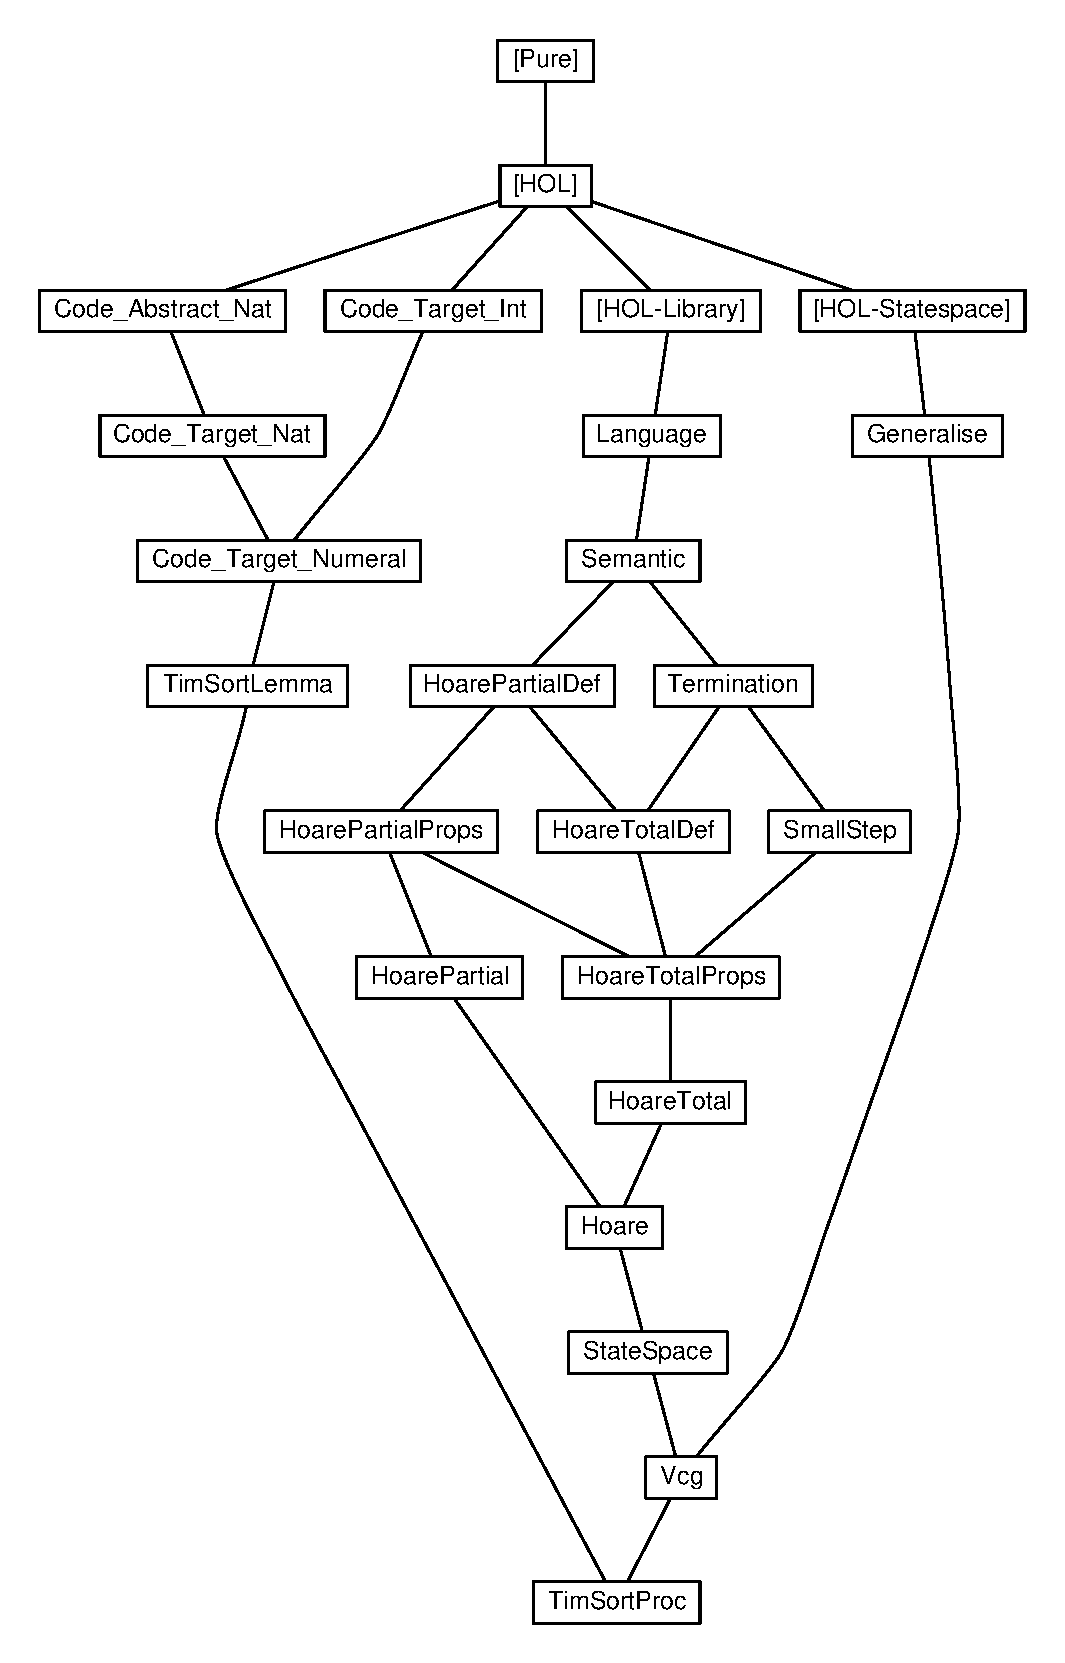
\includegraphics[width=\paperwidth=\textheight,keepaspectratio]{session_graph}
}\end{center}

\pagebreak

\section{Introduction}

The work presented in these theories was developed within the German Verisoft 
project\footnote{\url{http://www.verisoft.de}}. A thorough description of the core
parts can be found in my PhD thesis~\cite{Schirmer-PhD}. A tutorial-like user guide
is in Section~\ref{sec:UserGuide}.

Applications so far include BDD-normalisation~\cite{Ortner-Schirmer-TPHOL05},
a C0 compiler~\cite{Leinenbach:SSV08-??}, a page fault handler~\cite{Alkassar:TACAS08-??}
and extensions towards separation logic~\cite{Tuch:separation-logic:2007}.


% generated text of all theories
%
\begin{isabellebody}%
\setisabellecontext{Code{\isacharunderscore}Target{\isacharunderscore}Int}%
%
\isamarkupsection{Implementation of integer numbers by target-language integers%
}
\isamarkuptrue%
%
\isadelimtheory
%
\endisadelimtheory
%
\isatagtheory
\isacommand{theory}\isamarkupfalse%
\ Code{\isacharunderscore}Target{\isacharunderscore}Int\isanewline
\isakeyword{imports}\ Main\isanewline
\isakeyword{begin}%
\endisatagtheory
{\isafoldtheory}%
%
\isadelimtheory
%
\endisadelimtheory
\isanewline
\isanewline
\isacommand{code{\isacharunderscore}datatype}\isamarkupfalse%
\ int{\isacharunderscore}of{\isacharunderscore}integer\isanewline
\isanewline
\isacommand{declare}\isamarkupfalse%
\ {\isacharbrackleft}{\isacharbrackleft}code\ drop{\isacharcolon}\ integer{\isacharunderscore}of{\isacharunderscore}int{\isacharbrackright}{\isacharbrackright}\isanewline
\isanewline
\isacommand{context}\isamarkupfalse%
\isanewline
\isakeyword{includes}\ integer{\isachardot}lifting\isanewline
\isakeyword{begin}\isanewline
\isanewline
\isacommand{lemma}\isamarkupfalse%
\ {\isacharbrackleft}code{\isacharbrackright}{\isacharcolon}\isanewline
\ \ {\isachardoublequoteopen}integer{\isacharunderscore}of{\isacharunderscore}int\ {\isacharparenleft}int{\isacharunderscore}of{\isacharunderscore}integer\ k{\isacharparenright}\ {\isacharequal}\ k{\isachardoublequoteclose}\isanewline
%
\isadelimproof
\ \ %
\endisadelimproof
%
\isatagproof
\isacommand{by}\isamarkupfalse%
\ transfer\ rule%
\endisatagproof
{\isafoldproof}%
%
\isadelimproof
\isanewline
%
\endisadelimproof
\isanewline
\isacommand{lemma}\isamarkupfalse%
\ {\isacharbrackleft}code{\isacharbrackright}{\isacharcolon}\isanewline
\ \ {\isachardoublequoteopen}Int{\isachardot}Pos\ {\isacharequal}\ int{\isacharunderscore}of{\isacharunderscore}integer\ {\isasymcirc}\ integer{\isacharunderscore}of{\isacharunderscore}num{\isachardoublequoteclose}\isanewline
%
\isadelimproof
\ \ %
\endisadelimproof
%
\isatagproof
\isacommand{by}\isamarkupfalse%
\ transfer\ {\isacharparenleft}simp\ add{\isacharcolon}\ fun{\isacharunderscore}eq{\isacharunderscore}iff{\isacharparenright}%
\endisatagproof
{\isafoldproof}%
%
\isadelimproof
\isanewline
%
\endisadelimproof
\isanewline
\isacommand{lemma}\isamarkupfalse%
\ {\isacharbrackleft}code{\isacharbrackright}{\isacharcolon}\isanewline
\ \ {\isachardoublequoteopen}Int{\isachardot}Neg\ {\isacharequal}\ int{\isacharunderscore}of{\isacharunderscore}integer\ {\isasymcirc}\ uminus\ {\isasymcirc}\ integer{\isacharunderscore}of{\isacharunderscore}num{\isachardoublequoteclose}\isanewline
%
\isadelimproof
\ \ %
\endisadelimproof
%
\isatagproof
\isacommand{by}\isamarkupfalse%
\ transfer\ {\isacharparenleft}simp\ add{\isacharcolon}\ fun{\isacharunderscore}eq{\isacharunderscore}iff{\isacharparenright}%
\endisatagproof
{\isafoldproof}%
%
\isadelimproof
\isanewline
%
\endisadelimproof
\isanewline
\isacommand{lemma}\isamarkupfalse%
\ {\isacharbrackleft}code{\isacharunderscore}abbrev{\isacharbrackright}{\isacharcolon}\isanewline
\ \ {\isachardoublequoteopen}int{\isacharunderscore}of{\isacharunderscore}integer\ {\isacharparenleft}numeral\ k{\isacharparenright}\ {\isacharequal}\ Int{\isachardot}Pos\ k{\isachardoublequoteclose}\isanewline
%
\isadelimproof
\ \ %
\endisadelimproof
%
\isatagproof
\isacommand{by}\isamarkupfalse%
\ transfer\ simp%
\endisatagproof
{\isafoldproof}%
%
\isadelimproof
\isanewline
%
\endisadelimproof
\isanewline
\isacommand{lemma}\isamarkupfalse%
\ {\isacharbrackleft}code{\isacharunderscore}abbrev{\isacharbrackright}{\isacharcolon}\isanewline
\ \ {\isachardoublequoteopen}int{\isacharunderscore}of{\isacharunderscore}integer\ {\isacharparenleft}{\isacharminus}\ numeral\ k{\isacharparenright}\ {\isacharequal}\ Int{\isachardot}Neg\ k{\isachardoublequoteclose}\isanewline
%
\isadelimproof
\ \ %
\endisadelimproof
%
\isatagproof
\isacommand{by}\isamarkupfalse%
\ transfer\ simp%
\endisatagproof
{\isafoldproof}%
%
\isadelimproof
\isanewline
%
\endisadelimproof
\isanewline
\isacommand{context}\isamarkupfalse%
\isanewline
\isakeyword{begin}\isanewline
\isanewline
\isakeyword{qualified}\ \isacommand{definition}\isamarkupfalse%
\ positive\ {\isacharcolon}{\isacharcolon}\ {\isachardoublequoteopen}num\ {\isasymRightarrow}\ int{\isachardoublequoteclose}\isanewline
\ \ \isakeyword{where}\ {\isacharbrackleft}simp{\isacharbrackright}{\isacharcolon}\ {\isachardoublequoteopen}positive\ {\isacharequal}\ numeral{\isachardoublequoteclose}\isanewline
\isanewline
\isakeyword{qualified}\ \isacommand{definition}\isamarkupfalse%
\ negative\ {\isacharcolon}{\isacharcolon}\ {\isachardoublequoteopen}num\ {\isasymRightarrow}\ int{\isachardoublequoteclose}\isanewline
\ \ \isakeyword{where}\ {\isacharbrackleft}simp{\isacharbrackright}{\isacharcolon}\ {\isachardoublequoteopen}negative\ {\isacharequal}\ uminus\ {\isasymcirc}\ numeral{\isachardoublequoteclose}\isanewline
\isanewline
\isacommand{lemma}\isamarkupfalse%
\ {\isacharbrackleft}code{\isacharunderscore}computation{\isacharunderscore}unfold{\isacharbrackright}{\isacharcolon}\isanewline
\ \ {\isachardoublequoteopen}numeral\ {\isacharequal}\ positive{\isachardoublequoteclose}\isanewline
\ \ {\isachardoublequoteopen}Int{\isachardot}Pos\ {\isacharequal}\ positive{\isachardoublequoteclose}\isanewline
\ \ {\isachardoublequoteopen}Int{\isachardot}Neg\ {\isacharequal}\ negative{\isachardoublequoteclose}\isanewline
%
\isadelimproof
\ \ %
\endisadelimproof
%
\isatagproof
\isacommand{by}\isamarkupfalse%
\ {\isacharparenleft}simp{\isacharunderscore}all\ add{\isacharcolon}\ fun{\isacharunderscore}eq{\isacharunderscore}iff{\isacharparenright}%
\endisatagproof
{\isafoldproof}%
%
\isadelimproof
\isanewline
%
\endisadelimproof
\isanewline
\isacommand{end}\isamarkupfalse%
\isanewline
\isanewline
\isacommand{lemma}\isamarkupfalse%
\ {\isacharbrackleft}code{\isacharcomma}\ symmetric{\isacharcomma}\ code{\isacharunderscore}post{\isacharbrackright}{\isacharcolon}\isanewline
\ \ {\isachardoublequoteopen}{\isadigit{0}}\ {\isacharequal}\ int{\isacharunderscore}of{\isacharunderscore}integer\ {\isadigit{0}}{\isachardoublequoteclose}\isanewline
%
\isadelimproof
\ \ %
\endisadelimproof
%
\isatagproof
\isacommand{by}\isamarkupfalse%
\ transfer\ simp%
\endisatagproof
{\isafoldproof}%
%
\isadelimproof
\isanewline
%
\endisadelimproof
\isanewline
\isacommand{lemma}\isamarkupfalse%
\ {\isacharbrackleft}code{\isacharcomma}\ symmetric{\isacharcomma}\ code{\isacharunderscore}post{\isacharbrackright}{\isacharcolon}\isanewline
\ \ {\isachardoublequoteopen}{\isadigit{1}}\ {\isacharequal}\ int{\isacharunderscore}of{\isacharunderscore}integer\ {\isadigit{1}}{\isachardoublequoteclose}\isanewline
%
\isadelimproof
\ \ %
\endisadelimproof
%
\isatagproof
\isacommand{by}\isamarkupfalse%
\ transfer\ simp%
\endisatagproof
{\isafoldproof}%
%
\isadelimproof
\isanewline
%
\endisadelimproof
\isanewline
\isacommand{lemma}\isamarkupfalse%
\ {\isacharbrackleft}code{\isacharunderscore}post{\isacharbrackright}{\isacharcolon}\isanewline
\ \ {\isachardoublequoteopen}int{\isacharunderscore}of{\isacharunderscore}integer\ {\isacharparenleft}{\isacharminus}\ {\isadigit{1}}{\isacharparenright}\ {\isacharequal}\ {\isacharminus}\ {\isadigit{1}}{\isachardoublequoteclose}\isanewline
%
\isadelimproof
\ \ %
\endisadelimproof
%
\isatagproof
\isacommand{by}\isamarkupfalse%
\ simp%
\endisatagproof
{\isafoldproof}%
%
\isadelimproof
\isanewline
%
\endisadelimproof
\isanewline
\isacommand{lemma}\isamarkupfalse%
\ {\isacharbrackleft}code{\isacharbrackright}{\isacharcolon}\isanewline
\ \ {\isachardoublequoteopen}k\ {\isacharplus}\ l\ {\isacharequal}\ int{\isacharunderscore}of{\isacharunderscore}integer\ {\isacharparenleft}of{\isacharunderscore}int\ k\ {\isacharplus}\ of{\isacharunderscore}int\ l{\isacharparenright}{\isachardoublequoteclose}\isanewline
%
\isadelimproof
\ \ %
\endisadelimproof
%
\isatagproof
\isacommand{by}\isamarkupfalse%
\ transfer\ simp%
\endisatagproof
{\isafoldproof}%
%
\isadelimproof
\isanewline
%
\endisadelimproof
\isanewline
\isacommand{lemma}\isamarkupfalse%
\ {\isacharbrackleft}code{\isacharbrackright}{\isacharcolon}\isanewline
\ \ {\isachardoublequoteopen}{\isacharminus}\ k\ {\isacharequal}\ int{\isacharunderscore}of{\isacharunderscore}integer\ {\isacharparenleft}{\isacharminus}\ of{\isacharunderscore}int\ k{\isacharparenright}{\isachardoublequoteclose}\isanewline
%
\isadelimproof
\ \ %
\endisadelimproof
%
\isatagproof
\isacommand{by}\isamarkupfalse%
\ transfer\ simp%
\endisatagproof
{\isafoldproof}%
%
\isadelimproof
\isanewline
%
\endisadelimproof
\isanewline
\isacommand{lemma}\isamarkupfalse%
\ {\isacharbrackleft}code{\isacharbrackright}{\isacharcolon}\isanewline
\ \ {\isachardoublequoteopen}k\ {\isacharminus}\ l\ {\isacharequal}\ int{\isacharunderscore}of{\isacharunderscore}integer\ {\isacharparenleft}of{\isacharunderscore}int\ k\ {\isacharminus}\ of{\isacharunderscore}int\ l{\isacharparenright}{\isachardoublequoteclose}\isanewline
%
\isadelimproof
\ \ %
\endisadelimproof
%
\isatagproof
\isacommand{by}\isamarkupfalse%
\ transfer\ simp%
\endisatagproof
{\isafoldproof}%
%
\isadelimproof
\isanewline
%
\endisadelimproof
\isanewline
\isacommand{lemma}\isamarkupfalse%
\ {\isacharbrackleft}code{\isacharbrackright}{\isacharcolon}\isanewline
\ \ {\isachardoublequoteopen}Int{\isachardot}dup\ k\ {\isacharequal}\ int{\isacharunderscore}of{\isacharunderscore}integer\ {\isacharparenleft}Code{\isacharunderscore}Numeral{\isachardot}dup\ {\isacharparenleft}of{\isacharunderscore}int\ k{\isacharparenright}{\isacharparenright}{\isachardoublequoteclose}\isanewline
%
\isadelimproof
\ \ %
\endisadelimproof
%
\isatagproof
\isacommand{by}\isamarkupfalse%
\ transfer\ simp%
\endisatagproof
{\isafoldproof}%
%
\isadelimproof
\isanewline
%
\endisadelimproof
\isanewline
\isacommand{declare}\isamarkupfalse%
\ {\isacharbrackleft}{\isacharbrackleft}code\ drop{\isacharcolon}\ Int{\isachardot}sub{\isacharbrackright}{\isacharbrackright}\isanewline
\isanewline
\isacommand{lemma}\isamarkupfalse%
\ {\isacharbrackleft}code{\isacharbrackright}{\isacharcolon}\isanewline
\ \ {\isachardoublequoteopen}k\ {\isacharasterisk}\ l\ {\isacharequal}\ int{\isacharunderscore}of{\isacharunderscore}integer\ {\isacharparenleft}of{\isacharunderscore}int\ k\ {\isacharasterisk}\ of{\isacharunderscore}int\ l{\isacharparenright}{\isachardoublequoteclose}\isanewline
%
\isadelimproof
\ \ %
\endisadelimproof
%
\isatagproof
\isacommand{by}\isamarkupfalse%
\ simp%
\endisatagproof
{\isafoldproof}%
%
\isadelimproof
\isanewline
%
\endisadelimproof
\isanewline
\isacommand{lemma}\isamarkupfalse%
\ {\isacharbrackleft}code{\isacharbrackright}{\isacharcolon}\isanewline
\ \ {\isachardoublequoteopen}k\ div\ l\ {\isacharequal}\ int{\isacharunderscore}of{\isacharunderscore}integer\ {\isacharparenleft}of{\isacharunderscore}int\ k\ div\ of{\isacharunderscore}int\ l{\isacharparenright}{\isachardoublequoteclose}\isanewline
%
\isadelimproof
\ \ %
\endisadelimproof
%
\isatagproof
\isacommand{by}\isamarkupfalse%
\ simp%
\endisatagproof
{\isafoldproof}%
%
\isadelimproof
\isanewline
%
\endisadelimproof
\isanewline
\isacommand{lemma}\isamarkupfalse%
\ {\isacharbrackleft}code{\isacharbrackright}{\isacharcolon}\isanewline
\ \ {\isachardoublequoteopen}k\ mod\ l\ {\isacharequal}\ int{\isacharunderscore}of{\isacharunderscore}integer\ {\isacharparenleft}of{\isacharunderscore}int\ k\ mod\ of{\isacharunderscore}int\ l{\isacharparenright}{\isachardoublequoteclose}\isanewline
%
\isadelimproof
\ \ %
\endisadelimproof
%
\isatagproof
\isacommand{by}\isamarkupfalse%
\ simp%
\endisatagproof
{\isafoldproof}%
%
\isadelimproof
\isanewline
%
\endisadelimproof
\isanewline
\isacommand{lemma}\isamarkupfalse%
\ {\isacharbrackleft}code{\isacharbrackright}{\isacharcolon}\isanewline
\ \ {\isachardoublequoteopen}divmod\ m\ n\ {\isacharequal}\ map{\isacharunderscore}prod\ int{\isacharunderscore}of{\isacharunderscore}integer\ int{\isacharunderscore}of{\isacharunderscore}integer\ {\isacharparenleft}divmod\ m\ n{\isacharparenright}{\isachardoublequoteclose}\isanewline
%
\isadelimproof
\ \ %
\endisadelimproof
%
\isatagproof
\isacommand{unfolding}\isamarkupfalse%
\ prod{\isacharunderscore}eq{\isacharunderscore}iff\ divmod{\isacharunderscore}def\ map{\isacharunderscore}prod{\isacharunderscore}def\ case{\isacharunderscore}prod{\isacharunderscore}beta\ fst{\isacharunderscore}conv\ snd{\isacharunderscore}conv\isanewline
\ \ \isacommand{by}\isamarkupfalse%
\ transfer\ simp%
\endisatagproof
{\isafoldproof}%
%
\isadelimproof
\isanewline
%
\endisadelimproof
\isanewline
\isacommand{lemma}\isamarkupfalse%
\ {\isacharbrackleft}code{\isacharbrackright}{\isacharcolon}\isanewline
\ \ {\isachardoublequoteopen}HOL{\isachardot}equal\ k\ l\ {\isacharequal}\ HOL{\isachardot}equal\ {\isacharparenleft}of{\isacharunderscore}int\ k\ {\isacharcolon}{\isacharcolon}\ integer{\isacharparenright}\ {\isacharparenleft}of{\isacharunderscore}int\ l{\isacharparenright}{\isachardoublequoteclose}\isanewline
%
\isadelimproof
\ \ %
\endisadelimproof
%
\isatagproof
\isacommand{by}\isamarkupfalse%
\ transfer\ {\isacharparenleft}simp\ add{\isacharcolon}\ equal{\isacharparenright}%
\endisatagproof
{\isafoldproof}%
%
\isadelimproof
\isanewline
%
\endisadelimproof
\isanewline
\isacommand{lemma}\isamarkupfalse%
\ {\isacharbrackleft}code{\isacharbrackright}{\isacharcolon}\isanewline
\ \ {\isachardoublequoteopen}k\ {\isasymle}\ l\ {\isasymlongleftrightarrow}\ {\isacharparenleft}of{\isacharunderscore}int\ k\ {\isacharcolon}{\isacharcolon}\ integer{\isacharparenright}\ {\isasymle}\ of{\isacharunderscore}int\ l{\isachardoublequoteclose}\isanewline
%
\isadelimproof
\ \ %
\endisadelimproof
%
\isatagproof
\isacommand{by}\isamarkupfalse%
\ transfer\ rule%
\endisatagproof
{\isafoldproof}%
%
\isadelimproof
\isanewline
%
\endisadelimproof
\isanewline
\isacommand{lemma}\isamarkupfalse%
\ {\isacharbrackleft}code{\isacharbrackright}{\isacharcolon}\isanewline
\ \ {\isachardoublequoteopen}k\ {\isacharless}\ l\ {\isasymlongleftrightarrow}\ {\isacharparenleft}of{\isacharunderscore}int\ k\ {\isacharcolon}{\isacharcolon}\ integer{\isacharparenright}\ {\isacharless}\ of{\isacharunderscore}int\ l{\isachardoublequoteclose}\isanewline
%
\isadelimproof
\ \ %
\endisadelimproof
%
\isatagproof
\isacommand{by}\isamarkupfalse%
\ transfer\ rule%
\endisatagproof
{\isafoldproof}%
%
\isadelimproof
\isanewline
%
\endisadelimproof
\isanewline
\isacommand{declare}\isamarkupfalse%
\ {\isacharbrackleft}{\isacharbrackleft}code\ drop{\isacharcolon}\ {\isachardoublequoteopen}gcd\ {\isacharcolon}{\isacharcolon}\ int\ {\isasymRightarrow}\ {\isacharunderscore}{\isachardoublequoteclose}\ {\isachardoublequoteopen}lcm\ {\isacharcolon}{\isacharcolon}\ int\ {\isasymRightarrow}\ {\isacharunderscore}{\isachardoublequoteclose}{\isacharbrackright}{\isacharbrackright}\isanewline
\isanewline
\isacommand{lemma}\isamarkupfalse%
\ gcd{\isacharunderscore}int{\isacharunderscore}of{\isacharunderscore}integer\ {\isacharbrackleft}code{\isacharbrackright}{\isacharcolon}\isanewline
\ \ {\isachardoublequoteopen}gcd\ {\isacharparenleft}int{\isacharunderscore}of{\isacharunderscore}integer\ x{\isacharparenright}\ {\isacharparenleft}int{\isacharunderscore}of{\isacharunderscore}integer\ y{\isacharparenright}\ {\isacharequal}\ int{\isacharunderscore}of{\isacharunderscore}integer\ {\isacharparenleft}gcd\ x\ y{\isacharparenright}{\isachardoublequoteclose}\isanewline
%
\isadelimproof
%
\endisadelimproof
%
\isatagproof
\isacommand{by}\isamarkupfalse%
\ transfer\ rule%
\endisatagproof
{\isafoldproof}%
%
\isadelimproof
\isanewline
%
\endisadelimproof
\isanewline
\isacommand{lemma}\isamarkupfalse%
\ lcm{\isacharunderscore}int{\isacharunderscore}of{\isacharunderscore}integer\ {\isacharbrackleft}code{\isacharbrackright}{\isacharcolon}\isanewline
\ \ {\isachardoublequoteopen}lcm\ {\isacharparenleft}int{\isacharunderscore}of{\isacharunderscore}integer\ x{\isacharparenright}\ {\isacharparenleft}int{\isacharunderscore}of{\isacharunderscore}integer\ y{\isacharparenright}\ {\isacharequal}\ int{\isacharunderscore}of{\isacharunderscore}integer\ {\isacharparenleft}lcm\ x\ y{\isacharparenright}{\isachardoublequoteclose}\isanewline
%
\isadelimproof
%
\endisadelimproof
%
\isatagproof
\isacommand{by}\isamarkupfalse%
\ transfer\ rule%
\endisatagproof
{\isafoldproof}%
%
\isadelimproof
\isanewline
%
\endisadelimproof
\isanewline
\isacommand{end}\isamarkupfalse%
\isanewline
\isanewline
\isacommand{lemma}\isamarkupfalse%
\ {\isacharparenleft}\isakeyword{in}\ ring{\isacharunderscore}{\isadigit{1}}{\isacharparenright}\ of{\isacharunderscore}int{\isacharunderscore}code{\isacharunderscore}if{\isacharcolon}\isanewline
\ \ {\isachardoublequoteopen}of{\isacharunderscore}int\ k\ {\isacharequal}\ {\isacharparenleft}if\ k\ {\isacharequal}\ {\isadigit{0}}\ then\ {\isadigit{0}}\isanewline
\ \ \ \ \ else\ if\ k\ {\isacharless}\ {\isadigit{0}}\ then\ {\isacharminus}\ of{\isacharunderscore}int\ {\isacharparenleft}{\isacharminus}\ k{\isacharparenright}\isanewline
\ \ \ \ \ else\ let\isanewline
\ \ \ \ \ \ \ l\ {\isacharequal}\ {\isadigit{2}}\ {\isacharasterisk}\ of{\isacharunderscore}int\ {\isacharparenleft}k\ div\ {\isadigit{2}}{\isacharparenright}{\isacharsemicolon}\isanewline
\ \ \ \ \ \ \ j\ {\isacharequal}\ k\ mod\ {\isadigit{2}}\isanewline
\ \ \ \ \ in\ if\ j\ {\isacharequal}\ {\isadigit{0}}\ then\ l\ else\ l\ {\isacharplus}\ {\isadigit{1}}{\isacharparenright}{\isachardoublequoteclose}\isanewline
%
\isadelimproof
%
\endisadelimproof
%
\isatagproof
\isacommand{proof}\isamarkupfalse%
\ {\isacharminus}\isanewline
\ \ \isacommand{from}\isamarkupfalse%
\ div{\isacharunderscore}mult{\isacharunderscore}mod{\isacharunderscore}eq\ \isacommand{have}\isamarkupfalse%
\ {\isacharasterisk}{\isacharcolon}\ {\isachardoublequoteopen}of{\isacharunderscore}int\ k\ {\isacharequal}\ of{\isacharunderscore}int\ {\isacharparenleft}k\ div\ {\isadigit{2}}\ {\isacharasterisk}\ {\isadigit{2}}\ {\isacharplus}\ k\ mod\ {\isadigit{2}}{\isacharparenright}{\isachardoublequoteclose}\ \isacommand{by}\isamarkupfalse%
\ simp\isanewline
\ \ \isacommand{show}\isamarkupfalse%
\ {\isacharquery}thesis\isanewline
\ \ \ \ \isacommand{by}\isamarkupfalse%
\ {\isacharparenleft}simp\ add{\isacharcolon}\ Let{\isacharunderscore}def\ of{\isacharunderscore}int{\isacharunderscore}add\ {\isacharbrackleft}symmetric{\isacharbrackright}{\isacharparenright}\ {\isacharparenleft}simp\ add{\isacharcolon}\ {\isacharasterisk}\ mult{\isachardot}commute{\isacharparenright}\isanewline
\isacommand{qed}\isamarkupfalse%
%
\endisatagproof
{\isafoldproof}%
%
\isadelimproof
\isanewline
%
\endisadelimproof
\isanewline
\isacommand{declare}\isamarkupfalse%
\ of{\isacharunderscore}int{\isacharunderscore}code{\isacharunderscore}if\ {\isacharbrackleft}code{\isacharbrackright}\isanewline
\isanewline
\isacommand{lemma}\isamarkupfalse%
\ {\isacharbrackleft}code{\isacharbrackright}{\isacharcolon}\isanewline
\ \ {\isachardoublequoteopen}nat\ {\isacharequal}\ nat{\isacharunderscore}of{\isacharunderscore}integer\ {\isasymcirc}\ of{\isacharunderscore}int{\isachardoublequoteclose}\isanewline
\ \ \isacommand{including}\isamarkupfalse%
\ integer{\isachardot}lifting%
\isadelimproof
\ %
\endisadelimproof
%
\isatagproof
\isacommand{by}\isamarkupfalse%
\ transfer\ {\isacharparenleft}simp\ add{\isacharcolon}\ fun{\isacharunderscore}eq{\isacharunderscore}iff{\isacharparenright}%
\endisatagproof
{\isafoldproof}%
%
\isadelimproof
%
\endisadelimproof
\isanewline
\isanewline
\isacommand{code{\isacharunderscore}identifier}\isamarkupfalse%
\isanewline
\ \ \isakeyword{code{\isacharunderscore}module}\ Code{\isacharunderscore}Target{\isacharunderscore}Int\ {\isasymrightharpoonup}\isanewline
\ \ \ \ {\isacharparenleft}SML{\isacharparenright}\ Arith\ \isakeyword{and}\ {\isacharparenleft}OCaml{\isacharparenright}\ Arith\ \isakeyword{and}\ {\isacharparenleft}Haskell{\isacharparenright}\ Arith\isanewline
%
\isadelimtheory
\isanewline
%
\endisadelimtheory
%
\isatagtheory
\isacommand{end}\isamarkupfalse%
%
\endisatagtheory
{\isafoldtheory}%
%
\isadelimtheory
%
\endisadelimtheory
%
\end{isabellebody}%
%%% Local Variables:
%%% mode: latex
%%% TeX-master: "root"
%%% End:


%
\begin{isabellebody}%
\setisabellecontext{Code{\isacharunderscore}Abstract{\isacharunderscore}Nat}%
%
\isamarkupsection{Avoidance of pattern matching on natural numbers%
}
\isamarkuptrue%
%
\isadelimtheory
%
\endisadelimtheory
%
\isatagtheory
\isacommand{theory}\isamarkupfalse%
\ Code{\isacharunderscore}Abstract{\isacharunderscore}Nat\isanewline
\isakeyword{imports}\ Main\isanewline
\isakeyword{begin}%
\endisatagtheory
{\isafoldtheory}%
%
\isadelimtheory
%
\endisadelimtheory
%
\begin{isamarkuptext}%
When natural numbers are implemented in another than the
  conventional inductive \isa{{\isadigit{0}}}/\isa{Suc} representation,
  it is necessary to avoid all pattern matching on natural numbers
  altogether.  This is accomplished by this theory (up to a certain
  extent).%
\end{isamarkuptext}\isamarkuptrue%
%
\isamarkupsubsection{Case analysis%
}
\isamarkuptrue%
%
\begin{isamarkuptext}%
Case analysis on natural numbers is rephrased using a conditional
  expression:%
\end{isamarkuptext}\isamarkuptrue%
\isacommand{lemma}\isamarkupfalse%
\ {\isacharbrackleft}code{\isacharcomma}\ code{\isacharunderscore}unfold{\isacharbrackright}{\isacharcolon}\isanewline
\ \ {\isachardoublequoteopen}case{\isacharunderscore}nat\ {\isacharequal}\ {\isacharparenleft}{\isasymlambda}f\ g\ n{\isachardot}\ if\ n\ {\isacharequal}\ {\isadigit{0}}\ then\ f\ else\ g\ {\isacharparenleft}n\ {\isacharminus}\ {\isadigit{1}}{\isacharparenright}{\isacharparenright}{\isachardoublequoteclose}\isanewline
%
\isadelimproof
\ \ %
\endisadelimproof
%
\isatagproof
\isacommand{by}\isamarkupfalse%
\ {\isacharparenleft}auto\ simp\ add{\isacharcolon}\ fun{\isacharunderscore}eq{\isacharunderscore}iff\ dest{\isacharbang}{\isacharcolon}\ gr{\isadigit{0}}{\isacharunderscore}implies{\isacharunderscore}Suc{\isacharparenright}%
\endisatagproof
{\isafoldproof}%
%
\isadelimproof
%
\endisadelimproof
%
\isamarkupsubsection{Preprocessors%
}
\isamarkuptrue%
%
\begin{isamarkuptext}%
The term \isa{Suc\ n} is no longer a valid pattern.  Therefore,
  all occurrences of this term in a position where a pattern is
  expected (i.e.~on the left-hand side of a code equation) must be
  eliminated.  This can be accomplished -- as far as possible -- by
  applying the following transformation rule:%
\end{isamarkuptext}\isamarkuptrue%
\isacommand{lemma}\isamarkupfalse%
\ Suc{\isacharunderscore}if{\isacharunderscore}eq{\isacharcolon}\isanewline
\ \ \isakeyword{assumes}\ {\isachardoublequoteopen}{\isasymAnd}n{\isachardot}\ f\ {\isacharparenleft}Suc\ n{\isacharparenright}\ {\isasymequiv}\ h\ n{\isachardoublequoteclose}\isanewline
\ \ \isakeyword{assumes}\ {\isachardoublequoteopen}f\ {\isadigit{0}}\ {\isasymequiv}\ g{\isachardoublequoteclose}\isanewline
\ \ \isakeyword{shows}\ {\isachardoublequoteopen}f\ n\ {\isasymequiv}\ if\ n\ {\isacharequal}\ {\isadigit{0}}\ then\ g\ else\ h\ {\isacharparenleft}n\ {\isacharminus}\ {\isadigit{1}}{\isacharparenright}{\isachardoublequoteclose}\isanewline
%
\isadelimproof
\ \ %
\endisadelimproof
%
\isatagproof
\isacommand{by}\isamarkupfalse%
\ {\isacharparenleft}rule\ eq{\isacharunderscore}reflection{\isacharparenright}\ {\isacharparenleft}cases\ n{\isacharcomma}\ insert\ assms{\isacharcomma}\ simp{\isacharunderscore}all{\isacharparenright}%
\endisatagproof
{\isafoldproof}%
%
\isadelimproof
%
\endisadelimproof
%
\begin{isamarkuptext}%
The rule above is built into a preprocessor that is plugged into
  the code generator.%
\end{isamarkuptext}\isamarkuptrue%
%
\isadelimML
%
\endisadelimML
%
\isatagML
\isacommand{setup}\isamarkupfalse%
\ {\isacartoucheopen}\isanewline
let\isanewline
\isanewline
val\ Suc{\isacharunderscore}if{\isacharunderscore}eq\ {\isacharequal}\ Thm{\isachardot}incr{\isacharunderscore}indexes\ {\isadigit{1}}\ {\isacharat}{\isacharbraceleft}thm\ Suc{\isacharunderscore}if{\isacharunderscore}eq{\isacharbraceright}{\isacharsemicolon}\isanewline
\isanewline
fun\ remove{\isacharunderscore}suc\ ctxt\ thms\ {\isacharequal}\isanewline
\ \ let\isanewline
\ \ \ \ val\ vname\ {\isacharequal}\ singleton\ {\isacharparenleft}Name{\isachardot}variant{\isacharunderscore}list\ {\isacharparenleft}map\ fst\isanewline
\ \ \ \ \ \ {\isacharparenleft}fold\ {\isacharparenleft}Term{\isachardot}add{\isacharunderscore}var{\isacharunderscore}names\ o\ Thm{\isachardot}full{\isacharunderscore}prop{\isacharunderscore}of{\isacharparenright}\ thms\ {\isacharbrackleft}{\isacharbrackright}{\isacharparenright}{\isacharparenright}{\isacharparenright}\ {\isachardoublequote}n{\isachardoublequote}{\isacharsemicolon}\isanewline
\ \ \ \ val\ cv\ {\isacharequal}\ Thm{\isachardot}cterm{\isacharunderscore}of\ ctxt\ {\isacharparenleft}Var\ {\isacharparenleft}{\isacharparenleft}vname{\isacharcomma}\ {\isadigit{0}}{\isacharparenright}{\isacharcomma}\ HOLogic{\isachardot}natT{\isacharparenright}{\isacharparenright}{\isacharsemicolon}\isanewline
\ \ \ \ val\ lhs{\isacharunderscore}of\ {\isacharequal}\ snd\ o\ Thm{\isachardot}dest{\isacharunderscore}comb\ o\ fst\ o\ Thm{\isachardot}dest{\isacharunderscore}comb\ o\ Thm{\isachardot}cprop{\isacharunderscore}of{\isacharsemicolon}\isanewline
\ \ \ \ val\ rhs{\isacharunderscore}of\ {\isacharequal}\ snd\ o\ Thm{\isachardot}dest{\isacharunderscore}comb\ o\ Thm{\isachardot}cprop{\isacharunderscore}of{\isacharsemicolon}\isanewline
\ \ \ \ fun\ find{\isacharunderscore}vars\ ct\ {\isacharequal}\ {\isacharparenleft}case\ Thm{\isachardot}term{\isacharunderscore}of\ ct\ of\isanewline
\ \ \ \ \ \ \ \ {\isacharparenleft}Const\ {\isacharparenleft}{\isacharat}{\isacharbraceleft}const{\isacharunderscore}name\ Suc{\isacharbraceright}{\isacharcomma}\ {\isacharunderscore}{\isacharparenright}\ {\isachardollar}\ Var\ {\isacharunderscore}{\isacharparenright}\ {\isacharequal}{\isachargreater}\ {\isacharbrackleft}{\isacharparenleft}cv{\isacharcomma}\ snd\ {\isacharparenleft}Thm{\isachardot}dest{\isacharunderscore}comb\ ct{\isacharparenright}{\isacharparenright}{\isacharbrackright}\isanewline
\ \ \ \ \ \ {\isacharbar}\ {\isacharunderscore}\ {\isachardollar}\ {\isacharunderscore}\ {\isacharequal}{\isachargreater}\isanewline
\ \ \ \ \ \ \ \ let\ val\ {\isacharparenleft}ct{\isadigit{1}}{\isacharcomma}\ ct{\isadigit{2}}{\isacharparenright}\ {\isacharequal}\ Thm{\isachardot}dest{\isacharunderscore}comb\ ct\isanewline
\ \ \ \ \ \ \ \ in\ \isanewline
\ \ \ \ \ \ \ \ \ \ map\ {\isacharparenleft}apfst\ {\isacharparenleft}fn\ ct\ {\isacharequal}{\isachargreater}\ Thm{\isachardot}apply\ ct\ ct{\isadigit{2}}{\isacharparenright}{\isacharparenright}\ {\isacharparenleft}find{\isacharunderscore}vars\ ct{\isadigit{1}}{\isacharparenright}\ {\isacharat}\isanewline
\ \ \ \ \ \ \ \ \ \ map\ {\isacharparenleft}apfst\ {\isacharparenleft}Thm{\isachardot}apply\ ct{\isadigit{1}}{\isacharparenright}{\isacharparenright}\ {\isacharparenleft}find{\isacharunderscore}vars\ ct{\isadigit{2}}{\isacharparenright}\isanewline
\ \ \ \ \ \ \ \ end\isanewline
\ \ \ \ \ \ {\isacharbar}\ {\isacharunderscore}\ {\isacharequal}{\isachargreater}\ {\isacharbrackleft}{\isacharbrackright}{\isacharparenright}{\isacharsemicolon}\isanewline
\ \ \ \ val\ eqs\ {\isacharequal}\ maps\isanewline
\ \ \ \ \ \ {\isacharparenleft}fn\ thm\ {\isacharequal}{\isachargreater}\ map\ {\isacharparenleft}pair\ thm{\isacharparenright}\ {\isacharparenleft}find{\isacharunderscore}vars\ {\isacharparenleft}lhs{\isacharunderscore}of\ thm{\isacharparenright}{\isacharparenright}{\isacharparenright}\ thms{\isacharsemicolon}\isanewline
\ \ \ \ fun\ mk{\isacharunderscore}thms\ {\isacharparenleft}thm{\isacharcomma}\ {\isacharparenleft}ct{\isacharcomma}\ cv{\isacharprime}{\isacharparenright}{\isacharparenright}\ {\isacharequal}\isanewline
\ \ \ \ \ \ let\isanewline
\ \ \ \ \ \ \ \ val\ thm{\isacharprime}\ {\isacharequal}\isanewline
\ \ \ \ \ \ \ \ \ \ Thm{\isachardot}implies{\isacharunderscore}elim\isanewline
\ \ \ \ \ \ \ \ \ \ \ {\isacharparenleft}Conv{\isachardot}fconv{\isacharunderscore}rule\ {\isacharparenleft}Thm{\isachardot}beta{\isacharunderscore}conversion\ true{\isacharparenright}\isanewline
\ \ \ \ \ \ \ \ \ \ \ \ \ {\isacharparenleft}Thm{\isachardot}instantiate{\isacharprime}\isanewline
\ \ \ \ \ \ \ \ \ \ \ \ \ \ \ {\isacharbrackleft}SOME\ {\isacharparenleft}Thm{\isachardot}ctyp{\isacharunderscore}of{\isacharunderscore}cterm\ ct{\isacharparenright}{\isacharbrackright}\ {\isacharbrackleft}SOME\ {\isacharparenleft}Thm{\isachardot}lambda\ cv\ ct{\isacharparenright}{\isacharcomma}\isanewline
\ \ \ \ \ \ \ \ \ \ \ \ \ \ \ \ \ SOME\ {\isacharparenleft}Thm{\isachardot}lambda\ cv{\isacharprime}\ {\isacharparenleft}rhs{\isacharunderscore}of\ thm{\isacharparenright}{\isacharparenright}{\isacharcomma}\ NONE{\isacharcomma}\ SOME\ cv{\isacharprime}{\isacharbrackright}\isanewline
\ \ \ \ \ \ \ \ \ \ \ \ \ \ \ Suc{\isacharunderscore}if{\isacharunderscore}eq{\isacharparenright}{\isacharparenright}\ {\isacharparenleft}Thm{\isachardot}forall{\isacharunderscore}intr\ cv{\isacharprime}\ thm{\isacharparenright}\isanewline
\ \ \ \ \ \ in\isanewline
\ \ \ \ \ \ \ \ case\ map{\isacharunderscore}filter\ {\isacharparenleft}fn\ thm{\isacharprime}{\isacharprime}\ {\isacharequal}{\isachargreater}\isanewline
\ \ \ \ \ \ \ \ \ \ \ \ SOME\ {\isacharparenleft}thm{\isacharprime}{\isacharprime}{\isacharcomma}\ singleton\isanewline
\ \ \ \ \ \ \ \ \ \ \ \ \ \ {\isacharparenleft}Variable{\isachardot}trade\ {\isacharparenleft}K\ {\isacharparenleft}fn\ {\isacharbrackleft}thm{\isacharprime}{\isacharprime}{\isacharprime}{\isacharbrackright}\ {\isacharequal}{\isachargreater}\ {\isacharbrackleft}thm{\isacharprime}{\isacharprime}{\isacharprime}\ RS\ thm{\isacharprime}{\isacharbrackright}{\isacharparenright}{\isacharparenright}\isanewline
\ \ \ \ \ \ \ \ \ \ \ \ \ \ \ \ {\isacharparenleft}Variable{\isachardot}declare{\isacharunderscore}thm\ thm{\isacharprime}{\isacharprime}\ ctxt{\isacharparenright}{\isacharparenright}\ thm{\isacharprime}{\isacharprime}{\isacharparenright}\isanewline
\ \ \ \ \ \ \ \ \ \ handle\ THM\ {\isacharunderscore}\ {\isacharequal}{\isachargreater}\ NONE{\isacharparenright}\ thms\ of\isanewline
\ \ \ \ \ \ \ \ \ \ \ \ {\isacharbrackleft}{\isacharbrackright}\ {\isacharequal}{\isachargreater}\ NONE\isanewline
\ \ \ \ \ \ \ \ \ \ {\isacharbar}\ thmps\ {\isacharequal}{\isachargreater}\isanewline
\ \ \ \ \ \ \ \ \ \ \ \ \ \ let\ val\ {\isacharparenleft}thms{\isadigit{1}}{\isacharcomma}\ thms{\isadigit{2}}{\isacharparenright}\ {\isacharequal}\ split{\isacharunderscore}list\ thmps\isanewline
\ \ \ \ \ \ \ \ \ \ \ \ \ \ in\ SOME\ {\isacharparenleft}subtract\ Thm{\isachardot}eq{\isacharunderscore}thm\ {\isacharparenleft}thm\ {\isacharcolon}{\isacharcolon}\ thms{\isadigit{1}}{\isacharparenright}\ thms\ {\isacharat}\ thms{\isadigit{2}}{\isacharparenright}\ end\isanewline
\ \ \ \ \ \ end\isanewline
\ \ in\ get{\isacharunderscore}first\ mk{\isacharunderscore}thms\ eqs\ end{\isacharsemicolon}\isanewline
\isanewline
fun\ eqn{\isacharunderscore}suc{\isacharunderscore}base{\isacharunderscore}preproc\ ctxt\ thms\ {\isacharequal}\isanewline
\ \ let\isanewline
\ \ \ \ val\ dest\ {\isacharequal}\ fst\ o\ Logic{\isachardot}dest{\isacharunderscore}equals\ o\ Thm{\isachardot}prop{\isacharunderscore}of{\isacharsemicolon}\isanewline
\ \ \ \ val\ contains{\isacharunderscore}suc\ {\isacharequal}\ exists{\isacharunderscore}Const\ {\isacharparenleft}fn\ {\isacharparenleft}c{\isacharcomma}\ {\isacharunderscore}{\isacharparenright}\ {\isacharequal}{\isachargreater}\ c\ {\isacharequal}\ {\isacharat}{\isacharbraceleft}const{\isacharunderscore}name\ Suc{\isacharbraceright}{\isacharparenright}{\isacharsemicolon}\isanewline
\ \ in\isanewline
\ \ \ \ if\ forall\ {\isacharparenleft}can\ dest{\isacharparenright}\ thms\ andalso\ exists\ {\isacharparenleft}contains{\isacharunderscore}suc\ o\ dest{\isacharparenright}\ thms\isanewline
\ \ \ \ \ \ then\ thms\ {\isacharbar}{\isachargreater}\ perhaps{\isacharunderscore}loop\ {\isacharparenleft}remove{\isacharunderscore}suc\ ctxt{\isacharparenright}\ {\isacharbar}{\isachargreater}\ {\isacharparenleft}Option{\isachardot}map\ o\ map{\isacharparenright}\ Drule{\isachardot}zero{\isacharunderscore}var{\isacharunderscore}indexes\isanewline
\ \ \ \ \ \ \ else\ NONE\isanewline
\ \ end{\isacharsemicolon}\isanewline
\isanewline
val\ eqn{\isacharunderscore}suc{\isacharunderscore}preproc\ {\isacharequal}\ Code{\isacharunderscore}Preproc{\isachardot}simple{\isacharunderscore}functrans\ eqn{\isacharunderscore}suc{\isacharunderscore}base{\isacharunderscore}preproc{\isacharsemicolon}\isanewline
\isanewline
in\isanewline
\isanewline
\ \ Code{\isacharunderscore}Preproc{\isachardot}add{\isacharunderscore}functrans\ {\isacharparenleft}{\isachardoublequote}eqn{\isacharunderscore}Suc{\isachardoublequote}{\isacharcomma}\ eqn{\isacharunderscore}suc{\isacharunderscore}preproc{\isacharparenright}\isanewline
\isanewline
end{\isacharsemicolon}\isanewline
{\isacartoucheclose}%
\endisatagML
{\isafoldML}%
%
\isadelimML
%
\endisadelimML
\isanewline
%
\isadelimtheory
\isanewline
%
\endisadelimtheory
%
\isatagtheory
\isacommand{end}\isamarkupfalse%
%
\endisatagtheory
{\isafoldtheory}%
%
\isadelimtheory
%
\endisadelimtheory
%
\end{isabellebody}%
%%% Local Variables:
%%% mode: latex
%%% TeX-master: "root"
%%% End:


%
\begin{isabellebody}%
\setisabellecontext{Code{\isacharunderscore}Target{\isacharunderscore}Nat}%
%
\isamarkupsection{Implementation of natural numbers by target-language integers%
}
\isamarkuptrue%
%
\isadelimtheory
%
\endisadelimtheory
%
\isatagtheory
\isacommand{theory}\isamarkupfalse%
\ Code{\isacharunderscore}Target{\isacharunderscore}Nat\isanewline
\isakeyword{imports}\ Code{\isacharunderscore}Abstract{\isacharunderscore}Nat\isanewline
\isakeyword{begin}%
\endisatagtheory
{\isafoldtheory}%
%
\isadelimtheory
%
\endisadelimtheory
%
\isamarkupsubsection{Implementation for \isa{nat}%
}
\isamarkuptrue%
\isacommand{context}\isamarkupfalse%
\isanewline
\isakeyword{includes}\ natural{\isachardot}lifting\ integer{\isachardot}lifting\isanewline
\isakeyword{begin}\isanewline
\isanewline
\isacommand{lift{\isacharunderscore}definition}\isamarkupfalse%
\ Nat\ {\isacharcolon}{\isacharcolon}\ {\isachardoublequoteopen}integer\ {\isasymRightarrow}\ nat{\isachardoublequoteclose}\isanewline
\ \ \isakeyword{is}\ nat\isanewline
%
\isadelimproof
\ \ %
\endisadelimproof
%
\isatagproof
\isacommand{{\isachardot}}\isamarkupfalse%
%
\endisatagproof
{\isafoldproof}%
%
\isadelimproof
\isanewline
%
\endisadelimproof
\isanewline
\isacommand{lemma}\isamarkupfalse%
\ {\isacharbrackleft}code{\isacharunderscore}post{\isacharbrackright}{\isacharcolon}\isanewline
\ \ {\isachardoublequoteopen}Nat\ {\isadigit{0}}\ {\isacharequal}\ {\isadigit{0}}{\isachardoublequoteclose}\isanewline
\ \ {\isachardoublequoteopen}Nat\ {\isadigit{1}}\ {\isacharequal}\ {\isadigit{1}}{\isachardoublequoteclose}\isanewline
\ \ {\isachardoublequoteopen}Nat\ {\isacharparenleft}numeral\ k{\isacharparenright}\ {\isacharequal}\ numeral\ k{\isachardoublequoteclose}\isanewline
%
\isadelimproof
\ \ %
\endisadelimproof
%
\isatagproof
\isacommand{by}\isamarkupfalse%
\ {\isacharparenleft}transfer{\isacharcomma}\ simp{\isacharparenright}{\isacharplus}%
\endisatagproof
{\isafoldproof}%
%
\isadelimproof
\isanewline
%
\endisadelimproof
\isanewline
\isacommand{lemma}\isamarkupfalse%
\ {\isacharbrackleft}code{\isacharunderscore}abbrev{\isacharbrackright}{\isacharcolon}\isanewline
\ \ {\isachardoublequoteopen}integer{\isacharunderscore}of{\isacharunderscore}nat\ {\isacharequal}\ of{\isacharunderscore}nat{\isachardoublequoteclose}\isanewline
%
\isadelimproof
\ \ %
\endisadelimproof
%
\isatagproof
\isacommand{by}\isamarkupfalse%
\ transfer\ rule%
\endisatagproof
{\isafoldproof}%
%
\isadelimproof
\isanewline
%
\endisadelimproof
\isanewline
\isacommand{lemma}\isamarkupfalse%
\ {\isacharbrackleft}code{\isacharunderscore}unfold{\isacharbrackright}{\isacharcolon}\isanewline
\ \ {\isachardoublequoteopen}Int{\isachardot}nat\ {\isacharparenleft}int{\isacharunderscore}of{\isacharunderscore}integer\ k{\isacharparenright}\ {\isacharequal}\ nat{\isacharunderscore}of{\isacharunderscore}integer\ k{\isachardoublequoteclose}\isanewline
%
\isadelimproof
\ \ %
\endisadelimproof
%
\isatagproof
\isacommand{by}\isamarkupfalse%
\ transfer\ rule%
\endisatagproof
{\isafoldproof}%
%
\isadelimproof
\isanewline
%
\endisadelimproof
\isanewline
\isacommand{lemma}\isamarkupfalse%
\ {\isacharbrackleft}code\ abstype{\isacharbrackright}{\isacharcolon}\isanewline
\ \ {\isachardoublequoteopen}Code{\isacharunderscore}Target{\isacharunderscore}Nat{\isachardot}Nat\ {\isacharparenleft}integer{\isacharunderscore}of{\isacharunderscore}nat\ n{\isacharparenright}\ {\isacharequal}\ n{\isachardoublequoteclose}\isanewline
%
\isadelimproof
\ \ %
\endisadelimproof
%
\isatagproof
\isacommand{by}\isamarkupfalse%
\ transfer\ simp%
\endisatagproof
{\isafoldproof}%
%
\isadelimproof
\isanewline
%
\endisadelimproof
\isanewline
\isacommand{lemma}\isamarkupfalse%
\ {\isacharbrackleft}code\ abstract{\isacharbrackright}{\isacharcolon}\isanewline
\ \ {\isachardoublequoteopen}integer{\isacharunderscore}of{\isacharunderscore}nat\ {\isacharparenleft}nat{\isacharunderscore}of{\isacharunderscore}integer\ k{\isacharparenright}\ {\isacharequal}\ max\ {\isadigit{0}}\ k{\isachardoublequoteclose}\isanewline
%
\isadelimproof
\ \ %
\endisadelimproof
%
\isatagproof
\isacommand{by}\isamarkupfalse%
\ transfer\ auto%
\endisatagproof
{\isafoldproof}%
%
\isadelimproof
\isanewline
%
\endisadelimproof
\isanewline
\isacommand{lemma}\isamarkupfalse%
\ {\isacharbrackleft}code{\isacharunderscore}abbrev{\isacharbrackright}{\isacharcolon}\isanewline
\ \ {\isachardoublequoteopen}nat{\isacharunderscore}of{\isacharunderscore}integer\ {\isacharparenleft}numeral\ k{\isacharparenright}\ {\isacharequal}\ nat{\isacharunderscore}of{\isacharunderscore}num\ k{\isachardoublequoteclose}\isanewline
%
\isadelimproof
\ \ %
\endisadelimproof
%
\isatagproof
\isacommand{by}\isamarkupfalse%
\ transfer\ {\isacharparenleft}simp\ add{\isacharcolon}\ nat{\isacharunderscore}of{\isacharunderscore}num{\isacharunderscore}numeral{\isacharparenright}%
\endisatagproof
{\isafoldproof}%
%
\isadelimproof
\isanewline
%
\endisadelimproof
\isanewline
\isacommand{context}\isamarkupfalse%
\isanewline
\isakeyword{begin}\ \ \isanewline
\isanewline
\isakeyword{qualified}\ \isacommand{definition}\isamarkupfalse%
\ natural\ {\isacharcolon}{\isacharcolon}\ {\isachardoublequoteopen}num\ {\isasymRightarrow}\ nat{\isachardoublequoteclose}\isanewline
\ \ \isakeyword{where}\ {\isacharbrackleft}simp{\isacharbrackright}{\isacharcolon}\ {\isachardoublequoteopen}natural\ {\isacharequal}\ nat{\isacharunderscore}of{\isacharunderscore}num{\isachardoublequoteclose}\isanewline
\isanewline
\isacommand{lemma}\isamarkupfalse%
\ {\isacharbrackleft}code{\isacharunderscore}computation{\isacharunderscore}unfold{\isacharbrackright}{\isacharcolon}\isanewline
\ \ {\isachardoublequoteopen}numeral\ {\isacharequal}\ natural{\isachardoublequoteclose}\isanewline
\ \ {\isachardoublequoteopen}nat{\isacharunderscore}of{\isacharunderscore}num\ {\isacharequal}\ natural{\isachardoublequoteclose}\isanewline
%
\isadelimproof
\ \ %
\endisadelimproof
%
\isatagproof
\isacommand{by}\isamarkupfalse%
\ {\isacharparenleft}simp{\isacharunderscore}all\ add{\isacharcolon}\ nat{\isacharunderscore}of{\isacharunderscore}num{\isacharunderscore}numeral{\isacharparenright}%
\endisatagproof
{\isafoldproof}%
%
\isadelimproof
\isanewline
%
\endisadelimproof
\isanewline
\isacommand{end}\isamarkupfalse%
\isanewline
\isanewline
\isacommand{lemma}\isamarkupfalse%
\ {\isacharbrackleft}code\ abstract{\isacharbrackright}{\isacharcolon}\isanewline
\ \ {\isachardoublequoteopen}integer{\isacharunderscore}of{\isacharunderscore}nat\ {\isacharparenleft}nat{\isacharunderscore}of{\isacharunderscore}num\ n{\isacharparenright}\ {\isacharequal}\ integer{\isacharunderscore}of{\isacharunderscore}num\ n{\isachardoublequoteclose}\isanewline
%
\isadelimproof
\ \ %
\endisadelimproof
%
\isatagproof
\isacommand{by}\isamarkupfalse%
\ {\isacharparenleft}simp\ add{\isacharcolon}\ nat{\isacharunderscore}of{\isacharunderscore}num{\isacharunderscore}numeral\ integer{\isacharunderscore}of{\isacharunderscore}nat{\isacharunderscore}numeral{\isacharparenright}%
\endisatagproof
{\isafoldproof}%
%
\isadelimproof
\isanewline
%
\endisadelimproof
\isanewline
\isacommand{lemma}\isamarkupfalse%
\ {\isacharbrackleft}code\ abstract{\isacharbrackright}{\isacharcolon}\isanewline
\ \ {\isachardoublequoteopen}integer{\isacharunderscore}of{\isacharunderscore}nat\ {\isadigit{0}}\ {\isacharequal}\ {\isadigit{0}}{\isachardoublequoteclose}\isanewline
%
\isadelimproof
\ \ %
\endisadelimproof
%
\isatagproof
\isacommand{by}\isamarkupfalse%
\ transfer\ simp%
\endisatagproof
{\isafoldproof}%
%
\isadelimproof
\isanewline
%
\endisadelimproof
\isanewline
\isacommand{lemma}\isamarkupfalse%
\ {\isacharbrackleft}code\ abstract{\isacharbrackright}{\isacharcolon}\isanewline
\ \ {\isachardoublequoteopen}integer{\isacharunderscore}of{\isacharunderscore}nat\ {\isadigit{1}}\ {\isacharequal}\ {\isadigit{1}}{\isachardoublequoteclose}\isanewline
%
\isadelimproof
\ \ %
\endisadelimproof
%
\isatagproof
\isacommand{by}\isamarkupfalse%
\ transfer\ simp%
\endisatagproof
{\isafoldproof}%
%
\isadelimproof
\isanewline
%
\endisadelimproof
\isanewline
\isacommand{lemma}\isamarkupfalse%
\ {\isacharbrackleft}code{\isacharbrackright}{\isacharcolon}\isanewline
\ \ {\isachardoublequoteopen}Suc\ n\ {\isacharequal}\ n\ {\isacharplus}\ {\isadigit{1}}{\isachardoublequoteclose}\isanewline
%
\isadelimproof
\ \ %
\endisadelimproof
%
\isatagproof
\isacommand{by}\isamarkupfalse%
\ simp%
\endisatagproof
{\isafoldproof}%
%
\isadelimproof
\isanewline
%
\endisadelimproof
\isanewline
\isacommand{lemma}\isamarkupfalse%
\ {\isacharbrackleft}code\ abstract{\isacharbrackright}{\isacharcolon}\isanewline
\ \ {\isachardoublequoteopen}integer{\isacharunderscore}of{\isacharunderscore}nat\ {\isacharparenleft}m\ {\isacharplus}\ n{\isacharparenright}\ {\isacharequal}\ of{\isacharunderscore}nat\ m\ {\isacharplus}\ of{\isacharunderscore}nat\ n{\isachardoublequoteclose}\isanewline
%
\isadelimproof
\ \ %
\endisadelimproof
%
\isatagproof
\isacommand{by}\isamarkupfalse%
\ transfer\ simp%
\endisatagproof
{\isafoldproof}%
%
\isadelimproof
\isanewline
%
\endisadelimproof
\isanewline
\isacommand{lemma}\isamarkupfalse%
\ {\isacharbrackleft}code\ abstract{\isacharbrackright}{\isacharcolon}\isanewline
\ \ {\isachardoublequoteopen}integer{\isacharunderscore}of{\isacharunderscore}nat\ {\isacharparenleft}m\ {\isacharminus}\ n{\isacharparenright}\ {\isacharequal}\ max\ {\isadigit{0}}\ {\isacharparenleft}of{\isacharunderscore}nat\ m\ {\isacharminus}\ of{\isacharunderscore}nat\ n{\isacharparenright}{\isachardoublequoteclose}\isanewline
%
\isadelimproof
\ \ %
\endisadelimproof
%
\isatagproof
\isacommand{by}\isamarkupfalse%
\ transfer\ simp%
\endisatagproof
{\isafoldproof}%
%
\isadelimproof
\isanewline
%
\endisadelimproof
\isanewline
\isacommand{lemma}\isamarkupfalse%
\ {\isacharbrackleft}code\ abstract{\isacharbrackright}{\isacharcolon}\isanewline
\ \ {\isachardoublequoteopen}integer{\isacharunderscore}of{\isacharunderscore}nat\ {\isacharparenleft}m\ {\isacharasterisk}\ n{\isacharparenright}\ {\isacharequal}\ of{\isacharunderscore}nat\ m\ {\isacharasterisk}\ of{\isacharunderscore}nat\ n{\isachardoublequoteclose}\isanewline
%
\isadelimproof
\ \ %
\endisadelimproof
%
\isatagproof
\isacommand{by}\isamarkupfalse%
\ transfer\ {\isacharparenleft}simp\ add{\isacharcolon}\ of{\isacharunderscore}nat{\isacharunderscore}mult{\isacharparenright}%
\endisatagproof
{\isafoldproof}%
%
\isadelimproof
\isanewline
%
\endisadelimproof
\isanewline
\isacommand{lemma}\isamarkupfalse%
\ {\isacharbrackleft}code\ abstract{\isacharbrackright}{\isacharcolon}\isanewline
\ \ {\isachardoublequoteopen}integer{\isacharunderscore}of{\isacharunderscore}nat\ {\isacharparenleft}m\ div\ n{\isacharparenright}\ {\isacharequal}\ of{\isacharunderscore}nat\ m\ div\ of{\isacharunderscore}nat\ n{\isachardoublequoteclose}\isanewline
%
\isadelimproof
\ \ %
\endisadelimproof
%
\isatagproof
\isacommand{by}\isamarkupfalse%
\ transfer\ {\isacharparenleft}simp\ add{\isacharcolon}\ zdiv{\isacharunderscore}int{\isacharparenright}%
\endisatagproof
{\isafoldproof}%
%
\isadelimproof
\isanewline
%
\endisadelimproof
\isanewline
\isacommand{lemma}\isamarkupfalse%
\ {\isacharbrackleft}code\ abstract{\isacharbrackright}{\isacharcolon}\isanewline
\ \ {\isachardoublequoteopen}integer{\isacharunderscore}of{\isacharunderscore}nat\ {\isacharparenleft}m\ mod\ n{\isacharparenright}\ {\isacharequal}\ of{\isacharunderscore}nat\ m\ mod\ of{\isacharunderscore}nat\ n{\isachardoublequoteclose}\isanewline
%
\isadelimproof
\ \ %
\endisadelimproof
%
\isatagproof
\isacommand{by}\isamarkupfalse%
\ transfer\ {\isacharparenleft}simp\ add{\isacharcolon}\ zmod{\isacharunderscore}int{\isacharparenright}%
\endisatagproof
{\isafoldproof}%
%
\isadelimproof
\isanewline
%
\endisadelimproof
\isanewline
\isacommand{lemma}\isamarkupfalse%
\ {\isacharbrackleft}code{\isacharbrackright}{\isacharcolon}\isanewline
\ \ {\isachardoublequoteopen}Divides{\isachardot}divmod{\isacharunderscore}nat\ m\ n\ {\isacharequal}\ {\isacharparenleft}m\ div\ n{\isacharcomma}\ m\ mod\ n{\isacharparenright}{\isachardoublequoteclose}\isanewline
%
\isadelimproof
\ \ %
\endisadelimproof
%
\isatagproof
\isacommand{by}\isamarkupfalse%
\ {\isacharparenleft}fact\ divmod{\isacharunderscore}nat{\isacharunderscore}div{\isacharunderscore}mod{\isacharparenright}%
\endisatagproof
{\isafoldproof}%
%
\isadelimproof
\isanewline
%
\endisadelimproof
\isanewline
\isacommand{lemma}\isamarkupfalse%
\ {\isacharbrackleft}code{\isacharbrackright}{\isacharcolon}\isanewline
\ \ {\isachardoublequoteopen}divmod\ m\ n\ {\isacharequal}\ map{\isacharunderscore}prod\ nat{\isacharunderscore}of{\isacharunderscore}integer\ nat{\isacharunderscore}of{\isacharunderscore}integer\ {\isacharparenleft}divmod\ m\ n{\isacharparenright}{\isachardoublequoteclose}\isanewline
%
\isadelimproof
\ \ %
\endisadelimproof
%
\isatagproof
\isacommand{by}\isamarkupfalse%
\ {\isacharparenleft}simp\ only{\isacharcolon}\ prod{\isacharunderscore}eq{\isacharunderscore}iff\ divmod{\isacharunderscore}def\ map{\isacharunderscore}prod{\isacharunderscore}def\ case{\isacharunderscore}prod{\isacharunderscore}beta\ fst{\isacharunderscore}conv\ snd{\isacharunderscore}conv{\isacharparenright}\isanewline
\ \ \ \ {\isacharparenleft}transfer{\isacharcomma}\ simp{\isacharunderscore}all\ only{\isacharcolon}\ nat{\isacharunderscore}div{\isacharunderscore}distrib\ nat{\isacharunderscore}mod{\isacharunderscore}distrib\isanewline
\ \ \ \ \ \ \ \ zero{\isacharunderscore}le{\isacharunderscore}numeral\ nat{\isacharunderscore}numeral{\isacharparenright}%
\endisatagproof
{\isafoldproof}%
%
\isadelimproof
\isanewline
%
\endisadelimproof
\ \ \isanewline
\isacommand{lemma}\isamarkupfalse%
\ {\isacharbrackleft}code{\isacharbrackright}{\isacharcolon}\isanewline
\ \ {\isachardoublequoteopen}HOL{\isachardot}equal\ m\ n\ {\isacharequal}\ HOL{\isachardot}equal\ {\isacharparenleft}of{\isacharunderscore}nat\ m\ {\isacharcolon}{\isacharcolon}\ integer{\isacharparenright}\ {\isacharparenleft}of{\isacharunderscore}nat\ n{\isacharparenright}{\isachardoublequoteclose}\isanewline
%
\isadelimproof
\ \ %
\endisadelimproof
%
\isatagproof
\isacommand{by}\isamarkupfalse%
\ transfer\ {\isacharparenleft}simp\ add{\isacharcolon}\ equal{\isacharparenright}%
\endisatagproof
{\isafoldproof}%
%
\isadelimproof
\isanewline
%
\endisadelimproof
\isanewline
\isacommand{lemma}\isamarkupfalse%
\ {\isacharbrackleft}code{\isacharbrackright}{\isacharcolon}\isanewline
\ \ {\isachardoublequoteopen}m\ {\isasymle}\ n\ {\isasymlongleftrightarrow}\ {\isacharparenleft}of{\isacharunderscore}nat\ m\ {\isacharcolon}{\isacharcolon}\ integer{\isacharparenright}\ {\isasymle}\ of{\isacharunderscore}nat\ n{\isachardoublequoteclose}\isanewline
%
\isadelimproof
\ \ %
\endisadelimproof
%
\isatagproof
\isacommand{by}\isamarkupfalse%
\ simp%
\endisatagproof
{\isafoldproof}%
%
\isadelimproof
\isanewline
%
\endisadelimproof
\isanewline
\isacommand{lemma}\isamarkupfalse%
\ {\isacharbrackleft}code{\isacharbrackright}{\isacharcolon}\isanewline
\ \ {\isachardoublequoteopen}m\ {\isacharless}\ n\ {\isasymlongleftrightarrow}\ {\isacharparenleft}of{\isacharunderscore}nat\ m\ {\isacharcolon}{\isacharcolon}\ integer{\isacharparenright}\ {\isacharless}\ of{\isacharunderscore}nat\ n{\isachardoublequoteclose}\isanewline
%
\isadelimproof
\ \ %
\endisadelimproof
%
\isatagproof
\isacommand{by}\isamarkupfalse%
\ simp%
\endisatagproof
{\isafoldproof}%
%
\isadelimproof
\isanewline
%
\endisadelimproof
\isanewline
\isacommand{lemma}\isamarkupfalse%
\ num{\isacharunderscore}of{\isacharunderscore}nat{\isacharunderscore}code\ {\isacharbrackleft}code{\isacharbrackright}{\isacharcolon}\isanewline
\ \ {\isachardoublequoteopen}num{\isacharunderscore}of{\isacharunderscore}nat\ {\isacharequal}\ num{\isacharunderscore}of{\isacharunderscore}integer\ {\isasymcirc}\ of{\isacharunderscore}nat{\isachardoublequoteclose}\isanewline
%
\isadelimproof
\ \ %
\endisadelimproof
%
\isatagproof
\isacommand{by}\isamarkupfalse%
\ transfer\ {\isacharparenleft}simp\ add{\isacharcolon}\ fun{\isacharunderscore}eq{\isacharunderscore}iff{\isacharparenright}%
\endisatagproof
{\isafoldproof}%
%
\isadelimproof
\isanewline
%
\endisadelimproof
\isanewline
\isacommand{end}\isamarkupfalse%
\isanewline
\isanewline
\isacommand{lemma}\isamarkupfalse%
\ {\isacharparenleft}\isakeyword{in}\ semiring{\isacharunderscore}{\isadigit{1}}{\isacharparenright}\ of{\isacharunderscore}nat{\isacharunderscore}code{\isacharunderscore}if{\isacharcolon}\isanewline
\ \ {\isachardoublequoteopen}of{\isacharunderscore}nat\ n\ {\isacharequal}\ {\isacharparenleft}if\ n\ {\isacharequal}\ {\isadigit{0}}\ then\ {\isadigit{0}}\isanewline
\ \ \ \ \ else\ let\isanewline
\ \ \ \ \ \ \ {\isacharparenleft}m{\isacharcomma}\ q{\isacharparenright}\ {\isacharequal}\ Divides{\isachardot}divmod{\isacharunderscore}nat\ n\ {\isadigit{2}}{\isacharsemicolon}\isanewline
\ \ \ \ \ \ \ m{\isacharprime}\ {\isacharequal}\ {\isadigit{2}}\ {\isacharasterisk}\ of{\isacharunderscore}nat\ m\isanewline
\ \ \ \ \ in\ if\ q\ {\isacharequal}\ {\isadigit{0}}\ then\ m{\isacharprime}\ else\ m{\isacharprime}\ {\isacharplus}\ {\isadigit{1}}{\isacharparenright}{\isachardoublequoteclose}\isanewline
%
\isadelimproof
%
\endisadelimproof
%
\isatagproof
\isacommand{proof}\isamarkupfalse%
\ {\isacharminus}\isanewline
\ \ \isacommand{from}\isamarkupfalse%
\ div{\isacharunderscore}mult{\isacharunderscore}mod{\isacharunderscore}eq\ \isacommand{have}\isamarkupfalse%
\ {\isacharasterisk}{\isacharcolon}\ {\isachardoublequoteopen}of{\isacharunderscore}nat\ n\ {\isacharequal}\ of{\isacharunderscore}nat\ {\isacharparenleft}n\ div\ {\isadigit{2}}\ {\isacharasterisk}\ {\isadigit{2}}\ {\isacharplus}\ n\ mod\ {\isadigit{2}}{\isacharparenright}{\isachardoublequoteclose}\ \isacommand{by}\isamarkupfalse%
\ simp\isanewline
\ \ \isacommand{show}\isamarkupfalse%
\ {\isacharquery}thesis\isanewline
\ \ \ \ \isacommand{by}\isamarkupfalse%
\ {\isacharparenleft}simp\ add{\isacharcolon}\ Let{\isacharunderscore}def\ divmod{\isacharunderscore}nat{\isacharunderscore}div{\isacharunderscore}mod\ of{\isacharunderscore}nat{\isacharunderscore}add\ {\isacharbrackleft}symmetric{\isacharbrackright}{\isacharparenright}\isanewline
\ \ \ \ \ \ {\isacharparenleft}simp\ add{\isacharcolon}\ {\isacharasterisk}\ mult{\isachardot}commute\ of{\isacharunderscore}nat{\isacharunderscore}mult\ add{\isachardot}commute{\isacharparenright}\isanewline
\isacommand{qed}\isamarkupfalse%
%
\endisatagproof
{\isafoldproof}%
%
\isadelimproof
\isanewline
%
\endisadelimproof
\isanewline
\isacommand{declare}\isamarkupfalse%
\ of{\isacharunderscore}nat{\isacharunderscore}code{\isacharunderscore}if\ {\isacharbrackleft}code{\isacharbrackright}\isanewline
\isanewline
\isacommand{definition}\isamarkupfalse%
\ int{\isacharunderscore}of{\isacharunderscore}nat\ {\isacharcolon}{\isacharcolon}\ {\isachardoublequoteopen}nat\ {\isasymRightarrow}\ int{\isachardoublequoteclose}\ \isakeyword{where}\isanewline
\ \ {\isacharbrackleft}code{\isacharunderscore}abbrev{\isacharbrackright}{\isacharcolon}\ {\isachardoublequoteopen}int{\isacharunderscore}of{\isacharunderscore}nat\ {\isacharequal}\ of{\isacharunderscore}nat{\isachardoublequoteclose}\isanewline
\isanewline
\isacommand{lemma}\isamarkupfalse%
\ {\isacharbrackleft}code{\isacharbrackright}{\isacharcolon}\isanewline
\ \ {\isachardoublequoteopen}int{\isacharunderscore}of{\isacharunderscore}nat\ n\ {\isacharequal}\ int{\isacharunderscore}of{\isacharunderscore}integer\ {\isacharparenleft}of{\isacharunderscore}nat\ n{\isacharparenright}{\isachardoublequoteclose}\isanewline
%
\isadelimproof
\ \ %
\endisadelimproof
%
\isatagproof
\isacommand{by}\isamarkupfalse%
\ {\isacharparenleft}simp\ add{\isacharcolon}\ int{\isacharunderscore}of{\isacharunderscore}nat{\isacharunderscore}def{\isacharparenright}%
\endisatagproof
{\isafoldproof}%
%
\isadelimproof
\isanewline
%
\endisadelimproof
\isanewline
\isacommand{lemma}\isamarkupfalse%
\ {\isacharbrackleft}code\ abstract{\isacharbrackright}{\isacharcolon}\isanewline
\ \ {\isachardoublequoteopen}integer{\isacharunderscore}of{\isacharunderscore}nat\ {\isacharparenleft}nat\ k{\isacharparenright}\ {\isacharequal}\ max\ {\isadigit{0}}\ {\isacharparenleft}integer{\isacharunderscore}of{\isacharunderscore}int\ k{\isacharparenright}{\isachardoublequoteclose}\isanewline
\ \ \isacommand{including}\isamarkupfalse%
\ integer{\isachardot}lifting%
\isadelimproof
\ %
\endisadelimproof
%
\isatagproof
\isacommand{by}\isamarkupfalse%
\ transfer\ auto%
\endisatagproof
{\isafoldproof}%
%
\isadelimproof
%
\endisadelimproof
\isanewline
\isanewline
\isacommand{lemma}\isamarkupfalse%
\ term{\isacharunderscore}of{\isacharunderscore}nat{\isacharunderscore}code\ {\isacharbrackleft}code{\isacharbrackright}{\isacharcolon}\isanewline
\ \ %
\isamarkupcmt{Use \isa{nat{\isacharunderscore}of{\isacharunderscore}integer} in term reconstruction
        instead of \isa{Code{\isacharunderscore}Target{\isacharunderscore}Nat{\isachardot}Nat} such that reconstructed
        terms can be fed back to the code generator%
}
\isanewline
\ \ {\isachardoublequoteopen}term{\isacharunderscore}of{\isacharunderscore}class{\isachardot}term{\isacharunderscore}of\ n\ {\isacharequal}\isanewline
\ \ \ Code{\isacharunderscore}Evaluation{\isachardot}App\isanewline
\ \ \ \ \ {\isacharparenleft}Code{\isacharunderscore}Evaluation{\isachardot}Const\ {\isacharparenleft}STR\ {\isacharprime}{\isacharprime}Code{\isacharunderscore}Numeral{\isachardot}nat{\isacharunderscore}of{\isacharunderscore}integer{\isacharprime}{\isacharprime}{\isacharparenright}\isanewline
\ \ \ \ \ \ \ \ {\isacharparenleft}typerep{\isachardot}Typerep\ {\isacharparenleft}STR\ {\isacharprime}{\isacharprime}fun{\isacharprime}{\isacharprime}{\isacharparenright}\isanewline
\ \ \ \ \ \ \ \ \ \ \ {\isacharbrackleft}typerep{\isachardot}Typerep\ {\isacharparenleft}STR\ {\isacharprime}{\isacharprime}Code{\isacharunderscore}Numeral{\isachardot}integer{\isacharprime}{\isacharprime}{\isacharparenright}\ {\isacharbrackleft}{\isacharbrackright}{\isacharcomma}\isanewline
\ \ \ \ \ \ \ \ \ typerep{\isachardot}Typerep\ {\isacharparenleft}STR\ {\isacharprime}{\isacharprime}Nat{\isachardot}nat{\isacharprime}{\isacharprime}{\isacharparenright}\ {\isacharbrackleft}{\isacharbrackright}{\isacharbrackright}{\isacharparenright}{\isacharparenright}\isanewline
\ \ \ \ \ {\isacharparenleft}term{\isacharunderscore}of{\isacharunderscore}class{\isachardot}term{\isacharunderscore}of\ {\isacharparenleft}integer{\isacharunderscore}of{\isacharunderscore}nat\ n{\isacharparenright}{\isacharparenright}{\isachardoublequoteclose}\isanewline
%
\isadelimproof
\ \ %
\endisadelimproof
%
\isatagproof
\isacommand{by}\isamarkupfalse%
\ {\isacharparenleft}simp\ add{\isacharcolon}\ term{\isacharunderscore}of{\isacharunderscore}anything{\isacharparenright}%
\endisatagproof
{\isafoldproof}%
%
\isadelimproof
\isanewline
%
\endisadelimproof
\isanewline
\isacommand{lemma}\isamarkupfalse%
\ nat{\isacharunderscore}of{\isacharunderscore}integer{\isacharunderscore}code{\isacharunderscore}post\ {\isacharbrackleft}code{\isacharunderscore}post{\isacharbrackright}{\isacharcolon}\isanewline
\ \ {\isachardoublequoteopen}nat{\isacharunderscore}of{\isacharunderscore}integer\ {\isadigit{0}}\ {\isacharequal}\ {\isadigit{0}}{\isachardoublequoteclose}\isanewline
\ \ {\isachardoublequoteopen}nat{\isacharunderscore}of{\isacharunderscore}integer\ {\isadigit{1}}\ {\isacharequal}\ {\isadigit{1}}{\isachardoublequoteclose}\isanewline
\ \ {\isachardoublequoteopen}nat{\isacharunderscore}of{\isacharunderscore}integer\ {\isacharparenleft}numeral\ k{\isacharparenright}\ {\isacharequal}\ numeral\ k{\isachardoublequoteclose}\isanewline
\ \ \isacommand{including}\isamarkupfalse%
\ integer{\isachardot}lifting%
\isadelimproof
\ %
\endisadelimproof
%
\isatagproof
\isacommand{by}\isamarkupfalse%
\ {\isacharparenleft}transfer{\isacharcomma}\ simp{\isacharparenright}{\isacharplus}%
\endisatagproof
{\isafoldproof}%
%
\isadelimproof
%
\endisadelimproof
\isanewline
\isanewline
\isacommand{code{\isacharunderscore}identifier}\isamarkupfalse%
\isanewline
\ \ \isakeyword{code{\isacharunderscore}module}\ Code{\isacharunderscore}Target{\isacharunderscore}Nat\ {\isasymrightharpoonup}\isanewline
\ \ \ \ {\isacharparenleft}SML{\isacharparenright}\ Arith\ \isakeyword{and}\ {\isacharparenleft}OCaml{\isacharparenright}\ Arith\ \isakeyword{and}\ {\isacharparenleft}Haskell{\isacharparenright}\ Arith\isanewline
%
\isadelimtheory
\isanewline
%
\endisadelimtheory
%
\isatagtheory
\isacommand{end}\isamarkupfalse%
%
\endisatagtheory
{\isafoldtheory}%
%
\isadelimtheory
%
\endisadelimtheory
%
\end{isabellebody}%
%%% Local Variables:
%%% mode: latex
%%% TeX-master: "root"
%%% End:


%
\begin{isabellebody}%
\setisabellecontext{Code{\isacharunderscore}Target{\isacharunderscore}Numeral}%
%
\isamarkupsection{Implementation of natural and integer numbers by target-language integers%
}
\isamarkuptrue%
%
\isadelimtheory
%
\endisadelimtheory
%
\isatagtheory
\isacommand{theory}\isamarkupfalse%
\ Code{\isacharunderscore}Target{\isacharunderscore}Numeral\isanewline
\isakeyword{imports}\ Code{\isacharunderscore}Target{\isacharunderscore}Int\ Code{\isacharunderscore}Target{\isacharunderscore}Nat\isanewline
\isakeyword{begin}\isanewline
\isanewline
\isacommand{end}\isamarkupfalse%
%
\endisatagtheory
{\isafoldtheory}%
%
\isadelimtheory
%
\endisadelimtheory
%
\end{isabellebody}%
%%% Local Variables:
%%% mode: latex
%%% TeX-master: "root"
%%% End:


%
\begin{isabellebody}%
\setisabellecontext{TimSortLemma}%
%
\isadelimtheory
%
\endisadelimtheory
%
\isatagtheory
\isacommand{theory}\isamarkupfalse%
\ TimSortLemma\isanewline
\ \ \isakeyword{imports}\ \ Main\ {\isachardoublequoteopen}{\isachartilde}{\isachartilde}{\isacharslash}src{\isacharslash}HOL{\isacharslash}Library{\isacharslash}Code{\isacharunderscore}Target{\isacharunderscore}Numeral{\isachardoublequoteclose}\ \isanewline
\isakeyword{begin}%
\endisatagtheory
{\isafoldtheory}%
%
\isadelimtheory
\isanewline
%
\endisadelimtheory
\isacommand{definition}\isamarkupfalse%
\ list{\isacharunderscore}copy\ {\isacharcolon}{\isacharcolon}\ {\isachardoublequoteopen}{\isacharprime}a\ list\ {\isasymRightarrow}\ nat\ {\isasymRightarrow}\ {\isacharprime}a\ list\ \ {\isasymRightarrow}\ nat\ {\isasymRightarrow}\ nat\ {\isasymRightarrow}\ {\isacharprime}a\ list{\isachardoublequoteclose}\ \isakeyword{where}\isanewline
{\isachardoublequoteopen}list{\isacharunderscore}copy\ xs\ n\ ys\ m\ l\ {\isacharequal}\ {\isacharparenleft}take\ n\ xs{\isacharparenright}\ {\isacharat}\ {\isacharparenleft}take\ l\ {\isacharparenleft}drop\ m\ ys{\isacharparenright}{\isacharparenright}\ {\isacharat}\ {\isacharparenleft}drop\ {\isacharparenleft}n{\isacharplus}l{\isacharparenright}\ xs{\isacharparenright}{\isachardoublequoteclose}\isanewline
\isanewline
\isacommand{value}\isamarkupfalse%
\ {\isachardoublequoteopen}{\isacharbrackleft}{\isadigit{1}}{\isacharcomma}{\isadigit{2}}{\isacharcomma}{\isadigit{3}}{\isacharcomma}{\isadigit{4}}{\isacharcomma}{\isadigit{5}}{\isacharcolon}{\isacharcolon}int{\isacharbrackright}{\isachardoublequoteclose}\isanewline
\isanewline
\isacommand{value}\isamarkupfalse%
\ {\isachardoublequoteopen}let\ a\ {\isacharequal}\ {\isacharbrackleft}{\isadigit{1}}{\isacharcolon}{\isacharcolon}nat{\isacharcomma}{\isadigit{2}}{\isacharcomma}{\isadigit{3}}{\isacharcomma}{\isadigit{4}}{\isacharcomma}{\isadigit{5}}{\isacharbrackright}\ in\ list{\isacharunderscore}copy\ a\ {\isadigit{1}}\ a\ {\isadigit{0}}\ {\isadigit{5}}{\isachardoublequoteclose}\isanewline
\isanewline
\isanewline
\isacommand{lemma}\isamarkupfalse%
\ list{\isacharunderscore}copy{\isacharunderscore}front{\isacharcolon}{\isachardoublequoteopen}n{\isacharless}length\ xs\ {\isasymand}\ m{\isacharless}length\ ys\ {\isasymand}\ {\isacharparenleft}m{\isacharplus}l{\isacharparenright}{\isasymle}length\ ys\ {\isasymLongrightarrow}\ take\ n\ {\isacharparenleft}list{\isacharunderscore}copy\ xs\ n\ ys\ m\ l{\isacharparenright}\ {\isacharequal}\ take\ n\ xs{\isachardoublequoteclose}\isanewline
%
\isadelimproof
\ \ %
\endisadelimproof
%
\isatagproof
\isacommand{by}\isamarkupfalse%
\ {\isacharparenleft}simp\ add{\isacharcolon}list{\isacharunderscore}copy{\isacharunderscore}def{\isacharparenright}%
\endisatagproof
{\isafoldproof}%
%
\isadelimproof
\isanewline
%
\endisadelimproof
\isanewline
\isacommand{lemma}\isamarkupfalse%
\ list{\isacharunderscore}copy{\isacharunderscore}middle{\isacharcolon}{\isachardoublequoteopen}n{\isacharless}length\ xs\ {\isacharampersand}\ m{\isacharless}length\ ys{\isacharampersand}\ {\isacharparenleft}m{\isacharplus}l{\isacharparenright}{\isasymle}length\ ys\ {\isasymLongrightarrow}\ \isanewline
\ \ \ \ \ \ \ \ \ \ take\ l\ {\isacharparenleft}drop\ n\ {\isacharparenleft}list{\isacharunderscore}copy\ xs\ n\ ys\ m\ l{\isacharparenright}{\isacharparenright}\ {\isacharequal}\ take\ l\ {\isacharparenleft}drop\ m\ ys{\isacharparenright}{\isachardoublequoteclose}\isanewline
%
\isadelimproof
\ \ %
\endisadelimproof
%
\isatagproof
\isacommand{by}\isamarkupfalse%
\ {\isacharparenleft}auto\ simp\ add{\isacharcolon}list{\isacharunderscore}copy{\isacharunderscore}def{\isacharparenright}%
\endisatagproof
{\isafoldproof}%
%
\isadelimproof
\isanewline
%
\endisadelimproof
\isanewline
\isacommand{lemma}\isamarkupfalse%
\ list{\isacharunderscore}copy{\isacharunderscore}end{\isacharcolon}{\isachardoublequoteopen}n{\isacharless}length\ xs\ {\isacharampersand}\ m{\isacharless}length\ ys{\isacharampersand}\ {\isacharparenleft}m{\isacharplus}l{\isacharparenright}{\isasymle}length\ ys\ {\isasymLongrightarrow}\ drop\ {\isacharparenleft}n{\isacharplus}l{\isacharparenright}\ {\isacharparenleft}list{\isacharunderscore}copy\ xs\ n\ ys\ m\ l{\isacharparenright}\ {\isacharequal}\ drop\ {\isacharparenleft}n{\isacharplus}l{\isacharparenright}\ xs{\isachardoublequoteclose}\isanewline
%
\isadelimproof
\ \ %
\endisadelimproof
%
\isatagproof
\isacommand{apply}\isamarkupfalse%
\ {\isacharparenleft}auto\ simp\ add{\isacharcolon}list{\isacharunderscore}copy{\isacharunderscore}def{\isacharparenright}\isanewline
\ \ \isacommand{apply}\isamarkupfalse%
\ {\isacharparenleft}metis\ diff{\isacharunderscore}add{\isacharunderscore}inverse{\isadigit{2}}\ le{\isacharunderscore}add{\isacharunderscore}diff{\isacharunderscore}inverse\ less{\isacharunderscore}imp{\isacharunderscore}le{\isacharunderscore}nat\ min{\isachardot}absorb{\isadigit{2}}\ nat{\isacharunderscore}add{\isacharunderscore}left{\isacharunderscore}cancel{\isacharunderscore}le{\isacharparenright}\isanewline
\ \ \isacommand{done}\isamarkupfalse%
%
\endisatagproof
{\isafoldproof}%
%
\isadelimproof
\isanewline
%
\endisadelimproof
\isanewline
\isacommand{lemma}\isamarkupfalse%
\ list{\isacharunderscore}copy{\isacharunderscore}len{\isacharbrackleft}simp{\isacharbrackright}{\isacharcolon}{\isachardoublequoteopen}{\isacharparenleft}m{\isacharplus}l{\isacharparenright}{\isasymle}length\ ys\ {\isasymLongrightarrow}\ {\isacharparenleft}n{\isacharplus}l{\isacharparenright}{\isasymle}length\ xs\ {\isasymLongrightarrow}\ {\isacharparenleft}length\ {\isacharparenleft}list{\isacharunderscore}copy\ xs\ n\ ys\ m\ l{\isacharparenright}\ {\isacharequal}\ length\ xs{\isacharparenright}{\isachardoublequoteclose}\isanewline
%
\isadelimproof
\ \ %
\endisadelimproof
%
\isatagproof
\isacommand{by}\isamarkupfalse%
\ {\isacharparenleft}auto\ simp\ add{\isacharcolon}list{\isacharunderscore}copy{\isacharunderscore}def{\isacharparenright}%
\endisatagproof
{\isafoldproof}%
%
\isadelimproof
\isanewline
%
\endisadelimproof
\isanewline
\isacommand{lemma}\isamarkupfalse%
\ list{\isacharunderscore}copy{\isacharunderscore}zero{\isacharcolon}{\isachardoublequoteopen}list{\isacharunderscore}copy\ xs\ n\ ys\ m\ {\isadigit{0}}\ {\isacharequal}\ xs{\isachardoublequoteclose}\isanewline
%
\isadelimproof
\ \ %
\endisadelimproof
%
\isatagproof
\isacommand{by}\isamarkupfalse%
\ {\isacharparenleft}simp\ add{\isacharcolon}list{\isacharunderscore}copy{\isacharunderscore}def{\isacharparenright}%
\endisatagproof
{\isafoldproof}%
%
\isadelimproof
\isanewline
%
\endisadelimproof
\isanewline
\isacommand{definition}\isamarkupfalse%
\ sorted{\isacharunderscore}in{\isacharcolon}{\isacharcolon}{\isachardoublequoteopen}int\ list\ {\isasymRightarrow}\ nat\ {\isasymRightarrow}\ nat\ {\isasymRightarrow}\ bool{\isachardoublequoteclose}\ \isakeyword{where}\isanewline
{\isachardoublequoteopen}sorted{\isacharunderscore}in\ xs\ lo\ hi\ {\isacharequal}\ {\isacharparenleft}{\isasymforall}i{\isachardot}\ {\isacharparenleft}i{\isasymge}lo{\isasymand}i{\isacharless}hi{\isacharparenright}{\isasymlongrightarrow}{\isacharparenleft}xs{\isacharbang}i{\isasymle}xs{\isacharbang}{\isacharparenleft}i{\isacharplus}{\isadigit{1}}{\isacharparenright}{\isacharparenright}{\isacharparenright}{\isachardoublequoteclose}\isanewline
\isanewline
\isacommand{thm}\isamarkupfalse%
\ allE\isanewline
\isacommand{value}\isamarkupfalse%
\ {\isachardoublequoteopen}sorted\ {\isacharbrackleft}{\isadigit{0}}{\isacharcomma}{\isacharminus}{\isadigit{1}}{\isacharcolon}{\isacharcolon}int{\isacharbrackright}{\isachardoublequoteclose}\isanewline
\isacommand{value}\isamarkupfalse%
\ {\isachardoublequoteopen}{\isacharparenleft}{\isacharbrackleft}{\isadigit{0}}{\isacharcolon}{\isacharcolon}int{\isacharcomma}{\isacharminus}{\isadigit{1}}{\isacharbrackright}{\isacharbang}{\isadigit{0}}{\isacharparenright}\ {\isasymle}{\isacharparenleft}{\isacharbrackleft}{\isadigit{0}}{\isacharcolon}{\isacharcolon}int{\isacharcomma}{\isacharminus}{\isadigit{1}}{\isacharbrackright}{\isacharbang}{\isadigit{1}}{\isacharparenright}{\isachardoublequoteclose}\isanewline
\isacommand{lemma}\isamarkupfalse%
\ sorted{\isacharunderscore}in{\isacharunderscore}one{\isacharunderscore}more{\isacharcolon}\ {\isachardoublequoteopen}sorted{\isacharunderscore}in\ xs\ lo\ hi\ {\isasymLongrightarrow}\ sorted{\isacharunderscore}in\ {\isacharparenleft}x{\isacharhash}xs{\isacharparenright}\ {\isacharparenleft}Suc\ lo{\isacharparenright}\ {\isacharparenleft}Suc\ hi{\isacharparenright}{\isachardoublequoteclose}\isanewline
%
\isadelimproof
\ \ %
\endisadelimproof
%
\isatagproof
\isacommand{apply}\isamarkupfalse%
\ {\isacharparenleft}auto\ simp\ add{\isacharcolon}sorted{\isacharunderscore}in{\isacharunderscore}def{\isacharparenright}\isanewline
\ \ \isacommand{apply}\isamarkupfalse%
\ {\isacharparenleft}erule{\isacharunderscore}tac\ {\isacharquery}x\ {\isacharequal}\ {\isachardoublequoteopen}i{\isacharminus}{\isadigit{1}}{\isachardoublequoteclose}\ \isakeyword{in}\ allE{\isacharparenright}\isanewline
\ \ \isacommand{apply}\isamarkupfalse%
\ auto\isanewline
\ \ \isacommand{done}\isamarkupfalse%
%
\endisatagproof
{\isafoldproof}%
%
\isadelimproof
\isanewline
%
\endisadelimproof
\isanewline
\isacommand{lemma}\isamarkupfalse%
\ sorted{\isacharunderscore}in{\isacharunderscore}conca{\isacharcolon}{\isachardoublequoteopen}sorted{\isacharunderscore}in\ xs\ lo\ mid\ {\isasymand}\ sorted{\isacharunderscore}in\ xs\ mid\ hi\ {\isasymLongrightarrow}\ sorted{\isacharunderscore}in\ xs\ lo\ hi{\isachardoublequoteclose}\isanewline
%
\isadelimproof
\ \ %
\endisadelimproof
%
\isatagproof
\isacommand{apply}\isamarkupfalse%
\ {\isacharparenleft}auto\ simp\ add{\isacharcolon}sorted{\isacharunderscore}in{\isacharunderscore}def{\isacharparenright}\isanewline
\ \ \isacommand{using}\isamarkupfalse%
\ not{\isacharunderscore}less\ \isacommand{by}\isamarkupfalse%
\ blast%
\endisatagproof
{\isafoldproof}%
%
\isadelimproof
\isanewline
%
\endisadelimproof
\isanewline
\isacommand{lemma}\isamarkupfalse%
\ sorted{\isacharunderscore}in{\isacharunderscore}hi{\isacharcolon}{\isachardoublequoteopen}sorted{\isacharunderscore}in\ xs\ lo\ hi\ {\isasymand}\ xs{\isacharbang}hi{\isacharless}xs{\isacharbang}{\isacharparenleft}hi{\isacharplus}{\isadigit{1}}{\isacharparenright}\ {\isasymLongrightarrow}\ sorted{\isacharunderscore}in\ xs\ lo\ {\isacharparenleft}hi{\isacharplus}{\isadigit{1}}{\isacharparenright}{\isachardoublequoteclose}\isanewline
%
\isadelimproof
\ \ %
\endisadelimproof
%
\isatagproof
\isacommand{apply}\isamarkupfalse%
\ {\isacharparenleft}auto\ simp\ add{\isacharcolon}sorted{\isacharunderscore}in{\isacharunderscore}def{\isacharparenright}\isanewline
\ \ \isacommand{using}\isamarkupfalse%
\ less{\isacharunderscore}antisym\ \isacommand{by}\isamarkupfalse%
\ fastforce%
\endisatagproof
{\isafoldproof}%
%
\isadelimproof
\isanewline
%
\endisadelimproof
\isanewline
\isacommand{lemma}\isamarkupfalse%
\ sorted{\isacharunderscore}in{\isacharunderscore}pick{\isacharunderscore}two{\isacharcolon}{\isachardoublequoteopen}sorted{\isacharunderscore}in\ xs\ lo\ hi\ {\isasymand}\ i{\isasymge}lo\ {\isasymand}\ j{\isasymle}hi\ {\isasymand}\ i{\isasymle}j\ {\isasymLongrightarrow}\ xs{\isacharbang}i\ {\isasymle}\ xs{\isacharbang}j{\isachardoublequoteclose}\isanewline
%
\isadelimproof
\ \ %
\endisadelimproof
%
\isatagproof
\isacommand{apply}\isamarkupfalse%
\ {\isacharparenleft}simp\ add{\isacharcolon}sorted{\isacharunderscore}in{\isacharunderscore}def{\isacharparenright}\isanewline
\ \ \isacommand{apply}\isamarkupfalse%
\ {\isacharparenleft}induct\ j\ arbitrary{\isacharcolon}xs\ lo\ hi\ i{\isacharparenright}\isanewline
\ \ \ \isacommand{apply}\isamarkupfalse%
\ simp\isanewline
\ \ \isacommand{apply}\isamarkupfalse%
\ {\isacharparenleft}case{\isacharunderscore}tac\ {\isachardoublequoteopen}i{\isacharequal}Suc\ j{\isachardoublequoteclose}{\isacharparenright}\isanewline
\ \ \ \isacommand{apply}\isamarkupfalse%
\ simp\isanewline
\ \ \isacommand{apply}\isamarkupfalse%
\ {\isacharparenleft}subgoal{\isacharunderscore}tac\ {\isachardoublequoteopen}xs\ {\isacharbang}\ i\ {\isasymle}\ xs\ {\isacharbang}\ j{\isachardoublequoteclose}{\isacharparenright}\isanewline
\ \ \isacommand{apply}\isamarkupfalse%
\ {\isacharparenleft}meson\ Suc{\isacharunderscore}le{\isacharunderscore}lessD\ dual{\isacharunderscore}order{\isachardot}trans\ le{\isacharunderscore}SucE{\isacharparenright}\isanewline
\ \ \isacommand{by}\isamarkupfalse%
\ {\isacharparenleft}meson\ Suc{\isacharunderscore}leD\ le{\isacharunderscore}SucE{\isacharparenright}%
\endisatagproof
{\isafoldproof}%
%
\isadelimproof
\isanewline
%
\endisadelimproof
\isanewline
\isacommand{lemma}\isamarkupfalse%
\ le{\isacharunderscore}half{\isacharcolon}{\isachardoublequoteopen}a{\isacharless}{\isacharparenleft}b{\isacharcolon}{\isacharcolon}nat{\isacharparenright}\ {\isasymLongrightarrow}\ {\isacharparenleft}a{\isacharplus}b{\isacharparenright}\ div\ {\isadigit{2}}\ {\isacharless}\ b{\isachardoublequoteclose}\isanewline
%
\isadelimproof
%
\endisadelimproof
%
\isatagproof
\isacommand{proof}\isamarkupfalse%
\ {\isacharminus}\isanewline
\ \ \isacommand{assume}\isamarkupfalse%
\ le{\isacharcolon}{\isachardoublequoteopen}a{\isacharless}b{\isachardoublequoteclose}\isanewline
\ \ \isacommand{from}\isamarkupfalse%
\ this\ \isacommand{have}\isamarkupfalse%
\ {\isachardoublequoteopen}a{\isacharplus}b{\isacharless}b{\isacharplus}b{\isachardoublequoteclose}\ \isacommand{by}\isamarkupfalse%
\ simp\isanewline
\ \ \isacommand{from}\isamarkupfalse%
\ this\ \isacommand{have}\isamarkupfalse%
\ {\isachardoublequoteopen}{\isacharparenleft}a{\isacharplus}b{\isacharparenright}\ div\ {\isadigit{2}}\ {\isacharless}\ {\isacharparenleft}b{\isacharplus}b{\isacharparenright}\ div\ {\isadigit{2}}{\isachardoublequoteclose}\isanewline
\ \ \ \ \isacommand{using}\isamarkupfalse%
\ div{\isacharunderscore}le{\isacharunderscore}mono\ \isacommand{by}\isamarkupfalse%
\ auto\isanewline
\ \ \isacommand{from}\isamarkupfalse%
\ this\ \isacommand{show}\isamarkupfalse%
\ {\isacharquery}thesis\isanewline
\ \ \ \ \isacommand{by}\isamarkupfalse%
\ linarith\isanewline
\isacommand{qed}\isamarkupfalse%
%
\endisatagproof
{\isafoldproof}%
%
\isadelimproof
\isanewline
%
\endisadelimproof
\isanewline
\isacommand{lemma}\isamarkupfalse%
\ conca{\isacharunderscore}nth{\isacharunderscore}a{\isacharbrackleft}simp{\isacharbrackright}{\isacharcolon}{\isachardoublequoteopen}\ i\ {\isacharless}\ length\ xs\ {\isasymLongrightarrow}\ {\isacharparenleft}xs{\isacharat}ys{\isacharparenright}{\isacharbang}i\ {\isacharequal}\ xs{\isacharbang}i{\isachardoublequoteclose}\isanewline
%
\isadelimproof
\ \ %
\endisadelimproof
%
\isatagproof
\isacommand{using}\isamarkupfalse%
\ nth{\isacharunderscore}take{\isacharbrackleft}of\ i\ {\isachardoublequoteopen}length\ xs{\isachardoublequoteclose}\ {\isachardoublequoteopen}xs{\isacharat}ys{\isachardoublequoteclose}{\isacharbrackright}\ \isacommand{by}\isamarkupfalse%
\ auto%
\endisatagproof
{\isafoldproof}%
%
\isadelimproof
\isanewline
%
\endisadelimproof
\isacommand{lemma}\isamarkupfalse%
\ conca{\isacharunderscore}nth{\isacharunderscore}b{\isacharbrackleft}simp{\isacharbrackright}{\isacharcolon}{\isachardoublequoteopen}\ i{\isasymge}\ length\ xs\ {\isasymLongrightarrow}\ {\isacharparenleft}xs{\isacharat}ys{\isacharparenright}{\isacharbang}i\ {\isacharequal}\ ys{\isacharbang}{\isacharparenleft}i{\isacharminus}length\ xs{\isacharparenright}{\isachardoublequoteclose}\isanewline
%
\isadelimproof
\ \ %
\endisadelimproof
%
\isatagproof
\isacommand{by}\isamarkupfalse%
\ {\isacharparenleft}simp\ add{\isacharcolon}\ nth{\isacharunderscore}append{\isacharparenright}%
\endisatagproof
{\isafoldproof}%
%
\isadelimproof
\isanewline
%
\endisadelimproof
\isacommand{lemma}\isamarkupfalse%
\ list{\isacharunderscore}copy{\isacharunderscore}i{\isacharunderscore}front{\isacharbrackleft}simp{\isacharbrackright}{\isacharcolon}{\isachardoublequoteopen}{\isacharparenleft}n{\isacharplus}l{\isacharparenright}{\isasymle}length\ xs\ {\isasymLongrightarrow}\ {\isacharparenleft}m{\isacharplus}l{\isacharparenright}{\isasymle}length\ ys\ {\isasymLongrightarrow}\ i{\isacharless}n\ {\isasymLongrightarrow}\ {\isacharparenleft}list{\isacharunderscore}copy\ xs\ n\ ys\ m\ l{\isacharparenright}{\isacharbang}i\ {\isacharequal}\ xs{\isacharbang}i{\isachardoublequoteclose}\isanewline
%
\isadelimproof
\ \ %
\endisadelimproof
%
\isatagproof
\isacommand{apply}\isamarkupfalse%
\ {\isacharparenleft}auto\ simp\ add{\isacharcolon}list{\isacharunderscore}copy{\isacharunderscore}def{\isacharparenright}\isanewline
\ \ \isacommand{done}\isamarkupfalse%
%
\endisatagproof
{\isafoldproof}%
%
\isadelimproof
\isanewline
%
\endisadelimproof
\isacommand{lemma}\isamarkupfalse%
\ list{\isacharunderscore}copy{\isacharunderscore}i{\isacharunderscore}mid{\isacharbrackleft}simp{\isacharbrackright}{\isacharcolon}{\isachardoublequoteopen}{\isacharparenleft}n{\isacharplus}l{\isacharparenright}{\isasymle}length\ xs\ {\isasymLongrightarrow}\ {\isacharparenleft}m{\isacharplus}l{\isacharparenright}{\isasymle}length\ ys\ {\isasymLongrightarrow}\ i{\isasymge}n{\isasymand}i{\isacharless}{\isacharparenleft}n{\isacharplus}l{\isacharparenright}\ {\isasymLongrightarrow}\ {\isacharparenleft}list{\isacharunderscore}copy\ xs\ n\ ys\ m\ l{\isacharparenright}{\isacharbang}i\ {\isacharequal}\ ys{\isacharbang}{\isacharparenleft}i{\isacharminus}n{\isacharplus}m{\isacharparenright}{\isachardoublequoteclose}\isanewline
%
\isadelimproof
\ \ %
\endisadelimproof
%
\isatagproof
\isacommand{apply}\isamarkupfalse%
\ {\isacharparenleft}auto\ simp\ add{\isacharcolon}list{\isacharunderscore}copy{\isacharunderscore}def{\isacharparenright}\isanewline
\ \ \isacommand{apply}\isamarkupfalse%
\ {\isacharparenleft}subgoal{\isacharunderscore}tac\ {\isachardoublequoteopen}min\ {\isacharparenleft}length\ xs{\isacharparenright}\ n\ {\isacharequal}\ n{\isachardoublequoteclose}{\isacharparenright}\isanewline
\ \ \ \isacommand{apply}\isamarkupfalse%
\ {\isacharparenleft}simp{\isacharparenright}\isanewline
\ \ \ \isacommand{apply}\isamarkupfalse%
\ {\isacharparenleft}subgoal{\isacharunderscore}tac\ {\isachardoublequoteopen}i{\isacharminus}n\ {\isacharless}\ l{\isachardoublequoteclose}{\isacharparenright}\isanewline
\ \ \ \ \isacommand{apply}\isamarkupfalse%
\ {\isacharparenleft}auto\ simp\ add{\isacharcolon}add{\isachardot}commute{\isacharparenright}\isanewline
\ \ \isacommand{done}\isamarkupfalse%
%
\endisatagproof
{\isafoldproof}%
%
\isadelimproof
\isanewline
%
\endisadelimproof
\ \ \isanewline
\isacommand{lemma}\isamarkupfalse%
\ list{\isacharunderscore}copy{\isacharunderscore}i{\isacharunderscore}end{\isacharbrackleft}simp{\isacharbrackright}{\isacharcolon}{\isachardoublequoteopen}{\isacharparenleft}n{\isacharplus}l{\isacharparenright}{\isasymle}length\ xs\ {\isasymLongrightarrow}\ {\isacharparenleft}m{\isacharplus}l{\isacharparenright}{\isasymle}length\ ys\ {\isasymLongrightarrow}\ i{\isasymge}n{\isacharplus}l{\isasymand}i{\isacharless}length\ xs\ {\isasymLongrightarrow}\ {\isacharparenleft}list{\isacharunderscore}copy\ xs\ n\ ys\ m\ l{\isacharparenright}{\isacharbang}i\ {\isacharequal}\ xs{\isacharbang}i{\isachardoublequoteclose}\isanewline
%
\isadelimproof
\ \ %
\endisadelimproof
%
\isatagproof
\isacommand{apply}\isamarkupfalse%
\ {\isacharparenleft}auto\ simp\ add{\isacharcolon}list{\isacharunderscore}copy{\isacharunderscore}def{\isacharparenright}\isanewline
\ \ \isacommand{apply}\isamarkupfalse%
\ {\isacharparenleft}subgoal{\isacharunderscore}tac\ {\isachardoublequoteopen}min\ {\isacharparenleft}length\ xs{\isacharparenright}\ n\ {\isacharplus}\ min\ {\isacharparenleft}length\ ys\ {\isacharminus}\ m{\isacharparenright}\ l\ {\isacharequal}\ n{\isacharplus}l{\isachardoublequoteclose}{\isacharparenright}\isanewline
\ \ \ \isacommand{apply}\isamarkupfalse%
\ auto\isanewline
\ \ \isacommand{done}\isamarkupfalse%
%
\endisatagproof
{\isafoldproof}%
%
\isadelimproof
\isanewline
%
\endisadelimproof
\isacommand{lemma}\isamarkupfalse%
\ length{\isacharunderscore}take{\isacharunderscore}one{\isacharcolon}{\isachardoublequoteopen}n{\isasymle}length\ xs\ {\isasymLongrightarrow}length\ {\isacharparenleft}take\ n\ xs{\isacharparenright}\ {\isacharequal}\ \ n{\isachardoublequoteclose}\isanewline
%
\isadelimproof
\ \ %
\endisadelimproof
%
\isatagproof
\isacommand{by}\isamarkupfalse%
\ auto%
\endisatagproof
{\isafoldproof}%
%
\isadelimproof
\isanewline
%
\endisadelimproof
\isanewline
\isacommand{definition}\isamarkupfalse%
\ elem{\isacharunderscore}bigger{\isacharunderscore}than{\isacharunderscore}next{\isacharunderscore}{\isadigit{2}}{\isacharcolon}{\isacharcolon}{\isachardoublequoteopen}nat\ list\ {\isasymRightarrow}\ nat\ {\isasymRightarrow}\ bool{\isachardoublequoteclose}\isanewline
\ \ \isakeyword{where}\ {\isachardoublequoteopen}elem{\isacharunderscore}bigger{\isacharunderscore}than{\isacharunderscore}next{\isacharunderscore}{\isadigit{2}}\ array\ index\ {\isasymequiv}\isanewline
\ \ \ \ \ \ {\isacharparenleft}index{\isacharplus}{\isadigit{2}}{\isacharless}{\isacharparenleft}size\ array{\isacharparenright}{\isacharparenright}\ {\isasymlongrightarrow}\isanewline
\ \ \ \ \ \ {\isacharparenleft}array{\isacharbang}index{\isacharparenright}\ {\isachargreater}\ {\isacharparenleft}array{\isacharbang}{\isacharparenleft}index{\isacharplus}{\isadigit{1}}{\isacharparenright}{\isacharparenright}\ {\isacharplus}\ {\isacharparenleft}array{\isacharbang}{\isacharparenleft}index{\isacharplus}{\isadigit{2}}{\isacharparenright}{\isacharparenright}{\isachardoublequoteclose}\isanewline
\isanewline
\isacommand{definition}\isamarkupfalse%
\ elem{\isacharunderscore}bigger{\isacharunderscore}than{\isacharunderscore}next{\isacharcolon}{\isacharcolon}{\isachardoublequoteopen}nat\ list\ {\isasymRightarrow}\ nat\ {\isasymRightarrow}\ bool{\isachardoublequoteclose}\isanewline
\ \ \isakeyword{where}\ {\isachardoublequoteopen}elem{\isacharunderscore}bigger{\isacharunderscore}than{\isacharunderscore}next\ array\ index\ {\isasymequiv}\isanewline
\ \ \ \ \ \ {\isacharparenleft}index{\isacharplus}{\isadigit{1}}{\isacharless}{\isacharparenleft}size\ array{\isacharparenright}{\isacharparenright}\ {\isasymlongrightarrow}\isanewline
\ \ \ \ \ \ {\isacharparenleft}array{\isacharbang}index{\isacharparenright}\ {\isachargreater}\ {\isacharparenleft}array{\isacharbang}{\isacharparenleft}index{\isacharplus}{\isadigit{1}}{\isacharparenright}{\isacharparenright}{\isachardoublequoteclose}\isanewline
\isanewline
\isacommand{definition}\isamarkupfalse%
\ elem{\isacharunderscore}larger{\isacharunderscore}than{\isacharunderscore}bound{\isacharcolon}{\isacharcolon}{\isachardoublequoteopen}nat\ list\ {\isasymRightarrow}\ nat\ {\isasymRightarrow}\ nat\ {\isasymRightarrow}\ bool{\isachardoublequoteclose}\isanewline
\ \ \isakeyword{where}\ {\isachardoublequoteopen}elem{\isacharunderscore}larger{\isacharunderscore}than{\isacharunderscore}bound\ array\ index\ bound\ {\isasymequiv}\isanewline
\ \ \ \ \ \ {\isacharparenleft}index{\isacharless}{\isacharparenleft}size\ array{\isacharparenright}{\isacharparenright}\ {\isasymlongrightarrow}\ {\isacharparenleft}array{\isacharbang}index{\isacharparenright}\ {\isasymge}\ bound{\isachardoublequoteclose}\isanewline
\isanewline
\isacommand{definition}\isamarkupfalse%
\ elem{\isacharunderscore}inv{\isacharcolon}{\isacharcolon}{\isachardoublequoteopen}nat\ list\ {\isasymRightarrow}\ nat\ {\isasymRightarrow}\ nat\ {\isasymRightarrow}\ bool{\isachardoublequoteclose}\isanewline
\ \ \isakeyword{where}\ {\isachardoublequoteopen}elem{\isacharunderscore}inv\ array\ index\ bound\ {\isasymequiv}\isanewline
\ \ \ \ \ \ {\isacharparenleft}elem{\isacharunderscore}bigger{\isacharunderscore}than{\isacharunderscore}next{\isacharunderscore}{\isadigit{2}}\ array\ index{\isacharparenright}\ {\isasymand}\isanewline
\ \ \ \ \ \ {\isacharparenleft}elem{\isacharunderscore}bigger{\isacharunderscore}than{\isacharunderscore}next\ array\ index{\isacharparenright}\ {\isasymand}\isanewline
\ \ \ \ \ \ {\isacharparenleft}elem{\isacharunderscore}larger{\isacharunderscore}than{\isacharunderscore}bound\ array\ index\ bound{\isacharparenright}{\isachardoublequoteclose}\isanewline
\isanewline
\isanewline
\isacommand{value}\isamarkupfalse%
\ {\isachardoublequoteopen}{\isacharparenleft}{\isadigit{1}}{\isacharcolon}{\isacharcolon}int{\isacharparenright}{\isacharhash}{\isadigit{2}}{\isacharhash}{\isadigit{3}}{\isacharhash}{\isacharbrackleft}{\isacharbrackright}{\isachardoublequoteclose}\isanewline
\isacommand{value}\isamarkupfalse%
\ {\isachardoublequoteopen}last\ {\isacharparenleft}{\isacharparenleft}{\isadigit{1}}{\isacharcolon}{\isacharcolon}int{\isacharparenright}{\isacharhash}{\isadigit{2}}{\isacharhash}{\isadigit{3}}{\isacharhash}{\isacharbrackleft}{\isacharbrackright}{\isacharparenright}{\isachardoublequoteclose}\isanewline
\isacommand{value}\isamarkupfalse%
\ {\isachardoublequoteopen}butlast\ {\isacharparenleft}{\isacharparenleft}{\isadigit{1}}{\isacharcolon}{\isacharcolon}int{\isacharparenright}{\isacharhash}{\isadigit{2}}{\isacharhash}{\isadigit{3}}{\isacharhash}{\isacharbrackleft}{\isacharbrackright}{\isacharparenright}{\isachardoublequoteclose}\isanewline
\isanewline
\isacommand{value}\isamarkupfalse%
\ {\isachardoublequoteopen}{\isacharparenleft}{\isacharparenleft}{\isadigit{1}}{\isacharcolon}{\isacharcolon}int{\isacharparenright}{\isacharhash}{\isadigit{2}}{\isacharhash}{\isadigit{3}}{\isacharhash}{\isacharbrackleft}{\isacharbrackright}{\isacharparenright}{\isacharbang}{\isadigit{2}}{\isachardoublequoteclose}\isanewline
\isacommand{value}\isamarkupfalse%
\ {\isachardoublequoteopen}take\ {\isadigit{2}}\ {\isacharparenleft}{\isacharparenleft}{\isadigit{1}}{\isacharcolon}{\isacharcolon}int{\isacharparenright}{\isacharhash}{\isadigit{2}}{\isacharhash}{\isadigit{3}}{\isacharhash}{\isacharbrackleft}{\isacharbrackright}{\isacharparenright}{\isachardoublequoteclose}\isanewline
\isacommand{value}\isamarkupfalse%
\ {\isachardoublequoteopen}{\isacharparenleft}{\isacharparenleft}{\isadigit{1}}{\isacharcolon}{\isacharcolon}int{\isacharparenright}{\isacharhash}{\isadigit{2}}{\isacharhash}{\isadigit{3}}{\isacharhash}{\isacharbrackleft}{\isacharbrackright}{\isacharparenright}{\isacharbrackleft}{\isadigit{2}}{\isacharcolon}{\isacharequal}{\isadigit{1}}{\isadigit{0}}{\isacharbrackright}{\isachardoublequoteclose}\isanewline
\isacommand{value}\isamarkupfalse%
\ {\isachardoublequoteopen}replicate\ {\isadigit{5}}\ {\isacharparenleft}{\isadigit{6}}{\isacharcolon}{\isacharcolon}nat{\isacharparenright}{\isachardoublequoteclose}\isanewline
\isacommand{value}\isamarkupfalse%
\ {\isachardoublequoteopen}if\ {\isacharparenleft}{\isadigit{3}}{\isacharcolon}{\isacharcolon}nat{\isacharparenright}{\isachargreater}{\isadigit{4}}\ then\ {\isadigit{5}}{\isacharcolon}{\isacharcolon}nat\ else\ {\isacharparenleft}if\ {\isacharparenleft}{\isadigit{3}}{\isacharcolon}{\isacharcolon}nat{\isacharparenright}{\isachargreater}{\isadigit{4}}\ then\ {\isadigit{7}}\ else\ {\isadigit{8}}{\isacharparenright}{\isachardoublequoteclose}\isanewline
\isanewline
\isacommand{value}\isamarkupfalse%
\ {\isachardoublequoteopen}if\ {\isadigit{1}}{\isadigit{5}}{\isadigit{0}}\ {\isacharless}\ {\isacharparenleft}{\isadigit{1}}{\isadigit{2}}{\isadigit{0}}{\isacharcolon}{\isacharcolon}nat{\isacharparenright}\ then\ {\isacharparenleft}{\isadigit{4}}{\isacharcolon}{\isacharcolon}nat{\isacharparenright}\ else\ \isanewline
\ \ \ \ \ \ \ \ \ \ \ \ \ \ \ \ {\isacharparenleft}if\ {\isacharparenleft}{\isadigit{1}}{\isadigit{5}}{\isadigit{0}}{\isacharcolon}{\isacharcolon}nat{\isacharparenright}\ {\isacharless}\ {\isadigit{1}}{\isadigit{5}}{\isadigit{4}}{\isadigit{2}}\ then\ {\isacharparenleft}{\isadigit{9}}{\isacharcolon}{\isacharcolon}nat{\isacharparenright}\ else\isanewline
\ \ \ \ \ \ \ \ \ \ \ \ \ \ \ \ \ {\isacharparenleft}if\ {\isacharparenleft}{\isadigit{1}}{\isadigit{5}}{\isadigit{0}}{\isacharcolon}{\isacharcolon}nat{\isacharparenright}\ {\isacharless}\ {\isadigit{1}}{\isadigit{1}}{\isadigit{9}}{\isadigit{1}}{\isadigit{5}}{\isadigit{1}}\ then\ {\isacharparenleft}{\isadigit{1}}{\isadigit{8}}{\isacharcolon}{\isacharcolon}nat{\isacharparenright}\ else\ {\isacharparenleft}{\isadigit{3}}{\isadigit{9}}{\isacharcolon}{\isacharcolon}nat{\isacharparenright}{\isacharparenright}{\isacharparenright}{\isachardoublequoteclose}\isanewline
\isanewline
\isacommand{lemma}\isamarkupfalse%
\ suc{\isacharunderscore}simp{\isacharcolon}{\isachardoublequoteopen}Suc\ n\ {\isacharequal}\ n{\isacharplus}{\isadigit{1}}{\isachardoublequoteclose}\isanewline
%
\isadelimproof
\ \ %
\endisadelimproof
%
\isatagproof
\isacommand{by}\isamarkupfalse%
\ simp%
\endisatagproof
{\isafoldproof}%
%
\isadelimproof
\isanewline
%
\endisadelimproof
\isanewline
\isacommand{primrec}\isamarkupfalse%
\ sum\ {\isacharcolon}{\isacharcolon}\ {\isachardoublequoteopen}nat\ list\ {\isasymRightarrow}\ nat{\isachardoublequoteclose}\isanewline
\ \ \isakeyword{where}\isanewline
{\isachardoublequoteopen}sum\ {\isacharbrackleft}{\isacharbrackright}\ {\isacharequal}\ {\isadigit{0}}{\isachardoublequoteclose}\ {\isacharbar}\isanewline
{\isachardoublequoteopen}sum\ {\isacharparenleft}x{\isacharhash}xs{\isacharparenright}\ {\isacharequal}\ x{\isacharplus}{\isacharparenleft}sum\ xs{\isacharparenright}{\isachardoublequoteclose}\isanewline
\isanewline
\isacommand{primrec}\isamarkupfalse%
\ sumn\ {\isacharcolon}{\isacharcolon}\ {\isachardoublequoteopen}nat\ list\ {\isasymRightarrow}\ nat\ {\isasymRightarrow}\ nat{\isachardoublequoteclose}\isanewline
\ \ \isakeyword{where}\isanewline
{\isachardoublequoteopen}sumn\ a\ {\isadigit{0}}\ {\isacharequal}\ {\isadigit{0}}{\isachardoublequoteclose}\ {\isacharbar}\isanewline
{\isachardoublequoteopen}sumn\ a\ {\isacharparenleft}Suc\ n{\isacharparenright}\ {\isacharequal}\ a{\isacharbang}n\ {\isacharplus}\ {\isacharparenleft}sumn\ a\ n{\isacharparenright}{\isachardoublequoteclose}\isanewline
\isanewline
\isacommand{value}\isamarkupfalse%
\ {\isachardoublequoteopen}sumn\ {\isacharparenleft}{\isadigit{1}}{\isacharhash}{\isadigit{2}}{\isacharhash}{\isadigit{3}}{\isacharhash}{\isacharbrackleft}{\isacharbrackright}{\isacharparenright}\ {\isadigit{2}}{\isachardoublequoteclose}\isanewline
\isanewline
\isacommand{fun}\isamarkupfalse%
\ fib{\isacharcolon}{\isacharcolon}\ {\isachardoublequoteopen}nat\ {\isasymRightarrow}\ nat{\isachardoublequoteclose}\ \isakeyword{where}\isanewline
{\isachardoublequoteopen}fib\ {\isadigit{0}}\ {\isacharequal}\ {\isadigit{1}}{\isachardoublequoteclose}\ {\isacharbar}\isanewline
{\isachardoublequoteopen}fib\ {\isacharparenleft}Suc\ {\isadigit{0}}{\isacharparenright}\ {\isacharequal}\ {\isadigit{1}}{\isachardoublequoteclose}\ {\isacharbar}\isanewline
{\isachardoublequoteopen}fib\ {\isacharparenleft}Suc\ {\isacharparenleft}Suc\ n{\isacharparenright}{\isacharparenright}\ {\isacharequal}\ fib{\isacharparenleft}n{\isacharparenright}\ {\isacharplus}\ fib{\isacharparenleft}Suc\ n{\isacharparenright}{\isachardoublequoteclose}\isanewline
\isanewline
\isanewline
\isacommand{fun}\isamarkupfalse%
\ fib{\isadigit{2}}{\isacharcolon}{\isacharcolon}\ {\isachardoublequoteopen}nat\ {\isasymRightarrow}\ nat{\isachardoublequoteclose}\ \isakeyword{where}\isanewline
{\isachardoublequoteopen}fib{\isadigit{2}}\ {\isadigit{0}}\ {\isacharequal}\ {\isadigit{0}}{\isachardoublequoteclose}\ {\isacharbar}\isanewline
{\isachardoublequoteopen}fib{\isadigit{2}}\ {\isacharparenleft}Suc\ {\isadigit{0}}{\isacharparenright}\ {\isacharequal}\ {\isadigit{1}}{\isachardoublequoteclose}\ {\isacharbar}\isanewline
{\isachardoublequoteopen}fib{\isadigit{2}}\ {\isacharparenleft}Suc\ {\isacharparenleft}Suc\ n{\isacharparenright}{\isacharparenright}\ {\isacharequal}\ fib{\isadigit{2}}{\isacharparenleft}n{\isacharparenright}\ {\isacharplus}\ fib{\isadigit{2}}{\isacharparenleft}Suc\ n{\isacharparenright}\ {\isacharplus}\ {\isadigit{1}}{\isachardoublequoteclose}\isanewline
\isanewline
\isacommand{lemma}\isamarkupfalse%
\ fib{\isacharunderscore}plus{\isacharunderscore}{\isadigit{2}}{\isacharcolon}\ {\isachardoublequoteopen}fib{\isacharparenleft}n{\isacharplus}{\isadigit{2}}{\isacharparenright}\ {\isacharequal}\ fib{\isacharparenleft}n{\isacharplus}{\isadigit{1}}{\isacharparenright}\ {\isacharplus}\ fib{\isacharparenleft}n{\isacharparenright}{\isachardoublequoteclose}\isanewline
%
\isadelimproof
\ \ %
\endisadelimproof
%
\isatagproof
\isacommand{by}\isamarkupfalse%
\ auto%
\endisatagproof
{\isafoldproof}%
%
\isadelimproof
\isanewline
%
\endisadelimproof
\isanewline
\isacommand{lemma}\isamarkupfalse%
\ fib{\isadigit{2}}{\isacharunderscore}plus{\isacharunderscore}{\isadigit{2}}{\isacharcolon}\ {\isachardoublequoteopen}fib{\isadigit{2}}{\isacharparenleft}n{\isacharplus}{\isadigit{2}}{\isacharparenright}\ {\isacharequal}\ fib{\isadigit{2}}{\isacharparenleft}n{\isacharplus}{\isadigit{1}}{\isacharparenright}\ {\isacharplus}\ fib{\isadigit{2}}{\isacharparenleft}n{\isacharparenright}\ {\isacharplus}\ {\isadigit{1}}{\isachardoublequoteclose}\isanewline
%
\isadelimproof
\ \ %
\endisadelimproof
%
\isatagproof
\isacommand{by}\isamarkupfalse%
\ auto%
\endisatagproof
{\isafoldproof}%
%
\isadelimproof
\isanewline
%
\endisadelimproof
\isanewline
\isacommand{value}\isamarkupfalse%
\ {\isachardoublequoteopen}{\isacharparenleft}{\isacharparenleft}fib\ {\isadigit{5}}{\isacharparenright}\ {\isacharminus}\ {\isadigit{1}}{\isacharparenright}{\isacharasterisk}{\isadigit{1}}{\isadigit{6}}\ {\isacharplus}\ {\isacharparenleft}fib{\isadigit{2}}\ {\isadigit{5}}{\isacharparenright}\ {\isacharminus}\ {\isacharparenleft}{\isadigit{5}}{\isacharparenright}{\isachardoublequoteclose}\isanewline
\isacommand{value}\isamarkupfalse%
\ {\isachardoublequoteopen}{\isacharparenleft}{\isacharparenleft}fib\ {\isadigit{1}}{\isadigit{9}}{\isacharparenright}\ {\isacharminus}\ {\isadigit{1}}{\isacharparenright}{\isacharasterisk}{\isadigit{1}}{\isadigit{6}}\ {\isacharplus}\ {\isacharparenleft}fib{\isadigit{2}}\ {\isadigit{1}}{\isadigit{9}}{\isacharparenright}\ {\isacharminus}\ {\isacharparenleft}{\isadigit{1}}{\isadigit{9}}{\isacharparenright}{\isachardoublequoteclose}\isanewline
\isanewline
\isacommand{value}\isamarkupfalse%
\ {\isachardoublequoteopen}fib\ {\isadigit{3}}{\isachardoublequoteclose}\isanewline
\isacommand{value}\isamarkupfalse%
\ {\isachardoublequoteopen}fib{\isadigit{2}}\ {\isadigit{3}}{\isachardoublequoteclose}\isanewline
\isacommand{term}\isamarkupfalse%
\ {\isachardoublequoteopen}{\isadigit{1}}{\isadigit{5}}{\isacharcolon}{\isacharcolon}nat{\isachardoublequoteclose}\isanewline
\isanewline
\isanewline
\isanewline
\isanewline
\isanewline
\isanewline
\isacommand{lemma}\isamarkupfalse%
\ less{\isacharunderscore}than{\isacharcolon}\ {\isachardoublequoteopen}{\isasymlbrakk}{\isacharparenleft}a{\isacharcolon}{\isacharcolon}nat{\isacharparenright}{\isasymle}{\isacharparenleft}b{\isacharcolon}{\isacharcolon}nat{\isacharparenright}{\isacharsemicolon}\ a{\isasymnoteq}b{\isasymrbrakk}\ {\isasymLongrightarrow}\ a{\isacharless}b{\isachardoublequoteclose}\isanewline
%
\isadelimproof
\ \ %
\endisadelimproof
%
\isatagproof
\isacommand{by}\isamarkupfalse%
\ simp%
\endisatagproof
{\isafoldproof}%
%
\isadelimproof
\isanewline
%
\endisadelimproof
\isanewline
\isacommand{lemma}\isamarkupfalse%
\ sum{\isacharunderscore}append{\isacharunderscore}one{\isacharcolon}\ {\isachardoublequoteopen}sum{\isacharparenleft}a{\isacharat}{\isacharbrackleft}{\isacharparenleft}b{\isacharcolon}{\isacharcolon}nat{\isacharparenright}{\isacharbrackright}{\isacharparenright}\ {\isacharequal}\ sum\ a\ {\isacharplus}\ b{\isachardoublequoteclose}\isanewline
%
\isadelimproof
\ \ %
\endisadelimproof
%
\isatagproof
\isacommand{apply}\isamarkupfalse%
\ {\isacharparenleft}induction\ a{\isacharparenright}\isanewline
\ \ \ \isacommand{apply}\isamarkupfalse%
\ auto\isanewline
\ \ \isacommand{done}\isamarkupfalse%
%
\endisatagproof
{\isafoldproof}%
%
\isadelimproof
\isanewline
%
\endisadelimproof
\isanewline
\isacommand{lemma}\isamarkupfalse%
\ accu{\isacharunderscore}add{\isacharcolon}\ {\isachardoublequoteopen}{\isasymlbrakk}{\isasymforall}i{\isacharless}{\isacharparenleft}n{\isacharminus}{\isadigit{1}}{\isacharparenright}{\isachardot}\ a{\isacharbang}i\ {\isacharplus}\ b{\isacharbang}i\ {\isacharequal}\ a{\isacharbang}{\isacharparenleft}i{\isacharplus}{\isadigit{1}}{\isacharparenright}{\isacharsemicolon}size\ a\ {\isacharequal}\ size\ b{\isacharsemicolon}\ size\ a\ {\isasymge}\ n{\isacharsemicolon}\ size\ a\ {\isachargreater}\ {\isadigit{0}}{\isacharsemicolon}\ n\ {\isachargreater}\ {\isadigit{0}}{\isasymrbrakk}\ {\isasymLongrightarrow}\ \isanewline
\ \ a{\isacharbang}{\isacharparenleft}n{\isacharminus}{\isadigit{1}}{\isacharparenright}{\isacharplus}b{\isacharbang}{\isacharparenleft}n{\isacharminus}{\isadigit{1}}{\isacharparenright}\ {\isacharequal}\ a{\isacharbang}{\isacharparenleft}{\isadigit{0}}{\isacharparenright}\ {\isacharplus}\ {\isacharparenleft}sum\ {\isacharparenleft}take\ n\ b{\isacharparenright}{\isacharparenright}{\isachardoublequoteclose}\isanewline
%
\isadelimproof
\ \ %
\endisadelimproof
%
\isatagproof
\isacommand{apply}\isamarkupfalse%
\ {\isacharparenleft}induction\ n{\isacharparenright}\isanewline
\ \ \ \isacommand{apply}\isamarkupfalse%
\ auto\isanewline
\ \ \isacommand{apply}\isamarkupfalse%
\ {\isacharparenleft}case{\isacharunderscore}tac\ {\isachardoublequoteopen}n{\isacharequal}{\isadigit{0}}{\isachardoublequoteclose}{\isacharparenright}\isanewline
\ \ \ \isacommand{apply}\isamarkupfalse%
\ {\isacharparenleft}auto\ simp\ add{\isacharcolon}\ take{\isacharunderscore}Suc{\isacharunderscore}conv{\isacharunderscore}app{\isacharunderscore}nth{\isacharparenright}\isanewline
\ \ \isacommand{using}\isamarkupfalse%
\ sum{\isacharunderscore}append{\isacharunderscore}one\ \isacommand{by}\isamarkupfalse%
\ auto%
\endisatagproof
{\isafoldproof}%
%
\isadelimproof
\isanewline
%
\endisadelimproof
\isanewline
\isacommand{lemma}\isamarkupfalse%
\ list{\isacharunderscore}take{\isacharunderscore}and{\isacharunderscore}drop{\isacharcolon}\ {\isachardoublequoteopen}xs\ {\isacharequal}\ take\ n\ xs\ {\isacharat}\ drop\ n\ xs{\isachardoublequoteclose}\isanewline
%
\isadelimproof
\ \ %
\endisadelimproof
%
\isatagproof
\isacommand{by}\isamarkupfalse%
\ auto%
\endisatagproof
{\isafoldproof}%
%
\isadelimproof
\isanewline
%
\endisadelimproof
\isanewline
\isacommand{lemma}\isamarkupfalse%
\ sumn{\isacharunderscore}update{\isacharunderscore}no{\isacharunderscore}use{\isacharcolon}\ {\isachardoublequoteopen}m{\isasymle}length\ a\ {\isasymLongrightarrow}\ n{\isasymge}m\ {\isasymLongrightarrow}sumn\ {\isacharparenleft}a{\isacharbrackleft}n{\isacharcolon}{\isacharequal}t{\isacharbrackright}{\isacharparenright}\ m\ {\isacharequal}\ sumn\ a\ m{\isachardoublequoteclose}\isanewline
%
\isadelimproof
\ \ %
\endisadelimproof
%
\isatagproof
\isacommand{apply}\isamarkupfalse%
\ {\isacharparenleft}induct\ m\ arbitrary{\isacharcolon}\ a\ t\ n{\isacharparenright}\isanewline
\ \ \ \isacommand{apply}\isamarkupfalse%
\ {\isacharparenleft}auto{\isacharparenright}\isanewline
\ \ \isacommand{done}\isamarkupfalse%
%
\endisatagproof
{\isafoldproof}%
%
\isadelimproof
\isanewline
%
\endisadelimproof
\isanewline
\isacommand{lemma}\isamarkupfalse%
\ sumn{\isadigit{1}}{\isacharcolon}{\isachardoublequoteopen}n{\isasymge}{\isadigit{2}}\ {\isasymLongrightarrow}\ n{\isasymle}length\ a\ {\isasymLongrightarrow}\ sumn\ {\isacharparenleft}a{\isacharbrackleft}n\ {\isacharminus}\ {\isadigit{2}}\ {\isacharcolon}{\isacharequal}\ a\ {\isacharbang}\ {\isacharparenleft}n\ {\isacharminus}\ {\isadigit{2}}{\isacharparenright}\ {\isacharplus}\ a\ {\isacharbang}\ Suc\ {\isacharparenleft}n\ {\isacharminus}\ {\isadigit{2}}{\isacharparenright}{\isacharbrackright}{\isacharparenright}\ {\isacharparenleft}n\ {\isacharminus}\ Suc\ {\isadigit{0}}{\isacharparenright}\ {\isacharequal}\ sumn\ a\ n{\isachardoublequoteclose}\isanewline
%
\isadelimproof
\ \ %
\endisadelimproof
%
\isatagproof
\isacommand{apply}\isamarkupfalse%
\ {\isacharparenleft}case{\isacharunderscore}tac\ n{\isacharparenright}\isanewline
\ \ \ \isacommand{apply}\isamarkupfalse%
\ simp{\isacharunderscore}all\isanewline
\ \ \isacommand{apply}\isamarkupfalse%
\ {\isacharparenleft}case{\isacharunderscore}tac\ nat{\isacharparenright}\isanewline
\ \ \ \isacommand{apply}\isamarkupfalse%
\ {\isacharparenleft}simp{\isacharunderscore}all\ add{\isacharcolon}sumn{\isacharunderscore}update{\isacharunderscore}no{\isacharunderscore}use{\isacharparenright}\isanewline
\ \ \isacommand{done}\isamarkupfalse%
%
\endisatagproof
{\isafoldproof}%
%
\isadelimproof
\isanewline
%
\endisadelimproof
\isanewline
\isanewline
\isacommand{lemma}\isamarkupfalse%
\ sumn{\isadigit{2}}{\isacharcolon}\ {\isachardoublequoteopen}n{\isasymge}{\isadigit{3}}\ {\isasymLongrightarrow}\ n\ {\isasymle}\ length\ a\ {\isasymLongrightarrow}\ sumn\ {\isacharparenleft}a{\isacharbrackleft}n\ {\isacharminus}\ {\isadigit{3}}\ {\isacharcolon}{\isacharequal}\ a\ {\isacharbang}\ {\isacharparenleft}n\ {\isacharminus}\ {\isadigit{3}}{\isacharparenright}\ {\isacharplus}\ a\ {\isacharbang}\ Suc\ {\isacharparenleft}n\ {\isacharminus}\ {\isadigit{3}}{\isacharparenright}{\isacharcomma}\isanewline
\ \ \ \ \ \ \ \ \ \ \ \ \ \ \ \ \ \ \ \ \ Suc\ {\isacharparenleft}n\ {\isacharminus}\ {\isadigit{3}}{\isacharparenright}\ {\isacharcolon}{\isacharequal}\ a\ {\isacharbang}\ Suc\ {\isacharparenleft}Suc\ {\isacharparenleft}n\ {\isacharminus}\ {\isadigit{3}}{\isacharparenright}{\isacharparenright}{\isacharbrackright}{\isacharparenright}\ {\isacharparenleft}n\ {\isacharminus}\ Suc\ {\isadigit{0}}{\isacharparenright}\ {\isacharequal}\ sumn\ a\ n{\isachardoublequoteclose}\isanewline
%
\isadelimproof
\ \ %
\endisadelimproof
%
\isatagproof
\isacommand{apply}\isamarkupfalse%
\ {\isacharparenleft}case{\isacharunderscore}tac\ n{\isacharparenright}\isanewline
\ \ \ \isacommand{apply}\isamarkupfalse%
\ simp{\isacharunderscore}all\isanewline
\ \ \isacommand{apply}\isamarkupfalse%
\ {\isacharparenleft}case{\isacharunderscore}tac\ nat{\isacharparenright}\isanewline
\ \ \ \isacommand{apply}\isamarkupfalse%
\ {\isacharparenleft}simp{\isacharunderscore}all{\isacharparenright}\isanewline
\ \ \isacommand{apply}\isamarkupfalse%
\ {\isacharparenleft}case{\isacharunderscore}tac\ nata{\isacharparenright}\isanewline
\ \ \ \isacommand{apply}\isamarkupfalse%
\ {\isacharparenleft}simp{\isacharunderscore}all{\isacharparenright}\isanewline
\ \ \isacommand{apply}\isamarkupfalse%
\ {\isacharparenleft}simp{\isacharunderscore}all\ add{\isacharcolon}sumn{\isacharunderscore}update{\isacharunderscore}no{\isacharunderscore}use{\isacharparenright}\isanewline
\ \ \isacommand{done}\isamarkupfalse%
%
\endisatagproof
{\isafoldproof}%
%
\isadelimproof
\isanewline
%
\endisadelimproof
\isanewline
\isacommand{lemma}\isamarkupfalse%
\ nth{\isacharunderscore}list{\isacharunderscore}update{\isacharunderscore}neq{\isadigit{2}}{\isacharcolon}\ {\isachardoublequoteopen}i\ {\isasymnoteq}\ j\ {\isasymLongrightarrow}\ k\ {\isasymnoteq}\ j\ {\isasymLongrightarrow}\ xs{\isacharbrackleft}i{\isacharcolon}{\isacharequal}x{\isacharcomma}k{\isacharcolon}{\isacharequal}y{\isacharbrackright}{\isacharbang}j\ {\isacharequal}\ xs{\isacharbang}j{\isachardoublequoteclose}\isanewline
%
\isadelimproof
\ \ %
\endisadelimproof
%
\isatagproof
\isacommand{apply}\isamarkupfalse%
\ {\isacharparenleft}induct\ xs\ arbitrary{\isacharcolon}i\ j\ k{\isacharparenright}\isanewline
\ \ \ \isacommand{apply}\isamarkupfalse%
\ {\isacharparenleft}auto\ simp\ add{\isacharcolon}\ nth{\isacharunderscore}Cons\ split{\isacharcolon}\ nat{\isachardot}split{\isacharparenright}\isanewline
\ \ \isacommand{done}\isamarkupfalse%
%
\endisatagproof
{\isafoldproof}%
%
\isadelimproof
\isanewline
%
\endisadelimproof
\isanewline
\isanewline
\isacommand{lemma}\isamarkupfalse%
\ run{\isacharunderscore}len{\isacharunderscore}iter{\isacharcolon}\ {\isachardoublequoteopen}{\isasymforall}i{\isacharless}l\ {\isacharminus}\ Suc\ {\isadigit{0}}{\isachardot}\ ys\ {\isacharbang}\ i\ {\isacharplus}\ xs\ {\isacharbang}\ i\ {\isacharequal}\ ys\ {\isacharbang}\ Suc\ i\ {\isasymLongrightarrow}\isanewline
\ \ \ \ \ \ \ \ \ \ \ \ \ \ \ \ \ \ \ \ \ l\ {\isachargreater}\ {\isadigit{0}}\ {\isasymLongrightarrow}\isanewline
\ \ \ \ \ \ \ \ \ \ \ \ \ \ \ \ \ \ \ \ \ l\ {\isasymle}\ size\ xs\ {\isasymLongrightarrow}\isanewline
\ \ \ \ \ \ \ \ \ \ \ \ \ \ \ \ \ \ \ \ \ size\ xs\ {\isacharequal}\ size\ ys\ {\isasymLongrightarrow}\isanewline
\ \ \ \ \ \ \ \ \ \ \ \ \ \ \ \ \ \ \ \ ys{\isacharbang}{\isadigit{0}}\ {\isacharplus}\ sumn\ xs\ l\ {\isacharequal}\ xs{\isacharbang}{\isacharparenleft}l{\isacharminus}{\isadigit{1}}{\isacharparenright}\ {\isacharplus}\ ys{\isacharbang}{\isacharparenleft}l{\isacharminus}{\isadigit{1}}{\isacharparenright}{\isachardoublequoteclose}\isanewline
%
\isadelimproof
%
\endisadelimproof
%
\isatagproof
\isacommand{proof}\isamarkupfalse%
\ {\isacharparenleft}induction\ l\ arbitrary{\isacharcolon}\ xs\ ys{\isacharparenright}\isanewline
\ \ \isacommand{case}\isamarkupfalse%
\ {\isadigit{0}}\isanewline
\ \ \isacommand{then}\isamarkupfalse%
\ \isacommand{show}\isamarkupfalse%
\ {\isacharquery}case\ \isacommand{by}\isamarkupfalse%
\ simp\isanewline
\isacommand{next}\isamarkupfalse%
\isanewline
\ \ \isacommand{case}\isamarkupfalse%
\ {\isacharparenleft}Suc\ l{\isacharparenright}\isanewline
\ \ \isacommand{from}\isamarkupfalse%
\ Suc{\isachardot}IH\ Suc{\isachardot}prems\ \isacommand{show}\isamarkupfalse%
\ {\isacharquery}case\isanewline
\ \ \isacommand{proof}\isamarkupfalse%
\ {\isacharparenleft}cases\ {\isachardoublequoteopen}l{\isacharequal}{\isadigit{0}}{\isachardoublequoteclose}{\isacharparenright}\isanewline
\ \ \ \ \isacommand{case}\isamarkupfalse%
\ True\isanewline
\ \ \ \ \isacommand{then}\isamarkupfalse%
\ \isacommand{show}\isamarkupfalse%
\ {\isacharquery}thesis\ \isacommand{by}\isamarkupfalse%
\ simp\isanewline
\ \ \isacommand{next}\isamarkupfalse%
\isanewline
\ \ \ \ \isacommand{case}\isamarkupfalse%
\ False\isanewline
\ \ \ \ \isacommand{assume}\isamarkupfalse%
\ a{\isadigit{0}}{\isacharcolon}{\isachardoublequoteopen}length\ xs\ {\isacharequal}\ length\ ys{\isachardoublequoteclose}\ \isakeyword{and}\ a{\isadigit{1}}{\isacharcolon}{\isachardoublequoteopen}Suc\ l\ {\isasymle}\ length\ xs{\isachardoublequoteclose}\ \isakeyword{and}\ a{\isadigit{2}}{\isacharcolon}{\isachardoublequoteopen}{\isadigit{0}}\ {\isacharless}\ Suc\ l{\isachardoublequoteclose}\ \isakeyword{and}\ a{\isadigit{3}}{\isacharcolon}{\isachardoublequoteopen}l\ {\isasymnoteq}\ {\isadigit{0}}{\isachardoublequoteclose}\ \isakeyword{and}\ a{\isadigit{4}}{\isacharcolon}{\isachardoublequoteopen}\ {\isasymforall}i{\isacharless}Suc\ l\ {\isacharminus}\ Suc\ {\isadigit{0}}{\isachardot}\ ys\ {\isacharbang}\ i\ {\isacharplus}\ xs\ {\isacharbang}\ i\ {\isacharequal}\ ys\ {\isacharbang}\ Suc\ i{\isachardoublequoteclose}\ \isakeyword{and}\isanewline
\ \ \ \ \ \ \ \ \ \ a{\isadigit{5}}{\isacharcolon}\ {\isachardoublequoteopen}{\isacharparenleft}{\isasymAnd}ys\ xs{\isachardot}\ {\isasymforall}i{\isacharless}l\ {\isacharminus}\ Suc\ {\isadigit{0}}{\isachardot}\ ys\ {\isacharbang}\ i\ {\isacharplus}\ xs\ {\isacharbang}\ i\ {\isacharequal}\ ys\ {\isacharbang}\ Suc\ i\ {\isasymLongrightarrow}\ {\isadigit{0}}\ {\isacharless}\ l\ {\isasymLongrightarrow}\ l\ {\isasymle}\ length\ xs\ {\isasymLongrightarrow}\ length\ xs\ {\isacharequal}\ length\ ys\ {\isasymLongrightarrow}\ ys\ {\isacharbang}\ {\isadigit{0}}\ {\isacharplus}\ sumn\ xs\ l\ {\isacharequal}\ xs\ {\isacharbang}\ {\isacharparenleft}l\ {\isacharminus}\ {\isadigit{1}}{\isacharparenright}\ {\isacharplus}\ ys\ {\isacharbang}\ {\isacharparenleft}l\ {\isacharminus}\ {\isadigit{1}}{\isacharparenright}{\isacharparenright}{\isachardoublequoteclose}\isanewline
\ \ \ \ \isacommand{from}\isamarkupfalse%
\ this\ \isacommand{have}\isamarkupfalse%
\ step{\isadigit{0}}{\isacharcolon}{\isachardoublequoteopen}ys\ {\isacharbang}\ {\isadigit{0}}\ {\isacharplus}\ sumn\ xs\ l\ {\isacharequal}\ xs\ {\isacharbang}\ {\isacharparenleft}l\ {\isacharminus}\ {\isadigit{1}}{\isacharparenright}\ {\isacharplus}\ ys\ {\isacharbang}\ {\isacharparenleft}l\ {\isacharminus}\ {\isadigit{1}}{\isacharparenright}{\isachardoublequoteclose}\isanewline
\ \ \ \ \ \ \isacommand{by}\isamarkupfalse%
\ {\isacharparenleft}metis\ Suc{\isacharunderscore}diff{\isacharunderscore}Suc\ Suc{\isacharunderscore}diff{\isacharunderscore}diff\ Suc{\isacharunderscore}leD\ Suc{\isacharunderscore}pred\ less{\isacharunderscore}SucI\ not{\isacharunderscore}gr{\isacharunderscore}zero{\isacharparenright}\isanewline
\ \ \ \ \isacommand{from}\isamarkupfalse%
\ a{\isadigit{2}}\ a{\isadigit{3}}\ a{\isadigit{4}}\ \isacommand{have}\isamarkupfalse%
\ one{\isacharunderscore}run{\isacharcolon}{\isachardoublequoteopen}ys{\isacharbang}{\isacharparenleft}l{\isacharminus}{\isadigit{1}}{\isacharparenright}\ {\isacharplus}\ xs{\isacharbang}{\isacharparenleft}l{\isacharminus}{\isadigit{1}}{\isacharparenright}\ {\isacharequal}\ ys{\isacharbang}l{\isachardoublequoteclose}\isanewline
\ \ \ \ \ \ \isacommand{by}\isamarkupfalse%
\ {\isacharparenleft}metis\ One{\isacharunderscore}nat{\isacharunderscore}def\ Suc{\isacharunderscore}pred{\isacharprime}\ diff{\isacharunderscore}Suc{\isacharunderscore}{\isadigit{1}}\ diff{\isacharunderscore}Suc{\isacharunderscore}less\ less{\isacharunderscore}antisym{\isacharparenright}\ \isanewline
\ \ \ \ \isacommand{from}\isamarkupfalse%
\ sumn{\isachardot}simps{\isacharparenleft}{\isadigit{2}}{\isacharparenright}\ \isacommand{have}\isamarkupfalse%
\ one{\isacharunderscore}sumn{\isacharcolon}{\isachardoublequoteopen}sumn\ xs\ {\isacharparenleft}l{\isacharplus}{\isadigit{1}}{\isacharparenright}\ {\isacharequal}\ sumn\ xs\ l\ {\isacharplus}\ xs{\isacharbang}l{\isachardoublequoteclose}\ \isacommand{by}\isamarkupfalse%
\ simp\isanewline
\ \ \ \ \isacommand{from}\isamarkupfalse%
\ step{\isadigit{0}}\ one{\isacharunderscore}run\ one{\isacharunderscore}sumn\ \isacommand{show}\isamarkupfalse%
\ {\isacharquery}thesis\ \isacommand{by}\isamarkupfalse%
\ simp\isanewline
\ \ \isacommand{qed}\isamarkupfalse%
\isanewline
\isacommand{qed}\isamarkupfalse%
%
\endisatagproof
{\isafoldproof}%
%
\isadelimproof
\isanewline
%
\endisadelimproof
\isanewline
\isacommand{lemma}\isamarkupfalse%
\ rl{\isacharunderscore}elem{\isacharunderscore}lower{\isacharunderscore}bound{\isacharcolon}\ {\isachardoublequoteopen}{\isasymforall}i{\isachardot}\ {\isadigit{3}}{\isasymle}i\ {\isasymand}\ i{\isasymle}l\ {\isasymlongrightarrow}\ {\isacharparenleft}l{\isacharminus}i\ {\isacharless}\ l{\isacharminus}{\isadigit{2}}\ {\isasymlongrightarrow}\ rl{\isacharbang}Suc\ {\isacharparenleft}l{\isacharminus}i{\isacharparenright}\ {\isacharplus}\ rl{\isacharbang}Suc\ {\isacharparenleft}Suc\ {\isacharparenleft}l{\isacharminus}i{\isacharparenright}{\isacharparenright}\ {\isacharless}\ rl{\isacharbang}{\isacharparenleft}l{\isacharminus}i{\isacharparenright}{\isacharparenright}\ {\isasymand}\ {\isacharparenleft}l{\isacharminus}i\ {\isacharless}\ l{\isacharminus}{\isadigit{1}}\ {\isasymlongrightarrow}\ rl{\isacharbang}Suc\ {\isacharparenleft}l{\isacharminus}i{\isacharparenright}\ {\isacharless}\ rl{\isacharbang}{\isacharparenleft}l{\isacharminus}i{\isacharparenright}{\isacharparenright}\ {\isasymand}\ u\ {\isasymle}\ rl{\isacharbang}{\isacharparenleft}l{\isacharminus}i{\isacharparenright}\ {\isasymLongrightarrow}\isanewline
\ \ \ \ \ \ \ \ \ \ \ \ \ \ \ \ \ \ \ \ \ \ \ \ \ \ \ \ \ rl{\isacharbang}{\isacharparenleft}l{\isacharminus}{\isadigit{1}}{\isacharparenright}\ {\isacharless}\ rl{\isacharbang}{\isacharparenleft}l{\isacharminus}{\isadigit{2}}{\isacharparenright}\ {\isasymLongrightarrow}\ u\ {\isasymle}\ rl{\isacharbang}{\isacharparenleft}l{\isacharminus}{\isadigit{1}}{\isacharparenright}\ {\isasymLongrightarrow}\ length\ rl\ {\isacharequal}\ l\ {\isasymLongrightarrow}\ l{\isasymge}{\isadigit{2}}\ {\isasymLongrightarrow}\ k{\isacharless}l\ \isanewline
\ \ \ \ \ \ \ \ \ \ \ \ \ \ \ \ \ \ \ \ \ \ \ \ \ \ \ \ \ {\isasymLongrightarrow}\ rl{\isacharbang}{\isacharparenleft}l{\isacharminus}{\isadigit{1}}{\isacharminus}k{\isacharparenright}\ {\isasymge}\ u{\isacharasterisk}{\isacharparenleft}fib\ k{\isacharparenright}\ {\isacharplus}\ {\isacharparenleft}fib{\isadigit{2}}\ k{\isacharparenright}{\isachardoublequoteclose}\isanewline
%
\isadelimproof
%
\endisadelimproof
%
\isatagproof
\isacommand{proof}\isamarkupfalse%
\ {\isacharparenleft}induction\ k\ arbitrary{\isacharcolon}u\ rl\ l\ rule{\isacharcolon}fib{\isadigit{2}}{\isachardot}induct{\isacharparenright}\isanewline
\ \ \isacommand{case}\isamarkupfalse%
\ {\isadigit{1}}\isanewline
\ \ \isacommand{then}\isamarkupfalse%
\ \isacommand{show}\isamarkupfalse%
\ {\isacharquery}case\ \isacommand{by}\isamarkupfalse%
\ auto\isanewline
\isacommand{next}\isamarkupfalse%
\isanewline
\ \ \isacommand{case}\isamarkupfalse%
\ {\isadigit{2}}\isanewline
\ \ \isacommand{then}\isamarkupfalse%
\ \isacommand{have}\isamarkupfalse%
\ {\isachardoublequoteopen}rl{\isacharbang}{\isacharparenleft}l{\isacharminus}{\isadigit{2}}{\isacharparenright}{\isasymge}u{\isacharplus}{\isadigit{1}}{\isachardoublequoteclose}\ \isacommand{by}\isamarkupfalse%
\ simp\isanewline
\ \ \isacommand{then}\isamarkupfalse%
\ \isacommand{show}\isamarkupfalse%
\ {\isacharquery}case\isanewline
\ \ \ \ \isacommand{by}\isamarkupfalse%
\ {\isacharparenleft}metis\ One{\isacharunderscore}nat{\isacharunderscore}def\ diff{\isacharunderscore}diff{\isacharunderscore}left\ fib{\isachardot}simps{\isacharparenleft}{\isadigit{2}}{\isacharparenright}\ fib{\isadigit{2}}{\isachardot}simps{\isacharparenleft}{\isadigit{2}}{\isacharparenright}\ nat{\isacharunderscore}mult{\isacharunderscore}{\isadigit{1}}{\isacharunderscore}right\ one{\isacharunderscore}add{\isacharunderscore}one{\isacharparenright}\ \isanewline
\isacommand{next}\isamarkupfalse%
\isanewline
\ \ \isacommand{case}\isamarkupfalse%
\ {\isacharparenleft}{\isadigit{3}}\ n{\isacharparenright}\isanewline
\ \ \isacommand{from}\isamarkupfalse%
\ this\ \isacommand{have}\isamarkupfalse%
\ n{\isadigit{1}}{\isacharcolon}{\isachardoublequoteopen}u\ {\isacharasterisk}\ fib\ n\ {\isacharplus}\ fib{\isadigit{2}}\ n\ {\isasymle}\ rl\ {\isacharbang}\ {\isacharparenleft}l\ {\isacharminus}\ {\isadigit{1}}\ {\isacharminus}\ n{\isacharparenright}{\isachardoublequoteclose}\ \isakeyword{and}\ n{\isadigit{2}}{\isacharcolon}{\isachardoublequoteopen}u\ {\isacharasterisk}\ fib\ {\isacharparenleft}Suc\ n{\isacharparenright}\ {\isacharplus}\ fib{\isadigit{2}}\ {\isacharparenleft}Suc\ n{\isacharparenright}\ {\isasymle}\ rl\ {\isacharbang}\ {\isacharparenleft}l\ {\isacharminus}\ {\isadigit{1}}\ {\isacharminus}\ Suc\ n{\isacharparenright}{\isachardoublequoteclose}\isanewline
\ \ \ \ \isacommand{by}\isamarkupfalse%
\ {\isacharparenleft}metis\ Suc{\isacharunderscore}lessD{\isacharparenright}{\isacharplus}\isanewline
\ \ \isacommand{from}\isamarkupfalse%
\ {\isachardoublequoteopen}{\isadigit{3}}{\isachardot}prems{\isachardoublequoteclose}\ \ \isacommand{have}\isamarkupfalse%
\ larger{\isacharunderscore}than{\isacharunderscore}next{\isacharunderscore}two{\isacharcolon}{\isachardoublequoteopen}rl\ {\isacharbang}\ {\isacharparenleft}l\ {\isacharminus}\ {\isadigit{1}}\ {\isacharminus}\ n{\isacharparenright}\ {\isacharplus}\ rl\ {\isacharbang}\ {\isacharparenleft}l\ {\isacharminus}\ {\isadigit{1}}\ {\isacharminus}\ Suc\ n{\isacharparenright}\ {\isacharless}\ rl\ {\isacharbang}\ {\isacharparenleft}l\ {\isacharminus}\ {\isadigit{1}}\ {\isacharminus}\ Suc\ {\isacharparenleft}Suc\ n{\isacharparenright}{\isacharparenright}{\isachardoublequoteclose}\ \isanewline
\ \ \ \ \isacommand{apply}\isamarkupfalse%
{\isacharparenleft}drule{\isacharunderscore}tac\ x{\isacharequal}{\isachardoublequoteopen}n{\isacharplus}{\isadigit{3}}{\isachardoublequoteclose}\ \isakeyword{in}\ spec{\isacharparenright}\isanewline
\ \ \ \ \isacommand{apply}\isamarkupfalse%
\ {\isacharparenleft}clarsimp{\isacharparenright}\isanewline
\ \ \ \ \isacommand{apply}\isamarkupfalse%
\ {\isacharparenleft}subgoal{\isacharunderscore}tac\ {\isachardoublequoteopen}l\ {\isacharminus}\ {\isacharparenleft}n\ {\isacharplus}\ {\isadigit{3}}{\isacharparenright}\ {\isacharless}\ l\ {\isacharminus}\ {\isadigit{2}}{\isachardoublequoteclose}{\isacharparenright}\isanewline
\ \ \ \ \ \isacommand{prefer}\isamarkupfalse%
\ {\isadigit{2}}\isanewline
\ \ \ \ \ \isacommand{apply}\isamarkupfalse%
\ linarith\isanewline
\ \ \ \ \isacommand{by}\isamarkupfalse%
\ {\isacharparenleft}smt\ Suc{\isacharunderscore}diff{\isacharunderscore}Suc\ Suc{\isacharunderscore}lessD\ add{\isachardot}commute\ add{\isacharunderscore}{\isadigit{2}}{\isacharunderscore}eq{\isacharunderscore}Suc{\isacharprime}\ add{\isacharunderscore}Suc{\isacharunderscore}right\ nat{\isacharunderscore}le{\isacharunderscore}linear\ not{\isacharunderscore}less\ numeral{\isacharunderscore}{\isadigit{2}}{\isacharunderscore}eq{\isacharunderscore}{\isadigit{2}}\ numeral{\isacharunderscore}{\isadigit{3}}{\isacharunderscore}eq{\isacharunderscore}{\isadigit{3}}{\isacharparenright}\isanewline
\ \ \isacommand{from}\isamarkupfalse%
\ n{\isadigit{1}}\ n{\isadigit{2}}\ larger{\isacharunderscore}than{\isacharunderscore}next{\isacharunderscore}two\ \isacommand{show}\isamarkupfalse%
\ {\isacharquery}case\ \isacommand{by}\isamarkupfalse%
\ {\isacharparenleft}simp\ add{\isacharcolon}distrib{\isacharunderscore}left{\isacharparenright}\isanewline
\isacommand{qed}\isamarkupfalse%
%
\endisatagproof
{\isafoldproof}%
%
\isadelimproof
\isanewline
%
\endisadelimproof
\isanewline
\isacommand{lemma}\isamarkupfalse%
\ append{\isacharunderscore}suc{\isacharcolon}\ {\isachardoublequoteopen}n{\isasymge}{\isadigit{1}}\ {\isasymLongrightarrow}\ length\ xs\ {\isasymge}\ n\ {\isasymLongrightarrow}\ {\isacharparenleft}x{\isacharhash}xs{\isacharparenright}{\isacharbang}n\ {\isacharequal}\ xs{\isacharbang}{\isacharparenleft}n{\isacharminus}{\isadigit{1}}{\isacharparenright}{\isachardoublequoteclose}\isanewline
%
\isadelimproof
%
\endisadelimproof
%
\isatagproof
\isacommand{proof}\isamarkupfalse%
\ {\isacharparenleft}induction\ n\ arbitrary{\isacharcolon}xs\ x{\isacharparenright}\isanewline
\isacommand{case}\isamarkupfalse%
\ {\isadigit{0}}\isanewline
\ \ \isacommand{then}\isamarkupfalse%
\ \isacommand{show}\isamarkupfalse%
\ {\isacharquery}case\ \isacommand{by}\isamarkupfalse%
\ simp\isanewline
\isacommand{next}\isamarkupfalse%
\isanewline
\ \ \isacommand{case}\isamarkupfalse%
\ {\isacharparenleft}Suc\ n{\isacharparenright}\isanewline
\ \ \isacommand{then}\isamarkupfalse%
\ \isacommand{show}\isamarkupfalse%
\ {\isacharquery}case\ \isacommand{by}\isamarkupfalse%
\ force\isanewline
\isacommand{qed}\isamarkupfalse%
%
\endisatagproof
{\isafoldproof}%
%
\isadelimproof
\ \isanewline
%
\endisadelimproof
\isanewline
\isacommand{lemma}\isamarkupfalse%
\ minus{\isacharunderscore}same{\isacharunderscore}num{\isacharcolon}\ {\isachardoublequoteopen}a{\isacharequal}b\ {\isasymLongrightarrow}\ a{\isacharminus}c\ {\isacharequal}\ b{\isacharminus}c{\isachardoublequoteclose}%
\isadelimproof
\ %
\endisadelimproof
%
\isatagproof
\isacommand{by}\isamarkupfalse%
\ simp%
\endisatagproof
{\isafoldproof}%
%
\isadelimproof
%
\endisadelimproof
\isanewline
\isanewline
\isacommand{lemma}\isamarkupfalse%
\ minus{\isacharunderscore}suc{\isacharunderscore}plus{\isacharunderscore}one{\isacharcolon}\ {\isachardoublequoteopen}a\ {\isacharplus}\ {\isadigit{1}}\ {\isacharminus}\ {\isacharparenleft}Suc\ b{\isacharparenright}\ {\isacharequal}\ a\ {\isacharminus}\ b{\isachardoublequoteclose}%
\isadelimproof
\ %
\endisadelimproof
%
\isatagproof
\isacommand{by}\isamarkupfalse%
\ simp%
\endisatagproof
{\isafoldproof}%
%
\isadelimproof
%
\endisadelimproof
\isanewline
\isanewline
\isacommand{lemma}\isamarkupfalse%
\ minus{\isacharunderscore}exc{\isacharcolon}\ {\isachardoublequoteopen}a{\isasymge}c\ {\isasymLongrightarrow}\ {\isacharparenleft}a{\isacharcolon}{\isacharcolon}nat{\isacharparenright}{\isacharplus}b{\isacharminus}c\ {\isacharequal}\ a{\isacharminus}c{\isacharplus}b{\isachardoublequoteclose}%
\isadelimproof
\ %
\endisadelimproof
%
\isatagproof
\isacommand{by}\isamarkupfalse%
\ simp%
\endisatagproof
{\isafoldproof}%
%
\isadelimproof
%
\endisadelimproof
\isanewline
\isanewline
\isacommand{lemma}\isamarkupfalse%
\ fib{\isadigit{2}}{\isacharunderscore}{\isadigit{1}}{\isacharcolon}\ {\isachardoublequoteopen}fib{\isadigit{2}}\ n\ {\isasymge}\ n{\isachardoublequoteclose}\ \isanewline
%
\isadelimproof
\ \ %
\endisadelimproof
%
\isatagproof
\isacommand{apply}\isamarkupfalse%
\ {\isacharparenleft}induction\ n\ rule{\isacharcolon}fib{\isadigit{2}}{\isachardot}induct{\isacharparenright}\isanewline
\ \ \ \ \isacommand{apply}\isamarkupfalse%
\ auto\isanewline
\ \ \isacommand{done}\isamarkupfalse%
%
\endisatagproof
{\isafoldproof}%
%
\isadelimproof
\isanewline
%
\endisadelimproof
\isanewline
\isacommand{lemma}\isamarkupfalse%
\ fib{\isacharunderscore}{\isadigit{1}}{\isacharcolon}{\isachardoublequoteopen}fib\ n\ {\isasymge}\ Suc\ {\isadigit{0}}{\isachardoublequoteclose}\isanewline
%
\isadelimproof
\ \ %
\endisadelimproof
%
\isatagproof
\isacommand{apply}\isamarkupfalse%
\ {\isacharparenleft}induction\ n\ rule{\isacharcolon}fib{\isachardot}induct{\isacharparenright}\isanewline
\ \ \ \ \isacommand{apply}\isamarkupfalse%
\ auto\isanewline
\ \ \isacommand{done}\isamarkupfalse%
%
\endisatagproof
{\isafoldproof}%
%
\isadelimproof
\isanewline
%
\endisadelimproof
\isanewline
\isacommand{lemma}\isamarkupfalse%
\ sumn{\isacharunderscore}first{\isacharunderscore}one{\isacharunderscore}out{\isacharcolon}{\isachardoublequoteopen}l\ {\isasymle}\ length\ {\isacharparenleft}a{\isacharhash}rl{\isacharparenright}\ {\isasymLongrightarrow}\ l\ {\isachargreater}\ {\isadigit{0}}\ {\isasymLongrightarrow}\ sumn\ {\isacharparenleft}a\ {\isacharhash}\ rl{\isacharparenright}\ l\ {\isacharequal}\ a\ {\isacharplus}\ sumn\ rl\ {\isacharparenleft}l\ {\isacharminus}\ Suc\ {\isadigit{0}}{\isacharparenright}{\isachardoublequoteclose}\isanewline
%
\isadelimproof
%
\endisadelimproof
%
\isatagproof
\isacommand{proof}\isamarkupfalse%
\ {\isacharparenleft}induction\ l\ arbitrary{\isacharcolon}\ a\ rl{\isacharparenright}\isanewline
\ \ \isacommand{case}\isamarkupfalse%
\ {\isadigit{0}}\isanewline
\ \ \isacommand{then}\isamarkupfalse%
\ \isacommand{show}\isamarkupfalse%
\ {\isacharquery}case\ \isacommand{by}\isamarkupfalse%
\ simp\isanewline
\isacommand{next}\isamarkupfalse%
\isanewline
\ \ \isacommand{case}\isamarkupfalse%
\ {\isacharparenleft}Suc\ l{\isacharparenright}\isanewline
\ \ \isacommand{then}\isamarkupfalse%
\ \isacommand{show}\isamarkupfalse%
\ {\isacharquery}case\isanewline
\ \ \isacommand{proof}\isamarkupfalse%
\ {\isacharparenleft}cases\ {\isachardoublequoteopen}l{\isacharequal}{\isadigit{0}}{\isachardoublequoteclose}{\isacharparenright}\isanewline
\ \ \ \ \isacommand{case}\isamarkupfalse%
\ True\isanewline
\ \ \ \ \isacommand{then}\isamarkupfalse%
\ \isacommand{show}\isamarkupfalse%
\ {\isacharquery}thesis\ \isacommand{by}\isamarkupfalse%
\ simp\isanewline
\ \ \isacommand{next}\isamarkupfalse%
\isanewline
\ \ \ \ \isacommand{case}\isamarkupfalse%
\ False\isanewline
\ \ \ \ \isacommand{then}\isamarkupfalse%
\ \isacommand{show}\isamarkupfalse%
\ {\isacharquery}thesis\ \isacommand{using}\isamarkupfalse%
\ Suc{\isachardot}IH{\isacharbrackleft}of\ a\ rl{\isacharbrackright}\ Suc{\isachardot}prems\isanewline
\ \ \ \ \ \ \isacommand{by}\isamarkupfalse%
\ {\isacharparenleft}smt\ Suc{\isacharunderscore}leD\ Suc{\isacharunderscore}pred\ ab{\isacharunderscore}semigroup{\isacharunderscore}add{\isacharunderscore}class{\isachardot}add{\isacharunderscore}ac{\isacharparenleft}{\isadigit{1}}{\isacharparenright}\ add{\isachardot}commute\ diff{\isacharunderscore}Suc{\isacharunderscore}{\isadigit{1}}\ less{\isacharunderscore}Suc{\isacharunderscore}eq\ nth{\isacharunderscore}Cons{\isacharunderscore}pos\ sumn{\isachardot}simps{\isacharparenleft}{\isadigit{2}}{\isacharparenright}{\isacharparenright}\ \isanewline
\ \ \ \ \isacommand{qed}\isamarkupfalse%
\isanewline
\isacommand{qed}\isamarkupfalse%
%
\endisatagproof
{\isafoldproof}%
%
\isadelimproof
\isanewline
%
\endisadelimproof
\isanewline
\isacommand{lemma}\isamarkupfalse%
\ rl{\isacharunderscore}sum{\isacharunderscore}lower{\isacharunderscore}bound{\isacharcolon}\ {\isachardoublequoteopen}{\isasymforall}i{\isachardot}\ {\isadigit{3}}{\isasymle}i\ {\isasymand}\ i{\isasymle}l\ {\isasymlongrightarrow}\ {\isacharparenleft}l{\isacharminus}i\ {\isacharless}\ l{\isacharminus}{\isadigit{2}}\ {\isasymlongrightarrow}\ rl{\isacharbang}Suc\ {\isacharparenleft}l{\isacharminus}i{\isacharparenright}\ {\isacharplus}\ rl{\isacharbang}Suc\ {\isacharparenleft}Suc\ {\isacharparenleft}l{\isacharminus}i{\isacharparenright}{\isacharparenright}\ {\isacharless}\ rl{\isacharbang}{\isacharparenleft}l{\isacharminus}i{\isacharparenright}{\isacharparenright}\ {\isasymand}\ {\isacharparenleft}l{\isacharminus}i\ {\isacharless}\ l{\isacharminus}{\isadigit{1}}\ {\isasymlongrightarrow}\ rl{\isacharbang}Suc\ {\isacharparenleft}l{\isacharminus}i{\isacharparenright}\ {\isacharless}\ rl{\isacharbang}{\isacharparenleft}l{\isacharminus}i{\isacharparenright}{\isacharparenright}\ {\isasymand}\ u\ {\isasymle}\ rl{\isacharbang}{\isacharparenleft}l{\isacharminus}i{\isacharparenright}\ {\isasymLongrightarrow}\isanewline
\ \ \ \ \ \ \ \ \ \ \ \ \ \ \ \ \ \ \ \ \ \ \ \ \ \ \ \ \ rl{\isacharbang}{\isacharparenleft}l{\isacharminus}{\isadigit{1}}{\isacharparenright}\ {\isacharless}\ rl{\isacharbang}{\isacharparenleft}l{\isacharminus}{\isadigit{2}}{\isacharparenright}\ {\isasymLongrightarrow}\ u\ {\isasymle}\ rl{\isacharbang}{\isacharparenleft}l{\isacharminus}{\isadigit{1}}{\isacharparenright}\ {\isasymLongrightarrow}\ length\ rl\ {\isacharequal}\ l\ {\isasymLongrightarrow}\ l{\isasymge}{\isadigit{2}}\isanewline
\ \ \ \ \ \ \ \ \ \ \ \ \ \ \ \ \ \ \ \ \ \ \ \ \ \ \ \ \ {\isasymLongrightarrow}\ sumn\ rl\ l\ {\isasymge}\ u{\isacharasterisk}{\isacharparenleft}{\isacharparenleft}fib\ {\isacharparenleft}l{\isacharplus}{\isadigit{1}}{\isacharparenright}{\isacharparenright}{\isacharminus}{\isadigit{1}}{\isacharparenright}\ {\isacharplus}\ {\isacharparenleft}{\isacharparenleft}fib{\isadigit{2}}\ {\isacharparenleft}l{\isacharplus}{\isadigit{1}}{\isacharparenright}{\isacharparenright}\ {\isacharminus}\ {\isacharparenleft}l{\isacharplus}{\isadigit{1}}{\isacharparenright}{\isacharparenright}{\isachardoublequoteclose}\isanewline
%
\isadelimproof
%
\endisadelimproof
%
\isatagproof
\isacommand{proof}\isamarkupfalse%
\ {\isacharparenleft}induction\ rl\ arbitrary{\isacharcolon}u\ l{\isacharparenright}\isanewline
\ \ \isacommand{case}\isamarkupfalse%
\ Nil\isanewline
\ \ \isacommand{then}\isamarkupfalse%
\ \isacommand{show}\isamarkupfalse%
\ {\isacharquery}case\ \isacommand{by}\isamarkupfalse%
\ simp\isanewline
\isacommand{next}\isamarkupfalse%
\isanewline
\ \ \isacommand{case}\isamarkupfalse%
\ {\isacharparenleft}Cons\ a\ rl{\isacharparenright}\isanewline
\ \ \isacommand{then}\isamarkupfalse%
\ \isacommand{show}\isamarkupfalse%
\ {\isacharquery}case\isanewline
\ \ \isacommand{proof}\isamarkupfalse%
\ {\isacharparenleft}cases\ {\isachardoublequoteopen}l{\isacharequal}{\isadigit{2}}{\isachardoublequoteclose}{\isacharparenright}\isanewline
\ \ \ \ \isacommand{case}\isamarkupfalse%
\ True\isanewline
\ \ \ \ \isacommand{then}\isamarkupfalse%
\ \isacommand{show}\isamarkupfalse%
\ {\isacharquery}thesis\ \isacommand{using}\isamarkupfalse%
\ Cons{\isachardot}prems\ Cons{\isachardot}IH\isanewline
\ \ \ \ \ \ \isacommand{by}\isamarkupfalse%
\ {\isacharparenleft}simp\ add{\isacharcolon}\ numeral{\isacharunderscore}{\isadigit{2}}{\isacharunderscore}eq{\isacharunderscore}{\isadigit{2}}\ numeral{\isacharunderscore}{\isadigit{3}}{\isacharunderscore}eq{\isacharunderscore}{\isadigit{3}}{\isacharparenright}\isanewline
\ \ \isacommand{next}\isamarkupfalse%
\isanewline
\ \ \ \ \isacommand{case}\isamarkupfalse%
\ False\isanewline
\ \ \ \ \isacommand{from}\isamarkupfalse%
\ this\ \isacommand{have}\isamarkupfalse%
\ l{\isadigit{3}}{\isacharcolon}{\isachardoublequoteopen}l{\isasymge}{\isadigit{3}}{\isachardoublequoteclose}\ \isacommand{using}\isamarkupfalse%
\ Cons{\isachardot}prems\ \isacommand{by}\isamarkupfalse%
\ simp\isanewline
\ \ \ \ \isacommand{from}\isamarkupfalse%
\ this\ \isacommand{have}\isamarkupfalse%
\ a{\isadigit{0}}{\isacharcolon}{\isachardoublequoteopen}\ l\ {\isacharminus}{\isadigit{1}}\ {\isasymge}\ {\isadigit{2}}{\isachardoublequoteclose}\ \isacommand{by}\isamarkupfalse%
\ simp\isanewline
\ \ \ \ \isacommand{from}\isamarkupfalse%
\ Cons{\isachardot}prems\ \isacommand{have}\isamarkupfalse%
\ a{\isadigit{1}}{\isacharcolon}\ {\isachardoublequoteopen}{\isasymforall}i{\isachardot}\ {\isadigit{3}}\ {\isasymle}\ i\ {\isasymand}\ i\ {\isasymle}\ l\ {\isacharminus}\ {\isadigit{1}}\ {\isasymlongrightarrow}\isanewline
\ \ \ \ \ \ \ \ {\isacharparenleft}l\ {\isacharminus}\ {\isadigit{1}}\ {\isacharminus}\ i\ {\isacharless}\ l\ {\isacharminus}\ {\isadigit{1}}\ {\isacharminus}\ {\isadigit{2}}\ {\isasymlongrightarrow}\ rl\ {\isacharbang}\ Suc\ {\isacharparenleft}l\ {\isacharminus}\ {\isadigit{1}}\ {\isacharminus}\ i{\isacharparenright}\ {\isacharplus}\ rl\ {\isacharbang}\ Suc\ {\isacharparenleft}Suc\ {\isacharparenleft}l\ {\isacharminus}\ {\isadigit{1}}\ {\isacharminus}\ i{\isacharparenright}{\isacharparenright}\ {\isacharless}\ rl\ {\isacharbang}\ {\isacharparenleft}l\ {\isacharminus}\ {\isadigit{1}}\ {\isacharminus}\ i{\isacharparenright}{\isacharparenright}\ {\isasymand}\isanewline
\ \ \ \ \ \ \ \ {\isacharparenleft}l\ {\isacharminus}\ {\isadigit{1}}\ {\isacharminus}\ i\ {\isacharless}\ l\ {\isacharminus}\ {\isadigit{1}}\ {\isacharminus}\ {\isadigit{1}}\ {\isasymlongrightarrow}\ rl\ {\isacharbang}\ Suc\ {\isacharparenleft}l\ {\isacharminus}\ {\isadigit{1}}\ {\isacharminus}\ i{\isacharparenright}\ {\isacharless}\ rl\ {\isacharbang}\ {\isacharparenleft}l\ {\isacharminus}\ {\isadigit{1}}\ {\isacharminus}\ i{\isacharparenright}{\isacharparenright}\ {\isasymand}\ u\ {\isasymle}\ rl\ {\isacharbang}\ {\isacharparenleft}l\ {\isacharminus}\ {\isadigit{1}}\ {\isacharminus}\ i{\isacharparenright}\ {\isasymLongrightarrow}\isanewline
\ \ \ \ rl\ {\isacharbang}\ {\isacharparenleft}l\ {\isacharminus}\ {\isadigit{1}}\ {\isacharminus}\ {\isadigit{1}}{\isacharparenright}\ {\isacharless}\ rl\ {\isacharbang}\ {\isacharparenleft}l\ {\isacharminus}\ {\isadigit{1}}\ {\isacharminus}\ {\isadigit{2}}{\isacharparenright}{\isachardoublequoteclose}\isanewline
\ \ \ \ \ \ \isacommand{apply}\isamarkupfalse%
\ {\isacharparenleft}clarsimp{\isacharparenright}\isanewline
\ \ \ \ \ \ \isacommand{by}\isamarkupfalse%
\ {\isacharparenleft}metis\ False\ One{\isacharunderscore}nat{\isacharunderscore}def\ diff{\isacharunderscore}Suc{\isacharunderscore}eq{\isacharunderscore}diff{\isacharunderscore}pred\ less{\isacharunderscore}than\ nth{\isacharunderscore}Cons{\isacharunderscore}pos\ numeral{\isacharunderscore}{\isadigit{2}}{\isacharunderscore}eq{\isacharunderscore}{\isadigit{2}}\ zero{\isacharunderscore}less{\isacharunderscore}diff{\isacharparenright}\isanewline
\ \ \ \ \isacommand{from}\isamarkupfalse%
\ Cons{\isachardot}prems\ a{\isadigit{0}}\ \isacommand{have}\isamarkupfalse%
\ a{\isadigit{2}}{\isacharcolon}{\isachardoublequoteopen}rl\ {\isacharbang}\ {\isacharparenleft}l\ {\isacharminus}\ {\isadigit{1}}\ {\isacharminus}\ {\isadigit{1}}{\isacharparenright}\ {\isacharless}\ rl\ {\isacharbang}\ {\isacharparenleft}l\ {\isacharminus}\ {\isadigit{1}}\ {\isacharminus}\ {\isadigit{2}}{\isacharparenright}{\isachardoublequoteclose}\ \isanewline
\ \ \ \ \ \ \isacommand{using}\isamarkupfalse%
\ l{\isadigit{3}}\ \isacommand{by}\isamarkupfalse%
\ {\isacharparenleft}simp\ add{\isacharcolon}\ numeral{\isacharunderscore}{\isadigit{2}}{\isacharunderscore}eq{\isacharunderscore}{\isadigit{2}}{\isacharparenright}\isanewline
\ \ \ \ \isacommand{from}\isamarkupfalse%
\ Cons{\isachardot}prems\ \isacommand{have}\isamarkupfalse%
\ a{\isadigit{3}}{\isacharcolon}{\isachardoublequoteopen}u\ {\isasymle}\ rl\ {\isacharbang}\ {\isacharparenleft}l\ {\isacharminus}\ {\isadigit{1}}\ {\isacharminus}\ {\isadigit{1}}{\isacharparenright}{\isachardoublequoteclose}\isanewline
\ \ \ \ \ \ \isacommand{by}\isamarkupfalse%
\ {\isacharparenleft}simp{\isacharparenright}\isanewline
\ \ \ \ \isacommand{from}\isamarkupfalse%
\ Cons{\isachardot}prems\ \isacommand{have}\isamarkupfalse%
\ a{\isadigit{4}}{\isacharcolon}{\isachardoublequoteopen}length\ rl\ {\isacharequal}\ l\ {\isacharminus}\ {\isadigit{1}}{\isachardoublequoteclose}\isanewline
\ \ \ \ \ \ \isacommand{by}\isamarkupfalse%
\ {\isacharparenleft}simp{\isacharparenright}\isanewline
\ \ \ \ \isacommand{from}\isamarkupfalse%
\ Cons{\isachardot}IH{\isacharbrackleft}of\ {\isachardoublequoteopen}l{\isacharminus}{\isadigit{1}}{\isachardoublequoteclose}\ u{\isacharbrackright}\ a{\isadigit{0}}\ a{\isadigit{1}}\ a{\isadigit{2}}\ a{\isadigit{3}}\ a{\isadigit{4}}\ \isacommand{have}\isamarkupfalse%
\ l{\isadigit{1}}{\isacharcolon}{\isachardoublequoteopen}u\ {\isacharasterisk}\ {\isacharparenleft}fib\ {\isacharparenleft}l\ {\isacharminus}\ {\isadigit{1}}\ {\isacharplus}\ {\isadigit{1}}{\isacharparenright}\ {\isacharminus}\ {\isadigit{1}}{\isacharparenright}\ {\isacharplus}\ {\isacharparenleft}fib{\isadigit{2}}\ {\isacharparenleft}l\ {\isacharminus}\ {\isadigit{1}}\ {\isacharplus}\ {\isadigit{1}}{\isacharparenright}\ {\isacharminus}\ {\isacharparenleft}l\ {\isacharminus}\ {\isadigit{1}}\ {\isacharplus}\ {\isadigit{1}}{\isacharparenright}{\isacharparenright}\ {\isasymle}\ sumn\ rl\ {\isacharparenleft}l\ {\isacharminus}\ {\isadigit{1}}{\isacharparenright}{\isachardoublequoteclose}\isanewline
\ \ \ \ \ \ \isacommand{apply}\isamarkupfalse%
\ clarsimp\isanewline
\ \ \ \ \ \ \isacommand{using}\isamarkupfalse%
\ Cons{\isachardot}prems\ \isacommand{by}\isamarkupfalse%
\ {\isacharparenleft}smt\ Suc{\isacharunderscore}diff{\isacharunderscore}le\ Suc{\isacharunderscore}le{\isacharunderscore}lessD\ Suc{\isacharunderscore}less{\isacharunderscore}eq\ Suc{\isacharunderscore}pred\ diff{\isacharunderscore}Suc{\isacharunderscore}{\isadigit{1}}\ diff{\isacharunderscore}Suc{\isacharunderscore}Suc\ nat{\isacharunderscore}less{\isacharunderscore}le\ nth{\isacharunderscore}Cons{\isacharunderscore}pos\ numeral{\isacharunderscore}{\isadigit{2}}{\isacharunderscore}eq{\isacharunderscore}{\isadigit{2}}\ zero{\isacharunderscore}less{\isacharunderscore}Suc{\isacharparenright}\isanewline
\ \ \ \ \isacommand{from}\isamarkupfalse%
\ Cons{\isachardot}prems\ \isacommand{have}\isamarkupfalse%
\ la{\isacharcolon}{\isachardoublequoteopen}a\ {\isasymge}\ u{\isacharasterisk}{\isacharparenleft}fib\ {\isacharparenleft}l{\isacharminus}{\isadigit{1}}{\isacharparenright}{\isacharparenright}\ {\isacharplus}\ {\isacharparenleft}fib{\isadigit{2}}\ {\isacharparenleft}l{\isacharminus}{\isadigit{1}}{\isacharparenright}{\isacharparenright}{\isachardoublequoteclose}\ \isacommand{using}\isamarkupfalse%
\ rl{\isacharunderscore}elem{\isacharunderscore}lower{\isacharunderscore}bound{\isacharbrackleft}of\ l\ {\isachardoublequoteopen}a{\isacharhash}rl{\isachardoublequoteclose}\ u\ {\isachardoublequoteopen}l{\isacharminus}{\isadigit{1}}{\isachardoublequoteclose}{\isacharbrackright}\isanewline
\ \ \ \ \ \ \isacommand{by}\isamarkupfalse%
\ {\isacharparenleft}metis\ One{\isacharunderscore}nat{\isacharunderscore}def\ a{\isadigit{4}}\ diff{\isacharunderscore}self{\isacharunderscore}eq{\isacharunderscore}{\isadigit{0}}\ less{\isacharunderscore}add{\isacharunderscore}same{\isacharunderscore}cancel{\isadigit{1}}\ less{\isacharunderscore}numeral{\isacharunderscore}extra{\isacharparenleft}{\isadigit{1}}{\isacharparenright}\ list{\isachardot}size{\isacharparenleft}{\isadigit{4}}{\isacharparenright}\ nth{\isacharunderscore}Cons{\isacharunderscore}{\isadigit{0}}{\isacharparenright}\isanewline
\ \ \ \ \isacommand{have}\isamarkupfalse%
\ {\isachardoublequoteopen}fib{\isadigit{2}}\ l\ {\isacharplus}\ fib{\isadigit{2}}\ {\isacharparenleft}l\ {\isacharminus}\ Suc\ {\isadigit{0}}{\isacharparenright}\ {\isacharplus}\ {\isadigit{1}}\ {\isacharequal}\ fib{\isadigit{2}}\ {\isacharparenleft}Suc\ l{\isacharparenright}\ {\isachardoublequoteclose}\ \ \isacommand{using}\isamarkupfalse%
\ fib{\isadigit{2}}{\isachardot}simps{\isacharparenleft}{\isadigit{3}}{\isacharparenright}{\isacharbrackleft}of\ {\isachardoublequoteopen}l\ {\isacharminus}\ Suc\ {\isadigit{0}}{\isachardoublequoteclose}{\isacharbrackright}\ Cons{\isachardot}prems{\isacharparenleft}{\isadigit{5}}{\isacharparenright}\ \isacommand{by}\isamarkupfalse%
\ simp\isanewline
\ \ \ \ \isacommand{from}\isamarkupfalse%
\ this\ \isacommand{have}\isamarkupfalse%
\ {\isachardoublequoteopen}fib{\isadigit{2}}\ l\ {\isacharplus}\ fib{\isadigit{2}}\ {\isacharparenleft}l\ {\isacharminus}\ Suc\ {\isadigit{0}}{\isacharparenright}\ {\isacharplus}\ {\isadigit{1}}\ {\isacharminus}\ Suc\ l\ {\isacharequal}\ fib{\isadigit{2}}\ {\isacharparenleft}Suc\ l{\isacharparenright}\ {\isacharminus}\ Suc\ l{\isachardoublequoteclose}\ \isacommand{using}\isamarkupfalse%
\ minus{\isacharunderscore}same{\isacharunderscore}num\ \isacommand{by}\isamarkupfalse%
\ simp\isanewline
\ \ \ \ \isacommand{from}\isamarkupfalse%
\ this\ \isacommand{have}\isamarkupfalse%
\ {\isachardoublequoteopen}fib{\isadigit{2}}\ l\ {\isacharplus}\ fib{\isadigit{2}}\ {\isacharparenleft}l\ {\isacharminus}\ Suc\ {\isadigit{0}}{\isacharparenright}\ {\isacharminus}\ l\ {\isacharequal}\ fib{\isadigit{2}}\ {\isacharparenleft}Suc\ l{\isacharparenright}\ {\isacharminus}\ Suc\ l{\isachardoublequoteclose}\ \isacommand{using}\isamarkupfalse%
\ minus{\isacharunderscore}suc{\isacharunderscore}plus{\isacharunderscore}one\ \isacommand{by}\isamarkupfalse%
\ simp\isanewline
\ \ \ \ \isacommand{from}\isamarkupfalse%
\ this\ \isacommand{have}\isamarkupfalse%
\ f{\isadigit{2}}{\isacharcolon}{\isachardoublequoteopen}fib{\isadigit{2}}\ l\ {\isacharminus}\ l\ {\isacharplus}\ fib{\isadigit{2}}\ {\isacharparenleft}l\ {\isacharminus}\ Suc\ {\isadigit{0}}{\isacharparenright}\ {\isacharequal}\ fib{\isadigit{2}}\ {\isacharparenleft}Suc\ l{\isacharparenright}\ {\isacharminus}\ Suc\ l{\isachardoublequoteclose}\ \isacommand{using}\isamarkupfalse%
\ minus{\isacharunderscore}exc\ fib{\isadigit{2}}{\isacharunderscore}{\isadigit{1}}\ \ \isacommand{by}\isamarkupfalse%
\ metis\isanewline
\ \ \ \ \isacommand{have}\isamarkupfalse%
\ {\isachardoublequoteopen}fib\ l\ {\isacharplus}\ \ fib\ {\isacharparenleft}l\ {\isacharminus}\ Suc\ {\isadigit{0}}{\isacharparenright}\ {\isacharequal}\ fib\ {\isacharparenleft}Suc\ l{\isacharparenright}{\isachardoublequoteclose}\ \isacommand{using}\isamarkupfalse%
\ fib{\isachardot}simps{\isacharparenleft}{\isadigit{3}}{\isacharparenright}\ Cons{\isachardot}prems{\isacharparenleft}{\isadigit{5}}{\isacharparenright}\ \isacommand{by}\isamarkupfalse%
\ {\isacharparenleft}metis\ Cons{\isachardot}prems{\isacharparenleft}{\isadigit{4}}{\isacharparenright}\ One{\isacharunderscore}nat{\isacharunderscore}def\ a{\isadigit{4}}\ add{\isachardot}commute\ length{\isacharunderscore}Cons{\isacharparenright}\ \isanewline
\ \ \ \ \isacommand{from}\isamarkupfalse%
\ this\ \isacommand{have}\isamarkupfalse%
\ {\isachardoublequoteopen}{\isacharparenleft}fib\ l\ {\isacharminus}\ Suc\ {\isadigit{0}}{\isacharparenright}\ {\isacharplus}\ fib\ {\isacharparenleft}l\ {\isacharminus}\ Suc\ {\isadigit{0}}{\isacharparenright}\ {\isacharequal}\ {\isacharparenleft}fib\ {\isacharparenleft}Suc\ l{\isacharparenright}\ {\isacharminus}\ Suc\ {\isadigit{0}}{\isacharparenright}{\isachardoublequoteclose}\ \isacommand{using}\isamarkupfalse%
\ Cons{\isachardot}prems{\isacharparenleft}{\isadigit{5}}{\isacharparenright}\ minus{\isacharunderscore}exc\ fib{\isacharunderscore}{\isadigit{1}}\ \isacommand{by}\isamarkupfalse%
\ metis\isanewline
\ \ \ \ \isacommand{from}\isamarkupfalse%
\ this\ \isacommand{have}\isamarkupfalse%
\ f{\isadigit{1}}{\isacharcolon}{\isachardoublequoteopen}u\ {\isacharasterisk}\ {\isacharparenleft}fib\ l\ {\isacharminus}\ Suc\ {\isadigit{0}}{\isacharparenright}\ {\isacharplus}\ u\ {\isacharasterisk}\ fib\ {\isacharparenleft}l\ {\isacharminus}\ Suc\ {\isadigit{0}}{\isacharparenright}\ {\isacharequal}\ u\ {\isacharasterisk}\ {\isacharparenleft}fib\ {\isacharparenleft}Suc\ l{\isacharparenright}\ {\isacharminus}\ Suc\ {\isadigit{0}}{\isacharparenright}{\isachardoublequoteclose}\ \isacommand{by}\isamarkupfalse%
\ {\isacharparenleft}metis\ add{\isacharunderscore}mult{\isacharunderscore}distrib{\isadigit{2}}{\isacharparenright}\isanewline
\ \ \ \ \isacommand{from}\isamarkupfalse%
\ l{\isadigit{1}}\ la\ \isacommand{show}\isamarkupfalse%
\ {\isacharquery}thesis\ \isanewline
\ \ \ \ \ \ \isacommand{apply}\isamarkupfalse%
\ {\isacharparenleft}subgoal{\isacharunderscore}tac\ {\isachardoublequoteopen}sumn\ {\isacharparenleft}a\ {\isacharhash}\ rl{\isacharparenright}\ l\ {\isacharequal}\ a\ {\isacharplus}\ sumn\ rl\ {\isacharparenleft}l{\isacharminus}{\isadigit{1}}{\isacharparenright}{\isachardoublequoteclose}{\isacharparenright}\isanewline
\ \ \ \ \ \ \ \isacommand{apply}\isamarkupfalse%
\ clarsimp\isanewline
\ \ \ \ \ \ \ \isacommand{apply}\isamarkupfalse%
\ {\isacharparenleft}subgoal{\isacharunderscore}tac\ {\isachardoublequoteopen}u\ {\isacharasterisk}\ {\isacharparenleft}fib\ {\isacharparenleft}Suc\ {\isacharparenleft}l\ {\isacharminus}\ Suc\ {\isadigit{0}}{\isacharparenright}{\isacharparenright}\ {\isacharminus}\ Suc\ {\isadigit{0}}{\isacharparenright}\ {\isacharplus}\ u\ {\isacharasterisk}\ fib\ {\isacharparenleft}l\ {\isacharminus}\ Suc\ {\isadigit{0}}{\isacharparenright}\ {\isacharequal}\ u\ {\isacharasterisk}\ {\isacharparenleft}fib\ {\isacharparenleft}Suc\ l{\isacharparenright}\ {\isacharminus}\ Suc\ {\isadigit{0}}{\isacharparenright}{\isachardoublequoteclose}\ \isanewline
\ \ \ \ \ \ \ \ \ \ \ \ \ \ \ \ \ \ \ \ \ \ \ \ \ \ {\isachardoublequoteopen}{\isacharparenleft}fib{\isadigit{2}}\ {\isacharparenleft}Suc\ {\isacharparenleft}l\ {\isacharminus}\ Suc\ {\isadigit{0}}{\isacharparenright}{\isacharparenright}\ {\isacharminus}\ Suc\ {\isacharparenleft}l\ {\isacharminus}\ Suc\ {\isadigit{0}}{\isacharparenright}{\isacharparenright}\ {\isacharplus}\ fib{\isadigit{2}}\ {\isacharparenleft}l\ {\isacharminus}\ Suc\ {\isadigit{0}}{\isacharparenright}\ {\isacharequal}\ {\isacharparenleft}fib{\isadigit{2}}\ {\isacharparenleft}Suc\ l{\isacharparenright}\ {\isacharminus}\ Suc\ l{\isacharparenright}{\isachardoublequoteclose}{\isacharparenright}\isanewline
\ \ \ \ \ \ \ \ \ \isacommand{apply}\isamarkupfalse%
\ simp\isanewline
\ \ \ \ \ \ \isacommand{using}\isamarkupfalse%
\ Cons{\isachardot}prems{\isacharparenleft}{\isadigit{5}}{\isacharparenright}\ f{\isadigit{1}}\ f{\isadigit{2}}\ \isacommand{apply}\isamarkupfalse%
\ simp{\isacharunderscore}all\isanewline
\ \ \ \ \ \ \isacommand{using}\isamarkupfalse%
\ Cons{\isachardot}prems\ sumn{\isacharunderscore}first{\isacharunderscore}one{\isacharunderscore}out\ \isacommand{by}\isamarkupfalse%
\ simp\isanewline
\ \ \isacommand{qed}\isamarkupfalse%
\isanewline
\isacommand{qed}\isamarkupfalse%
%
\endisatagproof
{\isafoldproof}%
%
\isadelimproof
\isanewline
%
\endisadelimproof
\isanewline
\isacommand{lemma}\isamarkupfalse%
\ l{\isadigit{1}}{\isadigit{1}}{\isadigit{9}}{\isacharbrackleft}simp{\isacharbrackright}{\isacharcolon}\ {\isachardoublequoteopen}{\isadigit{1}}{\isadigit{6}}\ {\isacharasterisk}\ {\isacharparenleft}fib\ {\isadigit{5}}\ {\isacharminus}\ Suc\ {\isadigit{0}}{\isacharparenright}\ {\isacharplus}\ {\isacharparenleft}fib{\isadigit{2}}\ {\isadigit{5}}\ {\isacharminus}\ {\isadigit{5}}{\isacharparenright}\ {\isacharequal}\ {\isadigit{1}}{\isadigit{1}}{\isadigit{9}}{\isachardoublequoteclose}\isanewline
%
\isadelimproof
\ \ %
\endisadelimproof
%
\isatagproof
\isacommand{sorry}\isamarkupfalse%
%
\endisatagproof
{\isafoldproof}%
%
\isadelimproof
\isanewline
%
\endisadelimproof
\isacommand{lemma}\isamarkupfalse%
\ l{\isadigit{1}}{\isadigit{5}}{\isadigit{4}}{\isadigit{1}}{\isacharbrackleft}simp{\isacharbrackright}{\isacharcolon}\ {\isachardoublequoteopen}{\isadigit{1}}{\isadigit{6}}\ {\isacharasterisk}\ {\isacharparenleft}fib\ {\isadigit{1}}{\isadigit{0}}\ {\isacharminus}\ Suc\ {\isadigit{0}}{\isacharparenright}\ {\isacharplus}\ {\isacharparenleft}fib{\isadigit{2}}\ {\isadigit{1}}{\isadigit{0}}\ {\isacharminus}\ {\isadigit{1}}{\isadigit{0}}{\isacharparenright}\ {\isacharequal}\ {\isadigit{1}}{\isadigit{5}}{\isadigit{4}}{\isadigit{1}}{\isachardoublequoteclose}\isanewline
%
\isadelimproof
\ \ %
\endisadelimproof
%
\isatagproof
\isacommand{sorry}\isamarkupfalse%
%
\endisatagproof
{\isafoldproof}%
%
\isadelimproof
\isanewline
%
\endisadelimproof
\isacommand{lemma}\isamarkupfalse%
\ l{\isadigit{1}}{\isadigit{1}}{\isadigit{9}}{\isadigit{1}}{\isadigit{5}}{\isadigit{0}}{\isacharbrackleft}simp{\isacharbrackright}{\isacharcolon}\ {\isachardoublequoteopen}{\isadigit{1}}{\isadigit{6}}\ {\isacharasterisk}\ {\isacharparenleft}fib\ {\isadigit{1}}{\isadigit{9}}\ {\isacharminus}\ Suc\ {\isadigit{0}}{\isacharparenright}\ {\isacharplus}\ {\isacharparenleft}fib{\isadigit{2}}\ {\isadigit{1}}{\isadigit{9}}\ {\isacharminus}\ {\isadigit{1}}{\isadigit{9}}{\isacharparenright}\ {\isacharequal}\ {\isadigit{1}}{\isadigit{1}}{\isadigit{9}}{\isadigit{1}}{\isadigit{5}}{\isadigit{0}}{\isachardoublequoteclose}\isanewline
%
\isadelimproof
\ \ %
\endisadelimproof
%
\isatagproof
\isacommand{sorry}\isamarkupfalse%
%
\endisatagproof
{\isafoldproof}%
%
\isadelimproof
\isanewline
%
\endisadelimproof
\isacommand{lemma}\isamarkupfalse%
\ l{\isadigit{2}}{\isadigit{9}}{\isadigit{1}}{\isadigit{7}}{\isacharbrackleft}simp{\isacharbrackright}{\isacharcolon}\ {\isachardoublequoteopen}{\isadigit{1}}{\isadigit{6}}\ {\isacharasterisk}\ {\isacharparenleft}fib\ {\isadigit{4}}{\isadigit{0}}\ {\isacharminus}\ Suc\ {\isadigit{0}}{\isacharparenright}\ {\isacharplus}\ {\isacharparenleft}fib{\isadigit{2}}\ {\isadigit{4}}{\isadigit{0}}\ {\isacharminus}\ {\isadigit{4}}{\isadigit{0}}{\isacharparenright}\ {\isacharequal}\ {\isadigit{2}}{\isadigit{9}}{\isadigit{1}}{\isadigit{7}}{\isadigit{1}}{\isadigit{9}}{\isadigit{6}}{\isadigit{4}}{\isadigit{9}}{\isadigit{5}}{\isachardoublequoteclose}\isanewline
%
\isadelimproof
\ \ %
\endisadelimproof
%
\isatagproof
\isacommand{sorry}\isamarkupfalse%
%
\endisatagproof
{\isafoldproof}%
%
\isadelimproof
\isanewline
%
\endisadelimproof
\isanewline
\isanewline
\isacommand{lemma}\isamarkupfalse%
\ run{\isacharunderscore}len{\isacharunderscore}elem{\isacharunderscore}lower{\isacharunderscore}bound{\isacharcolon}\ {\isachardoublequoteopen}\isanewline
{\isasymforall}i{\isachardot}\ {\isadigit{3}}{\isasymle}i\ {\isasymand}\ i{\isasymle}l\ {\isasymlongrightarrow}\ elem{\isacharunderscore}inv\ rl\ {\isacharparenleft}l{\isacharminus}i{\isacharparenright}\ u\ {\isasymLongrightarrow}\isanewline
elem{\isacharunderscore}bigger{\isacharunderscore}than{\isacharunderscore}next\ rl\ {\isacharparenleft}l{\isacharminus}{\isadigit{2}}{\isacharparenright}\ {\isasymLongrightarrow}\isanewline
elem{\isacharunderscore}larger{\isacharunderscore}than{\isacharunderscore}bound\ rl\ {\isacharparenleft}l{\isacharminus}{\isadigit{1}}{\isacharparenright}\ u\ {\isasymLongrightarrow}\ length\ rl\ {\isacharequal}\ l\ {\isasymLongrightarrow}\ l{\isasymge}{\isadigit{2}}\ {\isasymLongrightarrow}\ k{\isacharless}l\ \isanewline
{\isasymLongrightarrow}\ rl{\isacharbang}{\isacharparenleft}l{\isacharminus}{\isadigit{1}}{\isacharminus}k{\isacharparenright}\ {\isasymge}\ u{\isacharasterisk}{\isacharparenleft}fib\ k{\isacharparenright}\ {\isacharplus}\ {\isacharparenleft}fib{\isadigit{2}}\ k{\isacharparenright}{\isachardoublequoteclose}\isanewline
%
\isadelimproof
\ \ %
\endisadelimproof
%
\isatagproof
\isacommand{apply}\isamarkupfalse%
\ {\isacharparenleft}simp\ only{\isacharcolon}elem{\isacharunderscore}inv{\isacharunderscore}def\ elem{\isacharunderscore}larger{\isacharunderscore}than{\isacharunderscore}bound{\isacharunderscore}def\ elem{\isacharunderscore}bigger{\isacharunderscore}than{\isacharunderscore}next{\isacharunderscore}{\isadigit{2}}{\isacharunderscore}def\ elem{\isacharunderscore}bigger{\isacharunderscore}than{\isacharunderscore}next{\isacharunderscore}def{\isacharparenright}\isanewline
\ \ \isacommand{apply}\isamarkupfalse%
\ {\isacharparenleft}rule\ rl{\isacharunderscore}elem{\isacharunderscore}lower{\isacharunderscore}bound{\isacharparenright}\isanewline
\ \ \ \ \ \ \ \isacommand{apply}\isamarkupfalse%
\ auto\isanewline
\ \ \isacommand{by}\isamarkupfalse%
\ {\isacharparenleft}metis\ Suc{\isacharunderscore}diff{\isacharunderscore}le\ diff{\isacharunderscore}Suc{\isacharunderscore}Suc\ numeral{\isacharunderscore}{\isadigit{2}}{\isacharunderscore}eq{\isacharunderscore}{\isadigit{2}}{\isacharparenright}%
\endisatagproof
{\isafoldproof}%
%
\isadelimproof
\isanewline
%
\endisadelimproof
\isanewline
\isacommand{lemma}\isamarkupfalse%
\ run{\isacharunderscore}len{\isacharunderscore}sum{\isacharunderscore}lower{\isacharunderscore}bound{\isacharcolon}\ {\isachardoublequoteopen}\isanewline
{\isasymforall}i{\isachardot}\ {\isadigit{3}}{\isasymle}i\ {\isasymand}\ i{\isasymle}l\ {\isasymlongrightarrow}\ elem{\isacharunderscore}inv\ rl\ {\isacharparenleft}l{\isacharminus}i{\isacharparenright}\ u\ {\isasymLongrightarrow}\isanewline
elem{\isacharunderscore}bigger{\isacharunderscore}than{\isacharunderscore}next\ rl\ {\isacharparenleft}l{\isacharminus}{\isadigit{2}}{\isacharparenright}\ {\isasymLongrightarrow}\ \isanewline
elem{\isacharunderscore}larger{\isacharunderscore}than{\isacharunderscore}bound\ rl\ {\isacharparenleft}l{\isacharminus}{\isadigit{1}}{\isacharparenright}\ u\ {\isasymLongrightarrow}\ length\ rl\ {\isacharequal}\ l\ {\isasymLongrightarrow}\ l{\isasymge}{\isadigit{2}}\isanewline
{\isasymLongrightarrow}\ sumn\ rl\ l\ {\isasymge}\ u{\isacharasterisk}{\isacharparenleft}{\isacharparenleft}fib\ {\isacharparenleft}l{\isacharplus}{\isadigit{1}}{\isacharparenright}{\isacharparenright}{\isacharminus}{\isadigit{1}}{\isacharparenright}\ {\isacharplus}\ {\isacharparenleft}{\isacharparenleft}fib{\isadigit{2}}\ {\isacharparenleft}l{\isacharplus}{\isadigit{1}}{\isacharparenright}{\isacharparenright}\ {\isacharminus}\ {\isacharparenleft}l{\isacharplus}{\isadigit{1}}{\isacharparenright}{\isacharparenright}{\isachardoublequoteclose}\isanewline
%
\isadelimproof
\ \ %
\endisadelimproof
%
\isatagproof
\isacommand{apply}\isamarkupfalse%
\ {\isacharparenleft}rule\ rl{\isacharunderscore}sum{\isacharunderscore}lower{\isacharunderscore}bound{\isacharparenright}\isanewline
\ \ \ \ \ \ \isacommand{apply}\isamarkupfalse%
\ {\isacharparenleft}auto\ simp\ add{\isacharcolon}elem{\isacharunderscore}inv{\isacharunderscore}def\ elem{\isacharunderscore}larger{\isacharunderscore}than{\isacharunderscore}bound{\isacharunderscore}def\ elem{\isacharunderscore}bigger{\isacharunderscore}than{\isacharunderscore}next{\isacharunderscore}{\isadigit{2}}{\isacharunderscore}def\ elem{\isacharunderscore}bigger{\isacharunderscore}than{\isacharunderscore}next{\isacharunderscore}def{\isacharparenright}\isanewline
\ \ \isacommand{by}\isamarkupfalse%
\ {\isacharparenleft}metis\ Suc{\isacharunderscore}diff{\isacharunderscore}le\ diff{\isacharunderscore}Suc{\isacharunderscore}Suc\ numeral{\isacharunderscore}{\isadigit{2}}{\isacharunderscore}eq{\isacharunderscore}{\isadigit{2}}{\isacharparenright}%
\endisatagproof
{\isafoldproof}%
%
\isadelimproof
\isanewline
%
\endisadelimproof
\isanewline
\isacommand{lemma}\isamarkupfalse%
\ {\isachardoublequoteopen}\isanewline
elem{\isacharunderscore}inv\ rl\ {\isadigit{0}}\ u\ {\isasymLongrightarrow}\isanewline
\ elem{\isacharunderscore}inv\ rl\ {\isadigit{1}}\ u\ {\isasymLongrightarrow}\ \isanewline
elem{\isacharunderscore}bigger{\isacharunderscore}than{\isacharunderscore}next\ rl\ {\isadigit{2}}\ {\isasymLongrightarrow}\ \isanewline
elem{\isacharunderscore}larger{\isacharunderscore}than{\isacharunderscore}bound\ rl\ {\isadigit{3}}\ u\ {\isasymLongrightarrow}\isanewline
length\ rl\ {\isacharequal}\ {\isadigit{4}}\ {\isasymLongrightarrow}\ u\ {\isasymge}\ {\isadigit{1}}{\isadigit{6}}\ \isanewline
{\isasymLongrightarrow}\ sum\ rl\ {\isasymge}\ {\isadigit{1}}{\isadigit{1}}{\isadigit{9}}{\isachardoublequoteclose}\isanewline
%
\isadelimproof
\ \ %
\endisadelimproof
%
\isatagproof
\isacommand{apply}\isamarkupfalse%
\ {\isacharparenleft}simp\ add{\isacharcolon}elem{\isacharunderscore}inv{\isacharunderscore}def\ elem{\isacharunderscore}larger{\isacharunderscore}than{\isacharunderscore}bound{\isacharunderscore}def\ elem{\isacharunderscore}bigger{\isacharunderscore}than{\isacharunderscore}next{\isacharunderscore}{\isadigit{2}}{\isacharunderscore}def\ elem{\isacharunderscore}bigger{\isacharunderscore}than{\isacharunderscore}next{\isacharunderscore}def{\isacharparenright}\isanewline
\ \ \isacommand{apply}\isamarkupfalse%
\ {\isacharparenleft}case{\isacharunderscore}tac\ rl{\isacharparenright}\isanewline
\ \ \ \isacommand{prefer}\isamarkupfalse%
\ {\isadigit{2}}\isanewline
\ \ \ \isacommand{apply}\isamarkupfalse%
\ {\isacharparenleft}case{\isacharunderscore}tac\ list{\isacharparenright}\isanewline
\ \ \ \ \isacommand{prefer}\isamarkupfalse%
\ {\isadigit{2}}\isanewline
\ \ \ \ \isacommand{apply}\isamarkupfalse%
\ {\isacharparenleft}case{\isacharunderscore}tac\ lista{\isacharparenright}\isanewline
\ \ \ \ \ \isacommand{prefer}\isamarkupfalse%
\ {\isadigit{2}}\isanewline
\ \ \ \ \ \isacommand{apply}\isamarkupfalse%
\ {\isacharparenleft}case{\isacharunderscore}tac\ listb{\isacharparenright}\isanewline
\ \ \ \ \ \ \isacommand{apply}\isamarkupfalse%
\ auto\isanewline
\ \ \isacommand{done}\isamarkupfalse%
%
\endisatagproof
{\isafoldproof}%
%
\isadelimproof
\isanewline
%
\endisadelimproof
\isanewline
%
\isadelimtheory
\isanewline
%
\endisadelimtheory
%
\isatagtheory
\isacommand{end}\isamarkupfalse%
%
\endisatagtheory
{\isafoldtheory}%
%
\isadelimtheory
%
\endisadelimtheory
%
\end{isabellebody}%
%%% Local Variables:
%%% mode: latex
%%% TeX-master: "root"
%%% End:


%
\begin{isabellebody}%
\setisabellecontext{Language}%
%
\isamarkupsection{The Simpl Syntax%
}
\isamarkuptrue%
%
\isadelimtheory
%
\endisadelimtheory
%
\isatagtheory
\isacommand{theory}\isamarkupfalse%
\ Language\ \isakeyword{imports}\ {\isachardoublequoteopen}HOL{\isacharminus}Library{\isachardot}Old{\isacharunderscore}Recdef{\isachardoublequoteclose}\ \isakeyword{begin}%
\endisatagtheory
{\isafoldtheory}%
%
\isadelimtheory
%
\endisadelimtheory
%
\isamarkupsubsection{The Core Language%
}
\isamarkuptrue%
%
\begin{isamarkuptext}%
We use a shallow embedding of boolean expressions as well as assertions
as sets of states.%
\end{isamarkuptext}\isamarkuptrue%
\isacommand{type{\isacharunderscore}synonym}\isamarkupfalse%
\ {\isacharprime}s\ bexp\ {\isacharequal}\ {\isachardoublequoteopen}{\isacharprime}s\ set{\isachardoublequoteclose}\isanewline
\isacommand{type{\isacharunderscore}synonym}\isamarkupfalse%
\ {\isacharprime}s\ assn\ {\isacharequal}\ {\isachardoublequoteopen}{\isacharprime}s\ set{\isachardoublequoteclose}\isanewline
\isanewline
\isacommand{datatype}\isamarkupfalse%
\ {\isacharparenleft}dead\ {\isacharprime}s{\isacharcomma}\ {\isacharprime}p{\isacharcomma}\ {\isacharprime}f{\isacharparenright}\ com\ {\isacharequal}\isanewline
\ \ \ \ Skip\isanewline
\ \ {\isacharbar}\ Basic\ {\isachardoublequoteopen}{\isacharprime}s\ {\isasymRightarrow}\ {\isacharprime}s{\isachardoublequoteclose}\isanewline
\ \ {\isacharbar}\ Spec\ {\isachardoublequoteopen}{\isacharparenleft}{\isacharprime}s\ {\isasymtimes}\ {\isacharprime}s{\isacharparenright}\ set{\isachardoublequoteclose}\isanewline
\ \ {\isacharbar}\ Seq\ {\isachardoublequoteopen}{\isacharparenleft}{\isacharprime}s\ {\isacharcomma}{\isacharprime}p{\isacharcomma}\ {\isacharprime}f{\isacharparenright}\ com{\isachardoublequoteclose}\ {\isachardoublequoteopen}{\isacharparenleft}{\isacharprime}s{\isacharcomma}{\isacharprime}p{\isacharcomma}\ {\isacharprime}f{\isacharparenright}\ com{\isachardoublequoteclose}\ \ \ \ \isanewline
\ \ {\isacharbar}\ Cond\ {\isachardoublequoteopen}{\isacharprime}s\ bexp{\isachardoublequoteclose}\ {\isachardoublequoteopen}{\isacharparenleft}{\isacharprime}s{\isacharcomma}{\isacharprime}p{\isacharcomma}{\isacharprime}f{\isacharparenright}\ com{\isachardoublequoteclose}\ \ {\isachardoublequoteopen}{\isacharparenleft}{\isacharprime}s{\isacharcomma}{\isacharprime}p{\isacharcomma}{\isacharprime}f{\isacharparenright}\ com{\isachardoublequoteclose}\isanewline
\ \ {\isacharbar}\ While\ {\isachardoublequoteopen}{\isacharprime}s\ bexp{\isachardoublequoteclose}\ {\isachardoublequoteopen}{\isacharparenleft}{\isacharprime}s{\isacharcomma}{\isacharprime}p{\isacharcomma}{\isacharprime}f{\isacharparenright}\ com{\isachardoublequoteclose}\isanewline
\ \ {\isacharbar}\ Call\ {\isachardoublequoteopen}{\isacharprime}p{\isachardoublequoteclose}\ \isanewline
\ \ {\isacharbar}\ DynCom\ {\isachardoublequoteopen}{\isacharprime}s\ {\isasymRightarrow}\ {\isacharparenleft}{\isacharprime}s{\isacharcomma}{\isacharprime}p{\isacharcomma}{\isacharprime}f{\isacharparenright}\ com{\isachardoublequoteclose}\ \isanewline
\ \ {\isacharbar}\ Guard\ {\isachardoublequoteopen}{\isacharprime}f{\isachardoublequoteclose}\ {\isachardoublequoteopen}{\isacharprime}s\ bexp{\isachardoublequoteclose}\ {\isachardoublequoteopen}{\isacharparenleft}{\isacharprime}s{\isacharcomma}{\isacharprime}p{\isacharcomma}{\isacharprime}f{\isacharparenright}\ com{\isachardoublequoteclose}\ \isanewline
\ \ {\isacharbar}\ Throw\isanewline
\ \ {\isacharbar}\ Catch\ {\isachardoublequoteopen}{\isacharparenleft}{\isacharprime}s{\isacharcomma}{\isacharprime}p{\isacharcomma}{\isacharprime}f{\isacharparenright}\ com{\isachardoublequoteclose}\ {\isachardoublequoteopen}{\isacharparenleft}{\isacharprime}s{\isacharcomma}{\isacharprime}p{\isacharcomma}{\isacharprime}f{\isacharparenright}\ com{\isachardoublequoteclose}%
\isamarkupsubsection{Derived Language Constructs%
}
\isamarkuptrue%
\isacommand{definition}\isamarkupfalse%
\isanewline
\ \ raise{\isacharcolon}{\isacharcolon}\ {\isachardoublequoteopen}{\isacharparenleft}{\isacharprime}s\ {\isasymRightarrow}\ {\isacharprime}s{\isacharparenright}\ {\isasymRightarrow}\ {\isacharparenleft}{\isacharprime}s{\isacharcomma}{\isacharprime}p{\isacharcomma}{\isacharprime}f{\isacharparenright}\ com{\isachardoublequoteclose}\ \isakeyword{where}\isanewline
\ \ {\isachardoublequoteopen}raise\ f\ {\isacharequal}\ Seq\ {\isacharparenleft}Basic\ f{\isacharparenright}\ Throw{\isachardoublequoteclose}\isanewline
\isanewline
\isacommand{definition}\isamarkupfalse%
\isanewline
\ \ condCatch{\isacharcolon}{\isacharcolon}\ {\isachardoublequoteopen}{\isacharparenleft}{\isacharprime}s{\isacharcomma}{\isacharprime}p{\isacharcomma}{\isacharprime}f{\isacharparenright}\ com\ {\isasymRightarrow}\ {\isacharprime}s\ bexp\ {\isasymRightarrow}\ {\isacharparenleft}{\isacharprime}s{\isacharcomma}{\isacharprime}p{\isacharcomma}{\isacharprime}f{\isacharparenright}\ com\ {\isasymRightarrow}\ {\isacharparenleft}{\isacharprime}s{\isacharcomma}{\isacharprime}p{\isacharcomma}{\isacharprime}f{\isacharparenright}\ com{\isachardoublequoteclose}\ \isakeyword{where}\isanewline
\ \ {\isachardoublequoteopen}condCatch\ c\isactrlsub {\isadigit{1}}\ b\ c\isactrlsub {\isadigit{2}}\ {\isacharequal}\ Catch\ c\isactrlsub {\isadigit{1}}\ {\isacharparenleft}Cond\ b\ c\isactrlsub {\isadigit{2}}\ Throw{\isacharparenright}{\isachardoublequoteclose}\isanewline
\isanewline
\isacommand{definition}\isamarkupfalse%
\isanewline
\ \ bind{\isacharcolon}{\isacharcolon}\ {\isachardoublequoteopen}{\isacharparenleft}{\isacharprime}s\ {\isasymRightarrow}\ {\isacharprime}v{\isacharparenright}\ {\isasymRightarrow}\ {\isacharparenleft}{\isacharprime}v\ {\isasymRightarrow}\ {\isacharparenleft}{\isacharprime}s{\isacharcomma}{\isacharprime}p{\isacharcomma}{\isacharprime}f{\isacharparenright}\ com{\isacharparenright}\ {\isasymRightarrow}\ {\isacharparenleft}{\isacharprime}s{\isacharcomma}{\isacharprime}p{\isacharcomma}{\isacharprime}f{\isacharparenright}\ com{\isachardoublequoteclose}\ \isakeyword{where}\isanewline
\ \ {\isachardoublequoteopen}bind\ e\ c\ {\isacharequal}\ DynCom\ {\isacharparenleft}{\isasymlambda}s{\isachardot}\ c\ {\isacharparenleft}e\ s{\isacharparenright}{\isacharparenright}{\isachardoublequoteclose}\isanewline
\isanewline
\isacommand{definition}\isamarkupfalse%
\isanewline
\ \ bseq{\isacharcolon}{\isacharcolon}\ {\isachardoublequoteopen}{\isacharparenleft}{\isacharprime}s{\isacharcomma}{\isacharprime}p{\isacharcomma}{\isacharprime}f{\isacharparenright}\ com\ {\isasymRightarrow}\ {\isacharparenleft}{\isacharprime}s{\isacharcomma}{\isacharprime}p{\isacharcomma}{\isacharprime}f{\isacharparenright}\ com\ {\isasymRightarrow}\ {\isacharparenleft}{\isacharprime}s{\isacharcomma}{\isacharprime}p{\isacharcomma}{\isacharprime}f{\isacharparenright}\ com{\isachardoublequoteclose}\ \isakeyword{where}\isanewline
\ \ {\isachardoublequoteopen}bseq\ {\isacharequal}\ Seq{\isachardoublequoteclose}\isanewline
\ \isanewline
\isacommand{definition}\isamarkupfalse%
\isanewline
\ \ block{\isacharcolon}{\isacharcolon}\ {\isachardoublequoteopen}{\isacharbrackleft}{\isacharprime}s{\isasymRightarrow}{\isacharprime}s{\isacharcomma}{\isacharparenleft}{\isacharprime}s{\isacharcomma}{\isacharprime}p{\isacharcomma}{\isacharprime}f{\isacharparenright}\ com{\isacharcomma}{\isacharprime}s{\isasymRightarrow}{\isacharprime}s{\isasymRightarrow}{\isacharprime}s{\isacharcomma}{\isacharprime}s{\isasymRightarrow}{\isacharprime}s{\isasymRightarrow}{\isacharparenleft}{\isacharprime}s{\isacharcomma}{\isacharprime}p{\isacharcomma}{\isacharprime}f{\isacharparenright}\ com{\isacharbrackright}{\isasymRightarrow}{\isacharparenleft}{\isacharprime}s{\isacharcomma}{\isacharprime}p{\isacharcomma}{\isacharprime}f{\isacharparenright}\ com{\isachardoublequoteclose}\isanewline
\isakeyword{where}\isanewline
\ \ {\isachardoublequoteopen}block\ init\ bdy\ return\ c\ {\isacharequal}\isanewline
\ \ \ \ DynCom\ {\isacharparenleft}{\isasymlambda}s{\isachardot}\ {\isacharparenleft}Seq\ {\isacharparenleft}Catch\ {\isacharparenleft}Seq\ {\isacharparenleft}Basic\ init{\isacharparenright}\ bdy{\isacharparenright}\ {\isacharparenleft}Seq\ {\isacharparenleft}Basic\ {\isacharparenleft}return\ s{\isacharparenright}{\isacharparenright}\ Throw{\isacharparenright}{\isacharparenright}\ \isanewline
\ \ \ \ \ \ \ \ \ \ \ \ \ \ \ \ \ \ \ \ \ \ \ \ \ \ \ \ {\isacharparenleft}DynCom\ {\isacharparenleft}{\isasymlambda}t{\isachardot}\ Seq\ {\isacharparenleft}Basic\ {\isacharparenleft}return\ s{\isacharparenright}{\isacharparenright}\ {\isacharparenleft}c\ s\ t{\isacharparenright}{\isacharparenright}{\isacharparenright}{\isacharparenright}\isanewline
\ \ \ \ \ \ \ \ \ \ \ \ \ \ \ \ \ \ \ \ \ \ \ \ {\isacharparenright}{\isachardoublequoteclose}\ \isanewline
\isanewline
\isacommand{definition}\isamarkupfalse%
\isanewline
\ \ call{\isacharcolon}{\isacharcolon}\ {\isachardoublequoteopen}{\isacharparenleft}{\isacharprime}s{\isasymRightarrow}{\isacharprime}s{\isacharparenright}\ {\isasymRightarrow}\ {\isacharprime}p\ {\isasymRightarrow}\ {\isacharparenleft}{\isacharprime}s\ {\isasymRightarrow}\ {\isacharprime}s\ {\isasymRightarrow}\ {\isacharprime}s{\isacharparenright}{\isasymRightarrow}{\isacharparenleft}{\isacharprime}s{\isasymRightarrow}{\isacharprime}s{\isasymRightarrow}{\isacharparenleft}{\isacharprime}s{\isacharcomma}{\isacharprime}p{\isacharcomma}{\isacharprime}f{\isacharparenright}\ com{\isacharparenright}{\isasymRightarrow}{\isacharparenleft}{\isacharprime}s{\isacharcomma}{\isacharprime}p{\isacharcomma}{\isacharprime}f{\isacharparenright}com{\isachardoublequoteclose}\ \isakeyword{where}\isanewline
\ \ {\isachardoublequoteopen}call\ init\ p\ return\ c\ {\isacharequal}\ block\ init\ {\isacharparenleft}Call\ p{\isacharparenright}\ return\ c{\isachardoublequoteclose}\isanewline
\isanewline
\isacommand{definition}\isamarkupfalse%
\isanewline
\ \ dynCall{\isacharcolon}{\isacharcolon}\ {\isachardoublequoteopen}{\isacharparenleft}{\isacharprime}s\ {\isasymRightarrow}\ {\isacharprime}s{\isacharparenright}\ {\isasymRightarrow}\ {\isacharparenleft}{\isacharprime}s\ {\isasymRightarrow}\ {\isacharprime}p{\isacharparenright}\ {\isasymRightarrow}\ \isanewline
\ \ \ \ \ \ \ \ \ \ \ \ \ {\isacharparenleft}{\isacharprime}s\ {\isasymRightarrow}\ {\isacharprime}s\ {\isasymRightarrow}\ {\isacharprime}s{\isacharparenright}\ {\isasymRightarrow}\ {\isacharparenleft}{\isacharprime}s\ {\isasymRightarrow}\ {\isacharprime}s\ {\isasymRightarrow}\ {\isacharparenleft}{\isacharprime}s{\isacharcomma}{\isacharprime}p{\isacharcomma}{\isacharprime}f{\isacharparenright}\ com{\isacharparenright}\ {\isasymRightarrow}\ {\isacharparenleft}{\isacharprime}s{\isacharcomma}{\isacharprime}p{\isacharcomma}{\isacharprime}f{\isacharparenright}\ com{\isachardoublequoteclose}\ \isakeyword{where}\isanewline
\ \ {\isachardoublequoteopen}dynCall\ init\ p\ return\ c\ {\isacharequal}\ DynCom\ {\isacharparenleft}{\isasymlambda}s{\isachardot}\ call\ init\ {\isacharparenleft}p\ s{\isacharparenright}\ return\ c{\isacharparenright}{\isachardoublequoteclose}\isanewline
\isanewline
\isacommand{definition}\isamarkupfalse%
\isanewline
\ \ fcall{\isacharcolon}{\isacharcolon}\ {\isachardoublequoteopen}{\isacharparenleft}{\isacharprime}s{\isasymRightarrow}{\isacharprime}s{\isacharparenright}\ {\isasymRightarrow}\ {\isacharprime}p\ {\isasymRightarrow}\ {\isacharparenleft}{\isacharprime}s\ {\isasymRightarrow}\ {\isacharprime}s\ {\isasymRightarrow}\ {\isacharprime}s{\isacharparenright}{\isasymRightarrow}{\isacharparenleft}{\isacharprime}s\ {\isasymRightarrow}\ {\isacharprime}v{\isacharparenright}\ {\isasymRightarrow}\ {\isacharparenleft}{\isacharprime}v{\isasymRightarrow}{\isacharparenleft}{\isacharprime}s{\isacharcomma}{\isacharprime}p{\isacharcomma}{\isacharprime}f{\isacharparenright}\ com{\isacharparenright}\isanewline
\ \ \ \ \ \ \ \ \ \ \ \ {\isasymRightarrow}{\isacharparenleft}{\isacharprime}s{\isacharcomma}{\isacharprime}p{\isacharcomma}{\isacharprime}f{\isacharparenright}com{\isachardoublequoteclose}\ \isakeyword{where}\isanewline
\ \ {\isachardoublequoteopen}fcall\ init\ p\ return\ result\ c\ {\isacharequal}\ call\ init\ p\ return\ {\isacharparenleft}{\isasymlambda}s\ t{\isachardot}\ c\ {\isacharparenleft}result\ t{\isacharparenright}{\isacharparenright}{\isachardoublequoteclose}\isanewline
\isanewline
\isacommand{definition}\isamarkupfalse%
\isanewline
\ \ lem{\isacharcolon}{\isacharcolon}\ {\isachardoublequoteopen}{\isacharprime}x\ {\isasymRightarrow}\ {\isacharparenleft}{\isacharprime}s{\isacharcomma}{\isacharprime}p{\isacharcomma}{\isacharprime}f{\isacharparenright}com\ {\isasymRightarrow}{\isacharparenleft}{\isacharprime}s{\isacharcomma}{\isacharprime}p{\isacharcomma}{\isacharprime}f{\isacharparenright}com{\isachardoublequoteclose}\ \isakeyword{where}\isanewline
\ \ {\isachardoublequoteopen}lem\ x\ c\ {\isacharequal}\ c{\isachardoublequoteclose}\isanewline
\isanewline
\isacommand{primrec}\isamarkupfalse%
\ switch{\isacharcolon}{\isacharcolon}\ {\isachardoublequoteopen}{\isacharparenleft}{\isacharprime}s\ {\isasymRightarrow}\ {\isacharprime}v{\isacharparenright}\ {\isasymRightarrow}\ {\isacharparenleft}{\isacharprime}v\ set\ {\isasymtimes}\ {\isacharparenleft}{\isacharprime}s{\isacharcomma}{\isacharprime}p{\isacharcomma}{\isacharprime}f{\isacharparenright}\ com{\isacharparenright}\ list\ {\isasymRightarrow}\ {\isacharparenleft}{\isacharprime}s{\isacharcomma}{\isacharprime}p{\isacharcomma}{\isacharprime}f{\isacharparenright}\ com{\isachardoublequoteclose}\ \isanewline
\isakeyword{where}\isanewline
{\isachardoublequoteopen}switch\ v\ {\isacharbrackleft}{\isacharbrackright}\ {\isacharequal}\ Skip{\isachardoublequoteclose}\ {\isacharbar}\isanewline
{\isachardoublequoteopen}switch\ v\ {\isacharparenleft}Vc{\isacharhash}vs{\isacharparenright}\ {\isacharequal}\ Cond\ {\isacharbraceleft}s{\isachardot}\ v\ s\ {\isasymin}\ fst\ Vc{\isacharbraceright}\ {\isacharparenleft}snd\ Vc{\isacharparenright}\ {\isacharparenleft}switch\ v\ vs{\isacharparenright}{\isachardoublequoteclose}\isanewline
\isanewline
\isacommand{definition}\isamarkupfalse%
\ guaranteeStrip{\isacharcolon}{\isacharcolon}\ {\isachardoublequoteopen}{\isacharprime}f\ {\isasymRightarrow}\ {\isacharprime}s\ set\ {\isasymRightarrow}\ {\isacharparenleft}{\isacharprime}s{\isacharcomma}{\isacharprime}p{\isacharcomma}{\isacharprime}f{\isacharparenright}\ com\ {\isasymRightarrow}\ {\isacharparenleft}{\isacharprime}s{\isacharcomma}{\isacharprime}p{\isacharcomma}{\isacharprime}f{\isacharparenright}\ com{\isachardoublequoteclose}\isanewline
\ \ \isakeyword{where}\ {\isachardoublequoteopen}guaranteeStrip\ f\ g\ c\ {\isacharequal}\ Guard\ f\ g\ c{\isachardoublequoteclose}\isanewline
\isanewline
\isacommand{definition}\isamarkupfalse%
\ guaranteeStripPair{\isacharcolon}{\isacharcolon}\ {\isachardoublequoteopen}{\isacharprime}f\ {\isasymRightarrow}\ {\isacharprime}s\ set\ {\isasymRightarrow}\ {\isacharparenleft}{\isacharprime}f\ {\isasymtimes}\ {\isacharprime}s\ set{\isacharparenright}{\isachardoublequoteclose}\isanewline
\ \ \isakeyword{where}\ {\isachardoublequoteopen}guaranteeStripPair\ f\ g\ {\isacharequal}\ {\isacharparenleft}f{\isacharcomma}g{\isacharparenright}{\isachardoublequoteclose}\isanewline
\isanewline
\isacommand{primrec}\isamarkupfalse%
\ guards{\isacharcolon}{\isacharcolon}\ {\isachardoublequoteopen}{\isacharparenleft}{\isacharprime}f\ {\isasymtimes}\ {\isacharprime}s\ set\ {\isacharparenright}\ list\ {\isasymRightarrow}\ {\isacharparenleft}{\isacharprime}s{\isacharcomma}{\isacharprime}p{\isacharcomma}{\isacharprime}f{\isacharparenright}\ com\ {\isasymRightarrow}\ {\isacharparenleft}{\isacharprime}s{\isacharcomma}{\isacharprime}p{\isacharcomma}{\isacharprime}f{\isacharparenright}\ com{\isachardoublequoteclose}\isanewline
\isakeyword{where}\isanewline
{\isachardoublequoteopen}guards\ {\isacharbrackleft}{\isacharbrackright}\ c\ {\isacharequal}\ c{\isachardoublequoteclose}\ {\isacharbar}\isanewline
{\isachardoublequoteopen}guards\ {\isacharparenleft}g{\isacharhash}gs{\isacharparenright}\ c\ {\isacharequal}\ Guard\ {\isacharparenleft}fst\ g{\isacharparenright}\ {\isacharparenleft}snd\ g{\isacharparenright}\ {\isacharparenleft}guards\ gs\ c{\isacharparenright}{\isachardoublequoteclose}\isanewline
\isanewline
\isacommand{definition}\isamarkupfalse%
\isanewline
\ \ while{\isacharcolon}{\isacharcolon}\ \ {\isachardoublequoteopen}{\isacharparenleft}{\isacharprime}f\ {\isasymtimes}\ {\isacharprime}s\ set{\isacharparenright}\ list\ {\isasymRightarrow}\ {\isacharprime}s\ bexp\ {\isasymRightarrow}\ {\isacharparenleft}{\isacharprime}s{\isacharcomma}{\isacharprime}p{\isacharcomma}{\isacharprime}f{\isacharparenright}\ com\ {\isasymRightarrow}\ {\isacharparenleft}{\isacharprime}s{\isacharcomma}\ {\isacharprime}p{\isacharcomma}\ {\isacharprime}f{\isacharparenright}\ com{\isachardoublequoteclose}\isanewline
\isakeyword{where}\isanewline
\ \ {\isachardoublequoteopen}while\ gs\ b\ c\ {\isacharequal}\ guards\ gs\ {\isacharparenleft}While\ b\ {\isacharparenleft}Seq\ c\ {\isacharparenleft}guards\ gs\ Skip{\isacharparenright}{\isacharparenright}{\isacharparenright}{\isachardoublequoteclose}\isanewline
\isanewline
\isacommand{definition}\isamarkupfalse%
\isanewline
\ \ whileAnno{\isacharcolon}{\isacharcolon}\ \isanewline
\ \ {\isachardoublequoteopen}{\isacharprime}s\ bexp\ {\isasymRightarrow}\ {\isacharprime}s\ assn\ {\isasymRightarrow}\ {\isacharparenleft}{\isacharprime}s\ {\isasymtimes}\ {\isacharprime}s{\isacharparenright}\ assn\ {\isasymRightarrow}\ {\isacharparenleft}{\isacharprime}s{\isacharcomma}{\isacharprime}p{\isacharcomma}{\isacharprime}f{\isacharparenright}\ com\ {\isasymRightarrow}\ {\isacharparenleft}{\isacharprime}s{\isacharcomma}{\isacharprime}p{\isacharcomma}{\isacharprime}f{\isacharparenright}\ com{\isachardoublequoteclose}\ \isakeyword{where}\isanewline
\ \ {\isachardoublequoteopen}whileAnno\ b\ I\ V\ c\ {\isacharequal}\ While\ b\ c{\isachardoublequoteclose}\isanewline
\isanewline
\isacommand{definition}\isamarkupfalse%
\isanewline
\ \ whileAnnoG{\isacharcolon}{\isacharcolon}\ \isanewline
\ \ {\isachardoublequoteopen}{\isacharparenleft}{\isacharprime}f\ {\isasymtimes}\ {\isacharprime}s\ set{\isacharparenright}\ list\ {\isasymRightarrow}\ {\isacharprime}s\ bexp\ {\isasymRightarrow}\ {\isacharprime}s\ assn\ {\isasymRightarrow}\ {\isacharparenleft}{\isacharprime}s\ {\isasymtimes}\ {\isacharprime}s{\isacharparenright}\ assn\ {\isasymRightarrow}\ \isanewline
\ \ \ \ \ {\isacharparenleft}{\isacharprime}s{\isacharcomma}{\isacharprime}p{\isacharcomma}{\isacharprime}f{\isacharparenright}\ com\ {\isasymRightarrow}\ {\isacharparenleft}{\isacharprime}s{\isacharcomma}{\isacharprime}p{\isacharcomma}{\isacharprime}f{\isacharparenright}\ com{\isachardoublequoteclose}\ \isakeyword{where}\isanewline
\ \ {\isachardoublequoteopen}whileAnnoG\ gs\ b\ I\ V\ c\ {\isacharequal}\ while\ gs\ b\ c{\isachardoublequoteclose}\isanewline
\ \isanewline
\isacommand{definition}\isamarkupfalse%
\isanewline
\ \ specAnno{\isacharcolon}{\isacharcolon}\ \ {\isachardoublequoteopen}{\isacharparenleft}{\isacharprime}a\ {\isasymRightarrow}\ {\isacharprime}s\ assn{\isacharparenright}\ {\isasymRightarrow}\ {\isacharparenleft}{\isacharprime}a\ {\isasymRightarrow}\ {\isacharparenleft}{\isacharprime}s{\isacharcomma}{\isacharprime}p{\isacharcomma}{\isacharprime}f{\isacharparenright}\ com{\isacharparenright}\ {\isasymRightarrow}\ \isanewline
\ \ \ \ \ \ \ \ \ \ \ \ \ \ \ \ \ \ \ \ \ \ \ \ \ {\isacharparenleft}{\isacharprime}a\ {\isasymRightarrow}\ {\isacharprime}s\ assn{\isacharparenright}\ {\isasymRightarrow}\ {\isacharparenleft}{\isacharprime}a\ {\isasymRightarrow}\ {\isacharprime}s\ assn{\isacharparenright}\ {\isasymRightarrow}\ {\isacharparenleft}{\isacharprime}s{\isacharcomma}{\isacharprime}p{\isacharcomma}{\isacharprime}f{\isacharparenright}\ com{\isachardoublequoteclose}\isanewline
\ \ \isakeyword{where}\ {\isachardoublequoteopen}specAnno\ P\ c\ Q\ A\ {\isacharequal}\ {\isacharparenleft}c\ undefined{\isacharparenright}{\isachardoublequoteclose}\isanewline
\isanewline
\isacommand{definition}\isamarkupfalse%
\isanewline
\ \ whileAnnoFix{\isacharcolon}{\isacharcolon}\ \isanewline
\ \ {\isachardoublequoteopen}{\isacharprime}s\ bexp\ {\isasymRightarrow}\ {\isacharparenleft}{\isacharprime}a\ {\isasymRightarrow}\ {\isacharprime}s\ assn{\isacharparenright}\ {\isasymRightarrow}\ {\isacharparenleft}{\isacharprime}a\ {\isasymRightarrow}\ {\isacharparenleft}{\isacharprime}s\ {\isasymtimes}\ {\isacharprime}s{\isacharparenright}\ assn{\isacharparenright}\ {\isasymRightarrow}\ {\isacharparenleft}{\isacharprime}a\ {\isasymRightarrow}\ {\isacharparenleft}{\isacharprime}s{\isacharcomma}{\isacharprime}p{\isacharcomma}{\isacharprime}f{\isacharparenright}\ com{\isacharparenright}\ {\isasymRightarrow}\ \isanewline
\ \ \ \ \ {\isacharparenleft}{\isacharprime}s{\isacharcomma}{\isacharprime}p{\isacharcomma}{\isacharprime}f{\isacharparenright}\ com{\isachardoublequoteclose}\ \isakeyword{where}\isanewline
\ \ {\isachardoublequoteopen}whileAnnoFix\ b\ I\ V\ c\ {\isacharequal}\ While\ b\ {\isacharparenleft}c\ undefined{\isacharparenright}{\isachardoublequoteclose}\isanewline
\isanewline
\isacommand{definition}\isamarkupfalse%
\isanewline
\ \ whileAnnoGFix{\isacharcolon}{\isacharcolon}\ \isanewline
\ \ {\isachardoublequoteopen}{\isacharparenleft}{\isacharprime}f\ {\isasymtimes}\ {\isacharprime}s\ set{\isacharparenright}\ list\ {\isasymRightarrow}\ {\isacharprime}s\ bexp\ {\isasymRightarrow}\ {\isacharparenleft}{\isacharprime}a\ {\isasymRightarrow}\ {\isacharprime}s\ assn{\isacharparenright}\ {\isasymRightarrow}\ {\isacharparenleft}{\isacharprime}a\ {\isasymRightarrow}\ {\isacharparenleft}{\isacharprime}s\ {\isasymtimes}\ {\isacharprime}s{\isacharparenright}\ assn{\isacharparenright}\ {\isasymRightarrow}\ \isanewline
\ \ \ \ \ {\isacharparenleft}{\isacharprime}a\ {\isasymRightarrow}\ {\isacharparenleft}{\isacharprime}s{\isacharcomma}{\isacharprime}p{\isacharcomma}{\isacharprime}f{\isacharparenright}\ com{\isacharparenright}\ {\isasymRightarrow}\ {\isacharparenleft}{\isacharprime}s{\isacharcomma}{\isacharprime}p{\isacharcomma}{\isacharprime}f{\isacharparenright}\ com{\isachardoublequoteclose}\ \isakeyword{where}\isanewline
\ \ {\isachardoublequoteopen}whileAnnoGFix\ gs\ b\ I\ V\ c\ {\isacharequal}\ while\ gs\ b\ {\isacharparenleft}c\ undefined{\isacharparenright}{\isachardoublequoteclose}\isanewline
\isanewline
\isacommand{definition}\isamarkupfalse%
\ if{\isacharunderscore}rel{\isacharcolon}{\isacharcolon}{\isachardoublequoteopen}{\isacharparenleft}{\isacharprime}s\ {\isasymRightarrow}\ bool{\isacharparenright}\ {\isasymRightarrow}\ {\isacharparenleft}{\isacharprime}s\ {\isasymRightarrow}\ {\isacharprime}s{\isacharparenright}\ {\isasymRightarrow}\ {\isacharparenleft}{\isacharprime}s\ {\isasymRightarrow}\ {\isacharprime}s{\isacharparenright}\ {\isasymRightarrow}\ {\isacharparenleft}{\isacharprime}s\ {\isasymRightarrow}\ {\isacharprime}s{\isacharparenright}\ {\isasymRightarrow}\ {\isacharparenleft}{\isacharprime}s\ {\isasymtimes}\ {\isacharprime}s{\isacharparenright}\ set{\isachardoublequoteclose}\ \isanewline
\ \ \isakeyword{where}\ {\isachardoublequoteopen}if{\isacharunderscore}rel\ b\ f\ g\ h\ {\isacharequal}\ {\isacharbraceleft}{\isacharparenleft}s{\isacharcomma}t{\isacharparenright}{\isachardot}\ if\ b\ s\ then\ t\ {\isacharequal}\ f\ s\ else\ t\ {\isacharequal}\ g\ s\ {\isasymor}\ t\ {\isacharequal}\ h\ s{\isacharbraceright}{\isachardoublequoteclose}\isanewline
\isanewline
\isacommand{lemma}\isamarkupfalse%
\ fst{\isacharunderscore}guaranteeStripPair{\isacharcolon}\ {\isachardoublequoteopen}fst\ {\isacharparenleft}guaranteeStripPair\ f\ g{\isacharparenright}\ {\isacharequal}\ f{\isachardoublequoteclose}\isanewline
%
\isadelimproof
\ \ %
\endisadelimproof
%
\isatagproof
\isacommand{by}\isamarkupfalse%
\ {\isacharparenleft}simp\ add{\isacharcolon}\ guaranteeStripPair{\isacharunderscore}def{\isacharparenright}%
\endisatagproof
{\isafoldproof}%
%
\isadelimproof
\isanewline
%
\endisadelimproof
\isanewline
\isacommand{lemma}\isamarkupfalse%
\ snd{\isacharunderscore}guaranteeStripPair{\isacharcolon}\ {\isachardoublequoteopen}snd\ {\isacharparenleft}guaranteeStripPair\ f\ g{\isacharparenright}\ {\isacharequal}\ g{\isachardoublequoteclose}\isanewline
%
\isadelimproof
\ \ %
\endisadelimproof
%
\isatagproof
\isacommand{by}\isamarkupfalse%
\ {\isacharparenleft}simp\ add{\isacharcolon}\ guaranteeStripPair{\isacharunderscore}def{\isacharparenright}%
\endisatagproof
{\isafoldproof}%
%
\isadelimproof
%
\endisadelimproof
%
\isamarkupsubsection{Operations on Simpl-Syntax%
}
\isamarkuptrue%
%
\isamarkupsubsubsection{Normalisation of Sequential Composition: \isa{sequence}, \isa{flatten} and \isa{normalize}%
}
\isamarkuptrue%
\isacommand{primrec}\isamarkupfalse%
\ flatten{\isacharcolon}{\isacharcolon}\ {\isachardoublequoteopen}{\isacharparenleft}{\isacharprime}s{\isacharcomma}{\isacharprime}p{\isacharcomma}{\isacharprime}f{\isacharparenright}\ com\ {\isasymRightarrow}\ {\isacharparenleft}{\isacharprime}s{\isacharcomma}{\isacharprime}p{\isacharcomma}{\isacharprime}f{\isacharparenright}\ com\ list{\isachardoublequoteclose}\ \isanewline
\isakeyword{where}\isanewline
{\isachardoublequoteopen}flatten\ Skip\ {\isacharequal}\ {\isacharbrackleft}Skip{\isacharbrackright}{\isachardoublequoteclose}\ {\isacharbar}\isanewline
{\isachardoublequoteopen}flatten\ {\isacharparenleft}Basic\ f{\isacharparenright}\ {\isacharequal}\ {\isacharbrackleft}Basic\ f{\isacharbrackright}{\isachardoublequoteclose}\ {\isacharbar}\isanewline
{\isachardoublequoteopen}flatten\ {\isacharparenleft}Spec\ r{\isacharparenright}\ {\isacharequal}\ {\isacharbrackleft}Spec\ r{\isacharbrackright}{\isachardoublequoteclose}\ {\isacharbar}\isanewline
{\isachardoublequoteopen}flatten\ {\isacharparenleft}Seq\ c\isactrlsub {\isadigit{1}}\ c\isactrlsub {\isadigit{2}}{\isacharparenright}\ \ {\isacharequal}\ flatten\ c\isactrlsub {\isadigit{1}}\ {\isacharat}\ flatten\ c\isactrlsub {\isadigit{2}}{\isachardoublequoteclose}\ {\isacharbar}\isanewline
{\isachardoublequoteopen}flatten\ {\isacharparenleft}Cond\ b\ c\isactrlsub {\isadigit{1}}\ c\isactrlsub {\isadigit{2}}{\isacharparenright}\ {\isacharequal}\ {\isacharbrackleft}Cond\ b\ c\isactrlsub {\isadigit{1}}\ c\isactrlsub {\isadigit{2}}{\isacharbrackright}{\isachardoublequoteclose}\ {\isacharbar}\isanewline
{\isachardoublequoteopen}flatten\ {\isacharparenleft}While\ b\ c{\isacharparenright}\ {\isacharequal}\ {\isacharbrackleft}While\ b\ c{\isacharbrackright}{\isachardoublequoteclose}\ {\isacharbar}\isanewline
{\isachardoublequoteopen}flatten\ {\isacharparenleft}Call\ p{\isacharparenright}\ {\isacharequal}\ {\isacharbrackleft}Call\ p{\isacharbrackright}{\isachardoublequoteclose}\ {\isacharbar}\isanewline
{\isachardoublequoteopen}flatten\ {\isacharparenleft}DynCom\ c{\isacharparenright}\ {\isacharequal}\ {\isacharbrackleft}DynCom\ c{\isacharbrackright}{\isachardoublequoteclose}\ {\isacharbar}\isanewline
{\isachardoublequoteopen}flatten\ {\isacharparenleft}Guard\ f\ g\ c{\isacharparenright}\ {\isacharequal}\ {\isacharbrackleft}Guard\ f\ g\ c{\isacharbrackright}{\isachardoublequoteclose}\ {\isacharbar}\isanewline
{\isachardoublequoteopen}flatten\ Throw\ {\isacharequal}\ {\isacharbrackleft}Throw{\isacharbrackright}{\isachardoublequoteclose}\ {\isacharbar}\isanewline
{\isachardoublequoteopen}flatten\ {\isacharparenleft}Catch\ c\isactrlsub {\isadigit{1}}\ c\isactrlsub {\isadigit{2}}{\isacharparenright}\ {\isacharequal}\ {\isacharbrackleft}Catch\ c\isactrlsub {\isadigit{1}}\ c\isactrlsub {\isadigit{2}}{\isacharbrackright}{\isachardoublequoteclose}\isanewline
\isanewline
\isacommand{primrec}\isamarkupfalse%
\ sequence{\isacharcolon}{\isacharcolon}\ {\isachardoublequoteopen}{\isacharparenleft}{\isacharparenleft}{\isacharprime}s{\isacharcomma}{\isacharprime}p{\isacharcomma}{\isacharprime}f{\isacharparenright}\ com\ {\isasymRightarrow}\ {\isacharparenleft}{\isacharprime}s{\isacharcomma}{\isacharprime}p{\isacharcomma}{\isacharprime}f{\isacharparenright}\ com\ {\isasymRightarrow}\ {\isacharparenleft}{\isacharprime}s{\isacharcomma}{\isacharprime}p{\isacharcomma}{\isacharprime}f{\isacharparenright}\ com{\isacharparenright}\ {\isasymRightarrow}\ \isanewline
\ \ \ \ \ \ \ \ \ \ \ \ \ \ \ \ \ \ \ \ \ \ {\isacharparenleft}{\isacharprime}s{\isacharcomma}{\isacharprime}p{\isacharcomma}{\isacharprime}f{\isacharparenright}\ com\ list\ {\isasymRightarrow}\ {\isacharparenleft}{\isacharprime}s{\isacharcomma}{\isacharprime}p{\isacharcomma}{\isacharprime}f{\isacharparenright}\ com{\isachardoublequoteclose}\isanewline
\isakeyword{where}\isanewline
{\isachardoublequoteopen}sequence\ seq\ {\isacharbrackleft}{\isacharbrackright}\ {\isacharequal}\ Skip{\isachardoublequoteclose}\ {\isacharbar}\isanewline
{\isachardoublequoteopen}sequence\ seq\ {\isacharparenleft}c{\isacharhash}cs{\isacharparenright}\ {\isacharequal}\ {\isacharparenleft}case\ cs\ of\ {\isacharbrackleft}{\isacharbrackright}\ {\isasymRightarrow}\ c\isanewline
\ \ \ \ \ \ \ \ \ \ \ \ \ \ \ \ \ \ \ \ \ \ \ \ {\isacharbar}\ {\isacharunderscore}\ {\isasymRightarrow}\ seq\ c\ {\isacharparenleft}sequence\ seq\ cs{\isacharparenright}{\isacharparenright}{\isachardoublequoteclose}\ \isanewline
\isanewline
\isanewline
\isacommand{primrec}\isamarkupfalse%
\ normalize{\isacharcolon}{\isacharcolon}\ {\isachardoublequoteopen}{\isacharparenleft}{\isacharprime}s{\isacharcomma}{\isacharprime}p{\isacharcomma}{\isacharprime}f{\isacharparenright}\ com\ {\isasymRightarrow}\ {\isacharparenleft}{\isacharprime}s{\isacharcomma}{\isacharprime}p{\isacharcomma}{\isacharprime}f{\isacharparenright}\ com{\isachardoublequoteclose}\isanewline
\isakeyword{where}\isanewline
{\isachardoublequoteopen}normalize\ Skip\ {\isacharequal}\ Skip{\isachardoublequoteclose}\ {\isacharbar}\isanewline
{\isachardoublequoteopen}normalize\ {\isacharparenleft}Basic\ f{\isacharparenright}\ {\isacharequal}\ Basic\ f{\isachardoublequoteclose}\ {\isacharbar}\isanewline
{\isachardoublequoteopen}normalize\ {\isacharparenleft}Spec\ r{\isacharparenright}\ {\isacharequal}\ Spec\ r{\isachardoublequoteclose}\ {\isacharbar}\isanewline
{\isachardoublequoteopen}normalize\ {\isacharparenleft}Seq\ c\isactrlsub {\isadigit{1}}\ c\isactrlsub {\isadigit{2}}{\isacharparenright}\ \ {\isacharequal}\ sequence\ Seq\isanewline
\ \ \ \ \ \ \ \ \ \ \ \ \ \ \ \ \ \ \ \ \ \ \ \ \ \ \ \ {\isacharparenleft}{\isacharparenleft}flatten\ {\isacharparenleft}normalize\ c\isactrlsub {\isadigit{1}}{\isacharparenright}{\isacharparenright}\ {\isacharat}\ {\isacharparenleft}flatten\ {\isacharparenleft}normalize\ c\isactrlsub {\isadigit{2}}{\isacharparenright}{\isacharparenright}{\isacharparenright}{\isachardoublequoteclose}\ {\isacharbar}\isanewline
{\isachardoublequoteopen}normalize\ {\isacharparenleft}Cond\ b\ c\isactrlsub {\isadigit{1}}\ c\isactrlsub {\isadigit{2}}{\isacharparenright}\ {\isacharequal}\ Cond\ b\ {\isacharparenleft}normalize\ c\isactrlsub {\isadigit{1}}{\isacharparenright}\ {\isacharparenleft}normalize\ c\isactrlsub {\isadigit{2}}{\isacharparenright}{\isachardoublequoteclose}\ {\isacharbar}\isanewline
{\isachardoublequoteopen}normalize\ {\isacharparenleft}While\ b\ c{\isacharparenright}\ {\isacharequal}\ While\ b\ {\isacharparenleft}normalize\ c{\isacharparenright}{\isachardoublequoteclose}\ {\isacharbar}\isanewline
{\isachardoublequoteopen}normalize\ {\isacharparenleft}Call\ p{\isacharparenright}\ {\isacharequal}\ Call\ p{\isachardoublequoteclose}\ {\isacharbar}\isanewline
{\isachardoublequoteopen}normalize\ {\isacharparenleft}DynCom\ c{\isacharparenright}\ {\isacharequal}\ DynCom\ {\isacharparenleft}{\isasymlambda}s{\isachardot}\ {\isacharparenleft}normalize\ {\isacharparenleft}c\ s{\isacharparenright}{\isacharparenright}{\isacharparenright}{\isachardoublequoteclose}\ {\isacharbar}\isanewline
{\isachardoublequoteopen}normalize\ {\isacharparenleft}Guard\ f\ g\ c{\isacharparenright}\ {\isacharequal}\ Guard\ f\ g\ {\isacharparenleft}normalize\ c{\isacharparenright}{\isachardoublequoteclose}\ {\isacharbar}\isanewline
{\isachardoublequoteopen}normalize\ Throw\ {\isacharequal}\ Throw{\isachardoublequoteclose}\ {\isacharbar}\isanewline
{\isachardoublequoteopen}normalize\ {\isacharparenleft}Catch\ c\isactrlsub {\isadigit{1}}\ c\isactrlsub {\isadigit{2}}{\isacharparenright}\ {\isacharequal}\ Catch\ {\isacharparenleft}normalize\ c\isactrlsub {\isadigit{1}}{\isacharparenright}\ {\isacharparenleft}normalize\ c\isactrlsub {\isadigit{2}}{\isacharparenright}{\isachardoublequoteclose}\isanewline
\isanewline
\isanewline
\isacommand{lemma}\isamarkupfalse%
\ flatten{\isacharunderscore}nonEmpty{\isacharcolon}\ {\isachardoublequoteopen}flatten\ c\ {\isasymnoteq}\ {\isacharbrackleft}{\isacharbrackright}{\isachardoublequoteclose}\isanewline
%
\isadelimproof
\ \ %
\endisadelimproof
%
\isatagproof
\isacommand{by}\isamarkupfalse%
\ {\isacharparenleft}induct\ c{\isacharparenright}\ simp{\isacharunderscore}all%
\endisatagproof
{\isafoldproof}%
%
\isadelimproof
\isanewline
%
\endisadelimproof
\isanewline
\isacommand{lemma}\isamarkupfalse%
\ flatten{\isacharunderscore}single{\isacharcolon}\ {\isachardoublequoteopen}{\isasymforall}c\ {\isasymin}\ set\ {\isacharparenleft}flatten\ c{\isacharprime}{\isacharparenright}{\isachardot}\ flatten\ c\ {\isacharequal}\ {\isacharbrackleft}c{\isacharbrackright}{\isachardoublequoteclose}\isanewline
%
\isadelimproof
%
\endisadelimproof
%
\isatagproof
\isacommand{apply}\isamarkupfalse%
\ {\isacharparenleft}induct\ c{\isacharprime}{\isacharparenright}\isanewline
\isacommand{apply}\isamarkupfalse%
\ \ \ \ \ \ \ \ \ \ \ simp\isanewline
\isacommand{apply}\isamarkupfalse%
\ \ \ \ \ \ \ \ \ \ simp\isanewline
\isacommand{apply}\isamarkupfalse%
\ \ \ \ \ \ \ \ \ simp\isanewline
\isacommand{apply}\isamarkupfalse%
\ \ \ \ \ \ \ \ {\isacharparenleft}simp\ {\isacharparenleft}no{\isacharunderscore}asm{\isacharunderscore}use{\isacharparenright}\ {\isacharparenright}\isanewline
\isacommand{apply}\isamarkupfalse%
\ \ \ \ \ \ \ \ blast\isanewline
\isacommand{apply}\isamarkupfalse%
\ \ \ \ \ \ \ {\isacharparenleft}simp\ {\isacharparenleft}no{\isacharunderscore}asm{\isacharunderscore}use{\isacharparenright}\ {\isacharparenright}\isanewline
\isacommand{apply}\isamarkupfalse%
\ \ \ \ \ \ {\isacharparenleft}simp\ {\isacharparenleft}no{\isacharunderscore}asm{\isacharunderscore}use{\isacharparenright}\ {\isacharparenright}\isanewline
\isacommand{apply}\isamarkupfalse%
\ \ \ \ \ simp\isanewline
\isacommand{apply}\isamarkupfalse%
\ \ \ \ {\isacharparenleft}simp\ {\isacharparenleft}no{\isacharunderscore}asm{\isacharunderscore}use{\isacharparenright}{\isacharparenright}\isanewline
\isacommand{apply}\isamarkupfalse%
\ \ \ {\isacharparenleft}simp\ {\isacharparenleft}no{\isacharunderscore}asm{\isacharunderscore}use{\isacharparenright}{\isacharparenright}\isanewline
\isacommand{apply}\isamarkupfalse%
\ \ simp\isanewline
\isacommand{apply}\isamarkupfalse%
\ {\isacharparenleft}simp\ {\isacharparenleft}no{\isacharunderscore}asm{\isacharunderscore}use{\isacharparenright}{\isacharparenright}\isanewline
\isacommand{done}\isamarkupfalse%
%
\endisatagproof
{\isafoldproof}%
%
\isadelimproof
\isanewline
%
\endisadelimproof
\isanewline
\isanewline
\isacommand{lemma}\isamarkupfalse%
\ flatten{\isacharunderscore}sequence{\isacharunderscore}id{\isacharcolon}\ \isanewline
\ \ {\isachardoublequoteopen}{\isasymlbrakk}cs{\isasymnoteq}{\isacharbrackleft}{\isacharbrackright}{\isacharsemicolon}{\isasymforall}c\ {\isasymin}\ set\ cs{\isachardot}\ flatten\ c\ {\isacharequal}\ {\isacharbrackleft}c{\isacharbrackright}{\isasymrbrakk}\ {\isasymLongrightarrow}\ flatten\ {\isacharparenleft}sequence\ Seq\ cs{\isacharparenright}\ {\isacharequal}\ cs{\isachardoublequoteclose}\isanewline
%
\isadelimproof
\ \ %
\endisadelimproof
%
\isatagproof
\isacommand{apply}\isamarkupfalse%
\ {\isacharparenleft}induct\ cs{\isacharparenright}\isanewline
\ \ \isacommand{apply}\isamarkupfalse%
\ \ simp\isanewline
\ \ \isacommand{apply}\isamarkupfalse%
\ {\isacharparenleft}case{\isacharunderscore}tac\ cs{\isacharparenright}\isanewline
\ \ \isacommand{apply}\isamarkupfalse%
\ \ simp\isanewline
\ \ \isacommand{apply}\isamarkupfalse%
\ auto\isanewline
\ \ \isacommand{done}\isamarkupfalse%
%
\endisatagproof
{\isafoldproof}%
%
\isadelimproof
\isanewline
%
\endisadelimproof
\isanewline
\isanewline
\isacommand{lemma}\isamarkupfalse%
\ flatten{\isacharunderscore}app{\isacharcolon}\isanewline
\ \ {\isachardoublequoteopen}flatten\ {\isacharparenleft}sequence\ Seq\ {\isacharparenleft}flatten\ c{\isadigit{1}}\ {\isacharat}\ flatten\ c{\isadigit{2}}{\isacharparenright}{\isacharparenright}\ {\isacharequal}\ flatten\ c{\isadigit{1}}\ {\isacharat}\ flatten\ c{\isadigit{2}}{\isachardoublequoteclose}\isanewline
%
\isadelimproof
\ \ %
\endisadelimproof
%
\isatagproof
\isacommand{apply}\isamarkupfalse%
\ {\isacharparenleft}rule\ flatten{\isacharunderscore}sequence{\isacharunderscore}id{\isacharparenright}\isanewline
\ \ \isacommand{apply}\isamarkupfalse%
\ {\isacharparenleft}simp\ add{\isacharcolon}\ flatten{\isacharunderscore}nonEmpty{\isacharparenright}\isanewline
\ \ \isacommand{apply}\isamarkupfalse%
\ {\isacharparenleft}simp{\isacharparenright}\isanewline
\ \ \isacommand{apply}\isamarkupfalse%
\ {\isacharparenleft}insert\ flatten{\isacharunderscore}single{\isacharparenright}\isanewline
\ \ \isacommand{apply}\isamarkupfalse%
\ blast\isanewline
\ \ \isacommand{done}\isamarkupfalse%
%
\endisatagproof
{\isafoldproof}%
%
\isadelimproof
\isanewline
%
\endisadelimproof
\isanewline
\isanewline
\ \ \isanewline
\isacommand{lemma}\isamarkupfalse%
\ flatten{\isacharunderscore}sequence{\isacharunderscore}flatten{\isacharcolon}\ {\isachardoublequoteopen}flatten\ {\isacharparenleft}sequence\ Seq\ {\isacharparenleft}flatten\ c{\isacharparenright}{\isacharparenright}\ {\isacharequal}\ flatten\ c{\isachardoublequoteclose}\isanewline
%
\isadelimproof
\ \ %
\endisadelimproof
%
\isatagproof
\isacommand{apply}\isamarkupfalse%
\ {\isacharparenleft}induct\ c{\isacharparenright}\isanewline
\ \ \isacommand{apply}\isamarkupfalse%
\ {\isacharparenleft}auto\ simp\ add{\isacharcolon}\ flatten{\isacharunderscore}app{\isacharparenright}\isanewline
\ \ \isacommand{done}\isamarkupfalse%
%
\endisatagproof
{\isafoldproof}%
%
\isadelimproof
\isanewline
%
\endisadelimproof
\isanewline
\isacommand{lemma}\isamarkupfalse%
\ sequence{\isacharunderscore}flatten{\isacharunderscore}normalize{\isacharcolon}\ {\isachardoublequoteopen}sequence\ Seq\ {\isacharparenleft}flatten\ {\isacharparenleft}normalize\ c{\isacharparenright}{\isacharparenright}\ {\isacharequal}\ normalize\ c{\isachardoublequoteclose}\isanewline
%
\isadelimproof
%
\endisadelimproof
%
\isatagproof
\isacommand{apply}\isamarkupfalse%
\ {\isacharparenleft}induct\ c{\isacharparenright}\isanewline
\isacommand{apply}\isamarkupfalse%
\ {\isacharparenleft}auto\ simp\ add{\isacharcolon}\ \ flatten{\isacharunderscore}app{\isacharparenright}\isanewline
\isacommand{done}\isamarkupfalse%
%
\endisatagproof
{\isafoldproof}%
%
\isadelimproof
\isanewline
%
\endisadelimproof
\isanewline
\isanewline
\isacommand{lemma}\isamarkupfalse%
\ flatten{\isacharunderscore}normalize{\isacharcolon}\ {\isachardoublequoteopen}{\isasymAnd}x\ xs{\isachardot}\ flatten\ {\isacharparenleft}normalize\ c{\isacharparenright}\ {\isacharequal}\ x{\isacharhash}xs\ \isanewline
\ \ \ \ \ \ \ {\isasymLongrightarrow}\ {\isacharparenleft}case\ xs\ of\ {\isacharbrackleft}{\isacharbrackright}\ {\isasymRightarrow}\ normalize\ c\ {\isacharequal}\ x\ \isanewline
\ \ \ \ \ \ \ \ \ \ \ \ \ \ {\isacharbar}\ {\isacharparenleft}x{\isacharprime}{\isacharhash}xs{\isacharprime}{\isacharparenright}\ {\isasymRightarrow}\ normalize\ c{\isacharequal}\ Seq\ x\ {\isacharparenleft}sequence\ Seq\ xs{\isacharparenright}{\isacharparenright}{\isachardoublequoteclose}\isanewline
%
\isadelimproof
%
\endisadelimproof
%
\isatagproof
\isacommand{proof}\isamarkupfalse%
\ {\isacharparenleft}induct\ c{\isacharparenright}\isanewline
\ \ \isacommand{case}\isamarkupfalse%
\ {\isacharparenleft}Seq\ c{\isadigit{1}}\ c{\isadigit{2}}{\isacharparenright}\isanewline
\ \ \isacommand{have}\isamarkupfalse%
\ {\isachardoublequoteopen}flatten\ {\isacharparenleft}normalize\ {\isacharparenleft}Seq\ c{\isadigit{1}}\ c{\isadigit{2}}{\isacharparenright}{\isacharparenright}\ {\isacharequal}\ x\ {\isacharhash}\ xs{\isachardoublequoteclose}\ \isacommand{by}\isamarkupfalse%
\ fact\isanewline
\ \ \isacommand{hence}\isamarkupfalse%
\ {\isachardoublequoteopen}flatten\ {\isacharparenleft}sequence\ Seq\ {\isacharparenleft}flatten\ {\isacharparenleft}normalize\ c{\isadigit{1}}{\isacharparenright}\ {\isacharat}\ flatten\ {\isacharparenleft}normalize\ c{\isadigit{2}}{\isacharparenright}{\isacharparenright}{\isacharparenright}\ {\isacharequal}\ \isanewline
\ \ \ \ \ \ \ \ \ \ x{\isacharhash}xs{\isachardoublequoteclose}\isanewline
\ \ \ \ \isacommand{by}\isamarkupfalse%
\ simp\isanewline
\ \ \isacommand{hence}\isamarkupfalse%
\ x{\isacharunderscore}xs{\isacharcolon}\ {\isachardoublequoteopen}flatten\ {\isacharparenleft}normalize\ c{\isadigit{1}}{\isacharparenright}\ {\isacharat}\ flatten\ {\isacharparenleft}normalize\ c{\isadigit{2}}{\isacharparenright}\ {\isacharequal}\ x\ {\isacharhash}\ xs{\isachardoublequoteclose}\ \isanewline
\ \ \ \ \isacommand{by}\isamarkupfalse%
\ {\isacharparenleft}simp\ add{\isacharcolon}\ flatten{\isacharunderscore}app{\isacharparenright}\isanewline
\ \ \isacommand{show}\isamarkupfalse%
\ {\isacharquery}case\isanewline
\ \ \isacommand{proof}\isamarkupfalse%
\ {\isacharparenleft}cases\ {\isachardoublequoteopen}flatten\ {\isacharparenleft}normalize\ c{\isadigit{1}}{\isacharparenright}{\isachardoublequoteclose}{\isacharparenright}\isanewline
\ \ \ \ \isacommand{case}\isamarkupfalse%
\ Nil\isanewline
\ \ \ \ \isacommand{with}\isamarkupfalse%
\ flatten{\isacharunderscore}nonEmpty\ \isacommand{show}\isamarkupfalse%
\ {\isacharquery}thesis\ \isacommand{by}\isamarkupfalse%
\ auto\isanewline
\ \ \isacommand{next}\isamarkupfalse%
\isanewline
\ \ \ \ \isacommand{case}\isamarkupfalse%
\ {\isacharparenleft}Cons\ x{\isadigit{1}}\ xs{\isadigit{1}}{\isacharparenright}\isanewline
\ \ \ \ \isacommand{note}\isamarkupfalse%
\ Cons{\isacharunderscore}x{\isadigit{1}}{\isacharunderscore}xs{\isadigit{1}}\ {\isacharequal}\ this\isanewline
\ \ \ \ \isacommand{with}\isamarkupfalse%
\ x{\isacharunderscore}xs\ \isacommand{obtain}\isamarkupfalse%
\ \isanewline
\ \ \ \ \ \ x{\isacharunderscore}x{\isadigit{1}}{\isacharcolon}\ {\isachardoublequoteopen}x{\isacharequal}x{\isadigit{1}}{\isachardoublequoteclose}\ \isakeyword{and}\ xs{\isacharunderscore}rest{\isacharcolon}\ {\isachardoublequoteopen}xs{\isacharequal}xs{\isadigit{1}}{\isacharat}flatten\ {\isacharparenleft}normalize\ c{\isadigit{2}}{\isacharparenright}{\isachardoublequoteclose}\isanewline
\ \ \ \ \ \ \isacommand{by}\isamarkupfalse%
\ auto\isanewline
\ \ \ \ \isacommand{show}\isamarkupfalse%
\ {\isacharquery}thesis\isanewline
\ \ \ \ \isacommand{proof}\isamarkupfalse%
\ {\isacharparenleft}cases\ xs{\isadigit{1}}{\isacharparenright}\isanewline
\ \ \ \ \ \ \isacommand{case}\isamarkupfalse%
\ Nil\isanewline
\ \ \ \ \ \ \isacommand{from}\isamarkupfalse%
\ Seq{\isachardot}hyps\ {\isacharparenleft}{\isadigit{1}}{\isacharparenright}\ {\isacharbrackleft}OF\ Cons{\isacharunderscore}x{\isadigit{1}}{\isacharunderscore}xs{\isadigit{1}}{\isacharbrackright}\ Nil\isanewline
\ \ \ \ \ \ \isacommand{have}\isamarkupfalse%
\ {\isachardoublequoteopen}normalize\ c{\isadigit{1}}\ {\isacharequal}\ x{\isadigit{1}}{\isachardoublequoteclose}\isanewline
\ \ \ \ \ \ \ \ \isacommand{by}\isamarkupfalse%
\ simp\isanewline
\ \ \ \ \ \ \isacommand{with}\isamarkupfalse%
\ Cons{\isacharunderscore}x{\isadigit{1}}{\isacharunderscore}xs{\isadigit{1}}\ Nil\ x{\isacharunderscore}x{\isadigit{1}}\ xs{\isacharunderscore}rest\ \isacommand{show}\isamarkupfalse%
\ {\isacharquery}thesis\isanewline
\ \ \ \ \ \ \ \ \isacommand{apply}\isamarkupfalse%
\ {\isacharparenleft}cases\ {\isachardoublequoteopen}flatten\ {\isacharparenleft}normalize\ c{\isadigit{2}}{\isacharparenright}{\isachardoublequoteclose}{\isacharparenright}\isanewline
\ \ \ \ \ \ \ \ \isacommand{apply}\isamarkupfalse%
\ {\isacharparenleft}fastforce\ simp\ add{\isacharcolon}\ flatten{\isacharunderscore}nonEmpty{\isacharparenright}\isanewline
\ \ \ \ \ \ \ \ \isacommand{apply}\isamarkupfalse%
\ simp\isanewline
\ \ \ \ \ \ \ \ \isacommand{done}\isamarkupfalse%
\isanewline
\ \ \ \ \isacommand{next}\isamarkupfalse%
\isanewline
\ \ \ \ \ \ \isacommand{case}\isamarkupfalse%
\ Cons\isanewline
\ \ \ \ \ \ \isacommand{from}\isamarkupfalse%
\ Seq{\isachardot}hyps\ {\isacharparenleft}{\isadigit{1}}{\isacharparenright}\ {\isacharbrackleft}OF\ Cons{\isacharunderscore}x{\isadigit{1}}{\isacharunderscore}xs{\isadigit{1}}{\isacharbrackright}\ Cons\isanewline
\ \ \ \ \ \ \isacommand{have}\isamarkupfalse%
\ {\isachardoublequoteopen}normalize\ c{\isadigit{1}}\ {\isacharequal}\ Seq\ x{\isadigit{1}}\ {\isacharparenleft}sequence\ Seq\ xs{\isadigit{1}}{\isacharparenright}{\isachardoublequoteclose}\isanewline
\ \ \ \ \ \ \ \ \isacommand{by}\isamarkupfalse%
\ simp\isanewline
\ \ \ \ \ \ \isacommand{with}\isamarkupfalse%
\ Cons{\isacharunderscore}x{\isadigit{1}}{\isacharunderscore}xs{\isadigit{1}}\ Nil\ x{\isacharunderscore}x{\isadigit{1}}\ xs{\isacharunderscore}rest\ \isacommand{show}\isamarkupfalse%
\ {\isacharquery}thesis\isanewline
\ \ \ \ \ \ \ \ \isacommand{apply}\isamarkupfalse%
\ {\isacharparenleft}cases\ {\isachardoublequoteopen}flatten\ {\isacharparenleft}normalize\ c{\isadigit{2}}{\isacharparenright}{\isachardoublequoteclose}{\isacharparenright}\isanewline
\ \ \ \ \ \ \ \ \isacommand{apply}\isamarkupfalse%
\ {\isacharparenleft}fastforce\ simp\ add{\isacharcolon}\ flatten{\isacharunderscore}nonEmpty{\isacharparenright}\isanewline
\ \ \ \ \ \ \ \ \isacommand{apply}\isamarkupfalse%
\ {\isacharparenleft}simp\ split{\isacharcolon}\ list{\isachardot}splits{\isacharparenright}\isanewline
\ \ \ \ \ \ \ \ \isacommand{done}\isamarkupfalse%
\isanewline
\ \ \ \ \isacommand{qed}\isamarkupfalse%
\isanewline
\ \ \isacommand{qed}\isamarkupfalse%
\isanewline
\isacommand{qed}\isamarkupfalse%
\ {\isacharparenleft}auto{\isacharparenright}%
\endisatagproof
{\isafoldproof}%
%
\isadelimproof
\isanewline
%
\endisadelimproof
\isanewline
\isacommand{lemma}\isamarkupfalse%
\ flatten{\isacharunderscore}raise\ {\isacharbrackleft}simp{\isacharbrackright}{\isacharcolon}\ {\isachardoublequoteopen}flatten\ {\isacharparenleft}raise\ f{\isacharparenright}\ {\isacharequal}\ {\isacharbrackleft}Basic\ f{\isacharcomma}\ Throw{\isacharbrackright}{\isachardoublequoteclose}\isanewline
%
\isadelimproof
\ \ %
\endisadelimproof
%
\isatagproof
\isacommand{by}\isamarkupfalse%
\ {\isacharparenleft}simp\ add{\isacharcolon}\ raise{\isacharunderscore}def{\isacharparenright}%
\endisatagproof
{\isafoldproof}%
%
\isadelimproof
\isanewline
%
\endisadelimproof
\isanewline
\isacommand{lemma}\isamarkupfalse%
\ flatten{\isacharunderscore}condCatch\ {\isacharbrackleft}simp{\isacharbrackright}{\isacharcolon}\ {\isachardoublequoteopen}flatten\ {\isacharparenleft}condCatch\ c{\isadigit{1}}\ b\ c{\isadigit{2}}{\isacharparenright}\ {\isacharequal}\ {\isacharbrackleft}condCatch\ c{\isadigit{1}}\ b\ c{\isadigit{2}}{\isacharbrackright}{\isachardoublequoteclose}\isanewline
%
\isadelimproof
\ \ %
\endisadelimproof
%
\isatagproof
\isacommand{by}\isamarkupfalse%
\ {\isacharparenleft}simp\ add{\isacharcolon}\ condCatch{\isacharunderscore}def{\isacharparenright}%
\endisatagproof
{\isafoldproof}%
%
\isadelimproof
\isanewline
%
\endisadelimproof
\isanewline
\isacommand{lemma}\isamarkupfalse%
\ flatten{\isacharunderscore}bind\ {\isacharbrackleft}simp{\isacharbrackright}{\isacharcolon}\ {\isachardoublequoteopen}flatten\ {\isacharparenleft}bind\ e\ c{\isacharparenright}\ {\isacharequal}\ {\isacharbrackleft}bind\ e\ c{\isacharbrackright}{\isachardoublequoteclose}\isanewline
%
\isadelimproof
\ \ %
\endisadelimproof
%
\isatagproof
\isacommand{by}\isamarkupfalse%
\ {\isacharparenleft}simp\ add{\isacharcolon}\ bind{\isacharunderscore}def{\isacharparenright}%
\endisatagproof
{\isafoldproof}%
%
\isadelimproof
\isanewline
%
\endisadelimproof
\isanewline
\isacommand{lemma}\isamarkupfalse%
\ flatten{\isacharunderscore}bseq\ {\isacharbrackleft}simp{\isacharbrackright}{\isacharcolon}\ {\isachardoublequoteopen}flatten\ {\isacharparenleft}bseq\ c{\isadigit{1}}\ c{\isadigit{2}}{\isacharparenright}\ {\isacharequal}\ flatten\ c{\isadigit{1}}\ {\isacharat}\ flatten\ c{\isadigit{2}}{\isachardoublequoteclose}\isanewline
%
\isadelimproof
\ \ %
\endisadelimproof
%
\isatagproof
\isacommand{by}\isamarkupfalse%
\ {\isacharparenleft}simp\ add{\isacharcolon}\ bseq{\isacharunderscore}def{\isacharparenright}%
\endisatagproof
{\isafoldproof}%
%
\isadelimproof
\isanewline
%
\endisadelimproof
\isanewline
\isacommand{lemma}\isamarkupfalse%
\ flatten{\isacharunderscore}block\ {\isacharbrackleft}simp{\isacharbrackright}{\isacharcolon}\isanewline
\ \ {\isachardoublequoteopen}flatten\ {\isacharparenleft}block\ init\ bdy\ return\ result{\isacharparenright}\ {\isacharequal}\ {\isacharbrackleft}block\ init\ bdy\ return\ result{\isacharbrackright}{\isachardoublequoteclose}\isanewline
%
\isadelimproof
\ \ %
\endisadelimproof
%
\isatagproof
\isacommand{by}\isamarkupfalse%
\ {\isacharparenleft}simp\ add{\isacharcolon}\ block{\isacharunderscore}def{\isacharparenright}%
\endisatagproof
{\isafoldproof}%
%
\isadelimproof
\isanewline
%
\endisadelimproof
\isanewline
\isacommand{lemma}\isamarkupfalse%
\ flatten{\isacharunderscore}call\ {\isacharbrackleft}simp{\isacharbrackright}{\isacharcolon}\ {\isachardoublequoteopen}flatten\ {\isacharparenleft}call\ init\ p\ return\ result{\isacharparenright}\ {\isacharequal}\ {\isacharbrackleft}call\ init\ p\ return\ result{\isacharbrackright}{\isachardoublequoteclose}\isanewline
%
\isadelimproof
\ \ %
\endisadelimproof
%
\isatagproof
\isacommand{by}\isamarkupfalse%
\ {\isacharparenleft}simp\ add{\isacharcolon}\ call{\isacharunderscore}def{\isacharparenright}%
\endisatagproof
{\isafoldproof}%
%
\isadelimproof
\isanewline
%
\endisadelimproof
\isanewline
\isacommand{lemma}\isamarkupfalse%
\ flatten{\isacharunderscore}dynCall\ {\isacharbrackleft}simp{\isacharbrackright}{\isacharcolon}\ {\isachardoublequoteopen}flatten\ {\isacharparenleft}dynCall\ init\ p\ return\ result{\isacharparenright}\ {\isacharequal}\ {\isacharbrackleft}dynCall\ init\ p\ return\ result{\isacharbrackright}{\isachardoublequoteclose}\isanewline
%
\isadelimproof
\ \ %
\endisadelimproof
%
\isatagproof
\isacommand{by}\isamarkupfalse%
\ {\isacharparenleft}simp\ add{\isacharcolon}\ dynCall{\isacharunderscore}def{\isacharparenright}%
\endisatagproof
{\isafoldproof}%
%
\isadelimproof
\isanewline
%
\endisadelimproof
\isanewline
\isacommand{lemma}\isamarkupfalse%
\ flatten{\isacharunderscore}fcall\ {\isacharbrackleft}simp{\isacharbrackright}{\isacharcolon}\ {\isachardoublequoteopen}flatten\ {\isacharparenleft}fcall\ init\ p\ return\ result\ c{\isacharparenright}\ {\isacharequal}\ {\isacharbrackleft}fcall\ init\ p\ return\ result\ c{\isacharbrackright}{\isachardoublequoteclose}\isanewline
%
\isadelimproof
\ \ %
\endisadelimproof
%
\isatagproof
\isacommand{by}\isamarkupfalse%
\ {\isacharparenleft}simp\ add{\isacharcolon}\ fcall{\isacharunderscore}def{\isacharparenright}%
\endisatagproof
{\isafoldproof}%
%
\isadelimproof
\isanewline
%
\endisadelimproof
\isanewline
\isacommand{lemma}\isamarkupfalse%
\ flatten{\isacharunderscore}switch\ {\isacharbrackleft}simp{\isacharbrackright}{\isacharcolon}\ {\isachardoublequoteopen}flatten\ {\isacharparenleft}switch\ v\ Vcs{\isacharparenright}\ {\isacharequal}\ {\isacharbrackleft}switch\ v\ Vcs{\isacharbrackright}{\isachardoublequoteclose}\isanewline
%
\isadelimproof
\ \ %
\endisadelimproof
%
\isatagproof
\isacommand{by}\isamarkupfalse%
\ {\isacharparenleft}cases\ Vcs{\isacharparenright}\ auto%
\endisatagproof
{\isafoldproof}%
%
\isadelimproof
\isanewline
%
\endisadelimproof
\isanewline
\isacommand{lemma}\isamarkupfalse%
\ flatten{\isacharunderscore}guaranteeStrip\ {\isacharbrackleft}simp{\isacharbrackright}{\isacharcolon}\ \isanewline
\ \ {\isachardoublequoteopen}flatten\ {\isacharparenleft}guaranteeStrip\ f\ g\ c{\isacharparenright}\ {\isacharequal}\ {\isacharbrackleft}guaranteeStrip\ f\ g\ c{\isacharbrackright}{\isachardoublequoteclose}\isanewline
%
\isadelimproof
\ \ %
\endisadelimproof
%
\isatagproof
\isacommand{by}\isamarkupfalse%
\ {\isacharparenleft}simp\ add{\isacharcolon}\ guaranteeStrip{\isacharunderscore}def{\isacharparenright}%
\endisatagproof
{\isafoldproof}%
%
\isadelimproof
\isanewline
%
\endisadelimproof
\isanewline
\isacommand{lemma}\isamarkupfalse%
\ flatten{\isacharunderscore}while\ {\isacharbrackleft}simp{\isacharbrackright}{\isacharcolon}\ {\isachardoublequoteopen}flatten\ {\isacharparenleft}while\ gs\ b\ c{\isacharparenright}\ {\isacharequal}\ {\isacharbrackleft}while\ gs\ b\ c{\isacharbrackright}{\isachardoublequoteclose}\isanewline
%
\isadelimproof
\ \ %
\endisadelimproof
%
\isatagproof
\isacommand{apply}\isamarkupfalse%
\ {\isacharparenleft}simp\ add{\isacharcolon}\ while{\isacharunderscore}def{\isacharparenright}\isanewline
\ \ \isacommand{apply}\isamarkupfalse%
\ {\isacharparenleft}induct\ gs{\isacharparenright}\isanewline
\ \ \isacommand{apply}\isamarkupfalse%
\ \ auto\isanewline
\ \ \isacommand{done}\isamarkupfalse%
%
\endisatagproof
{\isafoldproof}%
%
\isadelimproof
\isanewline
%
\endisadelimproof
\isanewline
\isacommand{lemma}\isamarkupfalse%
\ flatten{\isacharunderscore}whileAnno\ {\isacharbrackleft}simp{\isacharbrackright}{\isacharcolon}\ \isanewline
\ \ {\isachardoublequoteopen}flatten\ {\isacharparenleft}whileAnno\ b\ I\ V\ c{\isacharparenright}\ {\isacharequal}\ {\isacharbrackleft}whileAnno\ b\ I\ V\ c{\isacharbrackright}{\isachardoublequoteclose}\isanewline
%
\isadelimproof
\ \ %
\endisadelimproof
%
\isatagproof
\isacommand{by}\isamarkupfalse%
\ {\isacharparenleft}simp\ add{\isacharcolon}\ whileAnno{\isacharunderscore}def{\isacharparenright}%
\endisatagproof
{\isafoldproof}%
%
\isadelimproof
\isanewline
%
\endisadelimproof
\isanewline
\isacommand{lemma}\isamarkupfalse%
\ flatten{\isacharunderscore}whileAnnoG\ {\isacharbrackleft}simp{\isacharbrackright}{\isacharcolon}\ \isanewline
\ \ {\isachardoublequoteopen}flatten\ {\isacharparenleft}whileAnnoG\ gs\ b\ I\ V\ c{\isacharparenright}\ {\isacharequal}\ {\isacharbrackleft}whileAnnoG\ gs\ b\ I\ V\ c{\isacharbrackright}{\isachardoublequoteclose}\isanewline
%
\isadelimproof
\ \ %
\endisadelimproof
%
\isatagproof
\isacommand{by}\isamarkupfalse%
\ {\isacharparenleft}simp\ add{\isacharcolon}\ whileAnnoG{\isacharunderscore}def{\isacharparenright}%
\endisatagproof
{\isafoldproof}%
%
\isadelimproof
\isanewline
%
\endisadelimproof
\isanewline
\isacommand{lemma}\isamarkupfalse%
\ flatten{\isacharunderscore}specAnno\ {\isacharbrackleft}simp{\isacharbrackright}{\isacharcolon}\isanewline
\ \ {\isachardoublequoteopen}flatten\ {\isacharparenleft}specAnno\ P\ c\ Q\ A{\isacharparenright}\ {\isacharequal}\ flatten\ {\isacharparenleft}c\ undefined{\isacharparenright}{\isachardoublequoteclose}\isanewline
%
\isadelimproof
\ \ %
\endisadelimproof
%
\isatagproof
\isacommand{by}\isamarkupfalse%
\ {\isacharparenleft}simp\ add{\isacharcolon}\ specAnno{\isacharunderscore}def{\isacharparenright}%
\endisatagproof
{\isafoldproof}%
%
\isadelimproof
\isanewline
%
\endisadelimproof
\isanewline
\isacommand{lemmas}\isamarkupfalse%
\ flatten{\isacharunderscore}simps\ {\isacharequal}\ flatten{\isachardot}simps\ flatten{\isacharunderscore}raise\ flatten{\isacharunderscore}condCatch\ flatten{\isacharunderscore}bind\isanewline
\ \ flatten{\isacharunderscore}block\ flatten{\isacharunderscore}call\ flatten{\isacharunderscore}dynCall\ flatten{\isacharunderscore}fcall\ flatten{\isacharunderscore}switch\isanewline
\ \ flatten{\isacharunderscore}guaranteeStrip\isanewline
\ \ flatten{\isacharunderscore}while\ flatten{\isacharunderscore}whileAnno\ flatten{\isacharunderscore}whileAnnoG\ flatten{\isacharunderscore}specAnno\isanewline
\isanewline
\isacommand{lemma}\isamarkupfalse%
\ normalize{\isacharunderscore}raise\ {\isacharbrackleft}simp{\isacharbrackright}{\isacharcolon}\isanewline
\ {\isachardoublequoteopen}normalize\ {\isacharparenleft}raise\ f{\isacharparenright}\ {\isacharequal}\ raise\ f{\isachardoublequoteclose}\isanewline
%
\isadelimproof
\ \ %
\endisadelimproof
%
\isatagproof
\isacommand{by}\isamarkupfalse%
\ {\isacharparenleft}simp\ add{\isacharcolon}\ raise{\isacharunderscore}def{\isacharparenright}%
\endisatagproof
{\isafoldproof}%
%
\isadelimproof
\isanewline
%
\endisadelimproof
\isanewline
\isacommand{lemma}\isamarkupfalse%
\ normalize{\isacharunderscore}condCatch\ {\isacharbrackleft}simp{\isacharbrackright}{\isacharcolon}\isanewline
\ {\isachardoublequoteopen}normalize\ {\isacharparenleft}condCatch\ c{\isadigit{1}}\ b\ c{\isadigit{2}}{\isacharparenright}\ {\isacharequal}\ condCatch\ {\isacharparenleft}normalize\ c{\isadigit{1}}{\isacharparenright}\ b\ {\isacharparenleft}normalize\ c{\isadigit{2}}{\isacharparenright}{\isachardoublequoteclose}\isanewline
%
\isadelimproof
\ \ %
\endisadelimproof
%
\isatagproof
\isacommand{by}\isamarkupfalse%
\ {\isacharparenleft}simp\ add{\isacharcolon}\ condCatch{\isacharunderscore}def{\isacharparenright}%
\endisatagproof
{\isafoldproof}%
%
\isadelimproof
\isanewline
%
\endisadelimproof
\isanewline
\isacommand{lemma}\isamarkupfalse%
\ normalize{\isacharunderscore}bind\ {\isacharbrackleft}simp{\isacharbrackright}{\isacharcolon}\isanewline
\ {\isachardoublequoteopen}normalize\ {\isacharparenleft}bind\ e\ c{\isacharparenright}\ {\isacharequal}\ bind\ e\ {\isacharparenleft}{\isasymlambda}v{\isachardot}\ normalize\ {\isacharparenleft}c\ v{\isacharparenright}{\isacharparenright}{\isachardoublequoteclose}\isanewline
%
\isadelimproof
\ \ %
\endisadelimproof
%
\isatagproof
\isacommand{by}\isamarkupfalse%
\ {\isacharparenleft}simp\ add{\isacharcolon}\ bind{\isacharunderscore}def{\isacharparenright}%
\endisatagproof
{\isafoldproof}%
%
\isadelimproof
\isanewline
%
\endisadelimproof
\isanewline
\isacommand{lemma}\isamarkupfalse%
\ normalize{\isacharunderscore}bseq\ {\isacharbrackleft}simp{\isacharbrackright}{\isacharcolon}\isanewline
\ {\isachardoublequoteopen}normalize\ {\isacharparenleft}bseq\ c{\isadigit{1}}\ c{\isadigit{2}}{\isacharparenright}\ {\isacharequal}\ sequence\ bseq\isanewline
\ \ \ \ \ \ \ \ \ \ \ \ \ \ \ \ \ \ \ \ \ \ \ \ \ \ \ \ {\isacharparenleft}{\isacharparenleft}flatten\ {\isacharparenleft}normalize\ c{\isadigit{1}}{\isacharparenright}{\isacharparenright}\ {\isacharat}\ {\isacharparenleft}flatten\ {\isacharparenleft}normalize\ c{\isadigit{2}}{\isacharparenright}{\isacharparenright}{\isacharparenright}{\isachardoublequoteclose}\isanewline
%
\isadelimproof
\ \ %
\endisadelimproof
%
\isatagproof
\isacommand{by}\isamarkupfalse%
\ {\isacharparenleft}simp\ add{\isacharcolon}\ bseq{\isacharunderscore}def{\isacharparenright}%
\endisatagproof
{\isafoldproof}%
%
\isadelimproof
\isanewline
%
\endisadelimproof
\isanewline
\isacommand{lemma}\isamarkupfalse%
\ normalize{\isacharunderscore}block\ {\isacharbrackleft}simp{\isacharbrackright}{\isacharcolon}\ {\isachardoublequoteopen}normalize\ {\isacharparenleft}block\ init\ bdy\ return\ c{\isacharparenright}\ {\isacharequal}\ \isanewline
\ \ \ \ \ \ \ \ \ \ \ \ \ \ \ \ \ \ \ \ \ \ \ \ \ block\ init\ {\isacharparenleft}normalize\ bdy{\isacharparenright}\ return\ {\isacharparenleft}{\isasymlambda}s\ t{\isachardot}\ normalize\ {\isacharparenleft}c\ s\ t{\isacharparenright}{\isacharparenright}{\isachardoublequoteclose}\isanewline
%
\isadelimproof
\ \ %
\endisadelimproof
%
\isatagproof
\isacommand{apply}\isamarkupfalse%
\ {\isacharparenleft}simp\ add{\isacharcolon}\ block{\isacharunderscore}def{\isacharparenright}\isanewline
\ \ \isacommand{apply}\isamarkupfalse%
\ {\isacharparenleft}rule\ ext{\isacharparenright}\isanewline
\ \ \isacommand{apply}\isamarkupfalse%
\ {\isacharparenleft}simp{\isacharparenright}\isanewline
\ \ \isacommand{apply}\isamarkupfalse%
\ {\isacharparenleft}cases\ {\isachardoublequoteopen}flatten\ {\isacharparenleft}normalize\ bdy{\isacharparenright}{\isachardoublequoteclose}{\isacharparenright}\isanewline
\ \ \isacommand{apply}\isamarkupfalse%
\ \ {\isacharparenleft}simp\ add{\isacharcolon}\ flatten{\isacharunderscore}nonEmpty{\isacharparenright}\isanewline
\ \ \isacommand{apply}\isamarkupfalse%
\ {\isacharparenleft}rule\ conjI{\isacharparenright}\isanewline
\ \ \isacommand{apply}\isamarkupfalse%
\ \ simp\isanewline
\ \ \isacommand{apply}\isamarkupfalse%
\ \ {\isacharparenleft}drule\ flatten{\isacharunderscore}normalize{\isacharparenright}\isanewline
\ \ \isacommand{apply}\isamarkupfalse%
\ \ {\isacharparenleft}case{\isacharunderscore}tac\ list{\isacharparenright}\isanewline
\ \ \isacommand{apply}\isamarkupfalse%
\ \ \ simp\isanewline
\ \ \isacommand{apply}\isamarkupfalse%
\ \ simp\isanewline
\ \ \isacommand{apply}\isamarkupfalse%
\ {\isacharparenleft}rule\ ext{\isacharparenright}\isanewline
\ \ \isacommand{apply}\isamarkupfalse%
\ {\isacharparenleft}case{\isacharunderscore}tac\ {\isachardoublequoteopen}flatten\ {\isacharparenleft}normalize\ {\isacharparenleft}c\ s\ sa{\isacharparenright}{\isacharparenright}{\isachardoublequoteclose}{\isacharparenright}\isanewline
\ \ \isacommand{apply}\isamarkupfalse%
\ \ {\isacharparenleft}simp\ add{\isacharcolon}\ flatten{\isacharunderscore}nonEmpty{\isacharparenright}\isanewline
\ \ \isacommand{apply}\isamarkupfalse%
\ \ simp\isanewline
\ \ \isacommand{apply}\isamarkupfalse%
\ {\isacharparenleft}thin{\isacharunderscore}tac\ {\isachardoublequoteopen}flatten\ {\isacharparenleft}normalize\ bdy{\isacharparenright}\ {\isacharequal}\ P{\isachardoublequoteclose}\ \isakeyword{for}\ P{\isacharparenright}\isanewline
\ \ \isacommand{apply}\isamarkupfalse%
\ {\isacharparenleft}drule\ flatten{\isacharunderscore}normalize{\isacharparenright}\isanewline
\ \ \isacommand{apply}\isamarkupfalse%
\ {\isacharparenleft}case{\isacharunderscore}tac\ lista{\isacharparenright}\isanewline
\ \ \isacommand{apply}\isamarkupfalse%
\ \ simp\isanewline
\ \ \isacommand{apply}\isamarkupfalse%
\ simp\isanewline
\ \ \isacommand{done}\isamarkupfalse%
%
\endisatagproof
{\isafoldproof}%
%
\isadelimproof
\isanewline
%
\endisadelimproof
\isanewline
\isacommand{lemma}\isamarkupfalse%
\ normalize{\isacharunderscore}call\ {\isacharbrackleft}simp{\isacharbrackright}{\isacharcolon}\ \isanewline
\ \ {\isachardoublequoteopen}normalize\ {\isacharparenleft}call\ init\ p\ return\ c{\isacharparenright}\ {\isacharequal}\ call\ init\ p\ return\ {\isacharparenleft}{\isasymlambda}i\ t{\isachardot}\ normalize\ {\isacharparenleft}c\ i\ t{\isacharparenright}{\isacharparenright}{\isachardoublequoteclose}\isanewline
%
\isadelimproof
\ \ %
\endisadelimproof
%
\isatagproof
\isacommand{by}\isamarkupfalse%
\ {\isacharparenleft}simp\ add{\isacharcolon}\ call{\isacharunderscore}def{\isacharparenright}%
\endisatagproof
{\isafoldproof}%
%
\isadelimproof
\isanewline
%
\endisadelimproof
\isanewline
\isacommand{lemma}\isamarkupfalse%
\ normalize{\isacharunderscore}dynCall\ {\isacharbrackleft}simp{\isacharbrackright}{\isacharcolon}\isanewline
\ \ {\isachardoublequoteopen}normalize\ {\isacharparenleft}dynCall\ init\ p\ return\ c{\isacharparenright}\ {\isacharequal}\ \isanewline
\ \ \ \ dynCall\ init\ p\ return\ {\isacharparenleft}{\isasymlambda}s\ t{\isachardot}\ normalize\ {\isacharparenleft}c\ s\ t{\isacharparenright}{\isacharparenright}{\isachardoublequoteclose}\ \isanewline
%
\isadelimproof
\ \ %
\endisadelimproof
%
\isatagproof
\isacommand{by}\isamarkupfalse%
\ {\isacharparenleft}simp\ add{\isacharcolon}\ dynCall{\isacharunderscore}def{\isacharparenright}%
\endisatagproof
{\isafoldproof}%
%
\isadelimproof
\isanewline
%
\endisadelimproof
\isanewline
\isacommand{lemma}\isamarkupfalse%
\ normalize{\isacharunderscore}fcall\ {\isacharbrackleft}simp{\isacharbrackright}{\isacharcolon}\isanewline
\ \ {\isachardoublequoteopen}normalize\ {\isacharparenleft}fcall\ init\ p\ return\ result\ c{\isacharparenright}\ {\isacharequal}\ \isanewline
\ \ \ \ fcall\ init\ p\ return\ result\ {\isacharparenleft}{\isasymlambda}v{\isachardot}\ normalize\ {\isacharparenleft}c\ v{\isacharparenright}{\isacharparenright}{\isachardoublequoteclose}\isanewline
%
\isadelimproof
\ \ %
\endisadelimproof
%
\isatagproof
\isacommand{by}\isamarkupfalse%
\ {\isacharparenleft}simp\ add{\isacharcolon}\ fcall{\isacharunderscore}def{\isacharparenright}%
\endisatagproof
{\isafoldproof}%
%
\isadelimproof
\isanewline
%
\endisadelimproof
\isanewline
\isacommand{lemma}\isamarkupfalse%
\ normalize{\isacharunderscore}switch\ {\isacharbrackleft}simp{\isacharbrackright}{\isacharcolon}\isanewline
\ \ {\isachardoublequoteopen}normalize\ {\isacharparenleft}switch\ v\ Vcs{\isacharparenright}\ {\isacharequal}\ switch\ v\ {\isacharparenleft}map\ {\isacharparenleft}{\isasymlambda}{\isacharparenleft}V{\isacharcomma}c{\isacharparenright}{\isachardot}\ {\isacharparenleft}V{\isacharcomma}normalize\ c{\isacharparenright}{\isacharparenright}\ Vcs{\isacharparenright}{\isachardoublequoteclose}\isanewline
%
\isadelimproof
%
\endisadelimproof
%
\isatagproof
\isacommand{apply}\isamarkupfalse%
\ {\isacharparenleft}induct\ Vcs{\isacharparenright}\isanewline
\isacommand{apply}\isamarkupfalse%
\ auto\isanewline
\isacommand{done}\isamarkupfalse%
%
\endisatagproof
{\isafoldproof}%
%
\isadelimproof
\isanewline
%
\endisadelimproof
\isanewline
\isacommand{lemma}\isamarkupfalse%
\ normalize{\isacharunderscore}guaranteeStrip\ {\isacharbrackleft}simp{\isacharbrackright}{\isacharcolon}\isanewline
\ \ {\isachardoublequoteopen}normalize\ {\isacharparenleft}guaranteeStrip\ f\ g\ c{\isacharparenright}\ {\isacharequal}\ guaranteeStrip\ f\ g\ {\isacharparenleft}normalize\ c{\isacharparenright}{\isachardoublequoteclose}\isanewline
%
\isadelimproof
\ \ %
\endisadelimproof
%
\isatagproof
\isacommand{by}\isamarkupfalse%
\ {\isacharparenleft}simp\ add{\isacharcolon}\ guaranteeStrip{\isacharunderscore}def{\isacharparenright}%
\endisatagproof
{\isafoldproof}%
%
\isadelimproof
\isanewline
%
\endisadelimproof
\isanewline
\isacommand{lemma}\isamarkupfalse%
\ normalize{\isacharunderscore}guards\ {\isacharbrackleft}simp{\isacharbrackright}{\isacharcolon}\isanewline
\ \ {\isachardoublequoteopen}normalize\ {\isacharparenleft}guards\ gs\ c{\isacharparenright}\ {\isacharequal}\ guards\ gs\ {\isacharparenleft}normalize\ c{\isacharparenright}{\isachardoublequoteclose}\isanewline
%
\isadelimproof
\ \ %
\endisadelimproof
%
\isatagproof
\isacommand{by}\isamarkupfalse%
\ {\isacharparenleft}induct\ gs{\isacharparenright}\ auto%
\endisatagproof
{\isafoldproof}%
%
\isadelimproof
%
\endisadelimproof
%
\begin{isamarkuptext}%
Sequencial composition with guards in the body is not preserved by
        normalize%
\end{isamarkuptext}\isamarkuptrue%
\isacommand{lemma}\isamarkupfalse%
\ normalize{\isacharunderscore}while\ {\isacharbrackleft}simp{\isacharbrackright}{\isacharcolon}\isanewline
\ \ {\isachardoublequoteopen}normalize\ {\isacharparenleft}while\ gs\ b\ c{\isacharparenright}\ {\isacharequal}\ guards\ gs\isanewline
\ \ \ \ \ \ {\isacharparenleft}While\ b\ {\isacharparenleft}sequence\ Seq\ {\isacharparenleft}flatten\ {\isacharparenleft}normalize\ c{\isacharparenright}\ {\isacharat}\ flatten\ {\isacharparenleft}guards\ gs\ Skip{\isacharparenright}{\isacharparenright}{\isacharparenright}{\isacharparenright}{\isachardoublequoteclose}\ \isanewline
%
\isadelimproof
\ \ %
\endisadelimproof
%
\isatagproof
\isacommand{by}\isamarkupfalse%
\ {\isacharparenleft}simp\ add{\isacharcolon}\ while{\isacharunderscore}def{\isacharparenright}%
\endisatagproof
{\isafoldproof}%
%
\isadelimproof
\isanewline
%
\endisadelimproof
\isanewline
\isacommand{lemma}\isamarkupfalse%
\ normalize{\isacharunderscore}whileAnno\ {\isacharbrackleft}simp{\isacharbrackright}{\isacharcolon}\isanewline
\ \ {\isachardoublequoteopen}normalize\ {\isacharparenleft}whileAnno\ b\ I\ V\ c{\isacharparenright}\ {\isacharequal}\ whileAnno\ b\ I\ V\ {\isacharparenleft}normalize\ c{\isacharparenright}{\isachardoublequoteclose}\isanewline
%
\isadelimproof
\ \ %
\endisadelimproof
%
\isatagproof
\isacommand{by}\isamarkupfalse%
\ {\isacharparenleft}simp\ add{\isacharcolon}\ whileAnno{\isacharunderscore}def{\isacharparenright}%
\endisatagproof
{\isafoldproof}%
%
\isadelimproof
\isanewline
%
\endisadelimproof
\isanewline
\isacommand{lemma}\isamarkupfalse%
\ normalize{\isacharunderscore}whileAnnoG\ {\isacharbrackleft}simp{\isacharbrackright}{\isacharcolon}\isanewline
\ \ {\isachardoublequoteopen}normalize\ {\isacharparenleft}whileAnnoG\ gs\ b\ I\ V\ c{\isacharparenright}\ {\isacharequal}\ guards\ gs\isanewline
\ \ \ \ \ \ {\isacharparenleft}While\ b\ {\isacharparenleft}sequence\ Seq\ {\isacharparenleft}flatten\ {\isacharparenleft}normalize\ c{\isacharparenright}\ {\isacharat}\ flatten\ {\isacharparenleft}guards\ gs\ Skip{\isacharparenright}{\isacharparenright}{\isacharparenright}{\isacharparenright}{\isachardoublequoteclose}\ \isanewline
%
\isadelimproof
\ \ %
\endisadelimproof
%
\isatagproof
\isacommand{by}\isamarkupfalse%
\ {\isacharparenleft}simp\ add{\isacharcolon}\ whileAnnoG{\isacharunderscore}def{\isacharparenright}%
\endisatagproof
{\isafoldproof}%
%
\isadelimproof
\isanewline
%
\endisadelimproof
\isanewline
\isacommand{lemma}\isamarkupfalse%
\ normalize{\isacharunderscore}specAnno\ {\isacharbrackleft}simp{\isacharbrackright}{\isacharcolon}\isanewline
\ \ {\isachardoublequoteopen}normalize\ {\isacharparenleft}specAnno\ P\ c\ Q\ A{\isacharparenright}\ {\isacharequal}\ specAnno\ P\ {\isacharparenleft}{\isasymlambda}s{\isachardot}\ normalize\ {\isacharparenleft}c\ undefined{\isacharparenright}{\isacharparenright}\ Q\ A{\isachardoublequoteclose}\isanewline
%
\isadelimproof
\ \ %
\endisadelimproof
%
\isatagproof
\isacommand{by}\isamarkupfalse%
\ {\isacharparenleft}simp\ add{\isacharcolon}\ specAnno{\isacharunderscore}def{\isacharparenright}%
\endisatagproof
{\isafoldproof}%
%
\isadelimproof
\isanewline
%
\endisadelimproof
\isanewline
\isacommand{lemmas}\isamarkupfalse%
\ normalize{\isacharunderscore}simps\ {\isacharequal}\ \isanewline
\ \ normalize{\isachardot}simps\ normalize{\isacharunderscore}raise\ normalize{\isacharunderscore}condCatch\ normalize{\isacharunderscore}bind\isanewline
\ \ normalize{\isacharunderscore}block\ normalize{\isacharunderscore}call\ normalize{\isacharunderscore}dynCall\ normalize{\isacharunderscore}fcall\ normalize{\isacharunderscore}switch\isanewline
\ \ normalize{\isacharunderscore}guaranteeStrip\ normalize{\isacharunderscore}guards\ \isanewline
\ \ normalize{\isacharunderscore}while\ normalize{\isacharunderscore}whileAnno\ normalize{\isacharunderscore}whileAnnoG\ normalize{\isacharunderscore}specAnno%
\isamarkupsubsubsection{Stripping Guards: \isa{strip{\isacharunderscore}guards}%
}
\isamarkuptrue%
\isacommand{primrec}\isamarkupfalse%
\ strip{\isacharunderscore}guards{\isacharcolon}{\isacharcolon}\ {\isachardoublequoteopen}{\isacharprime}f\ set\ {\isasymRightarrow}\ {\isacharparenleft}{\isacharprime}s{\isacharcomma}{\isacharprime}p{\isacharcomma}{\isacharprime}f{\isacharparenright}\ com\ {\isasymRightarrow}\ {\isacharparenleft}{\isacharprime}s{\isacharcomma}{\isacharprime}p{\isacharcomma}{\isacharprime}f{\isacharparenright}\ com{\isachardoublequoteclose}\isanewline
\isakeyword{where}\isanewline
{\isachardoublequoteopen}strip{\isacharunderscore}guards\ F\ Skip\ {\isacharequal}\ Skip{\isachardoublequoteclose}\ {\isacharbar}\isanewline
{\isachardoublequoteopen}strip{\isacharunderscore}guards\ F\ {\isacharparenleft}Basic\ f{\isacharparenright}\ {\isacharequal}\ Basic\ f{\isachardoublequoteclose}\ {\isacharbar}\isanewline
{\isachardoublequoteopen}strip{\isacharunderscore}guards\ F\ {\isacharparenleft}Spec\ r{\isacharparenright}\ {\isacharequal}\ Spec\ r{\isachardoublequoteclose}\ {\isacharbar}\isanewline
{\isachardoublequoteopen}strip{\isacharunderscore}guards\ F\ {\isacharparenleft}Seq\ c\isactrlsub {\isadigit{1}}\ c\isactrlsub {\isadigit{2}}{\isacharparenright}\ \ {\isacharequal}\ {\isacharparenleft}Seq\ {\isacharparenleft}strip{\isacharunderscore}guards\ F\ c\isactrlsub {\isadigit{1}}{\isacharparenright}\ {\isacharparenleft}strip{\isacharunderscore}guards\ F\ c\isactrlsub {\isadigit{2}}{\isacharparenright}{\isacharparenright}{\isachardoublequoteclose}\ {\isacharbar}\isanewline
{\isachardoublequoteopen}strip{\isacharunderscore}guards\ F\ {\isacharparenleft}Cond\ b\ c\isactrlsub {\isadigit{1}}\ c\isactrlsub {\isadigit{2}}{\isacharparenright}\ {\isacharequal}\ Cond\ b\ {\isacharparenleft}strip{\isacharunderscore}guards\ F\ c\isactrlsub {\isadigit{1}}{\isacharparenright}\ {\isacharparenleft}strip{\isacharunderscore}guards\ F\ c\isactrlsub {\isadigit{2}}{\isacharparenright}{\isachardoublequoteclose}\ {\isacharbar}\isanewline
{\isachardoublequoteopen}strip{\isacharunderscore}guards\ F\ {\isacharparenleft}While\ b\ c{\isacharparenright}\ {\isacharequal}\ While\ b\ {\isacharparenleft}strip{\isacharunderscore}guards\ F\ c{\isacharparenright}{\isachardoublequoteclose}\ {\isacharbar}\isanewline
{\isachardoublequoteopen}strip{\isacharunderscore}guards\ F\ {\isacharparenleft}Call\ p{\isacharparenright}\ {\isacharequal}\ Call\ p{\isachardoublequoteclose}\ {\isacharbar}\isanewline
{\isachardoublequoteopen}strip{\isacharunderscore}guards\ F\ {\isacharparenleft}DynCom\ c{\isacharparenright}\ {\isacharequal}\ DynCom\ {\isacharparenleft}{\isasymlambda}s{\isachardot}\ {\isacharparenleft}strip{\isacharunderscore}guards\ F\ {\isacharparenleft}c\ s{\isacharparenright}{\isacharparenright}{\isacharparenright}{\isachardoublequoteclose}\ {\isacharbar}\isanewline
{\isachardoublequoteopen}strip{\isacharunderscore}guards\ F\ {\isacharparenleft}Guard\ f\ g\ c{\isacharparenright}\ {\isacharequal}\ {\isacharparenleft}if\ f\ {\isasymin}\ F\ then\ strip{\isacharunderscore}guards\ F\ c\isanewline
\ \ \ \ \ \ \ \ \ \ \ \ \ \ \ \ \ \ \ \ \ \ \ \ \ \ \ \ \ \ \ \ \ \ else\ Guard\ f\ g\ {\isacharparenleft}strip{\isacharunderscore}guards\ F\ c{\isacharparenright}{\isacharparenright}{\isachardoublequoteclose}\ {\isacharbar}\isanewline
{\isachardoublequoteopen}strip{\isacharunderscore}guards\ F\ Throw\ {\isacharequal}\ Throw{\isachardoublequoteclose}\ {\isacharbar}\isanewline
{\isachardoublequoteopen}strip{\isacharunderscore}guards\ F\ {\isacharparenleft}Catch\ c\isactrlsub {\isadigit{1}}\ c\isactrlsub {\isadigit{2}}{\isacharparenright}\ {\isacharequal}\ Catch\ {\isacharparenleft}strip{\isacharunderscore}guards\ F\ c\isactrlsub {\isadigit{1}}{\isacharparenright}\ {\isacharparenleft}strip{\isacharunderscore}guards\ F\ c\isactrlsub {\isadigit{2}}{\isacharparenright}{\isachardoublequoteclose}\isanewline
\isanewline
\isacommand{definition}\isamarkupfalse%
\ strip{\isacharcolon}{\isacharcolon}\ {\isachardoublequoteopen}{\isacharprime}f\ set\ {\isasymRightarrow}\ \isanewline
\ \ \ \ \ \ \ \ \ \ \ \ \ \ \ \ \ \ \ {\isacharparenleft}{\isacharprime}p\ {\isasymRightarrow}\ {\isacharparenleft}{\isacharprime}s{\isacharcomma}{\isacharprime}p{\isacharcomma}{\isacharprime}f{\isacharparenright}\ com\ option{\isacharparenright}\ {\isasymRightarrow}\ {\isacharparenleft}{\isacharprime}p\ {\isasymRightarrow}\ {\isacharparenleft}{\isacharprime}s{\isacharcomma}{\isacharprime}p{\isacharcomma}{\isacharprime}f{\isacharparenright}\ com\ option{\isacharparenright}{\isachardoublequoteclose}\isanewline
\ \ \isakeyword{where}\ {\isachardoublequoteopen}strip\ F\ {\isasymGamma}\ {\isacharequal}\ {\isacharparenleft}{\isasymlambda}p{\isachardot}\ map{\isacharunderscore}option\ {\isacharparenleft}strip{\isacharunderscore}guards\ F{\isacharparenright}\ {\isacharparenleft}{\isasymGamma}\ p{\isacharparenright}{\isacharparenright}{\isachardoublequoteclose}\isanewline
\isanewline
\isanewline
\isacommand{lemma}\isamarkupfalse%
\ strip{\isacharunderscore}simp\ {\isacharbrackleft}simp{\isacharbrackright}{\isacharcolon}\ {\isachardoublequoteopen}{\isacharparenleft}strip\ F\ {\isasymGamma}{\isacharparenright}\ p\ {\isacharequal}\ map{\isacharunderscore}option\ {\isacharparenleft}strip{\isacharunderscore}guards\ F{\isacharparenright}\ {\isacharparenleft}{\isasymGamma}\ p{\isacharparenright}{\isachardoublequoteclose}\isanewline
%
\isadelimproof
\ \ %
\endisadelimproof
%
\isatagproof
\isacommand{by}\isamarkupfalse%
\ {\isacharparenleft}simp\ add{\isacharcolon}\ strip{\isacharunderscore}def{\isacharparenright}%
\endisatagproof
{\isafoldproof}%
%
\isadelimproof
\isanewline
%
\endisadelimproof
\isanewline
\isacommand{lemma}\isamarkupfalse%
\ dom{\isacharunderscore}strip{\isacharcolon}\ {\isachardoublequoteopen}dom\ {\isacharparenleft}strip\ F\ {\isasymGamma}{\isacharparenright}\ {\isacharequal}\ dom\ {\isasymGamma}{\isachardoublequoteclose}\isanewline
%
\isadelimproof
\ \ %
\endisadelimproof
%
\isatagproof
\isacommand{by}\isamarkupfalse%
\ {\isacharparenleft}auto{\isacharparenright}%
\endisatagproof
{\isafoldproof}%
%
\isadelimproof
\isanewline
%
\endisadelimproof
\isanewline
\isacommand{lemma}\isamarkupfalse%
\ strip{\isacharunderscore}guards{\isacharunderscore}idem{\isacharcolon}\ {\isachardoublequoteopen}strip{\isacharunderscore}guards\ F\ {\isacharparenleft}strip{\isacharunderscore}guards\ F\ c{\isacharparenright}\ {\isacharequal}\ strip{\isacharunderscore}guards\ F\ c{\isachardoublequoteclose}\isanewline
%
\isadelimproof
\ \ %
\endisadelimproof
%
\isatagproof
\isacommand{by}\isamarkupfalse%
\ {\isacharparenleft}induct\ c{\isacharparenright}\ auto%
\endisatagproof
{\isafoldproof}%
%
\isadelimproof
\isanewline
%
\endisadelimproof
\isanewline
\isacommand{lemma}\isamarkupfalse%
\ strip{\isacharunderscore}idem{\isacharcolon}\ {\isachardoublequoteopen}strip\ F\ {\isacharparenleft}strip\ F\ {\isasymGamma}{\isacharparenright}\ {\isacharequal}\ strip\ F\ {\isasymGamma}{\isachardoublequoteclose}\isanewline
%
\isadelimproof
\ \ %
\endisadelimproof
%
\isatagproof
\isacommand{apply}\isamarkupfalse%
\ {\isacharparenleft}rule\ ext{\isacharparenright}\isanewline
\ \ \isacommand{apply}\isamarkupfalse%
\ {\isacharparenleft}case{\isacharunderscore}tac\ {\isachardoublequoteopen}{\isasymGamma}\ x{\isachardoublequoteclose}{\isacharparenright}\isanewline
\ \ \isacommand{apply}\isamarkupfalse%
\ {\isacharparenleft}auto\ simp\ add{\isacharcolon}\ strip{\isacharunderscore}guards{\isacharunderscore}idem\ strip{\isacharunderscore}def{\isacharparenright}\isanewline
\ \ \isacommand{done}\isamarkupfalse%
%
\endisatagproof
{\isafoldproof}%
%
\isadelimproof
\isanewline
%
\endisadelimproof
\isanewline
\isacommand{lemma}\isamarkupfalse%
\ strip{\isacharunderscore}guards{\isacharunderscore}raise\ {\isacharbrackleft}simp{\isacharbrackright}{\isacharcolon}\isanewline
\ \ {\isachardoublequoteopen}strip{\isacharunderscore}guards\ F\ {\isacharparenleft}raise\ f{\isacharparenright}\ {\isacharequal}\ raise\ f{\isachardoublequoteclose}\isanewline
%
\isadelimproof
\ \ %
\endisadelimproof
%
\isatagproof
\isacommand{by}\isamarkupfalse%
\ {\isacharparenleft}simp\ add{\isacharcolon}\ raise{\isacharunderscore}def{\isacharparenright}%
\endisatagproof
{\isafoldproof}%
%
\isadelimproof
\isanewline
%
\endisadelimproof
\isanewline
\isacommand{lemma}\isamarkupfalse%
\ strip{\isacharunderscore}guards{\isacharunderscore}condCatch\ {\isacharbrackleft}simp{\isacharbrackright}{\isacharcolon}\isanewline
\ \ {\isachardoublequoteopen}strip{\isacharunderscore}guards\ F\ {\isacharparenleft}condCatch\ c{\isadigit{1}}\ b\ c{\isadigit{2}}{\isacharparenright}\ {\isacharequal}\ \isanewline
\ \ \ \ condCatch\ {\isacharparenleft}strip{\isacharunderscore}guards\ F\ c{\isadigit{1}}{\isacharparenright}\ b\ {\isacharparenleft}strip{\isacharunderscore}guards\ F\ c{\isadigit{2}}{\isacharparenright}{\isachardoublequoteclose}\isanewline
%
\isadelimproof
\ \ %
\endisadelimproof
%
\isatagproof
\isacommand{by}\isamarkupfalse%
\ {\isacharparenleft}simp\ add{\isacharcolon}\ condCatch{\isacharunderscore}def{\isacharparenright}%
\endisatagproof
{\isafoldproof}%
%
\isadelimproof
\isanewline
%
\endisadelimproof
\isanewline
\isacommand{lemma}\isamarkupfalse%
\ strip{\isacharunderscore}guards{\isacharunderscore}bind\ {\isacharbrackleft}simp{\isacharbrackright}{\isacharcolon}\isanewline
\ \ {\isachardoublequoteopen}strip{\isacharunderscore}guards\ F\ {\isacharparenleft}bind\ e\ c{\isacharparenright}\ {\isacharequal}\ bind\ e\ {\isacharparenleft}{\isasymlambda}v{\isachardot}\ strip{\isacharunderscore}guards\ F\ {\isacharparenleft}c\ v{\isacharparenright}{\isacharparenright}{\isachardoublequoteclose}\isanewline
%
\isadelimproof
\ \ %
\endisadelimproof
%
\isatagproof
\isacommand{by}\isamarkupfalse%
\ {\isacharparenleft}simp\ add{\isacharcolon}\ bind{\isacharunderscore}def{\isacharparenright}%
\endisatagproof
{\isafoldproof}%
%
\isadelimproof
\isanewline
%
\endisadelimproof
\isanewline
\isacommand{lemma}\isamarkupfalse%
\ strip{\isacharunderscore}guards{\isacharunderscore}bseq\ {\isacharbrackleft}simp{\isacharbrackright}{\isacharcolon}\isanewline
\ \ {\isachardoublequoteopen}strip{\isacharunderscore}guards\ F\ {\isacharparenleft}bseq\ c{\isadigit{1}}\ c{\isadigit{2}}{\isacharparenright}\ {\isacharequal}\ bseq\ {\isacharparenleft}strip{\isacharunderscore}guards\ F\ c{\isadigit{1}}{\isacharparenright}\ {\isacharparenleft}strip{\isacharunderscore}guards\ F\ c{\isadigit{2}}{\isacharparenright}{\isachardoublequoteclose}\isanewline
%
\isadelimproof
\ \ %
\endisadelimproof
%
\isatagproof
\isacommand{by}\isamarkupfalse%
\ {\isacharparenleft}simp\ add{\isacharcolon}\ bseq{\isacharunderscore}def{\isacharparenright}%
\endisatagproof
{\isafoldproof}%
%
\isadelimproof
\isanewline
%
\endisadelimproof
\isanewline
\isacommand{lemma}\isamarkupfalse%
\ strip{\isacharunderscore}guards{\isacharunderscore}block\ {\isacharbrackleft}simp{\isacharbrackright}{\isacharcolon}\isanewline
\ \ {\isachardoublequoteopen}strip{\isacharunderscore}guards\ F\ {\isacharparenleft}block\ init\ bdy\ return\ c{\isacharparenright}\ {\isacharequal}\isanewline
\ \ \ \ block\ init\ {\isacharparenleft}strip{\isacharunderscore}guards\ F\ bdy{\isacharparenright}\ return\ {\isacharparenleft}{\isasymlambda}s\ t{\isachardot}\ strip{\isacharunderscore}guards\ F\ {\isacharparenleft}c\ s\ t{\isacharparenright}{\isacharparenright}{\isachardoublequoteclose}\isanewline
%
\isadelimproof
\ \ %
\endisadelimproof
%
\isatagproof
\isacommand{by}\isamarkupfalse%
\ {\isacharparenleft}simp\ add{\isacharcolon}\ block{\isacharunderscore}def{\isacharparenright}%
\endisatagproof
{\isafoldproof}%
%
\isadelimproof
\isanewline
%
\endisadelimproof
\isanewline
\isacommand{lemma}\isamarkupfalse%
\ strip{\isacharunderscore}guards{\isacharunderscore}call\ {\isacharbrackleft}simp{\isacharbrackright}{\isacharcolon}\isanewline
\ \ {\isachardoublequoteopen}strip{\isacharunderscore}guards\ F\ {\isacharparenleft}call\ init\ p\ return\ c{\isacharparenright}\ {\isacharequal}\isanewline
\ \ \ \ \ call\ init\ p\ return\ {\isacharparenleft}{\isasymlambda}s\ t{\isachardot}\ strip{\isacharunderscore}guards\ F\ {\isacharparenleft}c\ s\ t{\isacharparenright}{\isacharparenright}{\isachardoublequoteclose}\isanewline
%
\isadelimproof
\ \ %
\endisadelimproof
%
\isatagproof
\isacommand{by}\isamarkupfalse%
\ {\isacharparenleft}simp\ add{\isacharcolon}\ call{\isacharunderscore}def{\isacharparenright}%
\endisatagproof
{\isafoldproof}%
%
\isadelimproof
\isanewline
%
\endisadelimproof
\isanewline
\isacommand{lemma}\isamarkupfalse%
\ strip{\isacharunderscore}guards{\isacharunderscore}dynCall\ {\isacharbrackleft}simp{\isacharbrackright}{\isacharcolon}\isanewline
\ \ {\isachardoublequoteopen}strip{\isacharunderscore}guards\ F\ {\isacharparenleft}dynCall\ init\ p\ return\ c{\isacharparenright}\ {\isacharequal}\isanewline
\ \ \ \ \ dynCall\ init\ p\ return\ {\isacharparenleft}{\isasymlambda}s\ t{\isachardot}\ strip{\isacharunderscore}guards\ F\ {\isacharparenleft}c\ s\ t{\isacharparenright}{\isacharparenright}{\isachardoublequoteclose}\isanewline
%
\isadelimproof
\ \ %
\endisadelimproof
%
\isatagproof
\isacommand{by}\isamarkupfalse%
\ {\isacharparenleft}simp\ add{\isacharcolon}\ dynCall{\isacharunderscore}def{\isacharparenright}%
\endisatagproof
{\isafoldproof}%
%
\isadelimproof
\isanewline
%
\endisadelimproof
\isanewline
\isacommand{lemma}\isamarkupfalse%
\ strip{\isacharunderscore}guards{\isacharunderscore}fcall\ {\isacharbrackleft}simp{\isacharbrackright}{\isacharcolon}\isanewline
\ \ {\isachardoublequoteopen}strip{\isacharunderscore}guards\ F\ {\isacharparenleft}fcall\ init\ p\ return\ result\ c{\isacharparenright}\ {\isacharequal}\isanewline
\ \ \ \ \ fcall\ init\ p\ return\ result\ {\isacharparenleft}{\isasymlambda}v{\isachardot}\ strip{\isacharunderscore}guards\ F\ {\isacharparenleft}c\ v{\isacharparenright}{\isacharparenright}{\isachardoublequoteclose}\isanewline
%
\isadelimproof
\ \ %
\endisadelimproof
%
\isatagproof
\isacommand{by}\isamarkupfalse%
\ {\isacharparenleft}simp\ add{\isacharcolon}\ fcall{\isacharunderscore}def{\isacharparenright}%
\endisatagproof
{\isafoldproof}%
%
\isadelimproof
\isanewline
%
\endisadelimproof
\isanewline
\isacommand{lemma}\isamarkupfalse%
\ strip{\isacharunderscore}guards{\isacharunderscore}switch\ {\isacharbrackleft}simp{\isacharbrackright}{\isacharcolon}\isanewline
\ \ {\isachardoublequoteopen}strip{\isacharunderscore}guards\ F\ {\isacharparenleft}switch\ v\ Vc{\isacharparenright}\ {\isacharequal}\isanewline
\ \ \ \ switch\ v\ {\isacharparenleft}map\ {\isacharparenleft}{\isasymlambda}{\isacharparenleft}V{\isacharcomma}c{\isacharparenright}{\isachardot}\ {\isacharparenleft}V{\isacharcomma}strip{\isacharunderscore}guards\ F\ c{\isacharparenright}{\isacharparenright}\ Vc{\isacharparenright}{\isachardoublequoteclose}\isanewline
%
\isadelimproof
\ \ %
\endisadelimproof
%
\isatagproof
\isacommand{by}\isamarkupfalse%
\ {\isacharparenleft}induct\ Vc{\isacharparenright}\ auto%
\endisatagproof
{\isafoldproof}%
%
\isadelimproof
\isanewline
%
\endisadelimproof
\isanewline
\isacommand{lemma}\isamarkupfalse%
\ strip{\isacharunderscore}guards{\isacharunderscore}guaranteeStrip\ {\isacharbrackleft}simp{\isacharbrackright}{\isacharcolon}\isanewline
\ \ {\isachardoublequoteopen}strip{\isacharunderscore}guards\ F\ {\isacharparenleft}guaranteeStrip\ f\ g\ c{\isacharparenright}\ {\isacharequal}\ \isanewline
\ \ \ \ {\isacharparenleft}if\ f\ {\isasymin}\ F\ then\ strip{\isacharunderscore}guards\ F\ c\ \isanewline
\ \ \ \ \ else\ guaranteeStrip\ f\ g\ {\isacharparenleft}strip{\isacharunderscore}guards\ F\ c{\isacharparenright}{\isacharparenright}{\isachardoublequoteclose}\isanewline
%
\isadelimproof
\ \ %
\endisadelimproof
%
\isatagproof
\isacommand{by}\isamarkupfalse%
\ {\isacharparenleft}simp\ add{\isacharcolon}\ guaranteeStrip{\isacharunderscore}def{\isacharparenright}%
\endisatagproof
{\isafoldproof}%
%
\isadelimproof
\isanewline
%
\endisadelimproof
\isanewline
\isacommand{lemma}\isamarkupfalse%
\ guaranteeStripPair{\isacharunderscore}split{\isacharunderscore}conv\ {\isacharbrackleft}simp{\isacharbrackright}{\isacharcolon}\ {\isachardoublequoteopen}case{\isacharunderscore}prod\ c\ {\isacharparenleft}guaranteeStripPair\ f\ g{\isacharparenright}\ {\isacharequal}\ c\ f\ g{\isachardoublequoteclose}\isanewline
%
\isadelimproof
\ \ %
\endisadelimproof
%
\isatagproof
\isacommand{by}\isamarkupfalse%
\ {\isacharparenleft}simp\ add{\isacharcolon}\ guaranteeStripPair{\isacharunderscore}def{\isacharparenright}%
\endisatagproof
{\isafoldproof}%
%
\isadelimproof
\isanewline
%
\endisadelimproof
\isanewline
\isacommand{lemma}\isamarkupfalse%
\ strip{\isacharunderscore}guards{\isacharunderscore}guards\ {\isacharbrackleft}simp{\isacharbrackright}{\isacharcolon}\ {\isachardoublequoteopen}strip{\isacharunderscore}guards\ F\ {\isacharparenleft}guards\ gs\ c{\isacharparenright}\ {\isacharequal}\isanewline
\ \ \ \ \ \ \ \ guards\ {\isacharparenleft}filter\ {\isacharparenleft}{\isasymlambda}{\isacharparenleft}f{\isacharcomma}g{\isacharparenright}{\isachardot}\ f\ {\isasymnotin}\ F{\isacharparenright}\ gs{\isacharparenright}\ {\isacharparenleft}strip{\isacharunderscore}guards\ F\ c{\isacharparenright}{\isachardoublequoteclose}\isanewline
%
\isadelimproof
\ \ %
\endisadelimproof
%
\isatagproof
\isacommand{by}\isamarkupfalse%
\ {\isacharparenleft}induct\ gs{\isacharparenright}\ auto%
\endisatagproof
{\isafoldproof}%
%
\isadelimproof
\isanewline
%
\endisadelimproof
\isanewline
\isacommand{lemma}\isamarkupfalse%
\ strip{\isacharunderscore}guards{\isacharunderscore}while\ {\isacharbrackleft}simp{\isacharbrackright}{\isacharcolon}\isanewline
\ {\isachardoublequoteopen}strip{\isacharunderscore}guards\ F\ {\isacharparenleft}while\ gs\ b\ \ c{\isacharparenright}\ {\isacharequal}\ \isanewline
\ \ \ \ \ while\ {\isacharparenleft}filter\ {\isacharparenleft}{\isasymlambda}{\isacharparenleft}f{\isacharcomma}g{\isacharparenright}{\isachardot}\ f\ {\isasymnotin}\ F{\isacharparenright}\ gs{\isacharparenright}\ b\ {\isacharparenleft}strip{\isacharunderscore}guards\ F\ c{\isacharparenright}{\isachardoublequoteclose}\isanewline
%
\isadelimproof
\ \ %
\endisadelimproof
%
\isatagproof
\isacommand{by}\isamarkupfalse%
\ {\isacharparenleft}simp\ add{\isacharcolon}\ while{\isacharunderscore}def{\isacharparenright}%
\endisatagproof
{\isafoldproof}%
%
\isadelimproof
\isanewline
%
\endisadelimproof
\isanewline
\isacommand{lemma}\isamarkupfalse%
\ strip{\isacharunderscore}guards{\isacharunderscore}whileAnno\ {\isacharbrackleft}simp{\isacharbrackright}{\isacharcolon}\isanewline
\ {\isachardoublequoteopen}strip{\isacharunderscore}guards\ F\ {\isacharparenleft}whileAnno\ b\ I\ V\ c{\isacharparenright}\ {\isacharequal}\ whileAnno\ b\ I\ V\ {\isacharparenleft}strip{\isacharunderscore}guards\ F\ c{\isacharparenright}{\isachardoublequoteclose}\isanewline
%
\isadelimproof
\ \ %
\endisadelimproof
%
\isatagproof
\isacommand{by}\isamarkupfalse%
\ {\isacharparenleft}simp\ add{\isacharcolon}\ whileAnno{\isacharunderscore}def\ \ while{\isacharunderscore}def{\isacharparenright}%
\endisatagproof
{\isafoldproof}%
%
\isadelimproof
\isanewline
%
\endisadelimproof
\isanewline
\isacommand{lemma}\isamarkupfalse%
\ strip{\isacharunderscore}guards{\isacharunderscore}whileAnnoG\ {\isacharbrackleft}simp{\isacharbrackright}{\isacharcolon}\isanewline
\ {\isachardoublequoteopen}strip{\isacharunderscore}guards\ F\ {\isacharparenleft}whileAnnoG\ gs\ b\ I\ V\ c{\isacharparenright}\ {\isacharequal}\ \isanewline
\ \ \ \ \ whileAnnoG\ {\isacharparenleft}filter\ {\isacharparenleft}{\isasymlambda}{\isacharparenleft}f{\isacharcomma}g{\isacharparenright}{\isachardot}\ f\ {\isasymnotin}\ F{\isacharparenright}\ gs{\isacharparenright}\ b\ I\ V\ {\isacharparenleft}strip{\isacharunderscore}guards\ F\ c{\isacharparenright}{\isachardoublequoteclose}\isanewline
%
\isadelimproof
\ \ %
\endisadelimproof
%
\isatagproof
\isacommand{by}\isamarkupfalse%
\ {\isacharparenleft}simp\ add{\isacharcolon}\ whileAnnoG{\isacharunderscore}def{\isacharparenright}%
\endisatagproof
{\isafoldproof}%
%
\isadelimproof
\isanewline
%
\endisadelimproof
\isanewline
\isacommand{lemma}\isamarkupfalse%
\ strip{\isacharunderscore}guards{\isacharunderscore}specAnno\ {\isacharbrackleft}simp{\isacharbrackright}{\isacharcolon}\isanewline
\ \ {\isachardoublequoteopen}strip{\isacharunderscore}guards\ F\ {\isacharparenleft}specAnno\ P\ c\ Q\ A{\isacharparenright}\ {\isacharequal}\ \isanewline
\ \ \ \ specAnno\ P\ {\isacharparenleft}{\isasymlambda}s{\isachardot}\ strip{\isacharunderscore}guards\ F\ {\isacharparenleft}c\ undefined{\isacharparenright}{\isacharparenright}\ Q\ A{\isachardoublequoteclose}\isanewline
%
\isadelimproof
\ \ %
\endisadelimproof
%
\isatagproof
\isacommand{by}\isamarkupfalse%
\ {\isacharparenleft}simp\ add{\isacharcolon}\ specAnno{\isacharunderscore}def{\isacharparenright}%
\endisatagproof
{\isafoldproof}%
%
\isadelimproof
\isanewline
%
\endisadelimproof
\isanewline
\isacommand{lemmas}\isamarkupfalse%
\ strip{\isacharunderscore}guards{\isacharunderscore}simps\ {\isacharequal}\ strip{\isacharunderscore}guards{\isachardot}simps\ strip{\isacharunderscore}guards{\isacharunderscore}raise\ \isanewline
\ \ strip{\isacharunderscore}guards{\isacharunderscore}condCatch\ strip{\isacharunderscore}guards{\isacharunderscore}bind\ strip{\isacharunderscore}guards{\isacharunderscore}bseq\ strip{\isacharunderscore}guards{\isacharunderscore}block\isanewline
\ \ strip{\isacharunderscore}guards{\isacharunderscore}dynCall\ strip{\isacharunderscore}guards{\isacharunderscore}fcall\ strip{\isacharunderscore}guards{\isacharunderscore}switch\ \isanewline
\ \ strip{\isacharunderscore}guards{\isacharunderscore}guaranteeStrip\ guaranteeStripPair{\isacharunderscore}split{\isacharunderscore}conv\ strip{\isacharunderscore}guards{\isacharunderscore}guards\isanewline
\ \ strip{\isacharunderscore}guards{\isacharunderscore}while\ strip{\isacharunderscore}guards{\isacharunderscore}whileAnno\ strip{\isacharunderscore}guards{\isacharunderscore}whileAnnoG\isanewline
\ \ strip{\isacharunderscore}guards{\isacharunderscore}specAnno%
\isamarkupsubsubsection{Marking Guards: \isa{mark{\isacharunderscore}guards}%
}
\isamarkuptrue%
\isacommand{primrec}\isamarkupfalse%
\ mark{\isacharunderscore}guards{\isacharcolon}{\isacharcolon}\ {\isachardoublequoteopen}{\isacharprime}f\ {\isasymRightarrow}\ {\isacharparenleft}{\isacharprime}s{\isacharcomma}{\isacharprime}p{\isacharcomma}{\isacharprime}g{\isacharparenright}\ com\ {\isasymRightarrow}\ {\isacharparenleft}{\isacharprime}s{\isacharcomma}{\isacharprime}p{\isacharcomma}{\isacharprime}f{\isacharparenright}\ com{\isachardoublequoteclose}\isanewline
\isakeyword{where}\isanewline
{\isachardoublequoteopen}mark{\isacharunderscore}guards\ f\ Skip\ {\isacharequal}\ Skip{\isachardoublequoteclose}\ {\isacharbar}\isanewline
{\isachardoublequoteopen}mark{\isacharunderscore}guards\ f\ {\isacharparenleft}Basic\ g{\isacharparenright}\ {\isacharequal}\ Basic\ g{\isachardoublequoteclose}\ {\isacharbar}\isanewline
{\isachardoublequoteopen}mark{\isacharunderscore}guards\ f\ {\isacharparenleft}Spec\ r{\isacharparenright}\ {\isacharequal}\ Spec\ r{\isachardoublequoteclose}\ {\isacharbar}\isanewline
{\isachardoublequoteopen}mark{\isacharunderscore}guards\ f\ {\isacharparenleft}Seq\ c\isactrlsub {\isadigit{1}}\ c\isactrlsub {\isadigit{2}}{\isacharparenright}\ \ {\isacharequal}\ {\isacharparenleft}Seq\ {\isacharparenleft}mark{\isacharunderscore}guards\ f\ c\isactrlsub {\isadigit{1}}{\isacharparenright}\ {\isacharparenleft}mark{\isacharunderscore}guards\ f\ c\isactrlsub {\isadigit{2}}{\isacharparenright}{\isacharparenright}{\isachardoublequoteclose}\ {\isacharbar}\isanewline
{\isachardoublequoteopen}mark{\isacharunderscore}guards\ f\ {\isacharparenleft}Cond\ b\ c\isactrlsub {\isadigit{1}}\ c\isactrlsub {\isadigit{2}}{\isacharparenright}\ {\isacharequal}\ Cond\ b\ {\isacharparenleft}mark{\isacharunderscore}guards\ f\ c\isactrlsub {\isadigit{1}}{\isacharparenright}\ {\isacharparenleft}mark{\isacharunderscore}guards\ f\ c\isactrlsub {\isadigit{2}}{\isacharparenright}{\isachardoublequoteclose}\ {\isacharbar}\isanewline
{\isachardoublequoteopen}mark{\isacharunderscore}guards\ f\ {\isacharparenleft}While\ b\ c{\isacharparenright}\ {\isacharequal}\ While\ b\ {\isacharparenleft}mark{\isacharunderscore}guards\ f\ c{\isacharparenright}{\isachardoublequoteclose}\ {\isacharbar}\isanewline
{\isachardoublequoteopen}mark{\isacharunderscore}guards\ f\ {\isacharparenleft}Call\ p{\isacharparenright}\ {\isacharequal}\ Call\ p{\isachardoublequoteclose}\ {\isacharbar}\isanewline
{\isachardoublequoteopen}mark{\isacharunderscore}guards\ f\ {\isacharparenleft}DynCom\ c{\isacharparenright}\ {\isacharequal}\ DynCom\ {\isacharparenleft}{\isasymlambda}s{\isachardot}\ {\isacharparenleft}mark{\isacharunderscore}guards\ f\ {\isacharparenleft}c\ s{\isacharparenright}{\isacharparenright}{\isacharparenright}{\isachardoublequoteclose}\ {\isacharbar}\isanewline
{\isachardoublequoteopen}mark{\isacharunderscore}guards\ f\ {\isacharparenleft}Guard\ f{\isacharprime}\ g\ c{\isacharparenright}\ {\isacharequal}\ Guard\ f\ g\ {\isacharparenleft}mark{\isacharunderscore}guards\ f\ c{\isacharparenright}{\isachardoublequoteclose}\ {\isacharbar}\isanewline
{\isachardoublequoteopen}mark{\isacharunderscore}guards\ f\ Throw\ {\isacharequal}\ Throw{\isachardoublequoteclose}\ {\isacharbar}\isanewline
{\isachardoublequoteopen}mark{\isacharunderscore}guards\ f\ {\isacharparenleft}Catch\ c\isactrlsub {\isadigit{1}}\ c\isactrlsub {\isadigit{2}}{\isacharparenright}\ {\isacharequal}\ Catch\ {\isacharparenleft}mark{\isacharunderscore}guards\ f\ c\isactrlsub {\isadigit{1}}{\isacharparenright}\ {\isacharparenleft}mark{\isacharunderscore}guards\ f\ c\isactrlsub {\isadigit{2}}{\isacharparenright}{\isachardoublequoteclose}\isanewline
\isanewline
\isacommand{lemma}\isamarkupfalse%
\ mark{\isacharunderscore}guards{\isacharunderscore}raise{\isacharcolon}\ {\isachardoublequoteopen}mark{\isacharunderscore}guards\ f\ {\isacharparenleft}raise\ g{\isacharparenright}\ {\isacharequal}\ raise\ g{\isachardoublequoteclose}\isanewline
%
\isadelimproof
\ \ %
\endisadelimproof
%
\isatagproof
\isacommand{by}\isamarkupfalse%
\ {\isacharparenleft}simp\ add{\isacharcolon}\ raise{\isacharunderscore}def{\isacharparenright}%
\endisatagproof
{\isafoldproof}%
%
\isadelimproof
\isanewline
%
\endisadelimproof
\isanewline
\isacommand{lemma}\isamarkupfalse%
\ mark{\isacharunderscore}guards{\isacharunderscore}condCatch\ {\isacharbrackleft}simp{\isacharbrackright}{\isacharcolon}\isanewline
\ \ {\isachardoublequoteopen}mark{\isacharunderscore}guards\ f\ {\isacharparenleft}condCatch\ c{\isadigit{1}}\ b\ c{\isadigit{2}}{\isacharparenright}\ {\isacharequal}\ \isanewline
\ \ \ \ condCatch\ {\isacharparenleft}mark{\isacharunderscore}guards\ f\ c{\isadigit{1}}{\isacharparenright}\ b\ {\isacharparenleft}mark{\isacharunderscore}guards\ f\ c{\isadigit{2}}{\isacharparenright}{\isachardoublequoteclose}\isanewline
%
\isadelimproof
\ \ %
\endisadelimproof
%
\isatagproof
\isacommand{by}\isamarkupfalse%
\ {\isacharparenleft}simp\ add{\isacharcolon}\ condCatch{\isacharunderscore}def{\isacharparenright}%
\endisatagproof
{\isafoldproof}%
%
\isadelimproof
\isanewline
%
\endisadelimproof
\isanewline
\isacommand{lemma}\isamarkupfalse%
\ mark{\isacharunderscore}guards{\isacharunderscore}bind\ {\isacharbrackleft}simp{\isacharbrackright}{\isacharcolon}\isanewline
\ \ {\isachardoublequoteopen}mark{\isacharunderscore}guards\ f\ {\isacharparenleft}bind\ e\ c{\isacharparenright}\ {\isacharequal}\ bind\ e\ {\isacharparenleft}{\isasymlambda}v{\isachardot}\ mark{\isacharunderscore}guards\ f\ {\isacharparenleft}c\ v{\isacharparenright}{\isacharparenright}{\isachardoublequoteclose}\isanewline
%
\isadelimproof
\ \ %
\endisadelimproof
%
\isatagproof
\isacommand{by}\isamarkupfalse%
\ {\isacharparenleft}simp\ add{\isacharcolon}\ bind{\isacharunderscore}def{\isacharparenright}%
\endisatagproof
{\isafoldproof}%
%
\isadelimproof
\isanewline
%
\endisadelimproof
\isanewline
\isacommand{lemma}\isamarkupfalse%
\ mark{\isacharunderscore}guards{\isacharunderscore}bseq\ {\isacharbrackleft}simp{\isacharbrackright}{\isacharcolon}\isanewline
\ \ {\isachardoublequoteopen}mark{\isacharunderscore}guards\ f\ {\isacharparenleft}bseq\ c{\isadigit{1}}\ c{\isadigit{2}}{\isacharparenright}\ {\isacharequal}\ bseq\ {\isacharparenleft}mark{\isacharunderscore}guards\ f\ c{\isadigit{1}}{\isacharparenright}\ {\isacharparenleft}mark{\isacharunderscore}guards\ f\ c{\isadigit{2}}{\isacharparenright}{\isachardoublequoteclose}\isanewline
%
\isadelimproof
\ \ %
\endisadelimproof
%
\isatagproof
\isacommand{by}\isamarkupfalse%
\ {\isacharparenleft}simp\ add{\isacharcolon}\ bseq{\isacharunderscore}def{\isacharparenright}%
\endisatagproof
{\isafoldproof}%
%
\isadelimproof
\isanewline
%
\endisadelimproof
\isanewline
\isacommand{lemma}\isamarkupfalse%
\ mark{\isacharunderscore}guards{\isacharunderscore}block\ {\isacharbrackleft}simp{\isacharbrackright}{\isacharcolon}\isanewline
\ \ {\isachardoublequoteopen}mark{\isacharunderscore}guards\ f\ {\isacharparenleft}block\ init\ bdy\ return\ c{\isacharparenright}\ {\isacharequal}\isanewline
\ \ \ \ block\ init\ {\isacharparenleft}mark{\isacharunderscore}guards\ f\ bdy{\isacharparenright}\ return\ {\isacharparenleft}{\isasymlambda}s\ t{\isachardot}\ mark{\isacharunderscore}guards\ f\ {\isacharparenleft}c\ s\ t{\isacharparenright}{\isacharparenright}{\isachardoublequoteclose}\isanewline
%
\isadelimproof
\ \ %
\endisadelimproof
%
\isatagproof
\isacommand{by}\isamarkupfalse%
\ {\isacharparenleft}simp\ add{\isacharcolon}\ block{\isacharunderscore}def{\isacharparenright}%
\endisatagproof
{\isafoldproof}%
%
\isadelimproof
\isanewline
%
\endisadelimproof
\isanewline
\isacommand{lemma}\isamarkupfalse%
\ mark{\isacharunderscore}guards{\isacharunderscore}call\ {\isacharbrackleft}simp{\isacharbrackright}{\isacharcolon}\isanewline
\ \ {\isachardoublequoteopen}mark{\isacharunderscore}guards\ f\ {\isacharparenleft}call\ init\ p\ return\ c{\isacharparenright}\ {\isacharequal}\isanewline
\ \ \ \ \ call\ init\ p\ return\ {\isacharparenleft}{\isasymlambda}s\ t{\isachardot}\ mark{\isacharunderscore}guards\ f\ {\isacharparenleft}c\ s\ t{\isacharparenright}{\isacharparenright}{\isachardoublequoteclose}\isanewline
%
\isadelimproof
\ \ %
\endisadelimproof
%
\isatagproof
\isacommand{by}\isamarkupfalse%
\ {\isacharparenleft}simp\ add{\isacharcolon}\ call{\isacharunderscore}def{\isacharparenright}%
\endisatagproof
{\isafoldproof}%
%
\isadelimproof
\isanewline
%
\endisadelimproof
\isanewline
\isacommand{lemma}\isamarkupfalse%
\ mark{\isacharunderscore}guards{\isacharunderscore}dynCall\ {\isacharbrackleft}simp{\isacharbrackright}{\isacharcolon}\isanewline
\ \ {\isachardoublequoteopen}mark{\isacharunderscore}guards\ f\ {\isacharparenleft}dynCall\ init\ p\ return\ c{\isacharparenright}\ {\isacharequal}\isanewline
\ \ \ \ \ dynCall\ init\ p\ return\ {\isacharparenleft}{\isasymlambda}s\ t{\isachardot}\ mark{\isacharunderscore}guards\ f\ {\isacharparenleft}c\ s\ t{\isacharparenright}{\isacharparenright}{\isachardoublequoteclose}\isanewline
%
\isadelimproof
\ \ %
\endisadelimproof
%
\isatagproof
\isacommand{by}\isamarkupfalse%
\ {\isacharparenleft}simp\ add{\isacharcolon}\ dynCall{\isacharunderscore}def{\isacharparenright}%
\endisatagproof
{\isafoldproof}%
%
\isadelimproof
\isanewline
%
\endisadelimproof
\isanewline
\isacommand{lemma}\isamarkupfalse%
\ mark{\isacharunderscore}guards{\isacharunderscore}fcall\ {\isacharbrackleft}simp{\isacharbrackright}{\isacharcolon}\isanewline
\ \ {\isachardoublequoteopen}mark{\isacharunderscore}guards\ f\ {\isacharparenleft}fcall\ init\ p\ return\ result\ c{\isacharparenright}\ {\isacharequal}\isanewline
\ \ \ \ \ fcall\ init\ p\ return\ result\ {\isacharparenleft}{\isasymlambda}v{\isachardot}\ mark{\isacharunderscore}guards\ f\ {\isacharparenleft}c\ v{\isacharparenright}{\isacharparenright}{\isachardoublequoteclose}\isanewline
%
\isadelimproof
\ \ %
\endisadelimproof
%
\isatagproof
\isacommand{by}\isamarkupfalse%
\ {\isacharparenleft}simp\ add{\isacharcolon}\ fcall{\isacharunderscore}def{\isacharparenright}%
\endisatagproof
{\isafoldproof}%
%
\isadelimproof
\isanewline
%
\endisadelimproof
\isanewline
\isacommand{lemma}\isamarkupfalse%
\ mark{\isacharunderscore}guards{\isacharunderscore}switch\ {\isacharbrackleft}simp{\isacharbrackright}{\isacharcolon}\ \isanewline
\ \ {\isachardoublequoteopen}mark{\isacharunderscore}guards\ f\ {\isacharparenleft}switch\ v\ vs{\isacharparenright}\ {\isacharequal}\ \isanewline
\ \ \ \ \ switch\ v\ {\isacharparenleft}map\ {\isacharparenleft}{\isasymlambda}{\isacharparenleft}V{\isacharcomma}c{\isacharparenright}{\isachardot}\ {\isacharparenleft}V{\isacharcomma}mark{\isacharunderscore}guards\ f\ c{\isacharparenright}{\isacharparenright}\ vs{\isacharparenright}{\isachardoublequoteclose}\isanewline
%
\isadelimproof
\ \ %
\endisadelimproof
%
\isatagproof
\isacommand{by}\isamarkupfalse%
\ {\isacharparenleft}induct\ vs{\isacharparenright}\ auto%
\endisatagproof
{\isafoldproof}%
%
\isadelimproof
\isanewline
%
\endisadelimproof
\isanewline
\isacommand{lemma}\isamarkupfalse%
\ mark{\isacharunderscore}guards{\isacharunderscore}guaranteeStrip\ {\isacharbrackleft}simp{\isacharbrackright}{\isacharcolon}\isanewline
\ \ {\isachardoublequoteopen}mark{\isacharunderscore}guards\ f\ {\isacharparenleft}guaranteeStrip\ f{\isacharprime}\ g\ c{\isacharparenright}\ {\isacharequal}\ guaranteeStrip\ f\ g\ {\isacharparenleft}mark{\isacharunderscore}guards\ f\ c{\isacharparenright}{\isachardoublequoteclose}\isanewline
%
\isadelimproof
\ \ %
\endisadelimproof
%
\isatagproof
\isacommand{by}\isamarkupfalse%
\ {\isacharparenleft}simp\ add{\isacharcolon}\ guaranteeStrip{\isacharunderscore}def{\isacharparenright}%
\endisatagproof
{\isafoldproof}%
%
\isadelimproof
\isanewline
%
\endisadelimproof
\isanewline
\isacommand{lemma}\isamarkupfalse%
\ mark{\isacharunderscore}guards{\isacharunderscore}guards\ {\isacharbrackleft}simp{\isacharbrackright}{\isacharcolon}\ \isanewline
\ \ {\isachardoublequoteopen}mark{\isacharunderscore}guards\ f\ {\isacharparenleft}guards\ gs\ c{\isacharparenright}\ {\isacharequal}\ guards\ {\isacharparenleft}map\ {\isacharparenleft}{\isasymlambda}{\isacharparenleft}f{\isacharprime}{\isacharcomma}g{\isacharparenright}{\isachardot}\ {\isacharparenleft}f{\isacharcomma}g{\isacharparenright}{\isacharparenright}\ gs{\isacharparenright}\ {\isacharparenleft}mark{\isacharunderscore}guards\ f\ c{\isacharparenright}{\isachardoublequoteclose}\isanewline
%
\isadelimproof
\ \ %
\endisadelimproof
%
\isatagproof
\isacommand{by}\isamarkupfalse%
\ {\isacharparenleft}induct\ gs{\isacharparenright}\ auto%
\endisatagproof
{\isafoldproof}%
%
\isadelimproof
\isanewline
%
\endisadelimproof
\isanewline
\isacommand{lemma}\isamarkupfalse%
\ mark{\isacharunderscore}guards{\isacharunderscore}while\ {\isacharbrackleft}simp{\isacharbrackright}{\isacharcolon}\isanewline
\ {\isachardoublequoteopen}mark{\isacharunderscore}guards\ f\ {\isacharparenleft}while\ gs\ b\ c{\isacharparenright}\ {\isacharequal}\ \isanewline
\ \ \ \ while\ {\isacharparenleft}map\ {\isacharparenleft}{\isasymlambda}{\isacharparenleft}f{\isacharprime}{\isacharcomma}g{\isacharparenright}{\isachardot}\ {\isacharparenleft}f{\isacharcomma}g{\isacharparenright}{\isacharparenright}\ gs{\isacharparenright}\ b\ {\isacharparenleft}mark{\isacharunderscore}guards\ f\ c{\isacharparenright}{\isachardoublequoteclose}\isanewline
%
\isadelimproof
\ \ %
\endisadelimproof
%
\isatagproof
\isacommand{by}\isamarkupfalse%
\ {\isacharparenleft}simp\ add{\isacharcolon}\ while{\isacharunderscore}def{\isacharparenright}%
\endisatagproof
{\isafoldproof}%
%
\isadelimproof
\ \isanewline
%
\endisadelimproof
\isanewline
\isacommand{lemma}\isamarkupfalse%
\ mark{\isacharunderscore}guards{\isacharunderscore}whileAnno\ {\isacharbrackleft}simp{\isacharbrackright}{\isacharcolon}\isanewline
\ {\isachardoublequoteopen}mark{\isacharunderscore}guards\ f\ {\isacharparenleft}whileAnno\ b\ I\ V\ c{\isacharparenright}\ {\isacharequal}\ whileAnno\ b\ I\ V\ {\isacharparenleft}mark{\isacharunderscore}guards\ f\ c{\isacharparenright}{\isachardoublequoteclose}\isanewline
%
\isadelimproof
\ \ %
\endisadelimproof
%
\isatagproof
\isacommand{by}\isamarkupfalse%
\ {\isacharparenleft}simp\ add{\isacharcolon}\ whileAnno{\isacharunderscore}def\ while{\isacharunderscore}def{\isacharparenright}%
\endisatagproof
{\isafoldproof}%
%
\isadelimproof
\isanewline
%
\endisadelimproof
\isanewline
\isacommand{lemma}\isamarkupfalse%
\ mark{\isacharunderscore}guards{\isacharunderscore}whileAnnoG\ {\isacharbrackleft}simp{\isacharbrackright}{\isacharcolon}\isanewline
\ {\isachardoublequoteopen}mark{\isacharunderscore}guards\ f\ {\isacharparenleft}whileAnnoG\ gs\ b\ I\ V\ c{\isacharparenright}\ {\isacharequal}\ \isanewline
\ \ \ \ whileAnnoG\ {\isacharparenleft}map\ {\isacharparenleft}{\isasymlambda}{\isacharparenleft}f{\isacharprime}{\isacharcomma}g{\isacharparenright}{\isachardot}\ {\isacharparenleft}f{\isacharcomma}g{\isacharparenright}{\isacharparenright}\ gs{\isacharparenright}\ b\ I\ V\ {\isacharparenleft}mark{\isacharunderscore}guards\ f\ c{\isacharparenright}{\isachardoublequoteclose}\isanewline
%
\isadelimproof
\ \ %
\endisadelimproof
%
\isatagproof
\isacommand{by}\isamarkupfalse%
\ {\isacharparenleft}simp\ add{\isacharcolon}\ whileAnno{\isacharunderscore}def\ whileAnnoG{\isacharunderscore}def\ while{\isacharunderscore}def{\isacharparenright}%
\endisatagproof
{\isafoldproof}%
%
\isadelimproof
\ \isanewline
%
\endisadelimproof
\isanewline
\isacommand{lemma}\isamarkupfalse%
\ mark{\isacharunderscore}guards{\isacharunderscore}specAnno\ {\isacharbrackleft}simp{\isacharbrackright}{\isacharcolon}\isanewline
\ \ {\isachardoublequoteopen}mark{\isacharunderscore}guards\ f\ {\isacharparenleft}specAnno\ P\ c\ Q\ A{\isacharparenright}\ {\isacharequal}\ \isanewline
\ \ \ \ specAnno\ P\ {\isacharparenleft}{\isasymlambda}s{\isachardot}\ mark{\isacharunderscore}guards\ f\ {\isacharparenleft}c\ undefined{\isacharparenright}{\isacharparenright}\ Q\ A{\isachardoublequoteclose}\isanewline
%
\isadelimproof
\ \ %
\endisadelimproof
%
\isatagproof
\isacommand{by}\isamarkupfalse%
\ {\isacharparenleft}simp\ add{\isacharcolon}\ specAnno{\isacharunderscore}def{\isacharparenright}%
\endisatagproof
{\isafoldproof}%
%
\isadelimproof
\isanewline
%
\endisadelimproof
\isanewline
\isacommand{lemmas}\isamarkupfalse%
\ mark{\isacharunderscore}guards{\isacharunderscore}simps\ {\isacharequal}\ mark{\isacharunderscore}guards{\isachardot}simps\ mark{\isacharunderscore}guards{\isacharunderscore}raise\ \isanewline
\ \ mark{\isacharunderscore}guards{\isacharunderscore}condCatch\ mark{\isacharunderscore}guards{\isacharunderscore}bind\ mark{\isacharunderscore}guards{\isacharunderscore}bseq\ mark{\isacharunderscore}guards{\isacharunderscore}block\isanewline
\ \ mark{\isacharunderscore}guards{\isacharunderscore}dynCall\ mark{\isacharunderscore}guards{\isacharunderscore}fcall\ mark{\isacharunderscore}guards{\isacharunderscore}switch\ \isanewline
\ \ mark{\isacharunderscore}guards{\isacharunderscore}guaranteeStrip\ guaranteeStripPair{\isacharunderscore}split{\isacharunderscore}conv\ mark{\isacharunderscore}guards{\isacharunderscore}guards\isanewline
\ \ mark{\isacharunderscore}guards{\isacharunderscore}while\ mark{\isacharunderscore}guards{\isacharunderscore}whileAnno\ mark{\isacharunderscore}guards{\isacharunderscore}whileAnnoG\isanewline
\ \ mark{\isacharunderscore}guards{\isacharunderscore}specAnno\isanewline
\isanewline
\isacommand{definition}\isamarkupfalse%
\ is{\isacharunderscore}Guard{\isacharcolon}{\isacharcolon}\ {\isachardoublequoteopen}{\isacharparenleft}{\isacharprime}s{\isacharcomma}{\isacharprime}p{\isacharcomma}{\isacharprime}f{\isacharparenright}\ com\ {\isasymRightarrow}\ bool{\isachardoublequoteclose}\isanewline
\ \ \isakeyword{where}\ {\isachardoublequoteopen}is{\isacharunderscore}Guard\ c\ {\isacharequal}\ {\isacharparenleft}case\ c\ of\ Guard\ f\ g\ c{\isacharprime}\ {\isasymRightarrow}\ True\ {\isacharbar}\ {\isacharunderscore}\ {\isasymRightarrow}\ False{\isacharparenright}{\isachardoublequoteclose}\isanewline
\isacommand{lemma}\isamarkupfalse%
\ is{\isacharunderscore}Guard{\isacharunderscore}basic{\isacharunderscore}simps\ {\isacharbrackleft}simp{\isacharbrackright}{\isacharcolon}\isanewline
\ {\isachardoublequoteopen}is{\isacharunderscore}Guard\ Skip\ {\isacharequal}\ False{\isachardoublequoteclose}\isanewline
\ {\isachardoublequoteopen}is{\isacharunderscore}Guard\ {\isacharparenleft}Basic\ f{\isacharparenright}\ {\isacharequal}\ False{\isachardoublequoteclose}\isanewline
\ {\isachardoublequoteopen}is{\isacharunderscore}Guard\ {\isacharparenleft}Spec\ r{\isacharparenright}\ {\isacharequal}\ False{\isachardoublequoteclose}\isanewline
\ {\isachardoublequoteopen}is{\isacharunderscore}Guard\ {\isacharparenleft}Seq\ c{\isadigit{1}}\ c{\isadigit{2}}{\isacharparenright}\ {\isacharequal}\ False{\isachardoublequoteclose}\isanewline
\ {\isachardoublequoteopen}is{\isacharunderscore}Guard\ {\isacharparenleft}Cond\ b\ c{\isadigit{1}}\ c{\isadigit{2}}{\isacharparenright}\ {\isacharequal}\ False{\isachardoublequoteclose}\isanewline
\ {\isachardoublequoteopen}is{\isacharunderscore}Guard\ {\isacharparenleft}While\ b\ c{\isacharparenright}\ {\isacharequal}\ False{\isachardoublequoteclose}\isanewline
\ {\isachardoublequoteopen}is{\isacharunderscore}Guard\ {\isacharparenleft}Call\ p{\isacharparenright}\ {\isacharequal}\ False{\isachardoublequoteclose}\isanewline
\ {\isachardoublequoteopen}is{\isacharunderscore}Guard\ {\isacharparenleft}DynCom\ C{\isacharparenright}\ {\isacharequal}\ False{\isachardoublequoteclose}\isanewline
\ {\isachardoublequoteopen}is{\isacharunderscore}Guard\ {\isacharparenleft}Guard\ F\ g\ c{\isacharparenright}\ {\isacharequal}\ True{\isachardoublequoteclose}\isanewline
\ {\isachardoublequoteopen}is{\isacharunderscore}Guard\ {\isacharparenleft}Throw{\isacharparenright}\ {\isacharequal}\ False{\isachardoublequoteclose}\isanewline
\ {\isachardoublequoteopen}is{\isacharunderscore}Guard\ {\isacharparenleft}Catch\ c{\isadigit{1}}\ c{\isadigit{2}}{\isacharparenright}\ {\isacharequal}\ False{\isachardoublequoteclose}\isanewline
\ {\isachardoublequoteopen}is{\isacharunderscore}Guard\ {\isacharparenleft}raise\ f{\isacharparenright}\ {\isacharequal}\ False{\isachardoublequoteclose}\isanewline
\ {\isachardoublequoteopen}is{\isacharunderscore}Guard\ {\isacharparenleft}condCatch\ c{\isadigit{1}}\ b\ c{\isadigit{2}}{\isacharparenright}\ {\isacharequal}\ False{\isachardoublequoteclose}\isanewline
\ {\isachardoublequoteopen}is{\isacharunderscore}Guard\ {\isacharparenleft}bind\ e\ cv{\isacharparenright}\ {\isacharequal}\ False{\isachardoublequoteclose}\isanewline
\ {\isachardoublequoteopen}is{\isacharunderscore}Guard\ {\isacharparenleft}bseq\ c{\isadigit{1}}\ c{\isadigit{2}}{\isacharparenright}\ {\isacharequal}\ False{\isachardoublequoteclose}\isanewline
\ {\isachardoublequoteopen}is{\isacharunderscore}Guard\ {\isacharparenleft}block\ init\ bdy\ return\ cont{\isacharparenright}\ {\isacharequal}\ False{\isachardoublequoteclose}\isanewline
\ {\isachardoublequoteopen}is{\isacharunderscore}Guard\ {\isacharparenleft}call\ init\ p\ return\ cont{\isacharparenright}\ {\isacharequal}\ False{\isachardoublequoteclose}\isanewline
\ {\isachardoublequoteopen}is{\isacharunderscore}Guard\ {\isacharparenleft}dynCall\ init\ P\ return\ cont{\isacharparenright}\ {\isacharequal}\ False{\isachardoublequoteclose}\isanewline
\ {\isachardoublequoteopen}is{\isacharunderscore}Guard\ {\isacharparenleft}fcall\ init\ p\ return\ result\ cont{\isacharprime}{\isacharparenright}\ {\isacharequal}\ False{\isachardoublequoteclose}\isanewline
\ {\isachardoublequoteopen}is{\isacharunderscore}Guard\ {\isacharparenleft}whileAnno\ b\ I\ V\ c{\isacharparenright}\ {\isacharequal}\ False{\isachardoublequoteclose}\isanewline
\ {\isachardoublequoteopen}is{\isacharunderscore}Guard\ {\isacharparenleft}guaranteeStrip\ F\ g\ c{\isacharparenright}\ {\isacharequal}\ True{\isachardoublequoteclose}\isanewline
%
\isadelimproof
\ \ %
\endisadelimproof
%
\isatagproof
\isacommand{by}\isamarkupfalse%
\ {\isacharparenleft}auto\ simp\ add{\isacharcolon}\ is{\isacharunderscore}Guard{\isacharunderscore}def\ raise{\isacharunderscore}def\ condCatch{\isacharunderscore}def\ bind{\isacharunderscore}def\ bseq{\isacharunderscore}def\isanewline
\ \ \ \ \ \ \ \ \ \ block{\isacharunderscore}def\ call{\isacharunderscore}def\ dynCall{\isacharunderscore}def\ fcall{\isacharunderscore}def\ whileAnno{\isacharunderscore}def\ guaranteeStrip{\isacharunderscore}def{\isacharparenright}%
\endisatagproof
{\isafoldproof}%
%
\isadelimproof
\isanewline
%
\endisadelimproof
\isanewline
\isanewline
\isacommand{lemma}\isamarkupfalse%
\ is{\isacharunderscore}Guard{\isacharunderscore}switch\ {\isacharbrackleft}simp{\isacharbrackright}{\isacharcolon}\isanewline
\ {\isachardoublequoteopen}is{\isacharunderscore}Guard\ {\isacharparenleft}switch\ v\ Vc{\isacharparenright}\ {\isacharequal}\ False{\isachardoublequoteclose}\isanewline
%
\isadelimproof
\ \ %
\endisadelimproof
%
\isatagproof
\isacommand{by}\isamarkupfalse%
\ {\isacharparenleft}induct\ Vc{\isacharparenright}\ auto%
\endisatagproof
{\isafoldproof}%
%
\isadelimproof
\isanewline
%
\endisadelimproof
\isanewline
\isacommand{lemmas}\isamarkupfalse%
\ is{\isacharunderscore}Guard{\isacharunderscore}simps\ {\isacharequal}\ is{\isacharunderscore}Guard{\isacharunderscore}basic{\isacharunderscore}simps\ is{\isacharunderscore}Guard{\isacharunderscore}switch\isanewline
\isanewline
\isacommand{primrec}\isamarkupfalse%
\ dest{\isacharunderscore}Guard{\isacharcolon}{\isacharcolon}\ {\isachardoublequoteopen}{\isacharparenleft}{\isacharprime}s{\isacharcomma}{\isacharprime}p{\isacharcomma}{\isacharprime}f{\isacharparenright}\ com\ {\isasymRightarrow}\ {\isacharparenleft}{\isacharprime}f\ {\isasymtimes}\ {\isacharprime}s\ set\ {\isasymtimes}\ {\isacharparenleft}{\isacharprime}s{\isacharcomma}{\isacharprime}p{\isacharcomma}{\isacharprime}f{\isacharparenright}\ com{\isacharparenright}{\isachardoublequoteclose}\isanewline
\ \ \isakeyword{where}\ {\isachardoublequoteopen}dest{\isacharunderscore}Guard\ {\isacharparenleft}Guard\ f\ g\ c{\isacharparenright}\ {\isacharequal}\ {\isacharparenleft}f{\isacharcomma}g{\isacharcomma}c{\isacharparenright}{\isachardoublequoteclose}\isanewline
\isanewline
\isacommand{lemma}\isamarkupfalse%
\ dest{\isacharunderscore}Guard{\isacharunderscore}guaranteeStrip\ {\isacharbrackleft}simp{\isacharbrackright}{\isacharcolon}\ {\isachardoublequoteopen}dest{\isacharunderscore}Guard\ {\isacharparenleft}guaranteeStrip\ f\ g\ c{\isacharparenright}\ {\isacharequal}\ {\isacharparenleft}f{\isacharcomma}g{\isacharcomma}c{\isacharparenright}{\isachardoublequoteclose}\isanewline
%
\isadelimproof
\ \ %
\endisadelimproof
%
\isatagproof
\isacommand{by}\isamarkupfalse%
\ {\isacharparenleft}simp\ add{\isacharcolon}\ guaranteeStrip{\isacharunderscore}def{\isacharparenright}%
\endisatagproof
{\isafoldproof}%
%
\isadelimproof
\isanewline
%
\endisadelimproof
\isanewline
\isacommand{lemmas}\isamarkupfalse%
\ dest{\isacharunderscore}Guard{\isacharunderscore}simps\ {\isacharequal}\ dest{\isacharunderscore}Guard{\isachardot}simps\ dest{\isacharunderscore}Guard{\isacharunderscore}guaranteeStrip%
\isamarkupsubsubsection{Merging Guards: \isa{merge{\isacharunderscore}guards}%
}
\isamarkuptrue%
\isacommand{primrec}\isamarkupfalse%
\ merge{\isacharunderscore}guards{\isacharcolon}{\isacharcolon}\ {\isachardoublequoteopen}{\isacharparenleft}{\isacharprime}s{\isacharcomma}{\isacharprime}p{\isacharcomma}{\isacharprime}f{\isacharparenright}\ com\ {\isasymRightarrow}\ {\isacharparenleft}{\isacharprime}s{\isacharcomma}{\isacharprime}p{\isacharcomma}{\isacharprime}f{\isacharparenright}\ com{\isachardoublequoteclose}\isanewline
\isakeyword{where}\isanewline
{\isachardoublequoteopen}merge{\isacharunderscore}guards\ Skip\ {\isacharequal}\ Skip{\isachardoublequoteclose}\ {\isacharbar}\isanewline
{\isachardoublequoteopen}merge{\isacharunderscore}guards\ {\isacharparenleft}Basic\ g{\isacharparenright}\ {\isacharequal}\ Basic\ g{\isachardoublequoteclose}\ {\isacharbar}\isanewline
{\isachardoublequoteopen}merge{\isacharunderscore}guards\ {\isacharparenleft}Spec\ r{\isacharparenright}\ {\isacharequal}\ Spec\ r{\isachardoublequoteclose}\ {\isacharbar}\isanewline
{\isachardoublequoteopen}merge{\isacharunderscore}guards\ {\isacharparenleft}Seq\ c\isactrlsub {\isadigit{1}}\ c\isactrlsub {\isadigit{2}}{\isacharparenright}\ \ {\isacharequal}\ {\isacharparenleft}Seq\ {\isacharparenleft}merge{\isacharunderscore}guards\ c\isactrlsub {\isadigit{1}}{\isacharparenright}\ {\isacharparenleft}merge{\isacharunderscore}guards\ c\isactrlsub {\isadigit{2}}{\isacharparenright}{\isacharparenright}{\isachardoublequoteclose}\ {\isacharbar}\isanewline
{\isachardoublequoteopen}merge{\isacharunderscore}guards\ {\isacharparenleft}Cond\ b\ c\isactrlsub {\isadigit{1}}\ c\isactrlsub {\isadigit{2}}{\isacharparenright}\ {\isacharequal}\ Cond\ b\ {\isacharparenleft}merge{\isacharunderscore}guards\ c\isactrlsub {\isadigit{1}}{\isacharparenright}\ {\isacharparenleft}merge{\isacharunderscore}guards\ c\isactrlsub {\isadigit{2}}{\isacharparenright}{\isachardoublequoteclose}\ {\isacharbar}\isanewline
{\isachardoublequoteopen}merge{\isacharunderscore}guards\ {\isacharparenleft}While\ b\ c{\isacharparenright}\ {\isacharequal}\ While\ b\ {\isacharparenleft}merge{\isacharunderscore}guards\ c{\isacharparenright}{\isachardoublequoteclose}\ {\isacharbar}\isanewline
{\isachardoublequoteopen}merge{\isacharunderscore}guards\ {\isacharparenleft}Call\ p{\isacharparenright}\ {\isacharequal}\ Call\ p{\isachardoublequoteclose}\ {\isacharbar}\isanewline
{\isachardoublequoteopen}merge{\isacharunderscore}guards\ {\isacharparenleft}DynCom\ c{\isacharparenright}\ {\isacharequal}\ DynCom\ {\isacharparenleft}{\isasymlambda}s{\isachardot}\ {\isacharparenleft}merge{\isacharunderscore}guards\ {\isacharparenleft}c\ s{\isacharparenright}{\isacharparenright}{\isacharparenright}{\isachardoublequoteclose}\ {\isacharbar}\isanewline
\isanewline
\isanewline
{\isachardoublequoteopen}merge{\isacharunderscore}guards\ {\isacharparenleft}Guard\ f\ g\ c{\isacharparenright}\ {\isacharequal}\ \isanewline
\ \ \ \ {\isacharparenleft}let\ c{\isacharprime}\ {\isacharequal}\ {\isacharparenleft}merge{\isacharunderscore}guards\ c{\isacharparenright}\isanewline
\ \ \ \ \ in\ if\ is{\isacharunderscore}Guard\ c{\isacharprime}\ \isanewline
\ \ \ \ \ \ \ \ then\ let\ {\isacharparenleft}f{\isacharprime}{\isacharcomma}g{\isacharprime}{\isacharcomma}c{\isacharprime}{\isacharprime}{\isacharparenright}\ {\isacharequal}\ dest{\isacharunderscore}Guard\ c{\isacharprime}\ \isanewline
\ \ \ \ \ \ \ \ \ \ \ \ \ in\ if\ f{\isacharequal}f{\isacharprime}\ then\ Guard\ f\ {\isacharparenleft}g\ {\isasyminter}\ g{\isacharprime}{\isacharparenright}\ c{\isacharprime}{\isacharprime}\ \isanewline
\ \ \ \ \ \ \ \ \ \ \ \ \ \ \ \ \ \ \ \ \ \ \ \ else\ Guard\ f\ g\ {\isacharparenleft}Guard\ f{\isacharprime}\ g{\isacharprime}\ c{\isacharprime}{\isacharprime}{\isacharparenright}\isanewline
\ \ \ \ \ \ \ \ else\ Guard\ f\ g\ c{\isacharprime}{\isacharparenright}{\isachardoublequoteclose}\ {\isacharbar}\isanewline
{\isachardoublequoteopen}merge{\isacharunderscore}guards\ Throw\ {\isacharequal}\ Throw{\isachardoublequoteclose}\ {\isacharbar}\isanewline
{\isachardoublequoteopen}merge{\isacharunderscore}guards\ {\isacharparenleft}Catch\ c\isactrlsub {\isadigit{1}}\ c\isactrlsub {\isadigit{2}}{\isacharparenright}\ {\isacharequal}\ Catch\ {\isacharparenleft}merge{\isacharunderscore}guards\ c\isactrlsub {\isadigit{1}}{\isacharparenright}\ {\isacharparenleft}merge{\isacharunderscore}guards\ c\isactrlsub {\isadigit{2}}{\isacharparenright}{\isachardoublequoteclose}\isanewline
\isanewline
\isacommand{lemma}\isamarkupfalse%
\ merge{\isacharunderscore}guards{\isacharunderscore}res{\isacharunderscore}Skip{\isacharcolon}\ {\isachardoublequoteopen}merge{\isacharunderscore}guards\ c\ {\isacharequal}\ Skip\ {\isasymLongrightarrow}\ c\ {\isacharequal}\ Skip{\isachardoublequoteclose}\isanewline
%
\isadelimproof
\ \ %
\endisadelimproof
%
\isatagproof
\isacommand{by}\isamarkupfalse%
\ {\isacharparenleft}cases\ c{\isacharparenright}\ {\isacharparenleft}auto\ split{\isacharcolon}\ com{\isachardot}splits\ if{\isacharunderscore}split{\isacharunderscore}asm\ simp\ add{\isacharcolon}\ is{\isacharunderscore}Guard{\isacharunderscore}def\ Let{\isacharunderscore}def{\isacharparenright}%
\endisatagproof
{\isafoldproof}%
%
\isadelimproof
\isanewline
%
\endisadelimproof
\isanewline
\isacommand{lemma}\isamarkupfalse%
\ merge{\isacharunderscore}guards{\isacharunderscore}res{\isacharunderscore}Basic{\isacharcolon}\ {\isachardoublequoteopen}merge{\isacharunderscore}guards\ c\ {\isacharequal}\ Basic\ f\ {\isasymLongrightarrow}\ c\ {\isacharequal}\ Basic\ f{\isachardoublequoteclose}\isanewline
%
\isadelimproof
\ \ %
\endisadelimproof
%
\isatagproof
\isacommand{by}\isamarkupfalse%
\ {\isacharparenleft}cases\ c{\isacharparenright}\ {\isacharparenleft}auto\ split{\isacharcolon}\ com{\isachardot}splits\ if{\isacharunderscore}split{\isacharunderscore}asm\ simp\ add{\isacharcolon}\ is{\isacharunderscore}Guard{\isacharunderscore}def\ Let{\isacharunderscore}def{\isacharparenright}%
\endisatagproof
{\isafoldproof}%
%
\isadelimproof
\isanewline
%
\endisadelimproof
\isanewline
\isacommand{lemma}\isamarkupfalse%
\ merge{\isacharunderscore}guards{\isacharunderscore}res{\isacharunderscore}Spec{\isacharcolon}\ {\isachardoublequoteopen}merge{\isacharunderscore}guards\ c\ {\isacharequal}\ Spec\ r\ {\isasymLongrightarrow}\ c\ {\isacharequal}\ Spec\ r{\isachardoublequoteclose}\isanewline
%
\isadelimproof
\ \ %
\endisadelimproof
%
\isatagproof
\isacommand{by}\isamarkupfalse%
\ {\isacharparenleft}cases\ c{\isacharparenright}\ {\isacharparenleft}auto\ split{\isacharcolon}\ com{\isachardot}splits\ if{\isacharunderscore}split{\isacharunderscore}asm\ simp\ add{\isacharcolon}\ is{\isacharunderscore}Guard{\isacharunderscore}def\ Let{\isacharunderscore}def{\isacharparenright}%
\endisatagproof
{\isafoldproof}%
%
\isadelimproof
\isanewline
%
\endisadelimproof
\isanewline
\isacommand{lemma}\isamarkupfalse%
\ merge{\isacharunderscore}guards{\isacharunderscore}res{\isacharunderscore}Seq{\isacharcolon}\ {\isachardoublequoteopen}merge{\isacharunderscore}guards\ c\ {\isacharequal}\ Seq\ c{\isadigit{1}}\ c{\isadigit{2}}\ {\isasymLongrightarrow}\ \isanewline
\ \ \ \ {\isasymexists}c{\isadigit{1}}{\isacharprime}\ c{\isadigit{2}}{\isacharprime}{\isachardot}\ c\ {\isacharequal}\ Seq\ c{\isadigit{1}}{\isacharprime}\ c{\isadigit{2}}{\isacharprime}\ {\isasymand}\ merge{\isacharunderscore}guards\ c{\isadigit{1}}{\isacharprime}\ {\isacharequal}\ c{\isadigit{1}}\ {\isasymand}\ merge{\isacharunderscore}guards\ c{\isadigit{2}}{\isacharprime}\ {\isacharequal}\ c{\isadigit{2}}{\isachardoublequoteclose}\isanewline
%
\isadelimproof
\ \ %
\endisadelimproof
%
\isatagproof
\isacommand{by}\isamarkupfalse%
\ {\isacharparenleft}cases\ c{\isacharparenright}\ {\isacharparenleft}auto\ split{\isacharcolon}\ com{\isachardot}splits\ if{\isacharunderscore}split{\isacharunderscore}asm\ simp\ add{\isacharcolon}\ is{\isacharunderscore}Guard{\isacharunderscore}def\ Let{\isacharunderscore}def{\isacharparenright}%
\endisatagproof
{\isafoldproof}%
%
\isadelimproof
\isanewline
%
\endisadelimproof
\isanewline
\isacommand{lemma}\isamarkupfalse%
\ merge{\isacharunderscore}guards{\isacharunderscore}res{\isacharunderscore}Cond{\isacharcolon}\ {\isachardoublequoteopen}merge{\isacharunderscore}guards\ c\ {\isacharequal}\ Cond\ b\ c{\isadigit{1}}\ c{\isadigit{2}}\ {\isasymLongrightarrow}\ \isanewline
\ \ \ \ {\isasymexists}c{\isadigit{1}}{\isacharprime}\ c{\isadigit{2}}{\isacharprime}{\isachardot}\ c\ {\isacharequal}\ Cond\ b\ c{\isadigit{1}}{\isacharprime}\ c{\isadigit{2}}{\isacharprime}\ {\isasymand}\ merge{\isacharunderscore}guards\ c{\isadigit{1}}{\isacharprime}\ {\isacharequal}\ c{\isadigit{1}}\ {\isasymand}\ merge{\isacharunderscore}guards\ c{\isadigit{2}}{\isacharprime}\ {\isacharequal}\ c{\isadigit{2}}{\isachardoublequoteclose}\isanewline
%
\isadelimproof
\ \ %
\endisadelimproof
%
\isatagproof
\isacommand{by}\isamarkupfalse%
\ {\isacharparenleft}cases\ c{\isacharparenright}\ {\isacharparenleft}auto\ split{\isacharcolon}\ com{\isachardot}splits\ if{\isacharunderscore}split{\isacharunderscore}asm\ simp\ add{\isacharcolon}\ is{\isacharunderscore}Guard{\isacharunderscore}def\ Let{\isacharunderscore}def{\isacharparenright}%
\endisatagproof
{\isafoldproof}%
%
\isadelimproof
\isanewline
%
\endisadelimproof
\isanewline
\isacommand{lemma}\isamarkupfalse%
\ merge{\isacharunderscore}guards{\isacharunderscore}res{\isacharunderscore}While{\isacharcolon}\ {\isachardoublequoteopen}merge{\isacharunderscore}guards\ c\ {\isacharequal}\ While\ b\ c{\isacharprime}\ {\isasymLongrightarrow}\ \isanewline
\ \ \ \ {\isasymexists}c{\isacharprime}{\isacharprime}{\isachardot}\ c\ {\isacharequal}\ While\ b\ c{\isacharprime}{\isacharprime}\ \ {\isasymand}\ merge{\isacharunderscore}guards\ c{\isacharprime}{\isacharprime}\ {\isacharequal}\ c{\isacharprime}{\isachardoublequoteclose}\isanewline
%
\isadelimproof
\ \ %
\endisadelimproof
%
\isatagproof
\isacommand{by}\isamarkupfalse%
\ {\isacharparenleft}cases\ c{\isacharparenright}\ {\isacharparenleft}auto\ split{\isacharcolon}\ com{\isachardot}splits\ if{\isacharunderscore}split{\isacharunderscore}asm\ simp\ add{\isacharcolon}\ is{\isacharunderscore}Guard{\isacharunderscore}def\ Let{\isacharunderscore}def{\isacharparenright}%
\endisatagproof
{\isafoldproof}%
%
\isadelimproof
\isanewline
%
\endisadelimproof
\isanewline
\isacommand{lemma}\isamarkupfalse%
\ merge{\isacharunderscore}guards{\isacharunderscore}res{\isacharunderscore}Call{\isacharcolon}\ {\isachardoublequoteopen}merge{\isacharunderscore}guards\ c\ {\isacharequal}\ Call\ p\ {\isasymLongrightarrow}\ c\ {\isacharequal}\ Call\ p{\isachardoublequoteclose}\isanewline
%
\isadelimproof
\ \ %
\endisadelimproof
%
\isatagproof
\isacommand{by}\isamarkupfalse%
\ {\isacharparenleft}cases\ c{\isacharparenright}\ {\isacharparenleft}auto\ split{\isacharcolon}\ com{\isachardot}splits\ if{\isacharunderscore}split{\isacharunderscore}asm\ simp\ add{\isacharcolon}\ is{\isacharunderscore}Guard{\isacharunderscore}def\ Let{\isacharunderscore}def{\isacharparenright}%
\endisatagproof
{\isafoldproof}%
%
\isadelimproof
\isanewline
%
\endisadelimproof
\isanewline
\isacommand{lemma}\isamarkupfalse%
\ merge{\isacharunderscore}guards{\isacharunderscore}res{\isacharunderscore}DynCom{\isacharcolon}\ {\isachardoublequoteopen}merge{\isacharunderscore}guards\ c\ {\isacharequal}\ DynCom\ c{\isacharprime}\ {\isasymLongrightarrow}\ \isanewline
\ \ \ \ {\isasymexists}c{\isacharprime}{\isacharprime}{\isachardot}\ c\ {\isacharequal}\ DynCom\ c{\isacharprime}{\isacharprime}\ \ {\isasymand}\ {\isacharparenleft}{\isasymlambda}s{\isachardot}\ {\isacharparenleft}merge{\isacharunderscore}guards\ {\isacharparenleft}c{\isacharprime}{\isacharprime}\ s{\isacharparenright}{\isacharparenright}{\isacharparenright}\ {\isacharequal}\ c{\isacharprime}{\isachardoublequoteclose}\isanewline
%
\isadelimproof
\ \ %
\endisadelimproof
%
\isatagproof
\isacommand{by}\isamarkupfalse%
\ {\isacharparenleft}cases\ c{\isacharparenright}\ {\isacharparenleft}auto\ split{\isacharcolon}\ com{\isachardot}splits\ if{\isacharunderscore}split{\isacharunderscore}asm\ simp\ add{\isacharcolon}\ is{\isacharunderscore}Guard{\isacharunderscore}def\ Let{\isacharunderscore}def{\isacharparenright}%
\endisatagproof
{\isafoldproof}%
%
\isadelimproof
\isanewline
%
\endisadelimproof
\isanewline
\isacommand{lemma}\isamarkupfalse%
\ merge{\isacharunderscore}guards{\isacharunderscore}res{\isacharunderscore}Throw{\isacharcolon}\ {\isachardoublequoteopen}merge{\isacharunderscore}guards\ c\ {\isacharequal}\ Throw\ {\isasymLongrightarrow}\ c\ {\isacharequal}\ Throw{\isachardoublequoteclose}\isanewline
%
\isadelimproof
\ \ %
\endisadelimproof
%
\isatagproof
\isacommand{by}\isamarkupfalse%
\ {\isacharparenleft}cases\ c{\isacharparenright}\ {\isacharparenleft}auto\ split{\isacharcolon}\ com{\isachardot}splits\ if{\isacharunderscore}split{\isacharunderscore}asm\ simp\ add{\isacharcolon}\ is{\isacharunderscore}Guard{\isacharunderscore}def\ Let{\isacharunderscore}def{\isacharparenright}%
\endisatagproof
{\isafoldproof}%
%
\isadelimproof
\isanewline
%
\endisadelimproof
\isanewline
\isacommand{lemma}\isamarkupfalse%
\ merge{\isacharunderscore}guards{\isacharunderscore}res{\isacharunderscore}Catch{\isacharcolon}\ {\isachardoublequoteopen}merge{\isacharunderscore}guards\ c\ {\isacharequal}\ Catch\ c{\isadigit{1}}\ c{\isadigit{2}}\ {\isasymLongrightarrow}\ \isanewline
\ \ \ \ {\isasymexists}c{\isadigit{1}}{\isacharprime}\ c{\isadigit{2}}{\isacharprime}{\isachardot}\ c\ {\isacharequal}\ Catch\ c{\isadigit{1}}{\isacharprime}\ c{\isadigit{2}}{\isacharprime}\ {\isasymand}\ merge{\isacharunderscore}guards\ c{\isadigit{1}}{\isacharprime}\ {\isacharequal}\ c{\isadigit{1}}\ {\isasymand}\ merge{\isacharunderscore}guards\ c{\isadigit{2}}{\isacharprime}\ {\isacharequal}\ c{\isadigit{2}}{\isachardoublequoteclose}\isanewline
%
\isadelimproof
\ \ %
\endisadelimproof
%
\isatagproof
\isacommand{by}\isamarkupfalse%
\ {\isacharparenleft}cases\ c{\isacharparenright}\ {\isacharparenleft}auto\ split{\isacharcolon}\ com{\isachardot}splits\ if{\isacharunderscore}split{\isacharunderscore}asm\ simp\ add{\isacharcolon}\ is{\isacharunderscore}Guard{\isacharunderscore}def\ Let{\isacharunderscore}def{\isacharparenright}%
\endisatagproof
{\isafoldproof}%
%
\isadelimproof
\isanewline
%
\endisadelimproof
\isanewline
\isacommand{lemma}\isamarkupfalse%
\ merge{\isacharunderscore}guards{\isacharunderscore}res{\isacharunderscore}Guard{\isacharcolon}\ \isanewline
\ {\isachardoublequoteopen}merge{\isacharunderscore}guards\ c\ {\isacharequal}\ Guard\ f\ g\ c{\isacharprime}\ {\isasymLongrightarrow}\ {\isasymexists}c{\isacharprime}{\isacharprime}\ f{\isacharprime}\ g{\isacharprime}{\isachardot}\ c\ {\isacharequal}\ Guard\ f{\isacharprime}\ g{\isacharprime}\ c{\isacharprime}{\isacharprime}{\isachardoublequoteclose}\isanewline
%
\isadelimproof
\ \ %
\endisadelimproof
%
\isatagproof
\isacommand{by}\isamarkupfalse%
\ {\isacharparenleft}cases\ c{\isacharparenright}\ {\isacharparenleft}auto\ split{\isacharcolon}\ com{\isachardot}splits\ if{\isacharunderscore}split{\isacharunderscore}asm\ simp\ add{\isacharcolon}\ is{\isacharunderscore}Guard{\isacharunderscore}def\ Let{\isacharunderscore}def{\isacharparenright}%
\endisatagproof
{\isafoldproof}%
%
\isadelimproof
\isanewline
%
\endisadelimproof
\isanewline
\isacommand{lemmas}\isamarkupfalse%
\ merge{\isacharunderscore}guards{\isacharunderscore}res{\isacharunderscore}simps\ {\isacharequal}\ merge{\isacharunderscore}guards{\isacharunderscore}res{\isacharunderscore}Skip\ merge{\isacharunderscore}guards{\isacharunderscore}res{\isacharunderscore}Basic\ \isanewline
\ merge{\isacharunderscore}guards{\isacharunderscore}res{\isacharunderscore}Spec\ merge{\isacharunderscore}guards{\isacharunderscore}res{\isacharunderscore}Seq\ merge{\isacharunderscore}guards{\isacharunderscore}res{\isacharunderscore}Cond\ \isanewline
\ merge{\isacharunderscore}guards{\isacharunderscore}res{\isacharunderscore}While\ merge{\isacharunderscore}guards{\isacharunderscore}res{\isacharunderscore}Call\isanewline
\ merge{\isacharunderscore}guards{\isacharunderscore}res{\isacharunderscore}DynCom\ merge{\isacharunderscore}guards{\isacharunderscore}res{\isacharunderscore}Throw\ merge{\isacharunderscore}guards{\isacharunderscore}res{\isacharunderscore}Catch\ \isanewline
\ merge{\isacharunderscore}guards{\isacharunderscore}res{\isacharunderscore}Guard\ \isanewline
\isanewline
\isacommand{lemma}\isamarkupfalse%
\ merge{\isacharunderscore}guards{\isacharunderscore}raise{\isacharcolon}\ {\isachardoublequoteopen}merge{\isacharunderscore}guards\ {\isacharparenleft}raise\ g{\isacharparenright}\ {\isacharequal}\ raise\ g{\isachardoublequoteclose}\isanewline
%
\isadelimproof
\ \ %
\endisadelimproof
%
\isatagproof
\isacommand{by}\isamarkupfalse%
\ {\isacharparenleft}simp\ add{\isacharcolon}\ raise{\isacharunderscore}def{\isacharparenright}%
\endisatagproof
{\isafoldproof}%
%
\isadelimproof
\isanewline
%
\endisadelimproof
\isanewline
\isacommand{lemma}\isamarkupfalse%
\ merge{\isacharunderscore}guards{\isacharunderscore}condCatch\ {\isacharbrackleft}simp{\isacharbrackright}{\isacharcolon}\isanewline
\ \ {\isachardoublequoteopen}merge{\isacharunderscore}guards\ {\isacharparenleft}condCatch\ c{\isadigit{1}}\ b\ c{\isadigit{2}}{\isacharparenright}\ {\isacharequal}\ \isanewline
\ \ \ \ condCatch\ {\isacharparenleft}merge{\isacharunderscore}guards\ c{\isadigit{1}}{\isacharparenright}\ b\ {\isacharparenleft}merge{\isacharunderscore}guards\ c{\isadigit{2}}{\isacharparenright}{\isachardoublequoteclose}\isanewline
%
\isadelimproof
\ \ %
\endisadelimproof
%
\isatagproof
\isacommand{by}\isamarkupfalse%
\ {\isacharparenleft}simp\ add{\isacharcolon}\ condCatch{\isacharunderscore}def{\isacharparenright}%
\endisatagproof
{\isafoldproof}%
%
\isadelimproof
\isanewline
%
\endisadelimproof
\isanewline
\isacommand{lemma}\isamarkupfalse%
\ merge{\isacharunderscore}guards{\isacharunderscore}bind\ {\isacharbrackleft}simp{\isacharbrackright}{\isacharcolon}\isanewline
\ \ {\isachardoublequoteopen}merge{\isacharunderscore}guards\ {\isacharparenleft}bind\ e\ c{\isacharparenright}\ {\isacharequal}\ bind\ e\ {\isacharparenleft}{\isasymlambda}v{\isachardot}\ merge{\isacharunderscore}guards\ {\isacharparenleft}c\ v{\isacharparenright}{\isacharparenright}{\isachardoublequoteclose}\isanewline
%
\isadelimproof
\ \ %
\endisadelimproof
%
\isatagproof
\isacommand{by}\isamarkupfalse%
\ {\isacharparenleft}simp\ add{\isacharcolon}\ bind{\isacharunderscore}def{\isacharparenright}%
\endisatagproof
{\isafoldproof}%
%
\isadelimproof
\isanewline
%
\endisadelimproof
\isanewline
\isacommand{lemma}\isamarkupfalse%
\ merge{\isacharunderscore}guards{\isacharunderscore}bseq\ {\isacharbrackleft}simp{\isacharbrackright}{\isacharcolon}\isanewline
\ \ {\isachardoublequoteopen}merge{\isacharunderscore}guards\ {\isacharparenleft}bseq\ c{\isadigit{1}}\ c{\isadigit{2}}{\isacharparenright}\ {\isacharequal}\ bseq\ {\isacharparenleft}merge{\isacharunderscore}guards\ c{\isadigit{1}}{\isacharparenright}\ {\isacharparenleft}merge{\isacharunderscore}guards\ c{\isadigit{2}}{\isacharparenright}{\isachardoublequoteclose}\isanewline
%
\isadelimproof
\ \ %
\endisadelimproof
%
\isatagproof
\isacommand{by}\isamarkupfalse%
\ {\isacharparenleft}simp\ add{\isacharcolon}\ bseq{\isacharunderscore}def{\isacharparenright}%
\endisatagproof
{\isafoldproof}%
%
\isadelimproof
\isanewline
%
\endisadelimproof
\isanewline
\isacommand{lemma}\isamarkupfalse%
\ merge{\isacharunderscore}guards{\isacharunderscore}block\ {\isacharbrackleft}simp{\isacharbrackright}{\isacharcolon}\isanewline
\ \ {\isachardoublequoteopen}merge{\isacharunderscore}guards\ {\isacharparenleft}block\ init\ bdy\ return\ c{\isacharparenright}\ {\isacharequal}\isanewline
\ \ \ \ block\ init\ {\isacharparenleft}merge{\isacharunderscore}guards\ bdy{\isacharparenright}\ return\ {\isacharparenleft}{\isasymlambda}s\ t{\isachardot}\ merge{\isacharunderscore}guards\ {\isacharparenleft}c\ s\ t{\isacharparenright}{\isacharparenright}{\isachardoublequoteclose}\isanewline
%
\isadelimproof
\ \ %
\endisadelimproof
%
\isatagproof
\isacommand{by}\isamarkupfalse%
\ {\isacharparenleft}simp\ add{\isacharcolon}\ block{\isacharunderscore}def{\isacharparenright}%
\endisatagproof
{\isafoldproof}%
%
\isadelimproof
\isanewline
%
\endisadelimproof
\isanewline
\isacommand{lemma}\isamarkupfalse%
\ merge{\isacharunderscore}guards{\isacharunderscore}call\ {\isacharbrackleft}simp{\isacharbrackright}{\isacharcolon}\isanewline
\ \ {\isachardoublequoteopen}merge{\isacharunderscore}guards\ {\isacharparenleft}call\ init\ p\ return\ c{\isacharparenright}\ {\isacharequal}\isanewline
\ \ \ \ \ call\ init\ p\ return\ {\isacharparenleft}{\isasymlambda}s\ t{\isachardot}\ merge{\isacharunderscore}guards\ {\isacharparenleft}c\ s\ t{\isacharparenright}{\isacharparenright}{\isachardoublequoteclose}\isanewline
%
\isadelimproof
\ \ %
\endisadelimproof
%
\isatagproof
\isacommand{by}\isamarkupfalse%
\ {\isacharparenleft}simp\ add{\isacharcolon}\ call{\isacharunderscore}def{\isacharparenright}%
\endisatagproof
{\isafoldproof}%
%
\isadelimproof
\isanewline
%
\endisadelimproof
\isanewline
\isacommand{lemma}\isamarkupfalse%
\ merge{\isacharunderscore}guards{\isacharunderscore}dynCall\ {\isacharbrackleft}simp{\isacharbrackright}{\isacharcolon}\isanewline
\ \ {\isachardoublequoteopen}merge{\isacharunderscore}guards\ {\isacharparenleft}dynCall\ init\ p\ return\ c{\isacharparenright}\ {\isacharequal}\isanewline
\ \ \ \ \ dynCall\ init\ p\ return\ {\isacharparenleft}{\isasymlambda}s\ t{\isachardot}\ merge{\isacharunderscore}guards\ {\isacharparenleft}c\ s\ t{\isacharparenright}{\isacharparenright}{\isachardoublequoteclose}\isanewline
%
\isadelimproof
\ \ %
\endisadelimproof
%
\isatagproof
\isacommand{by}\isamarkupfalse%
\ {\isacharparenleft}simp\ add{\isacharcolon}\ dynCall{\isacharunderscore}def{\isacharparenright}%
\endisatagproof
{\isafoldproof}%
%
\isadelimproof
\isanewline
%
\endisadelimproof
\isanewline
\isacommand{lemma}\isamarkupfalse%
\ merge{\isacharunderscore}guards{\isacharunderscore}fcall\ {\isacharbrackleft}simp{\isacharbrackright}{\isacharcolon}\isanewline
\ \ {\isachardoublequoteopen}merge{\isacharunderscore}guards\ {\isacharparenleft}fcall\ init\ p\ return\ result\ c{\isacharparenright}\ {\isacharequal}\isanewline
\ \ \ \ \ fcall\ init\ p\ return\ result\ {\isacharparenleft}{\isasymlambda}v{\isachardot}\ merge{\isacharunderscore}guards\ {\isacharparenleft}c\ v{\isacharparenright}{\isacharparenright}{\isachardoublequoteclose}\isanewline
%
\isadelimproof
\ \ %
\endisadelimproof
%
\isatagproof
\isacommand{by}\isamarkupfalse%
\ {\isacharparenleft}simp\ add{\isacharcolon}\ fcall{\isacharunderscore}def{\isacharparenright}%
\endisatagproof
{\isafoldproof}%
%
\isadelimproof
\isanewline
%
\endisadelimproof
\isanewline
\isacommand{lemma}\isamarkupfalse%
\ merge{\isacharunderscore}guards{\isacharunderscore}switch\ {\isacharbrackleft}simp{\isacharbrackright}{\isacharcolon}\ \isanewline
\ \ {\isachardoublequoteopen}merge{\isacharunderscore}guards\ {\isacharparenleft}switch\ v\ vs{\isacharparenright}\ {\isacharequal}\ \isanewline
\ \ \ \ \ switch\ v\ {\isacharparenleft}map\ {\isacharparenleft}{\isasymlambda}{\isacharparenleft}V{\isacharcomma}c{\isacharparenright}{\isachardot}\ {\isacharparenleft}V{\isacharcomma}merge{\isacharunderscore}guards\ c{\isacharparenright}{\isacharparenright}\ vs{\isacharparenright}{\isachardoublequoteclose}\isanewline
%
\isadelimproof
\ \ %
\endisadelimproof
%
\isatagproof
\isacommand{by}\isamarkupfalse%
\ {\isacharparenleft}induct\ vs{\isacharparenright}\ auto%
\endisatagproof
{\isafoldproof}%
%
\isadelimproof
\isanewline
%
\endisadelimproof
\isanewline
\isacommand{lemma}\isamarkupfalse%
\ merge{\isacharunderscore}guards{\isacharunderscore}guaranteeStrip\ {\isacharbrackleft}simp{\isacharbrackright}{\isacharcolon}\ \isanewline
\ \ {\isachardoublequoteopen}merge{\isacharunderscore}guards\ {\isacharparenleft}guaranteeStrip\ f\ g\ c{\isacharparenright}\ {\isacharequal}\ \isanewline
\ \ \ \ {\isacharparenleft}let\ c{\isacharprime}\ {\isacharequal}\ {\isacharparenleft}merge{\isacharunderscore}guards\ c{\isacharparenright}\isanewline
\ \ \ \ \ in\ if\ is{\isacharunderscore}Guard\ c{\isacharprime}\ \isanewline
\ \ \ \ \ \ \ \ then\ let\ {\isacharparenleft}f{\isacharprime}{\isacharcomma}g{\isacharprime}{\isacharcomma}c{\isacharprime}{\isacharparenright}\ {\isacharequal}\ dest{\isacharunderscore}Guard\ c{\isacharprime}\ \isanewline
\ \ \ \ \ \ \ \ \ \ \ \ \ in\ if\ f{\isacharequal}f{\isacharprime}\ then\ Guard\ f\ {\isacharparenleft}g\ {\isasyminter}\ g{\isacharprime}{\isacharparenright}\ c{\isacharprime}\ \isanewline
\ \ \ \ \ \ \ \ \ \ \ \ \ \ \ \ \ \ \ \ \ \ \ \ else\ Guard\ f\ g\ {\isacharparenleft}Guard\ f{\isacharprime}\ g{\isacharprime}\ c{\isacharprime}{\isacharparenright}\isanewline
\ \ \ \ \ \ \ \ else\ Guard\ f\ g\ c{\isacharprime}{\isacharparenright}{\isachardoublequoteclose}\isanewline
%
\isadelimproof
\ \ %
\endisadelimproof
%
\isatagproof
\isacommand{by}\isamarkupfalse%
\ {\isacharparenleft}simp\ add{\isacharcolon}\ guaranteeStrip{\isacharunderscore}def{\isacharparenright}%
\endisatagproof
{\isafoldproof}%
%
\isadelimproof
\isanewline
%
\endisadelimproof
\isanewline
\isacommand{lemma}\isamarkupfalse%
\ merge{\isacharunderscore}guards{\isacharunderscore}whileAnno\ {\isacharbrackleft}simp{\isacharbrackright}{\isacharcolon}\isanewline
\ {\isachardoublequoteopen}merge{\isacharunderscore}guards\ {\isacharparenleft}whileAnno\ b\ I\ V\ c{\isacharparenright}\ {\isacharequal}\ whileAnno\ b\ I\ V\ {\isacharparenleft}merge{\isacharunderscore}guards\ c{\isacharparenright}{\isachardoublequoteclose}\isanewline
%
\isadelimproof
\ \ %
\endisadelimproof
%
\isatagproof
\isacommand{by}\isamarkupfalse%
\ {\isacharparenleft}simp\ add{\isacharcolon}\ whileAnno{\isacharunderscore}def\ while{\isacharunderscore}def{\isacharparenright}%
\endisatagproof
{\isafoldproof}%
%
\isadelimproof
\isanewline
%
\endisadelimproof
\isanewline
\isacommand{lemma}\isamarkupfalse%
\ merge{\isacharunderscore}guards{\isacharunderscore}specAnno\ {\isacharbrackleft}simp{\isacharbrackright}{\isacharcolon}\isanewline
\ \ {\isachardoublequoteopen}merge{\isacharunderscore}guards\ {\isacharparenleft}specAnno\ P\ c\ Q\ A{\isacharparenright}\ {\isacharequal}\ \isanewline
\ \ \ \ specAnno\ P\ {\isacharparenleft}{\isasymlambda}s{\isachardot}\ merge{\isacharunderscore}guards\ {\isacharparenleft}c\ undefined{\isacharparenright}{\isacharparenright}\ Q\ A{\isachardoublequoteclose}\isanewline
%
\isadelimproof
\ \ %
\endisadelimproof
%
\isatagproof
\isacommand{by}\isamarkupfalse%
\ {\isacharparenleft}simp\ add{\isacharcolon}\ specAnno{\isacharunderscore}def{\isacharparenright}%
\endisatagproof
{\isafoldproof}%
%
\isadelimproof
%
\endisadelimproof
%
\begin{isamarkuptext}%
\isa{merge{\isacharunderscore}guards} for guard-lists as in \isa{guards}, \isa{while}
 and \isa{whileAnnoG} may have funny effects since the guard-list has to
 be merged with the body statement too.%
\end{isamarkuptext}\isamarkuptrue%
\isacommand{lemmas}\isamarkupfalse%
\ merge{\isacharunderscore}guards{\isacharunderscore}simps\ {\isacharequal}\ merge{\isacharunderscore}guards{\isachardot}simps\ merge{\isacharunderscore}guards{\isacharunderscore}raise\ \isanewline
\ \ merge{\isacharunderscore}guards{\isacharunderscore}condCatch\ merge{\isacharunderscore}guards{\isacharunderscore}bind\ merge{\isacharunderscore}guards{\isacharunderscore}bseq\ merge{\isacharunderscore}guards{\isacharunderscore}block\isanewline
\ \ merge{\isacharunderscore}guards{\isacharunderscore}dynCall\ merge{\isacharunderscore}guards{\isacharunderscore}fcall\ merge{\isacharunderscore}guards{\isacharunderscore}switch\ \isanewline
\ \ merge{\isacharunderscore}guards{\isacharunderscore}guaranteeStrip\ merge{\isacharunderscore}guards{\isacharunderscore}whileAnno\ merge{\isacharunderscore}guards{\isacharunderscore}specAnno\isanewline
\isanewline
\isacommand{primrec}\isamarkupfalse%
\ noguards{\isacharcolon}{\isacharcolon}\ {\isachardoublequoteopen}{\isacharparenleft}{\isacharprime}s{\isacharcomma}{\isacharprime}p{\isacharcomma}{\isacharprime}f{\isacharparenright}\ com\ {\isasymRightarrow}\ bool{\isachardoublequoteclose}\isanewline
\isakeyword{where}\isanewline
{\isachardoublequoteopen}noguards\ Skip\ {\isacharequal}\ True{\isachardoublequoteclose}\ {\isacharbar}\isanewline
{\isachardoublequoteopen}noguards\ {\isacharparenleft}Basic\ f{\isacharparenright}\ {\isacharequal}\ True{\isachardoublequoteclose}\ {\isacharbar}\isanewline
{\isachardoublequoteopen}noguards\ {\isacharparenleft}Spec\ r\ {\isacharparenright}\ {\isacharequal}\ True{\isachardoublequoteclose}\ {\isacharbar}\isanewline
{\isachardoublequoteopen}noguards\ {\isacharparenleft}Seq\ c\isactrlsub {\isadigit{1}}\ c\isactrlsub {\isadigit{2}}{\isacharparenright}\ \ {\isacharequal}\ {\isacharparenleft}noguards\ c\isactrlsub {\isadigit{1}}\ {\isasymand}\ noguards\ c\isactrlsub {\isadigit{2}}{\isacharparenright}{\isachardoublequoteclose}\ {\isacharbar}\isanewline
{\isachardoublequoteopen}noguards\ {\isacharparenleft}Cond\ b\ c\isactrlsub {\isadigit{1}}\ c\isactrlsub {\isadigit{2}}{\isacharparenright}\ {\isacharequal}\ {\isacharparenleft}noguards\ c\isactrlsub {\isadigit{1}}\ {\isasymand}\ noguards\ c\isactrlsub {\isadigit{2}}{\isacharparenright}{\isachardoublequoteclose}\ {\isacharbar}\isanewline
{\isachardoublequoteopen}noguards\ {\isacharparenleft}While\ b\ c{\isacharparenright}\ {\isacharequal}\ {\isacharparenleft}noguards\ c{\isacharparenright}{\isachardoublequoteclose}\ {\isacharbar}\isanewline
{\isachardoublequoteopen}noguards\ {\isacharparenleft}Call\ p{\isacharparenright}\ {\isacharequal}\ True{\isachardoublequoteclose}\ {\isacharbar}\isanewline
{\isachardoublequoteopen}noguards\ {\isacharparenleft}DynCom\ c{\isacharparenright}\ {\isacharequal}\ {\isacharparenleft}{\isasymforall}s{\isachardot}\ noguards\ {\isacharparenleft}c\ s{\isacharparenright}{\isacharparenright}{\isachardoublequoteclose}\ {\isacharbar}\isanewline
{\isachardoublequoteopen}noguards\ {\isacharparenleft}Guard\ f\ g\ c{\isacharparenright}\ {\isacharequal}\ False{\isachardoublequoteclose}\ {\isacharbar}\isanewline
{\isachardoublequoteopen}noguards\ Throw\ {\isacharequal}\ True{\isachardoublequoteclose}\ {\isacharbar}\isanewline
{\isachardoublequoteopen}noguards\ {\isacharparenleft}Catch\ c\isactrlsub {\isadigit{1}}\ c\isactrlsub {\isadigit{2}}{\isacharparenright}\ {\isacharequal}\ {\isacharparenleft}noguards\ c\isactrlsub {\isadigit{1}}\ {\isasymand}\ noguards\ c\isactrlsub {\isadigit{2}}{\isacharparenright}{\isachardoublequoteclose}\isanewline
\isanewline
\isacommand{lemma}\isamarkupfalse%
\ noguards{\isacharunderscore}strip{\isacharunderscore}guards{\isacharcolon}\ {\isachardoublequoteopen}noguards\ {\isacharparenleft}strip{\isacharunderscore}guards\ UNIV\ c{\isacharparenright}{\isachardoublequoteclose}\isanewline
%
\isadelimproof
\ \ %
\endisadelimproof
%
\isatagproof
\isacommand{by}\isamarkupfalse%
\ {\isacharparenleft}induct\ c{\isacharparenright}\ auto%
\endisatagproof
{\isafoldproof}%
%
\isadelimproof
\isanewline
%
\endisadelimproof
\isanewline
\isacommand{primrec}\isamarkupfalse%
\ nothrows{\isacharcolon}{\isacharcolon}\ {\isachardoublequoteopen}{\isacharparenleft}{\isacharprime}s{\isacharcomma}{\isacharprime}p{\isacharcomma}{\isacharprime}f{\isacharparenright}\ com\ {\isasymRightarrow}\ bool{\isachardoublequoteclose}\isanewline
\isakeyword{where}\isanewline
{\isachardoublequoteopen}nothrows\ Skip\ {\isacharequal}\ True{\isachardoublequoteclose}\ {\isacharbar}\isanewline
{\isachardoublequoteopen}nothrows\ {\isacharparenleft}Basic\ f{\isacharparenright}\ {\isacharequal}\ True{\isachardoublequoteclose}\ {\isacharbar}\isanewline
{\isachardoublequoteopen}nothrows\ {\isacharparenleft}Spec\ r{\isacharparenright}\ {\isacharequal}\ True{\isachardoublequoteclose}\ {\isacharbar}\isanewline
{\isachardoublequoteopen}nothrows\ {\isacharparenleft}Seq\ c\isactrlsub {\isadigit{1}}\ c\isactrlsub {\isadigit{2}}{\isacharparenright}\ \ {\isacharequal}\ {\isacharparenleft}nothrows\ c\isactrlsub {\isadigit{1}}\ {\isasymand}\ nothrows\ c\isactrlsub {\isadigit{2}}{\isacharparenright}{\isachardoublequoteclose}\ {\isacharbar}\isanewline
{\isachardoublequoteopen}nothrows\ {\isacharparenleft}Cond\ b\ c\isactrlsub {\isadigit{1}}\ c\isactrlsub {\isadigit{2}}{\isacharparenright}\ {\isacharequal}\ {\isacharparenleft}nothrows\ c\isactrlsub {\isadigit{1}}\ {\isasymand}\ nothrows\ c\isactrlsub {\isadigit{2}}{\isacharparenright}{\isachardoublequoteclose}\ {\isacharbar}\isanewline
{\isachardoublequoteopen}nothrows\ {\isacharparenleft}While\ b\ c{\isacharparenright}\ {\isacharequal}\ nothrows\ c{\isachardoublequoteclose}\ {\isacharbar}\isanewline
{\isachardoublequoteopen}nothrows\ {\isacharparenleft}Call\ p{\isacharparenright}\ {\isacharequal}\ True{\isachardoublequoteclose}\ {\isacharbar}\isanewline
{\isachardoublequoteopen}nothrows\ {\isacharparenleft}DynCom\ c{\isacharparenright}\ {\isacharequal}\ {\isacharparenleft}{\isasymforall}s{\isachardot}\ nothrows\ {\isacharparenleft}c\ s{\isacharparenright}{\isacharparenright}{\isachardoublequoteclose}\ {\isacharbar}\isanewline
{\isachardoublequoteopen}nothrows\ {\isacharparenleft}Guard\ f\ g\ c{\isacharparenright}\ {\isacharequal}\ nothrows\ c{\isachardoublequoteclose}\ {\isacharbar}\isanewline
{\isachardoublequoteopen}nothrows\ Throw\ {\isacharequal}\ False{\isachardoublequoteclose}\ {\isacharbar}\isanewline
{\isachardoublequoteopen}nothrows\ {\isacharparenleft}Catch\ c\isactrlsub {\isadigit{1}}\ c\isactrlsub {\isadigit{2}}{\isacharparenright}\ {\isacharequal}\ {\isacharparenleft}nothrows\ c\isactrlsub {\isadigit{1}}\ {\isasymand}\ nothrows\ c\isactrlsub {\isadigit{2}}{\isacharparenright}{\isachardoublequoteclose}%
\isamarkupsubsubsection{Intersecting Guards: \isa{c\isactrlsub {\isadigit{1}}\ {\isasyminter}\isactrlsub g\ c\isactrlsub {\isadigit{2}}}%
}
\isamarkuptrue%
\isacommand{inductive{\isacharunderscore}set}\isamarkupfalse%
\ com{\isacharunderscore}rel\ {\isacharcolon}{\isacharcolon}{\isachardoublequoteopen}{\isacharparenleft}{\isacharparenleft}{\isacharprime}s{\isacharcomma}{\isacharprime}p{\isacharcomma}{\isacharprime}f{\isacharparenright}\ com\ {\isasymtimes}\ {\isacharparenleft}{\isacharprime}s{\isacharcomma}{\isacharprime}p{\isacharcomma}{\isacharprime}f{\isacharparenright}\ com{\isacharparenright}\ set{\isachardoublequoteclose}\isanewline
\isakeyword{where}\isanewline
\ \ {\isachardoublequoteopen}{\isacharparenleft}c{\isadigit{1}}{\isacharcomma}\ Seq\ c{\isadigit{1}}\ c{\isadigit{2}}{\isacharparenright}\ {\isasymin}\ com{\isacharunderscore}rel{\isachardoublequoteclose}\isanewline
{\isacharbar}\ {\isachardoublequoteopen}{\isacharparenleft}c{\isadigit{2}}{\isacharcomma}\ Seq\ c{\isadigit{1}}\ c{\isadigit{2}}{\isacharparenright}\ {\isasymin}\ com{\isacharunderscore}rel{\isachardoublequoteclose}\isanewline
{\isacharbar}\ {\isachardoublequoteopen}{\isacharparenleft}c{\isadigit{1}}{\isacharcomma}\ Cond\ b\ c{\isadigit{1}}\ c{\isadigit{2}}{\isacharparenright}\ {\isasymin}\ com{\isacharunderscore}rel{\isachardoublequoteclose}\isanewline
{\isacharbar}\ {\isachardoublequoteopen}{\isacharparenleft}c{\isadigit{2}}{\isacharcomma}\ Cond\ b\ c{\isadigit{1}}\ c{\isadigit{2}}{\isacharparenright}\ {\isasymin}\ com{\isacharunderscore}rel{\isachardoublequoteclose}\isanewline
{\isacharbar}\ {\isachardoublequoteopen}{\isacharparenleft}c{\isacharcomma}\ While\ b\ c{\isacharparenright}\ {\isasymin}\ com{\isacharunderscore}rel{\isachardoublequoteclose}\isanewline
{\isacharbar}\ {\isachardoublequoteopen}{\isacharparenleft}c\ x{\isacharcomma}\ DynCom\ c{\isacharparenright}\ {\isasymin}\ com{\isacharunderscore}rel{\isachardoublequoteclose}\isanewline
{\isacharbar}\ {\isachardoublequoteopen}{\isacharparenleft}c{\isacharcomma}\ Guard\ f\ g\ c{\isacharparenright}\ {\isasymin}\ com{\isacharunderscore}rel{\isachardoublequoteclose}\isanewline
{\isacharbar}\ {\isachardoublequoteopen}{\isacharparenleft}c{\isadigit{1}}{\isacharcomma}\ Catch\ c{\isadigit{1}}\ c{\isadigit{2}}{\isacharparenright}\ {\isasymin}\ com{\isacharunderscore}rel{\isachardoublequoteclose}\isanewline
{\isacharbar}\ {\isachardoublequoteopen}{\isacharparenleft}c{\isadigit{2}}{\isacharcomma}\ Catch\ c{\isadigit{1}}\ c{\isadigit{2}}{\isacharparenright}\ {\isasymin}\ com{\isacharunderscore}rel{\isachardoublequoteclose}\isanewline
\isanewline
\isacommand{inductive{\isacharunderscore}cases}\isamarkupfalse%
\ com{\isacharunderscore}rel{\isacharunderscore}elim{\isacharunderscore}cases{\isacharcolon}\isanewline
\ {\isachardoublequoteopen}{\isacharparenleft}c{\isacharcomma}\ Skip{\isacharparenright}\ {\isasymin}\ com{\isacharunderscore}rel{\isachardoublequoteclose}\isanewline
\ {\isachardoublequoteopen}{\isacharparenleft}c{\isacharcomma}\ Basic\ f{\isacharparenright}\ {\isasymin}\ com{\isacharunderscore}rel{\isachardoublequoteclose}\isanewline
\ {\isachardoublequoteopen}{\isacharparenleft}c{\isacharcomma}\ Spec\ r{\isacharparenright}\ {\isasymin}\ com{\isacharunderscore}rel{\isachardoublequoteclose}\isanewline
\ {\isachardoublequoteopen}{\isacharparenleft}c{\isacharcomma}\ Seq\ c{\isadigit{1}}\ c{\isadigit{2}}{\isacharparenright}\ {\isasymin}\ com{\isacharunderscore}rel{\isachardoublequoteclose}\isanewline
\ {\isachardoublequoteopen}{\isacharparenleft}c{\isacharcomma}\ Cond\ b\ c{\isadigit{1}}\ c{\isadigit{2}}{\isacharparenright}\ {\isasymin}\ com{\isacharunderscore}rel{\isachardoublequoteclose}\isanewline
\ {\isachardoublequoteopen}{\isacharparenleft}c{\isacharcomma}\ While\ b\ c{\isadigit{1}}{\isacharparenright}\ {\isasymin}\ com{\isacharunderscore}rel{\isachardoublequoteclose}\isanewline
\ {\isachardoublequoteopen}{\isacharparenleft}c{\isacharcomma}\ Call\ p{\isacharparenright}\ {\isasymin}\ com{\isacharunderscore}rel{\isachardoublequoteclose}\isanewline
\ {\isachardoublequoteopen}{\isacharparenleft}c{\isacharcomma}\ DynCom\ c{\isadigit{1}}{\isacharparenright}\ {\isasymin}\ com{\isacharunderscore}rel{\isachardoublequoteclose}\isanewline
\ {\isachardoublequoteopen}{\isacharparenleft}c{\isacharcomma}\ Guard\ f\ g\ c{\isadigit{1}}{\isacharparenright}\ {\isasymin}\ com{\isacharunderscore}rel{\isachardoublequoteclose}\isanewline
\ {\isachardoublequoteopen}{\isacharparenleft}c{\isacharcomma}\ Throw{\isacharparenright}\ {\isasymin}\ com{\isacharunderscore}rel{\isachardoublequoteclose}\isanewline
\ {\isachardoublequoteopen}{\isacharparenleft}c{\isacharcomma}\ Catch\ c{\isadigit{1}}\ c{\isadigit{2}}{\isacharparenright}\ {\isasymin}\ com{\isacharunderscore}rel{\isachardoublequoteclose}\isanewline
\isanewline
\isacommand{lemma}\isamarkupfalse%
\ wf{\isacharunderscore}com{\isacharunderscore}rel{\isacharcolon}\ {\isachardoublequoteopen}wf\ com{\isacharunderscore}rel{\isachardoublequoteclose}\isanewline
%
\isadelimproof
%
\endisadelimproof
%
\isatagproof
\isacommand{apply}\isamarkupfalse%
\ {\isacharparenleft}rule\ wfUNIVI{\isacharparenright}\isanewline
\isacommand{apply}\isamarkupfalse%
\ {\isacharparenleft}induct{\isacharunderscore}tac\ x{\isacharparenright}\isanewline
\isacommand{apply}\isamarkupfalse%
\ \ \ \ \ \ \ \ \ \ \ {\isacharparenleft}erule\ allE{\isacharcomma}\ erule\ mp{\isacharcomma}\ {\isacharparenleft}rule\ allI\ impI{\isacharparenright}{\isacharplus}{\isacharcomma}\ erule\ com{\isacharunderscore}rel{\isacharunderscore}elim{\isacharunderscore}cases{\isacharparenright}\isanewline
\isacommand{apply}\isamarkupfalse%
\ \ \ \ \ \ \ \ \ \ {\isacharparenleft}erule\ allE{\isacharcomma}\ erule\ mp{\isacharcomma}\ {\isacharparenleft}rule\ allI\ impI{\isacharparenright}{\isacharplus}{\isacharcomma}\ erule\ com{\isacharunderscore}rel{\isacharunderscore}elim{\isacharunderscore}cases{\isacharparenright}\isanewline
\isacommand{apply}\isamarkupfalse%
\ \ \ \ \ \ \ \ \ {\isacharparenleft}erule\ allE{\isacharcomma}\ erule\ mp{\isacharcomma}\ {\isacharparenleft}rule\ allI\ impI{\isacharparenright}{\isacharplus}{\isacharcomma}\ erule\ com{\isacharunderscore}rel{\isacharunderscore}elim{\isacharunderscore}cases{\isacharparenright}\isanewline
\isacommand{apply}\isamarkupfalse%
\ \ \ \ \ \ \ \ {\isacharparenleft}erule\ allE{\isacharcomma}\ erule\ mp{\isacharcomma}\ {\isacharparenleft}rule\ allI\ impI{\isacharparenright}{\isacharplus}{\isacharcomma}\ erule\ com{\isacharunderscore}rel{\isacharunderscore}elim{\isacharunderscore}cases{\isacharcomma}\isanewline
\ \ \ \ \ \ \ \ \ \ \ \ \ \ \ simp{\isacharcomma}simp{\isacharparenright}\isanewline
\isacommand{apply}\isamarkupfalse%
\ \ \ \ \ \ \ {\isacharparenleft}erule\ allE{\isacharcomma}\ erule\ mp{\isacharcomma}\ {\isacharparenleft}rule\ allI\ impI{\isacharparenright}{\isacharplus}{\isacharcomma}\ erule\ com{\isacharunderscore}rel{\isacharunderscore}elim{\isacharunderscore}cases{\isacharcomma}\isanewline
\ \ \ \ \ \ \ \ \ \ \ \ \ \ simp{\isacharcomma}simp{\isacharparenright}\isanewline
\isacommand{apply}\isamarkupfalse%
\ \ \ \ \ \ {\isacharparenleft}erule\ allE{\isacharcomma}\ erule\ mp{\isacharcomma}\ {\isacharparenleft}rule\ allI\ impI{\isacharparenright}{\isacharplus}{\isacharcomma}\ erule\ com{\isacharunderscore}rel{\isacharunderscore}elim{\isacharunderscore}cases{\isacharcomma}simp{\isacharparenright}\isanewline
\isacommand{apply}\isamarkupfalse%
\ \ \ \ \ {\isacharparenleft}erule\ allE{\isacharcomma}\ erule\ mp{\isacharcomma}\ {\isacharparenleft}rule\ allI\ impI{\isacharparenright}{\isacharplus}{\isacharcomma}\ erule\ com{\isacharunderscore}rel{\isacharunderscore}elim{\isacharunderscore}cases{\isacharparenright}\isanewline
\isacommand{apply}\isamarkupfalse%
\ \ \ \ {\isacharparenleft}erule\ allE{\isacharcomma}\ erule\ mp{\isacharcomma}\ {\isacharparenleft}rule\ allI\ impI{\isacharparenright}{\isacharplus}{\isacharcomma}\ erule\ com{\isacharunderscore}rel{\isacharunderscore}elim{\isacharunderscore}cases{\isacharcomma}simp{\isacharparenright}\isanewline
\isacommand{apply}\isamarkupfalse%
\ \ \ {\isacharparenleft}erule\ allE{\isacharcomma}\ erule\ mp{\isacharcomma}\ {\isacharparenleft}rule\ allI\ impI{\isacharparenright}{\isacharplus}{\isacharcomma}\ erule\ com{\isacharunderscore}rel{\isacharunderscore}elim{\isacharunderscore}cases{\isacharcomma}simp{\isacharparenright}\isanewline
\isacommand{apply}\isamarkupfalse%
\ \ {\isacharparenleft}erule\ allE{\isacharcomma}\ erule\ mp{\isacharcomma}\ {\isacharparenleft}rule\ allI\ impI{\isacharparenright}{\isacharplus}{\isacharcomma}\ erule\ com{\isacharunderscore}rel{\isacharunderscore}elim{\isacharunderscore}cases{\isacharparenright}\isanewline
\isacommand{apply}\isamarkupfalse%
\ {\isacharparenleft}erule\ allE{\isacharcomma}\ erule\ mp{\isacharcomma}\ {\isacharparenleft}rule\ allI\ impI{\isacharparenright}{\isacharplus}{\isacharcomma}\ erule\ com{\isacharunderscore}rel{\isacharunderscore}elim{\isacharunderscore}cases{\isacharcomma}simp{\isacharcomma}simp{\isacharparenright}\isanewline
\isacommand{done}\isamarkupfalse%
%
\endisatagproof
{\isafoldproof}%
%
\isadelimproof
\isanewline
%
\endisadelimproof
\isanewline
\isacommand{consts}\isamarkupfalse%
\ inter{\isacharunderscore}guards{\isacharcolon}{\isacharcolon}\ {\isachardoublequoteopen}{\isacharparenleft}{\isacharprime}s{\isacharcomma}{\isacharprime}p{\isacharcomma}{\isacharprime}f{\isacharparenright}\ com\ {\isasymtimes}\ {\isacharparenleft}{\isacharprime}s{\isacharcomma}{\isacharprime}p{\isacharcomma}{\isacharprime}f{\isacharparenright}\ com\ {\isasymRightarrow}\ {\isacharparenleft}{\isacharprime}s{\isacharcomma}{\isacharprime}p{\isacharcomma}{\isacharprime}f{\isacharparenright}\ com\ option{\isachardoublequoteclose}\isanewline
\isanewline
\isacommand{abbreviation}\isamarkupfalse%
\ \isanewline
\ \ inter{\isacharunderscore}guards{\isacharunderscore}syntax\ {\isacharcolon}{\isacharcolon}\ {\isachardoublequoteopen}{\isacharparenleft}{\isacharprime}s{\isacharcomma}{\isacharprime}p{\isacharcomma}{\isacharprime}f{\isacharparenright}\ com\ {\isasymRightarrow}\ {\isacharparenleft}{\isacharprime}s{\isacharcomma}{\isacharprime}p{\isacharcomma}{\isacharprime}f{\isacharparenright}\ com\ {\isasymRightarrow}\ {\isacharparenleft}{\isacharprime}s{\isacharcomma}{\isacharprime}p{\isacharcomma}{\isacharprime}f{\isacharparenright}\ com\ option{\isachardoublequoteclose}\isanewline
\ \ \ \ \ \ \ \ \ \ \ {\isacharparenleft}{\isachardoublequoteopen}{\isacharunderscore}\ {\isasyminter}\isactrlsub g\ {\isacharunderscore}{\isachardoublequoteclose}\ {\isacharbrackleft}{\isadigit{2}}{\isadigit{0}}{\isacharcomma}{\isadigit{2}}{\isadigit{0}}{\isacharbrackright}\ {\isadigit{1}}{\isadigit{9}}{\isacharparenright}\isanewline
\ \ \isakeyword{where}\ {\isachardoublequoteopen}c\ {\isasyminter}\isactrlsub g\ d\ {\isacharequal}{\isacharequal}\ inter{\isacharunderscore}guards\ {\isacharparenleft}c{\isacharcomma}d{\isacharparenright}{\isachardoublequoteclose}\ \isanewline
\isanewline
\isacommand{recdef}\isamarkupfalse%
\ inter{\isacharunderscore}guards\ {\isachardoublequoteopen}inv{\isacharunderscore}image\ com{\isacharunderscore}rel\ fst{\isachardoublequoteclose}\ \isanewline
\ \ {\isachardoublequoteopen}{\isacharparenleft}Skip\ {\isasyminter}\isactrlsub g\ Skip{\isacharparenright}\ {\isacharequal}\ Some\ Skip{\isachardoublequoteclose}\isanewline
\ \ {\isachardoublequoteopen}{\isacharparenleft}Basic\ f{\isadigit{1}}\ {\isasyminter}\isactrlsub g\ Basic\ f{\isadigit{2}}{\isacharparenright}\ {\isacharequal}\ {\isacharparenleft}if\ f{\isadigit{1}}\ {\isacharequal}\ f{\isadigit{2}}\ then\ Some\ {\isacharparenleft}Basic\ f{\isadigit{1}}{\isacharparenright}\ else\ None{\isacharparenright}{\isachardoublequoteclose}\isanewline
\ \ {\isachardoublequoteopen}{\isacharparenleft}Spec\ r{\isadigit{1}}\ {\isasyminter}\isactrlsub g\ Spec\ r{\isadigit{2}}{\isacharparenright}\ {\isacharequal}\ {\isacharparenleft}if\ r{\isadigit{1}}\ {\isacharequal}\ r{\isadigit{2}}\ then\ Some\ {\isacharparenleft}Spec\ r{\isadigit{1}}{\isacharparenright}\ else\ None{\isacharparenright}{\isachardoublequoteclose}\isanewline
\ \ {\isachardoublequoteopen}{\isacharparenleft}Seq\ a{\isadigit{1}}\ a{\isadigit{2}}\ {\isasyminter}\isactrlsub g\ Seq\ b{\isadigit{1}}\ b{\isadigit{2}}{\isacharparenright}\ {\isacharequal}\ \isanewline
\ \ \ \ \ {\isacharparenleft}case\ a{\isadigit{1}}\ {\isasyminter}\isactrlsub g\ b{\isadigit{1}}\ of\isanewline
\ \ \ \ \ \ \ \ None\ {\isasymRightarrow}\ None\isanewline
\ \ \ \ \ \ {\isacharbar}\ Some\ c{\isadigit{1}}\ {\isasymRightarrow}\ {\isacharparenleft}case\ a{\isadigit{2}}\ {\isasyminter}\isactrlsub g\ b{\isadigit{2}}\ of\isanewline
\ \ \ \ \ \ \ \ \ \ None\ {\isasymRightarrow}\ None\isanewline
\ \ \ \ \ \ \ \ {\isacharbar}\ Some\ c{\isadigit{2}}\ {\isasymRightarrow}\ Some\ {\isacharparenleft}Seq\ c{\isadigit{1}}\ c{\isadigit{2}}{\isacharparenright}{\isacharparenright}{\isacharparenright}{\isachardoublequoteclose}\isanewline
\ \ {\isachardoublequoteopen}{\isacharparenleft}Cond\ cnd{\isadigit{1}}\ t{\isadigit{1}}\ e{\isadigit{1}}\ {\isasyminter}\isactrlsub g\ Cond\ cnd{\isadigit{2}}\ t{\isadigit{2}}\ e{\isadigit{2}}{\isacharparenright}\ {\isacharequal}\ \isanewline
\ \ \ \ \ {\isacharparenleft}if\ cnd{\isadigit{1}}\ {\isacharequal}\ cnd{\isadigit{2}}\isanewline
\ \ \ \ \ \ then\ {\isacharparenleft}case\ t{\isadigit{1}}\ {\isasyminter}\isactrlsub g\ t{\isadigit{2}}\ of\ \isanewline
\ \ \ \ \ \ \ \ \ \ \ \ None\ {\isasymRightarrow}\ None\isanewline
\ \ \ \ \ \ \ \ \ \ {\isacharbar}\ Some\ t\ {\isasymRightarrow}\ {\isacharparenleft}case\ e{\isadigit{1}}\ {\isasyminter}\isactrlsub g\ e{\isadigit{2}}\ of\isanewline
\ \ \ \ \ \ \ \ \ \ \ \ \ \ None\ {\isasymRightarrow}\ None\isanewline
\ \ \ \ \ \ \ \ \ \ \ \ {\isacharbar}\ Some\ e\ {\isasymRightarrow}\ Some\ {\isacharparenleft}Cond\ cnd{\isadigit{1}}\ t\ e{\isacharparenright}{\isacharparenright}{\isacharparenright}\isanewline
\ \ \ \ \ \ else\ None{\isacharparenright}{\isachardoublequoteclose}\isanewline
\ \ {\isachardoublequoteopen}{\isacharparenleft}While\ cnd{\isadigit{1}}\ c{\isadigit{1}}\ {\isasyminter}\isactrlsub g\ While\ cnd{\isadigit{2}}\ c{\isadigit{2}}{\isacharparenright}\ {\isacharequal}\ \isanewline
\ \ \ \ \ \ {\isacharparenleft}if\ cnd{\isadigit{1}}\ {\isacharequal}\ cnd{\isadigit{2}}\isanewline
\ \ \ \ \ \ \ then\ {\isacharparenleft}case\ c{\isadigit{1}}\ {\isasyminter}\isactrlsub g\ c{\isadigit{2}}\ of\isanewline
\ \ \ \ \ \ \ \ \ \ \ None\ {\isasymRightarrow}\ None\isanewline
\ \ \ \ \ \ \ \ \ {\isacharbar}\ Some\ c\ {\isasymRightarrow}\ Some\ {\isacharparenleft}While\ cnd{\isadigit{1}}\ c{\isacharparenright}{\isacharparenright}\isanewline
\ \ \ \ \ \ \ else\ None{\isacharparenright}{\isachardoublequoteclose}\isanewline
\ \ {\isachardoublequoteopen}{\isacharparenleft}Call\ p{\isadigit{1}}\ {\isasyminter}\isactrlsub g\ Call\ p{\isadigit{2}}{\isacharparenright}\ {\isacharequal}\ \isanewline
\ \ \ \ \ {\isacharparenleft}if\ p{\isadigit{1}}\ {\isacharequal}\ p{\isadigit{2}}\isanewline
\ \ \ \ \ \ then\ Some\ {\isacharparenleft}Call\ p{\isadigit{1}}{\isacharparenright}\isanewline
\ \ \ \ \ \ else\ None{\isacharparenright}{\isachardoublequoteclose}\isanewline
\ \ {\isachardoublequoteopen}{\isacharparenleft}DynCom\ P{\isadigit{1}}\ {\isasyminter}\isactrlsub g\ DynCom\ P{\isadigit{2}}{\isacharparenright}\ {\isacharequal}\ \isanewline
\ \ \ \ \ {\isacharparenleft}if\ {\isacharparenleft}{\isasymforall}s{\isachardot}\ {\isacharparenleft}P{\isadigit{1}}\ s\ {\isasyminter}\isactrlsub g\ P{\isadigit{2}}\ s{\isacharparenright}\ {\isasymnoteq}\ None{\isacharparenright}\isanewline
\ \ \ \ \ then\ Some\ {\isacharparenleft}DynCom\ {\isacharparenleft}{\isasymlambda}s{\isachardot}\ the\ {\isacharparenleft}P{\isadigit{1}}\ s\ {\isasyminter}\isactrlsub g\ P{\isadigit{2}}\ s{\isacharparenright}{\isacharparenright}{\isacharparenright}\isanewline
\ \ \ \ \ else\ None{\isacharparenright}{\isachardoublequoteclose}\isanewline
\ \ {\isachardoublequoteopen}{\isacharparenleft}Guard\ m{\isadigit{1}}\ g{\isadigit{1}}\ c{\isadigit{1}}\ {\isasyminter}\isactrlsub g\ Guard\ m{\isadigit{2}}\ g{\isadigit{2}}\ c{\isadigit{2}}{\isacharparenright}\ {\isacharequal}\ \isanewline
\ \ \ \ \ {\isacharparenleft}if\ m{\isadigit{1}}\ {\isacharequal}\ m{\isadigit{2}}\ then\isanewline
\ \ \ \ \ \ \ {\isacharparenleft}case\ c{\isadigit{1}}\ {\isasyminter}\isactrlsub g\ c{\isadigit{2}}\ of\isanewline
\ \ \ \ \ \ \ \ \ \ None\ {\isasymRightarrow}\ None\isanewline
\ \ \ \ \ \ \ \ {\isacharbar}\ Some\ c\ {\isasymRightarrow}\ Some\ {\isacharparenleft}Guard\ m{\isadigit{1}}\ {\isacharparenleft}g{\isadigit{1}}\ {\isasyminter}\ g{\isadigit{2}}{\isacharparenright}\ c{\isacharparenright}{\isacharparenright}\isanewline
\ \ \ \ \ \ else\ None{\isacharparenright}{\isachardoublequoteclose}\isanewline
\ \ {\isachardoublequoteopen}{\isacharparenleft}Throw\ {\isasyminter}\isactrlsub g\ Throw{\isacharparenright}\ {\isacharequal}\ Some\ Throw{\isachardoublequoteclose}\isanewline
\ \ {\isachardoublequoteopen}{\isacharparenleft}Catch\ a{\isadigit{1}}\ a{\isadigit{2}}\ {\isasyminter}\isactrlsub g\ Catch\ b{\isadigit{1}}\ b{\isadigit{2}}{\isacharparenright}\ {\isacharequal}\ \isanewline
\ \ \ \ \ {\isacharparenleft}case\ a{\isadigit{1}}\ {\isasyminter}\isactrlsub g\ b{\isadigit{1}}\ of\isanewline
\ \ \ \ \ \ \ \ None\ {\isasymRightarrow}\ None\isanewline
\ \ \ \ \ \ {\isacharbar}\ Some\ c{\isadigit{1}}\ {\isasymRightarrow}\ {\isacharparenleft}case\ a{\isadigit{2}}\ {\isasyminter}\isactrlsub g\ b{\isadigit{2}}\ of\isanewline
\ \ \ \ \ \ \ \ \ \ None\ {\isasymRightarrow}\ None\isanewline
\ \ \ \ \ \ \ \ {\isacharbar}\ Some\ c{\isadigit{2}}\ {\isasymRightarrow}\ Some\ {\isacharparenleft}Catch\ c{\isadigit{1}}\ c{\isadigit{2}}{\isacharparenright}{\isacharparenright}{\isacharparenright}{\isachardoublequoteclose}\ \isanewline
\ \ {\isachardoublequoteopen}{\isacharparenleft}c\ {\isasyminter}\isactrlsub g\ d{\isacharparenright}\ {\isacharequal}\ None{\isachardoublequoteclose}\isanewline
{\isacharparenleft}\isakeyword{hints}\ cong\ add{\isacharcolon}\ option{\isachardot}case{\isacharunderscore}cong\ if{\isacharunderscore}cong\ \ \isanewline
\ \ \ \ \ \ \ recdef{\isacharunderscore}wf{\isacharcolon}\ wf{\isacharunderscore}com{\isacharunderscore}rel\ simp{\isacharcolon}\ com{\isacharunderscore}rel{\isachardot}intros{\isacharparenright}\isanewline
\isanewline
\isacommand{lemma}\isamarkupfalse%
\ inter{\isacharunderscore}guards{\isacharunderscore}strip{\isacharunderscore}eq{\isacharcolon}\isanewline
\ \ {\isachardoublequoteopen}{\isasymAnd}c{\isachardot}\ {\isacharparenleft}c{\isadigit{1}}\ {\isasyminter}\isactrlsub g\ c{\isadigit{2}}{\isacharparenright}\ {\isacharequal}\ Some\ c\ \ {\isasymLongrightarrow}\ \isanewline
\ \ \ \ {\isacharparenleft}strip{\isacharunderscore}guards\ UNIV\ c\ {\isacharequal}\ strip{\isacharunderscore}guards\ UNIV\ c{\isadigit{1}}{\isacharparenright}\ {\isasymand}\ \isanewline
\ \ \ \ {\isacharparenleft}strip{\isacharunderscore}guards\ UNIV\ c\ {\isacharequal}\ strip{\isacharunderscore}guards\ UNIV\ c{\isadigit{2}}{\isacharparenright}{\isachardoublequoteclose}\isanewline
%
\isadelimproof
%
\endisadelimproof
%
\isatagproof
\isacommand{apply}\isamarkupfalse%
\ {\isacharparenleft}induct\ c{\isadigit{1}}\ c{\isadigit{2}}\ rule{\isacharcolon}\ inter{\isacharunderscore}guards{\isachardot}induct{\isacharparenright}\ \isanewline
\isacommand{prefer}\isamarkupfalse%
\ {\isadigit{8}}\ \isanewline
\isacommand{apply}\isamarkupfalse%
\ {\isacharparenleft}simp\ split{\isacharcolon}\ if{\isacharunderscore}split{\isacharunderscore}asm{\isacharparenright}\isanewline
\isacommand{apply}\isamarkupfalse%
\ hypsubst\isanewline
\isacommand{apply}\isamarkupfalse%
\ simp\isanewline
\isacommand{apply}\isamarkupfalse%
\ {\isacharparenleft}rule\ ext{\isacharparenright}\isanewline
\isacommand{apply}\isamarkupfalse%
\ {\isacharparenleft}erule{\isacharunderscore}tac\ x{\isacharequal}s\ \isakeyword{in}\ allE{\isacharcomma}\ erule\ exE{\isacharparenright}\isanewline
\isacommand{apply}\isamarkupfalse%
\ {\isacharparenleft}erule{\isacharunderscore}tac\ x{\isacharequal}s\ \isakeyword{in}\ allE{\isacharparenright}\isanewline
\isacommand{apply}\isamarkupfalse%
\ fastforce\isanewline
\isacommand{apply}\isamarkupfalse%
\ {\isacharparenleft}fastforce\ split{\isacharcolon}\ option{\isachardot}splits\ if{\isacharunderscore}split{\isacharunderscore}asm{\isacharparenright}{\isacharplus}\isanewline
\isacommand{done}\isamarkupfalse%
%
\endisatagproof
{\isafoldproof}%
%
\isadelimproof
\isanewline
%
\endisadelimproof
\isanewline
\isacommand{lemma}\isamarkupfalse%
\ inter{\isacharunderscore}guards{\isacharunderscore}sym{\isacharcolon}\ {\isachardoublequoteopen}{\isasymAnd}c{\isachardot}\ {\isacharparenleft}c{\isadigit{1}}\ {\isasyminter}\isactrlsub g\ c{\isadigit{2}}{\isacharparenright}\ {\isacharequal}\ Some\ c\ {\isasymLongrightarrow}\ {\isacharparenleft}c{\isadigit{2}}\ {\isasyminter}\isactrlsub g\ c{\isadigit{1}}{\isacharparenright}\ {\isacharequal}\ Some\ c{\isachardoublequoteclose}\isanewline
%
\isadelimproof
%
\endisadelimproof
%
\isatagproof
\isacommand{apply}\isamarkupfalse%
\ {\isacharparenleft}induct\ c{\isadigit{1}}\ c{\isadigit{2}}\ rule{\isacharcolon}\ inter{\isacharunderscore}guards{\isachardot}induct{\isacharparenright}\isanewline
\isacommand{apply}\isamarkupfalse%
\ {\isacharparenleft}simp{\isacharunderscore}all{\isacharparenright}\isanewline
\isacommand{prefer}\isamarkupfalse%
\ {\isadigit{7}}\isanewline
\isacommand{apply}\isamarkupfalse%
\ {\isacharparenleft}simp\ split{\isacharcolon}\ if{\isacharunderscore}split{\isacharunderscore}asm\ add{\isacharcolon}\ not{\isacharunderscore}None{\isacharunderscore}eq{\isacharparenright}\isanewline
\isacommand{apply}\isamarkupfalse%
\ {\isacharparenleft}rule\ conjI{\isacharparenright}\isanewline
\isacommand{apply}\isamarkupfalse%
\ \ {\isacharparenleft}clarsimp{\isacharparenright}\isanewline
\isacommand{apply}\isamarkupfalse%
\ \ {\isacharparenleft}rule\ ext{\isacharparenright}\isanewline
\isacommand{apply}\isamarkupfalse%
\ \ {\isacharparenleft}erule{\isacharunderscore}tac\ x{\isacharequal}s\ \isakeyword{in}\ allE{\isacharparenright}{\isacharplus}\isanewline
\isacommand{apply}\isamarkupfalse%
\ \ fastforce\isanewline
\isacommand{apply}\isamarkupfalse%
\ fastforce\isanewline
\isacommand{apply}\isamarkupfalse%
\ {\isacharparenleft}fastforce\ split{\isacharcolon}\ option{\isachardot}splits\ if{\isacharunderscore}split{\isacharunderscore}asm{\isacharparenright}{\isacharplus}\isanewline
\isacommand{done}\isamarkupfalse%
%
\endisatagproof
{\isafoldproof}%
%
\isadelimproof
\isanewline
%
\endisadelimproof
\isanewline
\isanewline
\isacommand{lemma}\isamarkupfalse%
\ inter{\isacharunderscore}guards{\isacharunderscore}Skip{\isacharcolon}\ {\isachardoublequoteopen}{\isacharparenleft}Skip\ {\isasyminter}\isactrlsub g\ c{\isadigit{2}}{\isacharparenright}\ {\isacharequal}\ Some\ c\ {\isacharequal}\ {\isacharparenleft}c{\isadigit{2}}{\isacharequal}Skip\ {\isasymand}\ c{\isacharequal}Skip{\isacharparenright}{\isachardoublequoteclose}\isanewline
%
\isadelimproof
\ \ %
\endisadelimproof
%
\isatagproof
\isacommand{by}\isamarkupfalse%
\ {\isacharparenleft}cases\ c{\isadigit{2}}{\isacharparenright}\ auto%
\endisatagproof
{\isafoldproof}%
%
\isadelimproof
\isanewline
%
\endisadelimproof
\isanewline
\isacommand{lemma}\isamarkupfalse%
\ inter{\isacharunderscore}guards{\isacharunderscore}Basic{\isacharcolon}\ \isanewline
\ \ {\isachardoublequoteopen}{\isacharparenleft}{\isacharparenleft}Basic\ f{\isacharparenright}\ {\isasyminter}\isactrlsub g\ c{\isadigit{2}}{\isacharparenright}\ {\isacharequal}\ Some\ c\ {\isacharequal}\ {\isacharparenleft}c{\isadigit{2}}{\isacharequal}Basic\ f\ {\isasymand}\ c{\isacharequal}Basic\ f{\isacharparenright}{\isachardoublequoteclose}\isanewline
%
\isadelimproof
\ \ %
\endisadelimproof
%
\isatagproof
\isacommand{by}\isamarkupfalse%
\ {\isacharparenleft}cases\ c{\isadigit{2}}{\isacharparenright}\ auto%
\endisatagproof
{\isafoldproof}%
%
\isadelimproof
\isanewline
%
\endisadelimproof
\isanewline
\isacommand{lemma}\isamarkupfalse%
\ inter{\isacharunderscore}guards{\isacharunderscore}Spec{\isacharcolon}\ \isanewline
\ \ {\isachardoublequoteopen}{\isacharparenleft}{\isacharparenleft}Spec\ r{\isacharparenright}\ {\isasyminter}\isactrlsub g\ c{\isadigit{2}}{\isacharparenright}\ {\isacharequal}\ Some\ c\ {\isacharequal}\ {\isacharparenleft}c{\isadigit{2}}{\isacharequal}Spec\ r\ {\isasymand}\ c{\isacharequal}Spec\ r{\isacharparenright}{\isachardoublequoteclose}\isanewline
%
\isadelimproof
\ \ %
\endisadelimproof
%
\isatagproof
\isacommand{by}\isamarkupfalse%
\ {\isacharparenleft}cases\ c{\isadigit{2}}{\isacharparenright}\ auto%
\endisatagproof
{\isafoldproof}%
%
\isadelimproof
\isanewline
%
\endisadelimproof
\isanewline
\isacommand{lemma}\isamarkupfalse%
\ inter{\isacharunderscore}guards{\isacharunderscore}Seq{\isacharcolon}\ \isanewline
\ \ {\isachardoublequoteopen}{\isacharparenleft}Seq\ a{\isadigit{1}}\ a{\isadigit{2}}\ {\isasyminter}\isactrlsub g\ c{\isadigit{2}}{\isacharparenright}\ {\isacharequal}\ Some\ c\ {\isacharequal}\ \isanewline
\ \ \ \ \ {\isacharparenleft}{\isasymexists}b{\isadigit{1}}\ b{\isadigit{2}}\ d{\isadigit{1}}\ d{\isadigit{2}}{\isachardot}\ c{\isadigit{2}}{\isacharequal}Seq\ b{\isadigit{1}}\ b{\isadigit{2}}\ {\isasymand}\ {\isacharparenleft}a{\isadigit{1}}\ {\isasyminter}\isactrlsub g\ b{\isadigit{1}}{\isacharparenright}\ {\isacharequal}\ Some\ d{\isadigit{1}}\ {\isasymand}\ \isanewline
\ \ \ \ \ \ \ \ {\isacharparenleft}a{\isadigit{2}}\ {\isasyminter}\isactrlsub g\ b{\isadigit{2}}{\isacharparenright}\ {\isacharequal}\ Some\ d{\isadigit{2}}\ {\isasymand}\ c{\isacharequal}Seq\ d{\isadigit{1}}\ d{\isadigit{2}}{\isacharparenright}{\isachardoublequoteclose}\isanewline
%
\isadelimproof
\ \ %
\endisadelimproof
%
\isatagproof
\isacommand{by}\isamarkupfalse%
\ {\isacharparenleft}cases\ c{\isadigit{2}}{\isacharparenright}\ {\isacharparenleft}auto\ split{\isacharcolon}\ option{\isachardot}splits{\isacharparenright}%
\endisatagproof
{\isafoldproof}%
%
\isadelimproof
\isanewline
%
\endisadelimproof
\isanewline
\isacommand{lemma}\isamarkupfalse%
\ inter{\isacharunderscore}guards{\isacharunderscore}Cond{\isacharcolon}\isanewline
\ \ {\isachardoublequoteopen}{\isacharparenleft}Cond\ cnd\ t{\isadigit{1}}\ e{\isadigit{1}}\ {\isasyminter}\isactrlsub g\ c{\isadigit{2}}{\isacharparenright}\ {\isacharequal}\ Some\ c\ {\isacharequal}\isanewline
\ \ \ \ \ {\isacharparenleft}{\isasymexists}t{\isadigit{2}}\ e{\isadigit{2}}\ t\ e{\isachardot}\ c{\isadigit{2}}{\isacharequal}Cond\ cnd\ t{\isadigit{2}}\ e{\isadigit{2}}\ {\isasymand}\ {\isacharparenleft}t{\isadigit{1}}\ {\isasyminter}\isactrlsub g\ t{\isadigit{2}}{\isacharparenright}\ {\isacharequal}\ Some\ t\ {\isasymand}\ \isanewline
\ \ \ \ \ \ \ \ {\isacharparenleft}e{\isadigit{1}}\ {\isasyminter}\isactrlsub g\ e{\isadigit{2}}{\isacharparenright}\ {\isacharequal}\ Some\ e\ {\isasymand}\ c{\isacharequal}Cond\ cnd\ t\ e{\isacharparenright}{\isachardoublequoteclose}\ \ \isanewline
%
\isadelimproof
\ \ %
\endisadelimproof
%
\isatagproof
\isacommand{by}\isamarkupfalse%
\ {\isacharparenleft}cases\ c{\isadigit{2}}{\isacharparenright}\ {\isacharparenleft}auto\ split{\isacharcolon}\ option{\isachardot}splits{\isacharparenright}%
\endisatagproof
{\isafoldproof}%
%
\isadelimproof
\isanewline
%
\endisadelimproof
\isanewline
\isacommand{lemma}\isamarkupfalse%
\ inter{\isacharunderscore}guards{\isacharunderscore}While{\isacharcolon}\isanewline
\ {\isachardoublequoteopen}{\isacharparenleft}While\ cnd\ bdy{\isadigit{1}}\ {\isasyminter}\isactrlsub g\ c{\isadigit{2}}{\isacharparenright}\ {\isacharequal}\ Some\ c\ {\isacharequal}\isanewline
\ \ \ \ \ {\isacharparenleft}{\isasymexists}bdy{\isadigit{2}}\ bdy{\isachardot}\ c{\isadigit{2}}\ {\isacharequal}While\ cnd\ bdy{\isadigit{2}}\ {\isasymand}\ {\isacharparenleft}bdy{\isadigit{1}}\ {\isasyminter}\isactrlsub g\ bdy{\isadigit{2}}{\isacharparenright}\ {\isacharequal}\ Some\ bdy\ {\isasymand}\isanewline
\ \ \ \ \ \ \ c{\isacharequal}While\ cnd\ bdy{\isacharparenright}{\isachardoublequoteclose}\isanewline
%
\isadelimproof
\ \ %
\endisadelimproof
%
\isatagproof
\isacommand{by}\isamarkupfalse%
\ {\isacharparenleft}cases\ c{\isadigit{2}}{\isacharparenright}\ {\isacharparenleft}auto\ split{\isacharcolon}\ option{\isachardot}splits\ if{\isacharunderscore}split{\isacharunderscore}asm{\isacharparenright}%
\endisatagproof
{\isafoldproof}%
%
\isadelimproof
\isanewline
%
\endisadelimproof
\isanewline
\isacommand{lemma}\isamarkupfalse%
\ inter{\isacharunderscore}guards{\isacharunderscore}Call{\isacharcolon}\isanewline
\ \ {\isachardoublequoteopen}{\isacharparenleft}Call\ p\ {\isasyminter}\isactrlsub g\ c{\isadigit{2}}{\isacharparenright}\ {\isacharequal}\ Some\ c\ {\isacharequal}\isanewline
\ \ \ \ \ {\isacharparenleft}c{\isadigit{2}}{\isacharequal}Call\ p\ {\isasymand}\ c{\isacharequal}Call\ p{\isacharparenright}{\isachardoublequoteclose}\isanewline
%
\isadelimproof
\ \ %
\endisadelimproof
%
\isatagproof
\isacommand{by}\isamarkupfalse%
\ {\isacharparenleft}cases\ c{\isadigit{2}}{\isacharparenright}\ {\isacharparenleft}auto\ split{\isacharcolon}\ if{\isacharunderscore}split{\isacharunderscore}asm{\isacharparenright}%
\endisatagproof
{\isafoldproof}%
%
\isadelimproof
\isanewline
%
\endisadelimproof
\isanewline
\isacommand{lemma}\isamarkupfalse%
\ inter{\isacharunderscore}guards{\isacharunderscore}DynCom{\isacharcolon}\isanewline
\ \ {\isachardoublequoteopen}{\isacharparenleft}DynCom\ f{\isadigit{1}}\ {\isasyminter}\isactrlsub g\ c{\isadigit{2}}{\isacharparenright}\ {\isacharequal}\ Some\ c\ {\isacharequal}\isanewline
\ \ \ \ \ {\isacharparenleft}{\isasymexists}f{\isadigit{2}}{\isachardot}\ c{\isadigit{2}}{\isacharequal}DynCom\ f{\isadigit{2}}\ {\isasymand}\ {\isacharparenleft}{\isasymforall}s{\isachardot}\ {\isacharparenleft}{\isacharparenleft}f{\isadigit{1}}\ s{\isacharparenright}\ {\isasyminter}\isactrlsub g\ {\isacharparenleft}f{\isadigit{2}}\ s{\isacharparenright}{\isacharparenright}\ {\isasymnoteq}\ None{\isacharparenright}\ {\isasymand}\isanewline
\ \ \ \ \ \ c{\isacharequal}DynCom\ {\isacharparenleft}{\isasymlambda}s{\isachardot}\ the\ {\isacharparenleft}{\isacharparenleft}f{\isadigit{1}}\ s{\isacharparenright}\ {\isasyminter}\isactrlsub g\ {\isacharparenleft}f{\isadigit{2}}\ s{\isacharparenright}{\isacharparenright}{\isacharparenright}{\isacharparenright}{\isachardoublequoteclose}\isanewline
%
\isadelimproof
\ \ %
\endisadelimproof
%
\isatagproof
\isacommand{by}\isamarkupfalse%
\ {\isacharparenleft}cases\ c{\isadigit{2}}{\isacharparenright}\ {\isacharparenleft}auto\ split{\isacharcolon}\ if{\isacharunderscore}split{\isacharunderscore}asm{\isacharparenright}%
\endisatagproof
{\isafoldproof}%
%
\isadelimproof
\isanewline
%
\endisadelimproof
\isanewline
\isanewline
\isacommand{lemma}\isamarkupfalse%
\ inter{\isacharunderscore}guards{\isacharunderscore}Guard{\isacharcolon}\isanewline
\ \ {\isachardoublequoteopen}{\isacharparenleft}Guard\ f\ g{\isadigit{1}}\ bdy{\isadigit{1}}\ {\isasyminter}\isactrlsub g\ c{\isadigit{2}}{\isacharparenright}\ {\isacharequal}\ Some\ c\ {\isacharequal}\isanewline
\ \ \ \ \ {\isacharparenleft}{\isasymexists}g{\isadigit{2}}\ bdy{\isadigit{2}}\ bdy{\isachardot}\ c{\isadigit{2}}{\isacharequal}Guard\ f\ g{\isadigit{2}}\ bdy{\isadigit{2}}\ {\isasymand}\ {\isacharparenleft}bdy{\isadigit{1}}\ {\isasyminter}\isactrlsub g\ bdy{\isadigit{2}}{\isacharparenright}\ {\isacharequal}\ Some\ bdy\ {\isasymand}\isanewline
\ \ \ \ \ \ \ c{\isacharequal}Guard\ f\ {\isacharparenleft}g{\isadigit{1}}\ {\isasyminter}\ g{\isadigit{2}}{\isacharparenright}\ bdy{\isacharparenright}{\isachardoublequoteclose}\ \isanewline
%
\isadelimproof
\ \ %
\endisadelimproof
%
\isatagproof
\isacommand{by}\isamarkupfalse%
\ {\isacharparenleft}cases\ c{\isadigit{2}}{\isacharparenright}\ {\isacharparenleft}auto\ split{\isacharcolon}\ option{\isachardot}splits{\isacharparenright}%
\endisatagproof
{\isafoldproof}%
%
\isadelimproof
\isanewline
%
\endisadelimproof
\isanewline
\isacommand{lemma}\isamarkupfalse%
\ inter{\isacharunderscore}guards{\isacharunderscore}Throw{\isacharcolon}\isanewline
\ \ {\isachardoublequoteopen}{\isacharparenleft}Throw\ {\isasyminter}\isactrlsub g\ c{\isadigit{2}}{\isacharparenright}\ {\isacharequal}\ Some\ c\ {\isacharequal}\ {\isacharparenleft}c{\isadigit{2}}{\isacharequal}Throw\ {\isasymand}\ c{\isacharequal}Throw{\isacharparenright}{\isachardoublequoteclose}\isanewline
%
\isadelimproof
\ \ %
\endisadelimproof
%
\isatagproof
\isacommand{by}\isamarkupfalse%
\ {\isacharparenleft}cases\ c{\isadigit{2}}{\isacharparenright}\ auto%
\endisatagproof
{\isafoldproof}%
%
\isadelimproof
\isanewline
%
\endisadelimproof
\isanewline
\isacommand{lemma}\isamarkupfalse%
\ inter{\isacharunderscore}guards{\isacharunderscore}Catch{\isacharcolon}\isanewline
\ \ {\isachardoublequoteopen}{\isacharparenleft}Catch\ a{\isadigit{1}}\ a{\isadigit{2}}\ {\isasyminter}\isactrlsub g\ c{\isadigit{2}}{\isacharparenright}\ {\isacharequal}\ Some\ c\ {\isacharequal}\ \isanewline
\ \ \ \ \ {\isacharparenleft}{\isasymexists}b{\isadigit{1}}\ b{\isadigit{2}}\ d{\isadigit{1}}\ d{\isadigit{2}}{\isachardot}\ c{\isadigit{2}}{\isacharequal}Catch\ b{\isadigit{1}}\ b{\isadigit{2}}\ {\isasymand}\ {\isacharparenleft}a{\isadigit{1}}\ {\isasyminter}\isactrlsub g\ b{\isadigit{1}}{\isacharparenright}\ {\isacharequal}\ Some\ d{\isadigit{1}}\ {\isasymand}\ \isanewline
\ \ \ \ \ \ \ \ {\isacharparenleft}a{\isadigit{2}}\ {\isasyminter}\isactrlsub g\ b{\isadigit{2}}{\isacharparenright}\ {\isacharequal}\ Some\ d{\isadigit{2}}\ {\isasymand}\ c{\isacharequal}Catch\ d{\isadigit{1}}\ d{\isadigit{2}}{\isacharparenright}{\isachardoublequoteclose}\isanewline
%
\isadelimproof
\ \ %
\endisadelimproof
%
\isatagproof
\isacommand{by}\isamarkupfalse%
\ {\isacharparenleft}cases\ c{\isadigit{2}}{\isacharparenright}\ {\isacharparenleft}auto\ split{\isacharcolon}\ option{\isachardot}splits{\isacharparenright}%
\endisatagproof
{\isafoldproof}%
%
\isadelimproof
\isanewline
%
\endisadelimproof
\isanewline
\isanewline
\isacommand{lemmas}\isamarkupfalse%
\ inter{\isacharunderscore}guards{\isacharunderscore}simps\ {\isacharequal}\ inter{\isacharunderscore}guards{\isacharunderscore}Skip\ inter{\isacharunderscore}guards{\isacharunderscore}Basic\ inter{\isacharunderscore}guards{\isacharunderscore}Spec\isanewline
\ \ inter{\isacharunderscore}guards{\isacharunderscore}Seq\ inter{\isacharunderscore}guards{\isacharunderscore}Cond\ inter{\isacharunderscore}guards{\isacharunderscore}While\ inter{\isacharunderscore}guards{\isacharunderscore}Call\isanewline
\ \ inter{\isacharunderscore}guards{\isacharunderscore}DynCom\ inter{\isacharunderscore}guards{\isacharunderscore}Guard\ inter{\isacharunderscore}guards{\isacharunderscore}Throw\ \isanewline
\ \ inter{\isacharunderscore}guards{\isacharunderscore}Catch%
\isamarkupsubsubsection{Subset on Guards: \isa{c\isactrlsub {\isadigit{1}}\ {\isasymsubseteq}\isactrlsub g\ c\isactrlsub {\isadigit{2}}}%
}
\isamarkuptrue%
\isacommand{inductive}\isamarkupfalse%
\ subseteq{\isacharunderscore}guards\ {\isacharcolon}{\isacharcolon}\ {\isachardoublequoteopen}{\isacharparenleft}{\isacharprime}s{\isacharcomma}{\isacharprime}p{\isacharcomma}{\isacharprime}f{\isacharparenright}\ com\ {\isasymRightarrow}\ {\isacharparenleft}{\isacharprime}s{\isacharcomma}{\isacharprime}p{\isacharcomma}{\isacharprime}f{\isacharparenright}\ com\ {\isasymRightarrow}\ bool{\isachardoublequoteclose}\isanewline
\ \ {\isacharparenleft}{\isachardoublequoteopen}{\isacharunderscore}\ {\isasymsubseteq}\isactrlsub g\ {\isacharunderscore}{\isachardoublequoteclose}\ {\isacharbrackleft}{\isadigit{2}}{\isadigit{0}}{\isacharcomma}{\isadigit{2}}{\isadigit{0}}{\isacharbrackright}\ {\isadigit{1}}{\isadigit{9}}{\isacharparenright}\ \isakeyword{where}\isanewline
\ \ {\isachardoublequoteopen}Skip\ {\isasymsubseteq}\isactrlsub g\ Skip{\isachardoublequoteclose}\isanewline
{\isacharbar}\ {\isachardoublequoteopen}f{\isadigit{1}}\ {\isacharequal}\ f{\isadigit{2}}\ {\isasymLongrightarrow}\ Basic\ f{\isadigit{1}}\ {\isasymsubseteq}\isactrlsub g\ Basic\ f{\isadigit{2}}{\isachardoublequoteclose}\isanewline
{\isacharbar}\ {\isachardoublequoteopen}r{\isadigit{1}}\ {\isacharequal}\ r{\isadigit{2}}\ {\isasymLongrightarrow}\ Spec\ r{\isadigit{1}}\ {\isasymsubseteq}\isactrlsub g\ Spec\ r{\isadigit{2}}{\isachardoublequoteclose}\isanewline
{\isacharbar}\ {\isachardoublequoteopen}a{\isadigit{1}}\ {\isasymsubseteq}\isactrlsub g\ b{\isadigit{1}}\ {\isasymLongrightarrow}\ a{\isadigit{2}}\ {\isasymsubseteq}\isactrlsub g\ b{\isadigit{2}}\ {\isasymLongrightarrow}\ Seq\ a{\isadigit{1}}\ a{\isadigit{2}}\ {\isasymsubseteq}\isactrlsub g\ Seq\ b{\isadigit{1}}\ b{\isadigit{2}}{\isachardoublequoteclose}\isanewline
{\isacharbar}\ {\isachardoublequoteopen}cnd{\isadigit{1}}\ {\isacharequal}\ cnd{\isadigit{2}}\ {\isasymLongrightarrow}\ t{\isadigit{1}}\ {\isasymsubseteq}\isactrlsub g\ t{\isadigit{2}}\ {\isasymLongrightarrow}\ e{\isadigit{1}}\ {\isasymsubseteq}\isactrlsub g\ e{\isadigit{2}}\ {\isasymLongrightarrow}\ Cond\ cnd{\isadigit{1}}\ t{\isadigit{1}}\ e{\isadigit{1}}\ {\isasymsubseteq}\isactrlsub g\ Cond\ cnd{\isadigit{2}}\ t{\isadigit{2}}\ e{\isadigit{2}}{\isachardoublequoteclose}\isanewline
{\isacharbar}\ {\isachardoublequoteopen}cnd{\isadigit{1}}\ {\isacharequal}\ cnd{\isadigit{2}}\ {\isasymLongrightarrow}\ c{\isadigit{1}}\ {\isasymsubseteq}\isactrlsub g\ c{\isadigit{2}}\ {\isasymLongrightarrow}\ While\ cnd{\isadigit{1}}\ c{\isadigit{1}}\ {\isasymsubseteq}\isactrlsub g\ While\ cnd{\isadigit{2}}\ c{\isadigit{2}}{\isachardoublequoteclose}\isanewline
{\isacharbar}\ {\isachardoublequoteopen}p{\isadigit{1}}\ {\isacharequal}\ p{\isadigit{2}}\ {\isasymLongrightarrow}\ Call\ p{\isadigit{1}}\ {\isasymsubseteq}\isactrlsub g\ Call\ p{\isadigit{2}}{\isachardoublequoteclose}\isanewline
{\isacharbar}\ {\isachardoublequoteopen}{\isacharparenleft}{\isasymAnd}s{\isachardot}\ P{\isadigit{1}}\ s\ {\isasymsubseteq}\isactrlsub g\ P{\isadigit{2}}\ s{\isacharparenright}\ {\isasymLongrightarrow}\ DynCom\ P{\isadigit{1}}\ {\isasymsubseteq}\isactrlsub g\ DynCom\ P{\isadigit{2}}{\isachardoublequoteclose}\isanewline
{\isacharbar}\ {\isachardoublequoteopen}m{\isadigit{1}}\ {\isacharequal}\ m{\isadigit{2}}\ {\isasymLongrightarrow}\ g{\isadigit{1}}\ {\isacharequal}\ g{\isadigit{2}}\ {\isasymLongrightarrow}\ c{\isadigit{1}}\ {\isasymsubseteq}\isactrlsub g\ c{\isadigit{2}}\ {\isasymLongrightarrow}\ Guard\ m{\isadigit{1}}\ g{\isadigit{1}}\ c{\isadigit{1}}\ {\isasymsubseteq}\isactrlsub g\ Guard\ m{\isadigit{2}}\ g{\isadigit{2}}\ c{\isadigit{2}}{\isachardoublequoteclose}\isanewline
{\isacharbar}\ {\isachardoublequoteopen}c{\isadigit{1}}\ {\isasymsubseteq}\isactrlsub g\ c{\isadigit{2}}\ {\isasymLongrightarrow}\ c{\isadigit{1}}\ {\isasymsubseteq}\isactrlsub g\ Guard\ m{\isadigit{2}}\ g{\isadigit{2}}\ c{\isadigit{2}}{\isachardoublequoteclose}\isanewline
{\isacharbar}\ {\isachardoublequoteopen}Throw\ {\isasymsubseteq}\isactrlsub g\ Throw{\isachardoublequoteclose}\isanewline
{\isacharbar}\ {\isachardoublequoteopen}a{\isadigit{1}}\ {\isasymsubseteq}\isactrlsub g\ b{\isadigit{1}}\ {\isasymLongrightarrow}\ a{\isadigit{2}}\ {\isasymsubseteq}\isactrlsub g\ b{\isadigit{2}}\ {\isasymLongrightarrow}\ Catch\ a{\isadigit{1}}\ a{\isadigit{2}}\ {\isasymsubseteq}\isactrlsub g\ Catch\ b{\isadigit{1}}\ b{\isadigit{2}}{\isachardoublequoteclose}\isanewline
\isanewline
\isacommand{lemma}\isamarkupfalse%
\ subseteq{\isacharunderscore}guards{\isacharunderscore}Skip{\isacharcolon}\isanewline
\ \ {\isachardoublequoteopen}c\ {\isacharequal}\ Skip{\isachardoublequoteclose}\ \isakeyword{if}\ {\isachardoublequoteopen}c\ {\isasymsubseteq}\isactrlsub g\ Skip{\isachardoublequoteclose}\isanewline
%
\isadelimproof
\ \ %
\endisadelimproof
%
\isatagproof
\isacommand{using}\isamarkupfalse%
\ that\ \isacommand{by}\isamarkupfalse%
\ cases%
\endisatagproof
{\isafoldproof}%
%
\isadelimproof
\isanewline
%
\endisadelimproof
\isanewline
\isacommand{lemma}\isamarkupfalse%
\ subseteq{\isacharunderscore}guards{\isacharunderscore}Basic{\isacharcolon}\isanewline
\ \ {\isachardoublequoteopen}c\ {\isacharequal}\ Basic\ f{\isachardoublequoteclose}\ \isakeyword{if}\ {\isachardoublequoteopen}c\ {\isasymsubseteq}\isactrlsub g\ Basic\ f{\isachardoublequoteclose}\isanewline
%
\isadelimproof
\ \ %
\endisadelimproof
%
\isatagproof
\isacommand{using}\isamarkupfalse%
\ that\ \isacommand{by}\isamarkupfalse%
\ cases\ simp%
\endisatagproof
{\isafoldproof}%
%
\isadelimproof
\isanewline
%
\endisadelimproof
\isanewline
\isacommand{lemma}\isamarkupfalse%
\ subseteq{\isacharunderscore}guards{\isacharunderscore}Spec{\isacharcolon}\isanewline
\ \ {\isachardoublequoteopen}c\ {\isacharequal}\ Spec\ r{\isachardoublequoteclose}\ \isakeyword{if}\ {\isachardoublequoteopen}c\ {\isasymsubseteq}\isactrlsub g\ Spec\ r{\isachardoublequoteclose}\isanewline
%
\isadelimproof
\ \ %
\endisadelimproof
%
\isatagproof
\isacommand{using}\isamarkupfalse%
\ that\ \isacommand{by}\isamarkupfalse%
\ cases\ simp%
\endisatagproof
{\isafoldproof}%
%
\isadelimproof
\isanewline
%
\endisadelimproof
\isanewline
\isacommand{lemma}\isamarkupfalse%
\ subseteq{\isacharunderscore}guards{\isacharunderscore}Seq{\isacharcolon}\isanewline
\ \ {\isachardoublequoteopen}{\isasymexists}c{\isadigit{1}}{\isacharprime}\ c{\isadigit{2}}{\isacharprime}{\isachardot}\ c\ {\isacharequal}\ Seq\ c{\isadigit{1}}{\isacharprime}\ c{\isadigit{2}}{\isacharprime}\ {\isasymand}\ {\isacharparenleft}c{\isadigit{1}}{\isacharprime}\ {\isasymsubseteq}\isactrlsub g\ c{\isadigit{1}}{\isacharparenright}\ {\isasymand}\ {\isacharparenleft}c{\isadigit{2}}{\isacharprime}\ {\isasymsubseteq}\isactrlsub g\ c{\isadigit{2}}{\isacharparenright}{\isachardoublequoteclose}\ \isakeyword{if}\ {\isachardoublequoteopen}c\ {\isasymsubseteq}\isactrlsub g\ Seq\ c{\isadigit{1}}\ c{\isadigit{2}}{\isachardoublequoteclose}\isanewline
%
\isadelimproof
\ \ %
\endisadelimproof
%
\isatagproof
\isacommand{using}\isamarkupfalse%
\ that\ \isacommand{by}\isamarkupfalse%
\ cases\ simp%
\endisatagproof
{\isafoldproof}%
%
\isadelimproof
\isanewline
%
\endisadelimproof
\isanewline
\isacommand{lemma}\isamarkupfalse%
\ subseteq{\isacharunderscore}guards{\isacharunderscore}Cond{\isacharcolon}\isanewline
\ \ {\isachardoublequoteopen}{\isasymexists}c{\isadigit{1}}{\isacharprime}\ c{\isadigit{2}}{\isacharprime}{\isachardot}\ c{\isacharequal}Cond\ b\ c{\isadigit{1}}{\isacharprime}\ c{\isadigit{2}}{\isacharprime}\ {\isasymand}\ {\isacharparenleft}c{\isadigit{1}}{\isacharprime}\ {\isasymsubseteq}\isactrlsub g\ c{\isadigit{1}}{\isacharparenright}\ {\isasymand}\ {\isacharparenleft}c{\isadigit{2}}{\isacharprime}\ {\isasymsubseteq}\isactrlsub g\ c{\isadigit{2}}{\isacharparenright}{\isachardoublequoteclose}\ \isakeyword{if}\ {\isachardoublequoteopen}c\ {\isasymsubseteq}\isactrlsub g\ Cond\ b\ c{\isadigit{1}}\ c{\isadigit{2}}{\isachardoublequoteclose}\isanewline
%
\isadelimproof
\ \ %
\endisadelimproof
%
\isatagproof
\isacommand{using}\isamarkupfalse%
\ that\ \isacommand{by}\isamarkupfalse%
\ cases\ simp%
\endisatagproof
{\isafoldproof}%
%
\isadelimproof
\isanewline
%
\endisadelimproof
\isanewline
\isacommand{lemma}\isamarkupfalse%
\ subseteq{\isacharunderscore}guards{\isacharunderscore}While{\isacharcolon}\isanewline
\ \ {\isachardoublequoteopen}{\isasymexists}c{\isacharprime}{\isacharprime}{\isachardot}\ c{\isacharequal}While\ b\ c{\isacharprime}{\isacharprime}\ {\isasymand}\ {\isacharparenleft}c{\isacharprime}{\isacharprime}\ {\isasymsubseteq}\isactrlsub g\ c{\isacharprime}{\isacharparenright}{\isachardoublequoteclose}\ \isakeyword{if}\ {\isachardoublequoteopen}c\ {\isasymsubseteq}\isactrlsub g\ While\ b\ c{\isacharprime}{\isachardoublequoteclose}\isanewline
%
\isadelimproof
\ \ %
\endisadelimproof
%
\isatagproof
\isacommand{using}\isamarkupfalse%
\ that\ \isacommand{by}\isamarkupfalse%
\ cases\ simp%
\endisatagproof
{\isafoldproof}%
%
\isadelimproof
\isanewline
%
\endisadelimproof
\isanewline
\isacommand{lemma}\isamarkupfalse%
\ subseteq{\isacharunderscore}guards{\isacharunderscore}Call{\isacharcolon}\isanewline
\ {\isachardoublequoteopen}c\ {\isacharequal}\ Call\ p{\isachardoublequoteclose}\ \isakeyword{if}\ {\isachardoublequoteopen}c\ {\isasymsubseteq}\isactrlsub g\ Call\ p{\isachardoublequoteclose}\isanewline
%
\isadelimproof
\ \ %
\endisadelimproof
%
\isatagproof
\isacommand{using}\isamarkupfalse%
\ that\ \isacommand{by}\isamarkupfalse%
\ cases\ simp%
\endisatagproof
{\isafoldproof}%
%
\isadelimproof
\isanewline
%
\endisadelimproof
\isanewline
\isacommand{lemma}\isamarkupfalse%
\ subseteq{\isacharunderscore}guards{\isacharunderscore}DynCom{\isacharcolon}\isanewline
\ \ {\isachardoublequoteopen}{\isasymexists}C{\isacharprime}{\isachardot}\ c{\isacharequal}DynCom\ C{\isacharprime}\ {\isasymand}\ {\isacharparenleft}{\isasymforall}s{\isachardot}\ C{\isacharprime}\ s\ {\isasymsubseteq}\isactrlsub g\ C\ s{\isacharparenright}{\isachardoublequoteclose}\ \isakeyword{if}\ {\isachardoublequoteopen}c\ {\isasymsubseteq}\isactrlsub g\ DynCom\ C{\isachardoublequoteclose}\isanewline
%
\isadelimproof
\ \ %
\endisadelimproof
%
\isatagproof
\isacommand{using}\isamarkupfalse%
\ that\ \isacommand{by}\isamarkupfalse%
\ cases\ simp%
\endisatagproof
{\isafoldproof}%
%
\isadelimproof
\isanewline
%
\endisadelimproof
\isanewline
\isacommand{lemma}\isamarkupfalse%
\ subseteq{\isacharunderscore}guards{\isacharunderscore}Guard{\isacharcolon}\isanewline
\ \ {\isachardoublequoteopen}{\isacharparenleft}c\ {\isasymsubseteq}\isactrlsub g\ c{\isacharprime}{\isacharparenright}\ {\isasymor}\ {\isacharparenleft}{\isasymexists}c{\isacharprime}{\isacharprime}{\isachardot}\ c\ {\isacharequal}\ Guard\ f\ g\ c{\isacharprime}{\isacharprime}\ {\isasymand}\ {\isacharparenleft}c{\isacharprime}{\isacharprime}\ {\isasymsubseteq}\isactrlsub g\ c{\isacharprime}{\isacharparenright}{\isacharparenright}{\isachardoublequoteclose}\ \isakeyword{if}\ {\isachardoublequoteopen}c\ {\isasymsubseteq}\isactrlsub g\ Guard\ f\ g\ c{\isacharprime}{\isachardoublequoteclose}\isanewline
%
\isadelimproof
\ \ %
\endisadelimproof
%
\isatagproof
\isacommand{using}\isamarkupfalse%
\ that\ \isacommand{by}\isamarkupfalse%
\ cases\ simp{\isacharunderscore}all%
\endisatagproof
{\isafoldproof}%
%
\isadelimproof
\isanewline
%
\endisadelimproof
\isanewline
\isacommand{lemma}\isamarkupfalse%
\ subseteq{\isacharunderscore}guards{\isacharunderscore}Throw{\isacharcolon}\isanewline
\ \ {\isachardoublequoteopen}c\ {\isacharequal}\ Throw{\isachardoublequoteclose}\ \isakeyword{if}\ {\isachardoublequoteopen}c\ {\isasymsubseteq}\isactrlsub g\ Throw{\isachardoublequoteclose}\isanewline
%
\isadelimproof
\ \ %
\endisadelimproof
%
\isatagproof
\isacommand{using}\isamarkupfalse%
\ that\ \isacommand{by}\isamarkupfalse%
\ cases%
\endisatagproof
{\isafoldproof}%
%
\isadelimproof
\isanewline
%
\endisadelimproof
\isanewline
\isacommand{lemma}\isamarkupfalse%
\ subseteq{\isacharunderscore}guards{\isacharunderscore}Catch{\isacharcolon}\isanewline
\ \ {\isachardoublequoteopen}{\isasymexists}c{\isadigit{1}}{\isacharprime}\ c{\isadigit{2}}{\isacharprime}{\isachardot}\ c\ {\isacharequal}\ Catch\ c{\isadigit{1}}{\isacharprime}\ c{\isadigit{2}}{\isacharprime}\ {\isasymand}\ {\isacharparenleft}c{\isadigit{1}}{\isacharprime}\ {\isasymsubseteq}\isactrlsub g\ c{\isadigit{1}}{\isacharparenright}\ {\isasymand}\ {\isacharparenleft}c{\isadigit{2}}{\isacharprime}\ {\isasymsubseteq}\isactrlsub g\ c{\isadigit{2}}{\isacharparenright}{\isachardoublequoteclose}\ \isakeyword{if}\ {\isachardoublequoteopen}c\ {\isasymsubseteq}\isactrlsub g\ Catch\ c{\isadigit{1}}\ c{\isadigit{2}}{\isachardoublequoteclose}\isanewline
%
\isadelimproof
\ \ %
\endisadelimproof
%
\isatagproof
\isacommand{using}\isamarkupfalse%
\ that\ \isacommand{by}\isamarkupfalse%
\ cases\ simp%
\endisatagproof
{\isafoldproof}%
%
\isadelimproof
\isanewline
%
\endisadelimproof
\isanewline
\isacommand{lemmas}\isamarkupfalse%
\ subseteq{\isacharunderscore}guardsD\ {\isacharequal}\ subseteq{\isacharunderscore}guards{\isacharunderscore}Skip\ subseteq{\isacharunderscore}guards{\isacharunderscore}Basic\isanewline
\ subseteq{\isacharunderscore}guards{\isacharunderscore}Spec\ subseteq{\isacharunderscore}guards{\isacharunderscore}Seq\ subseteq{\isacharunderscore}guards{\isacharunderscore}Cond\ subseteq{\isacharunderscore}guards{\isacharunderscore}While\isanewline
\ subseteq{\isacharunderscore}guards{\isacharunderscore}Call\ subseteq{\isacharunderscore}guards{\isacharunderscore}DynCom\ subseteq{\isacharunderscore}guards{\isacharunderscore}Guard\isanewline
\ subseteq{\isacharunderscore}guards{\isacharunderscore}Throw\ subseteq{\isacharunderscore}guards{\isacharunderscore}Catch\ \isanewline
\isanewline
\isacommand{lemma}\isamarkupfalse%
\ subseteq{\isacharunderscore}guards{\isacharunderscore}Guard{\isacharprime}{\isacharcolon}\ \isanewline
\ \ {\isachardoublequoteopen}{\isasymexists}f{\isacharprime}\ b{\isacharprime}\ c{\isacharprime}{\isachardot}\ d\ {\isacharequal}\ Guard\ f{\isacharprime}\ b{\isacharprime}\ c{\isacharprime}{\isachardoublequoteclose}\ \isakeyword{if}\ {\isachardoublequoteopen}Guard\ f\ b\ c\ {\isasymsubseteq}\isactrlsub g\ d{\isachardoublequoteclose}\isanewline
%
\isadelimproof
\ \ %
\endisadelimproof
%
\isatagproof
\isacommand{using}\isamarkupfalse%
\ that\ \isacommand{by}\isamarkupfalse%
\ cases\ auto%
\endisatagproof
{\isafoldproof}%
%
\isadelimproof
\isanewline
%
\endisadelimproof
\isanewline
\isacommand{lemma}\isamarkupfalse%
\ subseteq{\isacharunderscore}guards{\isacharunderscore}refl{\isacharcolon}\ {\isachardoublequoteopen}c\ {\isasymsubseteq}\isactrlsub g\ c{\isachardoublequoteclose}\isanewline
%
\isadelimproof
\ \ %
\endisadelimproof
%
\isatagproof
\isacommand{by}\isamarkupfalse%
\ {\isacharparenleft}induct\ c{\isacharparenright}\ {\isacharparenleft}auto\ intro{\isacharcolon}\ subseteq{\isacharunderscore}guards{\isachardot}intros{\isacharparenright}%
\endisatagproof
{\isafoldproof}%
%
\isadelimproof
\isanewline
%
\endisadelimproof
\isanewline
\isanewline
%
\isadelimtheory
\isanewline
%
\endisadelimtheory
%
\isatagtheory
\isacommand{end}\isamarkupfalse%
%
\endisatagtheory
{\isafoldtheory}%
%
\isadelimtheory
%
\endisadelimtheory
%
\end{isabellebody}%
%%% Local Variables:
%%% mode: latex
%%% TeX-master: "root"
%%% End:


%
\begin{isabellebody}%
\setisabellecontext{Semantic}%
%
\isamarkupsection{Big-Step Semantics for Simpl%
}
\isamarkuptrue%
%
\isadelimtheory
%
\endisadelimtheory
%
\isatagtheory
\isacommand{theory}\isamarkupfalse%
\ Semantic\ \isakeyword{imports}\ Language\ \isakeyword{begin}%
\endisatagtheory
{\isafoldtheory}%
%
\isadelimtheory
%
\endisadelimtheory
\isanewline
\isanewline
\isacommand{notation}\isamarkupfalse%
\isanewline
restrict{\isacharunderscore}map\ \ {\isacharparenleft}{\isachardoublequoteopen}{\isacharunderscore}{\isacharbar}\isactrlbsub {\isacharunderscore}\isactrlesub {\isachardoublequoteclose}\ {\isacharbrackleft}{\isadigit{9}}{\isadigit{0}}{\isacharcomma}\ {\isadigit{9}}{\isadigit{1}}{\isacharbrackright}\ {\isadigit{9}}{\isadigit{0}}{\isacharparenright}\isanewline
\isanewline
\isanewline
\isacommand{datatype}\isamarkupfalse%
\ {\isacharparenleft}{\isacharprime}s{\isacharcomma}{\isacharprime}f{\isacharparenright}\ xstate\ {\isacharequal}\ Normal\ {\isacharprime}s\ {\isacharbar}\ Abrupt\ {\isacharprime}s\ {\isacharbar}\ Fault\ {\isacharprime}f\ {\isacharbar}\ Stuck\isanewline
\isanewline
\isacommand{definition}\isamarkupfalse%
\ isAbr{\isacharcolon}{\isacharcolon}{\isachardoublequoteopen}{\isacharparenleft}{\isacharprime}s{\isacharcomma}{\isacharprime}f{\isacharparenright}\ xstate\ {\isasymRightarrow}\ bool{\isachardoublequoteclose}\isanewline
\ \ \isakeyword{where}\ {\isachardoublequoteopen}isAbr\ S\ {\isacharequal}\ {\isacharparenleft}{\isasymexists}s{\isachardot}\ S{\isacharequal}Abrupt\ s{\isacharparenright}{\isachardoublequoteclose}\isanewline
\ \isanewline
\isacommand{lemma}\isamarkupfalse%
\ isAbr{\isacharunderscore}simps\ {\isacharbrackleft}simp{\isacharbrackright}{\isacharcolon}\isanewline
{\isachardoublequoteopen}isAbr\ {\isacharparenleft}Normal\ s{\isacharparenright}\ {\isacharequal}\ False{\isachardoublequoteclose}\isanewline
{\isachardoublequoteopen}isAbr\ {\isacharparenleft}Abrupt\ s{\isacharparenright}\ {\isacharequal}\ True{\isachardoublequoteclose}\isanewline
{\isachardoublequoteopen}isAbr\ {\isacharparenleft}Fault\ f{\isacharparenright}\ {\isacharequal}\ False{\isachardoublequoteclose}\isanewline
{\isachardoublequoteopen}isAbr\ Stuck\ {\isacharequal}\ False{\isachardoublequoteclose}\isanewline
%
\isadelimproof
%
\endisadelimproof
%
\isatagproof
\isacommand{by}\isamarkupfalse%
\ {\isacharparenleft}auto\ simp\ add{\isacharcolon}\ isAbr{\isacharunderscore}def{\isacharparenright}%
\endisatagproof
{\isafoldproof}%
%
\isadelimproof
\isanewline
%
\endisadelimproof
\isanewline
\isacommand{lemma}\isamarkupfalse%
\ isAbrE\ {\isacharbrackleft}consumes\ {\isadigit{1}}{\isacharcomma}\ elim{\isacharquery}{\isacharbrackright}{\isacharcolon}\ {\isachardoublequoteopen}{\isasymlbrakk}isAbr\ S{\isacharsemicolon}\ {\isasymAnd}s{\isachardot}\ S{\isacharequal}Abrupt\ s\ {\isasymLongrightarrow}\ P{\isasymrbrakk}\ {\isasymLongrightarrow}\ P{\isachardoublequoteclose}\isanewline
%
\isadelimproof
\ \ %
\endisadelimproof
%
\isatagproof
\isacommand{by}\isamarkupfalse%
\ {\isacharparenleft}auto\ simp\ add{\isacharcolon}\ isAbr{\isacharunderscore}def{\isacharparenright}%
\endisatagproof
{\isafoldproof}%
%
\isadelimproof
\isanewline
%
\endisadelimproof
\isanewline
\isacommand{lemma}\isamarkupfalse%
\ not{\isacharunderscore}isAbrD{\isacharcolon}\ \isanewline
{\isachardoublequoteopen}{\isasymnot}\ isAbr\ s\ {\isasymLongrightarrow}\ {\isacharparenleft}{\isasymexists}s{\isacharprime}{\isachardot}\ s{\isacharequal}Normal\ s{\isacharprime}{\isacharparenright}\ {\isasymor}\ s\ {\isacharequal}\ Stuck\ {\isasymor}\ {\isacharparenleft}{\isasymexists}f{\isachardot}\ s{\isacharequal}Fault\ f{\isacharparenright}{\isachardoublequoteclose}\isanewline
%
\isadelimproof
\ \ %
\endisadelimproof
%
\isatagproof
\isacommand{by}\isamarkupfalse%
\ {\isacharparenleft}cases\ s{\isacharparenright}\ auto%
\endisatagproof
{\isafoldproof}%
%
\isadelimproof
\isanewline
%
\endisadelimproof
\isanewline
\isacommand{definition}\isamarkupfalse%
\ isFault{\isacharcolon}{\isacharcolon}\ {\isachardoublequoteopen}{\isacharparenleft}{\isacharprime}s{\isacharcomma}{\isacharprime}f{\isacharparenright}\ xstate\ {\isasymRightarrow}\ bool{\isachardoublequoteclose}\isanewline
\ \ \isakeyword{where}\ {\isachardoublequoteopen}isFault\ S\ {\isacharequal}\ {\isacharparenleft}{\isasymexists}f{\isachardot}\ S{\isacharequal}Fault\ f{\isacharparenright}{\isachardoublequoteclose}\isanewline
\isanewline
\isacommand{lemma}\isamarkupfalse%
\ isFault{\isacharunderscore}simps\ {\isacharbrackleft}simp{\isacharbrackright}{\isacharcolon}\isanewline
{\isachardoublequoteopen}isFault\ {\isacharparenleft}Normal\ s{\isacharparenright}\ {\isacharequal}\ False{\isachardoublequoteclose}\isanewline
{\isachardoublequoteopen}isFault\ {\isacharparenleft}Abrupt\ s{\isacharparenright}\ {\isacharequal}\ False{\isachardoublequoteclose}\isanewline
{\isachardoublequoteopen}isFault\ {\isacharparenleft}Fault\ f{\isacharparenright}\ {\isacharequal}\ True{\isachardoublequoteclose}\isanewline
{\isachardoublequoteopen}isFault\ Stuck\ {\isacharequal}\ False{\isachardoublequoteclose}\isanewline
%
\isadelimproof
%
\endisadelimproof
%
\isatagproof
\isacommand{by}\isamarkupfalse%
\ {\isacharparenleft}auto\ simp\ add{\isacharcolon}\ isFault{\isacharunderscore}def{\isacharparenright}%
\endisatagproof
{\isafoldproof}%
%
\isadelimproof
\isanewline
%
\endisadelimproof
\isanewline
\isacommand{lemma}\isamarkupfalse%
\ isFaultE\ {\isacharbrackleft}consumes\ {\isadigit{1}}{\isacharcomma}\ elim{\isacharquery}{\isacharbrackright}{\isacharcolon}\ {\isachardoublequoteopen}{\isasymlbrakk}isFault\ s{\isacharsemicolon}\ {\isasymAnd}f{\isachardot}\ s{\isacharequal}Fault\ f\ {\isasymLongrightarrow}\ P{\isasymrbrakk}\ {\isasymLongrightarrow}\ P{\isachardoublequoteclose}\isanewline
%
\isadelimproof
\ \ %
\endisadelimproof
%
\isatagproof
\isacommand{by}\isamarkupfalse%
\ {\isacharparenleft}auto\ simp\ add{\isacharcolon}\ isFault{\isacharunderscore}def{\isacharparenright}%
\endisatagproof
{\isafoldproof}%
%
\isadelimproof
\isanewline
%
\endisadelimproof
\isanewline
\isacommand{lemma}\isamarkupfalse%
\ not{\isacharunderscore}isFault{\isacharunderscore}iff{\isacharcolon}\ {\isachardoublequoteopen}{\isacharparenleft}{\isasymnot}\ isFault\ t{\isacharparenright}\ {\isacharequal}\ {\isacharparenleft}{\isasymforall}f{\isachardot}\ t\ {\isasymnoteq}\ Fault\ f{\isacharparenright}{\isachardoublequoteclose}\isanewline
%
\isadelimproof
\ \ %
\endisadelimproof
%
\isatagproof
\isacommand{by}\isamarkupfalse%
\ {\isacharparenleft}auto\ elim{\isacharcolon}\ isFaultE{\isacharparenright}%
\endisatagproof
{\isafoldproof}%
%
\isadelimproof
%
\endisadelimproof
%
\isamarkupsubsection{Big-Step Execution: \isa{{\isasymGamma}{\isasymturnstile}{\isasymlangle}c{\isacharcomma}\ s{\isasymrangle}\ {\isasymRightarrow}\ t}%
}
\isamarkuptrue%
%
\begin{isamarkuptext}%
The procedure environment%
\end{isamarkuptext}\isamarkuptrue%
\isacommand{type{\isacharunderscore}synonym}\isamarkupfalse%
\ {\isacharparenleft}{\isacharprime}s{\isacharcomma}{\isacharprime}p{\isacharcomma}{\isacharprime}f{\isacharparenright}\ body\ {\isacharequal}\ {\isachardoublequoteopen}{\isacharprime}p\ {\isasymRightarrow}\ {\isacharparenleft}{\isacharprime}s{\isacharcomma}{\isacharprime}p{\isacharcomma}{\isacharprime}f{\isacharparenright}\ com\ option{\isachardoublequoteclose}\isanewline
\isanewline
\isacommand{inductive}\isamarkupfalse%
\ \isanewline
\ \ {\isachardoublequoteopen}exec{\isachardoublequoteclose}{\isacharcolon}{\isacharcolon}{\isachardoublequoteopen}{\isacharbrackleft}{\isacharparenleft}{\isacharprime}s{\isacharcomma}{\isacharprime}p{\isacharcomma}{\isacharprime}f{\isacharparenright}\ body{\isacharcomma}{\isacharparenleft}{\isacharprime}s{\isacharcomma}{\isacharprime}p{\isacharcomma}{\isacharprime}f{\isacharparenright}\ com{\isacharcomma}{\isacharparenleft}{\isacharprime}s{\isacharcomma}{\isacharprime}f{\isacharparenright}\ xstate{\isacharcomma}{\isacharparenleft}{\isacharprime}s{\isacharcomma}{\isacharprime}f{\isacharparenright}\ xstate{\isacharbrackright}\ \isanewline
\ \ \ \ \ \ \ \ \ \ \ \ \ \ \ \ \ \ \ \ {\isasymRightarrow}\ bool{\isachardoublequoteclose}\ {\isacharparenleft}{\isachardoublequoteopen}{\isacharunderscore}{\isasymturnstile}\ {\isasymlangle}{\isacharunderscore}{\isacharcomma}{\isacharunderscore}{\isasymrangle}\ {\isasymRightarrow}\ {\isacharunderscore}{\isachardoublequoteclose}\ \ {\isacharbrackleft}{\isadigit{6}}{\isadigit{0}}{\isacharcomma}{\isadigit{2}}{\isadigit{0}}{\isacharcomma}{\isadigit{9}}{\isadigit{8}}{\isacharcomma}{\isadigit{9}}{\isadigit{8}}{\isacharbrackright}\ {\isadigit{8}}{\isadigit{9}}{\isacharparenright}\isanewline
\ \ \isakeyword{for}\ {\isasymGamma}{\isacharcolon}{\isacharcolon}{\isachardoublequoteopen}{\isacharparenleft}{\isacharprime}s{\isacharcomma}{\isacharprime}p{\isacharcomma}{\isacharprime}f{\isacharparenright}\ body{\isachardoublequoteclose}\isanewline
\isakeyword{where}\isanewline
\ \ Skip{\isacharcolon}\ {\isachardoublequoteopen}{\isasymGamma}{\isasymturnstile}{\isasymlangle}Skip{\isacharcomma}Normal\ s{\isasymrangle}\ {\isasymRightarrow}\ Normal\ s{\isachardoublequoteclose}\isanewline
\ \isanewline
{\isacharbar}\ Guard{\isacharcolon}\ {\isachardoublequoteopen}{\isasymlbrakk}s{\isasymin}g{\isacharsemicolon}\ {\isasymGamma}{\isasymturnstile}{\isasymlangle}c{\isacharcomma}Normal\ s{\isasymrangle}\ {\isasymRightarrow}\ \ t{\isasymrbrakk}\ \isanewline
\ \ \ \ \ \ \ \ \ \ {\isasymLongrightarrow}\ \isanewline
\ \ \ \ \ \ \ \ \ \ {\isasymGamma}{\isasymturnstile}{\isasymlangle}Guard\ f\ g\ c{\isacharcomma}Normal\ s{\isasymrangle}\ {\isasymRightarrow}\ \ t{\isachardoublequoteclose}\isanewline
\isanewline
{\isacharbar}\ GuardFault{\isacharcolon}\ {\isachardoublequoteopen}s{\isasymnotin}g\ {\isasymLongrightarrow}\ {\isasymGamma}{\isasymturnstile}{\isasymlangle}Guard\ f\ g\ c{\isacharcomma}Normal\ s{\isasymrangle}\ {\isasymRightarrow}\ \ Fault\ f{\isachardoublequoteclose}\isanewline
\isanewline
{\isacharbar}\ FaultProp\ {\isacharbrackleft}intro{\isacharcomma}simp{\isacharbrackright}{\isacharcolon}\ {\isachardoublequoteopen}{\isasymGamma}{\isasymturnstile}{\isasymlangle}c{\isacharcomma}Fault\ f{\isasymrangle}\ {\isasymRightarrow}\ \ Fault\ f{\isachardoublequoteclose}\ \isanewline
\isanewline
{\isacharbar}\ Basic{\isacharcolon}\ {\isachardoublequoteopen}{\isasymGamma}{\isasymturnstile}{\isasymlangle}Basic\ f{\isacharcomma}Normal\ s{\isasymrangle}\ {\isasymRightarrow}\ \ Normal\ {\isacharparenleft}f\ s{\isacharparenright}{\isachardoublequoteclose}\isanewline
\isanewline
{\isacharbar}\ Spec{\isacharcolon}\ {\isachardoublequoteopen}{\isacharparenleft}s{\isacharcomma}t{\isacharparenright}\ {\isasymin}\ r\ \isanewline
\ \ \ \ \ \ \ \ \ {\isasymLongrightarrow}\ \isanewline
\ \ \ \ \ \ \ \ \ {\isasymGamma}{\isasymturnstile}{\isasymlangle}Spec\ r{\isacharcomma}Normal\ s{\isasymrangle}\ {\isasymRightarrow}\ \ Normal\ t{\isachardoublequoteclose}\isanewline
\isanewline
{\isacharbar}\ SpecStuck{\isacharcolon}\ {\isachardoublequoteopen}{\isasymforall}t{\isachardot}\ {\isacharparenleft}s{\isacharcomma}t{\isacharparenright}\ {\isasymnotin}\ r\ \isanewline
\ \ \ \ \ \ \ \ \ \ \ \ \ \ {\isasymLongrightarrow}\ \isanewline
\ \ \ \ \ \ \ \ \ \ \ \ \ \ {\isasymGamma}{\isasymturnstile}{\isasymlangle}Spec\ r{\isacharcomma}Normal\ s{\isasymrangle}\ {\isasymRightarrow}\ \ Stuck{\isachardoublequoteclose}\isanewline
\isanewline
{\isacharbar}\ Seq{\isacharcolon}\ {\isachardoublequoteopen}{\isasymlbrakk}{\isasymGamma}{\isasymturnstile}{\isasymlangle}c\isactrlsub {\isadigit{1}}{\isacharcomma}Normal\ s{\isasymrangle}\ {\isasymRightarrow}\ \ s{\isacharprime}{\isacharsemicolon}\ {\isasymGamma}{\isasymturnstile}{\isasymlangle}c\isactrlsub {\isadigit{2}}{\isacharcomma}s{\isacharprime}{\isasymrangle}\ {\isasymRightarrow}\ \ t{\isasymrbrakk}\isanewline
\ \ \ \ \ \ \ \ {\isasymLongrightarrow}\isanewline
\ \ \ \ \ \ \ \ {\isasymGamma}{\isasymturnstile}{\isasymlangle}Seq\ c\isactrlsub {\isadigit{1}}\ c\isactrlsub {\isadigit{2}}{\isacharcomma}Normal\ s{\isasymrangle}\ {\isasymRightarrow}\ \ t{\isachardoublequoteclose}\ \isanewline
\isanewline
{\isacharbar}\ CondTrue{\isacharcolon}\ {\isachardoublequoteopen}{\isasymlbrakk}s\ {\isasymin}\ b{\isacharsemicolon}\ {\isasymGamma}{\isasymturnstile}{\isasymlangle}c\isactrlsub {\isadigit{1}}{\isacharcomma}Normal\ s{\isasymrangle}\ {\isasymRightarrow}\ \ t{\isasymrbrakk}\ \isanewline
\ \ \ \ \ \ \ \ \ \ \ \ \ {\isasymLongrightarrow}\ \ \isanewline
\ \ \ \ \ \ \ \ \ \ \ \ \ {\isasymGamma}{\isasymturnstile}{\isasymlangle}Cond\ b\ c\isactrlsub {\isadigit{1}}\ c\isactrlsub {\isadigit{2}}{\isacharcomma}Normal\ s{\isasymrangle}\ {\isasymRightarrow}\ \ t{\isachardoublequoteclose}\isanewline
\isanewline
{\isacharbar}\ CondFalse{\isacharcolon}\ {\isachardoublequoteopen}{\isasymlbrakk}s\ {\isasymnotin}\ b{\isacharsemicolon}\ {\isasymGamma}{\isasymturnstile}{\isasymlangle}c\isactrlsub {\isadigit{2}}{\isacharcomma}Normal\ s{\isasymrangle}\ {\isasymRightarrow}\ \ t{\isasymrbrakk}\ \isanewline
\ \ \ \ \ \ \ \ \ \ \ \ \ \ {\isasymLongrightarrow}\ \ \isanewline
\ \ \ \ \ \ \ \ \ \ \ \ \ \ {\isasymGamma}{\isasymturnstile}{\isasymlangle}Cond\ b\ c\isactrlsub {\isadigit{1}}\ c\isactrlsub {\isadigit{2}}{\isacharcomma}Normal\ s{\isasymrangle}\ {\isasymRightarrow}\ \ t{\isachardoublequoteclose}\isanewline
\isanewline
{\isacharbar}\ WhileTrue{\isacharcolon}\ {\isachardoublequoteopen}{\isasymlbrakk}s\ {\isasymin}\ b{\isacharsemicolon}\ {\isasymGamma}{\isasymturnstile}{\isasymlangle}c{\isacharcomma}Normal\ s{\isasymrangle}\ {\isasymRightarrow}\ \ s{\isacharprime}{\isacharsemicolon}\ {\isasymGamma}{\isasymturnstile}{\isasymlangle}While\ b\ c{\isacharcomma}s{\isacharprime}{\isasymrangle}\ {\isasymRightarrow}\ \ t{\isasymrbrakk}\ \isanewline
\ \ \ \ \ \ \ \ \ \ \ \ \ \ {\isasymLongrightarrow}\ \ \isanewline
\ \ \ \ \ \ \ \ \ \ \ \ \ \ {\isasymGamma}{\isasymturnstile}{\isasymlangle}While\ b\ c{\isacharcomma}Normal\ s{\isasymrangle}\ {\isasymRightarrow}\ \ t{\isachardoublequoteclose}\isanewline
\isanewline
{\isacharbar}\ WhileFalse{\isacharcolon}\ {\isachardoublequoteopen}{\isasymlbrakk}s\ {\isasymnotin}\ b{\isasymrbrakk}\ \isanewline
\ \ \ \ \ \ \ \ \ \ \ \ \ \ \ {\isasymLongrightarrow}\ \ \isanewline
\ \ \ \ \ \ \ \ \ \ \ \ \ \ \ {\isasymGamma}{\isasymturnstile}{\isasymlangle}While\ b\ c{\isacharcomma}Normal\ s{\isasymrangle}\ {\isasymRightarrow}\ \ Normal\ s{\isachardoublequoteclose}\isanewline
\isanewline
{\isacharbar}\ Call{\isacharcolon}\ \ {\isachardoublequoteopen}{\isasymlbrakk}{\isasymGamma}\ p{\isacharequal}Some\ bdy{\isacharsemicolon}{\isasymGamma}{\isasymturnstile}{\isasymlangle}bdy{\isacharcomma}Normal\ s{\isasymrangle}\ {\isasymRightarrow}\ \ t{\isasymrbrakk}\ \isanewline
\ \ \ \ \ \ \ \ \ \ {\isasymLongrightarrow}\ \isanewline
\ \ \ \ \ \ \ \ \ \ {\isasymGamma}{\isasymturnstile}{\isasymlangle}Call\ p{\isacharcomma}Normal\ s{\isasymrangle}\ {\isasymRightarrow}\ \ t{\isachardoublequoteclose}\isanewline
\ \ \isanewline
{\isacharbar}\ CallUndefined{\isacharcolon}\ {\isachardoublequoteopen}{\isasymlbrakk}{\isasymGamma}\ p{\isacharequal}None{\isasymrbrakk}\ \isanewline
\ \ \ \ \ \ \ \ \ \ \ \ \ \ \ \ \ \ {\isasymLongrightarrow}\ \isanewline
\ \ \ \ \ \ \ \ \ \ \ \ \ \ \ \ \ \ {\isasymGamma}{\isasymturnstile}{\isasymlangle}Call\ p{\isacharcomma}Normal\ s{\isasymrangle}\ {\isasymRightarrow}\ \ Stuck{\isachardoublequoteclose}\isanewline
\isanewline
{\isacharbar}\ StuckProp\ {\isacharbrackleft}intro{\isacharcomma}simp{\isacharbrackright}{\isacharcolon}\ {\isachardoublequoteopen}{\isasymGamma}{\isasymturnstile}{\isasymlangle}c{\isacharcomma}Stuck{\isasymrangle}\ {\isasymRightarrow}\ \ Stuck{\isachardoublequoteclose}\isanewline
\isanewline
{\isacharbar}\ DynCom{\isacharcolon}\ \ {\isachardoublequoteopen}{\isasymlbrakk}{\isasymGamma}{\isasymturnstile}{\isasymlangle}{\isacharparenleft}c\ s{\isacharparenright}{\isacharcomma}Normal\ s{\isasymrangle}\ {\isasymRightarrow}\ \ t{\isasymrbrakk}\ \isanewline
\ \ \ \ \ \ \ \ \ \ \ \ \ {\isasymLongrightarrow}\ \isanewline
\ \ \ \ \ \ \ \ \ \ \ \ \ {\isasymGamma}{\isasymturnstile}{\isasymlangle}DynCom\ c{\isacharcomma}Normal\ s{\isasymrangle}\ {\isasymRightarrow}\ \ t{\isachardoublequoteclose}\isanewline
\isanewline
{\isacharbar}\ Throw{\isacharcolon}\ {\isachardoublequoteopen}{\isasymGamma}{\isasymturnstile}{\isasymlangle}Throw{\isacharcomma}Normal\ s{\isasymrangle}\ {\isasymRightarrow}\ \ Abrupt\ s{\isachardoublequoteclose}\isanewline
\isanewline
{\isacharbar}\ AbruptProp\ {\isacharbrackleft}intro{\isacharcomma}simp{\isacharbrackright}{\isacharcolon}\ {\isachardoublequoteopen}{\isasymGamma}{\isasymturnstile}{\isasymlangle}c{\isacharcomma}Abrupt\ s{\isasymrangle}\ {\isasymRightarrow}\ \ Abrupt\ s{\isachardoublequoteclose}\isanewline
\ \ \isanewline
{\isacharbar}\ CatchMatch{\isacharcolon}\ {\isachardoublequoteopen}{\isasymlbrakk}{\isasymGamma}{\isasymturnstile}{\isasymlangle}c\isactrlsub {\isadigit{1}}{\isacharcomma}Normal\ s{\isasymrangle}\ {\isasymRightarrow}\ \ Abrupt\ s{\isacharprime}{\isacharsemicolon}\ {\isasymGamma}{\isasymturnstile}{\isasymlangle}c\isactrlsub {\isadigit{2}}{\isacharcomma}Normal\ s{\isacharprime}{\isasymrangle}\ {\isasymRightarrow}\ \ t{\isasymrbrakk}\isanewline
\ \ \ \ \ \ \ \ \ \ \ \ \ \ \ {\isasymLongrightarrow}\isanewline
\ \ \ \ \ \ \ \ \ \ \ \ \ \ \ {\isasymGamma}{\isasymturnstile}{\isasymlangle}Catch\ c\isactrlsub {\isadigit{1}}\ c\isactrlsub {\isadigit{2}}{\isacharcomma}Normal\ s{\isasymrangle}\ {\isasymRightarrow}\ \ t{\isachardoublequoteclose}\ \isanewline
{\isacharbar}\ CatchMiss{\isacharcolon}\ {\isachardoublequoteopen}{\isasymlbrakk}{\isasymGamma}{\isasymturnstile}{\isasymlangle}c\isactrlsub {\isadigit{1}}{\isacharcomma}Normal\ s{\isasymrangle}\ {\isasymRightarrow}\ \ t{\isacharsemicolon}\ {\isasymnot}isAbr\ t{\isasymrbrakk}\isanewline
\ \ \ \ \ \ \ \ \ \ \ \ \ \ \ {\isasymLongrightarrow}\isanewline
\ \ \ \ \ \ \ \ \ \ \ \ \ \ \ {\isasymGamma}{\isasymturnstile}{\isasymlangle}Catch\ c\isactrlsub {\isadigit{1}}\ c\isactrlsub {\isadigit{2}}{\isacharcomma}Normal\ s{\isasymrangle}\ {\isasymRightarrow}\ \ t{\isachardoublequoteclose}\ \isanewline
\isanewline
\isacommand{inductive{\isacharunderscore}cases}\isamarkupfalse%
\ exec{\isacharunderscore}elim{\isacharunderscore}cases\ {\isacharbrackleft}cases\ set{\isacharbrackright}{\isacharcolon}\isanewline
\ \ {\isachardoublequoteopen}{\isasymGamma}{\isasymturnstile}{\isasymlangle}c{\isacharcomma}Fault\ f{\isasymrangle}\ {\isasymRightarrow}\ \ t{\isachardoublequoteclose}\isanewline
\ \ {\isachardoublequoteopen}{\isasymGamma}{\isasymturnstile}{\isasymlangle}c{\isacharcomma}Stuck{\isasymrangle}\ {\isasymRightarrow}\ \ t{\isachardoublequoteclose}\isanewline
\ \ {\isachardoublequoteopen}{\isasymGamma}{\isasymturnstile}{\isasymlangle}c{\isacharcomma}Abrupt\ s{\isasymrangle}\ {\isasymRightarrow}\ \ t{\isachardoublequoteclose}\isanewline
\ \ {\isachardoublequoteopen}{\isasymGamma}{\isasymturnstile}{\isasymlangle}Skip{\isacharcomma}s{\isasymrangle}\ {\isasymRightarrow}\ \ t{\isachardoublequoteclose}\isanewline
\ \ {\isachardoublequoteopen}{\isasymGamma}{\isasymturnstile}{\isasymlangle}Seq\ c{\isadigit{1}}\ c{\isadigit{2}}{\isacharcomma}s{\isasymrangle}\ {\isasymRightarrow}\ \ t{\isachardoublequoteclose}\isanewline
\ \ {\isachardoublequoteopen}{\isasymGamma}{\isasymturnstile}{\isasymlangle}Guard\ f\ g\ c{\isacharcomma}s{\isasymrangle}\ {\isasymRightarrow}\ \ t{\isachardoublequoteclose}\isanewline
\ \ {\isachardoublequoteopen}{\isasymGamma}{\isasymturnstile}{\isasymlangle}Basic\ f{\isacharcomma}s{\isasymrangle}\ {\isasymRightarrow}\ \ t{\isachardoublequoteclose}\isanewline
\ \ {\isachardoublequoteopen}{\isasymGamma}{\isasymturnstile}{\isasymlangle}Spec\ r{\isacharcomma}s{\isasymrangle}\ {\isasymRightarrow}\ \ t{\isachardoublequoteclose}\isanewline
\ \ {\isachardoublequoteopen}{\isasymGamma}{\isasymturnstile}{\isasymlangle}Cond\ b\ c{\isadigit{1}}\ c{\isadigit{2}}{\isacharcomma}s{\isasymrangle}\ {\isasymRightarrow}\ \ t{\isachardoublequoteclose}\isanewline
\ \ {\isachardoublequoteopen}{\isasymGamma}{\isasymturnstile}{\isasymlangle}While\ b\ c{\isacharcomma}s{\isasymrangle}\ {\isasymRightarrow}\ \ t{\isachardoublequoteclose}\isanewline
\ \ {\isachardoublequoteopen}{\isasymGamma}{\isasymturnstile}{\isasymlangle}Call\ p{\isacharcomma}s{\isasymrangle}\ {\isasymRightarrow}\ \ t{\isachardoublequoteclose}\isanewline
\ \ {\isachardoublequoteopen}{\isasymGamma}{\isasymturnstile}{\isasymlangle}DynCom\ c{\isacharcomma}s{\isasymrangle}\ {\isasymRightarrow}\ \ t{\isachardoublequoteclose}\isanewline
\ \ {\isachardoublequoteopen}{\isasymGamma}{\isasymturnstile}{\isasymlangle}Throw{\isacharcomma}s{\isasymrangle}\ {\isasymRightarrow}\ \ t{\isachardoublequoteclose}\isanewline
\ \ {\isachardoublequoteopen}{\isasymGamma}{\isasymturnstile}{\isasymlangle}Catch\ c{\isadigit{1}}\ c{\isadigit{2}}{\isacharcomma}s{\isasymrangle}\ {\isasymRightarrow}\ \ t{\isachardoublequoteclose}\isanewline
\isanewline
\isanewline
\isacommand{inductive{\isacharunderscore}cases}\isamarkupfalse%
\ exec{\isacharunderscore}Normal{\isacharunderscore}elim{\isacharunderscore}cases\ {\isacharbrackleft}cases\ set{\isacharbrackright}{\isacharcolon}\ \isanewline
\ \ {\isachardoublequoteopen}{\isasymGamma}{\isasymturnstile}{\isasymlangle}c{\isacharcomma}Fault\ f{\isasymrangle}\ {\isasymRightarrow}\ \ t{\isachardoublequoteclose}\isanewline
\ \ {\isachardoublequoteopen}{\isasymGamma}{\isasymturnstile}{\isasymlangle}c{\isacharcomma}Stuck{\isasymrangle}\ {\isasymRightarrow}\ \ t{\isachardoublequoteclose}\isanewline
\ \ {\isachardoublequoteopen}{\isasymGamma}{\isasymturnstile}{\isasymlangle}c{\isacharcomma}Abrupt\ s{\isasymrangle}\ {\isasymRightarrow}\ \ t{\isachardoublequoteclose}\isanewline
\ \ {\isachardoublequoteopen}{\isasymGamma}{\isasymturnstile}{\isasymlangle}Skip{\isacharcomma}Normal\ s{\isasymrangle}\ {\isasymRightarrow}\ \ t{\isachardoublequoteclose}\isanewline
\ \ {\isachardoublequoteopen}{\isasymGamma}{\isasymturnstile}{\isasymlangle}Guard\ f\ g\ c{\isacharcomma}Normal\ s{\isasymrangle}\ {\isasymRightarrow}\ \ t{\isachardoublequoteclose}\isanewline
\ \ {\isachardoublequoteopen}{\isasymGamma}{\isasymturnstile}{\isasymlangle}Basic\ f{\isacharcomma}Normal\ s{\isasymrangle}\ {\isasymRightarrow}\ \ t{\isachardoublequoteclose}\isanewline
\ \ {\isachardoublequoteopen}{\isasymGamma}{\isasymturnstile}{\isasymlangle}Spec\ r{\isacharcomma}Normal\ s{\isasymrangle}\ {\isasymRightarrow}\ \ t{\isachardoublequoteclose}\isanewline
\ \ {\isachardoublequoteopen}{\isasymGamma}{\isasymturnstile}{\isasymlangle}Seq\ c{\isadigit{1}}\ c{\isadigit{2}}{\isacharcomma}Normal\ s{\isasymrangle}\ {\isasymRightarrow}\ \ t{\isachardoublequoteclose}\isanewline
\ \ {\isachardoublequoteopen}{\isasymGamma}{\isasymturnstile}{\isasymlangle}Cond\ b\ c{\isadigit{1}}\ c{\isadigit{2}}{\isacharcomma}Normal\ s{\isasymrangle}\ {\isasymRightarrow}\ \ t{\isachardoublequoteclose}\isanewline
\ \ {\isachardoublequoteopen}{\isasymGamma}{\isasymturnstile}{\isasymlangle}While\ b\ c{\isacharcomma}Normal\ s{\isasymrangle}\ {\isasymRightarrow}\ \ t{\isachardoublequoteclose}\isanewline
\ \ {\isachardoublequoteopen}{\isasymGamma}{\isasymturnstile}{\isasymlangle}Call\ p{\isacharcomma}Normal\ s{\isasymrangle}\ {\isasymRightarrow}\ \ t{\isachardoublequoteclose}\isanewline
\ \ {\isachardoublequoteopen}{\isasymGamma}{\isasymturnstile}{\isasymlangle}DynCom\ c{\isacharcomma}Normal\ s{\isasymrangle}\ {\isasymRightarrow}\ \ t{\isachardoublequoteclose}\isanewline
\ \ {\isachardoublequoteopen}{\isasymGamma}{\isasymturnstile}{\isasymlangle}Throw{\isacharcomma}Normal\ s{\isasymrangle}\ {\isasymRightarrow}\ \ t{\isachardoublequoteclose}\isanewline
\ \ {\isachardoublequoteopen}{\isasymGamma}{\isasymturnstile}{\isasymlangle}Catch\ c{\isadigit{1}}\ c{\isadigit{2}}{\isacharcomma}Normal\ s{\isasymrangle}\ {\isasymRightarrow}\ \ t{\isachardoublequoteclose}\isanewline
\isanewline
\isacommand{lemma}\isamarkupfalse%
\ exec{\isacharunderscore}block{\isacharcolon}\ \isanewline
\ \ {\isachardoublequoteopen}{\isasymlbrakk}{\isasymGamma}{\isasymturnstile}{\isasymlangle}bdy{\isacharcomma}Normal\ {\isacharparenleft}init\ s{\isacharparenright}{\isasymrangle}\ {\isasymRightarrow}\ \ Normal\ t{\isacharsemicolon}\ {\isasymGamma}{\isasymturnstile}{\isasymlangle}c\ s\ t{\isacharcomma}Normal\ {\isacharparenleft}return\ s\ t{\isacharparenright}{\isasymrangle}\ {\isasymRightarrow}\ \ u{\isasymrbrakk}\isanewline
\ \ {\isasymLongrightarrow}\ \isanewline
\ \ {\isasymGamma}{\isasymturnstile}{\isasymlangle}block\ init\ bdy\ return\ c{\isacharcomma}Normal\ s{\isasymrangle}\ {\isasymRightarrow}\ \ u{\isachardoublequoteclose}\isanewline
%
\isadelimproof
%
\endisadelimproof
%
\isatagproof
\isacommand{apply}\isamarkupfalse%
\ {\isacharparenleft}unfold\ block{\isacharunderscore}def{\isacharparenright}\isanewline
\isacommand{by}\isamarkupfalse%
\ {\isacharparenleft}fastforce\ intro{\isacharcolon}\ exec{\isachardot}intros{\isacharparenright}%
\endisatagproof
{\isafoldproof}%
%
\isadelimproof
\isanewline
%
\endisadelimproof
\isanewline
\isacommand{lemma}\isamarkupfalse%
\ exec{\isacharunderscore}blockAbrupt{\isacharcolon}\ \isanewline
\ \ \ \ \ {\isachardoublequoteopen}{\isasymlbrakk}{\isasymGamma}{\isasymturnstile}{\isasymlangle}bdy{\isacharcomma}Normal\ {\isacharparenleft}init\ s{\isacharparenright}{\isasymrangle}\ {\isasymRightarrow}\ \ Abrupt\ t{\isasymrbrakk}\isanewline
\ \ \ \ \ \ \ {\isasymLongrightarrow}\ \isanewline
\ \ \ \ \ \ \ {\isasymGamma}{\isasymturnstile}{\isasymlangle}block\ init\ bdy\ return\ c{\isacharcomma}Normal\ s{\isasymrangle}\ {\isasymRightarrow}\ \ Abrupt\ {\isacharparenleft}return\ s\ t{\isacharparenright}{\isachardoublequoteclose}\isanewline
%
\isadelimproof
%
\endisadelimproof
%
\isatagproof
\isacommand{apply}\isamarkupfalse%
\ {\isacharparenleft}unfold\ block{\isacharunderscore}def{\isacharparenright}\isanewline
\isacommand{by}\isamarkupfalse%
\ {\isacharparenleft}fastforce\ intro{\isacharcolon}\ exec{\isachardot}intros{\isacharparenright}%
\endisatagproof
{\isafoldproof}%
%
\isadelimproof
\isanewline
%
\endisadelimproof
\isanewline
\isacommand{lemma}\isamarkupfalse%
\ exec{\isacharunderscore}blockFault{\isacharcolon}\ \isanewline
\ \ {\isachardoublequoteopen}{\isasymlbrakk}{\isasymGamma}{\isasymturnstile}{\isasymlangle}bdy{\isacharcomma}Normal\ {\isacharparenleft}init\ s{\isacharparenright}{\isasymrangle}\ {\isasymRightarrow}\ \ Fault\ f{\isasymrbrakk}\isanewline
\ \ \ {\isasymLongrightarrow}\ \isanewline
\ \ {\isasymGamma}{\isasymturnstile}{\isasymlangle}block\ init\ bdy\ return\ c{\isacharcomma}Normal\ s{\isasymrangle}\ {\isasymRightarrow}\ \ Fault\ f{\isachardoublequoteclose}\isanewline
%
\isadelimproof
%
\endisadelimproof
%
\isatagproof
\isacommand{apply}\isamarkupfalse%
\ {\isacharparenleft}unfold\ block{\isacharunderscore}def{\isacharparenright}\isanewline
\isacommand{by}\isamarkupfalse%
\ {\isacharparenleft}fastforce\ intro{\isacharcolon}\ exec{\isachardot}intros{\isacharparenright}%
\endisatagproof
{\isafoldproof}%
%
\isadelimproof
\isanewline
%
\endisadelimproof
\isanewline
\isacommand{lemma}\isamarkupfalse%
\ exec{\isacharunderscore}blockStuck{\isacharcolon}\isanewline
\ \ {\isachardoublequoteopen}{\isasymlbrakk}{\isasymGamma}{\isasymturnstile}{\isasymlangle}bdy{\isacharcomma}Normal\ {\isacharparenleft}init\ s{\isacharparenright}{\isasymrangle}\ {\isasymRightarrow}\ \ Stuck{\isasymrbrakk}\isanewline
\ \ {\isasymLongrightarrow}\ \isanewline
\ \ {\isasymGamma}{\isasymturnstile}{\isasymlangle}block\ init\ bdy\ return\ c{\isacharcomma}Normal\ s{\isasymrangle}\ {\isasymRightarrow}\ \ Stuck{\isachardoublequoteclose}\isanewline
%
\isadelimproof
%
\endisadelimproof
%
\isatagproof
\isacommand{apply}\isamarkupfalse%
\ {\isacharparenleft}unfold\ block{\isacharunderscore}def{\isacharparenright}\isanewline
\isacommand{by}\isamarkupfalse%
\ {\isacharparenleft}fastforce\ intro{\isacharcolon}\ exec{\isachardot}intros{\isacharparenright}%
\endisatagproof
{\isafoldproof}%
%
\isadelimproof
\isanewline
%
\endisadelimproof
\isanewline
\isacommand{lemma}\isamarkupfalse%
\ exec{\isacharunderscore}call{\isacharcolon}\ \ \ \isanewline
\ {\isachardoublequoteopen}{\isasymlbrakk}{\isasymGamma}\ p{\isacharequal}Some\ bdy{\isacharsemicolon}{\isasymGamma}{\isasymturnstile}{\isasymlangle}bdy{\isacharcomma}Normal\ {\isacharparenleft}init\ s{\isacharparenright}{\isasymrangle}\ {\isasymRightarrow}\ \ Normal\ t{\isacharsemicolon}\ {\isasymGamma}{\isasymturnstile}{\isasymlangle}c\ s\ t{\isacharcomma}Normal\ {\isacharparenleft}return\ s\ t{\isacharparenright}{\isasymrangle}\ {\isasymRightarrow}\ \ u{\isasymrbrakk}\ \isanewline
\ \ {\isasymLongrightarrow}\ \isanewline
\ \ {\isasymGamma}{\isasymturnstile}{\isasymlangle}call\ init\ p\ return\ c{\isacharcomma}Normal\ s{\isasymrangle}\ {\isasymRightarrow}\ \ u{\isachardoublequoteclose}\isanewline
%
\isadelimproof
%
\endisadelimproof
%
\isatagproof
\isacommand{apply}\isamarkupfalse%
\ {\isacharparenleft}simp\ add{\isacharcolon}\ call{\isacharunderscore}def{\isacharparenright}\isanewline
\isacommand{apply}\isamarkupfalse%
\ {\isacharparenleft}rule\ exec{\isacharunderscore}block{\isacharparenright}\isanewline
\isacommand{apply}\isamarkupfalse%
\ \ {\isacharparenleft}erule\ {\isacharparenleft}{\isadigit{1}}{\isacharparenright}\ Call{\isacharparenright}\isanewline
\isacommand{apply}\isamarkupfalse%
\ assumption\isanewline
\isacommand{done}\isamarkupfalse%
%
\endisatagproof
{\isafoldproof}%
%
\isadelimproof
\isanewline
%
\endisadelimproof
\isanewline
\isanewline
\isacommand{lemma}\isamarkupfalse%
\ exec{\isacharunderscore}callAbrupt{\isacharcolon}\ \isanewline
\ {\isachardoublequoteopen}{\isasymlbrakk}{\isasymGamma}\ p{\isacharequal}Some\ bdy{\isacharsemicolon}{\isasymGamma}{\isasymturnstile}{\isasymlangle}bdy{\isacharcomma}Normal\ {\isacharparenleft}init\ s{\isacharparenright}{\isasymrangle}\ {\isasymRightarrow}\ \ Abrupt\ t{\isasymrbrakk}\ \isanewline
\ \ {\isasymLongrightarrow}\ \isanewline
\ \ {\isasymGamma}{\isasymturnstile}{\isasymlangle}call\ init\ p\ return\ c{\isacharcomma}Normal\ s{\isasymrangle}\ {\isasymRightarrow}\ \ Abrupt\ {\isacharparenleft}return\ s\ t{\isacharparenright}{\isachardoublequoteclose}\isanewline
%
\isadelimproof
%
\endisadelimproof
%
\isatagproof
\isacommand{apply}\isamarkupfalse%
\ {\isacharparenleft}simp\ add{\isacharcolon}\ call{\isacharunderscore}def{\isacharparenright}\isanewline
\isacommand{apply}\isamarkupfalse%
\ {\isacharparenleft}rule\ exec{\isacharunderscore}blockAbrupt{\isacharparenright}\isanewline
\isacommand{apply}\isamarkupfalse%
\ {\isacharparenleft}erule\ {\isacharparenleft}{\isadigit{1}}{\isacharparenright}\ Call{\isacharparenright}\isanewline
\isacommand{done}\isamarkupfalse%
%
\endisatagproof
{\isafoldproof}%
%
\isadelimproof
\isanewline
%
\endisadelimproof
\isanewline
\isacommand{lemma}\isamarkupfalse%
\ exec{\isacharunderscore}callFault{\isacharcolon}\ \isanewline
\ \ \ \ \ \ \ \ \ \ \ \ \ {\isachardoublequoteopen}{\isasymlbrakk}{\isasymGamma}\ p{\isacharequal}Some\ bdy{\isacharsemicolon}\ {\isasymGamma}{\isasymturnstile}{\isasymlangle}bdy{\isacharcomma}Normal\ {\isacharparenleft}init\ s{\isacharparenright}{\isasymrangle}\ {\isasymRightarrow}\ \ Fault\ f{\isasymrbrakk}\ \isanewline
\ \ \ \ \ \ \ \ \ \ \ \ \ \ \ {\isasymLongrightarrow}\ \isanewline
\ \ \ \ \ \ \ \ \ \ \ \ \ \ {\isasymGamma}{\isasymturnstile}{\isasymlangle}call\ init\ p\ return\ c{\isacharcomma}Normal\ s{\isasymrangle}\ {\isasymRightarrow}\ \ Fault\ f{\isachardoublequoteclose}\isanewline
%
\isadelimproof
%
\endisadelimproof
%
\isatagproof
\isacommand{apply}\isamarkupfalse%
\ {\isacharparenleft}simp\ add{\isacharcolon}\ call{\isacharunderscore}def{\isacharparenright}\isanewline
\isacommand{apply}\isamarkupfalse%
\ {\isacharparenleft}rule\ exec{\isacharunderscore}blockFault{\isacharparenright}\isanewline
\isacommand{apply}\isamarkupfalse%
\ {\isacharparenleft}erule\ {\isacharparenleft}{\isadigit{1}}{\isacharparenright}\ Call{\isacharparenright}\isanewline
\isacommand{done}\isamarkupfalse%
%
\endisatagproof
{\isafoldproof}%
%
\isadelimproof
\isanewline
%
\endisadelimproof
\isanewline
\isacommand{lemma}\isamarkupfalse%
\ exec{\isacharunderscore}callStuck{\isacharcolon}\ \isanewline
\ \ \ \ \ \ \ \ \ \ {\isachardoublequoteopen}{\isasymlbrakk}{\isasymGamma}\ p{\isacharequal}Some\ bdy{\isacharsemicolon}\ {\isasymGamma}{\isasymturnstile}{\isasymlangle}bdy{\isacharcomma}Normal\ {\isacharparenleft}init\ s{\isacharparenright}{\isasymrangle}\ {\isasymRightarrow}\ \ Stuck{\isasymrbrakk}\ \isanewline
\ \ \ \ \ \ \ \ \ \ \ {\isasymLongrightarrow}\ \isanewline
\ \ \ \ \ \ \ \ \ \ \ {\isasymGamma}{\isasymturnstile}{\isasymlangle}call\ init\ p\ return\ c{\isacharcomma}Normal\ s{\isasymrangle}\ {\isasymRightarrow}\ \ Stuck{\isachardoublequoteclose}\isanewline
%
\isadelimproof
%
\endisadelimproof
%
\isatagproof
\isacommand{apply}\isamarkupfalse%
\ {\isacharparenleft}simp\ add{\isacharcolon}\ call{\isacharunderscore}def{\isacharparenright}\isanewline
\isacommand{apply}\isamarkupfalse%
\ {\isacharparenleft}rule\ exec{\isacharunderscore}blockStuck{\isacharparenright}\isanewline
\isacommand{apply}\isamarkupfalse%
\ {\isacharparenleft}erule\ {\isacharparenleft}{\isadigit{1}}{\isacharparenright}\ Call{\isacharparenright}\isanewline
\isacommand{done}\isamarkupfalse%
%
\endisatagproof
{\isafoldproof}%
%
\isadelimproof
\isanewline
%
\endisadelimproof
\isanewline
\isacommand{lemma}\isamarkupfalse%
\ \ exec{\isacharunderscore}callUndefined{\isacharcolon}\ \isanewline
\ \ \ \ \ \ \ {\isachardoublequoteopen}{\isasymlbrakk}{\isasymGamma}\ p{\isacharequal}None{\isasymrbrakk}\ \isanewline
\ \ \ \ \ \ \ \ {\isasymLongrightarrow}\ \isanewline
\ \ \ \ \ \ \ \ {\isasymGamma}{\isasymturnstile}{\isasymlangle}call\ init\ p\ return\ c{\isacharcomma}Normal\ s{\isasymrangle}\ {\isasymRightarrow}\ \ Stuck{\isachardoublequoteclose}\isanewline
%
\isadelimproof
%
\endisadelimproof
%
\isatagproof
\isacommand{apply}\isamarkupfalse%
\ {\isacharparenleft}simp\ add{\isacharcolon}\ call{\isacharunderscore}def{\isacharparenright}\isanewline
\isacommand{apply}\isamarkupfalse%
\ {\isacharparenleft}rule\ exec{\isacharunderscore}blockStuck{\isacharparenright}\isanewline
\isacommand{apply}\isamarkupfalse%
\ {\isacharparenleft}erule\ CallUndefined{\isacharparenright}\isanewline
\isacommand{done}\isamarkupfalse%
%
\endisatagproof
{\isafoldproof}%
%
\isadelimproof
\isanewline
%
\endisadelimproof
\isanewline
\isanewline
\isacommand{lemma}\isamarkupfalse%
\ Fault{\isacharunderscore}end{\isacharcolon}\ \isakeyword{assumes}\ exec{\isacharcolon}\ {\isachardoublequoteopen}{\isasymGamma}{\isasymturnstile}{\isasymlangle}c{\isacharcomma}s{\isasymrangle}\ {\isasymRightarrow}\ \ t{\isachardoublequoteclose}\ \isakeyword{and}\ s{\isacharcolon}\ {\isachardoublequoteopen}s{\isacharequal}Fault\ f{\isachardoublequoteclose}\ \isanewline
\ \ \isakeyword{shows}\ {\isachardoublequoteopen}t{\isacharequal}Fault\ f{\isachardoublequoteclose}\isanewline
%
\isadelimproof
%
\endisadelimproof
%
\isatagproof
\isacommand{using}\isamarkupfalse%
\ exec\ s\ \isacommand{by}\isamarkupfalse%
\ {\isacharparenleft}induct{\isacharparenright}\ auto%
\endisatagproof
{\isafoldproof}%
%
\isadelimproof
\isanewline
%
\endisadelimproof
\isanewline
\isacommand{lemma}\isamarkupfalse%
\ Stuck{\isacharunderscore}end{\isacharcolon}\ \isakeyword{assumes}\ exec{\isacharcolon}\ {\isachardoublequoteopen}{\isasymGamma}{\isasymturnstile}{\isasymlangle}c{\isacharcomma}s{\isasymrangle}\ {\isasymRightarrow}\ \ t{\isachardoublequoteclose}\ \isakeyword{and}\ s{\isacharcolon}\ {\isachardoublequoteopen}s{\isacharequal}Stuck{\isachardoublequoteclose}\ \isanewline
\ \ \isakeyword{shows}\ {\isachardoublequoteopen}t{\isacharequal}Stuck{\isachardoublequoteclose}\isanewline
%
\isadelimproof
%
\endisadelimproof
%
\isatagproof
\isacommand{using}\isamarkupfalse%
\ exec\ s\ \isacommand{by}\isamarkupfalse%
\ {\isacharparenleft}induct{\isacharparenright}\ auto%
\endisatagproof
{\isafoldproof}%
%
\isadelimproof
\isanewline
%
\endisadelimproof
\isanewline
\isacommand{lemma}\isamarkupfalse%
\ Abrupt{\isacharunderscore}end{\isacharcolon}\ \isakeyword{assumes}\ exec{\isacharcolon}\ {\isachardoublequoteopen}{\isasymGamma}{\isasymturnstile}{\isasymlangle}c{\isacharcomma}s{\isasymrangle}\ {\isasymRightarrow}\ \ t{\isachardoublequoteclose}\ \isakeyword{and}\ s{\isacharcolon}\ {\isachardoublequoteopen}s{\isacharequal}Abrupt\ s{\isacharprime}{\isachardoublequoteclose}\ \isanewline
\ \ \isakeyword{shows}\ {\isachardoublequoteopen}t{\isacharequal}Abrupt\ s{\isacharprime}{\isachardoublequoteclose}\isanewline
%
\isadelimproof
%
\endisadelimproof
%
\isatagproof
\isacommand{using}\isamarkupfalse%
\ exec\ s\ \isacommand{by}\isamarkupfalse%
\ {\isacharparenleft}induct{\isacharparenright}\ auto%
\endisatagproof
{\isafoldproof}%
%
\isadelimproof
\isanewline
%
\endisadelimproof
\isanewline
\isacommand{lemma}\isamarkupfalse%
\ exec{\isacharunderscore}Call{\isacharunderscore}body{\isacharunderscore}aux{\isacharcolon}\ \isanewline
\ \ {\isachardoublequoteopen}{\isasymGamma}\ p{\isacharequal}Some\ bdy\ {\isasymLongrightarrow}\ \isanewline
\ \ \ {\isasymGamma}{\isasymturnstile}{\isasymlangle}Call\ p{\isacharcomma}s{\isasymrangle}\ {\isasymRightarrow}\ t\ {\isacharequal}\ {\isasymGamma}{\isasymturnstile}{\isasymlangle}bdy{\isacharcomma}s{\isasymrangle}\ {\isasymRightarrow}\ t{\isachardoublequoteclose}\isanewline
%
\isadelimproof
%
\endisadelimproof
%
\isatagproof
\isacommand{apply}\isamarkupfalse%
\ {\isacharparenleft}rule{\isacharparenright}\isanewline
\isacommand{apply}\isamarkupfalse%
\ {\isacharparenleft}fastforce\ elim{\isacharcolon}\ exec{\isacharunderscore}elim{\isacharunderscore}cases\ {\isacharparenright}\isanewline
\isacommand{apply}\isamarkupfalse%
\ {\isacharparenleft}cases\ s{\isacharparenright}\isanewline
\isacommand{apply}\isamarkupfalse%
\ \ \ {\isacharparenleft}cases\ t{\isacharparenright}\isanewline
\isacommand{apply}\isamarkupfalse%
\ {\isacharparenleft}auto\ intro{\isacharcolon}\ exec{\isachardot}intros\ dest{\isacharcolon}\ Fault{\isacharunderscore}end\ Stuck{\isacharunderscore}end\ Abrupt{\isacharunderscore}end{\isacharparenright}\isanewline
\isacommand{done}\isamarkupfalse%
%
\endisatagproof
{\isafoldproof}%
%
\isadelimproof
\isanewline
%
\endisadelimproof
\isanewline
\isacommand{lemma}\isamarkupfalse%
\ exec{\isacharunderscore}Call{\isacharunderscore}body{\isacharprime}{\isacharcolon}\isanewline
\ \ {\isachardoublequoteopen}p\ {\isasymin}\ dom\ {\isasymGamma}\ {\isasymLongrightarrow}\ \isanewline
\ \ {\isasymGamma}{\isasymturnstile}{\isasymlangle}Call\ p{\isacharcomma}s{\isasymrangle}\ {\isasymRightarrow}\ t\ {\isacharequal}\ {\isasymGamma}{\isasymturnstile}{\isasymlangle}the\ {\isacharparenleft}{\isasymGamma}\ p{\isacharparenright}{\isacharcomma}s{\isasymrangle}\ {\isasymRightarrow}\ t{\isachardoublequoteclose}\isanewline
%
\isadelimproof
\ \ %
\endisadelimproof
%
\isatagproof
\isacommand{apply}\isamarkupfalse%
\ clarsimp\isanewline
\ \ \isacommand{by}\isamarkupfalse%
\ {\isacharparenleft}rule\ exec{\isacharunderscore}Call{\isacharunderscore}body{\isacharunderscore}aux{\isacharparenright}%
\endisatagproof
{\isafoldproof}%
%
\isadelimproof
\isanewline
%
\endisadelimproof
\isanewline
\isanewline
\isanewline
\isacommand{lemma}\isamarkupfalse%
\ exec{\isacharunderscore}block{\isacharunderscore}Normal{\isacharunderscore}elim\ {\isacharbrackleft}consumes\ {\isadigit{1}}{\isacharbrackright}{\isacharcolon}\isanewline
\isakeyword{assumes}\ exec{\isacharunderscore}block{\isacharcolon}\ {\isachardoublequoteopen}{\isasymGamma}{\isasymturnstile}{\isasymlangle}block\ init\ bdy\ return\ c{\isacharcomma}Normal\ s{\isasymrangle}\ {\isasymRightarrow}\ \ t{\isachardoublequoteclose}\isanewline
\isakeyword{assumes}\ Normal{\isacharcolon}\isanewline
\ {\isachardoublequoteopen}{\isasymAnd}t{\isacharprime}{\isachardot}\isanewline
\ \ \ \ {\isasymlbrakk}{\isasymGamma}{\isasymturnstile}{\isasymlangle}bdy{\isacharcomma}Normal\ {\isacharparenleft}init\ s{\isacharparenright}{\isasymrangle}\ {\isasymRightarrow}\ \ Normal\ t{\isacharprime}{\isacharsemicolon}\isanewline
\ \ \ \ \ {\isasymGamma}{\isasymturnstile}{\isasymlangle}c\ s\ t{\isacharprime}{\isacharcomma}Normal\ {\isacharparenleft}return\ s\ t{\isacharprime}{\isacharparenright}{\isasymrangle}\ {\isasymRightarrow}\ \ t{\isasymrbrakk}\isanewline
\ \ \ \ {\isasymLongrightarrow}\ P{\isachardoublequoteclose}\isanewline
\isakeyword{assumes}\ Abrupt{\isacharcolon}\ \isanewline
\ {\isachardoublequoteopen}{\isasymAnd}t{\isacharprime}{\isachardot}\isanewline
\ \ \ \ {\isasymlbrakk}{\isasymGamma}{\isasymturnstile}{\isasymlangle}bdy{\isacharcomma}Normal\ {\isacharparenleft}init\ s{\isacharparenright}{\isasymrangle}\ {\isasymRightarrow}\ \ Abrupt\ t{\isacharprime}{\isacharsemicolon}\ \isanewline
\ \ \ \ \ t\ {\isacharequal}\ Abrupt\ {\isacharparenleft}return\ s\ t{\isacharprime}{\isacharparenright}{\isasymrbrakk}\isanewline
\ \ \ \ {\isasymLongrightarrow}\ P{\isachardoublequoteclose}\isanewline
\isakeyword{assumes}\ Fault{\isacharcolon}\isanewline
\ {\isachardoublequoteopen}{\isasymAnd}f{\isachardot}\isanewline
\ \ \ \ {\isasymlbrakk}{\isasymGamma}{\isasymturnstile}{\isasymlangle}bdy{\isacharcomma}Normal\ {\isacharparenleft}init\ s{\isacharparenright}{\isasymrangle}\ {\isasymRightarrow}\ \ Fault\ f{\isacharsemicolon}\ \isanewline
\ \ \ \ \ t\ {\isacharequal}\ Fault\ f{\isasymrbrakk}\isanewline
\ \ \ \ {\isasymLongrightarrow}\ P{\isachardoublequoteclose}\isanewline
\isakeyword{assumes}\ Stuck{\isacharcolon}\isanewline
\ {\isachardoublequoteopen}{\isasymlbrakk}{\isasymGamma}{\isasymturnstile}{\isasymlangle}bdy{\isacharcomma}Normal\ {\isacharparenleft}init\ s{\isacharparenright}{\isasymrangle}\ {\isasymRightarrow}\ \ Stuck{\isacharsemicolon}\ \isanewline
\ \ \ \ \ t\ {\isacharequal}\ Stuck{\isasymrbrakk}\isanewline
\ \ \ \ {\isasymLongrightarrow}\ P{\isachardoublequoteclose}\isanewline
\isakeyword{assumes}\ \isanewline
\ {\isachardoublequoteopen}{\isasymlbrakk}{\isasymGamma}\ p\ {\isacharequal}\ None{\isacharsemicolon}\ t\ {\isacharequal}\ Stuck{\isasymrbrakk}\ {\isasymLongrightarrow}\ P{\isachardoublequoteclose}\isanewline
\isakeyword{shows}\ {\isachardoublequoteopen}P{\isachardoublequoteclose}\isanewline
%
\isadelimproof
\ \ %
\endisadelimproof
%
\isatagproof
\isacommand{using}\isamarkupfalse%
\ exec{\isacharunderscore}block\isanewline
\isacommand{apply}\isamarkupfalse%
\ {\isacharparenleft}unfold\ block{\isacharunderscore}def{\isacharparenright}\isanewline
\isacommand{apply}\isamarkupfalse%
\ {\isacharparenleft}elim\ exec{\isacharunderscore}Normal{\isacharunderscore}elim{\isacharunderscore}cases{\isacharparenright}\isanewline
\isacommand{apply}\isamarkupfalse%
\ simp{\isacharunderscore}all\isanewline
\isacommand{apply}\isamarkupfalse%
\ \ {\isacharparenleft}case{\isacharunderscore}tac\ s{\isacharprime}{\isacharparenright}\isanewline
\isacommand{apply}\isamarkupfalse%
\ \ \ \ \ simp{\isacharunderscore}all\isanewline
\isacommand{apply}\isamarkupfalse%
\ \ \ \ \ {\isacharparenleft}elim\ exec{\isacharunderscore}Normal{\isacharunderscore}elim{\isacharunderscore}cases{\isacharparenright}\isanewline
\isacommand{apply}\isamarkupfalse%
\ \ \ \ \ simp\isanewline
\isacommand{apply}\isamarkupfalse%
\ \ \ \ {\isacharparenleft}drule\ Abrupt{\isacharunderscore}end{\isacharparenright}\ \isacommand{apply}\isamarkupfalse%
\ simp\ \isanewline
\isacommand{apply}\isamarkupfalse%
\ \ \ \ {\isacharparenleft}erule\ exec{\isacharunderscore}Normal{\isacharunderscore}elim{\isacharunderscore}cases{\isacharparenright}\isanewline
\isacommand{apply}\isamarkupfalse%
\ \ \ \ simp\ \ \isanewline
\isacommand{apply}\isamarkupfalse%
\ \ \ \ {\isacharparenleft}rule\ Abrupt{\isacharcomma}assumption{\isacharplus}{\isacharparenright}\isanewline
\isacommand{apply}\isamarkupfalse%
\ \ \ {\isacharparenleft}drule\ Fault{\isacharunderscore}end{\isacharparenright}\ \isacommand{apply}\isamarkupfalse%
\ simp\isanewline
\isacommand{apply}\isamarkupfalse%
\ \ \ {\isacharparenleft}erule\ exec{\isacharunderscore}Normal{\isacharunderscore}elim{\isacharunderscore}cases{\isacharparenright}\isanewline
\isacommand{apply}\isamarkupfalse%
\ \ \ simp\isanewline
\isacommand{apply}\isamarkupfalse%
\ \ {\isacharparenleft}drule\ Stuck{\isacharunderscore}end{\isacharparenright}\ \isacommand{apply}\isamarkupfalse%
\ simp\isanewline
\isacommand{apply}\isamarkupfalse%
\ \ {\isacharparenleft}erule\ exec{\isacharunderscore}Normal{\isacharunderscore}elim{\isacharunderscore}cases{\isacharparenright}\isanewline
\isacommand{apply}\isamarkupfalse%
\ \ simp\isanewline
\isacommand{apply}\isamarkupfalse%
\ {\isacharparenleft}case{\isacharunderscore}tac\ s{\isacharprime}{\isacharparenright}\isanewline
\isacommand{apply}\isamarkupfalse%
\ \ \ \ simp{\isacharunderscore}all\isanewline
\isacommand{apply}\isamarkupfalse%
\ \ \ {\isacharparenleft}elim\ exec{\isacharunderscore}Normal{\isacharunderscore}elim{\isacharunderscore}cases{\isacharparenright}\isanewline
\isacommand{apply}\isamarkupfalse%
\ \ \ simp\isanewline
\isacommand{apply}\isamarkupfalse%
\ \ \ {\isacharparenleft}rule\ Normal{\isacharcomma}\ assumption{\isacharplus}{\isacharparenright}\isanewline
\isacommand{apply}\isamarkupfalse%
\ \ {\isacharparenleft}drule\ Fault{\isacharunderscore}end{\isacharparenright}\ \isacommand{apply}\isamarkupfalse%
\ simp\isanewline
\isacommand{apply}\isamarkupfalse%
\ \ {\isacharparenleft}rule\ Fault{\isacharcomma}assumption{\isacharplus}{\isacharparenright}\ \isanewline
\isacommand{apply}\isamarkupfalse%
\ {\isacharparenleft}drule\ Stuck{\isacharunderscore}end{\isacharparenright}\ \isacommand{apply}\isamarkupfalse%
\ simp\isanewline
\isacommand{apply}\isamarkupfalse%
\ {\isacharparenleft}rule\ Stuck{\isacharcomma}assumption{\isacharplus}{\isacharparenright}\isanewline
\isacommand{done}\isamarkupfalse%
%
\endisatagproof
{\isafoldproof}%
%
\isadelimproof
\isanewline
%
\endisadelimproof
\isanewline
\isacommand{lemma}\isamarkupfalse%
\ exec{\isacharunderscore}call{\isacharunderscore}Normal{\isacharunderscore}elim\ {\isacharbrackleft}consumes\ {\isadigit{1}}{\isacharbrackright}{\isacharcolon}\isanewline
\isakeyword{assumes}\ exec{\isacharunderscore}call{\isacharcolon}\ {\isachardoublequoteopen}{\isasymGamma}{\isasymturnstile}{\isasymlangle}call\ init\ p\ return\ c{\isacharcomma}Normal\ s{\isasymrangle}\ {\isasymRightarrow}\ \ t{\isachardoublequoteclose}\isanewline
\isakeyword{assumes}\ Normal{\isacharcolon}\isanewline
\ {\isachardoublequoteopen}{\isasymAnd}bdy\ t{\isacharprime}{\isachardot}\isanewline
\ \ \ \ {\isasymlbrakk}{\isasymGamma}\ p\ {\isacharequal}\ Some\ bdy{\isacharsemicolon}\ {\isasymGamma}{\isasymturnstile}{\isasymlangle}bdy{\isacharcomma}Normal\ {\isacharparenleft}init\ s{\isacharparenright}{\isasymrangle}\ {\isasymRightarrow}\ \ Normal\ t{\isacharprime}{\isacharsemicolon}\isanewline
\ \ \ \ \ {\isasymGamma}{\isasymturnstile}{\isasymlangle}c\ s\ t{\isacharprime}{\isacharcomma}Normal\ {\isacharparenleft}return\ s\ t{\isacharprime}{\isacharparenright}{\isasymrangle}\ {\isasymRightarrow}\ \ t{\isasymrbrakk}\isanewline
\ \ \ \ {\isasymLongrightarrow}\ P{\isachardoublequoteclose}\isanewline
\isakeyword{assumes}\ Abrupt{\isacharcolon}\isanewline
\ {\isachardoublequoteopen}{\isasymAnd}bdy\ t{\isacharprime}{\isachardot}\isanewline
\ \ \ \ {\isasymlbrakk}{\isasymGamma}\ p\ {\isacharequal}\ Some\ bdy{\isacharsemicolon}\ {\isasymGamma}{\isasymturnstile}{\isasymlangle}bdy{\isacharcomma}Normal\ {\isacharparenleft}init\ s{\isacharparenright}{\isasymrangle}\ {\isasymRightarrow}\ \ Abrupt\ t{\isacharprime}{\isacharsemicolon}\ \isanewline
\ \ \ \ \ t\ {\isacharequal}\ Abrupt\ {\isacharparenleft}return\ s\ t{\isacharprime}{\isacharparenright}{\isasymrbrakk}\isanewline
\ \ \ \ {\isasymLongrightarrow}\ P{\isachardoublequoteclose}\isanewline
\isakeyword{assumes}\ Fault{\isacharcolon}\isanewline
\ {\isachardoublequoteopen}{\isasymAnd}bdy\ f{\isachardot}\isanewline
\ \ \ \ {\isasymlbrakk}{\isasymGamma}\ p\ {\isacharequal}\ Some\ bdy{\isacharsemicolon}\ {\isasymGamma}{\isasymturnstile}{\isasymlangle}bdy{\isacharcomma}Normal\ {\isacharparenleft}init\ s{\isacharparenright}{\isasymrangle}\ {\isasymRightarrow}\ \ Fault\ f{\isacharsemicolon}\ \isanewline
\ \ \ \ \ t\ {\isacharequal}\ Fault\ f{\isasymrbrakk}\isanewline
\ \ \ \ {\isasymLongrightarrow}\ P{\isachardoublequoteclose}\isanewline
\isakeyword{assumes}\ Stuck{\isacharcolon}\isanewline
\ {\isachardoublequoteopen}{\isasymAnd}bdy{\isachardot}\isanewline
\ \ \ \ {\isasymlbrakk}{\isasymGamma}\ p\ {\isacharequal}\ Some\ bdy{\isacharsemicolon}\ {\isasymGamma}{\isasymturnstile}{\isasymlangle}bdy{\isacharcomma}Normal\ {\isacharparenleft}init\ s{\isacharparenright}{\isasymrangle}\ {\isasymRightarrow}\ \ Stuck{\isacharsemicolon}\ \isanewline
\ \ \ \ \ t\ {\isacharequal}\ Stuck{\isasymrbrakk}\isanewline
\ \ \ \ {\isasymLongrightarrow}\ P{\isachardoublequoteclose}\isanewline
\isakeyword{assumes}\ Undef{\isacharcolon}\isanewline
\ {\isachardoublequoteopen}{\isasymlbrakk}{\isasymGamma}\ p\ {\isacharequal}\ None{\isacharsemicolon}\ t\ {\isacharequal}\ Stuck{\isasymrbrakk}\ {\isasymLongrightarrow}\ P{\isachardoublequoteclose}\isanewline
\isakeyword{shows}\ {\isachardoublequoteopen}P{\isachardoublequoteclose}\isanewline
%
\isadelimproof
\ \ %
\endisadelimproof
%
\isatagproof
\isacommand{using}\isamarkupfalse%
\ exec{\isacharunderscore}call\isanewline
\ \ \isacommand{apply}\isamarkupfalse%
\ {\isacharparenleft}unfold\ call{\isacharunderscore}def{\isacharparenright}\isanewline
\ \ \isacommand{apply}\isamarkupfalse%
\ {\isacharparenleft}cases\ {\isachardoublequoteopen}{\isasymGamma}\ p{\isachardoublequoteclose}{\isacharparenright}\isanewline
\ \ \isacommand{apply}\isamarkupfalse%
\ \ {\isacharparenleft}erule\ exec{\isacharunderscore}block{\isacharunderscore}Normal{\isacharunderscore}elim{\isacharparenright}\isanewline
\ \ \isacommand{apply}\isamarkupfalse%
\ \ \ \ \ \ {\isacharparenleft}elim\ exec{\isacharunderscore}Normal{\isacharunderscore}elim{\isacharunderscore}cases{\isacharparenright}\isanewline
\ \ \isacommand{apply}\isamarkupfalse%
\ \ \ \ \ \ \ simp\isanewline
\ \ \isacommand{apply}\isamarkupfalse%
\ \ \ \ \ \ simp\isanewline
\ \ \isacommand{apply}\isamarkupfalse%
\ \ \ \ \ {\isacharparenleft}elim\ exec{\isacharunderscore}Normal{\isacharunderscore}elim{\isacharunderscore}cases{\isacharparenright}\isanewline
\ \ \isacommand{apply}\isamarkupfalse%
\ \ \ \ \ \ simp\isanewline
\ \ \isacommand{apply}\isamarkupfalse%
\ \ \ \ \ simp\isanewline
\ \ \isacommand{apply}\isamarkupfalse%
\ \ \ \ {\isacharparenleft}elim\ exec{\isacharunderscore}Normal{\isacharunderscore}elim{\isacharunderscore}cases{\isacharparenright}\isanewline
\ \ \isacommand{apply}\isamarkupfalse%
\ \ \ \ \ simp\isanewline
\ \ \isacommand{apply}\isamarkupfalse%
\ \ \ \ simp\isanewline
\ \ \isacommand{apply}\isamarkupfalse%
\ \ \ {\isacharparenleft}elim\ exec{\isacharunderscore}Normal{\isacharunderscore}elim{\isacharunderscore}cases{\isacharparenright}\isanewline
\ \ \isacommand{apply}\isamarkupfalse%
\ \ \ \ simp\isanewline
\ \ \isacommand{apply}\isamarkupfalse%
\ \ \ {\isacharparenleft}rule\ Undef{\isacharcomma}assumption{\isacharcomma}assumption{\isacharparenright}\isanewline
\ \ \isacommand{apply}\isamarkupfalse%
\ \ {\isacharparenleft}rule\ Undef{\isacharcomma}assumption{\isacharplus}{\isacharparenright}\isanewline
\ \ \isacommand{apply}\isamarkupfalse%
\ {\isacharparenleft}erule\ exec{\isacharunderscore}block{\isacharunderscore}Normal{\isacharunderscore}elim{\isacharparenright}\isanewline
\ \ \isacommand{apply}\isamarkupfalse%
\ \ \ \ \ {\isacharparenleft}elim\ exec{\isacharunderscore}Normal{\isacharunderscore}elim{\isacharunderscore}cases{\isacharparenright}\isanewline
\ \ \isacommand{apply}\isamarkupfalse%
\ \ \ \ \ \ simp\isanewline
\ \ \isacommand{apply}\isamarkupfalse%
\ \ \ \ \ \ {\isacharparenleft}rule\ Normal{\isacharcomma}assumption{\isacharplus}{\isacharparenright}\isanewline
\ \ \isacommand{apply}\isamarkupfalse%
\ \ \ \ \ simp\isanewline
\ \ \isacommand{apply}\isamarkupfalse%
\ \ \ \ {\isacharparenleft}elim\ exec{\isacharunderscore}Normal{\isacharunderscore}elim{\isacharunderscore}cases{\isacharparenright}\isanewline
\ \ \isacommand{apply}\isamarkupfalse%
\ \ \ \ \ simp\isanewline
\ \ \isacommand{apply}\isamarkupfalse%
\ \ \ \ \ {\isacharparenleft}rule\ Abrupt{\isacharcomma}assumption{\isacharplus}{\isacharparenright}\isanewline
\ \ \isacommand{apply}\isamarkupfalse%
\ \ \ \ simp\isanewline
\ \ \isacommand{apply}\isamarkupfalse%
\ \ \ {\isacharparenleft}elim\ exec{\isacharunderscore}Normal{\isacharunderscore}elim{\isacharunderscore}cases{\isacharparenright}\isanewline
\ \ \isacommand{apply}\isamarkupfalse%
\ \ \ \ simp\isanewline
\ \ \isacommand{apply}\isamarkupfalse%
\ \ \ {\isacharparenleft}rule\ Fault{\isacharcomma}\ assumption{\isacharplus}{\isacharparenright}\isanewline
\ \ \isacommand{apply}\isamarkupfalse%
\ \ \ simp\isanewline
\ \ \isacommand{apply}\isamarkupfalse%
\ \ {\isacharparenleft}elim\ exec{\isacharunderscore}Normal{\isacharunderscore}elim{\isacharunderscore}cases{\isacharparenright}\isanewline
\ \ \isacommand{apply}\isamarkupfalse%
\ \ \ simp\isanewline
\ \ \isacommand{apply}\isamarkupfalse%
\ \ {\isacharparenleft}rule\ Stuck{\isacharcomma}assumption{\isacharcomma}assumption{\isacharcomma}assumption{\isacharparenright}\isanewline
\ \ \isacommand{apply}\isamarkupfalse%
\ \ simp\isanewline
\ \ \isacommand{apply}\isamarkupfalse%
\ {\isacharparenleft}rule\ Undef{\isacharcomma}assumption{\isacharplus}{\isacharparenright}\isanewline
\ \ \isacommand{done}\isamarkupfalse%
%
\endisatagproof
{\isafoldproof}%
%
\isadelimproof
\isanewline
%
\endisadelimproof
\isanewline
\isanewline
\isacommand{lemma}\isamarkupfalse%
\ exec{\isacharunderscore}dynCall{\isacharcolon}\ \ \isanewline
\ \ \ \ \ \ \ \ \ \ {\isachardoublequoteopen}{\isasymlbrakk}{\isasymGamma}{\isasymturnstile}{\isasymlangle}call\ init\ {\isacharparenleft}p\ s{\isacharparenright}\ return\ c{\isacharcomma}Normal\ s{\isasymrangle}\ {\isasymRightarrow}\ \ t{\isasymrbrakk}\ \isanewline
\ \ \ \ \ \ \ \ \ \ \ {\isasymLongrightarrow}\ \isanewline
\ \ \ \ \ \ \ \ \ \ \ {\isasymGamma}{\isasymturnstile}{\isasymlangle}dynCall\ init\ p\ return\ c{\isacharcomma}Normal\ s{\isasymrangle}\ {\isasymRightarrow}\ \ t{\isachardoublequoteclose}\isanewline
%
\isadelimproof
%
\endisadelimproof
%
\isatagproof
\isacommand{apply}\isamarkupfalse%
\ {\isacharparenleft}simp\ add{\isacharcolon}\ dynCall{\isacharunderscore}def{\isacharparenright}\isanewline
\isacommand{by}\isamarkupfalse%
\ {\isacharparenleft}rule\ DynCom{\isacharparenright}%
\endisatagproof
{\isafoldproof}%
%
\isadelimproof
\isanewline
%
\endisadelimproof
\isanewline
\isacommand{lemma}\isamarkupfalse%
\ exec{\isacharunderscore}dynCall{\isacharunderscore}Normal{\isacharunderscore}elim{\isacharcolon}\isanewline
\ \ \isakeyword{assumes}\ exec{\isacharcolon}\ {\isachardoublequoteopen}{\isasymGamma}{\isasymturnstile}{\isasymlangle}dynCall\ init\ p\ return\ c{\isacharcomma}Normal\ s{\isasymrangle}\ {\isasymRightarrow}\ \ t{\isachardoublequoteclose}\isanewline
\ \ \isakeyword{assumes}\ call{\isacharcolon}\ {\isachardoublequoteopen}{\isasymGamma}{\isasymturnstile}{\isasymlangle}call\ init\ {\isacharparenleft}p\ s{\isacharparenright}\ return\ c{\isacharcomma}Normal\ s{\isasymrangle}\ {\isasymRightarrow}\ \ t\ {\isasymLongrightarrow}\ P{\isachardoublequoteclose}\isanewline
\ \ \isakeyword{shows}\ {\isachardoublequoteopen}P{\isachardoublequoteclose}\isanewline
%
\isadelimproof
\ \ %
\endisadelimproof
%
\isatagproof
\isacommand{using}\isamarkupfalse%
\ exec\isanewline
\ \ \isacommand{apply}\isamarkupfalse%
\ {\isacharparenleft}simp\ add{\isacharcolon}\ dynCall{\isacharunderscore}def{\isacharparenright}\isanewline
\ \ \isacommand{apply}\isamarkupfalse%
\ {\isacharparenleft}erule\ exec{\isacharunderscore}Normal{\isacharunderscore}elim{\isacharunderscore}cases{\isacharparenright}\isanewline
\ \ \isacommand{apply}\isamarkupfalse%
\ {\isacharparenleft}rule\ call{\isacharcomma}assumption{\isacharparenright}\isanewline
\ \ \isacommand{done}\isamarkupfalse%
%
\endisatagproof
{\isafoldproof}%
%
\isadelimproof
\isanewline
%
\endisadelimproof
\isanewline
\isanewline
\isacommand{lemma}\isamarkupfalse%
\ exec{\isacharunderscore}Call{\isacharunderscore}body{\isacharcolon}\ \isanewline
\ \ {\isachardoublequoteopen}{\isasymGamma}\ p{\isacharequal}Some\ bdy\ {\isasymLongrightarrow}\ \isanewline
\ \ \ {\isasymGamma}{\isasymturnstile}{\isasymlangle}Call\ p{\isacharcomma}s{\isasymrangle}\ {\isasymRightarrow}\ \ t\ {\isacharequal}\ {\isasymGamma}{\isasymturnstile}{\isasymlangle}the\ {\isacharparenleft}{\isasymGamma}\ p{\isacharparenright}{\isacharcomma}s{\isasymrangle}\ {\isasymRightarrow}\ \ t{\isachardoublequoteclose}\isanewline
%
\isadelimproof
%
\endisadelimproof
%
\isatagproof
\isacommand{apply}\isamarkupfalse%
\ {\isacharparenleft}rule{\isacharparenright}\isanewline
\isacommand{apply}\isamarkupfalse%
\ {\isacharparenleft}fastforce\ elim{\isacharcolon}\ exec{\isacharunderscore}elim{\isacharunderscore}cases\ {\isacharparenright}\isanewline
\isacommand{apply}\isamarkupfalse%
\ {\isacharparenleft}cases\ s{\isacharparenright}\isanewline
\isacommand{apply}\isamarkupfalse%
\ \ \ {\isacharparenleft}cases\ t{\isacharparenright}\isanewline
\isacommand{apply}\isamarkupfalse%
\ {\isacharparenleft}fastforce\ intro{\isacharcolon}\ exec{\isachardot}intros\ dest{\isacharcolon}\ Fault{\isacharunderscore}end\ Abrupt{\isacharunderscore}end\ Stuck{\isacharunderscore}end{\isacharparenright}{\isacharplus}\isanewline
\isacommand{done}\isamarkupfalse%
%
\endisatagproof
{\isafoldproof}%
%
\isadelimproof
\isanewline
%
\endisadelimproof
\isanewline
\isacommand{lemma}\isamarkupfalse%
\ exec{\isacharunderscore}Seq{\isacharprime}{\isacharcolon}\ {\isachardoublequoteopen}{\isasymlbrakk}{\isasymGamma}{\isasymturnstile}{\isasymlangle}c{\isadigit{1}}{\isacharcomma}s{\isasymrangle}\ {\isasymRightarrow}\ \ s{\isacharprime}{\isacharsemicolon}\ {\isasymGamma}{\isasymturnstile}{\isasymlangle}c{\isadigit{2}}{\isacharcomma}s{\isacharprime}{\isasymrangle}\ {\isasymRightarrow}\ \ s{\isacharprime}{\isacharprime}{\isasymrbrakk}\isanewline
\ \ \ \ \ \ \ \ \ \ \ \ \ {\isasymLongrightarrow}\isanewline
\ \ \ \ \ \ \ \ \ \ \ \ \ {\isasymGamma}{\isasymturnstile}{\isasymlangle}Seq\ c{\isadigit{1}}\ c{\isadigit{2}}{\isacharcomma}s{\isasymrangle}\ {\isasymRightarrow}\ \ s{\isacharprime}{\isacharprime}{\isachardoublequoteclose}\ \isanewline
%
\isadelimproof
\ \ %
\endisadelimproof
%
\isatagproof
\isacommand{apply}\isamarkupfalse%
\ {\isacharparenleft}cases\ s{\isacharparenright}\isanewline
\ \ \isacommand{apply}\isamarkupfalse%
\ \ \ \ {\isacharparenleft}fastforce\ intro{\isacharcolon}\ exec{\isachardot}intros{\isacharparenright}\isanewline
\ \ \isacommand{apply}\isamarkupfalse%
\ \ \ {\isacharparenleft}fastforce\ dest{\isacharcolon}\ Abrupt{\isacharunderscore}end{\isacharparenright}\isanewline
\ \ \isacommand{apply}\isamarkupfalse%
\ \ {\isacharparenleft}fastforce\ dest{\isacharcolon}\ Fault{\isacharunderscore}end{\isacharparenright}\isanewline
\ \ \isacommand{apply}\isamarkupfalse%
\ {\isacharparenleft}fastforce\ dest{\isacharcolon}\ Stuck{\isacharunderscore}end{\isacharparenright}\isanewline
\ \ \isacommand{done}\isamarkupfalse%
%
\endisatagproof
{\isafoldproof}%
%
\isadelimproof
\isanewline
%
\endisadelimproof
\isanewline
\isanewline
\isacommand{lemma}\isamarkupfalse%
\ exec{\isacharunderscore}assoc{\isacharcolon}\ {\isachardoublequoteopen}{\isasymGamma}{\isasymturnstile}{\isasymlangle}Seq\ c{\isadigit{1}}\ {\isacharparenleft}Seq\ c{\isadigit{2}}\ c{\isadigit{3}}{\isacharparenright}{\isacharcomma}s{\isasymrangle}\ {\isasymRightarrow}\ \ t\ {\isacharequal}\ {\isasymGamma}{\isasymturnstile}{\isasymlangle}Seq\ {\isacharparenleft}Seq\ c{\isadigit{1}}\ c{\isadigit{2}}{\isacharparenright}\ c{\isadigit{3}}{\isacharcomma}s{\isasymrangle}\ {\isasymRightarrow}\ \ t{\isachardoublequoteclose}\isanewline
%
\isadelimproof
\ \ %
\endisadelimproof
%
\isatagproof
\isacommand{by}\isamarkupfalse%
\ {\isacharparenleft}blast\ elim{\isacharbang}{\isacharcolon}\ exec{\isacharunderscore}elim{\isacharunderscore}cases\ intro{\isacharcolon}\ exec{\isacharunderscore}Seq{\isacharprime}\ {\isacharparenright}%
\endisatagproof
{\isafoldproof}%
%
\isadelimproof
%
\endisadelimproof
%
\isamarkupsubsection{Big-Step Execution with Recursion Limit: \isa{{\isasymGamma}{\isasymturnstile}{\isasymlangle}c{\isacharcomma}\ s{\isasymrangle}\ {\isacharequal}n{\isasymRightarrow}\ t}%
}
\isamarkuptrue%
\isacommand{inductive}\isamarkupfalse%
\ {\isachardoublequoteopen}execn{\isachardoublequoteclose}{\isacharcolon}{\isacharcolon}{\isachardoublequoteopen}{\isacharbrackleft}{\isacharparenleft}{\isacharprime}s{\isacharcomma}{\isacharprime}p{\isacharcomma}{\isacharprime}f{\isacharparenright}\ body{\isacharcomma}{\isacharparenleft}{\isacharprime}s{\isacharcomma}{\isacharprime}p{\isacharcomma}{\isacharprime}f{\isacharparenright}\ com{\isacharcomma}{\isacharparenleft}{\isacharprime}s{\isacharcomma}{\isacharprime}f{\isacharparenright}\ xstate{\isacharcomma}nat{\isacharcomma}{\isacharparenleft}{\isacharprime}s{\isacharcomma}{\isacharprime}f{\isacharparenright}\ xstate{\isacharbrackright}\ \isanewline
\ \ \ \ \ \ \ \ \ \ \ \ \ \ \ \ \ \ \ \ \ \ {\isasymRightarrow}\ bool{\isachardoublequoteclose}\ {\isacharparenleft}{\isachardoublequoteopen}{\isacharunderscore}{\isasymturnstile}\ {\isasymlangle}{\isacharunderscore}{\isacharcomma}{\isacharunderscore}{\isasymrangle}\ {\isacharequal}{\isacharunderscore}{\isasymRightarrow}\ {\isacharunderscore}{\isachardoublequoteclose}\ \ {\isacharbrackleft}{\isadigit{6}}{\isadigit{0}}{\isacharcomma}{\isadigit{2}}{\isadigit{0}}{\isacharcomma}{\isadigit{9}}{\isadigit{8}}{\isacharcomma}{\isadigit{6}}{\isadigit{5}}{\isacharcomma}{\isadigit{9}}{\isadigit{8}}{\isacharbrackright}\ {\isadigit{8}}{\isadigit{9}}{\isacharparenright}\isanewline
\ \ \isakeyword{for}\ {\isasymGamma}{\isacharcolon}{\isacharcolon}{\isachardoublequoteopen}{\isacharparenleft}{\isacharprime}s{\isacharcomma}{\isacharprime}p{\isacharcomma}{\isacharprime}f{\isacharparenright}\ body{\isachardoublequoteclose}\isanewline
\isakeyword{where}\isanewline
\ \ Skip{\isacharcolon}\ {\isachardoublequoteopen}{\isasymGamma}{\isasymturnstile}{\isasymlangle}Skip{\isacharcomma}Normal\ s{\isasymrangle}\ {\isacharequal}n{\isasymRightarrow}\ \ Normal\ s{\isachardoublequoteclose}\isanewline
{\isacharbar}\ Guard{\isacharcolon}\ {\isachardoublequoteopen}{\isasymlbrakk}s{\isasymin}g{\isacharsemicolon}\ {\isasymGamma}{\isasymturnstile}{\isasymlangle}c{\isacharcomma}Normal\ s{\isasymrangle}\ {\isacharequal}n{\isasymRightarrow}\ \ t{\isasymrbrakk}\ \isanewline
\ \ \ \ \ \ \ \ \ \ {\isasymLongrightarrow}\ \isanewline
\ \ \ \ \ \ \ \ \ \ {\isasymGamma}{\isasymturnstile}{\isasymlangle}Guard\ f\ g\ c{\isacharcomma}Normal\ s{\isasymrangle}\ {\isacharequal}n{\isasymRightarrow}\ \ t{\isachardoublequoteclose}\isanewline
\isanewline
{\isacharbar}\ GuardFault{\isacharcolon}\ {\isachardoublequoteopen}s{\isasymnotin}g\ {\isasymLongrightarrow}\ {\isasymGamma}{\isasymturnstile}{\isasymlangle}Guard\ f\ g\ c{\isacharcomma}Normal\ s{\isasymrangle}\ {\isacharequal}n{\isasymRightarrow}\ \ Fault\ f{\isachardoublequoteclose}\isanewline
\isanewline
{\isacharbar}\ FaultProp\ {\isacharbrackleft}intro{\isacharcomma}simp{\isacharbrackright}{\isacharcolon}\ {\isachardoublequoteopen}{\isasymGamma}{\isasymturnstile}{\isasymlangle}c{\isacharcomma}Fault\ f{\isasymrangle}\ {\isacharequal}n{\isasymRightarrow}\ \ Fault\ f{\isachardoublequoteclose}\ \isanewline
\isanewline
{\isacharbar}\ Basic{\isacharcolon}\ {\isachardoublequoteopen}{\isasymGamma}{\isasymturnstile}{\isasymlangle}Basic\ f{\isacharcomma}Normal\ s{\isasymrangle}\ {\isacharequal}n{\isasymRightarrow}\ \ Normal\ {\isacharparenleft}f\ s{\isacharparenright}{\isachardoublequoteclose}\isanewline
\isanewline
{\isacharbar}\ Spec{\isacharcolon}\ {\isachardoublequoteopen}{\isacharparenleft}s{\isacharcomma}t{\isacharparenright}\ {\isasymin}\ r\ \isanewline
\ \ \ \ \ \ \ \ \ {\isasymLongrightarrow}\ \isanewline
\ \ \ \ \ \ \ \ \ {\isasymGamma}{\isasymturnstile}{\isasymlangle}Spec\ r{\isacharcomma}Normal\ s{\isasymrangle}\ {\isacharequal}n{\isasymRightarrow}\ \ Normal\ t{\isachardoublequoteclose}\isanewline
\isanewline
{\isacharbar}\ SpecStuck{\isacharcolon}\ {\isachardoublequoteopen}{\isasymforall}t{\isachardot}\ {\isacharparenleft}s{\isacharcomma}t{\isacharparenright}\ {\isasymnotin}\ r\ \isanewline
\ \ \ \ \ \ \ \ \ \ \ \ \ \ {\isasymLongrightarrow}\ \isanewline
\ \ \ \ \ \ \ \ \ \ \ \ \ \ {\isasymGamma}{\isasymturnstile}{\isasymlangle}Spec\ r{\isacharcomma}Normal\ s{\isasymrangle}\ {\isacharequal}n{\isasymRightarrow}\ \ Stuck{\isachardoublequoteclose}\isanewline
\isanewline
{\isacharbar}\ Seq{\isacharcolon}\ {\isachardoublequoteopen}{\isasymlbrakk}{\isasymGamma}{\isasymturnstile}{\isasymlangle}c\isactrlsub {\isadigit{1}}{\isacharcomma}Normal\ s{\isasymrangle}\ {\isacharequal}n{\isasymRightarrow}\ \ s{\isacharprime}{\isacharsemicolon}\ {\isasymGamma}{\isasymturnstile}{\isasymlangle}c\isactrlsub {\isadigit{2}}{\isacharcomma}s{\isacharprime}{\isasymrangle}\ {\isacharequal}n{\isasymRightarrow}\ \ t{\isasymrbrakk}\isanewline
\ \ \ \ \ \ \ \ {\isasymLongrightarrow}\isanewline
\ \ \ \ \ \ \ \ {\isasymGamma}{\isasymturnstile}{\isasymlangle}Seq\ c\isactrlsub {\isadigit{1}}\ c\isactrlsub {\isadigit{2}}{\isacharcomma}Normal\ s{\isasymrangle}\ {\isacharequal}n{\isasymRightarrow}\ \ t{\isachardoublequoteclose}\ \isanewline
\isanewline
{\isacharbar}\ CondTrue{\isacharcolon}\ {\isachardoublequoteopen}{\isasymlbrakk}s\ {\isasymin}\ b{\isacharsemicolon}\ {\isasymGamma}{\isasymturnstile}{\isasymlangle}c\isactrlsub {\isadigit{1}}{\isacharcomma}Normal\ s{\isasymrangle}\ {\isacharequal}n{\isasymRightarrow}\ \ t{\isasymrbrakk}\ \isanewline
\ \ \ \ \ \ \ \ \ \ \ \ \ {\isasymLongrightarrow}\ \ \isanewline
\ \ \ \ \ \ \ \ \ \ \ \ \ {\isasymGamma}{\isasymturnstile}{\isasymlangle}Cond\ b\ c\isactrlsub {\isadigit{1}}\ c\isactrlsub {\isadigit{2}}{\isacharcomma}Normal\ s{\isasymrangle}\ {\isacharequal}n{\isasymRightarrow}\ \ t{\isachardoublequoteclose}\isanewline
\isanewline
{\isacharbar}\ CondFalse{\isacharcolon}\ {\isachardoublequoteopen}{\isasymlbrakk}s\ {\isasymnotin}\ b{\isacharsemicolon}\ {\isasymGamma}{\isasymturnstile}{\isasymlangle}c\isactrlsub {\isadigit{2}}{\isacharcomma}Normal\ s{\isasymrangle}\ {\isacharequal}n{\isasymRightarrow}\ \ t{\isasymrbrakk}\ \isanewline
\ \ \ \ \ \ \ \ \ \ \ \ \ \ {\isasymLongrightarrow}\ \ \isanewline
\ \ \ \ \ \ \ \ \ \ \ \ \ \ {\isasymGamma}{\isasymturnstile}{\isasymlangle}Cond\ b\ c\isactrlsub {\isadigit{1}}\ c\isactrlsub {\isadigit{2}}{\isacharcomma}Normal\ s{\isasymrangle}\ {\isacharequal}n{\isasymRightarrow}\ \ t{\isachardoublequoteclose}\isanewline
\isanewline
{\isacharbar}\ WhileTrue{\isacharcolon}\ {\isachardoublequoteopen}{\isasymlbrakk}s\ {\isasymin}\ b{\isacharsemicolon}\ {\isasymGamma}{\isasymturnstile}{\isasymlangle}c{\isacharcomma}Normal\ s{\isasymrangle}\ {\isacharequal}n{\isasymRightarrow}\ \ s{\isacharprime}{\isacharsemicolon}\ \isanewline
\ \ \ \ \ \ \ \ \ \ \ \ \ \ {\isasymGamma}{\isasymturnstile}{\isasymlangle}While\ b\ c{\isacharcomma}s{\isacharprime}{\isasymrangle}\ {\isacharequal}n{\isasymRightarrow}\ \ t{\isasymrbrakk}\ \isanewline
\ \ \ \ \ \ \ \ \ \ \ \ \ \ {\isasymLongrightarrow}\ \ \isanewline
\ \ \ \ \ \ \ \ \ \ \ \ \ \ {\isasymGamma}{\isasymturnstile}{\isasymlangle}While\ b\ c{\isacharcomma}Normal\ s{\isasymrangle}\ {\isacharequal}n{\isasymRightarrow}\ \ t{\isachardoublequoteclose}\isanewline
\isanewline
{\isacharbar}\ WhileFalse{\isacharcolon}\ {\isachardoublequoteopen}{\isasymlbrakk}s\ {\isasymnotin}\ b{\isasymrbrakk}\ \isanewline
\ \ \ \ \ \ \ \ \ \ \ \ \ \ \ {\isasymLongrightarrow}\ \ \isanewline
\ \ \ \ \ \ \ \ \ \ \ \ \ \ \ {\isasymGamma}{\isasymturnstile}{\isasymlangle}While\ b\ c{\isacharcomma}Normal\ s{\isasymrangle}\ {\isacharequal}n{\isasymRightarrow}\ \ Normal\ s{\isachardoublequoteclose}\isanewline
\isanewline
{\isacharbar}\ Call{\isacharcolon}\ \ {\isachardoublequoteopen}{\isasymlbrakk}{\isasymGamma}\ p{\isacharequal}Some\ bdy{\isacharsemicolon}{\isasymGamma}{\isasymturnstile}{\isasymlangle}bdy{\isacharcomma}Normal\ s{\isasymrangle}\ {\isacharequal}n{\isasymRightarrow}\ \ t{\isasymrbrakk}\ \isanewline
\ \ \ \ \ \ \ \ \ \ {\isasymLongrightarrow}\ \isanewline
\ \ \ \ \ \ \ \ \ \ {\isasymGamma}{\isasymturnstile}{\isasymlangle}Call\ p\ {\isacharcomma}Normal\ s{\isasymrangle}\ {\isacharequal}Suc\ n{\isasymRightarrow}\ \ t{\isachardoublequoteclose}\isanewline
\ \isanewline
{\isacharbar}\ CallUndefined{\isacharcolon}\ {\isachardoublequoteopen}{\isasymlbrakk}{\isasymGamma}\ p{\isacharequal}None{\isasymrbrakk}\ \isanewline
\ \ \ \ \ \ \ \ \ \ \ \ \ \ \ \ \ {\isasymLongrightarrow}\ \isanewline
\ \ \ \ \ \ \ \ \ \ \ \ \ \ \ \ \ {\isasymGamma}{\isasymturnstile}{\isasymlangle}Call\ p\ {\isacharcomma}Normal\ s{\isasymrangle}\ {\isacharequal}Suc\ n{\isasymRightarrow}\ \ Stuck{\isachardoublequoteclose}\isanewline
\isanewline
{\isacharbar}\ StuckProp\ {\isacharbrackleft}intro{\isacharcomma}simp{\isacharbrackright}{\isacharcolon}\ {\isachardoublequoteopen}{\isasymGamma}{\isasymturnstile}{\isasymlangle}c{\isacharcomma}Stuck{\isasymrangle}\ {\isacharequal}n{\isasymRightarrow}\ \ Stuck{\isachardoublequoteclose}\isanewline
\ \isanewline
{\isacharbar}\ DynCom{\isacharcolon}\ \ {\isachardoublequoteopen}{\isasymlbrakk}{\isasymGamma}{\isasymturnstile}{\isasymlangle}{\isacharparenleft}c\ s{\isacharparenright}{\isacharcomma}Normal\ s{\isasymrangle}\ {\isacharequal}n{\isasymRightarrow}\ \ t{\isasymrbrakk}\ \isanewline
\ \ \ \ \ \ \ \ \ \ \ \ \ {\isasymLongrightarrow}\ \isanewline
\ \ \ \ \ \ \ \ \ \ \ \ \ {\isasymGamma}{\isasymturnstile}{\isasymlangle}DynCom\ c{\isacharcomma}Normal\ s{\isasymrangle}\ {\isacharequal}n{\isasymRightarrow}\ \ t{\isachardoublequoteclose}\isanewline
\isanewline
{\isacharbar}\ Throw{\isacharcolon}\ {\isachardoublequoteopen}{\isasymGamma}{\isasymturnstile}{\isasymlangle}Throw{\isacharcomma}Normal\ s{\isasymrangle}\ {\isacharequal}n{\isasymRightarrow}\ \ Abrupt\ s{\isachardoublequoteclose}\isanewline
\isanewline
{\isacharbar}\ AbruptProp\ {\isacharbrackleft}intro{\isacharcomma}simp{\isacharbrackright}{\isacharcolon}\ {\isachardoublequoteopen}{\isasymGamma}{\isasymturnstile}{\isasymlangle}c{\isacharcomma}Abrupt\ s{\isasymrangle}\ {\isacharequal}n{\isasymRightarrow}\ \ Abrupt\ s{\isachardoublequoteclose}\isanewline
\ \ \isanewline
{\isacharbar}\ CatchMatch{\isacharcolon}\ {\isachardoublequoteopen}{\isasymlbrakk}{\isasymGamma}{\isasymturnstile}{\isasymlangle}c\isactrlsub {\isadigit{1}}{\isacharcomma}Normal\ s{\isasymrangle}\ {\isacharequal}n{\isasymRightarrow}\ \ Abrupt\ s{\isacharprime}{\isacharsemicolon}\ {\isasymGamma}{\isasymturnstile}{\isasymlangle}c\isactrlsub {\isadigit{2}}{\isacharcomma}Normal\ s{\isacharprime}{\isasymrangle}\ {\isacharequal}n{\isasymRightarrow}\ t{\isasymrbrakk}\isanewline
\ \ \ \ \ \ \ \ \ \ \ \ \ \ \ {\isasymLongrightarrow}\isanewline
\ \ \ \ \ \ \ \ \ \ \ \ \ \ \ {\isasymGamma}{\isasymturnstile}{\isasymlangle}Catch\ c\isactrlsub {\isadigit{1}}\ c\isactrlsub {\isadigit{2}}{\isacharcomma}Normal\ s{\isasymrangle}\ {\isacharequal}n{\isasymRightarrow}\ t{\isachardoublequoteclose}\ \isanewline
{\isacharbar}\ CatchMiss{\isacharcolon}\ {\isachardoublequoteopen}{\isasymlbrakk}{\isasymGamma}{\isasymturnstile}{\isasymlangle}c\isactrlsub {\isadigit{1}}{\isacharcomma}Normal\ s{\isasymrangle}\ {\isacharequal}n{\isasymRightarrow}\ \ t{\isacharsemicolon}\ {\isasymnot}isAbr\ t{\isasymrbrakk}\isanewline
\ \ \ \ \ \ \ \ \ \ \ \ \ \ \ {\isasymLongrightarrow}\isanewline
\ \ \ \ \ \ \ \ \ \ \ \ \ \ \ {\isasymGamma}{\isasymturnstile}{\isasymlangle}Catch\ c\isactrlsub {\isadigit{1}}\ c\isactrlsub {\isadigit{2}}{\isacharcomma}Normal\ s{\isasymrangle}\ {\isacharequal}n{\isasymRightarrow}\ \ t{\isachardoublequoteclose}\isanewline
\ \isanewline
\isacommand{inductive{\isacharunderscore}cases}\isamarkupfalse%
\ execn{\isacharunderscore}elim{\isacharunderscore}cases\ {\isacharbrackleft}cases\ set{\isacharbrackright}{\isacharcolon}\isanewline
\ \ {\isachardoublequoteopen}{\isasymGamma}{\isasymturnstile}{\isasymlangle}c{\isacharcomma}Fault\ f{\isasymrangle}\ {\isacharequal}n{\isasymRightarrow}\ \ t{\isachardoublequoteclose}\isanewline
\ \ {\isachardoublequoteopen}{\isasymGamma}{\isasymturnstile}{\isasymlangle}c{\isacharcomma}Stuck{\isasymrangle}\ {\isacharequal}n{\isasymRightarrow}\ \ t{\isachardoublequoteclose}\isanewline
\ \ {\isachardoublequoteopen}{\isasymGamma}{\isasymturnstile}{\isasymlangle}c{\isacharcomma}Abrupt\ s{\isasymrangle}\ {\isacharequal}n{\isasymRightarrow}\ \ t{\isachardoublequoteclose}\isanewline
\ \ {\isachardoublequoteopen}{\isasymGamma}{\isasymturnstile}{\isasymlangle}Skip{\isacharcomma}s{\isasymrangle}\ {\isacharequal}n{\isasymRightarrow}\ \ t{\isachardoublequoteclose}\isanewline
\ \ {\isachardoublequoteopen}{\isasymGamma}{\isasymturnstile}{\isasymlangle}Seq\ c{\isadigit{1}}\ c{\isadigit{2}}{\isacharcomma}s{\isasymrangle}\ {\isacharequal}n{\isasymRightarrow}\ \ t{\isachardoublequoteclose}\isanewline
\ \ {\isachardoublequoteopen}{\isasymGamma}{\isasymturnstile}{\isasymlangle}Guard\ f\ g\ c{\isacharcomma}s{\isasymrangle}\ {\isacharequal}n{\isasymRightarrow}\ \ t{\isachardoublequoteclose}\isanewline
\ \ {\isachardoublequoteopen}{\isasymGamma}{\isasymturnstile}{\isasymlangle}Basic\ f{\isacharcomma}s{\isasymrangle}\ {\isacharequal}n{\isasymRightarrow}\ \ t{\isachardoublequoteclose}\isanewline
\ \ {\isachardoublequoteopen}{\isasymGamma}{\isasymturnstile}{\isasymlangle}Spec\ r{\isacharcomma}s{\isasymrangle}\ {\isacharequal}n{\isasymRightarrow}\ \ t{\isachardoublequoteclose}\isanewline
\ \ {\isachardoublequoteopen}{\isasymGamma}{\isasymturnstile}{\isasymlangle}Cond\ b\ c{\isadigit{1}}\ c{\isadigit{2}}{\isacharcomma}s{\isasymrangle}\ {\isacharequal}n{\isasymRightarrow}\ \ t{\isachardoublequoteclose}\isanewline
\ \ {\isachardoublequoteopen}{\isasymGamma}{\isasymturnstile}{\isasymlangle}While\ b\ c{\isacharcomma}s{\isasymrangle}\ {\isacharequal}n{\isasymRightarrow}\ \ t{\isachardoublequoteclose}\isanewline
\ \ {\isachardoublequoteopen}{\isasymGamma}{\isasymturnstile}{\isasymlangle}Call\ p\ {\isacharcomma}s{\isasymrangle}\ {\isacharequal}n{\isasymRightarrow}\ \ t{\isachardoublequoteclose}\isanewline
\ \ {\isachardoublequoteopen}{\isasymGamma}{\isasymturnstile}{\isasymlangle}DynCom\ c{\isacharcomma}s{\isasymrangle}\ {\isacharequal}n{\isasymRightarrow}\ \ t{\isachardoublequoteclose}\isanewline
\ \ {\isachardoublequoteopen}{\isasymGamma}{\isasymturnstile}{\isasymlangle}Throw{\isacharcomma}s{\isasymrangle}\ {\isacharequal}n{\isasymRightarrow}\ \ t{\isachardoublequoteclose}\isanewline
\ \ {\isachardoublequoteopen}{\isasymGamma}{\isasymturnstile}{\isasymlangle}Catch\ c{\isadigit{1}}\ c{\isadigit{2}}{\isacharcomma}s{\isasymrangle}\ {\isacharequal}n{\isasymRightarrow}\ \ t{\isachardoublequoteclose}\isanewline
\isanewline
\isanewline
\isacommand{inductive{\isacharunderscore}cases}\isamarkupfalse%
\ execn{\isacharunderscore}Normal{\isacharunderscore}elim{\isacharunderscore}cases\ {\isacharbrackleft}cases\ set{\isacharbrackright}{\isacharcolon}\ \isanewline
\ \ {\isachardoublequoteopen}{\isasymGamma}{\isasymturnstile}{\isasymlangle}c{\isacharcomma}Fault\ f{\isasymrangle}\ {\isacharequal}n{\isasymRightarrow}\ \ t{\isachardoublequoteclose}\isanewline
\ \ {\isachardoublequoteopen}{\isasymGamma}{\isasymturnstile}{\isasymlangle}c{\isacharcomma}Stuck{\isasymrangle}\ {\isacharequal}n{\isasymRightarrow}\ \ t{\isachardoublequoteclose}\isanewline
\ \ {\isachardoublequoteopen}{\isasymGamma}{\isasymturnstile}{\isasymlangle}c{\isacharcomma}Abrupt\ s{\isasymrangle}\ {\isacharequal}n{\isasymRightarrow}\ \ t{\isachardoublequoteclose}\isanewline
\ \ {\isachardoublequoteopen}{\isasymGamma}{\isasymturnstile}{\isasymlangle}Skip{\isacharcomma}Normal\ s{\isasymrangle}\ {\isacharequal}n{\isasymRightarrow}\ \ t{\isachardoublequoteclose}\isanewline
\ \ {\isachardoublequoteopen}{\isasymGamma}{\isasymturnstile}{\isasymlangle}Guard\ f\ g\ c{\isacharcomma}Normal\ s{\isasymrangle}\ {\isacharequal}n{\isasymRightarrow}\ \ t{\isachardoublequoteclose}\isanewline
\ \ {\isachardoublequoteopen}{\isasymGamma}{\isasymturnstile}{\isasymlangle}Basic\ f{\isacharcomma}Normal\ s{\isasymrangle}\ {\isacharequal}n{\isasymRightarrow}\ \ t{\isachardoublequoteclose}\isanewline
\ \ {\isachardoublequoteopen}{\isasymGamma}{\isasymturnstile}{\isasymlangle}Spec\ r{\isacharcomma}Normal\ s{\isasymrangle}\ {\isacharequal}n{\isasymRightarrow}\ \ t{\isachardoublequoteclose}\isanewline
\ \ {\isachardoublequoteopen}{\isasymGamma}{\isasymturnstile}{\isasymlangle}Seq\ c{\isadigit{1}}\ c{\isadigit{2}}{\isacharcomma}Normal\ s{\isasymrangle}\ {\isacharequal}n{\isasymRightarrow}\ \ t{\isachardoublequoteclose}\isanewline
\ \ {\isachardoublequoteopen}{\isasymGamma}{\isasymturnstile}{\isasymlangle}Cond\ b\ c{\isadigit{1}}\ c{\isadigit{2}}{\isacharcomma}Normal\ s{\isasymrangle}\ {\isacharequal}n{\isasymRightarrow}\ \ t{\isachardoublequoteclose}\isanewline
\ \ {\isachardoublequoteopen}{\isasymGamma}{\isasymturnstile}{\isasymlangle}While\ b\ c{\isacharcomma}Normal\ s{\isasymrangle}\ {\isacharequal}n{\isasymRightarrow}\ \ t{\isachardoublequoteclose}\isanewline
\ \ {\isachardoublequoteopen}{\isasymGamma}{\isasymturnstile}{\isasymlangle}Call\ p{\isacharcomma}Normal\ s{\isasymrangle}\ {\isacharequal}n{\isasymRightarrow}\ \ t{\isachardoublequoteclose}\isanewline
\ \ {\isachardoublequoteopen}{\isasymGamma}{\isasymturnstile}{\isasymlangle}DynCom\ c{\isacharcomma}Normal\ s{\isasymrangle}\ {\isacharequal}n{\isasymRightarrow}\ \ t{\isachardoublequoteclose}\isanewline
\ \ {\isachardoublequoteopen}{\isasymGamma}{\isasymturnstile}{\isasymlangle}Throw{\isacharcomma}Normal\ s{\isasymrangle}\ {\isacharequal}n{\isasymRightarrow}\ \ t{\isachardoublequoteclose}\isanewline
\ \ {\isachardoublequoteopen}{\isasymGamma}{\isasymturnstile}{\isasymlangle}Catch\ c{\isadigit{1}}\ c{\isadigit{2}}{\isacharcomma}Normal\ s{\isasymrangle}\ {\isacharequal}n{\isasymRightarrow}\ \ t{\isachardoublequoteclose}\isanewline
\isanewline
\isacommand{lemma}\isamarkupfalse%
\ execn{\isacharunderscore}Skip{\isacharprime}{\isacharcolon}\ {\isachardoublequoteopen}{\isasymGamma}{\isasymturnstile}{\isasymlangle}Skip{\isacharcomma}t{\isasymrangle}\ {\isacharequal}n{\isasymRightarrow}\ t{\isachardoublequoteclose}\isanewline
%
\isadelimproof
\ \ %
\endisadelimproof
%
\isatagproof
\isacommand{by}\isamarkupfalse%
\ {\isacharparenleft}cases\ t{\isacharparenright}\ {\isacharparenleft}auto\ intro{\isacharcolon}\ execn{\isachardot}intros{\isacharparenright}%
\endisatagproof
{\isafoldproof}%
%
\isadelimproof
\isanewline
%
\endisadelimproof
\isanewline
\isacommand{lemma}\isamarkupfalse%
\ execn{\isacharunderscore}Fault{\isacharunderscore}end{\isacharcolon}\ \isakeyword{assumes}\ exec{\isacharcolon}\ {\isachardoublequoteopen}{\isasymGamma}{\isasymturnstile}{\isasymlangle}c{\isacharcomma}s{\isasymrangle}\ {\isacharequal}n{\isasymRightarrow}\ \ t{\isachardoublequoteclose}\ \isakeyword{and}\ s{\isacharcolon}\ {\isachardoublequoteopen}s{\isacharequal}Fault\ f{\isachardoublequoteclose}\ \isanewline
\ \ \isakeyword{shows}\ {\isachardoublequoteopen}t{\isacharequal}Fault\ f{\isachardoublequoteclose}\isanewline
%
\isadelimproof
%
\endisadelimproof
%
\isatagproof
\isacommand{using}\isamarkupfalse%
\ exec\ s\ \isacommand{by}\isamarkupfalse%
\ {\isacharparenleft}induct{\isacharparenright}\ auto%
\endisatagproof
{\isafoldproof}%
%
\isadelimproof
\isanewline
%
\endisadelimproof
\isanewline
\isacommand{lemma}\isamarkupfalse%
\ execn{\isacharunderscore}Stuck{\isacharunderscore}end{\isacharcolon}\ \isakeyword{assumes}\ exec{\isacharcolon}\ {\isachardoublequoteopen}{\isasymGamma}{\isasymturnstile}{\isasymlangle}c{\isacharcomma}s{\isasymrangle}\ {\isacharequal}n{\isasymRightarrow}\ \ t{\isachardoublequoteclose}\ \isakeyword{and}\ s{\isacharcolon}\ {\isachardoublequoteopen}s{\isacharequal}Stuck{\isachardoublequoteclose}\ \isanewline
\ \ \isakeyword{shows}\ {\isachardoublequoteopen}t{\isacharequal}Stuck{\isachardoublequoteclose}\isanewline
%
\isadelimproof
%
\endisadelimproof
%
\isatagproof
\isacommand{using}\isamarkupfalse%
\ exec\ s\ \isacommand{by}\isamarkupfalse%
\ {\isacharparenleft}induct{\isacharparenright}\ auto%
\endisatagproof
{\isafoldproof}%
%
\isadelimproof
\isanewline
%
\endisadelimproof
\isanewline
\isacommand{lemma}\isamarkupfalse%
\ execn{\isacharunderscore}Abrupt{\isacharunderscore}end{\isacharcolon}\ \isakeyword{assumes}\ exec{\isacharcolon}\ {\isachardoublequoteopen}{\isasymGamma}{\isasymturnstile}{\isasymlangle}c{\isacharcomma}s{\isasymrangle}\ {\isacharequal}n{\isasymRightarrow}\ \ t{\isachardoublequoteclose}\ \isakeyword{and}\ s{\isacharcolon}\ {\isachardoublequoteopen}s{\isacharequal}Abrupt\ s{\isacharprime}{\isachardoublequoteclose}\ \isanewline
\ \ \isakeyword{shows}\ {\isachardoublequoteopen}t{\isacharequal}Abrupt\ s{\isacharprime}{\isachardoublequoteclose}\isanewline
%
\isadelimproof
%
\endisadelimproof
%
\isatagproof
\isacommand{using}\isamarkupfalse%
\ exec\ s\ \isacommand{by}\isamarkupfalse%
\ {\isacharparenleft}induct{\isacharparenright}\ auto%
\endisatagproof
{\isafoldproof}%
%
\isadelimproof
\isanewline
%
\endisadelimproof
\isanewline
\isacommand{lemma}\isamarkupfalse%
\ execn{\isacharunderscore}block{\isacharcolon}\ \isanewline
\ \ {\isachardoublequoteopen}{\isasymlbrakk}{\isasymGamma}{\isasymturnstile}{\isasymlangle}bdy{\isacharcomma}Normal\ {\isacharparenleft}init\ s{\isacharparenright}{\isasymrangle}\ {\isacharequal}n{\isasymRightarrow}\ \ Normal\ t{\isacharsemicolon}\ {\isasymGamma}{\isasymturnstile}{\isasymlangle}c\ s\ t{\isacharcomma}Normal\ {\isacharparenleft}return\ s\ t{\isacharparenright}{\isasymrangle}\ {\isacharequal}n{\isasymRightarrow}\ \ u{\isasymrbrakk}\isanewline
\ \ {\isasymLongrightarrow}\ \isanewline
\ \ {\isasymGamma}{\isasymturnstile}{\isasymlangle}block\ init\ bdy\ return\ c{\isacharcomma}Normal\ s{\isasymrangle}\ {\isacharequal}n{\isasymRightarrow}\ \ u{\isachardoublequoteclose}\isanewline
%
\isadelimproof
%
\endisadelimproof
%
\isatagproof
\isacommand{apply}\isamarkupfalse%
\ {\isacharparenleft}unfold\ block{\isacharunderscore}def{\isacharparenright}\isanewline
\isacommand{by}\isamarkupfalse%
\ {\isacharparenleft}fastforce\ intro{\isacharcolon}\ execn{\isachardot}intros{\isacharparenright}%
\endisatagproof
{\isafoldproof}%
%
\isadelimproof
\isanewline
%
\endisadelimproof
\isanewline
\isacommand{lemma}\isamarkupfalse%
\ execn{\isacharunderscore}blockAbrupt{\isacharcolon}\ \isanewline
\ \ \ \ \ {\isachardoublequoteopen}{\isasymlbrakk}{\isasymGamma}{\isasymturnstile}{\isasymlangle}bdy{\isacharcomma}Normal\ {\isacharparenleft}init\ s{\isacharparenright}{\isasymrangle}\ {\isacharequal}n{\isasymRightarrow}\ \ Abrupt\ t{\isasymrbrakk}\isanewline
\ \ \ \ \ \ \ {\isasymLongrightarrow}\ \isanewline
\ \ \ \ \ \ \ {\isasymGamma}{\isasymturnstile}{\isasymlangle}block\ init\ bdy\ return\ c{\isacharcomma}Normal\ s{\isasymrangle}\ {\isacharequal}n{\isasymRightarrow}\ \ Abrupt\ {\isacharparenleft}return\ s\ t{\isacharparenright}{\isachardoublequoteclose}\isanewline
%
\isadelimproof
%
\endisadelimproof
%
\isatagproof
\isacommand{apply}\isamarkupfalse%
\ {\isacharparenleft}unfold\ block{\isacharunderscore}def{\isacharparenright}\isanewline
\isacommand{by}\isamarkupfalse%
\ {\isacharparenleft}fastforce\ intro{\isacharcolon}\ execn{\isachardot}intros{\isacharparenright}%
\endisatagproof
{\isafoldproof}%
%
\isadelimproof
\isanewline
%
\endisadelimproof
\isanewline
\isacommand{lemma}\isamarkupfalse%
\ execn{\isacharunderscore}blockFault{\isacharcolon}\ \isanewline
\ \ {\isachardoublequoteopen}{\isasymlbrakk}{\isasymGamma}{\isasymturnstile}{\isasymlangle}bdy{\isacharcomma}Normal\ {\isacharparenleft}init\ s{\isacharparenright}{\isasymrangle}\ {\isacharequal}n{\isasymRightarrow}\ \ Fault\ f{\isasymrbrakk}\isanewline
\ \ \ {\isasymLongrightarrow}\ \isanewline
\ \ {\isasymGamma}{\isasymturnstile}{\isasymlangle}block\ init\ bdy\ return\ c{\isacharcomma}Normal\ s{\isasymrangle}\ {\isacharequal}n{\isasymRightarrow}\ \ Fault\ f{\isachardoublequoteclose}\isanewline
%
\isadelimproof
%
\endisadelimproof
%
\isatagproof
\isacommand{apply}\isamarkupfalse%
\ {\isacharparenleft}unfold\ block{\isacharunderscore}def{\isacharparenright}\isanewline
\isacommand{by}\isamarkupfalse%
\ {\isacharparenleft}fastforce\ intro{\isacharcolon}\ execn{\isachardot}intros{\isacharparenright}%
\endisatagproof
{\isafoldproof}%
%
\isadelimproof
\isanewline
%
\endisadelimproof
\isanewline
\isacommand{lemma}\isamarkupfalse%
\ execn{\isacharunderscore}blockStuck{\isacharcolon}\isanewline
\ \ {\isachardoublequoteopen}{\isasymlbrakk}{\isasymGamma}{\isasymturnstile}{\isasymlangle}bdy{\isacharcomma}Normal\ {\isacharparenleft}init\ s{\isacharparenright}{\isasymrangle}\ {\isacharequal}n{\isasymRightarrow}\ \ Stuck{\isasymrbrakk}\isanewline
\ \ {\isasymLongrightarrow}\ \isanewline
\ \ {\isasymGamma}{\isasymturnstile}{\isasymlangle}block\ init\ bdy\ return\ c{\isacharcomma}Normal\ s{\isasymrangle}\ {\isacharequal}n{\isasymRightarrow}\ \ Stuck{\isachardoublequoteclose}\isanewline
%
\isadelimproof
%
\endisadelimproof
%
\isatagproof
\isacommand{apply}\isamarkupfalse%
\ {\isacharparenleft}unfold\ block{\isacharunderscore}def{\isacharparenright}\isanewline
\isacommand{by}\isamarkupfalse%
\ {\isacharparenleft}fastforce\ intro{\isacharcolon}\ execn{\isachardot}intros{\isacharparenright}%
\endisatagproof
{\isafoldproof}%
%
\isadelimproof
\isanewline
%
\endisadelimproof
\isanewline
\isanewline
\isacommand{lemma}\isamarkupfalse%
\ execn{\isacharunderscore}call{\isacharcolon}\ \ \ \isanewline
\ {\isachardoublequoteopen}{\isasymlbrakk}{\isasymGamma}\ p{\isacharequal}Some\ bdy{\isacharsemicolon}{\isasymGamma}{\isasymturnstile}{\isasymlangle}bdy{\isacharcomma}Normal\ {\isacharparenleft}init\ s{\isacharparenright}{\isasymrangle}\ {\isacharequal}n{\isasymRightarrow}\ \ Normal\ t{\isacharsemicolon}\ \isanewline
\ \ \ {\isasymGamma}{\isasymturnstile}{\isasymlangle}c\ s\ t{\isacharcomma}Normal\ {\isacharparenleft}return\ s\ t{\isacharparenright}{\isasymrangle}\ {\isacharequal}Suc\ n{\isasymRightarrow}\ \ u{\isasymrbrakk}\ \isanewline
\ \ {\isasymLongrightarrow}\ \isanewline
\ \ {\isasymGamma}{\isasymturnstile}{\isasymlangle}call\ init\ p\ return\ c{\isacharcomma}Normal\ s{\isasymrangle}\ {\isacharequal}Suc\ n{\isasymRightarrow}\ \ u{\isachardoublequoteclose}\isanewline
%
\isadelimproof
%
\endisadelimproof
%
\isatagproof
\isacommand{apply}\isamarkupfalse%
\ {\isacharparenleft}simp\ add{\isacharcolon}\ call{\isacharunderscore}def{\isacharparenright}\isanewline
\isacommand{apply}\isamarkupfalse%
\ {\isacharparenleft}rule\ execn{\isacharunderscore}block{\isacharparenright}\isanewline
\isacommand{apply}\isamarkupfalse%
\ \ {\isacharparenleft}erule\ {\isacharparenleft}{\isadigit{1}}{\isacharparenright}\ Call{\isacharparenright}\isanewline
\isacommand{apply}\isamarkupfalse%
\ assumption\isanewline
\isacommand{done}\isamarkupfalse%
%
\endisatagproof
{\isafoldproof}%
%
\isadelimproof
\isanewline
%
\endisadelimproof
\isanewline
\isanewline
\isacommand{lemma}\isamarkupfalse%
\ execn{\isacharunderscore}callAbrupt{\isacharcolon}\ \isanewline
\ {\isachardoublequoteopen}{\isasymlbrakk}{\isasymGamma}\ p{\isacharequal}Some\ bdy{\isacharsemicolon}{\isasymGamma}{\isasymturnstile}{\isasymlangle}bdy{\isacharcomma}Normal\ {\isacharparenleft}init\ s{\isacharparenright}{\isasymrangle}\ {\isacharequal}n{\isasymRightarrow}\ \ Abrupt\ t{\isasymrbrakk}\ \isanewline
\ \ {\isasymLongrightarrow}\ \isanewline
\ \ {\isasymGamma}{\isasymturnstile}{\isasymlangle}call\ init\ p\ return\ c{\isacharcomma}Normal\ s{\isasymrangle}\ {\isacharequal}Suc\ n{\isasymRightarrow}\ \ Abrupt\ {\isacharparenleft}return\ s\ t{\isacharparenright}{\isachardoublequoteclose}\isanewline
%
\isadelimproof
%
\endisadelimproof
%
\isatagproof
\isacommand{apply}\isamarkupfalse%
\ {\isacharparenleft}simp\ add{\isacharcolon}\ call{\isacharunderscore}def{\isacharparenright}\isanewline
\isacommand{apply}\isamarkupfalse%
\ {\isacharparenleft}rule\ execn{\isacharunderscore}blockAbrupt{\isacharparenright}\isanewline
\isacommand{apply}\isamarkupfalse%
\ {\isacharparenleft}erule\ {\isacharparenleft}{\isadigit{1}}{\isacharparenright}\ Call{\isacharparenright}\isanewline
\isacommand{done}\isamarkupfalse%
%
\endisatagproof
{\isafoldproof}%
%
\isadelimproof
\isanewline
%
\endisadelimproof
\isanewline
\isacommand{lemma}\isamarkupfalse%
\ execn{\isacharunderscore}callFault{\isacharcolon}\ \isanewline
\ \ \ \ \ \ \ \ \ \ \ \ \ {\isachardoublequoteopen}{\isasymlbrakk}{\isasymGamma}\ p{\isacharequal}Some\ bdy{\isacharsemicolon}\ {\isasymGamma}{\isasymturnstile}{\isasymlangle}bdy{\isacharcomma}Normal\ {\isacharparenleft}init\ s{\isacharparenright}{\isasymrangle}\ {\isacharequal}n{\isasymRightarrow}\ \ Fault\ f{\isasymrbrakk}\ \isanewline
\ \ \ \ \ \ \ \ \ \ \ \ \ \ \ {\isasymLongrightarrow}\ \isanewline
\ \ \ \ \ \ \ \ \ \ \ \ \ \ {\isasymGamma}{\isasymturnstile}{\isasymlangle}call\ init\ p\ return\ c{\isacharcomma}Normal\ s{\isasymrangle}\ {\isacharequal}Suc\ n{\isasymRightarrow}\ \ Fault\ f{\isachardoublequoteclose}\isanewline
%
\isadelimproof
%
\endisadelimproof
%
\isatagproof
\isacommand{apply}\isamarkupfalse%
\ {\isacharparenleft}simp\ add{\isacharcolon}\ call{\isacharunderscore}def{\isacharparenright}\isanewline
\isacommand{apply}\isamarkupfalse%
\ {\isacharparenleft}rule\ execn{\isacharunderscore}blockFault{\isacharparenright}\isanewline
\isacommand{apply}\isamarkupfalse%
\ {\isacharparenleft}erule\ {\isacharparenleft}{\isadigit{1}}{\isacharparenright}\ Call{\isacharparenright}\isanewline
\isacommand{done}\isamarkupfalse%
%
\endisatagproof
{\isafoldproof}%
%
\isadelimproof
\isanewline
%
\endisadelimproof
\isanewline
\isacommand{lemma}\isamarkupfalse%
\ execn{\isacharunderscore}callStuck{\isacharcolon}\ \isanewline
\ \ \ \ \ \ \ \ \ \ {\isachardoublequoteopen}{\isasymlbrakk}{\isasymGamma}\ p{\isacharequal}Some\ bdy{\isacharsemicolon}\ {\isasymGamma}{\isasymturnstile}{\isasymlangle}bdy{\isacharcomma}Normal\ {\isacharparenleft}init\ s{\isacharparenright}{\isasymrangle}\ {\isacharequal}n{\isasymRightarrow}\ \ Stuck{\isasymrbrakk}\ \isanewline
\ \ \ \ \ \ \ \ \ \ \ {\isasymLongrightarrow}\ \isanewline
\ \ \ \ \ \ \ \ \ \ \ {\isasymGamma}{\isasymturnstile}{\isasymlangle}call\ init\ p\ return\ c{\isacharcomma}Normal\ s{\isasymrangle}\ {\isacharequal}Suc\ n{\isasymRightarrow}\ \ Stuck{\isachardoublequoteclose}\isanewline
%
\isadelimproof
%
\endisadelimproof
%
\isatagproof
\isacommand{apply}\isamarkupfalse%
\ {\isacharparenleft}simp\ add{\isacharcolon}\ call{\isacharunderscore}def{\isacharparenright}\isanewline
\isacommand{apply}\isamarkupfalse%
\ {\isacharparenleft}rule\ execn{\isacharunderscore}blockStuck{\isacharparenright}\isanewline
\isacommand{apply}\isamarkupfalse%
\ {\isacharparenleft}erule\ {\isacharparenleft}{\isadigit{1}}{\isacharparenright}\ Call{\isacharparenright}\isanewline
\isacommand{done}\isamarkupfalse%
%
\endisatagproof
{\isafoldproof}%
%
\isadelimproof
\isanewline
%
\endisadelimproof
\isanewline
\isacommand{lemma}\isamarkupfalse%
\ \ execn{\isacharunderscore}callUndefined{\isacharcolon}\ \isanewline
\ \ \ \ \ \ \ {\isachardoublequoteopen}{\isasymlbrakk}{\isasymGamma}\ p{\isacharequal}None{\isasymrbrakk}\ \isanewline
\ \ \ \ \ \ \ \ {\isasymLongrightarrow}\ \isanewline
\ \ \ \ \ \ \ \ {\isasymGamma}{\isasymturnstile}{\isasymlangle}call\ init\ p\ return\ c{\isacharcomma}Normal\ s{\isasymrangle}\ {\isacharequal}Suc\ n{\isasymRightarrow}\ \ Stuck{\isachardoublequoteclose}\isanewline
%
\isadelimproof
%
\endisadelimproof
%
\isatagproof
\isacommand{apply}\isamarkupfalse%
\ {\isacharparenleft}simp\ add{\isacharcolon}\ call{\isacharunderscore}def{\isacharparenright}\isanewline
\isacommand{apply}\isamarkupfalse%
\ {\isacharparenleft}rule\ execn{\isacharunderscore}blockStuck{\isacharparenright}\isanewline
\isacommand{apply}\isamarkupfalse%
\ {\isacharparenleft}erule\ CallUndefined{\isacharparenright}\isanewline
\isacommand{done}\isamarkupfalse%
%
\endisatagproof
{\isafoldproof}%
%
\isadelimproof
\isanewline
%
\endisadelimproof
\isanewline
\isacommand{lemma}\isamarkupfalse%
\ execn{\isacharunderscore}block{\isacharunderscore}Normal{\isacharunderscore}elim\ {\isacharbrackleft}consumes\ {\isadigit{1}}{\isacharbrackright}{\isacharcolon}\isanewline
\isakeyword{assumes}\ execn{\isacharunderscore}block{\isacharcolon}\ {\isachardoublequoteopen}{\isasymGamma}{\isasymturnstile}{\isasymlangle}block\ init\ bdy\ return\ c{\isacharcomma}Normal\ s{\isasymrangle}\ {\isacharequal}n{\isasymRightarrow}\ \ t{\isachardoublequoteclose}\isanewline
\isakeyword{assumes}\ Normal{\isacharcolon}\ \isanewline
\ {\isachardoublequoteopen}{\isasymAnd}t{\isacharprime}{\isachardot}\isanewline
\ \ \ \ {\isasymlbrakk}{\isasymGamma}{\isasymturnstile}{\isasymlangle}bdy{\isacharcomma}Normal\ {\isacharparenleft}init\ s{\isacharparenright}{\isasymrangle}\ {\isacharequal}n{\isasymRightarrow}\ \ Normal\ t{\isacharprime}{\isacharsemicolon}\isanewline
\ \ \ \ \ {\isasymGamma}{\isasymturnstile}{\isasymlangle}c\ s\ t{\isacharprime}{\isacharcomma}Normal\ {\isacharparenleft}return\ s\ t{\isacharprime}{\isacharparenright}{\isasymrangle}\ {\isacharequal}n{\isasymRightarrow}\ \ t{\isasymrbrakk}\isanewline
\ \ \ \ {\isasymLongrightarrow}\ P{\isachardoublequoteclose}\isanewline
\isakeyword{assumes}\ Abrupt{\isacharcolon}\isanewline
\ {\isachardoublequoteopen}{\isasymAnd}t{\isacharprime}{\isachardot}\isanewline
\ \ \ \ {\isasymlbrakk}{\isasymGamma}{\isasymturnstile}{\isasymlangle}bdy{\isacharcomma}Normal\ {\isacharparenleft}init\ s{\isacharparenright}{\isasymrangle}\ {\isacharequal}n{\isasymRightarrow}\ \ Abrupt\ t{\isacharprime}{\isacharsemicolon}\ \isanewline
\ \ \ \ \ t\ {\isacharequal}\ Abrupt\ {\isacharparenleft}return\ s\ t{\isacharprime}{\isacharparenright}{\isasymrbrakk}\isanewline
\ \ \ \ {\isasymLongrightarrow}\ P{\isachardoublequoteclose}\isanewline
\isakeyword{assumes}\ Fault{\isacharcolon}\isanewline
\ {\isachardoublequoteopen}{\isasymAnd}f{\isachardot}\isanewline
\ \ \ \ {\isasymlbrakk}{\isasymGamma}{\isasymturnstile}{\isasymlangle}bdy{\isacharcomma}Normal\ {\isacharparenleft}init\ s{\isacharparenright}{\isasymrangle}\ {\isacharequal}n{\isasymRightarrow}\ \ Fault\ f{\isacharsemicolon}\ \isanewline
\ \ \ \ \ t\ {\isacharequal}\ Fault\ f{\isasymrbrakk}\isanewline
\ \ \ \ {\isasymLongrightarrow}\ P{\isachardoublequoteclose}\isanewline
\isakeyword{assumes}\ Stuck{\isacharcolon}\isanewline
\ {\isachardoublequoteopen}{\isasymlbrakk}{\isasymGamma}{\isasymturnstile}{\isasymlangle}bdy{\isacharcomma}Normal\ {\isacharparenleft}init\ s{\isacharparenright}{\isasymrangle}\ {\isacharequal}n{\isasymRightarrow}\ \ Stuck{\isacharsemicolon}\ \isanewline
\ \ \ \ \ t\ {\isacharequal}\ Stuck{\isasymrbrakk}\isanewline
\ \ \ \ {\isasymLongrightarrow}\ P{\isachardoublequoteclose}\isanewline
\isakeyword{assumes}\ Undef{\isacharcolon}\isanewline
\ {\isachardoublequoteopen}{\isasymlbrakk}{\isasymGamma}\ p\ {\isacharequal}\ None{\isacharsemicolon}\ t\ {\isacharequal}\ Stuck{\isasymrbrakk}\ {\isasymLongrightarrow}\ P{\isachardoublequoteclose}\isanewline
\isakeyword{shows}\ {\isachardoublequoteopen}P{\isachardoublequoteclose}\isanewline
%
\isadelimproof
\ \ %
\endisadelimproof
%
\isatagproof
\isacommand{using}\isamarkupfalse%
\ execn{\isacharunderscore}block\isanewline
\isacommand{apply}\isamarkupfalse%
\ {\isacharparenleft}unfold\ block{\isacharunderscore}def{\isacharparenright}\isanewline
\isacommand{apply}\isamarkupfalse%
\ {\isacharparenleft}elim\ execn{\isacharunderscore}Normal{\isacharunderscore}elim{\isacharunderscore}cases{\isacharparenright}\isanewline
\isacommand{apply}\isamarkupfalse%
\ simp{\isacharunderscore}all\isanewline
\isacommand{apply}\isamarkupfalse%
\ \ {\isacharparenleft}case{\isacharunderscore}tac\ s{\isacharprime}{\isacharparenright}\isanewline
\isacommand{apply}\isamarkupfalse%
\ \ \ \ \ simp{\isacharunderscore}all\isanewline
\isacommand{apply}\isamarkupfalse%
\ \ \ \ \ {\isacharparenleft}elim\ execn{\isacharunderscore}Normal{\isacharunderscore}elim{\isacharunderscore}cases{\isacharparenright}\isanewline
\isacommand{apply}\isamarkupfalse%
\ \ \ \ \ simp\isanewline
\isacommand{apply}\isamarkupfalse%
\ \ \ \ {\isacharparenleft}drule\ execn{\isacharunderscore}Abrupt{\isacharunderscore}end{\isacharparenright}\ \isacommand{apply}\isamarkupfalse%
\ simp\ \isanewline
\isacommand{apply}\isamarkupfalse%
\ \ \ \ {\isacharparenleft}erule\ execn{\isacharunderscore}Normal{\isacharunderscore}elim{\isacharunderscore}cases{\isacharparenright}\isanewline
\isacommand{apply}\isamarkupfalse%
\ \ \ \ simp\isanewline
\isacommand{apply}\isamarkupfalse%
\ \ \ \ {\isacharparenleft}rule\ Abrupt{\isacharcomma}assumption{\isacharplus}{\isacharparenright}\isanewline
\isacommand{apply}\isamarkupfalse%
\ \ \ {\isacharparenleft}drule\ execn{\isacharunderscore}Fault{\isacharunderscore}end{\isacharparenright}\ \isacommand{apply}\isamarkupfalse%
\ simp\isanewline
\isacommand{apply}\isamarkupfalse%
\ \ \ {\isacharparenleft}erule\ execn{\isacharunderscore}Normal{\isacharunderscore}elim{\isacharunderscore}cases{\isacharparenright}\isanewline
\isacommand{apply}\isamarkupfalse%
\ \ \ simp\isanewline
\isacommand{apply}\isamarkupfalse%
\ \ {\isacharparenleft}drule\ execn{\isacharunderscore}Stuck{\isacharunderscore}end{\isacharparenright}\ \isacommand{apply}\isamarkupfalse%
\ simp\isanewline
\isacommand{apply}\isamarkupfalse%
\ \ {\isacharparenleft}erule\ execn{\isacharunderscore}Normal{\isacharunderscore}elim{\isacharunderscore}cases{\isacharparenright}\isanewline
\isacommand{apply}\isamarkupfalse%
\ \ simp\isanewline
\isacommand{apply}\isamarkupfalse%
\ {\isacharparenleft}case{\isacharunderscore}tac\ s{\isacharprime}{\isacharparenright}\isanewline
\isacommand{apply}\isamarkupfalse%
\ \ \ \ simp{\isacharunderscore}all\isanewline
\isacommand{apply}\isamarkupfalse%
\ \ \ {\isacharparenleft}elim\ execn{\isacharunderscore}Normal{\isacharunderscore}elim{\isacharunderscore}cases{\isacharparenright}\isanewline
\isacommand{apply}\isamarkupfalse%
\ \ \ simp\isanewline
\isacommand{apply}\isamarkupfalse%
\ \ \ {\isacharparenleft}rule\ Normal{\isacharcomma}assumption{\isacharplus}{\isacharparenright}\isanewline
\isacommand{apply}\isamarkupfalse%
\ \ {\isacharparenleft}drule\ execn{\isacharunderscore}Fault{\isacharunderscore}end{\isacharparenright}\ \isacommand{apply}\isamarkupfalse%
\ simp\isanewline
\isacommand{apply}\isamarkupfalse%
\ \ {\isacharparenleft}rule\ Fault{\isacharcomma}assumption{\isacharplus}{\isacharparenright}\isanewline
\isacommand{apply}\isamarkupfalse%
\ {\isacharparenleft}drule\ execn{\isacharunderscore}Stuck{\isacharunderscore}end{\isacharparenright}\ \isacommand{apply}\isamarkupfalse%
\ simp\isanewline
\isacommand{apply}\isamarkupfalse%
\ {\isacharparenleft}rule\ Stuck{\isacharcomma}assumption{\isacharplus}{\isacharparenright}\isanewline
\isacommand{done}\isamarkupfalse%
%
\endisatagproof
{\isafoldproof}%
%
\isadelimproof
\isanewline
%
\endisadelimproof
\isanewline
\isacommand{lemma}\isamarkupfalse%
\ execn{\isacharunderscore}call{\isacharunderscore}Normal{\isacharunderscore}elim\ {\isacharbrackleft}consumes\ {\isadigit{1}}{\isacharbrackright}{\isacharcolon}\isanewline
\isakeyword{assumes}\ exec{\isacharunderscore}call{\isacharcolon}\ {\isachardoublequoteopen}{\isasymGamma}{\isasymturnstile}{\isasymlangle}call\ init\ p\ return\ c{\isacharcomma}Normal\ s{\isasymrangle}\ {\isacharequal}n{\isasymRightarrow}\ \ t{\isachardoublequoteclose}\isanewline
\isakeyword{assumes}\ Normal{\isacharcolon}\isanewline
\ {\isachardoublequoteopen}{\isasymAnd}bdy\ i\ t{\isacharprime}{\isachardot}\isanewline
\ \ \ \ {\isasymlbrakk}{\isasymGamma}\ p\ {\isacharequal}\ Some\ bdy{\isacharsemicolon}\ {\isasymGamma}{\isasymturnstile}{\isasymlangle}bdy{\isacharcomma}Normal\ {\isacharparenleft}init\ s{\isacharparenright}{\isasymrangle}\ {\isacharequal}i{\isasymRightarrow}\ \ Normal\ t{\isacharprime}{\isacharsemicolon}\ \isanewline
\ \ \ \ \ {\isasymGamma}{\isasymturnstile}{\isasymlangle}c\ s\ t{\isacharprime}{\isacharcomma}Normal\ {\isacharparenleft}return\ s\ t{\isacharprime}{\isacharparenright}{\isasymrangle}\ {\isacharequal}Suc\ i{\isasymRightarrow}\ \ t{\isacharsemicolon}\ n\ {\isacharequal}\ Suc\ i{\isasymrbrakk}\isanewline
\ \ \ \ {\isasymLongrightarrow}\ P{\isachardoublequoteclose}\isanewline
\isakeyword{assumes}\ Abrupt{\isacharcolon}\isanewline
\ {\isachardoublequoteopen}{\isasymAnd}bdy\ i\ t{\isacharprime}{\isachardot}\isanewline
\ \ \ \ {\isasymlbrakk}{\isasymGamma}\ p\ {\isacharequal}\ Some\ bdy{\isacharsemicolon}\ {\isasymGamma}{\isasymturnstile}{\isasymlangle}bdy{\isacharcomma}Normal\ {\isacharparenleft}init\ s{\isacharparenright}{\isasymrangle}\ {\isacharequal}i{\isasymRightarrow}\ \ Abrupt\ t{\isacharprime}{\isacharsemicolon}\ n\ {\isacharequal}\ Suc\ i{\isacharsemicolon}\isanewline
\ \ \ \ \ t\ {\isacharequal}\ Abrupt\ {\isacharparenleft}return\ s\ t{\isacharprime}{\isacharparenright}{\isasymrbrakk}\isanewline
\ \ \ \ {\isasymLongrightarrow}\ P{\isachardoublequoteclose}\isanewline
\isakeyword{assumes}\ Fault{\isacharcolon}\isanewline
\ {\isachardoublequoteopen}{\isasymAnd}bdy\ i\ f{\isachardot}\isanewline
\ \ \ \ {\isasymlbrakk}{\isasymGamma}\ p\ {\isacharequal}\ Some\ bdy{\isacharsemicolon}\ {\isasymGamma}{\isasymturnstile}{\isasymlangle}bdy{\isacharcomma}Normal\ {\isacharparenleft}init\ s{\isacharparenright}{\isasymrangle}\ {\isacharequal}i{\isasymRightarrow}\ \ Fault\ f{\isacharsemicolon}\ n\ {\isacharequal}\ Suc\ i{\isacharsemicolon}\isanewline
\ \ \ \ \ t\ {\isacharequal}\ Fault\ f{\isasymrbrakk}\isanewline
\ \ \ \ {\isasymLongrightarrow}\ P{\isachardoublequoteclose}\isanewline
\isakeyword{assumes}\ Stuck{\isacharcolon}\isanewline
\ {\isachardoublequoteopen}{\isasymAnd}bdy\ i{\isachardot}\isanewline
\ \ \ \ {\isasymlbrakk}{\isasymGamma}\ p\ {\isacharequal}\ Some\ bdy{\isacharsemicolon}\ {\isasymGamma}{\isasymturnstile}{\isasymlangle}bdy{\isacharcomma}Normal\ {\isacharparenleft}init\ s{\isacharparenright}{\isasymrangle}\ {\isacharequal}i{\isasymRightarrow}\ \ Stuck{\isacharsemicolon}\ n\ {\isacharequal}\ Suc\ i{\isacharsemicolon}\isanewline
\ \ \ \ \ t\ {\isacharequal}\ Stuck{\isasymrbrakk}\isanewline
\ \ \ \ {\isasymLongrightarrow}\ P{\isachardoublequoteclose}\isanewline
\isakeyword{assumes}\ Undef{\isacharcolon}\isanewline
\ {\isachardoublequoteopen}{\isasymAnd}i{\isachardot}\ {\isasymlbrakk}{\isasymGamma}\ p\ {\isacharequal}\ None{\isacharsemicolon}\ n\ {\isacharequal}\ Suc\ i{\isacharsemicolon}\ t\ {\isacharequal}\ Stuck{\isasymrbrakk}\ {\isasymLongrightarrow}\ P{\isachardoublequoteclose}\isanewline
\isakeyword{shows}\ {\isachardoublequoteopen}P{\isachardoublequoteclose}\isanewline
%
\isadelimproof
\ \ %
\endisadelimproof
%
\isatagproof
\isacommand{using}\isamarkupfalse%
\ exec{\isacharunderscore}call\isanewline
\ \ \isacommand{apply}\isamarkupfalse%
\ {\isacharparenleft}unfold\ call{\isacharunderscore}def{\isacharparenright}\isanewline
\ \ \isacommand{apply}\isamarkupfalse%
\ {\isacharparenleft}cases\ n{\isacharparenright}\isanewline
\ \ \isacommand{apply}\isamarkupfalse%
\ \ {\isacharparenleft}simp\ only{\isacharcolon}\ block{\isacharunderscore}def{\isacharparenright}\isanewline
\ \ \isacommand{apply}\isamarkupfalse%
\ \ {\isacharparenleft}fastforce\ elim{\isacharcolon}\ execn{\isacharunderscore}Normal{\isacharunderscore}elim{\isacharunderscore}cases{\isacharparenright}\isanewline
\ \ \isacommand{apply}\isamarkupfalse%
\ {\isacharparenleft}cases\ {\isachardoublequoteopen}{\isasymGamma}\ p{\isachardoublequoteclose}{\isacharparenright}\isanewline
\ \ \isacommand{apply}\isamarkupfalse%
\ \ {\isacharparenleft}erule\ execn{\isacharunderscore}block{\isacharunderscore}Normal{\isacharunderscore}elim{\isacharparenright}\isanewline
\ \ \isacommand{apply}\isamarkupfalse%
\ \ \ \ \ \ {\isacharparenleft}elim\ execn{\isacharunderscore}Normal{\isacharunderscore}elim{\isacharunderscore}cases{\isacharparenright}\isanewline
\ \ \isacommand{apply}\isamarkupfalse%
\ \ \ \ \ \ \ simp\isanewline
\ \ \isacommand{apply}\isamarkupfalse%
\ \ \ \ \ \ simp\isanewline
\ \ \isacommand{apply}\isamarkupfalse%
\ \ \ \ \ {\isacharparenleft}elim\ execn{\isacharunderscore}Normal{\isacharunderscore}elim{\isacharunderscore}cases{\isacharparenright}\isanewline
\ \ \isacommand{apply}\isamarkupfalse%
\ \ \ \ \ \ simp\isanewline
\ \ \isacommand{apply}\isamarkupfalse%
\ \ \ \ \ simp\isanewline
\ \ \isacommand{apply}\isamarkupfalse%
\ \ \ \ {\isacharparenleft}elim\ execn{\isacharunderscore}Normal{\isacharunderscore}elim{\isacharunderscore}cases{\isacharparenright}\isanewline
\ \ \isacommand{apply}\isamarkupfalse%
\ \ \ \ \ simp\isanewline
\ \ \isacommand{apply}\isamarkupfalse%
\ \ \ \ simp\isanewline
\ \ \isacommand{apply}\isamarkupfalse%
\ \ \ {\isacharparenleft}elim\ execn{\isacharunderscore}Normal{\isacharunderscore}elim{\isacharunderscore}cases{\isacharparenright}\isanewline
\ \ \isacommand{apply}\isamarkupfalse%
\ \ \ \ simp\isanewline
\ \ \isacommand{apply}\isamarkupfalse%
\ \ \ {\isacharparenleft}rule\ Undef{\isacharcomma}assumption{\isacharcomma}assumption{\isacharcomma}assumption{\isacharparenright}\isanewline
\ \ \isacommand{apply}\isamarkupfalse%
\ \ {\isacharparenleft}rule\ Undef{\isacharcomma}assumption{\isacharplus}{\isacharparenright}\isanewline
\ \ \isacommand{apply}\isamarkupfalse%
\ {\isacharparenleft}erule\ execn{\isacharunderscore}block{\isacharunderscore}Normal{\isacharunderscore}elim{\isacharparenright}\isanewline
\ \ \isacommand{apply}\isamarkupfalse%
\ \ \ \ \ {\isacharparenleft}elim\ execn{\isacharunderscore}Normal{\isacharunderscore}elim{\isacharunderscore}cases{\isacharparenright}\isanewline
\ \ \isacommand{apply}\isamarkupfalse%
\ \ \ \ \ \ simp\isanewline
\ \ \isacommand{apply}\isamarkupfalse%
\ \ \ \ \ \ {\isacharparenleft}rule\ Normal{\isacharcomma}assumption{\isacharplus}{\isacharparenright}\isanewline
\ \ \isacommand{apply}\isamarkupfalse%
\ \ \ \ \ simp\isanewline
\ \ \isacommand{apply}\isamarkupfalse%
\ \ \ \ {\isacharparenleft}elim\ execn{\isacharunderscore}Normal{\isacharunderscore}elim{\isacharunderscore}cases{\isacharparenright}\isanewline
\ \ \isacommand{apply}\isamarkupfalse%
\ \ \ \ \ simp\isanewline
\ \ \isacommand{apply}\isamarkupfalse%
\ \ \ \ \ {\isacharparenleft}rule\ Abrupt{\isacharcomma}assumption{\isacharplus}{\isacharparenright}\isanewline
\ \ \isacommand{apply}\isamarkupfalse%
\ \ \ \ simp\isanewline
\ \ \isacommand{apply}\isamarkupfalse%
\ \ \ {\isacharparenleft}elim\ execn{\isacharunderscore}Normal{\isacharunderscore}elim{\isacharunderscore}cases{\isacharparenright}\isanewline
\ \ \isacommand{apply}\isamarkupfalse%
\ \ \ \ simp\isanewline
\ \ \isacommand{apply}\isamarkupfalse%
\ \ \ {\isacharparenleft}rule\ Fault{\isacharcomma}assumption{\isacharplus}{\isacharparenright}\isanewline
\ \ \isacommand{apply}\isamarkupfalse%
\ \ \ simp\isanewline
\ \ \isacommand{apply}\isamarkupfalse%
\ \ {\isacharparenleft}elim\ execn{\isacharunderscore}Normal{\isacharunderscore}elim{\isacharunderscore}cases{\isacharparenright}\isanewline
\ \ \isacommand{apply}\isamarkupfalse%
\ \ \ simp\isanewline
\ \ \isacommand{apply}\isamarkupfalse%
\ \ {\isacharparenleft}rule\ Stuck{\isacharcomma}assumption{\isacharcomma}assumption{\isacharcomma}assumption{\isacharcomma}assumption{\isacharparenright}\isanewline
\ \ \isacommand{apply}\isamarkupfalse%
\ \ {\isacharparenleft}rule\ Undef{\isacharcomma}assumption{\isacharcomma}assumption{\isacharcomma}assumption{\isacharparenright}\isanewline
\ \ \isacommand{apply}\isamarkupfalse%
\ {\isacharparenleft}rule\ Undef{\isacharcomma}assumption{\isacharplus}{\isacharparenright}\isanewline
\ \ \isacommand{done}\isamarkupfalse%
%
\endisatagproof
{\isafoldproof}%
%
\isadelimproof
\isanewline
%
\endisadelimproof
\isanewline
\isacommand{lemma}\isamarkupfalse%
\ execn{\isacharunderscore}dynCall{\isacharcolon}\ \ \isanewline
\ \ {\isachardoublequoteopen}{\isasymlbrakk}{\isasymGamma}{\isasymturnstile}{\isasymlangle}call\ init\ {\isacharparenleft}p\ s{\isacharparenright}\ return\ c{\isacharcomma}Normal\ s{\isasymrangle}\ {\isacharequal}n{\isasymRightarrow}\ \ t{\isasymrbrakk}\ \isanewline
\ \ {\isasymLongrightarrow}\ \isanewline
\ \ {\isasymGamma}{\isasymturnstile}{\isasymlangle}dynCall\ init\ p\ return\ c{\isacharcomma}Normal\ s{\isasymrangle}\ {\isacharequal}n{\isasymRightarrow}\ \ t{\isachardoublequoteclose}\isanewline
%
\isadelimproof
%
\endisadelimproof
%
\isatagproof
\isacommand{apply}\isamarkupfalse%
\ {\isacharparenleft}simp\ add{\isacharcolon}\ dynCall{\isacharunderscore}def{\isacharparenright}\isanewline
\isacommand{by}\isamarkupfalse%
\ {\isacharparenleft}rule\ DynCom{\isacharparenright}%
\endisatagproof
{\isafoldproof}%
%
\isadelimproof
\isanewline
%
\endisadelimproof
\isanewline
\isacommand{lemma}\isamarkupfalse%
\ execn{\isacharunderscore}dynCall{\isacharunderscore}Normal{\isacharunderscore}elim{\isacharcolon}\isanewline
\ \ \isakeyword{assumes}\ exec{\isacharcolon}\ {\isachardoublequoteopen}{\isasymGamma}{\isasymturnstile}{\isasymlangle}dynCall\ init\ p\ return\ c{\isacharcomma}Normal\ s{\isasymrangle}\ {\isacharequal}n{\isasymRightarrow}\ \ t{\isachardoublequoteclose}\isanewline
\ \ \isakeyword{assumes}\ {\isachardoublequoteopen}{\isasymGamma}{\isasymturnstile}{\isasymlangle}call\ init\ {\isacharparenleft}p\ s{\isacharparenright}\ return\ c{\isacharcomma}Normal\ s{\isasymrangle}\ {\isacharequal}n{\isasymRightarrow}\ \ t\ {\isasymLongrightarrow}\ P{\isachardoublequoteclose}\isanewline
\ \ \isakeyword{shows}\ {\isachardoublequoteopen}P{\isachardoublequoteclose}\isanewline
%
\isadelimproof
\ \ %
\endisadelimproof
%
\isatagproof
\isacommand{using}\isamarkupfalse%
\ exec\isanewline
\ \ \isacommand{apply}\isamarkupfalse%
\ {\isacharparenleft}simp\ add{\isacharcolon}\ dynCall{\isacharunderscore}def{\isacharparenright}\isanewline
\ \ \isacommand{apply}\isamarkupfalse%
\ {\isacharparenleft}erule\ execn{\isacharunderscore}Normal{\isacharunderscore}elim{\isacharunderscore}cases{\isacharparenright}\isanewline
\ \ \isacommand{apply}\isamarkupfalse%
\ fact\isanewline
\ \ \isacommand{done}\isamarkupfalse%
%
\endisatagproof
{\isafoldproof}%
%
\isadelimproof
\isanewline
%
\endisadelimproof
\isanewline
\isanewline
\isanewline
\isanewline
\isanewline
\isacommand{lemma}\isamarkupfalse%
\ \ execn{\isacharunderscore}Seq{\isacharprime}{\isacharcolon}\ \isanewline
\ \ \ \ \ \ \ {\isachardoublequoteopen}{\isasymlbrakk}{\isasymGamma}{\isasymturnstile}{\isasymlangle}c{\isadigit{1}}{\isacharcomma}s{\isasymrangle}\ {\isacharequal}n{\isasymRightarrow}\ \ s{\isacharprime}{\isacharsemicolon}\ {\isasymGamma}{\isasymturnstile}{\isasymlangle}c{\isadigit{2}}{\isacharcomma}s{\isacharprime}{\isasymrangle}\ {\isacharequal}n{\isasymRightarrow}\ \ s{\isacharprime}{\isacharprime}{\isasymrbrakk}\isanewline
\ \ \ \ \ \ \ \ {\isasymLongrightarrow}\isanewline
\ \ \ \ \ \ \ \ {\isasymGamma}{\isasymturnstile}{\isasymlangle}Seq\ c{\isadigit{1}}\ c{\isadigit{2}}{\isacharcomma}s{\isasymrangle}\ {\isacharequal}n{\isasymRightarrow}\ \ s{\isacharprime}{\isacharprime}{\isachardoublequoteclose}\isanewline
%
\isadelimproof
\ \ %
\endisadelimproof
%
\isatagproof
\isacommand{apply}\isamarkupfalse%
\ {\isacharparenleft}cases\ s{\isacharparenright}\isanewline
\ \ \isacommand{apply}\isamarkupfalse%
\ \ \ \ {\isacharparenleft}fastforce\ intro{\isacharcolon}\ execn{\isachardot}intros{\isacharparenright}\isanewline
\ \ \isacommand{apply}\isamarkupfalse%
\ \ \ {\isacharparenleft}fastforce\ dest{\isacharcolon}\ execn{\isacharunderscore}Abrupt{\isacharunderscore}end{\isacharparenright}\isanewline
\ \ \isacommand{apply}\isamarkupfalse%
\ \ {\isacharparenleft}fastforce\ dest{\isacharcolon}\ execn{\isacharunderscore}Fault{\isacharunderscore}end{\isacharparenright}\isanewline
\ \ \isacommand{apply}\isamarkupfalse%
\ {\isacharparenleft}fastforce\ dest{\isacharcolon}\ execn{\isacharunderscore}Stuck{\isacharunderscore}end{\isacharparenright}\isanewline
\ \ \isacommand{done}\isamarkupfalse%
%
\endisatagproof
{\isafoldproof}%
%
\isadelimproof
\isanewline
%
\endisadelimproof
\isanewline
\isacommand{lemma}\isamarkupfalse%
\ execn{\isacharunderscore}mono{\isacharcolon}\isanewline
\ \isakeyword{assumes}\ exec{\isacharcolon}\ {\isachardoublequoteopen}{\isasymGamma}{\isasymturnstile}{\isasymlangle}c{\isacharcomma}s{\isasymrangle}\ {\isacharequal}n{\isasymRightarrow}\ \ t{\isachardoublequoteclose}\isanewline
\ \ \isakeyword{shows}\ {\isachardoublequoteopen}{\isasymAnd}\ m{\isachardot}\ n\ {\isasymle}\ m\ {\isasymLongrightarrow}\ {\isasymGamma}{\isasymturnstile}{\isasymlangle}c{\isacharcomma}s{\isasymrangle}\ {\isacharequal}m{\isasymRightarrow}\ \ t{\isachardoublequoteclose}\isanewline
%
\isadelimproof
%
\endisadelimproof
%
\isatagproof
\isacommand{using}\isamarkupfalse%
\ exec\isanewline
\isacommand{by}\isamarkupfalse%
\ {\isacharparenleft}induct{\isacharparenright}\ {\isacharparenleft}auto\ intro{\isacharcolon}\ execn{\isachardot}intros\ dest{\isacharcolon}\ Suc{\isacharunderscore}le{\isacharunderscore}D{\isacharparenright}%
\endisatagproof
{\isafoldproof}%
%
\isadelimproof
\isanewline
%
\endisadelimproof
\isanewline
\isanewline
\isacommand{lemma}\isamarkupfalse%
\ execn{\isacharunderscore}Suc{\isacharcolon}\ \isanewline
\ \ {\isachardoublequoteopen}{\isasymGamma}{\isasymturnstile}{\isasymlangle}c{\isacharcomma}s{\isasymrangle}\ {\isacharequal}n{\isasymRightarrow}\ \ t\ {\isasymLongrightarrow}\ {\isasymGamma}{\isasymturnstile}{\isasymlangle}c{\isacharcomma}s{\isasymrangle}\ {\isacharequal}Suc\ n{\isasymRightarrow}\ \ t{\isachardoublequoteclose}\isanewline
%
\isadelimproof
\ \ %
\endisadelimproof
%
\isatagproof
\isacommand{by}\isamarkupfalse%
\ {\isacharparenleft}rule\ execn{\isacharunderscore}mono\ {\isacharbrackleft}OF\ {\isacharunderscore}\ le{\isacharunderscore}refl\ {\isacharbrackleft}THEN\ le{\isacharunderscore}SucI{\isacharbrackright}{\isacharbrackright}{\isacharparenright}%
\endisatagproof
{\isafoldproof}%
%
\isadelimproof
\isanewline
%
\endisadelimproof
\isanewline
\isacommand{lemma}\isamarkupfalse%
\ execn{\isacharunderscore}assoc{\isacharcolon}\ \isanewline
\ {\isachardoublequoteopen}{\isasymGamma}{\isasymturnstile}{\isasymlangle}Seq\ c{\isadigit{1}}\ {\isacharparenleft}Seq\ c{\isadigit{2}}\ c{\isadigit{3}}{\isacharparenright}{\isacharcomma}s{\isasymrangle}\ {\isacharequal}n{\isasymRightarrow}\ \ t\ {\isacharequal}\ {\isasymGamma}{\isasymturnstile}{\isasymlangle}Seq\ {\isacharparenleft}Seq\ c{\isadigit{1}}\ c{\isadigit{2}}{\isacharparenright}\ c{\isadigit{3}}{\isacharcomma}s{\isasymrangle}\ {\isacharequal}n{\isasymRightarrow}\ \ t{\isachardoublequoteclose}\isanewline
%
\isadelimproof
\ \ %
\endisadelimproof
%
\isatagproof
\isacommand{by}\isamarkupfalse%
\ {\isacharparenleft}auto\ elim{\isacharbang}{\isacharcolon}\ execn{\isacharunderscore}elim{\isacharunderscore}cases\ intro{\isacharcolon}\ execn{\isacharunderscore}Seq{\isacharprime}{\isacharparenright}%
\endisatagproof
{\isafoldproof}%
%
\isadelimproof
\isanewline
%
\endisadelimproof
\isanewline
\isanewline
\isacommand{lemma}\isamarkupfalse%
\ execn{\isacharunderscore}to{\isacharunderscore}exec{\isacharcolon}\ \isanewline
\ \ \isakeyword{assumes}\ execn{\isacharcolon}\ {\isachardoublequoteopen}{\isasymGamma}{\isasymturnstile}{\isasymlangle}c{\isacharcomma}s{\isasymrangle}\ {\isacharequal}n{\isasymRightarrow}\ \ t{\isachardoublequoteclose}\isanewline
\ \ \isakeyword{shows}\ {\isachardoublequoteopen}{\isasymGamma}{\isasymturnstile}{\isasymlangle}c{\isacharcomma}s{\isasymrangle}\ {\isasymRightarrow}\ t{\isachardoublequoteclose}\isanewline
%
\isadelimproof
%
\endisadelimproof
%
\isatagproof
\isacommand{using}\isamarkupfalse%
\ execn\isanewline
\isacommand{by}\isamarkupfalse%
\ induct\ {\isacharparenleft}auto\ intro{\isacharcolon}\ exec{\isachardot}intros{\isacharparenright}%
\endisatagproof
{\isafoldproof}%
%
\isadelimproof
\isanewline
%
\endisadelimproof
\isanewline
\isacommand{lemma}\isamarkupfalse%
\ exec{\isacharunderscore}to{\isacharunderscore}execn{\isacharcolon}\ \isanewline
\ \ \isakeyword{assumes}\ execn{\isacharcolon}\ {\isachardoublequoteopen}{\isasymGamma}{\isasymturnstile}{\isasymlangle}c{\isacharcomma}s{\isasymrangle}\ {\isasymRightarrow}\ t{\isachardoublequoteclose}\isanewline
\ \ \isakeyword{shows}\ {\isachardoublequoteopen}{\isasymexists}n{\isachardot}\ {\isasymGamma}{\isasymturnstile}{\isasymlangle}c{\isacharcomma}s{\isasymrangle}\ {\isacharequal}n{\isasymRightarrow}\ \ t{\isachardoublequoteclose}\isanewline
%
\isadelimproof
%
\endisadelimproof
%
\isatagproof
\isacommand{using}\isamarkupfalse%
\ execn\isanewline
\isacommand{proof}\isamarkupfalse%
\ {\isacharparenleft}induct{\isacharparenright}\isanewline
\ \ \isacommand{case}\isamarkupfalse%
\ Skip\ \isacommand{thus}\isamarkupfalse%
\ {\isacharquery}case\ \isacommand{by}\isamarkupfalse%
\ {\isacharparenleft}iprover\ intro{\isacharcolon}\ execn{\isachardot}intros{\isacharparenright}\isanewline
\isacommand{next}\isamarkupfalse%
\isanewline
\ \ \isacommand{case}\isamarkupfalse%
\ Guard\ \isacommand{thus}\isamarkupfalse%
\ {\isacharquery}case\ \isacommand{by}\isamarkupfalse%
\ {\isacharparenleft}iprover\ intro{\isacharcolon}\ execn{\isachardot}intros{\isacharparenright}\isanewline
\isacommand{next}\isamarkupfalse%
\isanewline
\ \ \isacommand{case}\isamarkupfalse%
\ GuardFault\ \isacommand{thus}\isamarkupfalse%
\ {\isacharquery}case\ \isacommand{by}\isamarkupfalse%
\ {\isacharparenleft}iprover\ intro{\isacharcolon}\ execn{\isachardot}intros{\isacharparenright}\isanewline
\isacommand{next}\isamarkupfalse%
\isanewline
\ \isacommand{case}\isamarkupfalse%
\ FaultProp\ \isacommand{thus}\isamarkupfalse%
\ {\isacharquery}case\ \isacommand{by}\isamarkupfalse%
\ {\isacharparenleft}iprover\ intro{\isacharcolon}\ execn{\isachardot}intros{\isacharparenright}\isanewline
\isacommand{next}\isamarkupfalse%
\isanewline
\ \ \isacommand{case}\isamarkupfalse%
\ Basic\ \isacommand{thus}\isamarkupfalse%
\ {\isacharquery}case\ \isacommand{by}\isamarkupfalse%
\ {\isacharparenleft}iprover\ intro{\isacharcolon}\ execn{\isachardot}intros{\isacharparenright}\isanewline
\isacommand{next}\isamarkupfalse%
\isanewline
\ \ \isacommand{case}\isamarkupfalse%
\ Spec\ \isacommand{thus}\isamarkupfalse%
\ {\isacharquery}case\ \isacommand{by}\isamarkupfalse%
\ {\isacharparenleft}iprover\ intro{\isacharcolon}\ execn{\isachardot}intros{\isacharparenright}\isanewline
\isacommand{next}\isamarkupfalse%
\isanewline
\ \ \isacommand{case}\isamarkupfalse%
\ SpecStuck\ \isacommand{thus}\isamarkupfalse%
\ {\isacharquery}case\ \isacommand{by}\isamarkupfalse%
\ {\isacharparenleft}iprover\ intro{\isacharcolon}\ execn{\isachardot}intros{\isacharparenright}\isanewline
\isacommand{next}\isamarkupfalse%
\isanewline
\ \ \isacommand{case}\isamarkupfalse%
\ {\isacharparenleft}Seq\ c{\isadigit{1}}\ s\ s{\isacharprime}\ c{\isadigit{2}}\ s{\isacharprime}{\isacharprime}{\isacharparenright}\isanewline
\ \ \isacommand{then}\isamarkupfalse%
\ \isacommand{obtain}\isamarkupfalse%
\ n\ m\ \isakeyword{where}\isanewline
\ \ \ \ {\isachardoublequoteopen}{\isasymGamma}{\isasymturnstile}{\isasymlangle}c{\isadigit{1}}{\isacharcomma}Normal\ s{\isasymrangle}\ {\isacharequal}n{\isasymRightarrow}\ \ s{\isacharprime}{\isachardoublequoteclose}\ {\isachardoublequoteopen}{\isasymGamma}{\isasymturnstile}{\isasymlangle}c{\isadigit{2}}{\isacharcomma}s{\isacharprime}{\isasymrangle}\ {\isacharequal}m{\isasymRightarrow}\ \ s{\isacharprime}{\isacharprime}{\isachardoublequoteclose}\isanewline
\ \ \ \ \isacommand{by}\isamarkupfalse%
\ blast\isanewline
\ \ \isacommand{then}\isamarkupfalse%
\ \isacommand{have}\isamarkupfalse%
\ \isanewline
\ \ \ \ {\isachardoublequoteopen}{\isasymGamma}{\isasymturnstile}{\isasymlangle}c{\isadigit{1}}{\isacharcomma}Normal\ s{\isasymrangle}\ {\isacharequal}max\ n\ m{\isasymRightarrow}\ \ s{\isacharprime}{\isachardoublequoteclose}\ \isanewline
\ \ \ \ {\isachardoublequoteopen}{\isasymGamma}{\isasymturnstile}{\isasymlangle}c{\isadigit{2}}{\isacharcomma}s{\isacharprime}{\isasymrangle}\ {\isacharequal}max\ n\ m{\isasymRightarrow}\ \ s{\isacharprime}{\isacharprime}{\isachardoublequoteclose}\isanewline
\ \ \ \ \isacommand{by}\isamarkupfalse%
\ {\isacharparenleft}auto\ elim{\isacharbang}{\isacharcolon}\ execn{\isacharunderscore}mono\ intro{\isacharcolon}\ max{\isachardot}cobounded{\isadigit{1}}\ max{\isachardot}cobounded{\isadigit{2}}{\isacharparenright}\isanewline
\ \ \isacommand{thus}\isamarkupfalse%
\ {\isacharquery}case\ \isanewline
\ \ \ \ \isacommand{by}\isamarkupfalse%
\ {\isacharparenleft}iprover\ intro{\isacharcolon}\ execn{\isachardot}intros{\isacharparenright}\isanewline
\isacommand{next}\isamarkupfalse%
\isanewline
\ \ \isacommand{case}\isamarkupfalse%
\ CondTrue\ \isacommand{thus}\isamarkupfalse%
\ {\isacharquery}case\ \isacommand{by}\isamarkupfalse%
\ {\isacharparenleft}iprover\ intro{\isacharcolon}\ execn{\isachardot}intros{\isacharparenright}\isanewline
\isacommand{next}\isamarkupfalse%
\isanewline
\ \ \isacommand{case}\isamarkupfalse%
\ CondFalse\ \isacommand{thus}\isamarkupfalse%
\ {\isacharquery}case\ \isacommand{by}\isamarkupfalse%
\ {\isacharparenleft}iprover\ intro{\isacharcolon}\ execn{\isachardot}intros{\isacharparenright}\isanewline
\isacommand{next}\isamarkupfalse%
\isanewline
\ \ \isacommand{case}\isamarkupfalse%
\ {\isacharparenleft}WhileTrue\ s\ b\ c\ s{\isacharprime}\ s{\isacharprime}{\isacharprime}{\isacharparenright}\ \isanewline
\ \ \isacommand{then}\isamarkupfalse%
\ \isacommand{obtain}\isamarkupfalse%
\ n\ m\ \isakeyword{where}\isanewline
\ \ \ \ {\isachardoublequoteopen}{\isasymGamma}{\isasymturnstile}{\isasymlangle}c{\isacharcomma}Normal\ s{\isasymrangle}\ {\isacharequal}n{\isasymRightarrow}\ \ s{\isacharprime}{\isachardoublequoteclose}\ {\isachardoublequoteopen}{\isasymGamma}{\isasymturnstile}{\isasymlangle}While\ b\ c{\isacharcomma}s{\isacharprime}{\isasymrangle}\ {\isacharequal}m{\isasymRightarrow}\ \ s{\isacharprime}{\isacharprime}{\isachardoublequoteclose}\isanewline
\ \ \ \ \isacommand{by}\isamarkupfalse%
\ blast\isanewline
\ \ \isacommand{then}\isamarkupfalse%
\ \isacommand{have}\isamarkupfalse%
\ \isanewline
\ \ \ \ {\isachardoublequoteopen}{\isasymGamma}{\isasymturnstile}{\isasymlangle}c{\isacharcomma}Normal\ s{\isasymrangle}\ {\isacharequal}max\ n\ m{\isasymRightarrow}\ \ s{\isacharprime}{\isachardoublequoteclose}\ {\isachardoublequoteopen}{\isasymGamma}{\isasymturnstile}{\isasymlangle}While\ b\ c{\isacharcomma}s{\isacharprime}{\isasymrangle}\ {\isacharequal}max\ n\ m{\isasymRightarrow}\ \ s{\isacharprime}{\isacharprime}{\isachardoublequoteclose}\isanewline
\ \ \ \ \isacommand{by}\isamarkupfalse%
\ {\isacharparenleft}auto\ elim{\isacharbang}{\isacharcolon}\ execn{\isacharunderscore}mono\ intro{\isacharcolon}\ max{\isachardot}cobounded{\isadigit{1}}\ max{\isachardot}cobounded{\isadigit{2}}{\isacharparenright}\isanewline
\ \ \isacommand{with}\isamarkupfalse%
\ WhileTrue\isanewline
\ \ \isacommand{show}\isamarkupfalse%
\ {\isacharquery}case\isanewline
\ \ \ \ \isacommand{by}\isamarkupfalse%
\ {\isacharparenleft}iprover\ intro{\isacharcolon}\ execn{\isachardot}intros{\isacharparenright}\isanewline
\isacommand{next}\isamarkupfalse%
\isanewline
\ \ \isacommand{case}\isamarkupfalse%
\ WhileFalse\ \isacommand{thus}\isamarkupfalse%
\ {\isacharquery}case\ \isacommand{by}\isamarkupfalse%
\ {\isacharparenleft}iprover\ intro{\isacharcolon}\ execn{\isachardot}intros{\isacharparenright}\isanewline
\isacommand{next}\isamarkupfalse%
\isanewline
\ \ \isacommand{case}\isamarkupfalse%
\ Call\ \isacommand{thus}\isamarkupfalse%
\ {\isacharquery}case\ \isacommand{by}\isamarkupfalse%
\ {\isacharparenleft}iprover\ intro{\isacharcolon}\ execn{\isachardot}intros{\isacharparenright}\isanewline
\isacommand{next}\isamarkupfalse%
\isanewline
\ \ \isacommand{case}\isamarkupfalse%
\ CallUndefined\ \isacommand{thus}\isamarkupfalse%
\ {\isacharquery}case\ \isacommand{by}\isamarkupfalse%
\ {\isacharparenleft}iprover\ intro{\isacharcolon}\ execn{\isachardot}intros{\isacharparenright}\isanewline
\isacommand{next}\isamarkupfalse%
\isanewline
\ \ \isacommand{case}\isamarkupfalse%
\ StuckProp\ \isacommand{thus}\isamarkupfalse%
\ {\isacharquery}case\ \isacommand{by}\isamarkupfalse%
\ {\isacharparenleft}iprover\ intro{\isacharcolon}\ execn{\isachardot}intros{\isacharparenright}\isanewline
\isacommand{next}\isamarkupfalse%
\isanewline
\ \ \isacommand{case}\isamarkupfalse%
\ DynCom\ \isacommand{thus}\isamarkupfalse%
\ {\isacharquery}case\ \isacommand{by}\isamarkupfalse%
\ {\isacharparenleft}iprover\ intro{\isacharcolon}\ execn{\isachardot}intros{\isacharparenright}\isanewline
\isacommand{next}\isamarkupfalse%
\isanewline
\ \ \isacommand{case}\isamarkupfalse%
\ Throw\ \isacommand{thus}\isamarkupfalse%
\ {\isacharquery}case\ \isacommand{by}\isamarkupfalse%
\ {\isacharparenleft}iprover\ intro{\isacharcolon}\ execn{\isachardot}intros{\isacharparenright}\isanewline
\isacommand{next}\isamarkupfalse%
\isanewline
\ \ \isacommand{case}\isamarkupfalse%
\ AbruptProp\ \isacommand{thus}\isamarkupfalse%
\ {\isacharquery}case\ \isacommand{by}\isamarkupfalse%
\ {\isacharparenleft}iprover\ intro{\isacharcolon}\ execn{\isachardot}intros{\isacharparenright}\isanewline
\isacommand{next}\isamarkupfalse%
\isanewline
\ \ \isacommand{case}\isamarkupfalse%
\ {\isacharparenleft}CatchMatch\ c{\isadigit{1}}\ s\ s{\isacharprime}\ c{\isadigit{2}}\ s{\isacharprime}{\isacharprime}{\isacharparenright}\isanewline
\ \ \isacommand{then}\isamarkupfalse%
\ \isacommand{obtain}\isamarkupfalse%
\ n\ m\ \isakeyword{where}\isanewline
\ \ \ \ {\isachardoublequoteopen}{\isasymGamma}{\isasymturnstile}{\isasymlangle}c{\isadigit{1}}{\isacharcomma}Normal\ s{\isasymrangle}\ {\isacharequal}n{\isasymRightarrow}\ \ Abrupt\ s{\isacharprime}{\isachardoublequoteclose}\ {\isachardoublequoteopen}{\isasymGamma}{\isasymturnstile}{\isasymlangle}c{\isadigit{2}}{\isacharcomma}Normal\ s{\isacharprime}{\isasymrangle}\ {\isacharequal}m{\isasymRightarrow}\ \ s{\isacharprime}{\isacharprime}{\isachardoublequoteclose}\isanewline
\ \ \ \ \isacommand{by}\isamarkupfalse%
\ blast\isanewline
\ \ \isacommand{then}\isamarkupfalse%
\ \isacommand{have}\isamarkupfalse%
\ \isanewline
\ \ \ \ {\isachardoublequoteopen}{\isasymGamma}{\isasymturnstile}{\isasymlangle}c{\isadigit{1}}{\isacharcomma}Normal\ s{\isasymrangle}\ {\isacharequal}max\ n\ m{\isasymRightarrow}\ \ Abrupt\ s{\isacharprime}{\isachardoublequoteclose}\ \isanewline
\ \ \ \ {\isachardoublequoteopen}{\isasymGamma}{\isasymturnstile}{\isasymlangle}c{\isadigit{2}}{\isacharcomma}Normal\ s{\isacharprime}{\isasymrangle}\ {\isacharequal}max\ n\ m{\isasymRightarrow}\ \ s{\isacharprime}{\isacharprime}{\isachardoublequoteclose}\isanewline
\ \ \ \ \isacommand{by}\isamarkupfalse%
\ {\isacharparenleft}auto\ elim{\isacharbang}{\isacharcolon}\ execn{\isacharunderscore}mono\ intro{\isacharcolon}\ max{\isachardot}cobounded{\isadigit{1}}\ max{\isachardot}cobounded{\isadigit{2}}{\isacharparenright}\isanewline
\ \ \isacommand{with}\isamarkupfalse%
\ CatchMatch{\isachardot}hyps\ \isacommand{show}\isamarkupfalse%
\ {\isacharquery}case\ \isanewline
\ \ \ \ \isacommand{by}\isamarkupfalse%
\ {\isacharparenleft}iprover\ intro{\isacharcolon}\ execn{\isachardot}intros{\isacharparenright}\isanewline
\isacommand{next}\isamarkupfalse%
\isanewline
\ \ \isacommand{case}\isamarkupfalse%
\ CatchMiss\ \isacommand{thus}\isamarkupfalse%
\ {\isacharquery}case\ \isacommand{by}\isamarkupfalse%
\ {\isacharparenleft}iprover\ intro{\isacharcolon}\ execn{\isachardot}intros{\isacharparenright}\isanewline
\isacommand{qed}\isamarkupfalse%
%
\endisatagproof
{\isafoldproof}%
%
\isadelimproof
\isanewline
%
\endisadelimproof
\isanewline
\isacommand{theorem}\isamarkupfalse%
\ exec{\isacharunderscore}iff{\isacharunderscore}execn{\isacharcolon}\ {\isachardoublequoteopen}{\isacharparenleft}{\isasymGamma}{\isasymturnstile}{\isasymlangle}c{\isacharcomma}s{\isasymrangle}\ {\isasymRightarrow}\ t{\isacharparenright}\ {\isacharequal}\ {\isacharparenleft}{\isasymexists}n{\isachardot}\ {\isasymGamma}{\isasymturnstile}{\isasymlangle}c{\isacharcomma}s{\isasymrangle}\ {\isacharequal}n{\isasymRightarrow}\ t{\isacharparenright}{\isachardoublequoteclose}\isanewline
%
\isadelimproof
\ \ %
\endisadelimproof
%
\isatagproof
\isacommand{by}\isamarkupfalse%
\ {\isacharparenleft}iprover\ intro{\isacharcolon}\ exec{\isacharunderscore}to{\isacharunderscore}execn\ execn{\isacharunderscore}to{\isacharunderscore}exec{\isacharparenright}%
\endisatagproof
{\isafoldproof}%
%
\isadelimproof
\isanewline
%
\endisadelimproof
\isanewline
\isanewline
\isacommand{definition}\isamarkupfalse%
\ nfinal{\isacharunderscore}notin{\isacharcolon}{\isacharcolon}\ {\isachardoublequoteopen}{\isacharparenleft}{\isacharprime}s{\isacharcomma}{\isacharprime}p{\isacharcomma}{\isacharprime}f{\isacharparenright}\ body\ {\isasymRightarrow}\ {\isacharparenleft}{\isacharprime}s{\isacharcomma}{\isacharprime}p{\isacharcomma}{\isacharprime}f{\isacharparenright}\ com\ {\isasymRightarrow}\ {\isacharparenleft}{\isacharprime}s{\isacharcomma}{\isacharprime}f{\isacharparenright}\ xstate\ {\isasymRightarrow}\ \ nat\ \isanewline
\ \ \ \ \ \ \ \ \ \ \ \ \ \ \ \ \ \ \ \ \ \ \ {\isasymRightarrow}\ {\isacharparenleft}{\isacharprime}s{\isacharcomma}{\isacharprime}f{\isacharparenright}\ xstate\ set\ {\isasymRightarrow}\ bool{\isachardoublequoteclose}\isanewline
\ \ {\isacharparenleft}{\isachardoublequoteopen}{\isacharunderscore}{\isasymturnstile}\ {\isasymlangle}{\isacharunderscore}{\isacharcomma}{\isacharunderscore}{\isasymrangle}\ {\isacharequal}{\isacharunderscore}{\isasymRightarrow}{\isasymnotin}{\isacharunderscore}{\isachardoublequoteclose}\ \ {\isacharbrackleft}{\isadigit{6}}{\isadigit{0}}{\isacharcomma}{\isadigit{2}}{\isadigit{0}}{\isacharcomma}{\isadigit{9}}{\isadigit{8}}{\isacharcomma}{\isadigit{6}}{\isadigit{5}}{\isacharcomma}{\isadigit{6}}{\isadigit{0}}{\isacharbrackright}\ {\isadigit{8}}{\isadigit{9}}{\isacharparenright}\ \isakeyword{where}\isanewline
{\isachardoublequoteopen}{\isasymGamma}{\isasymturnstile}\ {\isasymlangle}c{\isacharcomma}s{\isasymrangle}\ {\isacharequal}n{\isasymRightarrow}{\isasymnotin}T\ {\isacharequal}\ {\isacharparenleft}{\isasymforall}t{\isachardot}\ {\isasymGamma}{\isasymturnstile}\ {\isasymlangle}c{\isacharcomma}s{\isasymrangle}\ {\isacharequal}n{\isasymRightarrow}\ t\ {\isasymlongrightarrow}\ t{\isasymnotin}T{\isacharparenright}{\isachardoublequoteclose}\isanewline
\isanewline
\isacommand{definition}\isamarkupfalse%
\ final{\isacharunderscore}notin{\isacharcolon}{\isacharcolon}\ {\isachardoublequoteopen}{\isacharparenleft}{\isacharprime}s{\isacharcomma}{\isacharprime}p{\isacharcomma}{\isacharprime}f{\isacharparenright}\ body\ {\isasymRightarrow}\ {\isacharparenleft}{\isacharprime}s{\isacharcomma}{\isacharprime}p{\isacharcomma}{\isacharprime}f{\isacharparenright}\ com\ {\isasymRightarrow}\ {\isacharparenleft}{\isacharprime}s{\isacharcomma}{\isacharprime}f{\isacharparenright}\ xstate\ \ \isanewline
\ \ \ \ \ \ \ \ \ \ \ \ \ \ \ \ \ \ \ \ \ \ \ {\isasymRightarrow}\ {\isacharparenleft}{\isacharprime}s{\isacharcomma}{\isacharprime}f{\isacharparenright}\ xstate\ set\ {\isasymRightarrow}\ bool{\isachardoublequoteclose}\isanewline
\ \ {\isacharparenleft}{\isachardoublequoteopen}{\isacharunderscore}{\isasymturnstile}\ {\isasymlangle}{\isacharunderscore}{\isacharcomma}{\isacharunderscore}{\isasymrangle}\ {\isasymRightarrow}{\isasymnotin}{\isacharunderscore}{\isachardoublequoteclose}\ \ {\isacharbrackleft}{\isadigit{6}}{\isadigit{0}}{\isacharcomma}{\isadigit{2}}{\isadigit{0}}{\isacharcomma}{\isadigit{9}}{\isadigit{8}}{\isacharcomma}{\isadigit{6}}{\isadigit{0}}{\isacharbrackright}\ {\isadigit{8}}{\isadigit{9}}{\isacharparenright}\ \isakeyword{where}\isanewline
{\isachardoublequoteopen}{\isasymGamma}{\isasymturnstile}\ {\isasymlangle}c{\isacharcomma}s{\isasymrangle}\ {\isasymRightarrow}{\isasymnotin}T\ {\isacharequal}\ {\isacharparenleft}{\isasymforall}t{\isachardot}\ {\isasymGamma}{\isasymturnstile}\ {\isasymlangle}c{\isacharcomma}s{\isasymrangle}\ {\isasymRightarrow}t\ {\isasymlongrightarrow}\ t{\isasymnotin}T{\isacharparenright}{\isachardoublequoteclose}\isanewline
\isanewline
\isacommand{lemma}\isamarkupfalse%
\ final{\isacharunderscore}notinI{\isacharcolon}\ {\isachardoublequoteopen}{\isasymlbrakk}{\isasymAnd}t{\isachardot}\ {\isasymGamma}{\isasymturnstile}{\isasymlangle}c{\isacharcomma}s{\isasymrangle}\ {\isasymRightarrow}\ t\ {\isasymLongrightarrow}\ t\ {\isasymnotin}\ T{\isasymrbrakk}\ {\isasymLongrightarrow}\ {\isasymGamma}{\isasymturnstile}{\isasymlangle}c{\isacharcomma}s{\isasymrangle}\ {\isasymRightarrow}{\isasymnotin}T{\isachardoublequoteclose}\isanewline
%
\isadelimproof
\ \ %
\endisadelimproof
%
\isatagproof
\isacommand{by}\isamarkupfalse%
\ {\isacharparenleft}simp\ add{\isacharcolon}\ final{\isacharunderscore}notin{\isacharunderscore}def{\isacharparenright}%
\endisatagproof
{\isafoldproof}%
%
\isadelimproof
\isanewline
%
\endisadelimproof
\isanewline
\isacommand{lemma}\isamarkupfalse%
\ noFaultStuck{\isacharunderscore}Call{\isacharunderscore}body{\isacharprime}{\isacharcolon}\ {\isachardoublequoteopen}p\ {\isasymin}\ dom\ {\isasymGamma}\ {\isasymLongrightarrow}\isanewline
{\isasymGamma}{\isasymturnstile}{\isasymlangle}Call\ p{\isacharcomma}Normal\ s{\isasymrangle}\ {\isasymRightarrow}{\isasymnotin}{\isacharparenleft}{\isacharbraceleft}Stuck{\isacharbraceright}\ {\isasymunion}\ Fault\ {\isacharbackquote}\ {\isacharparenleft}{\isacharminus}F{\isacharparenright}{\isacharparenright}\ {\isacharequal}\isanewline
{\isasymGamma}{\isasymturnstile}{\isasymlangle}the\ {\isacharparenleft}{\isasymGamma}\ p{\isacharparenright}{\isacharcomma}Normal\ s{\isasymrangle}\ {\isasymRightarrow}{\isasymnotin}{\isacharparenleft}{\isacharbraceleft}Stuck{\isacharbraceright}\ {\isasymunion}\ Fault\ {\isacharbackquote}\ {\isacharparenleft}{\isacharminus}F{\isacharparenright}{\isacharparenright}{\isachardoublequoteclose}\isanewline
%
\isadelimproof
\ \ %
\endisadelimproof
%
\isatagproof
\isacommand{by}\isamarkupfalse%
\ {\isacharparenleft}clarsimp\ simp\ add{\isacharcolon}\ final{\isacharunderscore}notin{\isacharunderscore}def\ exec{\isacharunderscore}Call{\isacharunderscore}body{\isacharparenright}%
\endisatagproof
{\isafoldproof}%
%
\isadelimproof
\isanewline
%
\endisadelimproof
\isanewline
\isacommand{lemma}\isamarkupfalse%
\ noFault{\isacharunderscore}startn{\isacharcolon}\ \isanewline
\ \ \isakeyword{assumes}\ execn{\isacharcolon}\ {\isachardoublequoteopen}{\isasymGamma}{\isasymturnstile}{\isasymlangle}c{\isacharcomma}s{\isasymrangle}\ {\isacharequal}n{\isasymRightarrow}\ t{\isachardoublequoteclose}\ \isakeyword{and}\ t{\isacharcolon}\ {\isachardoublequoteopen}t{\isasymnoteq}Fault\ f{\isachardoublequoteclose}\ \isanewline
\ \ \isakeyword{shows}\ {\isachardoublequoteopen}s{\isasymnoteq}Fault\ f{\isachardoublequoteclose}\isanewline
%
\isadelimproof
%
\endisadelimproof
%
\isatagproof
\isacommand{using}\isamarkupfalse%
\ execn\ t\ \isacommand{by}\isamarkupfalse%
\ {\isacharparenleft}induct{\isacharparenright}\ auto%
\endisatagproof
{\isafoldproof}%
%
\isadelimproof
\isanewline
%
\endisadelimproof
\isanewline
\isacommand{lemma}\isamarkupfalse%
\ noFault{\isacharunderscore}start{\isacharcolon}\ \isanewline
\ \ \isakeyword{assumes}\ exec{\isacharcolon}\ {\isachardoublequoteopen}{\isasymGamma}{\isasymturnstile}{\isasymlangle}c{\isacharcomma}s{\isasymrangle}\ {\isasymRightarrow}\ t{\isachardoublequoteclose}\ \isakeyword{and}\ t{\isacharcolon}\ {\isachardoublequoteopen}t{\isasymnoteq}Fault\ f{\isachardoublequoteclose}\ \isanewline
\ \ \isakeyword{shows}\ {\isachardoublequoteopen}s{\isasymnoteq}Fault\ f{\isachardoublequoteclose}\isanewline
%
\isadelimproof
%
\endisadelimproof
%
\isatagproof
\isacommand{using}\isamarkupfalse%
\ exec\ t\ \isacommand{by}\isamarkupfalse%
\ {\isacharparenleft}induct{\isacharparenright}\ auto%
\endisatagproof
{\isafoldproof}%
%
\isadelimproof
\isanewline
%
\endisadelimproof
\isanewline
\isacommand{lemma}\isamarkupfalse%
\ noStuck{\isacharunderscore}startn{\isacharcolon}\ \isanewline
\ \ \isakeyword{assumes}\ execn{\isacharcolon}\ {\isachardoublequoteopen}{\isasymGamma}{\isasymturnstile}{\isasymlangle}c{\isacharcomma}s{\isasymrangle}\ {\isacharequal}n{\isasymRightarrow}\ t{\isachardoublequoteclose}\ \isakeyword{and}\ t{\isacharcolon}\ {\isachardoublequoteopen}t{\isasymnoteq}Stuck{\isachardoublequoteclose}\ \isanewline
\ \ \isakeyword{shows}\ {\isachardoublequoteopen}s{\isasymnoteq}Stuck{\isachardoublequoteclose}\isanewline
%
\isadelimproof
%
\endisadelimproof
%
\isatagproof
\isacommand{using}\isamarkupfalse%
\ execn\ t\ \isacommand{by}\isamarkupfalse%
\ {\isacharparenleft}induct{\isacharparenright}\ auto%
\endisatagproof
{\isafoldproof}%
%
\isadelimproof
\isanewline
%
\endisadelimproof
\isanewline
\isacommand{lemma}\isamarkupfalse%
\ noStuck{\isacharunderscore}start{\isacharcolon}\ \isanewline
\ \ \isakeyword{assumes}\ exec{\isacharcolon}\ {\isachardoublequoteopen}{\isasymGamma}{\isasymturnstile}{\isasymlangle}c{\isacharcomma}s{\isasymrangle}\ {\isasymRightarrow}\ t{\isachardoublequoteclose}\ \isakeyword{and}\ t{\isacharcolon}\ {\isachardoublequoteopen}t{\isasymnoteq}Stuck{\isachardoublequoteclose}\ \isanewline
\ \ \isakeyword{shows}\ {\isachardoublequoteopen}s{\isasymnoteq}Stuck{\isachardoublequoteclose}\isanewline
%
\isadelimproof
%
\endisadelimproof
%
\isatagproof
\isacommand{using}\isamarkupfalse%
\ exec\ t\ \isacommand{by}\isamarkupfalse%
\ {\isacharparenleft}induct{\isacharparenright}\ auto%
\endisatagproof
{\isafoldproof}%
%
\isadelimproof
\isanewline
%
\endisadelimproof
\isanewline
\isacommand{lemma}\isamarkupfalse%
\ noAbrupt{\isacharunderscore}startn{\isacharcolon}\ \isanewline
\ \ \isakeyword{assumes}\ execn{\isacharcolon}\ {\isachardoublequoteopen}{\isasymGamma}{\isasymturnstile}{\isasymlangle}c{\isacharcomma}s{\isasymrangle}\ {\isacharequal}n{\isasymRightarrow}\ t{\isachardoublequoteclose}\ \isakeyword{and}\ t{\isacharcolon}\ {\isachardoublequoteopen}{\isasymforall}t{\isacharprime}{\isachardot}\ t{\isasymnoteq}Abrupt\ t{\isacharprime}{\isachardoublequoteclose}\ \isanewline
\ \ \isakeyword{shows}\ {\isachardoublequoteopen}s{\isasymnoteq}Abrupt\ s{\isacharprime}{\isachardoublequoteclose}\isanewline
%
\isadelimproof
%
\endisadelimproof
%
\isatagproof
\isacommand{using}\isamarkupfalse%
\ execn\ t\ \isacommand{by}\isamarkupfalse%
\ {\isacharparenleft}induct{\isacharparenright}\ auto%
\endisatagproof
{\isafoldproof}%
%
\isadelimproof
\isanewline
%
\endisadelimproof
\isanewline
\isacommand{lemma}\isamarkupfalse%
\ noAbrupt{\isacharunderscore}start{\isacharcolon}\ \isanewline
\ \ \isakeyword{assumes}\ exec{\isacharcolon}\ {\isachardoublequoteopen}{\isasymGamma}{\isasymturnstile}{\isasymlangle}c{\isacharcomma}s{\isasymrangle}\ {\isasymRightarrow}\ t{\isachardoublequoteclose}\ \isakeyword{and}\ t{\isacharcolon}\ {\isachardoublequoteopen}{\isasymforall}t{\isacharprime}{\isachardot}\ t{\isasymnoteq}Abrupt\ t{\isacharprime}{\isachardoublequoteclose}\ \isanewline
\ \ \isakeyword{shows}\ {\isachardoublequoteopen}s{\isasymnoteq}Abrupt\ s{\isacharprime}{\isachardoublequoteclose}\isanewline
%
\isadelimproof
%
\endisadelimproof
%
\isatagproof
\isacommand{using}\isamarkupfalse%
\ exec\ t\ \isacommand{by}\isamarkupfalse%
\ {\isacharparenleft}induct{\isacharparenright}\ auto%
\endisatagproof
{\isafoldproof}%
%
\isadelimproof
\isanewline
%
\endisadelimproof
\isanewline
\isacommand{lemma}\isamarkupfalse%
\ noFaultn{\isacharunderscore}startD{\isacharcolon}\ {\isachardoublequoteopen}{\isasymGamma}{\isasymturnstile}{\isasymlangle}c{\isacharcomma}s{\isasymrangle}\ {\isacharequal}n{\isasymRightarrow}\ Normal\ t\ {\isasymLongrightarrow}\ s\ {\isasymnoteq}\ Fault\ f{\isachardoublequoteclose}\isanewline
%
\isadelimproof
\ \ %
\endisadelimproof
%
\isatagproof
\isacommand{by}\isamarkupfalse%
\ {\isacharparenleft}auto\ dest{\isacharcolon}\ noFault{\isacharunderscore}startn{\isacharparenright}%
\endisatagproof
{\isafoldproof}%
%
\isadelimproof
\isanewline
%
\endisadelimproof
\isanewline
\isacommand{lemma}\isamarkupfalse%
\ noFaultn{\isacharunderscore}startD{\isacharprime}{\isacharcolon}\ {\isachardoublequoteopen}t{\isasymnoteq}Fault\ f\ {\isasymLongrightarrow}\ {\isasymGamma}{\isasymturnstile}{\isasymlangle}c{\isacharcomma}s{\isasymrangle}\ {\isacharequal}n{\isasymRightarrow}\ t\ {\isasymLongrightarrow}\ s\ {\isasymnoteq}\ Fault\ f{\isachardoublequoteclose}\isanewline
%
\isadelimproof
\ \ %
\endisadelimproof
%
\isatagproof
\isacommand{by}\isamarkupfalse%
\ {\isacharparenleft}auto\ dest{\isacharcolon}\ noFault{\isacharunderscore}startn{\isacharparenright}%
\endisatagproof
{\isafoldproof}%
%
\isadelimproof
\isanewline
%
\endisadelimproof
\isanewline
\isacommand{lemma}\isamarkupfalse%
\ noFault{\isacharunderscore}startD{\isacharcolon}\ {\isachardoublequoteopen}{\isasymGamma}{\isasymturnstile}{\isasymlangle}c{\isacharcomma}s{\isasymrangle}\ {\isasymRightarrow}\ Normal\ t\ {\isasymLongrightarrow}\ s\ {\isasymnoteq}\ Fault\ f{\isachardoublequoteclose}\isanewline
%
\isadelimproof
\ \ %
\endisadelimproof
%
\isatagproof
\isacommand{by}\isamarkupfalse%
\ {\isacharparenleft}auto\ dest{\isacharcolon}\ noFault{\isacharunderscore}start{\isacharparenright}%
\endisatagproof
{\isafoldproof}%
%
\isadelimproof
\isanewline
%
\endisadelimproof
\isanewline
\isacommand{lemma}\isamarkupfalse%
\ noFault{\isacharunderscore}startD{\isacharprime}{\isacharcolon}\ {\isachardoublequoteopen}t{\isasymnoteq}Fault\ f{\isasymLongrightarrow}\ {\isasymGamma}{\isasymturnstile}{\isasymlangle}c{\isacharcomma}s{\isasymrangle}\ {\isasymRightarrow}\ t\ {\isasymLongrightarrow}\ s\ {\isasymnoteq}\ Fault\ f{\isachardoublequoteclose}\isanewline
%
\isadelimproof
\ \ %
\endisadelimproof
%
\isatagproof
\isacommand{by}\isamarkupfalse%
\ {\isacharparenleft}auto\ dest{\isacharcolon}\ noFault{\isacharunderscore}start{\isacharparenright}%
\endisatagproof
{\isafoldproof}%
%
\isadelimproof
\isanewline
%
\endisadelimproof
\isanewline
\isacommand{lemma}\isamarkupfalse%
\ noStuckn{\isacharunderscore}startD{\isacharcolon}\ {\isachardoublequoteopen}{\isasymGamma}{\isasymturnstile}{\isasymlangle}c{\isacharcomma}s{\isasymrangle}\ {\isacharequal}n{\isasymRightarrow}\ Normal\ t\ {\isasymLongrightarrow}\ s\ {\isasymnoteq}\ Stuck{\isachardoublequoteclose}\isanewline
%
\isadelimproof
\ \ %
\endisadelimproof
%
\isatagproof
\isacommand{by}\isamarkupfalse%
\ {\isacharparenleft}auto\ dest{\isacharcolon}\ noStuck{\isacharunderscore}startn{\isacharparenright}%
\endisatagproof
{\isafoldproof}%
%
\isadelimproof
\isanewline
%
\endisadelimproof
\isanewline
\isacommand{lemma}\isamarkupfalse%
\ noStuckn{\isacharunderscore}startD{\isacharprime}{\isacharcolon}\ {\isachardoublequoteopen}t{\isasymnoteq}Stuck\ {\isasymLongrightarrow}\ {\isasymGamma}{\isasymturnstile}{\isasymlangle}c{\isacharcomma}s{\isasymrangle}\ {\isacharequal}n{\isasymRightarrow}\ t\ {\isasymLongrightarrow}\ s\ {\isasymnoteq}\ Stuck{\isachardoublequoteclose}\isanewline
%
\isadelimproof
\ \ %
\endisadelimproof
%
\isatagproof
\isacommand{by}\isamarkupfalse%
\ {\isacharparenleft}auto\ dest{\isacharcolon}\ noStuck{\isacharunderscore}startn{\isacharparenright}%
\endisatagproof
{\isafoldproof}%
%
\isadelimproof
\isanewline
%
\endisadelimproof
\isanewline
\isacommand{lemma}\isamarkupfalse%
\ noStuck{\isacharunderscore}startD{\isacharcolon}\ {\isachardoublequoteopen}{\isasymGamma}{\isasymturnstile}{\isasymlangle}c{\isacharcomma}s{\isasymrangle}\ {\isasymRightarrow}\ Normal\ t\ {\isasymLongrightarrow}\ s\ {\isasymnoteq}\ Stuck{\isachardoublequoteclose}\isanewline
%
\isadelimproof
\ \ %
\endisadelimproof
%
\isatagproof
\isacommand{by}\isamarkupfalse%
\ {\isacharparenleft}auto\ dest{\isacharcolon}\ noStuck{\isacharunderscore}start{\isacharparenright}%
\endisatagproof
{\isafoldproof}%
%
\isadelimproof
\isanewline
%
\endisadelimproof
\isanewline
\isacommand{lemma}\isamarkupfalse%
\ noStuck{\isacharunderscore}startD{\isacharprime}{\isacharcolon}\ {\isachardoublequoteopen}t{\isasymnoteq}Stuck\ {\isasymLongrightarrow}\ {\isasymGamma}{\isasymturnstile}{\isasymlangle}c{\isacharcomma}s{\isasymrangle}\ {\isasymRightarrow}\ t\ {\isasymLongrightarrow}\ s\ {\isasymnoteq}\ Stuck{\isachardoublequoteclose}\isanewline
%
\isadelimproof
\ \ %
\endisadelimproof
%
\isatagproof
\isacommand{by}\isamarkupfalse%
\ {\isacharparenleft}auto\ dest{\isacharcolon}\ noStuck{\isacharunderscore}start{\isacharparenright}%
\endisatagproof
{\isafoldproof}%
%
\isadelimproof
\isanewline
%
\endisadelimproof
\isanewline
\isacommand{lemma}\isamarkupfalse%
\ noAbruptn{\isacharunderscore}startD{\isacharcolon}\ {\isachardoublequoteopen}{\isasymGamma}{\isasymturnstile}{\isasymlangle}c{\isacharcomma}s{\isasymrangle}\ {\isacharequal}n{\isasymRightarrow}\ Normal\ t\ {\isasymLongrightarrow}\ s\ {\isasymnoteq}\ Abrupt\ s{\isacharprime}{\isachardoublequoteclose}\isanewline
%
\isadelimproof
\ \ %
\endisadelimproof
%
\isatagproof
\isacommand{by}\isamarkupfalse%
\ {\isacharparenleft}auto\ dest{\isacharcolon}\ noAbrupt{\isacharunderscore}startn{\isacharparenright}%
\endisatagproof
{\isafoldproof}%
%
\isadelimproof
\isanewline
%
\endisadelimproof
\isanewline
\isacommand{lemma}\isamarkupfalse%
\ noAbrupt{\isacharunderscore}startD{\isacharcolon}\ {\isachardoublequoteopen}{\isasymGamma}{\isasymturnstile}{\isasymlangle}c{\isacharcomma}s{\isasymrangle}\ {\isasymRightarrow}\ Normal\ t\ {\isasymLongrightarrow}\ s\ {\isasymnoteq}\ Abrupt\ s{\isacharprime}{\isachardoublequoteclose}\isanewline
%
\isadelimproof
\ \ %
\endisadelimproof
%
\isatagproof
\isacommand{by}\isamarkupfalse%
\ {\isacharparenleft}auto\ dest{\isacharcolon}\ noAbrupt{\isacharunderscore}start{\isacharparenright}%
\endisatagproof
{\isafoldproof}%
%
\isadelimproof
\isanewline
%
\endisadelimproof
\isanewline
\isacommand{lemma}\isamarkupfalse%
\ noFaultnI{\isacharcolon}\ {\isachardoublequoteopen}{\isasymlbrakk}{\isasymAnd}t{\isachardot}\ {\isasymGamma}{\isasymturnstile}{\isasymlangle}c{\isacharcomma}s{\isasymrangle}\ {\isacharequal}n{\isasymRightarrow}t\ {\isasymLongrightarrow}\ t{\isasymnoteq}Fault\ f{\isasymrbrakk}\ {\isasymLongrightarrow}\ \ {\isasymGamma}{\isasymturnstile}{\isasymlangle}c{\isacharcomma}s{\isasymrangle}\ {\isacharequal}n{\isasymRightarrow}{\isasymnotin}{\isacharbraceleft}Fault\ f{\isacharbraceright}{\isachardoublequoteclose}\ \isanewline
%
\isadelimproof
\ \ %
\endisadelimproof
%
\isatagproof
\isacommand{by}\isamarkupfalse%
\ {\isacharparenleft}simp\ add{\isacharcolon}\ nfinal{\isacharunderscore}notin{\isacharunderscore}def{\isacharparenright}%
\endisatagproof
{\isafoldproof}%
%
\isadelimproof
\isanewline
%
\endisadelimproof
\isanewline
\isacommand{lemma}\isamarkupfalse%
\ noFaultnI{\isacharprime}{\isacharcolon}\ \isanewline
\ \ \isakeyword{assumes}\ contr{\isacharcolon}\ {\isachardoublequoteopen}{\isasymGamma}{\isasymturnstile}{\isasymlangle}c{\isacharcomma}s{\isasymrangle}\ {\isacharequal}n{\isasymRightarrow}\ Fault\ f\ {\isasymLongrightarrow}\ False{\isachardoublequoteclose}\isanewline
\ \ \isakeyword{shows}\ {\isachardoublequoteopen}{\isasymGamma}{\isasymturnstile}{\isasymlangle}c{\isacharcomma}s{\isasymrangle}\ {\isacharequal}n{\isasymRightarrow}{\isasymnotin}{\isacharbraceleft}Fault\ f{\isacharbraceright}{\isachardoublequoteclose}\isanewline
%
\isadelimproof
\ \ %
\endisadelimproof
%
\isatagproof
\isacommand{proof}\isamarkupfalse%
\ {\isacharparenleft}rule\ noFaultnI{\isacharparenright}\isanewline
\ \ \ \ \isacommand{fix}\isamarkupfalse%
\ t\ \isacommand{assume}\isamarkupfalse%
\ {\isachardoublequoteopen}{\isasymGamma}{\isasymturnstile}{\isasymlangle}c{\isacharcomma}s{\isasymrangle}\ {\isacharequal}n{\isasymRightarrow}\ t{\isachardoublequoteclose}\ \isanewline
\ \ \ \ \isacommand{with}\isamarkupfalse%
\ contr\ \isacommand{show}\isamarkupfalse%
\ {\isachardoublequoteopen}t\ {\isasymnoteq}\ Fault\ f{\isachardoublequoteclose}\isanewline
\ \ \ \ \ \ \isacommand{by}\isamarkupfalse%
\ {\isacharparenleft}cases\ {\isachardoublequoteopen}t{\isacharequal}Fault\ f{\isachardoublequoteclose}{\isacharparenright}\ auto\isanewline
\ \ \isacommand{qed}\isamarkupfalse%
%
\endisatagproof
{\isafoldproof}%
%
\isadelimproof
\isanewline
%
\endisadelimproof
\isanewline
\isacommand{lemma}\isamarkupfalse%
\ noFaultn{\isacharunderscore}def{\isacharprime}{\isacharcolon}\ {\isachardoublequoteopen}{\isasymGamma}{\isasymturnstile}{\isasymlangle}c{\isacharcomma}s{\isasymrangle}\ {\isacharequal}n{\isasymRightarrow}{\isasymnotin}{\isacharbraceleft}Fault\ f{\isacharbraceright}\ {\isacharequal}\ {\isacharparenleft}{\isasymnot}{\isasymGamma}{\isasymturnstile}{\isasymlangle}c{\isacharcomma}s{\isasymrangle}\ {\isacharequal}n{\isasymRightarrow}\ Fault\ f{\isacharparenright}{\isachardoublequoteclose}\isanewline
%
\isadelimproof
\ \ %
\endisadelimproof
%
\isatagproof
\isacommand{apply}\isamarkupfalse%
\ rule\isanewline
\ \ \isacommand{apply}\isamarkupfalse%
\ \ {\isacharparenleft}fastforce\ simp\ add{\isacharcolon}\ nfinal{\isacharunderscore}notin{\isacharunderscore}def{\isacharparenright}\isanewline
\ \ \isacommand{apply}\isamarkupfalse%
\ {\isacharparenleft}fastforce\ intro{\isacharcolon}\ noFaultnI{\isacharprime}{\isacharparenright}\isanewline
\ \ \isacommand{done}\isamarkupfalse%
%
\endisatagproof
{\isafoldproof}%
%
\isadelimproof
\isanewline
%
\endisadelimproof
\isanewline
\isacommand{lemma}\isamarkupfalse%
\ noStucknI{\isacharcolon}\ {\isachardoublequoteopen}{\isasymlbrakk}{\isasymAnd}t{\isachardot}\ {\isasymGamma}{\isasymturnstile}{\isasymlangle}c{\isacharcomma}s{\isasymrangle}\ {\isacharequal}n{\isasymRightarrow}t\ {\isasymLongrightarrow}\ t{\isasymnoteq}Stuck{\isasymrbrakk}\ {\isasymLongrightarrow}\ \ {\isasymGamma}{\isasymturnstile}{\isasymlangle}c{\isacharcomma}s{\isasymrangle}\ {\isacharequal}n{\isasymRightarrow}{\isasymnotin}{\isacharbraceleft}Stuck{\isacharbraceright}{\isachardoublequoteclose}\ \isanewline
%
\isadelimproof
\ \ %
\endisadelimproof
%
\isatagproof
\isacommand{by}\isamarkupfalse%
\ {\isacharparenleft}simp\ add{\isacharcolon}\ nfinal{\isacharunderscore}notin{\isacharunderscore}def{\isacharparenright}%
\endisatagproof
{\isafoldproof}%
%
\isadelimproof
\isanewline
%
\endisadelimproof
\isanewline
\isacommand{lemma}\isamarkupfalse%
\ noStucknI{\isacharprime}{\isacharcolon}\ \isanewline
\ \ \isakeyword{assumes}\ contr{\isacharcolon}\ {\isachardoublequoteopen}{\isasymGamma}{\isasymturnstile}{\isasymlangle}c{\isacharcomma}s{\isasymrangle}\ {\isacharequal}n{\isasymRightarrow}\ Stuck\ {\isasymLongrightarrow}\ False{\isachardoublequoteclose}\isanewline
\ \ \isakeyword{shows}\ {\isachardoublequoteopen}{\isasymGamma}{\isasymturnstile}{\isasymlangle}c{\isacharcomma}s{\isasymrangle}\ {\isacharequal}n{\isasymRightarrow}{\isasymnotin}{\isacharbraceleft}Stuck{\isacharbraceright}{\isachardoublequoteclose}\isanewline
%
\isadelimproof
\ \ %
\endisadelimproof
%
\isatagproof
\isacommand{proof}\isamarkupfalse%
\ {\isacharparenleft}rule\ noStucknI{\isacharparenright}\isanewline
\ \ \ \ \isacommand{fix}\isamarkupfalse%
\ t\ \isacommand{assume}\isamarkupfalse%
\ {\isachardoublequoteopen}{\isasymGamma}{\isasymturnstile}{\isasymlangle}c{\isacharcomma}s{\isasymrangle}\ {\isacharequal}n{\isasymRightarrow}\ t{\isachardoublequoteclose}\ \isanewline
\ \ \ \ \isacommand{with}\isamarkupfalse%
\ contr\ \isacommand{show}\isamarkupfalse%
\ {\isachardoublequoteopen}t\ {\isasymnoteq}\ Stuck{\isachardoublequoteclose}\isanewline
\ \ \ \ \ \ \isacommand{by}\isamarkupfalse%
\ {\isacharparenleft}cases\ t{\isacharparenright}\ auto\isanewline
\ \ \isacommand{qed}\isamarkupfalse%
%
\endisatagproof
{\isafoldproof}%
%
\isadelimproof
\isanewline
%
\endisadelimproof
\isanewline
\isacommand{lemma}\isamarkupfalse%
\ noStuckn{\isacharunderscore}def{\isacharprime}{\isacharcolon}\ {\isachardoublequoteopen}{\isasymGamma}{\isasymturnstile}{\isasymlangle}c{\isacharcomma}s{\isasymrangle}\ {\isacharequal}n{\isasymRightarrow}{\isasymnotin}{\isacharbraceleft}Stuck{\isacharbraceright}\ {\isacharequal}\ {\isacharparenleft}{\isasymnot}{\isasymGamma}{\isasymturnstile}{\isasymlangle}c{\isacharcomma}s{\isasymrangle}\ {\isacharequal}n{\isasymRightarrow}\ Stuck{\isacharparenright}{\isachardoublequoteclose}\isanewline
%
\isadelimproof
\ \ %
\endisadelimproof
%
\isatagproof
\isacommand{apply}\isamarkupfalse%
\ rule\isanewline
\ \ \isacommand{apply}\isamarkupfalse%
\ \ {\isacharparenleft}fastforce\ simp\ add{\isacharcolon}\ nfinal{\isacharunderscore}notin{\isacharunderscore}def{\isacharparenright}\isanewline
\ \ \isacommand{apply}\isamarkupfalse%
\ {\isacharparenleft}fastforce\ intro{\isacharcolon}\ noStucknI{\isacharprime}{\isacharparenright}\isanewline
\ \ \isacommand{done}\isamarkupfalse%
%
\endisatagproof
{\isafoldproof}%
%
\isadelimproof
\isanewline
%
\endisadelimproof
\isanewline
\isanewline
\isacommand{lemma}\isamarkupfalse%
\ noFaultI{\isacharcolon}\ {\isachardoublequoteopen}{\isasymlbrakk}{\isasymAnd}t{\isachardot}\ {\isasymGamma}{\isasymturnstile}{\isasymlangle}c{\isacharcomma}s{\isasymrangle}\ {\isasymRightarrow}t\ {\isasymLongrightarrow}\ t{\isasymnoteq}Fault\ f{\isasymrbrakk}\ {\isasymLongrightarrow}\ \ {\isasymGamma}{\isasymturnstile}{\isasymlangle}c{\isacharcomma}s{\isasymrangle}\ {\isasymRightarrow}{\isasymnotin}{\isacharbraceleft}Fault\ f{\isacharbraceright}{\isachardoublequoteclose}\ \isanewline
%
\isadelimproof
\ \ %
\endisadelimproof
%
\isatagproof
\isacommand{by}\isamarkupfalse%
\ {\isacharparenleft}simp\ add{\isacharcolon}\ final{\isacharunderscore}notin{\isacharunderscore}def{\isacharparenright}%
\endisatagproof
{\isafoldproof}%
%
\isadelimproof
\isanewline
%
\endisadelimproof
\isanewline
\isacommand{lemma}\isamarkupfalse%
\ noFaultI{\isacharprime}{\isacharcolon}\ \isanewline
\ \ \isakeyword{assumes}\ contr{\isacharcolon}\ {\isachardoublequoteopen}{\isasymGamma}{\isasymturnstile}{\isasymlangle}c{\isacharcomma}s{\isasymrangle}\ {\isasymRightarrow}\ Fault\ f{\isasymLongrightarrow}\ False{\isachardoublequoteclose}\isanewline
\ \ \isakeyword{shows}\ {\isachardoublequoteopen}{\isasymGamma}{\isasymturnstile}{\isasymlangle}c{\isacharcomma}s{\isasymrangle}\ {\isasymRightarrow}{\isasymnotin}{\isacharbraceleft}Fault\ f{\isacharbraceright}{\isachardoublequoteclose}\isanewline
%
\isadelimproof
\ \ %
\endisadelimproof
%
\isatagproof
\isacommand{proof}\isamarkupfalse%
\ {\isacharparenleft}rule\ noFaultI{\isacharparenright}\isanewline
\ \ \ \ \isacommand{fix}\isamarkupfalse%
\ t\ \isacommand{assume}\isamarkupfalse%
\ {\isachardoublequoteopen}{\isasymGamma}{\isasymturnstile}{\isasymlangle}c{\isacharcomma}s{\isasymrangle}\ {\isasymRightarrow}\ t{\isachardoublequoteclose}\ \isanewline
\ \ \ \ \isacommand{with}\isamarkupfalse%
\ contr\ \isacommand{show}\isamarkupfalse%
\ {\isachardoublequoteopen}t\ {\isasymnoteq}\ Fault\ f{\isachardoublequoteclose}\isanewline
\ \ \ \ \ \ \isacommand{by}\isamarkupfalse%
\ {\isacharparenleft}cases\ {\isachardoublequoteopen}t{\isacharequal}Fault\ f{\isachardoublequoteclose}{\isacharparenright}\ auto\isanewline
\ \ \isacommand{qed}\isamarkupfalse%
%
\endisatagproof
{\isafoldproof}%
%
\isadelimproof
\isanewline
%
\endisadelimproof
\isanewline
\isacommand{lemma}\isamarkupfalse%
\ noFaultE{\isacharcolon}\ \isanewline
\ \ {\isachardoublequoteopen}{\isasymlbrakk}{\isasymGamma}{\isasymturnstile}{\isasymlangle}c{\isacharcomma}s{\isasymrangle}\ {\isasymRightarrow}{\isasymnotin}{\isacharbraceleft}Fault\ f{\isacharbraceright}{\isacharsemicolon}\ {\isasymGamma}{\isasymturnstile}{\isasymlangle}c{\isacharcomma}s{\isasymrangle}\ {\isasymRightarrow}\ Fault\ f{\isasymrbrakk}\ {\isasymLongrightarrow}\ P{\isachardoublequoteclose}\isanewline
%
\isadelimproof
\ \ %
\endisadelimproof
%
\isatagproof
\isacommand{by}\isamarkupfalse%
\ {\isacharparenleft}auto\ simp\ add{\isacharcolon}\ final{\isacharunderscore}notin{\isacharunderscore}def{\isacharparenright}%
\endisatagproof
{\isafoldproof}%
%
\isadelimproof
\isanewline
%
\endisadelimproof
\ \isanewline
\isacommand{lemma}\isamarkupfalse%
\ noFault{\isacharunderscore}def{\isacharprime}{\isacharcolon}\ {\isachardoublequoteopen}{\isasymGamma}{\isasymturnstile}{\isasymlangle}c{\isacharcomma}s{\isasymrangle}\ {\isasymRightarrow}{\isasymnotin}{\isacharbraceleft}Fault\ f{\isacharbraceright}\ {\isacharequal}\ {\isacharparenleft}{\isasymnot}{\isasymGamma}{\isasymturnstile}{\isasymlangle}c{\isacharcomma}s{\isasymrangle}\ {\isasymRightarrow}\ Fault\ f{\isacharparenright}{\isachardoublequoteclose}\isanewline
%
\isadelimproof
\ \ %
\endisadelimproof
%
\isatagproof
\isacommand{apply}\isamarkupfalse%
\ rule\isanewline
\ \ \isacommand{apply}\isamarkupfalse%
\ \ {\isacharparenleft}fastforce\ simp\ add{\isacharcolon}\ final{\isacharunderscore}notin{\isacharunderscore}def{\isacharparenright}\isanewline
\ \ \isacommand{apply}\isamarkupfalse%
\ {\isacharparenleft}fastforce\ intro{\isacharcolon}\ noFaultI{\isacharprime}{\isacharparenright}\isanewline
\ \ \isacommand{done}\isamarkupfalse%
%
\endisatagproof
{\isafoldproof}%
%
\isadelimproof
\isanewline
%
\endisadelimproof
\isanewline
\isanewline
\isacommand{lemma}\isamarkupfalse%
\ noStuckI{\isacharcolon}\ {\isachardoublequoteopen}{\isasymlbrakk}{\isasymAnd}t{\isachardot}\ {\isasymGamma}{\isasymturnstile}{\isasymlangle}c{\isacharcomma}s{\isasymrangle}\ {\isasymRightarrow}t\ {\isasymLongrightarrow}\ t{\isasymnoteq}Stuck{\isasymrbrakk}\ {\isasymLongrightarrow}\ \ {\isasymGamma}{\isasymturnstile}{\isasymlangle}c{\isacharcomma}s{\isasymrangle}\ {\isasymRightarrow}{\isasymnotin}{\isacharbraceleft}Stuck{\isacharbraceright}{\isachardoublequoteclose}\ \isanewline
%
\isadelimproof
\ \ %
\endisadelimproof
%
\isatagproof
\isacommand{by}\isamarkupfalse%
\ {\isacharparenleft}simp\ add{\isacharcolon}\ final{\isacharunderscore}notin{\isacharunderscore}def{\isacharparenright}%
\endisatagproof
{\isafoldproof}%
%
\isadelimproof
\isanewline
%
\endisadelimproof
\isanewline
\isacommand{lemma}\isamarkupfalse%
\ noStuckI{\isacharprime}{\isacharcolon}\ \isanewline
\ \ \isakeyword{assumes}\ contr{\isacharcolon}\ {\isachardoublequoteopen}{\isasymGamma}{\isasymturnstile}{\isasymlangle}c{\isacharcomma}s{\isasymrangle}\ {\isasymRightarrow}\ Stuck\ {\isasymLongrightarrow}\ False{\isachardoublequoteclose}\isanewline
\ \ \isakeyword{shows}\ {\isachardoublequoteopen}{\isasymGamma}{\isasymturnstile}{\isasymlangle}c{\isacharcomma}s{\isasymrangle}\ {\isasymRightarrow}{\isasymnotin}{\isacharbraceleft}Stuck{\isacharbraceright}{\isachardoublequoteclose}\isanewline
%
\isadelimproof
\ \ %
\endisadelimproof
%
\isatagproof
\isacommand{proof}\isamarkupfalse%
\ {\isacharparenleft}rule\ noStuckI{\isacharparenright}\isanewline
\ \ \ \ \isacommand{fix}\isamarkupfalse%
\ t\ \isacommand{assume}\isamarkupfalse%
\ {\isachardoublequoteopen}{\isasymGamma}{\isasymturnstile}{\isasymlangle}c{\isacharcomma}s{\isasymrangle}\ {\isasymRightarrow}\ t{\isachardoublequoteclose}\ \isanewline
\ \ \ \ \isacommand{with}\isamarkupfalse%
\ contr\ \isacommand{show}\isamarkupfalse%
\ {\isachardoublequoteopen}t\ {\isasymnoteq}\ Stuck{\isachardoublequoteclose}\isanewline
\ \ \ \ \ \ \isacommand{by}\isamarkupfalse%
\ {\isacharparenleft}cases\ t{\isacharparenright}\ auto\isanewline
\ \ \isacommand{qed}\isamarkupfalse%
%
\endisatagproof
{\isafoldproof}%
%
\isadelimproof
\isanewline
%
\endisadelimproof
\isanewline
\isacommand{lemma}\isamarkupfalse%
\ noStuckE{\isacharcolon}\ \isanewline
\ \ {\isachardoublequoteopen}{\isasymlbrakk}{\isasymGamma}{\isasymturnstile}{\isasymlangle}c{\isacharcomma}s{\isasymrangle}\ {\isasymRightarrow}{\isasymnotin}{\isacharbraceleft}Stuck{\isacharbraceright}{\isacharsemicolon}\ {\isasymGamma}{\isasymturnstile}{\isasymlangle}c{\isacharcomma}s{\isasymrangle}\ {\isasymRightarrow}\ Stuck{\isasymrbrakk}\ {\isasymLongrightarrow}\ P{\isachardoublequoteclose}\isanewline
%
\isadelimproof
\ \ %
\endisadelimproof
%
\isatagproof
\isacommand{by}\isamarkupfalse%
\ {\isacharparenleft}auto\ simp\ add{\isacharcolon}\ final{\isacharunderscore}notin{\isacharunderscore}def{\isacharparenright}%
\endisatagproof
{\isafoldproof}%
%
\isadelimproof
\isanewline
%
\endisadelimproof
\ \isanewline
\isacommand{lemma}\isamarkupfalse%
\ noStuck{\isacharunderscore}def{\isacharprime}{\isacharcolon}\ {\isachardoublequoteopen}{\isasymGamma}{\isasymturnstile}{\isasymlangle}c{\isacharcomma}s{\isasymrangle}\ {\isasymRightarrow}{\isasymnotin}{\isacharbraceleft}Stuck{\isacharbraceright}\ {\isacharequal}\ {\isacharparenleft}{\isasymnot}{\isasymGamma}{\isasymturnstile}{\isasymlangle}c{\isacharcomma}s{\isasymrangle}\ {\isasymRightarrow}\ Stuck{\isacharparenright}{\isachardoublequoteclose}\isanewline
%
\isadelimproof
\ \ %
\endisadelimproof
%
\isatagproof
\isacommand{apply}\isamarkupfalse%
\ rule\isanewline
\ \ \isacommand{apply}\isamarkupfalse%
\ \ {\isacharparenleft}fastforce\ simp\ add{\isacharcolon}\ final{\isacharunderscore}notin{\isacharunderscore}def{\isacharparenright}\isanewline
\ \ \isacommand{apply}\isamarkupfalse%
\ {\isacharparenleft}fastforce\ intro{\isacharcolon}\ noStuckI{\isacharprime}{\isacharparenright}\isanewline
\ \ \isacommand{done}\isamarkupfalse%
%
\endisatagproof
{\isafoldproof}%
%
\isadelimproof
\isanewline
%
\endisadelimproof
\isanewline
\isanewline
\isacommand{lemma}\isamarkupfalse%
\ noFaultn{\isacharunderscore}execD{\isacharcolon}\ {\isachardoublequoteopen}{\isasymlbrakk}{\isasymGamma}{\isasymturnstile}{\isasymlangle}c{\isacharcomma}s{\isasymrangle}\ {\isacharequal}n{\isasymRightarrow}{\isasymnotin}{\isacharbraceleft}Fault\ f{\isacharbraceright}{\isacharsemicolon}\ {\isasymGamma}{\isasymturnstile}{\isasymlangle}c{\isacharcomma}s{\isasymrangle}\ {\isacharequal}n{\isasymRightarrow}t{\isasymrbrakk}\ {\isasymLongrightarrow}\ t{\isasymnoteq}Fault\ f{\isachardoublequoteclose}\isanewline
%
\isadelimproof
\ \ %
\endisadelimproof
%
\isatagproof
\isacommand{by}\isamarkupfalse%
\ {\isacharparenleft}simp\ add{\isacharcolon}\ nfinal{\isacharunderscore}notin{\isacharunderscore}def{\isacharparenright}%
\endisatagproof
{\isafoldproof}%
%
\isadelimproof
\isanewline
%
\endisadelimproof
\isanewline
\isacommand{lemma}\isamarkupfalse%
\ noFault{\isacharunderscore}execD{\isacharcolon}\ {\isachardoublequoteopen}{\isasymlbrakk}{\isasymGamma}{\isasymturnstile}{\isasymlangle}c{\isacharcomma}s{\isasymrangle}\ {\isasymRightarrow}{\isasymnotin}{\isacharbraceleft}Fault\ f{\isacharbraceright}{\isacharsemicolon}\ {\isasymGamma}{\isasymturnstile}{\isasymlangle}c{\isacharcomma}s{\isasymrangle}\ {\isasymRightarrow}t{\isasymrbrakk}\ {\isasymLongrightarrow}\ t{\isasymnoteq}Fault\ f{\isachardoublequoteclose}\isanewline
%
\isadelimproof
\ \ %
\endisadelimproof
%
\isatagproof
\isacommand{by}\isamarkupfalse%
\ {\isacharparenleft}simp\ add{\isacharcolon}\ final{\isacharunderscore}notin{\isacharunderscore}def{\isacharparenright}%
\endisatagproof
{\isafoldproof}%
%
\isadelimproof
\isanewline
%
\endisadelimproof
\isanewline
\isacommand{lemma}\isamarkupfalse%
\ noFaultn{\isacharunderscore}exec{\isacharunderscore}startD{\isacharcolon}\ {\isachardoublequoteopen}{\isasymlbrakk}{\isasymGamma}{\isasymturnstile}{\isasymlangle}c{\isacharcomma}s{\isasymrangle}\ {\isacharequal}n{\isasymRightarrow}{\isasymnotin}{\isacharbraceleft}Fault\ f{\isacharbraceright}{\isacharsemicolon}\ {\isasymGamma}{\isasymturnstile}{\isasymlangle}c{\isacharcomma}s{\isasymrangle}\ {\isacharequal}n{\isasymRightarrow}t{\isasymrbrakk}\ {\isasymLongrightarrow}\ s{\isasymnoteq}Fault\ f{\isachardoublequoteclose}\isanewline
%
\isadelimproof
\ \ %
\endisadelimproof
%
\isatagproof
\isacommand{by}\isamarkupfalse%
\ {\isacharparenleft}auto\ simp\ add{\isacharcolon}\ nfinal{\isacharunderscore}notin{\isacharunderscore}def\ dest{\isacharcolon}\ noFaultn{\isacharunderscore}startD{\isacharparenright}%
\endisatagproof
{\isafoldproof}%
%
\isadelimproof
\isanewline
%
\endisadelimproof
\isanewline
\isacommand{lemma}\isamarkupfalse%
\ noFault{\isacharunderscore}exec{\isacharunderscore}startD{\isacharcolon}\ {\isachardoublequoteopen}{\isasymlbrakk}{\isasymGamma}{\isasymturnstile}{\isasymlangle}c{\isacharcomma}s{\isasymrangle}\ {\isasymRightarrow}{\isasymnotin}{\isacharbraceleft}Fault\ f{\isacharbraceright}{\isacharsemicolon}\ {\isasymGamma}{\isasymturnstile}{\isasymlangle}c{\isacharcomma}s{\isasymrangle}\ {\isasymRightarrow}t{\isasymrbrakk}\ {\isasymLongrightarrow}\ s{\isasymnoteq}Fault\ f{\isachardoublequoteclose}\isanewline
%
\isadelimproof
\ \ %
\endisadelimproof
%
\isatagproof
\isacommand{by}\isamarkupfalse%
\ {\isacharparenleft}auto\ simp\ add{\isacharcolon}\ final{\isacharunderscore}notin{\isacharunderscore}def\ dest{\isacharcolon}\ noFault{\isacharunderscore}startD{\isacharparenright}%
\endisatagproof
{\isafoldproof}%
%
\isadelimproof
\isanewline
%
\endisadelimproof
\isanewline
\isacommand{lemma}\isamarkupfalse%
\ noStuckn{\isacharunderscore}execD{\isacharcolon}\ {\isachardoublequoteopen}{\isasymlbrakk}{\isasymGamma}{\isasymturnstile}{\isasymlangle}c{\isacharcomma}s{\isasymrangle}\ {\isacharequal}n{\isasymRightarrow}{\isasymnotin}{\isacharbraceleft}Stuck{\isacharbraceright}{\isacharsemicolon}\ {\isasymGamma}{\isasymturnstile}{\isasymlangle}c{\isacharcomma}s{\isasymrangle}\ {\isacharequal}n{\isasymRightarrow}t{\isasymrbrakk}\ {\isasymLongrightarrow}\ t{\isasymnoteq}Stuck{\isachardoublequoteclose}\isanewline
%
\isadelimproof
\ \ %
\endisadelimproof
%
\isatagproof
\isacommand{by}\isamarkupfalse%
\ {\isacharparenleft}simp\ add{\isacharcolon}\ nfinal{\isacharunderscore}notin{\isacharunderscore}def{\isacharparenright}%
\endisatagproof
{\isafoldproof}%
%
\isadelimproof
\isanewline
%
\endisadelimproof
\isanewline
\isacommand{lemma}\isamarkupfalse%
\ noStuck{\isacharunderscore}execD{\isacharcolon}\ {\isachardoublequoteopen}{\isasymlbrakk}{\isasymGamma}{\isasymturnstile}{\isasymlangle}c{\isacharcomma}s{\isasymrangle}\ {\isasymRightarrow}{\isasymnotin}{\isacharbraceleft}Stuck{\isacharbraceright}{\isacharsemicolon}\ {\isasymGamma}{\isasymturnstile}{\isasymlangle}c{\isacharcomma}s{\isasymrangle}\ {\isasymRightarrow}t{\isasymrbrakk}\ {\isasymLongrightarrow}\ t{\isasymnoteq}Stuck{\isachardoublequoteclose}\isanewline
%
\isadelimproof
\ \ %
\endisadelimproof
%
\isatagproof
\isacommand{by}\isamarkupfalse%
\ {\isacharparenleft}simp\ add{\isacharcolon}\ final{\isacharunderscore}notin{\isacharunderscore}def{\isacharparenright}%
\endisatagproof
{\isafoldproof}%
%
\isadelimproof
\isanewline
%
\endisadelimproof
\isanewline
\isacommand{lemma}\isamarkupfalse%
\ noStuckn{\isacharunderscore}exec{\isacharunderscore}startD{\isacharcolon}\ {\isachardoublequoteopen}{\isasymlbrakk}{\isasymGamma}{\isasymturnstile}{\isasymlangle}c{\isacharcomma}s{\isasymrangle}\ {\isacharequal}n{\isasymRightarrow}{\isasymnotin}{\isacharbraceleft}Stuck{\isacharbraceright}{\isacharsemicolon}\ {\isasymGamma}{\isasymturnstile}{\isasymlangle}c{\isacharcomma}s{\isasymrangle}\ {\isacharequal}n{\isasymRightarrow}t{\isasymrbrakk}\ {\isasymLongrightarrow}\ s{\isasymnoteq}Stuck{\isachardoublequoteclose}\isanewline
%
\isadelimproof
\ \ %
\endisadelimproof
%
\isatagproof
\isacommand{by}\isamarkupfalse%
\ {\isacharparenleft}auto\ simp\ add{\isacharcolon}\ nfinal{\isacharunderscore}notin{\isacharunderscore}def\ dest{\isacharcolon}\ noStuckn{\isacharunderscore}startD{\isacharparenright}%
\endisatagproof
{\isafoldproof}%
%
\isadelimproof
\isanewline
%
\endisadelimproof
\isanewline
\isacommand{lemma}\isamarkupfalse%
\ noStuck{\isacharunderscore}exec{\isacharunderscore}startD{\isacharcolon}\ {\isachardoublequoteopen}{\isasymlbrakk}{\isasymGamma}{\isasymturnstile}{\isasymlangle}c{\isacharcomma}s{\isasymrangle}\ {\isasymRightarrow}{\isasymnotin}{\isacharbraceleft}Stuck{\isacharbraceright}{\isacharsemicolon}\ {\isasymGamma}{\isasymturnstile}{\isasymlangle}c{\isacharcomma}s{\isasymrangle}\ {\isasymRightarrow}t{\isasymrbrakk}\ {\isasymLongrightarrow}\ s{\isasymnoteq}Stuck{\isachardoublequoteclose}\isanewline
%
\isadelimproof
\ \ %
\endisadelimproof
%
\isatagproof
\isacommand{by}\isamarkupfalse%
\ {\isacharparenleft}auto\ simp\ add{\isacharcolon}\ final{\isacharunderscore}notin{\isacharunderscore}def\ dest{\isacharcolon}\ noStuck{\isacharunderscore}startD{\isacharparenright}%
\endisatagproof
{\isafoldproof}%
%
\isadelimproof
\isanewline
%
\endisadelimproof
\isanewline
\isacommand{lemma}\isamarkupfalse%
\ noFaultStuckn{\isacharunderscore}execD{\isacharcolon}\ \isanewline
\ \ {\isachardoublequoteopen}{\isasymlbrakk}{\isasymGamma}{\isasymturnstile}{\isasymlangle}c{\isacharcomma}s{\isasymrangle}\ {\isacharequal}n{\isasymRightarrow}{\isasymnotin}{\isacharbraceleft}Fault\ True{\isacharcomma}Fault\ False{\isacharcomma}Stuck{\isacharbraceright}{\isacharsemicolon}\ {\isasymGamma}{\isasymturnstile}{\isasymlangle}c{\isacharcomma}s{\isasymrangle}\ {\isacharequal}n{\isasymRightarrow}t{\isasymrbrakk}\ {\isasymLongrightarrow}\ \isanewline
\ \ \ \ \ \ \ t{\isasymnotin}{\isacharbraceleft}Fault\ True{\isacharcomma}Fault\ False{\isacharcomma}Stuck{\isacharbraceright}{\isachardoublequoteclose}\isanewline
%
\isadelimproof
\ \ %
\endisadelimproof
%
\isatagproof
\isacommand{by}\isamarkupfalse%
\ {\isacharparenleft}simp\ add{\isacharcolon}\ nfinal{\isacharunderscore}notin{\isacharunderscore}def{\isacharparenright}%
\endisatagproof
{\isafoldproof}%
%
\isadelimproof
\isanewline
%
\endisadelimproof
\isanewline
\isacommand{lemma}\isamarkupfalse%
\ noFaultStuck{\isacharunderscore}execD{\isacharcolon}\ {\isachardoublequoteopen}{\isasymlbrakk}{\isasymGamma}{\isasymturnstile}{\isasymlangle}c{\isacharcomma}s{\isasymrangle}\ {\isasymRightarrow}{\isasymnotin}{\isacharbraceleft}Fault\ True{\isacharcomma}Fault\ False{\isacharcomma}Stuck{\isacharbraceright}{\isacharsemicolon}\ {\isasymGamma}{\isasymturnstile}{\isasymlangle}c{\isacharcomma}s{\isasymrangle}\ {\isasymRightarrow}t{\isasymrbrakk}\ \isanewline
\ {\isasymLongrightarrow}\ t{\isasymnotin}{\isacharbraceleft}Fault\ True{\isacharcomma}Fault\ False{\isacharcomma}Stuck{\isacharbraceright}{\isachardoublequoteclose}\isanewline
%
\isadelimproof
\ \ %
\endisadelimproof
%
\isatagproof
\isacommand{by}\isamarkupfalse%
\ {\isacharparenleft}simp\ add{\isacharcolon}\ final{\isacharunderscore}notin{\isacharunderscore}def{\isacharparenright}%
\endisatagproof
{\isafoldproof}%
%
\isadelimproof
\isanewline
%
\endisadelimproof
\isanewline
\isacommand{lemma}\isamarkupfalse%
\ noFaultStuckn{\isacharunderscore}exec{\isacharunderscore}startD{\isacharcolon}\ \isanewline
\ \ {\isachardoublequoteopen}{\isasymlbrakk}{\isasymGamma}{\isasymturnstile}{\isasymlangle}c{\isacharcomma}s{\isasymrangle}\ {\isacharequal}n{\isasymRightarrow}{\isasymnotin}{\isacharbraceleft}Fault\ True{\isacharcomma}\ Fault\ False{\isacharcomma}Stuck{\isacharbraceright}{\isacharsemicolon}\ {\isasymGamma}{\isasymturnstile}{\isasymlangle}c{\isacharcomma}s{\isasymrangle}\ {\isacharequal}n{\isasymRightarrow}t{\isasymrbrakk}\ \isanewline
\ \ \ {\isasymLongrightarrow}\ s{\isasymnotin}{\isacharbraceleft}Fault\ True{\isacharcomma}Fault\ False{\isacharcomma}Stuck{\isacharbraceright}{\isachardoublequoteclose}\isanewline
%
\isadelimproof
\ \ %
\endisadelimproof
%
\isatagproof
\isacommand{by}\isamarkupfalse%
\ {\isacharparenleft}auto\ simp\ add{\isacharcolon}\ nfinal{\isacharunderscore}notin{\isacharunderscore}def\ {\isacharparenright}%
\endisatagproof
{\isafoldproof}%
%
\isadelimproof
\isanewline
%
\endisadelimproof
\isanewline
\isacommand{lemma}\isamarkupfalse%
\ noFaultStuck{\isacharunderscore}exec{\isacharunderscore}startD{\isacharcolon}\ \isanewline
\ \ {\isachardoublequoteopen}{\isasymlbrakk}{\isasymGamma}{\isasymturnstile}{\isasymlangle}c{\isacharcomma}s{\isasymrangle}\ {\isasymRightarrow}{\isasymnotin}{\isacharbraceleft}Fault\ True{\isacharcomma}\ Fault\ False{\isacharcomma}Stuck{\isacharbraceright}{\isacharsemicolon}\ {\isasymGamma}{\isasymturnstile}{\isasymlangle}c{\isacharcomma}s{\isasymrangle}\ {\isasymRightarrow}t{\isasymrbrakk}\ \isanewline
\ \ {\isasymLongrightarrow}\ s{\isasymnotin}{\isacharbraceleft}Fault\ True{\isacharcomma}Fault\ False{\isacharcomma}Stuck{\isacharbraceright}{\isachardoublequoteclose}\isanewline
%
\isadelimproof
\ \ %
\endisadelimproof
%
\isatagproof
\isacommand{by}\isamarkupfalse%
\ {\isacharparenleft}auto\ simp\ add{\isacharcolon}\ final{\isacharunderscore}notin{\isacharunderscore}def\ {\isacharparenright}%
\endisatagproof
{\isafoldproof}%
%
\isadelimproof
\isanewline
%
\endisadelimproof
\isanewline
\isacommand{lemma}\isamarkupfalse%
\ noStuck{\isacharunderscore}Call{\isacharcolon}\ \isanewline
\ \ \isakeyword{assumes}\ noStuck{\isacharcolon}\ {\isachardoublequoteopen}{\isasymGamma}{\isasymturnstile}{\isasymlangle}Call\ p{\isacharcomma}Normal\ s{\isasymrangle}\ {\isasymRightarrow}{\isasymnotin}{\isacharbraceleft}Stuck{\isacharbraceright}{\isachardoublequoteclose}\isanewline
\ \ \isakeyword{shows}\ {\isachardoublequoteopen}p\ {\isasymin}\ dom\ {\isasymGamma}{\isachardoublequoteclose}\isanewline
%
\isadelimproof
%
\endisadelimproof
%
\isatagproof
\isacommand{proof}\isamarkupfalse%
\ {\isacharparenleft}cases\ {\isachardoublequoteopen}p\ {\isasymin}\ dom\ {\isasymGamma}{\isachardoublequoteclose}{\isacharparenright}\isanewline
\ \ \isacommand{case}\isamarkupfalse%
\ True\ \isacommand{thus}\isamarkupfalse%
\ {\isacharquery}thesis\ \isacommand{by}\isamarkupfalse%
\ simp\isanewline
\isacommand{next}\isamarkupfalse%
\isanewline
\ \ \isacommand{case}\isamarkupfalse%
\ False\isanewline
\ \ \isacommand{hence}\isamarkupfalse%
\ {\isachardoublequoteopen}{\isasymGamma}\ p\ {\isacharequal}\ None{\isachardoublequoteclose}\ \isacommand{by}\isamarkupfalse%
\ auto\ \isanewline
\ \ \isacommand{hence}\isamarkupfalse%
\ {\isachardoublequoteopen}{\isasymGamma}{\isasymturnstile}{\isasymlangle}Call\ p{\isacharcomma}Normal\ s{\isasymrangle}\ {\isasymRightarrow}Stuck{\isachardoublequoteclose}\isanewline
\ \ \ \ \isacommand{by}\isamarkupfalse%
\ {\isacharparenleft}rule\ exec{\isachardot}CallUndefined{\isacharparenright}\isanewline
\ \ \isacommand{with}\isamarkupfalse%
\ noStuck\ \isacommand{show}\isamarkupfalse%
\ {\isacharquery}thesis\isanewline
\ \ \ \ \isacommand{by}\isamarkupfalse%
\ {\isacharparenleft}auto\ simp\ add{\isacharcolon}\ final{\isacharunderscore}notin{\isacharunderscore}def{\isacharparenright}\isanewline
\isacommand{qed}\isamarkupfalse%
%
\endisatagproof
{\isafoldproof}%
%
\isadelimproof
\isanewline
%
\endisadelimproof
\isanewline
\isanewline
\isacommand{lemma}\isamarkupfalse%
\ Guard{\isacharunderscore}noFaultStuckD{\isacharcolon}\ \isanewline
\ \ \isakeyword{assumes}\ {\isachardoublequoteopen}{\isasymGamma}{\isasymturnstile}{\isasymlangle}Guard\ f\ g\ c{\isacharcomma}Normal\ s{\isasymrangle}\ {\isasymRightarrow}{\isasymnotin}{\isacharparenleft}{\isacharbraceleft}Stuck{\isacharbraceright}\ {\isasymunion}\ Fault\ {\isacharbackquote}\ {\isacharparenleft}{\isacharminus}F{\isacharparenright}{\isacharparenright}{\isachardoublequoteclose}\isanewline
\ \ \isakeyword{assumes}\ {\isachardoublequoteopen}f\ {\isasymnotin}\ F{\isachardoublequoteclose}\isanewline
\ \ \isakeyword{shows}\ {\isachardoublequoteopen}s\ {\isasymin}\ g{\isachardoublequoteclose}\isanewline
%
\isadelimproof
\ \ %
\endisadelimproof
%
\isatagproof
\isacommand{using}\isamarkupfalse%
\ assms\isanewline
\ \ \isacommand{by}\isamarkupfalse%
\ {\isacharparenleft}auto\ simp\ add{\isacharcolon}\ final{\isacharunderscore}notin{\isacharunderscore}def\ intro{\isacharcolon}\ exec{\isachardot}intros{\isacharparenright}%
\endisatagproof
{\isafoldproof}%
%
\isadelimproof
\isanewline
%
\endisadelimproof
\isanewline
\isanewline
\isacommand{lemma}\isamarkupfalse%
\ final{\isacharunderscore}notin{\isacharunderscore}to{\isacharunderscore}finaln{\isacharcolon}\ \ \isanewline
\ \ \isakeyword{assumes}\ notin{\isacharcolon}\ {\isachardoublequoteopen}{\isasymGamma}{\isasymturnstile}{\isasymlangle}c{\isacharcomma}s{\isasymrangle}\ {\isasymRightarrow}{\isasymnotin}T{\isachardoublequoteclose}\isanewline
\ \ \isakeyword{shows}\ {\isachardoublequoteopen}{\isasymGamma}{\isasymturnstile}{\isasymlangle}c{\isacharcomma}s{\isasymrangle}\ {\isacharequal}n{\isasymRightarrow}{\isasymnotin}T{\isachardoublequoteclose}\isanewline
%
\isadelimproof
%
\endisadelimproof
%
\isatagproof
\isacommand{proof}\isamarkupfalse%
\ {\isacharparenleft}clarsimp\ simp\ add{\isacharcolon}\ nfinal{\isacharunderscore}notin{\isacharunderscore}def{\isacharparenright}\isanewline
\ \ \isacommand{fix}\isamarkupfalse%
\ t\ \isacommand{assume}\isamarkupfalse%
\ {\isachardoublequoteopen}{\isasymGamma}{\isasymturnstile}{\isasymlangle}c{\isacharcomma}s{\isasymrangle}\ {\isacharequal}n{\isasymRightarrow}\ t{\isachardoublequoteclose}\ \isakeyword{and}\ {\isachardoublequoteopen}t{\isasymin}T{\isachardoublequoteclose}\isanewline
\ \ \isacommand{with}\isamarkupfalse%
\ notin\ \isacommand{show}\isamarkupfalse%
\ {\isachardoublequoteopen}False{\isachardoublequoteclose}\isanewline
\ \ \ \ \isacommand{by}\isamarkupfalse%
\ {\isacharparenleft}auto\ intro{\isacharcolon}\ execn{\isacharunderscore}to{\isacharunderscore}exec\ simp\ add{\isacharcolon}\ final{\isacharunderscore}notin{\isacharunderscore}def{\isacharparenright}\isanewline
\isacommand{qed}\isamarkupfalse%
%
\endisatagproof
{\isafoldproof}%
%
\isadelimproof
\isanewline
%
\endisadelimproof
\isanewline
\isacommand{lemma}\isamarkupfalse%
\ noFault{\isacharunderscore}Call{\isacharunderscore}body{\isacharcolon}\ \isanewline
{\isachardoublequoteopen}{\isasymGamma}\ p{\isacharequal}Some\ bdy{\isasymLongrightarrow}\isanewline
\ {\isasymGamma}{\isasymturnstile}{\isasymlangle}Call\ p\ {\isacharcomma}Normal\ s{\isasymrangle}\ {\isasymRightarrow}{\isasymnotin}{\isacharbraceleft}Fault\ f{\isacharbraceright}\ {\isacharequal}\ \isanewline
\ {\isasymGamma}{\isasymturnstile}{\isasymlangle}the\ {\isacharparenleft}{\isasymGamma}\ p{\isacharparenright}{\isacharcomma}Normal\ s{\isasymrangle}\ {\isasymRightarrow}{\isasymnotin}{\isacharbraceleft}Fault\ f{\isacharbraceright}{\isachardoublequoteclose}\isanewline
%
\isadelimproof
\ \ %
\endisadelimproof
%
\isatagproof
\isacommand{by}\isamarkupfalse%
\ {\isacharparenleft}simp\ add{\isacharcolon}\ noFault{\isacharunderscore}def{\isacharprime}\ exec{\isacharunderscore}Call{\isacharunderscore}body{\isacharparenright}%
\endisatagproof
{\isafoldproof}%
%
\isadelimproof
\isanewline
%
\endisadelimproof
\isanewline
\isacommand{lemma}\isamarkupfalse%
\ noStuck{\isacharunderscore}Call{\isacharunderscore}body{\isacharcolon}\ \isanewline
{\isachardoublequoteopen}{\isasymGamma}\ p{\isacharequal}Some\ bdy{\isasymLongrightarrow}\isanewline
\ {\isasymGamma}{\isasymturnstile}{\isasymlangle}Call\ p{\isacharcomma}Normal\ s{\isasymrangle}\ {\isasymRightarrow}{\isasymnotin}{\isacharbraceleft}Stuck{\isacharbraceright}\ {\isacharequal}\ \isanewline
\ {\isasymGamma}{\isasymturnstile}{\isasymlangle}the\ {\isacharparenleft}{\isasymGamma}\ p{\isacharparenright}{\isacharcomma}Normal\ s{\isasymrangle}\ {\isasymRightarrow}{\isasymnotin}{\isacharbraceleft}Stuck{\isacharbraceright}{\isachardoublequoteclose}\isanewline
%
\isadelimproof
\ \ %
\endisadelimproof
%
\isatagproof
\isacommand{by}\isamarkupfalse%
\ {\isacharparenleft}simp\ add{\isacharcolon}\ noStuck{\isacharunderscore}def{\isacharprime}\ exec{\isacharunderscore}Call{\isacharunderscore}body{\isacharparenright}%
\endisatagproof
{\isafoldproof}%
%
\isadelimproof
\isanewline
%
\endisadelimproof
\isanewline
\isacommand{lemma}\isamarkupfalse%
\ exec{\isacharunderscore}final{\isacharunderscore}notin{\isacharunderscore}to{\isacharunderscore}execn{\isacharcolon}\ {\isachardoublequoteopen}{\isasymGamma}{\isasymturnstile}{\isasymlangle}c{\isacharcomma}s{\isasymrangle}\ {\isasymRightarrow}{\isasymnotin}T\ {\isasymLongrightarrow}\ {\isasymGamma}{\isasymturnstile}{\isasymlangle}c{\isacharcomma}s{\isasymrangle}\ {\isacharequal}n{\isasymRightarrow}{\isasymnotin}T{\isachardoublequoteclose}\isanewline
%
\isadelimproof
\ \ %
\endisadelimproof
%
\isatagproof
\isacommand{by}\isamarkupfalse%
\ {\isacharparenleft}auto\ simp\ add{\isacharcolon}\ final{\isacharunderscore}notin{\isacharunderscore}def\ nfinal{\isacharunderscore}notin{\isacharunderscore}def\ dest{\isacharcolon}\ execn{\isacharunderscore}to{\isacharunderscore}exec{\isacharparenright}%
\endisatagproof
{\isafoldproof}%
%
\isadelimproof
\isanewline
%
\endisadelimproof
\isanewline
\isacommand{lemma}\isamarkupfalse%
\ execn{\isacharunderscore}final{\isacharunderscore}notin{\isacharunderscore}to{\isacharunderscore}exec{\isacharcolon}\ {\isachardoublequoteopen}{\isasymforall}n{\isachardot}\ {\isasymGamma}{\isasymturnstile}{\isasymlangle}c{\isacharcomma}s{\isasymrangle}\ {\isacharequal}n{\isasymRightarrow}{\isasymnotin}T\ {\isasymLongrightarrow}\ {\isasymGamma}{\isasymturnstile}{\isasymlangle}c{\isacharcomma}s{\isasymrangle}\ {\isasymRightarrow}{\isasymnotin}T{\isachardoublequoteclose}\isanewline
%
\isadelimproof
\ \ %
\endisadelimproof
%
\isatagproof
\isacommand{by}\isamarkupfalse%
\ {\isacharparenleft}auto\ simp\ add{\isacharcolon}\ final{\isacharunderscore}notin{\isacharunderscore}def\ nfinal{\isacharunderscore}notin{\isacharunderscore}def\ dest{\isacharcolon}\ exec{\isacharunderscore}to{\isacharunderscore}execn{\isacharparenright}%
\endisatagproof
{\isafoldproof}%
%
\isadelimproof
\isanewline
%
\endisadelimproof
\isanewline
\isacommand{lemma}\isamarkupfalse%
\ exec{\isacharunderscore}final{\isacharunderscore}notin{\isacharunderscore}iff{\isacharunderscore}execn{\isacharcolon}\ {\isachardoublequoteopen}{\isasymGamma}{\isasymturnstile}{\isasymlangle}c{\isacharcomma}s{\isasymrangle}\ {\isasymRightarrow}{\isasymnotin}T\ {\isacharequal}\ {\isacharparenleft}{\isasymforall}n{\isachardot}\ {\isasymGamma}{\isasymturnstile}{\isasymlangle}c{\isacharcomma}s{\isasymrangle}\ {\isacharequal}n{\isasymRightarrow}{\isasymnotin}T{\isacharparenright}{\isachardoublequoteclose}\isanewline
%
\isadelimproof
\ \ %
\endisadelimproof
%
\isatagproof
\isacommand{by}\isamarkupfalse%
\ {\isacharparenleft}auto\ intro{\isacharcolon}\ exec{\isacharunderscore}final{\isacharunderscore}notin{\isacharunderscore}to{\isacharunderscore}execn\ execn{\isacharunderscore}final{\isacharunderscore}notin{\isacharunderscore}to{\isacharunderscore}exec{\isacharparenright}%
\endisatagproof
{\isafoldproof}%
%
\isadelimproof
\isanewline
%
\endisadelimproof
\isanewline
\isacommand{lemma}\isamarkupfalse%
\ Seq{\isacharunderscore}NoFaultStuckD{\isadigit{2}}{\isacharcolon}\ \isanewline
\ \ \isakeyword{assumes}\ noabort{\isacharcolon}\ {\isachardoublequoteopen}{\isasymGamma}{\isasymturnstile}{\isasymlangle}Seq\ c{\isadigit{1}}\ c{\isadigit{2}}{\isacharcomma}s{\isasymrangle}\ {\isasymRightarrow}{\isasymnotin}{\isacharparenleft}{\isacharbraceleft}Stuck{\isacharbraceright}\ {\isasymunion}\ Fault\ {\isacharbackquote}\ \ F{\isacharparenright}{\isachardoublequoteclose}\isanewline
\ \ \isakeyword{shows}\ {\isachardoublequoteopen}{\isasymforall}t{\isachardot}\ {\isasymGamma}{\isasymturnstile}{\isasymlangle}c{\isadigit{1}}{\isacharcomma}s{\isasymrangle}\ {\isasymRightarrow}\ t\ {\isasymlongrightarrow}\ t{\isasymnotin}\ {\isacharparenleft}{\isacharbraceleft}Stuck{\isacharbraceright}\ {\isasymunion}\ Fault\ {\isacharbackquote}\ \ F{\isacharparenright}\ {\isasymlongrightarrow}\ \isanewline
\ \ \ \ \ \ \ \ \ \ \ \ \ {\isasymGamma}{\isasymturnstile}{\isasymlangle}c{\isadigit{2}}{\isacharcomma}t{\isasymrangle}\ {\isasymRightarrow}{\isasymnotin}{\isacharparenleft}{\isacharbraceleft}Stuck{\isacharbraceright}\ {\isasymunion}\ Fault\ {\isacharbackquote}\ \ F{\isacharparenright}{\isachardoublequoteclose}\isanewline
%
\isadelimproof
%
\endisadelimproof
%
\isatagproof
\isacommand{using}\isamarkupfalse%
\ noabort\isanewline
\isacommand{by}\isamarkupfalse%
\ {\isacharparenleft}auto\ simp\ add{\isacharcolon}\ final{\isacharunderscore}notin{\isacharunderscore}def\ intro{\isacharcolon}\ exec{\isacharunderscore}Seq{\isacharprime}{\isacharparenright}%
\endisatagproof
{\isafoldproof}%
%
\isadelimproof
%
\endisadelimproof
\ \isacommand{lemma}\isamarkupfalse%
\ Seq{\isacharunderscore}NoFaultStuckD{\isadigit{1}}{\isacharcolon}\ \isanewline
\ \ \isakeyword{assumes}\ noabort{\isacharcolon}\ {\isachardoublequoteopen}{\isasymGamma}{\isasymturnstile}{\isasymlangle}Seq\ c{\isadigit{1}}\ c{\isadigit{2}}{\isacharcomma}s{\isasymrangle}\ {\isasymRightarrow}{\isasymnotin}{\isacharparenleft}{\isacharbraceleft}Stuck{\isacharbraceright}\ {\isasymunion}\ Fault\ {\isacharbackquote}\ \ F{\isacharparenright}{\isachardoublequoteclose}\isanewline
\ \ \isakeyword{shows}\ {\isachardoublequoteopen}{\isasymGamma}{\isasymturnstile}{\isasymlangle}c{\isadigit{1}}{\isacharcomma}s{\isasymrangle}\ {\isasymRightarrow}{\isasymnotin}{\isacharparenleft}{\isacharbraceleft}Stuck{\isacharbraceright}\ {\isasymunion}\ Fault\ {\isacharbackquote}\ \ F{\isacharparenright}{\isachardoublequoteclose}\isanewline
%
\isadelimproof
%
\endisadelimproof
%
\isatagproof
\isacommand{proof}\isamarkupfalse%
\ {\isacharparenleft}rule\ final{\isacharunderscore}notinI{\isacharparenright}\isanewline
\ \ \isacommand{fix}\isamarkupfalse%
\ t\isanewline
\ \ \isacommand{assume}\isamarkupfalse%
\ exec{\isacharunderscore}c{\isadigit{1}}{\isacharcolon}\ {\isachardoublequoteopen}{\isasymGamma}{\isasymturnstile}{\isasymlangle}c{\isadigit{1}}{\isacharcomma}s{\isasymrangle}\ {\isasymRightarrow}\ t{\isachardoublequoteclose}\isanewline
\ \ \isacommand{show}\isamarkupfalse%
\ {\isachardoublequoteopen}t\ {\isasymnotin}\ {\isacharbraceleft}Stuck{\isacharbraceright}\ {\isasymunion}\ Fault\ {\isacharbackquote}\ \ F{\isachardoublequoteclose}\isanewline
\ \ \isacommand{proof}\isamarkupfalse%
\ \isanewline
\ \ \ \ \isacommand{assume}\isamarkupfalse%
\ {\isachardoublequoteopen}t\ {\isasymin}\ {\isacharbraceleft}Stuck{\isacharbraceright}\ {\isasymunion}\ Fault\ {\isacharbackquote}\ \ F{\isachardoublequoteclose}\isanewline
\ \ \ \ \isacommand{moreover}\isamarkupfalse%
\isanewline
\ \ \ \ \isacommand{{\isacharbraceleft}}\isamarkupfalse%
\isanewline
\ \ \ \ \ \ \isacommand{assume}\isamarkupfalse%
\ {\isachardoublequoteopen}t\ {\isacharequal}\ Stuck{\isachardoublequoteclose}\isanewline
\ \ \ \ \ \ \isacommand{with}\isamarkupfalse%
\ exec{\isacharunderscore}c{\isadigit{1}}\isanewline
\ \ \ \ \ \ \isacommand{have}\isamarkupfalse%
\ {\isachardoublequoteopen}{\isasymGamma}{\isasymturnstile}{\isasymlangle}Seq\ c{\isadigit{1}}\ c{\isadigit{2}}{\isacharcomma}s{\isasymrangle}\ {\isasymRightarrow}\ Stuck{\isachardoublequoteclose}\isanewline
\ \ \ \ \ \ \ \ \isacommand{by}\isamarkupfalse%
\ {\isacharparenleft}auto\ intro{\isacharcolon}\ exec{\isacharunderscore}Seq{\isacharprime}{\isacharparenright}\isanewline
\ \ \ \ \ \ \isacommand{with}\isamarkupfalse%
\ noabort\ \isacommand{have}\isamarkupfalse%
\ False\isanewline
\ \ \ \ \ \ \ \ \isacommand{by}\isamarkupfalse%
\ {\isacharparenleft}auto\ simp\ add{\isacharcolon}\ final{\isacharunderscore}notin{\isacharunderscore}def{\isacharparenright}\isanewline
\ \ \ \ \ \ \isacommand{hence}\isamarkupfalse%
\ False\ \isacommand{{\isachardot}{\isachardot}}\isamarkupfalse%
\isanewline
\ \ \ \ \isacommand{{\isacharbraceright}}\isamarkupfalse%
\isanewline
\ \ \ \ \isacommand{moreover}\isamarkupfalse%
\ \isanewline
\ \ \ \ \isacommand{{\isacharbraceleft}}\isamarkupfalse%
\isanewline
\ \ \ \ \ \ \isacommand{assume}\isamarkupfalse%
\ {\isachardoublequoteopen}t\ {\isasymin}\ Fault\ {\isacharbackquote}\ F{\isachardoublequoteclose}\isanewline
\ \ \ \ \ \ \isacommand{then}\isamarkupfalse%
\ \isacommand{obtain}\isamarkupfalse%
\ f\ \isakeyword{where}\ \isanewline
\ \ \ \ \ \ t{\isacharcolon}\ {\isachardoublequoteopen}t{\isacharequal}Fault\ f{\isachardoublequoteclose}\ \isakeyword{and}\ f{\isacharcolon}\ {\isachardoublequoteopen}f\ {\isasymin}\ F{\isachardoublequoteclose}\isanewline
\ \ \ \ \ \ \ \ \isacommand{by}\isamarkupfalse%
\ auto\isanewline
\ \ \ \ \ \ \isacommand{from}\isamarkupfalse%
\ t\ exec{\isacharunderscore}c{\isadigit{1}}\isanewline
\ \ \ \ \ \ \isacommand{have}\isamarkupfalse%
\ {\isachardoublequoteopen}{\isasymGamma}{\isasymturnstile}{\isasymlangle}Seq\ c{\isadigit{1}}\ c{\isadigit{2}}{\isacharcomma}s{\isasymrangle}\ {\isasymRightarrow}\ Fault\ f{\isachardoublequoteclose}\isanewline
\ \ \ \ \ \ \ \ \isacommand{by}\isamarkupfalse%
\ {\isacharparenleft}auto\ intro{\isacharcolon}\ exec{\isacharunderscore}Seq{\isacharprime}{\isacharparenright}\isanewline
\ \ \ \ \ \ \isacommand{with}\isamarkupfalse%
\ noabort\ f\ \isacommand{have}\isamarkupfalse%
\ False\isanewline
\ \ \ \ \ \ \ \ \isacommand{by}\isamarkupfalse%
\ {\isacharparenleft}auto\ simp\ add{\isacharcolon}\ final{\isacharunderscore}notin{\isacharunderscore}def{\isacharparenright}\isanewline
\ \ \ \ \ \ \isacommand{hence}\isamarkupfalse%
\ False\ \isacommand{{\isachardot}{\isachardot}}\isamarkupfalse%
\isanewline
\ \ \ \ \isacommand{{\isacharbraceright}}\isamarkupfalse%
\isanewline
\ \ \ \ \isacommand{ultimately}\isamarkupfalse%
\ \isacommand{show}\isamarkupfalse%
\ False\ \isacommand{by}\isamarkupfalse%
\ auto\isanewline
\ \ \isacommand{qed}\isamarkupfalse%
\isanewline
\isacommand{qed}\isamarkupfalse%
%
\endisatagproof
{\isafoldproof}%
%
\isadelimproof
\isanewline
%
\endisadelimproof
\isanewline
\isacommand{lemma}\isamarkupfalse%
\ Seq{\isacharunderscore}NoFaultStuckD{\isadigit{2}}{\isacharprime}{\isacharcolon}\ \isanewline
\ \ \isakeyword{assumes}\ noabort{\isacharcolon}\ {\isachardoublequoteopen}{\isasymGamma}{\isasymturnstile}{\isasymlangle}Seq\ c{\isadigit{1}}\ c{\isadigit{2}}{\isacharcomma}s{\isasymrangle}\ {\isasymRightarrow}{\isasymnotin}{\isacharparenleft}{\isacharbraceleft}Stuck{\isacharbraceright}\ {\isasymunion}\ Fault\ {\isacharbackquote}\ \ F{\isacharparenright}{\isachardoublequoteclose}\isanewline
\ \ \isakeyword{shows}\ {\isachardoublequoteopen}{\isasymforall}t{\isachardot}\ {\isasymGamma}{\isasymturnstile}{\isasymlangle}c{\isadigit{1}}{\isacharcomma}s{\isasymrangle}\ {\isasymRightarrow}\ t\ {\isasymlongrightarrow}\ t{\isasymnotin}\ {\isacharparenleft}{\isacharbraceleft}Stuck{\isacharbraceright}\ {\isasymunion}\ Fault\ {\isacharbackquote}\ \ F{\isacharparenright}\ {\isasymlongrightarrow}\ \isanewline
\ \ \ \ \ \ \ \ \ \ \ \ \ {\isasymGamma}{\isasymturnstile}{\isasymlangle}c{\isadigit{2}}{\isacharcomma}t{\isasymrangle}\ {\isasymRightarrow}{\isasymnotin}{\isacharparenleft}{\isacharbraceleft}Stuck{\isacharbraceright}\ {\isasymunion}\ Fault\ {\isacharbackquote}\ \ F{\isacharparenright}{\isachardoublequoteclose}\isanewline
%
\isadelimproof
%
\endisadelimproof
%
\isatagproof
\isacommand{using}\isamarkupfalse%
\ noabort\isanewline
\isacommand{by}\isamarkupfalse%
\ {\isacharparenleft}auto\ simp\ add{\isacharcolon}\ final{\isacharunderscore}notin{\isacharunderscore}def\ intro{\isacharcolon}\ exec{\isacharunderscore}Seq{\isacharprime}{\isacharparenright}%
\endisatagproof
{\isafoldproof}%
%
\isadelimproof
%
\endisadelimproof
%
\isamarkupsubsection{Lemmas about \isa{sequence}, \isa{flatten} and 
 \isa{Language{\isachardot}normalize}%
}
\isamarkuptrue%
\isacommand{lemma}\isamarkupfalse%
\ execn{\isacharunderscore}sequence{\isacharunderscore}app{\isacharcolon}\ {\isachardoublequoteopen}{\isasymAnd}s\ s{\isacharprime}\ t{\isachardot}\isanewline
\ {\isasymlbrakk}{\isasymGamma}{\isasymturnstile}{\isasymlangle}sequence\ Seq\ xs{\isacharcomma}Normal\ s{\isasymrangle}\ {\isacharequal}n{\isasymRightarrow}\ s{\isacharprime}{\isacharsemicolon}\ {\isasymGamma}{\isasymturnstile}{\isasymlangle}sequence\ Seq\ ys{\isacharcomma}s{\isacharprime}{\isasymrangle}\ {\isacharequal}n{\isasymRightarrow}\ t{\isasymrbrakk}\isanewline
\ {\isasymLongrightarrow}\ {\isasymGamma}{\isasymturnstile}{\isasymlangle}sequence\ Seq\ {\isacharparenleft}xs{\isacharat}ys{\isacharparenright}{\isacharcomma}Normal\ s{\isasymrangle}\ {\isacharequal}n{\isasymRightarrow}\ t{\isachardoublequoteclose}\isanewline
%
\isadelimproof
%
\endisadelimproof
%
\isatagproof
\isacommand{proof}\isamarkupfalse%
\ {\isacharparenleft}induct\ xs{\isacharparenright}\isanewline
\ \ \isacommand{case}\isamarkupfalse%
\ Nil\ \isanewline
\ \ \isacommand{thus}\isamarkupfalse%
\ {\isacharquery}case\ \isacommand{by}\isamarkupfalse%
\ {\isacharparenleft}auto\ elim{\isacharcolon}\ execn{\isacharunderscore}Normal{\isacharunderscore}elim{\isacharunderscore}cases{\isacharparenright}\isanewline
\isacommand{next}\isamarkupfalse%
\isanewline
\ \ \isacommand{case}\isamarkupfalse%
\ {\isacharparenleft}Cons\ x\ xs{\isacharparenright}\isanewline
\ \ \isacommand{have}\isamarkupfalse%
\ exec{\isacharunderscore}x{\isacharunderscore}xs{\isacharcolon}\ {\isachardoublequoteopen}{\isasymGamma}{\isasymturnstile}{\isasymlangle}sequence\ Seq\ {\isacharparenleft}x\ {\isacharhash}\ xs{\isacharparenright}{\isacharcomma}Normal\ s{\isasymrangle}\ {\isacharequal}n{\isasymRightarrow}\ s{\isacharprime}{\isachardoublequoteclose}\ \isacommand{by}\isamarkupfalse%
\ fact\isanewline
\ \ \isacommand{have}\isamarkupfalse%
\ exec{\isacharunderscore}ys{\isacharcolon}\ {\isachardoublequoteopen}{\isasymGamma}{\isasymturnstile}{\isasymlangle}sequence\ Seq\ ys{\isacharcomma}s{\isacharprime}{\isasymrangle}\ {\isacharequal}n{\isasymRightarrow}\ t{\isachardoublequoteclose}\ \isacommand{by}\isamarkupfalse%
\ fact\isanewline
\ \ \isacommand{show}\isamarkupfalse%
\ {\isacharquery}case\isanewline
\ \ \isacommand{proof}\isamarkupfalse%
\ {\isacharparenleft}cases\ xs{\isacharparenright}\isanewline
\ \ \ \ \isacommand{case}\isamarkupfalse%
\ Nil\isanewline
\ \ \ \ \isacommand{with}\isamarkupfalse%
\ exec{\isacharunderscore}x{\isacharunderscore}xs\ \isacommand{have}\isamarkupfalse%
\ {\isachardoublequoteopen}{\isasymGamma}{\isasymturnstile}{\isasymlangle}x{\isacharcomma}Normal\ s{\isasymrangle}\ {\isacharequal}n{\isasymRightarrow}\ s{\isacharprime}{\isachardoublequoteclose}\isanewline
\ \ \ \ \ \ \isacommand{by}\isamarkupfalse%
\ {\isacharparenleft}auto\ elim{\isacharcolon}\ execn{\isacharunderscore}Normal{\isacharunderscore}elim{\isacharunderscore}cases\ {\isacharparenright}\isanewline
\ \ \ \ \isacommand{with}\isamarkupfalse%
\ Nil\ exec{\isacharunderscore}ys\ \isacommand{show}\isamarkupfalse%
\ {\isacharquery}thesis\isanewline
\ \ \ \ \ \ \isacommand{by}\isamarkupfalse%
\ {\isacharparenleft}cases\ ys{\isacharparenright}\ {\isacharparenleft}auto\ intro{\isacharcolon}\ execn{\isachardot}intros\ elim{\isacharcolon}\ execn{\isacharunderscore}elim{\isacharunderscore}cases{\isacharparenright}\isanewline
\ \ \isacommand{next}\isamarkupfalse%
\isanewline
\ \ \ \ \isacommand{case}\isamarkupfalse%
\ Cons\isanewline
\ \ \ \ \isacommand{with}\isamarkupfalse%
\ exec{\isacharunderscore}x{\isacharunderscore}xs\isanewline
\ \ \ \ \isacommand{obtain}\isamarkupfalse%
\ s{\isacharprime}{\isacharprime}\ \isakeyword{where}\isanewline
\ \ \ \ \ \ exec{\isacharunderscore}x{\isacharcolon}\ {\isachardoublequoteopen}{\isasymGamma}{\isasymturnstile}{\isasymlangle}x{\isacharcomma}Normal\ s{\isasymrangle}\ {\isacharequal}n{\isasymRightarrow}\ s{\isacharprime}{\isacharprime}{\isachardoublequoteclose}\ \isakeyword{and}\isanewline
\ \ \ \ \ \ exec{\isacharunderscore}xs{\isacharcolon}\ {\isachardoublequoteopen}{\isasymGamma}{\isasymturnstile}{\isasymlangle}sequence\ Seq\ xs{\isacharcomma}s{\isacharprime}{\isacharprime}{\isasymrangle}\ {\isacharequal}n{\isasymRightarrow}\ s{\isacharprime}{\isachardoublequoteclose}\isanewline
\ \ \ \ \ \ \isacommand{by}\isamarkupfalse%
\ {\isacharparenleft}auto\ elim{\isacharcolon}\ execn{\isacharunderscore}Normal{\isacharunderscore}elim{\isacharunderscore}cases\ {\isacharparenright}\isanewline
\ \ \ \ \isacommand{show}\isamarkupfalse%
\ {\isacharquery}thesis\isanewline
\ \ \ \ \isacommand{proof}\isamarkupfalse%
\ {\isacharparenleft}cases\ s{\isacharprime}{\isacharprime}{\isacharparenright}\isanewline
\ \ \ \ \ \ \isacommand{case}\isamarkupfalse%
\ {\isacharparenleft}Normal\ s{\isacharprime}{\isacharprime}{\isacharprime}{\isacharparenright}\isanewline
\ \ \ \ \ \ \isacommand{from}\isamarkupfalse%
\ Cons{\isachardot}hyps\ {\isacharbrackleft}OF\ exec{\isacharunderscore}xs\ {\isacharbrackleft}simplified\ Normal{\isacharbrackright}\ exec{\isacharunderscore}ys{\isacharbrackright}\isanewline
\ \ \ \ \ \ \isacommand{have}\isamarkupfalse%
\ {\isachardoublequoteopen}{\isasymGamma}{\isasymturnstile}{\isasymlangle}sequence\ Seq\ {\isacharparenleft}xs\ {\isacharat}\ ys{\isacharparenright}{\isacharcomma}Normal\ s{\isacharprime}{\isacharprime}{\isacharprime}{\isasymrangle}\ {\isacharequal}n{\isasymRightarrow}\ t{\isachardoublequoteclose}\ \isacommand{{\isachardot}}\isamarkupfalse%
\isanewline
\ \ \ \ \ \ \isacommand{with}\isamarkupfalse%
\ Cons\ exec{\isacharunderscore}x\ Normal\isanewline
\ \ \ \ \ \ \isacommand{show}\isamarkupfalse%
\ {\isacharquery}thesis\isanewline
\ \ \ \ \ \ \ \ \isacommand{by}\isamarkupfalse%
\ {\isacharparenleft}auto\ intro{\isacharcolon}\ execn{\isachardot}intros{\isacharparenright}\isanewline
\ \ \ \ \isacommand{next}\isamarkupfalse%
\isanewline
\ \ \ \ \ \ \isacommand{case}\isamarkupfalse%
\ {\isacharparenleft}Abrupt\ s{\isacharprime}{\isacharprime}{\isacharprime}{\isacharparenright}\isanewline
\ \ \ \ \ \ \isacommand{with}\isamarkupfalse%
\ exec{\isacharunderscore}xs\ \isacommand{have}\isamarkupfalse%
\ {\isachardoublequoteopen}s{\isacharprime}{\isacharequal}Abrupt\ s{\isacharprime}{\isacharprime}{\isacharprime}{\isachardoublequoteclose}\isanewline
\ \ \ \ \ \ \ \ \isacommand{by}\isamarkupfalse%
\ {\isacharparenleft}auto\ dest{\isacharcolon}\ execn{\isacharunderscore}Abrupt{\isacharunderscore}end{\isacharparenright}\isanewline
\ \ \ \ \ \ \isacommand{with}\isamarkupfalse%
\ exec{\isacharunderscore}ys\ \isacommand{have}\isamarkupfalse%
\ {\isachardoublequoteopen}t{\isacharequal}Abrupt\ s{\isacharprime}{\isacharprime}{\isacharprime}{\isachardoublequoteclose}\isanewline
\ \ \ \ \ \ \ \ \isacommand{by}\isamarkupfalse%
\ {\isacharparenleft}auto\ dest{\isacharcolon}\ execn{\isacharunderscore}Abrupt{\isacharunderscore}end{\isacharparenright}\isanewline
\ \ \ \ \ \ \isacommand{with}\isamarkupfalse%
\ exec{\isacharunderscore}x\ Abrupt\ Cons\ \isacommand{show}\isamarkupfalse%
\ {\isacharquery}thesis\isanewline
\ \ \ \ \ \ \ \ \isacommand{by}\isamarkupfalse%
\ {\isacharparenleft}auto\ intro{\isacharcolon}\ execn{\isachardot}intros{\isacharparenright}\isanewline
\ \ \ \ \isacommand{next}\isamarkupfalse%
\isanewline
\ \ \ \ \ \ \isacommand{case}\isamarkupfalse%
\ {\isacharparenleft}Fault\ f{\isacharparenright}\isanewline
\ \ \ \ \ \ \isacommand{with}\isamarkupfalse%
\ exec{\isacharunderscore}xs\ \isacommand{have}\isamarkupfalse%
\ {\isachardoublequoteopen}s{\isacharprime}{\isacharequal}Fault\ f{\isachardoublequoteclose}\isanewline
\ \ \ \ \ \ \ \ \isacommand{by}\isamarkupfalse%
\ {\isacharparenleft}auto\ dest{\isacharcolon}\ execn{\isacharunderscore}Fault{\isacharunderscore}end{\isacharparenright}\isanewline
\ \ \ \ \ \ \isacommand{with}\isamarkupfalse%
\ exec{\isacharunderscore}ys\ \isacommand{have}\isamarkupfalse%
\ {\isachardoublequoteopen}t{\isacharequal}Fault\ f{\isachardoublequoteclose}\isanewline
\ \ \ \ \ \ \ \ \isacommand{by}\isamarkupfalse%
\ {\isacharparenleft}auto\ dest{\isacharcolon}\ execn{\isacharunderscore}Fault{\isacharunderscore}end{\isacharparenright}\isanewline
\ \ \ \ \ \ \isacommand{with}\isamarkupfalse%
\ exec{\isacharunderscore}x\ Fault\ Cons\ \isacommand{show}\isamarkupfalse%
\ {\isacharquery}thesis\isanewline
\ \ \ \ \ \ \ \ \isacommand{by}\isamarkupfalse%
\ {\isacharparenleft}auto\ intro{\isacharcolon}\ execn{\isachardot}intros{\isacharparenright}\isanewline
\ \ \ \ \isacommand{next}\isamarkupfalse%
\isanewline
\ \ \ \ \ \ \isacommand{case}\isamarkupfalse%
\ Stuck\isanewline
\ \ \ \ \ \ \isacommand{with}\isamarkupfalse%
\ exec{\isacharunderscore}xs\ \isacommand{have}\isamarkupfalse%
\ {\isachardoublequoteopen}s{\isacharprime}{\isacharequal}Stuck{\isachardoublequoteclose}\isanewline
\ \ \ \ \ \ \ \ \isacommand{by}\isamarkupfalse%
\ {\isacharparenleft}auto\ dest{\isacharcolon}\ execn{\isacharunderscore}Stuck{\isacharunderscore}end{\isacharparenright}\isanewline
\ \ \ \ \ \ \isacommand{with}\isamarkupfalse%
\ exec{\isacharunderscore}ys\ \isacommand{have}\isamarkupfalse%
\ {\isachardoublequoteopen}t{\isacharequal}Stuck{\isachardoublequoteclose}\isanewline
\ \ \ \ \ \ \ \ \isacommand{by}\isamarkupfalse%
\ {\isacharparenleft}auto\ dest{\isacharcolon}\ execn{\isacharunderscore}Stuck{\isacharunderscore}end{\isacharparenright}\isanewline
\ \ \ \ \ \ \isacommand{with}\isamarkupfalse%
\ exec{\isacharunderscore}x\ Stuck\ Cons\ \isacommand{show}\isamarkupfalse%
\ {\isacharquery}thesis\isanewline
\ \ \ \ \ \ \ \ \isacommand{by}\isamarkupfalse%
\ {\isacharparenleft}auto\ intro{\isacharcolon}\ execn{\isachardot}intros{\isacharparenright}\isanewline
\ \ \ \ \isacommand{qed}\isamarkupfalse%
\isanewline
\ \ \isacommand{qed}\isamarkupfalse%
\isanewline
\isacommand{qed}\isamarkupfalse%
%
\endisatagproof
{\isafoldproof}%
%
\isadelimproof
\isanewline
%
\endisadelimproof
\isanewline
\isacommand{lemma}\isamarkupfalse%
\ execn{\isacharunderscore}sequence{\isacharunderscore}appD{\isacharcolon}\ {\isachardoublequoteopen}{\isasymAnd}s\ t{\isachardot}\ {\isasymGamma}{\isasymturnstile}{\isasymlangle}sequence\ Seq\ {\isacharparenleft}xs\ {\isacharat}\ ys{\isacharparenright}{\isacharcomma}Normal\ s{\isasymrangle}\ {\isacharequal}n{\isasymRightarrow}\ t\ {\isasymLongrightarrow}\isanewline
\ \ \ \ \ \ \ \ \ {\isasymexists}s{\isacharprime}{\isachardot}\ {\isasymGamma}{\isasymturnstile}{\isasymlangle}sequence\ Seq\ xs{\isacharcomma}Normal\ s{\isasymrangle}\ {\isacharequal}n{\isasymRightarrow}\ s{\isacharprime}\ {\isasymand}\ {\isasymGamma}{\isasymturnstile}{\isasymlangle}sequence\ Seq\ ys{\isacharcomma}s{\isacharprime}{\isasymrangle}\ {\isacharequal}n{\isasymRightarrow}\ t{\isachardoublequoteclose}\isanewline
%
\isadelimproof
%
\endisadelimproof
%
\isatagproof
\isacommand{proof}\isamarkupfalse%
\ {\isacharparenleft}induct\ xs{\isacharparenright}\isanewline
\ \ \isacommand{case}\isamarkupfalse%
\ Nil\isanewline
\ \ \isacommand{thus}\isamarkupfalse%
\ {\isacharquery}case\isanewline
\ \ \ \ \isacommand{by}\isamarkupfalse%
\ {\isacharparenleft}auto\ intro{\isacharcolon}\ execn{\isachardot}intros{\isacharparenright}\isanewline
\isacommand{next}\isamarkupfalse%
\isanewline
\ \ \isacommand{case}\isamarkupfalse%
\ {\isacharparenleft}Cons\ x\ xs{\isacharparenright}\isanewline
\ \ \isacommand{have}\isamarkupfalse%
\ exec{\isacharunderscore}app{\isacharcolon}\ {\isachardoublequoteopen}{\isasymGamma}{\isasymturnstile}{\isasymlangle}sequence\ Seq\ {\isacharparenleft}{\isacharparenleft}x\ {\isacharhash}\ xs{\isacharparenright}\ {\isacharat}\ ys{\isacharparenright}{\isacharcomma}Normal\ s{\isasymrangle}\ {\isacharequal}n{\isasymRightarrow}\ t{\isachardoublequoteclose}\ \isacommand{by}\isamarkupfalse%
\ fact\isanewline
\ \ \isacommand{show}\isamarkupfalse%
\ {\isacharquery}case\isanewline
\ \ \isacommand{proof}\isamarkupfalse%
\ {\isacharparenleft}cases\ xs{\isacharparenright}\isanewline
\ \ \ \ \isacommand{case}\isamarkupfalse%
\ Nil\isanewline
\ \ \ \ \isacommand{with}\isamarkupfalse%
\ exec{\isacharunderscore}app\ \isacommand{show}\isamarkupfalse%
\ {\isacharquery}thesis\isanewline
\ \ \ \ \ \ \isacommand{by}\isamarkupfalse%
\ {\isacharparenleft}cases\ ys{\isacharparenright}\ {\isacharparenleft}auto\ elim{\isacharcolon}\ execn{\isacharunderscore}Normal{\isacharunderscore}elim{\isacharunderscore}cases\ intro{\isacharcolon}\ execn{\isacharunderscore}Skip{\isacharprime}{\isacharparenright}\isanewline
\ \ \isacommand{next}\isamarkupfalse%
\isanewline
\ \ \ \ \isacommand{case}\isamarkupfalse%
\ Cons\isanewline
\ \ \ \ \isacommand{with}\isamarkupfalse%
\ exec{\isacharunderscore}app\ \isacommand{obtain}\isamarkupfalse%
\ s{\isacharprime}\ \isakeyword{where}\ \isanewline
\ \ \ \ \ \ exec{\isacharunderscore}x{\isacharcolon}\ {\isachardoublequoteopen}{\isasymGamma}{\isasymturnstile}{\isasymlangle}x{\isacharcomma}Normal\ s{\isasymrangle}\ {\isacharequal}n{\isasymRightarrow}\ s{\isacharprime}{\isachardoublequoteclose}\ \isakeyword{and}\isanewline
\ \ \ \ \ \ exec{\isacharunderscore}xs{\isacharunderscore}ys{\isacharcolon}\ {\isachardoublequoteopen}{\isasymGamma}{\isasymturnstile}{\isasymlangle}sequence\ Seq\ {\isacharparenleft}xs\ {\isacharat}\ ys{\isacharparenright}{\isacharcomma}s{\isacharprime}{\isasymrangle}\ {\isacharequal}n{\isasymRightarrow}\ t{\isachardoublequoteclose}\isanewline
\ \ \ \ \ \ \isacommand{by}\isamarkupfalse%
\ {\isacharparenleft}auto\ elim{\isacharcolon}\ execn{\isacharunderscore}Normal{\isacharunderscore}elim{\isacharunderscore}cases{\isacharparenright}\isanewline
\ \ \ \ \isacommand{show}\isamarkupfalse%
\ {\isacharquery}thesis\isanewline
\ \ \ \ \isacommand{proof}\isamarkupfalse%
\ {\isacharparenleft}cases\ s{\isacharprime}{\isacharparenright}\isanewline
\ \ \ \ \ \ \isacommand{case}\isamarkupfalse%
\ {\isacharparenleft}Normal\ s{\isacharprime}{\isacharprime}{\isacharparenright}\isanewline
\ \ \ \ \ \ \isacommand{from}\isamarkupfalse%
\ Cons{\isachardot}hyps\ {\isacharbrackleft}OF\ exec{\isacharunderscore}xs{\isacharunderscore}ys\ {\isacharbrackleft}simplified\ Normal{\isacharbrackright}{\isacharbrackright}\ Normal\ exec{\isacharunderscore}x\ Cons\isanewline
\ \ \ \ \ \ \isacommand{show}\isamarkupfalse%
\ {\isacharquery}thesis\isanewline
\ \ \ \ \ \ \ \ \isacommand{by}\isamarkupfalse%
\ {\isacharparenleft}auto\ intro{\isacharcolon}\ execn{\isachardot}intros{\isacharparenright}\isanewline
\ \ \ \ \isacommand{next}\isamarkupfalse%
\isanewline
\ \ \ \ \ \ \isacommand{case}\isamarkupfalse%
\ {\isacharparenleft}Abrupt\ s{\isacharprime}{\isacharprime}{\isacharparenright}\isanewline
\ \ \ \ \ \ \isacommand{with}\isamarkupfalse%
\ exec{\isacharunderscore}xs{\isacharunderscore}ys\ \isacommand{have}\isamarkupfalse%
\ {\isachardoublequoteopen}t{\isacharequal}Abrupt\ s{\isacharprime}{\isacharprime}{\isachardoublequoteclose}\isanewline
\ \ \ \ \ \ \ \ \isacommand{by}\isamarkupfalse%
\ {\isacharparenleft}auto\ dest{\isacharcolon}\ execn{\isacharunderscore}Abrupt{\isacharunderscore}end{\isacharparenright}\isanewline
\ \ \ \ \ \ \isacommand{with}\isamarkupfalse%
\ Abrupt\ exec{\isacharunderscore}x\ Cons\isanewline
\ \ \ \ \ \ \isacommand{show}\isamarkupfalse%
\ {\isacharquery}thesis\isanewline
\ \ \ \ \ \ \ \ \isacommand{by}\isamarkupfalse%
\ {\isacharparenleft}auto\ intro{\isacharcolon}\ execn{\isachardot}intros{\isacharparenright}\isanewline
\ \ \ \ \isacommand{next}\isamarkupfalse%
\isanewline
\ \ \ \ \ \ \isacommand{case}\isamarkupfalse%
\ {\isacharparenleft}Fault\ f{\isacharparenright}\isanewline
\ \ \ \ \ \ \isacommand{with}\isamarkupfalse%
\ exec{\isacharunderscore}xs{\isacharunderscore}ys\ \isacommand{have}\isamarkupfalse%
\ {\isachardoublequoteopen}t{\isacharequal}Fault\ f{\isachardoublequoteclose}\isanewline
\ \ \ \ \ \ \ \ \isacommand{by}\isamarkupfalse%
\ {\isacharparenleft}auto\ dest{\isacharcolon}\ execn{\isacharunderscore}Fault{\isacharunderscore}end{\isacharparenright}\isanewline
\ \ \ \ \ \ \isacommand{with}\isamarkupfalse%
\ Fault\ exec{\isacharunderscore}x\ Cons\isanewline
\ \ \ \ \ \ \isacommand{show}\isamarkupfalse%
\ {\isacharquery}thesis\isanewline
\ \ \ \ \ \ \ \ \isacommand{by}\isamarkupfalse%
\ {\isacharparenleft}auto\ intro{\isacharcolon}\ execn{\isachardot}intros{\isacharparenright}\isanewline
\ \ \ \ \isacommand{next}\isamarkupfalse%
\isanewline
\ \ \ \ \ \ \isacommand{case}\isamarkupfalse%
\ Stuck\isanewline
\ \ \ \ \ \ \isacommand{with}\isamarkupfalse%
\ exec{\isacharunderscore}xs{\isacharunderscore}ys\ \isacommand{have}\isamarkupfalse%
\ {\isachardoublequoteopen}t{\isacharequal}Stuck{\isachardoublequoteclose}\isanewline
\ \ \ \ \ \ \ \ \isacommand{by}\isamarkupfalse%
\ {\isacharparenleft}auto\ dest{\isacharcolon}\ execn{\isacharunderscore}Stuck{\isacharunderscore}end{\isacharparenright}\isanewline
\ \ \ \ \ \ \isacommand{with}\isamarkupfalse%
\ Stuck\ exec{\isacharunderscore}x\ Cons\isanewline
\ \ \ \ \ \ \isacommand{show}\isamarkupfalse%
\ {\isacharquery}thesis\isanewline
\ \ \ \ \ \ \ \ \isacommand{by}\isamarkupfalse%
\ {\isacharparenleft}auto\ intro{\isacharcolon}\ execn{\isachardot}intros{\isacharparenright}\isanewline
\ \ \ \ \isacommand{qed}\isamarkupfalse%
\isanewline
\ \ \isacommand{qed}\isamarkupfalse%
\isanewline
\isacommand{qed}\isamarkupfalse%
%
\endisatagproof
{\isafoldproof}%
%
\isadelimproof
\isanewline
%
\endisadelimproof
\ \ \ \ \isanewline
\isacommand{lemma}\isamarkupfalse%
\ execn{\isacharunderscore}sequence{\isacharunderscore}appE\ {\isacharbrackleft}consumes\ {\isadigit{1}}{\isacharbrackright}{\isacharcolon}\ \isanewline
\ \ {\isachardoublequoteopen}{\isasymlbrakk}{\isasymGamma}{\isasymturnstile}{\isasymlangle}sequence\ Seq\ {\isacharparenleft}xs\ {\isacharat}\ ys{\isacharparenright}{\isacharcomma}Normal\ s{\isasymrangle}\ {\isacharequal}n{\isasymRightarrow}\ t{\isacharsemicolon}\isanewline
\ \ \ {\isasymAnd}s{\isacharprime}{\isachardot}\ {\isasymlbrakk}{\isasymGamma}{\isasymturnstile}{\isasymlangle}sequence\ Seq\ xs{\isacharcomma}Normal\ s{\isasymrangle}\ {\isacharequal}n{\isasymRightarrow}\ s{\isacharprime}{\isacharsemicolon}{\isasymGamma}{\isasymturnstile}{\isasymlangle}sequence\ Seq\ ys{\isacharcomma}s{\isacharprime}{\isasymrangle}\ {\isacharequal}n{\isasymRightarrow}\ t{\isasymrbrakk}\ {\isasymLongrightarrow}\ P\isanewline
\ \ \ {\isasymrbrakk}\ {\isasymLongrightarrow}\ P{\isachardoublequoteclose}\isanewline
%
\isadelimproof
\ \ %
\endisadelimproof
%
\isatagproof
\isacommand{by}\isamarkupfalse%
\ {\isacharparenleft}auto\ dest{\isacharcolon}\ execn{\isacharunderscore}sequence{\isacharunderscore}appD{\isacharparenright}%
\endisatagproof
{\isafoldproof}%
%
\isadelimproof
\isanewline
%
\endisadelimproof
\isanewline
\isacommand{lemma}\isamarkupfalse%
\ execn{\isacharunderscore}to{\isacharunderscore}execn{\isacharunderscore}sequence{\isacharunderscore}flatten{\isacharcolon}\ \isanewline
\ \ \isakeyword{assumes}\ exec{\isacharcolon}\ {\isachardoublequoteopen}{\isasymGamma}{\isasymturnstile}{\isasymlangle}c{\isacharcomma}s{\isasymrangle}\ {\isacharequal}n{\isasymRightarrow}\ t{\isachardoublequoteclose}\isanewline
\ \ \isakeyword{shows}\ {\isachardoublequoteopen}{\isasymGamma}{\isasymturnstile}{\isasymlangle}sequence\ Seq\ {\isacharparenleft}flatten\ c{\isacharparenright}{\isacharcomma}s{\isasymrangle}\ {\isacharequal}n{\isasymRightarrow}\ t{\isachardoublequoteclose}\isanewline
%
\isadelimproof
%
\endisadelimproof
%
\isatagproof
\isacommand{using}\isamarkupfalse%
\ exec\ \isanewline
\isacommand{proof}\isamarkupfalse%
\ induct\isanewline
\ \ \isacommand{case}\isamarkupfalse%
\ {\isacharparenleft}Seq\ c{\isadigit{1}}\ c{\isadigit{2}}\ n\ s\ s{\isacharprime}\ s{\isacharprime}{\isacharprime}{\isacharparenright}\ \isacommand{thus}\isamarkupfalse%
\ {\isacharquery}case\ \isanewline
\ \ \ \ \isacommand{by}\isamarkupfalse%
\ {\isacharparenleft}auto\ intro{\isacharcolon}\ execn{\isachardot}intros\ execn{\isacharunderscore}sequence{\isacharunderscore}app{\isacharparenright}\isanewline
\isacommand{qed}\isamarkupfalse%
\ {\isacharparenleft}auto\ intro{\isacharcolon}\ execn{\isachardot}intros{\isacharparenright}%
\endisatagproof
{\isafoldproof}%
%
\isadelimproof
\isanewline
%
\endisadelimproof
\isanewline
\isacommand{lemma}\isamarkupfalse%
\ execn{\isacharunderscore}to{\isacharunderscore}execn{\isacharunderscore}normalize{\isacharcolon}\ \isanewline
\ \ \isakeyword{assumes}\ exec{\isacharcolon}\ {\isachardoublequoteopen}{\isasymGamma}{\isasymturnstile}{\isasymlangle}c{\isacharcomma}s{\isasymrangle}\ {\isacharequal}n{\isasymRightarrow}\ t{\isachardoublequoteclose}\isanewline
\ \ \isakeyword{shows}\ {\isachardoublequoteopen}{\isasymGamma}{\isasymturnstile}{\isasymlangle}normalize\ c{\isacharcomma}s{\isasymrangle}\ {\isacharequal}n{\isasymRightarrow}\ t{\isachardoublequoteclose}\isanewline
%
\isadelimproof
%
\endisadelimproof
%
\isatagproof
\isacommand{using}\isamarkupfalse%
\ exec\ \isanewline
\isacommand{proof}\isamarkupfalse%
\ induct\isanewline
\ \ \isacommand{case}\isamarkupfalse%
\ {\isacharparenleft}Seq\ c{\isadigit{1}}\ c{\isadigit{2}}\ n\ s\ s{\isacharprime}\ s{\isacharprime}{\isacharprime}{\isacharparenright}\ \isacommand{thus}\isamarkupfalse%
\ {\isacharquery}case\isanewline
\ \ \ \ \isacommand{by}\isamarkupfalse%
\ {\isacharparenleft}auto\ intro{\isacharcolon}\ execn{\isacharunderscore}to{\isacharunderscore}execn{\isacharunderscore}sequence{\isacharunderscore}flatten\ \ execn{\isacharunderscore}sequence{\isacharunderscore}app\ {\isacharparenright}\isanewline
\isacommand{qed}\isamarkupfalse%
\ {\isacharparenleft}auto\ intro{\isacharcolon}\ execn{\isachardot}intros{\isacharparenright}%
\endisatagproof
{\isafoldproof}%
%
\isadelimproof
\isanewline
%
\endisadelimproof
\isanewline
\isanewline
\isanewline
\isacommand{lemma}\isamarkupfalse%
\ execn{\isacharunderscore}sequence{\isacharunderscore}flatten{\isacharunderscore}to{\isacharunderscore}execn{\isacharcolon}\ \isanewline
\ \ \isakeyword{shows}\ {\isachardoublequoteopen}{\isasymAnd}s\ t{\isachardot}\ {\isasymGamma}{\isasymturnstile}{\isasymlangle}sequence\ Seq\ {\isacharparenleft}flatten\ c{\isacharparenright}{\isacharcomma}s{\isasymrangle}\ {\isacharequal}n{\isasymRightarrow}\ t\ {\isasymLongrightarrow}\ {\isasymGamma}{\isasymturnstile}{\isasymlangle}c{\isacharcomma}s{\isasymrangle}\ {\isacharequal}n{\isasymRightarrow}\ t{\isachardoublequoteclose}\isanewline
%
\isadelimproof
%
\endisadelimproof
%
\isatagproof
\isacommand{proof}\isamarkupfalse%
\ {\isacharparenleft}induct\ c{\isacharparenright}\isanewline
\ \ \isacommand{case}\isamarkupfalse%
\ {\isacharparenleft}Seq\ c{\isadigit{1}}\ c{\isadigit{2}}{\isacharparenright}\isanewline
\ \ \isacommand{have}\isamarkupfalse%
\ exec{\isacharunderscore}seq{\isacharcolon}\ {\isachardoublequoteopen}{\isasymGamma}{\isasymturnstile}{\isasymlangle}sequence\ Seq\ {\isacharparenleft}flatten\ {\isacharparenleft}Seq\ c{\isadigit{1}}\ c{\isadigit{2}}{\isacharparenright}{\isacharparenright}{\isacharcomma}s{\isasymrangle}\ {\isacharequal}n{\isasymRightarrow}\ t{\isachardoublequoteclose}\ \isacommand{by}\isamarkupfalse%
\ fact\isanewline
\ \ \isacommand{show}\isamarkupfalse%
\ {\isacharquery}case\isanewline
\ \ \isacommand{proof}\isamarkupfalse%
\ {\isacharparenleft}cases\ s{\isacharparenright}\isanewline
\ \ \ \ \isacommand{case}\isamarkupfalse%
\ {\isacharparenleft}Normal\ s{\isacharprime}{\isacharparenright}\isanewline
\ \ \ \ \isacommand{with}\isamarkupfalse%
\ exec{\isacharunderscore}seq\ \isacommand{obtain}\isamarkupfalse%
\ s{\isacharprime}{\isacharprime}\ \isakeyword{where}\isanewline
\ \ \ \ \ \ {\isachardoublequoteopen}{\isasymGamma}{\isasymturnstile}{\isasymlangle}sequence\ Seq\ {\isacharparenleft}flatten\ c{\isadigit{1}}{\isacharparenright}{\isacharcomma}Normal\ s{\isacharprime}{\isasymrangle}\ {\isacharequal}n{\isasymRightarrow}\ s{\isacharprime}{\isacharprime}{\isachardoublequoteclose}\ \isakeyword{and}\isanewline
\ \ \ \ \ \ {\isachardoublequoteopen}{\isasymGamma}{\isasymturnstile}{\isasymlangle}sequence\ Seq\ {\isacharparenleft}flatten\ c{\isadigit{2}}{\isacharparenright}{\isacharcomma}s{\isacharprime}{\isacharprime}{\isasymrangle}\ {\isacharequal}n{\isasymRightarrow}\ t{\isachardoublequoteclose}\isanewline
\ \ \ \ \ \ \isacommand{by}\isamarkupfalse%
\ {\isacharparenleft}auto\ elim{\isacharcolon}\ execn{\isacharunderscore}sequence{\isacharunderscore}appE{\isacharparenright}\isanewline
\ \ \ \ \isacommand{with}\isamarkupfalse%
\ Seq{\isachardot}hyps\ Normal\isanewline
\ \ \ \ \isacommand{show}\isamarkupfalse%
\ {\isacharquery}thesis\isanewline
\ \ \ \ \ \ \isacommand{by}\isamarkupfalse%
\ {\isacharparenleft}fastforce\ intro{\isacharcolon}\ execn{\isachardot}intros{\isacharparenright}\isanewline
\ \ \isacommand{next}\isamarkupfalse%
\isanewline
\ \ \ \ \isacommand{case}\isamarkupfalse%
\ Abrupt\ \isanewline
\ \ \ \ \isacommand{with}\isamarkupfalse%
\ exec{\isacharunderscore}seq\ \isanewline
\ \ \ \ \isacommand{show}\isamarkupfalse%
\ {\isacharquery}thesis\ \isacommand{by}\isamarkupfalse%
\ {\isacharparenleft}auto\ intro{\isacharcolon}\ execn{\isachardot}intros\ dest{\isacharcolon}\ execn{\isacharunderscore}Abrupt{\isacharunderscore}end{\isacharparenright}\isanewline
\ \ \isacommand{next}\isamarkupfalse%
\isanewline
\ \ \ \ \isacommand{case}\isamarkupfalse%
\ Fault\ \isanewline
\ \ \ \ \isacommand{with}\isamarkupfalse%
\ exec{\isacharunderscore}seq\ \isanewline
\ \ \ \ \isacommand{show}\isamarkupfalse%
\ {\isacharquery}thesis\ \isacommand{by}\isamarkupfalse%
\ {\isacharparenleft}auto\ intro{\isacharcolon}\ execn{\isachardot}intros\ dest{\isacharcolon}\ execn{\isacharunderscore}Fault{\isacharunderscore}end{\isacharparenright}\isanewline
\ \ \isacommand{next}\isamarkupfalse%
\isanewline
\ \ \ \ \isacommand{case}\isamarkupfalse%
\ Stuck\ \isanewline
\ \ \ \ \isacommand{with}\isamarkupfalse%
\ exec{\isacharunderscore}seq\ \isanewline
\ \ \ \ \isacommand{show}\isamarkupfalse%
\ {\isacharquery}thesis\ \isacommand{by}\isamarkupfalse%
\ {\isacharparenleft}auto\ intro{\isacharcolon}\ execn{\isachardot}intros\ dest{\isacharcolon}\ execn{\isacharunderscore}Stuck{\isacharunderscore}end{\isacharparenright}\isanewline
\ \ \isacommand{qed}\isamarkupfalse%
\isanewline
\isacommand{qed}\isamarkupfalse%
\ auto%
\endisatagproof
{\isafoldproof}%
%
\isadelimproof
\isanewline
%
\endisadelimproof
\isanewline
\isacommand{lemma}\isamarkupfalse%
\ execn{\isacharunderscore}normalize{\isacharunderscore}to{\isacharunderscore}execn{\isacharcolon}\ \isanewline
\ \ \isakeyword{shows}\ {\isachardoublequoteopen}{\isasymAnd}s\ t\ n{\isachardot}\ {\isasymGamma}{\isasymturnstile}{\isasymlangle}normalize\ c{\isacharcomma}s{\isasymrangle}\ {\isacharequal}n{\isasymRightarrow}\ t\ {\isasymLongrightarrow}\ {\isasymGamma}{\isasymturnstile}{\isasymlangle}c{\isacharcomma}s{\isasymrangle}\ {\isacharequal}n{\isasymRightarrow}\ t{\isachardoublequoteclose}\isanewline
%
\isadelimproof
%
\endisadelimproof
%
\isatagproof
\isacommand{proof}\isamarkupfalse%
\ {\isacharparenleft}induct\ c{\isacharparenright}\isanewline
\ \ \isacommand{case}\isamarkupfalse%
\ Skip\ \isacommand{thus}\isamarkupfalse%
\ {\isacharquery}case\ \isacommand{by}\isamarkupfalse%
\ simp\isanewline
\isacommand{next}\isamarkupfalse%
\isanewline
\ \ \isacommand{case}\isamarkupfalse%
\ Basic\ \isacommand{thus}\isamarkupfalse%
\ {\isacharquery}case\ \isacommand{by}\isamarkupfalse%
\ simp\isanewline
\isacommand{next}\isamarkupfalse%
\isanewline
\ \ \isacommand{case}\isamarkupfalse%
\ Spec\ \isacommand{thus}\isamarkupfalse%
\ {\isacharquery}case\ \isacommand{by}\isamarkupfalse%
\ simp\isanewline
\isacommand{next}\isamarkupfalse%
\isanewline
\ \ \isacommand{case}\isamarkupfalse%
\ {\isacharparenleft}Seq\ c{\isadigit{1}}\ c{\isadigit{2}}{\isacharparenright}\isanewline
\ \ \isacommand{have}\isamarkupfalse%
\ {\isachardoublequoteopen}{\isasymGamma}{\isasymturnstile}{\isasymlangle}normalize\ {\isacharparenleft}Seq\ c{\isadigit{1}}\ c{\isadigit{2}}{\isacharparenright}{\isacharcomma}s{\isasymrangle}\ {\isacharequal}n{\isasymRightarrow}\ t{\isachardoublequoteclose}\ \isacommand{by}\isamarkupfalse%
\ fact\isanewline
\ \ \isacommand{hence}\isamarkupfalse%
\ exec{\isacharunderscore}norm{\isacharunderscore}seq{\isacharcolon}\ \isanewline
\ \ \ \ {\isachardoublequoteopen}{\isasymGamma}{\isasymturnstile}{\isasymlangle}sequence\ Seq\ {\isacharparenleft}flatten\ {\isacharparenleft}normalize\ c{\isadigit{1}}{\isacharparenright}\ {\isacharat}\ flatten\ {\isacharparenleft}normalize\ c{\isadigit{2}}{\isacharparenright}{\isacharparenright}{\isacharcomma}s{\isasymrangle}\ {\isacharequal}n{\isasymRightarrow}\ t{\isachardoublequoteclose}\isanewline
\ \ \ \ \isacommand{by}\isamarkupfalse%
\ simp\isanewline
\ \ \isacommand{show}\isamarkupfalse%
\ {\isacharquery}case\isanewline
\ \ \isacommand{proof}\isamarkupfalse%
\ {\isacharparenleft}cases\ s{\isacharparenright}\isanewline
\ \ \ \ \isacommand{case}\isamarkupfalse%
\ {\isacharparenleft}Normal\ s{\isacharprime}{\isacharparenright}\isanewline
\ \ \ \ \isacommand{with}\isamarkupfalse%
\ exec{\isacharunderscore}norm{\isacharunderscore}seq\ \isacommand{obtain}\isamarkupfalse%
\ s{\isacharprime}{\isacharprime}\ \isakeyword{where}\isanewline
\ \ \ \ \ \ exec{\isacharunderscore}norm{\isacharunderscore}c{\isadigit{1}}{\isacharcolon}\ {\isachardoublequoteopen}{\isasymGamma}{\isasymturnstile}{\isasymlangle}sequence\ Seq\ {\isacharparenleft}flatten\ {\isacharparenleft}normalize\ c{\isadigit{1}}{\isacharparenright}{\isacharparenright}{\isacharcomma}Normal\ s{\isacharprime}{\isasymrangle}\ {\isacharequal}n{\isasymRightarrow}\ s{\isacharprime}{\isacharprime}{\isachardoublequoteclose}\ \isakeyword{and}\isanewline
\ \ \ \ \ \ exec{\isacharunderscore}norm{\isacharunderscore}c{\isadigit{2}}{\isacharcolon}\ {\isachardoublequoteopen}{\isasymGamma}{\isasymturnstile}{\isasymlangle}sequence\ Seq\ {\isacharparenleft}flatten\ {\isacharparenleft}normalize\ c{\isadigit{2}}{\isacharparenright}{\isacharparenright}{\isacharcomma}s{\isacharprime}{\isacharprime}{\isasymrangle}\ {\isacharequal}n{\isasymRightarrow}\ t{\isachardoublequoteclose}\isanewline
\ \ \ \ \ \ \isacommand{by}\isamarkupfalse%
\ {\isacharparenleft}auto\ elim{\isacharcolon}\ execn{\isacharunderscore}sequence{\isacharunderscore}appE{\isacharparenright}\isanewline
\ \ \ \ \isacommand{from}\isamarkupfalse%
\ execn{\isacharunderscore}sequence{\isacharunderscore}flatten{\isacharunderscore}to{\isacharunderscore}execn\ {\isacharbrackleft}OF\ exec{\isacharunderscore}norm{\isacharunderscore}c{\isadigit{1}}{\isacharbrackright}\isanewline
\ \ \ \ \ \ execn{\isacharunderscore}sequence{\isacharunderscore}flatten{\isacharunderscore}to{\isacharunderscore}execn\ {\isacharbrackleft}OF\ exec{\isacharunderscore}norm{\isacharunderscore}c{\isadigit{2}}{\isacharbrackright}\ Seq{\isachardot}hyps\ Normal\isanewline
\ \ \ \ \isacommand{show}\isamarkupfalse%
\ {\isacharquery}thesis\isanewline
\ \ \ \ \ \ \isacommand{by}\isamarkupfalse%
\ {\isacharparenleft}fastforce\ intro{\isacharcolon}\ execn{\isachardot}intros{\isacharparenright}\isanewline
\ \ \isacommand{next}\isamarkupfalse%
\isanewline
\ \ \ \ \isacommand{case}\isamarkupfalse%
\ {\isacharparenleft}Abrupt\ s{\isacharprime}{\isacharparenright}\isanewline
\ \ \ \ \isacommand{with}\isamarkupfalse%
\ exec{\isacharunderscore}norm{\isacharunderscore}seq\ \isacommand{have}\isamarkupfalse%
\ {\isachardoublequoteopen}t{\isacharequal}Abrupt\ s{\isacharprime}{\isachardoublequoteclose}\isanewline
\ \ \ \ \ \ \isacommand{by}\isamarkupfalse%
\ {\isacharparenleft}auto\ dest{\isacharcolon}\ execn{\isacharunderscore}Abrupt{\isacharunderscore}end{\isacharparenright}\isanewline
\ \ \ \ \isacommand{with}\isamarkupfalse%
\ Abrupt\ \isacommand{show}\isamarkupfalse%
\ {\isacharquery}thesis\isanewline
\ \ \ \ \ \ \isacommand{by}\isamarkupfalse%
\ {\isacharparenleft}auto\ intro{\isacharcolon}\ execn{\isachardot}intros{\isacharparenright}\isanewline
\ \ \isacommand{next}\isamarkupfalse%
\isanewline
\ \ \ \ \isacommand{case}\isamarkupfalse%
\ {\isacharparenleft}Fault\ f{\isacharparenright}\isanewline
\ \ \ \ \isacommand{with}\isamarkupfalse%
\ exec{\isacharunderscore}norm{\isacharunderscore}seq\ \isacommand{have}\isamarkupfalse%
\ {\isachardoublequoteopen}t{\isacharequal}Fault\ f{\isachardoublequoteclose}\isanewline
\ \ \ \ \ \ \isacommand{by}\isamarkupfalse%
\ {\isacharparenleft}auto\ dest{\isacharcolon}\ execn{\isacharunderscore}Fault{\isacharunderscore}end{\isacharparenright}\isanewline
\ \ \ \ \isacommand{with}\isamarkupfalse%
\ Fault\ \isacommand{show}\isamarkupfalse%
\ {\isacharquery}thesis\isanewline
\ \ \ \ \ \ \isacommand{by}\isamarkupfalse%
\ {\isacharparenleft}auto\ intro{\isacharcolon}\ execn{\isachardot}intros{\isacharparenright}\isanewline
\ \ \isacommand{next}\isamarkupfalse%
\isanewline
\ \ \ \ \isacommand{case}\isamarkupfalse%
\ Stuck\isanewline
\ \ \ \ \isacommand{with}\isamarkupfalse%
\ exec{\isacharunderscore}norm{\isacharunderscore}seq\ \isacommand{have}\isamarkupfalse%
\ {\isachardoublequoteopen}t{\isacharequal}Stuck{\isachardoublequoteclose}\isanewline
\ \ \ \ \ \ \isacommand{by}\isamarkupfalse%
\ {\isacharparenleft}auto\ dest{\isacharcolon}\ execn{\isacharunderscore}Stuck{\isacharunderscore}end{\isacharparenright}\isanewline
\ \ \ \ \isacommand{with}\isamarkupfalse%
\ Stuck\ \isacommand{show}\isamarkupfalse%
\ {\isacharquery}thesis\isanewline
\ \ \ \ \ \ \isacommand{by}\isamarkupfalse%
\ {\isacharparenleft}auto\ intro{\isacharcolon}\ execn{\isachardot}intros{\isacharparenright}\isanewline
\ \ \isacommand{qed}\isamarkupfalse%
\isanewline
\isacommand{next}\isamarkupfalse%
\isanewline
\ \ \isacommand{case}\isamarkupfalse%
\ Cond\ \isacommand{thus}\isamarkupfalse%
\ {\isacharquery}case\isanewline
\ \ \ \ \isacommand{by}\isamarkupfalse%
\ {\isacharparenleft}auto\ intro{\isacharcolon}\ execn{\isachardot}intros\ elim{\isacharbang}{\isacharcolon}\ execn{\isacharunderscore}elim{\isacharunderscore}cases{\isacharparenright}\isanewline
\isacommand{next}\isamarkupfalse%
\isanewline
\ \ \isacommand{case}\isamarkupfalse%
\ {\isacharparenleft}While\ b\ c{\isacharparenright}\isanewline
\ \ \isacommand{have}\isamarkupfalse%
\ {\isachardoublequoteopen}{\isasymGamma}{\isasymturnstile}{\isasymlangle}normalize\ {\isacharparenleft}While\ b\ c{\isacharparenright}{\isacharcomma}s{\isasymrangle}\ {\isacharequal}n{\isasymRightarrow}\ t{\isachardoublequoteclose}\ \isacommand{by}\isamarkupfalse%
\ fact\isanewline
\ \ \isacommand{hence}\isamarkupfalse%
\ exec{\isacharunderscore}norm{\isacharunderscore}w{\isacharcolon}\ {\isachardoublequoteopen}{\isasymGamma}{\isasymturnstile}{\isasymlangle}While\ b\ {\isacharparenleft}normalize\ c{\isacharparenright}{\isacharcomma}s{\isasymrangle}\ {\isacharequal}n{\isasymRightarrow}\ t{\isachardoublequoteclose}\isanewline
\ \ \ \ \isacommand{by}\isamarkupfalse%
\ simp\isanewline
\ \ \isacommand{{\isacharbraceleft}}\isamarkupfalse%
\isanewline
\ \ \ \ \isacommand{fix}\isamarkupfalse%
\ s\ t\ w\ \isanewline
\ \ \ \ \isacommand{assume}\isamarkupfalse%
\ exec{\isacharunderscore}w{\isacharcolon}\ {\isachardoublequoteopen}{\isasymGamma}{\isasymturnstile}{\isasymlangle}w{\isacharcomma}s{\isasymrangle}\ {\isacharequal}n{\isasymRightarrow}\ t{\isachardoublequoteclose}\isanewline
\ \ \ \ \isacommand{have}\isamarkupfalse%
\ {\isachardoublequoteopen}w{\isacharequal}While\ b\ {\isacharparenleft}normalize\ c{\isacharparenright}\ {\isasymLongrightarrow}\ {\isasymGamma}{\isasymturnstile}{\isasymlangle}While\ b\ c{\isacharcomma}s{\isasymrangle}\ {\isacharequal}n{\isasymRightarrow}\ t{\isachardoublequoteclose}\isanewline
\ \ \ \ \ \ \isacommand{using}\isamarkupfalse%
\ exec{\isacharunderscore}w\ \isanewline
\ \ \ \ \isacommand{proof}\isamarkupfalse%
\ {\isacharparenleft}induct{\isacharparenright}\isanewline
\ \ \ \ \ \ \isacommand{case}\isamarkupfalse%
\ {\isacharparenleft}WhileTrue\ s\ b{\isacharprime}\ c{\isacharprime}\ n\ w\ t{\isacharparenright}\isanewline
\ \ \ \ \ \ \isacommand{from}\isamarkupfalse%
\ WhileTrue\ \isacommand{obtain}\isamarkupfalse%
\ \isanewline
\ \ \ \ \ \ \ \ s{\isacharunderscore}in{\isacharunderscore}b{\isacharcolon}\ {\isachardoublequoteopen}s\ {\isasymin}\ b{\isachardoublequoteclose}\ \isakeyword{and}\isanewline
\ \ \ \ \ \ \ \ exec{\isacharunderscore}c{\isacharcolon}\ {\isachardoublequoteopen}{\isasymGamma}{\isasymturnstile}{\isasymlangle}normalize\ c{\isacharcomma}Normal\ s{\isasymrangle}\ {\isacharequal}n{\isasymRightarrow}\ w{\isachardoublequoteclose}\ \isakeyword{and}\isanewline
\ \ \ \ \ \ \ \ hyp{\isacharunderscore}w{\isacharcolon}\ {\isachardoublequoteopen}{\isasymGamma}{\isasymturnstile}{\isasymlangle}While\ b\ c{\isacharcomma}w{\isasymrangle}\ {\isacharequal}n{\isasymRightarrow}\ t{\isachardoublequoteclose}\isanewline
\ \ \ \ \ \ \ \ \isacommand{by}\isamarkupfalse%
\ simp\isanewline
\ \ \ \ \ \ \isacommand{from}\isamarkupfalse%
\ While{\isachardot}hyps\ {\isacharbrackleft}OF\ exec{\isacharunderscore}c{\isacharbrackright}\isanewline
\ \ \ \ \ \ \isacommand{have}\isamarkupfalse%
\ {\isachardoublequoteopen}{\isasymGamma}{\isasymturnstile}{\isasymlangle}c{\isacharcomma}Normal\ s{\isasymrangle}\ {\isacharequal}n{\isasymRightarrow}\ w{\isachardoublequoteclose}\isanewline
\ \ \ \ \ \ \ \ \isacommand{by}\isamarkupfalse%
\ simp\isanewline
\ \ \ \ \ \ \isacommand{with}\isamarkupfalse%
\ hyp{\isacharunderscore}w\ s{\isacharunderscore}in{\isacharunderscore}b\isanewline
\ \ \ \ \ \ \isacommand{have}\isamarkupfalse%
\ {\isachardoublequoteopen}{\isasymGamma}{\isasymturnstile}{\isasymlangle}While\ b\ c{\isacharcomma}Normal\ s{\isasymrangle}\ {\isacharequal}n{\isasymRightarrow}\ t{\isachardoublequoteclose}\isanewline
\ \ \ \ \ \ \ \ \isacommand{by}\isamarkupfalse%
\ {\isacharparenleft}auto\ intro{\isacharcolon}\ execn{\isachardot}intros{\isacharparenright}\isanewline
\ \ \ \ \ \ \isacommand{with}\isamarkupfalse%
\ WhileTrue\ \isacommand{show}\isamarkupfalse%
\ {\isacharquery}case\ \isacommand{by}\isamarkupfalse%
\ simp\isanewline
\ \ \ \ \isacommand{qed}\isamarkupfalse%
\ {\isacharparenleft}auto\ intro{\isacharcolon}\ execn{\isachardot}intros{\isacharparenright}\isanewline
\ \ \isacommand{{\isacharbraceright}}\isamarkupfalse%
\isanewline
\ \ \isacommand{from}\isamarkupfalse%
\ this\ {\isacharbrackleft}OF\ exec{\isacharunderscore}norm{\isacharunderscore}w{\isacharbrackright}\isanewline
\ \ \isacommand{show}\isamarkupfalse%
\ {\isacharquery}case\isanewline
\ \ \ \ \isacommand{by}\isamarkupfalse%
\ simp\isanewline
\isacommand{next}\isamarkupfalse%
\isanewline
\ \ \isacommand{case}\isamarkupfalse%
\ Call\ \isacommand{thus}\isamarkupfalse%
\ {\isacharquery}case\ \isacommand{by}\isamarkupfalse%
\ simp\isanewline
\isacommand{next}\isamarkupfalse%
\isanewline
\ \ \isacommand{case}\isamarkupfalse%
\ DynCom\ \isacommand{thus}\isamarkupfalse%
\ {\isacharquery}case\ \isacommand{by}\isamarkupfalse%
\ {\isacharparenleft}auto\ intro{\isacharcolon}\ execn{\isachardot}intros\ elim{\isacharbang}{\isacharcolon}\ execn{\isacharunderscore}elim{\isacharunderscore}cases{\isacharparenright}\isanewline
\isacommand{next}\isamarkupfalse%
\isanewline
\ \ \isacommand{case}\isamarkupfalse%
\ Guard\ \isacommand{thus}\isamarkupfalse%
\ {\isacharquery}case\ \isacommand{by}\isamarkupfalse%
\ {\isacharparenleft}auto\ intro{\isacharcolon}\ execn{\isachardot}intros\ elim{\isacharbang}{\isacharcolon}\ execn{\isacharunderscore}elim{\isacharunderscore}cases{\isacharparenright}\isanewline
\isacommand{next}\isamarkupfalse%
\isanewline
\ \ \isacommand{case}\isamarkupfalse%
\ Throw\ \isacommand{thus}\isamarkupfalse%
\ {\isacharquery}case\ \isacommand{by}\isamarkupfalse%
\ simp\isanewline
\isacommand{next}\isamarkupfalse%
\isanewline
\ \ \isacommand{case}\isamarkupfalse%
\ Catch\ \isacommand{thus}\isamarkupfalse%
\ {\isacharquery}case\ \isacommand{by}\isamarkupfalse%
\ {\isacharparenleft}fastforce\ intro{\isacharcolon}\ execn{\isachardot}intros\ elim{\isacharbang}{\isacharcolon}\ execn{\isacharunderscore}elim{\isacharunderscore}cases{\isacharparenright}\isanewline
\isacommand{qed}\isamarkupfalse%
%
\endisatagproof
{\isafoldproof}%
%
\isadelimproof
\isanewline
%
\endisadelimproof
\isanewline
\isacommand{lemma}\isamarkupfalse%
\ execn{\isacharunderscore}normalize{\isacharunderscore}iff{\isacharunderscore}execn{\isacharcolon}\isanewline
\ {\isachardoublequoteopen}{\isasymGamma}{\isasymturnstile}{\isasymlangle}normalize\ c{\isacharcomma}s{\isasymrangle}\ {\isacharequal}n{\isasymRightarrow}\ t\ {\isacharequal}\ {\isasymGamma}{\isasymturnstile}{\isasymlangle}c{\isacharcomma}s{\isasymrangle}\ {\isacharequal}n{\isasymRightarrow}\ t{\isachardoublequoteclose}\ \isanewline
%
\isadelimproof
\ \ %
\endisadelimproof
%
\isatagproof
\isacommand{by}\isamarkupfalse%
\ {\isacharparenleft}auto\ intro{\isacharcolon}\ execn{\isacharunderscore}to{\isacharunderscore}execn{\isacharunderscore}normalize\ execn{\isacharunderscore}normalize{\isacharunderscore}to{\isacharunderscore}execn{\isacharparenright}%
\endisatagproof
{\isafoldproof}%
%
\isadelimproof
\isanewline
%
\endisadelimproof
\isanewline
\isacommand{lemma}\isamarkupfalse%
\ exec{\isacharunderscore}sequence{\isacharunderscore}app{\isacharcolon}\ \isanewline
\ \ \isakeyword{assumes}\ exec{\isacharunderscore}xs{\isacharcolon}\ {\isachardoublequoteopen}{\isasymGamma}{\isasymturnstile}{\isasymlangle}sequence\ Seq\ xs{\isacharcomma}Normal\ s{\isasymrangle}\ {\isasymRightarrow}\ s{\isacharprime}{\isachardoublequoteclose}\ \isanewline
\ \ \isakeyword{assumes}\ exec{\isacharunderscore}ys{\isacharcolon}\ {\isachardoublequoteopen}{\isasymGamma}{\isasymturnstile}{\isasymlangle}sequence\ Seq\ ys{\isacharcomma}s{\isacharprime}{\isasymrangle}\ {\isasymRightarrow}\ t{\isachardoublequoteclose}\isanewline
\ \ \isakeyword{shows}\ {\isachardoublequoteopen}{\isasymGamma}{\isasymturnstile}{\isasymlangle}sequence\ Seq\ {\isacharparenleft}xs{\isacharat}ys{\isacharparenright}{\isacharcomma}Normal\ s{\isasymrangle}\ {\isasymRightarrow}\ t{\isachardoublequoteclose}\isanewline
%
\isadelimproof
%
\endisadelimproof
%
\isatagproof
\isacommand{proof}\isamarkupfalse%
\ {\isacharminus}\isanewline
\ \ \isacommand{from}\isamarkupfalse%
\ exec{\isacharunderscore}to{\isacharunderscore}execn\ {\isacharbrackleft}OF\ exec{\isacharunderscore}xs{\isacharbrackright}\isanewline
\ \ \isacommand{obtain}\isamarkupfalse%
\ n\ \isakeyword{where}\ \isanewline
\ \ \ \ execn{\isacharunderscore}xs{\isacharcolon}\ {\isachardoublequoteopen}{\isasymGamma}{\isasymturnstile}{\isasymlangle}sequence\ Seq\ xs{\isacharcomma}Normal\ s{\isasymrangle}\ {\isacharequal}n{\isasymRightarrow}\ s{\isacharprime}{\isachardoublequoteclose}\isacommand{{\isachardot}{\isachardot}}\isamarkupfalse%
\isanewline
\ \ \isacommand{from}\isamarkupfalse%
\ exec{\isacharunderscore}to{\isacharunderscore}execn\ {\isacharbrackleft}OF\ exec{\isacharunderscore}ys{\isacharbrackright}\isanewline
\ \ \isacommand{obtain}\isamarkupfalse%
\ m\ \isakeyword{where}\isanewline
\ \ \ \ execn{\isacharunderscore}ys{\isacharcolon}\ {\isachardoublequoteopen}{\isasymGamma}{\isasymturnstile}{\isasymlangle}sequence\ Seq\ ys{\isacharcomma}s{\isacharprime}{\isasymrangle}\ {\isacharequal}m{\isasymRightarrow}\ t{\isachardoublequoteclose}\isacommand{{\isachardot}{\isachardot}}\isamarkupfalse%
\isanewline
\ \ \isacommand{with}\isamarkupfalse%
\ execn{\isacharunderscore}xs\ \isacommand{obtain}\isamarkupfalse%
\isanewline
\ \ \ \ {\isachardoublequoteopen}{\isasymGamma}{\isasymturnstile}{\isasymlangle}sequence\ Seq\ xs{\isacharcomma}Normal\ s{\isasymrangle}\ {\isacharequal}max\ n\ m{\isasymRightarrow}\ s{\isacharprime}{\isachardoublequoteclose}\isanewline
\ \ \ \ {\isachardoublequoteopen}{\isasymGamma}{\isasymturnstile}{\isasymlangle}sequence\ Seq\ ys{\isacharcomma}s{\isacharprime}{\isasymrangle}\ {\isacharequal}max\ n\ m{\isasymRightarrow}\ t{\isachardoublequoteclose}\isanewline
\ \ \ \ \isacommand{by}\isamarkupfalse%
\ {\isacharparenleft}auto\ intro{\isacharcolon}\ execn{\isacharunderscore}mono\ max{\isachardot}cobounded{\isadigit{1}}\ max{\isachardot}cobounded{\isadigit{2}}{\isacharparenright}\isanewline
\ \ \isacommand{from}\isamarkupfalse%
\ execn{\isacharunderscore}sequence{\isacharunderscore}app\ {\isacharbrackleft}OF\ this{\isacharbrackright}\isanewline
\ \ \isacommand{have}\isamarkupfalse%
\ {\isachardoublequoteopen}{\isasymGamma}{\isasymturnstile}{\isasymlangle}sequence\ Seq\ {\isacharparenleft}xs\ {\isacharat}\ ys{\isacharparenright}{\isacharcomma}Normal\ s{\isasymrangle}\ {\isacharequal}max\ n\ m{\isasymRightarrow}\ t{\isachardoublequoteclose}\ \isacommand{{\isachardot}}\isamarkupfalse%
\isanewline
\ \ \isacommand{thus}\isamarkupfalse%
\ {\isacharquery}thesis\isanewline
\ \ \ \ \isacommand{by}\isamarkupfalse%
\ {\isacharparenleft}rule\ execn{\isacharunderscore}to{\isacharunderscore}exec{\isacharparenright}\isanewline
\isacommand{qed}\isamarkupfalse%
%
\endisatagproof
{\isafoldproof}%
%
\isadelimproof
\isanewline
%
\endisadelimproof
\isanewline
\isacommand{lemma}\isamarkupfalse%
\ exec{\isacharunderscore}sequence{\isacharunderscore}appD{\isacharcolon}\ \isanewline
\ \ \isakeyword{assumes}\ exec{\isacharunderscore}xs{\isacharunderscore}ys{\isacharcolon}\ {\isachardoublequoteopen}{\isasymGamma}{\isasymturnstile}{\isasymlangle}sequence\ Seq\ {\isacharparenleft}xs\ {\isacharat}\ ys{\isacharparenright}{\isacharcomma}Normal\ s{\isasymrangle}\ {\isasymRightarrow}\ t{\isachardoublequoteclose}\isanewline
\ \ \isakeyword{shows}\ {\isachardoublequoteopen}{\isasymexists}s{\isacharprime}{\isachardot}\ {\isasymGamma}{\isasymturnstile}{\isasymlangle}sequence\ Seq\ xs{\isacharcomma}Normal\ s{\isasymrangle}\ {\isasymRightarrow}\ s{\isacharprime}\ {\isasymand}\ {\isasymGamma}{\isasymturnstile}{\isasymlangle}sequence\ Seq\ ys{\isacharcomma}s{\isacharprime}{\isasymrangle}\ {\isasymRightarrow}\ t{\isachardoublequoteclose}\isanewline
%
\isadelimproof
%
\endisadelimproof
%
\isatagproof
\isacommand{proof}\isamarkupfalse%
\ {\isacharminus}\isanewline
\ \ \isacommand{from}\isamarkupfalse%
\ exec{\isacharunderscore}to{\isacharunderscore}execn\ {\isacharbrackleft}OF\ exec{\isacharunderscore}xs{\isacharunderscore}ys{\isacharbrackright}\isanewline
\ \ \isacommand{obtain}\isamarkupfalse%
\ n\ \isakeyword{where}\ {\isachardoublequoteopen}{\isasymGamma}{\isasymturnstile}{\isasymlangle}sequence\ Seq\ {\isacharparenleft}xs\ {\isacharat}\ ys{\isacharparenright}{\isacharcomma}Normal\ s{\isasymrangle}\ {\isacharequal}n{\isasymRightarrow}\ t{\isachardoublequoteclose}\isacommand{{\isachardot}{\isachardot}}\isamarkupfalse%
\isanewline
\ \ \isacommand{thus}\isamarkupfalse%
\ {\isacharquery}thesis\isanewline
\ \ \ \ \isacommand{by}\isamarkupfalse%
\ {\isacharparenleft}cases\ rule{\isacharcolon}\ execn{\isacharunderscore}sequence{\isacharunderscore}appE{\isacharparenright}\ {\isacharparenleft}auto\ intro{\isacharcolon}\ execn{\isacharunderscore}to{\isacharunderscore}exec{\isacharparenright}\isanewline
\isacommand{qed}\isamarkupfalse%
%
\endisatagproof
{\isafoldproof}%
%
\isadelimproof
\isanewline
%
\endisadelimproof
\isanewline
\isanewline
\isacommand{lemma}\isamarkupfalse%
\ exec{\isacharunderscore}sequence{\isacharunderscore}appE\ {\isacharbrackleft}consumes\ {\isadigit{1}}{\isacharbrackright}{\isacharcolon}\ \isanewline
\ \ {\isachardoublequoteopen}{\isasymlbrakk}{\isasymGamma}{\isasymturnstile}{\isasymlangle}sequence\ Seq\ {\isacharparenleft}xs\ {\isacharat}\ ys{\isacharparenright}{\isacharcomma}Normal\ s{\isasymrangle}\ {\isasymRightarrow}\ t{\isacharsemicolon}\isanewline
\ \ \ {\isasymAnd}s{\isacharprime}{\isachardot}\ {\isasymlbrakk}{\isasymGamma}{\isasymturnstile}{\isasymlangle}sequence\ Seq\ xs{\isacharcomma}Normal\ s{\isasymrangle}\ {\isasymRightarrow}\ s{\isacharprime}{\isacharsemicolon}{\isasymGamma}{\isasymturnstile}{\isasymlangle}sequence\ Seq\ ys{\isacharcomma}s{\isacharprime}{\isasymrangle}\ {\isasymRightarrow}\ t{\isasymrbrakk}\ {\isasymLongrightarrow}\ P\isanewline
\ \ \ {\isasymrbrakk}\ {\isasymLongrightarrow}\ P{\isachardoublequoteclose}\isanewline
%
\isadelimproof
\ \ %
\endisadelimproof
%
\isatagproof
\isacommand{by}\isamarkupfalse%
\ {\isacharparenleft}auto\ dest{\isacharcolon}\ exec{\isacharunderscore}sequence{\isacharunderscore}appD{\isacharparenright}%
\endisatagproof
{\isafoldproof}%
%
\isadelimproof
\isanewline
%
\endisadelimproof
\isanewline
\isacommand{lemma}\isamarkupfalse%
\ exec{\isacharunderscore}to{\isacharunderscore}exec{\isacharunderscore}sequence{\isacharunderscore}flatten{\isacharcolon}\ \isanewline
\ \ \isakeyword{assumes}\ exec{\isacharcolon}\ {\isachardoublequoteopen}{\isasymGamma}{\isasymturnstile}{\isasymlangle}c{\isacharcomma}s{\isasymrangle}\ {\isasymRightarrow}\ t{\isachardoublequoteclose}\isanewline
\ \ \isakeyword{shows}\ {\isachardoublequoteopen}{\isasymGamma}{\isasymturnstile}{\isasymlangle}sequence\ Seq\ {\isacharparenleft}flatten\ c{\isacharparenright}{\isacharcomma}s{\isasymrangle}\ {\isasymRightarrow}\ t{\isachardoublequoteclose}\isanewline
%
\isadelimproof
%
\endisadelimproof
%
\isatagproof
\isacommand{proof}\isamarkupfalse%
\ {\isacharminus}\isanewline
\ \ \isacommand{from}\isamarkupfalse%
\ exec{\isacharunderscore}to{\isacharunderscore}execn\ {\isacharbrackleft}OF\ exec{\isacharbrackright}\isanewline
\ \ \isacommand{obtain}\isamarkupfalse%
\ n\ \isakeyword{where}\ {\isachardoublequoteopen}{\isasymGamma}{\isasymturnstile}{\isasymlangle}c{\isacharcomma}s{\isasymrangle}\ {\isacharequal}n{\isasymRightarrow}\ t{\isachardoublequoteclose}\isacommand{{\isachardot}{\isachardot}}\isamarkupfalse%
\isanewline
\ \ \isacommand{from}\isamarkupfalse%
\ execn{\isacharunderscore}to{\isacharunderscore}execn{\isacharunderscore}sequence{\isacharunderscore}flatten\ {\isacharbrackleft}OF\ this{\isacharbrackright}\isanewline
\ \ \isacommand{show}\isamarkupfalse%
\ {\isacharquery}thesis\isanewline
\ \ \ \ \isacommand{by}\isamarkupfalse%
\ {\isacharparenleft}rule\ execn{\isacharunderscore}to{\isacharunderscore}exec{\isacharparenright}\isanewline
\isacommand{qed}\isamarkupfalse%
%
\endisatagproof
{\isafoldproof}%
%
\isadelimproof
\isanewline
%
\endisadelimproof
\isanewline
\isacommand{lemma}\isamarkupfalse%
\ exec{\isacharunderscore}sequence{\isacharunderscore}flatten{\isacharunderscore}to{\isacharunderscore}exec{\isacharcolon}\ \isanewline
\ \ \isakeyword{assumes}\ exec{\isacharunderscore}seq{\isacharcolon}\ {\isachardoublequoteopen}{\isasymGamma}{\isasymturnstile}{\isasymlangle}sequence\ Seq\ {\isacharparenleft}flatten\ c{\isacharparenright}{\isacharcomma}s{\isasymrangle}\ {\isasymRightarrow}\ t{\isachardoublequoteclose}\ \isanewline
\ \ \isakeyword{shows}\ {\isachardoublequoteopen}{\isasymGamma}{\isasymturnstile}{\isasymlangle}c{\isacharcomma}s{\isasymrangle}\ {\isasymRightarrow}\ t{\isachardoublequoteclose}\isanewline
%
\isadelimproof
%
\endisadelimproof
%
\isatagproof
\isacommand{proof}\isamarkupfalse%
\ {\isacharminus}\isanewline
\ \ \isacommand{from}\isamarkupfalse%
\ exec{\isacharunderscore}to{\isacharunderscore}execn\ {\isacharbrackleft}OF\ exec{\isacharunderscore}seq{\isacharbrackright}\isanewline
\ \ \isacommand{obtain}\isamarkupfalse%
\ n\ \isakeyword{where}\ {\isachardoublequoteopen}{\isasymGamma}{\isasymturnstile}{\isasymlangle}sequence\ Seq\ {\isacharparenleft}flatten\ c{\isacharparenright}{\isacharcomma}s{\isasymrangle}\ {\isacharequal}n{\isasymRightarrow}\ t{\isachardoublequoteclose}\isacommand{{\isachardot}{\isachardot}}\isamarkupfalse%
\isanewline
\ \ \isacommand{from}\isamarkupfalse%
\ execn{\isacharunderscore}sequence{\isacharunderscore}flatten{\isacharunderscore}to{\isacharunderscore}execn\ {\isacharbrackleft}OF\ this{\isacharbrackright}\isanewline
\ \ \isacommand{show}\isamarkupfalse%
\ {\isacharquery}thesis\isanewline
\ \ \ \ \isacommand{by}\isamarkupfalse%
\ {\isacharparenleft}rule\ execn{\isacharunderscore}to{\isacharunderscore}exec{\isacharparenright}\isanewline
\isacommand{qed}\isamarkupfalse%
%
\endisatagproof
{\isafoldproof}%
%
\isadelimproof
\isanewline
%
\endisadelimproof
\isanewline
\isacommand{lemma}\isamarkupfalse%
\ exec{\isacharunderscore}to{\isacharunderscore}exec{\isacharunderscore}normalize{\isacharcolon}\ \isanewline
\ \ \isakeyword{assumes}\ exec{\isacharcolon}\ {\isachardoublequoteopen}{\isasymGamma}{\isasymturnstile}{\isasymlangle}c{\isacharcomma}s{\isasymrangle}\ {\isasymRightarrow}\ t{\isachardoublequoteclose}\isanewline
\ \ \isakeyword{shows}\ {\isachardoublequoteopen}{\isasymGamma}{\isasymturnstile}{\isasymlangle}normalize\ c{\isacharcomma}s{\isasymrangle}\ {\isasymRightarrow}\ t{\isachardoublequoteclose}\isanewline
%
\isadelimproof
%
\endisadelimproof
%
\isatagproof
\isacommand{proof}\isamarkupfalse%
\ {\isacharminus}\isanewline
\ \ \isacommand{from}\isamarkupfalse%
\ exec{\isacharunderscore}to{\isacharunderscore}execn\ {\isacharbrackleft}OF\ exec{\isacharbrackright}\ \isacommand{obtain}\isamarkupfalse%
\ n\ \isakeyword{where}\ {\isachardoublequoteopen}{\isasymGamma}{\isasymturnstile}{\isasymlangle}c{\isacharcomma}s{\isasymrangle}\ {\isacharequal}n{\isasymRightarrow}\ t{\isachardoublequoteclose}\isacommand{{\isachardot}{\isachardot}}\isamarkupfalse%
\isanewline
\ \ \isacommand{hence}\isamarkupfalse%
\ {\isachardoublequoteopen}{\isasymGamma}{\isasymturnstile}{\isasymlangle}normalize\ c{\isacharcomma}s{\isasymrangle}\ {\isacharequal}n{\isasymRightarrow}\ t{\isachardoublequoteclose}\isanewline
\ \ \ \ \isacommand{by}\isamarkupfalse%
\ {\isacharparenleft}rule\ execn{\isacharunderscore}to{\isacharunderscore}execn{\isacharunderscore}normalize{\isacharparenright}\isanewline
\ \ \isacommand{thus}\isamarkupfalse%
\ {\isacharquery}thesis\isanewline
\ \ \ \ \isacommand{by}\isamarkupfalse%
\ {\isacharparenleft}rule\ execn{\isacharunderscore}to{\isacharunderscore}exec{\isacharparenright}\isanewline
\isacommand{qed}\isamarkupfalse%
%
\endisatagproof
{\isafoldproof}%
%
\isadelimproof
\isanewline
%
\endisadelimproof
\isanewline
\isacommand{lemma}\isamarkupfalse%
\ exec{\isacharunderscore}normalize{\isacharunderscore}to{\isacharunderscore}exec{\isacharcolon}\ \isanewline
\ \ \isakeyword{assumes}\ exec{\isacharcolon}\ {\isachardoublequoteopen}{\isasymGamma}{\isasymturnstile}{\isasymlangle}normalize\ c{\isacharcomma}s{\isasymrangle}\ {\isasymRightarrow}\ t{\isachardoublequoteclose}\ \isanewline
\ \ \isakeyword{shows}\ {\isachardoublequoteopen}{\isasymGamma}{\isasymturnstile}{\isasymlangle}c{\isacharcomma}s{\isasymrangle}\ {\isasymRightarrow}\ t{\isachardoublequoteclose}\isanewline
%
\isadelimproof
%
\endisadelimproof
%
\isatagproof
\isacommand{proof}\isamarkupfalse%
\ {\isacharminus}\isanewline
\ \ \isacommand{from}\isamarkupfalse%
\ exec{\isacharunderscore}to{\isacharunderscore}execn\ {\isacharbrackleft}OF\ exec{\isacharbrackright}\ \isacommand{obtain}\isamarkupfalse%
\ n\ \isakeyword{where}\ {\isachardoublequoteopen}{\isasymGamma}{\isasymturnstile}{\isasymlangle}normalize\ c{\isacharcomma}s{\isasymrangle}\ {\isacharequal}n{\isasymRightarrow}\ t{\isachardoublequoteclose}\isacommand{{\isachardot}{\isachardot}}\isamarkupfalse%
\isanewline
\ \ \isacommand{hence}\isamarkupfalse%
\ {\isachardoublequoteopen}{\isasymGamma}{\isasymturnstile}{\isasymlangle}c{\isacharcomma}s{\isasymrangle}\ {\isacharequal}n{\isasymRightarrow}\ t{\isachardoublequoteclose}\isanewline
\ \ \ \ \isacommand{by}\isamarkupfalse%
\ {\isacharparenleft}rule\ execn{\isacharunderscore}normalize{\isacharunderscore}to{\isacharunderscore}execn{\isacharparenright}\isanewline
\ \ \isacommand{thus}\isamarkupfalse%
\ {\isacharquery}thesis\isanewline
\ \ \ \ \isacommand{by}\isamarkupfalse%
\ {\isacharparenleft}rule\ execn{\isacharunderscore}to{\isacharunderscore}exec{\isacharparenright}\isanewline
\isacommand{qed}\isamarkupfalse%
%
\endisatagproof
{\isafoldproof}%
%
\isadelimproof
\isanewline
%
\endisadelimproof
\isanewline
\isacommand{lemma}\isamarkupfalse%
\ exec{\isacharunderscore}normalize{\isacharunderscore}iff{\isacharunderscore}exec{\isacharcolon}\isanewline
\ {\isachardoublequoteopen}{\isasymGamma}{\isasymturnstile}{\isasymlangle}normalize\ c{\isacharcomma}s{\isasymrangle}\ {\isasymRightarrow}\ t\ {\isacharequal}\ {\isasymGamma}{\isasymturnstile}{\isasymlangle}c{\isacharcomma}s{\isasymrangle}\ {\isasymRightarrow}\ t{\isachardoublequoteclose}\ \isanewline
%
\isadelimproof
\ \ %
\endisadelimproof
%
\isatagproof
\isacommand{by}\isamarkupfalse%
\ {\isacharparenleft}auto\ intro{\isacharcolon}\ exec{\isacharunderscore}to{\isacharunderscore}exec{\isacharunderscore}normalize\ exec{\isacharunderscore}normalize{\isacharunderscore}to{\isacharunderscore}exec{\isacharparenright}%
\endisatagproof
{\isafoldproof}%
%
\isadelimproof
%
\endisadelimproof
%
\isamarkupsubsection{Lemmas about \isa{c\isactrlsub {\isadigit{1}}\ {\isasymsubseteq}\isactrlsub g\ c\isactrlsub {\isadigit{2}}}%
}
\isamarkuptrue%
\isacommand{lemma}\isamarkupfalse%
\ execn{\isacharunderscore}to{\isacharunderscore}execn{\isacharunderscore}subseteq{\isacharunderscore}guards{\isacharcolon}\ {\isachardoublequoteopen}{\isasymAnd}c\ s\ t\ n{\isachardot}\ {\isasymlbrakk}c\ {\isasymsubseteq}\isactrlsub g\ c{\isacharprime}{\isacharsemicolon}\ {\isasymGamma}{\isasymturnstile}{\isasymlangle}c{\isacharcomma}s{\isasymrangle}\ {\isacharequal}n{\isasymRightarrow}\ t{\isasymrbrakk}\isanewline
\ \ \ \ {\isasymLongrightarrow}\ {\isasymexists}t{\isacharprime}{\isachardot}\ {\isasymGamma}{\isasymturnstile}{\isasymlangle}c{\isacharprime}{\isacharcomma}s{\isasymrangle}\ {\isacharequal}n{\isasymRightarrow}\ t{\isacharprime}\ {\isasymand}\ \isanewline
\ \ \ \ \ \ \ \ \ \ \ \ {\isacharparenleft}isFault\ t\ {\isasymlongrightarrow}\ isFault\ t{\isacharprime}{\isacharparenright}\ {\isasymand}\ {\isacharparenleft}{\isasymnot}\ isFault\ t{\isacharprime}\ {\isasymlongrightarrow}\ t{\isacharprime}{\isacharequal}t{\isacharparenright}{\isachardoublequoteclose}\isanewline
%
\isadelimproof
%
\endisadelimproof
%
\isatagproof
\isacommand{proof}\isamarkupfalse%
\ {\isacharparenleft}induct\ c{\isacharprime}{\isacharparenright}\isanewline
\ \ \isacommand{case}\isamarkupfalse%
\ Skip\ \isacommand{thus}\isamarkupfalse%
\ {\isacharquery}case\ \isanewline
\ \ \ \ \isacommand{by}\isamarkupfalse%
\ {\isacharparenleft}fastforce\ dest{\isacharcolon}\ subseteq{\isacharunderscore}guardsD\ elim{\isacharcolon}\ execn{\isacharunderscore}elim{\isacharunderscore}cases{\isacharparenright}\isanewline
\isacommand{next}\isamarkupfalse%
\isanewline
\ \ \isacommand{case}\isamarkupfalse%
\ Basic\ \isacommand{thus}\isamarkupfalse%
\ {\isacharquery}case\ \isanewline
\ \ \ \ \isacommand{by}\isamarkupfalse%
\ {\isacharparenleft}fastforce\ dest{\isacharcolon}\ subseteq{\isacharunderscore}guardsD\ elim{\isacharcolon}\ execn{\isacharunderscore}elim{\isacharunderscore}cases{\isacharparenright}\isanewline
\isacommand{next}\isamarkupfalse%
\isanewline
\ \ \isacommand{case}\isamarkupfalse%
\ Spec\ \isacommand{thus}\isamarkupfalse%
\ {\isacharquery}case\ \isanewline
\ \ \ \ \isacommand{by}\isamarkupfalse%
\ {\isacharparenleft}fastforce\ dest{\isacharcolon}\ subseteq{\isacharunderscore}guardsD\ elim{\isacharcolon}\ execn{\isacharunderscore}elim{\isacharunderscore}cases{\isacharparenright}\isanewline
\isacommand{next}\isamarkupfalse%
\isanewline
\ \ \isacommand{case}\isamarkupfalse%
\ {\isacharparenleft}Seq\ c{\isadigit{1}}{\isacharprime}\ c{\isadigit{2}}{\isacharprime}{\isacharparenright}\isanewline
\ \ \isacommand{have}\isamarkupfalse%
\ {\isachardoublequoteopen}c\ {\isasymsubseteq}\isactrlsub g\ Seq\ c{\isadigit{1}}{\isacharprime}\ c{\isadigit{2}}{\isacharprime}{\isachardoublequoteclose}\ \isacommand{by}\isamarkupfalse%
\ fact\isanewline
\ \ \isacommand{from}\isamarkupfalse%
\ subseteq{\isacharunderscore}guards{\isacharunderscore}Seq\ {\isacharbrackleft}OF\ this{\isacharbrackright}\isanewline
\ \ \isacommand{obtain}\isamarkupfalse%
\ c{\isadigit{1}}\ c{\isadigit{2}}\ \isakeyword{where}\ \isanewline
\ \ \ \ c{\isacharcolon}\ {\isachardoublequoteopen}c\ {\isacharequal}\ Seq\ c{\isadigit{1}}\ c{\isadigit{2}}{\isachardoublequoteclose}\ \isakeyword{and}\isanewline
\ \ \ \ c{\isadigit{1}}{\isacharunderscore}c{\isadigit{1}}{\isacharprime}{\isacharcolon}\ {\isachardoublequoteopen}c{\isadigit{1}}\ {\isasymsubseteq}\isactrlsub g\ c{\isadigit{1}}{\isacharprime}{\isachardoublequoteclose}\ \isakeyword{and}\isanewline
\ \ \ \ c{\isadigit{2}}{\isacharunderscore}c{\isadigit{2}}{\isacharprime}{\isacharcolon}\ {\isachardoublequoteopen}c{\isadigit{2}}\ {\isasymsubseteq}\isactrlsub g\ c{\isadigit{2}}{\isacharprime}{\isachardoublequoteclose}\isanewline
\ \ \ \ \isacommand{by}\isamarkupfalse%
\ blast\isanewline
\ \ \isacommand{have}\isamarkupfalse%
\ exec{\isacharcolon}\ {\isachardoublequoteopen}{\isasymGamma}{\isasymturnstile}{\isasymlangle}c{\isacharcomma}s{\isasymrangle}\ {\isacharequal}n{\isasymRightarrow}\ t{\isachardoublequoteclose}\ \isacommand{by}\isamarkupfalse%
\ fact\isanewline
\ \ \isacommand{with}\isamarkupfalse%
\ c\ \isacommand{obtain}\isamarkupfalse%
\ w\ \isakeyword{where}\isanewline
\ \ \ \ exec{\isacharunderscore}c{\isadigit{1}}{\isacharcolon}\ {\isachardoublequoteopen}{\isasymGamma}{\isasymturnstile}{\isasymlangle}c{\isadigit{1}}{\isacharcomma}s{\isasymrangle}\ {\isacharequal}n{\isasymRightarrow}\ w{\isachardoublequoteclose}\ \isakeyword{and}\isanewline
\ \ \ \ exec{\isacharunderscore}c{\isadigit{2}}{\isacharcolon}\ {\isachardoublequoteopen}{\isasymGamma}{\isasymturnstile}{\isasymlangle}c{\isadigit{2}}{\isacharcomma}w{\isasymrangle}\ {\isacharequal}n{\isasymRightarrow}\ t{\isachardoublequoteclose}\isanewline
\ \ \ \ \isacommand{by}\isamarkupfalse%
\ {\isacharparenleft}auto\ elim{\isacharcolon}\ execn{\isacharunderscore}elim{\isacharunderscore}cases{\isacharparenright}\isanewline
\ \ \isacommand{from}\isamarkupfalse%
\ exec{\isacharunderscore}c{\isadigit{1}}\ Seq{\isachardot}hyps\ c{\isadigit{1}}{\isacharunderscore}c{\isadigit{1}}{\isacharprime}\isanewline
\ \ \isacommand{obtain}\isamarkupfalse%
\ w{\isacharprime}\ \isakeyword{where}\isanewline
\ \ \ \ exec{\isacharunderscore}c{\isadigit{1}}{\isacharprime}{\isacharcolon}\ {\isachardoublequoteopen}{\isasymGamma}{\isasymturnstile}{\isasymlangle}c{\isadigit{1}}{\isacharprime}{\isacharcomma}s{\isasymrangle}\ {\isacharequal}n{\isasymRightarrow}\ w{\isacharprime}{\isachardoublequoteclose}\ \isakeyword{and}\isanewline
\ \ \ \ w{\isacharunderscore}Fault{\isacharcolon}\ {\isachardoublequoteopen}isFault\ w\ {\isasymlongrightarrow}\ isFault\ w{\isacharprime}{\isachardoublequoteclose}\ \isakeyword{and}\isanewline
\ \ \ \ w{\isacharprime}{\isacharunderscore}noFault{\isacharcolon}\ {\isachardoublequoteopen}{\isasymnot}\ isFault\ w{\isacharprime}\ {\isasymlongrightarrow}\ w{\isacharprime}{\isacharequal}w{\isachardoublequoteclose}\isanewline
\ \ \ \ \isacommand{by}\isamarkupfalse%
\ blast\isanewline
\ \ \isacommand{show}\isamarkupfalse%
\ {\isacharquery}case\isanewline
\ \ \isacommand{proof}\isamarkupfalse%
\ {\isacharparenleft}cases\ {\isachardoublequoteopen}s{\isachardoublequoteclose}{\isacharparenright}\isanewline
\ \ \ \ \isacommand{case}\isamarkupfalse%
\ {\isacharparenleft}Fault\ f{\isacharparenright}\isanewline
\ \ \ \ \isacommand{with}\isamarkupfalse%
\ exec\ \isacommand{have}\isamarkupfalse%
\ {\isachardoublequoteopen}t{\isacharequal}Fault\ f{\isachardoublequoteclose}\isanewline
\ \ \ \ \ \ \isacommand{by}\isamarkupfalse%
\ {\isacharparenleft}auto\ dest{\isacharcolon}\ execn{\isacharunderscore}Fault{\isacharunderscore}end{\isacharparenright}\isanewline
\ \ \ \ \isacommand{with}\isamarkupfalse%
\ Fault\ \isacommand{show}\isamarkupfalse%
\ {\isacharquery}thesis\isanewline
\ \ \ \ \ \ \isacommand{by}\isamarkupfalse%
\ auto\isanewline
\ \ \isacommand{next}\isamarkupfalse%
\isanewline
\ \ \ \ \isacommand{case}\isamarkupfalse%
\ Stuck\isanewline
\ \ \ \ \isacommand{with}\isamarkupfalse%
\ exec\ \isacommand{have}\isamarkupfalse%
\ {\isachardoublequoteopen}t{\isacharequal}Stuck{\isachardoublequoteclose}\isanewline
\ \ \ \ \ \ \isacommand{by}\isamarkupfalse%
\ {\isacharparenleft}auto\ dest{\isacharcolon}\ execn{\isacharunderscore}Stuck{\isacharunderscore}end{\isacharparenright}\isanewline
\ \ \ \ \isacommand{with}\isamarkupfalse%
\ Stuck\ \isacommand{show}\isamarkupfalse%
\ {\isacharquery}thesis\isanewline
\ \ \ \ \ \ \isacommand{by}\isamarkupfalse%
\ auto\isanewline
\ \ \isacommand{next}\isamarkupfalse%
\isanewline
\ \ \ \ \isacommand{case}\isamarkupfalse%
\ {\isacharparenleft}Abrupt\ s{\isacharprime}{\isacharparenright}\isanewline
\ \ \ \ \isacommand{with}\isamarkupfalse%
\ exec\ \isacommand{have}\isamarkupfalse%
\ {\isachardoublequoteopen}t{\isacharequal}Abrupt\ s{\isacharprime}{\isachardoublequoteclose}\isanewline
\ \ \ \ \ \ \isacommand{by}\isamarkupfalse%
\ {\isacharparenleft}auto\ dest{\isacharcolon}\ execn{\isacharunderscore}Abrupt{\isacharunderscore}end{\isacharparenright}\isanewline
\ \ \ \ \isacommand{with}\isamarkupfalse%
\ Abrupt\ \isacommand{show}\isamarkupfalse%
\ {\isacharquery}thesis\isanewline
\ \ \ \ \ \ \isacommand{by}\isamarkupfalse%
\ auto\isanewline
\ \ \isacommand{next}\isamarkupfalse%
\isanewline
\ \ \ \ \isacommand{case}\isamarkupfalse%
\ {\isacharparenleft}Normal\ s{\isacharprime}{\isacharparenright}\isanewline
\ \ \ \ \isacommand{show}\isamarkupfalse%
\ {\isacharquery}thesis\isanewline
\ \ \ \ \isacommand{proof}\isamarkupfalse%
\ {\isacharparenleft}cases\ {\isachardoublequoteopen}isFault\ w{\isachardoublequoteclose}{\isacharparenright}\isanewline
\ \ \ \ \ \ \isacommand{case}\isamarkupfalse%
\ True\isanewline
\ \ \ \ \ \ \isacommand{then}\isamarkupfalse%
\ \isacommand{obtain}\isamarkupfalse%
\ f\ \isakeyword{where}\ w{\isacharprime}{\isacharcolon}\ {\isachardoublequoteopen}w{\isacharequal}Fault\ f{\isachardoublequoteclose}\isacommand{{\isachardot}{\isachardot}}\isamarkupfalse%
\isanewline
\ \ \ \ \ \ \isacommand{moreover}\isamarkupfalse%
\ \isacommand{with}\isamarkupfalse%
\ exec{\isacharunderscore}c{\isadigit{2}}\ \isanewline
\ \ \ \ \ \ \isacommand{have}\isamarkupfalse%
\ t{\isacharcolon}\ {\isachardoublequoteopen}t{\isacharequal}Fault\ f{\isachardoublequoteclose}\isanewline
\ \ \ \ \ \ \ \ \isacommand{by}\isamarkupfalse%
\ {\isacharparenleft}auto\ dest{\isacharcolon}\ execn{\isacharunderscore}Fault{\isacharunderscore}end{\isacharparenright}\isanewline
\ \ \ \ \ \ \isacommand{ultimately}\isamarkupfalse%
\ \isacommand{show}\isamarkupfalse%
\ {\isacharquery}thesis\isanewline
\ \ \ \ \ \ \ \ \isacommand{using}\isamarkupfalse%
\ Normal\ w{\isacharunderscore}Fault\ exec{\isacharunderscore}c{\isadigit{1}}{\isacharprime}\isanewline
\ \ \ \ \ \ \ \ \isacommand{by}\isamarkupfalse%
\ {\isacharparenleft}fastforce\ intro{\isacharcolon}\ execn{\isachardot}intros\ elim{\isacharcolon}\ isFaultE{\isacharparenright}\ \ \ \ \ \ \isanewline
\ \ \ \ \isacommand{next}\isamarkupfalse%
\isanewline
\ \ \ \ \ \ \isacommand{case}\isamarkupfalse%
\ False\isanewline
\ \ \ \ \ \ \isacommand{note}\isamarkupfalse%
\ noFault{\isacharunderscore}w\ {\isacharequal}\ this\isanewline
\ \ \ \ \ \ \isacommand{show}\isamarkupfalse%
\ {\isacharquery}thesis\isanewline
\ \ \ \ \ \ \isacommand{proof}\isamarkupfalse%
\ {\isacharparenleft}cases\ {\isachardoublequoteopen}isFault\ w{\isacharprime}{\isachardoublequoteclose}{\isacharparenright}\isanewline
\ \ \ \ \ \ \ \ \isacommand{case}\isamarkupfalse%
\ True\isanewline
\ \ \ \ \ \ \ \ \isacommand{then}\isamarkupfalse%
\ \isacommand{obtain}\isamarkupfalse%
\ f{\isacharprime}\ \isakeyword{where}\ w{\isacharprime}{\isacharcolon}\ {\isachardoublequoteopen}w{\isacharprime}{\isacharequal}Fault\ f{\isacharprime}{\isachardoublequoteclose}\isacommand{{\isachardot}{\isachardot}}\isamarkupfalse%
\isanewline
\ \ \ \ \ \ \ \ \isacommand{with}\isamarkupfalse%
\ Normal\ exec{\isacharunderscore}c{\isadigit{1}}{\isacharprime}\ \isanewline
\ \ \ \ \ \ \ \ \isacommand{have}\isamarkupfalse%
\ exec{\isacharcolon}\ {\isachardoublequoteopen}{\isasymGamma}{\isasymturnstile}{\isasymlangle}Seq\ c{\isadigit{1}}{\isacharprime}\ c{\isadigit{2}}{\isacharprime}{\isacharcomma}s{\isasymrangle}\ {\isacharequal}n{\isasymRightarrow}\ Fault\ f{\isacharprime}{\isachardoublequoteclose}\isanewline
\ \ \ \ \ \ \ \ \ \ \isacommand{by}\isamarkupfalse%
\ {\isacharparenleft}auto\ intro{\isacharcolon}\ execn{\isachardot}intros{\isacharparenright}\isanewline
\ \ \ \ \ \ \ \ \isacommand{then}\isamarkupfalse%
\ \isacommand{show}\isamarkupfalse%
\ {\isacharquery}thesis\isanewline
\ \ \ \ \ \ \ \ \ \ \isacommand{by}\isamarkupfalse%
\ auto\isanewline
\ \ \ \ \ \ \isacommand{next}\isamarkupfalse%
\isanewline
\ \ \ \ \ \ \ \ \isacommand{case}\isamarkupfalse%
\ False\isanewline
\ \ \ \ \ \ \ \ \isacommand{with}\isamarkupfalse%
\ w{\isacharprime}{\isacharunderscore}noFault\ \isacommand{have}\isamarkupfalse%
\ w{\isacharprime}{\isacharcolon}\ {\isachardoublequoteopen}w{\isacharprime}{\isacharequal}w{\isachardoublequoteclose}\ \isacommand{by}\isamarkupfalse%
\ simp\isanewline
\ \ \ \ \ \ \ \ \isacommand{from}\isamarkupfalse%
\ Seq{\isachardot}hyps\ exec{\isacharunderscore}c{\isadigit{2}}\ c{\isadigit{2}}{\isacharunderscore}c{\isadigit{2}}{\isacharprime}\isanewline
\ \ \ \ \ \ \ \ \isacommand{obtain}\isamarkupfalse%
\ t{\isacharprime}\ \isakeyword{where}\isanewline
\ \ \ \ \ \ \ \ \ \ {\isachardoublequoteopen}{\isasymGamma}{\isasymturnstile}{\isasymlangle}c{\isadigit{2}}{\isacharprime}{\isacharcomma}w{\isasymrangle}\ {\isacharequal}n{\isasymRightarrow}\ t{\isacharprime}{\isachardoublequoteclose}\ \isakeyword{and}\isanewline
\ \ \ \ \ \ \ \ \ \ {\isachardoublequoteopen}isFault\ t\ {\isasymlongrightarrow}\ isFault\ t{\isacharprime}{\isachardoublequoteclose}\ \isakeyword{and}\isanewline
\ \ \ \ \ \ \ \ \ \ {\isachardoublequoteopen}{\isasymnot}\ isFault\ t{\isacharprime}\ {\isasymlongrightarrow}\ t{\isacharprime}{\isacharequal}t{\isachardoublequoteclose}\isanewline
\ \ \ \ \ \ \ \ \ \ \isacommand{by}\isamarkupfalse%
\ blast\isanewline
\ \ \ \ \ \ \ \ \isacommand{with}\isamarkupfalse%
\ Normal\ exec{\isacharunderscore}c{\isadigit{1}}{\isacharprime}\ w{\isacharprime}\isanewline
\ \ \ \ \ \ \ \ \isacommand{show}\isamarkupfalse%
\ {\isacharquery}thesis\isanewline
\ \ \ \ \ \ \ \ \ \ \isacommand{by}\isamarkupfalse%
\ {\isacharparenleft}fastforce\ intro{\isacharcolon}\ execn{\isachardot}intros{\isacharparenright}\isanewline
\ \ \ \ \ \ \isacommand{qed}\isamarkupfalse%
\isanewline
\ \ \ \ \isacommand{qed}\isamarkupfalse%
\isanewline
\ \ \isacommand{qed}\isamarkupfalse%
\isanewline
\isacommand{next}\isamarkupfalse%
\isanewline
\ \ \isacommand{case}\isamarkupfalse%
\ {\isacharparenleft}Cond\ b\ c{\isadigit{1}}{\isacharprime}\ c{\isadigit{2}}{\isacharprime}{\isacharparenright}\ \isanewline
\ \ \isacommand{have}\isamarkupfalse%
\ exec{\isacharcolon}\ {\isachardoublequoteopen}{\isasymGamma}{\isasymturnstile}{\isasymlangle}c{\isacharcomma}s{\isasymrangle}\ {\isacharequal}n{\isasymRightarrow}\ t{\isachardoublequoteclose}\ \isacommand{by}\isamarkupfalse%
\ fact\isanewline
\ \ \isacommand{have}\isamarkupfalse%
\ {\isachardoublequoteopen}c\ {\isasymsubseteq}\isactrlsub g\ Cond\ b\ c{\isadigit{1}}{\isacharprime}\ c{\isadigit{2}}{\isacharprime}{\isachardoublequoteclose}\ \isacommand{by}\isamarkupfalse%
\ fact\isanewline
\ \ \isacommand{from}\isamarkupfalse%
\ subseteq{\isacharunderscore}guards{\isacharunderscore}Cond\ {\isacharbrackleft}OF\ this{\isacharbrackright}\isanewline
\ \ \isacommand{obtain}\isamarkupfalse%
\ c{\isadigit{1}}\ c{\isadigit{2}}\ \isakeyword{where}\isanewline
\ \ \ \ c{\isacharcolon}\ {\isachardoublequoteopen}c\ {\isacharequal}\ Cond\ b\ c{\isadigit{1}}\ c{\isadigit{2}}{\isachardoublequoteclose}\ \isakeyword{and}\isanewline
\ \ \ \ c{\isadigit{1}}{\isacharunderscore}c{\isadigit{1}}{\isacharprime}{\isacharcolon}\ {\isachardoublequoteopen}c{\isadigit{1}}\ {\isasymsubseteq}\isactrlsub g\ c{\isadigit{1}}{\isacharprime}{\isachardoublequoteclose}\ \isakeyword{and}\isanewline
\ \ \ \ c{\isadigit{2}}{\isacharunderscore}c{\isadigit{2}}{\isacharprime}{\isacharcolon}\ {\isachardoublequoteopen}c{\isadigit{2}}\ {\isasymsubseteq}\isactrlsub g\ c{\isadigit{2}}{\isacharprime}{\isachardoublequoteclose}\isanewline
\ \ \ \ \isacommand{by}\isamarkupfalse%
\ blast\isanewline
\ \ \isacommand{show}\isamarkupfalse%
\ {\isacharquery}case\isanewline
\ \ \isacommand{proof}\isamarkupfalse%
\ {\isacharparenleft}cases\ {\isachardoublequoteopen}s{\isachardoublequoteclose}{\isacharparenright}\isanewline
\ \ \ \ \isacommand{case}\isamarkupfalse%
\ {\isacharparenleft}Fault\ f{\isacharparenright}\isanewline
\ \ \ \ \isacommand{with}\isamarkupfalse%
\ exec\ \isacommand{have}\isamarkupfalse%
\ {\isachardoublequoteopen}t{\isacharequal}Fault\ f{\isachardoublequoteclose}\isanewline
\ \ \ \ \ \ \isacommand{by}\isamarkupfalse%
\ {\isacharparenleft}auto\ dest{\isacharcolon}\ execn{\isacharunderscore}Fault{\isacharunderscore}end{\isacharparenright}\isanewline
\ \ \ \ \isacommand{with}\isamarkupfalse%
\ Fault\ \isacommand{show}\isamarkupfalse%
\ {\isacharquery}thesis\isanewline
\ \ \ \ \ \ \isacommand{by}\isamarkupfalse%
\ auto\isanewline
\ \ \isacommand{next}\isamarkupfalse%
\isanewline
\ \ \ \ \isacommand{case}\isamarkupfalse%
\ Stuck\isanewline
\ \ \ \ \isacommand{with}\isamarkupfalse%
\ exec\ \isacommand{have}\isamarkupfalse%
\ {\isachardoublequoteopen}t{\isacharequal}Stuck{\isachardoublequoteclose}\isanewline
\ \ \ \ \ \ \isacommand{by}\isamarkupfalse%
\ {\isacharparenleft}auto\ dest{\isacharcolon}\ execn{\isacharunderscore}Stuck{\isacharunderscore}end{\isacharparenright}\isanewline
\ \ \ \ \isacommand{with}\isamarkupfalse%
\ Stuck\ \isacommand{show}\isamarkupfalse%
\ {\isacharquery}thesis\isanewline
\ \ \ \ \ \ \isacommand{by}\isamarkupfalse%
\ auto\isanewline
\ \ \isacommand{next}\isamarkupfalse%
\isanewline
\ \ \ \ \isacommand{case}\isamarkupfalse%
\ {\isacharparenleft}Abrupt\ s{\isacharprime}{\isacharparenright}\isanewline
\ \ \ \ \isacommand{with}\isamarkupfalse%
\ exec\ \isacommand{have}\isamarkupfalse%
\ {\isachardoublequoteopen}t{\isacharequal}Abrupt\ s{\isacharprime}{\isachardoublequoteclose}\isanewline
\ \ \ \ \ \ \isacommand{by}\isamarkupfalse%
\ {\isacharparenleft}auto\ dest{\isacharcolon}\ execn{\isacharunderscore}Abrupt{\isacharunderscore}end{\isacharparenright}\isanewline
\ \ \ \ \isacommand{with}\isamarkupfalse%
\ Abrupt\ \isacommand{show}\isamarkupfalse%
\ {\isacharquery}thesis\isanewline
\ \ \ \ \ \ \isacommand{by}\isamarkupfalse%
\ auto\isanewline
\ \ \isacommand{next}\isamarkupfalse%
\isanewline
\ \ \ \ \isacommand{case}\isamarkupfalse%
\ {\isacharparenleft}Normal\ s{\isacharprime}{\isacharparenright}\isanewline
\ \ \ \ \isacommand{from}\isamarkupfalse%
\ exec\ {\isacharbrackleft}simplified\ c\ Normal{\isacharbrackright}\isanewline
\ \ \ \ \isacommand{show}\isamarkupfalse%
\ {\isacharquery}thesis\isanewline
\ \ \ \ \isacommand{proof}\isamarkupfalse%
\ {\isacharparenleft}cases{\isacharparenright}\isanewline
\ \ \ \ \ \ \isacommand{assume}\isamarkupfalse%
\ s{\isacharprime}{\isacharunderscore}in{\isacharunderscore}b{\isacharcolon}\ {\isachardoublequoteopen}s{\isacharprime}\ {\isasymin}\ b{\isachardoublequoteclose}\ \isanewline
\ \ \ \ \ \ \isacommand{assume}\isamarkupfalse%
\ {\isachardoublequoteopen}{\isasymGamma}{\isasymturnstile}{\isasymlangle}c{\isadigit{1}}{\isacharcomma}Normal\ s{\isacharprime}{\isasymrangle}\ {\isacharequal}n{\isasymRightarrow}\ t{\isachardoublequoteclose}\isanewline
\ \ \ \ \ \ \isacommand{with}\isamarkupfalse%
\ c{\isadigit{1}}{\isacharunderscore}c{\isadigit{1}}{\isacharprime}\ Normal\ Cond{\isachardot}hyps\ \isacommand{obtain}\isamarkupfalse%
\ t{\isacharprime}\ \isakeyword{where}\isanewline
\ \ \ \ \ \ \ \ {\isachardoublequoteopen}{\isasymGamma}{\isasymturnstile}{\isasymlangle}c{\isadigit{1}}{\isacharprime}{\isacharcomma}Normal\ s{\isacharprime}{\isasymrangle}\ {\isacharequal}n{\isasymRightarrow}\ t{\isacharprime}{\isachardoublequoteclose}\ \isanewline
\ \ \ \ \ \ \ \ {\isachardoublequoteopen}isFault\ t\ {\isasymlongrightarrow}\ isFault\ t{\isacharprime}{\isachardoublequoteclose}\ \isanewline
\ \ \ \ \ \ \ \ {\isachardoublequoteopen}{\isasymnot}\ isFault\ t{\isacharprime}\ {\isasymlongrightarrow}\ t{\isacharprime}\ {\isacharequal}\ t{\isachardoublequoteclose}\isanewline
\ \ \ \ \ \ \ \ \isacommand{by}\isamarkupfalse%
\ blast\isanewline
\ \ \ \ \ \ \isacommand{with}\isamarkupfalse%
\ s{\isacharprime}{\isacharunderscore}in{\isacharunderscore}b\ Normal\ \isacommand{show}\isamarkupfalse%
\ {\isacharquery}thesis\isanewline
\ \ \ \ \ \ \ \ \isacommand{by}\isamarkupfalse%
\ {\isacharparenleft}fastforce\ intro{\isacharcolon}\ execn{\isachardot}intros{\isacharparenright}\isanewline
\ \ \ \ \isacommand{next}\isamarkupfalse%
\isanewline
\ \ \ \ \ \ \isacommand{assume}\isamarkupfalse%
\ s{\isacharprime}{\isacharunderscore}notin{\isacharunderscore}b{\isacharcolon}\ {\isachardoublequoteopen}s{\isacharprime}\ {\isasymnotin}\ b{\isachardoublequoteclose}\ \isanewline
\ \ \ \ \ \ \isacommand{assume}\isamarkupfalse%
\ {\isachardoublequoteopen}{\isasymGamma}{\isasymturnstile}{\isasymlangle}c{\isadigit{2}}{\isacharcomma}Normal\ s{\isacharprime}{\isasymrangle}\ {\isacharequal}n{\isasymRightarrow}\ t{\isachardoublequoteclose}\isanewline
\ \ \ \ \ \ \isacommand{with}\isamarkupfalse%
\ c{\isadigit{2}}{\isacharunderscore}c{\isadigit{2}}{\isacharprime}\ Normal\ Cond{\isachardot}hyps\ \isacommand{obtain}\isamarkupfalse%
\ t{\isacharprime}\ \isakeyword{where}\isanewline
\ \ \ \ \ \ \ \ {\isachardoublequoteopen}{\isasymGamma}{\isasymturnstile}{\isasymlangle}c{\isadigit{2}}{\isacharprime}{\isacharcomma}Normal\ s{\isacharprime}{\isasymrangle}\ {\isacharequal}n{\isasymRightarrow}\ t{\isacharprime}{\isachardoublequoteclose}\ \isanewline
\ \ \ \ \ \ \ \ {\isachardoublequoteopen}isFault\ t\ {\isasymlongrightarrow}\ isFault\ t{\isacharprime}{\isachardoublequoteclose}\ \isanewline
\ \ \ \ \ \ \ \ {\isachardoublequoteopen}{\isasymnot}\ isFault\ t{\isacharprime}\ {\isasymlongrightarrow}\ t{\isacharprime}\ {\isacharequal}\ t{\isachardoublequoteclose}\isanewline
\ \ \ \ \ \ \ \ \isacommand{by}\isamarkupfalse%
\ blast\isanewline
\ \ \ \ \ \ \isacommand{with}\isamarkupfalse%
\ s{\isacharprime}{\isacharunderscore}notin{\isacharunderscore}b\ Normal\ \isacommand{show}\isamarkupfalse%
\ {\isacharquery}thesis\isanewline
\ \ \ \ \ \ \ \ \isacommand{by}\isamarkupfalse%
\ {\isacharparenleft}fastforce\ intro{\isacharcolon}\ execn{\isachardot}intros{\isacharparenright}\isanewline
\ \ \ \ \isacommand{qed}\isamarkupfalse%
\isanewline
\ \ \isacommand{qed}\isamarkupfalse%
\isanewline
\isacommand{next}\isamarkupfalse%
\isanewline
\ \ \isacommand{case}\isamarkupfalse%
\ {\isacharparenleft}While\ b\ c{\isacharprime}{\isacharparenright}\isanewline
\ \ \isacommand{have}\isamarkupfalse%
\ exec{\isacharcolon}\ {\isachardoublequoteopen}{\isasymGamma}{\isasymturnstile}{\isasymlangle}c{\isacharcomma}s{\isasymrangle}\ {\isacharequal}n{\isasymRightarrow}\ t{\isachardoublequoteclose}\ \isacommand{by}\isamarkupfalse%
\ fact\isanewline
\ \ \isacommand{have}\isamarkupfalse%
\ {\isachardoublequoteopen}c\ {\isasymsubseteq}\isactrlsub g\ While\ b\ c{\isacharprime}{\isachardoublequoteclose}\ \isacommand{by}\isamarkupfalse%
\ fact\isanewline
\ \ \isacommand{from}\isamarkupfalse%
\ subseteq{\isacharunderscore}guards{\isacharunderscore}While\ {\isacharbrackleft}OF\ this{\isacharbrackright}\isanewline
\ \ \isacommand{obtain}\isamarkupfalse%
\ c{\isacharprime}{\isacharprime}\ \isakeyword{where}\ \isanewline
\ \ \ \ c{\isacharcolon}\ {\isachardoublequoteopen}c\ {\isacharequal}\ While\ b\ c{\isacharprime}{\isacharprime}{\isachardoublequoteclose}\ \isakeyword{and}\isanewline
\ \ \ \ c{\isacharprime}{\isacharprime}{\isacharunderscore}c{\isacharprime}{\isacharcolon}\ {\isachardoublequoteopen}c{\isacharprime}{\isacharprime}\ {\isasymsubseteq}\isactrlsub g\ c{\isacharprime}{\isachardoublequoteclose}\isanewline
\ \ \ \ \isacommand{by}\isamarkupfalse%
\ blast\isanewline
\ \ \isacommand{{\isacharbraceleft}}\isamarkupfalse%
\isanewline
\ \ \ \ \isacommand{fix}\isamarkupfalse%
\ c\ r\ w\isanewline
\ \ \ \ \isacommand{assume}\isamarkupfalse%
\ exec{\isacharcolon}\ {\isachardoublequoteopen}{\isasymGamma}{\isasymturnstile}{\isasymlangle}c{\isacharcomma}r{\isasymrangle}\ {\isacharequal}n{\isasymRightarrow}\ w{\isachardoublequoteclose}\isanewline
\ \ \ \ \isacommand{assume}\isamarkupfalse%
\ c{\isacharcolon}\ {\isachardoublequoteopen}c{\isacharequal}While\ b\ c{\isacharprime}{\isacharprime}{\isachardoublequoteclose}\isanewline
\ \ \ \ \isacommand{have}\isamarkupfalse%
\ {\isachardoublequoteopen}{\isasymexists}w{\isacharprime}{\isachardot}\ {\isasymGamma}{\isasymturnstile}{\isasymlangle}While\ b\ c{\isacharprime}{\isacharcomma}r{\isasymrangle}\ {\isacharequal}n{\isasymRightarrow}\ w{\isacharprime}\ {\isasymand}\isanewline
\ \ \ \ \ \ \ \ \ \ \ \ \ \ \ \ \ {\isacharparenleft}isFault\ w\ {\isasymlongrightarrow}\ isFault\ w{\isacharprime}{\isacharparenright}\ {\isasymand}\ {\isacharparenleft}{\isasymnot}\ isFault\ w{\isacharprime}\ {\isasymlongrightarrow}\ w{\isacharprime}{\isacharequal}w{\isacharparenright}{\isachardoublequoteclose}\isanewline
\ \ \ \ \isacommand{using}\isamarkupfalse%
\ exec\ c\isanewline
\ \ \ \ \isacommand{proof}\isamarkupfalse%
\ {\isacharparenleft}induct{\isacharparenright}\isanewline
\ \ \ \ \ \ \isacommand{case}\isamarkupfalse%
\ {\isacharparenleft}WhileTrue\ r\ b{\isacharprime}\ ca\ n\ u\ w{\isacharparenright}\isanewline
\ \ \ \ \ \ \isacommand{have}\isamarkupfalse%
\ eqs{\isacharcolon}\ {\isachardoublequoteopen}While\ b{\isacharprime}\ ca\ {\isacharequal}\ While\ b\ c{\isacharprime}{\isacharprime}{\isachardoublequoteclose}\ \isacommand{by}\isamarkupfalse%
\ fact\isanewline
\ \ \ \ \ \ \isacommand{from}\isamarkupfalse%
\ WhileTrue\ \isacommand{have}\isamarkupfalse%
\ r{\isacharunderscore}in{\isacharunderscore}b{\isacharcolon}\ {\isachardoublequoteopen}r\ {\isasymin}\ b{\isachardoublequoteclose}\ \isacommand{by}\isamarkupfalse%
\ simp\isanewline
\ \ \ \ \ \ \isacommand{from}\isamarkupfalse%
\ WhileTrue\ \isacommand{have}\isamarkupfalse%
\ exec{\isacharunderscore}c{\isacharprime}{\isacharprime}{\isacharcolon}\ {\isachardoublequoteopen}{\isasymGamma}{\isasymturnstile}{\isasymlangle}c{\isacharprime}{\isacharprime}{\isacharcomma}Normal\ r{\isasymrangle}\ {\isacharequal}n{\isasymRightarrow}\ u{\isachardoublequoteclose}\ \isacommand{by}\isamarkupfalse%
\ simp\isanewline
\ \ \ \ \ \ \isacommand{from}\isamarkupfalse%
\ While{\isachardot}hyps\ {\isacharbrackleft}OF\ c{\isacharprime}{\isacharprime}{\isacharunderscore}c{\isacharprime}\ exec{\isacharunderscore}c{\isacharprime}{\isacharprime}{\isacharbrackright}\ \isacommand{obtain}\isamarkupfalse%
\ u{\isacharprime}\ \isakeyword{where}\isanewline
\ \ \ \ \ \ \ \ exec{\isacharunderscore}c{\isacharprime}{\isacharcolon}\ {\isachardoublequoteopen}{\isasymGamma}{\isasymturnstile}{\isasymlangle}c{\isacharprime}{\isacharcomma}Normal\ r{\isasymrangle}\ {\isacharequal}n{\isasymRightarrow}\ u{\isacharprime}{\isachardoublequoteclose}\ \isakeyword{and}\isanewline
\ \ \ \ \ \ \ \ u{\isacharunderscore}Fault{\isacharcolon}\ {\isachardoublequoteopen}isFault\ u\ {\isasymlongrightarrow}\ isFault\ u{\isacharprime}\ {\isachardoublequoteclose}\isakeyword{and}\ \isanewline
\ \ \ \ \ \ \ \ u{\isacharprime}{\isacharunderscore}noFault{\isacharcolon}\ {\isachardoublequoteopen}{\isasymnot}\ isFault\ u{\isacharprime}\ {\isasymlongrightarrow}\ u{\isacharprime}\ {\isacharequal}\ u{\isachardoublequoteclose}\isanewline
\ \ \ \ \ \ \ \ \isacommand{by}\isamarkupfalse%
\ blast\isanewline
\ \ \ \ \ \ \isacommand{from}\isamarkupfalse%
\ WhileTrue\ \isacommand{obtain}\isamarkupfalse%
\ w{\isacharprime}\ \isakeyword{where}\isanewline
\ \ \ \ \ \ \ \ exec{\isacharunderscore}w{\isacharcolon}\ {\isachardoublequoteopen}{\isasymGamma}{\isasymturnstile}{\isasymlangle}While\ b\ c{\isacharprime}{\isacharcomma}u{\isasymrangle}\ {\isacharequal}n{\isasymRightarrow}\ w{\isacharprime}{\isachardoublequoteclose}\ \isakeyword{and}\isanewline
\ \ \ \ \ \ \ \ w{\isacharunderscore}Fault{\isacharcolon}\ {\isachardoublequoteopen}isFault\ w\ {\isasymlongrightarrow}\ isFault\ w{\isacharprime}{\isachardoublequoteclose}\ \isakeyword{and}\isanewline
\ \ \ \ \ \ \ \ w{\isacharprime}{\isacharunderscore}noFault{\isacharcolon}\ {\isachardoublequoteopen}{\isasymnot}\ isFault\ w{\isacharprime}\ {\isasymlongrightarrow}\ w{\isacharprime}\ {\isacharequal}\ w{\isachardoublequoteclose}\isanewline
\ \ \ \ \ \ \ \ \isacommand{by}\isamarkupfalse%
\ blast\isanewline
\ \ \ \ \ \ \isacommand{show}\isamarkupfalse%
\ {\isacharquery}case\isanewline
\ \ \ \ \ \ \isacommand{proof}\isamarkupfalse%
\ {\isacharparenleft}cases\ {\isachardoublequoteopen}isFault\ u{\isacharprime}{\isachardoublequoteclose}{\isacharparenright}\isanewline
\ \ \ \ \ \ \ \ \isacommand{case}\isamarkupfalse%
\ True\isanewline
\ \ \ \ \ \ \ \ \isacommand{with}\isamarkupfalse%
\ exec{\isacharunderscore}c{\isacharprime}\ r{\isacharunderscore}in{\isacharunderscore}b\isanewline
\ \ \ \ \ \ \ \ \isacommand{show}\isamarkupfalse%
\ {\isacharquery}thesis\isanewline
\ \ \ \ \ \ \ \ \ \ \isacommand{by}\isamarkupfalse%
\ {\isacharparenleft}fastforce\ intro{\isacharcolon}\ execn{\isachardot}intros\ elim{\isacharcolon}\ isFaultE{\isacharparenright}\isanewline
\ \ \ \ \ \ \isacommand{next}\isamarkupfalse%
\isanewline
\ \ \ \ \ \ \ \ \isacommand{case}\isamarkupfalse%
\ False\isanewline
\ \ \ \ \ \ \ \ \isacommand{with}\isamarkupfalse%
\ exec{\isacharunderscore}c{\isacharprime}\ r{\isacharunderscore}in{\isacharunderscore}b\ u{\isacharprime}{\isacharunderscore}noFault\ exec{\isacharunderscore}w\ w{\isacharunderscore}Fault\ w{\isacharprime}{\isacharunderscore}noFault\isanewline
\ \ \ \ \ \ \ \ \isacommand{show}\isamarkupfalse%
\ {\isacharquery}thesis\isanewline
\ \ \ \ \ \ \ \ \ \ \isacommand{by}\isamarkupfalse%
\ {\isacharparenleft}fastforce\ intro{\isacharcolon}\ execn{\isachardot}intros{\isacharparenright}\isanewline
\ \ \ \ \ \ \isacommand{qed}\isamarkupfalse%
\isanewline
\ \ \ \ \isacommand{next}\isamarkupfalse%
\isanewline
\ \ \ \ \ \ \isacommand{case}\isamarkupfalse%
\ WhileFalse\ \isacommand{thus}\isamarkupfalse%
\ {\isacharquery}case\ \isacommand{by}\isamarkupfalse%
\ {\isacharparenleft}fastforce\ intro{\isacharcolon}\ execn{\isachardot}intros{\isacharparenright}\isanewline
\ \ \ \ \isacommand{qed}\isamarkupfalse%
\ auto\isanewline
\ \ \isacommand{{\isacharbraceright}}\isamarkupfalse%
\isanewline
\ \ \isacommand{from}\isamarkupfalse%
\ this\ {\isacharbrackleft}OF\ exec\ c{\isacharbrackright}\isanewline
\ \ \isacommand{show}\isamarkupfalse%
\ {\isacharquery}case\ \isacommand{{\isachardot}}\isamarkupfalse%
\isanewline
\isacommand{next}\isamarkupfalse%
\isanewline
\ \ \isacommand{case}\isamarkupfalse%
\ Call\ \isacommand{thus}\isamarkupfalse%
\ {\isacharquery}case\ \isanewline
\ \ \ \ \isacommand{by}\isamarkupfalse%
\ {\isacharparenleft}fastforce\ dest{\isacharcolon}\ subseteq{\isacharunderscore}guardsD\ elim{\isacharcolon}\ execn{\isacharunderscore}elim{\isacharunderscore}cases{\isacharparenright}\isanewline
\isacommand{next}\isamarkupfalse%
\isanewline
\ \ \isacommand{case}\isamarkupfalse%
\ {\isacharparenleft}DynCom\ C{\isacharprime}{\isacharparenright}\ \isanewline
\ \ \isacommand{have}\isamarkupfalse%
\ exec{\isacharcolon}\ {\isachardoublequoteopen}{\isasymGamma}{\isasymturnstile}{\isasymlangle}c{\isacharcomma}s{\isasymrangle}\ {\isacharequal}n{\isasymRightarrow}\ t{\isachardoublequoteclose}\ \isacommand{by}\isamarkupfalse%
\ fact\isanewline
\ \ \isacommand{have}\isamarkupfalse%
\ {\isachardoublequoteopen}c\ {\isasymsubseteq}\isactrlsub g\ DynCom\ C{\isacharprime}{\isachardoublequoteclose}\ \isacommand{by}\isamarkupfalse%
\ fact\isanewline
\ \ \isacommand{from}\isamarkupfalse%
\ subseteq{\isacharunderscore}guards{\isacharunderscore}DynCom\ {\isacharbrackleft}OF\ this{\isacharbrackright}\ \isacommand{obtain}\isamarkupfalse%
\ C\ \isakeyword{where}\isanewline
\ \ \ \ c{\isacharcolon}\ {\isachardoublequoteopen}c\ {\isacharequal}\ DynCom\ C{\isachardoublequoteclose}\ \isakeyword{and}\isanewline
\ \ \ \ C{\isacharunderscore}C{\isacharprime}{\isacharcolon}\ {\isachardoublequoteopen}{\isasymforall}s{\isachardot}\ C\ s\ {\isasymsubseteq}\isactrlsub g\ C{\isacharprime}\ s{\isachardoublequoteclose}\isanewline
\ \ \ \ \isacommand{by}\isamarkupfalse%
\ blast\isanewline
\ \ \isacommand{show}\isamarkupfalse%
\ {\isacharquery}case\isanewline
\ \ \isacommand{proof}\isamarkupfalse%
\ {\isacharparenleft}cases\ {\isachardoublequoteopen}s{\isachardoublequoteclose}{\isacharparenright}\isanewline
\ \ \ \ \isacommand{case}\isamarkupfalse%
\ {\isacharparenleft}Fault\ f{\isacharparenright}\isanewline
\ \ \ \ \isacommand{with}\isamarkupfalse%
\ exec\ \isacommand{have}\isamarkupfalse%
\ {\isachardoublequoteopen}t{\isacharequal}Fault\ f{\isachardoublequoteclose}\isanewline
\ \ \ \ \ \ \isacommand{by}\isamarkupfalse%
\ {\isacharparenleft}auto\ dest{\isacharcolon}\ execn{\isacharunderscore}Fault{\isacharunderscore}end{\isacharparenright}\isanewline
\ \ \ \ \isacommand{with}\isamarkupfalse%
\ Fault\ \isacommand{show}\isamarkupfalse%
\ {\isacharquery}thesis\isanewline
\ \ \ \ \ \ \isacommand{by}\isamarkupfalse%
\ auto\isanewline
\ \ \isacommand{next}\isamarkupfalse%
\isanewline
\ \ \ \ \isacommand{case}\isamarkupfalse%
\ Stuck\isanewline
\ \ \ \ \isacommand{with}\isamarkupfalse%
\ exec\ \isacommand{have}\isamarkupfalse%
\ {\isachardoublequoteopen}t{\isacharequal}Stuck{\isachardoublequoteclose}\isanewline
\ \ \ \ \ \ \isacommand{by}\isamarkupfalse%
\ {\isacharparenleft}auto\ dest{\isacharcolon}\ execn{\isacharunderscore}Stuck{\isacharunderscore}end{\isacharparenright}\isanewline
\ \ \ \ \isacommand{with}\isamarkupfalse%
\ Stuck\ \isacommand{show}\isamarkupfalse%
\ {\isacharquery}thesis\isanewline
\ \ \ \ \ \ \isacommand{by}\isamarkupfalse%
\ auto\isanewline
\ \ \isacommand{next}\isamarkupfalse%
\isanewline
\ \ \ \ \isacommand{case}\isamarkupfalse%
\ {\isacharparenleft}Abrupt\ s{\isacharprime}{\isacharparenright}\isanewline
\ \ \ \ \isacommand{with}\isamarkupfalse%
\ exec\ \isacommand{have}\isamarkupfalse%
\ {\isachardoublequoteopen}t{\isacharequal}Abrupt\ s{\isacharprime}{\isachardoublequoteclose}\isanewline
\ \ \ \ \ \ \isacommand{by}\isamarkupfalse%
\ {\isacharparenleft}auto\ dest{\isacharcolon}\ execn{\isacharunderscore}Abrupt{\isacharunderscore}end{\isacharparenright}\isanewline
\ \ \ \ \isacommand{with}\isamarkupfalse%
\ Abrupt\ \isacommand{show}\isamarkupfalse%
\ {\isacharquery}thesis\isanewline
\ \ \ \ \ \ \isacommand{by}\isamarkupfalse%
\ auto\isanewline
\ \ \isacommand{next}\isamarkupfalse%
\isanewline
\ \ \ \ \isacommand{case}\isamarkupfalse%
\ {\isacharparenleft}Normal\ s{\isacharprime}{\isacharparenright}\isanewline
\ \ \ \ \isacommand{from}\isamarkupfalse%
\ exec\ {\isacharbrackleft}simplified\ c\ Normal{\isacharbrackright}\ \isanewline
\ \ \ \ \isacommand{have}\isamarkupfalse%
\ {\isachardoublequoteopen}{\isasymGamma}{\isasymturnstile}{\isasymlangle}C\ s{\isacharprime}{\isacharcomma}Normal\ s{\isacharprime}{\isasymrangle}\ {\isacharequal}n{\isasymRightarrow}\ t{\isachardoublequoteclose}\isanewline
\ \ \ \ \ \ \isacommand{by}\isamarkupfalse%
\ cases\isanewline
\ \ \ \ \isacommand{from}\isamarkupfalse%
\ DynCom{\isachardot}hyps\ C{\isacharunderscore}C{\isacharprime}\ {\isacharbrackleft}rule{\isacharunderscore}format{\isacharbrackright}\ this\ \isacommand{obtain}\isamarkupfalse%
\ t{\isacharprime}\ \isakeyword{where}\isanewline
\ \ \ \ \ \ {\isachardoublequoteopen}{\isasymGamma}{\isasymturnstile}{\isasymlangle}C{\isacharprime}\ s{\isacharprime}{\isacharcomma}Normal\ s{\isacharprime}{\isasymrangle}\ {\isacharequal}n{\isasymRightarrow}\ t{\isacharprime}{\isachardoublequoteclose}\isanewline
\ \ \ \ \ \ {\isachardoublequoteopen}isFault\ t\ {\isasymlongrightarrow}\ isFault\ t{\isacharprime}{\isachardoublequoteclose}\ \isanewline
\ \ \ \ \ \ {\isachardoublequoteopen}{\isasymnot}\ isFault\ t{\isacharprime}\ {\isasymlongrightarrow}\ t{\isacharprime}\ {\isacharequal}\ t{\isachardoublequoteclose}\isanewline
\ \ \ \ \ \ \isacommand{by}\isamarkupfalse%
\ blast\isanewline
\ \ \ \ \isacommand{with}\isamarkupfalse%
\ Normal\ \isacommand{show}\isamarkupfalse%
\ {\isacharquery}thesis\isanewline
\ \ \ \ \ \ \isacommand{by}\isamarkupfalse%
\ {\isacharparenleft}fastforce\ intro{\isacharcolon}\ execn{\isachardot}intros{\isacharparenright}\isanewline
\ \ \isacommand{qed}\isamarkupfalse%
\isanewline
\isacommand{next}\isamarkupfalse%
\isanewline
\ \ \isacommand{case}\isamarkupfalse%
\ {\isacharparenleft}Guard\ f{\isacharprime}\ g{\isacharprime}\ c{\isacharprime}{\isacharparenright}\isanewline
\ \ \isacommand{have}\isamarkupfalse%
\ exec{\isacharcolon}\ {\isachardoublequoteopen}{\isasymGamma}{\isasymturnstile}{\isasymlangle}c{\isacharcomma}s{\isasymrangle}\ {\isacharequal}n{\isasymRightarrow}\ t{\isachardoublequoteclose}\ \isacommand{by}\isamarkupfalse%
\ fact\isanewline
\ \ \isacommand{have}\isamarkupfalse%
\ {\isachardoublequoteopen}c\ {\isasymsubseteq}\isactrlsub g\ Guard\ f{\isacharprime}\ g{\isacharprime}\ c{\isacharprime}{\isachardoublequoteclose}\ \isacommand{by}\isamarkupfalse%
\ fact\isanewline
\ \ \isacommand{hence}\isamarkupfalse%
\ subset{\isacharunderscore}cases{\isacharcolon}\ {\isachardoublequoteopen}{\isacharparenleft}c\ {\isasymsubseteq}\isactrlsub g\ c{\isacharprime}{\isacharparenright}\ {\isasymor}\ {\isacharparenleft}{\isasymexists}c{\isacharprime}{\isacharprime}{\isachardot}\ c\ {\isacharequal}\ Guard\ f{\isacharprime}\ g{\isacharprime}\ c{\isacharprime}{\isacharprime}\ {\isasymand}\ {\isacharparenleft}c{\isacharprime}{\isacharprime}\ {\isasymsubseteq}\isactrlsub g\ c{\isacharprime}{\isacharparenright}{\isacharparenright}{\isachardoublequoteclose}\isanewline
\ \ \ \ \isacommand{by}\isamarkupfalse%
\ {\isacharparenleft}rule\ subseteq{\isacharunderscore}guards{\isacharunderscore}Guard{\isacharparenright}\isanewline
\ \ \isacommand{show}\isamarkupfalse%
\ {\isacharquery}case\isanewline
\ \ \isacommand{proof}\isamarkupfalse%
\ {\isacharparenleft}cases\ {\isachardoublequoteopen}s{\isachardoublequoteclose}{\isacharparenright}\isanewline
\ \ \ \ \isacommand{case}\isamarkupfalse%
\ {\isacharparenleft}Fault\ f{\isacharparenright}\isanewline
\ \ \ \ \isacommand{with}\isamarkupfalse%
\ exec\ \isacommand{have}\isamarkupfalse%
\ {\isachardoublequoteopen}t{\isacharequal}Fault\ f{\isachardoublequoteclose}\isanewline
\ \ \ \ \ \ \isacommand{by}\isamarkupfalse%
\ {\isacharparenleft}auto\ dest{\isacharcolon}\ execn{\isacharunderscore}Fault{\isacharunderscore}end{\isacharparenright}\isanewline
\ \ \ \ \isacommand{with}\isamarkupfalse%
\ Fault\ \isacommand{show}\isamarkupfalse%
\ {\isacharquery}thesis\isanewline
\ \ \ \ \ \ \isacommand{by}\isamarkupfalse%
\ auto\isanewline
\ \ \isacommand{next}\isamarkupfalse%
\isanewline
\ \ \ \ \isacommand{case}\isamarkupfalse%
\ Stuck\isanewline
\ \ \ \ \isacommand{with}\isamarkupfalse%
\ exec\ \isacommand{have}\isamarkupfalse%
\ {\isachardoublequoteopen}t{\isacharequal}Stuck{\isachardoublequoteclose}\isanewline
\ \ \ \ \ \ \isacommand{by}\isamarkupfalse%
\ {\isacharparenleft}auto\ dest{\isacharcolon}\ execn{\isacharunderscore}Stuck{\isacharunderscore}end{\isacharparenright}\isanewline
\ \ \ \ \isacommand{with}\isamarkupfalse%
\ Stuck\ \isacommand{show}\isamarkupfalse%
\ {\isacharquery}thesis\isanewline
\ \ \ \ \ \ \isacommand{by}\isamarkupfalse%
\ auto\isanewline
\ \ \isacommand{next}\isamarkupfalse%
\isanewline
\ \ \ \ \isacommand{case}\isamarkupfalse%
\ {\isacharparenleft}Abrupt\ s{\isacharprime}{\isacharparenright}\isanewline
\ \ \ \ \isacommand{with}\isamarkupfalse%
\ exec\ \isacommand{have}\isamarkupfalse%
\ {\isachardoublequoteopen}t{\isacharequal}Abrupt\ s{\isacharprime}{\isachardoublequoteclose}\isanewline
\ \ \ \ \ \ \isacommand{by}\isamarkupfalse%
\ {\isacharparenleft}auto\ dest{\isacharcolon}\ execn{\isacharunderscore}Abrupt{\isacharunderscore}end{\isacharparenright}\isanewline
\ \ \ \ \isacommand{with}\isamarkupfalse%
\ Abrupt\ \isacommand{show}\isamarkupfalse%
\ {\isacharquery}thesis\isanewline
\ \ \ \ \ \ \isacommand{by}\isamarkupfalse%
\ auto\isanewline
\ \ \isacommand{next}\isamarkupfalse%
\isanewline
\ \ \ \ \isacommand{case}\isamarkupfalse%
\ {\isacharparenleft}Normal\ s{\isacharprime}{\isacharparenright}\isanewline
\ \ \ \ \isacommand{from}\isamarkupfalse%
\ subset{\isacharunderscore}cases\ \isacommand{show}\isamarkupfalse%
\ {\isacharquery}thesis\isanewline
\ \ \ \ \isacommand{proof}\isamarkupfalse%
\ \isanewline
\ \ \ \ \ \ \isacommand{assume}\isamarkupfalse%
\ c{\isacharunderscore}c{\isacharprime}{\isacharcolon}\ {\isachardoublequoteopen}c\ {\isasymsubseteq}\isactrlsub g\ c{\isacharprime}{\isachardoublequoteclose}\isanewline
\ \ \ \ \ \ \isacommand{from}\isamarkupfalse%
\ Guard{\isachardot}hyps\ {\isacharbrackleft}OF\ this\ exec{\isacharbrackright}\ Normal\ \isacommand{obtain}\isamarkupfalse%
\ t{\isacharprime}\ \isakeyword{where}\isanewline
\ \ \ \ \ \ \ \ exec{\isacharunderscore}c{\isacharprime}{\isacharcolon}\ {\isachardoublequoteopen}{\isasymGamma}{\isasymturnstile}{\isasymlangle}c{\isacharprime}{\isacharcomma}Normal\ s{\isacharprime}{\isasymrangle}\ {\isacharequal}n{\isasymRightarrow}\ t{\isacharprime}{\isachardoublequoteclose}\ \isakeyword{and}\isanewline
\ \ \ \ \ \ \ \ t{\isacharunderscore}Fault{\isacharcolon}\ {\isachardoublequoteopen}isFault\ t\ {\isasymlongrightarrow}\ isFault\ t{\isacharprime}{\isachardoublequoteclose}\ \isakeyword{and}\ \isanewline
\ \ \ \ \ \ \ \ t{\isacharunderscore}noFault{\isacharcolon}\ {\isachardoublequoteopen}{\isasymnot}\ isFault\ t{\isacharprime}\ {\isasymlongrightarrow}\ t{\isacharprime}\ {\isacharequal}\ t{\isachardoublequoteclose}\ \isanewline
\ \ \ \ \ \ \ \ \isacommand{by}\isamarkupfalse%
\ blast\isanewline
\ \ \ \ \ \ \isacommand{with}\isamarkupfalse%
\ Normal\isanewline
\ \ \ \ \ \ \isacommand{show}\isamarkupfalse%
\ {\isacharquery}thesis\isanewline
\ \ \ \ \ \ \ \ \isacommand{by}\isamarkupfalse%
\ {\isacharparenleft}cases\ {\isachardoublequoteopen}s{\isacharprime}\ {\isasymin}\ g{\isacharprime}{\isachardoublequoteclose}{\isacharparenright}\ {\isacharparenleft}fastforce\ intro{\isacharcolon}\ execn{\isachardot}intros{\isacharparenright}{\isacharplus}\isanewline
\ \ \ \ \isacommand{next}\isamarkupfalse%
\isanewline
\ \ \ \ \ \ \isacommand{assume}\isamarkupfalse%
\ {\isachardoublequoteopen}{\isasymexists}c{\isacharprime}{\isacharprime}{\isachardot}\ c\ {\isacharequal}\ Guard\ f{\isacharprime}\ g{\isacharprime}\ c{\isacharprime}{\isacharprime}\ {\isasymand}\ {\isacharparenleft}c{\isacharprime}{\isacharprime}\ {\isasymsubseteq}\isactrlsub g\ c{\isacharprime}{\isacharparenright}{\isachardoublequoteclose}\isanewline
\ \ \ \ \ \ \isacommand{then}\isamarkupfalse%
\ \isacommand{obtain}\isamarkupfalse%
\ c{\isacharprime}{\isacharprime}\ \isakeyword{where}\isanewline
\ \ \ \ \ \ \ \ c{\isacharcolon}\ {\isachardoublequoteopen}c\ {\isacharequal}\ Guard\ f{\isacharprime}\ g{\isacharprime}\ c{\isacharprime}{\isacharprime}{\isachardoublequoteclose}\ \isakeyword{and}\isanewline
\ \ \ \ \ \ \ \ c{\isacharprime}{\isacharprime}{\isacharunderscore}c{\isacharprime}{\isacharcolon}\ {\isachardoublequoteopen}c{\isacharprime}{\isacharprime}\ {\isasymsubseteq}\isactrlsub g\ c{\isacharprime}{\isachardoublequoteclose}\isanewline
\ \ \ \ \ \ \ \ \isacommand{by}\isamarkupfalse%
\ blast\isanewline
\ \ \ \ \ \ \isacommand{from}\isamarkupfalse%
\ c\ exec\ Normal\isanewline
\ \ \ \ \ \ \isacommand{have}\isamarkupfalse%
\ exec{\isacharunderscore}Guard{\isacharprime}{\isacharcolon}\ {\isachardoublequoteopen}{\isasymGamma}{\isasymturnstile}{\isasymlangle}Guard\ f{\isacharprime}\ g{\isacharprime}\ c{\isacharprime}{\isacharprime}{\isacharcomma}Normal\ s{\isacharprime}{\isasymrangle}\ {\isacharequal}n{\isasymRightarrow}\ t{\isachardoublequoteclose}\isanewline
\ \ \ \ \ \ \ \ \isacommand{by}\isamarkupfalse%
\ simp\isanewline
\ \ \ \ \ \ \isacommand{thus}\isamarkupfalse%
\ {\isacharquery}thesis\isanewline
\ \ \ \ \ \ \isacommand{proof}\isamarkupfalse%
\ {\isacharparenleft}cases{\isacharparenright}\isanewline
\ \ \ \ \ \ \ \ \isacommand{assume}\isamarkupfalse%
\ s{\isacharprime}{\isacharunderscore}in{\isacharunderscore}g{\isacharprime}{\isacharcolon}\ {\isachardoublequoteopen}s{\isacharprime}\ {\isasymin}\ g{\isacharprime}{\isachardoublequoteclose}\isanewline
\ \ \ \ \ \ \ \ \isacommand{assume}\isamarkupfalse%
\ exec{\isacharunderscore}c{\isacharprime}{\isacharprime}{\isacharcolon}\ {\isachardoublequoteopen}{\isasymGamma}{\isasymturnstile}{\isasymlangle}c{\isacharprime}{\isacharprime}{\isacharcomma}Normal\ s{\isacharprime}{\isasymrangle}\ {\isacharequal}n{\isasymRightarrow}\ t{\isachardoublequoteclose}\isanewline
\ \ \ \ \ \ \ \ \isacommand{from}\isamarkupfalse%
\ Guard{\isachardot}hyps\ {\isacharbrackleft}OF\ c{\isacharprime}{\isacharprime}{\isacharunderscore}c{\isacharprime}\ exec{\isacharunderscore}c{\isacharprime}{\isacharprime}{\isacharbrackright}\ \ \isacommand{obtain}\isamarkupfalse%
\ t{\isacharprime}\ \isakeyword{where}\isanewline
\ \ \ \ \ \ \ \ \ \ exec{\isacharunderscore}c{\isacharprime}{\isacharcolon}\ {\isachardoublequoteopen}{\isasymGamma}{\isasymturnstile}{\isasymlangle}c{\isacharprime}{\isacharcomma}Normal\ s{\isacharprime}{\isasymrangle}\ {\isacharequal}n{\isasymRightarrow}\ t{\isacharprime}{\isachardoublequoteclose}\ \isakeyword{and}\isanewline
\ \ \ \ \ \ \ \ \ \ t{\isacharunderscore}Fault{\isacharcolon}\ {\isachardoublequoteopen}isFault\ t\ {\isasymlongrightarrow}\ isFault\ t{\isacharprime}{\isachardoublequoteclose}\ \isakeyword{and}\ \isanewline
\ \ \ \ \ \ \ \ \ \ t{\isacharunderscore}noFault{\isacharcolon}\ {\isachardoublequoteopen}{\isasymnot}\ isFault\ t{\isacharprime}\ {\isasymlongrightarrow}\ t{\isacharprime}\ {\isacharequal}\ t{\isachardoublequoteclose}\ \isanewline
\ \ \ \ \ \ \ \ \ \ \isacommand{by}\isamarkupfalse%
\ blast\isanewline
\ \ \ \ \ \ \ \ \isacommand{with}\isamarkupfalse%
\ Normal\ s{\isacharprime}{\isacharunderscore}in{\isacharunderscore}g{\isacharprime}\isanewline
\ \ \ \ \ \ \ \ \isacommand{show}\isamarkupfalse%
\ {\isacharquery}thesis\isanewline
\ \ \ \ \ \ \ \ \ \ \isacommand{by}\isamarkupfalse%
\ {\isacharparenleft}fastforce\ intro{\isacharcolon}\ execn{\isachardot}intros{\isacharparenright}\isanewline
\ \ \ \ \ \ \isacommand{next}\isamarkupfalse%
\isanewline
\ \ \ \ \ \ \ \ \isacommand{assume}\isamarkupfalse%
\ {\isachardoublequoteopen}s{\isacharprime}\ {\isasymnotin}\ g{\isacharprime}{\isachardoublequoteclose}\ {\isachardoublequoteopen}t{\isacharequal}Fault\ f{\isacharprime}{\isachardoublequoteclose}\isanewline
\ \ \ \ \ \ \ \ \isacommand{with}\isamarkupfalse%
\ Normal\ \isacommand{show}\isamarkupfalse%
\ {\isacharquery}thesis\isanewline
\ \ \ \ \ \ \ \ \ \ \isacommand{by}\isamarkupfalse%
\ {\isacharparenleft}fastforce\ intro{\isacharcolon}\ execn{\isachardot}intros{\isacharparenright}\isanewline
\ \ \ \ \ \ \isacommand{qed}\isamarkupfalse%
\isanewline
\ \ \ \ \isacommand{qed}\isamarkupfalse%
\isanewline
\ \ \isacommand{qed}\isamarkupfalse%
\isanewline
\isacommand{next}\isamarkupfalse%
\isanewline
\ \ \isacommand{case}\isamarkupfalse%
\ Throw\ \isacommand{thus}\isamarkupfalse%
\ {\isacharquery}case\ \isanewline
\ \ \ \ \isacommand{by}\isamarkupfalse%
\ {\isacharparenleft}fastforce\ dest{\isacharcolon}\ subseteq{\isacharunderscore}guardsD\ intro{\isacharcolon}\ execn{\isachardot}intros\ \isanewline
\ \ \ \ \ \ \ \ \ elim{\isacharcolon}\ execn{\isacharunderscore}elim{\isacharunderscore}cases{\isacharparenright}\isanewline
\isacommand{next}\isamarkupfalse%
\isanewline
\ \ \isacommand{case}\isamarkupfalse%
\ {\isacharparenleft}Catch\ c{\isadigit{1}}{\isacharprime}\ c{\isadigit{2}}{\isacharprime}{\isacharparenright}\isanewline
\ \ \isacommand{have}\isamarkupfalse%
\ {\isachardoublequoteopen}c\ {\isasymsubseteq}\isactrlsub g\ Catch\ c{\isadigit{1}}{\isacharprime}\ c{\isadigit{2}}{\isacharprime}{\isachardoublequoteclose}\ \isacommand{by}\isamarkupfalse%
\ fact\isanewline
\ \ \isacommand{from}\isamarkupfalse%
\ subseteq{\isacharunderscore}guards{\isacharunderscore}Catch\ {\isacharbrackleft}OF\ this{\isacharbrackright}\isanewline
\ \ \isacommand{obtain}\isamarkupfalse%
\ c{\isadigit{1}}\ c{\isadigit{2}}\ \isakeyword{where}\ \isanewline
\ \ \ \ c{\isacharcolon}\ {\isachardoublequoteopen}c\ {\isacharequal}\ Catch\ c{\isadigit{1}}\ c{\isadigit{2}}{\isachardoublequoteclose}\ \isakeyword{and}\isanewline
\ \ \ \ c{\isadigit{1}}{\isacharunderscore}c{\isadigit{1}}{\isacharprime}{\isacharcolon}\ {\isachardoublequoteopen}c{\isadigit{1}}\ {\isasymsubseteq}\isactrlsub g\ c{\isadigit{1}}{\isacharprime}{\isachardoublequoteclose}\ \isakeyword{and}\isanewline
\ \ \ \ c{\isadigit{2}}{\isacharunderscore}c{\isadigit{2}}{\isacharprime}{\isacharcolon}\ {\isachardoublequoteopen}c{\isadigit{2}}\ {\isasymsubseteq}\isactrlsub g\ c{\isadigit{2}}{\isacharprime}{\isachardoublequoteclose}\isanewline
\ \ \ \ \isacommand{by}\isamarkupfalse%
\ blast\isanewline
\ \ \isacommand{have}\isamarkupfalse%
\ exec{\isacharcolon}\ {\isachardoublequoteopen}{\isasymGamma}{\isasymturnstile}{\isasymlangle}c{\isacharcomma}s{\isasymrangle}\ {\isacharequal}n{\isasymRightarrow}\ t{\isachardoublequoteclose}\ \isacommand{by}\isamarkupfalse%
\ fact\isanewline
\ \ \isacommand{show}\isamarkupfalse%
\ {\isacharquery}case\isanewline
\ \ \isacommand{proof}\isamarkupfalse%
\ {\isacharparenleft}cases\ {\isachardoublequoteopen}s{\isachardoublequoteclose}{\isacharparenright}\isanewline
\ \ \ \ \isacommand{case}\isamarkupfalse%
\ {\isacharparenleft}Fault\ f{\isacharparenright}\isanewline
\ \ \ \ \isacommand{with}\isamarkupfalse%
\ exec\ \isacommand{have}\isamarkupfalse%
\ {\isachardoublequoteopen}t{\isacharequal}Fault\ f{\isachardoublequoteclose}\isanewline
\ \ \ \ \ \ \isacommand{by}\isamarkupfalse%
\ {\isacharparenleft}auto\ dest{\isacharcolon}\ execn{\isacharunderscore}Fault{\isacharunderscore}end{\isacharparenright}\isanewline
\ \ \ \ \isacommand{with}\isamarkupfalse%
\ Fault\ \isacommand{show}\isamarkupfalse%
\ {\isacharquery}thesis\isanewline
\ \ \ \ \ \ \isacommand{by}\isamarkupfalse%
\ auto\isanewline
\ \ \isacommand{next}\isamarkupfalse%
\isanewline
\ \ \ \ \isacommand{case}\isamarkupfalse%
\ Stuck\isanewline
\ \ \ \ \isacommand{with}\isamarkupfalse%
\ exec\ \isacommand{have}\isamarkupfalse%
\ {\isachardoublequoteopen}t{\isacharequal}Stuck{\isachardoublequoteclose}\isanewline
\ \ \ \ \ \ \isacommand{by}\isamarkupfalse%
\ {\isacharparenleft}auto\ dest{\isacharcolon}\ execn{\isacharunderscore}Stuck{\isacharunderscore}end{\isacharparenright}\isanewline
\ \ \ \ \isacommand{with}\isamarkupfalse%
\ Stuck\ \isacommand{show}\isamarkupfalse%
\ {\isacharquery}thesis\isanewline
\ \ \ \ \ \ \isacommand{by}\isamarkupfalse%
\ auto\isanewline
\ \ \isacommand{next}\isamarkupfalse%
\isanewline
\ \ \ \ \isacommand{case}\isamarkupfalse%
\ {\isacharparenleft}Abrupt\ s{\isacharprime}{\isacharparenright}\isanewline
\ \ \ \ \isacommand{with}\isamarkupfalse%
\ exec\ \isacommand{have}\isamarkupfalse%
\ {\isachardoublequoteopen}t{\isacharequal}Abrupt\ s{\isacharprime}{\isachardoublequoteclose}\isanewline
\ \ \ \ \ \ \isacommand{by}\isamarkupfalse%
\ {\isacharparenleft}auto\ dest{\isacharcolon}\ execn{\isacharunderscore}Abrupt{\isacharunderscore}end{\isacharparenright}\isanewline
\ \ \ \ \isacommand{with}\isamarkupfalse%
\ Abrupt\ \isacommand{show}\isamarkupfalse%
\ {\isacharquery}thesis\isanewline
\ \ \ \ \ \ \isacommand{by}\isamarkupfalse%
\ auto\isanewline
\ \ \isacommand{next}\isamarkupfalse%
\isanewline
\ \ \ \ \isacommand{case}\isamarkupfalse%
\ {\isacharparenleft}Normal\ s{\isacharprime}{\isacharparenright}\isanewline
\ \ \ \ \isacommand{from}\isamarkupfalse%
\ exec\ {\isacharbrackleft}simplified\ c\ Normal{\isacharbrackright}\isanewline
\ \ \ \ \isacommand{show}\isamarkupfalse%
\ {\isacharquery}thesis\isanewline
\ \ \ \ \isacommand{proof}\isamarkupfalse%
\ {\isacharparenleft}cases{\isacharparenright}\isanewline
\ \ \ \ \ \ \isacommand{fix}\isamarkupfalse%
\ w\isanewline
\ \ \ \ \ \ \isacommand{assume}\isamarkupfalse%
\ exec{\isacharunderscore}c{\isadigit{1}}{\isacharcolon}\ {\isachardoublequoteopen}{\isasymGamma}{\isasymturnstile}{\isasymlangle}c{\isadigit{1}}{\isacharcomma}Normal\ s{\isacharprime}{\isasymrangle}\ {\isacharequal}n{\isasymRightarrow}\ Abrupt\ w{\isachardoublequoteclose}\ \isanewline
\ \ \ \ \ \ \isacommand{assume}\isamarkupfalse%
\ exec{\isacharunderscore}c{\isadigit{2}}{\isacharcolon}\ {\isachardoublequoteopen}{\isasymGamma}{\isasymturnstile}{\isasymlangle}c{\isadigit{2}}{\isacharcomma}Normal\ w{\isasymrangle}\ {\isacharequal}n{\isasymRightarrow}\ t{\isachardoublequoteclose}\isanewline
\ \ \ \ \ \ \isacommand{from}\isamarkupfalse%
\ Normal\ exec{\isacharunderscore}c{\isadigit{1}}\ c{\isadigit{1}}{\isacharunderscore}c{\isadigit{1}}{\isacharprime}\ Catch{\isachardot}hyps\ \isacommand{obtain}\isamarkupfalse%
\ w{\isacharprime}\ \isakeyword{where}\isanewline
\ \ \ \ \ \ \ \ exec{\isacharunderscore}c{\isadigit{1}}{\isacharprime}{\isacharcolon}\ {\isachardoublequoteopen}{\isasymGamma}{\isasymturnstile}{\isasymlangle}c{\isadigit{1}}{\isacharprime}{\isacharcomma}Normal\ s{\isacharprime}{\isasymrangle}\ {\isacharequal}n{\isasymRightarrow}\ w{\isacharprime}{\isachardoublequoteclose}\ \isakeyword{and}\isanewline
\ \ \ \ \ \ \ \ w{\isacharprime}{\isacharunderscore}noFault{\isacharcolon}\ \ {\isachardoublequoteopen}{\isasymnot}\ isFault\ w{\isacharprime}\ {\isasymlongrightarrow}\ w{\isacharprime}\ {\isacharequal}\ Abrupt\ w{\isachardoublequoteclose}\isanewline
\ \ \ \ \ \ \ \ \isacommand{by}\isamarkupfalse%
\ blast\isanewline
\ \ \ \ \ \ \isacommand{show}\isamarkupfalse%
\ {\isacharquery}thesis\isanewline
\ \ \ \ \ \ \isacommand{proof}\isamarkupfalse%
\ {\isacharparenleft}cases\ {\isachardoublequoteopen}isFault\ w{\isacharprime}{\isachardoublequoteclose}{\isacharparenright}\isanewline
\ \ \ \ \ \ \ \ \isacommand{case}\isamarkupfalse%
\ True\isanewline
\ \ \ \ \ \ \ \ \isacommand{with}\isamarkupfalse%
\ exec{\isacharunderscore}c{\isadigit{1}}{\isacharprime}\ Normal\ \isacommand{show}\isamarkupfalse%
\ {\isacharquery}thesis\isanewline
\ \ \ \ \ \ \ \ \ \ \isacommand{by}\isamarkupfalse%
\ {\isacharparenleft}fastforce\ intro{\isacharcolon}\ execn{\isachardot}intros\ elim{\isacharcolon}\ isFaultE{\isacharparenright}\isanewline
\ \ \ \ \ \ \isacommand{next}\isamarkupfalse%
\isanewline
\ \ \ \ \ \ \ \ \isacommand{case}\isamarkupfalse%
\ False\isanewline
\ \ \ \ \ \ \ \ \isacommand{with}\isamarkupfalse%
\ w{\isacharprime}{\isacharunderscore}noFault\ \isacommand{have}\isamarkupfalse%
\ w{\isacharprime}{\isacharcolon}\ {\isachardoublequoteopen}w{\isacharprime}{\isacharequal}Abrupt\ w{\isachardoublequoteclose}\ \isacommand{by}\isamarkupfalse%
\ simp\isanewline
\ \ \ \ \ \ \ \ \isacommand{from}\isamarkupfalse%
\ Normal\ exec{\isacharunderscore}c{\isadigit{2}}\ c{\isadigit{2}}{\isacharunderscore}c{\isadigit{2}}{\isacharprime}\ Catch{\isachardot}hyps\ \isacommand{obtain}\isamarkupfalse%
\ t{\isacharprime}\ \isakeyword{where}\isanewline
\ \ \ \ \ \ \ \ \ \ {\isachardoublequoteopen}{\isasymGamma}{\isasymturnstile}{\isasymlangle}c{\isadigit{2}}{\isacharprime}{\isacharcomma}Normal\ w{\isasymrangle}\ {\isacharequal}n{\isasymRightarrow}\ t{\isacharprime}{\isachardoublequoteclose}\ \isanewline
\ \ \ \ \ \ \ \ \ \ {\isachardoublequoteopen}isFault\ t\ {\isasymlongrightarrow}\ isFault\ t{\isacharprime}{\isachardoublequoteclose}\ \isanewline
\ \ \ \ \ \ \ \ \ \ {\isachardoublequoteopen}{\isasymnot}\ isFault\ t{\isacharprime}\ {\isasymlongrightarrow}\ t{\isacharprime}\ {\isacharequal}\ t{\isachardoublequoteclose}\isanewline
\ \ \ \ \ \ \ \ \ \ \isacommand{by}\isamarkupfalse%
\ blast\isanewline
\ \ \ \ \ \ \ \ \isacommand{with}\isamarkupfalse%
\ exec{\isacharunderscore}c{\isadigit{1}}{\isacharprime}\ w{\isacharprime}\ Normal\isanewline
\ \ \ \ \ \ \ \ \isacommand{show}\isamarkupfalse%
\ {\isacharquery}thesis\isanewline
\ \ \ \ \ \ \ \ \ \ \isacommand{by}\isamarkupfalse%
\ {\isacharparenleft}fastforce\ intro{\isacharcolon}\ execn{\isachardot}intros\ {\isacharparenright}\isanewline
\ \ \ \ \ \ \isacommand{qed}\isamarkupfalse%
\isanewline
\ \ \ \ \isacommand{next}\isamarkupfalse%
\isanewline
\ \ \ \ \ \ \isacommand{assume}\isamarkupfalse%
\ exec{\isacharunderscore}c{\isadigit{1}}{\isacharcolon}\ {\isachardoublequoteopen}{\isasymGamma}{\isasymturnstile}{\isasymlangle}c{\isadigit{1}}{\isacharcomma}Normal\ s{\isacharprime}{\isasymrangle}\ {\isacharequal}n{\isasymRightarrow}\ t{\isachardoublequoteclose}\ \isanewline
\ \ \ \ \ \ \isacommand{assume}\isamarkupfalse%
\ t{\isacharcolon}\ {\isachardoublequoteopen}{\isasymnot}\ isAbr\ t{\isachardoublequoteclose}\isanewline
\ \ \ \ \ \ \isacommand{from}\isamarkupfalse%
\ Normal\ exec{\isacharunderscore}c{\isadigit{1}}\ c{\isadigit{1}}{\isacharunderscore}c{\isadigit{1}}{\isacharprime}\ Catch{\isachardot}hyps\ \isacommand{obtain}\isamarkupfalse%
\ t{\isacharprime}\ \isakeyword{where}\isanewline
\ \ \ \ \ \ \ \ exec{\isacharunderscore}c{\isadigit{1}}{\isacharprime}{\isacharcolon}\ {\isachardoublequoteopen}{\isasymGamma}{\isasymturnstile}{\isasymlangle}c{\isadigit{1}}{\isacharprime}{\isacharcomma}Normal\ s{\isacharprime}{\isasymrangle}\ {\isacharequal}n{\isasymRightarrow}\ t{\isacharprime}{\isachardoublequoteclose}\ \isakeyword{and}\isanewline
\ \ \ \ \ \ \ \ t{\isacharunderscore}Fault{\isacharcolon}\ {\isachardoublequoteopen}isFault\ t\ {\isasymlongrightarrow}\ isFault\ t{\isacharprime}{\isachardoublequoteclose}\ \isakeyword{and}\isanewline
\ \ \ \ \ \ \ \ t{\isacharprime}{\isacharunderscore}noFault{\isacharcolon}\ {\isachardoublequoteopen}{\isasymnot}\ isFault\ t{\isacharprime}\ {\isasymlongrightarrow}\ t{\isacharprime}\ {\isacharequal}\ t{\isachardoublequoteclose}\isanewline
\ \ \ \ \ \ \ \ \isacommand{by}\isamarkupfalse%
\ blast\isanewline
\ \ \ \ \ \ \isacommand{show}\isamarkupfalse%
\ {\isacharquery}thesis\isanewline
\ \ \ \ \ \ \isacommand{proof}\isamarkupfalse%
\ {\isacharparenleft}cases\ {\isachardoublequoteopen}isFault\ t{\isacharprime}{\isachardoublequoteclose}{\isacharparenright}\isanewline
\ \ \ \ \ \ \ \ \isacommand{case}\isamarkupfalse%
\ True\isanewline
\ \ \ \ \ \ \ \ \isacommand{with}\isamarkupfalse%
\ exec{\isacharunderscore}c{\isadigit{1}}{\isacharprime}\ Normal\ \isacommand{show}\isamarkupfalse%
\ {\isacharquery}thesis\isanewline
\ \ \ \ \ \ \ \ \ \ \isacommand{by}\isamarkupfalse%
\ {\isacharparenleft}fastforce\ intro{\isacharcolon}\ execn{\isachardot}intros\ elim{\isacharcolon}\ isFaultE{\isacharparenright}\isanewline
\ \ \ \ \ \ \isacommand{next}\isamarkupfalse%
\isanewline
\ \ \ \ \ \ \ \ \isacommand{case}\isamarkupfalse%
\ False\isanewline
\ \ \ \ \ \ \ \ \isacommand{with}\isamarkupfalse%
\ exec{\isacharunderscore}c{\isadigit{1}}{\isacharprime}\ Normal\ t{\isacharunderscore}Fault\ t{\isacharprime}{\isacharunderscore}noFault\ t\isanewline
\ \ \ \ \ \ \ \ \isacommand{show}\isamarkupfalse%
\ {\isacharquery}thesis\isanewline
\ \ \ \ \ \ \ \ \ \ \isacommand{by}\isamarkupfalse%
\ {\isacharparenleft}fastforce\ intro{\isacharcolon}\ execn{\isachardot}intros{\isacharparenright}\isanewline
\ \ \ \ \ \ \isacommand{qed}\isamarkupfalse%
\isanewline
\ \ \ \ \isacommand{qed}\isamarkupfalse%
\isanewline
\ \ \isacommand{qed}\isamarkupfalse%
\isanewline
\isacommand{qed}\isamarkupfalse%
%
\endisatagproof
{\isafoldproof}%
%
\isadelimproof
\isanewline
%
\endisadelimproof
\isanewline
\isacommand{lemma}\isamarkupfalse%
\ exec{\isacharunderscore}to{\isacharunderscore}exec{\isacharunderscore}subseteq{\isacharunderscore}guards{\isacharcolon}\ \isanewline
\ \ \isakeyword{assumes}\ c{\isacharunderscore}c{\isacharprime}{\isacharcolon}\ {\isachardoublequoteopen}c\ {\isasymsubseteq}\isactrlsub g\ c{\isacharprime}{\isachardoublequoteclose}\ \isanewline
\ \ \isakeyword{assumes}\ \ exec{\isacharcolon}\ {\isachardoublequoteopen}{\isasymGamma}{\isasymturnstile}{\isasymlangle}c{\isacharcomma}s{\isasymrangle}\ {\isasymRightarrow}\ t{\isachardoublequoteclose}\isanewline
\ \ \isakeyword{shows}\ {\isachardoublequoteopen}{\isasymexists}t{\isacharprime}{\isachardot}\ {\isasymGamma}{\isasymturnstile}{\isasymlangle}c{\isacharprime}{\isacharcomma}s{\isasymrangle}\ {\isasymRightarrow}\ t{\isacharprime}\ {\isasymand}\ \isanewline
\ \ \ \ \ \ \ \ \ \ \ \ \ {\isacharparenleft}isFault\ t\ {\isasymlongrightarrow}\ isFault\ t{\isacharprime}{\isacharparenright}\ {\isasymand}\ {\isacharparenleft}{\isasymnot}\ isFault\ t{\isacharprime}\ {\isasymlongrightarrow}\ t{\isacharprime}{\isacharequal}t{\isacharparenright}{\isachardoublequoteclose}\isanewline
%
\isadelimproof
%
\endisadelimproof
%
\isatagproof
\isacommand{proof}\isamarkupfalse%
\ {\isacharminus}\isanewline
\ \ \isacommand{from}\isamarkupfalse%
\ exec{\isacharunderscore}to{\isacharunderscore}execn\ {\isacharbrackleft}OF\ exec{\isacharbrackright}\ \isacommand{obtain}\isamarkupfalse%
\ n\ \isakeyword{where}\isanewline
\ \ \ \ {\isachardoublequoteopen}{\isasymGamma}{\isasymturnstile}{\isasymlangle}c{\isacharcomma}s{\isasymrangle}\ {\isacharequal}n{\isasymRightarrow}\ t{\isachardoublequoteclose}\ \isacommand{{\isachardot}{\isachardot}}\isamarkupfalse%
\isanewline
\ \ \isacommand{from}\isamarkupfalse%
\ execn{\isacharunderscore}to{\isacharunderscore}execn{\isacharunderscore}subseteq{\isacharunderscore}guards\ {\isacharbrackleft}OF\ c{\isacharunderscore}c{\isacharprime}\ this{\isacharbrackright}\isanewline
\ \ \isacommand{show}\isamarkupfalse%
\ {\isacharquery}thesis\isanewline
\ \ \ \ \isacommand{by}\isamarkupfalse%
\ {\isacharparenleft}blast\ intro{\isacharcolon}\ execn{\isacharunderscore}to{\isacharunderscore}exec{\isacharparenright}\isanewline
\isacommand{qed}\isamarkupfalse%
%
\endisatagproof
{\isafoldproof}%
%
\isadelimproof
%
\endisadelimproof
%
\isamarkupsubsection{Lemmas about \isa{merge{\isacharunderscore}guards}%
}
\isamarkuptrue%
\isacommand{theorem}\isamarkupfalse%
\ execn{\isacharunderscore}to{\isacharunderscore}execn{\isacharunderscore}merge{\isacharunderscore}guards{\isacharcolon}\isanewline
\ \isakeyword{assumes}\ exec{\isacharunderscore}c{\isacharcolon}\ {\isachardoublequoteopen}{\isasymGamma}{\isasymturnstile}{\isasymlangle}c{\isacharcomma}s{\isasymrangle}\ {\isacharequal}n{\isasymRightarrow}\ t{\isachardoublequoteclose}\ \isanewline
\ \isakeyword{shows}\ {\isachardoublequoteopen}{\isasymGamma}{\isasymturnstile}{\isasymlangle}merge{\isacharunderscore}guards\ c{\isacharcomma}s{\isasymrangle}\ {\isacharequal}n{\isasymRightarrow}\ t\ {\isachardoublequoteclose}\isanewline
%
\isadelimproof
%
\endisadelimproof
%
\isatagproof
\isacommand{using}\isamarkupfalse%
\ exec{\isacharunderscore}c\ \isanewline
\isacommand{proof}\isamarkupfalse%
\ {\isacharparenleft}induct{\isacharparenright}\ \isanewline
\ \ \isacommand{case}\isamarkupfalse%
\ {\isacharparenleft}Guard\ s\ g\ c\ n\ t\ f{\isacharparenright}\isanewline
\ \ \isacommand{have}\isamarkupfalse%
\ s{\isacharunderscore}in{\isacharunderscore}g{\isacharcolon}\ {\isachardoublequoteopen}s\ {\isasymin}\ g{\isachardoublequoteclose}\ \ \isacommand{by}\isamarkupfalse%
\ fact\isanewline
\ \ \isacommand{have}\isamarkupfalse%
\ exec{\isacharunderscore}merge{\isacharunderscore}c{\isacharcolon}\ {\isachardoublequoteopen}{\isasymGamma}{\isasymturnstile}{\isasymlangle}merge{\isacharunderscore}guards\ c{\isacharcomma}Normal\ s{\isasymrangle}\ {\isacharequal}n{\isasymRightarrow}\ t{\isachardoublequoteclose}\ \isacommand{by}\isamarkupfalse%
\ fact\isanewline
\ \ \isacommand{show}\isamarkupfalse%
\ {\isacharquery}case\isanewline
\ \ \isacommand{proof}\isamarkupfalse%
\ {\isacharparenleft}cases\ {\isachardoublequoteopen}{\isasymexists}f{\isacharprime}\ g{\isacharprime}\ c{\isacharprime}{\isachardot}\ merge{\isacharunderscore}guards\ c\ {\isacharequal}\ Guard\ f{\isacharprime}\ g{\isacharprime}\ c{\isacharprime}{\isachardoublequoteclose}{\isacharparenright}\isanewline
\ \ \ \ \isacommand{case}\isamarkupfalse%
\ False\isanewline
\ \ \ \ \isacommand{with}\isamarkupfalse%
\ exec{\isacharunderscore}merge{\isacharunderscore}c\ s{\isacharunderscore}in{\isacharunderscore}g\isanewline
\ \ \ \ \isacommand{show}\isamarkupfalse%
\ {\isacharquery}thesis\isanewline
\ \ \ \ \ \ \isacommand{by}\isamarkupfalse%
\ {\isacharparenleft}cases\ {\isachardoublequoteopen}merge{\isacharunderscore}guards\ c{\isachardoublequoteclose}{\isacharparenright}\ {\isacharparenleft}auto\ intro{\isacharcolon}\ execn{\isachardot}intros\ simp\ add{\isacharcolon}\ Let{\isacharunderscore}def{\isacharparenright}\isanewline
\ \ \isacommand{next}\isamarkupfalse%
\isanewline
\ \ \ \ \isacommand{case}\isamarkupfalse%
\ True\isanewline
\ \ \ \ \isacommand{then}\isamarkupfalse%
\ \isacommand{obtain}\isamarkupfalse%
\ f{\isacharprime}\ g{\isacharprime}\ c{\isacharprime}\ \isakeyword{where}\ \isanewline
\ \ \ \ \ \ merge{\isacharunderscore}guards{\isacharunderscore}c{\isacharcolon}\ {\isachardoublequoteopen}merge{\isacharunderscore}guards\ c\ {\isacharequal}\ Guard\ f{\isacharprime}\ g{\isacharprime}\ c{\isacharprime}{\isachardoublequoteclose}\isanewline
\ \ \ \ \ \ \isacommand{by}\isamarkupfalse%
\ iprover\isanewline
\ \ \ \ \isacommand{show}\isamarkupfalse%
\ {\isacharquery}thesis\isanewline
\ \ \ \ \isacommand{proof}\isamarkupfalse%
\ {\isacharparenleft}cases\ {\isachardoublequoteopen}f{\isacharequal}f{\isacharprime}{\isachardoublequoteclose}{\isacharparenright}\isanewline
\ \ \ \ \ \ \isacommand{case}\isamarkupfalse%
\ False\isanewline
\ \ \ \ \ \ \isacommand{from}\isamarkupfalse%
\ exec{\isacharunderscore}merge{\isacharunderscore}c\ s{\isacharunderscore}in{\isacharunderscore}g\ merge{\isacharunderscore}guards{\isacharunderscore}c\ False\ \isacommand{show}\isamarkupfalse%
\ {\isacharquery}thesis\isanewline
\ \ \ \ \ \ \ \ \isacommand{by}\isamarkupfalse%
\ {\isacharparenleft}auto\ intro{\isacharcolon}\ execn{\isachardot}intros\ simp\ add{\isacharcolon}\ Let{\isacharunderscore}def{\isacharparenright}\isanewline
\ \ \ \ \isacommand{next}\isamarkupfalse%
\isanewline
\ \ \ \ \ \ \isacommand{case}\isamarkupfalse%
\ True\isanewline
\ \ \ \ \ \ \isacommand{from}\isamarkupfalse%
\ exec{\isacharunderscore}merge{\isacharunderscore}c\ s{\isacharunderscore}in{\isacharunderscore}g\ merge{\isacharunderscore}guards{\isacharunderscore}c\ True\ \isacommand{show}\isamarkupfalse%
\ {\isacharquery}thesis\ \isanewline
\ \ \ \ \ \ \ \ \isacommand{by}\isamarkupfalse%
\ {\isacharparenleft}fastforce\ intro{\isacharcolon}\ execn{\isachardot}intros\ elim{\isacharcolon}\ execn{\isachardot}cases{\isacharparenright}\isanewline
\ \ \ \ \isacommand{qed}\isamarkupfalse%
\isanewline
\ \ \isacommand{qed}\isamarkupfalse%
\isanewline
\isacommand{next}\isamarkupfalse%
\isanewline
\ \ \isacommand{case}\isamarkupfalse%
\ {\isacharparenleft}GuardFault\ s\ g\ f\ c\ n{\isacharparenright}\isanewline
\ \ \isacommand{have}\isamarkupfalse%
\ s{\isacharunderscore}notin{\isacharunderscore}g{\isacharcolon}\ {\isachardoublequoteopen}s\ {\isasymnotin}\ g{\isachardoublequoteclose}\ \ \isacommand{by}\isamarkupfalse%
\ fact\isanewline
\ \ \isacommand{show}\isamarkupfalse%
\ {\isacharquery}case\isanewline
\ \ \isacommand{proof}\isamarkupfalse%
\ {\isacharparenleft}cases\ {\isachardoublequoteopen}{\isasymexists}f{\isacharprime}\ g{\isacharprime}\ c{\isacharprime}{\isachardot}\ merge{\isacharunderscore}guards\ c\ {\isacharequal}\ Guard\ f{\isacharprime}\ g{\isacharprime}\ c{\isacharprime}{\isachardoublequoteclose}{\isacharparenright}\isanewline
\ \ \ \ \isacommand{case}\isamarkupfalse%
\ False\isanewline
\ \ \ \ \isacommand{with}\isamarkupfalse%
\ s{\isacharunderscore}notin{\isacharunderscore}g\isanewline
\ \ \ \ \isacommand{show}\isamarkupfalse%
\ {\isacharquery}thesis\isanewline
\ \ \ \ \ \ \isacommand{by}\isamarkupfalse%
\ {\isacharparenleft}cases\ {\isachardoublequoteopen}merge{\isacharunderscore}guards\ c{\isachardoublequoteclose}{\isacharparenright}\ {\isacharparenleft}auto\ intro{\isacharcolon}\ execn{\isachardot}intros\ simp\ add{\isacharcolon}\ Let{\isacharunderscore}def{\isacharparenright}\isanewline
\ \ \isacommand{next}\isamarkupfalse%
\isanewline
\ \ \ \ \isacommand{case}\isamarkupfalse%
\ True\isanewline
\ \ \ \ \isacommand{then}\isamarkupfalse%
\ \isacommand{obtain}\isamarkupfalse%
\ f{\isacharprime}\ g{\isacharprime}\ c{\isacharprime}\ \isakeyword{where}\ \isanewline
\ \ \ \ \ \ merge{\isacharunderscore}guards{\isacharunderscore}c{\isacharcolon}\ {\isachardoublequoteopen}merge{\isacharunderscore}guards\ c\ {\isacharequal}\ Guard\ f{\isacharprime}\ g{\isacharprime}\ c{\isacharprime}{\isachardoublequoteclose}\isanewline
\ \ \ \ \ \ \isacommand{by}\isamarkupfalse%
\ iprover\isanewline
\ \ \ \ \isacommand{show}\isamarkupfalse%
\ {\isacharquery}thesis\isanewline
\ \ \ \ \isacommand{proof}\isamarkupfalse%
\ {\isacharparenleft}cases\ {\isachardoublequoteopen}f{\isacharequal}f{\isacharprime}{\isachardoublequoteclose}{\isacharparenright}\isanewline
\ \ \ \ \ \ \isacommand{case}\isamarkupfalse%
\ False\isanewline
\ \ \ \ \ \ \isacommand{from}\isamarkupfalse%
\ s{\isacharunderscore}notin{\isacharunderscore}g\ merge{\isacharunderscore}guards{\isacharunderscore}c\ False\ \isacommand{show}\isamarkupfalse%
\ {\isacharquery}thesis\isanewline
\ \ \ \ \ \ \ \ \isacommand{by}\isamarkupfalse%
\ {\isacharparenleft}auto\ intro{\isacharcolon}\ execn{\isachardot}intros\ simp\ add{\isacharcolon}\ Let{\isacharunderscore}def{\isacharparenright}\isanewline
\ \ \ \ \isacommand{next}\isamarkupfalse%
\isanewline
\ \ \ \ \ \ \isacommand{case}\isamarkupfalse%
\ True\isanewline
\ \ \ \ \ \ \isacommand{from}\isamarkupfalse%
\ \ s{\isacharunderscore}notin{\isacharunderscore}g\ merge{\isacharunderscore}guards{\isacharunderscore}c\ True\ \isacommand{show}\isamarkupfalse%
\ {\isacharquery}thesis\ \isanewline
\ \ \ \ \ \ \ \ \isacommand{by}\isamarkupfalse%
\ {\isacharparenleft}fastforce\ intro{\isacharcolon}\ execn{\isachardot}intros{\isacharparenright}\isanewline
\ \ \ \ \isacommand{qed}\isamarkupfalse%
\isanewline
\ \ \isacommand{qed}\isamarkupfalse%
\isanewline
\isacommand{qed}\isamarkupfalse%
\ {\isacharparenleft}fastforce\ intro{\isacharcolon}\ execn{\isachardot}intros{\isacharparenright}{\isacharplus}%
\endisatagproof
{\isafoldproof}%
%
\isadelimproof
\isanewline
%
\endisadelimproof
\isanewline
\isacommand{lemma}\isamarkupfalse%
\ execn{\isacharunderscore}merge{\isacharunderscore}guards{\isacharunderscore}to{\isacharunderscore}execn{\isacharunderscore}Normal{\isacharcolon}\isanewline
\ \ {\isachardoublequoteopen}{\isasymAnd}s\ n\ t{\isachardot}\ {\isasymGamma}{\isasymturnstile}{\isasymlangle}merge{\isacharunderscore}guards\ c{\isacharcomma}Normal\ s{\isasymrangle}\ {\isacharequal}n{\isasymRightarrow}\ t\ {\isasymLongrightarrow}\ {\isasymGamma}{\isasymturnstile}{\isasymlangle}c{\isacharcomma}Normal\ s{\isasymrangle}\ {\isacharequal}n{\isasymRightarrow}\ t{\isachardoublequoteclose}\ \isanewline
%
\isadelimproof
%
\endisadelimproof
%
\isatagproof
\isacommand{proof}\isamarkupfalse%
\ {\isacharparenleft}induct\ c{\isacharparenright}\isanewline
\ \ \isacommand{case}\isamarkupfalse%
\ Skip\ \isacommand{thus}\isamarkupfalse%
\ {\isacharquery}case\ \isacommand{by}\isamarkupfalse%
\ auto\isanewline
\isacommand{next}\isamarkupfalse%
\isanewline
\ \ \isacommand{case}\isamarkupfalse%
\ Basic\ \isacommand{thus}\isamarkupfalse%
\ {\isacharquery}case\ \isacommand{by}\isamarkupfalse%
\ auto\isanewline
\isacommand{next}\isamarkupfalse%
\isanewline
\ \ \isacommand{case}\isamarkupfalse%
\ Spec\ \isacommand{thus}\isamarkupfalse%
\ {\isacharquery}case\ \isacommand{by}\isamarkupfalse%
\ auto\isanewline
\isacommand{next}\isamarkupfalse%
\isanewline
\ \ \isacommand{case}\isamarkupfalse%
\ {\isacharparenleft}Seq\ c{\isadigit{1}}\ c{\isadigit{2}}{\isacharparenright}\ \isanewline
\ \ \isacommand{have}\isamarkupfalse%
\ {\isachardoublequoteopen}{\isasymGamma}{\isasymturnstile}{\isasymlangle}merge{\isacharunderscore}guards\ {\isacharparenleft}Seq\ c{\isadigit{1}}\ c{\isadigit{2}}{\isacharparenright}{\isacharcomma}Normal\ s{\isasymrangle}\ {\isacharequal}n{\isasymRightarrow}\ t{\isachardoublequoteclose}\ \isacommand{by}\isamarkupfalse%
\ fact\isanewline
\ \ \isacommand{hence}\isamarkupfalse%
\ exec{\isacharunderscore}merge{\isacharcolon}\ {\isachardoublequoteopen}{\isasymGamma}{\isasymturnstile}{\isasymlangle}Seq\ {\isacharparenleft}merge{\isacharunderscore}guards\ c{\isadigit{1}}{\isacharparenright}\ {\isacharparenleft}merge{\isacharunderscore}guards\ c{\isadigit{2}}{\isacharparenright}{\isacharcomma}Normal\ s{\isasymrangle}\ {\isacharequal}n{\isasymRightarrow}\ t{\isachardoublequoteclose}\isanewline
\ \ \ \ \isacommand{by}\isamarkupfalse%
\ simp\isanewline
\ \ \isacommand{then}\isamarkupfalse%
\ \isacommand{obtain}\isamarkupfalse%
\ s{\isacharprime}\ \isakeyword{where}\isanewline
\ \ \ \ exec{\isacharunderscore}merge{\isacharunderscore}c{\isadigit{1}}{\isacharcolon}\ {\isachardoublequoteopen}{\isasymGamma}{\isasymturnstile}{\isasymlangle}merge{\isacharunderscore}guards\ c{\isadigit{1}}{\isacharcomma}Normal\ s{\isasymrangle}\ {\isacharequal}n{\isasymRightarrow}\ s{\isacharprime}{\isachardoublequoteclose}\ \isakeyword{and}\isanewline
\ \ \ \ exec{\isacharunderscore}merge{\isacharunderscore}c{\isadigit{2}}{\isacharcolon}\ {\isachardoublequoteopen}{\isasymGamma}{\isasymturnstile}{\isasymlangle}merge{\isacharunderscore}guards\ c{\isadigit{2}}{\isacharcomma}s{\isacharprime}{\isasymrangle}\ {\isacharequal}n{\isasymRightarrow}\ t{\isachardoublequoteclose}\isanewline
\ \ \ \ \isacommand{by}\isamarkupfalse%
\ cases\isanewline
\ \ \isacommand{from}\isamarkupfalse%
\ exec{\isacharunderscore}merge{\isacharunderscore}c{\isadigit{1}}\isanewline
\ \ \isacommand{have}\isamarkupfalse%
\ exec{\isacharunderscore}c{\isadigit{1}}{\isacharcolon}\ {\isachardoublequoteopen}{\isasymGamma}{\isasymturnstile}{\isasymlangle}c{\isadigit{1}}{\isacharcomma}Normal\ s{\isasymrangle}\ {\isacharequal}n{\isasymRightarrow}\ s{\isacharprime}{\isachardoublequoteclose}\isanewline
\ \ \ \ \isacommand{by}\isamarkupfalse%
\ {\isacharparenleft}rule\ Seq{\isachardot}hyps{\isacharparenright}\isanewline
\ \ \isacommand{show}\isamarkupfalse%
\ {\isacharquery}case\isanewline
\ \ \isacommand{proof}\isamarkupfalse%
\ {\isacharparenleft}cases\ s{\isacharprime}{\isacharparenright}\isanewline
\ \ \ \ \isacommand{case}\isamarkupfalse%
\ {\isacharparenleft}Normal\ s{\isacharprime}{\isacharprime}{\isacharparenright}\isanewline
\ \ \ \ \isacommand{with}\isamarkupfalse%
\ exec{\isacharunderscore}merge{\isacharunderscore}c{\isadigit{2}}\isanewline
\ \ \ \ \isacommand{have}\isamarkupfalse%
\ {\isachardoublequoteopen}{\isasymGamma}{\isasymturnstile}{\isasymlangle}c{\isadigit{2}}{\isacharcomma}s{\isacharprime}{\isasymrangle}\ {\isacharequal}n{\isasymRightarrow}\ t{\isachardoublequoteclose}\isanewline
\ \ \ \ \ \ \isacommand{by}\isamarkupfalse%
\ {\isacharparenleft}auto\ intro{\isacharcolon}\ Seq{\isachardot}hyps{\isacharparenright}\isanewline
\ \ \ \ \isacommand{with}\isamarkupfalse%
\ exec{\isacharunderscore}c{\isadigit{1}}\ \isacommand{show}\isamarkupfalse%
\ {\isacharquery}thesis\isanewline
\ \ \ \ \ \ \isacommand{by}\isamarkupfalse%
\ {\isacharparenleft}auto\ intro{\isacharcolon}\ execn{\isachardot}intros{\isacharparenright}\isanewline
\ \ \isacommand{next}\isamarkupfalse%
\isanewline
\ \ \ \ \isacommand{case}\isamarkupfalse%
\ {\isacharparenleft}Abrupt\ s{\isacharprime}{\isacharprime}{\isacharparenright}\isanewline
\ \ \ \ \isacommand{with}\isamarkupfalse%
\ exec{\isacharunderscore}merge{\isacharunderscore}c{\isadigit{2}}\ \isacommand{have}\isamarkupfalse%
\ {\isachardoublequoteopen}t{\isacharequal}Abrupt\ s{\isacharprime}{\isacharprime}{\isachardoublequoteclose}\isanewline
\ \ \ \ \ \ \isacommand{by}\isamarkupfalse%
\ {\isacharparenleft}auto\ dest{\isacharcolon}\ execn{\isacharunderscore}Abrupt{\isacharunderscore}end{\isacharparenright}\isanewline
\ \ \ \ \isacommand{with}\isamarkupfalse%
\ exec{\isacharunderscore}c{\isadigit{1}}\ Abrupt\isanewline
\ \ \ \ \isacommand{show}\isamarkupfalse%
\ {\isacharquery}thesis\isanewline
\ \ \ \ \ \ \isacommand{by}\isamarkupfalse%
\ {\isacharparenleft}auto\ intro{\isacharcolon}\ execn{\isachardot}intros{\isacharparenright}\isanewline
\ \ \isacommand{next}\isamarkupfalse%
\isanewline
\ \ \ \ \isacommand{case}\isamarkupfalse%
\ {\isacharparenleft}Fault\ f{\isacharparenright}\isanewline
\ \ \ \ \isacommand{with}\isamarkupfalse%
\ exec{\isacharunderscore}merge{\isacharunderscore}c{\isadigit{2}}\ \isacommand{have}\isamarkupfalse%
\ {\isachardoublequoteopen}t{\isacharequal}Fault\ f{\isachardoublequoteclose}\isanewline
\ \ \ \ \ \ \isacommand{by}\isamarkupfalse%
\ {\isacharparenleft}auto\ dest{\isacharcolon}\ execn{\isacharunderscore}Fault{\isacharunderscore}end{\isacharparenright}\isanewline
\ \ \ \ \isacommand{with}\isamarkupfalse%
\ exec{\isacharunderscore}c{\isadigit{1}}\ Fault\isanewline
\ \ \ \ \isacommand{show}\isamarkupfalse%
\ {\isacharquery}thesis\isanewline
\ \ \ \ \ \ \isacommand{by}\isamarkupfalse%
\ {\isacharparenleft}auto\ intro{\isacharcolon}\ execn{\isachardot}intros{\isacharparenright}\isanewline
\ \ \isacommand{next}\isamarkupfalse%
\isanewline
\ \ \ \ \isacommand{case}\isamarkupfalse%
\ Stuck\isanewline
\ \ \ \ \isacommand{with}\isamarkupfalse%
\ exec{\isacharunderscore}merge{\isacharunderscore}c{\isadigit{2}}\ \isacommand{have}\isamarkupfalse%
\ {\isachardoublequoteopen}t{\isacharequal}Stuck{\isachardoublequoteclose}\isanewline
\ \ \ \ \ \ \isacommand{by}\isamarkupfalse%
\ {\isacharparenleft}auto\ dest{\isacharcolon}\ execn{\isacharunderscore}Stuck{\isacharunderscore}end{\isacharparenright}\isanewline
\ \ \ \ \isacommand{with}\isamarkupfalse%
\ exec{\isacharunderscore}c{\isadigit{1}}\ Stuck\isanewline
\ \ \ \ \isacommand{show}\isamarkupfalse%
\ {\isacharquery}thesis\isanewline
\ \ \ \ \ \ \isacommand{by}\isamarkupfalse%
\ {\isacharparenleft}auto\ intro{\isacharcolon}\ execn{\isachardot}intros{\isacharparenright}\isanewline
\ \ \isacommand{qed}\isamarkupfalse%
\isanewline
\isacommand{next}\isamarkupfalse%
\isanewline
\ \ \isacommand{case}\isamarkupfalse%
\ Cond\ \isacommand{thus}\isamarkupfalse%
\ {\isacharquery}case\isanewline
\ \ \ \ \isacommand{by}\isamarkupfalse%
\ {\isacharparenleft}fastforce\ intro{\isacharcolon}\ execn{\isachardot}intros\ elim{\isacharcolon}\ execn{\isacharunderscore}Normal{\isacharunderscore}elim{\isacharunderscore}cases{\isacharparenright}\isanewline
\isacommand{next}\isamarkupfalse%
\isanewline
\ \ \isacommand{case}\isamarkupfalse%
\ {\isacharparenleft}While\ b\ c{\isacharparenright}\isanewline
\ \ \isacommand{{\isacharbraceleft}}\isamarkupfalse%
\isanewline
\ \ \ \ \isacommand{fix}\isamarkupfalse%
\ c{\isacharprime}\ r\ w\isanewline
\ \ \ \ \isacommand{assume}\isamarkupfalse%
\ exec{\isacharunderscore}c{\isacharprime}{\isacharcolon}\ {\isachardoublequoteopen}{\isasymGamma}{\isasymturnstile}{\isasymlangle}c{\isacharprime}{\isacharcomma}r{\isasymrangle}\ {\isacharequal}n{\isasymRightarrow}\ w{\isachardoublequoteclose}\isanewline
\ \ \ \ \isacommand{assume}\isamarkupfalse%
\ c{\isacharprime}{\isacharcolon}\ {\isachardoublequoteopen}c{\isacharprime}{\isacharequal}While\ b\ {\isacharparenleft}merge{\isacharunderscore}guards\ c{\isacharparenright}{\isachardoublequoteclose}\isanewline
\ \ \ \ \isacommand{have}\isamarkupfalse%
\ {\isachardoublequoteopen}{\isasymGamma}{\isasymturnstile}{\isasymlangle}While\ b\ c{\isacharcomma}r{\isasymrangle}\ {\isacharequal}n{\isasymRightarrow}\ w{\isachardoublequoteclose}\isanewline
\ \ \ \ \ \ \isacommand{using}\isamarkupfalse%
\ exec{\isacharunderscore}c{\isacharprime}\ c{\isacharprime}\ \isanewline
\ \ \ \ \isacommand{proof}\isamarkupfalse%
\ {\isacharparenleft}induct{\isacharparenright}\isanewline
\ \ \ \ \ \ \isacommand{case}\isamarkupfalse%
\ {\isacharparenleft}WhileTrue\ r\ b{\isacharprime}\ c{\isacharprime}{\isacharprime}\ n\ u\ w{\isacharparenright}\isanewline
\ \ \ \ \ \ \isacommand{have}\isamarkupfalse%
\ eqs{\isacharcolon}\ {\isachardoublequoteopen}While\ b{\isacharprime}\ c{\isacharprime}{\isacharprime}\ {\isacharequal}\ While\ b\ {\isacharparenleft}merge{\isacharunderscore}guards\ c{\isacharparenright}{\isachardoublequoteclose}\ \isacommand{by}\isamarkupfalse%
\ fact\isanewline
\ \ \ \ \ \ \isacommand{from}\isamarkupfalse%
\ WhileTrue\ \isanewline
\ \ \ \ \ \ \isacommand{have}\isamarkupfalse%
\ r{\isacharunderscore}in{\isacharunderscore}b{\isacharcolon}\ {\isachardoublequoteopen}r\ {\isasymin}\ b{\isachardoublequoteclose}\ \isanewline
\ \ \ \ \ \ \ \ \isacommand{by}\isamarkupfalse%
\ simp\isanewline
\ \ \ \ \ \ \isacommand{from}\isamarkupfalse%
\ WhileTrue\ While{\isachardot}hyps\ \isacommand{have}\isamarkupfalse%
\ exec{\isacharunderscore}c{\isacharcolon}\ {\isachardoublequoteopen}{\isasymGamma}{\isasymturnstile}{\isasymlangle}c{\isacharcomma}Normal\ r{\isasymrangle}\ {\isacharequal}n{\isasymRightarrow}\ u{\isachardoublequoteclose}\isanewline
\ \ \ \ \ \ \ \ \isacommand{by}\isamarkupfalse%
\ simp\isanewline
\ \ \ \ \ \ \isacommand{from}\isamarkupfalse%
\ WhileTrue\ \isacommand{have}\isamarkupfalse%
\ exec{\isacharunderscore}w{\isacharcolon}\ {\isachardoublequoteopen}{\isasymGamma}{\isasymturnstile}{\isasymlangle}While\ b\ c{\isacharcomma}u{\isasymrangle}\ {\isacharequal}n{\isasymRightarrow}\ w{\isachardoublequoteclose}\isanewline
\ \ \ \ \ \ \ \ \isacommand{by}\isamarkupfalse%
\ simp\isanewline
\ \ \ \ \ \ \isacommand{from}\isamarkupfalse%
\ r{\isacharunderscore}in{\isacharunderscore}b\ exec{\isacharunderscore}c\ exec{\isacharunderscore}w\isanewline
\ \ \ \ \ \ \isacommand{show}\isamarkupfalse%
\ {\isacharquery}case\isanewline
\ \ \ \ \ \ \ \ \isacommand{by}\isamarkupfalse%
\ {\isacharparenleft}rule\ execn{\isachardot}WhileTrue{\isacharparenright}\isanewline
\ \ \ \ \isacommand{next}\isamarkupfalse%
\isanewline
\ \ \ \ \ \ \isacommand{case}\isamarkupfalse%
\ WhileFalse\ \isacommand{thus}\isamarkupfalse%
\ {\isacharquery}case\ \isacommand{by}\isamarkupfalse%
\ {\isacharparenleft}auto\ intro{\isacharcolon}\ execn{\isachardot}WhileFalse{\isacharparenright}\isanewline
\ \ \ \ \isacommand{qed}\isamarkupfalse%
\ auto\isanewline
\ \ \isacommand{{\isacharbraceright}}\isamarkupfalse%
\isanewline
\ \ \isacommand{with}\isamarkupfalse%
\ While{\isachardot}prems\ \isacommand{show}\isamarkupfalse%
\ {\isacharquery}case\isanewline
\ \ \ \ \isacommand{by}\isamarkupfalse%
\ {\isacharparenleft}auto{\isacharparenright}\isanewline
\isacommand{next}\isamarkupfalse%
\isanewline
\ \ \isacommand{case}\isamarkupfalse%
\ Call\ \isacommand{thus}\isamarkupfalse%
\ {\isacharquery}case\ \isacommand{by}\isamarkupfalse%
\ simp\isanewline
\isacommand{next}\isamarkupfalse%
\isanewline
\ \ \isacommand{case}\isamarkupfalse%
\ DynCom\ \isacommand{thus}\isamarkupfalse%
\ {\isacharquery}case\isanewline
\ \ \ \ \isacommand{by}\isamarkupfalse%
\ {\isacharparenleft}fastforce\ intro{\isacharcolon}\ execn{\isachardot}intros\ elim{\isacharcolon}\ execn{\isacharunderscore}Normal{\isacharunderscore}elim{\isacharunderscore}cases{\isacharparenright}\isanewline
\isacommand{next}\isamarkupfalse%
\isanewline
\ \ \isacommand{case}\isamarkupfalse%
\ {\isacharparenleft}Guard\ f\ g\ c{\isacharparenright}\isanewline
\ \ \isacommand{have}\isamarkupfalse%
\ exec{\isacharunderscore}merge{\isacharcolon}\ {\isachardoublequoteopen}{\isasymGamma}{\isasymturnstile}{\isasymlangle}merge{\isacharunderscore}guards\ {\isacharparenleft}Guard\ f\ g\ c{\isacharparenright}{\isacharcomma}Normal\ s{\isasymrangle}\ {\isacharequal}n{\isasymRightarrow}\ t{\isachardoublequoteclose}\ \isacommand{by}\isamarkupfalse%
\ fact\isanewline
\ \ \isacommand{show}\isamarkupfalse%
\ {\isacharquery}case\isanewline
\ \ \isacommand{proof}\isamarkupfalse%
\ {\isacharparenleft}cases\ {\isachardoublequoteopen}s\ {\isasymin}\ g{\isachardoublequoteclose}{\isacharparenright}\isanewline
\ \ \ \ \isacommand{case}\isamarkupfalse%
\ False\isanewline
\ \ \ \ \isacommand{with}\isamarkupfalse%
\ exec{\isacharunderscore}merge\ \isacommand{have}\isamarkupfalse%
\ {\isachardoublequoteopen}t{\isacharequal}Fault\ f{\isachardoublequoteclose}\isanewline
\ \ \ \ \ \ \isacommand{by}\isamarkupfalse%
\ {\isacharparenleft}auto\ split{\isacharcolon}\ com{\isachardot}splits\ if{\isacharunderscore}split{\isacharunderscore}asm\ elim{\isacharcolon}\ execn{\isacharunderscore}Normal{\isacharunderscore}elim{\isacharunderscore}cases\ \isanewline
\ \ \ \ \ \ \ \ simp\ add{\isacharcolon}\ Let{\isacharunderscore}def\ is{\isacharunderscore}Guard{\isacharunderscore}def{\isacharparenright}\isanewline
\ \ \ \ \isacommand{with}\isamarkupfalse%
\ False\ \isacommand{show}\isamarkupfalse%
\ {\isacharquery}thesis\isanewline
\ \ \ \ \ \ \isacommand{by}\isamarkupfalse%
\ {\isacharparenleft}auto\ intro{\isacharcolon}\ execn{\isachardot}intros{\isacharparenright}\isanewline
\ \ \isacommand{next}\isamarkupfalse%
\isanewline
\ \ \ \ \isacommand{case}\isamarkupfalse%
\ True\isanewline
\ \ \ \ \isacommand{note}\isamarkupfalse%
\ s{\isacharunderscore}in{\isacharunderscore}g\ {\isacharequal}\ this\isanewline
\ \ \ \ \isacommand{show}\isamarkupfalse%
\ {\isacharquery}thesis\isanewline
\ \ \ \ \isacommand{proof}\isamarkupfalse%
\ {\isacharparenleft}cases\ {\isachardoublequoteopen}{\isasymexists}f{\isacharprime}\ g{\isacharprime}\ c{\isacharprime}{\isachardot}\ merge{\isacharunderscore}guards\ c\ {\isacharequal}\ Guard\ f{\isacharprime}\ g{\isacharprime}\ c{\isacharprime}{\isachardoublequoteclose}{\isacharparenright}\isanewline
\ \ \ \ \ \ \isacommand{case}\isamarkupfalse%
\ False\isanewline
\ \ \ \ \ \ \isacommand{then}\isamarkupfalse%
\isanewline
\ \ \ \ \ \ \isacommand{have}\isamarkupfalse%
\ {\isachardoublequoteopen}merge{\isacharunderscore}guards\ {\isacharparenleft}Guard\ f\ g\ c{\isacharparenright}\ {\isacharequal}\ Guard\ f\ g\ {\isacharparenleft}merge{\isacharunderscore}guards\ c{\isacharparenright}{\isachardoublequoteclose}\isanewline
\ \ \ \ \ \ \ \ \isacommand{by}\isamarkupfalse%
\ {\isacharparenleft}cases\ {\isachardoublequoteopen}merge{\isacharunderscore}guards\ c{\isachardoublequoteclose}{\isacharparenright}\ {\isacharparenleft}auto\ simp\ add{\isacharcolon}\ Let{\isacharunderscore}def{\isacharparenright}\isanewline
\ \ \ \ \ \ \isacommand{with}\isamarkupfalse%
\ exec{\isacharunderscore}merge\ s{\isacharunderscore}in{\isacharunderscore}g\isanewline
\ \ \ \ \ \ \isacommand{obtain}\isamarkupfalse%
\ {\isachardoublequoteopen}{\isasymGamma}{\isasymturnstile}{\isasymlangle}merge{\isacharunderscore}guards\ c{\isacharcomma}Normal\ s{\isasymrangle}\ {\isacharequal}n{\isasymRightarrow}\ t{\isachardoublequoteclose}\isanewline
\ \ \ \ \ \ \ \ \isacommand{by}\isamarkupfalse%
\ {\isacharparenleft}auto\ elim{\isacharcolon}\ execn{\isacharunderscore}Normal{\isacharunderscore}elim{\isacharunderscore}cases{\isacharparenright}\isanewline
\ \ \ \ \ \ \isacommand{from}\isamarkupfalse%
\ Guard{\isachardot}hyps\ {\isacharbrackleft}OF\ this{\isacharbrackright}\ s{\isacharunderscore}in{\isacharunderscore}g\isanewline
\ \ \ \ \ \ \isacommand{show}\isamarkupfalse%
\ {\isacharquery}thesis\isanewline
\ \ \ \ \ \ \ \ \isacommand{by}\isamarkupfalse%
\ {\isacharparenleft}auto\ intro{\isacharcolon}\ execn{\isachardot}intros{\isacharparenright}\isanewline
\ \ \ \ \isacommand{next}\isamarkupfalse%
\isanewline
\ \ \ \ \ \ \isacommand{case}\isamarkupfalse%
\ True\isanewline
\ \ \ \ \ \ \isacommand{then}\isamarkupfalse%
\ \isacommand{obtain}\isamarkupfalse%
\ f{\isacharprime}\ g{\isacharprime}\ c{\isacharprime}\ \isakeyword{where}\ \isanewline
\ \ \ \ \ \ \ \ merge{\isacharunderscore}guards{\isacharunderscore}c{\isacharcolon}\ {\isachardoublequoteopen}merge{\isacharunderscore}guards\ c\ {\isacharequal}\ Guard\ f{\isacharprime}\ g{\isacharprime}\ c{\isacharprime}{\isachardoublequoteclose}\isanewline
\ \ \ \ \ \ \ \ \isacommand{by}\isamarkupfalse%
\ iprover\isanewline
\ \ \ \ \ \ \isacommand{show}\isamarkupfalse%
\ {\isacharquery}thesis\isanewline
\ \ \ \ \ \ \isacommand{proof}\isamarkupfalse%
\ {\isacharparenleft}cases\ {\isachardoublequoteopen}f{\isacharequal}f{\isacharprime}{\isachardoublequoteclose}{\isacharparenright}\isanewline
\ \ \ \ \ \ \ \ \isacommand{case}\isamarkupfalse%
\ False\isanewline
\ \ \ \ \ \ \ \ \isacommand{with}\isamarkupfalse%
\ merge{\isacharunderscore}guards{\isacharunderscore}c\isanewline
\ \ \ \ \ \ \ \ \isacommand{have}\isamarkupfalse%
\ {\isachardoublequoteopen}merge{\isacharunderscore}guards\ {\isacharparenleft}Guard\ f\ g\ c{\isacharparenright}\ {\isacharequal}\ Guard\ f\ g\ {\isacharparenleft}merge{\isacharunderscore}guards\ c{\isacharparenright}{\isachardoublequoteclose}\isanewline
\ \ \ \ \ \ \ \ \ \ \isacommand{by}\isamarkupfalse%
\ {\isacharparenleft}simp\ add{\isacharcolon}\ Let{\isacharunderscore}def{\isacharparenright}\isanewline
\ \ \ \ \ \ \ \ \isacommand{with}\isamarkupfalse%
\ exec{\isacharunderscore}merge\ s{\isacharunderscore}in{\isacharunderscore}g\isanewline
\ \ \ \ \ \ \ \ \isacommand{obtain}\isamarkupfalse%
\ {\isachardoublequoteopen}{\isasymGamma}{\isasymturnstile}{\isasymlangle}merge{\isacharunderscore}guards\ c{\isacharcomma}Normal\ s{\isasymrangle}\ {\isacharequal}n{\isasymRightarrow}\ t{\isachardoublequoteclose}\isanewline
\ \ \ \ \ \ \ \ \ \ \isacommand{by}\isamarkupfalse%
\ {\isacharparenleft}auto\ elim{\isacharcolon}\ execn{\isacharunderscore}Normal{\isacharunderscore}elim{\isacharunderscore}cases{\isacharparenright}\isanewline
\ \ \ \ \ \ \ \ \isacommand{from}\isamarkupfalse%
\ Guard{\isachardot}hyps\ {\isacharbrackleft}OF\ this{\isacharbrackright}\ s{\isacharunderscore}in{\isacharunderscore}g\isanewline
\ \ \ \ \ \ \ \ \isacommand{show}\isamarkupfalse%
\ {\isacharquery}thesis\isanewline
\ \ \ \ \ \ \ \ \ \ \isacommand{by}\isamarkupfalse%
\ {\isacharparenleft}auto\ intro{\isacharcolon}\ execn{\isachardot}intros{\isacharparenright}\isanewline
\ \ \ \ \ \ \isacommand{next}\isamarkupfalse%
\isanewline
\ \ \ \ \ \ \ \ \isacommand{case}\isamarkupfalse%
\ True\isanewline
\ \ \ \ \ \ \ \ \isacommand{note}\isamarkupfalse%
\ f{\isacharunderscore}eq{\isacharunderscore}f{\isacharprime}\ {\isacharequal}\ this\isanewline
\ \ \ \ \ \ \ \ \isacommand{with}\isamarkupfalse%
\ merge{\isacharunderscore}guards{\isacharunderscore}c\ \isacommand{have}\isamarkupfalse%
\ \isanewline
\ \ \ \ \ \ \ \ \ \ merge{\isacharunderscore}guards{\isacharunderscore}Guard{\isacharcolon}\ {\isachardoublequoteopen}merge{\isacharunderscore}guards\ {\isacharparenleft}Guard\ f\ g\ c{\isacharparenright}\ {\isacharequal}\ Guard\ f\ {\isacharparenleft}g\ {\isasyminter}\ g{\isacharprime}{\isacharparenright}\ c{\isacharprime}{\isachardoublequoteclose}\isanewline
\ \ \ \ \ \ \ \ \ \ \isacommand{by}\isamarkupfalse%
\ simp\isanewline
\ \ \ \ \ \ \ \ \isacommand{show}\isamarkupfalse%
\ {\isacharquery}thesis\isanewline
\ \ \ \ \ \ \ \ \isacommand{proof}\isamarkupfalse%
\ {\isacharparenleft}cases\ {\isachardoublequoteopen}s\ {\isasymin}\ g{\isacharprime}{\isachardoublequoteclose}{\isacharparenright}\isanewline
\ \ \ \ \ \ \ \ \ \ \isacommand{case}\isamarkupfalse%
\ True\isanewline
\ \ \ \ \ \ \ \ \ \ \isacommand{with}\isamarkupfalse%
\ exec{\isacharunderscore}merge\ merge{\isacharunderscore}guards{\isacharunderscore}Guard\ merge{\isacharunderscore}guards{\isacharunderscore}c\ s{\isacharunderscore}in{\isacharunderscore}g\isanewline
\ \ \ \ \ \ \ \ \ \ \isacommand{have}\isamarkupfalse%
\ {\isachardoublequoteopen}{\isasymGamma}{\isasymturnstile}{\isasymlangle}merge{\isacharunderscore}guards\ c{\isacharcomma}Normal\ s{\isasymrangle}\ {\isacharequal}n{\isasymRightarrow}\ t{\isachardoublequoteclose}\isanewline
\ \ \ \ \ \ \ \ \ \ \ \ \isacommand{by}\isamarkupfalse%
\ {\isacharparenleft}auto\ intro{\isacharcolon}\ execn{\isachardot}intros\ elim{\isacharcolon}\ execn{\isacharunderscore}Normal{\isacharunderscore}elim{\isacharunderscore}cases{\isacharparenright}\isanewline
\ \ \ \ \ \ \ \ \ \ \isacommand{with}\isamarkupfalse%
\ Guard{\isachardot}hyps\ {\isacharbrackleft}OF\ this{\isacharbrackright}\ s{\isacharunderscore}in{\isacharunderscore}g\isanewline
\ \ \ \ \ \ \ \ \ \ \isacommand{show}\isamarkupfalse%
\ {\isacharquery}thesis\isanewline
\ \ \ \ \ \ \ \ \ \ \ \ \isacommand{by}\isamarkupfalse%
\ {\isacharparenleft}auto\ intro{\isacharcolon}\ execn{\isachardot}intros{\isacharparenright}\isanewline
\ \ \ \ \ \ \ \ \isacommand{next}\isamarkupfalse%
\isanewline
\ \ \ \ \ \ \ \ \ \ \isacommand{case}\isamarkupfalse%
\ False\isanewline
\ \ \ \ \ \ \ \ \ \ \isacommand{with}\isamarkupfalse%
\ exec{\isacharunderscore}merge\ merge{\isacharunderscore}guards{\isacharunderscore}Guard\ \isanewline
\ \ \ \ \ \ \ \ \ \ \isacommand{have}\isamarkupfalse%
\ {\isachardoublequoteopen}t{\isacharequal}Fault\ f{\isachardoublequoteclose}\isanewline
\ \ \ \ \ \ \ \ \ \ \ \ \isacommand{by}\isamarkupfalse%
\ {\isacharparenleft}auto\ elim{\isacharcolon}\ execn{\isacharunderscore}Normal{\isacharunderscore}elim{\isacharunderscore}cases{\isacharparenright}\isanewline
\ \ \ \ \ \ \ \ \ \ \isacommand{with}\isamarkupfalse%
\ merge{\isacharunderscore}guards{\isacharunderscore}c\ f{\isacharunderscore}eq{\isacharunderscore}f{\isacharprime}\ False\isanewline
\ \ \ \ \ \ \ \ \ \ \isacommand{have}\isamarkupfalse%
\ {\isachardoublequoteopen}{\isasymGamma}{\isasymturnstile}{\isasymlangle}merge{\isacharunderscore}guards\ c{\isacharcomma}Normal\ s{\isasymrangle}\ {\isacharequal}n{\isasymRightarrow}\ t{\isachardoublequoteclose}\isanewline
\ \ \ \ \ \ \ \ \ \ \ \ \isacommand{by}\isamarkupfalse%
\ {\isacharparenleft}auto\ intro{\isacharcolon}\ execn{\isachardot}intros{\isacharparenright}\isanewline
\ \ \ \ \ \ \ \ \ \ \isacommand{from}\isamarkupfalse%
\ Guard{\isachardot}hyps\ {\isacharbrackleft}OF\ this{\isacharbrackright}\ s{\isacharunderscore}in{\isacharunderscore}g\isanewline
\ \ \ \ \ \ \ \ \ \ \isacommand{show}\isamarkupfalse%
\ {\isacharquery}thesis\isanewline
\ \ \ \ \ \ \ \ \ \ \ \ \isacommand{by}\isamarkupfalse%
\ {\isacharparenleft}auto\ intro{\isacharcolon}\ execn{\isachardot}intros{\isacharparenright}\isanewline
\ \ \ \ \ \ \ \ \isacommand{qed}\isamarkupfalse%
\isanewline
\ \ \ \ \ \ \isacommand{qed}\isamarkupfalse%
\isanewline
\ \ \ \ \isacommand{qed}\isamarkupfalse%
\isanewline
\ \ \isacommand{qed}\isamarkupfalse%
\isanewline
\isacommand{next}\isamarkupfalse%
\isanewline
\ \ \isacommand{case}\isamarkupfalse%
\ Throw\ \isacommand{thus}\isamarkupfalse%
\ {\isacharquery}case\ \isacommand{by}\isamarkupfalse%
\ simp\isanewline
\isacommand{next}\isamarkupfalse%
\isanewline
\ \ \isacommand{case}\isamarkupfalse%
\ {\isacharparenleft}Catch\ c{\isadigit{1}}\ c{\isadigit{2}}{\isacharparenright}\isanewline
\ \ \isacommand{have}\isamarkupfalse%
\ {\isachardoublequoteopen}{\isasymGamma}{\isasymturnstile}{\isasymlangle}merge{\isacharunderscore}guards\ {\isacharparenleft}Catch\ c{\isadigit{1}}\ c{\isadigit{2}}{\isacharparenright}{\isacharcomma}Normal\ s{\isasymrangle}\ {\isacharequal}n{\isasymRightarrow}\ t{\isachardoublequoteclose}\ \ \isacommand{by}\isamarkupfalse%
\ fact\isanewline
\ \ \isacommand{hence}\isamarkupfalse%
\ {\isachardoublequoteopen}{\isasymGamma}{\isasymturnstile}{\isasymlangle}Catch\ {\isacharparenleft}merge{\isacharunderscore}guards\ c{\isadigit{1}}{\isacharparenright}\ {\isacharparenleft}merge{\isacharunderscore}guards\ c{\isadigit{2}}{\isacharparenright}{\isacharcomma}Normal\ s{\isasymrangle}\ {\isacharequal}n{\isasymRightarrow}\ t{\isachardoublequoteclose}\ \isacommand{by}\isamarkupfalse%
\ simp\isanewline
\ \ \isacommand{thus}\isamarkupfalse%
\ {\isacharquery}case\isanewline
\ \ \ \ \isacommand{by}\isamarkupfalse%
\ cases\ {\isacharparenleft}auto\ intro{\isacharcolon}\ execn{\isachardot}intros\ Catch{\isachardot}hyps{\isacharparenright}\isanewline
\isacommand{qed}\isamarkupfalse%
%
\endisatagproof
{\isafoldproof}%
%
\isadelimproof
\isanewline
%
\endisadelimproof
\ \ \isanewline
\isacommand{theorem}\isamarkupfalse%
\ execn{\isacharunderscore}merge{\isacharunderscore}guards{\isacharunderscore}to{\isacharunderscore}execn{\isacharcolon}\isanewline
\ \ {\isachardoublequoteopen}{\isasymGamma}{\isasymturnstile}{\isasymlangle}merge{\isacharunderscore}guards\ c{\isacharcomma}s{\isasymrangle}\ {\isacharequal}n{\isasymRightarrow}\ t\ {\isasymLongrightarrow}\ {\isasymGamma}{\isasymturnstile}{\isasymlangle}c{\isacharcomma}\ s{\isasymrangle}\ {\isacharequal}n{\isasymRightarrow}\ t{\isachardoublequoteclose}\ \isanewline
%
\isadelimproof
%
\endisadelimproof
%
\isatagproof
\isacommand{apply}\isamarkupfalse%
\ {\isacharparenleft}cases\ s{\isacharparenright}\isanewline
\isacommand{apply}\isamarkupfalse%
\ \ \ \ {\isacharparenleft}fastforce\ intro{\isacharcolon}\ execn{\isacharunderscore}merge{\isacharunderscore}guards{\isacharunderscore}to{\isacharunderscore}execn{\isacharunderscore}Normal{\isacharparenright}\isanewline
\isacommand{apply}\isamarkupfalse%
\ \ \ {\isacharparenleft}fastforce\ dest{\isacharcolon}\ execn{\isacharunderscore}Abrupt{\isacharunderscore}end{\isacharparenright}\isanewline
\isacommand{apply}\isamarkupfalse%
\ \ {\isacharparenleft}fastforce\ dest{\isacharcolon}\ execn{\isacharunderscore}Fault{\isacharunderscore}end{\isacharparenright}\isanewline
\isacommand{apply}\isamarkupfalse%
\ {\isacharparenleft}fastforce\ dest{\isacharcolon}\ execn{\isacharunderscore}Stuck{\isacharunderscore}end{\isacharparenright}\isanewline
\isacommand{done}\isamarkupfalse%
%
\endisatagproof
{\isafoldproof}%
%
\isadelimproof
\isanewline
%
\endisadelimproof
\isanewline
\isacommand{corollary}\isamarkupfalse%
\ execn{\isacharunderscore}iff{\isacharunderscore}execn{\isacharunderscore}merge{\isacharunderscore}guards{\isacharcolon}\isanewline
\ {\isachardoublequoteopen}{\isasymGamma}{\isasymturnstile}{\isasymlangle}c{\isacharcomma}\ s{\isasymrangle}\ {\isacharequal}n{\isasymRightarrow}\ t\ {\isacharequal}\ {\isasymGamma}{\isasymturnstile}{\isasymlangle}merge{\isacharunderscore}guards\ c{\isacharcomma}s{\isasymrangle}\ {\isacharequal}n{\isasymRightarrow}\ t{\isachardoublequoteclose}\isanewline
%
\isadelimproof
\ \ %
\endisadelimproof
%
\isatagproof
\isacommand{by}\isamarkupfalse%
\ {\isacharparenleft}blast\ intro{\isacharcolon}\ execn{\isacharunderscore}merge{\isacharunderscore}guards{\isacharunderscore}to{\isacharunderscore}execn\ execn{\isacharunderscore}to{\isacharunderscore}execn{\isacharunderscore}merge{\isacharunderscore}guards{\isacharparenright}%
\endisatagproof
{\isafoldproof}%
%
\isadelimproof
\isanewline
%
\endisadelimproof
\isanewline
\isacommand{theorem}\isamarkupfalse%
\ exec{\isacharunderscore}iff{\isacharunderscore}exec{\isacharunderscore}merge{\isacharunderscore}guards{\isacharcolon}\isanewline
\ {\isachardoublequoteopen}{\isasymGamma}{\isasymturnstile}{\isasymlangle}c{\isacharcomma}\ s{\isasymrangle}\ {\isasymRightarrow}\ t\ {\isacharequal}\ {\isasymGamma}{\isasymturnstile}{\isasymlangle}merge{\isacharunderscore}guards\ c{\isacharcomma}s{\isasymrangle}\ {\isasymRightarrow}\ t{\isachardoublequoteclose}\isanewline
%
\isadelimproof
\ \ %
\endisadelimproof
%
\isatagproof
\isacommand{by}\isamarkupfalse%
\ {\isacharparenleft}blast\ dest{\isacharcolon}\ exec{\isacharunderscore}to{\isacharunderscore}execn\ intro{\isacharcolon}\ execn{\isacharunderscore}to{\isacharunderscore}exec\isanewline
\ \ \ \ \ \ \ \ \ \ \ \ intro{\isacharcolon}\ execn{\isacharunderscore}to{\isacharunderscore}execn{\isacharunderscore}merge{\isacharunderscore}guards\isanewline
\ \ \ \ \ \ \ \ \ \ \ \ \ \ \ \ \ \ \ execn{\isacharunderscore}merge{\isacharunderscore}guards{\isacharunderscore}to{\isacharunderscore}execn{\isacharparenright}%
\endisatagproof
{\isafoldproof}%
%
\isadelimproof
\isanewline
%
\endisadelimproof
\isanewline
\isacommand{corollary}\isamarkupfalse%
\ exec{\isacharunderscore}to{\isacharunderscore}exec{\isacharunderscore}merge{\isacharunderscore}guards{\isacharcolon}\isanewline
\ {\isachardoublequoteopen}{\isasymGamma}{\isasymturnstile}{\isasymlangle}c{\isacharcomma}\ s{\isasymrangle}\ {\isasymRightarrow}\ t\ {\isasymLongrightarrow}\ {\isasymGamma}{\isasymturnstile}{\isasymlangle}merge{\isacharunderscore}guards\ c{\isacharcomma}s{\isasymrangle}\ {\isasymRightarrow}\ t{\isachardoublequoteclose}\isanewline
%
\isadelimproof
\ \ %
\endisadelimproof
%
\isatagproof
\isacommand{by}\isamarkupfalse%
\ {\isacharparenleft}rule\ iffD{\isadigit{1}}\ {\isacharbrackleft}OF\ exec{\isacharunderscore}iff{\isacharunderscore}exec{\isacharunderscore}merge{\isacharunderscore}guards{\isacharbrackright}{\isacharparenright}%
\endisatagproof
{\isafoldproof}%
%
\isadelimproof
\isanewline
%
\endisadelimproof
\isanewline
\isacommand{corollary}\isamarkupfalse%
\ exec{\isacharunderscore}merge{\isacharunderscore}guards{\isacharunderscore}to{\isacharunderscore}exec{\isacharcolon}\isanewline
\ {\isachardoublequoteopen}{\isasymGamma}{\isasymturnstile}{\isasymlangle}merge{\isacharunderscore}guards\ c{\isacharcomma}s{\isasymrangle}\ {\isasymRightarrow}\ t\ {\isasymLongrightarrow}\ {\isasymGamma}{\isasymturnstile}{\isasymlangle}c{\isacharcomma}\ s{\isasymrangle}\ {\isasymRightarrow}\ t{\isachardoublequoteclose}\isanewline
%
\isadelimproof
\ \ %
\endisadelimproof
%
\isatagproof
\isacommand{by}\isamarkupfalse%
\ {\isacharparenleft}rule\ iffD{\isadigit{2}}\ {\isacharbrackleft}OF\ exec{\isacharunderscore}iff{\isacharunderscore}exec{\isacharunderscore}merge{\isacharunderscore}guards{\isacharbrackright}{\isacharparenright}%
\endisatagproof
{\isafoldproof}%
%
\isadelimproof
%
\endisadelimproof
%
\isamarkupsubsection{Lemmas about \isa{mark{\isacharunderscore}guards}%
}
\isamarkuptrue%
\isacommand{lemma}\isamarkupfalse%
\ execn{\isacharunderscore}to{\isacharunderscore}execn{\isacharunderscore}mark{\isacharunderscore}guards{\isacharcolon}\isanewline
\ \isakeyword{assumes}\ exec{\isacharunderscore}c{\isacharcolon}\ {\isachardoublequoteopen}{\isasymGamma}{\isasymturnstile}{\isasymlangle}c{\isacharcomma}s{\isasymrangle}\ {\isacharequal}n{\isasymRightarrow}\ t{\isachardoublequoteclose}\ \isanewline
\ \isakeyword{assumes}\ t{\isacharunderscore}not{\isacharunderscore}Fault{\isacharcolon}\ {\isachardoublequoteopen}{\isasymnot}\ isFault\ t{\isachardoublequoteclose}\isanewline
\ \isakeyword{shows}\ {\isachardoublequoteopen}{\isasymGamma}{\isasymturnstile}{\isasymlangle}mark{\isacharunderscore}guards\ f\ c{\isacharcomma}s{\isasymrangle}\ {\isacharequal}n{\isasymRightarrow}\ t\ {\isachardoublequoteclose}\isanewline
%
\isadelimproof
%
\endisadelimproof
%
\isatagproof
\isacommand{using}\isamarkupfalse%
\ exec{\isacharunderscore}c\ t{\isacharunderscore}not{\isacharunderscore}Fault\ {\isacharbrackleft}simplified\ not{\isacharunderscore}isFault{\isacharunderscore}iff{\isacharbrackright}\isanewline
\isacommand{by}\isamarkupfalse%
\ {\isacharparenleft}induct{\isacharparenright}\ {\isacharparenleft}auto\ intro{\isacharcolon}\ execn{\isachardot}intros\ dest{\isacharcolon}\ noFaultn{\isacharunderscore}startD{\isacharprime}{\isacharparenright}%
\endisatagproof
{\isafoldproof}%
%
\isadelimproof
\isanewline
%
\endisadelimproof
\isanewline
\isacommand{lemma}\isamarkupfalse%
\ execn{\isacharunderscore}to{\isacharunderscore}execn{\isacharunderscore}mark{\isacharunderscore}guards{\isacharunderscore}Fault{\isacharcolon}\isanewline
\ \isakeyword{assumes}\ exec{\isacharunderscore}c{\isacharcolon}\ {\isachardoublequoteopen}{\isasymGamma}{\isasymturnstile}{\isasymlangle}c{\isacharcomma}s{\isasymrangle}\ {\isacharequal}n{\isasymRightarrow}\ t{\isachardoublequoteclose}\isanewline
\ \isakeyword{shows}\ {\isachardoublequoteopen}{\isasymAnd}f{\isachardot}\ {\isasymlbrakk}t{\isacharequal}Fault\ f{\isasymrbrakk}\ {\isasymLongrightarrow}\ {\isasymexists}f{\isacharprime}{\isachardot}\ {\isasymGamma}{\isasymturnstile}{\isasymlangle}mark{\isacharunderscore}guards\ x\ c{\isacharcomma}s{\isasymrangle}\ {\isacharequal}n{\isasymRightarrow}\ Fault\ f{\isacharprime}{\isachardoublequoteclose}\isanewline
%
\isadelimproof
%
\endisadelimproof
%
\isatagproof
\isacommand{using}\isamarkupfalse%
\ exec{\isacharunderscore}c\ \isanewline
\isacommand{proof}\isamarkupfalse%
\ {\isacharparenleft}induct{\isacharparenright}\isanewline
\ \ \isacommand{case}\isamarkupfalse%
\ Skip\ \isacommand{thus}\isamarkupfalse%
\ {\isacharquery}case\ \isacommand{by}\isamarkupfalse%
\ auto\isanewline
\isacommand{next}\isamarkupfalse%
\isanewline
\ \ \isacommand{case}\isamarkupfalse%
\ Guard\ \isacommand{thus}\isamarkupfalse%
\ {\isacharquery}case\ \isacommand{by}\isamarkupfalse%
\ {\isacharparenleft}fastforce\ intro{\isacharcolon}\ execn{\isachardot}intros{\isacharparenright}\isanewline
\isacommand{next}\isamarkupfalse%
\isanewline
\ \ \isacommand{case}\isamarkupfalse%
\ GuardFault\ \isacommand{thus}\isamarkupfalse%
\ {\isacharquery}case\ \isacommand{by}\isamarkupfalse%
\ {\isacharparenleft}fastforce\ intro{\isacharcolon}\ execn{\isachardot}intros{\isacharparenright}\isanewline
\isacommand{next}\isamarkupfalse%
\isanewline
\ \ \isacommand{case}\isamarkupfalse%
\ FaultProp\ \isacommand{thus}\isamarkupfalse%
\ {\isacharquery}case\ \isacommand{by}\isamarkupfalse%
\ auto\isanewline
\isacommand{next}\isamarkupfalse%
\isanewline
\ \isacommand{case}\isamarkupfalse%
\ Basic\ \isacommand{thus}\isamarkupfalse%
\ {\isacharquery}case\ \isacommand{by}\isamarkupfalse%
\ auto\isanewline
\isacommand{next}\isamarkupfalse%
\isanewline
\ \isacommand{case}\isamarkupfalse%
\ Spec\ \isacommand{thus}\isamarkupfalse%
\ {\isacharquery}case\ \isacommand{by}\isamarkupfalse%
\ auto\isanewline
\isacommand{next}\isamarkupfalse%
\isanewline
\ \isacommand{case}\isamarkupfalse%
\ SpecStuck\ \isacommand{thus}\isamarkupfalse%
\ {\isacharquery}case\ \isacommand{by}\isamarkupfalse%
\ auto\isanewline
\isacommand{next}\isamarkupfalse%
\isanewline
\ \ \isacommand{case}\isamarkupfalse%
\ {\isacharparenleft}Seq\ c{\isadigit{1}}\ s\ n\ w\ c{\isadigit{2}}\ t{\isacharparenright}\isanewline
\ \ \isacommand{have}\isamarkupfalse%
\ exec{\isacharunderscore}c{\isadigit{1}}{\isacharcolon}\ {\isachardoublequoteopen}{\isasymGamma}{\isasymturnstile}{\isasymlangle}c{\isadigit{1}}{\isacharcomma}Normal\ s{\isasymrangle}\ {\isacharequal}n{\isasymRightarrow}\ w{\isachardoublequoteclose}\ \isacommand{by}\isamarkupfalse%
\ fact\isanewline
\ \ \isacommand{have}\isamarkupfalse%
\ exec{\isacharunderscore}c{\isadigit{2}}{\isacharcolon}\ {\isachardoublequoteopen}{\isasymGamma}{\isasymturnstile}{\isasymlangle}c{\isadigit{2}}{\isacharcomma}w{\isasymrangle}\ {\isacharequal}n{\isasymRightarrow}\ t{\isachardoublequoteclose}\ \isacommand{by}\isamarkupfalse%
\ fact\isanewline
\ \ \isacommand{have}\isamarkupfalse%
\ t{\isacharcolon}\ {\isachardoublequoteopen}t{\isacharequal}Fault\ f{\isachardoublequoteclose}\ \isacommand{by}\isamarkupfalse%
\ fact\isanewline
\ \ \isacommand{show}\isamarkupfalse%
\ {\isacharquery}case\isanewline
\ \ \isacommand{proof}\isamarkupfalse%
\ {\isacharparenleft}cases\ w{\isacharparenright}\isanewline
\ \ \ \ \isacommand{case}\isamarkupfalse%
\ {\isacharparenleft}Fault\ f{\isacharprime}{\isacharparenright}\isanewline
\ \ \ \ \isacommand{with}\isamarkupfalse%
\ exec{\isacharunderscore}c{\isadigit{2}}\ t\ \isacommand{have}\isamarkupfalse%
\ {\isachardoublequoteopen}f{\isacharprime}{\isacharequal}f{\isachardoublequoteclose}\isanewline
\ \ \ \ \ \ \isacommand{by}\isamarkupfalse%
\ {\isacharparenleft}auto\ dest{\isacharcolon}\ execn{\isacharunderscore}Fault{\isacharunderscore}end{\isacharparenright}\isanewline
\ \ \ \ \isacommand{with}\isamarkupfalse%
\ Fault\ Seq{\isachardot}hyps\ \isacommand{obtain}\isamarkupfalse%
\ f{\isacharprime}{\isacharprime}\ \isakeyword{where}\isanewline
\ \ \ \ \ \ {\isachardoublequoteopen}{\isasymGamma}{\isasymturnstile}{\isasymlangle}mark{\isacharunderscore}guards\ x\ c{\isadigit{1}}{\isacharcomma}Normal\ s{\isasymrangle}\ {\isacharequal}n{\isasymRightarrow}\ Fault\ f{\isacharprime}{\isacharprime}{\isachardoublequoteclose}\isanewline
\ \ \ \ \ \ \isacommand{by}\isamarkupfalse%
\ auto\isanewline
\ \ \ \ \isacommand{moreover}\isamarkupfalse%
\ \isacommand{have}\isamarkupfalse%
\ {\isachardoublequoteopen}{\isasymGamma}{\isasymturnstile}{\isasymlangle}mark{\isacharunderscore}guards\ x\ c{\isadigit{2}}{\isacharcomma}Fault\ f{\isacharprime}{\isacharprime}{\isasymrangle}\ {\isacharequal}n{\isasymRightarrow}\ Fault\ f{\isacharprime}{\isacharprime}{\isachardoublequoteclose}\isanewline
\ \ \ \ \ \ \isacommand{by}\isamarkupfalse%
\ auto\isanewline
\ \ \ \ \isacommand{ultimately}\isamarkupfalse%
\ \isacommand{show}\isamarkupfalse%
\ {\isacharquery}thesis\isanewline
\ \ \ \ \ \ \isacommand{by}\isamarkupfalse%
\ {\isacharparenleft}auto\ intro{\isacharcolon}\ execn{\isachardot}intros{\isacharparenright}\isanewline
\ \ \isacommand{next}\isamarkupfalse%
\isanewline
\ \ \ \ \isacommand{case}\isamarkupfalse%
\ {\isacharparenleft}Normal\ s{\isacharprime}{\isacharparenright}\isanewline
\ \ \ \ \isacommand{with}\isamarkupfalse%
\ execn{\isacharunderscore}to{\isacharunderscore}execn{\isacharunderscore}mark{\isacharunderscore}guards\ {\isacharbrackleft}OF\ exec{\isacharunderscore}c{\isadigit{1}}{\isacharbrackright}\ \isanewline
\ \ \ \ \isacommand{have}\isamarkupfalse%
\ exec{\isacharunderscore}mark{\isacharunderscore}c{\isadigit{1}}{\isacharcolon}\ {\isachardoublequoteopen}{\isasymGamma}{\isasymturnstile}{\isasymlangle}mark{\isacharunderscore}guards\ x\ c{\isadigit{1}}{\isacharcomma}Normal\ s{\isasymrangle}\ {\isacharequal}n{\isasymRightarrow}\ w{\isachardoublequoteclose}\isanewline
\ \ \ \ \ \ \isacommand{by}\isamarkupfalse%
\ simp\isanewline
\ \ \ \ \isacommand{with}\isamarkupfalse%
\ Seq{\isachardot}hyps\ t\ \isacommand{obtain}\isamarkupfalse%
\ f{\isacharprime}\ \isakeyword{where}\isanewline
\ \ \ \ \ \ {\isachardoublequoteopen}{\isasymGamma}{\isasymturnstile}{\isasymlangle}mark{\isacharunderscore}guards\ x\ c{\isadigit{2}}{\isacharcomma}w{\isasymrangle}\ {\isacharequal}n{\isasymRightarrow}\ Fault\ f{\isacharprime}{\isachardoublequoteclose}\ \isanewline
\ \ \ \ \ \ \isacommand{by}\isamarkupfalse%
\ blast\isanewline
\ \ \ \ \isacommand{with}\isamarkupfalse%
\ exec{\isacharunderscore}mark{\isacharunderscore}c{\isadigit{1}}\ \isacommand{show}\isamarkupfalse%
\ {\isacharquery}thesis\isanewline
\ \ \ \ \ \ \isacommand{by}\isamarkupfalse%
\ {\isacharparenleft}auto\ intro{\isacharcolon}\ execn{\isachardot}intros{\isacharparenright}\isanewline
\ \ \isacommand{next}\isamarkupfalse%
\isanewline
\ \ \ \ \isacommand{case}\isamarkupfalse%
\ {\isacharparenleft}Abrupt\ s{\isacharprime}{\isacharparenright}\isanewline
\ \ \ \ \isacommand{with}\isamarkupfalse%
\ execn{\isacharunderscore}to{\isacharunderscore}execn{\isacharunderscore}mark{\isacharunderscore}guards\ {\isacharbrackleft}OF\ exec{\isacharunderscore}c{\isadigit{1}}{\isacharbrackright}\ \isanewline
\ \ \ \ \isacommand{have}\isamarkupfalse%
\ exec{\isacharunderscore}mark{\isacharunderscore}c{\isadigit{1}}{\isacharcolon}\ {\isachardoublequoteopen}{\isasymGamma}{\isasymturnstile}{\isasymlangle}mark{\isacharunderscore}guards\ x\ c{\isadigit{1}}{\isacharcomma}Normal\ s{\isasymrangle}\ {\isacharequal}n{\isasymRightarrow}\ w{\isachardoublequoteclose}\isanewline
\ \ \ \ \ \ \isacommand{by}\isamarkupfalse%
\ simp\isanewline
\ \ \ \ \isacommand{with}\isamarkupfalse%
\ Seq{\isachardot}hyps\ t\ \isacommand{obtain}\isamarkupfalse%
\ f{\isacharprime}\ \isakeyword{where}\isanewline
\ \ \ \ \ \ {\isachardoublequoteopen}{\isasymGamma}{\isasymturnstile}{\isasymlangle}mark{\isacharunderscore}guards\ x\ c{\isadigit{2}}{\isacharcomma}w{\isasymrangle}\ {\isacharequal}n{\isasymRightarrow}\ Fault\ f{\isacharprime}{\isachardoublequoteclose}\ \isanewline
\ \ \ \ \ \ \isacommand{by}\isamarkupfalse%
\ {\isacharparenleft}auto\ intro{\isacharcolon}\ execn{\isachardot}intros{\isacharparenright}\isanewline
\ \ \ \ \isacommand{with}\isamarkupfalse%
\ exec{\isacharunderscore}mark{\isacharunderscore}c{\isadigit{1}}\ \isacommand{show}\isamarkupfalse%
\ {\isacharquery}thesis\isanewline
\ \ \ \ \ \ \isacommand{by}\isamarkupfalse%
\ {\isacharparenleft}auto\ intro{\isacharcolon}\ execn{\isachardot}intros{\isacharparenright}\isanewline
\ \ \isacommand{next}\isamarkupfalse%
\isanewline
\ \ \ \ \isacommand{case}\isamarkupfalse%
\ Stuck\isanewline
\ \ \ \ \isacommand{with}\isamarkupfalse%
\ exec{\isacharunderscore}c{\isadigit{2}}\ \isacommand{have}\isamarkupfalse%
\ {\isachardoublequoteopen}t{\isacharequal}Stuck{\isachardoublequoteclose}\isanewline
\ \ \ \ \ \ \isacommand{by}\isamarkupfalse%
\ {\isacharparenleft}auto\ dest{\isacharcolon}\ execn{\isacharunderscore}Stuck{\isacharunderscore}end{\isacharparenright}\isanewline
\ \ \ \ \isacommand{with}\isamarkupfalse%
\ t\ \isacommand{show}\isamarkupfalse%
\ {\isacharquery}thesis\ \isacommand{by}\isamarkupfalse%
\ simp\isanewline
\ \ \isacommand{qed}\isamarkupfalse%
\isanewline
\isacommand{next}\isamarkupfalse%
\isanewline
\ \ \isacommand{case}\isamarkupfalse%
\ CondTrue\ \isacommand{thus}\isamarkupfalse%
\ {\isacharquery}case\ \isacommand{by}\isamarkupfalse%
\ {\isacharparenleft}fastforce\ intro{\isacharcolon}\ execn{\isachardot}intros{\isacharparenright}\isanewline
\isacommand{next}\isamarkupfalse%
\isanewline
\ \ \isacommand{case}\isamarkupfalse%
\ CondFalse\ \isacommand{thus}\isamarkupfalse%
\ {\isacharquery}case\ \isacommand{by}\isamarkupfalse%
\ {\isacharparenleft}fastforce\ intro{\isacharcolon}\ execn{\isachardot}intros{\isacharparenright}\isanewline
\isacommand{next}\isamarkupfalse%
\isanewline
\ \ \isacommand{case}\isamarkupfalse%
\ {\isacharparenleft}WhileTrue\ s\ b\ c\ n\ w\ t{\isacharparenright}\ \isanewline
\ \ \isacommand{have}\isamarkupfalse%
\ exec{\isacharunderscore}c{\isacharcolon}\ {\isachardoublequoteopen}{\isasymGamma}{\isasymturnstile}{\isasymlangle}c{\isacharcomma}Normal\ s{\isasymrangle}\ {\isacharequal}n{\isasymRightarrow}\ w{\isachardoublequoteclose}\ \isacommand{by}\isamarkupfalse%
\ fact\isanewline
\ \ \isacommand{have}\isamarkupfalse%
\ exec{\isacharunderscore}w{\isacharcolon}\ {\isachardoublequoteopen}{\isasymGamma}{\isasymturnstile}{\isasymlangle}While\ b\ c{\isacharcomma}w{\isasymrangle}\ {\isacharequal}n{\isasymRightarrow}\ t{\isachardoublequoteclose}\ \isacommand{by}\isamarkupfalse%
\ fact\isanewline
\ \ \isacommand{have}\isamarkupfalse%
\ t{\isacharcolon}\ {\isachardoublequoteopen}t\ {\isacharequal}\ Fault\ f{\isachardoublequoteclose}\ \isacommand{by}\isamarkupfalse%
\ fact\isanewline
\ \ \isacommand{have}\isamarkupfalse%
\ s{\isacharunderscore}in{\isacharunderscore}b{\isacharcolon}\ {\isachardoublequoteopen}s\ {\isasymin}\ b{\isachardoublequoteclose}\ \isacommand{by}\isamarkupfalse%
\ fact\isanewline
\ \ \isacommand{show}\isamarkupfalse%
\ {\isacharquery}case\isanewline
\ \ \isacommand{proof}\isamarkupfalse%
\ {\isacharparenleft}cases\ w{\isacharparenright}\isanewline
\ \ \ \ \isacommand{case}\isamarkupfalse%
\ {\isacharparenleft}Fault\ f{\isacharprime}{\isacharparenright}\isanewline
\ \ \ \ \isacommand{with}\isamarkupfalse%
\ exec{\isacharunderscore}w\ t\ \isacommand{have}\isamarkupfalse%
\ {\isachardoublequoteopen}f{\isacharprime}{\isacharequal}f{\isachardoublequoteclose}\isanewline
\ \ \ \ \ \ \isacommand{by}\isamarkupfalse%
\ {\isacharparenleft}auto\ dest{\isacharcolon}\ execn{\isacharunderscore}Fault{\isacharunderscore}end{\isacharparenright}\isanewline
\ \ \ \ \isacommand{with}\isamarkupfalse%
\ Fault\ WhileTrue{\isachardot}hyps\ \isacommand{obtain}\isamarkupfalse%
\ f{\isacharprime}{\isacharprime}\ \isakeyword{where}\isanewline
\ \ \ \ \ \ {\isachardoublequoteopen}{\isasymGamma}{\isasymturnstile}{\isasymlangle}mark{\isacharunderscore}guards\ x\ c{\isacharcomma}Normal\ s{\isasymrangle}\ {\isacharequal}n{\isasymRightarrow}\ Fault\ f{\isacharprime}{\isacharprime}{\isachardoublequoteclose}\isanewline
\ \ \ \ \ \ \isacommand{by}\isamarkupfalse%
\ auto\isanewline
\ \ \ \ \isacommand{moreover}\isamarkupfalse%
\ \isacommand{have}\isamarkupfalse%
\ {\isachardoublequoteopen}{\isasymGamma}{\isasymturnstile}{\isasymlangle}mark{\isacharunderscore}guards\ x\ {\isacharparenleft}While\ b\ c{\isacharparenright}{\isacharcomma}Fault\ f{\isacharprime}{\isacharprime}{\isasymrangle}\ {\isacharequal}n{\isasymRightarrow}\ Fault\ f{\isacharprime}{\isacharprime}{\isachardoublequoteclose}\isanewline
\ \ \ \ \ \ \isacommand{by}\isamarkupfalse%
\ auto\isanewline
\ \ \ \ \isacommand{ultimately}\isamarkupfalse%
\ \isacommand{show}\isamarkupfalse%
\ {\isacharquery}thesis\isanewline
\ \ \ \ \ \ \isacommand{using}\isamarkupfalse%
\ s{\isacharunderscore}in{\isacharunderscore}b\ \isacommand{by}\isamarkupfalse%
\ {\isacharparenleft}auto\ intro{\isacharcolon}\ execn{\isachardot}intros{\isacharparenright}\isanewline
\ \ \isacommand{next}\isamarkupfalse%
\isanewline
\ \ \ \ \isacommand{case}\isamarkupfalse%
\ {\isacharparenleft}Normal\ s{\isacharprime}{\isacharparenright}\isanewline
\ \ \ \ \isacommand{with}\isamarkupfalse%
\ execn{\isacharunderscore}to{\isacharunderscore}execn{\isacharunderscore}mark{\isacharunderscore}guards\ {\isacharbrackleft}OF\ exec{\isacharunderscore}c{\isacharbrackright}\ \isanewline
\ \ \ \ \isacommand{have}\isamarkupfalse%
\ exec{\isacharunderscore}mark{\isacharunderscore}c{\isacharcolon}\ {\isachardoublequoteopen}{\isasymGamma}{\isasymturnstile}{\isasymlangle}mark{\isacharunderscore}guards\ x\ c{\isacharcomma}Normal\ s{\isasymrangle}\ {\isacharequal}n{\isasymRightarrow}\ w{\isachardoublequoteclose}\isanewline
\ \ \ \ \ \ \isacommand{by}\isamarkupfalse%
\ simp\isanewline
\ \ \ \ \isacommand{with}\isamarkupfalse%
\ WhileTrue{\isachardot}hyps\ t\ \isacommand{obtain}\isamarkupfalse%
\ f{\isacharprime}\ \isakeyword{where}\isanewline
\ \ \ \ \ \ {\isachardoublequoteopen}{\isasymGamma}{\isasymturnstile}{\isasymlangle}mark{\isacharunderscore}guards\ x\ {\isacharparenleft}While\ b\ c{\isacharparenright}{\isacharcomma}w{\isasymrangle}\ {\isacharequal}n{\isasymRightarrow}\ Fault\ f{\isacharprime}{\isachardoublequoteclose}\ \isanewline
\ \ \ \ \ \ \isacommand{by}\isamarkupfalse%
\ blast\isanewline
\ \ \ \ \isacommand{with}\isamarkupfalse%
\ exec{\isacharunderscore}mark{\isacharunderscore}c\ s{\isacharunderscore}in{\isacharunderscore}b\ \isacommand{show}\isamarkupfalse%
\ {\isacharquery}thesis\isanewline
\ \ \ \ \ \ \isacommand{by}\isamarkupfalse%
\ {\isacharparenleft}auto\ intro{\isacharcolon}\ execn{\isachardot}intros{\isacharparenright}\isanewline
\ \ \isacommand{next}\isamarkupfalse%
\isanewline
\ \ \ \ \isacommand{case}\isamarkupfalse%
\ {\isacharparenleft}Abrupt\ s{\isacharprime}{\isacharparenright}\isanewline
\ \ \ \ \isacommand{with}\isamarkupfalse%
\ execn{\isacharunderscore}to{\isacharunderscore}execn{\isacharunderscore}mark{\isacharunderscore}guards\ {\isacharbrackleft}OF\ exec{\isacharunderscore}c{\isacharbrackright}\ \isanewline
\ \ \ \ \isacommand{have}\isamarkupfalse%
\ exec{\isacharunderscore}mark{\isacharunderscore}c{\isacharcolon}\ {\isachardoublequoteopen}{\isasymGamma}{\isasymturnstile}{\isasymlangle}mark{\isacharunderscore}guards\ x\ c{\isacharcomma}Normal\ s{\isasymrangle}\ {\isacharequal}n{\isasymRightarrow}\ w{\isachardoublequoteclose}\isanewline
\ \ \ \ \ \ \isacommand{by}\isamarkupfalse%
\ simp\isanewline
\ \ \ \ \isacommand{with}\isamarkupfalse%
\ WhileTrue{\isachardot}hyps\ t\ \isacommand{obtain}\isamarkupfalse%
\ f{\isacharprime}\ \isakeyword{where}\isanewline
\ \ \ \ \ \ {\isachardoublequoteopen}{\isasymGamma}{\isasymturnstile}{\isasymlangle}mark{\isacharunderscore}guards\ x\ {\isacharparenleft}While\ b\ c{\isacharparenright}{\isacharcomma}w{\isasymrangle}\ {\isacharequal}n{\isasymRightarrow}\ Fault\ f{\isacharprime}{\isachardoublequoteclose}\ \isanewline
\ \ \ \ \ \ \isacommand{by}\isamarkupfalse%
\ {\isacharparenleft}auto\ intro{\isacharcolon}\ execn{\isachardot}intros{\isacharparenright}\isanewline
\ \ \ \ \isacommand{with}\isamarkupfalse%
\ exec{\isacharunderscore}mark{\isacharunderscore}c\ s{\isacharunderscore}in{\isacharunderscore}b\ \isacommand{show}\isamarkupfalse%
\ {\isacharquery}thesis\isanewline
\ \ \ \ \ \ \isacommand{by}\isamarkupfalse%
\ {\isacharparenleft}auto\ intro{\isacharcolon}\ execn{\isachardot}intros{\isacharparenright}\isanewline
\ \ \isacommand{next}\isamarkupfalse%
\isanewline
\ \ \ \ \isacommand{case}\isamarkupfalse%
\ Stuck\isanewline
\ \ \ \ \isacommand{with}\isamarkupfalse%
\ exec{\isacharunderscore}w\ \isacommand{have}\isamarkupfalse%
\ {\isachardoublequoteopen}t{\isacharequal}Stuck{\isachardoublequoteclose}\isanewline
\ \ \ \ \ \ \isacommand{by}\isamarkupfalse%
\ {\isacharparenleft}auto\ dest{\isacharcolon}\ execn{\isacharunderscore}Stuck{\isacharunderscore}end{\isacharparenright}\isanewline
\ \ \ \ \isacommand{with}\isamarkupfalse%
\ t\ \isacommand{show}\isamarkupfalse%
\ {\isacharquery}thesis\ \isacommand{by}\isamarkupfalse%
\ simp\isanewline
\ \ \isacommand{qed}\isamarkupfalse%
\isanewline
\isacommand{next}\isamarkupfalse%
\isanewline
\ \ \isacommand{case}\isamarkupfalse%
\ WhileFalse\ \isacommand{thus}\isamarkupfalse%
\ {\isacharquery}case\ \isacommand{by}\isamarkupfalse%
\ {\isacharparenleft}fastforce\ intro{\isacharcolon}\ execn{\isachardot}intros{\isacharparenright}\isanewline
\isacommand{next}\isamarkupfalse%
\isanewline
\ \ \isacommand{case}\isamarkupfalse%
\ Call\ \isacommand{thus}\isamarkupfalse%
\ {\isacharquery}case\ \isacommand{by}\isamarkupfalse%
\ {\isacharparenleft}fastforce\ intro{\isacharcolon}\ execn{\isachardot}intros{\isacharparenright}\isanewline
\isacommand{next}\isamarkupfalse%
\isanewline
\ \ \isacommand{case}\isamarkupfalse%
\ CallUndefined\ \isacommand{thus}\isamarkupfalse%
\ {\isacharquery}case\ \isacommand{by}\isamarkupfalse%
\ simp\isanewline
\isacommand{next}\isamarkupfalse%
\isanewline
\ \ \isacommand{case}\isamarkupfalse%
\ StuckProp\ \isacommand{thus}\isamarkupfalse%
\ {\isacharquery}case\ \isacommand{by}\isamarkupfalse%
\ simp\isanewline
\isacommand{next}\isamarkupfalse%
\isanewline
\ \ \isacommand{case}\isamarkupfalse%
\ DynCom\ \isacommand{thus}\isamarkupfalse%
\ {\isacharquery}case\ \isacommand{by}\isamarkupfalse%
\ {\isacharparenleft}fastforce\ intro{\isacharcolon}\ execn{\isachardot}intros{\isacharparenright}\isanewline
\isacommand{next}\isamarkupfalse%
\isanewline
\ \ \isacommand{case}\isamarkupfalse%
\ Throw\ \isacommand{thus}\isamarkupfalse%
\ {\isacharquery}case\ \isacommand{by}\isamarkupfalse%
\ simp\isanewline
\isacommand{next}\isamarkupfalse%
\isanewline
\ \ \isacommand{case}\isamarkupfalse%
\ AbruptProp\ \isacommand{thus}\isamarkupfalse%
\ {\isacharquery}case\ \isacommand{by}\isamarkupfalse%
\ simp\isanewline
\isacommand{next}\isamarkupfalse%
\isanewline
\ \ \isacommand{case}\isamarkupfalse%
\ {\isacharparenleft}CatchMatch\ c{\isadigit{1}}\ s\ n\ w\ c{\isadigit{2}}\ t{\isacharparenright}\ \isanewline
\ \ \isacommand{have}\isamarkupfalse%
\ exec{\isacharunderscore}c{\isadigit{1}}{\isacharcolon}\ {\isachardoublequoteopen}{\isasymGamma}{\isasymturnstile}{\isasymlangle}c{\isadigit{1}}{\isacharcomma}Normal\ s{\isasymrangle}\ {\isacharequal}n{\isasymRightarrow}\ Abrupt\ w{\isachardoublequoteclose}\ \isacommand{by}\isamarkupfalse%
\ fact\isanewline
\ \ \isacommand{have}\isamarkupfalse%
\ exec{\isacharunderscore}c{\isadigit{2}}{\isacharcolon}\ {\isachardoublequoteopen}{\isasymGamma}{\isasymturnstile}{\isasymlangle}c{\isadigit{2}}{\isacharcomma}Normal\ w{\isasymrangle}\ {\isacharequal}n{\isasymRightarrow}\ t{\isachardoublequoteclose}\ \isacommand{by}\isamarkupfalse%
\ fact\isanewline
\ \ \isacommand{have}\isamarkupfalse%
\ t{\isacharcolon}\ {\isachardoublequoteopen}t\ {\isacharequal}\ Fault\ f{\isachardoublequoteclose}\ \isacommand{by}\isamarkupfalse%
\ fact\isanewline
\ \ \isacommand{from}\isamarkupfalse%
\ execn{\isacharunderscore}to{\isacharunderscore}execn{\isacharunderscore}mark{\isacharunderscore}guards\ {\isacharbrackleft}OF\ exec{\isacharunderscore}c{\isadigit{1}}{\isacharbrackright}\isanewline
\ \ \isacommand{have}\isamarkupfalse%
\ exec{\isacharunderscore}mark{\isacharunderscore}c{\isadigit{1}}{\isacharcolon}\ {\isachardoublequoteopen}{\isasymGamma}{\isasymturnstile}{\isasymlangle}mark{\isacharunderscore}guards\ x\ c{\isadigit{1}}{\isacharcomma}Normal\ s{\isasymrangle}\ {\isacharequal}n{\isasymRightarrow}\ Abrupt\ w{\isachardoublequoteclose}\isanewline
\ \ \ \ \isacommand{by}\isamarkupfalse%
\ simp\isanewline
\ \ \isacommand{with}\isamarkupfalse%
\ CatchMatch{\isachardot}hyps\ t\ \isacommand{obtain}\isamarkupfalse%
\ f{\isacharprime}\ \isakeyword{where}\isanewline
\ \ \ \ {\isachardoublequoteopen}{\isasymGamma}{\isasymturnstile}{\isasymlangle}mark{\isacharunderscore}guards\ x\ c{\isadigit{2}}{\isacharcomma}Normal\ w{\isasymrangle}\ {\isacharequal}n{\isasymRightarrow}\ Fault\ f{\isacharprime}{\isachardoublequoteclose}\ \isanewline
\ \ \ \ \isacommand{by}\isamarkupfalse%
\ blast\isanewline
\ \ \isacommand{with}\isamarkupfalse%
\ exec{\isacharunderscore}mark{\isacharunderscore}c{\isadigit{1}}\ \isacommand{show}\isamarkupfalse%
\ {\isacharquery}case\isanewline
\ \ \ \ \isacommand{by}\isamarkupfalse%
\ {\isacharparenleft}auto\ intro{\isacharcolon}\ execn{\isachardot}intros{\isacharparenright}\isanewline
\isacommand{next}\isamarkupfalse%
\isanewline
\ \ \isacommand{case}\isamarkupfalse%
\ CatchMiss\ \isacommand{thus}\isamarkupfalse%
\ {\isacharquery}case\ \isacommand{by}\isamarkupfalse%
\ {\isacharparenleft}fastforce\ intro{\isacharcolon}\ execn{\isachardot}intros{\isacharparenright}\isanewline
\isacommand{qed}\isamarkupfalse%
%
\endisatagproof
{\isafoldproof}%
%
\isadelimproof
\isanewline
%
\endisadelimproof
\isanewline
\isacommand{lemma}\isamarkupfalse%
\ execn{\isacharunderscore}mark{\isacharunderscore}guards{\isacharunderscore}to{\isacharunderscore}execn{\isacharcolon}\isanewline
\ \ {\isachardoublequoteopen}{\isasymAnd}s\ n\ t{\isachardot}\ {\isasymGamma}{\isasymturnstile}{\isasymlangle}mark{\isacharunderscore}guards\ f\ c{\isacharcomma}s{\isasymrangle}\ {\isacharequal}n{\isasymRightarrow}\ t\isanewline
\ \ {\isasymLongrightarrow}\ {\isasymexists}t{\isacharprime}{\isachardot}\ {\isasymGamma}{\isasymturnstile}{\isasymlangle}c{\isacharcomma}s{\isasymrangle}\ {\isacharequal}n{\isasymRightarrow}\ t{\isacharprime}\ {\isasymand}\ \isanewline
\ \ \ \ \ \ \ \ \ \ \ \ {\isacharparenleft}isFault\ t\ {\isasymlongrightarrow}\ isFault\ t{\isacharprime}{\isacharparenright}\ {\isasymand}\ \isanewline
\ \ \ \ \ \ \ \ \ \ \ \ {\isacharparenleft}t{\isacharprime}\ {\isacharequal}\ Fault\ f\ {\isasymlongrightarrow}\ t{\isacharprime}{\isacharequal}t{\isacharparenright}\ {\isasymand}\isanewline
\ \ \ \ \ \ \ \ \ \ \ \ {\isacharparenleft}isFault\ t{\isacharprime}\ {\isasymlongrightarrow}\ isFault\ t{\isacharparenright}\ {\isasymand}\isanewline
\ \ \ \ \ \ \ \ \ \ \ \ {\isacharparenleft}{\isasymnot}\ isFault\ t{\isacharprime}\ {\isasymlongrightarrow}\ t{\isacharprime}{\isacharequal}t{\isacharparenright}{\isachardoublequoteclose}\isanewline
%
\isadelimproof
%
\endisadelimproof
%
\isatagproof
\isacommand{proof}\isamarkupfalse%
\ {\isacharparenleft}induct\ c{\isacharparenright}\isanewline
\ \ \isacommand{case}\isamarkupfalse%
\ Skip\ \isacommand{thus}\isamarkupfalse%
\ {\isacharquery}case\ \isacommand{by}\isamarkupfalse%
\ auto\isanewline
\isacommand{next}\isamarkupfalse%
\isanewline
\ \ \isacommand{case}\isamarkupfalse%
\ Basic\ \isacommand{thus}\isamarkupfalse%
\ {\isacharquery}case\ \isacommand{by}\isamarkupfalse%
\ auto\isanewline
\isacommand{next}\isamarkupfalse%
\isanewline
\ \ \isacommand{case}\isamarkupfalse%
\ Spec\ \isacommand{thus}\isamarkupfalse%
\ {\isacharquery}case\ \isacommand{by}\isamarkupfalse%
\ auto\isanewline
\isacommand{next}\isamarkupfalse%
\isanewline
\ \ \isacommand{case}\isamarkupfalse%
\ {\isacharparenleft}Seq\ c{\isadigit{1}}\ c{\isadigit{2}}\ s\ n\ t{\isacharparenright}\isanewline
\ \ \isacommand{have}\isamarkupfalse%
\ exec{\isacharunderscore}mark{\isacharcolon}\ {\isachardoublequoteopen}{\isasymGamma}{\isasymturnstile}{\isasymlangle}mark{\isacharunderscore}guards\ f\ {\isacharparenleft}Seq\ c{\isadigit{1}}\ c{\isadigit{2}}{\isacharparenright}{\isacharcomma}s{\isasymrangle}\ {\isacharequal}n{\isasymRightarrow}\ t{\isachardoublequoteclose}\ \isacommand{by}\isamarkupfalse%
\ fact\isanewline
\ \ \isacommand{then}\isamarkupfalse%
\ \isacommand{obtain}\isamarkupfalse%
\ w\ \isakeyword{where}\ \isanewline
\ \ \ \ exec{\isacharunderscore}mark{\isacharunderscore}c{\isadigit{1}}{\isacharcolon}\ {\isachardoublequoteopen}{\isasymGamma}{\isasymturnstile}{\isasymlangle}mark{\isacharunderscore}guards\ f\ c{\isadigit{1}}{\isacharcomma}s{\isasymrangle}\ {\isacharequal}n{\isasymRightarrow}\ w{\isachardoublequoteclose}\ \isakeyword{and}\isanewline
\ \ \ \ exec{\isacharunderscore}mark{\isacharunderscore}c{\isadigit{2}}{\isacharcolon}\ {\isachardoublequoteopen}{\isasymGamma}{\isasymturnstile}{\isasymlangle}mark{\isacharunderscore}guards\ f\ c{\isadigit{2}}{\isacharcomma}w{\isasymrangle}\ {\isacharequal}n{\isasymRightarrow}\ t{\isachardoublequoteclose}\isanewline
\ \ \ \ \isacommand{by}\isamarkupfalse%
\ {\isacharparenleft}auto\ elim{\isacharcolon}\ execn{\isacharunderscore}elim{\isacharunderscore}cases{\isacharparenright}\isanewline
\ \ \isacommand{from}\isamarkupfalse%
\ Seq{\isachardot}hyps\ exec{\isacharunderscore}mark{\isacharunderscore}c{\isadigit{1}}\isanewline
\ \ \isacommand{obtain}\isamarkupfalse%
\ w{\isacharprime}\ \isakeyword{where}\ \isanewline
\ \ \ \ exec{\isacharunderscore}c{\isadigit{1}}{\isacharcolon}\ {\isachardoublequoteopen}{\isasymGamma}{\isasymturnstile}{\isasymlangle}c{\isadigit{1}}{\isacharcomma}s{\isasymrangle}\ {\isacharequal}n{\isasymRightarrow}\ w{\isacharprime}{\isachardoublequoteclose}\ \isakeyword{and}\isanewline
\ \ \ \ w{\isacharunderscore}Fault{\isacharcolon}\ {\isachardoublequoteopen}isFault\ w\ {\isasymlongrightarrow}\ isFault\ w{\isacharprime}{\isachardoublequoteclose}\ \isakeyword{and}\isanewline
\ \ \ \ w{\isacharprime}{\isacharunderscore}Fault{\isacharunderscore}f{\isacharcolon}\ {\isachardoublequoteopen}w{\isacharprime}\ {\isacharequal}\ Fault\ f\ {\isasymlongrightarrow}\ w{\isacharprime}{\isacharequal}w{\isachardoublequoteclose}\ \isakeyword{and}\isanewline
\ \ \ \ w{\isacharprime}{\isacharunderscore}Fault{\isacharcolon}\ {\isachardoublequoteopen}isFault\ w{\isacharprime}\ {\isasymlongrightarrow}\ isFault\ w{\isachardoublequoteclose}\ \isakeyword{and}\isanewline
\ \ \ \ w{\isacharprime}{\isacharunderscore}noFault{\isacharcolon}\ {\isachardoublequoteopen}{\isasymnot}\ isFault\ w{\isacharprime}\ {\isasymlongrightarrow}\ w{\isacharprime}{\isacharequal}w{\isachardoublequoteclose}\isanewline
\ \ \ \ \isacommand{by}\isamarkupfalse%
\ blast\isanewline
\ \ \isacommand{show}\isamarkupfalse%
\ {\isacharquery}case\isanewline
\ \ \isacommand{proof}\isamarkupfalse%
\ {\isacharparenleft}cases\ {\isachardoublequoteopen}s{\isachardoublequoteclose}{\isacharparenright}\isanewline
\ \ \ \ \isacommand{case}\isamarkupfalse%
\ {\isacharparenleft}Fault\ f{\isacharparenright}\isanewline
\ \ \ \ \isacommand{with}\isamarkupfalse%
\ exec{\isacharunderscore}mark\ \isacommand{have}\isamarkupfalse%
\ {\isachardoublequoteopen}t{\isacharequal}Fault\ f{\isachardoublequoteclose}\isanewline
\ \ \ \ \ \ \isacommand{by}\isamarkupfalse%
\ {\isacharparenleft}auto\ dest{\isacharcolon}\ execn{\isacharunderscore}Fault{\isacharunderscore}end{\isacharparenright}\isanewline
\ \ \ \ \isacommand{with}\isamarkupfalse%
\ Fault\ \isacommand{show}\isamarkupfalse%
\ {\isacharquery}thesis\isanewline
\ \ \ \ \ \ \isacommand{by}\isamarkupfalse%
\ auto\isanewline
\ \ \isacommand{next}\isamarkupfalse%
\isanewline
\ \ \ \ \isacommand{case}\isamarkupfalse%
\ Stuck\isanewline
\ \ \ \ \isacommand{with}\isamarkupfalse%
\ exec{\isacharunderscore}mark\ \isacommand{have}\isamarkupfalse%
\ {\isachardoublequoteopen}t{\isacharequal}Stuck{\isachardoublequoteclose}\isanewline
\ \ \ \ \ \ \isacommand{by}\isamarkupfalse%
\ {\isacharparenleft}auto\ dest{\isacharcolon}\ execn{\isacharunderscore}Stuck{\isacharunderscore}end{\isacharparenright}\isanewline
\ \ \ \ \isacommand{with}\isamarkupfalse%
\ Stuck\ \isacommand{show}\isamarkupfalse%
\ {\isacharquery}thesis\isanewline
\ \ \ \ \ \ \isacommand{by}\isamarkupfalse%
\ auto\isanewline
\ \ \isacommand{next}\isamarkupfalse%
\isanewline
\ \ \ \ \isacommand{case}\isamarkupfalse%
\ {\isacharparenleft}Abrupt\ s{\isacharprime}{\isacharparenright}\isanewline
\ \ \ \ \isacommand{with}\isamarkupfalse%
\ exec{\isacharunderscore}mark\ \isacommand{have}\isamarkupfalse%
\ {\isachardoublequoteopen}t{\isacharequal}Abrupt\ s{\isacharprime}{\isachardoublequoteclose}\isanewline
\ \ \ \ \ \ \isacommand{by}\isamarkupfalse%
\ {\isacharparenleft}auto\ dest{\isacharcolon}\ execn{\isacharunderscore}Abrupt{\isacharunderscore}end{\isacharparenright}\isanewline
\ \ \ \ \isacommand{with}\isamarkupfalse%
\ Abrupt\ \isacommand{show}\isamarkupfalse%
\ {\isacharquery}thesis\isanewline
\ \ \ \ \ \ \isacommand{by}\isamarkupfalse%
\ auto\isanewline
\ \ \isacommand{next}\isamarkupfalse%
\isanewline
\ \ \ \ \isacommand{case}\isamarkupfalse%
\ {\isacharparenleft}Normal\ s{\isacharprime}{\isacharparenright}\isanewline
\ \ \ \ \isacommand{show}\isamarkupfalse%
\ {\isacharquery}thesis\isanewline
\ \ \ \ \isacommand{proof}\isamarkupfalse%
\ {\isacharparenleft}cases\ {\isachardoublequoteopen}isFault\ w{\isachardoublequoteclose}{\isacharparenright}\isanewline
\ \ \ \ \ \ \isacommand{case}\isamarkupfalse%
\ True\isanewline
\ \ \ \ \ \ \isacommand{then}\isamarkupfalse%
\ \isacommand{obtain}\isamarkupfalse%
\ f\ \isakeyword{where}\ w{\isacharprime}{\isacharcolon}\ {\isachardoublequoteopen}w{\isacharequal}Fault\ f{\isachardoublequoteclose}\isacommand{{\isachardot}{\isachardot}}\isamarkupfalse%
\isanewline
\ \ \ \ \ \ \isacommand{moreover}\isamarkupfalse%
\ \isacommand{with}\isamarkupfalse%
\ exec{\isacharunderscore}mark{\isacharunderscore}c{\isadigit{2}}\ \isanewline
\ \ \ \ \ \ \isacommand{have}\isamarkupfalse%
\ t{\isacharcolon}\ {\isachardoublequoteopen}t{\isacharequal}Fault\ f{\isachardoublequoteclose}\isanewline
\ \ \ \ \ \ \ \ \isacommand{by}\isamarkupfalse%
\ {\isacharparenleft}auto\ dest{\isacharcolon}\ execn{\isacharunderscore}Fault{\isacharunderscore}end{\isacharparenright}\isanewline
\ \ \ \ \ \ \isacommand{ultimately}\isamarkupfalse%
\ \isacommand{show}\isamarkupfalse%
\ {\isacharquery}thesis\isanewline
\ \ \ \ \ \ \ \ \isacommand{using}\isamarkupfalse%
\ Normal\ w{\isacharunderscore}Fault\ w{\isacharprime}{\isacharunderscore}Fault{\isacharunderscore}f\ exec{\isacharunderscore}c{\isadigit{1}}\isanewline
\ \ \ \ \ \ \ \ \isacommand{by}\isamarkupfalse%
\ {\isacharparenleft}fastforce\ intro{\isacharcolon}\ execn{\isachardot}intros\ elim{\isacharcolon}\ isFaultE{\isacharparenright}\ \ \ \ \ \ \isanewline
\ \ \ \ \isacommand{next}\isamarkupfalse%
\isanewline
\ \ \ \ \ \ \isacommand{case}\isamarkupfalse%
\ False\isanewline
\ \ \ \ \ \ \isacommand{note}\isamarkupfalse%
\ noFault{\isacharunderscore}w\ {\isacharequal}\ this\isanewline
\ \ \ \ \ \ \isacommand{show}\isamarkupfalse%
\ {\isacharquery}thesis\isanewline
\ \ \ \ \ \ \isacommand{proof}\isamarkupfalse%
\ {\isacharparenleft}cases\ {\isachardoublequoteopen}isFault\ w{\isacharprime}{\isachardoublequoteclose}{\isacharparenright}\isanewline
\ \ \ \ \ \ \ \ \isacommand{case}\isamarkupfalse%
\ True\isanewline
\ \ \ \ \ \ \ \ \isacommand{then}\isamarkupfalse%
\ \isacommand{obtain}\isamarkupfalse%
\ f{\isacharprime}\ \isakeyword{where}\ w{\isacharprime}{\isacharcolon}\ {\isachardoublequoteopen}w{\isacharprime}{\isacharequal}Fault\ f{\isacharprime}{\isachardoublequoteclose}\isacommand{{\isachardot}{\isachardot}}\isamarkupfalse%
\isanewline
\ \ \ \ \ \ \ \ \isacommand{with}\isamarkupfalse%
\ Normal\ exec{\isacharunderscore}c{\isadigit{1}}\ \isanewline
\ \ \ \ \ \ \ \ \isacommand{have}\isamarkupfalse%
\ exec{\isacharcolon}\ {\isachardoublequoteopen}{\isasymGamma}{\isasymturnstile}{\isasymlangle}Seq\ c{\isadigit{1}}\ c{\isadigit{2}}{\isacharcomma}s{\isasymrangle}\ {\isacharequal}n{\isasymRightarrow}\ Fault\ f{\isacharprime}{\isachardoublequoteclose}\isanewline
\ \ \ \ \ \ \ \ \ \ \isacommand{by}\isamarkupfalse%
\ {\isacharparenleft}auto\ intro{\isacharcolon}\ execn{\isachardot}intros{\isacharparenright}\isanewline
\ \ \ \ \ \ \ \ \isacommand{from}\isamarkupfalse%
\ w{\isacharprime}{\isacharunderscore}Fault{\isacharunderscore}f\ w{\isacharprime}\ noFault{\isacharunderscore}w\isanewline
\ \ \ \ \ \ \ \ \isacommand{have}\isamarkupfalse%
\ {\isachardoublequoteopen}f{\isacharprime}\ {\isasymnoteq}\ f{\isachardoublequoteclose}\isanewline
\ \ \ \ \ \ \ \ \ \ \isacommand{by}\isamarkupfalse%
\ {\isacharparenleft}cases\ w{\isacharparenright}\ auto\isanewline
\ \ \ \ \ \ \ \ \isacommand{moreover}\isamarkupfalse%
\isanewline
\ \ \ \ \ \ \ \ \isacommand{from}\isamarkupfalse%
\ w{\isacharprime}\ w{\isacharprime}{\isacharunderscore}Fault\ exec{\isacharunderscore}mark{\isacharunderscore}c{\isadigit{2}}\ \isacommand{have}\isamarkupfalse%
\ {\isachardoublequoteopen}isFault\ t{\isachardoublequoteclose}\ \isanewline
\ \ \ \ \ \ \ \ \ \ \isacommand{by}\isamarkupfalse%
\ {\isacharparenleft}auto\ dest{\isacharcolon}\ execn{\isacharunderscore}Fault{\isacharunderscore}end\ elim{\isacharcolon}\ isFaultE{\isacharparenright}\isanewline
\ \ \ \ \ \ \ \ \isacommand{ultimately}\isamarkupfalse%
\ \isanewline
\ \ \ \ \ \ \ \ \isacommand{show}\isamarkupfalse%
\ {\isacharquery}thesis\isanewline
\ \ \ \ \ \ \ \ \ \ \isacommand{using}\isamarkupfalse%
\ exec\isanewline
\ \ \ \ \ \ \ \ \ \ \isacommand{by}\isamarkupfalse%
\ auto\isanewline
\ \ \ \ \ \ \isacommand{next}\isamarkupfalse%
\isanewline
\ \ \ \ \ \ \ \ \isacommand{case}\isamarkupfalse%
\ False\isanewline
\ \ \ \ \ \ \ \ \isacommand{with}\isamarkupfalse%
\ w{\isacharprime}{\isacharunderscore}noFault\ \isacommand{have}\isamarkupfalse%
\ w{\isacharprime}{\isacharcolon}\ {\isachardoublequoteopen}w{\isacharprime}{\isacharequal}w{\isachardoublequoteclose}\ \isacommand{by}\isamarkupfalse%
\ simp\isanewline
\ \ \ \ \ \ \ \ \isacommand{from}\isamarkupfalse%
\ Seq{\isachardot}hyps\ exec{\isacharunderscore}mark{\isacharunderscore}c{\isadigit{2}}\isanewline
\ \ \ \ \ \ \ \ \isacommand{obtain}\isamarkupfalse%
\ t{\isacharprime}\ \isakeyword{where}\isanewline
\ \ \ \ \ \ \ \ \ \ {\isachardoublequoteopen}{\isasymGamma}{\isasymturnstile}{\isasymlangle}c{\isadigit{2}}{\isacharcomma}w{\isasymrangle}\ {\isacharequal}n{\isasymRightarrow}\ t{\isacharprime}{\isachardoublequoteclose}\ \isakeyword{and}\isanewline
\ \ \ \ \ \ \ \ \ \ {\isachardoublequoteopen}isFault\ t\ {\isasymlongrightarrow}\ isFault\ t{\isacharprime}{\isachardoublequoteclose}\ \isakeyword{and}\isanewline
\ \ \ \ \ \ \ \ \ \ {\isachardoublequoteopen}t{\isacharprime}\ {\isacharequal}\ Fault\ f\ {\isasymlongrightarrow}\ t{\isacharprime}{\isacharequal}t{\isachardoublequoteclose}\ \isakeyword{and}\isanewline
\ \ \ \ \ \ \ \ \ \ {\isachardoublequoteopen}isFault\ t{\isacharprime}\ {\isasymlongrightarrow}\ isFault\ t{\isachardoublequoteclose}\ \isakeyword{and}\isanewline
\ \ \ \ \ \ \ \ \ \ {\isachardoublequoteopen}{\isasymnot}\ isFault\ t{\isacharprime}\ {\isasymlongrightarrow}\ t{\isacharprime}{\isacharequal}t{\isachardoublequoteclose}\isanewline
\ \ \ \ \ \ \ \ \ \ \isacommand{by}\isamarkupfalse%
\ blast\isanewline
\ \ \ \ \ \ \ \ \isacommand{with}\isamarkupfalse%
\ Normal\ exec{\isacharunderscore}c{\isadigit{1}}\ w{\isacharprime}\isanewline
\ \ \ \ \ \ \ \ \isacommand{show}\isamarkupfalse%
\ {\isacharquery}thesis\isanewline
\ \ \ \ \ \ \ \ \ \ \isacommand{by}\isamarkupfalse%
\ {\isacharparenleft}fastforce\ intro{\isacharcolon}\ execn{\isachardot}intros{\isacharparenright}\isanewline
\ \ \ \ \ \ \isacommand{qed}\isamarkupfalse%
\isanewline
\ \ \ \ \isacommand{qed}\isamarkupfalse%
\isanewline
\ \ \isacommand{qed}\isamarkupfalse%
\isanewline
\isacommand{next}\isamarkupfalse%
\isanewline
\ \ \isacommand{case}\isamarkupfalse%
\ {\isacharparenleft}Cond\ b\ c{\isadigit{1}}\ c{\isadigit{2}}\ s\ n\ t{\isacharparenright}\isanewline
\ \ \isacommand{have}\isamarkupfalse%
\ exec{\isacharunderscore}mark{\isacharcolon}\ {\isachardoublequoteopen}{\isasymGamma}{\isasymturnstile}{\isasymlangle}mark{\isacharunderscore}guards\ f\ {\isacharparenleft}Cond\ b\ c{\isadigit{1}}\ c{\isadigit{2}}{\isacharparenright}{\isacharcomma}s{\isasymrangle}\ {\isacharequal}n{\isasymRightarrow}\ t{\isachardoublequoteclose}\ \isacommand{by}\isamarkupfalse%
\ fact\isanewline
\ \ \isacommand{show}\isamarkupfalse%
\ {\isacharquery}case\isanewline
\ \ \isacommand{proof}\isamarkupfalse%
\ {\isacharparenleft}cases\ s{\isacharparenright}\isanewline
\ \ \ \ \isacommand{case}\isamarkupfalse%
\ {\isacharparenleft}Fault\ f{\isacharparenright}\isanewline
\ \ \ \ \isacommand{with}\isamarkupfalse%
\ exec{\isacharunderscore}mark\ \isacommand{have}\isamarkupfalse%
\ {\isachardoublequoteopen}t{\isacharequal}Fault\ f{\isachardoublequoteclose}\isanewline
\ \ \ \ \ \ \isacommand{by}\isamarkupfalse%
\ {\isacharparenleft}auto\ dest{\isacharcolon}\ execn{\isacharunderscore}Fault{\isacharunderscore}end{\isacharparenright}\isanewline
\ \ \ \ \isacommand{with}\isamarkupfalse%
\ Fault\ \isacommand{show}\isamarkupfalse%
\ {\isacharquery}thesis\isanewline
\ \ \ \ \ \ \isacommand{by}\isamarkupfalse%
\ auto\isanewline
\ \ \isacommand{next}\isamarkupfalse%
\isanewline
\ \ \ \ \isacommand{case}\isamarkupfalse%
\ Stuck\isanewline
\ \ \ \ \isacommand{with}\isamarkupfalse%
\ exec{\isacharunderscore}mark\ \isacommand{have}\isamarkupfalse%
\ {\isachardoublequoteopen}t{\isacharequal}Stuck{\isachardoublequoteclose}\isanewline
\ \ \ \ \ \ \isacommand{by}\isamarkupfalse%
\ {\isacharparenleft}auto\ dest{\isacharcolon}\ execn{\isacharunderscore}Stuck{\isacharunderscore}end{\isacharparenright}\isanewline
\ \ \ \ \isacommand{with}\isamarkupfalse%
\ Stuck\ \isacommand{show}\isamarkupfalse%
\ {\isacharquery}thesis\isanewline
\ \ \ \ \ \ \isacommand{by}\isamarkupfalse%
\ auto\isanewline
\ \ \isacommand{next}\isamarkupfalse%
\isanewline
\ \ \ \ \isacommand{case}\isamarkupfalse%
\ {\isacharparenleft}Abrupt\ s{\isacharprime}{\isacharparenright}\isanewline
\ \ \ \ \isacommand{with}\isamarkupfalse%
\ exec{\isacharunderscore}mark\ \isacommand{have}\isamarkupfalse%
\ {\isachardoublequoteopen}t{\isacharequal}Abrupt\ s{\isacharprime}{\isachardoublequoteclose}\isanewline
\ \ \ \ \ \ \isacommand{by}\isamarkupfalse%
\ {\isacharparenleft}auto\ dest{\isacharcolon}\ execn{\isacharunderscore}Abrupt{\isacharunderscore}end{\isacharparenright}\isanewline
\ \ \ \ \isacommand{with}\isamarkupfalse%
\ Abrupt\ \isacommand{show}\isamarkupfalse%
\ {\isacharquery}thesis\isanewline
\ \ \ \ \ \ \isacommand{by}\isamarkupfalse%
\ auto\isanewline
\ \ \isacommand{next}\isamarkupfalse%
\isanewline
\ \ \ \ \isacommand{case}\isamarkupfalse%
\ {\isacharparenleft}Normal\ s{\isacharprime}{\isacharparenright}\isanewline
\ \ \ \ \isacommand{show}\isamarkupfalse%
\ {\isacharquery}thesis\isanewline
\ \ \ \ \isacommand{proof}\isamarkupfalse%
\ {\isacharparenleft}cases\ {\isachardoublequoteopen}s{\isacharprime}{\isasymin}\ b{\isachardoublequoteclose}{\isacharparenright}\isanewline
\ \ \ \ \ \ \isacommand{case}\isamarkupfalse%
\ True\isanewline
\ \ \ \ \ \ \isacommand{with}\isamarkupfalse%
\ Normal\ exec{\isacharunderscore}mark\isanewline
\ \ \ \ \ \ \isacommand{have}\isamarkupfalse%
\ {\isachardoublequoteopen}{\isasymGamma}{\isasymturnstile}{\isasymlangle}mark{\isacharunderscore}guards\ f\ c{\isadigit{1}}\ {\isacharcomma}Normal\ s{\isacharprime}{\isasymrangle}\ {\isacharequal}n{\isasymRightarrow}\ t{\isachardoublequoteclose}\isanewline
\ \ \ \ \ \ \ \ \isacommand{by}\isamarkupfalse%
\ {\isacharparenleft}auto\ elim{\isacharcolon}\ execn{\isacharunderscore}Normal{\isacharunderscore}elim{\isacharunderscore}cases{\isacharparenright}\isanewline
\ \ \ \ \ \ \isacommand{with}\isamarkupfalse%
\ Normal\ True\ Cond{\isachardot}hyps\ \isacommand{obtain}\isamarkupfalse%
\ t{\isacharprime}\isanewline
\ \ \ \ \ \ \ \ \isakeyword{where}\ {\isachardoublequoteopen}{\isasymGamma}{\isasymturnstile}{\isasymlangle}c{\isadigit{1}}{\isacharcomma}Normal\ s{\isacharprime}{\isasymrangle}\ {\isacharequal}n{\isasymRightarrow}\ t{\isacharprime}{\isachardoublequoteclose}\ \isanewline
\ \ \ \ \ \ \ \ \ \ \ \ {\isachardoublequoteopen}isFault\ t\ {\isasymlongrightarrow}\ isFault\ t{\isacharprime}{\isachardoublequoteclose}\ \isanewline
\ \ \ \ \ \ \ \ \ \ \ \ {\isachardoublequoteopen}t{\isacharprime}\ {\isacharequal}\ Fault\ f\ {\isasymlongrightarrow}\ t{\isacharprime}{\isacharequal}t{\isachardoublequoteclose}\isanewline
\ \ \ \ \ \ \ \ \ \ \ \ {\isachardoublequoteopen}isFault\ t{\isacharprime}\ {\isasymlongrightarrow}\ isFault\ t{\isachardoublequoteclose}\isanewline
\ \ \ \ \ \ \ \ \ \ \ \ {\isachardoublequoteopen}{\isasymnot}\ isFault\ t{\isacharprime}\ {\isasymlongrightarrow}\ t{\isacharprime}\ {\isacharequal}\ t{\isachardoublequoteclose}\isanewline
\ \ \ \ \ \ \ \ \isacommand{by}\isamarkupfalse%
\ blast\isanewline
\ \ \ \ \ \ \isacommand{with}\isamarkupfalse%
\ Normal\ True\isanewline
\ \ \ \ \ \ \isacommand{show}\isamarkupfalse%
\ {\isacharquery}thesis\isanewline
\ \ \ \ \ \ \ \ \isacommand{by}\isamarkupfalse%
\ {\isacharparenleft}blast\ intro{\isacharcolon}\ execn{\isachardot}intros{\isacharparenright}\isanewline
\ \ \ \ \isacommand{next}\isamarkupfalse%
\isanewline
\ \ \ \ \ \ \isacommand{case}\isamarkupfalse%
\ False\isanewline
\ \ \ \ \ \ \isacommand{with}\isamarkupfalse%
\ Normal\ exec{\isacharunderscore}mark\isanewline
\ \ \ \ \ \ \isacommand{have}\isamarkupfalse%
\ {\isachardoublequoteopen}{\isasymGamma}{\isasymturnstile}{\isasymlangle}mark{\isacharunderscore}guards\ f\ c{\isadigit{2}}\ {\isacharcomma}Normal\ s{\isacharprime}{\isasymrangle}\ {\isacharequal}n{\isasymRightarrow}\ t{\isachardoublequoteclose}\isanewline
\ \ \ \ \ \ \ \ \isacommand{by}\isamarkupfalse%
\ {\isacharparenleft}auto\ elim{\isacharcolon}\ execn{\isacharunderscore}Normal{\isacharunderscore}elim{\isacharunderscore}cases{\isacharparenright}\isanewline
\ \ \ \ \ \ \isacommand{with}\isamarkupfalse%
\ Normal\ False\ Cond{\isachardot}hyps\ \isacommand{obtain}\isamarkupfalse%
\ t{\isacharprime}\isanewline
\ \ \ \ \ \ \ \ \isakeyword{where}\ {\isachardoublequoteopen}{\isasymGamma}{\isasymturnstile}{\isasymlangle}c{\isadigit{2}}{\isacharcomma}Normal\ s{\isacharprime}{\isasymrangle}\ {\isacharequal}n{\isasymRightarrow}\ t{\isacharprime}{\isachardoublequoteclose}\ \isanewline
\ \ \ \ \ \ \ \ \ \ \ \ {\isachardoublequoteopen}isFault\ t\ \ {\isasymlongrightarrow}\ isFault\ t{\isacharprime}{\isachardoublequoteclose}\ \isanewline
\ \ \ \ \ \ \ \ \ \ \ \ {\isachardoublequoteopen}t{\isacharprime}\ {\isacharequal}\ Fault\ f\ \ {\isasymlongrightarrow}\ t{\isacharprime}{\isacharequal}t{\isachardoublequoteclose}\isanewline
\ \ \ \ \ \ \ \ \ \ \ \ {\isachardoublequoteopen}isFault\ t{\isacharprime}\ {\isasymlongrightarrow}\ isFault\ t{\isachardoublequoteclose}\isanewline
\ \ \ \ \ \ \ \ \ \ \ \ {\isachardoublequoteopen}{\isasymnot}\ isFault\ t{\isacharprime}\ {\isasymlongrightarrow}\ t{\isacharprime}\ {\isacharequal}\ t{\isachardoublequoteclose}\isanewline
\ \ \ \ \ \ \ \ \isacommand{by}\isamarkupfalse%
\ blast\isanewline
\ \ \ \ \ \ \isacommand{with}\isamarkupfalse%
\ Normal\ False\isanewline
\ \ \ \ \ \ \isacommand{show}\isamarkupfalse%
\ {\isacharquery}thesis\isanewline
\ \ \ \ \ \ \ \ \isacommand{by}\isamarkupfalse%
\ {\isacharparenleft}blast\ intro{\isacharcolon}\ execn{\isachardot}intros{\isacharparenright}\isanewline
\ \ \ \ \isacommand{qed}\isamarkupfalse%
\isanewline
\ \ \isacommand{qed}\isamarkupfalse%
\isanewline
\isacommand{next}\isamarkupfalse%
\isanewline
\ \ \isacommand{case}\isamarkupfalse%
\ {\isacharparenleft}While\ b\ c\ s\ n\ t{\isacharparenright}\isanewline
\ \ \isacommand{have}\isamarkupfalse%
\ exec{\isacharunderscore}mark{\isacharcolon}\ {\isachardoublequoteopen}{\isasymGamma}{\isasymturnstile}{\isasymlangle}mark{\isacharunderscore}guards\ f\ {\isacharparenleft}While\ b\ c{\isacharparenright}{\isacharcomma}s{\isasymrangle}\ {\isacharequal}n{\isasymRightarrow}\ t{\isachardoublequoteclose}\ \isacommand{by}\isamarkupfalse%
\ fact\isanewline
\ \ \isacommand{show}\isamarkupfalse%
\ {\isacharquery}case\isanewline
\ \ \isacommand{proof}\isamarkupfalse%
\ {\isacharparenleft}cases\ s{\isacharparenright}\isanewline
\ \ \ \ \isacommand{case}\isamarkupfalse%
\ {\isacharparenleft}Fault\ f{\isacharparenright}\isanewline
\ \ \ \ \isacommand{with}\isamarkupfalse%
\ exec{\isacharunderscore}mark\ \isacommand{have}\isamarkupfalse%
\ {\isachardoublequoteopen}t{\isacharequal}Fault\ f{\isachardoublequoteclose}\isanewline
\ \ \ \ \ \ \isacommand{by}\isamarkupfalse%
\ {\isacharparenleft}auto\ dest{\isacharcolon}\ execn{\isacharunderscore}Fault{\isacharunderscore}end{\isacharparenright}\isanewline
\ \ \ \ \isacommand{with}\isamarkupfalse%
\ Fault\ \isacommand{show}\isamarkupfalse%
\ {\isacharquery}thesis\isanewline
\ \ \ \ \ \ \isacommand{by}\isamarkupfalse%
\ auto\isanewline
\ \ \isacommand{next}\isamarkupfalse%
\isanewline
\ \ \ \ \isacommand{case}\isamarkupfalse%
\ Stuck\isanewline
\ \ \ \ \isacommand{with}\isamarkupfalse%
\ exec{\isacharunderscore}mark\ \isacommand{have}\isamarkupfalse%
\ {\isachardoublequoteopen}t{\isacharequal}Stuck{\isachardoublequoteclose}\isanewline
\ \ \ \ \ \ \isacommand{by}\isamarkupfalse%
\ {\isacharparenleft}auto\ dest{\isacharcolon}\ execn{\isacharunderscore}Stuck{\isacharunderscore}end{\isacharparenright}\isanewline
\ \ \ \ \isacommand{with}\isamarkupfalse%
\ Stuck\ \isacommand{show}\isamarkupfalse%
\ {\isacharquery}thesis\isanewline
\ \ \ \ \ \ \isacommand{by}\isamarkupfalse%
\ auto\isanewline
\ \ \isacommand{next}\isamarkupfalse%
\isanewline
\ \ \ \ \isacommand{case}\isamarkupfalse%
\ {\isacharparenleft}Abrupt\ s{\isacharprime}{\isacharparenright}\isanewline
\ \ \ \ \isacommand{with}\isamarkupfalse%
\ exec{\isacharunderscore}mark\ \isacommand{have}\isamarkupfalse%
\ {\isachardoublequoteopen}t{\isacharequal}Abrupt\ s{\isacharprime}{\isachardoublequoteclose}\isanewline
\ \ \ \ \ \ \isacommand{by}\isamarkupfalse%
\ {\isacharparenleft}auto\ dest{\isacharcolon}\ execn{\isacharunderscore}Abrupt{\isacharunderscore}end{\isacharparenright}\isanewline
\ \ \ \ \isacommand{with}\isamarkupfalse%
\ Abrupt\ \isacommand{show}\isamarkupfalse%
\ {\isacharquery}thesis\isanewline
\ \ \ \ \ \ \isacommand{by}\isamarkupfalse%
\ auto\isanewline
\ \ \isacommand{next}\isamarkupfalse%
\isanewline
\ \ \ \ \isacommand{case}\isamarkupfalse%
\ {\isacharparenleft}Normal\ s{\isacharprime}{\isacharparenright}\isanewline
\ \ \ \ \isacommand{{\isacharbraceleft}}\isamarkupfalse%
\isanewline
\ \ \ \ \ \ \isacommand{fix}\isamarkupfalse%
\ c{\isacharprime}\ r\ w\isanewline
\ \ \ \ \ \ \isacommand{assume}\isamarkupfalse%
\ exec{\isacharunderscore}c{\isacharprime}{\isacharcolon}\ {\isachardoublequoteopen}{\isasymGamma}{\isasymturnstile}{\isasymlangle}c{\isacharprime}{\isacharcomma}r{\isasymrangle}\ {\isacharequal}n{\isasymRightarrow}\ w{\isachardoublequoteclose}\isanewline
\ \ \ \ \ \ \isacommand{assume}\isamarkupfalse%
\ c{\isacharprime}{\isacharcolon}\ {\isachardoublequoteopen}c{\isacharprime}{\isacharequal}While\ b\ {\isacharparenleft}mark{\isacharunderscore}guards\ f\ c{\isacharparenright}{\isachardoublequoteclose}\isanewline
\ \ \ \ \ \ \isacommand{have}\isamarkupfalse%
\ {\isachardoublequoteopen}{\isasymexists}w{\isacharprime}{\isachardot}\ {\isasymGamma}{\isasymturnstile}{\isasymlangle}While\ b\ c{\isacharcomma}r{\isasymrangle}\ {\isacharequal}n{\isasymRightarrow}\ w{\isacharprime}\ {\isasymand}\ {\isacharparenleft}isFault\ w\ {\isasymlongrightarrow}\ isFault\ w{\isacharprime}{\isacharparenright}\ {\isasymand}\isanewline
\ \ \ \ \ \ \ \ \ \ \ \ \ \ \ \ \ \ \ {\isacharparenleft}w{\isacharprime}\ {\isacharequal}\ Fault\ f\ {\isasymlongrightarrow}\ w{\isacharprime}{\isacharequal}w{\isacharparenright}\ {\isasymand}\ {\isacharparenleft}isFault\ w{\isacharprime}\ {\isasymlongrightarrow}\ isFault\ w{\isacharparenright}\ {\isasymand}\isanewline
\ \ \ \ \ \ \ \ \ \ \ \ \ \ \ \ \ \ \ {\isacharparenleft}{\isasymnot}\ isFault\ w{\isacharprime}\ {\isasymlongrightarrow}\ w{\isacharprime}{\isacharequal}w{\isacharparenright}{\isachardoublequoteclose}\isanewline
\ \ \ \ \ \ \ \ \isacommand{using}\isamarkupfalse%
\ exec{\isacharunderscore}c{\isacharprime}\ c{\isacharprime}\ \isanewline
\ \ \ \ \ \ \isacommand{proof}\isamarkupfalse%
\ {\isacharparenleft}induct{\isacharparenright}\isanewline
\ \ \ \ \ \ \ \ \isacommand{case}\isamarkupfalse%
\ {\isacharparenleft}WhileTrue\ r\ b{\isacharprime}\ c{\isacharprime}{\isacharprime}\ n\ u\ w{\isacharparenright}\isanewline
\ \ \ \ \ \ \ \ \isacommand{have}\isamarkupfalse%
\ eqs{\isacharcolon}\ {\isachardoublequoteopen}While\ b{\isacharprime}\ c{\isacharprime}{\isacharprime}\ {\isacharequal}\ While\ b\ {\isacharparenleft}mark{\isacharunderscore}guards\ f\ c{\isacharparenright}{\isachardoublequoteclose}\ \isacommand{by}\isamarkupfalse%
\ fact\isanewline
\ \ \ \ \ \ \ \ \isacommand{from}\isamarkupfalse%
\ WhileTrue{\isachardot}hyps\ eqs\isanewline
\ \ \ \ \ \ \ \ \isacommand{have}\isamarkupfalse%
\ r{\isacharunderscore}in{\isacharunderscore}b{\isacharcolon}\ {\isachardoublequoteopen}r{\isasymin}b{\isachardoublequoteclose}\ \isacommand{by}\isamarkupfalse%
\ simp\isanewline
\ \ \ \ \ \ \ \ \isacommand{from}\isamarkupfalse%
\ WhileTrue{\isachardot}hyps\ eqs\isanewline
\ \ \ \ \ \ \ \ \isacommand{have}\isamarkupfalse%
\ exec{\isacharunderscore}mark{\isacharunderscore}c{\isacharcolon}\ {\isachardoublequoteopen}{\isasymGamma}{\isasymturnstile}{\isasymlangle}mark{\isacharunderscore}guards\ f\ c{\isacharcomma}Normal\ r{\isasymrangle}\ {\isacharequal}n{\isasymRightarrow}\ u{\isachardoublequoteclose}\ \isacommand{by}\isamarkupfalse%
\ simp\isanewline
\ \ \ \ \ \ \ \ \isacommand{from}\isamarkupfalse%
\ WhileTrue{\isachardot}hyps\ eqs\isanewline
\ \ \ \ \ \ \ \ \isacommand{have}\isamarkupfalse%
\ exec{\isacharunderscore}mark{\isacharunderscore}w{\isacharcolon}\ {\isachardoublequoteopen}{\isasymGamma}{\isasymturnstile}{\isasymlangle}While\ b\ {\isacharparenleft}mark{\isacharunderscore}guards\ f\ c{\isacharparenright}{\isacharcomma}u{\isasymrangle}\ {\isacharequal}n{\isasymRightarrow}\ w{\isachardoublequoteclose}\isanewline
\ \ \ \ \ \ \ \ \ \ \isacommand{by}\isamarkupfalse%
\ simp\isanewline
\ \ \ \ \ \ \ \ \isacommand{show}\isamarkupfalse%
\ {\isacharquery}case\isanewline
\ \ \ \ \ \ \ \ \isacommand{proof}\isamarkupfalse%
\ {\isacharminus}\isanewline
\ \ \ \ \ \ \ \ \ \ \isacommand{from}\isamarkupfalse%
\ WhileTrue{\isachardot}hyps\ eqs\ \isacommand{have}\isamarkupfalse%
\ {\isachardoublequoteopen}{\isasymGamma}{\isasymturnstile}{\isasymlangle}mark{\isacharunderscore}guards\ f\ c{\isacharcomma}Normal\ r{\isasymrangle}\ {\isacharequal}n{\isasymRightarrow}\ u{\isachardoublequoteclose}\isanewline
\ \ \ \ \ \ \ \ \ \ \ \ \isacommand{by}\isamarkupfalse%
\ simp\isanewline
\ \ \ \ \ \ \ \ \ \ \isacommand{with}\isamarkupfalse%
\ While{\isachardot}hyps\isanewline
\ \ \ \ \ \ \ \ \ \ \isacommand{obtain}\isamarkupfalse%
\ u{\isacharprime}\ \isakeyword{where}\ \isanewline
\ \ \ \ \ \ \ \ \ \ \ \ exec{\isacharunderscore}c{\isacharcolon}\ {\isachardoublequoteopen}{\isasymGamma}{\isasymturnstile}{\isasymlangle}c{\isacharcomma}Normal\ r{\isasymrangle}\ {\isacharequal}n{\isasymRightarrow}\ u{\isacharprime}{\isachardoublequoteclose}\ \isakeyword{and}\isanewline
\ \ \ \ \ \ \ \ \ \ \ \ u{\isacharunderscore}Fault{\isacharcolon}\ {\isachardoublequoteopen}isFault\ u\ {\isasymlongrightarrow}\ isFault\ u{\isacharprime}{\isachardoublequoteclose}\ \isakeyword{and}\isanewline
\ \ \ \ \ \ \ \ \ \ \ \ u{\isacharprime}{\isacharunderscore}Fault{\isacharunderscore}f{\isacharcolon}\ {\isachardoublequoteopen}u{\isacharprime}\ {\isacharequal}\ Fault\ f\ {\isasymlongrightarrow}\ u{\isacharprime}{\isacharequal}u{\isachardoublequoteclose}\ \isakeyword{and}\isanewline
\ \ \ \ \ \ \ \ \ \ \ \ u{\isacharprime}{\isacharunderscore}Fault{\isacharcolon}\ {\isachardoublequoteopen}isFault\ u{\isacharprime}\ {\isasymlongrightarrow}\ isFault\ u{\isachardoublequoteclose}\ \isakeyword{and}\isanewline
\ \ \ \ \ \ \ \ \ \ \ \ u{\isacharprime}{\isacharunderscore}noFault{\isacharcolon}\ {\isachardoublequoteopen}{\isasymnot}\ isFault\ u{\isacharprime}\ {\isasymlongrightarrow}\ u{\isacharprime}{\isacharequal}u{\isachardoublequoteclose}\isanewline
\ \ \ \ \ \ \ \ \ \ \ \ \isacommand{by}\isamarkupfalse%
\ blast\isanewline
\ \ \ \ \ \ \ \ \ \ \isacommand{show}\isamarkupfalse%
\ {\isacharquery}thesis\isanewline
\ \ \ \ \ \ \ \ \ \ \isacommand{proof}\isamarkupfalse%
\ {\isacharparenleft}cases\ {\isachardoublequoteopen}isFault\ u{\isacharprime}{\isachardoublequoteclose}{\isacharparenright}\isanewline
\ \ \ \ \ \ \ \ \ \ \ \ \isacommand{case}\isamarkupfalse%
\ False\isanewline
\ \ \ \ \ \ \ \ \ \ \ \ \isacommand{with}\isamarkupfalse%
\ u{\isacharprime}{\isacharunderscore}noFault\ \isacommand{have}\isamarkupfalse%
\ u{\isacharprime}{\isacharcolon}\ {\isachardoublequoteopen}u{\isacharprime}{\isacharequal}u{\isachardoublequoteclose}\ \isacommand{by}\isamarkupfalse%
\ simp\isanewline
\ \ \ \ \ \ \ \ \ \ \ \ \isacommand{from}\isamarkupfalse%
\ WhileTrue{\isachardot}hyps\ eqs\ \isacommand{obtain}\isamarkupfalse%
\ w{\isacharprime}\ \isakeyword{where}\isanewline
\ \ \ \ \ \ \ \ \ \ \ \ \ \ {\isachardoublequoteopen}{\isasymGamma}{\isasymturnstile}{\isasymlangle}While\ b\ c{\isacharcomma}u{\isasymrangle}\ {\isacharequal}n{\isasymRightarrow}\ w{\isacharprime}{\isachardoublequoteclose}\isanewline
\ \ \ \ \ \ \ \ \ \ \ \ \ \ {\isachardoublequoteopen}isFault\ w\ \ {\isasymlongrightarrow}\ isFault\ w{\isacharprime}{\isachardoublequoteclose}\isanewline
\ \ \ \ \ \ \ \ \ \ \ \ \ \ {\isachardoublequoteopen}w{\isacharprime}\ {\isacharequal}\ Fault\ f\ {\isasymlongrightarrow}\ w{\isacharprime}{\isacharequal}w{\isachardoublequoteclose}\ \isanewline
\ \ \ \ \ \ \ \ \ \ \ \ \ \ {\isachardoublequoteopen}isFault\ w{\isacharprime}\ {\isasymlongrightarrow}\ isFault\ w{\isachardoublequoteclose}\ \isanewline
\ \ \ \ \ \ \ \ \ \ \ \ \ \ {\isachardoublequoteopen}{\isasymnot}\ isFault\ w{\isacharprime}\ {\isasymlongrightarrow}\ w{\isacharprime}\ {\isacharequal}\ w{\isachardoublequoteclose}\isanewline
\ \ \ \ \ \ \ \ \ \ \ \ \ \ \isacommand{by}\isamarkupfalse%
\ blast\isanewline
\ \ \ \ \ \ \ \ \ \ \ \ \isacommand{with}\isamarkupfalse%
\ u{\isacharprime}\ exec{\isacharunderscore}c\ r{\isacharunderscore}in{\isacharunderscore}b\ \isanewline
\ \ \ \ \ \ \ \ \ \ \ \ \isacommand{show}\isamarkupfalse%
\ {\isacharquery}thesis\isanewline
\ \ \ \ \ \ \ \ \ \ \ \ \ \ \isacommand{by}\isamarkupfalse%
\ {\isacharparenleft}blast\ intro{\isacharcolon}\ execn{\isachardot}WhileTrue{\isacharparenright}\isanewline
\ \ \ \ \ \ \ \ \ \ \isacommand{next}\isamarkupfalse%
\isanewline
\ \ \ \ \ \ \ \ \ \ \ \ \isacommand{case}\isamarkupfalse%
\ True\isanewline
\ \ \ \ \ \ \ \ \ \ \ \ \isacommand{then}\isamarkupfalse%
\ \isacommand{obtain}\isamarkupfalse%
\ f{\isacharprime}\ \isakeyword{where}\ u{\isacharprime}{\isacharcolon}\ {\isachardoublequoteopen}u{\isacharprime}{\isacharequal}Fault\ f{\isacharprime}{\isachardoublequoteclose}\isacommand{{\isachardot}{\isachardot}}\isamarkupfalse%
\isanewline
\ \ \ \ \ \ \ \ \ \ \ \ \isacommand{with}\isamarkupfalse%
\ exec{\isacharunderscore}c\ r{\isacharunderscore}in{\isacharunderscore}b\ \isanewline
\ \ \ \ \ \ \ \ \ \ \ \ \isacommand{have}\isamarkupfalse%
\ exec{\isacharcolon}\ {\isachardoublequoteopen}{\isasymGamma}{\isasymturnstile}{\isasymlangle}While\ b\ c{\isacharcomma}Normal\ r{\isasymrangle}\ {\isacharequal}n{\isasymRightarrow}\ Fault\ f{\isacharprime}{\isachardoublequoteclose}\isanewline
\ \ \ \ \ \ \ \ \ \ \ \ \ \ \isacommand{by}\isamarkupfalse%
\ {\isacharparenleft}blast\ intro{\isacharcolon}\ execn{\isachardot}intros{\isacharparenright}\isanewline
\ \ \ \ \ \ \ \ \ \ \ \ \isacommand{from}\isamarkupfalse%
\ True\ u{\isacharprime}{\isacharunderscore}Fault\ \isacommand{have}\isamarkupfalse%
\ {\isachardoublequoteopen}isFault\ u{\isachardoublequoteclose}\isanewline
\ \ \ \ \ \ \ \ \ \ \ \ \ \ \isacommand{by}\isamarkupfalse%
\ simp\isanewline
\ \ \ \ \ \ \ \ \ \ \ \ \isacommand{then}\isamarkupfalse%
\ \isacommand{obtain}\isamarkupfalse%
\ f\ \isakeyword{where}\ u{\isacharcolon}\ {\isachardoublequoteopen}u{\isacharequal}Fault\ f{\isachardoublequoteclose}\isacommand{{\isachardot}{\isachardot}}\isamarkupfalse%
\isanewline
\ \ \ \ \ \ \ \ \ \ \ \ \isacommand{with}\isamarkupfalse%
\ exec{\isacharunderscore}mark{\isacharunderscore}w\ \isacommand{have}\isamarkupfalse%
\ {\isachardoublequoteopen}w{\isacharequal}Fault\ f{\isachardoublequoteclose}\isanewline
\ \ \ \ \ \ \ \ \ \ \ \ \ \ \isacommand{by}\isamarkupfalse%
\ {\isacharparenleft}auto\ dest{\isacharcolon}\ execn{\isacharunderscore}Fault{\isacharunderscore}end{\isacharparenright}\isanewline
\ \ \ \ \ \ \ \ \ \ \ \ \isacommand{with}\isamarkupfalse%
\ exec\ u{\isacharprime}\ u\ u{\isacharprime}{\isacharunderscore}Fault{\isacharunderscore}f\isanewline
\ \ \ \ \ \ \ \ \ \ \ \ \isacommand{show}\isamarkupfalse%
\ {\isacharquery}thesis\isanewline
\ \ \ \ \ \ \ \ \ \ \ \ \ \ \isacommand{by}\isamarkupfalse%
\ auto\isanewline
\ \ \ \ \ \ \ \ \ \ \isacommand{qed}\isamarkupfalse%
\isanewline
\ \ \ \ \ \ \ \ \isacommand{qed}\isamarkupfalse%
\isanewline
\ \ \ \ \ \ \isacommand{next}\isamarkupfalse%
\isanewline
\ \ \ \ \ \ \ \ \isacommand{case}\isamarkupfalse%
\ {\isacharparenleft}WhileFalse\ r\ b{\isacharprime}\ c{\isacharprime}{\isacharprime}\ n{\isacharparenright}\isanewline
\ \ \ \ \ \ \ \ \isacommand{have}\isamarkupfalse%
\ eqs{\isacharcolon}\ {\isachardoublequoteopen}While\ b{\isacharprime}\ \ c{\isacharprime}{\isacharprime}\ {\isacharequal}\ While\ b\ {\isacharparenleft}mark{\isacharunderscore}guards\ f\ c{\isacharparenright}{\isachardoublequoteclose}\ \isacommand{by}\isamarkupfalse%
\ fact\isanewline
\ \ \ \ \ \ \ \ \isacommand{from}\isamarkupfalse%
\ WhileFalse{\isachardot}hyps\ eqs\isanewline
\ \ \ \ \ \ \ \ \isacommand{have}\isamarkupfalse%
\ r{\isacharunderscore}not{\isacharunderscore}in{\isacharunderscore}b{\isacharcolon}\ {\isachardoublequoteopen}r{\isasymnotin}b{\isachardoublequoteclose}\ \isacommand{by}\isamarkupfalse%
\ simp\isanewline
\ \ \ \ \ \ \ \ \isacommand{show}\isamarkupfalse%
\ {\isacharquery}case\isanewline
\ \ \ \ \ \ \ \ \isacommand{proof}\isamarkupfalse%
\ {\isacharminus}\isanewline
\ \ \ \ \ \ \ \ \ \ \isacommand{from}\isamarkupfalse%
\ r{\isacharunderscore}not{\isacharunderscore}in{\isacharunderscore}b\ \isanewline
\ \ \ \ \ \ \ \ \ \ \isacommand{have}\isamarkupfalse%
\ {\isachardoublequoteopen}{\isasymGamma}{\isasymturnstile}{\isasymlangle}While\ b\ c{\isacharcomma}Normal\ r{\isasymrangle}\ {\isacharequal}n{\isasymRightarrow}\ Normal\ r{\isachardoublequoteclose}\isanewline
\ \ \ \ \ \ \ \ \ \ \ \ \isacommand{by}\isamarkupfalse%
\ {\isacharparenleft}rule\ execn{\isachardot}WhileFalse{\isacharparenright}\isanewline
\ \ \ \ \ \ \ \ \ \ \isacommand{thus}\isamarkupfalse%
\ {\isacharquery}thesis\isanewline
\ \ \ \ \ \ \ \ \ \ \ \ \isacommand{by}\isamarkupfalse%
\ blast\isanewline
\ \ \ \ \ \ \ \ \isacommand{qed}\isamarkupfalse%
\isanewline
\ \ \ \ \ \ \isacommand{qed}\isamarkupfalse%
\ auto\isanewline
\ \ \ \ \isacommand{{\isacharbraceright}}\isamarkupfalse%
\ \isacommand{note}\isamarkupfalse%
\ hyp{\isacharunderscore}while\ {\isacharequal}\ this\isanewline
\ \ \ \ \isacommand{show}\isamarkupfalse%
\ {\isacharquery}thesis\isanewline
\ \ \ \ \isacommand{proof}\isamarkupfalse%
\ {\isacharparenleft}cases\ {\isachardoublequoteopen}s{\isacharprime}{\isasymin}b{\isachardoublequoteclose}{\isacharparenright}\ \isanewline
\ \ \ \ \ \ \isacommand{case}\isamarkupfalse%
\ False\isanewline
\ \ \ \ \ \ \isacommand{with}\isamarkupfalse%
\ Normal\ exec{\isacharunderscore}mark\isanewline
\ \ \ \ \ \ \isacommand{have}\isamarkupfalse%
\ {\isachardoublequoteopen}t{\isacharequal}s{\isachardoublequoteclose}\isanewline
\ \ \ \ \ \ \ \ \isacommand{by}\isamarkupfalse%
\ {\isacharparenleft}auto\ elim{\isacharcolon}\ execn{\isacharunderscore}Normal{\isacharunderscore}elim{\isacharunderscore}cases{\isacharparenright}\isanewline
\ \ \ \ \ \ \isacommand{with}\isamarkupfalse%
\ Normal\ False\ \isacommand{show}\isamarkupfalse%
\ {\isacharquery}thesis\isanewline
\ \ \ \ \ \ \ \ \isacommand{by}\isamarkupfalse%
\ {\isacharparenleft}auto\ intro{\isacharcolon}\ execn{\isachardot}intros{\isacharparenright}\isanewline
\ \ \ \ \isacommand{next}\isamarkupfalse%
\isanewline
\ \ \ \ \ \ \isacommand{case}\isamarkupfalse%
\ True\ \isacommand{note}\isamarkupfalse%
\ s{\isacharprime}{\isacharunderscore}in{\isacharunderscore}b\ {\isacharequal}\ this\isanewline
\ \ \ \ \ \ \isacommand{with}\isamarkupfalse%
\ Normal\ exec{\isacharunderscore}mark\ \isacommand{obtain}\isamarkupfalse%
\ r\ \isakeyword{where}\isanewline
\ \ \ \ \ \ \ \ exec{\isacharunderscore}mark{\isacharunderscore}c{\isacharcolon}\ {\isachardoublequoteopen}{\isasymGamma}{\isasymturnstile}{\isasymlangle}mark{\isacharunderscore}guards\ f\ c{\isacharcomma}Normal\ s{\isacharprime}{\isasymrangle}\ {\isacharequal}n{\isasymRightarrow}\ r{\isachardoublequoteclose}\ \isakeyword{and}\isanewline
\ \ \ \ \ \ \ \ exec{\isacharunderscore}mark{\isacharunderscore}w{\isacharcolon}\ {\isachardoublequoteopen}{\isasymGamma}{\isasymturnstile}{\isasymlangle}While\ b\ {\isacharparenleft}mark{\isacharunderscore}guards\ f\ c{\isacharparenright}{\isacharcomma}r{\isasymrangle}\ {\isacharequal}n{\isasymRightarrow}\ t{\isachardoublequoteclose}\isanewline
\ \ \ \ \ \ \ \ \isacommand{by}\isamarkupfalse%
\ {\isacharparenleft}auto\ elim{\isacharcolon}\ execn{\isacharunderscore}Normal{\isacharunderscore}elim{\isacharunderscore}cases{\isacharparenright}\isanewline
\ \ \ \ \ \ \isacommand{from}\isamarkupfalse%
\ While{\isachardot}hyps\ exec{\isacharunderscore}mark{\isacharunderscore}c\ \isacommand{obtain}\isamarkupfalse%
\ r{\isacharprime}\ \isakeyword{where}\ \isanewline
\ \ \ \ \ \ \ \ exec{\isacharunderscore}c{\isacharcolon}\ {\isachardoublequoteopen}{\isasymGamma}{\isasymturnstile}{\isasymlangle}c{\isacharcomma}Normal\ s{\isacharprime}{\isasymrangle}\ {\isacharequal}n{\isasymRightarrow}\ r{\isacharprime}{\isachardoublequoteclose}\ \isakeyword{and}\isanewline
\ \ \ \ \ \ \ \ r{\isacharunderscore}Fault{\isacharcolon}\ {\isachardoublequoteopen}isFault\ r\ {\isasymlongrightarrow}\ isFault\ r{\isacharprime}{\isachardoublequoteclose}\ \isakeyword{and}\isanewline
\ \ \ \ \ \ \ \ r{\isacharprime}{\isacharunderscore}Fault{\isacharunderscore}f{\isacharcolon}\ {\isachardoublequoteopen}r{\isacharprime}\ {\isacharequal}\ Fault\ f\ {\isasymlongrightarrow}\ r{\isacharprime}{\isacharequal}r{\isachardoublequoteclose}\ \isakeyword{and}\isanewline
\ \ \ \ \ \ \ \ r{\isacharprime}{\isacharunderscore}Fault{\isacharcolon}\ {\isachardoublequoteopen}isFault\ r{\isacharprime}\ {\isasymlongrightarrow}\ isFault\ r{\isachardoublequoteclose}\ \isakeyword{and}\isanewline
\ \ \ \ \ \ \ \ r{\isacharprime}{\isacharunderscore}noFault{\isacharcolon}\ {\isachardoublequoteopen}{\isasymnot}\ isFault\ r{\isacharprime}\ {\isasymlongrightarrow}\ r{\isacharprime}{\isacharequal}r{\isachardoublequoteclose}\isanewline
\ \ \ \ \ \ \ \ \isacommand{by}\isamarkupfalse%
\ blast\isanewline
\ \ \ \ \ \ \isacommand{show}\isamarkupfalse%
\ {\isacharquery}thesis\isanewline
\ \ \ \ \ \ \isacommand{proof}\isamarkupfalse%
\ {\isacharparenleft}cases\ {\isachardoublequoteopen}isFault\ r{\isacharprime}{\isachardoublequoteclose}{\isacharparenright}\isanewline
\ \ \ \ \ \ \ \ \isacommand{case}\isamarkupfalse%
\ False\isanewline
\ \ \ \ \ \ \ \ \isacommand{with}\isamarkupfalse%
\ r{\isacharprime}{\isacharunderscore}noFault\ \isacommand{have}\isamarkupfalse%
\ r{\isacharprime}{\isacharcolon}\ {\isachardoublequoteopen}r{\isacharprime}{\isacharequal}r{\isachardoublequoteclose}\ \isacommand{by}\isamarkupfalse%
\ simp\isanewline
\ \ \ \ \ \ \ \ \isacommand{from}\isamarkupfalse%
\ hyp{\isacharunderscore}while\ exec{\isacharunderscore}mark{\isacharunderscore}w\ \isanewline
\ \ \ \ \ \ \ \ \isacommand{obtain}\isamarkupfalse%
\ t{\isacharprime}\ \isakeyword{where}\isanewline
\ \ \ \ \ \ \ \ \ \ {\isachardoublequoteopen}{\isasymGamma}{\isasymturnstile}{\isasymlangle}While\ b\ c{\isacharcomma}r{\isasymrangle}\ {\isacharequal}n{\isasymRightarrow}\ t{\isacharprime}{\isachardoublequoteclose}\isanewline
\ \ \ \ \ \ \ \ \ \ {\isachardoublequoteopen}isFault\ t\ {\isasymlongrightarrow}\ isFault\ t{\isacharprime}{\isachardoublequoteclose}\isanewline
\ \ \ \ \ \ \ \ \ \ {\isachardoublequoteopen}t{\isacharprime}\ {\isacharequal}\ Fault\ f\ {\isasymlongrightarrow}\ t{\isacharprime}{\isacharequal}t{\isachardoublequoteclose}\isanewline
\ \ \ \ \ \ \ \ \ \ {\isachardoublequoteopen}isFault\ t{\isacharprime}\ {\isasymlongrightarrow}\ isFault\ t{\isachardoublequoteclose}\isanewline
\ \ \ \ \ \ \ \ \ \ {\isachardoublequoteopen}{\isasymnot}\ isFault\ t{\isacharprime}\ {\isasymlongrightarrow}\ t{\isacharprime}{\isacharequal}t{\isachardoublequoteclose}\isanewline
\ \ \ \ \ \ \ \ \ \ \isacommand{by}\isamarkupfalse%
\ blast\isanewline
\ \ \ \ \ \ \ \ \isacommand{with}\isamarkupfalse%
\ r{\isacharprime}\ exec{\isacharunderscore}c\ Normal\ s{\isacharprime}{\isacharunderscore}in{\isacharunderscore}b\isanewline
\ \ \ \ \ \ \ \ \isacommand{show}\isamarkupfalse%
\ {\isacharquery}thesis\isanewline
\ \ \ \ \ \ \ \ \ \ \isacommand{by}\isamarkupfalse%
\ {\isacharparenleft}blast\ intro{\isacharcolon}\ execn{\isachardot}intros{\isacharparenright}\isanewline
\ \ \ \ \ \ \isacommand{next}\isamarkupfalse%
\isanewline
\ \ \ \ \ \ \ \ \isacommand{case}\isamarkupfalse%
\ True\isanewline
\ \ \ \ \ \ \ \ \isacommand{then}\isamarkupfalse%
\ \isacommand{obtain}\isamarkupfalse%
\ f{\isacharprime}\ \isakeyword{where}\ r{\isacharprime}{\isacharcolon}\ {\isachardoublequoteopen}r{\isacharprime}{\isacharequal}Fault\ f{\isacharprime}{\isachardoublequoteclose}\isacommand{{\isachardot}{\isachardot}}\isamarkupfalse%
\isanewline
\ \ \ \ \ \ \ \ \isacommand{hence}\isamarkupfalse%
\ {\isachardoublequoteopen}{\isasymGamma}{\isasymturnstile}{\isasymlangle}While\ b\ c{\isacharcomma}r{\isacharprime}{\isasymrangle}\ {\isacharequal}n{\isasymRightarrow}\ Fault\ f{\isacharprime}{\isachardoublequoteclose}\isanewline
\ \ \ \ \ \ \ \ \ \ \isacommand{by}\isamarkupfalse%
\ auto\ \isanewline
\ \ \ \ \ \ \ \ \isacommand{with}\isamarkupfalse%
\ Normal\ s{\isacharprime}{\isacharunderscore}in{\isacharunderscore}b\ exec{\isacharunderscore}c\isanewline
\ \ \ \ \ \ \ \ \isacommand{have}\isamarkupfalse%
\ exec{\isacharcolon}\ {\isachardoublequoteopen}{\isasymGamma}{\isasymturnstile}{\isasymlangle}While\ b\ c{\isacharcomma}Normal\ s{\isacharprime}{\isasymrangle}\ {\isacharequal}n{\isasymRightarrow}\ Fault\ f{\isacharprime}{\isachardoublequoteclose}\isanewline
\ \ \ \ \ \ \ \ \ \ \isacommand{by}\isamarkupfalse%
\ {\isacharparenleft}auto\ intro{\isacharcolon}\ execn{\isachardot}intros{\isacharparenright}\isanewline
\ \ \ \ \ \ \ \ \isacommand{from}\isamarkupfalse%
\ True\ r{\isacharprime}{\isacharunderscore}Fault\isanewline
\ \ \ \ \ \ \ \ \isacommand{have}\isamarkupfalse%
\ {\isachardoublequoteopen}isFault\ r{\isachardoublequoteclose}\isanewline
\ \ \ \ \ \ \ \ \ \ \isacommand{by}\isamarkupfalse%
\ simp\isanewline
\ \ \ \ \ \ \ \ \isacommand{then}\isamarkupfalse%
\ \isacommand{obtain}\isamarkupfalse%
\ f\ \isakeyword{where}\ r{\isacharcolon}\ {\isachardoublequoteopen}r{\isacharequal}Fault\ f{\isachardoublequoteclose}\isacommand{{\isachardot}{\isachardot}}\isamarkupfalse%
\isanewline
\ \ \ \ \ \ \ \ \isacommand{with}\isamarkupfalse%
\ exec{\isacharunderscore}mark{\isacharunderscore}w\ \isacommand{have}\isamarkupfalse%
\ {\isachardoublequoteopen}t{\isacharequal}Fault\ f{\isachardoublequoteclose}\isanewline
\ \ \ \ \ \ \ \ \ \ \isacommand{by}\isamarkupfalse%
\ {\isacharparenleft}auto\ dest{\isacharcolon}\ execn{\isacharunderscore}Fault{\isacharunderscore}end{\isacharparenright}\isanewline
\ \ \ \ \ \ \ \ \isacommand{with}\isamarkupfalse%
\ Normal\ exec\ r{\isacharprime}\ r\ r{\isacharprime}{\isacharunderscore}Fault{\isacharunderscore}f\isanewline
\ \ \ \ \ \ \ \ \isacommand{show}\isamarkupfalse%
\ {\isacharquery}thesis\isanewline
\ \ \ \ \ \ \ \ \ \ \isacommand{by}\isamarkupfalse%
\ auto\isanewline
\ \ \ \ \ \ \isacommand{qed}\isamarkupfalse%
\isanewline
\ \ \ \ \isacommand{qed}\isamarkupfalse%
\isanewline
\ \ \isacommand{qed}\isamarkupfalse%
\isanewline
\isacommand{next}\isamarkupfalse%
\isanewline
\ \ \isacommand{case}\isamarkupfalse%
\ Call\ \isacommand{thus}\isamarkupfalse%
\ {\isacharquery}case\ \isacommand{by}\isamarkupfalse%
\ auto\isanewline
\isacommand{next}\isamarkupfalse%
\isanewline
\ \ \isacommand{case}\isamarkupfalse%
\ DynCom\ \isacommand{thus}\isamarkupfalse%
\ {\isacharquery}case\ \isanewline
\ \ \ \ \isacommand{by}\isamarkupfalse%
\ {\isacharparenleft}fastforce\ elim{\isacharbang}{\isacharcolon}\ execn{\isacharunderscore}elim{\isacharunderscore}cases\ intro{\isacharcolon}\ execn{\isachardot}intros{\isacharparenright}\isanewline
\isacommand{next}\isamarkupfalse%
\isanewline
\ \ \isacommand{case}\isamarkupfalse%
\ {\isacharparenleft}Guard\ f{\isacharprime}\ g\ c\ s\ n\ t{\isacharparenright}\isanewline
\ \ \isacommand{have}\isamarkupfalse%
\ exec{\isacharunderscore}mark{\isacharcolon}\ {\isachardoublequoteopen}{\isasymGamma}{\isasymturnstile}{\isasymlangle}mark{\isacharunderscore}guards\ f\ {\isacharparenleft}Guard\ f{\isacharprime}\ g\ c{\isacharparenright}{\isacharcomma}s{\isasymrangle}\ {\isacharequal}n{\isasymRightarrow}\ t{\isachardoublequoteclose}\ \isacommand{by}\isamarkupfalse%
\ fact\isanewline
\ \ \isacommand{show}\isamarkupfalse%
\ {\isacharquery}case\isanewline
\ \ \isacommand{proof}\isamarkupfalse%
\ {\isacharparenleft}cases\ s{\isacharparenright}\isanewline
\ \ \ \ \isacommand{case}\isamarkupfalse%
\ {\isacharparenleft}Fault\ f{\isacharparenright}\isanewline
\ \ \ \ \isacommand{with}\isamarkupfalse%
\ exec{\isacharunderscore}mark\ \isacommand{have}\isamarkupfalse%
\ {\isachardoublequoteopen}t{\isacharequal}Fault\ f{\isachardoublequoteclose}\isanewline
\ \ \ \ \ \ \isacommand{by}\isamarkupfalse%
\ {\isacharparenleft}auto\ dest{\isacharcolon}\ execn{\isacharunderscore}Fault{\isacharunderscore}end{\isacharparenright}\isanewline
\ \ \ \ \isacommand{with}\isamarkupfalse%
\ Fault\ \isacommand{show}\isamarkupfalse%
\ {\isacharquery}thesis\isanewline
\ \ \ \ \ \ \isacommand{by}\isamarkupfalse%
\ auto\isanewline
\ \ \isacommand{next}\isamarkupfalse%
\isanewline
\ \ \ \ \isacommand{case}\isamarkupfalse%
\ Stuck\isanewline
\ \ \ \ \isacommand{with}\isamarkupfalse%
\ exec{\isacharunderscore}mark\ \isacommand{have}\isamarkupfalse%
\ {\isachardoublequoteopen}t{\isacharequal}Stuck{\isachardoublequoteclose}\isanewline
\ \ \ \ \ \ \isacommand{by}\isamarkupfalse%
\ {\isacharparenleft}auto\ dest{\isacharcolon}\ execn{\isacharunderscore}Stuck{\isacharunderscore}end{\isacharparenright}\isanewline
\ \ \ \ \isacommand{with}\isamarkupfalse%
\ Stuck\ \isacommand{show}\isamarkupfalse%
\ {\isacharquery}thesis\isanewline
\ \ \ \ \ \ \isacommand{by}\isamarkupfalse%
\ auto\isanewline
\ \ \isacommand{next}\isamarkupfalse%
\isanewline
\ \ \ \ \isacommand{case}\isamarkupfalse%
\ {\isacharparenleft}Abrupt\ s{\isacharprime}{\isacharparenright}\isanewline
\ \ \ \ \isacommand{with}\isamarkupfalse%
\ exec{\isacharunderscore}mark\ \isacommand{have}\isamarkupfalse%
\ {\isachardoublequoteopen}t{\isacharequal}Abrupt\ s{\isacharprime}{\isachardoublequoteclose}\isanewline
\ \ \ \ \ \ \isacommand{by}\isamarkupfalse%
\ {\isacharparenleft}auto\ dest{\isacharcolon}\ execn{\isacharunderscore}Abrupt{\isacharunderscore}end{\isacharparenright}\isanewline
\ \ \ \ \isacommand{with}\isamarkupfalse%
\ Abrupt\ \isacommand{show}\isamarkupfalse%
\ {\isacharquery}thesis\isanewline
\ \ \ \ \ \ \isacommand{by}\isamarkupfalse%
\ auto\isanewline
\ \ \isacommand{next}\isamarkupfalse%
\isanewline
\ \ \ \ \isacommand{case}\isamarkupfalse%
\ {\isacharparenleft}Normal\ s{\isacharprime}{\isacharparenright}\isanewline
\ \ \ \ \isacommand{show}\isamarkupfalse%
\ {\isacharquery}thesis\isanewline
\ \ \ \ \isacommand{proof}\isamarkupfalse%
\ {\isacharparenleft}cases\ {\isachardoublequoteopen}s{\isacharprime}{\isasymin}g{\isachardoublequoteclose}{\isacharparenright}\isanewline
\ \ \ \ \ \ \isacommand{case}\isamarkupfalse%
\ False\isanewline
\ \ \ \ \ \ \isacommand{with}\isamarkupfalse%
\ Normal\ exec{\isacharunderscore}mark\ \isacommand{have}\isamarkupfalse%
\ t{\isacharcolon}\ {\isachardoublequoteopen}t{\isacharequal}Fault\ f{\isachardoublequoteclose}\isanewline
\ \ \ \ \ \ \ \ \isacommand{by}\isamarkupfalse%
\ {\isacharparenleft}auto\ elim{\isacharcolon}\ execn{\isacharunderscore}Normal{\isacharunderscore}elim{\isacharunderscore}cases{\isacharparenright}\isanewline
\ \ \ \ \ \ \isacommand{from}\isamarkupfalse%
\ False\isanewline
\ \ \ \ \ \ \isacommand{have}\isamarkupfalse%
\ {\isachardoublequoteopen}{\isasymGamma}{\isasymturnstile}{\isasymlangle}Guard\ f{\isacharprime}\ g\ c{\isacharcomma}Normal\ s{\isacharprime}{\isasymrangle}\ {\isacharequal}n{\isasymRightarrow}\ Fault\ f{\isacharprime}{\isachardoublequoteclose}\isanewline
\ \ \ \ \ \ \ \ \isacommand{by}\isamarkupfalse%
\ {\isacharparenleft}blast\ intro{\isacharcolon}\ execn{\isachardot}intros{\isacharparenright}\isanewline
\ \ \ \ \ \ \isacommand{with}\isamarkupfalse%
\ Normal\ t\ \isacommand{show}\isamarkupfalse%
\ {\isacharquery}thesis\isanewline
\ \ \ \ \ \ \ \ \isacommand{by}\isamarkupfalse%
\ auto\isanewline
\ \ \ \ \isacommand{next}\isamarkupfalse%
\isanewline
\ \ \ \ \ \ \isacommand{case}\isamarkupfalse%
\ True\isanewline
\ \ \ \ \ \ \isacommand{with}\isamarkupfalse%
\ exec{\isacharunderscore}mark\ Normal\ \isanewline
\ \ \ \ \ \ \isacommand{have}\isamarkupfalse%
\ {\isachardoublequoteopen}{\isasymGamma}{\isasymturnstile}{\isasymlangle}mark{\isacharunderscore}guards\ f\ c{\isacharcomma}Normal\ s{\isacharprime}{\isasymrangle}\ {\isacharequal}n{\isasymRightarrow}\ t{\isachardoublequoteclose}\isanewline
\ \ \ \ \ \ \ \ \isacommand{by}\isamarkupfalse%
\ {\isacharparenleft}auto\ elim{\isacharcolon}\ execn{\isacharunderscore}Normal{\isacharunderscore}elim{\isacharunderscore}cases{\isacharparenright}\isanewline
\ \ \ \ \ \ \isacommand{with}\isamarkupfalse%
\ Guard{\isachardot}hyps\ \isacommand{obtain}\isamarkupfalse%
\ t{\isacharprime}\ \isakeyword{where}\isanewline
\ \ \ \ \ \ \ \ {\isachardoublequoteopen}{\isasymGamma}{\isasymturnstile}{\isasymlangle}c{\isacharcomma}Normal\ s{\isacharprime}{\isasymrangle}\ {\isacharequal}n{\isasymRightarrow}\ t{\isacharprime}{\isachardoublequoteclose}\ \isakeyword{and}\isanewline
\ \ \ \ \ \ \ \ {\isachardoublequoteopen}isFault\ t\ {\isasymlongrightarrow}\ isFault\ t{\isacharprime}{\isachardoublequoteclose}\ \isakeyword{and}\isanewline
\ \ \ \ \ \ \ \ {\isachardoublequoteopen}t{\isacharprime}\ {\isacharequal}\ Fault\ f\ {\isasymlongrightarrow}\ t{\isacharprime}{\isacharequal}t{\isachardoublequoteclose}\ \isakeyword{and}\isanewline
\ \ \ \ \ \ \ \ {\isachardoublequoteopen}isFault\ t{\isacharprime}\ {\isasymlongrightarrow}\ isFault\ t{\isachardoublequoteclose}\ \isakeyword{and}\isanewline
\ \ \ \ \ \ \ \ {\isachardoublequoteopen}{\isasymnot}\ isFault\ t{\isacharprime}\ {\isasymlongrightarrow}\ t{\isacharprime}{\isacharequal}t{\isachardoublequoteclose}\isanewline
\ \ \ \ \ \ \ \ \isacommand{by}\isamarkupfalse%
\ blast\isanewline
\ \ \ \ \ \ \isacommand{with}\isamarkupfalse%
\ Normal\ True\isanewline
\ \ \ \ \ \ \isacommand{show}\isamarkupfalse%
\ {\isacharquery}thesis\isanewline
\ \ \ \ \ \ \ \ \isacommand{by}\isamarkupfalse%
\ {\isacharparenleft}blast\ intro{\isacharcolon}\ execn{\isachardot}intros{\isacharparenright}\isanewline
\ \ \ \ \isacommand{qed}\isamarkupfalse%
\isanewline
\ \ \isacommand{qed}\isamarkupfalse%
\isanewline
\isacommand{next}\isamarkupfalse%
\isanewline
\ \ \isacommand{case}\isamarkupfalse%
\ Throw\ \isacommand{thus}\isamarkupfalse%
\ {\isacharquery}case\ \isacommand{by}\isamarkupfalse%
\ auto\isanewline
\isacommand{next}\isamarkupfalse%
\isanewline
\ \ \isacommand{case}\isamarkupfalse%
\ {\isacharparenleft}Catch\ c{\isadigit{1}}\ c{\isadigit{2}}\ s\ n\ t{\isacharparenright}\isanewline
\ \ \isacommand{have}\isamarkupfalse%
\ exec{\isacharunderscore}mark{\isacharcolon}\ {\isachardoublequoteopen}{\isasymGamma}{\isasymturnstile}{\isasymlangle}mark{\isacharunderscore}guards\ f\ {\isacharparenleft}Catch\ c{\isadigit{1}}\ c{\isadigit{2}}{\isacharparenright}{\isacharcomma}s{\isasymrangle}\ {\isacharequal}n{\isasymRightarrow}\ t{\isachardoublequoteclose}\ \isacommand{by}\isamarkupfalse%
\ fact\isanewline
\ \ \isacommand{show}\isamarkupfalse%
\ {\isacharquery}case\isanewline
\ \ \isacommand{proof}\isamarkupfalse%
\ {\isacharparenleft}cases\ {\isachardoublequoteopen}s{\isachardoublequoteclose}{\isacharparenright}\isanewline
\ \ \ \ \isacommand{case}\isamarkupfalse%
\ {\isacharparenleft}Fault\ f{\isacharparenright}\isanewline
\ \ \ \ \isacommand{with}\isamarkupfalse%
\ exec{\isacharunderscore}mark\ \isacommand{have}\isamarkupfalse%
\ {\isachardoublequoteopen}t{\isacharequal}Fault\ f{\isachardoublequoteclose}\isanewline
\ \ \ \ \ \ \isacommand{by}\isamarkupfalse%
\ {\isacharparenleft}auto\ dest{\isacharcolon}\ execn{\isacharunderscore}Fault{\isacharunderscore}end{\isacharparenright}\isanewline
\ \ \ \ \isacommand{with}\isamarkupfalse%
\ Fault\ \isacommand{show}\isamarkupfalse%
\ {\isacharquery}thesis\isanewline
\ \ \ \ \ \ \isacommand{by}\isamarkupfalse%
\ auto\isanewline
\ \ \isacommand{next}\isamarkupfalse%
\isanewline
\ \ \ \ \isacommand{case}\isamarkupfalse%
\ Stuck\isanewline
\ \ \ \ \isacommand{with}\isamarkupfalse%
\ exec{\isacharunderscore}mark\ \isacommand{have}\isamarkupfalse%
\ {\isachardoublequoteopen}t{\isacharequal}Stuck{\isachardoublequoteclose}\isanewline
\ \ \ \ \ \ \isacommand{by}\isamarkupfalse%
\ {\isacharparenleft}auto\ dest{\isacharcolon}\ execn{\isacharunderscore}Stuck{\isacharunderscore}end{\isacharparenright}\isanewline
\ \ \ \ \isacommand{with}\isamarkupfalse%
\ Stuck\ \isacommand{show}\isamarkupfalse%
\ {\isacharquery}thesis\isanewline
\ \ \ \ \ \ \isacommand{by}\isamarkupfalse%
\ auto\isanewline
\ \ \isacommand{next}\isamarkupfalse%
\isanewline
\ \ \ \ \isacommand{case}\isamarkupfalse%
\ {\isacharparenleft}Abrupt\ s{\isacharprime}{\isacharparenright}\isanewline
\ \ \ \ \isacommand{with}\isamarkupfalse%
\ exec{\isacharunderscore}mark\ \isacommand{have}\isamarkupfalse%
\ {\isachardoublequoteopen}t{\isacharequal}Abrupt\ s{\isacharprime}{\isachardoublequoteclose}\isanewline
\ \ \ \ \ \ \isacommand{by}\isamarkupfalse%
\ {\isacharparenleft}auto\ dest{\isacharcolon}\ execn{\isacharunderscore}Abrupt{\isacharunderscore}end{\isacharparenright}\isanewline
\ \ \ \ \isacommand{with}\isamarkupfalse%
\ Abrupt\ \isacommand{show}\isamarkupfalse%
\ {\isacharquery}thesis\isanewline
\ \ \ \ \ \ \isacommand{by}\isamarkupfalse%
\ auto\isanewline
\ \ \isacommand{next}\isamarkupfalse%
\isanewline
\ \ \ \ \isacommand{case}\isamarkupfalse%
\ {\isacharparenleft}Normal\ s{\isacharprime}{\isacharparenright}\ \isacommand{note}\isamarkupfalse%
\ s{\isacharequal}this\isanewline
\ \ \ \ \isacommand{with}\isamarkupfalse%
\ exec{\isacharunderscore}mark\ \isacommand{have}\isamarkupfalse%
\ \isanewline
\ \ \ \ \ \ {\isachardoublequoteopen}{\isasymGamma}{\isasymturnstile}{\isasymlangle}Catch\ {\isacharparenleft}mark{\isacharunderscore}guards\ f\ c{\isadigit{1}}{\isacharparenright}\ {\isacharparenleft}mark{\isacharunderscore}guards\ f\ c{\isadigit{2}}{\isacharparenright}{\isacharcomma}Normal\ s{\isacharprime}{\isasymrangle}\ {\isacharequal}n{\isasymRightarrow}\ t{\isachardoublequoteclose}\ \isacommand{by}\isamarkupfalse%
\ simp\isanewline
\ \ \ \ \isacommand{thus}\isamarkupfalse%
\ {\isacharquery}thesis\isanewline
\ \ \ \ \isacommand{proof}\isamarkupfalse%
\ {\isacharparenleft}cases{\isacharparenright}\isanewline
\ \ \ \ \ \ \isacommand{fix}\isamarkupfalse%
\ w\isanewline
\ \ \ \ \ \ \isacommand{assume}\isamarkupfalse%
\ exec{\isacharunderscore}mark{\isacharunderscore}c{\isadigit{1}}{\isacharcolon}\ {\isachardoublequoteopen}{\isasymGamma}{\isasymturnstile}{\isasymlangle}mark{\isacharunderscore}guards\ f\ c{\isadigit{1}}{\isacharcomma}Normal\ s{\isacharprime}{\isasymrangle}\ {\isacharequal}n{\isasymRightarrow}\ Abrupt\ w{\isachardoublequoteclose}\isanewline
\ \ \ \ \ \ \isacommand{assume}\isamarkupfalse%
\ exec{\isacharunderscore}mark{\isacharunderscore}c{\isadigit{2}}{\isacharcolon}\ {\isachardoublequoteopen}{\isasymGamma}{\isasymturnstile}{\isasymlangle}mark{\isacharunderscore}guards\ f\ c{\isadigit{2}}{\isacharcomma}Normal\ w{\isasymrangle}\ {\isacharequal}n{\isasymRightarrow}\ t{\isachardoublequoteclose}\isanewline
\ \ \ \ \ \ \isacommand{from}\isamarkupfalse%
\ exec{\isacharunderscore}mark{\isacharunderscore}c{\isadigit{1}}\ Catch{\isachardot}hyps\ \isanewline
\ \ \ \ \ \ \isacommand{obtain}\isamarkupfalse%
\ w{\isacharprime}\ \isakeyword{where}\ \isanewline
\ \ \ \ \ \ \ \ exec{\isacharunderscore}c{\isadigit{1}}{\isacharcolon}\ {\isachardoublequoteopen}{\isasymGamma}{\isasymturnstile}{\isasymlangle}c{\isadigit{1}}{\isacharcomma}Normal\ s{\isacharprime}{\isasymrangle}\ {\isacharequal}n{\isasymRightarrow}\ w{\isacharprime}{\isachardoublequoteclose}\ \isakeyword{and}\isanewline
\ \ \ \ \ \ \ \ w{\isacharprime}{\isacharunderscore}Fault{\isacharunderscore}f{\isacharcolon}\ {\isachardoublequoteopen}w{\isacharprime}\ {\isacharequal}\ Fault\ f\ {\isasymlongrightarrow}\ w{\isacharprime}{\isacharequal}Abrupt\ w{\isachardoublequoteclose}\ \isakeyword{and}\isanewline
\ \ \ \ \ \ \ \ w{\isacharprime}{\isacharunderscore}Fault{\isacharcolon}\ {\isachardoublequoteopen}isFault\ w{\isacharprime}\ {\isasymlongrightarrow}\ isFault\ {\isacharparenleft}Abrupt\ w{\isacharparenright}{\isachardoublequoteclose}\ \isakeyword{and}\isanewline
\ \ \ \ \ \ \ \ w{\isacharprime}{\isacharunderscore}noFault{\isacharcolon}\ {\isachardoublequoteopen}{\isasymnot}\ isFault\ w{\isacharprime}\ {\isasymlongrightarrow}\ w{\isacharprime}{\isacharequal}Abrupt\ w{\isachardoublequoteclose}\isanewline
\ \ \ \ \ \ \ \ \isacommand{by}\isamarkupfalse%
\ fastforce\isanewline
\ \ \ \ \ \ \isacommand{show}\isamarkupfalse%
\ {\isacharquery}thesis\isanewline
\ \ \ \ \ \ \isacommand{proof}\isamarkupfalse%
\ {\isacharparenleft}cases\ {\isachardoublequoteopen}w{\isacharprime}{\isachardoublequoteclose}{\isacharparenright}\isanewline
\ \ \ \ \ \ \ \ \isacommand{case}\isamarkupfalse%
\ {\isacharparenleft}Fault\ f{\isacharprime}{\isacharparenright}\isanewline
\ \ \ \ \ \ \ \ \isacommand{with}\isamarkupfalse%
\ Normal\ exec{\isacharunderscore}c{\isadigit{1}}\ \isacommand{have}\isamarkupfalse%
\ {\isachardoublequoteopen}{\isasymGamma}{\isasymturnstile}{\isasymlangle}Catch\ c{\isadigit{1}}\ c{\isadigit{2}}{\isacharcomma}s{\isasymrangle}\ {\isacharequal}n{\isasymRightarrow}\ Fault\ f{\isacharprime}{\isachardoublequoteclose}\isanewline
\ \ \ \ \ \ \ \ \ \ \isacommand{by}\isamarkupfalse%
\ {\isacharparenleft}auto\ intro{\isacharcolon}\ execn{\isachardot}intros{\isacharparenright}\isanewline
\ \ \ \ \ \ \ \ \isacommand{with}\isamarkupfalse%
\ w{\isacharprime}{\isacharunderscore}Fault\ Fault\ \isacommand{show}\isamarkupfalse%
\ {\isacharquery}thesis\isanewline
\ \ \ \ \ \ \ \ \ \ \isacommand{by}\isamarkupfalse%
\ auto\isanewline
\ \ \ \ \ \ \isacommand{next}\isamarkupfalse%
\isanewline
\ \ \ \ \ \ \ \ \isacommand{case}\isamarkupfalse%
\ Stuck\isanewline
\ \ \ \ \ \ \ \ \isacommand{with}\isamarkupfalse%
\ w{\isacharprime}{\isacharunderscore}noFault\ \isacommand{have}\isamarkupfalse%
\ False\isanewline
\ \ \ \ \ \ \ \ \ \ \isacommand{by}\isamarkupfalse%
\ simp\isanewline
\ \ \ \ \ \ \ \ \isacommand{thus}\isamarkupfalse%
\ {\isacharquery}thesis\ \isacommand{{\isachardot}{\isachardot}}\isamarkupfalse%
\isanewline
\ \ \ \ \ \ \isacommand{next}\isamarkupfalse%
\isanewline
\ \ \ \ \ \ \ \ \isacommand{case}\isamarkupfalse%
\ {\isacharparenleft}Normal\ w{\isacharprime}{\isacharprime}{\isacharparenright}\isanewline
\ \ \ \ \ \ \ \ \isacommand{with}\isamarkupfalse%
\ w{\isacharprime}{\isacharunderscore}noFault\ \isacommand{have}\isamarkupfalse%
\ False\ \isacommand{by}\isamarkupfalse%
\ simp\ \isacommand{thus}\isamarkupfalse%
\ {\isacharquery}thesis\ \isacommand{{\isachardot}{\isachardot}}\isamarkupfalse%
\isanewline
\ \ \ \ \ \ \isacommand{next}\isamarkupfalse%
\isanewline
\ \ \ \ \ \ \ \ \isacommand{case}\isamarkupfalse%
\ {\isacharparenleft}Abrupt\ w{\isacharprime}{\isacharprime}{\isacharparenright}\isanewline
\ \ \ \ \ \ \ \ \isacommand{with}\isamarkupfalse%
\ w{\isacharprime}{\isacharunderscore}noFault\ \isacommand{have}\isamarkupfalse%
\ w{\isacharprime}{\isacharprime}{\isacharcolon}\ {\isachardoublequoteopen}w{\isacharprime}{\isacharprime}{\isacharequal}w{\isachardoublequoteclose}\ \isacommand{by}\isamarkupfalse%
\ simp\isanewline
\ \ \ \ \ \ \ \ \isacommand{from}\isamarkupfalse%
\ \ exec{\isacharunderscore}mark{\isacharunderscore}c{\isadigit{2}}\ Catch{\isachardot}hyps\ \isanewline
\ \ \ \ \ \ \ \ \isacommand{obtain}\isamarkupfalse%
\ t{\isacharprime}\ \isakeyword{where}\ \isanewline
\ \ \ \ \ \ \ \ \ \ {\isachardoublequoteopen}{\isasymGamma}{\isasymturnstile}{\isasymlangle}c{\isadigit{2}}{\isacharcomma}Normal\ w{\isasymrangle}\ {\isacharequal}n{\isasymRightarrow}\ t{\isacharprime}{\isachardoublequoteclose}\isanewline
\ \ \ \ \ \ \ \ \ \ {\isachardoublequoteopen}isFault\ t\ {\isasymlongrightarrow}\ isFault\ t{\isacharprime}{\isachardoublequoteclose}\isanewline
\ \ \ \ \ \ \ \ \ \ {\isachardoublequoteopen}t{\isacharprime}\ {\isacharequal}\ Fault\ f\ {\isasymlongrightarrow}\ t{\isacharprime}{\isacharequal}t{\isachardoublequoteclose}\isanewline
\ \ \ \ \ \ \ \ \ \ {\isachardoublequoteopen}isFault\ t{\isacharprime}\ {\isasymlongrightarrow}\ isFault\ t{\isachardoublequoteclose}\isanewline
\ \ \ \ \ \ \ \ \ \ {\isachardoublequoteopen}{\isasymnot}\ isFault\ t{\isacharprime}\ {\isasymlongrightarrow}\ t{\isacharprime}{\isacharequal}t{\isachardoublequoteclose}\isanewline
\ \ \ \ \ \ \ \ \ \ \isacommand{by}\isamarkupfalse%
\ blast\isanewline
\ \ \ \ \ \ \ \ \isacommand{with}\isamarkupfalse%
\ w{\isacharprime}{\isacharprime}\ Abrupt\ s\ exec{\isacharunderscore}c{\isadigit{1}}\isanewline
\ \ \ \ \ \ \ \ \isacommand{show}\isamarkupfalse%
\ {\isacharquery}thesis\isanewline
\ \ \ \ \ \ \ \ \ \ \isacommand{by}\isamarkupfalse%
\ {\isacharparenleft}blast\ intro{\isacharcolon}\ execn{\isachardot}intros{\isacharparenright}\isanewline
\ \ \ \ \ \ \isacommand{qed}\isamarkupfalse%
\isanewline
\ \ \ \ \isacommand{next}\isamarkupfalse%
\isanewline
\ \ \ \ \ \ \isacommand{assume}\isamarkupfalse%
\ t{\isacharcolon}\ {\isachardoublequoteopen}{\isasymnot}\ isAbr\ t{\isachardoublequoteclose}\isanewline
\ \ \ \ \ \ \isacommand{assume}\isamarkupfalse%
\ {\isachardoublequoteopen}{\isasymGamma}{\isasymturnstile}{\isasymlangle}mark{\isacharunderscore}guards\ f\ c{\isadigit{1}}{\isacharcomma}Normal\ s{\isacharprime}{\isasymrangle}\ {\isacharequal}n{\isasymRightarrow}\ t{\isachardoublequoteclose}\isanewline
\ \ \ \ \ \ \isacommand{with}\isamarkupfalse%
\ Catch{\isachardot}hyps\ \isanewline
\ \ \ \ \ \ \isacommand{obtain}\isamarkupfalse%
\ t{\isacharprime}\ \isakeyword{where}\ \isanewline
\ \ \ \ \ \ \ \ exec{\isacharunderscore}c{\isadigit{1}}{\isacharcolon}\ {\isachardoublequoteopen}{\isasymGamma}{\isasymturnstile}{\isasymlangle}c{\isadigit{1}}{\isacharcomma}Normal\ s{\isacharprime}{\isasymrangle}\ {\isacharequal}n{\isasymRightarrow}\ t{\isacharprime}{\isachardoublequoteclose}\ \ \isakeyword{and}\isanewline
\ \ \ \ \ \ \ \ t{\isacharunderscore}Fault{\isacharcolon}\ {\isachardoublequoteopen}isFault\ t\ {\isasymlongrightarrow}\ isFault\ t{\isacharprime}{\isachardoublequoteclose}\ \isakeyword{and}\isanewline
\ \ \ \ \ \ \ \ t{\isacharprime}{\isacharunderscore}Fault{\isacharunderscore}f{\isacharcolon}\ {\isachardoublequoteopen}t{\isacharprime}\ {\isacharequal}\ Fault\ f\ {\isasymlongrightarrow}\ t{\isacharprime}{\isacharequal}t{\isachardoublequoteclose}\ \isakeyword{and}\isanewline
\ \ \ \ \ \ \ \ t{\isacharprime}{\isacharunderscore}Fault{\isacharcolon}\ {\isachardoublequoteopen}isFault\ t{\isacharprime}\ {\isasymlongrightarrow}\ isFault\ t{\isachardoublequoteclose}\ \isakeyword{and}\isanewline
\ \ \ \ \ \ \ \ t{\isacharprime}{\isacharunderscore}noFault{\isacharcolon}\ {\isachardoublequoteopen}{\isasymnot}\ isFault\ t{\isacharprime}\ {\isasymlongrightarrow}\ t{\isacharprime}{\isacharequal}t{\isachardoublequoteclose}\isanewline
\ \ \ \ \ \ \ \ \isacommand{by}\isamarkupfalse%
\ blast\isanewline
\ \ \ \ \ \ \isacommand{show}\isamarkupfalse%
\ {\isacharquery}thesis\isanewline
\ \ \ \ \ \ \isacommand{proof}\isamarkupfalse%
\ {\isacharparenleft}cases\ {\isachardoublequoteopen}isFault\ t{\isacharprime}{\isachardoublequoteclose}{\isacharparenright}\isanewline
\ \ \ \ \ \ \ \ \isacommand{case}\isamarkupfalse%
\ True\isanewline
\ \ \ \ \ \ \ \ \isacommand{then}\isamarkupfalse%
\ \isacommand{obtain}\isamarkupfalse%
\ f{\isacharprime}\ \isakeyword{where}\ t{\isacharprime}{\isacharcolon}\ {\isachardoublequoteopen}t{\isacharprime}{\isacharequal}Fault\ f{\isacharprime}{\isachardoublequoteclose}\isacommand{{\isachardot}{\isachardot}}\isamarkupfalse%
\isanewline
\ \ \ \ \ \ \ \ \isacommand{with}\isamarkupfalse%
\ exec{\isacharunderscore}c{\isadigit{1}}\ \isacommand{have}\isamarkupfalse%
\ {\isachardoublequoteopen}{\isasymGamma}{\isasymturnstile}{\isasymlangle}Catch\ c{\isadigit{1}}\ c{\isadigit{2}}{\isacharcomma}Normal\ s{\isacharprime}{\isasymrangle}\ {\isacharequal}n{\isasymRightarrow}\ Fault\ f{\isacharprime}{\isachardoublequoteclose}\ \isanewline
\ \ \ \ \ \ \ \ \ \ \isacommand{by}\isamarkupfalse%
\ {\isacharparenleft}auto\ intro{\isacharcolon}\ execn{\isachardot}intros{\isacharparenright}\isanewline
\ \ \ \ \ \ \ \ \isacommand{with}\isamarkupfalse%
\ t{\isacharprime}{\isacharunderscore}Fault{\isacharunderscore}f\ t{\isacharprime}{\isacharunderscore}Fault\ t{\isacharprime}\ s\ \isacommand{show}\isamarkupfalse%
\ {\isacharquery}thesis\isanewline
\ \ \ \ \ \ \ \ \ \ \isacommand{by}\isamarkupfalse%
\ auto\isanewline
\ \ \ \ \ \ \isacommand{next}\isamarkupfalse%
\isanewline
\ \ \ \ \ \ \ \ \isacommand{case}\isamarkupfalse%
\ False\isanewline
\ \ \ \ \ \ \ \ \isacommand{with}\isamarkupfalse%
\ t{\isacharprime}{\isacharunderscore}noFault\ \isacommand{have}\isamarkupfalse%
\ {\isachardoublequoteopen}t{\isacharprime}{\isacharequal}t{\isachardoublequoteclose}\ \isacommand{by}\isamarkupfalse%
\ simp\isanewline
\ \ \ \ \ \ \ \ \isacommand{with}\isamarkupfalse%
\ t\ exec{\isacharunderscore}c{\isadigit{1}}\ s\ \isacommand{show}\isamarkupfalse%
\ {\isacharquery}thesis\isanewline
\ \ \ \ \ \ \ \ \ \ \isacommand{by}\isamarkupfalse%
\ {\isacharparenleft}blast\ intro{\isacharcolon}\ execn{\isachardot}intros{\isacharparenright}\isanewline
\ \ \ \ \ \ \isacommand{qed}\isamarkupfalse%
\isanewline
\ \ \ \ \isacommand{qed}\isamarkupfalse%
\isanewline
\ \ \isacommand{qed}\isamarkupfalse%
\isanewline
\isacommand{qed}\isamarkupfalse%
%
\endisatagproof
{\isafoldproof}%
%
\isadelimproof
\isanewline
%
\endisadelimproof
\isanewline
\isacommand{lemma}\isamarkupfalse%
\ exec{\isacharunderscore}to{\isacharunderscore}exec{\isacharunderscore}mark{\isacharunderscore}guards{\isacharcolon}\isanewline
\ \isakeyword{assumes}\ exec{\isacharunderscore}c{\isacharcolon}\ {\isachardoublequoteopen}{\isasymGamma}{\isasymturnstile}{\isasymlangle}c{\isacharcomma}s{\isasymrangle}\ {\isasymRightarrow}\ t{\isachardoublequoteclose}\ \isanewline
\ \isakeyword{assumes}\ t{\isacharunderscore}not{\isacharunderscore}Fault{\isacharcolon}\ {\isachardoublequoteopen}{\isasymnot}\ isFault\ t{\isachardoublequoteclose}\isanewline
\ \isakeyword{shows}\ {\isachardoublequoteopen}{\isasymGamma}{\isasymturnstile}{\isasymlangle}mark{\isacharunderscore}guards\ f\ c{\isacharcomma}s{\isasymrangle}\ {\isasymRightarrow}\ t\ {\isachardoublequoteclose}\isanewline
%
\isadelimproof
%
\endisadelimproof
%
\isatagproof
\isacommand{proof}\isamarkupfalse%
\ {\isacharminus}\isanewline
\ \ \isacommand{from}\isamarkupfalse%
\ exec{\isacharunderscore}to{\isacharunderscore}execn\ {\isacharbrackleft}OF\ exec{\isacharunderscore}c{\isacharbrackright}\ \isacommand{obtain}\isamarkupfalse%
\ n\ \isakeyword{where}\isanewline
\ \ \ \ {\isachardoublequoteopen}{\isasymGamma}{\isasymturnstile}{\isasymlangle}c{\isacharcomma}s{\isasymrangle}\ {\isacharequal}n{\isasymRightarrow}\ t{\isachardoublequoteclose}\ \isacommand{{\isachardot}{\isachardot}}\isamarkupfalse%
\isanewline
\ \ \isacommand{from}\isamarkupfalse%
\ execn{\isacharunderscore}to{\isacharunderscore}execn{\isacharunderscore}mark{\isacharunderscore}guards\ {\isacharbrackleft}OF\ this\ t{\isacharunderscore}not{\isacharunderscore}Fault{\isacharbrackright}\isanewline
\ \ \isacommand{show}\isamarkupfalse%
\ {\isacharquery}thesis\isanewline
\ \ \ \ \isacommand{by}\isamarkupfalse%
\ {\isacharparenleft}blast\ intro{\isacharcolon}\ execn{\isacharunderscore}to{\isacharunderscore}exec{\isacharparenright}\isanewline
\isacommand{qed}\isamarkupfalse%
%
\endisatagproof
{\isafoldproof}%
%
\isadelimproof
\isanewline
%
\endisadelimproof
\isanewline
\isacommand{lemma}\isamarkupfalse%
\ exec{\isacharunderscore}to{\isacharunderscore}exec{\isacharunderscore}mark{\isacharunderscore}guards{\isacharunderscore}Fault{\isacharcolon}\isanewline
\ \isakeyword{assumes}\ exec{\isacharunderscore}c{\isacharcolon}\ {\isachardoublequoteopen}{\isasymGamma}{\isasymturnstile}{\isasymlangle}c{\isacharcomma}s{\isasymrangle}\ {\isasymRightarrow}\ Fault\ f{\isachardoublequoteclose}\isanewline
\ \isakeyword{shows}\ {\isachardoublequoteopen}{\isasymexists}f{\isacharprime}{\isachardot}\ {\isasymGamma}{\isasymturnstile}{\isasymlangle}mark{\isacharunderscore}guards\ x\ c{\isacharcomma}s{\isasymrangle}\ {\isasymRightarrow}\ Fault\ f{\isacharprime}{\isachardoublequoteclose}\isanewline
%
\isadelimproof
%
\endisadelimproof
%
\isatagproof
\isacommand{proof}\isamarkupfalse%
\ {\isacharminus}\isanewline
\ \ \isacommand{from}\isamarkupfalse%
\ exec{\isacharunderscore}to{\isacharunderscore}execn\ {\isacharbrackleft}OF\ exec{\isacharunderscore}c{\isacharbrackright}\ \isacommand{obtain}\isamarkupfalse%
\ n\ \isakeyword{where}\isanewline
\ \ \ \ {\isachardoublequoteopen}{\isasymGamma}{\isasymturnstile}{\isasymlangle}c{\isacharcomma}s{\isasymrangle}\ {\isacharequal}n{\isasymRightarrow}\ Fault\ f{\isachardoublequoteclose}\ \isacommand{{\isachardot}{\isachardot}}\isamarkupfalse%
\isanewline
\ \ \isacommand{from}\isamarkupfalse%
\ execn{\isacharunderscore}to{\isacharunderscore}execn{\isacharunderscore}mark{\isacharunderscore}guards{\isacharunderscore}Fault\ {\isacharbrackleft}OF\ this{\isacharbrackright}\isanewline
\ \ \isacommand{show}\isamarkupfalse%
\ {\isacharquery}thesis\isanewline
\ \ \ \ \isacommand{by}\isamarkupfalse%
\ {\isacharparenleft}blast\ intro{\isacharcolon}\ execn{\isacharunderscore}to{\isacharunderscore}exec{\isacharparenright}\isanewline
\isacommand{qed}\isamarkupfalse%
%
\endisatagproof
{\isafoldproof}%
%
\isadelimproof
\isanewline
%
\endisadelimproof
\isanewline
\isanewline
\isacommand{lemma}\isamarkupfalse%
\ exec{\isacharunderscore}mark{\isacharunderscore}guards{\isacharunderscore}to{\isacharunderscore}exec{\isacharcolon}\isanewline
\ \ \isakeyword{assumes}\ exec{\isacharunderscore}mark{\isacharcolon}\ {\isachardoublequoteopen}{\isasymGamma}{\isasymturnstile}{\isasymlangle}mark{\isacharunderscore}guards\ f\ c{\isacharcomma}s{\isasymrangle}\ {\isasymRightarrow}\ t{\isachardoublequoteclose}\isanewline
\ \ \isakeyword{shows}\ {\isachardoublequoteopen}{\isasymexists}t{\isacharprime}{\isachardot}\ {\isasymGamma}{\isasymturnstile}{\isasymlangle}c{\isacharcomma}s{\isasymrangle}\ {\isasymRightarrow}\ t{\isacharprime}\ {\isasymand}\ \isanewline
\ \ \ \ \ \ \ \ \ \ \ \ {\isacharparenleft}isFault\ t\ {\isasymlongrightarrow}\ isFault\ t{\isacharprime}{\isacharparenright}\ {\isasymand}\ \isanewline
\ \ \ \ \ \ \ \ \ \ \ \ {\isacharparenleft}t{\isacharprime}\ {\isacharequal}\ Fault\ f\ {\isasymlongrightarrow}\ t{\isacharprime}{\isacharequal}t{\isacharparenright}\ {\isasymand}\isanewline
\ \ \ \ \ \ \ \ \ \ \ \ {\isacharparenleft}isFault\ t{\isacharprime}\ {\isasymlongrightarrow}\ isFault\ t{\isacharparenright}\ {\isasymand}\isanewline
\ \ \ \ \ \ \ \ \ \ \ \ {\isacharparenleft}{\isasymnot}\ isFault\ t{\isacharprime}\ {\isasymlongrightarrow}\ t{\isacharprime}{\isacharequal}t{\isacharparenright}{\isachardoublequoteclose}\isanewline
%
\isadelimproof
%
\endisadelimproof
%
\isatagproof
\isacommand{proof}\isamarkupfalse%
\ {\isacharminus}\isanewline
\ \ \isacommand{from}\isamarkupfalse%
\ exec{\isacharunderscore}to{\isacharunderscore}execn\ {\isacharbrackleft}OF\ exec{\isacharunderscore}mark{\isacharbrackright}\ \isacommand{obtain}\isamarkupfalse%
\ n\ \isakeyword{where}\isanewline
\ \ \ \ {\isachardoublequoteopen}{\isasymGamma}{\isasymturnstile}{\isasymlangle}mark{\isacharunderscore}guards\ f\ c{\isacharcomma}s{\isasymrangle}\ {\isacharequal}n{\isasymRightarrow}\ t{\isachardoublequoteclose}\ \isacommand{{\isachardot}{\isachardot}}\isamarkupfalse%
\isanewline
\ \ \isacommand{from}\isamarkupfalse%
\ execn{\isacharunderscore}mark{\isacharunderscore}guards{\isacharunderscore}to{\isacharunderscore}execn\ {\isacharbrackleft}OF\ this{\isacharbrackright}\isanewline
\ \ \isacommand{show}\isamarkupfalse%
\ {\isacharquery}thesis\isanewline
\ \ \ \ \isacommand{by}\isamarkupfalse%
\ {\isacharparenleft}blast\ intro{\isacharcolon}\ execn{\isacharunderscore}to{\isacharunderscore}exec{\isacharparenright}\isanewline
\isacommand{qed}\isamarkupfalse%
%
\endisatagproof
{\isafoldproof}%
%
\isadelimproof
%
\endisadelimproof
%
\isamarkupsubsection{Lemmas about \isa{strip{\isacharunderscore}guards}%
}
\isamarkuptrue%
\isacommand{lemma}\isamarkupfalse%
\ execn{\isacharunderscore}to{\isacharunderscore}execn{\isacharunderscore}strip{\isacharunderscore}guards{\isacharcolon}\isanewline
\ \isakeyword{assumes}\ exec{\isacharunderscore}c{\isacharcolon}\ {\isachardoublequoteopen}{\isasymGamma}{\isasymturnstile}{\isasymlangle}c{\isacharcomma}s{\isasymrangle}\ {\isacharequal}n{\isasymRightarrow}\ t{\isachardoublequoteclose}\ \isanewline
\ \isakeyword{assumes}\ t{\isacharunderscore}not{\isacharunderscore}Fault{\isacharcolon}\ {\isachardoublequoteopen}{\isasymnot}\ isFault\ t{\isachardoublequoteclose}\isanewline
\ \isakeyword{shows}\ {\isachardoublequoteopen}{\isasymGamma}{\isasymturnstile}{\isasymlangle}strip{\isacharunderscore}guards\ F\ c{\isacharcomma}s{\isasymrangle}\ {\isacharequal}n{\isasymRightarrow}\ t\ {\isachardoublequoteclose}\isanewline
%
\isadelimproof
%
\endisadelimproof
%
\isatagproof
\isacommand{using}\isamarkupfalse%
\ exec{\isacharunderscore}c\ t{\isacharunderscore}not{\isacharunderscore}Fault\ {\isacharbrackleft}simplified\ not{\isacharunderscore}isFault{\isacharunderscore}iff{\isacharbrackright}\isanewline
\isacommand{by}\isamarkupfalse%
\ {\isacharparenleft}induct{\isacharparenright}\ {\isacharparenleft}auto\ intro{\isacharcolon}\ execn{\isachardot}intros\ dest{\isacharcolon}\ noFaultn{\isacharunderscore}startD{\isacharprime}{\isacharparenright}%
\endisatagproof
{\isafoldproof}%
%
\isadelimproof
\isanewline
%
\endisadelimproof
\isanewline
\isanewline
\isacommand{lemma}\isamarkupfalse%
\ execn{\isacharunderscore}to{\isacharunderscore}execn{\isacharunderscore}strip{\isacharunderscore}guards{\isacharunderscore}Fault{\isacharcolon}\isanewline
\ \isakeyword{assumes}\ exec{\isacharunderscore}c{\isacharcolon}\ {\isachardoublequoteopen}{\isasymGamma}{\isasymturnstile}{\isasymlangle}c{\isacharcomma}s{\isasymrangle}\ {\isacharequal}n{\isasymRightarrow}\ t{\isachardoublequoteclose}\isanewline
\ \isakeyword{shows}\ {\isachardoublequoteopen}{\isasymAnd}f{\isachardot}\ {\isasymlbrakk}t{\isacharequal}Fault\ f{\isacharsemicolon}\ f\ {\isasymnotin}\ F{\isasymrbrakk}\ {\isasymLongrightarrow}\ {\isasymGamma}{\isasymturnstile}{\isasymlangle}strip{\isacharunderscore}guards\ F\ c{\isacharcomma}s{\isasymrangle}\ {\isacharequal}n{\isasymRightarrow}\ Fault\ f{\isachardoublequoteclose}\isanewline
%
\isadelimproof
%
\endisadelimproof
%
\isatagproof
\isacommand{using}\isamarkupfalse%
\ exec{\isacharunderscore}c\ \isanewline
\isacommand{proof}\isamarkupfalse%
\ {\isacharparenleft}induct{\isacharparenright}\isanewline
\ \ \isacommand{case}\isamarkupfalse%
\ Skip\ \isacommand{thus}\isamarkupfalse%
\ {\isacharquery}case\ \isacommand{by}\isamarkupfalse%
\ auto\isanewline
\isacommand{next}\isamarkupfalse%
\isanewline
\ \ \isacommand{case}\isamarkupfalse%
\ Guard\ \isacommand{thus}\isamarkupfalse%
\ {\isacharquery}case\ \isacommand{by}\isamarkupfalse%
\ {\isacharparenleft}fastforce\ intro{\isacharcolon}\ execn{\isachardot}intros{\isacharparenright}\isanewline
\isacommand{next}\isamarkupfalse%
\isanewline
\ \ \isacommand{case}\isamarkupfalse%
\ GuardFault\ \isacommand{thus}\isamarkupfalse%
\ {\isacharquery}case\ \isacommand{by}\isamarkupfalse%
\ {\isacharparenleft}fastforce\ intro{\isacharcolon}\ execn{\isachardot}intros{\isacharparenright}\isanewline
\isacommand{next}\isamarkupfalse%
\isanewline
\ \ \isacommand{case}\isamarkupfalse%
\ FaultProp\ \isacommand{thus}\isamarkupfalse%
\ {\isacharquery}case\ \isacommand{by}\isamarkupfalse%
\ auto\isanewline
\isacommand{next}\isamarkupfalse%
\isanewline
\ \isacommand{case}\isamarkupfalse%
\ Basic\ \isacommand{thus}\isamarkupfalse%
\ {\isacharquery}case\ \isacommand{by}\isamarkupfalse%
\ auto\isanewline
\isacommand{next}\isamarkupfalse%
\isanewline
\ \isacommand{case}\isamarkupfalse%
\ Spec\ \isacommand{thus}\isamarkupfalse%
\ {\isacharquery}case\ \isacommand{by}\isamarkupfalse%
\ auto\isanewline
\isacommand{next}\isamarkupfalse%
\isanewline
\ \isacommand{case}\isamarkupfalse%
\ SpecStuck\ \isacommand{thus}\isamarkupfalse%
\ {\isacharquery}case\ \isacommand{by}\isamarkupfalse%
\ auto\isanewline
\isacommand{next}\isamarkupfalse%
\isanewline
\ \ \isacommand{case}\isamarkupfalse%
\ {\isacharparenleft}Seq\ c{\isadigit{1}}\ s\ n\ w\ c{\isadigit{2}}\ t{\isacharparenright}\isanewline
\ \ \isacommand{have}\isamarkupfalse%
\ exec{\isacharunderscore}c{\isadigit{1}}{\isacharcolon}\ {\isachardoublequoteopen}{\isasymGamma}{\isasymturnstile}{\isasymlangle}c{\isadigit{1}}{\isacharcomma}Normal\ s{\isasymrangle}\ {\isacharequal}n{\isasymRightarrow}\ w{\isachardoublequoteclose}\ \isacommand{by}\isamarkupfalse%
\ fact\isanewline
\ \ \isacommand{have}\isamarkupfalse%
\ exec{\isacharunderscore}c{\isadigit{2}}{\isacharcolon}\ {\isachardoublequoteopen}{\isasymGamma}{\isasymturnstile}{\isasymlangle}c{\isadigit{2}}{\isacharcomma}w{\isasymrangle}\ {\isacharequal}n{\isasymRightarrow}\ t{\isachardoublequoteclose}\ \isacommand{by}\isamarkupfalse%
\ fact\isanewline
\ \ \isacommand{have}\isamarkupfalse%
\ t{\isacharcolon}\ {\isachardoublequoteopen}t{\isacharequal}Fault\ f{\isachardoublequoteclose}\ \isacommand{by}\isamarkupfalse%
\ fact\isanewline
\ \ \isacommand{have}\isamarkupfalse%
\ notinF{\isacharcolon}\ {\isachardoublequoteopen}f\ {\isasymnotin}\ F{\isachardoublequoteclose}\ \isacommand{by}\isamarkupfalse%
\ fact\isanewline
\ \ \isacommand{show}\isamarkupfalse%
\ {\isacharquery}case\isanewline
\ \ \isacommand{proof}\isamarkupfalse%
\ {\isacharparenleft}cases\ w{\isacharparenright}\isanewline
\ \ \ \ \isacommand{case}\isamarkupfalse%
\ {\isacharparenleft}Fault\ f{\isacharprime}{\isacharparenright}\isanewline
\ \ \ \ \isacommand{with}\isamarkupfalse%
\ exec{\isacharunderscore}c{\isadigit{2}}\ t\ \isacommand{have}\isamarkupfalse%
\ {\isachardoublequoteopen}f{\isacharprime}{\isacharequal}f{\isachardoublequoteclose}\isanewline
\ \ \ \ \ \ \isacommand{by}\isamarkupfalse%
\ {\isacharparenleft}auto\ dest{\isacharcolon}\ execn{\isacharunderscore}Fault{\isacharunderscore}end{\isacharparenright}\isanewline
\ \ \ \ \isacommand{with}\isamarkupfalse%
\ Fault\ notinF\ Seq{\isachardot}hyps\ \isanewline
\ \ \ \ \isacommand{have}\isamarkupfalse%
\ {\isachardoublequoteopen}{\isasymGamma}{\isasymturnstile}{\isasymlangle}strip{\isacharunderscore}guards\ F\ c{\isadigit{1}}{\isacharcomma}Normal\ s{\isasymrangle}\ {\isacharequal}n{\isasymRightarrow}\ Fault\ f{\isachardoublequoteclose}\isanewline
\ \ \ \ \ \ \isacommand{by}\isamarkupfalse%
\ auto\isanewline
\ \ \ \ \isacommand{moreover}\isamarkupfalse%
\ \isacommand{have}\isamarkupfalse%
\ {\isachardoublequoteopen}{\isasymGamma}{\isasymturnstile}{\isasymlangle}strip{\isacharunderscore}guards\ F\ c{\isadigit{2}}{\isacharcomma}Fault\ f{\isasymrangle}\ {\isacharequal}n{\isasymRightarrow}\ Fault\ f{\isachardoublequoteclose}\isanewline
\ \ \ \ \ \ \isacommand{by}\isamarkupfalse%
\ auto\isanewline
\ \ \ \ \isacommand{ultimately}\isamarkupfalse%
\ \isacommand{show}\isamarkupfalse%
\ {\isacharquery}thesis\isanewline
\ \ \ \ \ \ \isacommand{by}\isamarkupfalse%
\ {\isacharparenleft}auto\ intro{\isacharcolon}\ execn{\isachardot}intros{\isacharparenright}\isanewline
\ \ \isacommand{next}\isamarkupfalse%
\isanewline
\ \ \ \ \isacommand{case}\isamarkupfalse%
\ {\isacharparenleft}Normal\ s{\isacharprime}{\isacharparenright}\isanewline
\ \ \ \ \isacommand{with}\isamarkupfalse%
\ execn{\isacharunderscore}to{\isacharunderscore}execn{\isacharunderscore}strip{\isacharunderscore}guards\ {\isacharbrackleft}OF\ exec{\isacharunderscore}c{\isadigit{1}}{\isacharbrackright}\ \isanewline
\ \ \ \ \isacommand{have}\isamarkupfalse%
\ exec{\isacharunderscore}strip{\isacharunderscore}c{\isadigit{1}}{\isacharcolon}\ {\isachardoublequoteopen}{\isasymGamma}{\isasymturnstile}{\isasymlangle}strip{\isacharunderscore}guards\ F\ c{\isadigit{1}}{\isacharcomma}Normal\ s{\isasymrangle}\ {\isacharequal}n{\isasymRightarrow}\ w{\isachardoublequoteclose}\isanewline
\ \ \ \ \ \ \isacommand{by}\isamarkupfalse%
\ simp\isanewline
\ \ \ \ \isacommand{with}\isamarkupfalse%
\ Seq{\isachardot}hyps\ t\ notinF\ \isanewline
\ \ \ \ \isacommand{have}\isamarkupfalse%
\ {\isachardoublequoteopen}{\isasymGamma}{\isasymturnstile}{\isasymlangle}strip{\isacharunderscore}guards\ F\ c{\isadigit{2}}{\isacharcomma}w{\isasymrangle}\ {\isacharequal}n{\isasymRightarrow}\ Fault\ f{\isachardoublequoteclose}\ \isanewline
\ \ \ \ \ \ \isacommand{by}\isamarkupfalse%
\ blast\isanewline
\ \ \ \ \isacommand{with}\isamarkupfalse%
\ exec{\isacharunderscore}strip{\isacharunderscore}c{\isadigit{1}}\ \isacommand{show}\isamarkupfalse%
\ {\isacharquery}thesis\isanewline
\ \ \ \ \ \ \isacommand{by}\isamarkupfalse%
\ {\isacharparenleft}auto\ intro{\isacharcolon}\ execn{\isachardot}intros{\isacharparenright}\isanewline
\ \ \isacommand{next}\isamarkupfalse%
\isanewline
\ \ \ \ \isacommand{case}\isamarkupfalse%
\ {\isacharparenleft}Abrupt\ s{\isacharprime}{\isacharparenright}\isanewline
\ \ \ \ \isacommand{with}\isamarkupfalse%
\ execn{\isacharunderscore}to{\isacharunderscore}execn{\isacharunderscore}strip{\isacharunderscore}guards\ {\isacharbrackleft}OF\ exec{\isacharunderscore}c{\isadigit{1}}{\isacharbrackright}\ \isanewline
\ \ \ \ \isacommand{have}\isamarkupfalse%
\ exec{\isacharunderscore}strip{\isacharunderscore}c{\isadigit{1}}{\isacharcolon}\ {\isachardoublequoteopen}{\isasymGamma}{\isasymturnstile}{\isasymlangle}strip{\isacharunderscore}guards\ F\ c{\isadigit{1}}{\isacharcomma}Normal\ s{\isasymrangle}\ {\isacharequal}n{\isasymRightarrow}\ w{\isachardoublequoteclose}\isanewline
\ \ \ \ \ \ \isacommand{by}\isamarkupfalse%
\ simp\isanewline
\ \ \ \ \isacommand{with}\isamarkupfalse%
\ Seq{\isachardot}hyps\ t\ notinF\ \isanewline
\ \ \ \ \isacommand{have}\isamarkupfalse%
\ {\isachardoublequoteopen}{\isasymGamma}{\isasymturnstile}{\isasymlangle}strip{\isacharunderscore}guards\ F\ c{\isadigit{2}}{\isacharcomma}w{\isasymrangle}\ {\isacharequal}n{\isasymRightarrow}\ Fault\ f{\isachardoublequoteclose}\ \isanewline
\ \ \ \ \ \ \isacommand{by}\isamarkupfalse%
\ {\isacharparenleft}auto\ intro{\isacharcolon}\ execn{\isachardot}intros{\isacharparenright}\isanewline
\ \ \ \ \isacommand{with}\isamarkupfalse%
\ exec{\isacharunderscore}strip{\isacharunderscore}c{\isadigit{1}}\ \isacommand{show}\isamarkupfalse%
\ {\isacharquery}thesis\isanewline
\ \ \ \ \ \ \isacommand{by}\isamarkupfalse%
\ {\isacharparenleft}auto\ intro{\isacharcolon}\ execn{\isachardot}intros{\isacharparenright}\isanewline
\ \ \isacommand{next}\isamarkupfalse%
\isanewline
\ \ \ \ \isacommand{case}\isamarkupfalse%
\ Stuck\isanewline
\ \ \ \ \isacommand{with}\isamarkupfalse%
\ exec{\isacharunderscore}c{\isadigit{2}}\ \isacommand{have}\isamarkupfalse%
\ {\isachardoublequoteopen}t{\isacharequal}Stuck{\isachardoublequoteclose}\isanewline
\ \ \ \ \ \ \isacommand{by}\isamarkupfalse%
\ {\isacharparenleft}auto\ dest{\isacharcolon}\ execn{\isacharunderscore}Stuck{\isacharunderscore}end{\isacharparenright}\isanewline
\ \ \ \ \isacommand{with}\isamarkupfalse%
\ t\ \isacommand{show}\isamarkupfalse%
\ {\isacharquery}thesis\ \isacommand{by}\isamarkupfalse%
\ simp\isanewline
\ \ \isacommand{qed}\isamarkupfalse%
\isanewline
\isacommand{next}\isamarkupfalse%
\isanewline
\ \ \isacommand{case}\isamarkupfalse%
\ CondTrue\ \isacommand{thus}\isamarkupfalse%
\ {\isacharquery}case\ \isacommand{by}\isamarkupfalse%
\ {\isacharparenleft}fastforce\ intro{\isacharcolon}\ execn{\isachardot}intros{\isacharparenright}\isanewline
\isacommand{next}\isamarkupfalse%
\isanewline
\ \ \isacommand{case}\isamarkupfalse%
\ CondFalse\ \isacommand{thus}\isamarkupfalse%
\ {\isacharquery}case\ \isacommand{by}\isamarkupfalse%
\ {\isacharparenleft}fastforce\ intro{\isacharcolon}\ execn{\isachardot}intros{\isacharparenright}\isanewline
\isacommand{next}\isamarkupfalse%
\isanewline
\ \ \isacommand{case}\isamarkupfalse%
\ {\isacharparenleft}WhileTrue\ s\ b\ c\ n\ w\ t{\isacharparenright}\ \isanewline
\ \ \isacommand{have}\isamarkupfalse%
\ exec{\isacharunderscore}c{\isacharcolon}\ {\isachardoublequoteopen}{\isasymGamma}{\isasymturnstile}{\isasymlangle}c{\isacharcomma}Normal\ s{\isasymrangle}\ {\isacharequal}n{\isasymRightarrow}\ w{\isachardoublequoteclose}\ \isacommand{by}\isamarkupfalse%
\ fact\isanewline
\ \ \isacommand{have}\isamarkupfalse%
\ exec{\isacharunderscore}w{\isacharcolon}\ {\isachardoublequoteopen}{\isasymGamma}{\isasymturnstile}{\isasymlangle}While\ b\ c{\isacharcomma}w{\isasymrangle}\ {\isacharequal}n{\isasymRightarrow}\ t{\isachardoublequoteclose}\ \isacommand{by}\isamarkupfalse%
\ fact\isanewline
\ \ \isacommand{have}\isamarkupfalse%
\ t{\isacharcolon}\ {\isachardoublequoteopen}t\ {\isacharequal}\ Fault\ f{\isachardoublequoteclose}\ \isacommand{by}\isamarkupfalse%
\ fact\isanewline
\ \ \isacommand{have}\isamarkupfalse%
\ notinF{\isacharcolon}\ {\isachardoublequoteopen}f\ {\isasymnotin}\ F{\isachardoublequoteclose}\ \isacommand{by}\isamarkupfalse%
\ fact\isanewline
\ \ \isacommand{have}\isamarkupfalse%
\ s{\isacharunderscore}in{\isacharunderscore}b{\isacharcolon}\ {\isachardoublequoteopen}s\ {\isasymin}\ b{\isachardoublequoteclose}\ \isacommand{by}\isamarkupfalse%
\ fact\isanewline
\ \ \isacommand{show}\isamarkupfalse%
\ {\isacharquery}case\isanewline
\ \ \isacommand{proof}\isamarkupfalse%
\ {\isacharparenleft}cases\ w{\isacharparenright}\isanewline
\ \ \ \ \isacommand{case}\isamarkupfalse%
\ {\isacharparenleft}Fault\ f{\isacharprime}{\isacharparenright}\isanewline
\ \ \ \ \isacommand{with}\isamarkupfalse%
\ exec{\isacharunderscore}w\ t\ \isacommand{have}\isamarkupfalse%
\ {\isachardoublequoteopen}f{\isacharprime}{\isacharequal}f{\isachardoublequoteclose}\isanewline
\ \ \ \ \ \ \isacommand{by}\isamarkupfalse%
\ {\isacharparenleft}auto\ dest{\isacharcolon}\ execn{\isacharunderscore}Fault{\isacharunderscore}end{\isacharparenright}\isanewline
\ \ \ \ \isacommand{with}\isamarkupfalse%
\ Fault\ notinF\ WhileTrue{\isachardot}hyps\ \isanewline
\ \ \ \ \isacommand{have}\isamarkupfalse%
\ {\isachardoublequoteopen}{\isasymGamma}{\isasymturnstile}{\isasymlangle}strip{\isacharunderscore}guards\ F\ c{\isacharcomma}Normal\ s{\isasymrangle}\ {\isacharequal}n{\isasymRightarrow}\ Fault\ f{\isachardoublequoteclose}\isanewline
\ \ \ \ \ \ \isacommand{by}\isamarkupfalse%
\ auto\isanewline
\ \ \ \ \isacommand{moreover}\isamarkupfalse%
\ \isacommand{have}\isamarkupfalse%
\ {\isachardoublequoteopen}{\isasymGamma}{\isasymturnstile}{\isasymlangle}strip{\isacharunderscore}guards\ F\ {\isacharparenleft}While\ b\ c{\isacharparenright}{\isacharcomma}Fault\ f{\isasymrangle}\ {\isacharequal}n{\isasymRightarrow}\ Fault\ f{\isachardoublequoteclose}\isanewline
\ \ \ \ \ \ \isacommand{by}\isamarkupfalse%
\ auto\isanewline
\ \ \ \ \isacommand{ultimately}\isamarkupfalse%
\ \isacommand{show}\isamarkupfalse%
\ {\isacharquery}thesis\isanewline
\ \ \ \ \ \ \isacommand{using}\isamarkupfalse%
\ s{\isacharunderscore}in{\isacharunderscore}b\ \isacommand{by}\isamarkupfalse%
\ {\isacharparenleft}auto\ intro{\isacharcolon}\ execn{\isachardot}intros{\isacharparenright}\isanewline
\ \ \isacommand{next}\isamarkupfalse%
\isanewline
\ \ \ \ \isacommand{case}\isamarkupfalse%
\ {\isacharparenleft}Normal\ s{\isacharprime}{\isacharparenright}\isanewline
\ \ \ \ \isacommand{with}\isamarkupfalse%
\ execn{\isacharunderscore}to{\isacharunderscore}execn{\isacharunderscore}strip{\isacharunderscore}guards\ {\isacharbrackleft}OF\ exec{\isacharunderscore}c{\isacharbrackright}\ \isanewline
\ \ \ \ \isacommand{have}\isamarkupfalse%
\ exec{\isacharunderscore}strip{\isacharunderscore}c{\isacharcolon}\ {\isachardoublequoteopen}{\isasymGamma}{\isasymturnstile}{\isasymlangle}strip{\isacharunderscore}guards\ F\ c{\isacharcomma}Normal\ s{\isasymrangle}\ {\isacharequal}n{\isasymRightarrow}\ w{\isachardoublequoteclose}\isanewline
\ \ \ \ \ \ \isacommand{by}\isamarkupfalse%
\ simp\isanewline
\ \ \ \ \isacommand{with}\isamarkupfalse%
\ WhileTrue{\isachardot}hyps\ t\ notinF\ \isanewline
\ \ \ \ \isacommand{have}\isamarkupfalse%
\ {\isachardoublequoteopen}{\isasymGamma}{\isasymturnstile}{\isasymlangle}strip{\isacharunderscore}guards\ F\ {\isacharparenleft}While\ b\ c{\isacharparenright}{\isacharcomma}w{\isasymrangle}\ {\isacharequal}n{\isasymRightarrow}\ Fault\ f{\isachardoublequoteclose}\ \isanewline
\ \ \ \ \ \ \isacommand{by}\isamarkupfalse%
\ blast\isanewline
\ \ \ \ \isacommand{with}\isamarkupfalse%
\ exec{\isacharunderscore}strip{\isacharunderscore}c\ s{\isacharunderscore}in{\isacharunderscore}b\ \isacommand{show}\isamarkupfalse%
\ {\isacharquery}thesis\isanewline
\ \ \ \ \ \ \isacommand{by}\isamarkupfalse%
\ {\isacharparenleft}auto\ intro{\isacharcolon}\ execn{\isachardot}intros{\isacharparenright}\isanewline
\ \ \isacommand{next}\isamarkupfalse%
\isanewline
\ \ \ \ \isacommand{case}\isamarkupfalse%
\ {\isacharparenleft}Abrupt\ s{\isacharprime}{\isacharparenright}\isanewline
\ \ \ \ \isacommand{with}\isamarkupfalse%
\ execn{\isacharunderscore}to{\isacharunderscore}execn{\isacharunderscore}strip{\isacharunderscore}guards\ {\isacharbrackleft}OF\ exec{\isacharunderscore}c{\isacharbrackright}\ \isanewline
\ \ \ \ \isacommand{have}\isamarkupfalse%
\ exec{\isacharunderscore}strip{\isacharunderscore}c{\isacharcolon}\ {\isachardoublequoteopen}{\isasymGamma}{\isasymturnstile}{\isasymlangle}strip{\isacharunderscore}guards\ F\ c{\isacharcomma}Normal\ s{\isasymrangle}\ {\isacharequal}n{\isasymRightarrow}\ w{\isachardoublequoteclose}\isanewline
\ \ \ \ \ \ \isacommand{by}\isamarkupfalse%
\ simp\isanewline
\ \ \ \ \isacommand{with}\isamarkupfalse%
\ WhileTrue{\isachardot}hyps\ t\ notinF\ \isanewline
\ \ \ \ \isacommand{have}\isamarkupfalse%
\ {\isachardoublequoteopen}{\isasymGamma}{\isasymturnstile}{\isasymlangle}strip{\isacharunderscore}guards\ F\ {\isacharparenleft}While\ b\ c{\isacharparenright}{\isacharcomma}w{\isasymrangle}\ {\isacharequal}n{\isasymRightarrow}\ Fault\ f{\isachardoublequoteclose}\ \isanewline
\ \ \ \ \ \ \isacommand{by}\isamarkupfalse%
\ {\isacharparenleft}auto\ intro{\isacharcolon}\ execn{\isachardot}intros{\isacharparenright}\isanewline
\ \ \ \ \isacommand{with}\isamarkupfalse%
\ exec{\isacharunderscore}strip{\isacharunderscore}c\ s{\isacharunderscore}in{\isacharunderscore}b\ \isacommand{show}\isamarkupfalse%
\ {\isacharquery}thesis\isanewline
\ \ \ \ \ \ \isacommand{by}\isamarkupfalse%
\ {\isacharparenleft}auto\ intro{\isacharcolon}\ execn{\isachardot}intros{\isacharparenright}\isanewline
\ \ \isacommand{next}\isamarkupfalse%
\isanewline
\ \ \ \ \isacommand{case}\isamarkupfalse%
\ Stuck\isanewline
\ \ \ \ \isacommand{with}\isamarkupfalse%
\ exec{\isacharunderscore}w\ \isacommand{have}\isamarkupfalse%
\ {\isachardoublequoteopen}t{\isacharequal}Stuck{\isachardoublequoteclose}\isanewline
\ \ \ \ \ \ \isacommand{by}\isamarkupfalse%
\ {\isacharparenleft}auto\ dest{\isacharcolon}\ execn{\isacharunderscore}Stuck{\isacharunderscore}end{\isacharparenright}\isanewline
\ \ \ \ \isacommand{with}\isamarkupfalse%
\ t\ \isacommand{show}\isamarkupfalse%
\ {\isacharquery}thesis\ \isacommand{by}\isamarkupfalse%
\ simp\isanewline
\ \ \isacommand{qed}\isamarkupfalse%
\isanewline
\isacommand{next}\isamarkupfalse%
\isanewline
\ \ \isacommand{case}\isamarkupfalse%
\ WhileFalse\ \isacommand{thus}\isamarkupfalse%
\ {\isacharquery}case\ \isacommand{by}\isamarkupfalse%
\ {\isacharparenleft}fastforce\ intro{\isacharcolon}\ execn{\isachardot}intros{\isacharparenright}\isanewline
\isacommand{next}\isamarkupfalse%
\isanewline
\ \ \isacommand{case}\isamarkupfalse%
\ Call\ \isacommand{thus}\isamarkupfalse%
\ {\isacharquery}case\ \isacommand{by}\isamarkupfalse%
\ {\isacharparenleft}fastforce\ intro{\isacharcolon}\ execn{\isachardot}intros{\isacharparenright}\isanewline
\isacommand{next}\isamarkupfalse%
\isanewline
\ \ \isacommand{case}\isamarkupfalse%
\ CallUndefined\ \isacommand{thus}\isamarkupfalse%
\ {\isacharquery}case\ \isacommand{by}\isamarkupfalse%
\ simp\isanewline
\isacommand{next}\isamarkupfalse%
\isanewline
\ \ \isacommand{case}\isamarkupfalse%
\ StuckProp\ \isacommand{thus}\isamarkupfalse%
\ {\isacharquery}case\ \isacommand{by}\isamarkupfalse%
\ simp\isanewline
\isacommand{next}\isamarkupfalse%
\isanewline
\ \ \isacommand{case}\isamarkupfalse%
\ DynCom\ \isacommand{thus}\isamarkupfalse%
\ {\isacharquery}case\ \isacommand{by}\isamarkupfalse%
\ {\isacharparenleft}fastforce\ intro{\isacharcolon}\ execn{\isachardot}intros{\isacharparenright}\isanewline
\isacommand{next}\isamarkupfalse%
\isanewline
\ \ \isacommand{case}\isamarkupfalse%
\ Throw\ \isacommand{thus}\isamarkupfalse%
\ {\isacharquery}case\ \isacommand{by}\isamarkupfalse%
\ simp\isanewline
\isacommand{next}\isamarkupfalse%
\isanewline
\ \ \isacommand{case}\isamarkupfalse%
\ AbruptProp\ \isacommand{thus}\isamarkupfalse%
\ {\isacharquery}case\ \isacommand{by}\isamarkupfalse%
\ simp\isanewline
\isacommand{next}\isamarkupfalse%
\isanewline
\ \ \isacommand{case}\isamarkupfalse%
\ {\isacharparenleft}CatchMatch\ c{\isadigit{1}}\ s\ n\ w\ c{\isadigit{2}}\ t{\isacharparenright}\ \isanewline
\ \ \isacommand{have}\isamarkupfalse%
\ exec{\isacharunderscore}c{\isadigit{1}}{\isacharcolon}\ {\isachardoublequoteopen}{\isasymGamma}{\isasymturnstile}{\isasymlangle}c{\isadigit{1}}{\isacharcomma}Normal\ s{\isasymrangle}\ {\isacharequal}n{\isasymRightarrow}\ Abrupt\ w{\isachardoublequoteclose}\ \isacommand{by}\isamarkupfalse%
\ fact\isanewline
\ \ \isacommand{have}\isamarkupfalse%
\ exec{\isacharunderscore}c{\isadigit{2}}{\isacharcolon}\ {\isachardoublequoteopen}{\isasymGamma}{\isasymturnstile}{\isasymlangle}c{\isadigit{2}}{\isacharcomma}Normal\ w{\isasymrangle}\ {\isacharequal}n{\isasymRightarrow}\ t{\isachardoublequoteclose}\ \isacommand{by}\isamarkupfalse%
\ fact\isanewline
\ \ \isacommand{have}\isamarkupfalse%
\ t{\isacharcolon}\ {\isachardoublequoteopen}t\ {\isacharequal}\ Fault\ f{\isachardoublequoteclose}\ \isacommand{by}\isamarkupfalse%
\ fact\isanewline
\ \ \isacommand{have}\isamarkupfalse%
\ notinF{\isacharcolon}\ {\isachardoublequoteopen}f\ {\isasymnotin}\ F{\isachardoublequoteclose}\ \isacommand{by}\isamarkupfalse%
\ fact\isanewline
\ \ \isacommand{from}\isamarkupfalse%
\ execn{\isacharunderscore}to{\isacharunderscore}execn{\isacharunderscore}strip{\isacharunderscore}guards\ {\isacharbrackleft}OF\ exec{\isacharunderscore}c{\isadigit{1}}{\isacharbrackright}\isanewline
\ \ \isacommand{have}\isamarkupfalse%
\ exec{\isacharunderscore}strip{\isacharunderscore}c{\isadigit{1}}{\isacharcolon}\ {\isachardoublequoteopen}{\isasymGamma}{\isasymturnstile}{\isasymlangle}strip{\isacharunderscore}guards\ F\ c{\isadigit{1}}{\isacharcomma}Normal\ s{\isasymrangle}\ {\isacharequal}n{\isasymRightarrow}\ Abrupt\ w{\isachardoublequoteclose}\isanewline
\ \ \ \ \isacommand{by}\isamarkupfalse%
\ simp\isanewline
\ \ \isacommand{with}\isamarkupfalse%
\ CatchMatch{\isachardot}hyps\ t\ notinF\ \isanewline
\ \ \isacommand{have}\isamarkupfalse%
\ {\isachardoublequoteopen}{\isasymGamma}{\isasymturnstile}{\isasymlangle}strip{\isacharunderscore}guards\ F\ c{\isadigit{2}}{\isacharcomma}Normal\ w{\isasymrangle}\ {\isacharequal}n{\isasymRightarrow}\ Fault\ f{\isachardoublequoteclose}\ \isanewline
\ \ \ \ \isacommand{by}\isamarkupfalse%
\ blast\isanewline
\ \ \isacommand{with}\isamarkupfalse%
\ exec{\isacharunderscore}strip{\isacharunderscore}c{\isadigit{1}}\ \isacommand{show}\isamarkupfalse%
\ {\isacharquery}case\isanewline
\ \ \ \ \isacommand{by}\isamarkupfalse%
\ {\isacharparenleft}auto\ intro{\isacharcolon}\ execn{\isachardot}intros{\isacharparenright}\isanewline
\isacommand{next}\isamarkupfalse%
\isanewline
\ \ \isacommand{case}\isamarkupfalse%
\ CatchMiss\ \isacommand{thus}\isamarkupfalse%
\ {\isacharquery}case\ \isacommand{by}\isamarkupfalse%
\ {\isacharparenleft}fastforce\ intro{\isacharcolon}\ execn{\isachardot}intros{\isacharparenright}\isanewline
\isacommand{qed}\isamarkupfalse%
%
\endisatagproof
{\isafoldproof}%
%
\isadelimproof
\isanewline
%
\endisadelimproof
\isanewline
\isacommand{lemma}\isamarkupfalse%
\ execn{\isacharunderscore}to{\isacharunderscore}execn{\isacharunderscore}strip{\isacharunderscore}guards{\isacharprime}{\isacharcolon}\isanewline
\ \isakeyword{assumes}\ exec{\isacharunderscore}c{\isacharcolon}\ {\isachardoublequoteopen}{\isasymGamma}{\isasymturnstile}{\isasymlangle}c{\isacharcomma}s{\isasymrangle}\ {\isacharequal}n{\isasymRightarrow}\ t{\isachardoublequoteclose}\ \isanewline
\ \isakeyword{assumes}\ t{\isacharunderscore}not{\isacharunderscore}Fault{\isacharcolon}\ {\isachardoublequoteopen}t\ {\isasymnotin}\ Fault\ {\isacharbackquote}\ F{\isachardoublequoteclose}\isanewline
\ \isakeyword{shows}\ {\isachardoublequoteopen}{\isasymGamma}{\isasymturnstile}{\isasymlangle}strip{\isacharunderscore}guards\ F\ c{\isacharcomma}s{\isasymrangle}\ {\isacharequal}n{\isasymRightarrow}\ t{\isachardoublequoteclose}\isanewline
%
\isadelimproof
%
\endisadelimproof
%
\isatagproof
\isacommand{proof}\isamarkupfalse%
\ {\isacharparenleft}cases\ t{\isacharparenright}\isanewline
\ \ \isacommand{case}\isamarkupfalse%
\ {\isacharparenleft}Fault\ f{\isacharparenright}\isanewline
\ \ \isacommand{with}\isamarkupfalse%
\ t{\isacharunderscore}not{\isacharunderscore}Fault\ exec{\isacharunderscore}c\ \isacommand{show}\isamarkupfalse%
\ {\isacharquery}thesis\ \isanewline
\ \ \ \ \isacommand{by}\isamarkupfalse%
\ {\isacharparenleft}auto\ intro{\isacharcolon}\ execn{\isacharunderscore}to{\isacharunderscore}execn{\isacharunderscore}strip{\isacharunderscore}guards{\isacharunderscore}Fault{\isacharparenright}\isanewline
\isacommand{qed}\isamarkupfalse%
\ {\isacharparenleft}insert\ exec{\isacharunderscore}c{\isacharcomma}\ auto\ intro{\isacharcolon}\ execn{\isacharunderscore}to{\isacharunderscore}execn{\isacharunderscore}strip{\isacharunderscore}guards{\isacharparenright}%
\endisatagproof
{\isafoldproof}%
%
\isadelimproof
\isanewline
%
\endisadelimproof
\ \ \isanewline
\isacommand{lemma}\isamarkupfalse%
\ execn{\isacharunderscore}strip{\isacharunderscore}guards{\isacharunderscore}to{\isacharunderscore}execn{\isacharcolon}\isanewline
\ \ {\isachardoublequoteopen}{\isasymAnd}s\ n\ t{\isachardot}\ {\isasymGamma}{\isasymturnstile}{\isasymlangle}strip{\isacharunderscore}guards\ F\ c{\isacharcomma}s{\isasymrangle}\ {\isacharequal}n{\isasymRightarrow}\ t\isanewline
\ \ {\isasymLongrightarrow}\ {\isasymexists}t{\isacharprime}{\isachardot}\ {\isasymGamma}{\isasymturnstile}{\isasymlangle}c{\isacharcomma}s{\isasymrangle}\ {\isacharequal}n{\isasymRightarrow}\ t{\isacharprime}\ {\isasymand}\ \isanewline
\ \ \ \ \ \ \ \ \ \ \ \ {\isacharparenleft}isFault\ t\ {\isasymlongrightarrow}\ isFault\ t{\isacharprime}{\isacharparenright}\ {\isasymand}\ \isanewline
\ \ \ \ \ \ \ \ \ \ \ \ {\isacharparenleft}t{\isacharprime}\ {\isasymin}\ Fault\ {\isacharbackquote}\ {\isacharparenleft}{\isacharminus}\ F{\isacharparenright}\ {\isasymlongrightarrow}\ t{\isacharprime}{\isacharequal}t{\isacharparenright}\ {\isasymand}\isanewline
\ \ \ \ \ \ \ \ \ \ \ \ {\isacharparenleft}{\isasymnot}\ isFault\ t{\isacharprime}\ {\isasymlongrightarrow}\ t{\isacharprime}{\isacharequal}t{\isacharparenright}{\isachardoublequoteclose}\isanewline
%
\isadelimproof
%
\endisadelimproof
%
\isatagproof
\isacommand{proof}\isamarkupfalse%
\ {\isacharparenleft}induct\ c{\isacharparenright}\isanewline
\ \ \isacommand{case}\isamarkupfalse%
\ Skip\ \isacommand{thus}\isamarkupfalse%
\ {\isacharquery}case\ \isacommand{by}\isamarkupfalse%
\ auto\isanewline
\isacommand{next}\isamarkupfalse%
\isanewline
\ \ \isacommand{case}\isamarkupfalse%
\ Basic\ \isacommand{thus}\isamarkupfalse%
\ {\isacharquery}case\ \isacommand{by}\isamarkupfalse%
\ auto\isanewline
\isacommand{next}\isamarkupfalse%
\isanewline
\ \ \isacommand{case}\isamarkupfalse%
\ Spec\ \isacommand{thus}\isamarkupfalse%
\ {\isacharquery}case\ \isacommand{by}\isamarkupfalse%
\ auto\isanewline
\isacommand{next}\isamarkupfalse%
\isanewline
\ \ \isacommand{case}\isamarkupfalse%
\ {\isacharparenleft}Seq\ c{\isadigit{1}}\ c{\isadigit{2}}\ s\ n\ t{\isacharparenright}\isanewline
\ \ \isacommand{have}\isamarkupfalse%
\ exec{\isacharunderscore}strip{\isacharcolon}\ {\isachardoublequoteopen}{\isasymGamma}{\isasymturnstile}{\isasymlangle}strip{\isacharunderscore}guards\ F\ {\isacharparenleft}Seq\ c{\isadigit{1}}\ c{\isadigit{2}}{\isacharparenright}{\isacharcomma}s{\isasymrangle}\ {\isacharequal}n{\isasymRightarrow}\ t{\isachardoublequoteclose}\ \isacommand{by}\isamarkupfalse%
\ fact\isanewline
\ \ \isacommand{then}\isamarkupfalse%
\ \isacommand{obtain}\isamarkupfalse%
\ w\ \isakeyword{where}\ \isanewline
\ \ \ \ exec{\isacharunderscore}strip{\isacharunderscore}c{\isadigit{1}}{\isacharcolon}\ {\isachardoublequoteopen}{\isasymGamma}{\isasymturnstile}{\isasymlangle}strip{\isacharunderscore}guards\ F\ c{\isadigit{1}}{\isacharcomma}s{\isasymrangle}\ {\isacharequal}n{\isasymRightarrow}\ w{\isachardoublequoteclose}\ \isakeyword{and}\isanewline
\ \ \ \ exec{\isacharunderscore}strip{\isacharunderscore}c{\isadigit{2}}{\isacharcolon}\ {\isachardoublequoteopen}{\isasymGamma}{\isasymturnstile}{\isasymlangle}strip{\isacharunderscore}guards\ F\ c{\isadigit{2}}{\isacharcomma}w{\isasymrangle}\ {\isacharequal}n{\isasymRightarrow}\ t{\isachardoublequoteclose}\isanewline
\ \ \ \ \isacommand{by}\isamarkupfalse%
\ {\isacharparenleft}auto\ elim{\isacharcolon}\ execn{\isacharunderscore}elim{\isacharunderscore}cases{\isacharparenright}\isanewline
\ \ \isacommand{from}\isamarkupfalse%
\ Seq{\isachardot}hyps\ exec{\isacharunderscore}strip{\isacharunderscore}c{\isadigit{1}}\isanewline
\ \ \isacommand{obtain}\isamarkupfalse%
\ w{\isacharprime}\ \isakeyword{where}\ \isanewline
\ \ \ \ exec{\isacharunderscore}c{\isadigit{1}}{\isacharcolon}\ {\isachardoublequoteopen}{\isasymGamma}{\isasymturnstile}{\isasymlangle}c{\isadigit{1}}{\isacharcomma}s{\isasymrangle}\ {\isacharequal}n{\isasymRightarrow}\ w{\isacharprime}{\isachardoublequoteclose}\ \isakeyword{and}\isanewline
\ \ \ \ w{\isacharunderscore}Fault{\isacharcolon}\ {\isachardoublequoteopen}isFault\ w\ {\isasymlongrightarrow}\ isFault\ w{\isacharprime}{\isachardoublequoteclose}\ \isakeyword{and}\isanewline
\ \ \ \ w{\isacharprime}{\isacharunderscore}Fault{\isacharcolon}\ {\isachardoublequoteopen}w{\isacharprime}\ {\isasymin}\ Fault\ {\isacharbackquote}\ {\isacharparenleft}{\isacharminus}\ F{\isacharparenright}\ {\isasymlongrightarrow}\ w{\isacharprime}{\isacharequal}w{\isachardoublequoteclose}\ \isakeyword{and}\isanewline
\ \ \ \ w{\isacharprime}{\isacharunderscore}noFault{\isacharcolon}\ {\isachardoublequoteopen}{\isasymnot}\ isFault\ w{\isacharprime}\ {\isasymlongrightarrow}\ w{\isacharprime}{\isacharequal}w{\isachardoublequoteclose}\isanewline
\ \ \ \ \isacommand{by}\isamarkupfalse%
\ blast\isanewline
\ \ \isacommand{show}\isamarkupfalse%
\ {\isacharquery}case\isanewline
\ \ \isacommand{proof}\isamarkupfalse%
\ {\isacharparenleft}cases\ {\isachardoublequoteopen}s{\isachardoublequoteclose}{\isacharparenright}\isanewline
\ \ \ \ \isacommand{case}\isamarkupfalse%
\ {\isacharparenleft}Fault\ f{\isacharparenright}\isanewline
\ \ \ \ \isacommand{with}\isamarkupfalse%
\ exec{\isacharunderscore}strip\ \isacommand{have}\isamarkupfalse%
\ {\isachardoublequoteopen}t{\isacharequal}Fault\ f{\isachardoublequoteclose}\isanewline
\ \ \ \ \ \ \isacommand{by}\isamarkupfalse%
\ {\isacharparenleft}auto\ dest{\isacharcolon}\ execn{\isacharunderscore}Fault{\isacharunderscore}end{\isacharparenright}\isanewline
\ \ \ \ \isacommand{with}\isamarkupfalse%
\ Fault\ \isacommand{show}\isamarkupfalse%
\ {\isacharquery}thesis\isanewline
\ \ \ \ \ \ \isacommand{by}\isamarkupfalse%
\ auto\isanewline
\ \ \isacommand{next}\isamarkupfalse%
\isanewline
\ \ \ \ \isacommand{case}\isamarkupfalse%
\ Stuck\isanewline
\ \ \ \ \isacommand{with}\isamarkupfalse%
\ exec{\isacharunderscore}strip\ \isacommand{have}\isamarkupfalse%
\ {\isachardoublequoteopen}t{\isacharequal}Stuck{\isachardoublequoteclose}\isanewline
\ \ \ \ \ \ \isacommand{by}\isamarkupfalse%
\ {\isacharparenleft}auto\ dest{\isacharcolon}\ execn{\isacharunderscore}Stuck{\isacharunderscore}end{\isacharparenright}\isanewline
\ \ \ \ \isacommand{with}\isamarkupfalse%
\ Stuck\ \isacommand{show}\isamarkupfalse%
\ {\isacharquery}thesis\isanewline
\ \ \ \ \ \ \isacommand{by}\isamarkupfalse%
\ auto\isanewline
\ \ \isacommand{next}\isamarkupfalse%
\isanewline
\ \ \ \ \isacommand{case}\isamarkupfalse%
\ {\isacharparenleft}Abrupt\ s{\isacharprime}{\isacharparenright}\isanewline
\ \ \ \ \isacommand{with}\isamarkupfalse%
\ exec{\isacharunderscore}strip\ \isacommand{have}\isamarkupfalse%
\ {\isachardoublequoteopen}t{\isacharequal}Abrupt\ s{\isacharprime}{\isachardoublequoteclose}\isanewline
\ \ \ \ \ \ \isacommand{by}\isamarkupfalse%
\ {\isacharparenleft}auto\ dest{\isacharcolon}\ execn{\isacharunderscore}Abrupt{\isacharunderscore}end{\isacharparenright}\isanewline
\ \ \ \ \isacommand{with}\isamarkupfalse%
\ Abrupt\ \isacommand{show}\isamarkupfalse%
\ {\isacharquery}thesis\isanewline
\ \ \ \ \ \ \isacommand{by}\isamarkupfalse%
\ auto\isanewline
\ \ \isacommand{next}\isamarkupfalse%
\isanewline
\ \ \ \ \isacommand{case}\isamarkupfalse%
\ {\isacharparenleft}Normal\ s{\isacharprime}{\isacharparenright}\isanewline
\ \ \ \ \isacommand{show}\isamarkupfalse%
\ {\isacharquery}thesis\isanewline
\ \ \ \ \isacommand{proof}\isamarkupfalse%
\ {\isacharparenleft}cases\ {\isachardoublequoteopen}isFault\ w{\isachardoublequoteclose}{\isacharparenright}\isanewline
\ \ \ \ \ \ \isacommand{case}\isamarkupfalse%
\ True\isanewline
\ \ \ \ \ \ \isacommand{then}\isamarkupfalse%
\ \isacommand{obtain}\isamarkupfalse%
\ f\ \isakeyword{where}\ w{\isacharprime}{\isacharcolon}\ {\isachardoublequoteopen}w{\isacharequal}Fault\ f{\isachardoublequoteclose}\isacommand{{\isachardot}{\isachardot}}\isamarkupfalse%
\isanewline
\ \ \ \ \ \ \isacommand{moreover}\isamarkupfalse%
\ \isacommand{with}\isamarkupfalse%
\ exec{\isacharunderscore}strip{\isacharunderscore}c{\isadigit{2}}\ \isanewline
\ \ \ \ \ \ \isacommand{have}\isamarkupfalse%
\ t{\isacharcolon}\ {\isachardoublequoteopen}t{\isacharequal}Fault\ f{\isachardoublequoteclose}\isanewline
\ \ \ \ \ \ \ \ \isacommand{by}\isamarkupfalse%
\ {\isacharparenleft}auto\ dest{\isacharcolon}\ execn{\isacharunderscore}Fault{\isacharunderscore}end{\isacharparenright}\isanewline
\ \ \ \ \ \ \isacommand{ultimately}\isamarkupfalse%
\ \isacommand{show}\isamarkupfalse%
\ {\isacharquery}thesis\isanewline
\ \ \ \ \ \ \ \ \isacommand{using}\isamarkupfalse%
\ Normal\ w{\isacharunderscore}Fault\ w{\isacharprime}{\isacharunderscore}Fault\ exec{\isacharunderscore}c{\isadigit{1}}\isanewline
\ \ \ \ \ \ \ \ \isacommand{by}\isamarkupfalse%
\ {\isacharparenleft}fastforce\ intro{\isacharcolon}\ execn{\isachardot}intros\ elim{\isacharcolon}\ isFaultE{\isacharparenright}\ \ \ \ \ \ \isanewline
\ \ \ \ \isacommand{next}\isamarkupfalse%
\isanewline
\ \ \ \ \ \ \isacommand{case}\isamarkupfalse%
\ False\isanewline
\ \ \ \ \ \ \isacommand{note}\isamarkupfalse%
\ noFault{\isacharunderscore}w\ {\isacharequal}\ this\isanewline
\ \ \ \ \ \ \isacommand{show}\isamarkupfalse%
\ {\isacharquery}thesis\isanewline
\ \ \ \ \ \ \isacommand{proof}\isamarkupfalse%
\ {\isacharparenleft}cases\ {\isachardoublequoteopen}isFault\ w{\isacharprime}{\isachardoublequoteclose}{\isacharparenright}\isanewline
\ \ \ \ \ \ \ \ \isacommand{case}\isamarkupfalse%
\ True\isanewline
\ \ \ \ \ \ \ \ \isacommand{then}\isamarkupfalse%
\ \isacommand{obtain}\isamarkupfalse%
\ f{\isacharprime}\ \isakeyword{where}\ w{\isacharprime}{\isacharcolon}\ {\isachardoublequoteopen}w{\isacharprime}{\isacharequal}Fault\ f{\isacharprime}{\isachardoublequoteclose}\isacommand{{\isachardot}{\isachardot}}\isamarkupfalse%
\isanewline
\ \ \ \ \ \ \ \ \isacommand{with}\isamarkupfalse%
\ Normal\ exec{\isacharunderscore}c{\isadigit{1}}\ \isanewline
\ \ \ \ \ \ \ \ \isacommand{have}\isamarkupfalse%
\ exec{\isacharcolon}\ {\isachardoublequoteopen}{\isasymGamma}{\isasymturnstile}{\isasymlangle}Seq\ c{\isadigit{1}}\ c{\isadigit{2}}{\isacharcomma}s{\isasymrangle}\ {\isacharequal}n{\isasymRightarrow}\ Fault\ f{\isacharprime}{\isachardoublequoteclose}\isanewline
\ \ \ \ \ \ \ \ \ \ \isacommand{by}\isamarkupfalse%
\ {\isacharparenleft}auto\ intro{\isacharcolon}\ execn{\isachardot}intros{\isacharparenright}\isanewline
\ \ \ \ \ \ \ \ \isacommand{from}\isamarkupfalse%
\ w{\isacharprime}{\isacharunderscore}Fault\ w{\isacharprime}\ noFault{\isacharunderscore}w\isanewline
\ \ \ \ \ \ \ \ \isacommand{have}\isamarkupfalse%
\ {\isachardoublequoteopen}f{\isacharprime}\ {\isasymin}\ F{\isachardoublequoteclose}\isanewline
\ \ \ \ \ \ \ \ \ \ \isacommand{by}\isamarkupfalse%
\ {\isacharparenleft}cases\ w{\isacharparenright}\ auto\isanewline
\ \ \ \ \ \ \ \ \isacommand{with}\isamarkupfalse%
\ exec\ \isanewline
\ \ \ \ \ \ \ \ \isacommand{show}\isamarkupfalse%
\ {\isacharquery}thesis\isanewline
\ \ \ \ \ \ \ \ \ \ \isacommand{by}\isamarkupfalse%
\ auto\isanewline
\ \ \ \ \ \ \isacommand{next}\isamarkupfalse%
\isanewline
\ \ \ \ \ \ \ \ \isacommand{case}\isamarkupfalse%
\ False\isanewline
\ \ \ \ \ \ \ \ \isacommand{with}\isamarkupfalse%
\ w{\isacharprime}{\isacharunderscore}noFault\ \isacommand{have}\isamarkupfalse%
\ w{\isacharprime}{\isacharcolon}\ {\isachardoublequoteopen}w{\isacharprime}{\isacharequal}w{\isachardoublequoteclose}\ \isacommand{by}\isamarkupfalse%
\ simp\isanewline
\ \ \ \ \ \ \ \ \isacommand{from}\isamarkupfalse%
\ Seq{\isachardot}hyps\ exec{\isacharunderscore}strip{\isacharunderscore}c{\isadigit{2}}\isanewline
\ \ \ \ \ \ \ \ \isacommand{obtain}\isamarkupfalse%
\ t{\isacharprime}\ \isakeyword{where}\isanewline
\ \ \ \ \ \ \ \ \ \ {\isachardoublequoteopen}{\isasymGamma}{\isasymturnstile}{\isasymlangle}c{\isadigit{2}}{\isacharcomma}w{\isasymrangle}\ {\isacharequal}n{\isasymRightarrow}\ t{\isacharprime}{\isachardoublequoteclose}\ \isakeyword{and}\isanewline
\ \ \ \ \ \ \ \ \ \ {\isachardoublequoteopen}isFault\ t\ {\isasymlongrightarrow}\ isFault\ t{\isacharprime}{\isachardoublequoteclose}\ \isakeyword{and}\isanewline
\ \ \ \ \ \ \ \ \ \ {\isachardoublequoteopen}t{\isacharprime}\ {\isasymin}\ Fault\ {\isacharbackquote}\ {\isacharparenleft}{\isacharminus}F{\isacharparenright}\ {\isasymlongrightarrow}\ t{\isacharprime}{\isacharequal}t{\isachardoublequoteclose}\ \isakeyword{and}\isanewline
\ \ \ \ \ \ \ \ \ \ {\isachardoublequoteopen}{\isasymnot}\ isFault\ t{\isacharprime}\ {\isasymlongrightarrow}\ t{\isacharprime}{\isacharequal}t{\isachardoublequoteclose}\isanewline
\ \ \ \ \ \ \ \ \ \ \isacommand{by}\isamarkupfalse%
\ blast\isanewline
\ \ \ \ \ \ \ \ \isacommand{with}\isamarkupfalse%
\ Normal\ exec{\isacharunderscore}c{\isadigit{1}}\ w{\isacharprime}\isanewline
\ \ \ \ \ \ \ \ \isacommand{show}\isamarkupfalse%
\ {\isacharquery}thesis\isanewline
\ \ \ \ \ \ \ \ \ \ \isacommand{by}\isamarkupfalse%
\ {\isacharparenleft}fastforce\ intro{\isacharcolon}\ execn{\isachardot}intros{\isacharparenright}\isanewline
\ \ \ \ \ \ \isacommand{qed}\isamarkupfalse%
\isanewline
\ \ \ \ \isacommand{qed}\isamarkupfalse%
\isanewline
\ \ \isacommand{qed}\isamarkupfalse%
\isanewline
\isacommand{next}\isamarkupfalse%
\isanewline
\isacommand{next}\isamarkupfalse%
\isanewline
\ \ \isacommand{case}\isamarkupfalse%
\ {\isacharparenleft}Cond\ b\ c{\isadigit{1}}\ c{\isadigit{2}}\ s\ n\ t{\isacharparenright}\isanewline
\ \ \isacommand{have}\isamarkupfalse%
\ exec{\isacharunderscore}strip{\isacharcolon}\ {\isachardoublequoteopen}{\isasymGamma}{\isasymturnstile}{\isasymlangle}strip{\isacharunderscore}guards\ F\ {\isacharparenleft}Cond\ b\ c{\isadigit{1}}\ c{\isadigit{2}}{\isacharparenright}{\isacharcomma}s{\isasymrangle}\ {\isacharequal}n{\isasymRightarrow}\ t{\isachardoublequoteclose}\ \isacommand{by}\isamarkupfalse%
\ fact\isanewline
\ \ \isacommand{show}\isamarkupfalse%
\ {\isacharquery}case\isanewline
\ \ \isacommand{proof}\isamarkupfalse%
\ {\isacharparenleft}cases\ s{\isacharparenright}\isanewline
\ \ \ \ \isacommand{case}\isamarkupfalse%
\ {\isacharparenleft}Fault\ f{\isacharparenright}\isanewline
\ \ \ \ \isacommand{with}\isamarkupfalse%
\ exec{\isacharunderscore}strip\ \isacommand{have}\isamarkupfalse%
\ {\isachardoublequoteopen}t{\isacharequal}Fault\ f{\isachardoublequoteclose}\isanewline
\ \ \ \ \ \ \isacommand{by}\isamarkupfalse%
\ {\isacharparenleft}auto\ dest{\isacharcolon}\ execn{\isacharunderscore}Fault{\isacharunderscore}end{\isacharparenright}\isanewline
\ \ \ \ \isacommand{with}\isamarkupfalse%
\ Fault\ \isacommand{show}\isamarkupfalse%
\ {\isacharquery}thesis\isanewline
\ \ \ \ \ \ \isacommand{by}\isamarkupfalse%
\ auto\isanewline
\ \ \isacommand{next}\isamarkupfalse%
\isanewline
\ \ \ \ \isacommand{case}\isamarkupfalse%
\ Stuck\isanewline
\ \ \ \ \isacommand{with}\isamarkupfalse%
\ exec{\isacharunderscore}strip\ \isacommand{have}\isamarkupfalse%
\ {\isachardoublequoteopen}t{\isacharequal}Stuck{\isachardoublequoteclose}\isanewline
\ \ \ \ \ \ \isacommand{by}\isamarkupfalse%
\ {\isacharparenleft}auto\ dest{\isacharcolon}\ execn{\isacharunderscore}Stuck{\isacharunderscore}end{\isacharparenright}\isanewline
\ \ \ \ \isacommand{with}\isamarkupfalse%
\ Stuck\ \isacommand{show}\isamarkupfalse%
\ {\isacharquery}thesis\isanewline
\ \ \ \ \ \ \isacommand{by}\isamarkupfalse%
\ auto\isanewline
\ \ \isacommand{next}\isamarkupfalse%
\isanewline
\ \ \ \ \isacommand{case}\isamarkupfalse%
\ {\isacharparenleft}Abrupt\ s{\isacharprime}{\isacharparenright}\isanewline
\ \ \ \ \isacommand{with}\isamarkupfalse%
\ exec{\isacharunderscore}strip\ \isacommand{have}\isamarkupfalse%
\ {\isachardoublequoteopen}t{\isacharequal}Abrupt\ s{\isacharprime}{\isachardoublequoteclose}\isanewline
\ \ \ \ \ \ \isacommand{by}\isamarkupfalse%
\ {\isacharparenleft}auto\ dest{\isacharcolon}\ execn{\isacharunderscore}Abrupt{\isacharunderscore}end{\isacharparenright}\isanewline
\ \ \ \ \isacommand{with}\isamarkupfalse%
\ Abrupt\ \isacommand{show}\isamarkupfalse%
\ {\isacharquery}thesis\isanewline
\ \ \ \ \ \ \isacommand{by}\isamarkupfalse%
\ auto\isanewline
\ \ \isacommand{next}\isamarkupfalse%
\isanewline
\ \ \ \ \isacommand{case}\isamarkupfalse%
\ {\isacharparenleft}Normal\ s{\isacharprime}{\isacharparenright}\isanewline
\ \ \ \ \isacommand{show}\isamarkupfalse%
\ {\isacharquery}thesis\isanewline
\ \ \ \ \isacommand{proof}\isamarkupfalse%
\ {\isacharparenleft}cases\ {\isachardoublequoteopen}s{\isacharprime}{\isasymin}\ b{\isachardoublequoteclose}{\isacharparenright}\isanewline
\ \ \ \ \ \ \isacommand{case}\isamarkupfalse%
\ True\isanewline
\ \ \ \ \ \ \isacommand{with}\isamarkupfalse%
\ Normal\ exec{\isacharunderscore}strip\isanewline
\ \ \ \ \ \ \isacommand{have}\isamarkupfalse%
\ {\isachardoublequoteopen}{\isasymGamma}{\isasymturnstile}{\isasymlangle}strip{\isacharunderscore}guards\ F\ c{\isadigit{1}}\ {\isacharcomma}Normal\ s{\isacharprime}{\isasymrangle}\ {\isacharequal}n{\isasymRightarrow}\ t{\isachardoublequoteclose}\isanewline
\ \ \ \ \ \ \ \ \isacommand{by}\isamarkupfalse%
\ {\isacharparenleft}auto\ elim{\isacharcolon}\ execn{\isacharunderscore}Normal{\isacharunderscore}elim{\isacharunderscore}cases{\isacharparenright}\isanewline
\ \ \ \ \ \ \isacommand{with}\isamarkupfalse%
\ Normal\ True\ Cond{\isachardot}hyps\ \isacommand{obtain}\isamarkupfalse%
\ t{\isacharprime}\isanewline
\ \ \ \ \ \ \ \ \isakeyword{where}\ {\isachardoublequoteopen}{\isasymGamma}{\isasymturnstile}{\isasymlangle}c{\isadigit{1}}{\isacharcomma}Normal\ s{\isacharprime}{\isasymrangle}\ {\isacharequal}n{\isasymRightarrow}\ t{\isacharprime}{\isachardoublequoteclose}\ \isanewline
\ \ \ \ \ \ \ \ \ \ \ \ {\isachardoublequoteopen}isFault\ t\ {\isasymlongrightarrow}\ isFault\ t{\isacharprime}{\isachardoublequoteclose}\ \isanewline
\ \ \ \ \ \ \ \ \ \ \ \ {\isachardoublequoteopen}t{\isacharprime}\ {\isasymin}\ Fault\ {\isacharbackquote}\ {\isacharparenleft}{\isacharminus}F{\isacharparenright}\ {\isasymlongrightarrow}\ t{\isacharprime}{\isacharequal}t{\isachardoublequoteclose}\isanewline
\ \ \ \ \ \ \ \ \ \ \ \ {\isachardoublequoteopen}{\isasymnot}\ isFault\ t{\isacharprime}\ {\isasymlongrightarrow}\ t{\isacharprime}\ {\isacharequal}\ t{\isachardoublequoteclose}\isanewline
\ \ \ \ \ \ \ \ \isacommand{by}\isamarkupfalse%
\ blast\isanewline
\ \ \ \ \ \ \isacommand{with}\isamarkupfalse%
\ Normal\ True\isanewline
\ \ \ \ \ \ \isacommand{show}\isamarkupfalse%
\ {\isacharquery}thesis\isanewline
\ \ \ \ \ \ \ \ \isacommand{by}\isamarkupfalse%
\ {\isacharparenleft}blast\ intro{\isacharcolon}\ execn{\isachardot}intros{\isacharparenright}\isanewline
\ \ \ \ \isacommand{next}\isamarkupfalse%
\isanewline
\ \ \ \ \ \ \isacommand{case}\isamarkupfalse%
\ False\isanewline
\ \ \ \ \ \ \isacommand{with}\isamarkupfalse%
\ Normal\ exec{\isacharunderscore}strip\isanewline
\ \ \ \ \ \ \isacommand{have}\isamarkupfalse%
\ {\isachardoublequoteopen}{\isasymGamma}{\isasymturnstile}{\isasymlangle}strip{\isacharunderscore}guards\ F\ c{\isadigit{2}}\ {\isacharcomma}Normal\ s{\isacharprime}{\isasymrangle}\ {\isacharequal}n{\isasymRightarrow}\ t{\isachardoublequoteclose}\isanewline
\ \ \ \ \ \ \ \ \isacommand{by}\isamarkupfalse%
\ {\isacharparenleft}auto\ elim{\isacharcolon}\ execn{\isacharunderscore}Normal{\isacharunderscore}elim{\isacharunderscore}cases{\isacharparenright}\isanewline
\ \ \ \ \ \ \isacommand{with}\isamarkupfalse%
\ Normal\ False\ Cond{\isachardot}hyps\ \isacommand{obtain}\isamarkupfalse%
\ t{\isacharprime}\isanewline
\ \ \ \ \ \ \ \ \isakeyword{where}\ {\isachardoublequoteopen}{\isasymGamma}{\isasymturnstile}{\isasymlangle}c{\isadigit{2}}{\isacharcomma}Normal\ s{\isacharprime}{\isasymrangle}\ {\isacharequal}n{\isasymRightarrow}\ t{\isacharprime}{\isachardoublequoteclose}\ \isanewline
\ \ \ \ \ \ \ \ \ \ \ \ {\isachardoublequoteopen}isFault\ t\ \ {\isasymlongrightarrow}\ isFault\ t{\isacharprime}{\isachardoublequoteclose}\ \isanewline
\ \ \ \ \ \ \ \ \ \ \ \ {\isachardoublequoteopen}t{\isacharprime}\ {\isasymin}\ Fault\ {\isacharbackquote}\ {\isacharparenleft}{\isacharminus}F{\isacharparenright}\ {\isasymlongrightarrow}\ t{\isacharprime}{\isacharequal}t{\isachardoublequoteclose}\isanewline
\ \ \ \ \ \ \ \ \ \ \ \ {\isachardoublequoteopen}{\isasymnot}\ isFault\ t{\isacharprime}\ {\isasymlongrightarrow}\ t{\isacharprime}\ {\isacharequal}\ t{\isachardoublequoteclose}\isanewline
\ \ \ \ \ \ \ \ \isacommand{by}\isamarkupfalse%
\ blast\isanewline
\ \ \ \ \ \ \isacommand{with}\isamarkupfalse%
\ Normal\ False\isanewline
\ \ \ \ \ \ \isacommand{show}\isamarkupfalse%
\ {\isacharquery}thesis\isanewline
\ \ \ \ \ \ \ \ \isacommand{by}\isamarkupfalse%
\ {\isacharparenleft}blast\ intro{\isacharcolon}\ execn{\isachardot}intros{\isacharparenright}\isanewline
\ \ \ \ \isacommand{qed}\isamarkupfalse%
\isanewline
\ \ \isacommand{qed}\isamarkupfalse%
\isanewline
\isacommand{next}\isamarkupfalse%
\isanewline
\ \ \isacommand{case}\isamarkupfalse%
\ {\isacharparenleft}While\ b\ c\ s\ n\ t{\isacharparenright}\isanewline
\ \ \isacommand{have}\isamarkupfalse%
\ exec{\isacharunderscore}strip{\isacharcolon}\ {\isachardoublequoteopen}{\isasymGamma}{\isasymturnstile}{\isasymlangle}strip{\isacharunderscore}guards\ F\ {\isacharparenleft}While\ b\ c{\isacharparenright}{\isacharcomma}s{\isasymrangle}\ {\isacharequal}n{\isasymRightarrow}\ t{\isachardoublequoteclose}\ \isacommand{by}\isamarkupfalse%
\ fact\isanewline
\ \ \isacommand{show}\isamarkupfalse%
\ {\isacharquery}case\isanewline
\ \ \isacommand{proof}\isamarkupfalse%
\ {\isacharparenleft}cases\ s{\isacharparenright}\isanewline
\ \ \ \ \isacommand{case}\isamarkupfalse%
\ {\isacharparenleft}Fault\ f{\isacharparenright}\isanewline
\ \ \ \ \isacommand{with}\isamarkupfalse%
\ exec{\isacharunderscore}strip\ \isacommand{have}\isamarkupfalse%
\ {\isachardoublequoteopen}t{\isacharequal}Fault\ f{\isachardoublequoteclose}\isanewline
\ \ \ \ \ \ \isacommand{by}\isamarkupfalse%
\ {\isacharparenleft}auto\ dest{\isacharcolon}\ execn{\isacharunderscore}Fault{\isacharunderscore}end{\isacharparenright}\isanewline
\ \ \ \ \isacommand{with}\isamarkupfalse%
\ Fault\ \isacommand{show}\isamarkupfalse%
\ {\isacharquery}thesis\isanewline
\ \ \ \ \ \ \isacommand{by}\isamarkupfalse%
\ auto\isanewline
\ \ \isacommand{next}\isamarkupfalse%
\isanewline
\ \ \ \ \isacommand{case}\isamarkupfalse%
\ Stuck\isanewline
\ \ \ \ \isacommand{with}\isamarkupfalse%
\ exec{\isacharunderscore}strip\ \isacommand{have}\isamarkupfalse%
\ {\isachardoublequoteopen}t{\isacharequal}Stuck{\isachardoublequoteclose}\isanewline
\ \ \ \ \ \ \isacommand{by}\isamarkupfalse%
\ {\isacharparenleft}auto\ dest{\isacharcolon}\ execn{\isacharunderscore}Stuck{\isacharunderscore}end{\isacharparenright}\isanewline
\ \ \ \ \isacommand{with}\isamarkupfalse%
\ Stuck\ \isacommand{show}\isamarkupfalse%
\ {\isacharquery}thesis\isanewline
\ \ \ \ \ \ \isacommand{by}\isamarkupfalse%
\ auto\isanewline
\ \ \isacommand{next}\isamarkupfalse%
\isanewline
\ \ \ \ \isacommand{case}\isamarkupfalse%
\ {\isacharparenleft}Abrupt\ s{\isacharprime}{\isacharparenright}\isanewline
\ \ \ \ \isacommand{with}\isamarkupfalse%
\ exec{\isacharunderscore}strip\ \isacommand{have}\isamarkupfalse%
\ {\isachardoublequoteopen}t{\isacharequal}Abrupt\ s{\isacharprime}{\isachardoublequoteclose}\isanewline
\ \ \ \ \ \ \isacommand{by}\isamarkupfalse%
\ {\isacharparenleft}auto\ dest{\isacharcolon}\ execn{\isacharunderscore}Abrupt{\isacharunderscore}end{\isacharparenright}\isanewline
\ \ \ \ \isacommand{with}\isamarkupfalse%
\ Abrupt\ \isacommand{show}\isamarkupfalse%
\ {\isacharquery}thesis\isanewline
\ \ \ \ \ \ \isacommand{by}\isamarkupfalse%
\ auto\isanewline
\ \ \isacommand{next}\isamarkupfalse%
\isanewline
\ \ \ \ \isacommand{case}\isamarkupfalse%
\ {\isacharparenleft}Normal\ s{\isacharprime}{\isacharparenright}\isanewline
\ \ \ \ \isacommand{{\isacharbraceleft}}\isamarkupfalse%
\isanewline
\ \ \ \ \ \ \isacommand{fix}\isamarkupfalse%
\ c{\isacharprime}\ r\ w\isanewline
\ \ \ \ \ \ \isacommand{assume}\isamarkupfalse%
\ exec{\isacharunderscore}c{\isacharprime}{\isacharcolon}\ {\isachardoublequoteopen}{\isasymGamma}{\isasymturnstile}{\isasymlangle}c{\isacharprime}{\isacharcomma}r{\isasymrangle}\ {\isacharequal}n{\isasymRightarrow}\ w{\isachardoublequoteclose}\isanewline
\ \ \ \ \ \ \isacommand{assume}\isamarkupfalse%
\ c{\isacharprime}{\isacharcolon}\ {\isachardoublequoteopen}c{\isacharprime}{\isacharequal}While\ b\ {\isacharparenleft}strip{\isacharunderscore}guards\ F\ c{\isacharparenright}{\isachardoublequoteclose}\isanewline
\ \ \ \ \ \ \isacommand{have}\isamarkupfalse%
\ {\isachardoublequoteopen}{\isasymexists}w{\isacharprime}{\isachardot}\ {\isasymGamma}{\isasymturnstile}{\isasymlangle}While\ b\ c{\isacharcomma}r{\isasymrangle}\ {\isacharequal}n{\isasymRightarrow}\ w{\isacharprime}\ {\isasymand}\ {\isacharparenleft}isFault\ w\ {\isasymlongrightarrow}\ isFault\ w{\isacharprime}{\isacharparenright}\ {\isasymand}\isanewline
\ \ \ \ \ \ \ \ \ \ \ \ \ \ \ \ \ \ \ {\isacharparenleft}w{\isacharprime}\ {\isasymin}\ Fault\ {\isacharbackquote}\ {\isacharparenleft}{\isacharminus}F{\isacharparenright}\ {\isasymlongrightarrow}\ w{\isacharprime}{\isacharequal}w{\isacharparenright}\ {\isasymand}\isanewline
\ \ \ \ \ \ \ \ \ \ \ \ \ \ \ \ \ \ \ {\isacharparenleft}{\isasymnot}\ isFault\ w{\isacharprime}\ {\isasymlongrightarrow}\ w{\isacharprime}{\isacharequal}w{\isacharparenright}{\isachardoublequoteclose}\isanewline
\ \ \ \ \ \ \ \ \isacommand{using}\isamarkupfalse%
\ exec{\isacharunderscore}c{\isacharprime}\ c{\isacharprime}\ \isanewline
\ \ \ \ \ \ \isacommand{proof}\isamarkupfalse%
\ {\isacharparenleft}induct{\isacharparenright}\isanewline
\ \ \ \ \ \ \ \ \isacommand{case}\isamarkupfalse%
\ {\isacharparenleft}WhileTrue\ r\ b{\isacharprime}\ c{\isacharprime}{\isacharprime}\ n\ u\ w{\isacharparenright}\isanewline
\ \ \ \ \ \ \ \ \isacommand{have}\isamarkupfalse%
\ eqs{\isacharcolon}\ {\isachardoublequoteopen}While\ b{\isacharprime}\ c{\isacharprime}{\isacharprime}\ {\isacharequal}\ While\ b\ {\isacharparenleft}strip{\isacharunderscore}guards\ F\ c{\isacharparenright}{\isachardoublequoteclose}\ \isacommand{by}\isamarkupfalse%
\ fact\isanewline
\ \ \ \ \ \ \ \ \isacommand{from}\isamarkupfalse%
\ WhileTrue{\isachardot}hyps\ eqs\isanewline
\ \ \ \ \ \ \ \ \isacommand{have}\isamarkupfalse%
\ r{\isacharunderscore}in{\isacharunderscore}b{\isacharcolon}\ {\isachardoublequoteopen}r{\isasymin}b{\isachardoublequoteclose}\ \isacommand{by}\isamarkupfalse%
\ simp\isanewline
\ \ \ \ \ \ \ \ \isacommand{from}\isamarkupfalse%
\ WhileTrue{\isachardot}hyps\ eqs\isanewline
\ \ \ \ \ \ \ \ \isacommand{have}\isamarkupfalse%
\ exec{\isacharunderscore}strip{\isacharunderscore}c{\isacharcolon}\ {\isachardoublequoteopen}{\isasymGamma}{\isasymturnstile}{\isasymlangle}strip{\isacharunderscore}guards\ F\ c{\isacharcomma}Normal\ r{\isasymrangle}\ {\isacharequal}n{\isasymRightarrow}\ u{\isachardoublequoteclose}\ \isacommand{by}\isamarkupfalse%
\ simp\isanewline
\ \ \ \ \ \ \ \ \isacommand{from}\isamarkupfalse%
\ WhileTrue{\isachardot}hyps\ eqs\isanewline
\ \ \ \ \ \ \ \ \isacommand{have}\isamarkupfalse%
\ exec{\isacharunderscore}strip{\isacharunderscore}w{\isacharcolon}\ {\isachardoublequoteopen}{\isasymGamma}{\isasymturnstile}{\isasymlangle}While\ b\ {\isacharparenleft}strip{\isacharunderscore}guards\ F\ c{\isacharparenright}{\isacharcomma}u{\isasymrangle}\ {\isacharequal}n{\isasymRightarrow}\ w{\isachardoublequoteclose}\isanewline
\ \ \ \ \ \ \ \ \ \ \isacommand{by}\isamarkupfalse%
\ simp\isanewline
\ \ \ \ \ \ \ \ \isacommand{show}\isamarkupfalse%
\ {\isacharquery}case\isanewline
\ \ \ \ \ \ \ \ \isacommand{proof}\isamarkupfalse%
\ {\isacharminus}\isanewline
\ \ \ \ \ \ \ \ \ \ \isacommand{from}\isamarkupfalse%
\ WhileTrue{\isachardot}hyps\ eqs\ \isacommand{have}\isamarkupfalse%
\ {\isachardoublequoteopen}{\isasymGamma}{\isasymturnstile}{\isasymlangle}strip{\isacharunderscore}guards\ F\ c{\isacharcomma}Normal\ r{\isasymrangle}\ {\isacharequal}n{\isasymRightarrow}\ u{\isachardoublequoteclose}\isanewline
\ \ \ \ \ \ \ \ \ \ \ \ \isacommand{by}\isamarkupfalse%
\ simp\isanewline
\ \ \ \ \ \ \ \ \ \ \isacommand{with}\isamarkupfalse%
\ While{\isachardot}hyps\isanewline
\ \ \ \ \ \ \ \ \ \ \isacommand{obtain}\isamarkupfalse%
\ u{\isacharprime}\ \isakeyword{where}\ \isanewline
\ \ \ \ \ \ \ \ \ \ \ \ exec{\isacharunderscore}c{\isacharcolon}\ {\isachardoublequoteopen}{\isasymGamma}{\isasymturnstile}{\isasymlangle}c{\isacharcomma}Normal\ r{\isasymrangle}\ {\isacharequal}n{\isasymRightarrow}\ u{\isacharprime}{\isachardoublequoteclose}\ \isakeyword{and}\isanewline
\ \ \ \ \ \ \ \ \ \ \ \ u{\isacharunderscore}Fault{\isacharcolon}\ {\isachardoublequoteopen}isFault\ u\ {\isasymlongrightarrow}\ isFault\ u{\isacharprime}{\isachardoublequoteclose}\ \isakeyword{and}\isanewline
\ \ \ \ \ \ \ \ \ \ \ \ u{\isacharprime}{\isacharunderscore}Fault{\isacharcolon}\ {\isachardoublequoteopen}u{\isacharprime}\ {\isasymin}\ Fault\ {\isacharbackquote}\ {\isacharparenleft}{\isacharminus}F{\isacharparenright}\ {\isasymlongrightarrow}\ u{\isacharprime}{\isacharequal}u{\isachardoublequoteclose}\ \isakeyword{and}\isanewline
\ \ \ \ \ \ \ \ \ \ \ \ u{\isacharprime}{\isacharunderscore}noFault{\isacharcolon}\ {\isachardoublequoteopen}{\isasymnot}\ isFault\ u{\isacharprime}\ {\isasymlongrightarrow}\ u{\isacharprime}{\isacharequal}u{\isachardoublequoteclose}\isanewline
\ \ \ \ \ \ \ \ \ \ \ \ \isacommand{by}\isamarkupfalse%
\ blast\isanewline
\ \ \ \ \ \ \ \ \ \ \isacommand{show}\isamarkupfalse%
\ {\isacharquery}thesis\isanewline
\ \ \ \ \ \ \ \ \ \ \isacommand{proof}\isamarkupfalse%
\ {\isacharparenleft}cases\ {\isachardoublequoteopen}isFault\ u{\isacharprime}{\isachardoublequoteclose}{\isacharparenright}\isanewline
\ \ \ \ \ \ \ \ \ \ \ \ \isacommand{case}\isamarkupfalse%
\ False\isanewline
\ \ \ \ \ \ \ \ \ \ \ \ \isacommand{with}\isamarkupfalse%
\ u{\isacharprime}{\isacharunderscore}noFault\ \isacommand{have}\isamarkupfalse%
\ u{\isacharprime}{\isacharcolon}\ {\isachardoublequoteopen}u{\isacharprime}{\isacharequal}u{\isachardoublequoteclose}\ \isacommand{by}\isamarkupfalse%
\ simp\isanewline
\ \ \ \ \ \ \ \ \ \ \ \ \isacommand{from}\isamarkupfalse%
\ WhileTrue{\isachardot}hyps\ eqs\ \isacommand{obtain}\isamarkupfalse%
\ w{\isacharprime}\ \isakeyword{where}\isanewline
\ \ \ \ \ \ \ \ \ \ \ \ \ \ {\isachardoublequoteopen}{\isasymGamma}{\isasymturnstile}{\isasymlangle}While\ b\ c{\isacharcomma}u{\isasymrangle}\ {\isacharequal}n{\isasymRightarrow}\ w{\isacharprime}{\isachardoublequoteclose}\isanewline
\ \ \ \ \ \ \ \ \ \ \ \ \ \ {\isachardoublequoteopen}isFault\ w\ \ {\isasymlongrightarrow}\ isFault\ w{\isacharprime}{\isachardoublequoteclose}\isanewline
\ \ \ \ \ \ \ \ \ \ \ \ \ \ {\isachardoublequoteopen}w{\isacharprime}\ {\isasymin}\ Fault\ {\isacharbackquote}\ {\isacharparenleft}{\isacharminus}F{\isacharparenright}\ {\isasymlongrightarrow}\ w{\isacharprime}{\isacharequal}w{\isachardoublequoteclose}\ \isanewline
\ \ \ \ \ \ \ \ \ \ \ \ \ \ {\isachardoublequoteopen}{\isasymnot}\ isFault\ w{\isacharprime}\ {\isasymlongrightarrow}\ w{\isacharprime}\ {\isacharequal}\ w{\isachardoublequoteclose}\isanewline
\ \ \ \ \ \ \ \ \ \ \ \ \ \ \isacommand{by}\isamarkupfalse%
\ blast\isanewline
\ \ \ \ \ \ \ \ \ \ \ \ \isacommand{with}\isamarkupfalse%
\ u{\isacharprime}\ exec{\isacharunderscore}c\ r{\isacharunderscore}in{\isacharunderscore}b\ \isanewline
\ \ \ \ \ \ \ \ \ \ \ \ \isacommand{show}\isamarkupfalse%
\ {\isacharquery}thesis\isanewline
\ \ \ \ \ \ \ \ \ \ \ \ \ \ \isacommand{by}\isamarkupfalse%
\ {\isacharparenleft}blast\ intro{\isacharcolon}\ execn{\isachardot}WhileTrue{\isacharparenright}\isanewline
\ \ \ \ \ \ \ \ \ \ \isacommand{next}\isamarkupfalse%
\isanewline
\ \ \ \ \ \ \ \ \ \ \ \ \isacommand{case}\isamarkupfalse%
\ True\isanewline
\ \ \ \ \ \ \ \ \ \ \ \ \isacommand{then}\isamarkupfalse%
\ \isacommand{obtain}\isamarkupfalse%
\ f{\isacharprime}\ \isakeyword{where}\ u{\isacharprime}{\isacharcolon}\ {\isachardoublequoteopen}u{\isacharprime}{\isacharequal}Fault\ f{\isacharprime}{\isachardoublequoteclose}\isacommand{{\isachardot}{\isachardot}}\isamarkupfalse%
\isanewline
\ \ \ \ \ \ \ \ \ \ \ \ \isacommand{with}\isamarkupfalse%
\ exec{\isacharunderscore}c\ r{\isacharunderscore}in{\isacharunderscore}b\ \isanewline
\ \ \ \ \ \ \ \ \ \ \ \ \isacommand{have}\isamarkupfalse%
\ exec{\isacharcolon}\ {\isachardoublequoteopen}{\isasymGamma}{\isasymturnstile}{\isasymlangle}While\ b\ c{\isacharcomma}Normal\ r{\isasymrangle}\ {\isacharequal}n{\isasymRightarrow}\ Fault\ f{\isacharprime}{\isachardoublequoteclose}\isanewline
\ \ \ \ \ \ \ \ \ \ \ \ \ \ \isacommand{by}\isamarkupfalse%
\ {\isacharparenleft}blast\ intro{\isacharcolon}\ execn{\isachardot}intros{\isacharparenright}\isanewline
\ \ \ \ \ \ \ \ \ \ \ \ \isacommand{show}\isamarkupfalse%
\ {\isacharquery}thesis\isanewline
\ \ \ \ \ \ \ \ \ \ \ \ \isacommand{proof}\isamarkupfalse%
\ {\isacharparenleft}cases\ {\isachardoublequoteopen}isFault\ u{\isachardoublequoteclose}{\isacharparenright}\isanewline
\ \ \ \ \ \ \ \ \ \ \ \ \ \ \isacommand{case}\isamarkupfalse%
\ True\isanewline
\ \ \ \ \ \ \ \ \ \ \ \ \ \ \isacommand{then}\isamarkupfalse%
\ \isacommand{obtain}\isamarkupfalse%
\ f\ \isakeyword{where}\ u{\isacharcolon}\ {\isachardoublequoteopen}u{\isacharequal}Fault\ f{\isachardoublequoteclose}\isacommand{{\isachardot}{\isachardot}}\isamarkupfalse%
\isanewline
\ \ \ \ \ \ \ \ \ \ \ \ \ \ \isacommand{with}\isamarkupfalse%
\ exec{\isacharunderscore}strip{\isacharunderscore}w\ \isacommand{have}\isamarkupfalse%
\ {\isachardoublequoteopen}w{\isacharequal}Fault\ f{\isachardoublequoteclose}\isanewline
\ \ \ \ \ \ \ \ \ \ \ \ \ \ \ \ \isacommand{by}\isamarkupfalse%
\ {\isacharparenleft}auto\ dest{\isacharcolon}\ execn{\isacharunderscore}Fault{\isacharunderscore}end{\isacharparenright}\isanewline
\ \ \ \ \ \ \ \ \ \ \ \ \ \ \isacommand{with}\isamarkupfalse%
\ exec\ u{\isacharprime}\ u\ u{\isacharprime}{\isacharunderscore}Fault\isanewline
\ \ \ \ \ \ \ \ \ \ \ \ \ \ \isacommand{show}\isamarkupfalse%
\ {\isacharquery}thesis\isanewline
\ \ \ \ \ \ \ \ \ \ \ \ \ \ \ \ \isacommand{by}\isamarkupfalse%
\ auto\isanewline
\ \ \ \ \ \ \ \ \ \ \ \ \isacommand{next}\isamarkupfalse%
\isanewline
\ \ \ \ \ \ \ \ \ \ \ \ \ \ \isacommand{case}\isamarkupfalse%
\ False\isanewline
\ \ \ \ \ \ \ \ \ \ \ \ \ \ \isacommand{with}\isamarkupfalse%
\ u{\isacharprime}{\isacharunderscore}Fault\ u{\isacharprime}\ \isacommand{have}\isamarkupfalse%
\ {\isachardoublequoteopen}f{\isacharprime}\ {\isasymin}\ F{\isachardoublequoteclose}\isanewline
\ \ \ \ \ \ \ \ \ \ \ \ \ \ \ \ \isacommand{by}\isamarkupfalse%
\ {\isacharparenleft}cases\ u{\isacharparenright}\ auto\isanewline
\ \ \ \ \ \ \ \ \ \ \ \ \ \ \isacommand{with}\isamarkupfalse%
\ exec\ \isacommand{show}\isamarkupfalse%
\ {\isacharquery}thesis\isanewline
\ \ \ \ \ \ \ \ \ \ \ \ \ \ \ \ \isacommand{by}\isamarkupfalse%
\ auto\isanewline
\ \ \ \ \ \ \ \ \ \ \ \ \isacommand{qed}\isamarkupfalse%
\isanewline
\ \ \ \ \ \ \ \ \ \ \isacommand{qed}\isamarkupfalse%
\isanewline
\ \ \ \ \ \ \ \ \isacommand{qed}\isamarkupfalse%
\isanewline
\ \ \ \ \ \ \isacommand{next}\isamarkupfalse%
\isanewline
\ \ \ \ \ \ \ \ \isacommand{case}\isamarkupfalse%
\ {\isacharparenleft}WhileFalse\ r\ b{\isacharprime}\ c{\isacharprime}{\isacharprime}\ n{\isacharparenright}\isanewline
\ \ \ \ \ \ \ \ \isacommand{have}\isamarkupfalse%
\ eqs{\isacharcolon}\ {\isachardoublequoteopen}While\ b{\isacharprime}\ \ c{\isacharprime}{\isacharprime}\ {\isacharequal}\ While\ b\ {\isacharparenleft}strip{\isacharunderscore}guards\ F\ c{\isacharparenright}{\isachardoublequoteclose}\ \isacommand{by}\isamarkupfalse%
\ fact\isanewline
\ \ \ \ \ \ \ \ \isacommand{from}\isamarkupfalse%
\ WhileFalse{\isachardot}hyps\ eqs\isanewline
\ \ \ \ \ \ \ \ \isacommand{have}\isamarkupfalse%
\ r{\isacharunderscore}not{\isacharunderscore}in{\isacharunderscore}b{\isacharcolon}\ {\isachardoublequoteopen}r{\isasymnotin}b{\isachardoublequoteclose}\ \isacommand{by}\isamarkupfalse%
\ simp\isanewline
\ \ \ \ \ \ \ \ \isacommand{show}\isamarkupfalse%
\ {\isacharquery}case\isanewline
\ \ \ \ \ \ \ \ \isacommand{proof}\isamarkupfalse%
\ {\isacharminus}\isanewline
\ \ \ \ \ \ \ \ \ \ \isacommand{from}\isamarkupfalse%
\ r{\isacharunderscore}not{\isacharunderscore}in{\isacharunderscore}b\ \isanewline
\ \ \ \ \ \ \ \ \ \ \isacommand{have}\isamarkupfalse%
\ {\isachardoublequoteopen}{\isasymGamma}{\isasymturnstile}{\isasymlangle}While\ b\ c{\isacharcomma}Normal\ r{\isasymrangle}\ {\isacharequal}n{\isasymRightarrow}\ Normal\ r{\isachardoublequoteclose}\isanewline
\ \ \ \ \ \ \ \ \ \ \ \ \isacommand{by}\isamarkupfalse%
\ {\isacharparenleft}rule\ execn{\isachardot}WhileFalse{\isacharparenright}\isanewline
\ \ \ \ \ \ \ \ \ \ \isacommand{thus}\isamarkupfalse%
\ {\isacharquery}thesis\isanewline
\ \ \ \ \ \ \ \ \ \ \ \ \isacommand{by}\isamarkupfalse%
\ blast\isanewline
\ \ \ \ \ \ \ \ \isacommand{qed}\isamarkupfalse%
\isanewline
\ \ \ \ \ \ \isacommand{qed}\isamarkupfalse%
\ auto\isanewline
\ \ \ \ \isacommand{{\isacharbraceright}}\isamarkupfalse%
\ \isacommand{note}\isamarkupfalse%
\ hyp{\isacharunderscore}while\ {\isacharequal}\ this\isanewline
\ \ \ \ \isacommand{show}\isamarkupfalse%
\ {\isacharquery}thesis\isanewline
\ \ \ \ \isacommand{proof}\isamarkupfalse%
\ {\isacharparenleft}cases\ {\isachardoublequoteopen}s{\isacharprime}{\isasymin}b{\isachardoublequoteclose}{\isacharparenright}\ \isanewline
\ \ \ \ \ \ \isacommand{case}\isamarkupfalse%
\ False\isanewline
\ \ \ \ \ \ \isacommand{with}\isamarkupfalse%
\ Normal\ exec{\isacharunderscore}strip\isanewline
\ \ \ \ \ \ \isacommand{have}\isamarkupfalse%
\ {\isachardoublequoteopen}t{\isacharequal}s{\isachardoublequoteclose}\isanewline
\ \ \ \ \ \ \ \ \isacommand{by}\isamarkupfalse%
\ {\isacharparenleft}auto\ elim{\isacharcolon}\ execn{\isacharunderscore}Normal{\isacharunderscore}elim{\isacharunderscore}cases{\isacharparenright}\isanewline
\ \ \ \ \ \ \isacommand{with}\isamarkupfalse%
\ Normal\ False\ \isacommand{show}\isamarkupfalse%
\ {\isacharquery}thesis\isanewline
\ \ \ \ \ \ \ \ \isacommand{by}\isamarkupfalse%
\ {\isacharparenleft}auto\ intro{\isacharcolon}\ execn{\isachardot}intros{\isacharparenright}\isanewline
\ \ \ \ \isacommand{next}\isamarkupfalse%
\isanewline
\ \ \ \ \ \ \isacommand{case}\isamarkupfalse%
\ True\ \isacommand{note}\isamarkupfalse%
\ s{\isacharprime}{\isacharunderscore}in{\isacharunderscore}b\ {\isacharequal}\ this\isanewline
\ \ \ \ \ \ \isacommand{with}\isamarkupfalse%
\ Normal\ exec{\isacharunderscore}strip\ \isacommand{obtain}\isamarkupfalse%
\ r\ \isakeyword{where}\isanewline
\ \ \ \ \ \ \ \ exec{\isacharunderscore}strip{\isacharunderscore}c{\isacharcolon}\ {\isachardoublequoteopen}{\isasymGamma}{\isasymturnstile}{\isasymlangle}strip{\isacharunderscore}guards\ F\ c{\isacharcomma}Normal\ s{\isacharprime}{\isasymrangle}\ {\isacharequal}n{\isasymRightarrow}\ r{\isachardoublequoteclose}\ \isakeyword{and}\isanewline
\ \ \ \ \ \ \ \ exec{\isacharunderscore}strip{\isacharunderscore}w{\isacharcolon}\ {\isachardoublequoteopen}{\isasymGamma}{\isasymturnstile}{\isasymlangle}While\ b\ {\isacharparenleft}strip{\isacharunderscore}guards\ F\ c{\isacharparenright}{\isacharcomma}r{\isasymrangle}\ {\isacharequal}n{\isasymRightarrow}\ t{\isachardoublequoteclose}\isanewline
\ \ \ \ \ \ \ \ \isacommand{by}\isamarkupfalse%
\ {\isacharparenleft}auto\ elim{\isacharcolon}\ execn{\isacharunderscore}Normal{\isacharunderscore}elim{\isacharunderscore}cases{\isacharparenright}\isanewline
\ \ \ \ \ \ \isacommand{from}\isamarkupfalse%
\ While{\isachardot}hyps\ exec{\isacharunderscore}strip{\isacharunderscore}c\ \isacommand{obtain}\isamarkupfalse%
\ r{\isacharprime}\ \isakeyword{where}\ \isanewline
\ \ \ \ \ \ \ \ exec{\isacharunderscore}c{\isacharcolon}\ {\isachardoublequoteopen}{\isasymGamma}{\isasymturnstile}{\isasymlangle}c{\isacharcomma}Normal\ s{\isacharprime}{\isasymrangle}\ {\isacharequal}n{\isasymRightarrow}\ r{\isacharprime}{\isachardoublequoteclose}\ \isakeyword{and}\isanewline
\ \ \ \ \ \ \ \ r{\isacharunderscore}Fault{\isacharcolon}\ {\isachardoublequoteopen}isFault\ r\ {\isasymlongrightarrow}\ isFault\ r{\isacharprime}{\isachardoublequoteclose}\ \isakeyword{and}\isanewline
\ \ \ \ \ \ \ \ r{\isacharprime}{\isacharunderscore}Fault{\isacharcolon}\ {\isachardoublequoteopen}r{\isacharprime}\ {\isasymin}\ Fault\ {\isacharbackquote}\ {\isacharparenleft}{\isacharminus}F{\isacharparenright}\ {\isasymlongrightarrow}\ r{\isacharprime}{\isacharequal}r{\isachardoublequoteclose}\ \isakeyword{and}\isanewline
\ \ \ \ \ \ \ \ r{\isacharprime}{\isacharunderscore}noFault{\isacharcolon}\ {\isachardoublequoteopen}{\isasymnot}\ isFault\ r{\isacharprime}\ {\isasymlongrightarrow}\ r{\isacharprime}{\isacharequal}r{\isachardoublequoteclose}\isanewline
\ \ \ \ \ \ \ \ \isacommand{by}\isamarkupfalse%
\ blast\isanewline
\ \ \ \ \ \ \isacommand{show}\isamarkupfalse%
\ {\isacharquery}thesis\isanewline
\ \ \ \ \ \ \isacommand{proof}\isamarkupfalse%
\ {\isacharparenleft}cases\ {\isachardoublequoteopen}isFault\ r{\isacharprime}{\isachardoublequoteclose}{\isacharparenright}\isanewline
\ \ \ \ \ \ \ \ \isacommand{case}\isamarkupfalse%
\ False\isanewline
\ \ \ \ \ \ \ \ \isacommand{with}\isamarkupfalse%
\ r{\isacharprime}{\isacharunderscore}noFault\ \isacommand{have}\isamarkupfalse%
\ r{\isacharprime}{\isacharcolon}\ {\isachardoublequoteopen}r{\isacharprime}{\isacharequal}r{\isachardoublequoteclose}\ \isacommand{by}\isamarkupfalse%
\ simp\isanewline
\ \ \ \ \ \ \ \ \isacommand{from}\isamarkupfalse%
\ hyp{\isacharunderscore}while\ exec{\isacharunderscore}strip{\isacharunderscore}w\ \isanewline
\ \ \ \ \ \ \ \ \isacommand{obtain}\isamarkupfalse%
\ t{\isacharprime}\ \isakeyword{where}\isanewline
\ \ \ \ \ \ \ \ \ \ {\isachardoublequoteopen}{\isasymGamma}{\isasymturnstile}{\isasymlangle}While\ b\ c{\isacharcomma}r{\isasymrangle}\ {\isacharequal}n{\isasymRightarrow}\ t{\isacharprime}{\isachardoublequoteclose}\isanewline
\ \ \ \ \ \ \ \ \ \ {\isachardoublequoteopen}isFault\ t\ {\isasymlongrightarrow}\ isFault\ t{\isacharprime}{\isachardoublequoteclose}\isanewline
\ \ \ \ \ \ \ \ \ \ {\isachardoublequoteopen}t{\isacharprime}\ {\isasymin}\ Fault\ {\isacharbackquote}\ {\isacharparenleft}{\isacharminus}F{\isacharparenright}\ {\isasymlongrightarrow}\ t{\isacharprime}{\isacharequal}t{\isachardoublequoteclose}\isanewline
\ \ \ \ \ \ \ \ \ \ {\isachardoublequoteopen}{\isasymnot}\ isFault\ t{\isacharprime}\ {\isasymlongrightarrow}\ t{\isacharprime}{\isacharequal}t{\isachardoublequoteclose}\isanewline
\ \ \ \ \ \ \ \ \ \ \isacommand{by}\isamarkupfalse%
\ blast\isanewline
\ \ \ \ \ \ \ \ \isacommand{with}\isamarkupfalse%
\ r{\isacharprime}\ exec{\isacharunderscore}c\ Normal\ s{\isacharprime}{\isacharunderscore}in{\isacharunderscore}b\isanewline
\ \ \ \ \ \ \ \ \isacommand{show}\isamarkupfalse%
\ {\isacharquery}thesis\isanewline
\ \ \ \ \ \ \ \ \ \ \isacommand{by}\isamarkupfalse%
\ {\isacharparenleft}blast\ intro{\isacharcolon}\ execn{\isachardot}intros{\isacharparenright}\isanewline
\ \ \ \ \ \ \isacommand{next}\isamarkupfalse%
\isanewline
\ \ \ \ \ \ \ \ \isacommand{case}\isamarkupfalse%
\ True\isanewline
\ \ \ \ \ \ \ \ \isacommand{then}\isamarkupfalse%
\ \isacommand{obtain}\isamarkupfalse%
\ f{\isacharprime}\ \isakeyword{where}\ r{\isacharprime}{\isacharcolon}\ {\isachardoublequoteopen}r{\isacharprime}{\isacharequal}Fault\ f{\isacharprime}{\isachardoublequoteclose}\isacommand{{\isachardot}{\isachardot}}\isamarkupfalse%
\isanewline
\ \ \ \ \ \ \ \ \isacommand{hence}\isamarkupfalse%
\ {\isachardoublequoteopen}{\isasymGamma}{\isasymturnstile}{\isasymlangle}While\ b\ c{\isacharcomma}r{\isacharprime}{\isasymrangle}\ {\isacharequal}n{\isasymRightarrow}\ Fault\ f{\isacharprime}{\isachardoublequoteclose}\isanewline
\ \ \ \ \ \ \ \ \ \ \isacommand{by}\isamarkupfalse%
\ auto\ \isanewline
\ \ \ \ \ \ \ \ \isacommand{with}\isamarkupfalse%
\ Normal\ s{\isacharprime}{\isacharunderscore}in{\isacharunderscore}b\ exec{\isacharunderscore}c\isanewline
\ \ \ \ \ \ \ \ \isacommand{have}\isamarkupfalse%
\ exec{\isacharcolon}\ {\isachardoublequoteopen}{\isasymGamma}{\isasymturnstile}{\isasymlangle}While\ b\ c{\isacharcomma}Normal\ s{\isacharprime}{\isasymrangle}\ {\isacharequal}n{\isasymRightarrow}\ Fault\ f{\isacharprime}{\isachardoublequoteclose}\isanewline
\ \ \ \ \ \ \ \ \ \ \isacommand{by}\isamarkupfalse%
\ {\isacharparenleft}auto\ intro{\isacharcolon}\ execn{\isachardot}intros{\isacharparenright}\isanewline
\ \ \ \ \ \ \ \ \isacommand{show}\isamarkupfalse%
\ {\isacharquery}thesis\isanewline
\ \ \ \ \ \ \ \ \isacommand{proof}\isamarkupfalse%
\ {\isacharparenleft}cases\ {\isachardoublequoteopen}isFault\ r{\isachardoublequoteclose}{\isacharparenright}\isanewline
\ \ \ \ \ \ \ \ \ \ \isacommand{case}\isamarkupfalse%
\ True\isanewline
\ \ \ \ \ \ \ \ \ \ \isacommand{then}\isamarkupfalse%
\ \isacommand{obtain}\isamarkupfalse%
\ f\ \isakeyword{where}\ r{\isacharcolon}\ {\isachardoublequoteopen}r{\isacharequal}Fault\ f{\isachardoublequoteclose}\isacommand{{\isachardot}{\isachardot}}\isamarkupfalse%
\isanewline
\ \ \ \ \ \ \ \ \ \ \isacommand{with}\isamarkupfalse%
\ exec{\isacharunderscore}strip{\isacharunderscore}w\ \isacommand{have}\isamarkupfalse%
\ {\isachardoublequoteopen}t{\isacharequal}Fault\ f{\isachardoublequoteclose}\isanewline
\ \ \ \ \ \ \ \ \ \ \ \ \isacommand{by}\isamarkupfalse%
\ {\isacharparenleft}auto\ dest{\isacharcolon}\ execn{\isacharunderscore}Fault{\isacharunderscore}end{\isacharparenright}\isanewline
\ \ \ \ \ \ \ \ \ \ \isacommand{with}\isamarkupfalse%
\ Normal\ exec\ r{\isacharprime}\ r\ r{\isacharprime}{\isacharunderscore}Fault\isanewline
\ \ \ \ \ \ \ \ \ \ \isacommand{show}\isamarkupfalse%
\ {\isacharquery}thesis\isanewline
\ \ \ \ \ \ \ \ \ \ \ \ \isacommand{by}\isamarkupfalse%
\ auto\isanewline
\ \ \ \ \ \ \ \ \isacommand{next}\isamarkupfalse%
\isanewline
\ \ \ \ \ \ \ \ \ \ \isacommand{case}\isamarkupfalse%
\ False\isanewline
\ \ \ \ \ \ \ \ \ \ \isacommand{with}\isamarkupfalse%
\ r{\isacharprime}{\isacharunderscore}Fault\ r{\isacharprime}\ \isacommand{have}\isamarkupfalse%
\ {\isachardoublequoteopen}f{\isacharprime}\ {\isasymin}\ F{\isachardoublequoteclose}\isanewline
\ \ \ \ \ \ \ \ \ \ \ \ \isacommand{by}\isamarkupfalse%
\ {\isacharparenleft}cases\ r{\isacharparenright}\ auto\isanewline
\ \ \ \ \ \ \ \ \ \ \isacommand{with}\isamarkupfalse%
\ Normal\ exec\ \isacommand{show}\isamarkupfalse%
\ {\isacharquery}thesis\isanewline
\ \ \ \ \ \ \ \ \ \ \ \ \isacommand{by}\isamarkupfalse%
\ auto\isanewline
\ \ \ \ \ \ \ \ \isacommand{qed}\isamarkupfalse%
\isanewline
\ \ \ \ \ \ \isacommand{qed}\isamarkupfalse%
\isanewline
\ \ \ \ \isacommand{qed}\isamarkupfalse%
\isanewline
\ \ \isacommand{qed}\isamarkupfalse%
\isanewline
\isacommand{next}\isamarkupfalse%
\isanewline
\ \ \isacommand{case}\isamarkupfalse%
\ Call\ \isacommand{thus}\isamarkupfalse%
\ {\isacharquery}case\ \isacommand{by}\isamarkupfalse%
\ auto\isanewline
\isacommand{next}\isamarkupfalse%
\isanewline
\ \ \isacommand{case}\isamarkupfalse%
\ DynCom\ \isacommand{thus}\isamarkupfalse%
\ {\isacharquery}case\ \isanewline
\ \ \ \ \isacommand{by}\isamarkupfalse%
\ {\isacharparenleft}fastforce\ elim{\isacharbang}{\isacharcolon}\ execn{\isacharunderscore}elim{\isacharunderscore}cases\ intro{\isacharcolon}\ execn{\isachardot}intros{\isacharparenright}\isanewline
\isacommand{next}\isamarkupfalse%
\isanewline
\ \ \isacommand{case}\isamarkupfalse%
\ {\isacharparenleft}Guard\ f\ g\ c\ s\ n\ t{\isacharparenright}\isanewline
\ \ \isacommand{have}\isamarkupfalse%
\ exec{\isacharunderscore}strip{\isacharcolon}\ {\isachardoublequoteopen}{\isasymGamma}{\isasymturnstile}{\isasymlangle}strip{\isacharunderscore}guards\ F\ {\isacharparenleft}Guard\ f\ g\ c{\isacharparenright}{\isacharcomma}s{\isasymrangle}\ {\isacharequal}n{\isasymRightarrow}\ t{\isachardoublequoteclose}\ \isacommand{by}\isamarkupfalse%
\ fact\isanewline
\ \ \isacommand{show}\isamarkupfalse%
\ {\isacharquery}case\isanewline
\ \ \isacommand{proof}\isamarkupfalse%
\ {\isacharparenleft}cases\ s{\isacharparenright}\isanewline
\ \ \ \ \isacommand{case}\isamarkupfalse%
\ {\isacharparenleft}Fault\ f{\isacharparenright}\isanewline
\ \ \ \ \isacommand{with}\isamarkupfalse%
\ exec{\isacharunderscore}strip\ \isacommand{have}\isamarkupfalse%
\ {\isachardoublequoteopen}t{\isacharequal}Fault\ f{\isachardoublequoteclose}\isanewline
\ \ \ \ \ \ \isacommand{by}\isamarkupfalse%
\ {\isacharparenleft}auto\ dest{\isacharcolon}\ execn{\isacharunderscore}Fault{\isacharunderscore}end{\isacharparenright}\isanewline
\ \ \ \ \isacommand{with}\isamarkupfalse%
\ Fault\ \isacommand{show}\isamarkupfalse%
\ {\isacharquery}thesis\isanewline
\ \ \ \ \ \ \isacommand{by}\isamarkupfalse%
\ auto\isanewline
\ \ \isacommand{next}\isamarkupfalse%
\isanewline
\ \ \ \ \isacommand{case}\isamarkupfalse%
\ Stuck\isanewline
\ \ \ \ \isacommand{with}\isamarkupfalse%
\ exec{\isacharunderscore}strip\ \isacommand{have}\isamarkupfalse%
\ {\isachardoublequoteopen}t{\isacharequal}Stuck{\isachardoublequoteclose}\isanewline
\ \ \ \ \ \ \isacommand{by}\isamarkupfalse%
\ {\isacharparenleft}auto\ dest{\isacharcolon}\ execn{\isacharunderscore}Stuck{\isacharunderscore}end{\isacharparenright}\isanewline
\ \ \ \ \isacommand{with}\isamarkupfalse%
\ Stuck\ \isacommand{show}\isamarkupfalse%
\ {\isacharquery}thesis\isanewline
\ \ \ \ \ \ \isacommand{by}\isamarkupfalse%
\ auto\isanewline
\ \ \isacommand{next}\isamarkupfalse%
\isanewline
\ \ \ \ \isacommand{case}\isamarkupfalse%
\ {\isacharparenleft}Abrupt\ s{\isacharprime}{\isacharparenright}\isanewline
\ \ \ \ \isacommand{with}\isamarkupfalse%
\ exec{\isacharunderscore}strip\ \isacommand{have}\isamarkupfalse%
\ {\isachardoublequoteopen}t{\isacharequal}Abrupt\ s{\isacharprime}{\isachardoublequoteclose}\isanewline
\ \ \ \ \ \ \isacommand{by}\isamarkupfalse%
\ {\isacharparenleft}auto\ dest{\isacharcolon}\ execn{\isacharunderscore}Abrupt{\isacharunderscore}end{\isacharparenright}\isanewline
\ \ \ \ \isacommand{with}\isamarkupfalse%
\ Abrupt\ \isacommand{show}\isamarkupfalse%
\ {\isacharquery}thesis\isanewline
\ \ \ \ \ \ \isacommand{by}\isamarkupfalse%
\ auto\isanewline
\ \ \isacommand{next}\isamarkupfalse%
\isanewline
\ \ \ \ \isacommand{case}\isamarkupfalse%
\ {\isacharparenleft}Normal\ s{\isacharprime}{\isacharparenright}\isanewline
\ \ \ \ \isacommand{show}\isamarkupfalse%
\ {\isacharquery}thesis\isanewline
\ \ \ \ \isacommand{proof}\isamarkupfalse%
\ {\isacharparenleft}cases\ {\isachardoublequoteopen}f{\isasymin}F{\isachardoublequoteclose}{\isacharparenright}\isanewline
\ \ \ \ \ \ \isacommand{case}\isamarkupfalse%
\ True\isanewline
\ \ \ \ \ \ \isacommand{with}\isamarkupfalse%
\ exec{\isacharunderscore}strip\ Normal\ \isanewline
\ \ \ \ \ \ \isacommand{have}\isamarkupfalse%
\ exec{\isacharunderscore}strip{\isacharunderscore}c{\isacharcolon}\ {\isachardoublequoteopen}{\isasymGamma}{\isasymturnstile}{\isasymlangle}strip{\isacharunderscore}guards\ F\ c{\isacharcomma}Normal\ s{\isacharprime}{\isasymrangle}\ {\isacharequal}n{\isasymRightarrow}\ t{\isachardoublequoteclose}\isanewline
\ \ \ \ \ \ \ \ \isacommand{by}\isamarkupfalse%
\ simp\isanewline
\ \ \ \ \ \ \isacommand{with}\isamarkupfalse%
\ Guard{\isachardot}hyps\ \isacommand{obtain}\isamarkupfalse%
\ t{\isacharprime}\ \isakeyword{where}\isanewline
\ \ \ \ \ \ \ \ {\isachardoublequoteopen}{\isasymGamma}{\isasymturnstile}{\isasymlangle}c{\isacharcomma}Normal\ s{\isacharprime}{\isasymrangle}\ {\isacharequal}n{\isasymRightarrow}\ t{\isacharprime}{\isachardoublequoteclose}\ \isakeyword{and}\isanewline
\ \ \ \ \ \ \ \ {\isachardoublequoteopen}isFault\ t\ {\isasymlongrightarrow}\ isFault\ t{\isacharprime}{\isachardoublequoteclose}\ \isakeyword{and}\isanewline
\ \ \ \ \ \ \ \ {\isachardoublequoteopen}t{\isacharprime}\ {\isasymin}\ Fault\ {\isacharbackquote}\ {\isacharparenleft}{\isacharminus}F{\isacharparenright}\ {\isasymlongrightarrow}\ t{\isacharprime}{\isacharequal}t{\isachardoublequoteclose}\ \isakeyword{and}\isanewline
\ \ \ \ \ \ \ \ {\isachardoublequoteopen}{\isasymnot}\ isFault\ t{\isacharprime}\ {\isasymlongrightarrow}\ t{\isacharprime}{\isacharequal}t{\isachardoublequoteclose}\isanewline
\ \ \ \ \ \ \ \ \isacommand{by}\isamarkupfalse%
\ blast\isanewline
\ \ \ \ \ \ \isacommand{with}\isamarkupfalse%
\ Normal\ True\ \isanewline
\ \ \ \ \ \ \isacommand{show}\isamarkupfalse%
\ {\isacharquery}thesis\isanewline
\ \ \ \ \ \ \ \ \isacommand{by}\isamarkupfalse%
\ {\isacharparenleft}cases\ {\isachardoublequoteopen}s{\isacharprime}{\isasymin}\ g{\isachardoublequoteclose}{\isacharparenright}\ {\isacharparenleft}fastforce\ intro{\isacharcolon}\ execn{\isachardot}intros{\isacharparenright}{\isacharplus}\isanewline
\ \ \ \ \isacommand{next}\isamarkupfalse%
\isanewline
\ \ \ \ \ \ \isacommand{case}\isamarkupfalse%
\ False\isanewline
\ \ \ \ \ \ \isacommand{note}\isamarkupfalse%
\ f{\isacharunderscore}notin{\isacharunderscore}F\ {\isacharequal}\ this\isanewline
\ \ \ \ \ \ \isacommand{show}\isamarkupfalse%
\ {\isacharquery}thesis\isanewline
\ \ \ \ \ \ \isacommand{proof}\isamarkupfalse%
\ {\isacharparenleft}cases\ {\isachardoublequoteopen}s{\isacharprime}{\isasymin}g{\isachardoublequoteclose}{\isacharparenright}\isanewline
\ \ \ \ \ \ \ \ \isacommand{case}\isamarkupfalse%
\ False\isanewline
\ \ \ \ \ \ \ \ \isacommand{with}\isamarkupfalse%
\ Normal\ exec{\isacharunderscore}strip\ f{\isacharunderscore}notin{\isacharunderscore}F\ \isacommand{have}\isamarkupfalse%
\ t{\isacharcolon}\ {\isachardoublequoteopen}t{\isacharequal}Fault\ f{\isachardoublequoteclose}\isanewline
\ \ \ \ \ \ \ \ \ \ \isacommand{by}\isamarkupfalse%
\ {\isacharparenleft}auto\ elim{\isacharcolon}\ execn{\isacharunderscore}Normal{\isacharunderscore}elim{\isacharunderscore}cases{\isacharparenright}\isanewline
\ \ \ \ \ \ \ \ \isacommand{from}\isamarkupfalse%
\ False\isanewline
\ \ \ \ \ \ \ \ \isacommand{have}\isamarkupfalse%
\ {\isachardoublequoteopen}{\isasymGamma}{\isasymturnstile}{\isasymlangle}Guard\ f\ g\ c{\isacharcomma}Normal\ s{\isacharprime}{\isasymrangle}\ {\isacharequal}n{\isasymRightarrow}\ Fault\ f{\isachardoublequoteclose}\isanewline
\ \ \ \ \ \ \ \ \ \ \isacommand{by}\isamarkupfalse%
\ {\isacharparenleft}blast\ intro{\isacharcolon}\ execn{\isachardot}intros{\isacharparenright}\isanewline
\ \ \ \ \ \ \ \ \isacommand{with}\isamarkupfalse%
\ False\ Normal\ t\ \isacommand{show}\isamarkupfalse%
\ {\isacharquery}thesis\isanewline
\ \ \ \ \ \ \ \ \ \ \isacommand{by}\isamarkupfalse%
\ auto\isanewline
\ \ \ \ \ \ \isacommand{next}\isamarkupfalse%
\isanewline
\ \ \ \ \ \ \ \ \isacommand{case}\isamarkupfalse%
\ True\isanewline
\ \ \ \ \ \ \ \ \isacommand{with}\isamarkupfalse%
\ exec{\isacharunderscore}strip\ Normal\ f{\isacharunderscore}notin{\isacharunderscore}F\isanewline
\ \ \ \ \ \ \ \ \isacommand{have}\isamarkupfalse%
\ {\isachardoublequoteopen}{\isasymGamma}{\isasymturnstile}{\isasymlangle}strip{\isacharunderscore}guards\ F\ c{\isacharcomma}Normal\ s{\isacharprime}{\isasymrangle}\ {\isacharequal}n{\isasymRightarrow}\ t{\isachardoublequoteclose}\isanewline
\ \ \ \ \ \ \ \ \ \ \isacommand{by}\isamarkupfalse%
\ {\isacharparenleft}auto\ elim{\isacharcolon}\ execn{\isacharunderscore}Normal{\isacharunderscore}elim{\isacharunderscore}cases{\isacharparenright}\isanewline
\ \ \ \ \ \ \ \ \isacommand{with}\isamarkupfalse%
\ Guard{\isachardot}hyps\ \isacommand{obtain}\isamarkupfalse%
\ t{\isacharprime}\ \isakeyword{where}\isanewline
\ \ \ \ \ \ \ \ \ \ {\isachardoublequoteopen}{\isasymGamma}{\isasymturnstile}{\isasymlangle}c{\isacharcomma}Normal\ s{\isacharprime}{\isasymrangle}\ {\isacharequal}n{\isasymRightarrow}\ t{\isacharprime}{\isachardoublequoteclose}\ \isakeyword{and}\isanewline
\ \ \ \ \ \ \ \ \ \ {\isachardoublequoteopen}isFault\ t\ {\isasymlongrightarrow}\ isFault\ t{\isacharprime}{\isachardoublequoteclose}\ \isakeyword{and}\isanewline
\ \ \ \ \ \ \ \ \ \ {\isachardoublequoteopen}t{\isacharprime}\ {\isasymin}\ Fault\ {\isacharbackquote}\ {\isacharparenleft}{\isacharminus}F{\isacharparenright}\ {\isasymlongrightarrow}\ t{\isacharprime}{\isacharequal}t{\isachardoublequoteclose}\ \isakeyword{and}\isanewline
\ \ \ \ \ \ \ \ \ \ {\isachardoublequoteopen}{\isasymnot}\ isFault\ t{\isacharprime}\ {\isasymlongrightarrow}\ t{\isacharprime}{\isacharequal}t{\isachardoublequoteclose}\isanewline
\ \ \ \ \ \ \ \ \ \ \isacommand{by}\isamarkupfalse%
\ blast\isanewline
\ \ \ \ \ \ \ \ \isacommand{with}\isamarkupfalse%
\ Normal\ True\isanewline
\ \ \ \ \ \ \ \ \isacommand{show}\isamarkupfalse%
\ {\isacharquery}thesis\isanewline
\ \ \ \ \ \ \ \ \ \ \isacommand{by}\isamarkupfalse%
\ {\isacharparenleft}blast\ intro{\isacharcolon}\ execn{\isachardot}intros{\isacharparenright}\isanewline
\ \ \ \ \ \ \isacommand{qed}\isamarkupfalse%
\isanewline
\ \ \ \ \isacommand{qed}\isamarkupfalse%
\isanewline
\ \ \isacommand{qed}\isamarkupfalse%
\isanewline
\isacommand{next}\isamarkupfalse%
\isanewline
\ \ \isacommand{case}\isamarkupfalse%
\ Throw\ \isacommand{thus}\isamarkupfalse%
\ {\isacharquery}case\ \isacommand{by}\isamarkupfalse%
\ auto\isanewline
\isacommand{next}\isamarkupfalse%
\isanewline
\ \ \isacommand{case}\isamarkupfalse%
\ {\isacharparenleft}Catch\ c{\isadigit{1}}\ c{\isadigit{2}}\ s\ n\ t{\isacharparenright}\isanewline
\ \ \isacommand{have}\isamarkupfalse%
\ exec{\isacharunderscore}strip{\isacharcolon}\ {\isachardoublequoteopen}{\isasymGamma}{\isasymturnstile}{\isasymlangle}strip{\isacharunderscore}guards\ F\ {\isacharparenleft}Catch\ c{\isadigit{1}}\ c{\isadigit{2}}{\isacharparenright}{\isacharcomma}s{\isasymrangle}\ {\isacharequal}n{\isasymRightarrow}\ t{\isachardoublequoteclose}\ \isacommand{by}\isamarkupfalse%
\ fact\isanewline
\ \ \isacommand{show}\isamarkupfalse%
\ {\isacharquery}case\isanewline
\ \ \isacommand{proof}\isamarkupfalse%
\ {\isacharparenleft}cases\ {\isachardoublequoteopen}s{\isachardoublequoteclose}{\isacharparenright}\isanewline
\ \ \ \ \isacommand{case}\isamarkupfalse%
\ {\isacharparenleft}Fault\ f{\isacharparenright}\isanewline
\ \ \ \ \isacommand{with}\isamarkupfalse%
\ exec{\isacharunderscore}strip\ \isacommand{have}\isamarkupfalse%
\ {\isachardoublequoteopen}t{\isacharequal}Fault\ f{\isachardoublequoteclose}\isanewline
\ \ \ \ \ \ \isacommand{by}\isamarkupfalse%
\ {\isacharparenleft}auto\ dest{\isacharcolon}\ execn{\isacharunderscore}Fault{\isacharunderscore}end{\isacharparenright}\isanewline
\ \ \ \ \isacommand{with}\isamarkupfalse%
\ Fault\ \isacommand{show}\isamarkupfalse%
\ {\isacharquery}thesis\isanewline
\ \ \ \ \ \ \isacommand{by}\isamarkupfalse%
\ auto\isanewline
\ \ \isacommand{next}\isamarkupfalse%
\isanewline
\ \ \ \ \isacommand{case}\isamarkupfalse%
\ Stuck\isanewline
\ \ \ \ \isacommand{with}\isamarkupfalse%
\ exec{\isacharunderscore}strip\ \isacommand{have}\isamarkupfalse%
\ {\isachardoublequoteopen}t{\isacharequal}Stuck{\isachardoublequoteclose}\isanewline
\ \ \ \ \ \ \isacommand{by}\isamarkupfalse%
\ {\isacharparenleft}auto\ dest{\isacharcolon}\ execn{\isacharunderscore}Stuck{\isacharunderscore}end{\isacharparenright}\isanewline
\ \ \ \ \isacommand{with}\isamarkupfalse%
\ Stuck\ \isacommand{show}\isamarkupfalse%
\ {\isacharquery}thesis\isanewline
\ \ \ \ \ \ \isacommand{by}\isamarkupfalse%
\ auto\isanewline
\ \ \isacommand{next}\isamarkupfalse%
\isanewline
\ \ \ \ \isacommand{case}\isamarkupfalse%
\ {\isacharparenleft}Abrupt\ s{\isacharprime}{\isacharparenright}\isanewline
\ \ \ \ \isacommand{with}\isamarkupfalse%
\ exec{\isacharunderscore}strip\ \isacommand{have}\isamarkupfalse%
\ {\isachardoublequoteopen}t{\isacharequal}Abrupt\ s{\isacharprime}{\isachardoublequoteclose}\isanewline
\ \ \ \ \ \ \isacommand{by}\isamarkupfalse%
\ {\isacharparenleft}auto\ dest{\isacharcolon}\ execn{\isacharunderscore}Abrupt{\isacharunderscore}end{\isacharparenright}\isanewline
\ \ \ \ \isacommand{with}\isamarkupfalse%
\ Abrupt\ \isacommand{show}\isamarkupfalse%
\ {\isacharquery}thesis\isanewline
\ \ \ \ \ \ \isacommand{by}\isamarkupfalse%
\ auto\isanewline
\ \ \isacommand{next}\isamarkupfalse%
\isanewline
\ \ \ \ \isacommand{case}\isamarkupfalse%
\ {\isacharparenleft}Normal\ s{\isacharprime}{\isacharparenright}\ \isacommand{note}\isamarkupfalse%
\ s{\isacharequal}this\isanewline
\ \ \ \ \isacommand{with}\isamarkupfalse%
\ exec{\isacharunderscore}strip\ \isacommand{have}\isamarkupfalse%
\ \isanewline
\ \ \ \ \ \ {\isachardoublequoteopen}{\isasymGamma}{\isasymturnstile}{\isasymlangle}Catch\ {\isacharparenleft}strip{\isacharunderscore}guards\ F\ c{\isadigit{1}}{\isacharparenright}\ {\isacharparenleft}strip{\isacharunderscore}guards\ F\ c{\isadigit{2}}{\isacharparenright}{\isacharcomma}Normal\ s{\isacharprime}{\isasymrangle}\ {\isacharequal}n{\isasymRightarrow}\ t{\isachardoublequoteclose}\ \isacommand{by}\isamarkupfalse%
\ simp\isanewline
\ \ \ \ \isacommand{thus}\isamarkupfalse%
\ {\isacharquery}thesis\isanewline
\ \ \ \ \isacommand{proof}\isamarkupfalse%
\ {\isacharparenleft}cases{\isacharparenright}\isanewline
\ \ \ \ \ \ \isacommand{fix}\isamarkupfalse%
\ w\isanewline
\ \ \ \ \ \ \isacommand{assume}\isamarkupfalse%
\ exec{\isacharunderscore}strip{\isacharunderscore}c{\isadigit{1}}{\isacharcolon}\ {\isachardoublequoteopen}{\isasymGamma}{\isasymturnstile}{\isasymlangle}strip{\isacharunderscore}guards\ F\ c{\isadigit{1}}{\isacharcomma}Normal\ s{\isacharprime}{\isasymrangle}\ {\isacharequal}n{\isasymRightarrow}\ Abrupt\ w{\isachardoublequoteclose}\isanewline
\ \ \ \ \ \ \isacommand{assume}\isamarkupfalse%
\ exec{\isacharunderscore}strip{\isacharunderscore}c{\isadigit{2}}{\isacharcolon}\ {\isachardoublequoteopen}{\isasymGamma}{\isasymturnstile}{\isasymlangle}strip{\isacharunderscore}guards\ F\ c{\isadigit{2}}{\isacharcomma}Normal\ w{\isasymrangle}\ {\isacharequal}n{\isasymRightarrow}\ t{\isachardoublequoteclose}\isanewline
\ \ \ \ \ \ \isacommand{from}\isamarkupfalse%
\ exec{\isacharunderscore}strip{\isacharunderscore}c{\isadigit{1}}\ Catch{\isachardot}hyps\ \isanewline
\ \ \ \ \ \ \isacommand{obtain}\isamarkupfalse%
\ w{\isacharprime}\ \isakeyword{where}\ \isanewline
\ \ \ \ \ \ \ \ exec{\isacharunderscore}c{\isadigit{1}}{\isacharcolon}\ {\isachardoublequoteopen}{\isasymGamma}{\isasymturnstile}{\isasymlangle}c{\isadigit{1}}{\isacharcomma}Normal\ s{\isacharprime}{\isasymrangle}\ {\isacharequal}n{\isasymRightarrow}\ w{\isacharprime}{\isachardoublequoteclose}\ \isakeyword{and}\isanewline
\ \ \ \ \ \ \ \ w{\isacharprime}{\isacharunderscore}Fault{\isacharcolon}\ {\isachardoublequoteopen}w{\isacharprime}\ {\isasymin}\ Fault\ {\isacharbackquote}\ {\isacharparenleft}{\isacharminus}F{\isacharparenright}\ {\isasymlongrightarrow}\ w{\isacharprime}{\isacharequal}Abrupt\ w{\isachardoublequoteclose}\ \isakeyword{and}\isanewline
\ \ \ \ \ \ \ \ w{\isacharprime}{\isacharunderscore}noFault{\isacharcolon}\ {\isachardoublequoteopen}{\isasymnot}\ isFault\ w{\isacharprime}\ {\isasymlongrightarrow}\ w{\isacharprime}{\isacharequal}Abrupt\ w{\isachardoublequoteclose}\isanewline
\ \ \ \ \ \ \ \ \isacommand{by}\isamarkupfalse%
\ blast\isanewline
\ \ \ \ \ \ \isacommand{show}\isamarkupfalse%
\ {\isacharquery}thesis\isanewline
\ \ \ \ \ \ \isacommand{proof}\isamarkupfalse%
\ {\isacharparenleft}cases\ {\isachardoublequoteopen}w{\isacharprime}{\isachardoublequoteclose}{\isacharparenright}\isanewline
\ \ \ \ \ \ \ \ \isacommand{case}\isamarkupfalse%
\ {\isacharparenleft}Fault\ f{\isacharprime}{\isacharparenright}\isanewline
\ \ \ \ \ \ \ \ \isacommand{with}\isamarkupfalse%
\ Normal\ exec{\isacharunderscore}c{\isadigit{1}}\ \isacommand{have}\isamarkupfalse%
\ {\isachardoublequoteopen}{\isasymGamma}{\isasymturnstile}{\isasymlangle}Catch\ c{\isadigit{1}}\ c{\isadigit{2}}{\isacharcomma}s{\isasymrangle}\ {\isacharequal}n{\isasymRightarrow}\ Fault\ f{\isacharprime}{\isachardoublequoteclose}\isanewline
\ \ \ \ \ \ \ \ \ \ \isacommand{by}\isamarkupfalse%
\ {\isacharparenleft}auto\ intro{\isacharcolon}\ execn{\isachardot}intros{\isacharparenright}\isanewline
\ \ \ \ \ \ \ \ \isacommand{with}\isamarkupfalse%
\ w{\isacharprime}{\isacharunderscore}Fault\ Fault\ \isacommand{show}\isamarkupfalse%
\ {\isacharquery}thesis\isanewline
\ \ \ \ \ \ \ \ \ \ \isacommand{by}\isamarkupfalse%
\ auto\isanewline
\ \ \ \ \ \ \isacommand{next}\isamarkupfalse%
\isanewline
\ \ \ \ \ \ \ \ \isacommand{case}\isamarkupfalse%
\ Stuck\isanewline
\ \ \ \ \ \ \ \ \isacommand{with}\isamarkupfalse%
\ w{\isacharprime}{\isacharunderscore}noFault\ \isacommand{have}\isamarkupfalse%
\ False\isanewline
\ \ \ \ \ \ \ \ \ \ \isacommand{by}\isamarkupfalse%
\ simp\isanewline
\ \ \ \ \ \ \ \ \isacommand{thus}\isamarkupfalse%
\ {\isacharquery}thesis\ \isacommand{{\isachardot}{\isachardot}}\isamarkupfalse%
\isanewline
\ \ \ \ \ \ \isacommand{next}\isamarkupfalse%
\isanewline
\ \ \ \ \ \ \ \ \isacommand{case}\isamarkupfalse%
\ {\isacharparenleft}Normal\ w{\isacharprime}{\isacharprime}{\isacharparenright}\isanewline
\ \ \ \ \ \ \ \ \isacommand{with}\isamarkupfalse%
\ w{\isacharprime}{\isacharunderscore}noFault\ \isacommand{have}\isamarkupfalse%
\ False\ \isacommand{by}\isamarkupfalse%
\ simp\ \isacommand{thus}\isamarkupfalse%
\ {\isacharquery}thesis\ \isacommand{{\isachardot}{\isachardot}}\isamarkupfalse%
\isanewline
\ \ \ \ \ \ \isacommand{next}\isamarkupfalse%
\isanewline
\ \ \ \ \ \ \ \ \isacommand{case}\isamarkupfalse%
\ {\isacharparenleft}Abrupt\ w{\isacharprime}{\isacharprime}{\isacharparenright}\isanewline
\ \ \ \ \ \ \ \ \isacommand{with}\isamarkupfalse%
\ w{\isacharprime}{\isacharunderscore}noFault\ \isacommand{have}\isamarkupfalse%
\ w{\isacharprime}{\isacharprime}{\isacharcolon}\ {\isachardoublequoteopen}w{\isacharprime}{\isacharprime}{\isacharequal}w{\isachardoublequoteclose}\ \isacommand{by}\isamarkupfalse%
\ simp\isanewline
\ \ \ \ \ \ \ \ \isacommand{from}\isamarkupfalse%
\ \ exec{\isacharunderscore}strip{\isacharunderscore}c{\isadigit{2}}\ Catch{\isachardot}hyps\ \isanewline
\ \ \ \ \ \ \ \ \isacommand{obtain}\isamarkupfalse%
\ t{\isacharprime}\ \isakeyword{where}\ \isanewline
\ \ \ \ \ \ \ \ \ \ {\isachardoublequoteopen}{\isasymGamma}{\isasymturnstile}{\isasymlangle}c{\isadigit{2}}{\isacharcomma}Normal\ w{\isasymrangle}\ {\isacharequal}n{\isasymRightarrow}\ t{\isacharprime}{\isachardoublequoteclose}\isanewline
\ \ \ \ \ \ \ \ \ \ {\isachardoublequoteopen}isFault\ t\ {\isasymlongrightarrow}\ isFault\ t{\isacharprime}{\isachardoublequoteclose}\isanewline
\ \ \ \ \ \ \ \ \ \ {\isachardoublequoteopen}t{\isacharprime}\ {\isasymin}\ Fault\ {\isacharbackquote}\ {\isacharparenleft}{\isacharminus}F{\isacharparenright}\ {\isasymlongrightarrow}\ t{\isacharprime}{\isacharequal}t{\isachardoublequoteclose}\isanewline
\ \ \ \ \ \ \ \ \ \ {\isachardoublequoteopen}{\isasymnot}\ isFault\ t{\isacharprime}\ {\isasymlongrightarrow}\ t{\isacharprime}{\isacharequal}t{\isachardoublequoteclose}\isanewline
\ \ \ \ \ \ \ \ \ \ \isacommand{by}\isamarkupfalse%
\ blast\isanewline
\ \ \ \ \ \ \ \ \isacommand{with}\isamarkupfalse%
\ w{\isacharprime}{\isacharprime}\ Abrupt\ s\ exec{\isacharunderscore}c{\isadigit{1}}\isanewline
\ \ \ \ \ \ \ \ \isacommand{show}\isamarkupfalse%
\ {\isacharquery}thesis\isanewline
\ \ \ \ \ \ \ \ \ \ \isacommand{by}\isamarkupfalse%
\ {\isacharparenleft}blast\ intro{\isacharcolon}\ execn{\isachardot}intros{\isacharparenright}\isanewline
\ \ \ \ \ \ \isacommand{qed}\isamarkupfalse%
\isanewline
\ \ \ \ \isacommand{next}\isamarkupfalse%
\isanewline
\ \ \ \ \ \ \isacommand{assume}\isamarkupfalse%
\ t{\isacharcolon}\ {\isachardoublequoteopen}{\isasymnot}\ isAbr\ t{\isachardoublequoteclose}\isanewline
\ \ \ \ \ \ \isacommand{assume}\isamarkupfalse%
\ {\isachardoublequoteopen}{\isasymGamma}{\isasymturnstile}{\isasymlangle}strip{\isacharunderscore}guards\ F\ c{\isadigit{1}}{\isacharcomma}Normal\ s{\isacharprime}{\isasymrangle}\ {\isacharequal}n{\isasymRightarrow}\ t{\isachardoublequoteclose}\isanewline
\ \ \ \ \ \ \isacommand{with}\isamarkupfalse%
\ Catch{\isachardot}hyps\ \isanewline
\ \ \ \ \ \ \isacommand{obtain}\isamarkupfalse%
\ t{\isacharprime}\ \isakeyword{where}\ \isanewline
\ \ \ \ \ \ \ \ exec{\isacharunderscore}c{\isadigit{1}}{\isacharcolon}\ {\isachardoublequoteopen}{\isasymGamma}{\isasymturnstile}{\isasymlangle}c{\isadigit{1}}{\isacharcomma}Normal\ s{\isacharprime}{\isasymrangle}\ {\isacharequal}n{\isasymRightarrow}\ t{\isacharprime}{\isachardoublequoteclose}\ \ \isakeyword{and}\isanewline
\ \ \ \ \ \ \ \ t{\isacharunderscore}Fault{\isacharcolon}\ {\isachardoublequoteopen}isFault\ t\ {\isasymlongrightarrow}\ isFault\ t{\isacharprime}{\isachardoublequoteclose}\ \isakeyword{and}\isanewline
\ \ \ \ \ \ \ \ t{\isacharprime}{\isacharunderscore}Fault{\isacharcolon}\ {\isachardoublequoteopen}t{\isacharprime}\ {\isasymin}\ Fault\ {\isacharbackquote}\ {\isacharparenleft}{\isacharminus}F{\isacharparenright}\ {\isasymlongrightarrow}\ t{\isacharprime}{\isacharequal}t{\isachardoublequoteclose}\ \isakeyword{and}\isanewline
\ \ \ \ \ \ \ \ t{\isacharprime}{\isacharunderscore}noFault{\isacharcolon}\ {\isachardoublequoteopen}{\isasymnot}\ isFault\ t{\isacharprime}\ {\isasymlongrightarrow}\ t{\isacharprime}{\isacharequal}t{\isachardoublequoteclose}\isanewline
\ \ \ \ \ \ \ \ \isacommand{by}\isamarkupfalse%
\ blast\isanewline
\ \ \ \ \ \ \isacommand{show}\isamarkupfalse%
\ {\isacharquery}thesis\isanewline
\ \ \ \ \ \ \isacommand{proof}\isamarkupfalse%
\ {\isacharparenleft}cases\ {\isachardoublequoteopen}isFault\ t{\isacharprime}{\isachardoublequoteclose}{\isacharparenright}\isanewline
\ \ \ \ \ \ \ \ \isacommand{case}\isamarkupfalse%
\ True\isanewline
\ \ \ \ \ \ \ \ \isacommand{then}\isamarkupfalse%
\ \isacommand{obtain}\isamarkupfalse%
\ f{\isacharprime}\ \isakeyword{where}\ t{\isacharprime}{\isacharcolon}\ {\isachardoublequoteopen}t{\isacharprime}{\isacharequal}Fault\ f{\isacharprime}{\isachardoublequoteclose}\isacommand{{\isachardot}{\isachardot}}\isamarkupfalse%
\isanewline
\ \ \ \ \ \ \ \ \isacommand{with}\isamarkupfalse%
\ exec{\isacharunderscore}c{\isadigit{1}}\ \isacommand{have}\isamarkupfalse%
\ {\isachardoublequoteopen}{\isasymGamma}{\isasymturnstile}{\isasymlangle}Catch\ c{\isadigit{1}}\ c{\isadigit{2}}{\isacharcomma}Normal\ s{\isacharprime}{\isasymrangle}\ {\isacharequal}n{\isasymRightarrow}\ Fault\ f{\isacharprime}{\isachardoublequoteclose}\ \isanewline
\ \ \ \ \ \ \ \ \ \ \isacommand{by}\isamarkupfalse%
\ {\isacharparenleft}auto\ intro{\isacharcolon}\ execn{\isachardot}intros{\isacharparenright}\isanewline
\ \ \ \ \ \ \ \ \isacommand{with}\isamarkupfalse%
\ t{\isacharprime}{\isacharunderscore}Fault\ t{\isacharprime}\ s\ \isacommand{show}\isamarkupfalse%
\ {\isacharquery}thesis\isanewline
\ \ \ \ \ \ \ \ \ \ \isacommand{by}\isamarkupfalse%
\ auto\isanewline
\ \ \ \ \ \ \isacommand{next}\isamarkupfalse%
\isanewline
\ \ \ \ \ \ \ \ \isacommand{case}\isamarkupfalse%
\ False\isanewline
\ \ \ \ \ \ \ \ \isacommand{with}\isamarkupfalse%
\ t{\isacharprime}{\isacharunderscore}noFault\ \isacommand{have}\isamarkupfalse%
\ {\isachardoublequoteopen}t{\isacharprime}{\isacharequal}t{\isachardoublequoteclose}\ \isacommand{by}\isamarkupfalse%
\ simp\isanewline
\ \ \ \ \ \ \ \ \isacommand{with}\isamarkupfalse%
\ t\ exec{\isacharunderscore}c{\isadigit{1}}\ s\ \isacommand{show}\isamarkupfalse%
\ {\isacharquery}thesis\isanewline
\ \ \ \ \ \ \ \ \ \ \isacommand{by}\isamarkupfalse%
\ {\isacharparenleft}blast\ intro{\isacharcolon}\ execn{\isachardot}intros{\isacharparenright}\isanewline
\ \ \ \ \ \ \isacommand{qed}\isamarkupfalse%
\isanewline
\ \ \ \ \isacommand{qed}\isamarkupfalse%
\isanewline
\ \ \isacommand{qed}\isamarkupfalse%
\isanewline
\isacommand{qed}\isamarkupfalse%
%
\endisatagproof
{\isafoldproof}%
%
\isadelimproof
\isanewline
%
\endisadelimproof
\isanewline
\isanewline
\isacommand{lemma}\isamarkupfalse%
\ execn{\isacharunderscore}strip{\isacharunderscore}to{\isacharunderscore}execn{\isacharcolon}\isanewline
\ \ \isakeyword{assumes}\ exec{\isacharunderscore}strip{\isacharcolon}\ {\isachardoublequoteopen}strip\ F\ {\isasymGamma}{\isasymturnstile}{\isasymlangle}c{\isacharcomma}s{\isasymrangle}\ {\isacharequal}n{\isasymRightarrow}\ t{\isachardoublequoteclose}\isanewline
\ \ \isakeyword{shows}\ {\isachardoublequoteopen}{\isasymexists}t{\isacharprime}{\isachardot}\ {\isasymGamma}{\isasymturnstile}{\isasymlangle}c{\isacharcomma}s{\isasymrangle}\ {\isacharequal}n{\isasymRightarrow}\ t{\isacharprime}\ {\isasymand}\ \isanewline
\ \ \ \ \ \ \ \ \ \ \ \ \ \ \ \ \ {\isacharparenleft}isFault\ t\ {\isasymlongrightarrow}\ isFault\ t{\isacharprime}{\isacharparenright}\ {\isasymand}\ \isanewline
\ \ \ \ \ \ \ \ \ \ \ \ \ \ \ \ \ {\isacharparenleft}t{\isacharprime}\ {\isasymin}\ Fault\ {\isacharbackquote}\ {\isacharparenleft}{\isacharminus}\ F{\isacharparenright}\ {\isasymlongrightarrow}\ t{\isacharprime}{\isacharequal}t{\isacharparenright}\ {\isasymand}\isanewline
\ \ \ \ \ \ \ \ \ \ \ \ \ \ \ \ \ {\isacharparenleft}{\isasymnot}\ isFault\ t{\isacharprime}\ {\isasymlongrightarrow}\ t{\isacharprime}{\isacharequal}t{\isacharparenright}{\isachardoublequoteclose}\isanewline
%
\isadelimproof
%
\endisadelimproof
%
\isatagproof
\isacommand{using}\isamarkupfalse%
\ exec{\isacharunderscore}strip\isanewline
\isacommand{proof}\isamarkupfalse%
\ {\isacharparenleft}induct{\isacharparenright}\isanewline
\ \ \isacommand{case}\isamarkupfalse%
\ Skip\ \isacommand{thus}\isamarkupfalse%
\ {\isacharquery}case\ \isacommand{by}\isamarkupfalse%
\ {\isacharparenleft}blast\ intro{\isacharcolon}\ execn{\isachardot}intros{\isacharparenright}\isanewline
\isacommand{next}\isamarkupfalse%
\isanewline
\ \ \isacommand{case}\isamarkupfalse%
\ Guard\ \isacommand{thus}\isamarkupfalse%
\ {\isacharquery}case\ \isacommand{by}\isamarkupfalse%
\ {\isacharparenleft}blast\ intro{\isacharcolon}\ execn{\isachardot}intros{\isacharparenright}\isanewline
\isacommand{next}\isamarkupfalse%
\isanewline
\ \ \isacommand{case}\isamarkupfalse%
\ GuardFault\ \isacommand{thus}\isamarkupfalse%
\ {\isacharquery}case\ \isacommand{by}\isamarkupfalse%
\ {\isacharparenleft}blast\ intro{\isacharcolon}\ execn{\isachardot}intros{\isacharparenright}\isanewline
\isacommand{next}\isamarkupfalse%
\isanewline
\ \ \isacommand{case}\isamarkupfalse%
\ FaultProp\ \isacommand{thus}\isamarkupfalse%
\ {\isacharquery}case\ \isacommand{by}\isamarkupfalse%
\ {\isacharparenleft}blast\ intro{\isacharcolon}\ execn{\isachardot}intros{\isacharparenright}\isanewline
\isacommand{next}\isamarkupfalse%
\isanewline
\ \ \isacommand{case}\isamarkupfalse%
\ Basic\ \isacommand{thus}\isamarkupfalse%
\ {\isacharquery}case\ \isacommand{by}\isamarkupfalse%
\ {\isacharparenleft}blast\ intro{\isacharcolon}\ execn{\isachardot}intros{\isacharparenright}\isanewline
\isacommand{next}\isamarkupfalse%
\isanewline
\ \ \isacommand{case}\isamarkupfalse%
\ Spec\ \isacommand{thus}\isamarkupfalse%
\ {\isacharquery}case\ \isacommand{by}\isamarkupfalse%
\ {\isacharparenleft}blast\ intro{\isacharcolon}\ execn{\isachardot}intros{\isacharparenright}\isanewline
\isacommand{next}\isamarkupfalse%
\isanewline
\ \ \isacommand{case}\isamarkupfalse%
\ SpecStuck\ \isacommand{thus}\isamarkupfalse%
\ {\isacharquery}case\ \isacommand{by}\isamarkupfalse%
\ {\isacharparenleft}blast\ intro{\isacharcolon}\ execn{\isachardot}intros{\isacharparenright}\isanewline
\isacommand{next}\isamarkupfalse%
\isanewline
\ \ \isacommand{case}\isamarkupfalse%
\ Seq\ \isacommand{thus}\isamarkupfalse%
\ {\isacharquery}case\ \isacommand{by}\isamarkupfalse%
\ {\isacharparenleft}blast\ intro{\isacharcolon}\ execn{\isachardot}intros\ elim{\isacharcolon}\ isFaultE{\isacharparenright}\isanewline
\isacommand{next}\isamarkupfalse%
\isanewline
\ \ \isacommand{case}\isamarkupfalse%
\ CondTrue\ \isacommand{thus}\isamarkupfalse%
\ {\isacharquery}case\ \isacommand{by}\isamarkupfalse%
\ {\isacharparenleft}blast\ intro{\isacharcolon}\ execn{\isachardot}intros{\isacharparenright}\isanewline
\isacommand{next}\isamarkupfalse%
\isanewline
\ \ \isacommand{case}\isamarkupfalse%
\ CondFalse\ \isacommand{thus}\isamarkupfalse%
\ {\isacharquery}case\ \isacommand{by}\isamarkupfalse%
\ {\isacharparenleft}blast\ intro{\isacharcolon}\ execn{\isachardot}intros{\isacharparenright}\isanewline
\isacommand{next}\isamarkupfalse%
\isanewline
\ \ \isacommand{case}\isamarkupfalse%
\ WhileTrue\ \isacommand{thus}\isamarkupfalse%
\ {\isacharquery}case\ \isacommand{by}\isamarkupfalse%
\ {\isacharparenleft}blast\ intro{\isacharcolon}\ execn{\isachardot}intros\ elim{\isacharcolon}\ isFaultE{\isacharparenright}\isanewline
\isacommand{next}\isamarkupfalse%
\isanewline
\ \ \isacommand{case}\isamarkupfalse%
\ WhileFalse\ \isacommand{thus}\isamarkupfalse%
\ {\isacharquery}case\ \isacommand{by}\isamarkupfalse%
\ {\isacharparenleft}blast\ intro{\isacharcolon}\ execn{\isachardot}intros{\isacharparenright}\isanewline
\isacommand{next}\isamarkupfalse%
\isanewline
\ \ \isacommand{case}\isamarkupfalse%
\ Call\ \isacommand{thus}\isamarkupfalse%
\ {\isacharquery}case\isanewline
\ \ \ \ \isacommand{by}\isamarkupfalse%
\ simp\ {\isacharparenleft}blast\ intro{\isacharcolon}\ execn{\isachardot}intros\ dest{\isacharcolon}\ execn{\isacharunderscore}strip{\isacharunderscore}guards{\isacharunderscore}to{\isacharunderscore}execn{\isacharparenright}\isanewline
\isacommand{next}\isamarkupfalse%
\isanewline
\ \ \isacommand{case}\isamarkupfalse%
\ CallUndefined\ \isacommand{thus}\isamarkupfalse%
\ {\isacharquery}case\isanewline
\ \ \ \ \isacommand{by}\isamarkupfalse%
\ simp\ {\isacharparenleft}blast\ intro{\isacharcolon}\ execn{\isachardot}intros{\isacharparenright}\isanewline
\isacommand{next}\isamarkupfalse%
\isanewline
\ \ \isacommand{case}\isamarkupfalse%
\ StuckProp\ \isacommand{thus}\isamarkupfalse%
\ {\isacharquery}case\isanewline
\ \ \ \ \isacommand{by}\isamarkupfalse%
\ blast\isanewline
\isacommand{next}\isamarkupfalse%
\isanewline
\ \ \isacommand{case}\isamarkupfalse%
\ DynCom\ \isacommand{thus}\isamarkupfalse%
\ {\isacharquery}case\ \isacommand{by}\isamarkupfalse%
\ {\isacharparenleft}blast\ intro{\isacharcolon}\ execn{\isachardot}intros{\isacharparenright}\isanewline
\isacommand{next}\isamarkupfalse%
\isanewline
\ \ \isacommand{case}\isamarkupfalse%
\ Throw\ \isacommand{thus}\isamarkupfalse%
\ {\isacharquery}case\ \isacommand{by}\isamarkupfalse%
\ {\isacharparenleft}blast\ intro{\isacharcolon}\ execn{\isachardot}intros{\isacharparenright}\isanewline
\isacommand{next}\isamarkupfalse%
\isanewline
\ \ \isacommand{case}\isamarkupfalse%
\ AbruptProp\ \isacommand{thus}\isamarkupfalse%
\ {\isacharquery}case\ \isacommand{by}\isamarkupfalse%
\ {\isacharparenleft}blast\ intro{\isacharcolon}\ execn{\isachardot}intros{\isacharparenright}\isanewline
\isacommand{next}\isamarkupfalse%
\isanewline
\ \ \isacommand{case}\isamarkupfalse%
\ {\isacharparenleft}CatchMatch\ c{\isadigit{1}}\ s\ n\ r\ c{\isadigit{2}}\ t{\isacharparenright}\isanewline
\ \ \isacommand{then}\isamarkupfalse%
\ \isacommand{obtain}\isamarkupfalse%
\ r{\isacharprime}\ t{\isacharprime}\ \isakeyword{where}\ \isanewline
\ \ \ \ exec{\isacharunderscore}c{\isadigit{1}}{\isacharcolon}\ {\isachardoublequoteopen}{\isasymGamma}{\isasymturnstile}{\isasymlangle}c{\isadigit{1}}{\isacharcomma}Normal\ s{\isasymrangle}\ {\isacharequal}n{\isasymRightarrow}\ r{\isacharprime}{\isachardoublequoteclose}\ \ \isakeyword{and}\isanewline
\ \ \ \ r{\isacharprime}{\isacharunderscore}Fault{\isacharcolon}\ {\isachardoublequoteopen}r{\isacharprime}\ {\isasymin}\ Fault\ {\isacharbackquote}\ {\isacharparenleft}{\isacharminus}F{\isacharparenright}\ {\isasymlongrightarrow}\ r{\isacharprime}\ {\isacharequal}\ Abrupt\ r{\isachardoublequoteclose}\ \isakeyword{and}\isanewline
\ \ \ \ r{\isacharprime}{\isacharunderscore}noFault{\isacharcolon}\ {\isachardoublequoteopen}{\isasymnot}\ isFault\ r{\isacharprime}\ {\isasymlongrightarrow}\ r{\isacharprime}\ {\isacharequal}\ Abrupt\ r{\isachardoublequoteclose}\ \isakeyword{and}\isanewline
\ \ \ \ exec{\isacharunderscore}c{\isadigit{2}}{\isacharcolon}\ {\isachardoublequoteopen}{\isasymGamma}{\isasymturnstile}{\isasymlangle}c{\isadigit{2}}{\isacharcomma}Normal\ r{\isasymrangle}\ {\isacharequal}n{\isasymRightarrow}\ t{\isacharprime}{\isachardoublequoteclose}\ \isakeyword{and}\isanewline
\ \ \ \ t{\isacharunderscore}Fault{\isacharcolon}\ {\isachardoublequoteopen}isFault\ t\ {\isasymlongrightarrow}\ isFault\ t{\isacharprime}{\isachardoublequoteclose}\ \isakeyword{and}\isanewline
\ \ \ \ t{\isacharprime}{\isacharunderscore}Fault{\isacharcolon}\ {\isachardoublequoteopen}t{\isacharprime}\ {\isasymin}\ Fault\ {\isacharbackquote}\ {\isacharparenleft}{\isacharminus}F{\isacharparenright}\ {\isasymlongrightarrow}\ t{\isacharprime}\ {\isacharequal}\ t{\isachardoublequoteclose}\ \isakeyword{and}\isanewline
\ \ \ \ t{\isacharprime}{\isacharunderscore}noFault{\isacharcolon}\ {\isachardoublequoteopen}{\isasymnot}\ isFault\ t{\isacharprime}\ {\isasymlongrightarrow}\ t{\isacharprime}\ {\isacharequal}\ t{\isachardoublequoteclose}\isanewline
\ \ \ \ \isacommand{by}\isamarkupfalse%
\ blast\isanewline
\ \ \isacommand{show}\isamarkupfalse%
\ {\isacharquery}case\isanewline
\ \ \isacommand{proof}\isamarkupfalse%
\ {\isacharparenleft}cases\ {\isachardoublequoteopen}isFault\ r{\isacharprime}{\isachardoublequoteclose}{\isacharparenright}\isanewline
\ \ \ \ \isacommand{case}\isamarkupfalse%
\ True\isanewline
\ \ \ \ \isacommand{then}\isamarkupfalse%
\ \isacommand{obtain}\isamarkupfalse%
\ f{\isacharprime}\ \isakeyword{where}\ r{\isacharprime}{\isacharcolon}\ {\isachardoublequoteopen}r{\isacharprime}{\isacharequal}Fault\ f{\isacharprime}{\isachardoublequoteclose}\isacommand{{\isachardot}{\isachardot}}\isamarkupfalse%
\isanewline
\ \ \ \ \isacommand{with}\isamarkupfalse%
\ exec{\isacharunderscore}c{\isadigit{1}}\ \isacommand{have}\isamarkupfalse%
\ {\isachardoublequoteopen}{\isasymGamma}{\isasymturnstile}{\isasymlangle}Catch\ c{\isadigit{1}}\ c{\isadigit{2}}{\isacharcomma}Normal\ s{\isasymrangle}\ {\isacharequal}n{\isasymRightarrow}\ Fault\ f{\isacharprime}{\isachardoublequoteclose}\isanewline
\ \ \ \ \ \ \isacommand{by}\isamarkupfalse%
\ {\isacharparenleft}auto\ intro{\isacharcolon}\ execn{\isachardot}intros{\isacharparenright}\isanewline
\ \ \ \ \isacommand{with}\isamarkupfalse%
\ r{\isacharprime}\ r{\isacharprime}{\isacharunderscore}Fault\ \isacommand{show}\isamarkupfalse%
\ {\isacharquery}thesis\isanewline
\ \ \ \ \ \ \isacommand{by}\isamarkupfalse%
\ {\isacharparenleft}auto\ intro{\isacharcolon}\ execn{\isachardot}intros{\isacharparenright}\isanewline
\ \ \isacommand{next}\isamarkupfalse%
\isanewline
\ \ \ \ \isacommand{case}\isamarkupfalse%
\ False\isanewline
\ \ \ \ \isacommand{with}\isamarkupfalse%
\ r{\isacharprime}{\isacharunderscore}noFault\ \isacommand{have}\isamarkupfalse%
\ {\isachardoublequoteopen}r{\isacharprime}{\isacharequal}Abrupt\ r{\isachardoublequoteclose}\ \isacommand{by}\isamarkupfalse%
\ simp\isanewline
\ \ \ \ \isacommand{with}\isamarkupfalse%
\ exec{\isacharunderscore}c{\isadigit{1}}\ exec{\isacharunderscore}c{\isadigit{2}}\ t{\isacharunderscore}Fault\ t{\isacharprime}{\isacharunderscore}noFault\ t{\isacharprime}{\isacharunderscore}Fault\isanewline
\ \ \ \ \isacommand{show}\isamarkupfalse%
\ {\isacharquery}thesis\ \isanewline
\ \ \ \ \ \ \isacommand{by}\isamarkupfalse%
\ {\isacharparenleft}blast\ intro{\isacharcolon}\ execn{\isachardot}intros{\isacharparenright}\isanewline
\ \ \isacommand{qed}\isamarkupfalse%
\isanewline
\isacommand{next}\isamarkupfalse%
\ \ \isanewline
\ \ \isacommand{case}\isamarkupfalse%
\ CatchMiss\ \isacommand{thus}\isamarkupfalse%
\ {\isacharquery}case\ \isacommand{by}\isamarkupfalse%
\ {\isacharparenleft}fastforce\ intro{\isacharcolon}\ execn{\isachardot}intros\ elim{\isacharcolon}\ isFaultE{\isacharparenright}\isanewline
\isacommand{qed}\isamarkupfalse%
%
\endisatagproof
{\isafoldproof}%
%
\isadelimproof
\isanewline
%
\endisadelimproof
\isanewline
\isacommand{lemma}\isamarkupfalse%
\ exec{\isacharunderscore}strip{\isacharunderscore}guards{\isacharunderscore}to{\isacharunderscore}exec{\isacharcolon}\ \isanewline
\ \ \isakeyword{assumes}\ exec{\isacharunderscore}strip{\isacharcolon}\ {\isachardoublequoteopen}{\isasymGamma}{\isasymturnstile}{\isasymlangle}strip{\isacharunderscore}guards\ F\ c{\isacharcomma}s{\isasymrangle}\ {\isasymRightarrow}\ t{\isachardoublequoteclose}\ \isanewline
\ \ \isakeyword{shows}\ {\isachardoublequoteopen}{\isasymexists}t{\isacharprime}{\isachardot}\ {\isasymGamma}{\isasymturnstile}{\isasymlangle}c{\isacharcomma}s{\isasymrangle}\ {\isasymRightarrow}\ t{\isacharprime}\ {\isasymand}\ \isanewline
\ \ \ \ \ \ \ \ \ \ \ \ \ \ {\isacharparenleft}isFault\ t\ {\isasymlongrightarrow}\ isFault\ t{\isacharprime}{\isacharparenright}\ {\isasymand}\ \isanewline
\ \ \ \ \ \ \ \ \ \ \ \ \ \ {\isacharparenleft}t{\isacharprime}\ {\isasymin}\ Fault\ {\isacharbackquote}\ {\isacharparenleft}{\isacharminus}F{\isacharparenright}\ {\isasymlongrightarrow}\ t{\isacharprime}{\isacharequal}t{\isacharparenright}\ {\isasymand}\isanewline
\ \ \ \ \ \ \ \ \ \ \ \ \ \ {\isacharparenleft}{\isasymnot}\ isFault\ t{\isacharprime}\ {\isasymlongrightarrow}\ t{\isacharprime}{\isacharequal}t{\isacharparenright}{\isachardoublequoteclose}\isanewline
%
\isadelimproof
%
\endisadelimproof
%
\isatagproof
\isacommand{proof}\isamarkupfalse%
\ {\isacharminus}\isanewline
\ \ \isacommand{from}\isamarkupfalse%
\ exec{\isacharunderscore}strip\ \isacommand{obtain}\isamarkupfalse%
\ n\ \isakeyword{where}\ \isanewline
\ \ \ \ execn{\isacharunderscore}strip{\isacharcolon}\ {\isachardoublequoteopen}{\isasymGamma}{\isasymturnstile}{\isasymlangle}strip{\isacharunderscore}guards\ F\ c{\isacharcomma}s{\isasymrangle}\ {\isacharequal}n{\isasymRightarrow}\ t{\isachardoublequoteclose}\isanewline
\ \ \ \ \isacommand{by}\isamarkupfalse%
\ {\isacharparenleft}auto\ simp\ add{\isacharcolon}\ exec{\isacharunderscore}iff{\isacharunderscore}execn{\isacharparenright}\isanewline
\ \ \isacommand{then}\isamarkupfalse%
\ \isacommand{obtain}\isamarkupfalse%
\ t{\isacharprime}\ \isakeyword{where}\isanewline
\ \ \ \ {\isachardoublequoteopen}{\isasymGamma}{\isasymturnstile}{\isasymlangle}c{\isacharcomma}s{\isasymrangle}\ {\isacharequal}n{\isasymRightarrow}\ t{\isacharprime}{\isachardoublequoteclose}\ \ \isanewline
\ \ \ \ {\isachardoublequoteopen}isFault\ t\ {\isasymlongrightarrow}\ isFault\ t{\isacharprime}{\isachardoublequoteclose}\ {\isachardoublequoteopen}t{\isacharprime}\ {\isasymin}\ Fault\ {\isacharbackquote}\ {\isacharparenleft}{\isacharminus}F{\isacharparenright}\ {\isasymlongrightarrow}\ t{\isacharprime}{\isacharequal}t{\isachardoublequoteclose}\ {\isachardoublequoteopen}{\isasymnot}\ isFault\ t{\isacharprime}\ {\isasymlongrightarrow}\ t{\isacharprime}{\isacharequal}t{\isachardoublequoteclose}\isanewline
\ \ \ \ \isacommand{by}\isamarkupfalse%
\ {\isacharparenleft}blast\ dest{\isacharcolon}\ execn{\isacharunderscore}strip{\isacharunderscore}guards{\isacharunderscore}to{\isacharunderscore}execn{\isacharparenright}\isanewline
\ \ \isacommand{thus}\isamarkupfalse%
\ {\isacharquery}thesis\isanewline
\ \ \ \ \isacommand{by}\isamarkupfalse%
\ {\isacharparenleft}blast\ intro{\isacharcolon}\ execn{\isacharunderscore}to{\isacharunderscore}exec{\isacharparenright}\isanewline
\isacommand{qed}\isamarkupfalse%
%
\endisatagproof
{\isafoldproof}%
%
\isadelimproof
\isanewline
%
\endisadelimproof
\isanewline
\isacommand{lemma}\isamarkupfalse%
\ exec{\isacharunderscore}strip{\isacharunderscore}to{\isacharunderscore}exec{\isacharcolon}\ \isanewline
\ \ \isakeyword{assumes}\ exec{\isacharunderscore}strip{\isacharcolon}\ {\isachardoublequoteopen}strip\ F\ {\isasymGamma}{\isasymturnstile}{\isasymlangle}c{\isacharcomma}s{\isasymrangle}\ {\isasymRightarrow}\ t{\isachardoublequoteclose}\ \isanewline
\ \ \isakeyword{shows}\ {\isachardoublequoteopen}{\isasymexists}t{\isacharprime}{\isachardot}\ {\isasymGamma}{\isasymturnstile}{\isasymlangle}c{\isacharcomma}s{\isasymrangle}\ {\isasymRightarrow}\ t{\isacharprime}\ {\isasymand}\ \isanewline
\ \ \ \ \ \ \ \ \ \ \ \ \ \ {\isacharparenleft}isFault\ t\ {\isasymlongrightarrow}\ isFault\ t{\isacharprime}{\isacharparenright}\ {\isasymand}\ \isanewline
\ \ \ \ \ \ \ \ \ \ \ \ \ \ {\isacharparenleft}t{\isacharprime}\ {\isasymin}\ Fault\ {\isacharbackquote}\ {\isacharparenleft}{\isacharminus}F{\isacharparenright}\ {\isasymlongrightarrow}\ t{\isacharprime}{\isacharequal}t{\isacharparenright}\ {\isasymand}\isanewline
\ \ \ \ \ \ \ \ \ \ \ \ \ \ {\isacharparenleft}{\isasymnot}\ isFault\ t{\isacharprime}\ {\isasymlongrightarrow}\ t{\isacharprime}{\isacharequal}t{\isacharparenright}{\isachardoublequoteclose}\isanewline
%
\isadelimproof
%
\endisadelimproof
%
\isatagproof
\isacommand{proof}\isamarkupfalse%
\ {\isacharminus}\isanewline
\ \ \isacommand{from}\isamarkupfalse%
\ exec{\isacharunderscore}strip\ \isacommand{obtain}\isamarkupfalse%
\ n\ \isakeyword{where}\ \isanewline
\ \ \ \ execn{\isacharunderscore}strip{\isacharcolon}\ {\isachardoublequoteopen}strip\ F\ {\isasymGamma}{\isasymturnstile}{\isasymlangle}c{\isacharcomma}s{\isasymrangle}\ {\isacharequal}n{\isasymRightarrow}\ t{\isachardoublequoteclose}\isanewline
\ \ \ \ \isacommand{by}\isamarkupfalse%
\ {\isacharparenleft}auto\ simp\ add{\isacharcolon}\ exec{\isacharunderscore}iff{\isacharunderscore}execn{\isacharparenright}\isanewline
\ \ \isacommand{then}\isamarkupfalse%
\ \isacommand{obtain}\isamarkupfalse%
\ t{\isacharprime}\ \isakeyword{where}\isanewline
\ \ \ \ {\isachardoublequoteopen}{\isasymGamma}{\isasymturnstile}{\isasymlangle}c{\isacharcomma}s{\isasymrangle}\ {\isacharequal}n{\isasymRightarrow}\ t{\isacharprime}{\isachardoublequoteclose}\ \ \isanewline
\ \ \ \ {\isachardoublequoteopen}isFault\ t\ {\isasymlongrightarrow}\ isFault\ t{\isacharprime}{\isachardoublequoteclose}\ {\isachardoublequoteopen}t{\isacharprime}\ {\isasymin}\ Fault\ {\isacharbackquote}\ {\isacharparenleft}{\isacharminus}F{\isacharparenright}\ {\isasymlongrightarrow}\ t{\isacharprime}{\isacharequal}t{\isachardoublequoteclose}\ {\isachardoublequoteopen}{\isasymnot}\ isFault\ t{\isacharprime}\ {\isasymlongrightarrow}\ t{\isacharprime}{\isacharequal}t{\isachardoublequoteclose}\isanewline
\ \ \ \ \isacommand{by}\isamarkupfalse%
\ {\isacharparenleft}blast\ dest{\isacharcolon}\ execn{\isacharunderscore}strip{\isacharunderscore}to{\isacharunderscore}execn{\isacharparenright}\isanewline
\ \ \isacommand{thus}\isamarkupfalse%
\ {\isacharquery}thesis\isanewline
\ \ \ \ \isacommand{by}\isamarkupfalse%
\ {\isacharparenleft}blast\ intro{\isacharcolon}\ execn{\isacharunderscore}to{\isacharunderscore}exec{\isacharparenright}\isanewline
\isacommand{qed}\isamarkupfalse%
%
\endisatagproof
{\isafoldproof}%
%
\isadelimproof
\isanewline
%
\endisadelimproof
\isanewline
\isanewline
\isacommand{lemma}\isamarkupfalse%
\ exec{\isacharunderscore}to{\isacharunderscore}exec{\isacharunderscore}strip{\isacharunderscore}guards{\isacharcolon}\isanewline
\ \isakeyword{assumes}\ exec{\isacharunderscore}c{\isacharcolon}\ {\isachardoublequoteopen}{\isasymGamma}{\isasymturnstile}{\isasymlangle}c{\isacharcomma}s{\isasymrangle}\ {\isasymRightarrow}\ t{\isachardoublequoteclose}\ \isanewline
\ \isakeyword{assumes}\ t{\isacharunderscore}not{\isacharunderscore}Fault{\isacharcolon}\ {\isachardoublequoteopen}{\isasymnot}\ isFault\ t{\isachardoublequoteclose}\isanewline
\ \isakeyword{shows}\ {\isachardoublequoteopen}{\isasymGamma}{\isasymturnstile}{\isasymlangle}strip{\isacharunderscore}guards\ F\ c{\isacharcomma}s{\isasymrangle}\ {\isasymRightarrow}\ t{\isachardoublequoteclose}\isanewline
%
\isadelimproof
%
\endisadelimproof
%
\isatagproof
\isacommand{proof}\isamarkupfalse%
\ {\isacharminus}\isanewline
\ \ \isacommand{from}\isamarkupfalse%
\ exec{\isacharunderscore}c\ \isacommand{obtain}\isamarkupfalse%
\ n\ \isakeyword{where}\ {\isachardoublequoteopen}{\isasymGamma}{\isasymturnstile}{\isasymlangle}c{\isacharcomma}s{\isasymrangle}\ {\isacharequal}n{\isasymRightarrow}t{\isachardoublequoteclose}\ \isanewline
\ \ \ \ \isacommand{by}\isamarkupfalse%
\ {\isacharparenleft}auto\ simp\ add{\isacharcolon}\ exec{\isacharunderscore}iff{\isacharunderscore}execn{\isacharparenright}\isanewline
\ \ \isacommand{from}\isamarkupfalse%
\ this\ t{\isacharunderscore}not{\isacharunderscore}Fault\isanewline
\ \ \isacommand{have}\isamarkupfalse%
\ {\isachardoublequoteopen}{\isasymGamma}{\isasymturnstile}{\isasymlangle}strip{\isacharunderscore}guards\ F\ c{\isacharcomma}s{\isasymrangle}\ {\isacharequal}n{\isasymRightarrow}\ t{\isachardoublequoteclose}\isanewline
\ \ \ \ \isacommand{by}\isamarkupfalse%
\ {\isacharparenleft}rule\ execn{\isacharunderscore}to{\isacharunderscore}execn{\isacharunderscore}strip{\isacharunderscore}guards\ {\isacharparenright}\isanewline
\ \ \isacommand{thus}\isamarkupfalse%
\ {\isachardoublequoteopen}{\isasymGamma}{\isasymturnstile}{\isasymlangle}strip{\isacharunderscore}guards\ F\ c{\isacharcomma}s{\isasymrangle}\ {\isasymRightarrow}\ t{\isachardoublequoteclose}\isanewline
\ \ \ \ \isacommand{by}\isamarkupfalse%
\ {\isacharparenleft}rule\ execn{\isacharunderscore}to{\isacharunderscore}exec{\isacharparenright}\isanewline
\isacommand{qed}\isamarkupfalse%
%
\endisatagproof
{\isafoldproof}%
%
\isadelimproof
\isanewline
%
\endisadelimproof
\isanewline
\isacommand{lemma}\isamarkupfalse%
\ exec{\isacharunderscore}to{\isacharunderscore}exec{\isacharunderscore}strip{\isacharunderscore}guards{\isacharprime}{\isacharcolon}\isanewline
\ \isakeyword{assumes}\ exec{\isacharunderscore}c{\isacharcolon}\ {\isachardoublequoteopen}{\isasymGamma}{\isasymturnstile}{\isasymlangle}c{\isacharcomma}s{\isasymrangle}\ {\isasymRightarrow}\ t{\isachardoublequoteclose}\ \isanewline
\ \isakeyword{assumes}\ t{\isacharunderscore}not{\isacharunderscore}Fault{\isacharcolon}\ {\isachardoublequoteopen}t\ {\isasymnotin}\ Fault\ {\isacharbackquote}\ F{\isachardoublequoteclose}\isanewline
\ \isakeyword{shows}\ {\isachardoublequoteopen}{\isasymGamma}{\isasymturnstile}{\isasymlangle}strip{\isacharunderscore}guards\ F\ c{\isacharcomma}s{\isasymrangle}\ {\isasymRightarrow}\ t{\isachardoublequoteclose}\isanewline
%
\isadelimproof
%
\endisadelimproof
%
\isatagproof
\isacommand{proof}\isamarkupfalse%
\ {\isacharminus}\isanewline
\ \ \isacommand{from}\isamarkupfalse%
\ exec{\isacharunderscore}c\ \isacommand{obtain}\isamarkupfalse%
\ n\ \isakeyword{where}\ {\isachardoublequoteopen}{\isasymGamma}{\isasymturnstile}{\isasymlangle}c{\isacharcomma}s{\isasymrangle}\ {\isacharequal}n{\isasymRightarrow}t{\isachardoublequoteclose}\ \isanewline
\ \ \ \ \isacommand{by}\isamarkupfalse%
\ {\isacharparenleft}auto\ simp\ add{\isacharcolon}\ exec{\isacharunderscore}iff{\isacharunderscore}execn{\isacharparenright}\isanewline
\ \ \isacommand{from}\isamarkupfalse%
\ this\ t{\isacharunderscore}not{\isacharunderscore}Fault\isanewline
\ \ \isacommand{have}\isamarkupfalse%
\ {\isachardoublequoteopen}{\isasymGamma}{\isasymturnstile}{\isasymlangle}strip{\isacharunderscore}guards\ F\ c{\isacharcomma}s{\isasymrangle}\ {\isacharequal}n{\isasymRightarrow}\ t{\isachardoublequoteclose}\isanewline
\ \ \ \ \isacommand{by}\isamarkupfalse%
\ {\isacharparenleft}rule\ execn{\isacharunderscore}to{\isacharunderscore}execn{\isacharunderscore}strip{\isacharunderscore}guards{\isacharprime}\ {\isacharparenright}\isanewline
\ \ \isacommand{thus}\isamarkupfalse%
\ {\isachardoublequoteopen}{\isasymGamma}{\isasymturnstile}{\isasymlangle}strip{\isacharunderscore}guards\ F\ c{\isacharcomma}s{\isasymrangle}\ {\isasymRightarrow}\ t{\isachardoublequoteclose}\isanewline
\ \ \ \ \isacommand{by}\isamarkupfalse%
\ {\isacharparenleft}rule\ execn{\isacharunderscore}to{\isacharunderscore}exec{\isacharparenright}\isanewline
\isacommand{qed}\isamarkupfalse%
%
\endisatagproof
{\isafoldproof}%
%
\isadelimproof
\isanewline
%
\endisadelimproof
\isanewline
\isacommand{lemma}\isamarkupfalse%
\ execn{\isacharunderscore}to{\isacharunderscore}execn{\isacharunderscore}strip{\isacharcolon}\isanewline
\ \isakeyword{assumes}\ exec{\isacharunderscore}c{\isacharcolon}\ {\isachardoublequoteopen}{\isasymGamma}{\isasymturnstile}{\isasymlangle}c{\isacharcomma}s{\isasymrangle}\ {\isacharequal}n{\isasymRightarrow}\ t{\isachardoublequoteclose}\ \isanewline
\ \isakeyword{assumes}\ t{\isacharunderscore}not{\isacharunderscore}Fault{\isacharcolon}\ {\isachardoublequoteopen}{\isasymnot}\ isFault\ t{\isachardoublequoteclose}\isanewline
\ \isakeyword{shows}\ {\isachardoublequoteopen}strip\ F\ {\isasymGamma}{\isasymturnstile}{\isasymlangle}c{\isacharcomma}s{\isasymrangle}\ {\isacharequal}n{\isasymRightarrow}\ t{\isachardoublequoteclose}\isanewline
%
\isadelimproof
%
\endisadelimproof
%
\isatagproof
\isacommand{using}\isamarkupfalse%
\ exec{\isacharunderscore}c\ t{\isacharunderscore}not{\isacharunderscore}Fault\isanewline
\isacommand{proof}\isamarkupfalse%
\ {\isacharparenleft}induct{\isacharparenright}\isanewline
\ \ \isacommand{case}\isamarkupfalse%
\ {\isacharparenleft}Call\ p\ bdy\ s\ n\ \ s{\isacharprime}{\isacharparenright}\isanewline
\ \ \isacommand{have}\isamarkupfalse%
\ bdy{\isacharcolon}\ {\isachardoublequoteopen}{\isasymGamma}\ p\ {\isacharequal}\ Some\ bdy{\isachardoublequoteclose}\ \isacommand{by}\isamarkupfalse%
\ fact\isanewline
\ \ \isacommand{from}\isamarkupfalse%
\ Call\ \isacommand{have}\isamarkupfalse%
\ {\isachardoublequoteopen}strip\ F\ {\isasymGamma}{\isasymturnstile}{\isasymlangle}bdy{\isacharcomma}Normal\ s{\isasymrangle}\ {\isacharequal}n{\isasymRightarrow}\ s{\isacharprime}{\isachardoublequoteclose}\isanewline
\ \ \ \ \isacommand{by}\isamarkupfalse%
\ blast\isanewline
\ \ \isacommand{from}\isamarkupfalse%
\ execn{\isacharunderscore}to{\isacharunderscore}execn{\isacharunderscore}strip{\isacharunderscore}guards\ {\isacharbrackleft}OF\ this{\isacharbrackright}\ Call\isanewline
\ \ \isacommand{have}\isamarkupfalse%
\ {\isachardoublequoteopen}strip\ F\ {\isasymGamma}{\isasymturnstile}{\isasymlangle}strip{\isacharunderscore}guards\ F\ bdy{\isacharcomma}Normal\ s{\isasymrangle}\ {\isacharequal}n{\isasymRightarrow}\ s{\isacharprime}{\isachardoublequoteclose}\isanewline
\ \ \ \ \isacommand{by}\isamarkupfalse%
\ simp\isanewline
\ \ \isacommand{moreover}\isamarkupfalse%
\ \isacommand{from}\isamarkupfalse%
\ bdy\ \isacommand{have}\isamarkupfalse%
\ {\isachardoublequoteopen}{\isacharparenleft}strip\ F\ {\isasymGamma}{\isacharparenright}\ p\ {\isacharequal}\ Some\ {\isacharparenleft}strip{\isacharunderscore}guards\ F\ bdy{\isacharparenright}{\isachardoublequoteclose}\isanewline
\ \ \ \ \isacommand{by}\isamarkupfalse%
\ simp\isanewline
\ \ \isacommand{ultimately}\isamarkupfalse%
\isanewline
\ \ \isacommand{show}\isamarkupfalse%
\ {\isacharquery}case\isanewline
\ \ \ \ \isacommand{by}\isamarkupfalse%
\ {\isacharparenleft}blast\ intro{\isacharcolon}\ execn{\isachardot}intros{\isacharparenright}\isanewline
\isacommand{next}\isamarkupfalse%
\isanewline
\ \ \isacommand{case}\isamarkupfalse%
\ CallUndefined\ \isacommand{thus}\isamarkupfalse%
\ {\isacharquery}case\ \isacommand{by}\isamarkupfalse%
\ {\isacharparenleft}auto\ intro{\isacharcolon}\ execn{\isachardot}CallUndefined{\isacharparenright}\isanewline
\isacommand{qed}\isamarkupfalse%
\ {\isacharparenleft}auto\ intro{\isacharcolon}\ execn{\isachardot}intros\ dest{\isacharcolon}\ noFaultn{\isacharunderscore}startD{\isacharprime}\ simp\ add{\isacharcolon}\ not{\isacharunderscore}isFault{\isacharunderscore}iff{\isacharparenright}%
\endisatagproof
{\isafoldproof}%
%
\isadelimproof
\isanewline
%
\endisadelimproof
\isanewline
\isacommand{lemma}\isamarkupfalse%
\ execn{\isacharunderscore}to{\isacharunderscore}execn{\isacharunderscore}strip{\isacharprime}{\isacharcolon}\isanewline
\ \isakeyword{assumes}\ exec{\isacharunderscore}c{\isacharcolon}\ {\isachardoublequoteopen}{\isasymGamma}{\isasymturnstile}{\isasymlangle}c{\isacharcomma}s{\isasymrangle}\ {\isacharequal}n{\isasymRightarrow}\ t{\isachardoublequoteclose}\ \isanewline
\ \isakeyword{assumes}\ t{\isacharunderscore}not{\isacharunderscore}Fault{\isacharcolon}\ {\isachardoublequoteopen}t\ {\isasymnotin}\ Fault\ {\isacharbackquote}\ F{\isachardoublequoteclose}\isanewline
\ \isakeyword{shows}\ {\isachardoublequoteopen}strip\ F\ {\isasymGamma}{\isasymturnstile}{\isasymlangle}c{\isacharcomma}s{\isasymrangle}\ {\isacharequal}n{\isasymRightarrow}\ t{\isachardoublequoteclose}\isanewline
%
\isadelimproof
%
\endisadelimproof
%
\isatagproof
\isacommand{using}\isamarkupfalse%
\ exec{\isacharunderscore}c\ t{\isacharunderscore}not{\isacharunderscore}Fault\isanewline
\isacommand{proof}\isamarkupfalse%
\ {\isacharparenleft}induct{\isacharparenright}\isanewline
\ \ \isacommand{case}\isamarkupfalse%
\ {\isacharparenleft}Call\ p\ bdy\ s\ n\ s{\isacharprime}{\isacharparenright}\isanewline
\ \ \isacommand{have}\isamarkupfalse%
\ bdy{\isacharcolon}\ {\isachardoublequoteopen}{\isasymGamma}\ p\ {\isacharequal}\ Some\ bdy{\isachardoublequoteclose}\ \isacommand{by}\isamarkupfalse%
\ fact\isanewline
\ \ \isacommand{from}\isamarkupfalse%
\ Call\ \isacommand{have}\isamarkupfalse%
\ {\isachardoublequoteopen}strip\ F\ {\isasymGamma}{\isasymturnstile}{\isasymlangle}bdy{\isacharcomma}Normal\ s{\isasymrangle}\ {\isacharequal}n{\isasymRightarrow}\ s{\isacharprime}{\isachardoublequoteclose}\isanewline
\ \ \ \ \isacommand{by}\isamarkupfalse%
\ blast\isanewline
\ \ \isacommand{from}\isamarkupfalse%
\ execn{\isacharunderscore}to{\isacharunderscore}execn{\isacharunderscore}strip{\isacharunderscore}guards{\isacharprime}\ {\isacharbrackleft}OF\ this{\isacharbrackright}\ Call\isanewline
\ \ \isacommand{have}\isamarkupfalse%
\ {\isachardoublequoteopen}strip\ F\ {\isasymGamma}{\isasymturnstile}{\isasymlangle}strip{\isacharunderscore}guards\ F\ bdy{\isacharcomma}Normal\ s{\isasymrangle}\ {\isacharequal}n{\isasymRightarrow}\ s{\isacharprime}{\isachardoublequoteclose}\isanewline
\ \ \ \ \isacommand{by}\isamarkupfalse%
\ simp\isanewline
\ \ \isacommand{moreover}\isamarkupfalse%
\ \isacommand{from}\isamarkupfalse%
\ bdy\ \isacommand{have}\isamarkupfalse%
\ {\isachardoublequoteopen}{\isacharparenleft}strip\ F\ {\isasymGamma}{\isacharparenright}\ p\ {\isacharequal}\ Some\ {\isacharparenleft}strip{\isacharunderscore}guards\ F\ bdy{\isacharparenright}{\isachardoublequoteclose}\isanewline
\ \ \ \ \isacommand{by}\isamarkupfalse%
\ simp\isanewline
\ \ \isacommand{ultimately}\isamarkupfalse%
\isanewline
\ \ \isacommand{show}\isamarkupfalse%
\ {\isacharquery}case\isanewline
\ \ \ \ \isacommand{by}\isamarkupfalse%
\ {\isacharparenleft}blast\ intro{\isacharcolon}\ execn{\isachardot}intros{\isacharparenright}\isanewline
\isacommand{next}\isamarkupfalse%
\isanewline
\ \ \isacommand{case}\isamarkupfalse%
\ CallUndefined\ \isacommand{thus}\isamarkupfalse%
\ {\isacharquery}case\ \isacommand{by}\isamarkupfalse%
\ {\isacharparenleft}auto\ intro{\isacharcolon}\ execn{\isachardot}CallUndefined{\isacharparenright}\isanewline
\isacommand{next}\isamarkupfalse%
\isanewline
\ \ \isacommand{case}\isamarkupfalse%
\ {\isacharparenleft}Seq\ c{\isadigit{1}}\ s\ n\ s{\isacharprime}\ c{\isadigit{2}}\ t{\isacharparenright}\isanewline
\ \ \isacommand{show}\isamarkupfalse%
\ {\isacharquery}case\isanewline
\ \ \isacommand{proof}\isamarkupfalse%
\ {\isacharparenleft}cases\ {\isachardoublequoteopen}isFault\ s{\isacharprime}{\isachardoublequoteclose}{\isacharparenright}\ \isanewline
\ \ \ \ \isacommand{case}\isamarkupfalse%
\ False\isanewline
\ \ \ \ \isacommand{with}\isamarkupfalse%
\ Seq\ \isacommand{show}\isamarkupfalse%
\ {\isacharquery}thesis\isanewline
\ \ \ \ \ \ \isacommand{by}\isamarkupfalse%
\ {\isacharparenleft}auto\ intro{\isacharcolon}\ execn{\isachardot}intros\ simp\ add{\isacharcolon}\ not{\isacharunderscore}isFault{\isacharunderscore}iff{\isacharparenright}\isanewline
\ \ \isacommand{next}\isamarkupfalse%
\isanewline
\ \ \ \ \isacommand{case}\isamarkupfalse%
\ True\isanewline
\ \ \ \ \isacommand{then}\isamarkupfalse%
\ \isacommand{obtain}\isamarkupfalse%
\ f{\isacharprime}\ \isakeyword{where}\ s{\isacharprime}{\isacharcolon}\ {\isachardoublequoteopen}s{\isacharprime}{\isacharequal}Fault\ f{\isacharprime}{\isachardoublequoteclose}\ \isacommand{by}\isamarkupfalse%
\ {\isacharparenleft}auto\ simp\ add{\isacharcolon}\ isFault{\isacharunderscore}def{\isacharparenright}\isanewline
\ \ \ \ \isacommand{with}\isamarkupfalse%
\ Seq\ \isacommand{obtain}\isamarkupfalse%
\ {\isachardoublequoteopen}t{\isacharequal}Fault\ f{\isacharprime}{\isachardoublequoteclose}\ \isakeyword{and}\ {\isachardoublequoteopen}f{\isacharprime}\ {\isasymnotin}\ F{\isachardoublequoteclose}\isanewline
\ \ \ \ \ \ \isacommand{by}\isamarkupfalse%
\ {\isacharparenleft}force\ dest{\isacharcolon}\ execn{\isacharunderscore}Fault{\isacharunderscore}end{\isacharparenright}\isanewline
\ \ \ \ \isacommand{with}\isamarkupfalse%
\ Seq\ s{\isacharprime}\ \isacommand{show}\isamarkupfalse%
\ {\isacharquery}thesis\isanewline
\ \ \ \ \ \ \isacommand{by}\isamarkupfalse%
\ {\isacharparenleft}auto\ intro{\isacharcolon}\ execn{\isachardot}intros{\isacharparenright}\isanewline
\ \ \isacommand{qed}\isamarkupfalse%
\isanewline
\isacommand{next}\isamarkupfalse%
\isanewline
\ \ \isacommand{case}\isamarkupfalse%
\ {\isacharparenleft}WhileTrue\ b\ c\ s\ n\ s{\isacharprime}\ t{\isacharparenright}\isanewline
\ \ \isacommand{show}\isamarkupfalse%
\ {\isacharquery}case\isanewline
\ \ \isacommand{proof}\isamarkupfalse%
\ {\isacharparenleft}cases\ {\isachardoublequoteopen}isFault\ s{\isacharprime}{\isachardoublequoteclose}{\isacharparenright}\ \isanewline
\ \ \ \ \isacommand{case}\isamarkupfalse%
\ False\isanewline
\ \ \ \ \isacommand{with}\isamarkupfalse%
\ WhileTrue\ \isacommand{show}\isamarkupfalse%
\ {\isacharquery}thesis\isanewline
\ \ \ \ \ \ \isacommand{by}\isamarkupfalse%
\ {\isacharparenleft}auto\ intro{\isacharcolon}\ execn{\isachardot}intros\ simp\ add{\isacharcolon}\ not{\isacharunderscore}isFault{\isacharunderscore}iff{\isacharparenright}\isanewline
\ \ \isacommand{next}\isamarkupfalse%
\isanewline
\ \ \ \ \isacommand{case}\isamarkupfalse%
\ True\isanewline
\ \ \ \ \isacommand{then}\isamarkupfalse%
\ \isacommand{obtain}\isamarkupfalse%
\ f{\isacharprime}\ \isakeyword{where}\ s{\isacharprime}{\isacharcolon}\ {\isachardoublequoteopen}s{\isacharprime}{\isacharequal}Fault\ f{\isacharprime}{\isachardoublequoteclose}\ \isacommand{by}\isamarkupfalse%
\ {\isacharparenleft}auto\ simp\ add{\isacharcolon}\ isFault{\isacharunderscore}def{\isacharparenright}\isanewline
\ \ \ \ \isacommand{with}\isamarkupfalse%
\ WhileTrue\ \isacommand{obtain}\isamarkupfalse%
\ {\isachardoublequoteopen}t{\isacharequal}Fault\ f{\isacharprime}{\isachardoublequoteclose}\ \isakeyword{and}\ {\isachardoublequoteopen}f{\isacharprime}\ {\isasymnotin}\ F{\isachardoublequoteclose}\isanewline
\ \ \ \ \ \ \isacommand{by}\isamarkupfalse%
\ {\isacharparenleft}force\ dest{\isacharcolon}\ execn{\isacharunderscore}Fault{\isacharunderscore}end{\isacharparenright}\isanewline
\ \ \ \ \isacommand{with}\isamarkupfalse%
\ WhileTrue\ s{\isacharprime}\ \isacommand{show}\isamarkupfalse%
\ {\isacharquery}thesis\isanewline
\ \ \ \ \ \ \isacommand{by}\isamarkupfalse%
\ {\isacharparenleft}auto\ intro{\isacharcolon}\ execn{\isachardot}intros{\isacharparenright}\isanewline
\ \ \isacommand{qed}\isamarkupfalse%
\isanewline
\isacommand{qed}\isamarkupfalse%
\ {\isacharparenleft}auto\ intro{\isacharcolon}\ execn{\isachardot}intros{\isacharparenright}%
\endisatagproof
{\isafoldproof}%
%
\isadelimproof
\isanewline
%
\endisadelimproof
\isanewline
\isacommand{lemma}\isamarkupfalse%
\ exec{\isacharunderscore}to{\isacharunderscore}exec{\isacharunderscore}strip{\isacharcolon}\isanewline
\ \isakeyword{assumes}\ exec{\isacharunderscore}c{\isacharcolon}\ {\isachardoublequoteopen}{\isasymGamma}{\isasymturnstile}{\isasymlangle}c{\isacharcomma}s{\isasymrangle}\ {\isasymRightarrow}\ t{\isachardoublequoteclose}\ \isanewline
\ \isakeyword{assumes}\ t{\isacharunderscore}not{\isacharunderscore}Fault{\isacharcolon}\ {\isachardoublequoteopen}{\isasymnot}\ isFault\ t{\isachardoublequoteclose}\isanewline
\ \isakeyword{shows}\ {\isachardoublequoteopen}strip\ F\ {\isasymGamma}{\isasymturnstile}{\isasymlangle}c{\isacharcomma}s{\isasymrangle}\ {\isasymRightarrow}\ t{\isachardoublequoteclose}\isanewline
%
\isadelimproof
%
\endisadelimproof
%
\isatagproof
\isacommand{proof}\isamarkupfalse%
\ {\isacharminus}\isanewline
\ \ \isacommand{from}\isamarkupfalse%
\ exec{\isacharunderscore}c\ \isacommand{obtain}\isamarkupfalse%
\ n\ \isakeyword{where}\ {\isachardoublequoteopen}{\isasymGamma}{\isasymturnstile}{\isasymlangle}c{\isacharcomma}s{\isasymrangle}\ {\isacharequal}n{\isasymRightarrow}t{\isachardoublequoteclose}\ \isanewline
\ \ \ \ \isacommand{by}\isamarkupfalse%
\ {\isacharparenleft}auto\ simp\ add{\isacharcolon}\ exec{\isacharunderscore}iff{\isacharunderscore}execn{\isacharparenright}\isanewline
\ \ \isacommand{from}\isamarkupfalse%
\ this\ t{\isacharunderscore}not{\isacharunderscore}Fault\isanewline
\ \ \isacommand{have}\isamarkupfalse%
\ {\isachardoublequoteopen}strip\ F\ {\isasymGamma}{\isasymturnstile}{\isasymlangle}c{\isacharcomma}s{\isasymrangle}\ {\isacharequal}n{\isasymRightarrow}\ t{\isachardoublequoteclose}\isanewline
\ \ \ \ \isacommand{by}\isamarkupfalse%
\ {\isacharparenleft}rule\ execn{\isacharunderscore}to{\isacharunderscore}execn{\isacharunderscore}strip{\isacharparenright}\isanewline
\ \ \isacommand{thus}\isamarkupfalse%
\ {\isachardoublequoteopen}strip\ F\ {\isasymGamma}{\isasymturnstile}{\isasymlangle}c{\isacharcomma}s{\isasymrangle}\ {\isasymRightarrow}\ t{\isachardoublequoteclose}\isanewline
\ \ \ \ \isacommand{by}\isamarkupfalse%
\ {\isacharparenleft}rule\ execn{\isacharunderscore}to{\isacharunderscore}exec{\isacharparenright}\isanewline
\isacommand{qed}\isamarkupfalse%
%
\endisatagproof
{\isafoldproof}%
%
\isadelimproof
\isanewline
%
\endisadelimproof
\isanewline
\isacommand{lemma}\isamarkupfalse%
\ exec{\isacharunderscore}to{\isacharunderscore}exec{\isacharunderscore}strip{\isacharprime}{\isacharcolon}\isanewline
\ \isakeyword{assumes}\ exec{\isacharunderscore}c{\isacharcolon}\ {\isachardoublequoteopen}{\isasymGamma}{\isasymturnstile}{\isasymlangle}c{\isacharcomma}s{\isasymrangle}\ {\isasymRightarrow}\ t{\isachardoublequoteclose}\ \isanewline
\ \isakeyword{assumes}\ t{\isacharunderscore}not{\isacharunderscore}Fault{\isacharcolon}\ {\isachardoublequoteopen}t\ {\isasymnotin}\ Fault\ {\isacharbackquote}\ F{\isachardoublequoteclose}\isanewline
\ \isakeyword{shows}\ {\isachardoublequoteopen}strip\ F\ {\isasymGamma}{\isasymturnstile}{\isasymlangle}c{\isacharcomma}s{\isasymrangle}\ {\isasymRightarrow}\ t{\isachardoublequoteclose}\isanewline
%
\isadelimproof
%
\endisadelimproof
%
\isatagproof
\isacommand{proof}\isamarkupfalse%
\ {\isacharminus}\isanewline
\ \ \isacommand{from}\isamarkupfalse%
\ exec{\isacharunderscore}c\ \isacommand{obtain}\isamarkupfalse%
\ n\ \isakeyword{where}\ {\isachardoublequoteopen}{\isasymGamma}{\isasymturnstile}{\isasymlangle}c{\isacharcomma}s{\isasymrangle}\ {\isacharequal}n{\isasymRightarrow}t{\isachardoublequoteclose}\ \isanewline
\ \ \ \ \isacommand{by}\isamarkupfalse%
\ {\isacharparenleft}auto\ simp\ add{\isacharcolon}\ exec{\isacharunderscore}iff{\isacharunderscore}execn{\isacharparenright}\isanewline
\ \ \isacommand{from}\isamarkupfalse%
\ this\ t{\isacharunderscore}not{\isacharunderscore}Fault\isanewline
\ \ \isacommand{have}\isamarkupfalse%
\ {\isachardoublequoteopen}strip\ F\ {\isasymGamma}{\isasymturnstile}{\isasymlangle}c{\isacharcomma}s{\isasymrangle}\ {\isacharequal}n{\isasymRightarrow}\ t{\isachardoublequoteclose}\isanewline
\ \ \ \ \isacommand{by}\isamarkupfalse%
\ {\isacharparenleft}rule\ execn{\isacharunderscore}to{\isacharunderscore}execn{\isacharunderscore}strip{\isacharprime}\ {\isacharparenright}\isanewline
\ \ \isacommand{thus}\isamarkupfalse%
\ {\isachardoublequoteopen}strip\ F\ {\isasymGamma}{\isasymturnstile}{\isasymlangle}c{\isacharcomma}s{\isasymrangle}\ {\isasymRightarrow}\ t{\isachardoublequoteclose}\isanewline
\ \ \ \ \isacommand{by}\isamarkupfalse%
\ {\isacharparenleft}rule\ execn{\isacharunderscore}to{\isacharunderscore}exec{\isacharparenright}\isanewline
\isacommand{qed}\isamarkupfalse%
%
\endisatagproof
{\isafoldproof}%
%
\isadelimproof
\isanewline
%
\endisadelimproof
\isanewline
\isacommand{lemma}\isamarkupfalse%
\ exec{\isacharunderscore}to{\isacharunderscore}exec{\isacharunderscore}strip{\isacharunderscore}guards{\isacharunderscore}Fault{\isacharcolon}\isanewline
\ \isakeyword{assumes}\ exec{\isacharunderscore}c{\isacharcolon}\ {\isachardoublequoteopen}{\isasymGamma}{\isasymturnstile}{\isasymlangle}c{\isacharcomma}s{\isasymrangle}\ {\isasymRightarrow}\ Fault\ f{\isachardoublequoteclose}\isanewline
\ \isakeyword{assumes}\ f{\isacharunderscore}notin{\isacharunderscore}F{\isacharcolon}\ {\isachardoublequoteopen}f\ {\isasymnotin}\ F{\isachardoublequoteclose}\isanewline
\ \isakeyword{shows}{\isachardoublequoteopen}{\isasymGamma}{\isasymturnstile}{\isasymlangle}strip{\isacharunderscore}guards\ F\ c{\isacharcomma}s{\isasymrangle}\ {\isasymRightarrow}\ Fault\ f{\isachardoublequoteclose}\isanewline
%
\isadelimproof
%
\endisadelimproof
%
\isatagproof
\isacommand{proof}\isamarkupfalse%
\ {\isacharminus}\isanewline
\ \ \isacommand{from}\isamarkupfalse%
\ exec{\isacharunderscore}c\ \isacommand{obtain}\isamarkupfalse%
\ n\ \isakeyword{where}\ {\isachardoublequoteopen}{\isasymGamma}{\isasymturnstile}{\isasymlangle}c{\isacharcomma}s{\isasymrangle}\ {\isacharequal}n{\isasymRightarrow}Fault\ f{\isachardoublequoteclose}\ \isanewline
\ \ \ \ \isacommand{by}\isamarkupfalse%
\ {\isacharparenleft}auto\ simp\ add{\isacharcolon}\ exec{\isacharunderscore}iff{\isacharunderscore}execn{\isacharparenright}\isanewline
\ \ \isacommand{from}\isamarkupfalse%
\ execn{\isacharunderscore}to{\isacharunderscore}execn{\isacharunderscore}strip{\isacharunderscore}guards{\isacharunderscore}Fault\ {\isacharbrackleft}OF\ this\ {\isacharunderscore}\ f{\isacharunderscore}notin{\isacharunderscore}F{\isacharbrackright}\isanewline
\ \ \isacommand{have}\isamarkupfalse%
\ {\isachardoublequoteopen}{\isasymGamma}{\isasymturnstile}{\isasymlangle}strip{\isacharunderscore}guards\ F\ c{\isacharcomma}s{\isasymrangle}\ {\isacharequal}n{\isasymRightarrow}\ Fault\ f{\isachardoublequoteclose}\isanewline
\ \ \ \ \isacommand{by}\isamarkupfalse%
\ simp\isanewline
\ \ \isacommand{thus}\isamarkupfalse%
\ {\isachardoublequoteopen}{\isasymGamma}{\isasymturnstile}{\isasymlangle}strip{\isacharunderscore}guards\ F\ c{\isacharcomma}s{\isasymrangle}\ {\isasymRightarrow}\ Fault\ f{\isachardoublequoteclose}\isanewline
\ \ \ \ \isacommand{by}\isamarkupfalse%
\ {\isacharparenleft}rule\ execn{\isacharunderscore}to{\isacharunderscore}exec{\isacharparenright}\isanewline
\isacommand{qed}\isamarkupfalse%
%
\endisatagproof
{\isafoldproof}%
%
\isadelimproof
%
\endisadelimproof
%
\isamarkupsubsection{Lemmas about \isa{c\isactrlsub {\isadigit{1}}\ {\isasyminter}\isactrlsub g\ c\isactrlsub {\isadigit{2}}}%
}
\isamarkuptrue%
\isacommand{lemma}\isamarkupfalse%
\ inter{\isacharunderscore}guards{\isacharunderscore}execn{\isacharunderscore}Normal{\isacharunderscore}noFault{\isacharcolon}\ \isanewline
\ \ {\isachardoublequoteopen}{\isasymAnd}c\ c{\isadigit{2}}\ s\ t\ n{\isachardot}\ {\isasymlbrakk}{\isacharparenleft}c{\isadigit{1}}\ {\isasyminter}\isactrlsub g\ c{\isadigit{2}}{\isacharparenright}\ {\isacharequal}\ Some\ c{\isacharsemicolon}\ {\isasymGamma}{\isasymturnstile}{\isasymlangle}c{\isacharcomma}Normal\ s{\isasymrangle}\ {\isacharequal}n{\isasymRightarrow}\ t{\isacharsemicolon}\ {\isasymnot}\ isFault\ t{\isasymrbrakk}\isanewline
\ \ \ \ \ \ \ \ {\isasymLongrightarrow}\ {\isasymGamma}{\isasymturnstile}{\isasymlangle}c{\isadigit{1}}{\isacharcomma}Normal\ s{\isasymrangle}\ {\isacharequal}n{\isasymRightarrow}\ t\ {\isasymand}\ {\isasymGamma}{\isasymturnstile}{\isasymlangle}c{\isadigit{2}}{\isacharcomma}Normal\ s{\isasymrangle}\ {\isacharequal}n{\isasymRightarrow}\ t{\isachardoublequoteclose}\isanewline
%
\isadelimproof
%
\endisadelimproof
%
\isatagproof
\isacommand{proof}\isamarkupfalse%
\ {\isacharparenleft}induct\ c{\isadigit{1}}{\isacharparenright}\isanewline
\ \ \isacommand{case}\isamarkupfalse%
\ Skip\isanewline
\ \ \isacommand{have}\isamarkupfalse%
\ {\isachardoublequoteopen}{\isacharparenleft}Skip\ {\isasyminter}\isactrlsub g\ c{\isadigit{2}}{\isacharparenright}\ {\isacharequal}\ Some\ c{\isachardoublequoteclose}\ \isacommand{by}\isamarkupfalse%
\ fact\isanewline
\ \ \isacommand{then}\isamarkupfalse%
\ \isacommand{obtain}\isamarkupfalse%
\ c{\isadigit{2}}{\isacharcolon}\ {\isachardoublequoteopen}c{\isadigit{2}}{\isacharequal}Skip{\isachardoublequoteclose}\ \isakeyword{and}\ c{\isacharcolon}\ {\isachardoublequoteopen}c{\isacharequal}Skip{\isachardoublequoteclose}\isanewline
\ \ \ \ \isacommand{by}\isamarkupfalse%
\ {\isacharparenleft}simp\ add{\isacharcolon}\ inter{\isacharunderscore}guards{\isacharunderscore}Skip{\isacharparenright}\isanewline
\ \ \isacommand{have}\isamarkupfalse%
\ {\isachardoublequoteopen}{\isasymGamma}{\isasymturnstile}{\isasymlangle}c{\isacharcomma}Normal\ s{\isasymrangle}\ {\isacharequal}n{\isasymRightarrow}\ t{\isachardoublequoteclose}\ \isacommand{by}\isamarkupfalse%
\ fact\isanewline
\ \ \isacommand{with}\isamarkupfalse%
\ c\ \isacommand{have}\isamarkupfalse%
\ {\isachardoublequoteopen}t{\isacharequal}Normal\ s{\isachardoublequoteclose}\isanewline
\ \ \ \ \isacommand{by}\isamarkupfalse%
\ {\isacharparenleft}auto\ elim{\isacharcolon}\ execn{\isacharunderscore}Normal{\isacharunderscore}elim{\isacharunderscore}cases{\isacharparenright}\isanewline
\ \ \isacommand{with}\isamarkupfalse%
\ Skip\ c{\isadigit{2}}\isanewline
\ \ \isacommand{show}\isamarkupfalse%
\ {\isacharquery}case\isanewline
\ \ \ \ \isacommand{by}\isamarkupfalse%
\ {\isacharparenleft}auto\ intro{\isacharcolon}\ execn{\isachardot}intros{\isacharparenright}\isanewline
\isacommand{next}\isamarkupfalse%
\isanewline
\ \ \isacommand{case}\isamarkupfalse%
\ {\isacharparenleft}Basic\ f{\isacharparenright}\isanewline
\ \ \isacommand{have}\isamarkupfalse%
\ {\isachardoublequoteopen}{\isacharparenleft}Basic\ f\ {\isasyminter}\isactrlsub g\ c{\isadigit{2}}{\isacharparenright}\ {\isacharequal}\ Some\ c{\isachardoublequoteclose}\ \isacommand{by}\isamarkupfalse%
\ fact\isanewline
\ \ \isacommand{then}\isamarkupfalse%
\ \isacommand{obtain}\isamarkupfalse%
\ c{\isadigit{2}}{\isacharcolon}\ {\isachardoublequoteopen}c{\isadigit{2}}{\isacharequal}Basic\ f{\isachardoublequoteclose}\ \isakeyword{and}\ c{\isacharcolon}\ {\isachardoublequoteopen}c{\isacharequal}Basic\ f{\isachardoublequoteclose}\isanewline
\ \ \ \ \isacommand{by}\isamarkupfalse%
\ {\isacharparenleft}simp\ add{\isacharcolon}\ inter{\isacharunderscore}guards{\isacharunderscore}Basic{\isacharparenright}\isanewline
\ \ \isacommand{have}\isamarkupfalse%
\ {\isachardoublequoteopen}{\isasymGamma}{\isasymturnstile}{\isasymlangle}c{\isacharcomma}Normal\ s{\isasymrangle}\ {\isacharequal}n{\isasymRightarrow}\ t{\isachardoublequoteclose}\ \isacommand{by}\isamarkupfalse%
\ fact\isanewline
\ \ \isacommand{with}\isamarkupfalse%
\ c\ \isacommand{have}\isamarkupfalse%
\ {\isachardoublequoteopen}t{\isacharequal}Normal\ {\isacharparenleft}f\ s{\isacharparenright}{\isachardoublequoteclose}\isanewline
\ \ \ \ \isacommand{by}\isamarkupfalse%
\ {\isacharparenleft}auto\ elim{\isacharcolon}\ execn{\isacharunderscore}Normal{\isacharunderscore}elim{\isacharunderscore}cases{\isacharparenright}\isanewline
\ \ \isacommand{with}\isamarkupfalse%
\ Basic\ c{\isadigit{2}}\isanewline
\ \ \isacommand{show}\isamarkupfalse%
\ {\isacharquery}case\isanewline
\ \ \ \ \isacommand{by}\isamarkupfalse%
\ {\isacharparenleft}auto\ intro{\isacharcolon}\ execn{\isachardot}intros{\isacharparenright}\isanewline
\isacommand{next}\isamarkupfalse%
\isanewline
\ \ \isacommand{case}\isamarkupfalse%
\ {\isacharparenleft}Spec\ r{\isacharparenright}\isanewline
\ \ \isacommand{have}\isamarkupfalse%
\ {\isachardoublequoteopen}{\isacharparenleft}Spec\ r\ {\isasyminter}\isactrlsub g\ c{\isadigit{2}}{\isacharparenright}\ {\isacharequal}\ Some\ c{\isachardoublequoteclose}\ \isacommand{by}\isamarkupfalse%
\ fact\isanewline
\ \ \isacommand{then}\isamarkupfalse%
\ \isacommand{obtain}\isamarkupfalse%
\ c{\isadigit{2}}{\isacharcolon}\ {\isachardoublequoteopen}c{\isadigit{2}}{\isacharequal}Spec\ r{\isachardoublequoteclose}\ \isakeyword{and}\ c{\isacharcolon}\ {\isachardoublequoteopen}c{\isacharequal}Spec\ r{\isachardoublequoteclose}\isanewline
\ \ \ \ \isacommand{by}\isamarkupfalse%
\ {\isacharparenleft}simp\ add{\isacharcolon}\ inter{\isacharunderscore}guards{\isacharunderscore}Spec{\isacharparenright}\isanewline
\ \ \isacommand{have}\isamarkupfalse%
\ {\isachardoublequoteopen}{\isasymGamma}{\isasymturnstile}{\isasymlangle}c{\isacharcomma}Normal\ s{\isasymrangle}\ {\isacharequal}n{\isasymRightarrow}\ t{\isachardoublequoteclose}\ \isacommand{by}\isamarkupfalse%
\ fact\isanewline
\ \ \isacommand{with}\isamarkupfalse%
\ c\ \isacommand{have}\isamarkupfalse%
\ {\isachardoublequoteopen}{\isasymGamma}{\isasymturnstile}{\isasymlangle}Spec\ r{\isacharcomma}Normal\ s{\isasymrangle}\ {\isacharequal}n{\isasymRightarrow}\ t{\isachardoublequoteclose}\ \isacommand{by}\isamarkupfalse%
\ simp\isanewline
\ \ \isacommand{from}\isamarkupfalse%
\ this\ Spec\ c{\isadigit{2}}\ \isacommand{show}\isamarkupfalse%
\ {\isacharquery}case\isanewline
\ \ \ \ \isacommand{by}\isamarkupfalse%
\ {\isacharparenleft}cases{\isacharparenright}\ {\isacharparenleft}auto\ intro{\isacharcolon}\ execn{\isachardot}intros{\isacharparenright}\isanewline
\isacommand{next}\isamarkupfalse%
\isanewline
\ \ \isacommand{case}\isamarkupfalse%
\ {\isacharparenleft}Seq\ a{\isadigit{1}}\ a{\isadigit{2}}{\isacharparenright}\isanewline
\ \ \isacommand{have}\isamarkupfalse%
\ noFault{\isacharcolon}\ {\isachardoublequoteopen}{\isasymnot}\ isFault\ t{\isachardoublequoteclose}\ \isacommand{by}\isamarkupfalse%
\ fact\isanewline
\ \ \isacommand{have}\isamarkupfalse%
\ {\isachardoublequoteopen}{\isacharparenleft}Seq\ a{\isadigit{1}}\ a{\isadigit{2}}\ {\isasyminter}\isactrlsub g\ c{\isadigit{2}}{\isacharparenright}\ {\isacharequal}\ Some\ c{\isachardoublequoteclose}\ \isacommand{by}\isamarkupfalse%
\ fact\isanewline
\ \ \isacommand{then}\isamarkupfalse%
\ \isacommand{obtain}\isamarkupfalse%
\ b{\isadigit{1}}\ b{\isadigit{2}}\ d{\isadigit{1}}\ d{\isadigit{2}}\ \isakeyword{where}\isanewline
\ \ \ \ c{\isadigit{2}}{\isacharcolon}\ {\isachardoublequoteopen}c{\isadigit{2}}{\isacharequal}Seq\ b{\isadigit{1}}\ b{\isadigit{2}}{\isachardoublequoteclose}\ \isakeyword{and}\ \isanewline
\ \ \ \ d{\isadigit{1}}{\isacharcolon}\ {\isachardoublequoteopen}{\isacharparenleft}a{\isadigit{1}}\ {\isasyminter}\isactrlsub g\ b{\isadigit{1}}{\isacharparenright}\ {\isacharequal}\ Some\ d{\isadigit{1}}{\isachardoublequoteclose}\ \isakeyword{and}\ d{\isadigit{2}}{\isacharcolon}\ {\isachardoublequoteopen}{\isacharparenleft}a{\isadigit{2}}\ {\isasyminter}\isactrlsub g\ b{\isadigit{2}}{\isacharparenright}\ {\isacharequal}\ Some\ d{\isadigit{2}}{\isachardoublequoteclose}\ \isakeyword{and}\isanewline
\ \ \ \ c{\isacharcolon}\ {\isachardoublequoteopen}c{\isacharequal}Seq\ d{\isadigit{1}}\ d{\isadigit{2}}{\isachardoublequoteclose}\isanewline
\ \ \ \ \isacommand{by}\isamarkupfalse%
\ {\isacharparenleft}auto\ simp\ add{\isacharcolon}\ inter{\isacharunderscore}guards{\isacharunderscore}Seq{\isacharparenright}\isanewline
\ \ \isacommand{have}\isamarkupfalse%
\ {\isachardoublequoteopen}{\isasymGamma}{\isasymturnstile}{\isasymlangle}c{\isacharcomma}Normal\ s{\isasymrangle}\ {\isacharequal}n{\isasymRightarrow}\ t{\isachardoublequoteclose}\ \isacommand{by}\isamarkupfalse%
\ fact\isanewline
\ \ \isacommand{with}\isamarkupfalse%
\ c\ \isacommand{obtain}\isamarkupfalse%
\ s{\isacharprime}\ \isakeyword{where}\ \isanewline
\ \ \ \ exec{\isacharunderscore}d{\isadigit{1}}{\isacharcolon}\ {\isachardoublequoteopen}{\isasymGamma}{\isasymturnstile}{\isasymlangle}d{\isadigit{1}}{\isacharcomma}Normal\ s{\isasymrangle}\ {\isacharequal}n{\isasymRightarrow}\ s{\isacharprime}{\isachardoublequoteclose}\ \isakeyword{and}\isanewline
\ \ \ \ exec{\isacharunderscore}d{\isadigit{2}}{\isacharcolon}\ {\isachardoublequoteopen}{\isasymGamma}{\isasymturnstile}{\isasymlangle}d{\isadigit{2}}{\isacharcomma}s{\isacharprime}{\isasymrangle}\ {\isacharequal}n{\isasymRightarrow}\ t{\isachardoublequoteclose}\isanewline
\ \ \ \ \isacommand{by}\isamarkupfalse%
\ {\isacharparenleft}auto\ elim{\isacharcolon}\ execn{\isacharunderscore}Normal{\isacharunderscore}elim{\isacharunderscore}cases{\isacharparenright}\isanewline
\ \ \isacommand{show}\isamarkupfalse%
\ {\isacharquery}case\isanewline
\ \ \isacommand{proof}\isamarkupfalse%
\ {\isacharparenleft}cases\ s{\isacharprime}{\isacharparenright}\isanewline
\ \ \ \ \isacommand{case}\isamarkupfalse%
\ {\isacharparenleft}Fault\ f{\isacharprime}{\isacharparenright}\isanewline
\ \ \ \ \isacommand{with}\isamarkupfalse%
\ exec{\isacharunderscore}d{\isadigit{2}}\ \isacommand{have}\isamarkupfalse%
\ {\isachardoublequoteopen}t{\isacharequal}Fault\ f{\isacharprime}{\isachardoublequoteclose}\ \isanewline
\ \ \ \ \ \ \isacommand{by}\isamarkupfalse%
\ {\isacharparenleft}auto\ intro{\isacharcolon}\ execn{\isacharunderscore}Fault{\isacharunderscore}end{\isacharparenright}\isanewline
\ \ \ \ \isacommand{with}\isamarkupfalse%
\ noFault\ \isacommand{show}\isamarkupfalse%
\ \ {\isacharquery}thesis\ \isacommand{by}\isamarkupfalse%
\ simp\isanewline
\ \ \isacommand{next}\isamarkupfalse%
\isanewline
\ \ \ \ \isacommand{case}\isamarkupfalse%
\ {\isacharparenleft}Normal\ s{\isacharprime}{\isacharprime}{\isacharparenright}\isanewline
\ \ \ \ \isacommand{with}\isamarkupfalse%
\ d{\isadigit{1}}\ exec{\isacharunderscore}d{\isadigit{1}}\ Seq{\isachardot}hyps\isanewline
\ \ \ \ \isacommand{obtain}\isamarkupfalse%
\ \isanewline
\ \ \ \ \ \ {\isachardoublequoteopen}{\isasymGamma}{\isasymturnstile}{\isasymlangle}a{\isadigit{1}}{\isacharcomma}Normal\ s{\isasymrangle}\ {\isacharequal}n{\isasymRightarrow}\ Normal\ s{\isacharprime}{\isacharprime}{\isachardoublequoteclose}\ \isakeyword{and}\ {\isachardoublequoteopen}{\isasymGamma}{\isasymturnstile}{\isasymlangle}b{\isadigit{1}}{\isacharcomma}Normal\ s{\isasymrangle}\ {\isacharequal}n{\isasymRightarrow}\ Normal\ s{\isacharprime}{\isacharprime}{\isachardoublequoteclose}\isanewline
\ \ \ \ \ \ \isacommand{by}\isamarkupfalse%
\ auto\isanewline
\ \ \ \ \isacommand{moreover}\isamarkupfalse%
\isanewline
\ \ \ \ \isacommand{from}\isamarkupfalse%
\ Normal\ d{\isadigit{2}}\ exec{\isacharunderscore}d{\isadigit{2}}\ noFault\ Seq{\isachardot}hyps\isanewline
\ \ \ \ \isacommand{obtain}\isamarkupfalse%
\ {\isachardoublequoteopen}{\isasymGamma}{\isasymturnstile}{\isasymlangle}a{\isadigit{2}}{\isacharcomma}Normal\ s{\isacharprime}{\isacharprime}{\isasymrangle}\ {\isacharequal}n{\isasymRightarrow}\ t{\isachardoublequoteclose}\ \isakeyword{and}\ {\isachardoublequoteopen}{\isasymGamma}{\isasymturnstile}{\isasymlangle}b{\isadigit{2}}{\isacharcomma}Normal\ s{\isacharprime}{\isacharprime}{\isasymrangle}\ {\isacharequal}n{\isasymRightarrow}\ t{\isachardoublequoteclose}\isanewline
\ \ \ \ \ \ \isacommand{by}\isamarkupfalse%
\ auto\isanewline
\ \ \ \ \isacommand{ultimately}\isamarkupfalse%
\isanewline
\ \ \ \ \isacommand{show}\isamarkupfalse%
\ {\isacharquery}thesis\isanewline
\ \ \ \ \ \ \isacommand{using}\isamarkupfalse%
\ Normal\ c{\isadigit{2}}\ \isacommand{by}\isamarkupfalse%
\ {\isacharparenleft}auto\ intro{\isacharcolon}\ execn{\isachardot}intros{\isacharparenright}\isanewline
\ \ \isacommand{next}\isamarkupfalse%
\isanewline
\ \ \ \ \isacommand{case}\isamarkupfalse%
\ {\isacharparenleft}Abrupt\ s{\isacharprime}{\isacharprime}{\isacharparenright}\isanewline
\ \ \ \ \isacommand{with}\isamarkupfalse%
\ exec{\isacharunderscore}d{\isadigit{2}}\ \isacommand{have}\isamarkupfalse%
\ {\isachardoublequoteopen}t{\isacharequal}Abrupt\ s{\isacharprime}{\isacharprime}{\isachardoublequoteclose}\isanewline
\ \ \ \ \ \ \isacommand{by}\isamarkupfalse%
\ {\isacharparenleft}auto\ simp\ add{\isacharcolon}\ execn{\isacharunderscore}Abrupt{\isacharunderscore}end{\isacharparenright}\isanewline
\ \ \ \ \isacommand{moreover}\isamarkupfalse%
\isanewline
\ \ \ \ \isacommand{from}\isamarkupfalse%
\ Abrupt\ d{\isadigit{1}}\ exec{\isacharunderscore}d{\isadigit{1}}\ Seq{\isachardot}hyps\isanewline
\ \ \ \ \isacommand{obtain}\isamarkupfalse%
\ {\isachardoublequoteopen}{\isasymGamma}{\isasymturnstile}{\isasymlangle}a{\isadigit{1}}{\isacharcomma}Normal\ s{\isasymrangle}\ {\isacharequal}n{\isasymRightarrow}\ Abrupt\ s{\isacharprime}{\isacharprime}{\isachardoublequoteclose}\ \isakeyword{and}\ {\isachardoublequoteopen}{\isasymGamma}{\isasymturnstile}{\isasymlangle}b{\isadigit{1}}{\isacharcomma}Normal\ s{\isasymrangle}\ {\isacharequal}n{\isasymRightarrow}\ Abrupt\ s{\isacharprime}{\isacharprime}{\isachardoublequoteclose}\isanewline
\ \ \ \ \ \ \isacommand{by}\isamarkupfalse%
\ auto\isanewline
\ \ \ \ \isacommand{moreover}\isamarkupfalse%
\isanewline
\ \ \ \ \isacommand{obtain}\isamarkupfalse%
\ \isanewline
\ \ \ \ \ \ {\isachardoublequoteopen}{\isasymGamma}{\isasymturnstile}{\isasymlangle}a{\isadigit{2}}{\isacharcomma}Abrupt\ s{\isacharprime}{\isacharprime}{\isasymrangle}\ {\isacharequal}n{\isasymRightarrow}\ Abrupt\ s{\isacharprime}{\isacharprime}{\isachardoublequoteclose}\ \isakeyword{and}\ {\isachardoublequoteopen}{\isasymGamma}{\isasymturnstile}{\isasymlangle}b{\isadigit{2}}{\isacharcomma}Abrupt\ s{\isacharprime}{\isacharprime}{\isasymrangle}\ {\isacharequal}n{\isasymRightarrow}\ Abrupt\ s{\isacharprime}{\isacharprime}{\isachardoublequoteclose}\isanewline
\ \ \ \ \ \ \isacommand{by}\isamarkupfalse%
\ auto\isanewline
\ \ \ \ \isacommand{ultimately}\isamarkupfalse%
\isanewline
\ \ \ \ \isacommand{show}\isamarkupfalse%
\ {\isacharquery}thesis\isanewline
\ \ \ \ \ \ \isacommand{using}\isamarkupfalse%
\ Abrupt\ c{\isadigit{2}}\ \isacommand{by}\isamarkupfalse%
\ {\isacharparenleft}auto\ intro{\isacharcolon}\ execn{\isachardot}intros{\isacharparenright}\isanewline
\ \ \isacommand{next}\isamarkupfalse%
\isanewline
\ \ \ \ \isacommand{case}\isamarkupfalse%
\ Stuck\isanewline
\ \ \ \ \isacommand{with}\isamarkupfalse%
\ exec{\isacharunderscore}d{\isadigit{2}}\ \isacommand{have}\isamarkupfalse%
\ {\isachardoublequoteopen}t{\isacharequal}Stuck{\isachardoublequoteclose}\isanewline
\ \ \ \ \ \ \isacommand{by}\isamarkupfalse%
\ {\isacharparenleft}auto\ simp\ add{\isacharcolon}\ execn{\isacharunderscore}Stuck{\isacharunderscore}end{\isacharparenright}\isanewline
\ \ \ \ \isacommand{moreover}\isamarkupfalse%
\isanewline
\ \ \ \ \isacommand{from}\isamarkupfalse%
\ Stuck\ d{\isadigit{1}}\ exec{\isacharunderscore}d{\isadigit{1}}\ Seq{\isachardot}hyps\isanewline
\ \ \ \ \isacommand{obtain}\isamarkupfalse%
\ {\isachardoublequoteopen}{\isasymGamma}{\isasymturnstile}{\isasymlangle}a{\isadigit{1}}{\isacharcomma}Normal\ s{\isasymrangle}\ {\isacharequal}n{\isasymRightarrow}\ Stuck{\isachardoublequoteclose}\ \isakeyword{and}\ {\isachardoublequoteopen}{\isasymGamma}{\isasymturnstile}{\isasymlangle}b{\isadigit{1}}{\isacharcomma}Normal\ s{\isasymrangle}\ {\isacharequal}n{\isasymRightarrow}\ Stuck{\isachardoublequoteclose}\isanewline
\ \ \ \ \ \ \isacommand{by}\isamarkupfalse%
\ auto\isanewline
\ \ \ \ \isacommand{moreover}\isamarkupfalse%
\isanewline
\ \ \ \ \isacommand{obtain}\isamarkupfalse%
\ \isanewline
\ \ \ \ \ \ {\isachardoublequoteopen}{\isasymGamma}{\isasymturnstile}{\isasymlangle}a{\isadigit{2}}{\isacharcomma}Stuck{\isasymrangle}\ {\isacharequal}n{\isasymRightarrow}\ Stuck{\isachardoublequoteclose}\ \isakeyword{and}\ {\isachardoublequoteopen}{\isasymGamma}{\isasymturnstile}{\isasymlangle}b{\isadigit{2}}{\isacharcomma}Stuck{\isasymrangle}\ {\isacharequal}n{\isasymRightarrow}\ Stuck{\isachardoublequoteclose}\isanewline
\ \ \ \ \ \ \isacommand{by}\isamarkupfalse%
\ auto\isanewline
\ \ \ \ \isacommand{ultimately}\isamarkupfalse%
\isanewline
\ \ \ \ \isacommand{show}\isamarkupfalse%
\ {\isacharquery}thesis\isanewline
\ \ \ \ \ \ \isacommand{using}\isamarkupfalse%
\ Stuck\ c{\isadigit{2}}\ \isacommand{by}\isamarkupfalse%
\ {\isacharparenleft}auto\ intro{\isacharcolon}\ execn{\isachardot}intros{\isacharparenright}\isanewline
\ \ \isacommand{qed}\isamarkupfalse%
\isanewline
\isacommand{next}\isamarkupfalse%
\isanewline
\ \ \isacommand{case}\isamarkupfalse%
\ {\isacharparenleft}Cond\ b\ t{\isadigit{1}}\ e{\isadigit{1}}{\isacharparenright}\isanewline
\ \ \isacommand{have}\isamarkupfalse%
\ noFault{\isacharcolon}\ {\isachardoublequoteopen}{\isasymnot}\ isFault\ t{\isachardoublequoteclose}\ \isacommand{by}\isamarkupfalse%
\ fact\isanewline
\ \ \isacommand{have}\isamarkupfalse%
\ {\isachardoublequoteopen}{\isacharparenleft}Cond\ b\ t{\isadigit{1}}\ e{\isadigit{1}}\ {\isasyminter}\isactrlsub g\ c{\isadigit{2}}{\isacharparenright}\ {\isacharequal}\ Some\ c{\isachardoublequoteclose}\ \isacommand{by}\isamarkupfalse%
\ fact\isanewline
\ \ \isacommand{then}\isamarkupfalse%
\ \isacommand{obtain}\isamarkupfalse%
\ t{\isadigit{2}}\ e{\isadigit{2}}\ t{\isadigit{3}}\ e{\isadigit{3}}\ \isakeyword{where}\isanewline
\ \ \ \ c{\isadigit{2}}{\isacharcolon}\ {\isachardoublequoteopen}c{\isadigit{2}}{\isacharequal}Cond\ b\ t{\isadigit{2}}\ e{\isadigit{2}}{\isachardoublequoteclose}\ \isakeyword{and}\isanewline
\ \ \ \ t{\isadigit{3}}{\isacharcolon}\ {\isachardoublequoteopen}{\isacharparenleft}t{\isadigit{1}}\ {\isasyminter}\isactrlsub g\ t{\isadigit{2}}{\isacharparenright}\ {\isacharequal}\ Some\ t{\isadigit{3}}{\isachardoublequoteclose}\ \isakeyword{and}\isanewline
\ \ \ \ e{\isadigit{3}}{\isacharcolon}\ {\isachardoublequoteopen}{\isacharparenleft}e{\isadigit{1}}\ {\isasyminter}\isactrlsub g\ e{\isadigit{2}}{\isacharparenright}\ {\isacharequal}\ Some\ e{\isadigit{3}}{\isachardoublequoteclose}\ \isakeyword{and}\isanewline
\ \ \ \ c{\isacharcolon}\ {\isachardoublequoteopen}c{\isacharequal}Cond\ b\ t{\isadigit{3}}\ e{\isadigit{3}}{\isachardoublequoteclose}\isanewline
\ \ \ \ \isacommand{by}\isamarkupfalse%
\ {\isacharparenleft}auto\ simp\ add{\isacharcolon}\ inter{\isacharunderscore}guards{\isacharunderscore}Cond{\isacharparenright}\isanewline
\ \ \isacommand{have}\isamarkupfalse%
\ {\isachardoublequoteopen}{\isasymGamma}{\isasymturnstile}{\isasymlangle}c{\isacharcomma}Normal\ s{\isasymrangle}\ {\isacharequal}n{\isasymRightarrow}\ t{\isachardoublequoteclose}\ \isacommand{by}\isamarkupfalse%
\ fact\isanewline
\ \ \isacommand{with}\isamarkupfalse%
\ c\ \isacommand{have}\isamarkupfalse%
\ {\isachardoublequoteopen}{\isasymGamma}{\isasymturnstile}{\isasymlangle}Cond\ b\ t{\isadigit{3}}\ e{\isadigit{3}}{\isacharcomma}Normal\ s{\isasymrangle}\ {\isacharequal}n{\isasymRightarrow}\ t{\isachardoublequoteclose}\isanewline
\ \ \ \ \isacommand{by}\isamarkupfalse%
\ simp\isanewline
\ \ \isacommand{then}\isamarkupfalse%
\ \isacommand{show}\isamarkupfalse%
\ {\isacharquery}case\isanewline
\ \ \isacommand{proof}\isamarkupfalse%
\ {\isacharparenleft}cases{\isacharparenright}\isanewline
\ \ \ \ \isacommand{assume}\isamarkupfalse%
\ s{\isacharunderscore}in{\isacharunderscore}b{\isacharcolon}\ {\isachardoublequoteopen}s{\isasymin}b{\isachardoublequoteclose}\ \isanewline
\ \ \ \ \isacommand{assume}\isamarkupfalse%
\ {\isachardoublequoteopen}{\isasymGamma}{\isasymturnstile}{\isasymlangle}t{\isadigit{3}}{\isacharcomma}Normal\ s{\isasymrangle}\ {\isacharequal}n{\isasymRightarrow}\ t{\isachardoublequoteclose}\isanewline
\ \ \ \ \isacommand{with}\isamarkupfalse%
\ Cond{\isachardot}hyps\ t{\isadigit{3}}\ noFault\isanewline
\ \ \ \ \isacommand{obtain}\isamarkupfalse%
\ {\isachardoublequoteopen}{\isasymGamma}{\isasymturnstile}{\isasymlangle}t{\isadigit{1}}{\isacharcomma}Normal\ s{\isasymrangle}\ {\isacharequal}n{\isasymRightarrow}\ t{\isachardoublequoteclose}\ {\isachardoublequoteopen}{\isasymGamma}{\isasymturnstile}{\isasymlangle}t{\isadigit{2}}{\isacharcomma}Normal\ s{\isasymrangle}\ {\isacharequal}n{\isasymRightarrow}\ t{\isachardoublequoteclose}\isanewline
\ \ \ \ \ \ \isacommand{by}\isamarkupfalse%
\ auto\isanewline
\ \ \ \ \isacommand{with}\isamarkupfalse%
\ s{\isacharunderscore}in{\isacharunderscore}b\ c{\isadigit{2}}\ \isacommand{show}\isamarkupfalse%
\ {\isacharquery}thesis\isanewline
\ \ \ \ \ \ \isacommand{by}\isamarkupfalse%
\ {\isacharparenleft}auto\ intro{\isacharcolon}\ execn{\isachardot}intros{\isacharparenright}\isanewline
\ \ \isacommand{next}\isamarkupfalse%
\isanewline
\ \ \ \ \isacommand{assume}\isamarkupfalse%
\ s{\isacharunderscore}notin{\isacharunderscore}b{\isacharcolon}\ {\isachardoublequoteopen}s{\isasymnotin}b{\isachardoublequoteclose}\ \isanewline
\ \ \ \ \isacommand{assume}\isamarkupfalse%
\ {\isachardoublequoteopen}{\isasymGamma}{\isasymturnstile}{\isasymlangle}e{\isadigit{3}}{\isacharcomma}Normal\ s{\isasymrangle}\ {\isacharequal}n{\isasymRightarrow}\ t{\isachardoublequoteclose}\isanewline
\ \ \ \ \isacommand{with}\isamarkupfalse%
\ Cond{\isachardot}hyps\ e{\isadigit{3}}\ noFault\isanewline
\ \ \ \ \isacommand{obtain}\isamarkupfalse%
\ {\isachardoublequoteopen}{\isasymGamma}{\isasymturnstile}{\isasymlangle}e{\isadigit{1}}{\isacharcomma}Normal\ s{\isasymrangle}\ {\isacharequal}n{\isasymRightarrow}\ t{\isachardoublequoteclose}\ {\isachardoublequoteopen}{\isasymGamma}{\isasymturnstile}{\isasymlangle}e{\isadigit{2}}{\isacharcomma}Normal\ s{\isasymrangle}\ {\isacharequal}n{\isasymRightarrow}\ t{\isachardoublequoteclose}\isanewline
\ \ \ \ \ \ \isacommand{by}\isamarkupfalse%
\ auto\isanewline
\ \ \ \ \isacommand{with}\isamarkupfalse%
\ s{\isacharunderscore}notin{\isacharunderscore}b\ c{\isadigit{2}}\ \isacommand{show}\isamarkupfalse%
\ {\isacharquery}thesis\isanewline
\ \ \ \ \ \ \isacommand{by}\isamarkupfalse%
\ {\isacharparenleft}auto\ intro{\isacharcolon}\ execn{\isachardot}intros{\isacharparenright}\isanewline
\ \ \isacommand{qed}\isamarkupfalse%
\isanewline
\isacommand{next}\isamarkupfalse%
\isanewline
\ \ \isacommand{case}\isamarkupfalse%
\ {\isacharparenleft}While\ b\ bdy{\isadigit{1}}{\isacharparenright}\isanewline
\ \ \isacommand{have}\isamarkupfalse%
\ noFault{\isacharcolon}\ {\isachardoublequoteopen}{\isasymnot}\ isFault\ t{\isachardoublequoteclose}\ \isacommand{by}\isamarkupfalse%
\ fact\isanewline
\ \ \isacommand{have}\isamarkupfalse%
\ {\isachardoublequoteopen}{\isacharparenleft}While\ b\ bdy{\isadigit{1}}\ {\isasyminter}\isactrlsub g\ c{\isadigit{2}}{\isacharparenright}\ {\isacharequal}\ Some\ c{\isachardoublequoteclose}\ \isacommand{by}\isamarkupfalse%
\ fact\isanewline
\ \ \isacommand{then}\isamarkupfalse%
\ \isacommand{obtain}\isamarkupfalse%
\ bdy{\isadigit{2}}\ bdy\ \isakeyword{where}\isanewline
\ \ \ \ c{\isadigit{2}}{\isacharcolon}\ {\isachardoublequoteopen}c{\isadigit{2}}{\isacharequal}While\ b\ bdy{\isadigit{2}}{\isachardoublequoteclose}\ \isakeyword{and}\isanewline
\ \ \ \ bdy{\isacharcolon}\ {\isachardoublequoteopen}{\isacharparenleft}bdy{\isadigit{1}}\ {\isasyminter}\isactrlsub g\ bdy{\isadigit{2}}{\isacharparenright}\ {\isacharequal}\ Some\ bdy{\isachardoublequoteclose}\ \isakeyword{and}\isanewline
\ \ \ \ c{\isacharcolon}\ {\isachardoublequoteopen}c{\isacharequal}While\ b\ bdy{\isachardoublequoteclose}\isanewline
\ \ \ \ \isacommand{by}\isamarkupfalse%
\ {\isacharparenleft}auto\ simp\ add{\isacharcolon}\ inter{\isacharunderscore}guards{\isacharunderscore}While{\isacharparenright}\isanewline
\ \ \isacommand{have}\isamarkupfalse%
\ exec{\isacharunderscore}c{\isacharcolon}\ {\isachardoublequoteopen}{\isasymGamma}{\isasymturnstile}{\isasymlangle}c{\isacharcomma}Normal\ s{\isasymrangle}\ {\isacharequal}n{\isasymRightarrow}\ t{\isachardoublequoteclose}\ \isacommand{by}\isamarkupfalse%
\ fact\isanewline
\ \ \isacommand{{\isacharbraceleft}}\isamarkupfalse%
\isanewline
\ \ \ \ \isacommand{fix}\isamarkupfalse%
\ s\ t\ n\ w\ w{\isadigit{1}}\ w{\isadigit{2}}\isanewline
\ \ \ \ \isacommand{assume}\isamarkupfalse%
\ exec{\isacharunderscore}w{\isacharcolon}\ {\isachardoublequoteopen}{\isasymGamma}{\isasymturnstile}{\isasymlangle}w{\isacharcomma}Normal\ s{\isasymrangle}\ {\isacharequal}n{\isasymRightarrow}\ t{\isachardoublequoteclose}\ \isanewline
\ \ \ \ \isacommand{assume}\isamarkupfalse%
\ w{\isacharcolon}\ {\isachardoublequoteopen}w{\isacharequal}While\ b\ bdy{\isachardoublequoteclose}\isanewline
\ \ \ \ \isacommand{assume}\isamarkupfalse%
\ noFault{\isacharcolon}\ {\isachardoublequoteopen}{\isasymnot}\ isFault\ t{\isachardoublequoteclose}\isanewline
\ \ \ \ \isacommand{from}\isamarkupfalse%
\ exec{\isacharunderscore}w\ w\ noFault\isanewline
\ \ \ \ \isacommand{have}\isamarkupfalse%
\ {\isachardoublequoteopen}{\isasymGamma}{\isasymturnstile}{\isasymlangle}While\ b\ bdy{\isadigit{1}}{\isacharcomma}Normal\ s{\isasymrangle}\ {\isacharequal}n{\isasymRightarrow}\ t\ {\isasymand}\ \isanewline
\ \ \ \ \ \ \ \ \ \ {\isasymGamma}{\isasymturnstile}{\isasymlangle}While\ b\ bdy{\isadigit{2}}{\isacharcomma}Normal\ s{\isasymrangle}\ {\isacharequal}n{\isasymRightarrow}\ t{\isachardoublequoteclose}\isanewline
\ \ \ \ \isacommand{proof}\isamarkupfalse%
\ {\isacharparenleft}induct{\isacharparenright}\isanewline
\ \ \ \ \ \ \isacommand{prefer}\isamarkupfalse%
\ {\isadigit{1}}{\isadigit{0}}\isanewline
\ \ \ \ \ \ \isacommand{case}\isamarkupfalse%
\ {\isacharparenleft}WhileTrue\ s\ b{\isacharprime}\ bdy{\isacharprime}\ n\ s{\isacharprime}\ s{\isacharprime}{\isacharprime}{\isacharparenright}\isanewline
\ \ \ \ \ \ \isacommand{have}\isamarkupfalse%
\ eqs{\isacharcolon}\ {\isachardoublequoteopen}While\ b{\isacharprime}\ \ bdy{\isacharprime}\ {\isacharequal}\ While\ b\ bdy{\isachardoublequoteclose}\ \isacommand{by}\isamarkupfalse%
\ fact\isanewline
\ \ \ \ \ \ \isacommand{from}\isamarkupfalse%
\ WhileTrue\ \isacommand{have}\isamarkupfalse%
\ s{\isacharunderscore}in{\isacharunderscore}b{\isacharcolon}\ {\isachardoublequoteopen}s\ {\isasymin}\ b{\isachardoublequoteclose}\ \isacommand{by}\isamarkupfalse%
\ simp\isanewline
\ \ \ \ \ \ \isacommand{have}\isamarkupfalse%
\ noFault{\isacharunderscore}s{\isacharprime}{\isacharprime}{\isacharcolon}\ {\isachardoublequoteopen}{\isasymnot}\ isFault\ s{\isacharprime}{\isacharprime}{\isachardoublequoteclose}\ \ \isacommand{by}\isamarkupfalse%
\ fact\isanewline
\ \ \ \ \ \ \isacommand{from}\isamarkupfalse%
\ WhileTrue\ \isanewline
\ \ \ \ \ \ \isacommand{have}\isamarkupfalse%
\ exec{\isacharunderscore}bdy{\isacharcolon}\ {\isachardoublequoteopen}{\isasymGamma}{\isasymturnstile}{\isasymlangle}bdy{\isacharcomma}Normal\ s{\isasymrangle}\ {\isacharequal}n{\isasymRightarrow}\ s{\isacharprime}{\isachardoublequoteclose}\ \isacommand{by}\isamarkupfalse%
\ simp\isanewline
\ \ \ \ \ \ \isacommand{from}\isamarkupfalse%
\ WhileTrue\isanewline
\ \ \ \ \ \ \isacommand{have}\isamarkupfalse%
\ exec{\isacharunderscore}w{\isacharcolon}\ {\isachardoublequoteopen}{\isasymGamma}{\isasymturnstile}{\isasymlangle}While\ b\ bdy{\isacharcomma}s{\isacharprime}{\isasymrangle}\ {\isacharequal}n{\isasymRightarrow}\ s{\isacharprime}{\isacharprime}{\isachardoublequoteclose}\ \isacommand{by}\isamarkupfalse%
\ simp\isanewline
\ \ \ \ \ \ \isacommand{show}\isamarkupfalse%
\ {\isacharquery}case\isanewline
\ \ \ \ \ \ \isacommand{proof}\isamarkupfalse%
\ {\isacharparenleft}cases\ s{\isacharprime}{\isacharparenright}\isanewline
\ \ \ \ \ \ \ \ \isacommand{case}\isamarkupfalse%
\ {\isacharparenleft}Fault\ f{\isacharparenright}\isanewline
\ \ \ \ \ \ \ \ \isacommand{with}\isamarkupfalse%
\ exec{\isacharunderscore}w\ \isacommand{have}\isamarkupfalse%
\ {\isachardoublequoteopen}s{\isacharprime}{\isacharprime}{\isacharequal}Fault\ f{\isachardoublequoteclose}\isanewline
\ \ \ \ \ \ \ \ \ \ \isacommand{by}\isamarkupfalse%
\ {\isacharparenleft}auto\ intro{\isacharcolon}\ execn{\isacharunderscore}Fault{\isacharunderscore}end{\isacharparenright}\isanewline
\ \ \ \ \ \ \ \ \isacommand{with}\isamarkupfalse%
\ noFault{\isacharunderscore}s{\isacharprime}{\isacharprime}\ \isacommand{show}\isamarkupfalse%
\ {\isacharquery}thesis\ \isacommand{by}\isamarkupfalse%
\ simp\isanewline
\ \ \ \ \ \ \isacommand{next}\isamarkupfalse%
\isanewline
\ \ \ \ \ \ \ \ \isacommand{case}\isamarkupfalse%
\ {\isacharparenleft}Normal\ s{\isacharprime}{\isacharprime}{\isacharprime}{\isacharparenright}\isanewline
\ \ \ \ \ \ \ \ \isacommand{with}\isamarkupfalse%
\ exec{\isacharunderscore}bdy\ bdy\ While{\isachardot}hyps\isanewline
\ \ \ \ \ \ \ \ \isacommand{obtain}\isamarkupfalse%
\ {\isachardoublequoteopen}{\isasymGamma}{\isasymturnstile}{\isasymlangle}bdy{\isadigit{1}}{\isacharcomma}Normal\ s{\isasymrangle}\ {\isacharequal}n{\isasymRightarrow}\ Normal\ s{\isacharprime}{\isacharprime}{\isacharprime}{\isachardoublequoteclose}\ \isanewline
\ \ \ \ \ \ \ \ \ \ \ \ \ \ \ {\isachardoublequoteopen}{\isasymGamma}{\isasymturnstile}{\isasymlangle}bdy{\isadigit{2}}{\isacharcomma}Normal\ s{\isasymrangle}\ {\isacharequal}n{\isasymRightarrow}\ Normal\ s{\isacharprime}{\isacharprime}{\isacharprime}{\isachardoublequoteclose}\isanewline
\ \ \ \ \ \ \ \ \ \ \isacommand{by}\isamarkupfalse%
\ auto\isanewline
\ \ \ \ \ \ \ \ \isacommand{moreover}\isamarkupfalse%
\isanewline
\ \ \ \ \ \ \ \ \isacommand{from}\isamarkupfalse%
\ Normal\ WhileTrue\isanewline
\ \ \ \ \ \ \ \ \isacommand{obtain}\isamarkupfalse%
\ \isanewline
\ \ \ \ \ \ \ \ \ \ {\isachardoublequoteopen}{\isasymGamma}{\isasymturnstile}{\isasymlangle}While\ b\ bdy{\isadigit{1}}{\isacharcomma}Normal\ s{\isacharprime}{\isacharprime}{\isacharprime}{\isasymrangle}\ {\isacharequal}n{\isasymRightarrow}\ s{\isacharprime}{\isacharprime}{\isachardoublequoteclose}\ \isanewline
\ \ \ \ \ \ \ \ \ \ {\isachardoublequoteopen}{\isasymGamma}{\isasymturnstile}{\isasymlangle}While\ b\ bdy{\isadigit{2}}{\isacharcomma}Normal\ s{\isacharprime}{\isacharprime}{\isacharprime}{\isasymrangle}\ {\isacharequal}n{\isasymRightarrow}\ s{\isacharprime}{\isacharprime}{\isachardoublequoteclose}\isanewline
\ \ \ \ \ \ \ \ \ \ \isacommand{by}\isamarkupfalse%
\ simp\isanewline
\ \ \ \ \ \ \ \ \isacommand{ultimately}\isamarkupfalse%
\ \isacommand{show}\isamarkupfalse%
\ {\isacharquery}thesis\isanewline
\ \ \ \ \ \ \ \ \ \ \isacommand{using}\isamarkupfalse%
\ s{\isacharunderscore}in{\isacharunderscore}b\ Normal\isanewline
\ \ \ \ \ \ \ \ \ \ \isacommand{by}\isamarkupfalse%
\ {\isacharparenleft}auto\ intro{\isacharcolon}\ execn{\isachardot}intros{\isacharparenright}\isanewline
\ \ \ \ \ \ \isacommand{next}\isamarkupfalse%
\isanewline
\ \ \ \ \ \ \ \ \isacommand{case}\isamarkupfalse%
\ {\isacharparenleft}Abrupt\ s{\isacharprime}{\isacharprime}{\isacharprime}{\isacharparenright}\isanewline
\ \ \ \ \ \ \ \ \isacommand{with}\isamarkupfalse%
\ exec{\isacharunderscore}bdy\ bdy\ While{\isachardot}hyps\isanewline
\ \ \ \ \ \ \ \ \isacommand{obtain}\isamarkupfalse%
\ {\isachardoublequoteopen}{\isasymGamma}{\isasymturnstile}{\isasymlangle}bdy{\isadigit{1}}{\isacharcomma}Normal\ s{\isasymrangle}\ {\isacharequal}n{\isasymRightarrow}\ Abrupt\ s{\isacharprime}{\isacharprime}{\isacharprime}{\isachardoublequoteclose}\ \isanewline
\ \ \ \ \ \ \ \ \ \ \ \ \ \ \ {\isachardoublequoteopen}{\isasymGamma}{\isasymturnstile}{\isasymlangle}bdy{\isadigit{2}}{\isacharcomma}Normal\ s{\isasymrangle}\ {\isacharequal}n{\isasymRightarrow}\ Abrupt\ s{\isacharprime}{\isacharprime}{\isacharprime}{\isachardoublequoteclose}\isanewline
\ \ \ \ \ \ \ \ \ \ \isacommand{by}\isamarkupfalse%
\ auto\isanewline
\ \ \ \ \ \ \ \ \isacommand{moreover}\isamarkupfalse%
\isanewline
\ \ \ \ \ \ \ \ \isacommand{from}\isamarkupfalse%
\ Abrupt\ WhileTrue\isanewline
\ \ \ \ \ \ \ \ \isacommand{obtain}\isamarkupfalse%
\ \isanewline
\ \ \ \ \ \ \ \ \ \ {\isachardoublequoteopen}{\isasymGamma}{\isasymturnstile}{\isasymlangle}While\ b\ bdy{\isadigit{1}}{\isacharcomma}Abrupt\ s{\isacharprime}{\isacharprime}{\isacharprime}{\isasymrangle}\ {\isacharequal}n{\isasymRightarrow}\ s{\isacharprime}{\isacharprime}{\isachardoublequoteclose}\ \isanewline
\ \ \ \ \ \ \ \ \ \ {\isachardoublequoteopen}{\isasymGamma}{\isasymturnstile}{\isasymlangle}While\ b\ bdy{\isadigit{2}}{\isacharcomma}Abrupt\ s{\isacharprime}{\isacharprime}{\isacharprime}{\isasymrangle}\ {\isacharequal}n{\isasymRightarrow}\ s{\isacharprime}{\isacharprime}{\isachardoublequoteclose}\isanewline
\ \ \ \ \ \ \ \ \ \ \isacommand{by}\isamarkupfalse%
\ simp\isanewline
\ \ \ \ \ \ \ \ \isacommand{ultimately}\isamarkupfalse%
\ \isacommand{show}\isamarkupfalse%
\ {\isacharquery}thesis\isanewline
\ \ \ \ \ \ \ \ \ \ \isacommand{using}\isamarkupfalse%
\ s{\isacharunderscore}in{\isacharunderscore}b\ Abrupt\isanewline
\ \ \ \ \ \ \ \ \ \ \isacommand{by}\isamarkupfalse%
\ {\isacharparenleft}auto\ intro{\isacharcolon}\ execn{\isachardot}intros{\isacharparenright}\isanewline
\ \ \ \ \ \ \isacommand{next}\isamarkupfalse%
\isanewline
\ \ \ \ \ \ \ \ \isacommand{case}\isamarkupfalse%
\ Stuck\isanewline
\ \ \ \ \ \ \ \ \isacommand{with}\isamarkupfalse%
\ exec{\isacharunderscore}bdy\ bdy\ While{\isachardot}hyps\isanewline
\ \ \ \ \ \ \ \ \isacommand{obtain}\isamarkupfalse%
\ {\isachardoublequoteopen}{\isasymGamma}{\isasymturnstile}{\isasymlangle}bdy{\isadigit{1}}{\isacharcomma}Normal\ s{\isasymrangle}\ {\isacharequal}n{\isasymRightarrow}\ Stuck{\isachardoublequoteclose}\ \isanewline
\ \ \ \ \ \ \ \ \ \ \ \ \ \ \ {\isachardoublequoteopen}{\isasymGamma}{\isasymturnstile}{\isasymlangle}bdy{\isadigit{2}}{\isacharcomma}Normal\ s{\isasymrangle}\ {\isacharequal}n{\isasymRightarrow}\ Stuck{\isachardoublequoteclose}\isanewline
\ \ \ \ \ \ \ \ \ \ \isacommand{by}\isamarkupfalse%
\ auto\isanewline
\ \ \ \ \ \ \ \ \isacommand{moreover}\isamarkupfalse%
\isanewline
\ \ \ \ \ \ \ \ \isacommand{from}\isamarkupfalse%
\ Stuck\ WhileTrue\isanewline
\ \ \ \ \ \ \ \ \isacommand{obtain}\isamarkupfalse%
\ \isanewline
\ \ \ \ \ \ \ \ \ \ {\isachardoublequoteopen}{\isasymGamma}{\isasymturnstile}{\isasymlangle}While\ b\ bdy{\isadigit{1}}{\isacharcomma}Stuck{\isasymrangle}\ {\isacharequal}n{\isasymRightarrow}\ s{\isacharprime}{\isacharprime}{\isachardoublequoteclose}\ \isanewline
\ \ \ \ \ \ \ \ \ \ {\isachardoublequoteopen}{\isasymGamma}{\isasymturnstile}{\isasymlangle}While\ b\ bdy{\isadigit{2}}{\isacharcomma}Stuck{\isasymrangle}\ {\isacharequal}n{\isasymRightarrow}\ s{\isacharprime}{\isacharprime}{\isachardoublequoteclose}\isanewline
\ \ \ \ \ \ \ \ \ \ \isacommand{by}\isamarkupfalse%
\ simp\isanewline
\ \ \ \ \ \ \ \ \isacommand{ultimately}\isamarkupfalse%
\ \isacommand{show}\isamarkupfalse%
\ {\isacharquery}thesis\isanewline
\ \ \ \ \ \ \ \ \ \ \isacommand{using}\isamarkupfalse%
\ s{\isacharunderscore}in{\isacharunderscore}b\ Stuck\isanewline
\ \ \ \ \ \ \ \ \ \ \isacommand{by}\isamarkupfalse%
\ {\isacharparenleft}auto\ intro{\isacharcolon}\ execn{\isachardot}intros{\isacharparenright}\isanewline
\ \ \ \ \ \ \isacommand{qed}\isamarkupfalse%
\isanewline
\ \ \ \ \isacommand{next}\isamarkupfalse%
\isanewline
\ \ \ \ \ \ \isacommand{case}\isamarkupfalse%
\ WhileFalse\ \isacommand{thus}\isamarkupfalse%
\ {\isacharquery}case\ \isacommand{by}\isamarkupfalse%
\ {\isacharparenleft}auto\ intro{\isacharcolon}\ execn{\isachardot}intros{\isacharparenright}\isanewline
\ \ \ \ \isacommand{qed}\isamarkupfalse%
\ {\isacharparenleft}simp{\isacharunderscore}all{\isacharparenright}\ \ \isanewline
\ \ \isacommand{{\isacharbraceright}}\isamarkupfalse%
\isanewline
\ \ \isacommand{with}\isamarkupfalse%
\ this\ {\isacharbrackleft}OF\ exec{\isacharunderscore}c\ c\ noFault{\isacharbrackright}\ c{\isadigit{2}}\isanewline
\ \ \isacommand{show}\isamarkupfalse%
\ {\isacharquery}case\isanewline
\ \ \ \ \isacommand{by}\isamarkupfalse%
\ auto\isanewline
\isacommand{next}\isamarkupfalse%
\isanewline
\ \ \isacommand{case}\isamarkupfalse%
\ Call\ \isacommand{thus}\isamarkupfalse%
\ {\isacharquery}case\ \isacommand{by}\isamarkupfalse%
\ {\isacharparenleft}simp\ add{\isacharcolon}\ inter{\isacharunderscore}guards{\isacharunderscore}Call{\isacharparenright}\isanewline
\isacommand{next}\isamarkupfalse%
\isanewline
\ \ \isacommand{case}\isamarkupfalse%
\ {\isacharparenleft}DynCom\ f{\isadigit{1}}{\isacharparenright}\ \ \isanewline
\ \ \isacommand{have}\isamarkupfalse%
\ noFault{\isacharcolon}\ {\isachardoublequoteopen}{\isasymnot}\ isFault\ t{\isachardoublequoteclose}\ \isacommand{by}\isamarkupfalse%
\ fact\isanewline
\ \ \isacommand{have}\isamarkupfalse%
\ {\isachardoublequoteopen}{\isacharparenleft}DynCom\ f{\isadigit{1}}\ {\isasyminter}\isactrlsub g\ c{\isadigit{2}}{\isacharparenright}\ {\isacharequal}\ Some\ c{\isachardoublequoteclose}\ \isacommand{by}\isamarkupfalse%
\ fact\isanewline
\ \ \isacommand{then}\isamarkupfalse%
\ \isacommand{obtain}\isamarkupfalse%
\ f{\isadigit{2}}\ f\ \isakeyword{where}\isanewline
\ \ \ \ c{\isadigit{2}}{\isacharcolon}\ {\isachardoublequoteopen}c{\isadigit{2}}{\isacharequal}DynCom\ f{\isadigit{2}}{\isachardoublequoteclose}\ \isakeyword{and}\isanewline
\ \ \ \ f{\isacharunderscore}defined{\isacharcolon}\ {\isachardoublequoteopen}{\isasymforall}s{\isachardot}\ {\isacharparenleft}{\isacharparenleft}f{\isadigit{1}}\ s{\isacharparenright}\ {\isasyminter}\isactrlsub g\ {\isacharparenleft}f{\isadigit{2}}\ s{\isacharparenright}{\isacharparenright}\ {\isasymnoteq}\ None{\isachardoublequoteclose}\ \isakeyword{and}\isanewline
\ \ \ \ c{\isacharcolon}\ {\isachardoublequoteopen}c{\isacharequal}DynCom\ {\isacharparenleft}{\isasymlambda}s{\isachardot}\ the\ {\isacharparenleft}{\isacharparenleft}f{\isadigit{1}}\ s{\isacharparenright}\ {\isasyminter}\isactrlsub g\ {\isacharparenleft}f{\isadigit{2}}\ s{\isacharparenright}{\isacharparenright}{\isacharparenright}{\isachardoublequoteclose}\isanewline
\ \ \ \ \isacommand{by}\isamarkupfalse%
\ {\isacharparenleft}auto\ simp\ add{\isacharcolon}\ inter{\isacharunderscore}guards{\isacharunderscore}DynCom{\isacharparenright}\isanewline
\ \ \isacommand{have}\isamarkupfalse%
\ {\isachardoublequoteopen}{\isasymGamma}{\isasymturnstile}{\isasymlangle}c{\isacharcomma}Normal\ s{\isasymrangle}\ {\isacharequal}n{\isasymRightarrow}\ t{\isachardoublequoteclose}\ \isacommand{by}\isamarkupfalse%
\ fact\isanewline
\ \ \isacommand{with}\isamarkupfalse%
\ c\ \isacommand{have}\isamarkupfalse%
\ {\isachardoublequoteopen}{\isasymGamma}{\isasymturnstile}{\isasymlangle}DynCom\ {\isacharparenleft}{\isasymlambda}s{\isachardot}\ the\ {\isacharparenleft}{\isacharparenleft}f{\isadigit{1}}\ s{\isacharparenright}\ {\isasyminter}\isactrlsub g\ {\isacharparenleft}f{\isadigit{2}}\ s{\isacharparenright}{\isacharparenright}{\isacharparenright}{\isacharcomma}Normal\ s{\isasymrangle}\ {\isacharequal}n{\isasymRightarrow}\ t{\isachardoublequoteclose}\ \isacommand{by}\isamarkupfalse%
\ simp\isanewline
\ \ \isacommand{then}\isamarkupfalse%
\ \isacommand{show}\isamarkupfalse%
\ {\isacharquery}case\isanewline
\ \ \isacommand{proof}\isamarkupfalse%
\ {\isacharparenleft}cases{\isacharparenright}\isanewline
\ \ \ \ \isacommand{assume}\isamarkupfalse%
\ exec{\isacharunderscore}f{\isacharcolon}\ {\isachardoublequoteopen}{\isasymGamma}{\isasymturnstile}{\isasymlangle}the\ {\isacharparenleft}f{\isadigit{1}}\ s\ {\isasyminter}\isactrlsub g\ f{\isadigit{2}}\ s{\isacharparenright}{\isacharcomma}Normal\ s{\isasymrangle}\ {\isacharequal}n{\isasymRightarrow}\ t{\isachardoublequoteclose}\isanewline
\ \ \ \ \isacommand{from}\isamarkupfalse%
\ f{\isacharunderscore}defined\ \isacommand{obtain}\isamarkupfalse%
\ f\ \isakeyword{where}\ {\isachardoublequoteopen}{\isacharparenleft}f{\isadigit{1}}\ s\ {\isasyminter}\isactrlsub g\ f{\isadigit{2}}\ s{\isacharparenright}\ {\isacharequal}\ Some\ f{\isachardoublequoteclose}\isanewline
\ \ \ \ \ \ \isacommand{by}\isamarkupfalse%
\ auto\isanewline
\ \ \ \ \isacommand{with}\isamarkupfalse%
\ DynCom{\isachardot}hyps\ this\ exec{\isacharunderscore}f\ c{\isadigit{2}}\ noFault\isanewline
\ \ \ \ \isacommand{show}\isamarkupfalse%
\ {\isacharquery}thesis\isanewline
\ \ \ \ \ \ \isacommand{using}\isamarkupfalse%
\ execn{\isachardot}DynCom\ \isacommand{by}\isamarkupfalse%
\ fastforce\isanewline
\ \ \isacommand{qed}\isamarkupfalse%
\isanewline
\isacommand{next}\isamarkupfalse%
\isanewline
\ \ \isacommand{case}\isamarkupfalse%
\ Guard\ \isacommand{thus}\isamarkupfalse%
\ {\isacharquery}case\ \isanewline
\ \ \ \ \isacommand{by}\isamarkupfalse%
\ {\isacharparenleft}fastforce\ elim{\isacharcolon}\ execn{\isacharunderscore}Normal{\isacharunderscore}elim{\isacharunderscore}cases\ intro{\isacharcolon}\ execn{\isachardot}intros\ \isanewline
\ \ \ \ \ \ \ \ simp\ add{\isacharcolon}\ inter{\isacharunderscore}guards{\isacharunderscore}Guard{\isacharparenright}\isanewline
\isacommand{next}\isamarkupfalse%
\isanewline
\ \ \isacommand{case}\isamarkupfalse%
\ Throw\ \isacommand{thus}\isamarkupfalse%
\ {\isacharquery}case\isanewline
\ \ \ \ \isacommand{by}\isamarkupfalse%
\ {\isacharparenleft}fastforce\ elim{\isacharcolon}\ execn{\isacharunderscore}Normal{\isacharunderscore}elim{\isacharunderscore}cases\ \isanewline
\ \ \ \ \ \ \ \ simp\ add{\isacharcolon}\ inter{\isacharunderscore}guards{\isacharunderscore}Throw{\isacharparenright}\isanewline
\isacommand{next}\isamarkupfalse%
\isanewline
\ \ \isacommand{case}\isamarkupfalse%
\ {\isacharparenleft}Catch\ a{\isadigit{1}}\ a{\isadigit{2}}{\isacharparenright}\isanewline
\ \ \isacommand{have}\isamarkupfalse%
\ noFault{\isacharcolon}\ {\isachardoublequoteopen}{\isasymnot}\ isFault\ t{\isachardoublequoteclose}\ \isacommand{by}\isamarkupfalse%
\ fact\isanewline
\ \ \isacommand{have}\isamarkupfalse%
\ {\isachardoublequoteopen}{\isacharparenleft}Catch\ a{\isadigit{1}}\ a{\isadigit{2}}\ {\isasyminter}\isactrlsub g\ c{\isadigit{2}}{\isacharparenright}\ {\isacharequal}\ Some\ c{\isachardoublequoteclose}\ \isacommand{by}\isamarkupfalse%
\ fact\isanewline
\ \ \isacommand{then}\isamarkupfalse%
\ \isacommand{obtain}\isamarkupfalse%
\ b{\isadigit{1}}\ b{\isadigit{2}}\ d{\isadigit{1}}\ d{\isadigit{2}}\ \isakeyword{where}\isanewline
\ \ \ \ c{\isadigit{2}}{\isacharcolon}\ {\isachardoublequoteopen}c{\isadigit{2}}{\isacharequal}Catch\ b{\isadigit{1}}\ b{\isadigit{2}}{\isachardoublequoteclose}\ \isakeyword{and}\ \isanewline
\ \ \ \ d{\isadigit{1}}{\isacharcolon}\ {\isachardoublequoteopen}{\isacharparenleft}a{\isadigit{1}}\ {\isasyminter}\isactrlsub g\ b{\isadigit{1}}{\isacharparenright}\ {\isacharequal}\ Some\ d{\isadigit{1}}{\isachardoublequoteclose}\ \isakeyword{and}\ d{\isadigit{2}}{\isacharcolon}\ {\isachardoublequoteopen}{\isacharparenleft}a{\isadigit{2}}\ {\isasyminter}\isactrlsub g\ b{\isadigit{2}}{\isacharparenright}\ {\isacharequal}\ Some\ d{\isadigit{2}}{\isachardoublequoteclose}\ \isakeyword{and}\isanewline
\ \ \ \ c{\isacharcolon}\ {\isachardoublequoteopen}c{\isacharequal}Catch\ d{\isadigit{1}}\ d{\isadigit{2}}{\isachardoublequoteclose}\isanewline
\ \ \ \ \isacommand{by}\isamarkupfalse%
\ {\isacharparenleft}auto\ simp\ add{\isacharcolon}\ inter{\isacharunderscore}guards{\isacharunderscore}Catch{\isacharparenright}\isanewline
\ \ \isacommand{have}\isamarkupfalse%
\ {\isachardoublequoteopen}{\isasymGamma}{\isasymturnstile}{\isasymlangle}c{\isacharcomma}Normal\ s{\isasymrangle}\ {\isacharequal}n{\isasymRightarrow}\ t{\isachardoublequoteclose}\ \isacommand{by}\isamarkupfalse%
\ fact\isanewline
\ \ \isacommand{with}\isamarkupfalse%
\ c\ \isacommand{have}\isamarkupfalse%
\ {\isachardoublequoteopen}{\isasymGamma}{\isasymturnstile}{\isasymlangle}Catch\ d{\isadigit{1}}\ d{\isadigit{2}}{\isacharcomma}Normal\ s{\isasymrangle}\ {\isacharequal}n{\isasymRightarrow}\ t{\isachardoublequoteclose}\ \isacommand{by}\isamarkupfalse%
\ simp\isanewline
\ \ \isacommand{then}\isamarkupfalse%
\ \isacommand{show}\isamarkupfalse%
\ {\isacharquery}case\isanewline
\ \ \isacommand{proof}\isamarkupfalse%
\ {\isacharparenleft}cases{\isacharparenright}\isanewline
\ \ \ \ \isacommand{fix}\isamarkupfalse%
\ s{\isacharprime}\isanewline
\ \ \ \ \isacommand{assume}\isamarkupfalse%
\ {\isachardoublequoteopen}{\isasymGamma}{\isasymturnstile}{\isasymlangle}d{\isadigit{1}}{\isacharcomma}Normal\ s{\isasymrangle}\ {\isacharequal}n{\isasymRightarrow}\ Abrupt\ s{\isacharprime}{\isachardoublequoteclose}\isanewline
\ \ \ \ \isacommand{with}\isamarkupfalse%
\ d{\isadigit{1}}\ Catch{\isachardot}hyps\isanewline
\ \ \ \ \isacommand{obtain}\isamarkupfalse%
\ {\isachardoublequoteopen}{\isasymGamma}{\isasymturnstile}{\isasymlangle}a{\isadigit{1}}{\isacharcomma}Normal\ s{\isasymrangle}\ {\isacharequal}n{\isasymRightarrow}\ Abrupt\ s{\isacharprime}{\isachardoublequoteclose}\ \isakeyword{and}\ {\isachardoublequoteopen}{\isasymGamma}{\isasymturnstile}{\isasymlangle}b{\isadigit{1}}{\isacharcomma}Normal\ s{\isasymrangle}\ {\isacharequal}n{\isasymRightarrow}\ Abrupt\ s{\isacharprime}{\isachardoublequoteclose}\isanewline
\ \ \ \ \ \ \isacommand{by}\isamarkupfalse%
\ auto\isanewline
\ \ \ \ \isacommand{moreover}\isamarkupfalse%
\isanewline
\ \ \ \ \isacommand{assume}\isamarkupfalse%
\ {\isachardoublequoteopen}{\isasymGamma}{\isasymturnstile}{\isasymlangle}d{\isadigit{2}}{\isacharcomma}Normal\ s{\isacharprime}{\isasymrangle}\ {\isacharequal}n{\isasymRightarrow}\ t{\isachardoublequoteclose}\isanewline
\ \ \ \ \isacommand{with}\isamarkupfalse%
\ d{\isadigit{2}}\ Catch{\isachardot}hyps\ noFault\isanewline
\ \ \ \ \isacommand{obtain}\isamarkupfalse%
\ {\isachardoublequoteopen}{\isasymGamma}{\isasymturnstile}{\isasymlangle}a{\isadigit{2}}{\isacharcomma}Normal\ s{\isacharprime}{\isasymrangle}\ {\isacharequal}n{\isasymRightarrow}\ t{\isachardoublequoteclose}\ \isakeyword{and}\ {\isachardoublequoteopen}{\isasymGamma}{\isasymturnstile}{\isasymlangle}b{\isadigit{2}}{\isacharcomma}Normal\ s{\isacharprime}{\isasymrangle}\ {\isacharequal}n{\isasymRightarrow}\ t{\isachardoublequoteclose}\isanewline
\ \ \ \ \ \ \isacommand{by}\isamarkupfalse%
\ auto\isanewline
\ \ \ \ \isacommand{ultimately}\isamarkupfalse%
\isanewline
\ \ \ \ \isacommand{show}\isamarkupfalse%
\ {\isacharquery}thesis\isanewline
\ \ \ \ \ \ \isacommand{using}\isamarkupfalse%
\ c{\isadigit{2}}\ \isacommand{by}\isamarkupfalse%
\ {\isacharparenleft}auto\ intro{\isacharcolon}\ execn{\isachardot}intros{\isacharparenright}\isanewline
\ \ \isacommand{next}\isamarkupfalse%
\isanewline
\ \ \ \ \isacommand{assume}\isamarkupfalse%
\ {\isachardoublequoteopen}{\isasymnot}\ isAbr\ t{\isachardoublequoteclose}\isanewline
\ \ \ \ \isacommand{moreover}\isamarkupfalse%
\isanewline
\ \ \ \ \isacommand{assume}\isamarkupfalse%
\ {\isachardoublequoteopen}{\isasymGamma}{\isasymturnstile}{\isasymlangle}d{\isadigit{1}}{\isacharcomma}Normal\ s{\isasymrangle}\ {\isacharequal}n{\isasymRightarrow}\ t{\isachardoublequoteclose}\isanewline
\ \ \ \ \isacommand{with}\isamarkupfalse%
\ d{\isadigit{1}}\ Catch{\isachardot}hyps\ noFault\isanewline
\ \ \ \ \isacommand{obtain}\isamarkupfalse%
\ {\isachardoublequoteopen}{\isasymGamma}{\isasymturnstile}{\isasymlangle}a{\isadigit{1}}{\isacharcomma}Normal\ s{\isasymrangle}\ {\isacharequal}n{\isasymRightarrow}\ t{\isachardoublequoteclose}\ \isakeyword{and}\ {\isachardoublequoteopen}{\isasymGamma}{\isasymturnstile}{\isasymlangle}b{\isadigit{1}}{\isacharcomma}Normal\ s{\isasymrangle}\ {\isacharequal}n{\isasymRightarrow}\ t{\isachardoublequoteclose}\isanewline
\ \ \ \ \ \ \isacommand{by}\isamarkupfalse%
\ auto\isanewline
\ \ \ \ \isacommand{ultimately}\isamarkupfalse%
\isanewline
\ \ \ \ \isacommand{show}\isamarkupfalse%
\ {\isacharquery}thesis\isanewline
\ \ \ \ \ \ \isacommand{using}\isamarkupfalse%
\ c{\isadigit{2}}\ \isacommand{by}\isamarkupfalse%
\ {\isacharparenleft}auto\ intro{\isacharcolon}\ execn{\isachardot}intros{\isacharparenright}\isanewline
\ \ \isacommand{qed}\isamarkupfalse%
\isanewline
\isacommand{qed}\isamarkupfalse%
%
\endisatagproof
{\isafoldproof}%
%
\isadelimproof
\isanewline
%
\endisadelimproof
\isanewline
\isanewline
\isacommand{lemma}\isamarkupfalse%
\ inter{\isacharunderscore}guards{\isacharunderscore}execn{\isacharunderscore}noFault{\isacharcolon}\ \isanewline
\ \ \isakeyword{assumes}\ c{\isacharcolon}\ {\isachardoublequoteopen}{\isacharparenleft}c{\isadigit{1}}\ {\isasyminter}\isactrlsub g\ c{\isadigit{2}}{\isacharparenright}\ {\isacharequal}\ Some\ c{\isachardoublequoteclose}\isanewline
\ \ \isakeyword{assumes}\ exec{\isacharunderscore}c{\isacharcolon}\ {\isachardoublequoteopen}{\isasymGamma}{\isasymturnstile}{\isasymlangle}c{\isacharcomma}s{\isasymrangle}\ {\isacharequal}n{\isasymRightarrow}\ t{\isachardoublequoteclose}\isanewline
\ \ \isakeyword{assumes}\ noFault{\isacharcolon}\ {\isachardoublequoteopen}{\isasymnot}\ isFault\ t{\isachardoublequoteclose}\ \isanewline
\ \ \isakeyword{shows}\ {\isachardoublequoteopen}{\isasymGamma}{\isasymturnstile}{\isasymlangle}c{\isadigit{1}}{\isacharcomma}s{\isasymrangle}\ {\isacharequal}n{\isasymRightarrow}\ t\ {\isasymand}\ {\isasymGamma}{\isasymturnstile}{\isasymlangle}c{\isadigit{2}}{\isacharcomma}s{\isasymrangle}\ {\isacharequal}n{\isasymRightarrow}\ t{\isachardoublequoteclose}\isanewline
%
\isadelimproof
%
\endisadelimproof
%
\isatagproof
\isacommand{proof}\isamarkupfalse%
\ {\isacharparenleft}cases\ s{\isacharparenright}\ \isanewline
\ \ \isacommand{case}\isamarkupfalse%
\ {\isacharparenleft}Fault\ f{\isacharparenright}\isanewline
\ \ \isacommand{with}\isamarkupfalse%
\ exec{\isacharunderscore}c\ \isacommand{have}\isamarkupfalse%
\ {\isachardoublequoteopen}t\ {\isacharequal}\ Fault\ f{\isachardoublequoteclose}\isanewline
\ \ \ \ \isacommand{by}\isamarkupfalse%
\ {\isacharparenleft}auto\ intro{\isacharcolon}\ execn{\isacharunderscore}Fault{\isacharunderscore}end{\isacharparenright}\isanewline
\ \ \ \ \isacommand{with}\isamarkupfalse%
\ noFault\ \isacommand{show}\isamarkupfalse%
\ {\isacharquery}thesis\isanewline
\ \ \ \ \isacommand{by}\isamarkupfalse%
\ simp\ \isanewline
\isacommand{next}\isamarkupfalse%
\isanewline
\ \ \isacommand{case}\isamarkupfalse%
\ {\isacharparenleft}Abrupt\ s{\isacharprime}{\isacharparenright}\isanewline
\ \ \isacommand{with}\isamarkupfalse%
\ exec{\isacharunderscore}c\ \isacommand{have}\isamarkupfalse%
\ {\isachardoublequoteopen}t{\isacharequal}Abrupt\ s{\isacharprime}{\isachardoublequoteclose}\isanewline
\ \ \ \ \isacommand{by}\isamarkupfalse%
\ {\isacharparenleft}simp\ add{\isacharcolon}\ execn{\isacharunderscore}Abrupt{\isacharunderscore}end{\isacharparenright}\isanewline
\ \ \isacommand{with}\isamarkupfalse%
\ Abrupt\ \isacommand{show}\isamarkupfalse%
\ {\isacharquery}thesis\ \isacommand{by}\isamarkupfalse%
\ auto\isanewline
\isacommand{next}\isamarkupfalse%
\isanewline
\ \ \isacommand{case}\isamarkupfalse%
\ Stuck\isanewline
\ \ \isacommand{with}\isamarkupfalse%
\ exec{\isacharunderscore}c\ \isacommand{have}\isamarkupfalse%
\ {\isachardoublequoteopen}t{\isacharequal}Stuck{\isachardoublequoteclose}\isanewline
\ \ \ \ \isacommand{by}\isamarkupfalse%
\ {\isacharparenleft}simp\ add{\isacharcolon}\ execn{\isacharunderscore}Stuck{\isacharunderscore}end{\isacharparenright}\isanewline
\ \ \isacommand{with}\isamarkupfalse%
\ Stuck\ \isacommand{show}\isamarkupfalse%
\ {\isacharquery}thesis\ \isacommand{by}\isamarkupfalse%
\ auto\isanewline
\isacommand{next}\isamarkupfalse%
\isanewline
\ \ \isacommand{case}\isamarkupfalse%
\ {\isacharparenleft}Normal\ s{\isacharprime}{\isacharparenright}\isanewline
\ \ \isacommand{with}\isamarkupfalse%
\ exec{\isacharunderscore}c\ noFault\ inter{\isacharunderscore}guards{\isacharunderscore}execn{\isacharunderscore}Normal{\isacharunderscore}noFault\ {\isacharbrackleft}OF\ c{\isacharbrackright}\isanewline
\ \ \isacommand{show}\isamarkupfalse%
\ {\isacharquery}thesis\isanewline
\ \ \ \ \isacommand{by}\isamarkupfalse%
\ blast\isanewline
\isacommand{qed}\isamarkupfalse%
%
\endisatagproof
{\isafoldproof}%
%
\isadelimproof
\isanewline
%
\endisadelimproof
\isanewline
\isacommand{lemma}\isamarkupfalse%
\ inter{\isacharunderscore}guards{\isacharunderscore}exec{\isacharunderscore}noFault{\isacharcolon}\ \isanewline
\ \ \isakeyword{assumes}\ c{\isacharcolon}\ {\isachardoublequoteopen}{\isacharparenleft}c{\isadigit{1}}\ {\isasyminter}\isactrlsub g\ c{\isadigit{2}}{\isacharparenright}\ {\isacharequal}\ Some\ c{\isachardoublequoteclose}\isanewline
\ \ \isakeyword{assumes}\ exec{\isacharunderscore}c{\isacharcolon}\ {\isachardoublequoteopen}{\isasymGamma}{\isasymturnstile}{\isasymlangle}c{\isacharcomma}s{\isasymrangle}\ {\isasymRightarrow}\ t{\isachardoublequoteclose}\isanewline
\ \ \isakeyword{assumes}\ noFault{\isacharcolon}\ {\isachardoublequoteopen}{\isasymnot}\ isFault\ t{\isachardoublequoteclose}\ \isanewline
\ \ \isakeyword{shows}\ {\isachardoublequoteopen}{\isasymGamma}{\isasymturnstile}{\isasymlangle}c{\isadigit{1}}{\isacharcomma}s{\isasymrangle}\ {\isasymRightarrow}\ t\ {\isasymand}\ {\isasymGamma}{\isasymturnstile}{\isasymlangle}c{\isadigit{2}}{\isacharcomma}s{\isasymrangle}\ {\isasymRightarrow}\ t{\isachardoublequoteclose}\isanewline
%
\isadelimproof
%
\endisadelimproof
%
\isatagproof
\isacommand{proof}\isamarkupfalse%
\ {\isacharminus}\isanewline
\ \ \isacommand{from}\isamarkupfalse%
\ exec{\isacharunderscore}c\ \isacommand{obtain}\isamarkupfalse%
\ n\ \isakeyword{where}\ {\isachardoublequoteopen}{\isasymGamma}{\isasymturnstile}{\isasymlangle}c{\isacharcomma}s{\isasymrangle}\ {\isacharequal}n{\isasymRightarrow}\ t{\isachardoublequoteclose}\isanewline
\ \ \ \ \isacommand{by}\isamarkupfalse%
\ {\isacharparenleft}auto\ simp\ add{\isacharcolon}\ exec{\isacharunderscore}iff{\isacharunderscore}execn{\isacharparenright}\isanewline
\ \ \isacommand{from}\isamarkupfalse%
\ c\ this\ noFault\isanewline
\ \ \isacommand{have}\isamarkupfalse%
\ {\isachardoublequoteopen}{\isasymGamma}{\isasymturnstile}{\isasymlangle}c{\isadigit{1}}{\isacharcomma}s{\isasymrangle}\ {\isacharequal}n{\isasymRightarrow}\ t\ {\isasymand}\ {\isasymGamma}{\isasymturnstile}{\isasymlangle}c{\isadigit{2}}{\isacharcomma}s{\isasymrangle}\ {\isacharequal}n{\isasymRightarrow}\ t{\isachardoublequoteclose}\isanewline
\ \ \ \ \isacommand{by}\isamarkupfalse%
\ {\isacharparenleft}rule\ inter{\isacharunderscore}guards{\isacharunderscore}execn{\isacharunderscore}noFault{\isacharparenright}\isanewline
\ \ \isacommand{thus}\isamarkupfalse%
\ {\isacharquery}thesis\isanewline
\ \ \ \ \isacommand{by}\isamarkupfalse%
\ {\isacharparenleft}auto\ intro{\isacharcolon}\ execn{\isacharunderscore}to{\isacharunderscore}exec{\isacharparenright}\isanewline
\isacommand{qed}\isamarkupfalse%
%
\endisatagproof
{\isafoldproof}%
%
\isadelimproof
\isanewline
%
\endisadelimproof
\isanewline
\isanewline
\isacommand{lemma}\isamarkupfalse%
\ inter{\isacharunderscore}guards{\isacharunderscore}execn{\isacharunderscore}Normal{\isacharunderscore}Fault{\isacharcolon}\ \isanewline
\ \ {\isachardoublequoteopen}{\isasymAnd}c\ c{\isadigit{2}}\ s\ n{\isachardot}\ {\isasymlbrakk}{\isacharparenleft}c{\isadigit{1}}\ {\isasyminter}\isactrlsub g\ c{\isadigit{2}}{\isacharparenright}\ {\isacharequal}\ Some\ c{\isacharsemicolon}\ {\isasymGamma}{\isasymturnstile}{\isasymlangle}c{\isacharcomma}Normal\ s{\isasymrangle}\ {\isacharequal}n{\isasymRightarrow}\ Fault\ f{\isasymrbrakk}\isanewline
\ \ \ \ \ \ \ \ {\isasymLongrightarrow}\ {\isacharparenleft}{\isasymGamma}{\isasymturnstile}{\isasymlangle}c{\isadigit{1}}{\isacharcomma}Normal\ s{\isasymrangle}\ {\isacharequal}n{\isasymRightarrow}\ Fault\ f\ {\isasymor}\ {\isasymGamma}{\isasymturnstile}{\isasymlangle}c{\isadigit{2}}{\isacharcomma}Normal\ s{\isasymrangle}\ {\isacharequal}n{\isasymRightarrow}\ Fault\ f{\isacharparenright}{\isachardoublequoteclose}\isanewline
%
\isadelimproof
%
\endisadelimproof
%
\isatagproof
\isacommand{proof}\isamarkupfalse%
\ {\isacharparenleft}induct\ c{\isadigit{1}}{\isacharparenright}\isanewline
\ \ \isacommand{case}\isamarkupfalse%
\ Skip\ \isacommand{thus}\isamarkupfalse%
\ {\isacharquery}case\ \isacommand{by}\isamarkupfalse%
\ {\isacharparenleft}fastforce\ simp\ add{\isacharcolon}\ inter{\isacharunderscore}guards{\isacharunderscore}Skip{\isacharparenright}\isanewline
\isacommand{next}\isamarkupfalse%
\isanewline
\ \ \isacommand{case}\isamarkupfalse%
\ {\isacharparenleft}Basic\ f{\isacharparenright}\ \isacommand{thus}\isamarkupfalse%
\ {\isacharquery}case\ \isacommand{by}\isamarkupfalse%
\ {\isacharparenleft}fastforce\ simp\ add{\isacharcolon}\ inter{\isacharunderscore}guards{\isacharunderscore}Basic{\isacharparenright}\isanewline
\isacommand{next}\isamarkupfalse%
\isanewline
\ \ \isacommand{case}\isamarkupfalse%
\ {\isacharparenleft}Spec\ r{\isacharparenright}\ \isacommand{thus}\isamarkupfalse%
\ {\isacharquery}case\ \isacommand{by}\isamarkupfalse%
\ {\isacharparenleft}fastforce\ simp\ add{\isacharcolon}\ inter{\isacharunderscore}guards{\isacharunderscore}Spec{\isacharparenright}\isanewline
\isacommand{next}\isamarkupfalse%
\isanewline
\ \ \isacommand{case}\isamarkupfalse%
\ {\isacharparenleft}Seq\ a{\isadigit{1}}\ a{\isadigit{2}}{\isacharparenright}\isanewline
\ \ \isacommand{have}\isamarkupfalse%
\ {\isachardoublequoteopen}{\isacharparenleft}Seq\ a{\isadigit{1}}\ a{\isadigit{2}}\ {\isasyminter}\isactrlsub g\ c{\isadigit{2}}{\isacharparenright}\ {\isacharequal}\ Some\ c{\isachardoublequoteclose}\ \isacommand{by}\isamarkupfalse%
\ fact\isanewline
\ \ \isacommand{then}\isamarkupfalse%
\ \isacommand{obtain}\isamarkupfalse%
\ b{\isadigit{1}}\ b{\isadigit{2}}\ d{\isadigit{1}}\ d{\isadigit{2}}\ \isakeyword{where}\isanewline
\ \ \ \ c{\isadigit{2}}{\isacharcolon}\ {\isachardoublequoteopen}c{\isadigit{2}}{\isacharequal}Seq\ b{\isadigit{1}}\ b{\isadigit{2}}{\isachardoublequoteclose}\ \isakeyword{and}\ \isanewline
\ \ \ \ d{\isadigit{1}}{\isacharcolon}\ {\isachardoublequoteopen}{\isacharparenleft}a{\isadigit{1}}\ {\isasyminter}\isactrlsub g\ b{\isadigit{1}}{\isacharparenright}\ {\isacharequal}\ Some\ d{\isadigit{1}}{\isachardoublequoteclose}\ \isakeyword{and}\ d{\isadigit{2}}{\isacharcolon}\ {\isachardoublequoteopen}{\isacharparenleft}a{\isadigit{2}}\ {\isasyminter}\isactrlsub g\ b{\isadigit{2}}{\isacharparenright}\ {\isacharequal}\ Some\ d{\isadigit{2}}{\isachardoublequoteclose}\ \isakeyword{and}\isanewline
\ \ \ \ c{\isacharcolon}\ {\isachardoublequoteopen}c{\isacharequal}Seq\ d{\isadigit{1}}\ d{\isadigit{2}}{\isachardoublequoteclose}\isanewline
\ \ \ \ \isacommand{by}\isamarkupfalse%
\ {\isacharparenleft}auto\ simp\ add{\isacharcolon}\ inter{\isacharunderscore}guards{\isacharunderscore}Seq{\isacharparenright}\isanewline
\ \ \isacommand{have}\isamarkupfalse%
\ {\isachardoublequoteopen}{\isasymGamma}{\isasymturnstile}{\isasymlangle}c{\isacharcomma}Normal\ s{\isasymrangle}\ {\isacharequal}n{\isasymRightarrow}\ Fault\ f{\isachardoublequoteclose}\ \isacommand{by}\isamarkupfalse%
\ fact\isanewline
\ \ \isacommand{with}\isamarkupfalse%
\ c\ \isacommand{obtain}\isamarkupfalse%
\ s{\isacharprime}\ \isakeyword{where}\ \isanewline
\ \ \ \ exec{\isacharunderscore}d{\isadigit{1}}{\isacharcolon}\ {\isachardoublequoteopen}{\isasymGamma}{\isasymturnstile}{\isasymlangle}d{\isadigit{1}}{\isacharcomma}Normal\ s{\isasymrangle}\ {\isacharequal}n{\isasymRightarrow}\ s{\isacharprime}{\isachardoublequoteclose}\ \isakeyword{and}\isanewline
\ \ \ \ exec{\isacharunderscore}d{\isadigit{2}}{\isacharcolon}\ {\isachardoublequoteopen}{\isasymGamma}{\isasymturnstile}{\isasymlangle}d{\isadigit{2}}{\isacharcomma}s{\isacharprime}{\isasymrangle}\ {\isacharequal}n{\isasymRightarrow}\ Fault\ f{\isachardoublequoteclose}\isanewline
\ \ \ \ \isacommand{by}\isamarkupfalse%
\ {\isacharparenleft}auto\ elim{\isacharcolon}\ execn{\isacharunderscore}Normal{\isacharunderscore}elim{\isacharunderscore}cases{\isacharparenright}\isanewline
\ \ \isacommand{show}\isamarkupfalse%
\ {\isacharquery}case\isanewline
\ \ \isacommand{proof}\isamarkupfalse%
\ {\isacharparenleft}cases\ s{\isacharprime}{\isacharparenright}\isanewline
\ \ \ \ \isacommand{case}\isamarkupfalse%
\ {\isacharparenleft}Fault\ f{\isacharprime}{\isacharparenright}\isanewline
\ \ \ \ \isacommand{with}\isamarkupfalse%
\ exec{\isacharunderscore}d{\isadigit{2}}\ \isacommand{have}\isamarkupfalse%
\ {\isachardoublequoteopen}f{\isacharprime}{\isacharequal}f{\isachardoublequoteclose}\isanewline
\ \ \ \ \ \ \isacommand{by}\isamarkupfalse%
\ {\isacharparenleft}auto\ dest{\isacharcolon}\ execn{\isacharunderscore}Fault{\isacharunderscore}end{\isacharparenright}\isanewline
\ \ \ \ \isacommand{with}\isamarkupfalse%
\ Fault\ d{\isadigit{1}}\ exec{\isacharunderscore}d{\isadigit{1}}\ \isanewline
\ \ \ \ \isacommand{have}\isamarkupfalse%
\ {\isachardoublequoteopen}{\isasymGamma}{\isasymturnstile}{\isasymlangle}a{\isadigit{1}}{\isacharcomma}Normal\ s{\isasymrangle}\ {\isacharequal}n{\isasymRightarrow}\ Fault\ f\ {\isasymor}\ {\isasymGamma}{\isasymturnstile}{\isasymlangle}b{\isadigit{1}}{\isacharcomma}Normal\ s{\isasymrangle}\ {\isacharequal}n{\isasymRightarrow}\ Fault\ f{\isachardoublequoteclose}\ \isanewline
\ \ \ \ \ \ \isacommand{by}\isamarkupfalse%
\ {\isacharparenleft}auto\ dest{\isacharcolon}\ Seq{\isachardot}hyps{\isacharparenright}\isanewline
\ \ \ \ \isacommand{thus}\isamarkupfalse%
\ {\isacharquery}thesis\isanewline
\ \ \ \ \isacommand{proof}\isamarkupfalse%
\ {\isacharparenleft}cases\ rule{\isacharcolon}\ disjE\ {\isacharbrackleft}consumes\ {\isadigit{1}}{\isacharbrackright}{\isacharparenright}\isanewline
\ \ \ \ \ \ \isacommand{assume}\isamarkupfalse%
\ {\isachardoublequoteopen}{\isasymGamma}{\isasymturnstile}{\isasymlangle}a{\isadigit{1}}{\isacharcomma}Normal\ s{\isasymrangle}\ {\isacharequal}n{\isasymRightarrow}\ Fault\ f{\isachardoublequoteclose}\ \isanewline
\ \ \ \ \ \ \isacommand{hence}\isamarkupfalse%
\ {\isachardoublequoteopen}{\isasymGamma}{\isasymturnstile}{\isasymlangle}Seq\ a{\isadigit{1}}\ a{\isadigit{2}}{\isacharcomma}Normal\ s{\isasymrangle}\ {\isacharequal}n{\isasymRightarrow}\ Fault\ f{\isachardoublequoteclose}\isanewline
\ \ \ \ \ \ \ \ \isacommand{by}\isamarkupfalse%
\ {\isacharparenleft}auto\ intro{\isacharcolon}\ execn{\isachardot}intros{\isacharparenright}\isanewline
\ \ \ \ \ \ \isacommand{thus}\isamarkupfalse%
\ {\isacharquery}thesis\isanewline
\ \ \ \ \ \ \ \ \isacommand{by}\isamarkupfalse%
\ simp\isanewline
\ \ \ \ \isacommand{next}\isamarkupfalse%
\isanewline
\ \ \ \ \ \ \isacommand{assume}\isamarkupfalse%
\ {\isachardoublequoteopen}{\isasymGamma}{\isasymturnstile}{\isasymlangle}b{\isadigit{1}}{\isacharcomma}Normal\ s{\isasymrangle}\ {\isacharequal}n{\isasymRightarrow}\ Fault\ f{\isachardoublequoteclose}\ \isanewline
\ \ \ \ \ \ \isacommand{hence}\isamarkupfalse%
\ {\isachardoublequoteopen}{\isasymGamma}{\isasymturnstile}{\isasymlangle}Seq\ b{\isadigit{1}}\ b{\isadigit{2}}{\isacharcomma}Normal\ s{\isasymrangle}\ {\isacharequal}n{\isasymRightarrow}\ Fault\ f{\isachardoublequoteclose}\isanewline
\ \ \ \ \ \ \ \ \isacommand{by}\isamarkupfalse%
\ {\isacharparenleft}auto\ intro{\isacharcolon}\ execn{\isachardot}intros{\isacharparenright}\isanewline
\ \ \ \ \ \ \isacommand{with}\isamarkupfalse%
\ c{\isadigit{2}}\ \isacommand{show}\isamarkupfalse%
\ {\isacharquery}thesis\isanewline
\ \ \ \ \ \ \ \ \isacommand{by}\isamarkupfalse%
\ simp\isanewline
\ \ \ \ \isacommand{qed}\isamarkupfalse%
\isanewline
\ \ \isacommand{next}\isamarkupfalse%
\isanewline
\ \ \ \ \isacommand{case}\isamarkupfalse%
\ Abrupt\ \isacommand{with}\isamarkupfalse%
\ exec{\isacharunderscore}d{\isadigit{2}}\ \isacommand{show}\isamarkupfalse%
\ {\isacharquery}thesis\ \isacommand{by}\isamarkupfalse%
\ {\isacharparenleft}auto\ dest{\isacharcolon}\ execn{\isacharunderscore}Abrupt{\isacharunderscore}end{\isacharparenright}\isanewline
\ \ \isacommand{next}\isamarkupfalse%
\isanewline
\ \ \ \ \isacommand{case}\isamarkupfalse%
\ Stuck\ \isacommand{with}\isamarkupfalse%
\ exec{\isacharunderscore}d{\isadigit{2}}\ \isacommand{show}\isamarkupfalse%
\ {\isacharquery}thesis\ \isacommand{by}\isamarkupfalse%
\ {\isacharparenleft}auto\ dest{\isacharcolon}\ execn{\isacharunderscore}Stuck{\isacharunderscore}end{\isacharparenright}\isanewline
\ \ \isacommand{next}\isamarkupfalse%
\isanewline
\ \ \ \ \isacommand{case}\isamarkupfalse%
\ {\isacharparenleft}Normal\ s{\isacharprime}{\isacharprime}{\isacharparenright}\ \isanewline
\ \ \ \ \isacommand{with}\isamarkupfalse%
\ inter{\isacharunderscore}guards{\isacharunderscore}execn{\isacharunderscore}noFault\ {\isacharbrackleft}OF\ d{\isadigit{1}}\ exec{\isacharunderscore}d{\isadigit{1}}{\isacharbrackright}\ \isacommand{obtain}\isamarkupfalse%
\isanewline
\ \ \ \ \ \ exec{\isacharunderscore}a{\isadigit{1}}{\isacharcolon}\ {\isachardoublequoteopen}{\isasymGamma}{\isasymturnstile}{\isasymlangle}a{\isadigit{1}}{\isacharcomma}Normal\ s{\isasymrangle}\ {\isacharequal}n{\isasymRightarrow}\ Normal\ s{\isacharprime}{\isacharprime}{\isachardoublequoteclose}\ \isakeyword{and}\isanewline
\ \ \ \ \ \ exec{\isacharunderscore}b{\isadigit{1}}{\isacharcolon}\ {\isachardoublequoteopen}{\isasymGamma}{\isasymturnstile}{\isasymlangle}b{\isadigit{1}}{\isacharcomma}Normal\ s{\isasymrangle}\ {\isacharequal}n{\isasymRightarrow}\ Normal\ s{\isacharprime}{\isacharprime}{\isachardoublequoteclose}\isanewline
\ \ \ \ \ \ \isacommand{by}\isamarkupfalse%
\ simp\isanewline
\ \ \ \ \isacommand{moreover}\isamarkupfalse%
\ \isacommand{from}\isamarkupfalse%
\ d{\isadigit{2}}\ exec{\isacharunderscore}d{\isadigit{2}}\ Normal\ \isanewline
\ \ \ \ \isacommand{have}\isamarkupfalse%
\ {\isachardoublequoteopen}{\isasymGamma}{\isasymturnstile}{\isasymlangle}a{\isadigit{2}}{\isacharcomma}Normal\ s{\isacharprime}{\isacharprime}{\isasymrangle}\ {\isacharequal}n{\isasymRightarrow}\ Fault\ f\ {\isasymor}\ {\isasymGamma}{\isasymturnstile}{\isasymlangle}b{\isadigit{2}}{\isacharcomma}Normal\ s{\isacharprime}{\isacharprime}{\isasymrangle}\ {\isacharequal}n{\isasymRightarrow}\ Fault\ f{\isachardoublequoteclose}\ \isanewline
\ \ \ \ \ \ \isacommand{by}\isamarkupfalse%
\ {\isacharparenleft}auto\ dest{\isacharcolon}\ Seq{\isachardot}hyps{\isacharparenright}\isanewline
\ \ \ \ \isacommand{ultimately}\isamarkupfalse%
\ \isacommand{show}\isamarkupfalse%
\ {\isacharquery}thesis\isanewline
\ \ \ \ \ \ \isacommand{using}\isamarkupfalse%
\ c{\isadigit{2}}\ \isacommand{by}\isamarkupfalse%
\ {\isacharparenleft}auto\ intro{\isacharcolon}\ execn{\isachardot}intros{\isacharparenright}\isanewline
\ \ \isacommand{qed}\isamarkupfalse%
\isanewline
\isacommand{next}\isamarkupfalse%
\isanewline
\ \ \isacommand{case}\isamarkupfalse%
\ {\isacharparenleft}Cond\ b\ t{\isadigit{1}}\ e{\isadigit{1}}{\isacharparenright}\isanewline
\ \ \isacommand{have}\isamarkupfalse%
\ {\isachardoublequoteopen}{\isacharparenleft}Cond\ b\ t{\isadigit{1}}\ e{\isadigit{1}}\ {\isasyminter}\isactrlsub g\ c{\isadigit{2}}{\isacharparenright}\ {\isacharequal}\ Some\ c{\isachardoublequoteclose}\ \isacommand{by}\isamarkupfalse%
\ fact\isanewline
\ \ \isacommand{then}\isamarkupfalse%
\ \isacommand{obtain}\isamarkupfalse%
\ t{\isadigit{2}}\ e{\isadigit{2}}\ t\ e\ \isakeyword{where}\isanewline
\ \ \ \ c{\isadigit{2}}{\isacharcolon}\ {\isachardoublequoteopen}c{\isadigit{2}}{\isacharequal}Cond\ b\ t{\isadigit{2}}\ e{\isadigit{2}}{\isachardoublequoteclose}\ \isakeyword{and}\isanewline
\ \ \ \ t{\isacharcolon}\ {\isachardoublequoteopen}{\isacharparenleft}t{\isadigit{1}}\ {\isasyminter}\isactrlsub g\ t{\isadigit{2}}{\isacharparenright}\ {\isacharequal}\ Some\ t{\isachardoublequoteclose}\ \isakeyword{and}\isanewline
\ \ \ \ e{\isacharcolon}\ {\isachardoublequoteopen}{\isacharparenleft}e{\isadigit{1}}\ {\isasyminter}\isactrlsub g\ e{\isadigit{2}}{\isacharparenright}\ {\isacharequal}\ Some\ e{\isachardoublequoteclose}\ \isakeyword{and}\isanewline
\ \ \ \ c{\isacharcolon}\ {\isachardoublequoteopen}c{\isacharequal}Cond\ b\ t\ e{\isachardoublequoteclose}\isanewline
\ \ \ \ \isacommand{by}\isamarkupfalse%
\ {\isacharparenleft}auto\ simp\ add{\isacharcolon}\ inter{\isacharunderscore}guards{\isacharunderscore}Cond{\isacharparenright}\isanewline
\ \ \isacommand{have}\isamarkupfalse%
\ {\isachardoublequoteopen}{\isasymGamma}{\isasymturnstile}{\isasymlangle}c{\isacharcomma}Normal\ s{\isasymrangle}\ {\isacharequal}n{\isasymRightarrow}\ Fault\ f{\isachardoublequoteclose}\ \isacommand{by}\isamarkupfalse%
\ fact\isanewline
\ \ \isacommand{with}\isamarkupfalse%
\ c\ \isacommand{have}\isamarkupfalse%
\ {\isachardoublequoteopen}{\isasymGamma}{\isasymturnstile}{\isasymlangle}Cond\ b\ t\ e{\isacharcomma}Normal\ s{\isasymrangle}\ {\isacharequal}n{\isasymRightarrow}\ Fault\ f{\isachardoublequoteclose}\ \isacommand{by}\isamarkupfalse%
\ simp\isanewline
\ \ \isacommand{thus}\isamarkupfalse%
\ {\isacharquery}case\isanewline
\ \ \isacommand{proof}\isamarkupfalse%
\ {\isacharparenleft}cases{\isacharparenright}\isanewline
\ \ \ \ \isacommand{assume}\isamarkupfalse%
\ {\isachardoublequoteopen}s\ {\isasymin}\ b{\isachardoublequoteclose}\isanewline
\ \ \ \ \isacommand{moreover}\isamarkupfalse%
\ \isacommand{assume}\isamarkupfalse%
\ {\isachardoublequoteopen}{\isasymGamma}{\isasymturnstile}{\isasymlangle}t{\isacharcomma}Normal\ s{\isasymrangle}\ {\isacharequal}n{\isasymRightarrow}\ Fault\ f{\isachardoublequoteclose}\isanewline
\ \ \ \ \isacommand{with}\isamarkupfalse%
\ t\ \isacommand{have}\isamarkupfalse%
\ {\isachardoublequoteopen}{\isasymGamma}{\isasymturnstile}{\isasymlangle}t{\isadigit{1}}{\isacharcomma}Normal\ s{\isasymrangle}\ {\isacharequal}n{\isasymRightarrow}\ Fault\ f\ {\isasymor}\ {\isasymGamma}{\isasymturnstile}{\isasymlangle}t{\isadigit{2}}{\isacharcomma}Normal\ s{\isasymrangle}\ {\isacharequal}n{\isasymRightarrow}\ Fault\ f{\isachardoublequoteclose}\isanewline
\ \ \ \ \ \ \isacommand{by}\isamarkupfalse%
\ {\isacharparenleft}auto\ dest{\isacharcolon}\ Cond{\isachardot}hyps{\isacharparenright}\isanewline
\ \ \ \ \isacommand{ultimately}\isamarkupfalse%
\ \isacommand{show}\isamarkupfalse%
\ {\isacharquery}thesis\ \isacommand{using}\isamarkupfalse%
\ c{\isadigit{2}}\ c\ \isacommand{by}\isamarkupfalse%
\ {\isacharparenleft}fastforce\ intro{\isacharcolon}\ execn{\isachardot}intros{\isacharparenright}\isanewline
\ \ \isacommand{next}\isamarkupfalse%
\isanewline
\ \ \ \ \isacommand{assume}\isamarkupfalse%
\ {\isachardoublequoteopen}s\ {\isasymnotin}\ b{\isachardoublequoteclose}\isanewline
\ \ \ \ \isacommand{moreover}\isamarkupfalse%
\ \isacommand{assume}\isamarkupfalse%
\ {\isachardoublequoteopen}{\isasymGamma}{\isasymturnstile}{\isasymlangle}e{\isacharcomma}Normal\ s{\isasymrangle}\ {\isacharequal}n{\isasymRightarrow}\ Fault\ f{\isachardoublequoteclose}\isanewline
\ \ \ \ \isacommand{with}\isamarkupfalse%
\ e\ \isacommand{have}\isamarkupfalse%
\ {\isachardoublequoteopen}{\isasymGamma}{\isasymturnstile}{\isasymlangle}e{\isadigit{1}}{\isacharcomma}Normal\ s{\isasymrangle}\ {\isacharequal}n{\isasymRightarrow}\ Fault\ f\ {\isasymor}\ {\isasymGamma}{\isasymturnstile}{\isasymlangle}e{\isadigit{2}}{\isacharcomma}Normal\ s{\isasymrangle}\ {\isacharequal}n{\isasymRightarrow}\ Fault\ f{\isachardoublequoteclose}\isanewline
\ \ \ \ \ \ \isacommand{by}\isamarkupfalse%
\ {\isacharparenleft}auto\ dest{\isacharcolon}\ Cond{\isachardot}hyps{\isacharparenright}\isanewline
\ \ \ \ \isacommand{ultimately}\isamarkupfalse%
\ \isacommand{show}\isamarkupfalse%
\ {\isacharquery}thesis\ \isacommand{using}\isamarkupfalse%
\ c{\isadigit{2}}\ c\ \isacommand{by}\isamarkupfalse%
\ {\isacharparenleft}fastforce\ intro{\isacharcolon}\ execn{\isachardot}intros{\isacharparenright}\isanewline
\ \ \isacommand{qed}\isamarkupfalse%
\isanewline
\isacommand{next}\isamarkupfalse%
\isanewline
\ \ \isacommand{case}\isamarkupfalse%
\ {\isacharparenleft}While\ b\ bdy{\isadigit{1}}{\isacharparenright}\isanewline
\ \ \isacommand{have}\isamarkupfalse%
\ {\isachardoublequoteopen}{\isacharparenleft}While\ b\ bdy{\isadigit{1}}\ {\isasyminter}\isactrlsub g\ c{\isadigit{2}}{\isacharparenright}\ {\isacharequal}\ Some\ c{\isachardoublequoteclose}\ \isacommand{by}\isamarkupfalse%
\ fact\isanewline
\ \ \isacommand{then}\isamarkupfalse%
\ \isacommand{obtain}\isamarkupfalse%
\ bdy{\isadigit{2}}\ bdy\ \isakeyword{where}\isanewline
\ \ \ \ c{\isadigit{2}}{\isacharcolon}\ {\isachardoublequoteopen}c{\isadigit{2}}{\isacharequal}While\ b\ bdy{\isadigit{2}}{\isachardoublequoteclose}\ \isakeyword{and}\isanewline
\ \ \ \ bdy{\isacharcolon}\ {\isachardoublequoteopen}{\isacharparenleft}bdy{\isadigit{1}}\ {\isasyminter}\isactrlsub g\ bdy{\isadigit{2}}{\isacharparenright}\ {\isacharequal}\ Some\ bdy{\isachardoublequoteclose}\ \isakeyword{and}\isanewline
\ \ \ \ c{\isacharcolon}\ {\isachardoublequoteopen}c{\isacharequal}While\ b\ bdy{\isachardoublequoteclose}\isanewline
\ \ \ \ \isacommand{by}\isamarkupfalse%
\ {\isacharparenleft}auto\ simp\ add{\isacharcolon}\ inter{\isacharunderscore}guards{\isacharunderscore}While{\isacharparenright}\isanewline
\ \ \isacommand{have}\isamarkupfalse%
\ exec{\isacharunderscore}c{\isacharcolon}\ {\isachardoublequoteopen}{\isasymGamma}{\isasymturnstile}{\isasymlangle}c{\isacharcomma}Normal\ s{\isasymrangle}\ {\isacharequal}n{\isasymRightarrow}\ Fault\ f{\isachardoublequoteclose}\ \isacommand{by}\isamarkupfalse%
\ fact\isanewline
\ \ \isacommand{{\isacharbraceleft}}\isamarkupfalse%
\isanewline
\ \ \ \ \isacommand{fix}\isamarkupfalse%
\ s\ t\ n\ w\ w{\isadigit{1}}\ w{\isadigit{2}}\ \isanewline
\ \ \ \ \isacommand{assume}\isamarkupfalse%
\ exec{\isacharunderscore}w{\isacharcolon}\ {\isachardoublequoteopen}{\isasymGamma}{\isasymturnstile}{\isasymlangle}w{\isacharcomma}Normal\ s{\isasymrangle}\ {\isacharequal}n{\isasymRightarrow}\ t{\isachardoublequoteclose}\ \isanewline
\ \ \ \ \isacommand{assume}\isamarkupfalse%
\ w{\isacharcolon}\ {\isachardoublequoteopen}w{\isacharequal}While\ b\ bdy{\isachardoublequoteclose}\isanewline
\ \ \ \ \isacommand{assume}\isamarkupfalse%
\ Fault{\isacharcolon}\ {\isachardoublequoteopen}t{\isacharequal}Fault\ f{\isachardoublequoteclose}\isanewline
\ \ \ \ \isacommand{from}\isamarkupfalse%
\ exec{\isacharunderscore}w\ w\ Fault\isanewline
\ \ \ \ \isacommand{have}\isamarkupfalse%
\ {\isachardoublequoteopen}{\isasymGamma}{\isasymturnstile}{\isasymlangle}While\ b\ bdy{\isadigit{1}}{\isacharcomma}Normal\ s{\isasymrangle}\ {\isacharequal}n{\isasymRightarrow}\ Fault\ f{\isasymor}\ \ \isanewline
\ \ \ \ \ \ \ \ \ \ {\isasymGamma}{\isasymturnstile}{\isasymlangle}While\ b\ bdy{\isadigit{2}}{\isacharcomma}Normal\ s{\isasymrangle}\ {\isacharequal}n{\isasymRightarrow}\ Fault\ f{\isachardoublequoteclose}\isanewline
\ \ \ \ \isacommand{proof}\isamarkupfalse%
\ {\isacharparenleft}induct{\isacharparenright}\isanewline
\ \ \ \ \ \ \isacommand{case}\isamarkupfalse%
\ {\isacharparenleft}WhileTrue\ s\ b{\isacharprime}\ bdy{\isacharprime}\ n\ \ s{\isacharprime}\ s{\isacharprime}{\isacharprime}{\isacharparenright}\isanewline
\ \ \ \ \ \ \isacommand{have}\isamarkupfalse%
\ eqs{\isacharcolon}\ {\isachardoublequoteopen}While\ b{\isacharprime}\ bdy{\isacharprime}\ {\isacharequal}\ While\ b\ bdy{\isachardoublequoteclose}\ \isacommand{by}\isamarkupfalse%
\ fact\isanewline
\ \ \ \ \ \ \isacommand{from}\isamarkupfalse%
\ WhileTrue\ \isacommand{have}\isamarkupfalse%
\ s{\isacharunderscore}in{\isacharunderscore}b{\isacharcolon}\ {\isachardoublequoteopen}s\ {\isasymin}\ b{\isachardoublequoteclose}\ \isacommand{by}\isamarkupfalse%
\ simp\isanewline
\ \ \ \ \ \ \isacommand{have}\isamarkupfalse%
\ Fault{\isacharunderscore}s{\isacharprime}{\isacharprime}{\isacharcolon}\ {\isachardoublequoteopen}s{\isacharprime}{\isacharprime}{\isacharequal}Fault\ f{\isachardoublequoteclose}\ \ \isacommand{by}\isamarkupfalse%
\ fact\isanewline
\ \ \ \ \ \ \isacommand{from}\isamarkupfalse%
\ WhileTrue\ \isanewline
\ \ \ \ \ \ \isacommand{have}\isamarkupfalse%
\ exec{\isacharunderscore}bdy{\isacharcolon}\ {\isachardoublequoteopen}{\isasymGamma}{\isasymturnstile}{\isasymlangle}bdy{\isacharcomma}Normal\ s{\isasymrangle}\ {\isacharequal}n{\isasymRightarrow}\ s{\isacharprime}{\isachardoublequoteclose}\ \isacommand{by}\isamarkupfalse%
\ simp\isanewline
\ \ \ \ \ \ \isacommand{from}\isamarkupfalse%
\ WhileTrue\isanewline
\ \ \ \ \ \ \isacommand{have}\isamarkupfalse%
\ exec{\isacharunderscore}w{\isacharcolon}\ {\isachardoublequoteopen}{\isasymGamma}{\isasymturnstile}{\isasymlangle}While\ b\ bdy{\isacharcomma}s{\isacharprime}{\isasymrangle}\ {\isacharequal}n{\isasymRightarrow}\ s{\isacharprime}{\isacharprime}{\isachardoublequoteclose}\ \isacommand{by}\isamarkupfalse%
\ simp\isanewline
\ \ \ \ \ \ \isacommand{show}\isamarkupfalse%
\ {\isacharquery}case\isanewline
\ \ \ \ \ \ \isacommand{proof}\isamarkupfalse%
\ {\isacharparenleft}cases\ s{\isacharprime}{\isacharparenright}\isanewline
\ \ \ \ \ \ \ \ \isacommand{case}\isamarkupfalse%
\ {\isacharparenleft}Fault\ f{\isacharprime}{\isacharparenright}\isanewline
\ \ \ \ \ \ \ \ \isacommand{with}\isamarkupfalse%
\ exec{\isacharunderscore}w\ Fault{\isacharunderscore}s{\isacharprime}{\isacharprime}\ \isacommand{have}\isamarkupfalse%
\ {\isachardoublequoteopen}f{\isacharprime}{\isacharequal}f{\isachardoublequoteclose}\isanewline
\ \ \ \ \ \ \ \ \ \ \isacommand{by}\isamarkupfalse%
\ {\isacharparenleft}auto\ dest{\isacharcolon}\ execn{\isacharunderscore}Fault{\isacharunderscore}end{\isacharparenright}\isanewline
\ \ \ \ \ \ \ \ \isacommand{with}\isamarkupfalse%
\ Fault\ exec{\isacharunderscore}bdy\ bdy\ While{\isachardot}hyps\isanewline
\ \ \ \ \ \ \ \ \isacommand{have}\isamarkupfalse%
\ {\isachardoublequoteopen}{\isasymGamma}{\isasymturnstile}{\isasymlangle}bdy{\isadigit{1}}{\isacharcomma}Normal\ s{\isasymrangle}\ {\isacharequal}n{\isasymRightarrow}\ Fault\ f\ {\isasymor}\ {\isasymGamma}{\isasymturnstile}{\isasymlangle}bdy{\isadigit{2}}{\isacharcomma}Normal\ s{\isasymrangle}\ {\isacharequal}n{\isasymRightarrow}\ Fault\ f{\isachardoublequoteclose}\isanewline
\ \ \ \ \ \ \ \ \ \ \isacommand{by}\isamarkupfalse%
\ auto\isanewline
\ \ \ \ \ \ \ \ \isacommand{with}\isamarkupfalse%
\ s{\isacharunderscore}in{\isacharunderscore}b\ \isacommand{show}\isamarkupfalse%
\ {\isacharquery}thesis\isanewline
\ \ \ \ \ \ \ \ \ \ \isacommand{by}\isamarkupfalse%
\ {\isacharparenleft}fastforce\ intro{\isacharcolon}\ execn{\isachardot}intros{\isacharparenright}\isanewline
\ \ \ \ \ \ \isacommand{next}\isamarkupfalse%
\isanewline
\ \ \ \ \ \ \ \ \isacommand{case}\isamarkupfalse%
\ {\isacharparenleft}Normal\ s{\isacharprime}{\isacharprime}{\isacharprime}{\isacharparenright}\isanewline
\ \ \ \ \ \ \ \ \isacommand{with}\isamarkupfalse%
\ inter{\isacharunderscore}guards{\isacharunderscore}execn{\isacharunderscore}noFault\ {\isacharbrackleft}OF\ bdy\ exec{\isacharunderscore}bdy{\isacharbrackright}\isanewline
\ \ \ \ \ \ \ \ \isacommand{obtain}\isamarkupfalse%
\ {\isachardoublequoteopen}{\isasymGamma}{\isasymturnstile}{\isasymlangle}bdy{\isadigit{1}}{\isacharcomma}Normal\ s{\isasymrangle}\ {\isacharequal}n{\isasymRightarrow}\ Normal\ s{\isacharprime}{\isacharprime}{\isacharprime}{\isachardoublequoteclose}\ \isanewline
\ \ \ \ \ \ \ \ \ \ \ \ \ \ \ {\isachardoublequoteopen}{\isasymGamma}{\isasymturnstile}{\isasymlangle}bdy{\isadigit{2}}{\isacharcomma}Normal\ s{\isasymrangle}\ {\isacharequal}n{\isasymRightarrow}\ Normal\ s{\isacharprime}{\isacharprime}{\isacharprime}{\isachardoublequoteclose}\isanewline
\ \ \ \ \ \ \ \ \ \ \isacommand{by}\isamarkupfalse%
\ auto\isanewline
\ \ \ \ \ \ \ \ \isacommand{moreover}\isamarkupfalse%
\isanewline
\ \ \ \ \ \ \ \ \isacommand{from}\isamarkupfalse%
\ Normal\ WhileTrue\isanewline
\ \ \ \ \ \ \ \ \isacommand{have}\isamarkupfalse%
\ {\isachardoublequoteopen}{\isasymGamma}{\isasymturnstile}{\isasymlangle}While\ b\ bdy{\isadigit{1}}{\isacharcomma}Normal\ s{\isacharprime}{\isacharprime}{\isacharprime}{\isasymrangle}\ {\isacharequal}n{\isasymRightarrow}\ Fault\ f\ {\isasymor}\isanewline
\ \ \ \ \ \ \ \ \ \ \ \ \ \ {\isasymGamma}{\isasymturnstile}{\isasymlangle}While\ b\ bdy{\isadigit{2}}{\isacharcomma}Normal\ s{\isacharprime}{\isacharprime}{\isacharprime}{\isasymrangle}\ {\isacharequal}n{\isasymRightarrow}\ Fault\ f{\isachardoublequoteclose}\isanewline
\ \ \ \ \ \ \ \ \ \ \isacommand{by}\isamarkupfalse%
\ simp\isanewline
\ \ \ \ \ \ \ \ \isacommand{ultimately}\isamarkupfalse%
\ \isacommand{show}\isamarkupfalse%
\ {\isacharquery}thesis\isanewline
\ \ \ \ \ \ \ \ \ \ \isacommand{using}\isamarkupfalse%
\ s{\isacharunderscore}in{\isacharunderscore}b\ \isacommand{by}\isamarkupfalse%
\ {\isacharparenleft}fastforce\ intro{\isacharcolon}\ execn{\isachardot}intros{\isacharparenright}\isanewline
\ \ \ \ \ \ \isacommand{next}\isamarkupfalse%
\isanewline
\ \ \ \ \ \ \ \ \isacommand{case}\isamarkupfalse%
\ {\isacharparenleft}Abrupt\ s{\isacharprime}{\isacharprime}{\isacharprime}{\isacharparenright}\isanewline
\ \ \ \ \ \ \ \ \isacommand{with}\isamarkupfalse%
\ exec{\isacharunderscore}w\ Fault{\isacharunderscore}s{\isacharprime}{\isacharprime}\ \isacommand{show}\isamarkupfalse%
\ {\isacharquery}thesis\ \isacommand{by}\isamarkupfalse%
\ {\isacharparenleft}fastforce\ dest{\isacharcolon}\ execn{\isacharunderscore}Abrupt{\isacharunderscore}end{\isacharparenright}\isanewline
\ \ \ \ \ \ \isacommand{next}\isamarkupfalse%
\isanewline
\ \ \ \ \ \ \ \ \isacommand{case}\isamarkupfalse%
\ Stuck\isanewline
\ \ \ \ \ \ \ \ \isacommand{with}\isamarkupfalse%
\ exec{\isacharunderscore}w\ Fault{\isacharunderscore}s{\isacharprime}{\isacharprime}\ \isacommand{show}\isamarkupfalse%
\ {\isacharquery}thesis\ \isacommand{by}\isamarkupfalse%
\ {\isacharparenleft}fastforce\ dest{\isacharcolon}\ execn{\isacharunderscore}Stuck{\isacharunderscore}end{\isacharparenright}\isanewline
\ \ \ \ \ \ \isacommand{qed}\isamarkupfalse%
\isanewline
\ \ \ \ \isacommand{next}\isamarkupfalse%
\isanewline
\ \ \ \ \ \ \isacommand{case}\isamarkupfalse%
\ WhileFalse\ \isacommand{thus}\isamarkupfalse%
\ {\isacharquery}case\ \isacommand{by}\isamarkupfalse%
\ {\isacharparenleft}auto\ intro{\isacharcolon}\ execn{\isachardot}intros{\isacharparenright}\isanewline
\ \ \ \ \isacommand{qed}\isamarkupfalse%
\ {\isacharparenleft}simp{\isacharunderscore}all{\isacharparenright}\ \ \isanewline
\ \ \isacommand{{\isacharbraceright}}\isamarkupfalse%
\isanewline
\ \ \isacommand{with}\isamarkupfalse%
\ this\ {\isacharbrackleft}OF\ exec{\isacharunderscore}c\ c{\isacharbrackright}\ c{\isadigit{2}}\isanewline
\ \ \isacommand{show}\isamarkupfalse%
\ {\isacharquery}case\isanewline
\ \ \ \ \isacommand{by}\isamarkupfalse%
\ auto\isanewline
\isacommand{next}\isamarkupfalse%
\isanewline
\ \ \isacommand{case}\isamarkupfalse%
\ Call\ \isacommand{thus}\isamarkupfalse%
\ {\isacharquery}case\ \isacommand{by}\isamarkupfalse%
\ {\isacharparenleft}fastforce\ simp\ add{\isacharcolon}\ inter{\isacharunderscore}guards{\isacharunderscore}Call{\isacharparenright}\isanewline
\isacommand{next}\isamarkupfalse%
\isanewline
\ \ \isacommand{case}\isamarkupfalse%
\ {\isacharparenleft}DynCom\ f{\isadigit{1}}{\isacharparenright}\isanewline
\ \ \isacommand{have}\isamarkupfalse%
\ {\isachardoublequoteopen}{\isacharparenleft}DynCom\ f{\isadigit{1}}\ {\isasyminter}\isactrlsub g\ c{\isadigit{2}}{\isacharparenright}\ {\isacharequal}\ Some\ c{\isachardoublequoteclose}\ \isacommand{by}\isamarkupfalse%
\ fact\isanewline
\ \ \isacommand{then}\isamarkupfalse%
\ \isacommand{obtain}\isamarkupfalse%
\ f{\isadigit{2}}\ \ \isakeyword{where}\isanewline
\ \ \ \ c{\isadigit{2}}{\isacharcolon}\ {\isachardoublequoteopen}c{\isadigit{2}}{\isacharequal}DynCom\ f{\isadigit{2}}{\isachardoublequoteclose}\ \isakeyword{and}\isanewline
\ \ \ \ F{\isacharunderscore}defined{\isacharcolon}\ {\isachardoublequoteopen}{\isasymforall}s{\isachardot}\ {\isacharparenleft}{\isacharparenleft}f{\isadigit{1}}\ s{\isacharparenright}\ {\isasyminter}\isactrlsub g\ {\isacharparenleft}f{\isadigit{2}}\ s{\isacharparenright}{\isacharparenright}\ {\isasymnoteq}\ None{\isachardoublequoteclose}\ \isakeyword{and}\isanewline
\ \ \ \ c{\isacharcolon}\ {\isachardoublequoteopen}c{\isacharequal}DynCom\ {\isacharparenleft}{\isasymlambda}s{\isachardot}\ the\ {\isacharparenleft}{\isacharparenleft}f{\isadigit{1}}\ s{\isacharparenright}\ {\isasyminter}\isactrlsub g\ {\isacharparenleft}f{\isadigit{2}}\ s{\isacharparenright}{\isacharparenright}{\isacharparenright}{\isachardoublequoteclose}\isanewline
\ \ \ \ \isacommand{by}\isamarkupfalse%
\ {\isacharparenleft}auto\ simp\ add{\isacharcolon}\ inter{\isacharunderscore}guards{\isacharunderscore}DynCom{\isacharparenright}\isanewline
\ \ \isacommand{have}\isamarkupfalse%
\ {\isachardoublequoteopen}{\isasymGamma}{\isasymturnstile}{\isasymlangle}c{\isacharcomma}Normal\ s{\isasymrangle}\ {\isacharequal}n{\isasymRightarrow}\ Fault\ f{\isachardoublequoteclose}\ \isacommand{by}\isamarkupfalse%
\ fact\isanewline
\ \ \isacommand{with}\isamarkupfalse%
\ c\ \isacommand{have}\isamarkupfalse%
\ {\isachardoublequoteopen}{\isasymGamma}{\isasymturnstile}{\isasymlangle}DynCom\ {\isacharparenleft}{\isasymlambda}s{\isachardot}\ the\ {\isacharparenleft}{\isacharparenleft}f{\isadigit{1}}\ s{\isacharparenright}\ {\isasyminter}\isactrlsub g\ {\isacharparenleft}f{\isadigit{2}}\ s{\isacharparenright}{\isacharparenright}{\isacharparenright}{\isacharcomma}Normal\ s{\isasymrangle}\ {\isacharequal}n{\isasymRightarrow}\ Fault\ f{\isachardoublequoteclose}\ \isacommand{by}\isamarkupfalse%
\ simp\isanewline
\ \ \isacommand{then}\isamarkupfalse%
\ \isacommand{show}\isamarkupfalse%
\ {\isacharquery}case\isanewline
\ \ \isacommand{proof}\isamarkupfalse%
\ {\isacharparenleft}cases{\isacharparenright}\isanewline
\ \ \ \ \isacommand{assume}\isamarkupfalse%
\ exec{\isacharunderscore}F{\isacharcolon}\ {\isachardoublequoteopen}{\isasymGamma}{\isasymturnstile}{\isasymlangle}the\ {\isacharparenleft}f{\isadigit{1}}\ s\ {\isasyminter}\isactrlsub g\ f{\isadigit{2}}\ s{\isacharparenright}{\isacharcomma}Normal\ s{\isasymrangle}\ {\isacharequal}n{\isasymRightarrow}\ Fault\ f{\isachardoublequoteclose}\isanewline
\ \ \ \ \isacommand{from}\isamarkupfalse%
\ F{\isacharunderscore}defined\ \isacommand{obtain}\isamarkupfalse%
\ F\ \isakeyword{where}\ {\isachardoublequoteopen}{\isacharparenleft}f{\isadigit{1}}\ s\ {\isasyminter}\isactrlsub g\ f{\isadigit{2}}\ s{\isacharparenright}\ {\isacharequal}\ Some\ F{\isachardoublequoteclose}\isanewline
\ \ \ \ \ \ \isacommand{by}\isamarkupfalse%
\ auto\isanewline
\ \ \ \ \isacommand{with}\isamarkupfalse%
\ DynCom{\isachardot}hyps\ this\ exec{\isacharunderscore}F\ c{\isadigit{2}}\ \isanewline
\ \ \ \ \isacommand{show}\isamarkupfalse%
\ {\isacharquery}thesis\isanewline
\ \ \ \ \ \ \isacommand{by}\isamarkupfalse%
\ {\isacharparenleft}fastforce\ intro{\isacharcolon}\ execn{\isachardot}intros{\isacharparenright}\isanewline
\ \ \isacommand{qed}\isamarkupfalse%
\isanewline
\isacommand{next}\isamarkupfalse%
\isanewline
\ \ \isacommand{case}\isamarkupfalse%
\ {\isacharparenleft}Guard\ m\ g{\isadigit{1}}\ bdy{\isadigit{1}}{\isacharparenright}\isanewline
\ \ \isacommand{have}\isamarkupfalse%
\ {\isachardoublequoteopen}{\isacharparenleft}Guard\ m\ g{\isadigit{1}}\ bdy{\isadigit{1}}\ {\isasyminter}\isactrlsub g\ c{\isadigit{2}}{\isacharparenright}\ {\isacharequal}\ Some\ c{\isachardoublequoteclose}\ \isacommand{by}\isamarkupfalse%
\ fact\isanewline
\ \ \isacommand{then}\isamarkupfalse%
\ \isacommand{obtain}\isamarkupfalse%
\ g{\isadigit{2}}\ bdy{\isadigit{2}}\ bdy\ \isakeyword{where}\isanewline
\ \ \ \ c{\isadigit{2}}{\isacharcolon}\ {\isachardoublequoteopen}c{\isadigit{2}}{\isacharequal}Guard\ m\ g{\isadigit{2}}\ bdy{\isadigit{2}}{\isachardoublequoteclose}\ \isakeyword{and}\isanewline
\ \ \ \ bdy{\isacharcolon}\ {\isachardoublequoteopen}{\isacharparenleft}bdy{\isadigit{1}}\ {\isasyminter}\isactrlsub g\ bdy{\isadigit{2}}{\isacharparenright}\ {\isacharequal}\ Some\ bdy{\isachardoublequoteclose}\ \isakeyword{and}\isanewline
\ \ \ \ c{\isacharcolon}\ {\isachardoublequoteopen}c{\isacharequal}Guard\ m\ {\isacharparenleft}g{\isadigit{1}}\ {\isasyminter}\ g{\isadigit{2}}{\isacharparenright}\ bdy{\isachardoublequoteclose}\isanewline
\ \ \ \ \isacommand{by}\isamarkupfalse%
\ {\isacharparenleft}auto\ simp\ add{\isacharcolon}\ inter{\isacharunderscore}guards{\isacharunderscore}Guard{\isacharparenright}\isanewline
\ \ \isacommand{have}\isamarkupfalse%
\ {\isachardoublequoteopen}{\isasymGamma}{\isasymturnstile}{\isasymlangle}c{\isacharcomma}Normal\ s{\isasymrangle}\ {\isacharequal}n{\isasymRightarrow}\ Fault\ f{\isachardoublequoteclose}\ \isacommand{by}\isamarkupfalse%
\ fact\isanewline
\ \ \isacommand{with}\isamarkupfalse%
\ c\ \isacommand{have}\isamarkupfalse%
\ {\isachardoublequoteopen}{\isasymGamma}{\isasymturnstile}{\isasymlangle}Guard\ m\ {\isacharparenleft}g{\isadigit{1}}\ {\isasyminter}\ g{\isadigit{2}}{\isacharparenright}\ bdy{\isacharcomma}Normal\ s{\isasymrangle}\ {\isacharequal}n{\isasymRightarrow}\ Fault\ f{\isachardoublequoteclose}\isanewline
\ \ \ \ \isacommand{by}\isamarkupfalse%
\ simp\isanewline
\ \ \isacommand{thus}\isamarkupfalse%
\ {\isacharquery}case\isanewline
\ \ \isacommand{proof}\isamarkupfalse%
\ {\isacharparenleft}cases{\isacharparenright}\isanewline
\ \ \ \ \isacommand{assume}\isamarkupfalse%
\ f{\isacharunderscore}m{\isacharcolon}\ {\isachardoublequoteopen}Fault\ f\ {\isacharequal}\ Fault\ m{\isachardoublequoteclose}\isanewline
\ \ \ \ \isacommand{assume}\isamarkupfalse%
\ {\isachardoublequoteopen}s\ {\isasymnotin}\ g{\isadigit{1}}\ {\isasyminter}\ g{\isadigit{2}}{\isachardoublequoteclose}\isanewline
\ \ \ \ \isacommand{hence}\isamarkupfalse%
\ {\isachardoublequoteopen}s{\isasymnotin}g{\isadigit{1}}\ {\isasymor}\ s{\isasymnotin}g{\isadigit{2}}{\isachardoublequoteclose}\isanewline
\ \ \ \ \ \ \isacommand{by}\isamarkupfalse%
\ blast\isanewline
\ \ \ \ \isacommand{with}\isamarkupfalse%
\ c{\isadigit{2}}\ f{\isacharunderscore}m\ \isacommand{show}\isamarkupfalse%
\ {\isacharquery}thesis\isanewline
\ \ \ \ \ \ \isacommand{by}\isamarkupfalse%
\ {\isacharparenleft}auto\ intro{\isacharcolon}\ execn{\isachardot}intros{\isacharparenright}\isanewline
\ \ \isacommand{next}\isamarkupfalse%
\isanewline
\ \ \ \ \isacommand{assume}\isamarkupfalse%
\ {\isachardoublequoteopen}s\ {\isasymin}\ g{\isadigit{1}}\ {\isasyminter}\ g{\isadigit{2}}{\isachardoublequoteclose}\isanewline
\ \ \ \ \isacommand{moreover}\isamarkupfalse%
\isanewline
\ \ \ \ \isacommand{assume}\isamarkupfalse%
\ {\isachardoublequoteopen}{\isasymGamma}{\isasymturnstile}{\isasymlangle}bdy{\isacharcomma}Normal\ s{\isasymrangle}\ {\isacharequal}n{\isasymRightarrow}\ Fault\ f{\isachardoublequoteclose}\isanewline
\ \ \ \ \isacommand{with}\isamarkupfalse%
\ bdy\ \isacommand{have}\isamarkupfalse%
\ {\isachardoublequoteopen}{\isasymGamma}{\isasymturnstile}{\isasymlangle}bdy{\isadigit{1}}{\isacharcomma}Normal\ s{\isasymrangle}\ {\isacharequal}n{\isasymRightarrow}\ Fault\ f\ {\isasymor}\ {\isasymGamma}{\isasymturnstile}{\isasymlangle}bdy{\isadigit{2}}{\isacharcomma}Normal\ s{\isasymrangle}\ {\isacharequal}n{\isasymRightarrow}\ Fault\ f{\isachardoublequoteclose}\isanewline
\ \ \ \ \ \ \isacommand{by}\isamarkupfalse%
\ {\isacharparenleft}rule\ Guard{\isachardot}hyps{\isacharparenright}\isanewline
\ \ \ \ \isacommand{ultimately}\isamarkupfalse%
\ \isacommand{show}\isamarkupfalse%
\ {\isacharquery}thesis\isanewline
\ \ \ \ \ \ \isacommand{using}\isamarkupfalse%
\ c{\isadigit{2}}\isanewline
\ \ \ \ \ \ \isacommand{by}\isamarkupfalse%
\ {\isacharparenleft}auto\ intro{\isacharcolon}\ execn{\isachardot}intros{\isacharparenright}\isanewline
\ \ \isacommand{qed}\isamarkupfalse%
\isanewline
\isacommand{next}\isamarkupfalse%
\isanewline
\ \ \isacommand{case}\isamarkupfalse%
\ Throw\ \isacommand{thus}\isamarkupfalse%
\ {\isacharquery}case\ \isacommand{by}\isamarkupfalse%
\ {\isacharparenleft}fastforce\ simp\ add{\isacharcolon}\ inter{\isacharunderscore}guards{\isacharunderscore}Throw{\isacharparenright}\isanewline
\isacommand{next}\isamarkupfalse%
\isanewline
\ \ \isacommand{case}\isamarkupfalse%
\ {\isacharparenleft}Catch\ a{\isadigit{1}}\ a{\isadigit{2}}{\isacharparenright}\isanewline
\ \ \isacommand{have}\isamarkupfalse%
\ {\isachardoublequoteopen}{\isacharparenleft}Catch\ a{\isadigit{1}}\ a{\isadigit{2}}\ {\isasyminter}\isactrlsub g\ c{\isadigit{2}}{\isacharparenright}\ {\isacharequal}\ Some\ c{\isachardoublequoteclose}\ \isacommand{by}\isamarkupfalse%
\ fact\isanewline
\ \ \isacommand{then}\isamarkupfalse%
\ \isacommand{obtain}\isamarkupfalse%
\ b{\isadigit{1}}\ b{\isadigit{2}}\ d{\isadigit{1}}\ d{\isadigit{2}}\ \isakeyword{where}\isanewline
\ \ \ \ c{\isadigit{2}}{\isacharcolon}\ {\isachardoublequoteopen}c{\isadigit{2}}{\isacharequal}Catch\ b{\isadigit{1}}\ b{\isadigit{2}}{\isachardoublequoteclose}\ \isakeyword{and}\ \isanewline
\ \ \ \ d{\isadigit{1}}{\isacharcolon}\ {\isachardoublequoteopen}{\isacharparenleft}a{\isadigit{1}}\ {\isasyminter}\isactrlsub g\ b{\isadigit{1}}{\isacharparenright}\ {\isacharequal}\ Some\ d{\isadigit{1}}{\isachardoublequoteclose}\ \isakeyword{and}\ d{\isadigit{2}}{\isacharcolon}\ {\isachardoublequoteopen}{\isacharparenleft}a{\isadigit{2}}\ {\isasyminter}\isactrlsub g\ b{\isadigit{2}}{\isacharparenright}\ {\isacharequal}\ Some\ d{\isadigit{2}}{\isachardoublequoteclose}\ \isakeyword{and}\isanewline
\ \ \ \ c{\isacharcolon}\ {\isachardoublequoteopen}c{\isacharequal}Catch\ d{\isadigit{1}}\ d{\isadigit{2}}{\isachardoublequoteclose}\isanewline
\ \ \ \ \isacommand{by}\isamarkupfalse%
\ {\isacharparenleft}auto\ simp\ add{\isacharcolon}\ inter{\isacharunderscore}guards{\isacharunderscore}Catch{\isacharparenright}\isanewline
\ \ \isacommand{have}\isamarkupfalse%
\ {\isachardoublequoteopen}{\isasymGamma}{\isasymturnstile}{\isasymlangle}c{\isacharcomma}Normal\ s{\isasymrangle}\ {\isacharequal}n{\isasymRightarrow}\ Fault\ f{\isachardoublequoteclose}\ \isacommand{by}\isamarkupfalse%
\ fact\isanewline
\ \ \isacommand{with}\isamarkupfalse%
\ c\ \isacommand{have}\isamarkupfalse%
\ {\isachardoublequoteopen}{\isasymGamma}{\isasymturnstile}{\isasymlangle}Catch\ d{\isadigit{1}}\ d{\isadigit{2}}{\isacharcomma}Normal\ s{\isasymrangle}\ {\isacharequal}n{\isasymRightarrow}\ Fault\ f{\isachardoublequoteclose}\ \isacommand{by}\isamarkupfalse%
\ simp\isanewline
\ \ \isacommand{thus}\isamarkupfalse%
\ {\isacharquery}case\isanewline
\ \ \isacommand{proof}\isamarkupfalse%
\ {\isacharparenleft}cases{\isacharparenright}\isanewline
\ \ \ \ \isacommand{fix}\isamarkupfalse%
\ s{\isacharprime}\isanewline
\ \ \ \ \isacommand{assume}\isamarkupfalse%
\ {\isachardoublequoteopen}{\isasymGamma}{\isasymturnstile}{\isasymlangle}d{\isadigit{1}}{\isacharcomma}Normal\ s{\isasymrangle}\ {\isacharequal}n{\isasymRightarrow}\ Abrupt\ s{\isacharprime}{\isachardoublequoteclose}\isanewline
\ \ \ \ \isacommand{from}\isamarkupfalse%
\ inter{\isacharunderscore}guards{\isacharunderscore}execn{\isacharunderscore}noFault\ {\isacharbrackleft}OF\ d{\isadigit{1}}\ this{\isacharbrackright}\ \isacommand{obtain}\isamarkupfalse%
\isanewline
\ \ \ \ \ \ exec{\isacharunderscore}a{\isadigit{1}}{\isacharcolon}\ {\isachardoublequoteopen}{\isasymGamma}{\isasymturnstile}{\isasymlangle}a{\isadigit{1}}{\isacharcomma}Normal\ s{\isasymrangle}\ {\isacharequal}n{\isasymRightarrow}\ Abrupt\ s{\isacharprime}{\isachardoublequoteclose}\ \isakeyword{and}\isanewline
\ \ \ \ \ \ exec{\isacharunderscore}b{\isadigit{1}}{\isacharcolon}\ {\isachardoublequoteopen}{\isasymGamma}{\isasymturnstile}{\isasymlangle}b{\isadigit{1}}{\isacharcomma}Normal\ s{\isasymrangle}\ {\isacharequal}n{\isasymRightarrow}\ Abrupt\ s{\isacharprime}{\isachardoublequoteclose}\isanewline
\ \ \ \ \ \ \isacommand{by}\isamarkupfalse%
\ simp\isanewline
\ \ \ \ \isacommand{moreover}\isamarkupfalse%
\ \isacommand{assume}\isamarkupfalse%
\ \ {\isachardoublequoteopen}{\isasymGamma}{\isasymturnstile}{\isasymlangle}d{\isadigit{2}}{\isacharcomma}Normal\ s{\isacharprime}{\isasymrangle}\ {\isacharequal}n{\isasymRightarrow}\ Fault\ f{\isachardoublequoteclose}\isanewline
\ \ \ \ \isacommand{with}\isamarkupfalse%
\ d{\isadigit{2}}\ \isanewline
\ \ \ \ \isacommand{have}\isamarkupfalse%
\ {\isachardoublequoteopen}{\isasymGamma}{\isasymturnstile}{\isasymlangle}a{\isadigit{2}}{\isacharcomma}Normal\ s{\isacharprime}{\isasymrangle}\ {\isacharequal}n{\isasymRightarrow}\ Fault\ f\ {\isasymor}\ {\isasymGamma}{\isasymturnstile}{\isasymlangle}b{\isadigit{2}}{\isacharcomma}Normal\ s{\isacharprime}{\isasymrangle}\ {\isacharequal}n{\isasymRightarrow}\ Fault\ f{\isachardoublequoteclose}\ \isanewline
\ \ \ \ \ \ \isacommand{by}\isamarkupfalse%
\ {\isacharparenleft}auto\ dest{\isacharcolon}\ Catch{\isachardot}hyps{\isacharparenright}\isanewline
\ \ \ \ \isacommand{ultimately}\isamarkupfalse%
\ \isacommand{show}\isamarkupfalse%
\ {\isacharquery}thesis\isanewline
\ \ \ \ \ \ \isacommand{using}\isamarkupfalse%
\ c{\isadigit{2}}\ \isacommand{by}\isamarkupfalse%
\ {\isacharparenleft}fastforce\ intro{\isacharcolon}\ execn{\isachardot}intros{\isacharparenright}\isanewline
\ \ \isacommand{next}\isamarkupfalse%
\isanewline
\ \ \ \ \isacommand{assume}\isamarkupfalse%
\ {\isachardoublequoteopen}{\isasymGamma}{\isasymturnstile}{\isasymlangle}d{\isadigit{1}}{\isacharcomma}Normal\ s{\isasymrangle}\ {\isacharequal}n{\isasymRightarrow}\ Fault\ f{\isachardoublequoteclose}\ \isanewline
\ \ \ \ \isacommand{with}\isamarkupfalse%
\ d{\isadigit{1}}\ \isacommand{have}\isamarkupfalse%
\ {\isachardoublequoteopen}{\isasymGamma}{\isasymturnstile}{\isasymlangle}a{\isadigit{1}}{\isacharcomma}Normal\ s{\isasymrangle}\ {\isacharequal}n{\isasymRightarrow}\ Fault\ f\ {\isasymor}\ {\isasymGamma}{\isasymturnstile}{\isasymlangle}b{\isadigit{1}}{\isacharcomma}Normal\ s{\isasymrangle}\ {\isacharequal}n{\isasymRightarrow}\ Fault\ f{\isachardoublequoteclose}\ \isanewline
\ \ \ \ \ \ \isacommand{by}\isamarkupfalse%
\ {\isacharparenleft}auto\ dest{\isacharcolon}\ Catch{\isachardot}hyps{\isacharparenright}\isanewline
\ \ \ \ \isacommand{with}\isamarkupfalse%
\ c{\isadigit{2}}\ \isacommand{show}\isamarkupfalse%
\ {\isacharquery}thesis\isanewline
\ \ \ \ \ \ \isacommand{by}\isamarkupfalse%
\ {\isacharparenleft}fastforce\ intro{\isacharcolon}\ execn{\isachardot}intros{\isacharparenright}\isanewline
\ \ \isacommand{qed}\isamarkupfalse%
\isanewline
\isacommand{qed}\isamarkupfalse%
%
\endisatagproof
{\isafoldproof}%
%
\isadelimproof
\isanewline
%
\endisadelimproof
\isanewline
\isanewline
\isacommand{lemma}\isamarkupfalse%
\ inter{\isacharunderscore}guards{\isacharunderscore}execn{\isacharunderscore}Fault{\isacharcolon}\ \isanewline
\ \ \isakeyword{assumes}\ c{\isacharcolon}\ {\isachardoublequoteopen}{\isacharparenleft}c{\isadigit{1}}\ {\isasyminter}\isactrlsub g\ c{\isadigit{2}}{\isacharparenright}\ {\isacharequal}\ Some\ c{\isachardoublequoteclose}\isanewline
\ \ \isakeyword{assumes}\ exec{\isacharunderscore}c{\isacharcolon}\ {\isachardoublequoteopen}{\isasymGamma}{\isasymturnstile}{\isasymlangle}c{\isacharcomma}s{\isasymrangle}\ {\isacharequal}n{\isasymRightarrow}\ Fault\ f{\isachardoublequoteclose}\isanewline
\ \ \isakeyword{shows}\ {\isachardoublequoteopen}{\isasymGamma}{\isasymturnstile}{\isasymlangle}c{\isadigit{1}}{\isacharcomma}s{\isasymrangle}\ {\isacharequal}n{\isasymRightarrow}\ Fault\ f\ {\isasymor}\ {\isasymGamma}{\isasymturnstile}{\isasymlangle}c{\isadigit{2}}{\isacharcomma}s{\isasymrangle}\ {\isacharequal}n{\isasymRightarrow}\ Fault\ f{\isachardoublequoteclose}\isanewline
%
\isadelimproof
%
\endisadelimproof
%
\isatagproof
\isacommand{proof}\isamarkupfalse%
\ {\isacharparenleft}cases\ s{\isacharparenright}\ \isanewline
\ \ \isacommand{case}\isamarkupfalse%
\ {\isacharparenleft}Fault\ f{\isacharparenright}\isanewline
\ \ \isacommand{with}\isamarkupfalse%
\ exec{\isacharunderscore}c\ \isacommand{show}\isamarkupfalse%
\ {\isacharquery}thesis\isanewline
\ \ \ \ \isacommand{by}\isamarkupfalse%
\ {\isacharparenleft}auto\ dest{\isacharcolon}\ execn{\isacharunderscore}Fault{\isacharunderscore}end{\isacharparenright}\isanewline
\isacommand{next}\isamarkupfalse%
\isanewline
\ \ \isacommand{case}\isamarkupfalse%
\ {\isacharparenleft}Abrupt\ s{\isacharprime}{\isacharparenright}\isanewline
\ \ \isacommand{with}\isamarkupfalse%
\ exec{\isacharunderscore}c\ \isacommand{show}\isamarkupfalse%
\ {\isacharquery}thesis\ \isanewline
\ \ \ \ \isacommand{by}\isamarkupfalse%
\ {\isacharparenleft}fastforce\ dest{\isacharcolon}\ execn{\isacharunderscore}Abrupt{\isacharunderscore}end{\isacharparenright}\isanewline
\isacommand{next}\isamarkupfalse%
\isanewline
\ \ \isacommand{case}\isamarkupfalse%
\ Stuck\isanewline
\ \ \isacommand{with}\isamarkupfalse%
\ exec{\isacharunderscore}c\ \isacommand{show}\isamarkupfalse%
\ {\isacharquery}thesis\ \isanewline
\ \ \ \ \isacommand{by}\isamarkupfalse%
\ {\isacharparenleft}fastforce\ dest{\isacharcolon}\ execn{\isacharunderscore}Stuck{\isacharunderscore}end{\isacharparenright}\isanewline
\isacommand{next}\isamarkupfalse%
\isanewline
\ \ \isacommand{case}\isamarkupfalse%
\ {\isacharparenleft}Normal\ s{\isacharprime}{\isacharparenright}\isanewline
\ \ \isacommand{with}\isamarkupfalse%
\ exec{\isacharunderscore}c\ inter{\isacharunderscore}guards{\isacharunderscore}execn{\isacharunderscore}Normal{\isacharunderscore}Fault\ {\isacharbrackleft}OF\ c{\isacharbrackright}\isanewline
\ \ \isacommand{show}\isamarkupfalse%
\ {\isacharquery}thesis\isanewline
\ \ \ \ \isacommand{by}\isamarkupfalse%
\ blast\isanewline
\isacommand{qed}\isamarkupfalse%
%
\endisatagproof
{\isafoldproof}%
%
\isadelimproof
\isanewline
%
\endisadelimproof
\isanewline
\isacommand{lemma}\isamarkupfalse%
\ inter{\isacharunderscore}guards{\isacharunderscore}exec{\isacharunderscore}Fault{\isacharcolon}\ \isanewline
\ \ \isakeyword{assumes}\ c{\isacharcolon}\ {\isachardoublequoteopen}{\isacharparenleft}c{\isadigit{1}}\ {\isasyminter}\isactrlsub g\ c{\isadigit{2}}{\isacharparenright}\ {\isacharequal}\ Some\ c{\isachardoublequoteclose}\isanewline
\ \ \isakeyword{assumes}\ exec{\isacharunderscore}c{\isacharcolon}\ {\isachardoublequoteopen}{\isasymGamma}{\isasymturnstile}{\isasymlangle}c{\isacharcomma}s{\isasymrangle}\ {\isasymRightarrow}\ Fault\ f{\isachardoublequoteclose}\ \isanewline
\ \ \isakeyword{shows}\ {\isachardoublequoteopen}{\isasymGamma}{\isasymturnstile}{\isasymlangle}c{\isadigit{1}}{\isacharcomma}s{\isasymrangle}\ {\isasymRightarrow}\ Fault\ f\ {\isasymor}\ {\isasymGamma}{\isasymturnstile}{\isasymlangle}c{\isadigit{2}}{\isacharcomma}s{\isasymrangle}\ {\isasymRightarrow}\ Fault\ f{\isachardoublequoteclose}\isanewline
%
\isadelimproof
%
\endisadelimproof
%
\isatagproof
\isacommand{proof}\isamarkupfalse%
\ {\isacharminus}\isanewline
\ \ \isacommand{from}\isamarkupfalse%
\ exec{\isacharunderscore}c\ \isacommand{obtain}\isamarkupfalse%
\ n\ \isakeyword{where}\ {\isachardoublequoteopen}{\isasymGamma}{\isasymturnstile}{\isasymlangle}c{\isacharcomma}s{\isasymrangle}\ {\isacharequal}n{\isasymRightarrow}\ Fault\ f{\isachardoublequoteclose}\isanewline
\ \ \ \ \isacommand{by}\isamarkupfalse%
\ {\isacharparenleft}auto\ simp\ add{\isacharcolon}\ exec{\isacharunderscore}iff{\isacharunderscore}execn{\isacharparenright}\isanewline
\ \ \isacommand{from}\isamarkupfalse%
\ c\ this\ \isanewline
\ \ \isacommand{have}\isamarkupfalse%
\ {\isachardoublequoteopen}{\isasymGamma}{\isasymturnstile}{\isasymlangle}c{\isadigit{1}}{\isacharcomma}s{\isasymrangle}\ {\isacharequal}n{\isasymRightarrow}\ Fault\ f\ {\isasymor}\ {\isasymGamma}{\isasymturnstile}{\isasymlangle}c{\isadigit{2}}{\isacharcomma}s{\isasymrangle}\ {\isacharequal}n{\isasymRightarrow}\ Fault\ f{\isachardoublequoteclose}\isanewline
\ \ \ \ \isacommand{by}\isamarkupfalse%
\ {\isacharparenleft}rule\ inter{\isacharunderscore}guards{\isacharunderscore}execn{\isacharunderscore}Fault{\isacharparenright}\isanewline
\ \ \isacommand{thus}\isamarkupfalse%
\ {\isacharquery}thesis\isanewline
\ \ \ \ \isacommand{by}\isamarkupfalse%
\ {\isacharparenleft}auto\ intro{\isacharcolon}\ execn{\isacharunderscore}to{\isacharunderscore}exec{\isacharparenright}\isanewline
\isacommand{qed}\isamarkupfalse%
%
\endisatagproof
{\isafoldproof}%
%
\isadelimproof
%
\endisadelimproof
%
\isamarkupsubsection{Restriction of Procedure Environment%
}
\isamarkuptrue%
\isacommand{lemma}\isamarkupfalse%
\ restrict{\isacharunderscore}SomeD{\isacharcolon}\ {\isachardoublequoteopen}{\isacharparenleft}m{\isacharbar}\isactrlbsub A\isactrlesub {\isacharparenright}\ x\ {\isacharequal}\ Some\ y\ {\isasymLongrightarrow}\ m\ x\ {\isacharequal}\ Some\ y{\isachardoublequoteclose}\isanewline
%
\isadelimproof
\ \ %
\endisadelimproof
%
\isatagproof
\isacommand{by}\isamarkupfalse%
\ {\isacharparenleft}auto\ simp\ add{\isacharcolon}\ restrict{\isacharunderscore}map{\isacharunderscore}def\ split{\isacharcolon}\ if{\isacharunderscore}split{\isacharunderscore}asm{\isacharparenright}%
\endisatagproof
{\isafoldproof}%
%
\isadelimproof
\isanewline
%
\endisadelimproof
\isanewline
\isanewline
\isacommand{lemma}\isamarkupfalse%
\ restrict{\isacharunderscore}dom{\isacharunderscore}same\ {\isacharbrackleft}simp{\isacharbrackright}{\isacharcolon}\ {\isachardoublequoteopen}m{\isacharbar}\isactrlbsub dom\ m\isactrlesub \ {\isacharequal}\ m{\isachardoublequoteclose}\isanewline
%
\isadelimproof
\ \ %
\endisadelimproof
%
\isatagproof
\isacommand{apply}\isamarkupfalse%
\ {\isacharparenleft}rule\ ext{\isacharparenright}\isanewline
\ \ \isacommand{apply}\isamarkupfalse%
\ {\isacharparenleft}clarsimp\ simp\ add{\isacharcolon}\ restrict{\isacharunderscore}map{\isacharunderscore}def{\isacharparenright}\isanewline
\ \ \isacommand{apply}\isamarkupfalse%
\ {\isacharparenleft}simp\ only{\isacharcolon}\ not{\isacharunderscore}None{\isacharunderscore}eq\ {\isacharbrackleft}symmetric{\isacharbrackright}{\isacharparenright}\isanewline
\ \ \isacommand{apply}\isamarkupfalse%
\ rule\isanewline
\ \ \isacommand{apply}\isamarkupfalse%
\ {\isacharparenleft}drule\ sym{\isacharparenright}\isanewline
\ \ \isacommand{apply}\isamarkupfalse%
\ blast\isanewline
\ \ \isacommand{done}\isamarkupfalse%
%
\endisatagproof
{\isafoldproof}%
%
\isadelimproof
\isanewline
%
\endisadelimproof
\isanewline
\isacommand{lemma}\isamarkupfalse%
\ restrict{\isacharunderscore}in{\isacharunderscore}dom{\isacharcolon}\ {\isachardoublequoteopen}x\ {\isasymin}\ A\ {\isasymLongrightarrow}\ {\isacharparenleft}m{\isacharbar}\isactrlbsub A\isactrlesub {\isacharparenright}\ x\ {\isacharequal}\ m\ x{\isachardoublequoteclose}\isanewline
%
\isadelimproof
\ \ %
\endisadelimproof
%
\isatagproof
\isacommand{by}\isamarkupfalse%
\ {\isacharparenleft}auto\ simp\ add{\isacharcolon}\ restrict{\isacharunderscore}map{\isacharunderscore}def{\isacharparenright}%
\endisatagproof
{\isafoldproof}%
%
\isadelimproof
\isanewline
%
\endisadelimproof
\isanewline
\isanewline
\isacommand{lemma}\isamarkupfalse%
\ exec{\isacharunderscore}restrict{\isacharunderscore}to{\isacharunderscore}exec{\isacharcolon}\isanewline
\ \ \isakeyword{assumes}\ exec{\isacharunderscore}restrict{\isacharcolon}\ {\isachardoublequoteopen}{\isasymGamma}{\isacharbar}\isactrlbsub A\isactrlesub {\isasymturnstile}{\isasymlangle}c{\isacharcomma}s{\isasymrangle}\ {\isasymRightarrow}\ t{\isachardoublequoteclose}\ \isanewline
\ \ \isakeyword{assumes}\ notStuck{\isacharcolon}\ {\isachardoublequoteopen}t{\isasymnoteq}Stuck{\isachardoublequoteclose}\isanewline
\ \ \isakeyword{shows}\ {\isachardoublequoteopen}{\isasymGamma}{\isasymturnstile}{\isasymlangle}c{\isacharcomma}s{\isasymrangle}\ {\isasymRightarrow}\ t{\isachardoublequoteclose}\isanewline
%
\isadelimproof
%
\endisadelimproof
%
\isatagproof
\isacommand{using}\isamarkupfalse%
\ exec{\isacharunderscore}restrict\ notStuck\isanewline
\isacommand{by}\isamarkupfalse%
\ {\isacharparenleft}induct{\isacharparenright}\ {\isacharparenleft}auto\ intro{\isacharcolon}\ exec{\isachardot}intros\ dest{\isacharcolon}\ restrict{\isacharunderscore}SomeD\ Stuck{\isacharunderscore}end{\isacharparenright}%
\endisatagproof
{\isafoldproof}%
%
\isadelimproof
\isanewline
%
\endisadelimproof
\isanewline
\isacommand{lemma}\isamarkupfalse%
\ execn{\isacharunderscore}restrict{\isacharunderscore}to{\isacharunderscore}execn{\isacharcolon}\isanewline
\ \ \isakeyword{assumes}\ exec{\isacharunderscore}restrict{\isacharcolon}\ {\isachardoublequoteopen}{\isasymGamma}{\isacharbar}\isactrlbsub A\isactrlesub {\isasymturnstile}{\isasymlangle}c{\isacharcomma}s{\isasymrangle}\ {\isacharequal}n{\isasymRightarrow}\ t{\isachardoublequoteclose}\ \isanewline
\ \ \isakeyword{assumes}\ notStuck{\isacharcolon}\ {\isachardoublequoteopen}t{\isasymnoteq}Stuck{\isachardoublequoteclose}\isanewline
\ \ \isakeyword{shows}\ {\isachardoublequoteopen}{\isasymGamma}{\isasymturnstile}{\isasymlangle}c{\isacharcomma}s{\isasymrangle}\ {\isacharequal}n{\isasymRightarrow}\ t{\isachardoublequoteclose}\isanewline
%
\isadelimproof
%
\endisadelimproof
%
\isatagproof
\isacommand{using}\isamarkupfalse%
\ exec{\isacharunderscore}restrict\ notStuck\isanewline
\isacommand{by}\isamarkupfalse%
\ {\isacharparenleft}induct{\isacharparenright}\ {\isacharparenleft}auto\ intro{\isacharcolon}\ execn{\isachardot}intros\ dest{\isacharcolon}\ restrict{\isacharunderscore}SomeD\ execn{\isacharunderscore}Stuck{\isacharunderscore}end{\isacharparenright}%
\endisatagproof
{\isafoldproof}%
%
\isadelimproof
\isanewline
%
\endisadelimproof
\isanewline
\isacommand{lemma}\isamarkupfalse%
\ restrict{\isacharunderscore}NoneD{\isacharcolon}\ {\isachardoublequoteopen}m\ x\ {\isacharequal}\ None\ {\isasymLongrightarrow}\ \ {\isacharparenleft}m{\isacharbar}\isactrlbsub A\isactrlesub {\isacharparenright}\ x\ {\isacharequal}\ None{\isachardoublequoteclose}\isanewline
%
\isadelimproof
\ \ %
\endisadelimproof
%
\isatagproof
\isacommand{by}\isamarkupfalse%
\ {\isacharparenleft}auto\ simp\ add{\isacharcolon}\ restrict{\isacharunderscore}map{\isacharunderscore}def\ split{\isacharcolon}\ if{\isacharunderscore}split{\isacharunderscore}asm{\isacharparenright}%
\endisatagproof
{\isafoldproof}%
%
\isadelimproof
\isanewline
%
\endisadelimproof
\isanewline
\isacommand{lemma}\isamarkupfalse%
\ execn{\isacharunderscore}to{\isacharunderscore}execn{\isacharunderscore}restrict{\isacharcolon}\isanewline
\ \ \isakeyword{assumes}\ execn{\isacharcolon}\ {\isachardoublequoteopen}{\isasymGamma}{\isasymturnstile}{\isasymlangle}c{\isacharcomma}s{\isasymrangle}\ {\isacharequal}n{\isasymRightarrow}\ t{\isachardoublequoteclose}\isanewline
\ \ \isakeyword{shows}\ {\isachardoublequoteopen}{\isasymexists}t{\isacharprime}{\isachardot}\ {\isasymGamma}{\isacharbar}\isactrlbsub P\isactrlesub {\isasymturnstile}{\isasymlangle}c{\isacharcomma}s{\isasymrangle}\ {\isacharequal}n{\isasymRightarrow}\ t{\isacharprime}\ {\isasymand}\ {\isacharparenleft}t{\isacharequal}Stuck\ {\isasymlongrightarrow}\ t{\isacharprime}{\isacharequal}Stuck{\isacharparenright}\ {\isasymand}\ \isanewline
\ \ \ \ \ \ \ \ \ \ \ \ \ \ \ \ {\isacharparenleft}{\isasymforall}f{\isachardot}\ t{\isacharequal}Fault\ f\ {\isasymlongrightarrow}\ t{\isacharprime}{\isasymin}{\isacharbraceleft}Fault\ f{\isacharcomma}Stuck{\isacharbraceright}{\isacharparenright}\ {\isasymand}\ {\isacharparenleft}t{\isacharprime}{\isasymnoteq}Stuck\ {\isasymlongrightarrow}\ t{\isacharprime}{\isacharequal}t{\isacharparenright}{\isachardoublequoteclose}\isanewline
%
\isadelimproof
%
\endisadelimproof
%
\isatagproof
\isacommand{using}\isamarkupfalse%
\ execn\isanewline
\isacommand{proof}\isamarkupfalse%
\ {\isacharparenleft}induct{\isacharparenright}\isanewline
\ \ \isacommand{case}\isamarkupfalse%
\ Skip\ \isacommand{show}\isamarkupfalse%
\ {\isacharquery}case\ \isacommand{by}\isamarkupfalse%
\ {\isacharparenleft}blast\ intro{\isacharcolon}\ execn{\isachardot}Skip{\isacharparenright}\isanewline
\isacommand{next}\isamarkupfalse%
\isanewline
\ \ \isacommand{case}\isamarkupfalse%
\ Guard\ \isacommand{thus}\isamarkupfalse%
\ {\isacharquery}case\ \isacommand{by}\isamarkupfalse%
\ {\isacharparenleft}auto\ intro{\isacharcolon}\ execn{\isachardot}Guard{\isacharparenright}\isanewline
\isacommand{next}\isamarkupfalse%
\isanewline
\ \ \isacommand{case}\isamarkupfalse%
\ GuardFault\ \isacommand{thus}\isamarkupfalse%
\ {\isacharquery}case\ \isacommand{by}\isamarkupfalse%
\ {\isacharparenleft}auto\ intro{\isacharcolon}\ execn{\isachardot}GuardFault{\isacharparenright}\isanewline
\isacommand{next}\isamarkupfalse%
\isanewline
\ \ \isacommand{case}\isamarkupfalse%
\ FaultProp\ \isacommand{thus}\isamarkupfalse%
\ {\isacharquery}case\ \isacommand{by}\isamarkupfalse%
\ {\isacharparenleft}auto\ intro{\isacharcolon}\ execn{\isachardot}FaultProp{\isacharparenright}\isanewline
\isacommand{next}\isamarkupfalse%
\isanewline
\ \ \isacommand{case}\isamarkupfalse%
\ Basic\ \isacommand{thus}\isamarkupfalse%
\ {\isacharquery}case\ \isacommand{by}\isamarkupfalse%
\ {\isacharparenleft}auto\ intro{\isacharcolon}\ execn{\isachardot}Basic{\isacharparenright}\isanewline
\isacommand{next}\isamarkupfalse%
\isanewline
\ \ \isacommand{case}\isamarkupfalse%
\ Spec\ \isacommand{thus}\isamarkupfalse%
\ {\isacharquery}case\ \isacommand{by}\isamarkupfalse%
\ {\isacharparenleft}auto\ intro{\isacharcolon}\ execn{\isachardot}Spec{\isacharparenright}\isanewline
\isacommand{next}\isamarkupfalse%
\isanewline
\ \ \isacommand{case}\isamarkupfalse%
\ SpecStuck\ \isacommand{thus}\isamarkupfalse%
\ {\isacharquery}case\ \isacommand{by}\isamarkupfalse%
\ {\isacharparenleft}auto\ intro{\isacharcolon}\ execn{\isachardot}SpecStuck{\isacharparenright}\isanewline
\isacommand{next}\isamarkupfalse%
\isanewline
\ \ \isacommand{case}\isamarkupfalse%
\ Seq\ \isacommand{thus}\isamarkupfalse%
\ {\isacharquery}case\ \isacommand{by}\isamarkupfalse%
\ {\isacharparenleft}metis\ insertCI\ execn{\isachardot}Seq\ StuckProp{\isacharparenright}\isanewline
\isacommand{next}\isamarkupfalse%
\isanewline
\ \ \isacommand{case}\isamarkupfalse%
\ CondTrue\ \isacommand{thus}\isamarkupfalse%
\ {\isacharquery}case\ \isacommand{by}\isamarkupfalse%
\ {\isacharparenleft}auto\ intro{\isacharcolon}\ execn{\isachardot}CondTrue{\isacharparenright}\isanewline
\isacommand{next}\isamarkupfalse%
\isanewline
\ \ \isacommand{case}\isamarkupfalse%
\ CondFalse\ \isacommand{thus}\isamarkupfalse%
\ {\isacharquery}case\ \isacommand{by}\isamarkupfalse%
\ {\isacharparenleft}auto\ intro{\isacharcolon}\ execn{\isachardot}CondFalse{\isacharparenright}\isanewline
\isacommand{next}\isamarkupfalse%
\isanewline
\ \ \isacommand{case}\isamarkupfalse%
\ WhileTrue\ \isacommand{thus}\isamarkupfalse%
\ {\isacharquery}case\ \isacommand{by}\isamarkupfalse%
\ {\isacharparenleft}metis\ insertCI\ execn{\isachardot}WhileTrue\ StuckProp{\isacharparenright}\isanewline
\isacommand{next}\isamarkupfalse%
\isanewline
\ \ \isacommand{case}\isamarkupfalse%
\ WhileFalse\ \isacommand{thus}\isamarkupfalse%
\ {\isacharquery}case\ \isacommand{by}\isamarkupfalse%
\ {\isacharparenleft}auto\ intro{\isacharcolon}\ execn{\isachardot}WhileFalse{\isacharparenright}\isanewline
\isacommand{next}\isamarkupfalse%
\isanewline
\ \ \isacommand{case}\isamarkupfalse%
\ {\isacharparenleft}Call\ p\ bdy\ n\ s\ s{\isacharprime}{\isacharparenright}\isanewline
\ \ \isacommand{have}\isamarkupfalse%
\ {\isachardoublequoteopen}{\isasymGamma}\ p\ {\isacharequal}\ Some\ bdy{\isachardoublequoteclose}\ \isacommand{by}\isamarkupfalse%
\ fact\isanewline
\ \ \isacommand{show}\isamarkupfalse%
\ {\isacharquery}case\isanewline
\ \ \isacommand{proof}\isamarkupfalse%
\ {\isacharparenleft}cases\ {\isachardoublequoteopen}p\ {\isasymin}\ P{\isachardoublequoteclose}{\isacharparenright}\isanewline
\ \ \ \ \isacommand{case}\isamarkupfalse%
\ True\ \isanewline
\ \ \ \ \isacommand{with}\isamarkupfalse%
\ Call\ \isacommand{have}\isamarkupfalse%
\ {\isachardoublequoteopen}{\isacharparenleft}{\isasymGamma}{\isacharbar}\isactrlbsub P\isactrlesub {\isacharparenright}\ p\ {\isacharequal}\ Some\ bdy{\isachardoublequoteclose}\isanewline
\ \ \ \ \ \ \isacommand{by}\isamarkupfalse%
\ {\isacharparenleft}simp{\isacharparenright}\isanewline
\ \ \ \ \isacommand{with}\isamarkupfalse%
\ Call\ \isacommand{show}\isamarkupfalse%
\ {\isacharquery}thesis\isanewline
\ \ \ \ \ \ \isacommand{by}\isamarkupfalse%
\ {\isacharparenleft}auto\ intro{\isacharcolon}\ execn{\isachardot}intros{\isacharparenright}\isanewline
\ \ \isacommand{next}\isamarkupfalse%
\isanewline
\ \ \ \ \isacommand{case}\isamarkupfalse%
\ False\isanewline
\ \ \ \ \isacommand{hence}\isamarkupfalse%
\ {\isachardoublequoteopen}{\isacharparenleft}{\isasymGamma}{\isacharbar}\isactrlbsub P\isactrlesub {\isacharparenright}\ p\ {\isacharequal}\ None{\isachardoublequoteclose}\ \isacommand{by}\isamarkupfalse%
\ simp\isanewline
\ \ \ \ \isacommand{thus}\isamarkupfalse%
\ {\isacharquery}thesis\isanewline
\ \ \ \ \ \ \isacommand{by}\isamarkupfalse%
\ {\isacharparenleft}auto\ intro{\isacharcolon}\ execn{\isachardot}CallUndefined{\isacharparenright}\isanewline
\ \ \isacommand{qed}\isamarkupfalse%
\isanewline
\isacommand{next}\isamarkupfalse%
\isanewline
\ \ \isacommand{case}\isamarkupfalse%
\ {\isacharparenleft}CallUndefined\ p\ n\ s{\isacharparenright}\isanewline
\ \ \isacommand{have}\isamarkupfalse%
\ {\isachardoublequoteopen}{\isasymGamma}\ p\ {\isacharequal}\ None{\isachardoublequoteclose}\ \isacommand{by}\isamarkupfalse%
\ fact\isanewline
\ \ \isacommand{hence}\isamarkupfalse%
\ {\isachardoublequoteopen}{\isacharparenleft}{\isasymGamma}{\isacharbar}\isactrlbsub P\isactrlesub {\isacharparenright}\ p\ {\isacharequal}\ None{\isachardoublequoteclose}\ \isacommand{by}\isamarkupfalse%
\ {\isacharparenleft}rule\ restrict{\isacharunderscore}NoneD{\isacharparenright}\isanewline
\ \ \isacommand{thus}\isamarkupfalse%
\ {\isacharquery}case\ \isacommand{by}\isamarkupfalse%
\ {\isacharparenleft}auto\ intro{\isacharcolon}\ execn{\isachardot}CallUndefined{\isacharparenright}\isanewline
\isacommand{next}\isamarkupfalse%
\isanewline
\ \ \isacommand{case}\isamarkupfalse%
\ StuckProp\ \isacommand{thus}\isamarkupfalse%
\ {\isacharquery}case\ \isacommand{by}\isamarkupfalse%
\ {\isacharparenleft}auto\ intro{\isacharcolon}\ execn{\isachardot}StuckProp{\isacharparenright}\isanewline
\isacommand{next}\isamarkupfalse%
\ \ \isanewline
\ \ \isacommand{case}\isamarkupfalse%
\ DynCom\ \isacommand{thus}\isamarkupfalse%
\ {\isacharquery}case\ \isacommand{by}\isamarkupfalse%
\ {\isacharparenleft}auto\ intro{\isacharcolon}\ execn{\isachardot}DynCom{\isacharparenright}\isanewline
\isacommand{next}\isamarkupfalse%
\isanewline
\ \ \isacommand{case}\isamarkupfalse%
\ Throw\ \isacommand{thus}\isamarkupfalse%
\ {\isacharquery}case\ \isacommand{by}\isamarkupfalse%
\ {\isacharparenleft}auto\ intro{\isacharcolon}\ execn{\isachardot}Throw{\isacharparenright}\isanewline
\isacommand{next}\isamarkupfalse%
\isanewline
\ \ \isacommand{case}\isamarkupfalse%
\ AbruptProp\ \isacommand{thus}\isamarkupfalse%
\ {\isacharquery}case\ \isacommand{by}\isamarkupfalse%
\ {\isacharparenleft}auto\ intro{\isacharcolon}\ execn{\isachardot}AbruptProp{\isacharparenright}\isanewline
\isacommand{next}\isamarkupfalse%
\isanewline
\ \ \isacommand{case}\isamarkupfalse%
\ {\isacharparenleft}CatchMatch\ c{\isadigit{1}}\ s\ n\ s{\isacharprime}\ c{\isadigit{2}}\ s{\isacharprime}{\isacharprime}{\isacharparenright}\ \isanewline
\ \ \isacommand{from}\isamarkupfalse%
\ CatchMatch{\isachardot}hyps\isanewline
\ \ \isacommand{obtain}\isamarkupfalse%
\ t{\isacharprime}\ t{\isacharprime}{\isacharprime}\ \isakeyword{where}\isanewline
\ \ \ \ exec{\isacharunderscore}res{\isacharunderscore}c{\isadigit{1}}{\isacharcolon}\ {\isachardoublequoteopen}{\isasymGamma}{\isacharbar}\isactrlbsub P\isactrlesub {\isasymturnstile}{\isasymlangle}c{\isadigit{1}}{\isacharcomma}Normal\ s{\isasymrangle}\ {\isacharequal}n{\isasymRightarrow}\ t{\isacharprime}{\isachardoublequoteclose}\ \isakeyword{and}\isanewline
\ \ \ \ t{\isacharprime}{\isacharunderscore}notStuck{\isacharcolon}\ {\isachardoublequoteopen}t{\isacharprime}\ {\isasymnoteq}\ Stuck\ {\isasymlongrightarrow}\ t{\isacharprime}\ {\isacharequal}\ Abrupt\ s{\isacharprime}{\isachardoublequoteclose}\ \isakeyword{and}\isanewline
\ \ \ \ exec{\isacharunderscore}res{\isacharunderscore}c{\isadigit{2}}{\isacharcolon}\ {\isachardoublequoteopen}{\isasymGamma}{\isacharbar}\isactrlbsub P\isactrlesub {\isasymturnstile}{\isasymlangle}c{\isadigit{2}}{\isacharcomma}Normal\ s{\isacharprime}{\isasymrangle}\ {\isacharequal}n{\isasymRightarrow}\ t{\isacharprime}{\isacharprime}{\isachardoublequoteclose}\ \isakeyword{and}\isanewline
\ \ \ \ s{\isacharprime}{\isacharprime}{\isacharunderscore}Stuck{\isacharcolon}\ {\isachardoublequoteopen}s{\isacharprime}{\isacharprime}\ {\isacharequal}\ Stuck\ {\isasymlongrightarrow}\ t{\isacharprime}{\isacharprime}\ {\isacharequal}\ Stuck{\isachardoublequoteclose}\ \isakeyword{and}\isanewline
\ \ \ \ s{\isacharprime}{\isacharprime}{\isacharunderscore}Fault{\isacharcolon}\ {\isachardoublequoteopen}{\isasymforall}f{\isachardot}\ s{\isacharprime}{\isacharprime}\ {\isacharequal}\ Fault\ f\ {\isasymlongrightarrow}\ t{\isacharprime}{\isacharprime}\ {\isasymin}\ {\isacharbraceleft}Fault\ f{\isacharcomma}\ Stuck{\isacharbraceright}{\isachardoublequoteclose}\ \isakeyword{and}\ \isanewline
\ \ \ \ t{\isacharprime}{\isacharprime}{\isacharunderscore}notStuck{\isacharcolon}\ {\isachardoublequoteopen}t{\isacharprime}{\isacharprime}\ {\isasymnoteq}\ Stuck\ {\isasymlongrightarrow}\ t{\isacharprime}{\isacharprime}\ {\isacharequal}\ s{\isacharprime}{\isacharprime}{\isachardoublequoteclose}\isanewline
\ \ \ \ \isacommand{by}\isamarkupfalse%
\ auto\isanewline
\ \ \isacommand{show}\isamarkupfalse%
\ {\isacharquery}case\isanewline
\ \ \isacommand{proof}\isamarkupfalse%
\ {\isacharparenleft}cases\ {\isachardoublequoteopen}t{\isacharprime}{\isacharequal}Stuck{\isachardoublequoteclose}{\isacharparenright}\isanewline
\ \ \ \ \isacommand{case}\isamarkupfalse%
\ True\isanewline
\ \ \ \ \isacommand{with}\isamarkupfalse%
\ exec{\isacharunderscore}res{\isacharunderscore}c{\isadigit{1}}\ \isanewline
\ \ \ \ \isacommand{have}\isamarkupfalse%
\ {\isachardoublequoteopen}{\isasymGamma}{\isacharbar}\isactrlbsub P\isactrlesub {\isasymturnstile}{\isasymlangle}Catch\ c{\isadigit{1}}\ c{\isadigit{2}}{\isacharcomma}Normal\ s{\isasymrangle}\ {\isacharequal}n{\isasymRightarrow}\ Stuck{\isachardoublequoteclose}\isanewline
\ \ \ \ \ \ \isacommand{by}\isamarkupfalse%
\ {\isacharparenleft}auto\ intro{\isacharcolon}\ execn{\isachardot}CatchMiss{\isacharparenright}\isanewline
\ \ \ \ \isacommand{thus}\isamarkupfalse%
\ {\isacharquery}thesis\isanewline
\ \ \ \ \ \ \isacommand{by}\isamarkupfalse%
\ auto\isanewline
\ \ \isacommand{next}\isamarkupfalse%
\isanewline
\ \ \ \ \isacommand{case}\isamarkupfalse%
\ False\isanewline
\ \ \ \ \isacommand{with}\isamarkupfalse%
\ t{\isacharprime}{\isacharunderscore}notStuck\ \isacommand{have}\isamarkupfalse%
\ {\isachardoublequoteopen}t{\isacharprime}{\isacharequal}\ Abrupt\ s{\isacharprime}{\isachardoublequoteclose}\isanewline
\ \ \ \ \ \ \isacommand{by}\isamarkupfalse%
\ simp\isanewline
\ \ \ \ \isacommand{with}\isamarkupfalse%
\ exec{\isacharunderscore}res{\isacharunderscore}c{\isadigit{1}}\ exec{\isacharunderscore}res{\isacharunderscore}c{\isadigit{2}}\isanewline
\ \ \ \ \isacommand{have}\isamarkupfalse%
\ {\isachardoublequoteopen}{\isasymGamma}{\isacharbar}\isactrlbsub P\isactrlesub {\isasymturnstile}{\isasymlangle}Catch\ c{\isadigit{1}}\ c{\isadigit{2}}{\isacharcomma}Normal\ s{\isasymrangle}\ {\isacharequal}n{\isasymRightarrow}\ t{\isacharprime}{\isacharprime}{\isachardoublequoteclose}\isanewline
\ \ \ \ \ \ \isacommand{by}\isamarkupfalse%
\ {\isacharparenleft}auto\ intro{\isacharcolon}\ execn{\isachardot}CatchMatch{\isacharparenright}\isanewline
\ \ \ \ \isacommand{with}\isamarkupfalse%
\ s{\isacharprime}{\isacharprime}{\isacharunderscore}Stuck\ s{\isacharprime}{\isacharprime}{\isacharunderscore}Fault\ t{\isacharprime}{\isacharprime}{\isacharunderscore}notStuck\isanewline
\ \ \ \ \isacommand{show}\isamarkupfalse%
\ {\isacharquery}thesis\isanewline
\ \ \ \ \ \ \isacommand{by}\isamarkupfalse%
\ blast\isanewline
\ \ \isacommand{qed}\isamarkupfalse%
\isanewline
\isacommand{next}\isamarkupfalse%
\isanewline
\ \ \isacommand{case}\isamarkupfalse%
\ {\isacharparenleft}CatchMiss\ c{\isadigit{1}}\ s\ n\ w\ c{\isadigit{2}}{\isacharparenright}\ \isanewline
\ \ \isacommand{have}\isamarkupfalse%
\ exec{\isacharunderscore}c{\isadigit{1}}{\isacharcolon}\ {\isachardoublequoteopen}{\isasymGamma}{\isasymturnstile}{\isasymlangle}c{\isadigit{1}}{\isacharcomma}Normal\ s{\isasymrangle}\ {\isacharequal}n{\isasymRightarrow}\ w{\isachardoublequoteclose}\ \isacommand{by}\isamarkupfalse%
\ fact\isanewline
\ \ \isacommand{from}\isamarkupfalse%
\ CatchMiss{\isachardot}hyps\ \isacommand{obtain}\isamarkupfalse%
\ w{\isacharprime}\ \isakeyword{where}\isanewline
\ \ \ \ exec{\isacharunderscore}c{\isadigit{1}}{\isacharprime}{\isacharcolon}\ {\isachardoublequoteopen}{\isasymGamma}{\isacharbar}\isactrlbsub P\isactrlesub {\isasymturnstile}{\isasymlangle}c{\isadigit{1}}{\isacharcomma}Normal\ s{\isasymrangle}\ {\isacharequal}n{\isasymRightarrow}\ w{\isacharprime}{\isachardoublequoteclose}\ \isakeyword{and}\isanewline
\ \ \ \ w{\isacharunderscore}Stuck{\isacharcolon}\ {\isachardoublequoteopen}w\ {\isacharequal}\ Stuck\ {\isasymlongrightarrow}\ w{\isacharprime}\ {\isacharequal}\ Stuck{\isachardoublequoteclose}\ \isakeyword{and}\isanewline
\ \ \ \ w{\isacharunderscore}Fault{\isacharcolon}\ {\isachardoublequoteopen}{\isasymforall}f{\isachardot}\ w\ {\isacharequal}\ Fault\ f\ {\isasymlongrightarrow}\ w{\isacharprime}\ {\isasymin}\ {\isacharbraceleft}Fault\ f{\isacharcomma}\ Stuck{\isacharbraceright}{\isachardoublequoteclose}\ \isakeyword{and}\isanewline
\ \ \ \ w{\isacharprime}{\isacharunderscore}noStuck{\isacharcolon}\ {\isachardoublequoteopen}w{\isacharprime}\ {\isasymnoteq}\ Stuck\ {\isasymlongrightarrow}\ w{\isacharprime}\ {\isacharequal}\ w{\isachardoublequoteclose}\isanewline
\ \ \ \ \isacommand{by}\isamarkupfalse%
\ auto\isanewline
\ \ \isacommand{have}\isamarkupfalse%
\ noAbr{\isacharunderscore}w{\isacharcolon}\ {\isachardoublequoteopen}{\isasymnot}\ isAbr\ w{\isachardoublequoteclose}\ \isacommand{by}\isamarkupfalse%
\ fact\isanewline
\ \ \isacommand{show}\isamarkupfalse%
\ {\isacharquery}case\isanewline
\ \ \isacommand{proof}\isamarkupfalse%
\ {\isacharparenleft}cases\ w{\isacharprime}{\isacharparenright}\isanewline
\ \ \ \ \isacommand{case}\isamarkupfalse%
\ {\isacharparenleft}Normal\ s{\isacharprime}{\isacharparenright}\isanewline
\ \ \ \ \isacommand{with}\isamarkupfalse%
\ w{\isacharprime}{\isacharunderscore}noStuck\ \isacommand{have}\isamarkupfalse%
\ {\isachardoublequoteopen}w{\isacharprime}{\isacharequal}w{\isachardoublequoteclose}\isanewline
\ \ \ \ \ \ \isacommand{by}\isamarkupfalse%
\ simp\isanewline
\ \ \ \ \isacommand{with}\isamarkupfalse%
\ exec{\isacharunderscore}c{\isadigit{1}}{\isacharprime}\ Normal\ w{\isacharunderscore}Stuck\ w{\isacharunderscore}Fault\ w{\isacharprime}{\isacharunderscore}noStuck\isanewline
\ \ \ \ \isacommand{show}\isamarkupfalse%
\ {\isacharquery}thesis\isanewline
\ \ \ \ \ \ \isacommand{by}\isamarkupfalse%
\ {\isacharparenleft}fastforce\ intro{\isacharcolon}\ execn{\isachardot}CatchMiss{\isacharparenright}\isanewline
\ \ \isacommand{next}\isamarkupfalse%
\isanewline
\ \ \ \ \isacommand{case}\isamarkupfalse%
\ {\isacharparenleft}Abrupt\ s{\isacharprime}{\isacharparenright}\isanewline
\ \ \ \ \isacommand{with}\isamarkupfalse%
\ w{\isacharprime}{\isacharunderscore}noStuck\ \isacommand{have}\isamarkupfalse%
\ {\isachardoublequoteopen}w{\isacharprime}{\isacharequal}w{\isachardoublequoteclose}\isanewline
\ \ \ \ \ \ \isacommand{by}\isamarkupfalse%
\ simp\isanewline
\ \ \ \ \isacommand{with}\isamarkupfalse%
\ noAbr{\isacharunderscore}w\ Abrupt\ \isacommand{show}\isamarkupfalse%
\ {\isacharquery}thesis\ \isacommand{by}\isamarkupfalse%
\ simp\isanewline
\ \ \isacommand{next}\isamarkupfalse%
\isanewline
\ \ \ \ \isacommand{case}\isamarkupfalse%
\ {\isacharparenleft}Fault\ f{\isacharparenright}\isanewline
\ \ \ \ \isacommand{with}\isamarkupfalse%
\ w{\isacharprime}{\isacharunderscore}noStuck\ \isacommand{have}\isamarkupfalse%
\ {\isachardoublequoteopen}w{\isacharprime}{\isacharequal}w{\isachardoublequoteclose}\isanewline
\ \ \ \ \ \ \isacommand{by}\isamarkupfalse%
\ simp\isanewline
\ \ \ \ \isacommand{with}\isamarkupfalse%
\ exec{\isacharunderscore}c{\isadigit{1}}{\isacharprime}\ Fault\ w{\isacharunderscore}Stuck\ w{\isacharunderscore}Fault\ w{\isacharprime}{\isacharunderscore}noStuck\isanewline
\ \ \ \ \isacommand{show}\isamarkupfalse%
\ {\isacharquery}thesis\isanewline
\ \ \ \ \ \ \isacommand{by}\isamarkupfalse%
\ {\isacharparenleft}fastforce\ intro{\isacharcolon}\ execn{\isachardot}CatchMiss{\isacharparenright}\isanewline
\ \ \isacommand{next}\isamarkupfalse%
\isanewline
\ \ \ \ \isacommand{case}\isamarkupfalse%
\ Stuck\isanewline
\ \ \ \ \isacommand{with}\isamarkupfalse%
\ exec{\isacharunderscore}c{\isadigit{1}}{\isacharprime}\ w{\isacharunderscore}Stuck\ w{\isacharunderscore}Fault\ w{\isacharprime}{\isacharunderscore}noStuck\isanewline
\ \ \ \ \isacommand{show}\isamarkupfalse%
\ {\isacharquery}thesis\isanewline
\ \ \ \ \ \ \isacommand{by}\isamarkupfalse%
\ {\isacharparenleft}fastforce\ intro{\isacharcolon}\ execn{\isachardot}CatchMiss{\isacharparenright}\isanewline
\ \ \isacommand{qed}\isamarkupfalse%
\isanewline
\isacommand{qed}\isamarkupfalse%
%
\endisatagproof
{\isafoldproof}%
%
\isadelimproof
\isanewline
%
\endisadelimproof
\isanewline
\isanewline
\isacommand{lemma}\isamarkupfalse%
\ exec{\isacharunderscore}to{\isacharunderscore}exec{\isacharunderscore}restrict{\isacharcolon}\ \isanewline
\ \ \isakeyword{assumes}\ exec{\isacharcolon}\ {\isachardoublequoteopen}{\isasymGamma}{\isasymturnstile}{\isasymlangle}c{\isacharcomma}s{\isasymrangle}\ {\isasymRightarrow}\ t{\isachardoublequoteclose}\ \isanewline
\ \ \isakeyword{shows}\ {\isachardoublequoteopen}{\isasymexists}t{\isacharprime}{\isachardot}\ {\isasymGamma}{\isacharbar}\isactrlbsub P\isactrlesub {\isasymturnstile}{\isasymlangle}c{\isacharcomma}s{\isasymrangle}\ {\isasymRightarrow}\ t{\isacharprime}\ {\isasymand}\ {\isacharparenleft}t{\isacharequal}Stuck\ {\isasymlongrightarrow}\ t{\isacharprime}{\isacharequal}Stuck{\isacharparenright}\ {\isasymand}\ \isanewline
\ \ \ \ \ \ \ \ \ \ \ \ \ \ \ \ {\isacharparenleft}{\isasymforall}f{\isachardot}\ t{\isacharequal}Fault\ f{\isasymlongrightarrow}\ t{\isacharprime}{\isasymin}{\isacharbraceleft}Fault\ f{\isacharcomma}Stuck{\isacharbraceright}{\isacharparenright}\ {\isasymand}\ {\isacharparenleft}t{\isacharprime}{\isasymnoteq}Stuck\ {\isasymlongrightarrow}\ t{\isacharprime}{\isacharequal}t{\isacharparenright}{\isachardoublequoteclose}\isanewline
%
\isadelimproof
%
\endisadelimproof
%
\isatagproof
\isacommand{proof}\isamarkupfalse%
\ {\isacharminus}\isanewline
\ \ \isacommand{from}\isamarkupfalse%
\ exec\ \isacommand{obtain}\isamarkupfalse%
\ n\ \isakeyword{where}\ \isanewline
\ \ \ \ execn{\isacharunderscore}strip{\isacharcolon}\ {\isachardoublequoteopen}{\isasymGamma}{\isasymturnstile}{\isasymlangle}c{\isacharcomma}s{\isasymrangle}\ {\isacharequal}n{\isasymRightarrow}\ t{\isachardoublequoteclose}\isanewline
\ \ \ \ \isacommand{by}\isamarkupfalse%
\ {\isacharparenleft}auto\ simp\ add{\isacharcolon}\ exec{\isacharunderscore}iff{\isacharunderscore}execn{\isacharparenright}\isanewline
\ \ \isacommand{from}\isamarkupfalse%
\ execn{\isacharunderscore}to{\isacharunderscore}execn{\isacharunderscore}restrict\ {\isacharbrackleft}\isakeyword{where}\ P{\isacharequal}P{\isacharcomma}OF\ this{\isacharbrackright}\isanewline
\ \ \isacommand{obtain}\isamarkupfalse%
\ t{\isacharprime}\ \isakeyword{where}\isanewline
\ \ \ \ {\isachardoublequoteopen}{\isasymGamma}{\isacharbar}\isactrlbsub P\isactrlesub {\isasymturnstile}{\isasymlangle}c{\isacharcomma}s{\isasymrangle}\ {\isacharequal}n{\isasymRightarrow}\ t{\isacharprime}{\isachardoublequoteclose}\ \ \isanewline
\ \ \ \ {\isachardoublequoteopen}t{\isacharequal}Stuck\ {\isasymlongrightarrow}\ t{\isacharprime}{\isacharequal}Stuck{\isachardoublequoteclose}\ {\isachardoublequoteopen}{\isasymforall}f{\isachardot}\ t{\isacharequal}Fault\ f{\isasymlongrightarrow}\ t{\isacharprime}{\isasymin}{\isacharbraceleft}Fault\ f{\isacharcomma}Stuck{\isacharbraceright}{\isachardoublequoteclose}\ {\isachardoublequoteopen}t{\isacharprime}{\isasymnoteq}Stuck\ {\isasymlongrightarrow}\ t{\isacharprime}{\isacharequal}t{\isachardoublequoteclose}\isanewline
\ \ \ \ \isacommand{by}\isamarkupfalse%
\ blast\isanewline
\ \ \isacommand{thus}\isamarkupfalse%
\ {\isacharquery}thesis\isanewline
\ \ \ \ \isacommand{by}\isamarkupfalse%
\ {\isacharparenleft}blast\ intro{\isacharcolon}\ execn{\isacharunderscore}to{\isacharunderscore}exec{\isacharparenright}\isanewline
\isacommand{qed}\isamarkupfalse%
%
\endisatagproof
{\isafoldproof}%
%
\isadelimproof
\isanewline
%
\endisadelimproof
\isanewline
\isacommand{lemma}\isamarkupfalse%
\ notStuck{\isacharunderscore}GuardD{\isacharcolon}\ \isanewline
\ \ {\isachardoublequoteopen}{\isasymlbrakk}{\isasymGamma}{\isasymturnstile}{\isasymlangle}Guard\ m\ g\ c{\isacharcomma}Normal\ s{\isasymrangle}\ {\isasymRightarrow}{\isasymnotin}{\isacharbraceleft}Stuck{\isacharbraceright}{\isacharsemicolon}\ s\ {\isasymin}\ g{\isasymrbrakk}\ {\isasymLongrightarrow}\ {\isasymGamma}{\isasymturnstile}{\isasymlangle}c{\isacharcomma}Normal\ s{\isasymrangle}\ {\isasymRightarrow}{\isasymnotin}{\isacharbraceleft}Stuck{\isacharbraceright}{\isachardoublequoteclose}\isanewline
%
\isadelimproof
\ \ %
\endisadelimproof
%
\isatagproof
\isacommand{by}\isamarkupfalse%
\ {\isacharparenleft}auto\ simp\ add{\isacharcolon}\ final{\isacharunderscore}notin{\isacharunderscore}def\ dest{\isacharcolon}\ exec{\isachardot}Guard\ {\isacharparenright}%
\endisatagproof
{\isafoldproof}%
%
\isadelimproof
\isanewline
%
\endisadelimproof
\isanewline
\isacommand{lemma}\isamarkupfalse%
\ notStuck{\isacharunderscore}SeqD{\isadigit{1}}{\isacharcolon}\ \isanewline
\ \ {\isachardoublequoteopen}{\isasymlbrakk}{\isasymGamma}{\isasymturnstile}{\isasymlangle}Seq\ c{\isadigit{1}}\ c{\isadigit{2}}{\isacharcomma}Normal\ s{\isasymrangle}\ {\isasymRightarrow}{\isasymnotin}{\isacharbraceleft}Stuck{\isacharbraceright}{\isasymrbrakk}\ {\isasymLongrightarrow}\ {\isasymGamma}{\isasymturnstile}{\isasymlangle}c{\isadigit{1}}{\isacharcomma}Normal\ s{\isasymrangle}\ {\isasymRightarrow}{\isasymnotin}{\isacharbraceleft}Stuck{\isacharbraceright}{\isachardoublequoteclose}\isanewline
%
\isadelimproof
\ \ %
\endisadelimproof
%
\isatagproof
\isacommand{by}\isamarkupfalse%
\ {\isacharparenleft}auto\ simp\ add{\isacharcolon}\ final{\isacharunderscore}notin{\isacharunderscore}def\ dest{\isacharcolon}\ exec{\isachardot}Seq\ {\isacharparenright}%
\endisatagproof
{\isafoldproof}%
%
\isadelimproof
\isanewline
%
\endisadelimproof
\isanewline
\isanewline
\isacommand{lemma}\isamarkupfalse%
\ notStuck{\isacharunderscore}SeqD{\isadigit{2}}{\isacharcolon}\ \isanewline
\ \ {\isachardoublequoteopen}{\isasymlbrakk}{\isasymGamma}{\isasymturnstile}{\isasymlangle}Seq\ c{\isadigit{1}}\ c{\isadigit{2}}{\isacharcomma}Normal\ s{\isasymrangle}\ {\isasymRightarrow}{\isasymnotin}{\isacharbraceleft}Stuck{\isacharbraceright}{\isacharsemicolon}\ {\isasymGamma}{\isasymturnstile}{\isasymlangle}c{\isadigit{1}}{\isacharcomma}Normal\ s{\isasymrangle}\ {\isasymRightarrow}s{\isacharprime}{\isasymrbrakk}\ {\isasymLongrightarrow}\ {\isasymGamma}{\isasymturnstile}{\isasymlangle}c{\isadigit{2}}{\isacharcomma}s{\isacharprime}{\isasymrangle}\ {\isasymRightarrow}{\isasymnotin}{\isacharbraceleft}Stuck{\isacharbraceright}{\isachardoublequoteclose}\isanewline
%
\isadelimproof
\ \ %
\endisadelimproof
%
\isatagproof
\isacommand{by}\isamarkupfalse%
\ {\isacharparenleft}auto\ simp\ add{\isacharcolon}\ final{\isacharunderscore}notin{\isacharunderscore}def\ dest{\isacharcolon}\ exec{\isachardot}Seq\ {\isacharparenright}%
\endisatagproof
{\isafoldproof}%
%
\isadelimproof
\isanewline
%
\endisadelimproof
\isanewline
\isacommand{lemma}\isamarkupfalse%
\ notStuck{\isacharunderscore}SeqD{\isacharcolon}\ \isanewline
\ \ {\isachardoublequoteopen}{\isasymlbrakk}{\isasymGamma}{\isasymturnstile}{\isasymlangle}Seq\ c{\isadigit{1}}\ c{\isadigit{2}}{\isacharcomma}Normal\ s{\isasymrangle}\ {\isasymRightarrow}{\isasymnotin}{\isacharbraceleft}Stuck{\isacharbraceright}{\isasymrbrakk}\ {\isasymLongrightarrow}\ \isanewline
\ \ \ \ \ {\isasymGamma}{\isasymturnstile}{\isasymlangle}c{\isadigit{1}}{\isacharcomma}Normal\ s{\isasymrangle}\ {\isasymRightarrow}{\isasymnotin}{\isacharbraceleft}Stuck{\isacharbraceright}\ {\isasymand}\ {\isacharparenleft}{\isasymforall}s{\isacharprime}{\isachardot}\ {\isasymGamma}{\isasymturnstile}{\isasymlangle}c{\isadigit{1}}{\isacharcomma}Normal\ s{\isasymrangle}\ {\isasymRightarrow}s{\isacharprime}\ {\isasymlongrightarrow}\ {\isasymGamma}{\isasymturnstile}{\isasymlangle}c{\isadigit{2}}{\isacharcomma}s{\isacharprime}{\isasymrangle}\ {\isasymRightarrow}{\isasymnotin}{\isacharbraceleft}Stuck{\isacharbraceright}{\isacharparenright}{\isachardoublequoteclose}\isanewline
%
\isadelimproof
\ \ %
\endisadelimproof
%
\isatagproof
\isacommand{by}\isamarkupfalse%
\ {\isacharparenleft}auto\ simp\ add{\isacharcolon}\ final{\isacharunderscore}notin{\isacharunderscore}def\ dest{\isacharcolon}\ exec{\isachardot}Seq\ {\isacharparenright}%
\endisatagproof
{\isafoldproof}%
%
\isadelimproof
\isanewline
%
\endisadelimproof
\isanewline
\isacommand{lemma}\isamarkupfalse%
\ notStuck{\isacharunderscore}CondTrueD{\isacharcolon}\ \isanewline
\ \ {\isachardoublequoteopen}{\isasymlbrakk}{\isasymGamma}{\isasymturnstile}{\isasymlangle}Cond\ b\ c{\isadigit{1}}\ c{\isadigit{2}}{\isacharcomma}Normal\ s{\isasymrangle}\ {\isasymRightarrow}{\isasymnotin}{\isacharbraceleft}Stuck{\isacharbraceright}{\isacharsemicolon}\ s\ {\isasymin}\ b{\isasymrbrakk}\ {\isasymLongrightarrow}\ {\isasymGamma}{\isasymturnstile}{\isasymlangle}c{\isadigit{1}}{\isacharcomma}Normal\ s{\isasymrangle}\ {\isasymRightarrow}{\isasymnotin}{\isacharbraceleft}Stuck{\isacharbraceright}{\isachardoublequoteclose}\isanewline
%
\isadelimproof
\ \ %
\endisadelimproof
%
\isatagproof
\isacommand{by}\isamarkupfalse%
\ {\isacharparenleft}auto\ simp\ add{\isacharcolon}\ final{\isacharunderscore}notin{\isacharunderscore}def\ dest{\isacharcolon}\ exec{\isachardot}CondTrue{\isacharparenright}%
\endisatagproof
{\isafoldproof}%
%
\isadelimproof
\isanewline
%
\endisadelimproof
\isanewline
\isacommand{lemma}\isamarkupfalse%
\ notStuck{\isacharunderscore}CondFalseD{\isacharcolon}\ \isanewline
\ \ {\isachardoublequoteopen}{\isasymlbrakk}{\isasymGamma}{\isasymturnstile}{\isasymlangle}Cond\ b\ c{\isadigit{1}}\ c{\isadigit{2}}{\isacharcomma}Normal\ s{\isasymrangle}\ {\isasymRightarrow}{\isasymnotin}{\isacharbraceleft}Stuck{\isacharbraceright}{\isacharsemicolon}\ s\ {\isasymnotin}\ b{\isasymrbrakk}\ {\isasymLongrightarrow}\ {\isasymGamma}{\isasymturnstile}{\isasymlangle}c{\isadigit{2}}{\isacharcomma}Normal\ s{\isasymrangle}\ {\isasymRightarrow}{\isasymnotin}{\isacharbraceleft}Stuck{\isacharbraceright}{\isachardoublequoteclose}\isanewline
%
\isadelimproof
\ \ %
\endisadelimproof
%
\isatagproof
\isacommand{by}\isamarkupfalse%
\ {\isacharparenleft}auto\ simp\ add{\isacharcolon}\ final{\isacharunderscore}notin{\isacharunderscore}def\ dest{\isacharcolon}\ exec{\isachardot}CondFalse{\isacharparenright}%
\endisatagproof
{\isafoldproof}%
%
\isadelimproof
\isanewline
%
\endisadelimproof
\isanewline
\isacommand{lemma}\isamarkupfalse%
\ notStuck{\isacharunderscore}WhileTrueD{\isadigit{1}}{\isacharcolon}\ \isanewline
\ \ {\isachardoublequoteopen}{\isasymlbrakk}{\isasymGamma}{\isasymturnstile}{\isasymlangle}While\ b\ c{\isacharcomma}Normal\ s{\isasymrangle}\ {\isasymRightarrow}{\isasymnotin}{\isacharbraceleft}Stuck{\isacharbraceright}{\isacharsemicolon}\ s\ {\isasymin}\ b{\isasymrbrakk}\ \isanewline
\ \ \ {\isasymLongrightarrow}\ {\isasymGamma}{\isasymturnstile}{\isasymlangle}c{\isacharcomma}Normal\ s{\isasymrangle}\ {\isasymRightarrow}{\isasymnotin}{\isacharbraceleft}Stuck{\isacharbraceright}{\isachardoublequoteclose}\isanewline
%
\isadelimproof
\ \ %
\endisadelimproof
%
\isatagproof
\isacommand{by}\isamarkupfalse%
\ {\isacharparenleft}auto\ simp\ add{\isacharcolon}\ final{\isacharunderscore}notin{\isacharunderscore}def\ dest{\isacharcolon}\ exec{\isachardot}WhileTrue{\isacharparenright}%
\endisatagproof
{\isafoldproof}%
%
\isadelimproof
\isanewline
%
\endisadelimproof
\isanewline
\isacommand{lemma}\isamarkupfalse%
\ notStuck{\isacharunderscore}WhileTrueD{\isadigit{2}}{\isacharcolon}\ \isanewline
\ \ {\isachardoublequoteopen}{\isasymlbrakk}{\isasymGamma}{\isasymturnstile}{\isasymlangle}While\ b\ c{\isacharcomma}Normal\ s{\isasymrangle}\ {\isasymRightarrow}{\isasymnotin}{\isacharbraceleft}Stuck{\isacharbraceright}{\isacharsemicolon}\ {\isasymGamma}{\isasymturnstile}{\isasymlangle}c{\isacharcomma}Normal\ s{\isasymrangle}\ {\isasymRightarrow}s{\isacharprime}{\isacharsemicolon}\ s\ {\isasymin}\ b{\isasymrbrakk}\ \isanewline
\ \ \ {\isasymLongrightarrow}\ {\isasymGamma}{\isasymturnstile}{\isasymlangle}While\ b\ c{\isacharcomma}s{\isacharprime}{\isasymrangle}\ {\isasymRightarrow}{\isasymnotin}{\isacharbraceleft}Stuck{\isacharbraceright}{\isachardoublequoteclose}\isanewline
%
\isadelimproof
\ \ %
\endisadelimproof
%
\isatagproof
\isacommand{by}\isamarkupfalse%
\ {\isacharparenleft}auto\ simp\ add{\isacharcolon}\ final{\isacharunderscore}notin{\isacharunderscore}def\ dest{\isacharcolon}\ exec{\isachardot}WhileTrue{\isacharparenright}%
\endisatagproof
{\isafoldproof}%
%
\isadelimproof
\isanewline
%
\endisadelimproof
\isanewline
\isacommand{lemma}\isamarkupfalse%
\ notStuck{\isacharunderscore}CallD{\isacharcolon}\ \isanewline
\ \ {\isachardoublequoteopen}{\isasymlbrakk}{\isasymGamma}{\isasymturnstile}{\isasymlangle}Call\ p\ {\isacharcomma}Normal\ s{\isasymrangle}\ {\isasymRightarrow}{\isasymnotin}{\isacharbraceleft}Stuck{\isacharbraceright}{\isacharsemicolon}\ {\isasymGamma}\ p\ {\isacharequal}\ Some\ bdy{\isasymrbrakk}\ \isanewline
\ \ \ {\isasymLongrightarrow}\ {\isasymGamma}{\isasymturnstile}{\isasymlangle}bdy{\isacharcomma}Normal\ s{\isasymrangle}\ {\isasymRightarrow}{\isasymnotin}{\isacharbraceleft}Stuck{\isacharbraceright}{\isachardoublequoteclose}\isanewline
%
\isadelimproof
\ \ %
\endisadelimproof
%
\isatagproof
\isacommand{by}\isamarkupfalse%
\ {\isacharparenleft}auto\ simp\ add{\isacharcolon}\ final{\isacharunderscore}notin{\isacharunderscore}def\ dest{\isacharcolon}\ exec{\isachardot}Call{\isacharparenright}%
\endisatagproof
{\isafoldproof}%
%
\isadelimproof
\isanewline
%
\endisadelimproof
\isanewline
\isacommand{lemma}\isamarkupfalse%
\ notStuck{\isacharunderscore}CallDefinedD{\isacharcolon}\ \isanewline
\ \ {\isachardoublequoteopen}{\isasymlbrakk}{\isasymGamma}{\isasymturnstile}{\isasymlangle}Call\ p{\isacharcomma}Normal\ s{\isasymrangle}\ {\isasymRightarrow}{\isasymnotin}{\isacharbraceleft}Stuck{\isacharbraceright}{\isasymrbrakk}\ \isanewline
\ \ \ {\isasymLongrightarrow}\ {\isasymGamma}\ p\ {\isasymnoteq}\ None{\isachardoublequoteclose}\isanewline
%
\isadelimproof
\ \ %
\endisadelimproof
%
\isatagproof
\isacommand{by}\isamarkupfalse%
\ {\isacharparenleft}cases\ {\isachardoublequoteopen}{\isasymGamma}\ p{\isachardoublequoteclose}{\isacharparenright}\ \isanewline
\ \ \ \ \ {\isacharparenleft}auto\ simp\ add{\isacharcolon}\ final{\isacharunderscore}notin{\isacharunderscore}def\ dest{\isacharcolon}\ \ exec{\isachardot}CallUndefined{\isacharparenright}%
\endisatagproof
{\isafoldproof}%
%
\isadelimproof
\isanewline
%
\endisadelimproof
\isanewline
\isacommand{lemma}\isamarkupfalse%
\ notStuck{\isacharunderscore}DynComD{\isacharcolon}\ \isanewline
\ \ {\isachardoublequoteopen}{\isasymlbrakk}{\isasymGamma}{\isasymturnstile}{\isasymlangle}DynCom\ c{\isacharcomma}Normal\ s{\isasymrangle}\ {\isasymRightarrow}{\isasymnotin}{\isacharbraceleft}Stuck{\isacharbraceright}{\isasymrbrakk}\ \isanewline
\ \ \ {\isasymLongrightarrow}\ {\isasymGamma}{\isasymturnstile}{\isasymlangle}{\isacharparenleft}c\ s{\isacharparenright}{\isacharcomma}Normal\ s{\isasymrangle}\ {\isasymRightarrow}{\isasymnotin}{\isacharbraceleft}Stuck{\isacharbraceright}{\isachardoublequoteclose}\isanewline
%
\isadelimproof
\ \ %
\endisadelimproof
%
\isatagproof
\isacommand{by}\isamarkupfalse%
\ {\isacharparenleft}auto\ simp\ add{\isacharcolon}\ final{\isacharunderscore}notin{\isacharunderscore}def\ dest{\isacharcolon}\ exec{\isachardot}DynCom{\isacharparenright}%
\endisatagproof
{\isafoldproof}%
%
\isadelimproof
\isanewline
%
\endisadelimproof
\isanewline
\isacommand{lemma}\isamarkupfalse%
\ notStuck{\isacharunderscore}CatchD{\isadigit{1}}{\isacharcolon}\ \isanewline
\ \ {\isachardoublequoteopen}{\isasymlbrakk}{\isasymGamma}{\isasymturnstile}{\isasymlangle}Catch\ c{\isadigit{1}}\ c{\isadigit{2}}{\isacharcomma}Normal\ s{\isasymrangle}\ {\isasymRightarrow}{\isasymnotin}{\isacharbraceleft}Stuck{\isacharbraceright}{\isasymrbrakk}\ {\isasymLongrightarrow}\ {\isasymGamma}{\isasymturnstile}{\isasymlangle}c{\isadigit{1}}{\isacharcomma}Normal\ s{\isasymrangle}\ {\isasymRightarrow}{\isasymnotin}{\isacharbraceleft}Stuck{\isacharbraceright}{\isachardoublequoteclose}\isanewline
%
\isadelimproof
\ \ %
\endisadelimproof
%
\isatagproof
\isacommand{by}\isamarkupfalse%
\ {\isacharparenleft}auto\ simp\ add{\isacharcolon}\ final{\isacharunderscore}notin{\isacharunderscore}def\ dest{\isacharcolon}\ exec{\isachardot}CatchMatch\ exec{\isachardot}CatchMiss\ {\isacharparenright}%
\endisatagproof
{\isafoldproof}%
%
\isadelimproof
\isanewline
%
\endisadelimproof
\isanewline
\isacommand{lemma}\isamarkupfalse%
\ notStuck{\isacharunderscore}CatchD{\isadigit{2}}{\isacharcolon}\ \isanewline
\ \ {\isachardoublequoteopen}{\isasymlbrakk}{\isasymGamma}{\isasymturnstile}{\isasymlangle}Catch\ c{\isadigit{1}}\ c{\isadigit{2}}{\isacharcomma}Normal\ s{\isasymrangle}\ {\isasymRightarrow}{\isasymnotin}{\isacharbraceleft}Stuck{\isacharbraceright}{\isacharsemicolon}\ {\isasymGamma}{\isasymturnstile}{\isasymlangle}c{\isadigit{1}}{\isacharcomma}Normal\ s{\isasymrangle}\ {\isasymRightarrow}Abrupt\ s{\isacharprime}{\isasymrbrakk}\ \isanewline
\ \ \ {\isasymLongrightarrow}\ {\isasymGamma}{\isasymturnstile}{\isasymlangle}c{\isadigit{2}}{\isacharcomma}Normal\ s{\isacharprime}{\isasymrangle}\ {\isasymRightarrow}{\isasymnotin}{\isacharbraceleft}Stuck{\isacharbraceright}{\isachardoublequoteclose}\isanewline
%
\isadelimproof
\ \ %
\endisadelimproof
%
\isatagproof
\isacommand{by}\isamarkupfalse%
\ {\isacharparenleft}auto\ simp\ add{\isacharcolon}\ final{\isacharunderscore}notin{\isacharunderscore}def\ dest{\isacharcolon}\ exec{\isachardot}CatchMatch{\isacharparenright}%
\endisatagproof
{\isafoldproof}%
%
\isadelimproof
%
\endisadelimproof
%
\isamarkupsubsection{Miscellaneous%
}
\isamarkuptrue%
\isacommand{lemma}\isamarkupfalse%
\ execn{\isacharunderscore}noguards{\isacharunderscore}no{\isacharunderscore}Fault{\isacharcolon}\isanewline
\ \isakeyword{assumes}\ execn{\isacharcolon}\ {\isachardoublequoteopen}{\isasymGamma}{\isasymturnstile}{\isasymlangle}c{\isacharcomma}s{\isasymrangle}\ {\isacharequal}n{\isasymRightarrow}\ t{\isachardoublequoteclose}\isanewline
\ \isakeyword{assumes}\ noguards{\isacharunderscore}c{\isacharcolon}\ {\isachardoublequoteopen}noguards\ c{\isachardoublequoteclose}\isanewline
\ \isakeyword{assumes}\ noguards{\isacharunderscore}{\isasymGamma}{\isacharcolon}\ {\isachardoublequoteopen}{\isasymforall}p\ {\isasymin}\ dom\ {\isasymGamma}{\isachardot}\ noguards\ {\isacharparenleft}the\ {\isacharparenleft}{\isasymGamma}\ p{\isacharparenright}{\isacharparenright}{\isachardoublequoteclose}\isanewline
\ \isakeyword{assumes}\ s{\isacharunderscore}no{\isacharunderscore}Fault{\isacharcolon}\ {\isachardoublequoteopen}{\isasymnot}\ isFault\ s{\isachardoublequoteclose}\isanewline
\ \isakeyword{shows}\ {\isachardoublequoteopen}{\isasymnot}\ isFault\ t{\isachardoublequoteclose}\isanewline
%
\isadelimproof
\ \ %
\endisadelimproof
%
\isatagproof
\isacommand{using}\isamarkupfalse%
\ execn\ noguards{\isacharunderscore}c\ s{\isacharunderscore}no{\isacharunderscore}Fault\isanewline
\ \ \isacommand{proof}\isamarkupfalse%
\ {\isacharparenleft}induct{\isacharparenright}\ \isanewline
\ \ \ \ \isacommand{case}\isamarkupfalse%
\ {\isacharparenleft}Call\ p\ bdy\ n\ s\ t{\isacharparenright}\ \isacommand{with}\isamarkupfalse%
\ noguards{\isacharunderscore}{\isasymGamma}\ \isacommand{show}\isamarkupfalse%
\ {\isacharquery}case\isanewline
\ \ \ \ \ \ \isacommand{apply}\isamarkupfalse%
\ {\isacharminus}\isanewline
\ \ \ \ \ \ \isacommand{apply}\isamarkupfalse%
\ {\isacharparenleft}drule\ bspec\ {\isacharbrackleft}\isakeyword{where}\ x{\isacharequal}p{\isacharbrackright}{\isacharparenright}\isanewline
\ \ \ \ \ \ \isacommand{apply}\isamarkupfalse%
\ auto\isanewline
\ \ \ \ \ \ \isacommand{done}\isamarkupfalse%
\isanewline
\ \ \isacommand{qed}\isamarkupfalse%
\ {\isacharparenleft}auto{\isacharparenright}%
\endisatagproof
{\isafoldproof}%
%
\isadelimproof
\isanewline
%
\endisadelimproof
\isanewline
\isacommand{lemma}\isamarkupfalse%
\ exec{\isacharunderscore}noguards{\isacharunderscore}no{\isacharunderscore}Fault{\isacharcolon}\isanewline
\ \isakeyword{assumes}\ exec{\isacharcolon}\ {\isachardoublequoteopen}{\isasymGamma}{\isasymturnstile}{\isasymlangle}c{\isacharcomma}s{\isasymrangle}\ {\isasymRightarrow}\ t{\isachardoublequoteclose}\isanewline
\ \isakeyword{assumes}\ noguards{\isacharunderscore}c{\isacharcolon}\ {\isachardoublequoteopen}noguards\ c{\isachardoublequoteclose}\isanewline
\ \isakeyword{assumes}\ noguards{\isacharunderscore}{\isasymGamma}{\isacharcolon}\ {\isachardoublequoteopen}{\isasymforall}p\ {\isasymin}\ dom\ {\isasymGamma}{\isachardot}\ noguards\ {\isacharparenleft}the\ {\isacharparenleft}{\isasymGamma}\ p{\isacharparenright}{\isacharparenright}{\isachardoublequoteclose}\isanewline
\ \isakeyword{assumes}\ s{\isacharunderscore}no{\isacharunderscore}Fault{\isacharcolon}\ {\isachardoublequoteopen}{\isasymnot}\ isFault\ s{\isachardoublequoteclose}\isanewline
\ \isakeyword{shows}\ {\isachardoublequoteopen}{\isasymnot}\ isFault\ t{\isachardoublequoteclose}\isanewline
%
\isadelimproof
\ \ %
\endisadelimproof
%
\isatagproof
\isacommand{using}\isamarkupfalse%
\ exec\ noguards{\isacharunderscore}c\ s{\isacharunderscore}no{\isacharunderscore}Fault\isanewline
\ \ \isacommand{proof}\isamarkupfalse%
\ {\isacharparenleft}induct{\isacharparenright}\ \isanewline
\ \ \ \ \isacommand{case}\isamarkupfalse%
\ {\isacharparenleft}Call\ p\ bdy\ s\ t{\isacharparenright}\ \isacommand{with}\isamarkupfalse%
\ noguards{\isacharunderscore}{\isasymGamma}\ \isacommand{show}\isamarkupfalse%
\ {\isacharquery}case\isanewline
\ \ \ \ \ \ \isacommand{apply}\isamarkupfalse%
\ {\isacharminus}\isanewline
\ \ \ \ \ \ \isacommand{apply}\isamarkupfalse%
\ {\isacharparenleft}drule\ bspec\ {\isacharbrackleft}\isakeyword{where}\ x{\isacharequal}p{\isacharbrackright}{\isacharparenright}\isanewline
\ \ \ \ \ \ \isacommand{apply}\isamarkupfalse%
\ auto\isanewline
\ \ \ \ \ \ \isacommand{done}\isamarkupfalse%
\isanewline
\ \ \isacommand{qed}\isamarkupfalse%
\ auto%
\endisatagproof
{\isafoldproof}%
%
\isadelimproof
\isanewline
%
\endisadelimproof
\ \ \ \ \isanewline
\isacommand{lemma}\isamarkupfalse%
\ execn{\isacharunderscore}nothrows{\isacharunderscore}no{\isacharunderscore}Abrupt{\isacharcolon}\isanewline
\ \isakeyword{assumes}\ execn{\isacharcolon}\ {\isachardoublequoteopen}{\isasymGamma}{\isasymturnstile}{\isasymlangle}c{\isacharcomma}s{\isasymrangle}\ {\isacharequal}n{\isasymRightarrow}\ t{\isachardoublequoteclose}\isanewline
\ \isakeyword{assumes}\ nothrows{\isacharunderscore}c{\isacharcolon}\ {\isachardoublequoteopen}nothrows\ c{\isachardoublequoteclose}\isanewline
\ \isakeyword{assumes}\ nothrows{\isacharunderscore}{\isasymGamma}{\isacharcolon}\ {\isachardoublequoteopen}{\isasymforall}p\ {\isasymin}\ dom\ {\isasymGamma}{\isachardot}\ nothrows\ {\isacharparenleft}the\ {\isacharparenleft}{\isasymGamma}\ p{\isacharparenright}{\isacharparenright}{\isachardoublequoteclose}\isanewline
\ \isakeyword{assumes}\ s{\isacharunderscore}no{\isacharunderscore}Abrupt{\isacharcolon}\ {\isachardoublequoteopen}{\isasymnot}{\isacharparenleft}isAbr\ s{\isacharparenright}{\isachardoublequoteclose}\isanewline
\ \isakeyword{shows}\ {\isachardoublequoteopen}{\isasymnot}{\isacharparenleft}isAbr\ t{\isacharparenright}{\isachardoublequoteclose}\isanewline
%
\isadelimproof
\ \ %
\endisadelimproof
%
\isatagproof
\isacommand{using}\isamarkupfalse%
\ execn\ nothrows{\isacharunderscore}c\ s{\isacharunderscore}no{\isacharunderscore}Abrupt\isanewline
\ \ \isacommand{proof}\isamarkupfalse%
\ {\isacharparenleft}induct{\isacharparenright}\ \isanewline
\ \ \ \ \isacommand{case}\isamarkupfalse%
\ {\isacharparenleft}Call\ p\ bdy\ n\ s\ t{\isacharparenright}\ \isacommand{with}\isamarkupfalse%
\ nothrows{\isacharunderscore}{\isasymGamma}\ \isacommand{show}\isamarkupfalse%
\ {\isacharquery}case\isanewline
\ \ \ \ \ \ \isacommand{apply}\isamarkupfalse%
\ {\isacharminus}\isanewline
\ \ \ \ \ \ \isacommand{apply}\isamarkupfalse%
\ {\isacharparenleft}drule\ bspec\ {\isacharbrackleft}\isakeyword{where}\ x{\isacharequal}p{\isacharbrackright}{\isacharparenright}\isanewline
\ \ \ \ \ \ \isacommand{apply}\isamarkupfalse%
\ auto\isanewline
\ \ \ \ \ \ \isacommand{done}\isamarkupfalse%
\isanewline
\ \ \isacommand{qed}\isamarkupfalse%
\ {\isacharparenleft}auto{\isacharparenright}%
\endisatagproof
{\isafoldproof}%
%
\isadelimproof
\isanewline
%
\endisadelimproof
\isanewline
\isacommand{lemma}\isamarkupfalse%
\ exec{\isacharunderscore}nothrows{\isacharunderscore}no{\isacharunderscore}Abrupt{\isacharcolon}\isanewline
\ \isakeyword{assumes}\ exec{\isacharcolon}\ {\isachardoublequoteopen}{\isasymGamma}{\isasymturnstile}{\isasymlangle}c{\isacharcomma}s{\isasymrangle}\ {\isasymRightarrow}\ t{\isachardoublequoteclose}\isanewline
\ \isakeyword{assumes}\ nothrows{\isacharunderscore}c{\isacharcolon}\ {\isachardoublequoteopen}nothrows\ c{\isachardoublequoteclose}\isanewline
\ \isakeyword{assumes}\ nothrows{\isacharunderscore}{\isasymGamma}{\isacharcolon}\ {\isachardoublequoteopen}{\isasymforall}p\ {\isasymin}\ dom\ {\isasymGamma}{\isachardot}\ nothrows\ {\isacharparenleft}the\ {\isacharparenleft}{\isasymGamma}\ p{\isacharparenright}{\isacharparenright}{\isachardoublequoteclose}\isanewline
\ \isakeyword{assumes}\ s{\isacharunderscore}no{\isacharunderscore}Abrupt{\isacharcolon}\ {\isachardoublequoteopen}{\isasymnot}{\isacharparenleft}isAbr\ s{\isacharparenright}{\isachardoublequoteclose}\isanewline
\ \isakeyword{shows}\ {\isachardoublequoteopen}{\isasymnot}{\isacharparenleft}isAbr\ t{\isacharparenright}{\isachardoublequoteclose}\isanewline
%
\isadelimproof
\ \ %
\endisadelimproof
%
\isatagproof
\isacommand{using}\isamarkupfalse%
\ exec\ nothrows{\isacharunderscore}c\ s{\isacharunderscore}no{\isacharunderscore}Abrupt\isanewline
\ \ \isacommand{proof}\isamarkupfalse%
\ {\isacharparenleft}induct{\isacharparenright}\ \isanewline
\ \ \ \ \isacommand{case}\isamarkupfalse%
\ {\isacharparenleft}Call\ p\ bdy\ s\ t{\isacharparenright}\ \isacommand{with}\isamarkupfalse%
\ nothrows{\isacharunderscore}{\isasymGamma}\ \isacommand{show}\isamarkupfalse%
\ {\isacharquery}case\isanewline
\ \ \ \ \ \ \isacommand{apply}\isamarkupfalse%
\ {\isacharminus}\isanewline
\ \ \ \ \ \ \isacommand{apply}\isamarkupfalse%
\ {\isacharparenleft}drule\ bspec\ {\isacharbrackleft}\isakeyword{where}\ x{\isacharequal}p{\isacharbrackright}{\isacharparenright}\isanewline
\ \ \ \ \ \ \isacommand{apply}\isamarkupfalse%
\ auto\isanewline
\ \ \ \ \ \ \isacommand{done}\isamarkupfalse%
\isanewline
\ \ \isacommand{qed}\isamarkupfalse%
\ {\isacharparenleft}auto{\isacharparenright}%
\endisatagproof
{\isafoldproof}%
%
\isadelimproof
\isanewline
%
\endisadelimproof
%
\isadelimtheory
\isanewline
%
\endisadelimtheory
%
\isatagtheory
\isacommand{end}\isamarkupfalse%
%
\endisatagtheory
{\isafoldtheory}%
%
\isadelimtheory
%
\endisadelimtheory
%
\end{isabellebody}%
%%% Local Variables:
%%% mode: latex
%%% TeX-master: "root"
%%% End:


%
\begin{isabellebody}%
\setisabellecontext{HoarePartialDef}%
%
\isamarkupsection{Hoare Logic for Partial Correctness%
}
\isamarkuptrue%
%
\isadelimtheory
%
\endisadelimtheory
%
\isatagtheory
\isacommand{theory}\isamarkupfalse%
\ HoarePartialDef\ \isakeyword{imports}\ Semantic\ \isakeyword{begin}%
\endisatagtheory
{\isafoldtheory}%
%
\isadelimtheory
%
\endisadelimtheory
\isanewline
\isanewline
\isacommand{type{\isacharunderscore}synonym}\isamarkupfalse%
\ {\isacharparenleft}{\isacharprime}s{\isacharcomma}{\isacharprime}p{\isacharparenright}\ quadruple\ {\isacharequal}\ {\isachardoublequoteopen}{\isacharparenleft}{\isacharprime}s\ assn\ {\isasymtimes}\ {\isacharprime}p\ {\isasymtimes}\ {\isacharprime}s\ assn\ {\isasymtimes}\ {\isacharprime}s\ assn{\isacharparenright}{\isachardoublequoteclose}%
\isamarkupsubsection{Validity of Hoare Tuples: \isa{{\isasymGamma}{\isacharcomma}{\isasymTheta}{\isasymTurnstile}\isactrlbsub {\isacharslash}F\isactrlesub \ P\ c\ Q{\isacharcomma}A}%
}
\isamarkuptrue%
\isacommand{definition}\isamarkupfalse%
\isanewline
\ \ valid\ {\isacharcolon}{\isacharcolon}\ {\isachardoublequoteopen}{\isacharbrackleft}{\isacharparenleft}{\isacharprime}s{\isacharcomma}{\isacharprime}p{\isacharcomma}{\isacharprime}f{\isacharparenright}\ body{\isacharcomma}{\isacharprime}f\ set{\isacharcomma}{\isacharprime}s\ assn{\isacharcomma}{\isacharparenleft}{\isacharprime}s{\isacharcomma}{\isacharprime}p{\isacharcomma}{\isacharprime}f{\isacharparenright}\ com{\isacharcomma}{\isacharprime}s\ assn{\isacharcomma}{\isacharprime}s\ assn{\isacharbrackright}\ {\isacharequal}{\isachargreater}\ bool{\isachardoublequoteclose}\isanewline
\ \ \ \ \ \ \ \ \ \ \ \ \ \ \ \ {\isacharparenleft}{\isachardoublequoteopen}{\isacharunderscore}{\isasymTurnstile}\isactrlbsub {\isacharprime}{\isacharslash}{\isacharunderscore}\isactrlesub {\isacharslash}\ {\isacharunderscore}\ {\isacharunderscore}\ {\isacharunderscore}{\isacharcomma}{\isacharunderscore}{\isachardoublequoteclose}\ \ {\isacharbrackleft}{\isadigit{6}}{\isadigit{1}}{\isacharcomma}{\isadigit{6}}{\isadigit{0}}{\isacharcomma}{\isadigit{1}}{\isadigit{0}}{\isadigit{0}}{\isadigit{0}}{\isacharcomma}\ {\isadigit{2}}{\isadigit{0}}{\isacharcomma}\ {\isadigit{1}}{\isadigit{0}}{\isadigit{0}}{\isadigit{0}}{\isacharcomma}{\isadigit{1}}{\isadigit{0}}{\isadigit{0}}{\isadigit{0}}{\isacharbrackright}\ {\isadigit{6}}{\isadigit{0}}{\isacharparenright}\isanewline
\isakeyword{where}\isanewline
\ {\isachardoublequoteopen}{\isasymGamma}{\isasymTurnstile}\isactrlbsub {\isacharslash}F\isactrlesub \ P\ c\ Q{\isacharcomma}A\ {\isasymequiv}\ {\isasymforall}s\ t{\isachardot}\ {\isasymGamma}{\isasymturnstile}{\isasymlangle}c{\isacharcomma}s{\isasymrangle}\ {\isasymRightarrow}\ t\ {\isasymlongrightarrow}\ s\ {\isasymin}\ Normal\ {\isacharbackquote}\ P\ {\isasymlongrightarrow}\ t\ {\isasymnotin}\ Fault\ {\isacharbackquote}\ F\ \ \isanewline
\ \ \ \ \ \ \ \ \ \ \ \ \ \ \ \ \ \ \ \ \ \ {\isasymlongrightarrow}\ \ t\ {\isasymin}\ \ Normal\ {\isacharbackquote}\ Q\ {\isasymunion}\ Abrupt\ {\isacharbackquote}\ A{\isachardoublequoteclose}\isanewline
\isanewline
\isacommand{definition}\isamarkupfalse%
\isanewline
\ \ cvalid{\isacharcolon}{\isacharcolon}\isanewline
\ \ {\isachardoublequoteopen}{\isacharbrackleft}{\isacharparenleft}{\isacharprime}s{\isacharcomma}{\isacharprime}p{\isacharcomma}{\isacharprime}f{\isacharparenright}\ body{\isacharcomma}{\isacharparenleft}{\isacharprime}s{\isacharcomma}{\isacharprime}p{\isacharparenright}\ quadruple\ set{\isacharcomma}{\isacharprime}f\ set{\isacharcomma}\isanewline
\ \ \ \ \ \ {\isacharprime}s\ assn{\isacharcomma}{\isacharparenleft}{\isacharprime}s{\isacharcomma}{\isacharprime}p{\isacharcomma}{\isacharprime}f{\isacharparenright}\ com{\isacharcomma}{\isacharprime}s\ assn{\isacharcomma}{\isacharprime}s\ assn{\isacharbrackright}\ {\isacharequal}{\isachargreater}bool{\isachardoublequoteclose}\isanewline
\ \ \ \ \ \ \ \ \ \ \ \ \ \ \ \ {\isacharparenleft}{\isachardoublequoteopen}{\isacharunderscore}{\isacharcomma}{\isacharunderscore}{\isasymTurnstile}\isactrlbsub {\isacharprime}{\isacharslash}{\isacharunderscore}\isactrlesub {\isacharslash}\ {\isacharunderscore}\ {\isacharunderscore}\ {\isacharunderscore}{\isacharcomma}{\isacharunderscore}{\isachardoublequoteclose}\ \ {\isacharbrackleft}{\isadigit{6}}{\isadigit{1}}{\isacharcomma}{\isadigit{6}}{\isadigit{0}}{\isacharcomma}{\isadigit{6}}{\isadigit{0}}{\isacharcomma}{\isadigit{1}}{\isadigit{0}}{\isadigit{0}}{\isadigit{0}}{\isacharcomma}\ {\isadigit{2}}{\isadigit{0}}{\isacharcomma}\ {\isadigit{1}}{\isadigit{0}}{\isadigit{0}}{\isadigit{0}}{\isacharcomma}{\isadigit{1}}{\isadigit{0}}{\isadigit{0}}{\isadigit{0}}{\isacharbrackright}\ {\isadigit{6}}{\isadigit{0}}{\isacharparenright}\isanewline
\isakeyword{where}\isanewline
\ {\isachardoublequoteopen}{\isasymGamma}{\isacharcomma}{\isasymTheta}{\isasymTurnstile}\isactrlbsub {\isacharslash}F\isactrlesub \ P\ c\ Q{\isacharcomma}A\ {\isasymequiv}\ {\isacharparenleft}{\isasymforall}{\isacharparenleft}P{\isacharcomma}p{\isacharcomma}Q{\isacharcomma}A{\isacharparenright}{\isasymin}{\isasymTheta}{\isachardot}\ {\isasymGamma}{\isasymTurnstile}\isactrlbsub {\isacharslash}F\isactrlesub \ P\ {\isacharparenleft}Call\ p{\isacharparenright}\ Q{\isacharcomma}A{\isacharparenright}\ {\isasymlongrightarrow}\ {\isasymGamma}\ {\isasymTurnstile}\isactrlbsub {\isacharslash}F\isactrlesub \ P\ c\ Q{\isacharcomma}A{\isachardoublequoteclose}\isanewline
\isanewline
\isanewline
\isacommand{definition}\isamarkupfalse%
\isanewline
\ \ nvalid\ {\isacharcolon}{\isacharcolon}\ {\isachardoublequoteopen}{\isacharbrackleft}{\isacharparenleft}{\isacharprime}s{\isacharcomma}{\isacharprime}p{\isacharcomma}{\isacharprime}f{\isacharparenright}\ body{\isacharcomma}nat{\isacharcomma}{\isacharprime}f\ set{\isacharcomma}\ \isanewline
\ \ \ \ \ \ \ \ \ \ \ \ \ \ \ \ {\isacharprime}s\ assn{\isacharcomma}{\isacharparenleft}{\isacharprime}s{\isacharcomma}{\isacharprime}p{\isacharcomma}{\isacharprime}f{\isacharparenright}\ com{\isacharcomma}{\isacharprime}s\ assn{\isacharcomma}{\isacharprime}s\ assn{\isacharbrackright}\ {\isacharequal}{\isachargreater}\ bool{\isachardoublequoteclose}\isanewline
\ \ \ \ \ \ \ \ \ \ \ \ \ \ \ \ {\isacharparenleft}{\isachardoublequoteopen}{\isacharunderscore}{\isasymTurnstile}{\isacharunderscore}{\isacharcolon}\isactrlbsub {\isacharprime}{\isacharslash}{\isacharunderscore}\isactrlesub {\isacharslash}\ {\isacharunderscore}\ {\isacharunderscore}\ {\isacharunderscore}{\isacharcomma}{\isacharunderscore}{\isachardoublequoteclose}\ \ {\isacharbrackleft}{\isadigit{6}}{\isadigit{1}}{\isacharcomma}{\isadigit{6}}{\isadigit{0}}{\isacharcomma}{\isadigit{6}}{\isadigit{0}}{\isacharcomma}{\isadigit{1}}{\isadigit{0}}{\isadigit{0}}{\isadigit{0}}{\isacharcomma}\ {\isadigit{2}}{\isadigit{0}}{\isacharcomma}\ {\isadigit{1}}{\isadigit{0}}{\isadigit{0}}{\isadigit{0}}{\isacharcomma}{\isadigit{1}}{\isadigit{0}}{\isadigit{0}}{\isadigit{0}}{\isacharbrackright}\ {\isadigit{6}}{\isadigit{0}}{\isacharparenright}\isanewline
\isakeyword{where}\isanewline
\ {\isachardoublequoteopen}{\isasymGamma}{\isasymTurnstile}n{\isacharcolon}\isactrlbsub {\isacharslash}F\isactrlesub \ P\ c\ Q{\isacharcomma}A\ {\isasymequiv}\ {\isasymforall}s\ t{\isachardot}\ {\isasymGamma}{\isasymturnstile}{\isasymlangle}c{\isacharcomma}s\ {\isasymrangle}\ {\isacharequal}n{\isasymRightarrow}\ t\ {\isasymlongrightarrow}\ s\ {\isasymin}\ Normal\ {\isacharbackquote}\ P\ {\isasymlongrightarrow}\ t\ {\isasymnotin}\ Fault\ {\isacharbackquote}\ F\ \isanewline
\ \ \ \ \ \ \ \ \ \ \ \ \ \ \ \ \ \ \ \ \ \ \ \ {\isasymlongrightarrow}\ t\ {\isasymin}\ \ Normal\ {\isacharbackquote}\ Q\ {\isasymunion}\ Abrupt\ {\isacharbackquote}\ A{\isachardoublequoteclose}\isanewline
\isanewline
\isanewline
\isacommand{definition}\isamarkupfalse%
\isanewline
\ \ cnvalid{\isacharcolon}{\isacharcolon}\isanewline
\ \ {\isachardoublequoteopen}{\isacharbrackleft}{\isacharparenleft}{\isacharprime}s{\isacharcomma}{\isacharprime}p{\isacharcomma}{\isacharprime}f{\isacharparenright}\ body{\isacharcomma}{\isacharparenleft}{\isacharprime}s{\isacharcomma}{\isacharprime}p{\isacharparenright}\ quadruple\ set{\isacharcomma}nat{\isacharcomma}{\isacharprime}f\ set{\isacharcomma}\ \isanewline
\ \ \ \ \ {\isacharprime}s\ assn{\isacharcomma}{\isacharparenleft}{\isacharprime}s{\isacharcomma}{\isacharprime}p{\isacharcomma}{\isacharprime}f{\isacharparenright}\ com{\isacharcomma}{\isacharprime}s\ assn{\isacharcomma}{\isacharprime}s\ assn{\isacharbrackright}\ {\isasymRightarrow}\ bool{\isachardoublequoteclose}\isanewline
\ \ \ \ \ \ \ \ \ \ \ \ \ \ \ \ {\isacharparenleft}{\isachardoublequoteopen}{\isacharunderscore}{\isacharcomma}{\isacharunderscore}{\isasymTurnstile}{\isacharunderscore}{\isacharcolon}\isactrlbsub {\isacharprime}{\isacharslash}{\isacharunderscore}\isactrlesub {\isacharslash}\ {\isacharunderscore}\ {\isacharunderscore}\ {\isacharunderscore}{\isacharcomma}{\isacharunderscore}{\isachardoublequoteclose}\ \ {\isacharbrackleft}{\isadigit{6}}{\isadigit{1}}{\isacharcomma}{\isadigit{6}}{\isadigit{0}}{\isacharcomma}{\isadigit{6}}{\isadigit{0}}{\isacharcomma}{\isadigit{6}}{\isadigit{0}}{\isacharcomma}{\isadigit{1}}{\isadigit{0}}{\isadigit{0}}{\isadigit{0}}{\isacharcomma}\ {\isadigit{2}}{\isadigit{0}}{\isacharcomma}\ {\isadigit{1}}{\isadigit{0}}{\isadigit{0}}{\isadigit{0}}{\isacharcomma}{\isadigit{1}}{\isadigit{0}}{\isadigit{0}}{\isadigit{0}}{\isacharbrackright}\ {\isadigit{6}}{\isadigit{0}}{\isacharparenright}\isanewline
\isakeyword{where}\isanewline
\ {\isachardoublequoteopen}{\isasymGamma}{\isacharcomma}{\isasymTheta}{\isasymTurnstile}n{\isacharcolon}\isactrlbsub {\isacharslash}F\isactrlesub \ P\ c\ Q{\isacharcomma}A\ {\isasymequiv}\ {\isacharparenleft}{\isasymforall}{\isacharparenleft}P{\isacharcomma}p{\isacharcomma}Q{\isacharcomma}A{\isacharparenright}{\isasymin}{\isasymTheta}{\isachardot}\ {\isasymGamma}{\isasymTurnstile}n{\isacharcolon}\isactrlbsub {\isacharslash}F\isactrlesub \ P\ {\isacharparenleft}Call\ p{\isacharparenright}\ Q{\isacharcomma}A{\isacharparenright}\ {\isasymlongrightarrow}\ {\isasymGamma}\ {\isasymTurnstile}n{\isacharcolon}\isactrlbsub {\isacharslash}F\isactrlesub \ P\ c\ Q{\isacharcomma}A{\isachardoublequoteclose}\isanewline
\isanewline
\isanewline
\isacommand{notation}\isamarkupfalse%
\ {\isacharparenleft}ASCII{\isacharparenright}\isanewline
\ \ valid\ \ {\isacharparenleft}{\isachardoublequoteopen}{\isacharunderscore}{\isacharbar}{\isacharequal}{\isacharprime}{\isacharslash}{\isacharunderscore}{\isacharslash}\ {\isacharunderscore}\ {\isacharunderscore}\ {\isacharunderscore}{\isacharcomma}{\isacharunderscore}{\isachardoublequoteclose}\ \ {\isacharbrackleft}{\isadigit{6}}{\isadigit{1}}{\isacharcomma}{\isadigit{6}}{\isadigit{0}}{\isacharcomma}{\isadigit{1}}{\isadigit{0}}{\isadigit{0}}{\isadigit{0}}{\isacharcomma}\ {\isadigit{2}}{\isadigit{0}}{\isacharcomma}\ {\isadigit{1}}{\isadigit{0}}{\isadigit{0}}{\isadigit{0}}{\isacharcomma}{\isadigit{1}}{\isadigit{0}}{\isadigit{0}}{\isadigit{0}}{\isacharbrackright}\ {\isadigit{6}}{\isadigit{0}}{\isacharparenright}\ \isakeyword{and}\isanewline
\ \ cvalid\ \ {\isacharparenleft}{\isachardoublequoteopen}{\isacharunderscore}{\isacharcomma}{\isacharunderscore}{\isacharbar}{\isacharequal}{\isacharprime}{\isacharslash}{\isacharunderscore}{\isacharslash}\ {\isacharunderscore}\ {\isacharunderscore}\ {\isacharunderscore}{\isacharcomma}{\isacharunderscore}{\isachardoublequoteclose}\ \ {\isacharbrackleft}{\isadigit{6}}{\isadigit{1}}{\isacharcomma}{\isadigit{6}}{\isadigit{0}}{\isacharcomma}{\isadigit{6}}{\isadigit{0}}{\isacharcomma}{\isadigit{1}}{\isadigit{0}}{\isadigit{0}}{\isadigit{0}}{\isacharcomma}\ {\isadigit{2}}{\isadigit{0}}{\isacharcomma}\ {\isadigit{1}}{\isadigit{0}}{\isadigit{0}}{\isadigit{0}}{\isacharcomma}{\isadigit{1}}{\isadigit{0}}{\isadigit{0}}{\isadigit{0}}{\isacharbrackright}\ {\isadigit{6}}{\isadigit{0}}{\isacharparenright}\ \isakeyword{and}\isanewline
\ \ nvalid\ \ {\isacharparenleft}{\isachardoublequoteopen}{\isacharunderscore}{\isacharbar}{\isacharequal}{\isacharunderscore}{\isacharcolon}{\isacharprime}{\isacharslash}{\isacharunderscore}{\isacharslash}\ {\isacharunderscore}\ {\isacharunderscore}\ {\isacharunderscore}{\isacharcomma}{\isacharunderscore}{\isachardoublequoteclose}\ \ {\isacharbrackleft}{\isadigit{6}}{\isadigit{1}}{\isacharcomma}{\isadigit{6}}{\isadigit{0}}{\isacharcomma}{\isadigit{6}}{\isadigit{0}}{\isacharcomma}{\isadigit{1}}{\isadigit{0}}{\isadigit{0}}{\isadigit{0}}{\isacharcomma}\ {\isadigit{2}}{\isadigit{0}}{\isacharcomma}\ {\isadigit{1}}{\isadigit{0}}{\isadigit{0}}{\isadigit{0}}{\isacharcomma}{\isadigit{1}}{\isadigit{0}}{\isadigit{0}}{\isadigit{0}}{\isacharbrackright}\ {\isadigit{6}}{\isadigit{0}}{\isacharparenright}\ \isakeyword{and}\isanewline
\ \ cnvalid\ \ {\isacharparenleft}{\isachardoublequoteopen}{\isacharunderscore}{\isacharcomma}{\isacharunderscore}{\isacharbar}{\isacharequal}{\isacharunderscore}{\isacharcolon}{\isacharprime}{\isacharslash}{\isacharunderscore}{\isacharslash}\ {\isacharunderscore}\ {\isacharunderscore}\ {\isacharunderscore}{\isacharcomma}{\isacharunderscore}{\isachardoublequoteclose}\ \ {\isacharbrackleft}{\isadigit{6}}{\isadigit{1}}{\isacharcomma}{\isadigit{6}}{\isadigit{0}}{\isacharcomma}{\isadigit{6}}{\isadigit{0}}{\isacharcomma}{\isadigit{6}}{\isadigit{0}}{\isacharcomma}{\isadigit{1}}{\isadigit{0}}{\isadigit{0}}{\isadigit{0}}{\isacharcomma}\ {\isadigit{2}}{\isadigit{0}}{\isacharcomma}\ {\isadigit{1}}{\isadigit{0}}{\isadigit{0}}{\isadigit{0}}{\isacharcomma}{\isadigit{1}}{\isadigit{0}}{\isadigit{0}}{\isadigit{0}}{\isacharbrackright}\ {\isadigit{6}}{\isadigit{0}}{\isacharparenright}%
\isamarkupsubsection{Properties of Validity%
}
\isamarkuptrue%
\isacommand{lemma}\isamarkupfalse%
\ valid{\isacharunderscore}iff{\isacharunderscore}nvalid{\isacharcolon}\ {\isachardoublequoteopen}{\isasymGamma}{\isasymTurnstile}\isactrlbsub {\isacharslash}F\isactrlesub \ P\ c\ Q{\isacharcomma}A\ {\isacharequal}\ {\isacharparenleft}{\isasymforall}n{\isachardot}\ {\isasymGamma}{\isasymTurnstile}n{\isacharcolon}\isactrlbsub {\isacharslash}F\isactrlesub \ P\ c\ Q{\isacharcomma}A{\isacharparenright}{\isachardoublequoteclose}\isanewline
%
\isadelimproof
\ \ %
\endisadelimproof
%
\isatagproof
\isacommand{apply}\isamarkupfalse%
\ {\isacharparenleft}simp\ only{\isacharcolon}\ valid{\isacharunderscore}def\ nvalid{\isacharunderscore}def\ exec{\isacharunderscore}iff{\isacharunderscore}execn\ {\isacharparenright}\isanewline
\ \ \isacommand{apply}\isamarkupfalse%
\ {\isacharparenleft}blast\ dest{\isacharcolon}\ exec{\isacharunderscore}final{\isacharunderscore}notin{\isacharunderscore}to{\isacharunderscore}execn{\isacharparenright}\isanewline
\ \ \isacommand{done}\isamarkupfalse%
%
\endisatagproof
{\isafoldproof}%
%
\isadelimproof
\isanewline
%
\endisadelimproof
\ \isanewline
\isacommand{lemma}\isamarkupfalse%
\ cnvalid{\isacharunderscore}to{\isacharunderscore}cvalid{\isacharcolon}\ {\isachardoublequoteopen}{\isacharparenleft}{\isasymforall}n{\isachardot}\ {\isasymGamma}{\isacharcomma}{\isasymTheta}{\isasymTurnstile}n{\isacharcolon}\isactrlbsub {\isacharslash}F\isactrlesub \ P\ c\ Q{\isacharcomma}A{\isacharparenright}\ {\isasymLongrightarrow}\ {\isasymGamma}{\isacharcomma}{\isasymTheta}{\isasymTurnstile}\isactrlbsub {\isacharslash}F\isactrlesub \ P\ c\ Q{\isacharcomma}A{\isachardoublequoteclose}\isanewline
%
\isadelimproof
\ \ %
\endisadelimproof
%
\isatagproof
\isacommand{apply}\isamarkupfalse%
\ {\isacharparenleft}unfold\ cvalid{\isacharunderscore}def\ cnvalid{\isacharunderscore}def\ valid{\isacharunderscore}iff{\isacharunderscore}nvalid\ {\isacharbrackleft}THEN\ eq{\isacharunderscore}reflection{\isacharbrackright}{\isacharparenright}\isanewline
\ \ \isacommand{apply}\isamarkupfalse%
\ fast\isanewline
\ \ \isacommand{done}\isamarkupfalse%
%
\endisatagproof
{\isafoldproof}%
%
\isadelimproof
\isanewline
%
\endisadelimproof
\isanewline
\isacommand{lemma}\isamarkupfalse%
\ nvalidI{\isacharcolon}\ \isanewline
\ {\isachardoublequoteopen}{\isasymlbrakk}{\isasymAnd}s\ t{\isachardot}\ {\isasymlbrakk}{\isasymGamma}{\isasymturnstile}{\isasymlangle}c{\isacharcomma}Normal\ s\ {\isasymrangle}\ {\isacharequal}n{\isasymRightarrow}\ t{\isacharsemicolon}s\ {\isasymin}\ P{\isacharsemicolon}\ t{\isasymnotin}\ Fault\ {\isacharbackquote}\ F{\isasymrbrakk}\ {\isasymLongrightarrow}\ t\ {\isasymin}\ Normal\ {\isacharbackquote}\ Q\ {\isasymunion}\ Abrupt\ {\isacharbackquote}\ A{\isasymrbrakk}\isanewline
\ \ {\isasymLongrightarrow}\ {\isasymGamma}{\isasymTurnstile}n{\isacharcolon}\isactrlbsub {\isacharslash}F\isactrlesub \ P\ c\ Q{\isacharcomma}A{\isachardoublequoteclose}\isanewline
%
\isadelimproof
\ \ %
\endisadelimproof
%
\isatagproof
\isacommand{by}\isamarkupfalse%
\ {\isacharparenleft}auto\ simp\ add{\isacharcolon}\ nvalid{\isacharunderscore}def{\isacharparenright}%
\endisatagproof
{\isafoldproof}%
%
\isadelimproof
\isanewline
%
\endisadelimproof
\isanewline
\isacommand{lemma}\isamarkupfalse%
\ validI{\isacharcolon}\ \isanewline
\ {\isachardoublequoteopen}{\isasymlbrakk}{\isasymAnd}s\ t{\isachardot}\ {\isasymlbrakk}{\isasymGamma}{\isasymturnstile}{\isasymlangle}c{\isacharcomma}Normal\ s\ {\isasymrangle}\ {\isasymRightarrow}\ t{\isacharsemicolon}s\ {\isasymin}\ P{\isacharsemicolon}\ t{\isasymnotin}Fault\ {\isacharbackquote}\ F{\isasymrbrakk}\ {\isasymLongrightarrow}\ t\ {\isasymin}\ Normal\ {\isacharbackquote}\ Q\ {\isasymunion}\ Abrupt\ {\isacharbackquote}\ A{\isasymrbrakk}\isanewline
\ \ {\isasymLongrightarrow}\ {\isasymGamma}{\isasymTurnstile}\isactrlbsub {\isacharslash}F\isactrlesub \ P\ c\ Q{\isacharcomma}A{\isachardoublequoteclose}\isanewline
%
\isadelimproof
\ \ %
\endisadelimproof
%
\isatagproof
\isacommand{by}\isamarkupfalse%
\ {\isacharparenleft}auto\ simp\ add{\isacharcolon}\ valid{\isacharunderscore}def{\isacharparenright}%
\endisatagproof
{\isafoldproof}%
%
\isadelimproof
\isanewline
%
\endisadelimproof
\isanewline
\isacommand{lemma}\isamarkupfalse%
\ cvalidI{\isacharcolon}\ \isanewline
\ {\isachardoublequoteopen}{\isasymlbrakk}{\isasymAnd}s\ t{\isachardot}\ {\isasymlbrakk}{\isasymforall}{\isacharparenleft}P{\isacharcomma}p{\isacharcomma}Q{\isacharcomma}A{\isacharparenright}{\isasymin}{\isasymTheta}{\isachardot}\ {\isasymGamma}{\isasymTurnstile}\isactrlbsub {\isacharslash}F\isactrlesub \ P\ {\isacharparenleft}Call\ p{\isacharparenright}\ Q{\isacharcomma}A{\isacharsemicolon}{\isasymGamma}{\isasymturnstile}{\isasymlangle}c{\isacharcomma}Normal\ s{\isasymrangle}\ {\isasymRightarrow}\ t{\isacharsemicolon}s\ {\isasymin}\ P{\isacharsemicolon}t{\isasymnotin}Fault\ {\isacharbackquote}\ F{\isasymrbrakk}\ \isanewline
\ \ \ \ \ \ \ \ \ \ {\isasymLongrightarrow}\ t\ {\isasymin}\ Normal\ {\isacharbackquote}\ Q\ {\isasymunion}\ Abrupt\ {\isacharbackquote}\ A{\isasymrbrakk}\isanewline
\ \ {\isasymLongrightarrow}\ {\isasymGamma}{\isacharcomma}{\isasymTheta}{\isasymTurnstile}\isactrlbsub {\isacharslash}F\isactrlesub \ P\ c\ Q{\isacharcomma}A{\isachardoublequoteclose}\isanewline
%
\isadelimproof
\ \ %
\endisadelimproof
%
\isatagproof
\isacommand{by}\isamarkupfalse%
\ {\isacharparenleft}auto\ simp\ add{\isacharcolon}\ cvalid{\isacharunderscore}def\ valid{\isacharunderscore}def{\isacharparenright}%
\endisatagproof
{\isafoldproof}%
%
\isadelimproof
\isanewline
%
\endisadelimproof
\isanewline
\isacommand{lemma}\isamarkupfalse%
\ cvalidD{\isacharcolon}\ \isanewline
\ {\isachardoublequoteopen}{\isasymlbrakk}{\isasymGamma}{\isacharcomma}{\isasymTheta}{\isasymTurnstile}\isactrlbsub {\isacharslash}F\isactrlesub \ P\ c\ Q{\isacharcomma}A{\isacharsemicolon}{\isasymforall}{\isacharparenleft}P{\isacharcomma}p{\isacharcomma}Q{\isacharcomma}A{\isacharparenright}{\isasymin}{\isasymTheta}{\isachardot}\ {\isasymGamma}{\isasymTurnstile}\isactrlbsub {\isacharslash}F\isactrlesub \ P\ {\isacharparenleft}Call\ p{\isacharparenright}\ Q{\isacharcomma}A{\isacharsemicolon}{\isasymGamma}{\isasymturnstile}{\isasymlangle}c{\isacharcomma}Normal\ s{\isasymrangle}\ {\isasymRightarrow}\ t{\isacharsemicolon}s\ {\isasymin}\ P{\isacharsemicolon}t{\isasymnotin}Fault\ {\isacharbackquote}\ F{\isasymrbrakk}\ \isanewline
\ \ {\isasymLongrightarrow}\ t\ {\isasymin}\ Normal\ {\isacharbackquote}\ Q\ {\isasymunion}\ Abrupt\ {\isacharbackquote}\ A{\isachardoublequoteclose}\isanewline
%
\isadelimproof
\ \ %
\endisadelimproof
%
\isatagproof
\isacommand{by}\isamarkupfalse%
\ {\isacharparenleft}auto\ simp\ add{\isacharcolon}\ cvalid{\isacharunderscore}def\ valid{\isacharunderscore}def{\isacharparenright}%
\endisatagproof
{\isafoldproof}%
%
\isadelimproof
\isanewline
%
\endisadelimproof
\isanewline
\isacommand{lemma}\isamarkupfalse%
\ cnvalidI{\isacharcolon}\ \isanewline
\ {\isachardoublequoteopen}{\isasymlbrakk}{\isasymAnd}s\ t{\isachardot}\ {\isasymlbrakk}{\isasymforall}{\isacharparenleft}P{\isacharcomma}p{\isacharcomma}Q{\isacharcomma}A{\isacharparenright}{\isasymin}{\isasymTheta}{\isachardot}\ {\isasymGamma}{\isasymTurnstile}n{\isacharcolon}\isactrlbsub {\isacharslash}F\isactrlesub \ P\ {\isacharparenleft}Call\ p{\isacharparenright}\ Q{\isacharcomma}A{\isacharsemicolon}\isanewline
\ \ \ {\isasymGamma}{\isasymturnstile}{\isasymlangle}c{\isacharcomma}Normal\ s\ {\isasymrangle}\ {\isacharequal}n{\isasymRightarrow}\ t{\isacharsemicolon}s\ {\isasymin}\ P{\isacharsemicolon}t{\isasymnotin}Fault\ {\isacharbackquote}\ F{\isasymrbrakk}\ \isanewline
\ \ \ \ \ \ \ \ \ \ {\isasymLongrightarrow}\ t\ {\isasymin}\ Normal\ {\isacharbackquote}\ Q\ {\isasymunion}\ Abrupt\ {\isacharbackquote}\ A{\isasymrbrakk}\isanewline
\ \ {\isasymLongrightarrow}\ {\isasymGamma}{\isacharcomma}{\isasymTheta}{\isasymTurnstile}n{\isacharcolon}\isactrlbsub {\isacharslash}F\isactrlesub \ P\ c\ Q{\isacharcomma}A{\isachardoublequoteclose}\isanewline
%
\isadelimproof
\ \ %
\endisadelimproof
%
\isatagproof
\isacommand{by}\isamarkupfalse%
\ {\isacharparenleft}auto\ simp\ add{\isacharcolon}\ cnvalid{\isacharunderscore}def\ nvalid{\isacharunderscore}def{\isacharparenright}%
\endisatagproof
{\isafoldproof}%
%
\isadelimproof
\isanewline
%
\endisadelimproof
\isanewline
\isanewline
\isacommand{lemma}\isamarkupfalse%
\ cnvalidD{\isacharcolon}\ \isanewline
\ {\isachardoublequoteopen}{\isasymlbrakk}{\isasymGamma}{\isacharcomma}{\isasymTheta}{\isasymTurnstile}n{\isacharcolon}\isactrlbsub {\isacharslash}F\isactrlesub \ P\ c\ Q{\isacharcomma}A{\isacharsemicolon}{\isasymforall}{\isacharparenleft}P{\isacharcomma}p{\isacharcomma}Q{\isacharcomma}A{\isacharparenright}{\isasymin}{\isasymTheta}{\isachardot}\ {\isasymGamma}{\isasymTurnstile}n{\isacharcolon}\isactrlbsub {\isacharslash}F\isactrlesub \ P\ {\isacharparenleft}Call\ p{\isacharparenright}\ Q{\isacharcomma}A{\isacharsemicolon}\isanewline
\ \ \ {\isasymGamma}{\isasymturnstile}{\isasymlangle}c{\isacharcomma}Normal\ s\ {\isasymrangle}\ {\isacharequal}n{\isasymRightarrow}\ t{\isacharsemicolon}s\ {\isasymin}\ P{\isacharsemicolon}\isanewline
\ \ \ t{\isasymnotin}Fault\ {\isacharbackquote}\ F{\isasymrbrakk}\ \isanewline
\ \ {\isasymLongrightarrow}\ t\ {\isasymin}\ Normal\ {\isacharbackquote}\ Q\ {\isasymunion}\ Abrupt\ {\isacharbackquote}\ A{\isachardoublequoteclose}\isanewline
%
\isadelimproof
\ \ %
\endisadelimproof
%
\isatagproof
\isacommand{by}\isamarkupfalse%
\ {\isacharparenleft}auto\ simp\ add{\isacharcolon}\ cnvalid{\isacharunderscore}def\ nvalid{\isacharunderscore}def{\isacharparenright}%
\endisatagproof
{\isafoldproof}%
%
\isadelimproof
\isanewline
%
\endisadelimproof
\isanewline
\isacommand{lemma}\isamarkupfalse%
\ nvalid{\isacharunderscore}augment{\isacharunderscore}Faults{\isacharcolon}\isanewline
\ \ \isakeyword{assumes}\ validn{\isacharcolon}{\isachardoublequoteopen}{\isasymGamma}{\isasymTurnstile}n{\isacharcolon}\isactrlbsub {\isacharslash}F\isactrlesub \ P\ c\ Q{\isacharcomma}A{\isachardoublequoteclose}\isanewline
\ \ \isakeyword{assumes}\ F{\isacharprime}{\isacharcolon}\ {\isachardoublequoteopen}F\ {\isasymsubseteq}\ F{\isacharprime}{\isachardoublequoteclose}\isanewline
\ \ \isakeyword{shows}\ {\isachardoublequoteopen}{\isasymGamma}{\isasymTurnstile}n{\isacharcolon}\isactrlbsub {\isacharslash}F{\isacharprime}\isactrlesub \ P\ c\ Q{\isacharcomma}A{\isachardoublequoteclose}\isanewline
%
\isadelimproof
%
\endisadelimproof
%
\isatagproof
\isacommand{proof}\isamarkupfalse%
\ {\isacharparenleft}rule\ nvalidI{\isacharparenright}\isanewline
\ \ \isacommand{fix}\isamarkupfalse%
\ s\ t\isanewline
\ \ \isacommand{assume}\isamarkupfalse%
\ exec{\isacharcolon}\ {\isachardoublequoteopen}{\isasymGamma}{\isasymturnstile}{\isasymlangle}c{\isacharcomma}Normal\ s\ {\isasymrangle}\ {\isacharequal}n{\isasymRightarrow}\ t{\isachardoublequoteclose}\ \isanewline
\ \ \isacommand{assume}\isamarkupfalse%
\ P{\isacharcolon}\ {\isachardoublequoteopen}s\ {\isasymin}\ P{\isachardoublequoteclose}\isanewline
\ \ \isacommand{assume}\isamarkupfalse%
\ F{\isacharcolon}\ {\isachardoublequoteopen}t\ {\isasymnotin}\ Fault\ {\isacharbackquote}\ F{\isacharprime}{\isachardoublequoteclose}\isanewline
\ \ \isacommand{with}\isamarkupfalse%
\ F{\isacharprime}\ \isacommand{have}\isamarkupfalse%
\ {\isachardoublequoteopen}t\ {\isasymnotin}\ Fault\ {\isacharbackquote}\ F{\isachardoublequoteclose}\isanewline
\ \ \ \ \isacommand{by}\isamarkupfalse%
\ blast\isanewline
\ \ \isacommand{with}\isamarkupfalse%
\ exec\ P\ validn\isanewline
\ \ \isacommand{show}\isamarkupfalse%
\ {\isachardoublequoteopen}t\ {\isasymin}\ Normal\ {\isacharbackquote}\ Q\ {\isasymunion}\ Abrupt\ {\isacharbackquote}\ A{\isachardoublequoteclose}\isanewline
\ \ \ \ \isacommand{by}\isamarkupfalse%
\ {\isacharparenleft}auto\ simp\ add{\isacharcolon}\ nvalid{\isacharunderscore}def{\isacharparenright}\isanewline
\isacommand{qed}\isamarkupfalse%
%
\endisatagproof
{\isafoldproof}%
%
\isadelimproof
\isanewline
%
\endisadelimproof
\isanewline
\isacommand{lemma}\isamarkupfalse%
\ valid{\isacharunderscore}augment{\isacharunderscore}Faults{\isacharcolon}\isanewline
\ \ \isakeyword{assumes}\ validn{\isacharcolon}{\isachardoublequoteopen}{\isasymGamma}{\isasymTurnstile}\isactrlbsub {\isacharslash}F\isactrlesub \ P\ c\ Q{\isacharcomma}A{\isachardoublequoteclose}\isanewline
\ \ \isakeyword{assumes}\ F{\isacharprime}{\isacharcolon}\ {\isachardoublequoteopen}F\ {\isasymsubseteq}\ F{\isacharprime}{\isachardoublequoteclose}\isanewline
\ \ \isakeyword{shows}\ {\isachardoublequoteopen}{\isasymGamma}{\isasymTurnstile}\isactrlbsub {\isacharslash}F{\isacharprime}\isactrlesub \ P\ c\ Q{\isacharcomma}A{\isachardoublequoteclose}\isanewline
%
\isadelimproof
%
\endisadelimproof
%
\isatagproof
\isacommand{proof}\isamarkupfalse%
\ {\isacharparenleft}rule\ validI{\isacharparenright}\isanewline
\ \ \isacommand{fix}\isamarkupfalse%
\ s\ t\isanewline
\ \ \isacommand{assume}\isamarkupfalse%
\ exec{\isacharcolon}\ {\isachardoublequoteopen}{\isasymGamma}{\isasymturnstile}{\isasymlangle}c{\isacharcomma}Normal\ s\ {\isasymrangle}\ {\isasymRightarrow}\ t{\isachardoublequoteclose}\ \isanewline
\ \ \isacommand{assume}\isamarkupfalse%
\ P{\isacharcolon}\ {\isachardoublequoteopen}s\ {\isasymin}\ P{\isachardoublequoteclose}\isanewline
\ \ \isacommand{assume}\isamarkupfalse%
\ F{\isacharcolon}\ {\isachardoublequoteopen}t\ {\isasymnotin}\ Fault\ {\isacharbackquote}\ F{\isacharprime}{\isachardoublequoteclose}\isanewline
\ \ \isacommand{with}\isamarkupfalse%
\ F{\isacharprime}\ \isacommand{have}\isamarkupfalse%
\ {\isachardoublequoteopen}t\ {\isasymnotin}\ Fault\ {\isacharbackquote}\ F{\isachardoublequoteclose}\isanewline
\ \ \ \ \isacommand{by}\isamarkupfalse%
\ blast\isanewline
\ \ \isacommand{with}\isamarkupfalse%
\ exec\ P\ validn\isanewline
\ \ \isacommand{show}\isamarkupfalse%
\ {\isachardoublequoteopen}t\ {\isasymin}\ Normal\ {\isacharbackquote}\ Q\ {\isasymunion}\ Abrupt\ {\isacharbackquote}\ A{\isachardoublequoteclose}\isanewline
\ \ \ \ \isacommand{by}\isamarkupfalse%
\ {\isacharparenleft}auto\ simp\ add{\isacharcolon}\ valid{\isacharunderscore}def{\isacharparenright}\isanewline
\isacommand{qed}\isamarkupfalse%
%
\endisatagproof
{\isafoldproof}%
%
\isadelimproof
\isanewline
%
\endisadelimproof
\isanewline
\isacommand{lemma}\isamarkupfalse%
\ nvalid{\isacharunderscore}to{\isacharunderscore}nvalid{\isacharunderscore}strip{\isacharcolon}\isanewline
\ \ \isakeyword{assumes}\ validn{\isacharcolon}{\isachardoublequoteopen}{\isasymGamma}{\isasymTurnstile}n{\isacharcolon}\isactrlbsub {\isacharslash}F\isactrlesub \ P\ c\ Q{\isacharcomma}A{\isachardoublequoteclose}\isanewline
\ \ \isakeyword{assumes}\ F{\isacharprime}{\isacharcolon}\ {\isachardoublequoteopen}F{\isacharprime}\ {\isasymsubseteq}\ {\isacharminus}F{\isachardoublequoteclose}\isanewline
\ \ \isakeyword{shows}\ {\isachardoublequoteopen}strip\ F{\isacharprime}\ {\isasymGamma}{\isasymTurnstile}n{\isacharcolon}\isactrlbsub {\isacharslash}F\isactrlesub \ P\ c\ Q{\isacharcomma}A{\isachardoublequoteclose}\isanewline
%
\isadelimproof
%
\endisadelimproof
%
\isatagproof
\isacommand{proof}\isamarkupfalse%
\ {\isacharparenleft}rule\ nvalidI{\isacharparenright}\isanewline
\ \ \isacommand{fix}\isamarkupfalse%
\ s\ t\isanewline
\ \ \isacommand{assume}\isamarkupfalse%
\ exec{\isacharunderscore}strip{\isacharcolon}\ {\isachardoublequoteopen}strip\ F{\isacharprime}\ {\isasymGamma}{\isasymturnstile}{\isasymlangle}c{\isacharcomma}Normal\ s\ {\isasymrangle}\ {\isacharequal}n{\isasymRightarrow}\ t{\isachardoublequoteclose}\ \isanewline
\ \ \isacommand{assume}\isamarkupfalse%
\ P{\isacharcolon}\ {\isachardoublequoteopen}s\ {\isasymin}\ P{\isachardoublequoteclose}\isanewline
\ \ \isacommand{assume}\isamarkupfalse%
\ F{\isacharcolon}\ {\isachardoublequoteopen}t\ {\isasymnotin}\ Fault\ {\isacharbackquote}\ F{\isachardoublequoteclose}\isanewline
\ \ \isacommand{from}\isamarkupfalse%
\ exec{\isacharunderscore}strip\ \isacommand{obtain}\isamarkupfalse%
\ t{\isacharprime}\ \isakeyword{where}\isanewline
\ \ \ \ exec{\isacharcolon}\ {\isachardoublequoteopen}{\isasymGamma}{\isasymturnstile}{\isasymlangle}c{\isacharcomma}Normal\ s\ {\isasymrangle}\ {\isacharequal}n{\isasymRightarrow}\ t{\isacharprime}{\isachardoublequoteclose}\ \isakeyword{and}\isanewline
\ \ \ \ t{\isacharprime}{\isacharcolon}\ {\isachardoublequoteopen}t{\isacharprime}\ {\isasymin}\ Fault\ {\isacharbackquote}\ {\isacharparenleft}{\isacharminus}F{\isacharprime}{\isacharparenright}\ {\isasymlongrightarrow}\ t{\isacharprime}{\isacharequal}t{\isachardoublequoteclose}\ {\isachardoublequoteopen}{\isasymnot}\ isFault\ t{\isacharprime}\ {\isasymlongrightarrow}\ t{\isacharprime}{\isacharequal}t{\isachardoublequoteclose}\isanewline
\ \ \ \ \isacommand{by}\isamarkupfalse%
\ {\isacharparenleft}blast\ dest{\isacharcolon}\ execn{\isacharunderscore}strip{\isacharunderscore}to{\isacharunderscore}execn{\isacharparenright}\isanewline
\ \ \isacommand{show}\isamarkupfalse%
\ {\isachardoublequoteopen}t\ {\isasymin}\ Normal\ {\isacharbackquote}\ Q\ {\isasymunion}\ Abrupt\ {\isacharbackquote}\ A{\isachardoublequoteclose}\isanewline
\ \ \isacommand{proof}\isamarkupfalse%
\ {\isacharparenleft}cases\ {\isachardoublequoteopen}t{\isacharprime}\ {\isasymin}\ Fault\ {\isacharbackquote}\ F{\isachardoublequoteclose}{\isacharparenright}\isanewline
\ \ \ \ \isacommand{case}\isamarkupfalse%
\ True\isanewline
\ \ \ \ \isacommand{with}\isamarkupfalse%
\ t{\isacharprime}\ F\ F{\isacharprime}\ \isacommand{have}\isamarkupfalse%
\ False\isanewline
\ \ \ \ \ \ \isacommand{by}\isamarkupfalse%
\ blast\isanewline
\ \ \ \ \isacommand{thus}\isamarkupfalse%
\ {\isacharquery}thesis\ \isacommand{{\isachardot}{\isachardot}}\isamarkupfalse%
\isanewline
\ \ \isacommand{next}\isamarkupfalse%
\isanewline
\ \ \ \ \isacommand{case}\isamarkupfalse%
\ False\isanewline
\ \ \ \ \isacommand{with}\isamarkupfalse%
\ exec\ P\ validn\isanewline
\ \ \ \ \isacommand{have}\isamarkupfalse%
\ {\isacharasterisk}{\isacharcolon}\ {\isachardoublequoteopen}t{\isacharprime}\ {\isasymin}\ Normal\ {\isacharbackquote}\ Q\ {\isasymunion}\ Abrupt\ {\isacharbackquote}\ A{\isachardoublequoteclose}\isanewline
\ \ \ \ \ \ \isacommand{by}\isamarkupfalse%
\ {\isacharparenleft}auto\ simp\ add{\isacharcolon}\ nvalid{\isacharunderscore}def{\isacharparenright}\isanewline
\ \ \ \ \isacommand{with}\isamarkupfalse%
\ t{\isacharprime}\ \isacommand{have}\isamarkupfalse%
\ {\isachardoublequoteopen}t{\isacharprime}{\isacharequal}t{\isachardoublequoteclose}\isanewline
\ \ \ \ \ \ \isacommand{by}\isamarkupfalse%
\ auto\isanewline
\ \ \ \ \isacommand{with}\isamarkupfalse%
\ {\isacharasterisk}\ \isacommand{show}\isamarkupfalse%
\ {\isacharquery}thesis\isanewline
\ \ \ \ \ \ \isacommand{by}\isamarkupfalse%
\ simp\isanewline
\ \ \isacommand{qed}\isamarkupfalse%
\isanewline
\isacommand{qed}\isamarkupfalse%
%
\endisatagproof
{\isafoldproof}%
%
\isadelimproof
\isanewline
%
\endisadelimproof
\isanewline
\isanewline
\isacommand{lemma}\isamarkupfalse%
\ valid{\isacharunderscore}to{\isacharunderscore}valid{\isacharunderscore}strip{\isacharcolon}\isanewline
\ \ \isakeyword{assumes}\ valid{\isacharcolon}{\isachardoublequoteopen}{\isasymGamma}{\isasymTurnstile}\isactrlbsub {\isacharslash}F\isactrlesub \ P\ c\ Q{\isacharcomma}A{\isachardoublequoteclose}\isanewline
\ \ \isakeyword{assumes}\ F{\isacharprime}{\isacharcolon}\ {\isachardoublequoteopen}F{\isacharprime}\ {\isasymsubseteq}\ {\isacharminus}F{\isachardoublequoteclose}\isanewline
\ \ \isakeyword{shows}\ {\isachardoublequoteopen}strip\ F{\isacharprime}\ {\isasymGamma}{\isasymTurnstile}\isactrlbsub {\isacharslash}F\isactrlesub \ P\ c\ Q{\isacharcomma}A{\isachardoublequoteclose}\isanewline
%
\isadelimproof
%
\endisadelimproof
%
\isatagproof
\isacommand{proof}\isamarkupfalse%
\ {\isacharparenleft}rule\ validI{\isacharparenright}\isanewline
\ \ \isacommand{fix}\isamarkupfalse%
\ s\ t\isanewline
\ \ \isacommand{assume}\isamarkupfalse%
\ exec{\isacharunderscore}strip{\isacharcolon}\ {\isachardoublequoteopen}strip\ F{\isacharprime}\ {\isasymGamma}{\isasymturnstile}{\isasymlangle}c{\isacharcomma}Normal\ s\ {\isasymrangle}\ {\isasymRightarrow}\ t{\isachardoublequoteclose}\ \isanewline
\ \ \isacommand{assume}\isamarkupfalse%
\ P{\isacharcolon}\ {\isachardoublequoteopen}s\ {\isasymin}\ P{\isachardoublequoteclose}\isanewline
\ \ \isacommand{assume}\isamarkupfalse%
\ F{\isacharcolon}\ {\isachardoublequoteopen}t\ {\isasymnotin}\ Fault\ {\isacharbackquote}\ F{\isachardoublequoteclose}\isanewline
\ \ \isacommand{from}\isamarkupfalse%
\ exec{\isacharunderscore}strip\ \isacommand{obtain}\isamarkupfalse%
\ t{\isacharprime}\ \isakeyword{where}\isanewline
\ \ \ \ exec{\isacharcolon}\ {\isachardoublequoteopen}{\isasymGamma}{\isasymturnstile}{\isasymlangle}c{\isacharcomma}Normal\ s\ {\isasymrangle}\ {\isasymRightarrow}\ t{\isacharprime}{\isachardoublequoteclose}\ \isakeyword{and}\isanewline
\ \ \ \ t{\isacharprime}{\isacharcolon}\ {\isachardoublequoteopen}t{\isacharprime}\ {\isasymin}\ Fault\ {\isacharbackquote}\ {\isacharparenleft}{\isacharminus}F{\isacharprime}{\isacharparenright}\ {\isasymlongrightarrow}\ t{\isacharprime}{\isacharequal}t{\isachardoublequoteclose}\ {\isachardoublequoteopen}{\isasymnot}\ isFault\ t{\isacharprime}\ {\isasymlongrightarrow}\ t{\isacharprime}{\isacharequal}t{\isachardoublequoteclose}\isanewline
\ \ \ \ \isacommand{by}\isamarkupfalse%
\ {\isacharparenleft}blast\ dest{\isacharcolon}\ exec{\isacharunderscore}strip{\isacharunderscore}to{\isacharunderscore}exec{\isacharparenright}\isanewline
\ \ \isacommand{show}\isamarkupfalse%
\ {\isachardoublequoteopen}t\ {\isasymin}\ Normal\ {\isacharbackquote}\ Q\ {\isasymunion}\ Abrupt\ {\isacharbackquote}\ A{\isachardoublequoteclose}\isanewline
\ \ \isacommand{proof}\isamarkupfalse%
\ {\isacharparenleft}cases\ {\isachardoublequoteopen}t{\isacharprime}\ {\isasymin}\ Fault\ {\isacharbackquote}\ F{\isachardoublequoteclose}{\isacharparenright}\isanewline
\ \ \ \ \isacommand{case}\isamarkupfalse%
\ True\isanewline
\ \ \ \ \isacommand{with}\isamarkupfalse%
\ t{\isacharprime}\ F\ F{\isacharprime}\ \isacommand{have}\isamarkupfalse%
\ False\isanewline
\ \ \ \ \ \ \isacommand{by}\isamarkupfalse%
\ blast\isanewline
\ \ \ \ \isacommand{thus}\isamarkupfalse%
\ {\isacharquery}thesis\ \isacommand{{\isachardot}{\isachardot}}\isamarkupfalse%
\isanewline
\ \ \isacommand{next}\isamarkupfalse%
\isanewline
\ \ \ \ \isacommand{case}\isamarkupfalse%
\ False\isanewline
\ \ \ \ \isacommand{with}\isamarkupfalse%
\ exec\ P\ valid\isanewline
\ \ \ \ \isacommand{have}\isamarkupfalse%
\ {\isacharasterisk}{\isacharcolon}\ {\isachardoublequoteopen}t{\isacharprime}\ {\isasymin}\ Normal\ {\isacharbackquote}\ Q\ {\isasymunion}\ Abrupt\ {\isacharbackquote}\ A{\isachardoublequoteclose}\isanewline
\ \ \ \ \ \ \isacommand{by}\isamarkupfalse%
\ {\isacharparenleft}auto\ simp\ add{\isacharcolon}\ valid{\isacharunderscore}def{\isacharparenright}\isanewline
\ \ \ \ \isacommand{with}\isamarkupfalse%
\ t{\isacharprime}\ \isacommand{have}\isamarkupfalse%
\ {\isachardoublequoteopen}t{\isacharprime}{\isacharequal}t{\isachardoublequoteclose}\isanewline
\ \ \ \ \ \ \isacommand{by}\isamarkupfalse%
\ auto\isanewline
\ \ \ \ \isacommand{with}\isamarkupfalse%
\ {\isacharasterisk}\ \isacommand{show}\isamarkupfalse%
\ {\isacharquery}thesis\isanewline
\ \ \ \ \ \ \isacommand{by}\isamarkupfalse%
\ simp\isanewline
\ \ \isacommand{qed}\isamarkupfalse%
\isanewline
\isacommand{qed}\isamarkupfalse%
%
\endisatagproof
{\isafoldproof}%
%
\isadelimproof
%
\endisadelimproof
%
\isamarkupsubsection{The Hoare Rules: \isa{{\isasymGamma}{\isacharcomma}{\isasymTheta}{\isasymturnstile}\isactrlbsub {\isacharslash}F\isactrlesub \ P\ c\ Q{\isacharcomma}A}%
}
\isamarkuptrue%
\isacommand{lemma}\isamarkupfalse%
\ mono{\isacharunderscore}WeakenContext{\isacharcolon}\ {\isachardoublequoteopen}A\ {\isasymsubseteq}\ B\ {\isasymLongrightarrow}\isanewline
\ \ \ \ \ \ \ \ {\isacharparenleft}{\isasymlambda}{\isacharparenleft}P{\isacharcomma}\ c{\isacharcomma}\ Q{\isacharcomma}\ A{\isacharprime}{\isacharparenright}{\isachardot}\ {\isacharparenleft}{\isasymGamma}{\isacharcomma}\ {\isasymTheta}{\isacharcomma}\ F{\isacharcomma}\ P{\isacharcomma}\ c{\isacharcomma}\ Q{\isacharcomma}\ A{\isacharprime}{\isacharparenright}\ {\isasymin}\ A{\isacharparenright}\ x\ {\isasymlongrightarrow}\isanewline
\ \ \ \ \ \ \ \ {\isacharparenleft}{\isasymlambda}{\isacharparenleft}P{\isacharcomma}\ c{\isacharcomma}\ Q{\isacharcomma}\ A{\isacharprime}{\isacharparenright}{\isachardot}\ {\isacharparenleft}{\isasymGamma}{\isacharcomma}\ {\isasymTheta}{\isacharcomma}\ F{\isacharcomma}\ P{\isacharcomma}\ c{\isacharcomma}\ Q{\isacharcomma}\ A{\isacharprime}{\isacharparenright}\ {\isasymin}\ B{\isacharparenright}\ x{\isachardoublequoteclose}\isanewline
%
\isadelimproof
%
\endisadelimproof
%
\isatagproof
\isacommand{apply}\isamarkupfalse%
\ blast\isanewline
\isacommand{done}\isamarkupfalse%
%
\endisatagproof
{\isafoldproof}%
%
\isadelimproof
\isanewline
%
\endisadelimproof
\isanewline
\isanewline
\isacommand{inductive}\isamarkupfalse%
\ {\isachardoublequoteopen}hoarep{\isachardoublequoteclose}{\isacharcolon}{\isacharcolon}{\isachardoublequoteopen}{\isacharbrackleft}{\isacharparenleft}{\isacharprime}s{\isacharcomma}{\isacharprime}p{\isacharcomma}{\isacharprime}f{\isacharparenright}\ body{\isacharcomma}{\isacharparenleft}{\isacharprime}s{\isacharcomma}{\isacharprime}p{\isacharparenright}\ quadruple\ set{\isacharcomma}{\isacharprime}f\ set{\isacharcomma}\isanewline
\ \ \ \ {\isacharprime}s\ assn{\isacharcomma}{\isacharparenleft}{\isacharprime}s{\isacharcomma}{\isacharprime}p{\isacharcomma}{\isacharprime}f{\isacharparenright}\ com{\isacharcomma}\ {\isacharprime}s\ assn{\isacharcomma}{\isacharprime}s\ assn{\isacharbrackright}\ {\isacharequal}{\isachargreater}\ bool{\isachardoublequoteclose}\isanewline
\ \ \ \ {\isacharparenleft}{\isachardoublequoteopen}{\isacharparenleft}{\isadigit{3}}{\isacharunderscore}{\isacharcomma}{\isacharunderscore}{\isacharslash}{\isasymturnstile}\isactrlbsub {\isacharprime}{\isacharslash}{\isacharunderscore}\ \isactrlesub {\isacharparenleft}{\isacharunderscore}{\isacharslash}\ {\isacharparenleft}{\isacharunderscore}{\isacharparenright}{\isacharslash}\ {\isacharunderscore}{\isacharcomma}{\isacharslash}{\isacharunderscore}{\isacharparenright}{\isacharparenright}{\isachardoublequoteclose}\ {\isacharbrackleft}{\isadigit{6}}{\isadigit{0}}{\isacharcomma}{\isadigit{6}}{\isadigit{0}}{\isacharcomma}{\isadigit{6}}{\isadigit{0}}{\isacharcomma}{\isadigit{1}}{\isadigit{0}}{\isadigit{0}}{\isadigit{0}}{\isacharcomma}{\isadigit{2}}{\isadigit{0}}{\isacharcomma}{\isadigit{1}}{\isadigit{0}}{\isadigit{0}}{\isadigit{0}}{\isacharcomma}{\isadigit{1}}{\isadigit{0}}{\isadigit{0}}{\isadigit{0}}{\isacharbrackright}{\isadigit{6}}{\isadigit{0}}{\isacharparenright}\isanewline
\ \ \isakeyword{for}\ {\isasymGamma}{\isacharcolon}{\isacharcolon}{\isachardoublequoteopen}{\isacharparenleft}{\isacharprime}s{\isacharcomma}{\isacharprime}p{\isacharcomma}{\isacharprime}f{\isacharparenright}\ body{\isachardoublequoteclose}\isanewline
\isakeyword{where}\isanewline
\ \ Skip{\isacharcolon}\ {\isachardoublequoteopen}{\isasymGamma}{\isacharcomma}{\isasymTheta}{\isasymturnstile}\isactrlbsub {\isacharslash}F\isactrlesub \ Q\ Skip\ Q{\isacharcomma}A{\isachardoublequoteclose}\isanewline
\isanewline
{\isacharbar}\ Basic{\isacharcolon}\ {\isachardoublequoteopen}{\isasymGamma}{\isacharcomma}{\isasymTheta}{\isasymturnstile}\isactrlbsub {\isacharslash}F\isactrlesub \ {\isacharbraceleft}s{\isachardot}\ f\ s\ {\isasymin}\ Q{\isacharbraceright}\ {\isacharparenleft}Basic\ f{\isacharparenright}\ Q{\isacharcomma}A{\isachardoublequoteclose}\isanewline
\isanewline
{\isacharbar}\ Spec{\isacharcolon}\ {\isachardoublequoteopen}{\isasymGamma}{\isacharcomma}{\isasymTheta}{\isasymturnstile}\isactrlbsub {\isacharslash}F\isactrlesub \ {\isacharbraceleft}s{\isachardot}\ {\isacharparenleft}{\isasymforall}t{\isachardot}\ {\isacharparenleft}s{\isacharcomma}t{\isacharparenright}\ {\isasymin}\ r\ {\isasymlongrightarrow}\ t\ {\isasymin}\ Q{\isacharparenright}\ {\isasymand}\ {\isacharparenleft}{\isasymexists}t{\isachardot}\ {\isacharparenleft}s{\isacharcomma}t{\isacharparenright}\ {\isasymin}\ r{\isacharparenright}{\isacharbraceright}\ {\isacharparenleft}Spec\ r{\isacharparenright}\ Q{\isacharcomma}A{\isachardoublequoteclose}\isanewline
\isanewline
{\isacharbar}\ Seq{\isacharcolon}\ {\isachardoublequoteopen}{\isasymlbrakk}{\isasymGamma}{\isacharcomma}{\isasymTheta}{\isasymturnstile}\isactrlbsub {\isacharslash}F\isactrlesub \ P\ c\isactrlsub {\isadigit{1}}\ R{\isacharcomma}A{\isacharsemicolon}\ {\isasymGamma}{\isacharcomma}{\isasymTheta}{\isasymturnstile}\isactrlbsub {\isacharslash}F\isactrlesub \ R\ c\isactrlsub {\isadigit{2}}\ Q{\isacharcomma}A{\isasymrbrakk}\isanewline
\ \ \ \ \ \ \ \ {\isasymLongrightarrow}\isanewline
\ \ \ \ \ \ \ \ {\isasymGamma}{\isacharcomma}{\isasymTheta}{\isasymturnstile}\isactrlbsub {\isacharslash}F\isactrlesub \ P\ {\isacharparenleft}Seq\ c\isactrlsub {\isadigit{1}}\ c\isactrlsub {\isadigit{2}}{\isacharparenright}\ Q{\isacharcomma}A{\isachardoublequoteclose}\isanewline
\ \ \isanewline
{\isacharbar}\ Cond{\isacharcolon}\ {\isachardoublequoteopen}{\isasymlbrakk}{\isasymGamma}{\isacharcomma}{\isasymTheta}{\isasymturnstile}\isactrlbsub {\isacharslash}F\isactrlesub \ {\isacharparenleft}P\ {\isasyminter}\ b{\isacharparenright}\ c\isactrlsub {\isadigit{1}}\ Q{\isacharcomma}A{\isacharsemicolon}\ {\isasymGamma}{\isacharcomma}{\isasymTheta}{\isasymturnstile}\isactrlbsub {\isacharslash}F\isactrlesub \ {\isacharparenleft}P\ {\isasyminter}\ {\isacharminus}\ b{\isacharparenright}\ c\isactrlsub {\isadigit{2}}\ Q{\isacharcomma}A{\isasymrbrakk}\isanewline
\ \ \ \ \ \ \ \ \ {\isasymLongrightarrow}\ \isanewline
\ \ \ \ \ \ \ \ \ {\isasymGamma}{\isacharcomma}{\isasymTheta}{\isasymturnstile}\isactrlbsub {\isacharslash}F\isactrlesub \ P\ {\isacharparenleft}Cond\ b\ c\isactrlsub {\isadigit{1}}\ c\isactrlsub {\isadigit{2}}{\isacharparenright}\ Q{\isacharcomma}A{\isachardoublequoteclose}\isanewline
\isanewline
{\isacharbar}\ While{\isacharcolon}\ {\isachardoublequoteopen}{\isasymGamma}{\isacharcomma}{\isasymTheta}{\isasymturnstile}\isactrlbsub {\isacharslash}F\isactrlesub \ {\isacharparenleft}P\ {\isasyminter}\ b{\isacharparenright}\ c\ P{\isacharcomma}A\isanewline
\ \ \ \ \ \ \ \ \ \ {\isasymLongrightarrow}\isanewline
\ \ \ \ \ \ \ \ \ \ {\isasymGamma}{\isacharcomma}{\isasymTheta}{\isasymturnstile}\isactrlbsub {\isacharslash}F\isactrlesub \ P\ {\isacharparenleft}While\ b\ c{\isacharparenright}\ {\isacharparenleft}P\ {\isasyminter}\ {\isacharminus}\ b{\isacharparenright}{\isacharcomma}A{\isachardoublequoteclose}\isanewline
\isanewline
{\isacharbar}\ Guard{\isacharcolon}\ {\isachardoublequoteopen}{\isasymGamma}{\isacharcomma}{\isasymTheta}{\isasymturnstile}\isactrlbsub {\isacharslash}F\isactrlesub \ {\isacharparenleft}g\ {\isasyminter}\ P{\isacharparenright}\ c\ Q{\isacharcomma}A\isanewline
\ \ \ \ \ \ \ \ \ \ {\isasymLongrightarrow}\isanewline
\ \ \ \ \ \ \ \ \ \ {\isasymGamma}{\isacharcomma}{\isasymTheta}{\isasymturnstile}\isactrlbsub {\isacharslash}F\isactrlesub \ {\isacharparenleft}g\ {\isasyminter}\ P{\isacharparenright}\ {\isacharparenleft}Guard\ f\ g\ c{\isacharparenright}\ Q{\isacharcomma}A{\isachardoublequoteclose}\isanewline
\isanewline
{\isacharbar}\ Guarantee{\isacharcolon}\ {\isachardoublequoteopen}{\isasymlbrakk}f\ {\isasymin}\ F{\isacharsemicolon}\ {\isasymGamma}{\isacharcomma}{\isasymTheta}{\isasymturnstile}\isactrlbsub {\isacharslash}F\isactrlesub \ {\isacharparenleft}g\ {\isasyminter}\ P{\isacharparenright}\ c\ Q{\isacharcomma}A{\isasymrbrakk}\isanewline
\ \ \ \ \ \ \ \ \ \ \ \ \ \ {\isasymLongrightarrow}\isanewline
\ \ \ \ \ \ \ \ \ \ \ \ \ \ {\isasymGamma}{\isacharcomma}{\isasymTheta}{\isasymturnstile}\isactrlbsub {\isacharslash}F\isactrlesub \ P\ {\isacharparenleft}Guard\ f\ g\ c{\isacharparenright}\ Q{\isacharcomma}A{\isachardoublequoteclose}\isanewline
\isanewline
{\isacharbar}\ CallRec{\isacharcolon}\isanewline
\ \ {\isachardoublequoteopen}{\isasymlbrakk}{\isacharparenleft}P{\isacharcomma}p{\isacharcomma}Q{\isacharcomma}A{\isacharparenright}\ {\isasymin}\ Specs{\isacharsemicolon}\ \ \isanewline
\ \ \ \ {\isasymforall}{\isacharparenleft}P{\isacharcomma}p{\isacharcomma}Q{\isacharcomma}A{\isacharparenright}\ {\isasymin}\ Specs{\isachardot}\ p\ {\isasymin}\ dom\ {\isasymGamma}\ {\isasymand}\ {\isasymGamma}{\isacharcomma}{\isasymTheta}{\isasymunion}Specs{\isasymturnstile}\isactrlbsub {\isacharslash}F\isactrlesub \ P\ {\isacharparenleft}the\ {\isacharparenleft}{\isasymGamma}\ p{\isacharparenright}{\isacharparenright}\ Q{\isacharcomma}A\ {\isasymrbrakk}\isanewline
\ \ {\isasymLongrightarrow}\ {\isasymGamma}{\isacharcomma}{\isasymTheta}{\isasymturnstile}\isactrlbsub {\isacharslash}F\isactrlesub \ P\ {\isacharparenleft}Call\ p{\isacharparenright}\ Q{\isacharcomma}A{\isachardoublequoteclose}\isanewline
\isanewline
{\isacharbar}\ DynCom{\isacharcolon}\isanewline
\ \ \ \ \ \ {\isachardoublequoteopen}{\isasymforall}s\ {\isasymin}\ P{\isachardot}\ {\isasymGamma}{\isacharcomma}{\isasymTheta}{\isasymturnstile}\isactrlbsub {\isacharslash}F\isactrlesub \ P\ {\isacharparenleft}c\ s{\isacharparenright}\ Q{\isacharcomma}A\ \isanewline
\ \ \ \ \ \ {\isasymLongrightarrow}\ \isanewline
\ \ \ \ \ \ {\isasymGamma}{\isacharcomma}{\isasymTheta}{\isasymturnstile}\isactrlbsub {\isacharslash}F\isactrlesub \ P\ {\isacharparenleft}DynCom\ c{\isacharparenright}\ Q{\isacharcomma}A{\isachardoublequoteclose}\isanewline
\isanewline
{\isacharbar}\ Throw{\isacharcolon}\ {\isachardoublequoteopen}{\isasymGamma}{\isacharcomma}{\isasymTheta}{\isasymturnstile}\isactrlbsub {\isacharslash}F\isactrlesub \ A\ Throw\ Q{\isacharcomma}A{\isachardoublequoteclose}\isanewline
\isanewline
{\isacharbar}\ Catch{\isacharcolon}\ {\isachardoublequoteopen}{\isasymlbrakk}{\isasymGamma}{\isacharcomma}{\isasymTheta}{\isasymturnstile}\isactrlbsub {\isacharslash}F\isactrlesub \ P\ c\isactrlsub {\isadigit{1}}\ Q{\isacharcomma}R{\isacharsemicolon}\ {\isasymGamma}{\isacharcomma}{\isasymTheta}{\isasymturnstile}\isactrlbsub {\isacharslash}F\isactrlesub \ R\ c\isactrlsub {\isadigit{2}}\ Q{\isacharcomma}A{\isasymrbrakk}\ {\isasymLongrightarrow}\ \ {\isasymGamma}{\isacharcomma}{\isasymTheta}{\isasymturnstile}\isactrlbsub {\isacharslash}F\isactrlesub \ P\ Catch\ c\isactrlsub {\isadigit{1}}\ c\isactrlsub {\isadigit{2}}\ Q{\isacharcomma}A{\isachardoublequoteclose}\isanewline
\isanewline
{\isacharbar}\ Conseq{\isacharcolon}\ {\isachardoublequoteopen}{\isasymforall}s\ {\isasymin}\ P{\isachardot}\ {\isasymexists}P{\isacharprime}\ Q{\isacharprime}\ A{\isacharprime}{\isachardot}\ {\isasymGamma}{\isacharcomma}{\isasymTheta}{\isasymturnstile}\isactrlbsub {\isacharslash}F\isactrlesub \ P{\isacharprime}\ c\ Q{\isacharprime}{\isacharcomma}A{\isacharprime}\ {\isasymand}\ s\ {\isasymin}\ P{\isacharprime}\ {\isasymand}\ Q{\isacharprime}\ {\isasymsubseteq}\ Q\ {\isasymand}\ A{\isacharprime}\ {\isasymsubseteq}\ A\ \isanewline
\ \ \ \ \ \ \ \ \ \ \ {\isasymLongrightarrow}\ {\isasymGamma}{\isacharcomma}{\isasymTheta}{\isasymturnstile}\isactrlbsub {\isacharslash}F\isactrlesub \ P\ c\ Q{\isacharcomma}A{\isachardoublequoteclose}\isanewline
\isanewline
\isanewline
{\isacharbar}\ Asm{\isacharcolon}\ {\isachardoublequoteopen}{\isasymlbrakk}{\isacharparenleft}P{\isacharcomma}p{\isacharcomma}Q{\isacharcomma}A{\isacharparenright}\ {\isasymin}\ {\isasymTheta}{\isasymrbrakk}\isanewline
\ \ \ \ \ \ \ \ \ {\isasymLongrightarrow}\ \isanewline
\ \ \ \ \ \ \ \ \ {\isasymGamma}{\isacharcomma}{\isasymTheta}{\isasymturnstile}\isactrlbsub {\isacharslash}F\isactrlesub \ P\ {\isacharparenleft}Call\ p{\isacharparenright}\ Q{\isacharcomma}A{\isachardoublequoteclose}\isanewline
\isanewline
\isanewline
{\isacharbar}\ ExFalso{\isacharcolon}\ {\isachardoublequoteopen}{\isasymlbrakk}{\isasymforall}n{\isachardot}\ {\isasymGamma}{\isacharcomma}{\isasymTheta}{\isasymTurnstile}n{\isacharcolon}\isactrlbsub {\isacharslash}F\isactrlesub \ P\ c\ Q{\isacharcomma}A{\isacharsemicolon}\ {\isasymnot}\ {\isasymGamma}{\isasymTurnstile}\isactrlbsub {\isacharslash}F\isactrlesub \ P\ c\ Q{\isacharcomma}A{\isasymrbrakk}\ {\isasymLongrightarrow}\ {\isasymGamma}{\isacharcomma}{\isasymTheta}{\isasymturnstile}\isactrlbsub {\isacharslash}F\isactrlesub \ P\ c\ Q{\isacharcomma}A{\isachardoublequoteclose}\isanewline
\ \ %
\isamarkupcmt{This is a hack rule that enables us to derive completeness for
        an arbitrary context \isa{{\isasymTheta}}, from completeness for an empty context.%
}
%
\begin{isamarkuptext}%
Does not work, because of rule ExFalso, the context \isa{{\isasymTheta}} is to blame.
 A weaker version with empty context can be derived from soundness 
 and completeness later on.%
\end{isamarkuptext}\isamarkuptrue%
\isacommand{lemma}\isamarkupfalse%
\ hoare{\isacharunderscore}strip{\isacharunderscore}{\isasymGamma}{\isacharcolon}\ \isanewline
\ \ \isakeyword{assumes}\ deriv{\isacharcolon}\ {\isachardoublequoteopen}{\isasymGamma}{\isacharcomma}{\isasymTheta}{\isasymturnstile}\isactrlbsub {\isacharslash}F\isactrlesub \ P\ p\ Q{\isacharcomma}A{\isachardoublequoteclose}\isanewline
\ \ \isakeyword{shows}\ {\isachardoublequoteopen}strip\ {\isacharparenleft}{\isacharminus}F{\isacharparenright}\ {\isasymGamma}{\isacharcomma}{\isasymTheta}{\isasymturnstile}\isactrlbsub {\isacharslash}F\isactrlesub \ P\ p\ Q{\isacharcomma}A{\isachardoublequoteclose}\isanewline
%
\isadelimproof
%
\endisadelimproof
%
\isatagproof
\isacommand{using}\isamarkupfalse%
\ deriv\ \isanewline
\isacommand{proof}\isamarkupfalse%
\ induct\isanewline
\ \ \isacommand{case}\isamarkupfalse%
\ Skip\ \isacommand{thus}\isamarkupfalse%
\ {\isacharquery}case\ \isacommand{by}\isamarkupfalse%
\ {\isacharparenleft}iprover\ intro{\isacharcolon}\ hoarep{\isachardot}Skip{\isacharparenright}\isanewline
\isacommand{next}\isamarkupfalse%
\isanewline
\ \ \isacommand{case}\isamarkupfalse%
\ Basic\ \isacommand{thus}\isamarkupfalse%
\ {\isacharquery}case\ \isacommand{by}\isamarkupfalse%
\ {\isacharparenleft}iprover\ intro{\isacharcolon}\ hoarep{\isachardot}Basic{\isacharparenright}\isanewline
\isacommand{next}\isamarkupfalse%
\isanewline
\ \ \isacommand{case}\isamarkupfalse%
\ Spec\ \isacommand{thus}\isamarkupfalse%
\ {\isacharquery}case\ \isacommand{by}\isamarkupfalse%
\ {\isacharparenleft}iprover\ intro{\isacharcolon}\ hoarep{\isachardot}Spec{\isacharparenright}\isanewline
\isacommand{next}\isamarkupfalse%
\isanewline
\ \ \isacommand{case}\isamarkupfalse%
\ Seq\ \isacommand{thus}\isamarkupfalse%
\ {\isacharquery}case\ \isacommand{by}\isamarkupfalse%
\ {\isacharparenleft}iprover\ intro{\isacharcolon}\ hoarep{\isachardot}Seq{\isacharparenright}\isanewline
\isacommand{next}\isamarkupfalse%
\isanewline
\ \ \isacommand{case}\isamarkupfalse%
\ Cond\ \isacommand{thus}\isamarkupfalse%
\ {\isacharquery}case\ \isacommand{by}\isamarkupfalse%
\ {\isacharparenleft}iprover\ intro{\isacharcolon}\ hoarep{\isachardot}Cond{\isacharparenright}\isanewline
\isacommand{next}\isamarkupfalse%
\isanewline
\ \ \isacommand{case}\isamarkupfalse%
\ While\ \isacommand{thus}\isamarkupfalse%
\ {\isacharquery}case\ \isacommand{by}\isamarkupfalse%
\ {\isacharparenleft}iprover\ intro{\isacharcolon}\ hoarep{\isachardot}While{\isacharparenright}\isanewline
\isacommand{next}\isamarkupfalse%
\isanewline
\ \ \isacommand{case}\isamarkupfalse%
\ Guard\ \isacommand{thus}\isamarkupfalse%
\ {\isacharquery}case\ \isacommand{by}\isamarkupfalse%
\ {\isacharparenleft}iprover\ intro{\isacharcolon}\ hoarep{\isachardot}Guard{\isacharparenright}\isanewline
\isanewline
\isacommand{next}\isamarkupfalse%
\isanewline
\ \ \isacommand{case}\isamarkupfalse%
\ DynCom\ \isanewline
\ \ \isacommand{thus}\isamarkupfalse%
\ {\isacharquery}case\isanewline
\ \ \ \ \isacommand{by}\isamarkupfalse%
\ {\isacharminus}\ {\isacharparenleft}rule\ hoarep{\isachardot}DynCom{\isacharcomma}best\ \ elim{\isacharbang}{\isacharcolon}\ ballE\ exE{\isacharparenright}\isanewline
\isacommand{next}\isamarkupfalse%
\isanewline
\ \ \isacommand{case}\isamarkupfalse%
\ Throw\ \isacommand{thus}\isamarkupfalse%
\ {\isacharquery}case\ \isacommand{by}\isamarkupfalse%
\ {\isacharparenleft}iprover\ intro{\isacharcolon}\ hoarep{\isachardot}Throw{\isacharparenright}\isanewline
\isacommand{next}\isamarkupfalse%
\isanewline
\ \ \isacommand{case}\isamarkupfalse%
\ Catch\ \isacommand{thus}\isamarkupfalse%
\ {\isacharquery}case\ \isacommand{by}\isamarkupfalse%
\ {\isacharparenleft}iprover\ intro{\isacharcolon}\ hoarep{\isachardot}Catch{\isacharparenright}\isanewline
\isanewline
\isacommand{next}\isamarkupfalse%
\isanewline
\ \ \isacommand{case}\isamarkupfalse%
\ Asm\ \isacommand{thus}\isamarkupfalse%
\ {\isacharquery}case\ \isacommand{by}\isamarkupfalse%
\ {\isacharparenleft}iprover\ intro{\isacharcolon}\ hoarep{\isachardot}Asm{\isacharparenright}\isanewline
\isacommand{next}\isamarkupfalse%
\isanewline
\ \ \isacommand{case}\isamarkupfalse%
\ ExFalso\isanewline
\ \ \isacommand{thus}\isamarkupfalse%
\ {\isacharquery}case\isanewline
\ \ \ \ \isacommand{oops}\isamarkupfalse%
%
\endisatagproof
{\isafoldproof}%
%
\isadelimproof
\isanewline
%
\endisadelimproof
\isanewline
\isacommand{lemma}\isamarkupfalse%
\ hoare{\isacharunderscore}augment{\isacharunderscore}context{\isacharcolon}\ \isanewline
\ \ \isakeyword{assumes}\ deriv{\isacharcolon}\ {\isachardoublequoteopen}{\isasymGamma}{\isacharcomma}{\isasymTheta}{\isasymturnstile}\isactrlbsub {\isacharslash}F\isactrlesub \ P\ p\ Q{\isacharcomma}A{\isachardoublequoteclose}\isanewline
\ \ \isakeyword{shows}\ {\isachardoublequoteopen}{\isasymAnd}{\isasymTheta}{\isacharprime}{\isachardot}\ {\isasymTheta}\ {\isasymsubseteq}\ {\isasymTheta}{\isacharprime}\ {\isasymLongrightarrow}\ {\isasymGamma}{\isacharcomma}{\isasymTheta}{\isacharprime}{\isasymturnstile}\isactrlbsub {\isacharslash}F\isactrlesub \ P\ p\ Q{\isacharcomma}A{\isachardoublequoteclose}\isanewline
%
\isadelimproof
%
\endisadelimproof
%
\isatagproof
\isacommand{using}\isamarkupfalse%
\ deriv\isanewline
\isacommand{proof}\isamarkupfalse%
\ {\isacharparenleft}induct{\isacharparenright}\isanewline
\ \ \isacommand{case}\isamarkupfalse%
\ CallRec\isanewline
\ \ \isacommand{case}\isamarkupfalse%
\ {\isacharparenleft}CallRec\ P\ p\ Q\ A\ Specs\ {\isasymTheta}\ F\ {\isasymTheta}{\isacharprime}{\isacharparenright}\isanewline
\ \ \isacommand{from}\isamarkupfalse%
\ CallRec{\isachardot}prems\isanewline
\ \ \isacommand{have}\isamarkupfalse%
\ {\isachardoublequoteopen}{\isasymTheta}{\isasymunion}Specs\isanewline
\ \ \ \ \ \ \ {\isasymsubseteq}\ {\isasymTheta}{\isacharprime}{\isasymunion}Specs{\isachardoublequoteclose}\isanewline
\ \ \ \ \isacommand{by}\isamarkupfalse%
\ blast\isanewline
\ \ \isacommand{with}\isamarkupfalse%
\ CallRec{\isachardot}hyps\ {\isacharparenleft}{\isadigit{2}}{\isacharparenright}\ \isanewline
\ \ \isacommand{have}\isamarkupfalse%
\ {\isachardoublequoteopen}{\isasymforall}{\isacharparenleft}P{\isacharcomma}p{\isacharcomma}Q{\isacharcomma}A{\isacharparenright}{\isasymin}Specs{\isachardot}\ \ p\ {\isasymin}\ dom\ {\isasymGamma}\ {\isasymand}\ {\isasymGamma}{\isacharcomma}{\isasymTheta}{\isacharprime}{\isasymunion}Specs\ {\isasymturnstile}\isactrlbsub {\isacharslash}F\isactrlesub \ P\ \ {\isacharparenleft}the\ {\isacharparenleft}{\isasymGamma}\ p{\isacharparenright}{\isacharparenright}\ Q{\isacharcomma}A{\isachardoublequoteclose}\isanewline
\ \ \ \ \isacommand{by}\isamarkupfalse%
\ fastforce\isanewline
\isanewline
\ \ \isacommand{with}\isamarkupfalse%
\ CallRec\ \isacommand{show}\isamarkupfalse%
\ {\isacharquery}case\ \isacommand{by}\isamarkupfalse%
\ {\isacharminus}\ {\isacharparenleft}rule\ hoarep{\isachardot}CallRec{\isacharparenright}\isanewline
\isacommand{next}\isamarkupfalse%
\isanewline
\ \ \isacommand{case}\isamarkupfalse%
\ DynCom\ \isacommand{thus}\isamarkupfalse%
\ {\isacharquery}case\ \isacommand{by}\isamarkupfalse%
\ {\isacharparenleft}blast\ intro{\isacharcolon}\ hoarep{\isachardot}DynCom{\isacharparenright}\isanewline
\isacommand{next}\isamarkupfalse%
\isanewline
\ \ \isacommand{case}\isamarkupfalse%
\ {\isacharparenleft}Conseq\ P\ {\isasymTheta}\ F\ c\ Q\ A\ {\isasymTheta}{\isacharprime}{\isacharparenright}\isanewline
\ \ \isacommand{from}\isamarkupfalse%
\ Conseq\isanewline
\ \ \isacommand{have}\isamarkupfalse%
\ {\isachardoublequoteopen}{\isasymforall}s\ {\isasymin}\ P{\isachardot}\ \isanewline
\ \ \ \ \ \ \ \ \ {\isacharparenleft}{\isasymexists}P{\isacharprime}\ Q{\isacharprime}\ A{\isacharprime}{\isachardot}\ {\isasymGamma}{\isacharcomma}{\isasymTheta}{\isacharprime}\ {\isasymturnstile}\isactrlbsub {\isacharslash}F\isactrlesub \ P{\isacharprime}\ c\ Q{\isacharprime}{\isacharcomma}A{\isacharprime}\ {\isasymand}\ s\ {\isasymin}\ P{\isacharprime}\ {\isasymand}\ Q{\isacharprime}\ {\isasymsubseteq}\ Q\ {\isasymand}\ A{\isacharprime}\ {\isasymsubseteq}\ A{\isacharparenright}{\isachardoublequoteclose}\isanewline
\ \ \ \ \isacommand{by}\isamarkupfalse%
\ blast\isanewline
\ \ \isacommand{with}\isamarkupfalse%
\ Conseq\ \isacommand{show}\isamarkupfalse%
\ {\isacharquery}case\ \isacommand{by}\isamarkupfalse%
\ {\isacharminus}\ {\isacharparenleft}rule\ hoarep{\isachardot}Conseq{\isacharparenright}\isanewline
\isacommand{next}\isamarkupfalse%
\isanewline
\ \ \isacommand{case}\isamarkupfalse%
\ {\isacharparenleft}ExFalso\ {\isasymTheta}\ F\ P\ c\ Q\ A\ {\isasymTheta}{\isacharprime}{\isacharparenright}\isanewline
\ \ \isacommand{have}\isamarkupfalse%
\ valid{\isacharunderscore}ctxt{\isacharcolon}\ {\isachardoublequoteopen}{\isasymforall}n{\isachardot}\ {\isasymGamma}{\isacharcomma}{\isasymTheta}{\isasymTurnstile}n{\isacharcolon}\isactrlbsub {\isacharslash}F\isactrlesub \ P\ c\ Q{\isacharcomma}A{\isachardoublequoteclose}\ {\isachardoublequoteopen}{\isasymTheta}\ {\isasymsubseteq}\ {\isasymTheta}{\isacharprime}{\isachardoublequoteclose}\ \isacommand{by}\isamarkupfalse%
\ fact{\isacharplus}\isanewline
\ \ \isacommand{hence}\isamarkupfalse%
\ {\isachardoublequoteopen}{\isasymforall}n{\isachardot}\ {\isasymGamma}{\isacharcomma}{\isasymTheta}{\isacharprime}{\isasymTurnstile}n{\isacharcolon}\isactrlbsub {\isacharslash}F\isactrlesub \ P\ c\ Q{\isacharcomma}A{\isachardoublequoteclose}\isanewline
\ \ \ \ \isacommand{by}\isamarkupfalse%
\ {\isacharparenleft}simp\ add{\isacharcolon}\ cnvalid{\isacharunderscore}def{\isacharparenright}\ blast\isanewline
\ \ \isacommand{moreover}\isamarkupfalse%
\ \isacommand{have}\isamarkupfalse%
\ invalid{\isacharcolon}\ {\isachardoublequoteopen}{\isasymnot}\ {\isasymGamma}{\isasymTurnstile}\isactrlbsub {\isacharslash}F\isactrlesub \ P\ c\ Q{\isacharcomma}A{\isachardoublequoteclose}\ \ \isacommand{by}\isamarkupfalse%
\ fact\isanewline
\ \ \isacommand{ultimately}\isamarkupfalse%
\ \isacommand{show}\isamarkupfalse%
\ {\isacharquery}case\isanewline
\ \ \ \ \isacommand{by}\isamarkupfalse%
\ {\isacharparenleft}rule\ hoarep{\isachardot}ExFalso{\isacharparenright}\isanewline
\isacommand{qed}\isamarkupfalse%
\ {\isacharparenleft}blast\ intro{\isacharcolon}\ hoarep{\isachardot}intros{\isacharparenright}{\isacharplus}%
\endisatagproof
{\isafoldproof}%
%
\isadelimproof
%
\endisadelimproof
%
\isamarkupsubsection{Some Derived Rules%
}
\isamarkuptrue%
\isacommand{lemma}\isamarkupfalse%
\ \ Conseq{\isacharprime}{\isacharcolon}\ {\isachardoublequoteopen}{\isasymforall}s{\isachardot}\ s\ {\isasymin}\ P\ {\isasymlongrightarrow}\ \isanewline
\ \ \ \ \ \ \ \ \ \ \ \ {\isacharparenleft}{\isasymexists}P{\isacharprime}\ Q{\isacharprime}\ A{\isacharprime}{\isachardot}\ \isanewline
\ \ \ \ \ \ \ \ \ \ \ \ \ \ {\isacharparenleft}{\isasymforall}\ Z{\isachardot}\ {\isasymGamma}{\isacharcomma}{\isasymTheta}{\isasymturnstile}\isactrlbsub {\isacharslash}F\isactrlesub \ {\isacharparenleft}P{\isacharprime}\ Z{\isacharparenright}\ c\ {\isacharparenleft}Q{\isacharprime}\ Z{\isacharparenright}{\isacharcomma}{\isacharparenleft}A{\isacharprime}\ Z{\isacharparenright}{\isacharparenright}\ {\isasymand}\isanewline
\ \ \ \ \ \ \ \ \ \ \ \ \ \ \ \ \ \ \ \ {\isacharparenleft}{\isasymexists}Z{\isachardot}\ s\ {\isasymin}\ P{\isacharprime}\ Z\ {\isasymand}\ {\isacharparenleft}Q{\isacharprime}\ Z\ {\isasymsubseteq}\ Q{\isacharparenright}\ {\isasymand}\ {\isacharparenleft}A{\isacharprime}\ Z\ {\isasymsubseteq}\ A{\isacharparenright}{\isacharparenright}{\isacharparenright}\isanewline
\ \ \ \ \ \ \ \ \ \ \ {\isasymLongrightarrow}\isanewline
\ \ \ \ \ \ \ \ \ \ \ {\isasymGamma}{\isacharcomma}{\isasymTheta}{\isasymturnstile}\isactrlbsub {\isacharslash}F\isactrlesub \ P\ c\ Q{\isacharcomma}A{\isachardoublequoteclose}\isanewline
%
\isadelimproof
%
\endisadelimproof
%
\isatagproof
\isacommand{apply}\isamarkupfalse%
\ {\isacharparenleft}rule\ Conseq{\isacharparenright}\isanewline
\isacommand{apply}\isamarkupfalse%
\ {\isacharparenleft}rule\ ballI{\isacharparenright}\isanewline
\isacommand{apply}\isamarkupfalse%
\ {\isacharparenleft}erule{\isacharunderscore}tac\ x{\isacharequal}s\ \isakeyword{in}\ allE{\isacharparenright}\isanewline
\isacommand{apply}\isamarkupfalse%
\ {\isacharparenleft}clarify{\isacharparenright}\isanewline
\isacommand{apply}\isamarkupfalse%
\ {\isacharparenleft}rule{\isacharunderscore}tac\ x{\isacharequal}{\isachardoublequoteopen}P{\isacharprime}\ Z{\isachardoublequoteclose}\ \isakeyword{in}\ exI{\isacharparenright}\isanewline
\isacommand{apply}\isamarkupfalse%
\ {\isacharparenleft}rule{\isacharunderscore}tac\ x{\isacharequal}{\isachardoublequoteopen}Q{\isacharprime}\ Z{\isachardoublequoteclose}\ \isakeyword{in}\ exI{\isacharparenright}\isanewline
\isacommand{apply}\isamarkupfalse%
\ {\isacharparenleft}rule{\isacharunderscore}tac\ x{\isacharequal}{\isachardoublequoteopen}A{\isacharprime}\ Z{\isachardoublequoteclose}\ \isakeyword{in}\ exI{\isacharparenright}\isanewline
\isacommand{apply}\isamarkupfalse%
\ blast\isanewline
\isacommand{done}\isamarkupfalse%
%
\endisatagproof
{\isafoldproof}%
%
\isadelimproof
\isanewline
%
\endisadelimproof
\isanewline
\isacommand{lemma}\isamarkupfalse%
\ conseq{\isacharcolon}{\isachardoublequoteopen}{\isasymlbrakk}{\isasymforall}Z{\isachardot}\ {\isasymGamma}{\isacharcomma}{\isasymTheta}\ {\isasymturnstile}\isactrlbsub {\isacharslash}F\isactrlesub \ {\isacharparenleft}P{\isacharprime}\ Z{\isacharparenright}\ c\ {\isacharparenleft}Q{\isacharprime}\ Z{\isacharparenright}{\isacharcomma}{\isacharparenleft}A{\isacharprime}\ Z{\isacharparenright}{\isacharsemicolon}\isanewline
\ \ \ \ \ \ \ \ \ \ \ \ \ \ {\isasymforall}s{\isachardot}\ s\ {\isasymin}\ P\ {\isasymlongrightarrow}\ {\isacharparenleft}{\isasymexists}\ Z{\isachardot}\ s{\isasymin}P{\isacharprime}\ Z\ {\isasymand}\ {\isacharparenleft}Q{\isacharprime}\ Z\ {\isasymsubseteq}\ Q{\isacharparenright}\ {\isasymand}\ {\isacharparenleft}A{\isacharprime}\ Z\ {\isasymsubseteq}\ A{\isacharparenright}{\isacharparenright}{\isasymrbrakk}\isanewline
\ \ \ \ \ \ \ \ \ \ \ \ \ \ {\isasymLongrightarrow}\isanewline
\ \ \ \ \ \ \ \ \ \ \ \ \ \ {\isasymGamma}{\isacharcomma}{\isasymTheta}{\isasymturnstile}\isactrlbsub {\isacharslash}F\isactrlesub \ P\ c\ Q{\isacharcomma}A{\isachardoublequoteclose}\isanewline
%
\isadelimproof
\ \ %
\endisadelimproof
%
\isatagproof
\isacommand{by}\isamarkupfalse%
\ {\isacharparenleft}rule\ Conseq{\isacharparenright}\ blast%
\endisatagproof
{\isafoldproof}%
%
\isadelimproof
\isanewline
%
\endisadelimproof
\isanewline
\isacommand{theorem}\isamarkupfalse%
\ conseqPrePost\ {\isacharbrackleft}trans{\isacharbrackright}{\isacharcolon}\ \isanewline
\ \ {\isachardoublequoteopen}{\isasymGamma}{\isacharcomma}{\isasymTheta}{\isasymturnstile}\isactrlbsub {\isacharslash}F\isactrlesub \ P{\isacharprime}\ c\ Q{\isacharprime}{\isacharcomma}A{\isacharprime}\ {\isasymLongrightarrow}\ P\ {\isasymsubseteq}\ P{\isacharprime}\ {\isasymLongrightarrow}\ \ Q{\isacharprime}\ {\isasymsubseteq}\ Q\ {\isasymLongrightarrow}\ A{\isacharprime}\ {\isasymsubseteq}\ A\ {\isasymLongrightarrow}\ \ {\isasymGamma}{\isacharcomma}{\isasymTheta}{\isasymturnstile}\isactrlbsub {\isacharslash}F\isactrlesub \ P\ c\ Q{\isacharcomma}A{\isachardoublequoteclose}\isanewline
%
\isadelimproof
\ \ %
\endisadelimproof
%
\isatagproof
\isacommand{by}\isamarkupfalse%
\ {\isacharparenleft}rule\ conseq\ {\isacharbrackleft}\isakeyword{where}\ {\isacharquery}P{\isacharprime}{\isacharequal}{\isachardoublequoteopen}{\isasymlambda}Z{\isachardot}\ P{\isacharprime}{\isachardoublequoteclose}\ \isakeyword{and}\ {\isacharquery}Q{\isacharprime}{\isacharequal}{\isachardoublequoteopen}{\isasymlambda}Z{\isachardot}\ Q{\isacharprime}{\isachardoublequoteclose}{\isacharbrackright}{\isacharparenright}\ auto%
\endisatagproof
{\isafoldproof}%
%
\isadelimproof
\isanewline
%
\endisadelimproof
\isanewline
\isacommand{lemma}\isamarkupfalse%
\ conseqPre\ {\isacharbrackleft}trans{\isacharbrackright}{\isacharcolon}\ {\isachardoublequoteopen}{\isasymGamma}{\isacharcomma}{\isasymTheta}{\isasymturnstile}\isactrlbsub {\isacharslash}F\isactrlesub \ P{\isacharprime}\ c\ Q{\isacharcomma}A\ {\isasymLongrightarrow}\ P\ {\isasymsubseteq}\ P{\isacharprime}\ {\isasymLongrightarrow}\ {\isasymGamma}{\isacharcomma}{\isasymTheta}{\isasymturnstile}\isactrlbsub {\isacharslash}F\isactrlesub \ P\ c\ Q{\isacharcomma}A{\isachardoublequoteclose}\isanewline
%
\isadelimproof
%
\endisadelimproof
%
\isatagproof
\isacommand{by}\isamarkupfalse%
\ {\isacharparenleft}rule\ conseq{\isacharparenright}\ auto%
\endisatagproof
{\isafoldproof}%
%
\isadelimproof
\isanewline
%
\endisadelimproof
\isanewline
\isacommand{lemma}\isamarkupfalse%
\ conseqPost\ {\isacharbrackleft}trans{\isacharbrackright}{\isacharcolon}\ {\isachardoublequoteopen}{\isasymGamma}{\isacharcomma}{\isasymTheta}{\isasymturnstile}\isactrlbsub {\isacharslash}F\isactrlesub \ P\ c\ Q{\isacharprime}{\isacharcomma}A{\isacharprime}\ {\isasymLongrightarrow}\ Q{\isacharprime}\ {\isasymsubseteq}\ Q\ {\isasymLongrightarrow}\ A{\isacharprime}\ {\isasymsubseteq}\ A\ \isanewline
\ {\isasymLongrightarrow}\ \ \ {\isasymGamma}{\isacharcomma}{\isasymTheta}{\isasymturnstile}\isactrlbsub {\isacharslash}F\isactrlesub \ P\ c\ Q{\isacharcomma}A{\isachardoublequoteclose}\isanewline
%
\isadelimproof
\ \ %
\endisadelimproof
%
\isatagproof
\isacommand{by}\isamarkupfalse%
\ {\isacharparenleft}rule\ conseq{\isacharparenright}\ auto%
\endisatagproof
{\isafoldproof}%
%
\isadelimproof
\isanewline
%
\endisadelimproof
\isanewline
\isanewline
\isacommand{lemma}\isamarkupfalse%
\ CallRec{\isacharprime}{\isacharcolon}\ \isanewline
\ \ {\isachardoublequoteopen}{\isasymlbrakk}p{\isasymin}Procs{\isacharsemicolon}\ Procs\ {\isasymsubseteq}\ dom\ {\isasymGamma}{\isacharsemicolon}\isanewline
\ \ \ {\isasymforall}p{\isasymin}Procs{\isachardot}\ \isanewline
\ \ \ \ {\isasymforall}Z{\isachardot}\ {\isasymGamma}{\isacharcomma}{\isasymTheta}\ {\isasymunion}\ {\isacharparenleft}{\isasymUnion}p{\isasymin}Procs{\isachardot}\ {\isasymUnion}Z{\isachardot}\ {\isacharbraceleft}{\isacharparenleft}{\isacharparenleft}P\ p\ Z{\isacharparenright}{\isacharcomma}p{\isacharcomma}Q\ p\ Z{\isacharcomma}A\ p\ Z{\isacharparenright}{\isacharbraceright}{\isacharparenright}\isanewline
\ \ \ \ \ \ \ \ {\isasymturnstile}\isactrlbsub {\isacharslash}F\isactrlesub \ {\isacharparenleft}P\ p\ Z{\isacharparenright}\ {\isacharparenleft}the\ {\isacharparenleft}{\isasymGamma}\ p{\isacharparenright}{\isacharparenright}\ {\isacharparenleft}Q\ p\ Z{\isacharparenright}{\isacharcomma}{\isacharparenleft}A\ p\ Z{\isacharparenright}{\isasymrbrakk}\isanewline
\ \ \ {\isasymLongrightarrow}\isanewline
\ \ \ {\isasymGamma}{\isacharcomma}{\isasymTheta}{\isasymturnstile}\isactrlbsub {\isacharslash}F\isactrlesub \ {\isacharparenleft}P\ p\ Z{\isacharparenright}\ {\isacharparenleft}Call\ p{\isacharparenright}\ {\isacharparenleft}Q\ p\ Z{\isacharparenright}{\isacharcomma}{\isacharparenleft}A\ p\ Z{\isacharparenright}{\isachardoublequoteclose}\isanewline
%
\isadelimproof
%
\endisadelimproof
%
\isatagproof
\isacommand{apply}\isamarkupfalse%
\ {\isacharparenleft}rule\ CallRec\ {\isacharbrackleft}\isakeyword{where}\ Specs{\isacharequal}{\isachardoublequoteopen}{\isasymUnion}p{\isasymin}Procs{\isachardot}\ {\isasymUnion}Z{\isachardot}\ {\isacharbraceleft}{\isacharparenleft}{\isacharparenleft}P\ p\ Z{\isacharparenright}{\isacharcomma}p{\isacharcomma}Q\ p\ Z{\isacharcomma}A\ p\ Z{\isacharparenright}{\isacharbraceright}{\isachardoublequoteclose}{\isacharbrackright}{\isacharparenright}\isanewline
\isacommand{apply}\isamarkupfalse%
\ \ blast\isanewline
\isacommand{apply}\isamarkupfalse%
\ blast\isanewline
\isacommand{done}\isamarkupfalse%
%
\endisatagproof
{\isafoldproof}%
%
\isadelimproof
\isanewline
%
\endisadelimproof
%
\isadelimtheory
\isanewline
%
\endisadelimtheory
%
\isatagtheory
\isacommand{end}\isamarkupfalse%
%
\endisatagtheory
{\isafoldtheory}%
%
\isadelimtheory
%
\endisadelimtheory
%
\end{isabellebody}%
%%% Local Variables:
%%% mode: latex
%%% TeX-master: "root"
%%% End:


%
\begin{isabellebody}%
\setisabellecontext{HoarePartialProps}%
%
\isamarkupsection{Properties of Partial Correctness Hoare Logic%
}
\isamarkuptrue%
%
\isadelimtheory
%
\endisadelimtheory
%
\isatagtheory
\isacommand{theory}\isamarkupfalse%
\ HoarePartialProps\ \isakeyword{imports}\ HoarePartialDef\ \isakeyword{begin}%
\endisatagtheory
{\isafoldtheory}%
%
\isadelimtheory
%
\endisadelimtheory
%
\isamarkupsubsection{Soundness%
}
\isamarkuptrue%
\isacommand{lemma}\isamarkupfalse%
\ hoare{\isacharunderscore}cnvalid{\isacharcolon}\ \isanewline
\ \isakeyword{assumes}\ hoare{\isacharcolon}\ {\isachardoublequoteopen}{\isasymGamma}{\isacharcomma}{\isasymTheta}{\isasymturnstile}\isactrlbsub {\isacharslash}F\isactrlesub \ P\ c\ Q{\isacharcomma}A{\isachardoublequoteclose}\isanewline
\ \isakeyword{shows}\ {\isachardoublequoteopen}{\isasymAnd}n{\isachardot}\ {\isasymGamma}{\isacharcomma}{\isasymTheta}{\isasymTurnstile}n{\isacharcolon}\isactrlbsub {\isacharslash}F\isactrlesub \ P\ c\ Q{\isacharcomma}A{\isachardoublequoteclose}\isanewline
%
\isadelimproof
%
\endisadelimproof
%
\isatagproof
\isacommand{using}\isamarkupfalse%
\ hoare\isanewline
\isacommand{proof}\isamarkupfalse%
\ {\isacharparenleft}induct{\isacharparenright}\isanewline
\ \ \isacommand{case}\isamarkupfalse%
\ {\isacharparenleft}Skip\ {\isasymTheta}\ F\ P\ A{\isacharparenright}\isanewline
\ \ \isacommand{show}\isamarkupfalse%
\ {\isachardoublequoteopen}{\isasymGamma}{\isacharcomma}{\isasymTheta}\ {\isasymTurnstile}n{\isacharcolon}\isactrlbsub {\isacharslash}F\isactrlesub \ P\ Skip\ P{\isacharcomma}A{\isachardoublequoteclose}\isanewline
\ \ \isacommand{proof}\isamarkupfalse%
\ {\isacharparenleft}rule\ cnvalidI{\isacharparenright}\isanewline
\ \ \ \ \isacommand{fix}\isamarkupfalse%
\ s\ t\isanewline
\ \ \ \ \isacommand{assume}\isamarkupfalse%
\ {\isachardoublequoteopen}{\isasymGamma}{\isasymturnstile}{\isasymlangle}Skip{\isacharcomma}Normal\ s{\isasymrangle}\ {\isacharequal}n{\isasymRightarrow}\ t{\isachardoublequoteclose}\ {\isachardoublequoteopen}s\ {\isasymin}\ P{\isachardoublequoteclose}\isanewline
\ \ \ \ \isacommand{thus}\isamarkupfalse%
\ {\isachardoublequoteopen}t\ {\isasymin}\ Normal\ {\isacharbackquote}\ P\ {\isasymunion}\ Abrupt\ {\isacharbackquote}\ A{\isachardoublequoteclose}\isanewline
\ \ \ \ \ \ \isacommand{by}\isamarkupfalse%
\ cases\ auto\isanewline
\ \ \isacommand{qed}\isamarkupfalse%
\isanewline
\isacommand{next}\isamarkupfalse%
\isanewline
\ \ \isacommand{case}\isamarkupfalse%
\ {\isacharparenleft}Basic\ {\isasymTheta}\ F\ f\ P\ A{\isacharparenright}\isanewline
\ \ \isacommand{show}\isamarkupfalse%
\ {\isachardoublequoteopen}{\isasymGamma}{\isacharcomma}{\isasymTheta}\ {\isasymTurnstile}n{\isacharcolon}\isactrlbsub {\isacharslash}F\isactrlesub \ {\isacharbraceleft}s{\isachardot}\ f\ s\ {\isasymin}\ P{\isacharbraceright}\ {\isacharparenleft}Basic\ f{\isacharparenright}\ P{\isacharcomma}A{\isachardoublequoteclose}\isanewline
\ \ \isacommand{proof}\isamarkupfalse%
\ {\isacharparenleft}rule\ cnvalidI{\isacharparenright}\isanewline
\ \ \ \ \isacommand{fix}\isamarkupfalse%
\ s\ t\isanewline
\ \ \ \ \isacommand{assume}\isamarkupfalse%
\ {\isachardoublequoteopen}{\isasymGamma}{\isasymturnstile}{\isasymlangle}Basic\ f{\isacharcomma}Normal\ s{\isasymrangle}\ {\isacharequal}n{\isasymRightarrow}\ t{\isachardoublequoteclose}\ {\isachardoublequoteopen}s\ {\isasymin}\ {\isacharbraceleft}s{\isachardot}\ f\ s\ {\isasymin}\ P{\isacharbraceright}{\isachardoublequoteclose}\isanewline
\ \ \ \ \isacommand{thus}\isamarkupfalse%
\ {\isachardoublequoteopen}t\ {\isasymin}\ Normal\ {\isacharbackquote}\ P\ {\isasymunion}\ Abrupt\ {\isacharbackquote}\ A{\isachardoublequoteclose}\isanewline
\ \ \ \ \ \ \isacommand{by}\isamarkupfalse%
\ cases\ auto\isanewline
\ \ \isacommand{qed}\isamarkupfalse%
\isanewline
\isacommand{next}\isamarkupfalse%
\ \isanewline
\ \ \isacommand{case}\isamarkupfalse%
\ {\isacharparenleft}Spec\ {\isasymTheta}\ F\ r\ Q\ A{\isacharparenright}\isanewline
\ \ \isacommand{show}\isamarkupfalse%
\ {\isachardoublequoteopen}{\isasymGamma}{\isacharcomma}{\isasymTheta}{\isasymTurnstile}n{\isacharcolon}\isactrlbsub {\isacharslash}F\isactrlesub \ {\isacharbraceleft}s{\isachardot}\ {\isacharparenleft}{\isasymforall}t{\isachardot}\ {\isacharparenleft}s{\isacharcomma}\ t{\isacharparenright}\ {\isasymin}\ r\ {\isasymlongrightarrow}\ t\ {\isasymin}\ Q{\isacharparenright}\ {\isasymand}\ {\isacharparenleft}{\isasymexists}t{\isachardot}\ {\isacharparenleft}s{\isacharcomma}\ t{\isacharparenright}\ {\isasymin}\ r{\isacharparenright}{\isacharbraceright}\ Spec\ r\ Q{\isacharcomma}A{\isachardoublequoteclose}\isanewline
\ \ \isacommand{proof}\isamarkupfalse%
\ {\isacharparenleft}rule\ cnvalidI{\isacharparenright}\isanewline
\ \ \ \ \isacommand{fix}\isamarkupfalse%
\ s\ t\isanewline
\ \ \ \ \isacommand{assume}\isamarkupfalse%
\ exec{\isacharcolon}\ {\isachardoublequoteopen}{\isasymGamma}{\isasymturnstile}{\isasymlangle}Spec\ r{\isacharcomma}Normal\ s{\isasymrangle}\ {\isacharequal}n{\isasymRightarrow}\ t{\isachardoublequoteclose}\isanewline
\ \ \ \ \isacommand{assume}\isamarkupfalse%
\ P{\isacharcolon}\ {\isachardoublequoteopen}s\ {\isasymin}\ {\isacharbraceleft}s{\isachardot}\ {\isacharparenleft}{\isasymforall}t{\isachardot}\ {\isacharparenleft}s{\isacharcomma}\ t{\isacharparenright}\ {\isasymin}\ r\ {\isasymlongrightarrow}\ t\ {\isasymin}\ Q{\isacharparenright}\ {\isasymand}\ {\isacharparenleft}{\isasymexists}t{\isachardot}\ {\isacharparenleft}s{\isacharcomma}\ t{\isacharparenright}\ {\isasymin}\ r{\isacharparenright}{\isacharbraceright}{\isachardoublequoteclose}\isanewline
\ \ \ \ \isacommand{from}\isamarkupfalse%
\ exec\ P\isanewline
\ \ \ \ \isacommand{show}\isamarkupfalse%
\ {\isachardoublequoteopen}t\ {\isasymin}\ Normal\ {\isacharbackquote}\ Q\ {\isasymunion}\ Abrupt\ {\isacharbackquote}\ A{\isachardoublequoteclose}\isanewline
\ \ \ \ \ \ \isacommand{by}\isamarkupfalse%
\ cases\ auto\isanewline
\ \ \isacommand{qed}\isamarkupfalse%
\isanewline
\isacommand{next}\isamarkupfalse%
\isanewline
\ \ \isacommand{case}\isamarkupfalse%
\ {\isacharparenleft}Seq\ {\isasymTheta}\ F\ P\ c{\isadigit{1}}\ R\ A\ c{\isadigit{2}}\ Q{\isacharparenright}\isanewline
\ \ \isacommand{have}\isamarkupfalse%
\ valid{\isacharunderscore}c{\isadigit{1}}{\isacharcolon}\ {\isachardoublequoteopen}{\isasymAnd}n{\isachardot}\ {\isasymGamma}{\isacharcomma}{\isasymTheta}\ {\isasymTurnstile}n{\isacharcolon}\isactrlbsub {\isacharslash}F\isactrlesub \ P\ c{\isadigit{1}}\ R{\isacharcomma}A{\isachardoublequoteclose}\ \isacommand{by}\isamarkupfalse%
\ fact\isanewline
\ \ \isacommand{have}\isamarkupfalse%
\ valid{\isacharunderscore}c{\isadigit{2}}{\isacharcolon}\ {\isachardoublequoteopen}{\isasymAnd}n{\isachardot}\ {\isasymGamma}{\isacharcomma}{\isasymTheta}\ {\isasymTurnstile}n{\isacharcolon}\isactrlbsub {\isacharslash}F\isactrlesub \ R\ c{\isadigit{2}}\ Q{\isacharcomma}A{\isachardoublequoteclose}\ \isacommand{by}\isamarkupfalse%
\ fact\isanewline
\ \ \isacommand{show}\isamarkupfalse%
\ {\isachardoublequoteopen}{\isasymGamma}{\isacharcomma}{\isasymTheta}\ {\isasymTurnstile}n{\isacharcolon}\isactrlbsub {\isacharslash}F\isactrlesub \ P\ Seq\ c{\isadigit{1}}\ c{\isadigit{2}}\ Q{\isacharcomma}A{\isachardoublequoteclose}\isanewline
\ \ \isacommand{proof}\isamarkupfalse%
\ {\isacharparenleft}rule\ cnvalidI{\isacharparenright}\isanewline
\ \ \ \ \isacommand{fix}\isamarkupfalse%
\ s\ t\isanewline
\ \ \ \ \isacommand{assume}\isamarkupfalse%
\ ctxt{\isacharcolon}\ {\isachardoublequoteopen}{\isasymforall}{\isacharparenleft}P{\isacharcomma}\ p{\isacharcomma}\ Q{\isacharcomma}\ A{\isacharparenright}{\isasymin}{\isasymTheta}{\isachardot}\ {\isasymGamma}\ {\isasymTurnstile}n{\isacharcolon}\isactrlbsub {\isacharslash}F\isactrlesub \ P\ {\isacharparenleft}Call\ p{\isacharparenright}\ Q{\isacharcomma}A{\isachardoublequoteclose}\isanewline
\ \ \ \ \isacommand{assume}\isamarkupfalse%
\ exec{\isacharcolon}\ {\isachardoublequoteopen}{\isasymGamma}{\isasymturnstile}{\isasymlangle}Seq\ c{\isadigit{1}}\ c{\isadigit{2}}{\isacharcomma}Normal\ s{\isasymrangle}\ {\isacharequal}n{\isasymRightarrow}\ t{\isachardoublequoteclose}\isanewline
\ \ \ \ \isacommand{assume}\isamarkupfalse%
\ t{\isacharunderscore}notin{\isacharunderscore}F{\isacharcolon}\ {\isachardoublequoteopen}t\ {\isasymnotin}\ Fault\ {\isacharbackquote}\ F{\isachardoublequoteclose}\ \isanewline
\ \ \ \ \isacommand{assume}\isamarkupfalse%
\ P{\isacharcolon}\ {\isachardoublequoteopen}s\ {\isasymin}\ P{\isachardoublequoteclose}\isanewline
\ \ \ \ \isacommand{from}\isamarkupfalse%
\ exec\ P\ \isacommand{obtain}\isamarkupfalse%
\ r\ \isakeyword{where}\isanewline
\ \ \ \ \ \ exec{\isacharunderscore}c{\isadigit{1}}{\isacharcolon}\ {\isachardoublequoteopen}{\isasymGamma}{\isasymturnstile}{\isasymlangle}c{\isadigit{1}}{\isacharcomma}Normal\ s{\isasymrangle}\ {\isacharequal}n{\isasymRightarrow}\ r{\isachardoublequoteclose}\ \isakeyword{and}\ exec{\isacharunderscore}c{\isadigit{2}}{\isacharcolon}\ \ {\isachardoublequoteopen}{\isasymGamma}{\isasymturnstile}{\isasymlangle}c{\isadigit{2}}{\isacharcomma}r{\isasymrangle}\ {\isacharequal}n{\isasymRightarrow}\ t{\isachardoublequoteclose}\isanewline
\ \ \ \ \ \ \isacommand{by}\isamarkupfalse%
\ cases\ auto\isanewline
\ \ \ \ \isacommand{with}\isamarkupfalse%
\ t{\isacharunderscore}notin{\isacharunderscore}F\ \isacommand{have}\isamarkupfalse%
\ {\isachardoublequoteopen}r\ {\isasymnotin}\ Fault\ {\isacharbackquote}\ F{\isachardoublequoteclose}\isanewline
\ \ \ \ \ \ \isacommand{by}\isamarkupfalse%
\ {\isacharparenleft}auto\ dest{\isacharcolon}\ execn{\isacharunderscore}Fault{\isacharunderscore}end{\isacharparenright}\isanewline
\ \ \ \ \isacommand{with}\isamarkupfalse%
\ valid{\isacharunderscore}c{\isadigit{1}}\ ctxt\ exec{\isacharunderscore}c{\isadigit{1}}\ P\isanewline
\ \ \ \ \isacommand{have}\isamarkupfalse%
\ r{\isacharcolon}\ {\isachardoublequoteopen}r{\isasymin}Normal\ {\isacharbackquote}\ R\ {\isasymunion}\ Abrupt\ {\isacharbackquote}\ A{\isachardoublequoteclose}\isanewline
\ \ \ \ \ \ \isacommand{by}\isamarkupfalse%
\ {\isacharparenleft}rule\ cnvalidD{\isacharparenright}\isanewline
\ \ \ \ \isacommand{show}\isamarkupfalse%
\ {\isachardoublequoteopen}t{\isasymin}Normal\ {\isacharbackquote}\ Q\ {\isasymunion}\ Abrupt\ {\isacharbackquote}\ A{\isachardoublequoteclose}\isanewline
\ \ \ \ \isacommand{proof}\isamarkupfalse%
\ {\isacharparenleft}cases\ r{\isacharparenright}\isanewline
\ \ \ \ \ \ \isacommand{case}\isamarkupfalse%
\ {\isacharparenleft}Normal\ r{\isacharprime}{\isacharparenright}\isanewline
\ \ \ \ \ \ \isacommand{with}\isamarkupfalse%
\ exec{\isacharunderscore}c{\isadigit{2}}\ r\isanewline
\ \ \ \ \ \ \isacommand{show}\isamarkupfalse%
\ {\isachardoublequoteopen}t{\isasymin}Normal\ {\isacharbackquote}\ Q\ {\isasymunion}\ Abrupt\ {\isacharbackquote}\ A{\isachardoublequoteclose}\isanewline
\ \ \ \ \ \ \ \ \isacommand{apply}\isamarkupfalse%
\ {\isacharminus}\isanewline
\ \ \ \ \ \ \ \ \isacommand{apply}\isamarkupfalse%
\ {\isacharparenleft}rule\ cnvalidD\ {\isacharbrackleft}OF\ valid{\isacharunderscore}c{\isadigit{2}}\ ctxt\ {\isacharunderscore}\ {\isacharunderscore}\ t{\isacharunderscore}notin{\isacharunderscore}F{\isacharbrackright}{\isacharparenright}\isanewline
\ \ \ \ \ \ \ \ \isacommand{apply}\isamarkupfalse%
\ auto\isanewline
\ \ \ \ \ \ \ \ \isacommand{done}\isamarkupfalse%
\isanewline
\ \ \ \ \isacommand{next}\isamarkupfalse%
\isanewline
\ \ \ \ \ \ \isacommand{case}\isamarkupfalse%
\ {\isacharparenleft}Abrupt\ r{\isacharprime}{\isacharparenright}\isanewline
\ \ \ \ \ \ \isacommand{with}\isamarkupfalse%
\ exec{\isacharunderscore}c{\isadigit{2}}\ \isacommand{have}\isamarkupfalse%
\ {\isachardoublequoteopen}t{\isacharequal}Abrupt\ r{\isacharprime}{\isachardoublequoteclose}\isanewline
\ \ \ \ \ \ \ \ \isacommand{by}\isamarkupfalse%
\ {\isacharparenleft}auto\ elim{\isacharcolon}\ execn{\isacharunderscore}elim{\isacharunderscore}cases{\isacharparenright}\isanewline
\ \ \ \ \ \ \isacommand{with}\isamarkupfalse%
\ Abrupt\ r\ \isacommand{show}\isamarkupfalse%
\ {\isacharquery}thesis\isanewline
\ \ \ \ \ \ \ \ \isacommand{by}\isamarkupfalse%
\ auto\isanewline
\ \ \ \ \isacommand{next}\isamarkupfalse%
\isanewline
\ \ \ \ \ \ \isacommand{case}\isamarkupfalse%
\ Fault\ \isacommand{with}\isamarkupfalse%
\ r\ \isacommand{show}\isamarkupfalse%
\ {\isacharquery}thesis\ \isacommand{by}\isamarkupfalse%
\ blast\isanewline
\ \ \ \ \isacommand{next}\isamarkupfalse%
\isanewline
\ \ \ \ \ \ \isacommand{case}\isamarkupfalse%
\ Stuck\ \isacommand{with}\isamarkupfalse%
\ r\ \isacommand{show}\isamarkupfalse%
\ {\isacharquery}thesis\ \isacommand{by}\isamarkupfalse%
\ blast\isanewline
\ \ \ \ \isacommand{qed}\isamarkupfalse%
\isanewline
\ \ \isacommand{qed}\isamarkupfalse%
\isanewline
\isacommand{next}\isamarkupfalse%
\isanewline
\ \ \isacommand{case}\isamarkupfalse%
\ {\isacharparenleft}Cond\ {\isasymTheta}\ F\ P\ b\ c{\isadigit{1}}\ Q\ A\ c{\isadigit{2}}{\isacharparenright}\isanewline
\ \ \isacommand{have}\isamarkupfalse%
\ valid{\isacharunderscore}c{\isadigit{1}}{\isacharcolon}\ {\isachardoublequoteopen}{\isasymAnd}n{\isachardot}\ {\isasymGamma}{\isacharcomma}{\isasymTheta}\ {\isasymTurnstile}n{\isacharcolon}\isactrlbsub {\isacharslash}F\isactrlesub \ {\isacharparenleft}P\ {\isasyminter}\ b{\isacharparenright}\ c{\isadigit{1}}\ Q{\isacharcomma}A{\isachardoublequoteclose}\ \isacommand{by}\isamarkupfalse%
\ fact\isanewline
\ \ \isacommand{have}\isamarkupfalse%
\ valid{\isacharunderscore}c{\isadigit{2}}{\isacharcolon}\ {\isachardoublequoteopen}{\isasymAnd}n{\isachardot}\ {\isasymGamma}{\isacharcomma}{\isasymTheta}\ {\isasymTurnstile}n{\isacharcolon}\isactrlbsub {\isacharslash}F\isactrlesub \ {\isacharparenleft}P\ {\isasyminter}\ {\isacharminus}\ b{\isacharparenright}\ c{\isadigit{2}}\ Q{\isacharcomma}A{\isachardoublequoteclose}\ \isacommand{by}\isamarkupfalse%
\ fact\isanewline
\ \ \isacommand{show}\isamarkupfalse%
\ {\isachardoublequoteopen}{\isasymGamma}{\isacharcomma}{\isasymTheta}\ {\isasymTurnstile}n{\isacharcolon}\isactrlbsub {\isacharslash}F\isactrlesub \ P\ Cond\ b\ c{\isadigit{1}}\ c{\isadigit{2}}\ Q{\isacharcomma}A{\isachardoublequoteclose}\isanewline
\ \ \isacommand{proof}\isamarkupfalse%
\ {\isacharparenleft}rule\ cnvalidI{\isacharparenright}\isanewline
\ \ \ \ \isacommand{fix}\isamarkupfalse%
\ s\ t\isanewline
\ \ \ \ \isacommand{assume}\isamarkupfalse%
\ ctxt{\isacharcolon}\ {\isachardoublequoteopen}{\isasymforall}{\isacharparenleft}P{\isacharcomma}\ p{\isacharcomma}\ Q{\isacharcomma}\ A{\isacharparenright}{\isasymin}{\isasymTheta}{\isachardot}\ {\isasymGamma}\ {\isasymTurnstile}n{\isacharcolon}\isactrlbsub {\isacharslash}F\isactrlesub \ P\ {\isacharparenleft}Call\ p{\isacharparenright}\ Q{\isacharcomma}A{\isachardoublequoteclose}\isanewline
\ \ \ \ \isacommand{assume}\isamarkupfalse%
\ exec{\isacharcolon}\ {\isachardoublequoteopen}{\isasymGamma}{\isasymturnstile}{\isasymlangle}Cond\ b\ c{\isadigit{1}}\ c{\isadigit{2}}{\isacharcomma}Normal\ s{\isasymrangle}\ {\isacharequal}n{\isasymRightarrow}\ t{\isachardoublequoteclose}\isanewline
\ \ \ \ \isacommand{assume}\isamarkupfalse%
\ P{\isacharcolon}\ {\isachardoublequoteopen}s\ {\isasymin}\ P{\isachardoublequoteclose}\isanewline
\ \ \ \ \isacommand{assume}\isamarkupfalse%
\ t{\isacharunderscore}notin{\isacharunderscore}F{\isacharcolon}\ {\isachardoublequoteopen}t\ {\isasymnotin}\ Fault\ {\isacharbackquote}\ F{\isachardoublequoteclose}\ \isanewline
\ \ \ \ \isacommand{show}\isamarkupfalse%
\ {\isachardoublequoteopen}t\ {\isasymin}\ Normal\ {\isacharbackquote}\ Q\ {\isasymunion}\ Abrupt\ {\isacharbackquote}\ A{\isachardoublequoteclose}\isanewline
\ \ \ \ \isacommand{proof}\isamarkupfalse%
\ {\isacharparenleft}cases\ {\isachardoublequoteopen}s{\isasymin}b{\isachardoublequoteclose}{\isacharparenright}\isanewline
\ \ \ \ \ \ \isacommand{case}\isamarkupfalse%
\ True\isanewline
\ \ \ \ \ \ \isacommand{with}\isamarkupfalse%
\ exec\ \isacommand{have}\isamarkupfalse%
\ {\isachardoublequoteopen}{\isasymGamma}{\isasymturnstile}{\isasymlangle}c{\isadigit{1}}{\isacharcomma}Normal\ s{\isasymrangle}\ {\isacharequal}n{\isasymRightarrow}\ t{\isachardoublequoteclose}\isanewline
\ \ \ \ \ \ \ \ \isacommand{by}\isamarkupfalse%
\ cases\ auto\isanewline
\ \ \ \ \ \ \isacommand{with}\isamarkupfalse%
\ P\ True\ \isanewline
\ \ \ \ \ \ \isacommand{show}\isamarkupfalse%
\ {\isacharquery}thesis\isanewline
\ \ \ \ \ \ \ \ \isacommand{by}\isamarkupfalse%
\ {\isacharminus}\ {\isacharparenleft}rule\ cnvalidD\ {\isacharbrackleft}OF\ valid{\isacharunderscore}c{\isadigit{1}}\ ctxt\ {\isacharunderscore}\ {\isacharunderscore}\ t{\isacharunderscore}notin{\isacharunderscore}F{\isacharbrackright}{\isacharcomma}auto{\isacharparenright}\isanewline
\ \ \ \ \isacommand{next}\isamarkupfalse%
\isanewline
\ \ \ \ \ \ \isacommand{case}\isamarkupfalse%
\ False\isanewline
\ \ \ \ \ \ \isacommand{with}\isamarkupfalse%
\ exec\ P\ \isacommand{have}\isamarkupfalse%
\ {\isachardoublequoteopen}{\isasymGamma}{\isasymturnstile}{\isasymlangle}c{\isadigit{2}}{\isacharcomma}Normal\ s{\isasymrangle}\ {\isacharequal}n{\isasymRightarrow}\ t{\isachardoublequoteclose}\isanewline
\ \ \ \ \ \ \ \ \isacommand{by}\isamarkupfalse%
\ cases\ auto\isanewline
\ \ \ \ \ \ \isacommand{with}\isamarkupfalse%
\ P\ False\ \isanewline
\ \ \ \ \ \ \isacommand{show}\isamarkupfalse%
\ {\isacharquery}thesis\isanewline
\ \ \ \ \ \ \ \ \isacommand{by}\isamarkupfalse%
\ {\isacharminus}\ {\isacharparenleft}rule\ cnvalidD\ {\isacharbrackleft}OF\ valid{\isacharunderscore}c{\isadigit{2}}\ ctxt\ {\isacharunderscore}\ {\isacharunderscore}\ t{\isacharunderscore}notin{\isacharunderscore}F{\isacharbrackright}{\isacharcomma}auto{\isacharparenright}\isanewline
\ \ \ \ \isacommand{qed}\isamarkupfalse%
\isanewline
\ \ \isacommand{qed}\isamarkupfalse%
\isanewline
\isacommand{next}\isamarkupfalse%
\isanewline
\ \ \isacommand{case}\isamarkupfalse%
\ {\isacharparenleft}While\ {\isasymTheta}\ F\ P\ b\ c\ A\ n{\isacharparenright}\isanewline
\ \ \isacommand{have}\isamarkupfalse%
\ valid{\isacharunderscore}c{\isacharcolon}\ {\isachardoublequoteopen}{\isasymAnd}n{\isachardot}\ {\isasymGamma}{\isacharcomma}{\isasymTheta}\ {\isasymTurnstile}n{\isacharcolon}\isactrlbsub {\isacharslash}F\isactrlesub \ {\isacharparenleft}P\ {\isasyminter}\ b{\isacharparenright}\ c\ P{\isacharcomma}A{\isachardoublequoteclose}\ \isacommand{by}\isamarkupfalse%
\ fact\isanewline
\ \ \isacommand{show}\isamarkupfalse%
\ {\isachardoublequoteopen}{\isasymGamma}{\isacharcomma}{\isasymTheta}\ {\isasymTurnstile}n{\isacharcolon}\isactrlbsub {\isacharslash}F\isactrlesub \ P\ While\ b\ c\ {\isacharparenleft}P\ {\isasyminter}\ {\isacharminus}\ b{\isacharparenright}{\isacharcomma}A{\isachardoublequoteclose}\isanewline
\ \ \isacommand{proof}\isamarkupfalse%
\ {\isacharparenleft}rule\ cnvalidI{\isacharparenright}\isanewline
\ \ \ \ \isacommand{fix}\isamarkupfalse%
\ s\ t\isanewline
\ \ \ \ \isacommand{assume}\isamarkupfalse%
\ ctxt{\isacharcolon}\ {\isachardoublequoteopen}{\isasymforall}{\isacharparenleft}P{\isacharcomma}\ p{\isacharcomma}\ Q{\isacharcomma}\ A{\isacharparenright}{\isasymin}{\isasymTheta}{\isachardot}\ {\isasymGamma}\ {\isasymTurnstile}n{\isacharcolon}\isactrlbsub {\isacharslash}F\isactrlesub \ P\ {\isacharparenleft}Call\ p{\isacharparenright}\ Q{\isacharcomma}A{\isachardoublequoteclose}\isanewline
\ \ \ \ \isacommand{assume}\isamarkupfalse%
\ exec{\isacharcolon}\ {\isachardoublequoteopen}{\isasymGamma}{\isasymturnstile}{\isasymlangle}While\ b\ c{\isacharcomma}Normal\ s{\isasymrangle}\ {\isacharequal}n{\isasymRightarrow}\ t{\isachardoublequoteclose}\isanewline
\ \ \ \ \isacommand{assume}\isamarkupfalse%
\ P{\isacharcolon}\ {\isachardoublequoteopen}s\ {\isasymin}\ P{\isachardoublequoteclose}\isanewline
\ \ \ \ \isacommand{assume}\isamarkupfalse%
\ t{\isacharunderscore}notin{\isacharunderscore}F{\isacharcolon}\ {\isachardoublequoteopen}t\ {\isasymnotin}\ Fault\ {\isacharbackquote}\ F{\isachardoublequoteclose}\ \isanewline
\ \ \ \ \isacommand{show}\isamarkupfalse%
\ {\isachardoublequoteopen}t\ {\isasymin}\ Normal\ {\isacharbackquote}\ {\isacharparenleft}P\ {\isasyminter}\ {\isacharminus}\ b{\isacharparenright}\ {\isasymunion}\ Abrupt\ {\isacharbackquote}\ A{\isachardoublequoteclose}\isanewline
\ \ \ \ \isacommand{proof}\isamarkupfalse%
\ {\isacharparenleft}cases\ {\isachardoublequoteopen}s\ {\isasymin}\ b{\isachardoublequoteclose}{\isacharparenright}\isanewline
\ \ \ \ \ \ \isacommand{case}\isamarkupfalse%
\ True\isanewline
\ \ \ \ \ \ \isacommand{{\isacharbraceleft}}\isamarkupfalse%
\isanewline
\ \ \ \ \ \ \ \ \isacommand{fix}\isamarkupfalse%
\ d{\isacharcolon}{\isacharcolon}{\isachardoublequoteopen}{\isacharparenleft}{\isacharprime}b{\isacharcomma}{\isacharprime}a{\isacharcomma}{\isacharprime}c{\isacharparenright}\ com{\isachardoublequoteclose}\ \isacommand{fix}\isamarkupfalse%
\ s\ t\ \isanewline
\ \ \ \ \ \ \ \ \isacommand{assume}\isamarkupfalse%
\ exec{\isacharcolon}\ {\isachardoublequoteopen}{\isasymGamma}{\isasymturnstile}{\isasymlangle}d{\isacharcomma}s{\isasymrangle}\ {\isacharequal}n{\isasymRightarrow}\ t{\isachardoublequoteclose}\isanewline
\ \ \ \ \ \ \ \ \isacommand{assume}\isamarkupfalse%
\ d{\isacharcolon}\ {\isachardoublequoteopen}d{\isacharequal}While\ b\ c{\isachardoublequoteclose}\isanewline
\ \ \ \ \ \ \ \ \isacommand{assume}\isamarkupfalse%
\ ctxt{\isacharcolon}\ {\isachardoublequoteopen}{\isasymforall}{\isacharparenleft}P{\isacharcomma}\ p{\isacharcomma}\ Q{\isacharcomma}\ A{\isacharparenright}{\isasymin}{\isasymTheta}{\isachardot}\ {\isasymGamma}\ {\isasymTurnstile}n{\isacharcolon}\isactrlbsub {\isacharslash}F\isactrlesub \ P\ {\isacharparenleft}Call\ p{\isacharparenright}\ Q{\isacharcomma}A{\isachardoublequoteclose}\isanewline
\ \ \ \ \ \ \ \ \isacommand{from}\isamarkupfalse%
\ exec\ d\ ctxt\isanewline
\ \ \ \ \ \ \ \ \isacommand{have}\isamarkupfalse%
\ {\isachardoublequoteopen}{\isasymlbrakk}s\ {\isasymin}\ Normal\ {\isacharbackquote}\ P{\isacharsemicolon}\ t\ {\isasymnotin}\ Fault\ {\isacharbackquote}\ F{\isasymrbrakk}\isanewline
\ \ \ \ \ \ \ \ \ \ \ \ \ \ \ {\isasymLongrightarrow}\ t\ {\isasymin}\ Normal\ {\isacharbackquote}\ {\isacharparenleft}P\ {\isasyminter}\ {\isacharminus}\ b{\isacharparenright}\ {\isasymunion}\ Abrupt{\isacharbackquote}A{\isachardoublequoteclose}\isanewline
\ \ \ \ \ \ \ \ \isacommand{proof}\isamarkupfalse%
\ {\isacharparenleft}induct{\isacharparenright}\isanewline
\ \ \ \ \ \ \ \ \ \ \isacommand{case}\isamarkupfalse%
\ {\isacharparenleft}WhileTrue\ s\ b{\isacharprime}\ c{\isacharprime}\ n\ r\ t{\isacharparenright}\isanewline
\ \ \ \ \ \ \ \ \ \ \isacommand{have}\isamarkupfalse%
\ t{\isacharunderscore}notin{\isacharunderscore}F{\isacharcolon}\ {\isachardoublequoteopen}t\ {\isasymnotin}\ Fault\ {\isacharbackquote}\ F{\isachardoublequoteclose}\ \isacommand{by}\isamarkupfalse%
\ fact\isanewline
\ \ \ \ \ \ \ \ \ \ \isacommand{have}\isamarkupfalse%
\ eqs{\isacharcolon}\ {\isachardoublequoteopen}While\ b{\isacharprime}\ c{\isacharprime}\ {\isacharequal}\ While\ b\ c{\isachardoublequoteclose}\ \isacommand{by}\isamarkupfalse%
\ fact\isanewline
\ \ \ \ \ \ \ \ \ \ \isacommand{note}\isamarkupfalse%
\ valid{\isacharunderscore}c\isanewline
\ \ \ \ \ \ \ \ \ \ \isacommand{moreover}\isamarkupfalse%
\ \isacommand{have}\isamarkupfalse%
\ ctxt{\isacharcolon}\ {\isachardoublequoteopen}{\isasymforall}{\isacharparenleft}P{\isacharcomma}\ p{\isacharcomma}\ Q{\isacharcomma}\ A{\isacharparenright}{\isasymin}{\isasymTheta}{\isachardot}\ {\isasymGamma}\ {\isasymTurnstile}n{\isacharcolon}\isactrlbsub {\isacharslash}F\isactrlesub \ P\ {\isacharparenleft}Call\ p{\isacharparenright}\ Q{\isacharcomma}A{\isachardoublequoteclose}\ \isacommand{by}\isamarkupfalse%
\ fact\isanewline
\ \ \ \ \ \ \ \ \ \ \isacommand{moreover}\isamarkupfalse%
\ \isacommand{from}\isamarkupfalse%
\ WhileTrue\isanewline
\ \ \ \ \ \ \ \ \ \ \isacommand{obtain}\isamarkupfalse%
\ {\isachardoublequoteopen}{\isasymGamma}{\isasymturnstile}{\isasymlangle}c{\isacharcomma}Normal\ s{\isasymrangle}\ {\isacharequal}n{\isasymRightarrow}\ r{\isachardoublequoteclose}\ \isakeyword{and}\isanewline
\ \ \ \ \ \ \ \ \ \ \ \ {\isachardoublequoteopen}{\isasymGamma}{\isasymturnstile}{\isasymlangle}While\ b\ c{\isacharcomma}r{\isasymrangle}\ {\isacharequal}n{\isasymRightarrow}\ t{\isachardoublequoteclose}\ \isakeyword{and}\isanewline
\ \ \ \ \ \ \ \ \ \ \ \ {\isachardoublequoteopen}Normal\ s\ {\isasymin}\ Normal\ {\isacharbackquote}{\isacharparenleft}P\ {\isasyminter}\ b{\isacharparenright}{\isachardoublequoteclose}\ \isacommand{by}\isamarkupfalse%
\ auto\isanewline
\ \ \ \ \ \ \ \ \ \ \isacommand{moreover}\isamarkupfalse%
\ \isacommand{with}\isamarkupfalse%
\ t{\isacharunderscore}notin{\isacharunderscore}F\ \isacommand{have}\isamarkupfalse%
\ {\isachardoublequoteopen}r\ {\isasymnotin}\ Fault\ {\isacharbackquote}\ F{\isachardoublequoteclose}\isanewline
\ \ \ \ \ \ \ \ \ \ \ \ \isacommand{by}\isamarkupfalse%
\ {\isacharparenleft}auto\ dest{\isacharcolon}\ execn{\isacharunderscore}Fault{\isacharunderscore}end{\isacharparenright}\isanewline
\ \ \ \ \ \ \ \ \ \ \isacommand{ultimately}\isamarkupfalse%
\isanewline
\ \ \ \ \ \ \ \ \ \ \isacommand{have}\isamarkupfalse%
\ r{\isacharcolon}\ {\isachardoublequoteopen}r\ {\isasymin}\ Normal\ {\isacharbackquote}\ P\ {\isasymunion}\ Abrupt\ {\isacharbackquote}\ A{\isachardoublequoteclose}\isanewline
\ \ \ \ \ \ \ \ \ \ \ \ \isacommand{by}\isamarkupfalse%
\ {\isacharminus}\ {\isacharparenleft}rule\ cnvalidD{\isacharcomma}auto{\isacharparenright}\isanewline
\ \ \ \ \ \ \ \ \ \ \isacommand{from}\isamarkupfalse%
\ this\ {\isacharunderscore}\ ctxt\isanewline
\ \ \ \ \ \ \ \ \ \ \isacommand{show}\isamarkupfalse%
\ {\isachardoublequoteopen}t\ {\isasymin}\ Normal\ {\isacharbackquote}\ {\isacharparenleft}P\ {\isasyminter}\ {\isacharminus}\ b{\isacharparenright}\ {\isasymunion}\ Abrupt\ {\isacharbackquote}\ A\ {\isachardoublequoteclose}\isanewline
\ \ \ \ \ \ \ \ \ \ \isacommand{proof}\isamarkupfalse%
\ {\isacharparenleft}cases\ r{\isacharparenright}\isanewline
\ \ \ \ \ \ \ \ \ \ \ \ \isacommand{case}\isamarkupfalse%
\ {\isacharparenleft}Normal\ r{\isacharprime}{\isacharparenright}\isanewline
\ \ \ \ \ \ \ \ \ \ \ \ \isacommand{with}\isamarkupfalse%
\ r\ ctxt\ eqs\ t{\isacharunderscore}notin{\isacharunderscore}F\isanewline
\ \ \ \ \ \ \ \ \ \ \ \ \isacommand{show}\isamarkupfalse%
\ {\isacharquery}thesis\isanewline
\ \ \ \ \ \ \ \ \ \ \ \ \ \ \isacommand{by}\isamarkupfalse%
\ {\isacharminus}\ {\isacharparenleft}rule\ WhileTrue{\isachardot}hyps{\isacharcomma}auto{\isacharparenright}\isanewline
\ \ \ \ \ \ \ \ \ \ \isacommand{next}\isamarkupfalse%
\isanewline
\ \ \ \ \ \ \ \ \ \ \ \ \isacommand{case}\isamarkupfalse%
\ {\isacharparenleft}Abrupt\ r{\isacharprime}{\isacharparenright}\isanewline
\ \ \ \ \ \ \ \ \ \ \ \ \isacommand{have}\isamarkupfalse%
\ {\isachardoublequoteopen}{\isasymGamma}{\isasymturnstile}{\isasymlangle}While\ b{\isacharprime}\ c{\isacharprime}{\isacharcomma}r{\isasymrangle}\ {\isacharequal}n{\isasymRightarrow}\ t{\isachardoublequoteclose}\ \isacommand{by}\isamarkupfalse%
\ fact\isanewline
\ \ \ \ \ \ \ \ \ \ \ \ \isacommand{with}\isamarkupfalse%
\ Abrupt\ \isacommand{have}\isamarkupfalse%
\ {\isachardoublequoteopen}t{\isacharequal}r{\isachardoublequoteclose}\isanewline
\ \ \ \ \ \ \ \ \ \ \ \ \ \ \isacommand{by}\isamarkupfalse%
\ {\isacharparenleft}auto\ dest{\isacharcolon}\ execn{\isacharunderscore}Abrupt{\isacharunderscore}end{\isacharparenright}\ \isanewline
\ \ \ \ \ \ \ \ \ \ \ \ \isacommand{with}\isamarkupfalse%
\ r\ Abrupt\ \isacommand{show}\isamarkupfalse%
\ {\isacharquery}thesis\isanewline
\ \ \ \ \ \ \ \ \ \ \ \ \ \ \isacommand{by}\isamarkupfalse%
\ blast\isanewline
\ \ \ \ \ \ \ \ \ \ \isacommand{next}\isamarkupfalse%
\isanewline
\ \ \ \ \ \ \ \ \ \ \ \ \isacommand{case}\isamarkupfalse%
\ Fault\ \isacommand{with}\isamarkupfalse%
\ r\ \isacommand{show}\isamarkupfalse%
\ {\isacharquery}thesis\ \isacommand{by}\isamarkupfalse%
\ blast\isanewline
\ \ \ \ \ \ \ \ \ \ \isacommand{next}\isamarkupfalse%
\isanewline
\ \ \ \ \ \ \ \ \ \ \ \ \isacommand{case}\isamarkupfalse%
\ Stuck\ \isacommand{with}\isamarkupfalse%
\ r\ \isacommand{show}\isamarkupfalse%
\ {\isacharquery}thesis\ \isacommand{by}\isamarkupfalse%
\ blast\isanewline
\ \ \ \ \ \ \ \ \ \ \isacommand{qed}\isamarkupfalse%
\ \ \ \isanewline
\ \ \ \ \ \ \ \ \isacommand{qed}\isamarkupfalse%
\ auto\isanewline
\ \ \ \ \ \ \isacommand{{\isacharbraceright}}\isamarkupfalse%
\isanewline
\ \ \ \ \ \ \isacommand{with}\isamarkupfalse%
\ exec\ ctxt\ P\ t{\isacharunderscore}notin{\isacharunderscore}F\isanewline
\ \ \ \ \ \ \isacommand{show}\isamarkupfalse%
\ {\isacharquery}thesis\isanewline
\ \ \ \ \ \ \ \ \isacommand{by}\isamarkupfalse%
\ auto\isanewline
\ \ \ \ \isacommand{next}\isamarkupfalse%
\isanewline
\ \ \ \ \ \ \isacommand{case}\isamarkupfalse%
\ False\isanewline
\ \ \ \ \ \ \isacommand{with}\isamarkupfalse%
\ exec\ P\ \isacommand{have}\isamarkupfalse%
\ {\isachardoublequoteopen}t{\isacharequal}Normal\ s{\isachardoublequoteclose}\isanewline
\ \ \ \ \ \ \ \ \isacommand{by}\isamarkupfalse%
\ cases\ auto\isanewline
\ \ \ \ \ \ \isacommand{with}\isamarkupfalse%
\ P\ False\isanewline
\ \ \ \ \ \ \isacommand{show}\isamarkupfalse%
\ {\isacharquery}thesis\isanewline
\ \ \ \ \ \ \ \ \isacommand{by}\isamarkupfalse%
\ auto\isanewline
\ \ \ \ \isacommand{qed}\isamarkupfalse%
\isanewline
\ \ \isacommand{qed}\isamarkupfalse%
\isanewline
\isacommand{next}\isamarkupfalse%
\isanewline
\ \ \isacommand{case}\isamarkupfalse%
\ {\isacharparenleft}Guard\ {\isasymTheta}\ F\ g\ P\ c\ Q\ A\ f{\isacharparenright}\isanewline
\ \ \isacommand{have}\isamarkupfalse%
\ valid{\isacharunderscore}c{\isacharcolon}\ {\isachardoublequoteopen}{\isasymAnd}n{\isachardot}\ {\isasymGamma}{\isacharcomma}{\isasymTheta}\ {\isasymTurnstile}n{\isacharcolon}\isactrlbsub {\isacharslash}F\isactrlesub \ {\isacharparenleft}g\ {\isasyminter}\ P{\isacharparenright}\ c\ Q{\isacharcomma}A{\isachardoublequoteclose}\ \isacommand{by}\isamarkupfalse%
\ fact\isanewline
\ \ \isacommand{show}\isamarkupfalse%
\ {\isachardoublequoteopen}{\isasymGamma}{\isacharcomma}{\isasymTheta}\ {\isasymTurnstile}n{\isacharcolon}\isactrlbsub {\isacharslash}F\isactrlesub \ {\isacharparenleft}g\ {\isasyminter}\ P{\isacharparenright}\ Guard\ f\ g\ c\ \ Q{\isacharcomma}A{\isachardoublequoteclose}\isanewline
\ \ \isacommand{proof}\isamarkupfalse%
\ {\isacharparenleft}rule\ cnvalidI{\isacharparenright}\isanewline
\ \ \ \ \isacommand{fix}\isamarkupfalse%
\ s\ t\isanewline
\ \ \ \ \isacommand{assume}\isamarkupfalse%
\ ctxt{\isacharcolon}\ {\isachardoublequoteopen}{\isasymforall}{\isacharparenleft}P{\isacharcomma}\ p{\isacharcomma}\ Q{\isacharcomma}\ A{\isacharparenright}{\isasymin}{\isasymTheta}{\isachardot}\ {\isasymGamma}\ {\isasymTurnstile}n{\isacharcolon}\isactrlbsub {\isacharslash}F\isactrlesub \ P\ {\isacharparenleft}Call\ p{\isacharparenright}\ Q{\isacharcomma}A{\isachardoublequoteclose}\isanewline
\ \ \ \ \isacommand{assume}\isamarkupfalse%
\ exec{\isacharcolon}\ {\isachardoublequoteopen}{\isasymGamma}{\isasymturnstile}{\isasymlangle}Guard\ f\ g\ c{\isacharcomma}Normal\ s{\isasymrangle}\ {\isacharequal}n{\isasymRightarrow}\ t{\isachardoublequoteclose}\isanewline
\ \ \ \ \isacommand{assume}\isamarkupfalse%
\ t{\isacharunderscore}notin{\isacharunderscore}F{\isacharcolon}\ {\isachardoublequoteopen}t\ {\isasymnotin}\ Fault\ {\isacharbackquote}\ F{\isachardoublequoteclose}\isanewline
\ \ \ \ \isacommand{assume}\isamarkupfalse%
\ P{\isacharcolon}{\isachardoublequoteopen}s\ {\isasymin}\ {\isacharparenleft}g\ {\isasyminter}\ P{\isacharparenright}{\isachardoublequoteclose}\isanewline
\ \ \ \ \isacommand{from}\isamarkupfalse%
\ exec\ P\ \isacommand{have}\isamarkupfalse%
\ {\isachardoublequoteopen}{\isasymGamma}{\isasymturnstile}{\isasymlangle}c{\isacharcomma}Normal\ s{\isasymrangle}\ {\isacharequal}n{\isasymRightarrow}\ t{\isachardoublequoteclose}\isanewline
\ \ \ \ \ \ \isacommand{by}\isamarkupfalse%
\ cases\ auto\isanewline
\ \ \ \ \isacommand{from}\isamarkupfalse%
\ valid{\isacharunderscore}c\ ctxt\ this\ P\ t{\isacharunderscore}notin{\isacharunderscore}F\isanewline
\ \ \ \ \isacommand{show}\isamarkupfalse%
\ {\isachardoublequoteopen}t\ {\isasymin}\ Normal\ {\isacharbackquote}\ Q\ {\isasymunion}\ Abrupt\ {\isacharbackquote}\ A{\isachardoublequoteclose}\isanewline
\ \ \ \ \ \ \isacommand{by}\isamarkupfalse%
\ {\isacharparenleft}rule\ cnvalidD{\isacharparenright}\isanewline
\ \ \isacommand{qed}\isamarkupfalse%
\isanewline
\isacommand{next}\isamarkupfalse%
\isanewline
\ \ \isacommand{case}\isamarkupfalse%
\ {\isacharparenleft}Guarantee\ f\ F\ {\isasymTheta}\ g\ P\ c\ Q\ A{\isacharparenright}\isanewline
\ \ \isacommand{have}\isamarkupfalse%
\ valid{\isacharunderscore}c{\isacharcolon}\ {\isachardoublequoteopen}{\isasymAnd}n{\isachardot}\ {\isasymGamma}{\isacharcomma}{\isasymTheta}\ {\isasymTurnstile}n{\isacharcolon}\isactrlbsub {\isacharslash}F\isactrlesub \ {\isacharparenleft}g\ {\isasyminter}\ P{\isacharparenright}\ c\ Q{\isacharcomma}A{\isachardoublequoteclose}\ \isacommand{by}\isamarkupfalse%
\ fact\isanewline
\ \ \isacommand{have}\isamarkupfalse%
\ f{\isacharunderscore}F{\isacharcolon}\ {\isachardoublequoteopen}f\ {\isasymin}\ F{\isachardoublequoteclose}\ \isacommand{by}\isamarkupfalse%
\ fact\isanewline
\ \ \isacommand{show}\isamarkupfalse%
\ {\isachardoublequoteopen}{\isasymGamma}{\isacharcomma}{\isasymTheta}\ {\isasymTurnstile}n{\isacharcolon}\isactrlbsub {\isacharslash}F\isactrlesub \ P\ Guard\ f\ g\ c\ \ Q{\isacharcomma}A{\isachardoublequoteclose}\isanewline
\ \ \isacommand{proof}\isamarkupfalse%
\ {\isacharparenleft}rule\ cnvalidI{\isacharparenright}\isanewline
\ \ \ \ \isacommand{fix}\isamarkupfalse%
\ s\ t\isanewline
\ \ \ \ \isacommand{assume}\isamarkupfalse%
\ ctxt{\isacharcolon}\ {\isachardoublequoteopen}{\isasymforall}{\isacharparenleft}P{\isacharcomma}\ p{\isacharcomma}\ Q{\isacharcomma}\ A{\isacharparenright}{\isasymin}{\isasymTheta}{\isachardot}\ {\isasymGamma}\ {\isasymTurnstile}n{\isacharcolon}\isactrlbsub {\isacharslash}F\isactrlesub \ P\ {\isacharparenleft}Call\ p{\isacharparenright}\ Q{\isacharcomma}A{\isachardoublequoteclose}\isanewline
\ \ \ \ \isacommand{assume}\isamarkupfalse%
\ exec{\isacharcolon}\ {\isachardoublequoteopen}{\isasymGamma}{\isasymturnstile}{\isasymlangle}Guard\ f\ g\ c{\isacharcomma}Normal\ s{\isasymrangle}\ {\isacharequal}n{\isasymRightarrow}\ t{\isachardoublequoteclose}\isanewline
\ \ \ \ \isacommand{assume}\isamarkupfalse%
\ t{\isacharunderscore}notin{\isacharunderscore}F{\isacharcolon}\ {\isachardoublequoteopen}t\ {\isasymnotin}\ Fault\ {\isacharbackquote}\ F{\isachardoublequoteclose}\isanewline
\ \ \ \ \isacommand{assume}\isamarkupfalse%
\ P{\isacharcolon}{\isachardoublequoteopen}s\ {\isasymin}\ P{\isachardoublequoteclose}\isanewline
\ \ \ \ \isacommand{from}\isamarkupfalse%
\ exec\ f{\isacharunderscore}F\ t{\isacharunderscore}notin{\isacharunderscore}F\ \isacommand{have}\isamarkupfalse%
\ g{\isacharcolon}\ {\isachardoublequoteopen}s\ {\isasymin}\ g{\isachardoublequoteclose}\isanewline
\ \ \ \ \ \ \isacommand{by}\isamarkupfalse%
\ cases\ auto\isanewline
\ \ \ \ \isacommand{with}\isamarkupfalse%
\ P\ \isacommand{have}\isamarkupfalse%
\ P{\isacharprime}{\isacharcolon}\ {\isachardoublequoteopen}s\ {\isasymin}\ g\ {\isasyminter}\ P{\isachardoublequoteclose}\isanewline
\ \ \ \ \ \ \isacommand{by}\isamarkupfalse%
\ blast\isanewline
\ \ \ \ \isacommand{from}\isamarkupfalse%
\ exec\ P\ g\ \isacommand{have}\isamarkupfalse%
\ {\isachardoublequoteopen}{\isasymGamma}{\isasymturnstile}{\isasymlangle}c{\isacharcomma}Normal\ s{\isasymrangle}\ {\isacharequal}n{\isasymRightarrow}\ t{\isachardoublequoteclose}\isanewline
\ \ \ \ \ \ \isacommand{by}\isamarkupfalse%
\ cases\ auto\isanewline
\ \ \ \ \isacommand{from}\isamarkupfalse%
\ valid{\isacharunderscore}c\ ctxt\ this\ P{\isacharprime}\ t{\isacharunderscore}notin{\isacharunderscore}F\isanewline
\ \ \ \ \isacommand{show}\isamarkupfalse%
\ {\isachardoublequoteopen}t\ {\isasymin}\ Normal\ {\isacharbackquote}\ Q\ {\isasymunion}\ Abrupt\ {\isacharbackquote}\ A{\isachardoublequoteclose}\isanewline
\ \ \ \ \ \ \isacommand{by}\isamarkupfalse%
\ {\isacharparenleft}rule\ cnvalidD{\isacharparenright}\isanewline
\ \ \isacommand{qed}\isamarkupfalse%
\isanewline
\isacommand{next}\isamarkupfalse%
\isanewline
\ \ \isacommand{case}\isamarkupfalse%
\ {\isacharparenleft}CallRec\ P\ p\ Q\ A\ Specs\ {\isasymTheta}\ F{\isacharparenright}\isanewline
\ \ \isacommand{have}\isamarkupfalse%
\ p{\isacharcolon}\ {\isachardoublequoteopen}{\isacharparenleft}P{\isacharcomma}p{\isacharcomma}Q{\isacharcomma}A{\isacharparenright}\ {\isasymin}\ Specs{\isachardoublequoteclose}\ \isacommand{by}\isamarkupfalse%
\ fact\isanewline
\ \ \isacommand{have}\isamarkupfalse%
\ valid{\isacharunderscore}body{\isacharcolon}\isanewline
\ \ \ \ {\isachardoublequoteopen}{\isasymforall}{\isacharparenleft}P{\isacharcomma}p{\isacharcomma}Q{\isacharcomma}A{\isacharparenright}\ {\isasymin}\ Specs{\isachardot}\ p\ {\isasymin}\ dom\ {\isasymGamma}\ {\isasymand}\ {\isacharparenleft}{\isasymforall}n{\isachardot}\ {\isasymGamma}{\isacharcomma}{\isasymTheta}\ {\isasymunion}\ Specs\ {\isasymTurnstile}n{\isacharcolon}\isactrlbsub {\isacharslash}F\isactrlesub \ P\ {\isacharparenleft}the\ {\isacharparenleft}{\isasymGamma}\ p{\isacharparenright}{\isacharparenright}\ Q{\isacharcomma}A{\isacharparenright}{\isachardoublequoteclose}\isanewline
\ \ \ \ \isacommand{using}\isamarkupfalse%
\ CallRec{\isachardot}hyps\ \isacommand{by}\isamarkupfalse%
\ blast\isanewline
\ \ \isacommand{show}\isamarkupfalse%
\ {\isachardoublequoteopen}{\isasymGamma}{\isacharcomma}{\isasymTheta}{\isasymTurnstile}n{\isacharcolon}\isactrlbsub {\isacharslash}F\isactrlesub \ P\ Call\ p\ Q{\isacharcomma}A{\isachardoublequoteclose}\isanewline
\ \ \isacommand{proof}\isamarkupfalse%
\ {\isacharminus}\isanewline
\ \ \ \ \isacommand{{\isacharbraceleft}}\isamarkupfalse%
\isanewline
\ \ \ \ \ \ \isacommand{fix}\isamarkupfalse%
\ n\isanewline
\ \ \ \ \ \ \isacommand{have}\isamarkupfalse%
\ {\isachardoublequoteopen}{\isasymforall}{\isacharparenleft}P{\isacharcomma}\ p{\isacharcomma}\ Q{\isacharcomma}\ A{\isacharparenright}{\isasymin}{\isasymTheta}{\isachardot}\ {\isasymGamma}\ {\isasymTurnstile}n{\isacharcolon}\isactrlbsub {\isacharslash}F\isactrlesub \ P\ {\isacharparenleft}Call\ p{\isacharparenright}\ Q{\isacharcomma}A\isanewline
\ \ \ \ \ \ \ \ {\isasymLongrightarrow}\ {\isasymforall}{\isacharparenleft}P{\isacharcomma}p{\isacharcomma}Q{\isacharcomma}A{\isacharparenright}\ {\isasymin}Specs{\isachardot}\ {\isasymGamma}{\isasymTurnstile}n{\isacharcolon}\isactrlbsub {\isacharslash}F\isactrlesub \ P\ {\isacharparenleft}Call\ p{\isacharparenright}\ Q{\isacharcomma}A{\isachardoublequoteclose}\isanewline
\ \ \ \ \ \ \isacommand{proof}\isamarkupfalse%
\ {\isacharparenleft}induct\ n{\isacharparenright}\isanewline
\ \ \ \ \ \ \ \ \isacommand{case}\isamarkupfalse%
\ {\isadigit{0}}\isanewline
\ \ \ \ \ \ \ \ \isacommand{show}\isamarkupfalse%
\ {\isachardoublequoteopen}{\isasymforall}{\isacharparenleft}P{\isacharcomma}p{\isacharcomma}Q{\isacharcomma}A{\isacharparenright}\ {\isasymin}Specs{\isachardot}\ {\isasymGamma}{\isasymTurnstile}{\isadigit{0}}{\isacharcolon}\isactrlbsub {\isacharslash}F\isactrlesub \ P\ {\isacharparenleft}Call\ p{\isacharparenright}\ Q{\isacharcomma}A{\isachardoublequoteclose}\isanewline
\ \ \ \ \ \ \ \ \ \ \isacommand{by}\isamarkupfalse%
\ {\isacharparenleft}fastforce\ elim{\isacharbang}{\isacharcolon}\ execn{\isacharunderscore}elim{\isacharunderscore}cases\ simp\ add{\isacharcolon}\ nvalid{\isacharunderscore}def{\isacharparenright}\isanewline
\ \ \ \ \ \ \isacommand{next}\isamarkupfalse%
\isanewline
\ \ \ \ \ \ \ \ \isacommand{case}\isamarkupfalse%
\ {\isacharparenleft}Suc\ m{\isacharparenright}\isanewline
\ \ \ \ \ \ \ \ \isacommand{have}\isamarkupfalse%
\ hyp{\isacharcolon}\ {\isachardoublequoteopen}{\isasymforall}{\isacharparenleft}P{\isacharcomma}\ p{\isacharcomma}\ Q{\isacharcomma}\ A{\isacharparenright}{\isasymin}{\isasymTheta}{\isachardot}\ {\isasymGamma}\ {\isasymTurnstile}m{\isacharcolon}\isactrlbsub {\isacharslash}F\isactrlesub \ P\ {\isacharparenleft}Call\ p{\isacharparenright}\ Q{\isacharcomma}A\isanewline
\ \ \ \ \ \ \ \ \ \ \ \ \ \ {\isasymLongrightarrow}\ {\isasymforall}{\isacharparenleft}P{\isacharcomma}p{\isacharcomma}Q{\isacharcomma}A{\isacharparenright}\ {\isasymin}Specs{\isachardot}\ {\isasymGamma}{\isasymTurnstile}m{\isacharcolon}\isactrlbsub {\isacharslash}F\isactrlesub \ P\ {\isacharparenleft}Call\ p{\isacharparenright}\ Q{\isacharcomma}A{\isachardoublequoteclose}\ \isacommand{by}\isamarkupfalse%
\ fact\isanewline
\ \ \ \ \ \ \ \ \isacommand{have}\isamarkupfalse%
\ {\isachardoublequoteopen}{\isasymforall}{\isacharparenleft}P{\isacharcomma}\ p{\isacharcomma}\ Q{\isacharcomma}\ A{\isacharparenright}{\isasymin}{\isasymTheta}{\isachardot}\ {\isasymGamma}\ {\isasymTurnstile}Suc\ m{\isacharcolon}\isactrlbsub {\isacharslash}F\isactrlesub \ P\ {\isacharparenleft}Call\ p{\isacharparenright}\ Q{\isacharcomma}A{\isachardoublequoteclose}\ \isacommand{by}\isamarkupfalse%
\ fact\isanewline
\ \ \ \ \ \ \ \ \isacommand{hence}\isamarkupfalse%
\ ctxt{\isacharunderscore}m{\isacharcolon}\ {\isachardoublequoteopen}{\isasymforall}{\isacharparenleft}P{\isacharcomma}\ p{\isacharcomma}\ Q{\isacharcomma}\ A{\isacharparenright}{\isasymin}{\isasymTheta}{\isachardot}\ {\isasymGamma}\ {\isasymTurnstile}m{\isacharcolon}\isactrlbsub {\isacharslash}F\isactrlesub \ P\ {\isacharparenleft}Call\ p{\isacharparenright}\ Q{\isacharcomma}A{\isachardoublequoteclose}\isanewline
\ \ \ \ \ \ \ \ \ \ \isacommand{by}\isamarkupfalse%
\ {\isacharparenleft}fastforce\ simp\ add{\isacharcolon}\ nvalid{\isacharunderscore}def\ intro{\isacharcolon}\ execn{\isacharunderscore}Suc{\isacharparenright}\isanewline
\ \ \ \ \ \ \ \ \isacommand{hence}\isamarkupfalse%
\ valid{\isacharunderscore}Proc{\isacharcolon}\isanewline
\ \ \ \ \ \ \ \ \ \ {\isachardoublequoteopen}{\isasymforall}{\isacharparenleft}P{\isacharcomma}p{\isacharcomma}Q{\isacharcomma}A{\isacharparenright}\ {\isasymin}Specs{\isachardot}\ {\isasymGamma}{\isasymTurnstile}m{\isacharcolon}\isactrlbsub {\isacharslash}F\isactrlesub \ P\ {\isacharparenleft}Call\ p{\isacharparenright}\ Q{\isacharcomma}A{\isachardoublequoteclose}\isanewline
\ \ \ \ \ \ \ \ \ \ \isacommand{by}\isamarkupfalse%
\ {\isacharparenleft}rule\ hyp{\isacharparenright}\isanewline
\ \ \ \ \ \ \ \ \isacommand{let}\isamarkupfalse%
\ {\isacharquery}{\isasymTheta}{\isacharprime}{\isacharequal}\ {\isachardoublequoteopen}{\isasymTheta}\ {\isasymunion}\ Specs{\isachardoublequoteclose}\isanewline
\ \ \ \ \ \ \ \ \isacommand{from}\isamarkupfalse%
\ valid{\isacharunderscore}Proc\ ctxt{\isacharunderscore}m\isanewline
\ \ \ \ \ \ \ \ \isacommand{have}\isamarkupfalse%
\ {\isachardoublequoteopen}{\isasymforall}{\isacharparenleft}P{\isacharcomma}\ p{\isacharcomma}\ Q{\isacharcomma}\ A{\isacharparenright}{\isasymin}{\isacharquery}{\isasymTheta}{\isacharprime}{\isachardot}\ {\isasymGamma}\ {\isasymTurnstile}m{\isacharcolon}\isactrlbsub {\isacharslash}F\isactrlesub \ P\ {\isacharparenleft}Call\ p{\isacharparenright}\ Q{\isacharcomma}A{\isachardoublequoteclose}\isanewline
\ \ \ \ \ \ \ \ \ \ \isacommand{by}\isamarkupfalse%
\ fastforce\isanewline
\ \ \ \ \ \ \ \ \isacommand{with}\isamarkupfalse%
\ valid{\isacharunderscore}body\isanewline
\ \ \ \ \ \ \ \ \isacommand{have}\isamarkupfalse%
\ valid{\isacharunderscore}body{\isacharunderscore}m{\isacharcolon}\ \isanewline
\ \ \ \ \ \ \ \ \ \ {\isachardoublequoteopen}{\isasymforall}{\isacharparenleft}P{\isacharcomma}p{\isacharcomma}Q{\isacharcomma}A{\isacharparenright}\ {\isasymin}Specs{\isachardot}\ {\isasymforall}n{\isachardot}\ {\isasymGamma}\ {\isasymTurnstile}m{\isacharcolon}\isactrlbsub {\isacharslash}F\isactrlesub \ P\ {\isacharparenleft}the\ {\isacharparenleft}{\isasymGamma}\ p{\isacharparenright}{\isacharparenright}\ Q{\isacharcomma}A{\isachardoublequoteclose}\isanewline
\ \ \ \ \ \ \ \ \ \ \isacommand{by}\isamarkupfalse%
\ {\isacharparenleft}fastforce\ simp\ add{\isacharcolon}\ cnvalid{\isacharunderscore}def{\isacharparenright}\isanewline
\ \ \ \ \ \ \ \ \isacommand{show}\isamarkupfalse%
\ {\isachardoublequoteopen}{\isasymforall}{\isacharparenleft}P{\isacharcomma}p{\isacharcomma}Q{\isacharcomma}A{\isacharparenright}\ {\isasymin}Specs{\isachardot}\ {\isasymGamma}\ {\isasymTurnstile}Suc\ m{\isacharcolon}\isactrlbsub {\isacharslash}F\isactrlesub \ P\ {\isacharparenleft}Call\ p{\isacharparenright}\ Q{\isacharcomma}A{\isachardoublequoteclose}\isanewline
\ \ \ \ \ \ \ \ \isacommand{proof}\isamarkupfalse%
\ {\isacharparenleft}clarify{\isacharparenright}\isanewline
\ \ \ \ \ \ \ \ \ \ \isacommand{fix}\isamarkupfalse%
\ P\ p\ Q\ A\ \isacommand{assume}\isamarkupfalse%
\ p{\isacharcolon}\ {\isachardoublequoteopen}{\isacharparenleft}P{\isacharcomma}p{\isacharcomma}Q{\isacharcomma}A{\isacharparenright}\ {\isasymin}\ Specs{\isachardoublequoteclose}\isanewline
\ \ \ \ \ \ \ \ \ \ \isacommand{show}\isamarkupfalse%
\ {\isachardoublequoteopen}{\isasymGamma}\ {\isasymTurnstile}Suc\ m{\isacharcolon}\isactrlbsub {\isacharslash}F\isactrlesub \ P\ {\isacharparenleft}Call\ p{\isacharparenright}\ Q{\isacharcomma}A{\isachardoublequoteclose}\isanewline
\ \ \ \ \ \ \ \ \ \ \isacommand{proof}\isamarkupfalse%
\ {\isacharparenleft}rule\ nvalidI{\isacharparenright}\isanewline
\ \ \ \ \ \ \ \ \ \ \ \ \isacommand{fix}\isamarkupfalse%
\ s\ t\isanewline
\ \ \ \ \ \ \ \ \ \ \ \ \isacommand{assume}\isamarkupfalse%
\ exec{\isacharunderscore}call{\isacharcolon}\ \isanewline
\ \ \ \ \ \ \ \ \ \ \ \ \ \ {\isachardoublequoteopen}{\isasymGamma}{\isasymturnstile}{\isasymlangle}Call\ p{\isacharcomma}Normal\ s{\isasymrangle}\ {\isacharequal}Suc\ m{\isasymRightarrow}\ t{\isachardoublequoteclose}\isanewline
\ \ \ \ \ \ \ \ \ \ \ \ \isacommand{assume}\isamarkupfalse%
\ Pre{\isacharcolon}\ {\isachardoublequoteopen}s\ {\isasymin}\ P{\isachardoublequoteclose}\isanewline
\ \ \ \ \ \ \ \ \ \ \ \ \isacommand{assume}\isamarkupfalse%
\ t{\isacharunderscore}notin{\isacharunderscore}F{\isacharcolon}\ {\isachardoublequoteopen}t\ {\isasymnotin}\ Fault\ {\isacharbackquote}\ F{\isachardoublequoteclose}\isanewline
\ \ \ \ \ \ \ \ \ \ \ \ \isacommand{from}\isamarkupfalse%
\ exec{\isacharunderscore}call\isanewline
\ \ \ \ \ \ \ \ \ \ \ \ \isacommand{show}\isamarkupfalse%
\ {\isachardoublequoteopen}t\ {\isasymin}\ Normal\ {\isacharbackquote}\ Q\ {\isasymunion}\ Abrupt\ {\isacharbackquote}\ A{\isachardoublequoteclose}\isanewline
\ \ \ \ \ \ \ \ \ \ \ \ \isacommand{proof}\isamarkupfalse%
\ {\isacharparenleft}cases{\isacharparenright}\isanewline
\ \ \ \ \ \ \ \ \ \ \ \ \ \ \isacommand{fix}\isamarkupfalse%
\ bdy\ m{\isacharprime}\ \isanewline
\ \ \ \ \ \ \ \ \ \ \ \ \ \ \isacommand{assume}\isamarkupfalse%
\ m{\isacharcolon}\ {\isachardoublequoteopen}Suc\ m\ {\isacharequal}\ Suc\ m{\isacharprime}{\isachardoublequoteclose}\isanewline
\ \ \ \ \ \ \ \ \ \ \ \ \ \ \isacommand{assume}\isamarkupfalse%
\ bdy{\isacharcolon}\ {\isachardoublequoteopen}{\isasymGamma}\ p\ {\isacharequal}\ Some\ bdy{\isachardoublequoteclose}\isanewline
\ \ \ \ \ \ \ \ \ \ \ \ \ \ \isacommand{assume}\isamarkupfalse%
\ exec{\isacharunderscore}body{\isacharcolon}\ {\isachardoublequoteopen}{\isasymGamma}{\isasymturnstile}{\isasymlangle}bdy{\isacharcomma}Normal\ s{\isasymrangle}\ {\isacharequal}m{\isacharprime}{\isasymRightarrow}\ t{\isachardoublequoteclose}\isanewline
\ \ \ \ \ \ \ \ \ \ \ \ \ \ \isacommand{from}\isamarkupfalse%
\ Pre\ valid{\isacharunderscore}body{\isacharunderscore}m\ exec{\isacharunderscore}body\ bdy\ m\ p\ t{\isacharunderscore}notin{\isacharunderscore}F\isanewline
\ \ \ \ \ \ \ \ \ \ \ \ \ \ \isacommand{show}\isamarkupfalse%
\ {\isacharquery}thesis\isanewline
\ \ \ \ \ \ \ \ \ \ \ \ \ \ \ \ \isacommand{by}\isamarkupfalse%
\ {\isacharparenleft}fastforce\ simp\ add{\isacharcolon}\ nvalid{\isacharunderscore}def{\isacharparenright}\isanewline
\ \ \ \ \ \ \ \ \ \ \ \ \isacommand{next}\isamarkupfalse%
\isanewline
\ \ \ \ \ \ \ \ \ \ \ \ \ \ \isacommand{assume}\isamarkupfalse%
\ {\isachardoublequoteopen}{\isasymGamma}\ p\ {\isacharequal}\ None{\isachardoublequoteclose}\isanewline
\ \ \ \ \ \ \ \ \ \ \ \ \ \ \isacommand{with}\isamarkupfalse%
\ valid{\isacharunderscore}body\ p\ \isacommand{have}\isamarkupfalse%
\ False\ \isacommand{by}\isamarkupfalse%
\ auto\isanewline
\ \ \ \ \ \ \ \ \ \ \ \ \ \ \isacommand{thus}\isamarkupfalse%
\ {\isacharquery}thesis\ \isacommand{{\isachardot}{\isachardot}}\isamarkupfalse%
\isanewline
\ \ \ \ \ \ \ \ \ \ \ \ \isacommand{qed}\isamarkupfalse%
\isanewline
\ \ \ \ \ \ \ \ \ \ \isacommand{qed}\isamarkupfalse%
\isanewline
\ \ \ \ \ \ \ \ \isacommand{qed}\isamarkupfalse%
\isanewline
\ \ \ \ \ \ \isacommand{qed}\isamarkupfalse%
\isanewline
\ \ \ \ \isacommand{{\isacharbraceright}}\isamarkupfalse%
\isanewline
\ \ \ \ \isacommand{with}\isamarkupfalse%
\ p\ \isacommand{show}\isamarkupfalse%
\ {\isacharquery}thesis\isanewline
\ \ \ \ \ \ \isacommand{by}\isamarkupfalse%
\ {\isacharparenleft}fastforce\ simp\ add{\isacharcolon}\ cnvalid{\isacharunderscore}def{\isacharparenright}\isanewline
\ \ \isacommand{qed}\isamarkupfalse%
\isanewline
\isacommand{next}\isamarkupfalse%
\isanewline
\ \ \isacommand{case}\isamarkupfalse%
\ {\isacharparenleft}DynCom\ P\ {\isasymTheta}\ F\ c\ Q\ A{\isacharparenright}\isanewline
\ \ \isacommand{hence}\isamarkupfalse%
\ valid{\isacharunderscore}c{\isacharcolon}\ {\isachardoublequoteopen}{\isasymforall}s{\isasymin}P{\isachardot}\ {\isacharparenleft}{\isasymforall}n{\isachardot}\ {\isasymGamma}{\isacharcomma}{\isasymTheta}{\isasymTurnstile}n{\isacharcolon}\isactrlbsub {\isacharslash}F\isactrlesub \ P\ {\isacharparenleft}c\ s{\isacharparenright}\ Q{\isacharcomma}A{\isacharparenright}{\isachardoublequoteclose}\ \isacommand{by}\isamarkupfalse%
\ auto\isanewline
\ \ \isacommand{show}\isamarkupfalse%
\ {\isachardoublequoteopen}{\isasymGamma}{\isacharcomma}{\isasymTheta}{\isasymTurnstile}n{\isacharcolon}\isactrlbsub {\isacharslash}F\isactrlesub \ P\ DynCom\ c\ Q{\isacharcomma}A{\isachardoublequoteclose}\isanewline
\ \ \isacommand{proof}\isamarkupfalse%
\ {\isacharparenleft}rule\ cnvalidI{\isacharparenright}\isanewline
\ \ \ \ \isacommand{fix}\isamarkupfalse%
\ s\ t\isanewline
\ \ \ \ \isacommand{assume}\isamarkupfalse%
\ ctxt{\isacharcolon}\ {\isachardoublequoteopen}{\isasymforall}{\isacharparenleft}P{\isacharcomma}\ p{\isacharcomma}\ Q{\isacharcomma}\ A{\isacharparenright}{\isasymin}{\isasymTheta}{\isachardot}\ {\isasymGamma}\ {\isasymTurnstile}n{\isacharcolon}\isactrlbsub {\isacharslash}F\isactrlesub \ P\ {\isacharparenleft}Call\ p{\isacharparenright}\ Q{\isacharcomma}A{\isachardoublequoteclose}\isanewline
\ \ \ \ \isacommand{assume}\isamarkupfalse%
\ exec{\isacharcolon}\ {\isachardoublequoteopen}{\isasymGamma}{\isasymturnstile}{\isasymlangle}DynCom\ c{\isacharcomma}Normal\ s{\isasymrangle}\ {\isacharequal}n{\isasymRightarrow}\ t{\isachardoublequoteclose}\ \isanewline
\ \ \ \ \isacommand{assume}\isamarkupfalse%
\ P{\isacharcolon}\ {\isachardoublequoteopen}s\ {\isasymin}\ P{\isachardoublequoteclose}\isanewline
\ \ \ \ \isacommand{assume}\isamarkupfalse%
\ t{\isacharunderscore}notin{\isacharunderscore}Fault{\isacharcolon}\ {\isachardoublequoteopen}t\ {\isasymnotin}\ Fault\ {\isacharbackquote}\ F{\isachardoublequoteclose}\isanewline
\ \ \ \ \isacommand{from}\isamarkupfalse%
\ exec\ \isacommand{show}\isamarkupfalse%
\ {\isachardoublequoteopen}t\ {\isasymin}\ Normal\ {\isacharbackquote}\ Q\ {\isasymunion}\ Abrupt\ {\isacharbackquote}\ A{\isachardoublequoteclose}\isanewline
\ \ \ \ \isacommand{proof}\isamarkupfalse%
\ {\isacharparenleft}cases{\isacharparenright}\isanewline
\ \ \ \ \ \ \isacommand{assume}\isamarkupfalse%
\ {\isachardoublequoteopen}{\isasymGamma}{\isasymturnstile}{\isasymlangle}c\ s{\isacharcomma}Normal\ s{\isasymrangle}\ {\isacharequal}n{\isasymRightarrow}\ t{\isachardoublequoteclose}\ \ \ \ \ \ \isanewline
\ \ \ \ \ \ \isacommand{from}\isamarkupfalse%
\ cnvalidD\ {\isacharbrackleft}OF\ valid{\isacharunderscore}c\ {\isacharbrackleft}rule{\isacharunderscore}format{\isacharcomma}\ OF\ P{\isacharbrackright}\ ctxt\ this\ P\ t{\isacharunderscore}notin{\isacharunderscore}Fault{\isacharbrackright}\isanewline
\ \ \ \ \ \ \isacommand{show}\isamarkupfalse%
\ {\isacharquery}thesis\ \isacommand{{\isachardot}}\isamarkupfalse%
\isanewline
\ \ \ \ \isacommand{qed}\isamarkupfalse%
\isanewline
\ \ \isacommand{qed}\isamarkupfalse%
\isanewline
\isacommand{next}\isamarkupfalse%
\isanewline
\ \ \isacommand{case}\isamarkupfalse%
\ {\isacharparenleft}Throw\ {\isasymTheta}\ F\ A\ Q{\isacharparenright}\isanewline
\ \ \isacommand{show}\isamarkupfalse%
\ {\isachardoublequoteopen}{\isasymGamma}{\isacharcomma}{\isasymTheta}\ {\isasymTurnstile}n{\isacharcolon}\isactrlbsub {\isacharslash}F\isactrlesub \ A\ Throw\ Q{\isacharcomma}A{\isachardoublequoteclose}\isanewline
\ \ \isacommand{proof}\isamarkupfalse%
\ {\isacharparenleft}rule\ cnvalidI{\isacharparenright}\isanewline
\ \ \ \ \isacommand{fix}\isamarkupfalse%
\ s\ t\isanewline
\ \ \ \ \isacommand{assume}\isamarkupfalse%
\ {\isachardoublequoteopen}{\isasymGamma}{\isasymturnstile}{\isasymlangle}Throw{\isacharcomma}Normal\ s{\isasymrangle}\ {\isacharequal}n{\isasymRightarrow}\ t{\isachardoublequoteclose}\ {\isachardoublequoteopen}s\ {\isasymin}\ A{\isachardoublequoteclose}\isanewline
\ \ \ \ \isacommand{then}\isamarkupfalse%
\ \isacommand{show}\isamarkupfalse%
\ {\isachardoublequoteopen}t\ {\isasymin}\ Normal\ {\isacharbackquote}\ Q\ {\isasymunion}\ Abrupt\ {\isacharbackquote}\ A{\isachardoublequoteclose}\isanewline
\ \ \ \ \ \ \isacommand{by}\isamarkupfalse%
\ cases\ simp\isanewline
\ \ \isacommand{qed}\isamarkupfalse%
\isanewline
\isacommand{next}\isamarkupfalse%
\isanewline
\ \ \isacommand{case}\isamarkupfalse%
\ {\isacharparenleft}Catch\ {\isasymTheta}\ F\ P\ c\isactrlsub {\isadigit{1}}\ Q\ R\ c\isactrlsub {\isadigit{2}}\ A{\isacharparenright}\isanewline
\ \ \isacommand{have}\isamarkupfalse%
\ valid{\isacharunderscore}c{\isadigit{1}}{\isacharcolon}\ {\isachardoublequoteopen}{\isasymAnd}n{\isachardot}\ {\isasymGamma}{\isacharcomma}{\isasymTheta}\ {\isasymTurnstile}n{\isacharcolon}\isactrlbsub {\isacharslash}F\isactrlesub \ P\ c\isactrlsub {\isadigit{1}}\ Q{\isacharcomma}R{\isachardoublequoteclose}\ \isacommand{by}\isamarkupfalse%
\ fact\isanewline
\ \ \isacommand{have}\isamarkupfalse%
\ valid{\isacharunderscore}c{\isadigit{2}}{\isacharcolon}\ {\isachardoublequoteopen}{\isasymAnd}n{\isachardot}\ {\isasymGamma}{\isacharcomma}{\isasymTheta}\ {\isasymTurnstile}n{\isacharcolon}\isactrlbsub {\isacharslash}F\isactrlesub \ R\ c\isactrlsub {\isadigit{2}}\ Q{\isacharcomma}A{\isachardoublequoteclose}\ \isacommand{by}\isamarkupfalse%
\ fact\isanewline
\ \ \isacommand{show}\isamarkupfalse%
\ {\isachardoublequoteopen}{\isasymGamma}{\isacharcomma}{\isasymTheta}\ {\isasymTurnstile}n{\isacharcolon}\isactrlbsub {\isacharslash}F\isactrlesub \ P\ Catch\ c\isactrlsub {\isadigit{1}}\ c\isactrlsub {\isadigit{2}}\ Q{\isacharcomma}A{\isachardoublequoteclose}\isanewline
\ \ \isacommand{proof}\isamarkupfalse%
\ {\isacharparenleft}rule\ cnvalidI{\isacharparenright}\isanewline
\ \ \ \ \isacommand{fix}\isamarkupfalse%
\ s\ t\isanewline
\ \ \ \ \isacommand{assume}\isamarkupfalse%
\ ctxt{\isacharcolon}\ {\isachardoublequoteopen}{\isasymforall}{\isacharparenleft}P{\isacharcomma}\ p{\isacharcomma}\ Q{\isacharcomma}\ A{\isacharparenright}{\isasymin}{\isasymTheta}{\isachardot}\ {\isasymGamma}\ {\isasymTurnstile}n{\isacharcolon}\isactrlbsub {\isacharslash}F\isactrlesub \ P\ {\isacharparenleft}Call\ p{\isacharparenright}\ Q{\isacharcomma}A{\isachardoublequoteclose}\isanewline
\ \ \ \ \isacommand{assume}\isamarkupfalse%
\ exec{\isacharcolon}\ {\isachardoublequoteopen}{\isasymGamma}{\isasymturnstile}{\isasymlangle}Catch\ c\isactrlsub {\isadigit{1}}\ c\isactrlsub {\isadigit{2}}{\isacharcomma}Normal\ s{\isasymrangle}\ {\isacharequal}n{\isasymRightarrow}\ t{\isachardoublequoteclose}\ \isanewline
\ \ \ \ \isacommand{assume}\isamarkupfalse%
\ P{\isacharcolon}\ {\isachardoublequoteopen}s\ {\isasymin}\ P{\isachardoublequoteclose}\isanewline
\ \ \ \ \isacommand{assume}\isamarkupfalse%
\ t{\isacharunderscore}notin{\isacharunderscore}Fault{\isacharcolon}\ {\isachardoublequoteopen}t\ {\isasymnotin}\ Fault\ {\isacharbackquote}\ F{\isachardoublequoteclose}\isanewline
\ \ \ \ \isacommand{from}\isamarkupfalse%
\ exec\ \isacommand{show}\isamarkupfalse%
\ {\isachardoublequoteopen}t\ {\isasymin}\ Normal\ {\isacharbackquote}\ Q\ {\isasymunion}\ Abrupt\ {\isacharbackquote}\ A{\isachardoublequoteclose}\isanewline
\ \ \ \ \isacommand{proof}\isamarkupfalse%
\ {\isacharparenleft}cases{\isacharparenright}\isanewline
\ \ \ \ \ \ \isacommand{fix}\isamarkupfalse%
\ s{\isacharprime}\isanewline
\ \ \ \ \ \ \isacommand{assume}\isamarkupfalse%
\ exec{\isacharunderscore}c{\isadigit{1}}{\isacharcolon}\ {\isachardoublequoteopen}{\isasymGamma}{\isasymturnstile}{\isasymlangle}c\isactrlsub {\isadigit{1}}{\isacharcomma}Normal\ s{\isasymrangle}\ {\isacharequal}n{\isasymRightarrow}\ Abrupt\ s{\isacharprime}{\isachardoublequoteclose}\ \isanewline
\ \ \ \ \ \ \isacommand{assume}\isamarkupfalse%
\ exec{\isacharunderscore}c{\isadigit{2}}{\isacharcolon}\ {\isachardoublequoteopen}{\isasymGamma}{\isasymturnstile}{\isasymlangle}c\isactrlsub {\isadigit{2}}{\isacharcomma}Normal\ s{\isacharprime}{\isasymrangle}\ {\isacharequal}n{\isasymRightarrow}\ t{\isachardoublequoteclose}\isanewline
\ \ \ \ \ \ \isacommand{from}\isamarkupfalse%
\ cnvalidD\ {\isacharbrackleft}OF\ valid{\isacharunderscore}c{\isadigit{1}}\ ctxt\ exec{\isacharunderscore}c{\isadigit{1}}\ P\ {\isacharbrackright}\ \isanewline
\ \ \ \ \ \ \isacommand{have}\isamarkupfalse%
\ {\isachardoublequoteopen}Abrupt\ s{\isacharprime}\ {\isasymin}\ Abrupt\ {\isacharbackquote}\ R{\isachardoublequoteclose}\isanewline
\ \ \ \ \ \ \ \ \isacommand{by}\isamarkupfalse%
\ auto\isanewline
\ \ \ \ \ \ \isacommand{with}\isamarkupfalse%
\ cnvalidD\ {\isacharbrackleft}OF\ valid{\isacharunderscore}c{\isadigit{2}}\ ctxt\ {\isacharunderscore}\ {\isacharunderscore}\ t{\isacharunderscore}notin{\isacharunderscore}Fault{\isacharbrackright}\ exec{\isacharunderscore}c{\isadigit{2}}\isanewline
\ \ \ \ \ \ \isacommand{show}\isamarkupfalse%
\ {\isacharquery}thesis\isanewline
\ \ \ \ \ \ \ \ \isacommand{by}\isamarkupfalse%
\ fastforce\isanewline
\ \ \ \ \isacommand{next}\isamarkupfalse%
\isanewline
\ \ \ \ \ \ \isacommand{assume}\isamarkupfalse%
\ exec{\isacharunderscore}c{\isadigit{1}}{\isacharcolon}\ {\isachardoublequoteopen}{\isasymGamma}{\isasymturnstile}{\isasymlangle}c\isactrlsub {\isadigit{1}}{\isacharcomma}Normal\ s{\isasymrangle}\ {\isacharequal}n{\isasymRightarrow}\ t{\isachardoublequoteclose}\ \isanewline
\ \ \ \ \ \ \isacommand{assume}\isamarkupfalse%
\ notAbr{\isacharcolon}\ {\isachardoublequoteopen}{\isasymnot}\ isAbr\ t{\isachardoublequoteclose}\isanewline
\ \ \ \ \ \ \isacommand{from}\isamarkupfalse%
\ cnvalidD\ {\isacharbrackleft}OF\ valid{\isacharunderscore}c{\isadigit{1}}\ ctxt\ exec{\isacharunderscore}c{\isadigit{1}}\ P\ t{\isacharunderscore}notin{\isacharunderscore}Fault{\isacharbrackright}\ \isanewline
\ \ \ \ \ \ \isacommand{have}\isamarkupfalse%
\ {\isachardoublequoteopen}t\ {\isasymin}\ Normal\ {\isacharbackquote}\ Q\ {\isasymunion}\ Abrupt\ {\isacharbackquote}\ R{\isachardoublequoteclose}\ \isacommand{{\isachardot}}\isamarkupfalse%
\isanewline
\ \ \ \ \ \ \isacommand{with}\isamarkupfalse%
\ notAbr\isanewline
\ \ \ \ \ \ \isacommand{show}\isamarkupfalse%
\ {\isacharquery}thesis\isanewline
\ \ \ \ \ \ \ \ \isacommand{by}\isamarkupfalse%
\ auto\isanewline
\ \ \ \ \isacommand{qed}\isamarkupfalse%
\isanewline
\ \ \isacommand{qed}\isamarkupfalse%
\isanewline
\isacommand{next}\isamarkupfalse%
\isanewline
\ \ \isacommand{case}\isamarkupfalse%
\ {\isacharparenleft}Conseq\ P\ {\isasymTheta}\ F\ c\ Q\ A{\isacharparenright}\isanewline
\ \ \isacommand{hence}\isamarkupfalse%
\ adapt{\isacharcolon}\ {\isachardoublequoteopen}{\isasymforall}s\ {\isasymin}\ P{\isachardot}\ {\isacharparenleft}{\isasymexists}P{\isacharprime}\ Q{\isacharprime}\ A{\isacharprime}{\isachardot}\ {\isasymGamma}{\isacharcomma}{\isasymTheta}\ {\isasymTurnstile}n{\isacharcolon}\isactrlbsub {\isacharslash}F\isactrlesub \ P{\isacharprime}\ c\ Q{\isacharprime}{\isacharcomma}A{\isacharprime}\ \ {\isasymand}\isanewline
\ \ \ \ \ \ \ \ \ \ \ \ \ \ \ \ \ \ \ \ \ \ \ \ \ \ s\ {\isasymin}\ P{\isacharprime}\ {\isasymand}\ Q{\isacharprime}\ {\isasymsubseteq}\ Q\ {\isasymand}\ A{\isacharprime}\ {\isasymsubseteq}\ A{\isacharparenright}{\isachardoublequoteclose}\isanewline
\ \ \ \ \isacommand{by}\isamarkupfalse%
\ blast\isanewline
\ \ \isacommand{show}\isamarkupfalse%
\ {\isachardoublequoteopen}{\isasymGamma}{\isacharcomma}{\isasymTheta}\ {\isasymTurnstile}n{\isacharcolon}\isactrlbsub {\isacharslash}F\isactrlesub \ P\ c\ Q{\isacharcomma}A{\isachardoublequoteclose}\isanewline
\ \ \isacommand{proof}\isamarkupfalse%
\ {\isacharparenleft}rule\ cnvalidI{\isacharparenright}\isanewline
\ \ \ \ \isacommand{fix}\isamarkupfalse%
\ s\ t\isanewline
\ \ \ \ \isacommand{assume}\isamarkupfalse%
\ ctxt{\isacharcolon}{\isachardoublequoteopen}{\isasymforall}{\isacharparenleft}P{\isacharcomma}\ p{\isacharcomma}\ Q{\isacharcomma}\ A{\isacharparenright}{\isasymin}{\isasymTheta}{\isachardot}\ {\isasymGamma}{\isasymTurnstile}n{\isacharcolon}\isactrlbsub {\isacharslash}F\isactrlesub \ P\ {\isacharparenleft}Call\ p{\isacharparenright}\ Q{\isacharcomma}A{\isachardoublequoteclose}\isanewline
\ \ \ \ \isacommand{assume}\isamarkupfalse%
\ exec{\isacharcolon}\ {\isachardoublequoteopen}{\isasymGamma}{\isasymturnstile}{\isasymlangle}c{\isacharcomma}Normal\ s{\isasymrangle}\ {\isacharequal}n{\isasymRightarrow}\ t{\isachardoublequoteclose}\isanewline
\ \ \ \ \isacommand{assume}\isamarkupfalse%
\ P{\isacharcolon}\ {\isachardoublequoteopen}s\ {\isasymin}\ P{\isachardoublequoteclose}\isanewline
\ \ \ \ \isacommand{assume}\isamarkupfalse%
\ t{\isacharunderscore}notin{\isacharunderscore}F{\isacharcolon}\ {\isachardoublequoteopen}t\ {\isasymnotin}\ Fault\ {\isacharbackquote}\ F{\isachardoublequoteclose}\isanewline
\ \ \ \ \isacommand{show}\isamarkupfalse%
\ {\isachardoublequoteopen}t\ {\isasymin}\ Normal\ {\isacharbackquote}\ Q\ {\isasymunion}\ Abrupt\ {\isacharbackquote}\ A{\isachardoublequoteclose}\isanewline
\ \ \ \ \isacommand{proof}\isamarkupfalse%
\ {\isacharminus}\isanewline
\ \ \ \ \ \ \isacommand{from}\isamarkupfalse%
\ P\ adapt\ \isacommand{obtain}\isamarkupfalse%
\ P{\isacharprime}\ Q{\isacharprime}\ A{\isacharprime}\ Z\ \ \isakeyword{where}\isanewline
\ \ \ \ \ \ \ \ spec{\isacharcolon}\ {\isachardoublequoteopen}{\isasymGamma}{\isacharcomma}{\isasymTheta}{\isasymTurnstile}n{\isacharcolon}\isactrlbsub {\isacharslash}F\isactrlesub \ P{\isacharprime}\ c\ Q{\isacharprime}{\isacharcomma}A{\isacharprime}{\isachardoublequoteclose}\ \isakeyword{and}\isanewline
\ \ \ \ \ \ \ \ P{\isacharprime}{\isacharcolon}\ {\isachardoublequoteopen}s\ {\isasymin}\ P{\isacharprime}{\isachardoublequoteclose}\ \ \isakeyword{and}\ \ strengthen{\isacharcolon}\ {\isachardoublequoteopen}Q{\isacharprime}\ {\isasymsubseteq}\ Q\ {\isasymand}\ A{\isacharprime}\ {\isasymsubseteq}\ A{\isachardoublequoteclose}\isanewline
\ \ \ \ \ \ \ \ \isacommand{by}\isamarkupfalse%
\ auto\isanewline
\ \ \ \ \ \ \isacommand{from}\isamarkupfalse%
\ spec\ {\isacharbrackleft}rule{\isacharunderscore}format{\isacharbrackright}\ ctxt\ exec\ P{\isacharprime}\ t{\isacharunderscore}notin{\isacharunderscore}F\ \ \isanewline
\ \ \ \ \ \ \isacommand{have}\isamarkupfalse%
\ {\isachardoublequoteopen}t\ {\isasymin}\ Normal\ {\isacharbackquote}\ Q{\isacharprime}\ {\isasymunion}\ Abrupt\ {\isacharbackquote}\ A{\isacharprime}{\isachardoublequoteclose}\isanewline
\ \ \ \ \ \ \ \ \isacommand{by}\isamarkupfalse%
\ {\isacharparenleft}rule\ cnvalidD{\isacharparenright}\isanewline
\ \ \ \ \ \ \isacommand{with}\isamarkupfalse%
\ strengthen\ \isacommand{show}\isamarkupfalse%
\ {\isacharquery}thesis\isanewline
\ \ \ \ \ \ \ \ \isacommand{by}\isamarkupfalse%
\ blast\isanewline
\ \ \ \ \isacommand{qed}\isamarkupfalse%
\isanewline
\ \ \isacommand{qed}\isamarkupfalse%
\isanewline
\isacommand{next}\isamarkupfalse%
\isanewline
\ \ \isacommand{case}\isamarkupfalse%
\ {\isacharparenleft}Asm\ P\ p\ Q\ A\ {\isasymTheta}\ F{\isacharparenright}\isanewline
\ \ \isacommand{have}\isamarkupfalse%
\ asm{\isacharcolon}\ {\isachardoublequoteopen}{\isacharparenleft}P{\isacharcomma}\ p{\isacharcomma}\ Q{\isacharcomma}\ A{\isacharparenright}\ {\isasymin}\ {\isasymTheta}{\isachardoublequoteclose}\ \isacommand{by}\isamarkupfalse%
\ fact\isanewline
\ \ \isacommand{show}\isamarkupfalse%
\ {\isachardoublequoteopen}{\isasymGamma}{\isacharcomma}{\isasymTheta}\ {\isasymTurnstile}n{\isacharcolon}\isactrlbsub {\isacharslash}F\isactrlesub \ P\ {\isacharparenleft}Call\ p{\isacharparenright}\ Q{\isacharcomma}A{\isachardoublequoteclose}\isanewline
\ \ \isacommand{proof}\isamarkupfalse%
\ {\isacharparenleft}rule\ cnvalidI{\isacharparenright}\isanewline
\ \ \ \ \isacommand{fix}\isamarkupfalse%
\ s\ t\isanewline
\ \ \ \ \isacommand{assume}\isamarkupfalse%
\ ctxt{\isacharcolon}\ {\isachardoublequoteopen}{\isasymforall}{\isacharparenleft}P{\isacharcomma}\ p{\isacharcomma}\ Q{\isacharcomma}\ A{\isacharparenright}{\isasymin}{\isasymTheta}{\isachardot}\ {\isasymGamma}\ {\isasymTurnstile}n{\isacharcolon}\isactrlbsub {\isacharslash}F\isactrlesub \ P\ {\isacharparenleft}Call\ p{\isacharparenright}\ Q{\isacharcomma}A{\isachardoublequoteclose}\isanewline
\ \ \ \ \isacommand{assume}\isamarkupfalse%
\ exec{\isacharcolon}\ {\isachardoublequoteopen}{\isasymGamma}{\isasymturnstile}{\isasymlangle}Call\ p{\isacharcomma}Normal\ s{\isasymrangle}\ {\isacharequal}n{\isasymRightarrow}\ t{\isachardoublequoteclose}\isanewline
\ \ \ \ \isacommand{from}\isamarkupfalse%
\ asm\ ctxt\ \isacommand{have}\isamarkupfalse%
\ {\isachardoublequoteopen}{\isasymGamma}\ {\isasymTurnstile}n{\isacharcolon}\isactrlbsub {\isacharslash}F\isactrlesub \ P\ Call\ p\ Q{\isacharcomma}A{\isachardoublequoteclose}\ \isacommand{by}\isamarkupfalse%
\ auto\isanewline
\ \ \ \ \isacommand{moreover}\isamarkupfalse%
\isanewline
\ \ \ \ \isacommand{assume}\isamarkupfalse%
\ {\isachardoublequoteopen}s\ {\isasymin}\ P{\isachardoublequoteclose}\ {\isachardoublequoteopen}t\ {\isasymnotin}\ Fault\ {\isacharbackquote}\ F{\isachardoublequoteclose}\isanewline
\ \ \ \ \isacommand{ultimately}\isamarkupfalse%
\isanewline
\ \ \ \ \isacommand{show}\isamarkupfalse%
\ {\isachardoublequoteopen}t\ {\isasymin}\ Normal\ {\isacharbackquote}\ Q\ {\isasymunion}\ Abrupt\ {\isacharbackquote}\ A{\isachardoublequoteclose}\isanewline
\ \ \ \ \ \ \isacommand{using}\isamarkupfalse%
\ exec\isanewline
\ \ \ \ \ \ \isacommand{by}\isamarkupfalse%
\ {\isacharparenleft}auto\ simp\ add{\isacharcolon}\ nvalid{\isacharunderscore}def{\isacharparenright}\isanewline
\ \ \isacommand{qed}\isamarkupfalse%
\isanewline
\isacommand{next}\isamarkupfalse%
\isanewline
\ \ \isacommand{case}\isamarkupfalse%
\ ExFalso\ \isacommand{thus}\isamarkupfalse%
\ {\isacharquery}case\ \isacommand{by}\isamarkupfalse%
\ iprover\isanewline
\isacommand{qed}\isamarkupfalse%
%
\endisatagproof
{\isafoldproof}%
%
\isadelimproof
\isanewline
%
\endisadelimproof
\isanewline
\isacommand{theorem}\isamarkupfalse%
\ hoare{\isacharunderscore}sound{\isacharcolon}\ {\isachardoublequoteopen}{\isasymGamma}{\isacharcomma}{\isasymTheta}{\isasymturnstile}\isactrlbsub {\isacharslash}F\isactrlesub \ P\ c\ Q{\isacharcomma}A\ {\isasymLongrightarrow}\ {\isasymGamma}{\isacharcomma}{\isasymTheta}{\isasymTurnstile}\isactrlbsub {\isacharslash}F\isactrlesub \ P\ c\ Q{\isacharcomma}A{\isachardoublequoteclose}\isanewline
%
\isadelimproof
\ \ %
\endisadelimproof
%
\isatagproof
\isacommand{by}\isamarkupfalse%
\ {\isacharparenleft}iprover\ intro{\isacharcolon}\ cnvalid{\isacharunderscore}to{\isacharunderscore}cvalid\ hoare{\isacharunderscore}cnvalid{\isacharparenright}%
\endisatagproof
{\isafoldproof}%
%
\isadelimproof
%
\endisadelimproof
%
\isamarkupsubsection{Completeness%
}
\isamarkuptrue%
\isacommand{lemma}\isamarkupfalse%
\ MGT{\isacharunderscore}valid{\isacharcolon}\isanewline
{\isachardoublequoteopen}{\isasymGamma}{\isasymTurnstile}\isactrlbsub {\isacharslash}F\isactrlesub {\isacharbraceleft}s{\isachardot}\ s{\isacharequal}Z\ {\isasymand}\ {\isasymGamma}{\isasymturnstile}{\isasymlangle}c{\isacharcomma}Normal\ s{\isasymrangle}\ {\isasymRightarrow}{\isasymnotin}{\isacharparenleft}{\isacharbraceleft}Stuck{\isacharbraceright}\ {\isasymunion}\ \ Fault\ {\isacharbackquote}\ {\isacharparenleft}{\isacharminus}F{\isacharparenright}{\isacharparenright}{\isacharbraceright}\ c\ \isanewline
\ \ \ {\isacharbraceleft}t{\isachardot}\ {\isasymGamma}{\isasymturnstile}{\isasymlangle}c{\isacharcomma}Normal\ Z{\isasymrangle}\ {\isasymRightarrow}\ Normal\ t{\isacharbraceright}{\isacharcomma}\ {\isacharbraceleft}t{\isachardot}\ {\isasymGamma}{\isasymturnstile}{\isasymlangle}c{\isacharcomma}Normal\ Z{\isasymrangle}\ {\isasymRightarrow}\ Abrupt\ t{\isacharbraceright}{\isachardoublequoteclose}\isanewline
%
\isadelimproof
%
\endisadelimproof
%
\isatagproof
\isacommand{proof}\isamarkupfalse%
\ {\isacharparenleft}rule\ validI{\isacharparenright}\ \isanewline
\ \ \isacommand{fix}\isamarkupfalse%
\ s\ t\isanewline
\ \ \isacommand{assume}\isamarkupfalse%
\ {\isachardoublequoteopen}{\isasymGamma}{\isasymturnstile}{\isasymlangle}c{\isacharcomma}Normal\ s{\isasymrangle}\ {\isasymRightarrow}\ t{\isachardoublequoteclose}\ \isanewline
\ \ \ \ \ \ \ \ \ {\isachardoublequoteopen}s\ {\isasymin}\ {\isacharbraceleft}s{\isachardot}\ s\ {\isacharequal}\ Z\ {\isasymand}\ {\isasymGamma}{\isasymturnstile}{\isasymlangle}c{\isacharcomma}Normal\ s{\isasymrangle}\ {\isasymRightarrow}{\isasymnotin}{\isacharparenleft}{\isacharbraceleft}Stuck{\isacharbraceright}\ {\isasymunion}\ \ Fault\ {\isacharbackquote}\ {\isacharparenleft}{\isacharminus}F{\isacharparenright}{\isacharparenright}{\isacharbraceright}{\isachardoublequoteclose}\isanewline
\ \ \ \ \ \ \ \ \ {\isachardoublequoteopen}t\ {\isasymnotin}\ Fault\ {\isacharbackquote}\ F{\isachardoublequoteclose}\isanewline
\ \ \isacommand{thus}\isamarkupfalse%
\ {\isachardoublequoteopen}t\ {\isasymin}\ Normal\ {\isacharbackquote}\ {\isacharbraceleft}t{\isachardot}\ {\isasymGamma}{\isasymturnstile}{\isasymlangle}c{\isacharcomma}Normal\ Z{\isasymrangle}\ {\isasymRightarrow}\ Normal\ t{\isacharbraceright}\ {\isasymunion}\ \isanewline
\ \ \ \ \ \ \ \ \ \ \ \ Abrupt\ {\isacharbackquote}\ {\isacharbraceleft}t{\isachardot}\ {\isasymGamma}{\isasymturnstile}{\isasymlangle}c{\isacharcomma}Normal\ Z{\isasymrangle}\ {\isasymRightarrow}\ Abrupt\ t{\isacharbraceright}{\isachardoublequoteclose}\isanewline
\ \ \ \ \isacommand{by}\isamarkupfalse%
\ {\isacharparenleft}cases\ t{\isacharparenright}\ {\isacharparenleft}auto\ simp\ add{\isacharcolon}\ final{\isacharunderscore}notin{\isacharunderscore}def{\isacharparenright}\isanewline
\isacommand{qed}\isamarkupfalse%
%
\endisatagproof
{\isafoldproof}%
%
\isadelimproof
%
\endisadelimproof
%
\begin{isamarkuptext}%
The consequence rule where the existential \isa{Z} is instantiated
to \isa{s}. Usefull in proof of \isa{MGT{\isacharunderscore}lemma}.%
\end{isamarkuptext}\isamarkuptrue%
\isacommand{lemma}\isamarkupfalse%
\ ConseqMGT{\isacharcolon}\ \isanewline
\ \ \isakeyword{assumes}\ modif{\isacharcolon}\ {\isachardoublequoteopen}{\isasymforall}Z{\isachardot}\ {\isasymGamma}{\isacharcomma}{\isasymTheta}\ {\isasymturnstile}\isactrlbsub {\isacharslash}F\isactrlesub \ {\isacharparenleft}P{\isacharprime}\ Z{\isacharparenright}\ c\ {\isacharparenleft}Q{\isacharprime}\ Z{\isacharparenright}{\isacharcomma}{\isacharparenleft}A{\isacharprime}\ Z{\isacharparenright}{\isachardoublequoteclose}\isanewline
\ \ \isakeyword{assumes}\ impl{\isacharcolon}\ {\isachardoublequoteopen}{\isasymAnd}s{\isachardot}\ s\ {\isasymin}\ P\ {\isasymLongrightarrow}\ s\ {\isasymin}\ P{\isacharprime}\ s\ {\isasymand}\ {\isacharparenleft}{\isasymforall}t{\isachardot}\ t\ {\isasymin}\ Q{\isacharprime}\ s\ {\isasymlongrightarrow}\ t\ {\isasymin}\ Q{\isacharparenright}\ {\isasymand}\ \isanewline
\ \ \ \ \ \ \ \ \ \ \ \ \ \ \ \ \ \ \ \ \ \ \ \ \ \ \ \ \ \ \ \ \ \ \ \ \ \ \ \ \ \ \ \ {\isacharparenleft}{\isasymforall}t{\isachardot}\ t\ {\isasymin}\ A{\isacharprime}\ s\ {\isasymlongrightarrow}\ t\ {\isasymin}\ A{\isacharparenright}{\isachardoublequoteclose}\isanewline
\ \ \isakeyword{shows}\ {\isachardoublequoteopen}{\isasymGamma}{\isacharcomma}{\isasymTheta}\ {\isasymturnstile}\isactrlbsub {\isacharslash}F\isactrlesub \ P\ c\ Q{\isacharcomma}A{\isachardoublequoteclose}\isanewline
%
\isadelimproof
%
\endisadelimproof
%
\isatagproof
\isacommand{using}\isamarkupfalse%
\ impl\ \isanewline
\isacommand{by}\isamarkupfalse%
\ {\isacharminus}\ \ {\isacharparenleft}rule\ conseq\ {\isacharbrackleft}OF\ modif{\isacharbrackright}{\isacharcomma}blast{\isacharparenright}%
\endisatagproof
{\isafoldproof}%
%
\isadelimproof
\isanewline
%
\endisadelimproof
\isanewline
\isanewline
\isacommand{lemma}\isamarkupfalse%
\ Seq{\isacharunderscore}NoFaultStuckD{\isadigit{1}}{\isacharcolon}\ \isanewline
\ \ \isakeyword{assumes}\ noabort{\isacharcolon}\ {\isachardoublequoteopen}{\isasymGamma}{\isasymturnstile}{\isasymlangle}Seq\ c{\isadigit{1}}\ c{\isadigit{2}}{\isacharcomma}s{\isasymrangle}\ {\isasymRightarrow}{\isasymnotin}{\isacharparenleft}{\isacharbraceleft}Stuck{\isacharbraceright}\ {\isasymunion}\ Fault\ {\isacharbackquote}\ \ F{\isacharparenright}{\isachardoublequoteclose}\isanewline
\ \ \isakeyword{shows}\ {\isachardoublequoteopen}{\isasymGamma}{\isasymturnstile}{\isasymlangle}c{\isadigit{1}}{\isacharcomma}s{\isasymrangle}\ {\isasymRightarrow}{\isasymnotin}{\isacharparenleft}{\isacharbraceleft}Stuck{\isacharbraceright}\ {\isasymunion}\ Fault\ {\isacharbackquote}\ \ F{\isacharparenright}{\isachardoublequoteclose}\isanewline
%
\isadelimproof
%
\endisadelimproof
%
\isatagproof
\isacommand{proof}\isamarkupfalse%
\ {\isacharparenleft}rule\ final{\isacharunderscore}notinI{\isacharparenright}\isanewline
\ \ \isacommand{fix}\isamarkupfalse%
\ t\isanewline
\ \ \isacommand{assume}\isamarkupfalse%
\ exec{\isacharunderscore}c{\isadigit{1}}{\isacharcolon}\ {\isachardoublequoteopen}{\isasymGamma}{\isasymturnstile}{\isasymlangle}c{\isadigit{1}}{\isacharcomma}s{\isasymrangle}\ {\isasymRightarrow}\ t{\isachardoublequoteclose}\isanewline
\ \ \isacommand{show}\isamarkupfalse%
\ {\isachardoublequoteopen}t\ {\isasymnotin}\ {\isacharbraceleft}Stuck{\isacharbraceright}\ {\isasymunion}\ Fault\ {\isacharbackquote}\ \ F{\isachardoublequoteclose}\isanewline
\ \ \isacommand{proof}\isamarkupfalse%
\ \isanewline
\ \ \ \ \isacommand{assume}\isamarkupfalse%
\ {\isachardoublequoteopen}t\ {\isasymin}\ {\isacharbraceleft}Stuck{\isacharbraceright}\ {\isasymunion}\ Fault\ {\isacharbackquote}\ \ F{\isachardoublequoteclose}\isanewline
\ \ \ \ \isacommand{moreover}\isamarkupfalse%
\isanewline
\ \ \ \ \isacommand{{\isacharbraceleft}}\isamarkupfalse%
\isanewline
\ \ \ \ \ \ \isacommand{assume}\isamarkupfalse%
\ {\isachardoublequoteopen}t\ {\isacharequal}\ Stuck{\isachardoublequoteclose}\isanewline
\ \ \ \ \ \ \isacommand{with}\isamarkupfalse%
\ exec{\isacharunderscore}c{\isadigit{1}}\isanewline
\ \ \ \ \ \ \isacommand{have}\isamarkupfalse%
\ {\isachardoublequoteopen}{\isasymGamma}{\isasymturnstile}{\isasymlangle}Seq\ c{\isadigit{1}}\ c{\isadigit{2}}{\isacharcomma}s{\isasymrangle}\ {\isasymRightarrow}\ Stuck{\isachardoublequoteclose}\isanewline
\ \ \ \ \ \ \ \ \isacommand{by}\isamarkupfalse%
\ {\isacharparenleft}auto\ intro{\isacharcolon}\ exec{\isacharunderscore}Seq{\isacharprime}{\isacharparenright}\isanewline
\ \ \ \ \ \ \isacommand{with}\isamarkupfalse%
\ noabort\ \isacommand{have}\isamarkupfalse%
\ False\isanewline
\ \ \ \ \ \ \ \ \isacommand{by}\isamarkupfalse%
\ {\isacharparenleft}auto\ simp\ add{\isacharcolon}\ final{\isacharunderscore}notin{\isacharunderscore}def{\isacharparenright}\isanewline
\ \ \ \ \ \ \isacommand{hence}\isamarkupfalse%
\ False\ \isacommand{{\isachardot}{\isachardot}}\isamarkupfalse%
\isanewline
\ \ \ \ \isacommand{{\isacharbraceright}}\isamarkupfalse%
\isanewline
\ \ \ \ \isacommand{moreover}\isamarkupfalse%
\ \isanewline
\ \ \ \ \isacommand{{\isacharbraceleft}}\isamarkupfalse%
\isanewline
\ \ \ \ \ \ \isacommand{assume}\isamarkupfalse%
\ {\isachardoublequoteopen}t\ {\isasymin}\ Fault\ {\isacharbackquote}\ F{\isachardoublequoteclose}\isanewline
\ \ \ \ \ \ \isacommand{then}\isamarkupfalse%
\ \isacommand{obtain}\isamarkupfalse%
\ f\ \isakeyword{where}\ \isanewline
\ \ \ \ \ \ t{\isacharcolon}\ {\isachardoublequoteopen}t{\isacharequal}Fault\ f{\isachardoublequoteclose}\ \isakeyword{and}\ f{\isacharcolon}\ {\isachardoublequoteopen}f\ {\isasymin}\ F{\isachardoublequoteclose}\isanewline
\ \ \ \ \ \ \ \ \isacommand{by}\isamarkupfalse%
\ auto\isanewline
\ \ \ \ \ \ \isacommand{from}\isamarkupfalse%
\ t\ exec{\isacharunderscore}c{\isadigit{1}}\isanewline
\ \ \ \ \ \ \isacommand{have}\isamarkupfalse%
\ {\isachardoublequoteopen}{\isasymGamma}{\isasymturnstile}{\isasymlangle}Seq\ c{\isadigit{1}}\ c{\isadigit{2}}{\isacharcomma}s{\isasymrangle}\ {\isasymRightarrow}\ Fault\ f{\isachardoublequoteclose}\isanewline
\ \ \ \ \ \ \ \ \isacommand{by}\isamarkupfalse%
\ {\isacharparenleft}auto\ intro{\isacharcolon}\ exec{\isacharunderscore}Seq{\isacharprime}{\isacharparenright}\isanewline
\ \ \ \ \ \ \isacommand{with}\isamarkupfalse%
\ noabort\ f\ \isacommand{have}\isamarkupfalse%
\ False\isanewline
\ \ \ \ \ \ \ \ \isacommand{by}\isamarkupfalse%
\ {\isacharparenleft}auto\ simp\ add{\isacharcolon}\ final{\isacharunderscore}notin{\isacharunderscore}def{\isacharparenright}\isanewline
\ \ \ \ \ \ \isacommand{hence}\isamarkupfalse%
\ False\ \isacommand{{\isachardot}{\isachardot}}\isamarkupfalse%
\isanewline
\ \ \ \ \isacommand{{\isacharbraceright}}\isamarkupfalse%
\isanewline
\ \ \ \ \isacommand{ultimately}\isamarkupfalse%
\ \isacommand{show}\isamarkupfalse%
\ False\ \isacommand{by}\isamarkupfalse%
\ auto\isanewline
\ \ \isacommand{qed}\isamarkupfalse%
\isanewline
\isacommand{qed}\isamarkupfalse%
%
\endisatagproof
{\isafoldproof}%
%
\isadelimproof
\isanewline
%
\endisadelimproof
\isanewline
\isacommand{lemma}\isamarkupfalse%
\ Seq{\isacharunderscore}NoFaultStuckD{\isadigit{2}}{\isacharcolon}\ \isanewline
\ \ \isakeyword{assumes}\ noabort{\isacharcolon}\ {\isachardoublequoteopen}{\isasymGamma}{\isasymturnstile}{\isasymlangle}Seq\ c{\isadigit{1}}\ c{\isadigit{2}}{\isacharcomma}s{\isasymrangle}\ {\isasymRightarrow}{\isasymnotin}{\isacharparenleft}{\isacharbraceleft}Stuck{\isacharbraceright}\ {\isasymunion}\ Fault\ {\isacharbackquote}\ \ F{\isacharparenright}{\isachardoublequoteclose}\isanewline
\ \ \isakeyword{shows}\ {\isachardoublequoteopen}{\isasymforall}t{\isachardot}\ {\isasymGamma}{\isasymturnstile}{\isasymlangle}c{\isadigit{1}}{\isacharcomma}s{\isasymrangle}\ {\isasymRightarrow}\ t\ {\isasymlongrightarrow}\ t{\isasymnotin}\ {\isacharparenleft}{\isacharbraceleft}Stuck{\isacharbraceright}\ {\isasymunion}\ Fault\ {\isacharbackquote}\ \ F{\isacharparenright}\ {\isasymlongrightarrow}\ \isanewline
\ \ \ \ \ \ \ \ \ \ \ \ \ {\isasymGamma}{\isasymturnstile}{\isasymlangle}c{\isadigit{2}}{\isacharcomma}t{\isasymrangle}\ {\isasymRightarrow}{\isasymnotin}{\isacharparenleft}{\isacharbraceleft}Stuck{\isacharbraceright}\ {\isasymunion}\ Fault\ {\isacharbackquote}\ \ F{\isacharparenright}{\isachardoublequoteclose}\isanewline
%
\isadelimproof
%
\endisadelimproof
%
\isatagproof
\isacommand{using}\isamarkupfalse%
\ noabort\isanewline
\isacommand{by}\isamarkupfalse%
\ {\isacharparenleft}auto\ simp\ add{\isacharcolon}\ final{\isacharunderscore}notin{\isacharunderscore}def\ intro{\isacharcolon}\ exec{\isacharunderscore}Seq{\isacharprime}{\isacharparenright}%
\endisatagproof
{\isafoldproof}%
%
\isadelimproof
\isanewline
%
\endisadelimproof
\isanewline
\isanewline
\isacommand{lemma}\isamarkupfalse%
\ MGT{\isacharunderscore}implies{\isacharunderscore}complete{\isacharcolon}\isanewline
\ \ \isakeyword{assumes}\ MGT{\isacharcolon}\ {\isachardoublequoteopen}{\isasymforall}Z{\isachardot}\ {\isasymGamma}{\isacharcomma}{\isacharbraceleft}{\isacharbraceright}{\isasymturnstile}\isactrlbsub {\isacharslash}F\isactrlesub \ {\isacharbraceleft}s{\isachardot}\ s{\isacharequal}Z\ {\isasymand}\ {\isasymGamma}{\isasymturnstile}{\isasymlangle}c{\isacharcomma}Normal\ s{\isasymrangle}\ {\isasymRightarrow}{\isasymnotin}{\isacharparenleft}{\isacharbraceleft}Stuck{\isacharbraceright}\ {\isasymunion}\ \ Fault\ {\isacharbackquote}\ {\isacharparenleft}{\isacharminus}F{\isacharparenright}{\isacharparenright}{\isacharbraceright}\ c\ \isanewline
\ \ \ \ \ \ \ \ \ \ \ \ \ \ \ \ \ \ \ \ \ \ \ \ \ \ \ {\isacharbraceleft}t{\isachardot}\ {\isasymGamma}{\isasymturnstile}{\isasymlangle}c{\isacharcomma}Normal\ Z{\isasymrangle}\ {\isasymRightarrow}\ Normal\ t{\isacharbraceright}{\isacharcomma}\isanewline
\ \ \ \ \ \ \ \ \ \ \ \ \ \ \ \ \ \ \ \ \ \ \ \ \ \ \ {\isacharbraceleft}t{\isachardot}\ {\isasymGamma}{\isasymturnstile}{\isasymlangle}c{\isacharcomma}Normal\ Z{\isasymrangle}\ {\isasymRightarrow}\ Abrupt\ t{\isacharbraceright}{\isachardoublequoteclose}\isanewline
\ \ \isakeyword{assumes}\ valid{\isacharcolon}\ {\isachardoublequoteopen}{\isasymGamma}\ {\isasymTurnstile}\isactrlbsub {\isacharslash}F\isactrlesub \ P\ c\ Q{\isacharcomma}A{\isachardoublequoteclose}\ \isanewline
\ \ \isakeyword{shows}\ {\isachardoublequoteopen}{\isasymGamma}{\isacharcomma}{\isacharbraceleft}{\isacharbraceright}\ {\isasymturnstile}\isactrlbsub {\isacharslash}F\isactrlesub \ P\ c\ Q{\isacharcomma}A{\isachardoublequoteclose}\isanewline
%
\isadelimproof
\ \ %
\endisadelimproof
%
\isatagproof
\isacommand{using}\isamarkupfalse%
\ MGT\isanewline
\ \ \isacommand{apply}\isamarkupfalse%
\ {\isacharparenleft}rule\ ConseqMGT{\isacharparenright}\ \isanewline
\ \ \isacommand{apply}\isamarkupfalse%
\ {\isacharparenleft}insert\ valid{\isacharparenright}\isanewline
\ \ \isacommand{apply}\isamarkupfalse%
\ {\isacharparenleft}auto\ simp\ add{\isacharcolon}\ valid{\isacharunderscore}def\ intro{\isacharbang}{\isacharcolon}\ final{\isacharunderscore}notinI{\isacharparenright}\isanewline
\ \ \isacommand{done}\isamarkupfalse%
%
\endisatagproof
{\isafoldproof}%
%
\isadelimproof
%
\endisadelimproof
%
\begin{isamarkuptext}%
Equipped only with the classic consequence rule \isa{{\isasymlbrakk}{\isacharquery}{\isasymGamma}{\isacharcomma}{\isacharquery}{\isasymTheta}{\isasymturnstile}\isactrlbsub {\isacharslash}{\isacharquery}F\ \isactrlesub {\isacharquery}P{\isacharprime}\ {\isacharquery}c\ {\isacharquery}Q{\isacharprime}{\isacharcomma}{\isacharquery}A{\isacharprime}{\isacharsemicolon}\ {\isacharquery}P\ {\isasymsubseteq}\ {\isacharquery}P{\isacharprime}{\isacharsemicolon}\ {\isacharquery}Q{\isacharprime}\ {\isasymsubseteq}\ {\isacharquery}Q{\isacharsemicolon}\ {\isacharquery}A{\isacharprime}\ {\isasymsubseteq}\ {\isacharquery}A{\isasymrbrakk}\ {\isasymLongrightarrow}\ {\isacharquery}{\isasymGamma}{\isacharcomma}{\isacharquery}{\isasymTheta}{\isasymturnstile}\isactrlbsub {\isacharslash}{\isacharquery}F\ \isactrlesub {\isacharquery}P\ {\isacharquery}c\ {\isacharquery}Q{\isacharcomma}{\isacharquery}A}
        we can only derive this syntactically more involved version
        of completeness. But semantically it is equivalent to the "real" one
        (see below)%
\end{isamarkuptext}\isamarkuptrue%
\isacommand{lemma}\isamarkupfalse%
\ MGT{\isacharunderscore}implies{\isacharunderscore}complete{\isacharprime}{\isacharcolon}\isanewline
\ \ \isakeyword{assumes}\ MGT{\isacharcolon}\ {\isachardoublequoteopen}{\isasymforall}Z{\isachardot}\ {\isasymGamma}{\isacharcomma}{\isacharbraceleft}{\isacharbraceright}{\isasymturnstile}\isactrlbsub {\isacharslash}F\isactrlesub \ \isanewline
\ \ \ \ \ \ \ \ \ \ \ \ \ \ \ \ \ \ \ \ \ \ \ {\isacharbraceleft}s{\isachardot}\ s{\isacharequal}Z\ {\isasymand}\ {\isasymGamma}{\isasymturnstile}{\isasymlangle}c{\isacharcomma}Normal\ s{\isasymrangle}\ {\isasymRightarrow}{\isasymnotin}{\isacharparenleft}{\isacharbraceleft}Stuck{\isacharbraceright}\ {\isasymunion}\ \ Fault\ {\isacharbackquote}\ {\isacharparenleft}{\isacharminus}F{\isacharparenright}{\isacharparenright}{\isacharbraceright}\ c\ \isanewline
\ \ \ \ \ \ \ \ \ \ \ \ \ \ \ \ \ \ \ \ \ \ \ \ \ \ \ {\isacharbraceleft}t{\isachardot}\ {\isasymGamma}{\isasymturnstile}{\isasymlangle}c{\isacharcomma}Normal\ Z{\isasymrangle}\ {\isasymRightarrow}\ Normal\ t{\isacharbraceright}{\isacharcomma}\isanewline
\ \ \ \ \ \ \ \ \ \ \ \ \ \ \ \ \ \ \ \ \ \ \ \ \ \ \ {\isacharbraceleft}t{\isachardot}\ {\isasymGamma}{\isasymturnstile}{\isasymlangle}c{\isacharcomma}Normal\ Z{\isasymrangle}\ {\isasymRightarrow}\ Abrupt\ t{\isacharbraceright}{\isachardoublequoteclose}\isanewline
\ \ \isakeyword{assumes}\ valid{\isacharcolon}\ {\isachardoublequoteopen}{\isasymGamma}\ {\isasymTurnstile}\isactrlbsub {\isacharslash}F\isactrlesub \ P\ c\ Q{\isacharcomma}A{\isachardoublequoteclose}\ \isanewline
\ \ \isakeyword{shows}\ {\isachardoublequoteopen}{\isasymGamma}{\isacharcomma}{\isacharbraceleft}{\isacharbraceright}\ {\isasymturnstile}\isactrlbsub {\isacharslash}F\isactrlesub \ {\isacharbraceleft}s{\isachardot}\ s{\isacharequal}Z\ {\isasymand}\ s\ {\isasymin}\ P{\isacharbraceright}\ c\ {\isacharbraceleft}t{\isachardot}\ Z\ {\isasymin}\ P\ {\isasymlongrightarrow}\ t\ {\isasymin}\ Q{\isacharbraceright}{\isacharcomma}{\isacharbraceleft}t{\isachardot}\ Z\ {\isasymin}\ P\ {\isasymlongrightarrow}\ t\ {\isasymin}\ A{\isacharbraceright}{\isachardoublequoteclose}\isanewline
%
\isadelimproof
\ \ %
\endisadelimproof
%
\isatagproof
\isacommand{using}\isamarkupfalse%
\ MGT\ {\isacharbrackleft}rule{\isacharunderscore}format{\isacharcomma}\ of\ Z{\isacharbrackright}\isanewline
\ \ \isacommand{apply}\isamarkupfalse%
\ {\isacharparenleft}rule\ conseqPrePost{\isacharparenright}\isanewline
\ \ \isacommand{apply}\isamarkupfalse%
\ {\isacharparenleft}insert\ valid{\isacharparenright}\isanewline
\ \ \isacommand{apply}\isamarkupfalse%
\ \ \ {\isacharparenleft}fastforce\ simp\ add{\isacharcolon}\ valid{\isacharunderscore}def\ final{\isacharunderscore}notin{\isacharunderscore}def{\isacharparenright}\isanewline
\ \ \isacommand{apply}\isamarkupfalse%
\ \ {\isacharparenleft}fastforce\ simp\ add{\isacharcolon}\ valid{\isacharunderscore}def{\isacharparenright}\isanewline
\ \ \isacommand{apply}\isamarkupfalse%
\ {\isacharparenleft}fastforce\ simp\ add{\isacharcolon}\ valid{\isacharunderscore}def{\isacharparenright}\isanewline
\ \ \isacommand{done}\isamarkupfalse%
%
\endisatagproof
{\isafoldproof}%
%
\isadelimproof
%
\endisadelimproof
%
\begin{isamarkuptext}%
Semantic equivalence of both kind of formulations%
\end{isamarkuptext}\isamarkuptrue%
\isacommand{lemma}\isamarkupfalse%
\ valid{\isacharunderscore}involved{\isacharunderscore}to{\isacharunderscore}valid{\isacharcolon}\isanewline
\ \ \isakeyword{assumes}\ valid{\isacharcolon}\ \isanewline
\ \ \ \ {\isachardoublequoteopen}{\isasymforall}Z{\isachardot}\ {\isasymGamma}{\isasymTurnstile}\isactrlbsub {\isacharslash}F\isactrlesub \ {\isacharbraceleft}s{\isachardot}\ s{\isacharequal}Z\ {\isasymand}\ s\ {\isasymin}\ P{\isacharbraceright}\ c\ {\isacharbraceleft}t{\isachardot}\ Z\ {\isasymin}\ P\ {\isasymlongrightarrow}\ t\ {\isasymin}\ Q{\isacharbraceright}{\isacharcomma}{\isacharbraceleft}t{\isachardot}\ Z\ {\isasymin}\ P\ {\isasymlongrightarrow}\ t\ {\isasymin}\ A{\isacharbraceright}{\isachardoublequoteclose}\isanewline
\ \ \isakeyword{shows}\ {\isachardoublequoteopen}{\isasymGamma}\ {\isasymTurnstile}\isactrlbsub {\isacharslash}F\isactrlesub \ P\ c\ Q{\isacharcomma}A{\isachardoublequoteclose}\isanewline
%
\isadelimproof
\ \ %
\endisadelimproof
%
\isatagproof
\isacommand{using}\isamarkupfalse%
\ valid\isanewline
\ \ \isacommand{apply}\isamarkupfalse%
\ {\isacharparenleft}simp\ add{\isacharcolon}\ valid{\isacharunderscore}def{\isacharparenright}\isanewline
\ \ \isacommand{apply}\isamarkupfalse%
\ clarsimp\isanewline
\ \ \isacommand{apply}\isamarkupfalse%
\ {\isacharparenleft}erule{\isacharunderscore}tac\ x{\isacharequal}{\isachardoublequoteopen}x{\isachardoublequoteclose}\ \isakeyword{in}\ allE{\isacharparenright}\isanewline
\ \ \isacommand{apply}\isamarkupfalse%
\ {\isacharparenleft}erule{\isacharunderscore}tac\ x{\isacharequal}{\isachardoublequoteopen}Normal\ x{\isachardoublequoteclose}\ \isakeyword{in}\ allE{\isacharparenright}\isanewline
\ \ \isacommand{apply}\isamarkupfalse%
\ {\isacharparenleft}erule{\isacharunderscore}tac\ x{\isacharequal}t\ \isakeyword{in}\ allE{\isacharparenright}\isanewline
\ \ \isacommand{apply}\isamarkupfalse%
\ fastforce\isanewline
\ \ \isacommand{done}\isamarkupfalse%
%
\endisatagproof
{\isafoldproof}%
%
\isadelimproof
%
\endisadelimproof
%
\begin{isamarkuptext}%
The sophisticated consequence rule allow us to do this 
        semantical transformation on the hoare-level, too. 
        The magic is, that it allow us to
        choose the instance of \isa{Z} under the assumption of an state \isa{s\ {\isasymin}\ P}%
\end{isamarkuptext}\isamarkuptrue%
\isacommand{lemma}\isamarkupfalse%
\isanewline
\ \ \isakeyword{assumes}\ deriv{\isacharcolon}\ \isanewline
\ \ \ \ {\isachardoublequoteopen}{\isasymforall}Z{\isachardot}\ {\isasymGamma}{\isacharcomma}{\isacharbraceleft}{\isacharbraceright}{\isasymturnstile}\isactrlbsub {\isacharslash}F\isactrlesub \ {\isacharbraceleft}s{\isachardot}\ s{\isacharequal}Z\ {\isasymand}\ s\ {\isasymin}\ P{\isacharbraceright}\ c\ {\isacharbraceleft}t{\isachardot}\ Z\ {\isasymin}\ P\ {\isasymlongrightarrow}\ t\ {\isasymin}\ Q{\isacharbraceright}{\isacharcomma}{\isacharbraceleft}t{\isachardot}\ Z\ {\isasymin}\ P\ {\isasymlongrightarrow}\ t\ {\isasymin}\ A{\isacharbraceright}{\isachardoublequoteclose}\isanewline
\ \ \isakeyword{shows}\ {\isachardoublequoteopen}{\isasymGamma}{\isacharcomma}{\isacharbraceleft}{\isacharbraceright}\ {\isasymturnstile}\isactrlbsub {\isacharslash}F\isactrlesub \ P\ c\ Q{\isacharcomma}A{\isachardoublequoteclose}\isanewline
%
\isadelimproof
\ \ %
\endisadelimproof
%
\isatagproof
\isacommand{apply}\isamarkupfalse%
\ {\isacharparenleft}rule\ ConseqMGT\ {\isacharbrackleft}OF\ deriv{\isacharbrackright}{\isacharparenright}\isanewline
\ \ \isacommand{apply}\isamarkupfalse%
\ auto\isanewline
\ \ \isacommand{done}\isamarkupfalse%
%
\endisatagproof
{\isafoldproof}%
%
\isadelimproof
\isanewline
%
\endisadelimproof
\isanewline
\isacommand{lemma}\isamarkupfalse%
\ valid{\isacharunderscore}to{\isacharunderscore}valid{\isacharunderscore}involved{\isacharcolon}\isanewline
\ \ {\isachardoublequoteopen}{\isasymGamma}\ {\isasymTurnstile}\isactrlbsub {\isacharslash}F\isactrlesub \ P\ c\ Q{\isacharcomma}A\ {\isasymLongrightarrow}\isanewline
\ \ \ {\isasymGamma}{\isasymTurnstile}\isactrlbsub {\isacharslash}F\isactrlesub \ {\isacharbraceleft}s{\isachardot}\ s{\isacharequal}Z\ {\isasymand}\ s\ {\isasymin}\ P{\isacharbraceright}\ c\ {\isacharbraceleft}t{\isachardot}\ Z\ {\isasymin}\ P\ {\isasymlongrightarrow}\ t\ {\isasymin}\ Q{\isacharbraceright}{\isacharcomma}{\isacharbraceleft}t{\isachardot}\ Z\ {\isasymin}\ P\ {\isasymlongrightarrow}\ t\ {\isasymin}\ A{\isacharbraceright}{\isachardoublequoteclose}\isanewline
%
\isadelimproof
%
\endisadelimproof
%
\isatagproof
\isacommand{by}\isamarkupfalse%
\ {\isacharparenleft}simp\ add{\isacharcolon}\ valid{\isacharunderscore}def\ Collect{\isacharunderscore}conv{\isacharunderscore}if{\isacharparenright}%
\endisatagproof
{\isafoldproof}%
%
\isadelimproof
\isanewline
%
\endisadelimproof
\isanewline
\isacommand{lemma}\isamarkupfalse%
\isanewline
\ \ \isakeyword{assumes}\ deriv{\isacharcolon}\ {\isachardoublequoteopen}{\isasymGamma}{\isacharcomma}{\isacharbraceleft}{\isacharbraceright}\ {\isasymturnstile}\isactrlbsub {\isacharslash}F\isactrlesub \ P\ c\ Q{\isacharcomma}A{\isachardoublequoteclose}\isanewline
\ \ \isakeyword{shows}\ {\isachardoublequoteopen}{\isasymGamma}{\isacharcomma}{\isacharbraceleft}{\isacharbraceright}{\isasymturnstile}\isactrlbsub {\isacharslash}F\isactrlesub \ {\isacharbraceleft}s{\isachardot}\ s{\isacharequal}Z\ {\isasymand}\ s\ {\isasymin}\ P{\isacharbraceright}\ c\ {\isacharbraceleft}t{\isachardot}\ Z\ {\isasymin}\ P\ {\isasymlongrightarrow}\ t\ {\isasymin}\ Q{\isacharbraceright}{\isacharcomma}{\isacharbraceleft}t{\isachardot}\ Z\ {\isasymin}\ P\ {\isasymlongrightarrow}\ t\ {\isasymin}\ A{\isacharbraceright}{\isachardoublequoteclose}\isanewline
%
\isadelimproof
\ \ %
\endisadelimproof
%
\isatagproof
\isacommand{apply}\isamarkupfalse%
\ {\isacharparenleft}rule\ conseqPrePost\ {\isacharbrackleft}OF\ deriv{\isacharbrackright}{\isacharparenright}\isanewline
\ \ \isacommand{apply}\isamarkupfalse%
\ auto\isanewline
\ \ \isacommand{done}\isamarkupfalse%
%
\endisatagproof
{\isafoldproof}%
%
\isadelimproof
\isanewline
%
\endisadelimproof
\isanewline
\isacommand{lemma}\isamarkupfalse%
\ conseq{\isacharunderscore}extract{\isacharunderscore}state{\isacharunderscore}indep{\isacharunderscore}prop{\isacharcolon}\ \isanewline
\ \ \isakeyword{assumes}\ state{\isacharunderscore}indep{\isacharunderscore}prop{\isacharcolon}{\isachardoublequoteopen}{\isasymforall}s\ {\isasymin}\ P{\isachardot}\ R{\isachardoublequoteclose}\ \isanewline
\ \ \isakeyword{assumes}\ to{\isacharunderscore}show{\isacharcolon}\ {\isachardoublequoteopen}R\ {\isasymLongrightarrow}\ {\isasymGamma}{\isacharcomma}{\isasymTheta}{\isasymturnstile}\isactrlbsub {\isacharslash}F\isactrlesub \ P\ c\ Q{\isacharcomma}A{\isachardoublequoteclose}\isanewline
\ \ \isakeyword{shows}\ {\isachardoublequoteopen}{\isasymGamma}{\isacharcomma}{\isasymTheta}{\isasymturnstile}\isactrlbsub {\isacharslash}F\isactrlesub \ P\ c\ Q{\isacharcomma}A{\isachardoublequoteclose}\isanewline
%
\isadelimproof
\ \ %
\endisadelimproof
%
\isatagproof
\isacommand{apply}\isamarkupfalse%
\ {\isacharparenleft}rule\ Conseq{\isacharparenright}\isanewline
\ \ \isacommand{apply}\isamarkupfalse%
\ {\isacharparenleft}clarify{\isacharparenright}\isanewline
\ \ \isacommand{apply}\isamarkupfalse%
\ {\isacharparenleft}rule{\isacharunderscore}tac\ x{\isacharequal}{\isachardoublequoteopen}P{\isachardoublequoteclose}\ \isakeyword{in}\ exI{\isacharparenright}\isanewline
\ \ \isacommand{apply}\isamarkupfalse%
\ {\isacharparenleft}rule{\isacharunderscore}tac\ x{\isacharequal}{\isachardoublequoteopen}Q{\isachardoublequoteclose}\ \isakeyword{in}\ exI{\isacharparenright}\isanewline
\ \ \isacommand{apply}\isamarkupfalse%
\ {\isacharparenleft}rule{\isacharunderscore}tac\ x{\isacharequal}{\isachardoublequoteopen}A{\isachardoublequoteclose}\ \isakeyword{in}\ exI{\isacharparenright}\isanewline
\ \ \isacommand{using}\isamarkupfalse%
\ state{\isacharunderscore}indep{\isacharunderscore}prop\ to{\isacharunderscore}show\isanewline
\ \ \isacommand{by}\isamarkupfalse%
\ blast%
\endisatagproof
{\isafoldproof}%
%
\isadelimproof
\isanewline
%
\endisadelimproof
\isanewline
\isanewline
\isacommand{lemma}\isamarkupfalse%
\ MGT{\isacharunderscore}lemma{\isacharcolon}\isanewline
\ \ \isakeyword{assumes}\ MGT{\isacharunderscore}Calls{\isacharcolon}\ \isanewline
\ \ \ \ {\isachardoublequoteopen}{\isasymforall}p{\isasymin}dom\ {\isasymGamma}{\isachardot}\ {\isasymforall}Z{\isachardot}\ {\isasymGamma}{\isacharcomma}{\isasymTheta}\ {\isasymturnstile}\isactrlbsub {\isacharslash}F\isactrlesub \ \isanewline
\ \ \ \ \ \ \ {\isacharbraceleft}s{\isachardot}\ s{\isacharequal}Z\ {\isasymand}\ {\isasymGamma}{\isasymturnstile}{\isasymlangle}Call\ p{\isacharcomma}Normal\ s{\isasymrangle}\ {\isasymRightarrow}{\isasymnotin}{\isacharparenleft}{\isacharbraceleft}Stuck{\isacharbraceright}\ {\isasymunion}\ Fault\ {\isacharbackquote}\ {\isacharparenleft}{\isacharminus}F{\isacharparenright}{\isacharparenright}{\isacharbraceright}\isanewline
\ \ \ \ \ \ \ \ {\isacharparenleft}Call\ p{\isacharparenright}\isanewline
\ \ \ \ \ \ \ {\isacharbraceleft}t{\isachardot}\ {\isasymGamma}{\isasymturnstile}{\isasymlangle}Call\ p{\isacharcomma}Normal\ Z{\isasymrangle}\ {\isasymRightarrow}\ Normal\ t{\isacharbraceright}{\isacharcomma}\isanewline
\ \ \ \ \ \ \ {\isacharbraceleft}t{\isachardot}\ {\isasymGamma}{\isasymturnstile}{\isasymlangle}Call\ p{\isacharcomma}Normal\ Z{\isasymrangle}\ {\isasymRightarrow}\ Abrupt\ t{\isacharbraceright}{\isachardoublequoteclose}\isanewline
\ \ \isakeyword{shows}\ {\isachardoublequoteopen}{\isasymAnd}Z{\isachardot}\ {\isasymGamma}{\isacharcomma}{\isasymTheta}{\isasymturnstile}\isactrlbsub {\isacharslash}F\isactrlesub \ {\isacharbraceleft}s{\isachardot}\ s{\isacharequal}Z\ {\isasymand}\ {\isasymGamma}{\isasymturnstile}{\isasymlangle}c{\isacharcomma}Normal\ s{\isasymrangle}\ {\isasymRightarrow}{\isasymnotin}{\isacharparenleft}{\isacharbraceleft}Stuck{\isacharbraceright}\ {\isasymunion}\ Fault\ {\isacharbackquote}\ {\isacharparenleft}{\isacharminus}F{\isacharparenright}{\isacharparenright}{\isacharbraceright}\ c\ \isanewline
\ \ \ \ \ \ \ \ \ \ \ \ \ {\isacharbraceleft}t{\isachardot}\ {\isasymGamma}{\isasymturnstile}{\isasymlangle}c{\isacharcomma}Normal\ Z{\isasymrangle}\ {\isasymRightarrow}\ Normal\ t{\isacharbraceright}{\isacharcomma}{\isacharbraceleft}t{\isachardot}\ {\isasymGamma}{\isasymturnstile}{\isasymlangle}c{\isacharcomma}Normal\ Z{\isasymrangle}\ {\isasymRightarrow}\ Abrupt\ t{\isacharbraceright}{\isachardoublequoteclose}\isanewline
%
\isadelimproof
%
\endisadelimproof
%
\isatagproof
\isacommand{proof}\isamarkupfalse%
\ {\isacharparenleft}induct\ c{\isacharparenright}\isanewline
\ \ \isacommand{case}\isamarkupfalse%
\ Skip\isanewline
\ \ \isacommand{show}\isamarkupfalse%
\ {\isachardoublequoteopen}{\isasymGamma}{\isacharcomma}{\isasymTheta}{\isasymturnstile}\isactrlbsub {\isacharslash}F\isactrlesub \ {\isacharbraceleft}s{\isachardot}\ s\ {\isacharequal}\ Z\ {\isasymand}\ {\isasymGamma}{\isasymturnstile}{\isasymlangle}Skip{\isacharcomma}Normal\ s{\isasymrangle}\ {\isasymRightarrow}{\isasymnotin}{\isacharparenleft}{\isacharbraceleft}Stuck{\isacharbraceright}\ {\isasymunion}\ Fault\ {\isacharbackquote}\ {\isacharparenleft}{\isacharminus}F{\isacharparenright}{\isacharparenright}{\isacharbraceright}\ Skip\isanewline
\ \ \ \ \ \ \ \ \ \ \ {\isacharbraceleft}t{\isachardot}\ {\isasymGamma}{\isasymturnstile}{\isasymlangle}Skip{\isacharcomma}Normal\ Z{\isasymrangle}\ {\isasymRightarrow}\ Normal\ t{\isacharbraceright}{\isacharcomma}{\isacharbraceleft}t{\isachardot}\ {\isasymGamma}{\isasymturnstile}{\isasymlangle}Skip{\isacharcomma}Normal\ Z{\isasymrangle}\ {\isasymRightarrow}\ Abrupt\ t{\isacharbraceright}{\isachardoublequoteclose}\isanewline
\ \ \ \ \isacommand{by}\isamarkupfalse%
\ {\isacharparenleft}rule\ hoarep{\isachardot}Skip\ {\isacharbrackleft}THEN\ conseqPre{\isacharbrackright}{\isacharparenright}\isanewline
\ \ \ \ \ \ \ {\isacharparenleft}auto\ elim{\isacharcolon}\ exec{\isacharunderscore}elim{\isacharunderscore}cases\ simp\ add{\isacharcolon}\ final{\isacharunderscore}notin{\isacharunderscore}def\ intro{\isacharcolon}\ exec{\isachardot}intros{\isacharparenright}\isanewline
\isacommand{next}\isamarkupfalse%
\isanewline
\ \ \isacommand{case}\isamarkupfalse%
\ {\isacharparenleft}Basic\ f{\isacharparenright}\isanewline
\ \ \isacommand{show}\isamarkupfalse%
\ {\isachardoublequoteopen}{\isasymGamma}{\isacharcomma}{\isasymTheta}{\isasymturnstile}\isactrlbsub {\isacharslash}F\isactrlesub \ {\isacharbraceleft}s{\isachardot}\ s\ {\isacharequal}\ Z\ {\isasymand}\ {\isasymGamma}{\isasymturnstile}{\isasymlangle}Basic\ f{\isacharcomma}Normal\ s{\isasymrangle}\ {\isasymRightarrow}{\isasymnotin}{\isacharparenleft}{\isacharbraceleft}Stuck{\isacharbraceright}\ {\isasymunion}\ Fault\ {\isacharbackquote}\ {\isacharparenleft}{\isacharminus}F{\isacharparenright}{\isacharparenright}{\isacharbraceright}\ Basic\ f\isanewline
\ \ \ \ \ \ \ \ \ \ \ {\isacharbraceleft}t{\isachardot}\ {\isasymGamma}{\isasymturnstile}{\isasymlangle}Basic\ f{\isacharcomma}Normal\ Z{\isasymrangle}\ {\isasymRightarrow}\ Normal\ t{\isacharbraceright}{\isacharcomma}\ \isanewline
\ \ \ \ \ \ \ \ \ \ \ {\isacharbraceleft}t{\isachardot}\ {\isasymGamma}{\isasymturnstile}{\isasymlangle}Basic\ f{\isacharcomma}Normal\ Z{\isasymrangle}\ {\isasymRightarrow}\ Abrupt\ t{\isacharbraceright}{\isachardoublequoteclose}\isanewline
\ \ \ \ \isacommand{by}\isamarkupfalse%
\ {\isacharparenleft}rule\ hoarep{\isachardot}Basic\ {\isacharbrackleft}THEN\ conseqPre{\isacharbrackright}{\isacharparenright}\isanewline
\ \ \ \ \ \ \ {\isacharparenleft}auto\ elim{\isacharcolon}\ exec{\isacharunderscore}elim{\isacharunderscore}cases\ simp\ add{\isacharcolon}\ final{\isacharunderscore}notin{\isacharunderscore}def\ intro{\isacharcolon}\ exec{\isachardot}intros{\isacharparenright}\isanewline
\isacommand{next}\isamarkupfalse%
\isanewline
\ \ \isacommand{case}\isamarkupfalse%
\ {\isacharparenleft}Spec\ r{\isacharparenright}\isanewline
\ \ \isacommand{show}\isamarkupfalse%
\ {\isachardoublequoteopen}{\isasymGamma}{\isacharcomma}{\isasymTheta}{\isasymturnstile}\isactrlbsub {\isacharslash}F\isactrlesub \ {\isacharbraceleft}s{\isachardot}\ s\ {\isacharequal}\ Z\ {\isasymand}\ {\isasymGamma}{\isasymturnstile}{\isasymlangle}Spec\ r{\isacharcomma}Normal\ s{\isasymrangle}\ {\isasymRightarrow}{\isasymnotin}{\isacharparenleft}{\isacharbraceleft}Stuck{\isacharbraceright}\ {\isasymunion}\ Fault\ {\isacharbackquote}\ {\isacharparenleft}{\isacharminus}F{\isacharparenright}{\isacharparenright}{\isacharbraceright}\ Spec\ r\isanewline
\ \ \ \ \ \ \ \ \ \ \ {\isacharbraceleft}t{\isachardot}\ {\isasymGamma}{\isasymturnstile}{\isasymlangle}Spec\ r{\isacharcomma}Normal\ Z{\isasymrangle}\ {\isasymRightarrow}\ Normal\ t{\isacharbraceright}{\isacharcomma}\ \isanewline
\ \ \ \ \ \ \ \ \ \ \ {\isacharbraceleft}t{\isachardot}\ {\isasymGamma}{\isasymturnstile}{\isasymlangle}Spec\ r{\isacharcomma}Normal\ Z{\isasymrangle}\ {\isasymRightarrow}\ Abrupt\ t{\isacharbraceright}{\isachardoublequoteclose}\isanewline
\ \ \ \ \isacommand{apply}\isamarkupfalse%
\ {\isacharparenleft}rule\ hoarep{\isachardot}Spec\ {\isacharbrackleft}THEN\ conseqPre{\isacharbrackright}{\isacharparenright}\isanewline
\ \ \ \ \isacommand{apply}\isamarkupfalse%
\ {\isacharparenleft}clarsimp\ simp\ add{\isacharcolon}\ final{\isacharunderscore}notin{\isacharunderscore}def{\isacharparenright}\isanewline
\ \ \ \ \isacommand{apply}\isamarkupfalse%
\ {\isacharparenleft}case{\isacharunderscore}tac\ {\isachardoublequoteopen}{\isasymexists}t{\isachardot}\ {\isacharparenleft}Z{\isacharcomma}t{\isacharparenright}\ {\isasymin}\ r{\isachardoublequoteclose}{\isacharparenright}\isanewline
\ \ \ \ \isacommand{apply}\isamarkupfalse%
\ {\isacharparenleft}auto\ elim{\isacharcolon}\ exec{\isacharunderscore}elim{\isacharunderscore}cases\ simp\ add{\isacharcolon}\ final{\isacharunderscore}notin{\isacharunderscore}def\ intro{\isacharcolon}\ exec{\isachardot}intros{\isacharparenright}\isanewline
\ \ \ \ \isacommand{done}\isamarkupfalse%
\isanewline
\isacommand{next}\isamarkupfalse%
\isanewline
\ \ \isacommand{case}\isamarkupfalse%
\ {\isacharparenleft}Seq\ c{\isadigit{1}}\ c{\isadigit{2}}{\isacharparenright}\ \isanewline
\ \ \isacommand{have}\isamarkupfalse%
\ hyp{\isacharunderscore}c{\isadigit{1}}{\isacharcolon}\ {\isachardoublequoteopen}{\isasymforall}Z{\isachardot}\ {\isasymGamma}{\isacharcomma}{\isasymTheta}{\isasymturnstile}\isactrlbsub {\isacharslash}F\isactrlesub \ {\isacharbraceleft}s{\isachardot}\ s{\isacharequal}Z\ {\isasymand}\ {\isasymGamma}{\isasymturnstile}{\isasymlangle}c{\isadigit{1}}{\isacharcomma}Normal\ s{\isasymrangle}\ {\isasymRightarrow}{\isasymnotin}{\isacharparenleft}{\isacharbraceleft}Stuck{\isacharbraceright}\ {\isasymunion}\ Fault\ {\isacharbackquote}\ {\isacharparenleft}{\isacharminus}F{\isacharparenright}{\isacharparenright}{\isacharbraceright}\ c{\isadigit{1}}\ \isanewline
\ \ \ \ \ \ \ \ \ \ \ \ \ \ \ \ \ \ \ \ \ \ \ \ \ \ \ {\isacharbraceleft}t{\isachardot}\ {\isasymGamma}{\isasymturnstile}{\isasymlangle}c{\isadigit{1}}{\isacharcomma}Normal\ Z{\isasymrangle}\ {\isasymRightarrow}\ Normal\ t{\isacharbraceright}{\isacharcomma}\isanewline
\ \ \ \ \ \ \ \ \ \ \ \ \ \ \ \ \ \ \ \ \ \ \ \ \ \ \ {\isacharbraceleft}t{\isachardot}\ {\isasymGamma}{\isasymturnstile}{\isasymlangle}c{\isadigit{1}}{\isacharcomma}Normal\ Z{\isasymrangle}\ {\isasymRightarrow}\ Abrupt\ t{\isacharbraceright}{\isachardoublequoteclose}\ \isanewline
\ \ \ \ \isacommand{using}\isamarkupfalse%
\ Seq{\isachardot}hyps\ \isacommand{by}\isamarkupfalse%
\ iprover\isanewline
\ \ \isacommand{have}\isamarkupfalse%
\ hyp{\isacharunderscore}c{\isadigit{2}}{\isacharcolon}\ {\isachardoublequoteopen}{\isasymforall}Z{\isachardot}\ {\isasymGamma}{\isacharcomma}{\isasymTheta}{\isasymturnstile}\isactrlbsub {\isacharslash}F\isactrlesub \ {\isacharbraceleft}s{\isachardot}\ s{\isacharequal}Z\ {\isasymand}\ {\isasymGamma}{\isasymturnstile}{\isasymlangle}c{\isadigit{2}}{\isacharcomma}Normal\ s{\isasymrangle}\ {\isasymRightarrow}{\isasymnotin}{\isacharparenleft}{\isacharbraceleft}Stuck{\isacharbraceright}\ {\isasymunion}\ Fault\ {\isacharbackquote}\ {\isacharparenleft}{\isacharminus}F{\isacharparenright}{\isacharparenright}{\isacharbraceright}\ c{\isadigit{2}}\ \isanewline
\ \ \ \ \ \ \ \ \ \ \ \ \ \ \ \ \ \ \ \ \ \ \ \ \ \ {\isacharbraceleft}t{\isachardot}\ {\isasymGamma}{\isasymturnstile}{\isasymlangle}c{\isadigit{2}}{\isacharcomma}Normal\ Z{\isasymrangle}\ {\isasymRightarrow}\ Normal\ t{\isacharbraceright}{\isacharcomma}\isanewline
\ \ \ \ \ \ \ \ \ \ \ \ \ \ \ \ \ \ \ \ \ \ \ \ \ \ {\isacharbraceleft}t{\isachardot}\ {\isasymGamma}{\isasymturnstile}{\isasymlangle}c{\isadigit{2}}{\isacharcomma}Normal\ Z{\isasymrangle}\ {\isasymRightarrow}\ Abrupt\ t{\isacharbraceright}{\isachardoublequoteclose}\ \isanewline
\ \ \ \ \isacommand{using}\isamarkupfalse%
\ Seq{\isachardot}hyps\ \isacommand{by}\isamarkupfalse%
\ iprover\isanewline
\ \ \isacommand{from}\isamarkupfalse%
\ hyp{\isacharunderscore}c{\isadigit{1}}\ \isanewline
\ \ \isacommand{have}\isamarkupfalse%
\ {\isachardoublequoteopen}{\isasymGamma}{\isacharcomma}{\isasymTheta}{\isasymturnstile}\isactrlbsub {\isacharslash}F\isactrlesub \ {\isacharbraceleft}s{\isachardot}\ s{\isacharequal}Z\ {\isasymand}\ {\isasymGamma}{\isasymturnstile}{\isasymlangle}Seq\ c{\isadigit{1}}\ c{\isadigit{2}}{\isacharcomma}Normal\ s{\isasymrangle}\ {\isasymRightarrow}{\isasymnotin}{\isacharparenleft}{\isacharbraceleft}Stuck{\isacharbraceright}\ {\isasymunion}\ Fault\ {\isacharbackquote}\ {\isacharparenleft}{\isacharminus}F{\isacharparenright}{\isacharparenright}{\isacharbraceright}\ c{\isadigit{1}}\ \isanewline
\ \ \ \ \ \ \ \ \ \ \ \ \ \ {\isacharbraceleft}t{\isachardot}\ {\isasymGamma}{\isasymturnstile}{\isasymlangle}c{\isadigit{1}}{\isacharcomma}Normal\ Z{\isasymrangle}\ {\isasymRightarrow}\ Normal\ t\ {\isasymand}\ \isanewline
\ \ \ \ \ \ \ \ \ \ \ \ \ \ \ \ \ \ {\isasymGamma}{\isasymturnstile}{\isasymlangle}c{\isadigit{2}}{\isacharcomma}Normal\ t{\isasymrangle}\ {\isasymRightarrow}{\isasymnotin}{\isacharparenleft}{\isacharbraceleft}Stuck{\isacharbraceright}\ {\isasymunion}\ Fault\ {\isacharbackquote}\ {\isacharparenleft}{\isacharminus}F{\isacharparenright}{\isacharparenright}{\isacharbraceright}{\isacharcomma}\isanewline
\ \ \ \ \ \ \ \ \ \ \ \ \ \ {\isacharbraceleft}t{\isachardot}\ {\isasymGamma}{\isasymturnstile}{\isasymlangle}Seq\ c{\isadigit{1}}\ c{\isadigit{2}}{\isacharcomma}Normal\ Z{\isasymrangle}\ {\isasymRightarrow}\ Abrupt\ t{\isacharbraceright}{\isachardoublequoteclose}\isanewline
\ \ \ \ \isacommand{by}\isamarkupfalse%
\ {\isacharparenleft}rule\ ConseqMGT{\isacharparenright}\isanewline
\ \ \ \ \ \ \ {\isacharparenleft}auto\ dest{\isacharcolon}\ Seq{\isacharunderscore}NoFaultStuckD{\isadigit{1}}\ {\isacharbrackleft}simplified{\isacharbrackright}\ Seq{\isacharunderscore}NoFaultStuckD{\isadigit{2}}\ {\isacharbrackleft}simplified{\isacharbrackright}\isanewline
\ \ \ \ \ \ \ \ \ \ \ \ \ intro{\isacharcolon}\ exec{\isachardot}Seq{\isacharparenright}\isanewline
\ \ \isacommand{thus}\isamarkupfalse%
\ {\isachardoublequoteopen}{\isasymGamma}{\isacharcomma}{\isasymTheta}{\isasymturnstile}\isactrlbsub {\isacharslash}F\isactrlesub \ {\isacharbraceleft}s{\isachardot}\ s{\isacharequal}Z\ {\isasymand}\ {\isasymGamma}{\isasymturnstile}{\isasymlangle}Seq\ c{\isadigit{1}}\ c{\isadigit{2}}{\isacharcomma}Normal\ s{\isasymrangle}\ {\isasymRightarrow}{\isasymnotin}{\isacharparenleft}{\isacharbraceleft}Stuck{\isacharbraceright}\ {\isasymunion}\ Fault\ {\isacharbackquote}\ {\isacharparenleft}{\isacharminus}F{\isacharparenright}{\isacharparenright}{\isacharbraceright}\ \isanewline
\ \ \ \ \ \ \ \ \ \ \ \ \ \ \ \ \ \ \ Seq\ c{\isadigit{1}}\ c{\isadigit{2}}\isanewline
\ \ \ \ \ \ \ \ \ \ \ \ \ \ {\isacharbraceleft}t{\isachardot}\ {\isasymGamma}{\isasymturnstile}{\isasymlangle}Seq\ c{\isadigit{1}}\ c{\isadigit{2}}{\isacharcomma}Normal\ Z{\isasymrangle}\ {\isasymRightarrow}\ Normal\ t{\isacharbraceright}{\isacharcomma}\isanewline
\ \ \ \ \ \ \ \ \ \ \ \ \ \ {\isacharbraceleft}t{\isachardot}\ {\isasymGamma}{\isasymturnstile}{\isasymlangle}Seq\ c{\isadigit{1}}\ c{\isadigit{2}}{\isacharcomma}Normal\ Z{\isasymrangle}\ {\isasymRightarrow}\ Abrupt\ t{\isacharbraceright}{\isachardoublequoteclose}\isanewline
\ \ \isacommand{proof}\isamarkupfalse%
\ {\isacharparenleft}rule\ hoarep{\isachardot}Seq\ {\isacharparenright}\isanewline
\ \ \ \ \isacommand{show}\isamarkupfalse%
\ {\isachardoublequoteopen}{\isasymGamma}{\isacharcomma}{\isasymTheta}{\isasymturnstile}\isactrlbsub {\isacharslash}F\isactrlesub \ {\isacharbraceleft}t{\isachardot}\ {\isasymGamma}{\isasymturnstile}{\isasymlangle}c{\isadigit{1}}{\isacharcomma}Normal\ Z{\isasymrangle}\ {\isasymRightarrow}\ Normal\ t\ {\isasymand}\ \isanewline
\ \ \ \ \ \ \ \ \ \ \ \ \ \ \ \ \ \ \ \ \ \ {\isasymGamma}{\isasymturnstile}{\isasymlangle}c{\isadigit{2}}{\isacharcomma}Normal\ t{\isasymrangle}\ {\isasymRightarrow}{\isasymnotin}{\isacharparenleft}{\isacharbraceleft}Stuck{\isacharbraceright}\ {\isasymunion}\ Fault\ {\isacharbackquote}\ {\isacharparenleft}{\isacharminus}F{\isacharparenright}{\isacharparenright}{\isacharbraceright}\ \isanewline
\ \ \ \ \ \ \ \ \ \ \ \ \ \ \ \ \ \ \ c{\isadigit{2}}\isanewline
\ \ \ \ \ \ \ \ \ \ \ \ \ \ \ \ \ {\isacharbraceleft}t{\isachardot}\ {\isasymGamma}{\isasymturnstile}{\isasymlangle}Seq\ c{\isadigit{1}}\ c{\isadigit{2}}{\isacharcomma}Normal\ Z{\isasymrangle}\ {\isasymRightarrow}\ Normal\ t{\isacharbraceright}{\isacharcomma}\isanewline
\ \ \ \ \ \ \ \ \ \ \ \ \ \ \ \ \ {\isacharbraceleft}t{\isachardot}\ {\isasymGamma}{\isasymturnstile}{\isasymlangle}Seq\ c{\isadigit{1}}\ c{\isadigit{2}}{\isacharcomma}Normal\ Z{\isasymrangle}\ {\isasymRightarrow}\ Abrupt\ t{\isacharbraceright}{\isachardoublequoteclose}\isanewline
\ \ \ \ \isacommand{proof}\isamarkupfalse%
\ {\isacharparenleft}rule\ ConseqMGT\ {\isacharbrackleft}OF\ hyp{\isacharunderscore}c{\isadigit{2}}{\isacharbrackright}{\isacharcomma}safe{\isacharparenright}\isanewline
\ \ \ \ \ \ \isacommand{fix}\isamarkupfalse%
\ r\ t\isanewline
\ \ \ \ \ \ \isacommand{assume}\isamarkupfalse%
\ {\isachardoublequoteopen}{\isasymGamma}{\isasymturnstile}{\isasymlangle}c{\isadigit{1}}{\isacharcomma}Normal\ Z{\isasymrangle}\ {\isasymRightarrow}\ Normal\ r{\isachardoublequoteclose}\ {\isachardoublequoteopen}{\isasymGamma}{\isasymturnstile}{\isasymlangle}c{\isadigit{2}}{\isacharcomma}Normal\ r{\isasymrangle}\ {\isasymRightarrow}\ Normal\ t{\isachardoublequoteclose}\isanewline
\ \ \ \ \ \ \isacommand{then}\isamarkupfalse%
\ \isacommand{show}\isamarkupfalse%
\ {\isachardoublequoteopen}{\isasymGamma}{\isasymturnstile}{\isasymlangle}Seq\ c{\isadigit{1}}\ c{\isadigit{2}}{\isacharcomma}Normal\ Z{\isasymrangle}\ {\isasymRightarrow}\ Normal\ t{\isachardoublequoteclose}\isanewline
\ \ \ \ \ \ \ \ \isacommand{by}\isamarkupfalse%
\ {\isacharparenleft}iprover\ intro{\isacharcolon}\ exec{\isachardot}intros{\isacharparenright}\isanewline
\ \ \ \ \isacommand{next}\isamarkupfalse%
\isanewline
\ \ \ \ \ \ \isacommand{fix}\isamarkupfalse%
\ r\ t\isanewline
\ \ \ \ \ \ \isacommand{assume}\isamarkupfalse%
\ {\isachardoublequoteopen}{\isasymGamma}{\isasymturnstile}{\isasymlangle}c{\isadigit{1}}{\isacharcomma}Normal\ Z{\isasymrangle}\ {\isasymRightarrow}\ Normal\ r{\isachardoublequoteclose}\ {\isachardoublequoteopen}{\isasymGamma}{\isasymturnstile}{\isasymlangle}c{\isadigit{2}}{\isacharcomma}Normal\ r{\isasymrangle}\ {\isasymRightarrow}\ Abrupt\ t{\isachardoublequoteclose}\isanewline
\ \ \ \ \ \ \isacommand{then}\isamarkupfalse%
\ \isacommand{show}\isamarkupfalse%
\ {\isachardoublequoteopen}{\isasymGamma}{\isasymturnstile}{\isasymlangle}Seq\ c{\isadigit{1}}\ c{\isadigit{2}}{\isacharcomma}Normal\ Z{\isasymrangle}\ {\isasymRightarrow}\ Abrupt\ t{\isachardoublequoteclose}\isanewline
\ \ \ \ \ \ \ \ \isacommand{by}\isamarkupfalse%
\ {\isacharparenleft}iprover\ intro{\isacharcolon}\ exec{\isachardot}intros{\isacharparenright}\isanewline
\ \ \ \ \isacommand{qed}\isamarkupfalse%
\isanewline
\ \ \isacommand{qed}\isamarkupfalse%
\isanewline
\isacommand{next}\isamarkupfalse%
\isanewline
\ \ \isacommand{case}\isamarkupfalse%
\ {\isacharparenleft}Cond\ b\ c{\isadigit{1}}\ c{\isadigit{2}}{\isacharparenright}\ \isanewline
\ \ \isacommand{have}\isamarkupfalse%
\ {\isachardoublequoteopen}{\isasymforall}Z{\isachardot}\ {\isasymGamma}{\isacharcomma}{\isasymTheta}{\isasymturnstile}\isactrlbsub {\isacharslash}F\isactrlesub {\isacharbraceleft}s{\isachardot}\ s{\isacharequal}Z\ {\isasymand}\ {\isasymGamma}{\isasymturnstile}{\isasymlangle}c{\isadigit{1}}{\isacharcomma}Normal\ s{\isasymrangle}\ {\isasymRightarrow}{\isasymnotin}{\isacharparenleft}{\isacharbraceleft}Stuck{\isacharbraceright}\ {\isasymunion}\ Fault\ {\isacharbackquote}\ {\isacharparenleft}{\isacharminus}F{\isacharparenright}{\isacharparenright}{\isacharbraceright}\ c{\isadigit{1}}\ \isanewline
\ \ \ \ \ \ \ \ \ \ \ \ \ \ \ \ \ {\isacharbraceleft}t{\isachardot}\ {\isasymGamma}{\isasymturnstile}{\isasymlangle}c{\isadigit{1}}{\isacharcomma}Normal\ Z{\isasymrangle}\ {\isasymRightarrow}\ Normal\ t{\isacharbraceright}{\isacharcomma}\isanewline
\ \ \ \ \ \ \ \ \ \ \ \ \ \ \ \ \ {\isacharbraceleft}t{\isachardot}\ {\isasymGamma}{\isasymturnstile}{\isasymlangle}c{\isadigit{1}}{\isacharcomma}Normal\ Z{\isasymrangle}\ {\isasymRightarrow}\ Abrupt\ t{\isacharbraceright}{\isachardoublequoteclose}\ \isanewline
\ \ \ \ \isacommand{using}\isamarkupfalse%
\ Cond{\isachardot}hyps\ \isacommand{by}\isamarkupfalse%
\ iprover\ \ \isanewline
\ \ \isacommand{hence}\isamarkupfalse%
\ {\isachardoublequoteopen}{\isasymGamma}{\isacharcomma}{\isasymTheta}{\isasymturnstile}\isactrlbsub {\isacharslash}F\isactrlesub \ {\isacharparenleft}{\isacharbraceleft}s{\isachardot}\ s{\isacharequal}Z\ {\isasymand}\ {\isasymGamma}{\isasymturnstile}{\isasymlangle}Cond\ b\ c{\isadigit{1}}\ c{\isadigit{2}}{\isacharcomma}Normal\ s{\isasymrangle}\ {\isasymRightarrow}{\isasymnotin}{\isacharparenleft}{\isacharbraceleft}Stuck{\isacharbraceright}\ {\isasymunion}\ Fault\ {\isacharbackquote}\ {\isacharparenleft}{\isacharminus}F{\isacharparenright}{\isacharparenright}{\isacharbraceright}{\isasyminter}b{\isacharparenright}\isanewline
\ \ \ \ \ \ \ \ \ \ \ \ \ \ \ \ \ \ \ c{\isadigit{1}}\ \isanewline
\ \ \ \ \ \ \ \ \ \ \ \ \ \ \ \ {\isacharbraceleft}t{\isachardot}\ {\isasymGamma}{\isasymturnstile}{\isasymlangle}Cond\ b\ c{\isadigit{1}}\ c{\isadigit{2}}{\isacharcomma}Normal\ Z{\isasymrangle}\ {\isasymRightarrow}\ Normal\ t{\isacharbraceright}{\isacharcomma}\isanewline
\ \ \ \ \ \ \ \ \ \ \ \ \ \ \ \ {\isacharbraceleft}t{\isachardot}\ {\isasymGamma}{\isasymturnstile}{\isasymlangle}Cond\ b\ c{\isadigit{1}}\ c{\isadigit{2}}{\isacharcomma}Normal\ Z{\isasymrangle}\ {\isasymRightarrow}\ Abrupt\ t{\isacharbraceright}{\isachardoublequoteclose}\ \isanewline
\ \ \ \ \isacommand{by}\isamarkupfalse%
\ {\isacharparenleft}rule\ ConseqMGT{\isacharparenright}\isanewline
\ \ \ \ \ \ \ {\isacharparenleft}fastforce\ intro{\isacharcolon}\ exec{\isachardot}CondTrue\ simp\ add{\isacharcolon}\ final{\isacharunderscore}notin{\isacharunderscore}def{\isacharparenright}\isanewline
\ \ \isacommand{moreover}\isamarkupfalse%
\isanewline
\ \ \isacommand{have}\isamarkupfalse%
\ {\isachardoublequoteopen}{\isasymforall}Z{\isachardot}\ {\isasymGamma}{\isacharcomma}{\isasymTheta}{\isasymturnstile}\isactrlbsub {\isacharslash}F\isactrlesub \ {\isacharbraceleft}s{\isachardot}\ s{\isacharequal}Z\ {\isasymand}\ {\isasymGamma}{\isasymturnstile}{\isasymlangle}c{\isadigit{2}}{\isacharcomma}Normal\ s{\isasymrangle}\ {\isasymRightarrow}{\isasymnotin}{\isacharparenleft}{\isacharbraceleft}Stuck{\isacharbraceright}\ {\isasymunion}\ Fault\ {\isacharbackquote}\ {\isacharparenleft}{\isacharminus}F{\isacharparenright}{\isacharparenright}{\isacharbraceright}\ c{\isadigit{2}}\ \isanewline
\ \ \ \ \ \ \ \ \ \ \ \ \ \ \ \ \ \ \ \ {\isacharbraceleft}t{\isachardot}\ {\isasymGamma}{\isasymturnstile}{\isasymlangle}c{\isadigit{2}}{\isacharcomma}Normal\ Z{\isasymrangle}\ {\isasymRightarrow}\ Normal\ t{\isacharbraceright}{\isacharcomma}\isanewline
\ \ \ \ \ \ \ \ \ \ \ \ \ \ \ \ \ \ \ \ {\isacharbraceleft}t{\isachardot}\ {\isasymGamma}{\isasymturnstile}{\isasymlangle}c{\isadigit{2}}{\isacharcomma}Normal\ Z{\isasymrangle}\ {\isasymRightarrow}\ Abrupt\ t{\isacharbraceright}{\isachardoublequoteclose}\ \isanewline
\ \ \ \ \isacommand{using}\isamarkupfalse%
\ Cond{\isachardot}hyps\ \isacommand{by}\isamarkupfalse%
\ iprover\ \ \isanewline
\ \ \isacommand{hence}\isamarkupfalse%
\ {\isachardoublequoteopen}{\isasymGamma}{\isacharcomma}{\isasymTheta}{\isasymturnstile}\isactrlbsub {\isacharslash}F\isactrlesub {\isacharparenleft}{\isacharbraceleft}s{\isachardot}\ s{\isacharequal}Z\ {\isasymand}\ {\isasymGamma}{\isasymturnstile}{\isasymlangle}Cond\ b\ c{\isadigit{1}}\ c{\isadigit{2}}{\isacharcomma}Normal\ s{\isasymrangle}\ {\isasymRightarrow}{\isasymnotin}{\isacharparenleft}{\isacharbraceleft}Stuck{\isacharbraceright}\ {\isasymunion}\ Fault\ {\isacharbackquote}\ {\isacharparenleft}{\isacharminus}F{\isacharparenright}{\isacharparenright}{\isacharbraceright}{\isasyminter}{\isacharminus}b{\isacharparenright}\isanewline
\ \ \ \ \ \ \ \ \ \ \ \ \ \ \ \ \ \ c{\isadigit{2}}\ \isanewline
\ \ \ \ \ \ \ \ \ \ \ \ \ \ \ \ {\isacharbraceleft}t{\isachardot}\ {\isasymGamma}{\isasymturnstile}{\isasymlangle}Cond\ b\ c{\isadigit{1}}\ c{\isadigit{2}}{\isacharcomma}Normal\ Z{\isasymrangle}\ {\isasymRightarrow}\ Normal\ t{\isacharbraceright}{\isacharcomma}\isanewline
\ \ \ \ \ \ \ \ \ \ \ \ \ \ \ \ {\isacharbraceleft}t{\isachardot}\ {\isasymGamma}{\isasymturnstile}{\isasymlangle}Cond\ b\ c{\isadigit{1}}\ c{\isadigit{2}}{\isacharcomma}Normal\ Z{\isasymrangle}\ {\isasymRightarrow}\ Abrupt\ t{\isacharbraceright}{\isachardoublequoteclose}\ \isanewline
\ \ \ \ \isacommand{by}\isamarkupfalse%
\ {\isacharparenleft}rule\ ConseqMGT{\isacharparenright}\isanewline
\ \ \ \ \ \ \ {\isacharparenleft}fastforce\ intro{\isacharcolon}\ exec{\isachardot}CondFalse\ simp\ add{\isacharcolon}\ final{\isacharunderscore}notin{\isacharunderscore}def{\isacharparenright}\isanewline
\ \ \isacommand{ultimately}\isamarkupfalse%
\isanewline
\ \ \isacommand{show}\isamarkupfalse%
\ {\isachardoublequoteopen}{\isasymGamma}{\isacharcomma}{\isasymTheta}{\isasymturnstile}\isactrlbsub {\isacharslash}F\isactrlesub \ {\isacharbraceleft}s{\isachardot}\ s{\isacharequal}Z\ {\isasymand}\ {\isasymGamma}{\isasymturnstile}{\isasymlangle}Cond\ b\ c{\isadigit{1}}\ c{\isadigit{2}}{\isacharcomma}Normal\ s{\isasymrangle}\ {\isasymRightarrow}{\isasymnotin}{\isacharparenleft}{\isacharbraceleft}Stuck{\isacharbraceright}\ {\isasymunion}\ Fault\ {\isacharbackquote}\ {\isacharparenleft}{\isacharminus}F{\isacharparenright}{\isacharparenright}{\isacharbraceright}\ \isanewline
\ \ \ \ \ \ \ \ \ \ \ \ \ \ \ \ \ Cond\ b\ c{\isadigit{1}}\ c{\isadigit{2}}\isanewline
\ \ \ \ \ \ \ \ \ \ \ \ \ \ {\isacharbraceleft}t{\isachardot}\ {\isasymGamma}{\isasymturnstile}{\isasymlangle}Cond\ b\ c{\isadigit{1}}\ c{\isadigit{2}}{\isacharcomma}Normal\ Z{\isasymrangle}\ {\isasymRightarrow}\ Normal\ t{\isacharbraceright}{\isacharcomma}\isanewline
\ \ \ \ \ \ \ \ \ \ \ \ \ \ {\isacharbraceleft}t{\isachardot}\ {\isasymGamma}{\isasymturnstile}{\isasymlangle}Cond\ b\ c{\isadigit{1}}\ c{\isadigit{2}}{\isacharcomma}Normal\ Z{\isasymrangle}\ {\isasymRightarrow}\ Abrupt\ t{\isacharbraceright}{\isachardoublequoteclose}\isanewline
\ \ \ \ \isacommand{by}\isamarkupfalse%
\ {\isacharparenleft}rule\ hoarep{\isachardot}Cond{\isacharparenright}\ \ \ \ \ \ \ \isanewline
\isacommand{next}\isamarkupfalse%
\isanewline
\ \ \isacommand{case}\isamarkupfalse%
\ {\isacharparenleft}While\ b\ c{\isacharparenright}\isanewline
\ \ \isacommand{let}\isamarkupfalse%
\ {\isacharquery}unroll\ {\isacharequal}\ {\isachardoublequoteopen}{\isacharparenleft}{\isacharbraceleft}{\isacharparenleft}s{\isacharcomma}t{\isacharparenright}{\isachardot}\ s{\isasymin}b\ {\isasymand}\ {\isasymGamma}{\isasymturnstile}{\isasymlangle}c{\isacharcomma}Normal\ s{\isasymrangle}\ {\isasymRightarrow}\ Normal\ t{\isacharbraceright}{\isacharparenright}\isactrlsup {\isacharasterisk}{\isachardoublequoteclose}\isanewline
\ \ \isacommand{let}\isamarkupfalse%
\ {\isacharquery}P{\isacharprime}\ {\isacharequal}\ {\isachardoublequoteopen}{\isasymlambda}Z{\isachardot}\ {\isacharbraceleft}t{\isachardot}\ {\isacharparenleft}Z{\isacharcomma}t{\isacharparenright}{\isasymin}{\isacharquery}unroll\ {\isasymand}\ \isanewline
\ \ \ \ \ \ \ \ \ \ \ \ \ \ \ \ \ \ \ \ {\isacharparenleft}{\isasymforall}e{\isachardot}\ {\isacharparenleft}Z{\isacharcomma}e{\isacharparenright}{\isasymin}{\isacharquery}unroll\ {\isasymlongrightarrow}\ e{\isasymin}b\isanewline
\ \ \ \ \ \ \ \ \ \ \ \ \ \ \ \ \ \ \ \ \ \ \ \ \ {\isasymlongrightarrow}\ {\isasymGamma}{\isasymturnstile}{\isasymlangle}c{\isacharcomma}Normal\ e{\isasymrangle}\ {\isasymRightarrow}{\isasymnotin}{\isacharparenleft}{\isacharbraceleft}Stuck{\isacharbraceright}\ {\isasymunion}\ Fault\ {\isacharbackquote}\ {\isacharparenleft}{\isacharminus}F{\isacharparenright}{\isacharparenright}\ {\isasymand}\ \isanewline
\ \ \ \ \ \ \ \ \ \ \ \ \ \ \ \ \ \ \ \ \ \ \ \ \ \ \ \ \ {\isacharparenleft}{\isasymforall}u{\isachardot}\ {\isasymGamma}{\isasymturnstile}{\isasymlangle}c{\isacharcomma}Normal\ e{\isasymrangle}\ {\isasymRightarrow}Abrupt\ u\ {\isasymlongrightarrow}\ \isanewline
\ \ \ \ \ \ \ \ \ \ \ \ \ \ \ \ \ \ \ \ \ \ \ \ \ \ \ \ \ \ \ \ \ \ {\isasymGamma}{\isasymturnstile}{\isasymlangle}While\ b\ c{\isacharcomma}Normal\ Z{\isasymrangle}\ {\isasymRightarrow}\ Abrupt\ u{\isacharparenright}{\isacharparenright}{\isacharbraceright}{\isachardoublequoteclose}\isanewline
\ \ \isacommand{let}\isamarkupfalse%
\ {\isacharquery}A{\isacharprime}\ {\isacharequal}\ {\isachardoublequoteopen}{\isasymlambda}Z{\isachardot}\ {\isacharbraceleft}t{\isachardot}\ {\isasymGamma}{\isasymturnstile}{\isasymlangle}While\ b\ c{\isacharcomma}Normal\ Z{\isasymrangle}\ {\isasymRightarrow}\ Abrupt\ t{\isacharbraceright}{\isachardoublequoteclose}\isanewline
\ \ \isacommand{show}\isamarkupfalse%
\ {\isachardoublequoteopen}{\isasymGamma}{\isacharcomma}{\isasymTheta}{\isasymturnstile}\isactrlbsub {\isacharslash}F\isactrlesub \ {\isacharbraceleft}s{\isachardot}\ s{\isacharequal}Z\ {\isasymand}\ {\isasymGamma}{\isasymturnstile}{\isasymlangle}While\ b\ c{\isacharcomma}Normal\ s{\isasymrangle}\ {\isasymRightarrow}{\isasymnotin}{\isacharparenleft}{\isacharbraceleft}Stuck{\isacharbraceright}\ {\isasymunion}\ Fault\ {\isacharbackquote}\ {\isacharparenleft}{\isacharminus}F{\isacharparenright}{\isacharparenright}{\isacharbraceright}\ \isanewline
\ \ \ \ \ \ \ \ \ \ \ \ \ \ \ \ While\ b\ c\isanewline
\ \ \ \ \ \ \ \ \ \ \ \ \ \ {\isacharbraceleft}t{\isachardot}\ {\isasymGamma}{\isasymturnstile}{\isasymlangle}While\ b\ c{\isacharcomma}Normal\ Z{\isasymrangle}\ {\isasymRightarrow}\ Normal\ t{\isacharbraceright}{\isacharcomma}\isanewline
\ \ \ \ \ \ \ \ \ \ \ \ \ \ {\isacharbraceleft}t{\isachardot}\ {\isasymGamma}{\isasymturnstile}{\isasymlangle}While\ b\ c{\isacharcomma}Normal\ Z{\isasymrangle}\ {\isasymRightarrow}\ Abrupt\ t{\isacharbraceright}{\isachardoublequoteclose}\isanewline
\ \ \isacommand{proof}\isamarkupfalse%
\ {\isacharparenleft}rule\ ConseqMGT\ {\isacharbrackleft}\isakeyword{where}\ {\isacharquery}P{\isacharprime}{\isacharequal}{\isachardoublequoteopen}{\isacharquery}P{\isacharprime}{\isachardoublequoteclose}\ \isanewline
\ \ \ \ \ \ \ \ \ \ \ \ \ \ \ \ \ \ \ \ \ \ \ \ \ \isakeyword{and}\ {\isacharquery}Q{\isacharprime}{\isacharequal}{\isachardoublequoteopen}{\isasymlambda}Z{\isachardot}\ {\isacharquery}P{\isacharprime}\ Z\ {\isasyminter}\ {\isacharminus}\ b{\isachardoublequoteclose}\ \isakeyword{and}\ {\isacharquery}A{\isacharprime}{\isacharequal}{\isachardoublequoteopen}{\isacharquery}A{\isacharprime}{\isachardoublequoteclose}{\isacharbrackright}{\isacharparenright}\isanewline
\ \ \ \ \isacommand{show}\isamarkupfalse%
\ {\isachardoublequoteopen}{\isasymforall}Z{\isachardot}\ {\isasymGamma}{\isacharcomma}{\isasymTheta}{\isasymturnstile}\isactrlbsub {\isacharslash}F\isactrlesub \ {\isacharparenleft}{\isacharquery}P{\isacharprime}\ Z{\isacharparenright}\ {\isacharparenleft}While\ b\ c{\isacharparenright}\ {\isacharparenleft}{\isacharquery}P{\isacharprime}\ Z\ {\isasyminter}\ {\isacharminus}\ b{\isacharparenright}{\isacharcomma}{\isacharparenleft}{\isacharquery}A{\isacharprime}\ Z{\isacharparenright}{\isachardoublequoteclose}\isanewline
\ \ \ \ \isacommand{proof}\isamarkupfalse%
\ {\isacharparenleft}rule\ allI{\isacharcomma}\ rule\ hoarep{\isachardot}While{\isacharparenright}\isanewline
\ \ \ \ \ \ \isacommand{fix}\isamarkupfalse%
\ Z\isanewline
\ \ \ \ \ \ \isacommand{from}\isamarkupfalse%
\ While\ \isanewline
\ \ \ \ \ \ \isacommand{have}\isamarkupfalse%
\ {\isachardoublequoteopen}{\isasymforall}Z{\isachardot}\ {\isasymGamma}{\isacharcomma}{\isasymTheta}{\isasymturnstile}\isactrlbsub {\isacharslash}F\isactrlesub \ {\isacharbraceleft}s{\isachardot}\ s{\isacharequal}Z\ {\isasymand}\ {\isasymGamma}{\isasymturnstile}{\isasymlangle}c{\isacharcomma}Normal\ s{\isasymrangle}\ {\isasymRightarrow}{\isasymnotin}{\isacharparenleft}{\isacharbraceleft}Stuck{\isacharbraceright}\ {\isasymunion}\ Fault\ {\isacharbackquote}\ {\isacharparenleft}{\isacharminus}F{\isacharparenright}{\isacharparenright}{\isacharbraceright}\ c\isanewline
\ \ \ \ \ \ \ \ \ \ \ \ \ \ \ \ \ \ \ \ \ \ \ \ {\isacharbraceleft}t{\isachardot}\ {\isasymGamma}{\isasymturnstile}{\isasymlangle}c{\isacharcomma}Normal\ Z{\isasymrangle}\ {\isasymRightarrow}\ Normal\ t{\isacharbraceright}{\isacharcomma}\isanewline
\ \ \ \ \ \ \ \ \ \ \ \ \ \ \ \ \ \ \ \ \ \ \ \ {\isacharbraceleft}t{\isachardot}\ {\isasymGamma}{\isasymturnstile}{\isasymlangle}c{\isacharcomma}Normal\ Z{\isasymrangle}\ {\isasymRightarrow}\ Abrupt\ t{\isacharbraceright}{\isachardoublequoteclose}\ \isacommand{by}\isamarkupfalse%
\ iprover\isanewline
\ \ \ \ \ \ \isacommand{then}\isamarkupfalse%
\ \isacommand{show}\isamarkupfalse%
\ {\isachardoublequoteopen}{\isasymGamma}{\isacharcomma}{\isasymTheta}{\isasymturnstile}\isactrlbsub {\isacharslash}F\isactrlesub \ {\isacharparenleft}{\isacharquery}P{\isacharprime}\ Z\ \ {\isasyminter}\ b{\isacharparenright}\ c\ {\isacharparenleft}{\isacharquery}P{\isacharprime}\ Z{\isacharparenright}{\isacharcomma}{\isacharparenleft}{\isacharquery}A{\isacharprime}\ Z{\isacharparenright}{\isachardoublequoteclose}\isanewline
\ \ \ \ \ \ \isacommand{proof}\isamarkupfalse%
\ {\isacharparenleft}rule\ ConseqMGT{\isacharparenright}\isanewline
\ \ \ \ \ \ \ \ \isacommand{fix}\isamarkupfalse%
\ s\isanewline
\ \ \ \ \ \ \ \ \isacommand{assume}\isamarkupfalse%
\ \ {\isachardoublequoteopen}s{\isasymin}\ {\isacharbraceleft}t{\isachardot}\ {\isacharparenleft}Z{\isacharcomma}\ t{\isacharparenright}\ {\isasymin}\ {\isacharquery}unroll\ {\isasymand}\ \isanewline
\ \ \ \ \ \ \ \ \ \ \ \ \ \ \ \ \ \ \ \ \ \ {\isacharparenleft}{\isasymforall}e{\isachardot}\ {\isacharparenleft}Z{\isacharcomma}e{\isacharparenright}{\isasymin}{\isacharquery}unroll\ {\isasymlongrightarrow}\ e{\isasymin}b\isanewline
\ \ \ \ \ \ \ \ \ \ \ \ \ \ \ \ \ \ \ \ \ \ \ \ \ \ \ {\isasymlongrightarrow}\ {\isasymGamma}{\isasymturnstile}{\isasymlangle}c{\isacharcomma}Normal\ e{\isasymrangle}\ {\isasymRightarrow}{\isasymnotin}{\isacharparenleft}{\isacharbraceleft}Stuck{\isacharbraceright}\ {\isasymunion}\ Fault\ {\isacharbackquote}\ {\isacharparenleft}{\isacharminus}F{\isacharparenright}{\isacharparenright}\ {\isasymand}\ \isanewline
\ \ \ \ \ \ \ \ \ \ \ \ \ \ \ \ \ \ \ \ \ \ \ \ \ \ \ \ \ \ \ {\isacharparenleft}{\isasymforall}u{\isachardot}\ {\isasymGamma}{\isasymturnstile}{\isasymlangle}c{\isacharcomma}Normal\ e{\isasymrangle}\ {\isasymRightarrow}Abrupt\ u\ {\isasymlongrightarrow}\ \isanewline
\ \ \ \ \ \ \ \ \ \ \ \ \ \ \ \ \ \ \ \ \ \ \ \ \ \ \ \ \ \ \ \ \ \ \ \ {\isasymGamma}{\isasymturnstile}{\isasymlangle}While\ b\ c{\isacharcomma}Normal\ Z{\isasymrangle}\ {\isasymRightarrow}\ Abrupt\ u{\isacharparenright}{\isacharparenright}{\isacharbraceright}\isanewline
\ \ \ \ \ \ \ \ \ \ \ \ \ \ \ \ \ \ \ {\isasyminter}\ b{\isachardoublequoteclose}\isanewline
\ \ \ \ \ \ \ \ \isacommand{then}\isamarkupfalse%
\ \isacommand{obtain}\isamarkupfalse%
\ \isanewline
\ \ \ \ \ \ \ \ \ \ Z{\isacharunderscore}s{\isacharunderscore}unroll{\isacharcolon}\ {\isachardoublequoteopen}{\isacharparenleft}Z{\isacharcomma}s{\isacharparenright}\ {\isasymin}\ {\isacharquery}unroll{\isachardoublequoteclose}\ \isakeyword{and}\isanewline
\ \ \ \ \ \ \ \ \ \ noabort{\isacharcolon}{\isachardoublequoteopen}{\isasymforall}e{\isachardot}\ {\isacharparenleft}Z{\isacharcomma}e{\isacharparenright}{\isasymin}{\isacharquery}unroll\ {\isasymlongrightarrow}\ e{\isasymin}b\isanewline
\ \ \ \ \ \ \ \ \ \ \ \ \ \ \ \ \ \ \ \ \ \ \ \ {\isasymlongrightarrow}\ {\isasymGamma}{\isasymturnstile}{\isasymlangle}c{\isacharcomma}Normal\ e{\isasymrangle}\ {\isasymRightarrow}{\isasymnotin}{\isacharparenleft}{\isacharbraceleft}Stuck{\isacharbraceright}\ {\isasymunion}\ Fault\ {\isacharbackquote}\ {\isacharparenleft}{\isacharminus}F{\isacharparenright}{\isacharparenright}\ {\isasymand}\ \isanewline
\ \ \ \ \ \ \ \ \ \ \ \ \ \ \ \ \ \ \ \ \ \ \ \ \ \ \ \ {\isacharparenleft}{\isasymforall}u{\isachardot}\ {\isasymGamma}{\isasymturnstile}{\isasymlangle}c{\isacharcomma}Normal\ e{\isasymrangle}\ {\isasymRightarrow}Abrupt\ u\ {\isasymlongrightarrow}\ \isanewline
\ \ \ \ \ \ \ \ \ \ \ \ \ \ \ \ \ \ \ \ \ \ \ \ \ \ \ \ \ \ \ \ \ \ {\isasymGamma}{\isasymturnstile}{\isasymlangle}While\ b\ c{\isacharcomma}Normal\ Z{\isasymrangle}\ {\isasymRightarrow}\ Abrupt\ u{\isacharparenright}{\isachardoublequoteclose}\ \isakeyword{and}\isanewline
\ \ \ \ \ \ \ \ \ \ s{\isacharunderscore}in{\isacharunderscore}b{\isacharcolon}\ {\isachardoublequoteopen}s{\isasymin}b{\isachardoublequoteclose}\ \isanewline
\ \ \ \ \ \ \ \ \ \ \isacommand{by}\isamarkupfalse%
\ blast\isanewline
\ \ \ \ \ \ \ \ \isacommand{show}\isamarkupfalse%
\ {\isachardoublequoteopen}s\ {\isasymin}\ {\isacharbraceleft}t{\isachardot}\ t\ {\isacharequal}\ s\ {\isasymand}\ {\isasymGamma}{\isasymturnstile}{\isasymlangle}c{\isacharcomma}Normal\ t{\isasymrangle}\ {\isasymRightarrow}{\isasymnotin}{\isacharparenleft}{\isacharbraceleft}Stuck{\isacharbraceright}\ {\isasymunion}\ Fault\ {\isacharbackquote}\ {\isacharparenleft}{\isacharminus}F{\isacharparenright}{\isacharparenright}{\isacharbraceright}\ {\isasymand}\isanewline
\ \ \ \ \ \ \ \ {\isacharparenleft}{\isasymforall}t{\isachardot}\ t\ {\isasymin}\ {\isacharbraceleft}t{\isachardot}\ {\isasymGamma}{\isasymturnstile}{\isasymlangle}c{\isacharcomma}Normal\ s{\isasymrangle}\ {\isasymRightarrow}\ Normal\ t{\isacharbraceright}\ {\isasymlongrightarrow}\isanewline
\ \ \ \ \ \ \ \ \ \ \ \ \ t\ {\isasymin}\ {\isacharbraceleft}t{\isachardot}\ {\isacharparenleft}Z{\isacharcomma}\ t{\isacharparenright}\ {\isasymin}\ {\isacharquery}unroll\ {\isasymand}\ \isanewline
\ \ \ \ \ \ \ \ \ \ \ \ \ \ \ \ \ \ {\isacharparenleft}{\isasymforall}e{\isachardot}\ {\isacharparenleft}Z{\isacharcomma}e{\isacharparenright}{\isasymin}{\isacharquery}unroll\ {\isasymlongrightarrow}\ \ e{\isasymin}b\ \isanewline
\ \ \ \ \ \ \ \ \ \ \ \ \ \ \ \ \ \ \ \ \ \ \ {\isasymlongrightarrow}\ {\isasymGamma}{\isasymturnstile}{\isasymlangle}c{\isacharcomma}Normal\ e{\isasymrangle}\ {\isasymRightarrow}{\isasymnotin}{\isacharparenleft}{\isacharbraceleft}Stuck{\isacharbraceright}\ {\isasymunion}\ Fault\ {\isacharbackquote}\ {\isacharparenleft}{\isacharminus}F{\isacharparenright}{\isacharparenright}\ {\isasymand}\ \isanewline
\ \ \ \ \ \ \ \ \ \ \ \ \ \ \ \ \ \ \ \ \ \ \ \ \ \ \ {\isacharparenleft}{\isasymforall}u{\isachardot}\ {\isasymGamma}{\isasymturnstile}{\isasymlangle}c{\isacharcomma}Normal\ e{\isasymrangle}\ {\isasymRightarrow}Abrupt\ u\ {\isasymlongrightarrow}\ \isanewline
\ \ \ \ \ \ \ \ \ \ \ \ \ \ \ \ \ \ \ \ \ \ \ \ \ \ \ \ \ \ \ \ \ \ {\isasymGamma}{\isasymturnstile}{\isasymlangle}While\ b\ c{\isacharcomma}Normal\ Z{\isasymrangle}\ {\isasymRightarrow}\ Abrupt\ u{\isacharparenright}{\isacharparenright}{\isacharbraceright}{\isacharparenright}\ {\isasymand}\ \isanewline
\ \ \ \ \ \ \ \ \ {\isacharparenleft}{\isasymforall}t{\isachardot}\ t\ {\isasymin}\ {\isacharbraceleft}t{\isachardot}\ {\isasymGamma}{\isasymturnstile}{\isasymlangle}c{\isacharcomma}Normal\ s{\isasymrangle}\ {\isasymRightarrow}\ Abrupt\ t{\isacharbraceright}\ {\isasymlongrightarrow}\isanewline
\ \ \ \ \ \ \ \ \ \ \ \ \ t\ {\isasymin}\ {\isacharbraceleft}t{\isachardot}\ {\isasymGamma}{\isasymturnstile}{\isasymlangle}While\ b\ c{\isacharcomma}Normal\ Z{\isasymrangle}\ {\isasymRightarrow}\ Abrupt\ t{\isacharbraceright}{\isacharparenright}{\isachardoublequoteclose}\isanewline
\ \ \ \ \ \ \ \ \ \ {\isacharparenleft}\isakeyword{is}\ {\isachardoublequoteopen}{\isacharquery}C{\isadigit{1}}\ {\isasymand}\ {\isacharquery}C{\isadigit{2}}\ {\isasymand}\ {\isacharquery}C{\isadigit{3}}{\isachardoublequoteclose}{\isacharparenright}\isanewline
\ \ \ \ \ \ \ \ \isacommand{proof}\isamarkupfalse%
\ {\isacharparenleft}intro\ conjI{\isacharparenright}\isanewline
\ \ \ \ \ \ \ \ \ \ \isacommand{from}\isamarkupfalse%
\ Z{\isacharunderscore}s{\isacharunderscore}unroll\ noabort\ s{\isacharunderscore}in{\isacharunderscore}b\ \isacommand{show}\isamarkupfalse%
\ {\isacharquery}C{\isadigit{1}}\ \isacommand{by}\isamarkupfalse%
\ blast\isanewline
\ \ \ \ \ \ \ \ \isacommand{next}\isamarkupfalse%
\isanewline
\ \ \ \ \ \ \ \ \ \ \isacommand{{\isacharbraceleft}}\isamarkupfalse%
\isanewline
\ \ \ \ \ \ \ \ \ \ \ \ \isacommand{fix}\isamarkupfalse%
\ t\ \isanewline
\ \ \ \ \ \ \ \ \ \ \ \ \isacommand{assume}\isamarkupfalse%
\ s{\isacharunderscore}t{\isacharcolon}\ {\isachardoublequoteopen}{\isasymGamma}{\isasymturnstile}{\isasymlangle}c{\isacharcomma}Normal\ s{\isasymrangle}\ {\isasymRightarrow}\ Normal\ t{\isachardoublequoteclose}\isanewline
\ \ \ \ \ \ \ \ \ \ \ \ \isacommand{moreover}\isamarkupfalse%
\isanewline
\ \ \ \ \ \ \ \ \ \ \ \ \isacommand{from}\isamarkupfalse%
\ Z{\isacharunderscore}s{\isacharunderscore}unroll\ s{\isacharunderscore}t\ s{\isacharunderscore}in{\isacharunderscore}b\ \isanewline
\ \ \ \ \ \ \ \ \ \ \ \ \isacommand{have}\isamarkupfalse%
\ {\isachardoublequoteopen}{\isacharparenleft}Z{\isacharcomma}\ t{\isacharparenright}\ {\isasymin}\ {\isacharquery}unroll{\isachardoublequoteclose}\isanewline
\ \ \ \ \ \ \ \ \ \ \ \ \ \ \isacommand{by}\isamarkupfalse%
\ {\isacharparenleft}blast\ intro{\isacharcolon}\ rtrancl{\isacharunderscore}into{\isacharunderscore}rtrancl{\isacharparenright}\isanewline
\ \ \ \ \ \ \ \ \ \ \ \ \isacommand{moreover}\isamarkupfalse%
\ \isacommand{note}\isamarkupfalse%
\ noabort\isanewline
\ \ \ \ \ \ \ \ \ \ \ \ \isacommand{ultimately}\isamarkupfalse%
\ \isanewline
\ \ \ \ \ \ \ \ \ \ \ \ \isacommand{have}\isamarkupfalse%
\ {\isachardoublequoteopen}{\isacharparenleft}Z{\isacharcomma}\ t{\isacharparenright}\ {\isasymin}\ {\isacharquery}unroll\ {\isasymand}\ \isanewline
\ \ \ \ \ \ \ \ \ \ \ \ \ \ \ \ \ \ {\isacharparenleft}{\isasymforall}e{\isachardot}\ {\isacharparenleft}Z{\isacharcomma}e{\isacharparenright}{\isasymin}{\isacharquery}unroll\ {\isasymlongrightarrow}\ e{\isasymin}b\isanewline
\ \ \ \ \ \ \ \ \ \ \ \ \ \ \ \ \ \ \ \ \ \ \ \ {\isasymlongrightarrow}\ {\isasymGamma}{\isasymturnstile}{\isasymlangle}c{\isacharcomma}Normal\ e{\isasymrangle}\ {\isasymRightarrow}{\isasymnotin}{\isacharparenleft}{\isacharbraceleft}Stuck{\isacharbraceright}\ {\isasymunion}\ Fault\ {\isacharbackquote}\ {\isacharparenleft}{\isacharminus}F{\isacharparenright}{\isacharparenright}\ {\isasymand}\ \isanewline
\ \ \ \ \ \ \ \ \ \ \ \ \ \ \ \ \ \ \ \ \ \ \ \ \ \ \ \ {\isacharparenleft}{\isasymforall}u{\isachardot}\ {\isasymGamma}{\isasymturnstile}{\isasymlangle}c{\isacharcomma}Normal\ e{\isasymrangle}\ {\isasymRightarrow}Abrupt\ u\ {\isasymlongrightarrow}\ \isanewline
\ \ \ \ \ \ \ \ \ \ \ \ \ \ \ \ \ \ \ \ \ \ \ \ \ \ \ \ \ \ \ \ \ \ {\isasymGamma}{\isasymturnstile}{\isasymlangle}While\ b\ c{\isacharcomma}Normal\ Z{\isasymrangle}\ {\isasymRightarrow}\ Abrupt\ u{\isacharparenright}{\isacharparenright}{\isachardoublequoteclose}\isanewline
\ \ \ \ \ \ \ \ \ \ \ \ \ \ \isacommand{by}\isamarkupfalse%
\ iprover\isanewline
\ \ \ \ \ \ \ \ \ \ \isacommand{{\isacharbraceright}}\isamarkupfalse%
\isanewline
\ \ \ \ \ \ \ \ \ \ \isacommand{then}\isamarkupfalse%
\ \isacommand{show}\isamarkupfalse%
\ {\isacharquery}C{\isadigit{2}}\ \isacommand{by}\isamarkupfalse%
\ blast\isanewline
\ \ \ \ \ \ \ \ \isacommand{next}\isamarkupfalse%
\isanewline
\ \ \ \ \ \ \ \ \ \ \isacommand{{\isacharbraceleft}}\isamarkupfalse%
\isanewline
\ \ \ \ \ \ \ \ \ \ \ \ \isacommand{fix}\isamarkupfalse%
\ t\isanewline
\ \ \ \ \ \ \ \ \ \ \ \ \isacommand{assume}\isamarkupfalse%
\ s{\isacharunderscore}t{\isacharcolon}\ \ {\isachardoublequoteopen}{\isasymGamma}{\isasymturnstile}{\isasymlangle}c{\isacharcomma}Normal\ s{\isasymrangle}\ {\isasymRightarrow}\ Abrupt\ t{\isachardoublequoteclose}\ \isanewline
\ \ \ \ \ \ \ \ \ \ \ \ \isacommand{from}\isamarkupfalse%
\ Z{\isacharunderscore}s{\isacharunderscore}unroll\ noabort\ s{\isacharunderscore}t\ s{\isacharunderscore}in{\isacharunderscore}b\ \isanewline
\ \ \ \ \ \ \ \ \ \ \ \ \isacommand{have}\isamarkupfalse%
\ {\isachardoublequoteopen}{\isasymGamma}{\isasymturnstile}{\isasymlangle}While\ b\ c{\isacharcomma}Normal\ Z{\isasymrangle}\ {\isasymRightarrow}\ Abrupt\ t{\isachardoublequoteclose}\isanewline
\ \ \ \ \ \ \ \ \ \ \ \ \ \ \isacommand{by}\isamarkupfalse%
\ blast\isanewline
\ \ \ \ \ \ \ \ \ \ \isacommand{{\isacharbraceright}}\isamarkupfalse%
\ \isacommand{thus}\isamarkupfalse%
\ {\isacharquery}C{\isadigit{3}}\ \isacommand{by}\isamarkupfalse%
\ simp\isanewline
\ \ \ \ \ \ \ \ \isacommand{qed}\isamarkupfalse%
\isanewline
\ \ \ \ \ \ \isacommand{qed}\isamarkupfalse%
\isanewline
\ \ \ \ \isacommand{qed}\isamarkupfalse%
\isanewline
\ \ \isacommand{next}\isamarkupfalse%
\isanewline
\ \ \ \ \isacommand{fix}\isamarkupfalse%
\ s\isanewline
\ \ \ \ \isacommand{assume}\isamarkupfalse%
\ P{\isacharcolon}\ {\isachardoublequoteopen}s\ {\isasymin}\ {\isacharbraceleft}s{\isachardot}\ s{\isacharequal}Z\ {\isasymand}\ {\isasymGamma}{\isasymturnstile}{\isasymlangle}While\ b\ c{\isacharcomma}Normal\ s{\isasymrangle}\ {\isasymRightarrow}{\isasymnotin}{\isacharparenleft}{\isacharbraceleft}Stuck{\isacharbraceright}\ {\isasymunion}\ Fault\ {\isacharbackquote}\ {\isacharparenleft}{\isacharminus}F{\isacharparenright}{\isacharparenright}{\isacharbraceright}{\isachardoublequoteclose}\isanewline
\ \ \ \ \isacommand{hence}\isamarkupfalse%
\ WhileNoFault{\isacharcolon}\ {\isachardoublequoteopen}{\isasymGamma}{\isasymturnstile}{\isasymlangle}While\ b\ c{\isacharcomma}Normal\ Z{\isasymrangle}\ {\isasymRightarrow}{\isasymnotin}{\isacharparenleft}{\isacharbraceleft}Stuck{\isacharbraceright}\ {\isasymunion}\ Fault\ {\isacharbackquote}\ {\isacharparenleft}{\isacharminus}F{\isacharparenright}{\isacharparenright}{\isachardoublequoteclose}\isanewline
\ \ \ \ \ \ \isacommand{by}\isamarkupfalse%
\ auto\isanewline
\ \ \ \ \isacommand{show}\isamarkupfalse%
\ {\isachardoublequoteopen}s\ {\isasymin}\ {\isacharquery}P{\isacharprime}\ s\ {\isasymand}\ \isanewline
\ \ \ \ {\isacharparenleft}{\isasymforall}t{\isachardot}\ t{\isasymin}{\isacharparenleft}{\isacharquery}P{\isacharprime}\ s\ {\isasyminter}\ {\isacharminus}\ b{\isacharparenright}{\isasymlongrightarrow}\isanewline
\ \ \ \ \ \ \ \ \ t{\isasymin}{\isacharbraceleft}t{\isachardot}\ {\isasymGamma}{\isasymturnstile}{\isasymlangle}While\ b\ c{\isacharcomma}Normal\ Z{\isasymrangle}\ {\isasymRightarrow}\ Normal\ t{\isacharbraceright}{\isacharparenright}{\isasymand}\isanewline
\ \ \ \ {\isacharparenleft}{\isasymforall}t{\isachardot}\ t{\isasymin}{\isacharquery}A{\isacharprime}\ s\ {\isasymlongrightarrow}\ t{\isasymin}{\isacharquery}A{\isacharprime}\ Z{\isacharparenright}{\isachardoublequoteclose}\isanewline
\ \ \ \ \isacommand{proof}\isamarkupfalse%
\ {\isacharparenleft}intro\ conjI{\isacharparenright}\isanewline
\ \ \ \ \ \ \isacommand{{\isacharbraceleft}}\isamarkupfalse%
\isanewline
\ \ \ \ \ \ \ \ \isacommand{fix}\isamarkupfalse%
\ e\isanewline
\ \ \ \ \ \ \ \ \isacommand{assume}\isamarkupfalse%
\ {\isachardoublequoteopen}{\isacharparenleft}Z{\isacharcomma}e{\isacharparenright}\ {\isasymin}\ {\isacharquery}unroll{\isachardoublequoteclose}\ {\isachardoublequoteopen}e\ {\isasymin}\ b{\isachardoublequoteclose}\isanewline
\ \ \ \ \ \ \ \ \isacommand{from}\isamarkupfalse%
\ this\ WhileNoFault\isanewline
\ \ \ \ \ \ \ \ \isacommand{have}\isamarkupfalse%
\ {\isachardoublequoteopen}{\isasymGamma}{\isasymturnstile}{\isasymlangle}c{\isacharcomma}Normal\ e{\isasymrangle}\ {\isasymRightarrow}{\isasymnotin}{\isacharparenleft}{\isacharbraceleft}Stuck{\isacharbraceright}\ {\isasymunion}\ Fault\ {\isacharbackquote}\ {\isacharparenleft}{\isacharminus}F{\isacharparenright}{\isacharparenright}\ {\isasymand}\ \isanewline
\ \ \ \ \ \ \ \ \ \ \ \ \ \ \ {\isacharparenleft}{\isasymforall}u{\isachardot}\ {\isasymGamma}{\isasymturnstile}{\isasymlangle}c{\isacharcomma}Normal\ e{\isasymrangle}\ {\isasymRightarrow}Abrupt\ u\ {\isasymlongrightarrow}\ \isanewline
\ \ \ \ \ \ \ \ \ \ \ \ \ \ \ \ \ \ \ \ {\isasymGamma}{\isasymturnstile}{\isasymlangle}While\ b\ c{\isacharcomma}Normal\ Z{\isasymrangle}\ {\isasymRightarrow}\ Abrupt\ u{\isacharparenright}{\isachardoublequoteclose}\ {\isacharparenleft}\isakeyword{is}\ {\isachardoublequoteopen}{\isacharquery}Prop\ Z\ e{\isachardoublequoteclose}{\isacharparenright}\isanewline
\ \ \ \ \ \ \ \ \isacommand{proof}\isamarkupfalse%
\ {\isacharparenleft}induct\ rule{\isacharcolon}\ converse{\isacharunderscore}rtrancl{\isacharunderscore}induct\ {\isacharbrackleft}consumes\ {\isadigit{1}}{\isacharbrackright}{\isacharparenright}\isanewline
\ \ \ \ \ \ \ \ \ \ \isacommand{assume}\isamarkupfalse%
\ e{\isacharunderscore}in{\isacharunderscore}b{\isacharcolon}\ {\isachardoublequoteopen}e\ {\isasymin}\ b{\isachardoublequoteclose}\isanewline
\ \ \ \ \ \ \ \ \ \ \isacommand{assume}\isamarkupfalse%
\ WhileNoFault{\isacharcolon}\ {\isachardoublequoteopen}{\isasymGamma}{\isasymturnstile}{\isasymlangle}While\ b\ c{\isacharcomma}Normal\ e{\isasymrangle}\ {\isasymRightarrow}{\isasymnotin}{\isacharparenleft}{\isacharbraceleft}Stuck{\isacharbraceright}\ {\isasymunion}\ Fault\ {\isacharbackquote}\ {\isacharparenleft}{\isacharminus}F{\isacharparenright}{\isacharparenright}{\isachardoublequoteclose}\isanewline
\ \ \ \ \ \ \ \ \ \ \isacommand{with}\isamarkupfalse%
\ e{\isacharunderscore}in{\isacharunderscore}b\ WhileNoFault\isanewline
\ \ \ \ \ \ \ \ \ \ \isacommand{have}\isamarkupfalse%
\ cNoFault{\isacharcolon}\ {\isachardoublequoteopen}{\isasymGamma}{\isasymturnstile}{\isasymlangle}c{\isacharcomma}Normal\ e{\isasymrangle}\ {\isasymRightarrow}{\isasymnotin}{\isacharparenleft}{\isacharbraceleft}Stuck{\isacharbraceright}\ {\isasymunion}\ Fault\ {\isacharbackquote}\ {\isacharparenleft}{\isacharminus}F{\isacharparenright}{\isacharparenright}{\isachardoublequoteclose}\isanewline
\ \ \ \ \ \ \ \ \ \ \ \ \isacommand{by}\isamarkupfalse%
\ {\isacharparenleft}auto\ simp\ add{\isacharcolon}\ final{\isacharunderscore}notin{\isacharunderscore}def\ intro{\isacharcolon}\ exec{\isachardot}intros{\isacharparenright}\isanewline
\ \ \ \ \ \ \ \ \ \ \isacommand{moreover}\isamarkupfalse%
\isanewline
\ \ \ \ \ \ \ \ \ \ \isacommand{{\isacharbraceleft}}\isamarkupfalse%
\isanewline
\ \ \ \ \ \ \ \ \ \ \ \ \isacommand{fix}\isamarkupfalse%
\ u\ \isacommand{assume}\isamarkupfalse%
\ {\isachardoublequoteopen}{\isasymGamma}{\isasymturnstile}{\isasymlangle}c{\isacharcomma}Normal\ e{\isasymrangle}\ {\isasymRightarrow}\ Abrupt\ u{\isachardoublequoteclose}\isanewline
\ \ \ \ \ \ \ \ \ \ \ \ \isacommand{with}\isamarkupfalse%
\ e{\isacharunderscore}in{\isacharunderscore}b\ \isacommand{have}\isamarkupfalse%
\ {\isachardoublequoteopen}{\isasymGamma}{\isasymturnstile}{\isasymlangle}While\ b\ c{\isacharcomma}Normal\ e{\isasymrangle}\ {\isasymRightarrow}\ Abrupt\ u{\isachardoublequoteclose}\isanewline
\ \ \ \ \ \ \ \ \ \ \ \ \ \ \isacommand{by}\isamarkupfalse%
\ {\isacharparenleft}blast\ intro{\isacharcolon}\ exec{\isachardot}intros{\isacharparenright}\isanewline
\ \ \ \ \ \ \ \ \ \ \isacommand{{\isacharbraceright}}\isamarkupfalse%
\isanewline
\ \ \ \ \ \ \ \ \ \ \isacommand{ultimately}\isamarkupfalse%
\isanewline
\ \ \ \ \ \ \ \ \ \ \isacommand{show}\isamarkupfalse%
\ {\isachardoublequoteopen}{\isacharquery}Prop\ e\ e{\isachardoublequoteclose}\isanewline
\ \ \ \ \ \ \ \ \ \ \ \ \isacommand{by}\isamarkupfalse%
\ iprover\isanewline
\ \ \ \ \ \ \ \ \isacommand{next}\isamarkupfalse%
\isanewline
\ \ \ \ \ \ \ \ \ \ \isacommand{fix}\isamarkupfalse%
\ Z\ r\isanewline
\ \ \ \ \ \ \ \ \ \ \isacommand{assume}\isamarkupfalse%
\ e{\isacharunderscore}in{\isacharunderscore}b{\isacharcolon}\ {\isachardoublequoteopen}e{\isasymin}b{\isachardoublequoteclose}\ \isanewline
\ \ \ \ \ \ \ \ \ \ \isacommand{assume}\isamarkupfalse%
\ WhileNoFault{\isacharcolon}\ {\isachardoublequoteopen}{\isasymGamma}{\isasymturnstile}{\isasymlangle}While\ b\ c{\isacharcomma}Normal\ Z{\isasymrangle}\ {\isasymRightarrow}{\isasymnotin}{\isacharparenleft}{\isacharbraceleft}Stuck{\isacharbraceright}\ {\isasymunion}\ Fault\ {\isacharbackquote}\ {\isacharparenleft}{\isacharminus}F{\isacharparenright}{\isacharparenright}{\isachardoublequoteclose}\isanewline
\ \ \ \ \ \ \ \ \ \ \isacommand{assume}\isamarkupfalse%
\ hyp{\isacharcolon}\ {\isachardoublequoteopen}{\isasymlbrakk}e{\isasymin}b{\isacharsemicolon}{\isasymGamma}{\isasymturnstile}{\isasymlangle}While\ b\ c{\isacharcomma}Normal\ r{\isasymrangle}\ {\isasymRightarrow}{\isasymnotin}{\isacharparenleft}{\isacharbraceleft}Stuck{\isacharbraceright}\ {\isasymunion}\ Fault\ {\isacharbackquote}\ {\isacharparenleft}{\isacharminus}F{\isacharparenright}{\isacharparenright}{\isasymrbrakk}\isanewline
\ \ \ \ \ \ \ \ \ \ \ \ \ \ \ \ \ \ \ \ \ \ \ {\isasymLongrightarrow}\ {\isacharquery}Prop\ r\ e{\isachardoublequoteclose}\isanewline
\ \ \ \ \ \ \ \ \ \ \isacommand{assume}\isamarkupfalse%
\ Z{\isacharunderscore}r{\isacharcolon}\isanewline
\ \ \ \ \ \ \ \ \ \ \ \ {\isachardoublequoteopen}{\isacharparenleft}Z{\isacharcomma}\ r{\isacharparenright}\ {\isasymin}\ {\isacharbraceleft}{\isacharparenleft}Z{\isacharcomma}\ r{\isacharparenright}{\isachardot}\ Z\ {\isasymin}\ b\ {\isasymand}\ {\isasymGamma}{\isasymturnstile}{\isasymlangle}c{\isacharcomma}Normal\ Z{\isasymrangle}\ {\isasymRightarrow}\ Normal\ r{\isacharbraceright}{\isachardoublequoteclose}\isanewline
\ \ \ \ \ \ \ \ \ \ \isacommand{with}\isamarkupfalse%
\ WhileNoFault\isanewline
\ \ \ \ \ \ \ \ \ \ \isacommand{have}\isamarkupfalse%
\ {\isachardoublequoteopen}{\isasymGamma}{\isasymturnstile}{\isasymlangle}While\ b\ c{\isacharcomma}Normal\ r{\isasymrangle}\ {\isasymRightarrow}{\isasymnotin}{\isacharparenleft}{\isacharbraceleft}Stuck{\isacharbraceright}\ {\isasymunion}\ Fault\ {\isacharbackquote}\ {\isacharparenleft}{\isacharminus}F{\isacharparenright}{\isacharparenright}{\isachardoublequoteclose}\isanewline
\ \ \ \ \ \ \ \ \ \ \ \ \isacommand{by}\isamarkupfalse%
\ {\isacharparenleft}auto\ simp\ add{\isacharcolon}\ final{\isacharunderscore}notin{\isacharunderscore}def\ intro{\isacharcolon}\ exec{\isachardot}intros{\isacharparenright}\isanewline
\ \ \ \ \ \ \ \ \ \ \isacommand{from}\isamarkupfalse%
\ hyp\ {\isacharbrackleft}OF\ e{\isacharunderscore}in{\isacharunderscore}b\ this{\isacharbrackright}\ \isacommand{obtain}\isamarkupfalse%
\isanewline
\ \ \ \ \ \ \ \ \ \ \ \ cNoFault{\isacharcolon}\ {\isachardoublequoteopen}{\isasymGamma}{\isasymturnstile}{\isasymlangle}c{\isacharcomma}Normal\ e{\isasymrangle}\ {\isasymRightarrow}{\isasymnotin}{\isacharparenleft}{\isacharbraceleft}Stuck{\isacharbraceright}\ {\isasymunion}\ Fault\ {\isacharbackquote}\ {\isacharparenleft}{\isacharminus}F{\isacharparenright}{\isacharparenright}{\isachardoublequoteclose}\ \isakeyword{and}\isanewline
\ \ \ \ \ \ \ \ \ \ \ \ Abrupt{\isacharunderscore}r{\isacharcolon}\ {\isachardoublequoteopen}{\isasymforall}u{\isachardot}\ {\isasymGamma}{\isasymturnstile}{\isasymlangle}c{\isacharcomma}Normal\ e{\isasymrangle}\ {\isasymRightarrow}\ Abrupt\ u\ {\isasymlongrightarrow}\ \isanewline
\ \ \ \ \ \ \ \ \ \ \ \ \ \ \ \ \ \ \ \ \ \ \ \ \ \ \ \ {\isasymGamma}{\isasymturnstile}{\isasymlangle}While\ b\ c{\isacharcomma}Normal\ r{\isasymrangle}\ {\isasymRightarrow}\ Abrupt\ u{\isachardoublequoteclose}\isanewline
\ \ \ \ \ \ \ \ \ \ \ \ \isacommand{by}\isamarkupfalse%
\ simp\isanewline
\ \ \ \ \ \ \ \ \ \ \isanewline
\ \ \ \ \ \ \ \ \ \ \ \isacommand{{\isacharbraceleft}}\isamarkupfalse%
\isanewline
\ \ \ \ \ \ \ \ \ \ \ \ \isacommand{fix}\isamarkupfalse%
\ u\ \isacommand{assume}\isamarkupfalse%
\ {\isachardoublequoteopen}{\isasymGamma}{\isasymturnstile}{\isasymlangle}c{\isacharcomma}Normal\ e{\isasymrangle}\ {\isasymRightarrow}\ Abrupt\ u{\isachardoublequoteclose}\isanewline
\ \ \ \ \ \ \ \ \ \ \ \ \isacommand{with}\isamarkupfalse%
\ Abrupt{\isacharunderscore}r\ \isacommand{have}\isamarkupfalse%
\ {\isachardoublequoteopen}{\isasymGamma}{\isasymturnstile}{\isasymlangle}While\ b\ c{\isacharcomma}Normal\ r{\isasymrangle}\ {\isasymRightarrow}\ Abrupt\ u{\isachardoublequoteclose}\ \isacommand{by}\isamarkupfalse%
\ simp\isanewline
\ \ \ \ \ \ \ \ \ \ \ \ \isacommand{moreover}\isamarkupfalse%
\ \isacommand{from}\isamarkupfalse%
\ \ Z{\isacharunderscore}r\ \isacommand{obtain}\isamarkupfalse%
\isanewline
\ \ \ \ \ \ \ \ \ \ \ \ \ \ {\isachardoublequoteopen}Z\ {\isasymin}\ b{\isachardoublequoteclose}\ \ {\isachardoublequoteopen}{\isasymGamma}{\isasymturnstile}{\isasymlangle}c{\isacharcomma}Normal\ Z{\isasymrangle}\ {\isasymRightarrow}\ Normal\ r{\isachardoublequoteclose}\isanewline
\ \ \ \ \ \ \ \ \ \ \ \ \ \ \isacommand{by}\isamarkupfalse%
\ simp\isanewline
\ \ \ \ \ \ \ \ \ \ \ \ \isacommand{ultimately}\isamarkupfalse%
\ \isacommand{have}\isamarkupfalse%
\ {\isachardoublequoteopen}{\isasymGamma}{\isasymturnstile}{\isasymlangle}While\ b\ c{\isacharcomma}Normal\ Z{\isasymrangle}\ {\isasymRightarrow}\ Abrupt\ u{\isachardoublequoteclose}\isanewline
\ \ \ \ \ \ \ \ \ \ \ \ \ \ \isacommand{by}\isamarkupfalse%
\ {\isacharparenleft}blast\ intro{\isacharcolon}\ exec{\isachardot}intros{\isacharparenright}\isanewline
\ \ \ \ \ \ \ \ \ \ \isacommand{{\isacharbraceright}}\isamarkupfalse%
\isanewline
\ \ \ \ \ \ \ \ \ \ \isacommand{with}\isamarkupfalse%
\ cNoFault\ \isacommand{show}\isamarkupfalse%
\ {\isachardoublequoteopen}{\isacharquery}Prop\ Z\ e{\isachardoublequoteclose}\isanewline
\ \ \ \ \ \ \ \ \ \ \ \ \isacommand{by}\isamarkupfalse%
\ iprover\isanewline
\ \ \ \ \ \ \ \ \isacommand{qed}\isamarkupfalse%
\isanewline
\ \ \ \ \ \ \isacommand{{\isacharbraceright}}\isamarkupfalse%
\isanewline
\ \ \ \ \ \ \isacommand{with}\isamarkupfalse%
\ P\ \isacommand{show}\isamarkupfalse%
\ {\isachardoublequoteopen}s\ {\isasymin}\ {\isacharquery}P{\isacharprime}\ s{\isachardoublequoteclose}\isanewline
\ \ \ \ \ \ \ \ \isacommand{by}\isamarkupfalse%
\ blast\isanewline
\ \ \ \ \isacommand{next}\isamarkupfalse%
\isanewline
\ \ \ \ \ \ \isacommand{{\isacharbraceleft}}\isamarkupfalse%
\isanewline
\ \ \ \ \ \ \ \ \isacommand{fix}\isamarkupfalse%
\ t\isanewline
\ \ \ \ \ \ \ \ \isacommand{assume}\isamarkupfalse%
\ {\isachardoublequoteopen}termination{\isachardoublequoteclose}{\isacharcolon}\ {\isachardoublequoteopen}t\ {\isasymnotin}\ b{\isachardoublequoteclose}\isanewline
\ \ \ \ \ \ \ \ \isacommand{assume}\isamarkupfalse%
\ {\isachardoublequoteopen}{\isacharparenleft}Z{\isacharcomma}\ t{\isacharparenright}\ {\isasymin}\ {\isacharquery}unroll{\isachardoublequoteclose}\isanewline
\ \ \ \ \ \ \ \ \isacommand{hence}\isamarkupfalse%
\ {\isachardoublequoteopen}{\isasymGamma}{\isasymturnstile}{\isasymlangle}While\ b\ c{\isacharcomma}Normal\ Z{\isasymrangle}\ {\isasymRightarrow}\ Normal\ t{\isachardoublequoteclose}\isanewline
\ \ \ \ \ \ \ \ \isacommand{proof}\isamarkupfalse%
\ {\isacharparenleft}induct\ rule{\isacharcolon}\ converse{\isacharunderscore}rtrancl{\isacharunderscore}induct\ {\isacharbrackleft}consumes\ {\isadigit{1}}{\isacharbrackright}{\isacharparenright}\isanewline
\ \ \ \ \ \ \ \ \ \ \isacommand{from}\isamarkupfalse%
\ {\isachardoublequoteopen}termination{\isachardoublequoteclose}\ \isanewline
\ \ \ \ \ \ \ \ \ \ \isacommand{show}\isamarkupfalse%
\ {\isachardoublequoteopen}{\isasymGamma}{\isasymturnstile}{\isasymlangle}While\ b\ c{\isacharcomma}Normal\ t{\isasymrangle}\ {\isasymRightarrow}\ Normal\ t{\isachardoublequoteclose}\isanewline
\ \ \ \ \ \ \ \ \ \ \ \ \isacommand{by}\isamarkupfalse%
\ {\isacharparenleft}blast\ intro{\isacharcolon}\ exec{\isachardot}WhileFalse{\isacharparenright}\isanewline
\ \ \ \ \ \ \ \ \isacommand{next}\isamarkupfalse%
\isanewline
\ \ \ \ \ \ \ \ \ \ \isacommand{fix}\isamarkupfalse%
\ Z\ r\isanewline
\ \ \ \ \ \ \ \ \ \ \isacommand{assume}\isamarkupfalse%
\ first{\isacharunderscore}body{\isacharcolon}\ \isanewline
\ \ \ \ \ \ \ \ \ \ \ \ \ \ \ \ \ {\isachardoublequoteopen}{\isacharparenleft}Z{\isacharcomma}\ r{\isacharparenright}\ {\isasymin}\ {\isacharbraceleft}{\isacharparenleft}s{\isacharcomma}\ t{\isacharparenright}{\isachardot}\ s\ {\isasymin}\ b\ {\isasymand}\ {\isasymGamma}{\isasymturnstile}{\isasymlangle}c{\isacharcomma}Normal\ s{\isasymrangle}\ {\isasymRightarrow}\ Normal\ t{\isacharbraceright}{\isachardoublequoteclose}\isanewline
\ \ \ \ \ \ \ \ \ \ \isacommand{assume}\isamarkupfalse%
\ {\isachardoublequoteopen}{\isacharparenleft}r{\isacharcomma}\ t{\isacharparenright}\ {\isasymin}\ {\isacharquery}unroll{\isachardoublequoteclose}\isanewline
\ \ \ \ \ \ \ \ \ \ \isacommand{assume}\isamarkupfalse%
\ rest{\isacharunderscore}loop{\isacharcolon}\ {\isachardoublequoteopen}{\isasymGamma}{\isasymturnstile}{\isasymlangle}While\ b\ c{\isacharcomma}\ Normal\ r{\isasymrangle}\ {\isasymRightarrow}\ Normal\ t{\isachardoublequoteclose}\isanewline
\ \ \ \ \ \ \ \ \ \ \isacommand{show}\isamarkupfalse%
\ {\isachardoublequoteopen}{\isasymGamma}{\isasymturnstile}{\isasymlangle}While\ b\ c{\isacharcomma}Normal\ Z{\isasymrangle}\ {\isasymRightarrow}\ Normal\ t{\isachardoublequoteclose}\isanewline
\ \ \ \ \ \ \ \ \ \ \isacommand{proof}\isamarkupfalse%
\ {\isacharminus}\isanewline
\ \ \ \ \ \ \ \ \ \ \ \ \isacommand{from}\isamarkupfalse%
\ first{\isacharunderscore}body\ \isacommand{obtain}\isamarkupfalse%
\isanewline
\ \ \ \ \ \ \ \ \ \ \ \ \ \ {\isachardoublequoteopen}Z\ {\isasymin}\ b{\isachardoublequoteclose}\ {\isachardoublequoteopen}{\isasymGamma}{\isasymturnstile}{\isasymlangle}c{\isacharcomma}Normal\ Z{\isasymrangle}\ {\isasymRightarrow}\ Normal\ r{\isachardoublequoteclose}\isanewline
\ \ \ \ \ \ \ \ \ \ \ \ \ \ \isacommand{by}\isamarkupfalse%
\ fast\isanewline
\ \ \ \ \ \ \ \ \ \ \ \ \isacommand{moreover}\isamarkupfalse%
\isanewline
\ \ \ \ \ \ \ \ \ \ \ \ \isacommand{from}\isamarkupfalse%
\ rest{\isacharunderscore}loop\ \isacommand{have}\isamarkupfalse%
\isanewline
\ \ \ \ \ \ \ \ \ \ \ \ \ \ {\isachardoublequoteopen}{\isasymGamma}{\isasymturnstile}{\isasymlangle}While\ b\ c{\isacharcomma}Normal\ r{\isasymrangle}\ {\isasymRightarrow}\ Normal\ t{\isachardoublequoteclose}\isanewline
\ \ \ \ \ \ \ \ \ \ \ \ \ \ \isacommand{by}\isamarkupfalse%
\ fast\isanewline
\ \ \ \ \ \ \ \ \ \ \ \ \isacommand{ultimately}\isamarkupfalse%
\ \isacommand{show}\isamarkupfalse%
\ {\isachardoublequoteopen}{\isasymGamma}{\isasymturnstile}{\isasymlangle}While\ b\ c{\isacharcomma}Normal\ Z{\isasymrangle}\ {\isasymRightarrow}\ Normal\ t{\isachardoublequoteclose}\isanewline
\ \ \ \ \ \ \ \ \ \ \ \ \ \ \isacommand{by}\isamarkupfalse%
\ {\isacharparenleft}rule\ exec{\isachardot}WhileTrue{\isacharparenright}\isanewline
\ \ \ \ \ \ \ \ \ \ \isacommand{qed}\isamarkupfalse%
\isanewline
\ \ \ \ \ \ \ \ \isacommand{qed}\isamarkupfalse%
\isanewline
\ \ \ \ \ \ \isacommand{{\isacharbraceright}}\isamarkupfalse%
\isanewline
\ \ \ \ \ \ \isacommand{with}\isamarkupfalse%
\ P\isanewline
\ \ \ \ \ \ \isacommand{show}\isamarkupfalse%
\ {\isachardoublequoteopen}{\isacharparenleft}{\isasymforall}t{\isachardot}\ t{\isasymin}{\isacharparenleft}{\isacharquery}P{\isacharprime}\ s\ {\isasyminter}\ {\isacharminus}\ b{\isacharparenright}\isanewline
\ \ \ \ \ \ \ \ \ \ \ \ {\isasymlongrightarrow}t{\isasymin}{\isacharbraceleft}t{\isachardot}\ {\isasymGamma}{\isasymturnstile}{\isasymlangle}While\ b\ c{\isacharcomma}Normal\ Z{\isasymrangle}\ {\isasymRightarrow}\ Normal\ t{\isacharbraceright}{\isacharparenright}{\isachardoublequoteclose}\isanewline
\ \ \ \ \ \ \ \ \isacommand{by}\isamarkupfalse%
\ blast\isanewline
\ \ \ \ \isacommand{next}\isamarkupfalse%
\isanewline
\ \ \ \ \ \ \isacommand{from}\isamarkupfalse%
\ P\ \isacommand{show}\isamarkupfalse%
\ {\isachardoublequoteopen}{\isasymforall}t{\isachardot}\ t{\isasymin}{\isacharquery}A{\isacharprime}\ s\ {\isasymlongrightarrow}\ t{\isasymin}{\isacharquery}A{\isacharprime}\ Z{\isachardoublequoteclose}\ \isacommand{by}\isamarkupfalse%
\ simp\isanewline
\ \ \ \ \isacommand{qed}\isamarkupfalse%
\isanewline
\ \ \isacommand{qed}\isamarkupfalse%
\isanewline
\isacommand{next}\isamarkupfalse%
\isanewline
\ \ \isacommand{case}\isamarkupfalse%
\ {\isacharparenleft}Call\ p{\isacharparenright}\isanewline
\ \ \isacommand{let}\isamarkupfalse%
\ {\isacharquery}P\ {\isacharequal}\ {\isachardoublequoteopen}{\isacharbraceleft}s{\isachardot}\ s{\isacharequal}Z\ {\isasymand}\ {\isasymGamma}{\isasymturnstile}{\isasymlangle}Call\ p{\isacharcomma}Normal\ s{\isasymrangle}\ {\isasymRightarrow}{\isasymnotin}{\isacharparenleft}{\isacharbraceleft}Stuck{\isacharbraceright}\ {\isasymunion}\ Fault\ {\isacharbackquote}\ {\isacharparenleft}{\isacharminus}F{\isacharparenright}{\isacharparenright}{\isacharbraceright}{\isachardoublequoteclose}\isanewline
\ \ \isacommand{from}\isamarkupfalse%
\ noStuck{\isacharunderscore}Call\ \isacommand{have}\isamarkupfalse%
\ {\isachardoublequoteopen}{\isasymforall}s\ {\isasymin}\ {\isacharquery}P{\isachardot}\ p\ {\isasymin}\ dom\ {\isasymGamma}{\isachardoublequoteclose}\isanewline
\ \ \ \ \isacommand{by}\isamarkupfalse%
\ {\isacharparenleft}fastforce\ simp\ add{\isacharcolon}\ final{\isacharunderscore}notin{\isacharunderscore}def\ {\isacharparenright}\isanewline
\ \ \isacommand{then}\isamarkupfalse%
\ \isacommand{show}\isamarkupfalse%
\ {\isachardoublequoteopen}{\isasymGamma}{\isacharcomma}{\isasymTheta}{\isasymturnstile}\isactrlbsub {\isacharslash}F\isactrlesub \ {\isacharquery}P\ {\isacharparenleft}Call\ p{\isacharparenright}\isanewline
\ \ \ \ \ \ \ \ \ \ \ \ \ \ \ {\isacharbraceleft}t{\isachardot}\ {\isasymGamma}{\isasymturnstile}{\isasymlangle}Call\ p{\isacharcomma}Normal\ Z{\isasymrangle}\ {\isasymRightarrow}\ Normal\ t{\isacharbraceright}{\isacharcomma}\isanewline
\ \ \ \ \ \ \ \ \ \ \ \ \ \ \ {\isacharbraceleft}t{\isachardot}\ {\isasymGamma}{\isasymturnstile}{\isasymlangle}Call\ p{\isacharcomma}Normal\ Z{\isasymrangle}\ {\isasymRightarrow}\ Abrupt\ t{\isacharbraceright}{\isachardoublequoteclose}\isanewline
\ \ \isacommand{proof}\isamarkupfalse%
\ {\isacharparenleft}rule\ conseq{\isacharunderscore}extract{\isacharunderscore}state{\isacharunderscore}indep{\isacharunderscore}prop{\isacharparenright}\isanewline
\ \ \ \ \isacommand{assume}\isamarkupfalse%
\ p{\isacharunderscore}definied{\isacharcolon}\ {\isachardoublequoteopen}p\ {\isasymin}\ dom\ {\isasymGamma}{\isachardoublequoteclose}\isanewline
\ \ \ \ \isacommand{with}\isamarkupfalse%
\ MGT{\isacharunderscore}Calls\ \isacommand{show}\isamarkupfalse%
\isanewline
\ \ \ \ \ \ {\isachardoublequoteopen}{\isasymGamma}{\isacharcomma}{\isasymTheta}{\isasymturnstile}\isactrlbsub {\isacharslash}F\isactrlesub {\isacharbraceleft}s{\isachardot}\ s{\isacharequal}Z\ {\isasymand}\ \isanewline
\ \ \ \ \ \ \ \ \ \ \ \ \ \ \ \ \ {\isasymGamma}{\isasymturnstile}{\isasymlangle}Call\ p{\isacharcomma}Normal\ s{\isasymrangle}\ {\isasymRightarrow}{\isasymnotin}{\isacharparenleft}{\isacharbraceleft}Stuck{\isacharbraceright}\ {\isasymunion}\ Fault\ {\isacharbackquote}\ {\isacharparenleft}{\isacharminus}F{\isacharparenright}{\isacharparenright}{\isacharbraceright}\isanewline
\ \ \ \ \ \ \ \ \ \ \ \ \ \ \ \ \ \ {\isacharparenleft}Call\ p{\isacharparenright}\isanewline
\ \ \ \ \ \ \ \ \ \ \ \ \ \ \ \ \ {\isacharbraceleft}t{\isachardot}\ {\isasymGamma}{\isasymturnstile}{\isasymlangle}Call\ p{\isacharcomma}Normal\ Z{\isasymrangle}\ {\isasymRightarrow}\ Normal\ t{\isacharbraceright}{\isacharcomma}\isanewline
\ \ \ \ \ \ \ \ \ \ \ \ \ \ \ \ \ {\isacharbraceleft}t{\isachardot}\ {\isasymGamma}{\isasymturnstile}{\isasymlangle}Call\ \ p{\isacharcomma}Normal\ Z{\isasymrangle}\ {\isasymRightarrow}\ Abrupt\ t{\isacharbraceright}{\isachardoublequoteclose}\isanewline
\ \ \ \ \ \ \isacommand{by}\isamarkupfalse%
\ {\isacharparenleft}auto{\isacharparenright}\isanewline
\ \ \isacommand{qed}\isamarkupfalse%
\isanewline
\isacommand{next}\isamarkupfalse%
\isanewline
\ \ \isacommand{case}\isamarkupfalse%
\ {\isacharparenleft}DynCom\ c{\isacharparenright}\isanewline
\ \ \isacommand{have}\isamarkupfalse%
\ hyp{\isacharcolon}\ \isanewline
\ \ \ \ {\isachardoublequoteopen}{\isasymAnd}s{\isacharprime}{\isachardot}\ {\isasymforall}Z{\isachardot}\ {\isasymGamma}{\isacharcomma}{\isasymTheta}{\isasymturnstile}\isactrlbsub {\isacharslash}F\isactrlesub {\isacharbraceleft}s{\isachardot}\ s\ {\isacharequal}\ Z\ {\isasymand}\ {\isasymGamma}{\isasymturnstile}{\isasymlangle}c\ s{\isacharprime}{\isacharcomma}Normal\ s{\isasymrangle}\ {\isasymRightarrow}{\isasymnotin}{\isacharparenleft}{\isacharbraceleft}Stuck{\isacharbraceright}\ {\isasymunion}\ Fault\ {\isacharbackquote}\ {\isacharparenleft}{\isacharminus}F{\isacharparenright}{\isacharparenright}{\isacharbraceright}\ c\ s{\isacharprime}\isanewline
\ \ \ \ \ \ {\isacharbraceleft}t{\isachardot}\ {\isasymGamma}{\isasymturnstile}{\isasymlangle}c\ s{\isacharprime}{\isacharcomma}Normal\ Z{\isasymrangle}\ {\isasymRightarrow}\ Normal\ t{\isacharbraceright}{\isacharcomma}{\isacharbraceleft}t{\isachardot}\ {\isasymGamma}{\isasymturnstile}{\isasymlangle}c\ s{\isacharprime}{\isacharcomma}Normal\ Z{\isasymrangle}\ {\isasymRightarrow}\ Abrupt\ t{\isacharbraceright}{\isachardoublequoteclose}\isanewline
\ \ \ \ \isacommand{using}\isamarkupfalse%
\ DynCom\ \isacommand{by}\isamarkupfalse%
\ simp\isanewline
\ \ \isacommand{have}\isamarkupfalse%
\ hyp{\isacharprime}{\isacharcolon}\isanewline
\ \ {\isachardoublequoteopen}{\isasymGamma}{\isacharcomma}{\isasymTheta}{\isasymturnstile}\isactrlbsub {\isacharslash}F\isactrlesub {\isacharbraceleft}s{\isachardot}\ s\ {\isacharequal}\ Z\ {\isasymand}\ {\isasymGamma}{\isasymturnstile}{\isasymlangle}DynCom\ c{\isacharcomma}Normal\ s{\isasymrangle}\ {\isasymRightarrow}{\isasymnotin}{\isacharparenleft}{\isacharbraceleft}Stuck{\isacharbraceright}\ {\isasymunion}\ Fault\ {\isacharbackquote}\ {\isacharparenleft}{\isacharminus}F{\isacharparenright}{\isacharparenright}{\isacharbraceright}\ c\ Z\isanewline
\ \ \ \ \ \ \ \ {\isacharbraceleft}t{\isachardot}\ {\isasymGamma}{\isasymturnstile}{\isasymlangle}DynCom\ c{\isacharcomma}Normal\ Z{\isasymrangle}\ {\isasymRightarrow}\ Normal\ t{\isacharbraceright}{\isacharcomma}{\isacharbraceleft}t{\isachardot}\ {\isasymGamma}{\isasymturnstile}{\isasymlangle}DynCom\ c{\isacharcomma}Normal\ Z{\isasymrangle}\ {\isasymRightarrow}\ Abrupt\ t{\isacharbraceright}{\isachardoublequoteclose}\isanewline
\ \ \ \ \isacommand{by}\isamarkupfalse%
\ {\isacharparenleft}rule\ ConseqMGT\ {\isacharbrackleft}OF\ hyp{\isacharbrackright}{\isacharparenright}\isanewline
\ \ \ \ \ \ \ {\isacharparenleft}fastforce\ simp\ add{\isacharcolon}\ final{\isacharunderscore}notin{\isacharunderscore}def\ intro{\isacharcolon}\ exec{\isachardot}intros{\isacharparenright}\isanewline
\ \ \isacommand{show}\isamarkupfalse%
\ {\isachardoublequoteopen}{\isasymGamma}{\isacharcomma}{\isasymTheta}{\isasymturnstile}\isactrlbsub {\isacharslash}F\isactrlesub {\isacharbraceleft}s{\isachardot}\ s\ {\isacharequal}\ Z\ {\isasymand}\ {\isasymGamma}{\isasymturnstile}{\isasymlangle}DynCom\ c{\isacharcomma}Normal\ s{\isasymrangle}\ {\isasymRightarrow}{\isasymnotin}{\isacharparenleft}{\isacharbraceleft}Stuck{\isacharbraceright}\ {\isasymunion}\ Fault\ {\isacharbackquote}\ {\isacharparenleft}{\isacharminus}F{\isacharparenright}{\isacharparenright}{\isacharbraceright}\ \isanewline
\ \ \ \ \ \ \ \ \ \ \ \ \ \ \ DynCom\ c\isanewline
\ \ \ \ \ \ \ \ \ \ \ \ \ {\isacharbraceleft}t{\isachardot}\ {\isasymGamma}{\isasymturnstile}{\isasymlangle}DynCom\ c{\isacharcomma}Normal\ Z{\isasymrangle}\ {\isasymRightarrow}\ Normal\ t{\isacharbraceright}{\isacharcomma}\isanewline
\ \ \ \ \ \ \ \ \ \ \ \ \ {\isacharbraceleft}t{\isachardot}\ {\isasymGamma}{\isasymturnstile}{\isasymlangle}DynCom\ c{\isacharcomma}Normal\ Z{\isasymrangle}\ {\isasymRightarrow}\ Abrupt\ t{\isacharbraceright}{\isachardoublequoteclose}\isanewline
\ \ \ \ \isacommand{apply}\isamarkupfalse%
\ {\isacharparenleft}rule\ hoarep{\isachardot}DynCom{\isacharparenright}\isanewline
\ \ \ \ \isacommand{apply}\isamarkupfalse%
\ {\isacharparenleft}clarsimp{\isacharparenright}\isanewline
\ \ \ \ \isacommand{apply}\isamarkupfalse%
\ {\isacharparenleft}rule\ hyp{\isacharprime}\ {\isacharbrackleft}simplified{\isacharbrackright}{\isacharparenright}\isanewline
\ \ \ \ \isacommand{done}\isamarkupfalse%
\isanewline
\isacommand{next}\isamarkupfalse%
\ \ \isanewline
\ \ \isacommand{case}\isamarkupfalse%
\ {\isacharparenleft}Guard\ f\ g\ c{\isacharparenright}\isanewline
\ \ \isacommand{have}\isamarkupfalse%
\ hyp{\isacharunderscore}c{\isacharcolon}\ {\isachardoublequoteopen}{\isasymforall}Z{\isachardot}\ {\isasymGamma}{\isacharcomma}{\isasymTheta}{\isasymturnstile}\isactrlbsub {\isacharslash}F\isactrlesub \ {\isacharbraceleft}s{\isachardot}\ s{\isacharequal}Z\ {\isasymand}\ {\isasymGamma}{\isasymturnstile}{\isasymlangle}c{\isacharcomma}Normal\ s{\isasymrangle}\ {\isasymRightarrow}{\isasymnotin}{\isacharparenleft}{\isacharbraceleft}Stuck{\isacharbraceright}\ {\isasymunion}\ Fault\ {\isacharbackquote}\ {\isacharparenleft}{\isacharminus}F{\isacharparenright}{\isacharparenright}{\isacharbraceright}\ c\isanewline
\ \ \ \ \ \ \ \ \ \ \ \ \ \ \ \ \ \ \ \ {\isacharbraceleft}t{\isachardot}\ {\isasymGamma}{\isasymturnstile}{\isasymlangle}c{\isacharcomma}Normal\ Z{\isasymrangle}\ {\isasymRightarrow}\ Normal\ t{\isacharbraceright}{\isacharcomma}\isanewline
\ \ \ \ \ \ \ \ \ \ \ \ \ \ \ \ \ \ \ \ {\isacharbraceleft}t{\isachardot}\ {\isasymGamma}{\isasymturnstile}{\isasymlangle}c{\isacharcomma}Normal\ Z{\isasymrangle}\ {\isasymRightarrow}\ Abrupt\ t{\isacharbraceright}{\isachardoublequoteclose}\isanewline
\ \ \ \ \isacommand{using}\isamarkupfalse%
\ Guard\ \isacommand{by}\isamarkupfalse%
\ iprover\isanewline
\ \ \isacommand{show}\isamarkupfalse%
\ {\isacharquery}case\isanewline
\ \ \isacommand{proof}\isamarkupfalse%
\ {\isacharparenleft}cases\ {\isachardoublequoteopen}f\ {\isasymin}\ F{\isachardoublequoteclose}{\isacharparenright}\isanewline
\ \ \ \ \isacommand{case}\isamarkupfalse%
\ True\ \isanewline
\ \ \ \ \isacommand{from}\isamarkupfalse%
\ hyp{\isacharunderscore}c\isanewline
\ \ \ \ \isacommand{have}\isamarkupfalse%
\ {\isachardoublequoteopen}{\isasymGamma}{\isacharcomma}{\isasymTheta}{\isasymturnstile}\isactrlbsub {\isacharslash}F\ \isactrlesub {\isacharparenleft}g\ {\isasyminter}\ {\isacharbraceleft}s{\isachardot}\ s\ {\isacharequal}\ Z\ {\isasymand}\ \isanewline
\ \ \ \ \ \ \ \ \ \ \ \ \ \ \ \ \ \ \ \ {\isasymGamma}{\isasymturnstile}{\isasymlangle}Guard\ f\ g\ c{\isacharcomma}Normal\ s{\isasymrangle}\ {\isasymRightarrow}{\isasymnotin}{\isacharparenleft}{\isacharbraceleft}Stuck{\isacharbraceright}\ {\isasymunion}\ Fault\ {\isacharbackquote}\ {\isacharparenleft}{\isacharminus}\ F{\isacharparenright}{\isacharparenright}{\isacharbraceright}{\isacharparenright}\ \isanewline
\ \ \ \ \ \ \ \ \ \ \ \ \ c\isanewline
\ \ \ \ \ \ \ \ \ \ \ {\isacharbraceleft}t{\isachardot}\ {\isasymGamma}{\isasymturnstile}{\isasymlangle}Guard\ f\ g\ c{\isacharcomma}Normal\ Z{\isasymrangle}\ {\isasymRightarrow}\ Normal\ t{\isacharbraceright}{\isacharcomma}\isanewline
\ \ \ \ \ \ \ \ \ \ \ {\isacharbraceleft}t{\isachardot}\ {\isasymGamma}{\isasymturnstile}{\isasymlangle}Guard\ f\ g\ c{\isacharcomma}Normal\ Z{\isasymrangle}\ {\isasymRightarrow}\ Abrupt\ t{\isacharbraceright}{\isachardoublequoteclose}\isanewline
\ \ \ \ \ \ \isacommand{apply}\isamarkupfalse%
\ {\isacharparenleft}rule\ ConseqMGT{\isacharparenright}\isanewline
\ \ \ \ \ \ \isacommand{apply}\isamarkupfalse%
\ {\isacharparenleft}insert\ True{\isacharparenright}\isanewline
\ \ \ \ \ \ \isacommand{apply}\isamarkupfalse%
\ {\isacharparenleft}auto\ simp\ add{\isacharcolon}\ final{\isacharunderscore}notin{\isacharunderscore}def\ intro{\isacharcolon}\ exec{\isachardot}intros{\isacharparenright}\isanewline
\ \ \ \ \ \ \isacommand{done}\isamarkupfalse%
\isanewline
\ \ \ \ \isacommand{from}\isamarkupfalse%
\ True\ this\isanewline
\ \ \ \ \isacommand{show}\isamarkupfalse%
\ {\isacharquery}thesis\ \ \ \ \ \ \isanewline
\ \ \ \ \ \ \isacommand{by}\isamarkupfalse%
\ {\isacharparenleft}rule\ conseqPre\ {\isacharbrackleft}OF\ Guarantee{\isacharbrackright}{\isacharparenright}\ auto\isanewline
\ \ \isacommand{next}\isamarkupfalse%
\isanewline
\ \ \ \ \isacommand{case}\isamarkupfalse%
\ False\isanewline
\ \ \ \ \isacommand{from}\isamarkupfalse%
\ hyp{\isacharunderscore}c\isanewline
\ \ \ \ \isacommand{have}\isamarkupfalse%
\ {\isachardoublequoteopen}{\isasymGamma}{\isacharcomma}{\isasymTheta}{\isasymturnstile}\isactrlbsub {\isacharslash}F\isactrlesub \ \isanewline
\ \ \ \ \ \ \ \ \ \ \ {\isacharparenleft}g\ {\isasyminter}\ {\isacharbraceleft}s{\isachardot}\ s{\isacharequal}Z\ {\isasymand}\ {\isasymGamma}{\isasymturnstile}{\isasymlangle}Guard\ f\ g\ c{\isacharcomma}Normal\ s{\isasymrangle}\ {\isasymRightarrow}{\isasymnotin}{\isacharparenleft}{\isacharbraceleft}Stuck{\isacharbraceright}\ {\isasymunion}\ Fault\ {\isacharbackquote}\ {\isacharparenleft}{\isacharminus}F{\isacharparenright}{\isacharparenright}{\isacharbraceright}{\isacharparenright}\ \isanewline
\ \ \ \ \ \ \ \ \ \ \ c\isanewline
\ \ \ \ \ \ \ \ \ \ \ {\isacharbraceleft}t{\isachardot}\ {\isasymGamma}{\isasymturnstile}{\isasymlangle}Guard\ f\ g\ c{\isacharcomma}Normal\ Z{\isasymrangle}\ {\isasymRightarrow}\ Normal\ t{\isacharbraceright}{\isacharcomma}\isanewline
\ \ \ \ \ \ \ \ \ \ \ {\isacharbraceleft}t{\isachardot}\ {\isasymGamma}{\isasymturnstile}{\isasymlangle}Guard\ f\ g\ c{\isacharcomma}Normal\ Z{\isasymrangle}\ {\isasymRightarrow}\ Abrupt\ t{\isacharbraceright}{\isachardoublequoteclose}\isanewline
\ \ \ \ \ \ \isacommand{apply}\isamarkupfalse%
\ {\isacharparenleft}rule\ ConseqMGT{\isacharparenright}\isanewline
\ \ \ \ \ \ \isacommand{apply}\isamarkupfalse%
\ clarify\isanewline
\ \ \ \ \ \ \isacommand{apply}\isamarkupfalse%
\ {\isacharparenleft}frule\ Guard{\isacharunderscore}noFaultStuckD\ {\isacharbrackleft}OF\ {\isacharunderscore}\ False{\isacharbrackright}{\isacharparenright}\isanewline
\ \ \ \ \ \ \isacommand{apply}\isamarkupfalse%
\ {\isacharparenleft}auto\ simp\ add{\isacharcolon}\ final{\isacharunderscore}notin{\isacharunderscore}def\ intro{\isacharcolon}\ exec{\isachardot}intros{\isacharparenright}\isanewline
\ \ \ \ \ \ \isacommand{done}\isamarkupfalse%
\isanewline
\ \ \ \ \isacommand{then}\isamarkupfalse%
\ \isacommand{show}\isamarkupfalse%
\ {\isacharquery}thesis\isanewline
\ \ \ \ \ \ \isacommand{apply}\isamarkupfalse%
\ {\isacharparenleft}rule\ conseqPre\ {\isacharbrackleft}OF\ hoarep{\isachardot}Guard{\isacharbrackright}{\isacharparenright}\isanewline
\ \ \ \ \ \ \isacommand{apply}\isamarkupfalse%
\ clarify\isanewline
\ \ \ \ \ \ \isacommand{apply}\isamarkupfalse%
\ {\isacharparenleft}frule\ Guard{\isacharunderscore}noFaultStuckD\ {\isacharbrackleft}OF\ {\isacharunderscore}\ False{\isacharbrackright}{\isacharparenright}\isanewline
\ \ \ \ \ \ \isacommand{apply}\isamarkupfalse%
\ auto\isanewline
\ \ \ \ \ \ \isacommand{done}\isamarkupfalse%
\isanewline
\ \ \isacommand{qed}\isamarkupfalse%
\isanewline
\isacommand{next}\isamarkupfalse%
\isanewline
\ \ \isacommand{case}\isamarkupfalse%
\ Throw\isanewline
\ \ \isacommand{show}\isamarkupfalse%
\ {\isachardoublequoteopen}{\isasymGamma}{\isacharcomma}{\isasymTheta}{\isasymturnstile}\isactrlbsub {\isacharslash}F\isactrlesub \ {\isacharbraceleft}s{\isachardot}\ s\ {\isacharequal}\ Z\ {\isasymand}\ {\isasymGamma}{\isasymturnstile}{\isasymlangle}Throw{\isacharcomma}Normal\ s{\isasymrangle}\ {\isasymRightarrow}{\isasymnotin}{\isacharparenleft}{\isacharbraceleft}Stuck{\isacharbraceright}\ {\isasymunion}\ Fault\ {\isacharbackquote}\ {\isacharparenleft}{\isacharminus}F{\isacharparenright}{\isacharparenright}{\isacharbraceright}\ Throw\isanewline
\ \ \ \ \ \ \ \ \ \ \ \ \ \ {\isacharbraceleft}t{\isachardot}\ {\isasymGamma}{\isasymturnstile}{\isasymlangle}Throw{\isacharcomma}Normal\ Z{\isasymrangle}\ {\isasymRightarrow}\ Normal\ t{\isacharbraceright}{\isacharcomma}\isanewline
\ \ \ \ \ \ \ \ \ \ \ \ \ \ {\isacharbraceleft}t{\isachardot}\ {\isasymGamma}{\isasymturnstile}{\isasymlangle}Throw{\isacharcomma}Normal\ Z{\isasymrangle}\ {\isasymRightarrow}\ Abrupt\ t{\isacharbraceright}{\isachardoublequoteclose}\isanewline
\ \ \ \ \isacommand{by}\isamarkupfalse%
\ {\isacharparenleft}rule\ conseqPre\ {\isacharbrackleft}OF\ hoarep{\isachardot}Throw{\isacharbrackright}{\isacharparenright}\ {\isacharparenleft}blast\ intro{\isacharcolon}\ exec{\isachardot}intros{\isacharparenright}\isanewline
\isacommand{next}\isamarkupfalse%
\isanewline
\ \ \isacommand{case}\isamarkupfalse%
\ {\isacharparenleft}Catch\ c\isactrlsub {\isadigit{1}}\ c\isactrlsub {\isadigit{2}}{\isacharparenright}\isanewline
\ \ \isacommand{have}\isamarkupfalse%
\ {\isachardoublequoteopen}{\isasymforall}Z{\isachardot}\ {\isasymGamma}{\isacharcomma}{\isasymTheta}{\isasymturnstile}\isactrlbsub {\isacharslash}F\isactrlesub \ {\isacharbraceleft}s{\isachardot}\ s\ {\isacharequal}\ Z\ {\isasymand}\ {\isasymGamma}{\isasymturnstile}{\isasymlangle}c\isactrlsub {\isadigit{1}}{\isacharcomma}Normal\ s{\isasymrangle}\ {\isasymRightarrow}{\isasymnotin}{\isacharparenleft}{\isacharbraceleft}Stuck{\isacharbraceright}\ {\isasymunion}\ Fault\ {\isacharbackquote}\ {\isacharparenleft}{\isacharminus}F{\isacharparenright}{\isacharparenright}{\isacharbraceright}\ c\isactrlsub {\isadigit{1}}\isanewline
\ \ \ \ \ \ \ \ \ \ \ \ \ \ \ \ \ \ {\isacharbraceleft}t{\isachardot}\ {\isasymGamma}{\isasymturnstile}{\isasymlangle}c\isactrlsub {\isadigit{1}}{\isacharcomma}Normal\ Z{\isasymrangle}\ {\isasymRightarrow}\ Normal\ t{\isacharbraceright}{\isacharcomma}\isanewline
\ \ \ \ \ \ \ \ \ \ \ \ \ \ \ \ \ \ {\isacharbraceleft}t{\isachardot}\ {\isasymGamma}{\isasymturnstile}{\isasymlangle}c\isactrlsub {\isadigit{1}}{\isacharcomma}Normal\ Z{\isasymrangle}\ {\isasymRightarrow}\ Abrupt\ t{\isacharbraceright}{\isachardoublequoteclose}\isanewline
\ \ \ \ \isacommand{using}\isamarkupfalse%
\ Catch{\isachardot}hyps\ \isacommand{by}\isamarkupfalse%
\ iprover\isanewline
\ \ \isacommand{hence}\isamarkupfalse%
\ {\isachardoublequoteopen}{\isasymGamma}{\isacharcomma}{\isasymTheta}{\isasymturnstile}\isactrlbsub {\isacharslash}F\isactrlesub \ {\isacharbraceleft}s{\isachardot}\ s\ {\isacharequal}\ Z\ {\isasymand}\ {\isasymGamma}{\isasymturnstile}{\isasymlangle}Catch\ c\isactrlsub {\isadigit{1}}\ c\isactrlsub {\isadigit{2}}{\isacharcomma}Normal\ s{\isasymrangle}\ {\isasymRightarrow}{\isasymnotin}{\isacharparenleft}{\isacharbraceleft}Stuck{\isacharbraceright}\ {\isasymunion}\ Fault\ {\isacharbackquote}\ {\isacharparenleft}{\isacharminus}F{\isacharparenright}{\isacharparenright}{\isacharbraceright}\ c\isactrlsub {\isadigit{1}}\isanewline
\ \ \ \ \ \ \ \ \ \ \ \ \ \ \ {\isacharbraceleft}t{\isachardot}\ {\isasymGamma}{\isasymturnstile}{\isasymlangle}Catch\ c\isactrlsub {\isadigit{1}}\ c\isactrlsub {\isadigit{2}}{\isacharcomma}Normal\ Z{\isasymrangle}\ {\isasymRightarrow}\ Normal\ t{\isacharbraceright}{\isacharcomma}\isanewline
\ \ \ \ \ \ \ \ \ \ \ \ \ \ \ {\isacharbraceleft}t{\isachardot}\ {\isasymGamma}{\isasymturnstile}{\isasymlangle}c\isactrlsub {\isadigit{1}}{\isacharcomma}Normal\ Z{\isasymrangle}\ {\isasymRightarrow}\ Abrupt\ t\ {\isasymand}\ \isanewline
\ \ \ \ \ \ \ \ \ \ \ \ \ \ \ \ \ \ \ {\isasymGamma}{\isasymturnstile}{\isasymlangle}Catch\ c\isactrlsub {\isadigit{1}}\ c\isactrlsub {\isadigit{2}}{\isacharcomma}Normal\ Z{\isasymrangle}\ {\isasymRightarrow}{\isasymnotin}{\isacharparenleft}{\isacharbraceleft}Stuck{\isacharbraceright}\ {\isasymunion}\ Fault\ {\isacharbackquote}\ {\isacharparenleft}{\isacharminus}F{\isacharparenright}{\isacharparenright}{\isacharbraceright}{\isachardoublequoteclose}\isanewline
\ \ \ \ \isacommand{by}\isamarkupfalse%
\ {\isacharparenleft}rule\ ConseqMGT{\isacharparenright}\isanewline
\ \ \ \ \ \ \ {\isacharparenleft}fastforce\ intro{\isacharcolon}\ exec{\isachardot}intros\ simp\ add{\isacharcolon}\ final{\isacharunderscore}notin{\isacharunderscore}def{\isacharparenright}\isanewline
\ \ \isacommand{moreover}\isamarkupfalse%
\isanewline
\ \ \isacommand{have}\isamarkupfalse%
\ {\isachardoublequoteopen}{\isasymforall}Z{\isachardot}\ {\isasymGamma}{\isacharcomma}{\isasymTheta}{\isasymturnstile}\isactrlbsub {\isacharslash}F\isactrlesub \ {\isacharbraceleft}s{\isachardot}\ s{\isacharequal}Z\ {\isasymand}\ {\isasymGamma}{\isasymturnstile}{\isasymlangle}c\isactrlsub {\isadigit{2}}{\isacharcomma}Normal\ s{\isasymrangle}\ {\isasymRightarrow}{\isasymnotin}{\isacharparenleft}{\isacharbraceleft}Stuck{\isacharbraceright}\ {\isasymunion}\ Fault\ {\isacharbackquote}\ {\isacharparenleft}{\isacharminus}F{\isacharparenright}{\isacharparenright}{\isacharbraceright}\ c\isactrlsub {\isadigit{2}}\isanewline
\ \ \ \ \ \ \ \ \ \ \ \ \ \ \ \ \ \ {\isacharbraceleft}t{\isachardot}\ {\isasymGamma}{\isasymturnstile}{\isasymlangle}c\isactrlsub {\isadigit{2}}{\isacharcomma}Normal\ Z{\isasymrangle}\ {\isasymRightarrow}\ Normal\ t{\isacharbraceright}{\isacharcomma}\isanewline
\ \ \ \ \ \ \ \ \ \ \ \ \ \ \ \ \ \ {\isacharbraceleft}t{\isachardot}\ {\isasymGamma}{\isasymturnstile}{\isasymlangle}c\isactrlsub {\isadigit{2}}{\isacharcomma}Normal\ Z{\isasymrangle}\ {\isasymRightarrow}\ Abrupt\ t{\isacharbraceright}{\isachardoublequoteclose}\isanewline
\ \ \ \ \isacommand{using}\isamarkupfalse%
\ Catch{\isachardot}hyps\ \isacommand{by}\isamarkupfalse%
\ iprover\isanewline
\ \ \isacommand{hence}\isamarkupfalse%
\ {\isachardoublequoteopen}{\isasymGamma}{\isacharcomma}{\isasymTheta}{\isasymturnstile}\isactrlbsub {\isacharslash}F\isactrlesub {\isacharbraceleft}s{\isachardot}\ {\isasymGamma}{\isasymturnstile}{\isasymlangle}c\isactrlsub {\isadigit{1}}{\isacharcomma}Normal\ Z{\isasymrangle}\ {\isasymRightarrow}Abrupt\ s\ {\isasymand}\ \isanewline
\ \ \ \ \ \ \ \ \ \ \ \ \ \ \ \ \ \ \ {\isasymGamma}{\isasymturnstile}{\isasymlangle}Catch\ c\isactrlsub {\isadigit{1}}\ c\isactrlsub {\isadigit{2}}{\isacharcomma}Normal\ Z{\isasymrangle}\ {\isasymRightarrow}{\isasymnotin}{\isacharparenleft}{\isacharbraceleft}Stuck{\isacharbraceright}\ {\isasymunion}\ Fault\ {\isacharbackquote}\ {\isacharparenleft}{\isacharminus}F{\isacharparenright}{\isacharparenright}{\isacharbraceright}\ \isanewline
\ \ \ \ \ \ \ \ \ \ \ \ \ \ \ c\isactrlsub {\isadigit{2}}\isanewline
\ \ \ \ \ \ \ \ \ \ \ \ \ \ \ {\isacharbraceleft}t{\isachardot}\ {\isasymGamma}{\isasymturnstile}{\isasymlangle}Catch\ c\isactrlsub {\isadigit{1}}\ c\isactrlsub {\isadigit{2}}{\isacharcomma}Normal\ Z{\isasymrangle}\ {\isasymRightarrow}\ Normal\ t{\isacharbraceright}{\isacharcomma}\isanewline
\ \ \ \ \ \ \ \ \ \ \ \ \ \ \ {\isacharbraceleft}t{\isachardot}\ {\isasymGamma}{\isasymturnstile}{\isasymlangle}Catch\ c\isactrlsub {\isadigit{1}}\ c\isactrlsub {\isadigit{2}}{\isacharcomma}Normal\ Z{\isasymrangle}\ {\isasymRightarrow}\ Abrupt\ t{\isacharbraceright}{\isachardoublequoteclose}\isanewline
\ \ \ \ \isacommand{by}\isamarkupfalse%
\ {\isacharparenleft}rule\ ConseqMGT{\isacharparenright}\isanewline
\ \ \ \ \ \ \ {\isacharparenleft}fastforce\ intro{\isacharcolon}\ exec{\isachardot}intros\ \ simp\ add{\isacharcolon}\ final{\isacharunderscore}notin{\isacharunderscore}def{\isacharparenright}\isanewline
\ \ \isacommand{ultimately}\isamarkupfalse%
\isanewline
\ \ \isacommand{show}\isamarkupfalse%
\ {\isachardoublequoteopen}{\isasymGamma}{\isacharcomma}{\isasymTheta}{\isasymturnstile}\isactrlbsub {\isacharslash}F\isactrlesub \ {\isacharbraceleft}s{\isachardot}\ s\ {\isacharequal}\ Z\ {\isasymand}\ {\isasymGamma}{\isasymturnstile}{\isasymlangle}Catch\ c\isactrlsub {\isadigit{1}}\ c\isactrlsub {\isadigit{2}}{\isacharcomma}Normal\ s{\isasymrangle}\ {\isasymRightarrow}{\isasymnotin}{\isacharparenleft}{\isacharbraceleft}Stuck{\isacharbraceright}\ {\isasymunion}\ Fault\ {\isacharbackquote}\ {\isacharparenleft}{\isacharminus}F{\isacharparenright}{\isacharparenright}{\isacharbraceright}\ \isanewline
\ \ \ \ \ \ \ \ \ \ \ \ \ \ \ \ \ \ \ Catch\ c\isactrlsub {\isadigit{1}}\ c\isactrlsub {\isadigit{2}}\isanewline
\ \ \ \ \ \ \ \ \ \ \ \ \ \ {\isacharbraceleft}t{\isachardot}\ {\isasymGamma}{\isasymturnstile}{\isasymlangle}Catch\ c\isactrlsub {\isadigit{1}}\ c\isactrlsub {\isadigit{2}}{\isacharcomma}Normal\ Z{\isasymrangle}\ {\isasymRightarrow}\ Normal\ t{\isacharbraceright}{\isacharcomma}\isanewline
\ \ \ \ \ \ \ \ \ \ \ \ \ \ {\isacharbraceleft}t{\isachardot}\ {\isasymGamma}{\isasymturnstile}{\isasymlangle}Catch\ c\isactrlsub {\isadigit{1}}\ c\isactrlsub {\isadigit{2}}{\isacharcomma}Normal\ Z{\isasymrangle}\ {\isasymRightarrow}\ Abrupt\ t{\isacharbraceright}{\isachardoublequoteclose}\isanewline
\ \ \ \ \isacommand{by}\isamarkupfalse%
\ {\isacharparenleft}rule\ hoarep{\isachardot}Catch{\isacharparenright}\isanewline
\isacommand{qed}\isamarkupfalse%
%
\endisatagproof
{\isafoldproof}%
%
\isadelimproof
\isanewline
%
\endisadelimproof
\isanewline
\isacommand{lemma}\isamarkupfalse%
\ MGT{\isacharunderscore}Calls{\isacharcolon}\ \isanewline
\ {\isachardoublequoteopen}{\isasymforall}p{\isasymin}dom\ {\isasymGamma}{\isachardot}\ {\isasymforall}Z{\isachardot}\ \isanewline
\ \ \ \ \ {\isasymGamma}{\isacharcomma}{\isacharbraceleft}{\isacharbraceright}{\isasymturnstile}\isactrlbsub {\isacharslash}F\isactrlesub {\isacharbraceleft}s{\isachardot}\ s{\isacharequal}Z\ {\isasymand}\ {\isasymGamma}{\isasymturnstile}{\isasymlangle}Call\ p{\isacharcomma}Normal\ s{\isasymrangle}\ {\isasymRightarrow}{\isasymnotin}{\isacharparenleft}{\isacharbraceleft}Stuck{\isacharbraceright}\ {\isasymunion}\ Fault\ {\isacharbackquote}\ {\isacharparenleft}{\isacharminus}F{\isacharparenright}{\isacharparenright}{\isacharbraceright}\isanewline
\ \ \ \ \ \ \ \ \ \ \ \ {\isacharparenleft}Call\ p{\isacharparenright}\isanewline
\ \ \ \ \ \ \ \ \ \ {\isacharbraceleft}t{\isachardot}\ {\isasymGamma}{\isasymturnstile}{\isasymlangle}Call\ p{\isacharcomma}Normal\ Z{\isasymrangle}\ {\isasymRightarrow}\ Normal\ t{\isacharbraceright}{\isacharcomma}\isanewline
\ \ \ \ \ \ \ \ \ \ {\isacharbraceleft}t{\isachardot}\ {\isasymGamma}{\isasymturnstile}{\isasymlangle}Call\ p{\isacharcomma}Normal\ Z{\isasymrangle}\ {\isasymRightarrow}\ Abrupt\ t{\isacharbraceright}{\isachardoublequoteclose}\isanewline
%
\isadelimproof
%
\endisadelimproof
%
\isatagproof
\isacommand{proof}\isamarkupfalse%
\ {\isacharminus}\ \isanewline
\ \ \isacommand{{\isacharbraceleft}}\isamarkupfalse%
\isanewline
\ \ \ \ \isacommand{fix}\isamarkupfalse%
\ p\ Z\ \isanewline
\ \ \ \ \isacommand{assume}\isamarkupfalse%
\ defined{\isacharcolon}\ {\isachardoublequoteopen}p\ {\isasymin}\ dom\ {\isasymGamma}{\isachardoublequoteclose}\isanewline
\ \ \ \ \isacommand{have}\isamarkupfalse%
\ \isanewline
\ \ \ \ \ \ {\isachardoublequoteopen}{\isasymGamma}{\isacharcomma}{\isacharparenleft}{\isasymUnion}p{\isasymin}dom\ {\isasymGamma}{\isachardot}\ {\isasymUnion}Z{\isachardot}\ \isanewline
\ \ \ \ \ \ \ \ \ \ {\isacharbraceleft}{\isacharparenleft}{\isacharbraceleft}s{\isachardot}\ s{\isacharequal}Z\ {\isasymand}\ \isanewline
\ \ \ \ \ \ \ \ \ \ \ \ \ {\isasymGamma}{\isasymturnstile}{\isasymlangle}Call\ p{\isacharcomma}Normal\ s{\isasymrangle}\ {\isasymRightarrow}{\isasymnotin}{\isacharparenleft}{\isacharbraceleft}Stuck{\isacharbraceright}\ {\isasymunion}\ Fault\ {\isacharbackquote}\ {\isacharparenleft}{\isacharminus}F{\isacharparenright}{\isacharparenright}{\isacharbraceright}{\isacharcomma}\isanewline
\ \ \ \ \ \ \ \ \ \ \ \ \ p{\isacharcomma}\isanewline
\ \ \ \ \ \ \ \ \ \ \ \ \ {\isacharbraceleft}t{\isachardot}\ {\isasymGamma}{\isasymturnstile}{\isasymlangle}Call\ p{\isacharcomma}Normal\ Z{\isasymrangle}\ {\isasymRightarrow}\ Normal\ t{\isacharbraceright}{\isacharcomma}\isanewline
\ \ \ \ \ \ \ \ \ \ \ \ \ {\isacharbraceleft}t{\isachardot}\ {\isasymGamma}{\isasymturnstile}{\isasymlangle}Call\ p{\isacharcomma}Normal\ Z{\isasymrangle}\ {\isasymRightarrow}\ Abrupt\ t{\isacharbraceright}{\isacharparenright}{\isacharbraceright}{\isacharparenright}\isanewline
\ \ \ \ \ \ \ {\isasymturnstile}\isactrlbsub {\isacharslash}F\isactrlesub {\isacharbraceleft}s{\isachardot}\ s\ {\isacharequal}\ Z\ {\isasymand}\ {\isasymGamma}{\isasymturnstile}{\isasymlangle}Call\ p{\isacharcomma}Normal\ s{\isasymrangle}\ {\isasymRightarrow}{\isasymnotin}{\isacharparenleft}{\isacharbraceleft}Stuck{\isacharbraceright}\ {\isasymunion}\ Fault\ {\isacharbackquote}\ {\isacharparenleft}{\isacharminus}F{\isacharparenright}{\isacharparenright}{\isacharbraceright}\ \isanewline
\ \ \ \ \ \ \ \ \ \ {\isacharparenleft}the\ {\isacharparenleft}{\isasymGamma}\ p{\isacharparenright}{\isacharparenright}\isanewline
\ \ \ \ \ \ \ \ \ \ {\isacharbraceleft}t{\isachardot}\ {\isasymGamma}{\isasymturnstile}{\isasymlangle}Call\ p{\isacharcomma}Normal\ Z{\isasymrangle}\ {\isasymRightarrow}\ Normal\ t{\isacharbraceright}{\isacharcomma}\isanewline
\ \ \ \ \ \ \ \ \ \ {\isacharbraceleft}t{\isachardot}\ {\isasymGamma}{\isasymturnstile}{\isasymlangle}Call\ p{\isacharcomma}Normal\ Z{\isasymrangle}\ {\isasymRightarrow}\ Abrupt\ t{\isacharbraceright}{\isachardoublequoteclose}\isanewline
\ \ \ \ \ \ {\isacharparenleft}\isakeyword{is}\ {\isachardoublequoteopen}{\isasymGamma}{\isacharcomma}{\isacharquery}{\isasymTheta}\ {\isasymturnstile}\isactrlbsub {\isacharslash}F\isactrlesub \ {\isacharparenleft}{\isacharquery}Pre\ p\ Z{\isacharparenright}\ {\isacharparenleft}the\ {\isacharparenleft}{\isasymGamma}\ p{\isacharparenright}{\isacharparenright}\ {\isacharparenleft}{\isacharquery}Post\ p\ Z{\isacharparenright}{\isacharcomma}{\isacharparenleft}{\isacharquery}Abr\ p\ Z{\isacharparenright}{\isachardoublequoteclose}{\isacharparenright}\isanewline
\ \ \ \ \isacommand{proof}\isamarkupfalse%
\ {\isacharminus}\isanewline
\ \ \ \ \ \ \isacommand{have}\isamarkupfalse%
\ MGT{\isacharunderscore}Calls{\isacharcolon}\isanewline
\ \ \ \ \ \ \ {\isachardoublequoteopen}{\isasymforall}p{\isasymin}dom\ {\isasymGamma}{\isachardot}\ {\isasymforall}Z{\isachardot}\ {\isasymGamma}{\isacharcomma}{\isacharquery}{\isasymTheta}\ {\isasymturnstile}\isactrlbsub {\isacharslash}F\isactrlesub \ \isanewline
\ \ \ \ \ \ \ \ {\isacharbraceleft}s{\isachardot}\ s{\isacharequal}Z\ {\isasymand}\ {\isasymGamma}{\isasymturnstile}{\isasymlangle}Call\ p{\isacharcomma}Normal\ s{\isasymrangle}\ {\isasymRightarrow}{\isasymnotin}{\isacharparenleft}{\isacharbraceleft}Stuck{\isacharbraceright}\ {\isasymunion}\ Fault\ {\isacharbackquote}\ {\isacharparenleft}{\isacharminus}F{\isacharparenright}{\isacharparenright}{\isacharbraceright}\isanewline
\ \ \ \ \ \ \ \ \ {\isacharparenleft}Call\ p{\isacharparenright}\isanewline
\ \ \ \ \ \ \ \ {\isacharbraceleft}t{\isachardot}\ {\isasymGamma}{\isasymturnstile}{\isasymlangle}Call\ p{\isacharcomma}Normal\ Z{\isasymrangle}\ {\isasymRightarrow}\ Normal\ t{\isacharbraceright}{\isacharcomma}\isanewline
\ \ \ \ \ \ \ \ {\isacharbraceleft}t{\isachardot}\ {\isasymGamma}{\isasymturnstile}{\isasymlangle}Call\ p{\isacharcomma}Normal\ Z{\isasymrangle}\ {\isasymRightarrow}\ Abrupt\ t{\isacharbraceright}{\isachardoublequoteclose}\isanewline
\ \ \ \ \ \ \ \ \isacommand{by}\isamarkupfalse%
\ {\isacharparenleft}intro\ ballI\ allI{\isacharcomma}\ rule\ HoarePartialDef{\isachardot}Asm{\isacharcomma}auto{\isacharparenright}\isanewline
\ \ \ \ \ \ \isacommand{have}\isamarkupfalse%
\ {\isachardoublequoteopen}{\isasymforall}Z{\isachardot}\ {\isasymGamma}{\isacharcomma}{\isacharquery}{\isasymTheta}{\isasymturnstile}\isactrlbsub {\isacharslash}F\isactrlesub \ {\isacharbraceleft}s{\isachardot}\ s{\isacharequal}Z\ {\isasymand}\ {\isasymGamma}{\isasymturnstile}{\isasymlangle}the\ {\isacharparenleft}{\isasymGamma}\ p{\isacharparenright}\ {\isacharcomma}Normal\ s{\isasymrangle}\ {\isasymRightarrow}{\isasymnotin}{\isacharparenleft}{\isacharbraceleft}Stuck{\isacharbraceright}\ {\isasymunion}\ Fault{\isacharbackquote}{\isacharparenleft}{\isacharminus}F{\isacharparenright}{\isacharparenright}{\isacharbraceright}\ \isanewline
\ \ \ \ \ \ \ \ \ \ \ \ \ \ \ \ \ \ \ \ \ \ \ \ {\isacharparenleft}the\ {\isacharparenleft}{\isasymGamma}\ p{\isacharparenright}{\isacharparenright}\isanewline
\ \ \ \ \ \ \ \ \ \ \ \ \ \ \ \ \ \ \ \ \ \ \ \ {\isacharbraceleft}t{\isachardot}\ {\isasymGamma}{\isasymturnstile}{\isasymlangle}the\ {\isacharparenleft}{\isasymGamma}\ p{\isacharparenright}{\isacharcomma}Normal\ Z{\isasymrangle}\ {\isasymRightarrow}\ Normal\ t{\isacharbraceright}{\isacharcomma}\isanewline
\ \ \ \ \ \ \ \ \ \ \ \ \ \ \ \ \ \ \ \ \ \ \ \ {\isacharbraceleft}t{\isachardot}\ {\isasymGamma}{\isasymturnstile}{\isasymlangle}the\ {\isacharparenleft}{\isasymGamma}\ p{\isacharparenright}{\isacharcomma}Normal\ Z{\isasymrangle}\ {\isasymRightarrow}\ Abrupt\ t{\isacharbraceright}{\isachardoublequoteclose}\isanewline
\ \ \ \ \ \ \ \ \isacommand{by}\isamarkupfalse%
\ {\isacharparenleft}iprover\ intro{\isacharcolon}\ MGT{\isacharunderscore}lemma\ {\isacharbrackleft}OF\ MGT{\isacharunderscore}Calls{\isacharbrackright}{\isacharparenright}\isanewline
\ \ \ \ \ \ \isacommand{thus}\isamarkupfalse%
\ {\isachardoublequoteopen}{\isasymGamma}{\isacharcomma}{\isacharquery}{\isasymTheta}{\isasymturnstile}\isactrlbsub {\isacharslash}F\isactrlesub \ {\isacharparenleft}{\isacharquery}Pre\ p\ Z{\isacharparenright}\ {\isacharparenleft}the\ {\isacharparenleft}{\isasymGamma}\ p{\isacharparenright}{\isacharparenright}\ {\isacharparenleft}{\isacharquery}Post\ p\ Z{\isacharparenright}{\isacharcomma}{\isacharparenleft}{\isacharquery}Abr\ p\ Z{\isacharparenright}{\isachardoublequoteclose}\isanewline
\ \ \ \ \ \ \ \ \isacommand{apply}\isamarkupfalse%
\ {\isacharparenleft}rule\ ConseqMGT{\isacharparenright}\isanewline
\ \ \ \ \ \ \ \ \isacommand{apply}\isamarkupfalse%
\ {\isacharparenleft}clarify{\isacharcomma}safe{\isacharparenright}\isanewline
\ \ \ \ \ \ \isacommand{proof}\isamarkupfalse%
\ {\isacharminus}\isanewline
\ \ \ \ \ \ \ \ \isacommand{assume}\isamarkupfalse%
\ {\isachardoublequoteopen}{\isasymGamma}{\isasymturnstile}{\isasymlangle}Call\ p{\isacharcomma}Normal\ Z{\isasymrangle}\ {\isasymRightarrow}{\isasymnotin}{\isacharparenleft}{\isacharbraceleft}Stuck{\isacharbraceright}\ {\isasymunion}\ Fault\ {\isacharbackquote}\ {\isacharparenleft}{\isacharminus}F{\isacharparenright}{\isacharparenright}{\isachardoublequoteclose}\isanewline
\ \ \ \ \ \ \ \ \isacommand{with}\isamarkupfalse%
\ defined\ \isacommand{show}\isamarkupfalse%
\ {\isachardoublequoteopen}{\isasymGamma}{\isasymturnstile}{\isasymlangle}the\ {\isacharparenleft}{\isasymGamma}\ p{\isacharparenright}{\isacharcomma}Normal\ Z{\isasymrangle}\ {\isasymRightarrow}{\isasymnotin}{\isacharparenleft}{\isacharbraceleft}Stuck{\isacharbraceright}\ {\isasymunion}\ Fault\ {\isacharbackquote}\ {\isacharparenleft}{\isacharminus}F{\isacharparenright}{\isacharparenright}{\isachardoublequoteclose}\ \isanewline
\ \ \ \ \ \ \ \ \ \ \isacommand{by}\isamarkupfalse%
\ {\isacharparenleft}fastforce\ simp\ add{\isacharcolon}\ final{\isacharunderscore}notin{\isacharunderscore}def\ \isanewline
\ \ \ \ \ \ \ \ \ \ \ \ \ \ \ \ intro{\isacharcolon}\ exec{\isachardot}intros{\isacharparenright}\isanewline
\ \ \ \ \ \ \isacommand{next}\isamarkupfalse%
\isanewline
\ \ \ \ \ \ \ \ \isacommand{fix}\isamarkupfalse%
\ t\isanewline
\ \ \ \ \ \ \ \ \isacommand{assume}\isamarkupfalse%
\ {\isachardoublequoteopen}{\isasymGamma}{\isasymturnstile}{\isasymlangle}the\ {\isacharparenleft}{\isasymGamma}\ p{\isacharparenright}{\isacharcomma}Normal\ Z{\isasymrangle}\ {\isasymRightarrow}\ Normal\ t{\isachardoublequoteclose}\isanewline
\ \ \ \ \ \ \ \ \isacommand{with}\isamarkupfalse%
\ defined\ \isanewline
\ \ \ \ \ \ \ \ \isacommand{show}\isamarkupfalse%
\ {\isachardoublequoteopen}{\isasymGamma}{\isasymturnstile}{\isasymlangle}Call\ p{\isacharcomma}Normal\ Z{\isasymrangle}\ {\isasymRightarrow}Normal\ t{\isachardoublequoteclose}\isanewline
\ \ \ \ \ \ \ \ \ \ \isacommand{by}\isamarkupfalse%
\ \ {\isacharparenleft}auto\ intro{\isacharcolon}\ exec{\isachardot}Call{\isacharparenright}\isanewline
\ \ \ \ \ \ \isacommand{next}\isamarkupfalse%
\isanewline
\ \ \ \ \ \ \ \ \isacommand{fix}\isamarkupfalse%
\ t\isanewline
\ \ \ \ \ \ \ \ \isacommand{assume}\isamarkupfalse%
\ {\isachardoublequoteopen}{\isasymGamma}{\isasymturnstile}{\isasymlangle}the\ {\isacharparenleft}{\isasymGamma}\ p{\isacharparenright}{\isacharcomma}Normal\ Z{\isasymrangle}\ {\isasymRightarrow}\ Abrupt\ t{\isachardoublequoteclose}\isanewline
\ \ \ \ \ \ \ \ \isacommand{with}\isamarkupfalse%
\ defined\ \isanewline
\ \ \ \ \ \ \ \ \isacommand{show}\isamarkupfalse%
\ {\isachardoublequoteopen}{\isasymGamma}{\isasymturnstile}{\isasymlangle}Call\ p{\isacharcomma}Normal\ Z{\isasymrangle}\ {\isasymRightarrow}Abrupt\ t{\isachardoublequoteclose}\isanewline
\ \ \ \ \ \ \ \ \ \ \isacommand{by}\isamarkupfalse%
\ \ {\isacharparenleft}auto\ intro{\isacharcolon}\ exec{\isachardot}Call{\isacharparenright}\isanewline
\ \ \ \ \ \ \isacommand{qed}\isamarkupfalse%
\isanewline
\ \ \ \ \isacommand{qed}\isamarkupfalse%
\isanewline
\ \ \isacommand{{\isacharbraceright}}\isamarkupfalse%
\isanewline
\ \ \isacommand{then}\isamarkupfalse%
\ \isacommand{show}\isamarkupfalse%
\ {\isacharquery}thesis\isanewline
\ \ \ \ \isacommand{apply}\isamarkupfalse%
\ {\isacharminus}\isanewline
\ \ \ \ \isacommand{apply}\isamarkupfalse%
\ {\isacharparenleft}intro\ ballI\ allI{\isacharparenright}\isanewline
\ \ \ \ \isacommand{apply}\isamarkupfalse%
\ {\isacharparenleft}rule\ CallRec{\isacharprime}\ {\isacharbrackleft}\isakeyword{where}\ Procs{\isacharequal}{\isachardoublequoteopen}dom\ {\isasymGamma}{\isachardoublequoteclose}\ \ \isakeyword{and}\ \isanewline
\ \ \ \ \ \ P{\isacharequal}{\isachardoublequoteopen}{\isasymlambda}p\ Z{\isachardot}\ {\isacharbraceleft}s{\isachardot}\ s{\isacharequal}Z\ {\isasymand}\ \isanewline
\ \ \ \ \ \ \ \ \ \ \ \ \ \ \ \ \ \ {\isasymGamma}{\isasymturnstile}{\isasymlangle}Call\ p{\isacharcomma}Normal\ s{\isasymrangle}\ {\isasymRightarrow}{\isasymnotin}{\isacharparenleft}{\isacharbraceleft}Stuck{\isacharbraceright}\ {\isasymunion}\ Fault\ {\isacharbackquote}\ {\isacharparenleft}{\isacharminus}F{\isacharparenright}{\isacharparenright}{\isacharbraceright}{\isachardoublequoteclose}\isakeyword{and}\isanewline
\ \ \ \ \ \ Q{\isacharequal}{\isachardoublequoteopen}{\isasymlambda}p\ Z{\isachardot}\ \isanewline
\ \ \ \ \ \ \ \ {\isacharbraceleft}t{\isachardot}\ {\isasymGamma}{\isasymturnstile}{\isasymlangle}Call\ p{\isacharcomma}Normal\ Z{\isasymrangle}\ {\isasymRightarrow}\ Normal\ t{\isacharbraceright}{\isachardoublequoteclose}\ \isakeyword{and}\isanewline
\ \ \ \ \ \ A{\isacharequal}{\isachardoublequoteopen}{\isasymlambda}p\ Z{\isachardot}\ \isanewline
\ \ \ \ \ \ \ \ {\isacharbraceleft}t{\isachardot}\ {\isasymGamma}{\isasymturnstile}{\isasymlangle}Call\ p{\isacharcomma}Normal\ Z{\isasymrangle}\ {\isasymRightarrow}\ Abrupt\ t{\isacharbraceright}{\isachardoublequoteclose}{\isacharbrackright}\ {\isacharparenright}\isanewline
\ \ \ \ \isacommand{apply}\isamarkupfalse%
\ simp{\isacharplus}\isanewline
\ \ \ \ \isacommand{done}\isamarkupfalse%
\isanewline
\isacommand{qed}\isamarkupfalse%
%
\endisatagproof
{\isafoldproof}%
%
\isadelimproof
\isanewline
%
\endisadelimproof
\isanewline
\isacommand{theorem}\isamarkupfalse%
\ hoare{\isacharunderscore}complete{\isacharcolon}\ {\isachardoublequoteopen}{\isasymGamma}{\isasymTurnstile}\isactrlbsub {\isacharslash}F\isactrlesub \ P\ c\ Q{\isacharcomma}A\ {\isasymLongrightarrow}\ {\isasymGamma}{\isacharcomma}{\isacharbraceleft}{\isacharbraceright}{\isasymturnstile}\isactrlbsub {\isacharslash}F\isactrlesub \ P\ c\ Q{\isacharcomma}A{\isachardoublequoteclose}\isanewline
%
\isadelimproof
\ \ %
\endisadelimproof
%
\isatagproof
\isacommand{by}\isamarkupfalse%
\ {\isacharparenleft}iprover\ intro{\isacharcolon}\ MGT{\isacharunderscore}implies{\isacharunderscore}complete\ MGT{\isacharunderscore}lemma\ {\isacharbrackleft}OF\ MGT{\isacharunderscore}Calls{\isacharbrackright}{\isacharparenright}%
\endisatagproof
{\isafoldproof}%
%
\isadelimproof
\isanewline
%
\endisadelimproof
\isanewline
\isacommand{lemma}\isamarkupfalse%
\ hoare{\isacharunderscore}complete{\isacharprime}{\isacharcolon}\ \isanewline
\ \ \isakeyword{assumes}\ cvalid{\isacharcolon}\ {\isachardoublequoteopen}{\isasymforall}n{\isachardot}\ {\isasymGamma}{\isacharcomma}{\isasymTheta}{\isasymTurnstile}n{\isacharcolon}\isactrlbsub {\isacharslash}F\isactrlesub \ P\ c\ Q{\isacharcomma}A{\isachardoublequoteclose}\isanewline
\ \ \isakeyword{shows}\ \ {\isachardoublequoteopen}{\isasymGamma}{\isacharcomma}{\isasymTheta}{\isasymturnstile}\isactrlbsub {\isacharslash}F\isactrlesub \ P\ c\ Q{\isacharcomma}A{\isachardoublequoteclose}\isanewline
%
\isadelimproof
%
\endisadelimproof
%
\isatagproof
\isacommand{proof}\isamarkupfalse%
\ {\isacharparenleft}cases\ {\isachardoublequoteopen}{\isasymGamma}{\isasymTurnstile}\isactrlbsub {\isacharslash}F\isactrlesub \ P\ c\ Q{\isacharcomma}A{\isachardoublequoteclose}{\isacharparenright}\isanewline
\ \ \isacommand{case}\isamarkupfalse%
\ True\isanewline
\ \ \isacommand{hence}\isamarkupfalse%
\ {\isachardoublequoteopen}{\isasymGamma}{\isacharcomma}{\isacharbraceleft}{\isacharbraceright}{\isasymturnstile}\isactrlbsub {\isacharslash}F\isactrlesub \ P\ c\ Q{\isacharcomma}A{\isachardoublequoteclose}\isanewline
\ \ \ \ \isacommand{by}\isamarkupfalse%
\ {\isacharparenleft}rule\ hoare{\isacharunderscore}complete{\isacharparenright}\isanewline
\ \ \isacommand{thus}\isamarkupfalse%
\ {\isachardoublequoteopen}{\isasymGamma}{\isacharcomma}{\isasymTheta}{\isasymturnstile}\isactrlbsub {\isacharslash}F\ \isactrlesub P\ c\ Q{\isacharcomma}A{\isachardoublequoteclose}\isanewline
\ \ \ \ \isacommand{by}\isamarkupfalse%
\ {\isacharparenleft}rule\ hoare{\isacharunderscore}augment{\isacharunderscore}context{\isacharparenright}\ simp\isanewline
\isacommand{next}\isamarkupfalse%
\isanewline
\ \ \isacommand{case}\isamarkupfalse%
\ False\isanewline
\ \ \isacommand{with}\isamarkupfalse%
\ cvalid\isanewline
\ \ \isacommand{show}\isamarkupfalse%
\ {\isacharquery}thesis\isanewline
\ \ \ \ \isacommand{by}\isamarkupfalse%
\ {\isacharparenleft}rule\ ExFalso{\isacharparenright}\isanewline
\isacommand{qed}\isamarkupfalse%
%
\endisatagproof
{\isafoldproof}%
%
\isadelimproof
\isanewline
%
\endisadelimproof
\ \ \isanewline
\isanewline
\isacommand{lemma}\isamarkupfalse%
\ hoare{\isacharunderscore}strip{\isacharunderscore}{\isasymGamma}{\isacharcolon}\ \isanewline
\ \ \isakeyword{assumes}\ deriv{\isacharcolon}\ {\isachardoublequoteopen}{\isasymGamma}{\isacharcomma}{\isacharbraceleft}{\isacharbraceright}{\isasymturnstile}\isactrlbsub {\isacharslash}F\isactrlesub \ P\ p\ Q{\isacharcomma}A{\isachardoublequoteclose}\isanewline
\ \ \isakeyword{assumes}\ F{\isacharprime}{\isacharcolon}\ {\isachardoublequoteopen}F{\isacharprime}\ {\isasymsubseteq}\ {\isacharminus}F{\isachardoublequoteclose}\isanewline
\ \ \isakeyword{shows}\ {\isachardoublequoteopen}strip\ F{\isacharprime}\ {\isasymGamma}{\isacharcomma}{\isacharbraceleft}{\isacharbraceright}{\isasymturnstile}\isactrlbsub {\isacharslash}F\isactrlesub \ P\ p\ Q{\isacharcomma}A{\isachardoublequoteclose}\isanewline
%
\isadelimproof
%
\endisadelimproof
%
\isatagproof
\isacommand{proof}\isamarkupfalse%
\ {\isacharparenleft}rule\ hoare{\isacharunderscore}complete{\isacharparenright}\isanewline
\ \ \isacommand{from}\isamarkupfalse%
\ hoare{\isacharunderscore}sound\ {\isacharbrackleft}OF\ deriv{\isacharbrackright}\ \isacommand{have}\isamarkupfalse%
\ {\isachardoublequoteopen}{\isasymGamma}{\isasymTurnstile}\isactrlbsub {\isacharslash}F\isactrlesub \ P\ p\ Q{\isacharcomma}A{\isachardoublequoteclose}\isanewline
\ \ \ \ \isacommand{by}\isamarkupfalse%
\ {\isacharparenleft}simp\ add{\isacharcolon}\ cvalid{\isacharunderscore}def{\isacharparenright}\isanewline
\ \ \isacommand{from}\isamarkupfalse%
\ this\ F{\isacharprime}\isanewline
\ \ \isacommand{show}\isamarkupfalse%
\ {\isachardoublequoteopen}strip\ F{\isacharprime}\ {\isasymGamma}{\isasymTurnstile}\isactrlbsub {\isacharslash}F\isactrlesub \ P\ p\ Q{\isacharcomma}A{\isachardoublequoteclose}\isanewline
\ \ \ \ \isacommand{by}\isamarkupfalse%
\ {\isacharparenleft}rule\ valid{\isacharunderscore}to{\isacharunderscore}valid{\isacharunderscore}strip{\isacharparenright}\isanewline
\isacommand{qed}\isamarkupfalse%
%
\endisatagproof
{\isafoldproof}%
%
\isadelimproof
%
\endisadelimproof
%
\isamarkupsubsection{And Now: Some Useful Rules%
}
\isamarkuptrue%
%
\isamarkupsubsubsection{Consequence%
}
\isamarkuptrue%
\isacommand{lemma}\isamarkupfalse%
\ LiberalConseq{\isacharunderscore}sound{\isacharcolon}\isanewline
\isakeyword{fixes}\ F{\isacharcolon}{\isacharcolon}{\isachardoublequoteopen}{\isacharprime}f\ set{\isachardoublequoteclose}\ \isanewline
\isakeyword{assumes}\ cons{\isacharcolon}\ {\isachardoublequoteopen}{\isasymforall}s\ {\isasymin}\ P{\isachardot}\ {\isasymforall}{\isacharparenleft}t{\isacharcolon}{\isacharcolon}{\isacharparenleft}{\isacharprime}s{\isacharcomma}{\isacharprime}f{\isacharparenright}\ xstate{\isacharparenright}{\isachardot}\ {\isasymexists}P{\isacharprime}\ Q{\isacharprime}\ A{\isacharprime}{\isachardot}\ {\isacharparenleft}{\isasymforall}n{\isachardot}\ {\isasymGamma}{\isacharcomma}{\isasymTheta}{\isasymTurnstile}n{\isacharcolon}\isactrlbsub {\isacharslash}F\isactrlesub \ P{\isacharprime}\ c\ Q{\isacharprime}{\isacharcomma}A{\isacharprime}{\isacharparenright}\ {\isasymand}\isanewline
\ \ \ \ \ \ \ \ \ \ \ \ \ \ \ \ {\isacharparenleft}{\isacharparenleft}s\ {\isasymin}\ P{\isacharprime}\ {\isasymlongrightarrow}\ t\ {\isasymin}\ Normal\ {\isacharbackquote}\ Q{\isacharprime}\ {\isasymunion}\ Abrupt\ {\isacharbackquote}\ A{\isacharprime}{\isacharparenright}\isanewline
\ \ \ \ \ \ \ \ \ \ \ \ \ \ \ \ \ \ \ \ \ \ \ \ \ \ \ \ \ \ {\isasymlongrightarrow}\ t\ {\isasymin}\ Normal\ {\isacharbackquote}\ Q\ {\isasymunion}\ Abrupt\ {\isacharbackquote}\ A{\isacharparenright}{\isachardoublequoteclose}\isanewline
\isakeyword{shows}\ {\isachardoublequoteopen}{\isasymGamma}{\isacharcomma}{\isasymTheta}{\isasymTurnstile}n{\isacharcolon}\isactrlbsub {\isacharslash}F\isactrlesub \ P\ c\ Q{\isacharcomma}A\ {\isachardoublequoteclose}\isanewline
%
\isadelimproof
%
\endisadelimproof
%
\isatagproof
\isacommand{proof}\isamarkupfalse%
\ {\isacharparenleft}rule\ cnvalidI{\isacharparenright}\isanewline
\ \ \isacommand{fix}\isamarkupfalse%
\ s\ t\isanewline
\ \ \isacommand{assume}\isamarkupfalse%
\ ctxt{\isacharcolon}{\isachardoublequoteopen}{\isasymforall}{\isacharparenleft}P{\isacharcomma}\ p{\isacharcomma}\ Q{\isacharcomma}\ A{\isacharparenright}{\isasymin}{\isasymTheta}{\isachardot}\ {\isasymGamma}{\isasymTurnstile}n{\isacharcolon}\isactrlbsub {\isacharslash}F\isactrlesub \ P\ {\isacharparenleft}Call\ p{\isacharparenright}\ Q{\isacharcomma}A{\isachardoublequoteclose}\isanewline
\ \ \isacommand{assume}\isamarkupfalse%
\ exec{\isacharcolon}\ {\isachardoublequoteopen}{\isasymGamma}{\isasymturnstile}{\isasymlangle}c{\isacharcomma}Normal\ s{\isasymrangle}\ {\isacharequal}n{\isasymRightarrow}\ t{\isachardoublequoteclose}\isanewline
\ \ \isacommand{assume}\isamarkupfalse%
\ P{\isacharcolon}\ {\isachardoublequoteopen}s\ {\isasymin}\ P{\isachardoublequoteclose}\isanewline
\ \ \isacommand{assume}\isamarkupfalse%
\ t{\isacharunderscore}notin{\isacharunderscore}F{\isacharcolon}\ {\isachardoublequoteopen}t\ {\isasymnotin}\ Fault\ {\isacharbackquote}\ F{\isachardoublequoteclose}\isanewline
\ \ \isacommand{show}\isamarkupfalse%
\ {\isachardoublequoteopen}t\ {\isasymin}\ Normal\ {\isacharbackquote}\ Q\ {\isasymunion}\ Abrupt\ {\isacharbackquote}\ A{\isachardoublequoteclose}\isanewline
\ \ \isacommand{proof}\isamarkupfalse%
\ {\isacharminus}\isanewline
\ \ \ \ \isacommand{from}\isamarkupfalse%
\ P\ cons\ \isacommand{obtain}\isamarkupfalse%
\ P{\isacharprime}\ Q{\isacharprime}\ A{\isacharprime}\ \isakeyword{where}\isanewline
\ \ \ \ \ \ spec{\isacharcolon}\ {\isachardoublequoteopen}{\isasymforall}n{\isachardot}\ {\isasymGamma}{\isacharcomma}{\isasymTheta}{\isasymTurnstile}n{\isacharcolon}\isactrlbsub {\isacharslash}F\isactrlesub \ P{\isacharprime}\ c\ Q{\isacharprime}{\isacharcomma}A{\isacharprime}{\isachardoublequoteclose}\ \isakeyword{and}\isanewline
\ \ \ \ \ \ adapt{\isacharcolon}\ {\isachardoublequoteopen}{\isacharparenleft}s\ {\isasymin}\ P{\isacharprime}\ {\isasymlongrightarrow}\ t\ {\isasymin}\ Normal\ {\isacharbackquote}\ Q{\isacharprime}\ {\isasymunion}\ Abrupt\ {\isacharbackquote}\ A{\isacharprime}{\isacharparenright}\isanewline
\ \ \ \ \ \ \ \ \ \ \ \ \ \ \ \ \ \ \ \ \ \ \ \ \ \ \ \ \ \ {\isasymlongrightarrow}\ t\ {\isasymin}\ Normal\ {\isacharbackquote}\ Q\ {\isasymunion}\ Abrupt\ {\isacharbackquote}\ A{\isachardoublequoteclose}\isanewline
\ \ \ \ \ \ \isacommand{apply}\isamarkupfalse%
\ {\isacharminus}\isanewline
\ \ \ \ \ \ \isacommand{apply}\isamarkupfalse%
\ {\isacharparenleft}drule\ {\isacharparenleft}{\isadigit{1}}{\isacharparenright}\ bspec{\isacharparenright}\isanewline
\ \ \ \ \ \ \isacommand{apply}\isamarkupfalse%
\ {\isacharparenleft}erule{\isacharunderscore}tac\ x{\isacharequal}t\ \isakeyword{in}\ allE{\isacharparenright}\isanewline
\ \ \ \ \ \ \isacommand{apply}\isamarkupfalse%
\ {\isacharparenleft}elim\ exE\ conjE{\isacharparenright}\isanewline
\ \ \ \ \ \ \isacommand{apply}\isamarkupfalse%
\ iprover\isanewline
\ \ \ \ \ \ \isacommand{done}\isamarkupfalse%
\isanewline
\ \ \ \ \isacommand{from}\isamarkupfalse%
\ exec\ spec\ ctxt\ t{\isacharunderscore}notin{\isacharunderscore}F\isanewline
\ \ \ \ \isacommand{have}\isamarkupfalse%
\ {\isachardoublequoteopen}s\ {\isasymin}\ P{\isacharprime}\ {\isasymlongrightarrow}\ t\ {\isasymin}\ Normal\ {\isacharbackquote}\ Q{\isacharprime}\ {\isasymunion}\ Abrupt\ {\isacharbackquote}\ A{\isacharprime}{\isachardoublequoteclose}\isanewline
\ \ \ \ \ \ \isacommand{by}\isamarkupfalse%
\ {\isacharparenleft}simp\ add{\isacharcolon}\ cnvalid{\isacharunderscore}def\ nvalid{\isacharunderscore}def{\isacharparenright}\isanewline
\ \ \ \ \isacommand{with}\isamarkupfalse%
\ adapt\ \isacommand{show}\isamarkupfalse%
\ {\isacharquery}thesis\isanewline
\ \ \ \ \ \ \isacommand{by}\isamarkupfalse%
\ simp\isanewline
\ \ \isacommand{qed}\isamarkupfalse%
\isanewline
\isacommand{qed}\isamarkupfalse%
%
\endisatagproof
{\isafoldproof}%
%
\isadelimproof
\isanewline
%
\endisadelimproof
\isanewline
\isacommand{lemma}\isamarkupfalse%
\ LiberalConseq{\isacharcolon}\isanewline
\isakeyword{fixes}\ F{\isacharcolon}{\isacharcolon}\ {\isachardoublequoteopen}{\isacharprime}f\ set{\isachardoublequoteclose}\isanewline
\isakeyword{assumes}\ cons{\isacharcolon}\ {\isachardoublequoteopen}{\isasymforall}s\ {\isasymin}\ P{\isachardot}\ \ {\isasymforall}{\isacharparenleft}t{\isacharcolon}{\isacharcolon}{\isacharparenleft}{\isacharprime}s{\isacharcomma}{\isacharprime}f{\isacharparenright}\ xstate{\isacharparenright}{\isachardot}\ {\isasymexists}P{\isacharprime}\ Q{\isacharprime}\ A{\isacharprime}{\isachardot}\ {\isasymGamma}{\isacharcomma}{\isasymTheta}{\isasymturnstile}\isactrlbsub {\isacharslash}F\isactrlesub \ P{\isacharprime}\ c\ Q{\isacharprime}{\isacharcomma}A{\isacharprime}\ {\isasymand}\isanewline
\ \ \ \ \ \ \ \ \ \ \ \ \ \ \ \ {\isacharparenleft}{\isacharparenleft}s\ {\isasymin}\ P{\isacharprime}\ {\isasymlongrightarrow}\ t\ {\isasymin}\ Normal\ {\isacharbackquote}\ Q{\isacharprime}\ {\isasymunion}\ Abrupt\ {\isacharbackquote}\ A{\isacharprime}{\isacharparenright}\isanewline
\ \ \ \ \ \ \ \ \ \ \ \ \ \ \ \ \ \ \ \ \ \ \ \ \ \ \ \ \ \ {\isasymlongrightarrow}\ t\ {\isasymin}\ Normal\ {\isacharbackquote}\ Q\ {\isasymunion}\ Abrupt\ {\isacharbackquote}\ A{\isacharparenright}{\isachardoublequoteclose}\isanewline
\isakeyword{shows}\ {\isachardoublequoteopen}{\isasymGamma}{\isacharcomma}{\isasymTheta}{\isasymturnstile}\isactrlbsub {\isacharslash}F\isactrlesub \ P\ c\ Q{\isacharcomma}A\ {\isachardoublequoteclose}\isanewline
%
\isadelimproof
%
\endisadelimproof
%
\isatagproof
\isacommand{apply}\isamarkupfalse%
\ {\isacharparenleft}rule\ hoare{\isacharunderscore}complete{\isacharprime}{\isacharparenright}\isanewline
\isacommand{apply}\isamarkupfalse%
\ {\isacharparenleft}rule\ allI{\isacharparenright}\isanewline
\isacommand{apply}\isamarkupfalse%
\ {\isacharparenleft}rule\ LiberalConseq{\isacharunderscore}sound{\isacharparenright}\isanewline
\isacommand{using}\isamarkupfalse%
\ cons\isanewline
\isacommand{apply}\isamarkupfalse%
\ {\isacharparenleft}clarify{\isacharparenright}\isanewline
\isacommand{apply}\isamarkupfalse%
\ {\isacharparenleft}drule\ {\isacharparenleft}{\isadigit{1}}{\isacharparenright}\ bspec{\isacharparenright}\isanewline
\isacommand{apply}\isamarkupfalse%
\ {\isacharparenleft}erule{\isacharunderscore}tac\ x{\isacharequal}t\ \isakeyword{in}\ allE{\isacharparenright}\isanewline
\isacommand{apply}\isamarkupfalse%
\ clarify\isanewline
\isacommand{apply}\isamarkupfalse%
\ {\isacharparenleft}rule{\isacharunderscore}tac\ x{\isacharequal}P{\isacharprime}\ \isakeyword{in}\ exI{\isacharparenright}\isanewline
\isacommand{apply}\isamarkupfalse%
\ {\isacharparenleft}rule{\isacharunderscore}tac\ x{\isacharequal}Q{\isacharprime}\ \isakeyword{in}\ exI{\isacharparenright}\isanewline
\isacommand{apply}\isamarkupfalse%
\ {\isacharparenleft}rule{\isacharunderscore}tac\ x{\isacharequal}A{\isacharprime}\ \isakeyword{in}\ exI{\isacharparenright}\isanewline
\isacommand{apply}\isamarkupfalse%
\ {\isacharparenleft}rule\ conjI{\isacharparenright}\isanewline
\isacommand{apply}\isamarkupfalse%
\ {\isacharparenleft}blast\ intro{\isacharcolon}\ hoare{\isacharunderscore}cnvalid{\isacharparenright}\isanewline
\isacommand{apply}\isamarkupfalse%
\ assumption\isanewline
\isacommand{done}\isamarkupfalse%
%
\endisatagproof
{\isafoldproof}%
%
\isadelimproof
\isanewline
%
\endisadelimproof
\isanewline
\isacommand{lemma}\isamarkupfalse%
\ {\isachardoublequoteopen}{\isasymforall}s\ {\isasymin}\ P{\isachardot}\ {\isasymexists}P{\isacharprime}\ Q{\isacharprime}\ A{\isacharprime}{\isachardot}\ {\isasymGamma}{\isacharcomma}{\isasymTheta}{\isasymturnstile}\isactrlbsub {\isacharslash}F\isactrlesub \ P{\isacharprime}\ c\ Q{\isacharprime}{\isacharcomma}A{\isacharprime}\ {\isasymand}\ s\ {\isasymin}\ P{\isacharprime}\ {\isasymand}\ Q{\isacharprime}\ {\isasymsubseteq}\ Q\ {\isasymand}\ A{\isacharprime}\ {\isasymsubseteq}\ A\ \isanewline
\ \ \ \ \ \ \ \ \ \ \ {\isasymLongrightarrow}\ {\isasymGamma}{\isacharcomma}{\isasymTheta}{\isasymturnstile}\isactrlbsub {\isacharslash}F\isactrlesub \ P\ c\ Q{\isacharcomma}A{\isachardoublequoteclose}\isanewline
%
\isadelimproof
\ \ %
\endisadelimproof
%
\isatagproof
\isacommand{apply}\isamarkupfalse%
\ {\isacharparenleft}rule\ LiberalConseq{\isacharparenright}\isanewline
\ \ \isacommand{apply}\isamarkupfalse%
\ {\isacharparenleft}rule\ ballI{\isacharparenright}\isanewline
\ \ \isacommand{apply}\isamarkupfalse%
\ {\isacharparenleft}drule\ {\isacharparenleft}{\isadigit{1}}{\isacharparenright}\ bspec{\isacharparenright}\isanewline
\ \ \isacommand{apply}\isamarkupfalse%
\ clarify\isanewline
\ \ \isacommand{apply}\isamarkupfalse%
\ {\isacharparenleft}rule{\isacharunderscore}tac\ x{\isacharequal}P{\isacharprime}\ \isakeyword{in}\ exI{\isacharparenright}\isanewline
\ \ \isacommand{apply}\isamarkupfalse%
\ {\isacharparenleft}rule{\isacharunderscore}tac\ x{\isacharequal}Q{\isacharprime}\ \isakeyword{in}\ exI{\isacharparenright}\isanewline
\ \ \isacommand{apply}\isamarkupfalse%
\ {\isacharparenleft}rule{\isacharunderscore}tac\ x{\isacharequal}A{\isacharprime}\ \isakeyword{in}\ exI{\isacharparenright}\isanewline
\ \ \isacommand{apply}\isamarkupfalse%
\ auto\isanewline
\ \ \isacommand{done}\isamarkupfalse%
%
\endisatagproof
{\isafoldproof}%
%
\isadelimproof
\isanewline
%
\endisadelimproof
\isanewline
\isacommand{lemma}\isamarkupfalse%
\isanewline
\isakeyword{fixes}\ F{\isacharcolon}{\isacharcolon}\ {\isachardoublequoteopen}{\isacharprime}f\ set{\isachardoublequoteclose}\isanewline
\isakeyword{assumes}\ cons{\isacharcolon}\ {\isachardoublequoteopen}{\isasymforall}s\ {\isasymin}\ P{\isachardot}\ \ {\isasymexists}P{\isacharprime}\ Q{\isacharprime}\ A{\isacharprime}{\isachardot}\ {\isasymGamma}{\isacharcomma}{\isasymTheta}{\isasymturnstile}\isactrlbsub {\isacharslash}F\isactrlesub \ P{\isacharprime}\ c\ Q{\isacharprime}{\isacharcomma}A{\isacharprime}\ {\isasymand}\isanewline
\ \ \ \ \ \ \ \ \ \ \ \ \ \ \ \ {\isacharparenleft}{\isasymforall}{\isacharparenleft}t{\isacharcolon}{\isacharcolon}{\isacharparenleft}{\isacharprime}s{\isacharcomma}{\isacharprime}f{\isacharparenright}\ xstate{\isacharparenright}{\isachardot}\ {\isacharparenleft}s\ {\isasymin}\ P{\isacharprime}\ {\isasymlongrightarrow}\ t\ {\isasymin}\ Normal\ {\isacharbackquote}\ Q{\isacharprime}\ {\isasymunion}\ Abrupt\ {\isacharbackquote}\ A{\isacharprime}{\isacharparenright}\isanewline
\ \ \ \ \ \ \ \ \ \ \ \ \ \ \ \ \ \ \ \ \ \ \ \ \ \ \ \ \ \ {\isasymlongrightarrow}\ t\ {\isasymin}\ Normal\ {\isacharbackquote}\ Q\ {\isasymunion}\ Abrupt\ {\isacharbackquote}\ A{\isacharparenright}{\isachardoublequoteclose}\isanewline
\isakeyword{shows}\ {\isachardoublequoteopen}{\isasymGamma}{\isacharcomma}{\isasymTheta}{\isasymturnstile}\isactrlbsub {\isacharslash}F\isactrlesub \ P\ c\ Q{\isacharcomma}A\ {\isachardoublequoteclose}\isanewline
%
\isadelimproof
\ \ %
\endisadelimproof
%
\isatagproof
\isacommand{apply}\isamarkupfalse%
\ {\isacharparenleft}rule\ Conseq{\isacharparenright}\isanewline
\ \ \isacommand{apply}\isamarkupfalse%
\ {\isacharparenleft}rule\ ballI{\isacharparenright}\isanewline
\ \ \isacommand{apply}\isamarkupfalse%
\ {\isacharparenleft}insert\ cons{\isacharparenright}\isanewline
\ \ \isacommand{apply}\isamarkupfalse%
\ {\isacharparenleft}drule\ {\isacharparenleft}{\isadigit{1}}{\isacharparenright}\ bspec{\isacharparenright}\isanewline
\ \ \isacommand{apply}\isamarkupfalse%
\ clarify\isanewline
\ \ \isacommand{apply}\isamarkupfalse%
\ {\isacharparenleft}rule{\isacharunderscore}tac\ x{\isacharequal}P{\isacharprime}\ \isakeyword{in}\ exI{\isacharparenright}\isanewline
\ \ \isacommand{apply}\isamarkupfalse%
\ {\isacharparenleft}rule{\isacharunderscore}tac\ x{\isacharequal}Q{\isacharprime}\ \isakeyword{in}\ exI{\isacharparenright}\isanewline
\ \ \isacommand{apply}\isamarkupfalse%
\ {\isacharparenleft}rule{\isacharunderscore}tac\ x{\isacharequal}A{\isacharprime}\ \isakeyword{in}\ exI{\isacharparenright}\isanewline
\ \ \isacommand{apply}\isamarkupfalse%
\ {\isacharparenleft}rule\ conjI{\isacharparenright}\isanewline
\ \ \isacommand{apply}\isamarkupfalse%
\ \ assumption\isanewline
\ \ \isanewline
\ \ \isacommand{oops}\isamarkupfalse%
%
\endisatagproof
{\isafoldproof}%
%
\isadelimproof
\isanewline
%
\endisadelimproof
\isanewline
\isacommand{lemma}\isamarkupfalse%
\ LiberalConseq{\isacharprime}{\isacharcolon}\isanewline
\isakeyword{fixes}\ F{\isacharcolon}{\isacharcolon}\ {\isachardoublequoteopen}{\isacharprime}f\ set{\isachardoublequoteclose}\isanewline
\isakeyword{assumes}\ cons{\isacharcolon}\ {\isachardoublequoteopen}{\isasymforall}s\ {\isasymin}\ P{\isachardot}\ \ {\isasymexists}P{\isacharprime}\ Q{\isacharprime}\ A{\isacharprime}{\isachardot}\ {\isasymGamma}{\isacharcomma}{\isasymTheta}{\isasymturnstile}\isactrlbsub {\isacharslash}F\isactrlesub \ P{\isacharprime}\ c\ Q{\isacharprime}{\isacharcomma}A{\isacharprime}\ {\isasymand}\isanewline
\ \ \ \ \ \ \ \ \ \ \ \ \ \ \ \ {\isacharparenleft}{\isasymforall}{\isacharparenleft}t{\isacharcolon}{\isacharcolon}{\isacharparenleft}{\isacharprime}s{\isacharcomma}{\isacharprime}f{\isacharparenright}\ xstate{\isacharparenright}{\isachardot}\ {\isacharparenleft}s\ {\isasymin}\ P{\isacharprime}\ {\isasymlongrightarrow}\ t\ {\isasymin}\ Normal\ {\isacharbackquote}\ Q{\isacharprime}\ {\isasymunion}\ Abrupt\ {\isacharbackquote}\ A{\isacharprime}{\isacharparenright}\isanewline
\ \ \ \ \ \ \ \ \ \ \ \ \ \ \ \ \ \ \ \ \ \ \ \ \ \ \ \ \ \ {\isasymlongrightarrow}\ t\ {\isasymin}\ Normal\ {\isacharbackquote}\ Q\ {\isasymunion}\ Abrupt\ {\isacharbackquote}\ A{\isacharparenright}{\isachardoublequoteclose}\isanewline
\isakeyword{shows}\ {\isachardoublequoteopen}{\isasymGamma}{\isacharcomma}{\isasymTheta}{\isasymturnstile}\isactrlbsub {\isacharslash}F\isactrlesub \ P\ c\ Q{\isacharcomma}A\ {\isachardoublequoteclose}\isanewline
%
\isadelimproof
%
\endisadelimproof
%
\isatagproof
\isacommand{apply}\isamarkupfalse%
\ {\isacharparenleft}rule\ LiberalConseq{\isacharparenright}\isanewline
\isacommand{apply}\isamarkupfalse%
\ {\isacharparenleft}rule\ ballI{\isacharparenright}\isanewline
\isacommand{apply}\isamarkupfalse%
\ {\isacharparenleft}rule\ allI{\isacharparenright}\isanewline
\isacommand{apply}\isamarkupfalse%
\ {\isacharparenleft}insert\ cons{\isacharparenright}\isanewline
\isacommand{apply}\isamarkupfalse%
\ {\isacharparenleft}drule\ {\isacharparenleft}{\isadigit{1}}{\isacharparenright}\ bspec{\isacharparenright}\isanewline
\isacommand{apply}\isamarkupfalse%
\ clarify\isanewline
\isacommand{apply}\isamarkupfalse%
\ {\isacharparenleft}rule{\isacharunderscore}tac\ x{\isacharequal}P{\isacharprime}\ \isakeyword{in}\ exI{\isacharparenright}\isanewline
\isacommand{apply}\isamarkupfalse%
\ {\isacharparenleft}rule{\isacharunderscore}tac\ x{\isacharequal}Q{\isacharprime}\ \isakeyword{in}\ exI{\isacharparenright}\isanewline
\isacommand{apply}\isamarkupfalse%
\ {\isacharparenleft}rule{\isacharunderscore}tac\ x{\isacharequal}A{\isacharprime}\ \isakeyword{in}\ exI{\isacharparenright}\isanewline
\isacommand{apply}\isamarkupfalse%
\ iprover\isanewline
\isacommand{done}\isamarkupfalse%
%
\endisatagproof
{\isafoldproof}%
%
\isadelimproof
\isanewline
%
\endisadelimproof
\isanewline
\isacommand{lemma}\isamarkupfalse%
\ LiberalConseq{\isacharprime}{\isacharprime}{\isacharcolon}\isanewline
\isakeyword{fixes}\ F{\isacharcolon}{\isacharcolon}\ {\isachardoublequoteopen}{\isacharprime}f\ set{\isachardoublequoteclose}\isanewline
\isakeyword{assumes}\ spec{\isacharcolon}\ {\isachardoublequoteopen}{\isasymforall}Z{\isachardot}\ {\isasymGamma}{\isacharcomma}{\isasymTheta}{\isasymturnstile}\isactrlbsub {\isacharslash}F\isactrlesub \ {\isacharparenleft}P{\isacharprime}\ Z{\isacharparenright}\ c\ {\isacharparenleft}Q{\isacharprime}\ Z{\isacharparenright}{\isacharcomma}{\isacharparenleft}A{\isacharprime}\ Z{\isacharparenright}{\isachardoublequoteclose}\isanewline
\isakeyword{assumes}\ cons{\isacharcolon}\ {\isachardoublequoteopen}{\isasymforall}s\ {\isacharparenleft}t{\isacharcolon}{\isacharcolon}{\isacharparenleft}{\isacharprime}s{\isacharcomma}{\isacharprime}f{\isacharparenright}\ xstate{\isacharparenright}{\isachardot}\ \isanewline
\ \ \ \ \ \ \ \ \ \ \ \ \ \ \ \ \ {\isacharparenleft}{\isasymforall}Z{\isachardot}\ s\ {\isasymin}\ P{\isacharprime}\ Z\ {\isasymlongrightarrow}\ t\ {\isasymin}\ Normal\ {\isacharbackquote}\ Q{\isacharprime}\ Z\ {\isasymunion}\ Abrupt\ {\isacharbackquote}\ A{\isacharprime}\ Z{\isacharparenright}\isanewline
\ \ \ \ \ \ \ \ \ \ \ \ \ \ \ \ \ \ {\isasymlongrightarrow}\ {\isacharparenleft}s\ {\isasymin}\ P\ {\isasymlongrightarrow}\ t\ {\isasymin}\ Normal\ {\isacharbackquote}\ Q\ {\isasymunion}\ Abrupt\ {\isacharbackquote}\ A{\isacharparenright}{\isachardoublequoteclose}\isanewline
\isakeyword{shows}\ {\isachardoublequoteopen}{\isasymGamma}{\isacharcomma}{\isasymTheta}{\isasymturnstile}\isactrlbsub {\isacharslash}F\isactrlesub \ P\ c\ Q{\isacharcomma}A\ {\isachardoublequoteclose}\isanewline
%
\isadelimproof
%
\endisadelimproof
%
\isatagproof
\isacommand{apply}\isamarkupfalse%
\ {\isacharparenleft}rule\ LiberalConseq{\isacharparenright}\isanewline
\isacommand{apply}\isamarkupfalse%
\ {\isacharparenleft}rule\ ballI{\isacharparenright}\isanewline
\isacommand{apply}\isamarkupfalse%
\ {\isacharparenleft}rule\ allI{\isacharparenright}\isanewline
\isacommand{apply}\isamarkupfalse%
\ {\isacharparenleft}insert\ cons{\isacharparenright}\isanewline
\isacommand{apply}\isamarkupfalse%
\ {\isacharparenleft}erule{\isacharunderscore}tac\ x{\isacharequal}s\ \isakeyword{in}\ allE{\isacharparenright}\isanewline
\isacommand{apply}\isamarkupfalse%
\ {\isacharparenleft}erule{\isacharunderscore}tac\ x{\isacharequal}t\ \isakeyword{in}\ allE{\isacharparenright}\isanewline
\isacommand{apply}\isamarkupfalse%
\ {\isacharparenleft}case{\isacharunderscore}tac\ {\isachardoublequoteopen}t\ {\isasymin}\ Normal\ {\isacharbackquote}\ Q\ {\isasymunion}\ Abrupt\ {\isacharbackquote}\ A{\isachardoublequoteclose}{\isacharparenright}\isanewline
\isacommand{apply}\isamarkupfalse%
\ {\isacharparenleft}insert\ spec{\isacharparenright}\isanewline
\isacommand{apply}\isamarkupfalse%
\ \ iprover\isanewline
\isacommand{apply}\isamarkupfalse%
\ auto\isanewline
\isacommand{done}\isamarkupfalse%
%
\endisatagproof
{\isafoldproof}%
%
\isadelimproof
\isanewline
%
\endisadelimproof
\isanewline
\isacommand{primrec}\isamarkupfalse%
\ procs{\isacharcolon}{\isacharcolon}\ {\isachardoublequoteopen}{\isacharparenleft}{\isacharprime}s{\isacharcomma}{\isacharprime}p{\isacharcomma}{\isacharprime}f{\isacharparenright}\ com\ {\isasymRightarrow}\ {\isacharprime}p\ set{\isachardoublequoteclose}\isanewline
\isakeyword{where}\isanewline
{\isachardoublequoteopen}procs\ Skip\ {\isacharequal}\ {\isacharbraceleft}{\isacharbraceright}{\isachardoublequoteclose}\ {\isacharbar}\isanewline
{\isachardoublequoteopen}procs\ {\isacharparenleft}Basic\ f{\isacharparenright}\ {\isacharequal}\ {\isacharbraceleft}{\isacharbraceright}{\isachardoublequoteclose}\ {\isacharbar}\isanewline
{\isachardoublequoteopen}procs\ {\isacharparenleft}Seq\ c\isactrlsub {\isadigit{1}}\ c\isactrlsub {\isadigit{2}}{\isacharparenright}\ \ {\isacharequal}\ {\isacharparenleft}procs\ c\isactrlsub {\isadigit{1}}\ {\isasymunion}\ procs\ c\isactrlsub {\isadigit{2}}{\isacharparenright}{\isachardoublequoteclose}\ {\isacharbar}\isanewline
{\isachardoublequoteopen}procs\ {\isacharparenleft}Cond\ b\ c\isactrlsub {\isadigit{1}}\ c\isactrlsub {\isadigit{2}}{\isacharparenright}\ {\isacharequal}\ {\isacharparenleft}procs\ c\isactrlsub {\isadigit{1}}\ {\isasymunion}\ procs\ c\isactrlsub {\isadigit{2}}{\isacharparenright}{\isachardoublequoteclose}\ {\isacharbar}\isanewline
{\isachardoublequoteopen}procs\ {\isacharparenleft}While\ b\ c{\isacharparenright}\ {\isacharequal}\ procs\ c{\isachardoublequoteclose}\ {\isacharbar}\isanewline
{\isachardoublequoteopen}procs\ {\isacharparenleft}Call\ p{\isacharparenright}\ {\isacharequal}\ {\isacharbraceleft}p{\isacharbraceright}{\isachardoublequoteclose}\ {\isacharbar}\isanewline
{\isachardoublequoteopen}procs\ {\isacharparenleft}DynCom\ c{\isacharparenright}\ {\isacharequal}\ {\isacharparenleft}{\isasymUnion}s{\isachardot}\ procs\ {\isacharparenleft}c\ s{\isacharparenright}{\isacharparenright}{\isachardoublequoteclose}\ {\isacharbar}\isanewline
{\isachardoublequoteopen}procs\ {\isacharparenleft}Guard\ f\ g\ c{\isacharparenright}\ {\isacharequal}\ procs\ c{\isachardoublequoteclose}\ {\isacharbar}\isanewline
{\isachardoublequoteopen}procs\ Throw\ {\isacharequal}\ {\isacharbraceleft}{\isacharbraceright}{\isachardoublequoteclose}\ {\isacharbar}\isanewline
{\isachardoublequoteopen}procs\ {\isacharparenleft}Catch\ c\isactrlsub {\isadigit{1}}\ c\isactrlsub {\isadigit{2}}{\isacharparenright}\ {\isacharequal}\ {\isacharparenleft}procs\ c\isactrlsub {\isadigit{1}}\ {\isasymunion}\ procs\ c\isactrlsub {\isadigit{2}}{\isacharparenright}{\isachardoublequoteclose}\isanewline
\isanewline
\isacommand{primrec}\isamarkupfalse%
\ noSpec{\isacharcolon}{\isacharcolon}\ {\isachardoublequoteopen}{\isacharparenleft}{\isacharprime}s{\isacharcomma}{\isacharprime}p{\isacharcomma}{\isacharprime}f{\isacharparenright}\ com\ {\isasymRightarrow}\ bool{\isachardoublequoteclose}\isanewline
\isakeyword{where}\isanewline
{\isachardoublequoteopen}noSpec\ Skip\ {\isacharequal}\ True{\isachardoublequoteclose}\ {\isacharbar}\isanewline
{\isachardoublequoteopen}noSpec\ {\isacharparenleft}Basic\ f{\isacharparenright}\ {\isacharequal}\ True{\isachardoublequoteclose}\ {\isacharbar}\isanewline
{\isachardoublequoteopen}noSpec\ {\isacharparenleft}Spec\ r{\isacharparenright}\ {\isacharequal}\ False{\isachardoublequoteclose}\ {\isacharbar}\isanewline
{\isachardoublequoteopen}noSpec\ {\isacharparenleft}Seq\ c\isactrlsub {\isadigit{1}}\ c\isactrlsub {\isadigit{2}}{\isacharparenright}\ \ {\isacharequal}\ {\isacharparenleft}noSpec\ c\isactrlsub {\isadigit{1}}\ {\isasymand}\ noSpec\ c\isactrlsub {\isadigit{2}}{\isacharparenright}{\isachardoublequoteclose}\ {\isacharbar}\isanewline
{\isachardoublequoteopen}noSpec\ {\isacharparenleft}Cond\ b\ c\isactrlsub {\isadigit{1}}\ c\isactrlsub {\isadigit{2}}{\isacharparenright}\ {\isacharequal}\ {\isacharparenleft}noSpec\ c\isactrlsub {\isadigit{1}}\ {\isasymand}\ noSpec\ c\isactrlsub {\isadigit{2}}{\isacharparenright}{\isachardoublequoteclose}\ {\isacharbar}\isanewline
{\isachardoublequoteopen}noSpec\ {\isacharparenleft}While\ b\ c{\isacharparenright}\ {\isacharequal}\ noSpec\ c{\isachardoublequoteclose}\ {\isacharbar}\isanewline
{\isachardoublequoteopen}noSpec\ {\isacharparenleft}Call\ p{\isacharparenright}\ {\isacharequal}\ True{\isachardoublequoteclose}\ {\isacharbar}\isanewline
{\isachardoublequoteopen}noSpec\ {\isacharparenleft}DynCom\ c{\isacharparenright}\ {\isacharequal}\ {\isacharparenleft}{\isasymforall}s{\isachardot}\ noSpec\ {\isacharparenleft}c\ s{\isacharparenright}{\isacharparenright}{\isachardoublequoteclose}\ {\isacharbar}\isanewline
{\isachardoublequoteopen}noSpec\ {\isacharparenleft}Guard\ f\ g\ c{\isacharparenright}\ {\isacharequal}\ noSpec\ c{\isachardoublequoteclose}\ {\isacharbar}\isanewline
{\isachardoublequoteopen}noSpec\ Throw\ {\isacharequal}\ True{\isachardoublequoteclose}\ {\isacharbar}\isanewline
{\isachardoublequoteopen}noSpec\ {\isacharparenleft}Catch\ c\isactrlsub {\isadigit{1}}\ c\isactrlsub {\isadigit{2}}{\isacharparenright}\ {\isacharequal}\ {\isacharparenleft}noSpec\ c\isactrlsub {\isadigit{1}}\ {\isasymand}\ noSpec\ c\isactrlsub {\isadigit{2}}{\isacharparenright}{\isachardoublequoteclose}\isanewline
\isanewline
\isacommand{lemma}\isamarkupfalse%
\ exec{\isacharunderscore}noSpec{\isacharunderscore}no{\isacharunderscore}Stuck{\isacharcolon}\isanewline
\ \isakeyword{assumes}\ exec{\isacharcolon}\ {\isachardoublequoteopen}{\isasymGamma}{\isasymturnstile}{\isasymlangle}c{\isacharcomma}s{\isasymrangle}\ {\isasymRightarrow}\ t{\isachardoublequoteclose}\isanewline
\ \isakeyword{assumes}\ noSpec{\isacharunderscore}c{\isacharcolon}\ {\isachardoublequoteopen}noSpec\ c{\isachardoublequoteclose}\isanewline
\ \isakeyword{assumes}\ noSpec{\isacharunderscore}{\isasymGamma}{\isacharcolon}\ {\isachardoublequoteopen}{\isasymforall}p\ {\isasymin}\ dom\ {\isasymGamma}{\isachardot}\ noSpec\ {\isacharparenleft}the\ {\isacharparenleft}{\isasymGamma}\ p{\isacharparenright}{\isacharparenright}{\isachardoublequoteclose}\isanewline
\ \isakeyword{assumes}\ procs{\isacharunderscore}subset{\isacharcolon}\ {\isachardoublequoteopen}procs\ c\ {\isasymsubseteq}\ dom\ {\isasymGamma}{\isachardoublequoteclose}\isanewline
\ \isakeyword{assumes}\ procs{\isacharunderscore}subset{\isacharunderscore}{\isasymGamma}{\isacharcolon}\ {\isachardoublequoteopen}{\isasymforall}p\ {\isasymin}\ dom\ {\isasymGamma}{\isachardot}\ procs\ {\isacharparenleft}the\ {\isacharparenleft}{\isasymGamma}\ p{\isacharparenright}{\isacharparenright}\ {\isasymsubseteq}\ dom\ {\isasymGamma}{\isachardoublequoteclose}\isanewline
\ \isakeyword{assumes}\ s{\isacharunderscore}no{\isacharunderscore}Stuck{\isacharcolon}\ {\isachardoublequoteopen}s{\isasymnoteq}Stuck{\isachardoublequoteclose}\isanewline
\ \isakeyword{shows}\ {\isachardoublequoteopen}t{\isasymnoteq}Stuck{\isachardoublequoteclose}\isanewline
%
\isadelimproof
%
\endisadelimproof
%
\isatagproof
\isacommand{using}\isamarkupfalse%
\ exec\ noSpec{\isacharunderscore}c\ procs{\isacharunderscore}subset\ s{\isacharunderscore}no{\isacharunderscore}Stuck\ \isacommand{proof}\isamarkupfalse%
\ induct\isanewline
\ \ \isacommand{case}\isamarkupfalse%
\ {\isacharparenleft}Call\ p\ bdy\ s\ t{\isacharparenright}\ \isacommand{with}\isamarkupfalse%
\ noSpec{\isacharunderscore}{\isasymGamma}\ procs{\isacharunderscore}subset{\isacharunderscore}{\isasymGamma}\ \isacommand{show}\isamarkupfalse%
\ {\isacharquery}case\isanewline
\ \ \ \ \isacommand{by}\isamarkupfalse%
\ {\isacharparenleft}auto\ dest{\isacharbang}{\isacharcolon}\ bspec\ {\isacharbrackleft}of\ {\isacharunderscore}\ {\isacharunderscore}\ p{\isacharbrackright}{\isacharparenright}\isanewline
\isacommand{next}\isamarkupfalse%
\isanewline
\ \ \isacommand{case}\isamarkupfalse%
\ {\isacharparenleft}DynCom\ c\ s\ t{\isacharparenright}\ \isacommand{then}\isamarkupfalse%
\ \isacommand{show}\isamarkupfalse%
\ {\isacharquery}case\isanewline
\ \ \ \isacommand{by}\isamarkupfalse%
\ auto\ blast\isanewline
\isacommand{qed}\isamarkupfalse%
\ auto%
\endisatagproof
{\isafoldproof}%
%
\isadelimproof
\isanewline
%
\endisadelimproof
\isanewline
\isacommand{lemma}\isamarkupfalse%
\ execn{\isacharunderscore}noSpec{\isacharunderscore}no{\isacharunderscore}Stuck{\isacharcolon}\isanewline
\ \isakeyword{assumes}\ exec{\isacharcolon}\ {\isachardoublequoteopen}{\isasymGamma}{\isasymturnstile}{\isasymlangle}c{\isacharcomma}s{\isasymrangle}\ {\isacharequal}n{\isasymRightarrow}\ t{\isachardoublequoteclose}\isanewline
\ \isakeyword{assumes}\ noSpec{\isacharunderscore}c{\isacharcolon}\ {\isachardoublequoteopen}noSpec\ c{\isachardoublequoteclose}\isanewline
\ \isakeyword{assumes}\ noSpec{\isacharunderscore}{\isasymGamma}{\isacharcolon}\ {\isachardoublequoteopen}{\isasymforall}p\ {\isasymin}\ dom\ {\isasymGamma}{\isachardot}\ noSpec\ {\isacharparenleft}the\ {\isacharparenleft}{\isasymGamma}\ p{\isacharparenright}{\isacharparenright}{\isachardoublequoteclose}\isanewline
\ \isakeyword{assumes}\ procs{\isacharunderscore}subset{\isacharcolon}\ {\isachardoublequoteopen}procs\ c\ {\isasymsubseteq}\ dom\ {\isasymGamma}{\isachardoublequoteclose}\isanewline
\ \isakeyword{assumes}\ procs{\isacharunderscore}subset{\isacharunderscore}{\isasymGamma}{\isacharcolon}\ {\isachardoublequoteopen}{\isasymforall}p\ {\isasymin}\ dom\ {\isasymGamma}{\isachardot}\ procs\ {\isacharparenleft}the\ {\isacharparenleft}{\isasymGamma}\ p{\isacharparenright}{\isacharparenright}\ {\isasymsubseteq}\ dom\ {\isasymGamma}{\isachardoublequoteclose}\isanewline
\ \isakeyword{assumes}\ s{\isacharunderscore}no{\isacharunderscore}Stuck{\isacharcolon}\ {\isachardoublequoteopen}s{\isasymnoteq}Stuck{\isachardoublequoteclose}\isanewline
\ \isakeyword{shows}\ {\isachardoublequoteopen}t{\isasymnoteq}Stuck{\isachardoublequoteclose}\isanewline
%
\isadelimproof
%
\endisadelimproof
%
\isatagproof
\isacommand{using}\isamarkupfalse%
\ exec\ noSpec{\isacharunderscore}c\ procs{\isacharunderscore}subset\ s{\isacharunderscore}no{\isacharunderscore}Stuck\ \isacommand{proof}\isamarkupfalse%
\ induct\isanewline
\ \ \isacommand{case}\isamarkupfalse%
\ {\isacharparenleft}Call\ p\ bdy\ n\ s\ t{\isacharparenright}\ \isacommand{with}\isamarkupfalse%
\ noSpec{\isacharunderscore}{\isasymGamma}\ procs{\isacharunderscore}subset{\isacharunderscore}{\isasymGamma}\ \isacommand{show}\isamarkupfalse%
\ {\isacharquery}case\isanewline
\ \ \ \ \isacommand{by}\isamarkupfalse%
\ {\isacharparenleft}auto\ dest{\isacharbang}{\isacharcolon}\ bspec\ {\isacharbrackleft}of\ {\isacharunderscore}\ {\isacharunderscore}\ p{\isacharbrackright}{\isacharparenright}\isanewline
\isacommand{next}\isamarkupfalse%
\isanewline
\ \ \isacommand{case}\isamarkupfalse%
\ {\isacharparenleft}DynCom\ c\ s\ t{\isacharparenright}\ \isacommand{then}\isamarkupfalse%
\ \isacommand{show}\isamarkupfalse%
\ {\isacharquery}case\isanewline
\ \ \ \ \isacommand{by}\isamarkupfalse%
\ auto\ blast\isanewline
\isacommand{qed}\isamarkupfalse%
\ auto%
\endisatagproof
{\isafoldproof}%
%
\isadelimproof
\isanewline
%
\endisadelimproof
\isanewline
\isacommand{lemma}\isamarkupfalse%
\ LiberalConseq{\isacharunderscore}noguards{\isacharunderscore}nothrows{\isacharunderscore}sound{\isacharcolon}\isanewline
\isakeyword{assumes}\ spec{\isacharcolon}\ {\isachardoublequoteopen}{\isasymforall}Z{\isachardot}\ {\isasymforall}n{\isachardot}\ {\isasymGamma}{\isacharcomma}{\isasymTheta}{\isasymTurnstile}n{\isacharcolon}\isactrlbsub {\isacharslash}F\isactrlesub \ {\isacharparenleft}P{\isacharprime}\ Z{\isacharparenright}\ c\ {\isacharparenleft}Q{\isacharprime}\ Z{\isacharparenright}{\isacharcomma}{\isacharparenleft}A{\isacharprime}\ Z{\isacharparenright}{\isachardoublequoteclose}\isanewline
\isakeyword{assumes}\ cons{\isacharcolon}\ {\isachardoublequoteopen}{\isasymforall}s\ t{\isachardot}\ {\isacharparenleft}{\isasymforall}Z{\isachardot}\ s\ {\isasymin}\ P{\isacharprime}\ Z\ {\isasymlongrightarrow}\ t\ {\isasymin}\ \ Q{\isacharprime}\ Z\ {\isacharparenright}\isanewline
\ \ \ \ \ \ \ \ \ \ \ \ \ \ \ \ \ \ {\isasymlongrightarrow}\ {\isacharparenleft}s\ {\isasymin}\ P\ {\isasymlongrightarrow}\ t\ {\isasymin}\ Q\ {\isacharparenright}{\isachardoublequoteclose}\isanewline
\isakeyword{assumes}\ noguards{\isacharunderscore}c{\isacharcolon}\ {\isachardoublequoteopen}noguards\ c{\isachardoublequoteclose}\isanewline
\isakeyword{assumes}\ noguards{\isacharunderscore}{\isasymGamma}{\isacharcolon}\ {\isachardoublequoteopen}{\isasymforall}p\ {\isasymin}\ dom\ {\isasymGamma}{\isachardot}\ noguards\ {\isacharparenleft}the\ {\isacharparenleft}{\isasymGamma}\ p{\isacharparenright}{\isacharparenright}{\isachardoublequoteclose}\isanewline
\isakeyword{assumes}\ nothrows{\isacharunderscore}c{\isacharcolon}\ {\isachardoublequoteopen}nothrows\ c{\isachardoublequoteclose}\isanewline
\isakeyword{assumes}\ nothrows{\isacharunderscore}{\isasymGamma}{\isacharcolon}\ {\isachardoublequoteopen}{\isasymforall}p\ {\isasymin}\ dom\ {\isasymGamma}{\isachardot}\ nothrows\ {\isacharparenleft}the\ {\isacharparenleft}{\isasymGamma}\ p{\isacharparenright}{\isacharparenright}{\isachardoublequoteclose}\isanewline
\isakeyword{assumes}\ noSpec{\isacharunderscore}c{\isacharcolon}\ {\isachardoublequoteopen}noSpec\ c{\isachardoublequoteclose}\isanewline
\isakeyword{assumes}\ noSpec{\isacharunderscore}{\isasymGamma}{\isacharcolon}\ {\isachardoublequoteopen}{\isasymforall}p\ {\isasymin}\ dom\ {\isasymGamma}{\isachardot}\ noSpec\ {\isacharparenleft}the\ {\isacharparenleft}{\isasymGamma}\ p{\isacharparenright}{\isacharparenright}{\isachardoublequoteclose}\isanewline
\isakeyword{assumes}\ procs{\isacharunderscore}subset{\isacharcolon}\ {\isachardoublequoteopen}procs\ c\ {\isasymsubseteq}\ dom\ {\isasymGamma}{\isachardoublequoteclose}\isanewline
\isakeyword{assumes}\ procs{\isacharunderscore}subset{\isacharunderscore}{\isasymGamma}{\isacharcolon}\ {\isachardoublequoteopen}{\isasymforall}p\ {\isasymin}\ dom\ {\isasymGamma}{\isachardot}\ procs\ {\isacharparenleft}the\ {\isacharparenleft}{\isasymGamma}\ p{\isacharparenright}{\isacharparenright}\ {\isasymsubseteq}\ dom\ {\isasymGamma}{\isachardoublequoteclose}\isanewline
\isakeyword{shows}\ {\isachardoublequoteopen}{\isasymGamma}{\isacharcomma}{\isasymTheta}{\isasymTurnstile}n{\isacharcolon}\isactrlbsub {\isacharslash}F\isactrlesub \ P\ c\ Q{\isacharcomma}A\ {\isachardoublequoteclose}\isanewline
%
\isadelimproof
%
\endisadelimproof
%
\isatagproof
\isacommand{proof}\isamarkupfalse%
\ {\isacharparenleft}rule\ cnvalidI{\isacharparenright}\isanewline
\ \ \isacommand{fix}\isamarkupfalse%
\ s\ t\isanewline
\ \ \isacommand{assume}\isamarkupfalse%
\ ctxt{\isacharcolon}{\isachardoublequoteopen}{\isasymforall}{\isacharparenleft}P{\isacharcomma}\ p{\isacharcomma}\ Q{\isacharcomma}\ A{\isacharparenright}{\isasymin}{\isasymTheta}{\isachardot}\ {\isasymGamma}{\isasymTurnstile}n{\isacharcolon}\isactrlbsub {\isacharslash}F\isactrlesub \ P\ {\isacharparenleft}Call\ p{\isacharparenright}\ Q{\isacharcomma}A{\isachardoublequoteclose}\isanewline
\ \ \isacommand{assume}\isamarkupfalse%
\ exec{\isacharcolon}\ {\isachardoublequoteopen}{\isasymGamma}{\isasymturnstile}{\isasymlangle}c{\isacharcomma}Normal\ s{\isasymrangle}\ {\isacharequal}n{\isasymRightarrow}\ t{\isachardoublequoteclose}\isanewline
\ \ \isacommand{assume}\isamarkupfalse%
\ P{\isacharcolon}\ {\isachardoublequoteopen}s\ {\isasymin}\ P{\isachardoublequoteclose}\isanewline
\ \ \isacommand{assume}\isamarkupfalse%
\ t{\isacharunderscore}notin{\isacharunderscore}F{\isacharcolon}\ {\isachardoublequoteopen}t\ {\isasymnotin}\ Fault\ {\isacharbackquote}\ F{\isachardoublequoteclose}\isanewline
\ \ \isacommand{show}\isamarkupfalse%
\ {\isachardoublequoteopen}t\ {\isasymin}\ Normal\ {\isacharbackquote}\ Q\ {\isasymunion}\ Abrupt\ {\isacharbackquote}\ A{\isachardoublequoteclose}\isanewline
\ \ \isacommand{proof}\isamarkupfalse%
\ {\isacharminus}\isanewline
\ \ \ \ \isacommand{from}\isamarkupfalse%
\ execn{\isacharunderscore}noguards{\isacharunderscore}no{\isacharunderscore}Fault\ {\isacharbrackleft}OF\ exec\ noguards{\isacharunderscore}c\ noguards{\isacharunderscore}{\isasymGamma}{\isacharbrackright}\isanewline
\ \ \ \ \ execn{\isacharunderscore}nothrows{\isacharunderscore}no{\isacharunderscore}Abrupt\ {\isacharbrackleft}OF\ exec\ nothrows{\isacharunderscore}c\ nothrows{\isacharunderscore}{\isasymGamma}\ {\isacharbrackright}\isanewline
\ \ \ \ \ execn{\isacharunderscore}noSpec{\isacharunderscore}no{\isacharunderscore}Stuck\ {\isacharbrackleft}OF\ exec\ \ \isanewline
\ \ \ \ \ \ \ \ \ \ \ \ \ \ noSpec{\isacharunderscore}c\ \ noSpec{\isacharunderscore}{\isasymGamma}\ procs{\isacharunderscore}subset\ \isanewline
\ \ \ \ \ \ procs{\isacharunderscore}subset{\isacharunderscore}{\isasymGamma}{\isacharbrackright}\ \ \ \ \ \ \ \ \ \ \ \ \ \ \ \ \ \ \ \ \ \ \ \ \ \ \ \ \isanewline
\ \ \ \ \isacommand{obtain}\isamarkupfalse%
\ t{\isacharprime}\ \isakeyword{where}\ t{\isacharcolon}\ {\isachardoublequoteopen}t{\isacharequal}Normal\ t{\isacharprime}{\isachardoublequoteclose}\isanewline
\ \ \ \ \ \ \isacommand{by}\isamarkupfalse%
\ {\isacharparenleft}cases\ t{\isacharparenright}\ auto\isanewline
\ \ \ \ \isacommand{with}\isamarkupfalse%
\ exec\ spec\ ctxt\isanewline
\ \ \ \ \isacommand{have}\isamarkupfalse%
\ {\isachardoublequoteopen}{\isacharparenleft}{\isasymforall}Z{\isachardot}\ s\ {\isasymin}\ P{\isacharprime}\ Z\ {\isasymlongrightarrow}\ t{\isacharprime}\ {\isasymin}\ \ Q{\isacharprime}\ Z{\isacharparenright}{\isachardoublequoteclose}\isanewline
\ \ \ \ \ \ \isacommand{by}\isamarkupfalse%
\ {\isacharparenleft}unfold\ \ cnvalid{\isacharunderscore}def\ nvalid{\isacharunderscore}def{\isacharparenright}\ blast\isanewline
\ \ \ \ \isacommand{with}\isamarkupfalse%
\ cons\ P\ t\ \isacommand{show}\isamarkupfalse%
\ {\isacharquery}thesis\isanewline
\ \ \ \ \ \ \isacommand{by}\isamarkupfalse%
\ simp\isanewline
\ \ \isacommand{qed}\isamarkupfalse%
\isanewline
\isacommand{qed}\isamarkupfalse%
%
\endisatagproof
{\isafoldproof}%
%
\isadelimproof
\isanewline
%
\endisadelimproof
\isanewline
\isanewline
\isacommand{lemma}\isamarkupfalse%
\ LiberalConseq{\isacharunderscore}noguards{\isacharunderscore}nothrows{\isacharcolon}\isanewline
\isakeyword{assumes}\ spec{\isacharcolon}\ {\isachardoublequoteopen}{\isasymforall}Z{\isachardot}\ {\isasymGamma}{\isacharcomma}{\isasymTheta}{\isasymturnstile}\isactrlbsub {\isacharslash}F\isactrlesub \ {\isacharparenleft}P{\isacharprime}\ Z{\isacharparenright}\ c\ {\isacharparenleft}Q{\isacharprime}\ Z{\isacharparenright}{\isacharcomma}{\isacharparenleft}A{\isacharprime}\ Z{\isacharparenright}{\isachardoublequoteclose}\isanewline
\isakeyword{assumes}\ cons{\isacharcolon}\ {\isachardoublequoteopen}{\isasymforall}s\ t{\isachardot}\ {\isacharparenleft}{\isasymforall}Z{\isachardot}\ s\ {\isasymin}\ P{\isacharprime}\ Z\ {\isasymlongrightarrow}\ t\ {\isasymin}\ \ Q{\isacharprime}\ Z\ {\isacharparenright}\isanewline
\ \ \ \ \ \ \ \ \ \ \ \ \ \ \ \ \ \ {\isasymlongrightarrow}\ {\isacharparenleft}s\ {\isasymin}\ P\ {\isasymlongrightarrow}\ t\ {\isasymin}\ Q\ {\isacharparenright}{\isachardoublequoteclose}\isanewline
\isakeyword{assumes}\ noguards{\isacharunderscore}c{\isacharcolon}\ {\isachardoublequoteopen}noguards\ c{\isachardoublequoteclose}\isanewline
\isakeyword{assumes}\ noguards{\isacharunderscore}{\isasymGamma}{\isacharcolon}\ {\isachardoublequoteopen}{\isasymforall}p\ {\isasymin}\ dom\ {\isasymGamma}{\isachardot}\ noguards\ {\isacharparenleft}the\ {\isacharparenleft}{\isasymGamma}\ p{\isacharparenright}{\isacharparenright}{\isachardoublequoteclose}\isanewline
\isakeyword{assumes}\ nothrows{\isacharunderscore}c{\isacharcolon}\ {\isachardoublequoteopen}nothrows\ c{\isachardoublequoteclose}\isanewline
\isakeyword{assumes}\ nothrows{\isacharunderscore}{\isasymGamma}{\isacharcolon}\ {\isachardoublequoteopen}{\isasymforall}p\ {\isasymin}\ dom\ {\isasymGamma}{\isachardot}\ nothrows\ {\isacharparenleft}the\ {\isacharparenleft}{\isasymGamma}\ p{\isacharparenright}{\isacharparenright}{\isachardoublequoteclose}\isanewline
\isakeyword{assumes}\ noSpec{\isacharunderscore}c{\isacharcolon}\ {\isachardoublequoteopen}noSpec\ c{\isachardoublequoteclose}\isanewline
\isakeyword{assumes}\ noSpec{\isacharunderscore}{\isasymGamma}{\isacharcolon}\ {\isachardoublequoteopen}{\isasymforall}p\ {\isasymin}\ dom\ {\isasymGamma}{\isachardot}\ noSpec\ {\isacharparenleft}the\ {\isacharparenleft}{\isasymGamma}\ p{\isacharparenright}{\isacharparenright}{\isachardoublequoteclose}\isanewline
\isakeyword{assumes}\ procs{\isacharunderscore}subset{\isacharcolon}\ {\isachardoublequoteopen}procs\ c\ {\isasymsubseteq}\ dom\ {\isasymGamma}{\isachardoublequoteclose}\isanewline
\isakeyword{assumes}\ procs{\isacharunderscore}subset{\isacharunderscore}{\isasymGamma}{\isacharcolon}\ {\isachardoublequoteopen}{\isasymforall}p\ {\isasymin}\ dom\ {\isasymGamma}{\isachardot}\ procs\ {\isacharparenleft}the\ {\isacharparenleft}{\isasymGamma}\ p{\isacharparenright}{\isacharparenright}\ {\isasymsubseteq}\ dom\ {\isasymGamma}{\isachardoublequoteclose}\isanewline
\isakeyword{shows}\ {\isachardoublequoteopen}{\isasymGamma}{\isacharcomma}{\isasymTheta}{\isasymturnstile}\isactrlbsub {\isacharslash}F\isactrlesub \ P\ c\ Q{\isacharcomma}A\ {\isachardoublequoteclose}\isanewline
%
\isadelimproof
%
\endisadelimproof
%
\isatagproof
\isacommand{apply}\isamarkupfalse%
\ {\isacharparenleft}rule\ hoare{\isacharunderscore}complete{\isacharprime}{\isacharparenright}\isanewline
\isacommand{apply}\isamarkupfalse%
\ {\isacharparenleft}rule\ allI{\isacharparenright}\isanewline
\isacommand{apply}\isamarkupfalse%
\ {\isacharparenleft}rule\ LiberalConseq{\isacharunderscore}noguards{\isacharunderscore}nothrows{\isacharunderscore}sound\ \isanewline
\ \ \ \ \ \ \ \ \ \ \ \ \ {\isacharbrackleft}OF\ {\isacharunderscore}\ cons\ noguards{\isacharunderscore}c\ noguards{\isacharunderscore}{\isasymGamma}\ nothrows{\isacharunderscore}c\ nothrows{\isacharunderscore}{\isasymGamma}\ \isanewline
\ \ \ \ \ \ \ \ \ \ \ \ \ \ \ \ \ noSpec{\isacharunderscore}c\ noSpec{\isacharunderscore}{\isasymGamma}\ \isanewline
\ \ \ \ \ \ \ \ \ \ \ \ \ \ \ \ \ procs{\isacharunderscore}subset\ procs{\isacharunderscore}subset{\isacharunderscore}{\isasymGamma}{\isacharbrackright}{\isacharparenright}\isanewline
\isacommand{apply}\isamarkupfalse%
\ {\isacharparenleft}insert\ spec{\isacharparenright}\isanewline
\isacommand{apply}\isamarkupfalse%
\ {\isacharparenleft}intro\ allI{\isacharparenright}\isanewline
\isacommand{apply}\isamarkupfalse%
\ {\isacharparenleft}erule{\isacharunderscore}tac\ x{\isacharequal}Z\ \isakeyword{in}\ allE{\isacharparenright}\isanewline
\isacommand{by}\isamarkupfalse%
\ {\isacharparenleft}rule\ hoare{\isacharunderscore}cnvalid{\isacharparenright}%
\endisatagproof
{\isafoldproof}%
%
\isadelimproof
\isanewline
%
\endisadelimproof
\isanewline
\isacommand{lemma}\isamarkupfalse%
\ \isanewline
\isakeyword{assumes}\ spec{\isacharcolon}\ {\isachardoublequoteopen}{\isasymforall}Z{\isachardot}\ {\isasymGamma}{\isacharcomma}{\isasymTheta}{\isasymturnstile}\isactrlbsub {\isacharslash}F\isactrlesub {\isacharbraceleft}s{\isachardot}\ s{\isacharequal}fst\ Z\ {\isasymand}\ P\ s\ {\isacharparenleft}snd\ Z{\isacharparenright}{\isacharbraceright}\ c\ {\isacharbraceleft}t{\isachardot}\ Q\ {\isacharparenleft}fst\ Z{\isacharparenright}\ {\isacharparenleft}snd\ Z{\isacharparenright}\ t{\isacharbraceright}{\isacharcomma}{\isacharbraceleft}{\isacharbraceright}{\isachardoublequoteclose}\isanewline
\isakeyword{assumes}\ noguards{\isacharunderscore}c{\isacharcolon}\ {\isachardoublequoteopen}noguards\ c{\isachardoublequoteclose}\isanewline
\isakeyword{assumes}\ noguards{\isacharunderscore}{\isasymGamma}{\isacharcolon}\ {\isachardoublequoteopen}{\isasymforall}p\ {\isasymin}\ dom\ {\isasymGamma}{\isachardot}\ noguards\ {\isacharparenleft}the\ {\isacharparenleft}{\isasymGamma}\ p{\isacharparenright}{\isacharparenright}{\isachardoublequoteclose}\isanewline
\isakeyword{assumes}\ nothrows{\isacharunderscore}c{\isacharcolon}\ {\isachardoublequoteopen}nothrows\ c{\isachardoublequoteclose}\isanewline
\isakeyword{assumes}\ nothrows{\isacharunderscore}{\isasymGamma}{\isacharcolon}\ {\isachardoublequoteopen}{\isasymforall}p\ {\isasymin}\ dom\ {\isasymGamma}{\isachardot}\ nothrows\ {\isacharparenleft}the\ {\isacharparenleft}{\isasymGamma}\ p{\isacharparenright}{\isacharparenright}{\isachardoublequoteclose}\isanewline
\isakeyword{assumes}\ noSpec{\isacharunderscore}c{\isacharcolon}\ {\isachardoublequoteopen}noSpec\ c{\isachardoublequoteclose}\isanewline
\isakeyword{assumes}\ noSpec{\isacharunderscore}{\isasymGamma}{\isacharcolon}\ {\isachardoublequoteopen}{\isasymforall}p\ {\isasymin}\ dom\ {\isasymGamma}{\isachardot}\ noSpec\ {\isacharparenleft}the\ {\isacharparenleft}{\isasymGamma}\ p{\isacharparenright}{\isacharparenright}{\isachardoublequoteclose}\isanewline
\isakeyword{assumes}\ procs{\isacharunderscore}subset{\isacharcolon}\ {\isachardoublequoteopen}procs\ c\ {\isasymsubseteq}\ dom\ {\isasymGamma}{\isachardoublequoteclose}\isanewline
\isakeyword{assumes}\ procs{\isacharunderscore}subset{\isacharunderscore}{\isasymGamma}{\isacharcolon}\ {\isachardoublequoteopen}{\isasymforall}p\ {\isasymin}\ dom\ {\isasymGamma}{\isachardot}\ procs\ {\isacharparenleft}the\ {\isacharparenleft}{\isasymGamma}\ p{\isacharparenright}{\isacharparenright}\ {\isasymsubseteq}\ dom\ {\isasymGamma}{\isachardoublequoteclose}\isanewline
\isakeyword{shows}\ {\isachardoublequoteopen}{\isasymforall}{\isasymsigma}{\isachardot}\ {\isasymGamma}{\isacharcomma}{\isasymTheta}{\isasymturnstile}\isactrlbsub {\isacharslash}F\isactrlesub {\isacharbraceleft}s{\isachardot}\ s{\isacharequal}{\isasymsigma}{\isacharbraceright}\ c\ {\isacharbraceleft}t{\isachardot}\ {\isasymforall}l{\isachardot}\ P\ {\isasymsigma}\ l\ {\isasymlongrightarrow}\ Q\ {\isasymsigma}\ l\ t{\isacharbraceright}{\isacharcomma}{\isacharbraceleft}{\isacharbraceright}{\isachardoublequoteclose}\isanewline
%
\isadelimproof
%
\endisadelimproof
%
\isatagproof
\isacommand{apply}\isamarkupfalse%
\ {\isacharparenleft}rule\ allI{\isacharparenright}\isanewline
\isacommand{apply}\isamarkupfalse%
\ {\isacharparenleft}rule\ LiberalConseq{\isacharunderscore}noguards{\isacharunderscore}nothrows\isanewline
\ \ \ \ \ \ \ \ \ \ \ \ \ \ {\isacharbrackleft}OF\ spec\ {\isacharunderscore}\ noguards{\isacharunderscore}c\ noguards{\isacharunderscore}{\isasymGamma}\ nothrows{\isacharunderscore}c\ nothrows{\isacharunderscore}{\isasymGamma}\isanewline
\ \ \ \ \ \ \ \ \ \ \ \ \ \ \ \ \ \ noSpec{\isacharunderscore}c\ noSpec{\isacharunderscore}{\isasymGamma}\ \isanewline
\ \ \ \ \ \ \ \ \ \ \ \ \ \ \ \ \ \ procs{\isacharunderscore}subset\ procs{\isacharunderscore}subset{\isacharunderscore}{\isasymGamma}{\isacharbrackright}{\isacharparenright}\isanewline
\isacommand{apply}\isamarkupfalse%
\ auto\isanewline
\isacommand{done}\isamarkupfalse%
%
\endisatagproof
{\isafoldproof}%
%
\isadelimproof
%
\endisadelimproof
%
\isamarkupsubsubsection{Modify Return%
}
\isamarkuptrue%
\isacommand{lemma}\isamarkupfalse%
\ ProcModifyReturn{\isacharunderscore}sound{\isacharcolon}\isanewline
\ \ \isakeyword{assumes}\ valid{\isacharunderscore}call{\isacharcolon}\ {\isachardoublequoteopen}{\isasymforall}n{\isachardot}\ {\isasymGamma}{\isacharcomma}{\isasymTheta}\ {\isasymTurnstile}n{\isacharcolon}\isactrlbsub {\isacharslash}F\isactrlesub \ P\ call\ init\ p\ return{\isacharprime}\ c\ Q{\isacharcomma}A{\isachardoublequoteclose}\isanewline
\ \ \isakeyword{assumes}\ valid{\isacharunderscore}modif{\isacharcolon}\ \isanewline
\ \ \ \ {\isachardoublequoteopen}{\isasymforall}{\isasymsigma}{\isachardot}\ {\isasymforall}n{\isachardot}\ {\isasymGamma}{\isacharcomma}{\isasymTheta}{\isasymTurnstile}n{\isacharcolon}\isactrlbsub {\isacharslash}UNIV\isactrlesub \ {\isacharbraceleft}{\isasymsigma}{\isacharbraceright}\ Call\ p\ {\isacharparenleft}Modif\ {\isasymsigma}{\isacharparenright}{\isacharcomma}{\isacharparenleft}ModifAbr\ {\isasymsigma}{\isacharparenright}{\isachardoublequoteclose}\ \isanewline
\ \ \isakeyword{assumes}\ ret{\isacharunderscore}modif{\isacharcolon}\isanewline
\ \ \ \ {\isachardoublequoteopen}{\isasymforall}s\ t{\isachardot}\ t\ {\isasymin}\ Modif\ {\isacharparenleft}init\ s{\isacharparenright}\ \isanewline
\ \ \ \ \ \ \ \ \ \ \ {\isasymlongrightarrow}\ return{\isacharprime}\ s\ t\ {\isacharequal}\ return\ s\ t{\isachardoublequoteclose}\isanewline
\ \ \isakeyword{assumes}\ ret{\isacharunderscore}modifAbr{\isacharcolon}\ {\isachardoublequoteopen}{\isasymforall}s\ t{\isachardot}\ t\ {\isasymin}\ ModifAbr\ {\isacharparenleft}init\ s{\isacharparenright}\ \isanewline
\ \ \ \ \ \ \ \ \ \ \ \ \ \ \ \ \ \ \ \ \ \ \ \ \ \ \ \ \ {\isasymlongrightarrow}\ return{\isacharprime}\ s\ t\ {\isacharequal}\ return\ s\ t{\isachardoublequoteclose}\isanewline
\ \ \isakeyword{shows}\ {\isachardoublequoteopen}{\isasymGamma}{\isacharcomma}{\isasymTheta}\ {\isasymTurnstile}n{\isacharcolon}\isactrlbsub {\isacharslash}F\isactrlesub \ P\ {\isacharparenleft}call\ init\ p\ return\ c{\isacharparenright}\ Q{\isacharcomma}A{\isachardoublequoteclose}\isanewline
%
\isadelimproof
%
\endisadelimproof
%
\isatagproof
\isacommand{proof}\isamarkupfalse%
\ {\isacharparenleft}rule\ cnvalidI{\isacharparenright}\isanewline
\ \ \isacommand{fix}\isamarkupfalse%
\ s\ t\isanewline
\ \ \isacommand{assume}\isamarkupfalse%
\ ctxt{\isacharcolon}\ {\isachardoublequoteopen}{\isasymforall}{\isacharparenleft}P{\isacharcomma}\ p{\isacharcomma}\ Q{\isacharcomma}\ A{\isacharparenright}{\isasymin}{\isasymTheta}{\isachardot}\ {\isasymGamma}\ {\isasymTurnstile}n{\isacharcolon}\isactrlbsub {\isacharslash}F\isactrlesub \ P\ {\isacharparenleft}Call\ p{\isacharparenright}\ Q{\isacharcomma}A{\isachardoublequoteclose}\isanewline
\ \ \isacommand{then}\isamarkupfalse%
\ \isacommand{have}\isamarkupfalse%
\ ctxt{\isacharprime}{\isacharcolon}\ {\isachardoublequoteopen}{\isasymforall}{\isacharparenleft}P{\isacharcomma}\ p{\isacharcomma}\ Q{\isacharcomma}\ A{\isacharparenright}{\isasymin}{\isasymTheta}{\isachardot}\ {\isasymGamma}\ {\isasymTurnstile}n{\isacharcolon}\isactrlbsub {\isacharslash}UNIV\isactrlesub \ P\ {\isacharparenleft}Call\ p{\isacharparenright}\ Q{\isacharcomma}A{\isachardoublequoteclose}\isanewline
\ \ \ \ \isacommand{by}\isamarkupfalse%
\ {\isacharparenleft}auto\ intro{\isacharcolon}\ nvalid{\isacharunderscore}augment{\isacharunderscore}Faults{\isacharparenright}\isanewline
\ \ \isacommand{assume}\isamarkupfalse%
\ exec{\isacharcolon}\ {\isachardoublequoteopen}{\isasymGamma}{\isasymturnstile}{\isasymlangle}call\ init\ p\ return\ c{\isacharcomma}Normal\ s{\isasymrangle}\ {\isacharequal}n{\isasymRightarrow}\ t{\isachardoublequoteclose}\isanewline
\ \ \isacommand{assume}\isamarkupfalse%
\ P{\isacharcolon}\ {\isachardoublequoteopen}s\ {\isasymin}\ P{\isachardoublequoteclose}\isanewline
\ \ \isacommand{assume}\isamarkupfalse%
\ t{\isacharunderscore}notin{\isacharunderscore}F{\isacharcolon}\ {\isachardoublequoteopen}t\ {\isasymnotin}\ Fault\ {\isacharbackquote}\ F{\isachardoublequoteclose}\isanewline
\ \ \isacommand{from}\isamarkupfalse%
\ exec\isanewline
\ \ \isacommand{show}\isamarkupfalse%
\ {\isachardoublequoteopen}t\ {\isasymin}\ Normal\ {\isacharbackquote}\ Q\ {\isasymunion}\ Abrupt\ {\isacharbackquote}\ A{\isachardoublequoteclose}\isanewline
\ \ \isacommand{proof}\isamarkupfalse%
\ {\isacharparenleft}cases\ rule{\isacharcolon}\ execn{\isacharunderscore}call{\isacharunderscore}Normal{\isacharunderscore}elim{\isacharparenright}\isanewline
\ \ \ \ \isacommand{fix}\isamarkupfalse%
\ bdy\ m\ t{\isacharprime}\isanewline
\ \ \ \ \isacommand{assume}\isamarkupfalse%
\ bdy{\isacharcolon}\ {\isachardoublequoteopen}{\isasymGamma}\ p\ {\isacharequal}\ Some\ bdy{\isachardoublequoteclose}\isanewline
\ \ \ \ \isacommand{assume}\isamarkupfalse%
\ exec{\isacharunderscore}body{\isacharcolon}\ {\isachardoublequoteopen}{\isasymGamma}{\isasymturnstile}{\isasymlangle}bdy{\isacharcomma}Normal\ {\isacharparenleft}init\ s{\isacharparenright}{\isasymrangle}\ {\isacharequal}m{\isasymRightarrow}\ Normal\ t{\isacharprime}{\isachardoublequoteclose}\ \isanewline
\ \ \ \ \isacommand{assume}\isamarkupfalse%
\ exec{\isacharunderscore}c{\isacharcolon}\ {\isachardoublequoteopen}{\isasymGamma}{\isasymturnstile}{\isasymlangle}c\ s\ t{\isacharprime}{\isacharcomma}Normal\ {\isacharparenleft}return\ s\ t{\isacharprime}{\isacharparenright}{\isasymrangle}\ {\isacharequal}Suc\ m{\isasymRightarrow}\ t{\isachardoublequoteclose}\ \isanewline
\ \ \ \ \isacommand{assume}\isamarkupfalse%
\ n{\isacharcolon}\ {\isachardoublequoteopen}n\ {\isacharequal}\ Suc\ m{\isachardoublequoteclose}\isanewline
\ \ \ \ \isacommand{from}\isamarkupfalse%
\ exec{\isacharunderscore}body\ n\ bdy\isanewline
\ \ \ \ \isacommand{have}\isamarkupfalse%
\ {\isachardoublequoteopen}{\isasymGamma}{\isasymturnstile}{\isasymlangle}Call\ p{\isacharcomma}Normal\ {\isacharparenleft}init\ s{\isacharparenright}{\isasymrangle}\ {\isacharequal}n{\isasymRightarrow}\ Normal\ t{\isacharprime}{\isachardoublequoteclose}\isanewline
\ \ \ \ \ \ \isacommand{by}\isamarkupfalse%
\ {\isacharparenleft}auto\ simp\ add{\isacharcolon}\ intro{\isacharcolon}\ execn{\isachardot}Call{\isacharparenright}\isanewline
\ \ \ \ \isacommand{from}\isamarkupfalse%
\ cnvalidD\ {\isacharbrackleft}OF\ valid{\isacharunderscore}modif\ {\isacharbrackleft}rule{\isacharunderscore}format{\isacharcomma}\ of\ n\ {\isachardoublequoteopen}init\ s{\isachardoublequoteclose}{\isacharbrackright}\ ctxt{\isacharprime}\ this{\isacharbrackright}\ P\isanewline
\ \ \ \ \isacommand{have}\isamarkupfalse%
\ {\isachardoublequoteopen}t{\isacharprime}\ {\isasymin}\ Modif\ {\isacharparenleft}init\ s{\isacharparenright}{\isachardoublequoteclose}\isanewline
\ \ \ \ \ \ \isacommand{by}\isamarkupfalse%
\ auto\isanewline
\ \ \ \ \isacommand{with}\isamarkupfalse%
\ ret{\isacharunderscore}modif\ \isacommand{have}\isamarkupfalse%
\ {\isachardoublequoteopen}Normal\ {\isacharparenleft}return{\isacharprime}\ s\ t{\isacharprime}{\isacharparenright}\ {\isacharequal}\ \isanewline
\ \ \ \ \ \ Normal\ {\isacharparenleft}return\ s\ t{\isacharprime}{\isacharparenright}{\isachardoublequoteclose}\isanewline
\ \ \ \ \ \ \isacommand{by}\isamarkupfalse%
\ simp\isanewline
\ \ \ \ \isacommand{with}\isamarkupfalse%
\ exec{\isacharunderscore}body\ exec{\isacharunderscore}c\ bdy\ n\isanewline
\ \ \ \ \isacommand{have}\isamarkupfalse%
\ {\isachardoublequoteopen}{\isasymGamma}{\isasymturnstile}{\isasymlangle}call\ init\ p\ return{\isacharprime}\ c{\isacharcomma}Normal\ s{\isasymrangle}\ {\isacharequal}n{\isasymRightarrow}\ t{\isachardoublequoteclose}\ \isanewline
\ \ \ \ \ \ \isacommand{by}\isamarkupfalse%
\ {\isacharparenleft}auto\ intro{\isacharcolon}\ execn{\isacharunderscore}call{\isacharparenright}\isanewline
\ \ \ \ \isacommand{from}\isamarkupfalse%
\ cnvalidD\ {\isacharbrackleft}OF\ valid{\isacharunderscore}call\ {\isacharbrackleft}rule{\isacharunderscore}format{\isacharbrackright}\ ctxt\ this{\isacharbrackright}\ P\ t{\isacharunderscore}notin{\isacharunderscore}F\isanewline
\ \ \ \ \isacommand{show}\isamarkupfalse%
\ {\isacharquery}thesis\isanewline
\ \ \ \ \ \ \isacommand{by}\isamarkupfalse%
\ simp\isanewline
\ \ \isacommand{next}\isamarkupfalse%
\isanewline
\ \ \ \ \isacommand{fix}\isamarkupfalse%
\ bdy\ m\ t{\isacharprime}\isanewline
\ \ \ \ \isacommand{assume}\isamarkupfalse%
\ bdy{\isacharcolon}\ {\isachardoublequoteopen}{\isasymGamma}\ p\ {\isacharequal}\ Some\ bdy{\isachardoublequoteclose}\isanewline
\ \ \ \ \isacommand{assume}\isamarkupfalse%
\ exec{\isacharunderscore}body{\isacharcolon}\ {\isachardoublequoteopen}{\isasymGamma}{\isasymturnstile}{\isasymlangle}bdy{\isacharcomma}Normal\ {\isacharparenleft}init\ s{\isacharparenright}{\isasymrangle}\ {\isacharequal}m{\isasymRightarrow}\ Abrupt\ t{\isacharprime}{\isachardoublequoteclose}\ \isanewline
\ \ \ \ \isacommand{assume}\isamarkupfalse%
\ n{\isacharcolon}\ {\isachardoublequoteopen}n\ {\isacharequal}\ Suc\ m{\isachardoublequoteclose}\isanewline
\ \ \ \ \isacommand{assume}\isamarkupfalse%
\ t{\isacharcolon}\ {\isachardoublequoteopen}t\ {\isacharequal}\ Abrupt\ {\isacharparenleft}return\ s\ t{\isacharprime}{\isacharparenright}{\isachardoublequoteclose}\isanewline
\ \ \ \ \isacommand{also}\isamarkupfalse%
\ \isacommand{from}\isamarkupfalse%
\ exec{\isacharunderscore}body\ n\ bdy\isanewline
\ \ \ \ \isacommand{have}\isamarkupfalse%
\ {\isachardoublequoteopen}{\isasymGamma}{\isasymturnstile}{\isasymlangle}Call\ p{\isacharcomma}Normal\ {\isacharparenleft}init\ s{\isacharparenright}{\isasymrangle}\ {\isacharequal}n{\isasymRightarrow}\ Abrupt\ t{\isacharprime}{\isachardoublequoteclose}\isanewline
\ \ \ \ \ \ \isacommand{by}\isamarkupfalse%
\ {\isacharparenleft}auto\ simp\ add{\isacharcolon}\ intro{\isacharcolon}\ execn{\isachardot}intros{\isacharparenright}\isanewline
\ \ \ \ \isacommand{from}\isamarkupfalse%
\ cnvalidD\ {\isacharbrackleft}OF\ valid{\isacharunderscore}modif\ {\isacharbrackleft}rule{\isacharunderscore}format{\isacharcomma}\ of\ n\ {\isachardoublequoteopen}init\ s{\isachardoublequoteclose}{\isacharbrackright}\ ctxt{\isacharprime}\ this{\isacharbrackright}\ P\isanewline
\ \ \ \ \isacommand{have}\isamarkupfalse%
\ {\isachardoublequoteopen}t{\isacharprime}\ {\isasymin}\ ModifAbr\ {\isacharparenleft}init\ s{\isacharparenright}{\isachardoublequoteclose}\isanewline
\ \ \ \ \ \ \isacommand{by}\isamarkupfalse%
\ auto\isanewline
\ \ \ \ \isacommand{with}\isamarkupfalse%
\ ret{\isacharunderscore}modifAbr\ \isacommand{have}\isamarkupfalse%
\ {\isachardoublequoteopen}Abrupt\ {\isacharparenleft}return\ s\ t{\isacharprime}{\isacharparenright}\ {\isacharequal}\ Abrupt\ {\isacharparenleft}return{\isacharprime}\ s\ t{\isacharprime}{\isacharparenright}{\isachardoublequoteclose}\isanewline
\ \ \ \ \ \ \isacommand{by}\isamarkupfalse%
\ simp\isanewline
\ \ \ \ \isacommand{finally}\isamarkupfalse%
\ \isacommand{have}\isamarkupfalse%
\ {\isachardoublequoteopen}t\ {\isacharequal}\ Abrupt\ {\isacharparenleft}return{\isacharprime}\ s\ t{\isacharprime}{\isacharparenright}{\isachardoublequoteclose}\ \ \isacommand{{\isachardot}}\isamarkupfalse%
\isanewline
\ \ \ \ \isacommand{with}\isamarkupfalse%
\ exec{\isacharunderscore}body\ bdy\ n\isanewline
\ \ \ \ \isacommand{have}\isamarkupfalse%
\ {\isachardoublequoteopen}{\isasymGamma}{\isasymturnstile}{\isasymlangle}call\ init\ p\ return{\isacharprime}\ c{\isacharcomma}Normal\ s{\isasymrangle}\ {\isacharequal}n{\isasymRightarrow}\ t{\isachardoublequoteclose}\ \isanewline
\ \ \ \ \ \ \isacommand{by}\isamarkupfalse%
\ {\isacharparenleft}auto\ intro{\isacharcolon}\ execn{\isacharunderscore}callAbrupt{\isacharparenright}\isanewline
\ \ \ \ \isacommand{from}\isamarkupfalse%
\ cnvalidD\ {\isacharbrackleft}OF\ valid{\isacharunderscore}call\ {\isacharbrackleft}rule{\isacharunderscore}format{\isacharbrackright}\ ctxt\ this{\isacharbrackright}\ P\ t{\isacharunderscore}notin{\isacharunderscore}F\isanewline
\ \ \ \ \isacommand{show}\isamarkupfalse%
\ {\isacharquery}thesis\isanewline
\ \ \ \ \ \ \isacommand{by}\isamarkupfalse%
\ simp\isanewline
\ \ \isacommand{next}\isamarkupfalse%
\isanewline
\ \ \ \ \isacommand{fix}\isamarkupfalse%
\ bdy\ m\ f\isanewline
\ \ \ \ \isacommand{assume}\isamarkupfalse%
\ bdy{\isacharcolon}\ {\isachardoublequoteopen}{\isasymGamma}\ p\ {\isacharequal}\ Some\ bdy{\isachardoublequoteclose}\isanewline
\ \ \ \ \isacommand{assume}\isamarkupfalse%
\ {\isachardoublequoteopen}{\isasymGamma}{\isasymturnstile}{\isasymlangle}bdy{\isacharcomma}Normal\ {\isacharparenleft}init\ s{\isacharparenright}{\isasymrangle}\ {\isacharequal}m{\isasymRightarrow}\ Fault\ f{\isachardoublequoteclose}\ {\isachardoublequoteopen}n\ {\isacharequal}\ Suc\ m{\isachardoublequoteclose}\ \isanewline
\ \ \ \ \ \ {\isachardoublequoteopen}t\ {\isacharequal}\ Fault\ f{\isachardoublequoteclose}\isanewline
\ \ \ \ \isacommand{with}\isamarkupfalse%
\ bdy\ \isacommand{have}\isamarkupfalse%
\ {\isachardoublequoteopen}{\isasymGamma}{\isasymturnstile}{\isasymlangle}call\ init\ p\ return{\isacharprime}\ c\ {\isacharcomma}Normal\ s{\isasymrangle}\ {\isacharequal}n{\isasymRightarrow}\ t{\isachardoublequoteclose}\isanewline
\ \ \ \ \ \ \isacommand{by}\isamarkupfalse%
\ {\isacharparenleft}auto\ intro{\isacharcolon}\ execn{\isacharunderscore}callFault{\isacharparenright}\isanewline
\ \ \ \ \isacommand{from}\isamarkupfalse%
\ valid{\isacharunderscore}call\ {\isacharbrackleft}rule{\isacharunderscore}format{\isacharbrackright}\ ctxt\ this\ P\ t{\isacharunderscore}notin{\isacharunderscore}F\isanewline
\ \ \ \ \isacommand{show}\isamarkupfalse%
\ {\isacharquery}thesis\isanewline
\ \ \ \ \ \ \isacommand{by}\isamarkupfalse%
\ {\isacharparenleft}rule\ cnvalidD{\isacharparenright}\isanewline
\ \ \isacommand{next}\isamarkupfalse%
\isanewline
\ \ \ \ \isacommand{fix}\isamarkupfalse%
\ bdy\ m\isanewline
\ \ \ \ \isacommand{assume}\isamarkupfalse%
\ bdy{\isacharcolon}\ {\isachardoublequoteopen}{\isasymGamma}\ p\ {\isacharequal}\ Some\ bdy{\isachardoublequoteclose}\isanewline
\ \ \ \ \isacommand{assume}\isamarkupfalse%
\ {\isachardoublequoteopen}{\isasymGamma}{\isasymturnstile}{\isasymlangle}bdy{\isacharcomma}Normal\ {\isacharparenleft}init\ s{\isacharparenright}{\isasymrangle}\ {\isacharequal}m{\isasymRightarrow}\ Stuck{\isachardoublequoteclose}\ {\isachardoublequoteopen}n\ {\isacharequal}\ Suc\ m{\isachardoublequoteclose}\ \isanewline
\ \ \ \ \ \ {\isachardoublequoteopen}t\ {\isacharequal}\ Stuck{\isachardoublequoteclose}\isanewline
\ \ \ \ \isacommand{with}\isamarkupfalse%
\ bdy\ \isacommand{have}\isamarkupfalse%
\ {\isachardoublequoteopen}{\isasymGamma}{\isasymturnstile}{\isasymlangle}call\ init\ p\ return{\isacharprime}\ c\ {\isacharcomma}Normal\ s{\isasymrangle}\ {\isacharequal}n{\isasymRightarrow}\ t{\isachardoublequoteclose}\isanewline
\ \ \ \ \ \ \isacommand{by}\isamarkupfalse%
\ {\isacharparenleft}auto\ intro{\isacharcolon}\ execn{\isacharunderscore}callStuck{\isacharparenright}\isanewline
\ \ \ \ \isacommand{from}\isamarkupfalse%
\ valid{\isacharunderscore}call\ {\isacharbrackleft}rule{\isacharunderscore}format{\isacharbrackright}\ ctxt\ this\ P\ t{\isacharunderscore}notin{\isacharunderscore}F\isanewline
\ \ \ \ \isacommand{show}\isamarkupfalse%
\ {\isacharquery}thesis\isanewline
\ \ \ \ \ \ \isacommand{by}\isamarkupfalse%
\ {\isacharparenleft}rule\ cnvalidD{\isacharparenright}\isanewline
\ \ \isacommand{next}\isamarkupfalse%
\isanewline
\ \ \ \ \isacommand{fix}\isamarkupfalse%
\ m\isanewline
\ \ \ \ \isacommand{assume}\isamarkupfalse%
\ {\isachardoublequoteopen}{\isasymGamma}\ p\ {\isacharequal}\ None{\isachardoublequoteclose}\isanewline
\ \ \ \ \isakeyword{and}\ \ {\isachardoublequoteopen}n\ {\isacharequal}\ Suc\ m{\isachardoublequoteclose}\ {\isachardoublequoteopen}t\ {\isacharequal}\ Stuck{\isachardoublequoteclose}\isanewline
\ \ \ \ \isacommand{then}\isamarkupfalse%
\ \isacommand{have}\isamarkupfalse%
\ {\isachardoublequoteopen}{\isasymGamma}{\isasymturnstile}{\isasymlangle}call\ init\ p\ return{\isacharprime}\ c\ {\isacharcomma}Normal\ s{\isasymrangle}\ {\isacharequal}n{\isasymRightarrow}\ t{\isachardoublequoteclose}\isanewline
\ \ \ \ \ \ \isacommand{by}\isamarkupfalse%
\ {\isacharparenleft}auto\ intro{\isacharcolon}\ execn{\isacharunderscore}callUndefined{\isacharparenright}\isanewline
\ \ \ \ \isacommand{from}\isamarkupfalse%
\ valid{\isacharunderscore}call\ {\isacharbrackleft}rule{\isacharunderscore}format{\isacharbrackright}\ ctxt\ this\ P\ t{\isacharunderscore}notin{\isacharunderscore}F\isanewline
\ \ \ \ \isacommand{show}\isamarkupfalse%
\ {\isacharquery}thesis\isanewline
\ \ \ \ \ \ \isacommand{by}\isamarkupfalse%
\ {\isacharparenleft}rule\ cnvalidD{\isacharparenright}\isanewline
\ \ \isacommand{qed}\isamarkupfalse%
\isanewline
\isacommand{qed}\isamarkupfalse%
%
\endisatagproof
{\isafoldproof}%
%
\isadelimproof
\isanewline
%
\endisadelimproof
\isanewline
\isanewline
\isacommand{lemma}\isamarkupfalse%
\ ProcModifyReturn{\isacharcolon}\isanewline
\ \ \isakeyword{assumes}\ spec{\isacharcolon}\ {\isachardoublequoteopen}{\isasymGamma}{\isacharcomma}{\isasymTheta}{\isasymturnstile}\isactrlbsub {\isacharslash}F\isactrlesub \ P\ {\isacharparenleft}call\ init\ p\ return{\isacharprime}\ c{\isacharparenright}\ Q{\isacharcomma}A{\isachardoublequoteclose}\isanewline
\ \ \isakeyword{assumes}\ result{\isacharunderscore}conform{\isacharcolon}\isanewline
\ \ \ \ \ \ {\isachardoublequoteopen}{\isasymforall}s\ t{\isachardot}\ t\ {\isasymin}\ Modif\ {\isacharparenleft}init\ s{\isacharparenright}\ {\isasymlongrightarrow}\ {\isacharparenleft}return{\isacharprime}\ s\ t{\isacharparenright}\ {\isacharequal}\ {\isacharparenleft}return\ s\ t{\isacharparenright}{\isachardoublequoteclose}\isanewline
\ \ \isakeyword{assumes}\ return{\isacharunderscore}conform{\isacharcolon}\isanewline
\ \ \ \ \ \ {\isachardoublequoteopen}{\isasymforall}s\ t{\isachardot}\ t\ {\isasymin}\ ModifAbr\ {\isacharparenleft}init\ s{\isacharparenright}\ \isanewline
\ \ \ \ \ \ \ \ \ \ \ \ \ {\isasymlongrightarrow}\ {\isacharparenleft}return{\isacharprime}\ s\ t{\isacharparenright}\ {\isacharequal}\ {\isacharparenleft}return\ s\ t{\isacharparenright}{\isachardoublequoteclose}\isanewline
\ \ \isakeyword{assumes}\ modifies{\isacharunderscore}spec{\isacharcolon}\ \ \isanewline
\ \ {\isachardoublequoteopen}{\isasymforall}{\isasymsigma}{\isachardot}\ {\isasymGamma}{\isacharcomma}{\isasymTheta}{\isasymturnstile}\isactrlbsub {\isacharslash}UNIV\isactrlesub \ {\isacharbraceleft}{\isasymsigma}{\isacharbraceright}\ Call\ p\ {\isacharparenleft}Modif\ {\isasymsigma}{\isacharparenright}{\isacharcomma}{\isacharparenleft}ModifAbr\ {\isasymsigma}{\isacharparenright}{\isachardoublequoteclose}\isanewline
\ \ \isakeyword{shows}\ {\isachardoublequoteopen}{\isasymGamma}{\isacharcomma}{\isasymTheta}{\isasymturnstile}\isactrlbsub {\isacharslash}F\isactrlesub \ P\ {\isacharparenleft}call\ init\ p\ return\ c{\isacharparenright}\ Q{\isacharcomma}A{\isachardoublequoteclose}\isanewline
%
\isadelimproof
%
\endisadelimproof
%
\isatagproof
\isacommand{apply}\isamarkupfalse%
\ {\isacharparenleft}rule\ hoare{\isacharunderscore}complete{\isacharprime}{\isacharparenright}\isanewline
\isacommand{apply}\isamarkupfalse%
\ {\isacharparenleft}rule\ allI{\isacharparenright}\isanewline
\isacommand{apply}\isamarkupfalse%
\ {\isacharparenleft}rule\ ProcModifyReturn{\isacharunderscore}sound\ \isanewline
\ \ \ \ \ \ \ \ \ \ {\isacharbrackleft}\isakeyword{where}\ Modif{\isacharequal}Modif\ \isakeyword{and}\ ModifAbr{\isacharequal}ModifAbr{\isacharcomma}\ \isanewline
\ \ \ \ \ \ \ \ \ \ \ \ OF\ {\isacharunderscore}\ {\isacharunderscore}\ result{\isacharunderscore}conform\ return{\isacharunderscore}conform{\isacharbrackright}\ {\isacharparenright}\isanewline
\isacommand{using}\isamarkupfalse%
\ spec\isanewline
\isacommand{apply}\isamarkupfalse%
\ {\isacharparenleft}blast\ intro{\isacharcolon}\ hoare{\isacharunderscore}cnvalid{\isacharparenright}\isanewline
\isacommand{using}\isamarkupfalse%
\ modifies{\isacharunderscore}spec\isanewline
\isacommand{apply}\isamarkupfalse%
\ {\isacharparenleft}blast\ intro{\isacharcolon}\ hoare{\isacharunderscore}cnvalid{\isacharparenright}\isanewline
\isacommand{done}\isamarkupfalse%
%
\endisatagproof
{\isafoldproof}%
%
\isadelimproof
\isanewline
%
\endisadelimproof
\isanewline
\isacommand{lemma}\isamarkupfalse%
\ ProcModifyReturnSameFaults{\isacharunderscore}sound{\isacharcolon}\isanewline
\ \ \isakeyword{assumes}\ valid{\isacharunderscore}call{\isacharcolon}\ {\isachardoublequoteopen}{\isasymforall}n{\isachardot}\ {\isasymGamma}{\isacharcomma}{\isasymTheta}\ {\isasymTurnstile}n{\isacharcolon}\isactrlbsub {\isacharslash}F\isactrlesub \ P\ call\ init\ p\ return{\isacharprime}\ c\ Q{\isacharcomma}A{\isachardoublequoteclose}\isanewline
\ \ \isakeyword{assumes}\ valid{\isacharunderscore}modif{\isacharcolon}\ \isanewline
\ \ \ \ {\isachardoublequoteopen}{\isasymforall}{\isasymsigma}{\isachardot}\ {\isasymforall}n{\isachardot}\ {\isasymGamma}{\isacharcomma}{\isasymTheta}{\isasymTurnstile}n{\isacharcolon}\isactrlbsub {\isacharslash}F\isactrlesub \ {\isacharbraceleft}{\isasymsigma}{\isacharbraceright}\ Call\ p\ {\isacharparenleft}Modif\ {\isasymsigma}{\isacharparenright}{\isacharcomma}{\isacharparenleft}ModifAbr\ {\isasymsigma}{\isacharparenright}{\isachardoublequoteclose}\ \isanewline
\ \ \isakeyword{assumes}\ ret{\isacharunderscore}modif{\isacharcolon}\isanewline
\ \ \ \ {\isachardoublequoteopen}{\isasymforall}s\ t{\isachardot}\ t\ {\isasymin}\ Modif\ {\isacharparenleft}init\ s{\isacharparenright}\ \isanewline
\ \ \ \ \ \ \ \ \ \ \ {\isasymlongrightarrow}\ return{\isacharprime}\ s\ t\ {\isacharequal}\ return\ s\ t{\isachardoublequoteclose}\isanewline
\ \ \isakeyword{assumes}\ ret{\isacharunderscore}modifAbr{\isacharcolon}\ {\isachardoublequoteopen}{\isasymforall}s\ t{\isachardot}\ t\ {\isasymin}\ ModifAbr\ {\isacharparenleft}init\ s{\isacharparenright}\ \isanewline
\ \ \ \ \ \ \ \ \ \ \ \ \ \ \ \ \ \ \ \ \ \ \ \ \ \ \ \ \ {\isasymlongrightarrow}\ return{\isacharprime}\ s\ t\ {\isacharequal}\ return\ s\ t{\isachardoublequoteclose}\isanewline
\ \ \isakeyword{shows}\ {\isachardoublequoteopen}{\isasymGamma}{\isacharcomma}{\isasymTheta}\ {\isasymTurnstile}n{\isacharcolon}\isactrlbsub {\isacharslash}F\isactrlesub \ P\ {\isacharparenleft}call\ init\ p\ return\ c{\isacharparenright}\ Q{\isacharcomma}A{\isachardoublequoteclose}\isanewline
%
\isadelimproof
%
\endisadelimproof
%
\isatagproof
\isacommand{proof}\isamarkupfalse%
\ {\isacharparenleft}rule\ cnvalidI{\isacharparenright}\isanewline
\ \ \isacommand{fix}\isamarkupfalse%
\ s\ t\isanewline
\ \ \isacommand{assume}\isamarkupfalse%
\ ctxt{\isacharcolon}\ {\isachardoublequoteopen}{\isasymforall}{\isacharparenleft}P{\isacharcomma}\ p{\isacharcomma}\ Q{\isacharcomma}\ A{\isacharparenright}{\isasymin}{\isasymTheta}{\isachardot}\ {\isasymGamma}\ {\isasymTurnstile}n{\isacharcolon}\isactrlbsub {\isacharslash}F\isactrlesub \ P\ {\isacharparenleft}Call\ p{\isacharparenright}\ Q{\isacharcomma}A{\isachardoublequoteclose}\isanewline
\ \ \isacommand{assume}\isamarkupfalse%
\ exec{\isacharcolon}\ {\isachardoublequoteopen}{\isasymGamma}{\isasymturnstile}{\isasymlangle}call\ init\ p\ return\ c{\isacharcomma}Normal\ s{\isasymrangle}\ {\isacharequal}n{\isasymRightarrow}\ t{\isachardoublequoteclose}\isanewline
\ \ \isacommand{assume}\isamarkupfalse%
\ P{\isacharcolon}\ {\isachardoublequoteopen}s\ {\isasymin}\ P{\isachardoublequoteclose}\isanewline
\ \ \isacommand{assume}\isamarkupfalse%
\ t{\isacharunderscore}notin{\isacharunderscore}F{\isacharcolon}\ {\isachardoublequoteopen}t\ {\isasymnotin}\ Fault\ {\isacharbackquote}\ F{\isachardoublequoteclose}\isanewline
\ \ \isacommand{from}\isamarkupfalse%
\ exec\isanewline
\ \ \isacommand{show}\isamarkupfalse%
\ {\isachardoublequoteopen}t\ {\isasymin}\ Normal\ {\isacharbackquote}\ Q\ {\isasymunion}\ Abrupt\ {\isacharbackquote}\ A{\isachardoublequoteclose}\isanewline
\ \ \isacommand{proof}\isamarkupfalse%
\ {\isacharparenleft}cases\ rule{\isacharcolon}\ execn{\isacharunderscore}call{\isacharunderscore}Normal{\isacharunderscore}elim{\isacharparenright}\isanewline
\ \ \ \ \isacommand{fix}\isamarkupfalse%
\ bdy\ m\ t{\isacharprime}\isanewline
\ \ \ \ \isacommand{assume}\isamarkupfalse%
\ bdy{\isacharcolon}\ {\isachardoublequoteopen}{\isasymGamma}\ p\ {\isacharequal}\ Some\ bdy{\isachardoublequoteclose}\isanewline
\ \ \ \ \isacommand{assume}\isamarkupfalse%
\ exec{\isacharunderscore}body{\isacharcolon}\ {\isachardoublequoteopen}{\isasymGamma}{\isasymturnstile}{\isasymlangle}bdy{\isacharcomma}Normal\ {\isacharparenleft}init\ s{\isacharparenright}{\isasymrangle}\ {\isacharequal}m{\isasymRightarrow}\ Normal\ t{\isacharprime}{\isachardoublequoteclose}\ \isanewline
\ \ \ \ \isacommand{assume}\isamarkupfalse%
\ exec{\isacharunderscore}c{\isacharcolon}\ {\isachardoublequoteopen}{\isasymGamma}{\isasymturnstile}{\isasymlangle}c\ s\ t{\isacharprime}{\isacharcomma}Normal\ {\isacharparenleft}return\ s\ t{\isacharprime}{\isacharparenright}{\isasymrangle}\ {\isacharequal}Suc\ m{\isasymRightarrow}\ t{\isachardoublequoteclose}\ \isanewline
\ \ \ \ \isacommand{assume}\isamarkupfalse%
\ n{\isacharcolon}\ {\isachardoublequoteopen}n\ {\isacharequal}\ Suc\ m{\isachardoublequoteclose}\isanewline
\ \ \ \ \isacommand{from}\isamarkupfalse%
\ exec{\isacharunderscore}body\ n\ bdy\ \isanewline
\ \ \ \ \isacommand{have}\isamarkupfalse%
\ {\isachardoublequoteopen}{\isasymGamma}{\isasymturnstile}{\isasymlangle}Call\ p{\isacharcomma}Normal\ {\isacharparenleft}init\ s{\isacharparenright}{\isasymrangle}\ {\isacharequal}n{\isasymRightarrow}\ Normal\ t{\isacharprime}{\isachardoublequoteclose}\isanewline
\ \ \ \ \ \ \isacommand{by}\isamarkupfalse%
\ {\isacharparenleft}auto\ simp\ add{\isacharcolon}\ intro{\isacharcolon}\ execn{\isachardot}intros{\isacharparenright}\isanewline
\ \ \ \ \isacommand{from}\isamarkupfalse%
\ cnvalidD\ {\isacharbrackleft}OF\ valid{\isacharunderscore}modif\ {\isacharbrackleft}rule{\isacharunderscore}format{\isacharcomma}\ of\ n\ {\isachardoublequoteopen}init\ s{\isachardoublequoteclose}{\isacharbrackright}\ ctxt\ this{\isacharbrackright}\ P\isanewline
\ \ \ \ \isacommand{have}\isamarkupfalse%
\ {\isachardoublequoteopen}t{\isacharprime}\ {\isasymin}\ Modif\ {\isacharparenleft}init\ s{\isacharparenright}{\isachardoublequoteclose}\isanewline
\ \ \ \ \ \ \isacommand{by}\isamarkupfalse%
\ auto\isanewline
\ \ \ \ \isacommand{with}\isamarkupfalse%
\ ret{\isacharunderscore}modif\ \isacommand{have}\isamarkupfalse%
\ {\isachardoublequoteopen}Normal\ {\isacharparenleft}return{\isacharprime}\ s\ t{\isacharprime}{\isacharparenright}\ {\isacharequal}\ \isanewline
\ \ \ \ \ \ Normal\ {\isacharparenleft}return\ s\ t{\isacharprime}{\isacharparenright}{\isachardoublequoteclose}\isanewline
\ \ \ \ \ \ \isacommand{by}\isamarkupfalse%
\ simp\isanewline
\ \ \ \ \isacommand{with}\isamarkupfalse%
\ exec{\isacharunderscore}body\ exec{\isacharunderscore}c\ bdy\ n\isanewline
\ \ \ \ \isacommand{have}\isamarkupfalse%
\ {\isachardoublequoteopen}{\isasymGamma}{\isasymturnstile}{\isasymlangle}call\ init\ p\ return{\isacharprime}\ c{\isacharcomma}Normal\ s{\isasymrangle}\ {\isacharequal}n{\isasymRightarrow}\ t{\isachardoublequoteclose}\ \isanewline
\ \ \ \ \ \ \isacommand{by}\isamarkupfalse%
\ {\isacharparenleft}auto\ intro{\isacharcolon}\ execn{\isacharunderscore}call{\isacharparenright}\isanewline
\ \ \ \ \isacommand{from}\isamarkupfalse%
\ cnvalidD\ {\isacharbrackleft}OF\ valid{\isacharunderscore}call\ {\isacharbrackleft}rule{\isacharunderscore}format{\isacharbrackright}\ ctxt\ this{\isacharbrackright}\ P\ t{\isacharunderscore}notin{\isacharunderscore}F\isanewline
\ \ \ \ \isacommand{show}\isamarkupfalse%
\ {\isacharquery}thesis\isanewline
\ \ \ \ \ \ \isacommand{by}\isamarkupfalse%
\ simp\isanewline
\ \ \isacommand{next}\isamarkupfalse%
\isanewline
\ \ \ \ \isacommand{fix}\isamarkupfalse%
\ bdy\ m\ t{\isacharprime}\isanewline
\ \ \ \ \isacommand{assume}\isamarkupfalse%
\ bdy{\isacharcolon}\ {\isachardoublequoteopen}{\isasymGamma}\ p\ {\isacharequal}\ Some\ bdy{\isachardoublequoteclose}\isanewline
\ \ \ \ \isacommand{assume}\isamarkupfalse%
\ exec{\isacharunderscore}body{\isacharcolon}\ {\isachardoublequoteopen}{\isasymGamma}{\isasymturnstile}{\isasymlangle}bdy{\isacharcomma}Normal\ {\isacharparenleft}init\ s{\isacharparenright}{\isasymrangle}\ {\isacharequal}m{\isasymRightarrow}\ Abrupt\ t{\isacharprime}{\isachardoublequoteclose}\ \isanewline
\ \ \ \ \isacommand{assume}\isamarkupfalse%
\ n{\isacharcolon}\ {\isachardoublequoteopen}n\ {\isacharequal}\ Suc\ m{\isachardoublequoteclose}\isanewline
\ \ \ \ \isacommand{assume}\isamarkupfalse%
\ t{\isacharcolon}\ {\isachardoublequoteopen}t\ {\isacharequal}\ Abrupt\ {\isacharparenleft}return\ s\ t{\isacharprime}{\isacharparenright}{\isachardoublequoteclose}\isanewline
\ \ \ \ \isacommand{also}\isamarkupfalse%
\ \isanewline
\ \ \ \ \isacommand{from}\isamarkupfalse%
\ exec{\isacharunderscore}body\ n\ bdy\isanewline
\ \ \ \ \isacommand{have}\isamarkupfalse%
\ {\isachardoublequoteopen}{\isasymGamma}{\isasymturnstile}{\isasymlangle}Call\ p{\isacharcomma}Normal\ {\isacharparenleft}init\ s{\isacharparenright}{\isasymrangle}\ {\isacharequal}n\ {\isasymRightarrow}\ Abrupt\ t{\isacharprime}{\isachardoublequoteclose}\isanewline
\ \ \ \ \ \ \isacommand{by}\isamarkupfalse%
\ {\isacharparenleft}auto\ simp\ add{\isacharcolon}\ intro{\isacharcolon}\ execn{\isachardot}intros{\isacharparenright}\isanewline
\ \ \ \ \isacommand{from}\isamarkupfalse%
\ cnvalidD\ {\isacharbrackleft}OF\ valid{\isacharunderscore}modif\ {\isacharbrackleft}rule{\isacharunderscore}format{\isacharcomma}\ of\ n\ {\isachardoublequoteopen}init\ s{\isachardoublequoteclose}{\isacharbrackright}\ ctxt\ this{\isacharbrackright}\ P\isanewline
\ \ \ \ \isacommand{have}\isamarkupfalse%
\ {\isachardoublequoteopen}t{\isacharprime}\ {\isasymin}\ ModifAbr\ {\isacharparenleft}init\ s{\isacharparenright}{\isachardoublequoteclose}\isanewline
\ \ \ \ \ \ \isacommand{by}\isamarkupfalse%
\ auto\isanewline
\ \ \ \ \isacommand{with}\isamarkupfalse%
\ ret{\isacharunderscore}modifAbr\ \isacommand{have}\isamarkupfalse%
\ {\isachardoublequoteopen}Abrupt\ {\isacharparenleft}return\ s\ t{\isacharprime}{\isacharparenright}\ {\isacharequal}\ Abrupt\ {\isacharparenleft}return{\isacharprime}\ s\ t{\isacharprime}{\isacharparenright}{\isachardoublequoteclose}\isanewline
\ \ \ \ \ \ \isacommand{by}\isamarkupfalse%
\ simp\isanewline
\ \ \ \ \isacommand{finally}\isamarkupfalse%
\ \isacommand{have}\isamarkupfalse%
\ {\isachardoublequoteopen}t\ {\isacharequal}\ Abrupt\ {\isacharparenleft}return{\isacharprime}\ s\ t{\isacharprime}{\isacharparenright}{\isachardoublequoteclose}\ \isacommand{{\isachardot}}\isamarkupfalse%
\isanewline
\ \ \ \ \isacommand{with}\isamarkupfalse%
\ exec{\isacharunderscore}body\ bdy\ n\isanewline
\ \ \ \ \isacommand{have}\isamarkupfalse%
\ {\isachardoublequoteopen}{\isasymGamma}{\isasymturnstile}{\isasymlangle}call\ init\ p\ return{\isacharprime}\ c{\isacharcomma}Normal\ s{\isasymrangle}\ {\isacharequal}n{\isasymRightarrow}\ t{\isachardoublequoteclose}\ \isanewline
\ \ \ \ \ \ \isacommand{by}\isamarkupfalse%
\ {\isacharparenleft}auto\ intro{\isacharcolon}\ execn{\isacharunderscore}callAbrupt{\isacharparenright}\isanewline
\ \ \ \ \isacommand{from}\isamarkupfalse%
\ cnvalidD\ {\isacharbrackleft}OF\ valid{\isacharunderscore}call\ {\isacharbrackleft}rule{\isacharunderscore}format{\isacharbrackright}\ ctxt\ this{\isacharbrackright}\ P\ t{\isacharunderscore}notin{\isacharunderscore}F\isanewline
\ \ \ \ \isacommand{show}\isamarkupfalse%
\ {\isacharquery}thesis\isanewline
\ \ \ \ \ \ \isacommand{by}\isamarkupfalse%
\ simp\isanewline
\ \ \isacommand{next}\isamarkupfalse%
\isanewline
\ \ \ \ \isacommand{fix}\isamarkupfalse%
\ bdy\ m\ f\isanewline
\ \ \ \ \isacommand{assume}\isamarkupfalse%
\ bdy{\isacharcolon}\ {\isachardoublequoteopen}{\isasymGamma}\ p\ {\isacharequal}\ Some\ bdy{\isachardoublequoteclose}\isanewline
\ \ \ \ \isacommand{assume}\isamarkupfalse%
\ {\isachardoublequoteopen}{\isasymGamma}{\isasymturnstile}{\isasymlangle}bdy{\isacharcomma}Normal\ {\isacharparenleft}init\ s{\isacharparenright}{\isasymrangle}\ {\isacharequal}m{\isasymRightarrow}\ Fault\ f{\isachardoublequoteclose}\ {\isachardoublequoteopen}n\ {\isacharequal}\ Suc\ m{\isachardoublequoteclose}\ \ \isakeyword{and}\isanewline
\ \ \ \ \ \ t{\isacharcolon}\ {\isachardoublequoteopen}t\ {\isacharequal}\ Fault\ f{\isachardoublequoteclose}\isanewline
\ \ \ \ \isacommand{with}\isamarkupfalse%
\ bdy\ \isacommand{have}\isamarkupfalse%
\ {\isachardoublequoteopen}{\isasymGamma}{\isasymturnstile}{\isasymlangle}call\ init\ p\ return{\isacharprime}\ c\ {\isacharcomma}Normal\ s{\isasymrangle}\ {\isacharequal}n{\isasymRightarrow}\ t{\isachardoublequoteclose}\isanewline
\ \ \ \ \ \ \isacommand{by}\isamarkupfalse%
\ {\isacharparenleft}auto\ intro{\isacharcolon}\ execn{\isacharunderscore}callFault{\isacharparenright}\isanewline
\ \ \ \ \isacommand{from}\isamarkupfalse%
\ cnvalidD\ {\isacharbrackleft}OF\ valid{\isacharunderscore}call\ {\isacharbrackleft}rule{\isacharunderscore}format{\isacharbrackright}\ ctxt\ this\ P{\isacharbrackright}\ t\ t{\isacharunderscore}notin{\isacharunderscore}F\isanewline
\ \ \ \ \isacommand{show}\isamarkupfalse%
\ {\isacharquery}thesis\isanewline
\ \ \ \ \ \ \isacommand{by}\isamarkupfalse%
\ simp\isanewline
\ \ \isacommand{next}\isamarkupfalse%
\isanewline
\ \ \ \ \isacommand{fix}\isamarkupfalse%
\ bdy\ m\isanewline
\ \ \ \ \isacommand{assume}\isamarkupfalse%
\ bdy{\isacharcolon}\ {\isachardoublequoteopen}{\isasymGamma}\ p\ {\isacharequal}\ Some\ bdy{\isachardoublequoteclose}\isanewline
\ \ \ \ \isacommand{assume}\isamarkupfalse%
\ {\isachardoublequoteopen}{\isasymGamma}{\isasymturnstile}{\isasymlangle}bdy{\isacharcomma}Normal\ {\isacharparenleft}init\ s{\isacharparenright}{\isasymrangle}\ {\isacharequal}m{\isasymRightarrow}\ Stuck{\isachardoublequoteclose}\ {\isachardoublequoteopen}n\ {\isacharequal}\ Suc\ m{\isachardoublequoteclose}\ \isanewline
\ \ \ \ \ \ {\isachardoublequoteopen}t\ {\isacharequal}\ Stuck{\isachardoublequoteclose}\isanewline
\ \ \ \ \isacommand{with}\isamarkupfalse%
\ bdy\ \isacommand{have}\isamarkupfalse%
\ {\isachardoublequoteopen}{\isasymGamma}{\isasymturnstile}{\isasymlangle}call\ init\ p\ return{\isacharprime}\ c\ {\isacharcomma}Normal\ s{\isasymrangle}\ {\isacharequal}n{\isasymRightarrow}\ t{\isachardoublequoteclose}\isanewline
\ \ \ \ \ \ \isacommand{by}\isamarkupfalse%
\ {\isacharparenleft}auto\ intro{\isacharcolon}\ execn{\isacharunderscore}callStuck{\isacharparenright}\isanewline
\ \ \ \ \isacommand{from}\isamarkupfalse%
\ valid{\isacharunderscore}call\ {\isacharbrackleft}rule{\isacharunderscore}format{\isacharbrackright}\ ctxt\ this\ P\ t{\isacharunderscore}notin{\isacharunderscore}F\isanewline
\ \ \ \ \isacommand{show}\isamarkupfalse%
\ {\isacharquery}thesis\isanewline
\ \ \ \ \ \ \isacommand{by}\isamarkupfalse%
\ {\isacharparenleft}rule\ cnvalidD{\isacharparenright}\isanewline
\ \ \isacommand{next}\isamarkupfalse%
\isanewline
\ \ \ \ \isacommand{fix}\isamarkupfalse%
\ m\isanewline
\ \ \ \ \isacommand{assume}\isamarkupfalse%
\ {\isachardoublequoteopen}{\isasymGamma}\ p\ {\isacharequal}\ None{\isachardoublequoteclose}\isanewline
\ \ \ \ \isakeyword{and}\ \ {\isachardoublequoteopen}n\ {\isacharequal}\ Suc\ m{\isachardoublequoteclose}\ {\isachardoublequoteopen}t\ {\isacharequal}\ Stuck{\isachardoublequoteclose}\isanewline
\ \ \ \ \isacommand{then}\isamarkupfalse%
\ \isacommand{have}\isamarkupfalse%
\ {\isachardoublequoteopen}{\isasymGamma}{\isasymturnstile}{\isasymlangle}call\ init\ p\ return{\isacharprime}\ c\ {\isacharcomma}Normal\ s{\isasymrangle}\ {\isacharequal}n{\isasymRightarrow}\ t{\isachardoublequoteclose}\isanewline
\ \ \ \ \ \ \isacommand{by}\isamarkupfalse%
\ {\isacharparenleft}auto\ intro{\isacharcolon}\ execn{\isacharunderscore}callUndefined{\isacharparenright}\isanewline
\ \ \ \ \isacommand{from}\isamarkupfalse%
\ valid{\isacharunderscore}call\ {\isacharbrackleft}rule{\isacharunderscore}format{\isacharbrackright}\ ctxt\ this\ P\ t{\isacharunderscore}notin{\isacharunderscore}F\isanewline
\ \ \ \ \isacommand{show}\isamarkupfalse%
\ {\isacharquery}thesis\isanewline
\ \ \ \ \ \ \isacommand{by}\isamarkupfalse%
\ {\isacharparenleft}rule\ cnvalidD{\isacharparenright}\isanewline
\ \ \isacommand{qed}\isamarkupfalse%
\isanewline
\isacommand{qed}\isamarkupfalse%
%
\endisatagproof
{\isafoldproof}%
%
\isadelimproof
\isanewline
%
\endisadelimproof
\isanewline
\isanewline
\isacommand{lemma}\isamarkupfalse%
\ ProcModifyReturnSameFaults{\isacharcolon}\isanewline
\ \ \isakeyword{assumes}\ spec{\isacharcolon}\ {\isachardoublequoteopen}{\isasymGamma}{\isacharcomma}{\isasymTheta}{\isasymturnstile}\isactrlbsub {\isacharslash}F\isactrlesub \ P\ {\isacharparenleft}call\ init\ p\ return{\isacharprime}\ c{\isacharparenright}\ Q{\isacharcomma}A{\isachardoublequoteclose}\isanewline
\ \ \isakeyword{assumes}\ result{\isacharunderscore}conform{\isacharcolon}\isanewline
\ \ \ \ \ \ {\isachardoublequoteopen}{\isasymforall}s\ t{\isachardot}\ t\ {\isasymin}\ Modif\ {\isacharparenleft}init\ s{\isacharparenright}\ {\isasymlongrightarrow}\ {\isacharparenleft}return{\isacharprime}\ s\ t{\isacharparenright}\ {\isacharequal}\ {\isacharparenleft}return\ s\ t{\isacharparenright}{\isachardoublequoteclose}\isanewline
\ \ \isakeyword{assumes}\ return{\isacharunderscore}conform{\isacharcolon}\isanewline
\ \ {\isachardoublequoteopen}{\isasymforall}s\ t{\isachardot}\ t\ {\isasymin}\ ModifAbr\ {\isacharparenleft}init\ s{\isacharparenright}\ {\isasymlongrightarrow}\ {\isacharparenleft}return{\isacharprime}\ s\ t{\isacharparenright}\ {\isacharequal}\ {\isacharparenleft}return\ s\ t{\isacharparenright}{\isachardoublequoteclose}\isanewline
\ \ \isakeyword{assumes}\ modifies{\isacharunderscore}spec{\isacharcolon}\ \ \isanewline
\ \ {\isachardoublequoteopen}{\isasymforall}{\isasymsigma}{\isachardot}\ {\isasymGamma}{\isacharcomma}{\isasymTheta}{\isasymturnstile}\isactrlbsub {\isacharslash}F\isactrlesub \ {\isacharbraceleft}{\isasymsigma}{\isacharbraceright}\ Call\ p\ {\isacharparenleft}Modif\ {\isasymsigma}{\isacharparenright}{\isacharcomma}{\isacharparenleft}ModifAbr\ {\isasymsigma}{\isacharparenright}{\isachardoublequoteclose}\isanewline
\ \ \isakeyword{shows}\ {\isachardoublequoteopen}{\isasymGamma}{\isacharcomma}{\isasymTheta}{\isasymturnstile}\isactrlbsub {\isacharslash}F\isactrlesub \ P\ {\isacharparenleft}call\ init\ p\ return\ c{\isacharparenright}\ Q{\isacharcomma}A{\isachardoublequoteclose}\isanewline
%
\isadelimproof
%
\endisadelimproof
%
\isatagproof
\isacommand{apply}\isamarkupfalse%
\ {\isacharparenleft}rule\ hoare{\isacharunderscore}complete{\isacharprime}{\isacharparenright}\isanewline
\isacommand{apply}\isamarkupfalse%
\ {\isacharparenleft}rule\ allI{\isacharparenright}\isanewline
\isacommand{apply}\isamarkupfalse%
\ {\isacharparenleft}rule\ ProcModifyReturnSameFaults{\isacharunderscore}sound\ \isanewline
\ \ \ \ \ \ \ \ \ \ {\isacharbrackleft}\isakeyword{where}\ Modif{\isacharequal}Modif\ \isakeyword{and}\ ModifAbr{\isacharequal}ModifAbr{\isacharcomma}\ \isanewline
\ \ \ \ \ \ \ \ \ OF\ {\isacharunderscore}\ {\isacharunderscore}\ result{\isacharunderscore}conform\ return{\isacharunderscore}conform{\isacharbrackright}{\isacharparenright}\isanewline
\isacommand{using}\isamarkupfalse%
\ spec\isanewline
\isacommand{apply}\isamarkupfalse%
\ {\isacharparenleft}blast\ intro{\isacharcolon}\ hoare{\isacharunderscore}cnvalid{\isacharparenright}\isanewline
\isacommand{using}\isamarkupfalse%
\ modifies{\isacharunderscore}spec\isanewline
\isacommand{apply}\isamarkupfalse%
\ {\isacharparenleft}blast\ intro{\isacharcolon}\ hoare{\isacharunderscore}cnvalid{\isacharparenright}\isanewline
\isacommand{done}\isamarkupfalse%
%
\endisatagproof
{\isafoldproof}%
%
\isadelimproof
%
\endisadelimproof
%
\isamarkupsubsubsection{DynCall%
}
\isamarkuptrue%
\isacommand{lemma}\isamarkupfalse%
\ dynProcModifyReturn{\isacharunderscore}sound{\isacharcolon}\isanewline
\isakeyword{assumes}\ valid{\isacharunderscore}call{\isacharcolon}\ {\isachardoublequoteopen}{\isasymAnd}n{\isachardot}\ {\isasymGamma}{\isacharcomma}{\isasymTheta}\ {\isasymTurnstile}n{\isacharcolon}\isactrlbsub {\isacharslash}F\isactrlesub \ P\ dynCall\ init\ p\ return{\isacharprime}\ c\ Q{\isacharcomma}A{\isachardoublequoteclose}\isanewline
\isakeyword{assumes}\ valid{\isacharunderscore}modif{\isacharcolon}\ \isanewline
\ \ \ \ {\isachardoublequoteopen}{\isasymforall}s\ {\isasymin}\ P{\isachardot}\ {\isasymforall}{\isasymsigma}{\isachardot}\ {\isasymforall}n{\isachardot}\ \isanewline
\ \ \ \ \ \ \ {\isasymGamma}{\isacharcomma}{\isasymTheta}{\isasymTurnstile}n{\isacharcolon}\isactrlbsub {\isacharslash}UNIV\isactrlesub \ {\isacharbraceleft}{\isasymsigma}{\isacharbraceright}\ Call\ {\isacharparenleft}p\ s{\isacharparenright}\ {\isacharparenleft}Modif\ {\isasymsigma}{\isacharparenright}{\isacharcomma}{\isacharparenleft}ModifAbr\ {\isasymsigma}{\isacharparenright}{\isachardoublequoteclose}\ \isanewline
\isakeyword{assumes}\ ret{\isacharunderscore}modif{\isacharcolon}\isanewline
\ \ \ \ {\isachardoublequoteopen}{\isasymforall}s\ t{\isachardot}\ t\ {\isasymin}\ Modif\ {\isacharparenleft}init\ s{\isacharparenright}\ \isanewline
\ \ \ \ \ \ \ \ \ \ \ {\isasymlongrightarrow}\ return{\isacharprime}\ s\ t\ {\isacharequal}\ return\ s\ t{\isachardoublequoteclose}\isanewline
\isakeyword{assumes}\ ret{\isacharunderscore}modifAbr{\isacharcolon}\ {\isachardoublequoteopen}{\isasymforall}s\ t{\isachardot}\ t\ {\isasymin}\ ModifAbr\ {\isacharparenleft}init\ s{\isacharparenright}\ \isanewline
\ \ \ \ \ \ \ \ \ \ \ \ \ \ \ \ \ \ \ \ \ \ \ \ \ \ \ \ \ {\isasymlongrightarrow}\ return{\isacharprime}\ s\ t\ {\isacharequal}\ return\ s\ t{\isachardoublequoteclose}\isanewline
\isakeyword{shows}\ {\isachardoublequoteopen}{\isasymGamma}{\isacharcomma}{\isasymTheta}\ {\isasymTurnstile}n{\isacharcolon}\isactrlbsub {\isacharslash}F\isactrlesub \ P\ {\isacharparenleft}dynCall\ init\ p\ return\ c{\isacharparenright}\ Q{\isacharcomma}A{\isachardoublequoteclose}\isanewline
%
\isadelimproof
%
\endisadelimproof
%
\isatagproof
\isacommand{proof}\isamarkupfalse%
\ {\isacharparenleft}rule\ cnvalidI{\isacharparenright}\isanewline
\ \ \isacommand{fix}\isamarkupfalse%
\ s\ t\isanewline
\ \ \isacommand{assume}\isamarkupfalse%
\ ctxt{\isacharcolon}\ {\isachardoublequoteopen}{\isasymforall}{\isacharparenleft}P{\isacharcomma}\ p{\isacharcomma}\ Q{\isacharcomma}\ A{\isacharparenright}{\isasymin}{\isasymTheta}{\isachardot}\ {\isasymGamma}\ {\isasymTurnstile}n{\isacharcolon}\isactrlbsub {\isacharslash}F\isactrlesub \ P\ {\isacharparenleft}Call\ p{\isacharparenright}\ Q{\isacharcomma}A{\isachardoublequoteclose}\isanewline
\ \ \isacommand{then}\isamarkupfalse%
\ \isacommand{have}\isamarkupfalse%
\ ctxt{\isacharprime}{\isacharcolon}\ {\isachardoublequoteopen}{\isasymforall}{\isacharparenleft}P{\isacharcomma}\ p{\isacharcomma}\ Q{\isacharcomma}\ A{\isacharparenright}{\isasymin}{\isasymTheta}{\isachardot}\ {\isasymGamma}\ {\isasymTurnstile}n{\isacharcolon}\isactrlbsub {\isacharslash}UNIV\isactrlesub \ P\ {\isacharparenleft}Call\ p{\isacharparenright}\ Q{\isacharcomma}A{\isachardoublequoteclose}\isanewline
\ \ \ \ \isacommand{by}\isamarkupfalse%
\ {\isacharparenleft}auto\ intro{\isacharcolon}\ nvalid{\isacharunderscore}augment{\isacharunderscore}Faults{\isacharparenright}\isanewline
\ \ \isacommand{assume}\isamarkupfalse%
\ exec{\isacharcolon}\ {\isachardoublequoteopen}{\isasymGamma}{\isasymturnstile}{\isasymlangle}dynCall\ init\ p\ return\ c{\isacharcomma}Normal\ s{\isasymrangle}\ {\isacharequal}n{\isasymRightarrow}\ t{\isachardoublequoteclose}\isanewline
\ \ \isacommand{assume}\isamarkupfalse%
\ t{\isacharunderscore}notin{\isacharunderscore}F{\isacharcolon}\ {\isachardoublequoteopen}t\ {\isasymnotin}\ Fault\ {\isacharbackquote}\ F{\isachardoublequoteclose}\isanewline
\ \ \isacommand{assume}\isamarkupfalse%
\ P{\isacharcolon}\ {\isachardoublequoteopen}s\ {\isasymin}\ P{\isachardoublequoteclose}\isanewline
\ \ \isacommand{with}\isamarkupfalse%
\ valid{\isacharunderscore}modif\ \isanewline
\ \ \isacommand{have}\isamarkupfalse%
\ valid{\isacharunderscore}modif{\isacharprime}{\isacharcolon}\ {\isachardoublequoteopen}{\isasymforall}{\isasymsigma}{\isachardot}\ {\isasymforall}n{\isachardot}\ \isanewline
\ \ \ \ \ \ \ {\isasymGamma}{\isacharcomma}{\isasymTheta}{\isasymTurnstile}n{\isacharcolon}\isactrlbsub {\isacharslash}UNIV\isactrlesub \ {\isacharbraceleft}{\isasymsigma}{\isacharbraceright}\ Call\ {\isacharparenleft}p\ s{\isacharparenright}\ {\isacharparenleft}Modif\ {\isasymsigma}{\isacharparenright}{\isacharcomma}{\isacharparenleft}ModifAbr\ {\isasymsigma}{\isacharparenright}{\isachardoublequoteclose}\isanewline
\ \ \ \ \isacommand{by}\isamarkupfalse%
\ blast\isanewline
\ \ \isacommand{from}\isamarkupfalse%
\ exec\isanewline
\ \ \isacommand{have}\isamarkupfalse%
\ {\isachardoublequoteopen}{\isasymGamma}{\isasymturnstile}{\isasymlangle}call\ init\ {\isacharparenleft}p\ s{\isacharparenright}\ return\ c{\isacharcomma}Normal\ s{\isasymrangle}\ {\isacharequal}n{\isasymRightarrow}\ t{\isachardoublequoteclose}\isanewline
\ \ \ \ \isacommand{by}\isamarkupfalse%
\ {\isacharparenleft}cases\ rule{\isacharcolon}\ execn{\isacharunderscore}dynCall{\isacharunderscore}Normal{\isacharunderscore}elim{\isacharparenright}\isanewline
\ \ \isacommand{then}\isamarkupfalse%
\ \isacommand{show}\isamarkupfalse%
\ {\isachardoublequoteopen}t\ {\isasymin}\ Normal\ {\isacharbackquote}\ Q\ {\isasymunion}\ Abrupt\ {\isacharbackquote}\ A{\isachardoublequoteclose}\isanewline
\ \ \isacommand{proof}\isamarkupfalse%
\ {\isacharparenleft}cases\ rule{\isacharcolon}\ execn{\isacharunderscore}call{\isacharunderscore}Normal{\isacharunderscore}elim{\isacharparenright}\isanewline
\ \ \ \ \isacommand{fix}\isamarkupfalse%
\ bdy\ m\ t{\isacharprime}\isanewline
\ \ \ \ \isacommand{assume}\isamarkupfalse%
\ bdy{\isacharcolon}\ {\isachardoublequoteopen}{\isasymGamma}\ {\isacharparenleft}p\ s{\isacharparenright}\ {\isacharequal}\ Some\ bdy{\isachardoublequoteclose}\isanewline
\ \ \ \ \isacommand{assume}\isamarkupfalse%
\ exec{\isacharunderscore}body{\isacharcolon}\ {\isachardoublequoteopen}{\isasymGamma}{\isasymturnstile}{\isasymlangle}bdy{\isacharcomma}Normal\ {\isacharparenleft}init\ s{\isacharparenright}{\isasymrangle}\ {\isacharequal}m{\isasymRightarrow}\ Normal\ t{\isacharprime}{\isachardoublequoteclose}\ \isanewline
\ \ \ \ \isacommand{assume}\isamarkupfalse%
\ exec{\isacharunderscore}c{\isacharcolon}\ {\isachardoublequoteopen}{\isasymGamma}{\isasymturnstile}{\isasymlangle}c\ s\ t{\isacharprime}{\isacharcomma}Normal\ {\isacharparenleft}return\ s\ t{\isacharprime}{\isacharparenright}{\isasymrangle}\ {\isacharequal}Suc\ m{\isasymRightarrow}\ t{\isachardoublequoteclose}\ \isanewline
\ \ \ \ \isacommand{assume}\isamarkupfalse%
\ n{\isacharcolon}\ {\isachardoublequoteopen}n\ {\isacharequal}\ Suc\ m{\isachardoublequoteclose}\isanewline
\ \ \ \ \isacommand{from}\isamarkupfalse%
\ exec{\isacharunderscore}body\ n\ bdy\isanewline
\ \ \ \ \isacommand{have}\isamarkupfalse%
\ {\isachardoublequoteopen}{\isasymGamma}{\isasymturnstile}{\isasymlangle}Call\ {\isacharparenleft}p\ s{\isacharparenright}\ {\isacharcomma}Normal\ {\isacharparenleft}init\ s{\isacharparenright}{\isasymrangle}\ {\isacharequal}n{\isasymRightarrow}\ Normal\ t{\isacharprime}{\isachardoublequoteclose}\isanewline
\ \ \ \ \ \ \isacommand{by}\isamarkupfalse%
\ {\isacharparenleft}auto\ simp\ add{\isacharcolon}\ intro{\isacharcolon}\ execn{\isachardot}intros{\isacharparenright}\isanewline
\ \ \ \ \isacommand{from}\isamarkupfalse%
\ cnvalidD\ {\isacharbrackleft}OF\ valid{\isacharunderscore}modif{\isacharprime}\ {\isacharbrackleft}rule{\isacharunderscore}format{\isacharcomma}\ of\ n\ {\isachardoublequoteopen}init\ s{\isachardoublequoteclose}{\isacharbrackright}\ ctxt{\isacharprime}\ this{\isacharbrackright}\ P\isanewline
\ \ \ \ \isacommand{have}\isamarkupfalse%
\ {\isachardoublequoteopen}t{\isacharprime}\ {\isasymin}\ Modif\ {\isacharparenleft}init\ s{\isacharparenright}{\isachardoublequoteclose}\isanewline
\ \ \ \ \ \ \isacommand{by}\isamarkupfalse%
\ auto\isanewline
\ \ \ \ \isacommand{with}\isamarkupfalse%
\ ret{\isacharunderscore}modif\ \isacommand{have}\isamarkupfalse%
\ {\isachardoublequoteopen}Normal\ {\isacharparenleft}return{\isacharprime}\ s\ t{\isacharprime}{\isacharparenright}\ {\isacharequal}\ Normal\ {\isacharparenleft}return\ s\ t{\isacharprime}{\isacharparenright}{\isachardoublequoteclose}\isanewline
\ \ \ \ \ \ \isacommand{by}\isamarkupfalse%
\ simp\isanewline
\ \ \ \ \isacommand{with}\isamarkupfalse%
\ exec{\isacharunderscore}body\ exec{\isacharunderscore}c\ bdy\ n\isanewline
\ \ \ \ \isacommand{have}\isamarkupfalse%
\ {\isachardoublequoteopen}{\isasymGamma}{\isasymturnstile}{\isasymlangle}call\ init\ {\isacharparenleft}p\ s{\isacharparenright}\ return{\isacharprime}\ c{\isacharcomma}Normal\ s{\isasymrangle}\ {\isacharequal}n{\isasymRightarrow}\ t{\isachardoublequoteclose}\ \isanewline
\ \ \ \ \ \ \isacommand{by}\isamarkupfalse%
\ {\isacharparenleft}auto\ intro{\isacharcolon}\ execn{\isacharunderscore}call{\isacharparenright}\isanewline
\ \ \ \ \isacommand{hence}\isamarkupfalse%
\ {\isachardoublequoteopen}{\isasymGamma}{\isasymturnstile}{\isasymlangle}dynCall\ init\ p\ return{\isacharprime}\ c{\isacharcomma}Normal\ s{\isasymrangle}\ {\isacharequal}n{\isasymRightarrow}\ t{\isachardoublequoteclose}\ \isanewline
\ \ \ \ \ \ \isacommand{by}\isamarkupfalse%
\ {\isacharparenleft}rule\ execn{\isacharunderscore}dynCall{\isacharparenright}\isanewline
\ \ \ \ \isacommand{from}\isamarkupfalse%
\ cnvalidD\ {\isacharbrackleft}OF\ valid{\isacharunderscore}call\ ctxt\ this{\isacharbrackright}\ P\ t{\isacharunderscore}notin{\isacharunderscore}F\isanewline
\ \ \ \ \isacommand{show}\isamarkupfalse%
\ {\isacharquery}thesis\isanewline
\ \ \ \ \ \ \isacommand{by}\isamarkupfalse%
\ simp\isanewline
\ \ \isacommand{next}\isamarkupfalse%
\isanewline
\ \ \ \ \isacommand{fix}\isamarkupfalse%
\ bdy\ m\ t{\isacharprime}\isanewline
\ \ \ \ \isacommand{assume}\isamarkupfalse%
\ bdy{\isacharcolon}\ {\isachardoublequoteopen}{\isasymGamma}\ {\isacharparenleft}p\ s{\isacharparenright}\ {\isacharequal}\ Some\ bdy{\isachardoublequoteclose}\isanewline
\ \ \ \ \isacommand{assume}\isamarkupfalse%
\ exec{\isacharunderscore}body{\isacharcolon}\ {\isachardoublequoteopen}{\isasymGamma}{\isasymturnstile}{\isasymlangle}bdy{\isacharcomma}Normal\ {\isacharparenleft}init\ s{\isacharparenright}{\isasymrangle}\ {\isacharequal}m{\isasymRightarrow}\ Abrupt\ t{\isacharprime}{\isachardoublequoteclose}\ \isanewline
\ \ \ \ \isacommand{assume}\isamarkupfalse%
\ n{\isacharcolon}\ {\isachardoublequoteopen}n\ {\isacharequal}\ Suc\ m{\isachardoublequoteclose}\isanewline
\ \ \ \ \isacommand{assume}\isamarkupfalse%
\ t{\isacharcolon}\ {\isachardoublequoteopen}t\ {\isacharequal}\ Abrupt\ {\isacharparenleft}return\ s\ t{\isacharprime}{\isacharparenright}{\isachardoublequoteclose}\isanewline
\ \ \ \ \isacommand{also}\isamarkupfalse%
\ \isacommand{from}\isamarkupfalse%
\ exec{\isacharunderscore}body\ n\ bdy\isanewline
\ \ \ \ \isacommand{have}\isamarkupfalse%
\ {\isachardoublequoteopen}{\isasymGamma}{\isasymturnstile}{\isasymlangle}Call\ {\isacharparenleft}p\ s{\isacharparenright}\ {\isacharcomma}Normal\ {\isacharparenleft}init\ s{\isacharparenright}{\isasymrangle}\ {\isacharequal}n{\isasymRightarrow}\ Abrupt\ t{\isacharprime}{\isachardoublequoteclose}\isanewline
\ \ \ \ \ \ \isacommand{by}\isamarkupfalse%
\ {\isacharparenleft}auto\ simp\ add{\isacharcolon}\ intro{\isacharcolon}\ execn{\isachardot}intros{\isacharparenright}\isanewline
\ \ \ \ \isacommand{from}\isamarkupfalse%
\ cnvalidD\ {\isacharbrackleft}OF\ valid{\isacharunderscore}modif{\isacharprime}\ {\isacharbrackleft}rule{\isacharunderscore}format{\isacharcomma}\ of\ n\ {\isachardoublequoteopen}init\ s{\isachardoublequoteclose}{\isacharbrackright}\ ctxt{\isacharprime}\ this{\isacharbrackright}\ P\isanewline
\ \ \ \ \isacommand{have}\isamarkupfalse%
\ {\isachardoublequoteopen}t{\isacharprime}\ {\isasymin}\ ModifAbr\ {\isacharparenleft}init\ s{\isacharparenright}{\isachardoublequoteclose}\isanewline
\ \ \ \ \ \ \isacommand{by}\isamarkupfalse%
\ auto\isanewline
\ \ \ \ \isacommand{with}\isamarkupfalse%
\ ret{\isacharunderscore}modifAbr\ \isacommand{have}\isamarkupfalse%
\ {\isachardoublequoteopen}Abrupt\ {\isacharparenleft}return\ s\ t{\isacharprime}{\isacharparenright}\ {\isacharequal}\ Abrupt\ {\isacharparenleft}return{\isacharprime}\ s\ t{\isacharprime}{\isacharparenright}{\isachardoublequoteclose}\isanewline
\ \ \ \ \ \ \isacommand{by}\isamarkupfalse%
\ simp\isanewline
\ \ \ \ \isacommand{finally}\isamarkupfalse%
\ \isacommand{have}\isamarkupfalse%
\ {\isachardoublequoteopen}t\ {\isacharequal}\ Abrupt\ {\isacharparenleft}return{\isacharprime}\ s\ t{\isacharprime}{\isacharparenright}{\isachardoublequoteclose}\ \isacommand{{\isachardot}}\isamarkupfalse%
\isanewline
\ \ \ \ \isacommand{with}\isamarkupfalse%
\ exec{\isacharunderscore}body\ bdy\ n\isanewline
\ \ \ \ \isacommand{have}\isamarkupfalse%
\ {\isachardoublequoteopen}{\isasymGamma}{\isasymturnstile}{\isasymlangle}call\ init\ {\isacharparenleft}p\ s{\isacharparenright}\ return{\isacharprime}\ c{\isacharcomma}Normal\ s{\isasymrangle}\ {\isacharequal}n{\isasymRightarrow}\ t{\isachardoublequoteclose}\ \isanewline
\ \ \ \ \ \ \isacommand{by}\isamarkupfalse%
\ {\isacharparenleft}auto\ intro{\isacharcolon}\ execn{\isacharunderscore}callAbrupt{\isacharparenright}\isanewline
\ \ \ \ \isacommand{hence}\isamarkupfalse%
\ {\isachardoublequoteopen}{\isasymGamma}{\isasymturnstile}{\isasymlangle}dynCall\ init\ p\ return{\isacharprime}\ c{\isacharcomma}Normal\ s{\isasymrangle}\ {\isacharequal}n{\isasymRightarrow}\ t{\isachardoublequoteclose}\ \isanewline
\ \ \ \ \ \ \isacommand{by}\isamarkupfalse%
\ {\isacharparenleft}rule\ execn{\isacharunderscore}dynCall{\isacharparenright}\isanewline
\ \ \ \ \isacommand{from}\isamarkupfalse%
\ cnvalidD\ {\isacharbrackleft}OF\ valid{\isacharunderscore}call\ ctxt\ this{\isacharbrackright}\ P\ t{\isacharunderscore}notin{\isacharunderscore}F\isanewline
\ \ \ \ \isacommand{show}\isamarkupfalse%
\ {\isacharquery}thesis\isanewline
\ \ \ \ \ \ \isacommand{by}\isamarkupfalse%
\ simp\isanewline
\ \ \isacommand{next}\isamarkupfalse%
\isanewline
\ \ \ \ \isacommand{fix}\isamarkupfalse%
\ bdy\ m\ f\isanewline
\ \ \ \ \isacommand{assume}\isamarkupfalse%
\ bdy{\isacharcolon}\ {\isachardoublequoteopen}{\isasymGamma}\ {\isacharparenleft}p\ s{\isacharparenright}\ {\isacharequal}\ Some\ bdy{\isachardoublequoteclose}\isanewline
\ \ \ \ \isacommand{assume}\isamarkupfalse%
\ {\isachardoublequoteopen}{\isasymGamma}{\isasymturnstile}{\isasymlangle}bdy{\isacharcomma}Normal\ {\isacharparenleft}init\ s{\isacharparenright}{\isasymrangle}\ {\isacharequal}m{\isasymRightarrow}\ Fault\ f{\isachardoublequoteclose}\ {\isachardoublequoteopen}n\ {\isacharequal}\ Suc\ m{\isachardoublequoteclose}\ \isanewline
\ \ \ \ \ \ {\isachardoublequoteopen}t\ {\isacharequal}\ Fault\ f{\isachardoublequoteclose}\isanewline
\ \ \ \ \isacommand{with}\isamarkupfalse%
\ bdy\ \isacommand{have}\isamarkupfalse%
\ {\isachardoublequoteopen}{\isasymGamma}{\isasymturnstile}{\isasymlangle}call\ init\ {\isacharparenleft}p\ s{\isacharparenright}\ return{\isacharprime}\ c\ {\isacharcomma}Normal\ s{\isasymrangle}\ {\isacharequal}n{\isasymRightarrow}\ t{\isachardoublequoteclose}\isanewline
\ \ \ \ \ \ \isacommand{by}\isamarkupfalse%
\ {\isacharparenleft}auto\ intro{\isacharcolon}\ execn{\isacharunderscore}callFault{\isacharparenright}\isanewline
\ \ \ \ \isacommand{hence}\isamarkupfalse%
\ {\isachardoublequoteopen}{\isasymGamma}{\isasymturnstile}{\isasymlangle}dynCall\ init\ p\ return{\isacharprime}\ c{\isacharcomma}Normal\ s{\isasymrangle}\ {\isacharequal}n{\isasymRightarrow}\ t{\isachardoublequoteclose}\ \isanewline
\ \ \ \ \ \ \isacommand{by}\isamarkupfalse%
\ {\isacharparenleft}rule\ execn{\isacharunderscore}dynCall{\isacharparenright}\isanewline
\ \ \ \ \isacommand{from}\isamarkupfalse%
\ valid{\isacharunderscore}call\ ctxt\ this\ P\ t{\isacharunderscore}notin{\isacharunderscore}F\isanewline
\ \ \ \ \isacommand{show}\isamarkupfalse%
\ {\isacharquery}thesis\isanewline
\ \ \ \ \ \ \isacommand{by}\isamarkupfalse%
\ {\isacharparenleft}rule\ cnvalidD{\isacharparenright}\isanewline
\ \ \isacommand{next}\isamarkupfalse%
\isanewline
\ \ \ \ \isacommand{fix}\isamarkupfalse%
\ bdy\ m\isanewline
\ \ \ \ \isacommand{assume}\isamarkupfalse%
\ bdy{\isacharcolon}\ {\isachardoublequoteopen}{\isasymGamma}\ {\isacharparenleft}p\ s{\isacharparenright}\ {\isacharequal}\ Some\ bdy{\isachardoublequoteclose}\isanewline
\ \ \ \ \isacommand{assume}\isamarkupfalse%
\ {\isachardoublequoteopen}{\isasymGamma}{\isasymturnstile}{\isasymlangle}bdy{\isacharcomma}Normal\ {\isacharparenleft}init\ s{\isacharparenright}{\isasymrangle}\ {\isacharequal}m{\isasymRightarrow}\ Stuck{\isachardoublequoteclose}\ {\isachardoublequoteopen}n\ {\isacharequal}\ Suc\ m{\isachardoublequoteclose}\ \isanewline
\ \ \ \ \ \ {\isachardoublequoteopen}t\ {\isacharequal}\ Stuck{\isachardoublequoteclose}\isanewline
\ \ \ \ \isacommand{with}\isamarkupfalse%
\ bdy\ \isacommand{have}\isamarkupfalse%
\ {\isachardoublequoteopen}{\isasymGamma}{\isasymturnstile}{\isasymlangle}call\ init\ {\isacharparenleft}p\ s{\isacharparenright}\ return{\isacharprime}\ c\ {\isacharcomma}Normal\ s{\isasymrangle}\ {\isacharequal}n{\isasymRightarrow}\ t{\isachardoublequoteclose}\isanewline
\ \ \ \ \ \ \isacommand{by}\isamarkupfalse%
\ {\isacharparenleft}auto\ intro{\isacharcolon}\ execn{\isacharunderscore}callStuck{\isacharparenright}\isanewline
\ \ \ \ \isacommand{hence}\isamarkupfalse%
\ {\isachardoublequoteopen}{\isasymGamma}{\isasymturnstile}{\isasymlangle}dynCall\ init\ p\ return{\isacharprime}\ c{\isacharcomma}Normal\ s{\isasymrangle}\ {\isacharequal}n{\isasymRightarrow}\ t{\isachardoublequoteclose}\ \isanewline
\ \ \ \ \ \ \isacommand{by}\isamarkupfalse%
\ {\isacharparenleft}rule\ execn{\isacharunderscore}dynCall{\isacharparenright}\isanewline
\ \ \ \ \isacommand{from}\isamarkupfalse%
\ valid{\isacharunderscore}call\ ctxt\ this\ P\ t{\isacharunderscore}notin{\isacharunderscore}F\isanewline
\ \ \ \ \isacommand{show}\isamarkupfalse%
\ {\isacharquery}thesis\isanewline
\ \ \ \ \ \ \isacommand{by}\isamarkupfalse%
\ {\isacharparenleft}rule\ cnvalidD{\isacharparenright}\isanewline
\ \ \isacommand{next}\isamarkupfalse%
\isanewline
\ \ \ \ \isacommand{fix}\isamarkupfalse%
\ m\isanewline
\ \ \ \ \isacommand{assume}\isamarkupfalse%
\ {\isachardoublequoteopen}{\isasymGamma}\ {\isacharparenleft}p\ s{\isacharparenright}\ {\isacharequal}\ None{\isachardoublequoteclose}\isanewline
\ \ \ \ \isakeyword{and}\ \ {\isachardoublequoteopen}n\ {\isacharequal}\ Suc\ m{\isachardoublequoteclose}\ {\isachardoublequoteopen}t\ {\isacharequal}\ Stuck{\isachardoublequoteclose}\isanewline
\ \ \ \ \isacommand{hence}\isamarkupfalse%
\ {\isachardoublequoteopen}{\isasymGamma}{\isasymturnstile}{\isasymlangle}call\ init\ {\isacharparenleft}p\ s{\isacharparenright}\ return{\isacharprime}\ c\ {\isacharcomma}Normal\ s{\isasymrangle}\ {\isacharequal}n{\isasymRightarrow}\ t{\isachardoublequoteclose}\isanewline
\ \ \ \ \ \ \isacommand{by}\isamarkupfalse%
\ {\isacharparenleft}auto\ intro{\isacharcolon}\ execn{\isacharunderscore}callUndefined{\isacharparenright}\isanewline
\ \ \ \ \isacommand{hence}\isamarkupfalse%
\ {\isachardoublequoteopen}{\isasymGamma}{\isasymturnstile}{\isasymlangle}dynCall\ init\ p\ return{\isacharprime}\ c{\isacharcomma}Normal\ s{\isasymrangle}\ {\isacharequal}n{\isasymRightarrow}\ t{\isachardoublequoteclose}\ \isanewline
\ \ \ \ \ \ \isacommand{by}\isamarkupfalse%
\ {\isacharparenleft}rule\ execn{\isacharunderscore}dynCall{\isacharparenright}\isanewline
\ \ \ \ \isacommand{from}\isamarkupfalse%
\ valid{\isacharunderscore}call\ ctxt\ this\ P\ t{\isacharunderscore}notin{\isacharunderscore}F\isanewline
\ \ \ \ \isacommand{show}\isamarkupfalse%
\ {\isacharquery}thesis\isanewline
\ \ \ \ \ \ \isacommand{by}\isamarkupfalse%
\ {\isacharparenleft}rule\ cnvalidD{\isacharparenright}\isanewline
\ \ \isacommand{qed}\isamarkupfalse%
\isanewline
\isacommand{qed}\isamarkupfalse%
%
\endisatagproof
{\isafoldproof}%
%
\isadelimproof
\isanewline
%
\endisadelimproof
\isanewline
\isacommand{lemma}\isamarkupfalse%
\ dynProcModifyReturn{\isacharcolon}\isanewline
\isakeyword{assumes}\ dyn{\isacharunderscore}call{\isacharcolon}\ {\isachardoublequoteopen}{\isasymGamma}{\isacharcomma}{\isasymTheta}{\isasymturnstile}\isactrlbsub {\isacharslash}F\isactrlesub \ P\ dynCall\ init\ p\ return{\isacharprime}\ c\ Q{\isacharcomma}A{\isachardoublequoteclose}\isanewline
\isakeyword{assumes}\ ret{\isacharunderscore}modif{\isacharcolon}\isanewline
\ \ \ \ {\isachardoublequoteopen}{\isasymforall}s\ t{\isachardot}\ t\ {\isasymin}\ Modif\ {\isacharparenleft}init\ s{\isacharparenright}\ \isanewline
\ \ \ \ \ \ \ \ \ \ \ {\isasymlongrightarrow}\ return{\isacharprime}\ s\ t\ {\isacharequal}\ return\ s\ t{\isachardoublequoteclose}\isanewline
\isakeyword{assumes}\ ret{\isacharunderscore}modifAbr{\isacharcolon}\ {\isachardoublequoteopen}{\isasymforall}s\ t{\isachardot}\ t\ {\isasymin}\ ModifAbr\ {\isacharparenleft}init\ s{\isacharparenright}\ \isanewline
\ \ \ \ \ \ \ \ \ \ \ \ \ \ \ \ \ \ \ \ \ \ \ \ \ \ \ \ \ {\isasymlongrightarrow}\ return{\isacharprime}\ s\ t\ {\isacharequal}\ return\ s\ t{\isachardoublequoteclose}\isanewline
\isakeyword{assumes}\ modif{\isacharcolon}\ \isanewline
\ \ \ \ {\isachardoublequoteopen}{\isasymforall}s\ {\isasymin}\ P{\isachardot}\ {\isasymforall}{\isasymsigma}{\isachardot}\ \ \isanewline
\ \ \ \ \ \ \ {\isasymGamma}{\isacharcomma}{\isasymTheta}{\isasymturnstile}\isactrlbsub {\isacharslash}UNIV\isactrlesub \ {\isacharbraceleft}{\isasymsigma}{\isacharbraceright}\ Call\ {\isacharparenleft}p\ s{\isacharparenright}\ {\isacharparenleft}Modif\ {\isasymsigma}{\isacharparenright}{\isacharcomma}{\isacharparenleft}ModifAbr\ {\isasymsigma}{\isacharparenright}{\isachardoublequoteclose}\ \isanewline
\isakeyword{shows}\ {\isachardoublequoteopen}{\isasymGamma}{\isacharcomma}{\isasymTheta}{\isasymturnstile}\isactrlbsub {\isacharslash}F\isactrlesub \ P\ {\isacharparenleft}dynCall\ init\ p\ return\ c{\isacharparenright}\ Q{\isacharcomma}A{\isachardoublequoteclose}\isanewline
%
\isadelimproof
%
\endisadelimproof
%
\isatagproof
\isacommand{apply}\isamarkupfalse%
\ {\isacharparenleft}rule\ hoare{\isacharunderscore}complete{\isacharprime}{\isacharparenright}\isanewline
\isacommand{apply}\isamarkupfalse%
\ {\isacharparenleft}rule\ allI{\isacharparenright}\isanewline
\isacommand{apply}\isamarkupfalse%
\ {\isacharparenleft}rule\ dynProcModifyReturn{\isacharunderscore}sound\ {\isacharbrackleft}\isakeyword{where}\ Modif{\isacharequal}Modif\ \isakeyword{and}\ ModifAbr{\isacharequal}ModifAbr{\isacharcomma}\isanewline
\ \ \ \ \ \ \ \ \ \ OF\ hoare{\isacharunderscore}cnvalid\ {\isacharbrackleft}OF\ dyn{\isacharunderscore}call{\isacharbrackright}\ {\isacharunderscore}\ ret{\isacharunderscore}modif\ ret{\isacharunderscore}modifAbr{\isacharbrackright}{\isacharparenright}\isanewline
\isacommand{apply}\isamarkupfalse%
\ {\isacharparenleft}intro\ ballI\ allI{\isacharparenright}\isanewline
\isacommand{apply}\isamarkupfalse%
\ {\isacharparenleft}rule\ hoare{\isacharunderscore}cnvalid\ {\isacharbrackleft}OF\ modif\ {\isacharbrackleft}rule{\isacharunderscore}format{\isacharbrackright}{\isacharbrackright}{\isacharparenright}\isanewline
\isacommand{apply}\isamarkupfalse%
\ assumption\isanewline
\isacommand{done}\isamarkupfalse%
%
\endisatagproof
{\isafoldproof}%
%
\isadelimproof
\isanewline
%
\endisadelimproof
\isanewline
\isacommand{lemma}\isamarkupfalse%
\ dynProcModifyReturnSameFaults{\isacharunderscore}sound{\isacharcolon}\isanewline
\isakeyword{assumes}\ valid{\isacharunderscore}call{\isacharcolon}\ {\isachardoublequoteopen}{\isasymAnd}n{\isachardot}\ {\isasymGamma}{\isacharcomma}{\isasymTheta}\ {\isasymTurnstile}n{\isacharcolon}\isactrlbsub {\isacharslash}F\isactrlesub \ P\ dynCall\ init\ p\ return{\isacharprime}\ c\ Q{\isacharcomma}A{\isachardoublequoteclose}\isanewline
\isakeyword{assumes}\ valid{\isacharunderscore}modif{\isacharcolon}\ \isanewline
\ \ \ \ {\isachardoublequoteopen}{\isasymforall}s\ {\isasymin}\ P{\isachardot}\ {\isasymforall}{\isasymsigma}{\isachardot}\ {\isasymforall}n{\isachardot}\ \isanewline
\ \ \ \ \ \ \ {\isasymGamma}{\isacharcomma}{\isasymTheta}{\isasymTurnstile}n{\isacharcolon}\isactrlbsub {\isacharslash}F\isactrlesub \ {\isacharbraceleft}{\isasymsigma}{\isacharbraceright}\ Call\ {\isacharparenleft}p\ s{\isacharparenright}\ {\isacharparenleft}Modif\ {\isasymsigma}{\isacharparenright}{\isacharcomma}{\isacharparenleft}ModifAbr\ {\isasymsigma}{\isacharparenright}{\isachardoublequoteclose}\ \isanewline
\isakeyword{assumes}\ ret{\isacharunderscore}modif{\isacharcolon}\isanewline
\ \ \ \ {\isachardoublequoteopen}{\isasymforall}s\ t{\isachardot}\ t\ {\isasymin}\ Modif\ {\isacharparenleft}init\ s{\isacharparenright}\ {\isasymlongrightarrow}\ return{\isacharprime}\ s\ t\ {\isacharequal}\ return\ s\ t{\isachardoublequoteclose}\isanewline
\isakeyword{assumes}\ ret{\isacharunderscore}modifAbr{\isacharcolon}\ {\isachardoublequoteopen}{\isasymforall}s\ t{\isachardot}\ t\ {\isasymin}\ ModifAbr\ {\isacharparenleft}init\ s{\isacharparenright}\ {\isasymlongrightarrow}\ return{\isacharprime}\ s\ t\ {\isacharequal}\ return\ s\ t{\isachardoublequoteclose}\isanewline
\isakeyword{shows}\ {\isachardoublequoteopen}{\isasymGamma}{\isacharcomma}{\isasymTheta}\ {\isasymTurnstile}n{\isacharcolon}\isactrlbsub {\isacharslash}F\isactrlesub \ P\ {\isacharparenleft}dynCall\ init\ p\ return\ c{\isacharparenright}\ Q{\isacharcomma}A{\isachardoublequoteclose}\isanewline
%
\isadelimproof
%
\endisadelimproof
%
\isatagproof
\isacommand{proof}\isamarkupfalse%
\ {\isacharparenleft}rule\ cnvalidI{\isacharparenright}\isanewline
\ \ \isacommand{fix}\isamarkupfalse%
\ s\ t\isanewline
\ \ \isacommand{assume}\isamarkupfalse%
\ ctxt{\isacharcolon}\ {\isachardoublequoteopen}{\isasymforall}{\isacharparenleft}P{\isacharcomma}\ p{\isacharcomma}\ Q{\isacharcomma}\ A{\isacharparenright}{\isasymin}{\isasymTheta}{\isachardot}\ {\isasymGamma}\ {\isasymTurnstile}n{\isacharcolon}\isactrlbsub {\isacharslash}F\isactrlesub \ P\ {\isacharparenleft}Call\ p{\isacharparenright}\ Q{\isacharcomma}A{\isachardoublequoteclose}\isanewline
\ \ \isacommand{assume}\isamarkupfalse%
\ exec{\isacharcolon}\ {\isachardoublequoteopen}{\isasymGamma}{\isasymturnstile}{\isasymlangle}dynCall\ init\ p\ return\ c{\isacharcomma}Normal\ s{\isasymrangle}\ {\isacharequal}n{\isasymRightarrow}\ t{\isachardoublequoteclose}\isanewline
\ \ \isacommand{assume}\isamarkupfalse%
\ t{\isacharunderscore}notin{\isacharunderscore}F{\isacharcolon}\ {\isachardoublequoteopen}t\ {\isasymnotin}\ Fault\ {\isacharbackquote}\ F{\isachardoublequoteclose}\isanewline
\ \ \isacommand{assume}\isamarkupfalse%
\ P{\isacharcolon}\ {\isachardoublequoteopen}s\ {\isasymin}\ P{\isachardoublequoteclose}\isanewline
\ \ \isacommand{with}\isamarkupfalse%
\ valid{\isacharunderscore}modif\ \isanewline
\ \ \isacommand{have}\isamarkupfalse%
\ valid{\isacharunderscore}modif{\isacharprime}{\isacharcolon}\ {\isachardoublequoteopen}{\isasymforall}{\isasymsigma}{\isachardot}\ {\isasymforall}n{\isachardot}\ \isanewline
\ \ \ \ {\isasymGamma}{\isacharcomma}{\isasymTheta}{\isasymTurnstile}n{\isacharcolon}\isactrlbsub {\isacharslash}F\isactrlesub \ {\isacharbraceleft}{\isasymsigma}{\isacharbraceright}\ Call\ {\isacharparenleft}p\ s{\isacharparenright}\ {\isacharparenleft}Modif\ {\isasymsigma}{\isacharparenright}{\isacharcomma}{\isacharparenleft}ModifAbr\ {\isasymsigma}{\isacharparenright}{\isachardoublequoteclose}\isanewline
\ \ \ \ \isacommand{by}\isamarkupfalse%
\ blast\isanewline
\ \ \isacommand{from}\isamarkupfalse%
\ exec\isanewline
\ \ \isacommand{have}\isamarkupfalse%
\ {\isachardoublequoteopen}{\isasymGamma}{\isasymturnstile}{\isasymlangle}call\ init\ {\isacharparenleft}p\ s{\isacharparenright}\ return\ c{\isacharcomma}Normal\ s{\isasymrangle}\ {\isacharequal}n{\isasymRightarrow}\ t{\isachardoublequoteclose}\isanewline
\ \ \ \ \isacommand{by}\isamarkupfalse%
\ {\isacharparenleft}cases\ rule{\isacharcolon}\ execn{\isacharunderscore}dynCall{\isacharunderscore}Normal{\isacharunderscore}elim{\isacharparenright}\isanewline
\ \ \isacommand{then}\isamarkupfalse%
\ \isacommand{show}\isamarkupfalse%
\ {\isachardoublequoteopen}t\ {\isasymin}\ Normal\ {\isacharbackquote}\ Q\ {\isasymunion}\ Abrupt\ {\isacharbackquote}\ A{\isachardoublequoteclose}\isanewline
\ \ \isacommand{proof}\isamarkupfalse%
\ {\isacharparenleft}cases\ rule{\isacharcolon}\ execn{\isacharunderscore}call{\isacharunderscore}Normal{\isacharunderscore}elim{\isacharparenright}\isanewline
\ \ \ \ \isacommand{fix}\isamarkupfalse%
\ bdy\ m\ t{\isacharprime}\isanewline
\ \ \ \ \isacommand{assume}\isamarkupfalse%
\ bdy{\isacharcolon}\ {\isachardoublequoteopen}{\isasymGamma}\ {\isacharparenleft}p\ s{\isacharparenright}\ {\isacharequal}\ Some\ bdy{\isachardoublequoteclose}\isanewline
\ \ \ \ \isacommand{assume}\isamarkupfalse%
\ exec{\isacharunderscore}body{\isacharcolon}\ {\isachardoublequoteopen}{\isasymGamma}{\isasymturnstile}{\isasymlangle}bdy{\isacharcomma}Normal\ {\isacharparenleft}init\ s{\isacharparenright}{\isasymrangle}\ {\isacharequal}m{\isasymRightarrow}\ Normal\ t{\isacharprime}{\isachardoublequoteclose}\ \isanewline
\ \ \ \ \isacommand{assume}\isamarkupfalse%
\ exec{\isacharunderscore}c{\isacharcolon}\ {\isachardoublequoteopen}{\isasymGamma}{\isasymturnstile}{\isasymlangle}c\ s\ t{\isacharprime}{\isacharcomma}Normal\ {\isacharparenleft}return\ s\ t{\isacharprime}{\isacharparenright}{\isasymrangle}\ {\isacharequal}Suc\ m{\isasymRightarrow}\ t{\isachardoublequoteclose}\ \isanewline
\ \ \ \ \isacommand{assume}\isamarkupfalse%
\ n{\isacharcolon}\ {\isachardoublequoteopen}n\ {\isacharequal}\ Suc\ m{\isachardoublequoteclose}\isanewline
\ \ \ \ \isacommand{from}\isamarkupfalse%
\ exec{\isacharunderscore}body\ n\ bdy\isanewline
\ \ \ \ \isacommand{have}\isamarkupfalse%
\ {\isachardoublequoteopen}{\isasymGamma}{\isasymturnstile}{\isasymlangle}Call\ {\isacharparenleft}p\ s{\isacharparenright}\ {\isacharcomma}Normal\ {\isacharparenleft}init\ s{\isacharparenright}{\isasymrangle}\ {\isacharequal}n\ {\isasymRightarrow}\ Normal\ t{\isacharprime}{\isachardoublequoteclose}\isanewline
\ \ \ \ \ \ \isacommand{by}\isamarkupfalse%
\ {\isacharparenleft}auto\ simp\ add{\isacharcolon}\ intro{\isacharcolon}\ execn{\isachardot}Call{\isacharparenright}\isanewline
\ \ \ \ \isacommand{from}\isamarkupfalse%
\ cnvalidD\ {\isacharbrackleft}OF\ valid{\isacharunderscore}modif{\isacharprime}\ {\isacharbrackleft}rule{\isacharunderscore}format{\isacharcomma}\ of\ n\ {\isachardoublequoteopen}init\ s{\isachardoublequoteclose}{\isacharbrackright}\ ctxt\ this{\isacharbrackright}\ P\isanewline
\ \ \ \ \isacommand{have}\isamarkupfalse%
\ {\isachardoublequoteopen}t{\isacharprime}\ {\isasymin}\ Modif\ {\isacharparenleft}init\ s{\isacharparenright}{\isachardoublequoteclose}\isanewline
\ \ \ \ \ \ \isacommand{by}\isamarkupfalse%
\ auto\isanewline
\ \ \ \ \isacommand{with}\isamarkupfalse%
\ ret{\isacharunderscore}modif\ \isacommand{have}\isamarkupfalse%
\ {\isachardoublequoteopen}Normal\ {\isacharparenleft}return{\isacharprime}\ s\ t{\isacharprime}{\isacharparenright}\ {\isacharequal}\ Normal\ {\isacharparenleft}return\ s\ t{\isacharprime}{\isacharparenright}{\isachardoublequoteclose}\isanewline
\ \ \ \ \ \ \isacommand{by}\isamarkupfalse%
\ simp\isanewline
\ \ \ \ \isacommand{with}\isamarkupfalse%
\ exec{\isacharunderscore}body\ exec{\isacharunderscore}c\ bdy\ n\isanewline
\ \ \ \ \isacommand{have}\isamarkupfalse%
\ {\isachardoublequoteopen}{\isasymGamma}{\isasymturnstile}{\isasymlangle}call\ init\ {\isacharparenleft}p\ s{\isacharparenright}\ return{\isacharprime}\ c{\isacharcomma}Normal\ s{\isasymrangle}\ {\isacharequal}n{\isasymRightarrow}\ t{\isachardoublequoteclose}\ \isanewline
\ \ \ \ \ \ \isacommand{by}\isamarkupfalse%
\ {\isacharparenleft}auto\ intro{\isacharcolon}\ execn{\isacharunderscore}call{\isacharparenright}\isanewline
\ \ \ \ \isacommand{hence}\isamarkupfalse%
\ {\isachardoublequoteopen}{\isasymGamma}{\isasymturnstile}{\isasymlangle}dynCall\ init\ p\ return{\isacharprime}\ c{\isacharcomma}Normal\ s{\isasymrangle}\ {\isacharequal}n{\isasymRightarrow}\ t{\isachardoublequoteclose}\ \isanewline
\ \ \ \ \ \ \isacommand{by}\isamarkupfalse%
\ {\isacharparenleft}rule\ execn{\isacharunderscore}dynCall{\isacharparenright}\isanewline
\ \ \ \ \isacommand{from}\isamarkupfalse%
\ cnvalidD\ {\isacharbrackleft}OF\ valid{\isacharunderscore}call\ ctxt\ this{\isacharbrackright}\ P\ t{\isacharunderscore}notin{\isacharunderscore}F\isanewline
\ \ \ \ \isacommand{show}\isamarkupfalse%
\ {\isacharquery}thesis\isanewline
\ \ \ \ \ \ \isacommand{by}\isamarkupfalse%
\ simp\isanewline
\ \ \isacommand{next}\isamarkupfalse%
\isanewline
\ \ \ \ \isacommand{fix}\isamarkupfalse%
\ bdy\ m\ t{\isacharprime}\isanewline
\ \ \ \ \isacommand{assume}\isamarkupfalse%
\ bdy{\isacharcolon}\ {\isachardoublequoteopen}{\isasymGamma}\ {\isacharparenleft}p\ s{\isacharparenright}\ {\isacharequal}\ Some\ bdy{\isachardoublequoteclose}\isanewline
\ \ \ \ \isacommand{assume}\isamarkupfalse%
\ exec{\isacharunderscore}body{\isacharcolon}\ {\isachardoublequoteopen}{\isasymGamma}{\isasymturnstile}{\isasymlangle}bdy{\isacharcomma}Normal\ {\isacharparenleft}init\ s{\isacharparenright}{\isasymrangle}\ {\isacharequal}m{\isasymRightarrow}\ Abrupt\ t{\isacharprime}{\isachardoublequoteclose}\ \isanewline
\ \ \ \ \isacommand{assume}\isamarkupfalse%
\ n{\isacharcolon}\ {\isachardoublequoteopen}n\ {\isacharequal}\ Suc\ m{\isachardoublequoteclose}\isanewline
\ \ \ \ \isacommand{assume}\isamarkupfalse%
\ t{\isacharcolon}\ {\isachardoublequoteopen}t\ {\isacharequal}\ Abrupt\ {\isacharparenleft}return\ s\ t{\isacharprime}{\isacharparenright}{\isachardoublequoteclose}\isanewline
\ \ \ \ \isacommand{also}\isamarkupfalse%
\ \isacommand{from}\isamarkupfalse%
\ exec{\isacharunderscore}body\ n\ bdy\isanewline
\ \ \ \ \isacommand{have}\isamarkupfalse%
\ {\isachardoublequoteopen}{\isasymGamma}{\isasymturnstile}{\isasymlangle}Call\ {\isacharparenleft}p\ s{\isacharparenright}\ {\isacharcomma}Normal\ {\isacharparenleft}init\ s{\isacharparenright}{\isasymrangle}\ {\isacharequal}n\ {\isasymRightarrow}\ Abrupt\ t{\isacharprime}{\isachardoublequoteclose}\isanewline
\ \ \ \ \ \ \isacommand{by}\isamarkupfalse%
\ {\isacharparenleft}auto\ simp\ add{\isacharcolon}\ intro{\isacharcolon}\ execn{\isachardot}intros{\isacharparenright}\isanewline
\ \ \ \ \isacommand{from}\isamarkupfalse%
\ cnvalidD\ {\isacharbrackleft}OF\ valid{\isacharunderscore}modif{\isacharprime}\ {\isacharbrackleft}rule{\isacharunderscore}format{\isacharcomma}\ of\ n\ {\isachardoublequoteopen}init\ s{\isachardoublequoteclose}{\isacharbrackright}\ ctxt\ this{\isacharbrackright}\ P\isanewline
\ \ \ \ \isacommand{have}\isamarkupfalse%
\ {\isachardoublequoteopen}t{\isacharprime}\ {\isasymin}\ ModifAbr\ {\isacharparenleft}init\ s{\isacharparenright}{\isachardoublequoteclose}\isanewline
\ \ \ \ \ \ \isacommand{by}\isamarkupfalse%
\ auto\isanewline
\ \ \ \ \isacommand{with}\isamarkupfalse%
\ ret{\isacharunderscore}modifAbr\ \isacommand{have}\isamarkupfalse%
\ {\isachardoublequoteopen}Abrupt\ {\isacharparenleft}return\ s\ t{\isacharprime}{\isacharparenright}\ {\isacharequal}\ Abrupt\ {\isacharparenleft}return{\isacharprime}\ s\ t{\isacharprime}{\isacharparenright}{\isachardoublequoteclose}\isanewline
\ \ \ \ \ \ \isacommand{by}\isamarkupfalse%
\ simp\isanewline
\ \ \ \ \isacommand{finally}\isamarkupfalse%
\ \isacommand{have}\isamarkupfalse%
\ {\isachardoublequoteopen}t\ {\isacharequal}\ Abrupt\ {\isacharparenleft}return{\isacharprime}\ s\ t{\isacharprime}{\isacharparenright}{\isachardoublequoteclose}\ \isacommand{{\isachardot}}\isamarkupfalse%
\isanewline
\ \ \ \ \isacommand{with}\isamarkupfalse%
\ exec{\isacharunderscore}body\ bdy\ n\isanewline
\ \ \ \ \isacommand{have}\isamarkupfalse%
\ {\isachardoublequoteopen}{\isasymGamma}{\isasymturnstile}{\isasymlangle}call\ init\ {\isacharparenleft}p\ s{\isacharparenright}\ return{\isacharprime}\ c{\isacharcomma}Normal\ s{\isasymrangle}\ {\isacharequal}n{\isasymRightarrow}\ t{\isachardoublequoteclose}\ \isanewline
\ \ \ \ \ \ \isacommand{by}\isamarkupfalse%
\ {\isacharparenleft}auto\ intro{\isacharcolon}\ execn{\isacharunderscore}callAbrupt{\isacharparenright}\isanewline
\ \ \ \ \isacommand{hence}\isamarkupfalse%
\ {\isachardoublequoteopen}{\isasymGamma}{\isasymturnstile}{\isasymlangle}dynCall\ init\ p\ return{\isacharprime}\ c{\isacharcomma}Normal\ s{\isasymrangle}\ {\isacharequal}n{\isasymRightarrow}\ t{\isachardoublequoteclose}\ \isanewline
\ \ \ \ \ \ \isacommand{by}\isamarkupfalse%
\ {\isacharparenleft}rule\ execn{\isacharunderscore}dynCall{\isacharparenright}\isanewline
\ \ \ \ \isacommand{from}\isamarkupfalse%
\ cnvalidD\ {\isacharbrackleft}OF\ valid{\isacharunderscore}call\ ctxt\ this{\isacharbrackright}\ P\ t{\isacharunderscore}notin{\isacharunderscore}F\isanewline
\ \ \ \ \isacommand{show}\isamarkupfalse%
\ {\isacharquery}thesis\isanewline
\ \ \ \ \ \ \isacommand{by}\isamarkupfalse%
\ simp\isanewline
\ \ \isacommand{next}\isamarkupfalse%
\isanewline
\ \ \ \ \isacommand{fix}\isamarkupfalse%
\ bdy\ m\ f\isanewline
\ \ \ \ \isacommand{assume}\isamarkupfalse%
\ bdy{\isacharcolon}\ {\isachardoublequoteopen}{\isasymGamma}\ {\isacharparenleft}p\ s{\isacharparenright}\ {\isacharequal}\ Some\ bdy{\isachardoublequoteclose}\isanewline
\ \ \ \ \isacommand{assume}\isamarkupfalse%
\ {\isachardoublequoteopen}{\isasymGamma}{\isasymturnstile}{\isasymlangle}bdy{\isacharcomma}Normal\ {\isacharparenleft}init\ s{\isacharparenright}{\isasymrangle}\ {\isacharequal}m{\isasymRightarrow}\ Fault\ f{\isachardoublequoteclose}\ {\isachardoublequoteopen}n\ {\isacharequal}\ Suc\ m{\isachardoublequoteclose}\ \ \isakeyword{and}\isanewline
\ \ \ \ \ \ t{\isacharcolon}\ {\isachardoublequoteopen}t\ {\isacharequal}\ Fault\ f{\isachardoublequoteclose}\isanewline
\ \ \ \ \isacommand{with}\isamarkupfalse%
\ bdy\ \isacommand{have}\isamarkupfalse%
\ {\isachardoublequoteopen}{\isasymGamma}{\isasymturnstile}{\isasymlangle}call\ init\ {\isacharparenleft}p\ s{\isacharparenright}\ return{\isacharprime}\ c\ {\isacharcomma}Normal\ s{\isasymrangle}\ {\isacharequal}n{\isasymRightarrow}\ t{\isachardoublequoteclose}\isanewline
\ \ \ \ \ \ \isacommand{by}\isamarkupfalse%
\ {\isacharparenleft}auto\ intro{\isacharcolon}\ execn{\isacharunderscore}callFault{\isacharparenright}\isanewline
\ \ \ \ \isacommand{hence}\isamarkupfalse%
\ {\isachardoublequoteopen}{\isasymGamma}{\isasymturnstile}{\isasymlangle}dynCall\ init\ p\ return{\isacharprime}\ c{\isacharcomma}Normal\ s{\isasymrangle}\ {\isacharequal}n{\isasymRightarrow}\ t{\isachardoublequoteclose}\ \isanewline
\ \ \ \ \ \ \isacommand{by}\isamarkupfalse%
\ {\isacharparenleft}rule\ execn{\isacharunderscore}dynCall{\isacharparenright}\isanewline
\ \ \ \ \isacommand{from}\isamarkupfalse%
\ cnvalidD\ {\isacharbrackleft}OF\ valid{\isacharunderscore}call\ ctxt\ this\ P{\isacharbrackright}\ t\ t{\isacharunderscore}notin{\isacharunderscore}F\isanewline
\ \ \ \ \isacommand{show}\isamarkupfalse%
\ {\isacharquery}thesis\isanewline
\ \ \ \ \ \ \isacommand{by}\isamarkupfalse%
\ simp\isanewline
\ \ \isacommand{next}\isamarkupfalse%
\isanewline
\ \ \ \ \isacommand{fix}\isamarkupfalse%
\ bdy\ m\isanewline
\ \ \ \ \isacommand{assume}\isamarkupfalse%
\ bdy{\isacharcolon}\ {\isachardoublequoteopen}{\isasymGamma}\ {\isacharparenleft}p\ s{\isacharparenright}\ {\isacharequal}\ Some\ bdy{\isachardoublequoteclose}\isanewline
\ \ \ \ \isacommand{assume}\isamarkupfalse%
\ {\isachardoublequoteopen}{\isasymGamma}{\isasymturnstile}{\isasymlangle}bdy{\isacharcomma}Normal\ {\isacharparenleft}init\ s{\isacharparenright}{\isasymrangle}\ {\isacharequal}m{\isasymRightarrow}\ Stuck{\isachardoublequoteclose}\ {\isachardoublequoteopen}n\ {\isacharequal}\ Suc\ m{\isachardoublequoteclose}\ \isanewline
\ \ \ \ \ \ {\isachardoublequoteopen}t\ {\isacharequal}\ Stuck{\isachardoublequoteclose}\isanewline
\ \ \ \ \isacommand{with}\isamarkupfalse%
\ bdy\ \isacommand{have}\isamarkupfalse%
\ {\isachardoublequoteopen}{\isasymGamma}{\isasymturnstile}{\isasymlangle}call\ init\ {\isacharparenleft}p\ s{\isacharparenright}\ return{\isacharprime}\ c\ {\isacharcomma}Normal\ s{\isasymrangle}\ {\isacharequal}n{\isasymRightarrow}\ t{\isachardoublequoteclose}\isanewline
\ \ \ \ \ \ \isacommand{by}\isamarkupfalse%
\ {\isacharparenleft}auto\ intro{\isacharcolon}\ execn{\isacharunderscore}callStuck{\isacharparenright}\isanewline
\ \ \ \ \isacommand{hence}\isamarkupfalse%
\ {\isachardoublequoteopen}{\isasymGamma}{\isasymturnstile}{\isasymlangle}dynCall\ init\ p\ return{\isacharprime}\ c{\isacharcomma}Normal\ s{\isasymrangle}\ {\isacharequal}n{\isasymRightarrow}\ t{\isachardoublequoteclose}\ \isanewline
\ \ \ \ \ \ \isacommand{by}\isamarkupfalse%
\ {\isacharparenleft}rule\ execn{\isacharunderscore}dynCall{\isacharparenright}\isanewline
\ \ \ \ \isacommand{from}\isamarkupfalse%
\ valid{\isacharunderscore}call\ ctxt\ this\ P\ t{\isacharunderscore}notin{\isacharunderscore}F\isanewline
\ \ \ \ \isacommand{show}\isamarkupfalse%
\ {\isacharquery}thesis\isanewline
\ \ \ \ \ \ \isacommand{by}\isamarkupfalse%
\ {\isacharparenleft}rule\ cnvalidD{\isacharparenright}\isanewline
\ \ \isacommand{next}\isamarkupfalse%
\isanewline
\ \ \ \ \isacommand{fix}\isamarkupfalse%
\ m\isanewline
\ \ \ \ \isacommand{assume}\isamarkupfalse%
\ {\isachardoublequoteopen}{\isasymGamma}\ {\isacharparenleft}p\ s{\isacharparenright}\ {\isacharequal}\ None{\isachardoublequoteclose}\isanewline
\ \ \ \ \isakeyword{and}\ \ {\isachardoublequoteopen}n\ {\isacharequal}\ Suc\ m{\isachardoublequoteclose}\ {\isachardoublequoteopen}t\ {\isacharequal}\ Stuck{\isachardoublequoteclose}\isanewline
\ \ \ \ \isacommand{hence}\isamarkupfalse%
\ {\isachardoublequoteopen}{\isasymGamma}{\isasymturnstile}{\isasymlangle}call\ init\ {\isacharparenleft}p\ s{\isacharparenright}\ return{\isacharprime}\ c\ {\isacharcomma}Normal\ s{\isasymrangle}\ {\isacharequal}n{\isasymRightarrow}\ t{\isachardoublequoteclose}\isanewline
\ \ \ \ \ \ \isacommand{by}\isamarkupfalse%
\ {\isacharparenleft}auto\ intro{\isacharcolon}\ execn{\isacharunderscore}callUndefined{\isacharparenright}\isanewline
\ \ \ \ \isacommand{hence}\isamarkupfalse%
\ {\isachardoublequoteopen}{\isasymGamma}{\isasymturnstile}{\isasymlangle}dynCall\ init\ p\ return{\isacharprime}\ c{\isacharcomma}Normal\ s{\isasymrangle}\ {\isacharequal}n{\isasymRightarrow}\ t{\isachardoublequoteclose}\ \isanewline
\ \ \ \ \ \ \isacommand{by}\isamarkupfalse%
\ {\isacharparenleft}rule\ execn{\isacharunderscore}dynCall{\isacharparenright}\isanewline
\ \ \ \ \isacommand{from}\isamarkupfalse%
\ valid{\isacharunderscore}call\ ctxt\ this\ P\ t{\isacharunderscore}notin{\isacharunderscore}F\isanewline
\ \ \ \ \isacommand{show}\isamarkupfalse%
\ {\isacharquery}thesis\isanewline
\ \ \ \ \ \ \isacommand{by}\isamarkupfalse%
\ {\isacharparenleft}rule\ cnvalidD{\isacharparenright}\isanewline
\ \ \isacommand{qed}\isamarkupfalse%
\isanewline
\isacommand{qed}\isamarkupfalse%
%
\endisatagproof
{\isafoldproof}%
%
\isadelimproof
\isanewline
%
\endisadelimproof
\isanewline
\isacommand{lemma}\isamarkupfalse%
\ dynProcModifyReturnSameFaults{\isacharcolon}\isanewline
\isakeyword{assumes}\ dyn{\isacharunderscore}call{\isacharcolon}\ {\isachardoublequoteopen}{\isasymGamma}{\isacharcomma}{\isasymTheta}{\isasymturnstile}\isactrlbsub {\isacharslash}F\isactrlesub \ P\ dynCall\ init\ p\ return{\isacharprime}\ c\ Q{\isacharcomma}A{\isachardoublequoteclose}\isanewline
\isakeyword{assumes}\ ret{\isacharunderscore}modif{\isacharcolon}\isanewline
\ \ \ \ {\isachardoublequoteopen}{\isasymforall}s\ t{\isachardot}\ t\ {\isasymin}\ Modif\ {\isacharparenleft}init\ s{\isacharparenright}\ \isanewline
\ \ \ \ \ \ \ \ \ \ \ {\isasymlongrightarrow}\ return{\isacharprime}\ s\ t\ {\isacharequal}\ return\ s\ t{\isachardoublequoteclose}\isanewline
\isakeyword{assumes}\ ret{\isacharunderscore}modifAbr{\isacharcolon}\ {\isachardoublequoteopen}{\isasymforall}s\ t{\isachardot}\ t\ {\isasymin}\ ModifAbr\ {\isacharparenleft}init\ s{\isacharparenright}\ \isanewline
\ \ \ \ \ \ \ \ \ \ \ \ \ \ \ \ \ \ \ \ \ \ \ \ \ \ \ \ \ {\isasymlongrightarrow}\ return{\isacharprime}\ s\ t\ {\isacharequal}\ return\ s\ t{\isachardoublequoteclose}\isanewline
\isakeyword{assumes}\ modif{\isacharcolon}\ \isanewline
\ \ \ \ {\isachardoublequoteopen}{\isasymforall}s\ {\isasymin}\ P{\isachardot}\ {\isasymforall}{\isasymsigma}{\isachardot}\ {\isasymGamma}{\isacharcomma}{\isasymTheta}{\isasymturnstile}\isactrlbsub {\isacharslash}F\isactrlesub \ {\isacharbraceleft}{\isasymsigma}{\isacharbraceright}\ Call\ {\isacharparenleft}p\ s{\isacharparenright}\ {\isacharparenleft}Modif\ {\isasymsigma}{\isacharparenright}{\isacharcomma}{\isacharparenleft}ModifAbr\ {\isasymsigma}{\isacharparenright}{\isachardoublequoteclose}\ \isanewline
\isakeyword{shows}\ {\isachardoublequoteopen}{\isasymGamma}{\isacharcomma}{\isasymTheta}{\isasymturnstile}\isactrlbsub {\isacharslash}F\isactrlesub \ P\ {\isacharparenleft}dynCall\ init\ p\ return\ c{\isacharparenright}\ Q{\isacharcomma}A{\isachardoublequoteclose}\isanewline
%
\isadelimproof
%
\endisadelimproof
%
\isatagproof
\isacommand{apply}\isamarkupfalse%
\ {\isacharparenleft}rule\ hoare{\isacharunderscore}complete{\isacharprime}{\isacharparenright}\isanewline
\isacommand{apply}\isamarkupfalse%
\ {\isacharparenleft}rule\ allI{\isacharparenright}\isanewline
\isacommand{apply}\isamarkupfalse%
\ {\isacharparenleft}rule\ dynProcModifyReturnSameFaults{\isacharunderscore}sound\ \isanewline
\ \ \ \ \ \ \ \ {\isacharbrackleft}\isakeyword{where}\ Modif{\isacharequal}Modif\ \isakeyword{and}\ ModifAbr{\isacharequal}ModifAbr{\isacharcomma}\isanewline
\ \ \ \ \ \ \ \ \ \ \ OF\ hoare{\isacharunderscore}cnvalid\ {\isacharbrackleft}OF\ dyn{\isacharunderscore}call{\isacharbrackright}\ {\isacharunderscore}\ ret{\isacharunderscore}modif\ ret{\isacharunderscore}modifAbr{\isacharbrackright}{\isacharparenright}\isanewline
\isacommand{apply}\isamarkupfalse%
\ {\isacharparenleft}intro\ ballI\ allI{\isacharparenright}\isanewline
\isacommand{apply}\isamarkupfalse%
\ {\isacharparenleft}rule\ hoare{\isacharunderscore}cnvalid\ {\isacharbrackleft}OF\ modif\ {\isacharbrackleft}rule{\isacharunderscore}format{\isacharbrackright}{\isacharbrackright}{\isacharparenright}\isanewline
\isacommand{apply}\isamarkupfalse%
\ assumption\isanewline
\isacommand{done}\isamarkupfalse%
%
\endisatagproof
{\isafoldproof}%
%
\isadelimproof
%
\endisadelimproof
%
\isamarkupsubsubsection{Conjunction of Postcondition%
}
\isamarkuptrue%
\isacommand{lemma}\isamarkupfalse%
\ PostConjI{\isacharunderscore}sound{\isacharcolon}\isanewline
\isakeyword{assumes}\ valid{\isacharunderscore}Q{\isacharcolon}\ {\isachardoublequoteopen}{\isasymforall}n{\isachardot}\ {\isasymGamma}{\isacharcomma}{\isasymTheta}\ {\isasymTurnstile}n{\isacharcolon}\isactrlbsub {\isacharslash}F\isactrlesub \ P\ c\ Q{\isacharcomma}A{\isachardoublequoteclose}\ \isanewline
\isakeyword{assumes}\ valid{\isacharunderscore}R{\isacharcolon}\ {\isachardoublequoteopen}{\isasymforall}n{\isachardot}\ {\isasymGamma}{\isacharcomma}{\isasymTheta}\ {\isasymTurnstile}n{\isacharcolon}\isactrlbsub {\isacharslash}F\isactrlesub \ P\ c\ R{\isacharcomma}B{\isachardoublequoteclose}\isanewline
\isakeyword{shows}\ {\isachardoublequoteopen}{\isasymGamma}{\isacharcomma}{\isasymTheta}\ {\isasymTurnstile}n{\isacharcolon}\isactrlbsub {\isacharslash}F\isactrlesub \ P\ c\ {\isacharparenleft}Q\ {\isasyminter}\ R{\isacharparenright}{\isacharcomma}{\isacharparenleft}A\ {\isasyminter}\ B{\isacharparenright}{\isachardoublequoteclose}\isanewline
%
\isadelimproof
%
\endisadelimproof
%
\isatagproof
\isacommand{proof}\isamarkupfalse%
\ {\isacharparenleft}rule\ cnvalidI{\isacharparenright}\isanewline
\ \ \isacommand{fix}\isamarkupfalse%
\ s\ t\ \isanewline
\ \ \isacommand{assume}\isamarkupfalse%
\ ctxt{\isacharcolon}\ {\isachardoublequoteopen}{\isasymforall}{\isacharparenleft}P{\isacharcomma}\ p{\isacharcomma}\ Q{\isacharcomma}\ A{\isacharparenright}{\isasymin}{\isasymTheta}{\isachardot}\ {\isasymGamma}\ {\isasymTurnstile}n{\isacharcolon}\isactrlbsub {\isacharslash}F\isactrlesub \ P\ {\isacharparenleft}Call\ p{\isacharparenright}\ Q{\isacharcomma}A{\isachardoublequoteclose}\ \isanewline
\ \ \isacommand{assume}\isamarkupfalse%
\ exec{\isacharcolon}\ {\isachardoublequoteopen}{\isasymGamma}{\isasymturnstile}{\isasymlangle}c{\isacharcomma}Normal\ s{\isasymrangle}\ {\isacharequal}n{\isasymRightarrow}\ t{\isachardoublequoteclose}\ \isanewline
\ \ \isacommand{assume}\isamarkupfalse%
\ P{\isacharcolon}\ {\isachardoublequoteopen}s\ {\isasymin}\ P{\isachardoublequoteclose}\ \isanewline
\ \ \isacommand{assume}\isamarkupfalse%
\ t{\isacharunderscore}notin{\isacharunderscore}F{\isacharcolon}\ {\isachardoublequoteopen}t\ {\isasymnotin}\ Fault\ {\isacharbackquote}\ F{\isachardoublequoteclose}\isanewline
\ \ \isacommand{from}\isamarkupfalse%
\ valid{\isacharunderscore}Q\ {\isacharbrackleft}rule{\isacharunderscore}format{\isacharbrackright}\ ctxt\ exec\ P\ t{\isacharunderscore}notin{\isacharunderscore}F\ \isacommand{have}\isamarkupfalse%
\ {\isachardoublequoteopen}t\ {\isasymin}\ Normal\ {\isacharbackquote}\ Q\ {\isasymunion}\ Abrupt\ {\isacharbackquote}\ A{\isachardoublequoteclose}\isanewline
\ \ \ \ \isacommand{by}\isamarkupfalse%
\ {\isacharparenleft}rule\ cnvalidD{\isacharparenright}\isanewline
\ \ \isacommand{moreover}\isamarkupfalse%
\isanewline
\ \ \isacommand{from}\isamarkupfalse%
\ valid{\isacharunderscore}R\ {\isacharbrackleft}rule{\isacharunderscore}format{\isacharbrackright}\ ctxt\ exec\ P\ t{\isacharunderscore}notin{\isacharunderscore}F\ \isacommand{have}\isamarkupfalse%
\ {\isachardoublequoteopen}t\ {\isasymin}\ Normal\ {\isacharbackquote}\ R\ {\isasymunion}\ Abrupt\ {\isacharbackquote}\ B{\isachardoublequoteclose}\isanewline
\ \ \ \ \isacommand{by}\isamarkupfalse%
\ {\isacharparenleft}rule\ cnvalidD{\isacharparenright}\isanewline
\ \ \isacommand{ultimately}\isamarkupfalse%
\ \isacommand{show}\isamarkupfalse%
\ {\isachardoublequoteopen}t\ {\isasymin}\ Normal\ {\isacharbackquote}\ {\isacharparenleft}Q\ {\isasyminter}\ R{\isacharparenright}\ {\isasymunion}\ Abrupt\ {\isacharbackquote}\ {\isacharparenleft}A\ {\isasyminter}\ B{\isacharparenright}{\isachardoublequoteclose}\isanewline
\ \ \ \ \isacommand{by}\isamarkupfalse%
\ blast\isanewline
\isacommand{qed}\isamarkupfalse%
%
\endisatagproof
{\isafoldproof}%
%
\isadelimproof
\isanewline
%
\endisadelimproof
\isanewline
\isacommand{lemma}\isamarkupfalse%
\ PostConjI{\isacharcolon}\ \isanewline
\ \ \isakeyword{assumes}\ deriv{\isacharunderscore}Q{\isacharcolon}\ {\isachardoublequoteopen}{\isasymGamma}{\isacharcomma}{\isasymTheta}{\isasymturnstile}\isactrlbsub {\isacharslash}F\isactrlesub \ P\ c\ Q{\isacharcomma}A{\isachardoublequoteclose}\ \isanewline
\ \ \isakeyword{assumes}\ deriv{\isacharunderscore}R{\isacharcolon}\ {\isachardoublequoteopen}{\isasymGamma}{\isacharcomma}{\isasymTheta}{\isasymturnstile}\isactrlbsub {\isacharslash}F\isactrlesub \ P\ c\ R{\isacharcomma}B{\isachardoublequoteclose}\isanewline
\ \ \isakeyword{shows}\ {\isachardoublequoteopen}{\isasymGamma}{\isacharcomma}{\isasymTheta}{\isasymturnstile}\isactrlbsub {\isacharslash}F\isactrlesub \ P\ c\ {\isacharparenleft}Q\ {\isasyminter}\ R{\isacharparenright}{\isacharcomma}{\isacharparenleft}A\ {\isasyminter}\ B{\isacharparenright}{\isachardoublequoteclose}\isanewline
%
\isadelimproof
%
\endisadelimproof
%
\isatagproof
\isacommand{apply}\isamarkupfalse%
\ {\isacharparenleft}rule\ hoare{\isacharunderscore}complete{\isacharprime}{\isacharparenright}\isanewline
\isacommand{apply}\isamarkupfalse%
\ {\isacharparenleft}rule\ allI{\isacharparenright}\isanewline
\isacommand{apply}\isamarkupfalse%
\ {\isacharparenleft}rule\ PostConjI{\isacharunderscore}sound{\isacharparenright}\isanewline
\isacommand{using}\isamarkupfalse%
\ deriv{\isacharunderscore}Q\isanewline
\isacommand{apply}\isamarkupfalse%
\ {\isacharparenleft}blast\ intro{\isacharcolon}\ hoare{\isacharunderscore}cnvalid{\isacharparenright}\isanewline
\isacommand{using}\isamarkupfalse%
\ deriv{\isacharunderscore}R\isanewline
\isacommand{apply}\isamarkupfalse%
\ {\isacharparenleft}blast\ intro{\isacharcolon}\ hoare{\isacharunderscore}cnvalid{\isacharparenright}\isanewline
\isacommand{done}\isamarkupfalse%
%
\endisatagproof
{\isafoldproof}%
%
\isadelimproof
\isanewline
%
\endisadelimproof
\isanewline
\isacommand{lemma}\isamarkupfalse%
\ Merge{\isacharunderscore}PostConj{\isacharunderscore}sound{\isacharcolon}\ \isanewline
\ \ \isakeyword{assumes}\ validF{\isacharcolon}\ {\isachardoublequoteopen}{\isasymforall}n{\isachardot}\ {\isasymGamma}{\isacharcomma}{\isasymTheta}{\isasymTurnstile}n{\isacharcolon}\isactrlbsub {\isacharslash}F\isactrlesub \ P\ c\ Q{\isacharcomma}A{\isachardoublequoteclose}\isanewline
\ \ \isakeyword{assumes}\ validG{\isacharcolon}\ {\isachardoublequoteopen}{\isasymforall}n{\isachardot}\ {\isasymGamma}{\isacharcomma}{\isasymTheta}{\isasymTurnstile}n{\isacharcolon}\isactrlbsub {\isacharslash}G\isactrlesub \ P{\isacharprime}\ c\ R{\isacharcomma}X{\isachardoublequoteclose}\isanewline
\ \ \isakeyword{assumes}\ F{\isacharunderscore}G{\isacharcolon}\ {\isachardoublequoteopen}F\ {\isasymsubseteq}\ G{\isachardoublequoteclose}\isanewline
\ \ \isakeyword{assumes}\ P{\isacharunderscore}P{\isacharprime}{\isacharcolon}\ {\isachardoublequoteopen}P\ {\isasymsubseteq}\ P{\isacharprime}{\isachardoublequoteclose}\isanewline
\ \ \isakeyword{shows}\ {\isachardoublequoteopen}{\isasymGamma}{\isacharcomma}{\isasymTheta}{\isasymTurnstile}n{\isacharcolon}\isactrlbsub {\isacharslash}F\isactrlesub \ P\ c\ {\isacharparenleft}Q\ {\isasyminter}\ R{\isacharparenright}{\isacharcomma}{\isacharparenleft}A\ {\isasyminter}\ X{\isacharparenright}{\isachardoublequoteclose}\isanewline
%
\isadelimproof
%
\endisadelimproof
%
\isatagproof
\isacommand{proof}\isamarkupfalse%
\ {\isacharparenleft}rule\ cnvalidI{\isacharparenright}\isanewline
\ \ \isacommand{fix}\isamarkupfalse%
\ s\ t\isanewline
\ \ \isacommand{assume}\isamarkupfalse%
\ ctxt{\isacharcolon}\ {\isachardoublequoteopen}{\isasymforall}{\isacharparenleft}P{\isacharcomma}\ p{\isacharcomma}\ Q{\isacharcomma}\ A{\isacharparenright}{\isasymin}{\isasymTheta}{\isachardot}\ {\isasymGamma}{\isasymTurnstile}n{\isacharcolon}\isactrlbsub {\isacharslash}F\isactrlesub \ P\ {\isacharparenleft}Call\ p{\isacharparenright}\ Q{\isacharcomma}A{\isachardoublequoteclose}\ \isanewline
\ \ \isacommand{with}\isamarkupfalse%
\ F{\isacharunderscore}G\ \isacommand{have}\isamarkupfalse%
\ ctxt{\isacharprime}{\isacharcolon}\ {\isachardoublequoteopen}{\isasymforall}{\isacharparenleft}P{\isacharcomma}\ p{\isacharcomma}\ Q{\isacharcomma}\ A{\isacharparenright}{\isasymin}{\isasymTheta}{\isachardot}\ {\isasymGamma}{\isasymTurnstile}n{\isacharcolon}\isactrlbsub {\isacharslash}G\isactrlesub \ P\ {\isacharparenleft}Call\ p{\isacharparenright}\ Q{\isacharcomma}A{\isachardoublequoteclose}\ \isanewline
\ \ \ \ \isacommand{by}\isamarkupfalse%
\ {\isacharparenleft}auto\ intro{\isacharcolon}\ nvalid{\isacharunderscore}augment{\isacharunderscore}Faults{\isacharparenright}\isanewline
\ \ \isacommand{assume}\isamarkupfalse%
\ exec{\isacharcolon}\ {\isachardoublequoteopen}{\isasymGamma}{\isasymturnstile}{\isasymlangle}c{\isacharcomma}Normal\ s{\isasymrangle}\ {\isacharequal}n{\isasymRightarrow}\ t{\isachardoublequoteclose}\ \isanewline
\ \ \isacommand{assume}\isamarkupfalse%
\ P{\isacharcolon}\ {\isachardoublequoteopen}s\ {\isasymin}\ P{\isachardoublequoteclose}\ \isanewline
\ \ \isacommand{with}\isamarkupfalse%
\ P{\isacharunderscore}P{\isacharprime}\ \isacommand{have}\isamarkupfalse%
\ P{\isacharprime}{\isacharcolon}\ {\isachardoublequoteopen}s\ {\isasymin}\ P{\isacharprime}{\isachardoublequoteclose}\isanewline
\ \ \ \ \isacommand{by}\isamarkupfalse%
\ auto\isanewline
\ \ \isacommand{assume}\isamarkupfalse%
\ t{\isacharunderscore}noFault{\isacharcolon}\ {\isachardoublequoteopen}t\ {\isasymnotin}\ Fault\ {\isacharbackquote}\ F{\isachardoublequoteclose}\isanewline
\ \ \isacommand{show}\isamarkupfalse%
\ {\isachardoublequoteopen}t\ {\isasymin}\ Normal\ {\isacharbackquote}\ {\isacharparenleft}Q\ {\isasyminter}\ R{\isacharparenright}\ {\isasymunion}\ Abrupt\ {\isacharbackquote}\ {\isacharparenleft}A\ {\isasyminter}\ X{\isacharparenright}{\isachardoublequoteclose}\isanewline
\ \ \isacommand{proof}\isamarkupfalse%
\ {\isacharminus}\isanewline
\ \ \ \ \isacommand{from}\isamarkupfalse%
\ cnvalidD\ {\isacharbrackleft}OF\ validF\ {\isacharbrackleft}rule{\isacharunderscore}format{\isacharbrackright}\ ctxt\ exec\ P\ t{\isacharunderscore}noFault{\isacharbrackright}\isanewline
\ \ \ \ \isacommand{have}\isamarkupfalse%
\ {\isacharasterisk}{\isacharcolon}\ {\isachardoublequoteopen}t\ {\isasymin}\ Normal\ {\isacharbackquote}\ Q\ {\isasymunion}\ Abrupt\ {\isacharbackquote}\ A{\isachardoublequoteclose}\isacommand{{\isachardot}}\isamarkupfalse%
\isanewline
\ \ \ \ \isacommand{then}\isamarkupfalse%
\ \isacommand{have}\isamarkupfalse%
\ {\isachardoublequoteopen}t\ {\isasymnotin}\ Fault\ {\isacharbackquote}\ G{\isachardoublequoteclose}\isanewline
\ \ \ \ \ \ \isacommand{by}\isamarkupfalse%
\ auto\isanewline
\ \ \ \ \isacommand{from}\isamarkupfalse%
\ cnvalidD\ {\isacharbrackleft}OF\ validG\ {\isacharbrackleft}rule{\isacharunderscore}format{\isacharbrackright}\ ctxt{\isacharprime}\ exec\ P{\isacharprime}\ this{\isacharbrackright}\isanewline
\ \ \ \ \isacommand{have}\isamarkupfalse%
\ {\isachardoublequoteopen}t\ {\isasymin}\ Normal\ {\isacharbackquote}\ R\ {\isasymunion}\ Abrupt\ {\isacharbackquote}\ X{\isachardoublequoteclose}\ \isacommand{{\isachardot}}\isamarkupfalse%
\isanewline
\ \ \ \ \isacommand{with}\isamarkupfalse%
\ {\isacharasterisk}\ \isacommand{show}\isamarkupfalse%
\ {\isacharquery}thesis\ \isacommand{by}\isamarkupfalse%
\ auto\isanewline
\ \ \isacommand{qed}\isamarkupfalse%
\isanewline
\isacommand{qed}\isamarkupfalse%
%
\endisatagproof
{\isafoldproof}%
%
\isadelimproof
\isanewline
%
\endisadelimproof
\isanewline
\isacommand{lemma}\isamarkupfalse%
\ Merge{\isacharunderscore}PostConj{\isacharcolon}\ \isanewline
\ \ \isakeyword{assumes}\ validF{\isacharcolon}\ {\isachardoublequoteopen}{\isasymGamma}{\isacharcomma}{\isasymTheta}{\isasymturnstile}\isactrlbsub {\isacharslash}F\isactrlesub \ P\ c\ Q{\isacharcomma}A{\isachardoublequoteclose}\isanewline
\ \ \isakeyword{assumes}\ validG{\isacharcolon}\ {\isachardoublequoteopen}{\isasymGamma}{\isacharcomma}{\isasymTheta}{\isasymturnstile}\isactrlbsub {\isacharslash}G\isactrlesub \ P{\isacharprime}\ c\ R{\isacharcomma}X{\isachardoublequoteclose}\isanewline
\ \ \isakeyword{assumes}\ F{\isacharunderscore}G{\isacharcolon}\ {\isachardoublequoteopen}F\ {\isasymsubseteq}\ G{\isachardoublequoteclose}\isanewline
\ \ \isakeyword{assumes}\ P{\isacharunderscore}P{\isacharprime}{\isacharcolon}\ {\isachardoublequoteopen}P\ {\isasymsubseteq}\ P{\isacharprime}{\isachardoublequoteclose}\isanewline
\ \ \isakeyword{shows}\ {\isachardoublequoteopen}{\isasymGamma}{\isacharcomma}{\isasymTheta}{\isasymturnstile}\isactrlbsub {\isacharslash}F\isactrlesub \ P\ c\ {\isacharparenleft}Q\ {\isasyminter}\ R{\isacharparenright}{\isacharcomma}{\isacharparenleft}A\ {\isasyminter}\ X{\isacharparenright}{\isachardoublequoteclose}\isanewline
%
\isadelimproof
%
\endisadelimproof
%
\isatagproof
\isacommand{apply}\isamarkupfalse%
\ {\isacharparenleft}rule\ hoare{\isacharunderscore}complete{\isacharprime}{\isacharparenright}\isanewline
\isacommand{apply}\isamarkupfalse%
\ {\isacharparenleft}rule\ allI{\isacharparenright}\isanewline
\isacommand{apply}\isamarkupfalse%
\ {\isacharparenleft}rule\ Merge{\isacharunderscore}PostConj{\isacharunderscore}sound\ {\isacharbrackleft}OF\ {\isacharunderscore}\ {\isacharunderscore}\ F{\isacharunderscore}G\ P{\isacharunderscore}P{\isacharprime}{\isacharbrackright}{\isacharparenright}\isanewline
\isacommand{using}\isamarkupfalse%
\ validF\ \isacommand{apply}\isamarkupfalse%
\ {\isacharparenleft}blast\ intro{\isacharcolon}hoare{\isacharunderscore}cnvalid{\isacharparenright}\isanewline
\isacommand{using}\isamarkupfalse%
\ validG\ \isacommand{apply}\isamarkupfalse%
\ {\isacharparenleft}blast\ intro{\isacharcolon}hoare{\isacharunderscore}cnvalid{\isacharparenright}\isanewline
\isacommand{done}\isamarkupfalse%
%
\endisatagproof
{\isafoldproof}%
%
\isadelimproof
%
\endisadelimproof
%
\isamarkupsubsubsection{Weaken Context%
}
\isamarkuptrue%
\isacommand{lemma}\isamarkupfalse%
\ WeakenContext{\isacharunderscore}sound{\isacharcolon}\isanewline
\ \ \isakeyword{assumes}\ valid{\isacharunderscore}c{\isacharcolon}\ {\isachardoublequoteopen}{\isasymforall}n{\isachardot}\ {\isasymGamma}{\isacharcomma}{\isasymTheta}{\isacharprime}{\isasymTurnstile}n{\isacharcolon}\isactrlbsub {\isacharslash}F\isactrlesub \ P\ c\ Q{\isacharcomma}A{\isachardoublequoteclose}\isanewline
\ \ \isakeyword{assumes}\ valid{\isacharunderscore}ctxt{\isacharcolon}\ {\isachardoublequoteopen}{\isasymforall}{\isacharparenleft}P{\isacharcomma}\ p{\isacharcomma}\ Q{\isacharcomma}\ A{\isacharparenright}{\isasymin}{\isasymTheta}{\isacharprime}{\isachardot}\ {\isasymGamma}{\isacharcomma}{\isasymTheta}{\isasymTurnstile}n{\isacharcolon}\isactrlbsub {\isacharslash}F\isactrlesub \ P\ {\isacharparenleft}Call\ p{\isacharparenright}\ Q{\isacharcomma}A{\isachardoublequoteclose}\ \isanewline
\ \ \isakeyword{shows}\ {\isachardoublequoteopen}{\isasymGamma}{\isacharcomma}{\isasymTheta}{\isasymTurnstile}n{\isacharcolon}\isactrlbsub {\isacharslash}F\isactrlesub \ P\ c\ Q{\isacharcomma}A{\isachardoublequoteclose}\isanewline
%
\isadelimproof
%
\endisadelimproof
%
\isatagproof
\isacommand{proof}\isamarkupfalse%
\ {\isacharparenleft}rule\ cnvalidI{\isacharparenright}\isanewline
\ \ \isacommand{fix}\isamarkupfalse%
\ s\ t\ \isanewline
\ \ \isacommand{assume}\isamarkupfalse%
\ ctxt{\isacharcolon}\ {\isachardoublequoteopen}{\isasymforall}{\isacharparenleft}P{\isacharcomma}\ p{\isacharcomma}\ Q{\isacharcomma}\ A{\isacharparenright}{\isasymin}{\isasymTheta}{\isachardot}\ {\isasymGamma}\ {\isasymTurnstile}n{\isacharcolon}\isactrlbsub {\isacharslash}F\isactrlesub \ P\ {\isacharparenleft}Call\ p{\isacharparenright}\ Q{\isacharcomma}A{\isachardoublequoteclose}\isanewline
\ \ \isacommand{with}\isamarkupfalse%
\ valid{\isacharunderscore}ctxt\isanewline
\ \ \isacommand{have}\isamarkupfalse%
\ ctxt{\isacharprime}{\isacharcolon}\ {\isachardoublequoteopen}{\isasymforall}{\isacharparenleft}P{\isacharcomma}\ p{\isacharcomma}\ Q{\isacharcomma}\ A{\isacharparenright}{\isasymin}{\isasymTheta}{\isacharprime}{\isachardot}\ {\isasymGamma}\ {\isasymTurnstile}n{\isacharcolon}\isactrlbsub {\isacharslash}F\isactrlesub \ P\ {\isacharparenleft}Call\ p{\isacharparenright}\ Q{\isacharcomma}A{\isachardoublequoteclose}\isanewline
\ \ \ \ \isacommand{by}\isamarkupfalse%
\ {\isacharparenleft}simp\ add{\isacharcolon}\ cnvalid{\isacharunderscore}def{\isacharparenright}\isanewline
\ \ \isacommand{assume}\isamarkupfalse%
\ exec{\isacharcolon}\ {\isachardoublequoteopen}{\isasymGamma}{\isasymturnstile}{\isasymlangle}c{\isacharcomma}Normal\ s{\isasymrangle}\ {\isacharequal}n{\isasymRightarrow}\ t{\isachardoublequoteclose}\ \isanewline
\ \ \isacommand{assume}\isamarkupfalse%
\ P{\isacharcolon}\ {\isachardoublequoteopen}s\ {\isasymin}\ P{\isachardoublequoteclose}\isanewline
\ \ \isacommand{assume}\isamarkupfalse%
\ t{\isacharunderscore}notin{\isacharunderscore}F{\isacharcolon}\ {\isachardoublequoteopen}t\ {\isasymnotin}\ Fault\ {\isacharbackquote}\ F{\isachardoublequoteclose}\isanewline
\ \ \isacommand{from}\isamarkupfalse%
\ valid{\isacharunderscore}c\ {\isacharbrackleft}rule{\isacharunderscore}format{\isacharbrackright}\ ctxt{\isacharprime}\ exec\ P\ t{\isacharunderscore}notin{\isacharunderscore}F\isanewline
\ \ \isacommand{show}\isamarkupfalse%
\ {\isachardoublequoteopen}t\ {\isasymin}\ Normal\ {\isacharbackquote}\ Q\ {\isasymunion}\ Abrupt\ {\isacharbackquote}\ A{\isachardoublequoteclose}\isanewline
\ \ \ \ \isacommand{by}\isamarkupfalse%
\ {\isacharparenleft}rule\ cnvalidD{\isacharparenright}\isanewline
\isacommand{qed}\isamarkupfalse%
%
\endisatagproof
{\isafoldproof}%
%
\isadelimproof
\isanewline
%
\endisadelimproof
\isanewline
\isacommand{lemma}\isamarkupfalse%
\ WeakenContext{\isacharcolon}\ \isanewline
\ \ \isakeyword{assumes}\ deriv{\isacharunderscore}c{\isacharcolon}\ {\isachardoublequoteopen}{\isasymGamma}{\isacharcomma}{\isasymTheta}{\isacharprime}{\isasymturnstile}\isactrlbsub {\isacharslash}F\isactrlesub \ P\ c\ Q{\isacharcomma}A{\isachardoublequoteclose}\ \isanewline
\ \ \isakeyword{assumes}\ deriv{\isacharunderscore}ctxt{\isacharcolon}\ {\isachardoublequoteopen}{\isasymforall}{\isacharparenleft}P{\isacharcomma}p{\isacharcomma}Q{\isacharcomma}A{\isacharparenright}{\isasymin}{\isasymTheta}{\isacharprime}{\isachardot}\ {\isasymGamma}{\isacharcomma}{\isasymTheta}{\isasymturnstile}\isactrlbsub {\isacharslash}F\isactrlesub \ P\ {\isacharparenleft}Call\ p{\isacharparenright}\ Q{\isacharcomma}A{\isachardoublequoteclose}\isanewline
\ \ \isakeyword{shows}\ {\isachardoublequoteopen}{\isasymGamma}{\isacharcomma}{\isasymTheta}{\isasymturnstile}\isactrlbsub {\isacharslash}F\isactrlesub \ P\ c\ Q{\isacharcomma}A{\isachardoublequoteclose}\isanewline
%
\isadelimproof
%
\endisadelimproof
%
\isatagproof
\isacommand{apply}\isamarkupfalse%
\ {\isacharparenleft}rule\ hoare{\isacharunderscore}complete{\isacharprime}{\isacharparenright}\isanewline
\isacommand{apply}\isamarkupfalse%
\ {\isacharparenleft}rule\ allI{\isacharparenright}\isanewline
\isacommand{apply}\isamarkupfalse%
\ {\isacharparenleft}rule\ WeakenContext{\isacharunderscore}sound{\isacharparenright}\isanewline
\isacommand{using}\isamarkupfalse%
\ deriv{\isacharunderscore}c\isanewline
\isacommand{apply}\isamarkupfalse%
\ {\isacharparenleft}blast\ intro{\isacharcolon}\ hoare{\isacharunderscore}cnvalid{\isacharparenright}\isanewline
\isacommand{using}\isamarkupfalse%
\ deriv{\isacharunderscore}ctxt\isanewline
\isacommand{apply}\isamarkupfalse%
\ {\isacharparenleft}blast\ intro{\isacharcolon}\ hoare{\isacharunderscore}cnvalid{\isacharparenright}\isanewline
\isacommand{done}\isamarkupfalse%
%
\endisatagproof
{\isafoldproof}%
%
\isadelimproof
%
\endisadelimproof
%
\isamarkupsubsubsection{Guards and Guarantees%
}
\isamarkuptrue%
\isacommand{lemma}\isamarkupfalse%
\ SplitGuards{\isacharunderscore}sound{\isacharcolon}\isanewline
\isakeyword{assumes}\ valid{\isacharunderscore}c{\isadigit{1}}{\isacharcolon}\ {\isachardoublequoteopen}{\isasymforall}n{\isachardot}\ {\isasymGamma}{\isacharcomma}{\isasymTheta}{\isasymTurnstile}n{\isacharcolon}\isactrlbsub {\isacharslash}F\isactrlesub \ P\ c\isactrlsub {\isadigit{1}}\ Q{\isacharcomma}A{\isachardoublequoteclose}\isanewline
\isakeyword{assumes}\ valid{\isacharunderscore}c{\isadigit{2}}{\isacharcolon}\ {\isachardoublequoteopen}{\isasymforall}n{\isachardot}\ {\isasymGamma}{\isacharcomma}{\isasymTheta}{\isasymTurnstile}n{\isacharcolon}\isactrlbsub {\isacharslash}F\isactrlesub \ P\ c\isactrlsub {\isadigit{2}}\ UNIV{\isacharcomma}UNIV{\isachardoublequoteclose}\isanewline
\isakeyword{assumes}\ c{\isacharcolon}\ {\isachardoublequoteopen}{\isacharparenleft}c\isactrlsub {\isadigit{1}}\ {\isasyminter}\isactrlsub g\ c\isactrlsub {\isadigit{2}}{\isacharparenright}\ {\isacharequal}\ Some\ c{\isachardoublequoteclose}\isanewline
\isakeyword{shows}\ {\isachardoublequoteopen}{\isasymGamma}{\isacharcomma}{\isasymTheta}{\isasymTurnstile}n{\isacharcolon}\isactrlbsub {\isacharslash}F\isactrlesub \ P\ c\ Q{\isacharcomma}A{\isachardoublequoteclose}\isanewline
%
\isadelimproof
%
\endisadelimproof
%
\isatagproof
\isacommand{proof}\isamarkupfalse%
\ {\isacharparenleft}rule\ cnvalidI{\isacharparenright}\isanewline
\ \ \isacommand{fix}\isamarkupfalse%
\ s\ t\ \isanewline
\ \ \isacommand{assume}\isamarkupfalse%
\ ctxt{\isacharcolon}\ {\isachardoublequoteopen}{\isasymforall}{\isacharparenleft}P{\isacharcomma}\ p{\isacharcomma}\ Q{\isacharcomma}\ A{\isacharparenright}{\isasymin}{\isasymTheta}{\isachardot}\ {\isasymGamma}\ {\isasymTurnstile}n{\isacharcolon}\isactrlbsub {\isacharslash}F\isactrlesub \ P\ {\isacharparenleft}Call\ p{\isacharparenright}\ Q{\isacharcomma}A{\isachardoublequoteclose}\isanewline
\ \ \isacommand{assume}\isamarkupfalse%
\ exec{\isacharcolon}\ {\isachardoublequoteopen}{\isasymGamma}{\isasymturnstile}{\isasymlangle}c{\isacharcomma}Normal\ s{\isasymrangle}\ {\isacharequal}n{\isasymRightarrow}\ t{\isachardoublequoteclose}\ \isanewline
\ \ \isacommand{assume}\isamarkupfalse%
\ P{\isacharcolon}\ {\isachardoublequoteopen}s\ {\isasymin}\ P{\isachardoublequoteclose}\isanewline
\ \ \isacommand{assume}\isamarkupfalse%
\ t{\isacharunderscore}notin{\isacharunderscore}F{\isacharcolon}\ {\isachardoublequoteopen}t\ {\isasymnotin}\ Fault\ {\isacharbackquote}\ F{\isachardoublequoteclose}\isanewline
\ \ \isacommand{show}\isamarkupfalse%
\ {\isachardoublequoteopen}t\ {\isasymin}\ Normal\ {\isacharbackquote}\ Q\ {\isasymunion}\ Abrupt\ {\isacharbackquote}\ A{\isachardoublequoteclose}\isanewline
\ \ \isacommand{proof}\isamarkupfalse%
\ {\isacharparenleft}cases\ t{\isacharparenright}\isanewline
\ \ \ \ \isacommand{case}\isamarkupfalse%
\ Normal\isanewline
\ \ \ \ \isacommand{with}\isamarkupfalse%
\ inter{\isacharunderscore}guards{\isacharunderscore}execn{\isacharunderscore}noFault\ {\isacharbrackleft}OF\ c\ exec{\isacharbrackright}\isanewline
\ \ \ \ \isacommand{have}\isamarkupfalse%
\ {\isachardoublequoteopen}{\isasymGamma}{\isasymturnstile}{\isasymlangle}c\isactrlsub {\isadigit{1}}{\isacharcomma}Normal\ s{\isasymrangle}\ {\isacharequal}n{\isasymRightarrow}\ t{\isachardoublequoteclose}\ \isacommand{by}\isamarkupfalse%
\ simp\isanewline
\ \ \ \ \isacommand{from}\isamarkupfalse%
\ valid{\isacharunderscore}c{\isadigit{1}}\ {\isacharbrackleft}rule{\isacharunderscore}format{\isacharbrackright}\ ctxt\ this\ P\ t{\isacharunderscore}notin{\isacharunderscore}F\isanewline
\ \ \ \ \isacommand{show}\isamarkupfalse%
\ {\isacharquery}thesis\isanewline
\ \ \ \ \ \ \isacommand{by}\isamarkupfalse%
\ {\isacharparenleft}rule\ cnvalidD{\isacharparenright}\isanewline
\ \ \isacommand{next}\isamarkupfalse%
\isanewline
\ \ \ \ \isacommand{case}\isamarkupfalse%
\ Abrupt\isanewline
\ \ \ \ \isacommand{with}\isamarkupfalse%
\ inter{\isacharunderscore}guards{\isacharunderscore}execn{\isacharunderscore}noFault\ {\isacharbrackleft}OF\ c\ exec{\isacharbrackright}\isanewline
\ \ \ \ \isacommand{have}\isamarkupfalse%
\ {\isachardoublequoteopen}{\isasymGamma}{\isasymturnstile}{\isasymlangle}c\isactrlsub {\isadigit{1}}{\isacharcomma}Normal\ s{\isasymrangle}\ {\isacharequal}n{\isasymRightarrow}\ t{\isachardoublequoteclose}\ \isacommand{by}\isamarkupfalse%
\ simp\isanewline
\ \ \ \ \isacommand{from}\isamarkupfalse%
\ valid{\isacharunderscore}c{\isadigit{1}}\ {\isacharbrackleft}rule{\isacharunderscore}format{\isacharbrackright}\ ctxt\ this\ P\ t{\isacharunderscore}notin{\isacharunderscore}F\isanewline
\ \ \ \ \isacommand{show}\isamarkupfalse%
\ {\isacharquery}thesis\isanewline
\ \ \ \ \ \ \isacommand{by}\isamarkupfalse%
\ {\isacharparenleft}rule\ cnvalidD{\isacharparenright}\isanewline
\ \ \isacommand{next}\isamarkupfalse%
\isanewline
\ \ \ \ \isacommand{case}\isamarkupfalse%
\ {\isacharparenleft}Fault\ f{\isacharparenright}\isanewline
\ \ \ \ \isacommand{with}\isamarkupfalse%
\ exec\ inter{\isacharunderscore}guards{\isacharunderscore}execn{\isacharunderscore}Fault\ {\isacharbrackleft}OF\ c{\isacharbrackright}\isanewline
\ \ \ \ \isacommand{have}\isamarkupfalse%
\ {\isachardoublequoteopen}{\isasymGamma}{\isasymturnstile}{\isasymlangle}c\isactrlsub {\isadigit{1}}{\isacharcomma}Normal\ s{\isasymrangle}\ {\isacharequal}n{\isasymRightarrow}\ Fault\ f\ {\isasymor}\ {\isasymGamma}{\isasymturnstile}{\isasymlangle}c\isactrlsub {\isadigit{2}}{\isacharcomma}Normal\ s{\isasymrangle}\ {\isacharequal}n{\isasymRightarrow}\ Fault\ f{\isachardoublequoteclose}\isanewline
\ \ \ \ \ \ \isacommand{by}\isamarkupfalse%
\ auto\isanewline
\ \ \ \ \isacommand{then}\isamarkupfalse%
\ \isacommand{show}\isamarkupfalse%
\ {\isacharquery}thesis\isanewline
\ \ \ \ \isacommand{proof}\isamarkupfalse%
\ {\isacharparenleft}cases\ rule{\isacharcolon}\ disjE\ {\isacharbrackleft}consumes\ {\isadigit{1}}{\isacharbrackright}{\isacharparenright}\isanewline
\ \ \ \ \ \ \isacommand{assume}\isamarkupfalse%
\ {\isachardoublequoteopen}{\isasymGamma}{\isasymturnstile}{\isasymlangle}c\isactrlsub {\isadigit{1}}{\isacharcomma}Normal\ s{\isasymrangle}\ {\isacharequal}n{\isasymRightarrow}\ Fault\ f{\isachardoublequoteclose}\isanewline
\ \ \ \ \ \ \isacommand{from}\isamarkupfalse%
\ Fault\ cnvalidD\ {\isacharbrackleft}OF\ valid{\isacharunderscore}c{\isadigit{1}}\ {\isacharbrackleft}rule{\isacharunderscore}format{\isacharbrackright}\ ctxt\ this\ P{\isacharbrackright}\ t{\isacharunderscore}notin{\isacharunderscore}F\isanewline
\ \ \ \ \ \ \isacommand{show}\isamarkupfalse%
\ {\isacharquery}thesis\isanewline
\ \ \ \ \ \ \ \ \isacommand{by}\isamarkupfalse%
\ blast\isanewline
\ \ \ \ \isacommand{next}\isamarkupfalse%
\isanewline
\ \ \ \ \ \ \isacommand{assume}\isamarkupfalse%
\ {\isachardoublequoteopen}{\isasymGamma}{\isasymturnstile}{\isasymlangle}c\isactrlsub {\isadigit{2}}{\isacharcomma}Normal\ s{\isasymrangle}\ {\isacharequal}n{\isasymRightarrow}\ Fault\ f{\isachardoublequoteclose}\isanewline
\ \ \ \ \ \ \isacommand{from}\isamarkupfalse%
\ Fault\ cnvalidD\ {\isacharbrackleft}OF\ valid{\isacharunderscore}c{\isadigit{2}}\ {\isacharbrackleft}rule{\isacharunderscore}format{\isacharbrackright}\ ctxt\ this\ P{\isacharbrackright}\ t{\isacharunderscore}notin{\isacharunderscore}F\isanewline
\ \ \ \ \ \ \isacommand{show}\isamarkupfalse%
\ {\isacharquery}thesis\isanewline
\ \ \ \ \ \ \ \ \isacommand{by}\isamarkupfalse%
\ blast\isanewline
\ \ \ \ \isacommand{qed}\isamarkupfalse%
\isanewline
\ \ \isacommand{next}\isamarkupfalse%
\isanewline
\ \ \ \ \isacommand{case}\isamarkupfalse%
\ Stuck\isanewline
\ \ \ \ \isacommand{with}\isamarkupfalse%
\ inter{\isacharunderscore}guards{\isacharunderscore}execn{\isacharunderscore}noFault\ {\isacharbrackleft}OF\ c\ exec{\isacharbrackright}\isanewline
\ \ \ \ \isacommand{have}\isamarkupfalse%
\ {\isachardoublequoteopen}{\isasymGamma}{\isasymturnstile}{\isasymlangle}c\isactrlsub {\isadigit{1}}{\isacharcomma}Normal\ s{\isasymrangle}\ {\isacharequal}n{\isasymRightarrow}\ t{\isachardoublequoteclose}\ \isacommand{by}\isamarkupfalse%
\ simp\isanewline
\ \ \ \ \isacommand{from}\isamarkupfalse%
\ valid{\isacharunderscore}c{\isadigit{1}}\ {\isacharbrackleft}rule{\isacharunderscore}format{\isacharbrackright}\ ctxt\ this\ P\ t{\isacharunderscore}notin{\isacharunderscore}F\isanewline
\ \ \ \ \isacommand{show}\isamarkupfalse%
\ {\isacharquery}thesis\isanewline
\ \ \ \ \ \ \isacommand{by}\isamarkupfalse%
\ {\isacharparenleft}rule\ cnvalidD{\isacharparenright}\isanewline
\ \ \isacommand{qed}\isamarkupfalse%
\isanewline
\isacommand{qed}\isamarkupfalse%
%
\endisatagproof
{\isafoldproof}%
%
\isadelimproof
\isanewline
%
\endisadelimproof
\isanewline
\isacommand{lemma}\isamarkupfalse%
\ SplitGuards{\isacharcolon}\ \isanewline
\ \ \isakeyword{assumes}\ c{\isacharcolon}\ {\isachardoublequoteopen}{\isacharparenleft}c\isactrlsub {\isadigit{1}}\ {\isasyminter}\isactrlsub g\ c\isactrlsub {\isadigit{2}}{\isacharparenright}\ {\isacharequal}\ Some\ c{\isachardoublequoteclose}\ \isanewline
\ \ \isakeyword{assumes}\ deriv{\isacharunderscore}c{\isadigit{1}}{\isacharcolon}\ {\isachardoublequoteopen}{\isasymGamma}{\isacharcomma}{\isasymTheta}{\isasymturnstile}\isactrlbsub {\isacharslash}F\isactrlesub \ P\ c\isactrlsub {\isadigit{1}}\ Q{\isacharcomma}A{\isachardoublequoteclose}\ \isanewline
\ \ \isakeyword{assumes}\ deriv{\isacharunderscore}c{\isadigit{2}}{\isacharcolon}\ {\isachardoublequoteopen}{\isasymGamma}{\isacharcomma}{\isasymTheta}{\isasymturnstile}\isactrlbsub {\isacharslash}F\isactrlesub \ P\ c\isactrlsub {\isadigit{2}}\ UNIV{\isacharcomma}UNIV{\isachardoublequoteclose}\isanewline
\ \ \isakeyword{shows}\ {\isachardoublequoteopen}{\isasymGamma}{\isacharcomma}{\isasymTheta}{\isasymturnstile}\isactrlbsub {\isacharslash}F\isactrlesub \ P\ c\ Q{\isacharcomma}A{\isachardoublequoteclose}\isanewline
%
\isadelimproof
%
\endisadelimproof
%
\isatagproof
\isacommand{apply}\isamarkupfalse%
\ {\isacharparenleft}rule\ hoare{\isacharunderscore}complete{\isacharprime}{\isacharparenright}\isanewline
\isacommand{apply}\isamarkupfalse%
\ {\isacharparenleft}rule\ allI{\isacharparenright}\isanewline
\isacommand{apply}\isamarkupfalse%
\ {\isacharparenleft}rule\ SplitGuards{\isacharunderscore}sound\ {\isacharbrackleft}OF\ {\isacharunderscore}\ {\isacharunderscore}\ c{\isacharbrackright}{\isacharparenright}\isanewline
\isacommand{using}\isamarkupfalse%
\ deriv{\isacharunderscore}c{\isadigit{1}}\isanewline
\isacommand{apply}\isamarkupfalse%
\ {\isacharparenleft}blast\ intro{\isacharcolon}\ hoare{\isacharunderscore}cnvalid{\isacharparenright}\isanewline
\isacommand{using}\isamarkupfalse%
\ deriv{\isacharunderscore}c{\isadigit{2}}\isanewline
\isacommand{apply}\isamarkupfalse%
\ {\isacharparenleft}blast\ intro{\isacharcolon}\ hoare{\isacharunderscore}cnvalid{\isacharparenright}\isanewline
\isacommand{done}\isamarkupfalse%
%
\endisatagproof
{\isafoldproof}%
%
\isadelimproof
\isanewline
%
\endisadelimproof
\isanewline
\isacommand{lemma}\isamarkupfalse%
\ CombineStrip{\isacharunderscore}sound{\isacharcolon}\ \isanewline
\ \ \isakeyword{assumes}\ valid{\isacharcolon}\ {\isachardoublequoteopen}{\isasymforall}n{\isachardot}\ {\isasymGamma}{\isacharcomma}{\isasymTheta}{\isasymTurnstile}n{\isacharcolon}\isactrlbsub {\isacharslash}F\isactrlesub \ P\ c\ Q{\isacharcomma}A{\isachardoublequoteclose}\isanewline
\ \ \isakeyword{assumes}\ valid{\isacharunderscore}strip{\isacharcolon}\ {\isachardoublequoteopen}{\isasymforall}n{\isachardot}\ {\isasymGamma}{\isacharcomma}{\isasymTheta}{\isasymTurnstile}n{\isacharcolon}\isactrlbsub {\isacharslash}{\isacharbraceleft}{\isacharbraceright}\isactrlesub \ P\ {\isacharparenleft}strip{\isacharunderscore}guards\ {\isacharparenleft}{\isacharminus}F{\isacharparenright}\ c{\isacharparenright}\ UNIV{\isacharcomma}UNIV{\isachardoublequoteclose}\isanewline
\ \ \isakeyword{shows}\ {\isachardoublequoteopen}{\isasymGamma}{\isacharcomma}{\isasymTheta}{\isasymTurnstile}n{\isacharcolon}\isactrlbsub {\isacharslash}{\isacharbraceleft}{\isacharbraceright}\isactrlesub \ P\ c\ Q{\isacharcomma}A{\isachardoublequoteclose}\isanewline
%
\isadelimproof
%
\endisadelimproof
%
\isatagproof
\isacommand{proof}\isamarkupfalse%
\ {\isacharparenleft}rule\ cnvalidI{\isacharparenright}\isanewline
\ \ \isacommand{fix}\isamarkupfalse%
\ s\ t\isanewline
\ \ \isacommand{assume}\isamarkupfalse%
\ ctxt{\isacharcolon}\ {\isachardoublequoteopen}{\isasymforall}{\isacharparenleft}P{\isacharcomma}\ p{\isacharcomma}\ Q{\isacharcomma}\ A{\isacharparenright}{\isasymin}{\isasymTheta}{\isachardot}\ {\isasymGamma}{\isasymTurnstile}n{\isacharcolon}\isactrlbsub {\isacharslash}{\isacharbraceleft}{\isacharbraceright}\isactrlesub \ P\ {\isacharparenleft}Call\ p{\isacharparenright}\ Q{\isacharcomma}A{\isachardoublequoteclose}\ \isanewline
\ \ \isacommand{hence}\isamarkupfalse%
\ ctxt{\isacharprime}{\isacharcolon}\ {\isachardoublequoteopen}{\isasymforall}{\isacharparenleft}P{\isacharcomma}\ p{\isacharcomma}\ Q{\isacharcomma}\ A{\isacharparenright}{\isasymin}{\isasymTheta}{\isachardot}\ {\isasymGamma}{\isasymTurnstile}n{\isacharcolon}\isactrlbsub {\isacharslash}F\isactrlesub \ P\ {\isacharparenleft}Call\ p{\isacharparenright}\ Q{\isacharcomma}A{\isachardoublequoteclose}\ \isanewline
\ \ \ \ \isacommand{by}\isamarkupfalse%
\ {\isacharparenleft}auto\ intro{\isacharcolon}\ nvalid{\isacharunderscore}augment{\isacharunderscore}Faults{\isacharparenright}\isanewline
\ \ \isacommand{assume}\isamarkupfalse%
\ exec{\isacharcolon}\ {\isachardoublequoteopen}{\isasymGamma}{\isasymturnstile}{\isasymlangle}c{\isacharcomma}Normal\ s{\isasymrangle}\ {\isacharequal}n{\isasymRightarrow}\ t{\isachardoublequoteclose}\ \isanewline
\ \ \isacommand{assume}\isamarkupfalse%
\ P{\isacharcolon}\ {\isachardoublequoteopen}s\ {\isasymin}\ P{\isachardoublequoteclose}\ \isanewline
\ \ \isacommand{assume}\isamarkupfalse%
\ t{\isacharunderscore}noFault{\isacharcolon}\ {\isachardoublequoteopen}t\ {\isasymnotin}\ Fault\ {\isacharbackquote}\ {\isacharbraceleft}{\isacharbraceright}{\isachardoublequoteclose}\isanewline
\ \ \isacommand{show}\isamarkupfalse%
\ {\isachardoublequoteopen}t\ {\isasymin}\ Normal\ {\isacharbackquote}\ Q\ {\isasymunion}\ Abrupt\ {\isacharbackquote}\ A{\isachardoublequoteclose}\isanewline
\ \ \isacommand{proof}\isamarkupfalse%
\ {\isacharparenleft}cases\ t{\isacharparenright}\isanewline
\ \ \ \ \isacommand{case}\isamarkupfalse%
\ {\isacharparenleft}Normal\ t{\isacharprime}{\isacharparenright}\isanewline
\ \ \ \ \isacommand{from}\isamarkupfalse%
\ cnvalidD\ {\isacharbrackleft}OF\ valid\ {\isacharbrackleft}rule{\isacharunderscore}format{\isacharbrackright}\ ctxt{\isacharprime}\ exec\ P{\isacharbrackright}\ Normal\ \isanewline
\ \ \ \ \isacommand{show}\isamarkupfalse%
\ {\isacharquery}thesis\isanewline
\ \ \ \ \ \ \isacommand{by}\isamarkupfalse%
\ auto\isanewline
\ \ \isacommand{next}\isamarkupfalse%
\isanewline
\ \ \ \ \isacommand{case}\isamarkupfalse%
\ {\isacharparenleft}Abrupt\ t{\isacharprime}{\isacharparenright}\isanewline
\ \ \ \ \isacommand{from}\isamarkupfalse%
\ cnvalidD\ {\isacharbrackleft}OF\ valid\ {\isacharbrackleft}rule{\isacharunderscore}format{\isacharbrackright}\ ctxt{\isacharprime}\ exec\ P{\isacharbrackright}\ Abrupt\ \isanewline
\ \ \ \ \isacommand{show}\isamarkupfalse%
\ {\isacharquery}thesis\isanewline
\ \ \ \ \ \ \isacommand{by}\isamarkupfalse%
\ auto\isanewline
\ \ \isacommand{next}\isamarkupfalse%
\isanewline
\ \ \ \ \isacommand{case}\isamarkupfalse%
\ {\isacharparenleft}Fault\ f{\isacharparenright}\isanewline
\ \ \ \ \isacommand{show}\isamarkupfalse%
\ {\isacharquery}thesis\isanewline
\ \ \ \ \isacommand{proof}\isamarkupfalse%
\ {\isacharparenleft}cases\ {\isachardoublequoteopen}f\ {\isasymin}\ F{\isachardoublequoteclose}{\isacharparenright}\isanewline
\ \ \ \ \ \ \isacommand{case}\isamarkupfalse%
\ True\isanewline
\ \ \ \ \ \ \isacommand{hence}\isamarkupfalse%
\ {\isachardoublequoteopen}f\ {\isasymnotin}\ {\isacharminus}F{\isachardoublequoteclose}\ \isacommand{by}\isamarkupfalse%
\ simp\isanewline
\ \ \ \ \ \ \isacommand{with}\isamarkupfalse%
\ exec\ Fault\isanewline
\ \ \ \ \ \ \isacommand{have}\isamarkupfalse%
\ {\isachardoublequoteopen}{\isasymGamma}{\isasymturnstile}{\isasymlangle}strip{\isacharunderscore}guards\ {\isacharparenleft}{\isacharminus}F{\isacharparenright}\ c{\isacharcomma}Normal\ s{\isasymrangle}\ {\isacharequal}n{\isasymRightarrow}\ Fault\ f{\isachardoublequoteclose}\ \isanewline
\ \ \ \ \ \ \ \ \isacommand{by}\isamarkupfalse%
\ {\isacharparenleft}auto\ intro{\isacharcolon}\ execn{\isacharunderscore}to{\isacharunderscore}execn{\isacharunderscore}strip{\isacharunderscore}guards{\isacharunderscore}Fault{\isacharparenright}\isanewline
\ \ \ \ \ \ \isacommand{from}\isamarkupfalse%
\ cnvalidD\ {\isacharbrackleft}OF\ valid{\isacharunderscore}strip\ {\isacharbrackleft}rule{\isacharunderscore}format{\isacharbrackright}\ ctxt\ this\ P{\isacharbrackright}\ Fault\isanewline
\ \ \ \ \ \ \isacommand{have}\isamarkupfalse%
\ False\isanewline
\ \ \ \ \ \ \ \ \isacommand{by}\isamarkupfalse%
\ auto\isanewline
\ \ \ \ \ \ \isacommand{thus}\isamarkupfalse%
\ {\isacharquery}thesis\ \isacommand{{\isachardot}{\isachardot}}\isamarkupfalse%
\isanewline
\ \ \ \ \isacommand{next}\isamarkupfalse%
\isanewline
\ \ \ \ \ \ \isacommand{case}\isamarkupfalse%
\ False\isanewline
\ \ \ \ \ \ \isacommand{with}\isamarkupfalse%
\ cnvalidD\ {\isacharbrackleft}OF\ valid\ {\isacharbrackleft}rule{\isacharunderscore}format{\isacharbrackright}\ ctxt{\isacharprime}\ exec\ P{\isacharbrackright}\ Fault\isanewline
\ \ \ \ \ \ \isacommand{show}\isamarkupfalse%
\ {\isacharquery}thesis\isanewline
\ \ \ \ \ \ \ \ \isacommand{by}\isamarkupfalse%
\ auto\isanewline
\ \ \ \ \isacommand{qed}\isamarkupfalse%
\isanewline
\ \ \isacommand{next}\isamarkupfalse%
\isanewline
\ \ \ \ \isacommand{case}\isamarkupfalse%
\ Stuck\isanewline
\ \ \ \ \isacommand{from}\isamarkupfalse%
\ cnvalidD\ {\isacharbrackleft}OF\ valid\ {\isacharbrackleft}rule{\isacharunderscore}format{\isacharbrackright}\ ctxt{\isacharprime}\ exec\ P{\isacharbrackright}\ Stuck\isanewline
\ \ \ \ \isacommand{show}\isamarkupfalse%
\ {\isacharquery}thesis\isanewline
\ \ \ \ \ \ \isacommand{by}\isamarkupfalse%
\ auto\isanewline
\ \ \isacommand{qed}\isamarkupfalse%
\isanewline
\isacommand{qed}\isamarkupfalse%
%
\endisatagproof
{\isafoldproof}%
%
\isadelimproof
\isanewline
%
\endisadelimproof
\isanewline
\isacommand{lemma}\isamarkupfalse%
\ CombineStrip{\isacharcolon}\ \isanewline
\ \ \isakeyword{assumes}\ deriv{\isacharcolon}\ {\isachardoublequoteopen}{\isasymGamma}{\isacharcomma}{\isasymTheta}{\isasymturnstile}\isactrlbsub {\isacharslash}F\isactrlesub \ P\ c\ Q{\isacharcomma}A{\isachardoublequoteclose}\isanewline
\ \ \isakeyword{assumes}\ deriv{\isacharunderscore}strip{\isacharcolon}\ {\isachardoublequoteopen}{\isasymGamma}{\isacharcomma}{\isasymTheta}{\isasymturnstile}\isactrlbsub {\isacharslash}{\isacharbraceleft}{\isacharbraceright}\isactrlesub \ P\ {\isacharparenleft}strip{\isacharunderscore}guards\ {\isacharparenleft}{\isacharminus}F{\isacharparenright}\ c{\isacharparenright}\ UNIV{\isacharcomma}UNIV{\isachardoublequoteclose}\isanewline
\ \ \isakeyword{shows}\ {\isachardoublequoteopen}{\isasymGamma}{\isacharcomma}{\isasymTheta}{\isasymturnstile}\isactrlbsub {\isacharslash}{\isacharbraceleft}{\isacharbraceright}\isactrlesub \ P\ c\ Q{\isacharcomma}A{\isachardoublequoteclose}\isanewline
%
\isadelimproof
%
\endisadelimproof
%
\isatagproof
\isacommand{apply}\isamarkupfalse%
\ {\isacharparenleft}rule\ hoare{\isacharunderscore}complete{\isacharprime}{\isacharparenright}\isanewline
\isacommand{apply}\isamarkupfalse%
\ {\isacharparenleft}rule\ allI{\isacharparenright}\isanewline
\isacommand{apply}\isamarkupfalse%
\ {\isacharparenleft}rule\ CombineStrip{\isacharunderscore}sound{\isacharparenright}\isanewline
\isacommand{apply}\isamarkupfalse%
\ \ {\isacharparenleft}iprover\ intro{\isacharcolon}\ hoare{\isacharunderscore}cnvalid\ {\isacharbrackleft}OF\ deriv{\isacharbrackright}{\isacharparenright}\isanewline
\isacommand{apply}\isamarkupfalse%
\ {\isacharparenleft}iprover\ intro{\isacharcolon}\ hoare{\isacharunderscore}cnvalid\ {\isacharbrackleft}OF\ deriv{\isacharunderscore}strip{\isacharbrackright}{\isacharparenright}\isanewline
\isacommand{done}\isamarkupfalse%
%
\endisatagproof
{\isafoldproof}%
%
\isadelimproof
\isanewline
%
\endisadelimproof
\isanewline
\isacommand{lemma}\isamarkupfalse%
\ GuardsFlip{\isacharunderscore}sound{\isacharcolon}\ \isanewline
\ \ \isakeyword{assumes}\ valid{\isacharcolon}\ {\isachardoublequoteopen}{\isasymforall}n{\isachardot}\ {\isasymGamma}{\isacharcomma}{\isasymTheta}{\isasymTurnstile}n{\isacharcolon}\isactrlbsub {\isacharslash}F\isactrlesub \ P\ c\ Q{\isacharcomma}A{\isachardoublequoteclose}\isanewline
\ \ \isakeyword{assumes}\ validFlip{\isacharcolon}\ {\isachardoublequoteopen}{\isasymforall}n{\isachardot}\ {\isasymGamma}{\isacharcomma}{\isasymTheta}{\isasymTurnstile}n{\isacharcolon}\isactrlbsub {\isacharslash}{\isacharminus}F\isactrlesub \ P\ c\ UNIV{\isacharcomma}UNIV{\isachardoublequoteclose}\isanewline
\ \ \isakeyword{shows}\ {\isachardoublequoteopen}{\isasymGamma}{\isacharcomma}{\isasymTheta}{\isasymTurnstile}n{\isacharcolon}\isactrlbsub {\isacharslash}{\isacharbraceleft}{\isacharbraceright}\isactrlesub \ P\ c\ Q{\isacharcomma}A{\isachardoublequoteclose}\isanewline
%
\isadelimproof
%
\endisadelimproof
%
\isatagproof
\isacommand{proof}\isamarkupfalse%
\ {\isacharparenleft}rule\ cnvalidI{\isacharparenright}\isanewline
\ \ \isacommand{fix}\isamarkupfalse%
\ s\ t\isanewline
\ \ \isacommand{assume}\isamarkupfalse%
\ ctxt{\isacharcolon}\ {\isachardoublequoteopen}{\isasymforall}{\isacharparenleft}P{\isacharcomma}\ p{\isacharcomma}\ Q{\isacharcomma}\ A{\isacharparenright}{\isasymin}{\isasymTheta}{\isachardot}\ {\isasymGamma}{\isasymTurnstile}n{\isacharcolon}\isactrlbsub {\isacharslash}{\isacharbraceleft}{\isacharbraceright}\isactrlesub \ P\ {\isacharparenleft}Call\ p{\isacharparenright}\ Q{\isacharcomma}A{\isachardoublequoteclose}\ \isanewline
\ \ \isacommand{hence}\isamarkupfalse%
\ ctxt{\isacharprime}{\isacharcolon}\ {\isachardoublequoteopen}{\isasymforall}{\isacharparenleft}P{\isacharcomma}\ p{\isacharcomma}\ Q{\isacharcomma}\ A{\isacharparenright}{\isasymin}{\isasymTheta}{\isachardot}\ {\isasymGamma}{\isasymTurnstile}n{\isacharcolon}\isactrlbsub {\isacharslash}F\isactrlesub \ P\ {\isacharparenleft}Call\ p{\isacharparenright}\ Q{\isacharcomma}A{\isachardoublequoteclose}\ \isanewline
\ \ \ \ \isacommand{by}\isamarkupfalse%
\ {\isacharparenleft}auto\ intro{\isacharcolon}\ nvalid{\isacharunderscore}augment{\isacharunderscore}Faults{\isacharparenright}\isanewline
\ \ \isacommand{from}\isamarkupfalse%
\ ctxt\ \isacommand{have}\isamarkupfalse%
\ ctxtFlip{\isacharcolon}\ {\isachardoublequoteopen}{\isasymforall}{\isacharparenleft}P{\isacharcomma}\ p{\isacharcomma}\ Q{\isacharcomma}\ A{\isacharparenright}{\isasymin}{\isasymTheta}{\isachardot}\ {\isasymGamma}{\isasymTurnstile}n{\isacharcolon}\isactrlbsub {\isacharslash}{\isacharminus}F\isactrlesub \ P\ {\isacharparenleft}Call\ p{\isacharparenright}\ Q{\isacharcomma}A{\isachardoublequoteclose}\ \isanewline
\ \ \ \ \isacommand{by}\isamarkupfalse%
\ {\isacharparenleft}auto\ intro{\isacharcolon}\ nvalid{\isacharunderscore}augment{\isacharunderscore}Faults{\isacharparenright}\isanewline
\ \ \isacommand{assume}\isamarkupfalse%
\ exec{\isacharcolon}\ {\isachardoublequoteopen}{\isasymGamma}{\isasymturnstile}{\isasymlangle}c{\isacharcomma}Normal\ s{\isasymrangle}\ {\isacharequal}n{\isasymRightarrow}\ t{\isachardoublequoteclose}\ \isanewline
\ \ \isacommand{assume}\isamarkupfalse%
\ P{\isacharcolon}\ {\isachardoublequoteopen}s\ {\isasymin}\ P{\isachardoublequoteclose}\ \isanewline
\ \ \isacommand{assume}\isamarkupfalse%
\ t{\isacharunderscore}noFault{\isacharcolon}\ {\isachardoublequoteopen}t\ {\isasymnotin}\ Fault\ {\isacharbackquote}\ {\isacharbraceleft}{\isacharbraceright}{\isachardoublequoteclose}\isanewline
\ \ \isacommand{show}\isamarkupfalse%
\ {\isachardoublequoteopen}t\ {\isasymin}\ Normal\ {\isacharbackquote}\ Q\ {\isasymunion}\ Abrupt\ {\isacharbackquote}\ A{\isachardoublequoteclose}\isanewline
\ \ \isacommand{proof}\isamarkupfalse%
\ {\isacharparenleft}cases\ t{\isacharparenright}\isanewline
\ \ \ \ \isacommand{case}\isamarkupfalse%
\ {\isacharparenleft}Normal\ t{\isacharprime}{\isacharparenright}\isanewline
\ \ \ \ \isacommand{from}\isamarkupfalse%
\ cnvalidD\ {\isacharbrackleft}OF\ valid\ {\isacharbrackleft}rule{\isacharunderscore}format{\isacharbrackright}\ ctxt{\isacharprime}\ exec\ P{\isacharbrackright}\ Normal\ \isanewline
\ \ \ \ \isacommand{show}\isamarkupfalse%
\ {\isacharquery}thesis\isanewline
\ \ \ \ \ \ \isacommand{by}\isamarkupfalse%
\ auto\isanewline
\ \ \isacommand{next}\isamarkupfalse%
\isanewline
\ \ \ \ \isacommand{case}\isamarkupfalse%
\ {\isacharparenleft}Abrupt\ t{\isacharprime}{\isacharparenright}\isanewline
\ \ \ \ \isacommand{from}\isamarkupfalse%
\ cnvalidD\ {\isacharbrackleft}OF\ valid\ {\isacharbrackleft}rule{\isacharunderscore}format{\isacharbrackright}\ ctxt{\isacharprime}\ exec\ P{\isacharbrackright}\ Abrupt\ \isanewline
\ \ \ \ \isacommand{show}\isamarkupfalse%
\ {\isacharquery}thesis\isanewline
\ \ \ \ \ \ \isacommand{by}\isamarkupfalse%
\ auto\isanewline
\ \ \isacommand{next}\isamarkupfalse%
\isanewline
\ \ \ \ \isacommand{case}\isamarkupfalse%
\ {\isacharparenleft}Fault\ f{\isacharparenright}\isanewline
\ \ \ \ \isacommand{show}\isamarkupfalse%
\ {\isacharquery}thesis\isanewline
\ \ \ \ \isacommand{proof}\isamarkupfalse%
\ {\isacharparenleft}cases\ {\isachardoublequoteopen}f\ {\isasymin}\ F{\isachardoublequoteclose}{\isacharparenright}\isanewline
\ \ \ \ \ \ \isacommand{case}\isamarkupfalse%
\ True\isanewline
\ \ \ \ \ \ \isacommand{hence}\isamarkupfalse%
\ {\isachardoublequoteopen}f\ {\isasymnotin}\ {\isacharminus}F{\isachardoublequoteclose}\ \isacommand{by}\isamarkupfalse%
\ simp\isanewline
\ \ \ \ \ \ \isacommand{with}\isamarkupfalse%
\ cnvalidD\ {\isacharbrackleft}OF\ validFlip\ {\isacharbrackleft}rule{\isacharunderscore}format{\isacharbrackright}\ ctxtFlip\ exec\ P{\isacharbrackright}\ Fault\isanewline
\ \ \ \ \ \ \isacommand{have}\isamarkupfalse%
\ False\isanewline
\ \ \ \ \ \ \ \ \isacommand{by}\isamarkupfalse%
\ auto\isanewline
\ \ \ \ \ \ \isacommand{thus}\isamarkupfalse%
\ {\isacharquery}thesis\ \isacommand{{\isachardot}{\isachardot}}\isamarkupfalse%
\isanewline
\ \ \ \ \isacommand{next}\isamarkupfalse%
\isanewline
\ \ \ \ \ \ \isacommand{case}\isamarkupfalse%
\ False\isanewline
\ \ \ \ \ \ \isacommand{with}\isamarkupfalse%
\ cnvalidD\ {\isacharbrackleft}OF\ valid\ {\isacharbrackleft}rule{\isacharunderscore}format{\isacharbrackright}\ ctxt{\isacharprime}\ exec\ P{\isacharbrackright}\ Fault\isanewline
\ \ \ \ \ \ \isacommand{show}\isamarkupfalse%
\ {\isacharquery}thesis\isanewline
\ \ \ \ \ \ \ \ \isacommand{by}\isamarkupfalse%
\ auto\isanewline
\ \ \ \ \isacommand{qed}\isamarkupfalse%
\isanewline
\ \ \isacommand{next}\isamarkupfalse%
\isanewline
\ \ \ \ \isacommand{case}\isamarkupfalse%
\ Stuck\isanewline
\ \ \ \ \isacommand{from}\isamarkupfalse%
\ cnvalidD\ {\isacharbrackleft}OF\ valid\ {\isacharbrackleft}rule{\isacharunderscore}format{\isacharbrackright}\ ctxt{\isacharprime}\ exec\ P{\isacharbrackright}\ Stuck\isanewline
\ \ \ \ \isacommand{show}\isamarkupfalse%
\ {\isacharquery}thesis\isanewline
\ \ \ \ \ \ \isacommand{by}\isamarkupfalse%
\ auto\isanewline
\ \ \isacommand{qed}\isamarkupfalse%
\isanewline
\isacommand{qed}\isamarkupfalse%
%
\endisatagproof
{\isafoldproof}%
%
\isadelimproof
\isanewline
%
\endisadelimproof
\isanewline
\isacommand{lemma}\isamarkupfalse%
\ GuardsFlip{\isacharcolon}\ \isanewline
\ \ \isakeyword{assumes}\ deriv{\isacharcolon}\ {\isachardoublequoteopen}{\isasymGamma}{\isacharcomma}{\isasymTheta}{\isasymturnstile}\isactrlbsub {\isacharslash}F\isactrlesub \ P\ c\ Q{\isacharcomma}A{\isachardoublequoteclose}\isanewline
\ \ \isakeyword{assumes}\ derivFlip{\isacharcolon}\ {\isachardoublequoteopen}{\isasymGamma}{\isacharcomma}{\isasymTheta}{\isasymturnstile}\isactrlbsub {\isacharslash}{\isacharminus}F\isactrlesub \ P\ c\ UNIV{\isacharcomma}UNIV{\isachardoublequoteclose}\isanewline
\ \ \isakeyword{shows}\ {\isachardoublequoteopen}{\isasymGamma}{\isacharcomma}{\isasymTheta}{\isasymturnstile}\isactrlbsub {\isacharslash}{\isacharbraceleft}{\isacharbraceright}\isactrlesub \ P\ c\ Q{\isacharcomma}A{\isachardoublequoteclose}\isanewline
%
\isadelimproof
%
\endisadelimproof
%
\isatagproof
\isacommand{apply}\isamarkupfalse%
\ {\isacharparenleft}rule\ hoare{\isacharunderscore}complete{\isacharprime}{\isacharparenright}\isanewline
\isacommand{apply}\isamarkupfalse%
\ {\isacharparenleft}rule\ allI{\isacharparenright}\isanewline
\isacommand{apply}\isamarkupfalse%
\ {\isacharparenleft}rule\ GuardsFlip{\isacharunderscore}sound{\isacharparenright}\isanewline
\isacommand{apply}\isamarkupfalse%
\ \ {\isacharparenleft}iprover\ intro{\isacharcolon}\ hoare{\isacharunderscore}cnvalid\ {\isacharbrackleft}OF\ deriv{\isacharbrackright}{\isacharparenright}\isanewline
\isacommand{apply}\isamarkupfalse%
\ {\isacharparenleft}iprover\ intro{\isacharcolon}\ hoare{\isacharunderscore}cnvalid\ {\isacharbrackleft}OF\ derivFlip{\isacharbrackright}{\isacharparenright}\isanewline
\isacommand{done}\isamarkupfalse%
%
\endisatagproof
{\isafoldproof}%
%
\isadelimproof
\isanewline
%
\endisadelimproof
\isanewline
\isacommand{lemma}\isamarkupfalse%
\ MarkGuardsI{\isacharunderscore}sound{\isacharcolon}\ \isanewline
\ \ \isakeyword{assumes}\ valid{\isacharcolon}\ {\isachardoublequoteopen}{\isasymforall}n{\isachardot}\ {\isasymGamma}{\isacharcomma}{\isasymTheta}{\isasymTurnstile}n{\isacharcolon}\isactrlbsub {\isacharslash}{\isacharbraceleft}{\isacharbraceright}\isactrlesub \ P\ c\ Q{\isacharcomma}A{\isachardoublequoteclose}\isanewline
\ \ \isakeyword{shows}\ {\isachardoublequoteopen}{\isasymGamma}{\isacharcomma}{\isasymTheta}{\isasymTurnstile}n{\isacharcolon}\isactrlbsub {\isacharslash}{\isacharbraceleft}{\isacharbraceright}\isactrlesub \ P\ mark{\isacharunderscore}guards\ f\ c\ Q{\isacharcomma}A{\isachardoublequoteclose}\isanewline
%
\isadelimproof
%
\endisadelimproof
%
\isatagproof
\isacommand{proof}\isamarkupfalse%
\ {\isacharparenleft}rule\ cnvalidI{\isacharparenright}\isanewline
\ \ \isacommand{fix}\isamarkupfalse%
\ s\ t\isanewline
\ \ \isacommand{assume}\isamarkupfalse%
\ ctxt{\isacharcolon}\ {\isachardoublequoteopen}{\isasymforall}{\isacharparenleft}P{\isacharcomma}\ p{\isacharcomma}\ Q{\isacharcomma}\ A{\isacharparenright}{\isasymin}{\isasymTheta}{\isachardot}\ {\isasymGamma}{\isasymTurnstile}n{\isacharcolon}\isactrlbsub {\isacharslash}{\isacharbraceleft}{\isacharbraceright}\isactrlesub \ P\ {\isacharparenleft}Call\ p{\isacharparenright}\ Q{\isacharcomma}A{\isachardoublequoteclose}\ \isanewline
\ \ \isacommand{assume}\isamarkupfalse%
\ exec{\isacharcolon}\ {\isachardoublequoteopen}{\isasymGamma}{\isasymturnstile}{\isasymlangle}mark{\isacharunderscore}guards\ f\ c{\isacharcomma}Normal\ s{\isasymrangle}\ {\isacharequal}n{\isasymRightarrow}\ t{\isachardoublequoteclose}\ \isanewline
\ \ \isacommand{from}\isamarkupfalse%
\ execn{\isacharunderscore}mark{\isacharunderscore}guards{\isacharunderscore}to{\isacharunderscore}execn\ {\isacharbrackleft}OF\ exec{\isacharbrackright}\ \isacommand{obtain}\isamarkupfalse%
\ t{\isacharprime}\ \isakeyword{where}\isanewline
\ \ \ \ exec{\isacharunderscore}c{\isacharcolon}\ {\isachardoublequoteopen}{\isasymGamma}{\isasymturnstile}{\isasymlangle}c{\isacharcomma}Normal\ s{\isasymrangle}\ {\isacharequal}n{\isasymRightarrow}\ t{\isacharprime}{\isachardoublequoteclose}\ \isakeyword{and}\isanewline
\ \ \ \ t{\isacharprime}{\isacharunderscore}noFault{\isacharcolon}\ {\isachardoublequoteopen}{\isasymnot}\ isFault\ t{\isacharprime}\ {\isasymlongrightarrow}\ t{\isacharprime}\ {\isacharequal}\ t{\isachardoublequoteclose}\isanewline
\ \ \ \ \isacommand{by}\isamarkupfalse%
\ blast\isanewline
\ \ \isacommand{assume}\isamarkupfalse%
\ P{\isacharcolon}\ {\isachardoublequoteopen}s\ {\isasymin}\ P{\isachardoublequoteclose}\ \isanewline
\ \ \isacommand{assume}\isamarkupfalse%
\ t{\isacharunderscore}noFault{\isacharcolon}\ {\isachardoublequoteopen}t\ {\isasymnotin}\ Fault\ {\isacharbackquote}\ {\isacharbraceleft}{\isacharbraceright}{\isachardoublequoteclose}\isanewline
\ \ \isacommand{show}\isamarkupfalse%
\ {\isachardoublequoteopen}t\ {\isasymin}\ Normal\ {\isacharbackquote}\ Q\ {\isasymunion}\ Abrupt\ {\isacharbackquote}\ A{\isachardoublequoteclose}\isanewline
\ \ \isacommand{proof}\isamarkupfalse%
\ {\isacharminus}\isanewline
\ \ \ \ \isacommand{from}\isamarkupfalse%
\ cnvalidD\ {\isacharbrackleft}OF\ valid\ {\isacharbrackleft}rule{\isacharunderscore}format{\isacharbrackright}\ ctxt\ exec{\isacharunderscore}c\ P{\isacharbrackright}\isanewline
\ \ \ \ \isacommand{have}\isamarkupfalse%
\ {\isachardoublequoteopen}t{\isacharprime}\ {\isasymin}\ Normal\ {\isacharbackquote}\ Q\ {\isasymunion}\ Abrupt\ {\isacharbackquote}\ A{\isachardoublequoteclose}\isanewline
\ \ \ \ \ \ \isacommand{by}\isamarkupfalse%
\ blast\isanewline
\ \ \ \ \isacommand{with}\isamarkupfalse%
\ t{\isacharprime}{\isacharunderscore}noFault\isanewline
\ \ \ \ \isacommand{show}\isamarkupfalse%
\ {\isacharquery}thesis\isanewline
\ \ \ \ \ \ \isacommand{by}\isamarkupfalse%
\ auto\isanewline
\ \ \isacommand{qed}\isamarkupfalse%
\isanewline
\isacommand{qed}\isamarkupfalse%
%
\endisatagproof
{\isafoldproof}%
%
\isadelimproof
\isanewline
%
\endisadelimproof
\isanewline
\isacommand{lemma}\isamarkupfalse%
\ MarkGuardsI{\isacharcolon}\ \isanewline
\ \ \isakeyword{assumes}\ deriv{\isacharcolon}\ {\isachardoublequoteopen}{\isasymGamma}{\isacharcomma}{\isasymTheta}{\isasymturnstile}\isactrlbsub {\isacharslash}{\isacharbraceleft}{\isacharbraceright}\isactrlesub \ P\ c\ Q{\isacharcomma}A{\isachardoublequoteclose}\isanewline
\ \ \isakeyword{shows}\ {\isachardoublequoteopen}{\isasymGamma}{\isacharcomma}{\isasymTheta}{\isasymturnstile}\isactrlbsub {\isacharslash}{\isacharbraceleft}{\isacharbraceright}\isactrlesub \ P\ mark{\isacharunderscore}guards\ f\ c\ Q{\isacharcomma}A{\isachardoublequoteclose}\ \ \isanewline
%
\isadelimproof
%
\endisadelimproof
%
\isatagproof
\isacommand{apply}\isamarkupfalse%
\ {\isacharparenleft}rule\ hoare{\isacharunderscore}complete{\isacharprime}{\isacharparenright}\isanewline
\isacommand{apply}\isamarkupfalse%
\ {\isacharparenleft}rule\ allI{\isacharparenright}\isanewline
\isacommand{apply}\isamarkupfalse%
\ {\isacharparenleft}rule\ MarkGuardsI{\isacharunderscore}sound{\isacharparenright}\isanewline
\isacommand{apply}\isamarkupfalse%
\ {\isacharparenleft}iprover\ intro{\isacharcolon}\ hoare{\isacharunderscore}cnvalid\ {\isacharbrackleft}OF\ deriv{\isacharbrackright}{\isacharparenright}\isanewline
\isacommand{done}\isamarkupfalse%
%
\endisatagproof
{\isafoldproof}%
%
\isadelimproof
\isanewline
%
\endisadelimproof
\isanewline
\isacommand{lemma}\isamarkupfalse%
\ MarkGuardsD{\isacharunderscore}sound{\isacharcolon}\ \isanewline
\ \ \isakeyword{assumes}\ valid{\isacharcolon}\ {\isachardoublequoteopen}{\isasymforall}n{\isachardot}\ {\isasymGamma}{\isacharcomma}{\isasymTheta}{\isasymTurnstile}n{\isacharcolon}\isactrlbsub {\isacharslash}{\isacharbraceleft}{\isacharbraceright}\isactrlesub \ P\ mark{\isacharunderscore}guards\ f\ c\ Q{\isacharcomma}A{\isachardoublequoteclose}\ \isanewline
\ \ \isakeyword{shows}\ {\isachardoublequoteopen}{\isasymGamma}{\isacharcomma}{\isasymTheta}{\isasymTurnstile}n{\isacharcolon}\isactrlbsub {\isacharslash}{\isacharbraceleft}{\isacharbraceright}\isactrlesub \ P\ c\ Q{\isacharcomma}A{\isachardoublequoteclose}\isanewline
%
\isadelimproof
%
\endisadelimproof
%
\isatagproof
\isacommand{proof}\isamarkupfalse%
\ {\isacharparenleft}rule\ cnvalidI{\isacharparenright}\isanewline
\ \ \isacommand{fix}\isamarkupfalse%
\ s\ t\isanewline
\ \ \isacommand{assume}\isamarkupfalse%
\ ctxt{\isacharcolon}\ {\isachardoublequoteopen}{\isasymforall}{\isacharparenleft}P{\isacharcomma}\ p{\isacharcomma}\ Q{\isacharcomma}\ A{\isacharparenright}{\isasymin}{\isasymTheta}{\isachardot}\ {\isasymGamma}{\isasymTurnstile}n{\isacharcolon}\isactrlbsub {\isacharslash}{\isacharbraceleft}{\isacharbraceright}\isactrlesub \ P\ {\isacharparenleft}Call\ p{\isacharparenright}\ Q{\isacharcomma}A{\isachardoublequoteclose}\ \isanewline
\ \ \isacommand{assume}\isamarkupfalse%
\ exec{\isacharcolon}\ {\isachardoublequoteopen}{\isasymGamma}{\isasymturnstile}{\isasymlangle}c{\isacharcomma}Normal\ s{\isasymrangle}\ {\isacharequal}n{\isasymRightarrow}\ t{\isachardoublequoteclose}\isanewline
\ \ \isacommand{assume}\isamarkupfalse%
\ P{\isacharcolon}\ {\isachardoublequoteopen}s\ {\isasymin}\ P{\isachardoublequoteclose}\ \isanewline
\ \ \isacommand{assume}\isamarkupfalse%
\ t{\isacharunderscore}noFault{\isacharcolon}\ {\isachardoublequoteopen}t\ {\isasymnotin}\ Fault\ {\isacharbackquote}\ {\isacharbraceleft}{\isacharbraceright}{\isachardoublequoteclose}\isanewline
\ \ \isacommand{show}\isamarkupfalse%
\ {\isachardoublequoteopen}t\ {\isasymin}\ Normal\ {\isacharbackquote}\ Q\ {\isasymunion}\ Abrupt\ {\isacharbackquote}\ A{\isachardoublequoteclose}\isanewline
\ \ \isacommand{proof}\isamarkupfalse%
\ {\isacharparenleft}cases\ {\isachardoublequoteopen}isFault\ t{\isachardoublequoteclose}{\isacharparenright}\isanewline
\ \ \ \ \isacommand{case}\isamarkupfalse%
\ True\isanewline
\ \ \ \ \isacommand{with}\isamarkupfalse%
\ execn{\isacharunderscore}to{\isacharunderscore}execn{\isacharunderscore}mark{\isacharunderscore}guards{\isacharunderscore}Fault\ {\isacharbrackleft}OF\ exec\ {\isacharbrackright}\isanewline
\ \ \ \ \isacommand{obtain}\isamarkupfalse%
\ f{\isacharprime}\ \isakeyword{where}\ {\isachardoublequoteopen}{\isasymGamma}{\isasymturnstile}{\isasymlangle}mark{\isacharunderscore}guards\ f\ c{\isacharcomma}Normal\ s{\isasymrangle}\ {\isacharequal}n{\isasymRightarrow}\ Fault\ f{\isacharprime}{\isachardoublequoteclose}\isanewline
\ \ \ \ \ \ \isacommand{by}\isamarkupfalse%
\ {\isacharparenleft}fastforce\ elim{\isacharcolon}\ isFaultE{\isacharparenright}\isanewline
\ \ \ \ \isacommand{from}\isamarkupfalse%
\ cnvalidD\ {\isacharbrackleft}OF\ valid\ {\isacharbrackleft}rule{\isacharunderscore}format{\isacharbrackright}\ ctxt\ this\ P{\isacharbrackright}\isanewline
\ \ \ \ \isacommand{have}\isamarkupfalse%
\ False\isanewline
\ \ \ \ \ \ \isacommand{by}\isamarkupfalse%
\ auto\isanewline
\ \ \ \ \isacommand{thus}\isamarkupfalse%
\ {\isacharquery}thesis\ \isacommand{{\isachardot}{\isachardot}}\isamarkupfalse%
\isanewline
\ \ \isacommand{next}\isamarkupfalse%
\isanewline
\ \ \ \ \isacommand{case}\isamarkupfalse%
\ False\isanewline
\ \ \ \ \isacommand{from}\isamarkupfalse%
\ execn{\isacharunderscore}to{\isacharunderscore}execn{\isacharunderscore}mark{\isacharunderscore}guards\ {\isacharbrackleft}OF\ exec\ False{\isacharbrackright}\isanewline
\ \ \ \ \isacommand{obtain}\isamarkupfalse%
\ f{\isacharprime}\ \isakeyword{where}\ {\isachardoublequoteopen}{\isasymGamma}{\isasymturnstile}{\isasymlangle}mark{\isacharunderscore}guards\ f\ c{\isacharcomma}Normal\ s{\isasymrangle}\ {\isacharequal}n{\isasymRightarrow}\ t{\isachardoublequoteclose}\isanewline
\ \ \ \ \ \ \isacommand{by}\isamarkupfalse%
\ auto\isanewline
\ \ \ \ \isacommand{from}\isamarkupfalse%
\ cnvalidD\ {\isacharbrackleft}OF\ valid\ {\isacharbrackleft}rule{\isacharunderscore}format{\isacharbrackright}\ ctxt\ this\ P{\isacharbrackright}\isanewline
\ \ \ \ \isacommand{show}\isamarkupfalse%
\ {\isacharquery}thesis\isanewline
\ \ \ \ \ \ \isacommand{by}\isamarkupfalse%
\ auto\isanewline
\ \ \isacommand{qed}\isamarkupfalse%
\isanewline
\isacommand{qed}\isamarkupfalse%
%
\endisatagproof
{\isafoldproof}%
%
\isadelimproof
\isanewline
%
\endisadelimproof
\isanewline
\isacommand{lemma}\isamarkupfalse%
\ MarkGuardsD{\isacharcolon}\ \isanewline
\ \ \isakeyword{assumes}\ deriv{\isacharcolon}\ {\isachardoublequoteopen}{\isasymGamma}{\isacharcomma}{\isasymTheta}{\isasymturnstile}\isactrlbsub {\isacharslash}{\isacharbraceleft}{\isacharbraceright}\isactrlesub \ P\ mark{\isacharunderscore}guards\ f\ c\ Q{\isacharcomma}A{\isachardoublequoteclose}\ \isanewline
\ \ \isakeyword{shows}\ {\isachardoublequoteopen}{\isasymGamma}{\isacharcomma}{\isasymTheta}{\isasymturnstile}\isactrlbsub {\isacharslash}{\isacharbraceleft}{\isacharbraceright}\isactrlesub \ P\ c\ Q{\isacharcomma}A{\isachardoublequoteclose}\isanewline
%
\isadelimproof
%
\endisadelimproof
%
\isatagproof
\isacommand{apply}\isamarkupfalse%
\ {\isacharparenleft}rule\ hoare{\isacharunderscore}complete{\isacharprime}{\isacharparenright}\isanewline
\isacommand{apply}\isamarkupfalse%
\ {\isacharparenleft}rule\ allI{\isacharparenright}\isanewline
\isacommand{apply}\isamarkupfalse%
\ {\isacharparenleft}rule\ MarkGuardsD{\isacharunderscore}sound{\isacharparenright}\isanewline
\isacommand{apply}\isamarkupfalse%
\ {\isacharparenleft}iprover\ intro{\isacharcolon}\ hoare{\isacharunderscore}cnvalid\ {\isacharbrackleft}OF\ deriv{\isacharbrackright}{\isacharparenright}\isanewline
\isacommand{done}\isamarkupfalse%
%
\endisatagproof
{\isafoldproof}%
%
\isadelimproof
\isanewline
%
\endisadelimproof
\isanewline
\isacommand{lemma}\isamarkupfalse%
\ MergeGuardsI{\isacharunderscore}sound{\isacharcolon}\ \isanewline
\ \ \isakeyword{assumes}\ valid{\isacharcolon}\ {\isachardoublequoteopen}{\isasymforall}n{\isachardot}\ {\isasymGamma}{\isacharcomma}{\isasymTheta}{\isasymTurnstile}n{\isacharcolon}\isactrlbsub {\isacharslash}F\isactrlesub \ P\ c\ Q{\isacharcomma}A{\isachardoublequoteclose}\isanewline
\ \ \isakeyword{shows}\ {\isachardoublequoteopen}{\isasymGamma}{\isacharcomma}{\isasymTheta}{\isasymTurnstile}n{\isacharcolon}\isactrlbsub {\isacharslash}F\isactrlesub \ P\ merge{\isacharunderscore}guards\ c\ Q{\isacharcomma}A{\isachardoublequoteclose}\isanewline
%
\isadelimproof
%
\endisadelimproof
%
\isatagproof
\isacommand{proof}\isamarkupfalse%
\ {\isacharparenleft}rule\ cnvalidI{\isacharparenright}\isanewline
\ \ \isacommand{fix}\isamarkupfalse%
\ s\ t\isanewline
\ \ \isacommand{assume}\isamarkupfalse%
\ ctxt{\isacharcolon}\ {\isachardoublequoteopen}{\isasymforall}{\isacharparenleft}P{\isacharcomma}\ p{\isacharcomma}\ Q{\isacharcomma}\ A{\isacharparenright}{\isasymin}{\isasymTheta}{\isachardot}\ {\isasymGamma}{\isasymTurnstile}n{\isacharcolon}\isactrlbsub {\isacharslash}F\isactrlesub \ P\ {\isacharparenleft}Call\ p{\isacharparenright}\ Q{\isacharcomma}A{\isachardoublequoteclose}\ \isanewline
\ \ \isacommand{assume}\isamarkupfalse%
\ exec{\isacharunderscore}merge{\isacharcolon}\ {\isachardoublequoteopen}{\isasymGamma}{\isasymturnstile}{\isasymlangle}merge{\isacharunderscore}guards\ c{\isacharcomma}Normal\ s{\isasymrangle}\ {\isacharequal}n{\isasymRightarrow}\ t{\isachardoublequoteclose}\isanewline
\ \ \isacommand{from}\isamarkupfalse%
\ execn{\isacharunderscore}merge{\isacharunderscore}guards{\isacharunderscore}to{\isacharunderscore}execn\ {\isacharbrackleft}OF\ exec{\isacharunderscore}merge{\isacharbrackright}\ \isanewline
\ \ \isacommand{have}\isamarkupfalse%
\ exec{\isacharcolon}\ {\isachardoublequoteopen}{\isasymGamma}{\isasymturnstile}{\isasymlangle}c{\isacharcomma}Normal\ s{\isasymrangle}\ {\isacharequal}n{\isasymRightarrow}\ t{\isachardoublequoteclose}\ \isacommand{{\isachardot}}\isamarkupfalse%
\isanewline
\ \ \isacommand{assume}\isamarkupfalse%
\ P{\isacharcolon}\ {\isachardoublequoteopen}s\ {\isasymin}\ P{\isachardoublequoteclose}\ \isanewline
\ \ \isacommand{assume}\isamarkupfalse%
\ t{\isacharunderscore}notin{\isacharunderscore}F{\isacharcolon}\ {\isachardoublequoteopen}t\ {\isasymnotin}\ Fault\ {\isacharbackquote}\ F{\isachardoublequoteclose}\isanewline
\ \ \isacommand{from}\isamarkupfalse%
\ cnvalidD\ {\isacharbrackleft}OF\ valid\ {\isacharbrackleft}rule{\isacharunderscore}format{\isacharbrackright}\ ctxt\ exec\ P\ t{\isacharunderscore}notin{\isacharunderscore}F{\isacharbrackright}\isanewline
\ \ \isacommand{show}\isamarkupfalse%
\ {\isachardoublequoteopen}t\ {\isasymin}\ Normal\ {\isacharbackquote}\ Q\ {\isasymunion}\ Abrupt\ {\isacharbackquote}\ A{\isachardoublequoteclose}\isacommand{{\isachardot}}\isamarkupfalse%
\isanewline
\isacommand{qed}\isamarkupfalse%
%
\endisatagproof
{\isafoldproof}%
%
\isadelimproof
\isanewline
%
\endisadelimproof
\isanewline
\isacommand{lemma}\isamarkupfalse%
\ MergeGuardsI{\isacharcolon}\ \isanewline
\ \ \isakeyword{assumes}\ deriv{\isacharcolon}\ {\isachardoublequoteopen}{\isasymGamma}{\isacharcomma}{\isasymTheta}{\isasymturnstile}\isactrlbsub {\isacharslash}F\isactrlesub \ P\ c\ Q{\isacharcomma}A{\isachardoublequoteclose}\isanewline
\ \ \isakeyword{shows}\ {\isachardoublequoteopen}{\isasymGamma}{\isacharcomma}{\isasymTheta}{\isasymturnstile}\isactrlbsub {\isacharslash}F\isactrlesub \ P\ merge{\isacharunderscore}guards\ c\ Q{\isacharcomma}A{\isachardoublequoteclose}\isanewline
%
\isadelimproof
%
\endisadelimproof
%
\isatagproof
\isacommand{apply}\isamarkupfalse%
\ {\isacharparenleft}rule\ hoare{\isacharunderscore}complete{\isacharprime}{\isacharparenright}\isanewline
\isacommand{apply}\isamarkupfalse%
\ {\isacharparenleft}rule\ allI{\isacharparenright}\isanewline
\isacommand{apply}\isamarkupfalse%
\ {\isacharparenleft}rule\ MergeGuardsI{\isacharunderscore}sound{\isacharparenright}\isanewline
\isacommand{apply}\isamarkupfalse%
\ {\isacharparenleft}iprover\ intro{\isacharcolon}\ hoare{\isacharunderscore}cnvalid\ {\isacharbrackleft}OF\ deriv{\isacharbrackright}{\isacharparenright}\isanewline
\isacommand{done}\isamarkupfalse%
%
\endisatagproof
{\isafoldproof}%
%
\isadelimproof
\isanewline
%
\endisadelimproof
\isanewline
\isacommand{lemma}\isamarkupfalse%
\ MergeGuardsD{\isacharunderscore}sound{\isacharcolon}\ \isanewline
\ \ \isakeyword{assumes}\ valid{\isacharcolon}\ {\isachardoublequoteopen}{\isasymforall}n{\isachardot}\ {\isasymGamma}{\isacharcomma}{\isasymTheta}{\isasymTurnstile}n{\isacharcolon}\isactrlbsub {\isacharslash}F\isactrlesub \ P\ merge{\isacharunderscore}guards\ c\ Q{\isacharcomma}A{\isachardoublequoteclose}\isanewline
\ \ \isakeyword{shows}\ {\isachardoublequoteopen}{\isasymGamma}{\isacharcomma}{\isasymTheta}{\isasymTurnstile}n{\isacharcolon}\isactrlbsub {\isacharslash}F\isactrlesub \ P\ c\ Q{\isacharcomma}A{\isachardoublequoteclose}\isanewline
%
\isadelimproof
%
\endisadelimproof
%
\isatagproof
\isacommand{proof}\isamarkupfalse%
\ {\isacharparenleft}rule\ cnvalidI{\isacharparenright}\isanewline
\ \ \isacommand{fix}\isamarkupfalse%
\ s\ t\isanewline
\ \ \isacommand{assume}\isamarkupfalse%
\ ctxt{\isacharcolon}\ {\isachardoublequoteopen}{\isasymforall}{\isacharparenleft}P{\isacharcomma}\ p{\isacharcomma}\ Q{\isacharcomma}\ A{\isacharparenright}{\isasymin}{\isasymTheta}{\isachardot}\ {\isasymGamma}{\isasymTurnstile}n{\isacharcolon}\isactrlbsub {\isacharslash}F\isactrlesub \ P\ {\isacharparenleft}Call\ p{\isacharparenright}\ Q{\isacharcomma}A{\isachardoublequoteclose}\ \isanewline
\ \ \isacommand{assume}\isamarkupfalse%
\ exec{\isacharcolon}\ {\isachardoublequoteopen}{\isasymGamma}{\isasymturnstile}{\isasymlangle}c{\isacharcomma}Normal\ s{\isasymrangle}\ {\isacharequal}n{\isasymRightarrow}\ t{\isachardoublequoteclose}\ \isanewline
\ \ \isacommand{from}\isamarkupfalse%
\ execn{\isacharunderscore}to{\isacharunderscore}execn{\isacharunderscore}merge{\isacharunderscore}guards\ {\isacharbrackleft}OF\ exec{\isacharbrackright}\ \isanewline
\ \ \isacommand{have}\isamarkupfalse%
\ exec{\isacharunderscore}merge{\isacharcolon}\ {\isachardoublequoteopen}{\isasymGamma}{\isasymturnstile}{\isasymlangle}merge{\isacharunderscore}guards\ c{\isacharcomma}Normal\ s{\isasymrangle}\ {\isacharequal}n{\isasymRightarrow}\ t{\isachardoublequoteclose}\isacommand{{\isachardot}}\isamarkupfalse%
\isanewline
\ \ \isacommand{assume}\isamarkupfalse%
\ P{\isacharcolon}\ {\isachardoublequoteopen}s\ {\isasymin}\ P{\isachardoublequoteclose}\ \isanewline
\ \ \isacommand{assume}\isamarkupfalse%
\ t{\isacharunderscore}notin{\isacharunderscore}F{\isacharcolon}\ {\isachardoublequoteopen}t\ {\isasymnotin}\ Fault\ {\isacharbackquote}\ F{\isachardoublequoteclose}\isanewline
\ \ \isacommand{from}\isamarkupfalse%
\ cnvalidD\ {\isacharbrackleft}OF\ valid\ {\isacharbrackleft}rule{\isacharunderscore}format{\isacharbrackright}\ ctxt\ exec{\isacharunderscore}merge\ P\ t{\isacharunderscore}notin{\isacharunderscore}F{\isacharbrackright}\isanewline
\ \ \isacommand{show}\isamarkupfalse%
\ {\isachardoublequoteopen}t\ {\isasymin}\ Normal\ {\isacharbackquote}\ Q\ {\isasymunion}\ Abrupt\ {\isacharbackquote}\ A{\isachardoublequoteclose}\isacommand{{\isachardot}}\isamarkupfalse%
\isanewline
\isacommand{qed}\isamarkupfalse%
%
\endisatagproof
{\isafoldproof}%
%
\isadelimproof
\isanewline
%
\endisadelimproof
\isanewline
\isacommand{lemma}\isamarkupfalse%
\ MergeGuardsD{\isacharcolon}\ \isanewline
\ \ \isakeyword{assumes}\ deriv{\isacharcolon}\ {\isachardoublequoteopen}{\isasymGamma}{\isacharcomma}{\isasymTheta}{\isasymturnstile}\isactrlbsub {\isacharslash}F\isactrlesub \ P\ merge{\isacharunderscore}guards\ c\ Q{\isacharcomma}A{\isachardoublequoteclose}\isanewline
\ \ \isakeyword{shows}\ {\isachardoublequoteopen}{\isasymGamma}{\isacharcomma}{\isasymTheta}{\isasymturnstile}\isactrlbsub {\isacharslash}F\isactrlesub \ P\ c\ Q{\isacharcomma}A{\isachardoublequoteclose}\isanewline
%
\isadelimproof
%
\endisadelimproof
%
\isatagproof
\isacommand{apply}\isamarkupfalse%
\ {\isacharparenleft}rule\ hoare{\isacharunderscore}complete{\isacharprime}{\isacharparenright}\isanewline
\isacommand{apply}\isamarkupfalse%
\ {\isacharparenleft}rule\ allI{\isacharparenright}\isanewline
\isacommand{apply}\isamarkupfalse%
\ {\isacharparenleft}rule\ MergeGuardsD{\isacharunderscore}sound{\isacharparenright}\isanewline
\isacommand{apply}\isamarkupfalse%
\ {\isacharparenleft}iprover\ intro{\isacharcolon}\ hoare{\isacharunderscore}cnvalid\ {\isacharbrackleft}OF\ deriv{\isacharbrackright}{\isacharparenright}\isanewline
\isacommand{done}\isamarkupfalse%
%
\endisatagproof
{\isafoldproof}%
%
\isadelimproof
\isanewline
%
\endisadelimproof
\isanewline
\isanewline
\isacommand{lemma}\isamarkupfalse%
\ SubsetGuards{\isacharunderscore}sound{\isacharcolon}\ \isanewline
\ \ \isakeyword{assumes}\ c{\isacharunderscore}c{\isacharprime}{\isacharcolon}\ {\isachardoublequoteopen}c\ {\isasymsubseteq}\isactrlsub g\ c{\isacharprime}{\isachardoublequoteclose}\isanewline
\ \ \isakeyword{assumes}\ valid{\isacharcolon}\ {\isachardoublequoteopen}{\isasymforall}n{\isachardot}\ {\isasymGamma}{\isacharcomma}{\isasymTheta}{\isasymTurnstile}n{\isacharcolon}\isactrlbsub {\isacharslash}{\isacharbraceleft}{\isacharbraceright}\isactrlesub \ P\ c{\isacharprime}\ Q{\isacharcomma}A{\isachardoublequoteclose}\isanewline
\ \ \isakeyword{shows}\ {\isachardoublequoteopen}{\isasymGamma}{\isacharcomma}{\isasymTheta}{\isasymTurnstile}n{\isacharcolon}\isactrlbsub {\isacharslash}{\isacharbraceleft}{\isacharbraceright}\isactrlesub \ P\ c\ Q{\isacharcomma}A{\isachardoublequoteclose}\isanewline
%
\isadelimproof
%
\endisadelimproof
%
\isatagproof
\isacommand{proof}\isamarkupfalse%
\ {\isacharparenleft}rule\ cnvalidI{\isacharparenright}\isanewline
\ \ \isacommand{fix}\isamarkupfalse%
\ s\ t\isanewline
\ \ \isacommand{assume}\isamarkupfalse%
\ ctxt{\isacharcolon}\ {\isachardoublequoteopen}{\isasymforall}{\isacharparenleft}P{\isacharcomma}\ p{\isacharcomma}\ Q{\isacharcomma}\ A{\isacharparenright}{\isasymin}{\isasymTheta}{\isachardot}\ {\isasymGamma}{\isasymTurnstile}n{\isacharcolon}\isactrlbsub {\isacharslash}{\isacharbraceleft}{\isacharbraceright}\isactrlesub \ P\ {\isacharparenleft}Call\ p{\isacharparenright}\ Q{\isacharcomma}A{\isachardoublequoteclose}\ \isanewline
\ \ \isacommand{assume}\isamarkupfalse%
\ exec{\isacharcolon}\ {\isachardoublequoteopen}{\isasymGamma}{\isasymturnstile}{\isasymlangle}c{\isacharcomma}Normal\ s{\isasymrangle}\ {\isacharequal}n{\isasymRightarrow}\ t{\isachardoublequoteclose}\ \isanewline
\ \ \isacommand{from}\isamarkupfalse%
\ execn{\isacharunderscore}to{\isacharunderscore}execn{\isacharunderscore}subseteq{\isacharunderscore}guards\ {\isacharbrackleft}OF\ c{\isacharunderscore}c{\isacharprime}\ exec{\isacharbrackright}\ \isacommand{obtain}\isamarkupfalse%
\ t{\isacharprime}\ \isakeyword{where}\isanewline
\ \ \ \ exec{\isacharunderscore}c{\isacharprime}{\isacharcolon}\ {\isachardoublequoteopen}{\isasymGamma}{\isasymturnstile}{\isasymlangle}c{\isacharprime}{\isacharcomma}Normal\ s{\isasymrangle}\ {\isacharequal}n{\isasymRightarrow}\ t{\isacharprime}{\isachardoublequoteclose}\ \isakeyword{and}\isanewline
\ \ \ \ t{\isacharprime}{\isacharunderscore}noFault{\isacharcolon}\ {\isachardoublequoteopen}{\isasymnot}\ isFault\ t{\isacharprime}\ {\isasymlongrightarrow}\ t{\isacharprime}\ {\isacharequal}\ t{\isachardoublequoteclose}\isanewline
\ \ \ \ \isacommand{by}\isamarkupfalse%
\ blast\isanewline
\ \ \isacommand{assume}\isamarkupfalse%
\ P{\isacharcolon}\ {\isachardoublequoteopen}s\ {\isasymin}\ P{\isachardoublequoteclose}\ \isanewline
\ \ \isacommand{assume}\isamarkupfalse%
\ t{\isacharunderscore}noFault{\isacharcolon}\ {\isachardoublequoteopen}t\ {\isasymnotin}\ Fault\ {\isacharbackquote}\ {\isacharbraceleft}{\isacharbraceright}{\isachardoublequoteclose}\isanewline
\ \ \isacommand{from}\isamarkupfalse%
\ cnvalidD\ {\isacharbrackleft}OF\ valid\ {\isacharbrackleft}rule{\isacharunderscore}format{\isacharbrackright}\ ctxt\ exec{\isacharunderscore}c{\isacharprime}\ P{\isacharbrackright}\ t{\isacharprime}{\isacharunderscore}noFault\ t{\isacharunderscore}noFault\isanewline
\ \ \isacommand{show}\isamarkupfalse%
\ {\isachardoublequoteopen}t\ {\isasymin}\ Normal\ {\isacharbackquote}\ Q\ {\isasymunion}\ Abrupt\ {\isacharbackquote}\ A{\isachardoublequoteclose}\isanewline
\ \ \ \ \isacommand{by}\isamarkupfalse%
\ auto\isanewline
\isacommand{qed}\isamarkupfalse%
%
\endisatagproof
{\isafoldproof}%
%
\isadelimproof
\isanewline
%
\endisadelimproof
\isanewline
\isacommand{lemma}\isamarkupfalse%
\ SubsetGuards{\isacharcolon}\ \isanewline
\ \ \isakeyword{assumes}\ c{\isacharunderscore}c{\isacharprime}{\isacharcolon}\ {\isachardoublequoteopen}c\ {\isasymsubseteq}\isactrlsub g\ c{\isacharprime}{\isachardoublequoteclose}\isanewline
\ \ \isakeyword{assumes}\ deriv{\isacharcolon}\ {\isachardoublequoteopen}{\isasymGamma}{\isacharcomma}{\isasymTheta}{\isasymturnstile}\isactrlbsub {\isacharslash}{\isacharbraceleft}{\isacharbraceright}\isactrlesub \ P\ c{\isacharprime}\ Q{\isacharcomma}A{\isachardoublequoteclose}\isanewline
\ \ \isakeyword{shows}\ {\isachardoublequoteopen}{\isasymGamma}{\isacharcomma}{\isasymTheta}{\isasymturnstile}\isactrlbsub {\isacharslash}{\isacharbraceleft}{\isacharbraceright}\isactrlesub \ P\ c\ Q{\isacharcomma}A{\isachardoublequoteclose}\isanewline
%
\isadelimproof
%
\endisadelimproof
%
\isatagproof
\isacommand{apply}\isamarkupfalse%
\ {\isacharparenleft}rule\ hoare{\isacharunderscore}complete{\isacharprime}{\isacharparenright}\isanewline
\isacommand{apply}\isamarkupfalse%
\ {\isacharparenleft}rule\ allI{\isacharparenright}\isanewline
\isacommand{apply}\isamarkupfalse%
\ {\isacharparenleft}rule\ SubsetGuards{\isacharunderscore}sound\ {\isacharbrackleft}OF\ c{\isacharunderscore}c{\isacharprime}{\isacharbrackright}{\isacharparenright}\isanewline
\isacommand{apply}\isamarkupfalse%
\ {\isacharparenleft}iprover\ intro{\isacharcolon}\ hoare{\isacharunderscore}cnvalid\ {\isacharbrackleft}OF\ deriv{\isacharbrackright}{\isacharparenright}\isanewline
\isacommand{done}\isamarkupfalse%
%
\endisatagproof
{\isafoldproof}%
%
\isadelimproof
\isanewline
%
\endisadelimproof
\isanewline
\isacommand{lemma}\isamarkupfalse%
\ NormalizeD{\isacharunderscore}sound{\isacharcolon}\ \isanewline
\ \ \isakeyword{assumes}\ valid{\isacharcolon}\ {\isachardoublequoteopen}{\isasymforall}n{\isachardot}\ {\isasymGamma}{\isacharcomma}{\isasymTheta}{\isasymTurnstile}n{\isacharcolon}\isactrlbsub {\isacharslash}F\isactrlesub \ P\ {\isacharparenleft}normalize\ c{\isacharparenright}\ Q{\isacharcomma}A{\isachardoublequoteclose}\isanewline
\ \ \isakeyword{shows}\ {\isachardoublequoteopen}{\isasymGamma}{\isacharcomma}{\isasymTheta}{\isasymTurnstile}n{\isacharcolon}\isactrlbsub {\isacharslash}F\isactrlesub \ P\ c\ Q{\isacharcomma}A{\isachardoublequoteclose}\isanewline
%
\isadelimproof
%
\endisadelimproof
%
\isatagproof
\isacommand{proof}\isamarkupfalse%
\ {\isacharparenleft}rule\ cnvalidI{\isacharparenright}\isanewline
\ \ \isacommand{fix}\isamarkupfalse%
\ s\ t\isanewline
\ \ \isacommand{assume}\isamarkupfalse%
\ ctxt{\isacharcolon}\ {\isachardoublequoteopen}{\isasymforall}{\isacharparenleft}P{\isacharcomma}\ p{\isacharcomma}\ Q{\isacharcomma}\ A{\isacharparenright}{\isasymin}{\isasymTheta}{\isachardot}\ {\isasymGamma}{\isasymTurnstile}n{\isacharcolon}\isactrlbsub {\isacharslash}F\isactrlesub \ P\ {\isacharparenleft}Call\ p{\isacharparenright}\ Q{\isacharcomma}A{\isachardoublequoteclose}\ \isanewline
\ \ \isacommand{assume}\isamarkupfalse%
\ exec{\isacharcolon}\ {\isachardoublequoteopen}{\isasymGamma}{\isasymturnstile}{\isasymlangle}c{\isacharcomma}Normal\ s{\isasymrangle}\ {\isacharequal}n{\isasymRightarrow}\ t{\isachardoublequoteclose}\ \isanewline
\ \ \isacommand{hence}\isamarkupfalse%
\ exec{\isacharunderscore}norm{\isacharcolon}\ {\isachardoublequoteopen}{\isasymGamma}{\isasymturnstile}{\isasymlangle}normalize\ c{\isacharcomma}Normal\ s{\isasymrangle}\ {\isacharequal}n{\isasymRightarrow}\ t{\isachardoublequoteclose}\ \isanewline
\ \ \ \ \isacommand{by}\isamarkupfalse%
\ {\isacharparenleft}rule\ execn{\isacharunderscore}to{\isacharunderscore}execn{\isacharunderscore}normalize{\isacharparenright}\isanewline
\ \ \isacommand{assume}\isamarkupfalse%
\ P{\isacharcolon}\ {\isachardoublequoteopen}s\ {\isasymin}\ P{\isachardoublequoteclose}\ \isanewline
\ \ \isacommand{assume}\isamarkupfalse%
\ noFault{\isacharcolon}\ {\isachardoublequoteopen}t\ {\isasymnotin}\ Fault\ {\isacharbackquote}\ F{\isachardoublequoteclose}\isanewline
\ \ \isacommand{from}\isamarkupfalse%
\ cnvalidD\ {\isacharbrackleft}OF\ valid\ {\isacharbrackleft}rule{\isacharunderscore}format{\isacharbrackright}\ ctxt\ exec{\isacharunderscore}norm\ P\ noFault{\isacharbrackright}\isanewline
\ \ \isacommand{show}\isamarkupfalse%
\ {\isachardoublequoteopen}t\ {\isasymin}\ Normal\ {\isacharbackquote}\ Q\ {\isasymunion}\ Abrupt\ {\isacharbackquote}\ A{\isachardoublequoteclose}\isacommand{{\isachardot}}\isamarkupfalse%
\isanewline
\isacommand{qed}\isamarkupfalse%
%
\endisatagproof
{\isafoldproof}%
%
\isadelimproof
\isanewline
%
\endisadelimproof
\isanewline
\isacommand{lemma}\isamarkupfalse%
\ NormalizeD{\isacharcolon}\ \isanewline
\ \ \isakeyword{assumes}\ deriv{\isacharcolon}\ {\isachardoublequoteopen}{\isasymGamma}{\isacharcomma}{\isasymTheta}{\isasymturnstile}\isactrlbsub {\isacharslash}F\isactrlesub \ P\ {\isacharparenleft}normalize\ c{\isacharparenright}\ Q{\isacharcomma}A{\isachardoublequoteclose}\isanewline
\ \ \isakeyword{shows}\ {\isachardoublequoteopen}{\isasymGamma}{\isacharcomma}{\isasymTheta}{\isasymturnstile}\isactrlbsub {\isacharslash}F\isactrlesub \ P\ c\ Q{\isacharcomma}A{\isachardoublequoteclose}\isanewline
%
\isadelimproof
%
\endisadelimproof
%
\isatagproof
\isacommand{apply}\isamarkupfalse%
\ {\isacharparenleft}rule\ hoare{\isacharunderscore}complete{\isacharprime}{\isacharparenright}\isanewline
\isacommand{apply}\isamarkupfalse%
\ {\isacharparenleft}rule\ allI{\isacharparenright}\isanewline
\isacommand{apply}\isamarkupfalse%
\ {\isacharparenleft}rule\ NormalizeD{\isacharunderscore}sound{\isacharparenright}\isanewline
\isacommand{apply}\isamarkupfalse%
\ {\isacharparenleft}iprover\ intro{\isacharcolon}\ hoare{\isacharunderscore}cnvalid\ {\isacharbrackleft}OF\ deriv{\isacharbrackright}{\isacharparenright}\isanewline
\isacommand{done}\isamarkupfalse%
%
\endisatagproof
{\isafoldproof}%
%
\isadelimproof
\isanewline
%
\endisadelimproof
\isanewline
\isacommand{lemma}\isamarkupfalse%
\ NormalizeI{\isacharunderscore}sound{\isacharcolon}\ \isanewline
\ \ \isakeyword{assumes}\ valid{\isacharcolon}\ {\isachardoublequoteopen}{\isasymforall}n{\isachardot}\ {\isasymGamma}{\isacharcomma}{\isasymTheta}{\isasymTurnstile}n{\isacharcolon}\isactrlbsub {\isacharslash}F\isactrlesub \ P\ c\ Q{\isacharcomma}A{\isachardoublequoteclose}\isanewline
\ \ \isakeyword{shows}\ {\isachardoublequoteopen}{\isasymGamma}{\isacharcomma}{\isasymTheta}{\isasymTurnstile}n{\isacharcolon}\isactrlbsub {\isacharslash}F\isactrlesub \ P\ {\isacharparenleft}normalize\ c{\isacharparenright}\ Q{\isacharcomma}A{\isachardoublequoteclose}\isanewline
%
\isadelimproof
%
\endisadelimproof
%
\isatagproof
\isacommand{proof}\isamarkupfalse%
\ {\isacharparenleft}rule\ cnvalidI{\isacharparenright}\isanewline
\ \ \isacommand{fix}\isamarkupfalse%
\ s\ t\isanewline
\ \ \isacommand{assume}\isamarkupfalse%
\ ctxt{\isacharcolon}\ {\isachardoublequoteopen}{\isasymforall}{\isacharparenleft}P{\isacharcomma}\ p{\isacharcomma}\ Q{\isacharcomma}\ A{\isacharparenright}{\isasymin}{\isasymTheta}{\isachardot}\ {\isasymGamma}{\isasymTurnstile}n{\isacharcolon}\isactrlbsub {\isacharslash}F\isactrlesub \ P\ {\isacharparenleft}Call\ p{\isacharparenright}\ Q{\isacharcomma}A{\isachardoublequoteclose}\ \isanewline
\ \ \isacommand{assume}\isamarkupfalse%
\ {\isachardoublequoteopen}{\isasymGamma}{\isasymturnstile}{\isasymlangle}normalize\ c{\isacharcomma}Normal\ s{\isasymrangle}\ {\isacharequal}n{\isasymRightarrow}\ t{\isachardoublequoteclose}\ \isanewline
\ \ \isacommand{hence}\isamarkupfalse%
\ exec{\isacharcolon}\ {\isachardoublequoteopen}{\isasymGamma}{\isasymturnstile}{\isasymlangle}c{\isacharcomma}Normal\ s{\isasymrangle}\ {\isacharequal}n{\isasymRightarrow}\ t{\isachardoublequoteclose}\ \isanewline
\ \ \ \ \isacommand{by}\isamarkupfalse%
\ {\isacharparenleft}rule\ execn{\isacharunderscore}normalize{\isacharunderscore}to{\isacharunderscore}execn{\isacharparenright}\isanewline
\ \ \isacommand{assume}\isamarkupfalse%
\ P{\isacharcolon}\ {\isachardoublequoteopen}s\ {\isasymin}\ P{\isachardoublequoteclose}\ \isanewline
\ \ \isacommand{assume}\isamarkupfalse%
\ noFault{\isacharcolon}\ {\isachardoublequoteopen}t\ {\isasymnotin}\ Fault\ {\isacharbackquote}\ F{\isachardoublequoteclose}\isanewline
\ \ \isacommand{from}\isamarkupfalse%
\ cnvalidD\ {\isacharbrackleft}OF\ valid\ {\isacharbrackleft}rule{\isacharunderscore}format{\isacharbrackright}\ ctxt\ exec\ P\ noFault{\isacharbrackright}\isanewline
\ \ \isacommand{show}\isamarkupfalse%
\ {\isachardoublequoteopen}t\ {\isasymin}\ Normal\ {\isacharbackquote}\ Q\ {\isasymunion}\ Abrupt\ {\isacharbackquote}\ A{\isachardoublequoteclose}\isacommand{{\isachardot}}\isamarkupfalse%
\isanewline
\isacommand{qed}\isamarkupfalse%
%
\endisatagproof
{\isafoldproof}%
%
\isadelimproof
\isanewline
%
\endisadelimproof
\isanewline
\isacommand{lemma}\isamarkupfalse%
\ NormalizeI{\isacharcolon}\ \isanewline
\ \ \isakeyword{assumes}\ deriv{\isacharcolon}\ {\isachardoublequoteopen}{\isasymGamma}{\isacharcomma}{\isasymTheta}{\isasymturnstile}\isactrlbsub {\isacharslash}F\isactrlesub \ P\ c\ Q{\isacharcomma}A{\isachardoublequoteclose}\isanewline
\ \ \isakeyword{shows}\ {\isachardoublequoteopen}{\isasymGamma}{\isacharcomma}{\isasymTheta}{\isasymturnstile}\isactrlbsub {\isacharslash}F\isactrlesub \ P\ {\isacharparenleft}normalize\ c{\isacharparenright}\ Q{\isacharcomma}A{\isachardoublequoteclose}\isanewline
%
\isadelimproof
%
\endisadelimproof
%
\isatagproof
\isacommand{apply}\isamarkupfalse%
\ {\isacharparenleft}rule\ hoare{\isacharunderscore}complete{\isacharprime}{\isacharparenright}\isanewline
\isacommand{apply}\isamarkupfalse%
\ {\isacharparenleft}rule\ allI{\isacharparenright}\isanewline
\isacommand{apply}\isamarkupfalse%
\ {\isacharparenleft}rule\ NormalizeI{\isacharunderscore}sound{\isacharparenright}\isanewline
\isacommand{apply}\isamarkupfalse%
\ {\isacharparenleft}iprover\ intro{\isacharcolon}\ hoare{\isacharunderscore}cnvalid\ {\isacharbrackleft}OF\ deriv{\isacharbrackright}{\isacharparenright}\isanewline
\isacommand{done}\isamarkupfalse%
%
\endisatagproof
{\isafoldproof}%
%
\isadelimproof
%
\endisadelimproof
%
\isamarkupsubsubsection{Restricting the Procedure Environment%
}
\isamarkuptrue%
\isacommand{lemma}\isamarkupfalse%
\ nvalid{\isacharunderscore}restrict{\isacharunderscore}to{\isacharunderscore}nvalid{\isacharcolon}\isanewline
\isakeyword{assumes}\ valid{\isacharunderscore}c{\isacharcolon}\ {\isachardoublequoteopen}{\isasymGamma}{\isacharbar}\isactrlbsub M\isactrlesub {\isasymTurnstile}n{\isacharcolon}\isactrlbsub {\isacharslash}F\isactrlesub \ P\ c\ Q{\isacharcomma}A{\isachardoublequoteclose}\isanewline
\isakeyword{shows}\ {\isachardoublequoteopen}{\isasymGamma}{\isasymTurnstile}n{\isacharcolon}\isactrlbsub {\isacharslash}F\isactrlesub \ P\ c\ Q{\isacharcomma}A{\isachardoublequoteclose}\isanewline
%
\isadelimproof
%
\endisadelimproof
%
\isatagproof
\isacommand{proof}\isamarkupfalse%
\ {\isacharparenleft}rule\ nvalidI{\isacharparenright}\isanewline
\ \ \isacommand{fix}\isamarkupfalse%
\ s\ t\isanewline
\ \ \isacommand{assume}\isamarkupfalse%
\ exec{\isacharcolon}\ {\isachardoublequoteopen}{\isasymGamma}{\isasymturnstile}{\isasymlangle}c{\isacharcomma}Normal\ s{\isasymrangle}\ {\isacharequal}n{\isasymRightarrow}\ t{\isachardoublequoteclose}\ \isanewline
\ \ \isacommand{assume}\isamarkupfalse%
\ P{\isacharcolon}\ {\isachardoublequoteopen}s\ {\isasymin}\ P{\isachardoublequoteclose}\isanewline
\ \ \isacommand{assume}\isamarkupfalse%
\ t{\isacharunderscore}notin{\isacharunderscore}F{\isacharcolon}\ {\isachardoublequoteopen}t\ {\isasymnotin}\ Fault\ {\isacharbackquote}\ F{\isachardoublequoteclose}\isanewline
\ \ \isacommand{show}\isamarkupfalse%
\ {\isachardoublequoteopen}t\ {\isasymin}\ Normal\ {\isacharbackquote}\ Q\ {\isasymunion}\ Abrupt\ {\isacharbackquote}\ A{\isachardoublequoteclose}\isanewline
\ \ \isacommand{proof}\isamarkupfalse%
\ {\isacharminus}\isanewline
\ \ \ \ \isacommand{from}\isamarkupfalse%
\ execn{\isacharunderscore}to{\isacharunderscore}execn{\isacharunderscore}restrict\ {\isacharbrackleft}OF\ exec{\isacharbrackright}\isanewline
\ \ \ \ \isacommand{obtain}\isamarkupfalse%
\ t{\isacharprime}\ \isakeyword{where}\isanewline
\ \ \ \ \ \ exec{\isacharunderscore}res{\isacharcolon}\ {\isachardoublequoteopen}{\isasymGamma}{\isacharbar}\isactrlbsub M\isactrlesub {\isasymturnstile}{\isasymlangle}c{\isacharcomma}Normal\ s{\isasymrangle}\ {\isacharequal}n{\isasymRightarrow}\ t{\isacharprime}{\isachardoublequoteclose}\ \isakeyword{and}\isanewline
\ \ \ \ \ \ t{\isacharunderscore}Fault{\isacharcolon}\ {\isachardoublequoteopen}{\isasymforall}f{\isachardot}\ t\ {\isacharequal}\ Fault\ f\ {\isasymlongrightarrow}\ t{\isacharprime}\ {\isasymin}\ {\isacharbraceleft}Fault\ f{\isacharcomma}\ Stuck{\isacharbraceright}{\isachardoublequoteclose}\ \isakeyword{and}\isanewline
\ \ \ \ \ \ t{\isacharprime}{\isacharunderscore}notStuck{\isacharcolon}\ {\isachardoublequoteopen}t{\isacharprime}{\isasymnoteq}Stuck\ {\isasymlongrightarrow}\ t{\isacharprime}{\isacharequal}t{\isachardoublequoteclose}\isanewline
\ \ \ \ \ \ \isacommand{by}\isamarkupfalse%
\ blast\isanewline
\ \ \ \ \isacommand{from}\isamarkupfalse%
\ t{\isacharunderscore}Fault\ t{\isacharunderscore}notin{\isacharunderscore}F\ t{\isacharprime}{\isacharunderscore}notStuck\ \isacommand{have}\isamarkupfalse%
\ {\isachardoublequoteopen}t{\isacharprime}\ {\isasymnotin}\ Fault\ {\isacharbackquote}\ F{\isachardoublequoteclose}\isanewline
\ \ \ \ \ \ \isacommand{by}\isamarkupfalse%
\ {\isacharparenleft}cases\ t{\isacharprime}{\isacharparenright}\ auto\isanewline
\ \ \ \ \isacommand{with}\isamarkupfalse%
\ valid{\isacharunderscore}c\ exec{\isacharunderscore}res\ P\ \isanewline
\ \ \ \ \isacommand{have}\isamarkupfalse%
\ {\isachardoublequoteopen}t{\isacharprime}\ {\isasymin}\ Normal\ {\isacharbackquote}\ Q\ {\isasymunion}\ Abrupt\ {\isacharbackquote}\ A{\isachardoublequoteclose}\isanewline
\ \ \ \ \ \ \isacommand{by}\isamarkupfalse%
\ {\isacharparenleft}auto\ simp\ add{\isacharcolon}\ nvalid{\isacharunderscore}def{\isacharparenright}\isanewline
\ \ \ \ \isacommand{with}\isamarkupfalse%
\ t{\isacharprime}{\isacharunderscore}notStuck\isanewline
\ \ \ \ \isacommand{show}\isamarkupfalse%
\ {\isacharquery}thesis\isanewline
\ \ \ \ \ \ \isacommand{by}\isamarkupfalse%
\ auto\isanewline
\ \ \isacommand{qed}\isamarkupfalse%
\isanewline
\isacommand{qed}\isamarkupfalse%
%
\endisatagproof
{\isafoldproof}%
%
\isadelimproof
\isanewline
%
\endisadelimproof
\isanewline
\isacommand{lemma}\isamarkupfalse%
\ valid{\isacharunderscore}restrict{\isacharunderscore}to{\isacharunderscore}valid{\isacharcolon}\isanewline
\isakeyword{assumes}\ valid{\isacharunderscore}c{\isacharcolon}\ {\isachardoublequoteopen}{\isasymGamma}{\isacharbar}\isactrlbsub M\isactrlesub {\isasymTurnstile}\isactrlbsub {\isacharslash}F\isactrlesub \ P\ c\ Q{\isacharcomma}A{\isachardoublequoteclose}\isanewline
\isakeyword{shows}\ {\isachardoublequoteopen}{\isasymGamma}{\isasymTurnstile}\isactrlbsub {\isacharslash}F\isactrlesub \ P\ c\ Q{\isacharcomma}A{\isachardoublequoteclose}\isanewline
%
\isadelimproof
%
\endisadelimproof
%
\isatagproof
\isacommand{proof}\isamarkupfalse%
\ {\isacharparenleft}rule\ validI{\isacharparenright}\isanewline
\ \ \isacommand{fix}\isamarkupfalse%
\ s\ t\isanewline
\ \ \isacommand{assume}\isamarkupfalse%
\ exec{\isacharcolon}\ {\isachardoublequoteopen}{\isasymGamma}{\isasymturnstile}{\isasymlangle}c{\isacharcomma}Normal\ s{\isasymrangle}\ {\isasymRightarrow}\ t{\isachardoublequoteclose}\ \isanewline
\ \ \isacommand{assume}\isamarkupfalse%
\ P{\isacharcolon}\ {\isachardoublequoteopen}s\ {\isasymin}\ P{\isachardoublequoteclose}\isanewline
\ \ \isacommand{assume}\isamarkupfalse%
\ t{\isacharunderscore}notin{\isacharunderscore}F{\isacharcolon}\ {\isachardoublequoteopen}t\ {\isasymnotin}\ Fault\ {\isacharbackquote}\ F{\isachardoublequoteclose}\isanewline
\ \ \isacommand{show}\isamarkupfalse%
\ {\isachardoublequoteopen}t\ {\isasymin}\ Normal\ {\isacharbackquote}\ Q\ {\isasymunion}\ Abrupt\ {\isacharbackquote}\ A{\isachardoublequoteclose}\isanewline
\ \ \isacommand{proof}\isamarkupfalse%
\ {\isacharminus}\isanewline
\ \ \ \ \isacommand{from}\isamarkupfalse%
\ exec{\isacharunderscore}to{\isacharunderscore}exec{\isacharunderscore}restrict\ {\isacharbrackleft}OF\ exec{\isacharbrackright}\isanewline
\ \ \ \ \isacommand{obtain}\isamarkupfalse%
\ t{\isacharprime}\ \isakeyword{where}\isanewline
\ \ \ \ \ \ exec{\isacharunderscore}res{\isacharcolon}\ {\isachardoublequoteopen}{\isasymGamma}{\isacharbar}\isactrlbsub M\isactrlesub {\isasymturnstile}{\isasymlangle}c{\isacharcomma}Normal\ s{\isasymrangle}\ {\isasymRightarrow}\ t{\isacharprime}{\isachardoublequoteclose}\ \isakeyword{and}\isanewline
\ \ \ \ \ \ t{\isacharunderscore}Fault{\isacharcolon}\ {\isachardoublequoteopen}{\isasymforall}f{\isachardot}\ t\ {\isacharequal}\ Fault\ f\ {\isasymlongrightarrow}\ t{\isacharprime}\ {\isasymin}\ {\isacharbraceleft}Fault\ f{\isacharcomma}\ Stuck{\isacharbraceright}{\isachardoublequoteclose}\ \isakeyword{and}\isanewline
\ \ \ \ \ \ t{\isacharprime}{\isacharunderscore}notStuck{\isacharcolon}\ {\isachardoublequoteopen}t{\isacharprime}{\isasymnoteq}Stuck\ {\isasymlongrightarrow}\ t{\isacharprime}{\isacharequal}t{\isachardoublequoteclose}\isanewline
\ \ \ \ \ \ \isacommand{by}\isamarkupfalse%
\ blast\isanewline
\ \ \ \ \isacommand{from}\isamarkupfalse%
\ t{\isacharunderscore}Fault\ t{\isacharunderscore}notin{\isacharunderscore}F\ t{\isacharprime}{\isacharunderscore}notStuck\ \isacommand{have}\isamarkupfalse%
\ {\isachardoublequoteopen}t{\isacharprime}\ {\isasymnotin}\ Fault\ {\isacharbackquote}\ F{\isachardoublequoteclose}\isanewline
\ \ \ \ \ \ \isacommand{by}\isamarkupfalse%
\ {\isacharparenleft}cases\ t{\isacharprime}{\isacharparenright}\ auto\isanewline
\ \ \ \ \isacommand{with}\isamarkupfalse%
\ valid{\isacharunderscore}c\ exec{\isacharunderscore}res\ P\isanewline
\ \ \ \ \isacommand{have}\isamarkupfalse%
\ {\isachardoublequoteopen}t{\isacharprime}\ {\isasymin}\ Normal\ {\isacharbackquote}\ Q\ {\isasymunion}\ Abrupt\ {\isacharbackquote}\ A{\isachardoublequoteclose}\isanewline
\ \ \ \ \ \ \isacommand{by}\isamarkupfalse%
\ {\isacharparenleft}auto\ simp\ add{\isacharcolon}\ valid{\isacharunderscore}def{\isacharparenright}\isanewline
\ \ \ \ \isacommand{with}\isamarkupfalse%
\ t{\isacharprime}{\isacharunderscore}notStuck\isanewline
\ \ \ \ \isacommand{show}\isamarkupfalse%
\ {\isacharquery}thesis\isanewline
\ \ \ \ \ \ \isacommand{by}\isamarkupfalse%
\ auto\isanewline
\ \ \isacommand{qed}\isamarkupfalse%
\isanewline
\isacommand{qed}\isamarkupfalse%
%
\endisatagproof
{\isafoldproof}%
%
\isadelimproof
\isanewline
%
\endisadelimproof
\isanewline
\isacommand{lemma}\isamarkupfalse%
\ augment{\isacharunderscore}procs{\isacharcolon}\isanewline
\isakeyword{assumes}\ deriv{\isacharunderscore}c{\isacharcolon}\ {\isachardoublequoteopen}{\isasymGamma}{\isacharbar}\isactrlbsub M\isactrlesub {\isacharcomma}{\isacharbraceleft}{\isacharbraceright}{\isasymturnstile}\isactrlbsub {\isacharslash}F\isactrlesub \ P\ c\ Q{\isacharcomma}A{\isachardoublequoteclose}\isanewline
\isakeyword{shows}\ {\isachardoublequoteopen}{\isasymGamma}{\isacharcomma}{\isacharbraceleft}{\isacharbraceright}{\isasymturnstile}\isactrlbsub {\isacharslash}F\isactrlesub \ P\ c\ Q{\isacharcomma}A{\isachardoublequoteclose}\isanewline
%
\isadelimproof
\ \ %
\endisadelimproof
%
\isatagproof
\isacommand{apply}\isamarkupfalse%
\ {\isacharparenleft}rule\ hoare{\isacharunderscore}complete{\isacharparenright}\isanewline
\ \ \isacommand{apply}\isamarkupfalse%
\ {\isacharparenleft}rule\ valid{\isacharunderscore}restrict{\isacharunderscore}to{\isacharunderscore}valid{\isacharparenright}\isanewline
\ \ \isacommand{apply}\isamarkupfalse%
\ {\isacharparenleft}insert\ hoare{\isacharunderscore}sound\ {\isacharbrackleft}OF\ deriv{\isacharunderscore}c{\isacharbrackright}{\isacharparenright}\isanewline
\ \ \isacommand{by}\isamarkupfalse%
\ {\isacharparenleft}simp\ add{\isacharcolon}\ cvalid{\isacharunderscore}def{\isacharparenright}%
\endisatagproof
{\isafoldproof}%
%
\isadelimproof
\isanewline
%
\endisadelimproof
\isanewline
\isacommand{lemma}\isamarkupfalse%
\ augment{\isacharunderscore}Faults{\isacharcolon}\isanewline
\isakeyword{assumes}\ deriv{\isacharunderscore}c{\isacharcolon}\ {\isachardoublequoteopen}{\isasymGamma}{\isacharcomma}{\isacharbraceleft}{\isacharbraceright}{\isasymturnstile}\isactrlbsub {\isacharslash}F\isactrlesub \ P\ c\ Q{\isacharcomma}A{\isachardoublequoteclose}\isanewline
\isakeyword{assumes}\ F{\isacharcolon}\ {\isachardoublequoteopen}F\ {\isasymsubseteq}\ F{\isacharprime}{\isachardoublequoteclose}\isanewline
\isakeyword{shows}\ {\isachardoublequoteopen}{\isasymGamma}{\isacharcomma}{\isacharbraceleft}{\isacharbraceright}{\isasymturnstile}\isactrlbsub {\isacharslash}F{\isacharprime}\isactrlesub \ P\ c\ Q{\isacharcomma}A{\isachardoublequoteclose}\isanewline
%
\isadelimproof
\ \ %
\endisadelimproof
%
\isatagproof
\isacommand{apply}\isamarkupfalse%
\ {\isacharparenleft}rule\ hoare{\isacharunderscore}complete{\isacharparenright}\isanewline
\ \ \isacommand{apply}\isamarkupfalse%
\ {\isacharparenleft}rule\ valid{\isacharunderscore}augment{\isacharunderscore}Faults\ {\isacharbrackleft}OF\ {\isacharunderscore}\ F{\isacharbrackright}{\isacharparenright}\isanewline
\ \ \isacommand{apply}\isamarkupfalse%
\ {\isacharparenleft}insert\ hoare{\isacharunderscore}sound\ {\isacharbrackleft}OF\ deriv{\isacharunderscore}c{\isacharbrackright}{\isacharparenright}\isanewline
\ \ \isacommand{by}\isamarkupfalse%
\ {\isacharparenleft}simp\ add{\isacharcolon}\ cvalid{\isacharunderscore}def{\isacharparenright}%
\endisatagproof
{\isafoldproof}%
%
\isadelimproof
\isanewline
%
\endisadelimproof
%
\isadelimtheory
\isanewline
%
\endisadelimtheory
%
\isatagtheory
\isacommand{end}\isamarkupfalse%
%
\endisatagtheory
{\isafoldtheory}%
%
\isadelimtheory
%
\endisadelimtheory
%
\end{isabellebody}%
%%% Local Variables:
%%% mode: latex
%%% TeX-master: "root"
%%% End:


%
\begin{isabellebody}%
\setisabellecontext{HoarePartial}%
%
\isamarkupsection{Derived Hoare Rules for Partial Correctness%
}
\isamarkuptrue%
%
\isadelimtheory
%
\endisadelimtheory
%
\isatagtheory
\isacommand{theory}\isamarkupfalse%
\ HoarePartial\ \isakeyword{imports}\ HoarePartialProps\ \isakeyword{begin}%
\endisatagtheory
{\isafoldtheory}%
%
\isadelimtheory
%
\endisadelimtheory
\isanewline
\isanewline
\isacommand{lemma}\isamarkupfalse%
\ conseq{\isacharunderscore}no{\isacharunderscore}aux{\isacharcolon}\isanewline
\ \ {\isachardoublequoteopen}{\isasymlbrakk}{\isasymGamma}{\isacharcomma}{\isasymTheta}{\isasymturnstile}\isactrlbsub {\isacharslash}F\isactrlesub \ P{\isacharprime}\ c\ Q{\isacharprime}{\isacharcomma}A{\isacharprime}{\isacharsemicolon}\isanewline
\ \ \ \ {\isasymforall}s{\isachardot}\ s\ {\isasymin}\ P\ {\isasymlongrightarrow}\ {\isacharparenleft}s{\isasymin}P{\isacharprime}\ {\isasymand}\ {\isacharparenleft}Q{\isacharprime}\ {\isasymsubseteq}\ Q{\isacharparenright}\ {\isasymand}\ {\isacharparenleft}A{\isacharprime}\ {\isasymsubseteq}\ A{\isacharparenright}{\isacharparenright}{\isasymrbrakk}\isanewline
\ \ {\isasymLongrightarrow}\isanewline
\ \ {\isasymGamma}{\isacharcomma}{\isasymTheta}{\isasymturnstile}\isactrlbsub {\isacharslash}F\isactrlesub \ P\ c\ Q{\isacharcomma}A{\isachardoublequoteclose}\isanewline
%
\isadelimproof
\ \ %
\endisadelimproof
%
\isatagproof
\isacommand{by}\isamarkupfalse%
\ {\isacharparenleft}rule\ conseq\ {\isacharbrackleft}\isakeyword{where}\ P{\isacharprime}{\isacharequal}{\isachardoublequoteopen}{\isasymlambda}Z{\isachardot}\ P{\isacharprime}{\isachardoublequoteclose}\ \isakeyword{and}\ Q{\isacharprime}{\isacharequal}{\isachardoublequoteopen}{\isasymlambda}Z{\isachardot}\ Q{\isacharprime}{\isachardoublequoteclose}\ \isakeyword{and}\ A{\isacharprime}{\isacharequal}{\isachardoublequoteopen}{\isasymlambda}Z{\isachardot}\ A{\isacharprime}{\isachardoublequoteclose}{\isacharbrackright}{\isacharparenright}\ auto%
\endisatagproof
{\isafoldproof}%
%
\isadelimproof
\isanewline
%
\endisadelimproof
\isanewline
\isanewline
\isacommand{lemma}\isamarkupfalse%
\ conseq{\isacharunderscore}exploit{\isacharunderscore}pre{\isacharcolon}\isanewline
\ \ \ \ \ \ \ \ \ \ \ \ \ {\isachardoublequoteopen}{\isasymlbrakk}{\isasymforall}s\ {\isasymin}\ P{\isachardot}\ {\isasymGamma}{\isacharcomma}{\isasymTheta}{\isasymturnstile}\isactrlbsub {\isacharslash}F\isactrlesub \ {\isacharparenleft}{\isacharbraceleft}s{\isacharbraceright}\ {\isasyminter}\ P{\isacharparenright}\ c\ Q{\isacharcomma}A{\isasymrbrakk}\isanewline
\ \ \ \ \ \ \ \ \ \ \ \ \ \ {\isasymLongrightarrow}\isanewline
\ \ \ \ \ \ \ \ \ \ \ \ \ \ {\isasymGamma}{\isacharcomma}{\isasymTheta}{\isasymturnstile}\isactrlbsub {\isacharslash}F\isactrlesub \ P\ c\ Q{\isacharcomma}A{\isachardoublequoteclose}\isanewline
%
\isadelimproof
\ \ %
\endisadelimproof
%
\isatagproof
\isacommand{apply}\isamarkupfalse%
\ {\isacharparenleft}rule\ Conseq{\isacharparenright}\isanewline
\ \ \isacommand{apply}\isamarkupfalse%
\ clarify\isanewline
\ \ \isacommand{apply}\isamarkupfalse%
\ {\isacharparenleft}rule{\isacharunderscore}tac\ x{\isacharequal}{\isachardoublequoteopen}{\isacharbraceleft}s{\isacharbraceright}\ {\isasyminter}\ P{\isachardoublequoteclose}\ \isakeyword{in}\ exI{\isacharparenright}\ \ \isanewline
\ \ \isacommand{apply}\isamarkupfalse%
\ {\isacharparenleft}rule{\isacharunderscore}tac\ x{\isacharequal}{\isachardoublequoteopen}Q{\isachardoublequoteclose}\ \isakeyword{in}\ exI{\isacharparenright}\ \ \isanewline
\ \ \isacommand{apply}\isamarkupfalse%
\ {\isacharparenleft}rule{\isacharunderscore}tac\ x{\isacharequal}{\isachardoublequoteopen}A{\isachardoublequoteclose}\ \isakeyword{in}\ exI{\isacharparenright}\ \ \isanewline
\ \ \isacommand{by}\isamarkupfalse%
\ simp%
\endisatagproof
{\isafoldproof}%
%
\isadelimproof
\isanewline
%
\endisadelimproof
\isanewline
\isanewline
\isacommand{lemma}\isamarkupfalse%
\ conseq{\isacharcolon}{\isachardoublequoteopen}{\isasymlbrakk}{\isasymforall}Z{\isachardot}\ {\isasymGamma}{\isacharcomma}{\isasymTheta}{\isasymturnstile}\isactrlbsub {\isacharslash}F\isactrlesub \ {\isacharparenleft}P{\isacharprime}\ Z{\isacharparenright}\ c\ {\isacharparenleft}Q{\isacharprime}\ Z{\isacharparenright}{\isacharcomma}{\isacharparenleft}A{\isacharprime}\ Z{\isacharparenright}{\isacharsemicolon}\isanewline
\ \ \ \ \ \ \ \ \ \ \ \ \ \ {\isasymforall}s{\isachardot}\ s\ {\isasymin}\ P\ {\isasymlongrightarrow}\ {\isacharparenleft}{\isasymexists}\ Z{\isachardot}\ s{\isasymin}P{\isacharprime}\ Z\ {\isasymand}\ {\isacharparenleft}Q{\isacharprime}\ Z\ {\isasymsubseteq}\ Q{\isacharparenright}\ {\isasymand}\ {\isacharparenleft}A{\isacharprime}\ Z\ {\isasymsubseteq}\ A{\isacharparenright}{\isacharparenright}{\isasymrbrakk}\isanewline
\ \ \ \ \ \ \ \ \ \ \ \ \ \ {\isasymLongrightarrow}\isanewline
\ \ \ \ \ \ \ \ \ \ \ \ \ \ {\isasymGamma}{\isacharcomma}{\isasymTheta}{\isasymturnstile}\isactrlbsub {\isacharslash}F\isactrlesub \ P\ c\ Q{\isacharcomma}A{\isachardoublequoteclose}\isanewline
%
\isadelimproof
\ \ %
\endisadelimproof
%
\isatagproof
\isacommand{by}\isamarkupfalse%
\ {\isacharparenleft}rule\ Conseq{\isacharprime}{\isacharparenright}\ blast%
\endisatagproof
{\isafoldproof}%
%
\isadelimproof
\isanewline
%
\endisadelimproof
\isanewline
\isacommand{lemma}\isamarkupfalse%
\ Lem{\isacharcolon}\ {\isachardoublequoteopen}{\isasymlbrakk}{\isasymforall}Z{\isachardot}\ {\isasymGamma}{\isacharcomma}{\isasymTheta}{\isasymturnstile}\isactrlbsub {\isacharslash}F\isactrlesub \ {\isacharparenleft}P{\isacharprime}\ Z{\isacharparenright}\ c\ {\isacharparenleft}Q{\isacharprime}\ Z{\isacharparenright}{\isacharcomma}{\isacharparenleft}A{\isacharprime}\ Z{\isacharparenright}{\isacharsemicolon}\isanewline
\ \ \ \ \ \ \ \ \ \ \ \ \ P\ {\isasymsubseteq}\ {\isacharbraceleft}s{\isachardot}\ {\isasymexists}\ Z{\isachardot}\ s{\isasymin}P{\isacharprime}\ Z\ {\isasymand}\ {\isacharparenleft}Q{\isacharprime}\ Z\ {\isasymsubseteq}\ Q{\isacharparenright}\ {\isasymand}\ {\isacharparenleft}A{\isacharprime}\ Z\ {\isasymsubseteq}\ A{\isacharparenright}{\isacharbraceright}{\isasymrbrakk}\isanewline
\ \ \ \ \ \ \ \ \ \ \ \ \ {\isasymLongrightarrow}\isanewline
\ \ \ \ \ \ \ \ \ \ \ \ \ {\isasymGamma}{\isacharcomma}{\isasymTheta}{\isasymturnstile}\isactrlbsub {\isacharslash}F\isactrlesub \ P\ {\isacharparenleft}lem\ x\ c{\isacharparenright}\ Q{\isacharcomma}A{\isachardoublequoteclose}\isanewline
%
\isadelimproof
\ \ %
\endisadelimproof
%
\isatagproof
\isacommand{apply}\isamarkupfalse%
\ {\isacharparenleft}unfold\ lem{\isacharunderscore}def{\isacharparenright}\ \isanewline
\ \ \isacommand{apply}\isamarkupfalse%
\ {\isacharparenleft}erule\ conseq{\isacharparenright}\isanewline
\ \ \isacommand{apply}\isamarkupfalse%
\ blast\isanewline
\ \ \isacommand{done}\isamarkupfalse%
%
\endisatagproof
{\isafoldproof}%
%
\isadelimproof
\isanewline
%
\endisadelimproof
\isanewline
\isacommand{lemma}\isamarkupfalse%
\ LemAnno{\isacharcolon}\isanewline
\isakeyword{assumes}\ conseq{\isacharcolon}\ \ {\isachardoublequoteopen}P\ {\isasymsubseteq}\ {\isacharbraceleft}s{\isachardot}\ {\isasymexists}Z{\isachardot}\ s{\isasymin}P{\isacharprime}\ Z\ {\isasymand}\ \isanewline
\ \ \ \ \ \ \ \ \ \ \ \ \ \ \ \ \ \ \ \ \ {\isacharparenleft}{\isasymforall}t{\isachardot}\ t\ {\isasymin}\ Q{\isacharprime}\ Z\ {\isasymlongrightarrow}\ t\ {\isasymin}\ Q{\isacharparenright}\ {\isasymand}\ {\isacharparenleft}{\isasymforall}t{\isachardot}\ t\ {\isasymin}\ A{\isacharprime}\ Z\ {\isasymlongrightarrow}\ t\ {\isasymin}\ A{\isacharparenright}{\isacharbraceright}{\isachardoublequoteclose}\isanewline
\isakeyword{assumes}\ lem{\isacharcolon}\ {\isachardoublequoteopen}{\isasymforall}Z{\isachardot}\ {\isasymGamma}{\isacharcomma}{\isasymTheta}{\isasymturnstile}\isactrlbsub {\isacharslash}F\isactrlesub \ {\isacharparenleft}P{\isacharprime}\ Z{\isacharparenright}\ c\ {\isacharparenleft}Q{\isacharprime}\ Z{\isacharparenright}{\isacharcomma}{\isacharparenleft}A{\isacharprime}\ Z{\isacharparenright}{\isachardoublequoteclose}\isanewline
\isakeyword{shows}\ {\isachardoublequoteopen}{\isasymGamma}{\isacharcomma}{\isasymTheta}{\isasymturnstile}\isactrlbsub {\isacharslash}F\isactrlesub \ P\ {\isacharparenleft}lem\ x\ c{\isacharparenright}\ Q{\isacharcomma}A{\isachardoublequoteclose}\isanewline
%
\isadelimproof
\ \ %
\endisadelimproof
%
\isatagproof
\isacommand{apply}\isamarkupfalse%
\ {\isacharparenleft}rule\ Lem\ {\isacharbrackleft}OF\ lem{\isacharbrackright}{\isacharparenright}\isanewline
\ \ \isacommand{using}\isamarkupfalse%
\ conseq\isanewline
\ \ \isacommand{by}\isamarkupfalse%
\ blast%
\endisatagproof
{\isafoldproof}%
%
\isadelimproof
\isanewline
%
\endisadelimproof
\isanewline
\isacommand{lemma}\isamarkupfalse%
\ LemAnnoNoAbrupt{\isacharcolon}\isanewline
\isakeyword{assumes}\ conseq{\isacharcolon}\ \ {\isachardoublequoteopen}P\ {\isasymsubseteq}\ \ {\isacharbraceleft}s{\isachardot}\ {\isasymexists}Z{\isachardot}\ s{\isasymin}P{\isacharprime}\ Z\ {\isasymand}\ {\isacharparenleft}{\isasymforall}t{\isachardot}\ t\ {\isasymin}\ Q{\isacharprime}\ Z\ {\isasymlongrightarrow}\ t\ {\isasymin}\ Q{\isacharparenright}{\isacharbraceright}{\isachardoublequoteclose}\isanewline
\isakeyword{assumes}\ lem{\isacharcolon}\ {\isachardoublequoteopen}{\isasymforall}Z{\isachardot}\ {\isasymGamma}{\isacharcomma}{\isasymTheta}{\isasymturnstile}\isactrlbsub {\isacharslash}F\isactrlesub \ {\isacharparenleft}P{\isacharprime}\ Z{\isacharparenright}\ c\ {\isacharparenleft}Q{\isacharprime}\ Z{\isacharparenright}{\isacharcomma}{\isacharbraceleft}{\isacharbraceright}{\isachardoublequoteclose}\isanewline
\isakeyword{shows}\ {\isachardoublequoteopen}{\isasymGamma}{\isacharcomma}{\isasymTheta}{\isasymturnstile}\isactrlbsub {\isacharslash}F\isactrlesub \ P\ {\isacharparenleft}lem\ x\ c{\isacharparenright}\ Q{\isacharcomma}{\isacharbraceleft}{\isacharbraceright}{\isachardoublequoteclose}\isanewline
%
\isadelimproof
\ \ %
\endisadelimproof
%
\isatagproof
\isacommand{apply}\isamarkupfalse%
\ {\isacharparenleft}rule\ Lem\ {\isacharbrackleft}OF\ lem{\isacharbrackright}{\isacharparenright}\isanewline
\ \ \isacommand{using}\isamarkupfalse%
\ conseq\isanewline
\ \ \isacommand{by}\isamarkupfalse%
\ blast%
\endisatagproof
{\isafoldproof}%
%
\isadelimproof
\isanewline
%
\endisadelimproof
\isanewline
\isacommand{lemma}\isamarkupfalse%
\ TrivPost{\isacharcolon}\ {\isachardoublequoteopen}{\isasymforall}Z{\isachardot}\ {\isasymGamma}{\isacharcomma}{\isasymTheta}{\isasymturnstile}\isactrlbsub {\isacharslash}F\isactrlesub \ {\isacharparenleft}P{\isacharprime}\ Z{\isacharparenright}\ c\ {\isacharparenleft}Q{\isacharprime}\ Z{\isacharparenright}{\isacharcomma}{\isacharparenleft}A{\isacharprime}\ Z{\isacharparenright}\isanewline
\ \ \ \ \ \ \ \ \ \ \ \ \ \ \ \ \ {\isasymLongrightarrow}\isanewline
\ \ \ \ \ \ \ \ \ \ \ \ \ \ \ \ \ {\isasymforall}Z{\isachardot}\ {\isasymGamma}{\isacharcomma}{\isasymTheta}{\isasymturnstile}\isactrlbsub {\isacharslash}F\isactrlesub \ {\isacharparenleft}P{\isacharprime}\ Z{\isacharparenright}\ c\ UNIV{\isacharcomma}UNIV{\isachardoublequoteclose}\isanewline
%
\isadelimproof
%
\endisadelimproof
%
\isatagproof
\isacommand{apply}\isamarkupfalse%
\ {\isacharparenleft}rule\ allI{\isacharparenright}\isanewline
\isacommand{apply}\isamarkupfalse%
\ {\isacharparenleft}erule\ conseq{\isacharparenright}\isanewline
\isacommand{apply}\isamarkupfalse%
\ auto\isanewline
\isacommand{done}\isamarkupfalse%
%
\endisatagproof
{\isafoldproof}%
%
\isadelimproof
\isanewline
%
\endisadelimproof
\isanewline
\isacommand{lemma}\isamarkupfalse%
\ TrivPostNoAbr{\isacharcolon}\ {\isachardoublequoteopen}{\isasymforall}Z{\isachardot}\ {\isasymGamma}{\isacharcomma}{\isasymTheta}{\isasymturnstile}\isactrlbsub {\isacharslash}F\isactrlesub \ {\isacharparenleft}P{\isacharprime}\ Z{\isacharparenright}\ c\ {\isacharparenleft}Q{\isacharprime}\ Z{\isacharparenright}{\isacharcomma}{\isacharbraceleft}{\isacharbraceright}\isanewline
\ \ \ \ \ \ \ \ \ \ \ \ \ \ \ \ \ {\isasymLongrightarrow}\isanewline
\ \ \ \ \ \ \ \ \ \ \ \ \ \ \ \ \ {\isasymforall}Z{\isachardot}\ {\isasymGamma}{\isacharcomma}{\isasymTheta}{\isasymturnstile}\isactrlbsub {\isacharslash}F\isactrlesub \ {\isacharparenleft}P{\isacharprime}\ Z{\isacharparenright}\ c\ UNIV{\isacharcomma}{\isacharbraceleft}{\isacharbraceright}{\isachardoublequoteclose}\isanewline
%
\isadelimproof
%
\endisadelimproof
%
\isatagproof
\isacommand{apply}\isamarkupfalse%
\ {\isacharparenleft}rule\ allI{\isacharparenright}\isanewline
\isacommand{apply}\isamarkupfalse%
\ {\isacharparenleft}erule\ conseq{\isacharparenright}\isanewline
\isacommand{apply}\isamarkupfalse%
\ auto\isanewline
\isacommand{done}\isamarkupfalse%
%
\endisatagproof
{\isafoldproof}%
%
\isadelimproof
\isanewline
%
\endisadelimproof
\isanewline
\isacommand{lemma}\isamarkupfalse%
\ conseq{\isacharunderscore}under{\isacharunderscore}new{\isacharunderscore}pre{\isacharcolon}{\isachardoublequoteopen}{\isasymlbrakk}{\isasymGamma}{\isacharcomma}{\isasymTheta}{\isasymturnstile}\isactrlbsub {\isacharslash}F\ \isactrlesub P{\isacharprime}\ c\ Q{\isacharprime}{\isacharcomma}A{\isacharprime}{\isacharsemicolon}\isanewline
\ \ \ \ \ \ \ \ {\isasymforall}s\ {\isasymin}\ P{\isachardot}\ s\ {\isasymin}\ P{\isacharprime}\ {\isasymand}\ Q{\isacharprime}\ {\isasymsubseteq}\ Q\ {\isasymand}\ A{\isacharprime}\ {\isasymsubseteq}\ A{\isasymrbrakk}\isanewline
{\isasymLongrightarrow}\ {\isasymGamma}{\isacharcomma}{\isasymTheta}{\isasymturnstile}\isactrlbsub {\isacharslash}F\ \isactrlesub P\ c\ Q{\isacharcomma}A{\isachardoublequoteclose}\isanewline
%
\isadelimproof
%
\endisadelimproof
%
\isatagproof
\isacommand{apply}\isamarkupfalse%
\ {\isacharparenleft}rule\ conseq{\isacharparenright}\isanewline
\isacommand{apply}\isamarkupfalse%
\ {\isacharparenleft}rule\ allI{\isacharparenright}\isanewline
\isacommand{apply}\isamarkupfalse%
\ assumption\isanewline
\isacommand{apply}\isamarkupfalse%
\ auto\isanewline
\isacommand{done}\isamarkupfalse%
%
\endisatagproof
{\isafoldproof}%
%
\isadelimproof
\isanewline
%
\endisadelimproof
\isanewline
\isacommand{lemma}\isamarkupfalse%
\ conseq{\isacharunderscore}Kleymann{\isacharcolon}{\isachardoublequoteopen}{\isasymlbrakk}{\isasymforall}Z{\isachardot}\ {\isasymGamma}{\isacharcomma}{\isasymTheta}{\isasymturnstile}\isactrlbsub {\isacharslash}F\isactrlesub \ {\isacharparenleft}P{\isacharprime}\ Z{\isacharparenright}\ c\ {\isacharparenleft}Q{\isacharprime}\ Z{\isacharparenright}{\isacharcomma}{\isacharparenleft}A{\isacharprime}\ Z{\isacharparenright}{\isacharsemicolon}\isanewline
\ \ \ \ \ \ \ \ \ \ \ \ \ \ {\isasymforall}s\ {\isasymin}\ P{\isachardot}\ {\isacharparenleft}{\isasymexists}Z{\isachardot}\ s{\isasymin}P{\isacharprime}\ Z\ {\isasymand}\ {\isacharparenleft}Q{\isacharprime}\ Z\ {\isasymsubseteq}\ Q{\isacharparenright}\ {\isasymand}\ {\isacharparenleft}A{\isacharprime}\ Z\ {\isasymsubseteq}\ A{\isacharparenright}{\isacharparenright}{\isasymrbrakk}\isanewline
\ \ \ \ \ \ \ \ \ \ \ \ \ \ {\isasymLongrightarrow}\isanewline
\ \ \ \ \ \ \ \ \ \ \ \ \ \ {\isasymGamma}{\isacharcomma}{\isasymTheta}{\isasymturnstile}\isactrlbsub {\isacharslash}F\isactrlesub \ P\ c\ Q{\isacharcomma}A{\isachardoublequoteclose}\isanewline
%
\isadelimproof
\ \ %
\endisadelimproof
%
\isatagproof
\isacommand{by}\isamarkupfalse%
\ {\isacharparenleft}rule\ Conseq{\isacharprime}{\isacharparenright}\ blast%
\endisatagproof
{\isafoldproof}%
%
\isadelimproof
\isanewline
%
\endisadelimproof
\isanewline
\isacommand{lemma}\isamarkupfalse%
\ DynComConseq{\isacharcolon}\isanewline
\ \ \isakeyword{assumes}\ {\isachardoublequoteopen}P\ {\isasymsubseteq}\ {\isacharbraceleft}s{\isachardot}\ {\isasymexists}P{\isacharprime}\ Q{\isacharprime}\ A{\isacharprime}{\isachardot}\ \ {\isasymGamma}{\isacharcomma}{\isasymTheta}{\isasymturnstile}\isactrlbsub {\isacharslash}F\ \isactrlesub P{\isacharprime}\ {\isacharparenleft}c\ s{\isacharparenright}\ Q{\isacharprime}{\isacharcomma}A{\isacharprime}\ {\isasymand}\ P\ {\isasymsubseteq}\ P{\isacharprime}\ {\isasymand}\ Q{\isacharprime}\ {\isasymsubseteq}\ Q\ {\isasymand}\ A{\isacharprime}\ {\isasymsubseteq}\ A{\isacharbraceright}{\isachardoublequoteclose}\ \isanewline
\ \ \isakeyword{shows}\ {\isachardoublequoteopen}{\isasymGamma}{\isacharcomma}{\isasymTheta}{\isasymturnstile}\isactrlbsub {\isacharslash}F\ \isactrlesub P\ DynCom\ c\ Q{\isacharcomma}A{\isachardoublequoteclose}\isanewline
%
\isadelimproof
\ \ %
\endisadelimproof
%
\isatagproof
\isacommand{using}\isamarkupfalse%
\ assms\isanewline
\ \ \isacommand{apply}\isamarkupfalse%
\ {\isacharminus}\isanewline
\ \ \isacommand{apply}\isamarkupfalse%
\ {\isacharparenleft}rule\ DynCom{\isacharparenright}\isanewline
\ \ \isacommand{apply}\isamarkupfalse%
\ clarsimp\isanewline
\ \ \isacommand{apply}\isamarkupfalse%
\ {\isacharparenleft}rule\ Conseq{\isacharparenright}\isanewline
\ \ \isacommand{apply}\isamarkupfalse%
\ clarsimp\isanewline
\ \ \isacommand{apply}\isamarkupfalse%
\ blast\isanewline
\ \ \isacommand{done}\isamarkupfalse%
%
\endisatagproof
{\isafoldproof}%
%
\isadelimproof
\isanewline
%
\endisadelimproof
\isanewline
\isacommand{lemma}\isamarkupfalse%
\ SpecAnno{\isacharcolon}\ \isanewline
\ \isakeyword{assumes}\ consequence{\isacharcolon}\ {\isachardoublequoteopen}P\ {\isasymsubseteq}\ {\isacharbraceleft}s{\isachardot}\ {\isacharparenleft}{\isasymexists}\ Z{\isachardot}\ s{\isasymin}P{\isacharprime}\ Z\ {\isasymand}\ {\isacharparenleft}Q{\isacharprime}\ Z\ {\isasymsubseteq}\ Q{\isacharparenright}\ {\isasymand}\ {\isacharparenleft}A{\isacharprime}\ Z\ {\isasymsubseteq}\ A{\isacharparenright}{\isacharparenright}{\isacharbraceright}{\isachardoublequoteclose}\isanewline
\ \isakeyword{assumes}\ spec{\isacharcolon}\ {\isachardoublequoteopen}{\isasymforall}Z{\isachardot}\ {\isasymGamma}{\isacharcomma}{\isasymTheta}{\isasymturnstile}\isactrlbsub {\isacharslash}F\isactrlesub \ {\isacharparenleft}P{\isacharprime}\ Z{\isacharparenright}\ {\isacharparenleft}c\ Z{\isacharparenright}\ {\isacharparenleft}Q{\isacharprime}\ Z{\isacharparenright}{\isacharcomma}{\isacharparenleft}A{\isacharprime}\ Z{\isacharparenright}{\isachardoublequoteclose}\isanewline
\ \isakeyword{assumes}\ bdy{\isacharunderscore}constant{\isacharcolon}\ \ {\isachardoublequoteopen}{\isasymforall}Z{\isachardot}\ c\ Z\ {\isacharequal}\ c\ undefined{\isachardoublequoteclose}\isanewline
\ \isakeyword{shows}\ \ \ {\isachardoublequoteopen}{\isasymGamma}{\isacharcomma}{\isasymTheta}{\isasymturnstile}\isactrlbsub {\isacharslash}F\isactrlesub \ P\ {\isacharparenleft}specAnno\ P{\isacharprime}\ c\ Q{\isacharprime}\ A{\isacharprime}{\isacharparenright}\ Q{\isacharcomma}A{\isachardoublequoteclose}\isanewline
%
\isadelimproof
%
\endisadelimproof
%
\isatagproof
\isacommand{proof}\isamarkupfalse%
\ {\isacharminus}\isanewline
\ \ \isacommand{from}\isamarkupfalse%
\ spec\ bdy{\isacharunderscore}constant\isanewline
\ \ \isacommand{have}\isamarkupfalse%
\ {\isachardoublequoteopen}{\isasymforall}Z{\isachardot}\ {\isasymGamma}{\isacharcomma}{\isasymTheta}{\isasymturnstile}\isactrlbsub {\isacharslash}F\isactrlesub \ {\isacharparenleft}{\isacharparenleft}P{\isacharprime}\ Z{\isacharparenright}{\isacharparenright}\ {\isacharparenleft}c\ undefined{\isacharparenright}\ {\isacharparenleft}Q{\isacharprime}\ Z{\isacharparenright}{\isacharcomma}{\isacharparenleft}A{\isacharprime}\ Z{\isacharparenright}{\isachardoublequoteclose}\isanewline
\ \ \ \ \isacommand{apply}\isamarkupfalse%
\ {\isacharminus}\ \isanewline
\ \ \ \ \isacommand{apply}\isamarkupfalse%
\ {\isacharparenleft}rule\ allI{\isacharparenright}\isanewline
\ \ \ \ \isacommand{apply}\isamarkupfalse%
\ {\isacharparenleft}erule{\isacharunderscore}tac\ x{\isacharequal}Z\ \isakeyword{in}\ allE{\isacharparenright}\isanewline
\ \ \ \ \isacommand{apply}\isamarkupfalse%
\ {\isacharparenleft}erule{\isacharunderscore}tac\ x{\isacharequal}Z\ \isakeyword{in}\ allE{\isacharparenright}\isanewline
\ \ \ \ \isacommand{apply}\isamarkupfalse%
\ simp\isanewline
\ \ \ \ \isacommand{done}\isamarkupfalse%
\isanewline
\ \ \isacommand{with}\isamarkupfalse%
\ consequence\ \isacommand{show}\isamarkupfalse%
\ {\isacharquery}thesis\isanewline
\ \ \ \ \isacommand{apply}\isamarkupfalse%
\ {\isacharparenleft}simp\ add{\isacharcolon}\ specAnno{\isacharunderscore}def{\isacharparenright}\isanewline
\ \ \ \ \isacommand{apply}\isamarkupfalse%
\ {\isacharparenleft}erule\ conseq{\isacharparenright}\isanewline
\ \ \ \ \isacommand{apply}\isamarkupfalse%
\ blast\isanewline
\ \ \ \ \isacommand{done}\isamarkupfalse%
\isanewline
\isacommand{qed}\isamarkupfalse%
%
\endisatagproof
{\isafoldproof}%
%
\isadelimproof
\isanewline
%
\endisadelimproof
\isanewline
\isacommand{lemma}\isamarkupfalse%
\ SpecAnno{\isacharprime}{\isacharcolon}\ \isanewline
\ {\isachardoublequoteopen}{\isasymlbrakk}P\ {\isasymsubseteq}\ {\isacharbraceleft}s{\isachardot}\ \ {\isasymexists}\ Z{\isachardot}\ s{\isasymin}P{\isacharprime}\ Z\ {\isasymand}\ \isanewline
\ \ \ \ \ \ \ \ \ \ \ \ {\isacharparenleft}{\isasymforall}t{\isachardot}\ t\ {\isasymin}\ Q{\isacharprime}\ Z\ {\isasymlongrightarrow}\ \ t\ {\isasymin}\ Q{\isacharparenright}\ {\isasymand}\ {\isacharparenleft}{\isasymforall}t{\isachardot}\ t\ {\isasymin}\ A{\isacharprime}\ Z\ {\isasymlongrightarrow}\ t\ {\isasymin}\ \ A{\isacharparenright}{\isacharbraceright}{\isacharsemicolon}\isanewline
\ \ \ {\isasymforall}Z{\isachardot}\ {\isasymGamma}{\isacharcomma}{\isasymTheta}{\isasymturnstile}\isactrlbsub {\isacharslash}F\isactrlesub \ {\isacharparenleft}P{\isacharprime}\ Z{\isacharparenright}\ {\isacharparenleft}c\ Z{\isacharparenright}\ {\isacharparenleft}Q{\isacharprime}\ Z{\isacharparenright}{\isacharcomma}{\isacharparenleft}A{\isacharprime}\ Z{\isacharparenright}{\isacharsemicolon}\isanewline
\ \ \ {\isasymforall}Z{\isachardot}\ c\ Z\ {\isacharequal}\ c\ undefined\isanewline
\ \ {\isasymrbrakk}\ {\isasymLongrightarrow}\isanewline
\ \ \ \ {\isasymGamma}{\isacharcomma}{\isasymTheta}{\isasymturnstile}\isactrlbsub {\isacharslash}F\isactrlesub \ P\ {\isacharparenleft}specAnno\ P{\isacharprime}\ c\ Q{\isacharprime}\ A{\isacharprime}{\isacharparenright}\ Q{\isacharcomma}A{\isachardoublequoteclose}\isanewline
%
\isadelimproof
%
\endisadelimproof
%
\isatagproof
\isacommand{apply}\isamarkupfalse%
\ {\isacharparenleft}simp\ only{\isacharcolon}\ subset{\isacharunderscore}iff\ {\isacharbrackleft}THEN\ sym{\isacharbrackright}{\isacharparenright}\isanewline
\isacommand{apply}\isamarkupfalse%
\ {\isacharparenleft}erule\ {\isacharparenleft}{\isadigit{1}}{\isacharparenright}\ SpecAnno{\isacharparenright}\isanewline
\isacommand{apply}\isamarkupfalse%
\ assumption\isanewline
\isacommand{done}\isamarkupfalse%
%
\endisatagproof
{\isafoldproof}%
%
\isadelimproof
\isanewline
%
\endisadelimproof
\isanewline
\isanewline
\isacommand{lemma}\isamarkupfalse%
\ SpecAnnoNoAbrupt{\isacharcolon}\ \isanewline
\ {\isachardoublequoteopen}{\isasymlbrakk}P\ {\isasymsubseteq}\ {\isacharbraceleft}s{\isachardot}\ \ {\isasymexists}\ Z{\isachardot}\ s{\isasymin}P{\isacharprime}\ Z\ {\isasymand}\ \isanewline
\ \ \ \ \ \ \ \ \ \ \ \ {\isacharparenleft}{\isasymforall}t{\isachardot}\ t\ {\isasymin}\ Q{\isacharprime}\ Z\ {\isasymlongrightarrow}\ \ t\ {\isasymin}\ Q{\isacharparenright}{\isacharbraceright}{\isacharsemicolon}\isanewline
\ \ \ {\isasymforall}Z{\isachardot}\ {\isasymGamma}{\isacharcomma}{\isasymTheta}{\isasymturnstile}\isactrlbsub {\isacharslash}F\isactrlesub \ {\isacharparenleft}P{\isacharprime}\ Z{\isacharparenright}\ {\isacharparenleft}c\ Z{\isacharparenright}\ {\isacharparenleft}Q{\isacharprime}\ Z{\isacharparenright}{\isacharcomma}{\isacharbraceleft}{\isacharbraceright}{\isacharsemicolon}\isanewline
\ \ \ {\isasymforall}Z{\isachardot}\ c\ Z\ {\isacharequal}\ c\ undefined\isanewline
\ \ {\isasymrbrakk}\ {\isasymLongrightarrow}\isanewline
\ \ \ \ {\isasymGamma}{\isacharcomma}{\isasymTheta}{\isasymturnstile}\isactrlbsub {\isacharslash}F\isactrlesub \ P\ {\isacharparenleft}specAnno\ P{\isacharprime}\ c\ Q{\isacharprime}\ {\isacharparenleft}{\isasymlambda}s{\isachardot}\ {\isacharbraceleft}{\isacharbraceright}{\isacharparenright}{\isacharparenright}\ Q{\isacharcomma}A{\isachardoublequoteclose}\isanewline
%
\isadelimproof
%
\endisadelimproof
%
\isatagproof
\isacommand{apply}\isamarkupfalse%
\ {\isacharparenleft}rule\ SpecAnno{\isacharprime}{\isacharparenright}\isanewline
\isacommand{apply}\isamarkupfalse%
\ auto\isanewline
\isacommand{done}\isamarkupfalse%
%
\endisatagproof
{\isafoldproof}%
%
\isadelimproof
\isanewline
%
\endisadelimproof
\isanewline
\isacommand{lemma}\isamarkupfalse%
\ Skip{\isacharcolon}\ {\isachardoublequoteopen}P\ {\isasymsubseteq}\ Q\ {\isasymLongrightarrow}\ {\isasymGamma}{\isacharcomma}{\isasymTheta}{\isasymturnstile}\isactrlbsub {\isacharslash}F\isactrlesub \ P\ Skip\ Q{\isacharcomma}A{\isachardoublequoteclose}\isanewline
%
\isadelimproof
\ \ %
\endisadelimproof
%
\isatagproof
\isacommand{by}\isamarkupfalse%
\ {\isacharparenleft}rule\ hoarep{\isachardot}Skip\ {\isacharbrackleft}THEN\ conseqPre{\isacharbrackright}{\isacharcomma}simp{\isacharparenright}%
\endisatagproof
{\isafoldproof}%
%
\isadelimproof
\isanewline
%
\endisadelimproof
\isanewline
\isacommand{lemma}\isamarkupfalse%
\ Basic{\isacharcolon}\ {\isachardoublequoteopen}P\ {\isasymsubseteq}\ {\isacharbraceleft}s{\isachardot}\ {\isacharparenleft}f\ s{\isacharparenright}\ {\isasymin}\ Q{\isacharbraceright}\ {\isasymLongrightarrow}\ \ {\isasymGamma}{\isacharcomma}{\isasymTheta}{\isasymturnstile}\isactrlbsub {\isacharslash}F\isactrlesub \ P\ {\isacharparenleft}Basic\ f{\isacharparenright}\ Q{\isacharcomma}A{\isachardoublequoteclose}\isanewline
%
\isadelimproof
\ \ %
\endisadelimproof
%
\isatagproof
\isacommand{by}\isamarkupfalse%
\ {\isacharparenleft}rule\ hoarep{\isachardot}Basic\ {\isacharbrackleft}THEN\ conseqPre{\isacharbrackright}{\isacharparenright}%
\endisatagproof
{\isafoldproof}%
%
\isadelimproof
\isanewline
%
\endisadelimproof
\isanewline
\isacommand{lemma}\isamarkupfalse%
\ BasicCond{\isacharcolon}\ \isanewline
\ \ {\isachardoublequoteopen}{\isasymlbrakk}P\ {\isasymsubseteq}\ {\isacharbraceleft}s{\isachardot}\ {\isacharparenleft}b\ s\ {\isasymlongrightarrow}\ f\ s{\isasymin}Q{\isacharparenright}\ {\isasymand}\ {\isacharparenleft}{\isasymnot}\ b\ s\ {\isasymlongrightarrow}\ g\ s{\isasymin}Q{\isacharparenright}{\isacharbraceright}{\isasymrbrakk}\ {\isasymLongrightarrow}\isanewline
\ \ \ {\isasymGamma}{\isacharcomma}{\isasymTheta}{\isasymturnstile}\isactrlbsub {\isacharslash}F\isactrlesub \ P\ Basic\ {\isacharparenleft}{\isasymlambda}s{\isachardot}\ if\ b\ s\ then\ f\ s\ else\ g\ s{\isacharparenright}\ Q{\isacharcomma}A{\isachardoublequoteclose}\isanewline
%
\isadelimproof
\ \ %
\endisadelimproof
%
\isatagproof
\isacommand{apply}\isamarkupfalse%
\ {\isacharparenleft}rule\ Basic{\isacharparenright}\isanewline
\ \ \isacommand{apply}\isamarkupfalse%
\ auto\isanewline
\ \ \isacommand{done}\isamarkupfalse%
%
\endisatagproof
{\isafoldproof}%
%
\isadelimproof
\isanewline
%
\endisadelimproof
\isanewline
\isacommand{lemma}\isamarkupfalse%
\ Spec{\isacharcolon}\ {\isachardoublequoteopen}P\ {\isasymsubseteq}\ {\isacharbraceleft}s{\isachardot}\ {\isacharparenleft}{\isasymforall}t{\isachardot}\ {\isacharparenleft}s{\isacharcomma}t{\isacharparenright}\ {\isasymin}\ r\ {\isasymlongrightarrow}\ t\ {\isasymin}\ Q{\isacharparenright}\ {\isasymand}\ {\isacharparenleft}{\isasymexists}t{\isachardot}\ {\isacharparenleft}s{\isacharcomma}t{\isacharparenright}\ {\isasymin}\ r{\isacharparenright}{\isacharbraceright}\ \isanewline
\ \ \ \ \ \ \ \ \ \ \ \ {\isasymLongrightarrow}\ {\isasymGamma}{\isacharcomma}{\isasymTheta}{\isasymturnstile}\isactrlbsub {\isacharslash}F\isactrlesub \ P\ {\isacharparenleft}Spec\ r{\isacharparenright}\ Q{\isacharcomma}A{\isachardoublequoteclose}\isanewline
%
\isadelimproof
%
\endisadelimproof
%
\isatagproof
\isacommand{by}\isamarkupfalse%
\ {\isacharparenleft}rule\ hoarep{\isachardot}Spec\ {\isacharbrackleft}THEN\ conseqPre{\isacharbrackright}{\isacharparenright}%
\endisatagproof
{\isafoldproof}%
%
\isadelimproof
\isanewline
%
\endisadelimproof
\isanewline
\isacommand{lemma}\isamarkupfalse%
\ SpecIf{\isacharcolon}\ \isanewline
\ \ {\isachardoublequoteopen}{\isasymlbrakk}P\ {\isasymsubseteq}\ {\isacharbraceleft}s{\isachardot}\ {\isacharparenleft}b\ s\ {\isasymlongrightarrow}\ f\ s\ {\isasymin}\ Q{\isacharparenright}\ {\isasymand}\ {\isacharparenleft}{\isasymnot}\ b\ s\ {\isasymlongrightarrow}\ g\ s\ {\isasymin}\ Q\ {\isasymand}\ h\ s\ {\isasymin}\ Q{\isacharparenright}{\isacharbraceright}{\isasymrbrakk}\ {\isasymLongrightarrow}\isanewline
\ \ \ {\isasymGamma}{\isacharcomma}{\isasymTheta}{\isasymturnstile}\isactrlbsub {\isacharslash}F\isactrlesub \ P\ Spec\ {\isacharparenleft}if{\isacharunderscore}rel\ b\ f\ g\ h{\isacharparenright}\ Q{\isacharcomma}A{\isachardoublequoteclose}\isanewline
%
\isadelimproof
\ \ %
\endisadelimproof
%
\isatagproof
\isacommand{apply}\isamarkupfalse%
\ {\isacharparenleft}rule\ Spec{\isacharparenright}\isanewline
\ \ \isacommand{apply}\isamarkupfalse%
\ {\isacharparenleft}auto\ simp\ add{\isacharcolon}\ if{\isacharunderscore}rel{\isacharunderscore}def{\isacharparenright}\isanewline
\ \ \isacommand{done}\isamarkupfalse%
%
\endisatagproof
{\isafoldproof}%
%
\isadelimproof
\isanewline
%
\endisadelimproof
\isanewline
\isanewline
\isacommand{lemma}\isamarkupfalse%
\ Seq\ {\isacharbrackleft}trans{\isacharcomma}\ intro{\isacharquery}{\isacharbrackright}{\isacharcolon}\ \isanewline
\ \ {\isachardoublequoteopen}{\isasymlbrakk}{\isasymGamma}{\isacharcomma}{\isasymTheta}{\isasymturnstile}\isactrlbsub {\isacharslash}F\isactrlesub \ P\ c\isactrlsub {\isadigit{1}}\ R{\isacharcomma}A{\isacharsemicolon}\ {\isasymGamma}{\isacharcomma}{\isasymTheta}{\isasymturnstile}\isactrlbsub {\isacharslash}F\isactrlesub \ R\ c\isactrlsub {\isadigit{2}}\ Q{\isacharcomma}A{\isasymrbrakk}\ {\isasymLongrightarrow}\ {\isasymGamma}{\isacharcomma}{\isasymTheta}{\isasymturnstile}\isactrlbsub {\isacharslash}F\isactrlesub \ P\ {\isacharparenleft}Seq\ c\isactrlsub {\isadigit{1}}\ c\isactrlsub {\isadigit{2}}{\isacharparenright}\ Q{\isacharcomma}A{\isachardoublequoteclose}\isanewline
%
\isadelimproof
\ \ %
\endisadelimproof
%
\isatagproof
\isacommand{by}\isamarkupfalse%
\ {\isacharparenleft}rule\ hoarep{\isachardot}Seq{\isacharparenright}%
\endisatagproof
{\isafoldproof}%
%
\isadelimproof
\isanewline
%
\endisadelimproof
\isanewline
\isacommand{lemma}\isamarkupfalse%
\ SeqSwap{\isacharcolon}\ \isanewline
\ \ {\isachardoublequoteopen}{\isasymlbrakk}{\isasymGamma}{\isacharcomma}{\isasymTheta}{\isasymturnstile}\isactrlbsub {\isacharslash}F\isactrlesub \ R\ c{\isadigit{2}}\ Q{\isacharcomma}A{\isacharsemicolon}\ {\isasymGamma}{\isacharcomma}{\isasymTheta}{\isasymturnstile}\isactrlbsub {\isacharslash}F\isactrlesub \ P\ c{\isadigit{1}}\ R{\isacharcomma}A{\isasymrbrakk}\ {\isasymLongrightarrow}\ {\isasymGamma}{\isacharcomma}{\isasymTheta}{\isasymturnstile}\isactrlbsub {\isacharslash}F\isactrlesub \ P\ {\isacharparenleft}Seq\ c{\isadigit{1}}\ c{\isadigit{2}}{\isacharparenright}\ Q{\isacharcomma}A{\isachardoublequoteclose}\isanewline
%
\isadelimproof
\ \ %
\endisadelimproof
%
\isatagproof
\isacommand{by}\isamarkupfalse%
\ {\isacharparenleft}rule\ Seq{\isacharparenright}%
\endisatagproof
{\isafoldproof}%
%
\isadelimproof
\isanewline
%
\endisadelimproof
\isanewline
\isacommand{lemma}\isamarkupfalse%
\ BSeq{\isacharcolon}\isanewline
\ \ {\isachardoublequoteopen}{\isasymlbrakk}{\isasymGamma}{\isacharcomma}{\isasymTheta}{\isasymturnstile}\isactrlbsub {\isacharslash}F\isactrlesub \ P\ c\isactrlsub {\isadigit{1}}\ R{\isacharcomma}A{\isacharsemicolon}\ {\isasymGamma}{\isacharcomma}{\isasymTheta}{\isasymturnstile}\isactrlbsub {\isacharslash}F\isactrlesub \ R\ c\isactrlsub {\isadigit{2}}\ Q{\isacharcomma}A{\isasymrbrakk}\ {\isasymLongrightarrow}\ {\isasymGamma}{\isacharcomma}{\isasymTheta}{\isasymturnstile}\isactrlbsub {\isacharslash}F\isactrlesub \ P\ {\isacharparenleft}bseq\ c\isactrlsub {\isadigit{1}}\ c\isactrlsub {\isadigit{2}}{\isacharparenright}\ Q{\isacharcomma}A{\isachardoublequoteclose}\isanewline
%
\isadelimproof
\ \ %
\endisadelimproof
%
\isatagproof
\isacommand{by}\isamarkupfalse%
\ {\isacharparenleft}unfold\ bseq{\isacharunderscore}def{\isacharparenright}\ {\isacharparenleft}rule\ Seq{\isacharparenright}%
\endisatagproof
{\isafoldproof}%
%
\isadelimproof
\isanewline
%
\endisadelimproof
\isanewline
\isanewline
\isacommand{lemma}\isamarkupfalse%
\ Cond{\isacharcolon}\ \isanewline
\ \ \isakeyword{assumes}\ wp{\isacharcolon}\ {\isachardoublequoteopen}P\ {\isasymsubseteq}\ {\isacharbraceleft}s{\isachardot}\ {\isacharparenleft}s{\isasymin}b\ {\isasymlongrightarrow}\ s{\isasymin}P\isactrlsub {\isadigit{1}}{\isacharparenright}\ {\isasymand}\ {\isacharparenleft}s{\isasymnotin}b\ {\isasymlongrightarrow}\ s{\isasymin}P\isactrlsub {\isadigit{2}}{\isacharparenright}{\isacharbraceright}{\isachardoublequoteclose}\ \isanewline
\ \ \isakeyword{assumes}\ deriv{\isacharunderscore}c{\isadigit{1}}{\isacharcolon}\ {\isachardoublequoteopen}{\isasymGamma}{\isacharcomma}{\isasymTheta}{\isasymturnstile}\isactrlbsub {\isacharslash}F\isactrlesub \ P\isactrlsub {\isadigit{1}}\ c\isactrlsub {\isadigit{1}}\ Q{\isacharcomma}A{\isachardoublequoteclose}\ \isanewline
\ \ \isakeyword{assumes}\ deriv{\isacharunderscore}c{\isadigit{2}}{\isacharcolon}\ {\isachardoublequoteopen}{\isasymGamma}{\isacharcomma}{\isasymTheta}{\isasymturnstile}\isactrlbsub {\isacharslash}F\isactrlesub \ P\isactrlsub {\isadigit{2}}\ c\isactrlsub {\isadigit{2}}\ Q{\isacharcomma}A{\isachardoublequoteclose}\isanewline
\ \ \isakeyword{shows}\ {\isachardoublequoteopen}{\isasymGamma}{\isacharcomma}{\isasymTheta}{\isasymturnstile}\isactrlbsub {\isacharslash}F\isactrlesub \ P\ {\isacharparenleft}Cond\ b\ c\isactrlsub {\isadigit{1}}\ c\isactrlsub {\isadigit{2}}{\isacharparenright}\ Q{\isacharcomma}A{\isachardoublequoteclose}\isanewline
%
\isadelimproof
%
\endisadelimproof
%
\isatagproof
\isacommand{proof}\isamarkupfalse%
\ {\isacharparenleft}rule\ hoarep{\isachardot}Cond\ {\isacharbrackleft}THEN\ conseqPre{\isacharbrackright}{\isacharparenright}\isanewline
\ \ \isacommand{from}\isamarkupfalse%
\ deriv{\isacharunderscore}c{\isadigit{1}}\ \isanewline
\ \ \isacommand{show}\isamarkupfalse%
\ {\isachardoublequoteopen}{\isasymGamma}{\isacharcomma}{\isasymTheta}{\isasymturnstile}\isactrlbsub {\isacharslash}F\isactrlesub \ {\isacharparenleft}{\isacharbraceleft}s{\isachardot}\ {\isacharparenleft}s\ {\isasymin}\ b\ {\isasymlongrightarrow}\ s\ {\isasymin}\ P\isactrlsub {\isadigit{1}}{\isacharparenright}\ {\isasymand}\ {\isacharparenleft}s\ {\isasymnotin}\ b\ {\isasymlongrightarrow}\ s\ {\isasymin}\ P\isactrlsub {\isadigit{2}}{\isacharparenright}{\isacharbraceright}\ {\isasyminter}\ b{\isacharparenright}\ c\isactrlsub {\isadigit{1}}\ Q{\isacharcomma}A{\isachardoublequoteclose}\isanewline
\ \ \ \ \isacommand{by}\isamarkupfalse%
\ {\isacharparenleft}rule\ conseqPre{\isacharparenright}\ blast\isanewline
\isacommand{next}\isamarkupfalse%
\isanewline
\ \ \isacommand{from}\isamarkupfalse%
\ deriv{\isacharunderscore}c{\isadigit{2}}\ \isanewline
\ \ \isacommand{show}\isamarkupfalse%
\ {\isachardoublequoteopen}{\isasymGamma}{\isacharcomma}{\isasymTheta}{\isasymturnstile}\isactrlbsub {\isacharslash}F\isactrlesub \ {\isacharparenleft}{\isacharbraceleft}s{\isachardot}\ {\isacharparenleft}s\ {\isasymin}\ b\ {\isasymlongrightarrow}\ s\ {\isasymin}\ P\isactrlsub {\isadigit{1}}{\isacharparenright}\ {\isasymand}\ {\isacharparenleft}s\ {\isasymnotin}\ b\ {\isasymlongrightarrow}\ s\ {\isasymin}\ P\isactrlsub {\isadigit{2}}{\isacharparenright}{\isacharbraceright}\ {\isasyminter}\ {\isacharminus}\ b{\isacharparenright}\ c\isactrlsub {\isadigit{2}}\ Q{\isacharcomma}A{\isachardoublequoteclose}\isanewline
\ \ \ \ \isacommand{by}\isamarkupfalse%
\ {\isacharparenleft}rule\ conseqPre{\isacharparenright}\ blast\isanewline
\isacommand{next}\isamarkupfalse%
\isanewline
\ \ \isacommand{show}\isamarkupfalse%
\ {\isachardoublequoteopen}P\ {\isasymsubseteq}\ {\isacharbraceleft}s{\isachardot}\ {\isacharparenleft}s{\isasymin}b\ {\isasymlongrightarrow}\ s{\isasymin}P\isactrlsub {\isadigit{1}}{\isacharparenright}\ {\isasymand}\ {\isacharparenleft}s{\isasymnotin}b\ {\isasymlongrightarrow}\ s{\isasymin}P\isactrlsub {\isadigit{2}}{\isacharparenright}{\isacharbraceright}{\isachardoublequoteclose}\ \isacommand{by}\isamarkupfalse%
\ {\isacharparenleft}rule\ wp{\isacharparenright}\isanewline
\isacommand{qed}\isamarkupfalse%
%
\endisatagproof
{\isafoldproof}%
%
\isadelimproof
\ \isanewline
%
\endisadelimproof
\isanewline
\isanewline
\isacommand{lemma}\isamarkupfalse%
\ CondSwap{\isacharcolon}\ \isanewline
\ \ {\isachardoublequoteopen}{\isasymlbrakk}{\isasymGamma}{\isacharcomma}{\isasymTheta}{\isasymturnstile}\isactrlbsub {\isacharslash}F\isactrlesub \ P{\isadigit{1}}\ c{\isadigit{1}}\ Q{\isacharcomma}A{\isacharsemicolon}\ {\isasymGamma}{\isacharcomma}{\isasymTheta}{\isasymturnstile}\isactrlbsub {\isacharslash}F\isactrlesub \ P{\isadigit{2}}\ c{\isadigit{2}}\ Q{\isacharcomma}A{\isacharsemicolon}\ P\ {\isasymsubseteq}\ {\isacharbraceleft}s{\isachardot}\ {\isacharparenleft}s{\isasymin}b\ {\isasymlongrightarrow}\ s{\isasymin}P{\isadigit{1}}{\isacharparenright}\ {\isasymand}\ {\isacharparenleft}s{\isasymnotin}b\ {\isasymlongrightarrow}\ s{\isasymin}P{\isadigit{2}}{\isacharparenright}{\isacharbraceright}{\isasymrbrakk}\isanewline
\ \ \ {\isasymLongrightarrow}\ \isanewline
\ \ \ {\isasymGamma}{\isacharcomma}{\isasymTheta}{\isasymturnstile}\isactrlbsub {\isacharslash}F\isactrlesub \ P\ {\isacharparenleft}Cond\ b\ c{\isadigit{1}}\ c{\isadigit{2}}{\isacharparenright}\ Q{\isacharcomma}A{\isachardoublequoteclose}\isanewline
%
\isadelimproof
\ \ %
\endisadelimproof
%
\isatagproof
\isacommand{by}\isamarkupfalse%
\ {\isacharparenleft}rule\ Cond{\isacharparenright}%
\endisatagproof
{\isafoldproof}%
%
\isadelimproof
\isanewline
%
\endisadelimproof
\isanewline
\isacommand{lemma}\isamarkupfalse%
\ Cond{\isacharprime}{\isacharcolon}\ \isanewline
\ \ {\isachardoublequoteopen}{\isasymlbrakk}P\ {\isasymsubseteq}\ {\isacharbraceleft}s{\isachardot}\ {\isacharparenleft}b\ {\isasymsubseteq}\ P{\isadigit{1}}{\isacharparenright}\ {\isasymand}\ {\isacharparenleft}{\isacharminus}\ b\ {\isasymsubseteq}\ P{\isadigit{2}}{\isacharparenright}{\isacharbraceright}{\isacharsemicolon}{\isasymGamma}{\isacharcomma}{\isasymTheta}{\isasymturnstile}\isactrlbsub {\isacharslash}F\isactrlesub \ P{\isadigit{1}}\ c{\isadigit{1}}\ Q{\isacharcomma}A{\isacharsemicolon}\ {\isasymGamma}{\isacharcomma}{\isasymTheta}{\isasymturnstile}\isactrlbsub {\isacharslash}F\isactrlesub \ P{\isadigit{2}}\ c{\isadigit{2}}\ Q{\isacharcomma}A{\isasymrbrakk}\isanewline
\ \ \ {\isasymLongrightarrow}\ \isanewline
\ \ \ {\isasymGamma}{\isacharcomma}{\isasymTheta}{\isasymturnstile}\isactrlbsub {\isacharslash}F\isactrlesub \ P\ {\isacharparenleft}Cond\ b\ c{\isadigit{1}}\ c{\isadigit{2}}{\isacharparenright}\ Q{\isacharcomma}A{\isachardoublequoteclose}\isanewline
%
\isadelimproof
\ \ %
\endisadelimproof
%
\isatagproof
\isacommand{by}\isamarkupfalse%
\ {\isacharparenleft}rule\ CondSwap{\isacharparenright}\ blast{\isacharplus}%
\endisatagproof
{\isafoldproof}%
%
\isadelimproof
\isanewline
%
\endisadelimproof
\isanewline
\isacommand{lemma}\isamarkupfalse%
\ CondInv{\isacharcolon}\ \isanewline
\ \ \isakeyword{assumes}\ wp{\isacharcolon}\ {\isachardoublequoteopen}P\ {\isasymsubseteq}\ Q{\isachardoublequoteclose}\ \isanewline
\ \ \isakeyword{assumes}\ inv{\isacharcolon}\ {\isachardoublequoteopen}Q\ {\isasymsubseteq}\ {\isacharbraceleft}s{\isachardot}\ {\isacharparenleft}s{\isasymin}b\ {\isasymlongrightarrow}\ s{\isasymin}P\isactrlsub {\isadigit{1}}{\isacharparenright}\ {\isasymand}\ {\isacharparenleft}s{\isasymnotin}b\ {\isasymlongrightarrow}\ s{\isasymin}P\isactrlsub {\isadigit{2}}{\isacharparenright}{\isacharbraceright}{\isachardoublequoteclose}\ \isanewline
\ \ \isakeyword{assumes}\ deriv{\isacharunderscore}c{\isadigit{1}}{\isacharcolon}\ {\isachardoublequoteopen}{\isasymGamma}{\isacharcomma}{\isasymTheta}{\isasymturnstile}\isactrlbsub {\isacharslash}F\isactrlesub \ P\isactrlsub {\isadigit{1}}\ c\isactrlsub {\isadigit{1}}\ Q{\isacharcomma}A{\isachardoublequoteclose}\ \isanewline
\ \ \isakeyword{assumes}\ deriv{\isacharunderscore}c{\isadigit{2}}{\isacharcolon}\ {\isachardoublequoteopen}{\isasymGamma}{\isacharcomma}{\isasymTheta}{\isasymturnstile}\isactrlbsub {\isacharslash}F\isactrlesub \ P\isactrlsub {\isadigit{2}}\ c\isactrlsub {\isadigit{2}}\ Q{\isacharcomma}A{\isachardoublequoteclose}\isanewline
\ \ \isakeyword{shows}\ {\isachardoublequoteopen}{\isasymGamma}{\isacharcomma}{\isasymTheta}{\isasymturnstile}\isactrlbsub {\isacharslash}F\isactrlesub \ P\ {\isacharparenleft}Cond\ b\ c\isactrlsub {\isadigit{1}}\ c\isactrlsub {\isadigit{2}}{\isacharparenright}\ Q{\isacharcomma}A{\isachardoublequoteclose}\isanewline
%
\isadelimproof
%
\endisadelimproof
%
\isatagproof
\isacommand{proof}\isamarkupfalse%
\ {\isacharminus}\isanewline
\ \ \isacommand{from}\isamarkupfalse%
\ wp\ inv\isanewline
\ \ \isacommand{have}\isamarkupfalse%
\ {\isachardoublequoteopen}P\ {\isasymsubseteq}\ {\isacharbraceleft}s{\isachardot}\ {\isacharparenleft}s{\isasymin}b\ {\isasymlongrightarrow}\ s{\isasymin}P\isactrlsub {\isadigit{1}}{\isacharparenright}\ {\isasymand}\ {\isacharparenleft}s{\isasymnotin}b\ {\isasymlongrightarrow}\ s{\isasymin}P\isactrlsub {\isadigit{2}}{\isacharparenright}{\isacharbraceright}{\isachardoublequoteclose}\isanewline
\ \ \ \ \isacommand{by}\isamarkupfalse%
\ blast\isanewline
\ \ \isacommand{from}\isamarkupfalse%
\ Cond\ {\isacharbrackleft}OF\ this\ deriv{\isacharunderscore}c{\isadigit{1}}\ deriv{\isacharunderscore}c{\isadigit{2}}{\isacharbrackright}\isanewline
\ \ \isacommand{show}\isamarkupfalse%
\ {\isacharquery}thesis\ \isacommand{{\isachardot}}\isamarkupfalse%
\isanewline
\isacommand{qed}\isamarkupfalse%
%
\endisatagproof
{\isafoldproof}%
%
\isadelimproof
\isanewline
%
\endisadelimproof
\isanewline
\isacommand{lemma}\isamarkupfalse%
\ CondInv{\isacharprime}{\isacharcolon}\ \isanewline
\ \ \isakeyword{assumes}\ wp{\isacharcolon}\ {\isachardoublequoteopen}P\ {\isasymsubseteq}\ I{\isachardoublequoteclose}\ \isanewline
\ \ \isakeyword{assumes}\ inv{\isacharcolon}\ {\isachardoublequoteopen}I\ {\isasymsubseteq}\ {\isacharbraceleft}s{\isachardot}\ {\isacharparenleft}s{\isasymin}b\ {\isasymlongrightarrow}\ s{\isasymin}P\isactrlsub {\isadigit{1}}{\isacharparenright}\ {\isasymand}\ {\isacharparenleft}s{\isasymnotin}b\ {\isasymlongrightarrow}\ s{\isasymin}P\isactrlsub {\isadigit{2}}{\isacharparenright}{\isacharbraceright}{\isachardoublequoteclose}\ \isanewline
\ \ \isakeyword{assumes}\ wp{\isacharprime}{\isacharcolon}\ {\isachardoublequoteopen}I\ {\isasymsubseteq}\ Q{\isachardoublequoteclose}\ \isanewline
\ \ \isakeyword{assumes}\ deriv{\isacharunderscore}c{\isadigit{1}}{\isacharcolon}\ {\isachardoublequoteopen}{\isasymGamma}{\isacharcomma}{\isasymTheta}{\isasymturnstile}\isactrlbsub {\isacharslash}F\isactrlesub \ P\isactrlsub {\isadigit{1}}\ c\isactrlsub {\isadigit{1}}\ I{\isacharcomma}A{\isachardoublequoteclose}\ \isanewline
\ \ \isakeyword{assumes}\ deriv{\isacharunderscore}c{\isadigit{2}}{\isacharcolon}\ {\isachardoublequoteopen}{\isasymGamma}{\isacharcomma}{\isasymTheta}{\isasymturnstile}\isactrlbsub {\isacharslash}F\isactrlesub \ P\isactrlsub {\isadigit{2}}\ c\isactrlsub {\isadigit{2}}\ I{\isacharcomma}A{\isachardoublequoteclose}\isanewline
\ \ \isakeyword{shows}\ {\isachardoublequoteopen}{\isasymGamma}{\isacharcomma}{\isasymTheta}{\isasymturnstile}\isactrlbsub {\isacharslash}F\isactrlesub \ P\ {\isacharparenleft}Cond\ b\ c\isactrlsub {\isadigit{1}}\ c\isactrlsub {\isadigit{2}}{\isacharparenright}\ Q{\isacharcomma}A{\isachardoublequoteclose}\isanewline
%
\isadelimproof
%
\endisadelimproof
%
\isatagproof
\isacommand{proof}\isamarkupfalse%
\ {\isacharminus}\isanewline
\ \ \isacommand{from}\isamarkupfalse%
\ CondInv\ {\isacharbrackleft}OF\ wp\ inv\ deriv{\isacharunderscore}c{\isadigit{1}}\ deriv{\isacharunderscore}c{\isadigit{2}}{\isacharbrackright}\isanewline
\ \ \isacommand{have}\isamarkupfalse%
\ {\isachardoublequoteopen}{\isasymGamma}{\isacharcomma}{\isasymTheta}{\isasymturnstile}\isactrlbsub {\isacharslash}F\isactrlesub \ P\ {\isacharparenleft}Cond\ b\ c\isactrlsub {\isadigit{1}}\ c\isactrlsub {\isadigit{2}}{\isacharparenright}\ I{\isacharcomma}A{\isachardoublequoteclose}\isacommand{{\isachardot}}\isamarkupfalse%
\isanewline
\ \ \isacommand{from}\isamarkupfalse%
\ conseqPost\ {\isacharbrackleft}OF\ this\ wp{\isacharprime}\ subset{\isacharunderscore}refl{\isacharbrackright}\isanewline
\ \ \isacommand{show}\isamarkupfalse%
\ {\isacharquery}thesis\ \isacommand{{\isachardot}}\isamarkupfalse%
\isanewline
\isacommand{qed}\isamarkupfalse%
%
\endisatagproof
{\isafoldproof}%
%
\isadelimproof
\isanewline
%
\endisadelimproof
\ \ \ \ \isanewline
\isanewline
\isacommand{lemma}\isamarkupfalse%
\ switchNil{\isacharcolon}\isanewline
\ \ {\isachardoublequoteopen}P\ {\isasymsubseteq}\ Q\ {\isasymLongrightarrow}\ {\isasymGamma}{\isacharcomma}{\isasymTheta}{\isasymturnstile}\isactrlbsub {\isacharslash}F\ \isactrlesub P\ {\isacharparenleft}switch\ v\ {\isacharbrackleft}{\isacharbrackright}{\isacharparenright}\ Q{\isacharcomma}A{\isachardoublequoteclose}\isanewline
%
\isadelimproof
\ \ %
\endisadelimproof
%
\isatagproof
\isacommand{by}\isamarkupfalse%
\ {\isacharparenleft}simp\ add{\isacharcolon}\ Skip{\isacharparenright}%
\endisatagproof
{\isafoldproof}%
%
\isadelimproof
\isanewline
%
\endisadelimproof
\ \isanewline
\isacommand{lemma}\isamarkupfalse%
\ switchCons{\isacharcolon}\isanewline
\ \ {\isachardoublequoteopen}{\isasymlbrakk}P\ {\isasymsubseteq}\ {\isacharbraceleft}s{\isachardot}\ {\isacharparenleft}v\ s\ {\isasymin}\ V\ {\isasymlongrightarrow}\ s\ {\isasymin}\ P\isactrlsub {\isadigit{1}}{\isacharparenright}\ {\isasymand}\ {\isacharparenleft}v\ s\ {\isasymnotin}\ V\ {\isasymlongrightarrow}\ s\ {\isasymin}\ P\isactrlsub {\isadigit{2}}{\isacharparenright}{\isacharbraceright}{\isacharsemicolon}\ \isanewline
\ \ \ \ \ \ \ \ {\isasymGamma}{\isacharcomma}{\isasymTheta}{\isasymturnstile}\isactrlbsub {\isacharslash}F\ \isactrlesub P\isactrlsub {\isadigit{1}}\ c\ Q{\isacharcomma}A{\isacharsemicolon}\isanewline
\ \ \ \ \ \ \ \ {\isasymGamma}{\isacharcomma}{\isasymTheta}{\isasymturnstile}\isactrlbsub {\isacharslash}F\ \isactrlesub P\isactrlsub {\isadigit{2}}\ {\isacharparenleft}switch\ v\ vs{\isacharparenright}\ Q{\isacharcomma}A{\isasymrbrakk}\isanewline
{\isasymLongrightarrow}\ {\isasymGamma}{\isacharcomma}{\isasymTheta}{\isasymturnstile}\isactrlbsub {\isacharslash}F\ \isactrlesub P\ {\isacharparenleft}switch\ v\ {\isacharparenleft}{\isacharparenleft}V{\isacharcomma}c{\isacharparenright}{\isacharhash}vs{\isacharparenright}{\isacharparenright}\ Q{\isacharcomma}A{\isachardoublequoteclose}\isanewline
%
\isadelimproof
\ \ %
\endisadelimproof
%
\isatagproof
\isacommand{by}\isamarkupfalse%
\ {\isacharparenleft}simp\ add{\isacharcolon}\ Cond{\isacharparenright}%
\endisatagproof
{\isafoldproof}%
%
\isadelimproof
\isanewline
%
\endisadelimproof
\isanewline
\isacommand{lemma}\isamarkupfalse%
\ Guard{\isacharcolon}\isanewline
\ {\isachardoublequoteopen}{\isasymlbrakk}P\ {\isasymsubseteq}\ g\ {\isasyminter}\ R{\isacharsemicolon}\ {\isasymGamma}{\isacharcomma}{\isasymTheta}{\isasymturnstile}\isactrlbsub {\isacharslash}F\isactrlesub \ R\ c\ Q{\isacharcomma}A{\isasymrbrakk}\ \isanewline
\ \ {\isasymLongrightarrow}\ {\isasymGamma}{\isacharcomma}{\isasymTheta}{\isasymturnstile}\isactrlbsub {\isacharslash}F\isactrlesub \ P\ {\isacharparenleft}Guard\ f\ g\ c{\isacharparenright}\ Q{\isacharcomma}A{\isachardoublequoteclose}\isanewline
%
\isadelimproof
%
\endisadelimproof
%
\isatagproof
\isacommand{apply}\isamarkupfalse%
\ {\isacharparenleft}rule\ Guard\ {\isacharbrackleft}THEN\ conseqPre{\isacharcomma}\ of\ {\isacharunderscore}\ {\isacharunderscore}\ {\isacharunderscore}\ {\isacharunderscore}\ R{\isacharbrackright}{\isacharparenright}\isanewline
\isacommand{apply}\isamarkupfalse%
\ {\isacharparenleft}erule\ conseqPre{\isacharparenright}\isanewline
\isacommand{apply}\isamarkupfalse%
\ auto\isanewline
\isacommand{done}\isamarkupfalse%
%
\endisatagproof
{\isafoldproof}%
%
\isadelimproof
\isanewline
%
\endisadelimproof
\isanewline
\isacommand{lemma}\isamarkupfalse%
\ GuardSwap{\isacharcolon}\isanewline
\ {\isachardoublequoteopen}{\isasymlbrakk}\ {\isasymGamma}{\isacharcomma}{\isasymTheta}{\isasymturnstile}\isactrlbsub {\isacharslash}F\isactrlesub \ R\ c\ Q{\isacharcomma}A{\isacharsemicolon}\ P\ {\isasymsubseteq}\ g\ {\isasyminter}\ R{\isasymrbrakk}\ \isanewline
\ \ {\isasymLongrightarrow}\ {\isasymGamma}{\isacharcomma}{\isasymTheta}{\isasymturnstile}\isactrlbsub {\isacharslash}F\isactrlesub \ P\ {\isacharparenleft}Guard\ f\ g\ c{\isacharparenright}\ Q{\isacharcomma}A{\isachardoublequoteclose}\isanewline
%
\isadelimproof
\ \ %
\endisadelimproof
%
\isatagproof
\isacommand{by}\isamarkupfalse%
\ {\isacharparenleft}rule\ Guard{\isacharparenright}%
\endisatagproof
{\isafoldproof}%
%
\isadelimproof
\isanewline
%
\endisadelimproof
\isanewline
\isacommand{lemma}\isamarkupfalse%
\ Guarantee{\isacharcolon}\isanewline
\ {\isachardoublequoteopen}{\isasymlbrakk}P\ {\isasymsubseteq}\ {\isacharbraceleft}s{\isachardot}\ s\ {\isasymin}\ g\ {\isasymlongrightarrow}\ s\ {\isasymin}\ R{\isacharbraceright}{\isacharsemicolon}\ {\isasymGamma}{\isacharcomma}{\isasymTheta}{\isasymturnstile}\isactrlbsub {\isacharslash}F\isactrlesub \ R\ c\ Q{\isacharcomma}A{\isacharsemicolon}\ f\ {\isasymin}\ F{\isasymrbrakk}\ \isanewline
\ \ {\isasymLongrightarrow}\ {\isasymGamma}{\isacharcomma}{\isasymTheta}{\isasymturnstile}\isactrlbsub {\isacharslash}F\isactrlesub \ P\ {\isacharparenleft}Guard\ f\ g\ c{\isacharparenright}\ Q{\isacharcomma}A{\isachardoublequoteclose}\isanewline
%
\isadelimproof
%
\endisadelimproof
%
\isatagproof
\isacommand{apply}\isamarkupfalse%
\ {\isacharparenleft}rule\ Guarantee\ {\isacharbrackleft}THEN\ conseqPre{\isacharcomma}\ of\ {\isacharunderscore}\ {\isacharunderscore}\ {\isacharunderscore}\ {\isacharunderscore}\ {\isacharunderscore}\ {\isachardoublequoteopen}{\isacharbraceleft}s{\isachardot}\ s\ {\isasymin}\ g\ {\isasymlongrightarrow}\ s\ {\isasymin}\ R{\isacharbraceright}{\isachardoublequoteclose}{\isacharbrackright}{\isacharparenright}\isanewline
\isacommand{apply}\isamarkupfalse%
\ \ \ assumption\isanewline
\isacommand{apply}\isamarkupfalse%
\ \ {\isacharparenleft}erule\ conseqPre{\isacharparenright}\isanewline
\isacommand{apply}\isamarkupfalse%
\ auto\isanewline
\isacommand{done}\isamarkupfalse%
%
\endisatagproof
{\isafoldproof}%
%
\isadelimproof
\isanewline
%
\endisadelimproof
\isanewline
\isacommand{lemma}\isamarkupfalse%
\ GuaranteeSwap{\isacharcolon}\isanewline
\ {\isachardoublequoteopen}{\isasymlbrakk}\ {\isasymGamma}{\isacharcomma}{\isasymTheta}{\isasymturnstile}\isactrlbsub {\isacharslash}F\isactrlesub \ R\ c\ Q{\isacharcomma}A{\isacharsemicolon}\ P\ {\isasymsubseteq}\ {\isacharbraceleft}s{\isachardot}\ s\ {\isasymin}\ g\ {\isasymlongrightarrow}\ s\ {\isasymin}\ R{\isacharbraceright}{\isacharsemicolon}\ f\ {\isasymin}\ F{\isasymrbrakk}\ \isanewline
\ \ {\isasymLongrightarrow}\ {\isasymGamma}{\isacharcomma}{\isasymTheta}{\isasymturnstile}\isactrlbsub {\isacharslash}F\isactrlesub \ P\ {\isacharparenleft}Guard\ f\ g\ c{\isacharparenright}\ Q{\isacharcomma}A{\isachardoublequoteclose}\isanewline
%
\isadelimproof
\ \ %
\endisadelimproof
%
\isatagproof
\isacommand{by}\isamarkupfalse%
\ {\isacharparenleft}rule\ Guarantee{\isacharparenright}%
\endisatagproof
{\isafoldproof}%
%
\isadelimproof
\isanewline
%
\endisadelimproof
\isanewline
\isacommand{lemma}\isamarkupfalse%
\ GuardStrip{\isacharcolon}\isanewline
\ {\isachardoublequoteopen}{\isasymlbrakk}P\ {\isasymsubseteq}\ R{\isacharsemicolon}\ {\isasymGamma}{\isacharcomma}{\isasymTheta}{\isasymturnstile}\isactrlbsub {\isacharslash}F\isactrlesub \ R\ c\ Q{\isacharcomma}A{\isacharsemicolon}\ f\ {\isasymin}\ F{\isasymrbrakk}\ \isanewline
\ \ {\isasymLongrightarrow}\ {\isasymGamma}{\isacharcomma}{\isasymTheta}{\isasymturnstile}\isactrlbsub {\isacharslash}F\isactrlesub \ P\ {\isacharparenleft}Guard\ f\ g\ c{\isacharparenright}\ Q{\isacharcomma}A{\isachardoublequoteclose}\isanewline
%
\isadelimproof
%
\endisadelimproof
%
\isatagproof
\isacommand{apply}\isamarkupfalse%
\ {\isacharparenleft}rule\ Guarantee\ {\isacharbrackleft}THEN\ conseqPre{\isacharbrackright}{\isacharparenright}\isanewline
\isacommand{apply}\isamarkupfalse%
\ auto\isanewline
\isacommand{done}\isamarkupfalse%
%
\endisatagproof
{\isafoldproof}%
%
\isadelimproof
\isanewline
%
\endisadelimproof
\isanewline
\isacommand{lemma}\isamarkupfalse%
\ GuardStripSwap{\isacharcolon}\isanewline
\ {\isachardoublequoteopen}{\isasymlbrakk}{\isasymGamma}{\isacharcomma}{\isasymTheta}{\isasymturnstile}\isactrlbsub {\isacharslash}F\isactrlesub \ R\ c\ Q{\isacharcomma}A{\isacharsemicolon}\ P\ {\isasymsubseteq}\ R{\isacharsemicolon}\ f\ {\isasymin}\ F{\isasymrbrakk}\ \isanewline
\ \ {\isasymLongrightarrow}\ {\isasymGamma}{\isacharcomma}{\isasymTheta}{\isasymturnstile}\isactrlbsub {\isacharslash}F\isactrlesub \ P\ {\isacharparenleft}Guard\ f\ g\ c{\isacharparenright}\ Q{\isacharcomma}A{\isachardoublequoteclose}\isanewline
%
\isadelimproof
\ \ %
\endisadelimproof
%
\isatagproof
\isacommand{by}\isamarkupfalse%
\ {\isacharparenleft}rule\ GuardStrip{\isacharparenright}%
\endisatagproof
{\isafoldproof}%
%
\isadelimproof
\isanewline
%
\endisadelimproof
\isanewline
\isacommand{lemma}\isamarkupfalse%
\ GuaranteeStrip{\isacharcolon}\isanewline
\ {\isachardoublequoteopen}{\isasymlbrakk}P\ {\isasymsubseteq}\ R{\isacharsemicolon}\ {\isasymGamma}{\isacharcomma}{\isasymTheta}{\isasymturnstile}\isactrlbsub {\isacharslash}F\isactrlesub \ R\ c\ Q{\isacharcomma}A{\isacharsemicolon}\ f\ {\isasymin}\ F{\isasymrbrakk}\ \isanewline
\ \ {\isasymLongrightarrow}\ {\isasymGamma}{\isacharcomma}{\isasymTheta}{\isasymturnstile}\isactrlbsub {\isacharslash}F\isactrlesub \ P\ {\isacharparenleft}guaranteeStrip\ f\ g\ c{\isacharparenright}\ Q{\isacharcomma}A{\isachardoublequoteclose}\isanewline
%
\isadelimproof
\ \ %
\endisadelimproof
%
\isatagproof
\isacommand{by}\isamarkupfalse%
\ {\isacharparenleft}unfold\ guaranteeStrip{\isacharunderscore}def{\isacharparenright}\ {\isacharparenleft}rule\ GuardStrip{\isacharparenright}%
\endisatagproof
{\isafoldproof}%
%
\isadelimproof
\isanewline
%
\endisadelimproof
\isanewline
\isacommand{lemma}\isamarkupfalse%
\ GuaranteeStripSwap{\isacharcolon}\isanewline
\ {\isachardoublequoteopen}{\isasymlbrakk}{\isasymGamma}{\isacharcomma}{\isasymTheta}{\isasymturnstile}\isactrlbsub {\isacharslash}F\isactrlesub \ R\ c\ Q{\isacharcomma}A{\isacharsemicolon}\ P\ {\isasymsubseteq}\ R{\isacharsemicolon}\ f\ {\isasymin}\ F{\isasymrbrakk}\ \isanewline
\ \ {\isasymLongrightarrow}\ {\isasymGamma}{\isacharcomma}{\isasymTheta}{\isasymturnstile}\isactrlbsub {\isacharslash}F\isactrlesub \ P\ {\isacharparenleft}guaranteeStrip\ f\ g\ c{\isacharparenright}\ Q{\isacharcomma}A{\isachardoublequoteclose}\isanewline
%
\isadelimproof
\ \ %
\endisadelimproof
%
\isatagproof
\isacommand{by}\isamarkupfalse%
\ {\isacharparenleft}unfold\ guaranteeStrip{\isacharunderscore}def{\isacharparenright}\ {\isacharparenleft}rule\ GuardStrip{\isacharparenright}%
\endisatagproof
{\isafoldproof}%
%
\isadelimproof
\isanewline
%
\endisadelimproof
\isanewline
\isacommand{lemma}\isamarkupfalse%
\ GuaranteeAsGuard{\isacharcolon}\isanewline
\ {\isachardoublequoteopen}{\isasymlbrakk}P\ {\isasymsubseteq}\ g\ {\isasyminter}\ R{\isacharsemicolon}\ {\isasymGamma}{\isacharcomma}{\isasymTheta}{\isasymturnstile}\isactrlbsub {\isacharslash}F\isactrlesub \ R\ c\ Q{\isacharcomma}A{\isasymrbrakk}\ \isanewline
\ \ {\isasymLongrightarrow}\ {\isasymGamma}{\isacharcomma}{\isasymTheta}{\isasymturnstile}\isactrlbsub {\isacharslash}F\isactrlesub \ P\ {\isacharparenleft}guaranteeStrip\ f\ g\ c{\isacharparenright}\ Q{\isacharcomma}A{\isachardoublequoteclose}\isanewline
%
\isadelimproof
\ \ %
\endisadelimproof
%
\isatagproof
\isacommand{by}\isamarkupfalse%
\ {\isacharparenleft}unfold\ guaranteeStrip{\isacharunderscore}def{\isacharparenright}\ {\isacharparenleft}rule\ Guard{\isacharparenright}%
\endisatagproof
{\isafoldproof}%
%
\isadelimproof
\isanewline
%
\endisadelimproof
\isanewline
\isanewline
\isacommand{lemma}\isamarkupfalse%
\ GuaranteeAsGuardSwap{\isacharcolon}\isanewline
\ {\isachardoublequoteopen}{\isasymlbrakk}\ {\isasymGamma}{\isacharcomma}{\isasymTheta}{\isasymturnstile}\isactrlbsub {\isacharslash}F\isactrlesub \ R\ c\ Q{\isacharcomma}A{\isacharsemicolon}\ P\ {\isasymsubseteq}\ g\ {\isasyminter}\ R{\isasymrbrakk}\ \isanewline
\ \ {\isasymLongrightarrow}\ {\isasymGamma}{\isacharcomma}{\isasymTheta}{\isasymturnstile}\isactrlbsub {\isacharslash}F\isactrlesub \ P\ {\isacharparenleft}guaranteeStrip\ f\ g\ c{\isacharparenright}\ Q{\isacharcomma}A{\isachardoublequoteclose}\isanewline
%
\isadelimproof
\ \ %
\endisadelimproof
%
\isatagproof
\isacommand{by}\isamarkupfalse%
\ {\isacharparenleft}rule\ GuaranteeAsGuard{\isacharparenright}%
\endisatagproof
{\isafoldproof}%
%
\isadelimproof
\isanewline
%
\endisadelimproof
\isanewline
\isacommand{lemma}\isamarkupfalse%
\ GuardsNil{\isacharcolon}\isanewline
\ \ {\isachardoublequoteopen}{\isasymGamma}{\isacharcomma}{\isasymTheta}{\isasymturnstile}\isactrlbsub {\isacharslash}F\isactrlesub \ P\ c\ Q{\isacharcomma}A\ {\isasymLongrightarrow}\ \isanewline
\ \ \ {\isasymGamma}{\isacharcomma}{\isasymTheta}{\isasymturnstile}\isactrlbsub {\isacharslash}F\isactrlesub \ P\ {\isacharparenleft}guards\ {\isacharbrackleft}{\isacharbrackright}\ c{\isacharparenright}\ Q{\isacharcomma}A{\isachardoublequoteclose}\isanewline
%
\isadelimproof
\ \ %
\endisadelimproof
%
\isatagproof
\isacommand{by}\isamarkupfalse%
\ simp%
\endisatagproof
{\isafoldproof}%
%
\isadelimproof
\isanewline
%
\endisadelimproof
\isanewline
\isacommand{lemma}\isamarkupfalse%
\ GuardsCons{\isacharcolon}\isanewline
\ \ {\isachardoublequoteopen}{\isasymGamma}{\isacharcomma}{\isasymTheta}{\isasymturnstile}\isactrlbsub {\isacharslash}F\isactrlesub \ P\ Guard\ f\ g\ {\isacharparenleft}guards\ gs\ c{\isacharparenright}\ Q{\isacharcomma}A\ {\isasymLongrightarrow}\ \isanewline
\ \ \ {\isasymGamma}{\isacharcomma}{\isasymTheta}{\isasymturnstile}\isactrlbsub {\isacharslash}F\isactrlesub \ P\ {\isacharparenleft}guards\ {\isacharparenleft}{\isacharparenleft}f{\isacharcomma}g{\isacharparenright}{\isacharhash}gs{\isacharparenright}\ c{\isacharparenright}\ Q{\isacharcomma}A{\isachardoublequoteclose}\isanewline
%
\isadelimproof
\ \ %
\endisadelimproof
%
\isatagproof
\isacommand{by}\isamarkupfalse%
\ simp%
\endisatagproof
{\isafoldproof}%
%
\isadelimproof
\isanewline
%
\endisadelimproof
\isanewline
\isacommand{lemma}\isamarkupfalse%
\ GuardsConsGuaranteeStrip{\isacharcolon}\isanewline
\ \ {\isachardoublequoteopen}{\isasymGamma}{\isacharcomma}{\isasymTheta}{\isasymturnstile}\isactrlbsub {\isacharslash}F\isactrlesub \ P\ guaranteeStrip\ f\ g\ {\isacharparenleft}guards\ gs\ c{\isacharparenright}\ Q{\isacharcomma}A\ {\isasymLongrightarrow}\ \isanewline
\ \ \ {\isasymGamma}{\isacharcomma}{\isasymTheta}{\isasymturnstile}\isactrlbsub {\isacharslash}F\isactrlesub \ P\ {\isacharparenleft}guards\ {\isacharparenleft}guaranteeStripPair\ f\ g{\isacharhash}gs{\isacharparenright}\ c{\isacharparenright}\ Q{\isacharcomma}A{\isachardoublequoteclose}\isanewline
%
\isadelimproof
\ \ %
\endisadelimproof
%
\isatagproof
\isacommand{by}\isamarkupfalse%
\ {\isacharparenleft}simp\ add{\isacharcolon}\ guaranteeStripPair{\isacharunderscore}def\ guaranteeStrip{\isacharunderscore}def{\isacharparenright}%
\endisatagproof
{\isafoldproof}%
%
\isadelimproof
\isanewline
%
\endisadelimproof
\isanewline
\isacommand{lemma}\isamarkupfalse%
\ While{\isacharcolon}\ \isanewline
\ \ \isakeyword{assumes}\ P{\isacharunderscore}I{\isacharcolon}\ {\isachardoublequoteopen}P\ {\isasymsubseteq}\ I{\isachardoublequoteclose}\ \isanewline
\ \ \isakeyword{assumes}\ deriv{\isacharunderscore}body{\isacharcolon}\ {\isachardoublequoteopen}{\isasymGamma}{\isacharcomma}{\isasymTheta}{\isasymturnstile}\isactrlbsub {\isacharslash}F\isactrlesub \ {\isacharparenleft}I\ {\isasyminter}\ b{\isacharparenright}\ c\ I{\isacharcomma}A{\isachardoublequoteclose}\isanewline
\ \ \isakeyword{assumes}\ I{\isacharunderscore}Q{\isacharcolon}\ {\isachardoublequoteopen}I\ {\isasyminter}\ {\isacharminus}b\ {\isasymsubseteq}\ Q{\isachardoublequoteclose}\ \isanewline
\ \ \isakeyword{shows}\ {\isachardoublequoteopen}{\isasymGamma}{\isacharcomma}{\isasymTheta}{\isasymturnstile}\isactrlbsub {\isacharslash}F\isactrlesub \ P\ {\isacharparenleft}whileAnno\ b\ I\ V\ c{\isacharparenright}\ Q{\isacharcomma}A{\isachardoublequoteclose}\isanewline
%
\isadelimproof
%
\endisadelimproof
%
\isatagproof
\isacommand{proof}\isamarkupfalse%
\ {\isacharminus}\isanewline
\ \ \isacommand{from}\isamarkupfalse%
\ deriv{\isacharunderscore}body\ P{\isacharunderscore}I\ I{\isacharunderscore}Q\isanewline
\ \ \isacommand{show}\isamarkupfalse%
\ {\isacharquery}thesis\isanewline
\ \ \ \ \isacommand{apply}\isamarkupfalse%
\ {\isacharparenleft}simp\ add{\isacharcolon}\ whileAnno{\isacharunderscore}def{\isacharparenright}\isanewline
\ \ \ \ \isacommand{apply}\isamarkupfalse%
\ {\isacharparenleft}erule\ conseqPrePost\ {\isacharbrackleft}OF\ HoarePartialDef{\isachardot}While{\isacharbrackright}{\isacharparenright}\ \isanewline
\ \ \ \ \isacommand{apply}\isamarkupfalse%
\ simp{\isacharunderscore}all\isanewline
\ \ \ \ \isacommand{done}\isamarkupfalse%
\isanewline
\isacommand{qed}\isamarkupfalse%
%
\endisatagproof
{\isafoldproof}%
%
\isadelimproof
%
\endisadelimproof
%
\begin{isamarkuptext}%
\isa{J} will be instantiated by tactic with \isa{gs{\isacharprime}\ {\isasyminter}\ I} for
  those guards that are not stripped.%
\end{isamarkuptext}\isamarkuptrue%
\isacommand{lemma}\isamarkupfalse%
\ \ WhileAnnoG{\isacharcolon}\isanewline
\ \ {\isachardoublequoteopen}{\isasymGamma}{\isacharcomma}{\isasymTheta}{\isasymturnstile}\isactrlbsub {\isacharslash}F\isactrlesub \ P\ {\isacharparenleft}guards\ gs\ \isanewline
\ \ \ \ \ \ \ \ \ \ \ \ \ \ \ \ \ \ \ \ {\isacharparenleft}whileAnno\ \ b\ J\ V\ {\isacharparenleft}Seq\ c\ {\isacharparenleft}guards\ gs\ Skip{\isacharparenright}{\isacharparenright}{\isacharparenright}{\isacharparenright}\ Q{\isacharcomma}A\ \isanewline
\ \ \ \ \ \ \ \ {\isasymLongrightarrow}\ \isanewline
\ \ \ \ \ \ \ \ {\isasymGamma}{\isacharcomma}{\isasymTheta}{\isasymturnstile}\isactrlbsub {\isacharslash}F\isactrlesub \ P\ {\isacharparenleft}whileAnnoG\ gs\ b\ I\ V\ c{\isacharparenright}\ Q{\isacharcomma}A{\isachardoublequoteclose}\isanewline
%
\isadelimproof
\ \ %
\endisadelimproof
%
\isatagproof
\isacommand{by}\isamarkupfalse%
\ {\isacharparenleft}simp\ add{\isacharcolon}\ whileAnnoG{\isacharunderscore}def\ whileAnno{\isacharunderscore}def\ while{\isacharunderscore}def{\isacharparenright}%
\endisatagproof
{\isafoldproof}%
%
\isadelimproof
%
\endisadelimproof
%
\begin{isamarkuptext}%
This form stems from \isa{strip{\isacharunderscore}guards\ F\ {\isacharparenleft}whileAnnoG\ gs\ b\ I\ V\ c{\isacharparenright}}%
\end{isamarkuptext}\isamarkuptrue%
\isacommand{lemma}\isamarkupfalse%
\ WhileNoGuard{\isacharprime}{\isacharcolon}\ \isanewline
\ \ \isakeyword{assumes}\ P{\isacharunderscore}I{\isacharcolon}\ {\isachardoublequoteopen}P\ {\isasymsubseteq}\ I{\isachardoublequoteclose}\ \isanewline
\ \ \isakeyword{assumes}\ deriv{\isacharunderscore}body{\isacharcolon}\ {\isachardoublequoteopen}{\isasymGamma}{\isacharcomma}{\isasymTheta}{\isasymturnstile}\isactrlbsub {\isacharslash}F\isactrlesub \ {\isacharparenleft}I\ {\isasyminter}\ b{\isacharparenright}\ c\ I{\isacharcomma}A{\isachardoublequoteclose}\isanewline
\ \ \isakeyword{assumes}\ I{\isacharunderscore}Q{\isacharcolon}\ {\isachardoublequoteopen}I\ {\isasyminter}\ {\isacharminus}b\ {\isasymsubseteq}\ Q{\isachardoublequoteclose}\ \isanewline
\ \ \isakeyword{shows}\ {\isachardoublequoteopen}{\isasymGamma}{\isacharcomma}{\isasymTheta}{\isasymturnstile}\isactrlbsub {\isacharslash}F\isactrlesub \ P\ {\isacharparenleft}whileAnno\ b\ I\ V\ {\isacharparenleft}Seq\ c\ Skip{\isacharparenright}{\isacharparenright}\ Q{\isacharcomma}A{\isachardoublequoteclose}\isanewline
%
\isadelimproof
\ \ %
\endisadelimproof
%
\isatagproof
\isacommand{apply}\isamarkupfalse%
\ {\isacharparenleft}rule\ While\ {\isacharbrackleft}OF\ P{\isacharunderscore}I\ {\isacharunderscore}\ I{\isacharunderscore}Q{\isacharbrackright}{\isacharparenright}\isanewline
\ \ \isacommand{apply}\isamarkupfalse%
\ {\isacharparenleft}rule\ Seq{\isacharparenright}\isanewline
\ \ \isacommand{apply}\isamarkupfalse%
\ \ {\isacharparenleft}rule\ deriv{\isacharunderscore}body{\isacharparenright}\isanewline
\ \ \isacommand{apply}\isamarkupfalse%
\ {\isacharparenleft}rule\ hoarep{\isachardot}Skip{\isacharparenright}\isanewline
\ \ \isacommand{done}\isamarkupfalse%
%
\endisatagproof
{\isafoldproof}%
%
\isadelimproof
\isanewline
%
\endisadelimproof
\isanewline
\isacommand{lemma}\isamarkupfalse%
\ WhileAnnoFix{\isacharcolon}\isanewline
\isakeyword{assumes}\ consequence{\isacharcolon}\ {\isachardoublequoteopen}P\ {\isasymsubseteq}\ {\isacharbraceleft}s{\isachardot}\ {\isacharparenleft}{\isasymexists}\ Z{\isachardot}\ s{\isasymin}I\ Z\ {\isasymand}\ {\isacharparenleft}I\ Z\ {\isasyminter}\ {\isacharminus}b\ {\isasymsubseteq}\ Q{\isacharparenright}{\isacharparenright}\ {\isacharbraceright}{\isachardoublequoteclose}\isanewline
\isakeyword{assumes}\ bdy{\isacharcolon}\ {\isachardoublequoteopen}{\isasymforall}Z{\isachardot}\ {\isasymGamma}{\isacharcomma}{\isasymTheta}{\isasymturnstile}\isactrlbsub {\isacharslash}F\isactrlesub \ {\isacharparenleft}I\ Z\ {\isasyminter}\ b{\isacharparenright}\ {\isacharparenleft}c\ Z{\isacharparenright}\ {\isacharparenleft}I\ Z{\isacharparenright}{\isacharcomma}A{\isachardoublequoteclose}\isanewline
\isakeyword{assumes}\ bdy{\isacharunderscore}constant{\isacharcolon}\ \ {\isachardoublequoteopen}{\isasymforall}Z{\isachardot}\ c\ Z\ {\isacharequal}\ c\ undefined{\isachardoublequoteclose}\isanewline
\isakeyword{shows}\ {\isachardoublequoteopen}{\isasymGamma}{\isacharcomma}{\isasymTheta}{\isasymturnstile}\isactrlbsub {\isacharslash}F\isactrlesub \ P\ {\isacharparenleft}whileAnnoFix\ b\ I\ V\ c{\isacharparenright}\ Q{\isacharcomma}A{\isachardoublequoteclose}\isanewline
%
\isadelimproof
%
\endisadelimproof
%
\isatagproof
\isacommand{proof}\isamarkupfalse%
\ {\isacharminus}\isanewline
\ \ \isacommand{from}\isamarkupfalse%
\ bdy\ bdy{\isacharunderscore}constant\isanewline
\ \ \isacommand{have}\isamarkupfalse%
\ bdy{\isacharprime}{\isacharcolon}\ {\isachardoublequoteopen}{\isasymforall}Z{\isachardot}\ {\isasymGamma}{\isacharcomma}{\isasymTheta}{\isasymturnstile}\isactrlbsub {\isacharslash}F\isactrlesub \ {\isacharparenleft}I\ Z\ {\isasyminter}\ b{\isacharparenright}\ {\isacharparenleft}c\ undefined{\isacharparenright}\ {\isacharparenleft}I\ Z{\isacharparenright}{\isacharcomma}A{\isachardoublequoteclose}\isanewline
\ \ \ \ \isacommand{apply}\isamarkupfalse%
\ {\isacharminus}\ \isanewline
\ \ \ \ \isacommand{apply}\isamarkupfalse%
\ {\isacharparenleft}rule\ allI{\isacharparenright}\isanewline
\ \ \ \ \isacommand{apply}\isamarkupfalse%
\ {\isacharparenleft}erule{\isacharunderscore}tac\ x{\isacharequal}Z\ \isakeyword{in}\ allE{\isacharparenright}\isanewline
\ \ \ \ \isacommand{apply}\isamarkupfalse%
\ {\isacharparenleft}erule{\isacharunderscore}tac\ x{\isacharequal}Z\ \isakeyword{in}\ allE{\isacharparenright}\isanewline
\ \ \ \ \isacommand{apply}\isamarkupfalse%
\ simp\isanewline
\ \ \ \ \isacommand{done}\isamarkupfalse%
\isanewline
\ \ \isacommand{have}\isamarkupfalse%
\ {\isachardoublequoteopen}{\isasymforall}Z{\isachardot}\ {\isasymGamma}{\isacharcomma}{\isasymTheta}{\isasymturnstile}\isactrlbsub {\isacharslash}F\isactrlesub \ {\isacharparenleft}I\ Z{\isacharparenright}\ {\isacharparenleft}whileAnnoFix\ b\ I\ V\ c{\isacharparenright}\ {\isacharparenleft}I\ Z\ {\isasyminter}\ {\isacharminus}b{\isacharparenright}{\isacharcomma}A{\isachardoublequoteclose}\isanewline
\ \ \ \ \isacommand{apply}\isamarkupfalse%
\ rule\isanewline
\ \ \ \ \isacommand{apply}\isamarkupfalse%
\ {\isacharparenleft}unfold\ whileAnnoFix{\isacharunderscore}def{\isacharparenright}\isanewline
\ \ \ \ \isacommand{apply}\isamarkupfalse%
\ {\isacharparenleft}rule\ hoarep{\isachardot}While{\isacharparenright}\isanewline
\ \ \ \ \isacommand{apply}\isamarkupfalse%
\ {\isacharparenleft}rule\ bdy{\isacharprime}\ {\isacharbrackleft}rule{\isacharunderscore}format{\isacharbrackright}{\isacharparenright}\isanewline
\ \ \ \ \isacommand{done}\isamarkupfalse%
\isanewline
\ \ \isacommand{then}\isamarkupfalse%
\isanewline
\ \ \isacommand{show}\isamarkupfalse%
\ {\isacharquery}thesis\isanewline
\ \ \ \ \isacommand{apply}\isamarkupfalse%
\ {\isacharparenleft}rule\ conseq{\isacharparenright}\isanewline
\ \ \ \ \isacommand{using}\isamarkupfalse%
\ consequence\isanewline
\ \ \ \ \isacommand{by}\isamarkupfalse%
\ blast\isanewline
\isacommand{qed}\isamarkupfalse%
%
\endisatagproof
{\isafoldproof}%
%
\isadelimproof
\isanewline
%
\endisadelimproof
\ \ \ \isanewline
\isacommand{lemma}\isamarkupfalse%
\ WhileAnnoFix{\isacharprime}{\isacharcolon}\isanewline
\isakeyword{assumes}\ consequence{\isacharcolon}\ {\isachardoublequoteopen}P\ {\isasymsubseteq}\ {\isacharbraceleft}s{\isachardot}\ {\isacharparenleft}{\isasymexists}\ Z{\isachardot}\ s{\isasymin}I\ Z\ {\isasymand}\ \isanewline
\ \ \ \ \ \ \ \ \ \ \ \ \ \ \ \ \ \ \ \ \ \ \ \ \ \ \ \ \ \ \ {\isacharparenleft}{\isasymforall}t{\isachardot}\ t\ {\isasymin}\ I\ Z\ {\isasyminter}\ {\isacharminus}b\ {\isasymlongrightarrow}\ t\ {\isasymin}\ Q{\isacharparenright}{\isacharparenright}\ {\isacharbraceright}{\isachardoublequoteclose}\isanewline
\isakeyword{assumes}\ bdy{\isacharcolon}\ {\isachardoublequoteopen}{\isasymforall}Z{\isachardot}\ {\isasymGamma}{\isacharcomma}{\isasymTheta}{\isasymturnstile}\isactrlbsub {\isacharslash}F\isactrlesub \ {\isacharparenleft}I\ Z\ {\isasyminter}\ b{\isacharparenright}\ {\isacharparenleft}c\ Z{\isacharparenright}\ {\isacharparenleft}I\ Z{\isacharparenright}{\isacharcomma}A{\isachardoublequoteclose}\isanewline
\isakeyword{assumes}\ bdy{\isacharunderscore}constant{\isacharcolon}\ \ {\isachardoublequoteopen}{\isasymforall}Z{\isachardot}\ c\ Z\ {\isacharequal}\ c\ undefined{\isachardoublequoteclose}\isanewline
\isakeyword{shows}\ {\isachardoublequoteopen}{\isasymGamma}{\isacharcomma}{\isasymTheta}{\isasymturnstile}\isactrlbsub {\isacharslash}F\isactrlesub \ P\ {\isacharparenleft}whileAnnoFix\ b\ I\ V\ c{\isacharparenright}\ Q{\isacharcomma}A{\isachardoublequoteclose}\isanewline
%
\isadelimproof
\ \ %
\endisadelimproof
%
\isatagproof
\isacommand{apply}\isamarkupfalse%
\ {\isacharparenleft}rule\ WhileAnnoFix\ {\isacharbrackleft}OF\ {\isacharunderscore}\ bdy\ bdy{\isacharunderscore}constant{\isacharbrackright}{\isacharparenright}\isanewline
\ \ \isacommand{using}\isamarkupfalse%
\ consequence\ \isacommand{by}\isamarkupfalse%
\ blast%
\endisatagproof
{\isafoldproof}%
%
\isadelimproof
\isanewline
%
\endisadelimproof
\isanewline
\isacommand{lemma}\isamarkupfalse%
\ WhileAnnoGFix{\isacharcolon}\isanewline
\isakeyword{assumes}\ whileAnnoFix{\isacharcolon}\isanewline
\ \ {\isachardoublequoteopen}{\isasymGamma}{\isacharcomma}{\isasymTheta}{\isasymturnstile}\isactrlbsub {\isacharslash}F\isactrlesub \ P\ {\isacharparenleft}guards\ gs\ \isanewline
\ \ \ \ \ \ \ \ \ \ \ \ \ \ \ \ {\isacharparenleft}whileAnnoFix\ \ b\ J\ V\ {\isacharparenleft}{\isasymlambda}Z{\isachardot}\ {\isacharparenleft}Seq\ {\isacharparenleft}c\ Z{\isacharparenright}\ {\isacharparenleft}guards\ gs\ Skip{\isacharparenright}{\isacharparenright}{\isacharparenright}{\isacharparenright}{\isacharparenright}\ Q{\isacharcomma}A{\isachardoublequoteclose}\isanewline
\isakeyword{shows}\ {\isachardoublequoteopen}{\isasymGamma}{\isacharcomma}{\isasymTheta}{\isasymturnstile}\isactrlbsub {\isacharslash}F\isactrlesub \ P\ {\isacharparenleft}whileAnnoGFix\ gs\ b\ I\ V\ c{\isacharparenright}\ Q{\isacharcomma}A{\isachardoublequoteclose}\isanewline
%
\isadelimproof
\ \ %
\endisadelimproof
%
\isatagproof
\isacommand{using}\isamarkupfalse%
\ whileAnnoFix\isanewline
\ \ \isacommand{by}\isamarkupfalse%
\ {\isacharparenleft}simp\ add{\isacharcolon}\ whileAnnoGFix{\isacharunderscore}def\ whileAnnoFix{\isacharunderscore}def\ while{\isacharunderscore}def{\isacharparenright}%
\endisatagproof
{\isafoldproof}%
%
\isadelimproof
\isanewline
%
\endisadelimproof
\isanewline
\isacommand{lemma}\isamarkupfalse%
\ Bind{\isacharcolon}\isanewline
\ \ \isakeyword{assumes}\ adapt{\isacharcolon}\ {\isachardoublequoteopen}P\ {\isasymsubseteq}\ {\isacharbraceleft}s{\isachardot}\ s\ {\isasymin}\ P{\isacharprime}\ s{\isacharbraceright}{\isachardoublequoteclose}\ \isanewline
\ \ \isakeyword{assumes}\ c{\isacharcolon}\ {\isachardoublequoteopen}{\isasymforall}s{\isachardot}\ {\isasymGamma}{\isacharcomma}{\isasymTheta}{\isasymturnstile}\isactrlbsub {\isacharslash}F\isactrlesub \ {\isacharparenleft}P{\isacharprime}\ s{\isacharparenright}\ {\isacharparenleft}c\ {\isacharparenleft}e\ s{\isacharparenright}{\isacharparenright}\ Q{\isacharcomma}A{\isachardoublequoteclose}\isanewline
\ \ \isakeyword{shows}\ {\isachardoublequoteopen}{\isasymGamma}{\isacharcomma}{\isasymTheta}{\isasymturnstile}\isactrlbsub {\isacharslash}F\isactrlesub \ P\ {\isacharparenleft}bind\ e\ c{\isacharparenright}\ Q{\isacharcomma}A{\isachardoublequoteclose}\ \isanewline
%
\isadelimproof
%
\endisadelimproof
%
\isatagproof
\isacommand{apply}\isamarkupfalse%
\ {\isacharparenleft}rule\ conseq\ {\isacharbrackleft}\isakeyword{where}\ P{\isacharprime}{\isacharequal}{\isachardoublequoteopen}{\isasymlambda}Z{\isachardot}\ {\isacharbraceleft}s{\isachardot}\ s{\isacharequal}Z\ {\isasymand}\ s\ {\isasymin}\ P{\isacharprime}\ Z{\isacharbraceright}{\isachardoublequoteclose}\ \isakeyword{and}\ Q{\isacharprime}{\isacharequal}{\isachardoublequoteopen}{\isasymlambda}Z{\isachardot}\ Q{\isachardoublequoteclose}\ \isakeyword{and}\ \isanewline
A{\isacharprime}{\isacharequal}{\isachardoublequoteopen}{\isasymlambda}Z{\isachardot}\ A{\isachardoublequoteclose}{\isacharbrackright}{\isacharparenright}\isanewline
\isacommand{apply}\isamarkupfalse%
\ \ {\isacharparenleft}rule\ allI{\isacharparenright}\isanewline
\isacommand{apply}\isamarkupfalse%
\ \ {\isacharparenleft}unfold\ bind{\isacharunderscore}def{\isacharparenright}\isanewline
\isacommand{apply}\isamarkupfalse%
\ \ {\isacharparenleft}rule\ DynCom{\isacharparenright}\isanewline
\isacommand{apply}\isamarkupfalse%
\ \ {\isacharparenleft}rule\ ballI{\isacharparenright}\isanewline
\isacommand{apply}\isamarkupfalse%
\ \ simp\isanewline
\isacommand{apply}\isamarkupfalse%
\ \ {\isacharparenleft}rule\ conseqPre{\isacharparenright}\isanewline
\isacommand{apply}\isamarkupfalse%
\ \ \ {\isacharparenleft}rule\ c\ {\isacharbrackleft}rule{\isacharunderscore}format{\isacharbrackright}{\isacharparenright}\isanewline
\isacommand{apply}\isamarkupfalse%
\ \ blast\isanewline
\isacommand{using}\isamarkupfalse%
\ adapt\isanewline
\isacommand{apply}\isamarkupfalse%
\ blast\isanewline
\isacommand{done}\isamarkupfalse%
%
\endisatagproof
{\isafoldproof}%
%
\isadelimproof
\isanewline
%
\endisadelimproof
\isanewline
\isacommand{lemma}\isamarkupfalse%
\ Block{\isacharcolon}\isanewline
\isakeyword{assumes}\ adapt{\isacharcolon}\ {\isachardoublequoteopen}P\ {\isasymsubseteq}\ {\isacharbraceleft}s{\isachardot}\ init\ s\ {\isasymin}\ P{\isacharprime}\ s{\isacharbraceright}{\isachardoublequoteclose}\isanewline
\isakeyword{assumes}\ bdy{\isacharcolon}\ {\isachardoublequoteopen}{\isasymforall}s{\isachardot}\ {\isasymGamma}{\isacharcomma}{\isasymTheta}{\isasymturnstile}\isactrlbsub {\isacharslash}F\isactrlesub \ {\isacharparenleft}P{\isacharprime}\ s{\isacharparenright}\ bdy\ {\isacharbraceleft}t{\isachardot}\ return\ s\ t\ {\isasymin}\ R\ s\ t{\isacharbraceright}{\isacharcomma}{\isacharbraceleft}t{\isachardot}\ return\ s\ t\ {\isasymin}\ A{\isacharbraceright}{\isachardoublequoteclose}\isanewline
\isakeyword{assumes}\ c{\isacharcolon}\ {\isachardoublequoteopen}{\isasymforall}s\ t{\isachardot}\ {\isasymGamma}{\isacharcomma}{\isasymTheta}{\isasymturnstile}\isactrlbsub {\isacharslash}F\isactrlesub \ {\isacharparenleft}R\ s\ t{\isacharparenright}\ {\isacharparenleft}c\ s\ t{\isacharparenright}\ Q{\isacharcomma}A{\isachardoublequoteclose}\isanewline
\isakeyword{shows}\ {\isachardoublequoteopen}{\isasymGamma}{\isacharcomma}{\isasymTheta}{\isasymturnstile}\isactrlbsub {\isacharslash}F\isactrlesub \ P\ {\isacharparenleft}block\ init\ bdy\ return\ c{\isacharparenright}\ Q{\isacharcomma}A{\isachardoublequoteclose}\ \isanewline
%
\isadelimproof
%
\endisadelimproof
%
\isatagproof
\isacommand{apply}\isamarkupfalse%
\ {\isacharparenleft}rule\ conseq\ {\isacharbrackleft}\isakeyword{where}\ P{\isacharprime}{\isacharequal}{\isachardoublequoteopen}{\isasymlambda}Z{\isachardot}\ {\isacharbraceleft}s{\isachardot}\ s{\isacharequal}Z\ {\isasymand}\ init\ s\ {\isasymin}\ P{\isacharprime}\ Z{\isacharbraceright}{\isachardoublequoteclose}\ \isakeyword{and}\ Q{\isacharprime}{\isacharequal}{\isachardoublequoteopen}{\isasymlambda}Z{\isachardot}\ Q{\isachardoublequoteclose}\ \isakeyword{and}\ \isanewline
A{\isacharprime}{\isacharequal}{\isachardoublequoteopen}{\isasymlambda}Z{\isachardot}\ A{\isachardoublequoteclose}{\isacharbrackright}{\isacharparenright}\isanewline
\isacommand{prefer}\isamarkupfalse%
\ {\isadigit{2}}\isanewline
\isacommand{using}\isamarkupfalse%
\ adapt\isanewline
\isacommand{apply}\isamarkupfalse%
\ \ blast\isanewline
\isacommand{apply}\isamarkupfalse%
\ {\isacharparenleft}rule\ allI{\isacharparenright}\isanewline
\isacommand{apply}\isamarkupfalse%
\ {\isacharparenleft}unfold\ block{\isacharunderscore}def{\isacharparenright}\isanewline
\isacommand{apply}\isamarkupfalse%
\ {\isacharparenleft}rule\ DynCom{\isacharparenright}\isanewline
\isacommand{apply}\isamarkupfalse%
\ {\isacharparenleft}rule\ ballI{\isacharparenright}\isanewline
\isacommand{apply}\isamarkupfalse%
\ clarsimp\isanewline
\isacommand{apply}\isamarkupfalse%
\ {\isacharparenleft}rule{\isacharunderscore}tac\ R{\isacharequal}{\isachardoublequoteopen}{\isacharbraceleft}t{\isachardot}\ return\ Z\ t\ {\isasymin}\ R\ Z\ t{\isacharbraceright}{\isachardoublequoteclose}\ \isakeyword{in}\ SeqSwap\ {\isacharparenright}\isanewline
\isacommand{apply}\isamarkupfalse%
\ \ {\isacharparenleft}rule{\isacharunderscore}tac\ \ P{\isacharprime}{\isacharequal}{\isachardoublequoteopen}{\isasymlambda}Z{\isacharprime}{\isachardot}\ {\isacharbraceleft}t{\isachardot}\ t{\isacharequal}Z{\isacharprime}\ {\isasymand}\ return\ Z\ t\ {\isasymin}\ R\ Z\ t{\isacharbraceright}{\isachardoublequoteclose}\ \isakeyword{and}\ \isanewline
\ \ \ \ \ \ \ \ \ \ Q{\isacharprime}{\isacharequal}{\isachardoublequoteopen}{\isasymlambda}Z{\isacharprime}{\isachardot}\ Q{\isachardoublequoteclose}\ \isakeyword{and}\ A{\isacharprime}{\isacharequal}{\isachardoublequoteopen}{\isasymlambda}Z{\isacharprime}{\isachardot}\ A{\isachardoublequoteclose}\ \isakeyword{in}\ conseq{\isacharparenright}\isanewline
\isacommand{prefer}\isamarkupfalse%
\ {\isadigit{2}}\ \isacommand{apply}\isamarkupfalse%
\ simp\isanewline
\isacommand{apply}\isamarkupfalse%
\ \ {\isacharparenleft}rule\ allI{\isacharparenright}\isanewline
\isacommand{apply}\isamarkupfalse%
\ \ {\isacharparenleft}rule\ DynCom{\isacharparenright}\isanewline
\isacommand{apply}\isamarkupfalse%
\ \ {\isacharparenleft}clarsimp{\isacharparenright}\isanewline
\isacommand{apply}\isamarkupfalse%
\ \ {\isacharparenleft}rule\ SeqSwap{\isacharparenright}\isanewline
\isacommand{apply}\isamarkupfalse%
\ \ \ {\isacharparenleft}rule\ c\ {\isacharbrackleft}rule{\isacharunderscore}format{\isacharbrackright}{\isacharparenright}\isanewline
\isacommand{apply}\isamarkupfalse%
\ \ {\isacharparenleft}rule\ Basic{\isacharparenright}\isanewline
\isacommand{apply}\isamarkupfalse%
\ \ clarsimp\isanewline
\isacommand{apply}\isamarkupfalse%
\ {\isacharparenleft}rule{\isacharunderscore}tac\ R{\isacharequal}{\isachardoublequoteopen}{\isacharbraceleft}t{\isachardot}\ return\ Z\ t\ {\isasymin}\ A{\isacharbraceright}{\isachardoublequoteclose}\ \isakeyword{in}\ Catch{\isacharparenright}\isanewline
\isacommand{apply}\isamarkupfalse%
\ \ {\isacharparenleft}rule{\isacharunderscore}tac\ R{\isacharequal}{\isachardoublequoteopen}{\isacharbraceleft}i{\isachardot}\ i\ {\isasymin}\ P{\isacharprime}\ Z{\isacharbraceright}{\isachardoublequoteclose}\ \isakeyword{in}\ Seq{\isacharparenright}\isanewline
\isacommand{apply}\isamarkupfalse%
\ \ \ {\isacharparenleft}rule\ Basic{\isacharparenright}\isanewline
\isacommand{apply}\isamarkupfalse%
\ \ \ clarsimp\isanewline
\isacommand{apply}\isamarkupfalse%
\ \ simp\isanewline
\isacommand{apply}\isamarkupfalse%
\ \ {\isacharparenleft}rule\ bdy\ {\isacharbrackleft}rule{\isacharunderscore}format{\isacharbrackright}{\isacharparenright}\isanewline
\isacommand{apply}\isamarkupfalse%
\ {\isacharparenleft}rule\ SeqSwap{\isacharparenright}\isanewline
\isacommand{apply}\isamarkupfalse%
\ \ {\isacharparenleft}rule\ Throw{\isacharparenright}\isanewline
\isacommand{apply}\isamarkupfalse%
\ {\isacharparenleft}rule\ Basic{\isacharparenright}\isanewline
\isacommand{apply}\isamarkupfalse%
\ simp\isanewline
\isacommand{done}\isamarkupfalse%
%
\endisatagproof
{\isafoldproof}%
%
\isadelimproof
\isanewline
%
\endisadelimproof
\isanewline
\isanewline
\isacommand{lemma}\isamarkupfalse%
\ BlockSwap{\isacharcolon}\isanewline
\isakeyword{assumes}\ c{\isacharcolon}\ {\isachardoublequoteopen}{\isasymforall}s\ t{\isachardot}\ {\isasymGamma}{\isacharcomma}{\isasymTheta}{\isasymturnstile}\isactrlbsub {\isacharslash}F\isactrlesub \ {\isacharparenleft}R\ s\ t{\isacharparenright}\ {\isacharparenleft}c\ s\ t{\isacharparenright}\ Q{\isacharcomma}A{\isachardoublequoteclose}\isanewline
\isakeyword{assumes}\ bdy{\isacharcolon}\ {\isachardoublequoteopen}{\isasymforall}s{\isachardot}\ {\isasymGamma}{\isacharcomma}{\isasymTheta}{\isasymturnstile}\isactrlbsub {\isacharslash}F\isactrlesub \ {\isacharparenleft}P{\isacharprime}\ s{\isacharparenright}\ bdy\ {\isacharbraceleft}t{\isachardot}\ return\ s\ t\ {\isasymin}\ R\ s\ t{\isacharbraceright}{\isacharcomma}{\isacharbraceleft}t{\isachardot}\ return\ s\ t\ {\isasymin}\ A{\isacharbraceright}{\isachardoublequoteclose}\isanewline
\isakeyword{assumes}\ adapt{\isacharcolon}\ {\isachardoublequoteopen}P\ {\isasymsubseteq}\ {\isacharbraceleft}s{\isachardot}\ init\ s\ {\isasymin}\ P{\isacharprime}\ s{\isacharbraceright}{\isachardoublequoteclose}\isanewline
\isakeyword{shows}\ {\isachardoublequoteopen}{\isasymGamma}{\isacharcomma}{\isasymTheta}{\isasymturnstile}\isactrlbsub {\isacharslash}F\isactrlesub \ P\ {\isacharparenleft}block\ init\ bdy\ return\ c{\isacharparenright}\ Q{\isacharcomma}A{\isachardoublequoteclose}\isanewline
%
\isadelimproof
%
\endisadelimproof
%
\isatagproof
\isacommand{using}\isamarkupfalse%
\ adapt\ bdy\ c\ \ \isanewline
\ \ \isacommand{by}\isamarkupfalse%
\ {\isacharparenleft}rule\ Block{\isacharparenright}%
\endisatagproof
{\isafoldproof}%
%
\isadelimproof
\isanewline
%
\endisadelimproof
\isanewline
\isanewline
\isacommand{lemma}\isamarkupfalse%
\ BlockSpec{\isacharcolon}\isanewline
\ \ \isakeyword{assumes}\ adapt{\isacharcolon}\ {\isachardoublequoteopen}P\ {\isasymsubseteq}\ {\isacharbraceleft}s{\isachardot}\ {\isasymexists}Z{\isachardot}\ init\ s\ {\isasymin}\ P{\isacharprime}\ Z\ {\isasymand}\ \isanewline
\ \ \ \ \ \ \ \ \ \ \ \ \ \ \ \ \ \ \ \ \ \ \ \ \ \ \ \ \ {\isacharparenleft}{\isasymforall}t{\isachardot}\ t\ {\isasymin}\ Q{\isacharprime}\ Z\ {\isasymlongrightarrow}\ return\ s\ t\ {\isasymin}\ R\ s\ t{\isacharparenright}\ {\isasymand}\isanewline
\ \ \ \ \ \ \ \ \ \ \ \ \ \ \ \ \ \ \ \ \ \ \ \ \ \ \ \ \ {\isacharparenleft}{\isasymforall}t{\isachardot}\ t\ {\isasymin}\ A{\isacharprime}\ Z\ {\isasymlongrightarrow}\ return\ s\ t\ {\isasymin}\ A{\isacharparenright}{\isacharbraceright}{\isachardoublequoteclose}\isanewline
\ \ \isakeyword{assumes}\ c{\isacharcolon}\ {\isachardoublequoteopen}{\isasymforall}s\ t{\isachardot}\ {\isasymGamma}{\isacharcomma}{\isasymTheta}{\isasymturnstile}\isactrlbsub {\isacharslash}F\isactrlesub \ {\isacharparenleft}R\ s\ t{\isacharparenright}\ {\isacharparenleft}c\ s\ t{\isacharparenright}\ Q{\isacharcomma}A{\isachardoublequoteclose}\isanewline
\ \ \isakeyword{assumes}\ bdy{\isacharcolon}\ {\isachardoublequoteopen}{\isasymforall}Z{\isachardot}\ {\isasymGamma}{\isacharcomma}{\isasymTheta}{\isasymturnstile}\isactrlbsub {\isacharslash}F\isactrlesub \ {\isacharparenleft}P{\isacharprime}\ Z{\isacharparenright}\ bdy\ {\isacharparenleft}Q{\isacharprime}\ Z{\isacharparenright}{\isacharcomma}{\isacharparenleft}A{\isacharprime}\ Z{\isacharparenright}{\isachardoublequoteclose}\ \isanewline
\ \ \isakeyword{shows}\ {\isachardoublequoteopen}{\isasymGamma}{\isacharcomma}{\isasymTheta}{\isasymturnstile}\isactrlbsub {\isacharslash}F\isactrlesub \ P\ {\isacharparenleft}block\ init\ bdy\ return\ c{\isacharparenright}\ Q{\isacharcomma}A{\isachardoublequoteclose}\ \isanewline
%
\isadelimproof
%
\endisadelimproof
%
\isatagproof
\isacommand{apply}\isamarkupfalse%
\ {\isacharparenleft}rule\ conseq\ {\isacharbrackleft}\isakeyword{where}\ P{\isacharprime}{\isacharequal}{\isachardoublequoteopen}{\isasymlambda}Z{\isachardot}\ {\isacharbraceleft}s{\isachardot}\ init\ s\ {\isasymin}\ P{\isacharprime}\ Z\ {\isasymand}\ \isanewline
\ \ \ \ \ \ \ \ \ \ \ \ \ \ \ \ \ \ \ \ \ \ \ \ \ \ \ \ \ {\isacharparenleft}{\isasymforall}t{\isachardot}\ t\ {\isasymin}\ Q{\isacharprime}\ Z\ {\isasymlongrightarrow}\ return\ s\ t\ {\isasymin}\ R\ s\ t{\isacharparenright}\ {\isasymand}\isanewline
\ \ \ \ \ \ \ \ \ \ \ \ \ \ \ \ \ \ \ \ \ \ \ \ \ \ \ \ \ {\isacharparenleft}{\isasymforall}t{\isachardot}\ t\ {\isasymin}\ A{\isacharprime}\ Z\ {\isasymlongrightarrow}\ return\ s\ t\ {\isasymin}\ A{\isacharparenright}{\isacharbraceright}{\isachardoublequoteclose}\ \isakeyword{and}\ Q{\isacharprime}{\isacharequal}{\isachardoublequoteopen}{\isasymlambda}Z{\isachardot}\ Q{\isachardoublequoteclose}\ \isakeyword{and}\ \isanewline
A{\isacharprime}{\isacharequal}{\isachardoublequoteopen}{\isasymlambda}Z{\isachardot}\ A{\isachardoublequoteclose}{\isacharbrackright}{\isacharparenright}\isanewline
\isacommand{prefer}\isamarkupfalse%
\ {\isadigit{2}}\isanewline
\isacommand{using}\isamarkupfalse%
\ adapt\isanewline
\isacommand{apply}\isamarkupfalse%
\ \ blast\isanewline
\isacommand{apply}\isamarkupfalse%
\ {\isacharparenleft}rule\ allI{\isacharparenright}\isanewline
\isacommand{apply}\isamarkupfalse%
\ {\isacharparenleft}unfold\ block{\isacharunderscore}def{\isacharparenright}\isanewline
\isacommand{apply}\isamarkupfalse%
\ {\isacharparenleft}rule\ DynCom{\isacharparenright}\isanewline
\isacommand{apply}\isamarkupfalse%
\ {\isacharparenleft}rule\ ballI{\isacharparenright}\isanewline
\isacommand{apply}\isamarkupfalse%
\ clarsimp\isanewline
\isacommand{apply}\isamarkupfalse%
\ {\isacharparenleft}rule{\isacharunderscore}tac\ R{\isacharequal}{\isachardoublequoteopen}{\isacharbraceleft}t{\isachardot}\ return\ s\ t\ {\isasymin}\ R\ s\ t{\isacharbraceright}{\isachardoublequoteclose}\ \isakeyword{in}\ SeqSwap\ {\isacharparenright}\isanewline
\isacommand{apply}\isamarkupfalse%
\ \ {\isacharparenleft}rule{\isacharunderscore}tac\ \ P{\isacharprime}{\isacharequal}{\isachardoublequoteopen}{\isasymlambda}Z{\isacharprime}{\isachardot}\ {\isacharbraceleft}t{\isachardot}\ t{\isacharequal}Z{\isacharprime}\ {\isasymand}\ return\ s\ t\ {\isasymin}\ R\ s\ t{\isacharbraceright}{\isachardoublequoteclose}\ \isakeyword{and}\ \isanewline
\ \ \ \ \ \ \ \ \ \ Q{\isacharprime}{\isacharequal}{\isachardoublequoteopen}{\isasymlambda}Z{\isacharprime}{\isachardot}\ Q{\isachardoublequoteclose}\ \isakeyword{and}\ A{\isacharprime}{\isacharequal}{\isachardoublequoteopen}{\isasymlambda}Z{\isacharprime}{\isachardot}\ A{\isachardoublequoteclose}\ \isakeyword{in}\ conseq{\isacharparenright}\isanewline
\isacommand{prefer}\isamarkupfalse%
\ {\isadigit{2}}\ \isacommand{apply}\isamarkupfalse%
\ simp\isanewline
\isacommand{apply}\isamarkupfalse%
\ \ {\isacharparenleft}rule\ allI{\isacharparenright}\isanewline
\isacommand{apply}\isamarkupfalse%
\ \ {\isacharparenleft}rule\ DynCom{\isacharparenright}\isanewline
\isacommand{apply}\isamarkupfalse%
\ \ {\isacharparenleft}clarsimp{\isacharparenright}\isanewline
\isacommand{apply}\isamarkupfalse%
\ \ {\isacharparenleft}rule\ SeqSwap{\isacharparenright}\isanewline
\isacommand{apply}\isamarkupfalse%
\ \ \ {\isacharparenleft}rule\ c\ {\isacharbrackleft}rule{\isacharunderscore}format{\isacharbrackright}{\isacharparenright}\isanewline
\isacommand{apply}\isamarkupfalse%
\ \ {\isacharparenleft}rule\ Basic{\isacharparenright}\isanewline
\isacommand{apply}\isamarkupfalse%
\ \ clarsimp\isanewline
\isacommand{apply}\isamarkupfalse%
\ {\isacharparenleft}rule{\isacharunderscore}tac\ R{\isacharequal}{\isachardoublequoteopen}{\isacharbraceleft}t{\isachardot}\ return\ s\ t\ {\isasymin}\ A{\isacharbraceright}{\isachardoublequoteclose}\ \isakeyword{in}\ Catch{\isacharparenright}\isanewline
\isacommand{apply}\isamarkupfalse%
\ \ {\isacharparenleft}rule{\isacharunderscore}tac\ R{\isacharequal}{\isachardoublequoteopen}{\isacharbraceleft}i{\isachardot}\ i\ {\isasymin}\ P{\isacharprime}\ Z{\isacharbraceright}{\isachardoublequoteclose}\ \isakeyword{in}\ Seq{\isacharparenright}\isanewline
\isacommand{apply}\isamarkupfalse%
\ \ \ {\isacharparenleft}rule\ Basic{\isacharparenright}\isanewline
\isacommand{apply}\isamarkupfalse%
\ \ \ clarsimp\isanewline
\isacommand{apply}\isamarkupfalse%
\ \ simp\isanewline
\isacommand{apply}\isamarkupfalse%
\ \ {\isacharparenleft}rule\ conseq\ {\isacharbrackleft}OF\ bdy{\isacharbrackright}{\isacharparenright}\isanewline
\isacommand{apply}\isamarkupfalse%
\ \ clarsimp\isanewline
\isacommand{apply}\isamarkupfalse%
\ \ blast\isanewline
\isacommand{apply}\isamarkupfalse%
\ {\isacharparenleft}rule\ SeqSwap{\isacharparenright}\isanewline
\isacommand{apply}\isamarkupfalse%
\ \ {\isacharparenleft}rule\ Throw{\isacharparenright}\isanewline
\isacommand{apply}\isamarkupfalse%
\ {\isacharparenleft}rule\ Basic{\isacharparenright}\isanewline
\isacommand{apply}\isamarkupfalse%
\ simp\isanewline
\isacommand{done}\isamarkupfalse%
%
\endisatagproof
{\isafoldproof}%
%
\isadelimproof
\isanewline
%
\endisadelimproof
\isanewline
\isacommand{lemma}\isamarkupfalse%
\ Throw{\isacharcolon}\ {\isachardoublequoteopen}P\ {\isasymsubseteq}\ A\ {\isasymLongrightarrow}\ {\isasymGamma}{\isacharcomma}{\isasymTheta}{\isasymturnstile}\isactrlbsub {\isacharslash}F\isactrlesub \ P\ Throw\ Q{\isacharcomma}A{\isachardoublequoteclose}\isanewline
%
\isadelimproof
\ \ %
\endisadelimproof
%
\isatagproof
\isacommand{by}\isamarkupfalse%
\ {\isacharparenleft}rule\ hoarep{\isachardot}Throw\ {\isacharbrackleft}THEN\ conseqPre{\isacharbrackright}{\isacharparenright}%
\endisatagproof
{\isafoldproof}%
%
\isadelimproof
\isanewline
%
\endisadelimproof
\isanewline
\isacommand{lemmas}\isamarkupfalse%
\ Catch\ {\isacharequal}\ hoarep{\isachardot}Catch\isanewline
\isacommand{lemma}\isamarkupfalse%
\ CatchSwap{\isacharcolon}\ {\isachardoublequoteopen}{\isasymlbrakk}{\isasymGamma}{\isacharcomma}{\isasymTheta}{\isasymturnstile}\isactrlbsub {\isacharslash}F\isactrlesub \ R\ c\isactrlsub {\isadigit{2}}\ Q{\isacharcomma}A{\isacharsemicolon}\ {\isasymGamma}{\isacharcomma}{\isasymTheta}{\isasymturnstile}\isactrlbsub {\isacharslash}F\isactrlesub \ P\ c\isactrlsub {\isadigit{1}}\ Q{\isacharcomma}R{\isasymrbrakk}\ {\isasymLongrightarrow}\ {\isasymGamma}{\isacharcomma}{\isasymTheta}{\isasymturnstile}\isactrlbsub {\isacharslash}F\isactrlesub \ P\ Catch\ c\isactrlsub {\isadigit{1}}\ c\isactrlsub {\isadigit{2}}\ Q{\isacharcomma}A{\isachardoublequoteclose}\isanewline
%
\isadelimproof
\ \ %
\endisadelimproof
%
\isatagproof
\isacommand{by}\isamarkupfalse%
\ {\isacharparenleft}rule\ hoarep{\isachardot}Catch{\isacharparenright}%
\endisatagproof
{\isafoldproof}%
%
\isadelimproof
\isanewline
%
\endisadelimproof
\isanewline
\isacommand{lemma}\isamarkupfalse%
\ raise{\isacharcolon}\ {\isachardoublequoteopen}P\ {\isasymsubseteq}\ {\isacharbraceleft}s{\isachardot}\ f\ s\ {\isasymin}\ A{\isacharbraceright}\ {\isasymLongrightarrow}\ {\isasymGamma}{\isacharcomma}{\isasymTheta}{\isasymturnstile}\isactrlbsub {\isacharslash}F\isactrlesub \ P\ raise\ f\ Q{\isacharcomma}A{\isachardoublequoteclose}\isanewline
%
\isadelimproof
\ \ %
\endisadelimproof
%
\isatagproof
\isacommand{apply}\isamarkupfalse%
\ {\isacharparenleft}simp\ add{\isacharcolon}\ raise{\isacharunderscore}def{\isacharparenright}\isanewline
\ \ \isacommand{apply}\isamarkupfalse%
\ {\isacharparenleft}rule\ Seq{\isacharparenright}\isanewline
\ \ \isacommand{apply}\isamarkupfalse%
\ \ {\isacharparenleft}rule\ Basic{\isacharparenright}\isanewline
\ \ \isacommand{apply}\isamarkupfalse%
\ \ {\isacharparenleft}assumption{\isacharparenright}\isanewline
\ \ \isacommand{apply}\isamarkupfalse%
\ {\isacharparenleft}rule\ Throw{\isacharparenright}\isanewline
\ \ \isacommand{apply}\isamarkupfalse%
\ {\isacharparenleft}rule\ subset{\isacharunderscore}refl{\isacharparenright}\isanewline
\ \ \isacommand{done}\isamarkupfalse%
%
\endisatagproof
{\isafoldproof}%
%
\isadelimproof
\isanewline
%
\endisadelimproof
\isanewline
\isacommand{lemma}\isamarkupfalse%
\ condCatch{\isacharcolon}\ {\isachardoublequoteopen}{\isasymlbrakk}{\isasymGamma}{\isacharcomma}{\isasymTheta}{\isasymturnstile}\isactrlbsub {\isacharslash}F\isactrlesub \ P\ c\isactrlsub {\isadigit{1}}\ Q{\isacharcomma}{\isacharparenleft}{\isacharparenleft}b\ {\isasyminter}\ R{\isacharparenright}\ {\isasymunion}\ {\isacharparenleft}{\isacharminus}b\ {\isasyminter}\ A{\isacharparenright}{\isacharparenright}{\isacharsemicolon}{\isasymGamma}{\isacharcomma}{\isasymTheta}{\isasymturnstile}\isactrlbsub {\isacharslash}F\isactrlesub \ R\ c\isactrlsub {\isadigit{2}}\ Q{\isacharcomma}A{\isasymrbrakk}\ \isanewline
\ \ \ \ \ \ \ \ \ \ \ \ \ \ \ \ \ \ {\isasymLongrightarrow}\ \ {\isasymGamma}{\isacharcomma}{\isasymTheta}{\isasymturnstile}\isactrlbsub {\isacharslash}F\isactrlesub P\ condCatch\ c\isactrlsub {\isadigit{1}}\ b\ c\isactrlsub {\isadigit{2}}\ Q{\isacharcomma}A{\isachardoublequoteclose}\isanewline
%
\isadelimproof
\ \ %
\endisadelimproof
%
\isatagproof
\isacommand{apply}\isamarkupfalse%
\ {\isacharparenleft}simp\ add{\isacharcolon}\ condCatch{\isacharunderscore}def{\isacharparenright}\isanewline
\ \ \isacommand{apply}\isamarkupfalse%
\ {\isacharparenleft}rule\ Catch{\isacharparenright}\isanewline
\ \ \isacommand{apply}\isamarkupfalse%
\ \ assumption\isanewline
\ \ \isacommand{apply}\isamarkupfalse%
\ {\isacharparenleft}rule\ CondSwap{\isacharparenright}\isanewline
\ \ \isacommand{apply}\isamarkupfalse%
\ \ \ {\isacharparenleft}assumption{\isacharparenright}\isanewline
\ \ \isacommand{apply}\isamarkupfalse%
\ \ {\isacharparenleft}rule\ hoarep{\isachardot}Throw{\isacharparenright}\isanewline
\ \ \isacommand{apply}\isamarkupfalse%
\ blast\isanewline
\ \ \isacommand{done}\isamarkupfalse%
%
\endisatagproof
{\isafoldproof}%
%
\isadelimproof
\isanewline
%
\endisadelimproof
\isanewline
\isacommand{lemma}\isamarkupfalse%
\ condCatchSwap{\isacharcolon}\ {\isachardoublequoteopen}{\isasymlbrakk}{\isasymGamma}{\isacharcomma}{\isasymTheta}{\isasymturnstile}\isactrlbsub {\isacharslash}F\isactrlesub \ R\ c\isactrlsub {\isadigit{2}}\ Q{\isacharcomma}A{\isacharsemicolon}{\isasymGamma}{\isacharcomma}{\isasymTheta}{\isasymturnstile}\isactrlbsub {\isacharslash}F\isactrlesub \ P\ c\isactrlsub {\isadigit{1}}\ Q{\isacharcomma}{\isacharparenleft}{\isacharparenleft}b\ {\isasyminter}\ R{\isacharparenright}\ {\isasymunion}\ {\isacharparenleft}{\isacharminus}b\ {\isasyminter}\ A{\isacharparenright}{\isacharparenright}{\isasymrbrakk}\ \isanewline
\ \ \ \ \ \ \ \ \ \ \ \ \ \ \ \ \ \ {\isasymLongrightarrow}\ \ {\isasymGamma}{\isacharcomma}{\isasymTheta}{\isasymturnstile}\isactrlbsub {\isacharslash}F\isactrlesub P\ condCatch\ c\isactrlsub {\isadigit{1}}\ b\ c\isactrlsub {\isadigit{2}}\ Q{\isacharcomma}A{\isachardoublequoteclose}\isanewline
%
\isadelimproof
\ \ %
\endisadelimproof
%
\isatagproof
\isacommand{by}\isamarkupfalse%
\ {\isacharparenleft}rule\ condCatch{\isacharparenright}%
\endisatagproof
{\isafoldproof}%
%
\isadelimproof
\isanewline
%
\endisadelimproof
\isanewline
\isanewline
\isacommand{lemma}\isamarkupfalse%
\ ProcSpec{\isacharcolon}\isanewline
\ \ \isakeyword{assumes}\ adapt{\isacharcolon}\ {\isachardoublequoteopen}P\ {\isasymsubseteq}\ {\isacharbraceleft}s{\isachardot}\ {\isasymexists}Z{\isachardot}\ init\ s\ {\isasymin}\ P{\isacharprime}\ Z\ {\isasymand}\ \isanewline
\ \ \ \ \ \ \ \ \ \ \ \ \ \ \ \ \ \ \ \ \ \ \ \ \ \ \ \ \ {\isacharparenleft}{\isasymforall}t{\isachardot}\ t\ {\isasymin}\ Q{\isacharprime}\ Z\ {\isasymlongrightarrow}\ return\ s\ t\ {\isasymin}\ R\ s\ t{\isacharparenright}\ {\isasymand}\isanewline
\ \ \ \ \ \ \ \ \ \ \ \ \ \ \ \ \ \ \ \ \ \ \ \ \ \ \ \ \ {\isacharparenleft}{\isasymforall}t{\isachardot}\ t\ {\isasymin}\ A{\isacharprime}\ Z\ {\isasymlongrightarrow}\ return\ s\ t\ {\isasymin}\ A{\isacharparenright}{\isacharbraceright}{\isachardoublequoteclose}\isanewline
\ \ \isakeyword{assumes}\ c{\isacharcolon}\ {\isachardoublequoteopen}{\isasymforall}s\ t{\isachardot}\ {\isasymGamma}{\isacharcomma}{\isasymTheta}{\isasymturnstile}\isactrlbsub {\isacharslash}F\isactrlesub \ {\isacharparenleft}R\ s\ t{\isacharparenright}\ {\isacharparenleft}c\ s\ t{\isacharparenright}\ Q{\isacharcomma}A{\isachardoublequoteclose}\isanewline
\ \ \isakeyword{assumes}\ p{\isacharcolon}\ {\isachardoublequoteopen}{\isasymforall}Z{\isachardot}\ {\isasymGamma}{\isacharcomma}{\isasymTheta}{\isasymturnstile}\isactrlbsub {\isacharslash}F\isactrlesub \ {\isacharparenleft}P{\isacharprime}\ Z{\isacharparenright}\ Call\ p\ {\isacharparenleft}Q{\isacharprime}\ Z{\isacharparenright}{\isacharcomma}{\isacharparenleft}A{\isacharprime}\ Z{\isacharparenright}{\isachardoublequoteclose}\ \isanewline
\ \ \isakeyword{shows}\ {\isachardoublequoteopen}{\isasymGamma}{\isacharcomma}{\isasymTheta}{\isasymturnstile}\isactrlbsub {\isacharslash}F\isactrlesub \ P\ {\isacharparenleft}call\ init\ p\ return\ c{\isacharparenright}\ Q{\isacharcomma}A{\isachardoublequoteclose}\isanewline
%
\isadelimproof
%
\endisadelimproof
%
\isatagproof
\isacommand{using}\isamarkupfalse%
\ adapt\ c\ p\isanewline
\isacommand{apply}\isamarkupfalse%
\ {\isacharparenleft}unfold\ call{\isacharunderscore}def{\isacharparenright}\ \isanewline
\isacommand{by}\isamarkupfalse%
\ {\isacharparenleft}rule\ BlockSpec{\isacharparenright}%
\endisatagproof
{\isafoldproof}%
%
\isadelimproof
\isanewline
%
\endisadelimproof
\isanewline
\isacommand{lemma}\isamarkupfalse%
\ ProcSpec{\isacharprime}{\isacharcolon}\isanewline
\ \ \isakeyword{assumes}\ adapt{\isacharcolon}\ {\isachardoublequoteopen}P\ {\isasymsubseteq}\ {\isacharbraceleft}s{\isachardot}\ {\isasymexists}Z{\isachardot}\ init\ s\ {\isasymin}\ P{\isacharprime}\ Z\ {\isasymand}\ \isanewline
\ \ \ \ \ \ \ \ \ \ \ \ \ \ \ \ \ \ \ \ \ \ \ \ \ \ \ \ \ {\isacharparenleft}{\isasymforall}t\ {\isasymin}\ Q{\isacharprime}\ Z{\isachardot}\ return\ s\ t\ {\isasymin}\ R\ s\ t{\isacharparenright}\ {\isasymand}\isanewline
\ \ \ \ \ \ \ \ \ \ \ \ \ \ \ \ \ \ \ \ \ \ \ \ \ \ \ \ \ {\isacharparenleft}{\isasymforall}t\ {\isasymin}\ A{\isacharprime}\ Z{\isachardot}\ return\ s\ t\ {\isasymin}\ A{\isacharparenright}{\isacharbraceright}{\isachardoublequoteclose}\isanewline
\ \ \isakeyword{assumes}\ c{\isacharcolon}\ {\isachardoublequoteopen}{\isasymforall}s\ t{\isachardot}\ {\isasymGamma}{\isacharcomma}{\isasymTheta}{\isasymturnstile}\isactrlbsub {\isacharslash}F\isactrlesub \ {\isacharparenleft}R\ s\ t{\isacharparenright}\ {\isacharparenleft}c\ s\ t{\isacharparenright}\ Q{\isacharcomma}A{\isachardoublequoteclose}\isanewline
\ \ \isakeyword{assumes}\ p{\isacharcolon}\ {\isachardoublequoteopen}{\isasymforall}Z{\isachardot}\ {\isasymGamma}{\isacharcomma}{\isasymTheta}{\isasymturnstile}\isactrlbsub {\isacharslash}F\isactrlesub \ {\isacharparenleft}P{\isacharprime}\ Z{\isacharparenright}\ Call\ p\ {\isacharparenleft}Q{\isacharprime}\ Z{\isacharparenright}{\isacharcomma}{\isacharparenleft}A{\isacharprime}\ Z{\isacharparenright}{\isachardoublequoteclose}\ \isanewline
\ \ \isakeyword{shows}\ {\isachardoublequoteopen}{\isasymGamma}{\isacharcomma}{\isasymTheta}{\isasymturnstile}\isactrlbsub {\isacharslash}F\isactrlesub \ P\ {\isacharparenleft}call\ init\ p\ return\ c{\isacharparenright}\ Q{\isacharcomma}A{\isachardoublequoteclose}\isanewline
%
\isadelimproof
%
\endisadelimproof
%
\isatagproof
\isacommand{apply}\isamarkupfalse%
\ {\isacharparenleft}rule\ ProcSpec\ {\isacharbrackleft}OF\ {\isacharunderscore}\ c\ p{\isacharbrackright}{\isacharparenright}\isanewline
\isacommand{apply}\isamarkupfalse%
\ {\isacharparenleft}insert\ adapt{\isacharparenright}\isanewline
\isacommand{apply}\isamarkupfalse%
\ clarsimp\isanewline
\isacommand{apply}\isamarkupfalse%
\ {\isacharparenleft}drule\ {\isacharparenleft}{\isadigit{1}}{\isacharparenright}\ subsetD{\isacharparenright}\isanewline
\isacommand{apply}\isamarkupfalse%
\ {\isacharparenleft}clarsimp{\isacharparenright}\isanewline
\isacommand{apply}\isamarkupfalse%
\ {\isacharparenleft}rule{\isacharunderscore}tac\ x{\isacharequal}Z\ \isakeyword{in}\ exI{\isacharparenright}\isanewline
\isacommand{apply}\isamarkupfalse%
\ blast\isanewline
\isacommand{done}\isamarkupfalse%
%
\endisatagproof
{\isafoldproof}%
%
\isadelimproof
\isanewline
%
\endisadelimproof
\isanewline
\isacommand{lemma}\isamarkupfalse%
\ ProcSpecNoAbrupt{\isacharcolon}\isanewline
\ \ \isakeyword{assumes}\ adapt{\isacharcolon}\ {\isachardoublequoteopen}P\ {\isasymsubseteq}\ {\isacharbraceleft}s{\isachardot}\ {\isasymexists}Z{\isachardot}\ init\ s\ {\isasymin}\ P{\isacharprime}\ Z\ {\isasymand}\ \isanewline
\ \ \ \ \ \ \ \ \ \ \ \ \ \ \ \ \ \ \ \ \ \ \ \ \ \ \ \ \ {\isacharparenleft}{\isasymforall}t{\isachardot}\ t\ {\isasymin}\ Q{\isacharprime}\ Z\ {\isasymlongrightarrow}\ return\ s\ t\ {\isasymin}\ R\ s\ t{\isacharparenright}{\isacharbraceright}{\isachardoublequoteclose}\isanewline
\ \ \isakeyword{assumes}\ c{\isacharcolon}\ {\isachardoublequoteopen}{\isasymforall}s\ t{\isachardot}\ {\isasymGamma}{\isacharcomma}{\isasymTheta}{\isasymturnstile}\isactrlbsub {\isacharslash}F\isactrlesub \ {\isacharparenleft}R\ s\ t{\isacharparenright}\ {\isacharparenleft}c\ s\ t{\isacharparenright}\ Q{\isacharcomma}A{\isachardoublequoteclose}\isanewline
\ \ \isakeyword{assumes}\ p{\isacharcolon}\ {\isachardoublequoteopen}{\isasymforall}Z{\isachardot}\ {\isasymGamma}{\isacharcomma}{\isasymTheta}{\isasymturnstile}\isactrlbsub {\isacharslash}F\isactrlesub \ {\isacharparenleft}P{\isacharprime}\ Z{\isacharparenright}\ Call\ p\ {\isacharparenleft}Q{\isacharprime}\ Z{\isacharparenright}{\isacharcomma}{\isacharbraceleft}{\isacharbraceright}{\isachardoublequoteclose}\ \isanewline
\ \ \isakeyword{shows}\ {\isachardoublequoteopen}{\isasymGamma}{\isacharcomma}{\isasymTheta}{\isasymturnstile}\isactrlbsub {\isacharslash}F\isactrlesub \ P\ {\isacharparenleft}call\ init\ p\ return\ c{\isacharparenright}\ Q{\isacharcomma}A{\isachardoublequoteclose}\isanewline
%
\isadelimproof
%
\endisadelimproof
%
\isatagproof
\isacommand{apply}\isamarkupfalse%
\ {\isacharparenleft}rule\ ProcSpec\ {\isacharbrackleft}OF\ {\isacharunderscore}\ c\ p{\isacharbrackright}{\isacharparenright}\isanewline
\isacommand{using}\isamarkupfalse%
\ adapt\isanewline
\isacommand{apply}\isamarkupfalse%
\ simp\isanewline
\isacommand{done}\isamarkupfalse%
%
\endisatagproof
{\isafoldproof}%
%
\isadelimproof
\isanewline
%
\endisadelimproof
\isanewline
\isacommand{lemma}\isamarkupfalse%
\ FCall{\isacharcolon}\ \ \isanewline
{\isachardoublequoteopen}{\isasymGamma}{\isacharcomma}{\isasymTheta}{\isasymturnstile}\isactrlbsub {\isacharslash}F\isactrlesub \ P\ {\isacharparenleft}call\ init\ p\ return\ {\isacharparenleft}{\isasymlambda}s\ t{\isachardot}\ c\ {\isacharparenleft}result\ t{\isacharparenright}{\isacharparenright}{\isacharparenright}\ Q{\isacharcomma}A\isanewline
{\isasymLongrightarrow}\ {\isasymGamma}{\isacharcomma}{\isasymTheta}{\isasymturnstile}\isactrlbsub {\isacharslash}F\isactrlesub \ P\ {\isacharparenleft}fcall\ init\ p\ return\ result\ c{\isacharparenright}\ Q{\isacharcomma}A{\isachardoublequoteclose}\isanewline
%
\isadelimproof
\ \ %
\endisadelimproof
%
\isatagproof
\isacommand{by}\isamarkupfalse%
\ {\isacharparenleft}simp\ add{\isacharcolon}\ fcall{\isacharunderscore}def{\isacharparenright}%
\endisatagproof
{\isafoldproof}%
%
\isadelimproof
\isanewline
%
\endisadelimproof
\isanewline
\isanewline
\isacommand{lemma}\isamarkupfalse%
\ ProcRec{\isacharcolon}\isanewline
\ \ \isakeyword{assumes}\ deriv{\isacharunderscore}bodies{\isacharcolon}\ \ \isanewline
\ \ \ {\isachardoublequoteopen}{\isasymforall}p{\isasymin}Procs{\isachardot}\ \isanewline
\ \ \ \ {\isasymforall}Z{\isachardot}\ {\isasymGamma}{\isacharcomma}{\isasymTheta}{\isasymunion}{\isacharparenleft}{\isasymUnion}p{\isasymin}Procs{\isachardot}\ {\isasymUnion}Z{\isachardot}\ {\isacharbraceleft}{\isacharparenleft}P\ p\ Z{\isacharcomma}p{\isacharcomma}Q\ p\ Z{\isacharcomma}A\ p\ Z{\isacharparenright}{\isacharbraceright}{\isacharparenright}\isanewline
\ \ \ \ \ \ \ \ {\isasymturnstile}\isactrlbsub {\isacharslash}F\isactrlesub \ {\isacharparenleft}P\ p\ Z{\isacharparenright}\ {\isacharparenleft}the\ {\isacharparenleft}{\isasymGamma}\ p{\isacharparenright}{\isacharparenright}\ {\isacharparenleft}Q\ p\ Z{\isacharparenright}{\isacharcomma}{\isacharparenleft}A\ p\ Z{\isacharparenright}{\isachardoublequoteclose}\isanewline
\ \ \isakeyword{assumes}\ Procs{\isacharunderscore}defined{\isacharcolon}\ {\isachardoublequoteopen}Procs\ {\isasymsubseteq}\ dom\ {\isasymGamma}{\isachardoublequoteclose}\isanewline
\ \ \isakeyword{shows}\ {\isachardoublequoteopen}{\isasymforall}p{\isasymin}Procs{\isachardot}\ {\isasymforall}Z{\isachardot}\ {\isasymGamma}{\isacharcomma}{\isasymTheta}{\isasymturnstile}\isactrlbsub {\isacharslash}F\isactrlesub {\isacharparenleft}P\ p\ Z{\isacharparenright}\ Call\ p\ {\isacharparenleft}Q\ p\ Z{\isacharparenright}{\isacharcomma}{\isacharparenleft}A\ p\ Z{\isacharparenright}{\isachardoublequoteclose}\isanewline
%
\isadelimproof
\ \ %
\endisadelimproof
%
\isatagproof
\isacommand{by}\isamarkupfalse%
\ {\isacharparenleft}intro\ strip{\isacharparenright}\isanewline
\ \ \ \ \ {\isacharparenleft}rule\ CallRec{\isacharprime}\ \isanewline
\ \ \ \ \ {\isacharbrackleft}OF\ {\isacharunderscore}\ \ \ Procs{\isacharunderscore}defined\ deriv{\isacharunderscore}bodies{\isacharbrackright}{\isacharcomma}\isanewline
\ \ \ \ \ simp{\isacharunderscore}all{\isacharparenright}%
\endisatagproof
{\isafoldproof}%
%
\isadelimproof
\isanewline
%
\endisadelimproof
\isanewline
\isacommand{lemma}\isamarkupfalse%
\ ProcRec{\isacharprime}{\isacharcolon}\isanewline
\ \ \isakeyword{assumes}\ ctxt{\isacharcolon}\ {\isachardoublequoteopen}{\isasymTheta}{\isacharprime}\ {\isacharequal}\ {\isasymTheta}{\isasymunion}{\isacharparenleft}{\isasymUnion}p{\isasymin}Procs{\isachardot}\ {\isasymUnion}Z{\isachardot}\ {\isacharbraceleft}{\isacharparenleft}P\ p\ Z{\isacharcomma}p{\isacharcomma}Q\ p\ Z{\isacharcomma}A\ p\ Z{\isacharparenright}{\isacharbraceright}{\isacharparenright}{\isachardoublequoteclose}\isanewline
\ \ \isakeyword{assumes}\ deriv{\isacharunderscore}bodies{\isacharcolon}\ \ \isanewline
\ \ \ {\isachardoublequoteopen}{\isasymforall}p{\isasymin}Procs{\isachardot}\ {\isasymforall}Z{\isachardot}\ {\isasymGamma}{\isacharcomma}{\isasymTheta}{\isacharprime}{\isasymturnstile}\isactrlbsub {\isacharslash}F\isactrlesub \ {\isacharparenleft}P\ p\ Z{\isacharparenright}\ {\isacharparenleft}the\ {\isacharparenleft}{\isasymGamma}\ p{\isacharparenright}{\isacharparenright}\ {\isacharparenleft}Q\ p\ Z{\isacharparenright}{\isacharcomma}{\isacharparenleft}A\ p\ Z{\isacharparenright}{\isachardoublequoteclose}\isanewline
\ \ \isakeyword{assumes}\ Procs{\isacharunderscore}defined{\isacharcolon}\ {\isachardoublequoteopen}Procs\ {\isasymsubseteq}\ dom\ {\isasymGamma}{\isachardoublequoteclose}\isanewline
\ \ \isakeyword{shows}\ {\isachardoublequoteopen}{\isasymforall}p{\isasymin}Procs{\isachardot}\ {\isasymforall}Z{\isachardot}\ {\isasymGamma}{\isacharcomma}{\isasymTheta}{\isasymturnstile}\isactrlbsub {\isacharslash}F\isactrlesub {\isacharparenleft}P\ p\ Z{\isacharparenright}\ Call\ p\ {\isacharparenleft}Q\ p\ Z{\isacharparenright}{\isacharcomma}{\isacharparenleft}A\ p\ Z{\isacharparenright}{\isachardoublequoteclose}\isanewline
%
\isadelimproof
\ \ %
\endisadelimproof
%
\isatagproof
\isacommand{using}\isamarkupfalse%
\ ctxt\ deriv{\isacharunderscore}bodies\isanewline
\ \ \isacommand{apply}\isamarkupfalse%
\ simp\isanewline
\ \ \isacommand{apply}\isamarkupfalse%
\ {\isacharparenleft}erule\ ProcRec\ {\isacharbrackleft}OF\ {\isacharunderscore}\ Procs{\isacharunderscore}defined{\isacharbrackright}{\isacharparenright}\isanewline
\ \ \isacommand{done}\isamarkupfalse%
%
\endisatagproof
{\isafoldproof}%
%
\isadelimproof
\isanewline
%
\endisadelimproof
\isanewline
\isanewline
\isacommand{lemma}\isamarkupfalse%
\ ProcRecList{\isacharcolon}\isanewline
\ \ \isakeyword{assumes}\ deriv{\isacharunderscore}bodies{\isacharcolon}\ \ \isanewline
\ \ \ {\isachardoublequoteopen}{\isasymforall}p{\isasymin}set\ Procs{\isachardot}\ \isanewline
\ \ \ \ {\isasymforall}Z{\isachardot}\ {\isasymGamma}{\isacharcomma}{\isasymTheta}{\isasymunion}{\isacharparenleft}{\isasymUnion}p{\isasymin}set\ Procs{\isachardot}\ {\isasymUnion}Z{\isachardot}\ {\isacharbraceleft}{\isacharparenleft}P\ p\ Z{\isacharcomma}p{\isacharcomma}Q\ p\ Z{\isacharcomma}A\ p\ Z{\isacharparenright}{\isacharbraceright}{\isacharparenright}\isanewline
\ \ \ \ \ \ \ \ {\isasymturnstile}\isactrlbsub {\isacharslash}F\isactrlesub \ {\isacharparenleft}P\ p\ Z{\isacharparenright}\ {\isacharparenleft}the\ {\isacharparenleft}{\isasymGamma}\ p{\isacharparenright}{\isacharparenright}\ {\isacharparenleft}Q\ p\ Z{\isacharparenright}{\isacharcomma}{\isacharparenleft}A\ p\ Z{\isacharparenright}{\isachardoublequoteclose}\isanewline
\ \ \isakeyword{assumes}\ dist{\isacharcolon}\ {\isachardoublequoteopen}distinct\ Procs{\isachardoublequoteclose}\isanewline
\ \ \isakeyword{assumes}\ Procs{\isacharunderscore}defined{\isacharcolon}\ {\isachardoublequoteopen}set\ Procs\ {\isasymsubseteq}\ dom\ {\isasymGamma}{\isachardoublequoteclose}\isanewline
\ \ \isakeyword{shows}\ {\isachardoublequoteopen}{\isasymforall}p{\isasymin}set\ Procs{\isachardot}\ {\isasymforall}Z{\isachardot}\ {\isasymGamma}{\isacharcomma}{\isasymTheta}{\isasymturnstile}\isactrlbsub {\isacharslash}F\isactrlesub {\isacharparenleft}P\ p\ Z{\isacharparenright}\ Call\ p\ {\isacharparenleft}Q\ p\ Z{\isacharparenright}{\isacharcomma}{\isacharparenleft}A\ p\ Z{\isacharparenright}{\isachardoublequoteclose}\isanewline
%
\isadelimproof
\ \ %
\endisadelimproof
%
\isatagproof
\isacommand{using}\isamarkupfalse%
\ deriv{\isacharunderscore}bodies\ Procs{\isacharunderscore}defined\isanewline
\ \ \isacommand{by}\isamarkupfalse%
\ {\isacharparenleft}rule\ ProcRec{\isacharparenright}%
\endisatagproof
{\isafoldproof}%
%
\isadelimproof
\isanewline
%
\endisadelimproof
\isanewline
\isacommand{lemma}\isamarkupfalse%
\ \ ProcRecSpecs{\isacharcolon}\isanewline
\ \ {\isachardoublequoteopen}{\isasymlbrakk}{\isasymforall}{\isacharparenleft}P{\isacharcomma}p{\isacharcomma}Q{\isacharcomma}A{\isacharparenright}\ {\isasymin}\ Specs{\isachardot}\ {\isasymGamma}{\isacharcomma}{\isasymTheta}{\isasymunion}Specs{\isasymturnstile}\isactrlbsub {\isacharslash}F\isactrlesub \ P\ {\isacharparenleft}the\ {\isacharparenleft}{\isasymGamma}\ p{\isacharparenright}{\isacharparenright}\ Q{\isacharcomma}A{\isacharsemicolon}\isanewline
\ \ \ \ {\isasymforall}{\isacharparenleft}P{\isacharcomma}p{\isacharcomma}Q{\isacharcomma}A{\isacharparenright}\ {\isasymin}\ Specs{\isachardot}\ p\ {\isasymin}\ dom\ {\isasymGamma}{\isasymrbrakk}\isanewline
\ \ {\isasymLongrightarrow}\ {\isasymforall}{\isacharparenleft}P{\isacharcomma}p{\isacharcomma}Q{\isacharcomma}A{\isacharparenright}\ {\isasymin}\ Specs{\isachardot}\ {\isasymGamma}{\isacharcomma}{\isasymTheta}{\isasymturnstile}\isactrlbsub {\isacharslash}F\isactrlesub \ P\ {\isacharparenleft}Call\ p{\isacharparenright}\ Q{\isacharcomma}A{\isachardoublequoteclose}\isanewline
%
\isadelimproof
%
\endisadelimproof
%
\isatagproof
\isacommand{apply}\isamarkupfalse%
\ {\isacharparenleft}auto\ intro{\isacharcolon}\ CallRec{\isacharparenright}\isanewline
\isacommand{done}\isamarkupfalse%
%
\endisatagproof
{\isafoldproof}%
%
\isadelimproof
\isanewline
%
\endisadelimproof
\isanewline
\isanewline
\isacommand{lemma}\isamarkupfalse%
\ ProcRec{\isadigit{1}}{\isacharcolon}\isanewline
\ \ \isakeyword{assumes}\ deriv{\isacharunderscore}body{\isacharcolon}\ \ \isanewline
\ \ \ {\isachardoublequoteopen}{\isasymforall}Z{\isachardot}\ {\isasymGamma}{\isacharcomma}{\isasymTheta}{\isasymunion}{\isacharparenleft}{\isasymUnion}Z{\isachardot}\ {\isacharbraceleft}{\isacharparenleft}P\ Z{\isacharcomma}p{\isacharcomma}Q\ Z{\isacharcomma}A\ Z{\isacharparenright}{\isacharbraceright}{\isacharparenright}{\isasymturnstile}\isactrlbsub {\isacharslash}F\isactrlesub \ {\isacharparenleft}P\ Z{\isacharparenright}\ {\isacharparenleft}the\ {\isacharparenleft}{\isasymGamma}\ p{\isacharparenright}{\isacharparenright}\ {\isacharparenleft}Q\ Z{\isacharparenright}{\isacharcomma}{\isacharparenleft}A\ Z{\isacharparenright}{\isachardoublequoteclose}\isanewline
\ \ \isakeyword{assumes}\ p{\isacharunderscore}defined{\isacharcolon}\ {\isachardoublequoteopen}p\ {\isasymin}\ dom\ {\isasymGamma}{\isachardoublequoteclose}\isanewline
\ \ \isakeyword{shows}\ {\isachardoublequoteopen}{\isasymforall}Z{\isachardot}\ {\isasymGamma}{\isacharcomma}{\isasymTheta}{\isasymturnstile}\isactrlbsub {\isacharslash}F\isactrlesub \ {\isacharparenleft}P\ Z{\isacharparenright}\ Call\ p\ {\isacharparenleft}Q\ Z{\isacharparenright}{\isacharcomma}{\isacharparenleft}A\ Z{\isacharparenright}{\isachardoublequoteclose}\isanewline
%
\isadelimproof
%
\endisadelimproof
%
\isatagproof
\isacommand{proof}\isamarkupfalse%
\ {\isacharminus}\isanewline
\ \ \isacommand{from}\isamarkupfalse%
\ deriv{\isacharunderscore}body\ p{\isacharunderscore}defined\isanewline
\ \ \isacommand{have}\isamarkupfalse%
\ {\isachardoublequoteopen}{\isasymforall}p{\isasymin}{\isacharbraceleft}p{\isacharbraceright}{\isachardot}\ {\isasymforall}Z{\isachardot}\ {\isasymGamma}{\isacharcomma}{\isasymTheta}{\isasymturnstile}\isactrlbsub {\isacharslash}F\isactrlesub \ {\isacharparenleft}P\ Z{\isacharparenright}\ Call\ p\ {\isacharparenleft}Q\ Z{\isacharparenright}{\isacharcomma}{\isacharparenleft}A\ Z{\isacharparenright}{\isachardoublequoteclose}\isanewline
\ \ \ \ \isacommand{by}\isamarkupfalse%
\ {\isacharminus}\ {\isacharparenleft}rule\ ProcRec\ {\isacharbrackleft}\isakeyword{where}\ A{\isacharequal}{\isachardoublequoteopen}{\isasymlambda}p{\isachardot}\ A{\isachardoublequoteclose}\ \isakeyword{and}\ P{\isacharequal}{\isachardoublequoteopen}{\isasymlambda}p{\isachardot}\ P{\isachardoublequoteclose}\ \isakeyword{and}\ Q{\isacharequal}{\isachardoublequoteopen}{\isasymlambda}p{\isachardot}\ Q{\isachardoublequoteclose}{\isacharbrackright}{\isacharcomma}\isanewline
\ \ \ \ \ \ \ \ \ \ simp{\isacharunderscore}all{\isacharparenright}\isanewline
\ \ \isacommand{thus}\isamarkupfalse%
\ {\isacharquery}thesis\isanewline
\ \ \ \ \isacommand{by}\isamarkupfalse%
\ simp\isanewline
\isacommand{qed}\isamarkupfalse%
%
\endisatagproof
{\isafoldproof}%
%
\isadelimproof
\isanewline
%
\endisadelimproof
\isanewline
\isacommand{lemma}\isamarkupfalse%
\ ProcNoRec{\isadigit{1}}{\isacharcolon}\isanewline
\ \ \isakeyword{assumes}\ deriv{\isacharunderscore}body{\isacharcolon}\ \ \isanewline
\ \ \ {\isachardoublequoteopen}{\isasymforall}Z{\isachardot}\ {\isasymGamma}{\isacharcomma}{\isasymTheta}{\isasymturnstile}\isactrlbsub {\isacharslash}F\isactrlesub \ {\isacharparenleft}P\ Z{\isacharparenright}\ {\isacharparenleft}the\ {\isacharparenleft}{\isasymGamma}\ p{\isacharparenright}{\isacharparenright}\ {\isacharparenleft}Q\ Z{\isacharparenright}{\isacharcomma}{\isacharparenleft}A\ Z{\isacharparenright}{\isachardoublequoteclose}\isanewline
\ \ \isakeyword{assumes}\ p{\isacharunderscore}def{\isacharcolon}\ {\isachardoublequoteopen}p\ {\isasymin}\ dom\ {\isasymGamma}{\isachardoublequoteclose}\isanewline
\ \ \isakeyword{shows}\ {\isachardoublequoteopen}{\isasymforall}Z{\isachardot}\ {\isasymGamma}{\isacharcomma}{\isasymTheta}{\isasymturnstile}\isactrlbsub {\isacharslash}F\isactrlesub \ {\isacharparenleft}P\ Z{\isacharparenright}\ Call\ p\ {\isacharparenleft}Q\ Z{\isacharparenright}{\isacharcomma}{\isacharparenleft}A\ Z{\isacharparenright}{\isachardoublequoteclose}\isanewline
%
\isadelimproof
%
\endisadelimproof
%
\isatagproof
\isacommand{proof}\isamarkupfalse%
\ {\isacharminus}\isanewline
\isacommand{from}\isamarkupfalse%
\ deriv{\isacharunderscore}body\isanewline
\ \ \isacommand{have}\isamarkupfalse%
\ {\isachardoublequoteopen}{\isasymforall}Z{\isachardot}\ {\isasymGamma}{\isacharcomma}{\isasymTheta}{\isasymunion}{\isacharparenleft}{\isasymUnion}Z{\isachardot}\ {\isacharbraceleft}{\isacharparenleft}P\ Z{\isacharcomma}p{\isacharcomma}Q\ Z{\isacharcomma}A\ Z{\isacharparenright}{\isacharbraceright}{\isacharparenright}\isanewline
\ \ \ \ \ \ \ \ \ \ \ \ \ {\isasymturnstile}\isactrlbsub {\isacharslash}F\isactrlesub \ {\isacharparenleft}P\ Z{\isacharparenright}\ {\isacharparenleft}the\ {\isacharparenleft}{\isasymGamma}\ p{\isacharparenright}{\isacharparenright}\ {\isacharparenleft}Q\ Z{\isacharparenright}{\isacharcomma}{\isacharparenleft}A\ Z{\isacharparenright}{\isachardoublequoteclose}\isanewline
\ \ \ \ \isacommand{by}\isamarkupfalse%
\ {\isacharparenleft}blast\ intro{\isacharcolon}\ hoare{\isacharunderscore}augment{\isacharunderscore}context{\isacharparenright}\isanewline
\ \ \isacommand{from}\isamarkupfalse%
\ this\ p{\isacharunderscore}def\isanewline
\ \ \isacommand{show}\isamarkupfalse%
\ {\isacharquery}thesis\ \isanewline
\ \ \ \ \isacommand{by}\isamarkupfalse%
\ {\isacharparenleft}rule\ ProcRec{\isadigit{1}}{\isacharparenright}\isanewline
\isacommand{qed}\isamarkupfalse%
%
\endisatagproof
{\isafoldproof}%
%
\isadelimproof
\isanewline
%
\endisadelimproof
\isanewline
\isacommand{lemma}\isamarkupfalse%
\ ProcBody{\isacharcolon}\isanewline
\ \isakeyword{assumes}\ WP{\isacharcolon}\ {\isachardoublequoteopen}P\ {\isasymsubseteq}\ P{\isacharprime}{\isachardoublequoteclose}\isanewline
\ \isakeyword{assumes}\ deriv{\isacharunderscore}body{\isacharcolon}\ {\isachardoublequoteopen}{\isasymGamma}{\isacharcomma}{\isasymTheta}{\isasymturnstile}\isactrlbsub {\isacharslash}F\isactrlesub \ P{\isacharprime}\ body\ Q{\isacharcomma}A{\isachardoublequoteclose}\ \isanewline
\ \isakeyword{assumes}\ body{\isacharcolon}\ {\isachardoublequoteopen}{\isasymGamma}\ p\ {\isacharequal}\ Some\ body{\isachardoublequoteclose}\isanewline
\ \isakeyword{shows}\ {\isachardoublequoteopen}{\isasymGamma}{\isacharcomma}{\isasymTheta}{\isasymturnstile}\isactrlbsub {\isacharslash}F\isactrlesub \ P\ Call\ p\ Q{\isacharcomma}A{\isachardoublequoteclose}\isanewline
%
\isadelimproof
%
\endisadelimproof
%
\isatagproof
\isacommand{apply}\isamarkupfalse%
\ {\isacharparenleft}rule\ conseqPre\ {\isacharbrackleft}OF\ {\isacharunderscore}\ WP{\isacharbrackright}{\isacharparenright}\isanewline
\isacommand{apply}\isamarkupfalse%
\ {\isacharparenleft}rule\ ProcNoRec{\isadigit{1}}\ {\isacharbrackleft}rule{\isacharunderscore}format{\isacharcomma}\ \isakeyword{where}\ P{\isacharequal}{\isachardoublequoteopen}{\isasymlambda}Z{\isachardot}\ P{\isacharprime}{\isachardoublequoteclose}\ \isakeyword{and}\ Q{\isacharequal}{\isachardoublequoteopen}{\isasymlambda}Z{\isachardot}\ Q{\isachardoublequoteclose}\ \isakeyword{and}\ A{\isacharequal}{\isachardoublequoteopen}{\isasymlambda}Z{\isachardot}\ A{\isachardoublequoteclose}{\isacharbrackright}{\isacharparenright}\ \isanewline
\isacommand{apply}\isamarkupfalse%
\ \ {\isacharparenleft}insert\ body{\isacharparenright}\isanewline
\isacommand{apply}\isamarkupfalse%
\ \ simp\isanewline
\isacommand{apply}\isamarkupfalse%
\ \ {\isacharparenleft}rule\ hoare{\isacharunderscore}augment{\isacharunderscore}context\ {\isacharbrackleft}OF\ deriv{\isacharunderscore}body{\isacharbrackright}{\isacharparenright}\isanewline
\isacommand{apply}\isamarkupfalse%
\ \ blast\isanewline
\isacommand{apply}\isamarkupfalse%
\ fastforce\isanewline
\isacommand{done}\isamarkupfalse%
%
\endisatagproof
{\isafoldproof}%
%
\isadelimproof
\isanewline
%
\endisadelimproof
\isanewline
\isacommand{lemma}\isamarkupfalse%
\ CallBody{\isacharcolon}\isanewline
\isakeyword{assumes}\ adapt{\isacharcolon}\ {\isachardoublequoteopen}P\ {\isasymsubseteq}\ {\isacharbraceleft}s{\isachardot}\ init\ s\ {\isasymin}\ P{\isacharprime}\ s{\isacharbraceright}{\isachardoublequoteclose}\isanewline
\isakeyword{assumes}\ bdy{\isacharcolon}\ {\isachardoublequoteopen}{\isasymforall}s{\isachardot}\ {\isasymGamma}{\isacharcomma}{\isasymTheta}{\isasymturnstile}\isactrlbsub {\isacharslash}F\isactrlesub \ {\isacharparenleft}P{\isacharprime}\ s{\isacharparenright}\ body\ {\isacharbraceleft}t{\isachardot}\ return\ s\ t\ {\isasymin}\ R\ s\ t{\isacharbraceright}{\isacharcomma}{\isacharbraceleft}t{\isachardot}\ return\ s\ t\ {\isasymin}\ A{\isacharbraceright}{\isachardoublequoteclose}\isanewline
\isakeyword{assumes}\ c{\isacharcolon}\ {\isachardoublequoteopen}{\isasymforall}s\ t{\isachardot}\ {\isasymGamma}{\isacharcomma}{\isasymTheta}{\isasymturnstile}\isactrlbsub {\isacharslash}F\isactrlesub \ {\isacharparenleft}R\ s\ t{\isacharparenright}\ {\isacharparenleft}c\ s\ t{\isacharparenright}\ Q{\isacharcomma}A{\isachardoublequoteclose}\isanewline
\isakeyword{assumes}\ body{\isacharcolon}\ {\isachardoublequoteopen}{\isasymGamma}\ p\ {\isacharequal}\ Some\ body{\isachardoublequoteclose}\isanewline
\isakeyword{shows}\ {\isachardoublequoteopen}{\isasymGamma}{\isacharcomma}{\isasymTheta}{\isasymturnstile}\isactrlbsub {\isacharslash}F\isactrlesub \ P\ {\isacharparenleft}call\ init\ p\ return\ c{\isacharparenright}\ Q{\isacharcomma}A{\isachardoublequoteclose}\isanewline
%
\isadelimproof
%
\endisadelimproof
%
\isatagproof
\isacommand{apply}\isamarkupfalse%
\ {\isacharparenleft}unfold\ call{\isacharunderscore}def{\isacharparenright}\isanewline
\isacommand{apply}\isamarkupfalse%
\ {\isacharparenleft}rule\ Block\ {\isacharbrackleft}OF\ adapt\ {\isacharunderscore}\ c{\isacharbrackright}{\isacharparenright}\isanewline
\isacommand{apply}\isamarkupfalse%
\ {\isacharparenleft}rule\ allI{\isacharparenright}\isanewline
\isacommand{apply}\isamarkupfalse%
\ {\isacharparenleft}rule\ ProcBody\ {\isacharbrackleft}\isakeyword{where}\ {\isasymGamma}{\isacharequal}{\isasymGamma}{\isacharcomma}\ OF\ {\isacharunderscore}\ bdy\ {\isacharbrackleft}rule{\isacharunderscore}format{\isacharbrackright}\ body{\isacharbrackright}{\isacharparenright}\isanewline
\isacommand{apply}\isamarkupfalse%
\ simp\isanewline
\isacommand{done}\isamarkupfalse%
%
\endisatagproof
{\isafoldproof}%
%
\isadelimproof
\isanewline
%
\endisadelimproof
\isanewline
\isacommand{lemmas}\isamarkupfalse%
\ ProcModifyReturn\ {\isacharequal}\ HoarePartialProps{\isachardot}ProcModifyReturn\ \isanewline
\isacommand{lemmas}\isamarkupfalse%
\ ProcModifyReturnSameFaults\ {\isacharequal}\ HoarePartialProps{\isachardot}ProcModifyReturnSameFaults\isanewline
\isanewline
\isacommand{lemma}\isamarkupfalse%
\ ProcModifyReturnNoAbr{\isacharcolon}\isanewline
\ \ \isakeyword{assumes}\ spec{\isacharcolon}\ {\isachardoublequoteopen}{\isasymGamma}{\isacharcomma}{\isasymTheta}{\isasymturnstile}\isactrlbsub {\isacharslash}F\isactrlesub \ P\ {\isacharparenleft}call\ init\ p\ return{\isacharprime}\ c{\isacharparenright}\ Q{\isacharcomma}A{\isachardoublequoteclose}\isanewline
\ \ \isakeyword{assumes}\ result{\isacharunderscore}conform{\isacharcolon}\isanewline
\ \ \ \ \ \ {\isachardoublequoteopen}{\isasymforall}s\ t{\isachardot}\ t\ {\isasymin}\ Modif\ {\isacharparenleft}init\ s{\isacharparenright}\ {\isasymlongrightarrow}\ {\isacharparenleft}return{\isacharprime}\ s\ t{\isacharparenright}\ {\isacharequal}\ {\isacharparenleft}return\ s\ t{\isacharparenright}{\isachardoublequoteclose}\isanewline
\ \ \isakeyword{assumes}\ modifies{\isacharunderscore}spec{\isacharcolon}\ \ \isanewline
\ \ {\isachardoublequoteopen}{\isasymforall}{\isasymsigma}{\isachardot}\ {\isasymGamma}{\isacharcomma}{\isasymTheta}{\isasymturnstile}\isactrlbsub {\isacharslash}UNIV\isactrlesub \ {\isacharbraceleft}{\isasymsigma}{\isacharbraceright}\ Call\ p\ {\isacharparenleft}Modif\ {\isasymsigma}{\isacharparenright}{\isacharcomma}{\isacharbraceleft}{\isacharbraceright}{\isachardoublequoteclose}\isanewline
\ \ \isakeyword{shows}\ {\isachardoublequoteopen}{\isasymGamma}{\isacharcomma}{\isasymTheta}{\isasymturnstile}\isactrlbsub {\isacharslash}F\isactrlesub \ P\ {\isacharparenleft}call\ init\ p\ return\ c{\isacharparenright}\ Q{\isacharcomma}A{\isachardoublequoteclose}\isanewline
%
\isadelimproof
%
\endisadelimproof
%
\isatagproof
\isacommand{by}\isamarkupfalse%
\ {\isacharparenleft}rule\ ProcModifyReturn\ {\isacharbrackleft}OF\ spec\ result{\isacharunderscore}conform\ {\isacharunderscore}\ modifies{\isacharunderscore}spec{\isacharbrackright}{\isacharparenright}\ simp%
\endisatagproof
{\isafoldproof}%
%
\isadelimproof
\isanewline
%
\endisadelimproof
\isanewline
\isacommand{lemma}\isamarkupfalse%
\ ProcModifyReturnNoAbrSameFaults{\isacharcolon}\isanewline
\ \ \isakeyword{assumes}\ spec{\isacharcolon}\ {\isachardoublequoteopen}{\isasymGamma}{\isacharcomma}{\isasymTheta}{\isasymturnstile}\isactrlbsub {\isacharslash}F\isactrlesub \ P\ {\isacharparenleft}call\ init\ p\ return{\isacharprime}\ c{\isacharparenright}\ Q{\isacharcomma}A{\isachardoublequoteclose}\isanewline
\ \ \isakeyword{assumes}\ result{\isacharunderscore}conform{\isacharcolon}\isanewline
\ \ \ \ \ \ {\isachardoublequoteopen}{\isasymforall}s\ t{\isachardot}\ t\ {\isasymin}\ Modif\ {\isacharparenleft}init\ s{\isacharparenright}\ {\isasymlongrightarrow}\ {\isacharparenleft}return{\isacharprime}\ s\ t{\isacharparenright}\ {\isacharequal}\ {\isacharparenleft}return\ s\ t{\isacharparenright}{\isachardoublequoteclose}\isanewline
\ \ \isakeyword{assumes}\ modifies{\isacharunderscore}spec{\isacharcolon}\ \ \isanewline
\ \ {\isachardoublequoteopen}{\isasymforall}{\isasymsigma}{\isachardot}\ {\isasymGamma}{\isacharcomma}{\isasymTheta}{\isasymturnstile}\isactrlbsub {\isacharslash}F\isactrlesub \ {\isacharbraceleft}{\isasymsigma}{\isacharbraceright}\ Call\ p\ {\isacharparenleft}Modif\ {\isasymsigma}{\isacharparenright}{\isacharcomma}{\isacharbraceleft}{\isacharbraceright}{\isachardoublequoteclose}\isanewline
\ \ \isakeyword{shows}\ {\isachardoublequoteopen}{\isasymGamma}{\isacharcomma}{\isasymTheta}{\isasymturnstile}\isactrlbsub {\isacharslash}F\isactrlesub \ P\ {\isacharparenleft}call\ init\ p\ return\ c{\isacharparenright}\ Q{\isacharcomma}A{\isachardoublequoteclose}\isanewline
%
\isadelimproof
%
\endisadelimproof
%
\isatagproof
\isacommand{by}\isamarkupfalse%
\ {\isacharparenleft}rule\ ProcModifyReturnSameFaults\ {\isacharbrackleft}OF\ spec\ result{\isacharunderscore}conform\ {\isacharunderscore}\ modifies{\isacharunderscore}spec{\isacharbrackright}{\isacharparenright}\ simp%
\endisatagproof
{\isafoldproof}%
%
\isadelimproof
\isanewline
%
\endisadelimproof
\isanewline
\isanewline
\isacommand{lemma}\isamarkupfalse%
\ DynProc{\isacharcolon}\ \isanewline
\ \ \isakeyword{assumes}\ adapt{\isacharcolon}\ {\isachardoublequoteopen}P\ {\isasymsubseteq}\ {\isacharbraceleft}s{\isachardot}\ {\isasymexists}Z{\isachardot}\ init\ s\ {\isasymin}\ P{\isacharprime}\ s\ Z\ {\isasymand}\isanewline
\ \ \ \ \ \ \ \ \ \ \ \ \ \ \ \ \ \ \ \ \ \ \ \ \ \ {\isacharparenleft}{\isasymforall}t{\isachardot}\ t\ {\isasymin}\ Q{\isacharprime}\ s\ Z\ {\isasymlongrightarrow}\ \ return\ s\ t\ {\isasymin}\ R\ s\ t{\isacharparenright}\ {\isasymand}\isanewline
\ \ \ \ \ \ \ \ \ \ \ \ \ \ \ \ \ \ \ \ \ \ \ \ \ \ {\isacharparenleft}{\isasymforall}t{\isachardot}\ t\ {\isasymin}\ A{\isacharprime}\ s\ Z\ {\isasymlongrightarrow}\ return\ s\ t\ {\isasymin}\ A{\isacharparenright}{\isacharbraceright}{\isachardoublequoteclose}\isanewline
\ \ \isakeyword{assumes}\ c{\isacharcolon}\ {\isachardoublequoteopen}{\isasymforall}s\ t{\isachardot}\ {\isasymGamma}{\isacharcomma}{\isasymTheta}{\isasymturnstile}\isactrlbsub {\isacharslash}F\isactrlesub \ {\isacharparenleft}R\ s\ t{\isacharparenright}\ {\isacharparenleft}c\ s\ t{\isacharparenright}\ Q{\isacharcomma}A{\isachardoublequoteclose}\isanewline
\ \ \isakeyword{assumes}\ p{\isacharcolon}\ {\isachardoublequoteopen}{\isasymforall}s{\isasymin}\ P{\isachardot}\ {\isasymforall}Z{\isachardot}\ {\isasymGamma}{\isacharcomma}{\isasymTheta}{\isasymturnstile}\isactrlbsub {\isacharslash}F\isactrlesub \ {\isacharparenleft}P{\isacharprime}\ s\ Z{\isacharparenright}\ Call\ {\isacharparenleft}p\ s{\isacharparenright}\ {\isacharparenleft}Q{\isacharprime}\ s\ Z{\isacharparenright}{\isacharcomma}{\isacharparenleft}A{\isacharprime}\ s\ Z{\isacharparenright}{\isachardoublequoteclose}\isanewline
\ \ \isakeyword{shows}\ {\isachardoublequoteopen}{\isasymGamma}{\isacharcomma}{\isasymTheta}{\isasymturnstile}\isactrlbsub {\isacharslash}F\isactrlesub \ P\ dynCall\ init\ p\ return\ c\ Q{\isacharcomma}A{\isachardoublequoteclose}\isanewline
%
\isadelimproof
%
\endisadelimproof
%
\isatagproof
\isacommand{apply}\isamarkupfalse%
\ {\isacharparenleft}rule\ conseq\ {\isacharbrackleft}\isakeyword{where}\ P{\isacharprime}{\isacharequal}{\isachardoublequoteopen}{\isasymlambda}Z{\isachardot}\ {\isacharbraceleft}s{\isachardot}\ s{\isacharequal}Z\ {\isasymand}\ s\ {\isasymin}\ P{\isacharbraceright}{\isachardoublequoteclose}\isanewline
\ \ \isakeyword{and}\ Q{\isacharprime}{\isacharequal}{\isachardoublequoteopen}{\isasymlambda}Z{\isachardot}\ Q{\isachardoublequoteclose}\ \isakeyword{and}\ A{\isacharprime}{\isacharequal}{\isachardoublequoteopen}{\isasymlambda}Z{\isachardot}\ A{\isachardoublequoteclose}{\isacharbrackright}{\isacharparenright}\isanewline
\isacommand{prefer}\isamarkupfalse%
\ {\isadigit{2}}\isanewline
\isacommand{using}\isamarkupfalse%
\ adapt\isanewline
\isacommand{apply}\isamarkupfalse%
\ \ blast\isanewline
\isacommand{apply}\isamarkupfalse%
\ {\isacharparenleft}rule\ allI{\isacharparenright}\isanewline
\isacommand{apply}\isamarkupfalse%
\ {\isacharparenleft}unfold\ dynCall{\isacharunderscore}def\ call{\isacharunderscore}def\ block{\isacharunderscore}def{\isacharparenright}\isanewline
\isacommand{apply}\isamarkupfalse%
\ {\isacharparenleft}rule\ DynCom{\isacharparenright}\isanewline
\isacommand{apply}\isamarkupfalse%
\ clarsimp\isanewline
\isacommand{apply}\isamarkupfalse%
\ {\isacharparenleft}rule\ DynCom{\isacharparenright}\isanewline
\isacommand{apply}\isamarkupfalse%
\ clarsimp\isanewline
\isacommand{apply}\isamarkupfalse%
\ {\isacharparenleft}frule\ in{\isacharunderscore}mono\ {\isacharbrackleft}rule{\isacharunderscore}format{\isacharcomma}\ OF\ adapt{\isacharbrackright}{\isacharparenright}\isanewline
\isacommand{apply}\isamarkupfalse%
\ clarsimp\isanewline
\isacommand{apply}\isamarkupfalse%
\ {\isacharparenleft}rename{\isacharunderscore}tac\ Z{\isacharprime}{\isacharparenright}\isanewline
\isacommand{apply}\isamarkupfalse%
\ {\isacharparenleft}rule{\isacharunderscore}tac\ R{\isacharequal}{\isachardoublequoteopen}Q{\isacharprime}\ Z\ Z{\isacharprime}{\isachardoublequoteclose}\ \isakeyword{in}\ Seq{\isacharparenright}\isanewline
\isacommand{apply}\isamarkupfalse%
\ \ {\isacharparenleft}rule\ CatchSwap{\isacharparenright}\isanewline
\isacommand{apply}\isamarkupfalse%
\ \ \ {\isacharparenleft}rule\ SeqSwap{\isacharparenright}\isanewline
\isacommand{apply}\isamarkupfalse%
\ \ \ \ {\isacharparenleft}rule\ Throw{\isacharparenright}\ \isanewline
\isacommand{apply}\isamarkupfalse%
\ \ \ \ {\isacharparenleft}rule\ subset{\isacharunderscore}refl{\isacharparenright}\isanewline
\isacommand{apply}\isamarkupfalse%
\ \ \ {\isacharparenleft}rule\ Basic{\isacharparenright}\isanewline
\isacommand{apply}\isamarkupfalse%
\ \ \ {\isacharparenleft}rule\ subset{\isacharunderscore}refl{\isacharparenright}\isanewline
\isacommand{apply}\isamarkupfalse%
\ \ {\isacharparenleft}rule{\isacharunderscore}tac\ R{\isacharequal}{\isachardoublequoteopen}{\isacharbraceleft}i{\isachardot}\ i\ {\isasymin}\ P{\isacharprime}\ Z\ Z{\isacharprime}{\isacharbraceright}{\isachardoublequoteclose}\ \isakeyword{in}\ Seq{\isacharparenright}\isanewline
\isacommand{apply}\isamarkupfalse%
\ \ \ {\isacharparenleft}rule\ Basic{\isacharparenright}\ \isanewline
\isacommand{apply}\isamarkupfalse%
\ \ \ clarsimp\isanewline
\isacommand{apply}\isamarkupfalse%
\ \ simp\isanewline
\isacommand{apply}\isamarkupfalse%
\ \ {\isacharparenleft}rule{\isacharunderscore}tac\ Q{\isacharprime}{\isacharequal}{\isachardoublequoteopen}Q{\isacharprime}\ Z\ Z{\isacharprime}{\isachardoublequoteclose}\ \isakeyword{and}\ A{\isacharprime}{\isacharequal}{\isachardoublequoteopen}A{\isacharprime}\ Z\ Z{\isacharprime}{\isachardoublequoteclose}\ \isakeyword{in}\ conseqPost{\isacharparenright}\isanewline
\isacommand{using}\isamarkupfalse%
\ p\isanewline
\isacommand{apply}\isamarkupfalse%
\ \ \ \ clarsimp\isanewline
\isacommand{apply}\isamarkupfalse%
\ \ \ simp\isanewline
\isacommand{apply}\isamarkupfalse%
\ \ clarsimp\isanewline
\isacommand{apply}\isamarkupfalse%
\ \ {\isacharparenleft}rule{\isacharunderscore}tac\ \ P{\isacharprime}{\isacharequal}{\isachardoublequoteopen}{\isasymlambda}Z{\isacharprime}{\isacharprime}{\isachardot}\ {\isacharbraceleft}t{\isachardot}\ t{\isacharequal}Z{\isacharprime}{\isacharprime}\ {\isasymand}\ return\ Z\ t\ {\isasymin}\ R\ Z\ t{\isacharbraceright}{\isachardoublequoteclose}\ \isakeyword{and}\ \isanewline
\ \ \ \ \ \ \ \ \ \ Q{\isacharprime}{\isacharequal}{\isachardoublequoteopen}{\isasymlambda}Z{\isacharprime}{\isacharprime}{\isachardot}\ Q{\isachardoublequoteclose}\ \isakeyword{and}\ A{\isacharprime}{\isacharequal}{\isachardoublequoteopen}{\isasymlambda}Z{\isacharprime}{\isacharprime}{\isachardot}\ A{\isachardoublequoteclose}\ \isakeyword{in}\ conseq{\isacharparenright}\isanewline
\isacommand{prefer}\isamarkupfalse%
\ {\isadigit{2}}\ \isacommand{apply}\isamarkupfalse%
\ simp\isanewline
\isacommand{apply}\isamarkupfalse%
\ {\isacharparenleft}rule\ allI{\isacharparenright}\isanewline
\isacommand{apply}\isamarkupfalse%
\ {\isacharparenleft}rule\ DynCom{\isacharparenright}\isanewline
\isacommand{apply}\isamarkupfalse%
\ clarsimp\isanewline
\isacommand{apply}\isamarkupfalse%
\ {\isacharparenleft}rule\ SeqSwap{\isacharparenright}\isanewline
\isacommand{apply}\isamarkupfalse%
\ \ {\isacharparenleft}rule\ c\ {\isacharbrackleft}rule{\isacharunderscore}format{\isacharbrackright}{\isacharparenright}\isanewline
\isacommand{apply}\isamarkupfalse%
\ {\isacharparenleft}rule\ Basic{\isacharparenright}\isanewline
\isacommand{apply}\isamarkupfalse%
\ clarsimp\isanewline
\isacommand{done}\isamarkupfalse%
%
\endisatagproof
{\isafoldproof}%
%
\isadelimproof
\isanewline
%
\endisadelimproof
\isanewline
\isacommand{lemma}\isamarkupfalse%
\ DynProc{\isacharprime}{\isacharcolon}\ \isanewline
\ \ \isakeyword{assumes}\ adapt{\isacharcolon}\ {\isachardoublequoteopen}P\ {\isasymsubseteq}\ {\isacharbraceleft}s{\isachardot}\ {\isasymexists}Z{\isachardot}\ init\ s\ {\isasymin}\ P{\isacharprime}\ s\ Z\ {\isasymand}\isanewline
\ \ \ \ \ \ \ \ \ \ \ \ \ \ \ \ \ \ \ \ \ \ \ \ \ \ {\isacharparenleft}{\isasymforall}t\ {\isasymin}\ Q{\isacharprime}\ s\ Z{\isachardot}\ return\ s\ t\ {\isasymin}\ R\ s\ t{\isacharparenright}\ {\isasymand}\isanewline
\ \ \ \ \ \ \ \ \ \ \ \ \ \ \ \ \ \ \ \ \ \ \ \ \ \ {\isacharparenleft}{\isasymforall}t\ {\isasymin}\ A{\isacharprime}\ s\ Z{\isachardot}\ return\ s\ t\ {\isasymin}\ A{\isacharparenright}{\isacharbraceright}{\isachardoublequoteclose}\isanewline
\ \ \isakeyword{assumes}\ c{\isacharcolon}\ {\isachardoublequoteopen}{\isasymforall}s\ t{\isachardot}\ {\isasymGamma}{\isacharcomma}{\isasymTheta}{\isasymturnstile}\isactrlbsub {\isacharslash}F\isactrlesub \ {\isacharparenleft}R\ s\ t{\isacharparenright}\ {\isacharparenleft}c\ s\ t{\isacharparenright}\ Q{\isacharcomma}A{\isachardoublequoteclose}\isanewline
\ \ \isakeyword{assumes}\ p{\isacharcolon}\ {\isachardoublequoteopen}{\isasymforall}s{\isasymin}\ P{\isachardot}\ {\isasymforall}Z{\isachardot}\ {\isasymGamma}{\isacharcomma}{\isasymTheta}{\isasymturnstile}\isactrlbsub {\isacharslash}F\isactrlesub \ {\isacharparenleft}P{\isacharprime}\ s\ Z{\isacharparenright}\ Call\ {\isacharparenleft}p\ s{\isacharparenright}\ {\isacharparenleft}Q{\isacharprime}\ s\ Z{\isacharparenright}{\isacharcomma}{\isacharparenleft}A{\isacharprime}\ s\ Z{\isacharparenright}{\isachardoublequoteclose}\isanewline
\ \ \isakeyword{shows}\ {\isachardoublequoteopen}{\isasymGamma}{\isacharcomma}{\isasymTheta}{\isasymturnstile}\isactrlbsub {\isacharslash}F\isactrlesub \ P\ dynCall\ init\ p\ return\ c\ Q{\isacharcomma}A{\isachardoublequoteclose}\isanewline
%
\isadelimproof
%
\endisadelimproof
%
\isatagproof
\isacommand{proof}\isamarkupfalse%
\ {\isacharminus}\isanewline
\ \ \isacommand{from}\isamarkupfalse%
\ adapt\ \isacommand{have}\isamarkupfalse%
\ {\isachardoublequoteopen}P\ {\isasymsubseteq}\ {\isacharbraceleft}s{\isachardot}\ {\isasymexists}Z{\isachardot}\ init\ s\ {\isasymin}\ P{\isacharprime}\ s\ Z\ {\isasymand}\isanewline
\ \ \ \ \ \ \ \ \ \ \ \ \ \ \ \ \ \ \ \ \ \ \ \ \ \ {\isacharparenleft}{\isasymforall}t{\isachardot}\ t\ {\isasymin}\ Q{\isacharprime}\ s\ Z\ {\isasymlongrightarrow}\ \ return\ s\ t\ {\isasymin}\ R\ s\ t{\isacharparenright}\ {\isasymand}\isanewline
\ \ \ \ \ \ \ \ \ \ \ \ \ \ \ \ \ \ \ \ \ \ \ \ \ \ {\isacharparenleft}{\isasymforall}t{\isachardot}\ t\ {\isasymin}\ A{\isacharprime}\ s\ Z\ {\isasymlongrightarrow}\ return\ s\ t\ {\isasymin}\ A{\isacharparenright}{\isacharbraceright}{\isachardoublequoteclose}\isanewline
\ \ \ \ \isacommand{by}\isamarkupfalse%
\ blast\isanewline
\ \ \isacommand{from}\isamarkupfalse%
\ this\ c\ p\ \isacommand{show}\isamarkupfalse%
\ {\isacharquery}thesis\isanewline
\ \ \ \ \isacommand{by}\isamarkupfalse%
\ {\isacharparenleft}rule\ DynProc{\isacharparenright}\isanewline
\isacommand{qed}\isamarkupfalse%
%
\endisatagproof
{\isafoldproof}%
%
\isadelimproof
\isanewline
%
\endisadelimproof
\isanewline
\isanewline
\isacommand{lemma}\isamarkupfalse%
\ DynProcStaticSpec{\isacharcolon}\ \isanewline
\isakeyword{assumes}\ adapt{\isacharcolon}\ {\isachardoublequoteopen}P\ {\isasymsubseteq}\ {\isacharbraceleft}s{\isachardot}\ s\ {\isasymin}\ S\ {\isasymand}\ {\isacharparenleft}{\isasymexists}Z{\isachardot}\ init\ s\ {\isasymin}\ P{\isacharprime}\ Z\ \ {\isasymand}\ \isanewline
\ \ \ \ \ \ \ \ \ \ \ \ \ \ \ \ \ \ \ \ \ \ \ \ \ \ \ \ {\isacharparenleft}{\isasymforall}{\isasymtau}{\isachardot}\ {\isasymtau}\ {\isasymin}\ Q{\isacharprime}\ Z\ {\isasymlongrightarrow}\ return\ s\ {\isasymtau}\ {\isasymin}\ R\ s\ {\isasymtau}{\isacharparenright}\ {\isasymand}\isanewline
\ \ \ \ \ \ \ \ \ \ \ \ \ \ \ \ \ \ \ \ \ \ \ \ \ \ \ \ {\isacharparenleft}{\isasymforall}{\isasymtau}{\isachardot}\ {\isasymtau}\ {\isasymin}\ A{\isacharprime}\ Z\ {\isasymlongrightarrow}\ return\ s\ {\isasymtau}\ {\isasymin}\ A{\isacharparenright}{\isacharparenright}{\isacharbraceright}{\isachardoublequoteclose}\isanewline
\isakeyword{assumes}\ c{\isacharcolon}\ {\isachardoublequoteopen}{\isasymforall}s\ t{\isachardot}\ {\isasymGamma}{\isacharcomma}{\isasymTheta}{\isasymturnstile}\isactrlbsub {\isacharslash}F\isactrlesub \ {\isacharparenleft}R\ s\ t{\isacharparenright}\ {\isacharparenleft}c\ s\ t{\isacharparenright}\ Q{\isacharcomma}A{\isachardoublequoteclose}\isanewline
\isakeyword{assumes}\ spec{\isacharcolon}\ {\isachardoublequoteopen}{\isasymforall}s{\isasymin}S{\isachardot}\ {\isasymforall}Z{\isachardot}\ {\isasymGamma}{\isacharcomma}{\isasymTheta}{\isasymturnstile}\isactrlbsub {\isacharslash}F\isactrlesub \ {\isacharparenleft}P{\isacharprime}\ Z{\isacharparenright}\ Call\ {\isacharparenleft}p\ s{\isacharparenright}\ {\isacharparenleft}Q{\isacharprime}\ Z{\isacharparenright}{\isacharcomma}{\isacharparenleft}A{\isacharprime}\ Z{\isacharparenright}{\isachardoublequoteclose}\isanewline
\isakeyword{shows}\ {\isachardoublequoteopen}{\isasymGamma}{\isacharcomma}{\isasymTheta}{\isasymturnstile}\isactrlbsub {\isacharslash}F\isactrlesub \ P\ {\isacharparenleft}dynCall\ init\ p\ return\ c{\isacharparenright}\ Q{\isacharcomma}A{\isachardoublequoteclose}\isanewline
%
\isadelimproof
%
\endisadelimproof
%
\isatagproof
\isacommand{proof}\isamarkupfalse%
\ {\isacharminus}\isanewline
\ \ \isacommand{from}\isamarkupfalse%
\ adapt\ \isacommand{have}\isamarkupfalse%
\ P{\isacharunderscore}S{\isacharcolon}\ {\isachardoublequoteopen}P\ {\isasymsubseteq}\ S{\isachardoublequoteclose}\isanewline
\ \ \ \ \isacommand{by}\isamarkupfalse%
\ blast\isanewline
\ \ \isacommand{have}\isamarkupfalse%
\ {\isachardoublequoteopen}{\isasymGamma}{\isacharcomma}{\isasymTheta}{\isasymturnstile}\isactrlbsub {\isacharslash}F\isactrlesub \ {\isacharparenleft}P\ {\isasyminter}\ S{\isacharparenright}\ {\isacharparenleft}dynCall\ init\ p\ return\ c{\isacharparenright}\ Q{\isacharcomma}A{\isachardoublequoteclose}\isanewline
\ \ \ \ \isacommand{apply}\isamarkupfalse%
\ {\isacharparenleft}rule\ DynProc\ {\isacharbrackleft}\isakeyword{where}\ P{\isacharprime}{\isacharequal}{\isachardoublequoteopen}{\isasymlambda}s\ Z{\isachardot}\ P{\isacharprime}\ Z{\isachardoublequoteclose}\ \isakeyword{and}\ Q{\isacharprime}{\isacharequal}{\isachardoublequoteopen}{\isasymlambda}s\ Z{\isachardot}\ Q{\isacharprime}\ Z{\isachardoublequoteclose}\ \isanewline
\ \ \ \ \ \ \ \ \ \ \ \ \ \ \ \ \ \ \ \ \ \ \ \ \ \isakeyword{and}\ A{\isacharprime}{\isacharequal}{\isachardoublequoteopen}{\isasymlambda}s\ Z{\isachardot}\ A{\isacharprime}\ Z{\isachardoublequoteclose}{\isacharcomma}\ OF\ {\isacharunderscore}\ c{\isacharbrackright}{\isacharparenright}\isanewline
\ \ \ \ \isacommand{apply}\isamarkupfalse%
\ \ clarsimp\isanewline
\ \ \ \ \isacommand{apply}\isamarkupfalse%
\ \ {\isacharparenleft}frule\ in{\isacharunderscore}mono\ {\isacharbrackleft}rule{\isacharunderscore}format{\isacharcomma}\ OF\ adapt{\isacharbrackright}{\isacharparenright}\isanewline
\ \ \ \ \isacommand{apply}\isamarkupfalse%
\ \ clarsimp\isanewline
\ \ \ \ \isacommand{using}\isamarkupfalse%
\ spec\isanewline
\ \ \ \ \isacommand{apply}\isamarkupfalse%
\ clarsimp\isanewline
\ \ \ \ \isacommand{done}\isamarkupfalse%
\isanewline
\ \ \isacommand{thus}\isamarkupfalse%
\ {\isacharquery}thesis\isanewline
\ \ \ \ \isacommand{by}\isamarkupfalse%
\ {\isacharparenleft}rule\ conseqPre{\isacharparenright}\ {\isacharparenleft}insert\ P{\isacharunderscore}S{\isacharcomma}blast{\isacharparenright}\isanewline
\isacommand{qed}\isamarkupfalse%
%
\endisatagproof
{\isafoldproof}%
%
\isadelimproof
\isanewline
%
\endisadelimproof
\isanewline
\isanewline
\isacommand{lemma}\isamarkupfalse%
\ DynProcProcPar{\isacharcolon}\ \isanewline
\isakeyword{assumes}\ adapt{\isacharcolon}\ {\isachardoublequoteopen}P\ {\isasymsubseteq}\ {\isacharbraceleft}s{\isachardot}\ p\ s\ {\isacharequal}\ q\ {\isasymand}\ {\isacharparenleft}{\isasymexists}Z{\isachardot}\ init\ s\ {\isasymin}\ P{\isacharprime}\ Z\ \ {\isasymand}\ \isanewline
\ \ \ \ \ \ \ \ \ \ \ \ \ \ \ \ \ \ \ \ \ \ \ \ \ \ \ \ {\isacharparenleft}{\isasymforall}{\isasymtau}{\isachardot}\ {\isasymtau}\ {\isasymin}\ Q{\isacharprime}\ Z\ {\isasymlongrightarrow}\ return\ s\ {\isasymtau}\ {\isasymin}\ R\ s\ {\isasymtau}{\isacharparenright}\ {\isasymand}\isanewline
\ \ \ \ \ \ \ \ \ \ \ \ \ \ \ \ \ \ \ \ \ \ \ \ \ \ \ \ {\isacharparenleft}{\isasymforall}{\isasymtau}{\isachardot}\ {\isasymtau}\ {\isasymin}\ A{\isacharprime}\ Z\ {\isasymlongrightarrow}\ return\ s\ {\isasymtau}\ {\isasymin}\ A{\isacharparenright}{\isacharparenright}{\isacharbraceright}{\isachardoublequoteclose}\isanewline
\isakeyword{assumes}\ c{\isacharcolon}\ {\isachardoublequoteopen}{\isasymforall}s\ t{\isachardot}\ {\isasymGamma}{\isacharcomma}{\isasymTheta}{\isasymturnstile}\isactrlbsub {\isacharslash}F\isactrlesub \ {\isacharparenleft}R\ s\ t{\isacharparenright}\ {\isacharparenleft}c\ s\ t{\isacharparenright}\ Q{\isacharcomma}A{\isachardoublequoteclose}\isanewline
\isakeyword{assumes}\ spec{\isacharcolon}\ {\isachardoublequoteopen}{\isasymforall}Z{\isachardot}\ {\isasymGamma}{\isacharcomma}{\isasymTheta}{\isasymturnstile}\isactrlbsub {\isacharslash}F\isactrlesub \ {\isacharparenleft}P{\isacharprime}\ Z{\isacharparenright}\ Call\ q\ {\isacharparenleft}Q{\isacharprime}\ Z{\isacharparenright}{\isacharcomma}{\isacharparenleft}A{\isacharprime}\ Z{\isacharparenright}{\isachardoublequoteclose}\isanewline
\isakeyword{shows}\ {\isachardoublequoteopen}{\isasymGamma}{\isacharcomma}{\isasymTheta}{\isasymturnstile}\isactrlbsub {\isacharslash}F\isactrlesub \ P\ {\isacharparenleft}dynCall\ init\ p\ return\ c{\isacharparenright}\ Q{\isacharcomma}A{\isachardoublequoteclose}\isanewline
%
\isadelimproof
\ \ %
\endisadelimproof
%
\isatagproof
\isacommand{apply}\isamarkupfalse%
\ {\isacharparenleft}rule\ DynProcStaticSpec\ {\isacharbrackleft}\isakeyword{where}\ S{\isacharequal}{\isachardoublequoteopen}{\isacharbraceleft}s{\isachardot}\ p\ s\ {\isacharequal}\ q{\isacharbraceright}{\isachardoublequoteclose}{\isacharcomma}simplified{\isacharcomma}\ OF\ adapt\ c{\isacharbrackright}{\isacharparenright}\isanewline
\ \ \isacommand{using}\isamarkupfalse%
\ spec\isanewline
\ \ \isacommand{apply}\isamarkupfalse%
\ simp\isanewline
\ \ \isacommand{done}\isamarkupfalse%
%
\endisatagproof
{\isafoldproof}%
%
\isadelimproof
\isanewline
%
\endisadelimproof
\isanewline
\isanewline
\isacommand{lemma}\isamarkupfalse%
\ DynProcProcParNoAbrupt{\isacharcolon}\ \isanewline
\isakeyword{assumes}\ adapt{\isacharcolon}\ {\isachardoublequoteopen}P\ {\isasymsubseteq}\ {\isacharbraceleft}s{\isachardot}\ p\ s\ {\isacharequal}\ q\ {\isasymand}\ {\isacharparenleft}{\isasymexists}Z{\isachardot}\ init\ s\ {\isasymin}\ P{\isacharprime}\ Z\ \ {\isasymand}\ \isanewline
\ \ \ \ \ \ \ \ \ \ \ \ \ \ \ \ \ \ \ \ \ \ \ \ \ \ \ \ {\isacharparenleft}{\isasymforall}{\isasymtau}{\isachardot}\ {\isasymtau}\ {\isasymin}\ Q{\isacharprime}\ Z\ {\isasymlongrightarrow}\ return\ s\ {\isasymtau}\ {\isasymin}\ R\ s\ {\isasymtau}{\isacharparenright}{\isacharparenright}{\isacharbraceright}{\isachardoublequoteclose}\isanewline
\isakeyword{assumes}\ c{\isacharcolon}\ {\isachardoublequoteopen}{\isasymforall}s\ t{\isachardot}\ {\isasymGamma}{\isacharcomma}{\isasymTheta}{\isasymturnstile}\isactrlbsub {\isacharslash}F\isactrlesub \ {\isacharparenleft}R\ s\ t{\isacharparenright}\ {\isacharparenleft}c\ s\ t{\isacharparenright}\ Q{\isacharcomma}A{\isachardoublequoteclose}\isanewline
\isakeyword{assumes}\ spec{\isacharcolon}\ {\isachardoublequoteopen}{\isasymforall}Z{\isachardot}\ {\isasymGamma}{\isacharcomma}{\isasymTheta}{\isasymturnstile}\isactrlbsub {\isacharslash}F\isactrlesub \ {\isacharparenleft}P{\isacharprime}\ Z{\isacharparenright}\ Call\ q\ {\isacharparenleft}Q{\isacharprime}\ Z{\isacharparenright}{\isacharcomma}{\isacharbraceleft}{\isacharbraceright}{\isachardoublequoteclose}\isanewline
\isakeyword{shows}\ {\isachardoublequoteopen}{\isasymGamma}{\isacharcomma}{\isasymTheta}{\isasymturnstile}\isactrlbsub {\isacharslash}F\isactrlesub \ P\ {\isacharparenleft}dynCall\ init\ p\ return\ c{\isacharparenright}\ Q{\isacharcomma}A{\isachardoublequoteclose}\isanewline
%
\isadelimproof
%
\endisadelimproof
%
\isatagproof
\isacommand{proof}\isamarkupfalse%
\ {\isacharminus}\ \ \isanewline
\ \ \isacommand{have}\isamarkupfalse%
\ {\isachardoublequoteopen}P\ {\isasymsubseteq}\ {\isacharbraceleft}s{\isachardot}\ p\ s\ {\isacharequal}\ q\ {\isasymand}\ {\isacharparenleft}{\isasymexists}\ Z{\isachardot}\ init\ s\ {\isasymin}\ P{\isacharprime}\ Z\ {\isasymand}\ \isanewline
\ \ \ \ \ \ \ \ \ \ \ \ \ \ \ \ \ \ \ \ \ \ {\isacharparenleft}{\isasymforall}t{\isachardot}\ t\ {\isasymin}\ Q{\isacharprime}\ Z\ {\isasymlongrightarrow}\ return\ s\ t\ {\isasymin}\ R\ s\ t{\isacharparenright}\ {\isasymand}\isanewline
\ \ \ \ \ \ \ \ \ \ \ \ \ \ \ \ \ \ \ \ \ \ {\isacharparenleft}{\isasymforall}t{\isachardot}\ t\ {\isasymin}\ {\isacharbraceleft}{\isacharbraceright}\ {\isasymlongrightarrow}\ return\ s\ t\ {\isasymin}\ A{\isacharparenright}{\isacharparenright}{\isacharbraceright}{\isachardoublequoteclose}\isanewline
\ \ \ \ {\isacharparenleft}\isakeyword{is}\ {\isachardoublequoteopen}P\ {\isasymsubseteq}\ {\isacharquery}P{\isacharprime}{\isachardoublequoteclose}{\isacharparenright}\isanewline
\ \ \isacommand{proof}\isamarkupfalse%
\ \isanewline
\ \ \ \ \isacommand{fix}\isamarkupfalse%
\ s\isanewline
\ \ \ \ \isacommand{assume}\isamarkupfalse%
\ P{\isacharcolon}\ {\isachardoublequoteopen}s{\isasymin}P{\isachardoublequoteclose}\isanewline
\ \ \ \ \isacommand{with}\isamarkupfalse%
\ adapt\ \isacommand{obtain}\isamarkupfalse%
\ Z\ \isakeyword{where}\isanewline
\ \ \ \ \ \ Pre{\isacharcolon}\ {\isachardoublequoteopen}p\ s\ {\isacharequal}\ q\ {\isasymand}\ init\ s\ {\isasymin}\ P{\isacharprime}\ Z{\isachardoublequoteclose}\ \isakeyword{and}\isanewline
\ \ \ \ \ \ adapt{\isacharunderscore}Norm{\isacharcolon}\ {\isachardoublequoteopen}{\isasymforall}{\isasymtau}{\isachardot}\ {\isasymtau}\ {\isasymin}\ Q{\isacharprime}\ Z\ {\isasymlongrightarrow}\ return\ s\ {\isasymtau}\ {\isasymin}\ R\ s\ {\isasymtau}{\isachardoublequoteclose}\ \isanewline
\ \ \ \ \ \ \isacommand{by}\isamarkupfalse%
\ blast\isanewline
\ \ \ \ \isacommand{from}\isamarkupfalse%
\ \ adapt{\isacharunderscore}Norm\ \isanewline
\ \ \ \ \isacommand{have}\isamarkupfalse%
\ {\isachardoublequoteopen}{\isasymforall}t{\isachardot}\ t\ {\isasymin}\ Q{\isacharprime}\ Z\ {\isasymlongrightarrow}\ return\ s\ t\ {\isasymin}\ R\ s\ t{\isachardoublequoteclose}\isanewline
\ \ \ \ \ \ \isacommand{by}\isamarkupfalse%
\ auto\isanewline
\ \ \ \ \isacommand{then}\isamarkupfalse%
\isanewline
\ \ \ \ \isacommand{show}\isamarkupfalse%
\ {\isachardoublequoteopen}s{\isasymin}{\isacharquery}P{\isacharprime}{\isachardoublequoteclose}\isanewline
\ \ \ \ \ \ \isacommand{using}\isamarkupfalse%
\ Pre\ \isacommand{by}\isamarkupfalse%
\ blast\isanewline
\ \ \isacommand{qed}\isamarkupfalse%
\isanewline
\ \ \isacommand{note}\isamarkupfalse%
\ P\ {\isacharequal}\ this\isanewline
\ \ \isacommand{show}\isamarkupfalse%
\ {\isacharquery}thesis\isanewline
\ \ \ \ \isacommand{apply}\isamarkupfalse%
\ {\isacharminus}\isanewline
\ \ \ \ \isacommand{apply}\isamarkupfalse%
\ {\isacharparenleft}rule\ DynProcStaticSpec\ {\isacharbrackleft}\isakeyword{where}\ S{\isacharequal}{\isachardoublequoteopen}{\isacharbraceleft}s{\isachardot}\ p\ s\ {\isacharequal}\ q{\isacharbraceright}{\isachardoublequoteclose}{\isacharcomma}simplified{\isacharcomma}\ OF\ P\ c{\isacharbrackright}{\isacharparenright}\isanewline
\ \ \ \ \isacommand{apply}\isamarkupfalse%
\ {\isacharparenleft}insert\ spec{\isacharparenright}\isanewline
\ \ \ \ \isacommand{apply}\isamarkupfalse%
\ auto\isanewline
\ \ \ \ \isacommand{done}\isamarkupfalse%
\isanewline
\isacommand{qed}\isamarkupfalse%
%
\endisatagproof
{\isafoldproof}%
%
\isadelimproof
\isanewline
%
\endisadelimproof
\isanewline
\isanewline
\isacommand{lemma}\isamarkupfalse%
\ DynProcModifyReturnNoAbr{\isacharcolon}\ \isanewline
\ \ \isakeyword{assumes}\ to{\isacharunderscore}prove{\isacharcolon}\ {\isachardoublequoteopen}{\isasymGamma}{\isacharcomma}{\isasymTheta}{\isasymturnstile}\isactrlbsub {\isacharslash}F\isactrlesub \ P\ {\isacharparenleft}dynCall\ init\ p\ return{\isacharprime}\ c{\isacharparenright}\ Q{\isacharcomma}A{\isachardoublequoteclose}\isanewline
\ \ \isakeyword{assumes}\ ret{\isacharunderscore}nrm{\isacharunderscore}modif{\isacharcolon}\ {\isachardoublequoteopen}{\isasymforall}s\ t{\isachardot}\ t\ {\isasymin}\ {\isacharparenleft}Modif\ {\isacharparenleft}init\ s{\isacharparenright}{\isacharparenright}\ \isanewline
\ \ \ \ \ \ \ \ \ \ \ \ \ \ \ \ \ \ \ \ \ \ \ \ \ \ \ \ {\isasymlongrightarrow}\ return{\isacharprime}\ s\ t\ {\isacharequal}\ return\ s\ t{\isachardoublequoteclose}\isanewline
\ \ \isakeyword{assumes}\ modif{\isacharunderscore}clause{\isacharcolon}\ \isanewline
\ \ \ \ \ \ \ \ \ \ \ \ {\isachardoublequoteopen}{\isasymforall}s\ {\isasymin}\ P{\isachardot}\ {\isasymforall}{\isasymsigma}{\isachardot}\ {\isasymGamma}{\isacharcomma}{\isasymTheta}{\isasymturnstile}\isactrlbsub {\isacharslash}UNIV\isactrlesub \ {\isacharbraceleft}{\isasymsigma}{\isacharbraceright}\ Call\ {\isacharparenleft}p\ s{\isacharparenright}\ \ {\isacharparenleft}Modif\ {\isasymsigma}{\isacharparenright}{\isacharcomma}{\isacharbraceleft}{\isacharbraceright}{\isachardoublequoteclose}\isanewline
\ \ \isakeyword{shows}\ {\isachardoublequoteopen}{\isasymGamma}{\isacharcomma}{\isasymTheta}{\isasymturnstile}\isactrlbsub {\isacharslash}F\isactrlesub \ P\ {\isacharparenleft}dynCall\ init\ p\ return\ c{\isacharparenright}\ Q{\isacharcomma}A{\isachardoublequoteclose}\isanewline
%
\isadelimproof
%
\endisadelimproof
%
\isatagproof
\isacommand{proof}\isamarkupfalse%
\ {\isacharminus}\isanewline
\ \ \isacommand{from}\isamarkupfalse%
\ ret{\isacharunderscore}nrm{\isacharunderscore}modif\isanewline
\ \ \isacommand{have}\isamarkupfalse%
\ {\isachardoublequoteopen}{\isasymforall}s\ t{\isachardot}\ t\ \ {\isasymin}\ {\isacharparenleft}Modif\ {\isacharparenleft}init\ s{\isacharparenright}{\isacharparenright}\ \isanewline
\ \ \ \ \ \ \ \ {\isasymlongrightarrow}\ return{\isacharprime}\ s\ t\ {\isacharequal}\ return\ s\ t{\isachardoublequoteclose}\isanewline
\ \ \ \ \isacommand{by}\isamarkupfalse%
\ iprover\isanewline
\ \ \isacommand{then}\isamarkupfalse%
\ \isanewline
\ \ \isacommand{have}\isamarkupfalse%
\ ret{\isacharunderscore}nrm{\isacharunderscore}modif{\isacharprime}{\isacharcolon}\ {\isachardoublequoteopen}{\isasymforall}s\ t{\isachardot}\ t\ {\isasymin}\ {\isacharparenleft}Modif\ {\isacharparenleft}init\ s{\isacharparenright}{\isacharparenright}\ \isanewline
\ \ \ \ \ \ \ \ \ \ \ \ \ \ \ \ \ \ \ \ \ \ {\isasymlongrightarrow}\ return{\isacharprime}\ s\ t\ {\isacharequal}\ return\ s\ t{\isachardoublequoteclose}\isanewline
\ \ \ \ \isacommand{by}\isamarkupfalse%
\ simp\isanewline
\ \ \isacommand{have}\isamarkupfalse%
\ ret{\isacharunderscore}abr{\isacharunderscore}modif{\isacharprime}{\isacharcolon}\ {\isachardoublequoteopen}{\isasymforall}s\ t{\isachardot}\ t\ {\isasymin}\ {\isacharbraceleft}{\isacharbraceright}\ \isanewline
\ \ \ \ \ \ \ \ \ \ \ \ \ \ \ \ \ \ \ \ \ \ \ \ {\isasymlongrightarrow}\ return{\isacharprime}\ s\ t\ {\isacharequal}\ return\ s\ t{\isachardoublequoteclose}\isanewline
\ \ \ \ \isacommand{by}\isamarkupfalse%
\ simp\isanewline
\ \ \isacommand{from}\isamarkupfalse%
\ to{\isacharunderscore}prove\ ret{\isacharunderscore}nrm{\isacharunderscore}modif{\isacharprime}\ ret{\isacharunderscore}abr{\isacharunderscore}modif{\isacharprime}\ modif{\isacharunderscore}clause\ \isacommand{show}\isamarkupfalse%
\ {\isacharquery}thesis\isanewline
\ \ \ \ \isacommand{by}\isamarkupfalse%
\ {\isacharparenleft}rule\ dynProcModifyReturn{\isacharparenright}\isanewline
\isacommand{qed}\isamarkupfalse%
%
\endisatagproof
{\isafoldproof}%
%
\isadelimproof
\isanewline
%
\endisadelimproof
\isanewline
\isanewline
\isacommand{lemma}\isamarkupfalse%
\ ProcDynModifyReturnNoAbrSameFaults{\isacharcolon}\ \isanewline
\ \ \isakeyword{assumes}\ to{\isacharunderscore}prove{\isacharcolon}\ {\isachardoublequoteopen}{\isasymGamma}{\isacharcomma}{\isasymTheta}{\isasymturnstile}\isactrlbsub {\isacharslash}F\isactrlesub \ P\ {\isacharparenleft}dynCall\ init\ p\ return{\isacharprime}\ c{\isacharparenright}\ Q{\isacharcomma}A{\isachardoublequoteclose}\isanewline
\ \ \isakeyword{assumes}\ ret{\isacharunderscore}nrm{\isacharunderscore}modif{\isacharcolon}\ {\isachardoublequoteopen}{\isasymforall}s\ t{\isachardot}\ t\ {\isasymin}\ {\isacharparenleft}Modif\ {\isacharparenleft}init\ s{\isacharparenright}{\isacharparenright}\ \isanewline
\ \ \ \ \ \ \ \ \ \ \ \ \ \ \ \ \ \ \ \ \ \ \ \ \ \ \ \ {\isasymlongrightarrow}\ return{\isacharprime}\ s\ t\ {\isacharequal}\ return\ s\ t{\isachardoublequoteclose}\isanewline
\ \ \isakeyword{assumes}\ modif{\isacharunderscore}clause{\isacharcolon}\ \isanewline
\ \ \ \ \ \ \ \ \ \ \ \ {\isachardoublequoteopen}{\isasymforall}s\ {\isasymin}\ P{\isachardot}\ {\isasymforall}{\isasymsigma}{\isachardot}\ {\isasymGamma}{\isacharcomma}{\isasymTheta}{\isasymturnstile}\isactrlbsub {\isacharslash}F\isactrlesub \ {\isacharbraceleft}{\isasymsigma}{\isacharbraceright}\ {\isacharparenleft}Call\ {\isacharparenleft}p\ s{\isacharparenright}{\isacharparenright}\ {\isacharparenleft}Modif\ {\isasymsigma}{\isacharparenright}{\isacharcomma}{\isacharbraceleft}{\isacharbraceright}{\isachardoublequoteclose}\isanewline
\ \ \isakeyword{shows}\ {\isachardoublequoteopen}{\isasymGamma}{\isacharcomma}{\isasymTheta}{\isasymturnstile}\isactrlbsub {\isacharslash}F\isactrlesub \ P\ {\isacharparenleft}dynCall\ init\ p\ return\ c{\isacharparenright}\ Q{\isacharcomma}A{\isachardoublequoteclose}\isanewline
%
\isadelimproof
%
\endisadelimproof
%
\isatagproof
\isacommand{proof}\isamarkupfalse%
\ {\isacharminus}\isanewline
\ \ \isacommand{from}\isamarkupfalse%
\ ret{\isacharunderscore}nrm{\isacharunderscore}modif\isanewline
\ \ \isacommand{have}\isamarkupfalse%
\ {\isachardoublequoteopen}{\isasymforall}s\ t{\isachardot}\ t\ \ {\isasymin}\ {\isacharparenleft}Modif\ {\isacharparenleft}init\ s{\isacharparenright}{\isacharparenright}\ \isanewline
\ \ \ \ \ \ \ \ {\isasymlongrightarrow}\ return{\isacharprime}\ s\ t\ {\isacharequal}\ return\ s\ t{\isachardoublequoteclose}\isanewline
\ \ \ \ \isacommand{by}\isamarkupfalse%
\ iprover\isanewline
\ \ \isacommand{then}\isamarkupfalse%
\isanewline
\ \ \isacommand{have}\isamarkupfalse%
\ ret{\isacharunderscore}nrm{\isacharunderscore}modif{\isacharprime}{\isacharcolon}\ {\isachardoublequoteopen}{\isasymforall}s\ t{\isachardot}\ t\ {\isasymin}\ {\isacharparenleft}Modif\ {\isacharparenleft}init\ s{\isacharparenright}{\isacharparenright}\ \isanewline
\ \ \ \ \ \ \ \ \ \ \ \ \ \ \ \ \ \ \ \ \ \ {\isasymlongrightarrow}\ return{\isacharprime}\ s\ t\ {\isacharequal}\ return\ s\ t{\isachardoublequoteclose}\isanewline
\ \ \ \ \isacommand{by}\isamarkupfalse%
\ simp\isanewline
\ \ \isacommand{have}\isamarkupfalse%
\ ret{\isacharunderscore}abr{\isacharunderscore}modif{\isacharprime}{\isacharcolon}\ {\isachardoublequoteopen}{\isasymforall}s\ t{\isachardot}\ t\ {\isasymin}\ {\isacharbraceleft}{\isacharbraceright}\ \isanewline
\ \ \ \ \ \ \ \ \ \ \ \ \ \ \ \ \ \ \ \ \ \ \ \ {\isasymlongrightarrow}\ return{\isacharprime}\ s\ t\ {\isacharequal}\ return\ s\ t{\isachardoublequoteclose}\isanewline
\ \ \ \ \isacommand{by}\isamarkupfalse%
\ simp\isanewline
\ \ \isacommand{from}\isamarkupfalse%
\ to{\isacharunderscore}prove\ ret{\isacharunderscore}nrm{\isacharunderscore}modif{\isacharprime}\ ret{\isacharunderscore}abr{\isacharunderscore}modif{\isacharprime}\ modif{\isacharunderscore}clause\ \isacommand{show}\isamarkupfalse%
\ {\isacharquery}thesis\isanewline
\ \ \ \ \isacommand{by}\isamarkupfalse%
\ {\isacharparenleft}rule\ dynProcModifyReturnSameFaults{\isacharparenright}\isanewline
\isacommand{qed}\isamarkupfalse%
%
\endisatagproof
{\isafoldproof}%
%
\isadelimproof
\isanewline
%
\endisadelimproof
\isanewline
\isanewline
\isacommand{lemma}\isamarkupfalse%
\ ProcProcParModifyReturn{\isacharcolon}\ \isanewline
\ \ \isakeyword{assumes}\ q{\isacharcolon}\ {\isachardoublequoteopen}P\ {\isasymsubseteq}\ {\isacharbraceleft}s{\isachardot}\ p\ s\ {\isacharequal}\ q{\isacharbraceright}\ {\isasyminter}\ P{\isacharprime}{\isachardoublequoteclose}\isanewline
\ \ \ %
\isamarkupcmt{\isa{DynProcProcPar} introduces the same constraint as first conjunction in 
         \isa{P{\isacharprime}}, so the vcg can simplify it.%
}
\isanewline
\ \ \isakeyword{assumes}\ to{\isacharunderscore}prove{\isacharcolon}\ {\isachardoublequoteopen}{\isasymGamma}{\isacharcomma}{\isasymTheta}{\isasymturnstile}\isactrlbsub {\isacharslash}F\isactrlesub \ P{\isacharprime}\ {\isacharparenleft}dynCall\ init\ p\ return{\isacharprime}\ c{\isacharparenright}\ Q{\isacharcomma}A{\isachardoublequoteclose}\isanewline
\ \ \isakeyword{assumes}\ ret{\isacharunderscore}nrm{\isacharunderscore}modif{\isacharcolon}\ {\isachardoublequoteopen}{\isasymforall}s\ t{\isachardot}\ t\ {\isasymin}\ {\isacharparenleft}Modif\ {\isacharparenleft}init\ s{\isacharparenright}{\isacharparenright}\ \isanewline
\ \ \ \ \ \ \ \ \ \ \ \ \ \ \ \ \ \ \ \ \ \ \ \ \ \ \ \ {\isasymlongrightarrow}\ return{\isacharprime}\ s\ t\ {\isacharequal}\ return\ s\ t{\isachardoublequoteclose}\isanewline
\ \ \isakeyword{assumes}\ ret{\isacharunderscore}abr{\isacharunderscore}modif{\isacharcolon}\ {\isachardoublequoteopen}{\isasymforall}s\ t{\isachardot}\ t\ {\isasymin}\ {\isacharparenleft}ModifAbr\ {\isacharparenleft}init\ s{\isacharparenright}{\isacharparenright}\ \isanewline
\ \ \ \ \ \ \ \ \ \ \ \ \ \ \ \ \ \ \ \ \ \ \ \ \ \ \ \ {\isasymlongrightarrow}\ return{\isacharprime}\ s\ t\ {\isacharequal}\ return\ s\ t{\isachardoublequoteclose}\isanewline
\ \ \isakeyword{assumes}\ modif{\isacharunderscore}clause{\isacharcolon}\ \isanewline
\ \ \ \ \ \ \ \ \ \ {\isachardoublequoteopen}{\isasymforall}{\isasymsigma}{\isachardot}\ {\isasymGamma}{\isacharcomma}{\isasymTheta}{\isasymturnstile}\isactrlbsub {\isacharslash}UNIV\isactrlesub \ {\isacharbraceleft}{\isasymsigma}{\isacharbraceright}\ {\isacharparenleft}Call\ q{\isacharparenright}\ {\isacharparenleft}Modif\ {\isasymsigma}{\isacharparenright}{\isacharcomma}{\isacharparenleft}ModifAbr\ {\isasymsigma}{\isacharparenright}{\isachardoublequoteclose}\isanewline
\ \ \isakeyword{shows}\ {\isachardoublequoteopen}{\isasymGamma}{\isacharcomma}{\isasymTheta}{\isasymturnstile}\isactrlbsub {\isacharslash}F\isactrlesub \ P\ {\isacharparenleft}dynCall\ init\ p\ return\ c{\isacharparenright}\ Q{\isacharcomma}A{\isachardoublequoteclose}\isanewline
%
\isadelimproof
%
\endisadelimproof
%
\isatagproof
\isacommand{proof}\isamarkupfalse%
\ {\isacharminus}\isanewline
\ \ \isacommand{from}\isamarkupfalse%
\ to{\isacharunderscore}prove\ \isacommand{have}\isamarkupfalse%
\ {\isachardoublequoteopen}{\isasymGamma}{\isacharcomma}{\isasymTheta}{\isasymturnstile}\isactrlbsub {\isacharslash}F\isactrlesub \ {\isacharparenleft}{\isacharbraceleft}s{\isachardot}\ p\ s\ {\isacharequal}\ q{\isacharbraceright}\ {\isasyminter}\ P{\isacharprime}{\isacharparenright}\ {\isacharparenleft}dynCall\ init\ p\ return{\isacharprime}\ c{\isacharparenright}\ Q{\isacharcomma}A{\isachardoublequoteclose}\isanewline
\ \ \ \ \isacommand{by}\isamarkupfalse%
\ {\isacharparenleft}rule\ conseqPre{\isacharparenright}\ blast\isanewline
\ \ \isacommand{from}\isamarkupfalse%
\ this\ ret{\isacharunderscore}nrm{\isacharunderscore}modif\ \isanewline
\ \ \ \ \ \ \ ret{\isacharunderscore}abr{\isacharunderscore}modif\ \isanewline
\ \ \isacommand{have}\isamarkupfalse%
\ {\isachardoublequoteopen}{\isasymGamma}{\isacharcomma}{\isasymTheta}{\isasymturnstile}\isactrlbsub {\isacharslash}F\isactrlesub \ {\isacharparenleft}{\isacharbraceleft}s{\isachardot}\ p\ s\ {\isacharequal}\ q{\isacharbraceright}\ {\isasyminter}\ P{\isacharprime}{\isacharparenright}\ {\isacharparenleft}dynCall\ init\ p\ return\ c{\isacharparenright}\ Q{\isacharcomma}A{\isachardoublequoteclose}\isanewline
\ \ \ \ \isacommand{by}\isamarkupfalse%
\ {\isacharparenleft}rule\ dynProcModifyReturn{\isacharparenright}\ {\isacharparenleft}insert\ modif{\isacharunderscore}clause{\isacharcomma}auto{\isacharparenright}\isanewline
\ \ \isacommand{from}\isamarkupfalse%
\ this\ q\ \isacommand{show}\isamarkupfalse%
\ {\isacharquery}thesis\isanewline
\ \ \ \ \isacommand{by}\isamarkupfalse%
\ {\isacharparenleft}rule\ conseqPre{\isacharparenright}\ \isanewline
\isacommand{qed}\isamarkupfalse%
%
\endisatagproof
{\isafoldproof}%
%
\isadelimproof
\isanewline
%
\endisadelimproof
\isanewline
\isanewline
\isacommand{lemma}\isamarkupfalse%
\ ProcProcParModifyReturnSameFaults{\isacharcolon}\ \isanewline
\ \ \isakeyword{assumes}\ q{\isacharcolon}\ {\isachardoublequoteopen}P\ {\isasymsubseteq}\ {\isacharbraceleft}s{\isachardot}\ p\ s\ {\isacharequal}\ q{\isacharbraceright}\ {\isasyminter}\ P{\isacharprime}{\isachardoublequoteclose}\isanewline
\ \ \ %
\isamarkupcmt{\isa{DynProcProcPar} introduces the same constraint as first conjunction in 
         \isa{P{\isacharprime}}, so the vcg can simplify it.%
}
\isanewline
\ \ \isakeyword{assumes}\ to{\isacharunderscore}prove{\isacharcolon}\ {\isachardoublequoteopen}{\isasymGamma}{\isacharcomma}{\isasymTheta}{\isasymturnstile}\isactrlbsub {\isacharslash}F\isactrlesub \ P{\isacharprime}\ {\isacharparenleft}dynCall\ init\ p\ return{\isacharprime}\ c{\isacharparenright}\ Q{\isacharcomma}A{\isachardoublequoteclose}\isanewline
\ \ \isakeyword{assumes}\ ret{\isacharunderscore}nrm{\isacharunderscore}modif{\isacharcolon}\ {\isachardoublequoteopen}{\isasymforall}s\ t{\isachardot}\ t\ {\isasymin}\ {\isacharparenleft}Modif\ {\isacharparenleft}init\ s{\isacharparenright}{\isacharparenright}\ \isanewline
\ \ \ \ \ \ \ \ \ \ \ \ \ \ \ \ \ \ \ \ \ \ \ \ \ \ \ \ {\isasymlongrightarrow}\ return{\isacharprime}\ s\ t\ {\isacharequal}\ return\ s\ t{\isachardoublequoteclose}\isanewline
\ \ \isakeyword{assumes}\ ret{\isacharunderscore}abr{\isacharunderscore}modif{\isacharcolon}\ {\isachardoublequoteopen}{\isasymforall}s\ t{\isachardot}\ t\ {\isasymin}\ {\isacharparenleft}ModifAbr\ {\isacharparenleft}init\ s{\isacharparenright}{\isacharparenright}\ \isanewline
\ \ \ \ \ \ \ \ \ \ \ \ \ \ \ \ \ \ \ \ \ \ \ \ \ \ \ \ {\isasymlongrightarrow}\ return{\isacharprime}\ s\ t\ {\isacharequal}\ return\ s\ t{\isachardoublequoteclose}\isanewline
\ \ \isakeyword{assumes}\ modif{\isacharunderscore}clause{\isacharcolon}\ \isanewline
\ \ \ \ \ \ \ \ \ \ {\isachardoublequoteopen}{\isasymforall}{\isasymsigma}{\isachardot}\ {\isasymGamma}{\isacharcomma}{\isasymTheta}{\isasymturnstile}\isactrlbsub {\isacharslash}F\isactrlesub \ {\isacharbraceleft}{\isasymsigma}{\isacharbraceright}\ Call\ q\ {\isacharparenleft}Modif\ {\isasymsigma}{\isacharparenright}{\isacharcomma}{\isacharparenleft}ModifAbr\ {\isasymsigma}{\isacharparenright}{\isachardoublequoteclose}\isanewline
\ \ \isakeyword{shows}\ {\isachardoublequoteopen}{\isasymGamma}{\isacharcomma}{\isasymTheta}{\isasymturnstile}\isactrlbsub {\isacharslash}F\isactrlesub \ P\ {\isacharparenleft}dynCall\ init\ p\ return\ c{\isacharparenright}\ Q{\isacharcomma}A{\isachardoublequoteclose}\isanewline
%
\isadelimproof
%
\endisadelimproof
%
\isatagproof
\isacommand{proof}\isamarkupfalse%
\ {\isacharminus}\isanewline
\ \ \isacommand{from}\isamarkupfalse%
\ to{\isacharunderscore}prove\ \isanewline
\ \ \isacommand{have}\isamarkupfalse%
\ {\isachardoublequoteopen}{\isasymGamma}{\isacharcomma}{\isasymTheta}{\isasymturnstile}\isactrlbsub {\isacharslash}F\isactrlesub \ {\isacharparenleft}{\isacharbraceleft}s{\isachardot}\ p\ s\ {\isacharequal}\ q{\isacharbraceright}\ {\isasyminter}\ P{\isacharprime}{\isacharparenright}\ {\isacharparenleft}dynCall\ init\ p\ return{\isacharprime}\ c{\isacharparenright}\ Q{\isacharcomma}A{\isachardoublequoteclose}\isanewline
\ \ \ \ \isacommand{by}\isamarkupfalse%
\ {\isacharparenleft}rule\ conseqPre{\isacharparenright}\ blast\isanewline
\ \ \isacommand{from}\isamarkupfalse%
\ this\ ret{\isacharunderscore}nrm{\isacharunderscore}modif\ \isanewline
\ \ \ \ \ \ \ ret{\isacharunderscore}abr{\isacharunderscore}modif\ \isanewline
\ \ \isacommand{have}\isamarkupfalse%
\ {\isachardoublequoteopen}{\isasymGamma}{\isacharcomma}{\isasymTheta}{\isasymturnstile}\isactrlbsub {\isacharslash}F\isactrlesub \ {\isacharparenleft}{\isacharbraceleft}s{\isachardot}\ p\ s\ {\isacharequal}\ q{\isacharbraceright}\ {\isasyminter}\ P{\isacharprime}{\isacharparenright}\ {\isacharparenleft}dynCall\ init\ p\ return\ c{\isacharparenright}\ Q{\isacharcomma}A{\isachardoublequoteclose}\isanewline
\ \ \ \ \isacommand{by}\isamarkupfalse%
\ {\isacharparenleft}rule\ dynProcModifyReturnSameFaults{\isacharparenright}\ {\isacharparenleft}insert\ modif{\isacharunderscore}clause{\isacharcomma}auto{\isacharparenright}\isanewline
\ \ \isacommand{from}\isamarkupfalse%
\ this\ q\ \isacommand{show}\isamarkupfalse%
\ {\isacharquery}thesis\isanewline
\ \ \ \ \isacommand{by}\isamarkupfalse%
\ {\isacharparenleft}rule\ conseqPre{\isacharparenright}\ \isanewline
\isacommand{qed}\isamarkupfalse%
%
\endisatagproof
{\isafoldproof}%
%
\isadelimproof
\isanewline
%
\endisadelimproof
\isanewline
\isanewline
\isacommand{lemma}\isamarkupfalse%
\ ProcProcParModifyReturnNoAbr{\isacharcolon}\ \isanewline
\ \ \isakeyword{assumes}\ q{\isacharcolon}\ {\isachardoublequoteopen}P\ {\isasymsubseteq}\ {\isacharbraceleft}s{\isachardot}\ p\ s\ {\isacharequal}\ q{\isacharbraceright}\ {\isasyminter}\ P{\isacharprime}{\isachardoublequoteclose}\isanewline
\ \ \ %
\isamarkupcmt{\isa{DynProcProcParNoAbrupt} introduces the same constraint as 
      first conjunction in \isa{P{\isacharprime}}, so the vcg can simplify it.%
}
\isanewline
\ \ \isakeyword{assumes}\ to{\isacharunderscore}prove{\isacharcolon}\ {\isachardoublequoteopen}{\isasymGamma}{\isacharcomma}{\isasymTheta}{\isasymturnstile}\isactrlbsub {\isacharslash}F\isactrlesub \ P{\isacharprime}\ {\isacharparenleft}dynCall\ init\ p\ return{\isacharprime}\ c{\isacharparenright}\ Q{\isacharcomma}A{\isachardoublequoteclose}\isanewline
\ \ \isakeyword{assumes}\ ret{\isacharunderscore}nrm{\isacharunderscore}modif{\isacharcolon}\ {\isachardoublequoteopen}{\isasymforall}s\ t{\isachardot}\ t\ {\isasymin}\ {\isacharparenleft}Modif\ {\isacharparenleft}init\ s{\isacharparenright}{\isacharparenright}\ \isanewline
\ \ \ \ \ \ \ \ \ \ \ \ \ \ \ \ \ \ \ \ \ \ \ \ \ \ \ \ {\isasymlongrightarrow}\ return{\isacharprime}\ s\ t\ {\isacharequal}\ return\ s\ t{\isachardoublequoteclose}\isanewline
\ \ \isakeyword{assumes}\ modif{\isacharunderscore}clause{\isacharcolon}\ \isanewline
\ \ \ \ \ \ \ \ \ \ \ \ {\isachardoublequoteopen}{\isasymforall}{\isasymsigma}{\isachardot}\ {\isasymGamma}{\isacharcomma}{\isasymTheta}{\isasymturnstile}\isactrlbsub {\isacharslash}UNIV\isactrlesub \ {\isacharbraceleft}{\isasymsigma}{\isacharbraceright}\ {\isacharparenleft}Call\ q{\isacharparenright}\ {\isacharparenleft}Modif\ {\isasymsigma}{\isacharparenright}{\isacharcomma}{\isacharbraceleft}{\isacharbraceright}{\isachardoublequoteclose}\isanewline
\ \ \isakeyword{shows}\ {\isachardoublequoteopen}{\isasymGamma}{\isacharcomma}{\isasymTheta}{\isasymturnstile}\isactrlbsub {\isacharslash}F\isactrlesub \ P\ {\isacharparenleft}dynCall\ init\ p\ return\ c{\isacharparenright}\ Q{\isacharcomma}A{\isachardoublequoteclose}\isanewline
%
\isadelimproof
%
\endisadelimproof
%
\isatagproof
\isacommand{proof}\isamarkupfalse%
\ {\isacharminus}\isanewline
\ \ \isacommand{from}\isamarkupfalse%
\ to{\isacharunderscore}prove\ \isacommand{have}\isamarkupfalse%
\ {\isachardoublequoteopen}{\isasymGamma}{\isacharcomma}{\isasymTheta}{\isasymturnstile}\isactrlbsub {\isacharslash}F\isactrlesub \ {\isacharparenleft}{\isacharbraceleft}s{\isachardot}\ p\ s\ {\isacharequal}\ q{\isacharbraceright}\ {\isasyminter}\ P{\isacharprime}{\isacharparenright}\ {\isacharparenleft}dynCall\ init\ p\ return{\isacharprime}\ c{\isacharparenright}\ Q{\isacharcomma}A{\isachardoublequoteclose}\isanewline
\ \ \ \ \isacommand{by}\isamarkupfalse%
\ {\isacharparenleft}rule\ conseqPre{\isacharparenright}\ blast\isanewline
\ \ \isacommand{from}\isamarkupfalse%
\ this\ ret{\isacharunderscore}nrm{\isacharunderscore}modif\ \isanewline
\ \ \isacommand{have}\isamarkupfalse%
\ {\isachardoublequoteopen}{\isasymGamma}{\isacharcomma}{\isasymTheta}{\isasymturnstile}\isactrlbsub {\isacharslash}F\isactrlesub \ {\isacharparenleft}{\isacharbraceleft}s{\isachardot}\ p\ s\ {\isacharequal}\ q{\isacharbraceright}\ {\isasyminter}\ P{\isacharprime}{\isacharparenright}\ {\isacharparenleft}dynCall\ init\ p\ return\ c{\isacharparenright}\ Q{\isacharcomma}A{\isachardoublequoteclose}\isanewline
\ \ \ \ \isacommand{by}\isamarkupfalse%
\ {\isacharparenleft}rule\ DynProcModifyReturnNoAbr{\isacharparenright}\ {\isacharparenleft}insert\ modif{\isacharunderscore}clause{\isacharcomma}auto{\isacharparenright}\isanewline
\ \ \isacommand{from}\isamarkupfalse%
\ this\ q\ \isacommand{show}\isamarkupfalse%
\ {\isacharquery}thesis\isanewline
\ \ \ \ \isacommand{by}\isamarkupfalse%
\ {\isacharparenleft}rule\ conseqPre{\isacharparenright}\ \isanewline
\isacommand{qed}\isamarkupfalse%
%
\endisatagproof
{\isafoldproof}%
%
\isadelimproof
\isanewline
%
\endisadelimproof
\isanewline
\isacommand{lemma}\isamarkupfalse%
\ ProcProcParModifyReturnNoAbrSameFaults{\isacharcolon}\ \isanewline
\ \ \isakeyword{assumes}\ q{\isacharcolon}\ {\isachardoublequoteopen}P\ {\isasymsubseteq}\ {\isacharbraceleft}s{\isachardot}\ p\ s\ {\isacharequal}\ q{\isacharbraceright}\ {\isasyminter}\ P{\isacharprime}{\isachardoublequoteclose}\isanewline
\ \ \ %
\isamarkupcmt{\isa{DynProcProcParNoAbrupt} introduces the same constraint as 
      first conjunction in \isa{P{\isacharprime}}, so the vcg can simplify it.%
}
\isanewline
\ \ \isakeyword{assumes}\ to{\isacharunderscore}prove{\isacharcolon}\ {\isachardoublequoteopen}{\isasymGamma}{\isacharcomma}{\isasymTheta}{\isasymturnstile}\isactrlbsub {\isacharslash}F\isactrlesub \ P{\isacharprime}\ {\isacharparenleft}dynCall\ init\ p\ return{\isacharprime}\ c{\isacharparenright}\ Q{\isacharcomma}A{\isachardoublequoteclose}\isanewline
\ \ \isakeyword{assumes}\ ret{\isacharunderscore}nrm{\isacharunderscore}modif{\isacharcolon}\ {\isachardoublequoteopen}{\isasymforall}s\ t{\isachardot}\ t\ {\isasymin}\ {\isacharparenleft}Modif\ {\isacharparenleft}init\ s{\isacharparenright}{\isacharparenright}\ \isanewline
\ \ \ \ \ \ \ \ \ \ \ \ \ \ \ \ \ \ \ \ \ \ \ \ \ \ \ \ {\isasymlongrightarrow}\ return{\isacharprime}\ s\ t\ {\isacharequal}\ return\ s\ t{\isachardoublequoteclose}\isanewline
\ \ \isakeyword{assumes}\ modif{\isacharunderscore}clause{\isacharcolon}\ \isanewline
\ \ \ \ \ \ \ \ \ \ \ \ {\isachardoublequoteopen}{\isasymforall}{\isasymsigma}{\isachardot}\ {\isasymGamma}{\isacharcomma}{\isasymTheta}{\isasymturnstile}\isactrlbsub {\isacharslash}F\isactrlesub \ {\isacharbraceleft}{\isasymsigma}{\isacharbraceright}\ {\isacharparenleft}Call\ q{\isacharparenright}\ {\isacharparenleft}Modif\ {\isasymsigma}{\isacharparenright}{\isacharcomma}{\isacharbraceleft}{\isacharbraceright}{\isachardoublequoteclose}\isanewline
\ \ \isakeyword{shows}\ {\isachardoublequoteopen}{\isasymGamma}{\isacharcomma}{\isasymTheta}{\isasymturnstile}\isactrlbsub {\isacharslash}F\isactrlesub \ P\ {\isacharparenleft}dynCall\ init\ p\ return\ c{\isacharparenright}\ Q{\isacharcomma}A{\isachardoublequoteclose}\isanewline
%
\isadelimproof
%
\endisadelimproof
%
\isatagproof
\isacommand{proof}\isamarkupfalse%
\ {\isacharminus}\isanewline
\ \ \isacommand{from}\isamarkupfalse%
\ to{\isacharunderscore}prove\ \isacommand{have}\isamarkupfalse%
\ \isanewline
\ \ \ \ {\isachardoublequoteopen}{\isasymGamma}{\isacharcomma}{\isasymTheta}{\isasymturnstile}\isactrlbsub {\isacharslash}F\isactrlesub \ {\isacharparenleft}{\isacharbraceleft}s{\isachardot}\ p\ s\ {\isacharequal}\ q{\isacharbraceright}\ {\isasyminter}\ P{\isacharprime}{\isacharparenright}\ {\isacharparenleft}dynCall\ init\ p\ return{\isacharprime}\ c{\isacharparenright}\ Q{\isacharcomma}A{\isachardoublequoteclose}\isanewline
\ \ \ \ \isacommand{by}\isamarkupfalse%
\ {\isacharparenleft}rule\ conseqPre{\isacharparenright}\ blast\isanewline
\ \ \isacommand{from}\isamarkupfalse%
\ this\ ret{\isacharunderscore}nrm{\isacharunderscore}modif\ \isanewline
\ \ \isacommand{have}\isamarkupfalse%
\ {\isachardoublequoteopen}{\isasymGamma}{\isacharcomma}{\isasymTheta}{\isasymturnstile}\isactrlbsub {\isacharslash}F\isactrlesub \ {\isacharparenleft}{\isacharbraceleft}s{\isachardot}\ p\ s\ {\isacharequal}\ q{\isacharbraceright}\ {\isasyminter}\ P{\isacharprime}{\isacharparenright}\ {\isacharparenleft}dynCall\ init\ p\ return\ c{\isacharparenright}\ Q{\isacharcomma}A{\isachardoublequoteclose}\isanewline
\ \ \ \ \isacommand{by}\isamarkupfalse%
\ {\isacharparenleft}rule\ ProcDynModifyReturnNoAbrSameFaults{\isacharparenright}\ {\isacharparenleft}insert\ modif{\isacharunderscore}clause{\isacharcomma}auto{\isacharparenright}\isanewline
\ \ \isacommand{from}\isamarkupfalse%
\ this\ q\ \isacommand{show}\isamarkupfalse%
\ {\isacharquery}thesis\isanewline
\ \ \ \ \isacommand{by}\isamarkupfalse%
\ {\isacharparenleft}rule\ conseqPre{\isacharparenright}\ \isanewline
\isacommand{qed}\isamarkupfalse%
%
\endisatagproof
{\isafoldproof}%
%
\isadelimproof
\isanewline
%
\endisadelimproof
\isanewline
\isacommand{lemma}\isamarkupfalse%
\ MergeGuards{\isacharunderscore}iff{\isacharcolon}\ {\isachardoublequoteopen}{\isasymGamma}{\isacharcomma}{\isasymTheta}{\isasymturnstile}\isactrlbsub {\isacharslash}F\isactrlesub \ P\ merge{\isacharunderscore}guards\ c\ Q{\isacharcomma}A\ {\isacharequal}\ {\isasymGamma}{\isacharcomma}{\isasymTheta}{\isasymturnstile}\isactrlbsub {\isacharslash}F\isactrlesub \ P\ c\ Q{\isacharcomma}A{\isachardoublequoteclose}\isanewline
%
\isadelimproof
\ \ %
\endisadelimproof
%
\isatagproof
\isacommand{by}\isamarkupfalse%
\ {\isacharparenleft}auto\ intro{\isacharcolon}\ MergeGuardsI\ MergeGuardsD{\isacharparenright}%
\endisatagproof
{\isafoldproof}%
%
\isadelimproof
\isanewline
%
\endisadelimproof
\isanewline
\isacommand{lemma}\isamarkupfalse%
\ CombineStrip{\isacharprime}{\isacharcolon}\ \isanewline
\ \ \isakeyword{assumes}\ deriv{\isacharcolon}\ {\isachardoublequoteopen}{\isasymGamma}{\isacharcomma}{\isasymTheta}{\isasymturnstile}\isactrlbsub {\isacharslash}F\isactrlesub \ P\ c{\isacharprime}\ Q{\isacharcomma}A{\isachardoublequoteclose}\isanewline
\ \ \isakeyword{assumes}\ deriv{\isacharunderscore}strip{\isacharunderscore}triv{\isacharcolon}\ {\isachardoublequoteopen}{\isasymGamma}{\isacharcomma}{\isacharbraceleft}{\isacharbraceright}{\isasymturnstile}\isactrlbsub {\isacharslash}{\isacharbraceleft}{\isacharbraceright}\isactrlesub \ P\ c{\isacharprime}{\isacharprime}\ UNIV{\isacharcomma}UNIV{\isachardoublequoteclose}\isanewline
\ \ \isakeyword{assumes}\ c{\isacharprime}{\isacharprime}{\isacharcolon}\ {\isachardoublequoteopen}c{\isacharprime}{\isacharprime}{\isacharequal}\ mark{\isacharunderscore}guards\ False\ {\isacharparenleft}strip{\isacharunderscore}guards\ {\isacharparenleft}{\isacharminus}F{\isacharparenright}\ c{\isacharprime}{\isacharparenright}{\isachardoublequoteclose}\isanewline
\ \ \isakeyword{assumes}\ c{\isacharcolon}\ {\isachardoublequoteopen}merge{\isacharunderscore}guards\ c\ {\isacharequal}\ merge{\isacharunderscore}guards\ {\isacharparenleft}mark{\isacharunderscore}guards\ False\ c{\isacharprime}{\isacharparenright}{\isachardoublequoteclose}\isanewline
\ \ \isakeyword{shows}\ {\isachardoublequoteopen}{\isasymGamma}{\isacharcomma}{\isasymTheta}{\isasymturnstile}\isactrlbsub {\isacharslash}{\isacharbraceleft}{\isacharbraceright}\isactrlesub \ P\ c\ Q{\isacharcomma}A{\isachardoublequoteclose}\isanewline
%
\isadelimproof
%
\endisadelimproof
%
\isatagproof
\isacommand{proof}\isamarkupfalse%
\ {\isacharminus}\isanewline
\ \ \isacommand{from}\isamarkupfalse%
\ deriv{\isacharunderscore}strip{\isacharunderscore}triv\ \isacommand{have}\isamarkupfalse%
\ deriv{\isacharunderscore}strip{\isacharcolon}\ {\isachardoublequoteopen}{\isasymGamma}{\isacharcomma}{\isasymTheta}{\isasymturnstile}\isactrlbsub {\isacharslash}{\isacharbraceleft}{\isacharbraceright}\isactrlesub \ P\ c{\isacharprime}{\isacharprime}\ UNIV{\isacharcomma}UNIV{\isachardoublequoteclose}\isanewline
\ \ \ \ \isacommand{by}\isamarkupfalse%
\ {\isacharparenleft}auto\ intro{\isacharcolon}\ hoare{\isacharunderscore}augment{\isacharunderscore}context{\isacharparenright}\isanewline
\ \ \isacommand{from}\isamarkupfalse%
\ deriv{\isacharunderscore}strip\ {\isacharbrackleft}simplified\ c{\isacharprime}{\isacharprime}{\isacharbrackright}\isanewline
\ \ \isacommand{have}\isamarkupfalse%
\ {\isachardoublequoteopen}{\isasymGamma}{\isacharcomma}{\isasymTheta}{\isasymturnstile}\isactrlbsub {\isacharslash}{\isacharbraceleft}{\isacharbraceright}\isactrlesub \ P\ {\isacharparenleft}strip{\isacharunderscore}guards\ {\isacharparenleft}{\isacharminus}\ F{\isacharparenright}\ c{\isacharprime}{\isacharparenright}\ UNIV{\isacharcomma}UNIV{\isachardoublequoteclose}\isanewline
\ \ \ \ \isacommand{by}\isamarkupfalse%
\ {\isacharparenleft}rule\ MarkGuardsD{\isacharparenright}\isanewline
\ \ \isacommand{with}\isamarkupfalse%
\ deriv\ \isanewline
\ \ \isacommand{have}\isamarkupfalse%
\ {\isachardoublequoteopen}{\isasymGamma}{\isacharcomma}{\isasymTheta}{\isasymturnstile}\isactrlbsub {\isacharslash}{\isacharbraceleft}{\isacharbraceright}\isactrlesub \ P\ c{\isacharprime}\ Q{\isacharcomma}A{\isachardoublequoteclose}\isanewline
\ \ \ \ \isacommand{by}\isamarkupfalse%
\ {\isacharparenleft}rule\ CombineStrip{\isacharparenright}\isanewline
\ \ \isacommand{hence}\isamarkupfalse%
\ {\isachardoublequoteopen}{\isasymGamma}{\isacharcomma}{\isasymTheta}{\isasymturnstile}\isactrlbsub {\isacharslash}{\isacharbraceleft}{\isacharbraceright}\isactrlesub \ P\ mark{\isacharunderscore}guards\ False\ c{\isacharprime}\ Q{\isacharcomma}A{\isachardoublequoteclose}\isanewline
\ \ \ \ \isacommand{by}\isamarkupfalse%
\ {\isacharparenleft}rule\ MarkGuardsI{\isacharparenright}\isanewline
\ \ \isacommand{hence}\isamarkupfalse%
\ {\isachardoublequoteopen}{\isasymGamma}{\isacharcomma}{\isasymTheta}{\isasymturnstile}\isactrlbsub {\isacharslash}{\isacharbraceleft}{\isacharbraceright}\isactrlesub \ P\ merge{\isacharunderscore}guards\ {\isacharparenleft}mark{\isacharunderscore}guards\ False\ c{\isacharprime}{\isacharparenright}\ Q{\isacharcomma}A{\isachardoublequoteclose}\isanewline
\ \ \ \ \isacommand{by}\isamarkupfalse%
\ {\isacharparenleft}rule\ MergeGuardsI{\isacharparenright}\isanewline
\ \ \isacommand{hence}\isamarkupfalse%
\ {\isachardoublequoteopen}{\isasymGamma}{\isacharcomma}{\isasymTheta}{\isasymturnstile}\isactrlbsub {\isacharslash}{\isacharbraceleft}{\isacharbraceright}\isactrlesub \ P\ merge{\isacharunderscore}guards\ c\ Q{\isacharcomma}A{\isachardoublequoteclose}\isanewline
\ \ \ \ \isacommand{by}\isamarkupfalse%
\ {\isacharparenleft}simp\ add{\isacharcolon}\ c{\isacharparenright}\isanewline
\ \ \isacommand{thus}\isamarkupfalse%
\ {\isacharquery}thesis\isanewline
\ \ \ \ \isacommand{by}\isamarkupfalse%
\ {\isacharparenleft}rule\ MergeGuardsD{\isacharparenright}\isanewline
\isacommand{qed}\isamarkupfalse%
%
\endisatagproof
{\isafoldproof}%
%
\isadelimproof
\isanewline
%
\endisadelimproof
\isanewline
\isacommand{lemma}\isamarkupfalse%
\ CombineStrip{\isacharprime}{\isacharprime}{\isacharcolon}\ \isanewline
\ \ \isakeyword{assumes}\ deriv{\isacharcolon}\ {\isachardoublequoteopen}{\isasymGamma}{\isacharcomma}{\isasymTheta}{\isasymturnstile}\isactrlbsub {\isacharslash}{\isacharbraceleft}True{\isacharbraceright}\isactrlesub \ P\ c{\isacharprime}\ Q{\isacharcomma}A{\isachardoublequoteclose}\isanewline
\ \ \isakeyword{assumes}\ deriv{\isacharunderscore}strip{\isacharunderscore}triv{\isacharcolon}\ {\isachardoublequoteopen}{\isasymGamma}{\isacharcomma}{\isacharbraceleft}{\isacharbraceright}{\isasymturnstile}\isactrlbsub {\isacharslash}{\isacharbraceleft}{\isacharbraceright}\isactrlesub \ P\ c{\isacharprime}{\isacharprime}\ UNIV{\isacharcomma}UNIV{\isachardoublequoteclose}\isanewline
\ \ \isakeyword{assumes}\ c{\isacharprime}{\isacharprime}{\isacharcolon}\ {\isachardoublequoteopen}c{\isacharprime}{\isacharprime}{\isacharequal}\ mark{\isacharunderscore}guards\ False\ {\isacharparenleft}strip{\isacharunderscore}guards\ {\isacharparenleft}{\isacharbraceleft}False{\isacharbraceright}{\isacharparenright}\ c{\isacharprime}{\isacharparenright}{\isachardoublequoteclose}\isanewline
\ \ \isakeyword{assumes}\ c{\isacharcolon}\ {\isachardoublequoteopen}merge{\isacharunderscore}guards\ c\ {\isacharequal}\ merge{\isacharunderscore}guards\ {\isacharparenleft}mark{\isacharunderscore}guards\ False\ c{\isacharprime}{\isacharparenright}{\isachardoublequoteclose}\isanewline
\ \ \isakeyword{shows}\ {\isachardoublequoteopen}{\isasymGamma}{\isacharcomma}{\isasymTheta}{\isasymturnstile}\isactrlbsub {\isacharslash}{\isacharbraceleft}{\isacharbraceright}\isactrlesub \ P\ c\ Q{\isacharcomma}A{\isachardoublequoteclose}\isanewline
%
\isadelimproof
\ \ %
\endisadelimproof
%
\isatagproof
\isacommand{apply}\isamarkupfalse%
\ {\isacharparenleft}rule\ CombineStrip{\isacharprime}\ {\isacharbrackleft}OF\ deriv\ deriv{\isacharunderscore}strip{\isacharunderscore}triv\ {\isacharunderscore}\ c{\isacharbrackright}{\isacharparenright}\ \isanewline
\ \ \isacommand{apply}\isamarkupfalse%
\ {\isacharparenleft}insert\ c{\isacharprime}{\isacharprime}{\isacharparenright}\isanewline
\ \ \isacommand{apply}\isamarkupfalse%
\ {\isacharparenleft}subgoal{\isacharunderscore}tac\ {\isachardoublequoteopen}{\isacharminus}\ {\isacharbraceleft}True{\isacharbraceright}\ {\isacharequal}\ {\isacharbraceleft}False{\isacharbraceright}{\isachardoublequoteclose}{\isacharparenright}\isanewline
\ \ \isacommand{apply}\isamarkupfalse%
\ auto\isanewline
\ \ \isacommand{done}\isamarkupfalse%
%
\endisatagproof
{\isafoldproof}%
%
\isadelimproof
\isanewline
%
\endisadelimproof
\isanewline
\isacommand{lemma}\isamarkupfalse%
\ AsmUN{\isacharcolon}\isanewline
\ \ {\isachardoublequoteopen}{\isacharparenleft}{\isasymUnion}Z{\isachardot}\ {\isacharbraceleft}{\isacharparenleft}P\ Z{\isacharcomma}\ p{\isacharcomma}\ Q\ Z{\isacharcomma}A\ Z{\isacharparenright}{\isacharbraceright}{\isacharparenright}\ {\isasymsubseteq}\ {\isasymTheta}\ \isanewline
\ \ {\isasymLongrightarrow}\ \isanewline
\ \ {\isasymforall}Z{\isachardot}\ {\isasymGamma}{\isacharcomma}{\isasymTheta}{\isasymturnstile}\isactrlbsub {\isacharslash}F\isactrlesub \ {\isacharparenleft}P\ Z{\isacharparenright}\ {\isacharparenleft}Call\ p{\isacharparenright}\ {\isacharparenleft}Q\ Z{\isacharparenright}{\isacharcomma}{\isacharparenleft}A\ Z{\isacharparenright}{\isachardoublequoteclose}\isanewline
%
\isadelimproof
\ \ %
\endisadelimproof
%
\isatagproof
\isacommand{by}\isamarkupfalse%
\ {\isacharparenleft}blast\ intro{\isacharcolon}\ hoarep{\isachardot}Asm{\isacharparenright}%
\endisatagproof
{\isafoldproof}%
%
\isadelimproof
\isanewline
%
\endisadelimproof
\isanewline
\isacommand{lemma}\isamarkupfalse%
\ augment{\isacharunderscore}context{\isacharprime}{\isacharcolon}\ \isanewline
\ \ {\isachardoublequoteopen}{\isasymlbrakk}{\isasymTheta}\ {\isasymsubseteq}\ {\isasymTheta}{\isacharprime}{\isacharsemicolon}\ {\isasymforall}Z{\isachardot}\ {\isasymGamma}{\isacharcomma}{\isasymTheta}{\isasymturnstile}\isactrlbsub {\isacharslash}F\isactrlesub \ {\isacharparenleft}P\ Z{\isacharparenright}\ \ p\ {\isacharparenleft}Q\ Z{\isacharparenright}{\isacharcomma}{\isacharparenleft}A\ Z{\isacharparenright}{\isasymrbrakk}\ \isanewline
\ \ \ {\isasymLongrightarrow}\ {\isasymforall}Z{\isachardot}\ {\isasymGamma}{\isacharcomma}{\isasymTheta}{\isacharprime}{\isasymturnstile}\isactrlbsub {\isacharslash}F\isactrlesub \ {\isacharparenleft}P\ Z{\isacharparenright}\ p\ {\isacharparenleft}Q\ Z{\isacharparenright}{\isacharcomma}{\isacharparenleft}A\ Z{\isacharparenright}{\isachardoublequoteclose}\isanewline
%
\isadelimproof
\ \ %
\endisadelimproof
%
\isatagproof
\isacommand{by}\isamarkupfalse%
\ {\isacharparenleft}iprover\ intro{\isacharcolon}\ hoare{\isacharunderscore}augment{\isacharunderscore}context{\isacharparenright}%
\endisatagproof
{\isafoldproof}%
%
\isadelimproof
\isanewline
%
\endisadelimproof
\isanewline
\isanewline
\isacommand{lemma}\isamarkupfalse%
\ hoarep{\isacharunderscore}strip{\isacharcolon}\ \isanewline
\ {\isachardoublequoteopen}{\isasymlbrakk}{\isasymforall}Z{\isachardot}\ {\isasymGamma}{\isacharcomma}{\isacharbraceleft}{\isacharbraceright}{\isasymturnstile}\isactrlbsub {\isacharslash}F\isactrlesub \ {\isacharparenleft}P\ Z{\isacharparenright}\ p\ {\isacharparenleft}Q\ Z{\isacharparenright}{\isacharcomma}{\isacharparenleft}A\ Z{\isacharparenright}{\isacharsemicolon}\ F{\isacharprime}\ {\isasymsubseteq}\ {\isacharminus}F{\isasymrbrakk}\ {\isasymLongrightarrow}\ \isanewline
\ \ \ \ {\isasymforall}Z{\isachardot}\ strip\ F{\isacharprime}\ {\isasymGamma}{\isacharcomma}{\isacharbraceleft}{\isacharbraceright}{\isasymturnstile}\isactrlbsub {\isacharslash}F\isactrlesub \ {\isacharparenleft}P\ Z{\isacharparenright}\ p\ {\isacharparenleft}Q\ Z{\isacharparenright}{\isacharcomma}{\isacharparenleft}A\ Z{\isacharparenright}{\isachardoublequoteclose}\isanewline
%
\isadelimproof
\ \ %
\endisadelimproof
%
\isatagproof
\isacommand{by}\isamarkupfalse%
\ {\isacharparenleft}iprover\ intro{\isacharcolon}\ hoare{\isacharunderscore}strip{\isacharunderscore}{\isasymGamma}{\isacharparenright}%
\endisatagproof
{\isafoldproof}%
%
\isadelimproof
\isanewline
%
\endisadelimproof
\isanewline
\isacommand{lemma}\isamarkupfalse%
\ augment{\isacharunderscore}emptyFaults{\isacharcolon}\isanewline
\ {\isachardoublequoteopen}{\isasymlbrakk}{\isasymforall}Z{\isachardot}\ {\isasymGamma}{\isacharcomma}{\isacharbraceleft}{\isacharbraceright}{\isasymturnstile}\isactrlbsub {\isacharslash}{\isacharbraceleft}{\isacharbraceright}\isactrlesub \ {\isacharparenleft}P\ Z{\isacharparenright}\ p\ {\isacharparenleft}Q\ Z{\isacharparenright}{\isacharcomma}{\isacharparenleft}A\ Z{\isacharparenright}{\isasymrbrakk}\ {\isasymLongrightarrow}\ \isanewline
\ \ \ \ {\isasymforall}Z{\isachardot}\ {\isasymGamma}{\isacharcomma}{\isacharbraceleft}{\isacharbraceright}{\isasymturnstile}\isactrlbsub {\isacharslash}F\isactrlesub \ {\isacharparenleft}P\ Z{\isacharparenright}\ p\ {\isacharparenleft}Q\ Z{\isacharparenright}{\isacharcomma}{\isacharparenleft}A\ Z{\isacharparenright}{\isachardoublequoteclose}\isanewline
%
\isadelimproof
\ \ %
\endisadelimproof
%
\isatagproof
\isacommand{by}\isamarkupfalse%
\ {\isacharparenleft}blast\ intro{\isacharcolon}\ augment{\isacharunderscore}Faults{\isacharparenright}%
\endisatagproof
{\isafoldproof}%
%
\isadelimproof
\isanewline
%
\endisadelimproof
\isanewline
\isacommand{lemma}\isamarkupfalse%
\ augment{\isacharunderscore}FaultsUNIV{\isacharcolon}\isanewline
\ {\isachardoublequoteopen}{\isasymlbrakk}{\isasymforall}Z{\isachardot}\ {\isasymGamma}{\isacharcomma}{\isacharbraceleft}{\isacharbraceright}{\isasymturnstile}\isactrlbsub {\isacharslash}F\isactrlesub \ {\isacharparenleft}P\ Z{\isacharparenright}\ p\ {\isacharparenleft}Q\ Z{\isacharparenright}{\isacharcomma}{\isacharparenleft}A\ Z{\isacharparenright}{\isasymrbrakk}\ {\isasymLongrightarrow}\ \isanewline
\ \ \ \ {\isasymforall}Z{\isachardot}\ {\isasymGamma}{\isacharcomma}{\isacharbraceleft}{\isacharbraceright}{\isasymturnstile}\isactrlbsub {\isacharslash}UNIV\isactrlesub \ {\isacharparenleft}P\ Z{\isacharparenright}\ p\ {\isacharparenleft}Q\ Z{\isacharparenright}{\isacharcomma}{\isacharparenleft}A\ Z{\isacharparenright}{\isachardoublequoteclose}\isanewline
%
\isadelimproof
\ \ %
\endisadelimproof
%
\isatagproof
\isacommand{by}\isamarkupfalse%
\ {\isacharparenleft}blast\ intro{\isacharcolon}\ augment{\isacharunderscore}Faults{\isacharparenright}%
\endisatagproof
{\isafoldproof}%
%
\isadelimproof
\isanewline
%
\endisadelimproof
\isanewline
\isacommand{lemma}\isamarkupfalse%
\ PostConjI\ {\isacharbrackleft}trans{\isacharbrackright}{\isacharcolon}\isanewline
\ \ {\isachardoublequoteopen}{\isasymlbrakk}{\isasymGamma}{\isacharcomma}{\isasymTheta}{\isasymturnstile}\isactrlbsub {\isacharslash}F\isactrlesub \ P\ c\ Q{\isacharcomma}A{\isacharsemicolon}\ {\isasymGamma}{\isacharcomma}{\isasymTheta}{\isasymturnstile}\isactrlbsub {\isacharslash}F\isactrlesub \ P\ c\ R{\isacharcomma}B{\isasymrbrakk}\ {\isasymLongrightarrow}\ {\isasymGamma}{\isacharcomma}{\isasymTheta}{\isasymturnstile}\isactrlbsub {\isacharslash}F\isactrlesub \ P\ c\ {\isacharparenleft}Q\ {\isasyminter}\ R{\isacharparenright}{\isacharcomma}{\isacharparenleft}A\ {\isasyminter}\ B{\isacharparenright}{\isachardoublequoteclose}\isanewline
%
\isadelimproof
\ \ %
\endisadelimproof
%
\isatagproof
\isacommand{by}\isamarkupfalse%
\ {\isacharparenleft}rule\ PostConjI{\isacharparenright}%
\endisatagproof
{\isafoldproof}%
%
\isadelimproof
\isanewline
%
\endisadelimproof
\isanewline
\isacommand{lemma}\isamarkupfalse%
\ PostConjI{\isacharprime}\ {\isacharcolon}\isanewline
\ \ {\isachardoublequoteopen}{\isasymlbrakk}{\isasymGamma}{\isacharcomma}{\isasymTheta}{\isasymturnstile}\isactrlbsub {\isacharslash}F\isactrlesub \ P\ c\ Q{\isacharcomma}A{\isacharsemicolon}\ {\isasymGamma}{\isacharcomma}{\isasymTheta}{\isasymturnstile}\isactrlbsub {\isacharslash}F\isactrlesub \ P\ c\ Q{\isacharcomma}A\ {\isasymLongrightarrow}\ {\isasymGamma}{\isacharcomma}{\isasymTheta}{\isasymturnstile}\isactrlbsub {\isacharslash}F\isactrlesub \ P\ c\ R{\isacharcomma}B{\isasymrbrakk}\ \isanewline
\ \ {\isasymLongrightarrow}\ {\isasymGamma}{\isacharcomma}{\isasymTheta}{\isasymturnstile}\isactrlbsub {\isacharslash}F\isactrlesub \ P\ c\ {\isacharparenleft}Q\ {\isasyminter}\ R{\isacharparenright}{\isacharcomma}{\isacharparenleft}A\ {\isasyminter}\ B{\isacharparenright}{\isachardoublequoteclose}\isanewline
%
\isadelimproof
\ \ %
\endisadelimproof
%
\isatagproof
\isacommand{by}\isamarkupfalse%
\ {\isacharparenleft}rule\ PostConjI{\isacharparenright}\ iprover{\isacharplus}%
\endisatagproof
{\isafoldproof}%
%
\isadelimproof
\isanewline
%
\endisadelimproof
\isanewline
\isacommand{lemma}\isamarkupfalse%
\ PostConjE\ {\isacharbrackleft}consumes\ {\isadigit{1}}{\isacharbrackright}{\isacharcolon}\ \isanewline
\ \ \isakeyword{assumes}\ conj{\isacharcolon}\ {\isachardoublequoteopen}{\isasymGamma}{\isacharcomma}{\isasymTheta}{\isasymturnstile}\isactrlbsub {\isacharslash}F\isactrlesub \ P\ c\ {\isacharparenleft}Q\ {\isasyminter}\ R{\isacharparenright}{\isacharcomma}{\isacharparenleft}A\ {\isasyminter}\ B{\isacharparenright}{\isachardoublequoteclose}\ \isanewline
\ \ \isakeyword{assumes}\ E{\isacharcolon}\ {\isachardoublequoteopen}{\isasymlbrakk}{\isasymGamma}{\isacharcomma}{\isasymTheta}{\isasymturnstile}\isactrlbsub {\isacharslash}F\isactrlesub \ P\ c\ Q{\isacharcomma}A{\isacharsemicolon}\ {\isasymGamma}{\isacharcomma}{\isasymTheta}{\isasymturnstile}\isactrlbsub {\isacharslash}F\isactrlesub \ P\ c\ R{\isacharcomma}B{\isasymrbrakk}\ {\isasymLongrightarrow}\ S{\isachardoublequoteclose}\isanewline
\ \ \isakeyword{shows}\ {\isachardoublequoteopen}S{\isachardoublequoteclose}\isanewline
%
\isadelimproof
%
\endisadelimproof
%
\isatagproof
\isacommand{proof}\isamarkupfalse%
\ {\isacharminus}\isanewline
\ \ \isacommand{from}\isamarkupfalse%
\ conj\ \isacommand{have}\isamarkupfalse%
\ {\isachardoublequoteopen}{\isasymGamma}{\isacharcomma}{\isasymTheta}{\isasymturnstile}\isactrlbsub {\isacharslash}F\isactrlesub \ P\ c\ Q{\isacharcomma}A{\isachardoublequoteclose}\ \isacommand{by}\isamarkupfalse%
\ {\isacharparenleft}rule\ conseqPost{\isacharparenright}\ blast{\isacharplus}\isanewline
\ \ \isacommand{moreover}\isamarkupfalse%
\isanewline
\ \ \isacommand{from}\isamarkupfalse%
\ conj\ \isacommand{have}\isamarkupfalse%
\ {\isachardoublequoteopen}{\isasymGamma}{\isacharcomma}{\isasymTheta}{\isasymturnstile}\isactrlbsub {\isacharslash}F\isactrlesub \ P\ c\ R{\isacharcomma}B{\isachardoublequoteclose}\ \isacommand{by}\isamarkupfalse%
\ {\isacharparenleft}rule\ conseqPost{\isacharparenright}\ blast{\isacharplus}\isanewline
\ \ \isacommand{ultimately}\isamarkupfalse%
\ \isacommand{show}\isamarkupfalse%
\ {\isachardoublequoteopen}S{\isachardoublequoteclose}\ \isanewline
\ \ \ \ \isacommand{by}\isamarkupfalse%
\ {\isacharparenleft}rule\ E{\isacharparenright}\isanewline
\isacommand{qed}\isamarkupfalse%
%
\endisatagproof
{\isafoldproof}%
%
\isadelimproof
%
\endisadelimproof
%
\isamarkupsubsection{Rules for Single-Step Proof \label{sec:hoare-isar}%
}
\isamarkuptrue%
%
\begin{isamarkuptext}%
We are now ready to introduce a set of Hoare rules to be used in
 single-step structured proofs in Isabelle/Isar.  

 \medskip Assertions of Hoare Logic may be manipulated in
 calculational proofs, with the inclusion expressed in terms of sets
 or predicates.  Reversed order is supported as well.%
\end{isamarkuptext}\isamarkuptrue%
\isacommand{lemma}\isamarkupfalse%
\ annotateI\ {\isacharbrackleft}trans{\isacharbrackright}{\isacharcolon}\isanewline
{\isachardoublequoteopen}{\isasymlbrakk}{\isasymGamma}{\isacharcomma}{\isasymTheta}{\isasymturnstile}\isactrlbsub {\isacharslash}F\isactrlesub P\ anno\ Q{\isacharcomma}A{\isacharsemicolon}\ c\ {\isacharequal}\ anno{\isasymrbrakk}\ {\isasymLongrightarrow}\ {\isasymGamma}{\isacharcomma}{\isasymTheta}{\isasymturnstile}\isactrlbsub {\isacharslash}F\isactrlesub P\ c\ Q{\isacharcomma}A{\isachardoublequoteclose}\ \isanewline
%
\isadelimproof
\ \ %
\endisadelimproof
%
\isatagproof
\isacommand{by}\isamarkupfalse%
\ simp%
\endisatagproof
{\isafoldproof}%
%
\isadelimproof
\isanewline
%
\endisadelimproof
\isanewline
\isacommand{lemma}\isamarkupfalse%
\ annotate{\isacharunderscore}normI{\isacharcolon}\isanewline
\ \ \isakeyword{assumes}\ deriv{\isacharunderscore}anno{\isacharcolon}\ {\isachardoublequoteopen}{\isasymGamma}{\isacharcomma}{\isasymTheta}{\isasymturnstile}\isactrlbsub {\isacharslash}F\isactrlesub P\ anno\ Q{\isacharcomma}A{\isachardoublequoteclose}\ \isanewline
\ \ \isakeyword{assumes}\ norm{\isacharunderscore}eq{\isacharcolon}\ {\isachardoublequoteopen}normalize\ c\ {\isacharequal}\ normalize\ anno{\isachardoublequoteclose}\ \isanewline
\ \ \isakeyword{shows}\ {\isachardoublequoteopen}{\isasymGamma}{\isacharcomma}{\isasymTheta}{\isasymturnstile}\isactrlbsub {\isacharslash}F\isactrlesub P\ c\ Q{\isacharcomma}A{\isachardoublequoteclose}\isanewline
%
\isadelimproof
%
\endisadelimproof
%
\isatagproof
\isacommand{proof}\isamarkupfalse%
\ {\isacharminus}\isanewline
\ \ \isacommand{from}\isamarkupfalse%
\ NormalizeI\ {\isacharbrackleft}OF\ deriv{\isacharunderscore}anno{\isacharbrackright}\ norm{\isacharunderscore}eq\isanewline
\ \ \isacommand{have}\isamarkupfalse%
\ {\isachardoublequoteopen}{\isasymGamma}{\isacharcomma}{\isasymTheta}{\isasymturnstile}\isactrlbsub {\isacharslash}F\ \isactrlesub P\ normalize\ c\ Q{\isacharcomma}A{\isachardoublequoteclose}\isanewline
\ \ \ \ \isacommand{by}\isamarkupfalse%
\ simp\isanewline
\ \ \isacommand{from}\isamarkupfalse%
\ NormalizeD\ {\isacharbrackleft}OF\ this{\isacharbrackright}\isanewline
\ \ \isacommand{show}\isamarkupfalse%
\ {\isacharquery}thesis\ \isacommand{{\isachardot}}\isamarkupfalse%
\isanewline
\isacommand{qed}\isamarkupfalse%
%
\endisatagproof
{\isafoldproof}%
%
\isadelimproof
\isanewline
%
\endisadelimproof
\isanewline
\isacommand{lemma}\isamarkupfalse%
\ annotateWhile{\isacharcolon}\isanewline
{\isachardoublequoteopen}{\isasymlbrakk}{\isasymGamma}{\isacharcomma}{\isasymTheta}{\isasymturnstile}\isactrlbsub {\isacharslash}F\isactrlesub \ P\ {\isacharparenleft}whileAnnoG\ gs\ b\ I\ V\ c{\isacharparenright}\ Q{\isacharcomma}A{\isasymrbrakk}\ {\isasymLongrightarrow}\ {\isasymGamma}{\isacharcomma}{\isasymTheta}{\isasymturnstile}\isactrlbsub {\isacharslash}F\isactrlesub \ P\ {\isacharparenleft}while\ gs\ b\ c{\isacharparenright}\ Q{\isacharcomma}A{\isachardoublequoteclose}\isanewline
%
\isadelimproof
\ \ %
\endisadelimproof
%
\isatagproof
\isacommand{by}\isamarkupfalse%
\ {\isacharparenleft}simp\ add{\isacharcolon}\ whileAnnoG{\isacharunderscore}def{\isacharparenright}%
\endisatagproof
{\isafoldproof}%
%
\isadelimproof
\isanewline
%
\endisadelimproof
\isanewline
\isanewline
\isacommand{lemma}\isamarkupfalse%
\ reannotateWhile{\isacharcolon}\isanewline
{\isachardoublequoteopen}{\isasymlbrakk}{\isasymGamma}{\isacharcomma}{\isasymTheta}{\isasymturnstile}\isactrlbsub {\isacharslash}F\isactrlesub \ P\ {\isacharparenleft}whileAnnoG\ gs\ b\ I\ V\ c{\isacharparenright}\ Q{\isacharcomma}A{\isasymrbrakk}\ {\isasymLongrightarrow}\ {\isasymGamma}{\isacharcomma}{\isasymTheta}{\isasymturnstile}\isactrlbsub {\isacharslash}F\isactrlesub \ P\ {\isacharparenleft}whileAnnoG\ gs\ b\ J\ V\ c{\isacharparenright}\ Q{\isacharcomma}A{\isachardoublequoteclose}\isanewline
%
\isadelimproof
\ \ %
\endisadelimproof
%
\isatagproof
\isacommand{by}\isamarkupfalse%
\ {\isacharparenleft}simp\ add{\isacharcolon}\ whileAnnoG{\isacharunderscore}def{\isacharparenright}%
\endisatagproof
{\isafoldproof}%
%
\isadelimproof
\isanewline
%
\endisadelimproof
\isanewline
\isacommand{lemma}\isamarkupfalse%
\ reannotateWhileNoGuard{\isacharcolon}\isanewline
{\isachardoublequoteopen}{\isasymlbrakk}{\isasymGamma}{\isacharcomma}{\isasymTheta}{\isasymturnstile}\isactrlbsub {\isacharslash}F\isactrlesub \ P\ {\isacharparenleft}whileAnno\ b\ I\ V\ c{\isacharparenright}\ Q{\isacharcomma}A{\isasymrbrakk}\ {\isasymLongrightarrow}\ {\isasymGamma}{\isacharcomma}{\isasymTheta}{\isasymturnstile}\isactrlbsub {\isacharslash}F\isactrlesub \ P\ {\isacharparenleft}whileAnno\ b\ J\ V\ c{\isacharparenright}\ Q{\isacharcomma}A{\isachardoublequoteclose}\isanewline
%
\isadelimproof
\ \ %
\endisadelimproof
%
\isatagproof
\isacommand{by}\isamarkupfalse%
\ {\isacharparenleft}simp\ add{\isacharcolon}\ whileAnno{\isacharunderscore}def{\isacharparenright}%
\endisatagproof
{\isafoldproof}%
%
\isadelimproof
\isanewline
%
\endisadelimproof
\isanewline
\isacommand{lemma}\isamarkupfalse%
\ {\isacharbrackleft}trans{\isacharbrackright}\ {\isacharcolon}\ {\isachardoublequoteopen}P{\isacharprime}\ {\isasymsubseteq}\ P\ {\isasymLongrightarrow}\ {\isasymGamma}{\isacharcomma}{\isasymTheta}{\isasymturnstile}\isactrlbsub {\isacharslash}F\isactrlesub \ P\ c\ Q{\isacharcomma}A\ {\isasymLongrightarrow}\ {\isasymGamma}{\isacharcomma}{\isasymTheta}{\isasymturnstile}\isactrlbsub {\isacharslash}F\isactrlesub \ P{\isacharprime}\ c\ Q{\isacharcomma}A{\isachardoublequoteclose}\isanewline
%
\isadelimproof
\ \ %
\endisadelimproof
%
\isatagproof
\isacommand{by}\isamarkupfalse%
\ {\isacharparenleft}rule\ conseqPre{\isacharparenright}%
\endisatagproof
{\isafoldproof}%
%
\isadelimproof
\isanewline
%
\endisadelimproof
\ \isanewline
\isacommand{lemma}\isamarkupfalse%
\ {\isacharbrackleft}trans{\isacharbrackright}{\isacharcolon}\ {\isachardoublequoteopen}Q\ {\isasymsubseteq}\ Q{\isacharprime}\ {\isasymLongrightarrow}\ {\isasymGamma}{\isacharcomma}{\isasymTheta}{\isasymturnstile}\isactrlbsub {\isacharslash}F\isactrlesub \ P\ c\ Q{\isacharcomma}A\ {\isasymLongrightarrow}\ {\isasymGamma}{\isacharcomma}{\isasymTheta}{\isasymturnstile}\isactrlbsub {\isacharslash}F\isactrlesub \ P\ c\ Q{\isacharprime}{\isacharcomma}A{\isachardoublequoteclose}\isanewline
%
\isadelimproof
\ \ %
\endisadelimproof
%
\isatagproof
\isacommand{by}\isamarkupfalse%
\ {\isacharparenleft}rule\ conseqPost{\isacharparenright}\ blast{\isacharplus}%
\endisatagproof
{\isafoldproof}%
%
\isadelimproof
\isanewline
%
\endisadelimproof
\isanewline
\isacommand{lemma}\isamarkupfalse%
\ {\isacharbrackleft}trans{\isacharbrackright}{\isacharcolon}\isanewline
\ \ \ \ {\isachardoublequoteopen}{\isasymGamma}{\isacharcomma}{\isasymTheta}{\isasymturnstile}\isactrlbsub {\isacharslash}F\isactrlesub \ {\isacharbraceleft}s{\isachardot}\ P\ s{\isacharbraceright}\ c\ Q{\isacharcomma}A\ {\isasymLongrightarrow}\ {\isacharparenleft}{\isasymAnd}s{\isachardot}\ P{\isacharprime}\ s\ {\isasymlongrightarrow}\ P\ s{\isacharparenright}\ {\isasymLongrightarrow}\ {\isasymGamma}{\isacharcomma}{\isasymTheta}{\isasymturnstile}\isactrlbsub {\isacharslash}F\isactrlesub \ {\isacharbraceleft}s{\isachardot}\ P{\isacharprime}\ s{\isacharbraceright}\ c\ Q{\isacharcomma}A{\isachardoublequoteclose}\isanewline
%
\isadelimproof
\ \ %
\endisadelimproof
%
\isatagproof
\isacommand{by}\isamarkupfalse%
\ {\isacharparenleft}rule\ conseqPre{\isacharparenright}\ auto%
\endisatagproof
{\isafoldproof}%
%
\isadelimproof
\isanewline
%
\endisadelimproof
\isanewline
\isacommand{lemma}\isamarkupfalse%
\ {\isacharbrackleft}trans{\isacharbrackright}{\isacharcolon}\isanewline
\ \ \ \ {\isachardoublequoteopen}{\isacharparenleft}{\isasymAnd}s{\isachardot}\ P{\isacharprime}\ s\ {\isasymlongrightarrow}\ P\ s{\isacharparenright}\ {\isasymLongrightarrow}\ {\isasymGamma}{\isacharcomma}{\isasymTheta}{\isasymturnstile}\isactrlbsub {\isacharslash}F\isactrlesub \ {\isacharbraceleft}s{\isachardot}\ P\ s{\isacharbraceright}\ c\ Q{\isacharcomma}A\ {\isasymLongrightarrow}\ {\isasymGamma}{\isacharcomma}{\isasymTheta}{\isasymturnstile}\isactrlbsub {\isacharslash}F\isactrlesub \ {\isacharbraceleft}s{\isachardot}\ P{\isacharprime}\ s{\isacharbraceright}\ c\ Q{\isacharcomma}A{\isachardoublequoteclose}\isanewline
%
\isadelimproof
\ \ %
\endisadelimproof
%
\isatagproof
\isacommand{by}\isamarkupfalse%
\ {\isacharparenleft}rule\ conseqPre{\isacharparenright}\ auto%
\endisatagproof
{\isafoldproof}%
%
\isadelimproof
\isanewline
%
\endisadelimproof
\isanewline
\isacommand{lemma}\isamarkupfalse%
\ {\isacharbrackleft}trans{\isacharbrackright}{\isacharcolon}\isanewline
\ \ \ \ {\isachardoublequoteopen}{\isasymGamma}{\isacharcomma}{\isasymTheta}{\isasymturnstile}\isactrlbsub {\isacharslash}F\isactrlesub P\ c\ {\isacharbraceleft}s{\isachardot}\ Q\ s{\isacharbraceright}{\isacharcomma}A\ {\isasymLongrightarrow}\ {\isacharparenleft}{\isasymAnd}s{\isachardot}\ Q\ s\ {\isasymlongrightarrow}\ Q{\isacharprime}\ s{\isacharparenright}\ {\isasymLongrightarrow}\ {\isasymGamma}{\isacharcomma}{\isasymTheta}{\isasymturnstile}\isactrlbsub {\isacharslash}F\isactrlesub P\ c\ {\isacharbraceleft}s{\isachardot}\ Q{\isacharprime}\ s{\isacharbraceright}{\isacharcomma}A{\isachardoublequoteclose}\isanewline
%
\isadelimproof
\ \ %
\endisadelimproof
%
\isatagproof
\isacommand{by}\isamarkupfalse%
\ {\isacharparenleft}rule\ conseqPost{\isacharparenright}\ auto%
\endisatagproof
{\isafoldproof}%
%
\isadelimproof
\isanewline
%
\endisadelimproof
\isanewline
\isacommand{lemma}\isamarkupfalse%
\ {\isacharbrackleft}trans{\isacharbrackright}{\isacharcolon}\isanewline
\ \ \ \ {\isachardoublequoteopen}{\isacharparenleft}{\isasymAnd}s{\isachardot}\ Q\ s\ {\isasymlongrightarrow}\ Q{\isacharprime}\ s{\isacharparenright}\ {\isasymLongrightarrow}\ {\isasymGamma}{\isacharcomma}{\isasymTheta}{\isasymturnstile}\isactrlbsub {\isacharslash}F\isactrlesub P\ c\ {\isacharbraceleft}s{\isachardot}\ Q\ s{\isacharbraceright}{\isacharcomma}A\ {\isasymLongrightarrow}\ {\isasymGamma}{\isacharcomma}{\isasymTheta}{\isasymturnstile}\isactrlbsub {\isacharslash}F\isactrlesub P\ c\ {\isacharbraceleft}s{\isachardot}\ Q{\isacharprime}\ s{\isacharbraceright}{\isacharcomma}A{\isachardoublequoteclose}\isanewline
%
\isadelimproof
\ \ %
\endisadelimproof
%
\isatagproof
\isacommand{by}\isamarkupfalse%
\ {\isacharparenleft}rule\ conseqPost{\isacharparenright}\ auto%
\endisatagproof
{\isafoldproof}%
%
\isadelimproof
\isanewline
%
\endisadelimproof
\isanewline
\isacommand{lemma}\isamarkupfalse%
\ {\isacharbrackleft}intro{\isacharquery}{\isacharbrackright}{\isacharcolon}\ {\isachardoublequoteopen}{\isasymGamma}{\isacharcomma}{\isasymTheta}{\isasymturnstile}\isactrlbsub {\isacharslash}F\isactrlesub \ P\ Skip\ P{\isacharcomma}A{\isachardoublequoteclose}\isanewline
%
\isadelimproof
\ \ %
\endisadelimproof
%
\isatagproof
\isacommand{by}\isamarkupfalse%
\ {\isacharparenleft}rule\ Skip{\isacharparenright}\ auto%
\endisatagproof
{\isafoldproof}%
%
\isadelimproof
\isanewline
%
\endisadelimproof
\isanewline
\isacommand{lemma}\isamarkupfalse%
\ CondInt\ {\isacharbrackleft}trans{\isacharcomma}intro{\isacharquery}{\isacharbrackright}{\isacharcolon}\isanewline
\ \ {\isachardoublequoteopen}{\isasymlbrakk}{\isasymGamma}{\isacharcomma}{\isasymTheta}{\isasymturnstile}\isactrlbsub {\isacharslash}F\isactrlesub \ {\isacharparenleft}P\ {\isasyminter}\ b{\isacharparenright}\ c{\isadigit{1}}\ Q{\isacharcomma}A{\isacharsemicolon}\ {\isasymGamma}{\isacharcomma}{\isasymTheta}{\isasymturnstile}\isactrlbsub {\isacharslash}F\isactrlesub \ {\isacharparenleft}P\ {\isasyminter}\ {\isacharminus}\ b{\isacharparenright}\ c{\isadigit{2}}\ Q{\isacharcomma}A{\isasymrbrakk}\isanewline
\ \ \ {\isasymLongrightarrow}\isanewline
\ \ \ {\isasymGamma}{\isacharcomma}{\isasymTheta}{\isasymturnstile}\isactrlbsub {\isacharslash}F\isactrlesub \ P\ {\isacharparenleft}Cond\ b\ c{\isadigit{1}}\ c{\isadigit{2}}{\isacharparenright}\ Q{\isacharcomma}A{\isachardoublequoteclose}\isanewline
%
\isadelimproof
\ \ %
\endisadelimproof
%
\isatagproof
\isacommand{by}\isamarkupfalse%
\ {\isacharparenleft}rule\ Cond{\isacharparenright}\ auto%
\endisatagproof
{\isafoldproof}%
%
\isadelimproof
\isanewline
%
\endisadelimproof
\ \isanewline
\isacommand{lemma}\isamarkupfalse%
\ CondConj\ {\isacharbrackleft}trans{\isacharcomma}\ intro{\isacharquery}{\isacharbrackright}{\isacharcolon}\isanewline
\ \ {\isachardoublequoteopen}{\isasymlbrakk}{\isasymGamma}{\isacharcomma}{\isasymTheta}{\isasymturnstile}\isactrlbsub {\isacharslash}F\isactrlesub \ {\isacharbraceleft}s{\isachardot}\ P\ s\ {\isasymand}\ b\ s{\isacharbraceright}\ c{\isadigit{1}}\ Q{\isacharcomma}A{\isacharsemicolon}\ {\isasymGamma}{\isacharcomma}{\isasymTheta}{\isasymturnstile}\isactrlbsub {\isacharslash}F\isactrlesub \ {\isacharbraceleft}s{\isachardot}\ P\ s\ {\isasymand}\ {\isasymnot}\ b\ s{\isacharbraceright}\ c{\isadigit{2}}\ Q{\isacharcomma}A{\isasymrbrakk}\isanewline
\ \ \ {\isasymLongrightarrow}\ \isanewline
\ \ \ {\isasymGamma}{\isacharcomma}{\isasymTheta}{\isasymturnstile}\isactrlbsub {\isacharslash}F\isactrlesub \ {\isacharbraceleft}s{\isachardot}\ P\ s{\isacharbraceright}\ {\isacharparenleft}Cond\ {\isacharbraceleft}s{\isachardot}\ b\ s{\isacharbraceright}\ c{\isadigit{1}}\ c{\isadigit{2}}{\isacharparenright}\ Q{\isacharcomma}A{\isachardoublequoteclose}\isanewline
%
\isadelimproof
\ \ %
\endisadelimproof
%
\isatagproof
\isacommand{by}\isamarkupfalse%
\ {\isacharparenleft}rule\ Cond{\isacharparenright}\ auto%
\endisatagproof
{\isafoldproof}%
%
\isadelimproof
\isanewline
%
\endisadelimproof
\ \isanewline
\isacommand{lemma}\isamarkupfalse%
\ WhileInvInt\ {\isacharbrackleft}intro{\isacharquery}{\isacharbrackright}{\isacharcolon}\isanewline
\ \ \ \ {\isachardoublequoteopen}{\isasymGamma}{\isacharcomma}{\isasymTheta}{\isasymturnstile}\isactrlbsub {\isacharslash}F\isactrlesub \ {\isacharparenleft}P\ {\isasyminter}\ b{\isacharparenright}\ c\ P{\isacharcomma}A\ {\isasymLongrightarrow}\ {\isasymGamma}{\isacharcomma}{\isasymTheta}{\isasymturnstile}\isactrlbsub {\isacharslash}F\isactrlesub \ P\ {\isacharparenleft}whileAnno\ b\ P\ V\ c{\isacharparenright}\ {\isacharparenleft}P\ {\isasyminter}\ {\isacharminus}b{\isacharparenright}{\isacharcomma}A{\isachardoublequoteclose}\isanewline
%
\isadelimproof
\ \ %
\endisadelimproof
%
\isatagproof
\isacommand{by}\isamarkupfalse%
\ {\isacharparenleft}rule\ While{\isacharparenright}\ auto%
\endisatagproof
{\isafoldproof}%
%
\isadelimproof
\isanewline
%
\endisadelimproof
\isanewline
\isacommand{lemma}\isamarkupfalse%
\ WhileInt\ {\isacharbrackleft}intro{\isacharquery}{\isacharbrackright}{\isacharcolon}\isanewline
\ \ \ \ {\isachardoublequoteopen}{\isasymGamma}{\isacharcomma}{\isasymTheta}{\isasymturnstile}\isactrlbsub {\isacharslash}F\isactrlesub \ {\isacharparenleft}P\ {\isasyminter}\ b{\isacharparenright}\ c\ P{\isacharcomma}A\ \isanewline
\ \ \ \ {\isasymLongrightarrow}\ \isanewline
\ \ \ \ {\isasymGamma}{\isacharcomma}{\isasymTheta}{\isasymturnstile}\isactrlbsub {\isacharslash}F\isactrlesub \ P\ {\isacharparenleft}whileAnno\ b\ {\isacharbraceleft}s{\isachardot}\ undefined{\isacharbraceright}\ V\ c{\isacharparenright}\ {\isacharparenleft}P\ {\isasyminter}\ {\isacharminus}b{\isacharparenright}{\isacharcomma}A{\isachardoublequoteclose}\isanewline
%
\isadelimproof
\ \ %
\endisadelimproof
%
\isatagproof
\isacommand{by}\isamarkupfalse%
\ {\isacharparenleft}unfold\ whileAnno{\isacharunderscore}def{\isacharparenright}\ \isanewline
\ \ \ \ \ {\isacharparenleft}rule\ HoarePartialDef{\isachardot}While\ {\isacharbrackleft}THEN\ conseqPrePost{\isacharbrackright}{\isacharcomma}auto{\isacharparenright}%
\endisatagproof
{\isafoldproof}%
%
\isadelimproof
\isanewline
%
\endisadelimproof
\isanewline
\isacommand{lemma}\isamarkupfalse%
\ WhileInvConj\ {\isacharbrackleft}intro{\isacharquery}{\isacharbrackright}{\isacharcolon}\isanewline
\ \ {\isachardoublequoteopen}{\isasymGamma}{\isacharcomma}{\isasymTheta}{\isasymturnstile}\isactrlbsub {\isacharslash}F\isactrlesub \ {\isacharbraceleft}s{\isachardot}\ P\ s\ {\isasymand}\ b\ s{\isacharbraceright}\ c\ {\isacharbraceleft}s{\isachardot}\ P\ s{\isacharbraceright}{\isacharcomma}A\isanewline
\ \ {\isasymLongrightarrow}\ {\isasymGamma}{\isacharcomma}{\isasymTheta}{\isasymturnstile}\isactrlbsub {\isacharslash}F\isactrlesub \ {\isacharbraceleft}s{\isachardot}\ P\ s{\isacharbraceright}\ {\isacharparenleft}whileAnno\ {\isacharbraceleft}s{\isachardot}\ b\ s{\isacharbraceright}\ {\isacharbraceleft}s{\isachardot}\ P\ s{\isacharbraceright}\ V\ c{\isacharparenright}\ {\isacharbraceleft}s{\isachardot}\ P\ s\ {\isasymand}\ {\isasymnot}\ b\ s{\isacharbraceright}{\isacharcomma}A{\isachardoublequoteclose}\isanewline
%
\isadelimproof
\ \ %
\endisadelimproof
%
\isatagproof
\isacommand{by}\isamarkupfalse%
\ {\isacharparenleft}simp\ add{\isacharcolon}\ While\ Collect{\isacharunderscore}conj{\isacharunderscore}eq\ Collect{\isacharunderscore}neg{\isacharunderscore}eq{\isacharparenright}%
\endisatagproof
{\isafoldproof}%
%
\isadelimproof
\isanewline
%
\endisadelimproof
\isanewline
\isacommand{lemma}\isamarkupfalse%
\ WhileConj\ {\isacharbrackleft}intro{\isacharquery}{\isacharbrackright}{\isacharcolon}\isanewline
\ \ {\isachardoublequoteopen}{\isasymGamma}{\isacharcomma}{\isasymTheta}{\isasymturnstile}\isactrlbsub {\isacharslash}F\isactrlesub \ {\isacharbraceleft}s{\isachardot}\ P\ s\ {\isasymand}\ b\ s{\isacharbraceright}\ c\ {\isacharbraceleft}s{\isachardot}\ P\ s{\isacharbraceright}{\isacharcomma}A\isanewline
\ \ \ \ {\isasymLongrightarrow}\ \isanewline
{\isasymGamma}{\isacharcomma}{\isasymTheta}{\isasymturnstile}\isactrlbsub {\isacharslash}F\isactrlesub \ {\isacharbraceleft}s{\isachardot}\ P\ s{\isacharbraceright}\ {\isacharparenleft}whileAnno\ {\isacharbraceleft}s{\isachardot}\ b\ s{\isacharbraceright}\ {\isacharbraceleft}s{\isachardot}\ undefined{\isacharbraceright}\ V\ c{\isacharparenright}\ {\isacharbraceleft}s{\isachardot}\ P\ s\ {\isasymand}\ {\isasymnot}\ b\ s{\isacharbraceright}{\isacharcomma}A{\isachardoublequoteclose}\isanewline
%
\isadelimproof
\ \ %
\endisadelimproof
%
\isatagproof
\isacommand{by}\isamarkupfalse%
\ {\isacharparenleft}unfold\ whileAnno{\isacharunderscore}def{\isacharparenright}\ \isanewline
\ \ \ \ \ {\isacharparenleft}simp\ add{\isacharcolon}\ HoarePartialDef{\isachardot}While\ {\isacharbrackleft}THEN\ conseqPrePost{\isacharbrackright}\ \isanewline
\ \ \ \ \ \ Collect{\isacharunderscore}conj{\isacharunderscore}eq\ Collect{\isacharunderscore}neg{\isacharunderscore}eq{\isacharparenright}%
\endisatagproof
{\isafoldproof}%
%
\isadelimproof
\isanewline
%
\endisadelimproof
\isanewline
\isanewline
%
\isadelimtheory
\isanewline
%
\endisadelimtheory
%
\isatagtheory
\isacommand{end}\isamarkupfalse%
%
\endisatagtheory
{\isafoldtheory}%
%
\isadelimtheory
%
\endisadelimtheory
%
\end{isabellebody}%
%%% Local Variables:
%%% mode: latex
%%% TeX-master: "root"
%%% End:


%
\begin{isabellebody}%
\setisabellecontext{Termination}%
%
\isamarkupsection{Terminating Programs%
}
\isamarkuptrue%
%
\isadelimtheory
%
\endisadelimtheory
%
\isatagtheory
\isacommand{theory}\isamarkupfalse%
\ Termination\ \isakeyword{imports}\ Semantic\ \isakeyword{begin}%
\endisatagtheory
{\isafoldtheory}%
%
\isadelimtheory
%
\endisadelimtheory
%
\isamarkupsubsection{Inductive Characterisation: \isa{{\isasymGamma}{\isasymturnstile}c{\isasymdown}s}%
}
\isamarkuptrue%
\isacommand{inductive}\isamarkupfalse%
\ {\isachardoublequoteopen}terminates{\isachardoublequoteclose}{\isacharcolon}{\isacharcolon}{\isachardoublequoteopen}{\isacharparenleft}{\isacharprime}s{\isacharcomma}{\isacharprime}p{\isacharcomma}{\isacharprime}f{\isacharparenright}\ body\ {\isasymRightarrow}\ {\isacharparenleft}{\isacharprime}s{\isacharcomma}{\isacharprime}p{\isacharcomma}{\isacharprime}f{\isacharparenright}\ com\ {\isasymRightarrow}\ {\isacharparenleft}{\isacharprime}s{\isacharcomma}{\isacharprime}f{\isacharparenright}\ xstate\ {\isasymRightarrow}\ bool{\isachardoublequoteclose}\isanewline
\ \ {\isacharparenleft}{\isachardoublequoteopen}{\isacharunderscore}{\isasymturnstile}{\isacharunderscore}\ {\isasymdown}\ {\isacharunderscore}{\isachardoublequoteclose}\ {\isacharbrackleft}{\isadigit{6}}{\isadigit{0}}{\isacharcomma}{\isadigit{2}}{\isadigit{0}}{\isacharcomma}{\isadigit{6}}{\isadigit{0}}{\isacharbrackright}\ {\isadigit{8}}{\isadigit{9}}{\isacharparenright}\isanewline
\ \ \isakeyword{for}\ \ {\isasymGamma}{\isacharcolon}{\isacharcolon}{\isachardoublequoteopen}{\isacharparenleft}{\isacharprime}s{\isacharcomma}{\isacharprime}p{\isacharcomma}{\isacharprime}f{\isacharparenright}\ body{\isachardoublequoteclose}\isanewline
\isakeyword{where}\isanewline
\ \ Skip{\isacharcolon}\ {\isachardoublequoteopen}{\isasymGamma}{\isasymturnstile}Skip\ {\isasymdown}{\isacharparenleft}Normal\ s{\isacharparenright}{\isachardoublequoteclose}\isanewline
\isanewline
{\isacharbar}\ Basic{\isacharcolon}\ {\isachardoublequoteopen}{\isasymGamma}{\isasymturnstile}Basic\ f\ {\isasymdown}{\isacharparenleft}Normal\ s{\isacharparenright}{\isachardoublequoteclose}\isanewline
\isanewline
{\isacharbar}\ Spec{\isacharcolon}\ {\isachardoublequoteopen}{\isasymGamma}{\isasymturnstile}Spec\ r\ {\isasymdown}{\isacharparenleft}Normal\ s{\isacharparenright}{\isachardoublequoteclose}\isanewline
\isanewline
{\isacharbar}\ Guard{\isacharcolon}\ {\isachardoublequoteopen}{\isasymlbrakk}s{\isasymin}g{\isacharsemicolon}\ {\isasymGamma}{\isasymturnstile}c{\isasymdown}{\isacharparenleft}Normal\ s{\isacharparenright}{\isasymrbrakk}\ \isanewline
\ \ \ \ \ \ \ \ \ \ {\isasymLongrightarrow}\ \isanewline
\ \ \ \ \ \ \ \ \ \ {\isasymGamma}{\isasymturnstile}Guard\ f\ g\ c{\isasymdown}{\isacharparenleft}Normal\ s{\isacharparenright}{\isachardoublequoteclose}\isanewline
\isanewline
{\isacharbar}\ GuardFault{\isacharcolon}\ {\isachardoublequoteopen}s{\isasymnotin}g\ \ \isanewline
\ \ \ \ \ \ \ \ \ \ \ \ \ \ \ {\isasymLongrightarrow}\ \isanewline
\ \ \ \ \ \ \ \ \ \ \ \ \ \ \ {\isasymGamma}{\isasymturnstile}Guard\ f\ g\ c{\isasymdown}{\isacharparenleft}Normal\ s{\isacharparenright}{\isachardoublequoteclose}\isanewline
\isanewline
\isanewline
{\isacharbar}\ Fault\ {\isacharbrackleft}intro{\isacharcomma}simp{\isacharbrackright}{\isacharcolon}\ {\isachardoublequoteopen}{\isasymGamma}{\isasymturnstile}c{\isasymdown}Fault\ f{\isachardoublequoteclose}\ \isanewline
\isanewline
\isanewline
{\isacharbar}\ Seq{\isacharcolon}\ {\isachardoublequoteopen}{\isasymlbrakk}{\isasymGamma}{\isasymturnstile}c\isactrlsub {\isadigit{1}}{\isasymdown}Normal\ s{\isacharsemicolon}\ {\isasymforall}s{\isacharprime}{\isachardot}\ {\isasymGamma}{\isasymturnstile}{\isasymlangle}c\isactrlsub {\isadigit{1}}{\isacharcomma}Normal\ s{\isasymrangle}\ {\isasymRightarrow}\ s{\isacharprime}\ {\isasymlongrightarrow}\ {\isasymGamma}{\isasymturnstile}c\isactrlsub {\isadigit{2}}{\isasymdown}s{\isacharprime}{\isasymrbrakk}\isanewline
\ \ \ \ \ \ \ \ {\isasymLongrightarrow}\isanewline
\ \ \ \ \ \ \ \ {\isasymGamma}{\isasymturnstile}Seq\ c\isactrlsub {\isadigit{1}}\ c\isactrlsub {\isadigit{2}}{\isasymdown}{\isacharparenleft}Normal\ s{\isacharparenright}{\isachardoublequoteclose}\isanewline
\isanewline
{\isacharbar}\ CondTrue{\isacharcolon}\ {\isachardoublequoteopen}{\isasymlbrakk}s\ {\isasymin}\ b{\isacharsemicolon}\ {\isasymGamma}{\isasymturnstile}c\isactrlsub {\isadigit{1}}{\isasymdown}{\isacharparenleft}Normal\ s{\isacharparenright}{\isasymrbrakk}\ \isanewline
\ \ \ \ \ \ \ \ \ \ \ \ \ {\isasymLongrightarrow}\ \ \isanewline
\ \ \ \ \ \ \ \ \ \ \ \ \ {\isasymGamma}{\isasymturnstile}Cond\ b\ c\isactrlsub {\isadigit{1}}\ c\isactrlsub {\isadigit{2}}{\isasymdown}{\isacharparenleft}Normal\ s{\isacharparenright}{\isachardoublequoteclose}\isanewline
\isanewline
\isanewline
{\isacharbar}\ CondFalse{\isacharcolon}\ {\isachardoublequoteopen}{\isasymlbrakk}s\ {\isasymnotin}\ b{\isacharsemicolon}\ {\isasymGamma}{\isasymturnstile}c\isactrlsub {\isadigit{2}}{\isasymdown}{\isacharparenleft}Normal\ s{\isacharparenright}{\isasymrbrakk}\ \isanewline
\ \ \ \ \ \ \ \ \ \ \ \ \ {\isasymLongrightarrow}\ \ \isanewline
\ \ \ \ \ \ \ \ \ \ \ \ \ {\isasymGamma}{\isasymturnstile}Cond\ b\ c\isactrlsub {\isadigit{1}}\ c\isactrlsub {\isadigit{2}}{\isasymdown}{\isacharparenleft}Normal\ s{\isacharparenright}{\isachardoublequoteclose}\isanewline
\isanewline
\isanewline
{\isacharbar}\ WhileTrue{\isacharcolon}\ {\isachardoublequoteopen}{\isasymlbrakk}s\ {\isasymin}\ b{\isacharsemicolon}\ {\isasymGamma}{\isasymturnstile}c{\isasymdown}{\isacharparenleft}Normal\ s{\isacharparenright}{\isacharsemicolon}\ \isanewline
\ \ \ \ \ \ \ \ \ \ \ \ \ \ \ {\isasymforall}s{\isacharprime}{\isachardot}\ {\isasymGamma}{\isasymturnstile}{\isasymlangle}c{\isacharcomma}Normal\ s\ {\isasymrangle}\ {\isasymRightarrow}\ s{\isacharprime}\ {\isasymlongrightarrow}\ {\isasymGamma}{\isasymturnstile}While\ b\ c{\isasymdown}s{\isacharprime}{\isasymrbrakk}\ \isanewline
\ \ \ \ \ \ \ \ \ \ \ \ \ \ {\isasymLongrightarrow}\ \ \isanewline
\ \ \ \ \ \ \ \ \ \ \ \ \ \ {\isasymGamma}{\isasymturnstile}While\ b\ c{\isasymdown}{\isacharparenleft}Normal\ s{\isacharparenright}{\isachardoublequoteclose}\isanewline
\isanewline
{\isacharbar}\ WhileFalse{\isacharcolon}\ {\isachardoublequoteopen}{\isasymlbrakk}s\ {\isasymnotin}\ b{\isasymrbrakk}\ \isanewline
\ \ \ \ \ \ \ \ \ \ \ \ \ \ \ {\isasymLongrightarrow}\ \ \isanewline
\ \ \ \ \ \ \ \ \ \ \ \ \ \ \ {\isasymGamma}{\isasymturnstile}While\ b\ c{\isasymdown}{\isacharparenleft}Normal\ s{\isacharparenright}{\isachardoublequoteclose}\isanewline
\isanewline
{\isacharbar}\ Call{\isacharcolon}\ \ {\isachardoublequoteopen}{\isasymlbrakk}{\isasymGamma}\ p{\isacharequal}Some\ bdy{\isacharsemicolon}{\isasymGamma}{\isasymturnstile}bdy{\isasymdown}{\isacharparenleft}Normal\ s{\isacharparenright}{\isasymrbrakk}\ \isanewline
\ \ \ \ \ \ \ \ \ \ {\isasymLongrightarrow}\ \isanewline
\ \ \ \ \ \ \ \ \ \ {\isasymGamma}{\isasymturnstile}Call\ p{\isasymdown}{\isacharparenleft}Normal\ s{\isacharparenright}{\isachardoublequoteclose}\isanewline
\isanewline
{\isacharbar}\ CallUndefined{\isacharcolon}\ \ {\isachardoublequoteopen}{\isasymlbrakk}{\isasymGamma}\ p\ {\isacharequal}\ None{\isasymrbrakk}\ \isanewline
\ \ \ \ \ \ \ \ \ \ \ \ \ \ \ \ \ \ \ {\isasymLongrightarrow}\ \isanewline
\ \ \ \ \ \ \ \ \ \ \ \ \ \ \ \ \ \ \ {\isasymGamma}{\isasymturnstile}Call\ p{\isasymdown}{\isacharparenleft}Normal\ s{\isacharparenright}{\isachardoublequoteclose}\isanewline
\isanewline
{\isacharbar}\ Stuck\ {\isacharbrackleft}intro{\isacharcomma}simp{\isacharbrackright}{\isacharcolon}\ {\isachardoublequoteopen}{\isasymGamma}{\isasymturnstile}c{\isasymdown}Stuck{\isachardoublequoteclose}\isanewline
\ \isanewline
{\isacharbar}\ DynCom{\isacharcolon}\ \ {\isachardoublequoteopen}{\isasymlbrakk}{\isasymGamma}{\isasymturnstile}{\isacharparenleft}c\ s{\isacharparenright}{\isasymdown}{\isacharparenleft}Normal\ s{\isacharparenright}{\isasymrbrakk}\ \isanewline
\ \ \ \ \ \ \ \ \ \ \ \ \ {\isasymLongrightarrow}\ \isanewline
\ \ \ \ \ \ \ \ \ \ \ \ \ {\isasymGamma}{\isasymturnstile}DynCom\ c{\isasymdown}{\isacharparenleft}Normal\ s{\isacharparenright}{\isachardoublequoteclose}\isanewline
\isanewline
{\isacharbar}\ Throw{\isacharcolon}\ {\isachardoublequoteopen}{\isasymGamma}{\isasymturnstile}Throw{\isasymdown}{\isacharparenleft}Normal\ s{\isacharparenright}{\isachardoublequoteclose}\isanewline
\isanewline
{\isacharbar}\ Abrupt\ {\isacharbrackleft}intro{\isacharcomma}simp{\isacharbrackright}{\isacharcolon}\ {\isachardoublequoteopen}{\isasymGamma}{\isasymturnstile}c{\isasymdown}Abrupt\ s{\isachardoublequoteclose}\isanewline
\isanewline
{\isacharbar}\ Catch{\isacharcolon}\ {\isachardoublequoteopen}{\isasymlbrakk}{\isasymGamma}{\isasymturnstile}c\isactrlsub {\isadigit{1}}{\isasymdown}Normal\ s{\isacharsemicolon}\ \isanewline
\ \ \ \ \ \ \ \ \ \ \ {\isasymforall}s{\isacharprime}{\isachardot}\ {\isasymGamma}{\isasymturnstile}{\isasymlangle}c\isactrlsub {\isadigit{1}}{\isacharcomma}Normal\ s\ {\isasymrangle}\ {\isasymRightarrow}\ Abrupt\ s{\isacharprime}\ {\isasymlongrightarrow}\ {\isasymGamma}{\isasymturnstile}c\isactrlsub {\isadigit{2}}{\isasymdown}Normal\ s{\isacharprime}{\isasymrbrakk}\isanewline
\ \ \ \ \ \ \ \ \ \ {\isasymLongrightarrow}\isanewline
\ \ \ \ \ \ \ \ \ \ {\isasymGamma}{\isasymturnstile}Catch\ c\isactrlsub {\isadigit{1}}\ c\isactrlsub {\isadigit{2}}{\isasymdown}Normal\ s{\isachardoublequoteclose}\ \ \isanewline
\isanewline
\isanewline
\isacommand{inductive{\isacharunderscore}cases}\isamarkupfalse%
\ terminates{\isacharunderscore}elim{\isacharunderscore}cases\ {\isacharbrackleft}cases\ set{\isacharbrackright}{\isacharcolon}\isanewline
\ \ {\isachardoublequoteopen}{\isasymGamma}{\isasymturnstile}Skip\ {\isasymdown}\ s{\isachardoublequoteclose}\isanewline
\ \ {\isachardoublequoteopen}{\isasymGamma}{\isasymturnstile}Guard\ f\ g\ c\ {\isasymdown}\ s{\isachardoublequoteclose}\isanewline
\ \ {\isachardoublequoteopen}{\isasymGamma}{\isasymturnstile}Basic\ f\ {\isasymdown}\ s{\isachardoublequoteclose}\isanewline
\ \ {\isachardoublequoteopen}{\isasymGamma}{\isasymturnstile}Spec\ r\ {\isasymdown}\ s{\isachardoublequoteclose}\isanewline
\ \ {\isachardoublequoteopen}{\isasymGamma}{\isasymturnstile}Seq\ c{\isadigit{1}}\ c{\isadigit{2}}\ {\isasymdown}\ s{\isachardoublequoteclose}\isanewline
\ \ {\isachardoublequoteopen}{\isasymGamma}{\isasymturnstile}Cond\ b\ c{\isadigit{1}}\ c{\isadigit{2}}\ {\isasymdown}\ s{\isachardoublequoteclose}\isanewline
\ \ {\isachardoublequoteopen}{\isasymGamma}{\isasymturnstile}While\ b\ c\ {\isasymdown}\ s{\isachardoublequoteclose}\isanewline
\ \ {\isachardoublequoteopen}{\isasymGamma}{\isasymturnstile}Call\ p\ {\isasymdown}\ s{\isachardoublequoteclose}\isanewline
\ \ {\isachardoublequoteopen}{\isasymGamma}{\isasymturnstile}DynCom\ c\ {\isasymdown}\ s{\isachardoublequoteclose}\isanewline
\ \ {\isachardoublequoteopen}{\isasymGamma}{\isasymturnstile}Throw\ {\isasymdown}\ s{\isachardoublequoteclose}\isanewline
\ \ {\isachardoublequoteopen}{\isasymGamma}{\isasymturnstile}Catch\ c{\isadigit{1}}\ c{\isadigit{2}}\ {\isasymdown}\ s{\isachardoublequoteclose}\isanewline
\isanewline
\isacommand{inductive{\isacharunderscore}cases}\isamarkupfalse%
\ terminates{\isacharunderscore}Normal{\isacharunderscore}elim{\isacharunderscore}cases\ {\isacharbrackleft}cases\ set{\isacharbrackright}{\isacharcolon}\isanewline
\ \ {\isachardoublequoteopen}{\isasymGamma}{\isasymturnstile}Skip\ {\isasymdown}\ Normal\ s{\isachardoublequoteclose}\isanewline
\ \ {\isachardoublequoteopen}{\isasymGamma}{\isasymturnstile}Guard\ f\ g\ c\ {\isasymdown}\ Normal\ s{\isachardoublequoteclose}\isanewline
\ \ {\isachardoublequoteopen}{\isasymGamma}{\isasymturnstile}Basic\ f\ {\isasymdown}\ Normal\ s{\isachardoublequoteclose}\isanewline
\ \ {\isachardoublequoteopen}{\isasymGamma}{\isasymturnstile}Spec\ r\ {\isasymdown}\ Normal\ s{\isachardoublequoteclose}\isanewline
\ \ {\isachardoublequoteopen}{\isasymGamma}{\isasymturnstile}Seq\ c{\isadigit{1}}\ c{\isadigit{2}}\ {\isasymdown}\ Normal\ s{\isachardoublequoteclose}\isanewline
\ \ {\isachardoublequoteopen}{\isasymGamma}{\isasymturnstile}Cond\ b\ c{\isadigit{1}}\ c{\isadigit{2}}\ {\isasymdown}\ Normal\ s{\isachardoublequoteclose}\isanewline
\ \ {\isachardoublequoteopen}{\isasymGamma}{\isasymturnstile}While\ b\ c\ {\isasymdown}\ Normal\ s{\isachardoublequoteclose}\isanewline
\ \ {\isachardoublequoteopen}{\isasymGamma}{\isasymturnstile}Call\ p\ {\isasymdown}\ Normal\ s{\isachardoublequoteclose}\isanewline
\ \ {\isachardoublequoteopen}{\isasymGamma}{\isasymturnstile}DynCom\ c\ {\isasymdown}\ Normal\ s{\isachardoublequoteclose}\isanewline
\ \ {\isachardoublequoteopen}{\isasymGamma}{\isasymturnstile}Throw\ {\isasymdown}\ Normal\ s{\isachardoublequoteclose}\isanewline
\ \ {\isachardoublequoteopen}{\isasymGamma}{\isasymturnstile}Catch\ c{\isadigit{1}}\ c{\isadigit{2}}\ {\isasymdown}\ Normal\ s{\isachardoublequoteclose}\isanewline
\isanewline
\isacommand{lemma}\isamarkupfalse%
\ terminates{\isacharunderscore}Skip{\isacharprime}{\isacharcolon}\ {\isachardoublequoteopen}{\isasymGamma}{\isasymturnstile}Skip\ {\isasymdown}\ s{\isachardoublequoteclose}\isanewline
%
\isadelimproof
\ \ %
\endisadelimproof
%
\isatagproof
\isacommand{by}\isamarkupfalse%
\ {\isacharparenleft}cases\ s{\isacharparenright}\ {\isacharparenleft}auto\ intro{\isacharcolon}\ terminates{\isachardot}intros{\isacharparenright}%
\endisatagproof
{\isafoldproof}%
%
\isadelimproof
\isanewline
%
\endisadelimproof
\isanewline
\isacommand{lemma}\isamarkupfalse%
\ terminates{\isacharunderscore}Call{\isacharunderscore}body{\isacharcolon}\ \isanewline
\ {\isachardoublequoteopen}{\isasymGamma}\ p{\isacharequal}Some\ bdy{\isasymLongrightarrow}{\isasymGamma}{\isasymturnstile}Call\ \ p\ {\isasymdown}s\ {\isacharequal}\ {\isasymGamma}{\isasymturnstile}{\isacharparenleft}the\ {\isacharparenleft}{\isasymGamma}\ p{\isacharparenright}{\isacharparenright}{\isasymdown}s{\isachardoublequoteclose}\isanewline
%
\isadelimproof
\ \ %
\endisadelimproof
%
\isatagproof
\isacommand{by}\isamarkupfalse%
\ {\isacharparenleft}cases\ s{\isacharparenright}\isanewline
\ \ \ \ \ {\isacharparenleft}auto\ elim{\isacharcolon}\ terminates{\isacharunderscore}Normal{\isacharunderscore}elim{\isacharunderscore}cases\ intro{\isacharcolon}\ terminates{\isachardot}intros{\isacharparenright}%
\endisatagproof
{\isafoldproof}%
%
\isadelimproof
\isanewline
%
\endisadelimproof
\isanewline
\isacommand{lemma}\isamarkupfalse%
\ terminates{\isacharunderscore}Normal{\isacharunderscore}Call{\isacharunderscore}body{\isacharcolon}\ \isanewline
\ {\isachardoublequoteopen}p\ {\isasymin}\ dom\ {\isasymGamma}\ {\isasymLongrightarrow}\isanewline
\ \ {\isasymGamma}{\isasymturnstile}Call\ p\ {\isasymdown}Normal\ s\ {\isacharequal}\ {\isasymGamma}{\isasymturnstile}{\isacharparenleft}the\ {\isacharparenleft}{\isasymGamma}\ p{\isacharparenright}{\isacharparenright}{\isasymdown}Normal\ s{\isachardoublequoteclose}\isanewline
%
\isadelimproof
\ \ %
\endisadelimproof
%
\isatagproof
\isacommand{by}\isamarkupfalse%
\ {\isacharparenleft}auto\ elim{\isacharcolon}\ terminates{\isacharunderscore}Normal{\isacharunderscore}elim{\isacharunderscore}cases\ intro{\isacharcolon}\ terminates{\isachardot}intros{\isacharparenright}%
\endisatagproof
{\isafoldproof}%
%
\isadelimproof
\isanewline
%
\endisadelimproof
\isanewline
\isacommand{lemma}\isamarkupfalse%
\ terminates{\isacharunderscore}implies{\isacharunderscore}exec{\isacharcolon}\isanewline
\ \ \isakeyword{assumes}\ terminates{\isacharcolon}\ {\isachardoublequoteopen}{\isasymGamma}{\isasymturnstile}c{\isasymdown}s{\isachardoublequoteclose}\isanewline
\ \ \isakeyword{shows}\ {\isachardoublequoteopen}{\isasymexists}t{\isachardot}\ {\isasymGamma}{\isasymturnstile}{\isasymlangle}c{\isacharcomma}s{\isasymrangle}\ {\isasymRightarrow}\ t{\isachardoublequoteclose}\isanewline
%
\isadelimproof
%
\endisadelimproof
%
\isatagproof
\isacommand{using}\isamarkupfalse%
\ terminates\isanewline
\isacommand{proof}\isamarkupfalse%
\ {\isacharparenleft}induct{\isacharparenright}\isanewline
\ \ \isacommand{case}\isamarkupfalse%
\ Skip\ \isacommand{thus}\isamarkupfalse%
\ {\isacharquery}case\ \isacommand{by}\isamarkupfalse%
\ {\isacharparenleft}iprover\ intro{\isacharcolon}\ exec{\isachardot}intros{\isacharparenright}\isanewline
\isacommand{next}\isamarkupfalse%
\isanewline
\ \ \isacommand{case}\isamarkupfalse%
\ Basic\ \isacommand{thus}\isamarkupfalse%
\ {\isacharquery}case\ \isacommand{by}\isamarkupfalse%
\ {\isacharparenleft}iprover\ intro{\isacharcolon}\ exec{\isachardot}intros{\isacharparenright}\isanewline
\isacommand{next}\isamarkupfalse%
\isanewline
\ \ \isacommand{case}\isamarkupfalse%
\ {\isacharparenleft}Spec\ r\ s{\isacharparenright}\ \isacommand{thus}\isamarkupfalse%
\ {\isacharquery}case\isanewline
\ \ \ \ \isacommand{by}\isamarkupfalse%
\ {\isacharparenleft}cases\ {\isachardoublequoteopen}{\isasymexists}t{\isachardot}\ {\isacharparenleft}s{\isacharcomma}t{\isacharparenright}{\isasymin}\ r{\isachardoublequoteclose}{\isacharparenright}\ {\isacharparenleft}auto\ intro{\isacharcolon}\ exec{\isachardot}intros{\isacharparenright}\isanewline
\isacommand{next}\isamarkupfalse%
\isanewline
\ \ \isacommand{case}\isamarkupfalse%
\ Guard\ \isacommand{thus}\isamarkupfalse%
\ {\isacharquery}case\ \isacommand{by}\isamarkupfalse%
\ {\isacharparenleft}iprover\ intro{\isacharcolon}\ exec{\isachardot}intros{\isacharparenright}\isanewline
\isacommand{next}\isamarkupfalse%
\isanewline
\ \ \isacommand{case}\isamarkupfalse%
\ GuardFault\ \isacommand{thus}\isamarkupfalse%
\ {\isacharquery}case\ \isacommand{by}\isamarkupfalse%
\ {\isacharparenleft}iprover\ intro{\isacharcolon}\ exec{\isachardot}intros{\isacharparenright}\isanewline
\isacommand{next}\isamarkupfalse%
\isanewline
\ \ \isacommand{case}\isamarkupfalse%
\ Fault\ \isacommand{thus}\isamarkupfalse%
\ {\isacharquery}case\ \isacommand{by}\isamarkupfalse%
\ {\isacharparenleft}iprover\ intro{\isacharcolon}\ exec{\isachardot}intros{\isacharparenright}\isanewline
\isacommand{next}\isamarkupfalse%
\isanewline
\ \ \isacommand{case}\isamarkupfalse%
\ Seq\ \isacommand{thus}\isamarkupfalse%
\ {\isacharquery}case\ \isacommand{by}\isamarkupfalse%
\ {\isacharparenleft}iprover\ intro{\isacharcolon}\ exec{\isacharunderscore}Seq{\isacharprime}{\isacharparenright}\isanewline
\isacommand{next}\isamarkupfalse%
\isanewline
\ \ \isacommand{case}\isamarkupfalse%
\ CondTrue\ \isacommand{thus}\isamarkupfalse%
\ {\isacharquery}case\ \isacommand{by}\isamarkupfalse%
\ {\isacharparenleft}iprover\ intro{\isacharcolon}\ exec{\isachardot}intros{\isacharparenright}\isanewline
\isacommand{next}\isamarkupfalse%
\isanewline
\ \ \isacommand{case}\isamarkupfalse%
\ CondFalse\ \isacommand{thus}\isamarkupfalse%
\ {\isacharquery}case\ \isacommand{by}\isamarkupfalse%
\ {\isacharparenleft}iprover\ intro{\isacharcolon}\ exec{\isachardot}intros{\isacharparenright}\isanewline
\isacommand{next}\isamarkupfalse%
\isanewline
\ \ \isacommand{case}\isamarkupfalse%
\ WhileTrue\ \isacommand{thus}\isamarkupfalse%
\ {\isacharquery}case\ \isacommand{by}\isamarkupfalse%
\ {\isacharparenleft}iprover\ intro{\isacharcolon}\ exec{\isachardot}intros{\isacharparenright}\isanewline
\isacommand{next}\isamarkupfalse%
\isanewline
\ \ \isacommand{case}\isamarkupfalse%
\ WhileFalse\ \isacommand{thus}\isamarkupfalse%
\ {\isacharquery}case\ \isacommand{by}\isamarkupfalse%
\ {\isacharparenleft}iprover\ intro{\isacharcolon}\ exec{\isachardot}intros{\isacharparenright}\isanewline
\isacommand{next}\isamarkupfalse%
\isanewline
\ \ \isacommand{case}\isamarkupfalse%
\ {\isacharparenleft}Call\ p\ bdy\ s{\isacharparenright}\ \isanewline
\ \ \isacommand{then}\isamarkupfalse%
\ \isacommand{obtain}\isamarkupfalse%
\ s{\isacharprime}\ \isakeyword{where}\ \isanewline
\ \ \ \ {\isachardoublequoteopen}{\isasymGamma}{\isasymturnstile}{\isasymlangle}bdy{\isacharcomma}Normal\ s\ {\isasymrangle}\ {\isasymRightarrow}\ s{\isacharprime}{\isachardoublequoteclose}\isanewline
\ \ \ \ \isacommand{by}\isamarkupfalse%
\ iprover\isanewline
\ \ \isacommand{moreover}\isamarkupfalse%
\ \isacommand{have}\isamarkupfalse%
\ {\isachardoublequoteopen}{\isasymGamma}\ p\ {\isacharequal}\ Some\ bdy{\isachardoublequoteclose}\ \isacommand{by}\isamarkupfalse%
\ fact\isanewline
\ \ \isacommand{ultimately}\isamarkupfalse%
\ \isacommand{show}\isamarkupfalse%
\ {\isacharquery}case\ \isanewline
\ \ \ \ \isacommand{by}\isamarkupfalse%
\ {\isacharparenleft}cases\ s{\isacharprime}{\isacharparenright}\ {\isacharparenleft}iprover\ intro{\isacharcolon}\ exec{\isachardot}intros{\isacharparenright}{\isacharplus}\isanewline
\isacommand{next}\isamarkupfalse%
\isanewline
\ \ \isacommand{case}\isamarkupfalse%
\ CallUndefined\ \isacommand{thus}\isamarkupfalse%
\ {\isacharquery}case\ \isacommand{by}\isamarkupfalse%
\ {\isacharparenleft}iprover\ intro{\isacharcolon}\ exec{\isachardot}intros{\isacharparenright}\isanewline
\isacommand{next}\isamarkupfalse%
\isanewline
\ \ \isacommand{case}\isamarkupfalse%
\ Stuck\ \isacommand{thus}\isamarkupfalse%
\ {\isacharquery}case\ \isacommand{by}\isamarkupfalse%
\ {\isacharparenleft}iprover\ intro{\isacharcolon}\ exec{\isachardot}intros{\isacharparenright}\isanewline
\isacommand{next}\isamarkupfalse%
\isanewline
\ \ \isacommand{case}\isamarkupfalse%
\ DynCom\ \isacommand{thus}\isamarkupfalse%
\ {\isacharquery}case\ \isacommand{by}\isamarkupfalse%
\ {\isacharparenleft}iprover\ intro{\isacharcolon}\ exec{\isachardot}intros{\isacharparenright}\isanewline
\isacommand{next}\isamarkupfalse%
\isanewline
\ \ \isacommand{case}\isamarkupfalse%
\ Throw\ \isacommand{thus}\isamarkupfalse%
\ {\isacharquery}case\ \isacommand{by}\isamarkupfalse%
\ {\isacharparenleft}iprover\ intro{\isacharcolon}\ exec{\isachardot}intros{\isacharparenright}\isanewline
\isacommand{next}\isamarkupfalse%
\isanewline
\ \ \isacommand{case}\isamarkupfalse%
\ Abrupt\ \isacommand{thus}\isamarkupfalse%
\ {\isacharquery}case\ \isacommand{by}\isamarkupfalse%
\ {\isacharparenleft}iprover\ intro{\isacharcolon}\ exec{\isachardot}intros{\isacharparenright}\ \isanewline
\isacommand{next}\isamarkupfalse%
\isanewline
\ \ \isacommand{case}\isamarkupfalse%
\ {\isacharparenleft}Catch\ c{\isadigit{1}}\ s\ c{\isadigit{2}}{\isacharparenright}\ \isanewline
\ \ \isacommand{then}\isamarkupfalse%
\ \isacommand{obtain}\isamarkupfalse%
\ s{\isacharprime}\ \isakeyword{where}\ exec{\isacharunderscore}c{\isadigit{1}}{\isacharcolon}\ {\isachardoublequoteopen}{\isasymGamma}{\isasymturnstile}{\isasymlangle}c{\isadigit{1}}{\isacharcomma}Normal\ s\ {\isasymrangle}\ {\isasymRightarrow}\ s{\isacharprime}{\isachardoublequoteclose}\isanewline
\ \ \ \ \isacommand{by}\isamarkupfalse%
\ iprover\isanewline
\ \ \isacommand{thus}\isamarkupfalse%
\ {\isacharquery}case\isanewline
\ \ \isacommand{proof}\isamarkupfalse%
\ {\isacharparenleft}cases\ s{\isacharprime}{\isacharparenright}\isanewline
\ \ \ \ \isacommand{case}\isamarkupfalse%
\ {\isacharparenleft}Normal\ s{\isacharprime}{\isacharprime}{\isacharparenright}\isanewline
\ \ \ \ \isacommand{with}\isamarkupfalse%
\ exec{\isacharunderscore}c{\isadigit{1}}\ \isacommand{show}\isamarkupfalse%
\ {\isacharquery}thesis\ \isacommand{by}\isamarkupfalse%
\ {\isacharparenleft}auto\ intro{\isacharbang}{\isacharcolon}\ exec{\isachardot}intros{\isacharparenright}\isanewline
\ \ \isacommand{next}\isamarkupfalse%
\isanewline
\ \ \ \ \isacommand{case}\isamarkupfalse%
\ {\isacharparenleft}Abrupt\ s{\isacharprime}{\isacharprime}{\isacharparenright}\isanewline
\ \ \ \ \isacommand{with}\isamarkupfalse%
\ exec{\isacharunderscore}c{\isadigit{1}}\ Catch{\isachardot}hyps\isanewline
\ \ \ \ \isacommand{obtain}\isamarkupfalse%
\ t\ \isakeyword{where}\ {\isachardoublequoteopen}{\isasymGamma}{\isasymturnstile}{\isasymlangle}c{\isadigit{2}}{\isacharcomma}Normal\ s{\isacharprime}{\isacharprime}\ {\isasymrangle}\ {\isasymRightarrow}\ t{\isachardoublequoteclose}\isanewline
\ \ \ \ \ \ \isacommand{by}\isamarkupfalse%
\ auto\isanewline
\ \ \ \ \isacommand{with}\isamarkupfalse%
\ exec{\isacharunderscore}c{\isadigit{1}}\ Abrupt\ \isacommand{show}\isamarkupfalse%
\ {\isacharquery}thesis\ \isacommand{by}\isamarkupfalse%
\ {\isacharparenleft}auto\ intro{\isacharcolon}\ exec{\isachardot}intros{\isacharparenright}\isanewline
\ \ \isacommand{next}\isamarkupfalse%
\isanewline
\ \ \ \ \isacommand{case}\isamarkupfalse%
\ Fault\isanewline
\ \ \ \ \isacommand{with}\isamarkupfalse%
\ exec{\isacharunderscore}c{\isadigit{1}}\ \isacommand{show}\isamarkupfalse%
\ {\isacharquery}thesis\ \isacommand{by}\isamarkupfalse%
\ {\isacharparenleft}auto\ intro{\isacharbang}{\isacharcolon}\ exec{\isachardot}CatchMiss{\isacharparenright}\isanewline
\ \ \isacommand{next}\isamarkupfalse%
\isanewline
\ \ \ \ \isacommand{case}\isamarkupfalse%
\ Stuck\isanewline
\ \ \ \ \isacommand{with}\isamarkupfalse%
\ exec{\isacharunderscore}c{\isadigit{1}}\ \isacommand{show}\isamarkupfalse%
\ {\isacharquery}thesis\ \isacommand{by}\isamarkupfalse%
\ {\isacharparenleft}auto\ intro{\isacharbang}{\isacharcolon}\ exec{\isachardot}CatchMiss{\isacharparenright}\isanewline
\ \ \isacommand{qed}\isamarkupfalse%
\isanewline
\isacommand{qed}\isamarkupfalse%
%
\endisatagproof
{\isafoldproof}%
%
\isadelimproof
\isanewline
%
\endisadelimproof
\isanewline
\isacommand{lemma}\isamarkupfalse%
\ terminates{\isacharunderscore}block{\isacharcolon}\ \isanewline
{\isachardoublequoteopen}{\isasymlbrakk}{\isasymGamma}{\isasymturnstile}bdy\ {\isasymdown}\ Normal\ {\isacharparenleft}init\ s{\isacharparenright}{\isacharsemicolon}\isanewline
\ \ {\isasymforall}t{\isachardot}\ {\isasymGamma}{\isasymturnstile}{\isasymlangle}bdy{\isacharcomma}Normal\ {\isacharparenleft}init\ s{\isacharparenright}{\isasymrangle}\ {\isasymRightarrow}\ Normal\ t\ {\isasymlongrightarrow}\ {\isasymGamma}{\isasymturnstile}c\ s\ t\ {\isasymdown}\ Normal\ {\isacharparenleft}return\ s\ t{\isacharparenright}{\isasymrbrakk}\isanewline
\ {\isasymLongrightarrow}\ {\isasymGamma}{\isasymturnstile}block\ init\ bdy\ return\ c\ {\isasymdown}\ Normal\ s{\isachardoublequoteclose}\isanewline
%
\isadelimproof
%
\endisadelimproof
%
\isatagproof
\isacommand{apply}\isamarkupfalse%
\ {\isacharparenleft}unfold\ block{\isacharunderscore}def{\isacharparenright}\isanewline
\isacommand{apply}\isamarkupfalse%
\ {\isacharparenleft}fastforce\ intro{\isacharcolon}\ terminates{\isachardot}intros\ elim{\isacharbang}{\isacharcolon}\ exec{\isacharunderscore}Normal{\isacharunderscore}elim{\isacharunderscore}cases\ \isanewline
\ \ \ \ \ \ \ \ dest{\isacharbang}{\isacharcolon}\ not{\isacharunderscore}isAbrD{\isacharparenright}\isanewline
\isacommand{done}\isamarkupfalse%
%
\endisatagproof
{\isafoldproof}%
%
\isadelimproof
\isanewline
%
\endisadelimproof
\isanewline
\isacommand{lemma}\isamarkupfalse%
\ terminates{\isacharunderscore}block{\isacharunderscore}elim\ {\isacharbrackleft}cases\ set{\isacharcomma}\ consumes\ {\isadigit{1}}{\isacharbrackright}{\isacharcolon}\isanewline
\isakeyword{assumes}\ termi{\isacharcolon}\ {\isachardoublequoteopen}{\isasymGamma}{\isasymturnstile}block\ init\ bdy\ return\ c\ {\isasymdown}\ Normal\ s{\isachardoublequoteclose}\isanewline
\isakeyword{assumes}\ e{\isacharcolon}\ {\isachardoublequoteopen}{\isasymlbrakk}{\isasymGamma}{\isasymturnstile}bdy\ {\isasymdown}\ Normal\ {\isacharparenleft}init\ s{\isacharparenright}{\isacharsemicolon}\isanewline
\ \ \ \ \ \ \ \ \ \ {\isasymforall}t{\isachardot}\ {\isasymGamma}{\isasymturnstile}{\isasymlangle}bdy{\isacharcomma}Normal\ {\isacharparenleft}init\ s{\isacharparenright}{\isasymrangle}\ {\isasymRightarrow}\ Normal\ t\ {\isasymlongrightarrow}\ {\isasymGamma}{\isasymturnstile}c\ s\ t\ {\isasymdown}\ Normal\ {\isacharparenleft}return\ s\ t{\isacharparenright}\isanewline
\ \ \ \ \ \ \ \ \ {\isasymrbrakk}\ {\isasymLongrightarrow}\ P{\isachardoublequoteclose}\isanewline
\isakeyword{shows}\ P\isanewline
%
\isadelimproof
%
\endisadelimproof
%
\isatagproof
\isacommand{proof}\isamarkupfalse%
\ {\isacharminus}\isanewline
\ \ \isacommand{have}\isamarkupfalse%
\ {\isachardoublequoteopen}{\isasymGamma}{\isasymturnstile}{\isasymlangle}Basic\ init{\isacharcomma}Normal\ s{\isasymrangle}\ {\isasymRightarrow}\ Normal\ {\isacharparenleft}init\ s{\isacharparenright}{\isachardoublequoteclose}\isanewline
\ \ \ \ \isacommand{by}\isamarkupfalse%
\ {\isacharparenleft}auto\ intro{\isacharcolon}\ exec{\isachardot}intros{\isacharparenright}\isanewline
\ \ \isacommand{with}\isamarkupfalse%
\ termi\isanewline
\ \ \isacommand{have}\isamarkupfalse%
\ {\isachardoublequoteopen}{\isasymGamma}{\isasymturnstile}bdy\ {\isasymdown}\ Normal\ {\isacharparenleft}init\ s{\isacharparenright}{\isachardoublequoteclose}\isanewline
\ \ \ \ \isacommand{apply}\isamarkupfalse%
\ {\isacharparenleft}unfold\ block{\isacharunderscore}def{\isacharparenright}\isanewline
\ \ \ \ \isacommand{apply}\isamarkupfalse%
\ {\isacharparenleft}elim\ terminates{\isacharunderscore}Normal{\isacharunderscore}elim{\isacharunderscore}cases{\isacharparenright}\isanewline
\ \ \ \ \isacommand{by}\isamarkupfalse%
\ simp\isanewline
\ \ \isacommand{moreover}\isamarkupfalse%
\isanewline
\ \ \isacommand{{\isacharbraceleft}}\isamarkupfalse%
\isanewline
\ \ \ \ \isacommand{fix}\isamarkupfalse%
\ t\isanewline
\ \ \ \ \isacommand{assume}\isamarkupfalse%
\ exec{\isacharunderscore}bdy{\isacharcolon}\ {\isachardoublequoteopen}{\isasymGamma}{\isasymturnstile}{\isasymlangle}bdy{\isacharcomma}Normal\ {\isacharparenleft}init\ s{\isacharparenright}{\isasymrangle}\ {\isasymRightarrow}\ Normal\ t{\isachardoublequoteclose}\ \isanewline
\ \ \ \ \isacommand{have}\isamarkupfalse%
\ {\isachardoublequoteopen}{\isasymGamma}{\isasymturnstile}c\ s\ t\ {\isasymdown}\ Normal\ {\isacharparenleft}return\ s\ t{\isacharparenright}{\isachardoublequoteclose}\isanewline
\ \ \ \ \isacommand{proof}\isamarkupfalse%
\ {\isacharminus}\isanewline
\ \ \ \ \ \ \isacommand{from}\isamarkupfalse%
\ exec{\isacharunderscore}bdy\ \isanewline
\ \ \ \ \ \ \isacommand{have}\isamarkupfalse%
\ {\isachardoublequoteopen}{\isasymGamma}{\isasymturnstile}{\isasymlangle}Catch\ {\isacharparenleft}Seq\ {\isacharparenleft}Basic\ init{\isacharparenright}\ bdy{\isacharparenright}\ \isanewline
\ \ \ \ \ \ \ \ \ \ \ \ \ \ \ \ \ \ \ \ \ \ \ \ \ \ \ \ \ \ \ {\isacharparenleft}Seq\ {\isacharparenleft}Basic\ {\isacharparenleft}return\ s{\isacharparenright}{\isacharparenright}\ Throw{\isacharparenright}{\isacharcomma}Normal\ s{\isasymrangle}\ {\isasymRightarrow}\ Normal\ t{\isachardoublequoteclose}\isanewline
\ \ \ \ \ \ \ \ \isacommand{by}\isamarkupfalse%
\ {\isacharparenleft}fastforce\ intro{\isacharcolon}\ exec{\isachardot}intros{\isacharparenright}\isanewline
\ \ \ \ \ \ \isacommand{with}\isamarkupfalse%
\ termi\ \isacommand{have}\isamarkupfalse%
\ {\isachardoublequoteopen}{\isasymGamma}{\isasymturnstile}DynCom\ {\isacharparenleft}{\isasymlambda}t{\isachardot}\ Seq\ {\isacharparenleft}Basic\ {\isacharparenleft}return\ s{\isacharparenright}{\isacharparenright}\ {\isacharparenleft}c\ s\ t{\isacharparenright}{\isacharparenright}\ {\isasymdown}\ Normal\ t{\isachardoublequoteclose}\isanewline
\ \ \ \ \ \ \ \ \isacommand{apply}\isamarkupfalse%
\ {\isacharparenleft}unfold\ block{\isacharunderscore}def{\isacharparenright}\isanewline
\ \ \ \ \ \ \ \ \isacommand{apply}\isamarkupfalse%
\ {\isacharparenleft}elim\ terminates{\isacharunderscore}Normal{\isacharunderscore}elim{\isacharunderscore}cases{\isacharparenright}\isanewline
\ \ \ \ \ \ \ \ \isacommand{by}\isamarkupfalse%
\ simp\isanewline
\ \ \ \ \ \ \isacommand{thus}\isamarkupfalse%
\ {\isacharquery}thesis\isanewline
\ \ \ \ \ \ \ \ \isacommand{apply}\isamarkupfalse%
\ {\isacharparenleft}elim\ terminates{\isacharunderscore}Normal{\isacharunderscore}elim{\isacharunderscore}cases{\isacharparenright}\isanewline
\ \ \ \ \ \ \ \ \isacommand{apply}\isamarkupfalse%
\ {\isacharparenleft}auto\ intro{\isacharcolon}\ exec{\isachardot}intros{\isacharparenright}\isanewline
\ \ \ \ \ \ \ \ \isacommand{done}\isamarkupfalse%
\isanewline
\ \ \ \ \isacommand{qed}\isamarkupfalse%
\isanewline
\ \ \isacommand{{\isacharbraceright}}\isamarkupfalse%
\isanewline
\ \ \isacommand{ultimately}\isamarkupfalse%
\ \isacommand{show}\isamarkupfalse%
\ P\ \isacommand{by}\isamarkupfalse%
\ {\isacharparenleft}iprover\ intro{\isacharcolon}\ e{\isacharparenright}\isanewline
\isacommand{qed}\isamarkupfalse%
%
\endisatagproof
{\isafoldproof}%
%
\isadelimproof
\isanewline
%
\endisadelimproof
\isanewline
\isanewline
\isacommand{lemma}\isamarkupfalse%
\ terminates{\isacharunderscore}call{\isacharcolon}\ \isanewline
{\isachardoublequoteopen}{\isasymlbrakk}{\isasymGamma}\ p\ {\isacharequal}\ Some\ bdy{\isacharsemicolon}\ {\isasymGamma}{\isasymturnstile}bdy\ {\isasymdown}\ Normal\ {\isacharparenleft}init\ s{\isacharparenright}{\isacharsemicolon}\isanewline
\ \ {\isasymforall}t{\isachardot}\ {\isasymGamma}{\isasymturnstile}{\isasymlangle}bdy{\isacharcomma}Normal\ {\isacharparenleft}init\ s{\isacharparenright}{\isasymrangle}\ {\isasymRightarrow}\ Normal\ t\ {\isasymlongrightarrow}\ {\isasymGamma}{\isasymturnstile}c\ s\ t\ {\isasymdown}\ Normal\ {\isacharparenleft}return\ s\ t{\isacharparenright}{\isasymrbrakk}\isanewline
\ {\isasymLongrightarrow}\ {\isasymGamma}{\isasymturnstile}call\ init\ p\ return\ c\ {\isasymdown}\ Normal\ s{\isachardoublequoteclose}\isanewline
%
\isadelimproof
\ \ %
\endisadelimproof
%
\isatagproof
\isacommand{apply}\isamarkupfalse%
\ {\isacharparenleft}unfold\ call{\isacharunderscore}def{\isacharparenright}\isanewline
\ \ \isacommand{apply}\isamarkupfalse%
\ {\isacharparenleft}rule\ terminates{\isacharunderscore}block{\isacharparenright}\isanewline
\ \ \isacommand{apply}\isamarkupfalse%
\ \ {\isacharparenleft}iprover\ intro{\isacharcolon}\ terminates{\isachardot}intros{\isacharparenright}\isanewline
\ \ \isacommand{apply}\isamarkupfalse%
\ {\isacharparenleft}auto\ elim{\isacharcolon}\ exec{\isacharunderscore}Normal{\isacharunderscore}elim{\isacharunderscore}cases{\isacharparenright}\isanewline
\ \ \isacommand{done}\isamarkupfalse%
%
\endisatagproof
{\isafoldproof}%
%
\isadelimproof
\isanewline
%
\endisadelimproof
\isanewline
\isacommand{lemma}\isamarkupfalse%
\ terminates{\isacharunderscore}callUndefined{\isacharcolon}\ \isanewline
{\isachardoublequoteopen}{\isasymlbrakk}{\isasymGamma}\ p\ {\isacharequal}\ None{\isasymrbrakk}\isanewline
\ {\isasymLongrightarrow}\ {\isasymGamma}{\isasymturnstile}call\ init\ p\ return\ result\ {\isasymdown}\ Normal\ s{\isachardoublequoteclose}\isanewline
%
\isadelimproof
\ \ %
\endisadelimproof
%
\isatagproof
\isacommand{apply}\isamarkupfalse%
\ {\isacharparenleft}unfold\ call{\isacharunderscore}def{\isacharparenright}\isanewline
\ \ \isacommand{apply}\isamarkupfalse%
\ {\isacharparenleft}rule\ terminates{\isacharunderscore}block{\isacharparenright}\isanewline
\ \ \isacommand{apply}\isamarkupfalse%
\ \ {\isacharparenleft}iprover\ intro{\isacharcolon}\ terminates{\isachardot}intros{\isacharparenright}\isanewline
\ \ \isacommand{apply}\isamarkupfalse%
\ {\isacharparenleft}auto\ elim{\isacharcolon}\ exec{\isacharunderscore}Normal{\isacharunderscore}elim{\isacharunderscore}cases{\isacharparenright}\isanewline
\ \ \isacommand{done}\isamarkupfalse%
%
\endisatagproof
{\isafoldproof}%
%
\isadelimproof
\isanewline
%
\endisadelimproof
\isanewline
\isacommand{lemma}\isamarkupfalse%
\ terminates{\isacharunderscore}call{\isacharunderscore}elim\ {\isacharbrackleft}cases\ set{\isacharcomma}\ consumes\ {\isadigit{1}}{\isacharbrackright}{\isacharcolon}\isanewline
\isakeyword{assumes}\ termi{\isacharcolon}\ {\isachardoublequoteopen}{\isasymGamma}{\isasymturnstile}call\ init\ p\ return\ c\ {\isasymdown}\ Normal\ s{\isachardoublequoteclose}\isanewline
\isakeyword{assumes}\ bdy{\isacharcolon}\ {\isachardoublequoteopen}{\isasymAnd}bdy{\isachardot}\ {\isasymlbrakk}{\isasymGamma}\ p\ {\isacharequal}\ Some\ bdy{\isacharsemicolon}\ {\isasymGamma}{\isasymturnstile}bdy\ {\isasymdown}\ Normal\ {\isacharparenleft}init\ s{\isacharparenright}{\isacharsemicolon}\ \isanewline
\ \ \ \ \ {\isasymforall}t{\isachardot}\ {\isasymGamma}{\isasymturnstile}{\isasymlangle}bdy{\isacharcomma}Normal\ {\isacharparenleft}init\ s{\isacharparenright}{\isasymrangle}\ {\isasymRightarrow}\ Normal\ t\ {\isasymlongrightarrow}\ {\isasymGamma}{\isasymturnstile}c\ s\ t\ {\isasymdown}\ Normal\ {\isacharparenleft}return\ s\ t{\isacharparenright}{\isasymrbrakk}\ {\isasymLongrightarrow}\ P{\isachardoublequoteclose}\isanewline
\isakeyword{assumes}\ undef{\isacharcolon}\ {\isachardoublequoteopen}{\isasymlbrakk}{\isasymGamma}\ p\ {\isacharequal}\ None{\isasymrbrakk}\ {\isasymLongrightarrow}\ P{\isachardoublequoteclose}\ \isanewline
\isakeyword{shows}\ P\isanewline
%
\isadelimproof
%
\endisadelimproof
%
\isatagproof
\isacommand{apply}\isamarkupfalse%
\ {\isacharparenleft}cases\ {\isachardoublequoteopen}{\isasymGamma}\ p{\isachardoublequoteclose}{\isacharparenright}\isanewline
\isacommand{apply}\isamarkupfalse%
\ \ {\isacharparenleft}erule\ undef{\isacharparenright}\isanewline
\isacommand{using}\isamarkupfalse%
\ termi\isanewline
\isacommand{apply}\isamarkupfalse%
\ {\isacharparenleft}unfold\ call{\isacharunderscore}def{\isacharparenright}\isanewline
\isacommand{apply}\isamarkupfalse%
\ {\isacharparenleft}erule\ terminates{\isacharunderscore}block{\isacharunderscore}elim{\isacharparenright}\isanewline
\isacommand{apply}\isamarkupfalse%
\ {\isacharparenleft}erule\ terminates{\isacharunderscore}Normal{\isacharunderscore}elim{\isacharunderscore}cases{\isacharparenright}\isanewline
\isacommand{apply}\isamarkupfalse%
\ \ simp\isanewline
\isacommand{apply}\isamarkupfalse%
\ \ {\isacharparenleft}frule\ {\isacharparenleft}{\isadigit{1}}{\isacharparenright}\ bdy{\isacharparenright}\isanewline
\isacommand{apply}\isamarkupfalse%
\ \ \ {\isacharparenleft}fastforce\ intro{\isacharcolon}\ exec{\isachardot}intros{\isacharparenright}\isanewline
\isacommand{apply}\isamarkupfalse%
\ \ assumption\isanewline
\isacommand{apply}\isamarkupfalse%
\ simp\isanewline
\isacommand{done}\isamarkupfalse%
%
\endisatagproof
{\isafoldproof}%
%
\isadelimproof
\isanewline
%
\endisadelimproof
\isanewline
\isacommand{lemma}\isamarkupfalse%
\ terminates{\isacharunderscore}dynCall{\isacharcolon}\ \isanewline
{\isachardoublequoteopen}{\isasymlbrakk}{\isasymGamma}{\isasymturnstile}call\ init\ {\isacharparenleft}p\ s{\isacharparenright}\ return\ c\ {\isasymdown}\ Normal\ s{\isasymrbrakk}\isanewline
\ {\isasymLongrightarrow}\ {\isasymGamma}{\isasymturnstile}dynCall\ init\ p\ return\ c\ {\isasymdown}\ Normal\ s{\isachardoublequoteclose}\isanewline
%
\isadelimproof
\ \ %
\endisadelimproof
%
\isatagproof
\isacommand{apply}\isamarkupfalse%
\ {\isacharparenleft}unfold\ dynCall{\isacharunderscore}def{\isacharparenright}\isanewline
\ \ \isacommand{apply}\isamarkupfalse%
\ {\isacharparenleft}auto\ intro{\isacharcolon}\ terminates{\isachardot}intros\ terminates{\isacharunderscore}call{\isacharparenright}\isanewline
\ \ \isacommand{done}\isamarkupfalse%
%
\endisatagproof
{\isafoldproof}%
%
\isadelimproof
\isanewline
%
\endisadelimproof
\isanewline
\isacommand{lemma}\isamarkupfalse%
\ terminates{\isacharunderscore}dynCall{\isacharunderscore}elim\ {\isacharbrackleft}cases\ set{\isacharcomma}\ consumes\ {\isadigit{1}}{\isacharbrackright}{\isacharcolon}\isanewline
\isakeyword{assumes}\ termi{\isacharcolon}\ {\isachardoublequoteopen}{\isasymGamma}{\isasymturnstile}dynCall\ init\ p\ return\ c\ {\isasymdown}\ Normal\ s{\isachardoublequoteclose}\isanewline
\isakeyword{assumes}\ {\isachardoublequoteopen}{\isasymlbrakk}{\isasymGamma}{\isasymturnstile}call\ init\ {\isacharparenleft}p\ s{\isacharparenright}\ return\ c\ {\isasymdown}\ Normal\ s{\isasymrbrakk}\ {\isasymLongrightarrow}\ P{\isachardoublequoteclose}\isanewline
\isakeyword{shows}\ P\isanewline
%
\isadelimproof
%
\endisadelimproof
%
\isatagproof
\isacommand{using}\isamarkupfalse%
\ termi\isanewline
\isacommand{apply}\isamarkupfalse%
\ {\isacharparenleft}unfold\ dynCall{\isacharunderscore}def{\isacharparenright}\isanewline
\isacommand{apply}\isamarkupfalse%
\ {\isacharparenleft}elim\ terminates{\isacharunderscore}Normal{\isacharunderscore}elim{\isacharunderscore}cases{\isacharparenright}\isanewline
\isacommand{apply}\isamarkupfalse%
\ fact\isanewline
\isacommand{done}\isamarkupfalse%
%
\endisatagproof
{\isafoldproof}%
%
\isadelimproof
%
\endisadelimproof
%
\isamarkupsubsection{Lemmas about \isa{sequence}, \isa{flatten} and 
 \isa{Language{\isachardot}normalize}%
}
\isamarkuptrue%
\isacommand{lemma}\isamarkupfalse%
\ terminates{\isacharunderscore}sequence{\isacharunderscore}app{\isacharcolon}\ \isanewline
\ \ {\isachardoublequoteopen}{\isasymAnd}s{\isachardot}\ {\isasymlbrakk}{\isasymGamma}{\isasymturnstile}sequence\ Seq\ xs\ {\isasymdown}\ Normal\ s{\isacharsemicolon}\isanewline
\ \ \ \ \ \ \ \ {\isasymforall}s{\isacharprime}{\isachardot}\ {\isasymGamma}{\isasymturnstile}{\isasymlangle}sequence\ Seq\ xs{\isacharcomma}Normal\ s\ {\isasymrangle}\ {\isasymRightarrow}\ s{\isacharprime}\ {\isasymlongrightarrow}\ \ {\isasymGamma}{\isasymturnstile}sequence\ Seq\ ys\ {\isasymdown}\ s{\isacharprime}{\isasymrbrakk}\isanewline
{\isasymLongrightarrow}\ {\isasymGamma}{\isasymturnstile}sequence\ Seq\ {\isacharparenleft}xs\ {\isacharat}\ ys{\isacharparenright}\ {\isasymdown}\ Normal\ s{\isachardoublequoteclose}\isanewline
%
\isadelimproof
%
\endisadelimproof
%
\isatagproof
\isacommand{proof}\isamarkupfalse%
\ {\isacharparenleft}induct\ xs{\isacharparenright}\isanewline
\ \ \isacommand{case}\isamarkupfalse%
\ Nil\isanewline
\ \ \isacommand{thus}\isamarkupfalse%
\ {\isacharquery}case\ \isacommand{by}\isamarkupfalse%
\ {\isacharparenleft}auto\ intro{\isacharcolon}\ exec{\isachardot}intros{\isacharparenright}\isanewline
\isacommand{next}\isamarkupfalse%
\isanewline
\ \ \isacommand{case}\isamarkupfalse%
\ {\isacharparenleft}Cons\ x\ xs{\isacharparenright}\isanewline
\ \ \isacommand{have}\isamarkupfalse%
\ termi{\isacharunderscore}x{\isacharunderscore}xs{\isacharcolon}\ {\isachardoublequoteopen}{\isasymGamma}{\isasymturnstile}sequence\ Seq\ {\isacharparenleft}x\ {\isacharhash}\ xs{\isacharparenright}\ {\isasymdown}\ Normal\ s{\isachardoublequoteclose}\ \isacommand{by}\isamarkupfalse%
\ fact\isanewline
\ \ \isacommand{have}\isamarkupfalse%
\ termi{\isacharunderscore}ys{\isacharcolon}\ {\isachardoublequoteopen}{\isasymforall}s{\isacharprime}{\isachardot}\ {\isasymGamma}{\isasymturnstile}{\isasymlangle}sequence\ Seq\ {\isacharparenleft}x\ {\isacharhash}\ xs{\isacharparenright}{\isacharcomma}Normal\ s\ {\isasymrangle}\ {\isasymRightarrow}\ s{\isacharprime}\ {\isasymlongrightarrow}\ {\isasymGamma}{\isasymturnstile}sequence\ Seq\ ys\ {\isasymdown}\ s{\isacharprime}{\isachardoublequoteclose}\ \isacommand{by}\isamarkupfalse%
\ fact\isanewline
\ \ \isacommand{show}\isamarkupfalse%
\ {\isacharquery}case\isanewline
\ \ \isacommand{proof}\isamarkupfalse%
\ {\isacharparenleft}cases\ xs{\isacharparenright}\isanewline
\ \ \ \ \isacommand{case}\isamarkupfalse%
\ Nil\isanewline
\ \ \ \ \isacommand{with}\isamarkupfalse%
\ termi{\isacharunderscore}x{\isacharunderscore}xs\ termi{\isacharunderscore}ys\ \isacommand{show}\isamarkupfalse%
\ {\isacharquery}thesis\isanewline
\ \ \ \ \ \ \isacommand{by}\isamarkupfalse%
\ {\isacharparenleft}cases\ ys{\isacharparenright}\ {\isacharparenleft}auto\ intro{\isacharcolon}\ terminates{\isachardot}intros{\isacharparenright}\isanewline
\ \ \isacommand{next}\isamarkupfalse%
\isanewline
\ \ \ \ \isacommand{case}\isamarkupfalse%
\ Cons\isanewline
\ \ \ \ \isacommand{from}\isamarkupfalse%
\ termi{\isacharunderscore}x{\isacharunderscore}xs\ Cons\ \isanewline
\ \ \ \ \isacommand{have}\isamarkupfalse%
\ {\isachardoublequoteopen}{\isasymGamma}{\isasymturnstile}x\ {\isasymdown}\ Normal\ s{\isachardoublequoteclose}\isanewline
\ \ \ \ \ \ \isacommand{by}\isamarkupfalse%
\ {\isacharparenleft}auto\ elim{\isacharcolon}\ terminates{\isacharunderscore}Normal{\isacharunderscore}elim{\isacharunderscore}cases{\isacharparenright}\isanewline
\ \ \ \ \isacommand{moreover}\isamarkupfalse%
\ \isanewline
\ \ \ \ \isacommand{{\isacharbraceleft}}\isamarkupfalse%
\isanewline
\ \ \ \ \ \ \isacommand{fix}\isamarkupfalse%
\ s{\isacharprime}\isanewline
\ \ \ \ \ \ \isacommand{assume}\isamarkupfalse%
\ exec{\isacharunderscore}x{\isacharcolon}\ {\isachardoublequoteopen}{\isasymGamma}{\isasymturnstile}{\isasymlangle}x{\isacharcomma}Normal\ s\ {\isasymrangle}\ {\isasymRightarrow}\ s{\isacharprime}{\isachardoublequoteclose}\ \isanewline
\ \ \ \ \ \ \isacommand{have}\isamarkupfalse%
\ {\isachardoublequoteopen}{\isasymGamma}{\isasymturnstile}sequence\ Seq\ {\isacharparenleft}xs\ {\isacharat}\ ys{\isacharparenright}\ {\isasymdown}\ s{\isacharprime}{\isachardoublequoteclose}\isanewline
\ \ \ \ \ \ \isacommand{proof}\isamarkupfalse%
\ {\isacharminus}\isanewline
\ \ \ \ \ \ \ \ \isacommand{from}\isamarkupfalse%
\ exec{\isacharunderscore}x\ termi{\isacharunderscore}x{\isacharunderscore}xs\ Cons\isanewline
\ \ \ \ \ \ \ \ \isacommand{have}\isamarkupfalse%
\ termi{\isacharunderscore}xs{\isacharcolon}\ {\isachardoublequoteopen}{\isasymGamma}{\isasymturnstile}sequence\ Seq\ xs\ {\isasymdown}\ s{\isacharprime}{\isachardoublequoteclose}\isanewline
\ \ \ \ \ \ \ \ \ \ \isacommand{by}\isamarkupfalse%
\ {\isacharparenleft}auto\ elim{\isacharcolon}\ terminates{\isacharunderscore}Normal{\isacharunderscore}elim{\isacharunderscore}cases{\isacharparenright}\isanewline
\ \ \ \ \ \ \ \ \isacommand{show}\isamarkupfalse%
\ {\isacharquery}thesis\isanewline
\ \ \ \ \ \ \ \ \isacommand{proof}\isamarkupfalse%
\ {\isacharparenleft}cases\ s{\isacharprime}{\isacharparenright}\isanewline
\ \ \ \ \ \ \ \ \ \ \isacommand{case}\isamarkupfalse%
\ {\isacharparenleft}Normal\ s{\isacharprime}{\isacharprime}{\isacharparenright}\isanewline
\ \ \ \ \ \ \ \ \ \ \isacommand{with}\isamarkupfalse%
\ exec{\isacharunderscore}x\ termi{\isacharunderscore}ys\ Cons\ \isanewline
\ \ \ \ \ \ \ \ \ \ \isacommand{have}\isamarkupfalse%
\ {\isachardoublequoteopen}{\isasymforall}s{\isacharprime}{\isachardot}\ {\isasymGamma}{\isasymturnstile}{\isasymlangle}sequence\ Seq\ xs{\isacharcomma}Normal\ s{\isacharprime}{\isacharprime}\ {\isasymrangle}\ {\isasymRightarrow}\ s{\isacharprime}\ {\isasymlongrightarrow}\ {\isasymGamma}{\isasymturnstile}sequence\ Seq\ ys\ {\isasymdown}\ s{\isacharprime}{\isachardoublequoteclose}\isanewline
\ \ \ \ \ \ \ \ \ \ \ \ \isacommand{by}\isamarkupfalse%
\ {\isacharparenleft}auto\ intro{\isacharcolon}\ exec{\isachardot}intros{\isacharparenright}\isanewline
\ \ \ \ \ \ \ \ \ \ \isacommand{from}\isamarkupfalse%
\ Cons{\isachardot}hyps\ {\isacharbrackleft}OF\ termi{\isacharunderscore}xs\ {\isacharbrackleft}simplified\ Normal{\isacharbrackright}\ this{\isacharbrackright}\isanewline
\ \ \ \ \ \ \ \ \ \ \isacommand{have}\isamarkupfalse%
\ {\isachardoublequoteopen}{\isasymGamma}{\isasymturnstile}sequence\ Seq\ {\isacharparenleft}xs\ {\isacharat}\ ys{\isacharparenright}\ {\isasymdown}\ Normal\ s{\isacharprime}{\isacharprime}{\isachardoublequoteclose}\isacommand{{\isachardot}}\isamarkupfalse%
\isanewline
\ \ \ \ \ \ \ \ \ \ \isacommand{with}\isamarkupfalse%
\ Normal\ \isacommand{show}\isamarkupfalse%
\ {\isacharquery}thesis\ \isacommand{by}\isamarkupfalse%
\ simp\isanewline
\ \ \ \ \ \ \ \ \isacommand{next}\isamarkupfalse%
\isanewline
\ \ \ \ \ \ \ \ \ \ \isacommand{case}\isamarkupfalse%
\ Abrupt\ \isacommand{thus}\isamarkupfalse%
\ {\isacharquery}thesis\ \isacommand{by}\isamarkupfalse%
\ {\isacharparenleft}auto\ intro{\isacharcolon}\ terminates{\isachardot}intros{\isacharparenright}\isanewline
\ \ \ \ \ \ \ \ \isacommand{next}\isamarkupfalse%
\isanewline
\ \ \ \ \ \ \ \ \ \ \isacommand{case}\isamarkupfalse%
\ Fault\ \isacommand{thus}\isamarkupfalse%
\ {\isacharquery}thesis\ \isacommand{by}\isamarkupfalse%
\ {\isacharparenleft}auto\ intro{\isacharcolon}\ terminates{\isachardot}intros{\isacharparenright}\isanewline
\ \ \ \ \ \ \ \ \isacommand{next}\isamarkupfalse%
\isanewline
\ \ \ \ \ \ \ \ \ \ \isacommand{case}\isamarkupfalse%
\ Stuck\ \isacommand{thus}\isamarkupfalse%
\ {\isacharquery}thesis\ \isacommand{by}\isamarkupfalse%
\ {\isacharparenleft}auto\ intro{\isacharcolon}\ terminates{\isachardot}intros{\isacharparenright}\isanewline
\ \ \ \ \ \ \ \ \isacommand{qed}\isamarkupfalse%
\isanewline
\ \ \ \ \ \ \isacommand{qed}\isamarkupfalse%
\isanewline
\ \ \ \ \isacommand{{\isacharbraceright}}\isamarkupfalse%
\isanewline
\ \ \ \ \isacommand{ultimately}\isamarkupfalse%
\ \isacommand{show}\isamarkupfalse%
\ {\isacharquery}thesis\isanewline
\ \ \ \ \ \ \isacommand{using}\isamarkupfalse%
\ Cons\isanewline
\ \ \ \ \ \ \isacommand{by}\isamarkupfalse%
\ {\isacharparenleft}auto\ intro{\isacharcolon}\ terminates{\isachardot}intros{\isacharparenright}\isanewline
\ \ \isacommand{qed}\isamarkupfalse%
\isanewline
\isacommand{qed}\isamarkupfalse%
%
\endisatagproof
{\isafoldproof}%
%
\isadelimproof
\isanewline
%
\endisadelimproof
\isanewline
\isacommand{lemma}\isamarkupfalse%
\ terminates{\isacharunderscore}sequence{\isacharunderscore}appD{\isacharcolon}\ \isanewline
\ \ {\isachardoublequoteopen}{\isasymAnd}s{\isachardot}\ {\isasymGamma}{\isasymturnstile}sequence\ Seq\ {\isacharparenleft}xs\ {\isacharat}\ ys{\isacharparenright}\ {\isasymdown}\ Normal\ s\isanewline
\ \ \ {\isasymLongrightarrow}\ {\isasymGamma}{\isasymturnstile}sequence\ Seq\ xs\ {\isasymdown}\ Normal\ s\ {\isasymand}\isanewline
\ \ \ \ \ \ \ {\isacharparenleft}{\isasymforall}s{\isacharprime}{\isachardot}\ {\isasymGamma}{\isasymturnstile}{\isasymlangle}sequence\ Seq\ xs{\isacharcomma}Normal\ s\ {\isasymrangle}\ {\isasymRightarrow}\ s{\isacharprime}\ {\isasymlongrightarrow}\ \ {\isasymGamma}{\isasymturnstile}sequence\ Seq\ ys\ {\isasymdown}\ s{\isacharprime}{\isacharparenright}{\isachardoublequoteclose}\isanewline
%
\isadelimproof
%
\endisadelimproof
%
\isatagproof
\isacommand{proof}\isamarkupfalse%
\ {\isacharparenleft}induct\ xs{\isacharparenright}\isanewline
\ \ \isacommand{case}\isamarkupfalse%
\ Nil\isanewline
\ \ \isacommand{thus}\isamarkupfalse%
\ {\isacharquery}case\ \isanewline
\ \ \ \ \isacommand{by}\isamarkupfalse%
\ {\isacharparenleft}auto\ elim{\isacharcolon}\ terminates{\isacharunderscore}Normal{\isacharunderscore}elim{\isacharunderscore}cases\ exec{\isacharunderscore}Normal{\isacharunderscore}elim{\isacharunderscore}cases\ \isanewline
\ \ \ \ \ \ \ \ \ intro{\isacharcolon}\ terminates{\isachardot}intros{\isacharparenright}\isanewline
\isacommand{next}\isamarkupfalse%
\isanewline
\ \ \isacommand{case}\isamarkupfalse%
\ {\isacharparenleft}Cons\ x\ xs{\isacharparenright}\isanewline
\ \ \isacommand{have}\isamarkupfalse%
\ termi{\isacharunderscore}x{\isacharunderscore}xs{\isacharunderscore}ys{\isacharcolon}\ {\isachardoublequoteopen}{\isasymGamma}{\isasymturnstile}sequence\ Seq\ {\isacharparenleft}{\isacharparenleft}x\ {\isacharhash}\ xs{\isacharparenright}\ {\isacharat}\ ys{\isacharparenright}\ {\isasymdown}\ Normal\ s{\isachardoublequoteclose}\ \isacommand{by}\isamarkupfalse%
\ fact\isanewline
\ \ \isacommand{show}\isamarkupfalse%
\ {\isacharquery}case\isanewline
\ \ \isacommand{proof}\isamarkupfalse%
\ {\isacharparenleft}cases\ xs{\isacharparenright}\isanewline
\ \ \ \ \isacommand{case}\isamarkupfalse%
\ Nil\isanewline
\ \ \ \ \isacommand{with}\isamarkupfalse%
\ termi{\isacharunderscore}x{\isacharunderscore}xs{\isacharunderscore}ys\ \isacommand{show}\isamarkupfalse%
\ {\isacharquery}thesis\isanewline
\ \ \ \ \ \ \isacommand{by}\isamarkupfalse%
\ {\isacharparenleft}cases\ ys{\isacharparenright}\isanewline
\ \ \ \ \ \ \ \ \ {\isacharparenleft}auto\ elim{\isacharcolon}\ terminates{\isacharunderscore}Normal{\isacharunderscore}elim{\isacharunderscore}cases\ exec{\isacharunderscore}Normal{\isacharunderscore}elim{\isacharunderscore}cases\ \isanewline
\ \ \ \ \ \ \ \ \ \ \ intro{\isacharcolon}\ \ terminates{\isacharunderscore}Skip{\isacharprime}{\isacharparenright}\isanewline
\ \ \isacommand{next}\isamarkupfalse%
\isanewline
\ \ \ \ \isacommand{case}\isamarkupfalse%
\ Cons\isanewline
\ \ \ \ \isacommand{with}\isamarkupfalse%
\ termi{\isacharunderscore}x{\isacharunderscore}xs{\isacharunderscore}ys\ \isanewline
\ \ \ \ \isacommand{obtain}\isamarkupfalse%
\ termi{\isacharunderscore}x{\isacharcolon}\ {\isachardoublequoteopen}{\isasymGamma}{\isasymturnstile}x\ {\isasymdown}\ Normal\ s{\isachardoublequoteclose}\ \isakeyword{and}\isanewline
\ \ \ \ \ \ \ \ \ \ \ termi{\isacharunderscore}xs{\isacharunderscore}ys{\isacharcolon}\ {\isachardoublequoteopen}{\isasymforall}s{\isacharprime}{\isachardot}\ {\isasymGamma}{\isasymturnstile}{\isasymlangle}x{\isacharcomma}Normal\ s\ {\isasymrangle}\ {\isasymRightarrow}\ s{\isacharprime}\ {\isasymlongrightarrow}\ \ {\isasymGamma}{\isasymturnstile}sequence\ Seq\ {\isacharparenleft}xs{\isacharat}ys{\isacharparenright}\ {\isasymdown}\ s{\isacharprime}{\isachardoublequoteclose}\isanewline
\ \ \ \ \ \ \isacommand{by}\isamarkupfalse%
\ {\isacharparenleft}auto\ elim{\isacharcolon}\ terminates{\isacharunderscore}Normal{\isacharunderscore}elim{\isacharunderscore}cases{\isacharparenright}\isanewline
\ \ \ \ \isanewline
\ \ \ \ \isacommand{have}\isamarkupfalse%
\ {\isachardoublequoteopen}{\isasymGamma}{\isasymturnstile}Seq\ x\ {\isacharparenleft}sequence\ Seq\ xs{\isacharparenright}\ {\isasymdown}\ Normal\ s{\isachardoublequoteclose}\isanewline
\ \ \ \ \isacommand{proof}\isamarkupfalse%
\ {\isacharparenleft}rule\ terminates{\isachardot}Seq\ {\isacharbrackleft}rule{\isacharunderscore}format{\isacharbrackright}{\isacharparenright}\isanewline
\ \ \ \ \ \ \isacommand{show}\isamarkupfalse%
\ {\isachardoublequoteopen}{\isasymGamma}{\isasymturnstile}x\ {\isasymdown}\ Normal\ s{\isachardoublequoteclose}\ \isacommand{by}\isamarkupfalse%
\ {\isacharparenleft}rule\ termi{\isacharunderscore}x{\isacharparenright}\isanewline
\ \ \ \ \isacommand{next}\isamarkupfalse%
\isanewline
\ \ \ \ \ \ \isacommand{fix}\isamarkupfalse%
\ s{\isacharprime}\isanewline
\ \ \ \ \ \ \isacommand{assume}\isamarkupfalse%
\ exec{\isacharunderscore}x{\isacharcolon}\ {\isachardoublequoteopen}{\isasymGamma}{\isasymturnstile}{\isasymlangle}x{\isacharcomma}Normal\ s\ {\isasymrangle}\ {\isasymRightarrow}\ s{\isacharprime}{\isachardoublequoteclose}\isanewline
\ \ \ \ \ \ \isacommand{show}\isamarkupfalse%
\ {\isachardoublequoteopen}{\isasymGamma}{\isasymturnstile}sequence\ Seq\ xs\ {\isasymdown}\ s{\isacharprime}{\isachardoublequoteclose}\isanewline
\ \ \ \ \ \ \isacommand{proof}\isamarkupfalse%
\ {\isacharminus}\isanewline
\ \ \ \ \ \ \ \ \isacommand{from}\isamarkupfalse%
\ termi{\isacharunderscore}xs{\isacharunderscore}ys\ {\isacharbrackleft}rule{\isacharunderscore}format{\isacharcomma}\ OF\ exec{\isacharunderscore}x{\isacharbrackright}\isanewline
\ \ \ \ \ \ \ \ \isacommand{have}\isamarkupfalse%
\ termi{\isacharunderscore}xs{\isacharunderscore}ys{\isacharprime}{\isacharcolon}\ {\isachardoublequoteopen}{\isasymGamma}{\isasymturnstile}sequence\ Seq\ {\isacharparenleft}xs{\isacharat}ys{\isacharparenright}\ {\isasymdown}\ s{\isacharprime}{\isachardoublequoteclose}\ \isacommand{{\isachardot}}\isamarkupfalse%
\isanewline
\ \ \ \ \ \ \ \ \isacommand{show}\isamarkupfalse%
\ {\isacharquery}thesis\isanewline
\ \ \ \ \ \ \ \ \isacommand{proof}\isamarkupfalse%
\ {\isacharparenleft}cases\ s{\isacharprime}{\isacharparenright}\isanewline
\ \ \ \ \ \ \ \ \ \ \isacommand{case}\isamarkupfalse%
\ {\isacharparenleft}Normal\ s{\isacharprime}{\isacharprime}{\isacharparenright}\isanewline
\ \ \ \ \ \ \ \ \ \ \isacommand{from}\isamarkupfalse%
\ Cons{\isachardot}hyps\ {\isacharbrackleft}OF\ termi{\isacharunderscore}xs{\isacharunderscore}ys{\isacharprime}\ {\isacharbrackleft}simplified\ Normal{\isacharbrackright}{\isacharbrackright}\isanewline
\ \ \ \ \ \ \ \ \ \ \isacommand{show}\isamarkupfalse%
\ {\isacharquery}thesis\isanewline
\ \ \ \ \ \ \ \ \ \ \ \ \isacommand{using}\isamarkupfalse%
\ Normal\ \isacommand{by}\isamarkupfalse%
\ auto\isanewline
\ \ \ \ \ \ \ \ \isacommand{next}\isamarkupfalse%
\isanewline
\ \ \ \ \ \ \ \ \ \ \isacommand{case}\isamarkupfalse%
\ Abrupt\ \isacommand{thus}\isamarkupfalse%
\ {\isacharquery}thesis\ \isacommand{by}\isamarkupfalse%
\ {\isacharparenleft}auto\ intro{\isacharcolon}\ terminates{\isachardot}intros{\isacharparenright}\isanewline
\ \ \ \ \ \ \ \ \isacommand{next}\isamarkupfalse%
\isanewline
\ \ \ \ \ \ \ \ \ \ \isacommand{case}\isamarkupfalse%
\ Fault\ \isacommand{thus}\isamarkupfalse%
\ {\isacharquery}thesis\ \isacommand{by}\isamarkupfalse%
\ {\isacharparenleft}auto\ intro{\isacharcolon}\ terminates{\isachardot}intros{\isacharparenright}\isanewline
\ \ \ \ \ \ \ \ \isacommand{next}\isamarkupfalse%
\isanewline
\ \ \ \ \ \ \ \ \ \ \isacommand{case}\isamarkupfalse%
\ Stuck\ \isacommand{thus}\isamarkupfalse%
\ {\isacharquery}thesis\ \isacommand{by}\isamarkupfalse%
\ {\isacharparenleft}auto\ intro{\isacharcolon}\ terminates{\isachardot}intros{\isacharparenright}\isanewline
\ \ \ \ \ \ \ \ \isacommand{qed}\isamarkupfalse%
\isanewline
\ \ \ \ \ \ \isacommand{qed}\isamarkupfalse%
\isanewline
\ \ \ \ \isacommand{qed}\isamarkupfalse%
\isanewline
\ \ \ \ \isacommand{moreover}\isamarkupfalse%
\isanewline
\ \ \ \ \isacommand{{\isacharbraceleft}}\isamarkupfalse%
\isanewline
\ \ \ \ \ \ \isacommand{fix}\isamarkupfalse%
\ s{\isacharprime}\isanewline
\ \ \ \ \ \ \isacommand{assume}\isamarkupfalse%
\ exec{\isacharunderscore}x{\isacharunderscore}xs{\isacharcolon}\ {\isachardoublequoteopen}{\isasymGamma}{\isasymturnstile}{\isasymlangle}Seq\ x\ {\isacharparenleft}sequence\ Seq\ xs{\isacharparenright}{\isacharcomma}Normal\ s\ {\isasymrangle}\ {\isasymRightarrow}\ s{\isacharprime}{\isachardoublequoteclose}\isanewline
\ \ \ \ \ \ \isacommand{have}\isamarkupfalse%
\ {\isachardoublequoteopen}{\isasymGamma}{\isasymturnstile}sequence\ Seq\ ys\ {\isasymdown}\ s{\isacharprime}{\isachardoublequoteclose}\isanewline
\ \ \ \ \ \ \isacommand{proof}\isamarkupfalse%
\ {\isacharminus}\isanewline
\ \ \ \ \ \ \ \ \isacommand{from}\isamarkupfalse%
\ exec{\isacharunderscore}x{\isacharunderscore}xs\ \isacommand{obtain}\isamarkupfalse%
\ t\ \isakeyword{where}\ \isanewline
\ \ \ \ \ \ \ \ \ \ exec{\isacharunderscore}x{\isacharcolon}\ {\isachardoublequoteopen}{\isasymGamma}{\isasymturnstile}{\isasymlangle}x{\isacharcomma}Normal\ s\ {\isasymrangle}\ {\isasymRightarrow}\ t{\isachardoublequoteclose}\ \isakeyword{and}\isanewline
\ \ \ \ \ \ \ \ \ \ exec{\isacharunderscore}xs{\isacharcolon}\ {\isachardoublequoteopen}{\isasymGamma}{\isasymturnstile}{\isasymlangle}sequence\ Seq\ xs{\isacharcomma}t\ {\isasymrangle}\ {\isasymRightarrow}\ s{\isacharprime}{\isachardoublequoteclose}\isanewline
\ \ \ \ \ \ \ \ \ \ \isacommand{by}\isamarkupfalse%
\ cases\isanewline
\ \ \ \ \ \ \ \ \isacommand{show}\isamarkupfalse%
\ {\isacharquery}thesis\isanewline
\ \ \ \ \ \ \ \ \isacommand{proof}\isamarkupfalse%
\ {\isacharparenleft}cases\ t{\isacharparenright}\isanewline
\ \ \ \ \ \ \ \ \ \ \isacommand{case}\isamarkupfalse%
\ {\isacharparenleft}Normal\ t{\isacharprime}{\isacharparenright}\isanewline
\ \ \ \ \ \ \ \ \ \ \isacommand{with}\isamarkupfalse%
\ exec{\isacharunderscore}x\ termi{\isacharunderscore}xs{\isacharunderscore}ys\ \isacommand{have}\isamarkupfalse%
\ {\isachardoublequoteopen}{\isasymGamma}{\isasymturnstile}sequence\ Seq\ {\isacharparenleft}xs{\isacharat}ys{\isacharparenright}\ {\isasymdown}\ Normal\ t{\isacharprime}{\isachardoublequoteclose}\isanewline
\ \ \ \ \ \ \ \ \ \ \ \ \isacommand{by}\isamarkupfalse%
\ auto\isanewline
\ \ \ \ \ \ \ \ \ \ \isacommand{from}\isamarkupfalse%
\ Cons{\isachardot}hyps\ {\isacharbrackleft}OF\ this{\isacharbrackright}\ exec{\isacharunderscore}xs\ Normal\isanewline
\ \ \ \ \ \ \ \ \ \ \isacommand{show}\isamarkupfalse%
\ {\isacharquery}thesis\isanewline
\ \ \ \ \ \ \ \ \ \ \ \ \isacommand{by}\isamarkupfalse%
\ auto\isanewline
\ \ \ \ \ \ \ \ \isacommand{next}\isamarkupfalse%
\isanewline
\ \ \ \ \ \ \ \ \ \ \isacommand{case}\isamarkupfalse%
\ {\isacharparenleft}Abrupt\ t{\isacharprime}{\isacharparenright}\isanewline
\ \ \ \ \ \ \ \ \ \ \isacommand{with}\isamarkupfalse%
\ exec{\isacharunderscore}xs\ \isacommand{have}\isamarkupfalse%
\ {\isachardoublequoteopen}s{\isacharprime}{\isacharequal}Abrupt\ t{\isacharprime}{\isachardoublequoteclose}\isanewline
\ \ \ \ \ \ \ \ \ \ \ \ \isacommand{by}\isamarkupfalse%
\ {\isacharparenleft}auto\ dest{\isacharcolon}\ Abrupt{\isacharunderscore}end{\isacharparenright}\isanewline
\ \ \ \ \ \ \ \ \ \ \isacommand{thus}\isamarkupfalse%
\ {\isacharquery}thesis\ \isacommand{by}\isamarkupfalse%
\ {\isacharparenleft}auto\ intro{\isacharcolon}\ terminates{\isachardot}intros{\isacharparenright}\isanewline
\ \ \ \ \ \ \ \ \isacommand{next}\isamarkupfalse%
\isanewline
\ \ \ \ \ \ \ \ \ \ \isacommand{case}\isamarkupfalse%
\ {\isacharparenleft}Fault\ f{\isacharparenright}\isanewline
\ \ \ \ \ \ \ \ \ \ \isacommand{with}\isamarkupfalse%
\ exec{\isacharunderscore}xs\ \isacommand{have}\isamarkupfalse%
\ {\isachardoublequoteopen}s{\isacharprime}{\isacharequal}Fault\ f{\isachardoublequoteclose}\isanewline
\ \ \ \ \ \ \ \ \ \ \ \ \isacommand{by}\isamarkupfalse%
\ {\isacharparenleft}auto\ dest{\isacharcolon}\ Fault{\isacharunderscore}end{\isacharparenright}\isanewline
\ \ \ \ \ \ \ \ \ \ \isacommand{thus}\isamarkupfalse%
\ {\isacharquery}thesis\ \isacommand{by}\isamarkupfalse%
\ {\isacharparenleft}auto\ intro{\isacharcolon}\ terminates{\isachardot}intros{\isacharparenright}\isanewline
\ \ \ \ \ \ \ \ \isacommand{next}\isamarkupfalse%
\isanewline
\ \ \ \ \ \ \ \ \ \ \isacommand{case}\isamarkupfalse%
\ Stuck\isanewline
\ \ \ \ \ \ \ \ \ \ \isacommand{with}\isamarkupfalse%
\ exec{\isacharunderscore}xs\ \isacommand{have}\isamarkupfalse%
\ {\isachardoublequoteopen}s{\isacharprime}{\isacharequal}Stuck{\isachardoublequoteclose}\isanewline
\ \ \ \ \ \ \ \ \ \ \ \ \isacommand{by}\isamarkupfalse%
\ {\isacharparenleft}auto\ dest{\isacharcolon}\ Stuck{\isacharunderscore}end{\isacharparenright}\isanewline
\ \ \ \ \ \ \ \ \ \ \isacommand{thus}\isamarkupfalse%
\ {\isacharquery}thesis\ \isacommand{by}\isamarkupfalse%
\ {\isacharparenleft}auto\ intro{\isacharcolon}\ terminates{\isachardot}intros{\isacharparenright}\isanewline
\ \ \ \ \ \ \ \ \isacommand{qed}\isamarkupfalse%
\isanewline
\ \ \ \ \ \ \isacommand{qed}\isamarkupfalse%
\isanewline
\ \ \ \ \isacommand{{\isacharbraceright}}\isamarkupfalse%
\isanewline
\ \ \ \ \isacommand{ultimately}\isamarkupfalse%
\ \isacommand{show}\isamarkupfalse%
\ {\isacharquery}thesis\isanewline
\ \ \ \ \ \ \isacommand{using}\isamarkupfalse%
\ Cons\isanewline
\ \ \ \ \ \ \isacommand{by}\isamarkupfalse%
\ auto\isanewline
\ \ \isacommand{qed}\isamarkupfalse%
\isanewline
\isacommand{qed}\isamarkupfalse%
%
\endisatagproof
{\isafoldproof}%
%
\isadelimproof
\isanewline
%
\endisadelimproof
\isanewline
\isacommand{lemma}\isamarkupfalse%
\ terminates{\isacharunderscore}sequence{\isacharunderscore}appE\ {\isacharbrackleft}consumes\ {\isadigit{1}}{\isacharbrackright}{\isacharcolon}\isanewline
\ \ {\isachardoublequoteopen}{\isasymlbrakk}{\isasymGamma}{\isasymturnstile}sequence\ Seq\ {\isacharparenleft}xs\ {\isacharat}\ ys{\isacharparenright}\ {\isasymdown}\ Normal\ s{\isacharsemicolon}\isanewline
\ \ \ \ {\isasymlbrakk}{\isasymGamma}{\isasymturnstile}sequence\ Seq\ xs\ {\isasymdown}\ Normal\ s{\isacharsemicolon}\isanewline
\ \ \ \ \ {\isasymforall}s{\isacharprime}{\isachardot}\ {\isasymGamma}{\isasymturnstile}{\isasymlangle}sequence\ Seq\ xs{\isacharcomma}Normal\ s\ {\isasymrangle}\ {\isasymRightarrow}\ s{\isacharprime}\ {\isasymlongrightarrow}\ \ {\isasymGamma}{\isasymturnstile}sequence\ Seq\ ys\ {\isasymdown}\ s{\isacharprime}{\isasymrbrakk}\ {\isasymLongrightarrow}\ P{\isasymrbrakk}\isanewline
\ \ \ {\isasymLongrightarrow}\ P{\isachardoublequoteclose}\isanewline
%
\isadelimproof
\ \ %
\endisadelimproof
%
\isatagproof
\isacommand{by}\isamarkupfalse%
\ {\isacharparenleft}auto\ dest{\isacharcolon}\ terminates{\isacharunderscore}sequence{\isacharunderscore}appD{\isacharparenright}%
\endisatagproof
{\isafoldproof}%
%
\isadelimproof
\isanewline
%
\endisadelimproof
\isanewline
\isacommand{lemma}\isamarkupfalse%
\ terminates{\isacharunderscore}to{\isacharunderscore}terminates{\isacharunderscore}sequence{\isacharunderscore}flatten{\isacharcolon}\ \isanewline
\ \ \isakeyword{assumes}\ termi{\isacharcolon}\ {\isachardoublequoteopen}{\isasymGamma}{\isasymturnstile}c{\isasymdown}s{\isachardoublequoteclose}\ \isanewline
\ \ \isakeyword{shows}\ {\isachardoublequoteopen}{\isasymGamma}{\isasymturnstile}sequence\ Seq\ {\isacharparenleft}flatten\ c{\isacharparenright}{\isasymdown}s{\isachardoublequoteclose}\ \isanewline
%
\isadelimproof
%
\endisadelimproof
%
\isatagproof
\isacommand{using}\isamarkupfalse%
\ termi\ \isanewline
\isacommand{by}\isamarkupfalse%
\ {\isacharparenleft}induct{\isacharparenright}\isanewline
\ \ \ {\isacharparenleft}auto\ intro{\isacharcolon}\ terminates{\isachardot}intros\ terminates{\isacharunderscore}sequence{\isacharunderscore}app\ \isanewline
\ \ \ \ \ exec{\isacharunderscore}sequence{\isacharunderscore}flatten{\isacharunderscore}to{\isacharunderscore}exec{\isacharparenright}%
\endisatagproof
{\isafoldproof}%
%
\isadelimproof
\isanewline
%
\endisadelimproof
\isanewline
\isacommand{lemma}\isamarkupfalse%
\ terminates{\isacharunderscore}to{\isacharunderscore}terminates{\isacharunderscore}normalize{\isacharcolon}\ \isanewline
\ \ \isakeyword{assumes}\ termi{\isacharcolon}\ {\isachardoublequoteopen}{\isasymGamma}{\isasymturnstile}c{\isasymdown}s{\isachardoublequoteclose}\ \isanewline
\ \ \isakeyword{shows}\ {\isachardoublequoteopen}{\isasymGamma}{\isasymturnstile}normalize\ c{\isasymdown}s{\isachardoublequoteclose}\ \isanewline
%
\isadelimproof
%
\endisadelimproof
%
\isatagproof
\isacommand{using}\isamarkupfalse%
\ termi\ \isanewline
\isacommand{proof}\isamarkupfalse%
\ induct\isanewline
\ \ \isacommand{case}\isamarkupfalse%
\ Seq\isanewline
\ \ \isacommand{thus}\isamarkupfalse%
\ {\isacharquery}case\isanewline
\ \ \ \ \isacommand{by}\isamarkupfalse%
\ {\isacharparenleft}fastforce\ intro{\isacharcolon}\ terminates{\isachardot}intros\ terminates{\isacharunderscore}sequence{\isacharunderscore}app\isanewline
\ \ \ \ \ \ \ \ \ \ \ \ \ \ \ \ \ terminates{\isacharunderscore}to{\isacharunderscore}terminates{\isacharunderscore}sequence{\isacharunderscore}flatten\isanewline
\ \ \ \ \ \ \ \ dest{\isacharcolon}\ exec{\isacharunderscore}sequence{\isacharunderscore}flatten{\isacharunderscore}to{\isacharunderscore}exec\ exec{\isacharunderscore}normalize{\isacharunderscore}to{\isacharunderscore}exec{\isacharparenright}\isanewline
\isacommand{next}\isamarkupfalse%
\isanewline
\ \ \isacommand{case}\isamarkupfalse%
\ WhileTrue\isanewline
\ \ \isacommand{thus}\isamarkupfalse%
\ {\isacharquery}case\isanewline
\ \ \ \ \isacommand{by}\isamarkupfalse%
\ {\isacharparenleft}fastforce\ intro{\isacharcolon}\ terminates{\isachardot}intros\ terminates{\isacharunderscore}sequence{\isacharunderscore}app\isanewline
\ \ \ \ \ \ \ \ \ \ \ \ \ \ \ \ \ terminates{\isacharunderscore}to{\isacharunderscore}terminates{\isacharunderscore}sequence{\isacharunderscore}flatten\isanewline
\ \ \ \ \ \ \ \ dest{\isacharcolon}\ exec{\isacharunderscore}sequence{\isacharunderscore}flatten{\isacharunderscore}to{\isacharunderscore}exec\ exec{\isacharunderscore}normalize{\isacharunderscore}to{\isacharunderscore}exec{\isacharparenright}\isanewline
\isacommand{next}\isamarkupfalse%
\ \isanewline
\ \ \isacommand{case}\isamarkupfalse%
\ Catch\isanewline
\ \ \isacommand{thus}\isamarkupfalse%
\ {\isacharquery}case\isanewline
\ \ \ \ \isacommand{by}\isamarkupfalse%
\ {\isacharparenleft}fastforce\ intro{\isacharcolon}\ terminates{\isachardot}intros\ terminates{\isacharunderscore}sequence{\isacharunderscore}app\isanewline
\ \ \ \ \ \ \ \ \ \ \ \ \ \ \ \ \ terminates{\isacharunderscore}to{\isacharunderscore}terminates{\isacharunderscore}sequence{\isacharunderscore}flatten\isanewline
\ \ \ \ \ \ \ \ dest{\isacharcolon}\ exec{\isacharunderscore}sequence{\isacharunderscore}flatten{\isacharunderscore}to{\isacharunderscore}exec\ exec{\isacharunderscore}normalize{\isacharunderscore}to{\isacharunderscore}exec{\isacharparenright}\isanewline
\isacommand{qed}\isamarkupfalse%
\ {\isacharparenleft}auto\ intro{\isacharcolon}\ terminates{\isachardot}intros{\isacharparenright}%
\endisatagproof
{\isafoldproof}%
%
\isadelimproof
\isanewline
%
\endisadelimproof
\isanewline
\isacommand{lemma}\isamarkupfalse%
\ terminates{\isacharunderscore}sequence{\isacharunderscore}flatten{\isacharunderscore}to{\isacharunderscore}terminates{\isacharcolon}\ \isanewline
\ \ \isakeyword{shows}\ {\isachardoublequoteopen}{\isasymAnd}s{\isachardot}\ {\isasymGamma}{\isasymturnstile}sequence\ Seq\ {\isacharparenleft}flatten\ c{\isacharparenright}{\isasymdown}s\ {\isasymLongrightarrow}\ {\isasymGamma}{\isasymturnstile}c{\isasymdown}s{\isachardoublequoteclose}\ \isanewline
%
\isadelimproof
%
\endisadelimproof
%
\isatagproof
\isacommand{proof}\isamarkupfalse%
\ {\isacharparenleft}induct\ c{\isacharparenright}\isanewline
\ \ \isacommand{case}\isamarkupfalse%
\ {\isacharparenleft}Seq\ c{\isadigit{1}}\ c{\isadigit{2}}{\isacharparenright}\isanewline
\ \ \isacommand{have}\isamarkupfalse%
\ {\isachardoublequoteopen}{\isasymGamma}{\isasymturnstile}sequence\ Seq\ {\isacharparenleft}flatten\ {\isacharparenleft}Seq\ c{\isadigit{1}}\ c{\isadigit{2}}{\isacharparenright}{\isacharparenright}\ {\isasymdown}\ s{\isachardoublequoteclose}\ \isacommand{by}\isamarkupfalse%
\ fact\isanewline
\ \ \isacommand{hence}\isamarkupfalse%
\ termi{\isacharunderscore}app{\isacharcolon}\ {\isachardoublequoteopen}{\isasymGamma}{\isasymturnstile}sequence\ Seq\ {\isacharparenleft}flatten\ c{\isadigit{1}}\ {\isacharat}\ flatten\ c{\isadigit{2}}{\isacharparenright}\ {\isasymdown}\ s{\isachardoublequoteclose}\ \isacommand{by}\isamarkupfalse%
\ simp\isanewline
\ \ \isacommand{show}\isamarkupfalse%
\ {\isacharquery}case\isanewline
\ \ \isacommand{proof}\isamarkupfalse%
\ {\isacharparenleft}cases\ s{\isacharparenright}\isanewline
\ \ \ \ \isacommand{case}\isamarkupfalse%
\ {\isacharparenleft}Normal\ s{\isacharprime}{\isacharparenright}\isanewline
\ \ \ \ \isacommand{have}\isamarkupfalse%
\ {\isachardoublequoteopen}{\isasymGamma}{\isasymturnstile}Seq\ c{\isadigit{1}}\ c{\isadigit{2}}\ {\isasymdown}\ Normal\ s{\isacharprime}{\isachardoublequoteclose}\isanewline
\ \ \ \ \isacommand{proof}\isamarkupfalse%
\ {\isacharparenleft}rule\ terminates{\isachardot}Seq\ {\isacharbrackleft}rule{\isacharunderscore}format{\isacharbrackright}{\isacharparenright}\isanewline
\ \ \ \ \ \ \isacommand{from}\isamarkupfalse%
\ termi{\isacharunderscore}app\ {\isacharbrackleft}simplified\ Normal{\isacharbrackright}\isanewline
\ \ \ \ \ \ \isacommand{have}\isamarkupfalse%
\ {\isachardoublequoteopen}{\isasymGamma}{\isasymturnstile}sequence\ Seq\ {\isacharparenleft}flatten\ c{\isadigit{1}}{\isacharparenright}\ {\isasymdown}\ Normal\ s{\isacharprime}{\isachardoublequoteclose}\isanewline
\ \ \ \ \ \ \ \ \isacommand{by}\isamarkupfalse%
\ {\isacharparenleft}cases\ rule{\isacharcolon}\ terminates{\isacharunderscore}sequence{\isacharunderscore}appE{\isacharparenright}\isanewline
\ \ \ \ \ \ \isacommand{with}\isamarkupfalse%
\ Seq{\isachardot}hyps\isanewline
\ \ \ \ \ \ \isacommand{show}\isamarkupfalse%
\ {\isachardoublequoteopen}{\isasymGamma}{\isasymturnstile}c{\isadigit{1}}\ {\isasymdown}\ Normal\ s{\isacharprime}{\isachardoublequoteclose}\isanewline
\ \ \ \ \ \ \ \ \isacommand{by}\isamarkupfalse%
\ simp\isanewline
\ \ \ \ \isacommand{next}\isamarkupfalse%
\isanewline
\ \ \ \ \ \ \isacommand{fix}\isamarkupfalse%
\ s{\isacharprime}{\isacharprime}\isanewline
\ \ \ \ \ \ \isacommand{assume}\isamarkupfalse%
\ {\isachardoublequoteopen}{\isasymGamma}{\isasymturnstile}{\isasymlangle}c{\isadigit{1}}{\isacharcomma}Normal\ s{\isacharprime}\ {\isasymrangle}\ {\isasymRightarrow}\ s{\isacharprime}{\isacharprime}{\isachardoublequoteclose}\isanewline
\ \ \ \ \ \ \isacommand{from}\isamarkupfalse%
\ termi{\isacharunderscore}app\ {\isacharbrackleft}simplified\ Normal{\isacharbrackright}\ exec{\isacharunderscore}to{\isacharunderscore}exec{\isacharunderscore}sequence{\isacharunderscore}flatten\ {\isacharbrackleft}OF\ this{\isacharbrackright}\isanewline
\ \ \ \ \ \ \isacommand{have}\isamarkupfalse%
\ {\isachardoublequoteopen}{\isasymGamma}{\isasymturnstile}sequence\ Seq\ {\isacharparenleft}flatten\ c{\isadigit{2}}{\isacharparenright}\ {\isasymdown}\ s{\isacharprime}{\isacharprime}{\isachardoublequoteclose}\isanewline
\ \ \ \ \ \ \ \ \isacommand{by}\isamarkupfalse%
\ {\isacharparenleft}cases\ rule{\isacharcolon}\ terminates{\isacharunderscore}sequence{\isacharunderscore}appE{\isacharparenright}\ auto\isanewline
\ \ \ \ \ \ \isacommand{with}\isamarkupfalse%
\ Seq{\isachardot}hyps\isanewline
\ \ \ \ \ \ \isacommand{show}\isamarkupfalse%
\ {\isachardoublequoteopen}{\isasymGamma}{\isasymturnstile}c{\isadigit{2}}\ {\isasymdown}\ s{\isacharprime}{\isacharprime}{\isachardoublequoteclose}\isanewline
\ \ \ \ \ \ \ \ \isacommand{by}\isamarkupfalse%
\ simp\isanewline
\ \ \ \ \isacommand{qed}\isamarkupfalse%
\isanewline
\ \ \ \ \isacommand{with}\isamarkupfalse%
\ Normal\ \isacommand{show}\isamarkupfalse%
\ {\isacharquery}thesis\isanewline
\ \ \ \ \ \ \isacommand{by}\isamarkupfalse%
\ simp\isanewline
\ \ \isacommand{qed}\isamarkupfalse%
\ {\isacharparenleft}auto\ intro{\isacharcolon}\ terminates{\isachardot}intros{\isacharparenright}\isanewline
\isacommand{qed}\isamarkupfalse%
\ {\isacharparenleft}auto\ intro{\isacharcolon}\ terminates{\isachardot}intros{\isacharparenright}%
\endisatagproof
{\isafoldproof}%
%
\isadelimproof
\isanewline
%
\endisadelimproof
\isanewline
\isacommand{lemma}\isamarkupfalse%
\ terminates{\isacharunderscore}normalize{\isacharunderscore}to{\isacharunderscore}terminates{\isacharcolon}\ \isanewline
\ \ \isakeyword{shows}\ {\isachardoublequoteopen}{\isasymAnd}s{\isachardot}\ {\isasymGamma}{\isasymturnstile}normalize\ c{\isasymdown}s\ {\isasymLongrightarrow}\ {\isasymGamma}{\isasymturnstile}c{\isasymdown}s{\isachardoublequoteclose}\ \isanewline
%
\isadelimproof
%
\endisadelimproof
%
\isatagproof
\isacommand{proof}\isamarkupfalse%
\ {\isacharparenleft}induct\ c{\isacharparenright}\isanewline
\ \ \isacommand{case}\isamarkupfalse%
\ Skip\ \isacommand{thus}\isamarkupfalse%
\ {\isacharquery}case\ \isacommand{by}\isamarkupfalse%
\ {\isacharparenleft}auto\ intro{\isacharcolon}\ \ terminates{\isacharunderscore}Skip{\isacharprime}{\isacharparenright}\isanewline
\isacommand{next}\isamarkupfalse%
\isanewline
\ \ \isacommand{case}\isamarkupfalse%
\ Basic\ \isacommand{thus}\isamarkupfalse%
\ {\isacharquery}case\ \isacommand{by}\isamarkupfalse%
\ {\isacharparenleft}cases\ s{\isacharparenright}\ {\isacharparenleft}auto\ intro{\isacharcolon}\ terminates{\isachardot}intros{\isacharparenright}\isanewline
\isacommand{next}\isamarkupfalse%
\isanewline
\ \ \isacommand{case}\isamarkupfalse%
\ Spec\ \isacommand{thus}\isamarkupfalse%
\ {\isacharquery}case\ \isacommand{by}\isamarkupfalse%
\ {\isacharparenleft}cases\ s{\isacharparenright}\ {\isacharparenleft}auto\ intro{\isacharcolon}\ terminates{\isachardot}intros{\isacharparenright}\isanewline
\isacommand{next}\isamarkupfalse%
\isanewline
\ \ \isacommand{case}\isamarkupfalse%
\ {\isacharparenleft}Seq\ c{\isadigit{1}}\ c{\isadigit{2}}{\isacharparenright}\isanewline
\ \ \isacommand{have}\isamarkupfalse%
\ {\isachardoublequoteopen}{\isasymGamma}{\isasymturnstile}normalize\ {\isacharparenleft}Seq\ c{\isadigit{1}}\ c{\isadigit{2}}{\isacharparenright}\ {\isasymdown}\ s{\isachardoublequoteclose}\ \isacommand{by}\isamarkupfalse%
\ fact\isanewline
\ \ \isacommand{hence}\isamarkupfalse%
\ termi{\isacharunderscore}app{\isacharcolon}\ {\isachardoublequoteopen}{\isasymGamma}{\isasymturnstile}sequence\ Seq\ {\isacharparenleft}flatten\ {\isacharparenleft}normalize\ c{\isadigit{1}}{\isacharparenright}\ {\isacharat}\ flatten\ {\isacharparenleft}normalize\ c{\isadigit{2}}{\isacharparenright}{\isacharparenright}\ {\isasymdown}\ s{\isachardoublequoteclose}\isanewline
\ \ \ \ \isacommand{by}\isamarkupfalse%
\ simp\isanewline
\ \ \isacommand{show}\isamarkupfalse%
\ {\isacharquery}case\isanewline
\ \ \isacommand{proof}\isamarkupfalse%
\ {\isacharparenleft}cases\ s{\isacharparenright}\isanewline
\ \ \ \ \isacommand{case}\isamarkupfalse%
\ {\isacharparenleft}Normal\ s{\isacharprime}{\isacharparenright}\isanewline
\ \ \ \ \isacommand{have}\isamarkupfalse%
\ {\isachardoublequoteopen}{\isasymGamma}{\isasymturnstile}Seq\ c{\isadigit{1}}\ c{\isadigit{2}}\ {\isasymdown}\ Normal\ s{\isacharprime}{\isachardoublequoteclose}\isanewline
\ \ \ \ \isacommand{proof}\isamarkupfalse%
\ {\isacharparenleft}rule\ terminates{\isachardot}Seq\ {\isacharbrackleft}rule{\isacharunderscore}format{\isacharbrackright}{\isacharparenright}\isanewline
\ \ \ \ \ \ \isacommand{from}\isamarkupfalse%
\ termi{\isacharunderscore}app\ {\isacharbrackleft}simplified\ Normal{\isacharbrackright}\isanewline
\ \ \ \ \ \ \isacommand{have}\isamarkupfalse%
\ {\isachardoublequoteopen}{\isasymGamma}{\isasymturnstile}sequence\ Seq\ {\isacharparenleft}flatten\ {\isacharparenleft}normalize\ c{\isadigit{1}}{\isacharparenright}{\isacharparenright}\ \ {\isasymdown}\ Normal\ s{\isacharprime}{\isachardoublequoteclose}\isanewline
\ \ \ \ \ \ \ \ \isacommand{by}\isamarkupfalse%
\ {\isacharparenleft}cases\ rule{\isacharcolon}\ terminates{\isacharunderscore}sequence{\isacharunderscore}appE{\isacharparenright}\isanewline
\ \ \ \ \ \ \isacommand{from}\isamarkupfalse%
\ terminates{\isacharunderscore}sequence{\isacharunderscore}flatten{\isacharunderscore}to{\isacharunderscore}terminates\ {\isacharbrackleft}OF\ this{\isacharbrackright}\ Seq{\isachardot}hyps\isanewline
\ \ \ \ \ \ \isacommand{show}\isamarkupfalse%
\ {\isachardoublequoteopen}{\isasymGamma}{\isasymturnstile}c{\isadigit{1}}\ {\isasymdown}\ Normal\ s{\isacharprime}{\isachardoublequoteclose}\ \isanewline
\ \ \ \ \ \ \ \ \isacommand{by}\isamarkupfalse%
\ simp\isanewline
\ \ \ \ \isacommand{next}\isamarkupfalse%
\isanewline
\ \ \ \ \ \ \isacommand{fix}\isamarkupfalse%
\ s{\isacharprime}{\isacharprime}\isanewline
\ \ \ \ \ \ \isacommand{assume}\isamarkupfalse%
\ {\isachardoublequoteopen}{\isasymGamma}{\isasymturnstile}{\isasymlangle}c{\isadigit{1}}{\isacharcomma}Normal\ s{\isacharprime}\ {\isasymrangle}\ {\isasymRightarrow}\ s{\isacharprime}{\isacharprime}{\isachardoublequoteclose}\isanewline
\ \ \ \ \ \ \isacommand{from}\isamarkupfalse%
\ exec{\isacharunderscore}to{\isacharunderscore}exec{\isacharunderscore}normalize\ {\isacharbrackleft}OF\ this{\isacharbrackright}\isanewline
\ \ \ \ \ \ \isacommand{have}\isamarkupfalse%
\ {\isachardoublequoteopen}{\isasymGamma}{\isasymturnstile}{\isasymlangle}normalize\ c{\isadigit{1}}{\isacharcomma}Normal\ s{\isacharprime}\ {\isasymrangle}\ {\isasymRightarrow}\ s{\isacharprime}{\isacharprime}{\isachardoublequoteclose}\ \isacommand{{\isachardot}}\isamarkupfalse%
\isanewline
\ \ \ \ \ \ \isacommand{from}\isamarkupfalse%
\ termi{\isacharunderscore}app\ {\isacharbrackleft}simplified\ Normal{\isacharbrackright}\ exec{\isacharunderscore}to{\isacharunderscore}exec{\isacharunderscore}sequence{\isacharunderscore}flatten\ {\isacharbrackleft}OF\ this{\isacharbrackright}\ \isanewline
\ \ \ \ \ \ \isacommand{have}\isamarkupfalse%
\ {\isachardoublequoteopen}{\isasymGamma}{\isasymturnstile}sequence\ Seq\ {\isacharparenleft}flatten\ {\isacharparenleft}normalize\ c{\isadigit{2}}{\isacharparenright}{\isacharparenright}\ \ {\isasymdown}\ s{\isacharprime}{\isacharprime}{\isachardoublequoteclose}\isanewline
\ \ \ \ \ \ \ \ \isacommand{by}\isamarkupfalse%
\ {\isacharparenleft}cases\ rule{\isacharcolon}\ terminates{\isacharunderscore}sequence{\isacharunderscore}appE{\isacharparenright}\ auto\isanewline
\ \ \ \ \ \ \isacommand{from}\isamarkupfalse%
\ terminates{\isacharunderscore}sequence{\isacharunderscore}flatten{\isacharunderscore}to{\isacharunderscore}terminates\ {\isacharbrackleft}OF\ this{\isacharbrackright}\ Seq{\isachardot}hyps\isanewline
\ \ \ \ \ \ \isacommand{show}\isamarkupfalse%
\ {\isachardoublequoteopen}{\isasymGamma}{\isasymturnstile}c{\isadigit{2}}\ {\isasymdown}\ s{\isacharprime}{\isacharprime}{\isachardoublequoteclose}\ \isanewline
\ \ \ \ \ \ \ \ \isacommand{by}\isamarkupfalse%
\ simp\isanewline
\ \ \ \ \isacommand{qed}\isamarkupfalse%
\isanewline
\ \ \ \ \isacommand{with}\isamarkupfalse%
\ Normal\ \isacommand{show}\isamarkupfalse%
\ {\isacharquery}thesis\ \isacommand{by}\isamarkupfalse%
\ simp\isanewline
\ \ \isacommand{qed}\isamarkupfalse%
\ {\isacharparenleft}auto\ intro{\isacharcolon}\ terminates{\isachardot}intros{\isacharparenright}\isanewline
\isacommand{next}\isamarkupfalse%
\isanewline
\ \ \isacommand{case}\isamarkupfalse%
\ {\isacharparenleft}Cond\ b\ c{\isadigit{1}}\ c{\isadigit{2}}{\isacharparenright}\ \isanewline
\ \ \isacommand{thus}\isamarkupfalse%
\ {\isacharquery}case\isanewline
\ \ \ \ \isacommand{by}\isamarkupfalse%
\ {\isacharparenleft}cases\ s{\isacharparenright}\isanewline
\ \ \ \ \ \ \ {\isacharparenleft}auto\ intro{\isacharcolon}\ terminates{\isachardot}intros\ elim{\isacharbang}{\isacharcolon}\ terminates{\isacharunderscore}Normal{\isacharunderscore}elim{\isacharunderscore}cases{\isacharparenright}\isanewline
\isacommand{next}\isamarkupfalse%
\isanewline
\ \ \isacommand{case}\isamarkupfalse%
\ {\isacharparenleft}While\ b\ c{\isacharparenright}\isanewline
\ \ \isacommand{have}\isamarkupfalse%
\ {\isachardoublequoteopen}{\isasymGamma}{\isasymturnstile}normalize\ {\isacharparenleft}While\ b\ c{\isacharparenright}\ {\isasymdown}\ s{\isachardoublequoteclose}\ \isacommand{by}\isamarkupfalse%
\ fact\isanewline
\ \ \isacommand{hence}\isamarkupfalse%
\ termi{\isacharunderscore}norm{\isacharunderscore}w{\isacharcolon}\ {\isachardoublequoteopen}{\isasymGamma}{\isasymturnstile}While\ b\ {\isacharparenleft}normalize\ c{\isacharparenright}\ {\isasymdown}\ s{\isachardoublequoteclose}\ \isacommand{by}\isamarkupfalse%
\ simp\isanewline
\ \ \isacommand{{\isacharbraceleft}}\isamarkupfalse%
\isanewline
\ \ \ \ \isacommand{fix}\isamarkupfalse%
\ t\ w\isanewline
\ \ \ \ \isacommand{assume}\isamarkupfalse%
\ termi{\isacharunderscore}w{\isacharcolon}\ {\isachardoublequoteopen}{\isasymGamma}{\isasymturnstile}\ w\ {\isasymdown}\ t{\isachardoublequoteclose}\isanewline
\ \ \ \ \isacommand{have}\isamarkupfalse%
\ {\isachardoublequoteopen}w{\isacharequal}While\ b\ {\isacharparenleft}normalize\ c{\isacharparenright}\ {\isasymLongrightarrow}\ {\isasymGamma}{\isasymturnstile}While\ b\ c\ {\isasymdown}\ t{\isachardoublequoteclose}\isanewline
\ \ \ \ \ \ \isacommand{using}\isamarkupfalse%
\ termi{\isacharunderscore}w\ \isanewline
\ \ \ \ \isacommand{proof}\isamarkupfalse%
\ {\isacharparenleft}induct{\isacharparenright}\isanewline
\ \ \ \ \ \ \isacommand{case}\isamarkupfalse%
\ {\isacharparenleft}WhileTrue\ t{\isacharprime}\ b{\isacharprime}\ c{\isacharprime}{\isacharparenright}\isanewline
\ \ \ \ \ \ \isacommand{from}\isamarkupfalse%
\ WhileTrue\ \isacommand{obtain}\isamarkupfalse%
\isanewline
\ \ \ \ \ \ \ \ t{\isacharprime}{\isacharunderscore}b{\isacharcolon}\ {\isachardoublequoteopen}t{\isacharprime}\ {\isasymin}\ b{\isachardoublequoteclose}\ \isakeyword{and}\isanewline
\ \ \ \ \ \ \ \ termi{\isacharunderscore}norm{\isacharunderscore}c{\isacharcolon}\ {\isachardoublequoteopen}{\isasymGamma}{\isasymturnstile}normalize\ c\ {\isasymdown}\ Normal\ t{\isacharprime}{\isachardoublequoteclose}\ \isakeyword{and}\isanewline
\ \ \ \ \ \ \ \ termi{\isacharunderscore}norm{\isacharunderscore}w{\isacharprime}{\isacharcolon}\ {\isachardoublequoteopen}{\isasymforall}s{\isacharprime}{\isachardot}\ {\isasymGamma}{\isasymturnstile}{\isasymlangle}normalize\ c{\isacharcomma}Normal\ t{\isacharprime}\ {\isasymrangle}\ {\isasymRightarrow}\ s{\isacharprime}\ {\isasymlongrightarrow}\ {\isasymGamma}{\isasymturnstile}While\ b\ c\ {\isasymdown}\ s{\isacharprime}{\isachardoublequoteclose}\isanewline
\ \ \ \ \ \ \ \ \isacommand{by}\isamarkupfalse%
\ auto\isanewline
\ \ \ \ \ \ \isacommand{from}\isamarkupfalse%
\ While{\isachardot}hyps\ {\isacharbrackleft}OF\ termi{\isacharunderscore}norm{\isacharunderscore}c{\isacharbrackright}\isanewline
\ \ \ \ \ \ \isacommand{have}\isamarkupfalse%
\ {\isachardoublequoteopen}{\isasymGamma}{\isasymturnstile}c\ {\isasymdown}\ Normal\ t{\isacharprime}{\isachardoublequoteclose}\isacommand{{\isachardot}}\isamarkupfalse%
\isanewline
\ \ \ \ \ \ \isacommand{moreover}\isamarkupfalse%
\isanewline
\ \ \ \ \ \ \isacommand{from}\isamarkupfalse%
\ termi{\isacharunderscore}norm{\isacharunderscore}w{\isacharprime}\ \isanewline
\ \ \ \ \ \ \isacommand{have}\isamarkupfalse%
\ {\isachardoublequoteopen}{\isasymforall}s{\isacharprime}{\isachardot}\ {\isasymGamma}{\isasymturnstile}{\isasymlangle}c{\isacharcomma}Normal\ t{\isacharprime}\ {\isasymrangle}\ {\isasymRightarrow}\ s{\isacharprime}\ {\isasymlongrightarrow}\ {\isasymGamma}{\isasymturnstile}While\ b\ c\ {\isasymdown}\ s{\isacharprime}{\isachardoublequoteclose}\isanewline
\ \ \ \ \ \ \ \ \isacommand{by}\isamarkupfalse%
\ {\isacharparenleft}auto\ intro{\isacharcolon}\ exec{\isacharunderscore}to{\isacharunderscore}exec{\isacharunderscore}normalize{\isacharparenright}\isanewline
\ \ \ \ \ \ \isacommand{ultimately}\isamarkupfalse%
\ \isacommand{show}\isamarkupfalse%
\ {\isacharquery}case\isanewline
\ \ \ \ \ \ \ \ \isacommand{using}\isamarkupfalse%
\ t{\isacharprime}{\isacharunderscore}b\isanewline
\ \ \ \ \ \ \ \ \isacommand{by}\isamarkupfalse%
\ {\isacharparenleft}auto\ intro{\isacharcolon}\ terminates{\isachardot}intros{\isacharparenright}\isanewline
\ \ \ \ \isacommand{qed}\isamarkupfalse%
\ {\isacharparenleft}auto\ intro{\isacharcolon}\ terminates{\isachardot}intros{\isacharparenright}\isanewline
\ \ \isacommand{{\isacharbraceright}}\isamarkupfalse%
\isanewline
\ \ \isacommand{from}\isamarkupfalse%
\ this\ {\isacharbrackleft}OF\ termi{\isacharunderscore}norm{\isacharunderscore}w{\isacharbrackright}\isanewline
\ \ \isacommand{show}\isamarkupfalse%
\ {\isacharquery}case\ \isanewline
\ \ \ \ \isacommand{by}\isamarkupfalse%
\ auto\isanewline
\isacommand{next}\isamarkupfalse%
\isanewline
\ \ \isacommand{case}\isamarkupfalse%
\ Call\ \isacommand{thus}\isamarkupfalse%
\ {\isacharquery}case\ \isacommand{by}\isamarkupfalse%
\ simp\isanewline
\isacommand{next}\isamarkupfalse%
\isanewline
\ \ \isacommand{case}\isamarkupfalse%
\ DynCom\ \isacommand{thus}\isamarkupfalse%
\ {\isacharquery}case\ \isanewline
\ \ \ \ \isacommand{by}\isamarkupfalse%
\ {\isacharparenleft}cases\ s{\isacharparenright}\ {\isacharparenleft}auto\ intro{\isacharcolon}\ terminates{\isachardot}intros\ rangeI\ elim{\isacharcolon}\ terminates{\isacharunderscore}Normal{\isacharunderscore}elim{\isacharunderscore}cases{\isacharparenright}\isanewline
\isacommand{next}\isamarkupfalse%
\isanewline
\ \ \isacommand{case}\isamarkupfalse%
\ Guard\ \isacommand{thus}\isamarkupfalse%
\ {\isacharquery}case\ \isanewline
\ \ \ \ \isacommand{by}\isamarkupfalse%
\ {\isacharparenleft}cases\ s{\isacharparenright}\ {\isacharparenleft}auto\ intro{\isacharcolon}\ terminates{\isachardot}intros\ elim{\isacharcolon}\ terminates{\isacharunderscore}Normal{\isacharunderscore}elim{\isacharunderscore}cases{\isacharparenright}\isanewline
\isacommand{next}\isamarkupfalse%
\isanewline
\ \ \isacommand{case}\isamarkupfalse%
\ Throw\ \isacommand{thus}\isamarkupfalse%
\ {\isacharquery}case\ \isacommand{by}\isamarkupfalse%
\ {\isacharparenleft}cases\ s{\isacharparenright}\ {\isacharparenleft}auto\ intro{\isacharcolon}\ terminates{\isachardot}intros{\isacharparenright}\isanewline
\isacommand{next}\isamarkupfalse%
\isanewline
\ \ \isacommand{case}\isamarkupfalse%
\ Catch\isanewline
\ \ \isacommand{thus}\isamarkupfalse%
\ {\isacharquery}case\isanewline
\ \ \ \ \isacommand{by}\isamarkupfalse%
\ {\isacharparenleft}cases\ s{\isacharparenright}\ \isanewline
\ \ \ \ \ \ \ {\isacharparenleft}auto\ dest{\isacharcolon}\ exec{\isacharunderscore}to{\isacharunderscore}exec{\isacharunderscore}normalize\ elim{\isacharbang}{\isacharcolon}\ terminates{\isacharunderscore}Normal{\isacharunderscore}elim{\isacharunderscore}cases\ \isanewline
\ \ \ \ \ \ \ \ \ intro{\isacharbang}{\isacharcolon}\ terminates{\isachardot}Catch{\isacharparenright}\isanewline
\isacommand{qed}\isamarkupfalse%
%
\endisatagproof
{\isafoldproof}%
%
\isadelimproof
\isanewline
%
\endisadelimproof
\isanewline
\isacommand{lemma}\isamarkupfalse%
\ terminates{\isacharunderscore}iff{\isacharunderscore}terminates{\isacharunderscore}normalize{\isacharcolon}\isanewline
{\isachardoublequoteopen}{\isasymGamma}{\isasymturnstile}normalize\ c{\isasymdown}s\ {\isacharequal}\ {\isasymGamma}{\isasymturnstile}c{\isasymdown}s{\isachardoublequoteclose}\isanewline
%
\isadelimproof
\ \ %
\endisadelimproof
%
\isatagproof
\isacommand{by}\isamarkupfalse%
\ {\isacharparenleft}auto\ intro{\isacharcolon}\ terminates{\isacharunderscore}to{\isacharunderscore}terminates{\isacharunderscore}normalize\ \isanewline
\ \ \ \ terminates{\isacharunderscore}normalize{\isacharunderscore}to{\isacharunderscore}terminates{\isacharparenright}%
\endisatagproof
{\isafoldproof}%
%
\isadelimproof
%
\endisadelimproof
%
\isamarkupsubsection{Lemmas about \isa{strip{\isacharunderscore}guards}%
}
\isamarkuptrue%
\isacommand{lemma}\isamarkupfalse%
\ terminates{\isacharunderscore}strip{\isacharunderscore}guards{\isacharunderscore}to{\isacharunderscore}terminates{\isacharcolon}\ {\isachardoublequoteopen}{\isasymAnd}s{\isachardot}\ {\isasymGamma}{\isasymturnstile}strip{\isacharunderscore}guards\ F\ c{\isasymdown}s\ \ {\isasymLongrightarrow}\ {\isasymGamma}{\isasymturnstile}c{\isasymdown}s{\isachardoublequoteclose}\isanewline
%
\isadelimproof
%
\endisadelimproof
%
\isatagproof
\isacommand{proof}\isamarkupfalse%
\ {\isacharparenleft}induct\ c{\isacharparenright}\isanewline
\ \ \isacommand{case}\isamarkupfalse%
\ Skip\ \isacommand{thus}\isamarkupfalse%
\ {\isacharquery}case\ \isacommand{by}\isamarkupfalse%
\ simp\isanewline
\isacommand{next}\isamarkupfalse%
\isanewline
\ \ \isacommand{case}\isamarkupfalse%
\ Basic\ \isacommand{thus}\isamarkupfalse%
\ {\isacharquery}case\ \isacommand{by}\isamarkupfalse%
\ simp\isanewline
\isacommand{next}\isamarkupfalse%
\isanewline
\ \ \isacommand{case}\isamarkupfalse%
\ Spec\ \isacommand{thus}\isamarkupfalse%
\ {\isacharquery}case\ \isacommand{by}\isamarkupfalse%
\ simp\isanewline
\isacommand{next}\isamarkupfalse%
\isanewline
\ \ \isacommand{case}\isamarkupfalse%
\ {\isacharparenleft}Seq\ c{\isadigit{1}}\ c{\isadigit{2}}{\isacharparenright}\isanewline
\ \ \isacommand{hence}\isamarkupfalse%
\ {\isachardoublequoteopen}{\isasymGamma}{\isasymturnstile}Seq\ {\isacharparenleft}strip{\isacharunderscore}guards\ F\ c{\isadigit{1}}{\isacharparenright}\ {\isacharparenleft}strip{\isacharunderscore}guards\ F\ c{\isadigit{2}}{\isacharparenright}\ {\isasymdown}\ s{\isachardoublequoteclose}\ \isacommand{by}\isamarkupfalse%
\ simp\isanewline
\ \ \isacommand{thus}\isamarkupfalse%
\ {\isachardoublequoteopen}{\isasymGamma}{\isasymturnstile}Seq\ c{\isadigit{1}}\ c{\isadigit{2}}\ {\isasymdown}\ s{\isachardoublequoteclose}\isanewline
\ \ \isacommand{proof}\isamarkupfalse%
\ {\isacharparenleft}cases{\isacharparenright}\isanewline
\ \ \ \ \isacommand{fix}\isamarkupfalse%
\ f\ \isacommand{assume}\isamarkupfalse%
\ {\isachardoublequoteopen}s{\isacharequal}Fault\ f{\isachardoublequoteclose}\ \isacommand{thus}\isamarkupfalse%
\ {\isacharquery}thesis\ \isacommand{by}\isamarkupfalse%
\ simp\isanewline
\ \ \isacommand{next}\isamarkupfalse%
\isanewline
\ \ \ \ \isacommand{assume}\isamarkupfalse%
\ {\isachardoublequoteopen}s{\isacharequal}Stuck{\isachardoublequoteclose}\ \isacommand{thus}\isamarkupfalse%
\ {\isacharquery}thesis\ \isacommand{by}\isamarkupfalse%
\ simp\isanewline
\ \ \isacommand{next}\isamarkupfalse%
\isanewline
\ \ \ \ \isacommand{fix}\isamarkupfalse%
\ s{\isacharprime}\ \isacommand{assume}\isamarkupfalse%
\ {\isachardoublequoteopen}s{\isacharequal}Abrupt\ s{\isacharprime}{\isachardoublequoteclose}\ \isacommand{thus}\isamarkupfalse%
\ {\isacharquery}thesis\ \isacommand{by}\isamarkupfalse%
\ simp\isanewline
\ \ \isacommand{next}\isamarkupfalse%
\isanewline
\ \ \ \ \isacommand{fix}\isamarkupfalse%
\ s{\isacharprime}\isanewline
\ \ \ \ \isacommand{assume}\isamarkupfalse%
\ s{\isacharcolon}\ {\isachardoublequoteopen}s{\isacharequal}Normal\ s{\isacharprime}{\isachardoublequoteclose}\isanewline
\ \ \ \ \isacommand{assume}\isamarkupfalse%
\ {\isachardoublequoteopen}{\isasymGamma}{\isasymturnstile}strip{\isacharunderscore}guards\ F\ c{\isadigit{1}}\ {\isasymdown}\ Normal\ s{\isacharprime}{\isachardoublequoteclose}\isanewline
\ \ \ \ \isacommand{hence}\isamarkupfalse%
\ {\isachardoublequoteopen}{\isasymGamma}{\isasymturnstile}c{\isadigit{1}}\ {\isasymdown}\ Normal\ s{\isacharprime}{\isachardoublequoteclose}\ \isanewline
\ \ \ \ \ \ \isacommand{by}\isamarkupfalse%
\ {\isacharparenleft}rule\ Seq{\isachardot}hyps{\isacharparenright}\isanewline
\ \ \ \ \isacommand{moreover}\isamarkupfalse%
\isanewline
\ \ \ \ \isacommand{assume}\isamarkupfalse%
\ c{\isadigit{2}}{\isacharcolon}\ \isanewline
\ \ \ \ \ \ {\isachardoublequoteopen}{\isasymforall}s{\isacharprime}{\isacharprime}{\isachardot}\ {\isasymGamma}{\isasymturnstile}{\isasymlangle}strip{\isacharunderscore}guards\ F\ c{\isadigit{1}}{\isacharcomma}Normal\ s{\isacharprime}{\isasymrangle}\ {\isasymRightarrow}\ s{\isacharprime}{\isacharprime}\ {\isasymlongrightarrow}\ {\isasymGamma}{\isasymturnstile}strip{\isacharunderscore}guards\ F\ c{\isadigit{2}}{\isasymdown}s{\isacharprime}{\isacharprime}{\isachardoublequoteclose}\isanewline
\ \ \ \ \isacommand{{\isacharbraceleft}}\isamarkupfalse%
\isanewline
\ \ \ \ \ \ \isacommand{fix}\isamarkupfalse%
\ s{\isacharprime}{\isacharprime}\ \isacommand{assume}\isamarkupfalse%
\ exec{\isacharunderscore}c{\isadigit{1}}{\isacharcolon}\ {\isachardoublequoteopen}{\isasymGamma}{\isasymturnstile}{\isasymlangle}c{\isadigit{1}}{\isacharcomma}Normal\ s{\isacharprime}\ {\isasymrangle}\ {\isasymRightarrow}\ s{\isacharprime}{\isacharprime}{\isachardoublequoteclose}\isanewline
\ \ \ \ \ \ \isacommand{have}\isamarkupfalse%
\ {\isachardoublequoteopen}\ {\isasymGamma}{\isasymturnstile}c{\isadigit{2}}\ {\isasymdown}\ s{\isacharprime}{\isacharprime}{\isachardoublequoteclose}\isanewline
\ \ \ \ \ \ \isacommand{proof}\isamarkupfalse%
\ {\isacharparenleft}cases\ s{\isacharprime}{\isacharprime}{\isacharparenright}\isanewline
\ \ \ \ \ \ \ \ \isacommand{case}\isamarkupfalse%
\ {\isacharparenleft}Normal\ s{\isacharprime}{\isacharprime}{\isacharprime}{\isacharparenright}\isanewline
\ \ \ \ \ \ \ \ \isacommand{with}\isamarkupfalse%
\ exec{\isacharunderscore}c{\isadigit{1}}\isanewline
\ \ \ \ \ \ \ \ \isacommand{have}\isamarkupfalse%
\ {\isachardoublequoteopen}{\isasymGamma}{\isasymturnstile}{\isasymlangle}strip{\isacharunderscore}guards\ F\ c{\isadigit{1}}{\isacharcomma}Normal\ s{\isacharprime}\ {\isasymrangle}\ {\isasymRightarrow}\ s{\isacharprime}{\isacharprime}{\isachardoublequoteclose}\isanewline
\ \ \ \ \ \ \ \ \ \ \isacommand{by}\isamarkupfalse%
\ {\isacharparenleft}auto\ intro{\isacharcolon}\ exec{\isacharunderscore}to{\isacharunderscore}exec{\isacharunderscore}strip{\isacharunderscore}guards{\isacharparenright}\isanewline
\ \ \ \ \ \ \ \ \isacommand{with}\isamarkupfalse%
\ c{\isadigit{2}}\isanewline
\ \ \ \ \ \ \ \ \isacommand{show}\isamarkupfalse%
\ {\isacharquery}thesis\isanewline
\ \ \ \ \ \ \ \ \ \ \isacommand{by}\isamarkupfalse%
\ {\isacharparenleft}iprover\ intro{\isacharcolon}\ Seq{\isachardot}hyps{\isacharparenright}\isanewline
\ \ \ \ \ \ \isacommand{next}\isamarkupfalse%
\isanewline
\ \ \ \ \ \ \ \ \isacommand{case}\isamarkupfalse%
\ {\isacharparenleft}Abrupt\ s{\isacharprime}{\isacharprime}{\isacharprime}{\isacharparenright}\isanewline
\ \ \ \ \ \ \ \ \isacommand{with}\isamarkupfalse%
\ exec{\isacharunderscore}c{\isadigit{1}}\isanewline
\ \ \ \ \ \ \ \ \isacommand{have}\isamarkupfalse%
\ {\isachardoublequoteopen}{\isasymGamma}{\isasymturnstile}{\isasymlangle}strip{\isacharunderscore}guards\ F\ c{\isadigit{1}}{\isacharcomma}Normal\ s{\isacharprime}\ {\isasymrangle}\ {\isasymRightarrow}\ s{\isacharprime}{\isacharprime}{\isachardoublequoteclose}\isanewline
\ \ \ \ \ \ \ \ \ \ \isacommand{by}\isamarkupfalse%
\ {\isacharparenleft}auto\ intro{\isacharcolon}\ exec{\isacharunderscore}to{\isacharunderscore}exec{\isacharunderscore}strip{\isacharunderscore}guards\ {\isacharparenright}\isanewline
\ \ \ \ \ \ \ \ \isacommand{with}\isamarkupfalse%
\ c{\isadigit{2}}\isanewline
\ \ \ \ \ \ \ \ \isacommand{show}\isamarkupfalse%
\ {\isacharquery}thesis\isanewline
\ \ \ \ \ \ \ \ \ \ \isacommand{by}\isamarkupfalse%
\ {\isacharparenleft}iprover\ intro{\isacharcolon}\ Seq{\isachardot}hyps{\isacharparenright}\isanewline
\ \ \ \ \ \ \isacommand{next}\isamarkupfalse%
\isanewline
\ \ \ \ \ \ \ \ \isacommand{case}\isamarkupfalse%
\ Fault\ \isacommand{thus}\isamarkupfalse%
\ {\isacharquery}thesis\ \isacommand{by}\isamarkupfalse%
\ simp\isanewline
\ \ \ \ \ \ \isacommand{next}\isamarkupfalse%
\isanewline
\ \ \ \ \ \ \ \ \isacommand{case}\isamarkupfalse%
\ Stuck\ \isacommand{thus}\isamarkupfalse%
\ {\isacharquery}thesis\ \isacommand{by}\isamarkupfalse%
\ simp\isanewline
\ \ \ \ \ \ \isacommand{qed}\isamarkupfalse%
\isanewline
\ \ \ \ \isacommand{{\isacharbraceright}}\isamarkupfalse%
\isanewline
\ \ \ \ \isacommand{ultimately}\isamarkupfalse%
\ \isacommand{show}\isamarkupfalse%
\ {\isacharquery}thesis\isanewline
\ \ \ \ \ \ \isacommand{using}\isamarkupfalse%
\ s\isanewline
\ \ \ \ \ \ \isacommand{by}\isamarkupfalse%
\ {\isacharparenleft}iprover\ intro{\isacharcolon}\ terminates{\isachardot}intros{\isacharparenright}\isanewline
\ \ \isacommand{qed}\isamarkupfalse%
\isanewline
\isacommand{next}\isamarkupfalse%
\isanewline
\ \ \isacommand{case}\isamarkupfalse%
\ {\isacharparenleft}Cond\ b\ c{\isadigit{1}}\ c{\isadigit{2}}{\isacharparenright}\isanewline
\ \ \isacommand{hence}\isamarkupfalse%
\ {\isachardoublequoteopen}{\isasymGamma}{\isasymturnstile}Cond\ b\ {\isacharparenleft}strip{\isacharunderscore}guards\ F\ c{\isadigit{1}}{\isacharparenright}\ {\isacharparenleft}strip{\isacharunderscore}guards\ F\ c{\isadigit{2}}{\isacharparenright}\ {\isasymdown}\ s{\isachardoublequoteclose}\ \isacommand{by}\isamarkupfalse%
\ simp\isanewline
\ \ \isacommand{thus}\isamarkupfalse%
\ {\isachardoublequoteopen}{\isasymGamma}{\isasymturnstile}Cond\ b\ c{\isadigit{1}}\ c{\isadigit{2}}\ {\isasymdown}\ s{\isachardoublequoteclose}\isanewline
\ \ \isacommand{proof}\isamarkupfalse%
\ {\isacharparenleft}cases{\isacharparenright}\isanewline
\ \ \ \ \isacommand{fix}\isamarkupfalse%
\ f\ \isacommand{assume}\isamarkupfalse%
\ {\isachardoublequoteopen}s{\isacharequal}Fault\ f{\isachardoublequoteclose}\ \isacommand{thus}\isamarkupfalse%
\ {\isacharquery}thesis\ \isacommand{by}\isamarkupfalse%
\ simp\isanewline
\ \ \isacommand{next}\isamarkupfalse%
\isanewline
\ \ \ \ \isacommand{assume}\isamarkupfalse%
\ {\isachardoublequoteopen}s{\isacharequal}Stuck{\isachardoublequoteclose}\ \isacommand{thus}\isamarkupfalse%
\ {\isacharquery}thesis\ \isacommand{by}\isamarkupfalse%
\ simp\isanewline
\ \ \isacommand{next}\isamarkupfalse%
\isanewline
\ \ \ \ \isacommand{fix}\isamarkupfalse%
\ s{\isacharprime}\ \isacommand{assume}\isamarkupfalse%
\ {\isachardoublequoteopen}s{\isacharequal}Abrupt\ s{\isacharprime}{\isachardoublequoteclose}\ \isacommand{thus}\isamarkupfalse%
\ {\isacharquery}thesis\ \isacommand{by}\isamarkupfalse%
\ simp\isanewline
\ \ \isacommand{next}\isamarkupfalse%
\isanewline
\ \ \ \ \isacommand{fix}\isamarkupfalse%
\ s{\isacharprime}\isanewline
\ \ \ \ \isacommand{assume}\isamarkupfalse%
\ {\isachardoublequoteopen}s{\isacharprime}{\isasymin}b{\isachardoublequoteclose}\ {\isachardoublequoteopen}{\isasymGamma}{\isasymturnstile}strip{\isacharunderscore}guards\ F\ c{\isadigit{1}}\ {\isasymdown}\ Normal\ s{\isacharprime}{\isachardoublequoteclose}\ {\isachardoublequoteopen}s\ {\isacharequal}\ Normal\ s{\isacharprime}{\isachardoublequoteclose}\isanewline
\ \ \ \ \isacommand{thus}\isamarkupfalse%
\ {\isacharquery}thesis\isanewline
\ \ \ \ \ \ \isacommand{by}\isamarkupfalse%
\ {\isacharparenleft}iprover\ intro{\isacharcolon}\ terminates{\isachardot}intros\ Cond{\isachardot}hyps{\isacharparenright}\isanewline
\ \ \isacommand{next}\isamarkupfalse%
\isanewline
\ \ \ \ \isacommand{fix}\isamarkupfalse%
\ s{\isacharprime}\isanewline
\ \ \ \ \isacommand{assume}\isamarkupfalse%
\ {\isachardoublequoteopen}s{\isacharprime}{\isasymnotin}b{\isachardoublequoteclose}\ {\isachardoublequoteopen}{\isasymGamma}{\isasymturnstile}strip{\isacharunderscore}guards\ F\ c{\isadigit{2}}\ {\isasymdown}\ Normal\ s{\isacharprime}{\isachardoublequoteclose}\ {\isachardoublequoteopen}s\ {\isacharequal}\ Normal\ s{\isacharprime}{\isachardoublequoteclose}\isanewline
\ \ \ \ \isacommand{thus}\isamarkupfalse%
\ {\isacharquery}thesis\isanewline
\ \ \ \ \ \ \isacommand{by}\isamarkupfalse%
\ {\isacharparenleft}iprover\ intro{\isacharcolon}\ terminates{\isachardot}intros\ Cond{\isachardot}hyps{\isacharparenright}\isanewline
\ \ \isacommand{qed}\isamarkupfalse%
\isanewline
\isacommand{next}\isamarkupfalse%
\isanewline
\ \ \isacommand{case}\isamarkupfalse%
\ {\isacharparenleft}While\ b\ c{\isacharparenright}\isanewline
\ \ \isacommand{have}\isamarkupfalse%
\ hyp{\isacharunderscore}c{\isacharcolon}\ {\isachardoublequoteopen}{\isasymAnd}s{\isachardot}\ {\isasymGamma}{\isasymturnstile}strip{\isacharunderscore}guards\ F\ c\ {\isasymdown}\ s\ {\isasymLongrightarrow}\ {\isasymGamma}{\isasymturnstile}c\ {\isasymdown}\ s{\isachardoublequoteclose}\ \isacommand{by}\isamarkupfalse%
\ fact\isanewline
\ \ \isacommand{have}\isamarkupfalse%
\ {\isachardoublequoteopen}{\isasymGamma}{\isasymturnstile}While\ b\ {\isacharparenleft}strip{\isacharunderscore}guards\ F\ c{\isacharparenright}\ {\isasymdown}\ s{\isachardoublequoteclose}\ \isacommand{using}\isamarkupfalse%
\ While{\isachardot}prems\ \isacommand{by}\isamarkupfalse%
\ simp\isanewline
\ \ \isacommand{moreover}\isamarkupfalse%
\isanewline
\ \ \isacommand{{\isacharbraceleft}}\isamarkupfalse%
\isanewline
\ \ \ \ \isacommand{fix}\isamarkupfalse%
\ sw\ \ \isanewline
\ \ \ \ \isacommand{assume}\isamarkupfalse%
\ {\isachardoublequoteopen}{\isasymGamma}{\isasymturnstile}sw{\isasymdown}s{\isachardoublequoteclose}\ \ \isanewline
\ \ \ \ \isacommand{then}\isamarkupfalse%
\ \isacommand{have}\isamarkupfalse%
\ {\isachardoublequoteopen}sw{\isacharequal}While\ b\ {\isacharparenleft}strip{\isacharunderscore}guards\ F\ c{\isacharparenright}\ {\isasymLongrightarrow}\ \isanewline
\ \ \ \ \ \ {\isasymGamma}{\isasymturnstile}While\ b\ c\ {\isasymdown}\ s{\isachardoublequoteclose}\isanewline
\ \ \ \ \isacommand{proof}\isamarkupfalse%
\ {\isacharparenleft}induct{\isacharparenright}\isanewline
\ \ \ \ \ \ \isacommand{case}\isamarkupfalse%
\ {\isacharparenleft}WhileTrue\ s\ b{\isacharprime}\ c{\isacharprime}{\isacharparenright}\isanewline
\ \ \ \ \ \ \isacommand{have}\isamarkupfalse%
\ eqs{\isacharcolon}\ {\isachardoublequoteopen}While\ b{\isacharprime}\ c{\isacharprime}\ {\isacharequal}\ While\ b\ {\isacharparenleft}strip{\isacharunderscore}guards\ F\ c{\isacharparenright}{\isachardoublequoteclose}\ \isacommand{by}\isamarkupfalse%
\ fact\isanewline
\ \ \ \ \ \ \isacommand{with}\isamarkupfalse%
\ {\isacartoucheopen}s{\isasymin}b{\isacharprime}{\isacartoucheclose}\ \isacommand{have}\isamarkupfalse%
\ b{\isacharcolon}\ {\isachardoublequoteopen}s{\isasymin}b{\isachardoublequoteclose}\ \isacommand{by}\isamarkupfalse%
\ simp\isanewline
\ \ \ \ \ \ \isacommand{from}\isamarkupfalse%
\ eqs\ {\isacartoucheopen}{\isasymGamma}{\isasymturnstile}c{\isacharprime}\ {\isasymdown}\ Normal\ s{\isacartoucheclose}\ \isacommand{have}\isamarkupfalse%
\ {\isachardoublequoteopen}{\isasymGamma}{\isasymturnstile}strip{\isacharunderscore}guards\ F\ c\ {\isasymdown}\ Normal\ s{\isachardoublequoteclose}\isanewline
\ \ \ \ \ \ \ \ \isacommand{by}\isamarkupfalse%
\ simp\isanewline
\ \ \ \ \ \ \isacommand{hence}\isamarkupfalse%
\ term{\isacharunderscore}c{\isacharcolon}\ {\isachardoublequoteopen}{\isasymGamma}{\isasymturnstile}c\ {\isasymdown}\ Normal\ s{\isachardoublequoteclose}\isanewline
\ \ \ \ \ \ \ \ \isacommand{by}\isamarkupfalse%
\ {\isacharparenleft}rule\ hyp{\isacharunderscore}c{\isacharparenright}\isanewline
\ \ \ \ \ \ \isacommand{moreover}\isamarkupfalse%
\isanewline
\ \ \ \ \ \ \isacommand{{\isacharbraceleft}}\isamarkupfalse%
\isanewline
\ \ \ \ \ \ \ \ \isacommand{fix}\isamarkupfalse%
\ t\isanewline
\ \ \ \ \ \ \ \ \isacommand{assume}\isamarkupfalse%
\ exec{\isacharunderscore}c{\isacharcolon}\ {\isachardoublequoteopen}{\isasymGamma}{\isasymturnstile}{\isasymlangle}c{\isacharcomma}Normal\ s\ {\isasymrangle}\ {\isasymRightarrow}\ t{\isachardoublequoteclose}\isanewline
\ \ \ \ \ \ \ \ \isacommand{have}\isamarkupfalse%
\ {\isachardoublequoteopen}{\isasymGamma}{\isasymturnstile}While\ b\ c\ {\isasymdown}\ t{\isachardoublequoteclose}\isanewline
\ \ \ \ \ \ \ \ \isacommand{proof}\isamarkupfalse%
\ {\isacharparenleft}cases\ t{\isacharparenright}\isanewline
\ \ \ \ \ \ \ \ \ \ \isacommand{case}\isamarkupfalse%
\ Fault\isanewline
\ \ \ \ \ \ \ \ \ \ \isacommand{thus}\isamarkupfalse%
\ {\isacharquery}thesis\ \isacommand{by}\isamarkupfalse%
\ simp\isanewline
\ \ \ \ \ \ \ \ \isacommand{next}\isamarkupfalse%
\isanewline
\ \ \ \ \ \ \ \ \ \ \isacommand{case}\isamarkupfalse%
\ Stuck\isanewline
\ \ \ \ \ \ \ \ \ \ \isacommand{thus}\isamarkupfalse%
\ {\isacharquery}thesis\ \isacommand{by}\isamarkupfalse%
\ simp\isanewline
\ \ \ \ \ \ \ \ \isacommand{next}\isamarkupfalse%
\isanewline
\ \ \ \ \ \ \ \ \ \ \isacommand{case}\isamarkupfalse%
\ {\isacharparenleft}Abrupt\ t{\isacharprime}{\isacharparenright}\isanewline
\ \ \ \ \ \ \ \ \ \ \isacommand{thus}\isamarkupfalse%
\ {\isacharquery}thesis\ \isacommand{by}\isamarkupfalse%
\ simp\isanewline
\ \ \ \ \ \ \ \ \isacommand{next}\isamarkupfalse%
\isanewline
\ \ \ \ \ \ \ \ \ \ \isacommand{case}\isamarkupfalse%
\ {\isacharparenleft}Normal\ t{\isacharprime}{\isacharparenright}\isanewline
\ \ \ \ \ \ \ \ \ \ \isacommand{with}\isamarkupfalse%
\ exec{\isacharunderscore}c\isanewline
\ \ \ \ \ \ \ \ \ \ \isacommand{have}\isamarkupfalse%
\ {\isachardoublequoteopen}{\isasymGamma}{\isasymturnstile}{\isasymlangle}strip{\isacharunderscore}guards\ F\ c{\isacharcomma}Normal\ s\ {\isasymrangle}\ {\isasymRightarrow}\ Normal\ t{\isacharprime}{\isachardoublequoteclose}\isanewline
\ \ \ \ \ \ \ \ \ \ \ \ \isacommand{by}\isamarkupfalse%
\ {\isacharparenleft}auto\ intro{\isacharcolon}\ exec{\isacharunderscore}to{\isacharunderscore}exec{\isacharunderscore}strip{\isacharunderscore}guards{\isacharparenright}\isanewline
\ \ \ \ \ \ \ \ \ \ \isacommand{with}\isamarkupfalse%
\ WhileTrue{\isachardot}hyps\ eqs\ Normal\isanewline
\ \ \ \ \ \ \ \ \ \ \isacommand{show}\isamarkupfalse%
\ {\isacharquery}thesis\isanewline
\ \ \ \ \ \ \ \ \ \ \ \ \isacommand{by}\isamarkupfalse%
\ fastforce\isanewline
\ \ \ \ \ \ \ \ \isacommand{qed}\isamarkupfalse%
\isanewline
\ \ \ \ \ \ \isacommand{{\isacharbraceright}}\isamarkupfalse%
\isanewline
\ \ \ \ \ \ \isacommand{ultimately}\isamarkupfalse%
\isanewline
\ \ \ \ \ \ \isacommand{show}\isamarkupfalse%
\ {\isacharquery}case\isanewline
\ \ \ \ \ \ \ \ \isacommand{using}\isamarkupfalse%
\ b\isanewline
\ \ \ \ \ \ \ \ \isacommand{by}\isamarkupfalse%
\ {\isacharparenleft}auto\ intro{\isacharcolon}\ terminates{\isachardot}intros{\isacharparenright}\isanewline
\ \ \ \ \isacommand{next}\isamarkupfalse%
\isanewline
\ \ \ \ \ \ \isacommand{case}\isamarkupfalse%
\ WhileFalse\ \isacommand{thus}\isamarkupfalse%
\ {\isacharquery}case\ \isacommand{by}\isamarkupfalse%
\ {\isacharparenleft}auto\ intro{\isacharcolon}\ terminates{\isachardot}intros{\isacharparenright}\isanewline
\ \ \ \ \isacommand{qed}\isamarkupfalse%
\ simp{\isacharunderscore}all\isanewline
\ \ \isacommand{{\isacharbraceright}}\isamarkupfalse%
\ \isanewline
\ \ \isacommand{ultimately}\isamarkupfalse%
\ \isacommand{show}\isamarkupfalse%
\ {\isachardoublequoteopen}{\isasymGamma}{\isasymturnstile}While\ b\ c\ {\isasymdown}\ s{\isachardoublequoteclose}\isanewline
\ \ \ \ \isacommand{by}\isamarkupfalse%
\ auto\isanewline
\isacommand{next}\isamarkupfalse%
\isanewline
\ \ \isacommand{case}\isamarkupfalse%
\ Call\ \isacommand{thus}\isamarkupfalse%
\ {\isacharquery}case\ \isacommand{by}\isamarkupfalse%
\ simp\isanewline
\isacommand{next}\isamarkupfalse%
\isanewline
\ \ \isacommand{case}\isamarkupfalse%
\ DynCom\ \isacommand{thus}\isamarkupfalse%
\ {\isacharquery}case\ \isanewline
\ \ \ \ \ \isacommand{by}\isamarkupfalse%
\ {\isacharparenleft}cases\ s{\isacharparenright}\ {\isacharparenleft}auto\ elim{\isacharcolon}\ terminates{\isacharunderscore}Normal{\isacharunderscore}elim{\isacharunderscore}cases\ intro{\isacharcolon}\ terminates{\isachardot}intros\ rangeI{\isacharparenright}\isanewline
\isacommand{next}\isamarkupfalse%
\isanewline
\ \ \isacommand{case}\isamarkupfalse%
\ Guard\ \isanewline
\ \ \isacommand{thus}\isamarkupfalse%
\ {\isacharquery}case\isanewline
\ \ \ \ \isacommand{by}\isamarkupfalse%
\ {\isacharparenleft}cases\ s{\isacharparenright}\ {\isacharparenleft}auto\ elim{\isacharcolon}\ terminates{\isacharunderscore}Normal{\isacharunderscore}elim{\isacharunderscore}cases\ intro{\isacharcolon}\ terminates{\isachardot}intros\isanewline
\ \ \ \ \ \ \ \ \ \ \ \ \ \ \ \ \ \ split{\isacharcolon}\ if{\isacharunderscore}split{\isacharunderscore}asm{\isacharparenright}\isanewline
\isacommand{next}\isamarkupfalse%
\isanewline
\ \ \isacommand{case}\isamarkupfalse%
\ Throw\ \isacommand{thus}\isamarkupfalse%
\ {\isacharquery}case\ \isacommand{by}\isamarkupfalse%
\ simp\isanewline
\isacommand{next}\isamarkupfalse%
\isanewline
\ \ \isacommand{case}\isamarkupfalse%
\ {\isacharparenleft}Catch\ c{\isadigit{1}}\ c{\isadigit{2}}{\isacharparenright}\isanewline
\ \ \isacommand{hence}\isamarkupfalse%
\ {\isachardoublequoteopen}{\isasymGamma}{\isasymturnstile}Catch\ {\isacharparenleft}strip{\isacharunderscore}guards\ F\ c{\isadigit{1}}{\isacharparenright}\ {\isacharparenleft}strip{\isacharunderscore}guards\ F\ c{\isadigit{2}}{\isacharparenright}\ {\isasymdown}\ s{\isachardoublequoteclose}\ \isacommand{by}\isamarkupfalse%
\ simp\isanewline
\ \ \isacommand{thus}\isamarkupfalse%
\ {\isachardoublequoteopen}{\isasymGamma}{\isasymturnstile}Catch\ c{\isadigit{1}}\ c{\isadigit{2}}\ {\isasymdown}\ s{\isachardoublequoteclose}\isanewline
\ \ \isacommand{proof}\isamarkupfalse%
\ {\isacharparenleft}cases{\isacharparenright}\isanewline
\ \ \ \ \isacommand{fix}\isamarkupfalse%
\ f\ \isacommand{assume}\isamarkupfalse%
\ {\isachardoublequoteopen}s{\isacharequal}Fault\ f{\isachardoublequoteclose}\ \isacommand{thus}\isamarkupfalse%
\ {\isacharquery}thesis\ \isacommand{by}\isamarkupfalse%
\ simp\isanewline
\ \ \isacommand{next}\isamarkupfalse%
\isanewline
\ \ \ \ \isacommand{assume}\isamarkupfalse%
\ {\isachardoublequoteopen}s{\isacharequal}Stuck{\isachardoublequoteclose}\ \isacommand{thus}\isamarkupfalse%
\ {\isacharquery}thesis\ \isacommand{by}\isamarkupfalse%
\ simp\isanewline
\ \ \isacommand{next}\isamarkupfalse%
\isanewline
\ \ \ \ \isacommand{fix}\isamarkupfalse%
\ s{\isacharprime}\ \isacommand{assume}\isamarkupfalse%
\ {\isachardoublequoteopen}s{\isacharequal}Abrupt\ s{\isacharprime}{\isachardoublequoteclose}\ \isacommand{thus}\isamarkupfalse%
\ {\isacharquery}thesis\ \isacommand{by}\isamarkupfalse%
\ simp\isanewline
\ \ \isacommand{next}\isamarkupfalse%
\isanewline
\ \ \ \ \isacommand{fix}\isamarkupfalse%
\ s{\isacharprime}\isanewline
\ \ \ \ \isacommand{assume}\isamarkupfalse%
\ s{\isacharcolon}\ {\isachardoublequoteopen}s{\isacharequal}Normal\ s{\isacharprime}{\isachardoublequoteclose}\isanewline
\ \ \ \ \isacommand{assume}\isamarkupfalse%
\ {\isachardoublequoteopen}{\isasymGamma}{\isasymturnstile}strip{\isacharunderscore}guards\ F\ c{\isadigit{1}}\ {\isasymdown}\ Normal\ s{\isacharprime}{\isachardoublequoteclose}\isanewline
\ \ \ \ \isacommand{hence}\isamarkupfalse%
\ {\isachardoublequoteopen}{\isasymGamma}{\isasymturnstile}c{\isadigit{1}}\ {\isasymdown}\ Normal\ s{\isacharprime}{\isachardoublequoteclose}\ \isanewline
\ \ \ \ \ \ \isacommand{by}\isamarkupfalse%
\ {\isacharparenleft}rule\ Catch{\isachardot}hyps{\isacharparenright}\isanewline
\ \ \ \ \isacommand{moreover}\isamarkupfalse%
\isanewline
\ \ \ \ \isacommand{assume}\isamarkupfalse%
\ c{\isadigit{2}}{\isacharcolon}\ \isanewline
\ \ \ \ \ \ {\isachardoublequoteopen}{\isasymforall}s{\isacharprime}{\isacharprime}{\isachardot}\ {\isasymGamma}{\isasymturnstile}{\isasymlangle}strip{\isacharunderscore}guards\ F\ c{\isadigit{1}}{\isacharcomma}Normal\ s{\isacharprime}{\isasymrangle}\ {\isasymRightarrow}\ Abrupt\ s{\isacharprime}{\isacharprime}\ \ \ \isanewline
\ \ \ \ \ \ \ \ \ \ \ \ \ {\isasymlongrightarrow}\ {\isasymGamma}{\isasymturnstile}strip{\isacharunderscore}guards\ F\ c{\isadigit{2}}{\isasymdown}Normal\ s{\isacharprime}{\isacharprime}{\isachardoublequoteclose}\isanewline
\ \ \ \ \isacommand{{\isacharbraceleft}}\isamarkupfalse%
\isanewline
\ \ \ \ \ \ \isacommand{fix}\isamarkupfalse%
\ s{\isacharprime}{\isacharprime}\ \isacommand{assume}\isamarkupfalse%
\ exec{\isacharunderscore}c{\isadigit{1}}{\isacharcolon}\ {\isachardoublequoteopen}{\isasymGamma}{\isasymturnstile}{\isasymlangle}c{\isadigit{1}}{\isacharcomma}Normal\ s{\isacharprime}\ {\isasymrangle}\ {\isasymRightarrow}\ Abrupt\ s{\isacharprime}{\isacharprime}{\isachardoublequoteclose}\isanewline
\ \ \ \ \ \ \isacommand{have}\isamarkupfalse%
\ {\isachardoublequoteopen}\ {\isasymGamma}{\isasymturnstile}c{\isadigit{2}}\ {\isasymdown}\ Normal\ s{\isacharprime}{\isacharprime}{\isachardoublequoteclose}\isanewline
\ \ \ \ \ \ \isacommand{proof}\isamarkupfalse%
\ {\isacharminus}\isanewline
\ \ \ \ \ \ \ \ \isacommand{from}\isamarkupfalse%
\ exec{\isacharunderscore}c{\isadigit{1}}\isanewline
\ \ \ \ \ \ \ \ \isacommand{have}\isamarkupfalse%
\ {\isachardoublequoteopen}{\isasymGamma}{\isasymturnstile}{\isasymlangle}strip{\isacharunderscore}guards\ F\ c{\isadigit{1}}{\isacharcomma}Normal\ s{\isacharprime}\ {\isasymrangle}\ {\isasymRightarrow}\ Abrupt\ s{\isacharprime}{\isacharprime}{\isachardoublequoteclose}\isanewline
\ \ \ \ \ \ \ \ \ \ \isacommand{by}\isamarkupfalse%
\ {\isacharparenleft}auto\ intro{\isacharcolon}\ exec{\isacharunderscore}to{\isacharunderscore}exec{\isacharunderscore}strip{\isacharunderscore}guards{\isacharparenright}\isanewline
\ \ \ \ \ \ \ \ \isacommand{with}\isamarkupfalse%
\ c{\isadigit{2}}\ \isanewline
\ \ \ \ \ \ \ \ \isacommand{show}\isamarkupfalse%
\ {\isacharquery}thesis\isanewline
\ \ \ \ \ \ \ \ \ \ \isacommand{by}\isamarkupfalse%
\ {\isacharparenleft}auto\ intro{\isacharcolon}\ Catch{\isachardot}hyps{\isacharparenright}\isanewline
\ \ \ \ \ \ \isacommand{qed}\isamarkupfalse%
\isanewline
\ \ \ \ \isacommand{{\isacharbraceright}}\isamarkupfalse%
\isanewline
\ \ \ \ \isacommand{ultimately}\isamarkupfalse%
\ \isacommand{show}\isamarkupfalse%
\ {\isacharquery}thesis\isanewline
\ \ \ \ \ \ \isacommand{using}\isamarkupfalse%
\ s\isanewline
\ \ \ \ \ \ \isacommand{by}\isamarkupfalse%
\ {\isacharparenleft}iprover\ intro{\isacharcolon}\ terminates{\isachardot}intros{\isacharparenright}\isanewline
\ \ \isacommand{qed}\isamarkupfalse%
\isanewline
\isacommand{qed}\isamarkupfalse%
%
\endisatagproof
{\isafoldproof}%
%
\isadelimproof
\isanewline
%
\endisadelimproof
\isanewline
\isacommand{lemma}\isamarkupfalse%
\ terminates{\isacharunderscore}strip{\isacharunderscore}to{\isacharunderscore}terminates{\isacharcolon}\isanewline
\ \ \isakeyword{assumes}\ termi{\isacharunderscore}strip{\isacharcolon}\ {\isachardoublequoteopen}strip\ F\ {\isasymGamma}{\isasymturnstile}c{\isasymdown}s{\isachardoublequoteclose}\isanewline
\ \ \isakeyword{shows}\ {\isachardoublequoteopen}{\isasymGamma}{\isasymturnstile}c{\isasymdown}s{\isachardoublequoteclose}\isanewline
%
\isadelimproof
%
\endisadelimproof
%
\isatagproof
\isacommand{using}\isamarkupfalse%
\ termi{\isacharunderscore}strip\isanewline
\isacommand{proof}\isamarkupfalse%
\ induct\isanewline
\ \ \isacommand{case}\isamarkupfalse%
\ {\isacharparenleft}Seq\ c{\isadigit{1}}\ s\ c{\isadigit{2}}{\isacharparenright}\isanewline
\ \ \isacommand{have}\isamarkupfalse%
\ {\isachardoublequoteopen}{\isasymGamma}{\isasymturnstile}c{\isadigit{1}}\ {\isasymdown}\ Normal\ s{\isachardoublequoteclose}\ \isacommand{by}\isamarkupfalse%
\ fact\isanewline
\ \ \isacommand{moreover}\isamarkupfalse%
\isanewline
\ \ \isacommand{{\isacharbraceleft}}\isamarkupfalse%
\isanewline
\ \ \ \ \isacommand{fix}\isamarkupfalse%
\ s{\isacharprime}\isanewline
\ \ \ \ \isacommand{assume}\isamarkupfalse%
\ exec{\isacharcolon}\ {\isachardoublequoteopen}{\isasymGamma}{\isasymturnstile}\ {\isasymlangle}c{\isadigit{1}}{\isacharcomma}Normal\ s{\isasymrangle}\ {\isasymRightarrow}\ s{\isacharprime}{\isachardoublequoteclose}\isanewline
\ \ \ \ \isacommand{have}\isamarkupfalse%
\ {\isachardoublequoteopen}{\isasymGamma}{\isasymturnstile}c{\isadigit{2}}\ {\isasymdown}\ s{\isacharprime}{\isachardoublequoteclose}\isanewline
\ \ \ \ \isacommand{proof}\isamarkupfalse%
\ {\isacharparenleft}cases\ {\isachardoublequoteopen}isFault\ s{\isacharprime}{\isachardoublequoteclose}{\isacharparenright}\isanewline
\ \ \ \ \ \ \isacommand{case}\isamarkupfalse%
\ True\isanewline
\ \ \ \ \ \ \isacommand{thus}\isamarkupfalse%
\ {\isacharquery}thesis\isanewline
\ \ \ \ \ \ \ \ \isacommand{by}\isamarkupfalse%
\ {\isacharparenleft}auto\ elim{\isacharcolon}\ isFaultE{\isacharparenright}\isanewline
\ \ \ \ \isacommand{next}\isamarkupfalse%
\isanewline
\ \ \ \ \ \ \isacommand{case}\isamarkupfalse%
\ False\isanewline
\ \ \ \ \ \ \isacommand{from}\isamarkupfalse%
\ exec{\isacharunderscore}to{\isacharunderscore}exec{\isacharunderscore}strip\ {\isacharbrackleft}OF\ exec\ this{\isacharbrackright}\ Seq{\isachardot}hyps\isanewline
\ \ \ \ \ \ \isacommand{show}\isamarkupfalse%
\ {\isacharquery}thesis\isanewline
\ \ \ \ \ \ \ \ \isacommand{by}\isamarkupfalse%
\ auto\isanewline
\ \ \ \ \isacommand{qed}\isamarkupfalse%
\isanewline
\ \ \isacommand{{\isacharbraceright}}\isamarkupfalse%
\isanewline
\ \ \isacommand{ultimately}\isamarkupfalse%
\ \isacommand{show}\isamarkupfalse%
\ {\isacharquery}case\isanewline
\ \ \ \ \isacommand{by}\isamarkupfalse%
\ {\isacharparenleft}auto\ intro{\isacharcolon}\ terminates{\isachardot}intros{\isacharparenright}\isanewline
\isacommand{next}\isamarkupfalse%
\isanewline
\ \ \isacommand{case}\isamarkupfalse%
\ {\isacharparenleft}WhileTrue\ s\ b\ c{\isacharparenright}\isanewline
\ \ \isacommand{have}\isamarkupfalse%
\ {\isachardoublequoteopen}{\isasymGamma}{\isasymturnstile}c\ {\isasymdown}\ Normal\ s{\isachardoublequoteclose}\ \isacommand{by}\isamarkupfalse%
\ fact\isanewline
\ \ \isacommand{moreover}\isamarkupfalse%
\isanewline
\ \ \isacommand{{\isacharbraceleft}}\isamarkupfalse%
\isanewline
\ \ \ \ \isacommand{fix}\isamarkupfalse%
\ s{\isacharprime}\isanewline
\ \ \ \ \isacommand{assume}\isamarkupfalse%
\ exec{\isacharcolon}\ {\isachardoublequoteopen}{\isasymGamma}{\isasymturnstile}\ {\isasymlangle}c{\isacharcomma}Normal\ s{\isasymrangle}\ {\isasymRightarrow}\ s{\isacharprime}{\isachardoublequoteclose}\isanewline
\ \ \ \ \isacommand{have}\isamarkupfalse%
\ {\isachardoublequoteopen}{\isasymGamma}{\isasymturnstile}While\ b\ c\ {\isasymdown}\ s{\isacharprime}{\isachardoublequoteclose}\isanewline
\ \ \ \ \isacommand{proof}\isamarkupfalse%
\ {\isacharparenleft}cases\ {\isachardoublequoteopen}isFault\ s{\isacharprime}{\isachardoublequoteclose}{\isacharparenright}\isanewline
\ \ \ \ \ \ \isacommand{case}\isamarkupfalse%
\ True\isanewline
\ \ \ \ \ \ \isacommand{thus}\isamarkupfalse%
\ {\isacharquery}thesis\isanewline
\ \ \ \ \ \ \ \ \isacommand{by}\isamarkupfalse%
\ {\isacharparenleft}auto\ elim{\isacharcolon}\ isFaultE{\isacharparenright}\isanewline
\ \ \ \ \isacommand{next}\isamarkupfalse%
\isanewline
\ \ \ \ \ \ \isacommand{case}\isamarkupfalse%
\ False\isanewline
\ \ \ \ \ \ \isacommand{from}\isamarkupfalse%
\ exec{\isacharunderscore}to{\isacharunderscore}exec{\isacharunderscore}strip\ {\isacharbrackleft}OF\ exec\ this{\isacharbrackright}\ WhileTrue{\isachardot}hyps\isanewline
\ \ \ \ \ \ \isacommand{show}\isamarkupfalse%
\ {\isacharquery}thesis\isanewline
\ \ \ \ \ \ \ \ \isacommand{by}\isamarkupfalse%
\ auto\isanewline
\ \ \ \ \isacommand{qed}\isamarkupfalse%
\isanewline
\ \ \isacommand{{\isacharbraceright}}\isamarkupfalse%
\isanewline
\ \ \isacommand{ultimately}\isamarkupfalse%
\ \isacommand{show}\isamarkupfalse%
\ {\isacharquery}case\isanewline
\ \ \ \ \isacommand{by}\isamarkupfalse%
\ {\isacharparenleft}auto\ intro{\isacharcolon}\ terminates{\isachardot}intros{\isacharparenright}\isanewline
\isacommand{next}\isamarkupfalse%
\isanewline
\ \ \isacommand{case}\isamarkupfalse%
\ {\isacharparenleft}Catch\ c{\isadigit{1}}\ s\ c{\isadigit{2}}{\isacharparenright}\isanewline
\ \ \isacommand{have}\isamarkupfalse%
\ {\isachardoublequoteopen}{\isasymGamma}{\isasymturnstile}c{\isadigit{1}}\ {\isasymdown}\ Normal\ s{\isachardoublequoteclose}\ \isacommand{by}\isamarkupfalse%
\ fact\isanewline
\ \ \isacommand{moreover}\isamarkupfalse%
\isanewline
\ \ \isacommand{{\isacharbraceleft}}\isamarkupfalse%
\isanewline
\ \ \ \ \isacommand{fix}\isamarkupfalse%
\ s{\isacharprime}\isanewline
\ \ \ \ \isacommand{assume}\isamarkupfalse%
\ exec{\isacharcolon}\ {\isachardoublequoteopen}{\isasymGamma}{\isasymturnstile}\ {\isasymlangle}c{\isadigit{1}}{\isacharcomma}Normal\ s{\isasymrangle}\ {\isasymRightarrow}\ Abrupt\ s{\isacharprime}{\isachardoublequoteclose}\isanewline
\ \ \ \ \isacommand{from}\isamarkupfalse%
\ exec{\isacharunderscore}to{\isacharunderscore}exec{\isacharunderscore}strip\ {\isacharbrackleft}OF\ exec{\isacharbrackright}\ Catch{\isachardot}hyps\isanewline
\ \ \ \ \isacommand{have}\isamarkupfalse%
\ {\isachardoublequoteopen}{\isasymGamma}{\isasymturnstile}c{\isadigit{2}}\ {\isasymdown}\ Normal\ s{\isacharprime}{\isachardoublequoteclose}\isanewline
\ \ \ \ \ \ \isacommand{by}\isamarkupfalse%
\ auto\isanewline
\ \ \isacommand{{\isacharbraceright}}\isamarkupfalse%
\isanewline
\ \ \isacommand{ultimately}\isamarkupfalse%
\ \isacommand{show}\isamarkupfalse%
\ {\isacharquery}case\isanewline
\ \ \ \ \isacommand{by}\isamarkupfalse%
\ {\isacharparenleft}auto\ intro{\isacharcolon}\ terminates{\isachardot}intros{\isacharparenright}\isanewline
\isacommand{next}\isamarkupfalse%
\isanewline
\ \ \isacommand{case}\isamarkupfalse%
\ Call\ \isacommand{thus}\isamarkupfalse%
\ {\isacharquery}case\ \isanewline
\ \ \ \ \isacommand{by}\isamarkupfalse%
\ {\isacharparenleft}auto\ intro{\isacharcolon}\ terminates{\isachardot}intros\ terminates{\isacharunderscore}strip{\isacharunderscore}guards{\isacharunderscore}to{\isacharunderscore}terminates{\isacharparenright}\isanewline
\isacommand{qed}\isamarkupfalse%
\ {\isacharparenleft}auto\ intro{\isacharcolon}\ terminates{\isachardot}intros{\isacharparenright}%
\endisatagproof
{\isafoldproof}%
%
\isadelimproof
%
\endisadelimproof
%
\isamarkupsubsection{Lemmas about \isa{c\isactrlsub {\isadigit{1}}\ {\isasyminter}\isactrlsub g\ c\isactrlsub {\isadigit{2}}}%
}
\isamarkuptrue%
\isacommand{lemma}\isamarkupfalse%
\ inter{\isacharunderscore}guards{\isacharunderscore}terminates{\isacharcolon}\ \isanewline
\ \ {\isachardoublequoteopen}{\isasymAnd}c\ c{\isadigit{2}}\ s{\isachardot}\ {\isasymlbrakk}{\isacharparenleft}c{\isadigit{1}}\ {\isasyminter}\isactrlsub g\ c{\isadigit{2}}{\isacharparenright}\ {\isacharequal}\ Some\ c{\isacharsemicolon}\ {\isasymGamma}{\isasymturnstile}c{\isadigit{1}}{\isasymdown}s\ {\isasymrbrakk}\isanewline
\ \ \ \ \ \ \ \ {\isasymLongrightarrow}\ {\isasymGamma}{\isasymturnstile}c{\isasymdown}s{\isachardoublequoteclose}\isanewline
%
\isadelimproof
%
\endisadelimproof
%
\isatagproof
\isacommand{proof}\isamarkupfalse%
\ {\isacharparenleft}induct\ c{\isadigit{1}}{\isacharparenright}\isanewline
\ \ \isacommand{case}\isamarkupfalse%
\ Skip\ \isacommand{thus}\isamarkupfalse%
\ {\isacharquery}case\ \isacommand{by}\isamarkupfalse%
\ {\isacharparenleft}fastforce\ simp\ add{\isacharcolon}\ inter{\isacharunderscore}guards{\isacharunderscore}Skip{\isacharparenright}\isanewline
\isacommand{next}\isamarkupfalse%
\isanewline
\ \ \isacommand{case}\isamarkupfalse%
\ {\isacharparenleft}Basic\ f{\isacharparenright}\ \isacommand{thus}\isamarkupfalse%
\ {\isacharquery}case\ \isacommand{by}\isamarkupfalse%
\ {\isacharparenleft}fastforce\ simp\ add{\isacharcolon}\ inter{\isacharunderscore}guards{\isacharunderscore}Basic{\isacharparenright}\isanewline
\isacommand{next}\isamarkupfalse%
\isanewline
\ \ \isacommand{case}\isamarkupfalse%
\ {\isacharparenleft}Spec\ r{\isacharparenright}\ \isacommand{thus}\isamarkupfalse%
\ {\isacharquery}case\ \isacommand{by}\isamarkupfalse%
\ {\isacharparenleft}fastforce\ simp\ add{\isacharcolon}\ inter{\isacharunderscore}guards{\isacharunderscore}Spec{\isacharparenright}\isanewline
\isacommand{next}\isamarkupfalse%
\isanewline
\ \ \isacommand{case}\isamarkupfalse%
\ {\isacharparenleft}Seq\ a{\isadigit{1}}\ a{\isadigit{2}}{\isacharparenright}\isanewline
\ \ \isacommand{have}\isamarkupfalse%
\ {\isachardoublequoteopen}{\isacharparenleft}Seq\ a{\isadigit{1}}\ a{\isadigit{2}}\ {\isasyminter}\isactrlsub g\ c{\isadigit{2}}{\isacharparenright}\ {\isacharequal}\ Some\ c{\isachardoublequoteclose}\ \isacommand{by}\isamarkupfalse%
\ fact\isanewline
\ \ \isacommand{then}\isamarkupfalse%
\ \isacommand{obtain}\isamarkupfalse%
\ b{\isadigit{1}}\ b{\isadigit{2}}\ d{\isadigit{1}}\ d{\isadigit{2}}\ \isakeyword{where}\isanewline
\ \ \ \ c{\isadigit{2}}{\isacharcolon}\ {\isachardoublequoteopen}c{\isadigit{2}}{\isacharequal}Seq\ b{\isadigit{1}}\ b{\isadigit{2}}{\isachardoublequoteclose}\ \isakeyword{and}\ \isanewline
\ \ \ \ d{\isadigit{1}}{\isacharcolon}\ {\isachardoublequoteopen}{\isacharparenleft}a{\isadigit{1}}\ {\isasyminter}\isactrlsub g\ b{\isadigit{1}}{\isacharparenright}\ {\isacharequal}\ Some\ d{\isadigit{1}}{\isachardoublequoteclose}\ \isakeyword{and}\ d{\isadigit{2}}{\isacharcolon}\ {\isachardoublequoteopen}{\isacharparenleft}a{\isadigit{2}}\ {\isasyminter}\isactrlsub g\ b{\isadigit{2}}{\isacharparenright}\ {\isacharequal}\ Some\ d{\isadigit{2}}{\isachardoublequoteclose}\ \isakeyword{and}\isanewline
\ \ \ \ c{\isacharcolon}\ {\isachardoublequoteopen}c{\isacharequal}Seq\ d{\isadigit{1}}\ d{\isadigit{2}}{\isachardoublequoteclose}\isanewline
\ \ \ \ \isacommand{by}\isamarkupfalse%
\ {\isacharparenleft}auto\ simp\ add{\isacharcolon}\ inter{\isacharunderscore}guards{\isacharunderscore}Seq{\isacharparenright}\isanewline
\ \ \isacommand{have}\isamarkupfalse%
\ termi{\isacharunderscore}c{\isadigit{1}}{\isacharcolon}\ {\isachardoublequoteopen}{\isasymGamma}{\isasymturnstile}Seq\ a{\isadigit{1}}\ a{\isadigit{2}}\ {\isasymdown}\ s{\isachardoublequoteclose}\ \isacommand{by}\isamarkupfalse%
\ fact\isanewline
\ \ \isacommand{have}\isamarkupfalse%
\ {\isachardoublequoteopen}{\isasymGamma}{\isasymturnstile}Seq\ d{\isadigit{1}}\ d{\isadigit{2}}\ {\isasymdown}\ s{\isachardoublequoteclose}\isanewline
\ \ \isacommand{proof}\isamarkupfalse%
\ {\isacharparenleft}cases\ s{\isacharparenright}\isanewline
\ \ \ \ \isacommand{case}\isamarkupfalse%
\ Fault\ \isacommand{thus}\isamarkupfalse%
\ {\isacharquery}thesis\ \isacommand{by}\isamarkupfalse%
\ simp\isanewline
\ \ \isacommand{next}\isamarkupfalse%
\isanewline
\ \ \ \ \isacommand{case}\isamarkupfalse%
\ Stuck\ \isacommand{thus}\isamarkupfalse%
\ {\isacharquery}thesis\ \isacommand{by}\isamarkupfalse%
\ simp\isanewline
\ \ \isacommand{next}\isamarkupfalse%
\isanewline
\ \ \ \ \isacommand{case}\isamarkupfalse%
\ Abrupt\ \isacommand{thus}\isamarkupfalse%
\ {\isacharquery}thesis\ \isacommand{by}\isamarkupfalse%
\ simp\isanewline
\ \ \isacommand{next}\isamarkupfalse%
\isanewline
\ \ \ \ \isacommand{case}\isamarkupfalse%
\ {\isacharparenleft}Normal\ s{\isacharprime}{\isacharparenright}\isanewline
\ \ \ \ \isacommand{note}\isamarkupfalse%
\ Normal{\isacharunderscore}s\ {\isacharequal}\ this\isanewline
\ \ \ \ \isacommand{with}\isamarkupfalse%
\ d{\isadigit{1}}\ termi{\isacharunderscore}c{\isadigit{1}}\isanewline
\ \ \ \ \isacommand{have}\isamarkupfalse%
\ {\isachardoublequoteopen}{\isasymGamma}{\isasymturnstile}d{\isadigit{1}}\ {\isasymdown}\ Normal\ s{\isacharprime}{\isachardoublequoteclose}\isanewline
\ \ \ \ \ \ \isacommand{by}\isamarkupfalse%
\ {\isacharparenleft}auto\ elim{\isacharcolon}\ terminates{\isacharunderscore}Normal{\isacharunderscore}elim{\isacharunderscore}cases\ intro{\isacharcolon}\ Seq{\isachardot}hyps{\isacharparenright}\isanewline
\ \ \ \ \isacommand{moreover}\isamarkupfalse%
\isanewline
\ \ \ \ \isacommand{{\isacharbraceleft}}\isamarkupfalse%
\isanewline
\ \ \ \ \ \ \isacommand{fix}\isamarkupfalse%
\ t\isanewline
\ \ \ \ \ \ \isacommand{assume}\isamarkupfalse%
\ exec{\isacharunderscore}d{\isadigit{1}}{\isacharcolon}\ {\isachardoublequoteopen}{\isasymGamma}{\isasymturnstile}{\isasymlangle}d{\isadigit{1}}{\isacharcomma}Normal\ s{\isacharprime}\ {\isasymrangle}\ {\isasymRightarrow}\ t{\isachardoublequoteclose}\isanewline
\ \ \ \ \ \ \isacommand{have}\isamarkupfalse%
\ {\isachardoublequoteopen}{\isasymGamma}{\isasymturnstile}d{\isadigit{2}}\ {\isasymdown}\ t{\isachardoublequoteclose}\isanewline
\ \ \ \ \ \ \isacommand{proof}\isamarkupfalse%
\ {\isacharparenleft}cases\ t{\isacharparenright}\isanewline
\ \ \ \ \ \ \ \ \isacommand{case}\isamarkupfalse%
\ Fault\ \isacommand{thus}\isamarkupfalse%
\ {\isacharquery}thesis\ \isacommand{by}\isamarkupfalse%
\ simp\isanewline
\ \ \ \ \ \ \isacommand{next}\isamarkupfalse%
\isanewline
\ \ \ \ \ \ \ \ \isacommand{case}\isamarkupfalse%
\ Stuck\ \isacommand{thus}\isamarkupfalse%
\ {\isacharquery}thesis\ \isacommand{by}\isamarkupfalse%
\ simp\isanewline
\ \ \ \ \ \ \isacommand{next}\isamarkupfalse%
\isanewline
\ \ \ \ \ \ \ \ \isacommand{case}\isamarkupfalse%
\ Abrupt\ \isacommand{thus}\isamarkupfalse%
\ {\isacharquery}thesis\ \isacommand{by}\isamarkupfalse%
\ simp\isanewline
\ \ \ \ \ \ \isacommand{next}\isamarkupfalse%
\isanewline
\ \ \ \ \ \ \ \ \isacommand{case}\isamarkupfalse%
\ {\isacharparenleft}Normal\ t{\isacharprime}{\isacharparenright}\isanewline
\ \ \ \ \ \ \ \ \isacommand{with}\isamarkupfalse%
\ inter{\isacharunderscore}guards{\isacharunderscore}exec{\isacharunderscore}noFault\ {\isacharbrackleft}OF\ d{\isadigit{1}}\ exec{\isacharunderscore}d{\isadigit{1}}{\isacharbrackright}\isanewline
\ \ \ \ \ \ \ \ \isacommand{have}\isamarkupfalse%
\ {\isachardoublequoteopen}{\isasymGamma}{\isasymturnstile}{\isasymlangle}a{\isadigit{1}}{\isacharcomma}Normal\ s{\isacharprime}\ {\isasymrangle}\ {\isasymRightarrow}\ Normal\ t{\isacharprime}{\isachardoublequoteclose}\isanewline
\ \ \ \ \ \ \ \ \ \ \isacommand{by}\isamarkupfalse%
\ simp\isanewline
\ \ \ \ \ \ \ \ \isacommand{with}\isamarkupfalse%
\ termi{\isacharunderscore}c{\isadigit{1}}\ Normal{\isacharunderscore}s\ \isacommand{have}\isamarkupfalse%
\ {\isachardoublequoteopen}{\isasymGamma}{\isasymturnstile}a{\isadigit{2}}\ {\isasymdown}\ Normal\ t{\isacharprime}{\isachardoublequoteclose}\isanewline
\ \ \ \ \ \ \ \ \ \ \isacommand{by}\isamarkupfalse%
\ {\isacharparenleft}auto\ elim{\isacharcolon}\ terminates{\isacharunderscore}Normal{\isacharunderscore}elim{\isacharunderscore}cases{\isacharparenright}\ \isanewline
\ \ \ \ \ \ \ \ \isacommand{with}\isamarkupfalse%
\ d{\isadigit{2}}\ \isacommand{have}\isamarkupfalse%
\ {\isachardoublequoteopen}{\isasymGamma}{\isasymturnstile}d{\isadigit{2}}\ {\isasymdown}\ Normal\ t{\isacharprime}{\isachardoublequoteclose}\isanewline
\ \ \ \ \ \ \ \ \ \ \isacommand{by}\isamarkupfalse%
\ {\isacharparenleft}auto\ intro{\isacharcolon}\ Seq{\isachardot}hyps{\isacharparenright}\isanewline
\ \ \ \ \ \ \ \ \isacommand{with}\isamarkupfalse%
\ Normal\ \isacommand{show}\isamarkupfalse%
\ {\isacharquery}thesis\ \isacommand{by}\isamarkupfalse%
\ simp\ \ \isanewline
\ \ \ \ \ \ \isacommand{qed}\isamarkupfalse%
\isanewline
\ \ \ \ \isacommand{{\isacharbraceright}}\isamarkupfalse%
\isanewline
\ \ \ \ \isacommand{ultimately}\isamarkupfalse%
\ \isacommand{have}\isamarkupfalse%
\ {\isachardoublequoteopen}{\isasymGamma}{\isasymturnstile}Seq\ d{\isadigit{1}}\ d{\isadigit{2}}\ {\isasymdown}\ Normal\ s{\isacharprime}{\isachardoublequoteclose}\isanewline
\ \ \ \ \ \ \isacommand{by}\isamarkupfalse%
\ {\isacharparenleft}fastforce\ intro{\isacharcolon}\ terminates{\isachardot}intros{\isacharparenright}\isanewline
\ \ \ \ \isacommand{with}\isamarkupfalse%
\ Normal\ \isacommand{show}\isamarkupfalse%
\ {\isacharquery}thesis\ \isacommand{by}\isamarkupfalse%
\ simp\isanewline
\ \ \isacommand{qed}\isamarkupfalse%
\isanewline
\ \ \isacommand{with}\isamarkupfalse%
\ c\ \isacommand{show}\isamarkupfalse%
\ {\isacharquery}case\ \isacommand{by}\isamarkupfalse%
\ simp\isanewline
\isacommand{next}\isamarkupfalse%
\isanewline
\ \ \isacommand{case}\isamarkupfalse%
\ Cond\ \isacommand{thus}\isamarkupfalse%
\ {\isacharquery}case\isanewline
\ \ \ \ \isacommand{by}\isamarkupfalse%
\ {\isacharminus}\ {\isacharparenleft}cases\ s{\isacharcomma}\isanewline
\ \ \ \ \ \ \ \ \ \ auto\ intro{\isacharcolon}\ terminates{\isachardot}intros\ elim{\isacharbang}{\isacharcolon}\ terminates{\isacharunderscore}Normal{\isacharunderscore}elim{\isacharunderscore}cases\isanewline
\ \ \ \ \ \ \ \ \ \ \ \ \ \ \ simp\ add{\isacharcolon}\ inter{\isacharunderscore}guards{\isacharunderscore}Cond{\isacharparenright}\isanewline
\isacommand{next}\isamarkupfalse%
\isanewline
\ \ \isacommand{case}\isamarkupfalse%
\ {\isacharparenleft}While\ b\ bdy{\isadigit{1}}{\isacharparenright}\isanewline
\ \ \isacommand{have}\isamarkupfalse%
\ {\isachardoublequoteopen}{\isacharparenleft}While\ b\ bdy{\isadigit{1}}\ {\isasyminter}\isactrlsub g\ c{\isadigit{2}}{\isacharparenright}\ {\isacharequal}\ Some\ c{\isachardoublequoteclose}\ \isacommand{by}\isamarkupfalse%
\ fact\isanewline
\ \ \isacommand{then}\isamarkupfalse%
\ \isacommand{obtain}\isamarkupfalse%
\ bdy{\isadigit{2}}\ bdy\ \isakeyword{where}\isanewline
\ \ \ \ c{\isadigit{2}}{\isacharcolon}\ {\isachardoublequoteopen}c{\isadigit{2}}{\isacharequal}While\ b\ bdy{\isadigit{2}}{\isachardoublequoteclose}\ \isakeyword{and}\isanewline
\ \ \ \ bdy{\isacharcolon}\ {\isachardoublequoteopen}{\isacharparenleft}bdy{\isadigit{1}}\ {\isasyminter}\isactrlsub g\ bdy{\isadigit{2}}{\isacharparenright}\ {\isacharequal}\ Some\ bdy{\isachardoublequoteclose}\ \isakeyword{and}\isanewline
\ \ \ \ c{\isacharcolon}\ {\isachardoublequoteopen}c{\isacharequal}While\ b\ bdy{\isachardoublequoteclose}\isanewline
\ \ \ \ \isacommand{by}\isamarkupfalse%
\ {\isacharparenleft}auto\ simp\ add{\isacharcolon}\ inter{\isacharunderscore}guards{\isacharunderscore}While{\isacharparenright}\isanewline
\ \ \isacommand{have}\isamarkupfalse%
\ {\isachardoublequoteopen}{\isasymGamma}{\isasymturnstile}While\ b\ bdy{\isadigit{1}}\ {\isasymdown}\ s{\isachardoublequoteclose}\ \isacommand{by}\isamarkupfalse%
\ fact\isanewline
\ \ \isacommand{moreover}\isamarkupfalse%
\isanewline
\ \ \isacommand{{\isacharbraceleft}}\isamarkupfalse%
\isanewline
\ \ \ \ \isacommand{fix}\isamarkupfalse%
\ s\ w\ w{\isadigit{1}}\ w{\isadigit{2}}\isanewline
\ \ \ \ \isacommand{assume}\isamarkupfalse%
\ termi{\isacharunderscore}w{\isacharcolon}\ \ {\isachardoublequoteopen}{\isasymGamma}{\isasymturnstile}w\ {\isasymdown}\ s{\isachardoublequoteclose}\isanewline
\ \ \ \ \isacommand{assume}\isamarkupfalse%
\ w{\isacharcolon}\ {\isachardoublequoteopen}w{\isacharequal}While\ b\ bdy{\isadigit{1}}{\isachardoublequoteclose}\isanewline
\ \ \ \ \isacommand{from}\isamarkupfalse%
\ termi{\isacharunderscore}w\ w\ \isanewline
\ \ \ \ \isacommand{have}\isamarkupfalse%
\ {\isachardoublequoteopen}{\isasymGamma}{\isasymturnstile}While\ b\ bdy\ {\isasymdown}\ s{\isachardoublequoteclose}\ \ \ \ \isanewline
\ \ \ \ \isacommand{proof}\isamarkupfalse%
\ {\isacharparenleft}induct{\isacharparenright}\isanewline
\ \ \ \ \ \ \isacommand{case}\isamarkupfalse%
\ {\isacharparenleft}WhileTrue\ s\ b{\isacharprime}\ bdy{\isadigit{1}}{\isacharprime}{\isacharparenright}\isanewline
\ \ \ \ \ \ \isacommand{have}\isamarkupfalse%
\ eqs{\isacharcolon}\ {\isachardoublequoteopen}While\ b{\isacharprime}\ bdy{\isadigit{1}}{\isacharprime}\ {\isacharequal}\ While\ b\ bdy{\isadigit{1}}{\isachardoublequoteclose}\ \isacommand{by}\isamarkupfalse%
\ fact\isanewline
\ \ \ \ \ \ \isacommand{from}\isamarkupfalse%
\ WhileTrue\ \isacommand{have}\isamarkupfalse%
\ s{\isacharunderscore}in{\isacharunderscore}b{\isacharcolon}\ {\isachardoublequoteopen}s\ {\isasymin}\ b{\isachardoublequoteclose}\ \isacommand{by}\isamarkupfalse%
\ simp\isanewline
\ \ \ \ \ \ \isacommand{from}\isamarkupfalse%
\ WhileTrue\ \isacommand{have}\isamarkupfalse%
\ termi{\isacharunderscore}bdy{\isadigit{1}}{\isacharcolon}\ {\isachardoublequoteopen}{\isasymGamma}{\isasymturnstile}bdy{\isadigit{1}}\ {\isasymdown}\ Normal\ s{\isachardoublequoteclose}\ \isacommand{by}\isamarkupfalse%
\ simp\isanewline
\ \ \ \ \ \ \isacommand{show}\isamarkupfalse%
\ {\isacharquery}case\isanewline
\ \ \ \ \ \ \isacommand{proof}\isamarkupfalse%
\ {\isacharminus}\isanewline
\ \ \ \ \ \ \ \ \isacommand{from}\isamarkupfalse%
\ bdy\ termi{\isacharunderscore}bdy{\isadigit{1}}\ \isanewline
\ \ \ \ \ \ \ \ \isacommand{have}\isamarkupfalse%
\ {\isachardoublequoteopen}{\isasymGamma}{\isasymturnstile}bdy{\isasymdown}{\isacharparenleft}Normal\ s{\isacharparenright}{\isachardoublequoteclose}\isanewline
\ \ \ \ \ \ \ \ \ \ \isacommand{by}\isamarkupfalse%
\ {\isacharparenleft}rule\ While{\isachardot}hyps{\isacharparenright}\isanewline
\ \ \ \ \ \ \ \ \isacommand{moreover}\isamarkupfalse%
\isanewline
\ \ \ \ \ \ \ \ \isacommand{{\isacharbraceleft}}\isamarkupfalse%
\isanewline
\ \ \ \ \ \ \ \ \ \ \isacommand{fix}\isamarkupfalse%
\ t\isanewline
\ \ \ \ \ \ \ \ \ \ \isacommand{assume}\isamarkupfalse%
\ exec{\isacharunderscore}bdy{\isacharcolon}\ {\isachardoublequoteopen}{\isasymGamma}{\isasymturnstile}{\isasymlangle}bdy{\isacharcomma}Normal\ s\ {\isasymrangle}\ {\isasymRightarrow}\ t{\isachardoublequoteclose}\ \isanewline
\ \ \ \ \ \ \ \ \ \ \isacommand{have}\isamarkupfalse%
\ {\isachardoublequoteopen}{\isasymGamma}{\isasymturnstile}While\ b\ bdy{\isasymdown}t{\isachardoublequoteclose}\isanewline
\ \ \ \ \ \ \ \ \ \ \isacommand{proof}\isamarkupfalse%
\ {\isacharparenleft}cases\ t{\isacharparenright}\isanewline
\ \ \ \ \ \ \ \ \ \ \ \ \isacommand{case}\isamarkupfalse%
\ Fault\ \isacommand{thus}\isamarkupfalse%
\ {\isacharquery}thesis\ \isacommand{by}\isamarkupfalse%
\ simp\isanewline
\ \ \ \ \ \ \ \ \ \ \isacommand{next}\isamarkupfalse%
\isanewline
\ \ \ \ \ \ \ \ \ \ \ \ \isacommand{case}\isamarkupfalse%
\ Stuck\ \isacommand{thus}\isamarkupfalse%
\ {\isacharquery}thesis\ \isacommand{by}\isamarkupfalse%
\ simp\isanewline
\ \ \ \ \ \ \ \ \ \ \isacommand{next}\isamarkupfalse%
\isanewline
\ \ \ \ \ \ \ \ \ \ \ \ \isacommand{case}\isamarkupfalse%
\ Abrupt\ \isacommand{thus}\isamarkupfalse%
\ {\isacharquery}thesis\ \isacommand{by}\isamarkupfalse%
\ simp\isanewline
\ \ \ \ \ \ \ \ \ \ \isacommand{next}\isamarkupfalse%
\isanewline
\ \ \ \ \ \ \ \ \ \ \ \ \isacommand{case}\isamarkupfalse%
\ {\isacharparenleft}Normal\ t{\isacharprime}{\isacharparenright}\isanewline
\ \ \ \ \ \ \ \ \ \ \ \ \isacommand{with}\isamarkupfalse%
\ inter{\isacharunderscore}guards{\isacharunderscore}exec{\isacharunderscore}noFault\ {\isacharbrackleft}OF\ bdy\ exec{\isacharunderscore}bdy{\isacharbrackright}\isanewline
\ \ \ \ \ \ \ \ \ \ \ \ \isacommand{have}\isamarkupfalse%
\ {\isachardoublequoteopen}{\isasymGamma}{\isasymturnstile}{\isasymlangle}bdy{\isadigit{1}}{\isacharcomma}Normal\ s\ {\isasymrangle}\ {\isasymRightarrow}\ Normal\ t{\isacharprime}{\isachardoublequoteclose}\isanewline
\ \ \ \ \ \ \ \ \ \ \ \ \ \ \isacommand{by}\isamarkupfalse%
\ simp\isanewline
\ \ \ \ \ \ \ \ \ \ \ \ \isacommand{with}\isamarkupfalse%
\ WhileTrue\ \isacommand{have}\isamarkupfalse%
\ {\isachardoublequoteopen}{\isasymGamma}{\isasymturnstile}While\ b\ bdy\ {\isasymdown}\ Normal\ t{\isacharprime}{\isachardoublequoteclose}\isanewline
\ \ \ \ \ \ \ \ \ \ \ \ \ \ \isacommand{by}\isamarkupfalse%
\ simp\isanewline
\ \ \ \ \ \ \ \ \ \ \ \ \isacommand{with}\isamarkupfalse%
\ Normal\ \isacommand{show}\isamarkupfalse%
\ {\isacharquery}thesis\ \isacommand{by}\isamarkupfalse%
\ simp\isanewline
\ \ \ \ \ \ \ \ \ \ \isacommand{qed}\isamarkupfalse%
\isanewline
\ \ \ \ \ \ \ \ \isacommand{{\isacharbraceright}}\isamarkupfalse%
\isanewline
\ \ \ \ \ \ \ \ \isacommand{ultimately}\isamarkupfalse%
\ \isacommand{show}\isamarkupfalse%
\ {\isacharquery}thesis\isanewline
\ \ \ \ \ \ \ \ \ \ \isacommand{using}\isamarkupfalse%
\ s{\isacharunderscore}in{\isacharunderscore}b\ \isanewline
\ \ \ \ \ \ \ \ \ \ \isacommand{by}\isamarkupfalse%
\ {\isacharparenleft}blast\ intro{\isacharcolon}\ terminates{\isachardot}WhileTrue{\isacharparenright}\isanewline
\ \ \ \ \ \ \isacommand{qed}\isamarkupfalse%
\isanewline
\ \ \ \ \isacommand{next}\isamarkupfalse%
\isanewline
\ \ \ \ \ \ \isacommand{case}\isamarkupfalse%
\ WhileFalse\ \isacommand{thus}\isamarkupfalse%
\ {\isacharquery}case\ \isanewline
\ \ \ \ \ \ \ \ \isacommand{by}\isamarkupfalse%
\ {\isacharparenleft}blast\ intro{\isacharcolon}\ terminates{\isachardot}WhileFalse{\isacharparenright}\isanewline
\ \ \ \ \isacommand{qed}\isamarkupfalse%
\ {\isacharparenleft}simp{\isacharunderscore}all{\isacharparenright}\isanewline
\ \ \isacommand{{\isacharbraceright}}\isamarkupfalse%
\isanewline
\ \ \isacommand{ultimately}\isamarkupfalse%
\isanewline
\ \ \isacommand{show}\isamarkupfalse%
\ {\isacharquery}case\ \isacommand{using}\isamarkupfalse%
\ c\ \isacommand{by}\isamarkupfalse%
\ simp\isanewline
\isacommand{next}\isamarkupfalse%
\isanewline
\ \ \isacommand{case}\isamarkupfalse%
\ Call\ \isacommand{thus}\isamarkupfalse%
\ {\isacharquery}case\ \isacommand{by}\isamarkupfalse%
\ {\isacharparenleft}simp\ add{\isacharcolon}\ inter{\isacharunderscore}guards{\isacharunderscore}Call{\isacharparenright}\isanewline
\isacommand{next}\isamarkupfalse%
\isanewline
\ \ \isacommand{case}\isamarkupfalse%
\ {\isacharparenleft}DynCom\ f{\isadigit{1}}{\isacharparenright}\ \isanewline
\ \ \isacommand{have}\isamarkupfalse%
\ {\isachardoublequoteopen}{\isacharparenleft}DynCom\ f{\isadigit{1}}\ {\isasyminter}\isactrlsub g\ c{\isadigit{2}}{\isacharparenright}\ {\isacharequal}\ Some\ c{\isachardoublequoteclose}\ \isacommand{by}\isamarkupfalse%
\ fact\isanewline
\ \ \isacommand{then}\isamarkupfalse%
\ \isacommand{obtain}\isamarkupfalse%
\ f{\isadigit{2}}\ f\ \isakeyword{where}\isanewline
\ \ \ \ c{\isadigit{2}}{\isacharcolon}\ {\isachardoublequoteopen}c{\isadigit{2}}{\isacharequal}DynCom\ f{\isadigit{2}}{\isachardoublequoteclose}\ \isakeyword{and}\isanewline
\ \ \ \ f{\isacharunderscore}defined{\isacharcolon}\ {\isachardoublequoteopen}{\isasymforall}s{\isachardot}\ {\isacharparenleft}{\isacharparenleft}f{\isadigit{1}}\ s{\isacharparenright}\ {\isasyminter}\isactrlsub g\ {\isacharparenleft}f{\isadigit{2}}\ s{\isacharparenright}{\isacharparenright}\ {\isasymnoteq}\ None{\isachardoublequoteclose}\ \isakeyword{and}\isanewline
\ \ \ \ c{\isacharcolon}\ {\isachardoublequoteopen}c{\isacharequal}DynCom\ {\isacharparenleft}{\isasymlambda}s{\isachardot}\ the\ {\isacharparenleft}{\isacharparenleft}f{\isadigit{1}}\ s{\isacharparenright}\ {\isasyminter}\isactrlsub g\ {\isacharparenleft}f{\isadigit{2}}\ s{\isacharparenright}{\isacharparenright}{\isacharparenright}{\isachardoublequoteclose}\isanewline
\ \ \ \ \isacommand{by}\isamarkupfalse%
\ {\isacharparenleft}auto\ simp\ add{\isacharcolon}\ inter{\isacharunderscore}guards{\isacharunderscore}DynCom{\isacharparenright}\isanewline
\ \ \isacommand{have}\isamarkupfalse%
\ termi{\isacharcolon}\ {\isachardoublequoteopen}{\isasymGamma}{\isasymturnstile}DynCom\ f{\isadigit{1}}\ {\isasymdown}\ s{\isachardoublequoteclose}\ \isacommand{by}\isamarkupfalse%
\ fact\isanewline
\ \ \isacommand{show}\isamarkupfalse%
\ {\isacharquery}case\isanewline
\ \ \isacommand{proof}\isamarkupfalse%
\ {\isacharparenleft}cases\ s{\isacharparenright}\isanewline
\ \ \ \ \isacommand{case}\isamarkupfalse%
\ Fault\ \isacommand{thus}\isamarkupfalse%
\ {\isacharquery}thesis\ \isacommand{by}\isamarkupfalse%
\ simp\isanewline
\ \ \isacommand{next}\isamarkupfalse%
\isanewline
\ \ \ \ \isacommand{case}\isamarkupfalse%
\ Stuck\ \isacommand{thus}\isamarkupfalse%
\ {\isacharquery}thesis\ \isacommand{by}\isamarkupfalse%
\ simp\isanewline
\ \ \isacommand{next}\isamarkupfalse%
\isanewline
\ \ \ \ \isacommand{case}\isamarkupfalse%
\ Abrupt\ \isacommand{thus}\isamarkupfalse%
\ {\isacharquery}thesis\ \isacommand{by}\isamarkupfalse%
\ simp\isanewline
\ \ \isacommand{next}\isamarkupfalse%
\isanewline
\ \ \ \ \isacommand{case}\isamarkupfalse%
\ {\isacharparenleft}Normal\ s{\isacharprime}{\isacharparenright}\isanewline
\ \ \ \ \isacommand{from}\isamarkupfalse%
\ f{\isacharunderscore}defined\ \isacommand{obtain}\isamarkupfalse%
\ f\ \isakeyword{where}\ f{\isacharcolon}\ {\isachardoublequoteopen}{\isacharparenleft}{\isacharparenleft}f{\isadigit{1}}\ s{\isacharprime}{\isacharparenright}\ {\isasyminter}\isactrlsub g\ {\isacharparenleft}f{\isadigit{2}}\ s{\isacharprime}{\isacharparenright}{\isacharparenright}\ {\isacharequal}\ Some\ f{\isachardoublequoteclose}\isanewline
\ \ \ \ \ \ \isacommand{by}\isamarkupfalse%
\ auto\isanewline
\ \ \ \ \isacommand{from}\isamarkupfalse%
\ Normal\ termi\isanewline
\ \ \ \ \isacommand{have}\isamarkupfalse%
\ {\isachardoublequoteopen}{\isasymGamma}{\isasymturnstile}f{\isadigit{1}}\ s{\isacharprime}{\isasymdown}\ {\isacharparenleft}Normal\ s{\isacharprime}{\isacharparenright}{\isachardoublequoteclose}\isanewline
\ \ \ \ \ \ \isacommand{by}\isamarkupfalse%
\ {\isacharparenleft}auto\ elim{\isacharcolon}\ terminates{\isacharunderscore}Normal{\isacharunderscore}elim{\isacharunderscore}cases{\isacharparenright}\isanewline
\ \ \ \ \isacommand{from}\isamarkupfalse%
\ DynCom{\isachardot}hyps\ f\ this\ \isanewline
\ \ \ \ \isacommand{have}\isamarkupfalse%
\ {\isachardoublequoteopen}{\isasymGamma}{\isasymturnstile}f{\isasymdown}\ {\isacharparenleft}Normal\ s{\isacharprime}{\isacharparenright}{\isachardoublequoteclose}\isanewline
\ \ \ \ \ \ \isacommand{by}\isamarkupfalse%
\ blast\isanewline
\ \ \ \ \isacommand{with}\isamarkupfalse%
\ c\ f\ Normal\isanewline
\ \ \ \ \isacommand{show}\isamarkupfalse%
\ {\isacharquery}thesis\isanewline
\ \ \ \ \ \ \isacommand{by}\isamarkupfalse%
\ {\isacharparenleft}auto\ intro{\isacharcolon}\ terminates{\isachardot}intros{\isacharparenright}\isanewline
\ \ \isacommand{qed}\isamarkupfalse%
\isanewline
\isacommand{next}\isamarkupfalse%
\isanewline
\ \ \isacommand{case}\isamarkupfalse%
\ {\isacharparenleft}Guard\ f\ g{\isadigit{1}}\ bdy{\isadigit{1}}{\isacharparenright}\isanewline
\ \ \isacommand{have}\isamarkupfalse%
\ {\isachardoublequoteopen}{\isacharparenleft}Guard\ f\ g{\isadigit{1}}\ bdy{\isadigit{1}}\ {\isasyminter}\isactrlsub g\ c{\isadigit{2}}{\isacharparenright}\ {\isacharequal}\ Some\ c{\isachardoublequoteclose}\ \isacommand{by}\isamarkupfalse%
\ fact\isanewline
\ \ \isacommand{then}\isamarkupfalse%
\ \isacommand{obtain}\isamarkupfalse%
\ g{\isadigit{2}}\ bdy{\isadigit{2}}\ bdy\ \isakeyword{where}\isanewline
\ \ \ \ c{\isadigit{2}}{\isacharcolon}\ {\isachardoublequoteopen}c{\isadigit{2}}{\isacharequal}Guard\ f\ g{\isadigit{2}}\ bdy{\isadigit{2}}{\isachardoublequoteclose}\ \isakeyword{and}\isanewline
\ \ \ \ bdy{\isacharcolon}\ {\isachardoublequoteopen}{\isacharparenleft}bdy{\isadigit{1}}\ {\isasyminter}\isactrlsub g\ bdy{\isadigit{2}}{\isacharparenright}\ {\isacharequal}\ Some\ bdy{\isachardoublequoteclose}\ \isakeyword{and}\isanewline
\ \ \ \ c{\isacharcolon}\ {\isachardoublequoteopen}c{\isacharequal}Guard\ f\ {\isacharparenleft}g{\isadigit{1}}\ {\isasyminter}\ g{\isadigit{2}}{\isacharparenright}\ bdy{\isachardoublequoteclose}\isanewline
\ \ \ \ \isacommand{by}\isamarkupfalse%
\ {\isacharparenleft}auto\ simp\ add{\isacharcolon}\ inter{\isacharunderscore}guards{\isacharunderscore}Guard{\isacharparenright}\isanewline
\ \ \isacommand{have}\isamarkupfalse%
\ termi{\isacharunderscore}c{\isadigit{1}}{\isacharcolon}\ {\isachardoublequoteopen}{\isasymGamma}{\isasymturnstile}Guard\ f\ g{\isadigit{1}}\ bdy{\isadigit{1}}\ {\isasymdown}\ s{\isachardoublequoteclose}\ \isacommand{by}\isamarkupfalse%
\ fact\isanewline
\ \ \isacommand{show}\isamarkupfalse%
\ {\isacharquery}case\isanewline
\ \ \isacommand{proof}\isamarkupfalse%
\ {\isacharparenleft}cases\ s{\isacharparenright}\isanewline
\ \ \ \ \isacommand{case}\isamarkupfalse%
\ Fault\ \isacommand{thus}\isamarkupfalse%
\ {\isacharquery}thesis\ \isacommand{by}\isamarkupfalse%
\ simp\isanewline
\ \ \isacommand{next}\isamarkupfalse%
\isanewline
\ \ \ \ \isacommand{case}\isamarkupfalse%
\ Stuck\ \isacommand{thus}\isamarkupfalse%
\ {\isacharquery}thesis\ \isacommand{by}\isamarkupfalse%
\ simp\isanewline
\ \ \isacommand{next}\isamarkupfalse%
\isanewline
\ \ \ \ \isacommand{case}\isamarkupfalse%
\ Abrupt\ \isacommand{thus}\isamarkupfalse%
\ {\isacharquery}thesis\ \isacommand{by}\isamarkupfalse%
\ simp\isanewline
\ \ \isacommand{next}\isamarkupfalse%
\isanewline
\ \ \ \ \isacommand{case}\isamarkupfalse%
\ {\isacharparenleft}Normal\ s{\isacharprime}{\isacharparenright}\isanewline
\ \ \ \ \isacommand{show}\isamarkupfalse%
\ {\isacharquery}thesis\isanewline
\ \ \ \ \isacommand{proof}\isamarkupfalse%
\ {\isacharparenleft}cases\ {\isachardoublequoteopen}s{\isacharprime}\ {\isasymin}\ g{\isadigit{1}}{\isachardoublequoteclose}{\isacharparenright}\isanewline
\ \ \ \ \ \ \isacommand{case}\isamarkupfalse%
\ False\isanewline
\ \ \ \ \ \ \isacommand{with}\isamarkupfalse%
\ Normal\ c\ \isacommand{show}\isamarkupfalse%
\ {\isacharquery}thesis\ \isacommand{by}\isamarkupfalse%
\ {\isacharparenleft}auto\ intro{\isacharcolon}\ terminates{\isachardot}GuardFault{\isacharparenright}\isanewline
\ \ \ \ \isacommand{next}\isamarkupfalse%
\isanewline
\ \ \ \ \ \ \isacommand{case}\isamarkupfalse%
\ True\isanewline
\ \ \ \ \ \ \isacommand{note}\isamarkupfalse%
\ s{\isacharunderscore}in{\isacharunderscore}g{\isadigit{1}}\ {\isacharequal}\ this\isanewline
\ \ \ \ \ \ \isacommand{show}\isamarkupfalse%
\ {\isacharquery}thesis\isanewline
\ \ \ \ \ \ \isacommand{proof}\isamarkupfalse%
\ {\isacharparenleft}cases\ {\isachardoublequoteopen}s{\isacharprime}\ {\isasymin}\ g{\isadigit{2}}{\isachardoublequoteclose}{\isacharparenright}\isanewline
\ \ \ \ \ \ \ \ \isacommand{case}\isamarkupfalse%
\ False\isanewline
\ \ \ \ \ \ \ \ \isacommand{with}\isamarkupfalse%
\ Normal\ c\ \isacommand{show}\isamarkupfalse%
\ {\isacharquery}thesis\ \isacommand{by}\isamarkupfalse%
\ {\isacharparenleft}auto\ intro{\isacharcolon}\ terminates{\isachardot}GuardFault{\isacharparenright}\isanewline
\ \ \ \ \ \ \isacommand{next}\isamarkupfalse%
\isanewline
\ \ \ \ \ \ \ \ \isacommand{case}\isamarkupfalse%
\ True\isanewline
\ \ \ \ \ \ \ \ \isacommand{with}\isamarkupfalse%
\ termi{\isacharunderscore}c{\isadigit{1}}\ s{\isacharunderscore}in{\isacharunderscore}g{\isadigit{1}}\ Normal\ \isacommand{have}\isamarkupfalse%
\ {\isachardoublequoteopen}{\isasymGamma}{\isasymturnstile}bdy{\isadigit{1}}\ {\isasymdown}\ Normal\ s{\isacharprime}{\isachardoublequoteclose}\isanewline
\ \ \ \ \ \ \ \ \ \ \isacommand{by}\isamarkupfalse%
\ {\isacharparenleft}auto\ elim{\isacharcolon}\ terminates{\isacharunderscore}Normal{\isacharunderscore}elim{\isacharunderscore}cases{\isacharparenright}\isanewline
\ \ \ \ \ \ \ \ \isacommand{with}\isamarkupfalse%
\ c\ bdy\ Guard{\isachardot}hyps\ Normal\ True\ s{\isacharunderscore}in{\isacharunderscore}g{\isadigit{1}}\ \isanewline
\ \ \ \ \ \ \ \ \isacommand{show}\isamarkupfalse%
\ {\isacharquery}thesis\ \isacommand{by}\isamarkupfalse%
\ {\isacharparenleft}auto\ intro{\isacharcolon}\ terminates{\isachardot}Guard{\isacharparenright}\isanewline
\ \ \ \ \ \ \isacommand{qed}\isamarkupfalse%
\isanewline
\ \ \ \ \isacommand{qed}\isamarkupfalse%
\isanewline
\ \ \isacommand{qed}\isamarkupfalse%
\isanewline
\isacommand{next}\isamarkupfalse%
\isanewline
\ \ \isacommand{case}\isamarkupfalse%
\ Throw\ \isacommand{thus}\isamarkupfalse%
\ {\isacharquery}case\isanewline
\ \ \ \ \isacommand{by}\isamarkupfalse%
\ {\isacharparenleft}auto\ simp\ add{\isacharcolon}\ inter{\isacharunderscore}guards{\isacharunderscore}Throw{\isacharparenright}\isanewline
\isacommand{next}\isamarkupfalse%
\isanewline
\ \ \isacommand{case}\isamarkupfalse%
\ {\isacharparenleft}Catch\ a{\isadigit{1}}\ a{\isadigit{2}}{\isacharparenright}\isanewline
\ \ \isacommand{have}\isamarkupfalse%
\ {\isachardoublequoteopen}{\isacharparenleft}Catch\ a{\isadigit{1}}\ a{\isadigit{2}}\ {\isasyminter}\isactrlsub g\ c{\isadigit{2}}{\isacharparenright}\ {\isacharequal}\ Some\ c{\isachardoublequoteclose}\ \isacommand{by}\isamarkupfalse%
\ fact\isanewline
\ \ \isacommand{then}\isamarkupfalse%
\ \isacommand{obtain}\isamarkupfalse%
\ b{\isadigit{1}}\ b{\isadigit{2}}\ d{\isadigit{1}}\ d{\isadigit{2}}\ \isakeyword{where}\isanewline
\ \ \ \ c{\isadigit{2}}{\isacharcolon}\ {\isachardoublequoteopen}c{\isadigit{2}}{\isacharequal}Catch\ b{\isadigit{1}}\ b{\isadigit{2}}{\isachardoublequoteclose}\ \isakeyword{and}\ \isanewline
\ \ \ \ d{\isadigit{1}}{\isacharcolon}\ {\isachardoublequoteopen}{\isacharparenleft}a{\isadigit{1}}\ {\isasyminter}\isactrlsub g\ b{\isadigit{1}}{\isacharparenright}\ {\isacharequal}\ Some\ d{\isadigit{1}}{\isachardoublequoteclose}\ \isakeyword{and}\ d{\isadigit{2}}{\isacharcolon}\ {\isachardoublequoteopen}{\isacharparenleft}a{\isadigit{2}}\ {\isasyminter}\isactrlsub g\ b{\isadigit{2}}{\isacharparenright}\ {\isacharequal}\ Some\ d{\isadigit{2}}{\isachardoublequoteclose}\ \isakeyword{and}\isanewline
\ \ \ \ c{\isacharcolon}\ {\isachardoublequoteopen}c{\isacharequal}Catch\ d{\isadigit{1}}\ d{\isadigit{2}}{\isachardoublequoteclose}\isanewline
\ \ \ \ \isacommand{by}\isamarkupfalse%
\ {\isacharparenleft}auto\ simp\ add{\isacharcolon}\ inter{\isacharunderscore}guards{\isacharunderscore}Catch{\isacharparenright}\isanewline
\ \ \isacommand{have}\isamarkupfalse%
\ termi{\isacharunderscore}c{\isadigit{1}}{\isacharcolon}\ {\isachardoublequoteopen}{\isasymGamma}{\isasymturnstile}Catch\ a{\isadigit{1}}\ a{\isadigit{2}}\ {\isasymdown}\ s{\isachardoublequoteclose}\ \isacommand{by}\isamarkupfalse%
\ fact\isanewline
\ \ \isacommand{have}\isamarkupfalse%
\ {\isachardoublequoteopen}{\isasymGamma}{\isasymturnstile}Catch\ d{\isadigit{1}}\ d{\isadigit{2}}\ {\isasymdown}\ s{\isachardoublequoteclose}\isanewline
\ \ \isacommand{proof}\isamarkupfalse%
\ {\isacharparenleft}cases\ s{\isacharparenright}\isanewline
\ \ \ \ \isacommand{case}\isamarkupfalse%
\ Fault\ \isacommand{thus}\isamarkupfalse%
\ {\isacharquery}thesis\ \isacommand{by}\isamarkupfalse%
\ simp\isanewline
\ \ \isacommand{next}\isamarkupfalse%
\isanewline
\ \ \ \ \isacommand{case}\isamarkupfalse%
\ Stuck\ \isacommand{thus}\isamarkupfalse%
\ {\isacharquery}thesis\ \isacommand{by}\isamarkupfalse%
\ simp\isanewline
\ \ \isacommand{next}\isamarkupfalse%
\isanewline
\ \ \ \ \isacommand{case}\isamarkupfalse%
\ Abrupt\ \isacommand{thus}\isamarkupfalse%
\ {\isacharquery}thesis\ \isacommand{by}\isamarkupfalse%
\ simp\isanewline
\ \ \isacommand{next}\isamarkupfalse%
\isanewline
\ \ \ \ \isacommand{case}\isamarkupfalse%
\ {\isacharparenleft}Normal\ s{\isacharprime}{\isacharparenright}\isanewline
\ \ \ \ \isacommand{note}\isamarkupfalse%
\ Normal{\isacharunderscore}s\ {\isacharequal}\ this\isanewline
\ \ \ \ \isacommand{with}\isamarkupfalse%
\ d{\isadigit{1}}\ termi{\isacharunderscore}c{\isadigit{1}}\isanewline
\ \ \ \ \isacommand{have}\isamarkupfalse%
\ {\isachardoublequoteopen}{\isasymGamma}{\isasymturnstile}d{\isadigit{1}}\ {\isasymdown}\ Normal\ s{\isacharprime}{\isachardoublequoteclose}\isanewline
\ \ \ \ \ \ \isacommand{by}\isamarkupfalse%
\ {\isacharparenleft}auto\ elim{\isacharcolon}\ terminates{\isacharunderscore}Normal{\isacharunderscore}elim{\isacharunderscore}cases\ intro{\isacharcolon}\ Catch{\isachardot}hyps{\isacharparenright}\isanewline
\ \ \ \ \isacommand{moreover}\isamarkupfalse%
\isanewline
\ \ \ \ \isacommand{{\isacharbraceleft}}\isamarkupfalse%
\isanewline
\ \ \ \ \ \ \isacommand{fix}\isamarkupfalse%
\ t\isanewline
\ \ \ \ \ \ \isacommand{assume}\isamarkupfalse%
\ exec{\isacharunderscore}d{\isadigit{1}}{\isacharcolon}\ {\isachardoublequoteopen}{\isasymGamma}{\isasymturnstile}{\isasymlangle}d{\isadigit{1}}{\isacharcomma}Normal\ s{\isacharprime}\ {\isasymrangle}\ {\isasymRightarrow}\ Abrupt\ t{\isachardoublequoteclose}\isanewline
\ \ \ \ \ \ \isacommand{have}\isamarkupfalse%
\ {\isachardoublequoteopen}{\isasymGamma}{\isasymturnstile}d{\isadigit{2}}\ {\isasymdown}\ Normal\ t{\isachardoublequoteclose}\isanewline
\ \ \ \ \ \ \isacommand{proof}\isamarkupfalse%
\ {\isacharminus}\isanewline
\ \ \ \ \ \ \ \ \isacommand{from}\isamarkupfalse%
\ inter{\isacharunderscore}guards{\isacharunderscore}exec{\isacharunderscore}noFault\ {\isacharbrackleft}OF\ d{\isadigit{1}}\ exec{\isacharunderscore}d{\isadigit{1}}{\isacharbrackright}\isanewline
\ \ \ \ \ \ \ \ \isacommand{have}\isamarkupfalse%
\ {\isachardoublequoteopen}{\isasymGamma}{\isasymturnstile}{\isasymlangle}a{\isadigit{1}}{\isacharcomma}Normal\ s{\isacharprime}\ {\isasymrangle}\ {\isasymRightarrow}\ Abrupt\ t{\isachardoublequoteclose}\isanewline
\ \ \ \ \ \ \ \ \ \ \isacommand{by}\isamarkupfalse%
\ simp\isanewline
\ \ \ \ \ \ \ \ \isacommand{with}\isamarkupfalse%
\ termi{\isacharunderscore}c{\isadigit{1}}\ Normal{\isacharunderscore}s\ \isacommand{have}\isamarkupfalse%
\ {\isachardoublequoteopen}{\isasymGamma}{\isasymturnstile}a{\isadigit{2}}\ {\isasymdown}\ Normal\ t{\isachardoublequoteclose}\isanewline
\ \ \ \ \ \ \ \ \ \ \isacommand{by}\isamarkupfalse%
\ {\isacharparenleft}auto\ elim{\isacharcolon}\ terminates{\isacharunderscore}Normal{\isacharunderscore}elim{\isacharunderscore}cases{\isacharparenright}\ \isanewline
\ \ \ \ \ \ \ \ \isacommand{with}\isamarkupfalse%
\ d{\isadigit{2}}\ \isacommand{have}\isamarkupfalse%
\ {\isachardoublequoteopen}{\isasymGamma}{\isasymturnstile}d{\isadigit{2}}\ {\isasymdown}\ Normal\ t{\isachardoublequoteclose}\isanewline
\ \ \ \ \ \ \ \ \ \ \isacommand{by}\isamarkupfalse%
\ {\isacharparenleft}auto\ intro{\isacharcolon}\ Catch{\isachardot}hyps{\isacharparenright}\isanewline
\ \ \ \ \ \ \ \ \isacommand{with}\isamarkupfalse%
\ Normal\ \isacommand{show}\isamarkupfalse%
\ {\isacharquery}thesis\ \isacommand{by}\isamarkupfalse%
\ simp\ \ \isanewline
\ \ \ \ \ \ \isacommand{qed}\isamarkupfalse%
\isanewline
\ \ \ \ \isacommand{{\isacharbraceright}}\isamarkupfalse%
\isanewline
\ \ \ \ \isacommand{ultimately}\isamarkupfalse%
\ \isacommand{have}\isamarkupfalse%
\ {\isachardoublequoteopen}{\isasymGamma}{\isasymturnstile}Catch\ d{\isadigit{1}}\ d{\isadigit{2}}\ {\isasymdown}\ Normal\ s{\isacharprime}{\isachardoublequoteclose}\isanewline
\ \ \ \ \ \ \isacommand{by}\isamarkupfalse%
\ {\isacharparenleft}fastforce\ intro{\isacharcolon}\ terminates{\isachardot}intros{\isacharparenright}\isanewline
\ \ \ \ \isacommand{with}\isamarkupfalse%
\ Normal\ \isacommand{show}\isamarkupfalse%
\ {\isacharquery}thesis\ \isacommand{by}\isamarkupfalse%
\ simp\isanewline
\ \ \isacommand{qed}\isamarkupfalse%
\isanewline
\ \ \isacommand{with}\isamarkupfalse%
\ c\ \isacommand{show}\isamarkupfalse%
\ {\isacharquery}case\ \isacommand{by}\isamarkupfalse%
\ simp\isanewline
\isacommand{qed}\isamarkupfalse%
%
\endisatagproof
{\isafoldproof}%
%
\isadelimproof
\isanewline
%
\endisadelimproof
\isanewline
\isacommand{lemma}\isamarkupfalse%
\ inter{\isacharunderscore}guards{\isacharunderscore}terminates{\isacharprime}{\isacharcolon}\ \isanewline
\ \ \isakeyword{assumes}\ c{\isacharcolon}\ {\isachardoublequoteopen}{\isacharparenleft}c{\isadigit{1}}\ {\isasyminter}\isactrlsub g\ c{\isadigit{2}}{\isacharparenright}\ {\isacharequal}\ Some\ c{\isachardoublequoteclose}\ \isanewline
\ \ \isakeyword{assumes}\ termi{\isacharunderscore}c{\isadigit{2}}{\isacharcolon}\ {\isachardoublequoteopen}{\isasymGamma}{\isasymturnstile}c{\isadigit{2}}{\isasymdown}s{\isachardoublequoteclose}\isanewline
\ \ \isakeyword{shows}\ {\isachardoublequoteopen}{\isasymGamma}{\isasymturnstile}c{\isasymdown}s{\isachardoublequoteclose}\isanewline
%
\isadelimproof
%
\endisadelimproof
%
\isatagproof
\isacommand{proof}\isamarkupfalse%
\ {\isacharminus}\isanewline
\ \ \isacommand{from}\isamarkupfalse%
\ c\ \isacommand{have}\isamarkupfalse%
\ {\isachardoublequoteopen}{\isacharparenleft}c{\isadigit{2}}\ {\isasyminter}\isactrlsub g\ c{\isadigit{1}}{\isacharparenright}\ {\isacharequal}\ Some\ c{\isachardoublequoteclose}\ \isanewline
\ \ \ \ \isacommand{by}\isamarkupfalse%
\ {\isacharparenleft}rule\ inter{\isacharunderscore}guards{\isacharunderscore}sym{\isacharparenright}\isanewline
\ \ \isacommand{from}\isamarkupfalse%
\ this\ termi{\isacharunderscore}c{\isadigit{2}}\ \isacommand{show}\isamarkupfalse%
\ {\isacharquery}thesis\isanewline
\ \ \ \ \isacommand{by}\isamarkupfalse%
\ {\isacharparenleft}rule\ inter{\isacharunderscore}guards{\isacharunderscore}terminates{\isacharparenright}\isanewline
\isacommand{qed}\isamarkupfalse%
%
\endisatagproof
{\isafoldproof}%
%
\isadelimproof
%
\endisadelimproof
%
\isamarkupsubsection{Lemmas about \isa{mark{\isacharunderscore}guards}%
}
\isamarkuptrue%
\isacommand{lemma}\isamarkupfalse%
\ terminates{\isacharunderscore}to{\isacharunderscore}terminates{\isacharunderscore}mark{\isacharunderscore}guards{\isacharcolon}\isanewline
\ \ \isakeyword{assumes}\ termi{\isacharcolon}\ {\isachardoublequoteopen}{\isasymGamma}{\isasymturnstile}c{\isasymdown}s{\isachardoublequoteclose}\ \isanewline
\ \ \isakeyword{shows}\ {\isachardoublequoteopen}{\isasymGamma}{\isasymturnstile}mark{\isacharunderscore}guards\ f\ c{\isasymdown}s{\isachardoublequoteclose}\isanewline
%
\isadelimproof
%
\endisadelimproof
%
\isatagproof
\isacommand{using}\isamarkupfalse%
\ termi\isanewline
\isacommand{proof}\isamarkupfalse%
\ {\isacharparenleft}induct{\isacharparenright}\isanewline
\ \ \isacommand{case}\isamarkupfalse%
\ Skip\ \isacommand{thus}\isamarkupfalse%
\ {\isacharquery}case\ \isacommand{by}\isamarkupfalse%
\ {\isacharparenleft}fastforce\ intro{\isacharcolon}\ terminates{\isachardot}intros{\isacharparenright}\isanewline
\isacommand{next}\isamarkupfalse%
\isanewline
\ \ \isacommand{case}\isamarkupfalse%
\ Basic\ \isacommand{thus}\isamarkupfalse%
\ {\isacharquery}case\ \isacommand{by}\isamarkupfalse%
\ {\isacharparenleft}fastforce\ intro{\isacharcolon}\ terminates{\isachardot}intros{\isacharparenright}\isanewline
\isacommand{next}\isamarkupfalse%
\isanewline
\ \ \isacommand{case}\isamarkupfalse%
\ Spec\ \isacommand{thus}\isamarkupfalse%
\ {\isacharquery}case\ \isacommand{by}\isamarkupfalse%
\ {\isacharparenleft}fastforce\ intro{\isacharcolon}\ terminates{\isachardot}intros{\isacharparenright}\isanewline
\isacommand{next}\isamarkupfalse%
\isanewline
\ \ \isacommand{case}\isamarkupfalse%
\ Guard\ \isacommand{thus}\isamarkupfalse%
\ {\isacharquery}case\ \isacommand{by}\isamarkupfalse%
\ {\isacharparenleft}fastforce\ intro{\isacharcolon}\ terminates{\isachardot}intros{\isacharparenright}\isanewline
\isacommand{next}\isamarkupfalse%
\isanewline
\ \ \isacommand{case}\isamarkupfalse%
\ GuardFault\ \isacommand{thus}\isamarkupfalse%
\ {\isacharquery}case\ \isacommand{by}\isamarkupfalse%
\ {\isacharparenleft}fastforce\ intro{\isacharcolon}\ terminates{\isachardot}intros{\isacharparenright}\isanewline
\isacommand{next}\isamarkupfalse%
\isanewline
\ \ \isacommand{case}\isamarkupfalse%
\ Fault\ \isacommand{thus}\isamarkupfalse%
\ {\isacharquery}case\ \isacommand{by}\isamarkupfalse%
\ {\isacharparenleft}fastforce\ intro{\isacharcolon}\ terminates{\isachardot}intros{\isacharparenright}\isanewline
\isacommand{next}\isamarkupfalse%
\isanewline
\ \ \isacommand{case}\isamarkupfalse%
\ {\isacharparenleft}Seq\ c{\isadigit{1}}\ s\ c{\isadigit{2}}{\isacharparenright}\isanewline
\ \ \isacommand{have}\isamarkupfalse%
\ {\isachardoublequoteopen}{\isasymGamma}{\isasymturnstile}mark{\isacharunderscore}guards\ f\ c{\isadigit{1}}\ {\isasymdown}\ Normal\ s{\isachardoublequoteclose}\ \isacommand{by}\isamarkupfalse%
\ fact\isanewline
\ \ \isacommand{moreover}\isamarkupfalse%
\ \isanewline
\ \ \isacommand{{\isacharbraceleft}}\isamarkupfalse%
\isanewline
\ \ \ \ \isacommand{fix}\isamarkupfalse%
\ t\isanewline
\ \ \ \ \isacommand{assume}\isamarkupfalse%
\ exec{\isacharunderscore}mark{\isacharcolon}\ {\isachardoublequoteopen}{\isasymGamma}{\isasymturnstile}{\isasymlangle}mark{\isacharunderscore}guards\ f\ c{\isadigit{1}}{\isacharcomma}Normal\ s\ {\isasymrangle}\ {\isasymRightarrow}\ t{\isachardoublequoteclose}\isanewline
\ \ \ \ \isacommand{have}\isamarkupfalse%
\ {\isachardoublequoteopen}{\isasymGamma}{\isasymturnstile}mark{\isacharunderscore}guards\ f\ c{\isadigit{2}}\ {\isasymdown}\ t{\isachardoublequoteclose}\isanewline
\ \ \ \ \isacommand{proof}\isamarkupfalse%
\ {\isacharminus}\isanewline
\ \ \ \ \ \ \isacommand{from}\isamarkupfalse%
\ exec{\isacharunderscore}mark{\isacharunderscore}guards{\isacharunderscore}to{\isacharunderscore}exec\ {\isacharbrackleft}OF\ exec{\isacharunderscore}mark{\isacharbrackright}\ \isacommand{obtain}\isamarkupfalse%
\ t{\isacharprime}\ \isakeyword{where}\isanewline
\ \ \ \ \ \ \ \ exec{\isacharunderscore}c{\isadigit{1}}{\isacharcolon}\ {\isachardoublequoteopen}{\isasymGamma}{\isasymturnstile}{\isasymlangle}c{\isadigit{1}}{\isacharcomma}Normal\ s\ {\isasymrangle}\ {\isasymRightarrow}\ t{\isacharprime}{\isachardoublequoteclose}\ \isakeyword{and}\isanewline
\ \ \ \ \ \ \ \ t{\isacharunderscore}Fault{\isacharcolon}\ {\isachardoublequoteopen}isFault\ t\ {\isasymlongrightarrow}\ isFault\ t{\isacharprime}{\isachardoublequoteclose}\ \isakeyword{and}\isanewline
\ \ \ \ \ \ \ \ t{\isacharprime}{\isacharunderscore}Fault{\isacharunderscore}f{\isacharcolon}\ {\isachardoublequoteopen}t{\isacharprime}\ {\isacharequal}\ Fault\ f\ {\isasymlongrightarrow}\ t{\isacharprime}\ {\isacharequal}\ t{\isachardoublequoteclose}\ \isakeyword{and}\isanewline
\ \ \ \ \ \ \ \ t{\isacharprime}{\isacharunderscore}Fault{\isacharcolon}\ {\isachardoublequoteopen}isFault\ t{\isacharprime}\ {\isasymlongrightarrow}\ isFault\ t{\isachardoublequoteclose}\ \isakeyword{and}\isanewline
\ \ \ \ \ \ \ \ t{\isacharprime}{\isacharunderscore}noFault{\isacharcolon}\ {\isachardoublequoteopen}{\isasymnot}\ isFault\ t{\isacharprime}\ {\isasymlongrightarrow}\ t{\isacharprime}\ {\isacharequal}\ t{\isachardoublequoteclose}\isanewline
\ \ \ \ \ \ \ \ \isacommand{by}\isamarkupfalse%
\ blast\isanewline
\ \ \ \ \ \ \isacommand{show}\isamarkupfalse%
\ {\isacharquery}thesis\isanewline
\ \ \ \ \ \ \isacommand{proof}\isamarkupfalse%
\ {\isacharparenleft}cases\ {\isachardoublequoteopen}isFault\ t{\isacharprime}{\isachardoublequoteclose}{\isacharparenright}\isanewline
\ \ \ \ \ \ \ \ \isacommand{case}\isamarkupfalse%
\ True\isanewline
\ \ \ \ \ \ \ \ \isacommand{with}\isamarkupfalse%
\ t{\isacharprime}{\isacharunderscore}Fault\ \isacommand{have}\isamarkupfalse%
\ {\isachardoublequoteopen}isFault\ t{\isachardoublequoteclose}\ \isacommand{by}\isamarkupfalse%
\ simp\isanewline
\ \ \ \ \ \ \ \ \isacommand{thus}\isamarkupfalse%
\ {\isacharquery}thesis\isanewline
\ \ \ \ \ \ \ \ \ \ \isacommand{by}\isamarkupfalse%
\ {\isacharparenleft}auto\ elim{\isacharcolon}\ isFaultE{\isacharparenright}\isanewline
\ \ \ \ \ \ \isacommand{next}\isamarkupfalse%
\isanewline
\ \ \ \ \ \ \ \ \isacommand{case}\isamarkupfalse%
\ False\isanewline
\ \ \ \ \ \ \ \ \isacommand{with}\isamarkupfalse%
\ t{\isacharprime}{\isacharunderscore}noFault\ \isacommand{have}\isamarkupfalse%
\ {\isachardoublequoteopen}t{\isacharprime}{\isacharequal}t{\isachardoublequoteclose}\ \isacommand{by}\isamarkupfalse%
\ simp\isanewline
\ \ \ \ \ \ \ \ \isacommand{with}\isamarkupfalse%
\ exec{\isacharunderscore}c{\isadigit{1}}\ Seq{\isachardot}hyps\isanewline
\ \ \ \ \ \ \ \ \isacommand{show}\isamarkupfalse%
\ {\isacharquery}thesis\isanewline
\ \ \ \ \ \ \ \ \ \ \isacommand{by}\isamarkupfalse%
\ auto\isanewline
\ \ \ \ \ \ \isacommand{qed}\isamarkupfalse%
\isanewline
\ \ \ \ \isacommand{qed}\isamarkupfalse%
\ \ \isanewline
\ \ \isacommand{{\isacharbraceright}}\isamarkupfalse%
\isanewline
\ \ \isacommand{ultimately}\isamarkupfalse%
\ \isacommand{show}\isamarkupfalse%
\ {\isacharquery}case\isanewline
\ \ \ \ \isacommand{by}\isamarkupfalse%
\ {\isacharparenleft}auto\ intro{\isacharcolon}\ terminates{\isachardot}intros{\isacharparenright}\isanewline
\isacommand{next}\isamarkupfalse%
\isanewline
\ \ \isacommand{case}\isamarkupfalse%
\ CondTrue\ \isacommand{thus}\isamarkupfalse%
\ {\isacharquery}case\ \isacommand{by}\isamarkupfalse%
\ {\isacharparenleft}fastforce\ intro{\isacharcolon}\ terminates{\isachardot}intros{\isacharparenright}\isanewline
\isacommand{next}\isamarkupfalse%
\isanewline
\ \ \isacommand{case}\isamarkupfalse%
\ CondFalse\ \isacommand{thus}\isamarkupfalse%
\ {\isacharquery}case\ \isacommand{by}\isamarkupfalse%
\ {\isacharparenleft}fastforce\ intro{\isacharcolon}\ terminates{\isachardot}intros{\isacharparenright}\isanewline
\isacommand{next}\isamarkupfalse%
\isanewline
\ \ \isacommand{case}\isamarkupfalse%
\ {\isacharparenleft}WhileTrue\ s\ b\ c{\isacharparenright}\isanewline
\ \ \isacommand{have}\isamarkupfalse%
\ s{\isacharunderscore}in{\isacharunderscore}b{\isacharcolon}\ {\isachardoublequoteopen}s\ {\isasymin}\ b{\isachardoublequoteclose}\ \isacommand{by}\isamarkupfalse%
\ fact\isanewline
\ \ \isacommand{have}\isamarkupfalse%
\ {\isachardoublequoteopen}{\isasymGamma}{\isasymturnstile}mark{\isacharunderscore}guards\ f\ c\ {\isasymdown}\ Normal\ s{\isachardoublequoteclose}\ \isacommand{by}\isamarkupfalse%
\ fact\isanewline
\ \ \isacommand{moreover}\isamarkupfalse%
\ \isanewline
\ \ \isacommand{{\isacharbraceleft}}\isamarkupfalse%
\isanewline
\ \ \ \ \isacommand{fix}\isamarkupfalse%
\ t\isanewline
\ \ \ \ \isacommand{assume}\isamarkupfalse%
\ exec{\isacharunderscore}mark{\isacharcolon}\ {\isachardoublequoteopen}{\isasymGamma}{\isasymturnstile}{\isasymlangle}mark{\isacharunderscore}guards\ f\ c{\isacharcomma}Normal\ s\ {\isasymrangle}\ {\isasymRightarrow}\ t{\isachardoublequoteclose}\isanewline
\ \ \ \ \isacommand{have}\isamarkupfalse%
\ {\isachardoublequoteopen}{\isasymGamma}{\isasymturnstile}mark{\isacharunderscore}guards\ f\ {\isacharparenleft}While\ b\ c{\isacharparenright}\ {\isasymdown}\ t{\isachardoublequoteclose}\isanewline
\ \ \ \ \isacommand{proof}\isamarkupfalse%
\ {\isacharminus}\isanewline
\ \ \ \ \ \ \isacommand{from}\isamarkupfalse%
\ exec{\isacharunderscore}mark{\isacharunderscore}guards{\isacharunderscore}to{\isacharunderscore}exec\ {\isacharbrackleft}OF\ exec{\isacharunderscore}mark{\isacharbrackright}\ \isacommand{obtain}\isamarkupfalse%
\ t{\isacharprime}\ \isakeyword{where}\isanewline
\ \ \ \ \ \ \ \ exec{\isacharunderscore}c{\isadigit{1}}{\isacharcolon}\ {\isachardoublequoteopen}{\isasymGamma}{\isasymturnstile}{\isasymlangle}c{\isacharcomma}Normal\ s\ {\isasymrangle}\ {\isasymRightarrow}\ t{\isacharprime}{\isachardoublequoteclose}\ \isakeyword{and}\isanewline
\ \ \ \ \ \ \ \ t{\isacharunderscore}Fault{\isacharcolon}\ {\isachardoublequoteopen}isFault\ t\ {\isasymlongrightarrow}\ isFault\ t{\isacharprime}{\isachardoublequoteclose}\ \isakeyword{and}\isanewline
\ \ \ \ \ \ \ \ t{\isacharprime}{\isacharunderscore}Fault{\isacharunderscore}f{\isacharcolon}\ {\isachardoublequoteopen}t{\isacharprime}\ {\isacharequal}\ Fault\ f\ {\isasymlongrightarrow}\ t{\isacharprime}\ {\isacharequal}\ t{\isachardoublequoteclose}\ \isakeyword{and}\isanewline
\ \ \ \ \ \ \ \ t{\isacharprime}{\isacharunderscore}Fault{\isacharcolon}\ {\isachardoublequoteopen}isFault\ t{\isacharprime}\ {\isasymlongrightarrow}\ isFault\ t{\isachardoublequoteclose}\ \isakeyword{and}\isanewline
\ \ \ \ \ \ \ \ t{\isacharprime}{\isacharunderscore}noFault{\isacharcolon}\ {\isachardoublequoteopen}{\isasymnot}\ isFault\ t{\isacharprime}\ {\isasymlongrightarrow}\ t{\isacharprime}\ {\isacharequal}\ t{\isachardoublequoteclose}\isanewline
\ \ \ \ \ \ \ \ \isacommand{by}\isamarkupfalse%
\ blast\isanewline
\ \ \ \ \ \ \isacommand{show}\isamarkupfalse%
\ {\isacharquery}thesis\isanewline
\ \ \ \ \ \ \isacommand{proof}\isamarkupfalse%
\ {\isacharparenleft}cases\ {\isachardoublequoteopen}isFault\ t{\isacharprime}{\isachardoublequoteclose}{\isacharparenright}\isanewline
\ \ \ \ \ \ \ \ \isacommand{case}\isamarkupfalse%
\ True\isanewline
\ \ \ \ \ \ \ \ \isacommand{with}\isamarkupfalse%
\ t{\isacharprime}{\isacharunderscore}Fault\ \isacommand{have}\isamarkupfalse%
\ {\isachardoublequoteopen}isFault\ t{\isachardoublequoteclose}\ \isacommand{by}\isamarkupfalse%
\ simp\isanewline
\ \ \ \ \ \ \ \ \isacommand{thus}\isamarkupfalse%
\ {\isacharquery}thesis\isanewline
\ \ \ \ \ \ \ \ \ \ \isacommand{by}\isamarkupfalse%
\ {\isacharparenleft}auto\ elim{\isacharcolon}\ isFaultE{\isacharparenright}\isanewline
\ \ \ \ \ \ \isacommand{next}\isamarkupfalse%
\isanewline
\ \ \ \ \ \ \ \ \isacommand{case}\isamarkupfalse%
\ False\isanewline
\ \ \ \ \ \ \ \ \isacommand{with}\isamarkupfalse%
\ t{\isacharprime}{\isacharunderscore}noFault\ \isacommand{have}\isamarkupfalse%
\ {\isachardoublequoteopen}t{\isacharprime}{\isacharequal}t{\isachardoublequoteclose}\ \isacommand{by}\isamarkupfalse%
\ simp\isanewline
\ \ \ \ \ \ \ \ \isacommand{with}\isamarkupfalse%
\ exec{\isacharunderscore}c{\isadigit{1}}\ WhileTrue{\isachardot}hyps\isanewline
\ \ \ \ \ \ \ \ \isacommand{show}\isamarkupfalse%
\ {\isacharquery}thesis\isanewline
\ \ \ \ \ \ \ \ \ \ \isacommand{by}\isamarkupfalse%
\ auto\isanewline
\ \ \ \ \ \ \isacommand{qed}\isamarkupfalse%
\isanewline
\ \ \ \ \isacommand{qed}\isamarkupfalse%
\ \ \isanewline
\ \ \isacommand{{\isacharbraceright}}\isamarkupfalse%
\isanewline
\ \ \isacommand{ultimately}\isamarkupfalse%
\ \isacommand{show}\isamarkupfalse%
\ {\isacharquery}case\isanewline
\ \ \ \ \isacommand{by}\isamarkupfalse%
\ {\isacharparenleft}auto\ intro{\isacharcolon}\ terminates{\isachardot}intros{\isacharparenright}\isanewline
\isacommand{next}\isamarkupfalse%
\isanewline
\ \ \isacommand{case}\isamarkupfalse%
\ WhileFalse\ \isacommand{thus}\isamarkupfalse%
\ {\isacharquery}case\ \isacommand{by}\isamarkupfalse%
\ {\isacharparenleft}fastforce\ intro{\isacharcolon}\ terminates{\isachardot}intros{\isacharparenright}\isanewline
\isacommand{next}\isamarkupfalse%
\isanewline
\ \ \isacommand{case}\isamarkupfalse%
\ Call\ \isacommand{thus}\isamarkupfalse%
\ {\isacharquery}case\ \isacommand{by}\isamarkupfalse%
\ {\isacharparenleft}fastforce\ intro{\isacharcolon}\ terminates{\isachardot}intros{\isacharparenright}\isanewline
\isacommand{next}\isamarkupfalse%
\isanewline
\ \ \isacommand{case}\isamarkupfalse%
\ CallUndefined\ \isacommand{thus}\isamarkupfalse%
\ {\isacharquery}case\ \isacommand{by}\isamarkupfalse%
\ {\isacharparenleft}fastforce\ intro{\isacharcolon}\ terminates{\isachardot}intros{\isacharparenright}\isanewline
\isacommand{next}\isamarkupfalse%
\isanewline
\ \ \isacommand{case}\isamarkupfalse%
\ Stuck\ \isacommand{thus}\isamarkupfalse%
\ {\isacharquery}case\ \isacommand{by}\isamarkupfalse%
\ {\isacharparenleft}fastforce\ intro{\isacharcolon}\ terminates{\isachardot}intros{\isacharparenright}\isanewline
\isacommand{next}\isamarkupfalse%
\isanewline
\ \ \isacommand{case}\isamarkupfalse%
\ DynCom\ \isacommand{thus}\isamarkupfalse%
\ {\isacharquery}case\ \isacommand{by}\isamarkupfalse%
\ {\isacharparenleft}fastforce\ intro{\isacharcolon}\ terminates{\isachardot}intros{\isacharparenright}\isanewline
\isacommand{next}\isamarkupfalse%
\isanewline
\ \ \isacommand{case}\isamarkupfalse%
\ Throw\ \isacommand{thus}\isamarkupfalse%
\ {\isacharquery}case\ \isacommand{by}\isamarkupfalse%
\ {\isacharparenleft}fastforce\ intro{\isacharcolon}\ terminates{\isachardot}intros{\isacharparenright}\isanewline
\isacommand{next}\isamarkupfalse%
\isanewline
\ \ \isacommand{case}\isamarkupfalse%
\ Abrupt\ \isacommand{thus}\isamarkupfalse%
\ {\isacharquery}case\ \isacommand{by}\isamarkupfalse%
\ {\isacharparenleft}fastforce\ intro{\isacharcolon}\ terminates{\isachardot}intros{\isacharparenright}\isanewline
\isacommand{next}\isamarkupfalse%
\ \isanewline
\ \ \isacommand{case}\isamarkupfalse%
\ {\isacharparenleft}Catch\ c{\isadigit{1}}\ s\ c{\isadigit{2}}{\isacharparenright}\ \isanewline
\ \ \isacommand{have}\isamarkupfalse%
\ {\isachardoublequoteopen}{\isasymGamma}{\isasymturnstile}mark{\isacharunderscore}guards\ f\ c{\isadigit{1}}\ {\isasymdown}\ Normal\ s{\isachardoublequoteclose}\ \isacommand{by}\isamarkupfalse%
\ fact\isanewline
\ \ \isacommand{moreover}\isamarkupfalse%
\ \isanewline
\ \ \isacommand{{\isacharbraceleft}}\isamarkupfalse%
\isanewline
\ \ \ \ \isacommand{fix}\isamarkupfalse%
\ t\isanewline
\ \ \ \ \isacommand{assume}\isamarkupfalse%
\ exec{\isacharunderscore}mark{\isacharcolon}\ {\isachardoublequoteopen}{\isasymGamma}{\isasymturnstile}{\isasymlangle}mark{\isacharunderscore}guards\ f\ c{\isadigit{1}}{\isacharcomma}Normal\ s\ {\isasymrangle}\ {\isasymRightarrow}\ Abrupt\ t{\isachardoublequoteclose}\isanewline
\ \ \ \ \isacommand{have}\isamarkupfalse%
\ {\isachardoublequoteopen}{\isasymGamma}{\isasymturnstile}mark{\isacharunderscore}guards\ f\ c{\isadigit{2}}\ {\isasymdown}\ Normal\ t{\isachardoublequoteclose}\isanewline
\ \ \ \ \isacommand{proof}\isamarkupfalse%
\ {\isacharminus}\isanewline
\ \ \ \ \ \ \isacommand{from}\isamarkupfalse%
\ exec{\isacharunderscore}mark{\isacharunderscore}guards{\isacharunderscore}to{\isacharunderscore}exec\ {\isacharbrackleft}OF\ exec{\isacharunderscore}mark{\isacharbrackright}\ \isacommand{obtain}\isamarkupfalse%
\ t{\isacharprime}\ \isakeyword{where}\isanewline
\ \ \ \ \ \ \ \ exec{\isacharunderscore}c{\isadigit{1}}{\isacharcolon}\ {\isachardoublequoteopen}{\isasymGamma}{\isasymturnstile}{\isasymlangle}c{\isadigit{1}}{\isacharcomma}Normal\ s\ {\isasymrangle}\ {\isasymRightarrow}\ t{\isacharprime}{\isachardoublequoteclose}\ \isakeyword{and}\isanewline
\ \ \ \ \ \ \ \ t{\isacharprime}{\isacharunderscore}Fault{\isacharunderscore}f{\isacharcolon}\ {\isachardoublequoteopen}t{\isacharprime}\ {\isacharequal}\ Fault\ f\ {\isasymlongrightarrow}\ t{\isacharprime}\ {\isacharequal}\ Abrupt\ t{\isachardoublequoteclose}\ \isakeyword{and}\isanewline
\ \ \ \ \ \ \ \ t{\isacharprime}{\isacharunderscore}Fault{\isacharcolon}\ {\isachardoublequoteopen}isFault\ t{\isacharprime}\ {\isasymlongrightarrow}\ isFault\ {\isacharparenleft}Abrupt\ t{\isacharparenright}{\isachardoublequoteclose}\ \isakeyword{and}\isanewline
\ \ \ \ \ \ \ \ t{\isacharprime}{\isacharunderscore}noFault{\isacharcolon}\ {\isachardoublequoteopen}{\isasymnot}\ isFault\ t{\isacharprime}\ {\isasymlongrightarrow}\ t{\isacharprime}\ {\isacharequal}\ Abrupt\ t{\isachardoublequoteclose}\isanewline
\ \ \ \ \ \ \ \ \isacommand{by}\isamarkupfalse%
\ fastforce\isanewline
\ \ \ \ \ \ \isacommand{show}\isamarkupfalse%
\ {\isacharquery}thesis\isanewline
\ \ \ \ \ \ \isacommand{proof}\isamarkupfalse%
\ {\isacharparenleft}cases\ {\isachardoublequoteopen}isFault\ t{\isacharprime}{\isachardoublequoteclose}{\isacharparenright}\isanewline
\ \ \ \ \ \ \ \ \isacommand{case}\isamarkupfalse%
\ True\isanewline
\ \ \ \ \ \ \ \ \isacommand{with}\isamarkupfalse%
\ t{\isacharprime}{\isacharunderscore}Fault\ \isacommand{have}\isamarkupfalse%
\ {\isachardoublequoteopen}isFault\ {\isacharparenleft}Abrupt\ t{\isacharparenright}{\isachardoublequoteclose}\ \isacommand{by}\isamarkupfalse%
\ simp\isanewline
\ \ \ \ \ \ \ \ \isacommand{thus}\isamarkupfalse%
\ {\isacharquery}thesis\ \isacommand{by}\isamarkupfalse%
\ simp\isanewline
\ \ \ \ \ \ \isacommand{next}\isamarkupfalse%
\isanewline
\ \ \ \ \ \ \ \ \isacommand{case}\isamarkupfalse%
\ False\isanewline
\ \ \ \ \ \ \ \ \isacommand{with}\isamarkupfalse%
\ t{\isacharprime}{\isacharunderscore}noFault\ \isacommand{have}\isamarkupfalse%
\ {\isachardoublequoteopen}t{\isacharprime}{\isacharequal}Abrupt\ t{\isachardoublequoteclose}\ \isacommand{by}\isamarkupfalse%
\ simp\isanewline
\ \ \ \ \ \ \ \ \isacommand{with}\isamarkupfalse%
\ exec{\isacharunderscore}c{\isadigit{1}}\ Catch{\isachardot}hyps\isanewline
\ \ \ \ \ \ \ \ \isacommand{show}\isamarkupfalse%
\ {\isacharquery}thesis\isanewline
\ \ \ \ \ \ \ \ \ \ \isacommand{by}\isamarkupfalse%
\ auto\isanewline
\ \ \ \ \ \ \isacommand{qed}\isamarkupfalse%
\isanewline
\ \ \ \ \isacommand{qed}\isamarkupfalse%
\ \ \isanewline
\ \ \isacommand{{\isacharbraceright}}\isamarkupfalse%
\isanewline
\ \ \isacommand{ultimately}\isamarkupfalse%
\ \isacommand{show}\isamarkupfalse%
\ {\isacharquery}case\isanewline
\ \ \ \ \isacommand{by}\isamarkupfalse%
\ {\isacharparenleft}auto\ intro{\isacharcolon}\ terminates{\isachardot}intros{\isacharparenright}\isanewline
\isacommand{qed}\isamarkupfalse%
%
\endisatagproof
{\isafoldproof}%
%
\isadelimproof
\isanewline
%
\endisadelimproof
\isanewline
\isacommand{lemma}\isamarkupfalse%
\ terminates{\isacharunderscore}mark{\isacharunderscore}guards{\isacharunderscore}to{\isacharunderscore}terminates{\isacharunderscore}Normal{\isacharcolon}\isanewline
\ \ {\isachardoublequoteopen}{\isasymAnd}s{\isachardot}\ {\isasymGamma}{\isasymturnstile}mark{\isacharunderscore}guards\ f\ c{\isasymdown}Normal\ s\ {\isasymLongrightarrow}\ {\isasymGamma}{\isasymturnstile}c{\isasymdown}Normal\ s{\isachardoublequoteclose}\isanewline
%
\isadelimproof
%
\endisadelimproof
%
\isatagproof
\isacommand{proof}\isamarkupfalse%
\ {\isacharparenleft}induct\ c{\isacharparenright}\isanewline
\ \ \isacommand{case}\isamarkupfalse%
\ Skip\ \isacommand{thus}\isamarkupfalse%
\ {\isacharquery}case\ \isacommand{by}\isamarkupfalse%
\ {\isacharparenleft}fastforce\ intro{\isacharcolon}\ terminates{\isachardot}intros{\isacharparenright}\isanewline
\isacommand{next}\isamarkupfalse%
\isanewline
\ \ \isacommand{case}\isamarkupfalse%
\ Basic\ \isacommand{thus}\isamarkupfalse%
\ {\isacharquery}case\ \isacommand{by}\isamarkupfalse%
\ {\isacharparenleft}fastforce\ intro{\isacharcolon}\ terminates{\isachardot}intros{\isacharparenright}\isanewline
\isacommand{next}\isamarkupfalse%
\isanewline
\ \ \isacommand{case}\isamarkupfalse%
\ Spec\ \isacommand{thus}\isamarkupfalse%
\ {\isacharquery}case\ \isacommand{by}\isamarkupfalse%
\ {\isacharparenleft}fastforce\ intro{\isacharcolon}\ terminates{\isachardot}intros{\isacharparenright}\isanewline
\isacommand{next}\isamarkupfalse%
\isanewline
\ \ \isacommand{case}\isamarkupfalse%
\ {\isacharparenleft}Seq\ c{\isadigit{1}}\ c{\isadigit{2}}{\isacharparenright}\ \isanewline
\ \ \isacommand{have}\isamarkupfalse%
\ {\isachardoublequoteopen}{\isasymGamma}{\isasymturnstile}mark{\isacharunderscore}guards\ f\ {\isacharparenleft}Seq\ c{\isadigit{1}}\ c{\isadigit{2}}{\isacharparenright}\ {\isasymdown}\ Normal\ s{\isachardoublequoteclose}\ \isacommand{by}\isamarkupfalse%
\ fact\isanewline
\ \ \isacommand{then}\isamarkupfalse%
\ \isacommand{obtain}\isamarkupfalse%
\isanewline
\ \ \ \ termi{\isacharunderscore}merge{\isacharunderscore}c{\isadigit{1}}{\isacharcolon}\ {\isachardoublequoteopen}{\isasymGamma}{\isasymturnstile}mark{\isacharunderscore}guards\ f\ c{\isadigit{1}}\ {\isasymdown}\ Normal\ s{\isachardoublequoteclose}\ \isakeyword{and}\isanewline
\ \ \ \ termi{\isacharunderscore}merge{\isacharunderscore}c{\isadigit{2}}{\isacharcolon}\ {\isachardoublequoteopen}{\isasymforall}s{\isacharprime}{\isachardot}\ {\isasymGamma}{\isasymturnstile}{\isasymlangle}mark{\isacharunderscore}guards\ f\ c{\isadigit{1}}{\isacharcomma}Normal\ s\ {\isasymrangle}\ {\isasymRightarrow}\ s{\isacharprime}\ {\isasymlongrightarrow}\ \isanewline
\ \ \ \ \ \ \ \ \ \ \ \ \ \ \ \ \ \ \ \ \ \ \ \ \ \ \ {\isasymGamma}{\isasymturnstile}mark{\isacharunderscore}guards\ f\ c{\isadigit{2}}\ {\isasymdown}\ s{\isacharprime}{\isachardoublequoteclose}\isanewline
\ \ \ \ \isacommand{by}\isamarkupfalse%
\ {\isacharparenleft}auto\ elim{\isacharcolon}\ terminates{\isacharunderscore}Normal{\isacharunderscore}elim{\isacharunderscore}cases{\isacharparenright}\isanewline
\ \ \isacommand{from}\isamarkupfalse%
\ termi{\isacharunderscore}merge{\isacharunderscore}c{\isadigit{1}}\ Seq{\isachardot}hyps\isanewline
\ \ \isacommand{have}\isamarkupfalse%
\ {\isachardoublequoteopen}{\isasymGamma}{\isasymturnstile}c{\isadigit{1}}\ {\isasymdown}\ Normal\ s{\isachardoublequoteclose}\ \isacommand{by}\isamarkupfalse%
\ iprover\isanewline
\ \ \isacommand{moreover}\isamarkupfalse%
\isanewline
\ \ \isacommand{{\isacharbraceleft}}\isamarkupfalse%
\isanewline
\ \ \ \ \isacommand{fix}\isamarkupfalse%
\ s{\isacharprime}\isanewline
\ \ \ \ \isacommand{assume}\isamarkupfalse%
\ exec{\isacharunderscore}c{\isadigit{1}}{\isacharcolon}\ {\isachardoublequoteopen}{\isasymGamma}{\isasymturnstile}{\isasymlangle}c{\isadigit{1}}{\isacharcomma}Normal\ s\ {\isasymrangle}\ {\isasymRightarrow}\ s{\isacharprime}{\isachardoublequoteclose}\isanewline
\ \ \ \ \isacommand{have}\isamarkupfalse%
\ {\isachardoublequoteopen}{\isasymGamma}{\isasymturnstile}\ c{\isadigit{2}}\ {\isasymdown}\ s{\isacharprime}{\isachardoublequoteclose}\isanewline
\ \ \ \ \isacommand{proof}\isamarkupfalse%
\ {\isacharparenleft}cases\ {\isachardoublequoteopen}isFault\ s{\isacharprime}{\isachardoublequoteclose}{\isacharparenright}\isanewline
\ \ \ \ \ \ \isacommand{case}\isamarkupfalse%
\ True\isanewline
\ \ \ \ \ \ \isacommand{thus}\isamarkupfalse%
\ {\isacharquery}thesis\ \isacommand{by}\isamarkupfalse%
\ {\isacharparenleft}auto\ elim{\isacharcolon}\ isFaultE{\isacharparenright}\isanewline
\ \ \ \ \isacommand{next}\isamarkupfalse%
\isanewline
\ \ \ \ \ \ \isacommand{case}\isamarkupfalse%
\ False\isanewline
\ \ \ \ \ \ \isacommand{from}\isamarkupfalse%
\ exec{\isacharunderscore}to{\isacharunderscore}exec{\isacharunderscore}mark{\isacharunderscore}guards\ {\isacharbrackleft}OF\ exec{\isacharunderscore}c{\isadigit{1}}\ False{\isacharbrackright}\ \isanewline
\ \ \ \ \ \ \isacommand{have}\isamarkupfalse%
\ {\isachardoublequoteopen}{\isasymGamma}{\isasymturnstile}{\isasymlangle}mark{\isacharunderscore}guards\ f\ c{\isadigit{1}}{\isacharcomma}Normal\ s\ {\isasymrangle}\ {\isasymRightarrow}\ s{\isacharprime}{\isachardoublequoteclose}\ \isacommand{{\isachardot}}\isamarkupfalse%
\isanewline
\ \ \ \ \ \ \isacommand{from}\isamarkupfalse%
\ termi{\isacharunderscore}merge{\isacharunderscore}c{\isadigit{2}}\ {\isacharbrackleft}rule{\isacharunderscore}format{\isacharcomma}\ OF\ this{\isacharbrackright}\ Seq{\isachardot}hyps\isanewline
\ \ \ \ \ \ \isacommand{show}\isamarkupfalse%
\ {\isacharquery}thesis\isanewline
\ \ \ \ \ \ \ \ \isacommand{by}\isamarkupfalse%
\ {\isacharparenleft}cases\ s{\isacharprime}{\isacharparenright}\ {\isacharparenleft}auto{\isacharparenright}\isanewline
\ \ \ \ \isacommand{qed}\isamarkupfalse%
\isanewline
\ \ \isacommand{{\isacharbraceright}}\isamarkupfalse%
\isanewline
\ \ \isacommand{ultimately}\isamarkupfalse%
\ \isacommand{show}\isamarkupfalse%
\ {\isacharquery}case\ \isacommand{by}\isamarkupfalse%
\ {\isacharparenleft}auto\ intro{\isacharcolon}\ terminates{\isachardot}intros{\isacharparenright}\isanewline
\isacommand{next}\isamarkupfalse%
\isanewline
\ \ \isacommand{case}\isamarkupfalse%
\ Cond\ \isacommand{thus}\isamarkupfalse%
\ {\isacharquery}case\ \isanewline
\ \ \ \ \isacommand{by}\isamarkupfalse%
\ {\isacharparenleft}fastforce\ intro{\isacharcolon}\ terminates{\isachardot}intros\ elim{\isacharcolon}\ terminates{\isacharunderscore}Normal{\isacharunderscore}elim{\isacharunderscore}cases{\isacharparenright}\isanewline
\isacommand{next}\isamarkupfalse%
\isanewline
\ \ \isacommand{case}\isamarkupfalse%
\ {\isacharparenleft}While\ b\ c{\isacharparenright}\isanewline
\ \ \isacommand{{\isacharbraceleft}}\isamarkupfalse%
\isanewline
\ \ \ \ \isacommand{fix}\isamarkupfalse%
\ u\ c{\isacharprime}\isanewline
\ \ \ \ \isacommand{assume}\isamarkupfalse%
\ termi{\isacharunderscore}c{\isacharprime}{\isacharcolon}\ {\isachardoublequoteopen}{\isasymGamma}{\isasymturnstile}c{\isacharprime}\ {\isasymdown}\ Normal\ u{\isachardoublequoteclose}\isanewline
\ \ \ \ \isacommand{assume}\isamarkupfalse%
\ c{\isacharprime}{\isacharcolon}\ {\isachardoublequoteopen}c{\isacharprime}\ {\isacharequal}\ mark{\isacharunderscore}guards\ f\ {\isacharparenleft}While\ b\ c{\isacharparenright}{\isachardoublequoteclose}\isanewline
\ \ \ \ \isacommand{have}\isamarkupfalse%
\ {\isachardoublequoteopen}{\isasymGamma}{\isasymturnstile}While\ b\ c\ {\isasymdown}\ Normal\ u{\isachardoublequoteclose}\isanewline
\ \ \ \ \ \ \isacommand{using}\isamarkupfalse%
\ termi{\isacharunderscore}c{\isacharprime}\ c{\isacharprime}\isanewline
\ \ \ \ \isacommand{proof}\isamarkupfalse%
\ {\isacharparenleft}induct{\isacharparenright}\isanewline
\ \ \ \ \ \ \isacommand{case}\isamarkupfalse%
\ {\isacharparenleft}WhileTrue\ s\ b{\isacharprime}\ c{\isacharprime}{\isacharparenright}\isanewline
\ \ \ \ \ \ \isacommand{have}\isamarkupfalse%
\ s{\isacharunderscore}in{\isacharunderscore}b{\isacharcolon}\ {\isachardoublequoteopen}s\ {\isasymin}\ b{\isachardoublequoteclose}\ \isacommand{using}\isamarkupfalse%
\ WhileTrue\ \isacommand{by}\isamarkupfalse%
\ simp\isanewline
\ \ \ \ \ \ \isacommand{have}\isamarkupfalse%
\ {\isachardoublequoteopen}{\isasymGamma}{\isasymturnstile}mark{\isacharunderscore}guards\ f\ c\ {\isasymdown}\ Normal\ s{\isachardoublequoteclose}\isanewline
\ \ \ \ \ \ \ \ \isacommand{using}\isamarkupfalse%
\ WhileTrue\ \isacommand{by}\isamarkupfalse%
\ {\isacharparenleft}auto\ elim{\isacharcolon}\ terminates{\isacharunderscore}Normal{\isacharunderscore}elim{\isacharunderscore}cases{\isacharparenright}\isanewline
\ \ \ \ \ \ \isacommand{with}\isamarkupfalse%
\ While{\isachardot}hyps\ \isacommand{have}\isamarkupfalse%
\ {\isachardoublequoteopen}{\isasymGamma}{\isasymturnstile}c\ {\isasymdown}\ Normal\ s{\isachardoublequoteclose}\isanewline
\ \ \ \ \ \ \ \ \isacommand{by}\isamarkupfalse%
\ auto\isanewline
\ \ \ \ \ \ \isacommand{moreover}\isamarkupfalse%
\isanewline
\ \ \ \ \ \ \isacommand{have}\isamarkupfalse%
\ hyp{\isacharunderscore}w{\isacharcolon}\ {\isachardoublequoteopen}{\isasymforall}w{\isachardot}\ {\isasymGamma}{\isasymturnstile}{\isasymlangle}mark{\isacharunderscore}guards\ f\ c{\isacharcomma}Normal\ s\ {\isasymrangle}\ {\isasymRightarrow}\ w\ {\isasymlongrightarrow}\ {\isasymGamma}{\isasymturnstile}While\ b\ c\ {\isasymdown}\ w{\isachardoublequoteclose}\isanewline
\ \ \ \ \ \ \ \ \isacommand{using}\isamarkupfalse%
\ WhileTrue\ \isacommand{by}\isamarkupfalse%
\ simp\isanewline
\ \ \ \ \ \ \isacommand{hence}\isamarkupfalse%
\ {\isachardoublequoteopen}{\isasymforall}w{\isachardot}\ {\isasymGamma}{\isasymturnstile}{\isasymlangle}c{\isacharcomma}Normal\ s\ {\isasymrangle}\ {\isasymRightarrow}\ w\ {\isasymlongrightarrow}\ {\isasymGamma}{\isasymturnstile}While\ b\ c\ {\isasymdown}\ w{\isachardoublequoteclose}\isanewline
\ \ \ \ \ \ \ \ \isacommand{apply}\isamarkupfalse%
\ {\isacharminus}\isanewline
\ \ \ \ \ \ \ \ \isacommand{apply}\isamarkupfalse%
\ {\isacharparenleft}rule\ allI{\isacharparenright}\isanewline
\ \ \ \ \ \ \ \ \isacommand{apply}\isamarkupfalse%
\ {\isacharparenleft}case{\isacharunderscore}tac\ {\isachardoublequoteopen}w{\isachardoublequoteclose}{\isacharparenright}\isanewline
\ \ \ \ \ \ \ \ \isacommand{apply}\isamarkupfalse%
\ {\isacharparenleft}auto\ dest{\isacharcolon}\ exec{\isacharunderscore}to{\isacharunderscore}exec{\isacharunderscore}mark{\isacharunderscore}guards{\isacharparenright}\isanewline
\ \ \ \ \ \ \ \ \isacommand{done}\isamarkupfalse%
\isanewline
\ \ \ \ \ \ \isacommand{ultimately}\isamarkupfalse%
\ \isacommand{show}\isamarkupfalse%
\ {\isacharquery}case\isanewline
\ \ \ \ \ \ \ \ \isacommand{using}\isamarkupfalse%
\ s{\isacharunderscore}in{\isacharunderscore}b\isanewline
\ \ \ \ \ \ \ \ \isacommand{by}\isamarkupfalse%
\ {\isacharparenleft}auto\ intro{\isacharcolon}\ terminates{\isachardot}intros{\isacharparenright}\isanewline
\ \ \ \ \isacommand{next}\isamarkupfalse%
\isanewline
\ \ \ \ \ \ \isacommand{case}\isamarkupfalse%
\ WhileFalse\ \isacommand{thus}\isamarkupfalse%
\ {\isacharquery}case\ \isacommand{by}\isamarkupfalse%
\ {\isacharparenleft}auto\ intro{\isacharcolon}\ terminates{\isachardot}intros{\isacharparenright}\ \isanewline
\ \ \ \ \isacommand{qed}\isamarkupfalse%
\ auto\isanewline
\ \ \isacommand{{\isacharbraceright}}\isamarkupfalse%
\isanewline
\ \ \isacommand{with}\isamarkupfalse%
\ While\ \isacommand{show}\isamarkupfalse%
\ {\isacharquery}case\ \isacommand{by}\isamarkupfalse%
\ simp\isanewline
\isacommand{next}\isamarkupfalse%
\isanewline
\ \ \isacommand{case}\isamarkupfalse%
\ Call\ \isacommand{thus}\isamarkupfalse%
\ {\isacharquery}case\ \isanewline
\ \ \ \ \isacommand{by}\isamarkupfalse%
\ {\isacharparenleft}fastforce\ intro{\isacharcolon}\ terminates{\isachardot}intros\ {\isacharparenright}\isanewline
\isacommand{next}\isamarkupfalse%
\isanewline
\ \ \isacommand{case}\isamarkupfalse%
\ DynCom\ \isacommand{thus}\isamarkupfalse%
\ {\isacharquery}case\ \isanewline
\ \ \ \ \isacommand{by}\isamarkupfalse%
\ {\isacharparenleft}fastforce\ intro{\isacharcolon}\ terminates{\isachardot}intros\ elim{\isacharcolon}\ terminates{\isacharunderscore}Normal{\isacharunderscore}elim{\isacharunderscore}cases{\isacharparenright}\isanewline
\isacommand{next}\isamarkupfalse%
\isanewline
\ \ \isacommand{case}\isamarkupfalse%
\ {\isacharparenleft}Guard\ f\ g\ c{\isacharparenright}\isanewline
\ \ \isacommand{thus}\isamarkupfalse%
\ {\isacharquery}case\ \isacommand{by}\isamarkupfalse%
\ {\isacharparenleft}fastforce\ intro{\isacharcolon}\ terminates{\isachardot}intros\ elim{\isacharcolon}\ terminates{\isacharunderscore}Normal{\isacharunderscore}elim{\isacharunderscore}cases{\isacharparenright}\isanewline
\isacommand{next}\isamarkupfalse%
\isanewline
\ \ \isacommand{case}\isamarkupfalse%
\ Throw\ \isacommand{thus}\isamarkupfalse%
\ {\isacharquery}case\ \isanewline
\ \ \ \ \isacommand{by}\isamarkupfalse%
\ {\isacharparenleft}fastforce\ intro{\isacharcolon}\ terminates{\isachardot}intros\ {\isacharparenright}\isanewline
\isacommand{next}\isamarkupfalse%
\isanewline
\ \ \isacommand{case}\isamarkupfalse%
\ {\isacharparenleft}Catch\ c{\isadigit{1}}\ c{\isadigit{2}}{\isacharparenright}\ \isanewline
\ \ \isacommand{have}\isamarkupfalse%
\ {\isachardoublequoteopen}{\isasymGamma}{\isasymturnstile}mark{\isacharunderscore}guards\ f\ {\isacharparenleft}Catch\ c{\isadigit{1}}\ c{\isadigit{2}}{\isacharparenright}\ {\isasymdown}\ Normal\ s{\isachardoublequoteclose}\ \isacommand{by}\isamarkupfalse%
\ fact\isanewline
\ \ \isacommand{then}\isamarkupfalse%
\ \isacommand{obtain}\isamarkupfalse%
\isanewline
\ \ \ \ termi{\isacharunderscore}merge{\isacharunderscore}c{\isadigit{1}}{\isacharcolon}\ {\isachardoublequoteopen}{\isasymGamma}{\isasymturnstile}mark{\isacharunderscore}guards\ f\ c{\isadigit{1}}\ {\isasymdown}\ Normal\ s{\isachardoublequoteclose}\ \isakeyword{and}\isanewline
\ \ \ \ termi{\isacharunderscore}merge{\isacharunderscore}c{\isadigit{2}}{\isacharcolon}\ {\isachardoublequoteopen}{\isasymforall}s{\isacharprime}{\isachardot}\ {\isasymGamma}{\isasymturnstile}{\isasymlangle}mark{\isacharunderscore}guards\ f\ c{\isadigit{1}}{\isacharcomma}Normal\ s\ {\isasymrangle}\ {\isasymRightarrow}\ Abrupt\ s{\isacharprime}\ {\isasymlongrightarrow}\ \isanewline
\ \ \ \ \ \ \ \ \ \ \ \ \ \ \ \ \ \ \ \ \ \ \ \ \ \ \ {\isasymGamma}{\isasymturnstile}mark{\isacharunderscore}guards\ f\ c{\isadigit{2}}\ {\isasymdown}\ Normal\ s{\isacharprime}{\isachardoublequoteclose}\isanewline
\ \ \ \ \isacommand{by}\isamarkupfalse%
\ {\isacharparenleft}auto\ elim{\isacharcolon}\ terminates{\isacharunderscore}Normal{\isacharunderscore}elim{\isacharunderscore}cases{\isacharparenright}\isanewline
\ \ \isacommand{from}\isamarkupfalse%
\ termi{\isacharunderscore}merge{\isacharunderscore}c{\isadigit{1}}\ Catch{\isachardot}hyps\isanewline
\ \ \isacommand{have}\isamarkupfalse%
\ {\isachardoublequoteopen}{\isasymGamma}{\isasymturnstile}c{\isadigit{1}}\ {\isasymdown}\ Normal\ s{\isachardoublequoteclose}\ \isacommand{by}\isamarkupfalse%
\ iprover\isanewline
\ \ \isacommand{moreover}\isamarkupfalse%
\isanewline
\ \ \isacommand{{\isacharbraceleft}}\isamarkupfalse%
\isanewline
\ \ \ \ \isacommand{fix}\isamarkupfalse%
\ s{\isacharprime}\isanewline
\ \ \ \ \isacommand{assume}\isamarkupfalse%
\ exec{\isacharunderscore}c{\isadigit{1}}{\isacharcolon}\ {\isachardoublequoteopen}{\isasymGamma}{\isasymturnstile}{\isasymlangle}c{\isadigit{1}}{\isacharcomma}Normal\ s\ {\isasymrangle}\ {\isasymRightarrow}\ Abrupt\ s{\isacharprime}{\isachardoublequoteclose}\isanewline
\ \ \ \ \isacommand{have}\isamarkupfalse%
\ {\isachardoublequoteopen}{\isasymGamma}{\isasymturnstile}\ c{\isadigit{2}}\ {\isasymdown}\ Normal\ s{\isacharprime}{\isachardoublequoteclose}\isanewline
\ \ \ \ \isacommand{proof}\isamarkupfalse%
\ {\isacharminus}\isanewline
\ \ \ \ \ \ \isacommand{from}\isamarkupfalse%
\ exec{\isacharunderscore}to{\isacharunderscore}exec{\isacharunderscore}mark{\isacharunderscore}guards\ {\isacharbrackleft}OF\ exec{\isacharunderscore}c{\isadigit{1}}{\isacharbrackright}\ \isanewline
\ \ \ \ \ \ \isacommand{have}\isamarkupfalse%
\ {\isachardoublequoteopen}{\isasymGamma}{\isasymturnstile}{\isasymlangle}mark{\isacharunderscore}guards\ f\ c{\isadigit{1}}{\isacharcomma}Normal\ s\ {\isasymrangle}\ {\isasymRightarrow}\ Abrupt\ s{\isacharprime}{\isachardoublequoteclose}\ \isacommand{by}\isamarkupfalse%
\ simp\isanewline
\ \ \ \ \ \ \isacommand{from}\isamarkupfalse%
\ termi{\isacharunderscore}merge{\isacharunderscore}c{\isadigit{2}}\ {\isacharbrackleft}rule{\isacharunderscore}format{\isacharcomma}\ OF\ this{\isacharbrackright}\ Catch{\isachardot}hyps\isanewline
\ \ \ \ \ \ \isacommand{show}\isamarkupfalse%
\ {\isacharquery}thesis\isanewline
\ \ \ \ \ \ \ \ \isacommand{by}\isamarkupfalse%
\ iprover\isanewline
\ \ \ \ \isacommand{qed}\isamarkupfalse%
\isanewline
\ \ \isacommand{{\isacharbraceright}}\isamarkupfalse%
\isanewline
\ \ \isacommand{ultimately}\isamarkupfalse%
\ \isacommand{show}\isamarkupfalse%
\ {\isacharquery}case\ \isacommand{by}\isamarkupfalse%
\ {\isacharparenleft}auto\ intro{\isacharcolon}\ terminates{\isachardot}intros{\isacharparenright}\isanewline
\isacommand{qed}\isamarkupfalse%
%
\endisatagproof
{\isafoldproof}%
%
\isadelimproof
\isanewline
%
\endisadelimproof
\isanewline
\isacommand{lemma}\isamarkupfalse%
\ terminates{\isacharunderscore}mark{\isacharunderscore}guards{\isacharunderscore}to{\isacharunderscore}terminates{\isacharcolon}\isanewline
\ \ {\isachardoublequoteopen}{\isasymGamma}{\isasymturnstile}mark{\isacharunderscore}guards\ f\ c{\isasymdown}s\ {\isasymLongrightarrow}\ {\isasymGamma}{\isasymturnstile}c{\isasymdown}\ s{\isachardoublequoteclose}\isanewline
%
\isadelimproof
\ \ %
\endisadelimproof
%
\isatagproof
\isacommand{by}\isamarkupfalse%
\ {\isacharparenleft}cases\ s{\isacharparenright}\ {\isacharparenleft}auto\ intro{\isacharcolon}\ terminates{\isacharunderscore}mark{\isacharunderscore}guards{\isacharunderscore}to{\isacharunderscore}terminates{\isacharunderscore}Normal{\isacharparenright}%
\endisatagproof
{\isafoldproof}%
%
\isadelimproof
%
\endisadelimproof
%
\isamarkupsubsection{Lemmas about \isa{merge{\isacharunderscore}guards}%
}
\isamarkuptrue%
\isacommand{lemma}\isamarkupfalse%
\ terminates{\isacharunderscore}to{\isacharunderscore}terminates{\isacharunderscore}merge{\isacharunderscore}guards{\isacharcolon}\isanewline
\ \ \isakeyword{assumes}\ termi{\isacharcolon}\ {\isachardoublequoteopen}{\isasymGamma}{\isasymturnstile}c{\isasymdown}s{\isachardoublequoteclose}\ \isanewline
\ \ \isakeyword{shows}\ {\isachardoublequoteopen}{\isasymGamma}{\isasymturnstile}merge{\isacharunderscore}guards\ c{\isasymdown}s{\isachardoublequoteclose}\isanewline
%
\isadelimproof
%
\endisadelimproof
%
\isatagproof
\isacommand{using}\isamarkupfalse%
\ termi\isanewline
\isacommand{proof}\isamarkupfalse%
\ {\isacharparenleft}induct{\isacharparenright}\isanewline
\ \ \isacommand{case}\isamarkupfalse%
\ {\isacharparenleft}Guard\ s\ g\ c\ f{\isacharparenright}\isanewline
\ \ \isacommand{have}\isamarkupfalse%
\ s{\isacharunderscore}in{\isacharunderscore}g{\isacharcolon}\ {\isachardoublequoteopen}s\ {\isasymin}\ g{\isachardoublequoteclose}\ \isacommand{by}\isamarkupfalse%
\ fact\isanewline
\ \ \isacommand{have}\isamarkupfalse%
\ termi{\isacharunderscore}merge{\isacharunderscore}c{\isacharcolon}\ {\isachardoublequoteopen}{\isasymGamma}{\isasymturnstile}merge{\isacharunderscore}guards\ c\ {\isasymdown}\ Normal\ s{\isachardoublequoteclose}\ \isacommand{by}\isamarkupfalse%
\ fact\isanewline
\ \ \isacommand{show}\isamarkupfalse%
\ {\isacharquery}case\isanewline
\ \ \isacommand{proof}\isamarkupfalse%
\ {\isacharparenleft}cases\ {\isachardoublequoteopen}{\isasymexists}f{\isacharprime}\ g{\isacharprime}\ c{\isacharprime}{\isachardot}\ merge{\isacharunderscore}guards\ c\ {\isacharequal}\ Guard\ f{\isacharprime}\ g{\isacharprime}\ c{\isacharprime}{\isachardoublequoteclose}{\isacharparenright}\isanewline
\ \ \ \ \isacommand{case}\isamarkupfalse%
\ False\isanewline
\ \ \ \ \isacommand{hence}\isamarkupfalse%
\ {\isachardoublequoteopen}merge{\isacharunderscore}guards\ {\isacharparenleft}Guard\ f\ g\ c{\isacharparenright}\ {\isacharequal}\ Guard\ f\ g\ {\isacharparenleft}merge{\isacharunderscore}guards\ c{\isacharparenright}{\isachardoublequoteclose}\isanewline
\ \ \ \ \ \ \isacommand{by}\isamarkupfalse%
\ {\isacharparenleft}cases\ {\isachardoublequoteopen}merge{\isacharunderscore}guards\ c{\isachardoublequoteclose}{\isacharparenright}\ {\isacharparenleft}auto\ simp\ add{\isacharcolon}\ Let{\isacharunderscore}def{\isacharparenright}\isanewline
\ \ \ \ \isacommand{with}\isamarkupfalse%
\ s{\isacharunderscore}in{\isacharunderscore}g\ termi{\isacharunderscore}merge{\isacharunderscore}c\ \isacommand{show}\isamarkupfalse%
\ {\isacharquery}thesis\isanewline
\ \ \ \ \ \ \isacommand{by}\isamarkupfalse%
\ {\isacharparenleft}auto\ intro{\isacharcolon}\ terminates{\isachardot}intros{\isacharparenright}\isanewline
\ \ \isacommand{next}\isamarkupfalse%
\isanewline
\ \ \ \ \isacommand{case}\isamarkupfalse%
\ True\isanewline
\ \ \ \ \isacommand{then}\isamarkupfalse%
\ \isacommand{obtain}\isamarkupfalse%
\ f{\isacharprime}\ g{\isacharprime}\ c{\isacharprime}\ \isakeyword{where}\ \isanewline
\ \ \ \ \ \ mc{\isacharcolon}\ {\isachardoublequoteopen}merge{\isacharunderscore}guards\ c\ {\isacharequal}\ Guard\ f{\isacharprime}\ g{\isacharprime}\ c{\isacharprime}{\isachardoublequoteclose}\isanewline
\ \ \ \ \ \ \isacommand{by}\isamarkupfalse%
\ blast\isanewline
\ \ \ \ \isacommand{show}\isamarkupfalse%
\ {\isacharquery}thesis\isanewline
\ \ \ \ \isacommand{proof}\isamarkupfalse%
\ {\isacharparenleft}cases\ {\isachardoublequoteopen}f{\isacharequal}f{\isacharprime}{\isachardoublequoteclose}{\isacharparenright}\isanewline
\ \ \ \ \ \ \isacommand{case}\isamarkupfalse%
\ False\isanewline
\ \ \ \ \ \ \isacommand{with}\isamarkupfalse%
\ mc\ \isacommand{have}\isamarkupfalse%
\ {\isachardoublequoteopen}merge{\isacharunderscore}guards\ {\isacharparenleft}Guard\ f\ g\ c{\isacharparenright}\ {\isacharequal}\ Guard\ f\ g\ {\isacharparenleft}merge{\isacharunderscore}guards\ c{\isacharparenright}{\isachardoublequoteclose}\isanewline
\ \ \ \ \ \ \ \ \isacommand{by}\isamarkupfalse%
\ {\isacharparenleft}simp\ add{\isacharcolon}\ Let{\isacharunderscore}def{\isacharparenright}\isanewline
\ \ \ \ \ \ \isacommand{with}\isamarkupfalse%
\ s{\isacharunderscore}in{\isacharunderscore}g\ termi{\isacharunderscore}merge{\isacharunderscore}c\ \isacommand{show}\isamarkupfalse%
\ {\isacharquery}thesis\isanewline
\ \ \ \ \ \ \ \ \isacommand{by}\isamarkupfalse%
\ {\isacharparenleft}auto\ intro{\isacharcolon}\ terminates{\isachardot}intros{\isacharparenright}\isanewline
\ \ \ \ \isacommand{next}\isamarkupfalse%
\isanewline
\ \ \ \ \ \ \isacommand{case}\isamarkupfalse%
\ True\isanewline
\ \ \ \ \ \ \isacommand{with}\isamarkupfalse%
\ mc\ \isacommand{have}\isamarkupfalse%
\ {\isachardoublequoteopen}merge{\isacharunderscore}guards\ {\isacharparenleft}Guard\ f\ g\ c{\isacharparenright}\ {\isacharequal}\ Guard\ f\ {\isacharparenleft}g\ {\isasyminter}\ g{\isacharprime}{\isacharparenright}\ c{\isacharprime}{\isachardoublequoteclose}\isanewline
\ \ \ \ \ \ \ \ \isacommand{by}\isamarkupfalse%
\ simp\isanewline
\ \ \ \ \ \ \isacommand{with}\isamarkupfalse%
\ s{\isacharunderscore}in{\isacharunderscore}g\ mc\ True\ termi{\isacharunderscore}merge{\isacharunderscore}c\isanewline
\ \ \ \ \ \ \isacommand{show}\isamarkupfalse%
\ {\isacharquery}thesis\isanewline
\ \ \ \ \ \ \ \ \isacommand{by}\isamarkupfalse%
\ {\isacharparenleft}cases\ {\isachardoublequoteopen}s\ {\isasymin}\ g{\isacharprime}{\isachardoublequoteclose}{\isacharparenright}\isanewline
\ \ \ \ \ \ \ \ \ \ \ {\isacharparenleft}auto\ intro{\isacharcolon}\ terminates{\isachardot}intros\ elim{\isacharcolon}\ terminates{\isacharunderscore}Normal{\isacharunderscore}elim{\isacharunderscore}cases{\isacharparenright}\isanewline
\ \ \ \ \isacommand{qed}\isamarkupfalse%
\isanewline
\ \ \isacommand{qed}\isamarkupfalse%
\isanewline
\isacommand{next}\isamarkupfalse%
\isanewline
\ \ \isacommand{case}\isamarkupfalse%
\ {\isacharparenleft}GuardFault\ s\ g\ f\ c{\isacharparenright}\isanewline
\ \ \isacommand{have}\isamarkupfalse%
\ {\isachardoublequoteopen}s\ {\isasymnotin}\ g{\isachardoublequoteclose}\ \isacommand{by}\isamarkupfalse%
\ fact\isanewline
\ \ \isacommand{thus}\isamarkupfalse%
\ {\isacharquery}case\isanewline
\ \ \ \ \isacommand{by}\isamarkupfalse%
\ {\isacharparenleft}cases\ {\isachardoublequoteopen}merge{\isacharunderscore}guards\ c{\isachardoublequoteclose}{\isacharparenright}\isanewline
\ \ \ \ \ \ \ {\isacharparenleft}auto\ intro{\isacharcolon}\ terminates{\isachardot}intros\ split{\isacharcolon}\ if{\isacharunderscore}split{\isacharunderscore}asm\ simp\ add{\isacharcolon}\ Let{\isacharunderscore}def{\isacharparenright}\isanewline
\isacommand{qed}\isamarkupfalse%
\ {\isacharparenleft}fastforce\ intro{\isacharcolon}\ terminates{\isachardot}intros\ dest{\isacharcolon}\ exec{\isacharunderscore}merge{\isacharunderscore}guards{\isacharunderscore}to{\isacharunderscore}exec{\isacharparenright}{\isacharplus}%
\endisatagproof
{\isafoldproof}%
%
\isadelimproof
\isanewline
%
\endisadelimproof
\isanewline
\isacommand{lemma}\isamarkupfalse%
\ terminates{\isacharunderscore}merge{\isacharunderscore}guards{\isacharunderscore}to{\isacharunderscore}terminates{\isacharunderscore}Normal{\isacharcolon}\isanewline
\ \ \isakeyword{shows}\ {\isachardoublequoteopen}{\isasymAnd}s{\isachardot}\ {\isasymGamma}{\isasymturnstile}merge{\isacharunderscore}guards\ c{\isasymdown}Normal\ s\ {\isasymLongrightarrow}\ {\isasymGamma}{\isasymturnstile}c{\isasymdown}Normal\ s{\isachardoublequoteclose}\isanewline
%
\isadelimproof
%
\endisadelimproof
%
\isatagproof
\isacommand{proof}\isamarkupfalse%
\ {\isacharparenleft}induct\ c{\isacharparenright}\isanewline
\ \ \isacommand{case}\isamarkupfalse%
\ Skip\ \isacommand{thus}\isamarkupfalse%
\ {\isacharquery}case\ \isacommand{by}\isamarkupfalse%
\ {\isacharparenleft}fastforce\ intro{\isacharcolon}\ terminates{\isachardot}intros{\isacharparenright}\isanewline
\isacommand{next}\isamarkupfalse%
\isanewline
\ \ \isacommand{case}\isamarkupfalse%
\ Basic\ \isacommand{thus}\isamarkupfalse%
\ {\isacharquery}case\ \isacommand{by}\isamarkupfalse%
\ {\isacharparenleft}fastforce\ intro{\isacharcolon}\ terminates{\isachardot}intros{\isacharparenright}\isanewline
\isacommand{next}\isamarkupfalse%
\isanewline
\ \ \isacommand{case}\isamarkupfalse%
\ Spec\ \isacommand{thus}\isamarkupfalse%
\ {\isacharquery}case\ \isacommand{by}\isamarkupfalse%
\ {\isacharparenleft}fastforce\ intro{\isacharcolon}\ terminates{\isachardot}intros{\isacharparenright}\isanewline
\isacommand{next}\isamarkupfalse%
\isanewline
\ \ \isacommand{case}\isamarkupfalse%
\ {\isacharparenleft}Seq\ c{\isadigit{1}}\ c{\isadigit{2}}{\isacharparenright}\ \isanewline
\ \ \isacommand{have}\isamarkupfalse%
\ {\isachardoublequoteopen}{\isasymGamma}{\isasymturnstile}merge{\isacharunderscore}guards\ {\isacharparenleft}Seq\ c{\isadigit{1}}\ c{\isadigit{2}}{\isacharparenright}\ {\isasymdown}\ Normal\ s{\isachardoublequoteclose}\ \isacommand{by}\isamarkupfalse%
\ fact\isanewline
\ \ \isacommand{then}\isamarkupfalse%
\ \isacommand{obtain}\isamarkupfalse%
\isanewline
\ \ \ \ termi{\isacharunderscore}merge{\isacharunderscore}c{\isadigit{1}}{\isacharcolon}\ {\isachardoublequoteopen}{\isasymGamma}{\isasymturnstile}merge{\isacharunderscore}guards\ c{\isadigit{1}}\ {\isasymdown}\ Normal\ s{\isachardoublequoteclose}\ \isakeyword{and}\isanewline
\ \ \ \ termi{\isacharunderscore}merge{\isacharunderscore}c{\isadigit{2}}{\isacharcolon}\ {\isachardoublequoteopen}{\isasymforall}s{\isacharprime}{\isachardot}\ {\isasymGamma}{\isasymturnstile}{\isasymlangle}merge{\isacharunderscore}guards\ c{\isadigit{1}}{\isacharcomma}Normal\ s\ {\isasymrangle}\ {\isasymRightarrow}\ s{\isacharprime}\ {\isasymlongrightarrow}\ \isanewline
\ \ \ \ \ \ \ \ \ \ \ \ \ \ \ \ \ \ \ \ \ \ \ \ \ \ \ {\isasymGamma}{\isasymturnstile}merge{\isacharunderscore}guards\ c{\isadigit{2}}\ {\isasymdown}\ s{\isacharprime}{\isachardoublequoteclose}\isanewline
\ \ \ \ \isacommand{by}\isamarkupfalse%
\ {\isacharparenleft}auto\ elim{\isacharcolon}\ terminates{\isacharunderscore}Normal{\isacharunderscore}elim{\isacharunderscore}cases{\isacharparenright}\isanewline
\ \ \isacommand{from}\isamarkupfalse%
\ termi{\isacharunderscore}merge{\isacharunderscore}c{\isadigit{1}}\ Seq{\isachardot}hyps\isanewline
\ \ \isacommand{have}\isamarkupfalse%
\ {\isachardoublequoteopen}{\isasymGamma}{\isasymturnstile}c{\isadigit{1}}\ {\isasymdown}\ Normal\ s{\isachardoublequoteclose}\ \isacommand{by}\isamarkupfalse%
\ iprover\isanewline
\ \ \isacommand{moreover}\isamarkupfalse%
\isanewline
\ \ \isacommand{{\isacharbraceleft}}\isamarkupfalse%
\isanewline
\ \ \ \ \isacommand{fix}\isamarkupfalse%
\ s{\isacharprime}\isanewline
\ \ \ \ \isacommand{assume}\isamarkupfalse%
\ exec{\isacharunderscore}c{\isadigit{1}}{\isacharcolon}\ {\isachardoublequoteopen}{\isasymGamma}{\isasymturnstile}{\isasymlangle}c{\isadigit{1}}{\isacharcomma}Normal\ s\ {\isasymrangle}\ {\isasymRightarrow}\ s{\isacharprime}{\isachardoublequoteclose}\isanewline
\ \ \ \ \isacommand{have}\isamarkupfalse%
\ {\isachardoublequoteopen}{\isasymGamma}{\isasymturnstile}\ c{\isadigit{2}}\ {\isasymdown}\ s{\isacharprime}{\isachardoublequoteclose}\isanewline
\ \ \ \ \isacommand{proof}\isamarkupfalse%
\ {\isacharminus}\isanewline
\ \ \ \ \ \ \isacommand{from}\isamarkupfalse%
\ exec{\isacharunderscore}to{\isacharunderscore}exec{\isacharunderscore}merge{\isacharunderscore}guards\ {\isacharbrackleft}OF\ exec{\isacharunderscore}c{\isadigit{1}}{\isacharbrackright}\ \isanewline
\ \ \ \ \ \ \isacommand{have}\isamarkupfalse%
\ {\isachardoublequoteopen}{\isasymGamma}{\isasymturnstile}{\isasymlangle}merge{\isacharunderscore}guards\ c{\isadigit{1}}{\isacharcomma}Normal\ s\ {\isasymrangle}\ {\isasymRightarrow}\ s{\isacharprime}{\isachardoublequoteclose}\ \isacommand{{\isachardot}}\isamarkupfalse%
\isanewline
\ \ \ \ \ \ \isacommand{from}\isamarkupfalse%
\ termi{\isacharunderscore}merge{\isacharunderscore}c{\isadigit{2}}\ {\isacharbrackleft}rule{\isacharunderscore}format{\isacharcomma}\ OF\ this{\isacharbrackright}\ Seq{\isachardot}hyps\isanewline
\ \ \ \ \ \ \isacommand{show}\isamarkupfalse%
\ {\isacharquery}thesis\isanewline
\ \ \ \ \ \ \ \ \isacommand{by}\isamarkupfalse%
\ {\isacharparenleft}cases\ s{\isacharprime}{\isacharparenright}\ {\isacharparenleft}auto{\isacharparenright}\isanewline
\ \ \ \ \isacommand{qed}\isamarkupfalse%
\isanewline
\ \ \isacommand{{\isacharbraceright}}\isamarkupfalse%
\isanewline
\ \ \isacommand{ultimately}\isamarkupfalse%
\ \isacommand{show}\isamarkupfalse%
\ {\isacharquery}case\ \isacommand{by}\isamarkupfalse%
\ {\isacharparenleft}auto\ intro{\isacharcolon}\ terminates{\isachardot}intros{\isacharparenright}\isanewline
\isacommand{next}\isamarkupfalse%
\isanewline
\ \ \isacommand{case}\isamarkupfalse%
\ Cond\ \isacommand{thus}\isamarkupfalse%
\ {\isacharquery}case\ \isanewline
\ \ \ \ \isacommand{by}\isamarkupfalse%
\ {\isacharparenleft}fastforce\ intro{\isacharcolon}\ terminates{\isachardot}intros\ elim{\isacharcolon}\ terminates{\isacharunderscore}Normal{\isacharunderscore}elim{\isacharunderscore}cases{\isacharparenright}\isanewline
\isacommand{next}\isamarkupfalse%
\isanewline
\ \ \isacommand{case}\isamarkupfalse%
\ {\isacharparenleft}While\ b\ c{\isacharparenright}\isanewline
\ \ \isacommand{{\isacharbraceleft}}\isamarkupfalse%
\isanewline
\ \ \ \ \isacommand{fix}\isamarkupfalse%
\ u\ c{\isacharprime}\isanewline
\ \ \ \ \isacommand{assume}\isamarkupfalse%
\ termi{\isacharunderscore}c{\isacharprime}{\isacharcolon}\ {\isachardoublequoteopen}{\isasymGamma}{\isasymturnstile}c{\isacharprime}\ {\isasymdown}\ Normal\ u{\isachardoublequoteclose}\isanewline
\ \ \ \ \isacommand{assume}\isamarkupfalse%
\ c{\isacharprime}{\isacharcolon}\ {\isachardoublequoteopen}c{\isacharprime}\ {\isacharequal}\ merge{\isacharunderscore}guards\ {\isacharparenleft}While\ b\ c{\isacharparenright}{\isachardoublequoteclose}\isanewline
\ \ \ \ \isacommand{have}\isamarkupfalse%
\ {\isachardoublequoteopen}{\isasymGamma}{\isasymturnstile}While\ b\ c\ {\isasymdown}\ Normal\ u{\isachardoublequoteclose}\isanewline
\ \ \ \ \ \ \isacommand{using}\isamarkupfalse%
\ termi{\isacharunderscore}c{\isacharprime}\ c{\isacharprime}\isanewline
\ \ \ \ \isacommand{proof}\isamarkupfalse%
\ {\isacharparenleft}induct{\isacharparenright}\isanewline
\ \ \ \ \ \ \isacommand{case}\isamarkupfalse%
\ {\isacharparenleft}WhileTrue\ s\ b{\isacharprime}\ c{\isacharprime}{\isacharparenright}\isanewline
\ \ \ \ \ \ \isacommand{have}\isamarkupfalse%
\ s{\isacharunderscore}in{\isacharunderscore}b{\isacharcolon}\ {\isachardoublequoteopen}s\ {\isasymin}\ b{\isachardoublequoteclose}\ \isacommand{using}\isamarkupfalse%
\ WhileTrue\ \isacommand{by}\isamarkupfalse%
\ simp\isanewline
\ \ \ \ \ \ \isacommand{have}\isamarkupfalse%
\ {\isachardoublequoteopen}{\isasymGamma}{\isasymturnstile}merge{\isacharunderscore}guards\ c\ {\isasymdown}\ Normal\ s{\isachardoublequoteclose}\isanewline
\ \ \ \ \ \ \ \ \isacommand{using}\isamarkupfalse%
\ WhileTrue\ \isacommand{by}\isamarkupfalse%
\ {\isacharparenleft}auto\ elim{\isacharcolon}\ terminates{\isacharunderscore}Normal{\isacharunderscore}elim{\isacharunderscore}cases{\isacharparenright}\isanewline
\ \ \ \ \ \ \isacommand{with}\isamarkupfalse%
\ While{\isachardot}hyps\ \isacommand{have}\isamarkupfalse%
\ {\isachardoublequoteopen}{\isasymGamma}{\isasymturnstile}c\ {\isasymdown}\ Normal\ s{\isachardoublequoteclose}\isanewline
\ \ \ \ \ \ \ \ \isacommand{by}\isamarkupfalse%
\ auto\isanewline
\ \ \ \ \ \ \isacommand{moreover}\isamarkupfalse%
\isanewline
\ \ \ \ \ \ \isacommand{have}\isamarkupfalse%
\ hyp{\isacharunderscore}w{\isacharcolon}\ {\isachardoublequoteopen}{\isasymforall}w{\isachardot}\ {\isasymGamma}{\isasymturnstile}{\isasymlangle}merge{\isacharunderscore}guards\ c{\isacharcomma}Normal\ s\ {\isasymrangle}\ {\isasymRightarrow}\ w\ {\isasymlongrightarrow}\ {\isasymGamma}{\isasymturnstile}While\ b\ c\ {\isasymdown}\ w{\isachardoublequoteclose}\isanewline
\ \ \ \ \ \ \ \ \isacommand{using}\isamarkupfalse%
\ WhileTrue\ \isacommand{by}\isamarkupfalse%
\ simp\isanewline
\ \ \ \ \ \ \isacommand{hence}\isamarkupfalse%
\ {\isachardoublequoteopen}{\isasymforall}w{\isachardot}\ {\isasymGamma}{\isasymturnstile}{\isasymlangle}c{\isacharcomma}Normal\ s\ {\isasymrangle}\ {\isasymRightarrow}\ w\ {\isasymlongrightarrow}\ {\isasymGamma}{\isasymturnstile}While\ b\ c\ {\isasymdown}\ w{\isachardoublequoteclose}\isanewline
\ \ \ \ \ \ \ \ \isacommand{by}\isamarkupfalse%
\ {\isacharparenleft}simp\ add{\isacharcolon}\ exec{\isacharunderscore}iff{\isacharunderscore}exec{\isacharunderscore}merge{\isacharunderscore}guards\ {\isacharbrackleft}symmetric{\isacharbrackright}{\isacharparenright}\isanewline
\ \ \ \ \ \ \isacommand{ultimately}\isamarkupfalse%
\ \isacommand{show}\isamarkupfalse%
\ {\isacharquery}case\isanewline
\ \ \ \ \ \ \ \ \isacommand{using}\isamarkupfalse%
\ s{\isacharunderscore}in{\isacharunderscore}b\isanewline
\ \ \ \ \ \ \ \ \isacommand{by}\isamarkupfalse%
\ {\isacharparenleft}auto\ intro{\isacharcolon}\ terminates{\isachardot}intros{\isacharparenright}\isanewline
\ \ \ \ \isacommand{next}\isamarkupfalse%
\isanewline
\ \ \ \ \ \ \isacommand{case}\isamarkupfalse%
\ WhileFalse\ \isacommand{thus}\isamarkupfalse%
\ {\isacharquery}case\ \isacommand{by}\isamarkupfalse%
\ {\isacharparenleft}auto\ intro{\isacharcolon}\ terminates{\isachardot}intros{\isacharparenright}\ \isanewline
\ \ \ \ \isacommand{qed}\isamarkupfalse%
\ auto\isanewline
\ \ \isacommand{{\isacharbraceright}}\isamarkupfalse%
\isanewline
\ \ \isacommand{with}\isamarkupfalse%
\ While\ \isacommand{show}\isamarkupfalse%
\ {\isacharquery}case\ \isacommand{by}\isamarkupfalse%
\ simp\isanewline
\isacommand{next}\isamarkupfalse%
\isanewline
\ \ \isacommand{case}\isamarkupfalse%
\ Call\ \isacommand{thus}\isamarkupfalse%
\ {\isacharquery}case\ \isanewline
\ \ \ \ \isacommand{by}\isamarkupfalse%
\ {\isacharparenleft}fastforce\ intro{\isacharcolon}\ terminates{\isachardot}intros\ {\isacharparenright}\isanewline
\isacommand{next}\isamarkupfalse%
\isanewline
\ \ \isacommand{case}\isamarkupfalse%
\ DynCom\ \isacommand{thus}\isamarkupfalse%
\ {\isacharquery}case\ \isanewline
\ \ \ \ \isacommand{by}\isamarkupfalse%
\ {\isacharparenleft}fastforce\ intro{\isacharcolon}\ terminates{\isachardot}intros\ elim{\isacharcolon}\ terminates{\isacharunderscore}Normal{\isacharunderscore}elim{\isacharunderscore}cases{\isacharparenright}\isanewline
\isacommand{next}\isamarkupfalse%
\isanewline
\ \ \isacommand{case}\isamarkupfalse%
\ {\isacharparenleft}Guard\ f\ g\ c{\isacharparenright}\isanewline
\ \ \isacommand{have}\isamarkupfalse%
\ termi{\isacharunderscore}merge{\isacharcolon}\ {\isachardoublequoteopen}{\isasymGamma}{\isasymturnstile}merge{\isacharunderscore}guards\ {\isacharparenleft}Guard\ f\ g\ c{\isacharparenright}\ {\isasymdown}\ Normal\ s{\isachardoublequoteclose}\ \isacommand{by}\isamarkupfalse%
\ fact\isanewline
\ \ \isacommand{show}\isamarkupfalse%
\ {\isacharquery}case\isanewline
\ \ \isacommand{proof}\isamarkupfalse%
\ {\isacharparenleft}cases\ {\isachardoublequoteopen}{\isasymexists}f{\isacharprime}\ g{\isacharprime}\ c{\isacharprime}{\isachardot}\ merge{\isacharunderscore}guards\ c\ {\isacharequal}\ Guard\ f{\isacharprime}\ g{\isacharprime}\ c{\isacharprime}{\isachardoublequoteclose}{\isacharparenright}\isanewline
\ \ \ \ \isacommand{case}\isamarkupfalse%
\ False\isanewline
\ \ \ \ \isacommand{hence}\isamarkupfalse%
\ m{\isacharcolon}\ {\isachardoublequoteopen}merge{\isacharunderscore}guards\ {\isacharparenleft}Guard\ f\ g\ c{\isacharparenright}\ {\isacharequal}\ Guard\ f\ g\ {\isacharparenleft}merge{\isacharunderscore}guards\ c{\isacharparenright}{\isachardoublequoteclose}\isanewline
\ \ \ \ \ \ \isacommand{by}\isamarkupfalse%
\ {\isacharparenleft}cases\ {\isachardoublequoteopen}merge{\isacharunderscore}guards\ c{\isachardoublequoteclose}{\isacharparenright}\ {\isacharparenleft}auto\ simp\ add{\isacharcolon}\ Let{\isacharunderscore}def{\isacharparenright}\isanewline
\ \ \ \ \isacommand{from}\isamarkupfalse%
\ termi{\isacharunderscore}merge\ Guard{\isachardot}hyps\ \isacommand{show}\isamarkupfalse%
\ {\isacharquery}thesis\isanewline
\ \ \ \ \ \ \isacommand{by}\isamarkupfalse%
\ {\isacharparenleft}simp\ only{\isacharcolon}\ m{\isacharparenright}\isanewline
\ \ \ \ \ \ \ \ \ {\isacharparenleft}fastforce\ intro{\isacharcolon}\ terminates{\isachardot}intros\ elim{\isacharcolon}\ terminates{\isacharunderscore}Normal{\isacharunderscore}elim{\isacharunderscore}cases{\isacharparenright}\isanewline
\ \ \isacommand{next}\isamarkupfalse%
\isanewline
\ \ \ \ \isacommand{case}\isamarkupfalse%
\ True\isanewline
\ \ \ \ \isacommand{then}\isamarkupfalse%
\ \isacommand{obtain}\isamarkupfalse%
\ f{\isacharprime}\ g{\isacharprime}\ c{\isacharprime}\ \isakeyword{where}\ \isanewline
\ \ \ \ \ \ mc{\isacharcolon}\ {\isachardoublequoteopen}merge{\isacharunderscore}guards\ c\ {\isacharequal}\ Guard\ f{\isacharprime}\ g{\isacharprime}\ c{\isacharprime}{\isachardoublequoteclose}\isanewline
\ \ \ \ \ \ \isacommand{by}\isamarkupfalse%
\ blast\isanewline
\ \ \ \ \isacommand{show}\isamarkupfalse%
\ {\isacharquery}thesis\isanewline
\ \ \ \ \isacommand{proof}\isamarkupfalse%
\ {\isacharparenleft}cases\ {\isachardoublequoteopen}f{\isacharequal}f{\isacharprime}{\isachardoublequoteclose}{\isacharparenright}\isanewline
\ \ \ \ \ \ \isacommand{case}\isamarkupfalse%
\ False\isanewline
\ \ \ \ \ \ \isacommand{with}\isamarkupfalse%
\ mc\ \isacommand{have}\isamarkupfalse%
\ m{\isacharcolon}\ {\isachardoublequoteopen}merge{\isacharunderscore}guards\ {\isacharparenleft}Guard\ f\ g\ c{\isacharparenright}\ {\isacharequal}\ Guard\ f\ g\ {\isacharparenleft}merge{\isacharunderscore}guards\ c{\isacharparenright}{\isachardoublequoteclose}\isanewline
\ \ \ \ \ \ \ \ \isacommand{by}\isamarkupfalse%
\ {\isacharparenleft}simp\ add{\isacharcolon}\ Let{\isacharunderscore}def{\isacharparenright}\isanewline
\ \ \ \ \ \ \isacommand{from}\isamarkupfalse%
\ termi{\isacharunderscore}merge\ Guard{\isachardot}hyps\ \isacommand{show}\isamarkupfalse%
\ {\isacharquery}thesis\isanewline
\ \ \ \ \ \ \isacommand{by}\isamarkupfalse%
\ {\isacharparenleft}simp\ only{\isacharcolon}\ m{\isacharparenright}\isanewline
\ \ \ \ \ \ \ \ \ {\isacharparenleft}fastforce\ intro{\isacharcolon}\ terminates{\isachardot}intros\ elim{\isacharcolon}\ terminates{\isacharunderscore}Normal{\isacharunderscore}elim{\isacharunderscore}cases{\isacharparenright}\isanewline
\ \ \ \ \isacommand{next}\isamarkupfalse%
\isanewline
\ \ \ \ \ \ \isacommand{case}\isamarkupfalse%
\ True\isanewline
\ \ \ \ \ \ \isacommand{with}\isamarkupfalse%
\ mc\ \isacommand{have}\isamarkupfalse%
\ m{\isacharcolon}\ {\isachardoublequoteopen}merge{\isacharunderscore}guards\ {\isacharparenleft}Guard\ f\ g\ c{\isacharparenright}\ {\isacharequal}\ Guard\ f\ {\isacharparenleft}g\ {\isasyminter}\ g{\isacharprime}{\isacharparenright}\ c{\isacharprime}{\isachardoublequoteclose}\isanewline
\ \ \ \ \ \ \ \ \isacommand{by}\isamarkupfalse%
\ simp\isanewline
\ \ \ \ \ \ \isacommand{from}\isamarkupfalse%
\ termi{\isacharunderscore}merge\ Guard{\isachardot}hyps\isanewline
\ \ \ \ \ \ \isacommand{show}\isamarkupfalse%
\ {\isacharquery}thesis\isanewline
\ \ \ \ \ \ \ \ \isacommand{by}\isamarkupfalse%
\ {\isacharparenleft}simp\ only{\isacharcolon}\ m\ mc{\isacharparenright}\isanewline
\ \ \ \ \ \ \ \ \ \ \ {\isacharparenleft}auto\ intro{\isacharcolon}\ terminates{\isachardot}intros\ elim{\isacharcolon}\ terminates{\isacharunderscore}Normal{\isacharunderscore}elim{\isacharunderscore}cases{\isacharparenright}\isanewline
\ \ \ \ \isacommand{qed}\isamarkupfalse%
\isanewline
\ \ \isacommand{qed}\isamarkupfalse%
\isanewline
\isacommand{next}\isamarkupfalse%
\isanewline
\ \ \isacommand{case}\isamarkupfalse%
\ Throw\ \isacommand{thus}\isamarkupfalse%
\ {\isacharquery}case\ \isanewline
\ \ \ \ \isacommand{by}\isamarkupfalse%
\ {\isacharparenleft}fastforce\ intro{\isacharcolon}\ terminates{\isachardot}intros\ {\isacharparenright}\isanewline
\isacommand{next}\isamarkupfalse%
\isanewline
\ \ \isacommand{case}\isamarkupfalse%
\ {\isacharparenleft}Catch\ c{\isadigit{1}}\ c{\isadigit{2}}{\isacharparenright}\ \isanewline
\ \ \isacommand{have}\isamarkupfalse%
\ {\isachardoublequoteopen}{\isasymGamma}{\isasymturnstile}merge{\isacharunderscore}guards\ {\isacharparenleft}Catch\ c{\isadigit{1}}\ c{\isadigit{2}}{\isacharparenright}\ {\isasymdown}\ Normal\ s{\isachardoublequoteclose}\ \isacommand{by}\isamarkupfalse%
\ fact\isanewline
\ \ \isacommand{then}\isamarkupfalse%
\ \isacommand{obtain}\isamarkupfalse%
\isanewline
\ \ \ \ termi{\isacharunderscore}merge{\isacharunderscore}c{\isadigit{1}}{\isacharcolon}\ {\isachardoublequoteopen}{\isasymGamma}{\isasymturnstile}merge{\isacharunderscore}guards\ c{\isadigit{1}}\ {\isasymdown}\ Normal\ s{\isachardoublequoteclose}\ \isakeyword{and}\isanewline
\ \ \ \ termi{\isacharunderscore}merge{\isacharunderscore}c{\isadigit{2}}{\isacharcolon}\ {\isachardoublequoteopen}{\isasymforall}s{\isacharprime}{\isachardot}\ {\isasymGamma}{\isasymturnstile}{\isasymlangle}merge{\isacharunderscore}guards\ c{\isadigit{1}}{\isacharcomma}Normal\ s\ {\isasymrangle}\ {\isasymRightarrow}\ Abrupt\ s{\isacharprime}\ {\isasymlongrightarrow}\ \isanewline
\ \ \ \ \ \ \ \ \ \ \ \ \ \ \ \ \ \ \ \ \ \ \ \ \ \ \ {\isasymGamma}{\isasymturnstile}merge{\isacharunderscore}guards\ c{\isadigit{2}}\ {\isasymdown}\ Normal\ s{\isacharprime}{\isachardoublequoteclose}\isanewline
\ \ \ \ \isacommand{by}\isamarkupfalse%
\ {\isacharparenleft}auto\ elim{\isacharcolon}\ terminates{\isacharunderscore}Normal{\isacharunderscore}elim{\isacharunderscore}cases{\isacharparenright}\isanewline
\ \ \isacommand{from}\isamarkupfalse%
\ termi{\isacharunderscore}merge{\isacharunderscore}c{\isadigit{1}}\ Catch{\isachardot}hyps\isanewline
\ \ \isacommand{have}\isamarkupfalse%
\ {\isachardoublequoteopen}{\isasymGamma}{\isasymturnstile}c{\isadigit{1}}\ {\isasymdown}\ Normal\ s{\isachardoublequoteclose}\ \isacommand{by}\isamarkupfalse%
\ iprover\isanewline
\ \ \isacommand{moreover}\isamarkupfalse%
\isanewline
\ \ \isacommand{{\isacharbraceleft}}\isamarkupfalse%
\isanewline
\ \ \ \ \isacommand{fix}\isamarkupfalse%
\ s{\isacharprime}\isanewline
\ \ \ \ \isacommand{assume}\isamarkupfalse%
\ exec{\isacharunderscore}c{\isadigit{1}}{\isacharcolon}\ {\isachardoublequoteopen}{\isasymGamma}{\isasymturnstile}{\isasymlangle}c{\isadigit{1}}{\isacharcomma}Normal\ s\ {\isasymrangle}\ {\isasymRightarrow}\ Abrupt\ s{\isacharprime}{\isachardoublequoteclose}\isanewline
\ \ \ \ \isacommand{have}\isamarkupfalse%
\ {\isachardoublequoteopen}{\isasymGamma}{\isasymturnstile}\ c{\isadigit{2}}\ {\isasymdown}\ Normal\ s{\isacharprime}{\isachardoublequoteclose}\isanewline
\ \ \ \ \isacommand{proof}\isamarkupfalse%
\ {\isacharminus}\isanewline
\ \ \ \ \ \ \isacommand{from}\isamarkupfalse%
\ exec{\isacharunderscore}to{\isacharunderscore}exec{\isacharunderscore}merge{\isacharunderscore}guards\ {\isacharbrackleft}OF\ exec{\isacharunderscore}c{\isadigit{1}}{\isacharbrackright}\ \isanewline
\ \ \ \ \ \ \isacommand{have}\isamarkupfalse%
\ {\isachardoublequoteopen}{\isasymGamma}{\isasymturnstile}{\isasymlangle}merge{\isacharunderscore}guards\ c{\isadigit{1}}{\isacharcomma}Normal\ s\ {\isasymrangle}\ {\isasymRightarrow}\ Abrupt\ s{\isacharprime}{\isachardoublequoteclose}\ \isacommand{{\isachardot}}\isamarkupfalse%
\isanewline
\ \ \ \ \ \ \isacommand{from}\isamarkupfalse%
\ termi{\isacharunderscore}merge{\isacharunderscore}c{\isadigit{2}}\ {\isacharbrackleft}rule{\isacharunderscore}format{\isacharcomma}\ OF\ this{\isacharbrackright}\ Catch{\isachardot}hyps\isanewline
\ \ \ \ \ \ \isacommand{show}\isamarkupfalse%
\ {\isacharquery}thesis\isanewline
\ \ \ \ \ \ \ \ \isacommand{by}\isamarkupfalse%
\ iprover\isanewline
\ \ \ \ \isacommand{qed}\isamarkupfalse%
\isanewline
\ \ \isacommand{{\isacharbraceright}}\isamarkupfalse%
\isanewline
\ \ \isacommand{ultimately}\isamarkupfalse%
\ \isacommand{show}\isamarkupfalse%
\ {\isacharquery}case\ \isacommand{by}\isamarkupfalse%
\ {\isacharparenleft}auto\ intro{\isacharcolon}\ terminates{\isachardot}intros{\isacharparenright}\isanewline
\isacommand{qed}\isamarkupfalse%
%
\endisatagproof
{\isafoldproof}%
%
\isadelimproof
\isanewline
%
\endisadelimproof
\isanewline
\isacommand{lemma}\isamarkupfalse%
\ terminates{\isacharunderscore}merge{\isacharunderscore}guards{\isacharunderscore}to{\isacharunderscore}terminates{\isacharcolon}\isanewline
\ \ \ {\isachardoublequoteopen}{\isasymGamma}{\isasymturnstile}merge{\isacharunderscore}guards\ c{\isasymdown}\ s\ {\isasymLongrightarrow}\ {\isasymGamma}{\isasymturnstile}c{\isasymdown}\ s{\isachardoublequoteclose}\isanewline
%
\isadelimproof
%
\endisadelimproof
%
\isatagproof
\isacommand{by}\isamarkupfalse%
\ {\isacharparenleft}cases\ s{\isacharparenright}\ {\isacharparenleft}auto\ intro{\isacharcolon}\ terminates{\isacharunderscore}merge{\isacharunderscore}guards{\isacharunderscore}to{\isacharunderscore}terminates{\isacharunderscore}Normal{\isacharparenright}%
\endisatagproof
{\isafoldproof}%
%
\isadelimproof
\isanewline
%
\endisadelimproof
\isanewline
\isacommand{theorem}\isamarkupfalse%
\ terminates{\isacharunderscore}iff{\isacharunderscore}terminates{\isacharunderscore}merge{\isacharunderscore}guards{\isacharcolon}\isanewline
\ \ {\isachardoublequoteopen}{\isasymGamma}{\isasymturnstile}c{\isasymdown}\ s\ {\isacharequal}\ {\isasymGamma}{\isasymturnstile}merge{\isacharunderscore}guards\ c{\isasymdown}\ s{\isachardoublequoteclose}\isanewline
%
\isadelimproof
\ \ %
\endisadelimproof
%
\isatagproof
\isacommand{by}\isamarkupfalse%
\ {\isacharparenleft}iprover\ intro{\isacharcolon}\ terminates{\isacharunderscore}to{\isacharunderscore}terminates{\isacharunderscore}merge{\isacharunderscore}guards\ \isanewline
\ \ \ \ terminates{\isacharunderscore}merge{\isacharunderscore}guards{\isacharunderscore}to{\isacharunderscore}terminates{\isacharparenright}%
\endisatagproof
{\isafoldproof}%
%
\isadelimproof
%
\endisadelimproof
%
\isamarkupsubsection{Lemmas about \isa{c\isactrlsub {\isadigit{1}}\ {\isasymsubseteq}\isactrlsub g\ c\isactrlsub {\isadigit{2}}}%
}
\isamarkuptrue%
\isacommand{lemma}\isamarkupfalse%
\ terminates{\isacharunderscore}fewer{\isacharunderscore}guards{\isacharunderscore}Normal{\isacharcolon}\isanewline
\ \ \isakeyword{shows}\ {\isachardoublequoteopen}{\isasymAnd}c\ s{\isachardot}\ {\isasymlbrakk}{\isasymGamma}{\isasymturnstile}c{\isacharprime}{\isasymdown}Normal\ s{\isacharsemicolon}\ c\ {\isasymsubseteq}\isactrlsub g\ c{\isacharprime}{\isacharsemicolon}\ {\isasymGamma}{\isasymturnstile}{\isasymlangle}c{\isacharprime}{\isacharcomma}Normal\ s\ {\isasymrangle}\ {\isasymRightarrow}{\isasymnotin}Fault\ {\isacharbackquote}\ UNIV{\isasymrbrakk}\isanewline
\ \ \ \ \ \ \ \ \ \ \ \ \ \ {\isasymLongrightarrow}\ {\isasymGamma}{\isasymturnstile}c{\isasymdown}Normal\ s{\isachardoublequoteclose}\isanewline
%
\isadelimproof
%
\endisadelimproof
%
\isatagproof
\isacommand{proof}\isamarkupfalse%
\ {\isacharparenleft}induct\ c{\isacharprime}{\isacharparenright}\isanewline
\ \ \isacommand{case}\isamarkupfalse%
\ Skip\ \isacommand{thus}\isamarkupfalse%
\ {\isacharquery}case\ \isacommand{by}\isamarkupfalse%
\ {\isacharparenleft}auto\ intro{\isacharcolon}\ terminates{\isachardot}intros\ dest{\isacharcolon}\ subseteq{\isacharunderscore}guardsD{\isacharparenright}\isanewline
\isacommand{next}\isamarkupfalse%
\isanewline
\ \ \isacommand{case}\isamarkupfalse%
\ Basic\ \isacommand{thus}\isamarkupfalse%
\ {\isacharquery}case\ \isacommand{by}\isamarkupfalse%
\ {\isacharparenleft}auto\ intro{\isacharcolon}\ terminates{\isachardot}intros\ dest{\isacharcolon}\ subseteq{\isacharunderscore}guardsD{\isacharparenright}\isanewline
\isacommand{next}\isamarkupfalse%
\isanewline
\ \ \isacommand{case}\isamarkupfalse%
\ Spec\ \isacommand{thus}\isamarkupfalse%
\ {\isacharquery}case\ \isacommand{by}\isamarkupfalse%
\ {\isacharparenleft}auto\ intro{\isacharcolon}\ terminates{\isachardot}intros\ dest{\isacharcolon}\ subseteq{\isacharunderscore}guardsD{\isacharparenright}\isanewline
\isacommand{next}\isamarkupfalse%
\isanewline
\ \ \isacommand{case}\isamarkupfalse%
\ {\isacharparenleft}Seq\ c{\isadigit{1}}{\isacharprime}\ c{\isadigit{2}}{\isacharprime}{\isacharparenright}\isanewline
\ \ \isacommand{have}\isamarkupfalse%
\ termi{\isacharcolon}\ {\isachardoublequoteopen}{\isasymGamma}{\isasymturnstile}Seq\ c{\isadigit{1}}{\isacharprime}\ c{\isadigit{2}}{\isacharprime}\ {\isasymdown}\ Normal\ s{\isachardoublequoteclose}\ \isacommand{by}\isamarkupfalse%
\ fact\isanewline
\ \ \isacommand{then}\isamarkupfalse%
\ \isacommand{obtain}\isamarkupfalse%
\ \isanewline
\ \ \ \ termi{\isacharunderscore}c{\isadigit{1}}{\isacharprime}{\isacharcolon}\ {\isachardoublequoteopen}{\isasymGamma}{\isasymturnstile}c{\isadigit{1}}{\isacharprime}{\isasymdown}\ Normal\ s{\isachardoublequoteclose}\ \isakeyword{and}\isanewline
\ \ \ \ termi{\isacharunderscore}c{\isadigit{2}}{\isacharprime}{\isacharcolon}\ {\isachardoublequoteopen}{\isasymforall}s{\isacharprime}{\isachardot}\ {\isasymGamma}{\isasymturnstile}{\isasymlangle}c{\isadigit{1}}{\isacharprime}{\isacharcomma}Normal\ s\ {\isasymrangle}\ {\isasymRightarrow}\ s{\isacharprime}\ {\isasymlongrightarrow}\ {\isasymGamma}{\isasymturnstile}c{\isadigit{2}}{\isacharprime}{\isasymdown}\ s{\isacharprime}{\isachardoublequoteclose}\isanewline
\ \ \ \ \isacommand{by}\isamarkupfalse%
\ {\isacharparenleft}auto\ elim{\isacharcolon}\ terminates{\isacharunderscore}Normal{\isacharunderscore}elim{\isacharunderscore}cases{\isacharparenright}\isanewline
\ \ \isacommand{have}\isamarkupfalse%
\ noFault{\isacharcolon}\ {\isachardoublequoteopen}{\isasymGamma}{\isasymturnstile}{\isasymlangle}Seq\ c{\isadigit{1}}{\isacharprime}\ c{\isadigit{2}}{\isacharprime}{\isacharcomma}Normal\ s\ {\isasymrangle}\ {\isasymRightarrow}{\isasymnotin}Fault\ {\isacharbackquote}\ UNIV{\isachardoublequoteclose}\ \isacommand{by}\isamarkupfalse%
\ fact\isanewline
\ \ \isacommand{hence}\isamarkupfalse%
\ noFault{\isacharunderscore}c{\isadigit{1}}{\isacharprime}{\isacharcolon}\ {\isachardoublequoteopen}{\isasymGamma}{\isasymturnstile}{\isasymlangle}c{\isadigit{1}}{\isacharprime}{\isacharcomma}Normal\ s\ {\isasymrangle}\ {\isasymRightarrow}{\isasymnotin}Fault\ {\isacharbackquote}\ UNIV{\isachardoublequoteclose}\isanewline
\ \ \ \ \isacommand{by}\isamarkupfalse%
\ {\isacharparenleft}auto\ intro{\isacharcolon}\ exec{\isachardot}intros\ simp\ add{\isacharcolon}\ final{\isacharunderscore}notin{\isacharunderscore}def{\isacharparenright}\isanewline
\ \ \isacommand{have}\isamarkupfalse%
\ {\isachardoublequoteopen}c\ {\isasymsubseteq}\isactrlsub g\ Seq\ c{\isadigit{1}}{\isacharprime}\ c{\isadigit{2}}{\isacharprime}{\isachardoublequoteclose}\ \isacommand{by}\isamarkupfalse%
\ fact\isanewline
\ \ \isacommand{from}\isamarkupfalse%
\ subseteq{\isacharunderscore}guards{\isacharunderscore}Seq\ {\isacharbrackleft}OF\ this{\isacharbrackright}\ \isacommand{obtain}\isamarkupfalse%
\ c{\isadigit{1}}\ c{\isadigit{2}}\ \isakeyword{where}\ \isanewline
\ \ \ \ c{\isacharcolon}\ {\isachardoublequoteopen}c\ {\isacharequal}\ Seq\ c{\isadigit{1}}\ c{\isadigit{2}}{\isachardoublequoteclose}\ \isakeyword{and}\isanewline
\ \ \ \ c{\isadigit{1}}{\isacharunderscore}c{\isadigit{1}}{\isacharprime}{\isacharcolon}\ {\isachardoublequoteopen}c{\isadigit{1}}\ {\isasymsubseteq}\isactrlsub g\ c{\isadigit{1}}{\isacharprime}{\isachardoublequoteclose}\ \isakeyword{and}\isanewline
\ \ \ \ c{\isadigit{2}}{\isacharunderscore}c{\isadigit{2}}{\isacharprime}{\isacharcolon}\ {\isachardoublequoteopen}c{\isadigit{2}}\ {\isasymsubseteq}\isactrlsub g\ c{\isadigit{2}}{\isacharprime}{\isachardoublequoteclose}\ \isanewline
\ \ \ \ \isacommand{by}\isamarkupfalse%
\ blast\isanewline
\ \ \isacommand{from}\isamarkupfalse%
\ termi{\isacharunderscore}c{\isadigit{1}}{\isacharprime}\ c{\isadigit{1}}{\isacharunderscore}c{\isadigit{1}}{\isacharprime}\ noFault{\isacharunderscore}c{\isadigit{1}}{\isacharprime}\isanewline
\ \ \isacommand{have}\isamarkupfalse%
\ {\isachardoublequoteopen}{\isasymGamma}{\isasymturnstile}c{\isadigit{1}}{\isasymdown}\ Normal\ s{\isachardoublequoteclose}\isanewline
\ \ \ \ \isacommand{by}\isamarkupfalse%
\ {\isacharparenleft}rule\ Seq{\isachardot}hyps{\isacharparenright}\isanewline
\ \ \isacommand{moreover}\isamarkupfalse%
\isanewline
\ \ \isacommand{{\isacharbraceleft}}\isamarkupfalse%
\isanewline
\ \ \ \ \isacommand{fix}\isamarkupfalse%
\ t\isanewline
\ \ \ \ \isacommand{assume}\isamarkupfalse%
\ exec{\isacharunderscore}c{\isadigit{1}}{\isacharcolon}\ {\isachardoublequoteopen}{\isasymGamma}{\isasymturnstile}{\isasymlangle}c{\isadigit{1}}{\isacharcomma}Normal\ s\ {\isasymrangle}\ {\isasymRightarrow}\ t{\isachardoublequoteclose}\isanewline
\ \ \ \ \isacommand{have}\isamarkupfalse%
\ {\isachardoublequoteopen}{\isasymGamma}{\isasymturnstile}c{\isadigit{2}}{\isasymdown}\ t{\isachardoublequoteclose}\isanewline
\ \ \ \ \isacommand{proof}\isamarkupfalse%
\ {\isacharminus}\isanewline
\ \ \ \ \ \ \isacommand{from}\isamarkupfalse%
\ exec{\isacharunderscore}to{\isacharunderscore}exec{\isacharunderscore}subseteq{\isacharunderscore}guards\ {\isacharbrackleft}OF\ c{\isadigit{1}}{\isacharunderscore}c{\isadigit{1}}{\isacharprime}\ exec{\isacharunderscore}c{\isadigit{1}}{\isacharbrackright}\ \isacommand{obtain}\isamarkupfalse%
\ t{\isacharprime}\ \isakeyword{where}\isanewline
\ \ \ \ \ \ \ \ exec{\isacharunderscore}c{\isadigit{1}}{\isacharprime}{\isacharcolon}\ {\isachardoublequoteopen}{\isasymGamma}{\isasymturnstile}{\isasymlangle}c{\isadigit{1}}{\isacharprime}{\isacharcomma}Normal\ s\ {\isasymrangle}\ {\isasymRightarrow}\ t{\isacharprime}{\isachardoublequoteclose}\ \isakeyword{and}\isanewline
\ \ \ \ \ \ \ \ t{\isacharunderscore}Fault{\isacharcolon}\ {\isachardoublequoteopen}isFault\ t\ {\isasymlongrightarrow}\ isFault\ t{\isacharprime}{\isachardoublequoteclose}\ \isakeyword{and}\isanewline
\ \ \ \ \ \ \ \ t{\isacharprime}{\isacharunderscore}noFault{\isacharcolon}\ {\isachardoublequoteopen}{\isasymnot}\ isFault\ t{\isacharprime}\ {\isasymlongrightarrow}\ t{\isacharprime}\ {\isacharequal}\ t{\isachardoublequoteclose}\isanewline
\ \ \ \ \ \ \ \ \isacommand{by}\isamarkupfalse%
\ blast\isanewline
\ \ \ \ \ \ \isacommand{show}\isamarkupfalse%
\ {\isacharquery}thesis\isanewline
\ \ \ \ \ \ \isacommand{proof}\isamarkupfalse%
\ {\isacharparenleft}cases\ {\isachardoublequoteopen}isFault\ t{\isacharprime}{\isachardoublequoteclose}{\isacharparenright}\isanewline
\ \ \ \ \ \ \ \ \isacommand{case}\isamarkupfalse%
\ True\isanewline
\ \ \ \ \ \ \ \ \isacommand{with}\isamarkupfalse%
\ exec{\isacharunderscore}c{\isadigit{1}}{\isacharprime}\ noFault{\isacharunderscore}c{\isadigit{1}}{\isacharprime}\isanewline
\ \ \ \ \ \ \ \ \isacommand{have}\isamarkupfalse%
\ False\isanewline
\ \ \ \ \ \ \ \ \ \ \isacommand{by}\isamarkupfalse%
\ {\isacharparenleft}fastforce\ elim{\isacharcolon}\ isFaultE\ dest{\isacharcolon}\ Fault{\isacharunderscore}end\ simp\ add{\isacharcolon}\ final{\isacharunderscore}notin{\isacharunderscore}def{\isacharparenright}\isanewline
\ \ \ \ \ \ \ \ \isacommand{thus}\isamarkupfalse%
\ {\isacharquery}thesis\ \isacommand{{\isachardot}{\isachardot}}\isamarkupfalse%
\isanewline
\ \ \ \ \ \ \isacommand{next}\isamarkupfalse%
\isanewline
\ \ \ \ \ \ \ \ \isacommand{case}\isamarkupfalse%
\ False\isanewline
\ \ \ \ \ \ \ \ \isacommand{with}\isamarkupfalse%
\ t{\isacharprime}{\isacharunderscore}noFault\ \isacommand{have}\isamarkupfalse%
\ t{\isacharprime}{\isacharcolon}\ {\isachardoublequoteopen}t{\isacharprime}{\isacharequal}t{\isachardoublequoteclose}\ \isacommand{by}\isamarkupfalse%
\ simp\isanewline
\ \ \ \ \ \ \ \ \isacommand{with}\isamarkupfalse%
\ termi{\isacharunderscore}c{\isadigit{2}}{\isacharprime}\ exec{\isacharunderscore}c{\isadigit{1}}{\isacharprime}\ \isanewline
\ \ \ \ \ \ \ \ \isacommand{have}\isamarkupfalse%
\ termi{\isacharunderscore}c{\isadigit{2}}{\isacharprime}{\isacharcolon}\ {\isachardoublequoteopen}{\isasymGamma}{\isasymturnstile}c{\isadigit{2}}{\isacharprime}{\isasymdown}\ t{\isachardoublequoteclose}\isanewline
\ \ \ \ \ \ \ \ \ \ \isacommand{by}\isamarkupfalse%
\ auto\isanewline
\ \ \ \ \ \ \ \ \isacommand{show}\isamarkupfalse%
\ {\isacharquery}thesis\isanewline
\ \ \ \ \ \ \ \ \isacommand{proof}\isamarkupfalse%
\ {\isacharparenleft}cases\ t{\isacharparenright}\isanewline
\ \ \ \ \ \ \ \ \ \ \isacommand{case}\isamarkupfalse%
\ Fault\ \isacommand{thus}\isamarkupfalse%
\ {\isacharquery}thesis\ \isacommand{by}\isamarkupfalse%
\ auto\isanewline
\ \ \ \ \ \ \ \ \isacommand{next}\isamarkupfalse%
\isanewline
\ \ \ \ \ \ \ \ \ \ \isacommand{case}\isamarkupfalse%
\ Abrupt\ \isacommand{thus}\isamarkupfalse%
\ {\isacharquery}thesis\ \isacommand{by}\isamarkupfalse%
\ auto\isanewline
\ \ \ \ \ \ \ \ \isacommand{next}\isamarkupfalse%
\isanewline
\ \ \ \ \ \ \ \ \ \ \isacommand{case}\isamarkupfalse%
\ Stuck\ \isacommand{thus}\isamarkupfalse%
\ {\isacharquery}thesis\ \isacommand{by}\isamarkupfalse%
\ auto\isanewline
\ \ \ \ \ \ \ \ \isacommand{next}\isamarkupfalse%
\isanewline
\ \ \ \ \ \ \ \ \ \ \isacommand{case}\isamarkupfalse%
\ {\isacharparenleft}Normal\ u{\isacharparenright}\isanewline
\ \ \ \ \ \ \ \ \ \ \isacommand{with}\isamarkupfalse%
\ noFault\ exec{\isacharunderscore}c{\isadigit{1}}{\isacharprime}\ t{\isacharprime}\ \isanewline
\ \ \ \ \ \ \ \ \ \ \isacommand{have}\isamarkupfalse%
\ {\isachardoublequoteopen}{\isasymGamma}{\isasymturnstile}{\isasymlangle}c{\isadigit{2}}{\isacharprime}{\isacharcomma}Normal\ u\ {\isasymrangle}\ {\isasymRightarrow}{\isasymnotin}Fault\ {\isacharbackquote}\ UNIV{\isachardoublequoteclose}\isanewline
\ \ \ \ \ \ \ \ \ \ \ \ \isacommand{by}\isamarkupfalse%
\ {\isacharparenleft}auto\ intro{\isacharcolon}\ exec{\isachardot}intros\ simp\ add{\isacharcolon}\ final{\isacharunderscore}notin{\isacharunderscore}def{\isacharparenright}\isanewline
\ \ \ \ \ \ \ \ \ \ \isacommand{from}\isamarkupfalse%
\ termi{\isacharunderscore}c{\isadigit{2}}{\isacharprime}\ {\isacharbrackleft}simplified\ Normal{\isacharbrackright}\ c{\isadigit{2}}{\isacharunderscore}c{\isadigit{2}}{\isacharprime}\ this\isanewline
\ \ \ \ \ \ \ \ \ \ \isacommand{have}\isamarkupfalse%
\ {\isachardoublequoteopen}{\isasymGamma}{\isasymturnstile}c{\isadigit{2}}\ {\isasymdown}\ Normal\ u{\isachardoublequoteclose}\isanewline
\ \ \ \ \ \ \ \ \ \ \ \ \isacommand{by}\isamarkupfalse%
\ {\isacharparenleft}rule\ Seq{\isachardot}hyps{\isacharparenright}\isanewline
\ \ \ \ \ \ \ \ \ \ \isacommand{with}\isamarkupfalse%
\ Normal\ exec{\isacharunderscore}c{\isadigit{1}}\isanewline
\ \ \ \ \ \ \ \ \ \ \isacommand{show}\isamarkupfalse%
\ {\isacharquery}thesis\ \isacommand{by}\isamarkupfalse%
\ simp\isanewline
\ \ \ \ \ \ \ \ \isacommand{qed}\isamarkupfalse%
\isanewline
\ \ \ \ \ \ \isacommand{qed}\isamarkupfalse%
\isanewline
\ \ \ \ \isacommand{qed}\isamarkupfalse%
\isanewline
\ \ \isacommand{{\isacharbraceright}}\isamarkupfalse%
\isanewline
\ \ \isacommand{ultimately}\isamarkupfalse%
\ \isacommand{show}\isamarkupfalse%
\ {\isacharquery}case\ \isacommand{using}\isamarkupfalse%
\ c\ \isacommand{by}\isamarkupfalse%
\ {\isacharparenleft}auto\ intro{\isacharcolon}\ terminates{\isachardot}intros{\isacharparenright}\isanewline
\isacommand{next}\isamarkupfalse%
\isanewline
\ \ \isacommand{case}\isamarkupfalse%
\ {\isacharparenleft}Cond\ b\ c{\isadigit{1}}{\isacharprime}\ c{\isadigit{2}}{\isacharprime}{\isacharparenright}\isanewline
\ \ \isacommand{have}\isamarkupfalse%
\ noFault{\isacharcolon}\ {\isachardoublequoteopen}{\isasymGamma}{\isasymturnstile}{\isasymlangle}Cond\ b\ c{\isadigit{1}}{\isacharprime}\ c{\isadigit{2}}{\isacharprime}{\isacharcomma}Normal\ s\ {\isasymrangle}\ {\isasymRightarrow}{\isasymnotin}Fault\ {\isacharbackquote}\ UNIV{\isachardoublequoteclose}\ \isacommand{by}\isamarkupfalse%
\ fact\isanewline
\ \ \isacommand{have}\isamarkupfalse%
\ termi{\isacharcolon}\ {\isachardoublequoteopen}{\isasymGamma}{\isasymturnstile}Cond\ b\ c{\isadigit{1}}{\isacharprime}\ c{\isadigit{2}}{\isacharprime}\ {\isasymdown}\ Normal\ s{\isachardoublequoteclose}\ \isacommand{by}\isamarkupfalse%
\ fact\isanewline
\ \ \isacommand{have}\isamarkupfalse%
\ {\isachardoublequoteopen}c\ {\isasymsubseteq}\isactrlsub g\ Cond\ b\ c{\isadigit{1}}{\isacharprime}\ c{\isadigit{2}}{\isacharprime}{\isachardoublequoteclose}\ \isacommand{by}\isamarkupfalse%
\ fact\isanewline
\ \ \isacommand{from}\isamarkupfalse%
\ subseteq{\isacharunderscore}guards{\isacharunderscore}Cond\ {\isacharbrackleft}OF\ this{\isacharbrackright}\ \isacommand{obtain}\isamarkupfalse%
\ c{\isadigit{1}}\ c{\isadigit{2}}\ \isakeyword{where}\isanewline
\ \ \ \ c{\isacharcolon}\ {\isachardoublequoteopen}c\ {\isacharequal}\ Cond\ b\ c{\isadigit{1}}\ c{\isadigit{2}}{\isachardoublequoteclose}\ \isakeyword{and}\isanewline
\ \ \ \ c{\isadigit{1}}{\isacharunderscore}c{\isadigit{1}}{\isacharprime}{\isacharcolon}\ {\isachardoublequoteopen}c{\isadigit{1}}\ {\isasymsubseteq}\isactrlsub g\ c{\isadigit{1}}{\isacharprime}{\isachardoublequoteclose}\ \isakeyword{and}\isanewline
\ \ \ \ c{\isadigit{2}}{\isacharunderscore}c{\isadigit{2}}{\isacharprime}{\isacharcolon}\ {\isachardoublequoteopen}c{\isadigit{2}}\ {\isasymsubseteq}\isactrlsub g\ c{\isadigit{2}}{\isacharprime}{\isachardoublequoteclose}\ \isanewline
\ \ \ \ \isacommand{by}\isamarkupfalse%
\ blast\isanewline
\ \ \isacommand{thus}\isamarkupfalse%
\ {\isacharquery}case\ \isanewline
\ \ \isacommand{proof}\isamarkupfalse%
\ {\isacharparenleft}cases\ {\isachardoublequoteopen}s\ {\isasymin}\ b{\isachardoublequoteclose}{\isacharparenright}\isanewline
\ \ \ \ \isacommand{case}\isamarkupfalse%
\ True\isanewline
\ \ \ \ \isacommand{with}\isamarkupfalse%
\ termi\ \isacommand{have}\isamarkupfalse%
\ termi{\isacharunderscore}c{\isadigit{1}}{\isacharprime}{\isacharcolon}\ {\isachardoublequoteopen}{\isasymGamma}{\isasymturnstile}c{\isadigit{1}}{\isacharprime}\ {\isasymdown}\ Normal\ s{\isachardoublequoteclose}\isanewline
\ \ \ \ \ \ \isacommand{by}\isamarkupfalse%
\ {\isacharparenleft}auto\ elim{\isacharcolon}\ terminates{\isacharunderscore}Normal{\isacharunderscore}elim{\isacharunderscore}cases{\isacharparenright}\isanewline
\ \ \ \ \isacommand{from}\isamarkupfalse%
\ True\ noFault\ \isacommand{have}\isamarkupfalse%
\ {\isachardoublequoteopen}{\isasymGamma}{\isasymturnstile}{\isasymlangle}c{\isadigit{1}}{\isacharprime}{\isacharcomma}Normal\ s\ {\isasymrangle}\ {\isasymRightarrow}{\isasymnotin}Fault\ {\isacharbackquote}\ UNIV{\isachardoublequoteclose}\isanewline
\ \ \ \ \ \ \isacommand{by}\isamarkupfalse%
\ {\isacharparenleft}auto\ intro{\isacharcolon}\ exec{\isachardot}intros\ simp\ add{\isacharcolon}\ final{\isacharunderscore}notin{\isacharunderscore}def{\isacharparenright}\isanewline
\ \ \ \ \isacommand{from}\isamarkupfalse%
\ termi{\isacharunderscore}c{\isadigit{1}}{\isacharprime}\ c{\isadigit{1}}{\isacharunderscore}c{\isadigit{1}}{\isacharprime}\ this\isanewline
\ \ \ \ \isacommand{have}\isamarkupfalse%
\ {\isachardoublequoteopen}{\isasymGamma}{\isasymturnstile}c{\isadigit{1}}\ {\isasymdown}\ Normal\ s{\isachardoublequoteclose}\isanewline
\ \ \ \ \ \ \isacommand{by}\isamarkupfalse%
\ {\isacharparenleft}rule\ Cond{\isachardot}hyps{\isacharparenright}\isanewline
\ \ \ \ \isacommand{with}\isamarkupfalse%
\ True\ c\ \isacommand{show}\isamarkupfalse%
\ {\isacharquery}thesis\isanewline
\ \ \ \ \ \ \isacommand{by}\isamarkupfalse%
\ {\isacharparenleft}auto\ intro{\isacharcolon}\ terminates{\isachardot}intros{\isacharparenright}\isanewline
\ \ \isacommand{next}\isamarkupfalse%
\isanewline
\ \ \ \ \isacommand{case}\isamarkupfalse%
\ False\isanewline
\ \ \ \ \isacommand{with}\isamarkupfalse%
\ termi\ \isacommand{have}\isamarkupfalse%
\ termi{\isacharunderscore}c{\isadigit{2}}{\isacharprime}{\isacharcolon}\ {\isachardoublequoteopen}{\isasymGamma}{\isasymturnstile}c{\isadigit{2}}{\isacharprime}\ {\isasymdown}\ Normal\ s{\isachardoublequoteclose}\isanewline
\ \ \ \ \ \ \isacommand{by}\isamarkupfalse%
\ {\isacharparenleft}auto\ elim{\isacharcolon}\ terminates{\isacharunderscore}Normal{\isacharunderscore}elim{\isacharunderscore}cases{\isacharparenright}\isanewline
\ \ \ \ \isacommand{from}\isamarkupfalse%
\ False\ noFault\ \isacommand{have}\isamarkupfalse%
\ {\isachardoublequoteopen}{\isasymGamma}{\isasymturnstile}{\isasymlangle}c{\isadigit{2}}{\isacharprime}{\isacharcomma}Normal\ s\ {\isasymrangle}\ {\isasymRightarrow}{\isasymnotin}Fault\ {\isacharbackquote}\ UNIV{\isachardoublequoteclose}\isanewline
\ \ \ \ \ \ \isacommand{by}\isamarkupfalse%
\ {\isacharparenleft}auto\ intro{\isacharcolon}\ exec{\isachardot}intros\ simp\ add{\isacharcolon}\ final{\isacharunderscore}notin{\isacharunderscore}def{\isacharparenright}\isanewline
\ \ \ \ \isacommand{from}\isamarkupfalse%
\ termi{\isacharunderscore}c{\isadigit{2}}{\isacharprime}\ c{\isadigit{2}}{\isacharunderscore}c{\isadigit{2}}{\isacharprime}\ this\isanewline
\ \ \ \ \isacommand{have}\isamarkupfalse%
\ {\isachardoublequoteopen}{\isasymGamma}{\isasymturnstile}c{\isadigit{2}}\ {\isasymdown}\ Normal\ s{\isachardoublequoteclose}\isanewline
\ \ \ \ \ \ \isacommand{by}\isamarkupfalse%
\ {\isacharparenleft}rule\ Cond{\isachardot}hyps{\isacharparenright}\isanewline
\ \ \ \ \isacommand{with}\isamarkupfalse%
\ False\ c\ \isacommand{show}\isamarkupfalse%
\ {\isacharquery}thesis\isanewline
\ \ \ \ \ \ \isacommand{by}\isamarkupfalse%
\ {\isacharparenleft}auto\ intro{\isacharcolon}\ terminates{\isachardot}intros{\isacharparenright}\isanewline
\ \ \isacommand{qed}\isamarkupfalse%
\isanewline
\isacommand{next}\isamarkupfalse%
\isanewline
\ \ \isacommand{case}\isamarkupfalse%
\ {\isacharparenleft}While\ b\ c{\isacharprime}{\isacharparenright}\isanewline
\ \ \isacommand{have}\isamarkupfalse%
\ noFault{\isacharcolon}\ {\isachardoublequoteopen}{\isasymGamma}{\isasymturnstile}{\isasymlangle}While\ b\ c{\isacharprime}{\isacharcomma}Normal\ s\ {\isasymrangle}\ {\isasymRightarrow}{\isasymnotin}Fault\ {\isacharbackquote}\ UNIV{\isachardoublequoteclose}\ \isacommand{by}\isamarkupfalse%
\ fact\isanewline
\ \ \isacommand{have}\isamarkupfalse%
\ termi{\isacharcolon}\ {\isachardoublequoteopen}{\isasymGamma}{\isasymturnstile}While\ b\ c{\isacharprime}\ {\isasymdown}\ Normal\ s{\isachardoublequoteclose}\ \isacommand{by}\isamarkupfalse%
\ fact\isanewline
\ \ \isacommand{have}\isamarkupfalse%
\ {\isachardoublequoteopen}c\ {\isasymsubseteq}\isactrlsub g\ While\ b\ c{\isacharprime}{\isachardoublequoteclose}\ \isacommand{by}\isamarkupfalse%
\ fact\isanewline
\ \ \isacommand{from}\isamarkupfalse%
\ subseteq{\isacharunderscore}guards{\isacharunderscore}While\ {\isacharbrackleft}OF\ this{\isacharbrackright}\isanewline
\ \ \isacommand{obtain}\isamarkupfalse%
\ c{\isacharprime}{\isacharprime}\ \isakeyword{where}\ \isanewline
\ \ \ \ c{\isacharcolon}\ {\isachardoublequoteopen}c\ {\isacharequal}\ While\ b\ c{\isacharprime}{\isacharprime}{\isachardoublequoteclose}\ \isakeyword{and}\isanewline
\ \ \ \ c{\isacharprime}{\isacharprime}{\isacharunderscore}c{\isacharprime}{\isacharcolon}\ {\isachardoublequoteopen}c{\isacharprime}{\isacharprime}\ {\isasymsubseteq}\isactrlsub g\ c{\isacharprime}{\isachardoublequoteclose}\isanewline
\ \ \ \ \isacommand{by}\isamarkupfalse%
\ blast\isanewline
\ \ \isacommand{{\isacharbraceleft}}\isamarkupfalse%
\isanewline
\ \ \ \ \isacommand{fix}\isamarkupfalse%
\ d\ u\isanewline
\ \ \ \ \isacommand{assume}\isamarkupfalse%
\ termi{\isacharcolon}\ {\isachardoublequoteopen}{\isasymGamma}{\isasymturnstile}d\ {\isasymdown}\ u{\isachardoublequoteclose}\isanewline
\ \ \ \ \isacommand{assume}\isamarkupfalse%
\ d{\isacharcolon}\ {\isachardoublequoteopen}d\ {\isacharequal}\ While\ b\ c{\isacharprime}{\isachardoublequoteclose}\isanewline
\ \ \ \ \isacommand{assume}\isamarkupfalse%
\ noFault{\isacharcolon}\ {\isachardoublequoteopen}{\isasymGamma}{\isasymturnstile}{\isasymlangle}While\ b\ c{\isacharprime}{\isacharcomma}u\ {\isasymrangle}\ {\isasymRightarrow}{\isasymnotin}Fault\ {\isacharbackquote}\ UNIV{\isachardoublequoteclose}\isanewline
\ \ \ \ \isacommand{have}\isamarkupfalse%
\ {\isachardoublequoteopen}{\isasymGamma}{\isasymturnstile}While\ b\ c{\isacharprime}{\isacharprime}\ {\isasymdown}\ u{\isachardoublequoteclose}\isanewline
\ \ \ \ \isacommand{using}\isamarkupfalse%
\ termi\ d\ noFault\isanewline
\ \ \ \ \isacommand{proof}\isamarkupfalse%
\ {\isacharparenleft}induct{\isacharparenright}\isanewline
\ \ \ \ \ \ \isacommand{case}\isamarkupfalse%
\ {\isacharparenleft}WhileTrue\ u\ b{\isacharprime}\ c{\isacharprime}{\isacharprime}{\isacharprime}{\isacharparenright}\isanewline
\ \ \ \ \ \ \isacommand{have}\isamarkupfalse%
\ u{\isacharunderscore}in{\isacharunderscore}b{\isacharcolon}\ {\isachardoublequoteopen}u\ {\isasymin}\ b{\isachardoublequoteclose}\ \isacommand{using}\isamarkupfalse%
\ WhileTrue\ \isacommand{by}\isamarkupfalse%
\ simp\isanewline
\ \ \ \ \ \ \isacommand{have}\isamarkupfalse%
\ termi{\isacharunderscore}c{\isacharprime}{\isacharcolon}\ {\isachardoublequoteopen}{\isasymGamma}{\isasymturnstile}c{\isacharprime}\ {\isasymdown}\ Normal\ u{\isachardoublequoteclose}\ \isacommand{using}\isamarkupfalse%
\ WhileTrue\ \isacommand{by}\isamarkupfalse%
\ simp\isanewline
\ \ \ \ \ \ \isacommand{have}\isamarkupfalse%
\ noFault{\isacharcolon}\ {\isachardoublequoteopen}{\isasymGamma}{\isasymturnstile}{\isasymlangle}While\ b\ c{\isacharprime}{\isacharcomma}Normal\ u\ {\isasymrangle}\ {\isasymRightarrow}{\isasymnotin}Fault\ {\isacharbackquote}\ UNIV{\isachardoublequoteclose}\ \isacommand{using}\isamarkupfalse%
\ WhileTrue\ \isacommand{by}\isamarkupfalse%
\ simp\isanewline
\ \ \ \ \ \ \isacommand{hence}\isamarkupfalse%
\ noFault{\isacharunderscore}c{\isacharprime}{\isacharcolon}\ {\isachardoublequoteopen}{\isasymGamma}{\isasymturnstile}{\isasymlangle}c{\isacharprime}{\isacharcomma}Normal\ u\ {\isasymrangle}\ {\isasymRightarrow}{\isasymnotin}Fault\ {\isacharbackquote}\ UNIV{\isachardoublequoteclose}\ \isacommand{using}\isamarkupfalse%
\ u{\isacharunderscore}in{\isacharunderscore}b\isanewline
\ \ \ \ \ \ \ \ \isacommand{by}\isamarkupfalse%
\ {\isacharparenleft}auto\ intro{\isacharcolon}\ exec{\isachardot}intros\ simp\ add{\isacharcolon}\ final{\isacharunderscore}notin{\isacharunderscore}def{\isacharparenright}\isanewline
\ \ \ \ \ \ \isacommand{from}\isamarkupfalse%
\ While{\isachardot}hyps\ {\isacharbrackleft}OF\ termi{\isacharunderscore}c{\isacharprime}\ c{\isacharprime}{\isacharprime}{\isacharunderscore}c{\isacharprime}\ this{\isacharbrackright}\ \isanewline
\ \ \ \ \ \ \isacommand{have}\isamarkupfalse%
\ {\isachardoublequoteopen}{\isasymGamma}{\isasymturnstile}c{\isacharprime}{\isacharprime}\ {\isasymdown}\ Normal\ u{\isachardoublequoteclose}\isacommand{{\isachardot}}\isamarkupfalse%
\isanewline
\ \ \ \ \ \ \isacommand{moreover}\isamarkupfalse%
\isanewline
\ \ \ \ \ \ \isacommand{from}\isamarkupfalse%
\ WhileTrue\ \isanewline
\ \ \ \ \ \ \isacommand{have}\isamarkupfalse%
\ hyp{\isacharunderscore}w{\isacharcolon}\ {\isachardoublequoteopen}{\isasymforall}s{\isacharprime}{\isachardot}\ {\isasymGamma}{\isasymturnstile}{\isasymlangle}c{\isacharprime}{\isacharcomma}Normal\ u\ {\isasymrangle}\ {\isasymRightarrow}\ s{\isacharprime}\ \ {\isasymlongrightarrow}\ {\isasymGamma}{\isasymturnstile}{\isasymlangle}While\ b\ c{\isacharprime}{\isacharcomma}s{\isacharprime}\ {\isasymrangle}\ {\isasymRightarrow}{\isasymnotin}Fault\ {\isacharbackquote}\ UNIV\ \isanewline
\ \ \ \ \ \ \ \ \ \ \ \ \ \ \ \ \ \ \ \ \ \ \ \ {\isasymlongrightarrow}\ {\isasymGamma}{\isasymturnstile}While\ b\ c{\isacharprime}{\isacharprime}\ {\isasymdown}\ s{\isacharprime}{\isachardoublequoteclose}\isanewline
\ \ \ \ \ \ \ \ \isacommand{by}\isamarkupfalse%
\ simp\isanewline
\ \ \ \ \ \ \isacommand{{\isacharbraceleft}}\isamarkupfalse%
\isanewline
\ \ \ \ \ \ \ \ \isacommand{fix}\isamarkupfalse%
\ v\isanewline
\ \ \ \ \ \ \ \ \isacommand{assume}\isamarkupfalse%
\ exec{\isacharunderscore}c{\isacharprime}{\isacharprime}{\isacharcolon}\ {\isachardoublequoteopen}{\isasymGamma}{\isasymturnstile}{\isasymlangle}c{\isacharprime}{\isacharprime}{\isacharcomma}Normal\ u\ {\isasymrangle}\ {\isasymRightarrow}\ v{\isachardoublequoteclose}\isanewline
\ \ \ \ \ \ \ \ \isacommand{have}\isamarkupfalse%
\ {\isachardoublequoteopen}{\isasymGamma}{\isasymturnstile}While\ b\ c{\isacharprime}{\isacharprime}\ {\isasymdown}\ v{\isachardoublequoteclose}\isanewline
\ \ \ \ \ \ \ \ \isacommand{proof}\isamarkupfalse%
\ {\isacharminus}\ \isanewline
\ \ \ \ \ \ \ \ \ \ \isacommand{from}\isamarkupfalse%
\ exec{\isacharunderscore}to{\isacharunderscore}exec{\isacharunderscore}subseteq{\isacharunderscore}guards\ {\isacharbrackleft}OF\ c{\isacharprime}{\isacharprime}{\isacharunderscore}c{\isacharprime}\ exec{\isacharunderscore}c{\isacharprime}{\isacharprime}{\isacharbrackright}\ \isacommand{obtain}\isamarkupfalse%
\ v{\isacharprime}\ \isakeyword{where}\isanewline
\ \ \ \ \ \ \ \ \ \ \ \ exec{\isacharunderscore}c{\isacharprime}{\isacharcolon}\ {\isachardoublequoteopen}{\isasymGamma}{\isasymturnstile}{\isasymlangle}c{\isacharprime}{\isacharcomma}Normal\ u\ {\isasymrangle}\ {\isasymRightarrow}\ v{\isacharprime}{\isachardoublequoteclose}\ \isakeyword{and}\isanewline
\ \ \ \ \ \ \ \ \ \ \ \ v{\isacharunderscore}Fault{\isacharcolon}\ {\isachardoublequoteopen}isFault\ v\ {\isasymlongrightarrow}\ isFault\ v{\isacharprime}{\isachardoublequoteclose}\ \isakeyword{and}\ \isanewline
\ \ \ \ \ \ \ \ \ \ \ \ v{\isacharprime}{\isacharunderscore}noFault{\isacharcolon}\ {\isachardoublequoteopen}{\isasymnot}\ isFault\ v{\isacharprime}\ {\isasymlongrightarrow}\ v{\isacharprime}\ {\isacharequal}\ v{\isachardoublequoteclose}\isanewline
\ \ \ \ \ \ \ \ \ \ \ \ \isacommand{by}\isamarkupfalse%
\ auto\isanewline
\ \ \ \ \ \ \ \ \ \ \isacommand{show}\isamarkupfalse%
\ {\isacharquery}thesis\isanewline
\ \ \ \ \ \ \ \ \ \ \isacommand{proof}\isamarkupfalse%
\ {\isacharparenleft}cases\ {\isachardoublequoteopen}isFault\ v{\isacharprime}{\isachardoublequoteclose}{\isacharparenright}\isanewline
\ \ \ \ \ \ \ \ \ \ \ \ \isacommand{case}\isamarkupfalse%
\ True\isanewline
\ \ \ \ \ \ \ \ \ \ \ \ \isacommand{with}\isamarkupfalse%
\ exec{\isacharunderscore}c{\isacharprime}\ noFault\ u{\isacharunderscore}in{\isacharunderscore}b\isanewline
\ \ \ \ \ \ \ \ \ \ \ \ \isacommand{have}\isamarkupfalse%
\ False\isanewline
\ \ \ \ \ \ \ \ \ \ \ \ \ \ \isacommand{by}\isamarkupfalse%
\ {\isacharparenleft}fastforce\ \isanewline
\ \ \ \ \ \ \ \ \ \ \ \ \ \ \ \ \ \ \ simp\ add{\isacharcolon}\ final{\isacharunderscore}notin{\isacharunderscore}def\ intro{\isacharcolon}\ exec{\isachardot}intros\ elim{\isacharcolon}\ isFaultE{\isacharparenright}\isanewline
\ \ \ \ \ \ \ \ \ \ \ \ \isacommand{thus}\isamarkupfalse%
\ {\isacharquery}thesis\ \isacommand{{\isachardot}{\isachardot}}\isamarkupfalse%
\isanewline
\ \ \ \ \ \ \ \ \ \ \isacommand{next}\isamarkupfalse%
\isanewline
\ \ \ \ \ \ \ \ \ \ \ \ \isacommand{case}\isamarkupfalse%
\ False\isanewline
\ \ \ \ \ \ \ \ \ \ \ \ \isacommand{with}\isamarkupfalse%
\ v{\isacharprime}{\isacharunderscore}noFault\ \isacommand{have}\isamarkupfalse%
\ v{\isacharprime}{\isacharcolon}\ {\isachardoublequoteopen}v{\isacharprime}{\isacharequal}v{\isachardoublequoteclose}\isanewline
\ \ \ \ \ \ \ \ \ \ \ \ \ \ \isacommand{by}\isamarkupfalse%
\ simp\isanewline
\ \ \ \ \ \ \ \ \ \ \ \ \isacommand{with}\isamarkupfalse%
\ noFault\ exec{\isacharunderscore}c{\isacharprime}\ u{\isacharunderscore}in{\isacharunderscore}b\isanewline
\ \ \ \ \ \ \ \ \ \ \ \ \isacommand{have}\isamarkupfalse%
\ {\isachardoublequoteopen}{\isasymGamma}{\isasymturnstile}{\isasymlangle}While\ b\ c{\isacharprime}{\isacharcomma}v\ {\isasymrangle}\ {\isasymRightarrow}{\isasymnotin}Fault\ {\isacharbackquote}\ UNIV{\isachardoublequoteclose}\isanewline
\ \ \ \ \ \ \ \ \ \ \ \ \ \ \isacommand{by}\isamarkupfalse%
\ {\isacharparenleft}fastforce\ simp\ add{\isacharcolon}\ final{\isacharunderscore}notin{\isacharunderscore}def\ intro{\isacharcolon}\ exec{\isachardot}intros{\isacharparenright}\isanewline
\ \ \ \ \ \ \ \ \ \ \ \ \isacommand{from}\isamarkupfalse%
\ hyp{\isacharunderscore}w\ {\isacharbrackleft}rule{\isacharunderscore}format{\isacharcomma}\ OF\ exec{\isacharunderscore}c{\isacharprime}\ {\isacharbrackleft}simplified\ v{\isacharprime}{\isacharbrackright}\ this{\isacharbrackright}\isanewline
\ \ \ \ \ \ \ \ \ \ \ \ \isacommand{show}\isamarkupfalse%
\ {\isachardoublequoteopen}{\isasymGamma}{\isasymturnstile}While\ b\ c{\isacharprime}{\isacharprime}\ {\isasymdown}\ v{\isachardoublequoteclose}\ \isacommand{{\isachardot}}\isamarkupfalse%
\isanewline
\ \ \ \ \ \ \ \ \ \ \isacommand{qed}\isamarkupfalse%
\isanewline
\ \ \ \ \ \ \ \ \isacommand{qed}\isamarkupfalse%
\isanewline
\ \ \ \ \ \ \isacommand{{\isacharbraceright}}\isamarkupfalse%
\isanewline
\ \ \ \ \ \ \isacommand{ultimately}\isamarkupfalse%
\isanewline
\ \ \ \ \ \ \isacommand{show}\isamarkupfalse%
\ {\isacharquery}case\ \isacommand{using}\isamarkupfalse%
\ u{\isacharunderscore}in{\isacharunderscore}b\ \isanewline
\ \ \ \ \ \ \ \ \isacommand{by}\isamarkupfalse%
\ {\isacharparenleft}auto\ intro{\isacharcolon}\ terminates{\isachardot}intros{\isacharparenright}\isanewline
\ \ \ \ \isacommand{next}\isamarkupfalse%
\isanewline
\ \ \ \ \ \ \isacommand{case}\isamarkupfalse%
\ WhileFalse\ \isacommand{thus}\isamarkupfalse%
\ {\isacharquery}case\ \isacommand{by}\isamarkupfalse%
\ {\isacharparenleft}auto\ intro{\isacharcolon}\ terminates{\isachardot}intros{\isacharparenright}\isanewline
\ \ \ \ \isacommand{qed}\isamarkupfalse%
\ auto\isanewline
\ \ \isacommand{{\isacharbraceright}}\isamarkupfalse%
\isanewline
\ \ \isacommand{with}\isamarkupfalse%
\ c\ noFault\ termi\ \isacommand{show}\isamarkupfalse%
\ {\isacharquery}case\isanewline
\ \ \ \ \isacommand{by}\isamarkupfalse%
\ auto\isanewline
\isacommand{next}\isamarkupfalse%
\isanewline
\ \ \isacommand{case}\isamarkupfalse%
\ Call\ \isacommand{thus}\isamarkupfalse%
\ {\isacharquery}case\ \isacommand{by}\isamarkupfalse%
\ {\isacharparenleft}auto\ intro{\isacharcolon}\ terminates{\isachardot}intros\ dest{\isacharcolon}\ subseteq{\isacharunderscore}guardsD{\isacharparenright}\isanewline
\isacommand{next}\isamarkupfalse%
\isanewline
\ \ \isacommand{case}\isamarkupfalse%
\ {\isacharparenleft}DynCom\ C{\isacharprime}{\isacharparenright}\ \isanewline
\ \ \isacommand{have}\isamarkupfalse%
\ termi{\isacharcolon}\ {\isachardoublequoteopen}{\isasymGamma}{\isasymturnstile}DynCom\ C{\isacharprime}\ {\isasymdown}\ Normal\ s{\isachardoublequoteclose}\ \isacommand{by}\isamarkupfalse%
\ fact\isanewline
\ \ \isacommand{hence}\isamarkupfalse%
\ termi{\isacharunderscore}C{\isacharprime}{\isacharcolon}\ {\isachardoublequoteopen}{\isasymGamma}{\isasymturnstile}C{\isacharprime}\ s\ {\isasymdown}\ Normal\ s{\isachardoublequoteclose}\isanewline
\ \ \ \ \isacommand{by}\isamarkupfalse%
\ cases\isanewline
\ \ \isacommand{have}\isamarkupfalse%
\ noFault{\isacharcolon}\ {\isachardoublequoteopen}{\isasymGamma}{\isasymturnstile}{\isasymlangle}DynCom\ C{\isacharprime}{\isacharcomma}Normal\ s\ {\isasymrangle}\ {\isasymRightarrow}{\isasymnotin}Fault\ {\isacharbackquote}\ UNIV{\isachardoublequoteclose}\ \isacommand{by}\isamarkupfalse%
\ fact\isanewline
\ \ \isacommand{hence}\isamarkupfalse%
\ noFault{\isacharunderscore}C{\isacharprime}{\isacharcolon}\ {\isachardoublequoteopen}{\isasymGamma}{\isasymturnstile}{\isasymlangle}C{\isacharprime}\ s{\isacharcomma}Normal\ s\ {\isasymrangle}\ {\isasymRightarrow}{\isasymnotin}Fault\ {\isacharbackquote}\ UNIV{\isachardoublequoteclose}\isanewline
\ \ \ \ \isacommand{by}\isamarkupfalse%
\ {\isacharparenleft}auto\ intro{\isacharcolon}\ exec{\isachardot}intros\ simp\ add{\isacharcolon}\ final{\isacharunderscore}notin{\isacharunderscore}def{\isacharparenright}\isanewline
\ \ \isacommand{have}\isamarkupfalse%
\ {\isachardoublequoteopen}c\ {\isasymsubseteq}\isactrlsub g\ DynCom\ C{\isacharprime}{\isachardoublequoteclose}\ \isacommand{by}\isamarkupfalse%
\ fact\isanewline
\ \ \isacommand{from}\isamarkupfalse%
\ subseteq{\isacharunderscore}guards{\isacharunderscore}DynCom\ {\isacharbrackleft}OF\ this{\isacharbrackright}\ \isacommand{obtain}\isamarkupfalse%
\ C\ \isakeyword{where}\isanewline
\ \ \ \ c{\isacharcolon}\ {\isachardoublequoteopen}c\ {\isacharequal}\ DynCom\ C{\isachardoublequoteclose}\ \isakeyword{and}\isanewline
\ \ \ \ C{\isacharunderscore}C{\isacharprime}{\isacharcolon}\ {\isachardoublequoteopen}{\isasymforall}s{\isachardot}\ C\ s\ {\isasymsubseteq}\isactrlsub g\ C{\isacharprime}\ s{\isachardoublequoteclose}\isanewline
\ \ \ \ \isacommand{by}\isamarkupfalse%
\ blast\isanewline
\ \ \isacommand{from}\isamarkupfalse%
\ DynCom{\isachardot}hyps\ termi{\isacharunderscore}C{\isacharprime}\ C{\isacharunderscore}C{\isacharprime}\ {\isacharbrackleft}rule{\isacharunderscore}format{\isacharbrackright}\ noFault{\isacharunderscore}C{\isacharprime}\isanewline
\ \ \isacommand{have}\isamarkupfalse%
\ {\isachardoublequoteopen}{\isasymGamma}{\isasymturnstile}C\ s\ {\isasymdown}\ Normal\ s{\isachardoublequoteclose}\isanewline
\ \ \ \ \isacommand{by}\isamarkupfalse%
\ fast\isanewline
\ \ \isacommand{with}\isamarkupfalse%
\ c\ \isacommand{show}\isamarkupfalse%
\ {\isacharquery}case\isanewline
\ \ \ \ \isacommand{by}\isamarkupfalse%
\ {\isacharparenleft}auto\ intro{\isacharcolon}\ terminates{\isachardot}intros{\isacharparenright}\isanewline
\isacommand{next}\isamarkupfalse%
\ \isanewline
\ \ \isacommand{case}\isamarkupfalse%
\ {\isacharparenleft}Guard\ f{\isacharprime}\ g{\isacharprime}\ c{\isacharprime}{\isacharparenright}\isanewline
\ \ \isacommand{have}\isamarkupfalse%
\ noFault{\isacharcolon}\ {\isachardoublequoteopen}{\isasymGamma}{\isasymturnstile}{\isasymlangle}Guard\ f{\isacharprime}\ g{\isacharprime}\ c{\isacharprime}{\isacharcomma}Normal\ s\ {\isasymrangle}\ {\isasymRightarrow}{\isasymnotin}Fault\ {\isacharbackquote}\ UNIV{\isachardoublequoteclose}\ \isacommand{by}\isamarkupfalse%
\ fact\isanewline
\ \ \isacommand{have}\isamarkupfalse%
\ termi{\isacharcolon}\ {\isachardoublequoteopen}{\isasymGamma}{\isasymturnstile}Guard\ f{\isacharprime}\ g{\isacharprime}\ c{\isacharprime}\ {\isasymdown}\ Normal\ s{\isachardoublequoteclose}\ \isacommand{by}\isamarkupfalse%
\ fact\isanewline
\ \ \isacommand{have}\isamarkupfalse%
\ {\isachardoublequoteopen}c\ {\isasymsubseteq}\isactrlsub g\ Guard\ f{\isacharprime}\ g{\isacharprime}\ c{\isacharprime}{\isachardoublequoteclose}\ \isacommand{by}\isamarkupfalse%
\ fact\isanewline
\ \ \isacommand{hence}\isamarkupfalse%
\ c{\isacharunderscore}cases{\isacharcolon}\ {\isachardoublequoteopen}{\isacharparenleft}c\ {\isasymsubseteq}\isactrlsub g\ c{\isacharprime}{\isacharparenright}\ {\isasymor}\ {\isacharparenleft}{\isasymexists}c{\isacharprime}{\isacharprime}{\isachardot}\ c\ {\isacharequal}\ Guard\ f{\isacharprime}\ g{\isacharprime}\ c{\isacharprime}{\isacharprime}\ {\isasymand}\ {\isacharparenleft}c{\isacharprime}{\isacharprime}\ {\isasymsubseteq}\isactrlsub g\ c{\isacharprime}{\isacharparenright}{\isacharparenright}{\isachardoublequoteclose}\isanewline
\ \ \ \ \isacommand{by}\isamarkupfalse%
\ {\isacharparenleft}rule\ subseteq{\isacharunderscore}guards{\isacharunderscore}Guard{\isacharparenright}\isanewline
\ \ \isacommand{thus}\isamarkupfalse%
\ {\isacharquery}case\isanewline
\ \ \isacommand{proof}\isamarkupfalse%
\ {\isacharparenleft}cases\ {\isachardoublequoteopen}s\ {\isasymin}\ g{\isacharprime}{\isachardoublequoteclose}{\isacharparenright}\isanewline
\ \ \ \ \isacommand{case}\isamarkupfalse%
\ True\isanewline
\ \ \ \ \isacommand{note}\isamarkupfalse%
\ s{\isacharunderscore}in{\isacharunderscore}g{\isacharprime}\ {\isacharequal}\ this\isanewline
\ \ \ \ \isacommand{with}\isamarkupfalse%
\ noFault\ \isacommand{have}\isamarkupfalse%
\ noFault{\isacharunderscore}c{\isacharprime}{\isacharcolon}\ {\isachardoublequoteopen}{\isasymGamma}{\isasymturnstile}{\isasymlangle}c{\isacharprime}{\isacharcomma}Normal\ s\ {\isasymrangle}\ {\isasymRightarrow}{\isasymnotin}Fault\ {\isacharbackquote}\ UNIV{\isachardoublequoteclose}\isanewline
\ \ \ \ \ \ \isacommand{by}\isamarkupfalse%
\ {\isacharparenleft}auto\ simp\ add{\isacharcolon}\ final{\isacharunderscore}notin{\isacharunderscore}def\ intro{\isacharcolon}\ exec{\isachardot}intros{\isacharparenright}\isanewline
\ \ \ \ \isacommand{from}\isamarkupfalse%
\ termi\ s{\isacharunderscore}in{\isacharunderscore}g{\isacharprime}\ \isacommand{have}\isamarkupfalse%
\ termi{\isacharunderscore}c{\isacharprime}{\isacharcolon}\ {\isachardoublequoteopen}{\isasymGamma}{\isasymturnstile}c{\isacharprime}\ {\isasymdown}\ Normal\ s{\isachardoublequoteclose}\isanewline
\ \ \ \ \ \ \isacommand{by}\isamarkupfalse%
\ cases\ auto\isanewline
\ \ \ \ \isacommand{from}\isamarkupfalse%
\ c{\isacharunderscore}cases\ \isacommand{show}\isamarkupfalse%
\ {\isacharquery}thesis\isanewline
\ \ \ \ \isacommand{proof}\isamarkupfalse%
\isanewline
\ \ \ \ \ \ \isacommand{assume}\isamarkupfalse%
\ {\isachardoublequoteopen}c\ {\isasymsubseteq}\isactrlsub g\ c{\isacharprime}{\isachardoublequoteclose}\isanewline
\ \ \ \ \ \ \isacommand{from}\isamarkupfalse%
\ termi{\isacharunderscore}c{\isacharprime}\ this\ noFault{\isacharunderscore}c{\isacharprime}\isanewline
\ \ \ \ \ \ \isacommand{show}\isamarkupfalse%
\ {\isachardoublequoteopen}{\isasymGamma}{\isasymturnstile}c\ {\isasymdown}\ Normal\ s{\isachardoublequoteclose}\ \isanewline
\ \ \ \ \ \ \ \ \isacommand{by}\isamarkupfalse%
\ {\isacharparenleft}rule\ Guard{\isachardot}hyps{\isacharparenright}\isanewline
\ \ \ \ \isacommand{next}\isamarkupfalse%
\isanewline
\ \ \ \ \ \ \isacommand{assume}\isamarkupfalse%
\ {\isachardoublequoteopen}{\isasymexists}c{\isacharprime}{\isacharprime}{\isachardot}\ c\ {\isacharequal}\ Guard\ f{\isacharprime}\ g{\isacharprime}\ c{\isacharprime}{\isacharprime}\ {\isasymand}\ {\isacharparenleft}c{\isacharprime}{\isacharprime}\ {\isasymsubseteq}\isactrlsub g\ c{\isacharprime}{\isacharparenright}{\isachardoublequoteclose}\isanewline
\ \ \ \ \ \ \isacommand{then}\isamarkupfalse%
\ \isacommand{obtain}\isamarkupfalse%
\ c{\isacharprime}{\isacharprime}\ \isakeyword{where}\isanewline
\ \ \ \ \ \ \ \ c{\isacharcolon}\ {\isachardoublequoteopen}c\ {\isacharequal}\ Guard\ f{\isacharprime}\ g{\isacharprime}\ c{\isacharprime}{\isacharprime}{\isachardoublequoteclose}\ \isakeyword{and}\ c{\isacharprime}{\isacharprime}{\isacharunderscore}c{\isacharprime}{\isacharcolon}\ {\isachardoublequoteopen}c{\isacharprime}{\isacharprime}\ {\isasymsubseteq}\isactrlsub g\ c{\isacharprime}{\isachardoublequoteclose}\ \isanewline
\ \ \ \ \ \ \ \ \isacommand{by}\isamarkupfalse%
\ blast\isanewline
\ \ \ \ \ \ \isacommand{from}\isamarkupfalse%
\ termi{\isacharunderscore}c{\isacharprime}\ c{\isacharprime}{\isacharprime}{\isacharunderscore}c{\isacharprime}\ noFault{\isacharunderscore}c{\isacharprime}\isanewline
\ \ \ \ \ \ \isacommand{have}\isamarkupfalse%
\ {\isachardoublequoteopen}{\isasymGamma}{\isasymturnstile}c{\isacharprime}{\isacharprime}\ {\isasymdown}\ Normal\ s{\isachardoublequoteclose}\ \isanewline
\ \ \ \ \ \ \ \ \isacommand{by}\isamarkupfalse%
\ {\isacharparenleft}rule\ Guard{\isachardot}hyps{\isacharparenright}\isanewline
\ \ \ \ \ \ \isacommand{with}\isamarkupfalse%
\ s{\isacharunderscore}in{\isacharunderscore}g{\isacharprime}\ c\isanewline
\ \ \ \ \ \ \isacommand{show}\isamarkupfalse%
\ {\isacharquery}thesis\isanewline
\ \ \ \ \ \ \ \ \isacommand{by}\isamarkupfalse%
\ {\isacharparenleft}auto\ intro{\isacharcolon}\ terminates{\isachardot}intros{\isacharparenright}\isanewline
\ \ \ \ \isacommand{qed}\isamarkupfalse%
\isanewline
\ \ \isacommand{next}\isamarkupfalse%
\isanewline
\ \ \ \ \isacommand{case}\isamarkupfalse%
\ False\isanewline
\ \ \ \ \isacommand{with}\isamarkupfalse%
\ noFault\ \isacommand{have}\isamarkupfalse%
\ False\isanewline
\ \ \ \ \ \ \isacommand{by}\isamarkupfalse%
\ {\isacharparenleft}auto\ intro{\isacharcolon}\ exec{\isachardot}intros\ simp\ add{\isacharcolon}\ final{\isacharunderscore}notin{\isacharunderscore}def{\isacharparenright}\isanewline
\ \ \ \ \isacommand{thus}\isamarkupfalse%
\ {\isacharquery}thesis\ \isacommand{{\isachardot}{\isachardot}}\isamarkupfalse%
\isanewline
\ \ \isacommand{qed}\isamarkupfalse%
\isanewline
\isacommand{next}\isamarkupfalse%
\isanewline
\ \ \isacommand{case}\isamarkupfalse%
\ Throw\ \isacommand{thus}\isamarkupfalse%
\ {\isacharquery}case\ \isacommand{by}\isamarkupfalse%
\ {\isacharparenleft}auto\ intro{\isacharcolon}\ terminates{\isachardot}intros\ dest{\isacharcolon}\ subseteq{\isacharunderscore}guardsD{\isacharparenright}\isanewline
\isacommand{next}\isamarkupfalse%
\isanewline
\ \ \isacommand{case}\isamarkupfalse%
\ {\isacharparenleft}Catch\ c{\isadigit{1}}{\isacharprime}\ c{\isadigit{2}}{\isacharprime}{\isacharparenright}\isanewline
\ \ \isacommand{have}\isamarkupfalse%
\ termi{\isacharcolon}\ {\isachardoublequoteopen}{\isasymGamma}{\isasymturnstile}Catch\ c{\isadigit{1}}{\isacharprime}\ c{\isadigit{2}}{\isacharprime}\ {\isasymdown}\ Normal\ s{\isachardoublequoteclose}\ \isacommand{by}\isamarkupfalse%
\ fact\isanewline
\ \ \isacommand{then}\isamarkupfalse%
\ \isacommand{obtain}\isamarkupfalse%
\ \isanewline
\ \ \ \ termi{\isacharunderscore}c{\isadigit{1}}{\isacharprime}{\isacharcolon}\ {\isachardoublequoteopen}{\isasymGamma}{\isasymturnstile}c{\isadigit{1}}{\isacharprime}{\isasymdown}\ Normal\ s{\isachardoublequoteclose}\ \isakeyword{and}\isanewline
\ \ \ \ termi{\isacharunderscore}c{\isadigit{2}}{\isacharprime}{\isacharcolon}\ {\isachardoublequoteopen}{\isasymforall}s{\isacharprime}{\isachardot}\ {\isasymGamma}{\isasymturnstile}{\isasymlangle}c{\isadigit{1}}{\isacharprime}{\isacharcomma}Normal\ s\ {\isasymrangle}\ {\isasymRightarrow}\ Abrupt\ s{\isacharprime}\ {\isasymlongrightarrow}\ {\isasymGamma}{\isasymturnstile}c{\isadigit{2}}{\isacharprime}{\isasymdown}\ Normal\ s{\isacharprime}{\isachardoublequoteclose}\isanewline
\ \ \ \ \isacommand{by}\isamarkupfalse%
\ {\isacharparenleft}auto\ elim{\isacharcolon}\ terminates{\isacharunderscore}Normal{\isacharunderscore}elim{\isacharunderscore}cases{\isacharparenright}\isanewline
\ \ \isacommand{have}\isamarkupfalse%
\ noFault{\isacharcolon}\ {\isachardoublequoteopen}{\isasymGamma}{\isasymturnstile}{\isasymlangle}Catch\ c{\isadigit{1}}{\isacharprime}\ c{\isadigit{2}}{\isacharprime}{\isacharcomma}Normal\ s\ {\isasymrangle}\ {\isasymRightarrow}{\isasymnotin}Fault\ {\isacharbackquote}\ UNIV{\isachardoublequoteclose}\ \isacommand{by}\isamarkupfalse%
\ fact\isanewline
\ \ \isacommand{hence}\isamarkupfalse%
\ noFault{\isacharunderscore}c{\isadigit{1}}{\isacharprime}{\isacharcolon}\ {\isachardoublequoteopen}{\isasymGamma}{\isasymturnstile}{\isasymlangle}c{\isadigit{1}}{\isacharprime}{\isacharcomma}Normal\ s\ {\isasymrangle}\ {\isasymRightarrow}{\isasymnotin}Fault\ {\isacharbackquote}\ UNIV{\isachardoublequoteclose}\isanewline
\ \ \ \ \isacommand{by}\isamarkupfalse%
\ {\isacharparenleft}fastforce\ intro{\isacharcolon}\ exec{\isachardot}intros\ simp\ add{\isacharcolon}\ final{\isacharunderscore}notin{\isacharunderscore}def{\isacharparenright}\isanewline
\ \ \isacommand{have}\isamarkupfalse%
\ {\isachardoublequoteopen}c\ {\isasymsubseteq}\isactrlsub g\ Catch\ c{\isadigit{1}}{\isacharprime}\ c{\isadigit{2}}{\isacharprime}{\isachardoublequoteclose}\ \ \isacommand{by}\isamarkupfalse%
\ fact\isanewline
\ \ \isacommand{from}\isamarkupfalse%
\ subseteq{\isacharunderscore}guards{\isacharunderscore}Catch\ {\isacharbrackleft}OF\ this{\isacharbrackright}\ \isacommand{obtain}\isamarkupfalse%
\ c{\isadigit{1}}\ c{\isadigit{2}}\ \isakeyword{where}\ \isanewline
\ \ \ \ c{\isacharcolon}\ {\isachardoublequoteopen}c\ {\isacharequal}\ Catch\ c{\isadigit{1}}\ c{\isadigit{2}}{\isachardoublequoteclose}\ \isakeyword{and}\isanewline
\ \ \ \ c{\isadigit{1}}{\isacharunderscore}c{\isadigit{1}}{\isacharprime}{\isacharcolon}\ {\isachardoublequoteopen}c{\isadigit{1}}\ {\isasymsubseteq}\isactrlsub g\ c{\isadigit{1}}{\isacharprime}{\isachardoublequoteclose}\ \isakeyword{and}\isanewline
\ \ \ \ c{\isadigit{2}}{\isacharunderscore}c{\isadigit{2}}{\isacharprime}{\isacharcolon}\ {\isachardoublequoteopen}c{\isadigit{2}}\ {\isasymsubseteq}\isactrlsub g\ c{\isadigit{2}}{\isacharprime}{\isachardoublequoteclose}\ \isanewline
\ \ \ \ \isacommand{by}\isamarkupfalse%
\ blast\isanewline
\ \ \isacommand{from}\isamarkupfalse%
\ termi{\isacharunderscore}c{\isadigit{1}}{\isacharprime}\ c{\isadigit{1}}{\isacharunderscore}c{\isadigit{1}}{\isacharprime}\ noFault{\isacharunderscore}c{\isadigit{1}}{\isacharprime}\isanewline
\ \ \isacommand{have}\isamarkupfalse%
\ {\isachardoublequoteopen}{\isasymGamma}{\isasymturnstile}c{\isadigit{1}}{\isasymdown}\ Normal\ s{\isachardoublequoteclose}\isanewline
\ \ \ \ \isacommand{by}\isamarkupfalse%
\ {\isacharparenleft}rule\ Catch{\isachardot}hyps{\isacharparenright}\isanewline
\ \ \isacommand{moreover}\isamarkupfalse%
\isanewline
\ \ \isacommand{{\isacharbraceleft}}\isamarkupfalse%
\isanewline
\ \ \ \ \isacommand{fix}\isamarkupfalse%
\ t\isanewline
\ \ \ \ \isacommand{assume}\isamarkupfalse%
\ exec{\isacharunderscore}c{\isadigit{1}}{\isacharcolon}\ {\isachardoublequoteopen}{\isasymGamma}{\isasymturnstile}{\isasymlangle}c{\isadigit{1}}{\isacharcomma}Normal\ s\ {\isasymrangle}\ {\isasymRightarrow}\ Abrupt\ t{\isachardoublequoteclose}\isanewline
\ \ \ \ \isacommand{have}\isamarkupfalse%
\ {\isachardoublequoteopen}{\isasymGamma}{\isasymturnstile}c{\isadigit{2}}{\isasymdown}\ Normal\ t{\isachardoublequoteclose}\isanewline
\ \ \ \ \isacommand{proof}\isamarkupfalse%
\ {\isacharminus}\isanewline
\ \ \ \ \ \ \isacommand{from}\isamarkupfalse%
\ exec{\isacharunderscore}to{\isacharunderscore}exec{\isacharunderscore}subseteq{\isacharunderscore}guards\ {\isacharbrackleft}OF\ c{\isadigit{1}}{\isacharunderscore}c{\isadigit{1}}{\isacharprime}\ exec{\isacharunderscore}c{\isadigit{1}}{\isacharbrackright}\ \isacommand{obtain}\isamarkupfalse%
\ t{\isacharprime}\ \isakeyword{where}\isanewline
\ \ \ \ \ \ \ \ exec{\isacharunderscore}c{\isadigit{1}}{\isacharprime}{\isacharcolon}\ {\isachardoublequoteopen}{\isasymGamma}{\isasymturnstile}{\isasymlangle}c{\isadigit{1}}{\isacharprime}{\isacharcomma}Normal\ s\ {\isasymrangle}\ {\isasymRightarrow}\ t{\isacharprime}{\isachardoublequoteclose}\ \isakeyword{and}\isanewline
\ \ \ \ \ \ \ \ t{\isacharprime}{\isacharunderscore}noFault{\isacharcolon}\ {\isachardoublequoteopen}{\isasymnot}\ isFault\ t{\isacharprime}\ {\isasymlongrightarrow}\ t{\isacharprime}\ {\isacharequal}\ Abrupt\ t{\isachardoublequoteclose}\isanewline
\ \ \ \ \ \ \ \ \isacommand{by}\isamarkupfalse%
\ blast\isanewline
\ \ \ \ \ \ \isacommand{show}\isamarkupfalse%
\ {\isacharquery}thesis\isanewline
\ \ \ \ \ \ \isacommand{proof}\isamarkupfalse%
\ {\isacharparenleft}cases\ {\isachardoublequoteopen}isFault\ t{\isacharprime}{\isachardoublequoteclose}{\isacharparenright}\isanewline
\ \ \ \ \ \ \ \ \isacommand{case}\isamarkupfalse%
\ True\isanewline
\ \ \ \ \ \ \ \ \isacommand{with}\isamarkupfalse%
\ exec{\isacharunderscore}c{\isadigit{1}}{\isacharprime}\ noFault{\isacharunderscore}c{\isadigit{1}}{\isacharprime}\isanewline
\ \ \ \ \ \ \ \ \isacommand{have}\isamarkupfalse%
\ False\isanewline
\ \ \ \ \ \ \ \ \ \ \isacommand{by}\isamarkupfalse%
\ {\isacharparenleft}fastforce\ elim{\isacharcolon}\ isFaultE\ dest{\isacharcolon}\ Fault{\isacharunderscore}end\ simp\ add{\isacharcolon}\ final{\isacharunderscore}notin{\isacharunderscore}def{\isacharparenright}\isanewline
\ \ \ \ \ \ \ \ \isacommand{thus}\isamarkupfalse%
\ {\isacharquery}thesis\ \isacommand{{\isachardot}{\isachardot}}\isamarkupfalse%
\isanewline
\ \ \ \ \ \ \isacommand{next}\isamarkupfalse%
\isanewline
\ \ \ \ \ \ \ \ \isacommand{case}\isamarkupfalse%
\ False\isanewline
\ \ \ \ \ \ \ \ \isacommand{with}\isamarkupfalse%
\ t{\isacharprime}{\isacharunderscore}noFault\ \isacommand{have}\isamarkupfalse%
\ t{\isacharprime}{\isacharcolon}\ {\isachardoublequoteopen}t{\isacharprime}{\isacharequal}Abrupt\ t{\isachardoublequoteclose}\ \isacommand{by}\isamarkupfalse%
\ simp\isanewline
\ \ \ \ \ \ \ \ \isacommand{with}\isamarkupfalse%
\ termi{\isacharunderscore}c{\isadigit{2}}{\isacharprime}\ exec{\isacharunderscore}c{\isadigit{1}}{\isacharprime}\ \isanewline
\ \ \ \ \ \ \ \ \isacommand{have}\isamarkupfalse%
\ termi{\isacharunderscore}c{\isadigit{2}}{\isacharprime}{\isacharcolon}\ {\isachardoublequoteopen}{\isasymGamma}{\isasymturnstile}c{\isadigit{2}}{\isacharprime}{\isasymdown}\ Normal\ t{\isachardoublequoteclose}\isanewline
\ \ \ \ \ \ \ \ \ \ \isacommand{by}\isamarkupfalse%
\ auto\isanewline
\ \ \ \ \ \ \ \ \isacommand{with}\isamarkupfalse%
\ noFault\ exec{\isacharunderscore}c{\isadigit{1}}{\isacharprime}\ t{\isacharprime}\ \isanewline
\ \ \ \ \ \ \ \ \isacommand{have}\isamarkupfalse%
\ {\isachardoublequoteopen}{\isasymGamma}{\isasymturnstile}{\isasymlangle}c{\isadigit{2}}{\isacharprime}{\isacharcomma}Normal\ t\ {\isasymrangle}\ {\isasymRightarrow}{\isasymnotin}Fault\ {\isacharbackquote}\ UNIV{\isachardoublequoteclose}\isanewline
\ \ \ \ \ \ \ \ \ \ \isacommand{by}\isamarkupfalse%
\ {\isacharparenleft}auto\ intro{\isacharcolon}\ exec{\isachardot}intros\ simp\ add{\isacharcolon}\ final{\isacharunderscore}notin{\isacharunderscore}def{\isacharparenright}\isanewline
\ \ \ \ \ \ \ \ \isacommand{from}\isamarkupfalse%
\ termi{\isacharunderscore}c{\isadigit{2}}{\isacharprime}\ c{\isadigit{2}}{\isacharunderscore}c{\isadigit{2}}{\isacharprime}\ this\isanewline
\ \ \ \ \ \ \ \ \isacommand{show}\isamarkupfalse%
\ {\isachardoublequoteopen}{\isasymGamma}{\isasymturnstile}c{\isadigit{2}}\ {\isasymdown}\ Normal\ t{\isachardoublequoteclose}\isanewline
\ \ \ \ \ \ \ \ \ \ \isacommand{by}\isamarkupfalse%
\ {\isacharparenleft}rule\ Catch{\isachardot}hyps{\isacharparenright}\isanewline
\ \ \ \ \ \ \isacommand{qed}\isamarkupfalse%
\isanewline
\ \ \ \ \isacommand{qed}\isamarkupfalse%
\isanewline
\ \ \isacommand{{\isacharbraceright}}\isamarkupfalse%
\isanewline
\ \ \isacommand{ultimately}\isamarkupfalse%
\ \isacommand{show}\isamarkupfalse%
\ {\isacharquery}case\ \isacommand{using}\isamarkupfalse%
\ c\ \isacommand{by}\isamarkupfalse%
\ {\isacharparenleft}auto\ intro{\isacharcolon}\ terminates{\isachardot}intros{\isacharparenright}\isanewline
\isacommand{qed}\isamarkupfalse%
%
\endisatagproof
{\isafoldproof}%
%
\isadelimproof
\isanewline
%
\endisadelimproof
\isanewline
\isacommand{theorem}\isamarkupfalse%
\ terminates{\isacharunderscore}fewer{\isacharunderscore}guards{\isacharcolon}\isanewline
\ \ \isakeyword{shows}\ {\isachardoublequoteopen}{\isasymlbrakk}{\isasymGamma}{\isasymturnstile}c{\isacharprime}{\isasymdown}s{\isacharsemicolon}\ c\ {\isasymsubseteq}\isactrlsub g\ c{\isacharprime}{\isacharsemicolon}\ {\isasymGamma}{\isasymturnstile}{\isasymlangle}c{\isacharprime}{\isacharcomma}s\ {\isasymrangle}\ {\isasymRightarrow}{\isasymnotin}Fault\ {\isacharbackquote}\ UNIV{\isasymrbrakk}\isanewline
\ \ \ \ \ \ \ \ \ {\isasymLongrightarrow}\ {\isasymGamma}{\isasymturnstile}c{\isasymdown}s{\isachardoublequoteclose}\isanewline
%
\isadelimproof
\ \ %
\endisadelimproof
%
\isatagproof
\isacommand{by}\isamarkupfalse%
\ {\isacharparenleft}cases\ s{\isacharparenright}\ {\isacharparenleft}auto\ intro{\isacharcolon}\ terminates{\isacharunderscore}fewer{\isacharunderscore}guards{\isacharunderscore}Normal{\isacharparenright}%
\endisatagproof
{\isafoldproof}%
%
\isadelimproof
\isanewline
%
\endisadelimproof
\isanewline
\isacommand{lemma}\isamarkupfalse%
\ terminates{\isacharunderscore}noFault{\isacharunderscore}strip{\isacharunderscore}guards{\isacharcolon}\isanewline
\ \ \isakeyword{assumes}\ termi{\isacharcolon}\ {\isachardoublequoteopen}{\isasymGamma}{\isasymturnstile}c{\isasymdown}Normal\ s{\isachardoublequoteclose}\isanewline
\ \ \isakeyword{shows}\ {\isachardoublequoteopen}{\isasymlbrakk}{\isasymGamma}{\isasymturnstile}{\isasymlangle}c{\isacharcomma}Normal\ s\ {\isasymrangle}\ {\isasymRightarrow}{\isasymnotin}Fault\ {\isacharbackquote}\ F{\isasymrbrakk}\ {\isasymLongrightarrow}\ {\isasymGamma}{\isasymturnstile}strip{\isacharunderscore}guards\ F\ c{\isasymdown}Normal\ s{\isachardoublequoteclose}\isanewline
%
\isadelimproof
%
\endisadelimproof
%
\isatagproof
\isacommand{using}\isamarkupfalse%
\ termi\isanewline
\isacommand{proof}\isamarkupfalse%
\ {\isacharparenleft}induct{\isacharparenright}\isanewline
\ \ \isacommand{case}\isamarkupfalse%
\ Skip\ \isacommand{thus}\isamarkupfalse%
\ {\isacharquery}case\ \isacommand{by}\isamarkupfalse%
\ {\isacharparenleft}auto\ intro{\isacharcolon}\ terminates{\isachardot}intros{\isacharparenright}\isanewline
\isacommand{next}\isamarkupfalse%
\isanewline
\ \ \isacommand{case}\isamarkupfalse%
\ Basic\ \isacommand{thus}\isamarkupfalse%
\ {\isacharquery}case\ \isacommand{by}\isamarkupfalse%
\ {\isacharparenleft}auto\ intro{\isacharcolon}\ terminates{\isachardot}intros{\isacharparenright}\isanewline
\isacommand{next}\isamarkupfalse%
\isanewline
\ \ \isacommand{case}\isamarkupfalse%
\ Spec\ \isacommand{thus}\isamarkupfalse%
\ {\isacharquery}case\ \isacommand{by}\isamarkupfalse%
\ {\isacharparenleft}auto\ intro{\isacharcolon}\ terminates{\isachardot}intros{\isacharparenright}\isanewline
\isacommand{next}\isamarkupfalse%
\isanewline
\ \ \isacommand{case}\isamarkupfalse%
\ {\isacharparenleft}Guard\ s\ g\ c\ f{\isacharparenright}\isanewline
\ \ \isacommand{have}\isamarkupfalse%
\ s{\isacharunderscore}in{\isacharunderscore}g{\isacharcolon}\ {\isachardoublequoteopen}s\ {\isasymin}\ g{\isachardoublequoteclose}\ \isacommand{by}\isamarkupfalse%
\ fact\isanewline
\ \ \isacommand{have}\isamarkupfalse%
\ {\isachardoublequoteopen}{\isasymGamma}{\isasymturnstile}c\ {\isasymdown}\ Normal\ s{\isachardoublequoteclose}\ \isacommand{by}\isamarkupfalse%
\ fact\isanewline
\ \ \isacommand{have}\isamarkupfalse%
\ {\isachardoublequoteopen}{\isasymGamma}{\isasymturnstile}{\isasymlangle}Guard\ f\ g\ c{\isacharcomma}Normal\ s\ {\isasymrangle}\ {\isasymRightarrow}{\isasymnotin}Fault\ {\isacharbackquote}\ F{\isachardoublequoteclose}\ \isacommand{by}\isamarkupfalse%
\ fact\isanewline
\ \ \isacommand{with}\isamarkupfalse%
\ s{\isacharunderscore}in{\isacharunderscore}g\ \isacommand{have}\isamarkupfalse%
\ {\isachardoublequoteopen}{\isasymGamma}{\isasymturnstile}{\isasymlangle}c{\isacharcomma}Normal\ s\ {\isasymrangle}\ {\isasymRightarrow}{\isasymnotin}Fault\ {\isacharbackquote}\ F{\isachardoublequoteclose}\isanewline
\ \ \ \ \isacommand{by}\isamarkupfalse%
\ {\isacharparenleft}fastforce\ simp\ add{\isacharcolon}\ final{\isacharunderscore}notin{\isacharunderscore}def\ intro{\isacharcolon}\ exec{\isachardot}intros{\isacharparenright}\isanewline
\ \ \isacommand{with}\isamarkupfalse%
\ Guard{\isachardot}hyps\ \isacommand{have}\isamarkupfalse%
\ {\isachardoublequoteopen}{\isasymGamma}{\isasymturnstile}strip{\isacharunderscore}guards\ F\ c\ {\isasymdown}\ Normal\ s{\isachardoublequoteclose}\ \isacommand{by}\isamarkupfalse%
\ simp\isanewline
\ \ \isacommand{with}\isamarkupfalse%
\ s{\isacharunderscore}in{\isacharunderscore}g\ \isacommand{show}\isamarkupfalse%
\ {\isacharquery}case\isanewline
\ \ \ \ \isacommand{by}\isamarkupfalse%
\ {\isacharparenleft}auto\ intro{\isacharcolon}\ terminates{\isachardot}intros{\isacharparenright}\isanewline
\isacommand{next}\isamarkupfalse%
\isanewline
\ \ \isacommand{case}\isamarkupfalse%
\ GuardFault\ \isacommand{thus}\isamarkupfalse%
\ {\isacharquery}case\ \isanewline
\ \ \ \ \isacommand{by}\isamarkupfalse%
\ {\isacharparenleft}auto\ intro{\isacharcolon}\ terminates{\isachardot}intros\ exec{\isachardot}intros\ simp\ add{\isacharcolon}\ final{\isacharunderscore}notin{\isacharunderscore}def\ {\isacharparenright}\isanewline
\isacommand{next}\isamarkupfalse%
\isanewline
\ \ \isacommand{case}\isamarkupfalse%
\ Fault\ \isacommand{thus}\isamarkupfalse%
\ {\isacharquery}case\ \isacommand{by}\isamarkupfalse%
\ {\isacharparenleft}auto\ intro{\isacharcolon}\ terminates{\isachardot}intros{\isacharparenright}\isanewline
\isacommand{next}\isamarkupfalse%
\isanewline
\ \ \isacommand{case}\isamarkupfalse%
\ {\isacharparenleft}Seq\ c{\isadigit{1}}\ s\ c{\isadigit{2}}{\isacharparenright}\ \isanewline
\ \ \isacommand{have}\isamarkupfalse%
\ noFault{\isacharunderscore}Seq{\isacharcolon}\ {\isachardoublequoteopen}{\isasymGamma}{\isasymturnstile}{\isasymlangle}Seq\ c{\isadigit{1}}\ c{\isadigit{2}}{\isacharcomma}Normal\ s\ {\isasymrangle}\ {\isasymRightarrow}{\isasymnotin}Fault\ {\isacharbackquote}\ F{\isachardoublequoteclose}\ \isacommand{by}\isamarkupfalse%
\ fact\isanewline
\ \ \isacommand{hence}\isamarkupfalse%
\ noFault{\isacharunderscore}c{\isadigit{1}}{\isacharcolon}\ {\isachardoublequoteopen}{\isasymGamma}{\isasymturnstile}{\isasymlangle}c{\isadigit{1}}{\isacharcomma}Normal\ s\ {\isasymrangle}\ {\isasymRightarrow}{\isasymnotin}Fault\ {\isacharbackquote}\ F{\isachardoublequoteclose}\isanewline
\ \ \ \ \isacommand{by}\isamarkupfalse%
\ {\isacharparenleft}auto\ simp\ add{\isacharcolon}\ final{\isacharunderscore}notin{\isacharunderscore}def\ intro{\isacharcolon}\ exec{\isachardot}intros{\isacharparenright}\isanewline
\ \ \isacommand{with}\isamarkupfalse%
\ Seq{\isachardot}hyps\ \isacommand{have}\isamarkupfalse%
\ {\isachardoublequoteopen}{\isasymGamma}{\isasymturnstile}strip{\isacharunderscore}guards\ F\ c{\isadigit{1}}\ {\isasymdown}\ Normal\ s{\isachardoublequoteclose}\ \isacommand{by}\isamarkupfalse%
\ simp\isanewline
\ \ \isacommand{moreover}\isamarkupfalse%
\isanewline
\ \ \isacommand{{\isacharbraceleft}}\isamarkupfalse%
\isanewline
\ \ \ \ \isacommand{fix}\isamarkupfalse%
\ s{\isacharprime}\isanewline
\ \ \ \ \isacommand{assume}\isamarkupfalse%
\ exec{\isacharunderscore}strip{\isacharunderscore}guards{\isacharunderscore}c{\isadigit{1}}{\isacharcolon}\ {\isachardoublequoteopen}{\isasymGamma}{\isasymturnstile}{\isasymlangle}strip{\isacharunderscore}guards\ F\ c{\isadigit{1}}{\isacharcomma}Normal\ s\ {\isasymrangle}\ {\isasymRightarrow}\ s{\isacharprime}{\isachardoublequoteclose}\isanewline
\ \ \ \ \isacommand{have}\isamarkupfalse%
\ {\isachardoublequoteopen}{\isasymGamma}{\isasymturnstile}strip{\isacharunderscore}guards\ F\ c{\isadigit{2}}\ {\isasymdown}\ s{\isacharprime}{\isachardoublequoteclose}\isanewline
\ \ \ \ \isacommand{proof}\isamarkupfalse%
\ {\isacharparenleft}cases\ {\isachardoublequoteopen}isFault\ s{\isacharprime}{\isachardoublequoteclose}{\isacharparenright}\isanewline
\ \ \ \ \ \ \isacommand{case}\isamarkupfalse%
\ True\isanewline
\ \ \ \ \ \ \isacommand{thus}\isamarkupfalse%
\ {\isacharquery}thesis\ \isacommand{by}\isamarkupfalse%
\ {\isacharparenleft}auto\ elim{\isacharcolon}\ isFaultE\ intro{\isacharcolon}\ terminates{\isachardot}intros{\isacharparenright}\isanewline
\ \ \ \ \isacommand{next}\isamarkupfalse%
\isanewline
\ \ \ \ \ \ \isacommand{case}\isamarkupfalse%
\ False\isanewline
\ \ \ \ \ \ \isacommand{with}\isamarkupfalse%
\ exec{\isacharunderscore}strip{\isacharunderscore}guards{\isacharunderscore}to{\isacharunderscore}exec\ {\isacharbrackleft}OF\ exec{\isacharunderscore}strip{\isacharunderscore}guards{\isacharunderscore}c{\isadigit{1}}{\isacharbrackright}\ noFault{\isacharunderscore}c{\isadigit{1}}\isanewline
\ \ \ \ \ \ \isacommand{have}\isamarkupfalse%
\ {\isacharasterisk}{\isacharcolon}\ {\isachardoublequoteopen}{\isasymGamma}{\isasymturnstile}{\isasymlangle}c{\isadigit{1}}{\isacharcomma}Normal\ s\ {\isasymrangle}\ {\isasymRightarrow}\ s{\isacharprime}{\isachardoublequoteclose}\isanewline
\ \ \ \ \ \ \ \ \isacommand{by}\isamarkupfalse%
\ {\isacharparenleft}auto\ simp\ add{\isacharcolon}\ final{\isacharunderscore}notin{\isacharunderscore}def\ elim{\isacharbang}{\isacharcolon}\ isFaultE{\isacharparenright}\isanewline
\ \ \ \ \ \ \isacommand{with}\isamarkupfalse%
\ noFault{\isacharunderscore}Seq\ \isacommand{have}\isamarkupfalse%
\ {\isachardoublequoteopen}{\isasymGamma}{\isasymturnstile}{\isasymlangle}c{\isadigit{2}}{\isacharcomma}s{\isacharprime}\ {\isasymrangle}\ {\isasymRightarrow}{\isasymnotin}Fault\ {\isacharbackquote}\ F{\isachardoublequoteclose}\isanewline
\ \ \ \ \ \ \ \ \isacommand{by}\isamarkupfalse%
\ {\isacharparenleft}auto\ simp\ add{\isacharcolon}\ final{\isacharunderscore}notin{\isacharunderscore}def\ intro{\isacharcolon}\ exec{\isachardot}intros{\isacharparenright}\isanewline
\ \ \ \ \ \ \isacommand{with}\isamarkupfalse%
\ {\isacharasterisk}\ \isacommand{show}\isamarkupfalse%
\ {\isacharquery}thesis\isanewline
\ \ \ \ \ \ \ \ \isacommand{using}\isamarkupfalse%
\ Seq{\isachardot}hyps\ \isacommand{by}\isamarkupfalse%
\ simp\isanewline
\ \ \ \ \isacommand{qed}\isamarkupfalse%
\isanewline
\ \ \isacommand{{\isacharbraceright}}\isamarkupfalse%
\isanewline
\ \ \isacommand{ultimately}\isamarkupfalse%
\ \isacommand{show}\isamarkupfalse%
\ {\isacharquery}case\isanewline
\ \ \ \ \isacommand{by}\isamarkupfalse%
\ {\isacharparenleft}auto\ intro{\isacharcolon}\ terminates{\isachardot}intros{\isacharparenright}\isanewline
\isacommand{next}\isamarkupfalse%
\isanewline
\ \ \isacommand{case}\isamarkupfalse%
\ CondTrue\ \isacommand{thus}\isamarkupfalse%
\ {\isacharquery}case\isanewline
\ \ \ \ \isacommand{by}\isamarkupfalse%
\ {\isacharparenleft}fastforce\ intro{\isacharcolon}\ terminates{\isachardot}intros\ exec{\isachardot}intros\ simp\ add{\isacharcolon}\ final{\isacharunderscore}notin{\isacharunderscore}def\ {\isacharparenright}\ \isanewline
\isacommand{next}\isamarkupfalse%
\isanewline
\ \ \isacommand{case}\isamarkupfalse%
\ CondFalse\ \isacommand{thus}\isamarkupfalse%
\ {\isacharquery}case\isanewline
\ \ \ \ \isacommand{by}\isamarkupfalse%
\ {\isacharparenleft}fastforce\ intro{\isacharcolon}\ terminates{\isachardot}intros\ exec{\isachardot}intros\ simp\ add{\isacharcolon}\ final{\isacharunderscore}notin{\isacharunderscore}def\ {\isacharparenright}\ \isanewline
\isacommand{next}\isamarkupfalse%
\isanewline
\ \ \isacommand{case}\isamarkupfalse%
\ {\isacharparenleft}WhileTrue\ s\ b\ c{\isacharparenright}\isanewline
\ \ \isacommand{have}\isamarkupfalse%
\ s{\isacharunderscore}in{\isacharunderscore}b{\isacharcolon}\ {\isachardoublequoteopen}s\ {\isasymin}\ b{\isachardoublequoteclose}\ \isacommand{by}\isamarkupfalse%
\ fact\isanewline
\ \ \isacommand{have}\isamarkupfalse%
\ noFault{\isacharunderscore}while{\isacharcolon}\ {\isachardoublequoteopen}{\isasymGamma}{\isasymturnstile}{\isasymlangle}While\ b\ c{\isacharcomma}Normal\ s\ {\isasymrangle}\ {\isasymRightarrow}{\isasymnotin}Fault\ {\isacharbackquote}\ F{\isachardoublequoteclose}\ \isacommand{by}\isamarkupfalse%
\ fact\isanewline
\ \ \isacommand{with}\isamarkupfalse%
\ s{\isacharunderscore}in{\isacharunderscore}b\ \isacommand{have}\isamarkupfalse%
\ noFault{\isacharunderscore}c{\isacharcolon}\ {\isachardoublequoteopen}{\isasymGamma}{\isasymturnstile}{\isasymlangle}c{\isacharcomma}Normal\ s\ {\isasymrangle}\ {\isasymRightarrow}{\isasymnotin}Fault\ {\isacharbackquote}\ F{\isachardoublequoteclose}\isanewline
\ \ \ \ \isacommand{by}\isamarkupfalse%
\ {\isacharparenleft}auto\ simp\ add{\isacharcolon}\ final{\isacharunderscore}notin{\isacharunderscore}def\ intro{\isacharcolon}\ exec{\isachardot}intros{\isacharparenright}\isanewline
\ \ \isacommand{with}\isamarkupfalse%
\ WhileTrue{\isachardot}hyps\ \isacommand{have}\isamarkupfalse%
\ {\isachardoublequoteopen}{\isasymGamma}{\isasymturnstile}strip{\isacharunderscore}guards\ F\ c\ {\isasymdown}\ Normal\ s{\isachardoublequoteclose}\ \isacommand{by}\isamarkupfalse%
\ simp\isanewline
\ \ \isacommand{moreover}\isamarkupfalse%
\isanewline
\ \ \isacommand{{\isacharbraceleft}}\isamarkupfalse%
\isanewline
\ \ \ \ \isacommand{fix}\isamarkupfalse%
\ s{\isacharprime}\isanewline
\ \ \ \ \isacommand{assume}\isamarkupfalse%
\ exec{\isacharunderscore}strip{\isacharunderscore}guards{\isacharunderscore}c{\isacharcolon}\ {\isachardoublequoteopen}{\isasymGamma}{\isasymturnstile}{\isasymlangle}strip{\isacharunderscore}guards\ F\ c{\isacharcomma}Normal\ s\ {\isasymrangle}\ {\isasymRightarrow}\ s{\isacharprime}{\isachardoublequoteclose}\isanewline
\ \ \ \ \isacommand{have}\isamarkupfalse%
\ {\isachardoublequoteopen}{\isasymGamma}{\isasymturnstile}strip{\isacharunderscore}guards\ F\ {\isacharparenleft}While\ b\ c{\isacharparenright}\ {\isasymdown}\ s{\isacharprime}{\isachardoublequoteclose}\isanewline
\ \ \ \ \isacommand{proof}\isamarkupfalse%
\ {\isacharparenleft}cases\ {\isachardoublequoteopen}isFault\ s{\isacharprime}{\isachardoublequoteclose}{\isacharparenright}\isanewline
\ \ \ \ \ \ \isacommand{case}\isamarkupfalse%
\ True\isanewline
\ \ \ \ \ \ \isacommand{thus}\isamarkupfalse%
\ {\isacharquery}thesis\ \isacommand{by}\isamarkupfalse%
\ {\isacharparenleft}auto\ elim{\isacharcolon}\ isFaultE\ intro{\isacharcolon}\ terminates{\isachardot}intros{\isacharparenright}\isanewline
\ \ \ \ \isacommand{next}\isamarkupfalse%
\isanewline
\ \ \ \ \ \ \isacommand{case}\isamarkupfalse%
\ False\isanewline
\ \ \ \ \ \ \isacommand{with}\isamarkupfalse%
\ exec{\isacharunderscore}strip{\isacharunderscore}guards{\isacharunderscore}to{\isacharunderscore}exec\ {\isacharbrackleft}OF\ exec{\isacharunderscore}strip{\isacharunderscore}guards{\isacharunderscore}c{\isacharbrackright}\ noFault{\isacharunderscore}c\isanewline
\ \ \ \ \ \ \isacommand{have}\isamarkupfalse%
\ {\isacharasterisk}{\isacharcolon}\ {\isachardoublequoteopen}{\isasymGamma}{\isasymturnstile}{\isasymlangle}c{\isacharcomma}Normal\ s\ {\isasymrangle}\ {\isasymRightarrow}\ s{\isacharprime}{\isachardoublequoteclose}\isanewline
\ \ \ \ \ \ \ \ \isacommand{by}\isamarkupfalse%
\ {\isacharparenleft}auto\ simp\ add{\isacharcolon}\ final{\isacharunderscore}notin{\isacharunderscore}def\ elim{\isacharbang}{\isacharcolon}\ isFaultE{\isacharparenright}\isanewline
\ \ \ \ \ \ \isacommand{with}\isamarkupfalse%
\ s{\isacharunderscore}in{\isacharunderscore}b\ noFault{\isacharunderscore}while\ \isacommand{have}\isamarkupfalse%
\ {\isachardoublequoteopen}{\isasymGamma}{\isasymturnstile}{\isasymlangle}While\ b\ c{\isacharcomma}s{\isacharprime}\ {\isasymrangle}\ {\isasymRightarrow}{\isasymnotin}Fault\ {\isacharbackquote}\ F{\isachardoublequoteclose}\isanewline
\ \ \ \ \ \ \ \ \isacommand{by}\isamarkupfalse%
\ {\isacharparenleft}auto\ simp\ add{\isacharcolon}\ final{\isacharunderscore}notin{\isacharunderscore}def\ intro{\isacharcolon}\ exec{\isachardot}intros{\isacharparenright}\isanewline
\ \ \ \ \ \ \isacommand{with}\isamarkupfalse%
\ {\isacharasterisk}\ \isacommand{show}\isamarkupfalse%
\ {\isacharquery}thesis\isanewline
\ \ \ \ \ \ \ \ \isacommand{using}\isamarkupfalse%
\ WhileTrue{\isachardot}hyps\ \isacommand{by}\isamarkupfalse%
\ simp\isanewline
\ \ \ \ \isacommand{qed}\isamarkupfalse%
\isanewline
\ \ \isacommand{{\isacharbraceright}}\isamarkupfalse%
\isanewline
\ \ \isacommand{ultimately}\isamarkupfalse%
\ \isacommand{show}\isamarkupfalse%
\ {\isacharquery}case\isanewline
\ \ \ \ \isacommand{using}\isamarkupfalse%
\ WhileTrue{\isachardot}hyps\ \isacommand{by}\isamarkupfalse%
\ {\isacharparenleft}auto\ intro{\isacharcolon}\ terminates{\isachardot}intros{\isacharparenright}\isanewline
\isacommand{next}\isamarkupfalse%
\isanewline
\ \ \isacommand{case}\isamarkupfalse%
\ WhileFalse\ \isacommand{thus}\isamarkupfalse%
\ {\isacharquery}case\ \isacommand{by}\isamarkupfalse%
\ {\isacharparenleft}auto\ intro{\isacharcolon}\ terminates{\isachardot}intros{\isacharparenright}\isanewline
\isacommand{next}\isamarkupfalse%
\isanewline
\ \ \isacommand{case}\isamarkupfalse%
\ Call\ \isacommand{thus}\isamarkupfalse%
\ {\isacharquery}case\ \isacommand{by}\isamarkupfalse%
\ {\isacharparenleft}auto\ intro{\isacharcolon}\ terminates{\isachardot}intros{\isacharparenright}\isanewline
\isacommand{next}\isamarkupfalse%
\isanewline
\ \ \isacommand{case}\isamarkupfalse%
\ CallUndefined\ \isacommand{thus}\isamarkupfalse%
\ {\isacharquery}case\ \isacommand{by}\isamarkupfalse%
\ {\isacharparenleft}auto\ intro{\isacharcolon}\ terminates{\isachardot}intros{\isacharparenright}\isanewline
\isacommand{next}\isamarkupfalse%
\isanewline
\ \ \isacommand{case}\isamarkupfalse%
\ Stuck\ \isacommand{thus}\isamarkupfalse%
\ {\isacharquery}case\ \isacommand{by}\isamarkupfalse%
\ {\isacharparenleft}auto\ intro{\isacharcolon}\ terminates{\isachardot}intros{\isacharparenright}\isanewline
\isacommand{next}\isamarkupfalse%
\isanewline
\ \ \isacommand{case}\isamarkupfalse%
\ DynCom\ \isacommand{thus}\isamarkupfalse%
\ {\isacharquery}case\ \isanewline
\ \ \ \ \isacommand{by}\isamarkupfalse%
\ {\isacharparenleft}auto\ intro{\isacharcolon}\ terminates{\isachardot}intros\ exec{\isachardot}intros\ simp\ add{\isacharcolon}\ final{\isacharunderscore}notin{\isacharunderscore}def\ {\isacharparenright}\isanewline
\isacommand{next}\isamarkupfalse%
\isanewline
\ \ \isacommand{case}\isamarkupfalse%
\ Throw\ \isacommand{thus}\isamarkupfalse%
\ {\isacharquery}case\ \isacommand{by}\isamarkupfalse%
\ {\isacharparenleft}auto\ intro{\isacharcolon}\ terminates{\isachardot}intros{\isacharparenright}\isanewline
\isacommand{next}\isamarkupfalse%
\isanewline
\ \ \isacommand{case}\isamarkupfalse%
\ Abrupt\ \isacommand{thus}\isamarkupfalse%
\ {\isacharquery}case\ \isacommand{by}\isamarkupfalse%
\ {\isacharparenleft}auto\ intro{\isacharcolon}\ terminates{\isachardot}intros{\isacharparenright}\isanewline
\isacommand{next}\isamarkupfalse%
\isanewline
\ \ \isacommand{case}\isamarkupfalse%
\ {\isacharparenleft}Catch\ c{\isadigit{1}}\ s\ c{\isadigit{2}}{\isacharparenright}\isanewline
\ \ \isacommand{have}\isamarkupfalse%
\ noFault{\isacharunderscore}Catch{\isacharcolon}\ {\isachardoublequoteopen}{\isasymGamma}{\isasymturnstile}{\isasymlangle}Catch\ c{\isadigit{1}}\ c{\isadigit{2}}{\isacharcomma}Normal\ s\ {\isasymrangle}\ {\isasymRightarrow}{\isasymnotin}Fault\ {\isacharbackquote}\ F{\isachardoublequoteclose}\ \isacommand{by}\isamarkupfalse%
\ fact\isanewline
\ \ \isacommand{hence}\isamarkupfalse%
\ noFault{\isacharunderscore}c{\isadigit{1}}{\isacharcolon}\ {\isachardoublequoteopen}{\isasymGamma}{\isasymturnstile}{\isasymlangle}c{\isadigit{1}}{\isacharcomma}Normal\ s\ {\isasymrangle}\ {\isasymRightarrow}{\isasymnotin}Fault\ {\isacharbackquote}\ F{\isachardoublequoteclose}\isanewline
\ \ \ \ \isacommand{by}\isamarkupfalse%
\ {\isacharparenleft}fastforce\ simp\ add{\isacharcolon}\ final{\isacharunderscore}notin{\isacharunderscore}def\ intro{\isacharcolon}\ exec{\isachardot}intros{\isacharparenright}\isanewline
\ \ \isacommand{with}\isamarkupfalse%
\ Catch{\isachardot}hyps\ \isacommand{have}\isamarkupfalse%
\ {\isachardoublequoteopen}{\isasymGamma}{\isasymturnstile}strip{\isacharunderscore}guards\ F\ c{\isadigit{1}}\ {\isasymdown}\ Normal\ s{\isachardoublequoteclose}\ \isacommand{by}\isamarkupfalse%
\ simp\isanewline
\ \ \isacommand{moreover}\isamarkupfalse%
\isanewline
\ \ \isacommand{{\isacharbraceleft}}\isamarkupfalse%
\isanewline
\ \ \ \ \isacommand{fix}\isamarkupfalse%
\ s{\isacharprime}\isanewline
\ \ \ \ \isacommand{assume}\isamarkupfalse%
\ exec{\isacharunderscore}strip{\isacharunderscore}guards{\isacharunderscore}c{\isadigit{1}}{\isacharcolon}\ {\isachardoublequoteopen}{\isasymGamma}{\isasymturnstile}{\isasymlangle}strip{\isacharunderscore}guards\ F\ c{\isadigit{1}}{\isacharcomma}Normal\ s\ {\isasymrangle}\ {\isasymRightarrow}\ Abrupt\ s{\isacharprime}{\isachardoublequoteclose}\isanewline
\ \ \ \ \isacommand{have}\isamarkupfalse%
\ {\isachardoublequoteopen}{\isasymGamma}{\isasymturnstile}strip{\isacharunderscore}guards\ F\ c{\isadigit{2}}\ {\isasymdown}\ Normal\ s{\isacharprime}{\isachardoublequoteclose}\isanewline
\ \ \ \ \isacommand{proof}\isamarkupfalse%
\ {\isacharminus}\isanewline
\ \ \ \ \ \ \isacommand{from}\isamarkupfalse%
\ exec{\isacharunderscore}strip{\isacharunderscore}guards{\isacharunderscore}to{\isacharunderscore}exec\ {\isacharbrackleft}OF\ exec{\isacharunderscore}strip{\isacharunderscore}guards{\isacharunderscore}c{\isadigit{1}}{\isacharbrackright}\ noFault{\isacharunderscore}c{\isadigit{1}}\isanewline
\ \ \ \ \ \ \isacommand{have}\isamarkupfalse%
\ {\isacharasterisk}{\isacharcolon}\ {\isachardoublequoteopen}{\isasymGamma}{\isasymturnstile}{\isasymlangle}c{\isadigit{1}}{\isacharcomma}Normal\ s\ {\isasymrangle}\ {\isasymRightarrow}\ Abrupt\ s{\isacharprime}{\isachardoublequoteclose}\isanewline
\ \ \ \ \ \ \ \ \isacommand{by}\isamarkupfalse%
\ {\isacharparenleft}auto\ simp\ add{\isacharcolon}\ final{\isacharunderscore}notin{\isacharunderscore}def\ elim{\isacharbang}{\isacharcolon}\ isFaultE{\isacharparenright}\isanewline
\ \ \ \ \ \ \isacommand{with}\isamarkupfalse%
\ noFault{\isacharunderscore}Catch\ \isacommand{have}\isamarkupfalse%
\ {\isachardoublequoteopen}{\isasymGamma}{\isasymturnstile}{\isasymlangle}c{\isadigit{2}}{\isacharcomma}Normal\ s{\isacharprime}\ {\isasymrangle}\ {\isasymRightarrow}{\isasymnotin}Fault\ {\isacharbackquote}\ F{\isachardoublequoteclose}\isanewline
\ \ \ \ \ \ \ \ \isacommand{by}\isamarkupfalse%
\ {\isacharparenleft}auto\ simp\ add{\isacharcolon}\ final{\isacharunderscore}notin{\isacharunderscore}def\ intro{\isacharcolon}\ exec{\isachardot}intros{\isacharparenright}\isanewline
\ \ \ \ \ \ \isacommand{with}\isamarkupfalse%
\ {\isacharasterisk}\ \isacommand{show}\isamarkupfalse%
\ {\isacharquery}thesis\isanewline
\ \ \ \ \ \ \ \ \isacommand{using}\isamarkupfalse%
\ Catch{\isachardot}hyps\ \isacommand{by}\isamarkupfalse%
\ simp\isanewline
\ \ \ \ \isacommand{qed}\isamarkupfalse%
\isanewline
\ \ \isacommand{{\isacharbraceright}}\isamarkupfalse%
\isanewline
\ \ \isacommand{ultimately}\isamarkupfalse%
\ \isacommand{show}\isamarkupfalse%
\ {\isacharquery}case\isanewline
\ \ \ \ \isacommand{using}\isamarkupfalse%
\ Catch{\isachardot}hyps\ \isacommand{by}\isamarkupfalse%
\ {\isacharparenleft}auto\ intro{\isacharcolon}\ terminates{\isachardot}intros{\isacharparenright}\isanewline
\isacommand{qed}\isamarkupfalse%
%
\endisatagproof
{\isafoldproof}%
%
\isadelimproof
%
\endisadelimproof
%
\isamarkupsubsection{Lemmas about \isa{strip{\isacharunderscore}guards}%
}
\isamarkuptrue%
\isacommand{lemma}\isamarkupfalse%
\ terminates{\isacharunderscore}noFault{\isacharunderscore}strip{\isacharcolon}\isanewline
\ \ \isakeyword{assumes}\ termi{\isacharcolon}\ {\isachardoublequoteopen}{\isasymGamma}{\isasymturnstile}c{\isasymdown}Normal\ s{\isachardoublequoteclose}\isanewline
\ \ \isakeyword{shows}\ {\isachardoublequoteopen}{\isasymlbrakk}{\isasymGamma}{\isasymturnstile}{\isasymlangle}c{\isacharcomma}Normal\ s\ {\isasymrangle}\ {\isasymRightarrow}{\isasymnotin}Fault\ {\isacharbackquote}\ F{\isasymrbrakk}\ {\isasymLongrightarrow}\ strip\ F\ {\isasymGamma}{\isasymturnstile}c{\isasymdown}Normal\ s{\isachardoublequoteclose}\isanewline
%
\isadelimproof
%
\endisadelimproof
%
\isatagproof
\isacommand{using}\isamarkupfalse%
\ termi\isanewline
\isacommand{proof}\isamarkupfalse%
\ {\isacharparenleft}induct{\isacharparenright}\isanewline
\ \ \isacommand{case}\isamarkupfalse%
\ Skip\ \isacommand{thus}\isamarkupfalse%
\ {\isacharquery}case\ \isacommand{by}\isamarkupfalse%
\ {\isacharparenleft}auto\ intro{\isacharcolon}\ terminates{\isachardot}intros{\isacharparenright}\isanewline
\isacommand{next}\isamarkupfalse%
\isanewline
\ \ \isacommand{case}\isamarkupfalse%
\ Basic\ \isacommand{thus}\isamarkupfalse%
\ {\isacharquery}case\ \isacommand{by}\isamarkupfalse%
\ {\isacharparenleft}auto\ intro{\isacharcolon}\ terminates{\isachardot}intros{\isacharparenright}\isanewline
\isacommand{next}\isamarkupfalse%
\isanewline
\ \ \isacommand{case}\isamarkupfalse%
\ Spec\ \isacommand{thus}\isamarkupfalse%
\ {\isacharquery}case\ \isacommand{by}\isamarkupfalse%
\ {\isacharparenleft}auto\ intro{\isacharcolon}\ terminates{\isachardot}intros{\isacharparenright}\isanewline
\isacommand{next}\isamarkupfalse%
\isanewline
\ \ \isacommand{case}\isamarkupfalse%
\ {\isacharparenleft}Guard\ s\ g\ c\ f{\isacharparenright}\isanewline
\ \ \isacommand{have}\isamarkupfalse%
\ s{\isacharunderscore}in{\isacharunderscore}g{\isacharcolon}\ {\isachardoublequoteopen}s\ {\isasymin}\ g{\isachardoublequoteclose}\ \isacommand{by}\isamarkupfalse%
\ fact\isanewline
\ \ \isacommand{have}\isamarkupfalse%
\ {\isachardoublequoteopen}{\isasymGamma}{\isasymturnstile}{\isasymlangle}Guard\ f\ g\ c{\isacharcomma}Normal\ s\ {\isasymrangle}\ {\isasymRightarrow}{\isasymnotin}Fault\ {\isacharbackquote}\ F{\isachardoublequoteclose}\ \isacommand{by}\isamarkupfalse%
\ fact\isanewline
\ \ \isacommand{with}\isamarkupfalse%
\ s{\isacharunderscore}in{\isacharunderscore}g\ \isacommand{have}\isamarkupfalse%
\ {\isachardoublequoteopen}{\isasymGamma}{\isasymturnstile}{\isasymlangle}c{\isacharcomma}Normal\ s\ {\isasymrangle}\ {\isasymRightarrow}{\isasymnotin}Fault\ {\isacharbackquote}\ F{\isachardoublequoteclose}\isanewline
\ \ \ \ \isacommand{by}\isamarkupfalse%
\ {\isacharparenleft}fastforce\ simp\ add{\isacharcolon}\ final{\isacharunderscore}notin{\isacharunderscore}def\ intro{\isacharcolon}\ exec{\isachardot}intros{\isacharparenright}\isanewline
\ \ \isacommand{then}\isamarkupfalse%
\ \isacommand{have}\isamarkupfalse%
\ {\isachardoublequoteopen}strip\ F\ {\isasymGamma}{\isasymturnstile}c\ {\isasymdown}\ Normal\ s{\isachardoublequoteclose}\ \isacommand{by}\isamarkupfalse%
\ {\isacharparenleft}simp\ add{\isacharcolon}\ Guard{\isachardot}hyps{\isacharparenright}\ \isanewline
\ \ \isacommand{with}\isamarkupfalse%
\ s{\isacharunderscore}in{\isacharunderscore}g\ \isacommand{show}\isamarkupfalse%
\ {\isacharquery}case\isanewline
\ \ \ \ \isacommand{by}\isamarkupfalse%
\ {\isacharparenleft}auto\ intro{\isacharcolon}\ terminates{\isachardot}intros\ simp\ del{\isacharcolon}\ strip{\isacharunderscore}simp{\isacharparenright}\isanewline
\isacommand{next}\isamarkupfalse%
\isanewline
\ \ \isacommand{case}\isamarkupfalse%
\ GuardFault\ \isacommand{thus}\isamarkupfalse%
\ {\isacharquery}case\ \isanewline
\ \ \ \ \isacommand{by}\isamarkupfalse%
\ {\isacharparenleft}auto\ intro{\isacharcolon}\ terminates{\isachardot}intros\ exec{\isachardot}intros\ simp\ add{\isacharcolon}\ final{\isacharunderscore}notin{\isacharunderscore}def\ {\isacharparenright}\isanewline
\isacommand{next}\isamarkupfalse%
\isanewline
\ \ \isacommand{case}\isamarkupfalse%
\ Fault\ \isacommand{thus}\isamarkupfalse%
\ {\isacharquery}case\ \isacommand{by}\isamarkupfalse%
\ {\isacharparenleft}auto\ intro{\isacharcolon}\ terminates{\isachardot}intros{\isacharparenright}\isanewline
\isacommand{next}\isamarkupfalse%
\isanewline
\ \ \isacommand{case}\isamarkupfalse%
\ {\isacharparenleft}Seq\ c{\isadigit{1}}\ s\ c{\isadigit{2}}{\isacharparenright}\ \isanewline
\ \ \isacommand{have}\isamarkupfalse%
\ noFault{\isacharunderscore}Seq{\isacharcolon}\ {\isachardoublequoteopen}{\isasymGamma}{\isasymturnstile}{\isasymlangle}Seq\ c{\isadigit{1}}\ c{\isadigit{2}}{\isacharcomma}Normal\ s\ {\isasymrangle}\ {\isasymRightarrow}{\isasymnotin}Fault\ {\isacharbackquote}\ F{\isachardoublequoteclose}\ \isacommand{by}\isamarkupfalse%
\ fact\isanewline
\ \ \isacommand{hence}\isamarkupfalse%
\ noFault{\isacharunderscore}c{\isadigit{1}}{\isacharcolon}\ {\isachardoublequoteopen}{\isasymGamma}{\isasymturnstile}{\isasymlangle}c{\isadigit{1}}{\isacharcomma}Normal\ s\ {\isasymrangle}\ {\isasymRightarrow}{\isasymnotin}Fault\ {\isacharbackquote}\ F{\isachardoublequoteclose}\isanewline
\ \ \ \ \isacommand{by}\isamarkupfalse%
\ {\isacharparenleft}auto\ simp\ add{\isacharcolon}\ final{\isacharunderscore}notin{\isacharunderscore}def\ intro{\isacharcolon}\ exec{\isachardot}intros{\isacharparenright}\isanewline
\ \ \isacommand{then}\isamarkupfalse%
\ \isacommand{have}\isamarkupfalse%
\ {\isachardoublequoteopen}strip\ F\ {\isasymGamma}{\isasymturnstile}c{\isadigit{1}}\ {\isasymdown}\ Normal\ s{\isachardoublequoteclose}\ \isacommand{by}\isamarkupfalse%
\ {\isacharparenleft}simp\ add{\isacharcolon}\ Seq{\isachardot}hyps{\isacharparenright}\isanewline
\ \ \isacommand{moreover}\isamarkupfalse%
\isanewline
\ \ \isacommand{{\isacharbraceleft}}\isamarkupfalse%
\isanewline
\ \ \ \ \isacommand{fix}\isamarkupfalse%
\ s{\isacharprime}\isanewline
\ \ \ \ \isacommand{assume}\isamarkupfalse%
\ exec{\isacharunderscore}strip{\isacharunderscore}c{\isadigit{1}}{\isacharcolon}\ {\isachardoublequoteopen}strip\ F\ {\isasymGamma}{\isasymturnstile}{\isasymlangle}c{\isadigit{1}}{\isacharcomma}Normal\ s\ {\isasymrangle}\ {\isasymRightarrow}\ s{\isacharprime}{\isachardoublequoteclose}\isanewline
\ \ \ \ \isacommand{have}\isamarkupfalse%
\ {\isachardoublequoteopen}strip\ F\ {\isasymGamma}{\isasymturnstile}c{\isadigit{2}}\ {\isasymdown}\ s{\isacharprime}{\isachardoublequoteclose}\isanewline
\ \ \ \ \isacommand{proof}\isamarkupfalse%
\ {\isacharparenleft}cases\ {\isachardoublequoteopen}isFault\ s{\isacharprime}{\isachardoublequoteclose}{\isacharparenright}\isanewline
\ \ \ \ \ \ \isacommand{case}\isamarkupfalse%
\ True\isanewline
\ \ \ \ \ \ \isacommand{thus}\isamarkupfalse%
\ {\isacharquery}thesis\ \isacommand{by}\isamarkupfalse%
\ {\isacharparenleft}auto\ elim{\isacharcolon}\ isFaultE\ intro{\isacharcolon}\ terminates{\isachardot}intros{\isacharparenright}\isanewline
\ \ \ \ \isacommand{next}\isamarkupfalse%
\isanewline
\ \ \ \ \ \ \isacommand{case}\isamarkupfalse%
\ False\isanewline
\ \ \ \ \ \ \isacommand{with}\isamarkupfalse%
\ exec{\isacharunderscore}strip{\isacharunderscore}to{\isacharunderscore}exec\ {\isacharbrackleft}OF\ exec{\isacharunderscore}strip{\isacharunderscore}c{\isadigit{1}}{\isacharbrackright}\ noFault{\isacharunderscore}c{\isadigit{1}}\isanewline
\ \ \ \ \ \ \isacommand{have}\isamarkupfalse%
\ {\isacharasterisk}{\isacharcolon}\ {\isachardoublequoteopen}{\isasymGamma}{\isasymturnstile}{\isasymlangle}c{\isadigit{1}}{\isacharcomma}Normal\ s\ {\isasymrangle}\ {\isasymRightarrow}\ s{\isacharprime}{\isachardoublequoteclose}\isanewline
\ \ \ \ \ \ \ \ \isacommand{by}\isamarkupfalse%
\ {\isacharparenleft}auto\ simp\ add{\isacharcolon}\ final{\isacharunderscore}notin{\isacharunderscore}def\ elim{\isacharbang}{\isacharcolon}\ isFaultE{\isacharparenright}\isanewline
\ \ \ \ \ \ \isacommand{with}\isamarkupfalse%
\ noFault{\isacharunderscore}Seq\ \isacommand{have}\isamarkupfalse%
\ {\isachardoublequoteopen}{\isasymGamma}{\isasymturnstile}{\isasymlangle}c{\isadigit{2}}{\isacharcomma}s{\isacharprime}\ {\isasymrangle}\ {\isasymRightarrow}{\isasymnotin}Fault\ {\isacharbackquote}\ F{\isachardoublequoteclose}\isanewline
\ \ \ \ \ \ \ \ \isacommand{by}\isamarkupfalse%
\ {\isacharparenleft}auto\ simp\ add{\isacharcolon}\ final{\isacharunderscore}notin{\isacharunderscore}def\ intro{\isacharcolon}\ exec{\isachardot}intros{\isacharparenright}\isanewline
\ \ \ \ \ \ \isacommand{with}\isamarkupfalse%
\ {\isacharasterisk}\ \isacommand{show}\isamarkupfalse%
\ {\isacharquery}thesis\isanewline
\ \ \ \ \ \ \ \ \isacommand{using}\isamarkupfalse%
\ Seq{\isachardot}hyps\ \isacommand{by}\isamarkupfalse%
\ {\isacharparenleft}simp\ del{\isacharcolon}\ strip{\isacharunderscore}simp{\isacharparenright}\isanewline
\ \ \ \ \isacommand{qed}\isamarkupfalse%
\isanewline
\ \ \isacommand{{\isacharbraceright}}\isamarkupfalse%
\isanewline
\ \ \isacommand{ultimately}\isamarkupfalse%
\ \isacommand{show}\isamarkupfalse%
\ {\isacharquery}case\isanewline
\ \ \ \ \isacommand{by}\isamarkupfalse%
\ {\isacharparenleft}fastforce\ intro{\isacharcolon}\ terminates{\isachardot}intros{\isacharparenright}\isanewline
\isacommand{next}\isamarkupfalse%
\isanewline
\ \ \isacommand{case}\isamarkupfalse%
\ CondTrue\ \isacommand{thus}\isamarkupfalse%
\ {\isacharquery}case\isanewline
\ \ \ \ \isacommand{by}\isamarkupfalse%
\ {\isacharparenleft}fastforce\ intro{\isacharcolon}\ terminates{\isachardot}intros\ exec{\isachardot}intros\ simp\ add{\isacharcolon}\ final{\isacharunderscore}notin{\isacharunderscore}def\ {\isacharparenright}\ \isanewline
\isacommand{next}\isamarkupfalse%
\isanewline
\ \ \isacommand{case}\isamarkupfalse%
\ CondFalse\ \isacommand{thus}\isamarkupfalse%
\ {\isacharquery}case\isanewline
\ \ \ \ \isacommand{by}\isamarkupfalse%
\ {\isacharparenleft}fastforce\ intro{\isacharcolon}\ terminates{\isachardot}intros\ exec{\isachardot}intros\ simp\ add{\isacharcolon}\ final{\isacharunderscore}notin{\isacharunderscore}def\ {\isacharparenright}\ \isanewline
\isacommand{next}\isamarkupfalse%
\isanewline
\ \ \isacommand{case}\isamarkupfalse%
\ {\isacharparenleft}WhileTrue\ s\ b\ c{\isacharparenright}\isanewline
\ \ \isacommand{have}\isamarkupfalse%
\ s{\isacharunderscore}in{\isacharunderscore}b{\isacharcolon}\ {\isachardoublequoteopen}s\ {\isasymin}\ b{\isachardoublequoteclose}\ \isacommand{by}\isamarkupfalse%
\ fact\isanewline
\ \ \isacommand{have}\isamarkupfalse%
\ noFault{\isacharunderscore}while{\isacharcolon}\ {\isachardoublequoteopen}{\isasymGamma}{\isasymturnstile}{\isasymlangle}While\ b\ c{\isacharcomma}Normal\ s\ {\isasymrangle}\ {\isasymRightarrow}{\isasymnotin}Fault\ {\isacharbackquote}\ F{\isachardoublequoteclose}\ \isacommand{by}\isamarkupfalse%
\ fact\isanewline
\ \ \isacommand{with}\isamarkupfalse%
\ s{\isacharunderscore}in{\isacharunderscore}b\ \isacommand{have}\isamarkupfalse%
\ noFault{\isacharunderscore}c{\isacharcolon}\ {\isachardoublequoteopen}{\isasymGamma}{\isasymturnstile}{\isasymlangle}c{\isacharcomma}Normal\ s\ {\isasymrangle}\ {\isasymRightarrow}{\isasymnotin}Fault\ {\isacharbackquote}\ F{\isachardoublequoteclose}\isanewline
\ \ \ \ \isacommand{by}\isamarkupfalse%
\ {\isacharparenleft}auto\ simp\ add{\isacharcolon}\ final{\isacharunderscore}notin{\isacharunderscore}def\ intro{\isacharcolon}\ exec{\isachardot}intros{\isacharparenright}\isanewline
\ \ \isacommand{then}\isamarkupfalse%
\ \isacommand{have}\isamarkupfalse%
\ {\isachardoublequoteopen}strip\ F\ {\isasymGamma}{\isasymturnstile}c\ {\isasymdown}\ Normal\ s{\isachardoublequoteclose}\ \isacommand{by}\isamarkupfalse%
\ {\isacharparenleft}simp\ add{\isacharcolon}\ WhileTrue{\isachardot}hyps{\isacharparenright}\isanewline
\ \ \isacommand{moreover}\isamarkupfalse%
\isanewline
\ \ \isacommand{{\isacharbraceleft}}\isamarkupfalse%
\isanewline
\ \ \ \ \isacommand{fix}\isamarkupfalse%
\ s{\isacharprime}\isanewline
\ \ \ \ \isacommand{assume}\isamarkupfalse%
\ exec{\isacharunderscore}strip{\isacharunderscore}c{\isacharcolon}\ {\isachardoublequoteopen}strip\ F\ {\isasymGamma}{\isasymturnstile}{\isasymlangle}c{\isacharcomma}Normal\ s\ {\isasymrangle}\ {\isasymRightarrow}\ s{\isacharprime}{\isachardoublequoteclose}\isanewline
\ \ \ \ \isacommand{have}\isamarkupfalse%
\ {\isachardoublequoteopen}strip\ F\ {\isasymGamma}{\isasymturnstile}While\ b\ c\ {\isasymdown}\ s{\isacharprime}{\isachardoublequoteclose}\isanewline
\ \ \ \ \isacommand{proof}\isamarkupfalse%
\ {\isacharparenleft}cases\ {\isachardoublequoteopen}isFault\ s{\isacharprime}{\isachardoublequoteclose}{\isacharparenright}\isanewline
\ \ \ \ \ \ \isacommand{case}\isamarkupfalse%
\ True\isanewline
\ \ \ \ \ \ \isacommand{thus}\isamarkupfalse%
\ {\isacharquery}thesis\ \isacommand{by}\isamarkupfalse%
\ {\isacharparenleft}auto\ elim{\isacharcolon}\ isFaultE\ intro{\isacharcolon}\ terminates{\isachardot}intros{\isacharparenright}\isanewline
\ \ \ \ \isacommand{next}\isamarkupfalse%
\isanewline
\ \ \ \ \ \ \isacommand{case}\isamarkupfalse%
\ False\isanewline
\ \ \ \ \ \ \isacommand{with}\isamarkupfalse%
\ exec{\isacharunderscore}strip{\isacharunderscore}to{\isacharunderscore}exec\ {\isacharbrackleft}OF\ exec{\isacharunderscore}strip{\isacharunderscore}c{\isacharbrackright}\ noFault{\isacharunderscore}c\isanewline
\ \ \ \ \ \ \isacommand{have}\isamarkupfalse%
\ {\isacharasterisk}{\isacharcolon}\ {\isachardoublequoteopen}{\isasymGamma}{\isasymturnstile}{\isasymlangle}c{\isacharcomma}Normal\ s\ {\isasymrangle}\ {\isasymRightarrow}\ s{\isacharprime}{\isachardoublequoteclose}\isanewline
\ \ \ \ \ \ \ \ \isacommand{by}\isamarkupfalse%
\ {\isacharparenleft}auto\ simp\ add{\isacharcolon}\ final{\isacharunderscore}notin{\isacharunderscore}def\ elim{\isacharbang}{\isacharcolon}\ isFaultE{\isacharparenright}\isanewline
\ \ \ \ \ \ \isacommand{with}\isamarkupfalse%
\ s{\isacharunderscore}in{\isacharunderscore}b\ noFault{\isacharunderscore}while\ \isacommand{have}\isamarkupfalse%
\ {\isachardoublequoteopen}{\isasymGamma}{\isasymturnstile}{\isasymlangle}While\ b\ c{\isacharcomma}s{\isacharprime}\ {\isasymrangle}\ {\isasymRightarrow}{\isasymnotin}Fault\ {\isacharbackquote}\ F{\isachardoublequoteclose}\isanewline
\ \ \ \ \ \ \ \ \isacommand{by}\isamarkupfalse%
\ {\isacharparenleft}auto\ simp\ add{\isacharcolon}\ final{\isacharunderscore}notin{\isacharunderscore}def\ intro{\isacharcolon}\ exec{\isachardot}intros{\isacharparenright}\isanewline
\ \ \ \ \ \ \isacommand{with}\isamarkupfalse%
\ {\isacharasterisk}\ \isacommand{show}\isamarkupfalse%
\ {\isacharquery}thesis\isanewline
\ \ \ \ \ \ \ \ \isacommand{using}\isamarkupfalse%
\ WhileTrue{\isachardot}hyps\ \isacommand{by}\isamarkupfalse%
\ {\isacharparenleft}simp\ del{\isacharcolon}\ strip{\isacharunderscore}simp{\isacharparenright}\isanewline
\ \ \ \ \isacommand{qed}\isamarkupfalse%
\isanewline
\ \ \isacommand{{\isacharbraceright}}\isamarkupfalse%
\isanewline
\ \ \isacommand{ultimately}\isamarkupfalse%
\ \isacommand{show}\isamarkupfalse%
\ {\isacharquery}case\isanewline
\ \ \ \ \isacommand{using}\isamarkupfalse%
\ WhileTrue{\isachardot}hyps\ \isacommand{by}\isamarkupfalse%
\ {\isacharparenleft}auto\ intro{\isacharcolon}\ terminates{\isachardot}intros\ simp\ del{\isacharcolon}\ strip{\isacharunderscore}simp{\isacharparenright}\isanewline
\isacommand{next}\isamarkupfalse%
\isanewline
\ \ \isacommand{case}\isamarkupfalse%
\ WhileFalse\ \isacommand{thus}\isamarkupfalse%
\ {\isacharquery}case\ \isacommand{by}\isamarkupfalse%
\ {\isacharparenleft}auto\ intro{\isacharcolon}\ terminates{\isachardot}intros{\isacharparenright}\isanewline
\isacommand{next}\isamarkupfalse%
\isanewline
\ \ \isacommand{case}\isamarkupfalse%
\ {\isacharparenleft}Call\ p\ bdy\ s{\isacharparenright}\ \isanewline
\ \ \isacommand{have}\isamarkupfalse%
\ bdy{\isacharcolon}\ {\isachardoublequoteopen}{\isasymGamma}\ p\ {\isacharequal}\ Some\ bdy{\isachardoublequoteclose}\ \isacommand{by}\isamarkupfalse%
\ fact\isanewline
\ \ \isacommand{have}\isamarkupfalse%
\ {\isachardoublequoteopen}{\isasymGamma}{\isasymturnstile}{\isasymlangle}Call\ p{\isacharcomma}Normal\ s\ {\isasymrangle}\ {\isasymRightarrow}{\isasymnotin}Fault\ {\isacharbackquote}\ F{\isachardoublequoteclose}\ \isacommand{by}\isamarkupfalse%
\ fact\isanewline
\ \ \isacommand{with}\isamarkupfalse%
\ bdy\ \isacommand{have}\isamarkupfalse%
\ bdy{\isacharunderscore}noFault{\isacharcolon}\ {\isachardoublequoteopen}{\isasymGamma}{\isasymturnstile}{\isasymlangle}bdy{\isacharcomma}Normal\ s\ {\isasymrangle}\ {\isasymRightarrow}{\isasymnotin}Fault\ {\isacharbackquote}\ F{\isachardoublequoteclose}\isanewline
\ \ \ \ \isacommand{by}\isamarkupfalse%
\ {\isacharparenleft}auto\ intro{\isacharcolon}\ exec{\isachardot}intros\ simp\ add{\isacharcolon}\ final{\isacharunderscore}notin{\isacharunderscore}def{\isacharparenright}\isanewline
\ \ \isacommand{then}\isamarkupfalse%
\ \isacommand{have}\isamarkupfalse%
\ strip{\isacharunderscore}bdy{\isacharunderscore}noFault{\isacharcolon}\ {\isachardoublequoteopen}strip\ F\ {\isasymGamma}{\isasymturnstile}{\isasymlangle}bdy{\isacharcomma}Normal\ s\ {\isasymrangle}\ {\isasymRightarrow}{\isasymnotin}Fault\ {\isacharbackquote}\ F{\isachardoublequoteclose}\isanewline
\ \ \ \ \isacommand{by}\isamarkupfalse%
\ {\isacharparenleft}auto\ simp\ add{\isacharcolon}\ final{\isacharunderscore}notin{\isacharunderscore}def\ dest{\isacharbang}{\isacharcolon}\ exec{\isacharunderscore}strip{\isacharunderscore}to{\isacharunderscore}exec\ elim{\isacharbang}{\isacharcolon}\ isFaultE{\isacharparenright}\isanewline
\isanewline
\ \ \isacommand{from}\isamarkupfalse%
\ bdy{\isacharunderscore}noFault\ \isacommand{have}\isamarkupfalse%
\ {\isachardoublequoteopen}strip\ F\ {\isasymGamma}{\isasymturnstile}bdy\ {\isasymdown}\ Normal\ s{\isachardoublequoteclose}\ \isacommand{by}\isamarkupfalse%
\ {\isacharparenleft}simp\ add{\isacharcolon}\ Call{\isachardot}hyps{\isacharparenright}\isanewline
\ \ \isacommand{from}\isamarkupfalse%
\ terminates{\isacharunderscore}noFault{\isacharunderscore}strip{\isacharunderscore}guards\ {\isacharbrackleft}OF\ this\ strip{\isacharunderscore}bdy{\isacharunderscore}noFault{\isacharbrackright}\isanewline
\ \ \isacommand{have}\isamarkupfalse%
\ {\isachardoublequoteopen}strip\ F\ {\isasymGamma}{\isasymturnstile}strip{\isacharunderscore}guards\ F\ bdy\ {\isasymdown}\ Normal\ s{\isachardoublequoteclose}\isacommand{{\isachardot}}\isamarkupfalse%
\isanewline
\ \ \isacommand{with}\isamarkupfalse%
\ bdy\ \isacommand{show}\isamarkupfalse%
\ {\isacharquery}case\isanewline
\ \ \ \ \isacommand{by}\isamarkupfalse%
\ {\isacharparenleft}fastforce\ intro{\isacharcolon}\ terminates{\isachardot}Call{\isacharparenright}\isanewline
\isacommand{next}\isamarkupfalse%
\isanewline
\ \ \isacommand{case}\isamarkupfalse%
\ CallUndefined\ \isacommand{thus}\isamarkupfalse%
\ {\isacharquery}case\ \isacommand{by}\isamarkupfalse%
\ {\isacharparenleft}auto\ intro{\isacharcolon}\ terminates{\isachardot}intros{\isacharparenright}\isanewline
\isacommand{next}\isamarkupfalse%
\isanewline
\ \ \isacommand{case}\isamarkupfalse%
\ Stuck\ \isacommand{thus}\isamarkupfalse%
\ {\isacharquery}case\ \isacommand{by}\isamarkupfalse%
\ {\isacharparenleft}auto\ intro{\isacharcolon}\ terminates{\isachardot}intros{\isacharparenright}\isanewline
\isacommand{next}\isamarkupfalse%
\isanewline
\ \ \isacommand{case}\isamarkupfalse%
\ DynCom\ \isacommand{thus}\isamarkupfalse%
\ {\isacharquery}case\ \isanewline
\ \ \ \ \isacommand{by}\isamarkupfalse%
\ {\isacharparenleft}auto\ intro{\isacharcolon}\ terminates{\isachardot}intros\ exec{\isachardot}intros\ simp\ add{\isacharcolon}\ final{\isacharunderscore}notin{\isacharunderscore}def\ {\isacharparenright}\isanewline
\isacommand{next}\isamarkupfalse%
\isanewline
\ \ \isacommand{case}\isamarkupfalse%
\ Throw\ \isacommand{thus}\isamarkupfalse%
\ {\isacharquery}case\ \isacommand{by}\isamarkupfalse%
\ {\isacharparenleft}auto\ intro{\isacharcolon}\ terminates{\isachardot}intros{\isacharparenright}\isanewline
\isacommand{next}\isamarkupfalse%
\isanewline
\ \ \isacommand{case}\isamarkupfalse%
\ Abrupt\ \isacommand{thus}\isamarkupfalse%
\ {\isacharquery}case\ \isacommand{by}\isamarkupfalse%
\ {\isacharparenleft}auto\ intro{\isacharcolon}\ terminates{\isachardot}intros{\isacharparenright}\isanewline
\isacommand{next}\isamarkupfalse%
\isanewline
\ \ \isacommand{case}\isamarkupfalse%
\ {\isacharparenleft}Catch\ c{\isadigit{1}}\ s\ c{\isadigit{2}}{\isacharparenright}\isanewline
\ \ \isacommand{have}\isamarkupfalse%
\ noFault{\isacharunderscore}Catch{\isacharcolon}\ {\isachardoublequoteopen}{\isasymGamma}{\isasymturnstile}{\isasymlangle}Catch\ c{\isadigit{1}}\ c{\isadigit{2}}{\isacharcomma}Normal\ s\ {\isasymrangle}\ {\isasymRightarrow}{\isasymnotin}Fault\ {\isacharbackquote}\ F{\isachardoublequoteclose}\ \isacommand{by}\isamarkupfalse%
\ fact\isanewline
\ \ \isacommand{hence}\isamarkupfalse%
\ noFault{\isacharunderscore}c{\isadigit{1}}{\isacharcolon}\ {\isachardoublequoteopen}{\isasymGamma}{\isasymturnstile}{\isasymlangle}c{\isadigit{1}}{\isacharcomma}Normal\ s\ {\isasymrangle}\ {\isasymRightarrow}{\isasymnotin}Fault\ {\isacharbackquote}\ F{\isachardoublequoteclose}\isanewline
\ \ \ \ \isacommand{by}\isamarkupfalse%
\ {\isacharparenleft}fastforce\ simp\ add{\isacharcolon}\ final{\isacharunderscore}notin{\isacharunderscore}def\ intro{\isacharcolon}\ exec{\isachardot}intros{\isacharparenright}\isanewline
\ \ \isacommand{then}\isamarkupfalse%
\ \isacommand{have}\isamarkupfalse%
\ {\isachardoublequoteopen}strip\ F\ {\isasymGamma}{\isasymturnstile}c{\isadigit{1}}\ {\isasymdown}\ Normal\ s{\isachardoublequoteclose}\ \isacommand{by}\isamarkupfalse%
\ {\isacharparenleft}simp\ add{\isacharcolon}\ Catch{\isachardot}hyps{\isacharparenright}\isanewline
\ \ \isacommand{moreover}\isamarkupfalse%
\isanewline
\ \ \isacommand{{\isacharbraceleft}}\isamarkupfalse%
\isanewline
\ \ \ \ \isacommand{fix}\isamarkupfalse%
\ s{\isacharprime}\isanewline
\ \ \ \ \isacommand{assume}\isamarkupfalse%
\ exec{\isacharunderscore}strip{\isacharunderscore}c{\isadigit{1}}{\isacharcolon}\ {\isachardoublequoteopen}strip\ F\ {\isasymGamma}{\isasymturnstile}{\isasymlangle}c{\isadigit{1}}{\isacharcomma}Normal\ s\ {\isasymrangle}\ {\isasymRightarrow}\ Abrupt\ s{\isacharprime}{\isachardoublequoteclose}\isanewline
\ \ \ \ \isacommand{have}\isamarkupfalse%
\ {\isachardoublequoteopen}strip\ F\ {\isasymGamma}{\isasymturnstile}c{\isadigit{2}}\ {\isasymdown}\ Normal\ s{\isacharprime}{\isachardoublequoteclose}\isanewline
\ \ \ \ \isacommand{proof}\isamarkupfalse%
\ {\isacharminus}\isanewline
\ \ \ \ \ \ \isacommand{from}\isamarkupfalse%
\ exec{\isacharunderscore}strip{\isacharunderscore}to{\isacharunderscore}exec\ {\isacharbrackleft}OF\ exec{\isacharunderscore}strip{\isacharunderscore}c{\isadigit{1}}{\isacharbrackright}\ noFault{\isacharunderscore}c{\isadigit{1}}\isanewline
\ \ \ \ \ \ \isacommand{have}\isamarkupfalse%
\ {\isacharasterisk}{\isacharcolon}\ {\isachardoublequoteopen}{\isasymGamma}{\isasymturnstile}{\isasymlangle}c{\isadigit{1}}{\isacharcomma}Normal\ s\ {\isasymrangle}\ {\isasymRightarrow}\ Abrupt\ s{\isacharprime}{\isachardoublequoteclose}\isanewline
\ \ \ \ \ \ \ \ \isacommand{by}\isamarkupfalse%
\ {\isacharparenleft}auto\ simp\ add{\isacharcolon}\ final{\isacharunderscore}notin{\isacharunderscore}def\ elim{\isacharbang}{\isacharcolon}\ isFaultE{\isacharparenright}\isanewline
\ \ \ \ \ \ \isacommand{with}\isamarkupfalse%
\ {\isacharasterisk}\ noFault{\isacharunderscore}Catch\ \isacommand{have}\isamarkupfalse%
\ {\isachardoublequoteopen}{\isasymGamma}{\isasymturnstile}{\isasymlangle}c{\isadigit{2}}{\isacharcomma}Normal\ s{\isacharprime}\ {\isasymrangle}\ {\isasymRightarrow}{\isasymnotin}Fault\ {\isacharbackquote}\ F{\isachardoublequoteclose}\isanewline
\ \ \ \ \ \ \ \ \isacommand{by}\isamarkupfalse%
\ {\isacharparenleft}auto\ simp\ add{\isacharcolon}\ final{\isacharunderscore}notin{\isacharunderscore}def\ intro{\isacharcolon}\ exec{\isachardot}intros{\isacharparenright}\isanewline
\ \ \ \ \ \ \isacommand{with}\isamarkupfalse%
\ {\isacharasterisk}\ \isacommand{show}\isamarkupfalse%
\ {\isacharquery}thesis\isanewline
\ \ \ \ \ \ \ \ \isacommand{using}\isamarkupfalse%
\ Catch{\isachardot}hyps\ \isacommand{by}\isamarkupfalse%
\ {\isacharparenleft}simp\ del{\isacharcolon}\ strip{\isacharunderscore}simp{\isacharparenright}\isanewline
\ \ \ \ \isacommand{qed}\isamarkupfalse%
\isanewline
\ \ \isacommand{{\isacharbraceright}}\isamarkupfalse%
\isanewline
\ \ \isacommand{ultimately}\isamarkupfalse%
\ \isacommand{show}\isamarkupfalse%
\ {\isacharquery}case\isanewline
\ \ \ \ \isacommand{using}\isamarkupfalse%
\ Catch{\isachardot}hyps\ \isacommand{by}\isamarkupfalse%
\ {\isacharparenleft}auto\ intro{\isacharcolon}\ terminates{\isachardot}intros\ simp\ del{\isacharcolon}\ strip{\isacharunderscore}simp{\isacharparenright}\isanewline
\isacommand{qed}\isamarkupfalse%
%
\endisatagproof
{\isafoldproof}%
%
\isadelimproof
%
\endisadelimproof
%
\isamarkupsubsection{Miscellaneous%
}
\isamarkuptrue%
\isacommand{lemma}\isamarkupfalse%
\ terminates{\isacharunderscore}while{\isacharunderscore}lemma{\isacharcolon}\isanewline
\ \ \isakeyword{assumes}\ termi{\isacharcolon}\ {\isachardoublequoteopen}{\isasymGamma}{\isasymturnstile}w{\isasymdown}fk{\isachardoublequoteclose}\ \isanewline
\ \ \isakeyword{shows}\ {\isachardoublequoteopen}{\isasymAnd}k\ b\ c{\isachardot}\ {\isasymlbrakk}fk\ {\isacharequal}\ Normal\ {\isacharparenleft}f\ k{\isacharparenright}{\isacharsemicolon}\ w{\isacharequal}While\ b\ c{\isacharsemicolon}\ \isanewline
\ \ \ \ \ \ \ \ \ \ \ \ \ \ \ \ \ \ \ \ \ \ \ {\isasymforall}i{\isachardot}\ {\isasymGamma}{\isasymturnstile}{\isasymlangle}c{\isacharcomma}Normal\ {\isacharparenleft}f\ i{\isacharparenright}\ {\isasymrangle}\ {\isasymRightarrow}\ Normal\ {\isacharparenleft}f\ {\isacharparenleft}Suc\ i{\isacharparenright}{\isacharparenright}{\isasymrbrakk}\isanewline
\ \ \ \ \ \ \ \ \ {\isasymLongrightarrow}\ {\isasymexists}i{\isachardot}\ f\ i\ {\isasymnotin}\ b{\isachardoublequoteclose}\isanewline
%
\isadelimproof
%
\endisadelimproof
%
\isatagproof
\isacommand{using}\isamarkupfalse%
\ termi\isanewline
\isacommand{proof}\isamarkupfalse%
\ {\isacharparenleft}induct{\isacharparenright}\isanewline
\ \ \isacommand{case}\isamarkupfalse%
\ WhileTrue\ \isacommand{thus}\isamarkupfalse%
\ {\isacharquery}case\ \isacommand{by}\isamarkupfalse%
\ blast\isanewline
\isacommand{next}\isamarkupfalse%
\isanewline
\ \ \isacommand{case}\isamarkupfalse%
\ WhileFalse\ \isacommand{thus}\isamarkupfalse%
\ {\isacharquery}case\ \isacommand{by}\isamarkupfalse%
\ blast\isanewline
\isacommand{qed}\isamarkupfalse%
\ simp{\isacharunderscore}all%
\endisatagproof
{\isafoldproof}%
%
\isadelimproof
\isanewline
%
\endisadelimproof
\isanewline
\isacommand{lemma}\isamarkupfalse%
\ terminates{\isacharunderscore}while{\isacharcolon}\isanewline
\ \ {\isachardoublequoteopen}{\isasymlbrakk}{\isasymGamma}{\isasymturnstile}{\isacharparenleft}While\ b\ c{\isacharparenright}{\isasymdown}Normal\ {\isacharparenleft}f\ k{\isacharparenright}{\isacharsemicolon}\ \ \isanewline
\ \ \ \ {\isasymforall}i{\isachardot}\ {\isasymGamma}{\isasymturnstile}{\isasymlangle}c{\isacharcomma}Normal\ {\isacharparenleft}f\ i{\isacharparenright}\ {\isasymrangle}\ {\isasymRightarrow}\ Normal\ {\isacharparenleft}f\ {\isacharparenleft}Suc\ i{\isacharparenright}{\isacharparenright}{\isasymrbrakk}\isanewline
\ \ \ \ \ \ \ \ \ {\isasymLongrightarrow}\ {\isasymexists}i{\isachardot}\ f\ i\ {\isasymnotin}\ b{\isachardoublequoteclose}\isanewline
%
\isadelimproof
\ \ %
\endisadelimproof
%
\isatagproof
\isacommand{by}\isamarkupfalse%
\ {\isacharparenleft}blast\ intro{\isacharcolon}\ terminates{\isacharunderscore}while{\isacharunderscore}lemma{\isacharparenright}%
\endisatagproof
{\isafoldproof}%
%
\isadelimproof
\isanewline
%
\endisadelimproof
\isanewline
\isacommand{lemma}\isamarkupfalse%
\ wf{\isacharunderscore}terminates{\isacharunderscore}while{\isacharcolon}\ \isanewline
\ {\isachardoublequoteopen}wf\ {\isacharbraceleft}{\isacharparenleft}t{\isacharcomma}s{\isacharparenright}{\isachardot}\ {\isasymGamma}{\isasymturnstile}{\isacharparenleft}While\ b\ c{\isacharparenright}{\isasymdown}Normal\ s\ {\isasymand}\ s{\isasymin}b\ {\isasymand}\ \isanewline
\ \ \ \ \ \ \ \ \ \ \ \ \ {\isasymGamma}{\isasymturnstile}{\isasymlangle}c{\isacharcomma}Normal\ s\ {\isasymrangle}\ {\isasymRightarrow}\ Normal\ t{\isacharbraceright}{\isachardoublequoteclose}\isanewline
%
\isadelimproof
%
\endisadelimproof
%
\isatagproof
\isacommand{apply}\isamarkupfalse%
{\isacharparenleft}subst\ wf{\isacharunderscore}iff{\isacharunderscore}no{\isacharunderscore}infinite{\isacharunderscore}down{\isacharunderscore}chain{\isacharparenright}\isanewline
\isacommand{apply}\isamarkupfalse%
{\isacharparenleft}rule\ notI{\isacharparenright}\isanewline
\isacommand{apply}\isamarkupfalse%
\ clarsimp\isanewline
\isacommand{apply}\isamarkupfalse%
{\isacharparenleft}insert\ terminates{\isacharunderscore}while{\isacharparenright}\isanewline
\isacommand{apply}\isamarkupfalse%
\ blast\isanewline
\isacommand{done}\isamarkupfalse%
%
\endisatagproof
{\isafoldproof}%
%
\isadelimproof
\isanewline
%
\endisadelimproof
\isanewline
\isacommand{lemma}\isamarkupfalse%
\ terminates{\isacharunderscore}restrict{\isacharunderscore}to{\isacharunderscore}terminates{\isacharcolon}\isanewline
\ \ \isakeyword{assumes}\ terminates{\isacharunderscore}res{\isacharcolon}\ {\isachardoublequoteopen}{\isasymGamma}{\isacharbar}\isactrlbsub M\isactrlesub {\isasymturnstile}\ c\ {\isasymdown}\ s{\isachardoublequoteclose}\isanewline
\ \ \isakeyword{assumes}\ not{\isacharunderscore}Stuck{\isacharcolon}\ {\isachardoublequoteopen}{\isasymGamma}{\isacharbar}\isactrlbsub M\isactrlesub {\isasymturnstile}{\isasymlangle}c{\isacharcomma}s\ {\isasymrangle}\ {\isasymRightarrow}{\isasymnotin}{\isacharbraceleft}Stuck{\isacharbraceright}{\isachardoublequoteclose}\isanewline
\ \ \isakeyword{shows}\ {\isachardoublequoteopen}{\isasymGamma}{\isasymturnstile}\ c\ {\isasymdown}\ s{\isachardoublequoteclose}\isanewline
%
\isadelimproof
%
\endisadelimproof
%
\isatagproof
\isacommand{using}\isamarkupfalse%
\ terminates{\isacharunderscore}res\ not{\isacharunderscore}Stuck\isanewline
\isacommand{proof}\isamarkupfalse%
\ {\isacharparenleft}induct{\isacharparenright}\isanewline
\ \ \isacommand{case}\isamarkupfalse%
\ Skip\ \isacommand{show}\isamarkupfalse%
\ {\isacharquery}case\ \isacommand{by}\isamarkupfalse%
\ {\isacharparenleft}rule\ terminates{\isachardot}Skip{\isacharparenright}\isanewline
\isacommand{next}\isamarkupfalse%
\isanewline
\ \ \isacommand{case}\isamarkupfalse%
\ Basic\ \isacommand{show}\isamarkupfalse%
\ {\isacharquery}case\ \isacommand{by}\isamarkupfalse%
\ {\isacharparenleft}rule\ terminates{\isachardot}Basic{\isacharparenright}\isanewline
\isacommand{next}\isamarkupfalse%
\isanewline
\ \ \isacommand{case}\isamarkupfalse%
\ Spec\ \isacommand{show}\isamarkupfalse%
\ {\isacharquery}case\ \isacommand{by}\isamarkupfalse%
\ {\isacharparenleft}rule\ terminates{\isachardot}Spec{\isacharparenright}\isanewline
\isacommand{next}\isamarkupfalse%
\isanewline
\ \ \isacommand{case}\isamarkupfalse%
\ Guard\ \isacommand{thus}\isamarkupfalse%
\ {\isacharquery}case\ \isanewline
\ \ \ \ \isacommand{by}\isamarkupfalse%
\ {\isacharparenleft}auto\ intro{\isacharcolon}\ terminates{\isachardot}Guard\ dest{\isacharcolon}\ notStuck{\isacharunderscore}GuardD{\isacharparenright}\isanewline
\isacommand{next}\isamarkupfalse%
\isanewline
\ \ \isacommand{case}\isamarkupfalse%
\ GuardFault\ \isacommand{thus}\isamarkupfalse%
\ {\isacharquery}case\ \isacommand{by}\isamarkupfalse%
\ {\isacharparenleft}auto\ intro{\isacharcolon}\ terminates{\isachardot}GuardFault{\isacharparenright}\isanewline
\isacommand{next}\isamarkupfalse%
\isanewline
\ \ \isacommand{case}\isamarkupfalse%
\ Fault\ \isacommand{show}\isamarkupfalse%
\ {\isacharquery}case\ \isacommand{by}\isamarkupfalse%
\ {\isacharparenleft}rule\ terminates{\isachardot}Fault{\isacharparenright}\isanewline
\isacommand{next}\isamarkupfalse%
\isanewline
\ \ \isacommand{case}\isamarkupfalse%
\ {\isacharparenleft}Seq\ c{\isadigit{1}}\ s\ c{\isadigit{2}}{\isacharparenright}\ \isanewline
\ \ \isacommand{have}\isamarkupfalse%
\ not{\isacharunderscore}Stuck{\isacharcolon}\ {\isachardoublequoteopen}{\isasymGamma}{\isacharbar}\isactrlbsub M\isactrlesub {\isasymturnstile}{\isasymlangle}Seq\ c{\isadigit{1}}\ c{\isadigit{2}}{\isacharcomma}Normal\ s\ {\isasymrangle}\ {\isasymRightarrow}{\isasymnotin}{\isacharbraceleft}Stuck{\isacharbraceright}{\isachardoublequoteclose}\ \isacommand{by}\isamarkupfalse%
\ fact\isanewline
\ \ \isacommand{hence}\isamarkupfalse%
\ c{\isadigit{1}}{\isacharunderscore}notStuck{\isacharcolon}\ {\isachardoublequoteopen}{\isasymGamma}{\isacharbar}\isactrlbsub M\isactrlesub {\isasymturnstile}{\isasymlangle}c{\isadigit{1}}{\isacharcomma}Normal\ s\ {\isasymrangle}\ {\isasymRightarrow}{\isasymnotin}{\isacharbraceleft}Stuck{\isacharbraceright}{\isachardoublequoteclose}\isanewline
\ \ \ \ \isacommand{by}\isamarkupfalse%
\ {\isacharparenleft}rule\ notStuck{\isacharunderscore}SeqD{\isadigit{1}}{\isacharparenright}\isanewline
\ \ \isacommand{show}\isamarkupfalse%
\ {\isachardoublequoteopen}{\isasymGamma}{\isasymturnstile}Seq\ c{\isadigit{1}}\ c{\isadigit{2}}\ {\isasymdown}\ Normal\ s{\isachardoublequoteclose}\isanewline
\ \ \isacommand{proof}\isamarkupfalse%
\ {\isacharparenleft}rule\ terminates{\isachardot}Seq{\isacharcomma}safe{\isacharparenright}\isanewline
\ \ \ \ \isacommand{from}\isamarkupfalse%
\ c{\isadigit{1}}{\isacharunderscore}notStuck\isanewline
\ \ \ \ \isacommand{show}\isamarkupfalse%
\ {\isachardoublequoteopen}{\isasymGamma}{\isasymturnstile}c{\isadigit{1}}\ {\isasymdown}\ Normal\ s{\isachardoublequoteclose}\isanewline
\ \ \ \ \ \ \isacommand{by}\isamarkupfalse%
\ {\isacharparenleft}rule\ Seq{\isachardot}hyps{\isacharparenright}\isanewline
\ \ \isacommand{next}\isamarkupfalse%
\isanewline
\ \ \ \ \isacommand{fix}\isamarkupfalse%
\ s{\isacharprime}\isanewline
\ \ \ \ \isacommand{assume}\isamarkupfalse%
\ exec{\isacharcolon}\ {\isachardoublequoteopen}{\isasymGamma}{\isasymturnstile}{\isasymlangle}c{\isadigit{1}}{\isacharcomma}Normal\ s\ {\isasymrangle}\ {\isasymRightarrow}\ s{\isacharprime}{\isachardoublequoteclose}\isanewline
\ \ \ \ \isacommand{show}\isamarkupfalse%
\ {\isachardoublequoteopen}{\isasymGamma}{\isasymturnstile}c{\isadigit{2}}\ {\isasymdown}\ s{\isacharprime}{\isachardoublequoteclose}\isanewline
\ \ \ \ \isacommand{proof}\isamarkupfalse%
\ {\isacharminus}\isanewline
\ \ \ \ \ \ \isacommand{from}\isamarkupfalse%
\ exec{\isacharunderscore}to{\isacharunderscore}exec{\isacharunderscore}restrict\ {\isacharbrackleft}OF\ exec{\isacharbrackright}\ \isacommand{obtain}\isamarkupfalse%
\ t{\isacharprime}\ \isakeyword{where}\isanewline
\ \ \ \ \ \ \ \ exec{\isacharunderscore}res{\isacharcolon}\ {\isachardoublequoteopen}{\isasymGamma}{\isacharbar}\isactrlbsub M\isactrlesub {\isasymturnstile}{\isasymlangle}c{\isadigit{1}}{\isacharcomma}Normal\ s\ {\isasymrangle}\ {\isasymRightarrow}\ t{\isacharprime}{\isachardoublequoteclose}\ \isakeyword{and}\ \isanewline
\ \ \ \ \ \ \ \ t{\isacharprime}{\isacharunderscore}notStuck{\isacharcolon}\ {\isachardoublequoteopen}t{\isacharprime}\ {\isasymnoteq}\ Stuck\ {\isasymlongrightarrow}\ t{\isacharprime}\ {\isacharequal}\ s{\isacharprime}{\isachardoublequoteclose}\isanewline
\ \ \ \ \ \ \ \ \isacommand{by}\isamarkupfalse%
\ blast\isanewline
\ \ \ \ \ \ \isacommand{show}\isamarkupfalse%
\ {\isacharquery}thesis\isanewline
\ \ \ \ \ \ \isacommand{proof}\isamarkupfalse%
\ {\isacharparenleft}cases\ {\isachardoublequoteopen}t{\isacharprime}{\isacharequal}Stuck{\isachardoublequoteclose}{\isacharparenright}\isanewline
\ \ \ \ \ \ \ \ \isacommand{case}\isamarkupfalse%
\ True\isanewline
\ \ \ \ \ \ \ \ \isacommand{with}\isamarkupfalse%
\ c{\isadigit{1}}{\isacharunderscore}notStuck\ exec{\isacharunderscore}res\ \isacommand{have}\isamarkupfalse%
\ {\isachardoublequoteopen}False{\isachardoublequoteclose}\isanewline
\ \ \ \ \ \ \ \ \ \ \isacommand{by}\isamarkupfalse%
\ {\isacharparenleft}auto\ simp\ add{\isacharcolon}\ final{\isacharunderscore}notin{\isacharunderscore}def{\isacharparenright}\isanewline
\ \ \ \ \ \ \ \ \isacommand{thus}\isamarkupfalse%
\ {\isacharquery}thesis\ \isacommand{{\isachardot}{\isachardot}}\isamarkupfalse%
\isanewline
\ \ \ \ \ \ \isacommand{next}\isamarkupfalse%
\isanewline
\ \ \ \ \ \ \ \ \isacommand{case}\isamarkupfalse%
\ False\isanewline
\ \ \ \ \ \ \ \ \isacommand{with}\isamarkupfalse%
\ t{\isacharprime}{\isacharunderscore}notStuck\ \isacommand{have}\isamarkupfalse%
\ t{\isacharprime}{\isacharcolon}\ {\isachardoublequoteopen}t{\isacharprime}{\isacharequal}s{\isacharprime}{\isachardoublequoteclose}\ \isacommand{by}\isamarkupfalse%
\ simp\isanewline
\ \ \ \ \ \ \ \ \isacommand{with}\isamarkupfalse%
\ not{\isacharunderscore}Stuck\ exec{\isacharunderscore}res\isanewline
\ \ \ \ \ \ \ \ \isacommand{have}\isamarkupfalse%
\ {\isachardoublequoteopen}{\isasymGamma}{\isacharbar}\isactrlbsub M\isactrlesub {\isasymturnstile}{\isasymlangle}c{\isadigit{2}}{\isacharcomma}s{\isacharprime}\ {\isasymrangle}\ {\isasymRightarrow}{\isasymnotin}{\isacharbraceleft}Stuck{\isacharbraceright}{\isachardoublequoteclose}\isanewline
\ \ \ \ \ \ \ \ \ \ \isacommand{by}\isamarkupfalse%
\ {\isacharparenleft}auto\ dest{\isacharcolon}\ notStuck{\isacharunderscore}SeqD{\isadigit{2}}{\isacharparenright}\ \isanewline
\ \ \ \ \ \ \ \ \isacommand{with}\isamarkupfalse%
\ exec{\isacharunderscore}res\ t{\isacharprime}\ Seq{\isachardot}hyps\isanewline
\ \ \ \ \ \ \ \ \isacommand{show}\isamarkupfalse%
\ {\isacharquery}thesis\isanewline
\ \ \ \ \ \ \ \ \ \ \isacommand{by}\isamarkupfalse%
\ auto\isanewline
\ \ \ \ \ \ \isacommand{qed}\isamarkupfalse%
\isanewline
\ \ \ \ \isacommand{qed}\isamarkupfalse%
\isanewline
\ \ \isacommand{qed}\isamarkupfalse%
\isanewline
\isacommand{next}\isamarkupfalse%
\isanewline
\ \ \isacommand{case}\isamarkupfalse%
\ CondTrue\ \isacommand{thus}\isamarkupfalse%
\ {\isacharquery}case\ \isanewline
\ \ \ \ \isacommand{by}\isamarkupfalse%
\ {\isacharparenleft}auto\ intro{\isacharcolon}\ terminates{\isachardot}CondTrue\ dest{\isacharcolon}\ notStuck{\isacharunderscore}CondTrueD{\isacharparenright}\isanewline
\isacommand{next}\isamarkupfalse%
\isanewline
\ \ \isacommand{case}\isamarkupfalse%
\ CondFalse\ \isacommand{thus}\isamarkupfalse%
\ {\isacharquery}case\ \isanewline
\ \ \ \ \isacommand{by}\isamarkupfalse%
\ {\isacharparenleft}auto\ intro{\isacharcolon}\ terminates{\isachardot}CondFalse\ dest{\isacharcolon}\ notStuck{\isacharunderscore}CondFalseD{\isacharparenright}\isanewline
\isacommand{next}\isamarkupfalse%
\isanewline
\ \ \isacommand{case}\isamarkupfalse%
\ {\isacharparenleft}WhileTrue\ s\ b\ c{\isacharparenright}\isanewline
\ \ \isacommand{have}\isamarkupfalse%
\ s{\isacharcolon}\ {\isachardoublequoteopen}s\ {\isasymin}\ b{\isachardoublequoteclose}\ \isacommand{by}\isamarkupfalse%
\ fact\isanewline
\ \ \isacommand{have}\isamarkupfalse%
\ not{\isacharunderscore}Stuck{\isacharcolon}\ {\isachardoublequoteopen}{\isasymGamma}{\isacharbar}\isactrlbsub M\isactrlesub {\isasymturnstile}{\isasymlangle}While\ b\ c{\isacharcomma}Normal\ s\ {\isasymrangle}\ {\isasymRightarrow}{\isasymnotin}{\isacharbraceleft}Stuck{\isacharbraceright}{\isachardoublequoteclose}\ \isacommand{by}\isamarkupfalse%
\ fact\isanewline
\ \ \isacommand{with}\isamarkupfalse%
\ WhileTrue\ \isacommand{have}\isamarkupfalse%
\ c{\isacharunderscore}notStuck{\isacharcolon}\ {\isachardoublequoteopen}{\isasymGamma}{\isacharbar}\isactrlbsub M\isactrlesub {\isasymturnstile}{\isasymlangle}c{\isacharcomma}Normal\ s\ {\isasymrangle}\ {\isasymRightarrow}{\isasymnotin}{\isacharbraceleft}Stuck{\isacharbraceright}{\isachardoublequoteclose}\isanewline
\ \ \ \ \isacommand{by}\isamarkupfalse%
\ {\isacharparenleft}iprover\ intro{\isacharcolon}\ \ notStuck{\isacharunderscore}WhileTrueD{\isadigit{1}}{\isacharparenright}\isanewline
\ \ \isacommand{show}\isamarkupfalse%
\ {\isacharquery}case\isanewline
\ \ \isacommand{proof}\isamarkupfalse%
\ {\isacharparenleft}rule\ terminates{\isachardot}WhileTrue\ {\isacharbrackleft}OF\ s{\isacharbrackright}{\isacharcomma}safe{\isacharparenright}\isanewline
\ \ \ \ \isacommand{from}\isamarkupfalse%
\ c{\isacharunderscore}notStuck\isanewline
\ \ \ \ \isacommand{show}\isamarkupfalse%
\ {\isachardoublequoteopen}{\isasymGamma}{\isasymturnstile}c\ {\isasymdown}\ Normal\ s{\isachardoublequoteclose}\isanewline
\ \ \ \ \ \ \isacommand{by}\isamarkupfalse%
\ {\isacharparenleft}rule\ WhileTrue{\isachardot}hyps{\isacharparenright}\isanewline
\ \ \isacommand{next}\isamarkupfalse%
\isanewline
\ \ \ \ \isacommand{fix}\isamarkupfalse%
\ s{\isacharprime}\isanewline
\ \ \ \ \isacommand{assume}\isamarkupfalse%
\ exec{\isacharcolon}\ {\isachardoublequoteopen}{\isasymGamma}{\isasymturnstile}{\isasymlangle}c{\isacharcomma}Normal\ s\ {\isasymrangle}\ {\isasymRightarrow}\ s{\isacharprime}{\isachardoublequoteclose}\isanewline
\ \ \ \ \isacommand{show}\isamarkupfalse%
\ {\isachardoublequoteopen}{\isasymGamma}{\isasymturnstile}While\ b\ c\ {\isasymdown}\ s{\isacharprime}{\isachardoublequoteclose}\isanewline
\ \ \ \ \isacommand{proof}\isamarkupfalse%
\ {\isacharminus}\isanewline
\ \ \ \ \ \ \isacommand{from}\isamarkupfalse%
\ exec{\isacharunderscore}to{\isacharunderscore}exec{\isacharunderscore}restrict\ {\isacharbrackleft}OF\ exec{\isacharbrackright}\ \isacommand{obtain}\isamarkupfalse%
\ t{\isacharprime}\ \isakeyword{where}\isanewline
\ \ \ \ \ \ \ \ exec{\isacharunderscore}res{\isacharcolon}\ {\isachardoublequoteopen}{\isasymGamma}{\isacharbar}\isactrlbsub M\isactrlesub {\isasymturnstile}{\isasymlangle}c{\isacharcomma}Normal\ s\ {\isasymrangle}\ {\isasymRightarrow}\ t{\isacharprime}{\isachardoublequoteclose}\ \isakeyword{and}\ \isanewline
\ \ \ \ \ \ \ \ t{\isacharprime}{\isacharunderscore}notStuck{\isacharcolon}\ {\isachardoublequoteopen}t{\isacharprime}\ {\isasymnoteq}\ Stuck\ {\isasymlongrightarrow}\ t{\isacharprime}\ {\isacharequal}\ s{\isacharprime}{\isachardoublequoteclose}\isanewline
\ \ \ \ \ \ \ \ \isacommand{by}\isamarkupfalse%
\ blast\isanewline
\ \ \ \ \ \ \isacommand{show}\isamarkupfalse%
\ {\isacharquery}thesis\isanewline
\ \ \ \ \ \ \isacommand{proof}\isamarkupfalse%
\ {\isacharparenleft}cases\ {\isachardoublequoteopen}t{\isacharprime}{\isacharequal}Stuck{\isachardoublequoteclose}{\isacharparenright}\isanewline
\ \ \ \ \ \ \ \ \isacommand{case}\isamarkupfalse%
\ True\isanewline
\ \ \ \ \ \ \ \ \isacommand{with}\isamarkupfalse%
\ c{\isacharunderscore}notStuck\ exec{\isacharunderscore}res\ \isacommand{have}\isamarkupfalse%
\ {\isachardoublequoteopen}False{\isachardoublequoteclose}\isanewline
\ \ \ \ \ \ \ \ \ \ \isacommand{by}\isamarkupfalse%
\ {\isacharparenleft}auto\ simp\ add{\isacharcolon}\ final{\isacharunderscore}notin{\isacharunderscore}def{\isacharparenright}\isanewline
\ \ \ \ \ \ \ \ \isacommand{thus}\isamarkupfalse%
\ {\isacharquery}thesis\ \isacommand{{\isachardot}{\isachardot}}\isamarkupfalse%
\isanewline
\ \ \ \ \ \ \isacommand{next}\isamarkupfalse%
\isanewline
\ \ \ \ \ \ \ \ \isacommand{case}\isamarkupfalse%
\ False\isanewline
\ \ \ \ \ \ \ \ \isacommand{with}\isamarkupfalse%
\ t{\isacharprime}{\isacharunderscore}notStuck\ \isacommand{have}\isamarkupfalse%
\ t{\isacharprime}{\isacharcolon}\ {\isachardoublequoteopen}t{\isacharprime}{\isacharequal}s{\isacharprime}{\isachardoublequoteclose}\ \isacommand{by}\isamarkupfalse%
\ simp\isanewline
\ \ \ \ \ \ \ \ \isacommand{with}\isamarkupfalse%
\ not{\isacharunderscore}Stuck\ exec{\isacharunderscore}res\ s\isanewline
\ \ \ \ \ \ \ \ \isacommand{have}\isamarkupfalse%
\ {\isachardoublequoteopen}{\isasymGamma}{\isacharbar}\isactrlbsub M\isactrlesub {\isasymturnstile}{\isasymlangle}While\ b\ c{\isacharcomma}s{\isacharprime}\ {\isasymrangle}\ {\isasymRightarrow}{\isasymnotin}{\isacharbraceleft}Stuck{\isacharbraceright}{\isachardoublequoteclose}\isanewline
\ \ \ \ \ \ \ \ \ \ \isacommand{by}\isamarkupfalse%
\ {\isacharparenleft}auto\ dest{\isacharcolon}\ notStuck{\isacharunderscore}WhileTrueD{\isadigit{2}}{\isacharparenright}\ \isanewline
\ \ \ \ \ \ \ \ \isacommand{with}\isamarkupfalse%
\ exec{\isacharunderscore}res\ t{\isacharprime}\ WhileTrue{\isachardot}hyps\isanewline
\ \ \ \ \ \ \ \ \isacommand{show}\isamarkupfalse%
\ {\isacharquery}thesis\isanewline
\ \ \ \ \ \ \ \ \ \ \isacommand{by}\isamarkupfalse%
\ auto\isanewline
\ \ \ \ \ \ \isacommand{qed}\isamarkupfalse%
\isanewline
\ \ \ \ \isacommand{qed}\isamarkupfalse%
\isanewline
\ \ \isacommand{qed}\isamarkupfalse%
\isanewline
\isacommand{next}\isamarkupfalse%
\isanewline
\ \ \isacommand{case}\isamarkupfalse%
\ WhileFalse\ \isacommand{then}\isamarkupfalse%
\ \isacommand{show}\isamarkupfalse%
\ {\isacharquery}case\ \isacommand{by}\isamarkupfalse%
\ {\isacharparenleft}iprover\ intro{\isacharcolon}\ terminates{\isachardot}WhileFalse{\isacharparenright}\isanewline
\isacommand{next}\isamarkupfalse%
\isanewline
\ \ \isacommand{case}\isamarkupfalse%
\ Call\ \isacommand{thus}\isamarkupfalse%
\ {\isacharquery}case\ \isanewline
\ \ \ \ \isacommand{by}\isamarkupfalse%
\ {\isacharparenleft}auto\ intro{\isacharcolon}\ terminates{\isachardot}Call\ dest{\isacharcolon}\ notStuck{\isacharunderscore}CallD\ restrict{\isacharunderscore}SomeD{\isacharparenright}\isanewline
\isacommand{next}\isamarkupfalse%
\isanewline
\ \ \isacommand{case}\isamarkupfalse%
\ CallUndefined\isanewline
\ \ \isacommand{thus}\isamarkupfalse%
\ {\isacharquery}case\isanewline
\ \ \ \ \isacommand{by}\isamarkupfalse%
\ {\isacharparenleft}auto\ dest{\isacharcolon}\ notStuck{\isacharunderscore}CallDefinedD{\isacharparenright}\isanewline
\isacommand{next}\isamarkupfalse%
\isanewline
\ \ \isacommand{case}\isamarkupfalse%
\ Stuck\ \isacommand{show}\isamarkupfalse%
\ {\isacharquery}case\ \isacommand{by}\isamarkupfalse%
\ {\isacharparenleft}rule\ terminates{\isachardot}Stuck{\isacharparenright}\isanewline
\isacommand{next}\isamarkupfalse%
\isanewline
\ \ \isacommand{case}\isamarkupfalse%
\ DynCom\isanewline
\ \ \isacommand{thus}\isamarkupfalse%
\ {\isacharquery}case\isanewline
\ \ \ \ \isacommand{by}\isamarkupfalse%
\ {\isacharparenleft}auto\ intro{\isacharcolon}\ terminates{\isachardot}DynCom\ dest{\isacharcolon}\ notStuck{\isacharunderscore}DynComD{\isacharparenright}\isanewline
\isacommand{next}\isamarkupfalse%
\isanewline
\ \ \isacommand{case}\isamarkupfalse%
\ Throw\ \isacommand{show}\isamarkupfalse%
\ {\isacharquery}case\ \isacommand{by}\isamarkupfalse%
\ {\isacharparenleft}rule\ terminates{\isachardot}Throw{\isacharparenright}\isanewline
\isacommand{next}\isamarkupfalse%
\isanewline
\ \ \isacommand{case}\isamarkupfalse%
\ Abrupt\ \isacommand{show}\isamarkupfalse%
\ {\isacharquery}case\ \isacommand{by}\isamarkupfalse%
\ {\isacharparenleft}rule\ terminates{\isachardot}Abrupt{\isacharparenright}\isanewline
\isacommand{next}\isamarkupfalse%
\isanewline
\ \ \isacommand{case}\isamarkupfalse%
\ {\isacharparenleft}Catch\ c{\isadigit{1}}\ s\ c{\isadigit{2}}{\isacharparenright}\ \isanewline
\ \ \isacommand{have}\isamarkupfalse%
\ not{\isacharunderscore}Stuck{\isacharcolon}\ {\isachardoublequoteopen}{\isasymGamma}{\isacharbar}\isactrlbsub M\isactrlesub {\isasymturnstile}{\isasymlangle}Catch\ c{\isadigit{1}}\ c{\isadigit{2}}{\isacharcomma}Normal\ s\ {\isasymrangle}\ {\isasymRightarrow}{\isasymnotin}{\isacharbraceleft}Stuck{\isacharbraceright}{\isachardoublequoteclose}\ \isacommand{by}\isamarkupfalse%
\ fact\isanewline
\ \ \isacommand{hence}\isamarkupfalse%
\ c{\isadigit{1}}{\isacharunderscore}notStuck{\isacharcolon}\ {\isachardoublequoteopen}{\isasymGamma}{\isacharbar}\isactrlbsub M\isactrlesub {\isasymturnstile}{\isasymlangle}c{\isadigit{1}}{\isacharcomma}Normal\ s\ {\isasymrangle}\ {\isasymRightarrow}{\isasymnotin}{\isacharbraceleft}Stuck{\isacharbraceright}{\isachardoublequoteclose}\isanewline
\ \ \ \ \isacommand{by}\isamarkupfalse%
\ {\isacharparenleft}rule\ notStuck{\isacharunderscore}CatchD{\isadigit{1}}{\isacharparenright}\isanewline
\ \ \isacommand{show}\isamarkupfalse%
\ {\isachardoublequoteopen}{\isasymGamma}{\isasymturnstile}Catch\ c{\isadigit{1}}\ c{\isadigit{2}}\ {\isasymdown}\ Normal\ s{\isachardoublequoteclose}\isanewline
\ \ \isacommand{proof}\isamarkupfalse%
\ {\isacharparenleft}rule\ terminates{\isachardot}Catch{\isacharcomma}safe{\isacharparenright}\isanewline
\ \ \ \ \isacommand{from}\isamarkupfalse%
\ c{\isadigit{1}}{\isacharunderscore}notStuck\isanewline
\ \ \ \ \isacommand{show}\isamarkupfalse%
\ {\isachardoublequoteopen}{\isasymGamma}{\isasymturnstile}c{\isadigit{1}}\ {\isasymdown}\ Normal\ s{\isachardoublequoteclose}\isanewline
\ \ \ \ \ \ \isacommand{by}\isamarkupfalse%
\ {\isacharparenleft}rule\ Catch{\isachardot}hyps{\isacharparenright}\isanewline
\ \ \isacommand{next}\isamarkupfalse%
\isanewline
\ \ \ \ \isacommand{fix}\isamarkupfalse%
\ s{\isacharprime}\isanewline
\ \ \ \ \isacommand{assume}\isamarkupfalse%
\ exec{\isacharcolon}\ {\isachardoublequoteopen}{\isasymGamma}{\isasymturnstile}{\isasymlangle}c{\isadigit{1}}{\isacharcomma}Normal\ s\ {\isasymrangle}\ {\isasymRightarrow}\ Abrupt\ s{\isacharprime}{\isachardoublequoteclose}\isanewline
\ \ \ \ \isacommand{show}\isamarkupfalse%
\ {\isachardoublequoteopen}{\isasymGamma}{\isasymturnstile}c{\isadigit{2}}\ {\isasymdown}\ Normal\ s{\isacharprime}{\isachardoublequoteclose}\isanewline
\ \ \ \ \isacommand{proof}\isamarkupfalse%
\ {\isacharminus}\isanewline
\ \ \ \ \ \ \isacommand{from}\isamarkupfalse%
\ exec{\isacharunderscore}to{\isacharunderscore}exec{\isacharunderscore}restrict\ {\isacharbrackleft}OF\ exec{\isacharbrackright}\ \isacommand{obtain}\isamarkupfalse%
\ t{\isacharprime}\ \isakeyword{where}\isanewline
\ \ \ \ \ \ \ \ exec{\isacharunderscore}res{\isacharcolon}\ {\isachardoublequoteopen}{\isasymGamma}{\isacharbar}\isactrlbsub M\isactrlesub {\isasymturnstile}{\isasymlangle}c{\isadigit{1}}{\isacharcomma}Normal\ s\ {\isasymrangle}\ {\isasymRightarrow}\ t{\isacharprime}{\isachardoublequoteclose}\ \isakeyword{and}\ \isanewline
\ \ \ \ \ \ \ \ t{\isacharprime}{\isacharunderscore}notStuck{\isacharcolon}\ {\isachardoublequoteopen}t{\isacharprime}\ {\isasymnoteq}\ Stuck\ {\isasymlongrightarrow}\ t{\isacharprime}\ {\isacharequal}\ Abrupt\ s{\isacharprime}{\isachardoublequoteclose}\isanewline
\ \ \ \ \ \ \ \ \isacommand{by}\isamarkupfalse%
\ blast\isanewline
\ \ \ \ \ \ \isacommand{show}\isamarkupfalse%
\ {\isacharquery}thesis\isanewline
\ \ \ \ \ \ \isacommand{proof}\isamarkupfalse%
\ {\isacharparenleft}cases\ {\isachardoublequoteopen}t{\isacharprime}{\isacharequal}Stuck{\isachardoublequoteclose}{\isacharparenright}\isanewline
\ \ \ \ \ \ \ \ \isacommand{case}\isamarkupfalse%
\ True\isanewline
\ \ \ \ \ \ \ \ \isacommand{with}\isamarkupfalse%
\ c{\isadigit{1}}{\isacharunderscore}notStuck\ exec{\isacharunderscore}res\ \isacommand{have}\isamarkupfalse%
\ {\isachardoublequoteopen}False{\isachardoublequoteclose}\isanewline
\ \ \ \ \ \ \ \ \ \ \isacommand{by}\isamarkupfalse%
\ {\isacharparenleft}auto\ simp\ add{\isacharcolon}\ final{\isacharunderscore}notin{\isacharunderscore}def{\isacharparenright}\isanewline
\ \ \ \ \ \ \ \ \isacommand{thus}\isamarkupfalse%
\ {\isacharquery}thesis\ \isacommand{{\isachardot}{\isachardot}}\isamarkupfalse%
\isanewline
\ \ \ \ \ \ \isacommand{next}\isamarkupfalse%
\isanewline
\ \ \ \ \ \ \ \ \isacommand{case}\isamarkupfalse%
\ False\isanewline
\ \ \ \ \ \ \ \ \isacommand{with}\isamarkupfalse%
\ t{\isacharprime}{\isacharunderscore}notStuck\ \isacommand{have}\isamarkupfalse%
\ t{\isacharprime}{\isacharcolon}\ {\isachardoublequoteopen}t{\isacharprime}{\isacharequal}Abrupt\ s{\isacharprime}{\isachardoublequoteclose}\ \isacommand{by}\isamarkupfalse%
\ simp\isanewline
\ \ \ \ \ \ \ \ \isacommand{with}\isamarkupfalse%
\ not{\isacharunderscore}Stuck\ exec{\isacharunderscore}res\isanewline
\ \ \ \ \ \ \ \ \isacommand{have}\isamarkupfalse%
\ {\isachardoublequoteopen}{\isasymGamma}{\isacharbar}\isactrlbsub M\isactrlesub {\isasymturnstile}{\isasymlangle}c{\isadigit{2}}{\isacharcomma}Normal\ s{\isacharprime}\ {\isasymrangle}\ {\isasymRightarrow}{\isasymnotin}{\isacharbraceleft}Stuck{\isacharbraceright}{\isachardoublequoteclose}\isanewline
\ \ \ \ \ \ \ \ \ \ \isacommand{by}\isamarkupfalse%
\ {\isacharparenleft}auto\ dest{\isacharcolon}\ notStuck{\isacharunderscore}CatchD{\isadigit{2}}{\isacharparenright}\ \isanewline
\ \ \ \ \ \ \ \ \isacommand{with}\isamarkupfalse%
\ exec{\isacharunderscore}res\ t{\isacharprime}\ Catch{\isachardot}hyps\isanewline
\ \ \ \ \ \ \ \ \isacommand{show}\isamarkupfalse%
\ {\isacharquery}thesis\isanewline
\ \ \ \ \ \ \ \ \ \ \isacommand{by}\isamarkupfalse%
\ auto\isanewline
\ \ \ \ \ \ \isacommand{qed}\isamarkupfalse%
\isanewline
\ \ \ \ \isacommand{qed}\isamarkupfalse%
\isanewline
\ \ \isacommand{qed}\isamarkupfalse%
\isanewline
\isacommand{qed}\isamarkupfalse%
%
\endisatagproof
{\isafoldproof}%
%
\isadelimproof
\isanewline
%
\endisadelimproof
%
\isadelimtheory
\isanewline
%
\endisadelimtheory
%
\isatagtheory
\isacommand{end}\isamarkupfalse%
%
\endisatagtheory
{\isafoldtheory}%
%
\isadelimtheory
%
\endisadelimtheory
%
\end{isabellebody}%
%%% Local Variables:
%%% mode: latex
%%% TeX-master: "root"
%%% End:


%
\begin{isabellebody}%
\setisabellecontext{SmallStep}%
%
\isamarkupsection{Small-Step Semantics and Infinite Computations%
}
\isamarkuptrue%
%
\isadelimtheory
%
\endisadelimtheory
%
\isatagtheory
\isacommand{theory}\isamarkupfalse%
\ SmallStep\ \isakeyword{imports}\ Termination\isanewline
\isakeyword{begin}%
\endisatagtheory
{\isafoldtheory}%
%
\isadelimtheory
%
\endisadelimtheory
%
\begin{isamarkuptext}%
The redex of a statement is the substatement, which is actually altered
by the next step in the small-step semantics.%
\end{isamarkuptext}\isamarkuptrue%
\isacommand{primrec}\isamarkupfalse%
\ redex{\isacharcolon}{\isacharcolon}\ {\isachardoublequoteopen}{\isacharparenleft}{\isacharprime}s{\isacharcomma}{\isacharprime}p{\isacharcomma}{\isacharprime}f{\isacharparenright}com\ {\isasymRightarrow}\ {\isacharparenleft}{\isacharprime}s{\isacharcomma}{\isacharprime}p{\isacharcomma}{\isacharprime}f{\isacharparenright}com{\isachardoublequoteclose}\isanewline
\isakeyword{where}\isanewline
{\isachardoublequoteopen}redex\ Skip\ {\isacharequal}\ Skip{\isachardoublequoteclose}\ {\isacharbar}\isanewline
{\isachardoublequoteopen}redex\ {\isacharparenleft}Basic\ f{\isacharparenright}\ {\isacharequal}\ {\isacharparenleft}Basic\ f{\isacharparenright}{\isachardoublequoteclose}\ {\isacharbar}\isanewline
{\isachardoublequoteopen}redex\ {\isacharparenleft}Spec\ r{\isacharparenright}\ {\isacharequal}\ {\isacharparenleft}Spec\ r{\isacharparenright}{\isachardoublequoteclose}\ {\isacharbar}\isanewline
{\isachardoublequoteopen}redex\ {\isacharparenleft}Seq\ c\isactrlsub {\isadigit{1}}\ c\isactrlsub {\isadigit{2}}{\isacharparenright}\ {\isacharequal}\ redex\ c\isactrlsub {\isadigit{1}}{\isachardoublequoteclose}\ {\isacharbar}\isanewline
{\isachardoublequoteopen}redex\ {\isacharparenleft}Cond\ b\ c\isactrlsub {\isadigit{1}}\ c\isactrlsub {\isadigit{2}}{\isacharparenright}\ {\isacharequal}\ {\isacharparenleft}Cond\ b\ c\isactrlsub {\isadigit{1}}\ c\isactrlsub {\isadigit{2}}{\isacharparenright}{\isachardoublequoteclose}\ {\isacharbar}\isanewline
{\isachardoublequoteopen}redex\ {\isacharparenleft}While\ b\ c{\isacharparenright}\ {\isacharequal}\ {\isacharparenleft}While\ b\ c{\isacharparenright}{\isachardoublequoteclose}\ {\isacharbar}\isanewline
{\isachardoublequoteopen}redex\ {\isacharparenleft}Call\ p{\isacharparenright}\ {\isacharequal}\ {\isacharparenleft}Call\ p{\isacharparenright}{\isachardoublequoteclose}\ {\isacharbar}\isanewline
{\isachardoublequoteopen}redex\ {\isacharparenleft}DynCom\ d{\isacharparenright}\ {\isacharequal}\ {\isacharparenleft}DynCom\ d{\isacharparenright}{\isachardoublequoteclose}\ {\isacharbar}\isanewline
{\isachardoublequoteopen}redex\ {\isacharparenleft}Guard\ f\ b\ c{\isacharparenright}\ {\isacharequal}\ {\isacharparenleft}Guard\ f\ b\ c{\isacharparenright}{\isachardoublequoteclose}\ {\isacharbar}\isanewline
{\isachardoublequoteopen}redex\ {\isacharparenleft}Throw{\isacharparenright}\ {\isacharequal}\ Throw{\isachardoublequoteclose}\ {\isacharbar}\isanewline
{\isachardoublequoteopen}redex\ {\isacharparenleft}Catch\ c\isactrlsub {\isadigit{1}}\ c\isactrlsub {\isadigit{2}}{\isacharparenright}\ {\isacharequal}\ redex\ c\isactrlsub {\isadigit{1}}{\isachardoublequoteclose}%
\isamarkupsubsection{Small-Step Computation: \isa{{\isasymGamma}{\isasymturnstile}{\isacharparenleft}c{\isacharcomma}\ s{\isacharparenright}\ {\isasymrightarrow}\ {\isacharparenleft}c{\isacharprime}{\isacharcomma}\ s{\isacharprime}{\isacharparenright}}%
}
\isamarkuptrue%
\isacommand{type{\isacharunderscore}synonym}\isamarkupfalse%
\ {\isacharparenleft}{\isacharprime}s{\isacharcomma}{\isacharprime}p{\isacharcomma}{\isacharprime}f{\isacharparenright}\ config\ {\isacharequal}\ {\isachardoublequoteopen}{\isacharparenleft}{\isacharprime}s{\isacharcomma}{\isacharprime}p{\isacharcomma}{\isacharprime}f{\isacharparenright}com\ \ {\isasymtimes}\ {\isacharparenleft}{\isacharprime}s{\isacharcomma}{\isacharprime}f{\isacharparenright}\ xstate{\isachardoublequoteclose}\isanewline
\isacommand{inductive}\isamarkupfalse%
\ {\isachardoublequoteopen}step{\isachardoublequoteclose}{\isacharcolon}{\isacharcolon}{\isachardoublequoteopen}{\isacharbrackleft}{\isacharparenleft}{\isacharprime}s{\isacharcomma}{\isacharprime}p{\isacharcomma}{\isacharprime}f{\isacharparenright}\ body{\isacharcomma}{\isacharparenleft}{\isacharprime}s{\isacharcomma}{\isacharprime}p{\isacharcomma}{\isacharprime}f{\isacharparenright}\ config{\isacharcomma}{\isacharparenleft}{\isacharprime}s{\isacharcomma}{\isacharprime}p{\isacharcomma}{\isacharprime}f{\isacharparenright}\ config{\isacharbrackright}\ {\isasymRightarrow}\ bool{\isachardoublequoteclose}\isanewline
\ \ \ \ \ \ \ \ \ \ \ \ \ \ \ \ \ \ \ \ \ \ \ \ \ \ \ \ \ \ \ \ {\isacharparenleft}{\isachardoublequoteopen}{\isacharunderscore}{\isasymturnstile}\ {\isacharparenleft}{\isacharunderscore}\ {\isasymrightarrow}{\isacharslash}\ {\isacharunderscore}{\isacharparenright}{\isachardoublequoteclose}\ {\isacharbrackleft}{\isadigit{8}}{\isadigit{1}}{\isacharcomma}{\isadigit{8}}{\isadigit{1}}{\isacharcomma}{\isadigit{8}}{\isadigit{1}}{\isacharbrackright}\ {\isadigit{1}}{\isadigit{0}}{\isadigit{0}}{\isacharparenright}\isanewline
\ \ \isakeyword{for}\ {\isasymGamma}{\isacharcolon}{\isacharcolon}{\isachardoublequoteopen}{\isacharparenleft}{\isacharprime}s{\isacharcomma}{\isacharprime}p{\isacharcomma}{\isacharprime}f{\isacharparenright}\ body{\isachardoublequoteclose}\isanewline
\isakeyword{where}\isanewline
\isanewline
\ \ Basic{\isacharcolon}\ {\isachardoublequoteopen}{\isasymGamma}{\isasymturnstile}{\isacharparenleft}Basic\ f{\isacharcomma}Normal\ s{\isacharparenright}\ {\isasymrightarrow}\ {\isacharparenleft}Skip{\isacharcomma}Normal\ {\isacharparenleft}f\ s{\isacharparenright}{\isacharparenright}{\isachardoublequoteclose}\isanewline
\isanewline
{\isacharbar}\ Spec{\isacharcolon}\ {\isachardoublequoteopen}{\isacharparenleft}s{\isacharcomma}t{\isacharparenright}\ {\isasymin}\ r\ {\isasymLongrightarrow}\ {\isasymGamma}{\isasymturnstile}{\isacharparenleft}Spec\ r{\isacharcomma}Normal\ s{\isacharparenright}\ {\isasymrightarrow}\ {\isacharparenleft}Skip{\isacharcomma}Normal\ t{\isacharparenright}{\isachardoublequoteclose}\isanewline
{\isacharbar}\ SpecStuck{\isacharcolon}\ {\isachardoublequoteopen}{\isasymforall}t{\isachardot}\ {\isacharparenleft}s{\isacharcomma}t{\isacharparenright}\ {\isasymnotin}\ r\ {\isasymLongrightarrow}\ {\isasymGamma}{\isasymturnstile}{\isacharparenleft}Spec\ r{\isacharcomma}Normal\ s{\isacharparenright}\ {\isasymrightarrow}\ {\isacharparenleft}Skip{\isacharcomma}Stuck{\isacharparenright}{\isachardoublequoteclose}\isanewline
\isanewline
{\isacharbar}\ Guard{\isacharcolon}\ {\isachardoublequoteopen}s{\isasymin}g\ {\isasymLongrightarrow}\ {\isasymGamma}{\isasymturnstile}{\isacharparenleft}Guard\ f\ g\ c{\isacharcomma}Normal\ s{\isacharparenright}\ {\isasymrightarrow}\ {\isacharparenleft}c{\isacharcomma}Normal\ s{\isacharparenright}{\isachardoublequoteclose}\isanewline
\ \ \isanewline
{\isacharbar}\ GuardFault{\isacharcolon}\ {\isachardoublequoteopen}s{\isasymnotin}g\ {\isasymLongrightarrow}\ {\isasymGamma}{\isasymturnstile}{\isacharparenleft}Guard\ f\ g\ c{\isacharcomma}Normal\ s{\isacharparenright}\ {\isasymrightarrow}\ {\isacharparenleft}Skip{\isacharcomma}Fault\ f{\isacharparenright}{\isachardoublequoteclose}\isanewline
\isanewline
\isanewline
{\isacharbar}\ Seq{\isacharcolon}\ {\isachardoublequoteopen}{\isasymGamma}{\isasymturnstile}{\isacharparenleft}c\isactrlsub {\isadigit{1}}{\isacharcomma}s{\isacharparenright}\ {\isasymrightarrow}\ {\isacharparenleft}c\isactrlsub {\isadigit{1}}{\isacharprime}{\isacharcomma}s{\isacharprime}{\isacharparenright}\isanewline
\ \ \ \ \ \ \ \ {\isasymLongrightarrow}\ \isanewline
\ \ \ \ \ \ \ \ {\isasymGamma}{\isasymturnstile}{\isacharparenleft}Seq\ c\isactrlsub {\isadigit{1}}\ c\isactrlsub {\isadigit{2}}{\isacharcomma}s{\isacharparenright}\ {\isasymrightarrow}\ {\isacharparenleft}Seq\ c\isactrlsub {\isadigit{1}}{\isacharprime}\ c\isactrlsub {\isadigit{2}}{\isacharcomma}\ s{\isacharprime}{\isacharparenright}{\isachardoublequoteclose}\isanewline
{\isacharbar}\ SeqSkip{\isacharcolon}\ {\isachardoublequoteopen}{\isasymGamma}{\isasymturnstile}{\isacharparenleft}Seq\ Skip\ c\isactrlsub {\isadigit{2}}{\isacharcomma}s{\isacharparenright}\ {\isasymrightarrow}\ {\isacharparenleft}c\isactrlsub {\isadigit{2}}{\isacharcomma}\ s{\isacharparenright}{\isachardoublequoteclose}\isanewline
{\isacharbar}\ SeqThrow{\isacharcolon}\ {\isachardoublequoteopen}{\isasymGamma}{\isasymturnstile}{\isacharparenleft}Seq\ Throw\ c\isactrlsub {\isadigit{2}}{\isacharcomma}Normal\ s{\isacharparenright}\ {\isasymrightarrow}\ {\isacharparenleft}Throw{\isacharcomma}\ Normal\ s{\isacharparenright}{\isachardoublequoteclose}\isanewline
\isanewline
{\isacharbar}\ CondTrue{\isacharcolon}\ \ {\isachardoublequoteopen}s{\isasymin}b\ {\isasymLongrightarrow}\ {\isasymGamma}{\isasymturnstile}{\isacharparenleft}Cond\ b\ c\isactrlsub {\isadigit{1}}\ c\isactrlsub {\isadigit{2}}{\isacharcomma}Normal\ s{\isacharparenright}\ {\isasymrightarrow}\ {\isacharparenleft}c\isactrlsub {\isadigit{1}}{\isacharcomma}Normal\ s{\isacharparenright}{\isachardoublequoteclose}\isanewline
{\isacharbar}\ CondFalse{\isacharcolon}\ {\isachardoublequoteopen}s{\isasymnotin}b\ {\isasymLongrightarrow}\ {\isasymGamma}{\isasymturnstile}{\isacharparenleft}Cond\ b\ c\isactrlsub {\isadigit{1}}\ c\isactrlsub {\isadigit{2}}{\isacharcomma}Normal\ s{\isacharparenright}\ {\isasymrightarrow}\ {\isacharparenleft}c\isactrlsub {\isadigit{2}}{\isacharcomma}Normal\ s{\isacharparenright}{\isachardoublequoteclose}\isanewline
\isanewline
{\isacharbar}\ WhileTrue{\isacharcolon}\ {\isachardoublequoteopen}{\isasymlbrakk}s{\isasymin}b{\isasymrbrakk}\ \isanewline
\ \ \ \ \ \ \ \ \ \ \ \ \ \ {\isasymLongrightarrow}\ \isanewline
\ \ \ \ \ \ \ \ \ \ \ \ \ \ {\isasymGamma}{\isasymturnstile}{\isacharparenleft}While\ b\ c{\isacharcomma}Normal\ s{\isacharparenright}\ {\isasymrightarrow}\ {\isacharparenleft}Seq\ c\ {\isacharparenleft}While\ b\ c{\isacharparenright}{\isacharcomma}Normal\ s{\isacharparenright}{\isachardoublequoteclose}\isanewline
\isanewline
{\isacharbar}\ WhileFalse{\isacharcolon}\ {\isachardoublequoteopen}{\isasymlbrakk}s{\isasymnotin}b{\isasymrbrakk}\ \isanewline
\ \ \ \ \ \ \ \ \ \ \ \ \ \ \ {\isasymLongrightarrow}\ \isanewline
\ \ \ \ \ \ \ \ \ \ \ \ \ \ \ {\isasymGamma}{\isasymturnstile}{\isacharparenleft}While\ b\ c{\isacharcomma}Normal\ s{\isacharparenright}\ {\isasymrightarrow}\ {\isacharparenleft}Skip{\isacharcomma}Normal\ s{\isacharparenright}{\isachardoublequoteclose}\isanewline
\isanewline
{\isacharbar}\ Call{\isacharcolon}\ {\isachardoublequoteopen}{\isasymGamma}\ p{\isacharequal}Some\ bdy\ {\isasymLongrightarrow}\isanewline
\ \ \ \ \ \ \ \ \ {\isasymGamma}{\isasymturnstile}{\isacharparenleft}Call\ p{\isacharcomma}Normal\ s{\isacharparenright}\ {\isasymrightarrow}\ {\isacharparenleft}bdy{\isacharcomma}Normal\ s{\isacharparenright}{\isachardoublequoteclose}\isanewline
\isanewline
{\isacharbar}\ CallUndefined{\isacharcolon}\ {\isachardoublequoteopen}{\isasymGamma}\ p{\isacharequal}None\ {\isasymLongrightarrow}\isanewline
\ \ \ \ \ \ \ \ \ {\isasymGamma}{\isasymturnstile}{\isacharparenleft}Call\ p{\isacharcomma}Normal\ s{\isacharparenright}\ {\isasymrightarrow}\ {\isacharparenleft}Skip{\isacharcomma}Stuck{\isacharparenright}{\isachardoublequoteclose}\isanewline
\isanewline
{\isacharbar}\ DynCom{\isacharcolon}\ {\isachardoublequoteopen}{\isasymGamma}{\isasymturnstile}{\isacharparenleft}DynCom\ c{\isacharcomma}Normal\ s{\isacharparenright}\ {\isasymrightarrow}\ {\isacharparenleft}c\ s{\isacharcomma}Normal\ s{\isacharparenright}{\isachardoublequoteclose}\isanewline
\isanewline
{\isacharbar}\ Catch{\isacharcolon}\ {\isachardoublequoteopen}{\isasymlbrakk}{\isasymGamma}{\isasymturnstile}{\isacharparenleft}c\isactrlsub {\isadigit{1}}{\isacharcomma}s{\isacharparenright}\ {\isasymrightarrow}\ {\isacharparenleft}c\isactrlsub {\isadigit{1}}{\isacharprime}{\isacharcomma}s{\isacharprime}{\isacharparenright}{\isasymrbrakk}\isanewline
\ \ \ \ \ \ \ \ \ \ {\isasymLongrightarrow}\isanewline
\ \ \ \ \ \ \ \ \ \ {\isasymGamma}{\isasymturnstile}{\isacharparenleft}Catch\ c\isactrlsub {\isadigit{1}}\ c\isactrlsub {\isadigit{2}}{\isacharcomma}s{\isacharparenright}\ {\isasymrightarrow}\ {\isacharparenleft}Catch\ c\isactrlsub {\isadigit{1}}{\isacharprime}\ c\isactrlsub {\isadigit{2}}{\isacharcomma}s{\isacharprime}{\isacharparenright}{\isachardoublequoteclose}\isanewline
\isanewline
{\isacharbar}\ CatchThrow{\isacharcolon}\ {\isachardoublequoteopen}{\isasymGamma}{\isasymturnstile}{\isacharparenleft}Catch\ Throw\ c\isactrlsub {\isadigit{2}}{\isacharcomma}Normal\ s{\isacharparenright}\ {\isasymrightarrow}\ {\isacharparenleft}c\isactrlsub {\isadigit{2}}{\isacharcomma}Normal\ s{\isacharparenright}{\isachardoublequoteclose}\isanewline
{\isacharbar}\ CatchSkip{\isacharcolon}\ {\isachardoublequoteopen}{\isasymGamma}{\isasymturnstile}{\isacharparenleft}Catch\ Skip\ c\isactrlsub {\isadigit{2}}{\isacharcomma}s{\isacharparenright}\ {\isasymrightarrow}\ {\isacharparenleft}Skip{\isacharcomma}s{\isacharparenright}{\isachardoublequoteclose}\isanewline
\isanewline
{\isacharbar}\ FaultProp{\isacharcolon}\ \ {\isachardoublequoteopen}{\isasymlbrakk}c{\isasymnoteq}Skip{\isacharsemicolon}\ redex\ c\ {\isacharequal}\ c{\isasymrbrakk}\ {\isasymLongrightarrow}\ {\isasymGamma}{\isasymturnstile}{\isacharparenleft}c{\isacharcomma}Fault\ f{\isacharparenright}\ {\isasymrightarrow}\ {\isacharparenleft}Skip{\isacharcomma}Fault\ f{\isacharparenright}{\isachardoublequoteclose}\isanewline
{\isacharbar}\ StuckProp{\isacharcolon}\ \ {\isachardoublequoteopen}{\isasymlbrakk}c{\isasymnoteq}Skip{\isacharsemicolon}\ redex\ c\ {\isacharequal}\ c{\isasymrbrakk}\ {\isasymLongrightarrow}\ {\isasymGamma}{\isasymturnstile}{\isacharparenleft}c{\isacharcomma}Stuck{\isacharparenright}\ {\isasymrightarrow}\ {\isacharparenleft}Skip{\isacharcomma}Stuck{\isacharparenright}{\isachardoublequoteclose}\isanewline
{\isacharbar}\ AbruptProp{\isacharcolon}\ {\isachardoublequoteopen}{\isasymlbrakk}c{\isasymnoteq}Skip{\isacharsemicolon}\ redex\ c\ {\isacharequal}\ c{\isasymrbrakk}\ {\isasymLongrightarrow}\ {\isasymGamma}{\isasymturnstile}{\isacharparenleft}c{\isacharcomma}Abrupt\ f{\isacharparenright}\ {\isasymrightarrow}\ {\isacharparenleft}Skip{\isacharcomma}Abrupt\ f{\isacharparenright}{\isachardoublequoteclose}\isanewline
\isanewline
\isanewline
\isacommand{lemmas}\isamarkupfalse%
\ step{\isacharunderscore}induct\ {\isacharequal}\ step{\isachardot}induct\ {\isacharbrackleft}of\ {\isacharunderscore}\ {\isachardoublequoteopen}{\isacharparenleft}c{\isacharcomma}s{\isacharparenright}{\isachardoublequoteclose}\ {\isachardoublequoteopen}{\isacharparenleft}c{\isacharprime}{\isacharcomma}s{\isacharprime}{\isacharparenright}{\isachardoublequoteclose}{\isacharcomma}\ split{\isacharunderscore}format\ {\isacharparenleft}complete{\isacharparenright}{\isacharcomma}\ case{\isacharunderscore}names\isanewline
Basic\ Spec\ SpecStuck\ Guard\ GuardFault\ Seq\ SeqSkip\ SeqThrow\ CondTrue\ CondFalse\isanewline
WhileTrue\ WhileFalse\ Call\ CallUndefined\ DynCom\ Catch\ CatchThrow\ CatchSkip\isanewline
FaultProp\ StuckProp\ AbruptProp{\isacharcomma}\ induct\ set{\isacharbrackright}\isanewline
\isanewline
\isanewline
\isacommand{inductive{\isacharunderscore}cases}\isamarkupfalse%
\ step{\isacharunderscore}elim{\isacharunderscore}cases\ {\isacharbrackleft}cases\ set{\isacharbrackright}{\isacharcolon}\isanewline
\ {\isachardoublequoteopen}{\isasymGamma}{\isasymturnstile}{\isacharparenleft}Skip{\isacharcomma}s{\isacharparenright}\ {\isasymrightarrow}\ u{\isachardoublequoteclose}\isanewline
\ {\isachardoublequoteopen}{\isasymGamma}{\isasymturnstile}{\isacharparenleft}Guard\ f\ g\ c{\isacharcomma}s{\isacharparenright}\ {\isasymrightarrow}\ u{\isachardoublequoteclose}\isanewline
\ {\isachardoublequoteopen}{\isasymGamma}{\isasymturnstile}{\isacharparenleft}Basic\ f{\isacharcomma}s{\isacharparenright}\ {\isasymrightarrow}\ u{\isachardoublequoteclose}\isanewline
\ {\isachardoublequoteopen}{\isasymGamma}{\isasymturnstile}{\isacharparenleft}Spec\ r{\isacharcomma}s{\isacharparenright}\ {\isasymrightarrow}\ u{\isachardoublequoteclose}\isanewline
\ {\isachardoublequoteopen}{\isasymGamma}{\isasymturnstile}{\isacharparenleft}Seq\ c{\isadigit{1}}\ c{\isadigit{2}}{\isacharcomma}s{\isacharparenright}\ {\isasymrightarrow}\ u{\isachardoublequoteclose}\isanewline
\ {\isachardoublequoteopen}{\isasymGamma}{\isasymturnstile}{\isacharparenleft}Cond\ b\ c{\isadigit{1}}\ c{\isadigit{2}}{\isacharcomma}s{\isacharparenright}\ {\isasymrightarrow}\ u{\isachardoublequoteclose}\isanewline
\ {\isachardoublequoteopen}{\isasymGamma}{\isasymturnstile}{\isacharparenleft}While\ b\ c{\isacharcomma}s{\isacharparenright}\ {\isasymrightarrow}\ u{\isachardoublequoteclose}\isanewline
\ {\isachardoublequoteopen}{\isasymGamma}{\isasymturnstile}{\isacharparenleft}Call\ p{\isacharcomma}s{\isacharparenright}\ {\isasymrightarrow}\ u{\isachardoublequoteclose}\isanewline
\ {\isachardoublequoteopen}{\isasymGamma}{\isasymturnstile}{\isacharparenleft}DynCom\ c{\isacharcomma}s{\isacharparenright}\ {\isasymrightarrow}\ u{\isachardoublequoteclose}\isanewline
\ {\isachardoublequoteopen}{\isasymGamma}{\isasymturnstile}{\isacharparenleft}Throw{\isacharcomma}s{\isacharparenright}\ {\isasymrightarrow}\ u{\isachardoublequoteclose}\isanewline
\ {\isachardoublequoteopen}{\isasymGamma}{\isasymturnstile}{\isacharparenleft}Catch\ c{\isadigit{1}}\ c{\isadigit{2}}{\isacharcomma}s{\isacharparenright}\ {\isasymrightarrow}\ u{\isachardoublequoteclose}\isanewline
\isanewline
\isacommand{inductive{\isacharunderscore}cases}\isamarkupfalse%
\ step{\isacharunderscore}Normal{\isacharunderscore}elim{\isacharunderscore}cases\ {\isacharbrackleft}cases\ set{\isacharbrackright}{\isacharcolon}\isanewline
\ {\isachardoublequoteopen}{\isasymGamma}{\isasymturnstile}{\isacharparenleft}Skip{\isacharcomma}Normal\ s{\isacharparenright}\ {\isasymrightarrow}\ u{\isachardoublequoteclose}\isanewline
\ {\isachardoublequoteopen}{\isasymGamma}{\isasymturnstile}{\isacharparenleft}Guard\ f\ g\ c{\isacharcomma}Normal\ s{\isacharparenright}\ {\isasymrightarrow}\ u{\isachardoublequoteclose}\isanewline
\ {\isachardoublequoteopen}{\isasymGamma}{\isasymturnstile}{\isacharparenleft}Basic\ f{\isacharcomma}Normal\ s{\isacharparenright}\ {\isasymrightarrow}\ u{\isachardoublequoteclose}\isanewline
\ {\isachardoublequoteopen}{\isasymGamma}{\isasymturnstile}{\isacharparenleft}Spec\ r{\isacharcomma}Normal\ s{\isacharparenright}\ {\isasymrightarrow}\ u{\isachardoublequoteclose}\isanewline
\ {\isachardoublequoteopen}{\isasymGamma}{\isasymturnstile}{\isacharparenleft}Seq\ c{\isadigit{1}}\ c{\isadigit{2}}{\isacharcomma}Normal\ s{\isacharparenright}\ {\isasymrightarrow}\ u{\isachardoublequoteclose}\isanewline
\ {\isachardoublequoteopen}{\isasymGamma}{\isasymturnstile}{\isacharparenleft}Cond\ b\ c{\isadigit{1}}\ c{\isadigit{2}}{\isacharcomma}Normal\ s{\isacharparenright}\ {\isasymrightarrow}\ u{\isachardoublequoteclose}\isanewline
\ {\isachardoublequoteopen}{\isasymGamma}{\isasymturnstile}{\isacharparenleft}While\ b\ c{\isacharcomma}Normal\ s{\isacharparenright}\ {\isasymrightarrow}\ u{\isachardoublequoteclose}\isanewline
\ {\isachardoublequoteopen}{\isasymGamma}{\isasymturnstile}{\isacharparenleft}Call\ p{\isacharcomma}Normal\ s{\isacharparenright}\ {\isasymrightarrow}\ u{\isachardoublequoteclose}\isanewline
\ {\isachardoublequoteopen}{\isasymGamma}{\isasymturnstile}{\isacharparenleft}DynCom\ c{\isacharcomma}Normal\ s{\isacharparenright}\ {\isasymrightarrow}\ u{\isachardoublequoteclose}\isanewline
\ {\isachardoublequoteopen}{\isasymGamma}{\isasymturnstile}{\isacharparenleft}Throw{\isacharcomma}Normal\ s{\isacharparenright}\ {\isasymrightarrow}\ u{\isachardoublequoteclose}\isanewline
\ {\isachardoublequoteopen}{\isasymGamma}{\isasymturnstile}{\isacharparenleft}Catch\ c{\isadigit{1}}\ c{\isadigit{2}}{\isacharcomma}Normal\ s{\isacharparenright}\ {\isasymrightarrow}\ u{\isachardoublequoteclose}%
\begin{isamarkuptext}%
The final configuration is either of the form \isa{{\isacharparenleft}Skip{\isacharcomma}{\isacharunderscore}{\isacharparenright}} for normal
termination, or \isa{{\isacharparenleft}Throw{\isacharcomma}\ Normal\ s{\isacharparenright}} in case the program was started in 
a \isa{Normal} state and terminated abruptly. The \isa{Abrupt} state is not used to
model abrupt termination, in contrast to the big-step semantics. Only if the
program starts in an \isa{Abrupt} states it ends in the same \isa{Abrupt}
state.%
\end{isamarkuptext}\isamarkuptrue%
\isacommand{definition}\isamarkupfalse%
\ final{\isacharcolon}{\isacharcolon}\ {\isachardoublequoteopen}{\isacharparenleft}{\isacharprime}s{\isacharcomma}{\isacharprime}p{\isacharcomma}{\isacharprime}f{\isacharparenright}\ config\ {\isasymRightarrow}\ bool{\isachardoublequoteclose}\ \isakeyword{where}\isanewline
{\isachardoublequoteopen}final\ cfg\ {\isacharequal}\ {\isacharparenleft}fst\ cfg{\isacharequal}Skip\ {\isasymor}\ {\isacharparenleft}fst\ cfg{\isacharequal}Throw\ {\isasymand}\ {\isacharparenleft}{\isasymexists}s{\isachardot}\ snd\ cfg{\isacharequal}Normal\ s{\isacharparenright}{\isacharparenright}{\isacharparenright}{\isachardoublequoteclose}\isanewline
\isanewline
\isanewline
\isacommand{abbreviation}\isamarkupfalse%
\ \isanewline
\ {\isachardoublequoteopen}step{\isacharunderscore}rtrancl{\isachardoublequoteclose}\ {\isacharcolon}{\isacharcolon}\ {\isachardoublequoteopen}{\isacharbrackleft}{\isacharparenleft}{\isacharprime}s{\isacharcomma}{\isacharprime}p{\isacharcomma}{\isacharprime}f{\isacharparenright}\ body{\isacharcomma}{\isacharparenleft}{\isacharprime}s{\isacharcomma}{\isacharprime}p{\isacharcomma}{\isacharprime}f{\isacharparenright}\ config{\isacharcomma}{\isacharparenleft}{\isacharprime}s{\isacharcomma}{\isacharprime}p{\isacharcomma}{\isacharprime}f{\isacharparenright}\ config{\isacharbrackright}\ {\isasymRightarrow}\ bool{\isachardoublequoteclose}\isanewline
\ \ \ \ \ \ \ \ \ \ \ \ \ \ \ \ \ \ \ \ \ \ \ \ \ \ \ \ \ \ \ \ {\isacharparenleft}{\isachardoublequoteopen}{\isacharunderscore}{\isasymturnstile}\ {\isacharparenleft}{\isacharunderscore}\ {\isasymrightarrow}\isactrlsup {\isacharasterisk}{\isacharslash}\ {\isacharunderscore}{\isacharparenright}{\isachardoublequoteclose}\ {\isacharbrackleft}{\isadigit{8}}{\isadigit{1}}{\isacharcomma}{\isadigit{8}}{\isadigit{1}}{\isacharcomma}{\isadigit{8}}{\isadigit{1}}{\isacharbrackright}\ {\isadigit{1}}{\isadigit{0}}{\isadigit{0}}{\isacharparenright}\isanewline
\ \isakeyword{where}\isanewline
\ \ {\isachardoublequoteopen}{\isasymGamma}{\isasymturnstile}cf{\isadigit{0}}\ {\isasymrightarrow}\isactrlsup {\isacharasterisk}\ cf{\isadigit{1}}\ {\isasymequiv}\ {\isacharparenleft}CONST\ step\ {\isasymGamma}{\isacharparenright}\isactrlsup {\isacharasterisk}\isactrlsup {\isacharasterisk}\ cf{\isadigit{0}}\ cf{\isadigit{1}}{\isachardoublequoteclose}\isanewline
\isacommand{abbreviation}\isamarkupfalse%
\ \isanewline
\ {\isachardoublequoteopen}step{\isacharunderscore}trancl{\isachardoublequoteclose}\ {\isacharcolon}{\isacharcolon}\ {\isachardoublequoteopen}{\isacharbrackleft}{\isacharparenleft}{\isacharprime}s{\isacharcomma}{\isacharprime}p{\isacharcomma}{\isacharprime}f{\isacharparenright}\ body{\isacharcomma}{\isacharparenleft}{\isacharprime}s{\isacharcomma}{\isacharprime}p{\isacharcomma}{\isacharprime}f{\isacharparenright}\ config{\isacharcomma}{\isacharparenleft}{\isacharprime}s{\isacharcomma}{\isacharprime}p{\isacharcomma}{\isacharprime}f{\isacharparenright}\ config{\isacharbrackright}\ {\isasymRightarrow}\ bool{\isachardoublequoteclose}\isanewline
\ \ \ \ \ \ \ \ \ \ \ \ \ \ \ \ \ \ \ \ \ \ \ \ \ \ \ \ \ \ \ \ {\isacharparenleft}{\isachardoublequoteopen}{\isacharunderscore}{\isasymturnstile}\ {\isacharparenleft}{\isacharunderscore}\ {\isasymrightarrow}\isactrlsup {\isacharplus}{\isacharslash}\ {\isacharunderscore}{\isacharparenright}{\isachardoublequoteclose}\ {\isacharbrackleft}{\isadigit{8}}{\isadigit{1}}{\isacharcomma}{\isadigit{8}}{\isadigit{1}}{\isacharcomma}{\isadigit{8}}{\isadigit{1}}{\isacharbrackright}\ {\isadigit{1}}{\isadigit{0}}{\isadigit{0}}{\isacharparenright}\isanewline
\ \isakeyword{where}\isanewline
\ \ {\isachardoublequoteopen}{\isasymGamma}{\isasymturnstile}cf{\isadigit{0}}\ {\isasymrightarrow}\isactrlsup {\isacharplus}\ cf{\isadigit{1}}\ {\isasymequiv}\ {\isacharparenleft}CONST\ step\ {\isasymGamma}{\isacharparenright}\isactrlsup {\isacharplus}\isactrlsup {\isacharplus}\ cf{\isadigit{0}}\ cf{\isadigit{1}}{\isachardoublequoteclose}%
\isamarkupsubsection{Structural Properties of Small Step Computations%
}
\isamarkuptrue%
\isacommand{lemma}\isamarkupfalse%
\ redex{\isacharunderscore}not{\isacharunderscore}Seq{\isacharcolon}\ {\isachardoublequoteopen}redex\ c\ {\isacharequal}\ Seq\ c{\isadigit{1}}\ c{\isadigit{2}}\ {\isasymLongrightarrow}\ P{\isachardoublequoteclose}\isanewline
%
\isadelimproof
\ \ %
\endisadelimproof
%
\isatagproof
\isacommand{apply}\isamarkupfalse%
\ {\isacharparenleft}induct\ c{\isacharparenright}\isanewline
\ \ \isacommand{apply}\isamarkupfalse%
\ auto\isanewline
\ \ \isacommand{done}\isamarkupfalse%
%
\endisatagproof
{\isafoldproof}%
%
\isadelimproof
\isanewline
%
\endisadelimproof
\isanewline
\isacommand{lemma}\isamarkupfalse%
\ no{\isacharunderscore}step{\isacharunderscore}final{\isacharcolon}\ \isanewline
\ \ \isakeyword{assumes}\ step{\isacharcolon}\ {\isachardoublequoteopen}{\isasymGamma}{\isasymturnstile}{\isacharparenleft}c{\isacharcomma}s{\isacharparenright}\ {\isasymrightarrow}\ {\isacharparenleft}c{\isacharprime}{\isacharcomma}s{\isacharprime}{\isacharparenright}{\isachardoublequoteclose}\isanewline
\ \ \isakeyword{shows}\ {\isachardoublequoteopen}final\ {\isacharparenleft}c{\isacharcomma}s{\isacharparenright}\ {\isasymLongrightarrow}\ P{\isachardoublequoteclose}\isanewline
%
\isadelimproof
%
\endisadelimproof
%
\isatagproof
\isacommand{using}\isamarkupfalse%
\ step\isanewline
\isacommand{by}\isamarkupfalse%
\ induct\ {\isacharparenleft}auto\ simp\ add{\isacharcolon}\ final{\isacharunderscore}def{\isacharparenright}%
\endisatagproof
{\isafoldproof}%
%
\isadelimproof
\isanewline
%
\endisadelimproof
\isanewline
\isacommand{lemma}\isamarkupfalse%
\ no{\isacharunderscore}step{\isacharunderscore}final{\isacharprime}{\isacharcolon}\isanewline
\ \ \isakeyword{assumes}\ step{\isacharcolon}\ {\isachardoublequoteopen}{\isasymGamma}{\isasymturnstile}cfg\ {\isasymrightarrow}\ cfg{\isacharprime}{\isachardoublequoteclose}\isanewline
\ \ \isakeyword{shows}\ {\isachardoublequoteopen}final\ cfg\ {\isasymLongrightarrow}\ P{\isachardoublequoteclose}\isanewline
%
\isadelimproof
%
\endisadelimproof
%
\isatagproof
\isacommand{using}\isamarkupfalse%
\ step\isanewline
\ \ \isacommand{by}\isamarkupfalse%
\ {\isacharparenleft}cases\ cfg{\isacharcomma}\ cases\ cfg{\isacharprime}{\isacharparenright}\ {\isacharparenleft}auto\ intro{\isacharcolon}\ no{\isacharunderscore}step{\isacharunderscore}final{\isacharparenright}%
\endisatagproof
{\isafoldproof}%
%
\isadelimproof
\isanewline
%
\endisadelimproof
\isanewline
\isacommand{lemma}\isamarkupfalse%
\ step{\isacharunderscore}Abrupt{\isacharcolon}\ \isanewline
\ \ \isakeyword{assumes}\ step{\isacharcolon}\ {\isachardoublequoteopen}{\isasymGamma}{\isasymturnstile}\ {\isacharparenleft}c{\isacharcomma}\ s{\isacharparenright}\ {\isasymrightarrow}\ {\isacharparenleft}c{\isacharprime}{\isacharcomma}\ s{\isacharprime}{\isacharparenright}{\isachardoublequoteclose}\isanewline
\ \ \isakeyword{shows}\ {\isachardoublequoteopen}{\isasymAnd}x{\isachardot}\ s{\isacharequal}Abrupt\ x\ {\isasymLongrightarrow}\ s{\isacharprime}{\isacharequal}Abrupt\ x{\isachardoublequoteclose}\isanewline
%
\isadelimproof
%
\endisadelimproof
%
\isatagproof
\isacommand{using}\isamarkupfalse%
\ step\isanewline
\isacommand{by}\isamarkupfalse%
\ {\isacharparenleft}induct{\isacharparenright}\ auto%
\endisatagproof
{\isafoldproof}%
%
\isadelimproof
\isanewline
%
\endisadelimproof
\isanewline
\isacommand{lemma}\isamarkupfalse%
\ step{\isacharunderscore}Fault{\isacharcolon}\ \isanewline
\ \ \isakeyword{assumes}\ step{\isacharcolon}\ {\isachardoublequoteopen}{\isasymGamma}{\isasymturnstile}\ {\isacharparenleft}c{\isacharcomma}\ s{\isacharparenright}\ {\isasymrightarrow}\ {\isacharparenleft}c{\isacharprime}{\isacharcomma}\ s{\isacharprime}{\isacharparenright}{\isachardoublequoteclose}\isanewline
\ \ \isakeyword{shows}\ {\isachardoublequoteopen}{\isasymAnd}f{\isachardot}\ s{\isacharequal}Fault\ f\ {\isasymLongrightarrow}\ s{\isacharprime}{\isacharequal}Fault\ f{\isachardoublequoteclose}\isanewline
%
\isadelimproof
%
\endisadelimproof
%
\isatagproof
\isacommand{using}\isamarkupfalse%
\ step\isanewline
\isacommand{by}\isamarkupfalse%
\ {\isacharparenleft}induct{\isacharparenright}\ auto%
\endisatagproof
{\isafoldproof}%
%
\isadelimproof
\isanewline
%
\endisadelimproof
\isanewline
\isacommand{lemma}\isamarkupfalse%
\ step{\isacharunderscore}Stuck{\isacharcolon}\ \isanewline
\ \ \isakeyword{assumes}\ step{\isacharcolon}\ {\isachardoublequoteopen}{\isasymGamma}{\isasymturnstile}\ {\isacharparenleft}c{\isacharcomma}\ s{\isacharparenright}\ {\isasymrightarrow}\ {\isacharparenleft}c{\isacharprime}{\isacharcomma}\ s{\isacharprime}{\isacharparenright}{\isachardoublequoteclose}\isanewline
\ \ \isakeyword{shows}\ {\isachardoublequoteopen}{\isasymAnd}f{\isachardot}\ s{\isacharequal}Stuck\ {\isasymLongrightarrow}\ s{\isacharprime}{\isacharequal}Stuck{\isachardoublequoteclose}\isanewline
%
\isadelimproof
%
\endisadelimproof
%
\isatagproof
\isacommand{using}\isamarkupfalse%
\ step\isanewline
\isacommand{by}\isamarkupfalse%
\ {\isacharparenleft}induct{\isacharparenright}\ auto%
\endisatagproof
{\isafoldproof}%
%
\isadelimproof
\isanewline
%
\endisadelimproof
\isanewline
\isacommand{lemma}\isamarkupfalse%
\ SeqSteps{\isacharcolon}\ \isanewline
\ \ \isakeyword{assumes}\ steps{\isacharcolon}\ {\isachardoublequoteopen}{\isasymGamma}{\isasymturnstile}cfg\isactrlsub {\isadigit{1}}{\isasymrightarrow}\isactrlsup {\isacharasterisk}\ cfg\isactrlsub {\isadigit{2}}{\isachardoublequoteclose}\isanewline
\ \ \isakeyword{shows}\ {\isachardoublequoteopen}{\isasymAnd}\ c\isactrlsub {\isadigit{1}}\ s\ c\isactrlsub {\isadigit{1}}{\isacharprime}\ s{\isacharprime}{\isachardot}\ {\isasymlbrakk}cfg\isactrlsub {\isadigit{1}}\ {\isacharequal}\ {\isacharparenleft}c\isactrlsub {\isadigit{1}}{\isacharcomma}s{\isacharparenright}{\isacharsemicolon}cfg\isactrlsub {\isadigit{2}}{\isacharequal}{\isacharparenleft}c\isactrlsub {\isadigit{1}}{\isacharprime}{\isacharcomma}s{\isacharprime}{\isacharparenright}{\isasymrbrakk}\isanewline
\ \ \ \ \ \ \ \ \ \ {\isasymLongrightarrow}\ {\isasymGamma}{\isasymturnstile}{\isacharparenleft}Seq\ c\isactrlsub {\isadigit{1}}\ c\isactrlsub {\isadigit{2}}{\isacharcomma}s{\isacharparenright}\ {\isasymrightarrow}\isactrlsup {\isacharasterisk}\ {\isacharparenleft}Seq\ c\isactrlsub {\isadigit{1}}{\isacharprime}\ c\isactrlsub {\isadigit{2}}{\isacharcomma}\ s{\isacharprime}{\isacharparenright}{\isachardoublequoteclose}\isanewline
%
\isadelimproof
%
\endisadelimproof
%
\isatagproof
\isacommand{using}\isamarkupfalse%
\ steps\isanewline
\isacommand{proof}\isamarkupfalse%
\ {\isacharparenleft}induct\ rule{\isacharcolon}\ converse{\isacharunderscore}rtranclp{\isacharunderscore}induct\ {\isacharbrackleft}case{\isacharunderscore}names\ Refl\ Trans{\isacharbrackright}{\isacharparenright}\isanewline
\ \ \isacommand{case}\isamarkupfalse%
\ Refl\isanewline
\ \ \isacommand{thus}\isamarkupfalse%
\ {\isacharquery}case\isanewline
\ \ \ \ \isacommand{by}\isamarkupfalse%
\ simp\isanewline
\isacommand{next}\isamarkupfalse%
\isanewline
\ \ \isacommand{case}\isamarkupfalse%
\ {\isacharparenleft}Trans\ cfg\isactrlsub {\isadigit{1}}\ cfg{\isacharprime}{\isacharprime}{\isacharparenright}\isanewline
\ \ \isacommand{have}\isamarkupfalse%
\ step{\isacharcolon}\ {\isachardoublequoteopen}{\isasymGamma}{\isasymturnstile}\ cfg\isactrlsub {\isadigit{1}}\ {\isasymrightarrow}\ cfg{\isacharprime}{\isacharprime}{\isachardoublequoteclose}\ \isacommand{by}\isamarkupfalse%
\ fact\isanewline
\ \ \isacommand{have}\isamarkupfalse%
\ steps{\isacharcolon}\ {\isachardoublequoteopen}{\isasymGamma}{\isasymturnstile}\ cfg{\isacharprime}{\isacharprime}\ {\isasymrightarrow}\isactrlsup {\isacharasterisk}\ cfg\isactrlsub {\isadigit{2}}{\isachardoublequoteclose}\ \isacommand{by}\isamarkupfalse%
\ fact\isanewline
\ \ \isacommand{have}\isamarkupfalse%
\ cfg\isactrlsub {\isadigit{1}}{\isacharcolon}\ {\isachardoublequoteopen}cfg\isactrlsub {\isadigit{1}}\ {\isacharequal}\ {\isacharparenleft}c\isactrlsub {\isadigit{1}}{\isacharcomma}\ s{\isacharparenright}{\isachardoublequoteclose}\ \isakeyword{and}\ cfg\isactrlsub {\isadigit{2}}{\isacharcolon}\ {\isachardoublequoteopen}cfg\isactrlsub {\isadigit{2}}\ {\isacharequal}\ {\isacharparenleft}c\isactrlsub {\isadigit{1}}{\isacharprime}{\isacharcomma}\ s{\isacharprime}{\isacharparenright}{\isachardoublequoteclose}\ \ \isacommand{by}\isamarkupfalse%
\ fact{\isacharplus}\isanewline
\ \ \isacommand{obtain}\isamarkupfalse%
\ c\isactrlsub {\isadigit{1}}{\isacharprime}{\isacharprime}\ s{\isacharprime}{\isacharprime}\ \isakeyword{where}\ cfg{\isacharprime}{\isacharprime}{\isacharcolon}\ {\isachardoublequoteopen}cfg{\isacharprime}{\isacharprime}{\isacharequal}{\isacharparenleft}c\isactrlsub {\isadigit{1}}{\isacharprime}{\isacharprime}{\isacharcomma}s{\isacharprime}{\isacharprime}{\isacharparenright}{\isachardoublequoteclose}\isanewline
\ \ \ \ \isacommand{by}\isamarkupfalse%
\ {\isacharparenleft}cases\ cfg{\isacharprime}{\isacharprime}{\isacharparenright}\ auto\isanewline
\ \ \isacommand{from}\isamarkupfalse%
\ step\ cfg\isactrlsub {\isadigit{1}}\ cfg{\isacharprime}{\isacharprime}\ \isanewline
\ \ \isacommand{have}\isamarkupfalse%
\ {\isachardoublequoteopen}{\isasymGamma}{\isasymturnstile}\ {\isacharparenleft}c\isactrlsub {\isadigit{1}}{\isacharcomma}s{\isacharparenright}\ {\isasymrightarrow}\ {\isacharparenleft}c\isactrlsub {\isadigit{1}}{\isacharprime}{\isacharprime}{\isacharcomma}s{\isacharprime}{\isacharprime}{\isacharparenright}{\isachardoublequoteclose}\isanewline
\ \ \ \ \isacommand{by}\isamarkupfalse%
\ simp\isanewline
\ \ \isacommand{hence}\isamarkupfalse%
\ {\isachardoublequoteopen}{\isasymGamma}{\isasymturnstile}\ {\isacharparenleft}Seq\ c\isactrlsub {\isadigit{1}}\ c\isactrlsub {\isadigit{2}}{\isacharcomma}s{\isacharparenright}\ {\isasymrightarrow}\ {\isacharparenleft}Seq\ c\isactrlsub {\isadigit{1}}{\isacharprime}{\isacharprime}\ c\isactrlsub {\isadigit{2}}{\isacharcomma}s{\isacharprime}{\isacharprime}{\isacharparenright}{\isachardoublequoteclose}\isanewline
\ \ \ \ \isacommand{by}\isamarkupfalse%
\ {\isacharparenleft}rule\ step{\isachardot}Seq{\isacharparenright}\isanewline
\ \ \isacommand{also}\isamarkupfalse%
\ \isacommand{from}\isamarkupfalse%
\ Trans{\isachardot}hyps\ {\isacharparenleft}{\isadigit{3}}{\isacharparenright}\ {\isacharbrackleft}OF\ cfg{\isacharprime}{\isacharprime}\ cfg\isactrlsub {\isadigit{2}}{\isacharbrackright}\isanewline
\ \ \isacommand{have}\isamarkupfalse%
\ {\isachardoublequoteopen}{\isasymGamma}{\isasymturnstile}\ {\isacharparenleft}Seq\ c\isactrlsub {\isadigit{1}}{\isacharprime}{\isacharprime}\ c\isactrlsub {\isadigit{2}}{\isacharcomma}\ s{\isacharprime}{\isacharprime}{\isacharparenright}\ {\isasymrightarrow}\isactrlsup {\isacharasterisk}\ {\isacharparenleft}Seq\ c\isactrlsub {\isadigit{1}}{\isacharprime}\ c\isactrlsub {\isadigit{2}}{\isacharcomma}\ s{\isacharprime}{\isacharparenright}{\isachardoublequoteclose}\ \isacommand{{\isachardot}}\isamarkupfalse%
\isanewline
\ \ \isacommand{finally}\isamarkupfalse%
\ \isacommand{show}\isamarkupfalse%
\ {\isacharquery}case\ \isacommand{{\isachardot}}\isamarkupfalse%
\isanewline
\isacommand{qed}\isamarkupfalse%
%
\endisatagproof
{\isafoldproof}%
%
\isadelimproof
\isanewline
%
\endisadelimproof
\isanewline
\isanewline
\isacommand{lemma}\isamarkupfalse%
\ CatchSteps{\isacharcolon}\ \isanewline
\ \ \isakeyword{assumes}\ steps{\isacharcolon}\ {\isachardoublequoteopen}{\isasymGamma}{\isasymturnstile}cfg\isactrlsub {\isadigit{1}}{\isasymrightarrow}\isactrlsup {\isacharasterisk}\ cfg\isactrlsub {\isadigit{2}}{\isachardoublequoteclose}\isanewline
\ \ \isakeyword{shows}\ {\isachardoublequoteopen}{\isasymAnd}\ c\isactrlsub {\isadigit{1}}\ s\ c\isactrlsub {\isadigit{1}}{\isacharprime}\ s{\isacharprime}{\isachardot}\ {\isasymlbrakk}cfg\isactrlsub {\isadigit{1}}\ {\isacharequal}\ {\isacharparenleft}c\isactrlsub {\isadigit{1}}{\isacharcomma}s{\isacharparenright}{\isacharsemicolon}\ cfg\isactrlsub {\isadigit{2}}{\isacharequal}{\isacharparenleft}c\isactrlsub {\isadigit{1}}{\isacharprime}{\isacharcomma}s{\isacharprime}{\isacharparenright}{\isasymrbrakk}\isanewline
\ \ \ \ \ \ \ \ \ \ {\isasymLongrightarrow}\ {\isasymGamma}{\isasymturnstile}{\isacharparenleft}Catch\ c\isactrlsub {\isadigit{1}}\ c\isactrlsub {\isadigit{2}}{\isacharcomma}s{\isacharparenright}\ {\isasymrightarrow}\isactrlsup {\isacharasterisk}\ {\isacharparenleft}Catch\ c\isactrlsub {\isadigit{1}}{\isacharprime}\ c\isactrlsub {\isadigit{2}}{\isacharcomma}\ s{\isacharprime}{\isacharparenright}{\isachardoublequoteclose}\isanewline
%
\isadelimproof
%
\endisadelimproof
%
\isatagproof
\isacommand{using}\isamarkupfalse%
\ steps\isanewline
\isacommand{proof}\isamarkupfalse%
\ {\isacharparenleft}induct\ rule{\isacharcolon}\ converse{\isacharunderscore}rtranclp{\isacharunderscore}induct\ {\isacharbrackleft}case{\isacharunderscore}names\ Refl\ Trans{\isacharbrackright}{\isacharparenright}\isanewline
\ \ \isacommand{case}\isamarkupfalse%
\ Refl\isanewline
\ \ \isacommand{thus}\isamarkupfalse%
\ {\isacharquery}case\isanewline
\ \ \ \ \isacommand{by}\isamarkupfalse%
\ simp\isanewline
\isacommand{next}\isamarkupfalse%
\isanewline
\ \ \isacommand{case}\isamarkupfalse%
\ {\isacharparenleft}Trans\ cfg\isactrlsub {\isadigit{1}}\ cfg{\isacharprime}{\isacharprime}{\isacharparenright}\isanewline
\ \ \isacommand{have}\isamarkupfalse%
\ step{\isacharcolon}\ {\isachardoublequoteopen}{\isasymGamma}{\isasymturnstile}\ cfg\isactrlsub {\isadigit{1}}\ {\isasymrightarrow}\ cfg{\isacharprime}{\isacharprime}{\isachardoublequoteclose}\ \isacommand{by}\isamarkupfalse%
\ fact\isanewline
\ \ \isacommand{have}\isamarkupfalse%
\ steps{\isacharcolon}\ {\isachardoublequoteopen}{\isasymGamma}{\isasymturnstile}\ cfg{\isacharprime}{\isacharprime}\ {\isasymrightarrow}\isactrlsup {\isacharasterisk}\ cfg\isactrlsub {\isadigit{2}}{\isachardoublequoteclose}\ \isacommand{by}\isamarkupfalse%
\ fact\isanewline
\ \ \isacommand{have}\isamarkupfalse%
\ cfg\isactrlsub {\isadigit{1}}{\isacharcolon}\ {\isachardoublequoteopen}cfg\isactrlsub {\isadigit{1}}\ {\isacharequal}\ {\isacharparenleft}c\isactrlsub {\isadigit{1}}{\isacharcomma}\ s{\isacharparenright}{\isachardoublequoteclose}\ \isakeyword{and}\ cfg\isactrlsub {\isadigit{2}}{\isacharcolon}\ {\isachardoublequoteopen}cfg\isactrlsub {\isadigit{2}}\ {\isacharequal}\ {\isacharparenleft}c\isactrlsub {\isadigit{1}}{\isacharprime}{\isacharcomma}\ s{\isacharprime}{\isacharparenright}{\isachardoublequoteclose}\ \ \isacommand{by}\isamarkupfalse%
\ fact{\isacharplus}\isanewline
\ \ \isacommand{obtain}\isamarkupfalse%
\ c\isactrlsub {\isadigit{1}}{\isacharprime}{\isacharprime}\ s{\isacharprime}{\isacharprime}\ \isakeyword{where}\ cfg{\isacharprime}{\isacharprime}{\isacharcolon}\ {\isachardoublequoteopen}cfg{\isacharprime}{\isacharprime}{\isacharequal}{\isacharparenleft}c\isactrlsub {\isadigit{1}}{\isacharprime}{\isacharprime}{\isacharcomma}s{\isacharprime}{\isacharprime}{\isacharparenright}{\isachardoublequoteclose}\isanewline
\ \ \ \ \isacommand{by}\isamarkupfalse%
\ {\isacharparenleft}cases\ cfg{\isacharprime}{\isacharprime}{\isacharparenright}\ auto\isanewline
\ \ \isacommand{from}\isamarkupfalse%
\ step\ cfg\isactrlsub {\isadigit{1}}\ cfg{\isacharprime}{\isacharprime}\ \isanewline
\ \ \isacommand{have}\isamarkupfalse%
\ s{\isacharcolon}\ {\isachardoublequoteopen}{\isasymGamma}{\isasymturnstile}\ {\isacharparenleft}c\isactrlsub {\isadigit{1}}{\isacharcomma}s{\isacharparenright}\ {\isasymrightarrow}\ {\isacharparenleft}c\isactrlsub {\isadigit{1}}{\isacharprime}{\isacharprime}{\isacharcomma}s{\isacharprime}{\isacharprime}{\isacharparenright}{\isachardoublequoteclose}\isanewline
\ \ \ \ \isacommand{by}\isamarkupfalse%
\ simp\isanewline
\ \ \isacommand{hence}\isamarkupfalse%
\ {\isachardoublequoteopen}{\isasymGamma}{\isasymturnstile}\ {\isacharparenleft}Catch\ c\isactrlsub {\isadigit{1}}\ c\isactrlsub {\isadigit{2}}{\isacharcomma}s{\isacharparenright}\ {\isasymrightarrow}\ {\isacharparenleft}Catch\ c\isactrlsub {\isadigit{1}}{\isacharprime}{\isacharprime}\ c\isactrlsub {\isadigit{2}}{\isacharcomma}s{\isacharprime}{\isacharprime}{\isacharparenright}{\isachardoublequoteclose}\isanewline
\ \ \ \ \isacommand{by}\isamarkupfalse%
\ {\isacharparenleft}rule\ step{\isachardot}Catch{\isacharparenright}\isanewline
\ \ \isacommand{also}\isamarkupfalse%
\ \isacommand{from}\isamarkupfalse%
\ Trans{\isachardot}hyps\ {\isacharparenleft}{\isadigit{3}}{\isacharparenright}\ {\isacharbrackleft}OF\ cfg{\isacharprime}{\isacharprime}\ cfg\isactrlsub {\isadigit{2}}{\isacharbrackright}\isanewline
\ \ \isacommand{have}\isamarkupfalse%
\ {\isachardoublequoteopen}{\isasymGamma}{\isasymturnstile}\ {\isacharparenleft}Catch\ c\isactrlsub {\isadigit{1}}{\isacharprime}{\isacharprime}\ c\isactrlsub {\isadigit{2}}{\isacharcomma}\ s{\isacharprime}{\isacharprime}{\isacharparenright}\ {\isasymrightarrow}\isactrlsup {\isacharasterisk}\ {\isacharparenleft}Catch\ c\isactrlsub {\isadigit{1}}{\isacharprime}\ c\isactrlsub {\isadigit{2}}{\isacharcomma}\ s{\isacharprime}{\isacharparenright}{\isachardoublequoteclose}\ \isacommand{{\isachardot}}\isamarkupfalse%
\isanewline
\ \ \isacommand{finally}\isamarkupfalse%
\ \isacommand{show}\isamarkupfalse%
\ {\isacharquery}case\ \isacommand{{\isachardot}}\isamarkupfalse%
\ \ \ \ \ \ \isanewline
\isacommand{qed}\isamarkupfalse%
%
\endisatagproof
{\isafoldproof}%
%
\isadelimproof
\isanewline
%
\endisadelimproof
\isanewline
\isacommand{lemma}\isamarkupfalse%
\ steps{\isacharunderscore}Fault{\isacharcolon}\ {\isachardoublequoteopen}{\isasymGamma}{\isasymturnstile}\ {\isacharparenleft}c{\isacharcomma}\ Fault\ f{\isacharparenright}\ {\isasymrightarrow}\isactrlsup {\isacharasterisk}\ {\isacharparenleft}Skip{\isacharcomma}\ Fault\ f{\isacharparenright}{\isachardoublequoteclose}\isanewline
%
\isadelimproof
%
\endisadelimproof
%
\isatagproof
\isacommand{proof}\isamarkupfalse%
\ {\isacharparenleft}induct\ c{\isacharparenright}\isanewline
\ \ \isacommand{case}\isamarkupfalse%
\ {\isacharparenleft}Seq\ c\isactrlsub {\isadigit{1}}\ c\isactrlsub {\isadigit{2}}{\isacharparenright}\isanewline
\ \ \isacommand{have}\isamarkupfalse%
\ steps{\isacharunderscore}c\isactrlsub {\isadigit{1}}{\isacharcolon}\ {\isachardoublequoteopen}{\isasymGamma}{\isasymturnstile}\ {\isacharparenleft}c\isactrlsub {\isadigit{1}}{\isacharcomma}\ Fault\ f{\isacharparenright}\ {\isasymrightarrow}\isactrlsup {\isacharasterisk}\ {\isacharparenleft}Skip{\isacharcomma}\ Fault\ f{\isacharparenright}{\isachardoublequoteclose}\ \isacommand{by}\isamarkupfalse%
\ fact\isanewline
\ \ \isacommand{have}\isamarkupfalse%
\ steps{\isacharunderscore}c\isactrlsub {\isadigit{2}}{\isacharcolon}\ {\isachardoublequoteopen}{\isasymGamma}{\isasymturnstile}\ {\isacharparenleft}c\isactrlsub {\isadigit{2}}{\isacharcomma}\ Fault\ f{\isacharparenright}\ {\isasymrightarrow}\isactrlsup {\isacharasterisk}\ {\isacharparenleft}Skip{\isacharcomma}\ Fault\ f{\isacharparenright}{\isachardoublequoteclose}\ \isacommand{by}\isamarkupfalse%
\ fact\isanewline
\ \ \isacommand{from}\isamarkupfalse%
\ SeqSteps\ {\isacharbrackleft}OF\ steps{\isacharunderscore}c\isactrlsub {\isadigit{1}}\ refl\ refl{\isacharbrackright}\isanewline
\ \ \isacommand{have}\isamarkupfalse%
\ {\isachardoublequoteopen}{\isasymGamma}{\isasymturnstile}\ {\isacharparenleft}Seq\ c\isactrlsub {\isadigit{1}}\ c\isactrlsub {\isadigit{2}}{\isacharcomma}\ Fault\ f{\isacharparenright}\ {\isasymrightarrow}\isactrlsup {\isacharasterisk}\ {\isacharparenleft}Seq\ Skip\ c\isactrlsub {\isadigit{2}}{\isacharcomma}\ Fault\ f{\isacharparenright}{\isachardoublequoteclose}\isacommand{{\isachardot}}\isamarkupfalse%
\isanewline
\ \ \isacommand{also}\isamarkupfalse%
\isanewline
\ \ \isacommand{have}\isamarkupfalse%
\ {\isachardoublequoteopen}{\isasymGamma}{\isasymturnstile}\ {\isacharparenleft}Seq\ Skip\ c\isactrlsub {\isadigit{2}}{\isacharcomma}\ Fault\ f{\isacharparenright}\ {\isasymrightarrow}\ {\isacharparenleft}c\isactrlsub {\isadigit{2}}{\isacharcomma}\ Fault\ f{\isacharparenright}{\isachardoublequoteclose}\ \isacommand{by}\isamarkupfalse%
\ {\isacharparenleft}rule\ SeqSkip{\isacharparenright}\isanewline
\ \ \isacommand{also}\isamarkupfalse%
\ \isacommand{note}\isamarkupfalse%
\ steps{\isacharunderscore}c\isactrlsub {\isadigit{2}}\isanewline
\ \ \isacommand{finally}\isamarkupfalse%
\ \isacommand{show}\isamarkupfalse%
\ {\isacharquery}case\ \isacommand{by}\isamarkupfalse%
\ simp\isanewline
\isacommand{next}\isamarkupfalse%
\isanewline
\ \ \isacommand{case}\isamarkupfalse%
\ {\isacharparenleft}Catch\ c\isactrlsub {\isadigit{1}}\ c\isactrlsub {\isadigit{2}}{\isacharparenright}\isanewline
\ \ \isacommand{have}\isamarkupfalse%
\ steps{\isacharunderscore}c\isactrlsub {\isadigit{1}}{\isacharcolon}\ {\isachardoublequoteopen}{\isasymGamma}{\isasymturnstile}\ {\isacharparenleft}c\isactrlsub {\isadigit{1}}{\isacharcomma}\ Fault\ f{\isacharparenright}\ {\isasymrightarrow}\isactrlsup {\isacharasterisk}\ {\isacharparenleft}Skip{\isacharcomma}\ Fault\ f{\isacharparenright}{\isachardoublequoteclose}\ \isacommand{by}\isamarkupfalse%
\ fact\isanewline
\ \ \isacommand{from}\isamarkupfalse%
\ CatchSteps\ {\isacharbrackleft}OF\ steps{\isacharunderscore}c\isactrlsub {\isadigit{1}}\ refl\ refl{\isacharbrackright}\isanewline
\ \ \isacommand{have}\isamarkupfalse%
\ {\isachardoublequoteopen}{\isasymGamma}{\isasymturnstile}\ {\isacharparenleft}Catch\ c\isactrlsub {\isadigit{1}}\ c\isactrlsub {\isadigit{2}}{\isacharcomma}\ Fault\ f{\isacharparenright}\ {\isasymrightarrow}\isactrlsup {\isacharasterisk}\ {\isacharparenleft}Catch\ Skip\ c\isactrlsub {\isadigit{2}}{\isacharcomma}\ Fault\ f{\isacharparenright}{\isachardoublequoteclose}\isacommand{{\isachardot}}\isamarkupfalse%
\isanewline
\ \ \isacommand{also}\isamarkupfalse%
\isanewline
\ \ \isacommand{have}\isamarkupfalse%
\ {\isachardoublequoteopen}{\isasymGamma}{\isasymturnstile}\ {\isacharparenleft}Catch\ Skip\ c\isactrlsub {\isadigit{2}}{\isacharcomma}\ Fault\ f{\isacharparenright}\ {\isasymrightarrow}\ {\isacharparenleft}Skip{\isacharcomma}\ Fault\ f{\isacharparenright}{\isachardoublequoteclose}\ \isacommand{by}\isamarkupfalse%
\ {\isacharparenleft}rule\ CatchSkip{\isacharparenright}\ \isanewline
\ \ \isacommand{finally}\isamarkupfalse%
\ \isacommand{show}\isamarkupfalse%
\ {\isacharquery}case\ \isacommand{by}\isamarkupfalse%
\ simp\isanewline
\isacommand{qed}\isamarkupfalse%
\ {\isacharparenleft}fastforce\ intro{\isacharcolon}\ step{\isachardot}intros{\isacharparenright}{\isacharplus}%
\endisatagproof
{\isafoldproof}%
%
\isadelimproof
\isanewline
%
\endisadelimproof
\isanewline
\isacommand{lemma}\isamarkupfalse%
\ steps{\isacharunderscore}Stuck{\isacharcolon}\ {\isachardoublequoteopen}{\isasymGamma}{\isasymturnstile}\ {\isacharparenleft}c{\isacharcomma}\ Stuck{\isacharparenright}\ {\isasymrightarrow}\isactrlsup {\isacharasterisk}\ {\isacharparenleft}Skip{\isacharcomma}\ Stuck{\isacharparenright}{\isachardoublequoteclose}\isanewline
%
\isadelimproof
%
\endisadelimproof
%
\isatagproof
\isacommand{proof}\isamarkupfalse%
\ {\isacharparenleft}induct\ c{\isacharparenright}\isanewline
\ \ \isacommand{case}\isamarkupfalse%
\ {\isacharparenleft}Seq\ c\isactrlsub {\isadigit{1}}\ c\isactrlsub {\isadigit{2}}{\isacharparenright}\isanewline
\ \ \isacommand{have}\isamarkupfalse%
\ steps{\isacharunderscore}c\isactrlsub {\isadigit{1}}{\isacharcolon}\ {\isachardoublequoteopen}{\isasymGamma}{\isasymturnstile}\ {\isacharparenleft}c\isactrlsub {\isadigit{1}}{\isacharcomma}\ Stuck{\isacharparenright}\ {\isasymrightarrow}\isactrlsup {\isacharasterisk}\ {\isacharparenleft}Skip{\isacharcomma}\ Stuck{\isacharparenright}{\isachardoublequoteclose}\ \isacommand{by}\isamarkupfalse%
\ fact\isanewline
\ \ \isacommand{have}\isamarkupfalse%
\ steps{\isacharunderscore}c\isactrlsub {\isadigit{2}}{\isacharcolon}\ {\isachardoublequoteopen}{\isasymGamma}{\isasymturnstile}\ {\isacharparenleft}c\isactrlsub {\isadigit{2}}{\isacharcomma}\ Stuck{\isacharparenright}\ {\isasymrightarrow}\isactrlsup {\isacharasterisk}\ {\isacharparenleft}Skip{\isacharcomma}\ Stuck{\isacharparenright}{\isachardoublequoteclose}\ \isacommand{by}\isamarkupfalse%
\ fact\isanewline
\ \ \isacommand{from}\isamarkupfalse%
\ SeqSteps\ {\isacharbrackleft}OF\ steps{\isacharunderscore}c\isactrlsub {\isadigit{1}}\ refl\ refl{\isacharbrackright}\isanewline
\ \ \isacommand{have}\isamarkupfalse%
\ {\isachardoublequoteopen}{\isasymGamma}{\isasymturnstile}\ {\isacharparenleft}Seq\ c\isactrlsub {\isadigit{1}}\ c\isactrlsub {\isadigit{2}}{\isacharcomma}\ Stuck{\isacharparenright}\ {\isasymrightarrow}\isactrlsup {\isacharasterisk}\ {\isacharparenleft}Seq\ Skip\ c\isactrlsub {\isadigit{2}}{\isacharcomma}\ Stuck{\isacharparenright}{\isachardoublequoteclose}\isacommand{{\isachardot}}\isamarkupfalse%
\isanewline
\ \ \isacommand{also}\isamarkupfalse%
\isanewline
\ \ \isacommand{have}\isamarkupfalse%
\ {\isachardoublequoteopen}{\isasymGamma}{\isasymturnstile}\ {\isacharparenleft}Seq\ Skip\ c\isactrlsub {\isadigit{2}}{\isacharcomma}\ Stuck{\isacharparenright}\ {\isasymrightarrow}\ {\isacharparenleft}c\isactrlsub {\isadigit{2}}{\isacharcomma}\ Stuck{\isacharparenright}{\isachardoublequoteclose}\ \isacommand{by}\isamarkupfalse%
\ {\isacharparenleft}rule\ SeqSkip{\isacharparenright}\isanewline
\ \ \isacommand{also}\isamarkupfalse%
\ \isacommand{note}\isamarkupfalse%
\ steps{\isacharunderscore}c\isactrlsub {\isadigit{2}}\isanewline
\ \ \isacommand{finally}\isamarkupfalse%
\ \isacommand{show}\isamarkupfalse%
\ {\isacharquery}case\ \isacommand{by}\isamarkupfalse%
\ simp\isanewline
\isacommand{next}\isamarkupfalse%
\isanewline
\ \ \isacommand{case}\isamarkupfalse%
\ {\isacharparenleft}Catch\ c\isactrlsub {\isadigit{1}}\ c\isactrlsub {\isadigit{2}}{\isacharparenright}\isanewline
\ \ \isacommand{have}\isamarkupfalse%
\ steps{\isacharunderscore}c\isactrlsub {\isadigit{1}}{\isacharcolon}\ {\isachardoublequoteopen}{\isasymGamma}{\isasymturnstile}\ {\isacharparenleft}c\isactrlsub {\isadigit{1}}{\isacharcomma}\ Stuck{\isacharparenright}\ {\isasymrightarrow}\isactrlsup {\isacharasterisk}\ {\isacharparenleft}Skip{\isacharcomma}\ Stuck{\isacharparenright}{\isachardoublequoteclose}\ \isacommand{by}\isamarkupfalse%
\ fact\isanewline
\ \ \isacommand{from}\isamarkupfalse%
\ CatchSteps\ {\isacharbrackleft}OF\ steps{\isacharunderscore}c\isactrlsub {\isadigit{1}}\ refl\ refl{\isacharbrackright}\isanewline
\ \ \isacommand{have}\isamarkupfalse%
\ {\isachardoublequoteopen}{\isasymGamma}{\isasymturnstile}\ {\isacharparenleft}Catch\ c\isactrlsub {\isadigit{1}}\ c\isactrlsub {\isadigit{2}}{\isacharcomma}\ Stuck{\isacharparenright}\ {\isasymrightarrow}\isactrlsup {\isacharasterisk}\ {\isacharparenleft}Catch\ Skip\ c\isactrlsub {\isadigit{2}}{\isacharcomma}\ Stuck{\isacharparenright}{\isachardoublequoteclose}\ \isacommand{{\isachardot}}\isamarkupfalse%
\isanewline
\ \ \isacommand{also}\isamarkupfalse%
\isanewline
\ \ \isacommand{have}\isamarkupfalse%
\ {\isachardoublequoteopen}{\isasymGamma}{\isasymturnstile}\ {\isacharparenleft}Catch\ Skip\ c\isactrlsub {\isadigit{2}}{\isacharcomma}\ Stuck{\isacharparenright}\ {\isasymrightarrow}\ {\isacharparenleft}Skip{\isacharcomma}\ Stuck{\isacharparenright}{\isachardoublequoteclose}\ \isacommand{by}\isamarkupfalse%
\ {\isacharparenleft}rule\ CatchSkip{\isacharparenright}\ \isanewline
\ \ \isacommand{finally}\isamarkupfalse%
\ \isacommand{show}\isamarkupfalse%
\ {\isacharquery}case\ \isacommand{by}\isamarkupfalse%
\ simp\isanewline
\isacommand{qed}\isamarkupfalse%
\ {\isacharparenleft}fastforce\ intro{\isacharcolon}\ step{\isachardot}intros{\isacharparenright}{\isacharplus}%
\endisatagproof
{\isafoldproof}%
%
\isadelimproof
\isanewline
%
\endisadelimproof
\isanewline
\isacommand{lemma}\isamarkupfalse%
\ steps{\isacharunderscore}Abrupt{\isacharcolon}\ {\isachardoublequoteopen}{\isasymGamma}{\isasymturnstile}\ {\isacharparenleft}c{\isacharcomma}\ Abrupt\ s{\isacharparenright}\ {\isasymrightarrow}\isactrlsup {\isacharasterisk}\ {\isacharparenleft}Skip{\isacharcomma}\ Abrupt\ s{\isacharparenright}{\isachardoublequoteclose}\isanewline
%
\isadelimproof
%
\endisadelimproof
%
\isatagproof
\isacommand{proof}\isamarkupfalse%
\ {\isacharparenleft}induct\ c{\isacharparenright}\isanewline
\ \ \isacommand{case}\isamarkupfalse%
\ {\isacharparenleft}Seq\ c\isactrlsub {\isadigit{1}}\ c\isactrlsub {\isadigit{2}}{\isacharparenright}\isanewline
\ \ \isacommand{have}\isamarkupfalse%
\ steps{\isacharunderscore}c\isactrlsub {\isadigit{1}}{\isacharcolon}\ {\isachardoublequoteopen}{\isasymGamma}{\isasymturnstile}\ {\isacharparenleft}c\isactrlsub {\isadigit{1}}{\isacharcomma}\ Abrupt\ s{\isacharparenright}\ {\isasymrightarrow}\isactrlsup {\isacharasterisk}\ {\isacharparenleft}Skip{\isacharcomma}\ Abrupt\ s{\isacharparenright}{\isachardoublequoteclose}\ \isacommand{by}\isamarkupfalse%
\ fact\isanewline
\ \ \isacommand{have}\isamarkupfalse%
\ steps{\isacharunderscore}c\isactrlsub {\isadigit{2}}{\isacharcolon}\ {\isachardoublequoteopen}{\isasymGamma}{\isasymturnstile}\ {\isacharparenleft}c\isactrlsub {\isadigit{2}}{\isacharcomma}\ Abrupt\ s{\isacharparenright}\ {\isasymrightarrow}\isactrlsup {\isacharasterisk}\ {\isacharparenleft}Skip{\isacharcomma}\ Abrupt\ s{\isacharparenright}{\isachardoublequoteclose}\ \isacommand{by}\isamarkupfalse%
\ fact\isanewline
\ \ \isacommand{from}\isamarkupfalse%
\ SeqSteps\ {\isacharbrackleft}OF\ steps{\isacharunderscore}c\isactrlsub {\isadigit{1}}\ refl\ refl{\isacharbrackright}\isanewline
\ \ \isacommand{have}\isamarkupfalse%
\ {\isachardoublequoteopen}{\isasymGamma}{\isasymturnstile}\ {\isacharparenleft}Seq\ c\isactrlsub {\isadigit{1}}\ c\isactrlsub {\isadigit{2}}{\isacharcomma}\ Abrupt\ s{\isacharparenright}\ {\isasymrightarrow}\isactrlsup {\isacharasterisk}\ {\isacharparenleft}Seq\ Skip\ c\isactrlsub {\isadigit{2}}{\isacharcomma}\ Abrupt\ s{\isacharparenright}{\isachardoublequoteclose}\isacommand{{\isachardot}}\isamarkupfalse%
\isanewline
\ \ \isacommand{also}\isamarkupfalse%
\isanewline
\ \ \isacommand{have}\isamarkupfalse%
\ {\isachardoublequoteopen}{\isasymGamma}{\isasymturnstile}\ {\isacharparenleft}Seq\ Skip\ c\isactrlsub {\isadigit{2}}{\isacharcomma}\ Abrupt\ s{\isacharparenright}\ {\isasymrightarrow}\ {\isacharparenleft}c\isactrlsub {\isadigit{2}}{\isacharcomma}\ Abrupt\ s{\isacharparenright}{\isachardoublequoteclose}\ \isacommand{by}\isamarkupfalse%
\ {\isacharparenleft}rule\ SeqSkip{\isacharparenright}\isanewline
\ \ \isacommand{also}\isamarkupfalse%
\ \isacommand{note}\isamarkupfalse%
\ steps{\isacharunderscore}c\isactrlsub {\isadigit{2}}\isanewline
\ \ \isacommand{finally}\isamarkupfalse%
\ \isacommand{show}\isamarkupfalse%
\ {\isacharquery}case\ \isacommand{by}\isamarkupfalse%
\ simp\isanewline
\isacommand{next}\isamarkupfalse%
\isanewline
\ \ \isacommand{case}\isamarkupfalse%
\ {\isacharparenleft}Catch\ c\isactrlsub {\isadigit{1}}\ c\isactrlsub {\isadigit{2}}{\isacharparenright}\isanewline
\ \ \isacommand{have}\isamarkupfalse%
\ steps{\isacharunderscore}c\isactrlsub {\isadigit{1}}{\isacharcolon}\ {\isachardoublequoteopen}{\isasymGamma}{\isasymturnstile}\ {\isacharparenleft}c\isactrlsub {\isadigit{1}}{\isacharcomma}\ Abrupt\ s{\isacharparenright}\ {\isasymrightarrow}\isactrlsup {\isacharasterisk}\ {\isacharparenleft}Skip{\isacharcomma}\ Abrupt\ s{\isacharparenright}{\isachardoublequoteclose}\ \isacommand{by}\isamarkupfalse%
\ fact\isanewline
\ \ \isacommand{from}\isamarkupfalse%
\ CatchSteps\ {\isacharbrackleft}OF\ steps{\isacharunderscore}c\isactrlsub {\isadigit{1}}\ refl\ refl{\isacharbrackright}\isanewline
\ \ \isacommand{have}\isamarkupfalse%
\ {\isachardoublequoteopen}{\isasymGamma}{\isasymturnstile}\ {\isacharparenleft}Catch\ c\isactrlsub {\isadigit{1}}\ c\isactrlsub {\isadigit{2}}{\isacharcomma}\ Abrupt\ s{\isacharparenright}\ {\isasymrightarrow}\isactrlsup {\isacharasterisk}\ {\isacharparenleft}Catch\ Skip\ c\isactrlsub {\isadigit{2}}{\isacharcomma}\ Abrupt\ s{\isacharparenright}{\isachardoublequoteclose}\isacommand{{\isachardot}}\isamarkupfalse%
\isanewline
\ \ \isacommand{also}\isamarkupfalse%
\isanewline
\ \ \isacommand{have}\isamarkupfalse%
\ {\isachardoublequoteopen}{\isasymGamma}{\isasymturnstile}\ {\isacharparenleft}Catch\ Skip\ c\isactrlsub {\isadigit{2}}{\isacharcomma}\ Abrupt\ s{\isacharparenright}\ {\isasymrightarrow}\ {\isacharparenleft}Skip{\isacharcomma}\ Abrupt\ s{\isacharparenright}{\isachardoublequoteclose}\ \isacommand{by}\isamarkupfalse%
\ {\isacharparenleft}rule\ CatchSkip{\isacharparenright}\ \isanewline
\ \ \isacommand{finally}\isamarkupfalse%
\ \isacommand{show}\isamarkupfalse%
\ {\isacharquery}case\ \isacommand{by}\isamarkupfalse%
\ simp\isanewline
\isacommand{qed}\isamarkupfalse%
\ {\isacharparenleft}fastforce\ intro{\isacharcolon}\ step{\isachardot}intros{\isacharparenright}{\isacharplus}%
\endisatagproof
{\isafoldproof}%
%
\isadelimproof
\isanewline
%
\endisadelimproof
\isanewline
\isacommand{lemma}\isamarkupfalse%
\ step{\isacharunderscore}Fault{\isacharunderscore}prop{\isacharcolon}\ \isanewline
\ \ \isakeyword{assumes}\ step{\isacharcolon}\ {\isachardoublequoteopen}{\isasymGamma}{\isasymturnstile}\ {\isacharparenleft}c{\isacharcomma}\ s{\isacharparenright}\ {\isasymrightarrow}\ {\isacharparenleft}c{\isacharprime}{\isacharcomma}\ s{\isacharprime}{\isacharparenright}{\isachardoublequoteclose}\isanewline
\ \ \isakeyword{shows}\ {\isachardoublequoteopen}{\isasymAnd}f{\isachardot}\ s{\isacharequal}Fault\ f\ {\isasymLongrightarrow}\ s{\isacharprime}{\isacharequal}Fault\ f{\isachardoublequoteclose}\isanewline
%
\isadelimproof
%
\endisadelimproof
%
\isatagproof
\isacommand{using}\isamarkupfalse%
\ step\isanewline
\isacommand{by}\isamarkupfalse%
\ {\isacharparenleft}induct{\isacharparenright}\ auto%
\endisatagproof
{\isafoldproof}%
%
\isadelimproof
\isanewline
%
\endisadelimproof
\isanewline
\isacommand{lemma}\isamarkupfalse%
\ step{\isacharunderscore}Abrupt{\isacharunderscore}prop{\isacharcolon}\ \isanewline
\ \ \isakeyword{assumes}\ step{\isacharcolon}\ {\isachardoublequoteopen}{\isasymGamma}{\isasymturnstile}\ {\isacharparenleft}c{\isacharcomma}\ s{\isacharparenright}\ {\isasymrightarrow}\ {\isacharparenleft}c{\isacharprime}{\isacharcomma}\ s{\isacharprime}{\isacharparenright}{\isachardoublequoteclose}\isanewline
\ \ \isakeyword{shows}\ {\isachardoublequoteopen}{\isasymAnd}x{\isachardot}\ s{\isacharequal}Abrupt\ x\ {\isasymLongrightarrow}\ s{\isacharprime}{\isacharequal}Abrupt\ x{\isachardoublequoteclose}\isanewline
%
\isadelimproof
%
\endisadelimproof
%
\isatagproof
\isacommand{using}\isamarkupfalse%
\ step\isanewline
\isacommand{by}\isamarkupfalse%
\ {\isacharparenleft}induct{\isacharparenright}\ auto%
\endisatagproof
{\isafoldproof}%
%
\isadelimproof
\isanewline
%
\endisadelimproof
\isanewline
\isacommand{lemma}\isamarkupfalse%
\ step{\isacharunderscore}Stuck{\isacharunderscore}prop{\isacharcolon}\ \isanewline
\ \ \isakeyword{assumes}\ step{\isacharcolon}\ {\isachardoublequoteopen}{\isasymGamma}{\isasymturnstile}\ {\isacharparenleft}c{\isacharcomma}\ s{\isacharparenright}\ {\isasymrightarrow}\ {\isacharparenleft}c{\isacharprime}{\isacharcomma}\ s{\isacharprime}{\isacharparenright}{\isachardoublequoteclose}\isanewline
\ \ \isakeyword{shows}\ {\isachardoublequoteopen}s{\isacharequal}Stuck\ {\isasymLongrightarrow}\ s{\isacharprime}{\isacharequal}Stuck{\isachardoublequoteclose}\isanewline
%
\isadelimproof
%
\endisadelimproof
%
\isatagproof
\isacommand{using}\isamarkupfalse%
\ step\isanewline
\isacommand{by}\isamarkupfalse%
\ {\isacharparenleft}induct{\isacharparenright}\ auto%
\endisatagproof
{\isafoldproof}%
%
\isadelimproof
\isanewline
%
\endisadelimproof
\isanewline
\isacommand{lemma}\isamarkupfalse%
\ steps{\isacharunderscore}Fault{\isacharunderscore}prop{\isacharcolon}\ \isanewline
\ \ \isakeyword{assumes}\ step{\isacharcolon}\ {\isachardoublequoteopen}{\isasymGamma}{\isasymturnstile}\ {\isacharparenleft}c{\isacharcomma}\ s{\isacharparenright}\ {\isasymrightarrow}\isactrlsup {\isacharasterisk}\ {\isacharparenleft}c{\isacharprime}{\isacharcomma}\ s{\isacharprime}{\isacharparenright}{\isachardoublequoteclose}\isanewline
\ \ \isakeyword{shows}\ {\isachardoublequoteopen}s{\isacharequal}Fault\ f\ {\isasymLongrightarrow}\ s{\isacharprime}{\isacharequal}Fault\ f{\isachardoublequoteclose}\isanewline
%
\isadelimproof
%
\endisadelimproof
%
\isatagproof
\isacommand{using}\isamarkupfalse%
\ step\isanewline
\isacommand{proof}\isamarkupfalse%
\ {\isacharparenleft}induct\ rule{\isacharcolon}\ converse{\isacharunderscore}rtranclp{\isacharunderscore}induct{\isadigit{2}}\ {\isacharbrackleft}case{\isacharunderscore}names\ Refl\ Trans{\isacharbrackright}{\isacharparenright}\isanewline
\ \ \isacommand{case}\isamarkupfalse%
\ Refl\ \isacommand{thus}\isamarkupfalse%
\ {\isacharquery}case\ \isacommand{by}\isamarkupfalse%
\ simp\isanewline
\isacommand{next}\isamarkupfalse%
\isanewline
\ \ \isacommand{case}\isamarkupfalse%
\ {\isacharparenleft}Trans\ c\ s\ c{\isacharprime}{\isacharprime}\ s{\isacharprime}{\isacharprime}{\isacharparenright}\isanewline
\ \ \isacommand{thus}\isamarkupfalse%
\ {\isacharquery}case\isanewline
\ \ \ \ \isacommand{by}\isamarkupfalse%
\ {\isacharparenleft}auto\ intro{\isacharcolon}\ step{\isacharunderscore}Fault{\isacharunderscore}prop{\isacharparenright}\isanewline
\isacommand{qed}\isamarkupfalse%
%
\endisatagproof
{\isafoldproof}%
%
\isadelimproof
\isanewline
%
\endisadelimproof
\isanewline
\isacommand{lemma}\isamarkupfalse%
\ steps{\isacharunderscore}Abrupt{\isacharunderscore}prop{\isacharcolon}\ \isanewline
\ \ \isakeyword{assumes}\ step{\isacharcolon}\ {\isachardoublequoteopen}{\isasymGamma}{\isasymturnstile}\ {\isacharparenleft}c{\isacharcomma}\ s{\isacharparenright}\ {\isasymrightarrow}\isactrlsup {\isacharasterisk}\ {\isacharparenleft}c{\isacharprime}{\isacharcomma}\ s{\isacharprime}{\isacharparenright}{\isachardoublequoteclose}\isanewline
\ \ \isakeyword{shows}\ {\isachardoublequoteopen}s{\isacharequal}Abrupt\ t\ {\isasymLongrightarrow}\ s{\isacharprime}{\isacharequal}Abrupt\ t{\isachardoublequoteclose}\isanewline
%
\isadelimproof
%
\endisadelimproof
%
\isatagproof
\isacommand{using}\isamarkupfalse%
\ step\isanewline
\isacommand{proof}\isamarkupfalse%
\ {\isacharparenleft}induct\ rule{\isacharcolon}\ converse{\isacharunderscore}rtranclp{\isacharunderscore}induct{\isadigit{2}}\ {\isacharbrackleft}case{\isacharunderscore}names\ Refl\ Trans{\isacharbrackright}{\isacharparenright}\isanewline
\ \ \isacommand{case}\isamarkupfalse%
\ Refl\ \isacommand{thus}\isamarkupfalse%
\ {\isacharquery}case\ \isacommand{by}\isamarkupfalse%
\ simp\isanewline
\isacommand{next}\isamarkupfalse%
\isanewline
\ \ \isacommand{case}\isamarkupfalse%
\ {\isacharparenleft}Trans\ c\ s\ c{\isacharprime}{\isacharprime}\ s{\isacharprime}{\isacharprime}{\isacharparenright}\isanewline
\ \ \isacommand{thus}\isamarkupfalse%
\ {\isacharquery}case\isanewline
\ \ \ \ \isacommand{by}\isamarkupfalse%
\ {\isacharparenleft}auto\ intro{\isacharcolon}\ step{\isacharunderscore}Abrupt{\isacharunderscore}prop{\isacharparenright}\isanewline
\isacommand{qed}\isamarkupfalse%
%
\endisatagproof
{\isafoldproof}%
%
\isadelimproof
\isanewline
%
\endisadelimproof
\isanewline
\isacommand{lemma}\isamarkupfalse%
\ steps{\isacharunderscore}Stuck{\isacharunderscore}prop{\isacharcolon}\ \isanewline
\ \ \isakeyword{assumes}\ step{\isacharcolon}\ {\isachardoublequoteopen}{\isasymGamma}{\isasymturnstile}\ {\isacharparenleft}c{\isacharcomma}\ s{\isacharparenright}\ {\isasymrightarrow}\isactrlsup {\isacharasterisk}\ {\isacharparenleft}c{\isacharprime}{\isacharcomma}\ s{\isacharprime}{\isacharparenright}{\isachardoublequoteclose}\isanewline
\ \ \isakeyword{shows}\ {\isachardoublequoteopen}s{\isacharequal}Stuck\ {\isasymLongrightarrow}\ s{\isacharprime}{\isacharequal}Stuck{\isachardoublequoteclose}\isanewline
%
\isadelimproof
%
\endisadelimproof
%
\isatagproof
\isacommand{using}\isamarkupfalse%
\ step\isanewline
\isacommand{proof}\isamarkupfalse%
\ {\isacharparenleft}induct\ rule{\isacharcolon}\ converse{\isacharunderscore}rtranclp{\isacharunderscore}induct{\isadigit{2}}\ {\isacharbrackleft}case{\isacharunderscore}names\ Refl\ Trans{\isacharbrackright}{\isacharparenright}\isanewline
\ \ \isacommand{case}\isamarkupfalse%
\ Refl\ \isacommand{thus}\isamarkupfalse%
\ {\isacharquery}case\ \isacommand{by}\isamarkupfalse%
\ simp\isanewline
\isacommand{next}\isamarkupfalse%
\isanewline
\ \ \isacommand{case}\isamarkupfalse%
\ {\isacharparenleft}Trans\ c\ s\ c{\isacharprime}{\isacharprime}\ s{\isacharprime}{\isacharprime}{\isacharparenright}\isanewline
\ \ \isacommand{thus}\isamarkupfalse%
\ {\isacharquery}case\isanewline
\ \ \ \ \isacommand{by}\isamarkupfalse%
\ {\isacharparenleft}auto\ intro{\isacharcolon}\ step{\isacharunderscore}Stuck{\isacharunderscore}prop{\isacharparenright}\isanewline
\isacommand{qed}\isamarkupfalse%
%
\endisatagproof
{\isafoldproof}%
%
\isadelimproof
%
\endisadelimproof
%
\isamarkupsubsection{Equivalence between Small-Step and Big-Step Semantics%
}
\isamarkuptrue%
\isacommand{theorem}\isamarkupfalse%
\ exec{\isacharunderscore}impl{\isacharunderscore}steps{\isacharcolon}\isanewline
\ \ \isakeyword{assumes}\ exec{\isacharcolon}\ {\isachardoublequoteopen}{\isasymGamma}{\isasymturnstile}{\isasymlangle}c{\isacharcomma}s{\isasymrangle}\ {\isasymRightarrow}\ t{\isachardoublequoteclose}\isanewline
\ \ \isakeyword{shows}\ {\isachardoublequoteopen}{\isasymexists}c{\isacharprime}\ t{\isacharprime}{\isachardot}\ {\isasymGamma}{\isasymturnstile}{\isacharparenleft}c{\isacharcomma}s{\isacharparenright}\ {\isasymrightarrow}\isactrlsup {\isacharasterisk}\ {\isacharparenleft}c{\isacharprime}{\isacharcomma}t{\isacharprime}{\isacharparenright}\ {\isasymand}\isanewline
\ \ \ \ \ \ \ \ \ \ \ \ \ \ \ {\isacharparenleft}case\ t\ of\isanewline
\ \ \ \ \ \ \ \ \ \ \ \ \ \ \ \ \ Abrupt\ x\ {\isasymRightarrow}\ if\ s{\isacharequal}t\ then\ c{\isacharprime}{\isacharequal}Skip\ {\isasymand}\ t{\isacharprime}{\isacharequal}t\ else\ c{\isacharprime}{\isacharequal}Throw\ {\isasymand}\ t{\isacharprime}{\isacharequal}Normal\ x\isanewline
\ \ \ \ \ \ \ \ \ \ \ \ \ \ \ \ {\isacharbar}\ {\isacharunderscore}\ {\isasymRightarrow}\ c{\isacharprime}{\isacharequal}Skip\ {\isasymand}\ t{\isacharprime}{\isacharequal}t{\isacharparenright}{\isachardoublequoteclose}\isanewline
%
\isadelimproof
%
\endisadelimproof
%
\isatagproof
\isacommand{using}\isamarkupfalse%
\ exec\isanewline
\isacommand{proof}\isamarkupfalse%
\ {\isacharparenleft}induct{\isacharparenright}\isanewline
\ \ \isacommand{case}\isamarkupfalse%
\ Skip\ \isacommand{thus}\isamarkupfalse%
\ {\isacharquery}case\isanewline
\ \ \ \ \isacommand{by}\isamarkupfalse%
\ simp\isanewline
\isacommand{next}\isamarkupfalse%
\isanewline
\ \ \isacommand{case}\isamarkupfalse%
\ Guard\ \isacommand{thus}\isamarkupfalse%
\ {\isacharquery}case\ \isacommand{by}\isamarkupfalse%
\ {\isacharparenleft}blast\ intro{\isacharcolon}\ step{\isachardot}Guard\ rtranclp{\isacharunderscore}trans{\isacharparenright}\isanewline
\isacommand{next}\isamarkupfalse%
\isanewline
\ \ \isacommand{case}\isamarkupfalse%
\ GuardFault\ \isacommand{thus}\isamarkupfalse%
\ {\isacharquery}case\ \isacommand{by}\isamarkupfalse%
\ {\isacharparenleft}fastforce\ intro{\isacharcolon}\ step{\isachardot}GuardFault\ rtranclp{\isacharunderscore}trans{\isacharparenright}\isanewline
\isacommand{next}\isamarkupfalse%
\isanewline
\ \ \isacommand{case}\isamarkupfalse%
\ FaultProp\ \isacommand{show}\isamarkupfalse%
\ {\isacharquery}case\ \isacommand{by}\isamarkupfalse%
\ {\isacharparenleft}fastforce\ intro{\isacharcolon}\ steps{\isacharunderscore}Fault{\isacharparenright}\isanewline
\isacommand{next}\isamarkupfalse%
\isanewline
\ \ \isacommand{case}\isamarkupfalse%
\ Basic\ \isacommand{thus}\isamarkupfalse%
\ {\isacharquery}case\ \isacommand{by}\isamarkupfalse%
\ {\isacharparenleft}fastforce\ intro{\isacharcolon}\ step{\isachardot}Basic\ rtranclp{\isacharunderscore}trans{\isacharparenright}\isanewline
\isacommand{next}\isamarkupfalse%
\isanewline
\ \ \isacommand{case}\isamarkupfalse%
\ Spec\ \isacommand{thus}\isamarkupfalse%
\ {\isacharquery}case\ \isacommand{by}\isamarkupfalse%
\ {\isacharparenleft}fastforce\ intro{\isacharcolon}\ step{\isachardot}Spec\ rtranclp{\isacharunderscore}trans{\isacharparenright}\isanewline
\isacommand{next}\isamarkupfalse%
\isanewline
\ \ \isacommand{case}\isamarkupfalse%
\ SpecStuck\ \isacommand{thus}\isamarkupfalse%
\ {\isacharquery}case\ \isacommand{by}\isamarkupfalse%
\ {\isacharparenleft}fastforce\ intro{\isacharcolon}\ step{\isachardot}SpecStuck\ rtranclp{\isacharunderscore}trans{\isacharparenright}\isanewline
\isacommand{next}\isamarkupfalse%
\isanewline
\ \ \isacommand{case}\isamarkupfalse%
\ {\isacharparenleft}Seq\ c\isactrlsub {\isadigit{1}}\ s\ s{\isacharprime}\ c\isactrlsub {\isadigit{2}}\ t{\isacharparenright}\ \isanewline
\ \ \isacommand{have}\isamarkupfalse%
\ exec{\isacharunderscore}c\isactrlsub {\isadigit{1}}{\isacharcolon}\ {\isachardoublequoteopen}{\isasymGamma}{\isasymturnstile}\ {\isasymlangle}c\isactrlsub {\isadigit{1}}{\isacharcomma}Normal\ s{\isasymrangle}\ {\isasymRightarrow}\ s{\isacharprime}{\isachardoublequoteclose}\ \isacommand{by}\isamarkupfalse%
\ fact\isanewline
\ \ \isacommand{have}\isamarkupfalse%
\ exec{\isacharunderscore}c\isactrlsub {\isadigit{2}}{\isacharcolon}\ {\isachardoublequoteopen}{\isasymGamma}{\isasymturnstile}\ {\isasymlangle}c\isactrlsub {\isadigit{2}}{\isacharcomma}s{\isacharprime}{\isasymrangle}\ {\isasymRightarrow}\ t{\isachardoublequoteclose}\ \isacommand{by}\isamarkupfalse%
\ fact\isanewline
\ \ \isacommand{show}\isamarkupfalse%
\ {\isacharquery}case\isanewline
\ \ \isacommand{proof}\isamarkupfalse%
\ {\isacharparenleft}cases\ {\isachardoublequoteopen}{\isasymexists}x{\isachardot}\ s{\isacharprime}{\isacharequal}Abrupt\ x{\isachardoublequoteclose}{\isacharparenright}\isanewline
\ \ \ \ \isacommand{case}\isamarkupfalse%
\ False\isanewline
\ \ \ \ \isacommand{from}\isamarkupfalse%
\ False\ Seq{\isachardot}hyps\ {\isacharparenleft}{\isadigit{2}}{\isacharparenright}\ \isanewline
\ \ \ \ \isacommand{have}\isamarkupfalse%
\ {\isachardoublequoteopen}{\isasymGamma}{\isasymturnstile}\ {\isacharparenleft}c\isactrlsub {\isadigit{1}}{\isacharcomma}\ Normal\ s{\isacharparenright}\ {\isasymrightarrow}\isactrlsup {\isacharasterisk}\ {\isacharparenleft}Skip{\isacharcomma}\ s{\isacharprime}{\isacharparenright}{\isachardoublequoteclose}\isanewline
\ \ \ \ \ \ \isacommand{by}\isamarkupfalse%
\ {\isacharparenleft}cases\ s{\isacharprime}{\isacharparenright}\ auto\isanewline
\ \ \ \ \isacommand{hence}\isamarkupfalse%
\ seq{\isacharunderscore}c\isactrlsub {\isadigit{1}}{\isacharcolon}\ {\isachardoublequoteopen}{\isasymGamma}{\isasymturnstile}\ {\isacharparenleft}Seq\ c\isactrlsub {\isadigit{1}}\ c\isactrlsub {\isadigit{2}}{\isacharcomma}\ Normal\ s{\isacharparenright}\ {\isasymrightarrow}\isactrlsup {\isacharasterisk}\ {\isacharparenleft}Seq\ Skip\ c\isactrlsub {\isadigit{2}}{\isacharcomma}\ s{\isacharprime}{\isacharparenright}{\isachardoublequoteclose}\isanewline
\ \ \ \ \ \ \isacommand{by}\isamarkupfalse%
\ {\isacharparenleft}rule\ SeqSteps{\isacharparenright}\ auto\isanewline
\ \ \ \ \isacommand{from}\isamarkupfalse%
\ Seq{\isachardot}hyps\ {\isacharparenleft}{\isadigit{4}}{\isacharparenright}\ \isacommand{obtain}\isamarkupfalse%
\ c{\isacharprime}\ t{\isacharprime}\ \isakeyword{where}\isanewline
\ \ \ \ \ \ steps{\isacharunderscore}c\isactrlsub {\isadigit{2}}{\isacharcolon}\ {\isachardoublequoteopen}{\isasymGamma}{\isasymturnstile}\ {\isacharparenleft}c\isactrlsub {\isadigit{2}}{\isacharcomma}\ s{\isacharprime}{\isacharparenright}\ {\isasymrightarrow}\isactrlsup {\isacharasterisk}\ {\isacharparenleft}c{\isacharprime}{\isacharcomma}\ t{\isacharprime}{\isacharparenright}{\isachardoublequoteclose}\ \isakeyword{and}\isanewline
\ \ \ \ \ \ t{\isacharcolon}\ {\isachardoublequoteopen}{\isacharparenleft}case\ t\ of\isanewline
\ \ \ \ \ \ \ \ \ \ \ Abrupt\ x\ {\isasymRightarrow}\ if\ s{\isacharprime}\ {\isacharequal}\ t\ then\ c{\isacharprime}\ {\isacharequal}\ Skip\ {\isasymand}\ t{\isacharprime}\ {\isacharequal}\ t\ \isanewline
\ \ \ \ \ \ \ \ \ \ \ \ \ \ \ \ \ \ \ \ \ \ \ else\ c{\isacharprime}\ {\isacharequal}\ Throw\ {\isasymand}\ t{\isacharprime}\ {\isacharequal}\ Normal\ x\isanewline
\ \ \ \ \ \ \ \ \ \ \ {\isacharbar}\ {\isacharunderscore}\ {\isasymRightarrow}\ c{\isacharprime}\ {\isacharequal}\ Skip\ {\isasymand}\ t{\isacharprime}\ {\isacharequal}\ t{\isacharparenright}{\isachardoublequoteclose}\isanewline
\ \ \ \ \ \ \isacommand{by}\isamarkupfalse%
\ auto\isanewline
\ \ \ \ \isacommand{note}\isamarkupfalse%
\ seq{\isacharunderscore}c\isactrlsub {\isadigit{1}}\ \isanewline
\ \ \ \ \isacommand{also}\isamarkupfalse%
\ \isacommand{have}\isamarkupfalse%
\ {\isachardoublequoteopen}{\isasymGamma}{\isasymturnstile}\ {\isacharparenleft}Seq\ Skip\ c\isactrlsub {\isadigit{2}}{\isacharcomma}\ s{\isacharprime}{\isacharparenright}\ {\isasymrightarrow}\ {\isacharparenleft}c\isactrlsub {\isadigit{2}}{\isacharcomma}\ s{\isacharprime}{\isacharparenright}{\isachardoublequoteclose}\ \isacommand{by}\isamarkupfalse%
\ {\isacharparenleft}rule\ step{\isachardot}SeqSkip{\isacharparenright}\isanewline
\ \ \ \ \isacommand{also}\isamarkupfalse%
\ \isacommand{note}\isamarkupfalse%
\ steps{\isacharunderscore}c\isactrlsub {\isadigit{2}}\isanewline
\ \ \ \ \isacommand{finally}\isamarkupfalse%
\ \isacommand{have}\isamarkupfalse%
\ {\isachardoublequoteopen}{\isasymGamma}{\isasymturnstile}\ {\isacharparenleft}Seq\ c\isactrlsub {\isadigit{1}}\ c\isactrlsub {\isadigit{2}}{\isacharcomma}\ Normal\ s{\isacharparenright}\ {\isasymrightarrow}\isactrlsup {\isacharasterisk}\ {\isacharparenleft}c{\isacharprime}{\isacharcomma}\ t{\isacharprime}{\isacharparenright}{\isachardoublequoteclose}\isacommand{{\isachardot}}\isamarkupfalse%
\isanewline
\ \ \ \ \isacommand{with}\isamarkupfalse%
\ t\ False\ \isacommand{show}\isamarkupfalse%
\ {\isacharquery}thesis\isanewline
\ \ \ \ \ \ \isacommand{by}\isamarkupfalse%
\ {\isacharparenleft}cases\ t{\isacharparenright}\ auto\isanewline
\ \ \isacommand{next}\isamarkupfalse%
\isanewline
\ \ \ \ \isacommand{case}\isamarkupfalse%
\ True\isanewline
\ \ \ \ \isacommand{then}\isamarkupfalse%
\ \isacommand{obtain}\isamarkupfalse%
\ x\ \isakeyword{where}\ s{\isacharprime}{\isacharcolon}\ {\isachardoublequoteopen}s{\isacharprime}{\isacharequal}Abrupt\ x{\isachardoublequoteclose}\isanewline
\ \ \ \ \ \ \isacommand{by}\isamarkupfalse%
\ blast\isanewline
\ \ \ \ \isacommand{from}\isamarkupfalse%
\ s{\isacharprime}\ Seq{\isachardot}hyps\ {\isacharparenleft}{\isadigit{2}}{\isacharparenright}\ \isanewline
\ \ \ \ \isacommand{have}\isamarkupfalse%
\ {\isachardoublequoteopen}{\isasymGamma}{\isasymturnstile}\ {\isacharparenleft}c\isactrlsub {\isadigit{1}}{\isacharcomma}\ Normal\ s{\isacharparenright}\ {\isasymrightarrow}\isactrlsup {\isacharasterisk}\ {\isacharparenleft}Throw{\isacharcomma}\ Normal\ x{\isacharparenright}{\isachardoublequoteclose}\isanewline
\ \ \ \ \ \ \isacommand{by}\isamarkupfalse%
\ auto\isanewline
\ \ \ \ \isacommand{hence}\isamarkupfalse%
\ seq{\isacharunderscore}c\isactrlsub {\isadigit{1}}{\isacharcolon}\ {\isachardoublequoteopen}{\isasymGamma}{\isasymturnstile}\ {\isacharparenleft}Seq\ c\isactrlsub {\isadigit{1}}\ c\isactrlsub {\isadigit{2}}{\isacharcomma}\ Normal\ s{\isacharparenright}\ {\isasymrightarrow}\isactrlsup {\isacharasterisk}\ {\isacharparenleft}Seq\ Throw\ c\isactrlsub {\isadigit{2}}{\isacharcomma}\ Normal\ x{\isacharparenright}{\isachardoublequoteclose}\isanewline
\ \ \ \ \ \ \isacommand{by}\isamarkupfalse%
\ {\isacharparenleft}rule\ SeqSteps{\isacharparenright}\ auto\isanewline
\ \ \ \ \isacommand{also}\isamarkupfalse%
\ \isacommand{have}\isamarkupfalse%
\ {\isachardoublequoteopen}{\isasymGamma}{\isasymturnstile}\ {\isacharparenleft}Seq\ Throw\ c\isactrlsub {\isadigit{2}}{\isacharcomma}\ Normal\ x{\isacharparenright}\ {\isasymrightarrow}\ {\isacharparenleft}Throw{\isacharcomma}\ Normal\ x{\isacharparenright}{\isachardoublequoteclose}\isanewline
\ \ \ \ \ \ \isacommand{by}\isamarkupfalse%
\ {\isacharparenleft}rule\ SeqThrow{\isacharparenright}\isanewline
\ \ \ \ \isacommand{finally}\isamarkupfalse%
\ \isacommand{have}\isamarkupfalse%
\ {\isachardoublequoteopen}{\isasymGamma}{\isasymturnstile}\ {\isacharparenleft}Seq\ c\isactrlsub {\isadigit{1}}\ c\isactrlsub {\isadigit{2}}{\isacharcomma}\ Normal\ s{\isacharparenright}\ {\isasymrightarrow}\isactrlsup {\isacharasterisk}\ {\isacharparenleft}Throw{\isacharcomma}\ Normal\ x{\isacharparenright}{\isachardoublequoteclose}\isacommand{{\isachardot}}\isamarkupfalse%
\isanewline
\ \ \ \ \isacommand{moreover}\isamarkupfalse%
\isanewline
\ \ \ \ \isacommand{from}\isamarkupfalse%
\ exec{\isacharunderscore}c\isactrlsub {\isadigit{2}}\ s{\isacharprime}\ \isacommand{have}\isamarkupfalse%
\ {\isachardoublequoteopen}t{\isacharequal}Abrupt\ x{\isachardoublequoteclose}\isanewline
\ \ \ \ \ \ \isacommand{by}\isamarkupfalse%
\ {\isacharparenleft}auto\ intro{\isacharcolon}\ Abrupt{\isacharunderscore}end{\isacharparenright}\isanewline
\ \ \ \ \isacommand{ultimately}\isamarkupfalse%
\ \isacommand{show}\isamarkupfalse%
\ {\isacharquery}thesis\isanewline
\ \ \ \ \ \ \isacommand{by}\isamarkupfalse%
\ auto\isanewline
\ \ \isacommand{qed}\isamarkupfalse%
\isanewline
\isacommand{next}\isamarkupfalse%
\isanewline
\ \ \isacommand{case}\isamarkupfalse%
\ CondTrue\ \isacommand{thus}\isamarkupfalse%
\ {\isacharquery}case\ \isacommand{by}\isamarkupfalse%
\ {\isacharparenleft}blast\ intro{\isacharcolon}\ step{\isachardot}CondTrue\ rtranclp{\isacharunderscore}trans{\isacharparenright}\isanewline
\isacommand{next}\isamarkupfalse%
\isanewline
\ \ \isacommand{case}\isamarkupfalse%
\ CondFalse\ \isacommand{thus}\isamarkupfalse%
\ {\isacharquery}case\ \isacommand{by}\isamarkupfalse%
\ {\isacharparenleft}blast\ intro{\isacharcolon}\ step{\isachardot}CondFalse\ rtranclp{\isacharunderscore}trans{\isacharparenright}\isanewline
\isacommand{next}\isamarkupfalse%
\isanewline
\ \ \isacommand{case}\isamarkupfalse%
\ {\isacharparenleft}WhileTrue\ s\ b\ c\ s{\isacharprime}\ t{\isacharparenright}\ \isanewline
\ \ \isacommand{have}\isamarkupfalse%
\ exec{\isacharunderscore}c{\isacharcolon}\ {\isachardoublequoteopen}{\isasymGamma}{\isasymturnstile}\ {\isasymlangle}c{\isacharcomma}Normal\ s{\isasymrangle}\ {\isasymRightarrow}\ s{\isacharprime}{\isachardoublequoteclose}\ \isacommand{by}\isamarkupfalse%
\ fact\isanewline
\ \ \isacommand{have}\isamarkupfalse%
\ exec{\isacharunderscore}w{\isacharcolon}\ {\isachardoublequoteopen}{\isasymGamma}{\isasymturnstile}\ {\isasymlangle}While\ b\ c{\isacharcomma}s{\isacharprime}{\isasymrangle}\ {\isasymRightarrow}\ t{\isachardoublequoteclose}\ \isacommand{by}\isamarkupfalse%
\ fact\isanewline
\ \ \isacommand{have}\isamarkupfalse%
\ b{\isacharcolon}\ {\isachardoublequoteopen}s\ {\isasymin}\ b{\isachardoublequoteclose}\ \isacommand{by}\isamarkupfalse%
\ fact\isanewline
\ \ \isacommand{hence}\isamarkupfalse%
\ step{\isacharcolon}\ {\isachardoublequoteopen}{\isasymGamma}{\isasymturnstile}\ {\isacharparenleft}While\ b\ c{\isacharcomma}Normal\ s{\isacharparenright}\ {\isasymrightarrow}\ {\isacharparenleft}Seq\ c\ {\isacharparenleft}While\ b\ c{\isacharparenright}{\isacharcomma}Normal\ s{\isacharparenright}{\isachardoublequoteclose}\isanewline
\ \ \ \ \isacommand{by}\isamarkupfalse%
\ {\isacharparenleft}rule\ step{\isachardot}WhileTrue{\isacharparenright}\isanewline
\ \ \isacommand{show}\isamarkupfalse%
\ {\isacharquery}case\isanewline
\ \ \isacommand{proof}\isamarkupfalse%
\ {\isacharparenleft}cases\ {\isachardoublequoteopen}{\isasymexists}x{\isachardot}\ s{\isacharprime}{\isacharequal}Abrupt\ x{\isachardoublequoteclose}{\isacharparenright}\isanewline
\ \ \ \ \isacommand{case}\isamarkupfalse%
\ False\isanewline
\ \ \ \ \isacommand{from}\isamarkupfalse%
\ False\ WhileTrue{\isachardot}hyps\ {\isacharparenleft}{\isadigit{3}}{\isacharparenright}\ \isanewline
\ \ \ \ \isacommand{have}\isamarkupfalse%
\ {\isachardoublequoteopen}{\isasymGamma}{\isasymturnstile}\ {\isacharparenleft}c{\isacharcomma}\ Normal\ s{\isacharparenright}\ {\isasymrightarrow}\isactrlsup {\isacharasterisk}\ {\isacharparenleft}Skip{\isacharcomma}\ s{\isacharprime}{\isacharparenright}{\isachardoublequoteclose}\isanewline
\ \ \ \ \ \ \isacommand{by}\isamarkupfalse%
\ {\isacharparenleft}cases\ s{\isacharprime}{\isacharparenright}\ auto\isanewline
\ \ \ \ \isacommand{hence}\isamarkupfalse%
\ seq{\isacharunderscore}c{\isacharcolon}\ {\isachardoublequoteopen}{\isasymGamma}{\isasymturnstile}\ {\isacharparenleft}Seq\ c\ {\isacharparenleft}While\ b\ c{\isacharparenright}{\isacharcomma}\ Normal\ s{\isacharparenright}\ {\isasymrightarrow}\isactrlsup {\isacharasterisk}\ {\isacharparenleft}Seq\ Skip\ {\isacharparenleft}While\ b\ c{\isacharparenright}{\isacharcomma}\ s{\isacharprime}{\isacharparenright}{\isachardoublequoteclose}\isanewline
\ \ \ \ \ \ \isacommand{by}\isamarkupfalse%
\ {\isacharparenleft}rule\ SeqSteps{\isacharparenright}\ auto\isanewline
\ \ \ \ \isacommand{from}\isamarkupfalse%
\ WhileTrue{\isachardot}hyps\ {\isacharparenleft}{\isadigit{5}}{\isacharparenright}\ \isacommand{obtain}\isamarkupfalse%
\ c{\isacharprime}\ t{\isacharprime}\ \isakeyword{where}\isanewline
\ \ \ \ \ \ steps{\isacharunderscore}c\isactrlsub {\isadigit{2}}{\isacharcolon}\ {\isachardoublequoteopen}{\isasymGamma}{\isasymturnstile}\ {\isacharparenleft}While\ b\ c{\isacharcomma}\ s{\isacharprime}{\isacharparenright}\ {\isasymrightarrow}\isactrlsup {\isacharasterisk}\ {\isacharparenleft}c{\isacharprime}{\isacharcomma}\ t{\isacharprime}{\isacharparenright}{\isachardoublequoteclose}\ \isakeyword{and}\isanewline
\ \ \ \ \ \ t{\isacharcolon}\ {\isachardoublequoteopen}{\isacharparenleft}case\ t\ of\isanewline
\ \ \ \ \ \ \ \ \ \ \ Abrupt\ x\ {\isasymRightarrow}\ if\ s{\isacharprime}\ {\isacharequal}\ t\ then\ c{\isacharprime}\ {\isacharequal}\ Skip\ {\isasymand}\ t{\isacharprime}\ {\isacharequal}\ t\ \isanewline
\ \ \ \ \ \ \ \ \ \ \ \ \ \ \ \ \ \ \ \ \ \ \ else\ c{\isacharprime}\ {\isacharequal}\ Throw\ {\isasymand}\ t{\isacharprime}\ {\isacharequal}\ Normal\ x\isanewline
\ \ \ \ \ \ \ \ \ \ \ {\isacharbar}\ {\isacharunderscore}\ {\isasymRightarrow}\ c{\isacharprime}\ {\isacharequal}\ Skip\ {\isasymand}\ t{\isacharprime}\ {\isacharequal}\ t{\isacharparenright}{\isachardoublequoteclose}\isanewline
\ \ \ \ \ \ \isacommand{by}\isamarkupfalse%
\ auto\isanewline
\ \ \ \ \isacommand{note}\isamarkupfalse%
\ step\ \isacommand{also}\isamarkupfalse%
\ \isacommand{note}\isamarkupfalse%
\ seq{\isacharunderscore}c\ \isanewline
\ \ \ \ \isacommand{also}\isamarkupfalse%
\ \isacommand{have}\isamarkupfalse%
\ {\isachardoublequoteopen}{\isasymGamma}{\isasymturnstile}\ {\isacharparenleft}Seq\ Skip\ {\isacharparenleft}While\ b\ c{\isacharparenright}{\isacharcomma}\ s{\isacharprime}{\isacharparenright}\ {\isasymrightarrow}\ {\isacharparenleft}While\ b\ c{\isacharcomma}\ s{\isacharprime}{\isacharparenright}{\isachardoublequoteclose}\ \isanewline
\ \ \ \ \ \ \isacommand{by}\isamarkupfalse%
\ {\isacharparenleft}rule\ step{\isachardot}SeqSkip{\isacharparenright}\isanewline
\ \ \ \ \isacommand{also}\isamarkupfalse%
\ \isacommand{note}\isamarkupfalse%
\ steps{\isacharunderscore}c\isactrlsub {\isadigit{2}}\isanewline
\ \ \ \ \isacommand{finally}\isamarkupfalse%
\ \isacommand{have}\isamarkupfalse%
\ {\isachardoublequoteopen}{\isasymGamma}{\isasymturnstile}\ {\isacharparenleft}While\ b\ c{\isacharcomma}\ Normal\ s{\isacharparenright}\ {\isasymrightarrow}\isactrlsup {\isacharasterisk}\ {\isacharparenleft}c{\isacharprime}{\isacharcomma}\ t{\isacharprime}{\isacharparenright}{\isachardoublequoteclose}\isacommand{{\isachardot}}\isamarkupfalse%
\isanewline
\ \ \ \ \isacommand{with}\isamarkupfalse%
\ t\ False\ \isacommand{show}\isamarkupfalse%
\ {\isacharquery}thesis\isanewline
\ \ \ \ \ \ \isacommand{by}\isamarkupfalse%
\ {\isacharparenleft}cases\ t{\isacharparenright}\ auto\isanewline
\ \ \isacommand{next}\isamarkupfalse%
\isanewline
\ \ \ \ \isacommand{case}\isamarkupfalse%
\ True\isanewline
\ \ \ \ \isacommand{then}\isamarkupfalse%
\ \isacommand{obtain}\isamarkupfalse%
\ x\ \isakeyword{where}\ s{\isacharprime}{\isacharcolon}\ {\isachardoublequoteopen}s{\isacharprime}{\isacharequal}Abrupt\ x{\isachardoublequoteclose}\isanewline
\ \ \ \ \ \ \isacommand{by}\isamarkupfalse%
\ blast\isanewline
\ \ \ \ \isacommand{note}\isamarkupfalse%
\ step\isanewline
\ \ \ \ \isacommand{also}\isamarkupfalse%
\isanewline
\ \ \ \ \isacommand{from}\isamarkupfalse%
\ s{\isacharprime}\ WhileTrue{\isachardot}hyps\ {\isacharparenleft}{\isadigit{3}}{\isacharparenright}\ \isanewline
\ \ \ \ \isacommand{have}\isamarkupfalse%
\ {\isachardoublequoteopen}{\isasymGamma}{\isasymturnstile}\ {\isacharparenleft}c{\isacharcomma}\ Normal\ s{\isacharparenright}\ {\isasymrightarrow}\isactrlsup {\isacharasterisk}\ {\isacharparenleft}Throw{\isacharcomma}\ Normal\ x{\isacharparenright}{\isachardoublequoteclose}\isanewline
\ \ \ \ \ \ \isacommand{by}\isamarkupfalse%
\ auto\isanewline
\ \ \ \ \isacommand{hence}\isamarkupfalse%
\ \isanewline
\ \ \ \ \ \ seq{\isacharunderscore}c{\isacharcolon}\ {\isachardoublequoteopen}{\isasymGamma}{\isasymturnstile}\ {\isacharparenleft}Seq\ c\ {\isacharparenleft}While\ b\ c{\isacharparenright}{\isacharcomma}\ Normal\ s{\isacharparenright}\ {\isasymrightarrow}\isactrlsup {\isacharasterisk}\ {\isacharparenleft}Seq\ Throw\ {\isacharparenleft}While\ b\ c{\isacharparenright}{\isacharcomma}\ Normal\ x{\isacharparenright}{\isachardoublequoteclose}\isanewline
\ \ \ \ \ \ \isacommand{by}\isamarkupfalse%
\ {\isacharparenleft}rule\ SeqSteps{\isacharparenright}\ auto\isanewline
\ \ \ \ \isacommand{also}\isamarkupfalse%
\ \isacommand{have}\isamarkupfalse%
\ {\isachardoublequoteopen}{\isasymGamma}{\isasymturnstile}\ {\isacharparenleft}Seq\ Throw\ {\isacharparenleft}While\ b\ c{\isacharparenright}{\isacharcomma}\ Normal\ x{\isacharparenright}\ {\isasymrightarrow}\ {\isacharparenleft}Throw{\isacharcomma}\ Normal\ x{\isacharparenright}{\isachardoublequoteclose}\isanewline
\ \ \ \ \ \ \isacommand{by}\isamarkupfalse%
\ {\isacharparenleft}rule\ SeqThrow{\isacharparenright}\isanewline
\ \ \ \ \isacommand{finally}\isamarkupfalse%
\ \isacommand{have}\isamarkupfalse%
\ {\isachardoublequoteopen}{\isasymGamma}{\isasymturnstile}\ {\isacharparenleft}While\ b\ c{\isacharcomma}\ Normal\ s{\isacharparenright}\ {\isasymrightarrow}\isactrlsup {\isacharasterisk}\ {\isacharparenleft}Throw{\isacharcomma}\ Normal\ x{\isacharparenright}{\isachardoublequoteclose}\isacommand{{\isachardot}}\isamarkupfalse%
\isanewline
\ \ \ \ \isacommand{moreover}\isamarkupfalse%
\isanewline
\ \ \ \ \isacommand{from}\isamarkupfalse%
\ exec{\isacharunderscore}w\ s{\isacharprime}\ \isacommand{have}\isamarkupfalse%
\ {\isachardoublequoteopen}t{\isacharequal}Abrupt\ x{\isachardoublequoteclose}\isanewline
\ \ \ \ \ \ \isacommand{by}\isamarkupfalse%
\ {\isacharparenleft}auto\ intro{\isacharcolon}\ Abrupt{\isacharunderscore}end{\isacharparenright}\isanewline
\ \ \ \ \isacommand{ultimately}\isamarkupfalse%
\ \isacommand{show}\isamarkupfalse%
\ {\isacharquery}thesis\isanewline
\ \ \ \ \ \ \isacommand{by}\isamarkupfalse%
\ auto\isanewline
\ \ \isacommand{qed}\isamarkupfalse%
\isanewline
\isacommand{next}\isamarkupfalse%
\isanewline
\ \ \isacommand{case}\isamarkupfalse%
\ WhileFalse\ \isacommand{thus}\isamarkupfalse%
\ {\isacharquery}case\ \isacommand{by}\isamarkupfalse%
\ {\isacharparenleft}fastforce\ intro{\isacharcolon}\ step{\isachardot}WhileFalse\ rtrancl{\isacharunderscore}trans{\isacharparenright}\isanewline
\isacommand{next}\isamarkupfalse%
\isanewline
\ \ \isacommand{case}\isamarkupfalse%
\ Call\ \isacommand{thus}\isamarkupfalse%
\ {\isacharquery}case\ \isacommand{by}\isamarkupfalse%
\ {\isacharparenleft}blast\ intro{\isacharcolon}\ step{\isachardot}Call\ rtranclp{\isacharunderscore}trans{\isacharparenright}\isanewline
\isacommand{next}\isamarkupfalse%
\isanewline
\ \ \isacommand{case}\isamarkupfalse%
\ CallUndefined\ \isacommand{thus}\isamarkupfalse%
\ {\isacharquery}case\ \isacommand{by}\isamarkupfalse%
\ {\isacharparenleft}fastforce\ intro{\isacharcolon}\ step{\isachardot}CallUndefined\ rtranclp{\isacharunderscore}trans{\isacharparenright}\isanewline
\isacommand{next}\isamarkupfalse%
\isanewline
\ \ \isacommand{case}\isamarkupfalse%
\ StuckProp\ \isacommand{thus}\isamarkupfalse%
\ {\isacharquery}case\ \isacommand{by}\isamarkupfalse%
\ {\isacharparenleft}fastforce\ intro{\isacharcolon}\ steps{\isacharunderscore}Stuck{\isacharparenright}\isanewline
\isacommand{next}\isamarkupfalse%
\isanewline
\ \ \isacommand{case}\isamarkupfalse%
\ DynCom\ \isacommand{thus}\isamarkupfalse%
\ {\isacharquery}case\ \isacommand{by}\isamarkupfalse%
\ {\isacharparenleft}blast\ intro{\isacharcolon}\ step{\isachardot}DynCom\ rtranclp{\isacharunderscore}trans{\isacharparenright}\isanewline
\isacommand{next}\isamarkupfalse%
\isanewline
\ \ \ \isacommand{case}\isamarkupfalse%
\ Throw\ \isacommand{thus}\isamarkupfalse%
\ {\isacharquery}case\ \isacommand{by}\isamarkupfalse%
\ simp\ \isanewline
\isacommand{next}\isamarkupfalse%
\isanewline
\ \ \isacommand{case}\isamarkupfalse%
\ AbruptProp\ \isacommand{thus}\isamarkupfalse%
\ {\isacharquery}case\ \isacommand{by}\isamarkupfalse%
\ {\isacharparenleft}fastforce\ intro{\isacharcolon}\ steps{\isacharunderscore}Abrupt{\isacharparenright}\isanewline
\isacommand{next}\isamarkupfalse%
\isanewline
\ \ \isacommand{case}\isamarkupfalse%
\ {\isacharparenleft}CatchMatch\ c\isactrlsub {\isadigit{1}}\ s\ s{\isacharprime}\ c\isactrlsub {\isadigit{2}}\ t{\isacharparenright}\isanewline
\ \ \isacommand{from}\isamarkupfalse%
\ CatchMatch{\isachardot}hyps\ {\isacharparenleft}{\isadigit{2}}{\isacharparenright}\isanewline
\ \ \isacommand{have}\isamarkupfalse%
\ {\isachardoublequoteopen}{\isasymGamma}{\isasymturnstile}\ {\isacharparenleft}c\isactrlsub {\isadigit{1}}{\isacharcomma}\ Normal\ s{\isacharparenright}\ {\isasymrightarrow}\isactrlsup {\isacharasterisk}\ {\isacharparenleft}Throw{\isacharcomma}\ Normal\ s{\isacharprime}{\isacharparenright}{\isachardoublequoteclose}\isanewline
\ \ \ \ \isacommand{by}\isamarkupfalse%
\ simp\isanewline
\ \ \isacommand{hence}\isamarkupfalse%
\ {\isachardoublequoteopen}{\isasymGamma}{\isasymturnstile}\ {\isacharparenleft}Catch\ c\isactrlsub {\isadigit{1}}\ c\isactrlsub {\isadigit{2}}{\isacharcomma}\ Normal\ s{\isacharparenright}\ {\isasymrightarrow}\isactrlsup {\isacharasterisk}\ {\isacharparenleft}Catch\ Throw\ c\isactrlsub {\isadigit{2}}{\isacharcomma}\ Normal\ s{\isacharprime}{\isacharparenright}{\isachardoublequoteclose}\isanewline
\ \ \ \ \isacommand{by}\isamarkupfalse%
\ {\isacharparenleft}rule\ CatchSteps{\isacharparenright}\ auto\isanewline
\ \ \isacommand{also}\isamarkupfalse%
\ \isacommand{have}\isamarkupfalse%
\ {\isachardoublequoteopen}{\isasymGamma}{\isasymturnstile}\ {\isacharparenleft}Catch\ Throw\ c\isactrlsub {\isadigit{2}}{\isacharcomma}\ Normal\ s{\isacharprime}{\isacharparenright}\ {\isasymrightarrow}\ {\isacharparenleft}c\isactrlsub {\isadigit{2}}{\isacharcomma}\ Normal\ s{\isacharprime}{\isacharparenright}{\isachardoublequoteclose}\isanewline
\ \ \ \ \isacommand{by}\isamarkupfalse%
\ {\isacharparenleft}rule\ step{\isachardot}CatchThrow{\isacharparenright}\isanewline
\ \ \isacommand{also}\isamarkupfalse%
\isanewline
\ \ \isacommand{from}\isamarkupfalse%
\ CatchMatch{\isachardot}hyps\ {\isacharparenleft}{\isadigit{4}}{\isacharparenright}\ \isacommand{obtain}\isamarkupfalse%
\ c{\isacharprime}\ t{\isacharprime}\ \isakeyword{where}\isanewline
\ \ \ \ \ \ steps{\isacharunderscore}c\isactrlsub {\isadigit{2}}{\isacharcolon}\ {\isachardoublequoteopen}{\isasymGamma}{\isasymturnstile}\ {\isacharparenleft}c\isactrlsub {\isadigit{2}}{\isacharcomma}\ Normal\ s{\isacharprime}{\isacharparenright}\ {\isasymrightarrow}\isactrlsup {\isacharasterisk}\ {\isacharparenleft}c{\isacharprime}{\isacharcomma}\ t{\isacharprime}{\isacharparenright}{\isachardoublequoteclose}\ \isakeyword{and}\isanewline
\ \ \ \ \ \ t{\isacharcolon}\ {\isachardoublequoteopen}{\isacharparenleft}case\ t\ of\isanewline
\ \ \ \ \ \ \ \ \ \ \ Abrupt\ x\ {\isasymRightarrow}\ if\ Normal\ s{\isacharprime}\ {\isacharequal}\ t\ then\ c{\isacharprime}\ {\isacharequal}\ Skip\ {\isasymand}\ t{\isacharprime}\ {\isacharequal}\ t\ \isanewline
\ \ \ \ \ \ \ \ \ \ \ \ \ \ \ \ \ \ \ \ \ \ \ else\ c{\isacharprime}\ {\isacharequal}\ Throw\ {\isasymand}\ t{\isacharprime}\ {\isacharequal}\ Normal\ x\isanewline
\ \ \ \ \ \ \ \ \ \ \ {\isacharbar}\ {\isacharunderscore}\ {\isasymRightarrow}\ c{\isacharprime}\ {\isacharequal}\ Skip\ {\isasymand}\ t{\isacharprime}\ {\isacharequal}\ t{\isacharparenright}{\isachardoublequoteclose}\isanewline
\ \ \ \ \ \ \isacommand{by}\isamarkupfalse%
\ auto\isanewline
\ \ \isacommand{note}\isamarkupfalse%
\ steps{\isacharunderscore}c\isactrlsub {\isadigit{2}}\ \ \isanewline
\ \ \isacommand{finally}\isamarkupfalse%
\ \isacommand{show}\isamarkupfalse%
\ {\isacharquery}case\isanewline
\ \ \ \ \isacommand{using}\isamarkupfalse%
\ t\isanewline
\ \ \ \ \isacommand{by}\isamarkupfalse%
\ {\isacharparenleft}auto\ split{\isacharcolon}\ xstate{\isachardot}splits{\isacharparenright}\isanewline
\isacommand{next}\isamarkupfalse%
\isanewline
\ \ \isacommand{case}\isamarkupfalse%
\ {\isacharparenleft}CatchMiss\ c\isactrlsub {\isadigit{1}}\ s\ t\ c\isactrlsub {\isadigit{2}}{\isacharparenright}\ \isanewline
\ \ \isacommand{have}\isamarkupfalse%
\ t{\isacharcolon}\ {\isachardoublequoteopen}{\isasymnot}\ isAbr\ t{\isachardoublequoteclose}\ \isacommand{by}\isamarkupfalse%
\ fact\isanewline
\ \ \isacommand{with}\isamarkupfalse%
\ CatchMiss{\isachardot}hyps\ {\isacharparenleft}{\isadigit{2}}{\isacharparenright}\isanewline
\ \ \isacommand{have}\isamarkupfalse%
\ {\isachardoublequoteopen}{\isasymGamma}{\isasymturnstile}\ {\isacharparenleft}c\isactrlsub {\isadigit{1}}{\isacharcomma}\ Normal\ s{\isacharparenright}\ {\isasymrightarrow}\isactrlsup {\isacharasterisk}\ {\isacharparenleft}Skip{\isacharcomma}\ t{\isacharparenright}{\isachardoublequoteclose}\isanewline
\ \ \ \ \isacommand{by}\isamarkupfalse%
\ {\isacharparenleft}cases\ t{\isacharparenright}\ auto\isanewline
\ \ \isacommand{hence}\isamarkupfalse%
\ {\isachardoublequoteopen}{\isasymGamma}{\isasymturnstile}\ {\isacharparenleft}Catch\ c\isactrlsub {\isadigit{1}}\ c\isactrlsub {\isadigit{2}}{\isacharcomma}\ Normal\ s{\isacharparenright}\ {\isasymrightarrow}\isactrlsup {\isacharasterisk}\ {\isacharparenleft}Catch\ Skip\ c\isactrlsub {\isadigit{2}}{\isacharcomma}\ t{\isacharparenright}{\isachardoublequoteclose}\isanewline
\ \ \ \ \isacommand{by}\isamarkupfalse%
\ {\isacharparenleft}rule\ CatchSteps{\isacharparenright}\ auto\isanewline
\ \ \isacommand{also}\isamarkupfalse%
\ \isanewline
\ \ \isacommand{have}\isamarkupfalse%
\ {\isachardoublequoteopen}{\isasymGamma}{\isasymturnstile}\ {\isacharparenleft}Catch\ Skip\ c\isactrlsub {\isadigit{2}}{\isacharcomma}\ t{\isacharparenright}\ {\isasymrightarrow}\ {\isacharparenleft}Skip{\isacharcomma}\ t{\isacharparenright}{\isachardoublequoteclose}\isanewline
\ \ \ \ \isacommand{by}\isamarkupfalse%
\ {\isacharparenleft}rule\ step{\isachardot}CatchSkip{\isacharparenright}\isanewline
\ \ \isacommand{finally}\isamarkupfalse%
\ \isacommand{show}\isamarkupfalse%
\ {\isacharquery}case\isanewline
\ \ \ \ \isacommand{using}\isamarkupfalse%
\ t\isanewline
\ \ \ \ \isacommand{by}\isamarkupfalse%
\ {\isacharparenleft}fastforce\ split{\isacharcolon}\ xstate{\isachardot}splits{\isacharparenright}\isanewline
\isacommand{qed}\isamarkupfalse%
%
\endisatagproof
{\isafoldproof}%
%
\isadelimproof
\isanewline
%
\endisadelimproof
\isanewline
\isacommand{corollary}\isamarkupfalse%
\ exec{\isacharunderscore}impl{\isacharunderscore}steps{\isacharunderscore}Normal{\isacharcolon}\isanewline
\ \ \isakeyword{assumes}\ exec{\isacharcolon}\ {\isachardoublequoteopen}{\isasymGamma}{\isasymturnstile}{\isasymlangle}c{\isacharcomma}s{\isasymrangle}\ {\isasymRightarrow}\ Normal\ t{\isachardoublequoteclose}\isanewline
\ \ \isakeyword{shows}\ {\isachardoublequoteopen}{\isasymGamma}{\isasymturnstile}{\isacharparenleft}c{\isacharcomma}s{\isacharparenright}\ {\isasymrightarrow}\isactrlsup {\isacharasterisk}\ {\isacharparenleft}Skip{\isacharcomma}\ Normal\ t{\isacharparenright}{\isachardoublequoteclose}\isanewline
%
\isadelimproof
%
\endisadelimproof
%
\isatagproof
\isacommand{using}\isamarkupfalse%
\ exec{\isacharunderscore}impl{\isacharunderscore}steps\ {\isacharbrackleft}OF\ exec{\isacharbrackright}\ \ \isanewline
\isacommand{by}\isamarkupfalse%
\ auto%
\endisatagproof
{\isafoldproof}%
%
\isadelimproof
\isanewline
%
\endisadelimproof
\isanewline
\isacommand{corollary}\isamarkupfalse%
\ exec{\isacharunderscore}impl{\isacharunderscore}steps{\isacharunderscore}Normal{\isacharunderscore}Abrupt{\isacharcolon}\isanewline
\ \ \isakeyword{assumes}\ exec{\isacharcolon}\ {\isachardoublequoteopen}{\isasymGamma}{\isasymturnstile}{\isasymlangle}c{\isacharcomma}Normal\ s{\isasymrangle}\ {\isasymRightarrow}\ Abrupt\ t{\isachardoublequoteclose}\isanewline
\ \ \isakeyword{shows}\ {\isachardoublequoteopen}{\isasymGamma}{\isasymturnstile}{\isacharparenleft}c{\isacharcomma}Normal\ s{\isacharparenright}\ {\isasymrightarrow}\isactrlsup {\isacharasterisk}\ {\isacharparenleft}Throw{\isacharcomma}\ Normal\ t{\isacharparenright}{\isachardoublequoteclose}\isanewline
%
\isadelimproof
%
\endisadelimproof
%
\isatagproof
\isacommand{using}\isamarkupfalse%
\ exec{\isacharunderscore}impl{\isacharunderscore}steps\ {\isacharbrackleft}OF\ exec{\isacharbrackright}\ \ \isanewline
\isacommand{by}\isamarkupfalse%
\ auto%
\endisatagproof
{\isafoldproof}%
%
\isadelimproof
\isanewline
%
\endisadelimproof
\isanewline
\isacommand{corollary}\isamarkupfalse%
\ exec{\isacharunderscore}impl{\isacharunderscore}steps{\isacharunderscore}Abrupt{\isacharunderscore}Abrupt{\isacharcolon}\isanewline
\ \ \isakeyword{assumes}\ exec{\isacharcolon}\ {\isachardoublequoteopen}{\isasymGamma}{\isasymturnstile}{\isasymlangle}c{\isacharcomma}Abrupt\ t{\isasymrangle}\ {\isasymRightarrow}\ Abrupt\ t{\isachardoublequoteclose}\isanewline
\ \ \isakeyword{shows}\ {\isachardoublequoteopen}{\isasymGamma}{\isasymturnstile}{\isacharparenleft}c{\isacharcomma}Abrupt\ t{\isacharparenright}\ {\isasymrightarrow}\isactrlsup {\isacharasterisk}\ {\isacharparenleft}Skip{\isacharcomma}\ Abrupt\ t{\isacharparenright}{\isachardoublequoteclose}\isanewline
%
\isadelimproof
%
\endisadelimproof
%
\isatagproof
\isacommand{using}\isamarkupfalse%
\ exec{\isacharunderscore}impl{\isacharunderscore}steps\ {\isacharbrackleft}OF\ exec{\isacharbrackright}\ \ \isanewline
\isacommand{by}\isamarkupfalse%
\ auto%
\endisatagproof
{\isafoldproof}%
%
\isadelimproof
\isanewline
%
\endisadelimproof
\isanewline
\isacommand{corollary}\isamarkupfalse%
\ exec{\isacharunderscore}impl{\isacharunderscore}steps{\isacharunderscore}Fault{\isacharcolon}\isanewline
\ \ \isakeyword{assumes}\ exec{\isacharcolon}\ {\isachardoublequoteopen}{\isasymGamma}{\isasymturnstile}{\isasymlangle}c{\isacharcomma}s{\isasymrangle}\ {\isasymRightarrow}\ Fault\ f{\isachardoublequoteclose}\isanewline
\ \ \isakeyword{shows}\ {\isachardoublequoteopen}{\isasymGamma}{\isasymturnstile}{\isacharparenleft}c{\isacharcomma}s{\isacharparenright}\ {\isasymrightarrow}\isactrlsup {\isacharasterisk}\ {\isacharparenleft}Skip{\isacharcomma}\ Fault\ f{\isacharparenright}{\isachardoublequoteclose}\isanewline
%
\isadelimproof
%
\endisadelimproof
%
\isatagproof
\isacommand{using}\isamarkupfalse%
\ exec{\isacharunderscore}impl{\isacharunderscore}steps\ {\isacharbrackleft}OF\ exec{\isacharbrackright}\ \ \isanewline
\isacommand{by}\isamarkupfalse%
\ auto%
\endisatagproof
{\isafoldproof}%
%
\isadelimproof
\isanewline
%
\endisadelimproof
\isanewline
\isacommand{corollary}\isamarkupfalse%
\ exec{\isacharunderscore}impl{\isacharunderscore}steps{\isacharunderscore}Stuck{\isacharcolon}\isanewline
\ \ \isakeyword{assumes}\ exec{\isacharcolon}\ {\isachardoublequoteopen}{\isasymGamma}{\isasymturnstile}{\isasymlangle}c{\isacharcomma}s{\isasymrangle}\ {\isasymRightarrow}\ Stuck{\isachardoublequoteclose}\isanewline
\ \ \isakeyword{shows}\ {\isachardoublequoteopen}{\isasymGamma}{\isasymturnstile}{\isacharparenleft}c{\isacharcomma}s{\isacharparenright}\ {\isasymrightarrow}\isactrlsup {\isacharasterisk}\ {\isacharparenleft}Skip{\isacharcomma}\ Stuck{\isacharparenright}{\isachardoublequoteclose}\isanewline
%
\isadelimproof
%
\endisadelimproof
%
\isatagproof
\isacommand{using}\isamarkupfalse%
\ exec{\isacharunderscore}impl{\isacharunderscore}steps\ {\isacharbrackleft}OF\ exec{\isacharbrackright}\ \ \isanewline
\isacommand{by}\isamarkupfalse%
\ auto%
\endisatagproof
{\isafoldproof}%
%
\isadelimproof
\isanewline
%
\endisadelimproof
\isanewline
\isanewline
\isacommand{lemma}\isamarkupfalse%
\ step{\isacharunderscore}Abrupt{\isacharunderscore}end{\isacharcolon}\ \isanewline
\ \ \isakeyword{assumes}\ step{\isacharcolon}\ {\isachardoublequoteopen}{\isasymGamma}{\isasymturnstile}\ {\isacharparenleft}c\isactrlsub {\isadigit{1}}{\isacharcomma}\ s{\isacharparenright}\ {\isasymrightarrow}\ {\isacharparenleft}c\isactrlsub {\isadigit{1}}{\isacharprime}{\isacharcomma}\ s{\isacharprime}{\isacharparenright}{\isachardoublequoteclose}\isanewline
\ \ \isakeyword{shows}\ {\isachardoublequoteopen}s{\isacharprime}{\isacharequal}Abrupt\ x\ {\isasymLongrightarrow}\ s{\isacharequal}Abrupt\ x{\isachardoublequoteclose}\isanewline
%
\isadelimproof
%
\endisadelimproof
%
\isatagproof
\isacommand{using}\isamarkupfalse%
\ step\isanewline
\isacommand{by}\isamarkupfalse%
\ induct\ auto%
\endisatagproof
{\isafoldproof}%
%
\isadelimproof
\isanewline
%
\endisadelimproof
\isanewline
\isacommand{lemma}\isamarkupfalse%
\ step{\isacharunderscore}Stuck{\isacharunderscore}end{\isacharcolon}\ \isanewline
\ \ \isakeyword{assumes}\ step{\isacharcolon}\ {\isachardoublequoteopen}{\isasymGamma}{\isasymturnstile}\ {\isacharparenleft}c\isactrlsub {\isadigit{1}}{\isacharcomma}\ s{\isacharparenright}\ {\isasymrightarrow}\ {\isacharparenleft}c\isactrlsub {\isadigit{1}}{\isacharprime}{\isacharcomma}\ s{\isacharprime}{\isacharparenright}{\isachardoublequoteclose}\isanewline
\ \ \isakeyword{shows}\ {\isachardoublequoteopen}s{\isacharprime}{\isacharequal}Stuck\ {\isasymLongrightarrow}\ \isanewline
\ \ \ \ \ \ \ \ \ \ s{\isacharequal}Stuck\ {\isasymor}\ \isanewline
\ \ \ \ \ \ \ \ \ \ {\isacharparenleft}{\isasymexists}r\ x{\isachardot}\ redex\ c\isactrlsub {\isadigit{1}}\ {\isacharequal}\ Spec\ r\ {\isasymand}\ s{\isacharequal}Normal\ x\ {\isasymand}\ {\isacharparenleft}{\isasymforall}t{\isachardot}\ {\isacharparenleft}x{\isacharcomma}t{\isacharparenright}{\isasymnotin}r{\isacharparenright}{\isacharparenright}\ {\isasymor}\ \isanewline
\ \ \ \ \ \ \ \ \ \ {\isacharparenleft}{\isasymexists}p\ x{\isachardot}\ redex\ c\isactrlsub {\isadigit{1}}{\isacharequal}Call\ p\ {\isasymand}\ s{\isacharequal}Normal\ x\ {\isasymand}\ {\isasymGamma}\ p\ {\isacharequal}\ None{\isacharparenright}{\isachardoublequoteclose}\isanewline
%
\isadelimproof
%
\endisadelimproof
%
\isatagproof
\isacommand{using}\isamarkupfalse%
\ step\isanewline
\isacommand{by}\isamarkupfalse%
\ induct\ auto%
\endisatagproof
{\isafoldproof}%
%
\isadelimproof
\isanewline
%
\endisadelimproof
\isanewline
\isacommand{lemma}\isamarkupfalse%
\ step{\isacharunderscore}Fault{\isacharunderscore}end{\isacharcolon}\ \isanewline
\ \ \isakeyword{assumes}\ step{\isacharcolon}\ {\isachardoublequoteopen}{\isasymGamma}{\isasymturnstile}\ {\isacharparenleft}c\isactrlsub {\isadigit{1}}{\isacharcomma}\ s{\isacharparenright}\ {\isasymrightarrow}\ {\isacharparenleft}c\isactrlsub {\isadigit{1}}{\isacharprime}{\isacharcomma}\ s{\isacharprime}{\isacharparenright}{\isachardoublequoteclose}\isanewline
\ \ \isakeyword{shows}\ {\isachardoublequoteopen}s{\isacharprime}{\isacharequal}Fault\ f\ {\isasymLongrightarrow}\ \isanewline
\ \ \ \ \ \ \ \ \ \ s{\isacharequal}Fault\ f\ {\isasymor}\ \isanewline
\ \ \ \ \ \ \ \ \ \ {\isacharparenleft}{\isasymexists}g\ c\ x{\isachardot}\ redex\ c\isactrlsub {\isadigit{1}}\ {\isacharequal}\ Guard\ f\ g\ c\ {\isasymand}\ s{\isacharequal}Normal\ x\ {\isasymand}\ x\ {\isasymnotin}\ g{\isacharparenright}{\isachardoublequoteclose}\isanewline
%
\isadelimproof
%
\endisadelimproof
%
\isatagproof
\isacommand{using}\isamarkupfalse%
\ step\isanewline
\isacommand{by}\isamarkupfalse%
\ induct\ auto%
\endisatagproof
{\isafoldproof}%
%
\isadelimproof
\isanewline
%
\endisadelimproof
\isanewline
\isacommand{lemma}\isamarkupfalse%
\ exec{\isacharunderscore}redex{\isacharunderscore}Stuck{\isacharcolon}\isanewline
{\isachardoublequoteopen}{\isasymGamma}{\isasymturnstile}{\isasymlangle}redex\ c{\isacharcomma}s{\isasymrangle}\ {\isasymRightarrow}\ Stuck\ {\isasymLongrightarrow}\ {\isasymGamma}{\isasymturnstile}{\isasymlangle}c{\isacharcomma}s{\isasymrangle}\ {\isasymRightarrow}\ Stuck{\isachardoublequoteclose}\isanewline
%
\isadelimproof
%
\endisadelimproof
%
\isatagproof
\isacommand{proof}\isamarkupfalse%
\ {\isacharparenleft}induct\ c{\isacharparenright}\isanewline
\ \ \isacommand{case}\isamarkupfalse%
\ Seq\isanewline
\ \ \isacommand{thus}\isamarkupfalse%
\ {\isacharquery}case\isanewline
\ \ \ \ \isacommand{by}\isamarkupfalse%
\ {\isacharparenleft}cases\ s{\isacharparenright}\ {\isacharparenleft}auto\ intro{\isacharcolon}\ exec{\isachardot}intros\ elim{\isacharcolon}exec{\isacharunderscore}elim{\isacharunderscore}cases{\isacharparenright}\isanewline
\isacommand{next}\isamarkupfalse%
\isanewline
\ \ \isacommand{case}\isamarkupfalse%
\ Catch\isanewline
\ \ \isacommand{thus}\isamarkupfalse%
\ {\isacharquery}case\isanewline
\ \ \ \ \isacommand{by}\isamarkupfalse%
\ {\isacharparenleft}cases\ s{\isacharparenright}\ {\isacharparenleft}auto\ intro{\isacharcolon}\ exec{\isachardot}intros\ elim{\isacharcolon}exec{\isacharunderscore}elim{\isacharunderscore}cases{\isacharparenright}\isanewline
\isacommand{qed}\isamarkupfalse%
\ simp{\isacharunderscore}all%
\endisatagproof
{\isafoldproof}%
%
\isadelimproof
\isanewline
%
\endisadelimproof
\isanewline
\isacommand{lemma}\isamarkupfalse%
\ exec{\isacharunderscore}redex{\isacharunderscore}Fault{\isacharcolon}\isanewline
{\isachardoublequoteopen}{\isasymGamma}{\isasymturnstile}{\isasymlangle}redex\ c{\isacharcomma}s{\isasymrangle}\ {\isasymRightarrow}\ Fault\ f\ {\isasymLongrightarrow}\ {\isasymGamma}{\isasymturnstile}{\isasymlangle}c{\isacharcomma}s{\isasymrangle}\ {\isasymRightarrow}\ Fault\ f{\isachardoublequoteclose}\isanewline
%
\isadelimproof
%
\endisadelimproof
%
\isatagproof
\isacommand{proof}\isamarkupfalse%
\ {\isacharparenleft}induct\ c{\isacharparenright}\isanewline
\ \ \isacommand{case}\isamarkupfalse%
\ Seq\isanewline
\ \ \isacommand{thus}\isamarkupfalse%
\ {\isacharquery}case\isanewline
\ \ \ \ \isacommand{by}\isamarkupfalse%
\ {\isacharparenleft}cases\ s{\isacharparenright}\ {\isacharparenleft}auto\ intro{\isacharcolon}\ exec{\isachardot}intros\ elim{\isacharcolon}exec{\isacharunderscore}elim{\isacharunderscore}cases{\isacharparenright}\isanewline
\isacommand{next}\isamarkupfalse%
\isanewline
\ \ \isacommand{case}\isamarkupfalse%
\ Catch\isanewline
\ \ \isacommand{thus}\isamarkupfalse%
\ {\isacharquery}case\isanewline
\ \ \ \ \isacommand{by}\isamarkupfalse%
\ {\isacharparenleft}cases\ s{\isacharparenright}\ {\isacharparenleft}auto\ intro{\isacharcolon}\ exec{\isachardot}intros\ elim{\isacharcolon}exec{\isacharunderscore}elim{\isacharunderscore}cases{\isacharparenright}\isanewline
\isacommand{qed}\isamarkupfalse%
\ simp{\isacharunderscore}all%
\endisatagproof
{\isafoldproof}%
%
\isadelimproof
\isanewline
%
\endisadelimproof
\isanewline
\isacommand{lemma}\isamarkupfalse%
\ step{\isacharunderscore}extend{\isacharcolon}\isanewline
\ \ \isakeyword{assumes}\ step{\isacharcolon}\ {\isachardoublequoteopen}{\isasymGamma}{\isasymturnstile}{\isacharparenleft}c{\isacharcomma}s{\isacharparenright}\ {\isasymrightarrow}\ {\isacharparenleft}c{\isacharprime}{\isacharcomma}\ s{\isacharprime}{\isacharparenright}{\isachardoublequoteclose}\isanewline
\ \ \isakeyword{shows}\ {\isachardoublequoteopen}{\isasymAnd}t{\isachardot}\ {\isasymGamma}{\isasymturnstile}{\isasymlangle}c{\isacharprime}{\isacharcomma}s{\isacharprime}{\isasymrangle}\ {\isasymRightarrow}\ t\ {\isasymLongrightarrow}\ {\isasymGamma}{\isasymturnstile}{\isasymlangle}c{\isacharcomma}s{\isasymrangle}\ {\isasymRightarrow}\ t{\isachardoublequoteclose}\isanewline
%
\isadelimproof
%
\endisadelimproof
%
\isatagproof
\isacommand{using}\isamarkupfalse%
\ step\ \isanewline
\isacommand{proof}\isamarkupfalse%
\ {\isacharparenleft}induct{\isacharparenright}\isanewline
\ \ \isacommand{case}\isamarkupfalse%
\ Basic\ \isacommand{thus}\isamarkupfalse%
\ {\isacharquery}case\isanewline
\ \ \ \ \isacommand{by}\isamarkupfalse%
\ {\isacharparenleft}fastforce\ intro{\isacharcolon}\ exec{\isachardot}intros\ elim{\isacharcolon}\ exec{\isacharunderscore}Normal{\isacharunderscore}elim{\isacharunderscore}cases{\isacharparenright}\isanewline
\isacommand{next}\isamarkupfalse%
\isanewline
\ \ \isacommand{case}\isamarkupfalse%
\ Spec\ \isacommand{thus}\isamarkupfalse%
\ {\isacharquery}case\isanewline
\ \ \ \ \isacommand{by}\isamarkupfalse%
\ {\isacharparenleft}fastforce\ intro{\isacharcolon}\ exec{\isachardot}intros\ elim{\isacharcolon}\ exec{\isacharunderscore}Normal{\isacharunderscore}elim{\isacharunderscore}cases{\isacharparenright}\isanewline
\isacommand{next}\isamarkupfalse%
\isanewline
\ \ \isacommand{case}\isamarkupfalse%
\ SpecStuck\ \isacommand{thus}\isamarkupfalse%
\ {\isacharquery}case\isanewline
\ \ \ \ \isacommand{by}\isamarkupfalse%
\ {\isacharparenleft}fastforce\ intro{\isacharcolon}\ exec{\isachardot}intros\ elim{\isacharcolon}\ exec{\isacharunderscore}Normal{\isacharunderscore}elim{\isacharunderscore}cases{\isacharparenright}\isanewline
\isacommand{next}\isamarkupfalse%
\isanewline
\ \ \isacommand{case}\isamarkupfalse%
\ Guard\ \isacommand{thus}\isamarkupfalse%
\ {\isacharquery}case\isanewline
\ \ \ \ \isacommand{by}\isamarkupfalse%
\ {\isacharparenleft}fastforce\ intro{\isacharcolon}\ exec{\isachardot}intros\ elim{\isacharcolon}\ exec{\isacharunderscore}Normal{\isacharunderscore}elim{\isacharunderscore}cases{\isacharparenright}\isanewline
\isacommand{next}\isamarkupfalse%
\ \ \isanewline
\ \ \isacommand{case}\isamarkupfalse%
\ GuardFault\ \isacommand{thus}\isamarkupfalse%
\ {\isacharquery}case\isanewline
\ \ \ \ \isacommand{by}\isamarkupfalse%
\ {\isacharparenleft}fastforce\ intro{\isacharcolon}\ exec{\isachardot}intros\ elim{\isacharcolon}\ exec{\isacharunderscore}Normal{\isacharunderscore}elim{\isacharunderscore}cases{\isacharparenright}\isanewline
\isacommand{next}\isamarkupfalse%
\isanewline
\ \ \isacommand{case}\isamarkupfalse%
\ {\isacharparenleft}Seq\ c\isactrlsub {\isadigit{1}}\ s\ c\isactrlsub {\isadigit{1}}{\isacharprime}\ s{\isacharprime}\ c\isactrlsub {\isadigit{2}}{\isacharparenright}\ \isanewline
\ \ \isacommand{have}\isamarkupfalse%
\ step{\isacharcolon}\ {\isachardoublequoteopen}{\isasymGamma}{\isasymturnstile}\ {\isacharparenleft}c\isactrlsub {\isadigit{1}}{\isacharcomma}\ s{\isacharparenright}\ {\isasymrightarrow}\ {\isacharparenleft}c\isactrlsub {\isadigit{1}}{\isacharprime}{\isacharcomma}\ s{\isacharprime}{\isacharparenright}{\isachardoublequoteclose}\ \isacommand{by}\isamarkupfalse%
\ fact\isanewline
\ \ \isacommand{have}\isamarkupfalse%
\ exec{\isacharprime}{\isacharcolon}\ {\isachardoublequoteopen}{\isasymGamma}{\isasymturnstile}\ {\isasymlangle}Seq\ c\isactrlsub {\isadigit{1}}{\isacharprime}\ c\isactrlsub {\isadigit{2}}{\isacharcomma}s{\isacharprime}{\isasymrangle}\ {\isasymRightarrow}\ t{\isachardoublequoteclose}\ \isacommand{by}\isamarkupfalse%
\ fact\isanewline
\ \ \isacommand{show}\isamarkupfalse%
\ {\isacharquery}case\isanewline
\ \ \isacommand{proof}\isamarkupfalse%
\ {\isacharparenleft}cases\ s{\isacharparenright}\isanewline
\ \ \ \ \isacommand{case}\isamarkupfalse%
\ {\isacharparenleft}Normal\ x{\isacharparenright}\isanewline
\ \ \ \ \isacommand{note}\isamarkupfalse%
\ s{\isacharunderscore}Normal\ {\isacharequal}\ this\isanewline
\ \ \ \ \isacommand{show}\isamarkupfalse%
\ {\isacharquery}thesis\isanewline
\ \ \ \ \isacommand{proof}\isamarkupfalse%
\ {\isacharparenleft}cases\ s{\isacharprime}{\isacharparenright}\isanewline
\ \ \ \ \ \ \isacommand{case}\isamarkupfalse%
\ {\isacharparenleft}Normal\ x{\isacharprime}{\isacharparenright}\isanewline
\ \ \ \ \ \ \isacommand{from}\isamarkupfalse%
\ exec{\isacharprime}\ {\isacharbrackleft}simplified\ Normal{\isacharbrackright}\ \isacommand{obtain}\isamarkupfalse%
\ s{\isacharprime}{\isacharprime}\ \isakeyword{where}\isanewline
\ \ \ \ \ \ \ \ exec{\isacharunderscore}c\isactrlsub {\isadigit{1}}{\isacharprime}{\isacharcolon}\ {\isachardoublequoteopen}{\isasymGamma}{\isasymturnstile}\ {\isasymlangle}c\isactrlsub {\isadigit{1}}{\isacharprime}{\isacharcomma}Normal\ x{\isacharprime}{\isasymrangle}\ {\isasymRightarrow}\ s{\isacharprime}{\isacharprime}{\isachardoublequoteclose}\ \isakeyword{and}\isanewline
\ \ \ \ \ \ \ \ exec{\isacharunderscore}c\isactrlsub {\isadigit{2}}{\isacharcolon}\ {\isachardoublequoteopen}{\isasymGamma}{\isasymturnstile}\ {\isasymlangle}c\isactrlsub {\isadigit{2}}{\isacharcomma}s{\isacharprime}{\isacharprime}{\isasymrangle}\ {\isasymRightarrow}\ t{\isachardoublequoteclose}\isanewline
\ \ \ \ \ \ \ \ \isacommand{by}\isamarkupfalse%
\ cases\isanewline
\ \ \ \ \ \ \isacommand{from}\isamarkupfalse%
\ Seq{\isachardot}hyps\ {\isacharparenleft}{\isadigit{2}}{\isacharparenright}\ Normal\ exec{\isacharunderscore}c\isactrlsub {\isadigit{1}}{\isacharprime}\ s{\isacharunderscore}Normal\isanewline
\ \ \ \ \ \ \isacommand{have}\isamarkupfalse%
\ {\isachardoublequoteopen}{\isasymGamma}{\isasymturnstile}\ {\isasymlangle}c\isactrlsub {\isadigit{1}}{\isacharcomma}Normal\ x{\isasymrangle}\ {\isasymRightarrow}\ s{\isacharprime}{\isacharprime}{\isachardoublequoteclose}\isanewline
\ \ \ \ \ \ \ \ \isacommand{by}\isamarkupfalse%
\ simp\isanewline
\ \ \ \ \ \ \isacommand{from}\isamarkupfalse%
\ exec{\isachardot}Seq\ {\isacharbrackleft}OF\ this\ exec{\isacharunderscore}c\isactrlsub {\isadigit{2}}{\isacharbrackright}\ s{\isacharunderscore}Normal\isanewline
\ \ \ \ \ \ \isacommand{show}\isamarkupfalse%
\ {\isacharquery}thesis\ \isacommand{by}\isamarkupfalse%
\ simp\isanewline
\ \ \ \ \isacommand{next}\isamarkupfalse%
\isanewline
\ \ \ \ \ \ \isacommand{case}\isamarkupfalse%
\ {\isacharparenleft}Abrupt\ x{\isacharprime}{\isacharparenright}\isanewline
\ \ \ \ \ \ \isacommand{with}\isamarkupfalse%
\ exec{\isacharprime}\ \isacommand{have}\isamarkupfalse%
\ {\isachardoublequoteopen}t{\isacharequal}Abrupt\ x{\isacharprime}{\isachardoublequoteclose}\isanewline
\ \ \ \ \ \ \ \ \isacommand{by}\isamarkupfalse%
\ {\isacharparenleft}auto\ intro{\isacharcolon}Abrupt{\isacharunderscore}end{\isacharparenright}\isanewline
\ \ \ \ \ \ \isacommand{moreover}\isamarkupfalse%
\isanewline
\ \ \ \ \ \ \isacommand{from}\isamarkupfalse%
\ step\ Abrupt\isanewline
\ \ \ \ \ \ \isacommand{have}\isamarkupfalse%
\ {\isachardoublequoteopen}s{\isacharequal}Abrupt\ x{\isacharprime}{\isachardoublequoteclose}\isanewline
\ \ \ \ \ \ \ \ \isacommand{by}\isamarkupfalse%
\ {\isacharparenleft}auto\ intro{\isacharcolon}\ step{\isacharunderscore}Abrupt{\isacharunderscore}end{\isacharparenright}\isanewline
\ \ \ \ \ \ \isacommand{ultimately}\isamarkupfalse%
\isanewline
\ \ \ \ \ \ \isacommand{show}\isamarkupfalse%
\ {\isacharquery}thesis\isanewline
\ \ \ \ \ \ \ \ \isacommand{by}\isamarkupfalse%
\ {\isacharparenleft}auto\ intro{\isacharcolon}\ exec{\isachardot}intros{\isacharparenright}\isanewline
\ \ \ \ \isacommand{next}\isamarkupfalse%
\isanewline
\ \ \ \ \ \ \isacommand{case}\isamarkupfalse%
\ {\isacharparenleft}Fault\ f{\isacharparenright}\isanewline
\ \ \ \ \ \ \isacommand{from}\isamarkupfalse%
\ step{\isacharunderscore}Fault{\isacharunderscore}end\ {\isacharbrackleft}OF\ step\ this{\isacharbrackright}\ s{\isacharunderscore}Normal\isanewline
\ \ \ \ \ \ \isacommand{obtain}\isamarkupfalse%
\ g\ c\ \isakeyword{where}\ \isanewline
\ \ \ \ \ \ \ \ redex{\isacharunderscore}c\isactrlsub {\isadigit{1}}{\isacharcolon}\ {\isachardoublequoteopen}redex\ c\isactrlsub {\isadigit{1}}\ {\isacharequal}\ Guard\ f\ g\ c{\isachardoublequoteclose}\ \isakeyword{and}\isanewline
\ \ \ \ \ \ \ \ fail{\isacharcolon}\ {\isachardoublequoteopen}x\ {\isasymnotin}\ g{\isachardoublequoteclose}\isanewline
\ \ \ \ \ \ \ \ \isacommand{by}\isamarkupfalse%
\ auto\isanewline
\ \ \ \ \ \ \isacommand{hence}\isamarkupfalse%
\ {\isachardoublequoteopen}{\isasymGamma}{\isasymturnstile}\ {\isasymlangle}redex\ c\isactrlsub {\isadigit{1}}{\isacharcomma}Normal\ x{\isasymrangle}\ {\isasymRightarrow}\ Fault\ f{\isachardoublequoteclose}\isanewline
\ \ \ \ \ \ \ \ \isacommand{by}\isamarkupfalse%
\ {\isacharparenleft}auto\ intro{\isacharcolon}\ exec{\isachardot}intros{\isacharparenright}\isanewline
\ \ \ \ \ \ \isacommand{from}\isamarkupfalse%
\ exec{\isacharunderscore}redex{\isacharunderscore}Fault\ {\isacharbrackleft}OF\ this{\isacharbrackright}\isanewline
\ \ \ \ \ \ \isacommand{have}\isamarkupfalse%
\ {\isachardoublequoteopen}{\isasymGamma}{\isasymturnstile}\ {\isasymlangle}c\isactrlsub {\isadigit{1}}{\isacharcomma}Normal\ x{\isasymrangle}\ {\isasymRightarrow}\ Fault\ f{\isachardoublequoteclose}\isacommand{{\isachardot}}\isamarkupfalse%
\isanewline
\ \ \ \ \ \ \isacommand{moreover}\isamarkupfalse%
\ \isacommand{from}\isamarkupfalse%
\ Fault\ exec{\isacharprime}\ \isacommand{have}\isamarkupfalse%
\ {\isachardoublequoteopen}t{\isacharequal}Fault\ f{\isachardoublequoteclose}\isanewline
\ \ \ \ \ \ \ \ \isacommand{by}\isamarkupfalse%
\ {\isacharparenleft}auto\ intro{\isacharcolon}\ Fault{\isacharunderscore}end{\isacharparenright}\isanewline
\ \ \ \ \ \ \isacommand{ultimately}\isamarkupfalse%
\isanewline
\ \ \ \ \ \ \isacommand{show}\isamarkupfalse%
\ {\isacharquery}thesis\isanewline
\ \ \ \ \ \ \ \ \isacommand{using}\isamarkupfalse%
\ s{\isacharunderscore}Normal\isanewline
\ \ \ \ \ \ \ \ \isacommand{by}\isamarkupfalse%
\ {\isacharparenleft}auto\ intro{\isacharcolon}\ exec{\isachardot}intros{\isacharparenright}\isanewline
\ \ \ \ \isacommand{next}\isamarkupfalse%
\isanewline
\ \ \ \ \ \ \isacommand{case}\isamarkupfalse%
\ Stuck\isanewline
\ \ \ \ \ \ \isacommand{from}\isamarkupfalse%
\ step{\isacharunderscore}Stuck{\isacharunderscore}end\ {\isacharbrackleft}OF\ step\ this{\isacharbrackright}\ s{\isacharunderscore}Normal\isanewline
\ \ \ \ \ \ \isacommand{have}\isamarkupfalse%
\ {\isachardoublequoteopen}{\isacharparenleft}{\isasymexists}r{\isachardot}\ redex\ c\isactrlsub {\isadigit{1}}\ {\isacharequal}\ Spec\ r\ {\isasymand}\ {\isacharparenleft}{\isasymforall}t{\isachardot}\ {\isacharparenleft}x{\isacharcomma}\ t{\isacharparenright}\ {\isasymnotin}\ r{\isacharparenright}{\isacharparenright}\ {\isasymor}\isanewline
\ \ \ \ \ \ \ \ \ \ \ \ {\isacharparenleft}{\isasymexists}p{\isachardot}\ redex\ c\isactrlsub {\isadigit{1}}\ {\isacharequal}\ Call\ p\ {\isasymand}\ {\isasymGamma}\ p\ {\isacharequal}\ None{\isacharparenright}{\isachardoublequoteclose}\isanewline
\ \ \ \ \ \ \ \ \isacommand{by}\isamarkupfalse%
\ auto\isanewline
\ \ \ \ \ \ \isacommand{moreover}\isamarkupfalse%
\isanewline
\ \ \ \ \ \ \isacommand{{\isacharbraceleft}}\isamarkupfalse%
\isanewline
\ \ \ \ \ \ \ \ \isacommand{fix}\isamarkupfalse%
\ r\isanewline
\ \ \ \ \ \ \ \ \isacommand{assume}\isamarkupfalse%
\ {\isachardoublequoteopen}redex\ c\isactrlsub {\isadigit{1}}\ {\isacharequal}\ Spec\ r{\isachardoublequoteclose}\ \isakeyword{and}\ {\isachardoublequoteopen}{\isacharparenleft}{\isasymforall}t{\isachardot}\ {\isacharparenleft}x{\isacharcomma}\ t{\isacharparenright}\ {\isasymnotin}\ r{\isacharparenright}{\isachardoublequoteclose}\isanewline
\ \ \ \ \ \ \ \ \isacommand{hence}\isamarkupfalse%
\ {\isachardoublequoteopen}{\isasymGamma}{\isasymturnstile}\ {\isasymlangle}redex\ c\isactrlsub {\isadigit{1}}{\isacharcomma}Normal\ x{\isasymrangle}\ {\isasymRightarrow}\ Stuck{\isachardoublequoteclose}\isanewline
\ \ \ \ \ \ \ \ \ \ \isacommand{by}\isamarkupfalse%
\ {\isacharparenleft}auto\ intro{\isacharcolon}\ exec{\isachardot}intros{\isacharparenright}\isanewline
\ \ \ \ \ \ \ \ \isacommand{from}\isamarkupfalse%
\ exec{\isacharunderscore}redex{\isacharunderscore}Stuck\ {\isacharbrackleft}OF\ this{\isacharbrackright}\isanewline
\ \ \ \ \ \ \ \ \isacommand{have}\isamarkupfalse%
\ {\isachardoublequoteopen}{\isasymGamma}{\isasymturnstile}\ {\isasymlangle}c\isactrlsub {\isadigit{1}}{\isacharcomma}Normal\ x{\isasymrangle}\ {\isasymRightarrow}\ Stuck{\isachardoublequoteclose}\isacommand{{\isachardot}}\isamarkupfalse%
\isanewline
\ \ \ \ \ \ \ \ \isacommand{moreover}\isamarkupfalse%
\ \isacommand{from}\isamarkupfalse%
\ Stuck\ exec{\isacharprime}\ \isacommand{have}\isamarkupfalse%
\ {\isachardoublequoteopen}t{\isacharequal}Stuck{\isachardoublequoteclose}\isanewline
\ \ \ \ \ \ \ \ \ \ \isacommand{by}\isamarkupfalse%
\ {\isacharparenleft}auto\ intro{\isacharcolon}\ Stuck{\isacharunderscore}end{\isacharparenright}\isanewline
\ \ \ \ \ \ \ \ \isacommand{ultimately}\isamarkupfalse%
\isanewline
\ \ \ \ \ \ \ \ \isacommand{have}\isamarkupfalse%
\ {\isacharquery}thesis\isanewline
\ \ \ \ \ \ \ \ \ \ \isacommand{using}\isamarkupfalse%
\ s{\isacharunderscore}Normal\isanewline
\ \ \ \ \ \ \ \ \ \ \isacommand{by}\isamarkupfalse%
\ {\isacharparenleft}auto\ intro{\isacharcolon}\ exec{\isachardot}intros{\isacharparenright}\isanewline
\ \ \ \ \ \ \isacommand{{\isacharbraceright}}\isamarkupfalse%
\isanewline
\ \ \ \ \ \ \isacommand{moreover}\isamarkupfalse%
\isanewline
\ \ \ \ \ \ \isacommand{{\isacharbraceleft}}\isamarkupfalse%
\isanewline
\ \ \ \ \ \ \ \ \isacommand{fix}\isamarkupfalse%
\ p\isanewline
\ \ \ \ \ \ \ \ \isacommand{assume}\isamarkupfalse%
\ {\isachardoublequoteopen}redex\ c\isactrlsub {\isadigit{1}}\ {\isacharequal}\ Call\ p{\isachardoublequoteclose}\ \isakeyword{and}\ {\isachardoublequoteopen}{\isasymGamma}\ p\ {\isacharequal}\ None{\isachardoublequoteclose}\isanewline
\ \ \ \ \ \ \ \ \isacommand{hence}\isamarkupfalse%
\ {\isachardoublequoteopen}{\isasymGamma}{\isasymturnstile}\ {\isasymlangle}redex\ c\isactrlsub {\isadigit{1}}{\isacharcomma}Normal\ x{\isasymrangle}\ {\isasymRightarrow}\ Stuck{\isachardoublequoteclose}\isanewline
\ \ \ \ \ \ \ \ \ \ \isacommand{by}\isamarkupfalse%
\ {\isacharparenleft}auto\ intro{\isacharcolon}\ exec{\isachardot}intros{\isacharparenright}\isanewline
\ \ \ \ \ \ \ \ \isacommand{from}\isamarkupfalse%
\ exec{\isacharunderscore}redex{\isacharunderscore}Stuck\ {\isacharbrackleft}OF\ this{\isacharbrackright}\isanewline
\ \ \ \ \ \ \ \ \isacommand{have}\isamarkupfalse%
\ {\isachardoublequoteopen}{\isasymGamma}{\isasymturnstile}\ {\isasymlangle}c\isactrlsub {\isadigit{1}}{\isacharcomma}Normal\ x{\isasymrangle}\ {\isasymRightarrow}\ Stuck{\isachardoublequoteclose}\isacommand{{\isachardot}}\isamarkupfalse%
\isanewline
\ \ \ \ \ \ \ \ \isacommand{moreover}\isamarkupfalse%
\ \isacommand{from}\isamarkupfalse%
\ Stuck\ exec{\isacharprime}\ \isacommand{have}\isamarkupfalse%
\ {\isachardoublequoteopen}t{\isacharequal}Stuck{\isachardoublequoteclose}\isanewline
\ \ \ \ \ \ \ \ \ \ \isacommand{by}\isamarkupfalse%
\ {\isacharparenleft}auto\ intro{\isacharcolon}\ Stuck{\isacharunderscore}end{\isacharparenright}\isanewline
\ \ \ \ \ \ \ \ \isacommand{ultimately}\isamarkupfalse%
\isanewline
\ \ \ \ \ \ \ \ \isacommand{have}\isamarkupfalse%
\ {\isacharquery}thesis\isanewline
\ \ \ \ \ \ \ \ \ \ \isacommand{using}\isamarkupfalse%
\ s{\isacharunderscore}Normal\isanewline
\ \ \ \ \ \ \ \ \ \ \isacommand{by}\isamarkupfalse%
\ {\isacharparenleft}auto\ intro{\isacharcolon}\ exec{\isachardot}intros{\isacharparenright}\isanewline
\ \ \ \ \ \ \isacommand{{\isacharbraceright}}\isamarkupfalse%
\isanewline
\ \ \ \ \ \ \isacommand{ultimately}\isamarkupfalse%
\ \isacommand{show}\isamarkupfalse%
\ {\isacharquery}thesis\isanewline
\ \ \ \ \ \ \ \ \isacommand{by}\isamarkupfalse%
\ auto\isanewline
\ \ \ \ \isacommand{qed}\isamarkupfalse%
\isanewline
\ \ \isacommand{next}\isamarkupfalse%
\isanewline
\ \ \ \ \isacommand{case}\isamarkupfalse%
\ {\isacharparenleft}Abrupt\ x{\isacharparenright}\isanewline
\ \ \ \ \isacommand{from}\isamarkupfalse%
\ step{\isacharunderscore}Abrupt\ {\isacharbrackleft}OF\ step\ this{\isacharbrackright}\isanewline
\ \ \ \ \isacommand{have}\isamarkupfalse%
\ {\isachardoublequoteopen}s{\isacharprime}{\isacharequal}Abrupt\ x{\isachardoublequoteclose}\isacommand{{\isachardot}}\isamarkupfalse%
\isanewline
\ \ \ \ \isacommand{with}\isamarkupfalse%
\ exec{\isacharprime}\isanewline
\ \ \ \ \isacommand{have}\isamarkupfalse%
\ {\isachardoublequoteopen}t{\isacharequal}Abrupt\ x{\isachardoublequoteclose}\isanewline
\ \ \ \ \ \ \isacommand{by}\isamarkupfalse%
\ {\isacharparenleft}auto\ intro{\isacharcolon}\ Abrupt{\isacharunderscore}end{\isacharparenright}\isanewline
\ \ \ \ \isacommand{with}\isamarkupfalse%
\ Abrupt\isanewline
\ \ \ \ \isacommand{show}\isamarkupfalse%
\ {\isacharquery}thesis\isanewline
\ \ \ \ \ \ \isacommand{by}\isamarkupfalse%
\ {\isacharparenleft}auto\ intro{\isacharcolon}\ exec{\isachardot}intros{\isacharparenright}\isanewline
\ \ \isacommand{next}\isamarkupfalse%
\isanewline
\ \ \ \ \isacommand{case}\isamarkupfalse%
\ {\isacharparenleft}Fault\ f{\isacharparenright}\isanewline
\ \ \ \ \isacommand{from}\isamarkupfalse%
\ step{\isacharunderscore}Fault\ {\isacharbrackleft}OF\ step\ this{\isacharbrackright}\isanewline
\ \ \ \ \isacommand{have}\isamarkupfalse%
\ {\isachardoublequoteopen}s{\isacharprime}{\isacharequal}Fault\ f{\isachardoublequoteclose}\isacommand{{\isachardot}}\isamarkupfalse%
\isanewline
\ \ \ \ \isacommand{with}\isamarkupfalse%
\ exec{\isacharprime}\isanewline
\ \ \ \ \isacommand{have}\isamarkupfalse%
\ {\isachardoublequoteopen}t{\isacharequal}Fault\ f{\isachardoublequoteclose}\isanewline
\ \ \ \ \ \ \isacommand{by}\isamarkupfalse%
\ {\isacharparenleft}auto\ intro{\isacharcolon}\ Fault{\isacharunderscore}end{\isacharparenright}\isanewline
\ \ \ \ \isacommand{with}\isamarkupfalse%
\ Fault\isanewline
\ \ \ \ \isacommand{show}\isamarkupfalse%
\ {\isacharquery}thesis\isanewline
\ \ \ \ \ \ \isacommand{by}\isamarkupfalse%
\ {\isacharparenleft}auto\ intro{\isacharcolon}\ exec{\isachardot}intros{\isacharparenright}\isanewline
\ \ \isacommand{next}\isamarkupfalse%
\isanewline
\ \ \ \ \isacommand{case}\isamarkupfalse%
\ Stuck\isanewline
\ \ \ \ \isacommand{from}\isamarkupfalse%
\ step{\isacharunderscore}Stuck\ {\isacharbrackleft}OF\ step\ this{\isacharbrackright}\isanewline
\ \ \ \ \isacommand{have}\isamarkupfalse%
\ {\isachardoublequoteopen}s{\isacharprime}{\isacharequal}Stuck{\isachardoublequoteclose}\isacommand{{\isachardot}}\isamarkupfalse%
\isanewline
\ \ \ \ \isacommand{with}\isamarkupfalse%
\ exec{\isacharprime}\isanewline
\ \ \ \ \isacommand{have}\isamarkupfalse%
\ {\isachardoublequoteopen}t{\isacharequal}Stuck{\isachardoublequoteclose}\isanewline
\ \ \ \ \ \ \isacommand{by}\isamarkupfalse%
\ {\isacharparenleft}auto\ intro{\isacharcolon}\ Stuck{\isacharunderscore}end{\isacharparenright}\isanewline
\ \ \ \ \isacommand{with}\isamarkupfalse%
\ Stuck\isanewline
\ \ \ \ \isacommand{show}\isamarkupfalse%
\ {\isacharquery}thesis\isanewline
\ \ \ \ \ \ \isacommand{by}\isamarkupfalse%
\ {\isacharparenleft}auto\ intro{\isacharcolon}\ exec{\isachardot}intros{\isacharparenright}\isanewline
\ \ \isacommand{qed}\isamarkupfalse%
\isanewline
\isacommand{next}\isamarkupfalse%
\isanewline
\ \ \isacommand{case}\isamarkupfalse%
\ {\isacharparenleft}SeqSkip\ c\isactrlsub {\isadigit{2}}\ s\ t{\isacharparenright}\ \isacommand{thus}\isamarkupfalse%
\ {\isacharquery}case\isanewline
\ \ \ \ \isacommand{by}\isamarkupfalse%
\ {\isacharparenleft}cases\ s{\isacharparenright}\ {\isacharparenleft}fastforce\ intro{\isacharcolon}\ exec{\isachardot}intros\ elim{\isacharcolon}\ exec{\isacharunderscore}elim{\isacharunderscore}cases{\isacharparenright}{\isacharplus}\ \ \ \ \ \ \isanewline
\isacommand{next}\isamarkupfalse%
\isanewline
\ \ \isacommand{case}\isamarkupfalse%
\ {\isacharparenleft}SeqThrow\ c\isactrlsub {\isadigit{2}}\ s\ t{\isacharparenright}\ \isacommand{thus}\isamarkupfalse%
\ {\isacharquery}case\isanewline
\ \ \ \ \isacommand{by}\isamarkupfalse%
\ {\isacharparenleft}fastforce\ intro{\isacharcolon}\ exec{\isachardot}intros\ elim{\isacharcolon}\ exec{\isacharunderscore}elim{\isacharunderscore}cases{\isacharparenright}{\isacharplus}\ \ \ \ \ \ \isanewline
\isacommand{next}\isamarkupfalse%
\ \ \ \ \ \ \isanewline
\ \ \isacommand{case}\isamarkupfalse%
\ CondTrue\ \isacommand{thus}\isamarkupfalse%
\ {\isacharquery}case\isanewline
\ \ \ \ \isacommand{by}\isamarkupfalse%
\ {\isacharparenleft}fastforce\ intro{\isacharcolon}\ exec{\isachardot}intros\ elim{\isacharcolon}\ exec{\isacharunderscore}Normal{\isacharunderscore}elim{\isacharunderscore}cases{\isacharparenright}\isanewline
\isacommand{next}\isamarkupfalse%
\ \ \ \ \ \ \isanewline
\ \ \isacommand{case}\isamarkupfalse%
\ CondFalse\ \isacommand{thus}\isamarkupfalse%
\ {\isacharquery}case\isanewline
\ \ \ \ \isacommand{by}\isamarkupfalse%
\ {\isacharparenleft}fastforce\ intro{\isacharcolon}\ exec{\isachardot}intros\ elim{\isacharcolon}\ exec{\isacharunderscore}Normal{\isacharunderscore}elim{\isacharunderscore}cases{\isacharparenright}\isanewline
\isacommand{next}\isamarkupfalse%
\isanewline
\ \ \isacommand{case}\isamarkupfalse%
\ WhileTrue\ \isacommand{thus}\isamarkupfalse%
\ {\isacharquery}case\isanewline
\ \ \ \ \isacommand{by}\isamarkupfalse%
\ {\isacharparenleft}fastforce\ intro{\isacharcolon}\ exec{\isachardot}intros\ elim{\isacharcolon}\ exec{\isacharunderscore}Normal{\isacharunderscore}elim{\isacharunderscore}cases{\isacharparenright}\isanewline
\isacommand{next}\isamarkupfalse%
\isanewline
\ \ \isacommand{case}\isamarkupfalse%
\ WhileFalse\ \isacommand{thus}\isamarkupfalse%
\ {\isacharquery}case\isanewline
\ \ \ \ \isacommand{by}\isamarkupfalse%
\ {\isacharparenleft}fastforce\ intro{\isacharcolon}\ exec{\isachardot}intros\ elim{\isacharcolon}\ exec{\isacharunderscore}Normal{\isacharunderscore}elim{\isacharunderscore}cases{\isacharparenright}\isanewline
\isacommand{next}\isamarkupfalse%
\isanewline
\ \ \isacommand{case}\isamarkupfalse%
\ Call\ \isacommand{thus}\isamarkupfalse%
\ {\isacharquery}case\isanewline
\ \ \ \ \isacommand{by}\isamarkupfalse%
\ {\isacharparenleft}fastforce\ intro{\isacharcolon}\ exec{\isachardot}intros\ elim{\isacharcolon}\ exec{\isacharunderscore}Normal{\isacharunderscore}elim{\isacharunderscore}cases{\isacharparenright}\isanewline
\isacommand{next}\isamarkupfalse%
\isanewline
\ \ \isacommand{case}\isamarkupfalse%
\ CallUndefined\ \isacommand{thus}\isamarkupfalse%
\ {\isacharquery}case\isanewline
\ \ \ \ \isacommand{by}\isamarkupfalse%
\ {\isacharparenleft}fastforce\ intro{\isacharcolon}\ exec{\isachardot}intros\ elim{\isacharcolon}\ exec{\isacharunderscore}Normal{\isacharunderscore}elim{\isacharunderscore}cases{\isacharparenright}\isanewline
\isacommand{next}\isamarkupfalse%
\isanewline
\ \ \isacommand{case}\isamarkupfalse%
\ DynCom\ \isacommand{thus}\isamarkupfalse%
\ {\isacharquery}case\isanewline
\ \ \ \ \isacommand{by}\isamarkupfalse%
\ {\isacharparenleft}fastforce\ intro{\isacharcolon}\ exec{\isachardot}intros\ elim{\isacharcolon}\ exec{\isacharunderscore}Normal{\isacharunderscore}elim{\isacharunderscore}cases{\isacharparenright}\isanewline
\isacommand{next}\isamarkupfalse%
\isanewline
\ \ \isacommand{case}\isamarkupfalse%
\ {\isacharparenleft}Catch\ c\isactrlsub {\isadigit{1}}\ s\ c\isactrlsub {\isadigit{1}}{\isacharprime}\ s{\isacharprime}\ c\isactrlsub {\isadigit{2}}\ t{\isacharparenright}\isanewline
\ \ \isacommand{have}\isamarkupfalse%
\ step{\isacharcolon}\ {\isachardoublequoteopen}{\isasymGamma}{\isasymturnstile}\ {\isacharparenleft}c\isactrlsub {\isadigit{1}}{\isacharcomma}\ s{\isacharparenright}\ {\isasymrightarrow}\ {\isacharparenleft}c\isactrlsub {\isadigit{1}}{\isacharprime}{\isacharcomma}\ s{\isacharprime}{\isacharparenright}{\isachardoublequoteclose}\ \isacommand{by}\isamarkupfalse%
\ fact\isanewline
\ \ \isacommand{have}\isamarkupfalse%
\ exec{\isacharprime}{\isacharcolon}\ {\isachardoublequoteopen}{\isasymGamma}{\isasymturnstile}\ {\isasymlangle}Catch\ c\isactrlsub {\isadigit{1}}{\isacharprime}\ c\isactrlsub {\isadigit{2}}{\isacharcomma}s{\isacharprime}{\isasymrangle}\ {\isasymRightarrow}\ t{\isachardoublequoteclose}\ \isacommand{by}\isamarkupfalse%
\ fact\isanewline
\ \ \isacommand{show}\isamarkupfalse%
\ {\isacharquery}case\isanewline
\ \ \isacommand{proof}\isamarkupfalse%
\ {\isacharparenleft}cases\ s{\isacharparenright}\isanewline
\ \ \ \ \isacommand{case}\isamarkupfalse%
\ {\isacharparenleft}Normal\ x{\isacharparenright}\isanewline
\ \ \ \ \isacommand{note}\isamarkupfalse%
\ s{\isacharunderscore}Normal\ {\isacharequal}\ this\isanewline
\ \ \ \ \isacommand{show}\isamarkupfalse%
\ {\isacharquery}thesis\isanewline
\ \ \ \ \isacommand{proof}\isamarkupfalse%
\ {\isacharparenleft}cases\ s{\isacharprime}{\isacharparenright}\isanewline
\ \ \ \ \ \ \isacommand{case}\isamarkupfalse%
\ {\isacharparenleft}Normal\ x{\isacharprime}{\isacharparenright}\isanewline
\ \ \ \ \ \ \isacommand{from}\isamarkupfalse%
\ exec{\isacharprime}\ {\isacharbrackleft}simplified\ Normal{\isacharbrackright}\ \isanewline
\ \ \ \ \ \ \isacommand{show}\isamarkupfalse%
\ {\isacharquery}thesis\isanewline
\ \ \ \ \ \ \isacommand{proof}\isamarkupfalse%
\ {\isacharparenleft}cases{\isacharparenright}\isanewline
\ \ \ \ \ \ \ \ \isacommand{fix}\isamarkupfalse%
\ s{\isacharprime}{\isacharprime}\isanewline
\ \ \ \ \ \ \ \ \isacommand{assume}\isamarkupfalse%
\ exec{\isacharunderscore}c\isactrlsub {\isadigit{1}}{\isacharprime}{\isacharcolon}\ {\isachardoublequoteopen}{\isasymGamma}{\isasymturnstile}\ {\isasymlangle}c\isactrlsub {\isadigit{1}}{\isacharprime}{\isacharcomma}Normal\ x{\isacharprime}{\isasymrangle}\ {\isasymRightarrow}\ Abrupt\ s{\isacharprime}{\isacharprime}{\isachardoublequoteclose}\ \isanewline
\ \ \ \ \ \ \ \ \isacommand{assume}\isamarkupfalse%
\ exec{\isacharunderscore}c\isactrlsub {\isadigit{2}}{\isacharcolon}\ {\isachardoublequoteopen}{\isasymGamma}{\isasymturnstile}\ {\isasymlangle}c\isactrlsub {\isadigit{2}}{\isacharcomma}Normal\ s{\isacharprime}{\isacharprime}{\isasymrangle}\ {\isasymRightarrow}\ t{\isachardoublequoteclose}\isanewline
\ \ \ \ \ \ \ \ \isacommand{from}\isamarkupfalse%
\ Catch{\isachardot}hyps\ {\isacharparenleft}{\isadigit{2}}{\isacharparenright}\ Normal\ exec{\isacharunderscore}c\isactrlsub {\isadigit{1}}{\isacharprime}\ s{\isacharunderscore}Normal\isanewline
\ \ \ \ \ \ \ \ \isacommand{have}\isamarkupfalse%
\ {\isachardoublequoteopen}{\isasymGamma}{\isasymturnstile}\ {\isasymlangle}c\isactrlsub {\isadigit{1}}{\isacharcomma}Normal\ x{\isasymrangle}\ {\isasymRightarrow}\ Abrupt\ s{\isacharprime}{\isacharprime}{\isachardoublequoteclose}\isanewline
\ \ \ \ \ \ \ \ \ \ \isacommand{by}\isamarkupfalse%
\ simp\isanewline
\ \ \ \ \ \ \ \ \isacommand{from}\isamarkupfalse%
\ exec{\isachardot}CatchMatch\ {\isacharbrackleft}OF\ this\ exec{\isacharunderscore}c\isactrlsub {\isadigit{2}}{\isacharbrackright}\ s{\isacharunderscore}Normal\isanewline
\ \ \ \ \ \ \ \ \isacommand{show}\isamarkupfalse%
\ {\isacharquery}thesis\ \isacommand{by}\isamarkupfalse%
\ simp\isanewline
\ \ \ \ \ \ \isacommand{next}\isamarkupfalse%
\isanewline
\ \ \ \ \ \ \ \ \isacommand{assume}\isamarkupfalse%
\ exec{\isacharunderscore}c\isactrlsub {\isadigit{1}}{\isacharprime}{\isacharcolon}\ {\isachardoublequoteopen}{\isasymGamma}{\isasymturnstile}\ {\isasymlangle}c\isactrlsub {\isadigit{1}}{\isacharprime}{\isacharcomma}Normal\ x{\isacharprime}{\isasymrangle}\ {\isasymRightarrow}\ t{\isachardoublequoteclose}\ \isanewline
\ \ \ \ \ \ \ \ \isacommand{assume}\isamarkupfalse%
\ t{\isacharcolon}\ {\isachardoublequoteopen}{\isasymnot}\ isAbr\ t{\isachardoublequoteclose}\isanewline
\ \ \ \ \ \ \ \ \isacommand{from}\isamarkupfalse%
\ Catch{\isachardot}hyps\ {\isacharparenleft}{\isadigit{2}}{\isacharparenright}\ Normal\ exec{\isacharunderscore}c\isactrlsub {\isadigit{1}}{\isacharprime}\ s{\isacharunderscore}Normal\isanewline
\ \ \ \ \ \ \ \ \isacommand{have}\isamarkupfalse%
\ {\isachardoublequoteopen}{\isasymGamma}{\isasymturnstile}\ {\isasymlangle}c\isactrlsub {\isadigit{1}}{\isacharcomma}Normal\ x{\isasymrangle}\ {\isasymRightarrow}\ t{\isachardoublequoteclose}\isanewline
\ \ \ \ \ \ \ \ \ \ \isacommand{by}\isamarkupfalse%
\ simp\isanewline
\ \ \ \ \ \ \ \ \isacommand{from}\isamarkupfalse%
\ exec{\isachardot}CatchMiss\ {\isacharbrackleft}OF\ this\ t{\isacharbrackright}\ s{\isacharunderscore}Normal\isanewline
\ \ \ \ \ \ \ \ \isacommand{show}\isamarkupfalse%
\ {\isacharquery}thesis\ \isacommand{by}\isamarkupfalse%
\ simp\isanewline
\ \ \ \ \ \ \isacommand{qed}\isamarkupfalse%
\isanewline
\ \ \ \ \isacommand{next}\isamarkupfalse%
\isanewline
\ \ \ \ \ \ \isacommand{case}\isamarkupfalse%
\ {\isacharparenleft}Abrupt\ x{\isacharprime}{\isacharparenright}\isanewline
\ \ \ \ \ \ \isacommand{with}\isamarkupfalse%
\ exec{\isacharprime}\ \isacommand{have}\isamarkupfalse%
\ {\isachardoublequoteopen}t{\isacharequal}Abrupt\ x{\isacharprime}{\isachardoublequoteclose}\isanewline
\ \ \ \ \ \ \ \ \isacommand{by}\isamarkupfalse%
\ {\isacharparenleft}auto\ intro{\isacharcolon}Abrupt{\isacharunderscore}end{\isacharparenright}\isanewline
\ \ \ \ \ \ \isacommand{moreover}\isamarkupfalse%
\isanewline
\ \ \ \ \ \ \isacommand{from}\isamarkupfalse%
\ step\ Abrupt\isanewline
\ \ \ \ \ \ \isacommand{have}\isamarkupfalse%
\ {\isachardoublequoteopen}s{\isacharequal}Abrupt\ x{\isacharprime}{\isachardoublequoteclose}\isanewline
\ \ \ \ \ \ \ \ \isacommand{by}\isamarkupfalse%
\ {\isacharparenleft}auto\ intro{\isacharcolon}\ step{\isacharunderscore}Abrupt{\isacharunderscore}end{\isacharparenright}\isanewline
\ \ \ \ \ \ \isacommand{ultimately}\isamarkupfalse%
\isanewline
\ \ \ \ \ \ \isacommand{show}\isamarkupfalse%
\ {\isacharquery}thesis\isanewline
\ \ \ \ \ \ \ \ \isacommand{by}\isamarkupfalse%
\ {\isacharparenleft}auto\ intro{\isacharcolon}\ exec{\isachardot}intros{\isacharparenright}\isanewline
\ \ \ \ \isacommand{next}\isamarkupfalse%
\isanewline
\ \ \ \ \ \ \isacommand{case}\isamarkupfalse%
\ {\isacharparenleft}Fault\ f{\isacharparenright}\isanewline
\ \ \ \ \ \ \isacommand{from}\isamarkupfalse%
\ step{\isacharunderscore}Fault{\isacharunderscore}end\ {\isacharbrackleft}OF\ step\ this{\isacharbrackright}\ s{\isacharunderscore}Normal\isanewline
\ \ \ \ \ \ \isacommand{obtain}\isamarkupfalse%
\ g\ c\ \isakeyword{where}\ \isanewline
\ \ \ \ \ \ \ \ redex{\isacharunderscore}c\isactrlsub {\isadigit{1}}{\isacharcolon}\ {\isachardoublequoteopen}redex\ c\isactrlsub {\isadigit{1}}\ {\isacharequal}\ Guard\ f\ g\ c{\isachardoublequoteclose}\ \isakeyword{and}\isanewline
\ \ \ \ \ \ \ \ fail{\isacharcolon}\ {\isachardoublequoteopen}x\ {\isasymnotin}\ g{\isachardoublequoteclose}\isanewline
\ \ \ \ \ \ \ \ \isacommand{by}\isamarkupfalse%
\ auto\isanewline
\ \ \ \ \ \ \isacommand{hence}\isamarkupfalse%
\ {\isachardoublequoteopen}{\isasymGamma}{\isasymturnstile}\ {\isasymlangle}redex\ c\isactrlsub {\isadigit{1}}{\isacharcomma}Normal\ x{\isasymrangle}\ {\isasymRightarrow}\ Fault\ f{\isachardoublequoteclose}\isanewline
\ \ \ \ \ \ \ \ \isacommand{by}\isamarkupfalse%
\ {\isacharparenleft}auto\ intro{\isacharcolon}\ exec{\isachardot}intros{\isacharparenright}\isanewline
\ \ \ \ \ \ \isacommand{from}\isamarkupfalse%
\ exec{\isacharunderscore}redex{\isacharunderscore}Fault\ {\isacharbrackleft}OF\ this{\isacharbrackright}\isanewline
\ \ \ \ \ \ \isacommand{have}\isamarkupfalse%
\ {\isachardoublequoteopen}{\isasymGamma}{\isasymturnstile}\ {\isasymlangle}c\isactrlsub {\isadigit{1}}{\isacharcomma}Normal\ x{\isasymrangle}\ {\isasymRightarrow}\ Fault\ f{\isachardoublequoteclose}\isacommand{{\isachardot}}\isamarkupfalse%
\isanewline
\ \ \ \ \ \ \isacommand{moreover}\isamarkupfalse%
\ \isacommand{from}\isamarkupfalse%
\ Fault\ exec{\isacharprime}\ \isacommand{have}\isamarkupfalse%
\ {\isachardoublequoteopen}t{\isacharequal}Fault\ f{\isachardoublequoteclose}\isanewline
\ \ \ \ \ \ \ \ \isacommand{by}\isamarkupfalse%
\ {\isacharparenleft}auto\ intro{\isacharcolon}\ Fault{\isacharunderscore}end{\isacharparenright}\isanewline
\ \ \ \ \ \ \isacommand{ultimately}\isamarkupfalse%
\isanewline
\ \ \ \ \ \ \isacommand{show}\isamarkupfalse%
\ {\isacharquery}thesis\isanewline
\ \ \ \ \ \ \ \ \isacommand{using}\isamarkupfalse%
\ s{\isacharunderscore}Normal\isanewline
\ \ \ \ \ \ \ \ \isacommand{by}\isamarkupfalse%
\ {\isacharparenleft}auto\ intro{\isacharcolon}\ exec{\isachardot}intros{\isacharparenright}\isanewline
\ \ \ \ \isacommand{next}\isamarkupfalse%
\isanewline
\ \ \ \ \ \ \isacommand{case}\isamarkupfalse%
\ Stuck\isanewline
\ \ \ \ \ \ \isacommand{from}\isamarkupfalse%
\ step{\isacharunderscore}Stuck{\isacharunderscore}end\ {\isacharbrackleft}OF\ step\ this{\isacharbrackright}\ s{\isacharunderscore}Normal\isanewline
\ \ \ \ \ \ \isacommand{have}\isamarkupfalse%
\ {\isachardoublequoteopen}{\isacharparenleft}{\isasymexists}r{\isachardot}\ redex\ c\isactrlsub {\isadigit{1}}\ {\isacharequal}\ Spec\ r\ {\isasymand}\ {\isacharparenleft}{\isasymforall}t{\isachardot}\ {\isacharparenleft}x{\isacharcomma}\ t{\isacharparenright}\ {\isasymnotin}\ r{\isacharparenright}{\isacharparenright}\ {\isasymor}\isanewline
\ \ \ \ \ \ \ \ \ \ \ \ {\isacharparenleft}{\isasymexists}p{\isachardot}\ redex\ c\isactrlsub {\isadigit{1}}\ {\isacharequal}\ Call\ p\ {\isasymand}\ {\isasymGamma}\ p\ {\isacharequal}\ None{\isacharparenright}{\isachardoublequoteclose}\isanewline
\ \ \ \ \ \ \ \ \isacommand{by}\isamarkupfalse%
\ auto\isanewline
\ \ \ \ \ \ \isacommand{moreover}\isamarkupfalse%
\isanewline
\ \ \ \ \ \ \isacommand{{\isacharbraceleft}}\isamarkupfalse%
\isanewline
\ \ \ \ \ \ \ \ \isacommand{fix}\isamarkupfalse%
\ r\isanewline
\ \ \ \ \ \ \ \ \isacommand{assume}\isamarkupfalse%
\ {\isachardoublequoteopen}redex\ c\isactrlsub {\isadigit{1}}\ {\isacharequal}\ Spec\ r{\isachardoublequoteclose}\ \isakeyword{and}\ {\isachardoublequoteopen}{\isacharparenleft}{\isasymforall}t{\isachardot}\ {\isacharparenleft}x{\isacharcomma}\ t{\isacharparenright}\ {\isasymnotin}\ r{\isacharparenright}{\isachardoublequoteclose}\isanewline
\ \ \ \ \ \ \ \ \isacommand{hence}\isamarkupfalse%
\ {\isachardoublequoteopen}{\isasymGamma}{\isasymturnstile}\ {\isasymlangle}redex\ c\isactrlsub {\isadigit{1}}{\isacharcomma}Normal\ x{\isasymrangle}\ {\isasymRightarrow}\ Stuck{\isachardoublequoteclose}\isanewline
\ \ \ \ \ \ \ \ \ \ \isacommand{by}\isamarkupfalse%
\ {\isacharparenleft}auto\ intro{\isacharcolon}\ exec{\isachardot}intros{\isacharparenright}\isanewline
\ \ \ \ \ \ \ \ \isacommand{from}\isamarkupfalse%
\ exec{\isacharunderscore}redex{\isacharunderscore}Stuck\ {\isacharbrackleft}OF\ this{\isacharbrackright}\isanewline
\ \ \ \ \ \ \ \ \isacommand{have}\isamarkupfalse%
\ {\isachardoublequoteopen}{\isasymGamma}{\isasymturnstile}\ {\isasymlangle}c\isactrlsub {\isadigit{1}}{\isacharcomma}Normal\ x{\isasymrangle}\ {\isasymRightarrow}\ Stuck{\isachardoublequoteclose}\isacommand{{\isachardot}}\isamarkupfalse%
\isanewline
\ \ \ \ \ \ \ \ \isacommand{moreover}\isamarkupfalse%
\ \isacommand{from}\isamarkupfalse%
\ Stuck\ exec{\isacharprime}\ \isacommand{have}\isamarkupfalse%
\ {\isachardoublequoteopen}t{\isacharequal}Stuck{\isachardoublequoteclose}\isanewline
\ \ \ \ \ \ \ \ \ \ \isacommand{by}\isamarkupfalse%
\ {\isacharparenleft}auto\ intro{\isacharcolon}\ Stuck{\isacharunderscore}end{\isacharparenright}\isanewline
\ \ \ \ \ \ \ \ \isacommand{ultimately}\isamarkupfalse%
\isanewline
\ \ \ \ \ \ \ \ \isacommand{have}\isamarkupfalse%
\ {\isacharquery}thesis\isanewline
\ \ \ \ \ \ \ \ \ \ \isacommand{using}\isamarkupfalse%
\ s{\isacharunderscore}Normal\isanewline
\ \ \ \ \ \ \ \ \ \ \isacommand{by}\isamarkupfalse%
\ {\isacharparenleft}auto\ intro{\isacharcolon}\ exec{\isachardot}intros{\isacharparenright}\isanewline
\ \ \ \ \ \ \isacommand{{\isacharbraceright}}\isamarkupfalse%
\isanewline
\ \ \ \ \ \ \isacommand{moreover}\isamarkupfalse%
\isanewline
\ \ \ \ \ \ \isacommand{{\isacharbraceleft}}\isamarkupfalse%
\isanewline
\ \ \ \ \ \ \ \ \isacommand{fix}\isamarkupfalse%
\ p\isanewline
\ \ \ \ \ \ \ \ \isacommand{assume}\isamarkupfalse%
\ {\isachardoublequoteopen}redex\ c\isactrlsub {\isadigit{1}}\ {\isacharequal}\ Call\ p{\isachardoublequoteclose}\ \isakeyword{and}\ {\isachardoublequoteopen}{\isasymGamma}\ p\ {\isacharequal}\ None{\isachardoublequoteclose}\isanewline
\ \ \ \ \ \ \ \ \isacommand{hence}\isamarkupfalse%
\ {\isachardoublequoteopen}{\isasymGamma}{\isasymturnstile}\ {\isasymlangle}redex\ c\isactrlsub {\isadigit{1}}{\isacharcomma}Normal\ x{\isasymrangle}\ {\isasymRightarrow}\ Stuck{\isachardoublequoteclose}\isanewline
\ \ \ \ \ \ \ \ \ \ \isacommand{by}\isamarkupfalse%
\ {\isacharparenleft}auto\ intro{\isacharcolon}\ exec{\isachardot}intros{\isacharparenright}\isanewline
\ \ \ \ \ \ \ \ \isacommand{from}\isamarkupfalse%
\ exec{\isacharunderscore}redex{\isacharunderscore}Stuck\ {\isacharbrackleft}OF\ this{\isacharbrackright}\isanewline
\ \ \ \ \ \ \ \ \isacommand{have}\isamarkupfalse%
\ {\isachardoublequoteopen}{\isasymGamma}{\isasymturnstile}\ {\isasymlangle}c\isactrlsub {\isadigit{1}}{\isacharcomma}Normal\ x{\isasymrangle}\ {\isasymRightarrow}\ Stuck{\isachardoublequoteclose}\isacommand{{\isachardot}}\isamarkupfalse%
\isanewline
\ \ \ \ \ \ \ \ \isacommand{moreover}\isamarkupfalse%
\ \isacommand{from}\isamarkupfalse%
\ Stuck\ exec{\isacharprime}\ \isacommand{have}\isamarkupfalse%
\ {\isachardoublequoteopen}t{\isacharequal}Stuck{\isachardoublequoteclose}\isanewline
\ \ \ \ \ \ \ \ \ \ \isacommand{by}\isamarkupfalse%
\ {\isacharparenleft}auto\ intro{\isacharcolon}\ Stuck{\isacharunderscore}end{\isacharparenright}\isanewline
\ \ \ \ \ \ \ \ \isacommand{ultimately}\isamarkupfalse%
\isanewline
\ \ \ \ \ \ \ \ \isacommand{have}\isamarkupfalse%
\ {\isacharquery}thesis\isanewline
\ \ \ \ \ \ \ \ \ \ \isacommand{using}\isamarkupfalse%
\ s{\isacharunderscore}Normal\isanewline
\ \ \ \ \ \ \ \ \ \ \isacommand{by}\isamarkupfalse%
\ {\isacharparenleft}auto\ intro{\isacharcolon}\ exec{\isachardot}intros{\isacharparenright}\isanewline
\ \ \ \ \ \ \isacommand{{\isacharbraceright}}\isamarkupfalse%
\isanewline
\ \ \ \ \ \ \isacommand{ultimately}\isamarkupfalse%
\ \isacommand{show}\isamarkupfalse%
\ {\isacharquery}thesis\isanewline
\ \ \ \ \ \ \ \ \isacommand{by}\isamarkupfalse%
\ auto\isanewline
\ \ \ \ \isacommand{qed}\isamarkupfalse%
\isanewline
\ \ \isacommand{next}\isamarkupfalse%
\isanewline
\ \ \ \ \isacommand{case}\isamarkupfalse%
\ {\isacharparenleft}Abrupt\ x{\isacharparenright}\isanewline
\ \ \ \ \isacommand{from}\isamarkupfalse%
\ step{\isacharunderscore}Abrupt\ {\isacharbrackleft}OF\ step\ this{\isacharbrackright}\isanewline
\ \ \ \ \isacommand{have}\isamarkupfalse%
\ {\isachardoublequoteopen}s{\isacharprime}{\isacharequal}Abrupt\ x{\isachardoublequoteclose}\isacommand{{\isachardot}}\isamarkupfalse%
\isanewline
\ \ \ \ \isacommand{with}\isamarkupfalse%
\ exec{\isacharprime}\isanewline
\ \ \ \ \isacommand{have}\isamarkupfalse%
\ {\isachardoublequoteopen}t{\isacharequal}Abrupt\ x{\isachardoublequoteclose}\isanewline
\ \ \ \ \ \ \isacommand{by}\isamarkupfalse%
\ {\isacharparenleft}auto\ intro{\isacharcolon}\ Abrupt{\isacharunderscore}end{\isacharparenright}\isanewline
\ \ \ \ \isacommand{with}\isamarkupfalse%
\ Abrupt\isanewline
\ \ \ \ \isacommand{show}\isamarkupfalse%
\ {\isacharquery}thesis\isanewline
\ \ \ \ \ \ \isacommand{by}\isamarkupfalse%
\ {\isacharparenleft}auto\ intro{\isacharcolon}\ exec{\isachardot}intros{\isacharparenright}\isanewline
\ \ \isacommand{next}\isamarkupfalse%
\isanewline
\ \ \ \ \isacommand{case}\isamarkupfalse%
\ {\isacharparenleft}Fault\ f{\isacharparenright}\isanewline
\ \ \ \ \isacommand{from}\isamarkupfalse%
\ step{\isacharunderscore}Fault\ {\isacharbrackleft}OF\ step\ this{\isacharbrackright}\isanewline
\ \ \ \ \isacommand{have}\isamarkupfalse%
\ {\isachardoublequoteopen}s{\isacharprime}{\isacharequal}Fault\ f{\isachardoublequoteclose}\isacommand{{\isachardot}}\isamarkupfalse%
\isanewline
\ \ \ \ \isacommand{with}\isamarkupfalse%
\ exec{\isacharprime}\isanewline
\ \ \ \ \isacommand{have}\isamarkupfalse%
\ {\isachardoublequoteopen}t{\isacharequal}Fault\ f{\isachardoublequoteclose}\isanewline
\ \ \ \ \ \ \isacommand{by}\isamarkupfalse%
\ {\isacharparenleft}auto\ intro{\isacharcolon}\ Fault{\isacharunderscore}end{\isacharparenright}\isanewline
\ \ \ \ \isacommand{with}\isamarkupfalse%
\ Fault\isanewline
\ \ \ \ \isacommand{show}\isamarkupfalse%
\ {\isacharquery}thesis\isanewline
\ \ \ \ \ \ \isacommand{by}\isamarkupfalse%
\ {\isacharparenleft}auto\ intro{\isacharcolon}\ exec{\isachardot}intros{\isacharparenright}\isanewline
\ \ \isacommand{next}\isamarkupfalse%
\isanewline
\ \ \ \ \isacommand{case}\isamarkupfalse%
\ Stuck\isanewline
\ \ \ \ \isacommand{from}\isamarkupfalse%
\ step{\isacharunderscore}Stuck\ {\isacharbrackleft}OF\ step\ this{\isacharbrackright}\isanewline
\ \ \ \ \isacommand{have}\isamarkupfalse%
\ {\isachardoublequoteopen}s{\isacharprime}{\isacharequal}Stuck{\isachardoublequoteclose}\isacommand{{\isachardot}}\isamarkupfalse%
\isanewline
\ \ \ \ \isacommand{with}\isamarkupfalse%
\ exec{\isacharprime}\isanewline
\ \ \ \ \isacommand{have}\isamarkupfalse%
\ {\isachardoublequoteopen}t{\isacharequal}Stuck{\isachardoublequoteclose}\isanewline
\ \ \ \ \ \ \isacommand{by}\isamarkupfalse%
\ {\isacharparenleft}auto\ intro{\isacharcolon}\ Stuck{\isacharunderscore}end{\isacharparenright}\isanewline
\ \ \ \ \isacommand{with}\isamarkupfalse%
\ Stuck\isanewline
\ \ \ \ \isacommand{show}\isamarkupfalse%
\ {\isacharquery}thesis\isanewline
\ \ \ \ \ \ \isacommand{by}\isamarkupfalse%
\ {\isacharparenleft}auto\ intro{\isacharcolon}\ exec{\isachardot}intros{\isacharparenright}\isanewline
\ \ \isacommand{qed}\isamarkupfalse%
\isanewline
\isacommand{next}\isamarkupfalse%
\isanewline
\ \ \isacommand{case}\isamarkupfalse%
\ CatchThrow\ \isacommand{thus}\isamarkupfalse%
\ {\isacharquery}case\isanewline
\ \ \ \ \isacommand{by}\isamarkupfalse%
\ {\isacharparenleft}fastforce\ intro{\isacharcolon}\ exec{\isachardot}intros\ elim{\isacharcolon}\ exec{\isacharunderscore}Normal{\isacharunderscore}elim{\isacharunderscore}cases{\isacharparenright}\isanewline
\isacommand{next}\isamarkupfalse%
\isanewline
\ \ \isacommand{case}\isamarkupfalse%
\ CatchSkip\ \isacommand{thus}\isamarkupfalse%
\ {\isacharquery}case\isanewline
\ \ \ \ \isacommand{by}\isamarkupfalse%
\ {\isacharparenleft}fastforce\ intro{\isacharcolon}\ exec{\isachardot}intros\ elim{\isacharcolon}\ exec{\isacharunderscore}elim{\isacharunderscore}cases{\isacharparenright}\isanewline
\isacommand{next}\isamarkupfalse%
\isanewline
\ \ \isacommand{case}\isamarkupfalse%
\ FaultProp\ \isacommand{thus}\isamarkupfalse%
\ {\isacharquery}case\isanewline
\ \ \ \ \isacommand{by}\isamarkupfalse%
\ {\isacharparenleft}fastforce\ intro{\isacharcolon}\ exec{\isachardot}intros\ elim{\isacharcolon}\ exec{\isacharunderscore}elim{\isacharunderscore}cases{\isacharparenright}\isanewline
\isacommand{next}\isamarkupfalse%
\isanewline
\ \ \isacommand{case}\isamarkupfalse%
\ StuckProp\ \isacommand{thus}\isamarkupfalse%
\ {\isacharquery}case\isanewline
\ \ \ \ \isacommand{by}\isamarkupfalse%
\ {\isacharparenleft}fastforce\ intro{\isacharcolon}\ exec{\isachardot}intros\ elim{\isacharcolon}\ exec{\isacharunderscore}elim{\isacharunderscore}cases{\isacharparenright}\isanewline
\isacommand{next}\isamarkupfalse%
\isanewline
\ \ \isacommand{case}\isamarkupfalse%
\ AbruptProp\ \isacommand{thus}\isamarkupfalse%
\ {\isacharquery}case\isanewline
\ \ \ \ \isacommand{by}\isamarkupfalse%
\ {\isacharparenleft}fastforce\ intro{\isacharcolon}\ exec{\isachardot}intros\ elim{\isacharcolon}\ exec{\isacharunderscore}elim{\isacharunderscore}cases{\isacharparenright}\isanewline
\isacommand{qed}\isamarkupfalse%
%
\endisatagproof
{\isafoldproof}%
%
\isadelimproof
\isanewline
%
\endisadelimproof
\isanewline
\isacommand{theorem}\isamarkupfalse%
\ steps{\isacharunderscore}Skip{\isacharunderscore}impl{\isacharunderscore}exec{\isacharcolon}\isanewline
\ \ \isakeyword{assumes}\ steps{\isacharcolon}\ {\isachardoublequoteopen}{\isasymGamma}{\isasymturnstile}{\isacharparenleft}c{\isacharcomma}s{\isacharparenright}\ {\isasymrightarrow}\isactrlsup {\isacharasterisk}\ {\isacharparenleft}Skip{\isacharcomma}t{\isacharparenright}{\isachardoublequoteclose}\isanewline
\ \ \isakeyword{shows}\ {\isachardoublequoteopen}{\isasymGamma}{\isasymturnstile}{\isasymlangle}c{\isacharcomma}s{\isasymrangle}\ {\isasymRightarrow}\ t{\isachardoublequoteclose}\isanewline
%
\isadelimproof
%
\endisadelimproof
%
\isatagproof
\isacommand{using}\isamarkupfalse%
\ steps\isanewline
\isacommand{proof}\isamarkupfalse%
\ {\isacharparenleft}induct\ rule{\isacharcolon}\ converse{\isacharunderscore}rtranclp{\isacharunderscore}induct{\isadigit{2}}\ {\isacharbrackleft}case{\isacharunderscore}names\ Refl\ Trans{\isacharbrackright}{\isacharparenright}\isanewline
\ \ \isacommand{case}\isamarkupfalse%
\ Refl\ \isacommand{thus}\isamarkupfalse%
\ {\isacharquery}case\isanewline
\ \ \ \ \isacommand{by}\isamarkupfalse%
\ {\isacharparenleft}cases\ t{\isacharparenright}\ {\isacharparenleft}auto\ intro{\isacharcolon}\ exec{\isachardot}intros{\isacharparenright}\isanewline
\isacommand{next}\isamarkupfalse%
\isanewline
\ \ \isacommand{case}\isamarkupfalse%
\ {\isacharparenleft}Trans\ c\ s\ c{\isacharprime}\ s{\isacharprime}{\isacharparenright}\isanewline
\ \ \isacommand{have}\isamarkupfalse%
\ {\isachardoublequoteopen}{\isasymGamma}{\isasymturnstile}\ {\isacharparenleft}c{\isacharcomma}\ s{\isacharparenright}\ {\isasymrightarrow}\ {\isacharparenleft}c{\isacharprime}{\isacharcomma}\ s{\isacharprime}{\isacharparenright}{\isachardoublequoteclose}\ \isakeyword{and}\ {\isachardoublequoteopen}{\isasymGamma}{\isasymturnstile}\ {\isasymlangle}c{\isacharprime}{\isacharcomma}s{\isacharprime}{\isasymrangle}\ {\isasymRightarrow}\ t{\isachardoublequoteclose}\ \isacommand{by}\isamarkupfalse%
\ fact{\isacharplus}\isanewline
\ \ \isacommand{thus}\isamarkupfalse%
\ {\isacharquery}case\isanewline
\ \ \ \ \isacommand{by}\isamarkupfalse%
\ {\isacharparenleft}rule\ step{\isacharunderscore}extend{\isacharparenright}\isanewline
\isacommand{qed}\isamarkupfalse%
%
\endisatagproof
{\isafoldproof}%
%
\isadelimproof
\isanewline
%
\endisadelimproof
\isanewline
\isacommand{theorem}\isamarkupfalse%
\ steps{\isacharunderscore}Throw{\isacharunderscore}impl{\isacharunderscore}exec{\isacharcolon}\isanewline
\ \ \isakeyword{assumes}\ steps{\isacharcolon}\ {\isachardoublequoteopen}{\isasymGamma}{\isasymturnstile}{\isacharparenleft}c{\isacharcomma}s{\isacharparenright}\ {\isasymrightarrow}\isactrlsup {\isacharasterisk}\ {\isacharparenleft}Throw{\isacharcomma}Normal\ t{\isacharparenright}{\isachardoublequoteclose}\isanewline
\ \ \isakeyword{shows}\ {\isachardoublequoteopen}{\isasymGamma}{\isasymturnstile}{\isasymlangle}c{\isacharcomma}s{\isasymrangle}\ {\isasymRightarrow}\ Abrupt\ t{\isachardoublequoteclose}\isanewline
%
\isadelimproof
%
\endisadelimproof
%
\isatagproof
\isacommand{using}\isamarkupfalse%
\ steps\isanewline
\isacommand{proof}\isamarkupfalse%
\ {\isacharparenleft}induct\ rule{\isacharcolon}\ converse{\isacharunderscore}rtranclp{\isacharunderscore}induct{\isadigit{2}}\ {\isacharbrackleft}case{\isacharunderscore}names\ Refl\ Trans{\isacharbrackright}{\isacharparenright}\isanewline
\ \ \isacommand{case}\isamarkupfalse%
\ Refl\ \isacommand{thus}\isamarkupfalse%
\ {\isacharquery}case\isanewline
\ \ \ \ \isacommand{by}\isamarkupfalse%
\ {\isacharparenleft}auto\ intro{\isacharcolon}\ exec{\isachardot}intros{\isacharparenright}\isanewline
\isacommand{next}\isamarkupfalse%
\isanewline
\ \ \isacommand{case}\isamarkupfalse%
\ {\isacharparenleft}Trans\ c\ s\ c{\isacharprime}\ s{\isacharprime}{\isacharparenright}\isanewline
\ \ \isacommand{have}\isamarkupfalse%
\ {\isachardoublequoteopen}{\isasymGamma}{\isasymturnstile}\ {\isacharparenleft}c{\isacharcomma}\ s{\isacharparenright}\ {\isasymrightarrow}\ {\isacharparenleft}c{\isacharprime}{\isacharcomma}\ s{\isacharprime}{\isacharparenright}{\isachardoublequoteclose}\ \isakeyword{and}\ {\isachardoublequoteopen}{\isasymGamma}{\isasymturnstile}\ {\isasymlangle}c{\isacharprime}{\isacharcomma}s{\isacharprime}{\isasymrangle}\ {\isasymRightarrow}\ Abrupt\ t{\isachardoublequoteclose}\ \isacommand{by}\isamarkupfalse%
\ fact{\isacharplus}\isanewline
\ \ \isacommand{thus}\isamarkupfalse%
\ {\isacharquery}case\isanewline
\ \ \ \ \isacommand{by}\isamarkupfalse%
\ {\isacharparenleft}rule\ step{\isacharunderscore}extend{\isacharparenright}\isanewline
\isacommand{qed}\isamarkupfalse%
%
\endisatagproof
{\isafoldproof}%
%
\isadelimproof
%
\endisadelimproof
%
\isamarkupsubsection{Infinite Computations: \isa{{\isasymGamma}{\isasymturnstile}{\isacharparenleft}c{\isacharcomma}\ s{\isacharparenright}\ {\isasymrightarrow}\ {\isasymdots}{\isacharparenleft}{\isasyminfinity}{\isacharparenright}}%
}
\isamarkuptrue%
\isacommand{definition}\isamarkupfalse%
\ inf{\isacharcolon}{\isacharcolon}\ {\isachardoublequoteopen}{\isacharparenleft}{\isacharprime}s{\isacharcomma}{\isacharprime}p{\isacharcomma}{\isacharprime}f{\isacharparenright}\ body\ {\isasymRightarrow}\ {\isacharparenleft}{\isacharprime}s{\isacharcomma}{\isacharprime}p{\isacharcomma}{\isacharprime}f{\isacharparenright}\ config\ {\isasymRightarrow}\ bool{\isachardoublequoteclose}\isanewline
\ {\isacharparenleft}{\isachardoublequoteopen}{\isacharunderscore}{\isasymturnstile}\ {\isacharunderscore}\ {\isasymrightarrow}\ {\isasymdots}{\isacharprime}{\isacharparenleft}{\isasyminfinity}{\isacharprime}{\isacharparenright}{\isachardoublequoteclose}\ {\isacharbrackleft}{\isadigit{6}}{\isadigit{0}}{\isacharcomma}{\isadigit{8}}{\isadigit{0}}{\isacharbrackright}\ {\isadigit{1}}{\isadigit{0}}{\isadigit{0}}{\isacharparenright}\ \isakeyword{where}\isanewline
{\isachardoublequoteopen}{\isasymGamma}{\isasymturnstile}\ cfg\ {\isasymrightarrow}\ {\isasymdots}{\isacharparenleft}{\isasyminfinity}{\isacharparenright}\ {\isasymequiv}\ {\isacharparenleft}{\isasymexists}f{\isachardot}\ f\ {\isacharparenleft}{\isadigit{0}}{\isacharcolon}{\isacharcolon}nat{\isacharparenright}\ {\isacharequal}\ cfg\ {\isasymand}\ {\isacharparenleft}{\isasymforall}i{\isachardot}\ {\isasymGamma}{\isasymturnstile}f\ i\ {\isasymrightarrow}\ f\ {\isacharparenleft}i{\isacharplus}{\isadigit{1}}{\isacharparenright}{\isacharparenright}{\isacharparenright}{\isachardoublequoteclose}\ \isanewline
\isanewline
\isacommand{lemma}\isamarkupfalse%
\ not{\isacharunderscore}infI{\isacharcolon}\ {\isachardoublequoteopen}{\isasymlbrakk}{\isasymAnd}f{\isachardot}\ {\isasymlbrakk}f\ {\isadigit{0}}\ {\isacharequal}\ cfg{\isacharsemicolon}\ {\isasymAnd}i{\isachardot}\ {\isasymGamma}{\isasymturnstile}f\ i\ {\isasymrightarrow}\ f\ {\isacharparenleft}Suc\ i{\isacharparenright}{\isasymrbrakk}\ {\isasymLongrightarrow}\ False{\isasymrbrakk}\ \ \isanewline
\ \ \ \ \ \ \ \ \ \ \ \ \ \ \ \ {\isasymLongrightarrow}\ {\isasymnot}{\isasymGamma}{\isasymturnstile}\ cfg\ {\isasymrightarrow}\ {\isasymdots}{\isacharparenleft}{\isasyminfinity}{\isacharparenright}{\isachardoublequoteclose}\isanewline
%
\isadelimproof
\ \ %
\endisadelimproof
%
\isatagproof
\isacommand{by}\isamarkupfalse%
\ {\isacharparenleft}auto\ simp\ add{\isacharcolon}\ inf{\isacharunderscore}def{\isacharparenright}%
\endisatagproof
{\isafoldproof}%
%
\isadelimproof
%
\endisadelimproof
%
\isamarkupsubsection{Equivalence between Termination and the Absence of Infinite Computations%
}
\isamarkuptrue%
\isacommand{lemma}\isamarkupfalse%
\ step{\isacharunderscore}preserves{\isacharunderscore}termination{\isacharcolon}\ \isanewline
\ \ \isakeyword{assumes}\ step{\isacharcolon}\ {\isachardoublequoteopen}{\isasymGamma}{\isasymturnstile}{\isacharparenleft}c{\isacharcomma}s{\isacharparenright}\ {\isasymrightarrow}\ {\isacharparenleft}c{\isacharprime}{\isacharcomma}s{\isacharprime}{\isacharparenright}{\isachardoublequoteclose}\isanewline
\ \ \isakeyword{shows}\ {\isachardoublequoteopen}{\isasymGamma}{\isasymturnstile}c{\isasymdown}s\ {\isasymLongrightarrow}\ {\isasymGamma}{\isasymturnstile}c{\isacharprime}{\isasymdown}s{\isacharprime}{\isachardoublequoteclose}\ \ \isanewline
%
\isadelimproof
%
\endisadelimproof
%
\isatagproof
\isacommand{using}\isamarkupfalse%
\ step\isanewline
\isacommand{proof}\isamarkupfalse%
\ {\isacharparenleft}induct{\isacharparenright}\isanewline
\ \ \isacommand{case}\isamarkupfalse%
\ Basic\ \isacommand{thus}\isamarkupfalse%
\ {\isacharquery}case\ \isacommand{by}\isamarkupfalse%
\ {\isacharparenleft}fastforce\ intro{\isacharcolon}\ terminates{\isachardot}intros{\isacharparenright}\isanewline
\isacommand{next}\isamarkupfalse%
\isanewline
\ \ \isacommand{case}\isamarkupfalse%
\ Spec\ \isacommand{thus}\isamarkupfalse%
\ {\isacharquery}case\ \isacommand{by}\isamarkupfalse%
\ {\isacharparenleft}fastforce\ intro{\isacharcolon}\ terminates{\isachardot}intros{\isacharparenright}\isanewline
\isacommand{next}\isamarkupfalse%
\isanewline
\ \ \isacommand{case}\isamarkupfalse%
\ SpecStuck\ \isacommand{thus}\isamarkupfalse%
\ {\isacharquery}case\ \isacommand{by}\isamarkupfalse%
\ {\isacharparenleft}fastforce\ intro{\isacharcolon}\ terminates{\isachardot}intros{\isacharparenright}\isanewline
\isacommand{next}\isamarkupfalse%
\isanewline
\ \ \isacommand{case}\isamarkupfalse%
\ Guard\ \isacommand{thus}\isamarkupfalse%
\ {\isacharquery}case\ \isanewline
\ \ \ \ \isacommand{by}\isamarkupfalse%
\ {\isacharparenleft}fastforce\ intro{\isacharcolon}\ terminates{\isachardot}intros\ elim{\isacharcolon}\ terminates{\isacharunderscore}Normal{\isacharunderscore}elim{\isacharunderscore}cases{\isacharparenright}\isanewline
\isacommand{next}\isamarkupfalse%
\isanewline
\ \ \isacommand{case}\isamarkupfalse%
\ GuardFault\ \isacommand{thus}\isamarkupfalse%
\ {\isacharquery}case\ \isacommand{by}\isamarkupfalse%
\ {\isacharparenleft}fastforce\ intro{\isacharcolon}\ terminates{\isachardot}intros{\isacharparenright}\isanewline
\isacommand{next}\isamarkupfalse%
\isanewline
\ \ \isacommand{case}\isamarkupfalse%
\ {\isacharparenleft}Seq\ c\isactrlsub {\isadigit{1}}\ s\ c\isactrlsub {\isadigit{1}}{\isacharprime}\ s{\isacharprime}\ c\isactrlsub {\isadigit{2}}{\isacharparenright}\ \isacommand{thus}\isamarkupfalse%
\ {\isacharquery}case\isanewline
\ \ \ \ \isacommand{apply}\isamarkupfalse%
\ {\isacharparenleft}cases\ s{\isacharparenright}\isanewline
\ \ \ \ \isacommand{apply}\isamarkupfalse%
\ \ \ \ \ {\isacharparenleft}cases\ s{\isacharprime}{\isacharparenright}\isanewline
\ \ \ \ \isacommand{apply}\isamarkupfalse%
\ \ \ \ \ \ \ \ \ {\isacharparenleft}fastforce\ intro{\isacharcolon}\ terminates{\isachardot}intros\ step{\isacharunderscore}extend\ \isanewline
\ \ \ \ \ \ \ \ \ \ \ \ \ \ \ \ \ \ \ \ elim{\isacharcolon}\ terminates{\isacharunderscore}Normal{\isacharunderscore}elim{\isacharunderscore}cases{\isacharparenright}\isanewline
\ \ \ \ \isacommand{apply}\isamarkupfalse%
\ {\isacharparenleft}fastforce\ intro{\isacharcolon}\ terminates{\isachardot}intros\ dest{\isacharcolon}\ step{\isacharunderscore}Abrupt{\isacharunderscore}prop\ \isanewline
\ \ \ \ \ \ step{\isacharunderscore}Fault{\isacharunderscore}prop\ step{\isacharunderscore}Stuck{\isacharunderscore}prop{\isacharparenright}{\isacharplus}\isanewline
\ \ \ \ \isacommand{done}\isamarkupfalse%
\isanewline
\isacommand{next}\isamarkupfalse%
\isanewline
\ \ \isacommand{case}\isamarkupfalse%
\ {\isacharparenleft}SeqSkip\ c\isactrlsub {\isadigit{2}}\ s{\isacharparenright}\ \isanewline
\ \ \isacommand{thus}\isamarkupfalse%
\ {\isacharquery}case\ \isanewline
\ \ \ \ \isacommand{apply}\isamarkupfalse%
\ {\isacharparenleft}cases\ s{\isacharparenright}\isanewline
\ \ \ \ \isacommand{apply}\isamarkupfalse%
\ {\isacharparenleft}fastforce\ intro{\isacharcolon}\ terminates{\isachardot}intros\ exec{\isachardot}intros\isanewline
\ \ \ \ \ \ \ \ \ \ \ \ elim{\isacharcolon}\ terminates{\isacharunderscore}Normal{\isacharunderscore}elim{\isacharunderscore}cases\ {\isacharparenright}{\isacharplus}\isanewline
\ \ \ \ \isacommand{done}\isamarkupfalse%
\isanewline
\isacommand{next}\isamarkupfalse%
\isanewline
\ \ \isacommand{case}\isamarkupfalse%
\ {\isacharparenleft}SeqThrow\ c\isactrlsub {\isadigit{2}}\ s{\isacharparenright}\ \isanewline
\ \ \isacommand{thus}\isamarkupfalse%
\ {\isacharquery}case\ \isanewline
\ \ \ \ \isacommand{by}\isamarkupfalse%
\ {\isacharparenleft}fastforce\ intro{\isacharcolon}\ terminates{\isachardot}intros\ exec{\isachardot}intros\isanewline
\ \ \ \ \ \ \ \ \ \ \ \ elim{\isacharcolon}\ terminates{\isacharunderscore}Normal{\isacharunderscore}elim{\isacharunderscore}cases\ {\isacharparenright}\isanewline
\isacommand{next}\isamarkupfalse%
\isanewline
\ \ \isacommand{case}\isamarkupfalse%
\ CondTrue\ \isanewline
\ \ \isacommand{thus}\isamarkupfalse%
\ {\isacharquery}case\ \isanewline
\ \ \ \ \isacommand{by}\isamarkupfalse%
\ {\isacharparenleft}fastforce\ intro{\isacharcolon}\ terminates{\isachardot}intros\ exec{\isachardot}intros\isanewline
\ \ \ \ \ \ \ \ \ \ \ \ elim{\isacharcolon}\ terminates{\isacharunderscore}Normal{\isacharunderscore}elim{\isacharunderscore}cases\ {\isacharparenright}\isanewline
\isacommand{next}\isamarkupfalse%
\isanewline
\ \ \isacommand{case}\isamarkupfalse%
\ CondFalse\ \isanewline
\ \ \isacommand{thus}\isamarkupfalse%
\ {\isacharquery}case\ \isanewline
\ \ \ \ \isacommand{by}\isamarkupfalse%
\ {\isacharparenleft}fastforce\ intro{\isacharcolon}\ terminates{\isachardot}intros\ \isanewline
\ \ \ \ \ \ \ \ \ \ \ \ elim{\isacharcolon}\ terminates{\isacharunderscore}Normal{\isacharunderscore}elim{\isacharunderscore}cases\ {\isacharparenright}\isanewline
\isacommand{next}\isamarkupfalse%
\isanewline
\ \ \isacommand{case}\isamarkupfalse%
\ WhileTrue\isanewline
\ \ \isacommand{thus}\isamarkupfalse%
\ {\isacharquery}case\ \isanewline
\ \ \ \ \isacommand{by}\isamarkupfalse%
\ {\isacharparenleft}fastforce\ intro{\isacharcolon}\ terminates{\isachardot}intros\ \isanewline
\ \ \ \ \ \ \ \ \ \ \ \ elim{\isacharcolon}\ terminates{\isacharunderscore}Normal{\isacharunderscore}elim{\isacharunderscore}cases\ {\isacharparenright}\isanewline
\isacommand{next}\isamarkupfalse%
\isanewline
\ \ \isacommand{case}\isamarkupfalse%
\ WhileFalse\ \isanewline
\ \ \isacommand{thus}\isamarkupfalse%
\ {\isacharquery}case\ \isanewline
\ \ \ \ \isacommand{by}\isamarkupfalse%
\ {\isacharparenleft}fastforce\ intro{\isacharcolon}\ terminates{\isachardot}intros\ \isanewline
\ \ \ \ \ \ \ \ \ \ \ \ elim{\isacharcolon}\ terminates{\isacharunderscore}Normal{\isacharunderscore}elim{\isacharunderscore}cases\ {\isacharparenright}\isanewline
\isacommand{next}\isamarkupfalse%
\isanewline
\ \ \isacommand{case}\isamarkupfalse%
\ Call\ \isanewline
\ \ \isacommand{thus}\isamarkupfalse%
\ {\isacharquery}case\ \isanewline
\ \ \ \ \isacommand{by}\isamarkupfalse%
\ {\isacharparenleft}fastforce\ intro{\isacharcolon}\ terminates{\isachardot}intros\ \isanewline
\ \ \ \ \ \ \ \ \ \ \ \ elim{\isacharcolon}\ terminates{\isacharunderscore}Normal{\isacharunderscore}elim{\isacharunderscore}cases\ {\isacharparenright}\isanewline
\isacommand{next}\isamarkupfalse%
\isanewline
\ \ \isacommand{case}\isamarkupfalse%
\ CallUndefined\isanewline
\ \ \isacommand{thus}\isamarkupfalse%
\ {\isacharquery}case\ \isanewline
\ \ \ \ \isacommand{by}\isamarkupfalse%
\ {\isacharparenleft}fastforce\ intro{\isacharcolon}\ terminates{\isachardot}intros\ \isanewline
\ \ \ \ \ \ \ \ \ \ \ \ elim{\isacharcolon}\ terminates{\isacharunderscore}Normal{\isacharunderscore}elim{\isacharunderscore}cases\ {\isacharparenright}\isanewline
\isacommand{next}\isamarkupfalse%
\isanewline
\ \ \isacommand{case}\isamarkupfalse%
\ DynCom\isanewline
\ \ \isacommand{thus}\isamarkupfalse%
\ {\isacharquery}case\ \isanewline
\ \ \ \ \isacommand{by}\isamarkupfalse%
\ {\isacharparenleft}fastforce\ intro{\isacharcolon}\ terminates{\isachardot}intros\ \isanewline
\ \ \ \ \ \ \ \ \ \ \ \ elim{\isacharcolon}\ terminates{\isacharunderscore}Normal{\isacharunderscore}elim{\isacharunderscore}cases\ {\isacharparenright}\isanewline
\isacommand{next}\isamarkupfalse%
\isanewline
\ \ \isacommand{case}\isamarkupfalse%
\ {\isacharparenleft}Catch\ c\isactrlsub {\isadigit{1}}\ s\ c\isactrlsub {\isadigit{1}}{\isacharprime}\ s{\isacharprime}\ c\isactrlsub {\isadigit{2}}{\isacharparenright}\ \isacommand{thus}\isamarkupfalse%
\ {\isacharquery}case\isanewline
\ \ \ \ \isacommand{apply}\isamarkupfalse%
\ {\isacharparenleft}cases\ s{\isacharparenright}\isanewline
\ \ \ \ \isacommand{apply}\isamarkupfalse%
\ \ \ \ \ {\isacharparenleft}cases\ s{\isacharprime}{\isacharparenright}\isanewline
\ \ \ \ \isacommand{apply}\isamarkupfalse%
\ \ \ \ \ \ \ \ \ {\isacharparenleft}fastforce\ intro{\isacharcolon}\ terminates{\isachardot}intros\ step{\isacharunderscore}extend\ \isanewline
\ \ \ \ \ \ \ \ \ \ \ \ \ \ \ \ \ \ \ \ elim{\isacharcolon}\ terminates{\isacharunderscore}Normal{\isacharunderscore}elim{\isacharunderscore}cases{\isacharparenright}\isanewline
\ \ \ \ \isacommand{apply}\isamarkupfalse%
\ {\isacharparenleft}fastforce\ intro{\isacharcolon}\ terminates{\isachardot}intros\ dest{\isacharcolon}\ step{\isacharunderscore}Abrupt{\isacharunderscore}prop\ \isanewline
\ \ \ \ \ \ step{\isacharunderscore}Fault{\isacharunderscore}prop\ step{\isacharunderscore}Stuck{\isacharunderscore}prop{\isacharparenright}{\isacharplus}\isanewline
\ \ \ \ \isacommand{done}\isamarkupfalse%
\isanewline
\isacommand{next}\isamarkupfalse%
\isanewline
\ \ \isacommand{case}\isamarkupfalse%
\ CatchThrow\isanewline
\ \ \isacommand{thus}\isamarkupfalse%
\ {\isacharquery}case\ \isanewline
\ \ \ \isacommand{by}\isamarkupfalse%
\ {\isacharparenleft}fastforce\ intro{\isacharcolon}\ terminates{\isachardot}intros\ exec{\isachardot}intros\isanewline
\ \ \ \ \ \ \ \ \ \ \ \ elim{\isacharcolon}\ terminates{\isacharunderscore}Normal{\isacharunderscore}elim{\isacharunderscore}cases\ {\isacharparenright}\isanewline
\isacommand{next}\isamarkupfalse%
\isanewline
\ \ \isacommand{case}\isamarkupfalse%
\ {\isacharparenleft}CatchSkip\ c\isactrlsub {\isadigit{2}}\ s{\isacharparenright}\ \isanewline
\ \ \isacommand{thus}\isamarkupfalse%
\ {\isacharquery}case\ \isanewline
\ \ \ \ \isacommand{by}\isamarkupfalse%
\ {\isacharparenleft}cases\ s{\isacharparenright}\ {\isacharparenleft}fastforce\ intro{\isacharcolon}\ terminates{\isachardot}intros{\isacharparenright}{\isacharplus}\isanewline
\isacommand{next}\isamarkupfalse%
\isanewline
\ \ \isacommand{case}\isamarkupfalse%
\ FaultProp\ \isacommand{thus}\isamarkupfalse%
\ {\isacharquery}case\ \isacommand{by}\isamarkupfalse%
\ {\isacharparenleft}fastforce\ intro{\isacharcolon}\ terminates{\isachardot}intros{\isacharparenright}\isanewline
\isacommand{next}\isamarkupfalse%
\isanewline
\ \ \isacommand{case}\isamarkupfalse%
\ StuckProp\ \isacommand{thus}\isamarkupfalse%
\ {\isacharquery}case\ \isacommand{by}\isamarkupfalse%
\ {\isacharparenleft}fastforce\ intro{\isacharcolon}\ terminates{\isachardot}intros{\isacharparenright}\isanewline
\isacommand{next}\isamarkupfalse%
\isanewline
\ \ \isacommand{case}\isamarkupfalse%
\ AbruptProp\ \isacommand{thus}\isamarkupfalse%
\ {\isacharquery}case\ \isacommand{by}\isamarkupfalse%
\ {\isacharparenleft}fastforce\ intro{\isacharcolon}\ terminates{\isachardot}intros{\isacharparenright}\isanewline
\isacommand{qed}\isamarkupfalse%
%
\endisatagproof
{\isafoldproof}%
%
\isadelimproof
\isanewline
%
\endisadelimproof
\isanewline
\isacommand{lemma}\isamarkupfalse%
\ steps{\isacharunderscore}preserves{\isacharunderscore}termination{\isacharcolon}\ \isanewline
\ \ \isakeyword{assumes}\ steps{\isacharcolon}\ {\isachardoublequoteopen}{\isasymGamma}{\isasymturnstile}{\isacharparenleft}c{\isacharcomma}s{\isacharparenright}\ {\isasymrightarrow}\isactrlsup {\isacharasterisk}\ {\isacharparenleft}c{\isacharprime}{\isacharcomma}s{\isacharprime}{\isacharparenright}{\isachardoublequoteclose}\isanewline
\ \ \isakeyword{shows}\ {\isachardoublequoteopen}{\isasymGamma}{\isasymturnstile}c{\isasymdown}s\ {\isasymLongrightarrow}\ {\isasymGamma}{\isasymturnstile}c{\isacharprime}{\isasymdown}s{\isacharprime}{\isachardoublequoteclose}\isanewline
%
\isadelimproof
%
\endisadelimproof
%
\isatagproof
\isacommand{using}\isamarkupfalse%
\ steps\isanewline
\isacommand{proof}\isamarkupfalse%
\ {\isacharparenleft}induct\ rule{\isacharcolon}\ rtranclp{\isacharunderscore}induct{\isadigit{2}}\ {\isacharbrackleft}consumes\ {\isadigit{1}}{\isacharcomma}\ case{\isacharunderscore}names\ Refl\ Trans{\isacharbrackright}{\isacharparenright}\isanewline
\ \ \isacommand{case}\isamarkupfalse%
\ Refl\ \isacommand{thus}\isamarkupfalse%
\ {\isacharquery}case\ \ \isacommand{{\isachardot}}\isamarkupfalse%
\isanewline
\isacommand{next}\isamarkupfalse%
\isanewline
\ \ \isacommand{case}\isamarkupfalse%
\ Trans\isanewline
\ \ \isacommand{thus}\isamarkupfalse%
\ {\isacharquery}case\isanewline
\ \ \ \ \isacommand{by}\isamarkupfalse%
\ {\isacharparenleft}blast\ dest{\isacharcolon}\ step{\isacharunderscore}preserves{\isacharunderscore}termination{\isacharparenright}\isanewline
\isacommand{qed}\isamarkupfalse%
%
\endisatagproof
{\isafoldproof}%
%
\isadelimproof
\isanewline
%
\endisadelimproof
%
\isadelimML
\isanewline
%
\endisadelimML
%
\isatagML
\isacommand{ML}\isamarkupfalse%
\ {\isacartoucheopen}\isanewline
\ \ ML{\isacharunderscore}Thms{\isachardot}bind{\isacharunderscore}thm\ {\isacharparenleft}{\isachardoublequote}tranclp{\isacharunderscore}induct{\isadigit{2}}{\isachardoublequote}{\isacharcomma}\ Split{\isacharunderscore}Rule{\isachardot}split{\isacharunderscore}rule\ {\isacharat}{\isacharbraceleft}context{\isacharbraceright}\isanewline
\ \ \ \ {\isacharparenleft}Rule{\isacharunderscore}Insts{\isachardot}read{\isacharunderscore}instantiate\ {\isacharat}{\isacharbraceleft}context{\isacharbraceright}\isanewline
\ \ \ \ \ \ {\isacharbrackleft}{\isacharparenleft}{\isacharparenleft}{\isacharparenleft}{\isachardoublequote}a{\isachardoublequote}{\isacharcomma}\ {\isadigit{0}}{\isacharparenright}{\isacharcomma}\ Position{\isachardot}none{\isacharparenright}{\isacharcomma}\ {\isachardoublequote}{\isacharparenleft}aa{\isacharcomma}ab{\isacharparenright}{\isachardoublequote}{\isacharparenright}{\isacharcomma}\ {\isacharparenleft}{\isacharparenleft}{\isacharparenleft}{\isachardoublequote}b{\isachardoublequote}{\isacharcomma}\ {\isadigit{0}}{\isacharparenright}{\isacharcomma}\ Position{\isachardot}none{\isacharparenright}{\isacharcomma}\ {\isachardoublequote}{\isacharparenleft}ba{\isacharcomma}bb{\isacharparenright}{\isachardoublequote}{\isacharparenright}{\isacharbrackright}\ {\isacharbrackleft}{\isacharbrackright}\isanewline
\ \ \ \ \ \ {\isacharat}{\isacharbraceleft}thm\ tranclp{\isacharunderscore}induct{\isacharbraceright}{\isacharparenright}{\isacharparenright}{\isacharsemicolon}\isanewline
{\isacartoucheclose}%
\endisatagML
{\isafoldML}%
%
\isadelimML
\isanewline
%
\endisadelimML
\isanewline
\isacommand{lemma}\isamarkupfalse%
\ steps{\isacharunderscore}preserves{\isacharunderscore}termination{\isacharprime}{\isacharcolon}\ \isanewline
\ \ \isakeyword{assumes}\ steps{\isacharcolon}\ {\isachardoublequoteopen}{\isasymGamma}{\isasymturnstile}{\isacharparenleft}c{\isacharcomma}s{\isacharparenright}\ {\isasymrightarrow}\isactrlsup {\isacharplus}\ {\isacharparenleft}c{\isacharprime}{\isacharcomma}s{\isacharprime}{\isacharparenright}{\isachardoublequoteclose}\isanewline
\ \ \isakeyword{shows}\ {\isachardoublequoteopen}{\isasymGamma}{\isasymturnstile}c{\isasymdown}s\ {\isasymLongrightarrow}\ {\isasymGamma}{\isasymturnstile}c{\isacharprime}{\isasymdown}s{\isacharprime}{\isachardoublequoteclose}\isanewline
%
\isadelimproof
%
\endisadelimproof
%
\isatagproof
\isacommand{using}\isamarkupfalse%
\ steps\isanewline
\isacommand{proof}\isamarkupfalse%
\ {\isacharparenleft}induct\ rule{\isacharcolon}\ tranclp{\isacharunderscore}induct{\isadigit{2}}\ {\isacharbrackleft}consumes\ {\isadigit{1}}{\isacharcomma}\ case{\isacharunderscore}names\ Step\ Trans{\isacharbrackright}{\isacharparenright}\isanewline
\ \ \isacommand{case}\isamarkupfalse%
\ Step\ \isacommand{thus}\isamarkupfalse%
\ {\isacharquery}case\ \isacommand{by}\isamarkupfalse%
\ {\isacharparenleft}blast\ intro{\isacharcolon}\ step{\isacharunderscore}preserves{\isacharunderscore}termination{\isacharparenright}\isanewline
\isacommand{next}\isamarkupfalse%
\isanewline
\ \ \isacommand{case}\isamarkupfalse%
\ Trans\isanewline
\ \ \isacommand{thus}\isamarkupfalse%
\ {\isacharquery}case\isanewline
\ \ \ \ \isacommand{by}\isamarkupfalse%
\ {\isacharparenleft}blast\ dest{\isacharcolon}\ step{\isacharunderscore}preserves{\isacharunderscore}termination{\isacharparenright}\isanewline
\isacommand{qed}\isamarkupfalse%
%
\endisatagproof
{\isafoldproof}%
%
\isadelimproof
\isanewline
%
\endisadelimproof
\isanewline
\isanewline
\isanewline
\isacommand{definition}\isamarkupfalse%
\ head{\isacharunderscore}com{\isacharcolon}{\isacharcolon}\ {\isachardoublequoteopen}{\isacharparenleft}{\isacharprime}s{\isacharcomma}{\isacharprime}p{\isacharcomma}{\isacharprime}f{\isacharparenright}\ com\ {\isasymRightarrow}\ {\isacharparenleft}{\isacharprime}s{\isacharcomma}{\isacharprime}p{\isacharcomma}{\isacharprime}f{\isacharparenright}\ com{\isachardoublequoteclose}\isanewline
\isakeyword{where}\isanewline
{\isachardoublequoteopen}head{\isacharunderscore}com\ c\ {\isacharequal}\isanewline
\ \ {\isacharparenleft}case\ c\ of\isanewline
\ \ \ \ \ Seq\ c\isactrlsub {\isadigit{1}}\ c\isactrlsub {\isadigit{2}}\ {\isasymRightarrow}\ c\isactrlsub {\isadigit{1}}\isanewline
\ \ \ {\isacharbar}\ Catch\ c\isactrlsub {\isadigit{1}}\ c\isactrlsub {\isadigit{2}}\ {\isasymRightarrow}\ c\isactrlsub {\isadigit{1}}\isanewline
\ \ \ {\isacharbar}\ {\isacharunderscore}\ {\isasymRightarrow}\ c{\isacharparenright}{\isachardoublequoteclose}\isanewline
\isanewline
\ \ \isanewline
\isacommand{definition}\isamarkupfalse%
\ head{\isacharcolon}{\isacharcolon}\ {\isachardoublequoteopen}{\isacharparenleft}{\isacharprime}s{\isacharcomma}{\isacharprime}p{\isacharcomma}{\isacharprime}f{\isacharparenright}\ config\ {\isasymRightarrow}\ {\isacharparenleft}{\isacharprime}s{\isacharcomma}{\isacharprime}p{\isacharcomma}{\isacharprime}f{\isacharparenright}\ config{\isachardoublequoteclose}\isanewline
\ \ \isakeyword{where}\ {\isachardoublequoteopen}head\ cfg\ {\isacharequal}\ {\isacharparenleft}head{\isacharunderscore}com\ {\isacharparenleft}fst\ cfg{\isacharparenright}{\isacharcomma}\ snd\ cfg{\isacharparenright}{\isachardoublequoteclose}\isanewline
\isanewline
\isacommand{lemma}\isamarkupfalse%
\ le{\isacharunderscore}Suc{\isacharunderscore}cases{\isacharcolon}\ {\isachardoublequoteopen}{\isasymlbrakk}{\isasymAnd}i{\isachardot}\ {\isasymlbrakk}i\ {\isacharless}\ k{\isasymrbrakk}\ {\isasymLongrightarrow}\ P\ i{\isacharsemicolon}\ P\ k{\isasymrbrakk}\ {\isasymLongrightarrow}\ {\isasymforall}i{\isacharless}{\isacharparenleft}Suc\ k{\isacharparenright}{\isachardot}\ P\ i{\isachardoublequoteclose}\isanewline
%
\isadelimproof
\ \ %
\endisadelimproof
%
\isatagproof
\isacommand{apply}\isamarkupfalse%
\ clarify\isanewline
\ \ \isacommand{apply}\isamarkupfalse%
\ {\isacharparenleft}case{\isacharunderscore}tac\ {\isachardoublequoteopen}i{\isacharequal}k{\isachardoublequoteclose}{\isacharparenright}\isanewline
\ \ \isacommand{apply}\isamarkupfalse%
\ auto\isanewline
\ \ \isacommand{done}\isamarkupfalse%
%
\endisatagproof
{\isafoldproof}%
%
\isadelimproof
\isanewline
%
\endisadelimproof
\isanewline
\isacommand{lemma}\isamarkupfalse%
\ redex{\isacharunderscore}Seq{\isacharunderscore}False{\isacharcolon}\ {\isachardoublequoteopen}{\isasymAnd}c{\isacharprime}\ c{\isacharprime}{\isacharprime}{\isachardot}\ {\isacharparenleft}redex\ c\ {\isacharequal}\ Seq\ c{\isacharprime}{\isacharprime}\ c{\isacharprime}{\isacharparenright}\ {\isacharequal}\ False{\isachardoublequoteclose}\isanewline
%
\isadelimproof
\ \ %
\endisadelimproof
%
\isatagproof
\isacommand{by}\isamarkupfalse%
\ {\isacharparenleft}induct\ c{\isacharparenright}\ auto%
\endisatagproof
{\isafoldproof}%
%
\isadelimproof
\isanewline
%
\endisadelimproof
\isanewline
\isacommand{lemma}\isamarkupfalse%
\ redex{\isacharunderscore}Catch{\isacharunderscore}False{\isacharcolon}\ {\isachardoublequoteopen}{\isasymAnd}c{\isacharprime}\ c{\isacharprime}{\isacharprime}{\isachardot}\ {\isacharparenleft}redex\ c\ {\isacharequal}\ Catch\ c{\isacharprime}{\isacharprime}\ c{\isacharprime}{\isacharparenright}\ {\isacharequal}\ False{\isachardoublequoteclose}\isanewline
%
\isadelimproof
\ \ %
\endisadelimproof
%
\isatagproof
\isacommand{by}\isamarkupfalse%
\ {\isacharparenleft}induct\ c{\isacharparenright}\ auto%
\endisatagproof
{\isafoldproof}%
%
\isadelimproof
\isanewline
%
\endisadelimproof
\isanewline
\isanewline
\isacommand{lemma}\isamarkupfalse%
\ infinite{\isacharunderscore}computation{\isacharunderscore}extract{\isacharunderscore}head{\isacharunderscore}Seq{\isacharcolon}\isanewline
\ \ \isakeyword{assumes}\ inf{\isacharunderscore}comp{\isacharcolon}\ {\isachardoublequoteopen}{\isasymforall}i{\isacharcolon}{\isacharcolon}nat{\isachardot}\ {\isasymGamma}{\isasymturnstile}f\ i\ {\isasymrightarrow}\ f\ {\isacharparenleft}i{\isacharplus}{\isadigit{1}}{\isacharparenright}{\isachardoublequoteclose}\isanewline
\ \ \isakeyword{assumes}\ f{\isacharunderscore}{\isadigit{0}}{\isacharcolon}\ {\isachardoublequoteopen}f\ {\isadigit{0}}\ {\isacharequal}\ {\isacharparenleft}Seq\ c\isactrlsub {\isadigit{1}}\ c\isactrlsub {\isadigit{2}}{\isacharcomma}s{\isacharparenright}{\isachardoublequoteclose}\isanewline
\ \ \isakeyword{assumes}\ not{\isacharunderscore}fin{\isacharcolon}\ {\isachardoublequoteopen}{\isasymforall}i{\isacharless}k{\isachardot}\ {\isasymnot}\ final\ {\isacharparenleft}head\ {\isacharparenleft}f\ i{\isacharparenright}{\isacharparenright}{\isachardoublequoteclose}\isanewline
\ \ \isakeyword{shows}\ {\isachardoublequoteopen}{\isasymforall}i{\isacharless}k{\isachardot}\ {\isacharparenleft}{\isasymexists}c{\isacharprime}\ s{\isacharprime}{\isachardot}\ f\ {\isacharparenleft}i\ {\isacharplus}\ {\isadigit{1}}{\isacharparenright}\ {\isacharequal}\ {\isacharparenleft}Seq\ c{\isacharprime}\ c\isactrlsub {\isadigit{2}}{\isacharcomma}\ s{\isacharprime}{\isacharparenright}{\isacharparenright}\ {\isasymand}\ \ \isanewline
\ \ \ \ \ \ \ \ \ \ \ \ \ \ \ {\isasymGamma}{\isasymturnstile}head\ {\isacharparenleft}f\ i{\isacharparenright}\ {\isasymrightarrow}\ head\ {\isacharparenleft}f\ {\isacharparenleft}i{\isacharplus}{\isadigit{1}}{\isacharparenright}{\isacharparenright}{\isachardoublequoteclose}\isanewline
\ \ \ \ \ \ \ \ {\isacharparenleft}\isakeyword{is}\ {\isachardoublequoteopen}{\isasymforall}i{\isacharless}k{\isachardot}\ {\isacharquery}P\ i{\isachardoublequoteclose}{\isacharparenright}\isanewline
%
\isadelimproof
%
\endisadelimproof
%
\isatagproof
\isacommand{using}\isamarkupfalse%
\ not{\isacharunderscore}fin\isanewline
\isacommand{proof}\isamarkupfalse%
\ {\isacharparenleft}induct\ k{\isacharparenright}\isanewline
\ \ \isacommand{case}\isamarkupfalse%
\ {\isadigit{0}}\isanewline
\ \ \isacommand{show}\isamarkupfalse%
\ {\isacharquery}case\ \isacommand{by}\isamarkupfalse%
\ simp\isanewline
\isacommand{next}\isamarkupfalse%
\isanewline
\ \ \isacommand{case}\isamarkupfalse%
\ {\isacharparenleft}Suc\ k{\isacharparenright}\isanewline
\ \ \isacommand{have}\isamarkupfalse%
\ not{\isacharunderscore}fin{\isacharunderscore}Suc{\isacharcolon}\ \isanewline
\ \ \ \ {\isachardoublequoteopen}{\isasymforall}i{\isacharless}Suc\ k{\isachardot}\ {\isasymnot}\ final\ {\isacharparenleft}head\ {\isacharparenleft}f\ i{\isacharparenright}{\isacharparenright}{\isachardoublequoteclose}\ \isacommand{by}\isamarkupfalse%
\ fact\isanewline
\ \ \isacommand{from}\isamarkupfalse%
\ this{\isacharbrackleft}rule{\isacharunderscore}format{\isacharbrackright}\ \isacommand{have}\isamarkupfalse%
\ not{\isacharunderscore}fin{\isacharunderscore}k{\isacharcolon}\ \isanewline
\ \ \ \ {\isachardoublequoteopen}{\isasymforall}i{\isacharless}k{\isachardot}\ {\isasymnot}\ final\ {\isacharparenleft}head\ {\isacharparenleft}f\ i{\isacharparenright}{\isacharparenright}{\isachardoublequoteclose}\ \isanewline
\ \ \ \ \isacommand{apply}\isamarkupfalse%
\ clarify\isanewline
\ \ \ \ \isacommand{apply}\isamarkupfalse%
\ {\isacharparenleft}subgoal{\isacharunderscore}tac\ {\isachardoublequoteopen}i\ {\isacharless}\ Suc\ k{\isachardoublequoteclose}{\isacharparenright}\isanewline
\ \ \ \ \isacommand{apply}\isamarkupfalse%
\ blast\isanewline
\ \ \ \ \isacommand{apply}\isamarkupfalse%
\ simp\isanewline
\ \ \ \ \isacommand{done}\isamarkupfalse%
\isanewline
\isanewline
\ \ \isacommand{from}\isamarkupfalse%
\ Suc{\isachardot}hyps\ {\isacharbrackleft}OF\ this{\isacharbrackright}\isanewline
\ \ \isacommand{have}\isamarkupfalse%
\ hyp{\isacharcolon}\ {\isachardoublequoteopen}{\isasymforall}i{\isacharless}k{\isachardot}\ {\isacharparenleft}{\isasymexists}c{\isacharprime}\ s{\isacharprime}{\isachardot}\ f\ {\isacharparenleft}i\ {\isacharplus}\ {\isadigit{1}}{\isacharparenright}\ {\isacharequal}\ {\isacharparenleft}Seq\ c{\isacharprime}\ c\isactrlsub {\isadigit{2}}{\isacharcomma}\ s{\isacharprime}{\isacharparenright}{\isacharparenright}\ {\isasymand}\ \isanewline
\ \ \ \ \ \ \ \ \ \ \ \ \ \ \ \ \ \ \ {\isasymGamma}{\isasymturnstile}\ head\ {\isacharparenleft}f\ i{\isacharparenright}\ {\isasymrightarrow}\ head\ {\isacharparenleft}f\ {\isacharparenleft}i\ {\isacharplus}\ {\isadigit{1}}{\isacharparenright}{\isacharparenright}{\isachardoublequoteclose}\isacommand{{\isachardot}}\isamarkupfalse%
\isanewline
\ \ \isacommand{show}\isamarkupfalse%
\ {\isacharquery}case\isanewline
\ \ \isacommand{proof}\isamarkupfalse%
\ {\isacharparenleft}rule\ le{\isacharunderscore}Suc{\isacharunderscore}cases{\isacharparenright}\isanewline
\ \ \ \ \isacommand{fix}\isamarkupfalse%
\ i\ \isanewline
\ \ \ \ \isacommand{assume}\isamarkupfalse%
\ {\isachardoublequoteopen}i\ {\isacharless}\ k{\isachardoublequoteclose}\isanewline
\ \ \ \ \isacommand{then}\isamarkupfalse%
\ \isacommand{show}\isamarkupfalse%
\ {\isachardoublequoteopen}{\isacharquery}P\ i{\isachardoublequoteclose}\isanewline
\ \ \ \ \ \ \isacommand{by}\isamarkupfalse%
\ {\isacharparenleft}rule\ hyp\ {\isacharbrackleft}rule{\isacharunderscore}format{\isacharbrackright}{\isacharparenright}\isanewline
\ \ \isacommand{next}\isamarkupfalse%
\isanewline
\ \ \ \ \isacommand{show}\isamarkupfalse%
\ {\isachardoublequoteopen}{\isacharquery}P\ k{\isachardoublequoteclose}\isanewline
\ \ \ \ \isacommand{proof}\isamarkupfalse%
\ {\isacharminus}\isanewline
\ \ \ \ \ \ \isacommand{from}\isamarkupfalse%
\ hyp\ {\isacharbrackleft}rule{\isacharunderscore}format{\isacharcomma}\ of\ {\isachardoublequoteopen}k\ {\isacharminus}\ {\isadigit{1}}{\isachardoublequoteclose}{\isacharbrackright}\ f{\isacharunderscore}{\isadigit{0}}\isanewline
\ \ \ \ \ \ \isacommand{obtain}\isamarkupfalse%
\ c{\isacharprime}\ fs{\isacharprime}\ L{\isacharprime}\ s{\isacharprime}\ \isakeyword{where}\ \ f{\isacharunderscore}k{\isacharcolon}\ {\isachardoublequoteopen}f\ k\ {\isacharequal}\ {\isacharparenleft}Seq\ c{\isacharprime}\ c\isactrlsub {\isadigit{2}}{\isacharcomma}\ s{\isacharprime}{\isacharparenright}{\isachardoublequoteclose}\isanewline
\ \ \ \ \ \ \ \ \isacommand{by}\isamarkupfalse%
\ {\isacharparenleft}cases\ k{\isacharparenright}\ auto\isanewline
\ \ \ \ \ \ \isacommand{from}\isamarkupfalse%
\ inf{\isacharunderscore}comp\ {\isacharbrackleft}rule{\isacharunderscore}format{\isacharcomma}\ of\ k{\isacharbrackright}\ f{\isacharunderscore}k\isanewline
\ \ \ \ \ \ \isacommand{have}\isamarkupfalse%
\ {\isachardoublequoteopen}{\isasymGamma}{\isasymturnstile}{\isacharparenleft}Seq\ c{\isacharprime}\ c\isactrlsub {\isadigit{2}}{\isacharcomma}\ s{\isacharprime}{\isacharparenright}\ {\isasymrightarrow}\ f\ {\isacharparenleft}k\ {\isacharplus}\ {\isadigit{1}}{\isacharparenright}{\isachardoublequoteclose}\isanewline
\ \ \ \ \ \ \ \ \isacommand{by}\isamarkupfalse%
\ simp\isanewline
\ \ \ \ \ \ \isacommand{moreover}\isamarkupfalse%
\isanewline
\ \ \ \ \ \ \isacommand{from}\isamarkupfalse%
\ not{\isacharunderscore}fin{\isacharunderscore}Suc\ {\isacharbrackleft}rule{\isacharunderscore}format{\isacharcomma}\ of\ k{\isacharbrackright}\ f{\isacharunderscore}k\isanewline
\ \ \ \ \ \ \isacommand{have}\isamarkupfalse%
\ {\isachardoublequoteopen}{\isasymnot}\ final\ {\isacharparenleft}c{\isacharprime}{\isacharcomma}s{\isacharprime}{\isacharparenright}{\isachardoublequoteclose}\isanewline
\ \ \ \ \ \ \ \ \isacommand{by}\isamarkupfalse%
\ {\isacharparenleft}simp\ add{\isacharcolon}\ final{\isacharunderscore}def\ head{\isacharunderscore}def\ head{\isacharunderscore}com{\isacharunderscore}def{\isacharparenright}\isanewline
\ \ \ \ \ \ \isacommand{ultimately}\isamarkupfalse%
\isanewline
\ \ \ \ \ \ \isacommand{obtain}\isamarkupfalse%
\ c{\isacharprime}{\isacharprime}\ s{\isacharprime}{\isacharprime}\ \isakeyword{where}\isanewline
\ \ \ \ \ \ \ \ \ {\isachardoublequoteopen}{\isasymGamma}{\isasymturnstile}{\isacharparenleft}c{\isacharprime}{\isacharcomma}\ s{\isacharprime}{\isacharparenright}\ {\isasymrightarrow}\ {\isacharparenleft}c{\isacharprime}{\isacharprime}{\isacharcomma}\ s{\isacharprime}{\isacharprime}{\isacharparenright}{\isachardoublequoteclose}\ \isakeyword{and}\isanewline
\ \ \ \ \ \ \ \ \ {\isachardoublequoteopen}f\ {\isacharparenleft}k\ {\isacharplus}\ {\isadigit{1}}{\isacharparenright}\ {\isacharequal}\ {\isacharparenleft}Seq\ c{\isacharprime}{\isacharprime}\ c\isactrlsub {\isadigit{2}}{\isacharcomma}\ s{\isacharprime}{\isacharprime}{\isacharparenright}{\isachardoublequoteclose}\isanewline
\ \ \ \ \ \ \ \ \isacommand{by}\isamarkupfalse%
\ cases\ {\isacharparenleft}auto\ simp\ add{\isacharcolon}\ redex{\isacharunderscore}Seq{\isacharunderscore}False\ final{\isacharunderscore}def{\isacharparenright}\isanewline
\ \ \ \ \ \ \isacommand{with}\isamarkupfalse%
\ f{\isacharunderscore}k\isanewline
\ \ \ \ \ \ \isacommand{show}\isamarkupfalse%
\ {\isacharquery}thesis\isanewline
\ \ \ \ \ \ \ \ \isacommand{by}\isamarkupfalse%
\ {\isacharparenleft}simp\ add{\isacharcolon}\ head{\isacharunderscore}def\ head{\isacharunderscore}com{\isacharunderscore}def{\isacharparenright}\isanewline
\ \ \ \ \isacommand{qed}\isamarkupfalse%
\isanewline
\ \ \isacommand{qed}\isamarkupfalse%
\isanewline
\isacommand{qed}\isamarkupfalse%
%
\endisatagproof
{\isafoldproof}%
%
\isadelimproof
\isanewline
%
\endisadelimproof
\isanewline
\isacommand{lemma}\isamarkupfalse%
\ infinite{\isacharunderscore}computation{\isacharunderscore}extract{\isacharunderscore}head{\isacharunderscore}Catch{\isacharcolon}\isanewline
\ \ \isakeyword{assumes}\ inf{\isacharunderscore}comp{\isacharcolon}\ {\isachardoublequoteopen}{\isasymforall}i{\isacharcolon}{\isacharcolon}nat{\isachardot}\ {\isasymGamma}{\isasymturnstile}f\ i\ {\isasymrightarrow}\ f\ {\isacharparenleft}i{\isacharplus}{\isadigit{1}}{\isacharparenright}{\isachardoublequoteclose}\isanewline
\ \ \isakeyword{assumes}\ f{\isacharunderscore}{\isadigit{0}}{\isacharcolon}\ {\isachardoublequoteopen}f\ {\isadigit{0}}\ {\isacharequal}\ {\isacharparenleft}Catch\ c\isactrlsub {\isadigit{1}}\ c\isactrlsub {\isadigit{2}}{\isacharcomma}s{\isacharparenright}{\isachardoublequoteclose}\isanewline
\ \ \isakeyword{assumes}\ not{\isacharunderscore}fin{\isacharcolon}\ {\isachardoublequoteopen}{\isasymforall}i{\isacharless}k{\isachardot}\ {\isasymnot}\ final\ {\isacharparenleft}head\ {\isacharparenleft}f\ i{\isacharparenright}{\isacharparenright}{\isachardoublequoteclose}\isanewline
\ \ \isakeyword{shows}\ {\isachardoublequoteopen}{\isasymforall}i{\isacharless}k{\isachardot}\ {\isacharparenleft}{\isasymexists}c{\isacharprime}\ s{\isacharprime}{\isachardot}\ f\ {\isacharparenleft}i\ {\isacharplus}\ {\isadigit{1}}{\isacharparenright}\ {\isacharequal}\ {\isacharparenleft}Catch\ c{\isacharprime}\ c\isactrlsub {\isadigit{2}}{\isacharcomma}\ s{\isacharprime}{\isacharparenright}{\isacharparenright}\ {\isasymand}\ \ \isanewline
\ \ \ \ \ \ \ \ \ \ \ \ \ \ \ {\isasymGamma}{\isasymturnstile}head\ {\isacharparenleft}f\ i{\isacharparenright}\ {\isasymrightarrow}\ head\ {\isacharparenleft}f\ {\isacharparenleft}i{\isacharplus}{\isadigit{1}}{\isacharparenright}{\isacharparenright}{\isachardoublequoteclose}\isanewline
\ \ \ \ \ \ \ \ {\isacharparenleft}\isakeyword{is}\ {\isachardoublequoteopen}{\isasymforall}i{\isacharless}k{\isachardot}\ {\isacharquery}P\ i{\isachardoublequoteclose}{\isacharparenright}\isanewline
%
\isadelimproof
%
\endisadelimproof
%
\isatagproof
\isacommand{using}\isamarkupfalse%
\ not{\isacharunderscore}fin\isanewline
\isacommand{proof}\isamarkupfalse%
\ {\isacharparenleft}induct\ k{\isacharparenright}\isanewline
\ \ \isacommand{case}\isamarkupfalse%
\ {\isadigit{0}}\isanewline
\ \ \isacommand{show}\isamarkupfalse%
\ {\isacharquery}case\ \isacommand{by}\isamarkupfalse%
\ simp\isanewline
\isacommand{next}\isamarkupfalse%
\isanewline
\ \ \isacommand{case}\isamarkupfalse%
\ {\isacharparenleft}Suc\ k{\isacharparenright}\isanewline
\ \ \isacommand{have}\isamarkupfalse%
\ not{\isacharunderscore}fin{\isacharunderscore}Suc{\isacharcolon}\ \isanewline
\ \ \ \ {\isachardoublequoteopen}{\isasymforall}i{\isacharless}Suc\ k{\isachardot}\ {\isasymnot}\ final\ {\isacharparenleft}head\ {\isacharparenleft}f\ i{\isacharparenright}{\isacharparenright}{\isachardoublequoteclose}\ \isacommand{by}\isamarkupfalse%
\ fact\isanewline
\ \ \isacommand{from}\isamarkupfalse%
\ this{\isacharbrackleft}rule{\isacharunderscore}format{\isacharbrackright}\ \isacommand{have}\isamarkupfalse%
\ not{\isacharunderscore}fin{\isacharunderscore}k{\isacharcolon}\ \isanewline
\ \ \ \ {\isachardoublequoteopen}{\isasymforall}i{\isacharless}k{\isachardot}\ {\isasymnot}\ final\ {\isacharparenleft}head\ {\isacharparenleft}f\ i{\isacharparenright}{\isacharparenright}{\isachardoublequoteclose}\ \isanewline
\ \ \ \ \isacommand{apply}\isamarkupfalse%
\ clarify\isanewline
\ \ \ \ \isacommand{apply}\isamarkupfalse%
\ {\isacharparenleft}subgoal{\isacharunderscore}tac\ {\isachardoublequoteopen}i\ {\isacharless}\ Suc\ k{\isachardoublequoteclose}{\isacharparenright}\isanewline
\ \ \ \ \isacommand{apply}\isamarkupfalse%
\ blast\isanewline
\ \ \ \ \isacommand{apply}\isamarkupfalse%
\ simp\isanewline
\ \ \ \ \isacommand{done}\isamarkupfalse%
\isanewline
\isanewline
\ \ \isacommand{from}\isamarkupfalse%
\ Suc{\isachardot}hyps\ {\isacharbrackleft}OF\ this{\isacharbrackright}\isanewline
\ \ \isacommand{have}\isamarkupfalse%
\ hyp{\isacharcolon}\ {\isachardoublequoteopen}{\isasymforall}i{\isacharless}k{\isachardot}\ {\isacharparenleft}{\isasymexists}c{\isacharprime}\ s{\isacharprime}{\isachardot}\ f\ {\isacharparenleft}i\ {\isacharplus}\ {\isadigit{1}}{\isacharparenright}\ {\isacharequal}\ {\isacharparenleft}Catch\ c{\isacharprime}\ c\isactrlsub {\isadigit{2}}{\isacharcomma}\ s{\isacharprime}{\isacharparenright}{\isacharparenright}\ {\isasymand}\ \isanewline
\ \ \ \ \ \ \ \ \ \ \ \ \ \ \ \ \ \ \ {\isasymGamma}{\isasymturnstile}\ head\ {\isacharparenleft}f\ i{\isacharparenright}\ {\isasymrightarrow}\ head\ {\isacharparenleft}f\ {\isacharparenleft}i\ {\isacharplus}\ {\isadigit{1}}{\isacharparenright}{\isacharparenright}{\isachardoublequoteclose}\isacommand{{\isachardot}}\isamarkupfalse%
\isanewline
\ \ \isacommand{show}\isamarkupfalse%
\ {\isacharquery}case\isanewline
\ \ \isacommand{proof}\isamarkupfalse%
\ {\isacharparenleft}rule\ le{\isacharunderscore}Suc{\isacharunderscore}cases{\isacharparenright}\isanewline
\ \ \ \ \isacommand{fix}\isamarkupfalse%
\ i\ \isanewline
\ \ \ \ \isacommand{assume}\isamarkupfalse%
\ {\isachardoublequoteopen}i\ {\isacharless}\ k{\isachardoublequoteclose}\isanewline
\ \ \ \ \isacommand{then}\isamarkupfalse%
\ \isacommand{show}\isamarkupfalse%
\ {\isachardoublequoteopen}{\isacharquery}P\ i{\isachardoublequoteclose}\isanewline
\ \ \ \ \ \ \isacommand{by}\isamarkupfalse%
\ {\isacharparenleft}rule\ hyp\ {\isacharbrackleft}rule{\isacharunderscore}format{\isacharbrackright}{\isacharparenright}\isanewline
\ \ \isacommand{next}\isamarkupfalse%
\isanewline
\ \ \ \ \isacommand{show}\isamarkupfalse%
\ {\isachardoublequoteopen}{\isacharquery}P\ k{\isachardoublequoteclose}\isanewline
\ \ \ \ \isacommand{proof}\isamarkupfalse%
\ {\isacharminus}\isanewline
\ \ \ \ \ \ \isacommand{from}\isamarkupfalse%
\ hyp\ {\isacharbrackleft}rule{\isacharunderscore}format{\isacharcomma}\ of\ {\isachardoublequoteopen}k\ {\isacharminus}\ {\isadigit{1}}{\isachardoublequoteclose}{\isacharbrackright}\ f{\isacharunderscore}{\isadigit{0}}\isanewline
\ \ \ \ \ \ \isacommand{obtain}\isamarkupfalse%
\ c{\isacharprime}\ fs{\isacharprime}\ L{\isacharprime}\ s{\isacharprime}\ \isakeyword{where}\ \ f{\isacharunderscore}k{\isacharcolon}\ {\isachardoublequoteopen}f\ k\ {\isacharequal}\ {\isacharparenleft}Catch\ c{\isacharprime}\ c\isactrlsub {\isadigit{2}}{\isacharcomma}\ s{\isacharprime}{\isacharparenright}{\isachardoublequoteclose}\isanewline
\ \ \ \ \ \ \ \ \isacommand{by}\isamarkupfalse%
\ {\isacharparenleft}cases\ k{\isacharparenright}\ auto\isanewline
\ \ \ \ \ \ \isacommand{from}\isamarkupfalse%
\ inf{\isacharunderscore}comp\ {\isacharbrackleft}rule{\isacharunderscore}format{\isacharcomma}\ of\ k{\isacharbrackright}\ f{\isacharunderscore}k\isanewline
\ \ \ \ \ \ \isacommand{have}\isamarkupfalse%
\ {\isachardoublequoteopen}{\isasymGamma}{\isasymturnstile}{\isacharparenleft}Catch\ c{\isacharprime}\ c\isactrlsub {\isadigit{2}}{\isacharcomma}\ s{\isacharprime}{\isacharparenright}\ {\isasymrightarrow}\ f\ {\isacharparenleft}k\ {\isacharplus}\ {\isadigit{1}}{\isacharparenright}{\isachardoublequoteclose}\isanewline
\ \ \ \ \ \ \ \ \isacommand{by}\isamarkupfalse%
\ simp\isanewline
\ \ \ \ \ \ \isacommand{moreover}\isamarkupfalse%
\isanewline
\ \ \ \ \ \ \isacommand{from}\isamarkupfalse%
\ not{\isacharunderscore}fin{\isacharunderscore}Suc\ {\isacharbrackleft}rule{\isacharunderscore}format{\isacharcomma}\ of\ k{\isacharbrackright}\ f{\isacharunderscore}k\isanewline
\ \ \ \ \ \ \isacommand{have}\isamarkupfalse%
\ {\isachardoublequoteopen}{\isasymnot}\ final\ {\isacharparenleft}c{\isacharprime}{\isacharcomma}s{\isacharprime}{\isacharparenright}{\isachardoublequoteclose}\isanewline
\ \ \ \ \ \ \ \ \isacommand{by}\isamarkupfalse%
\ {\isacharparenleft}simp\ add{\isacharcolon}\ final{\isacharunderscore}def\ head{\isacharunderscore}def\ head{\isacharunderscore}com{\isacharunderscore}def{\isacharparenright}\isanewline
\ \ \ \ \ \ \isacommand{ultimately}\isamarkupfalse%
\isanewline
\ \ \ \ \ \ \isacommand{obtain}\isamarkupfalse%
\ c{\isacharprime}{\isacharprime}\ s{\isacharprime}{\isacharprime}\ \isakeyword{where}\isanewline
\ \ \ \ \ \ \ \ \ {\isachardoublequoteopen}{\isasymGamma}{\isasymturnstile}{\isacharparenleft}c{\isacharprime}{\isacharcomma}\ s{\isacharprime}{\isacharparenright}\ {\isasymrightarrow}\ {\isacharparenleft}c{\isacharprime}{\isacharprime}{\isacharcomma}\ s{\isacharprime}{\isacharprime}{\isacharparenright}{\isachardoublequoteclose}\ \isakeyword{and}\isanewline
\ \ \ \ \ \ \ \ \ {\isachardoublequoteopen}f\ {\isacharparenleft}k\ {\isacharplus}\ {\isadigit{1}}{\isacharparenright}\ {\isacharequal}\ {\isacharparenleft}Catch\ c{\isacharprime}{\isacharprime}\ c\isactrlsub {\isadigit{2}}{\isacharcomma}\ s{\isacharprime}{\isacharprime}{\isacharparenright}{\isachardoublequoteclose}\isanewline
\ \ \ \ \ \ \ \ \isacommand{by}\isamarkupfalse%
\ cases\ {\isacharparenleft}auto\ simp\ add{\isacharcolon}\ redex{\isacharunderscore}Catch{\isacharunderscore}False\ final{\isacharunderscore}def{\isacharparenright}{\isacharplus}\isanewline
\ \ \ \ \ \ \isacommand{with}\isamarkupfalse%
\ f{\isacharunderscore}k\isanewline
\ \ \ \ \ \ \isacommand{show}\isamarkupfalse%
\ {\isacharquery}thesis\isanewline
\ \ \ \ \ \ \ \ \isacommand{by}\isamarkupfalse%
\ {\isacharparenleft}simp\ add{\isacharcolon}\ head{\isacharunderscore}def\ head{\isacharunderscore}com{\isacharunderscore}def{\isacharparenright}\isanewline
\ \ \ \ \isacommand{qed}\isamarkupfalse%
\isanewline
\ \ \isacommand{qed}\isamarkupfalse%
\isanewline
\isacommand{qed}\isamarkupfalse%
%
\endisatagproof
{\isafoldproof}%
%
\isadelimproof
\isanewline
%
\endisadelimproof
\isanewline
\isacommand{lemma}\isamarkupfalse%
\ no{\isacharunderscore}inf{\isacharunderscore}Throw{\isacharcolon}\ {\isachardoublequoteopen}{\isasymnot}\ {\isasymGamma}{\isasymturnstile}{\isacharparenleft}Throw{\isacharcomma}s{\isacharparenright}\ {\isasymrightarrow}\ {\isasymdots}{\isacharparenleft}{\isasyminfinity}{\isacharparenright}{\isachardoublequoteclose}\isanewline
%
\isadelimproof
%
\endisadelimproof
%
\isatagproof
\isacommand{proof}\isamarkupfalse%
\ \isanewline
\ \ \isacommand{assume}\isamarkupfalse%
\ {\isachardoublequoteopen}{\isasymGamma}{\isasymturnstile}\ {\isacharparenleft}Throw{\isacharcomma}\ s{\isacharparenright}\ {\isasymrightarrow}\ {\isasymdots}{\isacharparenleft}{\isasyminfinity}{\isacharparenright}{\isachardoublequoteclose}\isanewline
\ \ \isacommand{then}\isamarkupfalse%
\ \isacommand{obtain}\isamarkupfalse%
\ f\ \isakeyword{where}\isanewline
\ \ \ \ step\ {\isacharbrackleft}rule{\isacharunderscore}format{\isacharbrackright}{\isacharcolon}\ {\isachardoublequoteopen}{\isasymforall}i{\isacharcolon}{\isacharcolon}nat{\isachardot}\ {\isasymGamma}{\isasymturnstile}f\ i\ {\isasymrightarrow}\ f\ {\isacharparenleft}i{\isacharplus}{\isadigit{1}}{\isacharparenright}{\isachardoublequoteclose}\ \isakeyword{and}\isanewline
\ \ \ \ f{\isacharunderscore}{\isadigit{0}}{\isacharcolon}\ {\isachardoublequoteopen}f\ {\isadigit{0}}\ {\isacharequal}\ {\isacharparenleft}Throw{\isacharcomma}\ s{\isacharparenright}{\isachardoublequoteclose}\isanewline
\ \ \ \ \isacommand{by}\isamarkupfalse%
\ {\isacharparenleft}auto\ simp\ add{\isacharcolon}\ inf{\isacharunderscore}def{\isacharparenright}\isanewline
\ \ \isacommand{from}\isamarkupfalse%
\ step\ {\isacharbrackleft}of\ {\isadigit{0}}{\isacharcomma}\ simplified\ f{\isacharunderscore}{\isadigit{0}}{\isacharbrackright}\ step\ {\isacharbrackleft}of\ {\isadigit{1}}{\isacharbrackright}\isanewline
\ \ \isacommand{show}\isamarkupfalse%
\ False\isanewline
\ \ \ \ \isacommand{by}\isamarkupfalse%
\ cases\ {\isacharparenleft}auto\ elim{\isacharcolon}\ step{\isacharunderscore}elim{\isacharunderscore}cases{\isacharparenright}\isanewline
\isacommand{qed}\isamarkupfalse%
%
\endisatagproof
{\isafoldproof}%
%
\isadelimproof
\isanewline
%
\endisadelimproof
\isanewline
\isacommand{lemma}\isamarkupfalse%
\ split{\isacharunderscore}inf{\isacharunderscore}Seq{\isacharcolon}\ \isanewline
\ \ \isakeyword{assumes}\ inf{\isacharunderscore}comp{\isacharcolon}\ {\isachardoublequoteopen}{\isasymGamma}{\isasymturnstile}{\isacharparenleft}Seq\ c\isactrlsub {\isadigit{1}}\ c\isactrlsub {\isadigit{2}}{\isacharcomma}s{\isacharparenright}\ {\isasymrightarrow}\ {\isasymdots}{\isacharparenleft}{\isasyminfinity}{\isacharparenright}{\isachardoublequoteclose}\isanewline
\ \ \isakeyword{shows}\ {\isachardoublequoteopen}{\isasymGamma}{\isasymturnstile}{\isacharparenleft}c\isactrlsub {\isadigit{1}}{\isacharcomma}s{\isacharparenright}\ {\isasymrightarrow}\ {\isasymdots}{\isacharparenleft}{\isasyminfinity}{\isacharparenright}\ {\isasymor}\ \isanewline
\ \ \ \ \ \ \ \ \ {\isacharparenleft}{\isasymexists}s{\isacharprime}{\isachardot}\ {\isasymGamma}{\isasymturnstile}{\isacharparenleft}c\isactrlsub {\isadigit{1}}{\isacharcomma}s{\isacharparenright}\ {\isasymrightarrow}\isactrlsup {\isacharasterisk}\ {\isacharparenleft}Skip{\isacharcomma}s{\isacharprime}{\isacharparenright}\ {\isasymand}\ {\isasymGamma}{\isasymturnstile}{\isacharparenleft}c\isactrlsub {\isadigit{2}}{\isacharcomma}s{\isacharprime}{\isacharparenright}\ {\isasymrightarrow}\ {\isasymdots}{\isacharparenleft}{\isasyminfinity}{\isacharparenright}{\isacharparenright}{\isachardoublequoteclose}\isanewline
%
\isadelimproof
%
\endisadelimproof
%
\isatagproof
\isacommand{proof}\isamarkupfalse%
\ {\isacharminus}\isanewline
\ \ \isacommand{from}\isamarkupfalse%
\ inf{\isacharunderscore}comp\ \isacommand{obtain}\isamarkupfalse%
\ f\ \isakeyword{where}\isanewline
\ \ \ \ step{\isacharcolon}\ {\isachardoublequoteopen}{\isasymforall}i{\isacharcolon}{\isacharcolon}nat{\isachardot}\ {\isasymGamma}{\isasymturnstile}f\ i\ {\isasymrightarrow}\ f\ {\isacharparenleft}i{\isacharplus}{\isadigit{1}}{\isacharparenright}{\isachardoublequoteclose}\ \isakeyword{and}\isanewline
\ \ \ \ f{\isacharunderscore}{\isadigit{0}}{\isacharcolon}\ {\isachardoublequoteopen}f\ {\isadigit{0}}\ {\isacharequal}\ {\isacharparenleft}Seq\ c\isactrlsub {\isadigit{1}}\ c\isactrlsub {\isadigit{2}}{\isacharcomma}\ s{\isacharparenright}{\isachardoublequoteclose}\isanewline
\ \ \ \ \isacommand{by}\isamarkupfalse%
\ {\isacharparenleft}auto\ simp\ add{\isacharcolon}\ inf{\isacharunderscore}def{\isacharparenright}\isanewline
\ \ \isacommand{from}\isamarkupfalse%
\ f{\isacharunderscore}{\isadigit{0}}\ \isacommand{have}\isamarkupfalse%
\ head{\isacharunderscore}f{\isacharunderscore}{\isadigit{0}}{\isacharcolon}\ {\isachardoublequoteopen}head\ {\isacharparenleft}f\ {\isadigit{0}}{\isacharparenright}\ {\isacharequal}\ {\isacharparenleft}c\isactrlsub {\isadigit{1}}{\isacharcomma}s{\isacharparenright}{\isachardoublequoteclose}\ \isanewline
\ \ \ \ \isacommand{by}\isamarkupfalse%
\ {\isacharparenleft}simp\ add{\isacharcolon}\ head{\isacharunderscore}def\ head{\isacharunderscore}com{\isacharunderscore}def{\isacharparenright}\isanewline
\ \ \isacommand{show}\isamarkupfalse%
\ {\isacharquery}thesis\isanewline
\ \ \isacommand{proof}\isamarkupfalse%
\ {\isacharparenleft}cases\ {\isachardoublequoteopen}{\isasymexists}i{\isachardot}\ final\ {\isacharparenleft}head\ {\isacharparenleft}f\ i{\isacharparenright}{\isacharparenright}{\isachardoublequoteclose}{\isacharparenright}\isanewline
\ \ \ \ \isacommand{case}\isamarkupfalse%
\ True\isanewline
\ \ \ \ \isacommand{define}\isamarkupfalse%
\ k\ \isakeyword{where}\ {\isachardoublequoteopen}k\ {\isacharequal}\ {\isacharparenleft}LEAST\ i{\isachardot}\ final\ {\isacharparenleft}head\ {\isacharparenleft}f\ i{\isacharparenright}{\isacharparenright}{\isacharparenright}{\isachardoublequoteclose}\isanewline
\ \ \ \ \isacommand{have}\isamarkupfalse%
\ less{\isacharunderscore}k{\isacharcolon}\ {\isachardoublequoteopen}{\isasymforall}i{\isacharless}k{\isachardot}\ {\isasymnot}\ final\ {\isacharparenleft}head\ {\isacharparenleft}f\ i{\isacharparenright}{\isacharparenright}{\isachardoublequoteclose}\isanewline
\ \ \ \ \ \ \isacommand{apply}\isamarkupfalse%
\ {\isacharparenleft}intro\ allI\ impI{\isacharparenright}\isanewline
\ \ \ \ \ \ \isacommand{apply}\isamarkupfalse%
\ {\isacharparenleft}unfold\ k{\isacharunderscore}def{\isacharparenright}\isanewline
\ \ \ \ \ \ \isacommand{apply}\isamarkupfalse%
\ {\isacharparenleft}drule\ not{\isacharunderscore}less{\isacharunderscore}Least{\isacharparenright}\isanewline
\ \ \ \ \ \ \isacommand{apply}\isamarkupfalse%
\ auto\isanewline
\ \ \ \ \ \ \isacommand{done}\isamarkupfalse%
\isanewline
\ \ \ \ \isacommand{from}\isamarkupfalse%
\ infinite{\isacharunderscore}computation{\isacharunderscore}extract{\isacharunderscore}head{\isacharunderscore}Seq\ {\isacharbrackleft}OF\ step\ f{\isacharunderscore}{\isadigit{0}}\ this{\isacharbrackright}\isanewline
\ \ \ \ \isacommand{obtain}\isamarkupfalse%
\ step{\isacharunderscore}head{\isacharcolon}\ {\isachardoublequoteopen}{\isasymforall}i{\isacharless}k{\isachardot}\ {\isasymGamma}{\isasymturnstile}\ head\ {\isacharparenleft}f\ i{\isacharparenright}\ {\isasymrightarrow}\ head\ {\isacharparenleft}f\ {\isacharparenleft}i\ {\isacharplus}\ {\isadigit{1}}{\isacharparenright}{\isacharparenright}{\isachardoublequoteclose}\ \isakeyword{and}\isanewline
\ \ \ \ \ \ \ \ \ \ \ conf{\isacharcolon}\ {\isachardoublequoteopen}{\isasymforall}i{\isacharless}k{\isachardot}\ {\isacharparenleft}{\isasymexists}c{\isacharprime}\ s{\isacharprime}{\isachardot}\ f\ {\isacharparenleft}i\ {\isacharplus}\ {\isadigit{1}}{\isacharparenright}\ {\isacharequal}\ {\isacharparenleft}Seq\ c{\isacharprime}\ c\isactrlsub {\isadigit{2}}{\isacharcomma}\ s{\isacharprime}{\isacharparenright}{\isacharparenright}{\isachardoublequoteclose}\isanewline
\ \ \ \ \ \ \isacommand{by}\isamarkupfalse%
\ blast\ \isanewline
\ \ \ \ \isacommand{from}\isamarkupfalse%
\ True\isanewline
\ \ \ \ \isacommand{have}\isamarkupfalse%
\ final{\isacharunderscore}f{\isacharunderscore}k{\isacharcolon}\ {\isachardoublequoteopen}final\ {\isacharparenleft}head\ {\isacharparenleft}f\ k{\isacharparenright}{\isacharparenright}{\isachardoublequoteclose}\isanewline
\ \ \ \ \ \ \isacommand{apply}\isamarkupfalse%
\ {\isacharminus}\isanewline
\ \ \ \ \ \ \isacommand{apply}\isamarkupfalse%
\ {\isacharparenleft}erule\ exE{\isacharparenright}\isanewline
\ \ \ \ \ \ \isacommand{apply}\isamarkupfalse%
\ {\isacharparenleft}drule\ LeastI{\isacharparenright}\isanewline
\ \ \ \ \ \ \isacommand{apply}\isamarkupfalse%
\ {\isacharparenleft}simp\ add{\isacharcolon}\ k{\isacharunderscore}def{\isacharparenright}\isanewline
\ \ \ \ \ \ \isacommand{done}\isamarkupfalse%
\isanewline
\ \ \ \ \isacommand{moreover}\isamarkupfalse%
\isanewline
\ \ \ \ \isacommand{from}\isamarkupfalse%
\ f{\isacharunderscore}{\isadigit{0}}\ conf\ {\isacharbrackleft}rule{\isacharunderscore}format{\isacharcomma}\ of\ {\isachardoublequoteopen}k\ {\isacharminus}\ {\isadigit{1}}{\isachardoublequoteclose}{\isacharbrackright}\isanewline
\ \ \ \ \isacommand{obtain}\isamarkupfalse%
\ c{\isacharprime}\ s{\isacharprime}\ \isakeyword{where}\ f{\isacharunderscore}k{\isacharcolon}\ {\isachardoublequoteopen}f\ k\ {\isacharequal}\ {\isacharparenleft}Seq\ c{\isacharprime}\ c\isactrlsub {\isadigit{2}}{\isacharcomma}s{\isacharprime}{\isacharparenright}{\isachardoublequoteclose}\isanewline
\ \ \ \ \ \ \isacommand{by}\isamarkupfalse%
\ {\isacharparenleft}cases\ k{\isacharparenright}\ auto\isanewline
\ \ \ \ \isacommand{moreover}\isamarkupfalse%
\isanewline
\ \ \ \ \isacommand{from}\isamarkupfalse%
\ step{\isacharunderscore}head\ \isacommand{have}\isamarkupfalse%
\ steps{\isacharunderscore}head{\isacharcolon}\ {\isachardoublequoteopen}{\isasymGamma}{\isasymturnstile}head\ {\isacharparenleft}f\ {\isadigit{0}}{\isacharparenright}\ {\isasymrightarrow}\isactrlsup {\isacharasterisk}\ head\ {\isacharparenleft}f\ k{\isacharparenright}{\isachardoublequoteclose}\isanewline
\ \ \ \ \isacommand{proof}\isamarkupfalse%
\ {\isacharparenleft}induct\ k{\isacharparenright}\isanewline
\ \ \ \ \ \ \isacommand{case}\isamarkupfalse%
\ {\isadigit{0}}\ \isacommand{thus}\isamarkupfalse%
\ {\isacharquery}case\ \isacommand{by}\isamarkupfalse%
\ simp\isanewline
\ \ \ \ \isacommand{next}\isamarkupfalse%
\isanewline
\ \ \ \ \ \ \isacommand{case}\isamarkupfalse%
\ {\isacharparenleft}Suc\ m{\isacharparenright}\isanewline
\ \ \ \ \ \ \isacommand{have}\isamarkupfalse%
\ step{\isacharcolon}\ {\isachardoublequoteopen}{\isasymforall}i{\isacharless}Suc\ m{\isachardot}\ {\isasymGamma}{\isasymturnstile}\ head\ {\isacharparenleft}f\ i{\isacharparenright}\ {\isasymrightarrow}\ head\ {\isacharparenleft}f\ {\isacharparenleft}i\ {\isacharplus}\ {\isadigit{1}}{\isacharparenright}{\isacharparenright}{\isachardoublequoteclose}\ \isacommand{by}\isamarkupfalse%
\ fact\isanewline
\ \ \ \ \ \ \isacommand{hence}\isamarkupfalse%
\ {\isachardoublequoteopen}{\isasymforall}i{\isacharless}m{\isachardot}\ {\isasymGamma}{\isasymturnstile}\ head\ {\isacharparenleft}f\ i{\isacharparenright}\ {\isasymrightarrow}\ head\ {\isacharparenleft}f\ {\isacharparenleft}i\ {\isacharplus}\ {\isadigit{1}}{\isacharparenright}{\isacharparenright}{\isachardoublequoteclose}\isanewline
\ \ \ \ \ \ \ \ \isacommand{by}\isamarkupfalse%
\ auto\isanewline
\ \ \ \ \ \ \isacommand{hence}\isamarkupfalse%
\ {\isachardoublequoteopen}{\isasymGamma}{\isasymturnstile}\ head\ {\isacharparenleft}f\ {\isadigit{0}}{\isacharparenright}\ {\isasymrightarrow}\isactrlsup {\isacharasterisk}\ \ head\ {\isacharparenleft}f\ m{\isacharparenright}{\isachardoublequoteclose}\isanewline
\ \ \ \ \ \ \ \ \isacommand{by}\isamarkupfalse%
\ {\isacharparenleft}rule\ Suc{\isachardot}hyps{\isacharparenright}\isanewline
\ \ \ \ \ \ \isacommand{also}\isamarkupfalse%
\ \isacommand{from}\isamarkupfalse%
\ step\ {\isacharbrackleft}rule{\isacharunderscore}format{\isacharcomma}\ of\ m{\isacharbrackright}\isanewline
\ \ \ \ \ \ \isacommand{have}\isamarkupfalse%
\ {\isachardoublequoteopen}{\isasymGamma}{\isasymturnstile}\ head\ {\isacharparenleft}f\ m{\isacharparenright}\ {\isasymrightarrow}\ head\ {\isacharparenleft}f\ {\isacharparenleft}m\ {\isacharplus}\ {\isadigit{1}}{\isacharparenright}{\isacharparenright}{\isachardoublequoteclose}\ \isacommand{by}\isamarkupfalse%
\ simp\isanewline
\ \ \ \ \ \ \isacommand{finally}\isamarkupfalse%
\ \isacommand{show}\isamarkupfalse%
\ {\isacharquery}case\ \isacommand{by}\isamarkupfalse%
\ simp\isanewline
\ \ \ \ \isacommand{qed}\isamarkupfalse%
\isanewline
\ \ \ \ \isacommand{{\isacharbraceleft}}\isamarkupfalse%
\isanewline
\ \ \ \ \ \ \isacommand{assume}\isamarkupfalse%
\ f{\isacharunderscore}k{\isacharcolon}\ {\isachardoublequoteopen}f\ k\ {\isacharequal}\ {\isacharparenleft}Seq\ Skip\ c\isactrlsub {\isadigit{2}}{\isacharcomma}\ s{\isacharprime}{\isacharparenright}{\isachardoublequoteclose}\isanewline
\ \ \ \ \ \ \isacommand{with}\isamarkupfalse%
\ steps{\isacharunderscore}head\isanewline
\ \ \ \ \ \ \isacommand{have}\isamarkupfalse%
\ {\isachardoublequoteopen}{\isasymGamma}{\isasymturnstile}{\isacharparenleft}c\isactrlsub {\isadigit{1}}{\isacharcomma}s{\isacharparenright}\ {\isasymrightarrow}\isactrlsup {\isacharasterisk}\ {\isacharparenleft}Skip{\isacharcomma}s{\isacharprime}{\isacharparenright}{\isachardoublequoteclose}\isanewline
\ \ \ \ \ \ \ \ \isacommand{using}\isamarkupfalse%
\ head{\isacharunderscore}f{\isacharunderscore}{\isadigit{0}}\isanewline
\ \ \ \ \ \ \ \ \isacommand{by}\isamarkupfalse%
\ {\isacharparenleft}simp\ add{\isacharcolon}\ head{\isacharunderscore}def\ head{\isacharunderscore}com{\isacharunderscore}def{\isacharparenright}\isanewline
\ \ \ \ \ \ \isacommand{moreover}\isamarkupfalse%
\isanewline
\ \ \ \ \ \ \isacommand{from}\isamarkupfalse%
\ step\ {\isacharbrackleft}rule{\isacharunderscore}format{\isacharcomma}\ of\ k{\isacharbrackright}\ f{\isacharunderscore}k\isanewline
\ \ \ \ \ \ \isacommand{obtain}\isamarkupfalse%
\ {\isachardoublequoteopen}{\isasymGamma}{\isasymturnstile}{\isacharparenleft}Seq\ Skip\ c\isactrlsub {\isadigit{2}}{\isacharcomma}s{\isacharprime}{\isacharparenright}\ {\isasymrightarrow}\ {\isacharparenleft}c\isactrlsub {\isadigit{2}}{\isacharcomma}s{\isacharprime}{\isacharparenright}{\isachardoublequoteclose}\ \isakeyword{and}\isanewline
\ \ \ \ \ \ \ \ f{\isacharunderscore}Suc{\isacharunderscore}k{\isacharcolon}\ {\isachardoublequoteopen}f\ {\isacharparenleft}k\ {\isacharplus}\ {\isadigit{1}}{\isacharparenright}\ {\isacharequal}\ {\isacharparenleft}c\isactrlsub {\isadigit{2}}{\isacharcomma}s{\isacharprime}{\isacharparenright}{\isachardoublequoteclose}\isanewline
\ \ \ \ \ \ \ \ \isacommand{by}\isamarkupfalse%
\ {\isacharparenleft}fastforce\ elim{\isacharcolon}\ step{\isachardot}cases\ intro{\isacharcolon}\ step{\isachardot}intros{\isacharparenright}\isanewline
\ \ \ \ \ \ \isacommand{define}\isamarkupfalse%
\ g\ \isakeyword{where}\ {\isachardoublequoteopen}g\ i\ {\isacharequal}\ f\ {\isacharparenleft}i\ {\isacharplus}\ {\isacharparenleft}k\ {\isacharplus}\ {\isadigit{1}}{\isacharparenright}{\isacharparenright}{\isachardoublequoteclose}\ \isakeyword{for}\ i\isanewline
\ \ \ \ \ \ \isacommand{from}\isamarkupfalse%
\ f{\isacharunderscore}Suc{\isacharunderscore}k\isanewline
\ \ \ \ \ \ \isacommand{have}\isamarkupfalse%
\ g{\isacharunderscore}{\isadigit{0}}{\isacharcolon}\ {\isachardoublequoteopen}g\ {\isadigit{0}}\ {\isacharequal}\ {\isacharparenleft}c\isactrlsub {\isadigit{2}}{\isacharcomma}s{\isacharprime}{\isacharparenright}{\isachardoublequoteclose}\isanewline
\ \ \ \ \ \ \ \ \isacommand{by}\isamarkupfalse%
\ {\isacharparenleft}simp\ add{\isacharcolon}\ g{\isacharunderscore}def{\isacharparenright}\isanewline
\ \ \ \ \ \ \isacommand{from}\isamarkupfalse%
\ step\isanewline
\ \ \ \ \ \ \isacommand{have}\isamarkupfalse%
\ {\isachardoublequoteopen}{\isasymforall}i{\isachardot}\ {\isasymGamma}{\isasymturnstile}g\ i\ {\isasymrightarrow}\ g\ {\isacharparenleft}i\ {\isacharplus}\ {\isadigit{1}}{\isacharparenright}{\isachardoublequoteclose}\isanewline
\ \ \ \ \ \ \ \ \isacommand{by}\isamarkupfalse%
\ {\isacharparenleft}simp\ add{\isacharcolon}\ g{\isacharunderscore}def{\isacharparenright}\isanewline
\ \ \ \ \ \ \isacommand{with}\isamarkupfalse%
\ g{\isacharunderscore}{\isadigit{0}}\ \isacommand{have}\isamarkupfalse%
\ {\isachardoublequoteopen}{\isasymGamma}{\isasymturnstile}{\isacharparenleft}c\isactrlsub {\isadigit{2}}{\isacharcomma}s{\isacharprime}{\isacharparenright}\ {\isasymrightarrow}\ {\isasymdots}{\isacharparenleft}{\isasyminfinity}{\isacharparenright}{\isachardoublequoteclose}\isanewline
\ \ \ \ \ \ \ \ \isacommand{by}\isamarkupfalse%
\ {\isacharparenleft}auto\ simp\ add{\isacharcolon}\ inf{\isacharunderscore}def{\isacharparenright}\isanewline
\ \ \ \ \ \ \isacommand{ultimately}\isamarkupfalse%
\isanewline
\ \ \ \ \ \ \isacommand{have}\isamarkupfalse%
\ {\isacharquery}thesis\isanewline
\ \ \ \ \ \ \ \ \isacommand{by}\isamarkupfalse%
\ auto\isanewline
\ \ \ \ \isacommand{{\isacharbraceright}}\isamarkupfalse%
\isanewline
\ \ \ \ \isacommand{moreover}\isamarkupfalse%
\isanewline
\ \ \ \ \isacommand{{\isacharbraceleft}}\isamarkupfalse%
\isanewline
\ \ \ \ \ \ \isacommand{fix}\isamarkupfalse%
\ x\isanewline
\ \ \ \ \ \ \isacommand{assume}\isamarkupfalse%
\ s{\isacharprime}{\isacharcolon}\ {\isachardoublequoteopen}s{\isacharprime}{\isacharequal}Normal\ x{\isachardoublequoteclose}\ \isakeyword{and}\ f{\isacharunderscore}k{\isacharcolon}\ {\isachardoublequoteopen}f\ k\ {\isacharequal}\ {\isacharparenleft}Seq\ Throw\ c\isactrlsub {\isadigit{2}}{\isacharcomma}\ s{\isacharprime}{\isacharparenright}{\isachardoublequoteclose}\isanewline
\ \ \ \ \ \ \isacommand{from}\isamarkupfalse%
\ step\ {\isacharbrackleft}rule{\isacharunderscore}format{\isacharcomma}\ of\ k{\isacharbrackright}\ f{\isacharunderscore}k\ s{\isacharprime}\isanewline
\ \ \ \ \ \ \isacommand{obtain}\isamarkupfalse%
\ {\isachardoublequoteopen}{\isasymGamma}{\isasymturnstile}{\isacharparenleft}Seq\ Throw\ c\isactrlsub {\isadigit{2}}{\isacharcomma}s{\isacharprime}{\isacharparenright}\ {\isasymrightarrow}\ {\isacharparenleft}Throw{\isacharcomma}s{\isacharprime}{\isacharparenright}{\isachardoublequoteclose}\ \isakeyword{and}\isanewline
\ \ \ \ \ \ \ \ f{\isacharunderscore}Suc{\isacharunderscore}k{\isacharcolon}\ {\isachardoublequoteopen}f\ {\isacharparenleft}k\ {\isacharplus}\ {\isadigit{1}}{\isacharparenright}\ {\isacharequal}\ {\isacharparenleft}Throw{\isacharcomma}s{\isacharprime}{\isacharparenright}{\isachardoublequoteclose}\isanewline
\ \ \ \ \ \ \ \ \isacommand{by}\isamarkupfalse%
\ {\isacharparenleft}fastforce\ elim{\isacharcolon}\ step{\isacharunderscore}elim{\isacharunderscore}cases\ intro{\isacharcolon}\ step{\isachardot}intros{\isacharparenright}\isanewline
\ \ \ \ \ \ \isacommand{define}\isamarkupfalse%
\ g\ \isakeyword{where}\ {\isachardoublequoteopen}g\ i\ {\isacharequal}\ f\ {\isacharparenleft}i\ {\isacharplus}\ {\isacharparenleft}k\ {\isacharplus}\ {\isadigit{1}}{\isacharparenright}{\isacharparenright}{\isachardoublequoteclose}\ \isakeyword{for}\ i\isanewline
\ \ \ \ \ \ \isacommand{from}\isamarkupfalse%
\ f{\isacharunderscore}Suc{\isacharunderscore}k\isanewline
\ \ \ \ \ \ \isacommand{have}\isamarkupfalse%
\ g{\isacharunderscore}{\isadigit{0}}{\isacharcolon}\ {\isachardoublequoteopen}g\ {\isadigit{0}}\ {\isacharequal}\ {\isacharparenleft}Throw{\isacharcomma}s{\isacharprime}{\isacharparenright}{\isachardoublequoteclose}\isanewline
\ \ \ \ \ \ \ \ \isacommand{by}\isamarkupfalse%
\ {\isacharparenleft}simp\ add{\isacharcolon}\ g{\isacharunderscore}def{\isacharparenright}\isanewline
\ \ \ \ \ \ \isacommand{from}\isamarkupfalse%
\ step\isanewline
\ \ \ \ \ \ \isacommand{have}\isamarkupfalse%
\ {\isachardoublequoteopen}{\isasymforall}i{\isachardot}\ {\isasymGamma}{\isasymturnstile}g\ i\ {\isasymrightarrow}\ g\ {\isacharparenleft}i\ {\isacharplus}\ {\isadigit{1}}{\isacharparenright}{\isachardoublequoteclose}\isanewline
\ \ \ \ \ \ \ \ \isacommand{by}\isamarkupfalse%
\ {\isacharparenleft}simp\ add{\isacharcolon}\ g{\isacharunderscore}def{\isacharparenright}\isanewline
\ \ \ \ \ \ \isacommand{with}\isamarkupfalse%
\ g{\isacharunderscore}{\isadigit{0}}\ \isacommand{have}\isamarkupfalse%
\ {\isachardoublequoteopen}{\isasymGamma}{\isasymturnstile}{\isacharparenleft}Throw{\isacharcomma}s{\isacharprime}{\isacharparenright}\ {\isasymrightarrow}\ {\isasymdots}{\isacharparenleft}{\isasyminfinity}{\isacharparenright}{\isachardoublequoteclose}\isanewline
\ \ \ \ \ \ \ \ \isacommand{by}\isamarkupfalse%
\ {\isacharparenleft}auto\ simp\ add{\isacharcolon}\ inf{\isacharunderscore}def{\isacharparenright}\isanewline
\ \ \ \ \ \ \isacommand{with}\isamarkupfalse%
\ no{\isacharunderscore}inf{\isacharunderscore}Throw\isanewline
\ \ \ \ \ \ \isacommand{have}\isamarkupfalse%
\ {\isacharquery}thesis\isanewline
\ \ \ \ \ \ \ \ \isacommand{by}\isamarkupfalse%
\ auto\isanewline
\ \ \ \ \isacommand{{\isacharbraceright}}\isamarkupfalse%
\isanewline
\ \ \ \ \isacommand{ultimately}\isamarkupfalse%
\ \isanewline
\ \ \ \ \isacommand{show}\isamarkupfalse%
\ {\isacharquery}thesis\isanewline
\ \ \ \ \ \ \isacommand{by}\isamarkupfalse%
\ {\isacharparenleft}auto\ simp\ add{\isacharcolon}\ final{\isacharunderscore}def\ head{\isacharunderscore}def\ head{\isacharunderscore}com{\isacharunderscore}def{\isacharparenright}\isanewline
\ \ \isacommand{next}\isamarkupfalse%
\isanewline
\ \ \ \ \isacommand{case}\isamarkupfalse%
\ False\isanewline
\ \ \ \ \isacommand{then}\isamarkupfalse%
\ \isacommand{have}\isamarkupfalse%
\ not{\isacharunderscore}fin{\isacharcolon}\ {\isachardoublequoteopen}{\isasymforall}i{\isachardot}\ {\isasymnot}\ final\ {\isacharparenleft}head\ {\isacharparenleft}f\ i{\isacharparenright}{\isacharparenright}{\isachardoublequoteclose}\isanewline
\ \ \ \ \ \ \isacommand{by}\isamarkupfalse%
\ blast\isanewline
\ \ \ \ \isacommand{have}\isamarkupfalse%
\ {\isachardoublequoteopen}{\isasymforall}i{\isachardot}\ {\isasymGamma}{\isasymturnstile}head\ {\isacharparenleft}f\ i{\isacharparenright}\ {\isasymrightarrow}\ head\ {\isacharparenleft}f\ {\isacharparenleft}i\ {\isacharplus}\ {\isadigit{1}}{\isacharparenright}{\isacharparenright}{\isachardoublequoteclose}\isanewline
\ \ \ \ \isacommand{proof}\isamarkupfalse%
\ \isanewline
\ \ \ \ \ \ \isacommand{fix}\isamarkupfalse%
\ k\isanewline
\ \ \ \ \ \ \isacommand{from}\isamarkupfalse%
\ not{\isacharunderscore}fin\ \isanewline
\ \ \ \ \ \ \isacommand{have}\isamarkupfalse%
\ {\isachardoublequoteopen}{\isasymforall}i{\isacharless}{\isacharparenleft}Suc\ k{\isacharparenright}{\isachardot}\ {\isasymnot}\ final\ {\isacharparenleft}head\ {\isacharparenleft}f\ i{\isacharparenright}{\isacharparenright}{\isachardoublequoteclose}\isanewline
\ \ \ \ \ \ \ \ \isacommand{by}\isamarkupfalse%
\ simp\isanewline
\ \ \ \ \ \ \isanewline
\ \ \ \ \ \ \isacommand{from}\isamarkupfalse%
\ infinite{\isacharunderscore}computation{\isacharunderscore}extract{\isacharunderscore}head{\isacharunderscore}Seq\ {\isacharbrackleft}OF\ step\ f{\isacharunderscore}{\isadigit{0}}\ this\ {\isacharbrackright}\isanewline
\ \ \ \ \ \ \isacommand{show}\isamarkupfalse%
\ {\isachardoublequoteopen}{\isasymGamma}{\isasymturnstile}\ head\ {\isacharparenleft}f\ k{\isacharparenright}\ {\isasymrightarrow}\ head\ {\isacharparenleft}f\ {\isacharparenleft}k\ {\isacharplus}\ {\isadigit{1}}{\isacharparenright}{\isacharparenright}{\isachardoublequoteclose}\ \isacommand{by}\isamarkupfalse%
\ simp\isanewline
\ \ \ \ \isacommand{qed}\isamarkupfalse%
\isanewline
\ \ \ \ \isacommand{with}\isamarkupfalse%
\ head{\isacharunderscore}f{\isacharunderscore}{\isadigit{0}}\ \isacommand{have}\isamarkupfalse%
\ {\isachardoublequoteopen}{\isasymGamma}{\isasymturnstile}{\isacharparenleft}c\isactrlsub {\isadigit{1}}{\isacharcomma}s{\isacharparenright}\ {\isasymrightarrow}\ {\isasymdots}{\isacharparenleft}{\isasyminfinity}{\isacharparenright}{\isachardoublequoteclose}\isanewline
\ \ \ \ \ \ \isacommand{by}\isamarkupfalse%
\ {\isacharparenleft}auto\ simp\ add{\isacharcolon}\ inf{\isacharunderscore}def{\isacharparenright}\isanewline
\ \ \ \ \isacommand{thus}\isamarkupfalse%
\ {\isacharquery}thesis\isanewline
\ \ \ \ \ \ \isacommand{by}\isamarkupfalse%
\ simp\isanewline
\ \ \isacommand{qed}\isamarkupfalse%
\isanewline
\isacommand{qed}\isamarkupfalse%
%
\endisatagproof
{\isafoldproof}%
%
\isadelimproof
\isanewline
%
\endisadelimproof
\isanewline
\isacommand{lemma}\isamarkupfalse%
\ split{\isacharunderscore}inf{\isacharunderscore}Catch{\isacharcolon}\ \isanewline
\ \ \isakeyword{assumes}\ inf{\isacharunderscore}comp{\isacharcolon}\ {\isachardoublequoteopen}{\isasymGamma}{\isasymturnstile}{\isacharparenleft}Catch\ c\isactrlsub {\isadigit{1}}\ c\isactrlsub {\isadigit{2}}{\isacharcomma}s{\isacharparenright}\ {\isasymrightarrow}\ {\isasymdots}{\isacharparenleft}{\isasyminfinity}{\isacharparenright}{\isachardoublequoteclose}\isanewline
\ \ \isakeyword{shows}\ {\isachardoublequoteopen}{\isasymGamma}{\isasymturnstile}{\isacharparenleft}c\isactrlsub {\isadigit{1}}{\isacharcomma}s{\isacharparenright}\ {\isasymrightarrow}\ {\isasymdots}{\isacharparenleft}{\isasyminfinity}{\isacharparenright}\ {\isasymor}\ \isanewline
\ \ \ \ \ \ \ \ \ {\isacharparenleft}{\isasymexists}s{\isacharprime}{\isachardot}\ {\isasymGamma}{\isasymturnstile}{\isacharparenleft}c\isactrlsub {\isadigit{1}}{\isacharcomma}s{\isacharparenright}\ {\isasymrightarrow}\isactrlsup {\isacharasterisk}\ {\isacharparenleft}Throw{\isacharcomma}Normal\ s{\isacharprime}{\isacharparenright}\ {\isasymand}\ {\isasymGamma}{\isasymturnstile}{\isacharparenleft}c\isactrlsub {\isadigit{2}}{\isacharcomma}Normal\ s{\isacharprime}{\isacharparenright}\ {\isasymrightarrow}\ {\isasymdots}{\isacharparenleft}{\isasyminfinity}{\isacharparenright}{\isacharparenright}{\isachardoublequoteclose}\isanewline
%
\isadelimproof
%
\endisadelimproof
%
\isatagproof
\isacommand{proof}\isamarkupfalse%
\ {\isacharminus}\isanewline
\ \ \isacommand{from}\isamarkupfalse%
\ inf{\isacharunderscore}comp\ \isacommand{obtain}\isamarkupfalse%
\ f\ \isakeyword{where}\isanewline
\ \ \ \ step{\isacharcolon}\ {\isachardoublequoteopen}{\isasymforall}i{\isacharcolon}{\isacharcolon}nat{\isachardot}\ {\isasymGamma}{\isasymturnstile}f\ i\ {\isasymrightarrow}\ f\ {\isacharparenleft}i{\isacharplus}{\isadigit{1}}{\isacharparenright}{\isachardoublequoteclose}\ \isakeyword{and}\isanewline
\ \ \ \ f{\isacharunderscore}{\isadigit{0}}{\isacharcolon}\ {\isachardoublequoteopen}f\ {\isadigit{0}}\ {\isacharequal}\ {\isacharparenleft}Catch\ c\isactrlsub {\isadigit{1}}\ c\isactrlsub {\isadigit{2}}{\isacharcomma}\ s{\isacharparenright}{\isachardoublequoteclose}\isanewline
\ \ \ \ \isacommand{by}\isamarkupfalse%
\ {\isacharparenleft}auto\ simp\ add{\isacharcolon}\ inf{\isacharunderscore}def{\isacharparenright}\isanewline
\ \ \isacommand{from}\isamarkupfalse%
\ f{\isacharunderscore}{\isadigit{0}}\ \isacommand{have}\isamarkupfalse%
\ head{\isacharunderscore}f{\isacharunderscore}{\isadigit{0}}{\isacharcolon}\ {\isachardoublequoteopen}head\ {\isacharparenleft}f\ {\isadigit{0}}{\isacharparenright}\ {\isacharequal}\ {\isacharparenleft}c\isactrlsub {\isadigit{1}}{\isacharcomma}s{\isacharparenright}{\isachardoublequoteclose}\ \isanewline
\ \ \ \ \isacommand{by}\isamarkupfalse%
\ {\isacharparenleft}simp\ add{\isacharcolon}\ head{\isacharunderscore}def\ head{\isacharunderscore}com{\isacharunderscore}def{\isacharparenright}\isanewline
\ \ \isacommand{show}\isamarkupfalse%
\ {\isacharquery}thesis\isanewline
\ \ \isacommand{proof}\isamarkupfalse%
\ {\isacharparenleft}cases\ {\isachardoublequoteopen}{\isasymexists}i{\isachardot}\ final\ {\isacharparenleft}head\ {\isacharparenleft}f\ i{\isacharparenright}{\isacharparenright}{\isachardoublequoteclose}{\isacharparenright}\isanewline
\ \ \ \ \isacommand{case}\isamarkupfalse%
\ True\isanewline
\ \ \ \ \isacommand{define}\isamarkupfalse%
\ k\ \isakeyword{where}\ {\isachardoublequoteopen}k\ {\isacharequal}\ {\isacharparenleft}LEAST\ i{\isachardot}\ final\ {\isacharparenleft}head\ {\isacharparenleft}f\ i{\isacharparenright}{\isacharparenright}{\isacharparenright}{\isachardoublequoteclose}\isanewline
\ \ \ \ \isacommand{have}\isamarkupfalse%
\ less{\isacharunderscore}k{\isacharcolon}\ {\isachardoublequoteopen}{\isasymforall}i{\isacharless}k{\isachardot}\ {\isasymnot}\ final\ {\isacharparenleft}head\ {\isacharparenleft}f\ i{\isacharparenright}{\isacharparenright}{\isachardoublequoteclose}\isanewline
\ \ \ \ \ \ \isacommand{apply}\isamarkupfalse%
\ {\isacharparenleft}intro\ allI\ impI{\isacharparenright}\isanewline
\ \ \ \ \ \ \isacommand{apply}\isamarkupfalse%
\ {\isacharparenleft}unfold\ k{\isacharunderscore}def{\isacharparenright}\isanewline
\ \ \ \ \ \ \isacommand{apply}\isamarkupfalse%
\ {\isacharparenleft}drule\ not{\isacharunderscore}less{\isacharunderscore}Least{\isacharparenright}\isanewline
\ \ \ \ \ \ \isacommand{apply}\isamarkupfalse%
\ auto\isanewline
\ \ \ \ \ \ \isacommand{done}\isamarkupfalse%
\isanewline
\ \ \ \ \isacommand{from}\isamarkupfalse%
\ infinite{\isacharunderscore}computation{\isacharunderscore}extract{\isacharunderscore}head{\isacharunderscore}Catch\ {\isacharbrackleft}OF\ step\ f{\isacharunderscore}{\isadigit{0}}\ this{\isacharbrackright}\isanewline
\ \ \ \ \isacommand{obtain}\isamarkupfalse%
\ step{\isacharunderscore}head{\isacharcolon}\ {\isachardoublequoteopen}{\isasymforall}i{\isacharless}k{\isachardot}\ {\isasymGamma}{\isasymturnstile}\ head\ {\isacharparenleft}f\ i{\isacharparenright}\ {\isasymrightarrow}\ head\ {\isacharparenleft}f\ {\isacharparenleft}i\ {\isacharplus}\ {\isadigit{1}}{\isacharparenright}{\isacharparenright}{\isachardoublequoteclose}\ \isakeyword{and}\isanewline
\ \ \ \ \ \ \ \ \ \ \ conf{\isacharcolon}\ {\isachardoublequoteopen}{\isasymforall}i{\isacharless}k{\isachardot}\ {\isacharparenleft}{\isasymexists}c{\isacharprime}\ s{\isacharprime}{\isachardot}\ f\ {\isacharparenleft}i\ {\isacharplus}\ {\isadigit{1}}{\isacharparenright}\ {\isacharequal}\ {\isacharparenleft}Catch\ c{\isacharprime}\ c\isactrlsub {\isadigit{2}}{\isacharcomma}\ s{\isacharprime}{\isacharparenright}{\isacharparenright}{\isachardoublequoteclose}\isanewline
\ \ \ \ \ \ \isacommand{by}\isamarkupfalse%
\ blast\ \isanewline
\ \ \ \ \isacommand{from}\isamarkupfalse%
\ True\isanewline
\ \ \ \ \isacommand{have}\isamarkupfalse%
\ final{\isacharunderscore}f{\isacharunderscore}k{\isacharcolon}\ {\isachardoublequoteopen}final\ {\isacharparenleft}head\ {\isacharparenleft}f\ k{\isacharparenright}{\isacharparenright}{\isachardoublequoteclose}\isanewline
\ \ \ \ \ \ \isacommand{apply}\isamarkupfalse%
\ {\isacharminus}\isanewline
\ \ \ \ \ \ \isacommand{apply}\isamarkupfalse%
\ {\isacharparenleft}erule\ exE{\isacharparenright}\isanewline
\ \ \ \ \ \ \isacommand{apply}\isamarkupfalse%
\ {\isacharparenleft}drule\ LeastI{\isacharparenright}\isanewline
\ \ \ \ \ \ \isacommand{apply}\isamarkupfalse%
\ {\isacharparenleft}simp\ add{\isacharcolon}\ k{\isacharunderscore}def{\isacharparenright}\isanewline
\ \ \ \ \ \ \isacommand{done}\isamarkupfalse%
\isanewline
\ \ \ \ \isacommand{moreover}\isamarkupfalse%
\isanewline
\ \ \ \ \isacommand{from}\isamarkupfalse%
\ f{\isacharunderscore}{\isadigit{0}}\ conf\ {\isacharbrackleft}rule{\isacharunderscore}format{\isacharcomma}\ of\ {\isachardoublequoteopen}k\ {\isacharminus}\ {\isadigit{1}}{\isachardoublequoteclose}{\isacharbrackright}\isanewline
\ \ \ \ \isacommand{obtain}\isamarkupfalse%
\ c{\isacharprime}\ s{\isacharprime}\ \isakeyword{where}\ f{\isacharunderscore}k{\isacharcolon}\ {\isachardoublequoteopen}f\ k\ {\isacharequal}\ {\isacharparenleft}Catch\ c{\isacharprime}\ c\isactrlsub {\isadigit{2}}{\isacharcomma}s{\isacharprime}{\isacharparenright}{\isachardoublequoteclose}\isanewline
\ \ \ \ \ \ \isacommand{by}\isamarkupfalse%
\ {\isacharparenleft}cases\ k{\isacharparenright}\ auto\isanewline
\ \ \ \ \isacommand{moreover}\isamarkupfalse%
\isanewline
\ \ \ \ \isacommand{from}\isamarkupfalse%
\ step{\isacharunderscore}head\ \isacommand{have}\isamarkupfalse%
\ steps{\isacharunderscore}head{\isacharcolon}\ {\isachardoublequoteopen}{\isasymGamma}{\isasymturnstile}head\ {\isacharparenleft}f\ {\isadigit{0}}{\isacharparenright}\ {\isasymrightarrow}\isactrlsup {\isacharasterisk}\ head\ {\isacharparenleft}f\ k{\isacharparenright}{\isachardoublequoteclose}\isanewline
\ \ \ \ \isacommand{proof}\isamarkupfalse%
\ {\isacharparenleft}induct\ k{\isacharparenright}\isanewline
\ \ \ \ \ \ \isacommand{case}\isamarkupfalse%
\ {\isadigit{0}}\ \isacommand{thus}\isamarkupfalse%
\ {\isacharquery}case\ \isacommand{by}\isamarkupfalse%
\ simp\isanewline
\ \ \ \ \isacommand{next}\isamarkupfalse%
\isanewline
\ \ \ \ \ \ \isacommand{case}\isamarkupfalse%
\ {\isacharparenleft}Suc\ m{\isacharparenright}\isanewline
\ \ \ \ \ \ \isacommand{have}\isamarkupfalse%
\ step{\isacharcolon}\ {\isachardoublequoteopen}{\isasymforall}i{\isacharless}Suc\ m{\isachardot}\ {\isasymGamma}{\isasymturnstile}\ head\ {\isacharparenleft}f\ i{\isacharparenright}\ {\isasymrightarrow}\ head\ {\isacharparenleft}f\ {\isacharparenleft}i\ {\isacharplus}\ {\isadigit{1}}{\isacharparenright}{\isacharparenright}{\isachardoublequoteclose}\ \isacommand{by}\isamarkupfalse%
\ fact\isanewline
\ \ \ \ \ \ \isacommand{hence}\isamarkupfalse%
\ {\isachardoublequoteopen}{\isasymforall}i{\isacharless}m{\isachardot}\ {\isasymGamma}{\isasymturnstile}\ head\ {\isacharparenleft}f\ i{\isacharparenright}\ {\isasymrightarrow}\ head\ {\isacharparenleft}f\ {\isacharparenleft}i\ {\isacharplus}\ {\isadigit{1}}{\isacharparenright}{\isacharparenright}{\isachardoublequoteclose}\isanewline
\ \ \ \ \ \ \ \ \isacommand{by}\isamarkupfalse%
\ auto\isanewline
\ \ \ \ \ \ \isacommand{hence}\isamarkupfalse%
\ {\isachardoublequoteopen}{\isasymGamma}{\isasymturnstile}\ head\ {\isacharparenleft}f\ {\isadigit{0}}{\isacharparenright}\ {\isasymrightarrow}\isactrlsup {\isacharasterisk}\ \ head\ {\isacharparenleft}f\ m{\isacharparenright}{\isachardoublequoteclose}\isanewline
\ \ \ \ \ \ \ \ \isacommand{by}\isamarkupfalse%
\ {\isacharparenleft}rule\ Suc{\isachardot}hyps{\isacharparenright}\isanewline
\ \ \ \ \ \ \isacommand{also}\isamarkupfalse%
\ \isacommand{from}\isamarkupfalse%
\ step\ {\isacharbrackleft}rule{\isacharunderscore}format{\isacharcomma}\ of\ m{\isacharbrackright}\isanewline
\ \ \ \ \ \ \isacommand{have}\isamarkupfalse%
\ {\isachardoublequoteopen}{\isasymGamma}{\isasymturnstile}\ head\ {\isacharparenleft}f\ m{\isacharparenright}\ {\isasymrightarrow}\ head\ {\isacharparenleft}f\ {\isacharparenleft}m\ {\isacharplus}\ {\isadigit{1}}{\isacharparenright}{\isacharparenright}{\isachardoublequoteclose}\ \isacommand{by}\isamarkupfalse%
\ simp\isanewline
\ \ \ \ \ \ \isacommand{finally}\isamarkupfalse%
\ \isacommand{show}\isamarkupfalse%
\ {\isacharquery}case\ \isacommand{by}\isamarkupfalse%
\ simp\isanewline
\ \ \ \ \isacommand{qed}\isamarkupfalse%
\isanewline
\ \ \ \ \isacommand{{\isacharbraceleft}}\isamarkupfalse%
\isanewline
\ \ \ \ \ \ \isacommand{assume}\isamarkupfalse%
\ f{\isacharunderscore}k{\isacharcolon}\ {\isachardoublequoteopen}f\ k\ {\isacharequal}\ {\isacharparenleft}Catch\ Skip\ c\isactrlsub {\isadigit{2}}{\isacharcomma}\ s{\isacharprime}{\isacharparenright}{\isachardoublequoteclose}\isanewline
\ \ \ \ \ \ \isacommand{with}\isamarkupfalse%
\ steps{\isacharunderscore}head\isanewline
\ \ \ \ \ \ \isacommand{have}\isamarkupfalse%
\ {\isachardoublequoteopen}{\isasymGamma}{\isasymturnstile}{\isacharparenleft}c\isactrlsub {\isadigit{1}}{\isacharcomma}s{\isacharparenright}\ {\isasymrightarrow}\isactrlsup {\isacharasterisk}\ {\isacharparenleft}Skip{\isacharcomma}s{\isacharprime}{\isacharparenright}{\isachardoublequoteclose}\isanewline
\ \ \ \ \ \ \ \ \isacommand{using}\isamarkupfalse%
\ head{\isacharunderscore}f{\isacharunderscore}{\isadigit{0}}\isanewline
\ \ \ \ \ \ \ \ \isacommand{by}\isamarkupfalse%
\ {\isacharparenleft}simp\ add{\isacharcolon}\ head{\isacharunderscore}def\ head{\isacharunderscore}com{\isacharunderscore}def{\isacharparenright}\isanewline
\ \ \ \ \ \ \isacommand{moreover}\isamarkupfalse%
\isanewline
\ \ \ \ \ \ \isacommand{from}\isamarkupfalse%
\ step\ {\isacharbrackleft}rule{\isacharunderscore}format{\isacharcomma}\ of\ k{\isacharbrackright}\ f{\isacharunderscore}k\isanewline
\ \ \ \ \ \ \isacommand{obtain}\isamarkupfalse%
\ {\isachardoublequoteopen}{\isasymGamma}{\isasymturnstile}{\isacharparenleft}Catch\ Skip\ c\isactrlsub {\isadigit{2}}{\isacharcomma}s{\isacharprime}{\isacharparenright}\ {\isasymrightarrow}\ {\isacharparenleft}Skip{\isacharcomma}s{\isacharprime}{\isacharparenright}{\isachardoublequoteclose}\ \isakeyword{and}\isanewline
\ \ \ \ \ \ \ \ f{\isacharunderscore}Suc{\isacharunderscore}k{\isacharcolon}\ {\isachardoublequoteopen}f\ {\isacharparenleft}k\ {\isacharplus}\ {\isadigit{1}}{\isacharparenright}\ {\isacharequal}\ {\isacharparenleft}Skip{\isacharcomma}s{\isacharprime}{\isacharparenright}{\isachardoublequoteclose}\isanewline
\ \ \ \ \ \ \ \ \isacommand{by}\isamarkupfalse%
\ {\isacharparenleft}fastforce\ elim{\isacharcolon}\ step{\isachardot}cases\ intro{\isacharcolon}\ step{\isachardot}intros{\isacharparenright}\isanewline
\ \ \ \ \ \ \isacommand{from}\isamarkupfalse%
\ step\ {\isacharbrackleft}rule{\isacharunderscore}format{\isacharcomma}\ of\ {\isachardoublequoteopen}k{\isacharplus}{\isadigit{1}}{\isachardoublequoteclose}{\isacharcomma}\ simplified\ f{\isacharunderscore}Suc{\isacharunderscore}k{\isacharbrackright}\isanewline
\ \ \ \ \ \ \isacommand{have}\isamarkupfalse%
\ {\isacharquery}thesis\isanewline
\ \ \ \ \ \ \ \ \isacommand{by}\isamarkupfalse%
\ {\isacharparenleft}rule\ no{\isacharunderscore}step{\isacharunderscore}final{\isacharprime}{\isacharparenright}\ {\isacharparenleft}auto\ simp\ add{\isacharcolon}\ final{\isacharunderscore}def{\isacharparenright}\isanewline
\ \ \ \ \isacommand{{\isacharbraceright}}\isamarkupfalse%
\isanewline
\ \ \ \ \isacommand{moreover}\isamarkupfalse%
\isanewline
\ \ \ \ \isacommand{{\isacharbraceleft}}\isamarkupfalse%
\isanewline
\ \ \ \ \ \ \isacommand{fix}\isamarkupfalse%
\ x\isanewline
\ \ \ \ \ \ \isacommand{assume}\isamarkupfalse%
\ s{\isacharprime}{\isacharcolon}\ {\isachardoublequoteopen}s{\isacharprime}{\isacharequal}Normal\ x{\isachardoublequoteclose}\ \isakeyword{and}\ f{\isacharunderscore}k{\isacharcolon}\ {\isachardoublequoteopen}f\ k\ {\isacharequal}\ {\isacharparenleft}Catch\ Throw\ c\isactrlsub {\isadigit{2}}{\isacharcomma}\ s{\isacharprime}{\isacharparenright}{\isachardoublequoteclose}\isanewline
\ \ \ \ \ \ \isacommand{with}\isamarkupfalse%
\ steps{\isacharunderscore}head\isanewline
\ \ \ \ \ \ \isacommand{have}\isamarkupfalse%
\ {\isachardoublequoteopen}{\isasymGamma}{\isasymturnstile}{\isacharparenleft}c\isactrlsub {\isadigit{1}}{\isacharcomma}s{\isacharparenright}\ {\isasymrightarrow}\isactrlsup {\isacharasterisk}\ {\isacharparenleft}Throw{\isacharcomma}s{\isacharprime}{\isacharparenright}{\isachardoublequoteclose}\isanewline
\ \ \ \ \ \ \ \ \isacommand{using}\isamarkupfalse%
\ head{\isacharunderscore}f{\isacharunderscore}{\isadigit{0}}\isanewline
\ \ \ \ \ \ \ \ \isacommand{by}\isamarkupfalse%
\ {\isacharparenleft}simp\ add{\isacharcolon}\ head{\isacharunderscore}def\ head{\isacharunderscore}com{\isacharunderscore}def{\isacharparenright}\isanewline
\ \ \ \ \ \ \isacommand{moreover}\isamarkupfalse%
\isanewline
\ \ \ \ \ \ \isacommand{from}\isamarkupfalse%
\ step\ {\isacharbrackleft}rule{\isacharunderscore}format{\isacharcomma}\ of\ k{\isacharbrackright}\ f{\isacharunderscore}k\ s{\isacharprime}\isanewline
\ \ \ \ \ \ \isacommand{obtain}\isamarkupfalse%
\ {\isachardoublequoteopen}{\isasymGamma}{\isasymturnstile}{\isacharparenleft}Catch\ Throw\ c\isactrlsub {\isadigit{2}}{\isacharcomma}s{\isacharprime}{\isacharparenright}\ {\isasymrightarrow}\ {\isacharparenleft}c\isactrlsub {\isadigit{2}}{\isacharcomma}s{\isacharprime}{\isacharparenright}{\isachardoublequoteclose}\ \isakeyword{and}\isanewline
\ \ \ \ \ \ \ \ f{\isacharunderscore}Suc{\isacharunderscore}k{\isacharcolon}\ {\isachardoublequoteopen}f\ {\isacharparenleft}k\ {\isacharplus}\ {\isadigit{1}}{\isacharparenright}\ {\isacharequal}\ {\isacharparenleft}c\isactrlsub {\isadigit{2}}{\isacharcomma}s{\isacharprime}{\isacharparenright}{\isachardoublequoteclose}\isanewline
\ \ \ \ \ \ \ \ \isacommand{by}\isamarkupfalse%
\ {\isacharparenleft}fastforce\ elim{\isacharcolon}\ step{\isacharunderscore}elim{\isacharunderscore}cases\ intro{\isacharcolon}\ step{\isachardot}intros{\isacharparenright}\isanewline
\ \ \ \ \ \ \isacommand{define}\isamarkupfalse%
\ g\ \isakeyword{where}\ {\isachardoublequoteopen}g\ i\ {\isacharequal}\ f\ {\isacharparenleft}i\ {\isacharplus}\ {\isacharparenleft}k\ {\isacharplus}\ {\isadigit{1}}{\isacharparenright}{\isacharparenright}{\isachardoublequoteclose}\ \isakeyword{for}\ i\isanewline
\ \ \ \ \ \ \isacommand{from}\isamarkupfalse%
\ f{\isacharunderscore}Suc{\isacharunderscore}k\isanewline
\ \ \ \ \ \ \isacommand{have}\isamarkupfalse%
\ g{\isacharunderscore}{\isadigit{0}}{\isacharcolon}\ {\isachardoublequoteopen}g\ {\isadigit{0}}\ {\isacharequal}\ {\isacharparenleft}c\isactrlsub {\isadigit{2}}{\isacharcomma}s{\isacharprime}{\isacharparenright}{\isachardoublequoteclose}\isanewline
\ \ \ \ \ \ \ \ \isacommand{by}\isamarkupfalse%
\ {\isacharparenleft}simp\ add{\isacharcolon}\ g{\isacharunderscore}def{\isacharparenright}\isanewline
\ \ \ \ \ \ \isacommand{from}\isamarkupfalse%
\ step\isanewline
\ \ \ \ \ \ \isacommand{have}\isamarkupfalse%
\ {\isachardoublequoteopen}{\isasymforall}i{\isachardot}\ {\isasymGamma}{\isasymturnstile}g\ i\ {\isasymrightarrow}\ g\ {\isacharparenleft}i\ {\isacharplus}\ {\isadigit{1}}{\isacharparenright}{\isachardoublequoteclose}\isanewline
\ \ \ \ \ \ \ \ \isacommand{by}\isamarkupfalse%
\ {\isacharparenleft}simp\ add{\isacharcolon}\ g{\isacharunderscore}def{\isacharparenright}\isanewline
\ \ \ \ \ \ \isacommand{with}\isamarkupfalse%
\ g{\isacharunderscore}{\isadigit{0}}\ \isacommand{have}\isamarkupfalse%
\ {\isachardoublequoteopen}{\isasymGamma}{\isasymturnstile}{\isacharparenleft}c\isactrlsub {\isadigit{2}}{\isacharcomma}s{\isacharprime}{\isacharparenright}\ {\isasymrightarrow}\ {\isasymdots}{\isacharparenleft}{\isasyminfinity}{\isacharparenright}{\isachardoublequoteclose}\isanewline
\ \ \ \ \ \ \ \ \isacommand{by}\isamarkupfalse%
\ {\isacharparenleft}auto\ simp\ add{\isacharcolon}\ inf{\isacharunderscore}def{\isacharparenright}\isanewline
\ \ \ \ \ \ \isacommand{ultimately}\isamarkupfalse%
\isanewline
\ \ \ \ \ \ \isacommand{have}\isamarkupfalse%
\ {\isacharquery}thesis\isanewline
\ \ \ \ \ \ \ \ \isacommand{using}\isamarkupfalse%
\ s{\isacharprime}\isanewline
\ \ \ \ \ \ \ \ \isacommand{by}\isamarkupfalse%
\ auto\isanewline
\ \ \ \ \isacommand{{\isacharbraceright}}\isamarkupfalse%
\isanewline
\ \ \ \ \isacommand{ultimately}\isamarkupfalse%
\ \isanewline
\ \ \ \ \isacommand{show}\isamarkupfalse%
\ {\isacharquery}thesis\isanewline
\ \ \ \ \ \ \isacommand{by}\isamarkupfalse%
\ {\isacharparenleft}auto\ simp\ add{\isacharcolon}\ final{\isacharunderscore}def\ head{\isacharunderscore}def\ head{\isacharunderscore}com{\isacharunderscore}def{\isacharparenright}\isanewline
\ \ \isacommand{next}\isamarkupfalse%
\isanewline
\ \ \ \ \isacommand{case}\isamarkupfalse%
\ False\isanewline
\ \ \ \ \isacommand{then}\isamarkupfalse%
\ \isacommand{have}\isamarkupfalse%
\ not{\isacharunderscore}fin{\isacharcolon}\ {\isachardoublequoteopen}{\isasymforall}i{\isachardot}\ {\isasymnot}\ final\ {\isacharparenleft}head\ {\isacharparenleft}f\ i{\isacharparenright}{\isacharparenright}{\isachardoublequoteclose}\isanewline
\ \ \ \ \ \ \isacommand{by}\isamarkupfalse%
\ blast\isanewline
\ \ \ \ \isacommand{have}\isamarkupfalse%
\ {\isachardoublequoteopen}{\isasymforall}i{\isachardot}\ {\isasymGamma}{\isasymturnstile}head\ {\isacharparenleft}f\ i{\isacharparenright}\ {\isasymrightarrow}\ head\ {\isacharparenleft}f\ {\isacharparenleft}i\ {\isacharplus}\ {\isadigit{1}}{\isacharparenright}{\isacharparenright}{\isachardoublequoteclose}\isanewline
\ \ \ \ \isacommand{proof}\isamarkupfalse%
\ \isanewline
\ \ \ \ \ \ \isacommand{fix}\isamarkupfalse%
\ k\isanewline
\ \ \ \ \ \ \isacommand{from}\isamarkupfalse%
\ not{\isacharunderscore}fin\ \isanewline
\ \ \ \ \ \ \isacommand{have}\isamarkupfalse%
\ {\isachardoublequoteopen}{\isasymforall}i{\isacharless}{\isacharparenleft}Suc\ k{\isacharparenright}{\isachardot}\ {\isasymnot}\ final\ {\isacharparenleft}head\ {\isacharparenleft}f\ i{\isacharparenright}{\isacharparenright}{\isachardoublequoteclose}\isanewline
\ \ \ \ \ \ \ \ \isacommand{by}\isamarkupfalse%
\ simp\isanewline
\ \ \ \ \ \ \isanewline
\ \ \ \ \ \ \isacommand{from}\isamarkupfalse%
\ infinite{\isacharunderscore}computation{\isacharunderscore}extract{\isacharunderscore}head{\isacharunderscore}Catch\ {\isacharbrackleft}OF\ step\ f{\isacharunderscore}{\isadigit{0}}\ this\ {\isacharbrackright}\isanewline
\ \ \ \ \ \ \isacommand{show}\isamarkupfalse%
\ {\isachardoublequoteopen}{\isasymGamma}{\isasymturnstile}\ head\ {\isacharparenleft}f\ k{\isacharparenright}\ {\isasymrightarrow}\ head\ {\isacharparenleft}f\ {\isacharparenleft}k\ {\isacharplus}\ {\isadigit{1}}{\isacharparenright}{\isacharparenright}{\isachardoublequoteclose}\ \isacommand{by}\isamarkupfalse%
\ simp\isanewline
\ \ \ \ \isacommand{qed}\isamarkupfalse%
\isanewline
\ \ \ \ \isacommand{with}\isamarkupfalse%
\ head{\isacharunderscore}f{\isacharunderscore}{\isadigit{0}}\ \isacommand{have}\isamarkupfalse%
\ {\isachardoublequoteopen}{\isasymGamma}{\isasymturnstile}{\isacharparenleft}c\isactrlsub {\isadigit{1}}{\isacharcomma}s{\isacharparenright}\ {\isasymrightarrow}\ {\isasymdots}{\isacharparenleft}{\isasyminfinity}{\isacharparenright}{\isachardoublequoteclose}\isanewline
\ \ \ \ \ \ \isacommand{by}\isamarkupfalse%
\ {\isacharparenleft}auto\ simp\ add{\isacharcolon}\ inf{\isacharunderscore}def{\isacharparenright}\isanewline
\ \ \ \ \isacommand{thus}\isamarkupfalse%
\ {\isacharquery}thesis\isanewline
\ \ \ \ \ \ \isacommand{by}\isamarkupfalse%
\ simp\isanewline
\ \ \isacommand{qed}\isamarkupfalse%
\isanewline
\isacommand{qed}\isamarkupfalse%
%
\endisatagproof
{\isafoldproof}%
%
\isadelimproof
\isanewline
%
\endisadelimproof
\isanewline
\isacommand{lemma}\isamarkupfalse%
\ Skip{\isacharunderscore}no{\isacharunderscore}step{\isacharcolon}\ {\isachardoublequoteopen}{\isasymGamma}{\isasymturnstile}{\isacharparenleft}Skip{\isacharcomma}s{\isacharparenright}\ {\isasymrightarrow}\ cfg\ {\isasymLongrightarrow}\ P{\isachardoublequoteclose}\isanewline
%
\isadelimproof
\ \ %
\endisadelimproof
%
\isatagproof
\isacommand{apply}\isamarkupfalse%
\ {\isacharparenleft}erule\ no{\isacharunderscore}step{\isacharunderscore}final{\isacharprime}{\isacharparenright}\isanewline
\ \ \isacommand{apply}\isamarkupfalse%
\ {\isacharparenleft}simp\ add{\isacharcolon}\ final{\isacharunderscore}def{\isacharparenright}\isanewline
\ \ \isacommand{done}\isamarkupfalse%
%
\endisatagproof
{\isafoldproof}%
%
\isadelimproof
\isanewline
%
\endisadelimproof
\isanewline
\isacommand{lemma}\isamarkupfalse%
\ not{\isacharunderscore}inf{\isacharunderscore}Stuck{\isacharcolon}\ {\isachardoublequoteopen}{\isasymnot}\ {\isasymGamma}{\isasymturnstile}{\isacharparenleft}c{\isacharcomma}Stuck{\isacharparenright}\ {\isasymrightarrow}\ {\isasymdots}{\isacharparenleft}{\isasyminfinity}{\isacharparenright}{\isachardoublequoteclose}\isanewline
%
\isadelimproof
%
\endisadelimproof
%
\isatagproof
\isacommand{proof}\isamarkupfalse%
\ {\isacharparenleft}induct\ c{\isacharparenright}\isanewline
\ \ \isacommand{case}\isamarkupfalse%
\ Skip\isanewline
\ \ \isacommand{show}\isamarkupfalse%
\ {\isacharquery}case\isanewline
\ \ \isacommand{proof}\isamarkupfalse%
\ {\isacharparenleft}rule\ not{\isacharunderscore}infI{\isacharparenright}\isanewline
\ \ \ \ \isacommand{fix}\isamarkupfalse%
\ f\isanewline
\ \ \ \ \isacommand{assume}\isamarkupfalse%
\ f{\isacharunderscore}step{\isacharcolon}\ {\isachardoublequoteopen}{\isasymAnd}i{\isachardot}\ {\isasymGamma}{\isasymturnstile}f\ i\ {\isasymrightarrow}\ f\ {\isacharparenleft}Suc\ i{\isacharparenright}{\isachardoublequoteclose}\isanewline
\ \ \ \ \isacommand{assume}\isamarkupfalse%
\ f{\isacharunderscore}{\isadigit{0}}{\isacharcolon}\ {\isachardoublequoteopen}f\ {\isadigit{0}}\ {\isacharequal}\ {\isacharparenleft}Skip{\isacharcomma}\ Stuck{\isacharparenright}{\isachardoublequoteclose}\ \isanewline
\ \ \ \ \isacommand{from}\isamarkupfalse%
\ f{\isacharunderscore}step\ {\isacharbrackleft}of\ {\isadigit{0}}{\isacharbrackright}\ f{\isacharunderscore}{\isadigit{0}}\isanewline
\ \ \ \ \isacommand{show}\isamarkupfalse%
\ False\isanewline
\ \ \ \ \ \ \isacommand{by}\isamarkupfalse%
\ {\isacharparenleft}auto\ elim{\isacharcolon}\ Skip{\isacharunderscore}no{\isacharunderscore}step{\isacharparenright}\isanewline
\ \ \isacommand{qed}\isamarkupfalse%
\isanewline
\isacommand{next}\isamarkupfalse%
\isanewline
\ \ \isacommand{case}\isamarkupfalse%
\ {\isacharparenleft}Basic\ g{\isacharparenright}\ \isanewline
\ \ \isacommand{thus}\isamarkupfalse%
\ {\isacharquery}case\ \isanewline
\ \ \isacommand{proof}\isamarkupfalse%
\ {\isacharparenleft}rule\ not{\isacharunderscore}infI{\isacharparenright}\isanewline
\ \ \ \ \isacommand{fix}\isamarkupfalse%
\ f\isanewline
\ \ \ \ \isacommand{assume}\isamarkupfalse%
\ f{\isacharunderscore}step{\isacharcolon}\ {\isachardoublequoteopen}{\isasymAnd}i{\isachardot}\ {\isasymGamma}{\isasymturnstile}f\ i\ {\isasymrightarrow}\ f\ {\isacharparenleft}Suc\ i{\isacharparenright}{\isachardoublequoteclose}\isanewline
\ \ \ \ \isacommand{assume}\isamarkupfalse%
\ f{\isacharunderscore}{\isadigit{0}}{\isacharcolon}\ {\isachardoublequoteopen}f\ {\isadigit{0}}\ {\isacharequal}\ {\isacharparenleft}Basic\ g{\isacharcomma}\ Stuck{\isacharparenright}{\isachardoublequoteclose}\ \isanewline
\ \ \ \ \isacommand{from}\isamarkupfalse%
\ f{\isacharunderscore}step\ {\isacharbrackleft}of\ {\isadigit{0}}{\isacharbrackright}\ f{\isacharunderscore}{\isadigit{0}}\ f{\isacharunderscore}step\ {\isacharbrackleft}of\ {\isadigit{1}}{\isacharbrackright}\isanewline
\ \ \ \ \isacommand{show}\isamarkupfalse%
\ False\isanewline
\ \ \ \ \ \ \isacommand{by}\isamarkupfalse%
\ {\isacharparenleft}fastforce\ elim{\isacharcolon}\ Skip{\isacharunderscore}no{\isacharunderscore}step\ step{\isacharunderscore}elim{\isacharunderscore}cases{\isacharparenright}\isanewline
\ \ \isacommand{qed}\isamarkupfalse%
\isanewline
\isacommand{next}\isamarkupfalse%
\isanewline
\ \ \isacommand{case}\isamarkupfalse%
\ {\isacharparenleft}Spec\ r{\isacharparenright}\ \isanewline
\ \ \isacommand{thus}\isamarkupfalse%
\ {\isacharquery}case\ \isanewline
\ \ \isacommand{proof}\isamarkupfalse%
\ {\isacharparenleft}rule\ not{\isacharunderscore}infI{\isacharparenright}\isanewline
\ \ \ \ \isacommand{fix}\isamarkupfalse%
\ f\isanewline
\ \ \ \ \isacommand{assume}\isamarkupfalse%
\ f{\isacharunderscore}step{\isacharcolon}\ {\isachardoublequoteopen}{\isasymAnd}i{\isachardot}\ {\isasymGamma}{\isasymturnstile}f\ i\ {\isasymrightarrow}\ f\ {\isacharparenleft}Suc\ i{\isacharparenright}{\isachardoublequoteclose}\isanewline
\ \ \ \ \isacommand{assume}\isamarkupfalse%
\ f{\isacharunderscore}{\isadigit{0}}{\isacharcolon}\ {\isachardoublequoteopen}f\ {\isadigit{0}}\ {\isacharequal}\ {\isacharparenleft}Spec\ r{\isacharcomma}\ Stuck{\isacharparenright}{\isachardoublequoteclose}\ \isanewline
\ \ \ \ \isacommand{from}\isamarkupfalse%
\ f{\isacharunderscore}step\ {\isacharbrackleft}of\ {\isadigit{0}}{\isacharbrackright}\ f{\isacharunderscore}{\isadigit{0}}\ f{\isacharunderscore}step\ {\isacharbrackleft}of\ {\isadigit{1}}{\isacharbrackright}\isanewline
\ \ \ \ \isacommand{show}\isamarkupfalse%
\ False\isanewline
\ \ \ \ \ \ \isacommand{by}\isamarkupfalse%
\ {\isacharparenleft}fastforce\ elim{\isacharcolon}\ Skip{\isacharunderscore}no{\isacharunderscore}step\ step{\isacharunderscore}elim{\isacharunderscore}cases{\isacharparenright}\isanewline
\ \ \isacommand{qed}\isamarkupfalse%
\isanewline
\isacommand{next}\isamarkupfalse%
\isanewline
\ \ \isacommand{case}\isamarkupfalse%
\ {\isacharparenleft}Seq\ c\isactrlsub {\isadigit{1}}\ c\isactrlsub {\isadigit{2}}{\isacharparenright}\isanewline
\ \ \isacommand{show}\isamarkupfalse%
\ {\isacharquery}case\isanewline
\ \ \isacommand{proof}\isamarkupfalse%
\ \isanewline
\ \ \ \ \isacommand{assume}\isamarkupfalse%
\ {\isachardoublequoteopen}{\isasymGamma}{\isasymturnstile}\ {\isacharparenleft}Seq\ c\isactrlsub {\isadigit{1}}\ c\isactrlsub {\isadigit{2}}{\isacharcomma}\ Stuck{\isacharparenright}\ {\isasymrightarrow}\ {\isasymdots}{\isacharparenleft}{\isasyminfinity}{\isacharparenright}{\isachardoublequoteclose}\isanewline
\ \ \ \ \isacommand{from}\isamarkupfalse%
\ split{\isacharunderscore}inf{\isacharunderscore}Seq\ {\isacharbrackleft}OF\ this{\isacharbrackright}\ Seq{\isachardot}hyps\isanewline
\ \ \ \ \isacommand{show}\isamarkupfalse%
\ False\isanewline
\ \ \ \ \ \ \isacommand{by}\isamarkupfalse%
\ {\isacharparenleft}auto\ dest{\isacharcolon}\ steps{\isacharunderscore}Stuck{\isacharunderscore}prop{\isacharparenright}\isanewline
\ \ \isacommand{qed}\isamarkupfalse%
\isanewline
\isacommand{next}\isamarkupfalse%
\isanewline
\ \ \isacommand{case}\isamarkupfalse%
\ {\isacharparenleft}Cond\ b\ c\isactrlsub {\isadigit{1}}\ c\isactrlsub {\isadigit{2}}{\isacharparenright}\ \isanewline
\ \ \isacommand{show}\isamarkupfalse%
\ {\isacharquery}case\ \isanewline
\ \ \isacommand{proof}\isamarkupfalse%
\ {\isacharparenleft}rule\ not{\isacharunderscore}infI{\isacharparenright}\isanewline
\ \ \ \ \isacommand{fix}\isamarkupfalse%
\ f\isanewline
\ \ \ \ \isacommand{assume}\isamarkupfalse%
\ f{\isacharunderscore}step{\isacharcolon}\ {\isachardoublequoteopen}{\isasymAnd}i{\isachardot}\ {\isasymGamma}{\isasymturnstile}f\ i\ {\isasymrightarrow}\ f\ {\isacharparenleft}Suc\ i{\isacharparenright}{\isachardoublequoteclose}\isanewline
\ \ \ \ \isacommand{assume}\isamarkupfalse%
\ f{\isacharunderscore}{\isadigit{0}}{\isacharcolon}\ {\isachardoublequoteopen}f\ {\isadigit{0}}\ {\isacharequal}\ {\isacharparenleft}Cond\ b\ c\isactrlsub {\isadigit{1}}\ c\isactrlsub {\isadigit{2}}{\isacharcomma}\ Stuck{\isacharparenright}{\isachardoublequoteclose}\ \isanewline
\ \ \ \ \isacommand{from}\isamarkupfalse%
\ f{\isacharunderscore}step\ {\isacharbrackleft}of\ {\isadigit{0}}{\isacharbrackright}\ f{\isacharunderscore}{\isadigit{0}}\ f{\isacharunderscore}step\ {\isacharbrackleft}of\ {\isadigit{1}}{\isacharbrackright}\isanewline
\ \ \ \ \isacommand{show}\isamarkupfalse%
\ False\isanewline
\ \ \ \ \ \ \isacommand{by}\isamarkupfalse%
\ {\isacharparenleft}fastforce\ elim{\isacharcolon}\ Skip{\isacharunderscore}no{\isacharunderscore}step\ step{\isacharunderscore}elim{\isacharunderscore}cases{\isacharparenright}\isanewline
\ \ \isacommand{qed}\isamarkupfalse%
\isanewline
\isacommand{next}\isamarkupfalse%
\isanewline
\ \ \isacommand{case}\isamarkupfalse%
\ {\isacharparenleft}While\ b\ c{\isacharparenright}\ \isanewline
\ \ \isacommand{show}\isamarkupfalse%
\ {\isacharquery}case\ \isanewline
\ \ \isacommand{proof}\isamarkupfalse%
\ {\isacharparenleft}rule\ not{\isacharunderscore}infI{\isacharparenright}\isanewline
\ \ \ \ \isacommand{fix}\isamarkupfalse%
\ f\isanewline
\ \ \ \ \isacommand{assume}\isamarkupfalse%
\ f{\isacharunderscore}step{\isacharcolon}\ {\isachardoublequoteopen}{\isasymAnd}i{\isachardot}\ {\isasymGamma}{\isasymturnstile}f\ i\ {\isasymrightarrow}\ f\ {\isacharparenleft}Suc\ i{\isacharparenright}{\isachardoublequoteclose}\isanewline
\ \ \ \ \isacommand{assume}\isamarkupfalse%
\ f{\isacharunderscore}{\isadigit{0}}{\isacharcolon}\ {\isachardoublequoteopen}f\ {\isadigit{0}}\ {\isacharequal}\ {\isacharparenleft}While\ b\ c{\isacharcomma}\ Stuck{\isacharparenright}{\isachardoublequoteclose}\ \isanewline
\ \ \ \ \isacommand{from}\isamarkupfalse%
\ f{\isacharunderscore}step\ {\isacharbrackleft}of\ {\isadigit{0}}{\isacharbrackright}\ f{\isacharunderscore}{\isadigit{0}}\ f{\isacharunderscore}step\ {\isacharbrackleft}of\ {\isadigit{1}}{\isacharbrackright}\isanewline
\ \ \ \ \isacommand{show}\isamarkupfalse%
\ False\isanewline
\ \ \ \ \ \ \isacommand{by}\isamarkupfalse%
\ {\isacharparenleft}fastforce\ elim{\isacharcolon}\ Skip{\isacharunderscore}no{\isacharunderscore}step\ step{\isacharunderscore}elim{\isacharunderscore}cases{\isacharparenright}\isanewline
\ \ \isacommand{qed}\isamarkupfalse%
\isanewline
\isacommand{next}\isamarkupfalse%
\isanewline
\ \ \isacommand{case}\isamarkupfalse%
\ {\isacharparenleft}Call\ p{\isacharparenright}\ \isanewline
\ \ \isacommand{show}\isamarkupfalse%
\ {\isacharquery}case\ \isanewline
\ \ \isacommand{proof}\isamarkupfalse%
\ {\isacharparenleft}rule\ not{\isacharunderscore}infI{\isacharparenright}\isanewline
\ \ \ \ \isacommand{fix}\isamarkupfalse%
\ f\isanewline
\ \ \ \ \isacommand{assume}\isamarkupfalse%
\ f{\isacharunderscore}step{\isacharcolon}\ {\isachardoublequoteopen}{\isasymAnd}i{\isachardot}\ {\isasymGamma}{\isasymturnstile}f\ i\ {\isasymrightarrow}\ f\ {\isacharparenleft}Suc\ i{\isacharparenright}{\isachardoublequoteclose}\isanewline
\ \ \ \ \isacommand{assume}\isamarkupfalse%
\ f{\isacharunderscore}{\isadigit{0}}{\isacharcolon}\ {\isachardoublequoteopen}f\ {\isadigit{0}}\ {\isacharequal}\ {\isacharparenleft}Call\ p{\isacharcomma}\ Stuck{\isacharparenright}{\isachardoublequoteclose}\ \isanewline
\ \ \ \ \isacommand{from}\isamarkupfalse%
\ f{\isacharunderscore}step\ {\isacharbrackleft}of\ {\isadigit{0}}{\isacharbrackright}\ f{\isacharunderscore}{\isadigit{0}}\ f{\isacharunderscore}step\ {\isacharbrackleft}of\ {\isadigit{1}}{\isacharbrackright}\isanewline
\ \ \ \ \isacommand{show}\isamarkupfalse%
\ False\isanewline
\ \ \ \ \ \ \isacommand{by}\isamarkupfalse%
\ {\isacharparenleft}fastforce\ elim{\isacharcolon}\ Skip{\isacharunderscore}no{\isacharunderscore}step\ step{\isacharunderscore}elim{\isacharunderscore}cases{\isacharparenright}\isanewline
\ \ \isacommand{qed}\isamarkupfalse%
\isanewline
\isacommand{next}\isamarkupfalse%
\isanewline
\ \ \isacommand{case}\isamarkupfalse%
\ {\isacharparenleft}DynCom\ d{\isacharparenright}\ \isanewline
\ \ \isacommand{show}\isamarkupfalse%
\ {\isacharquery}case\ \isanewline
\ \ \isacommand{proof}\isamarkupfalse%
\ {\isacharparenleft}rule\ not{\isacharunderscore}infI{\isacharparenright}\isanewline
\ \ \ \ \isacommand{fix}\isamarkupfalse%
\ f\isanewline
\ \ \ \ \isacommand{assume}\isamarkupfalse%
\ f{\isacharunderscore}step{\isacharcolon}\ {\isachardoublequoteopen}{\isasymAnd}i{\isachardot}\ {\isasymGamma}{\isasymturnstile}f\ i\ {\isasymrightarrow}\ f\ {\isacharparenleft}Suc\ i{\isacharparenright}{\isachardoublequoteclose}\isanewline
\ \ \ \ \isacommand{assume}\isamarkupfalse%
\ f{\isacharunderscore}{\isadigit{0}}{\isacharcolon}\ {\isachardoublequoteopen}f\ {\isadigit{0}}\ {\isacharequal}\ {\isacharparenleft}DynCom\ d{\isacharcomma}\ Stuck{\isacharparenright}{\isachardoublequoteclose}\ \isanewline
\ \ \ \ \isacommand{from}\isamarkupfalse%
\ f{\isacharunderscore}step\ {\isacharbrackleft}of\ {\isadigit{0}}{\isacharbrackright}\ f{\isacharunderscore}{\isadigit{0}}\ f{\isacharunderscore}step\ {\isacharbrackleft}of\ {\isadigit{1}}{\isacharbrackright}\isanewline
\ \ \ \ \isacommand{show}\isamarkupfalse%
\ False\isanewline
\ \ \ \ \ \ \isacommand{by}\isamarkupfalse%
\ {\isacharparenleft}fastforce\ elim{\isacharcolon}\ Skip{\isacharunderscore}no{\isacharunderscore}step\ step{\isacharunderscore}elim{\isacharunderscore}cases{\isacharparenright}\isanewline
\ \ \isacommand{qed}\isamarkupfalse%
\isanewline
\isacommand{next}\isamarkupfalse%
\isanewline
\ \ \isacommand{case}\isamarkupfalse%
\ {\isacharparenleft}Guard\ m\ g\ c{\isacharparenright}\isanewline
\ \ \isacommand{show}\isamarkupfalse%
\ {\isacharquery}case\ \isanewline
\ \ \isacommand{proof}\isamarkupfalse%
\ {\isacharparenleft}rule\ not{\isacharunderscore}infI{\isacharparenright}\isanewline
\ \ \ \ \isacommand{fix}\isamarkupfalse%
\ f\isanewline
\ \ \ \ \isacommand{assume}\isamarkupfalse%
\ f{\isacharunderscore}step{\isacharcolon}\ {\isachardoublequoteopen}{\isasymAnd}i{\isachardot}\ {\isasymGamma}{\isasymturnstile}f\ i\ {\isasymrightarrow}\ f\ {\isacharparenleft}Suc\ i{\isacharparenright}{\isachardoublequoteclose}\isanewline
\ \ \ \ \isacommand{assume}\isamarkupfalse%
\ f{\isacharunderscore}{\isadigit{0}}{\isacharcolon}\ {\isachardoublequoteopen}f\ {\isadigit{0}}\ {\isacharequal}\ {\isacharparenleft}Guard\ m\ g\ c{\isacharcomma}\ Stuck{\isacharparenright}{\isachardoublequoteclose}\ \isanewline
\ \ \ \ \isacommand{from}\isamarkupfalse%
\ f{\isacharunderscore}step\ {\isacharbrackleft}of\ {\isadigit{0}}{\isacharbrackright}\ f{\isacharunderscore}{\isadigit{0}}\ f{\isacharunderscore}step\ {\isacharbrackleft}of\ {\isadigit{1}}{\isacharbrackright}\isanewline
\ \ \ \ \isacommand{show}\isamarkupfalse%
\ False\isanewline
\ \ \ \ \ \ \isacommand{by}\isamarkupfalse%
\ {\isacharparenleft}fastforce\ elim{\isacharcolon}\ Skip{\isacharunderscore}no{\isacharunderscore}step\ step{\isacharunderscore}elim{\isacharunderscore}cases{\isacharparenright}\isanewline
\ \ \isacommand{qed}\isamarkupfalse%
\isanewline
\isacommand{next}\isamarkupfalse%
\isanewline
\ \ \isacommand{case}\isamarkupfalse%
\ Throw\isanewline
\ \ \isacommand{show}\isamarkupfalse%
\ {\isacharquery}case\ \isanewline
\ \ \isacommand{proof}\isamarkupfalse%
\ {\isacharparenleft}rule\ not{\isacharunderscore}infI{\isacharparenright}\isanewline
\ \ \ \ \isacommand{fix}\isamarkupfalse%
\ f\isanewline
\ \ \ \ \isacommand{assume}\isamarkupfalse%
\ f{\isacharunderscore}step{\isacharcolon}\ {\isachardoublequoteopen}{\isasymAnd}i{\isachardot}\ {\isasymGamma}{\isasymturnstile}f\ i\ {\isasymrightarrow}\ f\ {\isacharparenleft}Suc\ i{\isacharparenright}{\isachardoublequoteclose}\isanewline
\ \ \ \ \isacommand{assume}\isamarkupfalse%
\ f{\isacharunderscore}{\isadigit{0}}{\isacharcolon}\ {\isachardoublequoteopen}f\ {\isadigit{0}}\ {\isacharequal}\ {\isacharparenleft}Throw{\isacharcomma}\ Stuck{\isacharparenright}{\isachardoublequoteclose}\ \isanewline
\ \ \ \ \isacommand{from}\isamarkupfalse%
\ f{\isacharunderscore}step\ {\isacharbrackleft}of\ {\isadigit{0}}{\isacharbrackright}\ f{\isacharunderscore}{\isadigit{0}}\ f{\isacharunderscore}step\ {\isacharbrackleft}of\ {\isadigit{1}}{\isacharbrackright}\isanewline
\ \ \ \ \isacommand{show}\isamarkupfalse%
\ False\isanewline
\ \ \ \ \ \ \isacommand{by}\isamarkupfalse%
\ {\isacharparenleft}fastforce\ elim{\isacharcolon}\ Skip{\isacharunderscore}no{\isacharunderscore}step\ step{\isacharunderscore}elim{\isacharunderscore}cases{\isacharparenright}\isanewline
\ \ \isacommand{qed}\isamarkupfalse%
\isanewline
\isacommand{next}\isamarkupfalse%
\isanewline
\ \ \isacommand{case}\isamarkupfalse%
\ {\isacharparenleft}Catch\ c\isactrlsub {\isadigit{1}}\ c\isactrlsub {\isadigit{2}}{\isacharparenright}\isanewline
\ \ \isacommand{show}\isamarkupfalse%
\ {\isacharquery}case\isanewline
\ \ \isacommand{proof}\isamarkupfalse%
\ \isanewline
\ \ \ \ \isacommand{assume}\isamarkupfalse%
\ {\isachardoublequoteopen}{\isasymGamma}{\isasymturnstile}\ {\isacharparenleft}Catch\ c\isactrlsub {\isadigit{1}}\ c\isactrlsub {\isadigit{2}}{\isacharcomma}\ Stuck{\isacharparenright}\ {\isasymrightarrow}\ {\isasymdots}{\isacharparenleft}{\isasyminfinity}{\isacharparenright}{\isachardoublequoteclose}\isanewline
\ \ \ \ \isacommand{from}\isamarkupfalse%
\ split{\isacharunderscore}inf{\isacharunderscore}Catch\ {\isacharbrackleft}OF\ this{\isacharbrackright}\ Catch{\isachardot}hyps\isanewline
\ \ \ \ \isacommand{show}\isamarkupfalse%
\ False\isanewline
\ \ \ \ \ \ \isacommand{by}\isamarkupfalse%
\ {\isacharparenleft}auto\ dest{\isacharcolon}\ steps{\isacharunderscore}Stuck{\isacharunderscore}prop{\isacharparenright}\isanewline
\ \ \isacommand{qed}\isamarkupfalse%
\ \ \isanewline
\isacommand{qed}\isamarkupfalse%
%
\endisatagproof
{\isafoldproof}%
%
\isadelimproof
\isanewline
%
\endisadelimproof
\isanewline
\isacommand{lemma}\isamarkupfalse%
\ not{\isacharunderscore}inf{\isacharunderscore}Fault{\isacharcolon}\ {\isachardoublequoteopen}{\isasymnot}\ {\isasymGamma}{\isasymturnstile}{\isacharparenleft}c{\isacharcomma}Fault\ x{\isacharparenright}\ {\isasymrightarrow}\ {\isasymdots}{\isacharparenleft}{\isasyminfinity}{\isacharparenright}{\isachardoublequoteclose}\isanewline
%
\isadelimproof
%
\endisadelimproof
%
\isatagproof
\isacommand{proof}\isamarkupfalse%
\ {\isacharparenleft}induct\ c{\isacharparenright}\isanewline
\ \ \isacommand{case}\isamarkupfalse%
\ Skip\isanewline
\ \ \isacommand{show}\isamarkupfalse%
\ {\isacharquery}case\isanewline
\ \ \isacommand{proof}\isamarkupfalse%
\ {\isacharparenleft}rule\ not{\isacharunderscore}infI{\isacharparenright}\isanewline
\ \ \ \ \isacommand{fix}\isamarkupfalse%
\ f\isanewline
\ \ \ \ \isacommand{assume}\isamarkupfalse%
\ f{\isacharunderscore}step{\isacharcolon}\ {\isachardoublequoteopen}{\isasymAnd}i{\isachardot}\ {\isasymGamma}{\isasymturnstile}f\ i\ {\isasymrightarrow}\ f\ {\isacharparenleft}Suc\ i{\isacharparenright}{\isachardoublequoteclose}\isanewline
\ \ \ \ \isacommand{assume}\isamarkupfalse%
\ f{\isacharunderscore}{\isadigit{0}}{\isacharcolon}\ {\isachardoublequoteopen}f\ {\isadigit{0}}\ {\isacharequal}\ {\isacharparenleft}Skip{\isacharcomma}\ Fault\ x{\isacharparenright}{\isachardoublequoteclose}\ \isanewline
\ \ \ \ \isacommand{from}\isamarkupfalse%
\ f{\isacharunderscore}step\ {\isacharbrackleft}of\ {\isadigit{0}}{\isacharbrackright}\ f{\isacharunderscore}{\isadigit{0}}\isanewline
\ \ \ \ \isacommand{show}\isamarkupfalse%
\ False\isanewline
\ \ \ \ \ \ \isacommand{by}\isamarkupfalse%
\ {\isacharparenleft}auto\ elim{\isacharcolon}\ Skip{\isacharunderscore}no{\isacharunderscore}step{\isacharparenright}\isanewline
\ \ \isacommand{qed}\isamarkupfalse%
\isanewline
\isacommand{next}\isamarkupfalse%
\isanewline
\ \ \isacommand{case}\isamarkupfalse%
\ {\isacharparenleft}Basic\ g{\isacharparenright}\ \isanewline
\ \ \isacommand{thus}\isamarkupfalse%
\ {\isacharquery}case\ \isanewline
\ \ \isacommand{proof}\isamarkupfalse%
\ {\isacharparenleft}rule\ not{\isacharunderscore}infI{\isacharparenright}\isanewline
\ \ \ \ \isacommand{fix}\isamarkupfalse%
\ f\isanewline
\ \ \ \ \isacommand{assume}\isamarkupfalse%
\ f{\isacharunderscore}step{\isacharcolon}\ {\isachardoublequoteopen}{\isasymAnd}i{\isachardot}\ {\isasymGamma}{\isasymturnstile}f\ i\ {\isasymrightarrow}\ f\ {\isacharparenleft}Suc\ i{\isacharparenright}{\isachardoublequoteclose}\isanewline
\ \ \ \ \isacommand{assume}\isamarkupfalse%
\ f{\isacharunderscore}{\isadigit{0}}{\isacharcolon}\ {\isachardoublequoteopen}f\ {\isadigit{0}}\ {\isacharequal}\ {\isacharparenleft}Basic\ g{\isacharcomma}\ Fault\ x{\isacharparenright}{\isachardoublequoteclose}\ \isanewline
\ \ \ \ \isacommand{from}\isamarkupfalse%
\ f{\isacharunderscore}step\ {\isacharbrackleft}of\ {\isadigit{0}}{\isacharbrackright}\ f{\isacharunderscore}{\isadigit{0}}\ f{\isacharunderscore}step\ {\isacharbrackleft}of\ {\isadigit{1}}{\isacharbrackright}\isanewline
\ \ \ \ \isacommand{show}\isamarkupfalse%
\ False\isanewline
\ \ \ \ \ \ \isacommand{by}\isamarkupfalse%
\ {\isacharparenleft}fastforce\ elim{\isacharcolon}\ Skip{\isacharunderscore}no{\isacharunderscore}step\ step{\isacharunderscore}elim{\isacharunderscore}cases{\isacharparenright}\isanewline
\ \ \isacommand{qed}\isamarkupfalse%
\isanewline
\isacommand{next}\isamarkupfalse%
\isanewline
\ \ \isacommand{case}\isamarkupfalse%
\ {\isacharparenleft}Spec\ r{\isacharparenright}\ \isanewline
\ \ \isacommand{thus}\isamarkupfalse%
\ {\isacharquery}case\ \isanewline
\ \ \isacommand{proof}\isamarkupfalse%
\ {\isacharparenleft}rule\ not{\isacharunderscore}infI{\isacharparenright}\isanewline
\ \ \ \ \isacommand{fix}\isamarkupfalse%
\ f\isanewline
\ \ \ \ \isacommand{assume}\isamarkupfalse%
\ f{\isacharunderscore}step{\isacharcolon}\ {\isachardoublequoteopen}{\isasymAnd}i{\isachardot}\ {\isasymGamma}{\isasymturnstile}f\ i\ {\isasymrightarrow}\ f\ {\isacharparenleft}Suc\ i{\isacharparenright}{\isachardoublequoteclose}\isanewline
\ \ \ \ \isacommand{assume}\isamarkupfalse%
\ f{\isacharunderscore}{\isadigit{0}}{\isacharcolon}\ {\isachardoublequoteopen}f\ {\isadigit{0}}\ {\isacharequal}\ {\isacharparenleft}Spec\ r{\isacharcomma}\ Fault\ x{\isacharparenright}{\isachardoublequoteclose}\ \isanewline
\ \ \ \ \isacommand{from}\isamarkupfalse%
\ f{\isacharunderscore}step\ {\isacharbrackleft}of\ {\isadigit{0}}{\isacharbrackright}\ f{\isacharunderscore}{\isadigit{0}}\ f{\isacharunderscore}step\ {\isacharbrackleft}of\ {\isadigit{1}}{\isacharbrackright}\isanewline
\ \ \ \ \isacommand{show}\isamarkupfalse%
\ False\isanewline
\ \ \ \ \ \ \isacommand{by}\isamarkupfalse%
\ {\isacharparenleft}fastforce\ elim{\isacharcolon}\ Skip{\isacharunderscore}no{\isacharunderscore}step\ step{\isacharunderscore}elim{\isacharunderscore}cases{\isacharparenright}\isanewline
\ \ \isacommand{qed}\isamarkupfalse%
\isanewline
\isacommand{next}\isamarkupfalse%
\isanewline
\ \ \isacommand{case}\isamarkupfalse%
\ {\isacharparenleft}Seq\ c\isactrlsub {\isadigit{1}}\ c\isactrlsub {\isadigit{2}}{\isacharparenright}\isanewline
\ \ \isacommand{show}\isamarkupfalse%
\ {\isacharquery}case\isanewline
\ \ \isacommand{proof}\isamarkupfalse%
\ \isanewline
\ \ \ \ \isacommand{assume}\isamarkupfalse%
\ {\isachardoublequoteopen}{\isasymGamma}{\isasymturnstile}\ {\isacharparenleft}Seq\ c\isactrlsub {\isadigit{1}}\ c\isactrlsub {\isadigit{2}}{\isacharcomma}\ Fault\ x{\isacharparenright}\ {\isasymrightarrow}\ {\isasymdots}{\isacharparenleft}{\isasyminfinity}{\isacharparenright}{\isachardoublequoteclose}\isanewline
\ \ \ \ \isacommand{from}\isamarkupfalse%
\ split{\isacharunderscore}inf{\isacharunderscore}Seq\ {\isacharbrackleft}OF\ this{\isacharbrackright}\ Seq{\isachardot}hyps\isanewline
\ \ \ \ \isacommand{show}\isamarkupfalse%
\ False\isanewline
\ \ \ \ \ \ \isacommand{by}\isamarkupfalse%
\ {\isacharparenleft}auto\ dest{\isacharcolon}\ steps{\isacharunderscore}Fault{\isacharunderscore}prop{\isacharparenright}\isanewline
\ \ \isacommand{qed}\isamarkupfalse%
\isanewline
\isacommand{next}\isamarkupfalse%
\isanewline
\ \ \isacommand{case}\isamarkupfalse%
\ {\isacharparenleft}Cond\ b\ c\isactrlsub {\isadigit{1}}\ c\isactrlsub {\isadigit{2}}{\isacharparenright}\ \isanewline
\ \ \isacommand{show}\isamarkupfalse%
\ {\isacharquery}case\ \isanewline
\ \ \isacommand{proof}\isamarkupfalse%
\ {\isacharparenleft}rule\ not{\isacharunderscore}infI{\isacharparenright}\isanewline
\ \ \ \ \isacommand{fix}\isamarkupfalse%
\ f\isanewline
\ \ \ \ \isacommand{assume}\isamarkupfalse%
\ f{\isacharunderscore}step{\isacharcolon}\ {\isachardoublequoteopen}{\isasymAnd}i{\isachardot}\ {\isasymGamma}{\isasymturnstile}f\ i\ {\isasymrightarrow}\ f\ {\isacharparenleft}Suc\ i{\isacharparenright}{\isachardoublequoteclose}\isanewline
\ \ \ \ \isacommand{assume}\isamarkupfalse%
\ f{\isacharunderscore}{\isadigit{0}}{\isacharcolon}\ {\isachardoublequoteopen}f\ {\isadigit{0}}\ {\isacharequal}\ {\isacharparenleft}Cond\ b\ c\isactrlsub {\isadigit{1}}\ c\isactrlsub {\isadigit{2}}{\isacharcomma}\ Fault\ x{\isacharparenright}{\isachardoublequoteclose}\ \isanewline
\ \ \ \ \isacommand{from}\isamarkupfalse%
\ f{\isacharunderscore}step\ {\isacharbrackleft}of\ {\isadigit{0}}{\isacharbrackright}\ f{\isacharunderscore}{\isadigit{0}}\ f{\isacharunderscore}step\ {\isacharbrackleft}of\ {\isadigit{1}}{\isacharbrackright}\isanewline
\ \ \ \ \isacommand{show}\isamarkupfalse%
\ False\isanewline
\ \ \ \ \ \ \isacommand{by}\isamarkupfalse%
\ {\isacharparenleft}fastforce\ elim{\isacharcolon}\ Skip{\isacharunderscore}no{\isacharunderscore}step\ step{\isacharunderscore}elim{\isacharunderscore}cases{\isacharparenright}\isanewline
\ \ \isacommand{qed}\isamarkupfalse%
\isanewline
\isacommand{next}\isamarkupfalse%
\isanewline
\ \ \isacommand{case}\isamarkupfalse%
\ {\isacharparenleft}While\ b\ c{\isacharparenright}\ \isanewline
\ \ \isacommand{show}\isamarkupfalse%
\ {\isacharquery}case\ \isanewline
\ \ \isacommand{proof}\isamarkupfalse%
\ {\isacharparenleft}rule\ not{\isacharunderscore}infI{\isacharparenright}\isanewline
\ \ \ \ \isacommand{fix}\isamarkupfalse%
\ f\isanewline
\ \ \ \ \isacommand{assume}\isamarkupfalse%
\ f{\isacharunderscore}step{\isacharcolon}\ {\isachardoublequoteopen}{\isasymAnd}i{\isachardot}\ {\isasymGamma}{\isasymturnstile}f\ i\ {\isasymrightarrow}\ f\ {\isacharparenleft}Suc\ i{\isacharparenright}{\isachardoublequoteclose}\isanewline
\ \ \ \ \isacommand{assume}\isamarkupfalse%
\ f{\isacharunderscore}{\isadigit{0}}{\isacharcolon}\ {\isachardoublequoteopen}f\ {\isadigit{0}}\ {\isacharequal}\ {\isacharparenleft}While\ b\ c{\isacharcomma}\ Fault\ x{\isacharparenright}{\isachardoublequoteclose}\ \isanewline
\ \ \ \ \isacommand{from}\isamarkupfalse%
\ f{\isacharunderscore}step\ {\isacharbrackleft}of\ {\isadigit{0}}{\isacharbrackright}\ f{\isacharunderscore}{\isadigit{0}}\ f{\isacharunderscore}step\ {\isacharbrackleft}of\ {\isadigit{1}}{\isacharbrackright}\isanewline
\ \ \ \ \isacommand{show}\isamarkupfalse%
\ False\isanewline
\ \ \ \ \ \ \isacommand{by}\isamarkupfalse%
\ {\isacharparenleft}fastforce\ elim{\isacharcolon}\ Skip{\isacharunderscore}no{\isacharunderscore}step\ step{\isacharunderscore}elim{\isacharunderscore}cases{\isacharparenright}\isanewline
\ \ \isacommand{qed}\isamarkupfalse%
\isanewline
\isacommand{next}\isamarkupfalse%
\isanewline
\ \ \isacommand{case}\isamarkupfalse%
\ {\isacharparenleft}Call\ p{\isacharparenright}\ \isanewline
\ \ \isacommand{show}\isamarkupfalse%
\ {\isacharquery}case\ \isanewline
\ \ \isacommand{proof}\isamarkupfalse%
\ {\isacharparenleft}rule\ not{\isacharunderscore}infI{\isacharparenright}\isanewline
\ \ \ \ \isacommand{fix}\isamarkupfalse%
\ f\isanewline
\ \ \ \ \isacommand{assume}\isamarkupfalse%
\ f{\isacharunderscore}step{\isacharcolon}\ {\isachardoublequoteopen}{\isasymAnd}i{\isachardot}\ {\isasymGamma}{\isasymturnstile}f\ i\ {\isasymrightarrow}\ f\ {\isacharparenleft}Suc\ i{\isacharparenright}{\isachardoublequoteclose}\isanewline
\ \ \ \ \isacommand{assume}\isamarkupfalse%
\ f{\isacharunderscore}{\isadigit{0}}{\isacharcolon}\ {\isachardoublequoteopen}f\ {\isadigit{0}}\ {\isacharequal}\ {\isacharparenleft}Call\ p{\isacharcomma}\ Fault\ x{\isacharparenright}{\isachardoublequoteclose}\ \isanewline
\ \ \ \ \isacommand{from}\isamarkupfalse%
\ f{\isacharunderscore}step\ {\isacharbrackleft}of\ {\isadigit{0}}{\isacharbrackright}\ f{\isacharunderscore}{\isadigit{0}}\ f{\isacharunderscore}step\ {\isacharbrackleft}of\ {\isadigit{1}}{\isacharbrackright}\isanewline
\ \ \ \ \isacommand{show}\isamarkupfalse%
\ False\isanewline
\ \ \ \ \ \ \isacommand{by}\isamarkupfalse%
\ {\isacharparenleft}fastforce\ elim{\isacharcolon}\ Skip{\isacharunderscore}no{\isacharunderscore}step\ step{\isacharunderscore}elim{\isacharunderscore}cases{\isacharparenright}\isanewline
\ \ \isacommand{qed}\isamarkupfalse%
\isanewline
\isacommand{next}\isamarkupfalse%
\isanewline
\ \ \isacommand{case}\isamarkupfalse%
\ {\isacharparenleft}DynCom\ d{\isacharparenright}\ \isanewline
\ \ \isacommand{show}\isamarkupfalse%
\ {\isacharquery}case\ \isanewline
\ \ \isacommand{proof}\isamarkupfalse%
\ {\isacharparenleft}rule\ not{\isacharunderscore}infI{\isacharparenright}\isanewline
\ \ \ \ \isacommand{fix}\isamarkupfalse%
\ f\isanewline
\ \ \ \ \isacommand{assume}\isamarkupfalse%
\ f{\isacharunderscore}step{\isacharcolon}\ {\isachardoublequoteopen}{\isasymAnd}i{\isachardot}\ {\isasymGamma}{\isasymturnstile}f\ i\ {\isasymrightarrow}\ f\ {\isacharparenleft}Suc\ i{\isacharparenright}{\isachardoublequoteclose}\isanewline
\ \ \ \ \isacommand{assume}\isamarkupfalse%
\ f{\isacharunderscore}{\isadigit{0}}{\isacharcolon}\ {\isachardoublequoteopen}f\ {\isadigit{0}}\ {\isacharequal}\ {\isacharparenleft}DynCom\ d{\isacharcomma}\ Fault\ x{\isacharparenright}{\isachardoublequoteclose}\ \isanewline
\ \ \ \ \isacommand{from}\isamarkupfalse%
\ f{\isacharunderscore}step\ {\isacharbrackleft}of\ {\isadigit{0}}{\isacharbrackright}\ f{\isacharunderscore}{\isadigit{0}}\ f{\isacharunderscore}step\ {\isacharbrackleft}of\ {\isadigit{1}}{\isacharbrackright}\isanewline
\ \ \ \ \isacommand{show}\isamarkupfalse%
\ False\isanewline
\ \ \ \ \ \ \isacommand{by}\isamarkupfalse%
\ {\isacharparenleft}fastforce\ elim{\isacharcolon}\ Skip{\isacharunderscore}no{\isacharunderscore}step\ step{\isacharunderscore}elim{\isacharunderscore}cases{\isacharparenright}\isanewline
\ \ \isacommand{qed}\isamarkupfalse%
\isanewline
\isacommand{next}\isamarkupfalse%
\isanewline
\ \ \isacommand{case}\isamarkupfalse%
\ {\isacharparenleft}Guard\ m\ g\ c{\isacharparenright}\isanewline
\ \ \isacommand{show}\isamarkupfalse%
\ {\isacharquery}case\ \isanewline
\ \ \isacommand{proof}\isamarkupfalse%
\ {\isacharparenleft}rule\ not{\isacharunderscore}infI{\isacharparenright}\isanewline
\ \ \ \ \isacommand{fix}\isamarkupfalse%
\ f\isanewline
\ \ \ \ \isacommand{assume}\isamarkupfalse%
\ f{\isacharunderscore}step{\isacharcolon}\ {\isachardoublequoteopen}{\isasymAnd}i{\isachardot}\ {\isasymGamma}{\isasymturnstile}f\ i\ {\isasymrightarrow}\ f\ {\isacharparenleft}Suc\ i{\isacharparenright}{\isachardoublequoteclose}\isanewline
\ \ \ \ \isacommand{assume}\isamarkupfalse%
\ f{\isacharunderscore}{\isadigit{0}}{\isacharcolon}\ {\isachardoublequoteopen}f\ {\isadigit{0}}\ {\isacharequal}\ {\isacharparenleft}Guard\ m\ g\ c{\isacharcomma}\ Fault\ x{\isacharparenright}{\isachardoublequoteclose}\ \isanewline
\ \ \ \ \isacommand{from}\isamarkupfalse%
\ f{\isacharunderscore}step\ {\isacharbrackleft}of\ {\isadigit{0}}{\isacharbrackright}\ f{\isacharunderscore}{\isadigit{0}}\ f{\isacharunderscore}step\ {\isacharbrackleft}of\ {\isadigit{1}}{\isacharbrackright}\isanewline
\ \ \ \ \isacommand{show}\isamarkupfalse%
\ False\isanewline
\ \ \ \ \ \ \isacommand{by}\isamarkupfalse%
\ {\isacharparenleft}fastforce\ elim{\isacharcolon}\ Skip{\isacharunderscore}no{\isacharunderscore}step\ step{\isacharunderscore}elim{\isacharunderscore}cases{\isacharparenright}\isanewline
\ \ \isacommand{qed}\isamarkupfalse%
\isanewline
\isacommand{next}\isamarkupfalse%
\isanewline
\ \ \isacommand{case}\isamarkupfalse%
\ Throw\isanewline
\ \ \isacommand{show}\isamarkupfalse%
\ {\isacharquery}case\ \isanewline
\ \ \isacommand{proof}\isamarkupfalse%
\ {\isacharparenleft}rule\ not{\isacharunderscore}infI{\isacharparenright}\isanewline
\ \ \ \ \isacommand{fix}\isamarkupfalse%
\ f\isanewline
\ \ \ \ \isacommand{assume}\isamarkupfalse%
\ f{\isacharunderscore}step{\isacharcolon}\ {\isachardoublequoteopen}{\isasymAnd}i{\isachardot}\ {\isasymGamma}{\isasymturnstile}f\ i\ {\isasymrightarrow}\ f\ {\isacharparenleft}Suc\ i{\isacharparenright}{\isachardoublequoteclose}\isanewline
\ \ \ \ \isacommand{assume}\isamarkupfalse%
\ f{\isacharunderscore}{\isadigit{0}}{\isacharcolon}\ {\isachardoublequoteopen}f\ {\isadigit{0}}\ {\isacharequal}\ {\isacharparenleft}Throw{\isacharcomma}\ Fault\ x{\isacharparenright}{\isachardoublequoteclose}\ \isanewline
\ \ \ \ \isacommand{from}\isamarkupfalse%
\ f{\isacharunderscore}step\ {\isacharbrackleft}of\ {\isadigit{0}}{\isacharbrackright}\ f{\isacharunderscore}{\isadigit{0}}\ f{\isacharunderscore}step\ {\isacharbrackleft}of\ {\isadigit{1}}{\isacharbrackright}\isanewline
\ \ \ \ \isacommand{show}\isamarkupfalse%
\ False\isanewline
\ \ \ \ \ \ \isacommand{by}\isamarkupfalse%
\ {\isacharparenleft}fastforce\ elim{\isacharcolon}\ Skip{\isacharunderscore}no{\isacharunderscore}step\ step{\isacharunderscore}elim{\isacharunderscore}cases{\isacharparenright}\isanewline
\ \ \isacommand{qed}\isamarkupfalse%
\isanewline
\isacommand{next}\isamarkupfalse%
\isanewline
\ \ \isacommand{case}\isamarkupfalse%
\ {\isacharparenleft}Catch\ c\isactrlsub {\isadigit{1}}\ c\isactrlsub {\isadigit{2}}{\isacharparenright}\isanewline
\ \ \isacommand{show}\isamarkupfalse%
\ {\isacharquery}case\isanewline
\ \ \isacommand{proof}\isamarkupfalse%
\ \isanewline
\ \ \ \ \isacommand{assume}\isamarkupfalse%
\ {\isachardoublequoteopen}{\isasymGamma}{\isasymturnstile}\ {\isacharparenleft}Catch\ c\isactrlsub {\isadigit{1}}\ c\isactrlsub {\isadigit{2}}{\isacharcomma}\ Fault\ x{\isacharparenright}\ {\isasymrightarrow}\ {\isasymdots}{\isacharparenleft}{\isasyminfinity}{\isacharparenright}{\isachardoublequoteclose}\isanewline
\ \ \ \ \isacommand{from}\isamarkupfalse%
\ split{\isacharunderscore}inf{\isacharunderscore}Catch\ {\isacharbrackleft}OF\ this{\isacharbrackright}\ Catch{\isachardot}hyps\isanewline
\ \ \ \ \isacommand{show}\isamarkupfalse%
\ False\isanewline
\ \ \ \ \ \ \isacommand{by}\isamarkupfalse%
\ {\isacharparenleft}auto\ dest{\isacharcolon}\ steps{\isacharunderscore}Fault{\isacharunderscore}prop{\isacharparenright}\isanewline
\ \ \isacommand{qed}\isamarkupfalse%
\ \ \isanewline
\isacommand{qed}\isamarkupfalse%
%
\endisatagproof
{\isafoldproof}%
%
\isadelimproof
\isanewline
%
\endisadelimproof
\isanewline
\isacommand{lemma}\isamarkupfalse%
\ not{\isacharunderscore}inf{\isacharunderscore}Abrupt{\isacharcolon}\ {\isachardoublequoteopen}{\isasymnot}\ {\isasymGamma}{\isasymturnstile}{\isacharparenleft}c{\isacharcomma}Abrupt\ s{\isacharparenright}\ {\isasymrightarrow}\ {\isasymdots}{\isacharparenleft}{\isasyminfinity}{\isacharparenright}{\isachardoublequoteclose}\isanewline
%
\isadelimproof
%
\endisadelimproof
%
\isatagproof
\isacommand{proof}\isamarkupfalse%
\ {\isacharparenleft}induct\ c{\isacharparenright}\isanewline
\ \ \isacommand{case}\isamarkupfalse%
\ Skip\isanewline
\ \ \isacommand{show}\isamarkupfalse%
\ {\isacharquery}case\isanewline
\ \ \isacommand{proof}\isamarkupfalse%
\ {\isacharparenleft}rule\ not{\isacharunderscore}infI{\isacharparenright}\isanewline
\ \ \ \ \isacommand{fix}\isamarkupfalse%
\ f\isanewline
\ \ \ \ \isacommand{assume}\isamarkupfalse%
\ f{\isacharunderscore}step{\isacharcolon}\ {\isachardoublequoteopen}{\isasymAnd}i{\isachardot}\ {\isasymGamma}{\isasymturnstile}f\ i\ {\isasymrightarrow}\ f\ {\isacharparenleft}Suc\ i{\isacharparenright}{\isachardoublequoteclose}\isanewline
\ \ \ \ \isacommand{assume}\isamarkupfalse%
\ f{\isacharunderscore}{\isadigit{0}}{\isacharcolon}\ {\isachardoublequoteopen}f\ {\isadigit{0}}\ {\isacharequal}\ {\isacharparenleft}Skip{\isacharcomma}\ Abrupt\ s{\isacharparenright}{\isachardoublequoteclose}\ \isanewline
\ \ \ \ \isacommand{from}\isamarkupfalse%
\ f{\isacharunderscore}step\ {\isacharbrackleft}of\ {\isadigit{0}}{\isacharbrackright}\ f{\isacharunderscore}{\isadigit{0}}\isanewline
\ \ \ \ \isacommand{show}\isamarkupfalse%
\ False\isanewline
\ \ \ \ \ \ \isacommand{by}\isamarkupfalse%
\ {\isacharparenleft}auto\ elim{\isacharcolon}\ Skip{\isacharunderscore}no{\isacharunderscore}step{\isacharparenright}\isanewline
\ \ \isacommand{qed}\isamarkupfalse%
\isanewline
\isacommand{next}\isamarkupfalse%
\isanewline
\ \ \isacommand{case}\isamarkupfalse%
\ {\isacharparenleft}Basic\ g{\isacharparenright}\ \isanewline
\ \ \isacommand{thus}\isamarkupfalse%
\ {\isacharquery}case\ \isanewline
\ \ \isacommand{proof}\isamarkupfalse%
\ {\isacharparenleft}rule\ not{\isacharunderscore}infI{\isacharparenright}\isanewline
\ \ \ \ \isacommand{fix}\isamarkupfalse%
\ f\isanewline
\ \ \ \ \isacommand{assume}\isamarkupfalse%
\ f{\isacharunderscore}step{\isacharcolon}\ {\isachardoublequoteopen}{\isasymAnd}i{\isachardot}\ {\isasymGamma}{\isasymturnstile}f\ i\ {\isasymrightarrow}\ f\ {\isacharparenleft}Suc\ i{\isacharparenright}{\isachardoublequoteclose}\isanewline
\ \ \ \ \isacommand{assume}\isamarkupfalse%
\ f{\isacharunderscore}{\isadigit{0}}{\isacharcolon}\ {\isachardoublequoteopen}f\ {\isadigit{0}}\ {\isacharequal}\ {\isacharparenleft}Basic\ g{\isacharcomma}\ Abrupt\ s{\isacharparenright}{\isachardoublequoteclose}\ \isanewline
\ \ \ \ \isacommand{from}\isamarkupfalse%
\ f{\isacharunderscore}step\ {\isacharbrackleft}of\ {\isadigit{0}}{\isacharbrackright}\ f{\isacharunderscore}{\isadigit{0}}\ f{\isacharunderscore}step\ {\isacharbrackleft}of\ {\isadigit{1}}{\isacharbrackright}\isanewline
\ \ \ \ \isacommand{show}\isamarkupfalse%
\ False\isanewline
\ \ \ \ \ \ \isacommand{by}\isamarkupfalse%
\ {\isacharparenleft}fastforce\ elim{\isacharcolon}\ Skip{\isacharunderscore}no{\isacharunderscore}step\ step{\isacharunderscore}elim{\isacharunderscore}cases{\isacharparenright}\isanewline
\ \ \isacommand{qed}\isamarkupfalse%
\isanewline
\isacommand{next}\isamarkupfalse%
\isanewline
\ \ \isacommand{case}\isamarkupfalse%
\ {\isacharparenleft}Spec\ r{\isacharparenright}\ \isanewline
\ \ \isacommand{thus}\isamarkupfalse%
\ {\isacharquery}case\ \isanewline
\ \ \isacommand{proof}\isamarkupfalse%
\ {\isacharparenleft}rule\ not{\isacharunderscore}infI{\isacharparenright}\isanewline
\ \ \ \ \isacommand{fix}\isamarkupfalse%
\ f\isanewline
\ \ \ \ \isacommand{assume}\isamarkupfalse%
\ f{\isacharunderscore}step{\isacharcolon}\ {\isachardoublequoteopen}{\isasymAnd}i{\isachardot}\ {\isasymGamma}{\isasymturnstile}f\ i\ {\isasymrightarrow}\ f\ {\isacharparenleft}Suc\ i{\isacharparenright}{\isachardoublequoteclose}\isanewline
\ \ \ \ \isacommand{assume}\isamarkupfalse%
\ f{\isacharunderscore}{\isadigit{0}}{\isacharcolon}\ {\isachardoublequoteopen}f\ {\isadigit{0}}\ {\isacharequal}\ {\isacharparenleft}Spec\ r{\isacharcomma}\ Abrupt\ s{\isacharparenright}{\isachardoublequoteclose}\ \isanewline
\ \ \ \ \isacommand{from}\isamarkupfalse%
\ f{\isacharunderscore}step\ {\isacharbrackleft}of\ {\isadigit{0}}{\isacharbrackright}\ f{\isacharunderscore}{\isadigit{0}}\ f{\isacharunderscore}step\ {\isacharbrackleft}of\ {\isadigit{1}}{\isacharbrackright}\isanewline
\ \ \ \ \isacommand{show}\isamarkupfalse%
\ False\isanewline
\ \ \ \ \ \ \isacommand{by}\isamarkupfalse%
\ {\isacharparenleft}fastforce\ elim{\isacharcolon}\ Skip{\isacharunderscore}no{\isacharunderscore}step\ step{\isacharunderscore}elim{\isacharunderscore}cases{\isacharparenright}\isanewline
\ \ \isacommand{qed}\isamarkupfalse%
\isanewline
\isacommand{next}\isamarkupfalse%
\isanewline
\ \ \isacommand{case}\isamarkupfalse%
\ {\isacharparenleft}Seq\ c\isactrlsub {\isadigit{1}}\ c\isactrlsub {\isadigit{2}}{\isacharparenright}\isanewline
\ \ \isacommand{show}\isamarkupfalse%
\ {\isacharquery}case\isanewline
\ \ \isacommand{proof}\isamarkupfalse%
\ \isanewline
\ \ \ \ \isacommand{assume}\isamarkupfalse%
\ {\isachardoublequoteopen}{\isasymGamma}{\isasymturnstile}\ {\isacharparenleft}Seq\ c\isactrlsub {\isadigit{1}}\ c\isactrlsub {\isadigit{2}}{\isacharcomma}\ Abrupt\ s{\isacharparenright}\ {\isasymrightarrow}\ {\isasymdots}{\isacharparenleft}{\isasyminfinity}{\isacharparenright}{\isachardoublequoteclose}\isanewline
\ \ \ \ \isacommand{from}\isamarkupfalse%
\ split{\isacharunderscore}inf{\isacharunderscore}Seq\ {\isacharbrackleft}OF\ this{\isacharbrackright}\ Seq{\isachardot}hyps\isanewline
\ \ \ \ \isacommand{show}\isamarkupfalse%
\ False\isanewline
\ \ \ \ \ \ \isacommand{by}\isamarkupfalse%
\ {\isacharparenleft}auto\ dest{\isacharcolon}\ steps{\isacharunderscore}Abrupt{\isacharunderscore}prop{\isacharparenright}\isanewline
\ \ \isacommand{qed}\isamarkupfalse%
\isanewline
\isacommand{next}\isamarkupfalse%
\isanewline
\ \ \isacommand{case}\isamarkupfalse%
\ {\isacharparenleft}Cond\ b\ c\isactrlsub {\isadigit{1}}\ c\isactrlsub {\isadigit{2}}{\isacharparenright}\ \isanewline
\ \ \isacommand{show}\isamarkupfalse%
\ {\isacharquery}case\ \isanewline
\ \ \isacommand{proof}\isamarkupfalse%
\ {\isacharparenleft}rule\ not{\isacharunderscore}infI{\isacharparenright}\isanewline
\ \ \ \ \isacommand{fix}\isamarkupfalse%
\ f\isanewline
\ \ \ \ \isacommand{assume}\isamarkupfalse%
\ f{\isacharunderscore}step{\isacharcolon}\ {\isachardoublequoteopen}{\isasymAnd}i{\isachardot}\ {\isasymGamma}{\isasymturnstile}f\ i\ {\isasymrightarrow}\ f\ {\isacharparenleft}Suc\ i{\isacharparenright}{\isachardoublequoteclose}\isanewline
\ \ \ \ \isacommand{assume}\isamarkupfalse%
\ f{\isacharunderscore}{\isadigit{0}}{\isacharcolon}\ {\isachardoublequoteopen}f\ {\isadigit{0}}\ {\isacharequal}\ {\isacharparenleft}Cond\ b\ c\isactrlsub {\isadigit{1}}\ c\isactrlsub {\isadigit{2}}{\isacharcomma}\ Abrupt\ s{\isacharparenright}{\isachardoublequoteclose}\ \isanewline
\ \ \ \ \isacommand{from}\isamarkupfalse%
\ f{\isacharunderscore}step\ {\isacharbrackleft}of\ {\isadigit{0}}{\isacharbrackright}\ f{\isacharunderscore}{\isadigit{0}}\ f{\isacharunderscore}step\ {\isacharbrackleft}of\ {\isadigit{1}}{\isacharbrackright}\isanewline
\ \ \ \ \isacommand{show}\isamarkupfalse%
\ False\isanewline
\ \ \ \ \ \ \isacommand{by}\isamarkupfalse%
\ {\isacharparenleft}fastforce\ elim{\isacharcolon}\ Skip{\isacharunderscore}no{\isacharunderscore}step\ step{\isacharunderscore}elim{\isacharunderscore}cases{\isacharparenright}\isanewline
\ \ \isacommand{qed}\isamarkupfalse%
\isanewline
\isacommand{next}\isamarkupfalse%
\isanewline
\ \ \isacommand{case}\isamarkupfalse%
\ {\isacharparenleft}While\ b\ c{\isacharparenright}\ \isanewline
\ \ \isacommand{show}\isamarkupfalse%
\ {\isacharquery}case\ \isanewline
\ \ \isacommand{proof}\isamarkupfalse%
\ {\isacharparenleft}rule\ not{\isacharunderscore}infI{\isacharparenright}\isanewline
\ \ \ \ \isacommand{fix}\isamarkupfalse%
\ f\isanewline
\ \ \ \ \isacommand{assume}\isamarkupfalse%
\ f{\isacharunderscore}step{\isacharcolon}\ {\isachardoublequoteopen}{\isasymAnd}i{\isachardot}\ {\isasymGamma}{\isasymturnstile}f\ i\ {\isasymrightarrow}\ f\ {\isacharparenleft}Suc\ i{\isacharparenright}{\isachardoublequoteclose}\isanewline
\ \ \ \ \isacommand{assume}\isamarkupfalse%
\ f{\isacharunderscore}{\isadigit{0}}{\isacharcolon}\ {\isachardoublequoteopen}f\ {\isadigit{0}}\ {\isacharequal}\ {\isacharparenleft}While\ b\ c{\isacharcomma}\ Abrupt\ s{\isacharparenright}{\isachardoublequoteclose}\ \isanewline
\ \ \ \ \isacommand{from}\isamarkupfalse%
\ f{\isacharunderscore}step\ {\isacharbrackleft}of\ {\isadigit{0}}{\isacharbrackright}\ f{\isacharunderscore}{\isadigit{0}}\ f{\isacharunderscore}step\ {\isacharbrackleft}of\ {\isadigit{1}}{\isacharbrackright}\isanewline
\ \ \ \ \isacommand{show}\isamarkupfalse%
\ False\isanewline
\ \ \ \ \ \ \isacommand{by}\isamarkupfalse%
\ {\isacharparenleft}fastforce\ elim{\isacharcolon}\ Skip{\isacharunderscore}no{\isacharunderscore}step\ step{\isacharunderscore}elim{\isacharunderscore}cases{\isacharparenright}\isanewline
\ \ \isacommand{qed}\isamarkupfalse%
\isanewline
\isacommand{next}\isamarkupfalse%
\isanewline
\ \ \isacommand{case}\isamarkupfalse%
\ {\isacharparenleft}Call\ p{\isacharparenright}\ \isanewline
\ \ \isacommand{show}\isamarkupfalse%
\ {\isacharquery}case\ \isanewline
\ \ \isacommand{proof}\isamarkupfalse%
\ {\isacharparenleft}rule\ not{\isacharunderscore}infI{\isacharparenright}\isanewline
\ \ \ \ \isacommand{fix}\isamarkupfalse%
\ f\isanewline
\ \ \ \ \isacommand{assume}\isamarkupfalse%
\ f{\isacharunderscore}step{\isacharcolon}\ {\isachardoublequoteopen}{\isasymAnd}i{\isachardot}\ {\isasymGamma}{\isasymturnstile}f\ i\ {\isasymrightarrow}\ f\ {\isacharparenleft}Suc\ i{\isacharparenright}{\isachardoublequoteclose}\isanewline
\ \ \ \ \isacommand{assume}\isamarkupfalse%
\ f{\isacharunderscore}{\isadigit{0}}{\isacharcolon}\ {\isachardoublequoteopen}f\ {\isadigit{0}}\ {\isacharequal}\ {\isacharparenleft}Call\ p{\isacharcomma}\ Abrupt\ s{\isacharparenright}{\isachardoublequoteclose}\ \isanewline
\ \ \ \ \isacommand{from}\isamarkupfalse%
\ f{\isacharunderscore}step\ {\isacharbrackleft}of\ {\isadigit{0}}{\isacharbrackright}\ f{\isacharunderscore}{\isadigit{0}}\ f{\isacharunderscore}step\ {\isacharbrackleft}of\ {\isadigit{1}}{\isacharbrackright}\isanewline
\ \ \ \ \isacommand{show}\isamarkupfalse%
\ False\isanewline
\ \ \ \ \ \ \isacommand{by}\isamarkupfalse%
\ {\isacharparenleft}fastforce\ elim{\isacharcolon}\ Skip{\isacharunderscore}no{\isacharunderscore}step\ step{\isacharunderscore}elim{\isacharunderscore}cases{\isacharparenright}\isanewline
\ \ \isacommand{qed}\isamarkupfalse%
\isanewline
\isacommand{next}\isamarkupfalse%
\isanewline
\ \ \isacommand{case}\isamarkupfalse%
\ {\isacharparenleft}DynCom\ d{\isacharparenright}\ \isanewline
\ \ \isacommand{show}\isamarkupfalse%
\ {\isacharquery}case\ \isanewline
\ \ \isacommand{proof}\isamarkupfalse%
\ {\isacharparenleft}rule\ not{\isacharunderscore}infI{\isacharparenright}\isanewline
\ \ \ \ \isacommand{fix}\isamarkupfalse%
\ f\isanewline
\ \ \ \ \isacommand{assume}\isamarkupfalse%
\ f{\isacharunderscore}step{\isacharcolon}\ {\isachardoublequoteopen}{\isasymAnd}i{\isachardot}\ {\isasymGamma}{\isasymturnstile}f\ i\ {\isasymrightarrow}\ f\ {\isacharparenleft}Suc\ i{\isacharparenright}{\isachardoublequoteclose}\isanewline
\ \ \ \ \isacommand{assume}\isamarkupfalse%
\ f{\isacharunderscore}{\isadigit{0}}{\isacharcolon}\ {\isachardoublequoteopen}f\ {\isadigit{0}}\ {\isacharequal}\ {\isacharparenleft}DynCom\ d{\isacharcomma}\ Abrupt\ s{\isacharparenright}{\isachardoublequoteclose}\ \isanewline
\ \ \ \ \isacommand{from}\isamarkupfalse%
\ f{\isacharunderscore}step\ {\isacharbrackleft}of\ {\isadigit{0}}{\isacharbrackright}\ f{\isacharunderscore}{\isadigit{0}}\ f{\isacharunderscore}step\ {\isacharbrackleft}of\ {\isadigit{1}}{\isacharbrackright}\isanewline
\ \ \ \ \isacommand{show}\isamarkupfalse%
\ False\isanewline
\ \ \ \ \ \ \isacommand{by}\isamarkupfalse%
\ {\isacharparenleft}fastforce\ elim{\isacharcolon}\ Skip{\isacharunderscore}no{\isacharunderscore}step\ step{\isacharunderscore}elim{\isacharunderscore}cases{\isacharparenright}\isanewline
\ \ \isacommand{qed}\isamarkupfalse%
\isanewline
\isacommand{next}\isamarkupfalse%
\isanewline
\ \ \isacommand{case}\isamarkupfalse%
\ {\isacharparenleft}Guard\ m\ g\ c{\isacharparenright}\isanewline
\ \ \isacommand{show}\isamarkupfalse%
\ {\isacharquery}case\ \isanewline
\ \ \isacommand{proof}\isamarkupfalse%
\ {\isacharparenleft}rule\ not{\isacharunderscore}infI{\isacharparenright}\isanewline
\ \ \ \ \isacommand{fix}\isamarkupfalse%
\ f\isanewline
\ \ \ \ \isacommand{assume}\isamarkupfalse%
\ f{\isacharunderscore}step{\isacharcolon}\ {\isachardoublequoteopen}{\isasymAnd}i{\isachardot}\ {\isasymGamma}{\isasymturnstile}f\ i\ {\isasymrightarrow}\ f\ {\isacharparenleft}Suc\ i{\isacharparenright}{\isachardoublequoteclose}\isanewline
\ \ \ \ \isacommand{assume}\isamarkupfalse%
\ f{\isacharunderscore}{\isadigit{0}}{\isacharcolon}\ {\isachardoublequoteopen}f\ {\isadigit{0}}\ {\isacharequal}\ {\isacharparenleft}Guard\ m\ g\ c{\isacharcomma}\ Abrupt\ s{\isacharparenright}{\isachardoublequoteclose}\ \isanewline
\ \ \ \ \isacommand{from}\isamarkupfalse%
\ f{\isacharunderscore}step\ {\isacharbrackleft}of\ {\isadigit{0}}{\isacharbrackright}\ f{\isacharunderscore}{\isadigit{0}}\ f{\isacharunderscore}step\ {\isacharbrackleft}of\ {\isadigit{1}}{\isacharbrackright}\isanewline
\ \ \ \ \isacommand{show}\isamarkupfalse%
\ False\isanewline
\ \ \ \ \ \ \isacommand{by}\isamarkupfalse%
\ {\isacharparenleft}fastforce\ elim{\isacharcolon}\ Skip{\isacharunderscore}no{\isacharunderscore}step\ step{\isacharunderscore}elim{\isacharunderscore}cases{\isacharparenright}\isanewline
\ \ \isacommand{qed}\isamarkupfalse%
\isanewline
\isacommand{next}\isamarkupfalse%
\isanewline
\ \ \isacommand{case}\isamarkupfalse%
\ Throw\isanewline
\ \ \isacommand{show}\isamarkupfalse%
\ {\isacharquery}case\ \isanewline
\ \ \isacommand{proof}\isamarkupfalse%
\ {\isacharparenleft}rule\ not{\isacharunderscore}infI{\isacharparenright}\isanewline
\ \ \ \ \isacommand{fix}\isamarkupfalse%
\ f\isanewline
\ \ \ \ \isacommand{assume}\isamarkupfalse%
\ f{\isacharunderscore}step{\isacharcolon}\ {\isachardoublequoteopen}{\isasymAnd}i{\isachardot}\ {\isasymGamma}{\isasymturnstile}f\ i\ {\isasymrightarrow}\ f\ {\isacharparenleft}Suc\ i{\isacharparenright}{\isachardoublequoteclose}\isanewline
\ \ \ \ \isacommand{assume}\isamarkupfalse%
\ f{\isacharunderscore}{\isadigit{0}}{\isacharcolon}\ {\isachardoublequoteopen}f\ {\isadigit{0}}\ {\isacharequal}\ {\isacharparenleft}Throw{\isacharcomma}\ Abrupt\ s{\isacharparenright}{\isachardoublequoteclose}\ \isanewline
\ \ \ \ \isacommand{from}\isamarkupfalse%
\ f{\isacharunderscore}step\ {\isacharbrackleft}of\ {\isadigit{0}}{\isacharbrackright}\ f{\isacharunderscore}{\isadigit{0}}\ f{\isacharunderscore}step\ {\isacharbrackleft}of\ {\isadigit{1}}{\isacharbrackright}\isanewline
\ \ \ \ \isacommand{show}\isamarkupfalse%
\ False\isanewline
\ \ \ \ \ \ \isacommand{by}\isamarkupfalse%
\ {\isacharparenleft}fastforce\ elim{\isacharcolon}\ Skip{\isacharunderscore}no{\isacharunderscore}step\ step{\isacharunderscore}elim{\isacharunderscore}cases{\isacharparenright}\isanewline
\ \ \isacommand{qed}\isamarkupfalse%
\isanewline
\isacommand{next}\isamarkupfalse%
\isanewline
\ \ \isacommand{case}\isamarkupfalse%
\ {\isacharparenleft}Catch\ c\isactrlsub {\isadigit{1}}\ c\isactrlsub {\isadigit{2}}{\isacharparenright}\isanewline
\ \ \isacommand{show}\isamarkupfalse%
\ {\isacharquery}case\isanewline
\ \ \isacommand{proof}\isamarkupfalse%
\ \isanewline
\ \ \ \ \isacommand{assume}\isamarkupfalse%
\ {\isachardoublequoteopen}{\isasymGamma}{\isasymturnstile}\ {\isacharparenleft}Catch\ c\isactrlsub {\isadigit{1}}\ c\isactrlsub {\isadigit{2}}{\isacharcomma}\ Abrupt\ s{\isacharparenright}\ {\isasymrightarrow}\ {\isasymdots}{\isacharparenleft}{\isasyminfinity}{\isacharparenright}{\isachardoublequoteclose}\isanewline
\ \ \ \ \isacommand{from}\isamarkupfalse%
\ split{\isacharunderscore}inf{\isacharunderscore}Catch\ {\isacharbrackleft}OF\ this{\isacharbrackright}\ Catch{\isachardot}hyps\isanewline
\ \ \ \ \isacommand{show}\isamarkupfalse%
\ False\isanewline
\ \ \ \ \ \ \isacommand{by}\isamarkupfalse%
\ {\isacharparenleft}auto\ dest{\isacharcolon}\ steps{\isacharunderscore}Abrupt{\isacharunderscore}prop{\isacharparenright}\isanewline
\ \ \isacommand{qed}\isamarkupfalse%
\ \ \isanewline
\isacommand{qed}\isamarkupfalse%
%
\endisatagproof
{\isafoldproof}%
%
\isadelimproof
\isanewline
%
\endisadelimproof
\isanewline
\isanewline
\isacommand{theorem}\isamarkupfalse%
\ terminates{\isacharunderscore}impl{\isacharunderscore}no{\isacharunderscore}infinite{\isacharunderscore}computation{\isacharcolon}\isanewline
\ \ \isakeyword{assumes}\ termi{\isacharcolon}\ {\isachardoublequoteopen}{\isasymGamma}{\isasymturnstile}c\ {\isasymdown}\ s{\isachardoublequoteclose}\isanewline
\ \ \isakeyword{shows}\ {\isachardoublequoteopen}{\isasymnot}\ {\isasymGamma}{\isasymturnstile}{\isacharparenleft}c{\isacharcomma}s{\isacharparenright}\ {\isasymrightarrow}\ {\isasymdots}{\isacharparenleft}{\isasyminfinity}{\isacharparenright}{\isachardoublequoteclose}\isanewline
%
\isadelimproof
%
\endisadelimproof
%
\isatagproof
\isacommand{using}\isamarkupfalse%
\ termi\isanewline
\isacommand{proof}\isamarkupfalse%
\ {\isacharparenleft}induct{\isacharparenright}\isanewline
\ \ \isacommand{case}\isamarkupfalse%
\ {\isacharparenleft}Skip\ s{\isacharparenright}\ \isacommand{thus}\isamarkupfalse%
\ {\isacharquery}case\isanewline
\ \ \isacommand{proof}\isamarkupfalse%
\ {\isacharparenleft}rule\ not{\isacharunderscore}infI{\isacharparenright}\isanewline
\ \ \ \ \isacommand{fix}\isamarkupfalse%
\ f\isanewline
\ \ \ \ \isacommand{assume}\isamarkupfalse%
\ f{\isacharunderscore}step{\isacharcolon}\ {\isachardoublequoteopen}{\isasymAnd}i{\isachardot}\ {\isasymGamma}{\isasymturnstile}f\ i\ {\isasymrightarrow}\ f\ {\isacharparenleft}Suc\ i{\isacharparenright}{\isachardoublequoteclose}\isanewline
\ \ \ \ \isacommand{assume}\isamarkupfalse%
\ f{\isacharunderscore}{\isadigit{0}}{\isacharcolon}\ {\isachardoublequoteopen}f\ {\isadigit{0}}\ {\isacharequal}\ {\isacharparenleft}Skip{\isacharcomma}\ Normal\ s{\isacharparenright}{\isachardoublequoteclose}\ \isanewline
\ \ \ \ \isacommand{from}\isamarkupfalse%
\ f{\isacharunderscore}step\ {\isacharbrackleft}of\ {\isadigit{0}}{\isacharbrackright}\ f{\isacharunderscore}{\isadigit{0}}\isanewline
\ \ \ \ \isacommand{show}\isamarkupfalse%
\ False\isanewline
\ \ \ \ \ \ \isacommand{by}\isamarkupfalse%
\ {\isacharparenleft}auto\ elim{\isacharcolon}\ Skip{\isacharunderscore}no{\isacharunderscore}step{\isacharparenright}\isanewline
\ \ \isacommand{qed}\isamarkupfalse%
\isanewline
\isacommand{next}\isamarkupfalse%
\isanewline
\ \ \isacommand{case}\isamarkupfalse%
\ {\isacharparenleft}Basic\ g\ s{\isacharparenright}\ \isanewline
\ \ \isacommand{thus}\isamarkupfalse%
\ {\isacharquery}case\ \isanewline
\ \ \isacommand{proof}\isamarkupfalse%
\ {\isacharparenleft}rule\ not{\isacharunderscore}infI{\isacharparenright}\isanewline
\ \ \ \ \isacommand{fix}\isamarkupfalse%
\ f\isanewline
\ \ \ \ \isacommand{assume}\isamarkupfalse%
\ f{\isacharunderscore}step{\isacharcolon}\ {\isachardoublequoteopen}{\isasymAnd}i{\isachardot}\ {\isasymGamma}{\isasymturnstile}f\ i\ {\isasymrightarrow}\ f\ {\isacharparenleft}Suc\ i{\isacharparenright}{\isachardoublequoteclose}\isanewline
\ \ \ \ \isacommand{assume}\isamarkupfalse%
\ f{\isacharunderscore}{\isadigit{0}}{\isacharcolon}\ {\isachardoublequoteopen}f\ {\isadigit{0}}\ {\isacharequal}\ {\isacharparenleft}Basic\ g{\isacharcomma}\ Normal\ s{\isacharparenright}{\isachardoublequoteclose}\ \isanewline
\ \ \ \ \isacommand{from}\isamarkupfalse%
\ f{\isacharunderscore}step\ {\isacharbrackleft}of\ {\isadigit{0}}{\isacharbrackright}\ f{\isacharunderscore}{\isadigit{0}}\ f{\isacharunderscore}step\ {\isacharbrackleft}of\ {\isadigit{1}}{\isacharbrackright}\isanewline
\ \ \ \ \isacommand{show}\isamarkupfalse%
\ False\isanewline
\ \ \ \ \ \ \isacommand{by}\isamarkupfalse%
\ {\isacharparenleft}fastforce\ elim{\isacharcolon}\ Skip{\isacharunderscore}no{\isacharunderscore}step\ step{\isacharunderscore}elim{\isacharunderscore}cases{\isacharparenright}\isanewline
\ \ \isacommand{qed}\isamarkupfalse%
\isanewline
\isacommand{next}\isamarkupfalse%
\isanewline
\ \ \isacommand{case}\isamarkupfalse%
\ {\isacharparenleft}Spec\ r\ s{\isacharparenright}\ \isanewline
\ \ \isacommand{thus}\isamarkupfalse%
\ {\isacharquery}case\ \isanewline
\ \ \isacommand{proof}\isamarkupfalse%
\ {\isacharparenleft}rule\ not{\isacharunderscore}infI{\isacharparenright}\isanewline
\ \ \ \ \isacommand{fix}\isamarkupfalse%
\ f\isanewline
\ \ \ \ \isacommand{assume}\isamarkupfalse%
\ f{\isacharunderscore}step{\isacharcolon}\ {\isachardoublequoteopen}{\isasymAnd}i{\isachardot}\ {\isasymGamma}{\isasymturnstile}f\ i\ {\isasymrightarrow}\ f\ {\isacharparenleft}Suc\ i{\isacharparenright}{\isachardoublequoteclose}\isanewline
\ \ \ \ \isacommand{assume}\isamarkupfalse%
\ f{\isacharunderscore}{\isadigit{0}}{\isacharcolon}\ {\isachardoublequoteopen}f\ {\isadigit{0}}\ {\isacharequal}\ {\isacharparenleft}Spec\ r{\isacharcomma}\ Normal\ s{\isacharparenright}{\isachardoublequoteclose}\ \isanewline
\ \ \ \ \isacommand{from}\isamarkupfalse%
\ f{\isacharunderscore}step\ {\isacharbrackleft}of\ {\isadigit{0}}{\isacharbrackright}\ f{\isacharunderscore}{\isadigit{0}}\ f{\isacharunderscore}step\ {\isacharbrackleft}of\ {\isadigit{1}}{\isacharbrackright}\isanewline
\ \ \ \ \isacommand{show}\isamarkupfalse%
\ False\isanewline
\ \ \ \ \ \ \isacommand{by}\isamarkupfalse%
\ {\isacharparenleft}fastforce\ elim{\isacharcolon}\ Skip{\isacharunderscore}no{\isacharunderscore}step\ step{\isacharunderscore}elim{\isacharunderscore}cases{\isacharparenright}\isanewline
\ \ \isacommand{qed}\isamarkupfalse%
\isanewline
\isacommand{next}\isamarkupfalse%
\isanewline
\ \ \isacommand{case}\isamarkupfalse%
\ {\isacharparenleft}Guard\ s\ g\ c\ m{\isacharparenright}\isanewline
\ \ \isacommand{have}\isamarkupfalse%
\ g{\isacharcolon}\ {\isachardoublequoteopen}s\ {\isasymin}\ g{\isachardoublequoteclose}\ \isacommand{by}\isamarkupfalse%
\ fact\isanewline
\ \ \isacommand{have}\isamarkupfalse%
\ hyp{\isacharcolon}\ {\isachardoublequoteopen}{\isasymnot}\ {\isasymGamma}{\isasymturnstile}\ {\isacharparenleft}c{\isacharcomma}\ Normal\ s{\isacharparenright}\ {\isasymrightarrow}\ {\isasymdots}{\isacharparenleft}{\isasyminfinity}{\isacharparenright}{\isachardoublequoteclose}\ \isacommand{by}\isamarkupfalse%
\ fact\isanewline
\ \ \isacommand{show}\isamarkupfalse%
\ {\isacharquery}case\isanewline
\ \ \isacommand{proof}\isamarkupfalse%
\ {\isacharparenleft}rule\ not{\isacharunderscore}infI{\isacharparenright}\isanewline
\ \ \ \ \isacommand{fix}\isamarkupfalse%
\ f\isanewline
\ \ \ \ \isacommand{assume}\isamarkupfalse%
\ f{\isacharunderscore}step{\isacharcolon}\ {\isachardoublequoteopen}{\isasymAnd}i{\isachardot}\ {\isasymGamma}{\isasymturnstile}f\ i\ {\isasymrightarrow}\ f\ {\isacharparenleft}Suc\ i{\isacharparenright}{\isachardoublequoteclose}\isanewline
\ \ \ \ \isacommand{assume}\isamarkupfalse%
\ f{\isacharunderscore}{\isadigit{0}}{\isacharcolon}\ {\isachardoublequoteopen}f\ {\isadigit{0}}\ {\isacharequal}\ {\isacharparenleft}Guard\ m\ g\ c{\isacharcomma}\ Normal\ s{\isacharparenright}{\isachardoublequoteclose}\ \isanewline
\ \ \ \ \isacommand{from}\isamarkupfalse%
\ f{\isacharunderscore}step\ {\isacharbrackleft}of\ {\isadigit{0}}{\isacharbrackright}\ f{\isacharunderscore}{\isadigit{0}}\ \ g\isanewline
\ \ \ \ \isacommand{have}\isamarkupfalse%
\ {\isachardoublequoteopen}f\ {\isadigit{1}}\ {\isacharequal}\ {\isacharparenleft}c{\isacharcomma}Normal\ s{\isacharparenright}{\isachardoublequoteclose}\isanewline
\ \ \ \ \ \ \isacommand{by}\isamarkupfalse%
\ {\isacharparenleft}fastforce\ elim{\isacharcolon}\ step{\isacharunderscore}elim{\isacharunderscore}cases{\isacharparenright}\isanewline
\ \ \ \ \isacommand{with}\isamarkupfalse%
\ f{\isacharunderscore}step\isanewline
\ \ \ \ \isacommand{have}\isamarkupfalse%
\ {\isachardoublequoteopen}{\isasymGamma}{\isasymturnstile}\ {\isacharparenleft}c{\isacharcomma}\ Normal\ s{\isacharparenright}\ {\isasymrightarrow}\ {\isasymdots}{\isacharparenleft}{\isasyminfinity}{\isacharparenright}{\isachardoublequoteclose}\isanewline
\ \ \ \ \ \ \isacommand{apply}\isamarkupfalse%
\ {\isacharparenleft}simp\ add{\isacharcolon}\ inf{\isacharunderscore}def{\isacharparenright}\isanewline
\ \ \ \ \ \ \isacommand{apply}\isamarkupfalse%
\ {\isacharparenleft}rule{\isacharunderscore}tac\ x{\isacharequal}{\isachardoublequoteopen}{\isasymlambda}i{\isachardot}\ f\ {\isacharparenleft}Suc\ i{\isacharparenright}{\isachardoublequoteclose}\ \isakeyword{in}\ exI{\isacharparenright}\isanewline
\ \ \ \ \ \ \isacommand{by}\isamarkupfalse%
\ simp\isanewline
\ \ \ \ \isacommand{with}\isamarkupfalse%
\ hyp\ \isacommand{show}\isamarkupfalse%
\ False\ \isacommand{{\isachardot}{\isachardot}}\isamarkupfalse%
\isanewline
\ \ \isacommand{qed}\isamarkupfalse%
\isanewline
\isacommand{next}\isamarkupfalse%
\isanewline
\ \ \isacommand{case}\isamarkupfalse%
\ {\isacharparenleft}GuardFault\ s\ g\ m\ c{\isacharparenright}\isanewline
\ \ \isacommand{have}\isamarkupfalse%
\ g{\isacharcolon}\ {\isachardoublequoteopen}s\ {\isasymnotin}\ g{\isachardoublequoteclose}\ \isacommand{by}\isamarkupfalse%
\ fact\isanewline
\ \ \isacommand{show}\isamarkupfalse%
\ {\isacharquery}case\isanewline
\ \ \isacommand{proof}\isamarkupfalse%
\ {\isacharparenleft}rule\ not{\isacharunderscore}infI{\isacharparenright}\isanewline
\ \ \ \ \isacommand{fix}\isamarkupfalse%
\ f\isanewline
\ \ \ \ \isacommand{assume}\isamarkupfalse%
\ f{\isacharunderscore}step{\isacharcolon}\ {\isachardoublequoteopen}{\isasymAnd}i{\isachardot}\ {\isasymGamma}{\isasymturnstile}f\ i\ {\isasymrightarrow}\ f\ {\isacharparenleft}Suc\ i{\isacharparenright}{\isachardoublequoteclose}\isanewline
\ \ \ \ \isacommand{assume}\isamarkupfalse%
\ f{\isacharunderscore}{\isadigit{0}}{\isacharcolon}\ {\isachardoublequoteopen}f\ {\isadigit{0}}\ {\isacharequal}\ {\isacharparenleft}Guard\ m\ g\ c{\isacharcomma}\ Normal\ s{\isacharparenright}{\isachardoublequoteclose}\ \isanewline
\ \ \ \ \isacommand{from}\isamarkupfalse%
\ g\ f{\isacharunderscore}step\ {\isacharbrackleft}of\ {\isadigit{0}}{\isacharbrackright}\ f{\isacharunderscore}{\isadigit{0}}\ f{\isacharunderscore}step\ {\isacharbrackleft}of\ {\isadigit{1}}{\isacharbrackright}\isanewline
\ \ \ \ \isacommand{show}\isamarkupfalse%
\ False\isanewline
\ \ \ \ \ \ \isacommand{by}\isamarkupfalse%
\ {\isacharparenleft}fastforce\ elim{\isacharcolon}\ Skip{\isacharunderscore}no{\isacharunderscore}step\ step{\isacharunderscore}elim{\isacharunderscore}cases{\isacharparenright}\isanewline
\ \ \isacommand{qed}\isamarkupfalse%
\isanewline
\isacommand{next}\isamarkupfalse%
\isanewline
\ \ \isacommand{case}\isamarkupfalse%
\ {\isacharparenleft}Fault\ c\ m{\isacharparenright}\isanewline
\ \ \isacommand{thus}\isamarkupfalse%
\ {\isacharquery}case\isanewline
\ \ \ \ \isacommand{by}\isamarkupfalse%
\ {\isacharparenleft}rule\ not{\isacharunderscore}inf{\isacharunderscore}Fault{\isacharparenright}\isanewline
\isacommand{next}\isamarkupfalse%
\isanewline
\ \ \isacommand{case}\isamarkupfalse%
\ {\isacharparenleft}Seq\ c\isactrlsub {\isadigit{1}}\ s\ c\isactrlsub {\isadigit{2}}{\isacharparenright}\isanewline
\ \ \isacommand{show}\isamarkupfalse%
\ {\isacharquery}case\isanewline
\ \ \isacommand{proof}\isamarkupfalse%
\ \isanewline
\ \ \ \ \isacommand{assume}\isamarkupfalse%
\ {\isachardoublequoteopen}{\isasymGamma}{\isasymturnstile}\ {\isacharparenleft}Seq\ c\isactrlsub {\isadigit{1}}\ c\isactrlsub {\isadigit{2}}{\isacharcomma}\ Normal\ s{\isacharparenright}\ {\isasymrightarrow}\ {\isasymdots}{\isacharparenleft}{\isasyminfinity}{\isacharparenright}{\isachardoublequoteclose}\isanewline
\ \ \ \ \isacommand{from}\isamarkupfalse%
\ split{\isacharunderscore}inf{\isacharunderscore}Seq\ {\isacharbrackleft}OF\ this{\isacharbrackright}\ Seq{\isachardot}hyps\isanewline
\ \ \ \ \isacommand{show}\isamarkupfalse%
\ False\isanewline
\ \ \ \ \ \ \isacommand{by}\isamarkupfalse%
\ {\isacharparenleft}auto\ intro{\isacharcolon}\ steps{\isacharunderscore}Skip{\isacharunderscore}impl{\isacharunderscore}exec{\isacharparenright}\isanewline
\ \ \isacommand{qed}\isamarkupfalse%
\isanewline
\isacommand{next}\isamarkupfalse%
\isanewline
\ \ \isacommand{case}\isamarkupfalse%
\ {\isacharparenleft}CondTrue\ s\ b\ c{\isadigit{1}}\ c{\isadigit{2}}{\isacharparenright}\isanewline
\ \ \isacommand{have}\isamarkupfalse%
\ b{\isacharcolon}\ {\isachardoublequoteopen}s\ {\isasymin}\ b{\isachardoublequoteclose}\ \isacommand{by}\isamarkupfalse%
\ fact\isanewline
\ \ \isacommand{have}\isamarkupfalse%
\ hyp{\isacharunderscore}c{\isadigit{1}}{\isacharcolon}\ {\isachardoublequoteopen}{\isasymnot}\ {\isasymGamma}{\isasymturnstile}\ {\isacharparenleft}c{\isadigit{1}}{\isacharcomma}\ Normal\ s{\isacharparenright}\ {\isasymrightarrow}\ {\isasymdots}{\isacharparenleft}{\isasyminfinity}{\isacharparenright}{\isachardoublequoteclose}\ \isacommand{by}\isamarkupfalse%
\ fact\isanewline
\ \ \isacommand{show}\isamarkupfalse%
\ {\isacharquery}case\isanewline
\ \ \isacommand{proof}\isamarkupfalse%
\ {\isacharparenleft}rule\ not{\isacharunderscore}infI{\isacharparenright}\isanewline
\ \ \ \ \isacommand{fix}\isamarkupfalse%
\ f\isanewline
\ \ \ \ \isacommand{assume}\isamarkupfalse%
\ f{\isacharunderscore}step{\isacharcolon}\ {\isachardoublequoteopen}{\isasymAnd}i{\isachardot}\ {\isasymGamma}{\isasymturnstile}f\ i\ {\isasymrightarrow}\ f\ {\isacharparenleft}Suc\ i{\isacharparenright}{\isachardoublequoteclose}\isanewline
\ \ \ \ \isacommand{assume}\isamarkupfalse%
\ f{\isacharunderscore}{\isadigit{0}}{\isacharcolon}\ {\isachardoublequoteopen}f\ {\isadigit{0}}\ {\isacharequal}\ {\isacharparenleft}Cond\ b\ c{\isadigit{1}}\ c{\isadigit{2}}{\isacharcomma}\ Normal\ s{\isacharparenright}{\isachardoublequoteclose}\ \isanewline
\ \ \ \ \isacommand{from}\isamarkupfalse%
\ b\ f{\isacharunderscore}step\ {\isacharbrackleft}of\ {\isadigit{0}}{\isacharbrackright}\ f{\isacharunderscore}{\isadigit{0}}\isanewline
\ \ \ \ \isacommand{have}\isamarkupfalse%
\ {\isachardoublequoteopen}f\ {\isadigit{1}}\ {\isacharequal}\ {\isacharparenleft}c{\isadigit{1}}{\isacharcomma}Normal\ s{\isacharparenright}{\isachardoublequoteclose}\isanewline
\ \ \ \ \ \ \isacommand{by}\isamarkupfalse%
\ {\isacharparenleft}auto\ elim{\isacharcolon}\ step{\isacharunderscore}Normal{\isacharunderscore}elim{\isacharunderscore}cases{\isacharparenright}\isanewline
\ \ \ \ \isacommand{with}\isamarkupfalse%
\ f{\isacharunderscore}step\isanewline
\ \ \ \ \isacommand{have}\isamarkupfalse%
\ {\isachardoublequoteopen}{\isasymGamma}{\isasymturnstile}\ {\isacharparenleft}c{\isadigit{1}}{\isacharcomma}\ Normal\ s{\isacharparenright}\ {\isasymrightarrow}\ {\isasymdots}{\isacharparenleft}{\isasyminfinity}{\isacharparenright}{\isachardoublequoteclose}\isanewline
\ \ \ \ \ \ \isacommand{apply}\isamarkupfalse%
\ {\isacharparenleft}simp\ add{\isacharcolon}\ inf{\isacharunderscore}def{\isacharparenright}\isanewline
\ \ \ \ \ \ \isacommand{apply}\isamarkupfalse%
\ {\isacharparenleft}rule{\isacharunderscore}tac\ x{\isacharequal}{\isachardoublequoteopen}{\isasymlambda}i{\isachardot}\ f\ {\isacharparenleft}Suc\ i{\isacharparenright}{\isachardoublequoteclose}\ \isakeyword{in}\ exI{\isacharparenright}\isanewline
\ \ \ \ \ \ \isacommand{by}\isamarkupfalse%
\ simp\isanewline
\ \ \ \ \isacommand{with}\isamarkupfalse%
\ hyp{\isacharunderscore}c{\isadigit{1}}\ \isacommand{show}\isamarkupfalse%
\ False\ \isacommand{by}\isamarkupfalse%
\ simp\isanewline
\ \ \isacommand{qed}\isamarkupfalse%
\ \ \ \ \isanewline
\isacommand{next}\isamarkupfalse%
\isanewline
\ \ \isacommand{case}\isamarkupfalse%
\ {\isacharparenleft}CondFalse\ s\ b\ c{\isadigit{2}}\ c{\isadigit{1}}{\isacharparenright}\isanewline
\ \ \isacommand{have}\isamarkupfalse%
\ b{\isacharcolon}\ {\isachardoublequoteopen}s\ {\isasymnotin}\ b{\isachardoublequoteclose}\ \isacommand{by}\isamarkupfalse%
\ fact\isanewline
\ \ \isacommand{have}\isamarkupfalse%
\ hyp{\isacharunderscore}c{\isadigit{2}}{\isacharcolon}\ {\isachardoublequoteopen}{\isasymnot}\ {\isasymGamma}{\isasymturnstile}\ {\isacharparenleft}c{\isadigit{2}}{\isacharcomma}\ Normal\ s{\isacharparenright}\ {\isasymrightarrow}\ {\isasymdots}{\isacharparenleft}{\isasyminfinity}{\isacharparenright}{\isachardoublequoteclose}\ \isacommand{by}\isamarkupfalse%
\ fact\isanewline
\ \ \isacommand{show}\isamarkupfalse%
\ {\isacharquery}case\isanewline
\ \ \isacommand{proof}\isamarkupfalse%
\ {\isacharparenleft}rule\ not{\isacharunderscore}infI{\isacharparenright}\isanewline
\ \ \ \ \isacommand{fix}\isamarkupfalse%
\ f\isanewline
\ \ \ \ \isacommand{assume}\isamarkupfalse%
\ f{\isacharunderscore}step{\isacharcolon}\ {\isachardoublequoteopen}{\isasymAnd}i{\isachardot}\ {\isasymGamma}{\isasymturnstile}f\ i\ {\isasymrightarrow}\ f\ {\isacharparenleft}Suc\ i{\isacharparenright}{\isachardoublequoteclose}\isanewline
\ \ \ \ \isacommand{assume}\isamarkupfalse%
\ f{\isacharunderscore}{\isadigit{0}}{\isacharcolon}\ {\isachardoublequoteopen}f\ {\isadigit{0}}\ {\isacharequal}\ {\isacharparenleft}Cond\ b\ c{\isadigit{1}}\ c{\isadigit{2}}{\isacharcomma}\ Normal\ s{\isacharparenright}{\isachardoublequoteclose}\ \isanewline
\ \ \ \ \isacommand{from}\isamarkupfalse%
\ b\ f{\isacharunderscore}step\ {\isacharbrackleft}of\ {\isadigit{0}}{\isacharbrackright}\ f{\isacharunderscore}{\isadigit{0}}\isanewline
\ \ \ \ \isacommand{have}\isamarkupfalse%
\ {\isachardoublequoteopen}f\ {\isadigit{1}}\ {\isacharequal}\ {\isacharparenleft}c{\isadigit{2}}{\isacharcomma}Normal\ s{\isacharparenright}{\isachardoublequoteclose}\isanewline
\ \ \ \ \ \ \isacommand{by}\isamarkupfalse%
\ {\isacharparenleft}auto\ elim{\isacharcolon}\ step{\isacharunderscore}Normal{\isacharunderscore}elim{\isacharunderscore}cases{\isacharparenright}\isanewline
\ \ \ \ \isacommand{with}\isamarkupfalse%
\ f{\isacharunderscore}step\isanewline
\ \ \ \ \isacommand{have}\isamarkupfalse%
\ {\isachardoublequoteopen}{\isasymGamma}{\isasymturnstile}\ {\isacharparenleft}c{\isadigit{2}}{\isacharcomma}\ Normal\ s{\isacharparenright}\ {\isasymrightarrow}\ {\isasymdots}{\isacharparenleft}{\isasyminfinity}{\isacharparenright}{\isachardoublequoteclose}\isanewline
\ \ \ \ \ \ \isacommand{apply}\isamarkupfalse%
\ {\isacharparenleft}simp\ add{\isacharcolon}\ inf{\isacharunderscore}def{\isacharparenright}\isanewline
\ \ \ \ \ \ \isacommand{apply}\isamarkupfalse%
\ {\isacharparenleft}rule{\isacharunderscore}tac\ x{\isacharequal}{\isachardoublequoteopen}{\isasymlambda}i{\isachardot}\ f\ {\isacharparenleft}Suc\ i{\isacharparenright}{\isachardoublequoteclose}\ \isakeyword{in}\ exI{\isacharparenright}\isanewline
\ \ \ \ \ \ \isacommand{by}\isamarkupfalse%
\ simp\isanewline
\ \ \ \ \isacommand{with}\isamarkupfalse%
\ hyp{\isacharunderscore}c{\isadigit{2}}\ \isacommand{show}\isamarkupfalse%
\ False\ \isacommand{by}\isamarkupfalse%
\ simp\isanewline
\ \ \isacommand{qed}\isamarkupfalse%
\isanewline
\isacommand{next}\isamarkupfalse%
\ \ \ \ \isanewline
\ \ \isacommand{case}\isamarkupfalse%
\ {\isacharparenleft}WhileTrue\ s\ b\ c{\isacharparenright}\isanewline
\ \ \isacommand{have}\isamarkupfalse%
\ b{\isacharcolon}\ {\isachardoublequoteopen}s\ {\isasymin}\ b{\isachardoublequoteclose}\ \isacommand{by}\isamarkupfalse%
\ fact\isanewline
\ \ \isacommand{have}\isamarkupfalse%
\ hyp{\isacharunderscore}c{\isacharcolon}\ {\isachardoublequoteopen}{\isasymnot}\ {\isasymGamma}{\isasymturnstile}\ {\isacharparenleft}c{\isacharcomma}\ Normal\ s{\isacharparenright}\ {\isasymrightarrow}\ {\isasymdots}{\isacharparenleft}{\isasyminfinity}{\isacharparenright}{\isachardoublequoteclose}\ \isacommand{by}\isamarkupfalse%
\ fact\isanewline
\ \ \isacommand{have}\isamarkupfalse%
\ hyp{\isacharunderscore}w{\isacharcolon}\ {\isachardoublequoteopen}{\isasymforall}s{\isacharprime}{\isachardot}\ {\isasymGamma}{\isasymturnstile}\ {\isasymlangle}c{\isacharcomma}Normal\ s{\isasymrangle}\ {\isasymRightarrow}\ s{\isacharprime}\ {\isasymlongrightarrow}\ \isanewline
\ \ \ \ \ \ \ \ \ \ \ \ \ \ \ \ \ \ \ \ \ {\isasymGamma}{\isasymturnstile}While\ b\ c\ {\isasymdown}\ s{\isacharprime}\ {\isasymand}\ {\isasymnot}\ {\isasymGamma}{\isasymturnstile}\ {\isacharparenleft}While\ b\ c{\isacharcomma}\ s{\isacharprime}{\isacharparenright}\ {\isasymrightarrow}\ {\isasymdots}{\isacharparenleft}{\isasyminfinity}{\isacharparenright}{\isachardoublequoteclose}\ \isacommand{by}\isamarkupfalse%
\ fact\isanewline
\ \ \isacommand{have}\isamarkupfalse%
\ not{\isacharunderscore}inf{\isacharunderscore}Seq{\isacharcolon}\ {\isachardoublequoteopen}{\isasymnot}\ {\isasymGamma}{\isasymturnstile}\ {\isacharparenleft}Seq\ c\ {\isacharparenleft}While\ b\ c{\isacharparenright}{\isacharcomma}\ Normal\ s{\isacharparenright}\ {\isasymrightarrow}\ {\isasymdots}{\isacharparenleft}{\isasyminfinity}{\isacharparenright}{\isachardoublequoteclose}\isanewline
\ \ \isacommand{proof}\isamarkupfalse%
\ \isanewline
\ \ \ \ \isacommand{assume}\isamarkupfalse%
\ {\isachardoublequoteopen}{\isasymGamma}{\isasymturnstile}\ {\isacharparenleft}Seq\ c\ {\isacharparenleft}While\ b\ c{\isacharparenright}{\isacharcomma}\ Normal\ s{\isacharparenright}\ {\isasymrightarrow}\ {\isasymdots}{\isacharparenleft}{\isasyminfinity}{\isacharparenright}{\isachardoublequoteclose}\isanewline
\ \ \ \ \isacommand{from}\isamarkupfalse%
\ split{\isacharunderscore}inf{\isacharunderscore}Seq\ {\isacharbrackleft}OF\ this{\isacharbrackright}\ hyp{\isacharunderscore}c\ hyp{\isacharunderscore}w\ \isacommand{show}\isamarkupfalse%
\ False\isanewline
\ \ \ \ \ \ \isacommand{by}\isamarkupfalse%
\ {\isacharparenleft}auto\ intro{\isacharcolon}\ steps{\isacharunderscore}Skip{\isacharunderscore}impl{\isacharunderscore}exec{\isacharparenright}\isanewline
\ \ \isacommand{qed}\isamarkupfalse%
\isanewline
\ \ \isacommand{show}\isamarkupfalse%
\ {\isacharquery}case\isanewline
\ \ \isacommand{proof}\isamarkupfalse%
\ \isanewline
\ \ \ \ \isacommand{assume}\isamarkupfalse%
\ {\isachardoublequoteopen}{\isasymGamma}{\isasymturnstile}\ {\isacharparenleft}While\ b\ c{\isacharcomma}\ Normal\ s{\isacharparenright}\ {\isasymrightarrow}\ {\isasymdots}{\isacharparenleft}{\isasyminfinity}{\isacharparenright}{\isachardoublequoteclose}\isanewline
\ \ \ \ \isacommand{then}\isamarkupfalse%
\ \isacommand{obtain}\isamarkupfalse%
\ f\ \isakeyword{where}\isanewline
\ \ \ \ \ \ f{\isacharunderscore}step{\isacharcolon}\ {\isachardoublequoteopen}{\isasymAnd}i{\isachardot}\ {\isasymGamma}{\isasymturnstile}f\ i\ {\isasymrightarrow}\ f\ {\isacharparenleft}Suc\ i{\isacharparenright}{\isachardoublequoteclose}\ \isakeyword{and}\isanewline
\ \ \ \ \ \ f{\isacharunderscore}{\isadigit{0}}{\isacharcolon}\ {\isachardoublequoteopen}f\ {\isadigit{0}}\ {\isacharequal}\ {\isacharparenleft}While\ b\ c{\isacharcomma}\ Normal\ s{\isacharparenright}{\isachardoublequoteclose}\ \isanewline
\ \ \ \ \ \ \isacommand{by}\isamarkupfalse%
\ {\isacharparenleft}auto\ simp\ add{\isacharcolon}\ inf{\isacharunderscore}def{\isacharparenright}\isanewline
\ \ \ \ \isacommand{from}\isamarkupfalse%
\ f{\isacharunderscore}step\ {\isacharbrackleft}of\ {\isadigit{0}}{\isacharbrackright}\ f{\isacharunderscore}{\isadigit{0}}\ b\isanewline
\ \ \ \ \isacommand{have}\isamarkupfalse%
\ {\isachardoublequoteopen}f\ {\isadigit{1}}\ {\isacharequal}\ {\isacharparenleft}Seq\ c\ {\isacharparenleft}While\ b\ c{\isacharparenright}{\isacharcomma}Normal\ s{\isacharparenright}{\isachardoublequoteclose}\isanewline
\ \ \ \ \ \ \isacommand{by}\isamarkupfalse%
\ {\isacharparenleft}auto\ elim{\isacharcolon}\ step{\isacharunderscore}Normal{\isacharunderscore}elim{\isacharunderscore}cases{\isacharparenright}\isanewline
\ \ \ \ \isacommand{with}\isamarkupfalse%
\ f{\isacharunderscore}step\isanewline
\ \ \ \ \isacommand{have}\isamarkupfalse%
\ {\isachardoublequoteopen}{\isasymGamma}{\isasymturnstile}\ {\isacharparenleft}Seq\ c\ {\isacharparenleft}While\ b\ c{\isacharparenright}{\isacharcomma}\ Normal\ s{\isacharparenright}\ {\isasymrightarrow}\ {\isasymdots}{\isacharparenleft}{\isasyminfinity}{\isacharparenright}{\isachardoublequoteclose}\isanewline
\ \ \ \ \ \ \isacommand{apply}\isamarkupfalse%
\ {\isacharparenleft}simp\ add{\isacharcolon}\ inf{\isacharunderscore}def{\isacharparenright}\isanewline
\ \ \ \ \ \ \isacommand{apply}\isamarkupfalse%
\ {\isacharparenleft}rule{\isacharunderscore}tac\ x{\isacharequal}{\isachardoublequoteopen}{\isasymlambda}i{\isachardot}\ f\ {\isacharparenleft}Suc\ i{\isacharparenright}{\isachardoublequoteclose}\ \isakeyword{in}\ exI{\isacharparenright}\isanewline
\ \ \ \ \ \ \isacommand{by}\isamarkupfalse%
\ simp\isanewline
\ \ \ \ \isacommand{with}\isamarkupfalse%
\ not{\isacharunderscore}inf{\isacharunderscore}Seq\ \isacommand{show}\isamarkupfalse%
\ False\ \isacommand{by}\isamarkupfalse%
\ simp\isanewline
\ \ \isacommand{qed}\isamarkupfalse%
\isanewline
\isacommand{next}\isamarkupfalse%
\isanewline
\ \ \isacommand{case}\isamarkupfalse%
\ {\isacharparenleft}WhileFalse\ s\ b\ c{\isacharparenright}\isanewline
\ \ \isacommand{have}\isamarkupfalse%
\ b{\isacharcolon}\ {\isachardoublequoteopen}s\ {\isasymnotin}\ b{\isachardoublequoteclose}\ \isacommand{by}\isamarkupfalse%
\ fact\isanewline
\ \ \isacommand{show}\isamarkupfalse%
\ {\isacharquery}case\isanewline
\ \ \isacommand{proof}\isamarkupfalse%
\ {\isacharparenleft}rule\ not{\isacharunderscore}infI{\isacharparenright}\isanewline
\ \ \ \ \isacommand{fix}\isamarkupfalse%
\ f\isanewline
\ \ \ \ \isacommand{assume}\isamarkupfalse%
\ f{\isacharunderscore}step{\isacharcolon}\ {\isachardoublequoteopen}{\isasymAnd}i{\isachardot}\ {\isasymGamma}{\isasymturnstile}f\ i\ {\isasymrightarrow}\ f\ {\isacharparenleft}Suc\ i{\isacharparenright}{\isachardoublequoteclose}\isanewline
\ \ \ \ \isacommand{assume}\isamarkupfalse%
\ f{\isacharunderscore}{\isadigit{0}}{\isacharcolon}\ {\isachardoublequoteopen}f\ {\isadigit{0}}\ {\isacharequal}\ {\isacharparenleft}While\ b\ c{\isacharcomma}\ Normal\ s{\isacharparenright}{\isachardoublequoteclose}\ \isanewline
\ \ \ \ \isacommand{from}\isamarkupfalse%
\ b\ f{\isacharunderscore}step\ {\isacharbrackleft}of\ {\isadigit{0}}{\isacharbrackright}\ f{\isacharunderscore}{\isadigit{0}}\ f{\isacharunderscore}step\ {\isacharbrackleft}of\ {\isadigit{1}}{\isacharbrackright}\isanewline
\ \ \ \ \isacommand{show}\isamarkupfalse%
\ False\isanewline
\ \ \ \ \ \ \isacommand{by}\isamarkupfalse%
\ {\isacharparenleft}fastforce\ elim{\isacharcolon}\ Skip{\isacharunderscore}no{\isacharunderscore}step\ step{\isacharunderscore}elim{\isacharunderscore}cases{\isacharparenright}\isanewline
\ \ \isacommand{qed}\isamarkupfalse%
\isanewline
\isacommand{next}\isamarkupfalse%
\isanewline
\ \ \isacommand{case}\isamarkupfalse%
\ {\isacharparenleft}Call\ p\ bdy\ s{\isacharparenright}\isanewline
\ \ \isacommand{have}\isamarkupfalse%
\ bdy{\isacharcolon}\ {\isachardoublequoteopen}{\isasymGamma}\ p\ {\isacharequal}\ Some\ bdy{\isachardoublequoteclose}\ \isacommand{by}\isamarkupfalse%
\ fact\isanewline
\ \ \isacommand{have}\isamarkupfalse%
\ hyp{\isacharcolon}\ {\isachardoublequoteopen}{\isasymnot}\ {\isasymGamma}{\isasymturnstile}\ {\isacharparenleft}bdy{\isacharcomma}\ Normal\ s{\isacharparenright}\ {\isasymrightarrow}\ {\isasymdots}{\isacharparenleft}{\isasyminfinity}{\isacharparenright}{\isachardoublequoteclose}\ \isacommand{by}\isamarkupfalse%
\ fact\isanewline
\ \ \isacommand{show}\isamarkupfalse%
\ {\isacharquery}case\isanewline
\ \ \isacommand{proof}\isamarkupfalse%
\ {\isacharparenleft}rule\ not{\isacharunderscore}infI{\isacharparenright}\isanewline
\ \ \ \ \isacommand{fix}\isamarkupfalse%
\ f\isanewline
\ \ \ \ \isacommand{assume}\isamarkupfalse%
\ f{\isacharunderscore}step{\isacharcolon}\ {\isachardoublequoteopen}{\isasymAnd}i{\isachardot}\ {\isasymGamma}{\isasymturnstile}f\ i\ {\isasymrightarrow}\ f\ {\isacharparenleft}Suc\ i{\isacharparenright}{\isachardoublequoteclose}\isanewline
\ \ \ \ \isacommand{assume}\isamarkupfalse%
\ f{\isacharunderscore}{\isadigit{0}}{\isacharcolon}\ {\isachardoublequoteopen}f\ {\isadigit{0}}\ {\isacharequal}\ {\isacharparenleft}Call\ p{\isacharcomma}\ Normal\ s{\isacharparenright}{\isachardoublequoteclose}\ \isanewline
\ \ \ \ \isacommand{from}\isamarkupfalse%
\ bdy\ f{\isacharunderscore}step\ {\isacharbrackleft}of\ {\isadigit{0}}{\isacharbrackright}\ f{\isacharunderscore}{\isadigit{0}}\isanewline
\ \ \ \ \isacommand{have}\isamarkupfalse%
\ {\isachardoublequoteopen}f\ {\isadigit{1}}\ {\isacharequal}\ {\isacharparenleft}bdy{\isacharcomma}Normal\ s{\isacharparenright}{\isachardoublequoteclose}\isanewline
\ \ \ \ \ \ \isacommand{by}\isamarkupfalse%
\ {\isacharparenleft}auto\ elim{\isacharcolon}\ step{\isacharunderscore}Normal{\isacharunderscore}elim{\isacharunderscore}cases{\isacharparenright}\isanewline
\ \ \ \ \isacommand{with}\isamarkupfalse%
\ f{\isacharunderscore}step\isanewline
\ \ \ \ \isacommand{have}\isamarkupfalse%
\ {\isachardoublequoteopen}{\isasymGamma}{\isasymturnstile}\ {\isacharparenleft}bdy{\isacharcomma}\ Normal\ s{\isacharparenright}\ {\isasymrightarrow}\ {\isasymdots}{\isacharparenleft}{\isasyminfinity}{\isacharparenright}{\isachardoublequoteclose}\isanewline
\ \ \ \ \ \ \isacommand{apply}\isamarkupfalse%
\ {\isacharparenleft}simp\ add{\isacharcolon}\ inf{\isacharunderscore}def{\isacharparenright}\isanewline
\ \ \ \ \ \ \isacommand{apply}\isamarkupfalse%
\ {\isacharparenleft}rule{\isacharunderscore}tac\ x{\isacharequal}{\isachardoublequoteopen}{\isasymlambda}i{\isachardot}\ f\ {\isacharparenleft}Suc\ i{\isacharparenright}{\isachardoublequoteclose}\ \isakeyword{in}\ exI{\isacharparenright}\isanewline
\ \ \ \ \ \ \isacommand{by}\isamarkupfalse%
\ simp\isanewline
\ \ \ \ \isacommand{with}\isamarkupfalse%
\ hyp\ \isacommand{show}\isamarkupfalse%
\ False\ \isacommand{by}\isamarkupfalse%
\ simp\isanewline
\ \ \isacommand{qed}\isamarkupfalse%
\ \ \ \ \isanewline
\isacommand{next}\isamarkupfalse%
\isanewline
\ \ \isacommand{case}\isamarkupfalse%
\ {\isacharparenleft}CallUndefined\ p\ s{\isacharparenright}\isanewline
\ \ \isacommand{have}\isamarkupfalse%
\ no{\isacharunderscore}bdy{\isacharcolon}\ {\isachardoublequoteopen}{\isasymGamma}\ p\ {\isacharequal}\ None{\isachardoublequoteclose}\ \isacommand{by}\isamarkupfalse%
\ fact\isanewline
\ \ \isacommand{show}\isamarkupfalse%
\ {\isacharquery}case\isanewline
\ \ \isacommand{proof}\isamarkupfalse%
\ {\isacharparenleft}rule\ not{\isacharunderscore}infI{\isacharparenright}\isanewline
\ \ \ \ \isacommand{fix}\isamarkupfalse%
\ f\isanewline
\ \ \ \ \isacommand{assume}\isamarkupfalse%
\ f{\isacharunderscore}step{\isacharcolon}\ {\isachardoublequoteopen}{\isasymAnd}i{\isachardot}\ {\isasymGamma}{\isasymturnstile}f\ i\ {\isasymrightarrow}\ f\ {\isacharparenleft}Suc\ i{\isacharparenright}{\isachardoublequoteclose}\isanewline
\ \ \ \ \isacommand{assume}\isamarkupfalse%
\ f{\isacharunderscore}{\isadigit{0}}{\isacharcolon}\ {\isachardoublequoteopen}f\ {\isadigit{0}}\ {\isacharequal}\ {\isacharparenleft}Call\ p{\isacharcomma}\ Normal\ s{\isacharparenright}{\isachardoublequoteclose}\ \isanewline
\ \ \ \ \isacommand{from}\isamarkupfalse%
\ no{\isacharunderscore}bdy\ f{\isacharunderscore}step\ {\isacharbrackleft}of\ {\isadigit{0}}{\isacharbrackright}\ f{\isacharunderscore}{\isadigit{0}}\ f{\isacharunderscore}step\ {\isacharbrackleft}of\ {\isadigit{1}}{\isacharbrackright}\isanewline
\ \ \ \ \isacommand{show}\isamarkupfalse%
\ False\isanewline
\ \ \ \ \ \ \isacommand{by}\isamarkupfalse%
\ {\isacharparenleft}fastforce\ elim{\isacharcolon}\ Skip{\isacharunderscore}no{\isacharunderscore}step\ step{\isacharunderscore}elim{\isacharunderscore}cases{\isacharparenright}\isanewline
\ \ \isacommand{qed}\isamarkupfalse%
\isanewline
\isacommand{next}\isamarkupfalse%
\isanewline
\ \ \isacommand{case}\isamarkupfalse%
\ {\isacharparenleft}Stuck\ c{\isacharparenright}\isanewline
\ \ \isacommand{show}\isamarkupfalse%
\ {\isacharquery}case\isanewline
\ \ \ \ \isacommand{by}\isamarkupfalse%
\ {\isacharparenleft}rule\ not{\isacharunderscore}inf{\isacharunderscore}Stuck{\isacharparenright}\isanewline
\isacommand{next}\isamarkupfalse%
\isanewline
\ \ \isacommand{case}\isamarkupfalse%
\ {\isacharparenleft}DynCom\ c\ s{\isacharparenright}\isanewline
\ \ \isacommand{have}\isamarkupfalse%
\ hyp{\isacharcolon}\ {\isachardoublequoteopen}{\isasymnot}\ {\isasymGamma}{\isasymturnstile}\ {\isacharparenleft}c\ s{\isacharcomma}\ Normal\ s{\isacharparenright}\ {\isasymrightarrow}\ {\isasymdots}{\isacharparenleft}{\isasyminfinity}{\isacharparenright}{\isachardoublequoteclose}\ \isacommand{by}\isamarkupfalse%
\ fact\isanewline
\ \ \isacommand{show}\isamarkupfalse%
\ {\isacharquery}case\isanewline
\ \ \isacommand{proof}\isamarkupfalse%
\ {\isacharparenleft}rule\ not{\isacharunderscore}infI{\isacharparenright}\isanewline
\ \ \ \ \isacommand{fix}\isamarkupfalse%
\ f\isanewline
\ \ \ \ \isacommand{assume}\isamarkupfalse%
\ f{\isacharunderscore}step{\isacharcolon}\ {\isachardoublequoteopen}{\isasymAnd}i{\isachardot}\ {\isasymGamma}{\isasymturnstile}f\ i\ {\isasymrightarrow}\ f\ {\isacharparenleft}Suc\ i{\isacharparenright}{\isachardoublequoteclose}\isanewline
\ \ \ \ \isacommand{assume}\isamarkupfalse%
\ f{\isacharunderscore}{\isadigit{0}}{\isacharcolon}\ {\isachardoublequoteopen}f\ {\isadigit{0}}\ {\isacharequal}\ {\isacharparenleft}DynCom\ c{\isacharcomma}\ Normal\ s{\isacharparenright}{\isachardoublequoteclose}\ \isanewline
\ \ \ \ \isacommand{from}\isamarkupfalse%
\ f{\isacharunderscore}step\ {\isacharbrackleft}of\ {\isadigit{0}}{\isacharbrackright}\ f{\isacharunderscore}{\isadigit{0}}\isanewline
\ \ \ \ \isacommand{have}\isamarkupfalse%
\ {\isachardoublequoteopen}f\ {\isacharparenleft}Suc\ {\isadigit{0}}{\isacharparenright}\ {\isacharequal}\ {\isacharparenleft}c\ s{\isacharcomma}\ Normal\ s{\isacharparenright}{\isachardoublequoteclose}\isanewline
\ \ \ \ \ \ \isacommand{by}\isamarkupfalse%
\ {\isacharparenleft}auto\ elim{\isacharcolon}\ step{\isacharunderscore}elim{\isacharunderscore}cases{\isacharparenright}\isanewline
\ \ \ \ \isacommand{with}\isamarkupfalse%
\ f{\isacharunderscore}step\ \isacommand{have}\isamarkupfalse%
\ {\isachardoublequoteopen}{\isasymGamma}{\isasymturnstile}\ {\isacharparenleft}c\ s{\isacharcomma}\ Normal\ s{\isacharparenright}\ {\isasymrightarrow}\ {\isasymdots}{\isacharparenleft}{\isasyminfinity}{\isacharparenright}{\isachardoublequoteclose}\isanewline
\ \ \ \ \ \ \isacommand{apply}\isamarkupfalse%
\ {\isacharparenleft}simp\ add{\isacharcolon}\ inf{\isacharunderscore}def{\isacharparenright}\isanewline
\ \ \ \ \ \ \isacommand{apply}\isamarkupfalse%
\ {\isacharparenleft}rule{\isacharunderscore}tac\ x{\isacharequal}{\isachardoublequoteopen}{\isasymlambda}i{\isachardot}\ f\ {\isacharparenleft}Suc\ i{\isacharparenright}{\isachardoublequoteclose}\ \isakeyword{in}\ exI{\isacharparenright}\isanewline
\ \ \ \ \ \ \isacommand{by}\isamarkupfalse%
\ simp\isanewline
\ \ \ \ \isacommand{with}\isamarkupfalse%
\ hyp\isanewline
\ \ \ \ \isacommand{show}\isamarkupfalse%
\ False\ \isacommand{by}\isamarkupfalse%
\ simp\isanewline
\ \ \isacommand{qed}\isamarkupfalse%
\isanewline
\isacommand{next}\isamarkupfalse%
\isanewline
\ \ \isacommand{case}\isamarkupfalse%
\ {\isacharparenleft}Throw\ s{\isacharparenright}\ \isacommand{thus}\isamarkupfalse%
\ {\isacharquery}case\isanewline
\ \ \isacommand{proof}\isamarkupfalse%
\ {\isacharparenleft}rule\ not{\isacharunderscore}infI{\isacharparenright}\isanewline
\ \ \ \ \isacommand{fix}\isamarkupfalse%
\ f\isanewline
\ \ \ \ \isacommand{assume}\isamarkupfalse%
\ f{\isacharunderscore}step{\isacharcolon}\ {\isachardoublequoteopen}{\isasymAnd}i{\isachardot}\ {\isasymGamma}{\isasymturnstile}f\ i\ {\isasymrightarrow}\ f\ {\isacharparenleft}Suc\ i{\isacharparenright}{\isachardoublequoteclose}\isanewline
\ \ \ \ \isacommand{assume}\isamarkupfalse%
\ f{\isacharunderscore}{\isadigit{0}}{\isacharcolon}\ {\isachardoublequoteopen}f\ {\isadigit{0}}\ {\isacharequal}\ {\isacharparenleft}Throw{\isacharcomma}\ Normal\ s{\isacharparenright}{\isachardoublequoteclose}\ \isanewline
\ \ \ \ \isacommand{from}\isamarkupfalse%
\ f{\isacharunderscore}step\ {\isacharbrackleft}of\ {\isadigit{0}}{\isacharbrackright}\ f{\isacharunderscore}{\isadigit{0}}\isanewline
\ \ \ \ \isacommand{show}\isamarkupfalse%
\ False\isanewline
\ \ \ \ \ \ \isacommand{by}\isamarkupfalse%
\ {\isacharparenleft}auto\ elim{\isacharcolon}\ step{\isacharunderscore}elim{\isacharunderscore}cases{\isacharparenright}\isanewline
\ \ \isacommand{qed}\isamarkupfalse%
\ \ \isanewline
\isacommand{next}\isamarkupfalse%
\isanewline
\ \ \isacommand{case}\isamarkupfalse%
\ {\isacharparenleft}Abrupt\ c{\isacharparenright}\isanewline
\ \ \isacommand{show}\isamarkupfalse%
\ {\isacharquery}case\isanewline
\ \ \ \ \isacommand{by}\isamarkupfalse%
\ {\isacharparenleft}rule\ not{\isacharunderscore}inf{\isacharunderscore}Abrupt{\isacharparenright}\isanewline
\isacommand{next}\isamarkupfalse%
\isanewline
\ \ \isacommand{case}\isamarkupfalse%
\ {\isacharparenleft}Catch\ c\isactrlsub {\isadigit{1}}\ s\ c\isactrlsub {\isadigit{2}}{\isacharparenright}\isanewline
\ \ \isacommand{show}\isamarkupfalse%
\ {\isacharquery}case\isanewline
\ \ \isacommand{proof}\isamarkupfalse%
\ \isanewline
\ \ \ \ \isacommand{assume}\isamarkupfalse%
\ {\isachardoublequoteopen}{\isasymGamma}{\isasymturnstile}\ {\isacharparenleft}Catch\ c\isactrlsub {\isadigit{1}}\ c\isactrlsub {\isadigit{2}}{\isacharcomma}\ Normal\ s{\isacharparenright}\ {\isasymrightarrow}\ {\isasymdots}{\isacharparenleft}{\isasyminfinity}{\isacharparenright}{\isachardoublequoteclose}\isanewline
\ \ \ \ \isacommand{from}\isamarkupfalse%
\ split{\isacharunderscore}inf{\isacharunderscore}Catch\ {\isacharbrackleft}OF\ this{\isacharbrackright}\ Catch{\isachardot}hyps\isanewline
\ \ \ \ \isacommand{show}\isamarkupfalse%
\ False\isanewline
\ \ \ \ \ \ \isacommand{by}\isamarkupfalse%
\ {\isacharparenleft}auto\ intro{\isacharcolon}\ steps{\isacharunderscore}Throw{\isacharunderscore}impl{\isacharunderscore}exec{\isacharparenright}\isanewline
\ \ \isacommand{qed}\isamarkupfalse%
\isanewline
\isacommand{qed}\isamarkupfalse%
%
\endisatagproof
{\isafoldproof}%
%
\isadelimproof
\isanewline
%
\endisadelimproof
\isanewline
\isanewline
\isacommand{definition}\isamarkupfalse%
\isanewline
\ termi{\isacharunderscore}call{\isacharunderscore}steps\ {\isacharcolon}{\isacharcolon}\ {\isachardoublequoteopen}{\isacharparenleft}{\isacharprime}s{\isacharcomma}{\isacharprime}p{\isacharcomma}{\isacharprime}f{\isacharparenright}\ body\ {\isasymRightarrow}\ {\isacharparenleft}{\isacharparenleft}{\isacharprime}s\ {\isasymtimes}\ {\isacharprime}p{\isacharparenright}\ {\isasymtimes}\ {\isacharparenleft}{\isacharprime}s\ {\isasymtimes}\ {\isacharprime}p{\isacharparenright}{\isacharparenright}set{\isachardoublequoteclose}\isanewline
\isakeyword{where}\isanewline
{\isachardoublequoteopen}termi{\isacharunderscore}call{\isacharunderscore}steps\ {\isasymGamma}\ {\isacharequal}\isanewline
\ {\isacharbraceleft}{\isacharparenleft}{\isacharparenleft}t{\isacharcomma}q{\isacharparenright}{\isacharcomma}{\isacharparenleft}s{\isacharcomma}p{\isacharparenright}{\isacharparenright}{\isachardot}\ {\isasymGamma}{\isasymturnstile}Call\ p{\isasymdown}Normal\ s\ {\isasymand}\ \isanewline
\ \ \ \ \ \ \ {\isacharparenleft}{\isasymexists}c{\isachardot}\ {\isasymGamma}{\isasymturnstile}{\isacharparenleft}Call\ p{\isacharcomma}Normal\ s{\isacharparenright}\ {\isasymrightarrow}\isactrlsup {\isacharplus}\ {\isacharparenleft}c{\isacharcomma}Normal\ t{\isacharparenright}\ {\isasymand}\ redex\ c\ {\isacharequal}\ Call\ q{\isacharparenright}{\isacharbraceright}{\isachardoublequoteclose}\isanewline
\isanewline
\isanewline
\isacommand{primrec}\isamarkupfalse%
\ subst{\isacharunderscore}redex{\isacharcolon}{\isacharcolon}\ {\isachardoublequoteopen}{\isacharparenleft}{\isacharprime}s{\isacharcomma}{\isacharprime}p{\isacharcomma}{\isacharprime}f{\isacharparenright}com\ {\isasymRightarrow}\ {\isacharparenleft}{\isacharprime}s{\isacharcomma}{\isacharprime}p{\isacharcomma}{\isacharprime}f{\isacharparenright}com\ {\isasymRightarrow}\ {\isacharparenleft}{\isacharprime}s{\isacharcomma}{\isacharprime}p{\isacharcomma}{\isacharprime}f{\isacharparenright}com{\isachardoublequoteclose}\isanewline
\isakeyword{where}\isanewline
{\isachardoublequoteopen}subst{\isacharunderscore}redex\ Skip\ c\ {\isacharequal}\ c{\isachardoublequoteclose}\ {\isacharbar}\isanewline
{\isachardoublequoteopen}subst{\isacharunderscore}redex\ {\isacharparenleft}Basic\ f{\isacharparenright}\ c\ {\isacharequal}\ c{\isachardoublequoteclose}\ {\isacharbar}\isanewline
{\isachardoublequoteopen}subst{\isacharunderscore}redex\ {\isacharparenleft}Spec\ r{\isacharparenright}\ c\ {\isacharequal}\ c{\isachardoublequoteclose}\ {\isacharbar}\isanewline
{\isachardoublequoteopen}subst{\isacharunderscore}redex\ {\isacharparenleft}Seq\ c\isactrlsub {\isadigit{1}}\ c\isactrlsub {\isadigit{2}}{\isacharparenright}\ c\ \ {\isacharequal}\ Seq\ {\isacharparenleft}subst{\isacharunderscore}redex\ c\isactrlsub {\isadigit{1}}\ c{\isacharparenright}\ c\isactrlsub {\isadigit{2}}{\isachardoublequoteclose}\ {\isacharbar}\isanewline
{\isachardoublequoteopen}subst{\isacharunderscore}redex\ {\isacharparenleft}Cond\ b\ c\isactrlsub {\isadigit{1}}\ c\isactrlsub {\isadigit{2}}{\isacharparenright}\ c\ {\isacharequal}\ c{\isachardoublequoteclose}\ {\isacharbar}\isanewline
{\isachardoublequoteopen}subst{\isacharunderscore}redex\ {\isacharparenleft}While\ b\ c{\isacharprime}{\isacharparenright}\ c\ {\isacharequal}\ c{\isachardoublequoteclose}\ {\isacharbar}\isanewline
{\isachardoublequoteopen}subst{\isacharunderscore}redex\ {\isacharparenleft}Call\ p{\isacharparenright}\ c\ {\isacharequal}\ c{\isachardoublequoteclose}\ {\isacharbar}\isanewline
{\isachardoublequoteopen}subst{\isacharunderscore}redex\ {\isacharparenleft}DynCom\ d{\isacharparenright}\ c\ {\isacharequal}\ c{\isachardoublequoteclose}\ {\isacharbar}\isanewline
{\isachardoublequoteopen}subst{\isacharunderscore}redex\ {\isacharparenleft}Guard\ f\ b\ c{\isacharprime}{\isacharparenright}\ c\ {\isacharequal}\ c{\isachardoublequoteclose}\ {\isacharbar}\isanewline
{\isachardoublequoteopen}subst{\isacharunderscore}redex\ {\isacharparenleft}Throw{\isacharparenright}\ c\ {\isacharequal}\ c{\isachardoublequoteclose}\ {\isacharbar}\isanewline
{\isachardoublequoteopen}subst{\isacharunderscore}redex\ {\isacharparenleft}Catch\ c\isactrlsub {\isadigit{1}}\ c\isactrlsub {\isadigit{2}}{\isacharparenright}\ c\ {\isacharequal}\ Catch\ {\isacharparenleft}subst{\isacharunderscore}redex\ c\isactrlsub {\isadigit{1}}\ c{\isacharparenright}\ c\isactrlsub {\isadigit{2}}{\isachardoublequoteclose}\isanewline
\isanewline
\isacommand{lemma}\isamarkupfalse%
\ subst{\isacharunderscore}redex{\isacharunderscore}redex{\isacharcolon}\isanewline
\ \ {\isachardoublequoteopen}subst{\isacharunderscore}redex\ c\ {\isacharparenleft}redex\ c{\isacharparenright}\ {\isacharequal}\ c{\isachardoublequoteclose}\isanewline
%
\isadelimproof
\ \ %
\endisadelimproof
%
\isatagproof
\isacommand{by}\isamarkupfalse%
\ {\isacharparenleft}induct\ c{\isacharparenright}\ auto%
\endisatagproof
{\isafoldproof}%
%
\isadelimproof
\isanewline
%
\endisadelimproof
\isanewline
\isacommand{lemma}\isamarkupfalse%
\ redex{\isacharunderscore}subst{\isacharunderscore}redex{\isacharcolon}\ {\isachardoublequoteopen}redex\ {\isacharparenleft}subst{\isacharunderscore}redex\ c\ r{\isacharparenright}\ {\isacharequal}\ redex\ r{\isachardoublequoteclose}\isanewline
%
\isadelimproof
\ \ %
\endisadelimproof
%
\isatagproof
\isacommand{by}\isamarkupfalse%
\ {\isacharparenleft}induct\ c{\isacharparenright}\ auto%
\endisatagproof
{\isafoldproof}%
%
\isadelimproof
\isanewline
%
\endisadelimproof
\ \ \isanewline
\isacommand{lemma}\isamarkupfalse%
\ step{\isacharunderscore}redex{\isacharprime}{\isacharcolon}\isanewline
\ \ \isakeyword{shows}\ {\isachardoublequoteopen}{\isasymGamma}{\isasymturnstile}{\isacharparenleft}redex\ c{\isacharcomma}s{\isacharparenright}\ {\isasymrightarrow}\ {\isacharparenleft}r{\isacharprime}{\isacharcomma}s{\isacharprime}{\isacharparenright}\ {\isasymLongrightarrow}\ {\isasymGamma}{\isasymturnstile}{\isacharparenleft}c{\isacharcomma}s{\isacharparenright}\ {\isasymrightarrow}\ {\isacharparenleft}subst{\isacharunderscore}redex\ c\ r{\isacharprime}{\isacharcomma}s{\isacharprime}{\isacharparenright}{\isachardoublequoteclose}\isanewline
%
\isadelimproof
%
\endisadelimproof
%
\isatagproof
\isacommand{by}\isamarkupfalse%
\ {\isacharparenleft}induct\ c{\isacharparenright}\ {\isacharparenleft}auto\ intro{\isacharcolon}\ step{\isachardot}Seq\ step{\isachardot}Catch{\isacharparenright}%
\endisatagproof
{\isafoldproof}%
%
\isadelimproof
\isanewline
%
\endisadelimproof
\isanewline
\isanewline
\isacommand{lemma}\isamarkupfalse%
\ step{\isacharunderscore}redex{\isacharcolon}\isanewline
\ \ \isakeyword{shows}\ {\isachardoublequoteopen}{\isasymGamma}{\isasymturnstile}{\isacharparenleft}r{\isacharcomma}s{\isacharparenright}\ {\isasymrightarrow}\ {\isacharparenleft}r{\isacharprime}{\isacharcomma}s{\isacharprime}{\isacharparenright}\ {\isasymLongrightarrow}\ {\isasymGamma}{\isasymturnstile}{\isacharparenleft}subst{\isacharunderscore}redex\ c\ r{\isacharcomma}s{\isacharparenright}\ {\isasymrightarrow}\ {\isacharparenleft}subst{\isacharunderscore}redex\ c\ r{\isacharprime}{\isacharcomma}s{\isacharprime}{\isacharparenright}{\isachardoublequoteclose}\isanewline
%
\isadelimproof
%
\endisadelimproof
%
\isatagproof
\isacommand{by}\isamarkupfalse%
\ {\isacharparenleft}induct\ c{\isacharparenright}\ {\isacharparenleft}auto\ intro{\isacharcolon}\ step{\isachardot}Seq\ step{\isachardot}Catch{\isacharparenright}%
\endisatagproof
{\isafoldproof}%
%
\isadelimproof
\isanewline
%
\endisadelimproof
\isanewline
\isacommand{lemma}\isamarkupfalse%
\ steps{\isacharunderscore}redex{\isacharcolon}\isanewline
\ \ \isakeyword{assumes}\ steps{\isacharcolon}\ {\isachardoublequoteopen}{\isasymGamma}{\isasymturnstile}\ {\isacharparenleft}r{\isacharcomma}\ s{\isacharparenright}\ {\isasymrightarrow}\isactrlsup {\isacharasterisk}\ {\isacharparenleft}r{\isacharprime}{\isacharcomma}\ s{\isacharprime}{\isacharparenright}{\isachardoublequoteclose}\isanewline
\ \ \isakeyword{shows}\ {\isachardoublequoteopen}{\isasymAnd}c{\isachardot}\ {\isasymGamma}{\isasymturnstile}{\isacharparenleft}subst{\isacharunderscore}redex\ c\ r{\isacharcomma}s{\isacharparenright}\ {\isasymrightarrow}\isactrlsup {\isacharasterisk}\ {\isacharparenleft}subst{\isacharunderscore}redex\ c\ r{\isacharprime}{\isacharcomma}s{\isacharprime}{\isacharparenright}{\isachardoublequoteclose}\isanewline
%
\isadelimproof
%
\endisadelimproof
%
\isatagproof
\isacommand{using}\isamarkupfalse%
\ steps\isanewline
\isacommand{proof}\isamarkupfalse%
\ {\isacharparenleft}induct\ rule{\isacharcolon}\ converse{\isacharunderscore}rtranclp{\isacharunderscore}induct{\isadigit{2}}\ {\isacharbrackleft}case{\isacharunderscore}names\ Refl\ Trans{\isacharbrackright}{\isacharparenright}\isanewline
\ \ \isacommand{case}\isamarkupfalse%
\ Refl\ \isanewline
\ \ \isacommand{show}\isamarkupfalse%
\ {\isachardoublequoteopen}{\isasymGamma}{\isasymturnstile}\ {\isacharparenleft}subst{\isacharunderscore}redex\ c\ r{\isacharprime}{\isacharcomma}\ s{\isacharprime}{\isacharparenright}\ {\isasymrightarrow}\isactrlsup {\isacharasterisk}\ {\isacharparenleft}subst{\isacharunderscore}redex\ c\ r{\isacharprime}{\isacharcomma}\ s{\isacharprime}{\isacharparenright}{\isachardoublequoteclose}\isanewline
\ \ \ \ \isacommand{by}\isamarkupfalse%
\ simp\isanewline
\isacommand{next}\isamarkupfalse%
\isanewline
\ \ \isacommand{case}\isamarkupfalse%
\ {\isacharparenleft}Trans\ r\ s\ r{\isacharprime}{\isacharprime}\ s{\isacharprime}{\isacharprime}{\isacharparenright}\isanewline
\ \ \isacommand{have}\isamarkupfalse%
\ {\isachardoublequoteopen}{\isasymGamma}{\isasymturnstile}\ {\isacharparenleft}r{\isacharcomma}\ s{\isacharparenright}\ {\isasymrightarrow}\ {\isacharparenleft}r{\isacharprime}{\isacharprime}{\isacharcomma}\ s{\isacharprime}{\isacharprime}{\isacharparenright}{\isachardoublequoteclose}\ \isacommand{by}\isamarkupfalse%
\ fact\isanewline
\ \ \isacommand{from}\isamarkupfalse%
\ step{\isacharunderscore}redex\ {\isacharbrackleft}OF\ this{\isacharbrackright}\isanewline
\ \ \isacommand{have}\isamarkupfalse%
\ {\isachardoublequoteopen}{\isasymGamma}{\isasymturnstile}\ {\isacharparenleft}subst{\isacharunderscore}redex\ c\ r{\isacharcomma}\ s{\isacharparenright}\ {\isasymrightarrow}\ {\isacharparenleft}subst{\isacharunderscore}redex\ c\ r{\isacharprime}{\isacharprime}{\isacharcomma}\ s{\isacharprime}{\isacharprime}{\isacharparenright}{\isachardoublequoteclose}\isacommand{{\isachardot}}\isamarkupfalse%
\isanewline
\ \ \isacommand{also}\isamarkupfalse%
\ \ \isanewline
\ \ \isacommand{have}\isamarkupfalse%
\ {\isachardoublequoteopen}{\isasymGamma}{\isasymturnstile}\ {\isacharparenleft}subst{\isacharunderscore}redex\ c\ r{\isacharprime}{\isacharprime}{\isacharcomma}\ s{\isacharprime}{\isacharprime}{\isacharparenright}\ {\isasymrightarrow}\isactrlsup {\isacharasterisk}\ {\isacharparenleft}subst{\isacharunderscore}redex\ c\ r{\isacharprime}{\isacharcomma}\ s{\isacharprime}{\isacharparenright}{\isachardoublequoteclose}\ \isacommand{by}\isamarkupfalse%
\ fact\isanewline
\ \ \isacommand{finally}\isamarkupfalse%
\ \isacommand{show}\isamarkupfalse%
\ {\isacharquery}case\ \isacommand{{\isachardot}}\isamarkupfalse%
\isanewline
\isacommand{qed}\isamarkupfalse%
%
\endisatagproof
{\isafoldproof}%
%
\isadelimproof
\isanewline
%
\endisadelimproof
%
\isadelimML
\isanewline
%
\endisadelimML
%
\isatagML
\isacommand{ML}\isamarkupfalse%
\ {\isacartoucheopen}\isanewline
\ \ ML{\isacharunderscore}Thms{\isachardot}bind{\isacharunderscore}thm\ {\isacharparenleft}{\isachardoublequote}trancl{\isacharunderscore}induct{\isadigit{2}}{\isachardoublequote}{\isacharcomma}\ Split{\isacharunderscore}Rule{\isachardot}split{\isacharunderscore}rule\ {\isacharat}{\isacharbraceleft}context{\isacharbraceright}\isanewline
\ \ \ \ {\isacharparenleft}Rule{\isacharunderscore}Insts{\isachardot}read{\isacharunderscore}instantiate\ {\isacharat}{\isacharbraceleft}context{\isacharbraceright}\isanewline
\ \ \ \ \ \ {\isacharbrackleft}{\isacharparenleft}{\isacharparenleft}{\isacharparenleft}{\isachardoublequote}a{\isachardoublequote}{\isacharcomma}\ {\isadigit{0}}{\isacharparenright}{\isacharcomma}\ Position{\isachardot}none{\isacharparenright}{\isacharcomma}\ {\isachardoublequote}{\isacharparenleft}aa{\isacharcomma}\ ab{\isacharparenright}{\isachardoublequote}{\isacharparenright}{\isacharcomma}\ {\isacharparenleft}{\isacharparenleft}{\isacharparenleft}{\isachardoublequote}b{\isachardoublequote}{\isacharcomma}\ {\isadigit{0}}{\isacharparenright}{\isacharcomma}\ Position{\isachardot}none{\isacharparenright}{\isacharcomma}\ {\isachardoublequote}{\isacharparenleft}ba{\isacharcomma}\ bb{\isacharparenright}{\isachardoublequote}{\isacharparenright}{\isacharbrackright}\ {\isacharbrackleft}{\isacharbrackright}\isanewline
\ \ \ \ \ \ {\isacharat}{\isacharbraceleft}thm\ trancl{\isacharunderscore}induct{\isacharbraceright}{\isacharparenright}{\isacharparenright}{\isacharsemicolon}\isanewline
{\isacartoucheclose}%
\endisatagML
{\isafoldML}%
%
\isadelimML
\isanewline
%
\endisadelimML
\isanewline
\isacommand{lemma}\isamarkupfalse%
\ steps{\isacharunderscore}redex{\isacharprime}{\isacharcolon}\isanewline
\ \ \isakeyword{assumes}\ steps{\isacharcolon}\ {\isachardoublequoteopen}{\isasymGamma}{\isasymturnstile}\ {\isacharparenleft}r{\isacharcomma}\ s{\isacharparenright}\ {\isasymrightarrow}\isactrlsup {\isacharplus}\ {\isacharparenleft}r{\isacharprime}{\isacharcomma}\ s{\isacharprime}{\isacharparenright}{\isachardoublequoteclose}\isanewline
\ \ \isakeyword{shows}\ {\isachardoublequoteopen}{\isasymAnd}c{\isachardot}\ {\isasymGamma}{\isasymturnstile}{\isacharparenleft}subst{\isacharunderscore}redex\ c\ r{\isacharcomma}s{\isacharparenright}\ {\isasymrightarrow}\isactrlsup {\isacharplus}\ {\isacharparenleft}subst{\isacharunderscore}redex\ c\ r{\isacharprime}{\isacharcomma}s{\isacharprime}{\isacharparenright}{\isachardoublequoteclose}\isanewline
%
\isadelimproof
%
\endisadelimproof
%
\isatagproof
\isacommand{using}\isamarkupfalse%
\ steps\isanewline
\isacommand{proof}\isamarkupfalse%
\ {\isacharparenleft}induct\ rule{\isacharcolon}\ tranclp{\isacharunderscore}induct{\isadigit{2}}\ {\isacharbrackleft}consumes\ {\isadigit{1}}{\isacharcomma}case{\isacharunderscore}names\ Step\ Trans{\isacharbrackright}{\isacharparenright}\isanewline
\ \ \isacommand{case}\isamarkupfalse%
\ {\isacharparenleft}Step\ r{\isacharprime}\ s{\isacharprime}{\isacharparenright}\isanewline
\ \ \isacommand{have}\isamarkupfalse%
\ {\isachardoublequoteopen}{\isasymGamma}{\isasymturnstile}\ {\isacharparenleft}r{\isacharcomma}\ s{\isacharparenright}\ {\isasymrightarrow}\ {\isacharparenleft}r{\isacharprime}{\isacharcomma}\ s{\isacharprime}{\isacharparenright}{\isachardoublequoteclose}\ \isacommand{by}\isamarkupfalse%
\ fact\isanewline
\ \ \isacommand{then}\isamarkupfalse%
\ \isacommand{have}\isamarkupfalse%
\ {\isachardoublequoteopen}{\isasymGamma}{\isasymturnstile}\ {\isacharparenleft}subst{\isacharunderscore}redex\ c\ r{\isacharcomma}\ s{\isacharparenright}\ {\isasymrightarrow}\ {\isacharparenleft}subst{\isacharunderscore}redex\ c\ r{\isacharprime}{\isacharcomma}\ s{\isacharprime}{\isacharparenright}{\isachardoublequoteclose}\isanewline
\ \ \ \ \isacommand{by}\isamarkupfalse%
\ {\isacharparenleft}rule\ step{\isacharunderscore}redex{\isacharparenright}\isanewline
\ \ \isacommand{then}\isamarkupfalse%
\ \isacommand{show}\isamarkupfalse%
\ {\isachardoublequoteopen}{\isasymGamma}{\isasymturnstile}\ {\isacharparenleft}subst{\isacharunderscore}redex\ c\ r{\isacharcomma}\ s{\isacharparenright}\ {\isasymrightarrow}\isactrlsup {\isacharplus}\ {\isacharparenleft}subst{\isacharunderscore}redex\ c\ r{\isacharprime}{\isacharcomma}\ s{\isacharprime}{\isacharparenright}{\isachardoublequoteclose}\isacommand{{\isachardot}{\isachardot}}\isamarkupfalse%
\isanewline
\isacommand{next}\isamarkupfalse%
\isanewline
\ \ \isacommand{case}\isamarkupfalse%
\ {\isacharparenleft}Trans\ r{\isacharprime}\ s{\isacharprime}\ r{\isacharprime}{\isacharprime}\ s{\isacharprime}{\isacharprime}{\isacharparenright}\isanewline
\ \ \isacommand{have}\isamarkupfalse%
\ {\isachardoublequoteopen}{\isasymGamma}{\isasymturnstile}\ {\isacharparenleft}subst{\isacharunderscore}redex\ c\ r{\isacharcomma}\ s{\isacharparenright}\ {\isasymrightarrow}\isactrlsup {\isacharplus}\ {\isacharparenleft}subst{\isacharunderscore}redex\ c\ r{\isacharprime}{\isacharcomma}\ s{\isacharprime}{\isacharparenright}{\isachardoublequoteclose}\ \isacommand{by}\isamarkupfalse%
\ fact\isanewline
\ \ \isacommand{also}\isamarkupfalse%
\isanewline
\ \ \isacommand{have}\isamarkupfalse%
\ {\isachardoublequoteopen}{\isasymGamma}{\isasymturnstile}\ {\isacharparenleft}r{\isacharprime}{\isacharcomma}\ s{\isacharprime}{\isacharparenright}\ {\isasymrightarrow}\ {\isacharparenleft}r{\isacharprime}{\isacharprime}{\isacharcomma}\ s{\isacharprime}{\isacharprime}{\isacharparenright}{\isachardoublequoteclose}\ \isacommand{by}\isamarkupfalse%
\ fact\isanewline
\ \ \isacommand{hence}\isamarkupfalse%
\ {\isachardoublequoteopen}{\isasymGamma}{\isasymturnstile}\ {\isacharparenleft}subst{\isacharunderscore}redex\ c\ r{\isacharprime}{\isacharcomma}\ s{\isacharprime}{\isacharparenright}\ {\isasymrightarrow}\ {\isacharparenleft}subst{\isacharunderscore}redex\ c\ r{\isacharprime}{\isacharprime}{\isacharcomma}\ s{\isacharprime}{\isacharprime}{\isacharparenright}{\isachardoublequoteclose}\isanewline
\ \ \ \ \isacommand{by}\isamarkupfalse%
\ {\isacharparenleft}rule\ step{\isacharunderscore}redex{\isacharparenright}\isanewline
\ \ \isacommand{finally}\isamarkupfalse%
\ \isacommand{show}\isamarkupfalse%
\ {\isachardoublequoteopen}{\isasymGamma}{\isasymturnstile}\ {\isacharparenleft}subst{\isacharunderscore}redex\ c\ r{\isacharcomma}\ s{\isacharparenright}\ {\isasymrightarrow}\isactrlsup {\isacharplus}\ {\isacharparenleft}subst{\isacharunderscore}redex\ c\ r{\isacharprime}{\isacharprime}{\isacharcomma}\ s{\isacharprime}{\isacharprime}{\isacharparenright}{\isachardoublequoteclose}\ \isacommand{{\isachardot}}\isamarkupfalse%
\isanewline
\isacommand{qed}\isamarkupfalse%
%
\endisatagproof
{\isafoldproof}%
%
\isadelimproof
\isanewline
%
\endisadelimproof
\isanewline
\isacommand{primrec}\isamarkupfalse%
\ seq{\isacharcolon}{\isacharcolon}\ {\isachardoublequoteopen}{\isacharparenleft}nat\ {\isasymRightarrow}\ {\isacharparenleft}{\isacharprime}s{\isacharcomma}{\isacharprime}p{\isacharcomma}{\isacharprime}f{\isacharparenright}com{\isacharparenright}\ {\isasymRightarrow}\ {\isacharprime}p\ {\isasymRightarrow}\ nat\ {\isasymRightarrow}\ {\isacharparenleft}{\isacharprime}s{\isacharcomma}{\isacharprime}p{\isacharcomma}{\isacharprime}f{\isacharparenright}com{\isachardoublequoteclose}\isanewline
\isakeyword{where}\isanewline
{\isachardoublequoteopen}seq\ c\ p\ {\isadigit{0}}\ {\isacharequal}\ Call\ p{\isachardoublequoteclose}\ {\isacharbar}\isanewline
{\isachardoublequoteopen}seq\ c\ p\ {\isacharparenleft}Suc\ i{\isacharparenright}\ {\isacharequal}\ subst{\isacharunderscore}redex\ {\isacharparenleft}seq\ c\ p\ i{\isacharparenright}\ {\isacharparenleft}c\ i{\isacharparenright}{\isachardoublequoteclose}\isanewline
\isanewline
\isanewline
\isacommand{lemma}\isamarkupfalse%
\ renumber{\isacharprime}{\isacharcolon}\isanewline
\ \ \isakeyword{assumes}\ f{\isacharcolon}\ {\isachardoublequoteopen}{\isasymforall}i{\isachardot}\ {\isacharparenleft}a{\isacharcomma}f\ i{\isacharparenright}\ {\isasymin}\ r\isactrlsup {\isacharasterisk}\ {\isasymand}\ {\isacharparenleft}f\ i{\isacharcomma}f{\isacharparenleft}Suc\ i{\isacharparenright}{\isacharparenright}\ {\isasymin}\ r{\isachardoublequoteclose}\ \isanewline
\ \ \isakeyword{assumes}\ a{\isacharunderscore}b{\isacharcolon}\ {\isachardoublequoteopen}{\isacharparenleft}a{\isacharcomma}b{\isacharparenright}\ {\isasymin}\ r\isactrlsup {\isacharasterisk}{\isachardoublequoteclose}\ \isanewline
\ \ \isakeyword{shows}\ {\isachardoublequoteopen}b\ {\isacharequal}\ f\ {\isadigit{0}}\ {\isasymLongrightarrow}\ {\isacharparenleft}{\isasymexists}f{\isachardot}\ f\ {\isadigit{0}}\ {\isacharequal}\ a\ {\isasymand}\ {\isacharparenleft}{\isasymforall}i{\isachardot}\ {\isacharparenleft}f\ i{\isacharcomma}\ f{\isacharparenleft}Suc\ i{\isacharparenright}{\isacharparenright}\ {\isasymin}\ r{\isacharparenright}{\isacharparenright}{\isachardoublequoteclose}\isanewline
%
\isadelimproof
%
\endisadelimproof
%
\isatagproof
\isacommand{using}\isamarkupfalse%
\ a{\isacharunderscore}b\isanewline
\isacommand{proof}\isamarkupfalse%
\ {\isacharparenleft}induct\ rule{\isacharcolon}\ converse{\isacharunderscore}rtrancl{\isacharunderscore}induct\ {\isacharbrackleft}consumes\ {\isadigit{1}}{\isacharbrackright}{\isacharparenright}\isanewline
\ \ \isacommand{assume}\isamarkupfalse%
\ {\isachardoublequoteopen}b\ {\isacharequal}\ f\ {\isadigit{0}}{\isachardoublequoteclose}\isanewline
\ \ \isacommand{with}\isamarkupfalse%
\ f\ \isacommand{show}\isamarkupfalse%
\ {\isachardoublequoteopen}{\isasymexists}f{\isachardot}\ f\ {\isadigit{0}}\ {\isacharequal}\ b\ {\isasymand}\ {\isacharparenleft}{\isasymforall}i{\isachardot}\ {\isacharparenleft}f\ i{\isacharcomma}\ f\ {\isacharparenleft}Suc\ i{\isacharparenright}{\isacharparenright}\ {\isasymin}\ r{\isacharparenright}{\isachardoublequoteclose}\isanewline
\ \ \ \ \isacommand{by}\isamarkupfalse%
\ blast\isanewline
\isacommand{next}\isamarkupfalse%
\isanewline
\ \ \isacommand{fix}\isamarkupfalse%
\ a\ z\isanewline
\ \ \isacommand{assume}\isamarkupfalse%
\ a{\isacharunderscore}z{\isacharcolon}\ {\isachardoublequoteopen}{\isacharparenleft}a{\isacharcomma}\ z{\isacharparenright}\ {\isasymin}\ r{\isachardoublequoteclose}\ \isakeyword{and}\ {\isachardoublequoteopen}{\isacharparenleft}z{\isacharcomma}\ b{\isacharparenright}\ {\isasymin}\ r\isactrlsup {\isacharasterisk}{\isachardoublequoteclose}\ \isanewline
\ \ \isacommand{assume}\isamarkupfalse%
\ {\isachardoublequoteopen}b\ {\isacharequal}\ f\ {\isadigit{0}}\ {\isasymLongrightarrow}\ {\isasymexists}f{\isachardot}\ f\ {\isadigit{0}}\ {\isacharequal}\ z\ {\isasymand}\ {\isacharparenleft}{\isasymforall}i{\isachardot}\ {\isacharparenleft}f\ i{\isacharcomma}\ f\ {\isacharparenleft}Suc\ i{\isacharparenright}{\isacharparenright}\ {\isasymin}\ r{\isacharparenright}{\isachardoublequoteclose}\isanewline
\ \ \ \ \ \ \ \ \ {\isachardoublequoteopen}b\ {\isacharequal}\ f\ {\isadigit{0}}{\isachardoublequoteclose}\isanewline
\ \ \isacommand{then}\isamarkupfalse%
\ \isacommand{obtain}\isamarkupfalse%
\ f\ \isakeyword{where}\ f{\isadigit{0}}{\isacharcolon}\ {\isachardoublequoteopen}f\ {\isadigit{0}}\ {\isacharequal}\ z{\isachardoublequoteclose}\ \isakeyword{and}\ seq{\isacharcolon}\ {\isachardoublequoteopen}{\isasymforall}i{\isachardot}\ {\isacharparenleft}f\ i{\isacharcomma}\ f\ {\isacharparenleft}Suc\ i{\isacharparenright}{\isacharparenright}\ {\isasymin}\ r{\isachardoublequoteclose}\isanewline
\ \ \ \ \isacommand{by}\isamarkupfalse%
\ iprover\isanewline
\ \ \isacommand{{\isacharbraceleft}}\isamarkupfalse%
\isanewline
\ \ \ \ \isacommand{fix}\isamarkupfalse%
\ i\ \isacommand{have}\isamarkupfalse%
\ {\isachardoublequoteopen}{\isacharparenleft}{\isacharparenleft}{\isasymlambda}i{\isachardot}\ case\ i\ of\ {\isadigit{0}}\ {\isasymRightarrow}\ a\ {\isacharbar}\ Suc\ i\ {\isasymRightarrow}\ f\ i{\isacharparenright}\ i{\isacharcomma}\ f\ i{\isacharparenright}\ {\isasymin}\ r{\isachardoublequoteclose}\isanewline
\ \ \ \ \ \ \isacommand{using}\isamarkupfalse%
\ seq\ a{\isacharunderscore}z\ f{\isadigit{0}}\isanewline
\ \ \ \ \ \ \isacommand{by}\isamarkupfalse%
\ {\isacharparenleft}cases\ i{\isacharparenright}\ auto\isanewline
\ \ \isacommand{{\isacharbraceright}}\isamarkupfalse%
\isanewline
\ \ \isacommand{then}\isamarkupfalse%
\isanewline
\ \ \isacommand{show}\isamarkupfalse%
\ {\isachardoublequoteopen}{\isasymexists}f{\isachardot}\ f\ {\isadigit{0}}\ {\isacharequal}\ a\ {\isasymand}\ {\isacharparenleft}{\isasymforall}i{\isachardot}\ {\isacharparenleft}f\ i{\isacharcomma}\ f\ {\isacharparenleft}Suc\ i{\isacharparenright}{\isacharparenright}\ {\isasymin}\ r{\isacharparenright}{\isachardoublequoteclose}\isanewline
\ \ \ \ \isacommand{by}\isamarkupfalse%
\ {\isacharminus}\ {\isacharparenleft}rule\ exI\ {\isacharbrackleft}\isakeyword{where}\ x{\isacharequal}{\isachardoublequoteopen}{\isasymlambda}i{\isachardot}\ case\ i\ of\ {\isadigit{0}}\ {\isasymRightarrow}\ a\ {\isacharbar}\ Suc\ i\ {\isasymRightarrow}\ f\ i{\isachardoublequoteclose}{\isacharbrackright}{\isacharcomma}simp{\isacharparenright}\isanewline
\isacommand{qed}\isamarkupfalse%
%
\endisatagproof
{\isafoldproof}%
%
\isadelimproof
\isanewline
%
\endisadelimproof
\isanewline
\isacommand{lemma}\isamarkupfalse%
\ renumber{\isacharcolon}\isanewline
\ {\isachardoublequoteopen}{\isasymforall}i{\isachardot}\ {\isacharparenleft}a{\isacharcomma}f\ i{\isacharparenright}\ {\isasymin}\ r\isactrlsup {\isacharasterisk}\ {\isasymand}\ {\isacharparenleft}f\ i{\isacharcomma}f{\isacharparenleft}Suc\ i{\isacharparenright}{\isacharparenright}\ {\isasymin}\ r\ \isanewline
\ {\isasymLongrightarrow}\ {\isasymexists}f{\isachardot}\ f\ {\isadigit{0}}\ {\isacharequal}\ a\ {\isasymand}\ {\isacharparenleft}{\isasymforall}i{\isachardot}\ {\isacharparenleft}f\ i{\isacharcomma}\ f{\isacharparenleft}Suc\ i{\isacharparenright}{\isacharparenright}\ {\isasymin}\ r{\isacharparenright}{\isachardoublequoteclose}\isanewline
%
\isadelimproof
\ \ %
\endisadelimproof
%
\isatagproof
\isacommand{by}\isamarkupfalse%
\ {\isacharparenleft}blast\ dest{\isacharcolon}renumber{\isacharprime}{\isacharparenright}%
\endisatagproof
{\isafoldproof}%
%
\isadelimproof
\isanewline
%
\endisadelimproof
\isanewline
\isacommand{lemma}\isamarkupfalse%
\ lem{\isacharcolon}\isanewline
\ \ {\isachardoublequoteopen}{\isasymforall}y{\isachardot}\ r\isactrlsup {\isacharplus}\isactrlsup {\isacharplus}\ a\ y\ {\isasymlongrightarrow}\ P\ a\ {\isasymlongrightarrow}\ P\ y\ \isanewline
\ \ \ {\isasymLongrightarrow}\ {\isacharparenleft}{\isacharparenleft}b{\isacharcomma}a{\isacharparenright}\ {\isasymin}\ {\isacharbraceleft}{\isacharparenleft}y{\isacharcomma}x{\isacharparenright}{\isachardot}\ P\ x\ {\isasymand}\ r\ x\ y{\isacharbraceright}\isactrlsup {\isacharplus}{\isacharparenright}\ {\isacharequal}\ {\isacharparenleft}{\isacharparenleft}b{\isacharcomma}a{\isacharparenright}\ {\isasymin}\ {\isacharbraceleft}{\isacharparenleft}y{\isacharcomma}x{\isacharparenright}{\isachardot}\ P\ x\ {\isasymand}\ r\isactrlsup {\isacharplus}\isactrlsup {\isacharplus}\ x\ y{\isacharbraceright}{\isacharparenright}{\isachardoublequoteclose}\isanewline
%
\isadelimproof
%
\endisadelimproof
%
\isatagproof
\isacommand{apply}\isamarkupfalse%
{\isacharparenleft}rule\ iffI{\isacharparenright}\isanewline
\ \isacommand{apply}\isamarkupfalse%
\ clarify\isanewline
\ \isacommand{apply}\isamarkupfalse%
{\isacharparenleft}erule\ trancl{\isacharunderscore}induct{\isacharparenright}\isanewline
\ \ \isacommand{apply}\isamarkupfalse%
\ blast\isanewline
\ \isacommand{apply}\isamarkupfalse%
{\isacharparenleft}blast\ intro{\isacharcolon}tranclp{\isacharunderscore}trans{\isacharparenright}\isanewline
\isacommand{apply}\isamarkupfalse%
\ clarify\isanewline
\isacommand{apply}\isamarkupfalse%
{\isacharparenleft}erule\ tranclp{\isacharunderscore}induct{\isacharparenright}\isanewline
\ \isacommand{apply}\isamarkupfalse%
\ blast\isanewline
\isacommand{apply}\isamarkupfalse%
{\isacharparenleft}blast\ intro{\isacharcolon}trancl{\isacharunderscore}trans{\isacharparenright}\isanewline
\isacommand{done}\isamarkupfalse%
%
\endisatagproof
{\isafoldproof}%
%
\isadelimproof
\isanewline
%
\endisadelimproof
\isanewline
\isacommand{corollary}\isamarkupfalse%
\ terminates{\isacharunderscore}impl{\isacharunderscore}no{\isacharunderscore}infinite{\isacharunderscore}trans{\isacharunderscore}computation{\isacharcolon}\isanewline
\ \isakeyword{assumes}\ terminates{\isacharcolon}\ {\isachardoublequoteopen}{\isasymGamma}{\isasymturnstile}c{\isasymdown}s{\isachardoublequoteclose}\isanewline
\ \isakeyword{shows}\ {\isachardoublequoteopen}{\isasymnot}{\isacharparenleft}{\isasymexists}f{\isachardot}\ f\ {\isadigit{0}}\ {\isacharequal}\ {\isacharparenleft}c{\isacharcomma}s{\isacharparenright}\ {\isasymand}\ {\isacharparenleft}{\isasymforall}i{\isachardot}\ {\isasymGamma}{\isasymturnstile}f\ i\ {\isasymrightarrow}\isactrlsup {\isacharplus}\ f{\isacharparenleft}Suc\ i{\isacharparenright}{\isacharparenright}{\isacharparenright}{\isachardoublequoteclose}\isanewline
%
\isadelimproof
%
\endisadelimproof
%
\isatagproof
\isacommand{proof}\isamarkupfalse%
\ {\isacharminus}\isanewline
\ \ \isacommand{have}\isamarkupfalse%
\ {\isachardoublequoteopen}wf{\isacharparenleft}{\isacharbraceleft}{\isacharparenleft}y{\isacharcomma}x{\isacharparenright}{\isachardot}\ {\isasymGamma}{\isasymturnstile}{\isacharparenleft}c{\isacharcomma}s{\isacharparenright}\ {\isasymrightarrow}\isactrlsup {\isacharasterisk}\ x\ {\isasymand}\ {\isasymGamma}{\isasymturnstile}x\ {\isasymrightarrow}\ y{\isacharbraceright}\isactrlsup {\isacharplus}{\isacharparenright}{\isachardoublequoteclose}\isanewline
\ \ \isacommand{proof}\isamarkupfalse%
\ {\isacharparenleft}rule\ wf{\isacharunderscore}trancl{\isacharparenright}\isanewline
\ \ \ \ \isacommand{show}\isamarkupfalse%
\ {\isachardoublequoteopen}wf\ {\isacharbraceleft}{\isacharparenleft}y{\isacharcomma}\ x{\isacharparenright}{\isachardot}\ {\isasymGamma}{\isasymturnstile}{\isacharparenleft}c{\isacharcomma}s{\isacharparenright}\ {\isasymrightarrow}\isactrlsup {\isacharasterisk}\ x\ {\isasymand}\ {\isasymGamma}{\isasymturnstile}x\ {\isasymrightarrow}\ y{\isacharbraceright}{\isachardoublequoteclose}\isanewline
\ \ \ \ \isacommand{proof}\isamarkupfalse%
\ {\isacharparenleft}simp\ only{\isacharcolon}\ wf{\isacharunderscore}iff{\isacharunderscore}no{\isacharunderscore}infinite{\isacharunderscore}down{\isacharunderscore}chain{\isacharcomma}clarify{\isacharcomma}simp{\isacharparenright}\isanewline
\ \ \ \ \ \ \isacommand{fix}\isamarkupfalse%
\ f\isanewline
\ \ \ \ \ \ \isacommand{assume}\isamarkupfalse%
\ {\isachardoublequoteopen}{\isasymforall}i{\isachardot}\ {\isasymGamma}{\isasymturnstile}{\isacharparenleft}c{\isacharcomma}s{\isacharparenright}\ {\isasymrightarrow}\isactrlsup {\isacharasterisk}\ f\ i\ {\isasymand}\ {\isasymGamma}{\isasymturnstile}f\ i\ {\isasymrightarrow}\ f\ {\isacharparenleft}Suc\ i{\isacharparenright}{\isachardoublequoteclose}\isanewline
\ \ \ \ \ \ \isacommand{hence}\isamarkupfalse%
\ {\isachardoublequoteopen}{\isasymexists}f{\isachardot}\ f\ {\isacharparenleft}{\isadigit{0}}{\isacharcolon}{\isacharcolon}nat{\isacharparenright}\ {\isacharequal}\ {\isacharparenleft}c{\isacharcomma}s{\isacharparenright}\ {\isasymand}\ {\isacharparenleft}{\isasymforall}i{\isachardot}\ {\isasymGamma}{\isasymturnstile}f\ i\ {\isasymrightarrow}\ f\ {\isacharparenleft}Suc\ i{\isacharparenright}{\isacharparenright}{\isachardoublequoteclose}\isanewline
\ \ \ \ \ \ \ \ \isacommand{by}\isamarkupfalse%
\ {\isacharparenleft}rule\ renumber\ {\isacharbrackleft}to{\isacharunderscore}pred{\isacharbrackright}{\isacharparenright}\isanewline
\ \ \ \ \ \ \isacommand{moreover}\isamarkupfalse%
\ \isacommand{from}\isamarkupfalse%
\ terminates{\isacharunderscore}impl{\isacharunderscore}no{\isacharunderscore}infinite{\isacharunderscore}computation\ {\isacharbrackleft}OF\ terminates{\isacharbrackright}\isanewline
\ \ \ \ \ \ \isacommand{have}\isamarkupfalse%
\ {\isachardoublequoteopen}{\isasymnot}\ {\isacharparenleft}{\isasymexists}f{\isachardot}\ f\ {\isacharparenleft}{\isadigit{0}}{\isacharcolon}{\isacharcolon}nat{\isacharparenright}\ {\isacharequal}\ {\isacharparenleft}c{\isacharcomma}\ s{\isacharparenright}\ {\isasymand}\ {\isacharparenleft}{\isasymforall}i{\isachardot}\ {\isasymGamma}{\isasymturnstile}f\ i\ {\isasymrightarrow}\ f\ {\isacharparenleft}Suc\ i{\isacharparenright}{\isacharparenright}{\isacharparenright}{\isachardoublequoteclose}\isanewline
\ \ \ \ \ \ \ \ \isacommand{by}\isamarkupfalse%
\ {\isacharparenleft}simp\ add{\isacharcolon}\ inf{\isacharunderscore}def{\isacharparenright}\isanewline
\ \ \ \ \ \ \isacommand{ultimately}\isamarkupfalse%
\ \isacommand{show}\isamarkupfalse%
\ False\isanewline
\ \ \ \ \ \ \ \ \isacommand{by}\isamarkupfalse%
\ simp\isanewline
\ \ \ \ \isacommand{qed}\isamarkupfalse%
\isanewline
\ \ \isacommand{qed}\isamarkupfalse%
\isanewline
\ \ \isacommand{hence}\isamarkupfalse%
\ {\isachardoublequoteopen}{\isasymnot}\ {\isacharparenleft}{\isasymexists}f{\isachardot}\ {\isasymforall}i{\isachardot}\ {\isacharparenleft}f\ {\isacharparenleft}Suc\ i{\isacharparenright}{\isacharcomma}\ f\ i{\isacharparenright}\isanewline
\ \ \ \ \ \ \ \ \ \ \ \ \ \ \ \ \ {\isasymin}\ {\isacharbraceleft}{\isacharparenleft}y{\isacharcomma}\ x{\isacharparenright}{\isachardot}\ {\isasymGamma}{\isasymturnstile}{\isacharparenleft}c{\isacharcomma}\ s{\isacharparenright}\ {\isasymrightarrow}\isactrlsup {\isacharasterisk}\ x\ {\isasymand}\ {\isasymGamma}{\isasymturnstile}x\ {\isasymrightarrow}\ y{\isacharbraceright}\isactrlsup {\isacharplus}{\isacharparenright}{\isachardoublequoteclose}\isanewline
\ \ \ \ \isacommand{by}\isamarkupfalse%
\ {\isacharparenleft}simp\ add{\isacharcolon}\ wf{\isacharunderscore}iff{\isacharunderscore}no{\isacharunderscore}infinite{\isacharunderscore}down{\isacharunderscore}chain{\isacharparenright}\isanewline
\ \ \isacommand{thus}\isamarkupfalse%
\ {\isacharquery}thesis\isanewline
\ \ \isacommand{proof}\isamarkupfalse%
\ {\isacharparenleft}rule\ contrapos{\isacharunderscore}nn{\isacharparenright}\isanewline
\ \ \ \ \isacommand{assume}\isamarkupfalse%
\ {\isachardoublequoteopen}{\isasymexists}f{\isachardot}\ f\ {\isacharparenleft}{\isadigit{0}}{\isacharcolon}{\isacharcolon}nat{\isacharparenright}\ {\isacharequal}\ {\isacharparenleft}c{\isacharcomma}\ s{\isacharparenright}\ {\isasymand}\ {\isacharparenleft}{\isasymforall}i{\isachardot}\ {\isasymGamma}{\isasymturnstile}f\ i\ {\isasymrightarrow}\isactrlsup {\isacharplus}\ f\ {\isacharparenleft}Suc\ i{\isacharparenright}{\isacharparenright}{\isachardoublequoteclose}\isanewline
\ \ \ \ \isacommand{then}\isamarkupfalse%
\ \isacommand{obtain}\isamarkupfalse%
\ f\ \isakeyword{where}\isanewline
\ \ \ \ \ \ f{\isadigit{0}}{\isacharcolon}\ {\isachardoublequoteopen}f\ {\isadigit{0}}\ {\isacharequal}\ {\isacharparenleft}c{\isacharcomma}\ s{\isacharparenright}{\isachardoublequoteclose}\ \isakeyword{and}\isanewline
\ \ \ \ \ \ seq{\isacharcolon}\ {\isachardoublequoteopen}{\isasymforall}i{\isachardot}\ {\isasymGamma}{\isasymturnstile}f\ i\ {\isasymrightarrow}\isactrlsup {\isacharplus}\ f\ {\isacharparenleft}Suc\ i{\isacharparenright}{\isachardoublequoteclose}\isanewline
\ \ \ \ \ \ \isacommand{by}\isamarkupfalse%
\ iprover\isanewline
\ \ \ \ \isacommand{show}\isamarkupfalse%
\ \isanewline
\ \ \ \ \ \ {\isachardoublequoteopen}{\isasymexists}f{\isachardot}\ {\isasymforall}i{\isachardot}\ {\isacharparenleft}f\ {\isacharparenleft}Suc\ i{\isacharparenright}{\isacharcomma}\ f\ i{\isacharparenright}\ {\isasymin}\ {\isacharbraceleft}{\isacharparenleft}y{\isacharcomma}\ x{\isacharparenright}{\isachardot}\ {\isasymGamma}{\isasymturnstile}{\isacharparenleft}c{\isacharcomma}\ s{\isacharparenright}\ {\isasymrightarrow}\isactrlsup {\isacharasterisk}\ x\ {\isasymand}\ {\isasymGamma}{\isasymturnstile}x\ {\isasymrightarrow}\ y{\isacharbraceright}\isactrlsup {\isacharplus}{\isachardoublequoteclose}\isanewline
\ \ \ \ \isacommand{proof}\isamarkupfalse%
\ {\isacharparenleft}rule\ exI\ {\isacharbrackleft}\isakeyword{where}\ x{\isacharequal}f{\isacharbrackright}{\isacharcomma}rule\ allI{\isacharparenright}\isanewline
\ \ \ \ \ \ \isacommand{fix}\isamarkupfalse%
\ i\isanewline
\ \ \ \ \ \ \isacommand{show}\isamarkupfalse%
\ {\isachardoublequoteopen}{\isacharparenleft}f\ {\isacharparenleft}Suc\ i{\isacharparenright}{\isacharcomma}\ f\ i{\isacharparenright}\ {\isasymin}\ {\isacharbraceleft}{\isacharparenleft}y{\isacharcomma}\ x{\isacharparenright}{\isachardot}\ {\isasymGamma}{\isasymturnstile}{\isacharparenleft}c{\isacharcomma}\ s{\isacharparenright}\ {\isasymrightarrow}\isactrlsup {\isacharasterisk}\ x\ {\isasymand}\ {\isasymGamma}{\isasymturnstile}x\ {\isasymrightarrow}\ y{\isacharbraceright}\isactrlsup {\isacharplus}{\isachardoublequoteclose}\isanewline
\ \ \ \ \ \ \isacommand{proof}\isamarkupfalse%
\ {\isacharminus}\ \ \ \isanewline
\ \ \ \ \ \ \ \ \isacommand{{\isacharbraceleft}}\isamarkupfalse%
\isanewline
\ \ \ \ \ \ \ \ \ \ \isacommand{fix}\isamarkupfalse%
\ i\ \isacommand{have}\isamarkupfalse%
\ {\isachardoublequoteopen}{\isasymGamma}{\isasymturnstile}{\isacharparenleft}c{\isacharcomma}s{\isacharparenright}\ {\isasymrightarrow}\isactrlsup {\isacharasterisk}\ f\ i{\isachardoublequoteclose}\isanewline
\ \ \ \ \ \ \ \ \ \ \isacommand{proof}\isamarkupfalse%
\ {\isacharparenleft}induct\ i{\isacharparenright}\isanewline
\ \ \ \ \ \ \ \ \ \ \ \ \isacommand{case}\isamarkupfalse%
\ {\isadigit{0}}\ \isacommand{show}\isamarkupfalse%
\ {\isachardoublequoteopen}{\isasymGamma}{\isasymturnstile}{\isacharparenleft}c{\isacharcomma}\ s{\isacharparenright}\ {\isasymrightarrow}\isactrlsup {\isacharasterisk}\ f\ {\isadigit{0}}{\isachardoublequoteclose}\isanewline
\ \ \ \ \ \ \ \ \ \ \ \ \ \ \isacommand{by}\isamarkupfalse%
\ {\isacharparenleft}simp\ add{\isacharcolon}\ f{\isadigit{0}}{\isacharparenright}\isanewline
\ \ \ \ \ \ \ \ \ \ \isacommand{next}\isamarkupfalse%
\isanewline
\ \ \ \ \ \ \ \ \ \ \ \ \isacommand{case}\isamarkupfalse%
\ {\isacharparenleft}Suc\ n{\isacharparenright}\isanewline
\ \ \ \ \ \ \ \ \ \ \ \ \isacommand{have}\isamarkupfalse%
\ {\isachardoublequoteopen}{\isasymGamma}{\isasymturnstile}{\isacharparenleft}c{\isacharcomma}\ s{\isacharparenright}\ {\isasymrightarrow}\isactrlsup {\isacharasterisk}\ f\ n{\isachardoublequoteclose}\ \ \isacommand{by}\isamarkupfalse%
\ fact\isanewline
\ \ \ \ \ \ \ \ \ \ \ \ \isacommand{with}\isamarkupfalse%
\ seq\ \isacommand{show}\isamarkupfalse%
\ {\isachardoublequoteopen}{\isasymGamma}{\isasymturnstile}{\isacharparenleft}c{\isacharcomma}\ s{\isacharparenright}\ {\isasymrightarrow}\isactrlsup {\isacharasterisk}\ f\ {\isacharparenleft}Suc\ n{\isacharparenright}{\isachardoublequoteclose}\isanewline
\ \ \ \ \ \ \ \ \ \ \ \ \ \ \isacommand{by}\isamarkupfalse%
\ {\isacharparenleft}blast\ intro{\isacharcolon}\ tranclp{\isacharunderscore}into{\isacharunderscore}rtranclp\ rtranclp{\isacharunderscore}trans{\isacharparenright}\isanewline
\ \ \ \ \ \ \ \ \ \ \isacommand{qed}\isamarkupfalse%
\isanewline
\ \ \ \ \ \ \ \ \isacommand{{\isacharbraceright}}\isamarkupfalse%
\isanewline
\ \ \ \ \ \ \ \ \isacommand{hence}\isamarkupfalse%
\ {\isachardoublequoteopen}{\isasymGamma}{\isasymturnstile}{\isacharparenleft}c{\isacharcomma}s{\isacharparenright}\ {\isasymrightarrow}\isactrlsup {\isacharasterisk}\ f\ i{\isachardoublequoteclose}\isanewline
\ \ \ \ \ \ \ \ \ \ \isacommand{by}\isamarkupfalse%
\ iprover\isanewline
\ \ \ \ \ \ \ \ \isacommand{with}\isamarkupfalse%
\ seq\ \isacommand{have}\isamarkupfalse%
\isanewline
\ \ \ \ \ \ \ \ \ \ {\isachardoublequoteopen}{\isacharparenleft}f\ {\isacharparenleft}Suc\ i{\isacharparenright}{\isacharcomma}\ f\ i{\isacharparenright}\ {\isasymin}\ {\isacharbraceleft}{\isacharparenleft}y{\isacharcomma}\ x{\isacharparenright}{\isachardot}\ {\isasymGamma}{\isasymturnstile}{\isacharparenleft}c{\isacharcomma}\ s{\isacharparenright}\ {\isasymrightarrow}\isactrlsup {\isacharasterisk}\ x\ {\isasymand}\ {\isasymGamma}{\isasymturnstile}x\ {\isasymrightarrow}\isactrlsup {\isacharplus}\ y{\isacharbraceright}{\isachardoublequoteclose}\isanewline
\ \ \ \ \ \ \ \ \ \ \isacommand{by}\isamarkupfalse%
\ clarsimp\isanewline
\ \ \ \ \ \ \ \ \isacommand{moreover}\isamarkupfalse%
\ \isanewline
\ \ \ \ \ \ \ \ \isacommand{have}\isamarkupfalse%
\ {\isachardoublequoteopen}{\isasymforall}y{\isachardot}\ {\isasymGamma}{\isasymturnstile}f\ i\ {\isasymrightarrow}\isactrlsup {\isacharplus}\ y{\isasymlongrightarrow}{\isasymGamma}{\isasymturnstile}{\isacharparenleft}c{\isacharcomma}\ s{\isacharparenright}\ {\isasymrightarrow}\isactrlsup {\isacharasterisk}\ f\ i{\isasymlongrightarrow}{\isasymGamma}{\isasymturnstile}{\isacharparenleft}c{\isacharcomma}\ s{\isacharparenright}\ {\isasymrightarrow}\isactrlsup {\isacharasterisk}\ y{\isachardoublequoteclose}\isanewline
\ \ \ \ \ \ \ \ \ \ \isacommand{by}\isamarkupfalse%
\ {\isacharparenleft}blast\ intro{\isacharcolon}\ tranclp{\isacharunderscore}into{\isacharunderscore}rtranclp\ rtranclp{\isacharunderscore}trans{\isacharparenright}\isanewline
\ \ \ \ \ \ \ \ \isacommand{ultimately}\isamarkupfalse%
\ \isanewline
\ \ \ \ \ \ \ \ \isacommand{show}\isamarkupfalse%
\ {\isacharquery}thesis\ \isanewline
\ \ \ \ \ \ \ \ \ \ \isacommand{by}\isamarkupfalse%
\ {\isacharparenleft}subst\ lem\ {\isacharparenright}\isanewline
\ \ \ \ \ \ \isacommand{qed}\isamarkupfalse%
\isanewline
\ \ \ \ \isacommand{qed}\isamarkupfalse%
\isanewline
\ \ \isacommand{qed}\isamarkupfalse%
\isanewline
\isacommand{qed}\isamarkupfalse%
%
\endisatagproof
{\isafoldproof}%
%
\isadelimproof
\isanewline
%
\endisadelimproof
\isanewline
\isacommand{theorem}\isamarkupfalse%
\ wf{\isacharunderscore}termi{\isacharunderscore}call{\isacharunderscore}steps{\isacharcolon}\ {\isachardoublequoteopen}wf\ {\isacharparenleft}termi{\isacharunderscore}call{\isacharunderscore}steps\ {\isasymGamma}{\isacharparenright}{\isachardoublequoteclose}\isanewline
%
\isadelimproof
%
\endisadelimproof
%
\isatagproof
\isacommand{proof}\isamarkupfalse%
\ {\isacharparenleft}simp\ only{\isacharcolon}\ termi{\isacharunderscore}call{\isacharunderscore}steps{\isacharunderscore}def\ wf{\isacharunderscore}iff{\isacharunderscore}no{\isacharunderscore}infinite{\isacharunderscore}down{\isacharunderscore}chain{\isacharcomma}\isanewline
\ \ \ \ \ \ \ clarify{\isacharcomma}simp{\isacharparenright}\isanewline
\ \ \isacommand{fix}\isamarkupfalse%
\ f\isanewline
\ \ \isacommand{assume}\isamarkupfalse%
\ inf{\isacharcolon}\ {\isachardoublequoteopen}{\isasymforall}i{\isachardot}\ {\isacharparenleft}{\isasymlambda}{\isacharparenleft}t{\isacharcomma}\ q{\isacharparenright}\ {\isacharparenleft}s{\isacharcomma}\ p{\isacharparenright}{\isachardot}\isanewline
\ \ \ \ \ \ \ \ \ \ \ \ \ \ \ \ {\isasymGamma}{\isasymturnstile}Call\ p\ {\isasymdown}\ Normal\ s\ {\isasymand}\isanewline
\ \ \ \ \ \ \ \ \ \ \ \ \ \ \ \ {\isacharparenleft}{\isasymexists}c{\isachardot}\ {\isasymGamma}{\isasymturnstile}\ {\isacharparenleft}Call\ p{\isacharcomma}\ Normal\ s{\isacharparenright}\ {\isasymrightarrow}\isactrlsup {\isacharplus}\ {\isacharparenleft}c{\isacharcomma}\ Normal\ t{\isacharparenright}\ {\isasymand}\ redex\ c\ {\isacharequal}\ Call\ q{\isacharparenright}{\isacharparenright}\isanewline
\ \ \ \ \ \ \ \ \ \ \ \ \ {\isacharparenleft}f\ {\isacharparenleft}Suc\ i{\isacharparenright}{\isacharparenright}\ {\isacharparenleft}f\ i{\isacharparenright}{\isachardoublequoteclose}\isanewline
\ \ \isacommand{define}\isamarkupfalse%
\ s\ \isakeyword{where}\ {\isachardoublequoteopen}s\ i\ {\isacharequal}\ fst\ {\isacharparenleft}f\ i{\isacharparenright}{\isachardoublequoteclose}\ \isakeyword{for}\ i\ {\isacharcolon}{\isacharcolon}\ nat\isanewline
\ \ \isacommand{define}\isamarkupfalse%
\ p\ \isakeyword{where}\ {\isachardoublequoteopen}p\ i\ {\isacharequal}\ {\isacharparenleft}snd\ {\isacharparenleft}f\ i{\isacharparenright}{\isacharcolon}{\isacharcolon}{\isacharprime}b{\isacharparenright}{\isachardoublequoteclose}\ \isakeyword{for}\ i\ {\isacharcolon}{\isacharcolon}\ nat\isanewline
\ \ \isacommand{from}\isamarkupfalse%
\ inf\isanewline
\ \ \isacommand{have}\isamarkupfalse%
\ inf{\isacharprime}{\isacharcolon}\ {\isachardoublequoteopen}{\isasymforall}i{\isachardot}\ {\isasymGamma}{\isasymturnstile}Call\ {\isacharparenleft}p\ i{\isacharparenright}\ {\isasymdown}\ Normal\ {\isacharparenleft}s\ i{\isacharparenright}\ {\isasymand}\isanewline
\ \ \ \ \ \ \ \ \ \ \ \ \ \ \ {\isacharparenleft}{\isasymexists}c{\isachardot}\ {\isasymGamma}{\isasymturnstile}\ {\isacharparenleft}Call\ {\isacharparenleft}p\ i{\isacharparenright}{\isacharcomma}\ Normal\ {\isacharparenleft}s\ i{\isacharparenright}{\isacharparenright}\ {\isasymrightarrow}\isactrlsup {\isacharplus}\ {\isacharparenleft}c{\isacharcomma}\ Normal\ {\isacharparenleft}s\ {\isacharparenleft}i{\isacharplus}{\isadigit{1}}{\isacharparenright}{\isacharparenright}{\isacharparenright}\ {\isasymand}\ \isanewline
\ \ \ \ \ \ \ \ \ \ \ \ \ \ \ \ \ \ \ \ redex\ c\ {\isacharequal}\ Call\ {\isacharparenleft}p\ {\isacharparenleft}i{\isacharplus}{\isadigit{1}}{\isacharparenright}{\isacharparenright}{\isacharparenright}{\isachardoublequoteclose}\isanewline
\ \ \ \ \isacommand{apply}\isamarkupfalse%
\ {\isacharminus}\isanewline
\ \ \ \ \isacommand{apply}\isamarkupfalse%
\ {\isacharparenleft}rule\ allI{\isacharparenright}\isanewline
\ \ \ \ \isacommand{apply}\isamarkupfalse%
\ {\isacharparenleft}erule{\isacharunderscore}tac\ x{\isacharequal}i\ \isakeyword{in}\ allE{\isacharparenright}\isanewline
\ \ \ \ \isacommand{apply}\isamarkupfalse%
\ {\isacharparenleft}auto\ simp\ add{\isacharcolon}\ s{\isacharunderscore}def\ p{\isacharunderscore}def{\isacharparenright}\isanewline
\ \ \ \ \isacommand{done}\isamarkupfalse%
\isanewline
\ \ \isacommand{show}\isamarkupfalse%
\ False\isanewline
\ \ \isacommand{proof}\isamarkupfalse%
\ {\isacharminus}\isanewline
\ \ \ \ \isacommand{from}\isamarkupfalse%
\ inf{\isacharprime}\isanewline
\ \ \ \ \isacommand{have}\isamarkupfalse%
\ {\isachardoublequoteopen}{\isasymexists}c{\isachardot}\ {\isasymforall}i{\isachardot}\ {\isasymGamma}{\isasymturnstile}Call\ {\isacharparenleft}p\ i{\isacharparenright}\ {\isasymdown}\ Normal\ {\isacharparenleft}s\ i{\isacharparenright}\ {\isasymand}\isanewline
\ \ \ \ \ \ \ \ \ \ \ \ \ \ \ {\isasymGamma}{\isasymturnstile}\ {\isacharparenleft}Call\ {\isacharparenleft}p\ i{\isacharparenright}{\isacharcomma}\ Normal\ {\isacharparenleft}s\ i{\isacharparenright}{\isacharparenright}\ {\isasymrightarrow}\isactrlsup {\isacharplus}\ {\isacharparenleft}c\ i{\isacharcomma}\ Normal\ {\isacharparenleft}s\ {\isacharparenleft}i{\isacharplus}{\isadigit{1}}{\isacharparenright}{\isacharparenright}{\isacharparenright}\ {\isasymand}\ \isanewline
\ \ \ \ \ \ \ \ \ \ \ \ \ \ \ \ \ \ \ \ redex\ {\isacharparenleft}c\ i{\isacharparenright}\ {\isacharequal}\ Call\ {\isacharparenleft}p\ {\isacharparenleft}i{\isacharplus}{\isadigit{1}}{\isacharparenright}{\isacharparenright}{\isachardoublequoteclose}\isanewline
\ \ \ \ \ \ \isacommand{apply}\isamarkupfalse%
\ {\isacharminus}\isanewline
\ \ \ \ \ \ \isacommand{apply}\isamarkupfalse%
\ {\isacharparenleft}rule\ choice{\isacharparenright}\isanewline
\ \ \ \ \ \ \isacommand{by}\isamarkupfalse%
\ blast\isanewline
\ \ \ \ \isacommand{then}\isamarkupfalse%
\ \isacommand{obtain}\isamarkupfalse%
\ c\ \isakeyword{where}\isanewline
\ \ \ \ \ \ termi{\isacharunderscore}c{\isacharcolon}\ {\isachardoublequoteopen}{\isasymforall}i{\isachardot}\ {\isasymGamma}{\isasymturnstile}Call\ {\isacharparenleft}p\ i{\isacharparenright}\ {\isasymdown}\ Normal\ {\isacharparenleft}s\ i{\isacharparenright}{\isachardoublequoteclose}\ \isakeyword{and}\isanewline
\ \ \ \ \ \ steps{\isacharunderscore}c{\isacharcolon}\ {\isachardoublequoteopen}{\isasymforall}i{\isachardot}\ {\isasymGamma}{\isasymturnstile}\ {\isacharparenleft}Call\ {\isacharparenleft}p\ i{\isacharparenright}{\isacharcomma}\ Normal\ {\isacharparenleft}s\ i{\isacharparenright}{\isacharparenright}\ {\isasymrightarrow}\isactrlsup {\isacharplus}\ {\isacharparenleft}c\ i{\isacharcomma}\ Normal\ {\isacharparenleft}s\ {\isacharparenleft}i{\isacharplus}{\isadigit{1}}{\isacharparenright}{\isacharparenright}{\isacharparenright}{\isachardoublequoteclose}\ \isakeyword{and}\isanewline
\ \ \ \ \ \ red{\isacharunderscore}c{\isacharcolon}\ \ \ {\isachardoublequoteopen}{\isasymforall}i{\isachardot}\ redex\ {\isacharparenleft}c\ i{\isacharparenright}\ {\isacharequal}\ Call\ {\isacharparenleft}p\ {\isacharparenleft}i{\isacharplus}{\isadigit{1}}{\isacharparenright}{\isacharparenright}{\isachardoublequoteclose}\isanewline
\ \ \ \ \ \ \isacommand{by}\isamarkupfalse%
\ auto\isanewline
\ \ \ \ \isacommand{define}\isamarkupfalse%
\ g\ \isakeyword{where}\ {\isachardoublequoteopen}g\ i\ {\isacharequal}\ {\isacharparenleft}seq\ c\ {\isacharparenleft}p\ {\isadigit{0}}{\isacharparenright}\ i{\isacharcomma}Normal\ {\isacharparenleft}s\ i{\isacharparenright}{\isacharcolon}{\isacharcolon}{\isacharparenleft}{\isacharprime}a{\isacharcomma}{\isacharprime}c{\isacharparenright}\ xstate{\isacharparenright}{\isachardoublequoteclose}\ \isakeyword{for}\ i\isanewline
\ \ \ \ \isacommand{from}\isamarkupfalse%
\ red{\isacharunderscore}c\ {\isacharbrackleft}rule{\isacharunderscore}format{\isacharcomma}\ of\ {\isadigit{0}}{\isacharbrackright}\isanewline
\ \ \ \ \isacommand{have}\isamarkupfalse%
\ {\isachardoublequoteopen}g\ {\isadigit{0}}\ {\isacharequal}\ {\isacharparenleft}Call\ {\isacharparenleft}p\ {\isadigit{0}}{\isacharparenright}{\isacharcomma}\ Normal\ {\isacharparenleft}s\ {\isadigit{0}}{\isacharparenright}{\isacharparenright}{\isachardoublequoteclose}\isanewline
\ \ \ \ \ \ \isacommand{by}\isamarkupfalse%
\ {\isacharparenleft}simp\ add{\isacharcolon}\ g{\isacharunderscore}def{\isacharparenright}\isanewline
\ \ \ \ \isacommand{moreover}\isamarkupfalse%
\isanewline
\ \ \ \ \isacommand{{\isacharbraceleft}}\isamarkupfalse%
\isanewline
\ \ \ \ \ \ \isacommand{fix}\isamarkupfalse%
\ i\isanewline
\ \ \ \ \ \ \isacommand{have}\isamarkupfalse%
\ {\isachardoublequoteopen}redex\ {\isacharparenleft}seq\ c\ {\isacharparenleft}p\ {\isadigit{0}}{\isacharparenright}\ i{\isacharparenright}\ {\isacharequal}\ Call\ {\isacharparenleft}p\ i{\isacharparenright}{\isachardoublequoteclose}\isanewline
\ \ \ \ \ \ \ \ \isacommand{by}\isamarkupfalse%
\ {\isacharparenleft}induct\ i{\isacharparenright}\ {\isacharparenleft}auto\ simp\ add{\isacharcolon}\ redex{\isacharunderscore}subst{\isacharunderscore}redex\ red{\isacharunderscore}c{\isacharparenright}\isanewline
\ \ \ \ \ \ \isacommand{from}\isamarkupfalse%
\ this\ {\isacharbrackleft}symmetric{\isacharbrackright}\isanewline
\ \ \ \ \ \ \isacommand{have}\isamarkupfalse%
\ {\isachardoublequoteopen}subst{\isacharunderscore}redex\ {\isacharparenleft}seq\ c\ {\isacharparenleft}p\ {\isadigit{0}}{\isacharparenright}\ i{\isacharparenright}\ {\isacharparenleft}Call\ {\isacharparenleft}p\ i{\isacharparenright}{\isacharparenright}\ {\isacharequal}\ {\isacharparenleft}seq\ c\ {\isacharparenleft}p\ {\isadigit{0}}{\isacharparenright}\ i{\isacharparenright}{\isachardoublequoteclose}\isanewline
\ \ \ \ \ \ \ \ \isacommand{by}\isamarkupfalse%
\ {\isacharparenleft}simp\ add{\isacharcolon}\ subst{\isacharunderscore}redex{\isacharunderscore}redex{\isacharparenright}\isanewline
\ \ \ \ \isacommand{{\isacharbraceright}}\isamarkupfalse%
\ \isacommand{note}\isamarkupfalse%
\ subst{\isacharunderscore}redex{\isacharunderscore}seq\ {\isacharequal}\ this\isanewline
\ \ \ \ \isacommand{have}\isamarkupfalse%
\ {\isachardoublequoteopen}{\isasymforall}i{\isachardot}\ {\isasymGamma}{\isasymturnstile}\ {\isacharparenleft}g\ i{\isacharparenright}\ {\isasymrightarrow}\isactrlsup {\isacharplus}\ {\isacharparenleft}g\ {\isacharparenleft}i{\isacharplus}{\isadigit{1}}{\isacharparenright}{\isacharparenright}{\isachardoublequoteclose}\isanewline
\ \ \ \ \isacommand{proof}\isamarkupfalse%
\ \isanewline
\ \ \ \ \ \ \isacommand{fix}\isamarkupfalse%
\ i\isanewline
\ \ \ \ \ \ \isacommand{from}\isamarkupfalse%
\ steps{\isacharunderscore}c\ {\isacharbrackleft}rule{\isacharunderscore}format{\isacharcomma}\ of\ i{\isacharbrackright}\isanewline
\ \ \ \ \ \ \isacommand{have}\isamarkupfalse%
\ {\isachardoublequoteopen}{\isasymGamma}{\isasymturnstile}\ {\isacharparenleft}Call\ {\isacharparenleft}p\ i{\isacharparenright}{\isacharcomma}\ Normal\ {\isacharparenleft}s\ i{\isacharparenright}{\isacharparenright}\ {\isasymrightarrow}\isactrlsup {\isacharplus}\ {\isacharparenleft}c\ i{\isacharcomma}\ Normal\ {\isacharparenleft}s\ {\isacharparenleft}i\ {\isacharplus}\ {\isadigit{1}}{\isacharparenright}{\isacharparenright}{\isacharparenright}{\isachardoublequoteclose}\isacommand{{\isachardot}}\isamarkupfalse%
\isanewline
\ \ \ \ \ \ \isacommand{from}\isamarkupfalse%
\ steps{\isacharunderscore}redex{\isacharprime}\ {\isacharbrackleft}OF\ this{\isacharcomma}\ of\ {\isachardoublequoteopen}{\isacharparenleft}seq\ c\ {\isacharparenleft}p\ {\isadigit{0}}{\isacharparenright}\ i{\isacharparenright}{\isachardoublequoteclose}{\isacharbrackright}\isanewline
\ \ \ \ \ \ \isacommand{have}\isamarkupfalse%
\ {\isachardoublequoteopen}{\isasymGamma}{\isasymturnstile}\ {\isacharparenleft}subst{\isacharunderscore}redex\ {\isacharparenleft}seq\ c\ {\isacharparenleft}p\ {\isadigit{0}}{\isacharparenright}\ i{\isacharparenright}\ {\isacharparenleft}Call\ {\isacharparenleft}p\ i{\isacharparenright}{\isacharparenright}{\isacharcomma}\ Normal\ {\isacharparenleft}s\ i{\isacharparenright}{\isacharparenright}\ {\isasymrightarrow}\isactrlsup {\isacharplus}\isanewline
\ \ \ \ \ \ \ \ \ \ \ \ \ \ \ \ {\isacharparenleft}subst{\isacharunderscore}redex\ {\isacharparenleft}seq\ c\ {\isacharparenleft}p\ {\isadigit{0}}{\isacharparenright}\ i{\isacharparenright}\ {\isacharparenleft}c\ i{\isacharparenright}{\isacharcomma}\ Normal\ {\isacharparenleft}s\ {\isacharparenleft}i\ {\isacharplus}\ {\isadigit{1}}{\isacharparenright}{\isacharparenright}{\isacharparenright}{\isachardoublequoteclose}\ \isacommand{{\isachardot}}\isamarkupfalse%
\isanewline
\ \ \ \ \ \ \isacommand{hence}\isamarkupfalse%
\ {\isachardoublequoteopen}{\isasymGamma}{\isasymturnstile}\ {\isacharparenleft}seq\ c\ {\isacharparenleft}p\ {\isadigit{0}}{\isacharparenright}\ i{\isacharcomma}\ Normal\ {\isacharparenleft}s\ i{\isacharparenright}{\isacharparenright}\ {\isasymrightarrow}\isactrlsup {\isacharplus}\ \isanewline
\ \ \ \ \ \ \ \ \ \ \ \ \ \ \ \ \ {\isacharparenleft}seq\ c\ {\isacharparenleft}p\ {\isadigit{0}}{\isacharparenright}\ {\isacharparenleft}i{\isacharplus}{\isadigit{1}}{\isacharparenright}{\isacharcomma}\ Normal\ {\isacharparenleft}s\ {\isacharparenleft}i\ {\isacharplus}\ {\isadigit{1}}{\isacharparenright}{\isacharparenright}{\isacharparenright}{\isachardoublequoteclose}\isanewline
\ \ \ \ \ \ \ \ \isacommand{by}\isamarkupfalse%
\ {\isacharparenleft}simp\ add{\isacharcolon}\ subst{\isacharunderscore}redex{\isacharunderscore}seq{\isacharparenright}\isanewline
\ \ \ \ \ \ \isacommand{thus}\isamarkupfalse%
\ {\isachardoublequoteopen}{\isasymGamma}{\isasymturnstile}\ {\isacharparenleft}g\ i{\isacharparenright}\ {\isasymrightarrow}\isactrlsup {\isacharplus}\ {\isacharparenleft}g\ {\isacharparenleft}i{\isacharplus}{\isadigit{1}}{\isacharparenright}{\isacharparenright}{\isachardoublequoteclose}\isanewline
\ \ \ \ \ \ \ \ \isacommand{by}\isamarkupfalse%
\ {\isacharparenleft}simp\ add{\isacharcolon}\ g{\isacharunderscore}def{\isacharparenright}\isanewline
\ \ \ \ \isacommand{qed}\isamarkupfalse%
\isanewline
\ \ \ \ \isacommand{moreover}\isamarkupfalse%
\isanewline
\ \ \ \ \isacommand{from}\isamarkupfalse%
\ terminates{\isacharunderscore}impl{\isacharunderscore}no{\isacharunderscore}infinite{\isacharunderscore}trans{\isacharunderscore}computation\ {\isacharbrackleft}OF\ termi{\isacharunderscore}c\ {\isacharbrackleft}rule{\isacharunderscore}format{\isacharcomma}\ of\ {\isadigit{0}}{\isacharbrackright}{\isacharbrackright}\isanewline
\ \ \ \ \isacommand{have}\isamarkupfalse%
\ {\isachardoublequoteopen}{\isasymnot}\ {\isacharparenleft}{\isasymexists}f{\isachardot}\ f\ {\isadigit{0}}\ {\isacharequal}\ {\isacharparenleft}Call\ {\isacharparenleft}p\ {\isadigit{0}}{\isacharparenright}{\isacharcomma}\ Normal\ {\isacharparenleft}s\ {\isadigit{0}}{\isacharparenright}{\isacharparenright}\ {\isasymand}\ {\isacharparenleft}{\isasymforall}i{\isachardot}\ {\isasymGamma}{\isasymturnstile}\ f\ i\ {\isasymrightarrow}\isactrlsup {\isacharplus}\ f\ {\isacharparenleft}Suc\ i{\isacharparenright}{\isacharparenright}{\isacharparenright}{\isachardoublequoteclose}\ \isacommand{{\isachardot}}\isamarkupfalse%
\isanewline
\ \ \ \ \isacommand{ultimately}\isamarkupfalse%
\ \isacommand{show}\isamarkupfalse%
\ False\isanewline
\ \ \ \ \ \ \isacommand{by}\isamarkupfalse%
\ auto\isanewline
\ \ \isacommand{qed}\isamarkupfalse%
\isanewline
\isacommand{qed}\isamarkupfalse%
%
\endisatagproof
{\isafoldproof}%
%
\isadelimproof
\isanewline
%
\endisadelimproof
\isanewline
\isanewline
\isacommand{lemma}\isamarkupfalse%
\ no{\isacharunderscore}infinite{\isacharunderscore}computation{\isacharunderscore}implies{\isacharunderscore}wf{\isacharcolon}\ \isanewline
\ \ \isakeyword{assumes}\ not{\isacharunderscore}inf{\isacharcolon}\ {\isachardoublequoteopen}{\isasymnot}\ {\isasymGamma}{\isasymturnstile}\ {\isacharparenleft}c{\isacharcomma}\ s{\isacharparenright}\ {\isasymrightarrow}\ {\isasymdots}{\isacharparenleft}{\isasyminfinity}{\isacharparenright}{\isachardoublequoteclose}\isanewline
\ \ \isakeyword{shows}\ {\isachardoublequoteopen}wf\ {\isacharbraceleft}{\isacharparenleft}c{\isadigit{2}}{\isacharcomma}c{\isadigit{1}}{\isacharparenright}{\isachardot}\ {\isasymGamma}\ {\isasymturnstile}\ {\isacharparenleft}c{\isacharcomma}s{\isacharparenright}\ {\isasymrightarrow}\isactrlsup {\isacharasterisk}\ c{\isadigit{1}}\ {\isasymand}\ {\isasymGamma}\ {\isasymturnstile}\ c{\isadigit{1}}\ {\isasymrightarrow}\ c{\isadigit{2}}{\isacharbraceright}{\isachardoublequoteclose}\isanewline
%
\isadelimproof
%
\endisadelimproof
%
\isatagproof
\isacommand{proof}\isamarkupfalse%
\ {\isacharparenleft}simp\ only{\isacharcolon}\ wf{\isacharunderscore}iff{\isacharunderscore}no{\isacharunderscore}infinite{\isacharunderscore}down{\isacharunderscore}chain{\isacharcomma}clarify{\isacharcomma}\ simp{\isacharparenright}\isanewline
\ \ \isacommand{fix}\isamarkupfalse%
\ f\isanewline
\ \ \isacommand{assume}\isamarkupfalse%
\ {\isachardoublequoteopen}{\isasymforall}i{\isachardot}\ {\isasymGamma}{\isasymturnstile}{\isacharparenleft}c{\isacharcomma}\ s{\isacharparenright}\ {\isasymrightarrow}\isactrlsup {\isacharasterisk}\ f\ i\ {\isasymand}\ {\isasymGamma}{\isasymturnstile}f\ i\ {\isasymrightarrow}\ f\ {\isacharparenleft}Suc\ i{\isacharparenright}{\isachardoublequoteclose}\isanewline
\ \ \isacommand{hence}\isamarkupfalse%
\ {\isachardoublequoteopen}{\isasymexists}f{\isachardot}\ f\ {\isadigit{0}}\ {\isacharequal}\ {\isacharparenleft}c{\isacharcomma}\ s{\isacharparenright}\ {\isasymand}\ {\isacharparenleft}{\isasymforall}i{\isachardot}\ {\isasymGamma}{\isasymturnstile}f\ i\ {\isasymrightarrow}\ f\ {\isacharparenleft}Suc\ i{\isacharparenright}{\isacharparenright}{\isachardoublequoteclose}\isanewline
\ \ \ \ \isacommand{by}\isamarkupfalse%
\ {\isacharparenleft}rule\ renumber\ {\isacharbrackleft}to{\isacharunderscore}pred{\isacharbrackright}{\isacharparenright}\isanewline
\ \ \isacommand{moreover}\isamarkupfalse%
\ \isacommand{from}\isamarkupfalse%
\ not{\isacharunderscore}inf\isanewline
\ \ \isacommand{have}\isamarkupfalse%
\ {\isachardoublequoteopen}{\isasymnot}\ {\isacharparenleft}{\isasymexists}f{\isachardot}\ f\ {\isadigit{0}}\ {\isacharequal}\ {\isacharparenleft}c{\isacharcomma}\ s{\isacharparenright}\ {\isasymand}\ {\isacharparenleft}{\isasymforall}i{\isachardot}\ {\isasymGamma}{\isasymturnstile}f\ i\ {\isasymrightarrow}\ f\ {\isacharparenleft}Suc\ i{\isacharparenright}{\isacharparenright}{\isacharparenright}{\isachardoublequoteclose}\isanewline
\ \ \ \ \isacommand{by}\isamarkupfalse%
\ {\isacharparenleft}simp\ add{\isacharcolon}\ inf{\isacharunderscore}def{\isacharparenright}\isanewline
\ \ \isacommand{ultimately}\isamarkupfalse%
\ \isacommand{show}\isamarkupfalse%
\ False\isanewline
\ \ \ \ \isacommand{by}\isamarkupfalse%
\ simp\isanewline
\isacommand{qed}\isamarkupfalse%
%
\endisatagproof
{\isafoldproof}%
%
\isadelimproof
\isanewline
%
\endisadelimproof
\isanewline
\isacommand{lemma}\isamarkupfalse%
\ not{\isacharunderscore}final{\isacharunderscore}Stuck{\isacharunderscore}step{\isacharcolon}\ {\isachardoublequoteopen}{\isasymnot}\ final\ {\isacharparenleft}c{\isacharcomma}Stuck{\isacharparenright}\ {\isasymLongrightarrow}\ {\isasymexists}c{\isacharprime}\ s{\isacharprime}{\isachardot}\ {\isasymGamma}{\isasymturnstile}\ {\isacharparenleft}c{\isacharcomma}\ Stuck{\isacharparenright}\ {\isasymrightarrow}\ {\isacharparenleft}c{\isacharprime}{\isacharcomma}s{\isacharprime}{\isacharparenright}{\isachardoublequoteclose}\isanewline
%
\isadelimproof
%
\endisadelimproof
%
\isatagproof
\isacommand{by}\isamarkupfalse%
\ {\isacharparenleft}induct\ c{\isacharparenright}\ {\isacharparenleft}fastforce\ intro{\isacharcolon}\ step{\isachardot}intros\ simp\ add{\isacharcolon}\ final{\isacharunderscore}def{\isacharparenright}{\isacharplus}%
\endisatagproof
{\isafoldproof}%
%
\isadelimproof
\isanewline
%
\endisadelimproof
\isanewline
\isacommand{lemma}\isamarkupfalse%
\ not{\isacharunderscore}final{\isacharunderscore}Abrupt{\isacharunderscore}step{\isacharcolon}\ \isanewline
\ \ {\isachardoublequoteopen}{\isasymnot}\ final\ {\isacharparenleft}c{\isacharcomma}Abrupt\ s{\isacharparenright}\ {\isasymLongrightarrow}\ {\isasymexists}c{\isacharprime}\ s{\isacharprime}{\isachardot}\ {\isasymGamma}{\isasymturnstile}\ {\isacharparenleft}c{\isacharcomma}\ Abrupt\ s{\isacharparenright}\ {\isasymrightarrow}\ {\isacharparenleft}c{\isacharprime}{\isacharcomma}s{\isacharprime}{\isacharparenright}{\isachardoublequoteclose}\isanewline
%
\isadelimproof
%
\endisadelimproof
%
\isatagproof
\isacommand{by}\isamarkupfalse%
\ {\isacharparenleft}induct\ c{\isacharparenright}\ {\isacharparenleft}fastforce\ intro{\isacharcolon}\ step{\isachardot}intros\ simp\ add{\isacharcolon}\ final{\isacharunderscore}def{\isacharparenright}{\isacharplus}%
\endisatagproof
{\isafoldproof}%
%
\isadelimproof
\isanewline
%
\endisadelimproof
\isanewline
\isacommand{lemma}\isamarkupfalse%
\ not{\isacharunderscore}final{\isacharunderscore}Fault{\isacharunderscore}step{\isacharcolon}\ \isanewline
\ \ {\isachardoublequoteopen}{\isasymnot}\ final\ {\isacharparenleft}c{\isacharcomma}Fault\ f{\isacharparenright}\ {\isasymLongrightarrow}\ {\isasymexists}c{\isacharprime}\ s{\isacharprime}{\isachardot}\ {\isasymGamma}{\isasymturnstile}\ {\isacharparenleft}c{\isacharcomma}\ Fault\ f{\isacharparenright}\ {\isasymrightarrow}\ {\isacharparenleft}c{\isacharprime}{\isacharcomma}s{\isacharprime}{\isacharparenright}{\isachardoublequoteclose}\isanewline
%
\isadelimproof
%
\endisadelimproof
%
\isatagproof
\isacommand{by}\isamarkupfalse%
\ {\isacharparenleft}induct\ c{\isacharparenright}\ {\isacharparenleft}fastforce\ intro{\isacharcolon}\ step{\isachardot}intros\ simp\ add{\isacharcolon}\ final{\isacharunderscore}def{\isacharparenright}{\isacharplus}%
\endisatagproof
{\isafoldproof}%
%
\isadelimproof
\isanewline
%
\endisadelimproof
\isanewline
\isacommand{lemma}\isamarkupfalse%
\ not{\isacharunderscore}final{\isacharunderscore}Normal{\isacharunderscore}step{\isacharcolon}\ \isanewline
\ \ {\isachardoublequoteopen}{\isasymnot}\ final\ {\isacharparenleft}c{\isacharcomma}Normal\ s{\isacharparenright}\ {\isasymLongrightarrow}\ {\isasymexists}c{\isacharprime}\ s{\isacharprime}{\isachardot}\ {\isasymGamma}{\isasymturnstile}\ {\isacharparenleft}c{\isacharcomma}\ Normal\ s{\isacharparenright}\ {\isasymrightarrow}\ {\isacharparenleft}c{\isacharprime}{\isacharcomma}s{\isacharprime}{\isacharparenright}{\isachardoublequoteclose}\isanewline
%
\isadelimproof
%
\endisadelimproof
%
\isatagproof
\isacommand{proof}\isamarkupfalse%
\ {\isacharparenleft}induct\ c{\isacharparenright}\ \isanewline
\ \ \isacommand{case}\isamarkupfalse%
\ Skip\ \isacommand{thus}\isamarkupfalse%
\ {\isacharquery}case\ \isacommand{by}\isamarkupfalse%
\ {\isacharparenleft}fastforce\ intro{\isacharcolon}\ step{\isachardot}intros\ simp\ add{\isacharcolon}\ final{\isacharunderscore}def{\isacharparenright}\isanewline
\isacommand{next}\isamarkupfalse%
\isanewline
\ \ \isacommand{case}\isamarkupfalse%
\ Basic\ \isacommand{thus}\isamarkupfalse%
\ {\isacharquery}case\ \isacommand{by}\isamarkupfalse%
\ {\isacharparenleft}fastforce\ intro{\isacharcolon}\ step{\isachardot}intros{\isacharparenright}\isanewline
\isacommand{next}\isamarkupfalse%
\isanewline
\ \ \isacommand{case}\isamarkupfalse%
\ {\isacharparenleft}Spec\ r{\isacharparenright}\isanewline
\ \ \isacommand{thus}\isamarkupfalse%
\ {\isacharquery}case\isanewline
\ \ \ \ \isacommand{by}\isamarkupfalse%
\ {\isacharparenleft}cases\ {\isachardoublequoteopen}{\isasymexists}t{\isachardot}\ {\isacharparenleft}s{\isacharcomma}t{\isacharparenright}\ {\isasymin}\ r{\isachardoublequoteclose}{\isacharparenright}\ {\isacharparenleft}fastforce\ intro{\isacharcolon}\ step{\isachardot}intros{\isacharparenright}{\isacharplus}\isanewline
\isacommand{next}\isamarkupfalse%
\isanewline
\ \ \isacommand{case}\isamarkupfalse%
\ {\isacharparenleft}Seq\ c\isactrlsub {\isadigit{1}}\ c\isactrlsub {\isadigit{2}}{\isacharparenright}\isanewline
\ \ \isacommand{thus}\isamarkupfalse%
\ {\isacharquery}case\isanewline
\ \ \ \ \isacommand{by}\isamarkupfalse%
\ {\isacharparenleft}cases\ {\isachardoublequoteopen}final\ {\isacharparenleft}c\isactrlsub {\isadigit{1}}{\isacharcomma}Normal\ s{\isacharparenright}{\isachardoublequoteclose}{\isacharparenright}\ {\isacharparenleft}fastforce\ intro{\isacharcolon}\ step{\isachardot}intros\ simp\ add{\isacharcolon}\ final{\isacharunderscore}def{\isacharparenright}{\isacharplus}\isanewline
\isacommand{next}\isamarkupfalse%
\isanewline
\ \ \isacommand{case}\isamarkupfalse%
\ {\isacharparenleft}Cond\ b\ c{\isadigit{1}}\ c{\isadigit{2}}{\isacharparenright}\isanewline
\ \ \isacommand{show}\isamarkupfalse%
\ {\isacharquery}case\isanewline
\ \ \ \ \isacommand{by}\isamarkupfalse%
\ {\isacharparenleft}cases\ {\isachardoublequoteopen}s\ {\isasymin}\ b{\isachardoublequoteclose}{\isacharparenright}\ {\isacharparenleft}fastforce\ intro{\isacharcolon}\ step{\isachardot}intros{\isacharparenright}{\isacharplus}\isanewline
\isacommand{next}\isamarkupfalse%
\isanewline
\ \ \isacommand{case}\isamarkupfalse%
\ {\isacharparenleft}While\ b\ c{\isacharparenright}\isanewline
\ \ \isacommand{show}\isamarkupfalse%
\ {\isacharquery}case\isanewline
\ \ \ \ \isacommand{by}\isamarkupfalse%
\ {\isacharparenleft}cases\ {\isachardoublequoteopen}s\ {\isasymin}\ b{\isachardoublequoteclose}{\isacharparenright}\ {\isacharparenleft}fastforce\ intro{\isacharcolon}\ step{\isachardot}intros{\isacharparenright}{\isacharplus}\isanewline
\isacommand{next}\isamarkupfalse%
\isanewline
\ \ \isacommand{case}\isamarkupfalse%
\ {\isacharparenleft}Call\ p{\isacharparenright}\isanewline
\ \ \isacommand{show}\isamarkupfalse%
\ {\isacharquery}case\isanewline
\ \ \isacommand{by}\isamarkupfalse%
\ {\isacharparenleft}cases\ {\isachardoublequoteopen}{\isasymGamma}\ p{\isachardoublequoteclose}{\isacharparenright}\ {\isacharparenleft}fastforce\ intro{\isacharcolon}\ step{\isachardot}intros{\isacharparenright}{\isacharplus}\isanewline
\isacommand{next}\isamarkupfalse%
\isanewline
\ \ \isacommand{case}\isamarkupfalse%
\ DynCom\ \isacommand{thus}\isamarkupfalse%
\ {\isacharquery}case\ \isacommand{by}\isamarkupfalse%
\ {\isacharparenleft}fastforce\ intro{\isacharcolon}\ step{\isachardot}intros{\isacharparenright}\isanewline
\isacommand{next}\isamarkupfalse%
\isanewline
\ \ \isacommand{case}\isamarkupfalse%
\ {\isacharparenleft}Guard\ f\ g\ c{\isacharparenright}\isanewline
\ \ \isacommand{show}\isamarkupfalse%
\ {\isacharquery}case\isanewline
\ \ \ \ \isacommand{by}\isamarkupfalse%
\ {\isacharparenleft}cases\ {\isachardoublequoteopen}s\ {\isasymin}\ g{\isachardoublequoteclose}{\isacharparenright}\ {\isacharparenleft}fastforce\ intro{\isacharcolon}\ step{\isachardot}intros{\isacharparenright}{\isacharplus}\isanewline
\isacommand{next}\isamarkupfalse%
\isanewline
\ \ \isacommand{case}\isamarkupfalse%
\ Throw\isanewline
\ \ \isacommand{thus}\isamarkupfalse%
\ {\isacharquery}case\ \isacommand{by}\isamarkupfalse%
\ {\isacharparenleft}fastforce\ intro{\isacharcolon}\ step{\isachardot}intros\ simp\ add{\isacharcolon}\ final{\isacharunderscore}def{\isacharparenright}\isanewline
\isacommand{next}\isamarkupfalse%
\isanewline
\ \ \isacommand{case}\isamarkupfalse%
\ {\isacharparenleft}Catch\ c\isactrlsub {\isadigit{1}}\ c\isactrlsub {\isadigit{2}}{\isacharparenright}\isanewline
\ \ \isacommand{thus}\isamarkupfalse%
\ {\isacharquery}case\isanewline
\ \ \ \ \isacommand{by}\isamarkupfalse%
\ {\isacharparenleft}cases\ {\isachardoublequoteopen}final\ {\isacharparenleft}c\isactrlsub {\isadigit{1}}{\isacharcomma}Normal\ s{\isacharparenright}{\isachardoublequoteclose}{\isacharparenright}\ {\isacharparenleft}fastforce\ intro{\isacharcolon}\ step{\isachardot}intros\ simp\ add{\isacharcolon}\ final{\isacharunderscore}def{\isacharparenright}{\isacharplus}\isanewline
\isacommand{qed}\isamarkupfalse%
%
\endisatagproof
{\isafoldproof}%
%
\isadelimproof
\isanewline
%
\endisadelimproof
\isanewline
\isacommand{lemma}\isamarkupfalse%
\ final{\isacharunderscore}termi{\isacharcolon}\isanewline
{\isachardoublequoteopen}final\ {\isacharparenleft}c{\isacharcomma}s{\isacharparenright}\ {\isasymLongrightarrow}\ {\isasymGamma}{\isasymturnstile}c{\isasymdown}s{\isachardoublequoteclose}\isanewline
%
\isadelimproof
\ \ %
\endisadelimproof
%
\isatagproof
\isacommand{by}\isamarkupfalse%
\ {\isacharparenleft}cases\ s{\isacharparenright}\ {\isacharparenleft}auto\ simp\ add{\isacharcolon}\ final{\isacharunderscore}def\ terminates{\isachardot}intros{\isacharparenright}%
\endisatagproof
{\isafoldproof}%
%
\isadelimproof
\isanewline
%
\endisadelimproof
\isanewline
\isanewline
\isacommand{lemma}\isamarkupfalse%
\ split{\isacharunderscore}computation{\isacharcolon}\ \isanewline
\isakeyword{assumes}\ steps{\isacharcolon}\ {\isachardoublequoteopen}{\isasymGamma}{\isasymturnstile}\ {\isacharparenleft}c{\isacharcomma}\ s{\isacharparenright}\ {\isasymrightarrow}\isactrlsup {\isacharasterisk}\ {\isacharparenleft}c\isactrlsub f{\isacharcomma}\ s\isactrlsub f{\isacharparenright}{\isachardoublequoteclose}\isanewline
\isakeyword{assumes}\ not{\isacharunderscore}final{\isacharcolon}\ {\isachardoublequoteopen}{\isasymnot}\ final\ {\isacharparenleft}c{\isacharcomma}s{\isacharparenright}{\isachardoublequoteclose}\isanewline
\isakeyword{assumes}\ final{\isacharcolon}\ {\isachardoublequoteopen}final\ {\isacharparenleft}c\isactrlsub f{\isacharcomma}s\isactrlsub f{\isacharparenright}{\isachardoublequoteclose}\isanewline
\isakeyword{shows}\ {\isachardoublequoteopen}{\isasymexists}c{\isacharprime}\ s{\isacharprime}{\isachardot}\ {\isasymGamma}{\isasymturnstile}\ {\isacharparenleft}c{\isacharcomma}\ s{\isacharparenright}\ {\isasymrightarrow}\ {\isacharparenleft}c{\isacharprime}{\isacharcomma}s{\isacharprime}{\isacharparenright}\ {\isasymand}\ {\isasymGamma}{\isasymturnstile}\ {\isacharparenleft}c{\isacharprime}{\isacharcomma}\ s{\isacharprime}{\isacharparenright}\ {\isasymrightarrow}\isactrlsup {\isacharasterisk}\ {\isacharparenleft}c\isactrlsub f{\isacharcomma}\ s\isactrlsub f{\isacharparenright}{\isachardoublequoteclose}\isanewline
%
\isadelimproof
%
\endisadelimproof
%
\isatagproof
\isacommand{using}\isamarkupfalse%
\ steps\ not{\isacharunderscore}final\ final\isanewline
\isacommand{proof}\isamarkupfalse%
\ {\isacharparenleft}induct\ rule{\isacharcolon}\ converse{\isacharunderscore}rtranclp{\isacharunderscore}induct{\isadigit{2}}\ {\isacharbrackleft}case{\isacharunderscore}names\ Refl\ Trans{\isacharbrackright}{\isacharparenright}\isanewline
\ \ \isacommand{case}\isamarkupfalse%
\ Refl\ \isacommand{thus}\isamarkupfalse%
\ {\isacharquery}case\ \isacommand{by}\isamarkupfalse%
\ simp\isanewline
\isacommand{next}\isamarkupfalse%
\isanewline
\ \ \isacommand{case}\isamarkupfalse%
\ {\isacharparenleft}Trans\ c\ s\ c{\isacharprime}\ s{\isacharprime}{\isacharparenright}\isanewline
\ \ \isacommand{thus}\isamarkupfalse%
\ {\isacharquery}case\ \isacommand{by}\isamarkupfalse%
\ auto\isanewline
\isacommand{qed}\isamarkupfalse%
%
\endisatagproof
{\isafoldproof}%
%
\isadelimproof
\isanewline
%
\endisadelimproof
\isanewline
\isacommand{lemma}\isamarkupfalse%
\ wf{\isacharunderscore}implies{\isacharunderscore}termi{\isacharunderscore}reach{\isacharunderscore}step{\isacharunderscore}case{\isacharcolon}\isanewline
\isakeyword{assumes}\ hyp{\isacharcolon}\ {\isachardoublequoteopen}{\isasymAnd}c{\isacharprime}\ s{\isacharprime}{\isachardot}\ {\isasymGamma}{\isasymturnstile}\ {\isacharparenleft}c{\isacharcomma}\ Normal\ s{\isacharparenright}\ {\isasymrightarrow}\ {\isacharparenleft}c{\isacharprime}{\isacharcomma}\ s{\isacharprime}{\isacharparenright}\ {\isasymLongrightarrow}\ {\isasymGamma}{\isasymturnstile}c{\isacharprime}\ {\isasymdown}\ s{\isacharprime}{\isachardoublequoteclose}\isanewline
\isakeyword{shows}\ {\isachardoublequoteopen}{\isasymGamma}{\isasymturnstile}c\ {\isasymdown}\ Normal\ s{\isachardoublequoteclose}\isanewline
%
\isadelimproof
%
\endisadelimproof
%
\isatagproof
\isacommand{using}\isamarkupfalse%
\ hyp\isanewline
\isacommand{proof}\isamarkupfalse%
\ {\isacharparenleft}induct\ c{\isacharparenright}\isanewline
\ \ \isacommand{case}\isamarkupfalse%
\ Skip\ \isacommand{show}\isamarkupfalse%
\ {\isacharquery}case\ \isacommand{by}\isamarkupfalse%
\ {\isacharparenleft}fastforce\ intro{\isacharcolon}\ terminates{\isachardot}intros{\isacharparenright}\isanewline
\isacommand{next}\isamarkupfalse%
\isanewline
\ \ \isacommand{case}\isamarkupfalse%
\ Basic\ \isacommand{show}\isamarkupfalse%
\ {\isacharquery}case\ \isacommand{by}\isamarkupfalse%
\ {\isacharparenleft}fastforce\ intro{\isacharcolon}\ terminates{\isachardot}intros{\isacharparenright}\isanewline
\isacommand{next}\isamarkupfalse%
\isanewline
\ \ \isacommand{case}\isamarkupfalse%
\ {\isacharparenleft}Spec\ r{\isacharparenright}\isanewline
\ \ \isacommand{show}\isamarkupfalse%
\ {\isacharquery}case\isanewline
\ \ \ \ \isacommand{by}\isamarkupfalse%
\ {\isacharparenleft}cases\ {\isachardoublequoteopen}{\isasymexists}t{\isachardot}\ {\isacharparenleft}s{\isacharcomma}t{\isacharparenright}{\isasymin}r{\isachardoublequoteclose}{\isacharparenright}\ {\isacharparenleft}fastforce\ intro{\isacharcolon}\ terminates{\isachardot}intros{\isacharparenright}{\isacharplus}\isanewline
\isacommand{next}\isamarkupfalse%
\isanewline
\ \ \isacommand{case}\isamarkupfalse%
\ {\isacharparenleft}Seq\ c\isactrlsub {\isadigit{1}}\ c\isactrlsub {\isadigit{2}}{\isacharparenright}\isanewline
\ \ \isacommand{have}\isamarkupfalse%
\ hyp{\isacharcolon}\ {\isachardoublequoteopen}{\isasymAnd}c{\isacharprime}\ s{\isacharprime}{\isachardot}\ {\isasymGamma}{\isasymturnstile}\ {\isacharparenleft}Seq\ c\isactrlsub {\isadigit{1}}\ c\isactrlsub {\isadigit{2}}{\isacharcomma}\ Normal\ s{\isacharparenright}\ {\isasymrightarrow}\ {\isacharparenleft}c{\isacharprime}{\isacharcomma}\ s{\isacharprime}{\isacharparenright}\ {\isasymLongrightarrow}\ {\isasymGamma}{\isasymturnstile}c{\isacharprime}\ {\isasymdown}\ s{\isacharprime}{\isachardoublequoteclose}\ \isacommand{by}\isamarkupfalse%
\ fact\isanewline
\ \ \isacommand{show}\isamarkupfalse%
\ {\isacharquery}case\isanewline
\ \ \isacommand{proof}\isamarkupfalse%
\ {\isacharparenleft}rule\ terminates{\isachardot}Seq{\isacharparenright}\isanewline
\ \ \ \ \isacommand{{\isacharbraceleft}}\isamarkupfalse%
\isanewline
\ \ \ \ \ \ \isacommand{fix}\isamarkupfalse%
\ c{\isacharprime}\ s{\isacharprime}\isanewline
\ \ \ \ \ \ \isacommand{assume}\isamarkupfalse%
\ step{\isacharunderscore}c\isactrlsub {\isadigit{1}}{\isacharcolon}\ {\isachardoublequoteopen}{\isasymGamma}{\isasymturnstile}\ {\isacharparenleft}c\isactrlsub {\isadigit{1}}{\isacharcomma}\ Normal\ s{\isacharparenright}\ {\isasymrightarrow}\ {\isacharparenleft}c{\isacharprime}{\isacharcomma}\ s{\isacharprime}{\isacharparenright}{\isachardoublequoteclose}\isanewline
\ \ \ \ \ \ \isacommand{have}\isamarkupfalse%
\ {\isachardoublequoteopen}{\isasymGamma}{\isasymturnstile}c{\isacharprime}\ {\isasymdown}\ s{\isacharprime}{\isachardoublequoteclose}\isanewline
\ \ \ \ \ \ \isacommand{proof}\isamarkupfalse%
\ {\isacharminus}\isanewline
\ \ \ \ \ \ \ \ \isacommand{from}\isamarkupfalse%
\ step{\isacharunderscore}c\isactrlsub {\isadigit{1}}\isanewline
\ \ \ \ \ \ \ \ \isacommand{have}\isamarkupfalse%
\ {\isachardoublequoteopen}{\isasymGamma}{\isasymturnstile}\ {\isacharparenleft}Seq\ c\isactrlsub {\isadigit{1}}\ c\isactrlsub {\isadigit{2}}{\isacharcomma}\ Normal\ s{\isacharparenright}\ {\isasymrightarrow}\ {\isacharparenleft}Seq\ c{\isacharprime}\ c\isactrlsub {\isadigit{2}}{\isacharcomma}\ s{\isacharprime}{\isacharparenright}{\isachardoublequoteclose}\isanewline
\ \ \ \ \ \ \ \ \ \ \isacommand{by}\isamarkupfalse%
\ {\isacharparenleft}rule\ step{\isachardot}Seq{\isacharparenright}\isanewline
\ \ \ \ \ \ \ \ \isacommand{from}\isamarkupfalse%
\ hyp\ {\isacharbrackleft}OF\ this{\isacharbrackright}\isanewline
\ \ \ \ \ \ \ \ \isacommand{have}\isamarkupfalse%
\ {\isachardoublequoteopen}{\isasymGamma}{\isasymturnstile}Seq\ c{\isacharprime}\ c\isactrlsub {\isadigit{2}}\ {\isasymdown}\ s{\isacharprime}{\isachardoublequoteclose}\isacommand{{\isachardot}}\isamarkupfalse%
\isanewline
\ \ \ \ \ \ \ \ \isacommand{thus}\isamarkupfalse%
\ {\isachardoublequoteopen}{\isasymGamma}{\isasymturnstile}c{\isacharprime}{\isasymdown}\ s{\isacharprime}{\isachardoublequoteclose}\isanewline
\ \ \ \ \ \ \ \ \ \ \isacommand{by}\isamarkupfalse%
\ cases\ auto\isanewline
\ \ \ \ \ \ \isacommand{qed}\isamarkupfalse%
\isanewline
\ \ \ \ \isacommand{{\isacharbraceright}}\isamarkupfalse%
\isanewline
\ \ \ \ \isacommand{from}\isamarkupfalse%
\ Seq{\isachardot}hyps\ {\isacharparenleft}{\isadigit{1}}{\isacharparenright}\ {\isacharbrackleft}OF\ this{\isacharbrackright}\isanewline
\ \ \ \ \isacommand{show}\isamarkupfalse%
\ {\isachardoublequoteopen}{\isasymGamma}{\isasymturnstile}c\isactrlsub {\isadigit{1}}\ {\isasymdown}\ Normal\ s{\isachardoublequoteclose}\isacommand{{\isachardot}}\isamarkupfalse%
\isanewline
\ \ \isacommand{next}\isamarkupfalse%
\isanewline
\ \ \ \ \isacommand{show}\isamarkupfalse%
\ {\isachardoublequoteopen}{\isasymforall}s{\isacharprime}{\isachardot}\ {\isasymGamma}{\isasymturnstile}\ {\isasymlangle}c\isactrlsub {\isadigit{1}}{\isacharcomma}Normal\ s{\isasymrangle}\ {\isasymRightarrow}\ s{\isacharprime}\ {\isasymlongrightarrow}\ {\isasymGamma}{\isasymturnstile}c\isactrlsub {\isadigit{2}}\ {\isasymdown}\ s{\isacharprime}{\isachardoublequoteclose}\isanewline
\ \ \ \ \isacommand{proof}\isamarkupfalse%
\ {\isacharparenleft}intro\ allI\ impI{\isacharparenright}\isanewline
\ \ \ \ \ \ \isacommand{fix}\isamarkupfalse%
\ s{\isacharprime}\isanewline
\ \ \ \ \ \ \isacommand{assume}\isamarkupfalse%
\ exec{\isacharunderscore}c\isactrlsub {\isadigit{1}}{\isacharcolon}\ {\isachardoublequoteopen}{\isasymGamma}{\isasymturnstile}\ {\isasymlangle}c\isactrlsub {\isadigit{1}}{\isacharcomma}Normal\ s{\isasymrangle}\ {\isasymRightarrow}\ s{\isacharprime}{\isachardoublequoteclose}\isanewline
\ \ \ \ \ \ \isacommand{show}\isamarkupfalse%
\ {\isachardoublequoteopen}{\isasymGamma}{\isasymturnstile}c\isactrlsub {\isadigit{2}}\ {\isasymdown}\ s{\isacharprime}{\isachardoublequoteclose}\isanewline
\ \ \ \ \ \ \isacommand{proof}\isamarkupfalse%
\ {\isacharparenleft}cases\ {\isachardoublequoteopen}final\ {\isacharparenleft}c\isactrlsub {\isadigit{1}}{\isacharcomma}Normal\ s{\isacharparenright}{\isachardoublequoteclose}{\isacharparenright}\isanewline
\ \ \ \ \ \ \ \ \isacommand{case}\isamarkupfalse%
\ True\isanewline
\ \ \ \ \ \ \ \ \isacommand{hence}\isamarkupfalse%
\ {\isachardoublequoteopen}c\isactrlsub {\isadigit{1}}{\isacharequal}Skip\ {\isasymor}\ c\isactrlsub {\isadigit{1}}{\isacharequal}Throw{\isachardoublequoteclose}\isanewline
\ \ \ \ \ \ \ \ \ \ \isacommand{by}\isamarkupfalse%
\ {\isacharparenleft}simp\ add{\isacharcolon}\ final{\isacharunderscore}def{\isacharparenright}\isanewline
\ \ \ \ \ \ \ \ \isacommand{thus}\isamarkupfalse%
\ {\isacharquery}thesis\isanewline
\ \ \ \ \ \ \ \ \isacommand{proof}\isamarkupfalse%
\isanewline
\ \ \ \ \ \ \ \ \ \ \isacommand{assume}\isamarkupfalse%
\ Skip{\isacharcolon}\ {\isachardoublequoteopen}c\isactrlsub {\isadigit{1}}{\isacharequal}Skip{\isachardoublequoteclose}\isanewline
\ \ \ \ \ \ \ \ \ \ \isacommand{have}\isamarkupfalse%
\ {\isachardoublequoteopen}{\isasymGamma}{\isasymturnstile}{\isacharparenleft}Seq\ Skip\ c\isactrlsub {\isadigit{2}}{\isacharcomma}Normal\ s{\isacharparenright}\ {\isasymrightarrow}\ {\isacharparenleft}c\isactrlsub {\isadigit{2}}{\isacharcomma}Normal\ s{\isacharparenright}{\isachardoublequoteclose}\isanewline
\ \ \ \ \ \ \ \ \ \ \ \ \isacommand{by}\isamarkupfalse%
\ {\isacharparenleft}rule\ step{\isachardot}SeqSkip{\isacharparenright}\isanewline
\ \ \ \ \ \ \ \ \ \ \isacommand{from}\isamarkupfalse%
\ hyp\ {\isacharbrackleft}simplified\ Skip{\isacharcomma}\ OF\ this{\isacharbrackright}\isanewline
\ \ \ \ \ \ \ \ \ \ \isacommand{have}\isamarkupfalse%
\ {\isachardoublequoteopen}{\isasymGamma}{\isasymturnstile}c\isactrlsub {\isadigit{2}}\ {\isasymdown}\ Normal\ s{\isachardoublequoteclose}\ \isacommand{{\isachardot}}\isamarkupfalse%
\isanewline
\ \ \ \ \ \ \ \ \ \ \isacommand{moreover}\isamarkupfalse%
\ \isacommand{from}\isamarkupfalse%
\ exec{\isacharunderscore}c\isactrlsub {\isadigit{1}}\ Skip\isanewline
\ \ \ \ \ \ \ \ \ \ \isacommand{have}\isamarkupfalse%
\ {\isachardoublequoteopen}s{\isacharprime}{\isacharequal}Normal\ s{\isachardoublequoteclose}\isanewline
\ \ \ \ \ \ \ \ \ \ \ \ \isacommand{by}\isamarkupfalse%
\ {\isacharparenleft}auto\ elim{\isacharcolon}\ exec{\isacharunderscore}Normal{\isacharunderscore}elim{\isacharunderscore}cases{\isacharparenright}\isanewline
\ \ \ \ \ \ \ \ \ \ \isacommand{ultimately}\isamarkupfalse%
\ \isacommand{show}\isamarkupfalse%
\ {\isacharquery}thesis\ \isacommand{by}\isamarkupfalse%
\ simp\isanewline
\ \ \ \ \ \ \ \ \isacommand{next}\isamarkupfalse%
\isanewline
\ \ \ \ \ \ \ \ \ \ \isacommand{assume}\isamarkupfalse%
\ Throw{\isacharcolon}\ {\isachardoublequoteopen}c\isactrlsub {\isadigit{1}}{\isacharequal}Throw{\isachardoublequoteclose}\isanewline
\ \ \ \ \ \ \ \ \ \ \isacommand{with}\isamarkupfalse%
\ exec{\isacharunderscore}c\isactrlsub {\isadigit{1}}\ \isacommand{have}\isamarkupfalse%
\ {\isachardoublequoteopen}s{\isacharprime}{\isacharequal}Abrupt\ s{\isachardoublequoteclose}\isanewline
\ \ \ \ \ \ \ \ \ \ \ \ \isacommand{by}\isamarkupfalse%
\ {\isacharparenleft}auto\ elim{\isacharcolon}\ exec{\isacharunderscore}Normal{\isacharunderscore}elim{\isacharunderscore}cases{\isacharparenright}\isanewline
\ \ \ \ \ \ \ \ \ \ \isacommand{thus}\isamarkupfalse%
\ {\isacharquery}thesis\isanewline
\ \ \ \ \ \ \ \ \ \ \ \ \isacommand{by}\isamarkupfalse%
\ auto\isanewline
\ \ \ \ \ \ \ \ \isacommand{qed}\isamarkupfalse%
\isanewline
\ \ \ \ \ \ \isacommand{next}\isamarkupfalse%
\isanewline
\ \ \ \ \ \ \ \ \isacommand{case}\isamarkupfalse%
\ False\isanewline
\ \ \ \ \ \ \ \ \isacommand{from}\isamarkupfalse%
\ exec{\isacharunderscore}impl{\isacharunderscore}steps\ {\isacharbrackleft}OF\ exec{\isacharunderscore}c\isactrlsub {\isadigit{1}}{\isacharbrackright}\isanewline
\ \ \ \ \ \ \ \ \isacommand{obtain}\isamarkupfalse%
\ c\isactrlsub f\ t\ \isakeyword{where}\ \isanewline
\ \ \ \ \ \ \ \ \ \ steps{\isacharunderscore}c\isactrlsub {\isadigit{1}}{\isacharcolon}\ {\isachardoublequoteopen}{\isasymGamma}{\isasymturnstile}\ {\isacharparenleft}c\isactrlsub {\isadigit{1}}{\isacharcomma}\ Normal\ s{\isacharparenright}\ {\isasymrightarrow}\isactrlsup {\isacharasterisk}\ {\isacharparenleft}c\isactrlsub f{\isacharcomma}\ t{\isacharparenright}{\isachardoublequoteclose}\ \isakeyword{and}\isanewline
\ \ \ \ \ \ \ \ \ \ fin{\isacharcolon}{\isachardoublequoteopen}{\isacharparenleft}case\ s{\isacharprime}\ of\isanewline
\ \ \ \ \ \ \ \ \ \ \ \ \ \ \ \ \ Abrupt\ x\ {\isasymRightarrow}\ c\isactrlsub f\ {\isacharequal}\ Throw\ {\isasymand}\ t\ {\isacharequal}\ Normal\ x\isanewline
\ \ \ \ \ \ \ \ \ \ \ \ \ \ \ \ {\isacharbar}\ {\isacharunderscore}\ {\isasymRightarrow}\ c\isactrlsub f\ {\isacharequal}\ Skip\ {\isasymand}\ t\ {\isacharequal}\ s{\isacharprime}{\isacharparenright}{\isachardoublequoteclose}\isanewline
\ \ \ \ \ \ \ \ \ \ \isacommand{by}\isamarkupfalse%
\ {\isacharparenleft}fastforce\ split{\isacharcolon}\ xstate{\isachardot}splits{\isacharparenright}\isanewline
\ \ \ \ \ \ \ \ \isacommand{with}\isamarkupfalse%
\ fin\ \isacommand{have}\isamarkupfalse%
\ final{\isacharcolon}\ {\isachardoublequoteopen}final\ {\isacharparenleft}c\isactrlsub f{\isacharcomma}t{\isacharparenright}{\isachardoublequoteclose}\isanewline
\ \ \ \ \ \ \ \ \ \ \isacommand{by}\isamarkupfalse%
\ {\isacharparenleft}cases\ s{\isacharprime}{\isacharparenright}\ {\isacharparenleft}auto\ simp\ add{\isacharcolon}\ final{\isacharunderscore}def{\isacharparenright}\isanewline
\ \ \ \ \ \ \ \ \isacommand{from}\isamarkupfalse%
\ split{\isacharunderscore}computation\ {\isacharbrackleft}OF\ steps{\isacharunderscore}c\isactrlsub {\isadigit{1}}\ False\ this{\isacharbrackright}\isanewline
\ \ \ \ \ \ \ \ \isacommand{obtain}\isamarkupfalse%
\ c{\isacharprime}{\isacharprime}\ s{\isacharprime}{\isacharprime}\ \isakeyword{where}\isanewline
\ \ \ \ \ \ \ \ \ \ first{\isacharcolon}\ {\isachardoublequoteopen}{\isasymGamma}{\isasymturnstile}\ {\isacharparenleft}c\isactrlsub {\isadigit{1}}{\isacharcomma}\ Normal\ s{\isacharparenright}\ {\isasymrightarrow}\ {\isacharparenleft}c{\isacharprime}{\isacharprime}{\isacharcomma}\ s{\isacharprime}{\isacharprime}{\isacharparenright}{\isachardoublequoteclose}\ \isakeyword{and}\isanewline
\ \ \ \ \ \ \ \ \ \ rest{\isacharcolon}\ {\isachardoublequoteopen}{\isasymGamma}{\isasymturnstile}\ {\isacharparenleft}c{\isacharprime}{\isacharprime}{\isacharcomma}\ s{\isacharprime}{\isacharprime}{\isacharparenright}\ {\isasymrightarrow}\isactrlsup {\isacharasterisk}\ {\isacharparenleft}c\isactrlsub f{\isacharcomma}\ t{\isacharparenright}{\isachardoublequoteclose}\ \isanewline
\ \ \ \ \ \ \ \ \ \ \isacommand{by}\isamarkupfalse%
\ blast\isanewline
\ \ \ \ \ \ \ \ \isacommand{from}\isamarkupfalse%
\ step{\isachardot}Seq\ {\isacharbrackleft}OF\ first{\isacharbrackright}\isanewline
\ \ \ \ \ \ \ \ \isacommand{have}\isamarkupfalse%
\ {\isachardoublequoteopen}{\isasymGamma}{\isasymturnstile}\ {\isacharparenleft}Seq\ c\isactrlsub {\isadigit{1}}\ c\isactrlsub {\isadigit{2}}{\isacharcomma}\ Normal\ s{\isacharparenright}\ {\isasymrightarrow}\ {\isacharparenleft}Seq\ c{\isacharprime}{\isacharprime}\ c\isactrlsub {\isadigit{2}}{\isacharcomma}\ s{\isacharprime}{\isacharprime}{\isacharparenright}{\isachardoublequoteclose}\isacommand{{\isachardot}}\isamarkupfalse%
\isanewline
\ \ \ \ \ \ \ \ \isacommand{from}\isamarkupfalse%
\ hyp\ {\isacharbrackleft}OF\ this{\isacharbrackright}\isanewline
\ \ \ \ \ \ \ \ \isacommand{have}\isamarkupfalse%
\ termi{\isacharunderscore}s{\isacharprime}{\isacharprime}{\isacharcolon}\ {\isachardoublequoteopen}{\isasymGamma}{\isasymturnstile}Seq\ c{\isacharprime}{\isacharprime}\ c\isactrlsub {\isadigit{2}}\ {\isasymdown}\ s{\isacharprime}{\isacharprime}{\isachardoublequoteclose}\isacommand{{\isachardot}}\isamarkupfalse%
\isanewline
\ \ \ \ \ \ \ \ \isacommand{show}\isamarkupfalse%
\ {\isacharquery}thesis\isanewline
\ \ \ \ \ \ \ \ \isacommand{proof}\isamarkupfalse%
\ {\isacharparenleft}cases\ s{\isacharprime}{\isacharprime}{\isacharparenright}\isanewline
\ \ \ \ \ \ \ \ \ \ \isacommand{case}\isamarkupfalse%
\ {\isacharparenleft}Normal\ x{\isacharparenright}\isanewline
\ \ \ \ \ \ \ \ \ \ \isacommand{from}\isamarkupfalse%
\ termi{\isacharunderscore}s{\isacharprime}{\isacharprime}\ {\isacharbrackleft}simplified\ Normal{\isacharbrackright}\isanewline
\ \ \ \ \ \ \ \ \ \ \isacommand{have}\isamarkupfalse%
\ termi{\isacharunderscore}c\isactrlsub {\isadigit{2}}{\isacharcolon}\ {\isachardoublequoteopen}{\isasymforall}t{\isachardot}\ {\isasymGamma}{\isasymturnstile}\ {\isasymlangle}c{\isacharprime}{\isacharprime}{\isacharcomma}Normal\ x{\isasymrangle}\ {\isasymRightarrow}\ t\ {\isasymlongrightarrow}\ {\isasymGamma}{\isasymturnstile}c\isactrlsub {\isadigit{2}}\ {\isasymdown}\ t{\isachardoublequoteclose}\isanewline
\ \ \ \ \ \ \ \ \ \ \ \ \isacommand{by}\isamarkupfalse%
\ cases\isanewline
\ \ \ \ \ \ \ \ \ \ \isacommand{show}\isamarkupfalse%
\ {\isacharquery}thesis\isanewline
\ \ \ \ \ \ \ \ \ \ \isacommand{proof}\isamarkupfalse%
\ {\isacharparenleft}cases\ {\isachardoublequoteopen}{\isasymexists}x{\isacharprime}{\isachardot}\ s{\isacharprime}{\isacharequal}Abrupt\ x{\isacharprime}{\isachardoublequoteclose}{\isacharparenright}\isanewline
\ \ \ \ \ \ \ \ \ \ \ \ \isacommand{case}\isamarkupfalse%
\ False\isanewline
\ \ \ \ \ \ \ \ \ \ \ \ \isacommand{with}\isamarkupfalse%
\ fin\ \isacommand{obtain}\isamarkupfalse%
\ {\isachardoublequoteopen}c\isactrlsub f{\isacharequal}Skip{\isachardoublequoteclose}\ {\isachardoublequoteopen}t{\isacharequal}s{\isacharprime}{\isachardoublequoteclose}\isanewline
\ \ \ \ \ \ \ \ \ \ \ \ \ \ \isacommand{by}\isamarkupfalse%
\ {\isacharparenleft}cases\ s{\isacharprime}{\isacharparenright}\ auto\isanewline
\ \ \ \ \ \ \ \ \ \ \ \ \isacommand{from}\isamarkupfalse%
\ steps{\isacharunderscore}Skip{\isacharunderscore}impl{\isacharunderscore}exec\ {\isacharbrackleft}OF\ rest\ {\isacharbrackleft}simplified\ this{\isacharbrackright}{\isacharbrackright}\ Normal\isanewline
\ \ \ \ \ \ \ \ \ \ \ \ \isacommand{have}\isamarkupfalse%
\ {\isachardoublequoteopen}{\isasymGamma}{\isasymturnstile}\ {\isasymlangle}c{\isacharprime}{\isacharprime}{\isacharcomma}Normal\ x{\isasymrangle}\ {\isasymRightarrow}\ s{\isacharprime}{\isachardoublequoteclose}\isanewline
\ \ \ \ \ \ \ \ \ \ \ \ \ \ \isacommand{by}\isamarkupfalse%
\ simp\isanewline
\ \ \ \ \ \ \ \ \ \ \ \ \isacommand{from}\isamarkupfalse%
\ termi{\isacharunderscore}c\isactrlsub {\isadigit{2}}\ {\isacharbrackleft}rule{\isacharunderscore}format{\isacharcomma}\ OF\ this{\isacharbrackright}\isanewline
\ \ \ \ \ \ \ \ \ \ \ \ \isacommand{show}\isamarkupfalse%
\ {\isachardoublequoteopen}{\isasymGamma}{\isasymturnstile}c\isactrlsub {\isadigit{2}}\ {\isasymdown}\ s{\isacharprime}{\isachardoublequoteclose}\ \isacommand{{\isachardot}}\isamarkupfalse%
\isanewline
\ \ \ \ \ \ \ \ \ \ \isacommand{next}\isamarkupfalse%
\isanewline
\ \ \ \ \ \ \ \ \ \ \ \ \isacommand{case}\isamarkupfalse%
\ True\isanewline
\ \ \ \ \ \ \ \ \ \ \ \ \isacommand{with}\isamarkupfalse%
\ fin\ \isacommand{obtain}\isamarkupfalse%
\ x{\isacharprime}\ \isakeyword{where}\ s{\isacharprime}{\isacharcolon}\ {\isachardoublequoteopen}s{\isacharprime}{\isacharequal}Abrupt\ x{\isacharprime}{\isachardoublequoteclose}\ \isakeyword{and}\ {\isachardoublequoteopen}c\isactrlsub f{\isacharequal}Throw{\isachardoublequoteclose}\ {\isachardoublequoteopen}t{\isacharequal}Normal\ x{\isacharprime}{\isachardoublequoteclose}\isanewline
\ \ \ \ \ \ \ \ \ \ \ \ \ \ \isacommand{by}\isamarkupfalse%
\ auto\isanewline
\ \ \ \ \ \ \ \ \ \ \ \ \isacommand{from}\isamarkupfalse%
\ steps{\isacharunderscore}Throw{\isacharunderscore}impl{\isacharunderscore}exec\ {\isacharbrackleft}OF\ rest\ {\isacharbrackleft}simplified\ this{\isacharbrackright}{\isacharbrackright}\ Normal\ \isanewline
\ \ \ \ \ \ \ \ \ \ \ \ \isacommand{have}\isamarkupfalse%
\ {\isachardoublequoteopen}{\isasymGamma}{\isasymturnstile}\ {\isasymlangle}c{\isacharprime}{\isacharprime}{\isacharcomma}Normal\ x{\isasymrangle}\ {\isasymRightarrow}\ Abrupt\ x{\isacharprime}{\isachardoublequoteclose}\isanewline
\ \ \ \ \ \ \ \ \ \ \ \ \ \ \isacommand{by}\isamarkupfalse%
\ simp\isanewline
\ \ \ \ \ \ \ \ \ \ \ \ \isacommand{from}\isamarkupfalse%
\ termi{\isacharunderscore}c\isactrlsub {\isadigit{2}}\ {\isacharbrackleft}rule{\isacharunderscore}format{\isacharcomma}\ OF\ this{\isacharbrackright}\ s{\isacharprime}\isanewline
\ \ \ \ \ \ \ \ \ \ \ \ \isacommand{show}\isamarkupfalse%
\ {\isachardoublequoteopen}{\isasymGamma}{\isasymturnstile}c\isactrlsub {\isadigit{2}}\ {\isasymdown}\ s{\isacharprime}{\isachardoublequoteclose}\ \isacommand{by}\isamarkupfalse%
\ simp\isanewline
\ \ \ \ \ \ \ \ \ \ \isacommand{qed}\isamarkupfalse%
\isanewline
\ \ \ \ \ \ \ \ \isacommand{next}\isamarkupfalse%
\isanewline
\ \ \ \ \ \ \ \ \ \ \isacommand{case}\isamarkupfalse%
\ {\isacharparenleft}Abrupt\ x{\isacharparenright}\isanewline
\ \ \ \ \ \ \ \ \ \ \isacommand{from}\isamarkupfalse%
\ steps{\isacharunderscore}Abrupt{\isacharunderscore}prop\ {\isacharbrackleft}OF\ rest\ this{\isacharbrackright}\isanewline
\ \ \ \ \ \ \ \ \ \ \isacommand{have}\isamarkupfalse%
\ {\isachardoublequoteopen}t{\isacharequal}Abrupt\ x{\isachardoublequoteclose}\ \isacommand{by}\isamarkupfalse%
\ simp\isanewline
\ \ \ \ \ \ \ \ \ \ \isacommand{with}\isamarkupfalse%
\ fin\ \isacommand{have}\isamarkupfalse%
\ {\isachardoublequoteopen}s{\isacharprime}{\isacharequal}Abrupt\ x{\isachardoublequoteclose}\isanewline
\ \ \ \ \ \ \ \ \ \ \ \ \isacommand{by}\isamarkupfalse%
\ {\isacharparenleft}cases\ s{\isacharprime}{\isacharparenright}\ auto\isanewline
\ \ \ \ \ \ \ \ \ \ \isacommand{thus}\isamarkupfalse%
\ {\isachardoublequoteopen}{\isasymGamma}{\isasymturnstile}c\isactrlsub {\isadigit{2}}\ {\isasymdown}\ s{\isacharprime}{\isachardoublequoteclose}\ \isanewline
\ \ \ \ \ \ \ \ \ \ \ \ \isacommand{by}\isamarkupfalse%
\ auto\isanewline
\ \ \ \ \ \ \ \ \isacommand{next}\isamarkupfalse%
\isanewline
\ \ \ \ \ \ \ \ \ \ \isacommand{case}\isamarkupfalse%
\ {\isacharparenleft}Fault\ f{\isacharparenright}\isanewline
\ \ \ \ \ \ \ \ \ \ \isacommand{from}\isamarkupfalse%
\ steps{\isacharunderscore}Fault{\isacharunderscore}prop\ {\isacharbrackleft}OF\ rest\ this{\isacharbrackright}\isanewline
\ \ \ \ \ \ \ \ \ \ \isacommand{have}\isamarkupfalse%
\ {\isachardoublequoteopen}t{\isacharequal}Fault\ f{\isachardoublequoteclose}\ \isacommand{by}\isamarkupfalse%
\ simp\isanewline
\ \ \ \ \ \ \ \ \ \ \isacommand{with}\isamarkupfalse%
\ fin\ \isacommand{have}\isamarkupfalse%
\ {\isachardoublequoteopen}s{\isacharprime}{\isacharequal}Fault\ f{\isachardoublequoteclose}\isanewline
\ \ \ \ \ \ \ \ \ \ \ \ \isacommand{by}\isamarkupfalse%
\ {\isacharparenleft}cases\ s{\isacharprime}{\isacharparenright}\ auto\isanewline
\ \ \ \ \ \ \ \ \ \ \isacommand{thus}\isamarkupfalse%
\ {\isachardoublequoteopen}{\isasymGamma}{\isasymturnstile}c\isactrlsub {\isadigit{2}}\ {\isasymdown}\ s{\isacharprime}{\isachardoublequoteclose}\ \isanewline
\ \ \ \ \ \ \ \ \ \ \ \ \isacommand{by}\isamarkupfalse%
\ auto\isanewline
\ \ \ \ \ \ \ \ \isacommand{next}\isamarkupfalse%
\isanewline
\ \ \ \ \ \ \ \ \ \ \isacommand{case}\isamarkupfalse%
\ Stuck\isanewline
\ \ \ \ \ \ \ \ \ \ \isacommand{from}\isamarkupfalse%
\ steps{\isacharunderscore}Stuck{\isacharunderscore}prop\ {\isacharbrackleft}OF\ rest\ this{\isacharbrackright}\isanewline
\ \ \ \ \ \ \ \ \ \ \isacommand{have}\isamarkupfalse%
\ {\isachardoublequoteopen}t{\isacharequal}Stuck{\isachardoublequoteclose}\ \isacommand{by}\isamarkupfalse%
\ simp\isanewline
\ \ \ \ \ \ \ \ \ \ \isacommand{with}\isamarkupfalse%
\ fin\ \isacommand{have}\isamarkupfalse%
\ {\isachardoublequoteopen}s{\isacharprime}{\isacharequal}Stuck{\isachardoublequoteclose}\isanewline
\ \ \ \ \ \ \ \ \ \ \ \ \isacommand{by}\isamarkupfalse%
\ {\isacharparenleft}cases\ s{\isacharprime}{\isacharparenright}\ auto\isanewline
\ \ \ \ \ \ \ \ \ \ \isacommand{thus}\isamarkupfalse%
\ {\isachardoublequoteopen}{\isasymGamma}{\isasymturnstile}c\isactrlsub {\isadigit{2}}\ {\isasymdown}\ s{\isacharprime}{\isachardoublequoteclose}\ \isanewline
\ \ \ \ \ \ \ \ \ \ \ \ \isacommand{by}\isamarkupfalse%
\ auto\isanewline
\ \ \ \ \ \ \ \ \isacommand{qed}\isamarkupfalse%
\isanewline
\ \ \ \ \ \ \isacommand{qed}\isamarkupfalse%
\isanewline
\ \ \ \ \isacommand{qed}\isamarkupfalse%
\isanewline
\ \ \isacommand{qed}\isamarkupfalse%
\isanewline
\isacommand{next}\isamarkupfalse%
\isanewline
\ \ \isacommand{case}\isamarkupfalse%
\ {\isacharparenleft}Cond\ b\ c\isactrlsub {\isadigit{1}}\ c\isactrlsub {\isadigit{2}}{\isacharparenright}\isanewline
\ \ \isacommand{have}\isamarkupfalse%
\ hyp{\isacharcolon}\ {\isachardoublequoteopen}{\isasymAnd}c{\isacharprime}\ s{\isacharprime}{\isachardot}\ {\isasymGamma}{\isasymturnstile}\ {\isacharparenleft}Cond\ b\ c\isactrlsub {\isadigit{1}}\ c\isactrlsub {\isadigit{2}}{\isacharcomma}\ Normal\ s{\isacharparenright}\ {\isasymrightarrow}\ {\isacharparenleft}c{\isacharprime}{\isacharcomma}\ s{\isacharprime}{\isacharparenright}\ {\isasymLongrightarrow}\ {\isasymGamma}{\isasymturnstile}c{\isacharprime}\ {\isasymdown}\ s{\isacharprime}{\isachardoublequoteclose}\ \isacommand{by}\isamarkupfalse%
\ fact\isanewline
\ \ \isacommand{show}\isamarkupfalse%
\ {\isacharquery}case\isanewline
\ \ \isacommand{proof}\isamarkupfalse%
\ {\isacharparenleft}cases\ {\isachardoublequoteopen}s{\isasymin}b{\isachardoublequoteclose}{\isacharparenright}\ \isanewline
\ \ \ \ \isacommand{case}\isamarkupfalse%
\ True\isanewline
\ \ \ \ \isacommand{then}\isamarkupfalse%
\ \isacommand{have}\isamarkupfalse%
\ {\isachardoublequoteopen}{\isasymGamma}{\isasymturnstile}\ {\isacharparenleft}Cond\ b\ c\isactrlsub {\isadigit{1}}\ c\isactrlsub {\isadigit{2}}{\isacharcomma}\ Normal\ s{\isacharparenright}\ {\isasymrightarrow}\ {\isacharparenleft}c\isactrlsub {\isadigit{1}}{\isacharcomma}\ Normal\ s{\isacharparenright}{\isachardoublequoteclose}\isanewline
\ \ \ \ \ \ \isacommand{by}\isamarkupfalse%
\ {\isacharparenleft}rule\ step{\isachardot}CondTrue{\isacharparenright}\isanewline
\ \ \ \ \isacommand{from}\isamarkupfalse%
\ hyp\ {\isacharbrackleft}OF\ this{\isacharbrackright}\ \isacommand{have}\isamarkupfalse%
\ {\isachardoublequoteopen}{\isasymGamma}{\isasymturnstile}c\isactrlsub {\isadigit{1}}\ {\isasymdown}\ Normal\ s{\isachardoublequoteclose}\isacommand{{\isachardot}}\isamarkupfalse%
\isanewline
\ \ \ \ \isacommand{with}\isamarkupfalse%
\ True\ \isacommand{show}\isamarkupfalse%
\ {\isacharquery}thesis\isanewline
\ \ \ \ \ \ \isacommand{by}\isamarkupfalse%
\ {\isacharparenleft}auto\ intro{\isacharcolon}\ terminates{\isachardot}intros{\isacharparenright}\isanewline
\ \ \isacommand{next}\isamarkupfalse%
\isanewline
\ \ \ \ \isacommand{case}\isamarkupfalse%
\ False\isanewline
\ \ \ \ \isacommand{then}\isamarkupfalse%
\ \isacommand{have}\isamarkupfalse%
\ {\isachardoublequoteopen}{\isasymGamma}{\isasymturnstile}\ {\isacharparenleft}Cond\ b\ c\isactrlsub {\isadigit{1}}\ c\isactrlsub {\isadigit{2}}{\isacharcomma}\ Normal\ s{\isacharparenright}\ {\isasymrightarrow}\ {\isacharparenleft}c\isactrlsub {\isadigit{2}}{\isacharcomma}\ Normal\ s{\isacharparenright}{\isachardoublequoteclose}\isanewline
\ \ \ \ \ \ \isacommand{by}\isamarkupfalse%
\ {\isacharparenleft}rule\ step{\isachardot}CondFalse{\isacharparenright}\isanewline
\ \ \ \ \isacommand{from}\isamarkupfalse%
\ hyp\ {\isacharbrackleft}OF\ this{\isacharbrackright}\ \isacommand{have}\isamarkupfalse%
\ {\isachardoublequoteopen}{\isasymGamma}{\isasymturnstile}c\isactrlsub {\isadigit{2}}\ {\isasymdown}\ Normal\ s{\isachardoublequoteclose}\isacommand{{\isachardot}}\isamarkupfalse%
\isanewline
\ \ \ \ \isacommand{with}\isamarkupfalse%
\ False\ \isacommand{show}\isamarkupfalse%
\ {\isacharquery}thesis\isanewline
\ \ \ \ \ \ \isacommand{by}\isamarkupfalse%
\ {\isacharparenleft}auto\ intro{\isacharcolon}\ terminates{\isachardot}intros{\isacharparenright}\isanewline
\ \ \isacommand{qed}\isamarkupfalse%
\isanewline
\isacommand{next}\isamarkupfalse%
\isanewline
\ \ \isacommand{case}\isamarkupfalse%
\ {\isacharparenleft}While\ b\ c{\isacharparenright}\isanewline
\ \ \isacommand{have}\isamarkupfalse%
\ hyp{\isacharcolon}\ {\isachardoublequoteopen}{\isasymAnd}c{\isacharprime}\ s{\isacharprime}{\isachardot}\ {\isasymGamma}{\isasymturnstile}\ {\isacharparenleft}While\ b\ c{\isacharcomma}\ Normal\ s{\isacharparenright}\ {\isasymrightarrow}\ {\isacharparenleft}c{\isacharprime}{\isacharcomma}\ s{\isacharprime}{\isacharparenright}\ {\isasymLongrightarrow}\ {\isasymGamma}{\isasymturnstile}c{\isacharprime}\ {\isasymdown}\ s{\isacharprime}{\isachardoublequoteclose}\ \isacommand{by}\isamarkupfalse%
\ fact\isanewline
\ \ \isacommand{show}\isamarkupfalse%
\ {\isacharquery}case\isanewline
\ \ \isacommand{proof}\isamarkupfalse%
\ {\isacharparenleft}cases\ {\isachardoublequoteopen}s{\isasymin}b{\isachardoublequoteclose}{\isacharparenright}\ \isanewline
\ \ \ \ \isacommand{case}\isamarkupfalse%
\ True\isanewline
\ \ \ \ \isacommand{then}\isamarkupfalse%
\ \isacommand{have}\isamarkupfalse%
\ {\isachardoublequoteopen}{\isasymGamma}{\isasymturnstile}\ {\isacharparenleft}While\ b\ c{\isacharcomma}\ Normal\ s{\isacharparenright}\ {\isasymrightarrow}\ {\isacharparenleft}Seq\ c\ {\isacharparenleft}While\ b\ c{\isacharparenright}{\isacharcomma}\ Normal\ s{\isacharparenright}{\isachardoublequoteclose}\isanewline
\ \ \ \ \ \ \isacommand{by}\isamarkupfalse%
\ {\isacharparenleft}rule\ step{\isachardot}WhileTrue{\isacharparenright}\isanewline
\ \ \ \ \isacommand{from}\isamarkupfalse%
\ hyp\ {\isacharbrackleft}OF\ this{\isacharbrackright}\ \isacommand{have}\isamarkupfalse%
\ {\isachardoublequoteopen}{\isasymGamma}{\isasymturnstile}{\isacharparenleft}Seq\ c\ {\isacharparenleft}While\ b\ c{\isacharparenright}{\isacharparenright}\ {\isasymdown}\ Normal\ s{\isachardoublequoteclose}\isacommand{{\isachardot}}\isamarkupfalse%
\isanewline
\ \ \ \ \isacommand{with}\isamarkupfalse%
\ True\ \isacommand{show}\isamarkupfalse%
\ {\isacharquery}thesis\isanewline
\ \ \ \ \ \ \isacommand{by}\isamarkupfalse%
\ {\isacharparenleft}auto\ elim{\isacharcolon}\ terminates{\isacharunderscore}Normal{\isacharunderscore}elim{\isacharunderscore}cases\ intro{\isacharcolon}\ terminates{\isachardot}intros{\isacharparenright}\isanewline
\ \ \isacommand{next}\isamarkupfalse%
\isanewline
\ \ \ \ \isacommand{case}\isamarkupfalse%
\ False\isanewline
\ \ \ \ \isacommand{thus}\isamarkupfalse%
\ {\isacharquery}thesis\isanewline
\ \ \ \ \ \ \isacommand{by}\isamarkupfalse%
\ {\isacharparenleft}auto\ intro{\isacharcolon}\ terminates{\isachardot}intros{\isacharparenright}\isanewline
\ \ \isacommand{qed}\isamarkupfalse%
\isanewline
\isacommand{next}\isamarkupfalse%
\isanewline
\ \ \isacommand{case}\isamarkupfalse%
\ {\isacharparenleft}Call\ p{\isacharparenright}\isanewline
\ \ \isacommand{have}\isamarkupfalse%
\ hyp{\isacharcolon}\ {\isachardoublequoteopen}{\isasymAnd}c{\isacharprime}\ s{\isacharprime}{\isachardot}\ {\isasymGamma}{\isasymturnstile}\ {\isacharparenleft}Call\ p{\isacharcomma}\ Normal\ s{\isacharparenright}\ {\isasymrightarrow}\ {\isacharparenleft}c{\isacharprime}{\isacharcomma}\ s{\isacharprime}{\isacharparenright}\ {\isasymLongrightarrow}\ {\isasymGamma}{\isasymturnstile}c{\isacharprime}\ {\isasymdown}\ s{\isacharprime}{\isachardoublequoteclose}\ \isacommand{by}\isamarkupfalse%
\ fact\isanewline
\ \ \isacommand{show}\isamarkupfalse%
\ {\isacharquery}case\isanewline
\ \ \isacommand{proof}\isamarkupfalse%
\ {\isacharparenleft}cases\ {\isachardoublequoteopen}{\isasymGamma}\ p{\isachardoublequoteclose}{\isacharparenright}\isanewline
\ \ \ \ \isacommand{case}\isamarkupfalse%
\ None\isanewline
\ \ \ \ \isacommand{thus}\isamarkupfalse%
\ {\isacharquery}thesis\isanewline
\ \ \ \ \ \ \isacommand{by}\isamarkupfalse%
\ {\isacharparenleft}auto\ intro{\isacharcolon}\ terminates{\isachardot}intros{\isacharparenright}\isanewline
\ \ \isacommand{next}\isamarkupfalse%
\isanewline
\ \ \ \ \isacommand{case}\isamarkupfalse%
\ {\isacharparenleft}Some\ bdy{\isacharparenright}\isanewline
\ \ \ \ \isacommand{then}\isamarkupfalse%
\ \isacommand{have}\isamarkupfalse%
\ {\isachardoublequoteopen}{\isasymGamma}{\isasymturnstile}\ {\isacharparenleft}Call\ p{\isacharcomma}\ Normal\ s{\isacharparenright}\ {\isasymrightarrow}\ {\isacharparenleft}bdy{\isacharcomma}\ Normal\ s{\isacharparenright}{\isachardoublequoteclose}\isanewline
\ \ \ \ \ \ \isacommand{by}\isamarkupfalse%
\ {\isacharparenleft}rule\ step{\isachardot}Call{\isacharparenright}\isanewline
\ \ \ \ \isacommand{from}\isamarkupfalse%
\ hyp\ {\isacharbrackleft}OF\ this{\isacharbrackright}\ \isacommand{have}\isamarkupfalse%
\ {\isachardoublequoteopen}{\isasymGamma}{\isasymturnstile}bdy\ {\isasymdown}\ Normal\ s{\isachardoublequoteclose}\isacommand{{\isachardot}}\isamarkupfalse%
\isanewline
\ \ \ \ \isacommand{with}\isamarkupfalse%
\ Some\ \isacommand{show}\isamarkupfalse%
\ {\isacharquery}thesis\isanewline
\ \ \ \ \ \ \isacommand{by}\isamarkupfalse%
\ {\isacharparenleft}auto\ intro{\isacharcolon}\ terminates{\isachardot}intros{\isacharparenright}\isanewline
\ \ \isacommand{qed}\isamarkupfalse%
\isanewline
\isacommand{next}\isamarkupfalse%
\isanewline
\ \ \isacommand{case}\isamarkupfalse%
\ {\isacharparenleft}DynCom\ c{\isacharparenright}\isanewline
\ \ \isacommand{have}\isamarkupfalse%
\ hyp{\isacharcolon}\ {\isachardoublequoteopen}{\isasymAnd}c{\isacharprime}\ s{\isacharprime}{\isachardot}\ {\isasymGamma}{\isasymturnstile}\ {\isacharparenleft}DynCom\ c{\isacharcomma}\ Normal\ s{\isacharparenright}\ {\isasymrightarrow}\ {\isacharparenleft}c{\isacharprime}{\isacharcomma}\ s{\isacharprime}{\isacharparenright}\ {\isasymLongrightarrow}\ {\isasymGamma}{\isasymturnstile}c{\isacharprime}\ {\isasymdown}\ s{\isacharprime}{\isachardoublequoteclose}\ \isacommand{by}\isamarkupfalse%
\ fact\isanewline
\ \ \isacommand{have}\isamarkupfalse%
\ {\isachardoublequoteopen}{\isasymGamma}{\isasymturnstile}\ {\isacharparenleft}DynCom\ c{\isacharcomma}\ Normal\ s{\isacharparenright}\ {\isasymrightarrow}\ {\isacharparenleft}c\ s{\isacharcomma}\ Normal\ s{\isacharparenright}{\isachardoublequoteclose}\isanewline
\ \ \ \ \isacommand{by}\isamarkupfalse%
\ {\isacharparenleft}rule\ step{\isachardot}DynCom{\isacharparenright}\isanewline
\ \ \isacommand{from}\isamarkupfalse%
\ hyp\ {\isacharbrackleft}OF\ this{\isacharbrackright}\ \isacommand{have}\isamarkupfalse%
\ {\isachardoublequoteopen}{\isasymGamma}{\isasymturnstile}c\ s\ {\isasymdown}\ Normal\ s{\isachardoublequoteclose}\isacommand{{\isachardot}}\isamarkupfalse%
\isanewline
\ \ \isacommand{then}\isamarkupfalse%
\ \isacommand{show}\isamarkupfalse%
\ {\isacharquery}case\isanewline
\ \ \ \ \isacommand{by}\isamarkupfalse%
\ {\isacharparenleft}auto\ intro{\isacharcolon}\ terminates{\isachardot}intros{\isacharparenright}\isanewline
\isacommand{next}\isamarkupfalse%
\isanewline
\ \ \isacommand{case}\isamarkupfalse%
\ {\isacharparenleft}Guard\ f\ g\ c{\isacharparenright}\isanewline
\ \ \isacommand{have}\isamarkupfalse%
\ hyp{\isacharcolon}\ {\isachardoublequoteopen}{\isasymAnd}c{\isacharprime}\ s{\isacharprime}{\isachardot}\ {\isasymGamma}{\isasymturnstile}\ {\isacharparenleft}Guard\ f\ g\ c{\isacharcomma}\ Normal\ s{\isacharparenright}\ {\isasymrightarrow}\ {\isacharparenleft}c{\isacharprime}{\isacharcomma}\ s{\isacharprime}{\isacharparenright}\ {\isasymLongrightarrow}\ {\isasymGamma}{\isasymturnstile}c{\isacharprime}\ {\isasymdown}\ s{\isacharprime}{\isachardoublequoteclose}\ \isacommand{by}\isamarkupfalse%
\ fact\isanewline
\ \ \isacommand{show}\isamarkupfalse%
\ {\isacharquery}case\isanewline
\ \ \isacommand{proof}\isamarkupfalse%
\ {\isacharparenleft}cases\ {\isachardoublequoteopen}s{\isasymin}g{\isachardoublequoteclose}{\isacharparenright}\isanewline
\ \ \ \ \isacommand{case}\isamarkupfalse%
\ True\isanewline
\ \ \ \ \isacommand{then}\isamarkupfalse%
\ \isacommand{have}\isamarkupfalse%
\ {\isachardoublequoteopen}{\isasymGamma}{\isasymturnstile}\ {\isacharparenleft}Guard\ f\ g\ c{\isacharcomma}\ Normal\ s{\isacharparenright}\ {\isasymrightarrow}\ {\isacharparenleft}c{\isacharcomma}\ Normal\ s{\isacharparenright}{\isachardoublequoteclose}\isanewline
\ \ \ \ \ \ \isacommand{by}\isamarkupfalse%
\ {\isacharparenleft}rule\ step{\isachardot}Guard{\isacharparenright}\isanewline
\ \ \ \ \isacommand{from}\isamarkupfalse%
\ hyp\ {\isacharbrackleft}OF\ this{\isacharbrackright}\ \isacommand{have}\isamarkupfalse%
\ {\isachardoublequoteopen}{\isasymGamma}{\isasymturnstile}c{\isasymdown}\ Normal\ s{\isachardoublequoteclose}\isacommand{{\isachardot}}\isamarkupfalse%
\isanewline
\ \ \ \ \isacommand{with}\isamarkupfalse%
\ True\ \isacommand{show}\isamarkupfalse%
\ {\isacharquery}thesis\isanewline
\ \ \ \ \ \ \isacommand{by}\isamarkupfalse%
\ {\isacharparenleft}auto\ intro{\isacharcolon}\ terminates{\isachardot}intros{\isacharparenright}\isanewline
\ \ \isacommand{next}\isamarkupfalse%
\isanewline
\ \ \ \ \isacommand{case}\isamarkupfalse%
\ False\isanewline
\ \ \ \ \isacommand{thus}\isamarkupfalse%
\ {\isacharquery}thesis\isanewline
\ \ \ \ \ \ \isacommand{by}\isamarkupfalse%
\ {\isacharparenleft}auto\ intro{\isacharcolon}\ terminates{\isachardot}intros{\isacharparenright}\isanewline
\ \ \isacommand{qed}\isamarkupfalse%
\isanewline
\isacommand{next}\isamarkupfalse%
\ \ \isanewline
\ \ \isacommand{case}\isamarkupfalse%
\ Throw\ \isacommand{show}\isamarkupfalse%
\ {\isacharquery}case\ \isacommand{by}\isamarkupfalse%
\ {\isacharparenleft}auto\ intro{\isacharcolon}\ terminates{\isachardot}intros{\isacharparenright}\isanewline
\isacommand{next}\isamarkupfalse%
\isanewline
\ \ \isacommand{case}\isamarkupfalse%
\ {\isacharparenleft}Catch\ c\isactrlsub {\isadigit{1}}\ c\isactrlsub {\isadigit{2}}{\isacharparenright}\isanewline
\ \ \isacommand{have}\isamarkupfalse%
\ hyp{\isacharcolon}\ {\isachardoublequoteopen}{\isasymAnd}c{\isacharprime}\ s{\isacharprime}{\isachardot}\ {\isasymGamma}{\isasymturnstile}\ {\isacharparenleft}Catch\ c\isactrlsub {\isadigit{1}}\ c\isactrlsub {\isadigit{2}}{\isacharcomma}\ Normal\ s{\isacharparenright}\ {\isasymrightarrow}\ {\isacharparenleft}c{\isacharprime}{\isacharcomma}\ s{\isacharprime}{\isacharparenright}\ {\isasymLongrightarrow}\ {\isasymGamma}{\isasymturnstile}c{\isacharprime}\ {\isasymdown}\ s{\isacharprime}{\isachardoublequoteclose}\ \isacommand{by}\isamarkupfalse%
\ fact\isanewline
\ \ \isacommand{show}\isamarkupfalse%
\ {\isacharquery}case\isanewline
\ \ \isacommand{proof}\isamarkupfalse%
\ {\isacharparenleft}rule\ terminates{\isachardot}Catch{\isacharparenright}\isanewline
\ \ \ \ \isacommand{{\isacharbraceleft}}\isamarkupfalse%
\isanewline
\ \ \ \ \ \ \isacommand{fix}\isamarkupfalse%
\ c{\isacharprime}\ s{\isacharprime}\isanewline
\ \ \ \ \ \ \isacommand{assume}\isamarkupfalse%
\ step{\isacharunderscore}c\isactrlsub {\isadigit{1}}{\isacharcolon}\ {\isachardoublequoteopen}{\isasymGamma}{\isasymturnstile}\ {\isacharparenleft}c\isactrlsub {\isadigit{1}}{\isacharcomma}\ Normal\ s{\isacharparenright}\ {\isasymrightarrow}\ {\isacharparenleft}c{\isacharprime}{\isacharcomma}\ s{\isacharprime}{\isacharparenright}{\isachardoublequoteclose}\isanewline
\ \ \ \ \ \ \isacommand{have}\isamarkupfalse%
\ {\isachardoublequoteopen}{\isasymGamma}{\isasymturnstile}c{\isacharprime}\ {\isasymdown}\ s{\isacharprime}{\isachardoublequoteclose}\isanewline
\ \ \ \ \ \ \isacommand{proof}\isamarkupfalse%
\ {\isacharminus}\isanewline
\ \ \ \ \ \ \ \ \isacommand{from}\isamarkupfalse%
\ step{\isacharunderscore}c\isactrlsub {\isadigit{1}}\isanewline
\ \ \ \ \ \ \ \ \isacommand{have}\isamarkupfalse%
\ {\isachardoublequoteopen}{\isasymGamma}{\isasymturnstile}\ {\isacharparenleft}Catch\ c\isactrlsub {\isadigit{1}}\ c\isactrlsub {\isadigit{2}}{\isacharcomma}\ Normal\ s{\isacharparenright}\ {\isasymrightarrow}\ {\isacharparenleft}Catch\ c{\isacharprime}\ c\isactrlsub {\isadigit{2}}{\isacharcomma}\ s{\isacharprime}{\isacharparenright}{\isachardoublequoteclose}\isanewline
\ \ \ \ \ \ \ \ \ \ \isacommand{by}\isamarkupfalse%
\ {\isacharparenleft}rule\ step{\isachardot}Catch{\isacharparenright}\isanewline
\ \ \ \ \ \ \ \ \isacommand{from}\isamarkupfalse%
\ hyp\ {\isacharbrackleft}OF\ this{\isacharbrackright}\isanewline
\ \ \ \ \ \ \ \ \isacommand{have}\isamarkupfalse%
\ {\isachardoublequoteopen}{\isasymGamma}{\isasymturnstile}Catch\ c{\isacharprime}\ c\isactrlsub {\isadigit{2}}\ {\isasymdown}\ s{\isacharprime}{\isachardoublequoteclose}\isacommand{{\isachardot}}\isamarkupfalse%
\isanewline
\ \ \ \ \ \ \ \ \isacommand{thus}\isamarkupfalse%
\ {\isachardoublequoteopen}{\isasymGamma}{\isasymturnstile}c{\isacharprime}{\isasymdown}\ s{\isacharprime}{\isachardoublequoteclose}\isanewline
\ \ \ \ \ \ \ \ \ \ \isacommand{by}\isamarkupfalse%
\ cases\ auto\isanewline
\ \ \ \ \ \ \isacommand{qed}\isamarkupfalse%
\isanewline
\ \ \ \ \isacommand{{\isacharbraceright}}\isamarkupfalse%
\isanewline
\ \ \ \ \isacommand{from}\isamarkupfalse%
\ Catch{\isachardot}hyps\ {\isacharparenleft}{\isadigit{1}}{\isacharparenright}\ {\isacharbrackleft}OF\ this{\isacharbrackright}\isanewline
\ \ \ \ \isacommand{show}\isamarkupfalse%
\ {\isachardoublequoteopen}{\isasymGamma}{\isasymturnstile}c\isactrlsub {\isadigit{1}}\ {\isasymdown}\ Normal\ s{\isachardoublequoteclose}\isacommand{{\isachardot}}\isamarkupfalse%
\isanewline
\ \ \isacommand{next}\isamarkupfalse%
\ \ \isanewline
\ \ \ \ \isacommand{show}\isamarkupfalse%
\ {\isachardoublequoteopen}{\isasymforall}s{\isacharprime}{\isachardot}\ {\isasymGamma}{\isasymturnstile}\ {\isasymlangle}c\isactrlsub {\isadigit{1}}{\isacharcomma}Normal\ s{\isasymrangle}\ {\isasymRightarrow}\ Abrupt\ s{\isacharprime}\ {\isasymlongrightarrow}\ {\isasymGamma}{\isasymturnstile}c\isactrlsub {\isadigit{2}}\ {\isasymdown}\ Normal\ s{\isacharprime}{\isachardoublequoteclose}\isanewline
\ \ \ \ \isacommand{proof}\isamarkupfalse%
\ {\isacharparenleft}intro\ allI\ impI{\isacharparenright}\isanewline
\ \ \ \ \ \ \isacommand{fix}\isamarkupfalse%
\ s{\isacharprime}\isanewline
\ \ \ \ \ \ \isacommand{assume}\isamarkupfalse%
\ exec{\isacharunderscore}c\isactrlsub {\isadigit{1}}{\isacharcolon}\ {\isachardoublequoteopen}{\isasymGamma}{\isasymturnstile}\ {\isasymlangle}c\isactrlsub {\isadigit{1}}{\isacharcomma}Normal\ s{\isasymrangle}\ {\isasymRightarrow}\ Abrupt\ s{\isacharprime}{\isachardoublequoteclose}\isanewline
\ \ \ \ \ \ \isacommand{show}\isamarkupfalse%
\ {\isachardoublequoteopen}{\isasymGamma}{\isasymturnstile}c\isactrlsub {\isadigit{2}}\ {\isasymdown}\ Normal\ s{\isacharprime}{\isachardoublequoteclose}\isanewline
\ \ \ \ \ \ \isacommand{proof}\isamarkupfalse%
\ {\isacharparenleft}cases\ {\isachardoublequoteopen}final\ {\isacharparenleft}c\isactrlsub {\isadigit{1}}{\isacharcomma}Normal\ s{\isacharparenright}{\isachardoublequoteclose}{\isacharparenright}\isanewline
\ \ \ \ \ \ \ \ \isacommand{case}\isamarkupfalse%
\ True\isanewline
\ \ \ \ \ \ \ \ \isacommand{with}\isamarkupfalse%
\ exec{\isacharunderscore}c\isactrlsub {\isadigit{1}}\isanewline
\ \ \ \ \ \ \ \ \isacommand{have}\isamarkupfalse%
\ Throw{\isacharcolon}\ {\isachardoublequoteopen}c\isactrlsub {\isadigit{1}}{\isacharequal}Throw{\isachardoublequoteclose}\isanewline
\ \ \ \ \ \ \ \ \ \ \isacommand{by}\isamarkupfalse%
\ {\isacharparenleft}auto\ simp\ add{\isacharcolon}\ final{\isacharunderscore}def\ elim{\isacharcolon}\ exec{\isacharunderscore}Normal{\isacharunderscore}elim{\isacharunderscore}cases{\isacharparenright}\isanewline
\ \ \ \ \ \ \ \ \isacommand{have}\isamarkupfalse%
\ {\isachardoublequoteopen}{\isasymGamma}{\isasymturnstile}{\isacharparenleft}Catch\ Throw\ c\isactrlsub {\isadigit{2}}{\isacharcomma}Normal\ s{\isacharparenright}\ {\isasymrightarrow}\ {\isacharparenleft}c\isactrlsub {\isadigit{2}}{\isacharcomma}Normal\ s{\isacharparenright}{\isachardoublequoteclose}\isanewline
\ \ \ \ \ \ \ \ \ \ \isacommand{by}\isamarkupfalse%
\ {\isacharparenleft}rule\ step{\isachardot}CatchThrow{\isacharparenright}\isanewline
\ \ \ \ \ \ \ \ \isacommand{from}\isamarkupfalse%
\ hyp\ {\isacharbrackleft}simplified\ Throw{\isacharcomma}\ OF\ this{\isacharbrackright}\isanewline
\ \ \ \ \ \ \ \ \isacommand{have}\isamarkupfalse%
\ {\isachardoublequoteopen}{\isasymGamma}{\isasymturnstile}c\isactrlsub {\isadigit{2}}\ {\isasymdown}\ Normal\ s{\isachardoublequoteclose}\isacommand{{\isachardot}}\isamarkupfalse%
\isanewline
\ \ \ \ \ \ \ \ \isacommand{moreover}\isamarkupfalse%
\ \isacommand{from}\isamarkupfalse%
\ exec{\isacharunderscore}c\isactrlsub {\isadigit{1}}\ Throw\isanewline
\ \ \ \ \ \ \ \ \isacommand{have}\isamarkupfalse%
\ {\isachardoublequoteopen}s{\isacharprime}{\isacharequal}s{\isachardoublequoteclose}\isanewline
\ \ \ \ \ \ \ \ \ \ \isacommand{by}\isamarkupfalse%
\ {\isacharparenleft}auto\ elim{\isacharcolon}\ exec{\isacharunderscore}Normal{\isacharunderscore}elim{\isacharunderscore}cases{\isacharparenright}\isanewline
\ \ \ \ \ \ \ \ \isacommand{ultimately}\isamarkupfalse%
\ \isacommand{show}\isamarkupfalse%
\ {\isacharquery}thesis\ \isacommand{by}\isamarkupfalse%
\ simp\isanewline
\ \ \ \ \ \ \isacommand{next}\isamarkupfalse%
\isanewline
\ \ \ \ \ \ \ \ \isacommand{case}\isamarkupfalse%
\ False\isanewline
\ \ \ \ \ \ \ \ \isacommand{from}\isamarkupfalse%
\ exec{\isacharunderscore}impl{\isacharunderscore}steps\ {\isacharbrackleft}OF\ exec{\isacharunderscore}c\isactrlsub {\isadigit{1}}{\isacharbrackright}\isanewline
\ \ \ \ \ \ \ \ \isacommand{obtain}\isamarkupfalse%
\ c\isactrlsub f\ t\ \isakeyword{where}\ \isanewline
\ \ \ \ \ \ \ \ \ \ steps{\isacharunderscore}c\isactrlsub {\isadigit{1}}{\isacharcolon}\ {\isachardoublequoteopen}{\isasymGamma}{\isasymturnstile}\ {\isacharparenleft}c\isactrlsub {\isadigit{1}}{\isacharcomma}\ Normal\ s{\isacharparenright}\ {\isasymrightarrow}\isactrlsup {\isacharasterisk}\ {\isacharparenleft}Throw{\isacharcomma}\ Normal\ s{\isacharprime}{\isacharparenright}{\isachardoublequoteclose}\ \isanewline
\ \ \ \ \ \ \ \ \ \ \isacommand{by}\isamarkupfalse%
\ {\isacharparenleft}fastforce\ split{\isacharcolon}\ xstate{\isachardot}splits{\isacharparenright}\isanewline
\ \ \ \ \ \ \ \ \isacommand{from}\isamarkupfalse%
\ split{\isacharunderscore}computation\ {\isacharbrackleft}OF\ steps{\isacharunderscore}c\isactrlsub {\isadigit{1}}\ False{\isacharbrackright}\isanewline
\ \ \ \ \ \ \ \ \isacommand{obtain}\isamarkupfalse%
\ c{\isacharprime}{\isacharprime}\ s{\isacharprime}{\isacharprime}\ \isakeyword{where}\isanewline
\ \ \ \ \ \ \ \ \ \ first{\isacharcolon}\ {\isachardoublequoteopen}{\isasymGamma}{\isasymturnstile}\ {\isacharparenleft}c\isactrlsub {\isadigit{1}}{\isacharcomma}\ Normal\ s{\isacharparenright}\ {\isasymrightarrow}\ {\isacharparenleft}c{\isacharprime}{\isacharprime}{\isacharcomma}\ s{\isacharprime}{\isacharprime}{\isacharparenright}{\isachardoublequoteclose}\ \isakeyword{and}\isanewline
\ \ \ \ \ \ \ \ \ \ rest{\isacharcolon}\ {\isachardoublequoteopen}{\isasymGamma}{\isasymturnstile}\ {\isacharparenleft}c{\isacharprime}{\isacharprime}{\isacharcomma}\ s{\isacharprime}{\isacharprime}{\isacharparenright}\ {\isasymrightarrow}\isactrlsup {\isacharasterisk}\ {\isacharparenleft}Throw{\isacharcomma}\ Normal\ s{\isacharprime}{\isacharparenright}{\isachardoublequoteclose}\ \isanewline
\ \ \ \ \ \ \ \ \ \ \isacommand{by}\isamarkupfalse%
\ {\isacharparenleft}auto\ simp\ add{\isacharcolon}\ final{\isacharunderscore}def{\isacharparenright}\isanewline
\ \ \ \ \ \ \ \ \isacommand{from}\isamarkupfalse%
\ step{\isachardot}Catch\ {\isacharbrackleft}OF\ first{\isacharbrackright}\isanewline
\ \ \ \ \ \ \ \ \isacommand{have}\isamarkupfalse%
\ {\isachardoublequoteopen}{\isasymGamma}{\isasymturnstile}\ {\isacharparenleft}Catch\ c\isactrlsub {\isadigit{1}}\ c\isactrlsub {\isadigit{2}}{\isacharcomma}\ Normal\ s{\isacharparenright}\ {\isasymrightarrow}\ {\isacharparenleft}Catch\ c{\isacharprime}{\isacharprime}\ c\isactrlsub {\isadigit{2}}{\isacharcomma}\ s{\isacharprime}{\isacharprime}{\isacharparenright}{\isachardoublequoteclose}\isacommand{{\isachardot}}\isamarkupfalse%
\isanewline
\ \ \ \ \ \ \ \ \isacommand{from}\isamarkupfalse%
\ hyp\ {\isacharbrackleft}OF\ this{\isacharbrackright}\isanewline
\ \ \ \ \ \ \ \ \isacommand{have}\isamarkupfalse%
\ {\isachardoublequoteopen}{\isasymGamma}{\isasymturnstile}Catch\ c{\isacharprime}{\isacharprime}\ c\isactrlsub {\isadigit{2}}\ {\isasymdown}\ s{\isacharprime}{\isacharprime}{\isachardoublequoteclose}\isacommand{{\isachardot}}\isamarkupfalse%
\isanewline
\ \ \ \ \ \ \ \ \isacommand{moreover}\isamarkupfalse%
\isanewline
\ \ \ \ \ \ \ \ \isacommand{from}\isamarkupfalse%
\ steps{\isacharunderscore}Throw{\isacharunderscore}impl{\isacharunderscore}exec\ {\isacharbrackleft}OF\ rest{\isacharbrackright}\isanewline
\ \ \ \ \ \ \ \ \isacommand{have}\isamarkupfalse%
\ {\isachardoublequoteopen}{\isasymGamma}{\isasymturnstile}\ {\isasymlangle}c{\isacharprime}{\isacharprime}{\isacharcomma}s{\isacharprime}{\isacharprime}{\isasymrangle}\ {\isasymRightarrow}\ Abrupt\ s{\isacharprime}{\isachardoublequoteclose}\isacommand{{\isachardot}}\isamarkupfalse%
\isanewline
\ \ \ \ \ \ \ \ \isacommand{moreover}\isamarkupfalse%
\isanewline
\ \ \ \ \ \ \ \ \isacommand{from}\isamarkupfalse%
\ rest\ \isacommand{obtain}\isamarkupfalse%
\ x\ \isakeyword{where}\ {\isachardoublequoteopen}s{\isacharprime}{\isacharprime}{\isacharequal}Normal\ x{\isachardoublequoteclose}\isanewline
\ \ \ \ \ \ \ \ \ \ \isacommand{by}\isamarkupfalse%
\ {\isacharparenleft}cases\ s{\isacharprime}{\isacharprime}{\isacharparenright}\isanewline
\ \ \ \ \ \ \ \ \ \ \ \ \ {\isacharparenleft}auto\ dest{\isacharcolon}\ steps{\isacharunderscore}Fault{\isacharunderscore}prop\ steps{\isacharunderscore}Abrupt{\isacharunderscore}prop\ steps{\isacharunderscore}Stuck{\isacharunderscore}prop{\isacharparenright}\isanewline
\ \ \ \ \ \ \ \ \isacommand{ultimately}\isamarkupfalse%
\ \isacommand{show}\isamarkupfalse%
\ {\isacharquery}thesis\isanewline
\ \ \ \ \ \ \ \ \ \ \isacommand{by}\isamarkupfalse%
\ {\isacharparenleft}fastforce\ elim{\isacharcolon}\ terminates{\isacharunderscore}elim{\isacharunderscore}cases{\isacharparenright}\isanewline
\ \ \ \ \ \ \isacommand{qed}\isamarkupfalse%
\isanewline
\ \ \ \ \isacommand{qed}\isamarkupfalse%
\isanewline
\ \ \isacommand{qed}\isamarkupfalse%
\isanewline
\isacommand{qed}\isamarkupfalse%
%
\endisatagproof
{\isafoldproof}%
%
\isadelimproof
\isanewline
%
\endisadelimproof
\isanewline
\isacommand{lemma}\isamarkupfalse%
\ wf{\isacharunderscore}implies{\isacharunderscore}termi{\isacharunderscore}reach{\isacharcolon}\isanewline
\isakeyword{assumes}\ wf{\isacharcolon}\ {\isachardoublequoteopen}wf\ {\isacharbraceleft}{\isacharparenleft}cfg{\isadigit{2}}{\isacharcomma}cfg{\isadigit{1}}{\isacharparenright}{\isachardot}\ {\isasymGamma}\ {\isasymturnstile}\ {\isacharparenleft}c{\isacharcomma}s{\isacharparenright}\ {\isasymrightarrow}\isactrlsup {\isacharasterisk}\ cfg{\isadigit{1}}\ {\isasymand}\ {\isasymGamma}\ {\isasymturnstile}\ cfg{\isadigit{1}}\ {\isasymrightarrow}\ cfg{\isadigit{2}}{\isacharbraceright}{\isachardoublequoteclose}\isanewline
\isakeyword{shows}\ {\isachardoublequoteopen}{\isasymAnd}c{\isadigit{1}}\ s{\isadigit{1}}{\isachardot}\ {\isasymlbrakk}{\isasymGamma}\ {\isasymturnstile}\ {\isacharparenleft}c{\isacharcomma}s{\isacharparenright}\ {\isasymrightarrow}\isactrlsup {\isacharasterisk}\ cfg{\isadigit{1}}{\isacharsemicolon}\ \ cfg{\isadigit{1}}{\isacharequal}{\isacharparenleft}c{\isadigit{1}}{\isacharcomma}s{\isadigit{1}}{\isacharparenright}{\isasymrbrakk}{\isasymLongrightarrow}\ {\isasymGamma}{\isasymturnstile}c{\isadigit{1}}{\isasymdown}s{\isadigit{1}}{\isachardoublequoteclose}\isanewline
%
\isadelimproof
%
\endisadelimproof
%
\isatagproof
\isacommand{using}\isamarkupfalse%
\ wf\ \isanewline
\isacommand{proof}\isamarkupfalse%
\ {\isacharparenleft}induct\ cfg{\isadigit{1}}{\isacharcomma}\ simp{\isacharparenright}\isanewline
\ \ \isacommand{fix}\isamarkupfalse%
\ c{\isadigit{1}}\ s{\isadigit{1}}\isanewline
\ \ \isacommand{assume}\isamarkupfalse%
\ reach{\isacharcolon}\ {\isachardoublequoteopen}{\isasymGamma}{\isasymturnstile}\ {\isacharparenleft}c{\isacharcomma}\ s{\isacharparenright}\ {\isasymrightarrow}\isactrlsup {\isacharasterisk}\ {\isacharparenleft}c{\isadigit{1}}{\isacharcomma}\ s{\isadigit{1}}{\isacharparenright}{\isachardoublequoteclose}\isanewline
\ \ \isacommand{assume}\isamarkupfalse%
\ hyp{\isacharunderscore}raw{\isacharcolon}\ {\isachardoublequoteopen}{\isasymAnd}y\ c{\isadigit{2}}\ s{\isadigit{2}}{\isachardot}\isanewline
\ \ \ \ \ \ \ \ \ \ \ {\isasymlbrakk}{\isasymGamma}{\isasymturnstile}\ {\isacharparenleft}c{\isadigit{1}}{\isacharcomma}\ s{\isadigit{1}}{\isacharparenright}\ {\isasymrightarrow}\ {\isacharparenleft}c{\isadigit{2}}{\isacharcomma}\ s{\isadigit{2}}{\isacharparenright}{\isacharsemicolon}\ {\isasymGamma}{\isasymturnstile}\ {\isacharparenleft}c{\isacharcomma}\ s{\isacharparenright}\ {\isasymrightarrow}\isactrlsup {\isacharasterisk}\ {\isacharparenleft}c{\isadigit{2}}{\isacharcomma}\ s{\isadigit{2}}{\isacharparenright}{\isacharsemicolon}\ y\ {\isacharequal}\ {\isacharparenleft}c{\isadigit{2}}{\isacharcomma}\ s{\isadigit{2}}{\isacharparenright}{\isasymrbrakk}\isanewline
\ \ \ \ \ \ \ \ \ \ \ {\isasymLongrightarrow}\ {\isasymGamma}{\isasymturnstile}c{\isadigit{2}}\ {\isasymdown}\ s{\isadigit{2}}{\isachardoublequoteclose}\isanewline
\ \ \isacommand{have}\isamarkupfalse%
\ hyp{\isacharcolon}\ {\isachardoublequoteopen}{\isasymAnd}c{\isadigit{2}}\ s{\isadigit{2}}{\isachardot}\ {\isasymGamma}{\isasymturnstile}\ {\isacharparenleft}c{\isadigit{1}}{\isacharcomma}\ s{\isadigit{1}}{\isacharparenright}\ {\isasymrightarrow}\ {\isacharparenleft}c{\isadigit{2}}{\isacharcomma}\ s{\isadigit{2}}{\isacharparenright}\ {\isasymLongrightarrow}\ {\isasymGamma}{\isasymturnstile}c{\isadigit{2}}\ {\isasymdown}\ s{\isadigit{2}}{\isachardoublequoteclose}\isanewline
\ \ \ \ \isacommand{apply}\isamarkupfalse%
\ {\isacharminus}\isanewline
\ \ \ \ \isacommand{apply}\isamarkupfalse%
\ {\isacharparenleft}rule\ hyp{\isacharunderscore}raw{\isacharparenright}\isanewline
\ \ \ \ \isacommand{apply}\isamarkupfalse%
\ \ \ assumption\isanewline
\ \ \ \ \isacommand{using}\isamarkupfalse%
\ reach\ \isanewline
\ \ \ \ \isacommand{apply}\isamarkupfalse%
\ \ simp\isanewline
\ \ \ \ \isacommand{apply}\isamarkupfalse%
\ {\isacharparenleft}rule\ refl{\isacharparenright}\isanewline
\ \ \ \ \isacommand{done}\isamarkupfalse%
\isanewline
\isanewline
\ \ \isacommand{show}\isamarkupfalse%
\ {\isachardoublequoteopen}{\isasymGamma}{\isasymturnstile}c{\isadigit{1}}\ {\isasymdown}\ s{\isadigit{1}}{\isachardoublequoteclose}\isanewline
\ \ \isacommand{proof}\isamarkupfalse%
\ {\isacharparenleft}cases\ s{\isadigit{1}}{\isacharparenright}\isanewline
\ \ \ \ \isacommand{case}\isamarkupfalse%
\ {\isacharparenleft}Normal\ s{\isadigit{1}}{\isacharprime}{\isacharparenright}\isanewline
\ \ \ \ \isacommand{with}\isamarkupfalse%
\ wf{\isacharunderscore}implies{\isacharunderscore}termi{\isacharunderscore}reach{\isacharunderscore}step{\isacharunderscore}case\ {\isacharbrackleft}OF\ hyp\ {\isacharbrackleft}simplified\ Normal{\isacharbrackright}{\isacharbrackright}\ \isanewline
\ \ \ \ \isacommand{show}\isamarkupfalse%
\ {\isacharquery}thesis\isanewline
\ \ \ \ \ \ \isacommand{by}\isamarkupfalse%
\ auto\isanewline
\ \ \isacommand{qed}\isamarkupfalse%
\ {\isacharparenleft}auto\ intro{\isacharcolon}\ terminates{\isachardot}intros{\isacharparenright}\isanewline
\isacommand{qed}\isamarkupfalse%
%
\endisatagproof
{\isafoldproof}%
%
\isadelimproof
\isanewline
%
\endisadelimproof
\isanewline
\isacommand{theorem}\isamarkupfalse%
\ no{\isacharunderscore}infinite{\isacharunderscore}computation{\isacharunderscore}impl{\isacharunderscore}terminates{\isacharcolon}\isanewline
\ \ \isakeyword{assumes}\ not{\isacharunderscore}inf{\isacharcolon}\ {\isachardoublequoteopen}{\isasymnot}\ {\isasymGamma}{\isasymturnstile}\ {\isacharparenleft}c{\isacharcomma}\ s{\isacharparenright}\ {\isasymrightarrow}\ {\isasymdots}{\isacharparenleft}{\isasyminfinity}{\isacharparenright}{\isachardoublequoteclose}\isanewline
\ \ \isakeyword{shows}\ {\isachardoublequoteopen}{\isasymGamma}{\isasymturnstile}c{\isasymdown}s{\isachardoublequoteclose}\isanewline
%
\isadelimproof
%
\endisadelimproof
%
\isatagproof
\isacommand{proof}\isamarkupfalse%
\ {\isacharminus}\isanewline
\ \ \isacommand{from}\isamarkupfalse%
\ no{\isacharunderscore}infinite{\isacharunderscore}computation{\isacharunderscore}implies{\isacharunderscore}wf\ {\isacharbrackleft}OF\ not{\isacharunderscore}inf{\isacharbrackright}\isanewline
\ \ \isacommand{have}\isamarkupfalse%
\ wf{\isacharcolon}\ {\isachardoublequoteopen}wf\ {\isacharbraceleft}{\isacharparenleft}c{\isadigit{2}}{\isacharcomma}\ c{\isadigit{1}}{\isacharparenright}{\isachardot}\ {\isasymGamma}{\isasymturnstile}{\isacharparenleft}c{\isacharcomma}\ s{\isacharparenright}\ {\isasymrightarrow}\isactrlsup {\isacharasterisk}\ c{\isadigit{1}}\ {\isasymand}\ {\isasymGamma}{\isasymturnstile}c{\isadigit{1}}\ {\isasymrightarrow}\ c{\isadigit{2}}{\isacharbraceright}{\isachardoublequoteclose}\isacommand{{\isachardot}}\isamarkupfalse%
\isanewline
\ \ \isacommand{show}\isamarkupfalse%
\ {\isacharquery}thesis\isanewline
\ \ \ \ \isacommand{by}\isamarkupfalse%
\ {\isacharparenleft}rule\ wf{\isacharunderscore}implies{\isacharunderscore}termi{\isacharunderscore}reach\ {\isacharbrackleft}OF\ wf{\isacharbrackright}{\isacharparenright}\ auto\isanewline
\isacommand{qed}\isamarkupfalse%
%
\endisatagproof
{\isafoldproof}%
%
\isadelimproof
\isanewline
%
\endisadelimproof
\isanewline
\isacommand{corollary}\isamarkupfalse%
\ terminates{\isacharunderscore}iff{\isacharunderscore}no{\isacharunderscore}infinite{\isacharunderscore}computation{\isacharcolon}\ \isanewline
\ \ {\isachardoublequoteopen}{\isasymGamma}{\isasymturnstile}c{\isasymdown}s\ {\isacharequal}\ {\isacharparenleft}{\isasymnot}\ {\isasymGamma}{\isasymturnstile}\ {\isacharparenleft}c{\isacharcomma}\ s{\isacharparenright}\ {\isasymrightarrow}\ {\isasymdots}{\isacharparenleft}{\isasyminfinity}{\isacharparenright}{\isacharparenright}{\isachardoublequoteclose}\isanewline
%
\isadelimproof
\ \ %
\endisadelimproof
%
\isatagproof
\isacommand{apply}\isamarkupfalse%
\ {\isacharparenleft}rule{\isacharparenright}\isanewline
\ \ \isacommand{apply}\isamarkupfalse%
\ \ {\isacharparenleft}erule\ terminates{\isacharunderscore}impl{\isacharunderscore}no{\isacharunderscore}infinite{\isacharunderscore}computation{\isacharparenright}\isanewline
\ \ \isacommand{apply}\isamarkupfalse%
\ {\isacharparenleft}erule\ no{\isacharunderscore}infinite{\isacharunderscore}computation{\isacharunderscore}impl{\isacharunderscore}terminates{\isacharparenright}\isanewline
\ \ \isacommand{done}\isamarkupfalse%
%
\endisatagproof
{\isafoldproof}%
%
\isadelimproof
%
\endisadelimproof
%
\isamarkupsubsection{Generalised Redexes%
}
\isamarkuptrue%
%
\begin{isamarkuptext}%
For an important lemma for the completeness proof of the Hoare-logic for
total correctness we need a generalisation of \isa{redex} that not only
yield the redex itself but all the enclosing statements as well.%
\end{isamarkuptext}\isamarkuptrue%
\isacommand{primrec}\isamarkupfalse%
\ redexes{\isacharcolon}{\isacharcolon}\ {\isachardoublequoteopen}{\isacharparenleft}{\isacharprime}s{\isacharcomma}{\isacharprime}p{\isacharcomma}{\isacharprime}f{\isacharparenright}com\ {\isasymRightarrow}\ {\isacharparenleft}{\isacharprime}s{\isacharcomma}{\isacharprime}p{\isacharcomma}{\isacharprime}f{\isacharparenright}com\ set{\isachardoublequoteclose}\isanewline
\isakeyword{where}\isanewline
{\isachardoublequoteopen}redexes\ Skip\ {\isacharequal}\ {\isacharbraceleft}Skip{\isacharbraceright}{\isachardoublequoteclose}\ {\isacharbar}\isanewline
{\isachardoublequoteopen}redexes\ {\isacharparenleft}Basic\ f{\isacharparenright}\ {\isacharequal}\ {\isacharbraceleft}Basic\ f{\isacharbraceright}{\isachardoublequoteclose}\ {\isacharbar}\isanewline
{\isachardoublequoteopen}redexes\ {\isacharparenleft}Spec\ r{\isacharparenright}\ {\isacharequal}\ {\isacharbraceleft}Spec\ r{\isacharbraceright}{\isachardoublequoteclose}\ {\isacharbar}\isanewline
{\isachardoublequoteopen}redexes\ {\isacharparenleft}Seq\ c\isactrlsub {\isadigit{1}}\ c\isactrlsub {\isadigit{2}}{\isacharparenright}\ {\isacharequal}\ {\isacharbraceleft}Seq\ c\isactrlsub {\isadigit{1}}\ c\isactrlsub {\isadigit{2}}{\isacharbraceright}\ {\isasymunion}\ redexes\ c\isactrlsub {\isadigit{1}}{\isachardoublequoteclose}\ {\isacharbar}\isanewline
{\isachardoublequoteopen}redexes\ {\isacharparenleft}Cond\ b\ c\isactrlsub {\isadigit{1}}\ c\isactrlsub {\isadigit{2}}{\isacharparenright}\ {\isacharequal}\ {\isacharbraceleft}Cond\ b\ c\isactrlsub {\isadigit{1}}\ c\isactrlsub {\isadigit{2}}{\isacharbraceright}{\isachardoublequoteclose}\ {\isacharbar}\isanewline
{\isachardoublequoteopen}redexes\ {\isacharparenleft}While\ b\ c{\isacharparenright}\ {\isacharequal}\ {\isacharbraceleft}While\ b\ c{\isacharbraceright}{\isachardoublequoteclose}\ {\isacharbar}\isanewline
{\isachardoublequoteopen}redexes\ {\isacharparenleft}Call\ p{\isacharparenright}\ {\isacharequal}\ {\isacharbraceleft}Call\ p{\isacharbraceright}{\isachardoublequoteclose}\ {\isacharbar}\isanewline
{\isachardoublequoteopen}redexes\ {\isacharparenleft}DynCom\ d{\isacharparenright}\ {\isacharequal}\ {\isacharbraceleft}DynCom\ d{\isacharbraceright}{\isachardoublequoteclose}\ {\isacharbar}\isanewline
{\isachardoublequoteopen}redexes\ {\isacharparenleft}Guard\ f\ b\ c{\isacharparenright}\ {\isacharequal}\ {\isacharbraceleft}Guard\ f\ b\ c{\isacharbraceright}{\isachardoublequoteclose}\ {\isacharbar}\isanewline
{\isachardoublequoteopen}redexes\ {\isacharparenleft}Throw{\isacharparenright}\ {\isacharequal}\ {\isacharbraceleft}Throw{\isacharbraceright}{\isachardoublequoteclose}\ {\isacharbar}\isanewline
{\isachardoublequoteopen}redexes\ {\isacharparenleft}Catch\ c\isactrlsub {\isadigit{1}}\ c\isactrlsub {\isadigit{2}}{\isacharparenright}\ {\isacharequal}\ {\isacharbraceleft}Catch\ c\isactrlsub {\isadigit{1}}\ c\isactrlsub {\isadigit{2}}{\isacharbraceright}\ {\isasymunion}\ redexes\ c\isactrlsub {\isadigit{1}}{\isachardoublequoteclose}\isanewline
\isanewline
\isacommand{lemma}\isamarkupfalse%
\ root{\isacharunderscore}in{\isacharunderscore}redexes{\isacharcolon}\ {\isachardoublequoteopen}c\ {\isasymin}\ redexes\ c{\isachardoublequoteclose}\isanewline
%
\isadelimproof
\ \ %
\endisadelimproof
%
\isatagproof
\isacommand{apply}\isamarkupfalse%
\ {\isacharparenleft}induct\ c{\isacharparenright}\isanewline
\ \ \isacommand{apply}\isamarkupfalse%
\ auto\isanewline
\ \ \isacommand{done}\isamarkupfalse%
%
\endisatagproof
{\isafoldproof}%
%
\isadelimproof
\isanewline
%
\endisadelimproof
\isanewline
\isacommand{lemma}\isamarkupfalse%
\ redex{\isacharunderscore}in{\isacharunderscore}redexes{\isacharcolon}\ {\isachardoublequoteopen}redex\ c\ {\isasymin}\ redexes\ c{\isachardoublequoteclose}\isanewline
%
\isadelimproof
\ \ %
\endisadelimproof
%
\isatagproof
\isacommand{apply}\isamarkupfalse%
\ {\isacharparenleft}induct\ c{\isacharparenright}\isanewline
\ \ \isacommand{apply}\isamarkupfalse%
\ auto\isanewline
\ \ \isacommand{done}\isamarkupfalse%
%
\endisatagproof
{\isafoldproof}%
%
\isadelimproof
\isanewline
%
\endisadelimproof
\isanewline
\isacommand{lemma}\isamarkupfalse%
\ redex{\isacharunderscore}redexes{\isacharcolon}\ {\isachardoublequoteopen}{\isasymAnd}c{\isacharprime}{\isachardot}\ {\isasymlbrakk}c{\isacharprime}\ {\isasymin}\ redexes\ c{\isacharsemicolon}\ redex\ c{\isacharprime}\ {\isacharequal}\ c{\isacharprime}{\isasymrbrakk}\ {\isasymLongrightarrow}\ redex\ c\ {\isacharequal}\ c{\isacharprime}{\isachardoublequoteclose}\ \isanewline
%
\isadelimproof
\ \ %
\endisadelimproof
%
\isatagproof
\isacommand{apply}\isamarkupfalse%
\ {\isacharparenleft}induct\ c{\isacharparenright}\isanewline
\ \ \isacommand{apply}\isamarkupfalse%
\ auto\isanewline
\ \ \isacommand{done}\isamarkupfalse%
%
\endisatagproof
{\isafoldproof}%
%
\isadelimproof
\isanewline
%
\endisadelimproof
\isanewline
\isacommand{lemma}\isamarkupfalse%
\ step{\isacharunderscore}redexes{\isacharcolon}\isanewline
\ \ \isakeyword{shows}\ {\isachardoublequoteopen}{\isasymAnd}r\ r{\isacharprime}{\isachardot}\ {\isasymlbrakk}{\isasymGamma}{\isasymturnstile}{\isacharparenleft}r{\isacharcomma}s{\isacharparenright}\ {\isasymrightarrow}\ {\isacharparenleft}r{\isacharprime}{\isacharcomma}s{\isacharprime}{\isacharparenright}{\isacharsemicolon}\ r\ {\isasymin}\ redexes\ c{\isasymrbrakk}\ \isanewline
\ \ {\isasymLongrightarrow}\ {\isasymexists}c{\isacharprime}{\isachardot}\ {\isasymGamma}{\isasymturnstile}{\isacharparenleft}c{\isacharcomma}s{\isacharparenright}\ {\isasymrightarrow}\ {\isacharparenleft}c{\isacharprime}{\isacharcomma}s{\isacharprime}{\isacharparenright}\ {\isasymand}\ r{\isacharprime}\ {\isasymin}\ redexes\ c{\isacharprime}{\isachardoublequoteclose}\isanewline
%
\isadelimproof
%
\endisadelimproof
%
\isatagproof
\isacommand{proof}\isamarkupfalse%
\ {\isacharparenleft}induct\ c{\isacharparenright}\isanewline
\ \ \isacommand{case}\isamarkupfalse%
\ Skip\ \isacommand{thus}\isamarkupfalse%
\ {\isacharquery}case\ \isacommand{by}\isamarkupfalse%
\ {\isacharparenleft}fastforce\ intro{\isacharcolon}\ step{\isachardot}intros\ elim{\isacharcolon}\ step{\isacharunderscore}elim{\isacharunderscore}cases{\isacharparenright}\isanewline
\isacommand{next}\isamarkupfalse%
\isanewline
\ \ \isacommand{case}\isamarkupfalse%
\ Basic\ \isacommand{thus}\isamarkupfalse%
\ {\isacharquery}case\ \isacommand{by}\isamarkupfalse%
\ {\isacharparenleft}fastforce\ intro{\isacharcolon}\ step{\isachardot}intros\ elim{\isacharcolon}\ step{\isacharunderscore}elim{\isacharunderscore}cases{\isacharparenright}\isanewline
\isacommand{next}\isamarkupfalse%
\isanewline
\ \ \isacommand{case}\isamarkupfalse%
\ Spec\ \isacommand{thus}\isamarkupfalse%
\ {\isacharquery}case\ \isacommand{by}\isamarkupfalse%
\ {\isacharparenleft}fastforce\ intro{\isacharcolon}\ step{\isachardot}intros\ elim{\isacharcolon}\ step{\isacharunderscore}elim{\isacharunderscore}cases{\isacharparenright}\isanewline
\isacommand{next}\isamarkupfalse%
\isanewline
\ \ \isacommand{case}\isamarkupfalse%
\ {\isacharparenleft}Seq\ c\isactrlsub {\isadigit{1}}\ c\isactrlsub {\isadigit{2}}{\isacharparenright}\isanewline
\ \ \isacommand{have}\isamarkupfalse%
\ {\isachardoublequoteopen}r\ {\isasymin}\ redexes\ {\isacharparenleft}Seq\ c\isactrlsub {\isadigit{1}}\ c\isactrlsub {\isadigit{2}}{\isacharparenright}{\isachardoublequoteclose}\ \isacommand{by}\isamarkupfalse%
\ fact\isanewline
\ \ \isacommand{hence}\isamarkupfalse%
\ r{\isacharcolon}\ {\isachardoublequoteopen}r\ {\isacharequal}\ Seq\ c\isactrlsub {\isadigit{1}}\ c\isactrlsub {\isadigit{2}}\ {\isasymor}\ r\ {\isasymin}\ redexes\ c\isactrlsub {\isadigit{1}}{\isachardoublequoteclose}\isanewline
\ \ \ \ \isacommand{by}\isamarkupfalse%
\ simp\isanewline
\ \ \isacommand{have}\isamarkupfalse%
\ step{\isacharunderscore}r{\isacharcolon}\ {\isachardoublequoteopen}{\isasymGamma}{\isasymturnstile}\ {\isacharparenleft}r{\isacharcomma}\ s{\isacharparenright}\ {\isasymrightarrow}\ {\isacharparenleft}r{\isacharprime}{\isacharcomma}\ s{\isacharprime}{\isacharparenright}{\isachardoublequoteclose}\ \isacommand{by}\isamarkupfalse%
\ fact\isanewline
\ \ \isacommand{from}\isamarkupfalse%
\ r\ \isacommand{show}\isamarkupfalse%
\ {\isacharquery}case\isanewline
\ \ \isacommand{proof}\isamarkupfalse%
\ \isanewline
\ \ \ \ \isacommand{assume}\isamarkupfalse%
\ {\isachardoublequoteopen}r\ {\isacharequal}\ Seq\ c\isactrlsub {\isadigit{1}}\ c\isactrlsub {\isadigit{2}}{\isachardoublequoteclose}\isanewline
\ \ \ \ \isacommand{with}\isamarkupfalse%
\ step{\isacharunderscore}r\isanewline
\ \ \ \ \isacommand{show}\isamarkupfalse%
\ {\isacharquery}case\isanewline
\ \ \ \ \ \ \isacommand{by}\isamarkupfalse%
\ {\isacharparenleft}auto\ simp\ add{\isacharcolon}\ root{\isacharunderscore}in{\isacharunderscore}redexes{\isacharparenright}\isanewline
\ \ \isacommand{next}\isamarkupfalse%
\isanewline
\ \ \ \ \isacommand{assume}\isamarkupfalse%
\ r{\isacharcolon}\ {\isachardoublequoteopen}r\ {\isasymin}\ redexes\ c\isactrlsub {\isadigit{1}}{\isachardoublequoteclose}\isanewline
\ \ \ \ \isacommand{from}\isamarkupfalse%
\ Seq{\isachardot}hyps\ {\isacharparenleft}{\isadigit{1}}{\isacharparenright}\ {\isacharbrackleft}OF\ step{\isacharunderscore}r\ this{\isacharbrackright}\ \isanewline
\ \ \ \ \isacommand{obtain}\isamarkupfalse%
\ c{\isacharprime}\ \isakeyword{where}\ \isanewline
\ \ \ \ \ \ step{\isacharunderscore}c\isactrlsub {\isadigit{1}}{\isacharcolon}\ {\isachardoublequoteopen}{\isasymGamma}{\isasymturnstile}\ {\isacharparenleft}c\isactrlsub {\isadigit{1}}{\isacharcomma}\ s{\isacharparenright}\ {\isasymrightarrow}\ {\isacharparenleft}c{\isacharprime}{\isacharcomma}\ s{\isacharprime}{\isacharparenright}{\isachardoublequoteclose}\ \isakeyword{and}\isanewline
\ \ \ \ \ \ r{\isacharprime}{\isacharcolon}\ {\isachardoublequoteopen}r{\isacharprime}\ {\isasymin}\ redexes\ c{\isacharprime}{\isachardoublequoteclose}\isanewline
\ \ \ \ \ \ \isacommand{by}\isamarkupfalse%
\ blast\isanewline
\ \ \ \ \isacommand{from}\isamarkupfalse%
\ step{\isachardot}Seq\ {\isacharbrackleft}OF\ step{\isacharunderscore}c\isactrlsub {\isadigit{1}}{\isacharbrackright}\isanewline
\ \ \ \ \isacommand{have}\isamarkupfalse%
\ {\isachardoublequoteopen}{\isasymGamma}{\isasymturnstile}\ {\isacharparenleft}Seq\ c\isactrlsub {\isadigit{1}}\ c\isactrlsub {\isadigit{2}}{\isacharcomma}\ s{\isacharparenright}\ {\isasymrightarrow}\ {\isacharparenleft}Seq\ c{\isacharprime}\ c\isactrlsub {\isadigit{2}}{\isacharcomma}\ s{\isacharprime}{\isacharparenright}{\isachardoublequoteclose}\isacommand{{\isachardot}}\isamarkupfalse%
\isanewline
\ \ \ \ \isacommand{with}\isamarkupfalse%
\ r{\isacharprime}\isanewline
\ \ \ \ \isacommand{show}\isamarkupfalse%
\ {\isacharquery}case\isanewline
\ \ \ \ \ \ \isacommand{by}\isamarkupfalse%
\ auto\isanewline
\ \ \isacommand{qed}\isamarkupfalse%
\isanewline
\isacommand{next}\isamarkupfalse%
\isanewline
\ \ \isacommand{case}\isamarkupfalse%
\ Cond\ \isanewline
\ \ \isacommand{thus}\isamarkupfalse%
\ {\isacharquery}case\ \isanewline
\ \ \ \ \isacommand{by}\isamarkupfalse%
\ {\isacharparenleft}fastforce\ intro{\isacharcolon}\ step{\isachardot}intros\ elim{\isacharcolon}\ step{\isacharunderscore}elim{\isacharunderscore}cases\ simp\ add{\isacharcolon}\ root{\isacharunderscore}in{\isacharunderscore}redexes{\isacharparenright}\isanewline
\isacommand{next}\isamarkupfalse%
\isanewline
\ \ \isacommand{case}\isamarkupfalse%
\ While\ \isanewline
\ \ \isacommand{thus}\isamarkupfalse%
\ {\isacharquery}case\ \isanewline
\ \ \ \ \isacommand{by}\isamarkupfalse%
\ {\isacharparenleft}fastforce\ intro{\isacharcolon}\ step{\isachardot}intros\ elim{\isacharcolon}\ step{\isacharunderscore}elim{\isacharunderscore}cases\ simp\ add{\isacharcolon}\ root{\isacharunderscore}in{\isacharunderscore}redexes{\isacharparenright}\isanewline
\isacommand{next}\isamarkupfalse%
\isanewline
\ \ \isacommand{case}\isamarkupfalse%
\ Call\ \isacommand{thus}\isamarkupfalse%
\ {\isacharquery}case\ \isanewline
\ \ \ \ \isacommand{by}\isamarkupfalse%
\ {\isacharparenleft}fastforce\ intro{\isacharcolon}\ step{\isachardot}intros\ elim{\isacharcolon}\ step{\isacharunderscore}elim{\isacharunderscore}cases\ simp\ add{\isacharcolon}\ root{\isacharunderscore}in{\isacharunderscore}redexes{\isacharparenright}\isanewline
\isacommand{next}\isamarkupfalse%
\isanewline
\ \ \isacommand{case}\isamarkupfalse%
\ DynCom\ \isacommand{thus}\isamarkupfalse%
\ {\isacharquery}case\ \isanewline
\ \ \ \ \isacommand{by}\isamarkupfalse%
\ {\isacharparenleft}fastforce\ intro{\isacharcolon}\ step{\isachardot}intros\ elim{\isacharcolon}\ step{\isacharunderscore}elim{\isacharunderscore}cases\ simp\ add{\isacharcolon}\ root{\isacharunderscore}in{\isacharunderscore}redexes{\isacharparenright}\isanewline
\isacommand{next}\isamarkupfalse%
\isanewline
\ \ \isacommand{case}\isamarkupfalse%
\ Guard\ \isacommand{thus}\isamarkupfalse%
\ {\isacharquery}case\ \isanewline
\ \ \ \ \isacommand{by}\isamarkupfalse%
\ {\isacharparenleft}fastforce\ intro{\isacharcolon}\ step{\isachardot}intros\ elim{\isacharcolon}\ step{\isacharunderscore}elim{\isacharunderscore}cases\ simp\ add{\isacharcolon}\ root{\isacharunderscore}in{\isacharunderscore}redexes{\isacharparenright}\isanewline
\isacommand{next}\isamarkupfalse%
\isanewline
\ \ \isacommand{case}\isamarkupfalse%
\ Throw\ \isacommand{thus}\isamarkupfalse%
\ {\isacharquery}case\ \isanewline
\ \ \ \ \isacommand{by}\isamarkupfalse%
\ {\isacharparenleft}fastforce\ intro{\isacharcolon}\ step{\isachardot}intros\ elim{\isacharcolon}\ step{\isacharunderscore}elim{\isacharunderscore}cases\ simp\ add{\isacharcolon}\ root{\isacharunderscore}in{\isacharunderscore}redexes{\isacharparenright}\isanewline
\isacommand{next}\isamarkupfalse%
\isanewline
\ \ \isacommand{case}\isamarkupfalse%
\ {\isacharparenleft}Catch\ c\isactrlsub {\isadigit{1}}\ c\isactrlsub {\isadigit{2}}{\isacharparenright}\isanewline
\ \ \isacommand{have}\isamarkupfalse%
\ {\isachardoublequoteopen}r\ {\isasymin}\ redexes\ {\isacharparenleft}Catch\ c\isactrlsub {\isadigit{1}}\ c\isactrlsub {\isadigit{2}}{\isacharparenright}{\isachardoublequoteclose}\ \isacommand{by}\isamarkupfalse%
\ fact\isanewline
\ \ \isacommand{hence}\isamarkupfalse%
\ r{\isacharcolon}\ {\isachardoublequoteopen}r\ {\isacharequal}\ Catch\ c\isactrlsub {\isadigit{1}}\ c\isactrlsub {\isadigit{2}}\ {\isasymor}\ r\ {\isasymin}\ redexes\ c\isactrlsub {\isadigit{1}}{\isachardoublequoteclose}\isanewline
\ \ \ \ \isacommand{by}\isamarkupfalse%
\ simp\isanewline
\ \ \isacommand{have}\isamarkupfalse%
\ step{\isacharunderscore}r{\isacharcolon}\ {\isachardoublequoteopen}{\isasymGamma}{\isasymturnstile}\ {\isacharparenleft}r{\isacharcomma}\ s{\isacharparenright}\ {\isasymrightarrow}\ {\isacharparenleft}r{\isacharprime}{\isacharcomma}\ s{\isacharprime}{\isacharparenright}{\isachardoublequoteclose}\ \isacommand{by}\isamarkupfalse%
\ fact\isanewline
\ \ \isacommand{from}\isamarkupfalse%
\ r\ \isacommand{show}\isamarkupfalse%
\ {\isacharquery}case\isanewline
\ \ \isacommand{proof}\isamarkupfalse%
\ \isanewline
\ \ \ \ \isacommand{assume}\isamarkupfalse%
\ {\isachardoublequoteopen}r\ {\isacharequal}\ Catch\ c\isactrlsub {\isadigit{1}}\ c\isactrlsub {\isadigit{2}}{\isachardoublequoteclose}\isanewline
\ \ \ \ \isacommand{with}\isamarkupfalse%
\ step{\isacharunderscore}r\isanewline
\ \ \ \ \isacommand{show}\isamarkupfalse%
\ {\isacharquery}case\isanewline
\ \ \ \ \ \ \isacommand{by}\isamarkupfalse%
\ {\isacharparenleft}auto\ simp\ add{\isacharcolon}\ root{\isacharunderscore}in{\isacharunderscore}redexes{\isacharparenright}\isanewline
\ \ \isacommand{next}\isamarkupfalse%
\isanewline
\ \ \ \ \isacommand{assume}\isamarkupfalse%
\ r{\isacharcolon}\ {\isachardoublequoteopen}r\ {\isasymin}\ redexes\ c\isactrlsub {\isadigit{1}}{\isachardoublequoteclose}\isanewline
\ \ \ \ \isacommand{from}\isamarkupfalse%
\ Catch{\isachardot}hyps\ {\isacharparenleft}{\isadigit{1}}{\isacharparenright}\ {\isacharbrackleft}OF\ step{\isacharunderscore}r\ this{\isacharbrackright}\ \isanewline
\ \ \ \ \isacommand{obtain}\isamarkupfalse%
\ c{\isacharprime}\ \isakeyword{where}\ \isanewline
\ \ \ \ \ \ step{\isacharunderscore}c\isactrlsub {\isadigit{1}}{\isacharcolon}\ {\isachardoublequoteopen}{\isasymGamma}{\isasymturnstile}\ {\isacharparenleft}c\isactrlsub {\isadigit{1}}{\isacharcomma}\ s{\isacharparenright}\ {\isasymrightarrow}\ {\isacharparenleft}c{\isacharprime}{\isacharcomma}\ s{\isacharprime}{\isacharparenright}{\isachardoublequoteclose}\ \isakeyword{and}\isanewline
\ \ \ \ \ \ r{\isacharprime}{\isacharcolon}\ {\isachardoublequoteopen}r{\isacharprime}\ {\isasymin}\ redexes\ c{\isacharprime}{\isachardoublequoteclose}\isanewline
\ \ \ \ \ \ \isacommand{by}\isamarkupfalse%
\ blast\isanewline
\ \ \ \ \isacommand{from}\isamarkupfalse%
\ step{\isachardot}Catch\ {\isacharbrackleft}OF\ step{\isacharunderscore}c\isactrlsub {\isadigit{1}}{\isacharbrackright}\isanewline
\ \ \ \ \isacommand{have}\isamarkupfalse%
\ {\isachardoublequoteopen}{\isasymGamma}{\isasymturnstile}\ {\isacharparenleft}Catch\ c\isactrlsub {\isadigit{1}}\ c\isactrlsub {\isadigit{2}}{\isacharcomma}\ s{\isacharparenright}\ {\isasymrightarrow}\ {\isacharparenleft}Catch\ c{\isacharprime}\ c\isactrlsub {\isadigit{2}}{\isacharcomma}\ s{\isacharprime}{\isacharparenright}{\isachardoublequoteclose}\isacommand{{\isachardot}}\isamarkupfalse%
\isanewline
\ \ \ \ \isacommand{with}\isamarkupfalse%
\ r{\isacharprime}\isanewline
\ \ \ \ \isacommand{show}\isamarkupfalse%
\ {\isacharquery}case\isanewline
\ \ \ \ \ \ \isacommand{by}\isamarkupfalse%
\ auto\isanewline
\ \ \isacommand{qed}\isamarkupfalse%
\isanewline
\isacommand{qed}\isamarkupfalse%
%
\endisatagproof
{\isafoldproof}%
%
\isadelimproof
\ \isanewline
%
\endisadelimproof
\isanewline
\isacommand{lemma}\isamarkupfalse%
\ steps{\isacharunderscore}redexes{\isacharcolon}\isanewline
\ \ \isakeyword{assumes}\ steps{\isacharcolon}\ {\isachardoublequoteopen}{\isasymGamma}{\isasymturnstile}\ {\isacharparenleft}r{\isacharcomma}\ s{\isacharparenright}\ {\isasymrightarrow}\isactrlsup {\isacharasterisk}\ {\isacharparenleft}r{\isacharprime}{\isacharcomma}\ s{\isacharprime}{\isacharparenright}{\isachardoublequoteclose}\isanewline
\ \ \isakeyword{shows}\ {\isachardoublequoteopen}{\isasymAnd}c{\isachardot}\ r\ {\isasymin}\ redexes\ c\ {\isasymLongrightarrow}\ {\isasymexists}c{\isacharprime}{\isachardot}\ {\isasymGamma}{\isasymturnstile}{\isacharparenleft}c{\isacharcomma}s{\isacharparenright}\ {\isasymrightarrow}\isactrlsup {\isacharasterisk}\ {\isacharparenleft}c{\isacharprime}{\isacharcomma}s{\isacharprime}{\isacharparenright}\ {\isasymand}\ r{\isacharprime}\ {\isasymin}\ redexes\ c{\isacharprime}{\isachardoublequoteclose}\isanewline
%
\isadelimproof
%
\endisadelimproof
%
\isatagproof
\isacommand{using}\isamarkupfalse%
\ steps\ \isanewline
\isacommand{proof}\isamarkupfalse%
\ {\isacharparenleft}induct\ rule{\isacharcolon}\ converse{\isacharunderscore}rtranclp{\isacharunderscore}induct{\isadigit{2}}\ {\isacharbrackleft}case{\isacharunderscore}names\ Refl\ Trans{\isacharbrackright}{\isacharparenright}\isanewline
\ \ \isacommand{case}\isamarkupfalse%
\ Refl\isanewline
\ \ \isacommand{then}\isamarkupfalse%
\isanewline
\ \ \isacommand{show}\isamarkupfalse%
\ {\isachardoublequoteopen}{\isasymexists}c{\isacharprime}{\isachardot}\ {\isasymGamma}{\isasymturnstile}\ {\isacharparenleft}c{\isacharcomma}\ s{\isacharprime}{\isacharparenright}\ {\isasymrightarrow}\isactrlsup {\isacharasterisk}\ {\isacharparenleft}c{\isacharprime}{\isacharcomma}\ s{\isacharprime}{\isacharparenright}\ {\isasymand}\ r{\isacharprime}\ {\isasymin}\ redexes\ c{\isacharprime}{\isachardoublequoteclose}\isanewline
\ \ \ \ \isacommand{by}\isamarkupfalse%
\ auto\isanewline
\isacommand{next}\isamarkupfalse%
\isanewline
\ \ \isacommand{case}\isamarkupfalse%
\ {\isacharparenleft}Trans\ r\ s\ r{\isacharprime}{\isacharprime}\ s{\isacharprime}{\isacharprime}{\isacharparenright}\isanewline
\ \ \isacommand{have}\isamarkupfalse%
\ {\isachardoublequoteopen}{\isasymGamma}{\isasymturnstile}\ {\isacharparenleft}r{\isacharcomma}\ s{\isacharparenright}\ {\isasymrightarrow}\ {\isacharparenleft}r{\isacharprime}{\isacharprime}{\isacharcomma}\ s{\isacharprime}{\isacharprime}{\isacharparenright}{\isachardoublequoteclose}\ {\isachardoublequoteopen}r\ {\isasymin}\ redexes\ c{\isachardoublequoteclose}\ \isacommand{by}\isamarkupfalse%
\ fact{\isacharplus}\isanewline
\ \ \isacommand{from}\isamarkupfalse%
\ step{\isacharunderscore}redexes\ {\isacharbrackleft}OF\ this{\isacharbrackright}\isanewline
\ \ \isacommand{obtain}\isamarkupfalse%
\ c{\isacharprime}\ \isakeyword{where}\isanewline
\ \ \ \ step{\isacharcolon}\ {\isachardoublequoteopen}{\isasymGamma}{\isasymturnstile}\ {\isacharparenleft}c{\isacharcomma}\ s{\isacharparenright}\ {\isasymrightarrow}\ {\isacharparenleft}c{\isacharprime}{\isacharcomma}\ s{\isacharprime}{\isacharprime}{\isacharparenright}{\isachardoublequoteclose}\ \isakeyword{and}\isanewline
\ \ \ \ r{\isacharprime}{\isacharprime}{\isacharcolon}\ {\isachardoublequoteopen}r{\isacharprime}{\isacharprime}\ {\isasymin}\ redexes\ c{\isacharprime}{\isachardoublequoteclose}\isanewline
\ \ \ \ \isacommand{by}\isamarkupfalse%
\ blast\isanewline
\ \ \isacommand{note}\isamarkupfalse%
\ step\isanewline
\ \ \isacommand{also}\isamarkupfalse%
\isanewline
\ \ \isacommand{from}\isamarkupfalse%
\ Trans{\isachardot}hyps\ {\isacharparenleft}{\isadigit{3}}{\isacharparenright}\ {\isacharbrackleft}OF\ r{\isacharprime}{\isacharprime}{\isacharbrackright}\isanewline
\ \ \isacommand{obtain}\isamarkupfalse%
\ c{\isacharprime}{\isacharprime}\ \isakeyword{where}\isanewline
\ \ \ \ steps{\isacharcolon}\ {\isachardoublequoteopen}{\isasymGamma}{\isasymturnstile}\ {\isacharparenleft}c{\isacharprime}{\isacharcomma}\ s{\isacharprime}{\isacharprime}{\isacharparenright}\ {\isasymrightarrow}\isactrlsup {\isacharasterisk}\ {\isacharparenleft}c{\isacharprime}{\isacharprime}{\isacharcomma}\ s{\isacharprime}{\isacharparenright}{\isachardoublequoteclose}\ \isakeyword{and}\isanewline
\ \ \ \ r{\isacharprime}{\isacharcolon}\ {\isachardoublequoteopen}r{\isacharprime}\ {\isasymin}\ redexes\ c{\isacharprime}{\isacharprime}{\isachardoublequoteclose}\isanewline
\ \ \ \ \isacommand{by}\isamarkupfalse%
\ blast\isanewline
\ \ \isacommand{note}\isamarkupfalse%
\ steps\isanewline
\ \ \isacommand{finally}\isamarkupfalse%
\isanewline
\ \ \isacommand{show}\isamarkupfalse%
\ {\isacharquery}case\isanewline
\ \ \ \ \isacommand{using}\isamarkupfalse%
\ r{\isacharprime}\isanewline
\ \ \ \ \isacommand{by}\isamarkupfalse%
\ blast\isanewline
\isacommand{qed}\isamarkupfalse%
%
\endisatagproof
{\isafoldproof}%
%
\isadelimproof
\isanewline
%
\endisadelimproof
\isanewline
\isanewline
\isanewline
\isacommand{lemma}\isamarkupfalse%
\ steps{\isacharunderscore}redexes{\isacharprime}{\isacharcolon}\isanewline
\ \ \isakeyword{assumes}\ steps{\isacharcolon}\ {\isachardoublequoteopen}{\isasymGamma}{\isasymturnstile}\ {\isacharparenleft}r{\isacharcomma}\ s{\isacharparenright}\ {\isasymrightarrow}\isactrlsup {\isacharplus}\ {\isacharparenleft}r{\isacharprime}{\isacharcomma}\ s{\isacharprime}{\isacharparenright}{\isachardoublequoteclose}\isanewline
\ \ \isakeyword{shows}\ {\isachardoublequoteopen}{\isasymAnd}c{\isachardot}\ r\ {\isasymin}\ redexes\ c\ {\isasymLongrightarrow}\ {\isasymexists}c{\isacharprime}{\isachardot}\ {\isasymGamma}{\isasymturnstile}{\isacharparenleft}c{\isacharcomma}s{\isacharparenright}\ {\isasymrightarrow}\isactrlsup {\isacharplus}\ {\isacharparenleft}c{\isacharprime}{\isacharcomma}s{\isacharprime}{\isacharparenright}\ {\isasymand}\ r{\isacharprime}\ {\isasymin}\ redexes\ c{\isacharprime}{\isachardoublequoteclose}\isanewline
%
\isadelimproof
%
\endisadelimproof
%
\isatagproof
\isacommand{using}\isamarkupfalse%
\ steps\ \isanewline
\isacommand{proof}\isamarkupfalse%
\ {\isacharparenleft}induct\ rule{\isacharcolon}\ tranclp{\isacharunderscore}induct{\isadigit{2}}\ {\isacharbrackleft}consumes\ {\isadigit{1}}{\isacharcomma}\ case{\isacharunderscore}names\ Step\ Trans{\isacharbrackright}{\isacharparenright}\isanewline
\ \ \isacommand{case}\isamarkupfalse%
\ {\isacharparenleft}Step\ r{\isacharprime}\ s{\isacharprime}\ c{\isacharprime}{\isacharparenright}\ \isanewline
\ \ \isacommand{have}\isamarkupfalse%
\ {\isachardoublequoteopen}{\isasymGamma}{\isasymturnstile}\ {\isacharparenleft}r{\isacharcomma}\ s{\isacharparenright}\ {\isasymrightarrow}\ {\isacharparenleft}r{\isacharprime}{\isacharcomma}\ s{\isacharprime}{\isacharparenright}{\isachardoublequoteclose}\ {\isachardoublequoteopen}r\ {\isasymin}\ redexes\ c{\isacharprime}{\isachardoublequoteclose}\ \isacommand{by}\isamarkupfalse%
\ fact{\isacharplus}\isanewline
\ \ \isacommand{from}\isamarkupfalse%
\ step{\isacharunderscore}redexes\ {\isacharbrackleft}OF\ this{\isacharbrackright}\isanewline
\ \ \isacommand{show}\isamarkupfalse%
\ {\isacharquery}case\isanewline
\ \ \ \ \isacommand{by}\isamarkupfalse%
\ {\isacharparenleft}blast\ intro{\isacharcolon}\ r{\isacharunderscore}into{\isacharunderscore}trancl{\isacharparenright}\isanewline
\isacommand{next}\isamarkupfalse%
\isanewline
\ \ \isacommand{case}\isamarkupfalse%
\ {\isacharparenleft}Trans\ r{\isacharprime}\ s{\isacharprime}\ r{\isacharprime}{\isacharprime}\ s{\isacharprime}{\isacharprime}{\isacharparenright}\isanewline
\ \ \isacommand{from}\isamarkupfalse%
\ Trans\ \isacommand{obtain}\isamarkupfalse%
\ c{\isacharprime}\ \isakeyword{where}\isanewline
\ \ \ \ steps{\isacharcolon}\ {\isachardoublequoteopen}{\isasymGamma}{\isasymturnstile}\ {\isacharparenleft}c{\isacharcomma}\ s{\isacharparenright}\ {\isasymrightarrow}\isactrlsup {\isacharplus}\ {\isacharparenleft}c{\isacharprime}{\isacharcomma}\ s{\isacharprime}{\isacharparenright}{\isachardoublequoteclose}\ \isakeyword{and}\isanewline
\ \ \ \ r{\isacharprime}{\isacharcolon}\ {\isachardoublequoteopen}r{\isacharprime}\ {\isasymin}\ redexes\ c{\isacharprime}{\isachardoublequoteclose}\isanewline
\ \ \ \ \isacommand{by}\isamarkupfalse%
\ blast\isanewline
\ \ \isacommand{note}\isamarkupfalse%
\ steps\isanewline
\ \ \isacommand{moreover}\isamarkupfalse%
\isanewline
\ \ \isacommand{have}\isamarkupfalse%
\ {\isachardoublequoteopen}{\isasymGamma}{\isasymturnstile}\ {\isacharparenleft}r{\isacharprime}{\isacharcomma}\ s{\isacharprime}{\isacharparenright}\ {\isasymrightarrow}\ {\isacharparenleft}r{\isacharprime}{\isacharprime}{\isacharcomma}\ s{\isacharprime}{\isacharprime}{\isacharparenright}{\isachardoublequoteclose}\ \isacommand{by}\isamarkupfalse%
\ fact\isanewline
\ \ \isacommand{from}\isamarkupfalse%
\ step{\isacharunderscore}redexes\ {\isacharbrackleft}OF\ this\ r{\isacharprime}{\isacharbrackright}\ \isacommand{obtain}\isamarkupfalse%
\ c{\isacharprime}{\isacharprime}\ \isakeyword{where}\isanewline
\ \ \ \ step{\isacharcolon}\ {\isachardoublequoteopen}{\isasymGamma}{\isasymturnstile}\ {\isacharparenleft}c{\isacharprime}{\isacharcomma}\ s{\isacharprime}{\isacharparenright}\ {\isasymrightarrow}\ {\isacharparenleft}c{\isacharprime}{\isacharprime}{\isacharcomma}\ s{\isacharprime}{\isacharprime}{\isacharparenright}{\isachardoublequoteclose}\ \isakeyword{and}\isanewline
\ \ \ \ r{\isacharprime}{\isacharprime}{\isacharcolon}\ {\isachardoublequoteopen}r{\isacharprime}{\isacharprime}\ {\isasymin}\ redexes\ c{\isacharprime}{\isacharprime}{\isachardoublequoteclose}\isanewline
\ \ \ \ \isacommand{by}\isamarkupfalse%
\ blast\isanewline
\ \ \isacommand{note}\isamarkupfalse%
\ step\isanewline
\ \ \isacommand{finally}\isamarkupfalse%
\ \isacommand{show}\isamarkupfalse%
\ {\isacharquery}case\isanewline
\ \ \ \ \isacommand{using}\isamarkupfalse%
\ r{\isacharprime}{\isacharprime}\ \isacommand{by}\isamarkupfalse%
\ blast\isanewline
\isacommand{qed}\isamarkupfalse%
%
\endisatagproof
{\isafoldproof}%
%
\isadelimproof
\isanewline
%
\endisadelimproof
\isanewline
\isacommand{lemma}\isamarkupfalse%
\ step{\isacharunderscore}redexes{\isacharunderscore}Seq{\isacharcolon}\isanewline
\ \ \isakeyword{assumes}\ step{\isacharcolon}\ {\isachardoublequoteopen}{\isasymGamma}{\isasymturnstile}{\isacharparenleft}r{\isacharcomma}s{\isacharparenright}\ {\isasymrightarrow}\ {\isacharparenleft}r{\isacharprime}{\isacharcomma}s{\isacharprime}{\isacharparenright}{\isachardoublequoteclose}\isanewline
\ \ \isakeyword{assumes}\ Seq{\isacharcolon}\ {\isachardoublequoteopen}Seq\ r\ c\isactrlsub {\isadigit{2}}\ {\isasymin}\ redexes\ c{\isachardoublequoteclose}\isanewline
\ \ \isakeyword{shows}\ {\isachardoublequoteopen}{\isasymexists}c{\isacharprime}{\isachardot}\ {\isasymGamma}{\isasymturnstile}{\isacharparenleft}c{\isacharcomma}s{\isacharparenright}\ {\isasymrightarrow}\ {\isacharparenleft}c{\isacharprime}{\isacharcomma}s{\isacharprime}{\isacharparenright}\ {\isasymand}\ Seq\ r{\isacharprime}\ c\isactrlsub {\isadigit{2}}\ {\isasymin}\ redexes\ c{\isacharprime}{\isachardoublequoteclose}\isanewline
%
\isadelimproof
%
\endisadelimproof
%
\isatagproof
\isacommand{proof}\isamarkupfalse%
\ {\isacharminus}\isanewline
\ \ \isacommand{from}\isamarkupfalse%
\ step{\isachardot}Seq\ {\isacharbrackleft}OF\ step{\isacharbrackright}\isanewline
\ \ \isacommand{have}\isamarkupfalse%
\ {\isachardoublequoteopen}{\isasymGamma}{\isasymturnstile}\ {\isacharparenleft}Seq\ r\ c\isactrlsub {\isadigit{2}}{\isacharcomma}\ s{\isacharparenright}\ {\isasymrightarrow}\ {\isacharparenleft}Seq\ r{\isacharprime}\ c\isactrlsub {\isadigit{2}}{\isacharcomma}\ s{\isacharprime}{\isacharparenright}{\isachardoublequoteclose}\isacommand{{\isachardot}}\isamarkupfalse%
\isanewline
\ \ \isacommand{from}\isamarkupfalse%
\ step{\isacharunderscore}redexes\ {\isacharbrackleft}OF\ this\ Seq{\isacharbrackright}\ \isanewline
\ \ \isacommand{show}\isamarkupfalse%
\ {\isacharquery}thesis\ \isacommand{{\isachardot}}\isamarkupfalse%
\isanewline
\isacommand{qed}\isamarkupfalse%
%
\endisatagproof
{\isafoldproof}%
%
\isadelimproof
\isanewline
%
\endisadelimproof
\isanewline
\isacommand{lemma}\isamarkupfalse%
\ steps{\isacharunderscore}redexes{\isacharunderscore}Seq{\isacharcolon}\isanewline
\ \ \isakeyword{assumes}\ steps{\isacharcolon}\ {\isachardoublequoteopen}{\isasymGamma}{\isasymturnstile}\ {\isacharparenleft}r{\isacharcomma}\ s{\isacharparenright}\ {\isasymrightarrow}\isactrlsup {\isacharasterisk}\ {\isacharparenleft}r{\isacharprime}{\isacharcomma}\ s{\isacharprime}{\isacharparenright}{\isachardoublequoteclose}\isanewline
\ \ \isakeyword{shows}\ {\isachardoublequoteopen}{\isasymAnd}c{\isachardot}\ Seq\ r\ c\isactrlsub {\isadigit{2}}\ {\isasymin}\ redexes\ c\ {\isasymLongrightarrow}\ \isanewline
\ \ \ \ \ \ \ \ \ \ \ \ \ \ {\isasymexists}c{\isacharprime}{\isachardot}\ {\isasymGamma}{\isasymturnstile}{\isacharparenleft}c{\isacharcomma}s{\isacharparenright}\ {\isasymrightarrow}\isactrlsup {\isacharasterisk}\ {\isacharparenleft}c{\isacharprime}{\isacharcomma}s{\isacharprime}{\isacharparenright}\ {\isasymand}\ Seq\ r{\isacharprime}\ c\isactrlsub {\isadigit{2}}\ {\isasymin}\ redexes\ c{\isacharprime}{\isachardoublequoteclose}\isanewline
%
\isadelimproof
%
\endisadelimproof
%
\isatagproof
\isacommand{using}\isamarkupfalse%
\ steps\ \isanewline
\isacommand{proof}\isamarkupfalse%
\ {\isacharparenleft}induct\ rule{\isacharcolon}\ converse{\isacharunderscore}rtranclp{\isacharunderscore}induct{\isadigit{2}}\ {\isacharbrackleft}case{\isacharunderscore}names\ Refl\ Trans{\isacharbrackright}{\isacharparenright}\isanewline
\ \ \isacommand{case}\isamarkupfalse%
\ Refl\isanewline
\ \ \isacommand{then}\isamarkupfalse%
\ \isacommand{show}\isamarkupfalse%
\ {\isacharquery}case\isanewline
\ \ \ \ \isacommand{by}\isamarkupfalse%
\ {\isacharparenleft}auto{\isacharparenright}\isanewline
\isanewline
\isacommand{next}\isamarkupfalse%
\isanewline
\ \ \isacommand{case}\isamarkupfalse%
\ {\isacharparenleft}Trans\ r\ s\ r{\isacharprime}{\isacharprime}\ s{\isacharprime}{\isacharprime}{\isacharparenright}\isanewline
\ \ \isacommand{have}\isamarkupfalse%
\ {\isachardoublequoteopen}{\isasymGamma}{\isasymturnstile}\ {\isacharparenleft}r{\isacharcomma}\ s{\isacharparenright}\ {\isasymrightarrow}\ {\isacharparenleft}r{\isacharprime}{\isacharprime}{\isacharcomma}\ s{\isacharprime}{\isacharprime}{\isacharparenright}{\isachardoublequoteclose}\ {\isachardoublequoteopen}Seq\ r\ c\isactrlsub {\isadigit{2}}\ {\isasymin}\ redexes\ c{\isachardoublequoteclose}\ \isacommand{by}\isamarkupfalse%
\ fact{\isacharplus}\isanewline
\ \ \isacommand{from}\isamarkupfalse%
\ step{\isacharunderscore}redexes{\isacharunderscore}Seq\ {\isacharbrackleft}OF\ this{\isacharbrackright}\isanewline
\ \ \isacommand{obtain}\isamarkupfalse%
\ c{\isacharprime}\ \isakeyword{where}\isanewline
\ \ \ \ step{\isacharcolon}\ {\isachardoublequoteopen}{\isasymGamma}{\isasymturnstile}\ {\isacharparenleft}c{\isacharcomma}\ s{\isacharparenright}\ {\isasymrightarrow}\ {\isacharparenleft}c{\isacharprime}{\isacharcomma}\ s{\isacharprime}{\isacharprime}{\isacharparenright}{\isachardoublequoteclose}\ \isakeyword{and}\isanewline
\ \ \ \ r{\isacharprime}{\isacharprime}{\isacharcolon}\ {\isachardoublequoteopen}Seq\ r{\isacharprime}{\isacharprime}\ c\isactrlsub {\isadigit{2}}\ {\isasymin}\ redexes\ c{\isacharprime}{\isachardoublequoteclose}\isanewline
\ \ \ \ \isacommand{by}\isamarkupfalse%
\ blast\isanewline
\ \ \isacommand{note}\isamarkupfalse%
\ step\isanewline
\ \ \isacommand{also}\isamarkupfalse%
\isanewline
\ \ \isacommand{from}\isamarkupfalse%
\ Trans{\isachardot}hyps\ {\isacharparenleft}{\isadigit{3}}{\isacharparenright}\ {\isacharbrackleft}OF\ r{\isacharprime}{\isacharprime}{\isacharbrackright}\isanewline
\ \ \isacommand{obtain}\isamarkupfalse%
\ c{\isacharprime}{\isacharprime}\ \isakeyword{where}\isanewline
\ \ \ \ steps{\isacharcolon}\ {\isachardoublequoteopen}{\isasymGamma}{\isasymturnstile}\ {\isacharparenleft}c{\isacharprime}{\isacharcomma}\ s{\isacharprime}{\isacharprime}{\isacharparenright}\ {\isasymrightarrow}\isactrlsup {\isacharasterisk}\ {\isacharparenleft}c{\isacharprime}{\isacharprime}{\isacharcomma}\ s{\isacharprime}{\isacharparenright}{\isachardoublequoteclose}\ \isakeyword{and}\isanewline
\ \ \ \ r{\isacharprime}{\isacharcolon}\ {\isachardoublequoteopen}Seq\ r{\isacharprime}\ c\isactrlsub {\isadigit{2}}\ {\isasymin}\ redexes\ c{\isacharprime}{\isacharprime}{\isachardoublequoteclose}\isanewline
\ \ \ \ \isacommand{by}\isamarkupfalse%
\ blast\isanewline
\ \ \isacommand{note}\isamarkupfalse%
\ steps\isanewline
\ \ \isacommand{finally}\isamarkupfalse%
\isanewline
\ \ \isacommand{show}\isamarkupfalse%
\ {\isacharquery}case\isanewline
\ \ \ \ \isacommand{using}\isamarkupfalse%
\ r{\isacharprime}\isanewline
\ \ \ \ \isacommand{by}\isamarkupfalse%
\ blast\isanewline
\isacommand{qed}\isamarkupfalse%
%
\endisatagproof
{\isafoldproof}%
%
\isadelimproof
\isanewline
%
\endisadelimproof
\isanewline
\isacommand{lemma}\isamarkupfalse%
\ steps{\isacharunderscore}redexes{\isacharunderscore}Seq{\isacharprime}{\isacharcolon}\isanewline
\ \ \isakeyword{assumes}\ steps{\isacharcolon}\ {\isachardoublequoteopen}{\isasymGamma}{\isasymturnstile}\ {\isacharparenleft}r{\isacharcomma}\ s{\isacharparenright}\ {\isasymrightarrow}\isactrlsup {\isacharplus}\ {\isacharparenleft}r{\isacharprime}{\isacharcomma}\ s{\isacharprime}{\isacharparenright}{\isachardoublequoteclose}\isanewline
\ \ \isakeyword{shows}\ {\isachardoublequoteopen}{\isasymAnd}c{\isachardot}\ Seq\ r\ c\isactrlsub {\isadigit{2}}\ {\isasymin}\ redexes\ c\ \isanewline
\ \ \ \ \ \ \ \ \ \ \ \ \ {\isasymLongrightarrow}\ {\isasymexists}c{\isacharprime}{\isachardot}\ {\isasymGamma}{\isasymturnstile}{\isacharparenleft}c{\isacharcomma}s{\isacharparenright}\ {\isasymrightarrow}\isactrlsup {\isacharplus}\ {\isacharparenleft}c{\isacharprime}{\isacharcomma}s{\isacharprime}{\isacharparenright}\ {\isasymand}\ Seq\ r{\isacharprime}\ c\isactrlsub {\isadigit{2}}\ {\isasymin}\ redexes\ c{\isacharprime}{\isachardoublequoteclose}\isanewline
%
\isadelimproof
%
\endisadelimproof
%
\isatagproof
\isacommand{using}\isamarkupfalse%
\ steps\ \isanewline
\isacommand{proof}\isamarkupfalse%
\ {\isacharparenleft}induct\ rule{\isacharcolon}\ tranclp{\isacharunderscore}induct{\isadigit{2}}\ {\isacharbrackleft}consumes\ {\isadigit{1}}{\isacharcomma}\ case{\isacharunderscore}names\ Step\ Trans{\isacharbrackright}{\isacharparenright}\isanewline
\ \ \isacommand{case}\isamarkupfalse%
\ {\isacharparenleft}Step\ r{\isacharprime}\ s{\isacharprime}\ c{\isacharprime}{\isacharparenright}\ \isanewline
\ \ \isacommand{have}\isamarkupfalse%
\ {\isachardoublequoteopen}{\isasymGamma}{\isasymturnstile}\ {\isacharparenleft}r{\isacharcomma}\ s{\isacharparenright}\ {\isasymrightarrow}\ {\isacharparenleft}r{\isacharprime}{\isacharcomma}\ s{\isacharprime}{\isacharparenright}{\isachardoublequoteclose}\ {\isachardoublequoteopen}Seq\ r\ c\isactrlsub {\isadigit{2}}\ {\isasymin}\ redexes\ c{\isacharprime}{\isachardoublequoteclose}\ \isacommand{by}\isamarkupfalse%
\ fact{\isacharplus}\isanewline
\ \ \isacommand{from}\isamarkupfalse%
\ step{\isacharunderscore}redexes{\isacharunderscore}Seq\ {\isacharbrackleft}OF\ this{\isacharbrackright}\isanewline
\ \ \isacommand{show}\isamarkupfalse%
\ {\isacharquery}case\isanewline
\ \ \ \ \isacommand{by}\isamarkupfalse%
\ {\isacharparenleft}blast\ intro{\isacharcolon}\ r{\isacharunderscore}into{\isacharunderscore}trancl{\isacharparenright}\isanewline
\isacommand{next}\isamarkupfalse%
\isanewline
\ \ \isacommand{case}\isamarkupfalse%
\ {\isacharparenleft}Trans\ r{\isacharprime}\ s{\isacharprime}\ r{\isacharprime}{\isacharprime}\ s{\isacharprime}{\isacharprime}{\isacharparenright}\isanewline
\ \ \isacommand{from}\isamarkupfalse%
\ Trans\ \isacommand{obtain}\isamarkupfalse%
\ c{\isacharprime}\ \isakeyword{where}\isanewline
\ \ \ \ steps{\isacharcolon}\ {\isachardoublequoteopen}{\isasymGamma}{\isasymturnstile}\ {\isacharparenleft}c{\isacharcomma}\ s{\isacharparenright}\ {\isasymrightarrow}\isactrlsup {\isacharplus}\ {\isacharparenleft}c{\isacharprime}{\isacharcomma}\ s{\isacharprime}{\isacharparenright}{\isachardoublequoteclose}\ \isakeyword{and}\isanewline
\ \ \ \ r{\isacharprime}{\isacharcolon}\ {\isachardoublequoteopen}Seq\ r{\isacharprime}\ c\isactrlsub {\isadigit{2}}\ {\isasymin}\ redexes\ c{\isacharprime}{\isachardoublequoteclose}\isanewline
\ \ \ \ \isacommand{by}\isamarkupfalse%
\ blast\isanewline
\ \ \isacommand{note}\isamarkupfalse%
\ steps\isanewline
\ \ \isacommand{moreover}\isamarkupfalse%
\isanewline
\ \ \isacommand{have}\isamarkupfalse%
\ {\isachardoublequoteopen}{\isasymGamma}{\isasymturnstile}\ {\isacharparenleft}r{\isacharprime}{\isacharcomma}\ s{\isacharprime}{\isacharparenright}\ {\isasymrightarrow}\ {\isacharparenleft}r{\isacharprime}{\isacharprime}{\isacharcomma}\ s{\isacharprime}{\isacharprime}{\isacharparenright}{\isachardoublequoteclose}\ \isacommand{by}\isamarkupfalse%
\ fact\isanewline
\ \ \isacommand{from}\isamarkupfalse%
\ step{\isacharunderscore}redexes{\isacharunderscore}Seq\ {\isacharbrackleft}OF\ this\ r{\isacharprime}{\isacharbrackright}\ \isacommand{obtain}\isamarkupfalse%
\ c{\isacharprime}{\isacharprime}\ \isakeyword{where}\isanewline
\ \ \ \ step{\isacharcolon}\ {\isachardoublequoteopen}{\isasymGamma}{\isasymturnstile}\ {\isacharparenleft}c{\isacharprime}{\isacharcomma}\ s{\isacharprime}{\isacharparenright}\ {\isasymrightarrow}\ {\isacharparenleft}c{\isacharprime}{\isacharprime}{\isacharcomma}\ s{\isacharprime}{\isacharprime}{\isacharparenright}{\isachardoublequoteclose}\ \isakeyword{and}\isanewline
\ \ \ \ r{\isacharprime}{\isacharprime}{\isacharcolon}\ {\isachardoublequoteopen}Seq\ r{\isacharprime}{\isacharprime}\ c\isactrlsub {\isadigit{2}}\ {\isasymin}\ redexes\ c{\isacharprime}{\isacharprime}{\isachardoublequoteclose}\isanewline
\ \ \ \ \isacommand{by}\isamarkupfalse%
\ blast\isanewline
\ \ \isacommand{note}\isamarkupfalse%
\ step\isanewline
\ \ \isacommand{finally}\isamarkupfalse%
\ \isacommand{show}\isamarkupfalse%
\ {\isacharquery}case\isanewline
\ \ \ \ \isacommand{using}\isamarkupfalse%
\ r{\isacharprime}{\isacharprime}\ \isacommand{by}\isamarkupfalse%
\ blast\isanewline
\isacommand{qed}\isamarkupfalse%
%
\endisatagproof
{\isafoldproof}%
%
\isadelimproof
\isanewline
%
\endisadelimproof
\isanewline
\isacommand{lemma}\isamarkupfalse%
\ step{\isacharunderscore}redexes{\isacharunderscore}Catch{\isacharcolon}\isanewline
\ \ \isakeyword{assumes}\ step{\isacharcolon}\ {\isachardoublequoteopen}{\isasymGamma}{\isasymturnstile}{\isacharparenleft}r{\isacharcomma}s{\isacharparenright}\ {\isasymrightarrow}\ {\isacharparenleft}r{\isacharprime}{\isacharcomma}s{\isacharprime}{\isacharparenright}{\isachardoublequoteclose}\isanewline
\ \ \isakeyword{assumes}\ Catch{\isacharcolon}\ {\isachardoublequoteopen}Catch\ r\ c\isactrlsub {\isadigit{2}}\ {\isasymin}\ redexes\ c{\isachardoublequoteclose}\isanewline
\ \ \isakeyword{shows}\ {\isachardoublequoteopen}{\isasymexists}c{\isacharprime}{\isachardot}\ {\isasymGamma}{\isasymturnstile}{\isacharparenleft}c{\isacharcomma}s{\isacharparenright}\ {\isasymrightarrow}\ {\isacharparenleft}c{\isacharprime}{\isacharcomma}s{\isacharprime}{\isacharparenright}\ {\isasymand}\ Catch\ r{\isacharprime}\ c\isactrlsub {\isadigit{2}}\ {\isasymin}\ redexes\ c{\isacharprime}{\isachardoublequoteclose}\isanewline
%
\isadelimproof
%
\endisadelimproof
%
\isatagproof
\isacommand{proof}\isamarkupfalse%
\ {\isacharminus}\isanewline
\ \ \isacommand{from}\isamarkupfalse%
\ step{\isachardot}Catch\ {\isacharbrackleft}OF\ step{\isacharbrackright}\isanewline
\ \ \isacommand{have}\isamarkupfalse%
\ {\isachardoublequoteopen}{\isasymGamma}{\isasymturnstile}\ {\isacharparenleft}Catch\ r\ c\isactrlsub {\isadigit{2}}{\isacharcomma}\ s{\isacharparenright}\ {\isasymrightarrow}\ {\isacharparenleft}Catch\ r{\isacharprime}\ c\isactrlsub {\isadigit{2}}{\isacharcomma}\ s{\isacharprime}{\isacharparenright}{\isachardoublequoteclose}\isacommand{{\isachardot}}\isamarkupfalse%
\isanewline
\ \ \isacommand{from}\isamarkupfalse%
\ step{\isacharunderscore}redexes\ {\isacharbrackleft}OF\ this\ Catch{\isacharbrackright}\ \isanewline
\ \ \isacommand{show}\isamarkupfalse%
\ {\isacharquery}thesis\ \isacommand{{\isachardot}}\isamarkupfalse%
\isanewline
\isacommand{qed}\isamarkupfalse%
%
\endisatagproof
{\isafoldproof}%
%
\isadelimproof
\isanewline
%
\endisadelimproof
\isanewline
\isacommand{lemma}\isamarkupfalse%
\ steps{\isacharunderscore}redexes{\isacharunderscore}Catch{\isacharcolon}\isanewline
\ \ \isakeyword{assumes}\ steps{\isacharcolon}\ {\isachardoublequoteopen}{\isasymGamma}{\isasymturnstile}\ {\isacharparenleft}r{\isacharcomma}\ s{\isacharparenright}\ {\isasymrightarrow}\isactrlsup {\isacharasterisk}\ {\isacharparenleft}r{\isacharprime}{\isacharcomma}\ s{\isacharprime}{\isacharparenright}{\isachardoublequoteclose}\isanewline
\ \ \isakeyword{shows}\ {\isachardoublequoteopen}{\isasymAnd}c{\isachardot}\ Catch\ r\ c\isactrlsub {\isadigit{2}}\ {\isasymin}\ redexes\ c\ {\isasymLongrightarrow}\ \isanewline
\ \ \ \ \ \ \ \ \ \ \ \ \ \ {\isasymexists}c{\isacharprime}{\isachardot}\ {\isasymGamma}{\isasymturnstile}{\isacharparenleft}c{\isacharcomma}s{\isacharparenright}\ {\isasymrightarrow}\isactrlsup {\isacharasterisk}\ {\isacharparenleft}c{\isacharprime}{\isacharcomma}s{\isacharprime}{\isacharparenright}\ {\isasymand}\ Catch\ r{\isacharprime}\ c\isactrlsub {\isadigit{2}}\ {\isasymin}\ redexes\ c{\isacharprime}{\isachardoublequoteclose}\isanewline
%
\isadelimproof
%
\endisadelimproof
%
\isatagproof
\isacommand{using}\isamarkupfalse%
\ steps\ \isanewline
\isacommand{proof}\isamarkupfalse%
\ {\isacharparenleft}induct\ rule{\isacharcolon}\ converse{\isacharunderscore}rtranclp{\isacharunderscore}induct{\isadigit{2}}\ {\isacharbrackleft}case{\isacharunderscore}names\ Refl\ Trans{\isacharbrackright}{\isacharparenright}\isanewline
\ \ \isacommand{case}\isamarkupfalse%
\ Refl\isanewline
\ \ \isacommand{then}\isamarkupfalse%
\ \isacommand{show}\isamarkupfalse%
\ {\isacharquery}case\isanewline
\ \ \ \ \isacommand{by}\isamarkupfalse%
\ {\isacharparenleft}auto{\isacharparenright}\isanewline
\isanewline
\isacommand{next}\isamarkupfalse%
\isanewline
\ \ \isacommand{case}\isamarkupfalse%
\ {\isacharparenleft}Trans\ r\ s\ r{\isacharprime}{\isacharprime}\ s{\isacharprime}{\isacharprime}{\isacharparenright}\isanewline
\ \ \isacommand{have}\isamarkupfalse%
\ {\isachardoublequoteopen}{\isasymGamma}{\isasymturnstile}\ {\isacharparenleft}r{\isacharcomma}\ s{\isacharparenright}\ {\isasymrightarrow}\ {\isacharparenleft}r{\isacharprime}{\isacharprime}{\isacharcomma}\ s{\isacharprime}{\isacharprime}{\isacharparenright}{\isachardoublequoteclose}\ {\isachardoublequoteopen}Catch\ r\ c\isactrlsub {\isadigit{2}}\ {\isasymin}\ redexes\ c{\isachardoublequoteclose}\ \isacommand{by}\isamarkupfalse%
\ fact{\isacharplus}\isanewline
\ \ \isacommand{from}\isamarkupfalse%
\ step{\isacharunderscore}redexes{\isacharunderscore}Catch\ {\isacharbrackleft}OF\ this{\isacharbrackright}\isanewline
\ \ \isacommand{obtain}\isamarkupfalse%
\ c{\isacharprime}\ \isakeyword{where}\isanewline
\ \ \ \ step{\isacharcolon}\ {\isachardoublequoteopen}{\isasymGamma}{\isasymturnstile}\ {\isacharparenleft}c{\isacharcomma}\ s{\isacharparenright}\ {\isasymrightarrow}\ {\isacharparenleft}c{\isacharprime}{\isacharcomma}\ s{\isacharprime}{\isacharprime}{\isacharparenright}{\isachardoublequoteclose}\ \isakeyword{and}\isanewline
\ \ \ \ r{\isacharprime}{\isacharprime}{\isacharcolon}\ {\isachardoublequoteopen}Catch\ r{\isacharprime}{\isacharprime}\ c\isactrlsub {\isadigit{2}}\ {\isasymin}\ redexes\ c{\isacharprime}{\isachardoublequoteclose}\isanewline
\ \ \ \ \isacommand{by}\isamarkupfalse%
\ blast\isanewline
\ \ \isacommand{note}\isamarkupfalse%
\ step\isanewline
\ \ \isacommand{also}\isamarkupfalse%
\isanewline
\ \ \isacommand{from}\isamarkupfalse%
\ Trans{\isachardot}hyps\ {\isacharparenleft}{\isadigit{3}}{\isacharparenright}\ {\isacharbrackleft}OF\ r{\isacharprime}{\isacharprime}{\isacharbrackright}\isanewline
\ \ \isacommand{obtain}\isamarkupfalse%
\ c{\isacharprime}{\isacharprime}\ \isakeyword{where}\isanewline
\ \ \ \ steps{\isacharcolon}\ {\isachardoublequoteopen}{\isasymGamma}{\isasymturnstile}\ {\isacharparenleft}c{\isacharprime}{\isacharcomma}\ s{\isacharprime}{\isacharprime}{\isacharparenright}\ {\isasymrightarrow}\isactrlsup {\isacharasterisk}\ {\isacharparenleft}c{\isacharprime}{\isacharprime}{\isacharcomma}\ s{\isacharprime}{\isacharparenright}{\isachardoublequoteclose}\ \isakeyword{and}\isanewline
\ \ \ \ r{\isacharprime}{\isacharcolon}\ {\isachardoublequoteopen}Catch\ r{\isacharprime}\ c\isactrlsub {\isadigit{2}}\ {\isasymin}\ redexes\ c{\isacharprime}{\isacharprime}{\isachardoublequoteclose}\isanewline
\ \ \ \ \isacommand{by}\isamarkupfalse%
\ blast\isanewline
\ \ \isacommand{note}\isamarkupfalse%
\ steps\isanewline
\ \ \isacommand{finally}\isamarkupfalse%
\isanewline
\ \ \isacommand{show}\isamarkupfalse%
\ {\isacharquery}case\isanewline
\ \ \ \ \isacommand{using}\isamarkupfalse%
\ r{\isacharprime}\isanewline
\ \ \ \ \isacommand{by}\isamarkupfalse%
\ blast\isanewline
\isacommand{qed}\isamarkupfalse%
%
\endisatagproof
{\isafoldproof}%
%
\isadelimproof
\isanewline
%
\endisadelimproof
\isanewline
\isacommand{lemma}\isamarkupfalse%
\ steps{\isacharunderscore}redexes{\isacharunderscore}Catch{\isacharprime}{\isacharcolon}\isanewline
\ \ \isakeyword{assumes}\ steps{\isacharcolon}\ {\isachardoublequoteopen}{\isasymGamma}{\isasymturnstile}\ {\isacharparenleft}r{\isacharcomma}\ s{\isacharparenright}\ {\isasymrightarrow}\isactrlsup {\isacharplus}\ {\isacharparenleft}r{\isacharprime}{\isacharcomma}\ s{\isacharprime}{\isacharparenright}{\isachardoublequoteclose}\isanewline
\ \ \isakeyword{shows}\ {\isachardoublequoteopen}{\isasymAnd}c{\isachardot}\ Catch\ r\ c\isactrlsub {\isadigit{2}}\ {\isasymin}\ redexes\ c\ \isanewline
\ \ \ \ \ \ \ \ \ \ \ \ \ {\isasymLongrightarrow}\ {\isasymexists}c{\isacharprime}{\isachardot}\ {\isasymGamma}{\isasymturnstile}{\isacharparenleft}c{\isacharcomma}s{\isacharparenright}\ {\isasymrightarrow}\isactrlsup {\isacharplus}\ {\isacharparenleft}c{\isacharprime}{\isacharcomma}s{\isacharprime}{\isacharparenright}\ {\isasymand}\ Catch\ r{\isacharprime}\ c\isactrlsub {\isadigit{2}}\ {\isasymin}\ redexes\ c{\isacharprime}{\isachardoublequoteclose}\isanewline
%
\isadelimproof
%
\endisadelimproof
%
\isatagproof
\isacommand{using}\isamarkupfalse%
\ steps\ \isanewline
\isacommand{proof}\isamarkupfalse%
\ {\isacharparenleft}induct\ rule{\isacharcolon}\ tranclp{\isacharunderscore}induct{\isadigit{2}}\ {\isacharbrackleft}consumes\ {\isadigit{1}}{\isacharcomma}\ case{\isacharunderscore}names\ Step\ Trans{\isacharbrackright}{\isacharparenright}\isanewline
\ \ \isacommand{case}\isamarkupfalse%
\ {\isacharparenleft}Step\ r{\isacharprime}\ s{\isacharprime}\ c{\isacharprime}{\isacharparenright}\ \isanewline
\ \ \isacommand{have}\isamarkupfalse%
\ {\isachardoublequoteopen}{\isasymGamma}{\isasymturnstile}\ {\isacharparenleft}r{\isacharcomma}\ s{\isacharparenright}\ {\isasymrightarrow}\ {\isacharparenleft}r{\isacharprime}{\isacharcomma}\ s{\isacharprime}{\isacharparenright}{\isachardoublequoteclose}\ {\isachardoublequoteopen}Catch\ r\ c\isactrlsub {\isadigit{2}}\ {\isasymin}\ redexes\ c{\isacharprime}{\isachardoublequoteclose}\ \isacommand{by}\isamarkupfalse%
\ fact{\isacharplus}\isanewline
\ \ \isacommand{from}\isamarkupfalse%
\ step{\isacharunderscore}redexes{\isacharunderscore}Catch\ {\isacharbrackleft}OF\ this{\isacharbrackright}\isanewline
\ \ \isacommand{show}\isamarkupfalse%
\ {\isacharquery}case\isanewline
\ \ \ \ \isacommand{by}\isamarkupfalse%
\ {\isacharparenleft}blast\ intro{\isacharcolon}\ r{\isacharunderscore}into{\isacharunderscore}trancl{\isacharparenright}\isanewline
\isacommand{next}\isamarkupfalse%
\isanewline
\ \ \isacommand{case}\isamarkupfalse%
\ {\isacharparenleft}Trans\ r{\isacharprime}\ s{\isacharprime}\ r{\isacharprime}{\isacharprime}\ s{\isacharprime}{\isacharprime}{\isacharparenright}\isanewline
\ \ \isacommand{from}\isamarkupfalse%
\ Trans\ \isacommand{obtain}\isamarkupfalse%
\ c{\isacharprime}\ \isakeyword{where}\isanewline
\ \ \ \ steps{\isacharcolon}\ {\isachardoublequoteopen}{\isasymGamma}{\isasymturnstile}\ {\isacharparenleft}c{\isacharcomma}\ s{\isacharparenright}\ {\isasymrightarrow}\isactrlsup {\isacharplus}\ {\isacharparenleft}c{\isacharprime}{\isacharcomma}\ s{\isacharprime}{\isacharparenright}{\isachardoublequoteclose}\ \isakeyword{and}\isanewline
\ \ \ \ r{\isacharprime}{\isacharcolon}\ {\isachardoublequoteopen}Catch\ r{\isacharprime}\ c\isactrlsub {\isadigit{2}}\ {\isasymin}\ redexes\ c{\isacharprime}{\isachardoublequoteclose}\isanewline
\ \ \ \ \isacommand{by}\isamarkupfalse%
\ blast\isanewline
\ \ \isacommand{note}\isamarkupfalse%
\ steps\isanewline
\ \ \isacommand{moreover}\isamarkupfalse%
\isanewline
\ \ \isacommand{have}\isamarkupfalse%
\ {\isachardoublequoteopen}{\isasymGamma}{\isasymturnstile}\ {\isacharparenleft}r{\isacharprime}{\isacharcomma}\ s{\isacharprime}{\isacharparenright}\ {\isasymrightarrow}\ {\isacharparenleft}r{\isacharprime}{\isacharprime}{\isacharcomma}\ s{\isacharprime}{\isacharprime}{\isacharparenright}{\isachardoublequoteclose}\ \isacommand{by}\isamarkupfalse%
\ fact\isanewline
\ \ \isacommand{from}\isamarkupfalse%
\ step{\isacharunderscore}redexes{\isacharunderscore}Catch\ {\isacharbrackleft}OF\ this\ r{\isacharprime}{\isacharbrackright}\ \isacommand{obtain}\isamarkupfalse%
\ c{\isacharprime}{\isacharprime}\ \isakeyword{where}\isanewline
\ \ \ \ step{\isacharcolon}\ {\isachardoublequoteopen}{\isasymGamma}{\isasymturnstile}\ {\isacharparenleft}c{\isacharprime}{\isacharcomma}\ s{\isacharprime}{\isacharparenright}\ {\isasymrightarrow}\ {\isacharparenleft}c{\isacharprime}{\isacharprime}{\isacharcomma}\ s{\isacharprime}{\isacharprime}{\isacharparenright}{\isachardoublequoteclose}\ \isakeyword{and}\isanewline
\ \ \ \ r{\isacharprime}{\isacharprime}{\isacharcolon}\ {\isachardoublequoteopen}Catch\ r{\isacharprime}{\isacharprime}\ c\isactrlsub {\isadigit{2}}\ {\isasymin}\ redexes\ c{\isacharprime}{\isacharprime}{\isachardoublequoteclose}\isanewline
\ \ \ \ \isacommand{by}\isamarkupfalse%
\ blast\isanewline
\ \ \isacommand{note}\isamarkupfalse%
\ step\isanewline
\ \ \isacommand{finally}\isamarkupfalse%
\ \isacommand{show}\isamarkupfalse%
\ {\isacharquery}case\isanewline
\ \ \ \ \isacommand{using}\isamarkupfalse%
\ r{\isacharprime}{\isacharprime}\ \isacommand{by}\isamarkupfalse%
\ blast\isanewline
\isacommand{qed}\isamarkupfalse%
%
\endisatagproof
{\isafoldproof}%
%
\isadelimproof
\isanewline
%
\endisadelimproof
\isanewline
\isacommand{lemma}\isamarkupfalse%
\ redexes{\isacharunderscore}subset{\isacharcolon}{\isachardoublequoteopen}{\isasymAnd}c{\isacharprime}{\isachardot}\ c{\isacharprime}\ {\isasymin}\ redexes\ c\ {\isasymLongrightarrow}\ redexes\ c{\isacharprime}\ {\isasymsubseteq}\ redexes\ c{\isachardoublequoteclose}\isanewline
%
\isadelimproof
\ \ %
\endisadelimproof
%
\isatagproof
\isacommand{by}\isamarkupfalse%
\ {\isacharparenleft}induct\ c{\isacharparenright}\ auto%
\endisatagproof
{\isafoldproof}%
%
\isadelimproof
\isanewline
%
\endisadelimproof
\isanewline
\isacommand{lemma}\isamarkupfalse%
\ redexes{\isacharunderscore}preserves{\isacharunderscore}termination{\isacharcolon}\isanewline
\ \ \isakeyword{assumes}\ termi{\isacharcolon}\ {\isachardoublequoteopen}{\isasymGamma}{\isasymturnstile}c{\isasymdown}s{\isachardoublequoteclose}\isanewline
\ \ \isakeyword{shows}\ {\isachardoublequoteopen}{\isasymAnd}c{\isacharprime}{\isachardot}\ c{\isacharprime}\ {\isasymin}\ redexes\ c\ {\isasymLongrightarrow}\ {\isasymGamma}{\isasymturnstile}c{\isacharprime}{\isasymdown}s{\isachardoublequoteclose}\ \ \isanewline
%
\isadelimproof
%
\endisadelimproof
%
\isatagproof
\isacommand{using}\isamarkupfalse%
\ termi\isanewline
\isacommand{by}\isamarkupfalse%
\ induct\ {\isacharparenleft}auto\ intro{\isacharcolon}\ terminates{\isachardot}intros{\isacharparenright}%
\endisatagproof
{\isafoldproof}%
%
\isadelimproof
\isanewline
%
\endisadelimproof
\isanewline
%
\isadelimtheory
\isanewline
%
\endisadelimtheory
%
\isatagtheory
\isacommand{end}\isamarkupfalse%
%
\endisatagtheory
{\isafoldtheory}%
%
\isadelimtheory
%
\endisadelimtheory
%
\end{isabellebody}%
%%% Local Variables:
%%% mode: latex
%%% TeX-master: "root"
%%% End:


%
\begin{isabellebody}%
\setisabellecontext{HoareTotalDef}%
%
\isamarkupsection{Hoare Logic for Total Correctness%
}
\isamarkuptrue%
%
\isadelimtheory
%
\endisadelimtheory
%
\isatagtheory
\isacommand{theory}\isamarkupfalse%
\ HoareTotalDef\ \isakeyword{imports}\ HoarePartialDef\ Termination\ \isakeyword{begin}%
\endisatagtheory
{\isafoldtheory}%
%
\isadelimtheory
%
\endisadelimtheory
%
\isamarkupsubsection{Validity of Hoare Tuples: \isa{{\isasymGamma}{\isasymTurnstile}\isactrlsub t\isactrlbsub {\isacharslash}F\isactrlesub \ P\ c\ Q{\isacharcomma}A}%
}
\isamarkuptrue%
\isacommand{definition}\isamarkupfalse%
\isanewline
\ \ validt\ {\isacharcolon}{\isacharcolon}\ {\isachardoublequoteopen}{\isacharbrackleft}{\isacharparenleft}{\isacharprime}s{\isacharcomma}{\isacharprime}p{\isacharcomma}{\isacharprime}f{\isacharparenright}\ body{\isacharcomma}{\isacharprime}f\ set{\isacharcomma}{\isacharprime}s\ assn{\isacharcomma}{\isacharparenleft}{\isacharprime}s{\isacharcomma}{\isacharprime}p{\isacharcomma}{\isacharprime}f{\isacharparenright}\ com{\isacharcomma}{\isacharprime}s\ assn{\isacharcomma}{\isacharprime}s\ assn{\isacharbrackright}\ {\isasymRightarrow}\ bool{\isachardoublequoteclose}\isanewline
\ \ \ \ \ \ \ \ \ \ \ \ \ \ \ \ {\isacharparenleft}{\isachardoublequoteopen}{\isacharunderscore}{\isasymTurnstile}\isactrlsub t\isactrlbsub {\isacharprime}{\isacharslash}{\isacharunderscore}\isactrlesub {\isacharslash}\ {\isacharunderscore}\ {\isacharunderscore}\ {\isacharunderscore}{\isacharcomma}{\isacharunderscore}{\isachardoublequoteclose}\ \ {\isacharbrackleft}{\isadigit{6}}{\isadigit{1}}{\isacharcomma}{\isadigit{6}}{\isadigit{0}}{\isacharcomma}{\isadigit{1}}{\isadigit{0}}{\isadigit{0}}{\isadigit{0}}{\isacharcomma}\ {\isadigit{2}}{\isadigit{0}}{\isacharcomma}\ {\isadigit{1}}{\isadigit{0}}{\isadigit{0}}{\isadigit{0}}{\isacharcomma}{\isadigit{1}}{\isadigit{0}}{\isadigit{0}}{\isadigit{0}}{\isacharbrackright}\ {\isadigit{6}}{\isadigit{0}}{\isacharparenright}\isanewline
\isakeyword{where}\isanewline
\ {\isachardoublequoteopen}{\isasymGamma}{\isasymTurnstile}\isactrlsub t\isactrlbsub {\isacharslash}F\isactrlesub \ P\ c\ Q{\isacharcomma}A\ {\isasymequiv}\ {\isasymGamma}{\isasymTurnstile}\isactrlbsub {\isacharslash}F\isactrlesub \ P\ c\ Q{\isacharcomma}A\ {\isasymand}\ {\isacharparenleft}{\isasymforall}s\ {\isasymin}\ Normal\ {\isacharbackquote}\ P{\isachardot}\ {\isasymGamma}{\isasymturnstile}c{\isasymdown}s{\isacharparenright}{\isachardoublequoteclose}\isanewline
\isanewline
\isacommand{definition}\isamarkupfalse%
\isanewline
\ \ cvalidt{\isacharcolon}{\isacharcolon}\isanewline
\ \ {\isachardoublequoteopen}{\isacharbrackleft}{\isacharparenleft}{\isacharprime}s{\isacharcomma}{\isacharprime}p{\isacharcomma}{\isacharprime}f{\isacharparenright}\ body{\isacharcomma}{\isacharparenleft}{\isacharprime}s{\isacharcomma}{\isacharprime}p{\isacharparenright}\ quadruple\ set{\isacharcomma}{\isacharprime}f\ set{\isacharcomma}\isanewline
\ \ \ \ {\isacharprime}s\ assn{\isacharcomma}{\isacharparenleft}{\isacharprime}s{\isacharcomma}{\isacharprime}p{\isacharcomma}{\isacharprime}f{\isacharparenright}\ com{\isacharcomma}{\isacharprime}s\ assn{\isacharcomma}{\isacharprime}s\ assn{\isacharbrackright}\ {\isasymRightarrow}\ bool{\isachardoublequoteclose}\isanewline
\ \ \ \ \ \ \ \ \ \ \ \ \ \ \ \ {\isacharparenleft}{\isachardoublequoteopen}{\isacharunderscore}{\isacharcomma}{\isacharunderscore}{\isasymTurnstile}\isactrlsub t\isactrlbsub {\isacharprime}{\isacharslash}{\isacharunderscore}\isactrlesub {\isacharslash}\ {\isacharunderscore}\ {\isacharunderscore}\ {\isacharunderscore}{\isacharcomma}{\isacharunderscore}{\isachardoublequoteclose}\ \ {\isacharbrackleft}{\isadigit{6}}{\isadigit{1}}{\isacharcomma}{\isadigit{6}}{\isadigit{0}}{\isacharcomma}\ {\isadigit{6}}{\isadigit{0}}{\isacharcomma}{\isadigit{1}}{\isadigit{0}}{\isadigit{0}}{\isadigit{0}}{\isacharcomma}\ {\isadigit{2}}{\isadigit{0}}{\isacharcomma}\ {\isadigit{1}}{\isadigit{0}}{\isadigit{0}}{\isadigit{0}}{\isacharcomma}{\isadigit{1}}{\isadigit{0}}{\isadigit{0}}{\isadigit{0}}{\isacharbrackright}\ {\isadigit{6}}{\isadigit{0}}{\isacharparenright}\isanewline
\isakeyword{where}\isanewline
\ {\isachardoublequoteopen}{\isasymGamma}{\isacharcomma}{\isasymTheta}{\isasymTurnstile}\isactrlsub t\isactrlbsub {\isacharslash}F\isactrlesub \ P\ c\ Q{\isacharcomma}A\ {\isasymequiv}\ {\isacharparenleft}{\isasymforall}{\isacharparenleft}P{\isacharcomma}p{\isacharcomma}Q{\isacharcomma}A{\isacharparenright}{\isasymin}{\isasymTheta}{\isachardot}\ {\isasymGamma}{\isasymTurnstile}\isactrlsub t\isactrlbsub {\isacharslash}F\isactrlesub \ P\ {\isacharparenleft}Call\ p{\isacharparenright}\ Q{\isacharcomma}A{\isacharparenright}\ {\isasymlongrightarrow}\ {\isasymGamma}\ {\isasymTurnstile}\isactrlsub t\isactrlbsub {\isacharslash}F\isactrlesub \ P\ c\ Q{\isacharcomma}A{\isachardoublequoteclose}\isanewline
\isanewline
\isanewline
\isanewline
\isacommand{notation}\isamarkupfalse%
\ {\isacharparenleft}ASCII{\isacharparenright}\isanewline
\ \ validt\ \ {\isacharparenleft}{\isachardoublequoteopen}{\isacharunderscore}{\isacharbar}{\isacharequal}t{\isacharprime}{\isacharslash}{\isacharunderscore}{\isacharslash}\ {\isacharunderscore}\ {\isacharunderscore}\ {\isacharunderscore}{\isacharcomma}{\isacharunderscore}{\isachardoublequoteclose}\ \ {\isacharbrackleft}{\isadigit{6}}{\isadigit{1}}{\isacharcomma}{\isadigit{6}}{\isadigit{0}}{\isacharcomma}{\isadigit{1}}{\isadigit{0}}{\isadigit{0}}{\isadigit{0}}{\isacharcomma}\ {\isadigit{2}}{\isadigit{0}}{\isacharcomma}\ {\isadigit{1}}{\isadigit{0}}{\isadigit{0}}{\isadigit{0}}{\isacharcomma}{\isadigit{1}}{\isadigit{0}}{\isadigit{0}}{\isadigit{0}}{\isacharbrackright}\ {\isadigit{6}}{\isadigit{0}}{\isacharparenright}\ \isakeyword{and}\isanewline
\ \ cvalidt\ \ {\isacharparenleft}{\isachardoublequoteopen}{\isacharunderscore}{\isacharcomma}{\isacharunderscore}{\isacharbar}{\isacharequal}t{\isacharprime}{\isacharslash}{\isacharunderscore}\ {\isacharslash}\ {\isacharunderscore}\ {\isacharunderscore}\ {\isacharunderscore}{\isacharcomma}{\isacharunderscore}{\isachardoublequoteclose}\ \ {\isacharbrackleft}{\isadigit{6}}{\isadigit{1}}{\isacharcomma}{\isadigit{6}}{\isadigit{0}}{\isacharcomma}{\isadigit{6}}{\isadigit{0}}{\isacharcomma}{\isadigit{1}}{\isadigit{0}}{\isadigit{0}}{\isadigit{0}}{\isacharcomma}\ {\isadigit{2}}{\isadigit{0}}{\isacharcomma}\ {\isadigit{1}}{\isadigit{0}}{\isadigit{0}}{\isadigit{0}}{\isacharcomma}{\isadigit{1}}{\isadigit{0}}{\isadigit{0}}{\isadigit{0}}{\isacharbrackright}\ {\isadigit{6}}{\isadigit{0}}{\isacharparenright}%
\isamarkupsubsection{Properties of Validity%
}
\isamarkuptrue%
\isacommand{lemma}\isamarkupfalse%
\ validtI{\isacharcolon}\ \isanewline
\ {\isachardoublequoteopen}{\isasymlbrakk}{\isasymAnd}s\ t{\isachardot}\ {\isasymlbrakk}{\isasymGamma}{\isasymturnstile}{\isasymlangle}c{\isacharcomma}Normal\ s{\isasymrangle}\ {\isasymRightarrow}\ t{\isacharsemicolon}s\ {\isasymin}\ P{\isacharsemicolon}t\ {\isasymnotin}\ Fault\ {\isacharbackquote}\ F{\isasymrbrakk}\ {\isasymLongrightarrow}\ t\ {\isasymin}\ Normal\ {\isacharbackquote}\ Q\ {\isasymunion}\ Abrupt\ {\isacharbackquote}\ A{\isacharsemicolon}\isanewline
\ \ \ {\isasymAnd}s{\isachardot}\ s\ {\isasymin}\ P\ {\isasymLongrightarrow}\ {\isasymGamma}{\isasymturnstile}\ c{\isasymdown}{\isacharparenleft}Normal\ s{\isacharparenright}\ {\isasymrbrakk}\isanewline
\ \ {\isasymLongrightarrow}\ {\isasymGamma}{\isasymTurnstile}\isactrlsub t\isactrlbsub {\isacharslash}F\isactrlesub \ P\ c\ Q{\isacharcomma}A{\isachardoublequoteclose}\isanewline
%
\isadelimproof
\ \ %
\endisadelimproof
%
\isatagproof
\isacommand{by}\isamarkupfalse%
\ {\isacharparenleft}auto\ simp\ add{\isacharcolon}\ validt{\isacharunderscore}def\ valid{\isacharunderscore}def{\isacharparenright}%
\endisatagproof
{\isafoldproof}%
%
\isadelimproof
\isanewline
%
\endisadelimproof
\isanewline
\isacommand{lemma}\isamarkupfalse%
\ cvalidtI{\isacharcolon}\ \isanewline
\ {\isachardoublequoteopen}{\isasymlbrakk}{\isasymAnd}s\ t{\isachardot}\ {\isasymlbrakk}{\isasymforall}{\isacharparenleft}P{\isacharcomma}p{\isacharcomma}Q{\isacharcomma}A{\isacharparenright}{\isasymin}{\isasymTheta}{\isachardot}\ {\isasymGamma}{\isasymTurnstile}\isactrlsub t\isactrlbsub {\isacharslash}F\isactrlesub \ P\ {\isacharparenleft}Call\ p{\isacharparenright}\ Q{\isacharcomma}A{\isacharsemicolon}{\isasymGamma}{\isasymturnstile}{\isasymlangle}c{\isacharcomma}Normal\ s{\isasymrangle}\ {\isasymRightarrow}\ t{\isacharsemicolon}s\ {\isasymin}\ P{\isacharsemicolon}\ \isanewline
\ \ \ \ \ \ \ \ \ \ t\ {\isasymnotin}\ Fault\ {\isacharbackquote}\ F{\isasymrbrakk}\ \isanewline
\ \ \ \ \ \ \ \ \ \ {\isasymLongrightarrow}\ t\ {\isasymin}\ Normal\ {\isacharbackquote}\ Q\ {\isasymunion}\ Abrupt\ {\isacharbackquote}\ A{\isacharsemicolon}\isanewline
\ \ \ {\isasymAnd}s{\isachardot}\ {\isasymlbrakk}{\isasymforall}{\isacharparenleft}P{\isacharcomma}p{\isacharcomma}Q{\isacharcomma}A{\isacharparenright}{\isasymin}{\isasymTheta}{\isachardot}\ {\isasymGamma}{\isasymTurnstile}\isactrlsub t\isactrlbsub {\isacharslash}F\isactrlesub \ P\ {\isacharparenleft}Call\ p{\isacharparenright}\ Q{\isacharcomma}A{\isacharsemicolon}\ s{\isasymin}P{\isasymrbrakk}\ {\isasymLongrightarrow}\ \ {\isasymGamma}{\isasymturnstile}c{\isasymdown}{\isacharparenleft}Normal\ s{\isacharparenright}{\isasymrbrakk}\isanewline
\ \ {\isasymLongrightarrow}\ {\isasymGamma}{\isacharcomma}{\isasymTheta}{\isasymTurnstile}\isactrlsub t\isactrlbsub {\isacharslash}F\isactrlesub \ P\ c\ Q{\isacharcomma}A{\isachardoublequoteclose}\isanewline
%
\isadelimproof
\ \ %
\endisadelimproof
%
\isatagproof
\isacommand{by}\isamarkupfalse%
\ {\isacharparenleft}auto\ simp\ add{\isacharcolon}\ cvalidt{\isacharunderscore}def\ validt{\isacharunderscore}def\ valid{\isacharunderscore}def{\isacharparenright}%
\endisatagproof
{\isafoldproof}%
%
\isadelimproof
\isanewline
%
\endisadelimproof
\isanewline
\isacommand{lemma}\isamarkupfalse%
\ cvalidt{\isacharunderscore}postD{\isacharcolon}\ \isanewline
\ {\isachardoublequoteopen}{\isasymlbrakk}{\isasymGamma}{\isacharcomma}{\isasymTheta}{\isasymTurnstile}\isactrlsub t\isactrlbsub {\isacharslash}F\isactrlesub \ P\ c\ Q{\isacharcomma}A{\isacharsemicolon}\ {\isasymforall}{\isacharparenleft}P{\isacharcomma}p{\isacharcomma}Q{\isacharcomma}A{\isacharparenright}{\isasymin}{\isasymTheta}{\isachardot}\ {\isasymGamma}{\isasymTurnstile}\isactrlsub t\isactrlbsub {\isacharslash}F\isactrlesub \ P\ {\isacharparenleft}Call\ p{\isacharparenright}\ Q{\isacharcomma}A{\isacharsemicolon}{\isasymGamma}{\isasymturnstile}{\isasymlangle}c{\isacharcomma}Normal\ s\ {\isasymrangle}\ {\isasymRightarrow}\ t{\isacharsemicolon}\isanewline
\ \ \ s\ {\isasymin}\ P{\isacharsemicolon}t\ {\isasymnotin}\ Fault\ {\isacharbackquote}\ F{\isasymrbrakk}\ \isanewline
\ \ {\isasymLongrightarrow}\ t\ {\isasymin}\ Normal\ {\isacharbackquote}\ Q\ {\isasymunion}\ Abrupt\ {\isacharbackquote}\ A{\isachardoublequoteclose}\isanewline
%
\isadelimproof
\ \ %
\endisadelimproof
%
\isatagproof
\isacommand{by}\isamarkupfalse%
\ {\isacharparenleft}simp\ add{\isacharcolon}\ cvalidt{\isacharunderscore}def\ validt{\isacharunderscore}def\ valid{\isacharunderscore}def{\isacharparenright}%
\endisatagproof
{\isafoldproof}%
%
\isadelimproof
\isanewline
%
\endisadelimproof
\isanewline
\isacommand{lemma}\isamarkupfalse%
\ cvalidt{\isacharunderscore}termD{\isacharcolon}\ \isanewline
\ {\isachardoublequoteopen}{\isasymlbrakk}{\isasymGamma}{\isacharcomma}{\isasymTheta}{\isasymTurnstile}\isactrlsub t\isactrlbsub {\isacharslash}F\isactrlesub \ P\ c\ Q{\isacharcomma}A{\isacharsemicolon}\ {\isasymforall}{\isacharparenleft}P{\isacharcomma}p{\isacharcomma}Q{\isacharcomma}A{\isacharparenright}{\isasymin}{\isasymTheta}{\isachardot}\ {\isasymGamma}{\isasymTurnstile}\isactrlsub t\isactrlbsub {\isacharslash}F\isactrlesub \ P\ {\isacharparenleft}Call\ p{\isacharparenright}\ Q{\isacharcomma}A{\isacharsemicolon}s\ {\isasymin}\ P{\isasymrbrakk}\ \isanewline
\ \ {\isasymLongrightarrow}\ {\isasymGamma}{\isasymturnstile}c{\isasymdown}{\isacharparenleft}Normal\ s{\isacharparenright}{\isachardoublequoteclose}\isanewline
%
\isadelimproof
\ \ %
\endisadelimproof
%
\isatagproof
\isacommand{by}\isamarkupfalse%
\ {\isacharparenleft}simp\ add{\isacharcolon}\ cvalidt{\isacharunderscore}def\ validt{\isacharunderscore}def\ valid{\isacharunderscore}def{\isacharparenright}%
\endisatagproof
{\isafoldproof}%
%
\isadelimproof
\isanewline
%
\endisadelimproof
\isanewline
\isanewline
\isacommand{lemma}\isamarkupfalse%
\ validt{\isacharunderscore}augment{\isacharunderscore}Faults{\isacharcolon}\isanewline
\ \ \isakeyword{assumes}\ valid{\isacharcolon}{\isachardoublequoteopen}{\isasymGamma}{\isasymTurnstile}\isactrlsub t\isactrlbsub {\isacharslash}F\isactrlesub \ P\ c\ Q{\isacharcomma}A{\isachardoublequoteclose}\isanewline
\ \ \isakeyword{assumes}\ F{\isacharprime}{\isacharcolon}\ {\isachardoublequoteopen}F\ {\isasymsubseteq}\ F{\isacharprime}{\isachardoublequoteclose}\isanewline
\ \ \isakeyword{shows}\ {\isachardoublequoteopen}{\isasymGamma}{\isasymTurnstile}\isactrlsub t\isactrlbsub {\isacharslash}F{\isacharprime}\isactrlesub \ P\ c\ Q{\isacharcomma}A{\isachardoublequoteclose}\isanewline
%
\isadelimproof
\ \ %
\endisadelimproof
%
\isatagproof
\isacommand{using}\isamarkupfalse%
\ valid\ F{\isacharprime}\isanewline
\ \ \isacommand{by}\isamarkupfalse%
\ {\isacharparenleft}auto\ intro{\isacharcolon}\ valid{\isacharunderscore}augment{\isacharunderscore}Faults\ simp\ add{\isacharcolon}\ validt{\isacharunderscore}def{\isacharparenright}%
\endisatagproof
{\isafoldproof}%
%
\isadelimproof
%
\endisadelimproof
%
\isamarkupsubsection{The Hoare Rules: \isa{{\isasymGamma}{\isacharcomma}{\isasymTheta}{\isasymturnstile}\isactrlsub t\isactrlbsub {\isacharslash}F\isactrlesub \ P\ c\ Q{\isacharcomma}A}%
}
\isamarkuptrue%
\isacommand{inductive}\isamarkupfalse%
\ {\isachardoublequoteopen}hoaret{\isachardoublequoteclose}{\isacharcolon}{\isacharcolon}{\isachardoublequoteopen}{\isacharbrackleft}{\isacharparenleft}{\isacharprime}s{\isacharcomma}{\isacharprime}p{\isacharcomma}{\isacharprime}f{\isacharparenright}\ body{\isacharcomma}{\isacharparenleft}{\isacharprime}s{\isacharcomma}{\isacharprime}p{\isacharparenright}\ quadruple\ set{\isacharcomma}{\isacharprime}f\ set{\isacharcomma}\isanewline
\ \ \ \ \ \ \ \ \ \ \ \ \ \ \ \ \ \ \ \ \ \ \ \ {\isacharprime}s\ assn{\isacharcomma}{\isacharparenleft}{\isacharprime}s{\isacharcomma}{\isacharprime}p{\isacharcomma}{\isacharprime}f{\isacharparenright}\ com{\isacharcomma}{\isacharprime}s\ assn{\isacharcomma}{\isacharprime}s\ assn{\isacharbrackright}\ \isanewline
\ \ \ \ \ \ \ \ \ \ \ \ \ \ \ \ \ \ \ \ \ \ \ {\isacharequal}{\isachargreater}\ bool{\isachardoublequoteclose}\isanewline
\ \ \ \ {\isacharparenleft}{\isachardoublequoteopen}{\isacharparenleft}{\isadigit{3}}{\isacharunderscore}{\isacharcomma}{\isacharunderscore}{\isacharslash}{\isasymturnstile}\isactrlsub t\isactrlbsub {\isacharprime}{\isacharslash}{\isacharunderscore}\isactrlesub \ {\isacharparenleft}{\isacharunderscore}{\isacharslash}\ {\isacharparenleft}{\isacharunderscore}{\isacharparenright}{\isacharslash}\ {\isacharunderscore}{\isacharcomma}{\isacharunderscore}{\isacharparenright}{\isacharparenright}{\isachardoublequoteclose}\ {\isacharbrackleft}{\isadigit{6}}{\isadigit{1}}{\isacharcomma}{\isadigit{6}}{\isadigit{0}}{\isacharcomma}{\isadigit{6}}{\isadigit{0}}{\isacharcomma}{\isadigit{1}}{\isadigit{0}}{\isadigit{0}}{\isadigit{0}}{\isacharcomma}{\isadigit{2}}{\isadigit{0}}{\isacharcomma}{\isadigit{1}}{\isadigit{0}}{\isadigit{0}}{\isadigit{0}}{\isacharcomma}{\isadigit{1}}{\isadigit{0}}{\isadigit{0}}{\isadigit{0}}{\isacharbrackright}{\isadigit{6}}{\isadigit{0}}{\isacharparenright}\ \ \isanewline
\ \ \ \isakeyword{for}\ {\isasymGamma}{\isacharcolon}{\isacharcolon}{\isachardoublequoteopen}{\isacharparenleft}{\isacharprime}s{\isacharcomma}{\isacharprime}p{\isacharcomma}{\isacharprime}f{\isacharparenright}\ body{\isachardoublequoteclose}\isanewline
\isakeyword{where}\isanewline
\ \ Skip{\isacharcolon}\ {\isachardoublequoteopen}{\isasymGamma}{\isacharcomma}{\isasymTheta}{\isasymturnstile}\isactrlsub t\isactrlbsub {\isacharslash}F\isactrlesub \ Q\ Skip\ Q{\isacharcomma}A{\isachardoublequoteclose}\isanewline
\isanewline
{\isacharbar}\ Basic{\isacharcolon}\ {\isachardoublequoteopen}{\isasymGamma}{\isacharcomma}{\isasymTheta}{\isasymturnstile}\isactrlsub t\isactrlbsub {\isacharslash}F\isactrlesub \ {\isacharbraceleft}s{\isachardot}\ f\ s\ {\isasymin}\ Q{\isacharbraceright}\ {\isacharparenleft}Basic\ f{\isacharparenright}\ Q{\isacharcomma}A{\isachardoublequoteclose}\isanewline
\isanewline
{\isacharbar}\ Spec{\isacharcolon}\ {\isachardoublequoteopen}{\isasymGamma}{\isacharcomma}{\isasymTheta}{\isasymturnstile}\isactrlsub t\isactrlbsub {\isacharslash}F\isactrlesub \ {\isacharbraceleft}s{\isachardot}\ {\isacharparenleft}{\isasymforall}t{\isachardot}\ {\isacharparenleft}s{\isacharcomma}t{\isacharparenright}\ {\isasymin}\ r\ {\isasymlongrightarrow}\ t\ {\isasymin}\ Q{\isacharparenright}\ {\isasymand}\ {\isacharparenleft}{\isasymexists}t{\isachardot}\ {\isacharparenleft}s{\isacharcomma}t{\isacharparenright}\ {\isasymin}\ r{\isacharparenright}{\isacharbraceright}\ {\isacharparenleft}Spec\ r{\isacharparenright}\ Q{\isacharcomma}A{\isachardoublequoteclose}\isanewline
\isanewline
{\isacharbar}\ Seq{\isacharcolon}\ {\isachardoublequoteopen}{\isasymlbrakk}{\isasymGamma}{\isacharcomma}{\isasymTheta}{\isasymturnstile}\isactrlsub t\isactrlbsub {\isacharslash}F\isactrlesub \ P\ c\isactrlsub {\isadigit{1}}\ R{\isacharcomma}A{\isacharsemicolon}\ {\isasymGamma}{\isacharcomma}{\isasymTheta}{\isasymturnstile}\isactrlsub t\isactrlbsub {\isacharslash}F\isactrlesub \ R\ c\isactrlsub {\isadigit{2}}\ Q{\isacharcomma}A{\isasymrbrakk}\isanewline
\ \ \ \ \ \ \ \ {\isasymLongrightarrow}\isanewline
\ \ \ \ \ \ \ \ {\isasymGamma}{\isacharcomma}{\isasymTheta}{\isasymturnstile}\isactrlsub t\isactrlbsub {\isacharslash}F\isactrlesub \ P\ Seq\ c\isactrlsub {\isadigit{1}}\ c\isactrlsub {\isadigit{2}}\ Q{\isacharcomma}A{\isachardoublequoteclose}\isanewline
\ \ \isanewline
{\isacharbar}\ Cond{\isacharcolon}\ {\isachardoublequoteopen}{\isasymlbrakk}{\isasymGamma}{\isacharcomma}{\isasymTheta}{\isasymturnstile}\isactrlsub t\isactrlbsub {\isacharslash}F\isactrlesub \ {\isacharparenleft}P\ {\isasyminter}\ b{\isacharparenright}\ c\isactrlsub {\isadigit{1}}\ Q{\isacharcomma}A{\isacharsemicolon}\ {\isasymGamma}{\isacharcomma}{\isasymTheta}{\isasymturnstile}\isactrlsub t\isactrlbsub {\isacharslash}F\isactrlesub \ {\isacharparenleft}P\ {\isasyminter}\ {\isacharminus}\ b{\isacharparenright}\ c\isactrlsub {\isadigit{2}}\ Q{\isacharcomma}A{\isasymrbrakk}\isanewline
\ \ \ \ \ \ \ \ \ {\isasymLongrightarrow}\ \isanewline
\ \ \ \ \ \ \ \ \ {\isasymGamma}{\isacharcomma}{\isasymTheta}{\isasymturnstile}\isactrlsub t\isactrlbsub {\isacharslash}F\isactrlesub \ P\ {\isacharparenleft}Cond\ b\ c\isactrlsub {\isadigit{1}}\ c\isactrlsub {\isadigit{2}}{\isacharparenright}\ Q{\isacharcomma}A{\isachardoublequoteclose}\isanewline
\isanewline
{\isacharbar}\ While{\isacharcolon}\ {\isachardoublequoteopen}{\isasymlbrakk}wf\ r{\isacharsemicolon}\ {\isasymforall}{\isasymsigma}{\isachardot}\ {\isasymGamma}{\isacharcomma}{\isasymTheta}{\isasymturnstile}\isactrlsub t\isactrlbsub {\isacharslash}F\isactrlesub \ {\isacharparenleft}{\isacharbraceleft}{\isasymsigma}{\isacharbraceright}\ {\isasyminter}\ P\ {\isasyminter}\ b{\isacharparenright}\ c\ {\isacharparenleft}{\isacharbraceleft}t{\isachardot}\ {\isacharparenleft}t{\isacharcomma}{\isasymsigma}{\isacharparenright}{\isasymin}r{\isacharbraceright}\ {\isasyminter}\ P{\isacharparenright}{\isacharcomma}A{\isasymrbrakk}\isanewline
\ \ \ \ \ \ \ \ \ \ {\isasymLongrightarrow}\isanewline
\ \ \ \ \ \ \ \ \ \ {\isasymGamma}{\isacharcomma}{\isasymTheta}{\isasymturnstile}\isactrlsub t\isactrlbsub {\isacharslash}F\isactrlesub \ P\ {\isacharparenleft}While\ b\ c{\isacharparenright}\ {\isacharparenleft}P\ {\isasyminter}\ {\isacharminus}\ b{\isacharparenright}{\isacharcomma}A{\isachardoublequoteclose}\isanewline
\isanewline
{\isacharbar}\ Guard{\isacharcolon}\ {\isachardoublequoteopen}{\isasymGamma}{\isacharcomma}{\isasymTheta}{\isasymturnstile}\isactrlsub t\isactrlbsub {\isacharslash}F\isactrlesub \ {\isacharparenleft}g\ {\isasyminter}\ P{\isacharparenright}\ c\ Q{\isacharcomma}A\isanewline
\ \ \ \ \ \ \ \ \ \ {\isasymLongrightarrow}\isanewline
\ \ \ \ \ \ \ \ \ \ {\isasymGamma}{\isacharcomma}{\isasymTheta}{\isasymturnstile}\isactrlsub t\isactrlbsub {\isacharslash}F\isactrlesub \ {\isacharparenleft}g\ {\isasyminter}\ P{\isacharparenright}\ Guard\ f\ g\ c\ Q{\isacharcomma}A{\isachardoublequoteclose}\isanewline
\isanewline
{\isacharbar}\ Guarantee{\isacharcolon}\ {\isachardoublequoteopen}{\isasymlbrakk}f\ {\isasymin}\ F{\isacharsemicolon}\ {\isasymGamma}{\isacharcomma}{\isasymTheta}{\isasymturnstile}\isactrlsub t\isactrlbsub {\isacharslash}F\isactrlesub \ {\isacharparenleft}g\ {\isasyminter}\ P{\isacharparenright}\ c\ Q{\isacharcomma}A{\isasymrbrakk}\isanewline
\ \ \ \ \ \ \ \ \ \ \ \ \ \ {\isasymLongrightarrow}\isanewline
\ \ \ \ \ \ \ \ \ \ \ \ \ \ {\isasymGamma}{\isacharcomma}{\isasymTheta}{\isasymturnstile}\isactrlsub t\isactrlbsub {\isacharslash}F\isactrlesub \ P\ {\isacharparenleft}Guard\ f\ g\ c{\isacharparenright}\ Q{\isacharcomma}A{\isachardoublequoteclose}\isanewline
\isanewline
{\isacharbar}\ CallRec{\isacharcolon}\ \isanewline
\ \ {\isachardoublequoteopen}{\isasymlbrakk}{\isacharparenleft}P{\isacharcomma}p{\isacharcomma}Q{\isacharcomma}A{\isacharparenright}\ {\isasymin}\ Specs{\isacharsemicolon}\isanewline
\ \ \ \ wf\ r{\isacharsemicolon}\ \isanewline
\ \ \ \ Specs{\isacharunderscore}wf\ {\isacharequal}\ {\isacharparenleft}{\isasymlambda}p\ {\isasymsigma}{\isachardot}\ {\isacharparenleft}{\isasymlambda}{\isacharparenleft}P{\isacharcomma}q{\isacharcomma}Q{\isacharcomma}A{\isacharparenright}{\isachardot}\ {\isacharparenleft}P\ {\isasyminter}\ {\isacharbraceleft}s{\isachardot}\ {\isacharparenleft}{\isacharparenleft}s{\isacharcomma}q{\isacharparenright}{\isacharcomma}{\isacharparenleft}{\isasymsigma}{\isacharcomma}p{\isacharparenright}{\isacharparenright}\ {\isasymin}\ r{\isacharbraceright}{\isacharcomma}q{\isacharcomma}Q{\isacharcomma}A{\isacharparenright}{\isacharparenright}\ {\isacharbackquote}\ Specs{\isacharparenright}{\isacharsemicolon}\isanewline
\ \ \ \ {\isasymforall}{\isacharparenleft}P{\isacharcomma}p{\isacharcomma}Q{\isacharcomma}A{\isacharparenright}{\isasymin}\ Specs{\isachardot}\ \isanewline
\ \ \ \ \ \ p\ {\isasymin}\ dom\ {\isasymGamma}\ {\isasymand}\ {\isacharparenleft}{\isasymforall}{\isasymsigma}{\isachardot}\ {\isasymGamma}{\isacharcomma}{\isasymTheta}\ {\isasymunion}\ Specs{\isacharunderscore}wf\ p\ {\isasymsigma}{\isasymturnstile}\isactrlsub t\isactrlbsub {\isacharslash}F\isactrlesub \ {\isacharparenleft}{\isacharbraceleft}{\isasymsigma}{\isacharbraceright}\ {\isasyminter}\ P{\isacharparenright}\ {\isacharparenleft}the\ {\isacharparenleft}{\isasymGamma}\ p{\isacharparenright}{\isacharparenright}\ Q{\isacharcomma}A{\isacharparenright}\isanewline
\ \ \ \ {\isasymrbrakk}\isanewline
\ \ \ \ {\isasymLongrightarrow}\isanewline
\ \ \ \ {\isasymGamma}{\isacharcomma}{\isasymTheta}{\isasymturnstile}\isactrlsub t\isactrlbsub {\isacharslash}F\isactrlesub \ P\ {\isacharparenleft}Call\ p{\isacharparenright}\ Q{\isacharcomma}A{\isachardoublequoteclose}\isanewline
\isanewline
\isanewline
{\isacharbar}\ DynCom{\isacharcolon}\ \ {\isachardoublequoteopen}{\isasymforall}s\ {\isasymin}\ P{\isachardot}\ {\isasymGamma}{\isacharcomma}{\isasymTheta}{\isasymturnstile}\isactrlsub t\isactrlbsub {\isacharslash}F\isactrlesub \ P\ {\isacharparenleft}c\ s{\isacharparenright}\ Q{\isacharcomma}A\ \isanewline
\ \ \ \ \ \ \ \ \ \ \ \ {\isasymLongrightarrow}\ \isanewline
\ \ \ \ \ \ \ \ \ \ \ \ {\isasymGamma}{\isacharcomma}{\isasymTheta}{\isasymturnstile}\isactrlsub t\isactrlbsub {\isacharslash}F\isactrlesub \ P\ {\isacharparenleft}DynCom\ c{\isacharparenright}\ Q{\isacharcomma}A{\isachardoublequoteclose}\isanewline
\isanewline
\isanewline
{\isacharbar}\ Throw{\isacharcolon}\ {\isachardoublequoteopen}{\isasymGamma}{\isacharcomma}{\isasymTheta}{\isasymturnstile}\isactrlsub t\isactrlbsub {\isacharslash}F\isactrlesub \ A\ Throw\ Q{\isacharcomma}A{\isachardoublequoteclose}\isanewline
\isanewline
{\isacharbar}\ Catch{\isacharcolon}\ {\isachardoublequoteopen}{\isasymlbrakk}{\isasymGamma}{\isacharcomma}{\isasymTheta}{\isasymturnstile}\isactrlsub t\isactrlbsub {\isacharslash}F\isactrlesub \ P\ c\isactrlsub {\isadigit{1}}\ Q{\isacharcomma}R{\isacharsemicolon}\ {\isasymGamma}{\isacharcomma}{\isasymTheta}{\isasymturnstile}\isactrlsub t\isactrlbsub {\isacharslash}F\isactrlesub \ R\ c\isactrlsub {\isadigit{2}}\ Q{\isacharcomma}A{\isasymrbrakk}\ {\isasymLongrightarrow}\ \ {\isasymGamma}{\isacharcomma}{\isasymTheta}{\isasymturnstile}\isactrlsub t\isactrlbsub {\isacharslash}F\isactrlesub \ P\ Catch\ c\isactrlsub {\isadigit{1}}\ c\isactrlsub {\isadigit{2}}\ Q{\isacharcomma}A{\isachardoublequoteclose}\isanewline
\isanewline
{\isacharbar}\ Conseq{\isacharcolon}\ {\isachardoublequoteopen}{\isasymforall}s\ {\isasymin}\ P{\isachardot}\ {\isasymexists}P{\isacharprime}\ Q{\isacharprime}\ A{\isacharprime}{\isachardot}\ {\isasymGamma}{\isacharcomma}{\isasymTheta}{\isasymturnstile}\isactrlsub t\isactrlbsub {\isacharslash}F\isactrlesub \ P{\isacharprime}\ c\ Q{\isacharprime}{\isacharcomma}A{\isacharprime}\ {\isasymand}\ s\ {\isasymin}\ P{\isacharprime}\ {\isasymand}\ Q{\isacharprime}\ {\isasymsubseteq}\ Q\ {\isasymand}\ A{\isacharprime}\ {\isasymsubseteq}\ A\ \isanewline
\ \ \ \ \ \ \ \ \ \ \ {\isasymLongrightarrow}\ {\isasymGamma}{\isacharcomma}{\isasymTheta}{\isasymturnstile}\isactrlsub t\isactrlbsub {\isacharslash}F\isactrlesub \ P\ c\ Q{\isacharcomma}A{\isachardoublequoteclose}\isanewline
\isanewline
\isanewline
{\isacharbar}\ Asm{\isacharcolon}\ {\isachardoublequoteopen}{\isacharparenleft}P{\isacharcomma}p{\isacharcomma}Q{\isacharcomma}A{\isacharparenright}\ {\isasymin}\ {\isasymTheta}\ \isanewline
\ \ \ \ \ \ \ \ {\isasymLongrightarrow}\ \isanewline
\ \ \ \ \ \ \ \ {\isasymGamma}{\isacharcomma}{\isasymTheta}{\isasymturnstile}\isactrlsub t\isactrlbsub {\isacharslash}F\isactrlesub \ P\ {\isacharparenleft}Call\ p{\isacharparenright}\ Q{\isacharcomma}A{\isachardoublequoteclose}\isanewline
\isanewline
{\isacharbar}\ ExFalso{\isacharcolon}\ {\isachardoublequoteopen}{\isasymlbrakk}{\isasymGamma}{\isacharcomma}{\isasymTheta}{\isasymTurnstile}\isactrlsub t\isactrlbsub {\isacharslash}F\isactrlesub \ P\ c\ Q{\isacharcomma}A{\isacharsemicolon}\ {\isasymnot}\ {\isasymGamma}{\isasymTurnstile}\isactrlsub t\isactrlbsub {\isacharslash}F\isactrlesub \ P\ c\ Q{\isacharcomma}A{\isasymrbrakk}\ {\isasymLongrightarrow}\ {\isasymGamma}{\isacharcomma}{\isasymTheta}{\isasymturnstile}\isactrlsub t\isactrlbsub {\isacharslash}F\isactrlesub \ P\ c\ Q{\isacharcomma}A{\isachardoublequoteclose}\isanewline
\ \ %
\isamarkupcmt{This is a hack rule that enables us to derive completeness for
        an arbitrary context \isa{{\isasymTheta}}, from completeness for an empty context.%
}
%
\begin{isamarkuptext}%
Does not work, because of rule ExFalso, the context \isa{{\isasymTheta}} is to blame.
 A weaker version with empty context can be derived from soundness 
 later on.%
\end{isamarkuptext}\isamarkuptrue%
\isacommand{lemma}\isamarkupfalse%
\ hoaret{\isacharunderscore}to{\isacharunderscore}hoarep{\isacharcolon}\isanewline
\ \ \isakeyword{assumes}\ hoaret{\isacharcolon}\ {\isachardoublequoteopen}{\isasymGamma}{\isacharcomma}{\isasymTheta}{\isasymturnstile}\isactrlsub t\isactrlbsub {\isacharslash}F\isactrlesub \ P\ p\ Q{\isacharcomma}A{\isachardoublequoteclose}\isanewline
\ \ \isakeyword{shows}\ {\isachardoublequoteopen}{\isasymGamma}{\isacharcomma}{\isasymTheta}{\isasymturnstile}\isactrlbsub {\isacharslash}F\isactrlesub \ P\ p\ Q{\isacharcomma}A{\isachardoublequoteclose}\isanewline
%
\isadelimproof
%
\endisadelimproof
%
\isatagproof
\isacommand{using}\isamarkupfalse%
\ hoaret\isanewline
\isacommand{proof}\isamarkupfalse%
\ {\isacharparenleft}induct{\isacharparenright}\isanewline
\ \ \isacommand{case}\isamarkupfalse%
\ Skip\ \isacommand{thus}\isamarkupfalse%
\ {\isacharquery}case\ \isacommand{by}\isamarkupfalse%
\ {\isacharparenleft}rule\ hoarep{\isachardot}intros{\isacharparenright}\isanewline
\isacommand{next}\isamarkupfalse%
\isanewline
\ \ \isacommand{case}\isamarkupfalse%
\ Basic\ \isacommand{thus}\isamarkupfalse%
\ {\isacharquery}case\ \isacommand{by}\isamarkupfalse%
\ {\isacharparenleft}rule\ hoarep{\isachardot}intros{\isacharparenright}\isanewline
\isacommand{next}\isamarkupfalse%
\isanewline
\ \ \isacommand{case}\isamarkupfalse%
\ Seq\ \isacommand{thus}\isamarkupfalse%
\ {\isacharquery}case\ \isacommand{by}\isamarkupfalse%
\ {\isacharminus}\ {\isacharparenleft}rule\ hoarep{\isachardot}intros{\isacharparenright}\isanewline
\isacommand{next}\isamarkupfalse%
\isanewline
\ \ \isacommand{case}\isamarkupfalse%
\ Cond\ \isacommand{thus}\isamarkupfalse%
\ {\isacharquery}case\ \isacommand{by}\isamarkupfalse%
\ {\isacharminus}\ {\isacharparenleft}rule\ hoarep{\isachardot}intros{\isacharparenright}\isanewline
\isacommand{next}\isamarkupfalse%
\isanewline
\ \ \isacommand{case}\isamarkupfalse%
\ {\isacharparenleft}While\ r\ {\isasymTheta}\ F\ P\ b\ c\ A{\isacharparenright}\isanewline
\ \ \isacommand{hence}\isamarkupfalse%
\ {\isachardoublequoteopen}{\isasymforall}{\isasymsigma}{\isachardot}\ {\isasymGamma}{\isacharcomma}{\isasymTheta}{\isasymturnstile}\isactrlbsub {\isacharslash}F\isactrlesub \ {\isacharparenleft}{\isacharbraceleft}{\isasymsigma}{\isacharbraceright}\ {\isasyminter}\ P\ {\isasyminter}\ b{\isacharparenright}\ c\ {\isacharparenleft}{\isacharbraceleft}t{\isachardot}\ {\isacharparenleft}t{\isacharcomma}\ {\isasymsigma}{\isacharparenright}\ {\isasymin}\ r{\isacharbraceright}\ {\isasyminter}\ P{\isacharparenright}{\isacharcomma}A{\isachardoublequoteclose}\isanewline
\ \ \ \ \isacommand{by}\isamarkupfalse%
\ iprover\isanewline
\ \ \isacommand{hence}\isamarkupfalse%
\ {\isachardoublequoteopen}{\isasymGamma}{\isacharcomma}{\isasymTheta}{\isasymturnstile}\isactrlbsub {\isacharslash}F\isactrlesub \ {\isacharparenleft}P\ {\isasyminter}\ b{\isacharparenright}\ c\ P{\isacharcomma}A{\isachardoublequoteclose}\isanewline
\ \ \ \ \isacommand{by}\isamarkupfalse%
\ {\isacharparenleft}rule\ HoarePartialDef{\isachardot}conseq{\isacharparenright}\ blast\isanewline
\ \ \isacommand{then}\isamarkupfalse%
\ \isacommand{show}\isamarkupfalse%
\ {\isachardoublequoteopen}{\isasymGamma}{\isacharcomma}{\isasymTheta}{\isasymturnstile}\isactrlbsub {\isacharslash}F\isactrlesub \ P\ While\ b\ c\ {\isacharparenleft}P\ {\isasyminter}\ {\isacharminus}\ b{\isacharparenright}{\isacharcomma}A{\isachardoublequoteclose}\isanewline
\ \ \ \ \isacommand{by}\isamarkupfalse%
\ {\isacharparenleft}rule\ hoarep{\isachardot}While{\isacharparenright}\isanewline
\isacommand{next}\isamarkupfalse%
\isanewline
\ \ \isacommand{case}\isamarkupfalse%
\ Guard\ \isacommand{thus}\isamarkupfalse%
\ {\isacharquery}case\ \isacommand{by}\isamarkupfalse%
\ {\isacharminus}\ {\isacharparenleft}rule\ hoarep{\isachardot}intros{\isacharparenright}\isanewline
\isanewline
\isacommand{next}\isamarkupfalse%
\isanewline
\ \ \isacommand{case}\isamarkupfalse%
\ DynCom\ \isacommand{thus}\isamarkupfalse%
\ {\isacharquery}case\ \isacommand{by}\isamarkupfalse%
\ {\isacharparenleft}blast\ intro{\isacharcolon}\ hoarep{\isachardot}DynCom{\isacharparenright}\isanewline
\isacommand{next}\isamarkupfalse%
\isanewline
\ \ \isacommand{case}\isamarkupfalse%
\ Throw\ \isacommand{thus}\isamarkupfalse%
\ {\isacharquery}case\ \isacommand{by}\isamarkupfalse%
\ {\isacharminus}\ {\isacharparenleft}rule\ hoarep{\isachardot}Throw{\isacharparenright}\isanewline
\isacommand{next}\isamarkupfalse%
\isanewline
\ \ \isacommand{case}\isamarkupfalse%
\ Catch\ \isacommand{thus}\isamarkupfalse%
\ {\isacharquery}case\ \isacommand{by}\isamarkupfalse%
\ {\isacharminus}\ {\isacharparenleft}rule\ hoarep{\isachardot}Catch{\isacharparenright}\isanewline
\isacommand{next}\isamarkupfalse%
\isanewline
\ \ \isacommand{case}\isamarkupfalse%
\ Conseq\ \isacommand{thus}\isamarkupfalse%
\ {\isacharquery}case\ \isacommand{by}\isamarkupfalse%
\ {\isacharminus}\ {\isacharparenleft}rule\ hoarep{\isachardot}Conseq{\isacharcomma}blast{\isacharparenright}\isanewline
\isacommand{next}\isamarkupfalse%
\isanewline
\ \ \isacommand{case}\isamarkupfalse%
\ Asm\ \isacommand{thus}\isamarkupfalse%
\ {\isacharquery}case\ \isacommand{by}\isamarkupfalse%
\ {\isacharparenleft}rule\ HoarePartialDef{\isachardot}Asm{\isacharparenright}\isanewline
\isacommand{next}\isamarkupfalse%
\isanewline
\ \ \isacommand{case}\isamarkupfalse%
\ {\isacharparenleft}ExFalso\ {\isasymTheta}\ F\ P\ c\ Q\ A{\isacharparenright}\isanewline
\ \ \isacommand{assume}\isamarkupfalse%
\ {\isachardoublequoteopen}{\isasymGamma}{\isacharcomma}{\isasymTheta}{\isasymTurnstile}\isactrlsub t\isactrlbsub {\isacharslash}F\isactrlesub \ P\ c\ Q{\isacharcomma}A{\isachardoublequoteclose}\isanewline
\ \ \isacommand{hence}\isamarkupfalse%
\ {\isachardoublequoteopen}{\isasymGamma}{\isacharcomma}{\isasymTheta}{\isasymTurnstile}\isactrlbsub {\isacharslash}F\isactrlesub \ P\ c\ Q{\isacharcomma}A{\isachardoublequoteclose}\isanewline
\ \ \ \ \isacommand{oops}\isamarkupfalse%
%
\endisatagproof
{\isafoldproof}%
%
\isadelimproof
\isanewline
%
\endisadelimproof
\isanewline
\isanewline
\isacommand{lemma}\isamarkupfalse%
\ hoaret{\isacharunderscore}augment{\isacharunderscore}context{\isacharcolon}\ \isanewline
\ \ \isakeyword{assumes}\ deriv{\isacharcolon}\ {\isachardoublequoteopen}{\isasymGamma}{\isacharcomma}{\isasymTheta}{\isasymturnstile}\isactrlsub t\isactrlbsub {\isacharslash}F\isactrlesub \ P\ p\ Q{\isacharcomma}A{\isachardoublequoteclose}\isanewline
\ \ \isakeyword{shows}\ {\isachardoublequoteopen}{\isasymAnd}{\isasymTheta}{\isacharprime}{\isachardot}\ {\isasymTheta}\ {\isasymsubseteq}\ {\isasymTheta}{\isacharprime}\ {\isasymLongrightarrow}\ {\isasymGamma}{\isacharcomma}{\isasymTheta}{\isacharprime}{\isasymturnstile}\isactrlsub t\isactrlbsub {\isacharslash}F\isactrlesub \ P\ p\ Q{\isacharcomma}A{\isachardoublequoteclose}\isanewline
%
\isadelimproof
%
\endisadelimproof
%
\isatagproof
\isacommand{using}\isamarkupfalse%
\ deriv\isanewline
\isacommand{proof}\isamarkupfalse%
\ {\isacharparenleft}induct{\isacharparenright}\isanewline
\ \ \isacommand{case}\isamarkupfalse%
\ {\isacharparenleft}CallRec\ P\ p\ Q\ A\ Specs\ r\ Specs{\isacharunderscore}wf\ {\isasymTheta}\ F\ {\isasymTheta}{\isacharprime}{\isacharparenright}\isanewline
\ \ \isacommand{have}\isamarkupfalse%
\ aug{\isacharcolon}\ {\isachardoublequoteopen}{\isasymTheta}\ {\isasymsubseteq}\ {\isasymTheta}{\isacharprime}{\isachardoublequoteclose}\ \isacommand{by}\isamarkupfalse%
\ fact\isanewline
\ \ \isacommand{then}\isamarkupfalse%
\isanewline
\ \ \isacommand{have}\isamarkupfalse%
\ h{\isacharcolon}\ {\isachardoublequoteopen}{\isasymAnd}{\isasymtau}\ p{\isachardot}\ {\isasymTheta}\ {\isasymunion}\ Specs{\isacharunderscore}wf\ p\ {\isasymtau}\isanewline
\ \ \ \ \ \ \ {\isasymsubseteq}\ {\isasymTheta}{\isacharprime}\ {\isasymunion}\ Specs{\isacharunderscore}wf\ p\ {\isasymtau}{\isachardoublequoteclose}\isanewline
\ \ \ \ \isacommand{by}\isamarkupfalse%
\ blast\isanewline
\ \ \isacommand{have}\isamarkupfalse%
\ {\isachardoublequoteopen}{\isasymforall}{\isacharparenleft}P{\isacharcomma}p{\isacharcomma}Q{\isacharcomma}A{\isacharparenright}{\isasymin}Specs{\isachardot}\ p\ {\isasymin}\ dom\ {\isasymGamma}\ {\isasymand}\isanewline
\ \ \ \ \ {\isacharparenleft}{\isasymforall}{\isasymtau}{\isachardot}\ {\isasymGamma}{\isacharcomma}{\isasymTheta}\ {\isasymunion}\ Specs{\isacharunderscore}wf\ p\ {\isasymtau}{\isasymturnstile}\isactrlsub t\isactrlbsub {\isacharslash}F\isactrlesub \ {\isacharparenleft}{\isacharbraceleft}{\isasymtau}{\isacharbraceright}\ {\isasyminter}\ P{\isacharparenright}\ {\isacharparenleft}the\ {\isacharparenleft}{\isasymGamma}\ p{\isacharparenright}{\isacharparenright}\ Q{\isacharcomma}A\ {\isasymand}\isanewline
\ \ \ \ \ \ \ \ \ \ \ {\isacharparenleft}{\isasymforall}x{\isachardot}\ {\isasymTheta}\ {\isasymunion}\ Specs{\isacharunderscore}wf\ p\ {\isasymtau}\isanewline
\ \ \ \ \ \ \ \ \ \ \ \ \ \ \ \ \ {\isasymsubseteq}\ x\ {\isasymlongrightarrow}\isanewline
\ \ \ \ \ \ \ \ \ \ \ \ \ \ \ \ \ {\isasymGamma}{\isacharcomma}x{\isasymturnstile}\isactrlsub t\isactrlbsub {\isacharslash}F\isactrlesub \ {\isacharparenleft}{\isacharbraceleft}{\isasymtau}{\isacharbraceright}\ {\isasyminter}\ P{\isacharparenright}\ {\isacharparenleft}the\ {\isacharparenleft}{\isasymGamma}\ p{\isacharparenright}{\isacharparenright}\ Q{\isacharcomma}A{\isacharparenright}{\isacharparenright}{\isachardoublequoteclose}\ \isacommand{by}\isamarkupfalse%
\ fact\isanewline
\ \ \isacommand{hence}\isamarkupfalse%
\ {\isachardoublequoteopen}{\isasymforall}{\isacharparenleft}P{\isacharcomma}p{\isacharcomma}Q{\isacharcomma}A{\isacharparenright}{\isasymin}Specs{\isachardot}\ p\ {\isasymin}\ dom\ {\isasymGamma}\ {\isasymand}\ \isanewline
\ \ \ \ \ \ \ \ \ {\isacharparenleft}{\isasymforall}{\isasymtau}{\isachardot}\ {\isasymGamma}{\isacharcomma}{\isasymTheta}{\isacharprime}{\isasymunion}\ Specs{\isacharunderscore}wf\ p\ {\isasymtau}\ {\isasymturnstile}\isactrlsub t\isactrlbsub {\isacharslash}F\isactrlesub \ {\isacharparenleft}{\isacharbraceleft}{\isasymtau}{\isacharbraceright}\ {\isasyminter}\ P{\isacharparenright}\ {\isacharparenleft}the\ {\isacharparenleft}{\isasymGamma}\ p{\isacharparenright}{\isacharparenright}\ Q{\isacharcomma}A{\isacharparenright}{\isachardoublequoteclose}\isanewline
\ \ \ \ \isacommand{apply}\isamarkupfalse%
\ {\isacharparenleft}clarify{\isacharparenright}\isanewline
\ \ \ \ \isacommand{apply}\isamarkupfalse%
\ {\isacharparenleft}rename{\isacharunderscore}tac\ P\ p\ Q\ A{\isacharparenright}\isanewline
\ \ \ \ \isacommand{apply}\isamarkupfalse%
\ {\isacharparenleft}drule\ {\isacharparenleft}{\isadigit{1}}{\isacharparenright}\ bspec{\isacharparenright}\isanewline
\ \ \ \ \isacommand{apply}\isamarkupfalse%
\ {\isacharparenleft}clarsimp{\isacharparenright}\isanewline
\ \ \ \ \isacommand{apply}\isamarkupfalse%
\ {\isacharparenleft}erule{\isacharunderscore}tac\ x{\isacharequal}{\isasymtau}\ \isakeyword{in}\ allE{\isacharparenright}\isanewline
\ \ \ \ \isacommand{apply}\isamarkupfalse%
\ clarify\isanewline
\ \ \ \ \isacommand{apply}\isamarkupfalse%
\ {\isacharparenleft}erule{\isacharunderscore}tac\ x{\isacharequal}{\isachardoublequoteopen}{\isasymTheta}{\isacharprime}\ {\isasymunion}\ Specs{\isacharunderscore}wf\ p\ {\isasymtau}{\isachardoublequoteclose}\ \isakeyword{in}\ allE{\isacharparenright}\isanewline
\ \ \ \ \isacommand{apply}\isamarkupfalse%
\ {\isacharparenleft}insert\ aug{\isacharparenright}\isanewline
\ \ \ \ \isacommand{apply}\isamarkupfalse%
\ auto\isanewline
\ \ \ \ \isacommand{done}\isamarkupfalse%
\isanewline
\ \ \isacommand{with}\isamarkupfalse%
\ CallRec\ \isacommand{show}\isamarkupfalse%
\ {\isacharquery}case\ \isacommand{by}\isamarkupfalse%
\ {\isacharminus}\ {\isacharparenleft}rule\ hoaret{\isachardot}CallRec{\isacharparenright}\isanewline
\isacommand{next}\isamarkupfalse%
\isanewline
\ \ \isacommand{case}\isamarkupfalse%
\ DynCom\ \isacommand{thus}\isamarkupfalse%
\ {\isacharquery}case\ \isacommand{by}\isamarkupfalse%
\ {\isacharparenleft}blast\ intro{\isacharcolon}\ hoaret{\isachardot}DynCom{\isacharparenright}\isanewline
\isacommand{next}\isamarkupfalse%
\isanewline
\ \ \isacommand{case}\isamarkupfalse%
\ {\isacharparenleft}Conseq\ P\ {\isasymTheta}\ F\ c\ Q\ A\ {\isasymTheta}{\isacharprime}{\isacharparenright}\isanewline
\ \ \isacommand{from}\isamarkupfalse%
\ Conseq\isanewline
\ \ \isacommand{have}\isamarkupfalse%
\ {\isachardoublequoteopen}{\isasymforall}s\ {\isasymin}\ P{\isachardot}\ {\isacharparenleft}{\isasymexists}P{\isacharprime}\ Q{\isacharprime}\ A{\isacharprime}{\isachardot}\ {\isacharparenleft}{\isasymGamma}{\isacharcomma}{\isasymTheta}{\isacharprime}\ {\isasymturnstile}\isactrlsub t\isactrlbsub {\isacharslash}F\isactrlesub \ P{\isacharprime}\ c\ Q{\isacharprime}{\isacharcomma}A{\isacharprime}{\isacharparenright}\ {\isasymand}\ s\ {\isasymin}\ P{\isacharprime}{\isasymand}\ Q{\isacharprime}\ {\isasymsubseteq}\ Q\ {\isasymand}\ A{\isacharprime}\ {\isasymsubseteq}\ A{\isacharparenright}{\isachardoublequoteclose}\isanewline
\ \ \ \ \isacommand{by}\isamarkupfalse%
\ blast\isanewline
\ \ \isacommand{with}\isamarkupfalse%
\ Conseq\ \isacommand{show}\isamarkupfalse%
\ {\isacharquery}case\ \isacommand{by}\isamarkupfalse%
\ {\isacharminus}\ {\isacharparenleft}rule\ hoaret{\isachardot}Conseq{\isacharparenright}\isanewline
\isacommand{next}\isamarkupfalse%
\isanewline
\ \ \isacommand{case}\isamarkupfalse%
\ {\isacharparenleft}ExFalso\ {\isasymTheta}\ F\ P\ \ c\ Q\ A\ {\isasymTheta}{\isacharprime}{\isacharparenright}\isanewline
\ \ \isacommand{have}\isamarkupfalse%
\ {\isachardoublequoteopen}{\isasymGamma}{\isacharcomma}{\isasymTheta}{\isasymTurnstile}\isactrlsub t\isactrlbsub {\isacharslash}F\isactrlesub \ P\ c\ Q{\isacharcomma}A{\isachardoublequoteclose}\ {\isachardoublequoteopen}{\isasymnot}\ {\isasymGamma}{\isasymTurnstile}\isactrlsub t\isactrlbsub {\isacharslash}F\isactrlesub \ P\ c\ Q{\isacharcomma}A{\isachardoublequoteclose}\ {\isachardoublequoteopen}{\isasymTheta}\ {\isasymsubseteq}\ {\isasymTheta}{\isacharprime}{\isachardoublequoteclose}\ \ \isacommand{by}\isamarkupfalse%
\ fact{\isacharplus}\isanewline
\ \ \isacommand{then}\isamarkupfalse%
\ \isacommand{show}\isamarkupfalse%
\ {\isacharquery}case\isanewline
\ \ \ \ \isacommand{by}\isamarkupfalse%
\ {\isacharparenleft}fastforce\ intro{\isacharcolon}\ hoaret{\isachardot}ExFalso\ simp\ add{\isacharcolon}\ cvalidt{\isacharunderscore}def{\isacharparenright}\isanewline
\isacommand{qed}\isamarkupfalse%
\ {\isacharparenleft}blast\ intro{\isacharcolon}\ hoaret{\isachardot}intros{\isacharparenright}{\isacharplus}%
\endisatagproof
{\isafoldproof}%
%
\isadelimproof
%
\endisadelimproof
%
\isamarkupsubsection{Some Derived Rules%
}
\isamarkuptrue%
\isacommand{lemma}\isamarkupfalse%
\ \ Conseq{\isacharprime}{\isacharcolon}\ {\isachardoublequoteopen}{\isasymforall}s{\isachardot}\ s\ {\isasymin}\ P\ {\isasymlongrightarrow}\ \isanewline
\ \ \ \ \ \ \ \ \ \ \ \ {\isacharparenleft}{\isasymexists}P{\isacharprime}\ Q{\isacharprime}\ A{\isacharprime}{\isachardot}\ \isanewline
\ \ \ \ \ \ \ \ \ \ \ \ \ \ {\isacharparenleft}{\isasymforall}\ Z{\isachardot}\ {\isasymGamma}{\isacharcomma}{\isasymTheta}{\isasymturnstile}\isactrlsub t\isactrlbsub {\isacharslash}F\isactrlesub \ {\isacharparenleft}P{\isacharprime}\ Z{\isacharparenright}\ c\ {\isacharparenleft}Q{\isacharprime}\ Z{\isacharparenright}{\isacharcomma}{\isacharparenleft}A{\isacharprime}\ Z{\isacharparenright}{\isacharparenright}\ {\isasymand}\isanewline
\ \ \ \ \ \ \ \ \ \ \ \ \ \ \ \ \ \ \ \ {\isacharparenleft}{\isasymexists}Z{\isachardot}\ s\ {\isasymin}\ P{\isacharprime}\ Z\ {\isasymand}\ {\isacharparenleft}Q{\isacharprime}\ Z\ {\isasymsubseteq}\ Q{\isacharparenright}\ {\isasymand}\ {\isacharparenleft}A{\isacharprime}\ Z\ {\isasymsubseteq}\ A{\isacharparenright}{\isacharparenright}{\isacharparenright}\isanewline
\ \ \ \ \ \ \ \ \ \ \ {\isasymLongrightarrow}\isanewline
\ \ \ \ \ \ \ \ \ \ \ {\isasymGamma}{\isacharcomma}{\isasymTheta}{\isasymturnstile}\isactrlsub t\isactrlbsub {\isacharslash}F\isactrlesub \ P\ c\ Q{\isacharcomma}A{\isachardoublequoteclose}\isanewline
%
\isadelimproof
%
\endisadelimproof
%
\isatagproof
\isacommand{apply}\isamarkupfalse%
\ {\isacharparenleft}rule\ Conseq{\isacharparenright}\isanewline
\isacommand{apply}\isamarkupfalse%
\ {\isacharparenleft}rule\ ballI{\isacharparenright}\isanewline
\isacommand{apply}\isamarkupfalse%
\ {\isacharparenleft}erule{\isacharunderscore}tac\ x{\isacharequal}s\ \isakeyword{in}\ allE{\isacharparenright}\isanewline
\isacommand{apply}\isamarkupfalse%
\ {\isacharparenleft}clarify{\isacharparenright}\isanewline
\isacommand{apply}\isamarkupfalse%
\ {\isacharparenleft}rule{\isacharunderscore}tac\ x{\isacharequal}{\isachardoublequoteopen}P{\isacharprime}\ Z{\isachardoublequoteclose}\ \isakeyword{in}\ exI{\isacharparenright}\isanewline
\isacommand{apply}\isamarkupfalse%
\ {\isacharparenleft}rule{\isacharunderscore}tac\ x{\isacharequal}{\isachardoublequoteopen}Q{\isacharprime}\ Z{\isachardoublequoteclose}\ \isakeyword{in}\ exI{\isacharparenright}\isanewline
\isacommand{apply}\isamarkupfalse%
\ {\isacharparenleft}rule{\isacharunderscore}tac\ x{\isacharequal}{\isachardoublequoteopen}A{\isacharprime}\ Z{\isachardoublequoteclose}\ \isakeyword{in}\ exI{\isacharparenright}\isanewline
\isacommand{apply}\isamarkupfalse%
\ blast\isanewline
\isacommand{done}\isamarkupfalse%
%
\endisatagproof
{\isafoldproof}%
%
\isadelimproof
\isanewline
%
\endisadelimproof
\isanewline
\isacommand{lemma}\isamarkupfalse%
\ conseq{\isacharcolon}{\isachardoublequoteopen}{\isasymlbrakk}{\isasymforall}Z{\isachardot}\ {\isasymGamma}{\isacharcomma}{\isasymTheta}\ {\isasymturnstile}\isactrlsub t\isactrlbsub {\isacharslash}F\isactrlesub \ {\isacharparenleft}P{\isacharprime}\ Z{\isacharparenright}\ c\ {\isacharparenleft}Q{\isacharprime}\ Z{\isacharparenright}{\isacharcomma}{\isacharparenleft}A{\isacharprime}\ Z{\isacharparenright}{\isacharsemicolon}\isanewline
\ \ \ \ \ \ \ \ \ \ \ \ \ \ {\isasymforall}s{\isachardot}\ s\ {\isasymin}\ P\ {\isasymlongrightarrow}\ {\isacharparenleft}{\isasymexists}\ Z{\isachardot}\ s{\isasymin}P{\isacharprime}\ Z\ {\isasymand}\ {\isacharparenleft}Q{\isacharprime}\ Z\ {\isasymsubseteq}\ Q{\isacharparenright}{\isasymand}\ {\isacharparenleft}A{\isacharprime}\ Z\ {\isasymsubseteq}\ A{\isacharparenright}{\isacharparenright}{\isasymrbrakk}\isanewline
\ \ \ \ \ \ \ \ \ \ \ \ \ \ {\isasymLongrightarrow}\isanewline
\ \ \ \ \ \ \ \ \ \ \ \ \ \ {\isasymGamma}{\isacharcomma}{\isasymTheta}{\isasymturnstile}\isactrlsub t\isactrlbsub {\isacharslash}F\isactrlesub \ P\ c\ Q{\isacharcomma}A{\isachardoublequoteclose}\isanewline
%
\isadelimproof
\ \ %
\endisadelimproof
%
\isatagproof
\isacommand{by}\isamarkupfalse%
\ {\isacharparenleft}rule\ Conseq{\isacharparenright}\ blast%
\endisatagproof
{\isafoldproof}%
%
\isadelimproof
\isanewline
%
\endisadelimproof
\isanewline
\isacommand{theorem}\isamarkupfalse%
\ conseqPrePost{\isacharcolon}\ \isanewline
\ \ {\isachardoublequoteopen}{\isasymGamma}{\isacharcomma}{\isasymTheta}{\isasymturnstile}\isactrlsub t\isactrlbsub {\isacharslash}F\isactrlesub \ P{\isacharprime}\ c\ Q{\isacharprime}{\isacharcomma}A{\isacharprime}\ {\isasymLongrightarrow}\ P\ {\isasymsubseteq}\ P{\isacharprime}\ {\isasymLongrightarrow}\ \ Q{\isacharprime}\ {\isasymsubseteq}\ Q\ {\isasymLongrightarrow}\ A{\isacharprime}\ {\isasymsubseteq}\ A\ {\isasymLongrightarrow}\ \ {\isasymGamma}{\isacharcomma}{\isasymTheta}{\isasymturnstile}\isactrlsub t\isactrlbsub {\isacharslash}F\isactrlesub \ P\ c\ Q{\isacharcomma}A{\isachardoublequoteclose}\isanewline
%
\isadelimproof
\ \ %
\endisadelimproof
%
\isatagproof
\isacommand{by}\isamarkupfalse%
\ {\isacharparenleft}rule\ conseq\ {\isacharbrackleft}\isakeyword{where}\ {\isacharquery}P{\isacharprime}{\isacharequal}{\isachardoublequoteopen}{\isasymlambda}Z{\isachardot}\ P{\isacharprime}{\isachardoublequoteclose}\ \isakeyword{and}\ {\isacharquery}Q{\isacharprime}{\isacharequal}{\isachardoublequoteopen}{\isasymlambda}Z{\isachardot}\ Q{\isacharprime}{\isachardoublequoteclose}{\isacharbrackright}{\isacharparenright}\ auto%
\endisatagproof
{\isafoldproof}%
%
\isadelimproof
\isanewline
%
\endisadelimproof
\isanewline
\isacommand{lemma}\isamarkupfalse%
\ conseqPre{\isacharcolon}\ {\isachardoublequoteopen}{\isasymGamma}{\isacharcomma}{\isasymTheta}{\isasymturnstile}\isactrlsub t\isactrlbsub {\isacharslash}F\isactrlesub \ P{\isacharprime}\ c\ Q{\isacharcomma}A\ {\isasymLongrightarrow}\ P\ {\isasymsubseteq}\ P{\isacharprime}\ {\isasymLongrightarrow}\ {\isasymGamma}{\isacharcomma}{\isasymTheta}{\isasymturnstile}\isactrlsub t\isactrlbsub {\isacharslash}F\isactrlesub \ P\ c\ Q{\isacharcomma}A{\isachardoublequoteclose}\isanewline
%
\isadelimproof
%
\endisadelimproof
%
\isatagproof
\isacommand{by}\isamarkupfalse%
\ {\isacharparenleft}rule\ conseq{\isacharparenright}\ auto%
\endisatagproof
{\isafoldproof}%
%
\isadelimproof
\isanewline
%
\endisadelimproof
\isanewline
\isacommand{lemma}\isamarkupfalse%
\ conseqPost{\isacharcolon}\ {\isachardoublequoteopen}{\isasymGamma}{\isacharcomma}{\isasymTheta}{\isasymturnstile}\isactrlsub t\isactrlbsub {\isacharslash}F\isactrlesub \ P\ c\ Q{\isacharprime}{\isacharcomma}A{\isacharprime}{\isasymLongrightarrow}\ Q{\isacharprime}\ {\isasymsubseteq}\ Q\ {\isasymLongrightarrow}\ A{\isacharprime}\ {\isasymsubseteq}\ A\ {\isasymLongrightarrow}\ \ \ {\isasymGamma}{\isacharcomma}{\isasymTheta}{\isasymturnstile}\isactrlsub t\isactrlbsub {\isacharslash}F\isactrlesub \ P\ c\ Q{\isacharcomma}A{\isachardoublequoteclose}\isanewline
%
\isadelimproof
\ \ %
\endisadelimproof
%
\isatagproof
\isacommand{by}\isamarkupfalse%
\ {\isacharparenleft}rule\ conseq{\isacharparenright}\ auto%
\endisatagproof
{\isafoldproof}%
%
\isadelimproof
\isanewline
%
\endisadelimproof
\isanewline
\isanewline
\isacommand{lemma}\isamarkupfalse%
\ Spec{\isacharunderscore}wf{\isacharunderscore}conv{\isacharcolon}\ \isanewline
\ \ {\isachardoublequoteopen}{\isacharparenleft}{\isasymlambda}{\isacharparenleft}P{\isacharcomma}\ q{\isacharcomma}\ Q{\isacharcomma}\ A{\isacharparenright}{\isachardot}\ {\isacharparenleft}P\ {\isasyminter}\ {\isacharbraceleft}s{\isachardot}\ {\isacharparenleft}{\isacharparenleft}s{\isacharcomma}\ q{\isacharparenright}{\isacharcomma}\ {\isasymtau}{\isacharcomma}\ p{\isacharparenright}\ {\isasymin}\ r{\isacharbraceright}{\isacharcomma}\ q{\isacharcomma}\ Q{\isacharcomma}\ A{\isacharparenright}{\isacharparenright}\ {\isacharbackquote}\isanewline
\ \ \ \ \ \ \ \ \ \ \ \ \ \ \ \ {\isacharparenleft}{\isasymUnion}p{\isasymin}Procs{\isachardot}\ {\isasymUnion}Z{\isachardot}\ {\isacharbraceleft}{\isacharparenleft}P\ p\ Z{\isacharcomma}\ p{\isacharcomma}\ Q\ p\ Z{\isacharcomma}\ A\ p\ Z{\isacharparenright}{\isacharbraceright}{\isacharparenright}\ {\isacharequal}\ \isanewline
\ \ \ \ \ \ \ \ {\isacharparenleft}{\isasymUnion}q{\isasymin}Procs{\isachardot}\ {\isasymUnion}Z{\isachardot}\ {\isacharbraceleft}{\isacharparenleft}P\ q\ Z\ {\isasyminter}\ {\isacharbraceleft}s{\isachardot}\ {\isacharparenleft}{\isacharparenleft}s{\isacharcomma}\ q{\isacharparenright}{\isacharcomma}\ {\isasymtau}{\isacharcomma}\ p{\isacharparenright}\ {\isasymin}\ r{\isacharbraceright}{\isacharcomma}\ q{\isacharcomma}\ Q\ q\ Z{\isacharcomma}\ A\ q\ Z{\isacharparenright}{\isacharbraceright}{\isacharparenright}{\isachardoublequoteclose}\isanewline
%
\isadelimproof
\ \ %
\endisadelimproof
%
\isatagproof
\isacommand{by}\isamarkupfalse%
\ {\isacharparenleft}auto\ intro{\isacharbang}{\isacharcolon}\ image{\isacharunderscore}eqI{\isacharparenright}%
\endisatagproof
{\isafoldproof}%
%
\isadelimproof
\isanewline
%
\endisadelimproof
\isanewline
\isacommand{lemma}\isamarkupfalse%
\ CallRec{\isacharprime}{\isacharcolon}\ \isanewline
\ \ {\isachardoublequoteopen}{\isasymlbrakk}p{\isasymin}Procs{\isacharsemicolon}\ Procs\ {\isasymsubseteq}\ dom\ {\isasymGamma}{\isacharsemicolon}\isanewline
\ \ \ \ wf\ r{\isacharsemicolon}\ \isanewline
\ \ \ {\isasymforall}p{\isasymin}Procs{\isachardot}\ {\isasymforall}{\isasymtau}\ Z{\isachardot}\ \isanewline
\ \ \ {\isasymGamma}{\isacharcomma}{\isasymTheta}{\isasymunion}{\isacharparenleft}{\isasymUnion}q{\isasymin}Procs{\isachardot}\ {\isasymUnion}Z{\isachardot}\ \isanewline
\ \ \ \ {\isacharbraceleft}{\isacharparenleft}{\isacharparenleft}P\ q\ Z{\isacharparenright}\ {\isasyminter}\ {\isacharbraceleft}s{\isachardot}\ {\isacharparenleft}{\isacharparenleft}s{\isacharcomma}q{\isacharparenright}{\isacharcomma}{\isacharparenleft}{\isasymtau}{\isacharcomma}p{\isacharparenright}{\isacharparenright}\ {\isasymin}\ r{\isacharbraceright}{\isacharcomma}q{\isacharcomma}Q\ q\ Z{\isacharcomma}{\isacharparenleft}A\ q\ Z{\isacharparenright}{\isacharparenright}{\isacharbraceright}{\isacharparenright}\isanewline
\ \ \ \ \ {\isasymturnstile}\isactrlsub t\isactrlbsub {\isacharslash}F\isactrlesub \ {\isacharparenleft}{\isacharbraceleft}{\isasymtau}{\isacharbraceright}\ {\isasyminter}\ {\isacharparenleft}P\ p\ Z{\isacharparenright}{\isacharparenright}\ {\isacharparenleft}the\ {\isacharparenleft}{\isasymGamma}\ p{\isacharparenright}{\isacharparenright}\ {\isacharparenleft}Q\ p\ Z{\isacharparenright}{\isacharcomma}{\isacharparenleft}A\ p\ Z{\isacharparenright}{\isasymrbrakk}\isanewline
\ \ \ {\isasymLongrightarrow}\isanewline
\ \ \ {\isasymGamma}{\isacharcomma}{\isasymTheta}{\isasymturnstile}\isactrlsub t\isactrlbsub {\isacharslash}F\isactrlesub \ {\isacharparenleft}P\ p\ Z{\isacharparenright}\ {\isacharparenleft}Call\ p{\isacharparenright}\ {\isacharparenleft}Q\ p\ Z{\isacharparenright}{\isacharcomma}{\isacharparenleft}A\ p\ Z{\isacharparenright}{\isachardoublequoteclose}\isanewline
%
\isadelimproof
%
\endisadelimproof
%
\isatagproof
\isacommand{apply}\isamarkupfalse%
\ {\isacharparenleft}rule\ CallRec\ {\isacharbrackleft}\isakeyword{where}\ Specs{\isacharequal}{\isachardoublequoteopen}{\isasymUnion}p{\isasymin}Procs{\isachardot}\ {\isasymUnion}Z{\isachardot}\ {\isacharbraceleft}{\isacharparenleft}{\isacharparenleft}P\ p\ Z{\isacharparenright}{\isacharcomma}p{\isacharcomma}Q\ p\ Z{\isacharcomma}A\ p\ Z{\isacharparenright}{\isacharbraceright}{\isachardoublequoteclose}\ \isakeyword{and}\isanewline
\ \ \ \ \ \ \ \ \ r{\isacharequal}r{\isacharbrackright}{\isacharparenright}\isanewline
\isacommand{apply}\isamarkupfalse%
\ \ \ \ blast\isanewline
\isacommand{apply}\isamarkupfalse%
\ \ \ assumption\isanewline
\isacommand{apply}\isamarkupfalse%
\ \ {\isacharparenleft}rule\ refl{\isacharparenright}\isanewline
\isacommand{apply}\isamarkupfalse%
\ {\isacharparenleft}clarsimp{\isacharparenright}\isanewline
\isacommand{apply}\isamarkupfalse%
\ {\isacharparenleft}rename{\isacharunderscore}tac\ p{\isacharprime}{\isacharparenright}\isanewline
\isacommand{apply}\isamarkupfalse%
\ {\isacharparenleft}rule\ conjI{\isacharparenright}\isanewline
\isacommand{apply}\isamarkupfalse%
\ \ blast\isanewline
\isacommand{apply}\isamarkupfalse%
\ {\isacharparenleft}intro\ allI{\isacharparenright}\isanewline
\isacommand{apply}\isamarkupfalse%
\ {\isacharparenleft}rename{\isacharunderscore}tac\ Z\ {\isasymtau}{\isacharparenright}\isanewline
\isacommand{apply}\isamarkupfalse%
\ {\isacharparenleft}drule{\isacharunderscore}tac\ x{\isacharequal}p{\isacharprime}\ \isakeyword{in}\ bspec{\isacharcomma}\ assumption{\isacharparenright}\isanewline
\isacommand{apply}\isamarkupfalse%
\ {\isacharparenleft}erule{\isacharunderscore}tac\ x{\isacharequal}{\isasymtau}\ \isakeyword{in}\ allE{\isacharparenright}\isanewline
\isacommand{apply}\isamarkupfalse%
\ {\isacharparenleft}erule{\isacharunderscore}tac\ x{\isacharequal}Z\ \isakeyword{in}\ allE{\isacharparenright}\isanewline
\isacommand{apply}\isamarkupfalse%
\ {\isacharparenleft}fastforce\ simp\ add{\isacharcolon}\ Spec{\isacharunderscore}wf{\isacharunderscore}conv{\isacharparenright}\isanewline
\isacommand{done}\isamarkupfalse%
%
\endisatagproof
{\isafoldproof}%
%
\isadelimproof
\isanewline
%
\endisadelimproof
%
\isadelimtheory
\isanewline
%
\endisadelimtheory
%
\isatagtheory
\isacommand{end}\isamarkupfalse%
%
\endisatagtheory
{\isafoldtheory}%
%
\isadelimtheory
%
\endisadelimtheory
%
\end{isabellebody}%
%%% Local Variables:
%%% mode: latex
%%% TeX-master: "root"
%%% End:


%
\begin{isabellebody}%
\setisabellecontext{HoareTotalProps}%
%
\isamarkupsection{Properties of Total Correctness Hoare Logic%
}
\isamarkuptrue%
%
\isadelimtheory
%
\endisadelimtheory
%
\isatagtheory
\isacommand{theory}\isamarkupfalse%
\ HoareTotalProps\ \isakeyword{imports}\ SmallStep\ HoareTotalDef\ HoarePartialProps\ \isakeyword{begin}%
\endisatagtheory
{\isafoldtheory}%
%
\isadelimtheory
%
\endisadelimtheory
%
\isamarkupsubsection{Soundness%
}
\isamarkuptrue%
\isacommand{lemma}\isamarkupfalse%
\ hoaret{\isacharunderscore}sound{\isacharcolon}\ \isanewline
\ \isakeyword{assumes}\ hoare{\isacharcolon}\ {\isachardoublequoteopen}{\isasymGamma}{\isacharcomma}{\isasymTheta}{\isasymturnstile}\isactrlsub t\isactrlbsub {\isacharslash}F\isactrlesub \ P\ c\ Q{\isacharcomma}A{\isachardoublequoteclose}\isanewline
\ \isakeyword{shows}\ {\isachardoublequoteopen}{\isasymGamma}{\isacharcomma}{\isasymTheta}{\isasymTurnstile}\isactrlsub t\isactrlbsub {\isacharslash}F\isactrlesub \ P\ c\ Q{\isacharcomma}A{\isachardoublequoteclose}\isanewline
%
\isadelimproof
%
\endisadelimproof
%
\isatagproof
\isacommand{using}\isamarkupfalse%
\ hoare\isanewline
\isacommand{proof}\isamarkupfalse%
\ {\isacharparenleft}induct{\isacharparenright}\isanewline
\ \ \isacommand{case}\isamarkupfalse%
\ {\isacharparenleft}Skip\ {\isasymTheta}\ F\ P\ A{\isacharparenright}\isanewline
\ \ \isacommand{show}\isamarkupfalse%
\ {\isachardoublequoteopen}{\isasymGamma}{\isacharcomma}{\isasymTheta}\ {\isasymTurnstile}\isactrlsub t\isactrlbsub {\isacharslash}F\isactrlesub \ P\ Skip\ P{\isacharcomma}A{\isachardoublequoteclose}\isanewline
\ \ \isacommand{proof}\isamarkupfalse%
\ {\isacharparenleft}rule\ cvalidtI{\isacharparenright}\isanewline
\ \ \ \ \isacommand{fix}\isamarkupfalse%
\ s\ t\isanewline
\ \ \ \ \isacommand{assume}\isamarkupfalse%
\ {\isachardoublequoteopen}{\isasymGamma}{\isasymturnstile}{\isasymlangle}Skip{\isacharcomma}Normal\ s{\isasymrangle}\ {\isasymRightarrow}\ t{\isachardoublequoteclose}\ {\isachardoublequoteopen}s\ {\isasymin}\ P{\isachardoublequoteclose}\isanewline
\ \ \ \ \isacommand{thus}\isamarkupfalse%
\ {\isachardoublequoteopen}t\ {\isasymin}\ Normal\ {\isacharbackquote}\ P\ {\isasymunion}\ Abrupt\ {\isacharbackquote}\ A{\isachardoublequoteclose}\isanewline
\ \ \ \ \ \ \isacommand{by}\isamarkupfalse%
\ cases\ auto\isanewline
\ \ \isacommand{next}\isamarkupfalse%
\isanewline
\ \ \ \ \isacommand{fix}\isamarkupfalse%
\ s\ \isacommand{show}\isamarkupfalse%
\ {\isachardoublequoteopen}{\isasymGamma}{\isasymturnstile}Skip\ {\isasymdown}\ Normal\ s{\isachardoublequoteclose}\isanewline
\ \ \ \ \ \ \isacommand{by}\isamarkupfalse%
\ {\isacharparenleft}rule\ terminates{\isachardot}intros{\isacharparenright}\isanewline
\ \ \isacommand{qed}\isamarkupfalse%
\isanewline
\isacommand{next}\isamarkupfalse%
\isanewline
\ \ \isacommand{case}\isamarkupfalse%
\ {\isacharparenleft}Basic\ {\isasymTheta}\ F\ f\ P\ A{\isacharparenright}\isanewline
\ \ \isacommand{show}\isamarkupfalse%
\ {\isachardoublequoteopen}{\isasymGamma}{\isacharcomma}{\isasymTheta}\ {\isasymTurnstile}\isactrlsub t\isactrlbsub {\isacharslash}F\isactrlesub \ {\isacharbraceleft}s{\isachardot}\ f\ s\ {\isasymin}\ P{\isacharbraceright}\ {\isacharparenleft}Basic\ f{\isacharparenright}\ P{\isacharcomma}A{\isachardoublequoteclose}\isanewline
\ \ \isacommand{proof}\isamarkupfalse%
\ {\isacharparenleft}rule\ cvalidtI{\isacharparenright}\isanewline
\ \ \ \ \isacommand{fix}\isamarkupfalse%
\ s\ t\isanewline
\ \ \ \ \isacommand{assume}\isamarkupfalse%
\ {\isachardoublequoteopen}{\isasymGamma}{\isasymturnstile}{\isasymlangle}Basic\ f{\isacharcomma}Normal\ s{\isasymrangle}\ {\isasymRightarrow}\ t{\isachardoublequoteclose}\ {\isachardoublequoteopen}s\ {\isasymin}\ {\isacharbraceleft}s{\isachardot}\ f\ s\ {\isasymin}\ P{\isacharbraceright}{\isachardoublequoteclose}\isanewline
\ \ \ \ \isacommand{thus}\isamarkupfalse%
\ {\isachardoublequoteopen}t\ {\isasymin}\ Normal\ {\isacharbackquote}\ P\ {\isasymunion}\ Abrupt\ {\isacharbackquote}\ A{\isachardoublequoteclose}\isanewline
\ \ \ \ \ \ \isacommand{by}\isamarkupfalse%
\ cases\ auto\isanewline
\ \ \isacommand{next}\isamarkupfalse%
\isanewline
\ \ \ \ \isacommand{fix}\isamarkupfalse%
\ s\ \isacommand{show}\isamarkupfalse%
\ {\isachardoublequoteopen}{\isasymGamma}{\isasymturnstile}Basic\ f\ {\isasymdown}\ Normal\ s{\isachardoublequoteclose}\isanewline
\ \ \ \ \ \ \isacommand{by}\isamarkupfalse%
\ {\isacharparenleft}rule\ terminates{\isachardot}intros{\isacharparenright}\isanewline
\ \ \isacommand{qed}\isamarkupfalse%
\isanewline
\isacommand{next}\isamarkupfalse%
\isanewline
\ \ \isacommand{case}\isamarkupfalse%
\ {\isacharparenleft}Spec\ {\isasymTheta}\ F\ r\ Q\ A{\isacharparenright}\isanewline
\ \ \isacommand{show}\isamarkupfalse%
\ {\isachardoublequoteopen}{\isasymGamma}{\isacharcomma}{\isasymTheta}{\isasymTurnstile}\isactrlsub t\isactrlbsub {\isacharslash}F\isactrlesub \ {\isacharbraceleft}s{\isachardot}\ {\isacharparenleft}{\isasymforall}t{\isachardot}\ {\isacharparenleft}s{\isacharcomma}\ t{\isacharparenright}\ {\isasymin}\ r\ {\isasymlongrightarrow}\ t\ {\isasymin}\ Q{\isacharparenright}\ {\isasymand}\ {\isacharparenleft}{\isasymexists}t{\isachardot}\ {\isacharparenleft}s{\isacharcomma}\ t{\isacharparenright}\ {\isasymin}\ r{\isacharparenright}{\isacharbraceright}\ Spec\ r\ Q{\isacharcomma}A{\isachardoublequoteclose}\isanewline
\ \ \isacommand{proof}\isamarkupfalse%
\ {\isacharparenleft}rule\ cvalidtI{\isacharparenright}\isanewline
\ \ \ \ \isacommand{fix}\isamarkupfalse%
\ s\ t\isanewline
\ \ \ \ \isacommand{assume}\isamarkupfalse%
\ {\isachardoublequoteopen}{\isasymGamma}{\isasymturnstile}{\isasymlangle}Spec\ r\ {\isacharcomma}Normal\ s{\isasymrangle}\ {\isasymRightarrow}\ t{\isachardoublequoteclose}\ \isanewline
\ \ \ \ \ \ \ \ \ \ \ {\isachardoublequoteopen}s\ {\isasymin}\ {\isacharbraceleft}s{\isachardot}\ {\isacharparenleft}{\isasymforall}t{\isachardot}\ {\isacharparenleft}s{\isacharcomma}\ t{\isacharparenright}\ {\isasymin}\ r\ {\isasymlongrightarrow}\ t\ {\isasymin}\ Q{\isacharparenright}\ {\isasymand}\ {\isacharparenleft}{\isasymexists}t{\isachardot}\ {\isacharparenleft}s{\isacharcomma}\ t{\isacharparenright}\ {\isasymin}\ r{\isacharparenright}{\isacharbraceright}{\isachardoublequoteclose}\isanewline
\ \ \ \ \isacommand{thus}\isamarkupfalse%
\ {\isachardoublequoteopen}t\ {\isasymin}\ Normal\ {\isacharbackquote}\ Q\ {\isasymunion}\ Abrupt\ {\isacharbackquote}\ A{\isachardoublequoteclose}\isanewline
\ \ \ \ \ \ \isacommand{by}\isamarkupfalse%
\ cases\ auto\isanewline
\ \ \isacommand{next}\isamarkupfalse%
\isanewline
\ \ \ \ \isacommand{fix}\isamarkupfalse%
\ s\ \isacommand{show}\isamarkupfalse%
\ {\isachardoublequoteopen}{\isasymGamma}{\isasymturnstile}Spec\ r\ {\isasymdown}\ Normal\ s{\isachardoublequoteclose}\isanewline
\ \ \ \ \ \ \isacommand{by}\isamarkupfalse%
\ {\isacharparenleft}rule\ terminates{\isachardot}intros{\isacharparenright}\isanewline
\ \ \isacommand{qed}\isamarkupfalse%
\isanewline
\isacommand{next}\isamarkupfalse%
\isanewline
\ \ \isacommand{case}\isamarkupfalse%
\ {\isacharparenleft}Seq\ {\isasymTheta}\ F\ P\ c{\isadigit{1}}\ R\ A\ c{\isadigit{2}}\ Q{\isacharparenright}\isanewline
\ \ \isacommand{have}\isamarkupfalse%
\ valid{\isacharunderscore}c{\isadigit{1}}{\isacharcolon}\ {\isachardoublequoteopen}{\isasymGamma}{\isacharcomma}{\isasymTheta}\ {\isasymTurnstile}\isactrlsub t\isactrlbsub {\isacharslash}F\isactrlesub \ P\ c{\isadigit{1}}\ R{\isacharcomma}A{\isachardoublequoteclose}\ \isacommand{by}\isamarkupfalse%
\ fact\isanewline
\ \ \isacommand{have}\isamarkupfalse%
\ valid{\isacharunderscore}c{\isadigit{2}}{\isacharcolon}\ {\isachardoublequoteopen}{\isasymGamma}{\isacharcomma}{\isasymTheta}\ {\isasymTurnstile}\isactrlsub t\isactrlbsub {\isacharslash}F\isactrlesub \ R\ c{\isadigit{2}}\ Q{\isacharcomma}A{\isachardoublequoteclose}\ \isacommand{by}\isamarkupfalse%
\ fact\isanewline
\ \ \isacommand{show}\isamarkupfalse%
\ {\isachardoublequoteopen}{\isasymGamma}{\isacharcomma}{\isasymTheta}\ {\isasymTurnstile}\isactrlsub t\isactrlbsub {\isacharslash}F\isactrlesub \ P\ Seq\ c{\isadigit{1}}\ c{\isadigit{2}}\ Q{\isacharcomma}A{\isachardoublequoteclose}\isanewline
\ \ \isacommand{proof}\isamarkupfalse%
\ {\isacharparenleft}rule\ cvalidtI{\isacharparenright}\isanewline
\ \ \ \ \isacommand{fix}\isamarkupfalse%
\ s\ t\isanewline
\ \ \ \ \isacommand{assume}\isamarkupfalse%
\ ctxt{\isacharcolon}\ {\isachardoublequoteopen}{\isasymforall}{\isacharparenleft}P{\isacharcomma}\ p{\isacharcomma}\ Q{\isacharcomma}\ A{\isacharparenright}{\isasymin}{\isasymTheta}{\isachardot}\ {\isasymGamma}\ {\isasymTurnstile}\isactrlsub t\isactrlbsub {\isacharslash}F\isactrlesub \ P\ {\isacharparenleft}Call\ p{\isacharparenright}\ Q{\isacharcomma}A{\isachardoublequoteclose}\isanewline
\ \ \ \ \isacommand{assume}\isamarkupfalse%
\ exec{\isacharcolon}\ {\isachardoublequoteopen}{\isasymGamma}{\isasymturnstile}{\isasymlangle}Seq\ c{\isadigit{1}}\ c{\isadigit{2}}{\isacharcomma}Normal\ s{\isasymrangle}\ {\isasymRightarrow}\ t{\isachardoublequoteclose}\ \isanewline
\ \ \ \ \isacommand{assume}\isamarkupfalse%
\ P{\isacharcolon}\ {\isachardoublequoteopen}s\ {\isasymin}\ P{\isachardoublequoteclose}\isanewline
\ \ \ \ \isacommand{assume}\isamarkupfalse%
\ t{\isacharunderscore}notin{\isacharunderscore}F{\isacharcolon}\ {\isachardoublequoteopen}t\ {\isasymnotin}\ Fault\ {\isacharbackquote}\ F{\isachardoublequoteclose}\isanewline
\ \ \ \ \isacommand{from}\isamarkupfalse%
\ exec\ P\ \isacommand{obtain}\isamarkupfalse%
\ r\ \isakeyword{where}\isanewline
\ \ \ \ \ \ exec{\isacharunderscore}c{\isadigit{1}}{\isacharcolon}\ {\isachardoublequoteopen}{\isasymGamma}{\isasymturnstile}{\isasymlangle}c{\isadigit{1}}{\isacharcomma}Normal\ s{\isasymrangle}\ {\isasymRightarrow}\ r{\isachardoublequoteclose}\ \isakeyword{and}\ exec{\isacharunderscore}c{\isadigit{2}}{\isacharcolon}\ \ {\isachardoublequoteopen}{\isasymGamma}{\isasymturnstile}{\isasymlangle}c{\isadigit{2}}{\isacharcomma}r{\isasymrangle}\ {\isasymRightarrow}\ t{\isachardoublequoteclose}\isanewline
\ \ \ \ \ \ \isacommand{by}\isamarkupfalse%
\ cases\ auto\isanewline
\ \ \ \ \isacommand{with}\isamarkupfalse%
\ t{\isacharunderscore}notin{\isacharunderscore}F\ \isacommand{have}\isamarkupfalse%
\ {\isachardoublequoteopen}r\ {\isasymnotin}\ Fault\ {\isacharbackquote}\ F{\isachardoublequoteclose}\isanewline
\ \ \ \ \ \ \isacommand{by}\isamarkupfalse%
\ {\isacharparenleft}auto\ dest{\isacharcolon}\ Fault{\isacharunderscore}end{\isacharparenright}\isanewline
\ \ \ \ \isacommand{from}\isamarkupfalse%
\ valid{\isacharunderscore}c{\isadigit{1}}\ ctxt\ exec{\isacharunderscore}c{\isadigit{1}}\ P\ this\isanewline
\ \ \ \ \isacommand{have}\isamarkupfalse%
\ r{\isacharcolon}\ {\isachardoublequoteopen}r\ {\isasymin}\ Normal\ {\isacharbackquote}\ R\ {\isasymunion}\ Abrupt\ {\isacharbackquote}\ A{\isachardoublequoteclose}\isanewline
\ \ \ \ \ \ \isacommand{by}\isamarkupfalse%
\ {\isacharparenleft}rule\ cvalidt{\isacharunderscore}postD{\isacharparenright}\isanewline
\ \ \ \ \isacommand{show}\isamarkupfalse%
\ {\isachardoublequoteopen}t{\isasymin}Normal\ {\isacharbackquote}\ Q\ {\isasymunion}\ Abrupt\ {\isacharbackquote}\ A{\isachardoublequoteclose}\isanewline
\ \ \ \ \isacommand{proof}\isamarkupfalse%
\ {\isacharparenleft}cases\ r{\isacharparenright}\isanewline
\ \ \ \ \ \ \isacommand{case}\isamarkupfalse%
\ {\isacharparenleft}Normal\ r{\isacharprime}{\isacharparenright}\isanewline
\ \ \ \ \ \ \isacommand{with}\isamarkupfalse%
\ exec{\isacharunderscore}c{\isadigit{2}}\ r\isanewline
\ \ \ \ \ \ \isacommand{show}\isamarkupfalse%
\ {\isachardoublequoteopen}t{\isasymin}Normal\ {\isacharbackquote}\ Q\ {\isasymunion}\ Abrupt\ {\isacharbackquote}\ A{\isachardoublequoteclose}\isanewline
\ \ \ \ \ \ \ \ \isacommand{apply}\isamarkupfalse%
\ {\isacharminus}\isanewline
\ \ \ \ \ \ \ \ \isacommand{apply}\isamarkupfalse%
\ {\isacharparenleft}rule\ cvalidt{\isacharunderscore}postD\ {\isacharbrackleft}OF\ valid{\isacharunderscore}c{\isadigit{2}}\ ctxt\ {\isacharunderscore}\ {\isacharunderscore}\ t{\isacharunderscore}notin{\isacharunderscore}F{\isacharbrackright}{\isacharparenright}\isanewline
\ \ \ \ \ \ \ \ \isacommand{apply}\isamarkupfalse%
\ auto\isanewline
\ \ \ \ \ \ \ \ \isacommand{done}\isamarkupfalse%
\isanewline
\ \ \ \ \isacommand{next}\isamarkupfalse%
\isanewline
\ \ \ \ \ \ \isacommand{case}\isamarkupfalse%
\ {\isacharparenleft}Abrupt\ r{\isacharprime}{\isacharparenright}\isanewline
\ \ \ \ \ \ \isacommand{with}\isamarkupfalse%
\ exec{\isacharunderscore}c{\isadigit{2}}\ \isacommand{have}\isamarkupfalse%
\ {\isachardoublequoteopen}t{\isacharequal}Abrupt\ r{\isacharprime}{\isachardoublequoteclose}\isanewline
\ \ \ \ \ \ \ \ \isacommand{by}\isamarkupfalse%
\ {\isacharparenleft}auto\ elim{\isacharcolon}\ exec{\isacharunderscore}elim{\isacharunderscore}cases{\isacharparenright}\isanewline
\ \ \ \ \ \ \isacommand{with}\isamarkupfalse%
\ Abrupt\ r\ \isacommand{show}\isamarkupfalse%
\ {\isacharquery}thesis\isanewline
\ \ \ \ \ \ \ \ \isacommand{by}\isamarkupfalse%
\ auto\isanewline
\ \ \ \ \isacommand{next}\isamarkupfalse%
\isanewline
\ \ \ \ \ \ \isacommand{case}\isamarkupfalse%
\ Fault\ \isacommand{with}\isamarkupfalse%
\ r\ \isacommand{show}\isamarkupfalse%
\ {\isacharquery}thesis\ \isacommand{by}\isamarkupfalse%
\ blast\isanewline
\ \ \ \ \isacommand{next}\isamarkupfalse%
\isanewline
\ \ \ \ \ \ \isacommand{case}\isamarkupfalse%
\ Stuck\ \isacommand{with}\isamarkupfalse%
\ r\ \isacommand{show}\isamarkupfalse%
\ {\isacharquery}thesis\ \isacommand{by}\isamarkupfalse%
\ blast\isanewline
\ \ \ \ \isacommand{qed}\isamarkupfalse%
\isanewline
\ \ \isacommand{next}\isamarkupfalse%
\isanewline
\ \ \ \ \isacommand{fix}\isamarkupfalse%
\ s\ \isanewline
\ \ \ \ \isacommand{assume}\isamarkupfalse%
\ ctxt{\isacharcolon}\ {\isachardoublequoteopen}{\isasymforall}{\isacharparenleft}P{\isacharcomma}\ p{\isacharcomma}\ Q{\isacharcomma}\ A{\isacharparenright}{\isasymin}{\isasymTheta}{\isachardot}\ {\isasymGamma}\ {\isasymTurnstile}\isactrlsub t\isactrlbsub {\isacharslash}F\isactrlesub \ P\ {\isacharparenleft}Call\ p{\isacharparenright}\ Q{\isacharcomma}A{\isachardoublequoteclose}\isanewline
\ \ \ \ \isacommand{assume}\isamarkupfalse%
\ P{\isacharcolon}\ {\isachardoublequoteopen}s{\isasymin}P{\isachardoublequoteclose}\isanewline
\ \ \ \ \isacommand{show}\isamarkupfalse%
\ {\isachardoublequoteopen}{\isasymGamma}{\isasymturnstile}Seq\ c{\isadigit{1}}\ c{\isadigit{2}}\ {\isasymdown}\ Normal\ s{\isachardoublequoteclose}\isanewline
\ \ \ \ \isacommand{proof}\isamarkupfalse%
\ {\isacharminus}\isanewline
\ \ \ \ \ \ \isacommand{from}\isamarkupfalse%
\ valid{\isacharunderscore}c{\isadigit{1}}\ ctxt\ P\isanewline
\ \ \ \ \ \ \isacommand{have}\isamarkupfalse%
\ {\isachardoublequoteopen}{\isasymGamma}{\isasymturnstile}c{\isadigit{1}}{\isasymdown}\ Normal\ s{\isachardoublequoteclose}\isanewline
\ \ \ \ \ \ \ \ \isacommand{by}\isamarkupfalse%
\ {\isacharparenleft}rule\ cvalidt{\isacharunderscore}termD{\isacharparenright}\isanewline
\ \ \ \ \ \ \isacommand{moreover}\isamarkupfalse%
\isanewline
\ \ \ \ \ \ \isacommand{{\isacharbraceleft}}\isamarkupfalse%
\isanewline
\ \ \ \ \ \ \ \ \isacommand{fix}\isamarkupfalse%
\ r\ \isacommand{assume}\isamarkupfalse%
\ exec{\isacharunderscore}c{\isadigit{1}}{\isacharcolon}\ {\isachardoublequoteopen}{\isasymGamma}{\isasymturnstile}{\isasymlangle}c{\isadigit{1}}{\isacharcomma}Normal\ s{\isasymrangle}\ {\isasymRightarrow}\ r{\isachardoublequoteclose}\isanewline
\ \ \ \ \ \ \ \ \isacommand{have}\isamarkupfalse%
\ {\isachardoublequoteopen}{\isasymGamma}{\isasymturnstile}c{\isadigit{2}}\ {\isasymdown}\ r{\isachardoublequoteclose}\isanewline
\ \ \ \ \ \ \ \ \isacommand{proof}\isamarkupfalse%
\ {\isacharparenleft}cases\ r{\isacharparenright}\isanewline
\ \ \ \ \ \ \ \ \ \ \isacommand{case}\isamarkupfalse%
\ {\isacharparenleft}Normal\ r{\isacharprime}{\isacharparenright}\isanewline
\ \ \ \ \ \ \ \ \ \ \isacommand{with}\isamarkupfalse%
\ cvalidt{\isacharunderscore}postD\ {\isacharbrackleft}OF\ valid{\isacharunderscore}c{\isadigit{1}}\ ctxt\ exec{\isacharunderscore}c{\isadigit{1}}\ P{\isacharbrackright}\isanewline
\ \ \ \ \ \ \ \ \ \ \isacommand{have}\isamarkupfalse%
\ r{\isacharcolon}\ {\isachardoublequoteopen}r{\isasymin}Normal\ {\isacharbackquote}\ R{\isachardoublequoteclose}\isanewline
\ \ \ \ \ \ \ \ \ \ \ \ \isacommand{by}\isamarkupfalse%
\ auto\isanewline
\ \ \ \ \ \ \ \ \ \ \isacommand{with}\isamarkupfalse%
\ cvalidt{\isacharunderscore}termD\ {\isacharbrackleft}OF\ valid{\isacharunderscore}c{\isadigit{2}}\ ctxt{\isacharbrackright}\ exec{\isacharunderscore}c{\isadigit{1}}\isanewline
\ \ \ \ \ \ \ \ \ \ \isacommand{show}\isamarkupfalse%
\ {\isachardoublequoteopen}{\isasymGamma}{\isasymturnstile}c{\isadigit{2}}\ {\isasymdown}\ r{\isachardoublequoteclose}\isanewline
\ \ \ \ \ \ \ \ \ \ \ \ \isacommand{by}\isamarkupfalse%
\ auto\isanewline
\ \ \ \ \ \ \ \ \isacommand{qed}\isamarkupfalse%
\ auto\ \ \ \ \ \ \ \ \isanewline
\ \ \ \ \ \ \isacommand{{\isacharbraceright}}\isamarkupfalse%
\isanewline
\ \ \ \ \ \ \isacommand{ultimately}\isamarkupfalse%
\ \isacommand{show}\isamarkupfalse%
\ {\isacharquery}thesis\isanewline
\ \ \ \ \ \ \ \ \isacommand{by}\isamarkupfalse%
\ {\isacharparenleft}iprover\ intro{\isacharcolon}\ terminates{\isachardot}intros{\isacharparenright}\isanewline
\ \ \ \ \isacommand{qed}\isamarkupfalse%
\isanewline
\ \ \isacommand{qed}\isamarkupfalse%
\isanewline
\isacommand{next}\isamarkupfalse%
\isanewline
\ \ \isacommand{case}\isamarkupfalse%
\ {\isacharparenleft}Cond\ {\isasymTheta}\ F\ P\ b\ c{\isadigit{1}}\ Q\ A\ c{\isadigit{2}}{\isacharparenright}\isanewline
\ \ \isacommand{have}\isamarkupfalse%
\ valid{\isacharunderscore}c{\isadigit{1}}{\isacharcolon}\ {\isachardoublequoteopen}{\isasymGamma}{\isacharcomma}{\isasymTheta}\ {\isasymTurnstile}\isactrlsub t\isactrlbsub {\isacharslash}F\isactrlesub \ {\isacharparenleft}P\ {\isasyminter}\ b{\isacharparenright}\ c{\isadigit{1}}\ Q{\isacharcomma}A{\isachardoublequoteclose}\ \isacommand{by}\isamarkupfalse%
\ fact\isanewline
\ \ \isacommand{have}\isamarkupfalse%
\ valid{\isacharunderscore}c{\isadigit{2}}{\isacharcolon}\ {\isachardoublequoteopen}{\isasymGamma}{\isacharcomma}{\isasymTheta}\ {\isasymTurnstile}\isactrlsub t\isactrlbsub {\isacharslash}F\isactrlesub \ {\isacharparenleft}P\ {\isasyminter}\ {\isacharminus}\ b{\isacharparenright}\ c{\isadigit{2}}\ Q{\isacharcomma}A{\isachardoublequoteclose}\ \isacommand{by}\isamarkupfalse%
\ fact\isanewline
\ \ \isacommand{show}\isamarkupfalse%
\ {\isachardoublequoteopen}{\isasymGamma}{\isacharcomma}{\isasymTheta}\ {\isasymTurnstile}\isactrlsub t\isactrlbsub {\isacharslash}F\isactrlesub \ P\ Cond\ b\ c{\isadigit{1}}\ c{\isadigit{2}}\ Q{\isacharcomma}A{\isachardoublequoteclose}\isanewline
\ \ \isacommand{proof}\isamarkupfalse%
\ {\isacharparenleft}rule\ cvalidtI{\isacharparenright}\isanewline
\ \ \ \ \isacommand{fix}\isamarkupfalse%
\ s\ t\isanewline
\ \ \ \ \isacommand{assume}\isamarkupfalse%
\ ctxt{\isacharcolon}\ {\isachardoublequoteopen}{\isasymforall}{\isacharparenleft}P{\isacharcomma}\ p{\isacharcomma}\ Q{\isacharcomma}\ A{\isacharparenright}{\isasymin}{\isasymTheta}{\isachardot}\ {\isasymGamma}\ {\isasymTurnstile}\isactrlsub t\isactrlbsub {\isacharslash}F\isactrlesub \ P\ {\isacharparenleft}Call\ p{\isacharparenright}\ Q{\isacharcomma}A{\isachardoublequoteclose}\isanewline
\ \ \ \ \isacommand{assume}\isamarkupfalse%
\ exec{\isacharcolon}\ {\isachardoublequoteopen}{\isasymGamma}{\isasymturnstile}{\isasymlangle}Cond\ b\ c{\isadigit{1}}\ c{\isadigit{2}}{\isacharcomma}Normal\ s{\isasymrangle}\ {\isasymRightarrow}\ t{\isachardoublequoteclose}\isanewline
\ \ \ \ \isacommand{assume}\isamarkupfalse%
\ P{\isacharcolon}\ {\isachardoublequoteopen}s\ {\isasymin}\ P{\isachardoublequoteclose}\isanewline
\ \ \ \ \isacommand{assume}\isamarkupfalse%
\ t{\isacharunderscore}notin{\isacharunderscore}F{\isacharcolon}\ {\isachardoublequoteopen}t\ {\isasymnotin}\ Fault\ {\isacharbackquote}\ F{\isachardoublequoteclose}\isanewline
\ \ \ \ \isacommand{show}\isamarkupfalse%
\ {\isachardoublequoteopen}t\ {\isasymin}\ Normal\ {\isacharbackquote}\ Q\ {\isasymunion}\ Abrupt\ {\isacharbackquote}\ A{\isachardoublequoteclose}\isanewline
\ \ \ \ \isacommand{proof}\isamarkupfalse%
\ {\isacharparenleft}cases\ {\isachardoublequoteopen}s{\isasymin}b{\isachardoublequoteclose}{\isacharparenright}\isanewline
\ \ \ \ \ \ \isacommand{case}\isamarkupfalse%
\ True\isanewline
\ \ \ \ \ \ \isacommand{with}\isamarkupfalse%
\ exec\ \isacommand{have}\isamarkupfalse%
\ {\isachardoublequoteopen}{\isasymGamma}{\isasymturnstile}{\isasymlangle}c{\isadigit{1}}{\isacharcomma}Normal\ s{\isasymrangle}\ {\isasymRightarrow}\ t{\isachardoublequoteclose}\isanewline
\ \ \ \ \ \ \ \ \isacommand{by}\isamarkupfalse%
\ cases\ auto\isanewline
\ \ \ \ \ \ \isacommand{with}\isamarkupfalse%
\ P\ True\ \isanewline
\ \ \ \ \ \ \isacommand{show}\isamarkupfalse%
\ {\isacharquery}thesis\isanewline
\ \ \ \ \ \ \ \ \isacommand{by}\isamarkupfalse%
\ {\isacharminus}\ {\isacharparenleft}rule\ cvalidt{\isacharunderscore}postD\ {\isacharbrackleft}OF\ valid{\isacharunderscore}c{\isadigit{1}}\ ctxt\ {\isacharunderscore}\ {\isacharunderscore}\ t{\isacharunderscore}notin{\isacharunderscore}F{\isacharbrackright}{\isacharcomma}auto{\isacharparenright}\isanewline
\ \ \ \ \isacommand{next}\isamarkupfalse%
\isanewline
\ \ \ \ \ \ \isacommand{case}\isamarkupfalse%
\ False\isanewline
\ \ \ \ \ \ \isacommand{with}\isamarkupfalse%
\ exec\ P\ \isacommand{have}\isamarkupfalse%
\ {\isachardoublequoteopen}{\isasymGamma}{\isasymturnstile}{\isasymlangle}c{\isadigit{2}}{\isacharcomma}Normal\ s{\isasymrangle}\ {\isasymRightarrow}\ t{\isachardoublequoteclose}\isanewline
\ \ \ \ \ \ \ \ \isacommand{by}\isamarkupfalse%
\ cases\ auto\isanewline
\ \ \ \ \ \ \isacommand{with}\isamarkupfalse%
\ P\ False\ \isanewline
\ \ \ \ \ \ \isacommand{show}\isamarkupfalse%
\ {\isacharquery}thesis\isanewline
\ \ \ \ \ \ \ \ \isacommand{by}\isamarkupfalse%
\ {\isacharminus}\ {\isacharparenleft}rule\ cvalidt{\isacharunderscore}postD\ {\isacharbrackleft}OF\ valid{\isacharunderscore}c{\isadigit{2}}\ ctxt\ {\isacharunderscore}\ {\isacharunderscore}\ t{\isacharunderscore}notin{\isacharunderscore}F{\isacharbrackright}{\isacharcomma}auto{\isacharparenright}\isanewline
\ \ \ \ \isacommand{qed}\isamarkupfalse%
\isanewline
\ \ \isacommand{next}\isamarkupfalse%
\isanewline
\ \ \ \ \isacommand{fix}\isamarkupfalse%
\ s\isanewline
\ \ \ \ \isacommand{assume}\isamarkupfalse%
\ ctxt{\isacharcolon}\ {\isachardoublequoteopen}{\isasymforall}{\isacharparenleft}P{\isacharcomma}\ p{\isacharcomma}\ Q{\isacharcomma}\ A{\isacharparenright}{\isasymin}{\isasymTheta}{\isachardot}\ {\isasymGamma}\ {\isasymTurnstile}\isactrlsub t\isactrlbsub {\isacharslash}F\isactrlesub \ P\ {\isacharparenleft}Call\ p{\isacharparenright}\ Q{\isacharcomma}A{\isachardoublequoteclose}\isanewline
\ \ \ \ \isacommand{assume}\isamarkupfalse%
\ P{\isacharcolon}\ {\isachardoublequoteopen}s\ {\isasymin}\ P{\isachardoublequoteclose}\isanewline
\ \ \ \ \isacommand{thus}\isamarkupfalse%
\ {\isachardoublequoteopen}{\isasymGamma}{\isasymturnstile}Cond\ b\ c{\isadigit{1}}\ c{\isadigit{2}}\ {\isasymdown}\ Normal\ s{\isachardoublequoteclose}\isanewline
\ \ \ \ \ \ \isacommand{using}\isamarkupfalse%
\ cvalidt{\isacharunderscore}termD\ {\isacharbrackleft}OF\ valid{\isacharunderscore}c{\isadigit{1}}\ ctxt{\isacharbrackright}\ cvalidt{\isacharunderscore}termD\ {\isacharbrackleft}OF\ valid{\isacharunderscore}c{\isadigit{2}}\ ctxt{\isacharbrackright}\isanewline
\ \ \ \ \ \ \isacommand{by}\isamarkupfalse%
\ {\isacharparenleft}cases\ {\isachardoublequoteopen}s\ {\isasymin}\ b{\isachardoublequoteclose}{\isacharparenright}\ {\isacharparenleft}auto\ intro{\isacharcolon}\ terminates{\isachardot}intros{\isacharparenright}\isanewline
\ \ \isacommand{qed}\isamarkupfalse%
\isanewline
\isacommand{next}\isamarkupfalse%
\isanewline
\ \ \isacommand{case}\isamarkupfalse%
\ {\isacharparenleft}While\ r\ {\isasymTheta}\ F\ P\ b\ c\ A{\isacharparenright}\isanewline
\ \ \isacommand{assume}\isamarkupfalse%
\ wf{\isacharcolon}\ {\isachardoublequoteopen}wf\ r{\isachardoublequoteclose}\isanewline
\ \ \isacommand{have}\isamarkupfalse%
\ valid{\isacharunderscore}c{\isacharcolon}\ {\isachardoublequoteopen}{\isasymforall}{\isasymsigma}{\isachardot}\ {\isasymGamma}{\isacharcomma}{\isasymTheta}{\isasymTurnstile}\isactrlsub t\isactrlbsub {\isacharslash}F\isactrlesub \ {\isacharparenleft}{\isacharbraceleft}{\isasymsigma}{\isacharbraceright}\ {\isasyminter}\ P\ {\isasyminter}\ b{\isacharparenright}\ c\ {\isacharparenleft}{\isacharbraceleft}t{\isachardot}\ {\isacharparenleft}t{\isacharcomma}\ {\isasymsigma}{\isacharparenright}\ {\isasymin}\ r{\isacharbraceright}\ {\isasyminter}\ P{\isacharparenright}{\isacharcomma}A{\isachardoublequoteclose}\isanewline
\ \ \ \ \isacommand{using}\isamarkupfalse%
\ While{\isachardot}hyps\ \isacommand{by}\isamarkupfalse%
\ iprover\isanewline
\ \ \isacommand{show}\isamarkupfalse%
\ {\isachardoublequoteopen}{\isasymGamma}{\isacharcomma}{\isasymTheta}\ {\isasymTurnstile}\isactrlsub t\isactrlbsub {\isacharslash}F\isactrlesub \ P\ {\isacharparenleft}While\ b\ c{\isacharparenright}\ {\isacharparenleft}P\ {\isasyminter}\ {\isacharminus}\ b{\isacharparenright}{\isacharcomma}A{\isachardoublequoteclose}\isanewline
\ \ \isacommand{proof}\isamarkupfalse%
\ {\isacharparenleft}rule\ cvalidtI{\isacharparenright}\isanewline
\ \ \ \ \isacommand{fix}\isamarkupfalse%
\ s\ t\isanewline
\ \ \ \ \isacommand{assume}\isamarkupfalse%
\ ctxt{\isacharcolon}\ {\isachardoublequoteopen}{\isasymforall}{\isacharparenleft}P{\isacharcomma}\ p{\isacharcomma}\ Q{\isacharcomma}\ A{\isacharparenright}{\isasymin}{\isasymTheta}{\isachardot}\ {\isasymGamma}{\isasymTurnstile}\isactrlsub t\isactrlbsub {\isacharslash}F\isactrlesub \ P\ {\isacharparenleft}Call\ p{\isacharparenright}\ Q{\isacharcomma}A{\isachardoublequoteclose}\isanewline
\ \ \ \ \isacommand{assume}\isamarkupfalse%
\ wprems{\isacharcolon}\ {\isachardoublequoteopen}{\isasymGamma}{\isasymturnstile}{\isasymlangle}While\ b\ c{\isacharcomma}Normal\ s{\isasymrangle}\ {\isasymRightarrow}\ t{\isachardoublequoteclose}\ {\isachardoublequoteopen}s\ {\isasymin}\ P{\isachardoublequoteclose}\ {\isachardoublequoteopen}t\ {\isasymnotin}\ Fault\ {\isacharbackquote}\ F{\isachardoublequoteclose}\isanewline
\ \ \ \ \isacommand{from}\isamarkupfalse%
\ wf\isanewline
\ \ \ \ \isacommand{have}\isamarkupfalse%
\ {\isachardoublequoteopen}{\isasymAnd}t{\isachardot}\ {\isasymlbrakk}{\isasymGamma}{\isasymturnstile}{\isasymlangle}While\ b\ c{\isacharcomma}Normal\ s{\isasymrangle}\ {\isasymRightarrow}\ t{\isacharsemicolon}\ s\ {\isasymin}\ P{\isacharsemicolon}\ t\ {\isasymnotin}\ Fault\ {\isacharbackquote}\ F{\isasymrbrakk}\ \isanewline
\ \ \ \ \ \ \ \ \ \ \ \ \ \ \ \ \ {\isasymLongrightarrow}\ t\ {\isasymin}\ Normal\ {\isacharbackquote}\ {\isacharparenleft}P\ {\isasyminter}\ {\isacharminus}\ b{\isacharparenright}\ {\isasymunion}\ Abrupt\ {\isacharbackquote}\ A{\isachardoublequoteclose}\isanewline
\ \ \ \ \isacommand{proof}\isamarkupfalse%
\ {\isacharparenleft}induct{\isacharparenright}\isanewline
\ \ \ \ \ \ \isacommand{fix}\isamarkupfalse%
\ s\ t\isanewline
\ \ \ \ \ \ \isacommand{assume}\isamarkupfalse%
\ hyp{\isacharcolon}\ \isanewline
\ \ \ \ \ \ \ \ {\isachardoublequoteopen}{\isasymAnd}s{\isacharprime}\ t{\isachardot}\ {\isasymlbrakk}{\isacharparenleft}s{\isacharprime}{\isacharcomma}s{\isacharparenright}{\isasymin}r{\isacharsemicolon}\ {\isasymGamma}{\isasymturnstile}{\isasymlangle}While\ b\ c{\isacharcomma}Normal\ s{\isacharprime}{\isasymrangle}\ {\isasymRightarrow}\ t{\isacharsemicolon}\ s{\isacharprime}\ {\isasymin}\ P{\isacharsemicolon}\ t\ {\isasymnotin}\ Fault\ {\isacharbackquote}\ F{\isasymrbrakk}\isanewline
\ \ \ \ \ \ \ \ \ \ \ \ \ \ \ \ \ {\isasymLongrightarrow}\ t\ {\isasymin}\ Normal\ {\isacharbackquote}\ {\isacharparenleft}P\ {\isasyminter}\ {\isacharminus}\ b{\isacharparenright}\ {\isasymunion}\ Abrupt\ {\isacharbackquote}\ A{\isachardoublequoteclose}\isanewline
\ \ \ \ \ \ \isacommand{assume}\isamarkupfalse%
\ exec{\isacharcolon}\ {\isachardoublequoteopen}{\isasymGamma}{\isasymturnstile}{\isasymlangle}While\ b\ c{\isacharcomma}Normal\ s{\isasymrangle}\ {\isasymRightarrow}\ t{\isachardoublequoteclose}\isanewline
\ \ \ \ \ \ \isacommand{assume}\isamarkupfalse%
\ P{\isacharcolon}\ {\isachardoublequoteopen}s\ {\isasymin}\ P{\isachardoublequoteclose}\isanewline
\ \ \ \ \ \ \isacommand{assume}\isamarkupfalse%
\ t{\isacharunderscore}notin{\isacharunderscore}F{\isacharcolon}\ {\isachardoublequoteopen}t\ {\isasymnotin}\ Fault\ {\isacharbackquote}\ F{\isachardoublequoteclose}\isanewline
\ \ \ \ \ \ \isacommand{from}\isamarkupfalse%
\ exec\isanewline
\ \ \ \ \ \ \isacommand{show}\isamarkupfalse%
\ {\isachardoublequoteopen}t\ {\isasymin}\ Normal\ {\isacharbackquote}\ {\isacharparenleft}P\ {\isasyminter}\ {\isacharminus}\ b{\isacharparenright}\ {\isasymunion}\ Abrupt\ {\isacharbackquote}\ A{\isachardoublequoteclose}\isanewline
\ \ \ \ \ \ \isacommand{proof}\isamarkupfalse%
\ {\isacharparenleft}cases{\isacharparenright}\isanewline
\ \ \ \ \ \ \ \ \isacommand{fix}\isamarkupfalse%
\ s{\isacharprime}\isanewline
\ \ \ \ \ \ \ \ \isacommand{assume}\isamarkupfalse%
\ b{\isacharcolon}\ {\isachardoublequoteopen}s{\isasymin}b{\isachardoublequoteclose}\isanewline
\ \ \ \ \ \ \ \ \isacommand{assume}\isamarkupfalse%
\ exec{\isacharunderscore}c{\isacharcolon}\ {\isachardoublequoteopen}{\isasymGamma}{\isasymturnstile}{\isasymlangle}c{\isacharcomma}Normal\ s{\isasymrangle}\ {\isasymRightarrow}\ s{\isacharprime}{\isachardoublequoteclose}\ \isanewline
\ \ \ \ \ \ \ \ \isacommand{assume}\isamarkupfalse%
\ exec{\isacharunderscore}w{\isacharcolon}\ {\isachardoublequoteopen}{\isasymGamma}{\isasymturnstile}{\isasymlangle}While\ b\ c{\isacharcomma}s{\isacharprime}{\isasymrangle}\ {\isasymRightarrow}\ t{\isachardoublequoteclose}\isanewline
\ \ \ \ \ \ \ \ \isacommand{from}\isamarkupfalse%
\ exec{\isacharunderscore}w\ t{\isacharunderscore}notin{\isacharunderscore}F\ \isacommand{have}\isamarkupfalse%
\ {\isachardoublequoteopen}s{\isacharprime}\ {\isasymnotin}\ Fault\ {\isacharbackquote}\ F{\isachardoublequoteclose}\isanewline
\ \ \ \ \ \ \ \ \ \ \isacommand{by}\isamarkupfalse%
\ {\isacharparenleft}auto\ dest{\isacharcolon}\ Fault{\isacharunderscore}end{\isacharparenright}\isanewline
\ \ \ \ \ \ \ \ \isacommand{from}\isamarkupfalse%
\ exec{\isacharunderscore}c\ P\ b\ valid{\isacharunderscore}c\ ctxt\ this\isanewline
\ \ \ \ \ \ \ \ \isacommand{have}\isamarkupfalse%
\ s{\isacharprime}{\isacharcolon}\ {\isachardoublequoteopen}s{\isacharprime}\ {\isasymin}\ Normal\ {\isacharbackquote}\ {\isacharparenleft}{\isacharbraceleft}s{\isacharprime}{\isachardot}\ {\isacharparenleft}s{\isacharprime}{\isacharcomma}\ s{\isacharparenright}\ {\isasymin}\ r{\isacharbraceright}\ {\isasyminter}\ P{\isacharparenright}\ {\isasymunion}\ Abrupt\ {\isacharbackquote}\ A{\isachardoublequoteclose}\isanewline
\ \ \ \ \ \ \ \ \ \ \isacommand{by}\isamarkupfalse%
\ {\isacharparenleft}auto\ simp\ add{\isacharcolon}\ cvalidt{\isacharunderscore}def\ validt{\isacharunderscore}def\ valid{\isacharunderscore}def{\isacharparenright}\isanewline
\ \ \ \ \ \ \ \ \isacommand{show}\isamarkupfalse%
\ {\isacharquery}thesis\isanewline
\ \ \ \ \ \ \ \ \isacommand{proof}\isamarkupfalse%
\ {\isacharparenleft}cases\ s{\isacharprime}{\isacharparenright}\isanewline
\ \ \ \ \ \ \ \ \ \ \isacommand{case}\isamarkupfalse%
\ Normal\ \isanewline
\ \ \ \ \ \ \ \ \ \ \isacommand{with}\isamarkupfalse%
\ exec{\isacharunderscore}w\ s{\isacharprime}\ t{\isacharunderscore}notin{\isacharunderscore}F\isanewline
\ \ \ \ \ \ \ \ \ \ \isacommand{show}\isamarkupfalse%
\ {\isacharquery}thesis\isanewline
\ \ \ \ \ \ \ \ \ \ \ \ \isacommand{by}\isamarkupfalse%
\ {\isacharminus}\ {\isacharparenleft}rule\ hyp{\isacharcomma}auto{\isacharparenright}\isanewline
\ \ \ \ \ \ \ \ \isacommand{next}\isamarkupfalse%
\isanewline
\ \ \ \ \ \ \ \ \ \ \isacommand{case}\isamarkupfalse%
\ Abrupt\isanewline
\ \ \ \ \ \ \ \ \ \ \isacommand{with}\isamarkupfalse%
\ exec{\isacharunderscore}w\ \isacommand{have}\isamarkupfalse%
\ {\isachardoublequoteopen}t{\isacharequal}s{\isacharprime}{\isachardoublequoteclose}\isanewline
\ \ \ \ \ \ \ \ \ \ \ \ \isacommand{by}\isamarkupfalse%
\ {\isacharparenleft}auto\ dest{\isacharcolon}\ Abrupt{\isacharunderscore}end{\isacharparenright}\isanewline
\ \ \ \ \ \ \ \ \ \ \isacommand{with}\isamarkupfalse%
\ Abrupt\ s{\isacharprime}\ \isacommand{show}\isamarkupfalse%
\ {\isacharquery}thesis\isanewline
\ \ \ \ \ \ \ \ \ \ \ \ \isacommand{by}\isamarkupfalse%
\ blast\isanewline
\ \ \ \ \ \ \ \ \isacommand{next}\isamarkupfalse%
\isanewline
\ \ \ \ \ \ \ \ \ \ \isacommand{case}\isamarkupfalse%
\ Fault\isanewline
\ \ \ \ \ \ \ \ \ \ \isacommand{with}\isamarkupfalse%
\ exec{\isacharunderscore}w\ \isacommand{have}\isamarkupfalse%
\ {\isachardoublequoteopen}t{\isacharequal}s{\isacharprime}{\isachardoublequoteclose}\isanewline
\ \ \ \ \ \ \ \ \ \ \ \ \isacommand{by}\isamarkupfalse%
\ {\isacharparenleft}auto\ dest{\isacharcolon}\ Fault{\isacharunderscore}end{\isacharparenright}\isanewline
\ \ \ \ \ \ \ \ \ \ \isacommand{with}\isamarkupfalse%
\ Fault\ s{\isacharprime}\ \isacommand{show}\isamarkupfalse%
\ {\isacharquery}thesis\isanewline
\ \ \ \ \ \ \ \ \ \ \ \ \isacommand{by}\isamarkupfalse%
\ blast\isanewline
\ \ \ \ \ \ \ \ \isacommand{next}\isamarkupfalse%
\isanewline
\ \ \ \ \ \ \ \ \ \ \isacommand{case}\isamarkupfalse%
\ Stuck\isanewline
\ \ \ \ \ \ \ \ \ \ \isacommand{with}\isamarkupfalse%
\ exec{\isacharunderscore}w\ \isacommand{have}\isamarkupfalse%
\ {\isachardoublequoteopen}t{\isacharequal}s{\isacharprime}{\isachardoublequoteclose}\isanewline
\ \ \ \ \ \ \ \ \ \ \ \ \isacommand{by}\isamarkupfalse%
\ {\isacharparenleft}auto\ dest{\isacharcolon}\ Stuck{\isacharunderscore}end{\isacharparenright}\isanewline
\ \ \ \ \ \ \ \ \ \ \isacommand{with}\isamarkupfalse%
\ Stuck\ s{\isacharprime}\ \isacommand{show}\isamarkupfalse%
\ {\isacharquery}thesis\isanewline
\ \ \ \ \ \ \ \ \ \ \ \ \isacommand{by}\isamarkupfalse%
\ blast\isanewline
\ \ \ \ \ \ \ \ \isacommand{qed}\isamarkupfalse%
\isanewline
\ \ \ \ \ \ \isacommand{next}\isamarkupfalse%
\isanewline
\ \ \ \ \ \ \ \ \isacommand{assume}\isamarkupfalse%
\ {\isachardoublequoteopen}s{\isasymnotin}b{\isachardoublequoteclose}\ {\isachardoublequoteopen}t{\isacharequal}Normal\ s{\isachardoublequoteclose}\ \isacommand{with}\isamarkupfalse%
\ P\ \isacommand{show}\isamarkupfalse%
\ {\isacharquery}thesis\ \isacommand{by}\isamarkupfalse%
\ simp\isanewline
\ \ \ \ \ \ \isacommand{qed}\isamarkupfalse%
\isanewline
\ \ \ \ \isacommand{qed}\isamarkupfalse%
\isanewline
\ \ \ \ \isacommand{with}\isamarkupfalse%
\ wprems\ \isacommand{show}\isamarkupfalse%
\ {\isachardoublequoteopen}t\ {\isasymin}\ Normal\ {\isacharbackquote}\ {\isacharparenleft}P\ {\isasyminter}\ {\isacharminus}\ b{\isacharparenright}\ {\isasymunion}\ Abrupt\ {\isacharbackquote}\ A{\isachardoublequoteclose}\ \isacommand{by}\isamarkupfalse%
\ blast\isanewline
\ \ \isacommand{next}\isamarkupfalse%
\isanewline
\ \ \ \ \isacommand{fix}\isamarkupfalse%
\ s\isanewline
\ \ \ \ \isacommand{assume}\isamarkupfalse%
\ ctxt{\isacharcolon}\ {\isachardoublequoteopen}{\isasymforall}{\isacharparenleft}P{\isacharcomma}\ p{\isacharcomma}\ Q{\isacharcomma}\ A{\isacharparenright}{\isasymin}{\isasymTheta}{\isachardot}\ {\isasymGamma}{\isasymTurnstile}\isactrlsub t\isactrlbsub {\isacharslash}F\isactrlesub \ P\ {\isacharparenleft}Call\ p{\isacharparenright}\ Q{\isacharcomma}A{\isachardoublequoteclose}\isanewline
\ \ \ \ \isacommand{assume}\isamarkupfalse%
\ {\isachardoublequoteopen}s\ {\isasymin}\ P{\isachardoublequoteclose}\isanewline
\ \ \ \ \isacommand{with}\isamarkupfalse%
\ wf\ \isanewline
\ \ \ \ \isacommand{show}\isamarkupfalse%
\ {\isachardoublequoteopen}{\isasymGamma}{\isasymturnstile}While\ b\ c\ {\isasymdown}\ Normal\ s{\isachardoublequoteclose}\isanewline
\ \ \ \ \isacommand{proof}\isamarkupfalse%
\ {\isacharparenleft}induct{\isacharparenright}\isanewline
\ \ \ \ \ \ \isacommand{fix}\isamarkupfalse%
\ s\isanewline
\ \ \ \ \ \ \isacommand{assume}\isamarkupfalse%
\ hyp{\isacharcolon}\ {\isachardoublequoteopen}{\isasymAnd}s{\isacharprime}{\isachardot}\ {\isasymlbrakk}{\isacharparenleft}s{\isacharprime}{\isacharcomma}s{\isacharparenright}{\isasymin}r{\isacharsemicolon}\ s{\isacharprime}\ {\isasymin}\ P{\isasymrbrakk}\ \isanewline
\ \ \ \ \ \ \ \ \ \ \ \ \ \ \ \ \ \ \ \ \ \ \ \ \ {\isasymLongrightarrow}\ {\isasymGamma}{\isasymturnstile}While\ b\ c\ {\isasymdown}\ Normal\ s{\isacharprime}{\isachardoublequoteclose}\isanewline
\ \ \ \ \ \ \isacommand{assume}\isamarkupfalse%
\ P{\isacharcolon}\ {\isachardoublequoteopen}s\ {\isasymin}\ P{\isachardoublequoteclose}\isanewline
\ \ \ \ \ \ \isacommand{show}\isamarkupfalse%
\ {\isachardoublequoteopen}{\isasymGamma}{\isasymturnstile}While\ b\ c\ {\isasymdown}\ Normal\ s{\isachardoublequoteclose}\isanewline
\ \ \ \ \ \ \isacommand{proof}\isamarkupfalse%
\ {\isacharparenleft}cases\ {\isachardoublequoteopen}s\ {\isasymin}\ b{\isachardoublequoteclose}{\isacharparenright}\isanewline
\ \ \ \ \ \ \ \ \isacommand{case}\isamarkupfalse%
\ False\ \isacommand{with}\isamarkupfalse%
\ P\ \isacommand{show}\isamarkupfalse%
\ {\isacharquery}thesis\isanewline
\ \ \ \ \ \ \ \ \ \ \isacommand{by}\isamarkupfalse%
\ {\isacharparenleft}blast\ intro{\isacharcolon}\ terminates{\isachardot}intros{\isacharparenright}\isanewline
\ \ \ \ \ \ \isacommand{next}\isamarkupfalse%
\isanewline
\ \ \ \ \ \ \ \ \isacommand{case}\isamarkupfalse%
\ True\isanewline
\ \ \ \ \ \ \ \ \isacommand{with}\isamarkupfalse%
\ valid{\isacharunderscore}c\ P\ ctxt\isanewline
\ \ \ \ \ \ \ \ \isacommand{have}\isamarkupfalse%
\ {\isachardoublequoteopen}{\isasymGamma}{\isasymturnstile}c\ {\isasymdown}\ Normal\ s{\isachardoublequoteclose}\isanewline
\ \ \ \ \ \ \ \ \ \ \isacommand{by}\isamarkupfalse%
\ {\isacharparenleft}simp\ add{\isacharcolon}\ cvalidt{\isacharunderscore}def\ validt{\isacharunderscore}def{\isacharparenright}\isanewline
\ \ \ \ \ \ \ \ \isacommand{moreover}\isamarkupfalse%
\isanewline
\ \ \ \ \ \ \ \ \isacommand{{\isacharbraceleft}}\isamarkupfalse%
\isanewline
\ \ \ \ \ \ \ \ \ \ \isacommand{fix}\isamarkupfalse%
\ s{\isacharprime}\isanewline
\ \ \ \ \ \ \ \ \ \ \isacommand{assume}\isamarkupfalse%
\ exec{\isacharunderscore}c{\isacharcolon}\ {\isachardoublequoteopen}{\isasymGamma}{\isasymturnstile}{\isasymlangle}c{\isacharcomma}Normal\ s{\isasymrangle}\ {\isasymRightarrow}\ s{\isacharprime}{\isachardoublequoteclose}\isanewline
\ \ \ \ \ \ \ \ \ \ \isacommand{have}\isamarkupfalse%
\ {\isachardoublequoteopen}{\isasymGamma}{\isasymturnstile}While\ b\ c\ {\isasymdown}\ s{\isacharprime}{\isachardoublequoteclose}\isanewline
\ \ \ \ \ \ \ \ \ \ \isacommand{proof}\isamarkupfalse%
\ {\isacharparenleft}cases\ s{\isacharprime}{\isacharparenright}\isanewline
\ \ \ \ \ \ \ \ \ \ \ \ \isacommand{case}\isamarkupfalse%
\ {\isacharparenleft}Normal\ s{\isacharprime}{\isacharprime}{\isacharparenright}\isanewline
\ \ \ \ \ \ \ \ \ \ \ \ \isacommand{with}\isamarkupfalse%
\ exec{\isacharunderscore}c\ P\ True\ valid{\isacharunderscore}c\ ctxt\isanewline
\ \ \ \ \ \ \ \ \ \ \ \ \isacommand{have}\isamarkupfalse%
\ s{\isacharprime}{\isacharcolon}\ {\isachardoublequoteopen}s{\isacharprime}\ {\isasymin}\ Normal\ {\isacharbackquote}\ {\isacharparenleft}{\isacharbraceleft}s{\isacharprime}{\isachardot}\ {\isacharparenleft}s{\isacharprime}{\isacharcomma}\ s{\isacharparenright}\ {\isasymin}\ r{\isacharbraceright}\ {\isasyminter}\ P{\isacharparenright}{\isachardoublequoteclose}\isanewline
\ \ \ \ \ \ \ \ \ \ \ \ \ \ \isacommand{by}\isamarkupfalse%
\ {\isacharparenleft}fastforce\ simp\ add{\isacharcolon}\ cvalidt{\isacharunderscore}def\ validt{\isacharunderscore}def\ valid{\isacharunderscore}def{\isacharparenright}\isanewline
\ \ \ \ \ \ \ \ \ \ \ \ \isacommand{then}\isamarkupfalse%
\ \isacommand{show}\isamarkupfalse%
\ {\isacharquery}thesis\isanewline
\ \ \ \ \ \ \ \ \ \ \ \ \ \ \isacommand{by}\isamarkupfalse%
\ {\isacharparenleft}blast\ intro{\isacharcolon}\ hyp{\isacharparenright}\isanewline
\ \ \ \ \ \ \ \ \ \ \isacommand{qed}\isamarkupfalse%
\ auto\isanewline
\ \ \ \ \ \ \ \ \isacommand{{\isacharbraceright}}\isamarkupfalse%
\isanewline
\ \ \ \ \ \ \ \ \isacommand{ultimately}\isamarkupfalse%
\isanewline
\ \ \ \ \ \ \ \ \isacommand{show}\isamarkupfalse%
\ {\isacharquery}thesis\isanewline
\ \ \ \ \ \ \ \ \ \ \isacommand{by}\isamarkupfalse%
\ {\isacharparenleft}blast\ intro{\isacharcolon}\ terminates{\isachardot}intros{\isacharparenright}\isanewline
\ \ \ \ \ \ \isacommand{qed}\isamarkupfalse%
\isanewline
\ \ \ \ \isacommand{qed}\isamarkupfalse%
\isanewline
\ \ \isacommand{qed}\isamarkupfalse%
\isanewline
\isacommand{next}\isamarkupfalse%
\isanewline
\ \ \isacommand{case}\isamarkupfalse%
\ {\isacharparenleft}Guard\ {\isasymTheta}\ F\ g\ P\ c\ Q\ A\ \ f{\isacharparenright}\isanewline
\ \ \isacommand{have}\isamarkupfalse%
\ valid{\isacharunderscore}c{\isacharcolon}\ {\isachardoublequoteopen}{\isasymGamma}{\isacharcomma}{\isasymTheta}\ {\isasymTurnstile}\isactrlsub t\isactrlbsub {\isacharslash}F\isactrlesub \ {\isacharparenleft}g\ {\isasyminter}\ P{\isacharparenright}\ c\ Q{\isacharcomma}A{\isachardoublequoteclose}\ \isacommand{by}\isamarkupfalse%
\ fact\isanewline
\ \ \isacommand{show}\isamarkupfalse%
\ {\isachardoublequoteopen}{\isasymGamma}{\isacharcomma}{\isasymTheta}\ {\isasymTurnstile}\isactrlsub t\isactrlbsub {\isacharslash}F\isactrlesub \ {\isacharparenleft}g\ {\isasyminter}\ P{\isacharparenright}\ Guard\ f\ g\ c\ Q{\isacharcomma}A{\isachardoublequoteclose}\isanewline
\ \ \isacommand{proof}\isamarkupfalse%
\ {\isacharparenleft}rule\ cvalidtI{\isacharparenright}\isanewline
\ \ \ \ \isacommand{fix}\isamarkupfalse%
\ s\ t\isanewline
\ \ \ \ \isacommand{assume}\isamarkupfalse%
\ ctxt{\isacharcolon}\ {\isachardoublequoteopen}{\isasymforall}{\isacharparenleft}P{\isacharcomma}\ p{\isacharcomma}\ Q{\isacharcomma}\ A{\isacharparenright}{\isasymin}{\isasymTheta}{\isachardot}\ {\isasymGamma}\ {\isasymTurnstile}\isactrlsub t\isactrlbsub {\isacharslash}F\isactrlesub \ P\ {\isacharparenleft}Call\ p{\isacharparenright}\ Q{\isacharcomma}A{\isachardoublequoteclose}\isanewline
\ \ \ \ \isacommand{assume}\isamarkupfalse%
\ exec{\isacharcolon}\ {\isachardoublequoteopen}{\isasymGamma}{\isasymturnstile}{\isasymlangle}Guard\ f\ g\ c{\isacharcomma}Normal\ s{\isasymrangle}\ {\isasymRightarrow}\ t{\isachardoublequoteclose}\isanewline
\ \ \ \ \isacommand{assume}\isamarkupfalse%
\ t{\isacharunderscore}notin{\isacharunderscore}F{\isacharcolon}\ {\isachardoublequoteopen}t\ {\isasymnotin}\ Fault\ {\isacharbackquote}\ F{\isachardoublequoteclose}\isanewline
\ \ \ \ \isacommand{assume}\isamarkupfalse%
\ P{\isacharcolon}{\isachardoublequoteopen}s\ {\isasymin}\ {\isacharparenleft}g\ {\isasyminter}\ P{\isacharparenright}{\isachardoublequoteclose}\isanewline
\ \ \ \ \isacommand{from}\isamarkupfalse%
\ exec\ P\ \isacommand{have}\isamarkupfalse%
\ {\isachardoublequoteopen}{\isasymGamma}{\isasymturnstile}{\isasymlangle}c{\isacharcomma}Normal\ s{\isasymrangle}\ {\isasymRightarrow}\ t{\isachardoublequoteclose}\isanewline
\ \ \ \ \ \ \isacommand{by}\isamarkupfalse%
\ cases\ auto\isanewline
\ \ \ \ \isacommand{from}\isamarkupfalse%
\ valid{\isacharunderscore}c\ ctxt\ this\ P\ t{\isacharunderscore}notin{\isacharunderscore}F\isanewline
\ \ \ \ \isacommand{show}\isamarkupfalse%
\ {\isachardoublequoteopen}t\ {\isasymin}\ Normal\ {\isacharbackquote}\ Q\ {\isasymunion}\ Abrupt\ {\isacharbackquote}\ A{\isachardoublequoteclose}\isanewline
\ \ \ \ \ \ \isacommand{by}\isamarkupfalse%
\ {\isacharparenleft}rule\ cvalidt{\isacharunderscore}postD{\isacharparenright}\isanewline
\ \ \isacommand{next}\isamarkupfalse%
\isanewline
\ \ \ \ \isacommand{fix}\isamarkupfalse%
\ s\isanewline
\ \ \ \ \isacommand{assume}\isamarkupfalse%
\ ctxt{\isacharcolon}\ {\isachardoublequoteopen}{\isasymforall}{\isacharparenleft}P{\isacharcomma}\ p{\isacharcomma}\ Q{\isacharcomma}\ A{\isacharparenright}{\isasymin}{\isasymTheta}{\isachardot}\ {\isasymGamma}\ {\isasymTurnstile}\isactrlsub t\isactrlbsub {\isacharslash}F\isactrlesub \ P\ {\isacharparenleft}Call\ p{\isacharparenright}\ Q{\isacharcomma}A{\isachardoublequoteclose}\isanewline
\ \ \ \ \isacommand{assume}\isamarkupfalse%
\ P{\isacharcolon}{\isachardoublequoteopen}s\ {\isasymin}\ {\isacharparenleft}g\ {\isasyminter}\ P{\isacharparenright}{\isachardoublequoteclose}\isanewline
\ \ \ \ \isacommand{thus}\isamarkupfalse%
\ {\isachardoublequoteopen}{\isasymGamma}{\isasymturnstile}Guard\ f\ g\ c\ \ {\isasymdown}\ Normal\ s{\isachardoublequoteclose}\isanewline
\ \ \ \ \ \ \isacommand{by}\isamarkupfalse%
\ {\isacharparenleft}auto\ intro{\isacharcolon}\ terminates{\isachardot}intros\ cvalidt{\isacharunderscore}termD\ {\isacharbrackleft}OF\ valid{\isacharunderscore}c\ ctxt{\isacharbrackright}{\isacharparenright}\isanewline
\ \ \isacommand{qed}\isamarkupfalse%
\isanewline
\isacommand{next}\isamarkupfalse%
\isanewline
\ \ \isacommand{case}\isamarkupfalse%
\ {\isacharparenleft}Guarantee\ f\ F\ {\isasymTheta}\ g\ P\ c\ Q\ A{\isacharparenright}\isanewline
\ \ \isacommand{have}\isamarkupfalse%
\ valid{\isacharunderscore}c{\isacharcolon}\ {\isachardoublequoteopen}{\isasymGamma}{\isacharcomma}{\isasymTheta}\ {\isasymTurnstile}\isactrlsub t\isactrlbsub {\isacharslash}F\isactrlesub \ {\isacharparenleft}g\ {\isasyminter}\ P{\isacharparenright}\ c\ Q{\isacharcomma}A{\isachardoublequoteclose}\ \isacommand{by}\isamarkupfalse%
\ fact\isanewline
\ \ \isacommand{have}\isamarkupfalse%
\ f{\isacharunderscore}F{\isacharcolon}\ {\isachardoublequoteopen}f\ {\isasymin}\ F{\isachardoublequoteclose}\ \isacommand{by}\isamarkupfalse%
\ fact\isanewline
\ \ \isacommand{show}\isamarkupfalse%
\ {\isachardoublequoteopen}{\isasymGamma}{\isacharcomma}{\isasymTheta}\ {\isasymTurnstile}\isactrlsub t\isactrlbsub {\isacharslash}F\isactrlesub \ P\ Guard\ f\ g\ c\ Q{\isacharcomma}A{\isachardoublequoteclose}\isanewline
\ \ \isacommand{proof}\isamarkupfalse%
\ {\isacharparenleft}rule\ cvalidtI{\isacharparenright}\isanewline
\ \ \ \ \isacommand{fix}\isamarkupfalse%
\ s\ t\isanewline
\ \ \ \ \isacommand{assume}\isamarkupfalse%
\ ctxt{\isacharcolon}\ {\isachardoublequoteopen}{\isasymforall}{\isacharparenleft}P{\isacharcomma}\ p{\isacharcomma}\ Q{\isacharcomma}\ A{\isacharparenright}{\isasymin}{\isasymTheta}{\isachardot}\ {\isasymGamma}\ {\isasymTurnstile}\isactrlsub t\isactrlbsub {\isacharslash}F\isactrlesub \ P\ {\isacharparenleft}Call\ p{\isacharparenright}\ Q{\isacharcomma}A{\isachardoublequoteclose}\isanewline
\ \ \ \ \isacommand{assume}\isamarkupfalse%
\ exec{\isacharcolon}\ {\isachardoublequoteopen}{\isasymGamma}{\isasymturnstile}{\isasymlangle}Guard\ f\ g\ c{\isacharcomma}Normal\ s{\isasymrangle}\ {\isasymRightarrow}\ t{\isachardoublequoteclose}\isanewline
\ \ \ \ \isacommand{assume}\isamarkupfalse%
\ t{\isacharunderscore}notin{\isacharunderscore}F{\isacharcolon}\ {\isachardoublequoteopen}t\ {\isasymnotin}\ Fault\ {\isacharbackquote}\ F{\isachardoublequoteclose}\isanewline
\ \ \ \ \isacommand{assume}\isamarkupfalse%
\ P{\isacharcolon}{\isachardoublequoteopen}s\ {\isasymin}\ P{\isachardoublequoteclose}\isanewline
\ \ \ \ \isacommand{from}\isamarkupfalse%
\ exec\ f{\isacharunderscore}F\ t{\isacharunderscore}notin{\isacharunderscore}F\ \isacommand{have}\isamarkupfalse%
\ g{\isacharcolon}\ {\isachardoublequoteopen}s\ {\isasymin}\ g{\isachardoublequoteclose}\isanewline
\ \ \ \ \ \ \isacommand{by}\isamarkupfalse%
\ cases\ auto\isanewline
\ \ \ \ \isacommand{with}\isamarkupfalse%
\ P\ \isacommand{have}\isamarkupfalse%
\ P{\isacharprime}{\isacharcolon}\ {\isachardoublequoteopen}s\ {\isasymin}\ g\ {\isasyminter}\ P{\isachardoublequoteclose}\isanewline
\ \ \ \ \ \ \isacommand{by}\isamarkupfalse%
\ blast\isanewline
\ \ \ \ \isacommand{from}\isamarkupfalse%
\ exec\ g\ \isacommand{have}\isamarkupfalse%
\ {\isachardoublequoteopen}{\isasymGamma}{\isasymturnstile}{\isasymlangle}c{\isacharcomma}Normal\ s{\isasymrangle}\ {\isasymRightarrow}\ t{\isachardoublequoteclose}\isanewline
\ \ \ \ \ \ \isacommand{by}\isamarkupfalse%
\ cases\ auto\isanewline
\ \ \ \ \isacommand{from}\isamarkupfalse%
\ valid{\isacharunderscore}c\ ctxt\ this\ P{\isacharprime}\ t{\isacharunderscore}notin{\isacharunderscore}F\isanewline
\ \ \ \ \isacommand{show}\isamarkupfalse%
\ {\isachardoublequoteopen}t\ {\isasymin}\ Normal\ {\isacharbackquote}\ Q\ {\isasymunion}\ Abrupt\ {\isacharbackquote}\ A{\isachardoublequoteclose}\isanewline
\ \ \ \ \ \ \isacommand{by}\isamarkupfalse%
\ {\isacharparenleft}rule\ cvalidt{\isacharunderscore}postD{\isacharparenright}\isanewline
\ \ \isacommand{next}\isamarkupfalse%
\isanewline
\ \ \ \ \isacommand{fix}\isamarkupfalse%
\ s\isanewline
\ \ \ \ \isacommand{assume}\isamarkupfalse%
\ ctxt{\isacharcolon}\ {\isachardoublequoteopen}{\isasymforall}{\isacharparenleft}P{\isacharcomma}\ p{\isacharcomma}\ Q{\isacharcomma}\ A{\isacharparenright}{\isasymin}{\isasymTheta}{\isachardot}\ {\isasymGamma}\ {\isasymTurnstile}\isactrlsub t\isactrlbsub {\isacharslash}F\isactrlesub \ P\ {\isacharparenleft}Call\ p{\isacharparenright}\ Q{\isacharcomma}A{\isachardoublequoteclose}\isanewline
\ \ \ \ \isacommand{assume}\isamarkupfalse%
\ P{\isacharcolon}{\isachardoublequoteopen}s\ {\isasymin}\ P{\isachardoublequoteclose}\isanewline
\ \ \ \ \isacommand{thus}\isamarkupfalse%
\ {\isachardoublequoteopen}{\isasymGamma}{\isasymturnstile}Guard\ f\ g\ c\ \ {\isasymdown}\ Normal\ s{\isachardoublequoteclose}\isanewline
\ \ \ \ \ \ \isacommand{by}\isamarkupfalse%
\ {\isacharparenleft}auto\ intro{\isacharcolon}\ terminates{\isachardot}intros\ cvalidt{\isacharunderscore}termD\ {\isacharbrackleft}OF\ valid{\isacharunderscore}c\ ctxt{\isacharbrackright}{\isacharparenright}\isanewline
\ \ \isacommand{qed}\isamarkupfalse%
\isanewline
\isacommand{next}\isamarkupfalse%
\isanewline
\ \ \isacommand{case}\isamarkupfalse%
\ {\isacharparenleft}CallRec\ P\ p\ Q\ A\ Specs\ r\ Specs{\isacharunderscore}wf\ {\isasymTheta}\ \ F{\isacharparenright}\isanewline
\ \ \isacommand{have}\isamarkupfalse%
\ p{\isacharcolon}\ {\isachardoublequoteopen}{\isacharparenleft}P{\isacharcomma}p{\isacharcomma}Q{\isacharcomma}A{\isacharparenright}\ {\isasymin}\ Specs{\isachardoublequoteclose}\ \ \isacommand{by}\isamarkupfalse%
\ fact\isanewline
\ \ \isacommand{have}\isamarkupfalse%
\ wf{\isacharcolon}\ {\isachardoublequoteopen}wf\ r{\isachardoublequoteclose}\ \isacommand{by}\isamarkupfalse%
\ fact\isanewline
\ \ \isacommand{have}\isamarkupfalse%
\ Specs{\isacharunderscore}wf{\isacharcolon}\ \isanewline
\ \ \ \ {\isachardoublequoteopen}Specs{\isacharunderscore}wf\ {\isacharequal}\ {\isacharparenleft}{\isasymlambda}p\ {\isasymtau}{\isachardot}\ {\isacharparenleft}{\isasymlambda}{\isacharparenleft}P{\isacharcomma}q{\isacharcomma}Q{\isacharcomma}A{\isacharparenright}{\isachardot}\ {\isacharparenleft}P\ {\isasyminter}\ {\isacharbraceleft}s{\isachardot}\ {\isacharparenleft}{\isacharparenleft}s{\isacharcomma}\ q{\isacharparenright}{\isacharcomma}{\isasymtau}{\isacharcomma}p{\isacharparenright}\ {\isasymin}\ r{\isacharbraceright}{\isacharcomma}q{\isacharcomma}Q{\isacharcomma}A{\isacharparenright}{\isacharparenright}\ {\isacharbackquote}\ Specs{\isacharparenright}{\isachardoublequoteclose}\ \isacommand{by}\isamarkupfalse%
\ fact\isanewline
\ \ \isacommand{from}\isamarkupfalse%
\ CallRec{\isachardot}hyps\isanewline
\ \ \isacommand{have}\isamarkupfalse%
\ valid{\isacharunderscore}body{\isacharcolon}\ \isanewline
\ \ \ \ {\isachardoublequoteopen}{\isasymforall}{\isacharparenleft}P{\isacharcomma}\ p{\isacharcomma}\ Q{\isacharcomma}\ A{\isacharparenright}{\isasymin}Specs{\isachardot}\ p\ {\isasymin}\ dom\ {\isasymGamma}\ {\isasymand}\isanewline
\ \ \ \ \ \ \ \ {\isacharparenleft}{\isasymforall}{\isasymtau}{\isachardot}\ {\isasymGamma}{\isacharcomma}{\isasymTheta}\ {\isasymunion}\ Specs{\isacharunderscore}wf\ p\ {\isasymtau}{\isasymTurnstile}\isactrlsub t\isactrlbsub {\isacharslash}F\isactrlesub \ {\isacharparenleft}{\isacharbraceleft}{\isasymtau}{\isacharbraceright}\ {\isasyminter}\ P{\isacharparenright}\ the\ {\isacharparenleft}{\isasymGamma}\ p{\isacharparenright}\ Q{\isacharcomma}A{\isacharparenright}{\isachardoublequoteclose}\ \isacommand{by}\isamarkupfalse%
\ auto\isanewline
\ \ \isacommand{show}\isamarkupfalse%
\ {\isachardoublequoteopen}{\isasymGamma}{\isacharcomma}{\isasymTheta}\ {\isasymTurnstile}\isactrlsub t\isactrlbsub {\isacharslash}F\isactrlesub \ P\ {\isacharparenleft}Call\ p{\isacharparenright}\ Q{\isacharcomma}A{\isachardoublequoteclose}\isanewline
\ \ \isacommand{proof}\isamarkupfalse%
\ {\isacharminus}\isanewline
\ \ \ \ \isacommand{{\isacharbraceleft}}\isamarkupfalse%
\isanewline
\ \ \ \ \ \ \isacommand{fix}\isamarkupfalse%
\ {\isasymtau}p\ \isanewline
\ \ \ \ \ \ \isacommand{assume}\isamarkupfalse%
\ ctxt{\isacharcolon}\ {\isachardoublequoteopen}{\isasymforall}{\isacharparenleft}P{\isacharcomma}\ p{\isacharcomma}\ Q{\isacharcomma}\ A{\isacharparenright}{\isasymin}{\isasymTheta}{\isachardot}\ {\isasymGamma}{\isasymTurnstile}\isactrlsub t\isactrlbsub {\isacharslash}F\isactrlesub \ P\ {\isacharparenleft}Call\ p{\isacharparenright}\ Q{\isacharcomma}A{\isachardoublequoteclose}\ \isanewline
\ \ \ \ \ \ \isacommand{from}\isamarkupfalse%
\ wf\isanewline
\ \ \ \ \ \ \isacommand{have}\isamarkupfalse%
\ {\isachardoublequoteopen}{\isasymAnd}{\isasymtau}\ p\ P\ Q\ A{\isachardot}\ \ {\isasymlbrakk}{\isasymtau}p\ {\isacharequal}\ {\isacharparenleft}{\isasymtau}{\isacharcomma}p{\isacharparenright}{\isacharsemicolon}\ {\isacharparenleft}P{\isacharcomma}p{\isacharcomma}Q{\isacharcomma}A{\isacharparenright}\ {\isasymin}\ Specs{\isasymrbrakk}\ {\isasymLongrightarrow}\ \isanewline
\ \ \ \ \ \ \ \ \ \ \ \ \ \ \ \ \ \ {\isasymGamma}{\isasymTurnstile}\isactrlsub t\isactrlbsub {\isacharslash}F\isactrlesub \ {\isacharparenleft}{\isacharbraceleft}{\isasymtau}{\isacharbraceright}\ {\isasyminter}\ P{\isacharparenright}\ {\isacharparenleft}the\ {\isacharparenleft}{\isasymGamma}\ {\isacharparenleft}p{\isacharparenright}{\isacharparenright}{\isacharparenright}\ Q{\isacharcomma}A{\isachardoublequoteclose}\ \ \ \ \isanewline
\ \ \ \ \ \ \isacommand{proof}\isamarkupfalse%
\ {\isacharparenleft}induct\ {\isasymtau}p\ rule{\isacharcolon}\ wf{\isacharunderscore}induct\ {\isacharbrackleft}rule{\isacharunderscore}format{\isacharcomma}\ consumes\ {\isadigit{1}}{\isacharcomma}\ case{\isacharunderscore}names\ WF{\isacharbrackright}{\isacharparenright}\isanewline
\ \ \ \ \ \ \ \ \isacommand{case}\isamarkupfalse%
\ {\isacharparenleft}WF\ {\isasymtau}p\ {\isasymtau}\ p\ P\ Q\ A{\isacharparenright}\isanewline
\ \ \ \ \ \ \ \ \isacommand{have}\isamarkupfalse%
\ {\isasymtau}p{\isacharcolon}\ {\isachardoublequoteopen}{\isasymtau}p\ {\isacharequal}\ {\isacharparenleft}{\isasymtau}{\isacharcomma}\ p{\isacharparenright}{\isachardoublequoteclose}\ \isacommand{by}\isamarkupfalse%
\ fact\isanewline
\ \ \ \ \ \ \ \ \isacommand{have}\isamarkupfalse%
\ p{\isacharcolon}\ {\isachardoublequoteopen}{\isacharparenleft}P{\isacharcomma}\ p{\isacharcomma}\ Q{\isacharcomma}\ A{\isacharparenright}\ {\isasymin}\ Specs{\isachardoublequoteclose}\ \isacommand{by}\isamarkupfalse%
\ fact\isanewline
\ \ \ \ \ \ \ \ \isacommand{{\isacharbraceleft}}\isamarkupfalse%
\isanewline
\ \ \ \ \ \ \ \ \ \ \isacommand{fix}\isamarkupfalse%
\ q\ P{\isacharprime}\ Q{\isacharprime}\ A{\isacharprime}\isanewline
\ \ \ \ \ \ \ \ \ \ \isacommand{assume}\isamarkupfalse%
\ q{\isacharcolon}\ {\isachardoublequoteopen}{\isacharparenleft}P{\isacharprime}{\isacharcomma}q{\isacharcomma}Q{\isacharprime}{\isacharcomma}A{\isacharprime}{\isacharparenright}\ {\isasymin}\ Specs{\isachardoublequoteclose}\isanewline
\ \ \ \ \ \ \ \ \ \ \isacommand{have}\isamarkupfalse%
\ {\isachardoublequoteopen}{\isasymGamma}{\isasymTurnstile}\isactrlsub t\isactrlbsub {\isacharslash}F\isactrlesub \ {\isacharparenleft}P{\isacharprime}\ {\isasyminter}\ {\isacharbraceleft}s{\isachardot}\ {\isacharparenleft}{\isacharparenleft}s{\isacharcomma}q{\isacharparenright}{\isacharcomma}\ {\isasymtau}{\isacharcomma}p{\isacharparenright}\ {\isasymin}\ r{\isacharbraceright}{\isacharparenright}\ {\isacharparenleft}Call\ q{\isacharparenright}\ Q{\isacharprime}{\isacharcomma}A{\isacharprime}{\isachardoublequoteclose}\isanewline
\ \ \ \ \ \ \ \ \ \ \isacommand{proof}\isamarkupfalse%
\ {\isacharparenleft}rule\ validtI{\isacharparenright}\isanewline
\ \ \ \ \ \ \ \ \ \ \ \ \isacommand{fix}\isamarkupfalse%
\ s\ t\isanewline
\ \ \ \ \ \ \ \ \ \ \ \ \isacommand{assume}\isamarkupfalse%
\ exec{\isacharunderscore}q{\isacharcolon}\ \isanewline
\ \ \ \ \ \ \ \ \ \ \ \ \ \ {\isachardoublequoteopen}{\isasymGamma}{\isasymturnstile}{\isasymlangle}Call\ q{\isacharcomma}Normal\ s{\isasymrangle}\ {\isasymRightarrow}\ t{\isachardoublequoteclose}\isanewline
\ \ \ \ \ \ \ \ \ \ \ \ \isacommand{assume}\isamarkupfalse%
\ Pre{\isacharcolon}\ {\isachardoublequoteopen}s\ {\isasymin}\ P{\isacharprime}\ {\isasyminter}\ {\isacharbraceleft}s{\isachardot}\ {\isacharparenleft}{\isacharparenleft}s{\isacharcomma}q{\isacharparenright}{\isacharcomma}\ {\isasymtau}{\isacharcomma}p{\isacharparenright}\ {\isasymin}\ r{\isacharbraceright}{\isachardoublequoteclose}\isanewline
\ \ \ \ \ \ \ \ \ \ \ \ \isacommand{assume}\isamarkupfalse%
\ t{\isacharunderscore}notin{\isacharunderscore}F{\isacharcolon}\ {\isachardoublequoteopen}t\ {\isasymnotin}\ Fault\ {\isacharbackquote}\ F{\isachardoublequoteclose}\isanewline
\ \ \ \ \ \ \ \ \ \ \ \ \isacommand{from}\isamarkupfalse%
\ Pre\ q\ {\isasymtau}p\isanewline
\ \ \ \ \ \ \ \ \ \ \ \ \isacommand{have}\isamarkupfalse%
\ valid{\isacharunderscore}bdy{\isacharcolon}\ \isanewline
\ \ \ \ \ \ \ \ \ \ \ \ \ \ {\isachardoublequoteopen}{\isasymGamma}{\isasymTurnstile}\isactrlsub t\isactrlbsub {\isacharslash}F\isactrlesub \ {\isacharparenleft}{\isacharbraceleft}s{\isacharbraceright}\ {\isasyminter}\ P{\isacharprime}{\isacharparenright}\ the\ {\isacharparenleft}{\isasymGamma}\ q{\isacharparenright}\ Q{\isacharprime}{\isacharcomma}A{\isacharprime}{\isachardoublequoteclose}\isanewline
\ \ \ \ \ \ \ \ \ \ \ \ \ \ \isacommand{by}\isamarkupfalse%
\ {\isacharminus}\ {\isacharparenleft}rule\ WF{\isachardot}hyps{\isacharcomma}\ auto{\isacharparenright}\isanewline
\ \ \ \ \ \ \ \ \ \ \ \ \isacommand{from}\isamarkupfalse%
\ Pre\ q\isanewline
\ \ \ \ \ \ \ \ \ \ \ \ \isacommand{have}\isamarkupfalse%
\ Pre{\isacharprime}{\isacharcolon}\ {\isachardoublequoteopen}s\ {\isasymin}\ {\isacharbraceleft}s{\isacharbraceright}\ {\isasyminter}\ P{\isacharprime}{\isachardoublequoteclose}\isanewline
\ \ \ \ \ \ \ \ \ \ \ \ \ \ \isacommand{by}\isamarkupfalse%
\ auto\isanewline
\ \ \ \ \ \ \ \ \ \ \ \ \isacommand{from}\isamarkupfalse%
\ exec{\isacharunderscore}q\ \isacommand{show}\isamarkupfalse%
\ {\isachardoublequoteopen}t\ {\isasymin}\ Normal\ {\isacharbackquote}\ Q{\isacharprime}\ {\isasymunion}\ Abrupt\ {\isacharbackquote}\ A{\isacharprime}{\isachardoublequoteclose}\isanewline
\ \ \ \ \ \ \ \ \ \ \ \ \isacommand{proof}\isamarkupfalse%
\ {\isacharparenleft}cases{\isacharparenright}\isanewline
\ \ \ \ \ \ \ \ \ \ \ \ \ \ \isacommand{fix}\isamarkupfalse%
\ bdy\ \isanewline
\ \ \ \ \ \ \ \ \ \ \ \ \ \ \isacommand{assume}\isamarkupfalse%
\ bdy{\isacharcolon}\ {\isachardoublequoteopen}{\isasymGamma}\ q\ {\isacharequal}\ Some\ bdy{\isachardoublequoteclose}\isanewline
\ \ \ \ \ \ \ \ \ \ \ \ \ \ \isacommand{assume}\isamarkupfalse%
\ exec{\isacharunderscore}bdy{\isacharcolon}\ {\isachardoublequoteopen}{\isasymGamma}{\isasymturnstile}{\isasymlangle}bdy{\isacharcomma}Normal\ s{\isasymrangle}\ {\isasymRightarrow}\ t{\isachardoublequoteclose}\isanewline
\ \ \ \ \ \ \ \ \ \ \ \ \ \ \isacommand{from}\isamarkupfalse%
\ valid{\isacharunderscore}bdy\ {\isacharbrackleft}simplified\ bdy\ option{\isachardot}sel{\isacharbrackright}\ \ t{\isacharunderscore}notin{\isacharunderscore}F\ exec{\isacharunderscore}bdy\ Pre{\isacharprime}\isanewline
\ \ \ \ \ \ \ \ \ \ \ \ \ \ \isacommand{have}\isamarkupfalse%
\ {\isachardoublequoteopen}t\ {\isasymin}\ Normal\ {\isacharbackquote}\ Q{\isacharprime}\ {\isasymunion}\ Abrupt\ {\isacharbackquote}\ A{\isacharprime}{\isachardoublequoteclose}\isanewline
\ \ \ \ \ \ \ \ \ \ \ \ \ \ \ \ \isacommand{by}\isamarkupfalse%
\ {\isacharparenleft}auto\ simp\ add{\isacharcolon}\ validt{\isacharunderscore}def\ valid{\isacharunderscore}def{\isacharparenright}\isanewline
\ \ \ \ \ \ \ \ \ \ \ \ \ \ \isacommand{with}\isamarkupfalse%
\ Pre\ q\ \isanewline
\ \ \ \ \ \ \ \ \ \ \ \ \ \ \isacommand{show}\isamarkupfalse%
\ {\isacharquery}thesis\isanewline
\ \ \ \ \ \ \ \ \ \ \ \ \ \ \ \ \isacommand{by}\isamarkupfalse%
\ auto\isanewline
\ \ \ \ \ \ \ \ \ \ \ \ \isacommand{next}\isamarkupfalse%
\isanewline
\ \ \ \ \ \ \ \ \ \ \ \ \ \ \isacommand{assume}\isamarkupfalse%
\ {\isachardoublequoteopen}{\isasymGamma}\ q\ {\isacharequal}\ None{\isachardoublequoteclose}\isanewline
\ \ \ \ \ \ \ \ \ \ \ \ \ \ \isacommand{with}\isamarkupfalse%
\ q\ valid{\isacharunderscore}body\ \isacommand{have}\isamarkupfalse%
\ False\ \isacommand{by}\isamarkupfalse%
\ auto\isanewline
\ \ \ \ \ \ \ \ \ \ \ \ \ \ \isacommand{thus}\isamarkupfalse%
\ {\isacharquery}thesis\ \isacommand{{\isachardot}{\isachardot}}\isamarkupfalse%
\isanewline
\ \ \ \ \ \ \ \ \ \ \ \ \isacommand{qed}\isamarkupfalse%
\isanewline
\ \ \ \ \ \ \ \ \ \ \isacommand{next}\isamarkupfalse%
\isanewline
\ \ \ \ \ \ \ \ \ \ \ \ \isacommand{fix}\isamarkupfalse%
\ s\isanewline
\ \ \ \ \ \ \ \ \ \ \ \ \isacommand{assume}\isamarkupfalse%
\ Pre{\isacharcolon}\ {\isachardoublequoteopen}s\ {\isasymin}\ P{\isacharprime}\ {\isasyminter}\ {\isacharbraceleft}s{\isachardot}\ {\isacharparenleft}{\isacharparenleft}s{\isacharcomma}q{\isacharparenright}{\isacharcomma}\ {\isasymtau}{\isacharcomma}p{\isacharparenright}\ {\isasymin}\ r{\isacharbraceright}{\isachardoublequoteclose}\isanewline
\ \ \ \ \ \ \ \ \ \ \ \ \isacommand{from}\isamarkupfalse%
\ Pre\ q\ {\isasymtau}p\isanewline
\ \ \ \ \ \ \ \ \ \ \ \ \isacommand{have}\isamarkupfalse%
\ valid{\isacharunderscore}bdy{\isacharcolon}\ \isanewline
\ \ \ \ \ \ \ \ \ \ \ \ \ \ {\isachardoublequoteopen}{\isasymGamma}\ {\isasymTurnstile}\isactrlsub t\isactrlbsub {\isacharslash}F\isactrlesub \ {\isacharparenleft}{\isacharbraceleft}s{\isacharbraceright}\ {\isasyminter}\ P{\isacharprime}{\isacharparenright}\ {\isacharparenleft}the\ {\isacharparenleft}{\isasymGamma}\ q{\isacharparenright}{\isacharparenright}\ Q{\isacharprime}{\isacharcomma}A{\isacharprime}{\isachardoublequoteclose}\isanewline
\ \ \ \ \ \ \ \ \ \ \ \ \ \ \isacommand{by}\isamarkupfalse%
\ {\isacharminus}\ {\isacharparenleft}rule\ WF{\isachardot}hyps{\isacharcomma}\ auto{\isacharparenright}\isanewline
\ \ \ \ \ \ \ \ \ \ \ \ \isacommand{from}\isamarkupfalse%
\ Pre\ q\isanewline
\ \ \ \ \ \ \ \ \ \ \ \ \isacommand{have}\isamarkupfalse%
\ Pre{\isacharprime}{\isacharcolon}\ {\isachardoublequoteopen}s\ {\isasymin}\ {\isacharbraceleft}s{\isacharbraceright}\ {\isasyminter}\ P{\isacharprime}{\isachardoublequoteclose}\isanewline
\ \ \ \ \ \ \ \ \ \ \ \ \ \ \isacommand{by}\isamarkupfalse%
\ auto\isanewline
\ \ \ \ \ \ \ \ \ \ \ \ \isacommand{from}\isamarkupfalse%
\ valid{\isacharunderscore}bdy\ ctxt\ Pre{\isacharprime}\isanewline
\ \ \ \ \ \ \ \ \ \ \ \ \isacommand{have}\isamarkupfalse%
\ {\isachardoublequoteopen}{\isasymGamma}{\isasymturnstile}the\ {\isacharparenleft}{\isasymGamma}\ q{\isacharparenright}\ {\isasymdown}\ Normal\ s{\isachardoublequoteclose}\isanewline
\ \ \ \ \ \ \ \ \ \ \ \ \ \ \isacommand{by}\isamarkupfalse%
\ {\isacharparenleft}auto\ simp\ add{\isacharcolon}\ validt{\isacharunderscore}def{\isacharparenright}\isanewline
\ \ \ \ \ \ \ \ \ \ \ \ \isacommand{with}\isamarkupfalse%
\ valid{\isacharunderscore}body\ q\ \isanewline
\ \ \ \ \ \ \ \ \ \ \ \ \isacommand{show}\isamarkupfalse%
\ {\isachardoublequoteopen}{\isasymGamma}{\isasymturnstile}Call\ q{\isasymdown}\ Normal\ s{\isachardoublequoteclose}\isanewline
\ \ \ \ \ \ \ \ \ \ \ \ \ \ \isacommand{by}\isamarkupfalse%
\ {\isacharparenleft}fastforce\ intro{\isacharcolon}\ terminates{\isachardot}Call{\isacharparenright}\isanewline
\ \ \ \ \ \ \ \ \ \ \isacommand{qed}\isamarkupfalse%
\isanewline
\ \ \ \ \ \ \ \ \isacommand{{\isacharbraceright}}\isamarkupfalse%
\isanewline
\ \ \ \ \ \ \ \ \isacommand{hence}\isamarkupfalse%
\ {\isachardoublequoteopen}{\isasymforall}{\isacharparenleft}P{\isacharcomma}\ p{\isacharcomma}\ Q{\isacharcomma}\ A{\isacharparenright}{\isasymin}Specs{\isacharunderscore}wf\ p\ {\isasymtau}{\isachardot}\ {\isasymGamma}{\isasymTurnstile}\isactrlsub t\isactrlbsub {\isacharslash}F\isactrlesub \ P\ Call\ p\ Q{\isacharcomma}A{\isachardoublequoteclose}\isanewline
\ \ \ \ \ \ \ \ \ \ \isacommand{by}\isamarkupfalse%
\ {\isacharparenleft}auto\ simp\ add{\isacharcolon}\ cvalidt{\isacharunderscore}def\ Specs{\isacharunderscore}wf{\isacharparenright}\isanewline
\ \ \ \ \ \ \ \ \isacommand{with}\isamarkupfalse%
\ ctxt\ \isacommand{have}\isamarkupfalse%
\ {\isachardoublequoteopen}{\isasymforall}{\isacharparenleft}P{\isacharcomma}\ p{\isacharcomma}\ Q{\isacharcomma}\ A{\isacharparenright}{\isasymin}{\isasymTheta}\ {\isasymunion}\ Specs{\isacharunderscore}wf\ p\ {\isasymtau}{\isachardot}\ {\isasymGamma}{\isasymTurnstile}\isactrlsub t\isactrlbsub {\isacharslash}F\isactrlesub \ P\ Call\ p\ Q{\isacharcomma}A{\isachardoublequoteclose}\isanewline
\ \ \ \ \ \ \ \ \ \ \isacommand{by}\isamarkupfalse%
\ auto\isanewline
\ \ \ \ \ \ \ \ \isacommand{with}\isamarkupfalse%
\ p\ valid{\isacharunderscore}body\ \isanewline
\ \ \ \ \ \ \ \ \isacommand{show}\isamarkupfalse%
\ {\isachardoublequoteopen}{\isasymGamma}\ {\isasymTurnstile}\isactrlsub t\isactrlbsub {\isacharslash}F\isactrlesub \ {\isacharparenleft}{\isacharbraceleft}{\isasymtau}{\isacharbraceright}\ {\isasyminter}\ P{\isacharparenright}\ {\isacharparenleft}the\ {\isacharparenleft}{\isasymGamma}\ p{\isacharparenright}{\isacharparenright}\ Q{\isacharcomma}A{\isachardoublequoteclose}\isanewline
\ \ \ \ \ \ \ \ \ \ \isacommand{by}\isamarkupfalse%
\ {\isacharparenleft}simp\ add{\isacharcolon}\ cvalidt{\isacharunderscore}def{\isacharparenright}\ blast\isanewline
\ \ \ \ \ \ \isacommand{qed}\isamarkupfalse%
\isanewline
\ \ \ \ \isacommand{{\isacharbraceright}}\isamarkupfalse%
\isanewline
\ \ \ \ \isacommand{note}\isamarkupfalse%
\ lem\ {\isacharequal}\ this\isanewline
\ \ \ \ \isacommand{have}\isamarkupfalse%
\ valid{\isacharunderscore}body{\isacharprime}{\isacharcolon}\ \isanewline
\ \ \ \ \ \ {\isachardoublequoteopen}{\isasymAnd}{\isasymtau}{\isachardot}\ {\isasymforall}{\isacharparenleft}P{\isacharcomma}\ p{\isacharcomma}\ Q{\isacharcomma}\ A{\isacharparenright}{\isasymin}{\isasymTheta}{\isachardot}\ {\isasymGamma}{\isasymTurnstile}\isactrlsub t\isactrlbsub {\isacharslash}F\isactrlesub \ P\ {\isacharparenleft}Call\ p{\isacharparenright}\ Q{\isacharcomma}A\ {\isasymLongrightarrow}\ \isanewline
\ \ \ \ \ \ {\isasymforall}{\isacharparenleft}P{\isacharcomma}p{\isacharcomma}Q{\isacharcomma}A{\isacharparenright}{\isasymin}Specs{\isachardot}\ {\isasymGamma}{\isasymTurnstile}\isactrlsub t\isactrlbsub {\isacharslash}F\isactrlesub \ {\isacharparenleft}{\isacharbraceleft}{\isasymtau}{\isacharbraceright}\ {\isasyminter}\ P{\isacharparenright}\ {\isacharparenleft}the\ {\isacharparenleft}{\isasymGamma}\ p{\isacharparenright}{\isacharparenright}\ Q{\isacharcomma}A{\isachardoublequoteclose}\isanewline
\ \ \ \ \ \ \isacommand{by}\isamarkupfalse%
\ {\isacharparenleft}auto\ intro{\isacharcolon}\ lem{\isacharparenright}\isanewline
\ \ \ \ \isacommand{show}\isamarkupfalse%
\ {\isachardoublequoteopen}{\isasymGamma}{\isacharcomma}{\isasymTheta}\ {\isasymTurnstile}\isactrlsub t\isactrlbsub {\isacharslash}F\isactrlesub \ P\ {\isacharparenleft}Call\ p{\isacharparenright}\ Q{\isacharcomma}A{\isachardoublequoteclose}\isanewline
\ \ \ \ \isacommand{proof}\isamarkupfalse%
\ {\isacharparenleft}rule\ cvalidtI{\isacharparenright}\isanewline
\ \ \ \ \ \ \isacommand{fix}\isamarkupfalse%
\ s\ t\isanewline
\ \ \ \ \ \ \isacommand{assume}\isamarkupfalse%
\ ctxt{\isacharcolon}\ {\isachardoublequoteopen}{\isasymforall}{\isacharparenleft}P{\isacharcomma}\ p{\isacharcomma}\ Q{\isacharcomma}\ A{\isacharparenright}{\isasymin}{\isasymTheta}{\isachardot}\ {\isasymGamma}{\isasymTurnstile}\isactrlsub t\isactrlbsub {\isacharslash}F\isactrlesub \ P\ {\isacharparenleft}Call\ p{\isacharparenright}\ Q{\isacharcomma}A{\isachardoublequoteclose}\ \isanewline
\ \ \ \ \ \ \isacommand{assume}\isamarkupfalse%
\ exec{\isacharunderscore}call{\isacharcolon}\ {\isachardoublequoteopen}{\isasymGamma}{\isasymturnstile}{\isasymlangle}Call\ p{\isacharcomma}Normal\ s{\isasymrangle}\ {\isasymRightarrow}\ t{\isachardoublequoteclose}\isanewline
\ \ \ \ \ \ \isacommand{assume}\isamarkupfalse%
\ P{\isacharcolon}\ {\isachardoublequoteopen}s\ {\isasymin}\ P{\isachardoublequoteclose}\isanewline
\ \ \ \ \ \ \isacommand{assume}\isamarkupfalse%
\ t{\isacharunderscore}notin{\isacharunderscore}F{\isacharcolon}\ {\isachardoublequoteopen}t\ {\isasymnotin}\ Fault\ {\isacharbackquote}\ F{\isachardoublequoteclose}\isanewline
\ \ \ \ \ \ \isacommand{from}\isamarkupfalse%
\ exec{\isacharunderscore}call\ \isacommand{show}\isamarkupfalse%
\ {\isachardoublequoteopen}t\ {\isasymin}\ Normal\ {\isacharbackquote}\ Q\ {\isasymunion}\ Abrupt\ {\isacharbackquote}\ A{\isachardoublequoteclose}\isanewline
\ \ \ \ \ \ \isacommand{proof}\isamarkupfalse%
\ {\isacharparenleft}cases{\isacharparenright}\isanewline
\ \ \ \ \ \ \ \ \isacommand{fix}\isamarkupfalse%
\ bdy\ \isanewline
\ \ \ \ \ \ \ \ \isacommand{assume}\isamarkupfalse%
\ bdy{\isacharcolon}\ {\isachardoublequoteopen}{\isasymGamma}\ p\ {\isacharequal}\ Some\ bdy{\isachardoublequoteclose}\isanewline
\ \ \ \ \ \ \ \ \isacommand{assume}\isamarkupfalse%
\ exec{\isacharunderscore}body{\isacharcolon}\ {\isachardoublequoteopen}{\isasymGamma}{\isasymturnstile}{\isasymlangle}bdy{\isacharcomma}Normal\ s{\isasymrangle}\ {\isasymRightarrow}\ t{\isachardoublequoteclose}\isanewline
\ \ \ \ \ \ \ \ \isacommand{from}\isamarkupfalse%
\ exec{\isacharunderscore}body\ bdy\ p\ P\ t{\isacharunderscore}notin{\isacharunderscore}F\ \isanewline
\ \ \ \ \ \ \ \ \ \ valid{\isacharunderscore}body{\isacharprime}\ {\isacharbrackleft}of\ {\isachardoublequoteopen}s{\isachardoublequoteclose}{\isacharcomma}\ OF\ ctxt{\isacharbrackright}\ \isanewline
\ \ \ \ \ \ \ \ \ \ ctxt\isanewline
\ \ \ \ \ \ \ \ \isacommand{have}\isamarkupfalse%
\ {\isachardoublequoteopen}t\ {\isasymin}\ Normal\ {\isacharbackquote}\ Q\ {\isasymunion}\ Abrupt\ {\isacharbackquote}\ A{\isachardoublequoteclose}\isanewline
\ \ \ \ \ \ \ \ \ \ \isacommand{apply}\isamarkupfalse%
\ {\isacharparenleft}simp\ only{\isacharcolon}\ cvalidt{\isacharunderscore}def\ validt{\isacharunderscore}def\ valid{\isacharunderscore}def{\isacharparenright}\ \isanewline
\ \ \ \ \ \ \ \ \ \ \isacommand{apply}\isamarkupfalse%
\ {\isacharparenleft}drule\ {\isacharparenleft}{\isadigit{1}}{\isacharparenright}\ bspec{\isacharparenright}\isanewline
\ \ \ \ \ \ \ \ \ \ \isacommand{apply}\isamarkupfalse%
\ auto\isanewline
\ \ \ \ \ \ \ \ \ \ \isacommand{done}\isamarkupfalse%
\isanewline
\ \ \ \ \ \ \ \ \isacommand{with}\isamarkupfalse%
\ p\ P\ \isanewline
\ \ \ \ \ \ \ \ \isacommand{show}\isamarkupfalse%
\ {\isacharquery}thesis\isanewline
\ \ \ \ \ \ \ \ \ \ \isacommand{by}\isamarkupfalse%
\ simp\isanewline
\ \ \ \ \ \ \isacommand{next}\isamarkupfalse%
\isanewline
\ \ \ \ \ \ \ \ \isacommand{assume}\isamarkupfalse%
\ {\isachardoublequoteopen}{\isasymGamma}\ p\ {\isacharequal}\ None{\isachardoublequoteclose}\isanewline
\ \ \ \ \ \ \ \ \isacommand{with}\isamarkupfalse%
\ p\ valid{\isacharunderscore}body\ \isacommand{have}\isamarkupfalse%
\ False\ \isacommand{by}\isamarkupfalse%
\ auto\isanewline
\ \ \ \ \ \ \ \ \isacommand{thus}\isamarkupfalse%
\ {\isacharquery}thesis\ \isacommand{by}\isamarkupfalse%
\ simp\isanewline
\ \ \ \ \ \ \isacommand{qed}\isamarkupfalse%
\isanewline
\ \ \ \ \isacommand{next}\isamarkupfalse%
\isanewline
\ \ \ \ \ \ \isacommand{fix}\isamarkupfalse%
\ s\isanewline
\ \ \ \ \ \ \isacommand{assume}\isamarkupfalse%
\ ctxt{\isacharcolon}\ {\isachardoublequoteopen}{\isasymforall}{\isacharparenleft}P{\isacharcomma}\ p{\isacharcomma}\ Q{\isacharcomma}\ A{\isacharparenright}{\isasymin}{\isasymTheta}{\isachardot}\ {\isasymGamma}{\isasymTurnstile}\isactrlsub t\isactrlbsub {\isacharslash}F\isactrlesub \ P\ {\isacharparenleft}Call\ p{\isacharparenright}\ Q{\isacharcomma}A{\isachardoublequoteclose}\ \isanewline
\ \ \ \ \ \ \isacommand{assume}\isamarkupfalse%
\ P{\isacharcolon}\ {\isachardoublequoteopen}s\ {\isasymin}\ P{\isachardoublequoteclose}\isanewline
\ \ \ \ \ \ \isacommand{show}\isamarkupfalse%
\ {\isachardoublequoteopen}{\isasymGamma}{\isasymturnstile}Call\ p\ {\isasymdown}\ Normal\ s{\isachardoublequoteclose}\isanewline
\ \ \ \ \ \ \isacommand{proof}\isamarkupfalse%
\ {\isacharminus}\isanewline
\ \ \ \ \ \ \ \ \isacommand{from}\isamarkupfalse%
\ ctxt\ P\ p\ valid{\isacharunderscore}body{\isacharprime}\ {\isacharbrackleft}of\ {\isachardoublequoteopen}s{\isachardoublequoteclose}{\isacharcomma}OF\ ctxt{\isacharbrackright}\isanewline
\ \ \ \ \ \ \ \ \isacommand{have}\isamarkupfalse%
\ {\isachardoublequoteopen}{\isasymGamma}{\isasymturnstile}{\isacharparenleft}the\ {\isacharparenleft}{\isasymGamma}\ p{\isacharparenright}{\isacharparenright}\ {\isasymdown}\ Normal\ s{\isachardoublequoteclose}\isanewline
\ \ \ \ \ \ \ \ \ \ \isacommand{by}\isamarkupfalse%
\ {\isacharparenleft}auto\ simp\ add{\isacharcolon}\ cvalidt{\isacharunderscore}def\ validt{\isacharunderscore}def{\isacharparenright}\isanewline
\ \ \ \ \ \ \ \ \isacommand{with}\isamarkupfalse%
\ valid{\isacharunderscore}body\ p\ \isacommand{show}\isamarkupfalse%
\ {\isacharquery}thesis\isanewline
\ \ \ \ \ \ \ \ \ \ \isacommand{by}\isamarkupfalse%
\ {\isacharparenleft}fastforce\ intro{\isacharcolon}\ terminates{\isachardot}Call{\isacharparenright}\isanewline
\ \ \ \ \ \ \isacommand{qed}\isamarkupfalse%
\isanewline
\ \ \ \ \isacommand{qed}\isamarkupfalse%
\isanewline
\ \ \isacommand{qed}\isamarkupfalse%
\isanewline
\isacommand{next}\isamarkupfalse%
\isanewline
\ \ \isacommand{case}\isamarkupfalse%
\ {\isacharparenleft}DynCom\ P\ {\isasymTheta}\ F\ c\ Q\ A{\isacharparenright}\isanewline
\ \ \isacommand{hence}\isamarkupfalse%
\ valid{\isacharunderscore}c{\isacharcolon}\ {\isachardoublequoteopen}{\isasymforall}s{\isasymin}P{\isachardot}\ {\isasymGamma}{\isacharcomma}{\isasymTheta}{\isasymTurnstile}\isactrlsub t\isactrlbsub {\isacharslash}F\isactrlesub \ P\ {\isacharparenleft}c\ s{\isacharparenright}\ Q{\isacharcomma}A{\isachardoublequoteclose}\ \isacommand{by}\isamarkupfalse%
\ simp\isanewline
\ \ \isacommand{show}\isamarkupfalse%
\ {\isachardoublequoteopen}{\isasymGamma}{\isacharcomma}{\isasymTheta}{\isasymTurnstile}\isactrlsub t\isactrlbsub {\isacharslash}F\isactrlesub \ P\ DynCom\ c\ Q{\isacharcomma}A{\isachardoublequoteclose}\isanewline
\ \ \isacommand{proof}\isamarkupfalse%
\ {\isacharparenleft}rule\ cvalidtI{\isacharparenright}\isanewline
\ \ \ \ \isacommand{fix}\isamarkupfalse%
\ s\ t\isanewline
\ \ \ \ \isacommand{assume}\isamarkupfalse%
\ ctxt{\isacharcolon}\ {\isachardoublequoteopen}{\isasymforall}{\isacharparenleft}P{\isacharcomma}\ p{\isacharcomma}\ Q{\isacharcomma}\ A{\isacharparenright}{\isasymin}{\isasymTheta}{\isachardot}\ {\isasymGamma}{\isasymTurnstile}\isactrlsub t\isactrlbsub {\isacharslash}F\isactrlesub \ P\ {\isacharparenleft}Call\ p{\isacharparenright}\ Q{\isacharcomma}A{\isachardoublequoteclose}\isanewline
\ \ \ \ \isacommand{assume}\isamarkupfalse%
\ exec{\isacharcolon}\ {\isachardoublequoteopen}{\isasymGamma}{\isasymturnstile}{\isasymlangle}DynCom\ c{\isacharcomma}Normal\ s{\isasymrangle}\ {\isasymRightarrow}\ t{\isachardoublequoteclose}\ \isanewline
\ \ \ \ \isacommand{assume}\isamarkupfalse%
\ P{\isacharcolon}\ {\isachardoublequoteopen}s\ {\isasymin}\ P{\isachardoublequoteclose}\isanewline
\ \ \ \ \isacommand{assume}\isamarkupfalse%
\ t{\isacharunderscore}notin{\isacharunderscore}F{\isacharcolon}\ {\isachardoublequoteopen}t\ {\isasymnotin}\ Fault\ {\isacharbackquote}\ F{\isachardoublequoteclose}\isanewline
\ \ \ \ \isacommand{from}\isamarkupfalse%
\ exec\ \isacommand{show}\isamarkupfalse%
\ {\isachardoublequoteopen}t\ {\isasymin}\ Normal\ {\isacharbackquote}\ Q\ {\isasymunion}\ Abrupt\ {\isacharbackquote}\ A{\isachardoublequoteclose}\isanewline
\ \ \ \ \isacommand{proof}\isamarkupfalse%
\ {\isacharparenleft}cases{\isacharparenright}\isanewline
\ \ \ \ \ \ \isacommand{assume}\isamarkupfalse%
\ {\isachardoublequoteopen}{\isasymGamma}{\isasymturnstile}{\isasymlangle}c\ s{\isacharcomma}Normal\ s{\isasymrangle}\ {\isasymRightarrow}\ t{\isachardoublequoteclose}\ \ \ \ \ \ \isanewline
\ \ \ \ \ \ \isacommand{from}\isamarkupfalse%
\ cvalidt{\isacharunderscore}postD\ {\isacharbrackleft}OF\ valid{\isacharunderscore}c\ {\isacharbrackleft}rule{\isacharunderscore}format{\isacharcomma}\ OF\ P{\isacharbrackright}\ ctxt\ this\ P\ t{\isacharunderscore}notin{\isacharunderscore}F{\isacharbrackright}\isanewline
\ \ \ \ \ \ \isacommand{show}\isamarkupfalse%
\ {\isacharquery}thesis\ \isacommand{{\isachardot}}\isamarkupfalse%
\isanewline
\ \ \ \ \isacommand{qed}\isamarkupfalse%
\isanewline
\ \ \isacommand{next}\isamarkupfalse%
\isanewline
\ \ \ \ \isacommand{fix}\isamarkupfalse%
\ s\ \isanewline
\ \ \ \ \isacommand{assume}\isamarkupfalse%
\ ctxt{\isacharcolon}\ {\isachardoublequoteopen}{\isasymforall}{\isacharparenleft}P{\isacharcomma}\ p{\isacharcomma}\ Q{\isacharcomma}\ A{\isacharparenright}{\isasymin}{\isasymTheta}{\isachardot}\ {\isasymGamma}{\isasymTurnstile}\isactrlsub t\isactrlbsub {\isacharslash}F\isactrlesub \ P\ {\isacharparenleft}Call\ p{\isacharparenright}\ Q{\isacharcomma}A{\isachardoublequoteclose}\isanewline
\ \ \ \ \isacommand{assume}\isamarkupfalse%
\ P{\isacharcolon}\ {\isachardoublequoteopen}s\ {\isasymin}\ P{\isachardoublequoteclose}\isanewline
\ \ \ \ \isacommand{show}\isamarkupfalse%
\ {\isachardoublequoteopen}{\isasymGamma}{\isasymturnstile}DynCom\ c\ {\isasymdown}\ Normal\ s{\isachardoublequoteclose}\isanewline
\ \ \ \ \isacommand{proof}\isamarkupfalse%
\ {\isacharminus}\isanewline
\ \ \ \ \ \ \isacommand{from}\isamarkupfalse%
\ cvalidt{\isacharunderscore}termD\ {\isacharbrackleft}OF\ valid{\isacharunderscore}c\ {\isacharbrackleft}rule{\isacharunderscore}format{\isacharcomma}\ OF\ P{\isacharbrackright}\ ctxt\ P{\isacharbrackright}\isanewline
\ \ \ \ \ \ \isacommand{have}\isamarkupfalse%
\ {\isachardoublequoteopen}{\isasymGamma}{\isasymturnstile}c\ s\ {\isasymdown}\ Normal\ s{\isachardoublequoteclose}\ \isacommand{{\isachardot}}\isamarkupfalse%
\isanewline
\ \ \ \ \ \ \isacommand{thus}\isamarkupfalse%
\ {\isacharquery}thesis\isanewline
\ \ \ \ \ \ \ \ \isacommand{by}\isamarkupfalse%
\ {\isacharparenleft}rule\ terminates{\isachardot}intros{\isacharparenright}\isanewline
\ \ \ \ \isacommand{qed}\isamarkupfalse%
\isanewline
\ \ \isacommand{qed}\isamarkupfalse%
\isanewline
\isacommand{next}\isamarkupfalse%
\isanewline
\ \ \isacommand{case}\isamarkupfalse%
\ {\isacharparenleft}Throw\ {\isasymTheta}\ F\ A\ Q{\isacharparenright}\isanewline
\ \ \isacommand{show}\isamarkupfalse%
\ {\isachardoublequoteopen}{\isasymGamma}{\isacharcomma}{\isasymTheta}\ {\isasymTurnstile}\isactrlsub t\isactrlbsub {\isacharslash}F\isactrlesub \ A\ Throw\ Q{\isacharcomma}A{\isachardoublequoteclose}\isanewline
\ \ \isacommand{proof}\isamarkupfalse%
\ {\isacharparenleft}rule\ cvalidtI{\isacharparenright}\isanewline
\ \ \ \ \isacommand{fix}\isamarkupfalse%
\ s\ t\isanewline
\ \ \ \ \isacommand{assume}\isamarkupfalse%
\ {\isachardoublequoteopen}{\isasymGamma}{\isasymturnstile}{\isasymlangle}Throw{\isacharcomma}Normal\ s{\isasymrangle}\ {\isasymRightarrow}\ t{\isachardoublequoteclose}\ {\isachardoublequoteopen}s\ {\isasymin}\ A{\isachardoublequoteclose}\isanewline
\ \ \ \ \isacommand{then}\isamarkupfalse%
\ \isacommand{show}\isamarkupfalse%
\ {\isachardoublequoteopen}t\ {\isasymin}\ Normal\ {\isacharbackquote}\ Q\ {\isasymunion}\ Abrupt\ {\isacharbackquote}\ A{\isachardoublequoteclose}\isanewline
\ \ \ \ \ \ \isacommand{by}\isamarkupfalse%
\ cases\ simp\isanewline
\ \ \isacommand{next}\isamarkupfalse%
\isanewline
\ \ \ \ \isacommand{fix}\isamarkupfalse%
\ s\isanewline
\ \ \ \ \isacommand{show}\isamarkupfalse%
\ {\isachardoublequoteopen}{\isasymGamma}{\isasymturnstile}Throw\ {\isasymdown}\ Normal\ s{\isachardoublequoteclose}\isanewline
\ \ \ \ \ \ \isacommand{by}\isamarkupfalse%
\ {\isacharparenleft}rule\ terminates{\isachardot}intros{\isacharparenright}\isanewline
\ \ \isacommand{qed}\isamarkupfalse%
\isanewline
\isacommand{next}\isamarkupfalse%
\isanewline
\ \ \isacommand{case}\isamarkupfalse%
\ {\isacharparenleft}Catch\ {\isasymTheta}\ F\ P\ c\isactrlsub {\isadigit{1}}\ Q\ R\ c\isactrlsub {\isadigit{2}}\ A{\isacharparenright}\isanewline
\ \ \isacommand{have}\isamarkupfalse%
\ valid{\isacharunderscore}c{\isadigit{1}}{\isacharcolon}\ {\isachardoublequoteopen}{\isasymGamma}{\isacharcomma}{\isasymTheta}\ {\isasymTurnstile}\isactrlsub t\isactrlbsub {\isacharslash}F\isactrlesub \ P\ c\isactrlsub {\isadigit{1}}\ Q{\isacharcomma}R{\isachardoublequoteclose}\ \isacommand{by}\isamarkupfalse%
\ fact\isanewline
\ \ \isacommand{have}\isamarkupfalse%
\ valid{\isacharunderscore}c{\isadigit{2}}{\isacharcolon}\ {\isachardoublequoteopen}{\isasymGamma}{\isacharcomma}{\isasymTheta}\ {\isasymTurnstile}\isactrlsub t\isactrlbsub {\isacharslash}F\isactrlesub \ R\ c\isactrlsub {\isadigit{2}}\ Q{\isacharcomma}A{\isachardoublequoteclose}\ \isacommand{by}\isamarkupfalse%
\ fact\isanewline
\ \ \isacommand{show}\isamarkupfalse%
\ {\isachardoublequoteopen}{\isasymGamma}{\isacharcomma}{\isasymTheta}\ {\isasymTurnstile}\isactrlsub t\isactrlbsub {\isacharslash}F\isactrlesub \ P\ Catch\ c\isactrlsub {\isadigit{1}}\ c\isactrlsub {\isadigit{2}}\ Q{\isacharcomma}A{\isachardoublequoteclose}\isanewline
\ \ \isacommand{proof}\isamarkupfalse%
\ {\isacharparenleft}rule\ cvalidtI{\isacharparenright}\isanewline
\ \ \ \ \isacommand{fix}\isamarkupfalse%
\ s\ t\isanewline
\ \ \ \ \isacommand{assume}\isamarkupfalse%
\ ctxt{\isacharcolon}\ {\isachardoublequoteopen}{\isasymforall}{\isacharparenleft}P{\isacharcomma}\ p{\isacharcomma}\ Q{\isacharcomma}\ A{\isacharparenright}{\isasymin}{\isasymTheta}{\isachardot}\ {\isasymGamma}\ {\isasymTurnstile}\isactrlsub t\isactrlbsub {\isacharslash}F\isactrlesub \ P\ {\isacharparenleft}Call\ p{\isacharparenright}\ Q{\isacharcomma}A{\isachardoublequoteclose}\isanewline
\ \ \ \ \isacommand{assume}\isamarkupfalse%
\ exec{\isacharcolon}\ {\isachardoublequoteopen}{\isasymGamma}{\isasymturnstile}{\isasymlangle}Catch\ c\isactrlsub {\isadigit{1}}\ c\isactrlsub {\isadigit{2}}{\isacharcomma}Normal\ s{\isasymrangle}\ {\isasymRightarrow}\ t{\isachardoublequoteclose}\ \isanewline
\ \ \ \ \isacommand{assume}\isamarkupfalse%
\ P{\isacharcolon}\ {\isachardoublequoteopen}s\ {\isasymin}\ P{\isachardoublequoteclose}\isanewline
\ \ \ \ \isacommand{assume}\isamarkupfalse%
\ t{\isacharunderscore}notin{\isacharunderscore}F{\isacharcolon}\ {\isachardoublequoteopen}t\ {\isasymnotin}\ Fault\ {\isacharbackquote}\ F{\isachardoublequoteclose}\isanewline
\ \ \ \ \isacommand{from}\isamarkupfalse%
\ exec\ \isacommand{show}\isamarkupfalse%
\ {\isachardoublequoteopen}t\ {\isasymin}\ Normal\ {\isacharbackquote}\ Q\ {\isasymunion}\ Abrupt\ {\isacharbackquote}\ A{\isachardoublequoteclose}\isanewline
\ \ \ \ \isacommand{proof}\isamarkupfalse%
\ {\isacharparenleft}cases{\isacharparenright}\isanewline
\ \ \ \ \ \ \isacommand{fix}\isamarkupfalse%
\ s{\isacharprime}\isanewline
\ \ \ \ \ \ \isacommand{assume}\isamarkupfalse%
\ exec{\isacharunderscore}c{\isadigit{1}}{\isacharcolon}\ {\isachardoublequoteopen}{\isasymGamma}{\isasymturnstile}{\isasymlangle}c\isactrlsub {\isadigit{1}}{\isacharcomma}Normal\ s{\isasymrangle}\ {\isasymRightarrow}\ Abrupt\ s{\isacharprime}{\isachardoublequoteclose}\ \isanewline
\ \ \ \ \ \ \isacommand{assume}\isamarkupfalse%
\ exec{\isacharunderscore}c{\isadigit{2}}{\isacharcolon}\ {\isachardoublequoteopen}{\isasymGamma}{\isasymturnstile}{\isasymlangle}c\isactrlsub {\isadigit{2}}{\isacharcomma}Normal\ s{\isacharprime}{\isasymrangle}\ {\isasymRightarrow}\ t{\isachardoublequoteclose}\isanewline
\ \ \ \ \ \ \isacommand{from}\isamarkupfalse%
\ cvalidt{\isacharunderscore}postD\ {\isacharbrackleft}OF\ valid{\isacharunderscore}c{\isadigit{1}}\ ctxt\ exec{\isacharunderscore}c{\isadigit{1}}\ P{\isacharbrackright}\isanewline
\ \ \ \ \ \ \isacommand{have}\isamarkupfalse%
\ {\isachardoublequoteopen}Abrupt\ s{\isacharprime}\ {\isasymin}\ Abrupt\ {\isacharbackquote}\ R{\isachardoublequoteclose}\isanewline
\ \ \ \ \ \ \ \ \isacommand{by}\isamarkupfalse%
\ auto\isanewline
\ \ \ \ \ \ \isacommand{with}\isamarkupfalse%
\ cvalidt{\isacharunderscore}postD\ {\isacharbrackleft}OF\ valid{\isacharunderscore}c{\isadigit{2}}\ ctxt{\isacharbrackright}\ exec{\isacharunderscore}c{\isadigit{2}}\ t{\isacharunderscore}notin{\isacharunderscore}F\isanewline
\ \ \ \ \ \ \isacommand{show}\isamarkupfalse%
\ {\isacharquery}thesis\isanewline
\ \ \ \ \ \ \ \ \isacommand{by}\isamarkupfalse%
\ fastforce\isanewline
\ \ \ \ \isacommand{next}\isamarkupfalse%
\isanewline
\ \ \ \ \ \ \isacommand{assume}\isamarkupfalse%
\ exec{\isacharunderscore}c{\isadigit{1}}{\isacharcolon}\ {\isachardoublequoteopen}{\isasymGamma}{\isasymturnstile}{\isasymlangle}c\isactrlsub {\isadigit{1}}{\isacharcomma}Normal\ s{\isasymrangle}\ {\isasymRightarrow}\ t{\isachardoublequoteclose}\ \isanewline
\ \ \ \ \ \ \isacommand{assume}\isamarkupfalse%
\ notAbr{\isacharcolon}\ {\isachardoublequoteopen}{\isasymnot}\ isAbr\ t{\isachardoublequoteclose}\isanewline
\ \ \ \ \ \ \isacommand{from}\isamarkupfalse%
\ cvalidt{\isacharunderscore}postD\ {\isacharbrackleft}OF\ valid{\isacharunderscore}c{\isadigit{1}}\ ctxt\ exec{\isacharunderscore}c{\isadigit{1}}\ P{\isacharbrackright}\ t{\isacharunderscore}notin{\isacharunderscore}F\isanewline
\ \ \ \ \ \ \isacommand{have}\isamarkupfalse%
\ {\isachardoublequoteopen}t\ {\isasymin}\ Normal\ {\isacharbackquote}\ Q\ {\isasymunion}\ Abrupt\ {\isacharbackquote}\ R{\isachardoublequoteclose}\ \isacommand{{\isachardot}}\isamarkupfalse%
\isanewline
\ \ \ \ \ \ \isacommand{with}\isamarkupfalse%
\ notAbr\isanewline
\ \ \ \ \ \ \isacommand{show}\isamarkupfalse%
\ {\isacharquery}thesis\isanewline
\ \ \ \ \ \ \ \ \isacommand{by}\isamarkupfalse%
\ auto\isanewline
\ \ \ \ \isacommand{qed}\isamarkupfalse%
\isanewline
\ \ \isacommand{next}\isamarkupfalse%
\isanewline
\ \ \ \ \isacommand{fix}\isamarkupfalse%
\ s\isanewline
\ \ \ \ \isacommand{assume}\isamarkupfalse%
\ ctxt{\isacharcolon}\ {\isachardoublequoteopen}{\isasymforall}{\isacharparenleft}P{\isacharcomma}\ p{\isacharcomma}\ Q{\isacharcomma}\ A{\isacharparenright}{\isasymin}{\isasymTheta}{\isachardot}\ {\isasymGamma}\ {\isasymTurnstile}\isactrlsub t\isactrlbsub {\isacharslash}F\isactrlesub \ P\ {\isacharparenleft}Call\ p{\isacharparenright}\ Q{\isacharcomma}A{\isachardoublequoteclose}\isanewline
\ \ \ \ \isacommand{assume}\isamarkupfalse%
\ P{\isacharcolon}\ {\isachardoublequoteopen}s\ {\isasymin}\ P{\isachardoublequoteclose}\isanewline
\ \ \ \ \isacommand{show}\isamarkupfalse%
\ {\isachardoublequoteopen}{\isasymGamma}{\isasymturnstile}Catch\ c\isactrlsub {\isadigit{1}}\ c\isactrlsub {\isadigit{2}}\ {\isasymdown}\ Normal\ s{\isachardoublequoteclose}\ \ \isanewline
\ \ \ \ \isacommand{proof}\isamarkupfalse%
\ {\isacharminus}\isanewline
\ \ \ \ \ \ \isacommand{from}\isamarkupfalse%
\ valid{\isacharunderscore}c{\isadigit{1}}\ ctxt\ P\isanewline
\ \ \ \ \ \ \isacommand{have}\isamarkupfalse%
\ {\isachardoublequoteopen}{\isasymGamma}{\isasymturnstile}c\isactrlsub {\isadigit{1}}{\isasymdown}\ Normal\ s{\isachardoublequoteclose}\isanewline
\ \ \ \ \ \ \ \ \isacommand{by}\isamarkupfalse%
\ {\isacharparenleft}rule\ cvalidt{\isacharunderscore}termD{\isacharparenright}\isanewline
\ \ \ \ \ \ \isacommand{moreover}\isamarkupfalse%
\isanewline
\ \ \ \ \ \ \isacommand{{\isacharbraceleft}}\isamarkupfalse%
\isanewline
\ \ \ \ \ \ \ \ \isacommand{fix}\isamarkupfalse%
\ r\ \isacommand{assume}\isamarkupfalse%
\ exec{\isacharunderscore}c{\isadigit{1}}{\isacharcolon}\ {\isachardoublequoteopen}{\isasymGamma}{\isasymturnstile}{\isasymlangle}c\isactrlsub {\isadigit{1}}{\isacharcomma}Normal\ s{\isasymrangle}\ {\isasymRightarrow}\ Abrupt\ r{\isachardoublequoteclose}\isanewline
\ \ \ \ \ \ \ \ \isacommand{from}\isamarkupfalse%
\ cvalidt{\isacharunderscore}postD\ {\isacharbrackleft}OF\ valid{\isacharunderscore}c{\isadigit{1}}\ ctxt\ exec{\isacharunderscore}c{\isadigit{1}}\ P{\isacharbrackright}\isanewline
\ \ \ \ \ \ \ \ \isacommand{have}\isamarkupfalse%
\ r{\isacharcolon}\ {\isachardoublequoteopen}Abrupt\ r{\isasymin}Normal\ {\isacharbackquote}\ Q\ {\isasymunion}\ Abrupt\ {\isacharbackquote}\ R{\isachardoublequoteclose}\isanewline
\ \ \ \ \ \ \ \ \ \ \isacommand{by}\isamarkupfalse%
\ auto\isanewline
\ \ \ \ \ \ \ \ \isacommand{hence}\isamarkupfalse%
\ {\isachardoublequoteopen}Abrupt\ r{\isasymin}Abrupt\ {\isacharbackquote}\ R{\isachardoublequoteclose}\ \isacommand{by}\isamarkupfalse%
\ fast\isanewline
\ \ \ \ \ \ \ \ \isacommand{with}\isamarkupfalse%
\ cvalidt{\isacharunderscore}termD\ {\isacharbrackleft}OF\ valid{\isacharunderscore}c{\isadigit{2}}\ ctxt{\isacharbrackright}\ exec{\isacharunderscore}c{\isadigit{1}}\isanewline
\ \ \ \ \ \ \ \ \isacommand{have}\isamarkupfalse%
\ {\isachardoublequoteopen}{\isasymGamma}{\isasymturnstile}c\isactrlsub {\isadigit{2}}\ {\isasymdown}\ Normal\ r{\isachardoublequoteclose}\isanewline
\ \ \ \ \ \ \ \ \ \ \isacommand{by}\isamarkupfalse%
\ fast\isanewline
\ \ \ \ \ \ \isacommand{{\isacharbraceright}}\isamarkupfalse%
\isanewline
\ \ \ \ \ \ \isacommand{ultimately}\isamarkupfalse%
\ \isacommand{show}\isamarkupfalse%
\ {\isacharquery}thesis\isanewline
\ \ \ \ \ \ \ \ \isacommand{by}\isamarkupfalse%
\ {\isacharparenleft}iprover\ intro{\isacharcolon}\ terminates{\isachardot}intros{\isacharparenright}\isanewline
\ \ \ \ \isacommand{qed}\isamarkupfalse%
\isanewline
\ \ \isacommand{qed}\isamarkupfalse%
\isanewline
\isacommand{next}\isamarkupfalse%
\isanewline
\ \ \isacommand{case}\isamarkupfalse%
\ {\isacharparenleft}Conseq\ P\ {\isasymTheta}\ F\ c\ Q\ A{\isacharparenright}\isanewline
\ \ \isacommand{hence}\isamarkupfalse%
\ adapt{\isacharcolon}\ \isanewline
\ \ \ \ {\isachardoublequoteopen}{\isasymforall}s\ {\isasymin}\ P{\isachardot}\ {\isacharparenleft}{\isasymexists}P{\isacharprime}\ Q{\isacharprime}\ A{\isacharprime}{\isachardot}\ {\isacharparenleft}{\isasymGamma}{\isacharcomma}{\isasymTheta}\ {\isasymTurnstile}\isactrlsub t\isactrlbsub {\isacharslash}F\isactrlesub \ P{\isacharprime}\ c\ Q{\isacharprime}{\isacharcomma}A{\isacharprime}{\isacharparenright}\ {\isasymand}\ s\ {\isasymin}\ P{\isacharprime}{\isasymand}\ Q{\isacharprime}\ {\isasymsubseteq}\ Q\ {\isasymand}\ A{\isacharprime}\ {\isasymsubseteq}\ A{\isacharparenright}{\isachardoublequoteclose}\ \isacommand{by}\isamarkupfalse%
\ blast\isanewline
\ \ \isacommand{show}\isamarkupfalse%
\ {\isachardoublequoteopen}{\isasymGamma}{\isacharcomma}{\isasymTheta}\ {\isasymTurnstile}\isactrlsub t\isactrlbsub {\isacharslash}F\isactrlesub \ P\ c\ Q{\isacharcomma}A{\isachardoublequoteclose}\isanewline
\ \ \isacommand{proof}\isamarkupfalse%
\ {\isacharparenleft}rule\ cvalidtI{\isacharparenright}\isanewline
\ \ \ \ \isacommand{fix}\isamarkupfalse%
\ s\ t\isanewline
\ \ \ \ \isacommand{assume}\isamarkupfalse%
\ ctxt{\isacharcolon}\ {\isachardoublequoteopen}{\isasymforall}{\isacharparenleft}P{\isacharcomma}\ p{\isacharcomma}\ Q{\isacharcomma}\ A{\isacharparenright}{\isasymin}{\isasymTheta}{\isachardot}\ {\isasymGamma}\ {\isasymTurnstile}\isactrlsub t\isactrlbsub {\isacharslash}F\isactrlesub \ P\ {\isacharparenleft}Call\ p{\isacharparenright}\ Q{\isacharcomma}A{\isachardoublequoteclose}\isanewline
\ \ \ \ \isacommand{assume}\isamarkupfalse%
\ exec{\isacharcolon}\ {\isachardoublequoteopen}{\isasymGamma}{\isasymturnstile}{\isasymlangle}c{\isacharcomma}Normal\ s{\isasymrangle}\ {\isasymRightarrow}\ t{\isachardoublequoteclose}\ \isanewline
\ \ \ \ \isacommand{assume}\isamarkupfalse%
\ P{\isacharcolon}\ {\isachardoublequoteopen}s\ {\isasymin}\ P{\isachardoublequoteclose}\isanewline
\ \ \ \ \isacommand{assume}\isamarkupfalse%
\ t{\isacharunderscore}notin{\isacharunderscore}F{\isacharcolon}\ {\isachardoublequoteopen}t\ {\isasymnotin}\ Fault\ {\isacharbackquote}\ F{\isachardoublequoteclose}\isanewline
\ \ \ \ \isacommand{show}\isamarkupfalse%
\ {\isachardoublequoteopen}t\ {\isasymin}\ Normal\ {\isacharbackquote}\ Q\ {\isasymunion}\ Abrupt\ {\isacharbackquote}\ A{\isachardoublequoteclose}\isanewline
\ \ \ \ \isacommand{proof}\isamarkupfalse%
\ {\isacharminus}\isanewline
\ \ \ \ \ \ \isacommand{from}\isamarkupfalse%
\ adapt\ {\isacharbrackleft}rule{\isacharunderscore}format{\isacharcomma}\ OF\ P{\isacharbrackright}\isanewline
\ \ \ \ \ \ \isacommand{obtain}\isamarkupfalse%
\ P{\isacharprime}\ \isakeyword{and}\ Q{\isacharprime}\ \isakeyword{and}\ A{\isacharprime}\ \isakeyword{where}\ \isanewline
\ \ \ \ \ \ \ \ valid{\isacharunderscore}P{\isacharprime}{\isacharunderscore}Q{\isacharprime}{\isacharcolon}\ {\isachardoublequoteopen}{\isasymGamma}{\isacharcomma}{\isasymTheta}\ {\isasymTurnstile}\isactrlsub t\isactrlbsub {\isacharslash}F\isactrlesub \ P{\isacharprime}\ c\ Q{\isacharprime}{\isacharcomma}A{\isacharprime}{\isachardoublequoteclose}\isanewline
\ \ \ \ \ \ \ \ \isakeyword{and}\ weaken{\isacharcolon}\ {\isachardoublequoteopen}s\ {\isasymin}\ P{\isacharprime}{\isachardoublequoteclose}\ {\isachardoublequoteopen}Q{\isacharprime}\ {\isasymsubseteq}\ \ Q{\isachardoublequoteclose}\ {\isachardoublequoteopen}A{\isacharprime}{\isasymsubseteq}\ A{\isachardoublequoteclose}\isanewline
\ \ \ \ \ \ \ \ \isacommand{by}\isamarkupfalse%
\ blast\isanewline
\ \ \ \ \ \ \isacommand{from}\isamarkupfalse%
\ exec\ valid{\isacharunderscore}P{\isacharprime}{\isacharunderscore}Q{\isacharprime}\ ctxt\ t{\isacharunderscore}notin{\isacharunderscore}F\isanewline
\ \ \ \ \ \ \isacommand{have}\isamarkupfalse%
\ P{\isacharprime}{\isacharunderscore}Q{\isacharprime}{\isacharcolon}\ {\isachardoublequoteopen}Normal\ s\ {\isasymin}\ Normal\ {\isacharbackquote}\ P{\isacharprime}\ {\isasymlongrightarrow}\ \isanewline
\ \ \ \ \ \ \ \ t\ {\isasymin}\ Normal\ {\isacharbackquote}\ Q{\isacharprime}\ {\isasymunion}\ Abrupt\ {\isacharbackquote}\ A{\isacharprime}{\isachardoublequoteclose}\isanewline
\ \ \ \ \ \ \ \ \isacommand{by}\isamarkupfalse%
\ {\isacharparenleft}unfold\ cvalidt{\isacharunderscore}def\ validt{\isacharunderscore}def\ valid{\isacharunderscore}def{\isacharparenright}\ blast\isanewline
\ \ \ \ \ \ \isacommand{hence}\isamarkupfalse%
\ {\isachardoublequoteopen}s\ {\isasymin}\ P{\isacharprime}\ {\isasymlongrightarrow}\ t\ {\isasymin}\ Normal\ {\isacharbackquote}\ Q{\isacharprime}\ {\isasymunion}\ Abrupt\ {\isacharbackquote}\ A{\isacharprime}{\isachardoublequoteclose}\isanewline
\ \ \ \ \ \ \ \ \isacommand{by}\isamarkupfalse%
\ blast\isanewline
\ \ \ \ \ \ \isacommand{with}\isamarkupfalse%
\ weaken\ \isanewline
\ \ \ \ \ \ \isacommand{show}\isamarkupfalse%
\ {\isacharquery}thesis\isanewline
\ \ \ \ \ \ \ \ \isacommand{by}\isamarkupfalse%
\ blast\isanewline
\ \ \ \ \isacommand{qed}\isamarkupfalse%
\isanewline
\ \ \isacommand{next}\isamarkupfalse%
\isanewline
\ \ \ \ \isacommand{fix}\isamarkupfalse%
\ s\isanewline
\ \ \ \ \isacommand{assume}\isamarkupfalse%
\ ctxt{\isacharcolon}\ {\isachardoublequoteopen}{\isasymforall}{\isacharparenleft}P{\isacharcomma}\ p{\isacharcomma}\ Q{\isacharcomma}\ A{\isacharparenright}{\isasymin}{\isasymTheta}{\isachardot}\ {\isasymGamma}\ {\isasymTurnstile}\isactrlsub t\isactrlbsub {\isacharslash}F\isactrlesub \ P\ {\isacharparenleft}Call\ p{\isacharparenright}\ Q{\isacharcomma}A{\isachardoublequoteclose}\isanewline
\ \ \ \ \isacommand{assume}\isamarkupfalse%
\ P{\isacharcolon}\ {\isachardoublequoteopen}s\ {\isasymin}\ P{\isachardoublequoteclose}\isanewline
\ \ \ \ \isacommand{show}\isamarkupfalse%
\ {\isachardoublequoteopen}{\isasymGamma}{\isasymturnstile}c\ {\isasymdown}\ Normal\ s{\isachardoublequoteclose}\isanewline
\ \ \ \ \isacommand{proof}\isamarkupfalse%
\ {\isacharminus}\isanewline
\ \ \ \ \ \ \isacommand{from}\isamarkupfalse%
\ P\ adapt\isanewline
\ \ \ \ \ \ \isacommand{obtain}\isamarkupfalse%
\ P{\isacharprime}\ \isakeyword{and}\ Q{\isacharprime}\ \isakeyword{and}\ \ A{\isacharprime}\ \isakeyword{where}\ \isanewline
\ \ \ \ \ \ \ \ {\isachardoublequoteopen}{\isasymGamma}{\isacharcomma}{\isasymTheta}\ {\isasymTurnstile}\isactrlsub t\isactrlbsub {\isacharslash}F\isactrlesub \ P{\isacharprime}\ c\ Q{\isacharprime}{\isacharcomma}A{\isacharprime}{\isachardoublequoteclose}\isanewline
\ \ \ \ \ \ \ \ {\isachardoublequoteopen}s\ {\isasymin}\ P{\isacharprime}{\isachardoublequoteclose}\isanewline
\ \ \ \ \ \ \ \ \isacommand{by}\isamarkupfalse%
\ blast\isanewline
\ \ \ \ \ \ \isacommand{with}\isamarkupfalse%
\ ctxt\isanewline
\ \ \ \ \ \ \isacommand{show}\isamarkupfalse%
\ {\isacharquery}thesis\isanewline
\ \ \ \ \ \ \ \ \isacommand{by}\isamarkupfalse%
\ {\isacharparenleft}simp\ add{\isacharcolon}\ cvalidt{\isacharunderscore}def\ validt{\isacharunderscore}def{\isacharparenright}\isanewline
\ \ \ \ \isacommand{qed}\isamarkupfalse%
\isanewline
\ \ \isacommand{qed}\isamarkupfalse%
\isanewline
\isacommand{next}\isamarkupfalse%
\isanewline
\ \ \isacommand{case}\isamarkupfalse%
\ {\isacharparenleft}Asm\ P\ p\ Q\ A\ {\isasymTheta}\ F{\isacharparenright}\isanewline
\ \ \isacommand{assume}\isamarkupfalse%
\ {\isachardoublequoteopen}{\isacharparenleft}P{\isacharcomma}\ p{\isacharcomma}\ Q{\isacharcomma}\ A{\isacharparenright}\ {\isasymin}\ {\isasymTheta}{\isachardoublequoteclose}\isanewline
\ \ \isacommand{then}\isamarkupfalse%
\ \isacommand{show}\isamarkupfalse%
\ {\isachardoublequoteopen}{\isasymGamma}{\isacharcomma}{\isasymTheta}\ {\isasymTurnstile}\isactrlsub t\isactrlbsub {\isacharslash}F\isactrlesub \ P\ {\isacharparenleft}Call\ p{\isacharparenright}\ Q{\isacharcomma}A{\isachardoublequoteclose}\isanewline
\ \ \ \ \isacommand{by}\isamarkupfalse%
\ {\isacharparenleft}auto\ simp\ add{\isacharcolon}\ cvalidt{\isacharunderscore}def\ {\isacharparenright}\isanewline
\isacommand{next}\isamarkupfalse%
\isanewline
\ \ \isacommand{case}\isamarkupfalse%
\ ExFalso\ \isacommand{thus}\isamarkupfalse%
\ {\isacharquery}case\ \isacommand{by}\isamarkupfalse%
\ iprover\isanewline
\isacommand{qed}\isamarkupfalse%
%
\endisatagproof
{\isafoldproof}%
%
\isadelimproof
\isanewline
%
\endisadelimproof
\isanewline
\isacommand{lemma}\isamarkupfalse%
\ hoaret{\isacharunderscore}sound{\isacharprime}{\isacharcolon}\isanewline
{\isachardoublequoteopen}{\isasymGamma}{\isacharcomma}{\isacharbraceleft}{\isacharbraceright}{\isasymturnstile}\isactrlsub t\isactrlbsub {\isacharslash}F\isactrlesub \ P\ c\ Q{\isacharcomma}A\ {\isasymLongrightarrow}\ {\isasymGamma}{\isasymTurnstile}\isactrlsub t\isactrlbsub {\isacharslash}F\isactrlesub \ P\ c\ Q{\isacharcomma}A{\isachardoublequoteclose}\isanewline
%
\isadelimproof
\ \ %
\endisadelimproof
%
\isatagproof
\isacommand{apply}\isamarkupfalse%
\ {\isacharparenleft}drule\ hoaret{\isacharunderscore}sound{\isacharparenright}\isanewline
\ \ \isacommand{apply}\isamarkupfalse%
\ {\isacharparenleft}simp\ add{\isacharcolon}\ cvalidt{\isacharunderscore}def{\isacharparenright}\isanewline
\ \ \isacommand{done}\isamarkupfalse%
%
\endisatagproof
{\isafoldproof}%
%
\isadelimproof
\isanewline
%
\endisadelimproof
\isanewline
\isacommand{theorem}\isamarkupfalse%
\ total{\isacharunderscore}to{\isacharunderscore}partial{\isacharcolon}\ \isanewline
\ \isakeyword{assumes}\ total{\isacharcolon}\ {\isachardoublequoteopen}{\isasymGamma}{\isacharcomma}{\isacharbraceleft}{\isacharbraceright}{\isasymturnstile}\isactrlsub t\isactrlbsub {\isacharslash}F\isactrlesub \ P\ c\ Q{\isacharcomma}A{\isachardoublequoteclose}\ \isakeyword{shows}\ {\isachardoublequoteopen}{\isasymGamma}{\isacharcomma}{\isacharbraceleft}{\isacharbraceright}{\isasymturnstile}\isactrlbsub {\isacharslash}F\isactrlesub \ P\ c\ Q{\isacharcomma}A{\isachardoublequoteclose}\isanewline
%
\isadelimproof
%
\endisadelimproof
%
\isatagproof
\isacommand{proof}\isamarkupfalse%
\ {\isacharminus}\isanewline
\ \ \isacommand{from}\isamarkupfalse%
\ total\ \isacommand{have}\isamarkupfalse%
\ {\isachardoublequoteopen}{\isasymGamma}{\isacharcomma}{\isacharbraceleft}{\isacharbraceright}{\isasymTurnstile}\isactrlsub t\isactrlbsub {\isacharslash}F\isactrlesub \ P\ c\ Q{\isacharcomma}A{\isachardoublequoteclose}\isanewline
\ \ \ \ \isacommand{by}\isamarkupfalse%
\ {\isacharparenleft}rule\ hoaret{\isacharunderscore}sound{\isacharparenright}\isanewline
\ \ \isacommand{hence}\isamarkupfalse%
\ {\isachardoublequoteopen}{\isasymGamma}{\isasymTurnstile}\isactrlbsub {\isacharslash}F\isactrlesub \ P\ c\ Q{\isacharcomma}A{\isachardoublequoteclose}\isanewline
\ \ \ \ \isacommand{by}\isamarkupfalse%
\ {\isacharparenleft}simp\ add{\isacharcolon}\ cvalidt{\isacharunderscore}def\ validt{\isacharunderscore}def\ cvalid{\isacharunderscore}def{\isacharparenright}\isanewline
\ \ \isacommand{thus}\isamarkupfalse%
\ {\isacharquery}thesis\isanewline
\ \ \ \ \isacommand{by}\isamarkupfalse%
\ {\isacharparenleft}rule\ hoare{\isacharunderscore}complete{\isacharparenright}\isanewline
\isacommand{qed}\isamarkupfalse%
%
\endisatagproof
{\isafoldproof}%
%
\isadelimproof
%
\endisadelimproof
%
\isamarkupsubsection{Completeness%
}
\isamarkuptrue%
\isacommand{lemma}\isamarkupfalse%
\ MGT{\isacharunderscore}valid{\isacharcolon}\isanewline
{\isachardoublequoteopen}{\isasymGamma}{\isasymTurnstile}\isactrlsub t\isactrlbsub {\isacharslash}F\ \isactrlesub {\isacharbraceleft}s{\isachardot}\ s{\isacharequal}Z\ {\isasymand}\ {\isasymGamma}{\isasymturnstile}{\isasymlangle}c{\isacharcomma}Normal\ s{\isasymrangle}\ {\isasymRightarrow}{\isasymnotin}{\isacharparenleft}{\isacharbraceleft}Stuck{\isacharbraceright}\ {\isasymunion}\ Fault\ {\isacharbackquote}\ {\isacharparenleft}{\isacharminus}F{\isacharparenright}{\isacharparenright}\ {\isasymand}\ {\isasymGamma}{\isasymturnstile}c{\isasymdown}Normal\ s{\isacharbraceright}\ c\ \isanewline
\ \ \ \ {\isacharbraceleft}t{\isachardot}\ {\isasymGamma}{\isasymturnstile}{\isasymlangle}c{\isacharcomma}Normal\ Z{\isasymrangle}\ {\isasymRightarrow}\ Normal\ t{\isacharbraceright}{\isacharcomma}\ {\isacharbraceleft}t{\isachardot}\ {\isasymGamma}{\isasymturnstile}{\isasymlangle}c{\isacharcomma}Normal\ Z{\isasymrangle}\ {\isasymRightarrow}\ Abrupt\ t{\isacharbraceright}{\isachardoublequoteclose}\isanewline
%
\isadelimproof
%
\endisadelimproof
%
\isatagproof
\isacommand{proof}\isamarkupfalse%
\ {\isacharparenleft}rule\ validtI{\isacharparenright}\ \isanewline
\ \ \isacommand{fix}\isamarkupfalse%
\ s\ t\isanewline
\ \ \isacommand{assume}\isamarkupfalse%
\ {\isachardoublequoteopen}{\isasymGamma}{\isasymturnstile}{\isasymlangle}c{\isacharcomma}Normal\ s{\isasymrangle}\ {\isasymRightarrow}\ t{\isachardoublequoteclose}\ \isanewline
\ \ \ \ \ \ \ \ \ {\isachardoublequoteopen}s\ {\isasymin}\ {\isacharbraceleft}s{\isachardot}\ s\ {\isacharequal}\ Z\ {\isasymand}\ {\isasymGamma}{\isasymturnstile}{\isasymlangle}c{\isacharcomma}Normal\ s{\isasymrangle}\ {\isasymRightarrow}{\isasymnotin}{\isacharparenleft}{\isacharbraceleft}Stuck{\isacharbraceright}\ {\isasymunion}\ Fault\ {\isacharbackquote}\ {\isacharparenleft}{\isacharminus}F{\isacharparenright}{\isacharparenright}\ {\isasymand}\ {\isasymGamma}{\isasymturnstile}c{\isasymdown}Normal\ s{\isacharbraceright}{\isachardoublequoteclose}\isanewline
\ \ \ \ \ \ \ \ \ {\isachardoublequoteopen}t\ {\isasymnotin}\ Fault\ {\isacharbackquote}\ F{\isachardoublequoteclose}\isanewline
\ \ \isacommand{thus}\isamarkupfalse%
\ {\isachardoublequoteopen}t\ {\isasymin}\ Normal\ {\isacharbackquote}\ {\isacharbraceleft}t{\isachardot}\ {\isasymGamma}{\isasymturnstile}{\isasymlangle}c{\isacharcomma}Normal\ Z{\isasymrangle}\ {\isasymRightarrow}\ Normal\ t{\isacharbraceright}\ {\isasymunion}\ \isanewline
\ \ \ \ \ \ \ \ \ \ \ \ Abrupt\ {\isacharbackquote}\ {\isacharbraceleft}t{\isachardot}\ {\isasymGamma}{\isasymturnstile}{\isasymlangle}c{\isacharcomma}Normal\ Z{\isasymrangle}\ {\isasymRightarrow}\ Abrupt\ t{\isacharbraceright}{\isachardoublequoteclose}\isanewline
\ \ \ \ \isacommand{apply}\isamarkupfalse%
\ {\isacharparenleft}cases\ t{\isacharparenright}\ \isanewline
\ \ \ \ \isacommand{apply}\isamarkupfalse%
\ {\isacharparenleft}auto\ simp\ add{\isacharcolon}\ final{\isacharunderscore}notin{\isacharunderscore}def{\isacharparenright}\isanewline
\ \ \ \ \isacommand{done}\isamarkupfalse%
\isanewline
\isacommand{next}\isamarkupfalse%
\isanewline
\ \ \isacommand{fix}\isamarkupfalse%
\ s\isanewline
\ \ \isacommand{assume}\isamarkupfalse%
\ {\isachardoublequoteopen}s\ {\isasymin}\ {\isacharbraceleft}s{\isachardot}\ s{\isacharequal}Z\ {\isasymand}\ {\isasymGamma}{\isasymturnstile}{\isasymlangle}c{\isacharcomma}Normal\ s{\isasymrangle}\ {\isasymRightarrow}{\isasymnotin}{\isacharparenleft}{\isacharbraceleft}Stuck{\isacharbraceright}\ {\isasymunion}\ Fault\ {\isacharbackquote}\ {\isacharparenleft}{\isacharminus}F{\isacharparenright}{\isacharparenright}\ {\isasymand}\ {\isasymGamma}{\isasymturnstile}c{\isasymdown}Normal\ s{\isacharbraceright}{\isachardoublequoteclose}\isanewline
\ \ \isacommand{thus}\isamarkupfalse%
\ {\isachardoublequoteopen}{\isasymGamma}{\isasymturnstile}c{\isasymdown}Normal\ s{\isachardoublequoteclose}\isanewline
\ \ \ \ \isacommand{by}\isamarkupfalse%
\ blast\isanewline
\isacommand{qed}\isamarkupfalse%
%
\endisatagproof
{\isafoldproof}%
%
\isadelimproof
%
\endisadelimproof
%
\begin{isamarkuptext}%
The consequence rule where the existential \isa{Z} is instantiated
to \isa{s}. Usefull in proof of \isa{MGT{\isacharunderscore}lemma}.%
\end{isamarkuptext}\isamarkuptrue%
\isacommand{lemma}\isamarkupfalse%
\ ConseqMGT{\isacharcolon}\ \isanewline
\ \ \isakeyword{assumes}\ modif{\isacharcolon}\ {\isachardoublequoteopen}{\isasymforall}Z{\isacharcolon}{\isacharcolon}{\isacharprime}a{\isachardot}\ {\isasymGamma}{\isacharcomma}{\isasymTheta}\ {\isasymturnstile}\isactrlsub t\isactrlbsub {\isacharslash}F\isactrlesub \ {\isacharparenleft}P{\isacharprime}\ Z{\isacharcolon}{\isacharcolon}{\isacharprime}a\ assn{\isacharparenright}\ c\ {\isacharparenleft}Q{\isacharprime}\ Z{\isacharparenright}{\isacharcomma}{\isacharparenleft}A{\isacharprime}\ Z{\isacharparenright}{\isachardoublequoteclose}\isanewline
\ \ \isakeyword{assumes}\ impl{\isacharcolon}\ {\isachardoublequoteopen}{\isasymAnd}s{\isachardot}\ s\ {\isasymin}\ P\ {\isasymLongrightarrow}\ s\ {\isasymin}\ P{\isacharprime}\ s\ {\isasymand}\ {\isacharparenleft}{\isasymforall}t{\isachardot}\ t\ {\isasymin}\ Q{\isacharprime}\ s\ {\isasymlongrightarrow}\ t\ {\isasymin}\ Q{\isacharparenright}\ {\isasymand}\ \isanewline
\ \ \ \ \ \ \ \ \ \ \ \ \ \ \ \ \ \ \ \ \ \ \ \ \ \ \ \ \ \ \ \ \ \ \ \ \ \ \ \ \ \ \ \ {\isacharparenleft}{\isasymforall}t{\isachardot}\ t\ {\isasymin}\ A{\isacharprime}\ s\ {\isasymlongrightarrow}\ t\ {\isasymin}\ A{\isacharparenright}{\isachardoublequoteclose}\isanewline
\ \ \isakeyword{shows}\ {\isachardoublequoteopen}{\isasymGamma}{\isacharcomma}{\isasymTheta}\ {\isasymturnstile}\isactrlsub t\isactrlbsub {\isacharslash}F\isactrlesub \ P\ c\ Q{\isacharcomma}A{\isachardoublequoteclose}\isanewline
%
\isadelimproof
%
\endisadelimproof
%
\isatagproof
\isacommand{using}\isamarkupfalse%
\ impl\ \isanewline
\isacommand{by}\isamarkupfalse%
\ {\isacharminus}\ {\isacharparenleft}rule\ conseq\ {\isacharbrackleft}OF\ modif{\isacharbrackright}{\isacharcomma}blast{\isacharparenright}%
\endisatagproof
{\isafoldproof}%
%
\isadelimproof
\isanewline
%
\endisadelimproof
\isanewline
\isacommand{lemma}\isamarkupfalse%
\ MGT{\isacharunderscore}implies{\isacharunderscore}complete{\isacharcolon}\isanewline
\ \ \isakeyword{assumes}\ MGT{\isacharcolon}\ {\isachardoublequoteopen}{\isasymforall}Z{\isachardot}\ {\isasymGamma}{\isacharcomma}{\isacharbraceleft}{\isacharbraceright}{\isasymturnstile}\isactrlsub t\isactrlbsub {\isacharslash}F\isactrlesub \ {\isacharbraceleft}s{\isachardot}\ s{\isacharequal}Z\ {\isasymand}\ {\isasymGamma}{\isasymturnstile}{\isasymlangle}c{\isacharcomma}Normal\ s{\isasymrangle}\ {\isasymRightarrow}{\isasymnotin}{\isacharparenleft}{\isacharbraceleft}Stuck{\isacharbraceright}\ {\isasymunion}\ Fault\ {\isacharbackquote}\ {\isacharparenleft}{\isacharminus}F{\isacharparenright}{\isacharparenright}\ {\isasymand}\ \isanewline
\ \ \ \ \ \ \ \ \ \ \ \ \ \ \ \ \ \ \ \ \ \ \ \ \ \ \ \ \ \ \ \ \ {\isasymGamma}{\isasymturnstile}c{\isasymdown}Normal\ s{\isacharbraceright}\isanewline
\ \ \ \ \ \ \ \ \ \ \ \ \ \ \ \ \ \ \ \ \ \ \ \ \ \ \ \ \ \ c\ \isanewline
\ \ \ \ \ \ \ \ \ \ \ \ \ \ \ \ \ \ \ \ \ \ \ \ \ \ \ \ {\isacharbraceleft}t{\isachardot}\ {\isasymGamma}{\isasymturnstile}{\isasymlangle}c{\isacharcomma}Normal\ Z{\isasymrangle}\ {\isasymRightarrow}\ Normal\ t{\isacharbraceright}{\isacharcomma}\isanewline
\ \ \ \ \ \ \ \ \ \ \ \ \ \ \ \ \ \ \ \ \ \ \ \ \ \ \ \ {\isacharbraceleft}t{\isachardot}\ {\isasymGamma}{\isasymturnstile}{\isasymlangle}c{\isacharcomma}Normal\ Z{\isasymrangle}\ {\isasymRightarrow}\ Abrupt\ t{\isacharbraceright}{\isachardoublequoteclose}\isanewline
\ \ \isakeyword{assumes}\ valid{\isacharcolon}\ {\isachardoublequoteopen}{\isasymGamma}\ {\isasymTurnstile}\isactrlsub t\isactrlbsub {\isacharslash}F\isactrlesub \ P\ c\ Q{\isacharcomma}A{\isachardoublequoteclose}\ \isanewline
\ \ \isakeyword{shows}\ {\isachardoublequoteopen}{\isasymGamma}{\isacharcomma}{\isacharbraceleft}{\isacharbraceright}\ {\isasymturnstile}\isactrlsub t\isactrlbsub {\isacharslash}F\isactrlesub \ P\ c\ Q{\isacharcomma}A{\isachardoublequoteclose}\isanewline
%
\isadelimproof
\ \ %
\endisadelimproof
%
\isatagproof
\isacommand{using}\isamarkupfalse%
\ MGT\isanewline
\ \ \isacommand{apply}\isamarkupfalse%
\ {\isacharparenleft}rule\ ConseqMGT{\isacharparenright}\ \isanewline
\ \ \isacommand{apply}\isamarkupfalse%
\ {\isacharparenleft}insert\ valid{\isacharparenright}\isanewline
\ \ \isacommand{apply}\isamarkupfalse%
\ {\isacharparenleft}auto\ simp\ add{\isacharcolon}\ validt{\isacharunderscore}def\ valid{\isacharunderscore}def\ intro{\isacharbang}{\isacharcolon}\ final{\isacharunderscore}notinI{\isacharparenright}\isanewline
\ \ \isacommand{done}\isamarkupfalse%
%
\endisatagproof
{\isafoldproof}%
%
\isadelimproof
\isanewline
%
\endisadelimproof
\isanewline
\isacommand{lemma}\isamarkupfalse%
\ conseq{\isacharunderscore}extract{\isacharunderscore}state{\isacharunderscore}indep{\isacharunderscore}prop{\isacharcolon}\ \isanewline
\ \ \isakeyword{assumes}\ state{\isacharunderscore}indep{\isacharunderscore}prop{\isacharcolon}{\isachardoublequoteopen}{\isasymforall}s\ {\isasymin}\ P{\isachardot}\ R{\isachardoublequoteclose}\ \isanewline
\ \ \isakeyword{assumes}\ to{\isacharunderscore}show{\isacharcolon}\ {\isachardoublequoteopen}R\ {\isasymLongrightarrow}\ {\isasymGamma}{\isacharcomma}{\isasymTheta}{\isasymturnstile}\isactrlsub t\isactrlbsub {\isacharslash}F\isactrlesub \ P\ c\ Q{\isacharcomma}A{\isachardoublequoteclose}\isanewline
\ \ \isakeyword{shows}\ {\isachardoublequoteopen}{\isasymGamma}{\isacharcomma}{\isasymTheta}{\isasymturnstile}\isactrlsub t\isactrlbsub {\isacharslash}F\isactrlesub \ P\ c\ Q{\isacharcomma}A{\isachardoublequoteclose}\isanewline
%
\isadelimproof
\ \ %
\endisadelimproof
%
\isatagproof
\isacommand{apply}\isamarkupfalse%
\ {\isacharparenleft}rule\ Conseq{\isacharparenright}\isanewline
\ \ \isacommand{apply}\isamarkupfalse%
\ {\isacharparenleft}clarify{\isacharparenright}\isanewline
\ \ \isacommand{apply}\isamarkupfalse%
\ {\isacharparenleft}rule{\isacharunderscore}tac\ x{\isacharequal}{\isachardoublequoteopen}P{\isachardoublequoteclose}\ \isakeyword{in}\ exI{\isacharparenright}\isanewline
\ \ \isacommand{apply}\isamarkupfalse%
\ {\isacharparenleft}rule{\isacharunderscore}tac\ x{\isacharequal}{\isachardoublequoteopen}Q{\isachardoublequoteclose}\ \isakeyword{in}\ exI{\isacharparenright}\isanewline
\ \ \isacommand{apply}\isamarkupfalse%
\ {\isacharparenleft}rule{\isacharunderscore}tac\ x{\isacharequal}{\isachardoublequoteopen}A{\isachardoublequoteclose}\ \isakeyword{in}\ exI{\isacharparenright}\isanewline
\ \ \isacommand{using}\isamarkupfalse%
\ state{\isacharunderscore}indep{\isacharunderscore}prop\ to{\isacharunderscore}show\isanewline
\ \ \isacommand{by}\isamarkupfalse%
\ blast%
\endisatagproof
{\isafoldproof}%
%
\isadelimproof
\isanewline
%
\endisadelimproof
\isanewline
\isacommand{lemma}\isamarkupfalse%
\ MGT{\isacharunderscore}lemma{\isacharcolon}\isanewline
\ \ \isakeyword{assumes}\ MGT{\isacharunderscore}Calls{\isacharcolon}\ \isanewline
\ \ \ \ {\isachardoublequoteopen}{\isasymforall}p\ {\isasymin}\ dom\ {\isasymGamma}{\isachardot}\ {\isasymforall}Z{\isachardot}\ {\isasymGamma}{\isacharcomma}{\isasymTheta}\ {\isasymturnstile}\isactrlsub t\isactrlbsub {\isacharslash}F\isactrlesub \ \isanewline
\ \ \ \ \ \ \ {\isacharbraceleft}s{\isachardot}\ s{\isacharequal}Z\ {\isasymand}\ {\isasymGamma}{\isasymturnstile}{\isasymlangle}Call\ p{\isacharcomma}Normal\ s{\isasymrangle}\ {\isasymRightarrow}{\isasymnotin}{\isacharparenleft}{\isacharbraceleft}Stuck{\isacharbraceright}\ {\isasymunion}\ Fault\ {\isacharbackquote}\ {\isacharparenleft}{\isacharminus}F{\isacharparenright}{\isacharparenright}\ {\isasymand}\ \isanewline
\ \ \ \ \ \ \ \ \ \ \ {\isasymGamma}{\isasymturnstile}{\isacharparenleft}Call\ p{\isacharparenright}{\isasymdown}Normal\ s{\isacharbraceright}\isanewline
\ \ \ \ \ \ \ \ \ \ \ \ \ {\isacharparenleft}Call\ p{\isacharparenright}\isanewline
\ \ \ \ \ \ \ {\isacharbraceleft}t{\isachardot}\ {\isasymGamma}{\isasymturnstile}{\isasymlangle}Call\ p{\isacharcomma}Normal\ Z{\isasymrangle}\ {\isasymRightarrow}\ Normal\ t{\isacharbraceright}{\isacharcomma}\isanewline
\ \ \ \ \ \ \ {\isacharbraceleft}t{\isachardot}\ {\isasymGamma}{\isasymturnstile}{\isasymlangle}Call\ p{\isacharcomma}Normal\ Z{\isasymrangle}\ {\isasymRightarrow}\ Abrupt\ t{\isacharbraceright}{\isachardoublequoteclose}\isanewline
\ \ \isakeyword{shows}\ {\isachardoublequoteopen}{\isasymAnd}Z{\isachardot}\ {\isasymGamma}{\isacharcomma}{\isasymTheta}{\isasymturnstile}\isactrlsub t\isactrlbsub {\isacharslash}F\isactrlesub \ {\isacharbraceleft}s{\isachardot}\ s{\isacharequal}Z\ {\isasymand}\ {\isasymGamma}{\isasymturnstile}{\isasymlangle}c{\isacharcomma}Normal\ s{\isasymrangle}\ {\isasymRightarrow}{\isasymnotin}{\isacharparenleft}{\isacharbraceleft}Stuck{\isacharbraceright}\ {\isasymunion}\ Fault\ {\isacharbackquote}\ {\isacharparenleft}{\isacharminus}F{\isacharparenright}{\isacharparenright}\ {\isasymand}\ \isanewline
\ \ \ \ \ \ \ \ \ \ \ \ \ \ \ \ \ \ \ \ \ \ \ \ \ \ {\isasymGamma}{\isasymturnstile}c{\isasymdown}Normal\ s{\isacharbraceright}\ \isanewline
\ \ \ \ \ \ \ \ \ \ \ \ \ \ \ c\ \isanewline
\ \ \ \ \ \ \ \ \ \ \ \ \ {\isacharbraceleft}t{\isachardot}\ {\isasymGamma}{\isasymturnstile}{\isasymlangle}c{\isacharcomma}Normal\ Z{\isasymrangle}\ {\isasymRightarrow}\ Normal\ t{\isacharbraceright}{\isacharcomma}{\isacharbraceleft}t{\isachardot}\ {\isasymGamma}{\isasymturnstile}{\isasymlangle}c{\isacharcomma}Normal\ Z{\isasymrangle}\ {\isasymRightarrow}\ Abrupt\ t{\isacharbraceright}{\isachardoublequoteclose}\isanewline
%
\isadelimproof
%
\endisadelimproof
%
\isatagproof
\isacommand{proof}\isamarkupfalse%
\ {\isacharparenleft}induct\ c{\isacharparenright}\isanewline
\ \ \isacommand{case}\isamarkupfalse%
\ Skip\isanewline
\ \ \isacommand{show}\isamarkupfalse%
\ {\isachardoublequoteopen}{\isasymGamma}{\isacharcomma}{\isasymTheta}{\isasymturnstile}\isactrlsub t\isactrlbsub {\isacharslash}F\isactrlesub \ {\isacharbraceleft}s{\isachardot}\ s\ {\isacharequal}\ Z\ {\isasymand}\ {\isasymGamma}{\isasymturnstile}{\isasymlangle}Skip{\isacharcomma}Normal\ s{\isasymrangle}\ {\isasymRightarrow}{\isasymnotin}{\isacharparenleft}{\isacharbraceleft}Stuck{\isacharbraceright}\ {\isasymunion}\ Fault\ {\isacharbackquote}\ {\isacharparenleft}{\isacharminus}F{\isacharparenright}{\isacharparenright}\ {\isasymand}\ \isanewline
\ \ \ \ \ \ \ \ \ \ \ \ \ \ \ \ \ \ \ {\isasymGamma}{\isasymturnstile}Skip\ {\isasymdown}\ Normal\ s{\isacharbraceright}\ \isanewline
\ \ \ \ \ \ \ \ \ \ \ \ \ \ \ Skip\isanewline
\ \ \ \ \ \ \ \ \ \ \ \ {\isacharbraceleft}t{\isachardot}\ {\isasymGamma}{\isasymturnstile}{\isasymlangle}Skip{\isacharcomma}Normal\ Z{\isasymrangle}\ {\isasymRightarrow}\ Normal\ t{\isacharbraceright}{\isacharcomma}{\isacharbraceleft}t{\isachardot}\ {\isasymGamma}{\isasymturnstile}{\isasymlangle}Skip{\isacharcomma}Normal\ Z{\isasymrangle}\ {\isasymRightarrow}\ Abrupt\ t{\isacharbraceright}{\isachardoublequoteclose}\isanewline
\ \ \ \ \isacommand{by}\isamarkupfalse%
\ {\isacharparenleft}rule\ hoaret{\isachardot}Skip\ {\isacharbrackleft}THEN\ conseqPre{\isacharbrackright}{\isacharparenright}\isanewline
\ \ \ \ \ \ \ {\isacharparenleft}auto\ elim{\isacharcolon}\ exec{\isacharunderscore}elim{\isacharunderscore}cases\ simp\ add{\isacharcolon}\ final{\isacharunderscore}notin{\isacharunderscore}def\ \isanewline
\ \ \ \ \ \ \ \ \ \ \ \ \ intro{\isacharcolon}\ exec{\isachardot}intros\ terminates{\isachardot}intros{\isacharparenright}\isanewline
\isacommand{next}\isamarkupfalse%
\isanewline
\ \ \isacommand{case}\isamarkupfalse%
\ {\isacharparenleft}Basic\ f{\isacharparenright}\isanewline
\ \ \isacommand{show}\isamarkupfalse%
\ {\isachardoublequoteopen}{\isasymGamma}{\isacharcomma}{\isasymTheta}{\isasymturnstile}\isactrlsub t\isactrlbsub {\isacharslash}F\ \isactrlesub {\isacharbraceleft}s{\isachardot}\ s{\isacharequal}Z\ {\isasymand}\ {\isasymGamma}{\isasymturnstile}{\isasymlangle}Basic\ f{\isacharcomma}Normal\ s{\isasymrangle}\ {\isasymRightarrow}{\isasymnotin}{\isacharparenleft}{\isacharbraceleft}Stuck{\isacharbraceright}\ {\isasymunion}\ Fault\ {\isacharbackquote}\ {\isacharparenleft}{\isacharminus}F{\isacharparenright}{\isacharparenright}\ {\isasymand}\ \isanewline
\ \ \ \ \ \ \ \ \ \ \ \ \ \ \ \ \ {\isasymGamma}{\isasymturnstile}Basic\ f\ {\isasymdown}\ Normal\ s{\isacharbraceright}\ \isanewline
\ \ \ \ \ \ \ \ \ \ \ \ \ \ \ \ Basic\ f\isanewline
\ \ \ \ \ \ \ \ \ \ \ \ \ \ {\isacharbraceleft}t{\isachardot}\ {\isasymGamma}{\isasymturnstile}{\isasymlangle}Basic\ f{\isacharcomma}Normal\ Z{\isasymrangle}\ {\isasymRightarrow}\ Normal\ t{\isacharbraceright}{\isacharcomma}\isanewline
\ \ \ \ \ \ \ \ \ \ \ \ \ \ {\isacharbraceleft}t{\isachardot}\ {\isasymGamma}{\isasymturnstile}{\isasymlangle}Basic\ f{\isacharcomma}Normal\ Z{\isasymrangle}\ {\isasymRightarrow}\ Abrupt\ t{\isacharbraceright}{\isachardoublequoteclose}\isanewline
\ \ \ \ \isacommand{by}\isamarkupfalse%
\ {\isacharparenleft}rule\ hoaret{\isachardot}Basic\ {\isacharbrackleft}THEN\ conseqPre{\isacharbrackright}{\isacharparenright}\ \isanewline
\ \ \ \ \ \ \ {\isacharparenleft}auto\ elim{\isacharcolon}\ exec{\isacharunderscore}elim{\isacharunderscore}cases\ simp\ add{\isacharcolon}\ final{\isacharunderscore}notin{\isacharunderscore}def\ \isanewline
\ \ \ \ \ \ \ \ \ \ \ \ \ intro{\isacharcolon}\ exec{\isachardot}intros\ terminates{\isachardot}intros{\isacharparenright}\isanewline
\isacommand{next}\isamarkupfalse%
\isanewline
\ \ \isacommand{case}\isamarkupfalse%
\ {\isacharparenleft}Spec\ r{\isacharparenright}\isanewline
\ \ \isacommand{show}\isamarkupfalse%
\ {\isachardoublequoteopen}{\isasymGamma}{\isacharcomma}{\isasymTheta}{\isasymturnstile}\isactrlsub t\isactrlbsub {\isacharslash}F\isactrlesub \ {\isacharbraceleft}s{\isachardot}\ s{\isacharequal}Z\ {\isasymand}\ {\isasymGamma}{\isasymturnstile}{\isasymlangle}Spec\ r{\isacharcomma}Normal\ s{\isasymrangle}\ {\isasymRightarrow}{\isasymnotin}{\isacharparenleft}{\isacharbraceleft}Stuck{\isacharbraceright}\ {\isasymunion}\ Fault\ {\isacharbackquote}\ {\isacharparenleft}{\isacharminus}F{\isacharparenright}{\isacharparenright}\ {\isasymand}\ \isanewline
\ \ \ \ \ \ \ \ \ \ \ \ \ \ \ \ \ \ \ \ {\isasymGamma}{\isasymturnstile}Spec\ r\ {\isasymdown}\ Normal\ s{\isacharbraceright}\ \isanewline
\ \ \ \ \ \ \ \ \ \ \ \ \ \ \ \ Spec\ r\isanewline
\ \ \ \ \ \ \ \ \ \ \ \ \ \ {\isacharbraceleft}t{\isachardot}\ {\isasymGamma}{\isasymturnstile}{\isasymlangle}Spec\ r{\isacharcomma}Normal\ Z{\isasymrangle}\ {\isasymRightarrow}\ Normal\ t{\isacharbraceright}{\isacharcomma}\isanewline
\ \ \ \ \ \ \ \ \ \ \ \ \ \ {\isacharbraceleft}t{\isachardot}\ {\isasymGamma}{\isasymturnstile}{\isasymlangle}Spec\ r{\isacharcomma}Normal\ Z{\isasymrangle}\ {\isasymRightarrow}\ Abrupt\ t{\isacharbraceright}{\isachardoublequoteclose}\isanewline
\ \ \ \ \isacommand{apply}\isamarkupfalse%
\ {\isacharparenleft}rule\ hoaret{\isachardot}Spec\ {\isacharbrackleft}THEN\ conseqPre{\isacharbrackright}{\isacharparenright}\isanewline
\ \ \ \ \isacommand{apply}\isamarkupfalse%
\ {\isacharparenleft}clarsimp\ simp\ add{\isacharcolon}\ final{\isacharunderscore}notin{\isacharunderscore}def{\isacharparenright}\isanewline
\ \ \ \ \isacommand{apply}\isamarkupfalse%
\ {\isacharparenleft}case{\isacharunderscore}tac\ {\isachardoublequoteopen}{\isasymexists}t{\isachardot}\ {\isacharparenleft}Z{\isacharcomma}t{\isacharparenright}\ {\isasymin}\ r{\isachardoublequoteclose}{\isacharparenright}\isanewline
\ \ \ \ \isacommand{apply}\isamarkupfalse%
\ {\isacharparenleft}auto\ elim{\isacharcolon}\ exec{\isacharunderscore}elim{\isacharunderscore}cases\ simp\ add{\isacharcolon}\ final{\isacharunderscore}notin{\isacharunderscore}def\ intro{\isacharcolon}\ exec{\isachardot}intros{\isacharparenright}\isanewline
\ \ \ \ \isacommand{done}\isamarkupfalse%
\isanewline
\isacommand{next}\isamarkupfalse%
\isanewline
\ \ \isacommand{case}\isamarkupfalse%
\ {\isacharparenleft}Seq\ c{\isadigit{1}}\ c{\isadigit{2}}{\isacharparenright}\ \isanewline
\ \ \isacommand{have}\isamarkupfalse%
\ hyp{\isacharunderscore}c{\isadigit{1}}{\isacharcolon}\ {\isachardoublequoteopen}{\isasymforall}Z{\isachardot}\ {\isasymGamma}{\isacharcomma}{\isasymTheta}{\isasymturnstile}\isactrlsub t\isactrlbsub {\isacharslash}F\isactrlesub \ {\isacharbraceleft}s{\isachardot}\ s{\isacharequal}Z\ {\isasymand}\ {\isasymGamma}{\isasymturnstile}{\isasymlangle}c{\isadigit{1}}{\isacharcomma}Normal\ s{\isasymrangle}\ {\isasymRightarrow}{\isasymnotin}{\isacharparenleft}{\isacharbraceleft}Stuck{\isacharbraceright}\ {\isasymunion}\ Fault\ {\isacharbackquote}\ {\isacharparenleft}{\isacharminus}F{\isacharparenright}{\isacharparenright}\ {\isasymand}\ \isanewline
\ \ \ \ \ \ \ \ \ \ \ \ \ \ \ \ \ \ \ \ \ \ \ \ \ \ \ \ \ \ \ \ {\isasymGamma}{\isasymturnstile}c{\isadigit{1}}{\isasymdown}Normal\ s{\isacharbraceright}\isanewline
\ \ \ \ \ \ \ \ \ \ \ \ \ \ \ \ \ \ \ \ \ \ \ \ \ \ \ \ c{\isadigit{1}}\ \isanewline
\ \ \ \ \ \ \ \ \ \ \ \ \ \ \ \ \ \ \ \ \ \ \ \ \ \ \ {\isacharbraceleft}t{\isachardot}\ {\isasymGamma}{\isasymturnstile}{\isasymlangle}c{\isadigit{1}}{\isacharcomma}Normal\ Z{\isasymrangle}\ {\isasymRightarrow}\ Normal\ t{\isacharbraceright}{\isacharcomma}\isanewline
\ \ \ \ \ \ \ \ \ \ \ \ \ \ \ \ \ \ \ \ \ \ \ \ \ \ \ {\isacharbraceleft}t{\isachardot}\ {\isasymGamma}{\isasymturnstile}{\isasymlangle}c{\isadigit{1}}{\isacharcomma}Normal\ Z{\isasymrangle}\ {\isasymRightarrow}\ Abrupt\ t{\isacharbraceright}{\isachardoublequoteclose}\ \isanewline
\ \ \ \ \isacommand{using}\isamarkupfalse%
\ Seq{\isachardot}hyps\ \isacommand{by}\isamarkupfalse%
\ iprover\isanewline
\ \ \isacommand{have}\isamarkupfalse%
\ hyp{\isacharunderscore}c{\isadigit{2}}{\isacharcolon}\ {\isachardoublequoteopen}{\isasymforall}\ Z{\isachardot}\ {\isasymGamma}{\isacharcomma}{\isasymTheta}{\isasymturnstile}\isactrlsub t\isactrlbsub {\isacharslash}F\isactrlesub \ {\isacharbraceleft}s{\isachardot}\ s{\isacharequal}Z\ {\isasymand}\ {\isasymGamma}{\isasymturnstile}{\isasymlangle}c{\isadigit{2}}{\isacharcomma}Normal\ s{\isasymrangle}\ {\isasymRightarrow}{\isasymnotin}{\isacharparenleft}{\isacharbraceleft}Stuck{\isacharbraceright}\ {\isasymunion}\ Fault\ {\isacharbackquote}\ {\isacharparenleft}{\isacharminus}F{\isacharparenright}{\isacharparenright}\ {\isasymand}\ \isanewline
\ \ \ \ \ \ \ \ \ \ \ \ \ \ \ \ \ \ \ \ \ \ \ \ \ \ \ \ \ \ \ \ \ {\isasymGamma}{\isasymturnstile}c{\isadigit{2}}{\isasymdown}Normal\ s{\isacharbraceright}\isanewline
\ \ \ \ \ \ \ \ \ \ \ \ \ \ \ \ \ \ \ \ \ \ \ \ \ \ \ \ \ \ c{\isadigit{2}}\ \isanewline
\ \ \ \ \ \ \ \ \ \ \ \ \ \ \ \ \ \ \ \ \ \ \ \ \ \ \ \ {\isacharbraceleft}t{\isachardot}\ {\isasymGamma}{\isasymturnstile}{\isasymlangle}c{\isadigit{2}}{\isacharcomma}Normal\ Z{\isasymrangle}\ {\isasymRightarrow}\ Normal\ t{\isacharbraceright}{\isacharcomma}\isanewline
\ \ \ \ \ \ \ \ \ \ \ \ \ \ \ \ \ \ \ \ \ \ \ \ \ \ \ \ {\isacharbraceleft}t{\isachardot}\ {\isasymGamma}{\isasymturnstile}{\isasymlangle}c{\isadigit{2}}{\isacharcomma}Normal\ Z{\isasymrangle}\ {\isasymRightarrow}\ Abrupt\ t{\isacharbraceright}{\isachardoublequoteclose}\ \isanewline
\ \ \ \ \isacommand{using}\isamarkupfalse%
\ Seq{\isachardot}hyps\ \isacommand{by}\isamarkupfalse%
\ iprover\isanewline
\ \ \isacommand{from}\isamarkupfalse%
\ hyp{\isacharunderscore}c{\isadigit{1}}\ \isanewline
\ \ \isacommand{have}\isamarkupfalse%
\ {\isachardoublequoteopen}{\isasymGamma}{\isacharcomma}{\isasymTheta}{\isasymturnstile}\isactrlsub t\isactrlbsub {\isacharslash}F\isactrlesub \ {\isacharbraceleft}s{\isachardot}\ s{\isacharequal}Z\ {\isasymand}\ {\isasymGamma}{\isasymturnstile}{\isasymlangle}Seq\ c{\isadigit{1}}\ c{\isadigit{2}}{\isacharcomma}Normal\ s{\isasymrangle}\ {\isasymRightarrow}{\isasymnotin}{\isacharparenleft}{\isacharbraceleft}Stuck{\isacharbraceright}\ {\isasymunion}\ Fault\ {\isacharbackquote}\ {\isacharparenleft}{\isacharminus}F{\isacharparenright}{\isacharparenright}\ {\isasymand}\ \isanewline
\ \ \ \ \ \ \ \ \ \ \ \ \ \ \ \ {\isasymGamma}{\isasymturnstile}Seq\ c{\isadigit{1}}\ c{\isadigit{2}}{\isasymdown}Normal\ s{\isacharbraceright}\ c{\isadigit{1}}\ \isanewline
\ \ \ \ {\isacharbraceleft}t{\isachardot}\ {\isasymGamma}{\isasymturnstile}{\isasymlangle}c{\isadigit{1}}{\isacharcomma}Normal\ Z{\isasymrangle}\ {\isasymRightarrow}\ Normal\ t\ {\isasymand}\ {\isasymGamma}{\isasymturnstile}{\isasymlangle}c{\isadigit{2}}{\isacharcomma}Normal\ t{\isasymrangle}\ {\isasymRightarrow}{\isasymnotin}{\isacharparenleft}{\isacharbraceleft}Stuck{\isacharbraceright}\ {\isasymunion}\ Fault\ {\isacharbackquote}\ {\isacharparenleft}{\isacharminus}F{\isacharparenright}{\isacharparenright}\ {\isasymand}\ \isanewline
\ \ \ \ \ \ \ \ {\isasymGamma}{\isasymturnstile}c{\isadigit{2}}{\isasymdown}Normal\ t{\isacharbraceright}{\isacharcomma}\isanewline
\ \ \ \ {\isacharbraceleft}t{\isachardot}\ {\isasymGamma}{\isasymturnstile}{\isasymlangle}Seq\ c{\isadigit{1}}\ c{\isadigit{2}}{\isacharcomma}Normal\ Z{\isasymrangle}\ {\isasymRightarrow}\ Abrupt\ t{\isacharbraceright}{\isachardoublequoteclose}\isanewline
\ \ \ \ \isacommand{by}\isamarkupfalse%
\ {\isacharparenleft}rule\ ConseqMGT{\isacharparenright}\isanewline
\ \ \ \ \ \ \ {\isacharparenleft}auto\ dest{\isacharcolon}\ Seq{\isacharunderscore}NoFaultStuckD{\isadigit{1}}\ {\isacharbrackleft}simplified{\isacharbrackright}\ Seq{\isacharunderscore}NoFaultStuckD{\isadigit{2}}\ {\isacharbrackleft}simplified{\isacharbrackright}\isanewline
\ \ \ \ \ \ \ \ \ \ \ \ \ elim{\isacharcolon}\ terminates{\isacharunderscore}Normal{\isacharunderscore}elim{\isacharunderscore}cases\ \isanewline
\ \ \ \ \ \ \ \ \ \ \ \ \ intro{\isacharcolon}\ exec{\isachardot}intros{\isacharparenright}\isanewline
\ \ \isacommand{thus}\isamarkupfalse%
\ {\isachardoublequoteopen}{\isasymGamma}{\isacharcomma}{\isasymTheta}{\isasymturnstile}\isactrlsub t\isactrlbsub {\isacharslash}F\isactrlesub \ {\isacharbraceleft}s{\isachardot}\ s{\isacharequal}Z\ {\isasymand}\ {\isasymGamma}{\isasymturnstile}{\isasymlangle}Seq\ c{\isadigit{1}}\ c{\isadigit{2}}{\isacharcomma}Normal\ s{\isasymrangle}\ {\isasymRightarrow}{\isasymnotin}{\isacharparenleft}{\isacharbraceleft}Stuck{\isacharbraceright}\ {\isasymunion}\ Fault\ {\isacharbackquote}\ {\isacharparenleft}{\isacharminus}F{\isacharparenright}{\isacharparenright}\ {\isasymand}\isanewline
\ \ \ \ \ \ \ \ \ \ \ \ \ \ \ \ \ {\isasymGamma}{\isasymturnstile}Seq\ c{\isadigit{1}}\ c{\isadigit{2}}{\isasymdown}Normal\ s{\isacharbraceright}\ \isanewline
\ \ \ \ \ \ \ \ \ \ \ \ \ \ \ \ Seq\ c{\isadigit{1}}\ c{\isadigit{2}}\isanewline
\ \ \ \ \ \ \ \ \ \ \ \ \ \ {\isacharbraceleft}t{\isachardot}\ {\isasymGamma}{\isasymturnstile}{\isasymlangle}Seq\ c{\isadigit{1}}\ c{\isadigit{2}}{\isacharcomma}Normal\ Z{\isasymrangle}\ {\isasymRightarrow}\ Normal\ t{\isacharbraceright}{\isacharcomma}\isanewline
\ \ \ \ \ \ \ \ \ \ \ \ \ \ {\isacharbraceleft}t{\isachardot}\ {\isasymGamma}{\isasymturnstile}{\isasymlangle}Seq\ c{\isadigit{1}}\ c{\isadigit{2}}{\isacharcomma}Normal\ Z{\isasymrangle}\ {\isasymRightarrow}\ Abrupt\ t{\isacharbraceright}{\isachardoublequoteclose}\isanewline
\ \ \isacommand{proof}\isamarkupfalse%
\ {\isacharparenleft}rule\ hoaret{\isachardot}Seq\ {\isacharparenright}\isanewline
\ \ \ \ \isacommand{show}\isamarkupfalse%
\ {\isachardoublequoteopen}{\isasymGamma}{\isacharcomma}{\isasymTheta}{\isasymturnstile}\isactrlsub t\isactrlbsub {\isacharslash}F\isactrlesub \ {\isacharbraceleft}t{\isachardot}\ {\isasymGamma}{\isasymturnstile}{\isasymlangle}c{\isadigit{1}}{\isacharcomma}Normal\ Z{\isasymrangle}\ {\isasymRightarrow}\ Normal\ t\ {\isasymand}\isanewline
\ \ \ \ \ \ \ \ \ \ \ \ \ \ \ \ \ \ \ \ {\isasymGamma}{\isasymturnstile}{\isasymlangle}c{\isadigit{2}}{\isacharcomma}Normal\ t{\isasymrangle}\ {\isasymRightarrow}{\isasymnotin}{\isacharparenleft}{\isacharbraceleft}Stuck{\isacharbraceright}\ {\isasymunion}\ Fault\ {\isacharbackquote}\ {\isacharparenleft}{\isacharminus}F{\isacharparenright}{\isacharparenright}\ {\isasymand}\ {\isasymGamma}{\isasymturnstile}c{\isadigit{2}}\ {\isasymdown}\ Normal\ t{\isacharbraceright}\isanewline
\ \ \ \ \ \ \ \ \ \ \ \ \ \ \ \ \ c{\isadigit{2}}\ \isanewline
\ \ \ \ \ \ \ \ \ \ \ \ \ \ \ \ {\isacharbraceleft}t{\isachardot}\ {\isasymGamma}{\isasymturnstile}{\isasymlangle}Seq\ c{\isadigit{1}}\ c{\isadigit{2}}{\isacharcomma}Normal\ Z{\isasymrangle}\ {\isasymRightarrow}\ Normal\ t{\isacharbraceright}{\isacharcomma}\isanewline
\ \ \ \ \ \ \ \ \ \ \ \ \ \ \ \ {\isacharbraceleft}t{\isachardot}\ {\isasymGamma}{\isasymturnstile}{\isasymlangle}Seq\ c{\isadigit{1}}\ c{\isadigit{2}}{\isacharcomma}Normal\ Z{\isasymrangle}\ {\isasymRightarrow}\ Abrupt\ t{\isacharbraceright}{\isachardoublequoteclose}\isanewline
\ \ \ \ \isacommand{proof}\isamarkupfalse%
\ {\isacharparenleft}rule\ ConseqMGT\ {\isacharbrackleft}OF\ hyp{\isacharunderscore}c{\isadigit{2}}{\isacharbrackright}{\isacharcomma}safe{\isacharparenright}\isanewline
\ \ \ \ \ \ \isacommand{fix}\isamarkupfalse%
\ r\ t\isanewline
\ \ \ \ \ \ \isacommand{assume}\isamarkupfalse%
\ {\isachardoublequoteopen}{\isasymGamma}{\isasymturnstile}{\isasymlangle}c{\isadigit{1}}{\isacharcomma}Normal\ Z{\isasymrangle}\ {\isasymRightarrow}\ Normal\ r{\isachardoublequoteclose}\ {\isachardoublequoteopen}{\isasymGamma}{\isasymturnstile}{\isasymlangle}c{\isadigit{2}}{\isacharcomma}Normal\ r{\isasymrangle}\ {\isasymRightarrow}\ Normal\ t{\isachardoublequoteclose}\isanewline
\ \ \ \ \ \ \isacommand{then}\isamarkupfalse%
\ \isacommand{show}\isamarkupfalse%
\ {\isachardoublequoteopen}{\isasymGamma}{\isasymturnstile}{\isasymlangle}Seq\ c{\isadigit{1}}\ c{\isadigit{2}}{\isacharcomma}Normal\ Z{\isasymrangle}\ {\isasymRightarrow}\ Normal\ t{\isachardoublequoteclose}\isanewline
\ \ \ \ \ \ \ \ \isacommand{by}\isamarkupfalse%
\ {\isacharparenleft}rule\ exec{\isachardot}intros{\isacharparenright}\isanewline
\ \ \ \ \isacommand{next}\isamarkupfalse%
\isanewline
\ \ \ \ \ \ \isacommand{fix}\isamarkupfalse%
\ r\ t\isanewline
\ \ \ \ \ \ \isacommand{assume}\isamarkupfalse%
\ {\isachardoublequoteopen}{\isasymGamma}{\isasymturnstile}{\isasymlangle}c{\isadigit{1}}{\isacharcomma}Normal\ Z{\isasymrangle}\ {\isasymRightarrow}\ Normal\ r{\isachardoublequoteclose}\ {\isachardoublequoteopen}{\isasymGamma}{\isasymturnstile}{\isasymlangle}c{\isadigit{2}}{\isacharcomma}Normal\ r{\isasymrangle}\ {\isasymRightarrow}\ Abrupt\ t{\isachardoublequoteclose}\isanewline
\ \ \ \ \ \ \isacommand{then}\isamarkupfalse%
\ \isacommand{show}\isamarkupfalse%
\ {\isachardoublequoteopen}{\isasymGamma}{\isasymturnstile}{\isasymlangle}Seq\ c{\isadigit{1}}\ c{\isadigit{2}}{\isacharcomma}Normal\ Z{\isasymrangle}\ {\isasymRightarrow}\ Abrupt\ t{\isachardoublequoteclose}\isanewline
\ \ \ \ \ \ \ \ \isacommand{by}\isamarkupfalse%
\ {\isacharparenleft}rule\ exec{\isachardot}intros{\isacharparenright}\isanewline
\ \ \ \ \isacommand{qed}\isamarkupfalse%
\isanewline
\ \ \isacommand{qed}\isamarkupfalse%
\isanewline
\isacommand{next}\isamarkupfalse%
\isanewline
\ \ \isacommand{case}\isamarkupfalse%
\ {\isacharparenleft}Cond\ b\ c{\isadigit{1}}\ c{\isadigit{2}}{\isacharparenright}\ \isanewline
\ \ \isacommand{have}\isamarkupfalse%
\ {\isachardoublequoteopen}{\isasymforall}Z{\isachardot}\ {\isasymGamma}{\isacharcomma}{\isasymTheta}{\isasymturnstile}\isactrlsub t\isactrlbsub {\isacharslash}F\isactrlesub \ {\isacharbraceleft}s{\isachardot}\ s{\isacharequal}Z\ {\isasymand}\ {\isasymGamma}{\isasymturnstile}{\isasymlangle}c{\isadigit{1}}{\isacharcomma}Normal\ s{\isasymrangle}\ {\isasymRightarrow}{\isasymnotin}{\isacharparenleft}{\isacharbraceleft}Stuck{\isacharbraceright}\ {\isasymunion}\ Fault\ {\isacharbackquote}\ {\isacharparenleft}{\isacharminus}F{\isacharparenright}{\isacharparenright}\ {\isasymand}\ \isanewline
\ \ \ \ \ \ \ \ \ \ \ \ \ \ \ \ \ \ \ \ \ \ \ \ \ {\isasymGamma}{\isasymturnstile}c{\isadigit{1}}{\isasymdown}Normal\ s{\isacharbraceright}\ \isanewline
\ \ \ \ \ \ \ \ \ \ \ \ \ \ \ \ \ \ \ \ \ c{\isadigit{1}}\ \isanewline
\ \ \ \ \ \ \ \ \ \ \ \ \ \ \ \ \ \ \ {\isacharbraceleft}t{\isachardot}\ {\isasymGamma}{\isasymturnstile}{\isasymlangle}c{\isadigit{1}}{\isacharcomma}Normal\ Z{\isasymrangle}\ {\isasymRightarrow}\ Normal\ t{\isacharbraceright}{\isacharcomma}\isanewline
\ \ \ \ \ \ \ \ \ \ \ \ \ \ \ \ \ \ \ {\isacharbraceleft}t{\isachardot}\ {\isasymGamma}{\isasymturnstile}{\isasymlangle}c{\isadigit{1}}{\isacharcomma}Normal\ Z{\isasymrangle}\ {\isasymRightarrow}\ Abrupt\ t{\isacharbraceright}{\isachardoublequoteclose}\ \isanewline
\ \ \ \ \isacommand{using}\isamarkupfalse%
\ Cond{\isachardot}hyps\ \isacommand{by}\isamarkupfalse%
\ iprover\ \ \isanewline
\ \ \isacommand{hence}\isamarkupfalse%
\ {\isachardoublequoteopen}{\isasymGamma}{\isacharcomma}{\isasymTheta}\ {\isasymturnstile}\isactrlsub t\isactrlbsub {\isacharslash}F\isactrlesub \ {\isacharparenleft}{\isacharbraceleft}s{\isachardot}\ s{\isacharequal}Z\ {\isasymand}\ {\isasymGamma}{\isasymturnstile}{\isasymlangle}Cond\ b\ c{\isadigit{1}}\ c{\isadigit{2}}{\isacharcomma}Normal\ s{\isasymrangle}\ {\isasymRightarrow}{\isasymnotin}{\isacharparenleft}{\isacharbraceleft}Stuck{\isacharbraceright}\ {\isasymunion}\ Fault\ {\isacharbackquote}\ {\isacharparenleft}{\isacharminus}F{\isacharparenright}{\isacharparenright}\ {\isasymand}\ \isanewline
\ \ \ \ \ \ \ \ \ \ \ \ \ \ \ \ \ \ \ \ \ {\isasymGamma}{\isasymturnstile}{\isacharparenleft}Cond\ b\ c{\isadigit{1}}\ c{\isadigit{2}}{\isacharparenright}{\isasymdown}Normal\ s{\isacharbraceright}{\isasyminter}b{\isacharparenright}\ \isanewline
\ \ \ \ \ \ \ \ \ \ \ \ \ \ \ \ c{\isadigit{1}}\ \isanewline
\ \ \ \ \ \ \ \ \ \ \ \ \ \ \ \ {\isacharbraceleft}t{\isachardot}\ {\isasymGamma}{\isasymturnstile}{\isasymlangle}Cond\ b\ c{\isadigit{1}}\ c{\isadigit{2}}{\isacharcomma}Normal\ Z{\isasymrangle}\ {\isasymRightarrow}\ Normal\ t{\isacharbraceright}{\isacharcomma}\isanewline
\ \ \ \ \ \ \ \ \ \ \ \ \ \ \ \ {\isacharbraceleft}t{\isachardot}\ {\isasymGamma}{\isasymturnstile}{\isasymlangle}Cond\ b\ c{\isadigit{1}}\ c{\isadigit{2}}{\isacharcomma}Normal\ Z{\isasymrangle}\ {\isasymRightarrow}\ Abrupt\ t{\isacharbraceright}{\isachardoublequoteclose}\ \ \isanewline
\ \ \ \ \isacommand{by}\isamarkupfalse%
\ {\isacharparenleft}rule\ ConseqMGT{\isacharparenright}\isanewline
\ \ \ \ \ \ \ {\isacharparenleft}fastforce\ simp\ add{\isacharcolon}\ final{\isacharunderscore}notin{\isacharunderscore}def\ intro{\isacharcolon}\ exec{\isachardot}CondTrue\ \isanewline
\ \ \ \ \ \ \ \ \ \ \ \ \ \ \ \ \ elim{\isacharcolon}\ terminates{\isacharunderscore}Normal{\isacharunderscore}elim{\isacharunderscore}cases{\isacharparenright}\isanewline
\ \ \isacommand{moreover}\isamarkupfalse%
\isanewline
\ \ \isacommand{have}\isamarkupfalse%
\ {\isachardoublequoteopen}{\isasymforall}Z{\isachardot}\ {\isasymGamma}{\isacharcomma}{\isasymTheta}{\isasymturnstile}\isactrlsub t\isactrlbsub {\isacharslash}F\isactrlesub \ {\isacharbraceleft}s{\isachardot}\ s{\isacharequal}Z\ {\isasymand}\ {\isasymGamma}{\isasymturnstile}{\isasymlangle}c{\isadigit{2}}{\isacharcomma}Normal\ s{\isasymrangle}\ {\isasymRightarrow}{\isasymnotin}{\isacharparenleft}{\isacharbraceleft}Stuck{\isacharbraceright}\ {\isasymunion}\ Fault\ {\isacharbackquote}\ {\isacharparenleft}{\isacharminus}F{\isacharparenright}{\isacharparenright}\ {\isasymand}\ \isanewline
\ \ \ \ \ \ \ \ \ \ \ \ \ \ \ \ \ \ \ \ \ \ \ \ \ \ \ \ \ \ \ {\isasymGamma}{\isasymturnstile}c{\isadigit{2}}{\isasymdown}Normal\ s{\isacharbraceright}\ \isanewline
\ \ \ \ \ \ \ \ \ \ \ \ \ \ \ \ \ \ \ \ \ \ c{\isadigit{2}}\ \isanewline
\ \ \ \ \ \ \ \ \ \ \ \ \ \ \ \ \ \ \ \ {\isacharbraceleft}t{\isachardot}\ {\isasymGamma}{\isasymturnstile}{\isasymlangle}c{\isadigit{2}}{\isacharcomma}Normal\ Z{\isasymrangle}\ {\isasymRightarrow}\ Normal\ t{\isacharbraceright}{\isacharcomma}\isanewline
\ \ \ \ \ \ \ \ \ \ \ \ \ \ \ \ \ \ \ \ {\isacharbraceleft}t{\isachardot}\ {\isasymGamma}{\isasymturnstile}{\isasymlangle}c{\isadigit{2}}{\isacharcomma}Normal\ Z{\isasymrangle}\ {\isasymRightarrow}\ Abrupt\ t{\isacharbraceright}{\isachardoublequoteclose}\ \ \isanewline
\ \ \ \ \isacommand{using}\isamarkupfalse%
\ Cond{\isachardot}hyps\ \isacommand{by}\isamarkupfalse%
\ iprover\ \ \isanewline
\ \ \isacommand{hence}\isamarkupfalse%
\ {\isachardoublequoteopen}{\isasymGamma}{\isacharcomma}{\isasymTheta}{\isasymturnstile}\isactrlsub t\isactrlbsub {\isacharslash}F\isactrlesub \ {\isacharparenleft}{\isacharbraceleft}s{\isachardot}\ s{\isacharequal}Z\ {\isasymand}\ {\isasymGamma}{\isasymturnstile}{\isasymlangle}Cond\ b\ c{\isadigit{1}}\ c{\isadigit{2}}{\isacharcomma}Normal\ s{\isasymrangle}\ {\isasymRightarrow}{\isasymnotin}{\isacharparenleft}{\isacharbraceleft}Stuck{\isacharbraceright}\ {\isasymunion}\ Fault\ {\isacharbackquote}\ {\isacharparenleft}{\isacharminus}F{\isacharparenright}{\isacharparenright}\ {\isasymand}\ \isanewline
\ \ \ \ \ \ \ \ \ \ \ \ \ \ \ \ \ \ \ \ {\isasymGamma}{\isasymturnstile}{\isacharparenleft}Cond\ b\ c{\isadigit{1}}\ c{\isadigit{2}}{\isacharparenright}{\isasymdown}Normal\ s{\isacharbraceright}{\isasyminter}{\isacharminus}b{\isacharparenright}\ \isanewline
\ \ \ \ \ \ \ \ \ \ \ \ \ \ \ \ c{\isadigit{2}}\ \isanewline
\ \ \ \ \ \ \ \ \ \ \ \ \ \ \ \ {\isacharbraceleft}t{\isachardot}\ {\isasymGamma}{\isasymturnstile}{\isasymlangle}Cond\ b\ c{\isadigit{1}}\ c{\isadigit{2}}{\isacharcomma}Normal\ Z{\isasymrangle}\ {\isasymRightarrow}\ Normal\ t{\isacharbraceright}{\isacharcomma}\isanewline
\ \ \ \ \ \ \ \ \ \ \ \ \ \ \ \ {\isacharbraceleft}t{\isachardot}\ {\isasymGamma}{\isasymturnstile}{\isasymlangle}Cond\ b\ c{\isadigit{1}}\ c{\isadigit{2}}{\isacharcomma}Normal\ Z{\isasymrangle}\ {\isasymRightarrow}\ Abrupt\ t{\isacharbraceright}{\isachardoublequoteclose}\ \isanewline
\ \ \ \ \isacommand{by}\isamarkupfalse%
\ {\isacharparenleft}rule\ ConseqMGT{\isacharparenright}\isanewline
\ \ \ \ \ \ \ {\isacharparenleft}fastforce\ simp\ add{\isacharcolon}\ final{\isacharunderscore}notin{\isacharunderscore}def\ intro{\isacharcolon}\ exec{\isachardot}CondFalse\ \isanewline
\ \ \ \ \ \ \ \ \ \ \ \ \ \ \ \ \ elim{\isacharcolon}\ terminates{\isacharunderscore}Normal{\isacharunderscore}elim{\isacharunderscore}cases{\isacharparenright}\isanewline
\ \ \isacommand{ultimately}\isamarkupfalse%
\isanewline
\ \ \isacommand{show}\isamarkupfalse%
\ {\isachardoublequoteopen}{\isasymGamma}{\isacharcomma}{\isasymTheta}{\isasymturnstile}\isactrlsub t\isactrlbsub {\isacharslash}F\isactrlesub \ {\isacharbraceleft}s{\isachardot}\ s{\isacharequal}Z\ {\isasymand}\ {\isasymGamma}{\isasymturnstile}{\isasymlangle}Cond\ b\ c{\isadigit{1}}\ c{\isadigit{2}}{\isacharcomma}Normal\ s{\isasymrangle}\ {\isasymRightarrow}{\isasymnotin}{\isacharparenleft}{\isacharbraceleft}Stuck{\isacharbraceright}\ {\isasymunion}\ Fault\ {\isacharbackquote}\ {\isacharparenleft}{\isacharminus}F{\isacharparenright}{\isacharparenright}\ {\isasymand}\ \isanewline
\ \ \ \ \ \ \ \ \ \ \ \ \ \ \ {\isasymGamma}{\isasymturnstile}{\isacharparenleft}Cond\ b\ c{\isadigit{1}}\ c{\isadigit{2}}{\isacharparenright}{\isasymdown}Normal\ s{\isacharbraceright}\ \isanewline
\ \ \ \ \ \ \ \ \ \ \ \ \ \ \ {\isacharparenleft}Cond\ b\ c{\isadigit{1}}\ c{\isadigit{2}}{\isacharparenright}\isanewline
\ \ \ \ \ \ \ \ \ \ \ \ \ \ {\isacharbraceleft}t{\isachardot}\ {\isasymGamma}{\isasymturnstile}{\isasymlangle}Cond\ b\ c{\isadigit{1}}\ c{\isadigit{2}}{\isacharcomma}Normal\ Z{\isasymrangle}\ {\isasymRightarrow}\ Normal\ t{\isacharbraceright}{\isacharcomma}\isanewline
\ \ \ \ \ \ \ \ \ \ \ \ \ \ {\isacharbraceleft}t{\isachardot}\ {\isasymGamma}{\isasymturnstile}{\isasymlangle}Cond\ b\ c{\isadigit{1}}\ c{\isadigit{2}}{\isacharcomma}Normal\ Z{\isasymrangle}\ {\isasymRightarrow}\ Abrupt\ t{\isacharbraceright}{\isachardoublequoteclose}\isanewline
\ \ \ \ \isacommand{by}\isamarkupfalse%
\ {\isacharparenleft}rule\ hoaret{\isachardot}Cond{\isacharparenright}\ \ \ \ \ \ \ \isanewline
\isacommand{next}\isamarkupfalse%
\isanewline
\ \ \isacommand{case}\isamarkupfalse%
\ {\isacharparenleft}While\ b\ c{\isacharparenright}\isanewline
\ \ \isacommand{let}\isamarkupfalse%
\ {\isacharquery}unroll\ {\isacharequal}\ {\isachardoublequoteopen}{\isacharparenleft}{\isacharbraceleft}{\isacharparenleft}s{\isacharcomma}t{\isacharparenright}{\isachardot}\ s{\isasymin}b\ {\isasymand}\ {\isasymGamma}{\isasymturnstile}{\isasymlangle}c{\isacharcomma}Normal\ s{\isasymrangle}\ {\isasymRightarrow}\ Normal\ t{\isacharbraceright}{\isacharparenright}\isactrlsup {\isacharasterisk}{\isachardoublequoteclose}\isanewline
\ \ \isacommand{let}\isamarkupfalse%
\ {\isacharquery}P{\isacharprime}\ {\isacharequal}\ {\isachardoublequoteopen}{\isasymlambda}Z{\isachardot}\ {\isacharbraceleft}t{\isachardot}\ {\isacharparenleft}Z{\isacharcomma}t{\isacharparenright}{\isasymin}{\isacharquery}unroll\ {\isasymand}\ \isanewline
\ \ \ \ \ \ \ \ \ \ \ \ \ \ \ \ \ \ \ \ {\isacharparenleft}{\isasymforall}e{\isachardot}\ {\isacharparenleft}Z{\isacharcomma}e{\isacharparenright}{\isasymin}{\isacharquery}unroll\ {\isasymlongrightarrow}\ e{\isasymin}b\isanewline
\ \ \ \ \ \ \ \ \ \ \ \ \ \ \ \ \ \ \ \ \ \ \ \ \ {\isasymlongrightarrow}\ {\isasymGamma}{\isasymturnstile}{\isasymlangle}c{\isacharcomma}Normal\ e{\isasymrangle}\ {\isasymRightarrow}{\isasymnotin}{\isacharparenleft}{\isacharbraceleft}Stuck{\isacharbraceright}\ {\isasymunion}\ Fault\ {\isacharbackquote}\ {\isacharparenleft}{\isacharminus}F{\isacharparenright}{\isacharparenright}\ {\isasymand}\ \isanewline
\ \ \ \ \ \ \ \ \ \ \ \ \ \ \ \ \ \ \ \ \ \ \ \ \ \ \ \ \ {\isacharparenleft}{\isasymforall}u{\isachardot}\ {\isasymGamma}{\isasymturnstile}{\isasymlangle}c{\isacharcomma}Normal\ e{\isasymrangle}\ {\isasymRightarrow}Abrupt\ u\ {\isasymlongrightarrow}\ \isanewline
\ \ \ \ \ \ \ \ \ \ \ \ \ \ \ \ \ \ \ \ \ \ \ \ \ \ \ \ \ \ \ \ \ \ {\isasymGamma}{\isasymturnstile}{\isasymlangle}While\ b\ c{\isacharcomma}Normal\ Z{\isasymrangle}\ {\isasymRightarrow}\ Abrupt\ u{\isacharparenright}{\isacharparenright}\ {\isasymand}\isanewline
\ \ \ \ \ \ \ \ \ \ \ \ \ \ \ \ \ \ \ \ {\isasymGamma}{\isasymturnstile}{\isacharparenleft}While\ b\ c{\isacharparenright}{\isasymdown}Normal\ t{\isacharbraceright}{\isachardoublequoteclose}\isanewline
\ \ \isacommand{let}\isamarkupfalse%
\ {\isacharquery}A\ {\isacharequal}\ {\isachardoublequoteopen}{\isasymlambda}Z{\isachardot}\ {\isacharbraceleft}t{\isachardot}\ {\isasymGamma}{\isasymturnstile}{\isasymlangle}While\ b\ c{\isacharcomma}Normal\ Z{\isasymrangle}\ {\isasymRightarrow}\ Abrupt\ t{\isacharbraceright}{\isachardoublequoteclose}\isanewline
\ \ \isacommand{let}\isamarkupfalse%
\ {\isacharquery}r\ {\isacharequal}\ {\isachardoublequoteopen}{\isacharbraceleft}{\isacharparenleft}t{\isacharcomma}s{\isacharparenright}{\isachardot}\ {\isasymGamma}{\isasymturnstile}{\isacharparenleft}While\ b\ c{\isacharparenright}{\isasymdown}Normal\ s\ {\isasymand}\ s{\isasymin}b\ {\isasymand}\ \isanewline
\ \ \ \ \ \ \ \ \ \ \ \ \ \ \ \ \ \ \ \ {\isasymGamma}{\isasymturnstile}{\isasymlangle}c{\isacharcomma}Normal\ s{\isasymrangle}\ {\isasymRightarrow}\ Normal\ t{\isacharbraceright}{\isachardoublequoteclose}\isanewline
\ \ \isacommand{show}\isamarkupfalse%
\ {\isachardoublequoteopen}{\isasymGamma}{\isacharcomma}{\isasymTheta}{\isasymturnstile}\isactrlsub t\isactrlbsub {\isacharslash}F\isactrlesub \ {\isacharbraceleft}s{\isachardot}\ s{\isacharequal}Z\ {\isasymand}\ {\isasymGamma}{\isasymturnstile}{\isasymlangle}While\ b\ c{\isacharcomma}Normal\ s{\isasymrangle}\ {\isasymRightarrow}{\isasymnotin}{\isacharparenleft}{\isacharbraceleft}Stuck{\isacharbraceright}\ {\isasymunion}\ Fault\ {\isacharbackquote}\ {\isacharparenleft}{\isacharminus}F{\isacharparenright}{\isacharparenright}\ {\isasymand}\ \ \isanewline
\ \ \ \ \ \ \ \ \ \ \ \ \ \ \ \ \ \ {\isasymGamma}{\isasymturnstile}{\isacharparenleft}While\ b\ c{\isacharparenright}{\isasymdown}Normal\ s{\isacharbraceright}\ \isanewline
\ \ \ \ \ \ \ \ \ \ \ \ \ \ {\isacharparenleft}While\ b\ c{\isacharparenright}\isanewline
\ \ \ \ \ \ \ \ \ \ \ \ \ \ {\isacharbraceleft}t{\isachardot}\ {\isasymGamma}{\isasymturnstile}{\isasymlangle}While\ b\ c{\isacharcomma}Normal\ Z{\isasymrangle}\ {\isasymRightarrow}\ Normal\ t{\isacharbraceright}{\isacharcomma}\isanewline
\ \ \ \ \ \ \ \ \ \ \ \ \ \ {\isacharbraceleft}t{\isachardot}\ {\isasymGamma}{\isasymturnstile}{\isasymlangle}While\ b\ c{\isacharcomma}Normal\ Z{\isasymrangle}\ {\isasymRightarrow}\ Abrupt\ t{\isacharbraceright}{\isachardoublequoteclose}\isanewline
\ \ \isacommand{proof}\isamarkupfalse%
\ {\isacharparenleft}rule\ ConseqMGT\ {\isacharbrackleft}\isakeyword{where}\ {\isacharquery}P{\isacharprime}{\isacharequal}{\isachardoublequoteopen}{\isasymlambda}\ Z{\isachardot}\ {\isacharquery}P{\isacharprime}\ Z{\isachardoublequoteclose}\ \isanewline
\ \ \ \ \ \ \ \ \ \ \ \ \ \ \ \ \ \ \ \ \ \ \ \ \ \isakeyword{and}\ {\isacharquery}Q{\isacharprime}{\isacharequal}{\isachardoublequoteopen}{\isasymlambda}\ Z{\isachardot}\ {\isacharquery}P{\isacharprime}\ Z\ {\isasyminter}\ {\isacharminus}\ b{\isachardoublequoteclose}{\isacharbrackright}{\isacharparenright}\isanewline
\ \ \ \ \isacommand{have}\isamarkupfalse%
\ wf{\isacharunderscore}r{\isacharcolon}\ {\isachardoublequoteopen}wf\ {\isacharquery}r{\isachardoublequoteclose}\ \isacommand{by}\isamarkupfalse%
\ {\isacharparenleft}rule\ wf{\isacharunderscore}terminates{\isacharunderscore}while{\isacharparenright}\isanewline
\ \ \ \ \isacommand{show}\isamarkupfalse%
\ {\isachardoublequoteopen}{\isasymforall}\ Z{\isachardot}\ {\isasymGamma}{\isacharcomma}{\isasymTheta}{\isasymturnstile}\isactrlsub t\isactrlbsub {\isacharslash}F\isactrlesub \ {\isacharparenleft}{\isacharquery}P{\isacharprime}\ Z{\isacharparenright}\ {\isacharparenleft}While\ b\ c{\isacharparenright}\ {\isacharparenleft}{\isacharquery}P{\isacharprime}\ Z\ {\isasyminter}\ {\isacharminus}\ b{\isacharparenright}{\isacharcomma}{\isacharparenleft}{\isacharquery}A\ Z{\isacharparenright}{\isachardoublequoteclose}\isanewline
\ \ \ \ \isacommand{proof}\isamarkupfalse%
\ {\isacharparenleft}rule\ allI{\isacharcomma}\ rule\ hoaret{\isachardot}While\ {\isacharbrackleft}OF\ wf{\isacharunderscore}r{\isacharbrackright}{\isacharparenright}\isanewline
\ \ \ \ \ \ \isacommand{fix}\isamarkupfalse%
\ Z\isanewline
\ \ \ \ \ \ \isacommand{from}\isamarkupfalse%
\ While\ \isanewline
\ \ \ \ \ \ \isacommand{have}\isamarkupfalse%
\ hyp{\isacharunderscore}c{\isacharcolon}\ {\isachardoublequoteopen}{\isasymforall}Z{\isachardot}\ {\isasymGamma}{\isacharcomma}{\isasymTheta}{\isasymturnstile}\isactrlsub t\isactrlbsub {\isacharslash}F\isactrlesub {\isacharbraceleft}s{\isachardot}\ s{\isacharequal}Z\ {\isasymand}\ {\isasymGamma}{\isasymturnstile}{\isasymlangle}c{\isacharcomma}Normal\ s{\isasymrangle}\ {\isasymRightarrow}{\isasymnotin}{\isacharparenleft}{\isacharbraceleft}Stuck{\isacharbraceright}\ {\isasymunion}\ Fault\ {\isacharbackquote}\ {\isacharparenleft}{\isacharminus}F{\isacharparenright}{\isacharparenright}\ {\isasymand}\isanewline
\ \ \ \ \ \ \ \ \ \ \ \ \ \ \ \ \ \ \ \ \ \ \ \ \ \ \ \ \ \ \ \ \ \ {\isasymGamma}{\isasymturnstile}c{\isasymdown}Normal\ s{\isacharbraceright}\isanewline
\ \ \ \ \ \ \ \ \ \ \ \ \ \ \ \ \ \ \ \ \ \ \ \ \ \ \ \ \ \ \ \ c\isanewline
\ \ \ \ \ \ \ \ \ \ \ \ \ \ \ \ \ \ \ \ \ \ \ \ \ \ \ \ \ \ {\isacharbraceleft}t{\isachardot}\ {\isasymGamma}{\isasymturnstile}{\isasymlangle}c{\isacharcomma}Normal\ Z{\isasymrangle}\ {\isasymRightarrow}\ Normal\ t{\isacharbraceright}{\isacharcomma}\isanewline
\ \ \ \ \ \ \ \ \ \ \ \ \ \ \ \ \ \ \ \ \ \ \ \ \ \ \ \ \ \ {\isacharbraceleft}t{\isachardot}\ {\isasymGamma}{\isasymturnstile}{\isasymlangle}c{\isacharcomma}Normal\ Z{\isasymrangle}\ {\isasymRightarrow}\ Abrupt\ t{\isacharbraceright}{\isachardoublequoteclose}\ \isacommand{by}\isamarkupfalse%
\ iprover\isanewline
\ \ \ \ \ \ \isacommand{show}\isamarkupfalse%
\ {\isachardoublequoteopen}{\isasymforall}{\isasymsigma}{\isachardot}\ {\isasymGamma}{\isacharcomma}{\isasymTheta}{\isasymturnstile}\isactrlsub t\isactrlbsub {\isacharslash}F\isactrlesub \ {\isacharparenleft}{\isacharbraceleft}{\isasymsigma}{\isacharbraceright}\ {\isasyminter}\ {\isacharquery}P{\isacharprime}\ Z\ \ {\isasyminter}\ b{\isacharparenright}\ c\ \isanewline
\ \ \ \ \ \ \ \ \ \ \ \ \ \ \ \ \ \ \ \ \ \ \ {\isacharparenleft}{\isacharbraceleft}t{\isachardot}\ {\isacharparenleft}t{\isacharcomma}\ {\isasymsigma}{\isacharparenright}\ {\isasymin}\ {\isacharquery}r{\isacharbraceright}\ {\isasyminter}\ {\isacharquery}P{\isacharprime}\ Z{\isacharparenright}{\isacharcomma}{\isacharparenleft}{\isacharquery}A\ Z{\isacharparenright}{\isachardoublequoteclose}\isanewline
\ \ \ \ \ \ \isacommand{proof}\isamarkupfalse%
\ {\isacharparenleft}rule\ allI{\isacharcomma}\ rule\ ConseqMGT\ {\isacharbrackleft}OF\ hyp{\isacharunderscore}c{\isacharbrackright}{\isacharparenright}\isanewline
\ \ \ \ \ \ \ \ \isacommand{fix}\isamarkupfalse%
\ {\isasymsigma}\ s\isanewline
\ \ \ \ \ \ \ \ \isacommand{assume}\isamarkupfalse%
\ \ {\isachardoublequoteopen}s{\isasymin}\ {\isacharbraceleft}{\isasymsigma}{\isacharbraceright}\ {\isasyminter}\ \ \isanewline
\ \ \ \ \ \ \ \ \ \ \ \ \ \ \ \ \ \ \ {\isacharbraceleft}t{\isachardot}\ {\isacharparenleft}Z{\isacharcomma}\ t{\isacharparenright}\ {\isasymin}\ {\isacharquery}unroll\ {\isasymand}\ \isanewline
\ \ \ \ \ \ \ \ \ \ \ \ \ \ \ \ \ \ \ \ \ \ {\isacharparenleft}{\isasymforall}e{\isachardot}\ {\isacharparenleft}Z{\isacharcomma}e{\isacharparenright}{\isasymin}{\isacharquery}unroll\ {\isasymlongrightarrow}\ e{\isasymin}b\isanewline
\ \ \ \ \ \ \ \ \ \ \ \ \ \ \ \ \ \ \ \ \ \ \ \ \ \ \ {\isasymlongrightarrow}\ {\isasymGamma}{\isasymturnstile}{\isasymlangle}c{\isacharcomma}Normal\ e{\isasymrangle}\ {\isasymRightarrow}{\isasymnotin}{\isacharparenleft}{\isacharbraceleft}Stuck{\isacharbraceright}\ {\isasymunion}\ Fault\ {\isacharbackquote}\ {\isacharparenleft}{\isacharminus}F{\isacharparenright}{\isacharparenright}\ {\isasymand}\ \isanewline
\ \ \ \ \ \ \ \ \ \ \ \ \ \ \ \ \ \ \ \ \ \ \ \ \ \ \ \ \ \ \ {\isacharparenleft}{\isasymforall}u{\isachardot}\ {\isasymGamma}{\isasymturnstile}{\isasymlangle}c{\isacharcomma}Normal\ e{\isasymrangle}\ {\isasymRightarrow}Abrupt\ u\ {\isasymlongrightarrow}\ \isanewline
\ \ \ \ \ \ \ \ \ \ \ \ \ \ \ \ \ \ \ \ \ \ \ \ \ \ \ \ \ \ \ \ \ \ \ \ {\isasymGamma}{\isasymturnstile}{\isasymlangle}While\ b\ c{\isacharcomma}Normal\ Z{\isasymrangle}\ {\isasymRightarrow}\ Abrupt\ u{\isacharparenright}{\isacharparenright}\ {\isasymand}\isanewline
\ \ \ \ \ \ \ \ \ \ \ \ \ \ \ \ \ \ \ \ \ \ {\isasymGamma}{\isasymturnstile}{\isacharparenleft}While\ b\ c{\isacharparenright}{\isasymdown}Normal\ t{\isacharbraceright}\isanewline
\ \ \ \ \ \ \ \ \ \ \ \ \ \ \ \ \ \ \ {\isasyminter}\ b{\isachardoublequoteclose}\isanewline
\ \ \ \ \ \ \ \ \isacommand{then}\isamarkupfalse%
\ \isacommand{obtain}\isamarkupfalse%
\ \isanewline
\ \ \ \ \ \ \ \ \ \ s{\isacharunderscore}eq{\isacharunderscore}{\isasymsigma}{\isacharcolon}\ {\isachardoublequoteopen}s{\isacharequal}{\isasymsigma}{\isachardoublequoteclose}\ \isakeyword{and}\isanewline
\ \ \ \ \ \ \ \ \ \ Z{\isacharunderscore}s{\isacharunderscore}unroll{\isacharcolon}\ {\isachardoublequoteopen}{\isacharparenleft}Z{\isacharcomma}s{\isacharparenright}\ {\isasymin}\ {\isacharquery}unroll{\isachardoublequoteclose}\ \isakeyword{and}\isanewline
\ \ \ \ \ \ \ \ \ \ noabort{\isacharcolon}{\isachardoublequoteopen}{\isasymforall}e{\isachardot}\ {\isacharparenleft}Z{\isacharcomma}e{\isacharparenright}{\isasymin}{\isacharquery}unroll\ {\isasymlongrightarrow}\ e{\isasymin}b\isanewline
\ \ \ \ \ \ \ \ \ \ \ \ \ \ \ \ \ \ \ \ \ \ \ \ {\isasymlongrightarrow}\ {\isasymGamma}{\isasymturnstile}{\isasymlangle}c{\isacharcomma}Normal\ e{\isasymrangle}\ {\isasymRightarrow}{\isasymnotin}{\isacharparenleft}{\isacharbraceleft}Stuck{\isacharbraceright}\ {\isasymunion}\ Fault\ {\isacharbackquote}\ {\isacharparenleft}{\isacharminus}F{\isacharparenright}{\isacharparenright}\ {\isasymand}\ \isanewline
\ \ \ \ \ \ \ \ \ \ \ \ \ \ \ \ \ \ \ \ \ \ \ \ \ \ \ \ {\isacharparenleft}{\isasymforall}u{\isachardot}\ {\isasymGamma}{\isasymturnstile}{\isasymlangle}c{\isacharcomma}Normal\ e{\isasymrangle}\ {\isasymRightarrow}Abrupt\ u\ {\isasymlongrightarrow}\ \isanewline
\ \ \ \ \ \ \ \ \ \ \ \ \ \ \ \ \ \ \ \ \ \ \ \ \ \ \ \ \ \ \ \ \ \ {\isasymGamma}{\isasymturnstile}{\isasymlangle}While\ b\ c{\isacharcomma}Normal\ Z{\isasymrangle}\ {\isasymRightarrow}\ Abrupt\ u{\isacharparenright}{\isachardoublequoteclose}\ \isakeyword{and}\isanewline
\ \ \ \ \ \ \ \ \ \ while{\isacharunderscore}term{\isacharcolon}\ \ {\isachardoublequoteopen}{\isasymGamma}{\isasymturnstile}{\isacharparenleft}While\ b\ c{\isacharparenright}{\isasymdown}Normal\ s{\isachardoublequoteclose}\ \isakeyword{and}\isanewline
\ \ \ \ \ \ \ \ \ \ s{\isacharunderscore}in{\isacharunderscore}b{\isacharcolon}\ {\isachardoublequoteopen}s{\isasymin}b{\isachardoublequoteclose}\ \isanewline
\ \ \ \ \ \ \ \ \ \ \isacommand{by}\isamarkupfalse%
\ blast\isanewline
\ \ \ \ \ \ \ \ \isacommand{show}\isamarkupfalse%
\ {\isachardoublequoteopen}s\ {\isasymin}\ {\isacharbraceleft}t{\isachardot}\ t\ {\isacharequal}\ s\ {\isasymand}\ {\isasymGamma}{\isasymturnstile}{\isasymlangle}c{\isacharcomma}Normal\ t{\isasymrangle}\ {\isasymRightarrow}{\isasymnotin}{\isacharparenleft}{\isacharbraceleft}Stuck{\isacharbraceright}\ {\isasymunion}\ Fault\ {\isacharbackquote}\ {\isacharparenleft}{\isacharminus}F{\isacharparenright}{\isacharparenright}\ {\isasymand}\ \isanewline
\ \ \ \ \ \ \ \ \ \ \ \ \ \ \ \ \ \ \ \ \ \ \ {\isasymGamma}{\isasymturnstile}c{\isasymdown}Normal\ t{\isacharbraceright}\ {\isasymand}\isanewline
\ \ \ \ \ \ \ \ {\isacharparenleft}{\isasymforall}t{\isachardot}\ t\ {\isasymin}\ {\isacharbraceleft}t{\isachardot}\ {\isasymGamma}{\isasymturnstile}{\isasymlangle}c{\isacharcomma}Normal\ s{\isasymrangle}\ {\isasymRightarrow}\ Normal\ t{\isacharbraceright}\ {\isasymlongrightarrow}\isanewline
\ \ \ \ \ \ \ \ \ \ \ \ \ t\ {\isasymin}\ {\isacharbraceleft}t{\isachardot}\ {\isacharparenleft}t{\isacharcomma}{\isasymsigma}{\isacharparenright}\ {\isasymin}\ {\isacharquery}r{\isacharbraceright}\ {\isasyminter}\ \ \isanewline
\ \ \ \ \ \ \ \ \ \ \ \ \ \ \ \ \ {\isacharbraceleft}t{\isachardot}\ {\isacharparenleft}Z{\isacharcomma}\ t{\isacharparenright}\ {\isasymin}\ {\isacharquery}unroll\ {\isasymand}\ \isanewline
\ \ \ \ \ \ \ \ \ \ \ \ \ \ \ \ \ \ \ \ \ {\isacharparenleft}{\isasymforall}e{\isachardot}\ {\isacharparenleft}Z{\isacharcomma}e{\isacharparenright}{\isasymin}{\isacharquery}unroll\ {\isasymlongrightarrow}\ \ e{\isasymin}b\ \isanewline
\ \ \ \ \ \ \ \ \ \ \ \ \ \ \ \ \ \ \ \ \ \ \ \ \ \ \ {\isasymlongrightarrow}\ {\isasymGamma}{\isasymturnstile}{\isasymlangle}c{\isacharcomma}Normal\ e{\isasymrangle}\ {\isasymRightarrow}{\isasymnotin}{\isacharparenleft}{\isacharbraceleft}Stuck{\isacharbraceright}\ {\isasymunion}\ Fault\ {\isacharbackquote}\ {\isacharparenleft}{\isacharminus}F{\isacharparenright}{\isacharparenright}\ {\isasymand}\ \isanewline
\ \ \ \ \ \ \ \ \ \ \ \ \ \ \ \ \ \ \ \ \ \ \ \ \ \ \ \ \ \ {\isacharparenleft}{\isasymforall}u{\isachardot}\ {\isasymGamma}{\isasymturnstile}{\isasymlangle}c{\isacharcomma}Normal\ e{\isasymrangle}\ {\isasymRightarrow}Abrupt\ u\ {\isasymlongrightarrow}\ \isanewline
\ \ \ \ \ \ \ \ \ \ \ \ \ \ \ \ \ \ \ \ \ \ \ \ \ \ \ \ \ \ \ \ \ \ {\isasymGamma}{\isasymturnstile}{\isasymlangle}While\ b\ c{\isacharcomma}Normal\ Z{\isasymrangle}\ {\isasymRightarrow}\ Abrupt\ u{\isacharparenright}{\isacharparenright}\ {\isasymand}\ \isanewline
\ \ \ \ \ \ \ \ \ \ \ \ \ \ \ \ \ \ \ \ \ \ {\isasymGamma}{\isasymturnstile}{\isacharparenleft}While\ b\ c{\isacharparenright}{\isasymdown}Normal\ t{\isacharbraceright}{\isacharparenright}\ \ {\isasymand}\ \isanewline
\ \ \ \ \ \ \ \ \ {\isacharparenleft}{\isasymforall}t{\isachardot}\ t\ {\isasymin}\ {\isacharbraceleft}t{\isachardot}\ {\isasymGamma}{\isasymturnstile}{\isasymlangle}c{\isacharcomma}Normal\ s{\isasymrangle}\ {\isasymRightarrow}\ Abrupt\ t{\isacharbraceright}\ {\isasymlongrightarrow}\isanewline
\ \ \ \ \ \ \ \ \ \ \ \ \ t\ {\isasymin}\ {\isacharbraceleft}t{\isachardot}\ {\isasymGamma}{\isasymturnstile}{\isasymlangle}While\ b\ c{\isacharcomma}Normal\ Z{\isasymrangle}\ {\isasymRightarrow}\ Abrupt\ t{\isacharbraceright}{\isacharparenright}{\isachardoublequoteclose}\isanewline
\ \ \ \ \ \ \ \ \ \ {\isacharparenleft}\isakeyword{is}\ {\isachardoublequoteopen}{\isacharquery}C{\isadigit{1}}\ {\isasymand}\ {\isacharquery}C{\isadigit{2}}\ {\isasymand}\ {\isacharquery}C{\isadigit{3}}{\isachardoublequoteclose}{\isacharparenright}\isanewline
\ \ \ \ \ \ \ \ \isacommand{proof}\isamarkupfalse%
\ {\isacharparenleft}intro\ conjI{\isacharparenright}\isanewline
\ \ \ \ \ \ \ \ \ \ \isacommand{from}\isamarkupfalse%
\ Z{\isacharunderscore}s{\isacharunderscore}unroll\ noabort\ s{\isacharunderscore}in{\isacharunderscore}b\ while{\isacharunderscore}term\ \isacommand{show}\isamarkupfalse%
\ {\isacharquery}C{\isadigit{1}}\ \isanewline
\ \ \ \ \ \ \ \ \ \ \ \ \isacommand{by}\isamarkupfalse%
\ {\isacharparenleft}blast\ elim{\isacharcolon}\ terminates{\isacharunderscore}Normal{\isacharunderscore}elim{\isacharunderscore}cases{\isacharparenright}\isanewline
\ \ \ \ \ \ \ \ \isacommand{next}\isamarkupfalse%
\isanewline
\ \ \ \ \ \ \ \ \ \ \isacommand{{\isacharbraceleft}}\isamarkupfalse%
\isanewline
\ \ \ \ \ \ \ \ \ \ \ \ \isacommand{fix}\isamarkupfalse%
\ t\ \isanewline
\ \ \ \ \ \ \ \ \ \ \ \ \isacommand{assume}\isamarkupfalse%
\ s{\isacharunderscore}t{\isacharcolon}\ {\isachardoublequoteopen}{\isasymGamma}{\isasymturnstile}{\isasymlangle}c{\isacharcomma}Normal\ s{\isasymrangle}\ {\isasymRightarrow}\ Normal\ t{\isachardoublequoteclose}\isanewline
\ \ \ \ \ \ \ \ \ \ \ \ \isacommand{with}\isamarkupfalse%
\ s{\isacharunderscore}eq{\isacharunderscore}{\isasymsigma}\ while{\isacharunderscore}term\ s{\isacharunderscore}in{\isacharunderscore}b\ \isacommand{have}\isamarkupfalse%
\ {\isachardoublequoteopen}{\isacharparenleft}t{\isacharcomma}{\isasymsigma}{\isacharparenright}\ {\isasymin}\ {\isacharquery}r{\isachardoublequoteclose}\isanewline
\ \ \ \ \ \ \ \ \ \ \ \ \ \ \isacommand{by}\isamarkupfalse%
\ blast\isanewline
\ \ \ \ \ \ \ \ \ \ \ \ \isacommand{moreover}\isamarkupfalse%
\isanewline
\ \ \ \ \ \ \ \ \ \ \ \ \isacommand{from}\isamarkupfalse%
\ Z{\isacharunderscore}s{\isacharunderscore}unroll\ s{\isacharunderscore}t\ s{\isacharunderscore}in{\isacharunderscore}b\ \isanewline
\ \ \ \ \ \ \ \ \ \ \ \ \isacommand{have}\isamarkupfalse%
\ {\isachardoublequoteopen}{\isacharparenleft}Z{\isacharcomma}\ t{\isacharparenright}\ {\isasymin}\ {\isacharquery}unroll{\isachardoublequoteclose}\isanewline
\ \ \ \ \ \ \ \ \ \ \ \ \ \ \isacommand{by}\isamarkupfalse%
\ {\isacharparenleft}blast\ intro{\isacharcolon}\ rtrancl{\isacharunderscore}into{\isacharunderscore}rtrancl{\isacharparenright}\isanewline
\ \ \ \ \ \ \ \ \ \ \ \ \isacommand{moreover}\isamarkupfalse%
\ \isacommand{from}\isamarkupfalse%
\ while{\isacharunderscore}term\ s{\isacharunderscore}t\ s{\isacharunderscore}in{\isacharunderscore}b\ \isanewline
\ \ \ \ \ \ \ \ \ \ \ \ \isacommand{have}\isamarkupfalse%
\ {\isachardoublequoteopen}{\isasymGamma}{\isasymturnstile}{\isacharparenleft}While\ b\ c{\isacharparenright}{\isasymdown}Normal\ t{\isachardoublequoteclose}\isanewline
\ \ \ \ \ \ \ \ \ \ \ \ \ \ \isacommand{by}\isamarkupfalse%
\ {\isacharparenleft}blast\ elim{\isacharcolon}\ terminates{\isacharunderscore}Normal{\isacharunderscore}elim{\isacharunderscore}cases{\isacharparenright}\isanewline
\ \ \ \ \ \ \ \ \ \ \ \ \isacommand{moreover}\isamarkupfalse%
\ \isacommand{note}\isamarkupfalse%
\ noabort\isanewline
\ \ \ \ \ \ \ \ \ \ \ \ \isacommand{ultimately}\isamarkupfalse%
\ \isanewline
\ \ \ \ \ \ \ \ \ \ \ \ \isacommand{have}\isamarkupfalse%
\ {\isachardoublequoteopen}{\isacharparenleft}t{\isacharcomma}{\isasymsigma}{\isacharparenright}\ {\isasymin}\ {\isacharquery}r\ {\isasymand}\ {\isacharparenleft}Z{\isacharcomma}\ t{\isacharparenright}\ {\isasymin}\ {\isacharquery}unroll\ {\isasymand}\ \isanewline
\ \ \ \ \ \ \ \ \ \ \ \ \ \ \ \ \ \ {\isacharparenleft}{\isasymforall}e{\isachardot}\ {\isacharparenleft}Z{\isacharcomma}e{\isacharparenright}{\isasymin}{\isacharquery}unroll\ {\isasymlongrightarrow}\ e{\isasymin}b\isanewline
\ \ \ \ \ \ \ \ \ \ \ \ \ \ \ \ \ \ \ \ \ \ \ \ {\isasymlongrightarrow}\ {\isasymGamma}{\isasymturnstile}{\isasymlangle}c{\isacharcomma}Normal\ e{\isasymrangle}\ {\isasymRightarrow}{\isasymnotin}{\isacharparenleft}{\isacharbraceleft}Stuck{\isacharbraceright}\ {\isasymunion}\ Fault\ {\isacharbackquote}\ {\isacharparenleft}{\isacharminus}F{\isacharparenright}{\isacharparenright}\ {\isasymand}\ \isanewline
\ \ \ \ \ \ \ \ \ \ \ \ \ \ \ \ \ \ \ \ \ \ \ \ \ \ \ \ {\isacharparenleft}{\isasymforall}u{\isachardot}\ {\isasymGamma}{\isasymturnstile}{\isasymlangle}c{\isacharcomma}Normal\ e{\isasymrangle}\ {\isasymRightarrow}Abrupt\ u\ {\isasymlongrightarrow}\ \isanewline
\ \ \ \ \ \ \ \ \ \ \ \ \ \ \ \ \ \ \ \ \ \ \ \ \ \ \ \ \ \ \ \ \ \ {\isasymGamma}{\isasymturnstile}{\isasymlangle}While\ b\ c{\isacharcomma}Normal\ Z{\isasymrangle}\ {\isasymRightarrow}\ Abrupt\ u{\isacharparenright}{\isacharparenright}\ {\isasymand}\isanewline
\ \ \ \ \ \ \ \ \ \ \ \ \ \ \ \ \ \ {\isasymGamma}{\isasymturnstile}{\isacharparenleft}While\ b\ c{\isacharparenright}{\isasymdown}Normal\ t{\isachardoublequoteclose}\isanewline
\ \ \ \ \ \ \ \ \ \ \ \ \ \ \isacommand{by}\isamarkupfalse%
\ iprover\isanewline
\ \ \ \ \ \ \ \ \ \ \isacommand{{\isacharbraceright}}\isamarkupfalse%
\isanewline
\ \ \ \ \ \ \ \ \ \ \isacommand{then}\isamarkupfalse%
\ \isacommand{show}\isamarkupfalse%
\ {\isacharquery}C{\isadigit{2}}\ \isacommand{by}\isamarkupfalse%
\ blast\isanewline
\ \ \ \ \ \ \ \ \isacommand{next}\isamarkupfalse%
\isanewline
\ \ \ \ \ \ \ \ \ \ \isacommand{{\isacharbraceleft}}\isamarkupfalse%
\isanewline
\ \ \ \ \ \ \ \ \ \ \ \ \isacommand{fix}\isamarkupfalse%
\ t\isanewline
\ \ \ \ \ \ \ \ \ \ \ \ \isacommand{assume}\isamarkupfalse%
\ s{\isacharunderscore}t{\isacharcolon}\ \ {\isachardoublequoteopen}{\isasymGamma}{\isasymturnstile}{\isasymlangle}c{\isacharcomma}Normal\ s{\isasymrangle}\ {\isasymRightarrow}\ Abrupt\ t{\isachardoublequoteclose}\ \isanewline
\ \ \ \ \ \ \ \ \ \ \ \ \isacommand{from}\isamarkupfalse%
\ Z{\isacharunderscore}s{\isacharunderscore}unroll\ noabort\ s{\isacharunderscore}t\ s{\isacharunderscore}in{\isacharunderscore}b\isanewline
\ \ \ \ \ \ \ \ \ \ \ \ \isacommand{have}\isamarkupfalse%
\ {\isachardoublequoteopen}{\isasymGamma}{\isasymturnstile}{\isasymlangle}While\ b\ c{\isacharcomma}Normal\ Z{\isasymrangle}\ {\isasymRightarrow}\ Abrupt\ t{\isachardoublequoteclose}\isanewline
\ \ \ \ \ \ \ \ \ \ \ \ \ \ \isacommand{by}\isamarkupfalse%
\ blast\isanewline
\ \ \ \ \ \ \ \ \ \ \isacommand{{\isacharbraceright}}\isamarkupfalse%
\ \isacommand{thus}\isamarkupfalse%
\ {\isacharquery}C{\isadigit{3}}\ \isacommand{by}\isamarkupfalse%
\ simp\isanewline
\ \ \ \ \ \ \ \ \isacommand{qed}\isamarkupfalse%
\isanewline
\ \ \ \ \ \ \isacommand{qed}\isamarkupfalse%
\isanewline
\ \ \ \ \isacommand{qed}\isamarkupfalse%
\isanewline
\ \ \isacommand{next}\isamarkupfalse%
\isanewline
\ \ \ \ \isacommand{fix}\isamarkupfalse%
\ s\isanewline
\ \ \ \ \isacommand{assume}\isamarkupfalse%
\ P{\isacharcolon}\ {\isachardoublequoteopen}s\ {\isasymin}\ {\isacharbraceleft}s{\isachardot}\ s{\isacharequal}Z\ {\isasymand}\ {\isasymGamma}{\isasymturnstile}{\isasymlangle}While\ b\ c{\isacharcomma}Normal\ s{\isasymrangle}\ {\isasymRightarrow}{\isasymnotin}{\isacharparenleft}{\isacharbraceleft}Stuck{\isacharbraceright}\ {\isasymunion}\ Fault\ {\isacharbackquote}\ {\isacharparenleft}{\isacharminus}F{\isacharparenright}{\isacharparenright}\ {\isasymand}\ \isanewline
\ \ \ \ \ \ \ \ \ \ \ \ \ \ \ \ \ \ \ \ \ \ \ {\isasymGamma}{\isasymturnstile}While\ b\ c\ {\isasymdown}\ Normal\ s{\isacharbraceright}{\isachardoublequoteclose}\isanewline
\ \ \ \ \isacommand{hence}\isamarkupfalse%
\ WhileNoFault{\isacharcolon}\ {\isachardoublequoteopen}{\isasymGamma}{\isasymturnstile}{\isasymlangle}While\ b\ c{\isacharcomma}Normal\ Z{\isasymrangle}\ {\isasymRightarrow}{\isasymnotin}{\isacharparenleft}{\isacharbraceleft}Stuck{\isacharbraceright}\ {\isasymunion}\ Fault\ {\isacharbackquote}\ {\isacharparenleft}{\isacharminus}F{\isacharparenright}{\isacharparenright}{\isachardoublequoteclose}\isanewline
\ \ \ \ \ \ \isacommand{by}\isamarkupfalse%
\ auto\isanewline
\ \ \ \ \isacommand{show}\isamarkupfalse%
\ {\isachardoublequoteopen}s\ {\isasymin}\ {\isacharquery}P{\isacharprime}\ s\ {\isasymand}\ \isanewline
\ \ \ \ \ {\isacharparenleft}{\isasymforall}t{\isachardot}\ t{\isasymin}{\isacharparenleft}{\isacharquery}P{\isacharprime}\ s\ {\isasyminter}\ {\isacharminus}\ b{\isacharparenright}{\isasymlongrightarrow}\isanewline
\ \ \ \ \ \ \ \ \ \ t{\isasymin}{\isacharbraceleft}t{\isachardot}\ {\isasymGamma}{\isasymturnstile}{\isasymlangle}While\ b\ c{\isacharcomma}Normal\ Z{\isasymrangle}\ {\isasymRightarrow}\ Normal\ t{\isacharbraceright}{\isacharparenright}{\isasymand}\isanewline
\ \ \ \ \ {\isacharparenleft}{\isasymforall}t{\isachardot}\ t{\isasymin}{\isacharquery}A\ s\ {\isasymlongrightarrow}\ t{\isasymin}{\isacharquery}A\ Z{\isacharparenright}{\isachardoublequoteclose}\isanewline
\ \ \ \ \isacommand{proof}\isamarkupfalse%
\ {\isacharparenleft}intro\ conjI{\isacharparenright}\isanewline
\ \ \ \ \ \ \isacommand{{\isacharbraceleft}}\isamarkupfalse%
\isanewline
\ \ \ \ \ \ \ \ \isacommand{fix}\isamarkupfalse%
\ e\isanewline
\ \ \ \ \ \ \ \ \isacommand{assume}\isamarkupfalse%
\ {\isachardoublequoteopen}{\isacharparenleft}Z{\isacharcomma}e{\isacharparenright}\ {\isasymin}\ {\isacharquery}unroll{\isachardoublequoteclose}\ {\isachardoublequoteopen}e\ {\isasymin}\ b{\isachardoublequoteclose}\isanewline
\ \ \ \ \ \ \ \ \isacommand{from}\isamarkupfalse%
\ this\ WhileNoFault\isanewline
\ \ \ \ \ \ \ \ \isacommand{have}\isamarkupfalse%
\ {\isachardoublequoteopen}{\isasymGamma}{\isasymturnstile}{\isasymlangle}c{\isacharcomma}Normal\ e{\isasymrangle}\ {\isasymRightarrow}{\isasymnotin}{\isacharparenleft}{\isacharbraceleft}Stuck{\isacharbraceright}\ {\isasymunion}\ Fault\ {\isacharbackquote}\ {\isacharparenleft}{\isacharminus}F{\isacharparenright}{\isacharparenright}\ {\isasymand}\ \isanewline
\ \ \ \ \ \ \ \ \ \ \ \ \ \ \ {\isacharparenleft}{\isasymforall}u{\isachardot}\ {\isasymGamma}{\isasymturnstile}{\isasymlangle}c{\isacharcomma}Normal\ e{\isasymrangle}\ {\isasymRightarrow}Abrupt\ u\ {\isasymlongrightarrow}\ \isanewline
\ \ \ \ \ \ \ \ \ \ \ \ \ \ \ \ \ \ \ \ {\isasymGamma}{\isasymturnstile}{\isasymlangle}While\ b\ c{\isacharcomma}Normal\ Z{\isasymrangle}\ {\isasymRightarrow}\ Abrupt\ u{\isacharparenright}{\isachardoublequoteclose}\ {\isacharparenleft}\isakeyword{is}\ {\isachardoublequoteopen}{\isacharquery}Prop\ Z\ e{\isachardoublequoteclose}{\isacharparenright}\isanewline
\ \ \ \ \ \ \ \ \isacommand{proof}\isamarkupfalse%
\ {\isacharparenleft}induct\ rule{\isacharcolon}\ converse{\isacharunderscore}rtrancl{\isacharunderscore}induct\ {\isacharbrackleft}consumes\ {\isadigit{1}}{\isacharbrackright}{\isacharparenright}\isanewline
\ \ \ \ \ \ \ \ \ \ \isacommand{assume}\isamarkupfalse%
\ e{\isacharunderscore}in{\isacharunderscore}b{\isacharcolon}\ {\isachardoublequoteopen}e\ {\isasymin}\ b{\isachardoublequoteclose}\isanewline
\ \ \ \ \ \ \ \ \ \ \isacommand{assume}\isamarkupfalse%
\ WhileNoFault{\isacharcolon}\ {\isachardoublequoteopen}{\isasymGamma}{\isasymturnstile}{\isasymlangle}While\ b\ c{\isacharcomma}Normal\ e{\isasymrangle}\ {\isasymRightarrow}{\isasymnotin}{\isacharparenleft}{\isacharbraceleft}Stuck{\isacharbraceright}\ {\isasymunion}\ Fault\ {\isacharbackquote}\ {\isacharparenleft}{\isacharminus}F{\isacharparenright}{\isacharparenright}{\isachardoublequoteclose}\isanewline
\ \ \ \ \ \ \ \ \ \ \isacommand{with}\isamarkupfalse%
\ e{\isacharunderscore}in{\isacharunderscore}b\ WhileNoFault\isanewline
\ \ \ \ \ \ \ \ \ \ \isacommand{have}\isamarkupfalse%
\ cNoFault{\isacharcolon}\ {\isachardoublequoteopen}{\isasymGamma}{\isasymturnstile}{\isasymlangle}c{\isacharcomma}Normal\ e{\isasymrangle}\ {\isasymRightarrow}{\isasymnotin}{\isacharparenleft}{\isacharbraceleft}Stuck{\isacharbraceright}\ {\isasymunion}\ Fault\ {\isacharbackquote}\ {\isacharparenleft}{\isacharminus}F{\isacharparenright}{\isacharparenright}{\isachardoublequoteclose}\isanewline
\ \ \ \ \ \ \ \ \ \ \ \ \isacommand{by}\isamarkupfalse%
\ {\isacharparenleft}auto\ simp\ add{\isacharcolon}\ final{\isacharunderscore}notin{\isacharunderscore}def\ intro{\isacharcolon}\ exec{\isachardot}intros{\isacharparenright}\isanewline
\ \ \ \ \ \ \ \ \ \ \isacommand{moreover}\isamarkupfalse%
\isanewline
\ \ \ \ \ \ \ \ \ \ \isacommand{{\isacharbraceleft}}\isamarkupfalse%
\isanewline
\ \ \ \ \ \ \ \ \ \ \ \ \isacommand{fix}\isamarkupfalse%
\ u\ \isacommand{assume}\isamarkupfalse%
\ {\isachardoublequoteopen}{\isasymGamma}{\isasymturnstile}{\isasymlangle}c{\isacharcomma}Normal\ e{\isasymrangle}\ {\isasymRightarrow}\ Abrupt\ u{\isachardoublequoteclose}\isanewline
\ \ \ \ \ \ \ \ \ \ \ \ \isacommand{with}\isamarkupfalse%
\ e{\isacharunderscore}in{\isacharunderscore}b\ \isacommand{have}\isamarkupfalse%
\ {\isachardoublequoteopen}{\isasymGamma}{\isasymturnstile}{\isasymlangle}While\ b\ c{\isacharcomma}Normal\ e{\isasymrangle}\ {\isasymRightarrow}\ Abrupt\ u{\isachardoublequoteclose}\isanewline
\ \ \ \ \ \ \ \ \ \ \ \ \ \ \isacommand{by}\isamarkupfalse%
\ {\isacharparenleft}blast\ intro{\isacharcolon}\ exec{\isachardot}intros{\isacharparenright}\isanewline
\ \ \ \ \ \ \ \ \ \ \isacommand{{\isacharbraceright}}\isamarkupfalse%
\isanewline
\ \ \ \ \ \ \ \ \ \ \isacommand{ultimately}\isamarkupfalse%
\isanewline
\ \ \ \ \ \ \ \ \ \ \isacommand{show}\isamarkupfalse%
\ {\isachardoublequoteopen}{\isacharquery}Prop\ e\ e{\isachardoublequoteclose}\isanewline
\ \ \ \ \ \ \ \ \ \ \ \ \isacommand{by}\isamarkupfalse%
\ iprover\isanewline
\ \ \ \ \ \ \ \ \isacommand{next}\isamarkupfalse%
\isanewline
\ \ \ \ \ \ \ \ \ \ \isacommand{fix}\isamarkupfalse%
\ Z\ r\isanewline
\ \ \ \ \ \ \ \ \ \ \isacommand{assume}\isamarkupfalse%
\ e{\isacharunderscore}in{\isacharunderscore}b{\isacharcolon}\ {\isachardoublequoteopen}e{\isasymin}b{\isachardoublequoteclose}\ \isanewline
\ \ \ \ \ \ \ \ \ \ \isacommand{assume}\isamarkupfalse%
\ WhileNoFault{\isacharcolon}\ {\isachardoublequoteopen}{\isasymGamma}{\isasymturnstile}{\isasymlangle}While\ b\ c{\isacharcomma}Normal\ Z{\isasymrangle}\ {\isasymRightarrow}{\isasymnotin}{\isacharparenleft}{\isacharbraceleft}Stuck{\isacharbraceright}\ {\isasymunion}\ Fault\ {\isacharbackquote}\ {\isacharparenleft}{\isacharminus}F{\isacharparenright}{\isacharparenright}{\isachardoublequoteclose}\isanewline
\ \ \ \ \ \ \ \ \ \ \isacommand{assume}\isamarkupfalse%
\ hyp{\isacharcolon}\ {\isachardoublequoteopen}{\isasymlbrakk}e{\isasymin}b{\isacharsemicolon}{\isasymGamma}{\isasymturnstile}{\isasymlangle}While\ b\ c{\isacharcomma}Normal\ r{\isasymrangle}\ {\isasymRightarrow}{\isasymnotin}{\isacharparenleft}{\isacharbraceleft}Stuck{\isacharbraceright}\ {\isasymunion}\ Fault\ {\isacharbackquote}\ {\isacharparenleft}{\isacharminus}F{\isacharparenright}{\isacharparenright}{\isasymrbrakk}\isanewline
\ \ \ \ \ \ \ \ \ \ \ \ \ \ \ \ \ \ \ \ \ \ \ {\isasymLongrightarrow}\ {\isacharquery}Prop\ r\ e{\isachardoublequoteclose}\isanewline
\ \ \ \ \ \ \ \ \ \ \isacommand{assume}\isamarkupfalse%
\ Z{\isacharunderscore}r{\isacharcolon}\isanewline
\ \ \ \ \ \ \ \ \ \ \ \ {\isachardoublequoteopen}{\isacharparenleft}Z{\isacharcomma}\ r{\isacharparenright}\ {\isasymin}\ {\isacharbraceleft}{\isacharparenleft}Z{\isacharcomma}\ r{\isacharparenright}{\isachardot}\ Z\ {\isasymin}\ b\ {\isasymand}\ {\isasymGamma}{\isasymturnstile}{\isasymlangle}c{\isacharcomma}Normal\ Z{\isasymrangle}\ {\isasymRightarrow}\ Normal\ r{\isacharbraceright}{\isachardoublequoteclose}\isanewline
\ \ \ \ \ \ \ \ \ \ \isacommand{with}\isamarkupfalse%
\ WhileNoFault\isanewline
\ \ \ \ \ \ \ \ \ \ \isacommand{have}\isamarkupfalse%
\ {\isachardoublequoteopen}{\isasymGamma}{\isasymturnstile}{\isasymlangle}While\ b\ c{\isacharcomma}Normal\ r{\isasymrangle}\ {\isasymRightarrow}{\isasymnotin}{\isacharparenleft}{\isacharbraceleft}Stuck{\isacharbraceright}\ {\isasymunion}\ Fault\ {\isacharbackquote}\ {\isacharparenleft}{\isacharminus}F{\isacharparenright}{\isacharparenright}{\isachardoublequoteclose}\isanewline
\ \ \ \ \ \ \ \ \ \ \ \ \isacommand{by}\isamarkupfalse%
\ {\isacharparenleft}auto\ simp\ add{\isacharcolon}\ final{\isacharunderscore}notin{\isacharunderscore}def\ intro{\isacharcolon}\ exec{\isachardot}intros{\isacharparenright}\isanewline
\ \ \ \ \ \ \ \ \ \ \isacommand{from}\isamarkupfalse%
\ hyp\ {\isacharbrackleft}OF\ e{\isacharunderscore}in{\isacharunderscore}b\ this{\isacharbrackright}\ \isacommand{obtain}\isamarkupfalse%
\isanewline
\ \ \ \ \ \ \ \ \ \ \ \ cNoFault{\isacharcolon}\ {\isachardoublequoteopen}{\isasymGamma}{\isasymturnstile}{\isasymlangle}c{\isacharcomma}Normal\ e{\isasymrangle}\ {\isasymRightarrow}{\isasymnotin}{\isacharparenleft}{\isacharbraceleft}Stuck{\isacharbraceright}\ {\isasymunion}\ Fault\ {\isacharbackquote}\ {\isacharparenleft}{\isacharminus}F{\isacharparenright}{\isacharparenright}{\isachardoublequoteclose}\ \isakeyword{and}\isanewline
\ \ \ \ \ \ \ \ \ \ \ \ Abrupt{\isacharunderscore}r{\isacharcolon}\ {\isachardoublequoteopen}{\isasymforall}u{\isachardot}\ {\isasymGamma}{\isasymturnstile}{\isasymlangle}c{\isacharcomma}Normal\ e{\isasymrangle}\ {\isasymRightarrow}\ Abrupt\ u\ {\isasymlongrightarrow}\ \isanewline
\ \ \ \ \ \ \ \ \ \ \ \ \ \ \ \ \ \ \ \ \ \ \ \ \ \ \ \ {\isasymGamma}{\isasymturnstile}{\isasymlangle}While\ b\ c{\isacharcomma}Normal\ r{\isasymrangle}\ {\isasymRightarrow}\ Abrupt\ u{\isachardoublequoteclose}\isanewline
\ \ \ \ \ \ \ \ \ \ \ \ \isacommand{by}\isamarkupfalse%
\ simp\isanewline
\ \ \ \ \ \ \ \ \ \ \isanewline
\ \ \ \ \ \ \ \ \ \ \ \isacommand{{\isacharbraceleft}}\isamarkupfalse%
\isanewline
\ \ \ \ \ \ \ \ \ \ \ \ \isacommand{fix}\isamarkupfalse%
\ u\ \isacommand{assume}\isamarkupfalse%
\ {\isachardoublequoteopen}{\isasymGamma}{\isasymturnstile}{\isasymlangle}c{\isacharcomma}Normal\ e{\isasymrangle}\ {\isasymRightarrow}\ Abrupt\ u{\isachardoublequoteclose}\isanewline
\ \ \ \ \ \ \ \ \ \ \ \ \isacommand{with}\isamarkupfalse%
\ Abrupt{\isacharunderscore}r\ \isacommand{have}\isamarkupfalse%
\ {\isachardoublequoteopen}{\isasymGamma}{\isasymturnstile}{\isasymlangle}While\ b\ c{\isacharcomma}Normal\ r{\isasymrangle}\ {\isasymRightarrow}\ Abrupt\ u{\isachardoublequoteclose}\ \isacommand{by}\isamarkupfalse%
\ simp\isanewline
\ \ \ \ \ \ \ \ \ \ \ \ \isacommand{moreover}\isamarkupfalse%
\ \isacommand{from}\isamarkupfalse%
\ \ Z{\isacharunderscore}r\ \isacommand{obtain}\isamarkupfalse%
\isanewline
\ \ \ \ \ \ \ \ \ \ \ \ \ \ {\isachardoublequoteopen}Z\ {\isasymin}\ b{\isachardoublequoteclose}\ \ {\isachardoublequoteopen}{\isasymGamma}{\isasymturnstile}{\isasymlangle}c{\isacharcomma}Normal\ Z{\isasymrangle}\ {\isasymRightarrow}\ Normal\ r{\isachardoublequoteclose}\isanewline
\ \ \ \ \ \ \ \ \ \ \ \ \ \ \isacommand{by}\isamarkupfalse%
\ simp\isanewline
\ \ \ \ \ \ \ \ \ \ \ \ \isacommand{ultimately}\isamarkupfalse%
\ \isacommand{have}\isamarkupfalse%
\ {\isachardoublequoteopen}{\isasymGamma}{\isasymturnstile}{\isasymlangle}While\ b\ c{\isacharcomma}Normal\ Z{\isasymrangle}\ {\isasymRightarrow}\ Abrupt\ u{\isachardoublequoteclose}\isanewline
\ \ \ \ \ \ \ \ \ \ \ \ \ \ \isacommand{by}\isamarkupfalse%
\ {\isacharparenleft}blast\ intro{\isacharcolon}\ exec{\isachardot}intros{\isacharparenright}\isanewline
\ \ \ \ \ \ \ \ \ \ \isacommand{{\isacharbraceright}}\isamarkupfalse%
\isanewline
\ \ \ \ \ \ \ \ \ \ \isacommand{with}\isamarkupfalse%
\ cNoFault\ \isacommand{show}\isamarkupfalse%
\ {\isachardoublequoteopen}{\isacharquery}Prop\ Z\ e{\isachardoublequoteclose}\isanewline
\ \ \ \ \ \ \ \ \ \ \ \ \isacommand{by}\isamarkupfalse%
\ iprover\isanewline
\ \ \ \ \ \ \ \ \isacommand{qed}\isamarkupfalse%
\isanewline
\ \ \ \ \ \ \isacommand{{\isacharbraceright}}\isamarkupfalse%
\isanewline
\ \ \ \ \ \ \isacommand{with}\isamarkupfalse%
\ P\ \isacommand{show}\isamarkupfalse%
\ {\isachardoublequoteopen}s\ {\isasymin}\ {\isacharquery}P{\isacharprime}\ s{\isachardoublequoteclose}\isanewline
\ \ \ \ \ \ \ \ \isacommand{by}\isamarkupfalse%
\ blast\isanewline
\ \ \ \ \isacommand{next}\isamarkupfalse%
\isanewline
\ \ \ \ \ \ \isacommand{{\isacharbraceleft}}\isamarkupfalse%
\isanewline
\ \ \ \ \ \ \ \ \isacommand{fix}\isamarkupfalse%
\ t\isanewline
\ \ \ \ \ \ \ \ \isacommand{assume}\isamarkupfalse%
\ {\isachardoublequoteopen}termination{\isachardoublequoteclose}{\isacharcolon}\ {\isachardoublequoteopen}t\ {\isasymnotin}\ b{\isachardoublequoteclose}\isanewline
\ \ \ \ \ \ \ \ \isacommand{assume}\isamarkupfalse%
\ {\isachardoublequoteopen}{\isacharparenleft}Z{\isacharcomma}\ t{\isacharparenright}\ {\isasymin}\ {\isacharquery}unroll{\isachardoublequoteclose}\isanewline
\ \ \ \ \ \ \ \ \isacommand{hence}\isamarkupfalse%
\ {\isachardoublequoteopen}{\isasymGamma}{\isasymturnstile}{\isasymlangle}While\ b\ c{\isacharcomma}Normal\ Z{\isasymrangle}\ {\isasymRightarrow}\ Normal\ t{\isachardoublequoteclose}\isanewline
\ \ \ \ \ \ \ \ \isacommand{proof}\isamarkupfalse%
\ {\isacharparenleft}induct\ rule{\isacharcolon}\ converse{\isacharunderscore}rtrancl{\isacharunderscore}induct\ {\isacharbrackleft}consumes\ {\isadigit{1}}{\isacharbrackright}{\isacharparenright}\isanewline
\ \ \ \ \ \ \ \ \ \ \isacommand{from}\isamarkupfalse%
\ {\isachardoublequoteopen}termination{\isachardoublequoteclose}\ \isanewline
\ \ \ \ \ \ \ \ \ \ \isacommand{show}\isamarkupfalse%
\ {\isachardoublequoteopen}{\isasymGamma}{\isasymturnstile}{\isasymlangle}While\ b\ c{\isacharcomma}Normal\ t{\isasymrangle}\ {\isasymRightarrow}\ Normal\ t{\isachardoublequoteclose}\isanewline
\ \ \ \ \ \ \ \ \ \ \ \ \isacommand{by}\isamarkupfalse%
\ {\isacharparenleft}blast\ intro{\isacharcolon}\ exec{\isachardot}WhileFalse{\isacharparenright}\isanewline
\ \ \ \ \ \ \ \ \isacommand{next}\isamarkupfalse%
\isanewline
\ \ \ \ \ \ \ \ \ \ \isacommand{fix}\isamarkupfalse%
\ Z\ r\isanewline
\ \ \ \ \ \ \ \ \ \ \isacommand{assume}\isamarkupfalse%
\ first{\isacharunderscore}body{\isacharcolon}\ \isanewline
\ \ \ \ \ \ \ \ \ \ \ \ \ \ \ \ \ {\isachardoublequoteopen}{\isacharparenleft}Z{\isacharcomma}\ r{\isacharparenright}\ {\isasymin}\ {\isacharbraceleft}{\isacharparenleft}s{\isacharcomma}\ t{\isacharparenright}{\isachardot}\ s\ {\isasymin}\ b\ {\isasymand}\ {\isasymGamma}{\isasymturnstile}{\isasymlangle}c{\isacharcomma}Normal\ s{\isasymrangle}\ {\isasymRightarrow}\ Normal\ t{\isacharbraceright}{\isachardoublequoteclose}\isanewline
\ \ \ \ \ \ \ \ \ \ \isacommand{assume}\isamarkupfalse%
\ {\isachardoublequoteopen}{\isacharparenleft}r{\isacharcomma}\ t{\isacharparenright}\ {\isasymin}\ {\isacharquery}unroll{\isachardoublequoteclose}\isanewline
\ \ \ \ \ \ \ \ \ \ \isacommand{assume}\isamarkupfalse%
\ rest{\isacharunderscore}loop{\isacharcolon}\ {\isachardoublequoteopen}{\isasymGamma}{\isasymturnstile}{\isasymlangle}While\ b\ c{\isacharcomma}\ Normal\ r{\isasymrangle}\ {\isasymRightarrow}\ Normal\ t{\isachardoublequoteclose}\isanewline
\ \ \ \ \ \ \ \ \ \ \isacommand{show}\isamarkupfalse%
\ {\isachardoublequoteopen}{\isasymGamma}{\isasymturnstile}{\isasymlangle}While\ b\ c{\isacharcomma}Normal\ Z{\isasymrangle}\ {\isasymRightarrow}\ Normal\ t{\isachardoublequoteclose}\isanewline
\ \ \ \ \ \ \ \ \ \ \isacommand{proof}\isamarkupfalse%
\ {\isacharminus}\isanewline
\ \ \ \ \ \ \ \ \ \ \ \ \isacommand{from}\isamarkupfalse%
\ first{\isacharunderscore}body\ \isacommand{obtain}\isamarkupfalse%
\isanewline
\ \ \ \ \ \ \ \ \ \ \ \ \ \ {\isachardoublequoteopen}Z\ {\isasymin}\ b{\isachardoublequoteclose}\ {\isachardoublequoteopen}{\isasymGamma}{\isasymturnstile}{\isasymlangle}c{\isacharcomma}Normal\ Z{\isasymrangle}\ {\isasymRightarrow}\ Normal\ r{\isachardoublequoteclose}\isanewline
\ \ \ \ \ \ \ \ \ \ \ \ \ \ \isacommand{by}\isamarkupfalse%
\ fast\isanewline
\ \ \ \ \ \ \ \ \ \ \ \ \isacommand{moreover}\isamarkupfalse%
\isanewline
\ \ \ \ \ \ \ \ \ \ \ \ \isacommand{from}\isamarkupfalse%
\ rest{\isacharunderscore}loop\ \isacommand{have}\isamarkupfalse%
\isanewline
\ \ \ \ \ \ \ \ \ \ \ \ \ \ {\isachardoublequoteopen}{\isasymGamma}{\isasymturnstile}{\isasymlangle}While\ b\ c{\isacharcomma}Normal\ r{\isasymrangle}\ {\isasymRightarrow}\ Normal\ t{\isachardoublequoteclose}\isanewline
\ \ \ \ \ \ \ \ \ \ \ \ \ \ \isacommand{by}\isamarkupfalse%
\ fast\isanewline
\ \ \ \ \ \ \ \ \ \ \ \ \isacommand{ultimately}\isamarkupfalse%
\ \isacommand{show}\isamarkupfalse%
\ {\isachardoublequoteopen}{\isasymGamma}{\isasymturnstile}{\isasymlangle}While\ b\ c{\isacharcomma}Normal\ Z{\isasymrangle}\ {\isasymRightarrow}\ Normal\ t{\isachardoublequoteclose}\isanewline
\ \ \ \ \ \ \ \ \ \ \ \ \ \ \isacommand{by}\isamarkupfalse%
\ {\isacharparenleft}rule\ exec{\isachardot}WhileTrue{\isacharparenright}\isanewline
\ \ \ \ \ \ \ \ \ \ \isacommand{qed}\isamarkupfalse%
\isanewline
\ \ \ \ \ \ \ \ \isacommand{qed}\isamarkupfalse%
\isanewline
\ \ \ \ \ \ \isacommand{{\isacharbraceright}}\isamarkupfalse%
\isanewline
\ \ \ \ \ \ \isacommand{with}\isamarkupfalse%
\ P\isanewline
\ \ \ \ \ \ \isacommand{show}\isamarkupfalse%
\ {\isachardoublequoteopen}{\isacharparenleft}{\isasymforall}t{\isachardot}\ t{\isasymin}{\isacharparenleft}{\isacharquery}P{\isacharprime}\ s\ {\isasyminter}\ {\isacharminus}\ b{\isacharparenright}\isanewline
\ \ \ \ \ \ \ \ \ \ \ \ {\isasymlongrightarrow}t{\isasymin}{\isacharbraceleft}t{\isachardot}\ {\isasymGamma}{\isasymturnstile}{\isasymlangle}While\ b\ c{\isacharcomma}Normal\ Z{\isasymrangle}\ {\isasymRightarrow}\ Normal\ t{\isacharbraceright}{\isacharparenright}{\isachardoublequoteclose}\isanewline
\ \ \ \ \ \ \ \ \isacommand{by}\isamarkupfalse%
\ blast\isanewline
\ \ \ \ \isacommand{next}\isamarkupfalse%
\isanewline
\ \ \ \ \ \ \isacommand{from}\isamarkupfalse%
\ P\ \isacommand{show}\isamarkupfalse%
\ {\isachardoublequoteopen}{\isasymforall}t{\isachardot}\ t{\isasymin}{\isacharquery}A\ s\ {\isasymlongrightarrow}\ t{\isasymin}{\isacharquery}A\ Z{\isachardoublequoteclose}\isanewline
\ \ \ \ \ \ \ \ \isacommand{by}\isamarkupfalse%
\ simp\isanewline
\ \ \ \ \isacommand{qed}\isamarkupfalse%
\isanewline
\ \ \isacommand{qed}\isamarkupfalse%
\isanewline
\isacommand{next}\isamarkupfalse%
\isanewline
\ \ \isacommand{case}\isamarkupfalse%
\ {\isacharparenleft}Call\ p{\isacharparenright}\isanewline
\ \ \isacommand{from}\isamarkupfalse%
\ noStuck{\isacharunderscore}Call\isanewline
\ \ \isacommand{have}\isamarkupfalse%
\ {\isachardoublequoteopen}{\isasymforall}s\ {\isasymin}\ {\isacharbraceleft}s{\isachardot}\ s{\isacharequal}Z\ {\isasymand}\ {\isasymGamma}{\isasymturnstile}{\isasymlangle}Call\ p{\isacharcomma}Normal\ s{\isasymrangle}\ {\isasymRightarrow}{\isasymnotin}{\isacharparenleft}{\isacharbraceleft}Stuck{\isacharbraceright}\ {\isasymunion}\ Fault\ {\isacharbackquote}\ {\isacharparenleft}{\isacharminus}F{\isacharparenright}{\isacharparenright}\ {\isasymand}\isanewline
\ \ \ \ \ \ \ \ \ \ \ \ \ \ \ \ \ \ \ \ \ \ \ \ \ {\isasymGamma}{\isasymturnstile}Call\ p{\isasymdown}\ Normal\ s{\isacharbraceright}{\isachardot}\isanewline
\ \ \ \ \ \ \ \ \ \ p\ {\isasymin}\ dom\ {\isasymGamma}{\isachardoublequoteclose}\isanewline
\ \ \ \ \isacommand{by}\isamarkupfalse%
\ {\isacharparenleft}fastforce\ simp\ add{\isacharcolon}\ final{\isacharunderscore}notin{\isacharunderscore}def{\isacharparenright}\isanewline
\ \ \isacommand{then}\isamarkupfalse%
\ \isacommand{show}\isamarkupfalse%
\ {\isacharquery}case\isanewline
\ \ \isacommand{proof}\isamarkupfalse%
\ {\isacharparenleft}rule\ conseq{\isacharunderscore}extract{\isacharunderscore}state{\isacharunderscore}indep{\isacharunderscore}prop{\isacharparenright}\isanewline
\ \ \ \ \isacommand{assume}\isamarkupfalse%
\ p{\isacharunderscore}defined{\isacharcolon}\ {\isachardoublequoteopen}p\ {\isasymin}\ dom\ {\isasymGamma}{\isachardoublequoteclose}\isanewline
\ \ \ \ \isacommand{with}\isamarkupfalse%
\ MGT{\isacharunderscore}Calls\ \isacommand{show}\isamarkupfalse%
\isanewline
\ \ \ \ {\isachardoublequoteopen}{\isasymGamma}{\isacharcomma}{\isasymTheta}{\isasymturnstile}\isactrlsub t\isactrlbsub {\isacharslash}F\ \isactrlesub {\isacharbraceleft}s{\isachardot}\ s{\isacharequal}Z\ {\isasymand}\ \isanewline
\ \ \ \ \ \ \ \ \ \ \ \ \ \ \ \ \ {\isasymGamma}{\isasymturnstile}{\isasymlangle}Call\ p\ {\isacharcomma}Normal\ s{\isasymrangle}\ {\isasymRightarrow}{\isasymnotin}{\isacharparenleft}{\isacharbraceleft}Stuck{\isacharbraceright}\ {\isasymunion}\ Fault\ {\isacharbackquote}\ {\isacharparenleft}{\isacharminus}F{\isacharparenright}{\isacharparenright}{\isasymand}\isanewline
\ \ \ \ \ \ \ \ \ \ \ \ \ \ \ \ \ {\isasymGamma}{\isasymturnstile}Call\ \ p{\isasymdown}Normal\ s{\isacharbraceright}\isanewline
\ \ \ \ \ \ \ \ \ \ \ \ \ \ \ \ {\isacharparenleft}Call\ p{\isacharparenright}\isanewline
\ \ \ \ \ \ \ \ \ \ \ \ \ \ \ {\isacharbraceleft}t{\isachardot}\ {\isasymGamma}{\isasymturnstile}{\isasymlangle}Call\ p{\isacharcomma}Normal\ Z{\isasymrangle}\ {\isasymRightarrow}\ Normal\ t{\isacharbraceright}{\isacharcomma}\isanewline
\ \ \ \ \ \ \ \ \ \ \ \ \ \ \ {\isacharbraceleft}t{\isachardot}\ {\isasymGamma}{\isasymturnstile}{\isasymlangle}Call\ p{\isacharcomma}Normal\ Z{\isasymrangle}\ {\isasymRightarrow}\ Abrupt\ t{\isacharbraceright}{\isachardoublequoteclose}\isanewline
\ \ \ \ \ \ \isacommand{by}\isamarkupfalse%
\ {\isacharparenleft}auto{\isacharparenright}\isanewline
\ \ \isacommand{qed}\isamarkupfalse%
\isanewline
\isacommand{next}\isamarkupfalse%
\isanewline
\ \ \isacommand{case}\isamarkupfalse%
\ {\isacharparenleft}DynCom\ c{\isacharparenright}\isanewline
\ \ \isacommand{have}\isamarkupfalse%
\ hyp{\isacharcolon}\ \isanewline
\ \ \ \ {\isachardoublequoteopen}{\isasymAnd}s{\isacharprime}{\isachardot}\ {\isasymforall}Z{\isachardot}\ {\isasymGamma}{\isacharcomma}{\isasymTheta}{\isasymturnstile}\isactrlsub t\isactrlbsub {\isacharslash}F\isactrlesub \ {\isacharbraceleft}s{\isachardot}\ s\ {\isacharequal}\ Z\ {\isasymand}\ {\isasymGamma}{\isasymturnstile}{\isasymlangle}c\ s{\isacharprime}{\isacharcomma}Normal\ s{\isasymrangle}\ {\isasymRightarrow}{\isasymnotin}{\isacharparenleft}{\isacharbraceleft}Stuck{\isacharbraceright}\ {\isasymunion}\ Fault\ {\isacharbackquote}\ {\isacharparenleft}{\isacharminus}F{\isacharparenright}{\isacharparenright}\ {\isasymand}\ \isanewline
\ \ \ \ \ \ \ \ \ \ \ \ \ \ \ \ \ \ \ \ \ \ \ {\isasymGamma}{\isasymturnstile}c\ s{\isacharprime}{\isasymdown}Normal\ s{\isacharbraceright}\ c\ s{\isacharprime}\isanewline
\ \ \ \ \ \ {\isacharbraceleft}t{\isachardot}\ {\isasymGamma}{\isasymturnstile}{\isasymlangle}c\ s{\isacharprime}{\isacharcomma}Normal\ Z{\isasymrangle}\ {\isasymRightarrow}\ Normal\ t{\isacharbraceright}{\isacharcomma}{\isacharbraceleft}t{\isachardot}\ {\isasymGamma}{\isasymturnstile}{\isasymlangle}c\ s{\isacharprime}{\isacharcomma}Normal\ Z{\isasymrangle}\ {\isasymRightarrow}\ Abrupt\ t{\isacharbraceright}{\isachardoublequoteclose}\isanewline
\ \ \ \ \isacommand{using}\isamarkupfalse%
\ DynCom\ \isacommand{by}\isamarkupfalse%
\ simp\isanewline
\ \ \isacommand{have}\isamarkupfalse%
\ hyp{\isacharprime}{\isacharcolon}\isanewline
\ \ {\isachardoublequoteopen}{\isasymGamma}{\isacharcomma}{\isasymTheta}{\isasymturnstile}\isactrlsub t\isactrlbsub {\isacharslash}F\ \isactrlesub {\isacharbraceleft}s{\isachardot}\ s\ {\isacharequal}\ Z\ {\isasymand}\ {\isasymGamma}{\isasymturnstile}{\isasymlangle}DynCom\ c{\isacharcomma}Normal\ s{\isasymrangle}\ {\isasymRightarrow}{\isasymnotin}{\isacharparenleft}{\isacharbraceleft}Stuck{\isacharbraceright}\ {\isasymunion}\ Fault\ {\isacharbackquote}\ {\isacharparenleft}{\isacharminus}F{\isacharparenright}{\isacharparenright}\ {\isasymand}\ \isanewline
\ \ \ \ \ \ \ \ \ \ \ \ {\isasymGamma}{\isasymturnstile}DynCom\ c{\isasymdown}Normal\ s{\isacharbraceright}\ \isanewline
\ \ \ \ \ \ \ \ \ {\isacharparenleft}c\ Z{\isacharparenright}\isanewline
\ \ \ \ \ \ \ \ {\isacharbraceleft}t{\isachardot}\ {\isasymGamma}{\isasymturnstile}{\isasymlangle}DynCom\ c{\isacharcomma}Normal\ Z{\isasymrangle}\ {\isasymRightarrow}\ Normal\ t{\isacharbraceright}{\isacharcomma}{\isacharbraceleft}t{\isachardot}\ {\isasymGamma}{\isasymturnstile}{\isasymlangle}DynCom\ c{\isacharcomma}Normal\ Z{\isasymrangle}\ {\isasymRightarrow}\ Abrupt\ t{\isacharbraceright}{\isachardoublequoteclose}\isanewline
\ \ \ \ \isacommand{by}\isamarkupfalse%
\ {\isacharparenleft}rule\ ConseqMGT\ {\isacharbrackleft}OF\ hyp{\isacharbrackright}{\isacharparenright}\ \isanewline
\ \ \ \ \ \ \ {\isacharparenleft}fastforce\ simp\ add{\isacharcolon}\ final{\isacharunderscore}notin{\isacharunderscore}def\ intro{\isacharcolon}\ exec{\isachardot}intros\ \isanewline
\ \ \ \ \ \ \ \ \ \ elim{\isacharcolon}\ terminates{\isacharunderscore}Normal{\isacharunderscore}elim{\isacharunderscore}cases{\isacharparenright}\isanewline
\ \ \isacommand{show}\isamarkupfalse%
\ {\isachardoublequoteopen}{\isasymGamma}{\isacharcomma}{\isasymTheta}{\isasymturnstile}\isactrlsub t\isactrlbsub {\isacharslash}F\ \isactrlesub {\isacharbraceleft}s{\isachardot}\ s{\isacharequal}Z\ {\isasymand}\ {\isasymGamma}{\isasymturnstile}{\isasymlangle}DynCom\ c{\isacharcomma}Normal\ s{\isasymrangle}\ {\isasymRightarrow}{\isasymnotin}{\isacharparenleft}{\isacharbraceleft}Stuck{\isacharbraceright}\ {\isasymunion}\ Fault\ {\isacharbackquote}\ {\isacharparenleft}{\isacharminus}F{\isacharparenright}{\isacharparenright}\ {\isasymand}\ \isanewline
\ \ \ \ \ \ \ \ \ \ \ \ \ \ \ \ \ {\isasymGamma}{\isasymturnstile}DynCom\ c{\isasymdown}Normal\ s{\isacharbraceright}\isanewline
\ \ \ \ \ \ \ \ \ \ \ \ \ \ \ \ DynCom\ c\isanewline
\ \ \ \ \ \ \ \ \ \ \ \ \ {\isacharbraceleft}t{\isachardot}\ {\isasymGamma}{\isasymturnstile}{\isasymlangle}DynCom\ c{\isacharcomma}Normal\ Z{\isasymrangle}\ {\isasymRightarrow}\ Normal\ t{\isacharbraceright}{\isacharcomma}\isanewline
\ \ \ \ \ \ \ \ \ \ \ \ \ {\isacharbraceleft}t{\isachardot}\ {\isasymGamma}{\isasymturnstile}{\isasymlangle}DynCom\ c{\isacharcomma}Normal\ Z{\isasymrangle}\ {\isasymRightarrow}\ Abrupt\ t{\isacharbraceright}{\isachardoublequoteclose}\isanewline
\ \ \ \ \isacommand{apply}\isamarkupfalse%
\ {\isacharparenleft}rule\ hoaret{\isachardot}DynCom{\isacharparenright}\isanewline
\ \ \ \ \isacommand{apply}\isamarkupfalse%
\ {\isacharparenleft}clarsimp{\isacharparenright}\isanewline
\ \ \ \ \isacommand{apply}\isamarkupfalse%
\ {\isacharparenleft}rule\ hyp{\isacharprime}\ {\isacharbrackleft}simplified{\isacharbrackright}{\isacharparenright}\isanewline
\ \ \ \ \isacommand{done}\isamarkupfalse%
\isanewline
\isacommand{next}\isamarkupfalse%
\isanewline
\ \ \isacommand{case}\isamarkupfalse%
\ {\isacharparenleft}Guard\ f\ g\ c{\isacharparenright}\isanewline
\ \ \isacommand{have}\isamarkupfalse%
\ hyp{\isacharunderscore}c{\isacharcolon}\ {\isachardoublequoteopen}{\isasymforall}Z{\isachardot}\ {\isasymGamma}{\isacharcomma}{\isasymTheta}{\isasymturnstile}\isactrlsub t\isactrlbsub {\isacharslash}F\isactrlesub \ {\isacharbraceleft}s{\isachardot}\ s{\isacharequal}Z\ {\isasymand}\ {\isasymGamma}{\isasymturnstile}{\isasymlangle}c{\isacharcomma}Normal\ s{\isasymrangle}\ {\isasymRightarrow}{\isasymnotin}{\isacharparenleft}{\isacharbraceleft}Stuck{\isacharbraceright}\ {\isasymunion}\ Fault\ {\isacharbackquote}\ {\isacharparenleft}{\isacharminus}F{\isacharparenright}{\isacharparenright}\ {\isasymand}\ \isanewline
\ \ \ \ \ \ \ \ \ \ \ \ \ \ \ \ \ \ \ \ \ \ \ \ \ \ \ \ \ \ {\isasymGamma}{\isasymturnstile}c{\isasymdown}Normal\ s{\isacharbraceright}\ \isanewline
\ \ \ \ \ \ \ \ \ \ \ \ \ \ \ \ \ \ \ \ \ c\ \isanewline
\ \ \ \ \ \ \ \ \ \ \ \ \ \ \ \ \ \ \ {\isacharbraceleft}t{\isachardot}\ {\isasymGamma}{\isasymturnstile}{\isasymlangle}c{\isacharcomma}Normal\ Z{\isasymrangle}\ {\isasymRightarrow}\ Normal\ t{\isacharbraceright}{\isacharcomma}\isanewline
\ \ \ \ \ \ \ \ \ \ \ \ \ \ \ \ \ \ \ {\isacharbraceleft}t{\isachardot}\ {\isasymGamma}{\isasymturnstile}{\isasymlangle}c{\isacharcomma}Normal\ Z{\isasymrangle}\ {\isasymRightarrow}\ Abrupt\ t{\isacharbraceright}{\isachardoublequoteclose}\isanewline
\ \ \ \ \isacommand{using}\isamarkupfalse%
\ Guard\ \isacommand{by}\isamarkupfalse%
\ iprover\isanewline
\ \ \isacommand{show}\isamarkupfalse%
\ {\isachardoublequoteopen}{\isasymGamma}{\isacharcomma}{\isasymTheta}{\isasymturnstile}\isactrlsub t\isactrlbsub {\isacharslash}F\isactrlesub \ {\isacharbraceleft}s{\isachardot}\ s\ {\isacharequal}\ Z\ {\isasymand}\ {\isasymGamma}{\isasymturnstile}{\isasymlangle}Guard\ f\ g\ c{\isacharcomma}Normal\ s{\isasymrangle}\ {\isasymRightarrow}{\isasymnotin}{\isacharparenleft}{\isacharbraceleft}Stuck{\isacharbraceright}\ {\isasymunion}\ Fault\ {\isacharbackquote}\ {\isacharparenleft}{\isacharminus}F{\isacharparenright}{\isacharparenright}\ {\isasymand}\ \isanewline
\ \ \ \ \ \ \ \ \ \ \ \ \ \ \ \ \ \ \ \ {\isasymGamma}{\isasymturnstile}Guard\ f\ g\ c{\isasymdown}\ Normal\ s{\isacharbraceright}\ \isanewline
\ \ \ \ \ \ \ \ \ \ \ \ \ \ \ \ Guard\ f\ g\ c\ \isanewline
\ \ \ \ \ \ \ \ \ \ \ \ \ \ {\isacharbraceleft}t{\isachardot}\ {\isasymGamma}{\isasymturnstile}{\isasymlangle}Guard\ f\ g\ c\ {\isacharcomma}Normal\ Z{\isasymrangle}\ {\isasymRightarrow}\ Normal\ t{\isacharbraceright}{\isacharcomma}\isanewline
\ \ \ \ \ \ \ \ \ \ \ \ \ \ {\isacharbraceleft}t{\isachardot}\ {\isasymGamma}{\isasymturnstile}{\isasymlangle}Guard\ f\ g\ c{\isacharcomma}Normal\ Z{\isasymrangle}\ {\isasymRightarrow}\ Abrupt\ t{\isacharbraceright}{\isachardoublequoteclose}\isanewline
\ \ \isacommand{proof}\isamarkupfalse%
\ {\isacharparenleft}cases\ {\isachardoublequoteopen}f\ {\isasymin}\ F{\isachardoublequoteclose}{\isacharparenright}\isanewline
\ \ \ \ \isacommand{case}\isamarkupfalse%
\ True\isanewline
\ \ \ \ \isacommand{from}\isamarkupfalse%
\ hyp{\isacharunderscore}c\isanewline
\ \ \ \ \isacommand{have}\isamarkupfalse%
\ {\isachardoublequoteopen}{\isasymGamma}{\isacharcomma}{\isasymTheta}{\isasymturnstile}\isactrlsub t\isactrlbsub {\isacharslash}F\ \isactrlesub {\isacharparenleft}g\ {\isasyminter}\ {\isacharbraceleft}s{\isachardot}\ s{\isacharequal}Z\ {\isasymand}\ \isanewline
\ \ \ \ \ \ \ \ \ \ \ \ \ \ \ \ \ \ \ \ \ {\isasymGamma}{\isasymturnstile}{\isasymlangle}Guard\ f\ g\ c{\isacharcomma}Normal\ s{\isasymrangle}\ {\isasymRightarrow}{\isasymnotin}{\isacharparenleft}{\isacharbraceleft}Stuck{\isacharbraceright}{\isasymunion}\ Fault\ {\isacharbackquote}\ {\isacharparenleft}{\isacharminus}F{\isacharparenright}{\isacharparenright}{\isasymand}\isanewline
\ \ \ \ \ \ \ \ \ \ \ \ \ \ \ \ \ \ \ \ \ {\isasymGamma}{\isasymturnstile}Guard\ f\ g\ c{\isasymdown}\ Normal\ s{\isacharbraceright}{\isacharparenright}\isanewline
\ \ \ \ \ \ \ \ \ \ \ \ \ \ \ \ \ \ \ c\isanewline
\ \ \ \ \ \ \ \ \ \ \ \ \ \ \ \ \ {\isacharbraceleft}t{\isachardot}\ {\isasymGamma}{\isasymturnstile}{\isasymlangle}Guard\ f\ g\ c{\isacharcomma}Normal\ Z{\isasymrangle}\ {\isasymRightarrow}\ Normal\ t{\isacharbraceright}{\isacharcomma}\isanewline
\ \ \ \ \ \ \ \ \ \ \ \ \ \ \ \ \ {\isacharbraceleft}t{\isachardot}\ {\isasymGamma}{\isasymturnstile}{\isasymlangle}Guard\ f\ g\ c{\isacharcomma}Normal\ Z{\isasymrangle}\ {\isasymRightarrow}\ Abrupt\ t{\isacharbraceright}{\isachardoublequoteclose}\isanewline
\ \ \ \ \ \ \isacommand{apply}\isamarkupfalse%
\ {\isacharparenleft}rule\ ConseqMGT{\isacharparenright}\isanewline
\ \ \ \ \ \ \isacommand{apply}\isamarkupfalse%
\ {\isacharparenleft}insert\ True{\isacharparenright}\isanewline
\ \ \ \ \ \ \isacommand{apply}\isamarkupfalse%
\ \ {\isacharparenleft}auto\ simp\ add{\isacharcolon}\ final{\isacharunderscore}notin{\isacharunderscore}def\ intro{\isacharcolon}\ exec{\isachardot}intros\ \isanewline
\ \ \ \ \ \ \ \ \ \ \ \ \ \ \ \ \ \ \ elim{\isacharcolon}\ terminates{\isacharunderscore}Normal{\isacharunderscore}elim{\isacharunderscore}cases{\isacharparenright}\isanewline
\ \ \ \ \ \ \isacommand{done}\isamarkupfalse%
\isanewline
\ \ \ \ \isacommand{from}\isamarkupfalse%
\ True\ this\isanewline
\ \ \ \ \isacommand{show}\isamarkupfalse%
\ {\isacharquery}thesis\isanewline
\ \ \ \ \ \ \isacommand{by}\isamarkupfalse%
\ {\isacharparenleft}rule\ conseqPre\ {\isacharbrackleft}OF\ Guarantee{\isacharbrackright}{\isacharparenright}\ auto\isanewline
\ \ \isacommand{next}\isamarkupfalse%
\isanewline
\ \ \ \ \isacommand{case}\isamarkupfalse%
\ False\isanewline
\ \ \ \ \isacommand{from}\isamarkupfalse%
\ hyp{\isacharunderscore}c\isanewline
\ \ \ \ \isacommand{have}\isamarkupfalse%
\ {\isachardoublequoteopen}{\isasymGamma}{\isacharcomma}{\isasymTheta}{\isasymturnstile}\isactrlsub t\isactrlbsub {\isacharslash}F\ \isactrlesub {\isacharparenleft}g\ {\isasyminter}\ {\isacharbraceleft}s{\isachardot}\ s\ {\isasymin}\ g\ {\isasymand}\ s{\isacharequal}Z\ {\isasymand}\ \isanewline
\ \ \ \ \ \ \ \ \ \ \ \ \ \ \ \ \ \ \ \ \ {\isasymGamma}{\isasymturnstile}{\isasymlangle}Guard\ f\ g\ c{\isacharcomma}Normal\ s{\isasymrangle}\ {\isasymRightarrow}{\isasymnotin}{\isacharparenleft}{\isacharbraceleft}Stuck{\isacharbraceright}{\isasymunion}\ Fault\ {\isacharbackquote}\ {\isacharparenleft}{\isacharminus}F{\isacharparenright}{\isacharparenright}{\isasymand}\isanewline
\ \ \ \ \ \ \ \ \ \ \ \ \ \ \ \ \ \ \ \ \ {\isasymGamma}{\isasymturnstile}Guard\ f\ g\ c{\isasymdown}\ Normal\ s{\isacharbraceright}\ {\isacharparenright}\isanewline
\ \ \ \ \ \ \ \ \ \ \ \ \ \ \ \ \ \ \ c\isanewline
\ \ \ \ \ \ \ \ \ \ \ \ \ \ \ \ \ {\isacharbraceleft}t{\isachardot}\ {\isasymGamma}{\isasymturnstile}{\isasymlangle}Guard\ f\ g\ c{\isacharcomma}Normal\ Z{\isasymrangle}\ {\isasymRightarrow}\ Normal\ t{\isacharbraceright}{\isacharcomma}\isanewline
\ \ \ \ \ \ \ \ \ \ \ \ \ \ \ \ \ {\isacharbraceleft}t{\isachardot}\ {\isasymGamma}{\isasymturnstile}{\isasymlangle}Guard\ f\ g\ c{\isacharcomma}Normal\ Z{\isasymrangle}\ {\isasymRightarrow}\ Abrupt\ t{\isacharbraceright}{\isachardoublequoteclose}\isanewline
\ \ \ \ \ \ \isacommand{apply}\isamarkupfalse%
\ {\isacharparenleft}rule\ ConseqMGT{\isacharparenright}\isanewline
\ \ \ \ \ \ \isacommand{apply}\isamarkupfalse%
\ clarify\isanewline
\ \ \ \ \ \ \isacommand{apply}\isamarkupfalse%
\ {\isacharparenleft}frule\ Guard{\isacharunderscore}noFaultStuckD\ {\isacharbrackleft}OF\ {\isacharunderscore}\ False{\isacharbrackright}{\isacharparenright}\isanewline
\ \ \ \ \ \ \isacommand{apply}\isamarkupfalse%
\ \ {\isacharparenleft}auto\ simp\ add{\isacharcolon}\ final{\isacharunderscore}notin{\isacharunderscore}def\ intro{\isacharcolon}\ exec{\isachardot}intros\ \isanewline
\ \ \ \ \ \ \ \ \ \ \ \ \ \ \ \ \ \ \ elim{\isacharcolon}\ terminates{\isacharunderscore}Normal{\isacharunderscore}elim{\isacharunderscore}cases{\isacharparenright}\isanewline
\ \ \ \ \ \ \isacommand{done}\isamarkupfalse%
\isanewline
\ \ \ \ \isacommand{then}\isamarkupfalse%
\ \isacommand{show}\isamarkupfalse%
\ {\isacharquery}thesis\isanewline
\ \ \ \ \ \ \isacommand{apply}\isamarkupfalse%
\ {\isacharparenleft}rule\ conseqPre\ {\isacharbrackleft}OF\ hoaret{\isachardot}Guard{\isacharbrackright}{\isacharparenright}\isanewline
\ \ \ \ \ \ \isacommand{apply}\isamarkupfalse%
\ clarify\isanewline
\ \ \ \ \ \ \isacommand{apply}\isamarkupfalse%
\ {\isacharparenleft}frule\ Guard{\isacharunderscore}noFaultStuckD\ {\isacharbrackleft}OF\ {\isacharunderscore}\ False{\isacharbrackright}{\isacharparenright}\isanewline
\ \ \ \ \ \ \isacommand{apply}\isamarkupfalse%
\ auto\isanewline
\ \ \ \ \ \ \isacommand{done}\isamarkupfalse%
\isanewline
\ \ \isacommand{qed}\isamarkupfalse%
\isanewline
\isacommand{next}\isamarkupfalse%
\isanewline
\ \ \isacommand{case}\isamarkupfalse%
\ Throw\isanewline
\ \ \isacommand{show}\isamarkupfalse%
\ {\isachardoublequoteopen}{\isasymGamma}{\isacharcomma}{\isasymTheta}{\isasymturnstile}\isactrlsub t\isactrlbsub {\isacharslash}F\isactrlesub \ {\isacharbraceleft}s{\isachardot}\ s\ {\isacharequal}\ Z\ {\isasymand}\ {\isasymGamma}{\isasymturnstile}{\isasymlangle}Throw{\isacharcomma}Normal\ s{\isasymrangle}\ {\isasymRightarrow}{\isasymnotin}{\isacharparenleft}{\isacharbraceleft}Stuck{\isacharbraceright}\ {\isasymunion}\ Fault\ {\isacharbackquote}\ {\isacharparenleft}{\isacharminus}F{\isacharparenright}{\isacharparenright}\ {\isasymand}\ \isanewline
\ \ \ \ \ \ \ \ \ \ \ \ \ \ \ \ \ \ \ \ {\isasymGamma}{\isasymturnstile}Throw\ {\isasymdown}\ Normal\ s{\isacharbraceright}\isanewline
\ \ \ \ \ \ \ \ \ \ \ \ \ \ Throw\isanewline
\ \ \ \ \ \ \ \ \ \ \ \ \ \ {\isacharbraceleft}t{\isachardot}\ {\isasymGamma}{\isasymturnstile}{\isasymlangle}Throw{\isacharcomma}Normal\ Z{\isasymrangle}\ {\isasymRightarrow}\ Normal\ t{\isacharbraceright}{\isacharcomma}\isanewline
\ \ \ \ \ \ \ \ \ \ \ \ \ \ {\isacharbraceleft}t{\isachardot}\ {\isasymGamma}{\isasymturnstile}{\isasymlangle}Throw{\isacharcomma}Normal\ Z{\isasymrangle}\ {\isasymRightarrow}\ Abrupt\ t{\isacharbraceright}{\isachardoublequoteclose}\isanewline
\ \ \ \ \isacommand{by}\isamarkupfalse%
\ {\isacharparenleft}rule\ conseqPre\ {\isacharbrackleft}OF\ hoaret{\isachardot}Throw{\isacharbrackright}{\isacharparenright}\ \isanewline
\ \ \ \ \ \ \ {\isacharparenleft}blast\ intro{\isacharcolon}\ exec{\isachardot}intros\ terminates{\isachardot}intros{\isacharparenright}\isanewline
\isacommand{next}\isamarkupfalse%
\isanewline
\ \ \isacommand{case}\isamarkupfalse%
\ {\isacharparenleft}Catch\ c\isactrlsub {\isadigit{1}}\ c\isactrlsub {\isadigit{2}}{\isacharparenright}\isanewline
\ \ \isacommand{have}\isamarkupfalse%
\ {\isachardoublequoteopen}{\isasymforall}Z{\isachardot}\ {\isasymGamma}{\isacharcomma}{\isasymTheta}{\isasymturnstile}\isactrlsub t\isactrlbsub {\isacharslash}F\isactrlesub \ {\isacharbraceleft}s{\isachardot}\ s\ {\isacharequal}\ Z\ {\isasymand}\ {\isasymGamma}{\isasymturnstile}{\isasymlangle}c\isactrlsub {\isadigit{1}}{\isacharcomma}Normal\ s{\isasymrangle}\ {\isasymRightarrow}{\isasymnotin}{\isacharparenleft}{\isacharbraceleft}Stuck{\isacharbraceright}\ {\isasymunion}\ Fault\ {\isacharbackquote}\ {\isacharparenleft}{\isacharminus}F{\isacharparenright}{\isacharparenright}\ {\isasymand}\ \isanewline
\ \ \ \ \ \ \ \ \ \ \ \ \ \ \ \ \ \ \ \ \ \ \ \ {\isasymGamma}{\isasymturnstile}c\isactrlsub {\isadigit{1}}\ {\isasymdown}\ Normal\ s{\isacharbraceright}\ \isanewline
\ \ \ \ \ \ \ \ \ \ \ \ \ \ \ \ \ \ \ \ c\isactrlsub {\isadigit{1}}\isanewline
\ \ \ \ \ \ \ \ \ \ \ \ \ \ \ \ \ \ {\isacharbraceleft}t{\isachardot}\ {\isasymGamma}{\isasymturnstile}{\isasymlangle}c\isactrlsub {\isadigit{1}}{\isacharcomma}Normal\ Z{\isasymrangle}\ {\isasymRightarrow}\ Normal\ t{\isacharbraceright}{\isacharcomma}\isanewline
\ \ \ \ \ \ \ \ \ \ \ \ \ \ \ \ \ \ {\isacharbraceleft}t{\isachardot}\ {\isasymGamma}{\isasymturnstile}{\isasymlangle}c\isactrlsub {\isadigit{1}}{\isacharcomma}Normal\ Z{\isasymrangle}\ {\isasymRightarrow}\ Abrupt\ t{\isacharbraceright}{\isachardoublequoteclose}\isanewline
\ \ \ \ \isacommand{using}\isamarkupfalse%
\ Catch{\isachardot}hyps\ \isacommand{by}\isamarkupfalse%
\ iprover\isanewline
\ \ \isacommand{hence}\isamarkupfalse%
\ {\isachardoublequoteopen}{\isasymGamma}{\isacharcomma}{\isasymTheta}{\isasymturnstile}\isactrlsub t\isactrlbsub {\isacharslash}F\isactrlesub \ {\isacharbraceleft}s{\isachardot}\ s\ {\isacharequal}\ Z\ {\isasymand}\ {\isasymGamma}{\isasymturnstile}{\isasymlangle}Catch\ c\isactrlsub {\isadigit{1}}\ c\isactrlsub {\isadigit{2}}{\isacharcomma}Normal\ s{\isasymrangle}\ {\isasymRightarrow}{\isasymnotin}{\isacharparenleft}{\isacharbraceleft}Stuck{\isacharbraceright}\ {\isasymunion}\ Fault\ {\isacharbackquote}\ {\isacharparenleft}{\isacharminus}F{\isacharparenright}{\isacharparenright}\ {\isasymand}\ \isanewline
\ \ \ \ \ \ \ \ \ \ \ \ \ \ \ \ \ \ \ {\isasymGamma}{\isasymturnstile}Catch\ c\isactrlsub {\isadigit{1}}\ c\isactrlsub {\isadigit{2}}\ {\isasymdown}\ Normal\ s{\isacharbraceright}\ \isanewline
\ \ \ \ \ \ \ \ \ \ \ \ \ \ \ \ c\isactrlsub {\isadigit{1}}\isanewline
\ \ \ \ \ \ \ \ \ \ \ \ \ \ \ {\isacharbraceleft}t{\isachardot}\ {\isasymGamma}{\isasymturnstile}{\isasymlangle}Catch\ c\isactrlsub {\isadigit{1}}\ c\isactrlsub {\isadigit{2}}{\isacharcomma}Normal\ Z{\isasymrangle}\ {\isasymRightarrow}\ Normal\ t{\isacharbraceright}{\isacharcomma}\isanewline
\ \ \ \ \ \ \ \ \ \ \ \ \ \ \ {\isacharbraceleft}t{\isachardot}\ {\isasymGamma}{\isasymturnstile}{\isasymlangle}c\isactrlsub {\isadigit{1}}{\isacharcomma}Normal\ Z{\isasymrangle}\ {\isasymRightarrow}\ Abrupt\ t\ {\isasymand}\ {\isasymGamma}{\isasymturnstile}c\isactrlsub {\isadigit{2}}\ {\isasymdown}\ Normal\ t\ {\isasymand}\isanewline
\ \ \ \ \ \ \ \ \ \ \ \ \ \ \ \ \ \ \ {\isasymGamma}{\isasymturnstile}{\isasymlangle}c\isactrlsub {\isadigit{2}}{\isacharcomma}Normal\ t{\isasymrangle}\ {\isasymRightarrow}{\isasymnotin}{\isacharparenleft}{\isacharbraceleft}Stuck{\isacharbraceright}\ {\isasymunion}\ Fault\ {\isacharbackquote}\ {\isacharparenleft}{\isacharminus}F{\isacharparenright}{\isacharparenright}{\isacharbraceright}{\isachardoublequoteclose}\isanewline
\ \ \ \ \isacommand{by}\isamarkupfalse%
\ {\isacharparenleft}rule\ ConseqMGT{\isacharparenright}\isanewline
\ \ \ \ \ \ \ {\isacharparenleft}fastforce\ intro{\isacharcolon}\ exec{\isachardot}intros\ terminates{\isachardot}intros\ \isanewline
\ \ \ \ \ \ \ \ \ \ \ \ \ \ \ \ \ elim{\isacharcolon}\ terminates{\isacharunderscore}Normal{\isacharunderscore}elim{\isacharunderscore}cases\isanewline
\ \ \ \ \ \ \ \ \ \ \ \ \ \ \ \ \ simp\ add{\isacharcolon}\ final{\isacharunderscore}notin{\isacharunderscore}def{\isacharparenright}\isanewline
\ \ \isacommand{moreover}\isamarkupfalse%
\isanewline
\ \ \isacommand{have}\isamarkupfalse%
\ \isanewline
\ \ \ \ {\isachardoublequoteopen}{\isasymforall}Z{\isachardot}\ {\isasymGamma}{\isacharcomma}{\isasymTheta}{\isasymturnstile}\isactrlsub t\isactrlbsub {\isacharslash}F\isactrlesub \ {\isacharbraceleft}s{\isachardot}\ s{\isacharequal}Z\ {\isasymand}\ {\isasymGamma}{\isasymturnstile}{\isasymlangle}c\isactrlsub {\isadigit{2}}{\isacharcomma}Normal\ s{\isasymrangle}\ {\isasymRightarrow}{\isasymnotin}{\isacharparenleft}{\isacharbraceleft}Stuck{\isacharbraceright}\ {\isasymunion}\ Fault\ {\isacharbackquote}\ {\isacharparenleft}{\isacharminus}F{\isacharparenright}{\isacharparenright}\ {\isasymand}\ \isanewline
\ \ \ \ \ \ \ \ \ \ \ \ \ \ \ \ \ \ \ \ \ {\isasymGamma}{\isasymturnstile}c\isactrlsub {\isadigit{2}}\ {\isasymdown}\ Normal\ s{\isacharbraceright}\ c\isactrlsub {\isadigit{2}}\isanewline
\ \ \ \ \ \ \ \ \ \ \ \ \ \ \ \ \ \ {\isacharbraceleft}t{\isachardot}\ {\isasymGamma}{\isasymturnstile}{\isasymlangle}c\isactrlsub {\isadigit{2}}{\isacharcomma}Normal\ Z{\isasymrangle}\ {\isasymRightarrow}\ Normal\ t{\isacharbraceright}{\isacharcomma}\isanewline
\ \ \ \ \ \ \ \ \ \ \ \ \ \ \ \ \ \ {\isacharbraceleft}t{\isachardot}\ {\isasymGamma}{\isasymturnstile}{\isasymlangle}c\isactrlsub {\isadigit{2}}{\isacharcomma}Normal\ Z{\isasymrangle}\ {\isasymRightarrow}\ Abrupt\ t{\isacharbraceright}{\isachardoublequoteclose}\isanewline
\ \ \ \ \isacommand{using}\isamarkupfalse%
\ Catch{\isachardot}hyps\ \isacommand{by}\isamarkupfalse%
\ iprover\isanewline
\ \ \isacommand{hence}\isamarkupfalse%
\ {\isachardoublequoteopen}{\isasymGamma}{\isacharcomma}{\isasymTheta}{\isasymturnstile}\isactrlsub t\isactrlbsub {\isacharslash}F\isactrlesub \ {\isacharbraceleft}s{\isachardot}\ {\isasymGamma}{\isasymturnstile}{\isasymlangle}c\isactrlsub {\isadigit{1}}{\isacharcomma}Normal\ Z{\isasymrangle}\ {\isasymRightarrow}Abrupt\ s\ {\isasymand}\ {\isasymGamma}{\isasymturnstile}c\isactrlsub {\isadigit{2}}\ {\isasymdown}\ Normal\ s\ {\isasymand}\ \isanewline
\ \ \ \ \ \ \ \ \ \ \ \ \ \ \ \ \ \ \ {\isasymGamma}{\isasymturnstile}{\isasymlangle}c\isactrlsub {\isadigit{2}}{\isacharcomma}Normal\ s{\isasymrangle}\ {\isasymRightarrow}{\isasymnotin}{\isacharparenleft}{\isacharbraceleft}Stuck{\isacharbraceright}\ {\isasymunion}\ Fault\ {\isacharbackquote}\ {\isacharparenleft}{\isacharminus}F{\isacharparenright}{\isacharparenright}{\isacharbraceright}\ \isanewline
\ \ \ \ \ \ \ \ \ \ \ \ \ \ \ c\isactrlsub {\isadigit{2}}\isanewline
\ \ \ \ \ \ \ \ \ \ \ \ \ \ \ {\isacharbraceleft}t{\isachardot}\ {\isasymGamma}{\isasymturnstile}{\isasymlangle}Catch\ c\isactrlsub {\isadigit{1}}\ c\isactrlsub {\isadigit{2}}{\isacharcomma}Normal\ Z{\isasymrangle}\ {\isasymRightarrow}\ Normal\ t{\isacharbraceright}{\isacharcomma}\isanewline
\ \ \ \ \ \ \ \ \ \ \ \ \ \ \ {\isacharbraceleft}t{\isachardot}\ {\isasymGamma}{\isasymturnstile}{\isasymlangle}Catch\ c\isactrlsub {\isadigit{1}}\ c\isactrlsub {\isadigit{2}}{\isacharcomma}Normal\ Z{\isasymrangle}\ {\isasymRightarrow}\ Abrupt\ t{\isacharbraceright}{\isachardoublequoteclose}\isanewline
\ \ \ \ \ \ \isacommand{by}\isamarkupfalse%
\ {\isacharparenleft}rule\ ConseqMGT{\isacharparenright}\isanewline
\ \ \ \ \ \ \ \ \ {\isacharparenleft}fastforce\ intro{\isacharcolon}\ exec{\isachardot}intros\ terminates{\isachardot}intros\ \isanewline
\ \ \ \ \ \ \ \ \ \ \ \ \ \ \ \ \ \ \ simp\ add{\isacharcolon}\ noFault{\isacharunderscore}def{\isacharprime}{\isacharparenright}\isanewline
\ \ \isacommand{ultimately}\isamarkupfalse%
\isanewline
\ \ \isacommand{show}\isamarkupfalse%
\ {\isachardoublequoteopen}{\isasymGamma}{\isacharcomma}{\isasymTheta}{\isasymturnstile}\isactrlsub t\isactrlbsub {\isacharslash}F\isactrlesub \ {\isacharbraceleft}s{\isachardot}\ s\ {\isacharequal}\ Z\ {\isasymand}\ {\isasymGamma}{\isasymturnstile}{\isasymlangle}Catch\ c\isactrlsub {\isadigit{1}}\ c\isactrlsub {\isadigit{2}}{\isacharcomma}Normal\ s{\isasymrangle}\ {\isasymRightarrow}{\isasymnotin}{\isacharparenleft}{\isacharbraceleft}Stuck{\isacharbraceright}\ {\isasymunion}\ Fault\ {\isacharbackquote}\ {\isacharparenleft}{\isacharminus}F{\isacharparenright}{\isacharparenright}\ {\isasymand}\ \isanewline
\ \ \ \ \ \ \ \ \ \ \ \ \ \ \ \ \ \ \ {\isasymGamma}{\isasymturnstile}Catch\ c\isactrlsub {\isadigit{1}}\ c\isactrlsub {\isadigit{2}}\ {\isasymdown}\ Normal\ s{\isacharbraceright}\ \isanewline
\ \ \ \ \ \ \ \ \ \ \ \ \ \ \ \ Catch\ c\isactrlsub {\isadigit{1}}\ c\isactrlsub {\isadigit{2}}\isanewline
\ \ \ \ \ \ \ \ \ \ \ \ \ \ \ {\isacharbraceleft}t{\isachardot}\ {\isasymGamma}{\isasymturnstile}{\isasymlangle}Catch\ c\isactrlsub {\isadigit{1}}\ c\isactrlsub {\isadigit{2}}{\isacharcomma}Normal\ Z{\isasymrangle}\ {\isasymRightarrow}\ Normal\ t{\isacharbraceright}{\isacharcomma}\isanewline
\ \ \ \ \ \ \ \ \ \ \ \ \ \ \ {\isacharbraceleft}t{\isachardot}\ {\isasymGamma}{\isasymturnstile}{\isasymlangle}Catch\ c\isactrlsub {\isadigit{1}}\ c\isactrlsub {\isadigit{2}}{\isacharcomma}Normal\ Z{\isasymrangle}\ {\isasymRightarrow}\ Abrupt\ t{\isacharbraceright}{\isachardoublequoteclose}\isanewline
\ \ \ \ \isacommand{by}\isamarkupfalse%
\ {\isacharparenleft}rule\ hoaret{\isachardot}Catch\ {\isacharparenright}\isanewline
\isacommand{qed}\isamarkupfalse%
%
\endisatagproof
{\isafoldproof}%
%
\isadelimproof
\isanewline
%
\endisadelimproof
\isanewline
\isanewline
\isacommand{lemma}\isamarkupfalse%
\ Call{\isacharunderscore}lemma{\isacharprime}{\isacharcolon}\isanewline
\ \isakeyword{assumes}\ Call{\isacharunderscore}hyp{\isacharcolon}\ \isanewline
\ {\isachardoublequoteopen}{\isasymforall}q{\isasymin}dom\ {\isasymGamma}{\isachardot}\ {\isasymforall}Z{\isachardot}\ {\isasymGamma}{\isacharcomma}{\isasymTheta}{\isasymturnstile}\isactrlsub t\isactrlbsub {\isacharslash}F\isactrlesub {\isacharbraceleft}s{\isachardot}\ s{\isacharequal}Z\ {\isasymand}\ {\isasymGamma}{\isasymturnstile}{\isasymlangle}Call\ q{\isacharcomma}Normal\ s{\isasymrangle}\ {\isasymRightarrow}{\isasymnotin}{\isacharparenleft}{\isacharbraceleft}Stuck{\isacharbraceright}\ {\isasymunion}\ Fault\ {\isacharbackquote}\ {\isacharparenleft}{\isacharminus}F{\isacharparenright}{\isacharparenright}\ {\isasymand}\isanewline
\ \ \ \ \ \ \ \ \ \ \ \ \ \ \ \ \ \ \ \ \ \ \ {\isasymGamma}{\isasymturnstile}Call\ q{\isasymdown}Normal\ s\ {\isasymand}\ {\isacharparenleft}{\isacharparenleft}s{\isacharcomma}q{\isacharparenright}{\isacharcomma}{\isacharparenleft}{\isasymsigma}{\isacharcomma}p{\isacharparenright}{\isacharparenright}\ {\isasymin}\ termi{\isacharunderscore}call{\isacharunderscore}steps\ {\isasymGamma}{\isacharbraceright}\isanewline
\ \ \ \ \ \ \ \ \ \ \ \ \ \ \ \ \ {\isacharparenleft}Call\ q{\isacharparenright}\isanewline
\ \ \ \ \ \ \ \ \ \ \ \ \ \ \ \ {\isacharbraceleft}t{\isachardot}\ {\isasymGamma}{\isasymturnstile}{\isasymlangle}Call\ q{\isacharcomma}Normal\ Z{\isasymrangle}\ {\isasymRightarrow}\ Normal\ t{\isacharbraceright}{\isacharcomma}\isanewline
\ \ \ \ \ \ \ \ \ \ \ \ \ \ \ \ {\isacharbraceleft}t{\isachardot}\ {\isasymGamma}{\isasymturnstile}{\isasymlangle}Call\ q{\isacharcomma}Normal\ Z{\isasymrangle}\ {\isasymRightarrow}\ Abrupt\ t{\isacharbraceright}{\isachardoublequoteclose}\isanewline
\ \isakeyword{shows}\ {\isachardoublequoteopen}{\isasymAnd}Z{\isachardot}\ {\isasymGamma}{\isacharcomma}{\isasymTheta}\ {\isasymturnstile}\isactrlsub t\isactrlbsub {\isacharslash}F\isactrlesub \ \ \isanewline
\ \ \ \ \ \ {\isacharbraceleft}s{\isachardot}\ s{\isacharequal}Z\ {\isasymand}\ {\isasymGamma}{\isasymturnstile}{\isasymlangle}c{\isacharcomma}Normal\ s{\isasymrangle}\ {\isasymRightarrow}{\isasymnotin}{\isacharparenleft}{\isacharbraceleft}Stuck{\isacharbraceright}\ {\isasymunion}\ Fault\ {\isacharbackquote}\ {\isacharparenleft}{\isacharminus}F{\isacharparenright}{\isacharparenright}\ {\isasymand}\ {\isasymGamma}{\isasymturnstile}Call\ p{\isasymdown}Normal\ {\isasymsigma}\ {\isasymand}\ \isanewline
\ \ \ \ \ \ \ \ \ \ \ \ \ \ \ \ {\isacharparenleft}{\isasymexists}c{\isacharprime}{\isachardot}\ {\isasymGamma}{\isasymturnstile}{\isacharparenleft}Call\ p{\isacharcomma}Normal\ {\isasymsigma}{\isacharparenright}\ {\isasymrightarrow}\isactrlsup {\isacharplus}\ {\isacharparenleft}c{\isacharprime}{\isacharcomma}Normal\ s{\isacharparenright}\ {\isasymand}\ c\ {\isasymin}\ redexes\ c{\isacharprime}{\isacharparenright}{\isacharbraceright}\ \isanewline
\ \ \ \ \ \ \ \ \ \ \ \ \ \ c\ \isanewline
\ \ \ \ \ \ {\isacharbraceleft}t{\isachardot}\ {\isasymGamma}{\isasymturnstile}{\isasymlangle}c{\isacharcomma}Normal\ Z{\isasymrangle}\ {\isasymRightarrow}\ Normal\ t{\isacharbraceright}{\isacharcomma}\isanewline
\ \ \ \ \ \ {\isacharbraceleft}t{\isachardot}\ {\isasymGamma}{\isasymturnstile}{\isasymlangle}c{\isacharcomma}Normal\ Z{\isasymrangle}\ {\isasymRightarrow}\ Abrupt\ t{\isacharbraceright}{\isachardoublequoteclose}\isanewline
%
\isadelimproof
%
\endisadelimproof
%
\isatagproof
\isacommand{proof}\isamarkupfalse%
\ {\isacharparenleft}induct\ c{\isacharparenright}\isanewline
\ \ \isacommand{case}\isamarkupfalse%
\ Skip\isanewline
\ \ \isacommand{show}\isamarkupfalse%
\ {\isachardoublequoteopen}{\isasymGamma}{\isacharcomma}{\isasymTheta}{\isasymturnstile}\isactrlsub t\isactrlbsub {\isacharslash}F\isactrlesub \ {\isacharbraceleft}s{\isachardot}\ s\ {\isacharequal}\ Z\ {\isasymand}\ {\isasymGamma}{\isasymturnstile}{\isasymlangle}Skip{\isacharcomma}Normal\ s{\isasymrangle}\ {\isasymRightarrow}{\isasymnotin}{\isacharparenleft}{\isacharbraceleft}Stuck{\isacharbraceright}\ {\isasymunion}\ Fault\ {\isacharbackquote}\ {\isacharparenleft}{\isacharminus}F{\isacharparenright}{\isacharparenright}\ {\isasymand}\ \isanewline
\ \ \ \ \ \ \ \ \ \ \ \ \ \ \ \ \ {\isasymGamma}{\isasymturnstile}Call\ p\ {\isasymdown}\ Normal\ {\isasymsigma}\ {\isasymand}\isanewline
\ \ \ \ \ \ \ \ \ \ \ \ \ \ \ \ {\isacharparenleft}{\isasymexists}c{\isacharprime}{\isachardot}\ {\isasymGamma}{\isasymturnstile}{\isacharparenleft}Call\ p{\isacharcomma}Normal\ {\isasymsigma}{\isacharparenright}\ {\isasymrightarrow}\isactrlsup {\isacharplus}\ {\isacharparenleft}c{\isacharprime}{\isacharcomma}Normal\ s{\isacharparenright}\ {\isasymand}\ Skip\ {\isasymin}\ redexes\ c{\isacharprime}{\isacharparenright}{\isacharbraceright}\isanewline
\ \ \ \ \ \ \ \ \ \ \ \ \ \ \ Skip\isanewline
\ \ \ \ \ \ \ \ \ \ \ \ \ \ {\isacharbraceleft}t{\isachardot}\ {\isasymGamma}{\isasymturnstile}{\isasymlangle}Skip{\isacharcomma}Normal\ Z{\isasymrangle}\ {\isasymRightarrow}\ Normal\ t{\isacharbraceright}{\isacharcomma}\isanewline
\ \ \ \ \ \ \ \ \ \ \ \ \ \ {\isacharbraceleft}t{\isachardot}\ {\isasymGamma}{\isasymturnstile}{\isasymlangle}Skip{\isacharcomma}Normal\ Z{\isasymrangle}\ {\isasymRightarrow}\ Abrupt\ t{\isacharbraceright}{\isachardoublequoteclose}\isanewline
\ \ \ \ \isacommand{by}\isamarkupfalse%
\ {\isacharparenleft}rule\ hoaret{\isachardot}Skip\ {\isacharbrackleft}THEN\ conseqPre{\isacharbrackright}{\isacharparenright}\ {\isacharparenleft}blast\ intro{\isacharcolon}\ exec{\isachardot}Skip{\isacharparenright}\isanewline
\isacommand{next}\isamarkupfalse%
\isanewline
\ \ \isacommand{case}\isamarkupfalse%
\ {\isacharparenleft}Basic\ f{\isacharparenright}\isanewline
\ \ \isacommand{show}\isamarkupfalse%
\ {\isachardoublequoteopen}{\isasymGamma}{\isacharcomma}{\isasymTheta}{\isasymturnstile}\isactrlsub t\isactrlbsub {\isacharslash}F\isactrlesub \ {\isacharbraceleft}s{\isachardot}\ s{\isacharequal}Z\ {\isasymand}\ {\isasymGamma}{\isasymturnstile}{\isasymlangle}Basic\ f{\isacharcomma}Normal\ s{\isasymrangle}\ {\isasymRightarrow}{\isasymnotin}{\isacharparenleft}{\isacharbraceleft}Stuck{\isacharbraceright}\ {\isasymunion}\ Fault\ {\isacharbackquote}\ {\isacharparenleft}{\isacharminus}F{\isacharparenright}{\isacharparenright}\ {\isasymand}\ \isanewline
\ \ \ \ \ \ \ \ \ \ \ \ \ \ \ \ \ \ \ {\isasymGamma}{\isasymturnstile}Call\ p{\isasymdown}Normal\ {\isasymsigma}\ {\isasymand}\isanewline
\ \ \ \ \ \ \ \ \ \ \ \ \ \ \ \ {\isacharparenleft}{\isasymexists}c{\isacharprime}{\isachardot}\ {\isasymGamma}{\isasymturnstile}{\isacharparenleft}Call\ p{\isacharcomma}Normal\ {\isasymsigma}{\isacharparenright}\ {\isasymrightarrow}\isactrlsup {\isacharplus}\ {\isacharparenleft}c{\isacharprime}{\isacharcomma}Normal\ s{\isacharparenright}\ {\isasymand}\ \isanewline
\ \ \ \ \ \ \ \ \ \ \ \ \ \ \ \ \ \ \ \ \ \ Basic\ f\ {\isasymin}\ redexes\ c{\isacharprime}{\isacharparenright}{\isacharbraceright}\isanewline
\ \ \ \ \ \ \ \ \ \ \ \ \ \ \ Basic\ f\ \isanewline
\ \ \ \ \ \ \ \ \ \ \ \ \ \ {\isacharbraceleft}t{\isachardot}\ {\isasymGamma}{\isasymturnstile}{\isasymlangle}Basic\ f{\isacharcomma}Normal\ Z{\isasymrangle}\ {\isasymRightarrow}\ Normal\ t{\isacharbraceright}{\isacharcomma}\isanewline
\ \ \ \ \ \ \ \ \ \ \ \ \ \ {\isacharbraceleft}t{\isachardot}\ {\isasymGamma}{\isasymturnstile}{\isasymlangle}Basic\ f{\isacharcomma}Normal\ Z{\isasymrangle}\ {\isasymRightarrow}\ Abrupt\ t{\isacharbraceright}{\isachardoublequoteclose}\isanewline
\ \ \ \ \isacommand{by}\isamarkupfalse%
\ {\isacharparenleft}rule\ hoaret{\isachardot}Basic\ {\isacharbrackleft}THEN\ conseqPre{\isacharbrackright}{\isacharparenright}\ {\isacharparenleft}blast\ intro{\isacharcolon}\ exec{\isachardot}Basic{\isacharparenright}\isanewline
\isacommand{next}\isamarkupfalse%
\isanewline
\ \ \isacommand{case}\isamarkupfalse%
\ {\isacharparenleft}Spec\ r{\isacharparenright}\isanewline
\ \ \isacommand{show}\isamarkupfalse%
\ {\isachardoublequoteopen}{\isasymGamma}{\isacharcomma}{\isasymTheta}{\isasymturnstile}\isactrlsub t\isactrlbsub {\isacharslash}F\isactrlesub \ {\isacharbraceleft}s{\isachardot}\ s{\isacharequal}Z\ {\isasymand}\ {\isasymGamma}{\isasymturnstile}{\isasymlangle}Spec\ r{\isacharcomma}Normal\ s{\isasymrangle}\ {\isasymRightarrow}{\isasymnotin}{\isacharparenleft}{\isacharbraceleft}Stuck{\isacharbraceright}\ {\isasymunion}\ Fault\ {\isacharbackquote}\ {\isacharparenleft}{\isacharminus}F{\isacharparenright}{\isacharparenright}\ {\isasymand}\ \isanewline
\ \ \ \ \ \ \ \ \ \ \ \ \ \ \ \ \ \ \ {\isasymGamma}{\isasymturnstile}Call\ p{\isasymdown}Normal\ {\isasymsigma}\ {\isasymand}\isanewline
\ \ \ \ \ \ \ \ \ \ \ \ \ \ \ \ {\isacharparenleft}{\isasymexists}c{\isacharprime}{\isachardot}\ {\isasymGamma}{\isasymturnstile}{\isacharparenleft}Call\ p{\isacharcomma}Normal\ {\isasymsigma}{\isacharparenright}\ {\isasymrightarrow}\isactrlsup {\isacharplus}\ {\isacharparenleft}c{\isacharprime}{\isacharcomma}Normal\ s{\isacharparenright}\ {\isasymand}\ \isanewline
\ \ \ \ \ \ \ \ \ \ \ \ \ \ \ \ \ Spec\ r\ {\isasymin}\ redexes\ c{\isacharprime}{\isacharparenright}{\isacharbraceright}\isanewline
\ \ \ \ \ \ \ \ \ \ \ \ \ \ \ Spec\ r\ \isanewline
\ \ \ \ \ \ \ \ \ \ \ \ \ \ {\isacharbraceleft}t{\isachardot}\ {\isasymGamma}{\isasymturnstile}{\isasymlangle}Spec\ r{\isacharcomma}Normal\ Z{\isasymrangle}\ {\isasymRightarrow}\ Normal\ t{\isacharbraceright}{\isacharcomma}\isanewline
\ \ \ \ \ \ \ \ \ \ \ \ \ \ {\isacharbraceleft}t{\isachardot}\ {\isasymGamma}{\isasymturnstile}{\isasymlangle}Spec\ r{\isacharcomma}Normal\ Z{\isasymrangle}\ {\isasymRightarrow}\ Abrupt\ t{\isacharbraceright}{\isachardoublequoteclose}\isanewline
\ \ \ \ \isacommand{apply}\isamarkupfalse%
\ {\isacharparenleft}rule\ hoaret{\isachardot}Spec\ {\isacharbrackleft}THEN\ conseqPre{\isacharbrackright}{\isacharparenright}\ \isanewline
\ \ \ \ \isacommand{apply}\isamarkupfalse%
\ {\isacharparenleft}clarsimp{\isacharparenright}\isanewline
\ \ \ \ \isacommand{apply}\isamarkupfalse%
\ {\isacharparenleft}case{\isacharunderscore}tac\ {\isachardoublequoteopen}{\isasymexists}t{\isachardot}\ {\isacharparenleft}Z{\isacharcomma}t{\isacharparenright}\ {\isasymin}\ r{\isachardoublequoteclose}{\isacharparenright}\isanewline
\ \ \ \ \isacommand{apply}\isamarkupfalse%
\ {\isacharparenleft}auto\ elim{\isacharcolon}\ exec{\isacharunderscore}elim{\isacharunderscore}cases\ simp\ add{\isacharcolon}\ final{\isacharunderscore}notin{\isacharunderscore}def\ intro{\isacharcolon}\ exec{\isachardot}intros{\isacharparenright}\isanewline
\ \ \ \ \isacommand{done}\isamarkupfalse%
\isanewline
\isacommand{next}\isamarkupfalse%
\isanewline
\ \ \isacommand{case}\isamarkupfalse%
\ {\isacharparenleft}Seq\ c{\isadigit{1}}\ c{\isadigit{2}}{\isacharparenright}\isanewline
\ \ \isacommand{have}\isamarkupfalse%
\ hyp{\isacharunderscore}c{\isadigit{1}}{\isacharcolon}\ \isanewline
\ \ \ \ {\isachardoublequoteopen}{\isasymforall}Z{\isachardot}\ {\isasymGamma}{\isacharcomma}{\isasymTheta}{\isasymturnstile}\isactrlsub t\isactrlbsub {\isacharslash}F\isactrlesub \ {\isacharbraceleft}s{\isachardot}\ s{\isacharequal}Z\ {\isasymand}\ {\isasymGamma}{\isasymturnstile}{\isasymlangle}c{\isadigit{1}}{\isacharcomma}Normal\ s{\isasymrangle}\ {\isasymRightarrow}{\isasymnotin}{\isacharparenleft}{\isacharbraceleft}Stuck{\isacharbraceright}\ {\isasymunion}\ Fault\ {\isacharbackquote}\ {\isacharparenleft}{\isacharminus}F{\isacharparenright}{\isacharparenright}\ {\isasymand}\ \isanewline
\ \ \ \ \ \ \ \ \ \ \ \ \ \ \ \ \ \ \ \ \ {\isasymGamma}{\isasymturnstile}Call\ p{\isasymdown}Normal\ {\isasymsigma}\ {\isasymand}\isanewline
\ \ \ \ \ \ \ \ \ \ \ \ \ \ \ \ \ {\isacharparenleft}{\isasymexists}c{\isacharprime}{\isachardot}\ {\isasymGamma}{\isasymturnstile}{\isacharparenleft}Call\ p{\isacharcomma}Normal\ {\isasymsigma}{\isacharparenright}\ {\isasymrightarrow}\isactrlsup {\isacharplus}\ {\isacharparenleft}c{\isacharprime}{\isacharcomma}Normal\ s{\isacharparenright}\ {\isasymand}\ c{\isadigit{1}}\ {\isasymin}\ redexes\ c{\isacharprime}{\isacharparenright}{\isacharbraceright}\isanewline
\ \ \ \ \ \ \ \ \ \ \ \ \ \ \ \ c{\isadigit{1}}\ \isanewline
\ \ \ \ \ \ \ \ \ \ \ \ \ \ \ {\isacharbraceleft}t{\isachardot}\ {\isasymGamma}{\isasymturnstile}{\isasymlangle}c{\isadigit{1}}{\isacharcomma}Normal\ Z{\isasymrangle}\ {\isasymRightarrow}\ Normal\ t{\isacharbraceright}{\isacharcomma}\isanewline
\ \ \ \ \ \ \ \ \ \ \ \ \ \ \ {\isacharbraceleft}t{\isachardot}\ {\isasymGamma}{\isasymturnstile}{\isasymlangle}c{\isadigit{1}}{\isacharcomma}Normal\ Z{\isasymrangle}\ {\isasymRightarrow}\ Abrupt\ t{\isacharbraceright}{\isachardoublequoteclose}\isanewline
\ \ \ \ \isacommand{using}\isamarkupfalse%
\ Seq{\isachardot}hyps\ \isacommand{by}\isamarkupfalse%
\ iprover\isanewline
\ \ \isacommand{have}\isamarkupfalse%
\ hyp{\isacharunderscore}c{\isadigit{2}}{\isacharcolon}\ \isanewline
\ \ \ \ {\isachardoublequoteopen}{\isasymforall}Z{\isachardot}\ {\isasymGamma}{\isacharcomma}{\isasymTheta}{\isasymturnstile}\isactrlsub t\isactrlbsub {\isacharslash}F\isactrlesub \ {\isacharbraceleft}s{\isachardot}\ s{\isacharequal}Z\ {\isasymand}\ {\isasymGamma}{\isasymturnstile}{\isasymlangle}c{\isadigit{2}}{\isacharcomma}Normal\ s{\isasymrangle}\ {\isasymRightarrow}{\isasymnotin}{\isacharparenleft}{\isacharbraceleft}Stuck{\isacharbraceright}\ {\isasymunion}\ Fault\ {\isacharbackquote}\ {\isacharparenleft}{\isacharminus}F{\isacharparenright}{\isacharparenright}\ {\isasymand}\ \isanewline
\ \ \ \ \ \ \ \ \ \ \ \ \ \ \ \ \ \ \ \ {\isasymGamma}{\isasymturnstile}Call\ p{\isasymdown}Normal\ {\isasymsigma}\ {\isasymand}\isanewline
\ \ \ \ \ \ \ \ \ \ \ \ \ \ \ \ \ {\isacharparenleft}{\isasymexists}c{\isacharprime}{\isachardot}\ {\isasymGamma}{\isasymturnstile}{\isacharparenleft}Call\ p{\isacharcomma}Normal\ {\isasymsigma}{\isacharparenright}\ {\isasymrightarrow}\isactrlsup {\isacharplus}\ {\isacharparenleft}c{\isacharprime}{\isacharcomma}Normal\ s{\isacharparenright}\ {\isasymand}\ c{\isadigit{2}}\ {\isasymin}\ redexes\ c{\isacharprime}{\isacharparenright}{\isacharbraceright}\isanewline
\ \ \ \ \ \ \ \ \ \ \ \ \ \ \ \ c{\isadigit{2}}\ \isanewline
\ \ \ \ \ \ \ \ \ \ \ \ \ \ \ {\isacharbraceleft}t{\isachardot}\ {\isasymGamma}{\isasymturnstile}{\isasymlangle}c{\isadigit{2}}{\isacharcomma}Normal\ Z{\isasymrangle}\ {\isasymRightarrow}\ Normal\ t{\isacharbraceright}{\isacharcomma}\isanewline
\ \ \ \ \ \ \ \ \ \ \ \ \ \ \ {\isacharbraceleft}t{\isachardot}\ {\isasymGamma}{\isasymturnstile}{\isasymlangle}c{\isadigit{2}}{\isacharcomma}Normal\ Z{\isasymrangle}\ {\isasymRightarrow}\ Abrupt\ t{\isacharbraceright}{\isachardoublequoteclose}\isanewline
\ \ \ \ \isacommand{using}\isamarkupfalse%
\ Seq{\isachardot}hyps\ {\isacharparenleft}{\isadigit{2}}{\isacharparenright}\ \isacommand{by}\isamarkupfalse%
\ iprover\isanewline
\ \ \isacommand{have}\isamarkupfalse%
\ c{\isadigit{1}}{\isacharcolon}\ {\isachardoublequoteopen}{\isasymGamma}{\isacharcomma}{\isasymTheta}{\isasymturnstile}\isactrlsub t\isactrlbsub {\isacharslash}F\isactrlesub \ {\isacharbraceleft}s{\isachardot}\ s{\isacharequal}Z\ {\isasymand}\ {\isasymGamma}{\isasymturnstile}{\isasymlangle}Seq\ c{\isadigit{1}}\ c{\isadigit{2}}{\isacharcomma}Normal\ s{\isasymrangle}\ {\isasymRightarrow}{\isasymnotin}{\isacharparenleft}{\isacharbraceleft}Stuck{\isacharbraceright}\ {\isasymunion}\ Fault\ {\isacharbackquote}\ {\isacharparenleft}{\isacharminus}F{\isacharparenright}{\isacharparenright}\ {\isasymand}\ \isanewline
\ \ \ \ \ \ \ \ \ \ \ \ \ \ \ \ \ \ \ \ {\isasymGamma}{\isasymturnstile}Call\ p{\isasymdown}Normal\ {\isasymsigma}\ {\isasymand}\isanewline
\ \ \ \ \ \ \ \ \ \ \ \ \ \ {\isacharparenleft}{\isasymexists}c{\isacharprime}{\isachardot}\ {\isasymGamma}{\isasymturnstile}{\isacharparenleft}Call\ p{\isacharcomma}Normal\ {\isasymsigma}{\isacharparenright}\ {\isasymrightarrow}\isactrlsup {\isacharplus}\ {\isacharparenleft}c{\isacharprime}{\isacharcomma}Normal\ s{\isacharparenright}\ {\isasymand}\ \isanewline
\ \ \ \ \ \ \ \ \ \ \ \ \ \ \ \ \ \ \ \ Seq\ c{\isadigit{1}}\ c{\isadigit{2}}\ {\isasymin}\ redexes\ c{\isacharprime}{\isacharparenright}{\isacharbraceright}\isanewline
\ \ \ \ \ \ \ \ \ \ \ \ \ \ \ c{\isadigit{1}}\isanewline
\ \ \ \ \ \ \ \ \ \ \ \ \ \ \ {\isacharbraceleft}t{\isachardot}\ {\isasymGamma}{\isasymturnstile}{\isasymlangle}c{\isadigit{1}}{\isacharcomma}Normal\ Z{\isasymrangle}\ {\isasymRightarrow}\ Normal\ t\ {\isasymand}\ \isanewline
\ \ \ \ \ \ \ \ \ \ \ \ \ \ \ \ \ \ \ {\isasymGamma}{\isasymturnstile}{\isasymlangle}c{\isadigit{2}}{\isacharcomma}Normal\ t{\isasymrangle}\ {\isasymRightarrow}{\isasymnotin}{\isacharparenleft}{\isacharbraceleft}Stuck{\isacharbraceright}\ {\isasymunion}\ Fault\ {\isacharbackquote}\ {\isacharparenleft}{\isacharminus}F{\isacharparenright}{\isacharparenright}\ {\isasymand}\ \isanewline
\ \ \ \ \ \ \ \ \ \ \ \ \ \ \ \ \ \ \ {\isasymGamma}{\isasymturnstile}Call\ p{\isasymdown}Normal\ {\isasymsigma}\ {\isasymand}\isanewline
\ \ \ \ \ \ \ \ \ \ \ \ \ \ \ \ \ \ {\isacharparenleft}{\isasymexists}c{\isacharprime}{\isachardot}\ {\isasymGamma}{\isasymturnstile}{\isacharparenleft}Call\ p{\isacharcomma}Normal\ {\isasymsigma}{\isacharparenright}\ {\isasymrightarrow}\isactrlsup {\isacharplus}\ {\isacharparenleft}c{\isacharprime}{\isacharcomma}Normal\ t{\isacharparenright}\ {\isasymand}\ \isanewline
\ \ \ \ \ \ \ \ \ \ \ \ \ \ \ \ \ \ \ \ \ \ \ \ c{\isadigit{2}}\ {\isasymin}\ redexes\ c{\isacharprime}{\isacharparenright}{\isacharbraceright}{\isacharcomma}\isanewline
\ \ \ \ \ \ \ \ \ \ \ \ \ \ \ {\isacharbraceleft}t{\isachardot}\ {\isasymGamma}{\isasymturnstile}{\isasymlangle}Seq\ c{\isadigit{1}}\ c{\isadigit{2}}{\isacharcomma}Normal\ Z{\isasymrangle}\ {\isasymRightarrow}\ Abrupt\ t{\isacharbraceright}{\isachardoublequoteclose}\isanewline
\ \ \isacommand{proof}\isamarkupfalse%
\ {\isacharparenleft}rule\ ConseqMGT\ {\isacharbrackleft}OF\ hyp{\isacharunderscore}c{\isadigit{1}}{\isacharbrackright}{\isacharcomma}clarify{\isacharcomma}safe{\isacharparenright}\isanewline
\ \ \ \ \isacommand{assume}\isamarkupfalse%
\ {\isachardoublequoteopen}{\isasymGamma}{\isasymturnstile}{\isasymlangle}Seq\ c{\isadigit{1}}\ c{\isadigit{2}}{\isacharcomma}Normal\ Z{\isasymrangle}\ {\isasymRightarrow}{\isasymnotin}{\isacharparenleft}{\isacharbraceleft}Stuck{\isacharbraceright}\ {\isasymunion}\ Fault\ {\isacharbackquote}\ {\isacharparenleft}{\isacharminus}F{\isacharparenright}{\isacharparenright}{\isachardoublequoteclose}\isanewline
\ \ \ \ \isacommand{thus}\isamarkupfalse%
\ {\isachardoublequoteopen}{\isasymGamma}{\isasymturnstile}{\isasymlangle}c{\isadigit{1}}{\isacharcomma}Normal\ Z{\isasymrangle}\ {\isasymRightarrow}{\isasymnotin}{\isacharparenleft}{\isacharbraceleft}Stuck{\isacharbraceright}\ {\isasymunion}\ Fault\ {\isacharbackquote}\ {\isacharparenleft}{\isacharminus}F{\isacharparenright}{\isacharparenright}{\isachardoublequoteclose}\ \isanewline
\ \ \ \ \ \ \isacommand{by}\isamarkupfalse%
\ {\isacharparenleft}blast\ dest{\isacharcolon}\ Seq{\isacharunderscore}NoFaultStuckD{\isadigit{1}}{\isacharparenright}\isanewline
\ \ \isacommand{next}\isamarkupfalse%
\isanewline
\ \ \ \ \isacommand{fix}\isamarkupfalse%
\ c{\isacharprime}\isanewline
\ \ \ \ \isacommand{assume}\isamarkupfalse%
\ steps{\isacharunderscore}c{\isacharprime}{\isacharcolon}\ {\isachardoublequoteopen}{\isasymGamma}{\isasymturnstile}\ {\isacharparenleft}Call\ p{\isacharcomma}\ Normal\ {\isasymsigma}{\isacharparenright}\ {\isasymrightarrow}\isactrlsup {\isacharplus}\ {\isacharparenleft}c{\isacharprime}{\isacharcomma}\ Normal\ Z{\isacharparenright}{\isachardoublequoteclose}\isanewline
\ \ \ \ \isacommand{assume}\isamarkupfalse%
\ red{\isacharcolon}\ {\isachardoublequoteopen}Seq\ c{\isadigit{1}}\ c{\isadigit{2}}\ {\isasymin}\ redexes\ c{\isacharprime}{\isachardoublequoteclose}\isanewline
\ \ \ \ \isacommand{from}\isamarkupfalse%
\ redexes{\isacharunderscore}subset\ {\isacharbrackleft}OF\ red{\isacharbrackright}\ steps{\isacharunderscore}c{\isacharprime}\isanewline
\ \ \ \ \isacommand{show}\isamarkupfalse%
\ {\isachardoublequoteopen}{\isasymexists}c{\isacharprime}{\isachardot}\ {\isasymGamma}{\isasymturnstile}\ {\isacharparenleft}Call\ p{\isacharcomma}\ Normal\ {\isasymsigma}{\isacharparenright}\ {\isasymrightarrow}\isactrlsup {\isacharplus}\ {\isacharparenleft}c{\isacharprime}{\isacharcomma}\ Normal\ Z{\isacharparenright}\ {\isasymand}\ c{\isadigit{1}}\ {\isasymin}\ redexes\ c{\isacharprime}{\isachardoublequoteclose}\isanewline
\ \ \ \ \ \ \isacommand{by}\isamarkupfalse%
\ {\isacharparenleft}auto\ iff{\isacharcolon}\ root{\isacharunderscore}in{\isacharunderscore}redexes{\isacharparenright}\isanewline
\ \ \isacommand{next}\isamarkupfalse%
\isanewline
\ \ \ \ \isacommand{fix}\isamarkupfalse%
\ t\isanewline
\ \ \ \ \isacommand{assume}\isamarkupfalse%
\ {\isachardoublequoteopen}{\isasymGamma}{\isasymturnstile}{\isasymlangle}Seq\ c{\isadigit{1}}\ c{\isadigit{2}}{\isacharcomma}Normal\ Z{\isasymrangle}\ {\isasymRightarrow}{\isasymnotin}{\isacharparenleft}{\isacharbraceleft}Stuck{\isacharbraceright}\ {\isasymunion}\ Fault\ {\isacharbackquote}\ {\isacharparenleft}{\isacharminus}F{\isacharparenright}{\isacharparenright}{\isachardoublequoteclose}\ \isanewline
\ \ \ \ \ \ \ \ \ \ \ \ {\isachardoublequoteopen}{\isasymGamma}{\isasymturnstile}{\isasymlangle}c{\isadigit{1}}{\isacharcomma}Normal\ Z{\isasymrangle}\ {\isasymRightarrow}\ Normal\ t{\isachardoublequoteclose}\isanewline
\ \ \ \ \isacommand{thus}\isamarkupfalse%
\ {\isachardoublequoteopen}{\isasymGamma}{\isasymturnstile}{\isasymlangle}c{\isadigit{2}}{\isacharcomma}Normal\ t{\isasymrangle}\ {\isasymRightarrow}{\isasymnotin}{\isacharparenleft}{\isacharbraceleft}Stuck{\isacharbraceright}\ {\isasymunion}\ Fault\ {\isacharbackquote}\ {\isacharparenleft}{\isacharminus}F{\isacharparenright}{\isacharparenright}{\isachardoublequoteclose}\isanewline
\ \ \ \ \ \ \isacommand{by}\isamarkupfalse%
\ {\isacharparenleft}blast\ dest{\isacharcolon}\ Seq{\isacharunderscore}NoFaultStuckD{\isadigit{2}}{\isacharparenright}\isanewline
\ \ \isacommand{next}\isamarkupfalse%
\isanewline
\ \ \ \ \isacommand{fix}\isamarkupfalse%
\ c{\isacharprime}\ t\isanewline
\ \ \ \ \isacommand{assume}\isamarkupfalse%
\ steps{\isacharunderscore}c{\isacharprime}{\isacharcolon}\ {\isachardoublequoteopen}{\isasymGamma}{\isasymturnstile}\ {\isacharparenleft}Call\ p{\isacharcomma}\ Normal\ {\isasymsigma}{\isacharparenright}\ {\isasymrightarrow}\isactrlsup {\isacharplus}\ {\isacharparenleft}c{\isacharprime}{\isacharcomma}\ Normal\ Z{\isacharparenright}{\isachardoublequoteclose}\ \isanewline
\ \ \ \ \isacommand{assume}\isamarkupfalse%
\ red{\isacharcolon}\ {\isachardoublequoteopen}Seq\ c{\isadigit{1}}\ c{\isadigit{2}}\ {\isasymin}\ redexes\ c{\isacharprime}{\isachardoublequoteclose}\isanewline
\ \ \ \ \isacommand{assume}\isamarkupfalse%
\ exec{\isacharunderscore}c{\isadigit{1}}{\isacharcolon}\ {\isachardoublequoteopen}{\isasymGamma}{\isasymturnstile}\ {\isasymlangle}c{\isadigit{1}}{\isacharcomma}Normal\ Z{\isasymrangle}\ {\isasymRightarrow}\ Normal\ t{\isachardoublequoteclose}\isanewline
\ \ \ \ \isacommand{show}\isamarkupfalse%
\ {\isachardoublequoteopen}{\isasymexists}c{\isacharprime}{\isachardot}\ {\isasymGamma}{\isasymturnstile}\ {\isacharparenleft}Call\ p{\isacharcomma}\ Normal\ {\isasymsigma}{\isacharparenright}\ {\isasymrightarrow}\isactrlsup {\isacharplus}\ {\isacharparenleft}c{\isacharprime}{\isacharcomma}\ Normal\ t{\isacharparenright}\ {\isasymand}\ c{\isadigit{2}}\ {\isasymin}\ redexes\ c{\isacharprime}{\isachardoublequoteclose}\isanewline
\ \ \ \ \isacommand{proof}\isamarkupfalse%
\ {\isacharminus}\isanewline
\ \ \ \ \ \ \isacommand{note}\isamarkupfalse%
\ steps{\isacharunderscore}c{\isacharprime}\isanewline
\ \ \ \ \ \ \isacommand{also}\isamarkupfalse%
\isanewline
\ \ \ \ \ \ \isacommand{from}\isamarkupfalse%
\ exec{\isacharunderscore}impl{\isacharunderscore}steps{\isacharunderscore}Normal\ {\isacharbrackleft}OF\ exec{\isacharunderscore}c{\isadigit{1}}{\isacharbrackright}\isanewline
\ \ \ \ \ \ \isacommand{have}\isamarkupfalse%
\ {\isachardoublequoteopen}{\isasymGamma}{\isasymturnstile}\ {\isacharparenleft}c{\isadigit{1}}{\isacharcomma}\ Normal\ Z{\isacharparenright}\ {\isasymrightarrow}\isactrlsup {\isacharasterisk}\ {\isacharparenleft}Skip{\isacharcomma}\ Normal\ t{\isacharparenright}{\isachardoublequoteclose}\isacommand{{\isachardot}}\isamarkupfalse%
\isanewline
\ \ \ \ \ \ \isacommand{from}\isamarkupfalse%
\ steps{\isacharunderscore}redexes{\isacharunderscore}Seq\ {\isacharbrackleft}OF\ this\ red{\isacharbrackright}\ \isanewline
\ \ \ \ \ \ \isacommand{obtain}\isamarkupfalse%
\ c{\isacharprime}{\isacharprime}\ \isakeyword{where}\isanewline
\ \ \ \ \ \ \ \ steps{\isacharunderscore}c{\isacharprime}{\isacharprime}{\isacharcolon}\ {\isachardoublequoteopen}{\isasymGamma}{\isasymturnstile}\ {\isacharparenleft}c{\isacharprime}{\isacharcomma}\ Normal\ Z{\isacharparenright}\ {\isasymrightarrow}\isactrlsup {\isacharasterisk}\ {\isacharparenleft}c{\isacharprime}{\isacharprime}{\isacharcomma}\ Normal\ t{\isacharparenright}{\isachardoublequoteclose}\ \isakeyword{and}\isanewline
\ \ \ \ \ \ \ \ Skip{\isacharcolon}\ {\isachardoublequoteopen}Seq\ Skip\ c{\isadigit{2}}\ {\isasymin}\ redexes\ c{\isacharprime}{\isacharprime}{\isachardoublequoteclose}\isanewline
\ \ \ \ \ \ \ \ \isacommand{by}\isamarkupfalse%
\ blast\isanewline
\ \ \ \ \ \ \isacommand{note}\isamarkupfalse%
\ steps{\isacharunderscore}c{\isacharprime}{\isacharprime}\isanewline
\ \ \ \ \ \ \isacommand{also}\isamarkupfalse%
\ \isanewline
\ \ \ \ \ \ \isacommand{have}\isamarkupfalse%
\ step{\isacharunderscore}Skip{\isacharcolon}\ {\isachardoublequoteopen}{\isasymGamma}{\isasymturnstile}\ {\isacharparenleft}Seq\ Skip\ c{\isadigit{2}}{\isacharcomma}Normal\ t{\isacharparenright}\ {\isasymrightarrow}\ {\isacharparenleft}c{\isadigit{2}}{\isacharcomma}Normal\ t{\isacharparenright}{\isachardoublequoteclose}\isanewline
\ \ \ \ \ \ \ \ \isacommand{by}\isamarkupfalse%
\ {\isacharparenleft}rule\ step{\isachardot}SeqSkip{\isacharparenright}\isanewline
\ \ \ \ \ \ \isacommand{from}\isamarkupfalse%
\ step{\isacharunderscore}redexes\ {\isacharbrackleft}OF\ step{\isacharunderscore}Skip\ Skip{\isacharbrackright}\isanewline
\ \ \ \ \ \ \isacommand{obtain}\isamarkupfalse%
\ c{\isacharprime}{\isacharprime}{\isacharprime}\ \isakeyword{where}\isanewline
\ \ \ \ \ \ \ \ step{\isacharunderscore}c{\isacharprime}{\isacharprime}{\isacharprime}{\isacharcolon}\ {\isachardoublequoteopen}{\isasymGamma}{\isasymturnstile}\ {\isacharparenleft}c{\isacharprime}{\isacharprime}{\isacharcomma}\ Normal\ t{\isacharparenright}\ {\isasymrightarrow}\ {\isacharparenleft}c{\isacharprime}{\isacharprime}{\isacharprime}{\isacharcomma}\ Normal\ t{\isacharparenright}{\isachardoublequoteclose}\ \isakeyword{and}\isanewline
\ \ \ \ \ \ \ \ c{\isadigit{2}}{\isacharcolon}\ {\isachardoublequoteopen}c{\isadigit{2}}\ {\isasymin}\ redexes\ c{\isacharprime}{\isacharprime}{\isacharprime}{\isachardoublequoteclose}\isanewline
\ \ \ \ \ \ \ \ \isacommand{by}\isamarkupfalse%
\ blast\isanewline
\ \ \ \ \ \ \isacommand{note}\isamarkupfalse%
\ step{\isacharunderscore}c{\isacharprime}{\isacharprime}{\isacharprime}\isanewline
\ \ \ \ \ \ \isacommand{finally}\isamarkupfalse%
\ \isacommand{show}\isamarkupfalse%
\ {\isacharquery}thesis\isanewline
\ \ \ \ \ \ \ \ \isacommand{using}\isamarkupfalse%
\ c{\isadigit{2}}\isanewline
\ \ \ \ \ \ \ \ \isacommand{by}\isamarkupfalse%
\ blast\isanewline
\ \ \ \ \isacommand{qed}\isamarkupfalse%
\isanewline
\ \ \isacommand{next}\isamarkupfalse%
\isanewline
\ \ \ \ \isacommand{fix}\isamarkupfalse%
\ t\ \isanewline
\ \ \ \ \isacommand{assume}\isamarkupfalse%
\ {\isachardoublequoteopen}{\isasymGamma}{\isasymturnstile}{\isasymlangle}c{\isadigit{1}}{\isacharcomma}Normal\ Z{\isasymrangle}\ {\isasymRightarrow}\ Abrupt\ t{\isachardoublequoteclose}\isanewline
\ \ \ \ \isacommand{thus}\isamarkupfalse%
\ {\isachardoublequoteopen}{\isasymGamma}{\isasymturnstile}{\isasymlangle}Seq\ c{\isadigit{1}}\ c{\isadigit{2}}{\isacharcomma}Normal\ Z{\isasymrangle}\ {\isasymRightarrow}\ Abrupt\ t{\isachardoublequoteclose}\isanewline
\ \ \ \ \ \ \isacommand{by}\isamarkupfalse%
\ {\isacharparenleft}blast\ intro{\isacharcolon}\ exec{\isachardot}intros{\isacharparenright}\isanewline
\ \ \isacommand{qed}\isamarkupfalse%
\isanewline
\ \ \isacommand{show}\isamarkupfalse%
\ {\isachardoublequoteopen}{\isasymGamma}{\isacharcomma}{\isasymTheta}{\isasymturnstile}\isactrlsub t\isactrlbsub {\isacharslash}F\isactrlesub \ {\isacharbraceleft}s{\isachardot}\ s{\isacharequal}Z\ {\isasymand}\ {\isasymGamma}{\isasymturnstile}{\isasymlangle}Seq\ c{\isadigit{1}}\ c{\isadigit{2}}{\isacharcomma}Normal\ s{\isasymrangle}\ {\isasymRightarrow}{\isasymnotin}{\isacharparenleft}{\isacharbraceleft}Stuck{\isacharbraceright}\ {\isasymunion}\ Fault\ {\isacharbackquote}\ {\isacharparenleft}{\isacharminus}F{\isacharparenright}{\isacharparenright}\ {\isasymand}\ \ \ \ \ \isanewline
\ \ \ \ \ \ \ \ \ \ \ \ \ \ \ \ \ \ {\isasymGamma}{\isasymturnstile}Call\ p{\isasymdown}Normal\ {\isasymsigma}\ {\isasymand}\isanewline
\ \ \ \ \ \ \ \ \ \ \ \ \ \ {\isacharparenleft}{\isasymexists}c{\isacharprime}{\isachardot}\ {\isasymGamma}{\isasymturnstile}{\isacharparenleft}Call\ p{\isacharcomma}Normal\ {\isasymsigma}{\isacharparenright}\ {\isasymrightarrow}\isactrlsup {\isacharplus}\ {\isacharparenleft}c{\isacharprime}{\isacharcomma}Normal\ s{\isacharparenright}\ {\isasymand}\ Seq\ c{\isadigit{1}}\ c{\isadigit{2}}\ {\isasymin}\ redexes\ c{\isacharprime}{\isacharparenright}{\isacharbraceright}\isanewline
\ \ \ \ \ \ \ \ \ \ \ \ \ \ Seq\ c{\isadigit{1}}\ c{\isadigit{2}}\ \isanewline
\ \ \ \ \ \ \ \ \ \ \ \ \ \ {\isacharbraceleft}t{\isachardot}\ {\isasymGamma}{\isasymturnstile}{\isasymlangle}Seq\ c{\isadigit{1}}\ c{\isadigit{2}}{\isacharcomma}Normal\ Z{\isasymrangle}\ {\isasymRightarrow}\ Normal\ t{\isacharbraceright}{\isacharcomma}\isanewline
\ \ \ \ \ \ \ \ \ \ \ \ \ \ {\isacharbraceleft}t{\isachardot}\ {\isasymGamma}{\isasymturnstile}{\isasymlangle}Seq\ c{\isadigit{1}}\ c{\isadigit{2}}{\isacharcomma}Normal\ Z{\isasymrangle}\ {\isasymRightarrow}\ Abrupt\ t{\isacharbraceright}{\isachardoublequoteclose}\isanewline
\ \ \ \ \isacommand{by}\isamarkupfalse%
\ {\isacharparenleft}rule\ hoaret{\isachardot}Seq\ {\isacharbrackleft}OF\ c{\isadigit{1}}\ ConseqMGT\ {\isacharbrackleft}OF\ hyp{\isacharunderscore}c{\isadigit{2}}{\isacharbrackright}{\isacharbrackright}{\isacharparenright}\isanewline
\ \ \ \ \ \ \ {\isacharparenleft}blast\ intro{\isacharcolon}\ exec{\isachardot}intros{\isacharparenright}\isanewline
\isacommand{next}\isamarkupfalse%
\isanewline
\ \ \isacommand{case}\isamarkupfalse%
\ {\isacharparenleft}Cond\ b\ c{\isadigit{1}}\ c{\isadigit{2}}{\isacharparenright}\ \isanewline
\ \ \isacommand{have}\isamarkupfalse%
\ hyp{\isacharunderscore}c{\isadigit{1}}{\isacharcolon}\isanewline
\ \ \ \ \ \ \ {\isachardoublequoteopen}{\isasymforall}Z{\isachardot}\ {\isasymGamma}{\isacharcomma}{\isasymTheta}{\isasymturnstile}\isactrlsub t\isactrlbsub {\isacharslash}F\isactrlesub \ {\isacharbraceleft}s{\isachardot}\ s{\isacharequal}Z\ {\isasymand}\ {\isasymGamma}{\isasymturnstile}{\isasymlangle}c{\isadigit{1}}{\isacharcomma}Normal\ s{\isasymrangle}\ {\isasymRightarrow}{\isasymnotin}{\isacharparenleft}{\isacharbraceleft}Stuck{\isacharbraceright}\ {\isasymunion}\ Fault\ {\isacharbackquote}\ {\isacharparenleft}{\isacharminus}F{\isacharparenright}{\isacharparenright}\ {\isasymand}\ \isanewline
\ \ \ \ \ \ \ \ \ \ \ \ \ \ \ \ \ \ \ \ \ \ \ \ {\isasymGamma}{\isasymturnstile}Call\ p{\isasymdown}Normal\ {\isasymsigma}\ {\isasymand}\isanewline
\ \ \ \ \ \ \ \ \ \ \ \ \ \ \ \ \ \ \ \ {\isacharparenleft}{\isasymexists}c{\isacharprime}{\isachardot}\ {\isasymGamma}{\isasymturnstile}{\isacharparenleft}Call\ p{\isacharcomma}Normal\ {\isasymsigma}{\isacharparenright}\ {\isasymrightarrow}\isactrlsup {\isacharplus}\ {\isacharparenleft}c{\isacharprime}{\isacharcomma}Normal\ s{\isacharparenright}\ {\isasymand}\ c{\isadigit{1}}\ {\isasymin}\ redexes\ c{\isacharprime}{\isacharparenright}{\isacharbraceright}\isanewline
\ \ \ \ \ \ \ \ \ \ \ \ \ \ \ \ \ \ \ c{\isadigit{1}}\ \isanewline
\ \ \ \ \ \ \ \ \ \ \ \ \ \ \ \ \ \ {\isacharbraceleft}t{\isachardot}\ {\isasymGamma}{\isasymturnstile}{\isasymlangle}c{\isadigit{1}}{\isacharcomma}Normal\ Z{\isasymrangle}\ {\isasymRightarrow}\ Normal\ t{\isacharbraceright}{\isacharcomma}\isanewline
\ \ \ \ \ \ \ \ \ \ \ \ \ \ \ \ \ \ {\isacharbraceleft}t{\isachardot}\ {\isasymGamma}{\isasymturnstile}{\isasymlangle}c{\isadigit{1}}{\isacharcomma}Normal\ Z{\isasymrangle}\ {\isasymRightarrow}\ Abrupt\ t{\isacharbraceright}{\isachardoublequoteclose}\isanewline
\ \ \ \ \isacommand{using}\isamarkupfalse%
\ Cond{\isachardot}hyps\ \isacommand{by}\isamarkupfalse%
\ iprover\isanewline
\ \ \isacommand{have}\isamarkupfalse%
\ \isanewline
\ \ {\isachardoublequoteopen}{\isasymGamma}{\isacharcomma}{\isasymTheta}{\isasymturnstile}\isactrlsub t\isactrlbsub {\isacharslash}F\isactrlesub \ {\isacharparenleft}{\isacharbraceleft}s{\isachardot}\ s{\isacharequal}Z\ {\isasymand}\ {\isasymGamma}{\isasymturnstile}{\isasymlangle}Cond\ b\ c{\isadigit{1}}\ c{\isadigit{2}}{\isacharcomma}Normal\ s{\isasymrangle}\ {\isasymRightarrow}{\isasymnotin}{\isacharparenleft}{\isacharbraceleft}Stuck{\isacharbraceright}\ {\isasymunion}\ Fault\ {\isacharbackquote}\ {\isacharparenleft}{\isacharminus}F{\isacharparenright}{\isacharparenright}\ {\isasymand}\ \isanewline
\ \ \ \ \ \ \ \ \ \ \ {\isasymGamma}{\isasymturnstile}Call\ p{\isasymdown}Normal\ {\isasymsigma}\ {\isasymand}\isanewline
\ \ \ \ \ \ \ \ \ \ \ {\isacharparenleft}{\isasymexists}c{\isacharprime}{\isachardot}\ {\isasymGamma}{\isasymturnstile}{\isacharparenleft}Call\ p{\isacharcomma}Normal\ {\isasymsigma}{\isacharparenright}\ {\isasymrightarrow}\isactrlsup {\isacharplus}\ {\isacharparenleft}c{\isacharprime}{\isacharcomma}Normal\ s{\isacharparenright}\ {\isasymand}\ \isanewline
\ \ \ \ \ \ \ \ \ \ \ \ \ \ \ \ \ Cond\ b\ c{\isadigit{1}}\ c{\isadigit{2}}\ {\isasymin}\ redexes\ c{\isacharprime}{\isacharparenright}{\isacharbraceright}\isanewline
\ \ \ \ \ \ \ \ \ \ \ {\isasyminter}\ b{\isacharparenright}\isanewline
\ \ \ \ \ \ \ \ \ \ \ c{\isadigit{1}}\ \isanewline
\ \ \ \ \ \ \ \ \ \ {\isacharbraceleft}t{\isachardot}\ {\isasymGamma}{\isasymturnstile}{\isasymlangle}Cond\ b\ c{\isadigit{1}}\ c{\isadigit{2}}{\isacharcomma}Normal\ Z{\isasymrangle}\ {\isasymRightarrow}\ Normal\ t{\isacharbraceright}{\isacharcomma}\isanewline
\ \ \ \ \ \ \ \ \ \ {\isacharbraceleft}t{\isachardot}\ {\isasymGamma}{\isasymturnstile}{\isasymlangle}Cond\ b\ c{\isadigit{1}}\ c{\isadigit{2}}{\isacharcomma}Normal\ Z{\isasymrangle}\ {\isasymRightarrow}\ Abrupt\ t{\isacharbraceright}{\isachardoublequoteclose}\isanewline
\ \ \isacommand{proof}\isamarkupfalse%
\ {\isacharparenleft}rule\ ConseqMGT\ {\isacharbrackleft}OF\ hyp{\isacharunderscore}c{\isadigit{1}}{\isacharbrackright}{\isacharcomma}safe{\isacharparenright}\isanewline
\ \ \ \ \isacommand{assume}\isamarkupfalse%
\ {\isachardoublequoteopen}Z\ {\isasymin}\ b{\isachardoublequoteclose}\ {\isachardoublequoteopen}{\isasymGamma}{\isasymturnstile}{\isasymlangle}Cond\ b\ c{\isadigit{1}}\ c{\isadigit{2}}{\isacharcomma}Normal\ Z{\isasymrangle}\ {\isasymRightarrow}{\isasymnotin}{\isacharparenleft}{\isacharbraceleft}Stuck{\isacharbraceright}\ {\isasymunion}\ Fault\ {\isacharbackquote}\ {\isacharparenleft}{\isacharminus}F{\isacharparenright}{\isacharparenright}{\isachardoublequoteclose}\isanewline
\ \ \ \ \isacommand{thus}\isamarkupfalse%
\ {\isachardoublequoteopen}{\isasymGamma}{\isasymturnstile}{\isasymlangle}c{\isadigit{1}}{\isacharcomma}Normal\ Z{\isasymrangle}\ {\isasymRightarrow}{\isasymnotin}{\isacharparenleft}{\isacharbraceleft}Stuck{\isacharbraceright}\ {\isasymunion}\ Fault\ {\isacharbackquote}\ {\isacharparenleft}{\isacharminus}F{\isacharparenright}{\isacharparenright}{\isachardoublequoteclose}\isanewline
\ \ \ \ \ \ \isacommand{by}\isamarkupfalse%
\ {\isacharparenleft}auto\ simp\ add{\isacharcolon}\ final{\isacharunderscore}notin{\isacharunderscore}def\ intro{\isacharcolon}\ exec{\isachardot}CondTrue{\isacharparenright}\isanewline
\ \ \isacommand{next}\isamarkupfalse%
\ \ \isanewline
\ \ \ \ \isacommand{fix}\isamarkupfalse%
\ c{\isacharprime}\isanewline
\ \ \ \ \isacommand{assume}\isamarkupfalse%
\ b{\isacharcolon}\ {\isachardoublequoteopen}Z\ {\isasymin}\ b{\isachardoublequoteclose}\ \isanewline
\ \ \ \ \isacommand{assume}\isamarkupfalse%
\ steps{\isacharunderscore}c{\isacharprime}{\isacharcolon}\ {\isachardoublequoteopen}{\isasymGamma}{\isasymturnstile}\ {\isacharparenleft}Call\ p{\isacharcomma}\ Normal\ {\isasymsigma}{\isacharparenright}\ {\isasymrightarrow}\isactrlsup {\isacharplus}\ {\isacharparenleft}c{\isacharprime}{\isacharcomma}\ Normal\ Z{\isacharparenright}{\isachardoublequoteclose}\isanewline
\ \ \ \ \isacommand{assume}\isamarkupfalse%
\ redex{\isacharunderscore}c{\isacharprime}{\isacharcolon}\ {\isachardoublequoteopen}Cond\ b\ c{\isadigit{1}}\ c{\isadigit{2}}\ {\isasymin}\ redexes\ c{\isacharprime}{\isachardoublequoteclose}\isanewline
\ \ \ \ \isacommand{show}\isamarkupfalse%
\ {\isachardoublequoteopen}{\isasymexists}c{\isacharprime}{\isachardot}\ {\isasymGamma}{\isasymturnstile}\ {\isacharparenleft}Call\ p{\isacharcomma}\ Normal\ {\isasymsigma}{\isacharparenright}\ {\isasymrightarrow}\isactrlsup {\isacharplus}\ {\isacharparenleft}c{\isacharprime}{\isacharcomma}\ Normal\ Z{\isacharparenright}\ {\isasymand}\ c{\isadigit{1}}\ {\isasymin}\ redexes\ c{\isacharprime}{\isachardoublequoteclose}\isanewline
\ \ \ \ \isacommand{proof}\isamarkupfalse%
\ {\isacharminus}\isanewline
\ \ \ \ \ \ \isacommand{note}\isamarkupfalse%
\ steps{\isacharunderscore}c{\isacharprime}\isanewline
\ \ \ \ \ \ \isacommand{also}\isamarkupfalse%
\isanewline
\ \ \ \ \ \ \isacommand{from}\isamarkupfalse%
\ b\isanewline
\ \ \ \ \ \ \isacommand{have}\isamarkupfalse%
\ {\isachardoublequoteopen}{\isasymGamma}{\isasymturnstile}{\isacharparenleft}Cond\ b\ c{\isadigit{1}}\ c{\isadigit{2}}{\isacharcomma}\ Normal\ Z{\isacharparenright}\ {\isasymrightarrow}\ {\isacharparenleft}c{\isadigit{1}}{\isacharcomma}\ Normal\ Z{\isacharparenright}{\isachardoublequoteclose}\isanewline
\ \ \ \ \ \ \ \ \isacommand{by}\isamarkupfalse%
\ {\isacharparenleft}rule\ step{\isachardot}CondTrue{\isacharparenright}\isanewline
\ \ \ \ \ \ \isacommand{from}\isamarkupfalse%
\ step{\isacharunderscore}redexes\ {\isacharbrackleft}OF\ this\ redex{\isacharunderscore}c{\isacharprime}{\isacharbrackright}\ \isacommand{obtain}\isamarkupfalse%
\ c{\isacharprime}{\isacharprime}\ \isakeyword{where}\isanewline
\ \ \ \ \ \ \ \ step{\isacharunderscore}c{\isacharprime}{\isacharprime}{\isacharcolon}\ {\isachardoublequoteopen}{\isasymGamma}{\isasymturnstile}\ {\isacharparenleft}c{\isacharprime}{\isacharcomma}\ Normal\ Z{\isacharparenright}\ {\isasymrightarrow}\ {\isacharparenleft}c{\isacharprime}{\isacharprime}{\isacharcomma}\ Normal\ Z{\isacharparenright}{\isachardoublequoteclose}\ \isakeyword{and}\ \isanewline
\ \ \ \ \ \ \ \ c{\isadigit{1}}{\isacharcolon}\ {\isachardoublequoteopen}c{\isadigit{1}}\ {\isasymin}\ redexes\ c{\isacharprime}{\isacharprime}{\isachardoublequoteclose}\isanewline
\ \ \ \ \ \ \ \ \isacommand{by}\isamarkupfalse%
\ blast\isanewline
\ \ \ \ \ \ \isacommand{note}\isamarkupfalse%
\ step{\isacharunderscore}c{\isacharprime}{\isacharprime}\isanewline
\ \ \ \ \ \ \isacommand{finally}\isamarkupfalse%
\ \isacommand{show}\isamarkupfalse%
\ {\isacharquery}thesis\isanewline
\ \ \ \ \ \ \ \ \isacommand{using}\isamarkupfalse%
\ c{\isadigit{1}}\isanewline
\ \ \ \ \ \ \ \ \isacommand{by}\isamarkupfalse%
\ blast\isanewline
\ \ \ \ \isacommand{qed}\isamarkupfalse%
\isanewline
\ \ \isacommand{next}\isamarkupfalse%
\isanewline
\ \ \ \ \isacommand{fix}\isamarkupfalse%
\ t\ \isacommand{assume}\isamarkupfalse%
\ {\isachardoublequoteopen}Z\ {\isasymin}\ b{\isachardoublequoteclose}\ {\isachardoublequoteopen}{\isasymGamma}{\isasymturnstile}{\isasymlangle}c{\isadigit{1}}{\isacharcomma}Normal\ Z{\isasymrangle}\ {\isasymRightarrow}\ Normal\ t{\isachardoublequoteclose}\isanewline
\ \ \ \ \isacommand{thus}\isamarkupfalse%
\ {\isachardoublequoteopen}{\isasymGamma}{\isasymturnstile}{\isasymlangle}Cond\ b\ c{\isadigit{1}}\ c{\isadigit{2}}{\isacharcomma}Normal\ Z{\isasymrangle}\ {\isasymRightarrow}\ Normal\ t{\isachardoublequoteclose}\isanewline
\ \ \ \ \ \ \isacommand{by}\isamarkupfalse%
\ {\isacharparenleft}blast\ intro{\isacharcolon}\ exec{\isachardot}CondTrue{\isacharparenright}\isanewline
\ \ \isacommand{next}\isamarkupfalse%
\isanewline
\ \ \ \ \isacommand{fix}\isamarkupfalse%
\ t\ \isacommand{assume}\isamarkupfalse%
\ {\isachardoublequoteopen}Z\ {\isasymin}\ b{\isachardoublequoteclose}\ {\isachardoublequoteopen}{\isasymGamma}{\isasymturnstile}{\isasymlangle}c{\isadigit{1}}{\isacharcomma}Normal\ Z{\isasymrangle}\ {\isasymRightarrow}\ Abrupt\ t{\isachardoublequoteclose}\isanewline
\ \ \ \ \isacommand{thus}\isamarkupfalse%
\ {\isachardoublequoteopen}{\isasymGamma}{\isasymturnstile}{\isasymlangle}Cond\ b\ c{\isadigit{1}}\ c{\isadigit{2}}{\isacharcomma}Normal\ Z{\isasymrangle}\ {\isasymRightarrow}\ Abrupt\ t{\isachardoublequoteclose}\isanewline
\ \ \ \ \ \ \isacommand{by}\isamarkupfalse%
\ {\isacharparenleft}blast\ intro{\isacharcolon}\ exec{\isachardot}CondTrue{\isacharparenright}\isanewline
\ \ \isacommand{qed}\isamarkupfalse%
\isanewline
\ \ \isacommand{moreover}\isamarkupfalse%
\isanewline
\ \ \isacommand{have}\isamarkupfalse%
\ hyp{\isacharunderscore}c{\isadigit{2}}{\isacharcolon}\isanewline
\ \ \ \ \ \ \ {\isachardoublequoteopen}{\isasymforall}Z{\isachardot}\ {\isasymGamma}{\isacharcomma}{\isasymTheta}{\isasymturnstile}\isactrlsub t\isactrlbsub {\isacharslash}F\isactrlesub \ {\isacharbraceleft}s{\isachardot}\ s{\isacharequal}Z\ {\isasymand}\ {\isasymGamma}{\isasymturnstile}{\isasymlangle}c{\isadigit{2}}{\isacharcomma}Normal\ s{\isasymrangle}\ {\isasymRightarrow}{\isasymnotin}{\isacharparenleft}{\isacharbraceleft}Stuck{\isacharbraceright}\ {\isasymunion}\ Fault\ {\isacharbackquote}\ {\isacharparenleft}{\isacharminus}F{\isacharparenright}{\isacharparenright}\ {\isasymand}\ \isanewline
\ \ \ \ \ \ \ \ \ \ \ \ \ \ \ \ \ \ \ \ \ {\isasymGamma}{\isasymturnstile}Call\ p{\isasymdown}Normal\ {\isasymsigma}\ {\isasymand}\isanewline
\ \ \ \ \ \ \ \ \ \ \ \ \ \ \ \ \ \ \ \ {\isacharparenleft}{\isasymexists}c{\isacharprime}{\isachardot}\ {\isasymGamma}{\isasymturnstile}{\isacharparenleft}Call\ p{\isacharcomma}Normal\ {\isasymsigma}{\isacharparenright}\ {\isasymrightarrow}\isactrlsup {\isacharplus}\ {\isacharparenleft}c{\isacharprime}{\isacharcomma}Normal\ s{\isacharparenright}\ {\isasymand}\ c{\isadigit{2}}\ {\isasymin}\ redexes\ c{\isacharprime}{\isacharparenright}{\isacharbraceright}\isanewline
\ \ \ \ \ \ \ \ \ \ \ \ \ \ \ \ \ \ \ c{\isadigit{2}}\ \isanewline
\ \ \ \ \ \ \ \ \ \ \ \ \ \ \ \ \ \ {\isacharbraceleft}t{\isachardot}\ {\isasymGamma}{\isasymturnstile}{\isasymlangle}c{\isadigit{2}}{\isacharcomma}Normal\ Z{\isasymrangle}\ {\isasymRightarrow}\ Normal\ t{\isacharbraceright}{\isacharcomma}\isanewline
\ \ \ \ \ \ \ \ \ \ \ \ \ \ \ \ \ \ {\isacharbraceleft}t{\isachardot}\ {\isasymGamma}{\isasymturnstile}{\isasymlangle}c{\isadigit{2}}{\isacharcomma}Normal\ Z{\isasymrangle}\ {\isasymRightarrow}\ Abrupt\ t{\isacharbraceright}{\isachardoublequoteclose}\isanewline
\ \ \ \ \isacommand{using}\isamarkupfalse%
\ Cond{\isachardot}hyps\ \isacommand{by}\isamarkupfalse%
\ iprover\isanewline
\ \ \isacommand{have}\isamarkupfalse%
\ \isanewline
\ \ {\isachardoublequoteopen}{\isasymGamma}{\isacharcomma}{\isasymTheta}{\isasymturnstile}\isactrlsub t\isactrlbsub {\isacharslash}F\isactrlesub \ {\isacharparenleft}{\isacharbraceleft}s{\isachardot}\ s{\isacharequal}Z\ {\isasymand}\ {\isasymGamma}{\isasymturnstile}{\isasymlangle}Cond\ b\ c{\isadigit{1}}\ c{\isadigit{2}}{\isacharcomma}Normal\ s{\isasymrangle}\ {\isasymRightarrow}{\isasymnotin}{\isacharparenleft}{\isacharbraceleft}Stuck{\isacharbraceright}\ {\isasymunion}\ Fault\ {\isacharbackquote}\ {\isacharparenleft}{\isacharminus}F{\isacharparenright}{\isacharparenright}\ {\isasymand}\ \isanewline
\ \ \ \ \ \ \ \ \ \ \ \ \ \ {\isasymGamma}{\isasymturnstile}Call\ p{\isasymdown}Normal\ {\isasymsigma}\ {\isasymand}\isanewline
\ \ \ \ \ \ \ \ \ \ \ {\isacharparenleft}{\isasymexists}c{\isacharprime}{\isachardot}\ {\isasymGamma}{\isasymturnstile}{\isacharparenleft}Call\ p{\isacharcomma}Normal\ {\isasymsigma}{\isacharparenright}\ {\isasymrightarrow}\isactrlsup {\isacharplus}\ {\isacharparenleft}c{\isacharprime}{\isacharcomma}\ Normal\ s{\isacharparenright}\ {\isasymand}\ \isanewline
\ \ \ \ \ \ \ \ \ \ \ \ \ \ \ \ \ Cond\ b\ c{\isadigit{1}}\ c{\isadigit{2}}\ {\isasymin}\ redexes\ c{\isacharprime}{\isacharparenright}{\isacharbraceright}\isanewline
\ \ \ \ \ \ \ \ \ \ \ {\isasyminter}\ {\isacharminus}b{\isacharparenright}\isanewline
\ \ \ \ \ \ \ \ \ \ \ c{\isadigit{2}}\ \isanewline
\ \ \ \ \ \ \ \ \ \ {\isacharbraceleft}t{\isachardot}\ {\isasymGamma}{\isasymturnstile}{\isasymlangle}Cond\ b\ c{\isadigit{1}}\ c{\isadigit{2}}{\isacharcomma}Normal\ Z{\isasymrangle}\ {\isasymRightarrow}\ Normal\ t{\isacharbraceright}{\isacharcomma}\isanewline
\ \ \ \ \ \ \ \ \ \ {\isacharbraceleft}t{\isachardot}\ {\isasymGamma}{\isasymturnstile}{\isasymlangle}Cond\ b\ c{\isadigit{1}}\ c{\isadigit{2}}{\isacharcomma}Normal\ Z{\isasymrangle}\ {\isasymRightarrow}\ Abrupt\ t{\isacharbraceright}{\isachardoublequoteclose}\isanewline
\ \ \isacommand{proof}\isamarkupfalse%
\ {\isacharparenleft}rule\ ConseqMGT\ {\isacharbrackleft}OF\ hyp{\isacharunderscore}c{\isadigit{2}}{\isacharbrackright}{\isacharcomma}safe{\isacharparenright}\isanewline
\ \ \ \ \isacommand{assume}\isamarkupfalse%
\ {\isachardoublequoteopen}Z\ {\isasymnotin}\ b{\isachardoublequoteclose}\ {\isachardoublequoteopen}{\isasymGamma}{\isasymturnstile}{\isasymlangle}Cond\ b\ c{\isadigit{1}}\ c{\isadigit{2}}{\isacharcomma}Normal\ Z{\isasymrangle}\ {\isasymRightarrow}{\isasymnotin}{\isacharparenleft}{\isacharbraceleft}Stuck{\isacharbraceright}\ {\isasymunion}\ Fault\ {\isacharbackquote}\ {\isacharparenleft}{\isacharminus}F{\isacharparenright}{\isacharparenright}{\isachardoublequoteclose}\isanewline
\ \ \ \ \isacommand{thus}\isamarkupfalse%
\ {\isachardoublequoteopen}{\isasymGamma}{\isasymturnstile}{\isasymlangle}c{\isadigit{2}}{\isacharcomma}Normal\ Z{\isasymrangle}\ {\isasymRightarrow}{\isasymnotin}{\isacharparenleft}{\isacharbraceleft}Stuck{\isacharbraceright}\ {\isasymunion}\ Fault\ {\isacharbackquote}\ {\isacharparenleft}{\isacharminus}F{\isacharparenright}{\isacharparenright}{\isachardoublequoteclose}\isanewline
\ \ \ \ \ \ \isacommand{by}\isamarkupfalse%
\ {\isacharparenleft}auto\ simp\ add{\isacharcolon}\ final{\isacharunderscore}notin{\isacharunderscore}def\ intro{\isacharcolon}\ exec{\isachardot}CondFalse{\isacharparenright}\isanewline
\ \ \isacommand{next}\isamarkupfalse%
\isanewline
\ \ \ \ \isacommand{fix}\isamarkupfalse%
\ c{\isacharprime}\isanewline
\ \ \ \ \isacommand{assume}\isamarkupfalse%
\ b{\isacharcolon}\ {\isachardoublequoteopen}Z\ {\isasymnotin}\ b{\isachardoublequoteclose}\ \isanewline
\ \ \ \ \isacommand{assume}\isamarkupfalse%
\ steps{\isacharunderscore}c{\isacharprime}{\isacharcolon}\ {\isachardoublequoteopen}{\isasymGamma}{\isasymturnstile}\ {\isacharparenleft}Call\ p{\isacharcomma}\ Normal\ {\isasymsigma}{\isacharparenright}\ {\isasymrightarrow}\isactrlsup {\isacharplus}\ {\isacharparenleft}c{\isacharprime}{\isacharcomma}\ Normal\ Z{\isacharparenright}{\isachardoublequoteclose}\isanewline
\ \ \ \ \isacommand{assume}\isamarkupfalse%
\ redex{\isacharunderscore}c{\isacharprime}{\isacharcolon}\ {\isachardoublequoteopen}Cond\ b\ c{\isadigit{1}}\ c{\isadigit{2}}\ {\isasymin}\ redexes\ c{\isacharprime}{\isachardoublequoteclose}\isanewline
\ \ \ \ \isacommand{show}\isamarkupfalse%
\ {\isachardoublequoteopen}{\isasymexists}c{\isacharprime}{\isachardot}\ {\isasymGamma}{\isasymturnstile}\ {\isacharparenleft}Call\ p{\isacharcomma}\ Normal\ {\isasymsigma}{\isacharparenright}\ {\isasymrightarrow}\isactrlsup {\isacharplus}\ {\isacharparenleft}c{\isacharprime}{\isacharcomma}\ Normal\ Z{\isacharparenright}\ {\isasymand}\ c{\isadigit{2}}\ {\isasymin}\ redexes\ c{\isacharprime}{\isachardoublequoteclose}\isanewline
\ \ \ \ \isacommand{proof}\isamarkupfalse%
\ {\isacharminus}\isanewline
\ \ \ \ \ \ \isacommand{note}\isamarkupfalse%
\ steps{\isacharunderscore}c{\isacharprime}\isanewline
\ \ \ \ \ \ \isacommand{also}\isamarkupfalse%
\isanewline
\ \ \ \ \ \ \isacommand{from}\isamarkupfalse%
\ b\isanewline
\ \ \ \ \ \ \isacommand{have}\isamarkupfalse%
\ {\isachardoublequoteopen}{\isasymGamma}{\isasymturnstile}{\isacharparenleft}Cond\ b\ c{\isadigit{1}}\ c{\isadigit{2}}{\isacharcomma}\ Normal\ Z{\isacharparenright}\ {\isasymrightarrow}\ {\isacharparenleft}c{\isadigit{2}}{\isacharcomma}\ Normal\ Z{\isacharparenright}{\isachardoublequoteclose}\isanewline
\ \ \ \ \ \ \ \ \isacommand{by}\isamarkupfalse%
\ {\isacharparenleft}rule\ step{\isachardot}CondFalse{\isacharparenright}\isanewline
\ \ \ \ \ \ \isacommand{from}\isamarkupfalse%
\ step{\isacharunderscore}redexes\ {\isacharbrackleft}OF\ this\ redex{\isacharunderscore}c{\isacharprime}{\isacharbrackright}\ \isacommand{obtain}\isamarkupfalse%
\ c{\isacharprime}{\isacharprime}\ \isakeyword{where}\isanewline
\ \ \ \ \ \ \ \ step{\isacharunderscore}c{\isacharprime}{\isacharprime}{\isacharcolon}\ {\isachardoublequoteopen}{\isasymGamma}{\isasymturnstile}\ {\isacharparenleft}c{\isacharprime}{\isacharcomma}\ Normal\ Z{\isacharparenright}\ {\isasymrightarrow}\ {\isacharparenleft}c{\isacharprime}{\isacharprime}{\isacharcomma}\ Normal\ Z{\isacharparenright}{\isachardoublequoteclose}\ \isakeyword{and}\ \isanewline
\ \ \ \ \ \ \ \ c{\isadigit{1}}{\isacharcolon}\ {\isachardoublequoteopen}c{\isadigit{2}}\ {\isasymin}\ redexes\ c{\isacharprime}{\isacharprime}{\isachardoublequoteclose}\isanewline
\ \ \ \ \ \ \ \ \isacommand{by}\isamarkupfalse%
\ blast\isanewline
\ \ \ \ \ \ \isacommand{note}\isamarkupfalse%
\ step{\isacharunderscore}c{\isacharprime}{\isacharprime}\isanewline
\ \ \ \ \ \ \isacommand{finally}\isamarkupfalse%
\ \isacommand{show}\isamarkupfalse%
\ {\isacharquery}thesis\isanewline
\ \ \ \ \ \ \ \ \isacommand{using}\isamarkupfalse%
\ c{\isadigit{1}}\isanewline
\ \ \ \ \ \ \ \ \isacommand{by}\isamarkupfalse%
\ blast\isanewline
\ \ \ \ \isacommand{qed}\isamarkupfalse%
\isanewline
\ \ \isacommand{next}\isamarkupfalse%
\isanewline
\ \ \ \ \isacommand{fix}\isamarkupfalse%
\ t\ \isacommand{assume}\isamarkupfalse%
\ {\isachardoublequoteopen}Z\ {\isasymnotin}\ b{\isachardoublequoteclose}\ {\isachardoublequoteopen}{\isasymGamma}{\isasymturnstile}{\isasymlangle}c{\isadigit{2}}{\isacharcomma}Normal\ Z{\isasymrangle}\ {\isasymRightarrow}\ Normal\ t{\isachardoublequoteclose}\isanewline
\ \ \ \ \isacommand{thus}\isamarkupfalse%
\ {\isachardoublequoteopen}{\isasymGamma}{\isasymturnstile}{\isasymlangle}Cond\ b\ c{\isadigit{1}}\ c{\isadigit{2}}{\isacharcomma}Normal\ Z{\isasymrangle}\ {\isasymRightarrow}\ Normal\ t{\isachardoublequoteclose}\isanewline
\ \ \ \ \ \ \isacommand{by}\isamarkupfalse%
\ {\isacharparenleft}blast\ intro{\isacharcolon}\ exec{\isachardot}CondFalse{\isacharparenright}\isanewline
\ \ \isacommand{next}\isamarkupfalse%
\isanewline
\ \ \ \ \isacommand{fix}\isamarkupfalse%
\ t\ \isacommand{assume}\isamarkupfalse%
\ {\isachardoublequoteopen}Z\ {\isasymnotin}\ b{\isachardoublequoteclose}\ {\isachardoublequoteopen}{\isasymGamma}{\isasymturnstile}{\isasymlangle}c{\isadigit{2}}{\isacharcomma}Normal\ Z{\isasymrangle}\ {\isasymRightarrow}\ Abrupt\ t{\isachardoublequoteclose}\isanewline
\ \ \ \ \isacommand{thus}\isamarkupfalse%
\ {\isachardoublequoteopen}{\isasymGamma}{\isasymturnstile}{\isasymlangle}Cond\ b\ c{\isadigit{1}}\ c{\isadigit{2}}{\isacharcomma}Normal\ Z{\isasymrangle}\ {\isasymRightarrow}\ Abrupt\ t{\isachardoublequoteclose}\isanewline
\ \ \ \ \ \ \isacommand{by}\isamarkupfalse%
\ {\isacharparenleft}blast\ intro{\isacharcolon}\ exec{\isachardot}CondFalse{\isacharparenright}\isanewline
\ \ \isacommand{qed}\isamarkupfalse%
\isanewline
\ \ \isacommand{ultimately}\isamarkupfalse%
\isanewline
\ \ \isacommand{show}\isamarkupfalse%
\ \isanewline
\ \ \ {\isachardoublequoteopen}{\isasymGamma}{\isacharcomma}{\isasymTheta}{\isasymturnstile}\isactrlsub t\isactrlbsub {\isacharslash}F\isactrlesub \ {\isacharbraceleft}s{\isachardot}\ s{\isacharequal}Z\ {\isasymand}\ {\isasymGamma}{\isasymturnstile}{\isasymlangle}Cond\ b\ c{\isadigit{1}}\ c{\isadigit{2}}{\isacharcomma}Normal\ s{\isasymrangle}\ {\isasymRightarrow}{\isasymnotin}{\isacharparenleft}{\isacharbraceleft}Stuck{\isacharbraceright}\ {\isasymunion}\ Fault\ {\isacharbackquote}\ {\isacharparenleft}{\isacharminus}F{\isacharparenright}{\isacharparenright}\ {\isasymand}\ \isanewline
\ \ \ \ \ \ \ \ \ \ \ \ \ \ {\isasymGamma}{\isasymturnstile}Call\ p{\isasymdown}Normal\ {\isasymsigma}\ {\isasymand}\isanewline
\ \ \ \ \ \ \ \ \ \ \ {\isacharparenleft}{\isasymexists}c{\isacharprime}{\isachardot}\ {\isasymGamma}{\isasymturnstile}{\isacharparenleft}Call\ p{\isacharcomma}Normal\ {\isasymsigma}{\isacharparenright}\ {\isasymrightarrow}\isactrlsup {\isacharplus}\ {\isacharparenleft}c{\isacharprime}{\isacharcomma}Normal\ s{\isacharparenright}\ {\isasymand}\ \isanewline
\ \ \ \ \ \ \ \ \ \ \ \ \ \ \ \ \ Cond\ b\ c{\isadigit{1}}\ c{\isadigit{2}}\ {\isasymin}\ redexes\ c{\isacharprime}{\isacharparenright}{\isacharbraceright}\isanewline
\ \ \ \ \ \ \ \ \ \ \ {\isacharparenleft}Cond\ b\ c{\isadigit{1}}\ c{\isadigit{2}}{\isacharparenright}\ \isanewline
\ \ \ \ \ \ \ \ \ \ {\isacharbraceleft}t{\isachardot}\ {\isasymGamma}{\isasymturnstile}{\isasymlangle}Cond\ b\ c{\isadigit{1}}\ c{\isadigit{2}}{\isacharcomma}Normal\ Z{\isasymrangle}\ {\isasymRightarrow}\ Normal\ t{\isacharbraceright}{\isacharcomma}\isanewline
\ \ \ \ \ \ \ \ \ \ {\isacharbraceleft}t{\isachardot}\ {\isasymGamma}{\isasymturnstile}{\isasymlangle}Cond\ b\ c{\isadigit{1}}\ c{\isadigit{2}}{\isacharcomma}Normal\ Z{\isasymrangle}\ {\isasymRightarrow}\ Abrupt\ t{\isacharbraceright}{\isachardoublequoteclose}\isanewline
\ \ \ \ \isacommand{by}\isamarkupfalse%
\ {\isacharparenleft}rule\ hoaret{\isachardot}Cond{\isacharparenright}\ \ \ \ \ \ \ \isanewline
\isacommand{next}\isamarkupfalse%
\isanewline
\ \ \isacommand{case}\isamarkupfalse%
\ {\isacharparenleft}While\ b\ c{\isacharparenright}\ \isanewline
\ \ \isacommand{let}\isamarkupfalse%
\ {\isacharquery}unroll\ {\isacharequal}\ {\isachardoublequoteopen}{\isacharparenleft}{\isacharbraceleft}{\isacharparenleft}s{\isacharcomma}t{\isacharparenright}{\isachardot}\ s{\isasymin}b\ {\isasymand}\ {\isasymGamma}{\isasymturnstile}{\isasymlangle}c{\isacharcomma}Normal\ s{\isasymrangle}\ {\isasymRightarrow}\ Normal\ t{\isacharbraceright}{\isacharparenright}\isactrlsup {\isacharasterisk}{\isachardoublequoteclose}\isanewline
\ \ \isacommand{let}\isamarkupfalse%
\ {\isacharquery}P{\isacharprime}\ {\isacharequal}\ {\isachardoublequoteopen}{\isasymlambda}Z{\isachardot}\ {\isacharbraceleft}t{\isachardot}\ {\isacharparenleft}Z{\isacharcomma}t{\isacharparenright}{\isasymin}{\isacharquery}unroll\ {\isasymand}\ \isanewline
\ \ \ \ \ \ \ \ \ \ \ \ \ \ \ \ \ \ \ \ {\isacharparenleft}{\isasymforall}e{\isachardot}\ {\isacharparenleft}Z{\isacharcomma}e{\isacharparenright}{\isasymin}{\isacharquery}unroll\ {\isasymlongrightarrow}\ e{\isasymin}b\isanewline
\ \ \ \ \ \ \ \ \ \ \ \ \ \ \ \ \ \ \ \ \ \ \ \ \ {\isasymlongrightarrow}\ {\isasymGamma}{\isasymturnstile}{\isasymlangle}c{\isacharcomma}Normal\ e{\isasymrangle}\ {\isasymRightarrow}{\isasymnotin}{\isacharparenleft}{\isacharbraceleft}Stuck{\isacharbraceright}\ {\isasymunion}\ Fault\ {\isacharbackquote}\ {\isacharparenleft}{\isacharminus}F{\isacharparenright}{\isacharparenright}\ {\isasymand}\ \isanewline
\ \ \ \ \ \ \ \ \ \ \ \ \ \ \ \ \ \ \ \ \ \ \ \ \ \ \ \ \ {\isacharparenleft}{\isasymforall}u{\isachardot}\ {\isasymGamma}{\isasymturnstile}{\isasymlangle}c{\isacharcomma}Normal\ e{\isasymrangle}\ {\isasymRightarrow}Abrupt\ u\ {\isasymlongrightarrow}\ \isanewline
\ \ \ \ \ \ \ \ \ \ \ \ \ \ \ \ \ \ \ \ \ \ \ \ \ \ \ \ \ \ \ \ \ \ {\isasymGamma}{\isasymturnstile}{\isasymlangle}While\ b\ c{\isacharcomma}Normal\ Z{\isasymrangle}\ {\isasymRightarrow}\ Abrupt\ u{\isacharparenright}{\isacharparenright}\ {\isasymand}\isanewline
\ \ \ \ \ \ \ \ \ \ \ \ \ \ \ \ \ \ \ \ {\isasymGamma}{\isasymturnstile}Call\ p{\isasymdown}Normal\ {\isasymsigma}\ {\isasymand}\ \isanewline
\ \ \ \ \ \ \ \ \ \ \ \ \ \ \ \ \ \ {\isacharparenleft}{\isasymexists}c{\isacharprime}{\isachardot}\ {\isasymGamma}{\isasymturnstile}{\isacharparenleft}Call\ p{\isacharcomma}Normal\ {\isasymsigma}{\isacharparenright}\ {\isasymrightarrow}\isactrlsup {\isacharplus}\ \isanewline
\ \ \ \ \ \ \ \ \ \ \ \ \ \ \ \ \ \ \ \ \ \ \ \ \ \ \ \ \ \ \ {\isacharparenleft}c{\isacharprime}{\isacharcomma}Normal\ t{\isacharparenright}\ {\isasymand}\ While\ b\ c\ {\isasymin}\ redexes\ c{\isacharprime}{\isacharparenright}{\isacharbraceright}{\isachardoublequoteclose}\isanewline
\ \ \isacommand{let}\isamarkupfalse%
\ {\isacharquery}A\ {\isacharequal}\ {\isachardoublequoteopen}{\isasymlambda}Z{\isachardot}\ {\isacharbraceleft}t{\isachardot}\ {\isasymGamma}{\isasymturnstile}{\isasymlangle}While\ b\ c{\isacharcomma}Normal\ Z{\isasymrangle}\ {\isasymRightarrow}\ Abrupt\ t{\isacharbraceright}{\isachardoublequoteclose}\isanewline
\ \ \isacommand{let}\isamarkupfalse%
\ {\isacharquery}r\ {\isacharequal}\ {\isachardoublequoteopen}{\isacharbraceleft}{\isacharparenleft}t{\isacharcomma}s{\isacharparenright}{\isachardot}\ {\isasymGamma}{\isasymturnstile}{\isacharparenleft}While\ b\ c{\isacharparenright}{\isasymdown}Normal\ s\ {\isasymand}\ s{\isasymin}b\ {\isasymand}\ \ \isanewline
\ \ \ \ \ \ \ \ \ \ \ \ \ \ \ \ \ \ \ \ {\isasymGamma}{\isasymturnstile}{\isasymlangle}c{\isacharcomma}Normal\ s{\isasymrangle}\ {\isasymRightarrow}\ Normal\ t{\isacharbraceright}{\isachardoublequoteclose}\isanewline
\ \ \isacommand{show}\isamarkupfalse%
\ {\isachardoublequoteopen}{\isasymGamma}{\isacharcomma}{\isasymTheta}{\isasymturnstile}\isactrlsub t\isactrlbsub {\isacharslash}F\isactrlesub \ \isanewline
\ \ \ \ \ \ \ {\isacharbraceleft}s{\isachardot}\ s{\isacharequal}Z\ {\isasymand}\ {\isasymGamma}{\isasymturnstile}{\isasymlangle}While\ b\ c{\isacharcomma}Normal\ s{\isasymrangle}\ {\isasymRightarrow}{\isasymnotin}{\isacharparenleft}{\isacharbraceleft}Stuck{\isacharbraceright}\ {\isasymunion}\ Fault\ {\isacharbackquote}\ {\isacharparenleft}{\isacharminus}F{\isacharparenright}{\isacharparenright}\ {\isasymand}\ \isanewline
\ \ \ \ \ \ \ \ \ \ \ \ \ \ \ \ \ {\isasymGamma}{\isasymturnstile}Call\ p{\isasymdown}Normal\ {\isasymsigma}\ {\isasymand}\isanewline
\ \ \ \ \ \ \ \ \ \ {\isacharparenleft}{\isasymexists}c{\isacharprime}{\isachardot}\ {\isasymGamma}{\isasymturnstile}{\isacharparenleft}Call\ p{\isacharcomma}Normal\ {\isasymsigma}{\isacharparenright}{\isasymrightarrow}\isactrlsup {\isacharplus}{\isacharparenleft}c{\isacharprime}{\isacharcomma}Normal\ s{\isacharparenright}\ {\isasymand}\ While\ b\ c\ {\isasymin}\ redexes\ c{\isacharprime}{\isacharparenright}{\isacharbraceright}\isanewline
\ \ \ \ \ \ \ \ \ {\isacharparenleft}While\ b\ c{\isacharparenright}\ \isanewline
\ \ \ \ \ \ \ {\isacharbraceleft}t{\isachardot}\ {\isasymGamma}{\isasymturnstile}{\isasymlangle}While\ b\ c{\isacharcomma}Normal\ Z{\isasymrangle}\ {\isasymRightarrow}\ Normal\ t{\isacharbraceright}{\isacharcomma}\isanewline
\ \ \ \ \ \ \ {\isacharbraceleft}t{\isachardot}\ {\isasymGamma}{\isasymturnstile}{\isasymlangle}While\ b\ c{\isacharcomma}Normal\ Z{\isasymrangle}\ {\isasymRightarrow}\ Abrupt\ t{\isacharbraceright}{\isachardoublequoteclose}\isanewline
\ \ \isacommand{proof}\isamarkupfalse%
\ {\isacharparenleft}rule\ ConseqMGT\ {\isacharbrackleft}\isakeyword{where}\ {\isacharquery}P{\isacharprime}{\isacharequal}{\isachardoublequoteopen}{\isasymlambda}\ Z{\isachardot}\ {\isacharquery}P{\isacharprime}\ Z{\isachardoublequoteclose}\ \isanewline
\ \ \ \ \ \ \ \ \ \ \ \ \ \ \ \ \ \ \ \ \ \ \ \ \ \isakeyword{and}\ {\isacharquery}Q{\isacharprime}{\isacharequal}{\isachardoublequoteopen}{\isasymlambda}\ Z{\isachardot}\ {\isacharquery}P{\isacharprime}\ Z\ {\isasyminter}\ {\isacharminus}\ b{\isachardoublequoteclose}{\isacharbrackright}{\isacharparenright}\isanewline
\ \ \ \ \isacommand{have}\isamarkupfalse%
\ wf{\isacharunderscore}r{\isacharcolon}\ {\isachardoublequoteopen}wf\ {\isacharquery}r{\isachardoublequoteclose}\ \isacommand{by}\isamarkupfalse%
\ {\isacharparenleft}rule\ wf{\isacharunderscore}terminates{\isacharunderscore}while{\isacharparenright}\isanewline
\ \ \ \ \isacommand{show}\isamarkupfalse%
\ {\isachardoublequoteopen}{\isasymforall}\ Z{\isachardot}\ {\isasymGamma}{\isacharcomma}{\isasymTheta}{\isasymturnstile}\isactrlsub t\isactrlbsub {\isacharslash}F\isactrlesub \ {\isacharparenleft}{\isacharquery}P{\isacharprime}\ Z{\isacharparenright}\ {\isacharparenleft}While\ b\ c{\isacharparenright}\ {\isacharparenleft}{\isacharquery}P{\isacharprime}\ Z\ {\isasyminter}\ {\isacharminus}\ b{\isacharparenright}{\isacharcomma}{\isacharparenleft}{\isacharquery}A\ Z{\isacharparenright}{\isachardoublequoteclose}\isanewline
\ \ \ \ \isacommand{proof}\isamarkupfalse%
\ {\isacharparenleft}rule\ allI{\isacharcomma}\ rule\ hoaret{\isachardot}While\ {\isacharbrackleft}OF\ wf{\isacharunderscore}r{\isacharbrackright}{\isacharparenright}\isanewline
\ \ \ \ \ \ \isacommand{fix}\isamarkupfalse%
\ Z\isanewline
\ \ \ \ \ \ \isacommand{from}\isamarkupfalse%
\ While\ \isanewline
\ \ \ \ \ \ \isacommand{have}\isamarkupfalse%
\ hyp{\isacharunderscore}c{\isacharcolon}\ {\isachardoublequoteopen}{\isasymforall}Z{\isachardot}\ {\isasymGamma}{\isacharcomma}{\isasymTheta}{\isasymturnstile}\isactrlsub t\isactrlbsub {\isacharslash}F\isactrlesub \isanewline
\ \ \ \ \ \ \ \ \ \ \ \ {\isacharbraceleft}s{\isachardot}\ s{\isacharequal}Z\ {\isasymand}\ {\isasymGamma}{\isasymturnstile}{\isasymlangle}c{\isacharcomma}Normal\ s{\isasymrangle}\ {\isasymRightarrow}{\isasymnotin}{\isacharparenleft}{\isacharbraceleft}Stuck{\isacharbraceright}\ {\isasymunion}\ Fault\ {\isacharbackquote}\ {\isacharparenleft}{\isacharminus}F{\isacharparenright}{\isacharparenright}\ {\isasymand}\ \isanewline
\ \ \ \ \ \ \ \ \ \ \ \ \ \ \ \ {\isasymGamma}{\isasymturnstile}Call\ p{\isasymdown}Normal\ {\isasymsigma}\ {\isasymand}\ \isanewline
\ \ \ \ \ \ \ \ \ \ \ \ \ \ \ {\isacharparenleft}{\isasymexists}c{\isacharprime}{\isachardot}\ {\isasymGamma}{\isasymturnstile}{\isacharparenleft}Call\ p{\isacharcomma}Normal\ {\isasymsigma}{\isacharparenright}\ {\isasymrightarrow}\isactrlsup {\isacharplus}\ {\isacharparenleft}c{\isacharprime}{\isacharcomma}Normal\ s{\isacharparenright}\ {\isasymand}\ c\ {\isasymin}\ redexes\ c{\isacharprime}{\isacharparenright}{\isacharbraceright}\isanewline
\ \ \ \ \ \ \ \ \ \ \ \ \ \ c\ \isanewline
\ \ \ \ \ \ \ \ \ \ \ \ {\isacharbraceleft}t{\isachardot}\ {\isasymGamma}{\isasymturnstile}{\isasymlangle}c{\isacharcomma}Normal\ Z{\isasymrangle}\ {\isasymRightarrow}\ Normal\ t{\isacharbraceright}{\isacharcomma}\isanewline
\ \ \ \ \ \ \ \ \ \ \ \ {\isacharbraceleft}t{\isachardot}\ {\isasymGamma}{\isasymturnstile}{\isasymlangle}c{\isacharcomma}Normal\ Z{\isasymrangle}\ {\isasymRightarrow}\ Abrupt\ t{\isacharbraceright}{\isachardoublequoteclose}\ \isacommand{by}\isamarkupfalse%
\ iprover\isanewline
\ \ \ \ \ \ \isacommand{show}\isamarkupfalse%
\ {\isachardoublequoteopen}{\isasymforall}{\isasymsigma}{\isachardot}\ {\isasymGamma}{\isacharcomma}{\isasymTheta}{\isasymturnstile}\isactrlsub t\isactrlbsub {\isacharslash}F\isactrlesub \ {\isacharparenleft}{\isacharbraceleft}{\isasymsigma}{\isacharbraceright}\ {\isasyminter}\ {\isacharquery}P{\isacharprime}\ Z\ \ {\isasyminter}\ b{\isacharparenright}\ c\ \isanewline
\ \ \ \ \ \ \ \ \ \ \ \ \ \ \ \ \ \ \ \ \ \ \ {\isacharparenleft}{\isacharbraceleft}t{\isachardot}\ {\isacharparenleft}t{\isacharcomma}\ {\isasymsigma}{\isacharparenright}\ {\isasymin}\ {\isacharquery}r{\isacharbraceright}\ {\isasyminter}\ {\isacharquery}P{\isacharprime}\ Z{\isacharparenright}{\isacharcomma}{\isacharparenleft}{\isacharquery}A\ Z{\isacharparenright}{\isachardoublequoteclose}\isanewline
\ \ \ \ \ \ \isacommand{proof}\isamarkupfalse%
\ {\isacharparenleft}rule\ allI{\isacharcomma}\ rule\ ConseqMGT\ {\isacharbrackleft}OF\ hyp{\isacharunderscore}c{\isacharbrackright}{\isacharparenright}\isanewline
\ \ \ \ \ \ \ \ \isacommand{fix}\isamarkupfalse%
\ {\isasymtau}\ s\isanewline
\ \ \ \ \ \ \ \ \isacommand{assume}\isamarkupfalse%
\ \ asm{\isacharcolon}\ {\isachardoublequoteopen}s{\isasymin}\ {\isacharbraceleft}{\isasymtau}{\isacharbraceright}\ {\isasyminter}\ \isanewline
\ \ \ \ \ \ \ \ \ \ \ \ \ \ \ \ \ \ \ {\isacharbraceleft}t{\isachardot}\ {\isacharparenleft}Z{\isacharcomma}\ t{\isacharparenright}\ {\isasymin}\ {\isacharquery}unroll\ {\isasymand}\ \isanewline
\ \ \ \ \ \ \ \ \ \ \ \ \ \ \ \ \ \ \ \ \ \ {\isacharparenleft}{\isasymforall}e{\isachardot}\ {\isacharparenleft}Z{\isacharcomma}e{\isacharparenright}{\isasymin}{\isacharquery}unroll\ {\isasymlongrightarrow}\ e{\isasymin}b\isanewline
\ \ \ \ \ \ \ \ \ \ \ \ \ \ \ \ \ \ \ \ \ \ \ \ \ \ \ {\isasymlongrightarrow}\ {\isasymGamma}{\isasymturnstile}{\isasymlangle}c{\isacharcomma}Normal\ e{\isasymrangle}\ {\isasymRightarrow}{\isasymnotin}{\isacharparenleft}{\isacharbraceleft}Stuck{\isacharbraceright}\ {\isasymunion}\ Fault\ {\isacharbackquote}\ {\isacharparenleft}{\isacharminus}F{\isacharparenright}{\isacharparenright}\ {\isasymand}\ \isanewline
\ \ \ \ \ \ \ \ \ \ \ \ \ \ \ \ \ \ \ \ \ \ \ \ \ \ \ \ \ \ \ {\isacharparenleft}{\isasymforall}u{\isachardot}\ {\isasymGamma}{\isasymturnstile}{\isasymlangle}c{\isacharcomma}Normal\ e{\isasymrangle}\ {\isasymRightarrow}Abrupt\ u\ {\isasymlongrightarrow}\ \isanewline
\ \ \ \ \ \ \ \ \ \ \ \ \ \ \ \ \ \ \ \ \ \ \ \ \ \ \ \ \ \ \ \ \ \ \ \ {\isasymGamma}{\isasymturnstile}{\isasymlangle}While\ b\ c{\isacharcomma}Normal\ Z{\isasymrangle}\ {\isasymRightarrow}\ Abrupt\ u{\isacharparenright}{\isacharparenright}\ {\isasymand}\isanewline
\ \ \ \ \ \ \ \ \ \ \ \ \ \ \ \ \ \ \ \ \ {\isasymGamma}{\isasymturnstile}Call\ p{\isasymdown}\ Normal\ {\isasymsigma}\ {\isasymand}\isanewline
\ \ \ \ \ \ \ \ \ \ \ \ \ \ \ \ \ \ \ \ \ {\isacharparenleft}{\isasymexists}c{\isacharprime}{\isachardot}\ {\isasymGamma}{\isasymturnstile}{\isacharparenleft}Call\ p{\isacharcomma}Normal\ {\isasymsigma}{\isacharparenright}\ {\isasymrightarrow}\isactrlsup {\isacharplus}\ \isanewline
\ \ \ \ \ \ \ \ \ \ \ \ \ \ \ \ \ \ \ \ \ \ \ \ \ \ \ \ \ \ \ \ \ \ {\isacharparenleft}c{\isacharprime}{\isacharcomma}Normal\ t{\isacharparenright}\ {\isasymand}\ While\ b\ c\ {\isasymin}\ redexes\ c{\isacharprime}{\isacharparenright}{\isacharbraceright}\isanewline
\ \ \ \ \ \ \ \ \ \ \ \ \ \ \ \ \ \ \ {\isasyminter}\ b{\isachardoublequoteclose}\isanewline
\ \ \ \ \ \ \ \ \isacommand{then}\isamarkupfalse%
\ \isacommand{obtain}\isamarkupfalse%
\ c{\isacharprime}\ \isakeyword{where}\ \ \isanewline
\ \ \ \ \ \ \ \ \ \ s{\isacharunderscore}eq{\isacharunderscore}{\isasymtau}{\isacharcolon}\ {\isachardoublequoteopen}s{\isacharequal}{\isasymtau}{\isachardoublequoteclose}\ \isakeyword{and}\isanewline
\ \ \ \ \ \ \ \ \ \ Z{\isacharunderscore}s{\isacharunderscore}unroll{\isacharcolon}\ {\isachardoublequoteopen}{\isacharparenleft}Z{\isacharcomma}s{\isacharparenright}\ {\isasymin}\ {\isacharquery}unroll{\isachardoublequoteclose}\ \isakeyword{and}\isanewline
\ \ \ \ \ \ \ \ \ \ noabort{\isacharcolon}{\isachardoublequoteopen}{\isasymforall}e{\isachardot}\ {\isacharparenleft}Z{\isacharcomma}e{\isacharparenright}{\isasymin}{\isacharquery}unroll\ {\isasymlongrightarrow}\ e{\isasymin}b\isanewline
\ \ \ \ \ \ \ \ \ \ \ \ \ \ \ \ \ \ \ \ \ \ \ \ {\isasymlongrightarrow}\ {\isasymGamma}{\isasymturnstile}{\isasymlangle}c{\isacharcomma}Normal\ e{\isasymrangle}\ {\isasymRightarrow}{\isasymnotin}{\isacharparenleft}{\isacharbraceleft}Stuck{\isacharbraceright}\ {\isasymunion}\ Fault\ {\isacharbackquote}\ {\isacharparenleft}{\isacharminus}F{\isacharparenright}{\isacharparenright}\ {\isasymand}\ \isanewline
\ \ \ \ \ \ \ \ \ \ \ \ \ \ \ \ \ \ \ \ \ \ \ \ \ \ \ \ {\isacharparenleft}{\isasymforall}u{\isachardot}\ {\isasymGamma}{\isasymturnstile}{\isasymlangle}c{\isacharcomma}Normal\ e{\isasymrangle}\ {\isasymRightarrow}Abrupt\ u\ {\isasymlongrightarrow}\ \isanewline
\ \ \ \ \ \ \ \ \ \ \ \ \ \ \ \ \ \ \ \ \ \ \ \ \ \ \ \ \ \ \ \ \ \ {\isasymGamma}{\isasymturnstile}{\isasymlangle}While\ b\ c{\isacharcomma}Normal\ Z{\isasymrangle}\ {\isasymRightarrow}\ Abrupt\ u{\isacharparenright}{\isachardoublequoteclose}\ \isakeyword{and}\isanewline
\ \ \ \ \ \ \ \ \ \ termi{\isacharcolon}\ \ {\isachardoublequoteopen}{\isasymGamma}{\isasymturnstile}Call\ p\ {\isasymdown}\ Normal\ {\isasymsigma}{\isachardoublequoteclose}\ \isakeyword{and}\isanewline
\ \ \ \ \ \ \ \ \ \ reach{\isacharcolon}\ {\isachardoublequoteopen}{\isasymGamma}{\isasymturnstile}{\isacharparenleft}Call\ p{\isacharcomma}Normal\ {\isasymsigma}{\isacharparenright}\ {\isasymrightarrow}\isactrlsup {\isacharplus}\ {\isacharparenleft}c{\isacharprime}{\isacharcomma}Normal\ s{\isacharparenright}{\isachardoublequoteclose}\ \isakeyword{and}\isanewline
\ \ \ \ \ \ \ \ \ \ red{\isacharunderscore}c{\isacharprime}{\isacharcolon}\ {\isachardoublequoteopen}While\ b\ c\ {\isasymin}\ redexes\ c{\isacharprime}{\isachardoublequoteclose}\ \isakeyword{and}\isanewline
\ \ \ \ \ \ \ \ \ \ s{\isacharunderscore}in{\isacharunderscore}b{\isacharcolon}\ {\isachardoublequoteopen}s{\isasymin}b{\isachardoublequoteclose}\ \isanewline
\ \ \ \ \ \ \ \ \ \ \isacommand{by}\isamarkupfalse%
\ blast\isanewline
\ \ \ \ \ \ \ \ \isacommand{obtain}\isamarkupfalse%
\ c{\isacharprime}{\isacharprime}\ \isakeyword{where}\isanewline
\ \ \ \ \ \ \ \ \ \ reach{\isacharunderscore}c{\isacharcolon}\ {\isachardoublequoteopen}{\isasymGamma}{\isasymturnstile}{\isacharparenleft}Call\ p{\isacharcomma}Normal\ {\isasymsigma}{\isacharparenright}\ {\isasymrightarrow}\isactrlsup {\isacharplus}\ {\isacharparenleft}c{\isacharprime}{\isacharprime}{\isacharcomma}Normal\ s{\isacharparenright}{\isachardoublequoteclose}\ \isanewline
\ \ \ \ \ \ \ \ \ \ \ \ \ \ \ \ \ \ \ {\isachardoublequoteopen}Seq\ c\ {\isacharparenleft}While\ b\ c{\isacharparenright}\ {\isasymin}\ redexes\ c{\isacharprime}{\isacharprime}{\isachardoublequoteclose}\isanewline
\ \ \ \ \ \ \ \ \isacommand{proof}\isamarkupfalse%
\ {\isacharminus}\isanewline
\ \ \ \ \ \ \ \ \ \ \isacommand{note}\isamarkupfalse%
\ reach\isanewline
\ \ \ \ \ \ \ \ \ \ \isacommand{also}\isamarkupfalse%
\ \isacommand{from}\isamarkupfalse%
\ s{\isacharunderscore}in{\isacharunderscore}b\ \ \isanewline
\ \ \ \ \ \ \ \ \ \ \isacommand{have}\isamarkupfalse%
\ {\isachardoublequoteopen}{\isasymGamma}{\isasymturnstile}{\isacharparenleft}While\ b\ c{\isacharcomma}Normal\ s{\isacharparenright}\ {\isasymrightarrow}\ {\isacharparenleft}Seq\ c\ {\isacharparenleft}While\ b\ c{\isacharparenright}{\isacharcomma}Normal\ s{\isacharparenright}{\isachardoublequoteclose}\isanewline
\ \ \ \ \ \ \ \ \ \ \ \ \isacommand{by}\isamarkupfalse%
\ {\isacharparenleft}rule\ step{\isachardot}WhileTrue{\isacharparenright}\isanewline
\ \ \ \ \ \ \ \ \ \ \isacommand{from}\isamarkupfalse%
\ step{\isacharunderscore}redexes\ {\isacharbrackleft}OF\ this\ red{\isacharunderscore}c{\isacharprime}{\isacharbrackright}\ \isacommand{obtain}\isamarkupfalse%
\ c{\isacharprime}{\isacharprime}\ \isakeyword{where}\isanewline
\ \ \ \ \ \ \ \ \ \ \ \ step{\isacharcolon}\ {\isachardoublequoteopen}{\isasymGamma}{\isasymturnstile}\ {\isacharparenleft}c{\isacharprime}{\isacharcomma}\ Normal\ s{\isacharparenright}\ {\isasymrightarrow}\ {\isacharparenleft}c{\isacharprime}{\isacharprime}{\isacharcomma}\ Normal\ s{\isacharparenright}{\isachardoublequoteclose}\ \isakeyword{and}\isanewline
\ \ \ \ \ \ \ \ \ \ \ \ red{\isacharunderscore}c{\isacharprime}{\isacharprime}{\isacharcolon}\ {\isachardoublequoteopen}Seq\ c\ {\isacharparenleft}While\ b\ c{\isacharparenright}\ {\isasymin}\ redexes\ c{\isacharprime}{\isacharprime}{\isachardoublequoteclose}\isanewline
\ \ \ \ \ \ \ \ \ \ \ \ \isacommand{by}\isamarkupfalse%
\ blast\isanewline
\ \ \ \ \ \ \ \ \ \ \isacommand{note}\isamarkupfalse%
\ step\isanewline
\ \ \ \ \ \ \ \ \ \ \isacommand{finally}\isamarkupfalse%
\isanewline
\ \ \ \ \ \ \ \ \ \ \isacommand{show}\isamarkupfalse%
\ {\isacharquery}thesis\ \isanewline
\ \ \ \ \ \ \ \ \ \ \ \ \isacommand{using}\isamarkupfalse%
\ red{\isacharunderscore}c{\isacharprime}{\isacharprime}\isanewline
\ \ \ \ \ \ \ \ \ \ \ \ \isacommand{by}\isamarkupfalse%
\ {\isacharparenleft}blast\ intro{\isacharcolon}\ that{\isacharparenright}\isanewline
\ \ \ \ \ \ \ \ \isacommand{qed}\isamarkupfalse%
\isanewline
\ \ \ \ \ \ \ \ \isacommand{from}\isamarkupfalse%
\ reach\ termi\ \isanewline
\ \ \ \ \ \ \ \ \isacommand{have}\isamarkupfalse%
\ {\isachardoublequoteopen}{\isasymGamma}{\isasymturnstile}c{\isacharprime}\ {\isasymdown}\ Normal\ s{\isachardoublequoteclose}\isanewline
\ \ \ \ \ \ \ \ \ \ \isacommand{by}\isamarkupfalse%
\ {\isacharparenleft}rule\ steps{\isacharunderscore}preserves{\isacharunderscore}termination{\isacharprime}{\isacharparenright}\isanewline
\ \ \ \ \ \ \ \ \isacommand{from}\isamarkupfalse%
\ redexes{\isacharunderscore}preserves{\isacharunderscore}termination\ {\isacharbrackleft}OF\ this\ red{\isacharunderscore}c{\isacharprime}{\isacharbrackright}\isanewline
\ \ \ \ \ \ \ \ \isacommand{have}\isamarkupfalse%
\ termi{\isacharunderscore}while{\isacharcolon}\ {\isachardoublequoteopen}{\isasymGamma}{\isasymturnstile}While\ b\ c\ {\isasymdown}\ Normal\ s{\isachardoublequoteclose}\ \isacommand{{\isachardot}}\isamarkupfalse%
\isanewline
\ \ \ \ \ \ \ \ \isacommand{show}\isamarkupfalse%
\ {\isachardoublequoteopen}s\ {\isasymin}\ {\isacharbraceleft}t{\isachardot}\ t\ {\isacharequal}\ s\ {\isasymand}\ {\isasymGamma}{\isasymturnstile}{\isasymlangle}c{\isacharcomma}Normal\ t{\isasymrangle}\ {\isasymRightarrow}{\isasymnotin}{\isacharparenleft}{\isacharbraceleft}Stuck{\isacharbraceright}\ {\isasymunion}\ Fault\ {\isacharbackquote}\ {\isacharparenleft}{\isacharminus}F{\isacharparenright}{\isacharparenright}\ {\isasymand}\ \isanewline
\ \ \ \ \ \ \ \ \ \ \ \ \ \ \ \ \ \ \ \ \ \ {\isasymGamma}{\isasymturnstile}Call\ p\ {\isasymdown}\ Normal\ {\isasymsigma}\ {\isasymand}\isanewline
\ \ \ \ \ \ \ \ \ \ \ \ \ \ \ \ \ \ \ {\isacharparenleft}{\isasymexists}c{\isacharprime}{\isachardot}\ {\isasymGamma}{\isasymturnstile}{\isacharparenleft}Call\ p{\isacharcomma}Normal\ {\isasymsigma}{\isacharparenright}\ {\isasymrightarrow}\isactrlsup {\isacharplus}\ {\isacharparenleft}c{\isacharprime}{\isacharcomma}Normal\ t{\isacharparenright}\ {\isasymand}\ c\ {\isasymin}\ redexes\ c{\isacharprime}{\isacharparenright}{\isacharbraceright}\ {\isasymand}\isanewline
\ \ \ \ \ \ \ \ {\isacharparenleft}{\isasymforall}t{\isachardot}\ t\ {\isasymin}\ {\isacharbraceleft}t{\isachardot}\ {\isasymGamma}{\isasymturnstile}{\isasymlangle}c{\isacharcomma}Normal\ s{\isasymrangle}\ {\isasymRightarrow}\ Normal\ t{\isacharbraceright}\ {\isasymlongrightarrow}\isanewline
\ \ \ \ \ \ \ \ \ \ \ \ \ t\ {\isasymin}\ {\isacharbraceleft}t{\isachardot}\ {\isacharparenleft}t{\isacharcomma}{\isasymtau}{\isacharparenright}\ {\isasymin}\ {\isacharquery}r{\isacharbraceright}\ {\isasyminter}\ \ \isanewline
\ \ \ \ \ \ \ \ \ \ \ \ \ \ \ \ \ {\isacharbraceleft}t{\isachardot}\ {\isacharparenleft}Z{\isacharcomma}\ t{\isacharparenright}\ {\isasymin}\ {\isacharquery}unroll\ {\isasymand}\ \isanewline
\ \ \ \ \ \ \ \ \ \ \ \ \ \ \ \ \ \ \ \ \ {\isacharparenleft}{\isasymforall}e{\isachardot}\ {\isacharparenleft}Z{\isacharcomma}e{\isacharparenright}{\isasymin}{\isacharquery}unroll\ {\isasymlongrightarrow}\ \ e{\isasymin}b\ \isanewline
\ \ \ \ \ \ \ \ \ \ \ \ \ \ \ \ \ \ \ \ \ \ \ \ \ \ \ {\isasymlongrightarrow}\ {\isasymGamma}{\isasymturnstile}{\isasymlangle}c{\isacharcomma}Normal\ e{\isasymrangle}\ {\isasymRightarrow}{\isasymnotin}{\isacharparenleft}{\isacharbraceleft}Stuck{\isacharbraceright}\ {\isasymunion}\ Fault\ {\isacharbackquote}\ {\isacharparenleft}{\isacharminus}F{\isacharparenright}{\isacharparenright}\ {\isasymand}\ \isanewline
\ \ \ \ \ \ \ \ \ \ \ \ \ \ \ \ \ \ \ \ \ \ \ \ \ \ \ \ \ \ {\isacharparenleft}{\isasymforall}u{\isachardot}\ {\isasymGamma}{\isasymturnstile}{\isasymlangle}c{\isacharcomma}Normal\ e{\isasymrangle}\ {\isasymRightarrow}Abrupt\ u\ {\isasymlongrightarrow}\ \isanewline
\ \ \ \ \ \ \ \ \ \ \ \ \ \ \ \ \ \ \ \ \ \ \ \ \ \ \ \ \ \ \ \ \ \ {\isasymGamma}{\isasymturnstile}{\isasymlangle}While\ b\ c{\isacharcomma}Normal\ Z{\isasymrangle}\ {\isasymRightarrow}\ Abrupt\ u{\isacharparenright}{\isacharparenright}\ {\isasymand}\ \isanewline
\ \ \ \ \ \ \ \ \ \ \ \ \ \ \ \ \ \ \ \ \ \ {\isasymGamma}{\isasymturnstile}Call\ p\ {\isasymdown}\ Normal\ {\isasymsigma}\ {\isasymand}\isanewline
\ \ \ \ \ \ \ \ \ \ \ \ \ \ \ \ \ \ \ \ {\isacharparenleft}{\isasymexists}c{\isacharprime}{\isachardot}\ {\isasymGamma}{\isasymturnstile}{\isacharparenleft}Call\ p{\isacharcomma}Normal\ {\isasymsigma}{\isacharparenright}\ {\isasymrightarrow}\isactrlsup {\isacharplus}\ {\isacharparenleft}c{\isacharprime}{\isacharcomma}Normal\ t{\isacharparenright}\ {\isasymand}\ \isanewline
\ \ \ \ \ \ \ \ \ \ \ \ \ \ \ \ \ \ \ \ \ \ \ \ \ \ While\ b\ c\ {\isasymin}\ redexes\ c{\isacharprime}{\isacharparenright}{\isacharbraceright}{\isacharparenright}\ {\isasymand}\ \isanewline
\ \ \ \ \ \ \ \ \ {\isacharparenleft}{\isasymforall}t{\isachardot}\ t\ {\isasymin}\ {\isacharbraceleft}t{\isachardot}\ {\isasymGamma}{\isasymturnstile}{\isasymlangle}c{\isacharcomma}Normal\ s{\isasymrangle}\ {\isasymRightarrow}\ Abrupt\ t{\isacharbraceright}\ {\isasymlongrightarrow}\isanewline
\ \ \ \ \ \ \ \ \ \ \ \ \ t\ {\isasymin}\ {\isacharbraceleft}t{\isachardot}\ {\isasymGamma}{\isasymturnstile}{\isasymlangle}While\ b\ c{\isacharcomma}Normal\ Z{\isasymrangle}\ {\isasymRightarrow}\ Abrupt\ t{\isacharbraceright}{\isacharparenright}{\isachardoublequoteclose}\isanewline
\ \ \ \ \ \ \ \ \ \ {\isacharparenleft}\isakeyword{is}\ {\isachardoublequoteopen}{\isacharquery}C{\isadigit{1}}\ {\isasymand}\ {\isacharquery}C{\isadigit{2}}\ {\isasymand}\ {\isacharquery}C{\isadigit{3}}{\isachardoublequoteclose}{\isacharparenright}\isanewline
\ \ \ \ \ \ \ \ \isacommand{proof}\isamarkupfalse%
\ {\isacharparenleft}intro\ conjI{\isacharparenright}\isanewline
\ \ \ \ \ \ \ \ \ \ \isacommand{from}\isamarkupfalse%
\ Z{\isacharunderscore}s{\isacharunderscore}unroll\ noabort\ s{\isacharunderscore}in{\isacharunderscore}b\ termi\ reach{\isacharunderscore}c\ \isacommand{show}\isamarkupfalse%
\ {\isacharquery}C{\isadigit{1}}\ \isanewline
\ \ \ \ \ \ \ \ \ \ \ \ \isacommand{apply}\isamarkupfalse%
\ clarsimp\ \ \ \ \ \ \ \ \ \ \isanewline
\ \ \ \ \ \ \ \ \ \ \ \ \isacommand{apply}\isamarkupfalse%
\ {\isacharparenleft}drule\ redexes{\isacharunderscore}subset{\isacharparenright}\isanewline
\ \ \ \ \ \ \ \ \ \ \ \ \isacommand{apply}\isamarkupfalse%
\ simp\isanewline
\ \ \ \ \ \ \ \ \ \ \ \ \isacommand{apply}\isamarkupfalse%
\ {\isacharparenleft}blast\ intro{\isacharcolon}\ root{\isacharunderscore}in{\isacharunderscore}redexes{\isacharparenright}\isanewline
\ \ \ \ \ \ \ \ \ \ \ \ \isacommand{done}\isamarkupfalse%
\isanewline
\ \ \ \ \ \ \ \ \isacommand{next}\isamarkupfalse%
\isanewline
\ \ \ \ \ \ \ \ \ \ \isacommand{{\isacharbraceleft}}\isamarkupfalse%
\isanewline
\ \ \ \ \ \ \ \ \ \ \ \ \isacommand{fix}\isamarkupfalse%
\ t\ \isanewline
\ \ \ \ \ \ \ \ \ \ \ \ \isacommand{assume}\isamarkupfalse%
\ s{\isacharunderscore}t{\isacharcolon}\ {\isachardoublequoteopen}{\isasymGamma}{\isasymturnstile}{\isasymlangle}c{\isacharcomma}Normal\ s{\isasymrangle}\ {\isasymRightarrow}\ Normal\ t{\isachardoublequoteclose}\isanewline
\ \ \ \ \ \ \ \ \ \ \ \ \isacommand{with}\isamarkupfalse%
\ s{\isacharunderscore}eq{\isacharunderscore}{\isasymtau}\ termi{\isacharunderscore}while\ s{\isacharunderscore}in{\isacharunderscore}b\ \isacommand{have}\isamarkupfalse%
\ {\isachardoublequoteopen}{\isacharparenleft}t{\isacharcomma}{\isasymtau}{\isacharparenright}\ {\isasymin}\ {\isacharquery}r{\isachardoublequoteclose}\isanewline
\ \ \ \ \ \ \ \ \ \ \ \ \ \ \isacommand{by}\isamarkupfalse%
\ blast\isanewline
\ \ \ \ \ \ \ \ \ \ \ \ \isacommand{moreover}\isamarkupfalse%
\isanewline
\ \ \ \ \ \ \ \ \ \ \ \ \isacommand{from}\isamarkupfalse%
\ Z{\isacharunderscore}s{\isacharunderscore}unroll\ s{\isacharunderscore}t\ s{\isacharunderscore}in{\isacharunderscore}b\ \isanewline
\ \ \ \ \ \ \ \ \ \ \ \ \isacommand{have}\isamarkupfalse%
\ {\isachardoublequoteopen}{\isacharparenleft}Z{\isacharcomma}\ t{\isacharparenright}\ {\isasymin}\ {\isacharquery}unroll{\isachardoublequoteclose}\isanewline
\ \ \ \ \ \ \ \ \ \ \ \ \ \ \isacommand{by}\isamarkupfalse%
\ {\isacharparenleft}blast\ intro{\isacharcolon}\ rtrancl{\isacharunderscore}into{\isacharunderscore}rtrancl{\isacharparenright}\isanewline
\ \ \ \ \ \ \ \ \ \ \ \ \isacommand{moreover}\isamarkupfalse%
\ \isanewline
\ \ \ \ \ \ \ \ \ \ \ \ \isacommand{obtain}\isamarkupfalse%
\ c{\isacharprime}{\isacharprime}\ \isakeyword{where}\isanewline
\ \ \ \ \ \ \ \ \ \ \ \ \ \ reach{\isacharunderscore}c{\isacharprime}{\isacharprime}{\isacharcolon}\ {\isachardoublequoteopen}{\isasymGamma}{\isasymturnstile}{\isacharparenleft}Call\ p{\isacharcomma}Normal\ {\isasymsigma}{\isacharparenright}\ {\isasymrightarrow}\isactrlsup {\isacharplus}\ {\isacharparenleft}c{\isacharprime}{\isacharprime}{\isacharcomma}Normal\ t{\isacharparenright}{\isachardoublequoteclose}\ \isanewline
\ \ \ \ \ \ \ \ \ \ \ \ \ \ \ \ \ \ \ \ \ \ \ \ {\isachardoublequoteopen}{\isacharparenleft}While\ b\ c{\isacharparenright}\ {\isasymin}\ redexes\ c{\isacharprime}{\isacharprime}{\isachardoublequoteclose}\isanewline
\ \ \ \ \ \ \ \ \ \ \ \ \isacommand{proof}\isamarkupfalse%
\ {\isacharminus}\isanewline
\ \ \ \ \ \ \ \ \ \ \ \ \ \ \isacommand{note}\isamarkupfalse%
\ reach{\isacharunderscore}c\ {\isacharparenleft}{\isadigit{1}}{\isacharparenright}\isanewline
\ \ \ \ \ \ \ \ \ \ \ \ \ \ \isacommand{also}\isamarkupfalse%
\ \isacommand{from}\isamarkupfalse%
\ s{\isacharunderscore}in{\isacharunderscore}b\ \ \isanewline
\ \ \ \ \ \ \ \ \ \ \ \ \ \ \isacommand{have}\isamarkupfalse%
\ {\isachardoublequoteopen}{\isasymGamma}{\isasymturnstile}{\isacharparenleft}While\ b\ c{\isacharcomma}Normal\ s{\isacharparenright}{\isasymrightarrow}\ {\isacharparenleft}Seq\ c\ {\isacharparenleft}While\ b\ c{\isacharparenright}{\isacharcomma}Normal\ s{\isacharparenright}{\isachardoublequoteclose}\isanewline
\ \ \ \ \ \ \ \ \ \ \ \ \ \ \ \ \isacommand{by}\isamarkupfalse%
\ {\isacharparenleft}rule\ step{\isachardot}WhileTrue{\isacharparenright}\isanewline
\ \ \ \ \ \ \ \ \ \ \ \ \ \ \isacommand{have}\isamarkupfalse%
\ {\isachardoublequoteopen}{\isasymGamma}{\isasymturnstile}\ {\isacharparenleft}Seq\ c\ {\isacharparenleft}While\ b\ c{\isacharparenright}{\isacharcomma}\ Normal\ s{\isacharparenright}\ {\isasymrightarrow}\isactrlsup {\isacharplus}\isanewline
\ \ \ \ \ \ \ \ \ \ \ \ \ \ \ \ \ \ \ \ \ \ \ \ {\isacharparenleft}While\ b\ c{\isacharcomma}\ Normal\ t{\isacharparenright}{\isachardoublequoteclose}\isanewline
\ \ \ \ \ \ \ \ \ \ \ \ \ \ \isacommand{proof}\isamarkupfalse%
\ {\isacharminus}\isanewline
\ \ \ \ \ \ \ \ \ \ \ \ \ \ \ \ \isacommand{from}\isamarkupfalse%
\ exec{\isacharunderscore}impl{\isacharunderscore}steps{\isacharunderscore}Normal\ {\isacharbrackleft}OF\ s{\isacharunderscore}t{\isacharbrackright}\isanewline
\ \ \ \ \ \ \ \ \ \ \ \ \ \ \ \ \isacommand{have}\isamarkupfalse%
\ {\isachardoublequoteopen}{\isasymGamma}{\isasymturnstile}\ {\isacharparenleft}c{\isacharcomma}\ Normal\ s{\isacharparenright}\ {\isasymrightarrow}\isactrlsup {\isacharasterisk}\ {\isacharparenleft}Skip{\isacharcomma}\ Normal\ t{\isacharparenright}{\isachardoublequoteclose}\isacommand{{\isachardot}}\isamarkupfalse%
\isanewline
\ \ \ \ \ \ \ \ \ \ \ \ \ \ \ \ \isacommand{hence}\isamarkupfalse%
\ {\isachardoublequoteopen}{\isasymGamma}{\isasymturnstile}\ {\isacharparenleft}Seq\ c\ {\isacharparenleft}While\ b\ c{\isacharparenright}{\isacharcomma}\ Normal\ s{\isacharparenright}\ {\isasymrightarrow}\isactrlsup {\isacharasterisk}\ \isanewline
\ \ \ \ \ \ \ \ \ \ \ \ \ \ \ \ \ \ \ \ \ \ \ \ \ \ {\isacharparenleft}Seq\ Skip\ {\isacharparenleft}While\ b\ c{\isacharparenright}{\isacharcomma}\ Normal\ t{\isacharparenright}{\isachardoublequoteclose}\isanewline
\ \ \ \ \ \ \ \ \ \ \ \ \ \ \ \ \ \ \isacommand{by}\isamarkupfalse%
\ {\isacharparenleft}rule\ SeqSteps{\isacharparenright}\ auto\isanewline
\ \ \ \ \ \ \ \ \ \ \ \ \ \ \ \ \isacommand{moreover}\isamarkupfalse%
\isanewline
\ \ \ \ \ \ \ \ \ \ \ \ \ \ \ \ \isacommand{have}\isamarkupfalse%
\ {\isachardoublequoteopen}{\isasymGamma}{\isasymturnstile}{\isacharparenleft}Seq\ Skip\ {\isacharparenleft}While\ b\ c{\isacharparenright}{\isacharcomma}\ Normal\ t{\isacharparenright}{\isasymrightarrow}{\isacharparenleft}While\ b\ c{\isacharcomma}\ Normal\ t{\isacharparenright}{\isachardoublequoteclose}\isanewline
\ \ \ \ \ \ \ \ \ \ \ \ \ \ \ \ \ \ \isacommand{by}\isamarkupfalse%
\ {\isacharparenleft}rule\ step{\isachardot}SeqSkip{\isacharparenright}\isanewline
\ \ \ \ \ \ \ \ \ \ \ \ \ \ \ \ \isacommand{ultimately}\isamarkupfalse%
\ \isacommand{show}\isamarkupfalse%
\ {\isacharquery}thesis\ \isacommand{by}\isamarkupfalse%
\ {\isacharparenleft}rule\ rtranclp{\isacharunderscore}into{\isacharunderscore}tranclp{\isadigit{1}}{\isacharparenright}\isanewline
\ \ \ \ \ \ \ \ \ \ \ \ \ \ \isacommand{qed}\isamarkupfalse%
\isanewline
\ \ \ \ \ \ \ \ \ \ \ \ \ \ \isacommand{from}\isamarkupfalse%
\ steps{\isacharunderscore}redexes{\isacharprime}\ {\isacharbrackleft}OF\ this\ reach{\isacharunderscore}c\ {\isacharparenleft}{\isadigit{2}}{\isacharparenright}{\isacharbrackright}\ \ \isanewline
\ \ \ \ \ \ \ \ \ \ \ \ \ \ \isacommand{obtain}\isamarkupfalse%
\ c{\isacharprime}{\isacharprime}{\isacharprime}\ \isakeyword{where}\isanewline
\ \ \ \ \ \ \ \ \ \ \ \ \ \ \ \ step{\isacharcolon}\ {\isachardoublequoteopen}{\isasymGamma}{\isasymturnstile}\ {\isacharparenleft}c{\isacharprime}{\isacharprime}{\isacharcomma}\ Normal\ s{\isacharparenright}\ {\isasymrightarrow}\isactrlsup {\isacharplus}\ {\isacharparenleft}c{\isacharprime}{\isacharprime}{\isacharprime}{\isacharcomma}\ Normal\ t{\isacharparenright}{\isachardoublequoteclose}\ \isakeyword{and}\isanewline
\ \ \ \ \ \ \ \ \ \ \ \ \ \ \ \ red{\isacharunderscore}c{\isacharprime}{\isacharprime}{\isacharcolon}\ {\isachardoublequoteopen}While\ b\ c\ {\isasymin}\ redexes\ c{\isacharprime}{\isacharprime}{\isacharprime}{\isachardoublequoteclose}\isanewline
\ \ \ \ \ \ \ \ \ \ \ \ \ \ \ \ \isacommand{by}\isamarkupfalse%
\ blast\isanewline
\ \ \ \ \ \ \ \ \ \ \ \ \ \ \isacommand{note}\isamarkupfalse%
\ step\isanewline
\ \ \ \ \ \ \ \ \ \ \ \ \ \ \isacommand{finally}\isamarkupfalse%
\isanewline
\ \ \ \ \ \ \ \ \ \ \ \ \ \ \isacommand{show}\isamarkupfalse%
\ {\isacharquery}thesis\ \isanewline
\ \ \ \ \ \ \ \ \ \ \ \ \ \ \ \ \isacommand{using}\isamarkupfalse%
\ red{\isacharunderscore}c{\isacharprime}{\isacharprime}\isanewline
\ \ \ \ \ \ \ \ \ \ \ \ \ \ \ \ \isacommand{by}\isamarkupfalse%
\ {\isacharparenleft}blast\ intro{\isacharcolon}\ that{\isacharparenright}\isanewline
\ \ \ \ \ \ \ \ \ \ \ \ \isacommand{qed}\isamarkupfalse%
\isanewline
\ \ \ \ \ \ \ \ \ \ \ \ \isacommand{moreover}\isamarkupfalse%
\ \isacommand{note}\isamarkupfalse%
\ noabort\ termi\isanewline
\ \ \ \ \ \ \ \ \ \ \ \ \isacommand{ultimately}\isamarkupfalse%
\ \isanewline
\ \ \ \ \ \ \ \ \ \ \ \ \isacommand{have}\isamarkupfalse%
\ {\isachardoublequoteopen}{\isacharparenleft}t{\isacharcomma}{\isasymtau}{\isacharparenright}\ {\isasymin}\ {\isacharquery}r\ {\isasymand}\ {\isacharparenleft}Z{\isacharcomma}\ t{\isacharparenright}\ {\isasymin}\ {\isacharquery}unroll\ {\isasymand}\ \isanewline
\ \ \ \ \ \ \ \ \ \ \ \ \ \ \ \ \ \ {\isacharparenleft}{\isasymforall}e{\isachardot}\ {\isacharparenleft}Z{\isacharcomma}e{\isacharparenright}{\isasymin}{\isacharquery}unroll\ {\isasymlongrightarrow}\ e{\isasymin}b\isanewline
\ \ \ \ \ \ \ \ \ \ \ \ \ \ \ \ \ \ \ \ \ \ \ \ {\isasymlongrightarrow}\ {\isasymGamma}{\isasymturnstile}{\isasymlangle}c{\isacharcomma}Normal\ e{\isasymrangle}\ {\isasymRightarrow}{\isasymnotin}{\isacharparenleft}{\isacharbraceleft}Stuck{\isacharbraceright}\ {\isasymunion}\ Fault\ {\isacharbackquote}\ {\isacharparenleft}{\isacharminus}F{\isacharparenright}{\isacharparenright}\ {\isasymand}\ \isanewline
\ \ \ \ \ \ \ \ \ \ \ \ \ \ \ \ \ \ \ \ \ \ \ \ \ \ \ \ {\isacharparenleft}{\isasymforall}u{\isachardot}\ {\isasymGamma}{\isasymturnstile}{\isasymlangle}c{\isacharcomma}Normal\ e{\isasymrangle}\ {\isasymRightarrow}Abrupt\ u\ {\isasymlongrightarrow}\ \isanewline
\ \ \ \ \ \ \ \ \ \ \ \ \ \ \ \ \ \ \ \ \ \ \ \ \ \ \ \ \ \ \ \ \ \ {\isasymGamma}{\isasymturnstile}{\isasymlangle}While\ b\ c{\isacharcomma}Normal\ Z{\isasymrangle}\ {\isasymRightarrow}\ Abrupt\ u{\isacharparenright}{\isacharparenright}\ {\isasymand}\isanewline
\ \ \ \ \ \ \ \ \ \ \ \ \ \ \ \ \ \ {\isasymGamma}{\isasymturnstile}Call\ p\ {\isasymdown}\ Normal\ {\isasymsigma}\ {\isasymand}\isanewline
\ \ \ \ \ \ \ \ \ \ \ \ \ \ \ \ \ \ \ \ {\isacharparenleft}{\isasymexists}c{\isacharprime}{\isachardot}\ {\isasymGamma}{\isasymturnstile}{\isacharparenleft}Call\ p{\isacharcomma}Normal\ {\isasymsigma}{\isacharparenright}\ {\isasymrightarrow}\isactrlsup {\isacharplus}\ {\isacharparenleft}c{\isacharprime}{\isacharcomma}\ Normal\ t{\isacharparenright}\ {\isasymand}\ \isanewline
\ \ \ \ \ \ \ \ \ \ \ \ \ \ \ \ \ \ \ \ \ \ \ \ \ \ \ \ \ While\ b\ c\ {\isasymin}\ redexes\ c{\isacharprime}{\isacharparenright}{\isachardoublequoteclose}\isanewline
\ \ \ \ \ \ \ \ \ \ \ \ \ \ \isacommand{by}\isamarkupfalse%
\ iprover\isanewline
\ \ \ \ \ \ \ \ \ \ \isacommand{{\isacharbraceright}}\isamarkupfalse%
\isanewline
\ \ \ \ \ \ \ \ \ \ \isacommand{then}\isamarkupfalse%
\ \isacommand{show}\isamarkupfalse%
\ {\isacharquery}C{\isadigit{2}}\ \isacommand{by}\isamarkupfalse%
\ blast\isanewline
\ \ \ \ \ \ \ \ \isacommand{next}\isamarkupfalse%
\isanewline
\ \ \ \ \ \ \ \ \ \ \isacommand{{\isacharbraceleft}}\isamarkupfalse%
\isanewline
\ \ \ \ \ \ \ \ \ \ \ \ \isacommand{fix}\isamarkupfalse%
\ t\isanewline
\ \ \ \ \ \ \ \ \ \ \ \ \isacommand{assume}\isamarkupfalse%
\ s{\isacharunderscore}t{\isacharcolon}\ \ {\isachardoublequoteopen}{\isasymGamma}{\isasymturnstile}{\isasymlangle}c{\isacharcomma}Normal\ s{\isasymrangle}\ {\isasymRightarrow}\ Abrupt\ t{\isachardoublequoteclose}\ \isanewline
\ \ \ \ \ \ \ \ \ \ \ \ \isacommand{from}\isamarkupfalse%
\ Z{\isacharunderscore}s{\isacharunderscore}unroll\ noabort\ s{\isacharunderscore}t\ s{\isacharunderscore}in{\isacharunderscore}b\ \isanewline
\ \ \ \ \ \ \ \ \ \ \ \ \isacommand{have}\isamarkupfalse%
\ {\isachardoublequoteopen}{\isasymGamma}{\isasymturnstile}{\isasymlangle}While\ b\ c{\isacharcomma}Normal\ Z{\isasymrangle}\ {\isasymRightarrow}\ Abrupt\ t{\isachardoublequoteclose}\isanewline
\ \ \ \ \ \ \ \ \ \ \ \ \ \ \isacommand{by}\isamarkupfalse%
\ blast\isanewline
\ \ \ \ \ \ \ \ \ \ \isacommand{{\isacharbraceright}}\isamarkupfalse%
\ \isacommand{thus}\isamarkupfalse%
\ {\isacharquery}C{\isadigit{3}}\ \isacommand{by}\isamarkupfalse%
\ simp\isanewline
\ \ \ \ \ \ \ \ \isacommand{qed}\isamarkupfalse%
\isanewline
\ \ \ \ \ \ \isacommand{qed}\isamarkupfalse%
\isanewline
\ \ \ \ \isacommand{qed}\isamarkupfalse%
\isanewline
\ \ \isacommand{next}\isamarkupfalse%
\ \isanewline
\ \ \ \ \isacommand{fix}\isamarkupfalse%
\ s\isanewline
\ \ \ \ \isacommand{assume}\isamarkupfalse%
\ P{\isacharcolon}\ {\isachardoublequoteopen}s\ {\isasymin}\ {\isacharbraceleft}s{\isachardot}\ s{\isacharequal}Z\ {\isasymand}\ {\isasymGamma}{\isasymturnstile}{\isasymlangle}While\ b\ c{\isacharcomma}Normal\ s{\isasymrangle}\ {\isasymRightarrow}{\isasymnotin}{\isacharparenleft}{\isacharbraceleft}Stuck{\isacharbraceright}\ {\isasymunion}\ Fault\ {\isacharbackquote}\ {\isacharparenleft}{\isacharminus}F{\isacharparenright}{\isacharparenright}\ {\isasymand}\ \isanewline
\ \ \ \ \ \ \ \ \ \ \ \ \ \ \ \ \ \ \ \ \ \ \ {\isasymGamma}{\isasymturnstile}Call\ p{\isasymdown}Normal\ {\isasymsigma}\ {\isasymand}\isanewline
\ \ \ \ \ \ \ \ \ \ \ \ \ \ \ \ \ \ \ {\isacharparenleft}{\isasymexists}c{\isacharprime}{\isachardot}\ {\isasymGamma}{\isasymturnstile}{\isacharparenleft}Call\ p{\isacharcomma}Normal\ {\isasymsigma}{\isacharparenright}\ {\isasymrightarrow}\isactrlsup {\isacharplus}\ {\isacharparenleft}c{\isacharprime}{\isacharcomma}Normal\ s{\isacharparenright}\ {\isasymand}\ \isanewline
\ \ \ \ \ \ \ \ \ \ \ \ \ \ \ \ \ \ \ \ \ \ \ \ \ While\ b\ c\ {\isasymin}\ redexes\ c{\isacharprime}{\isacharparenright}{\isacharbraceright}{\isachardoublequoteclose}\isanewline
\ \ \ \ \isacommand{hence}\isamarkupfalse%
\ WhileNoFault{\isacharcolon}\ {\isachardoublequoteopen}{\isasymGamma}{\isasymturnstile}{\isasymlangle}While\ b\ c{\isacharcomma}Normal\ Z{\isasymrangle}\ {\isasymRightarrow}{\isasymnotin}{\isacharparenleft}{\isacharbraceleft}Stuck{\isacharbraceright}\ {\isasymunion}\ Fault\ {\isacharbackquote}\ {\isacharparenleft}{\isacharminus}F{\isacharparenright}{\isacharparenright}{\isachardoublequoteclose}\isanewline
\ \ \ \ \ \ \isacommand{by}\isamarkupfalse%
\ auto\isanewline
\ \ \ \ \isacommand{show}\isamarkupfalse%
\ {\isachardoublequoteopen}s\ {\isasymin}\ {\isacharquery}P{\isacharprime}\ s\ {\isasymand}\ \isanewline
\ \ \ \ \ {\isacharparenleft}{\isasymforall}t{\isachardot}\ t{\isasymin}{\isacharparenleft}{\isacharquery}P{\isacharprime}\ s\ {\isasyminter}\ {\isacharminus}\ b{\isacharparenright}{\isasymlongrightarrow}\isanewline
\ \ \ \ \ \ \ \ \ \ t{\isasymin}{\isacharbraceleft}t{\isachardot}\ {\isasymGamma}{\isasymturnstile}{\isasymlangle}While\ b\ c{\isacharcomma}Normal\ Z{\isasymrangle}\ {\isasymRightarrow}\ Normal\ t{\isacharbraceright}{\isacharparenright}{\isasymand}\isanewline
\ \ \ \ \ {\isacharparenleft}{\isasymforall}t{\isachardot}\ t{\isasymin}{\isacharquery}A\ s\ {\isasymlongrightarrow}\ t{\isasymin}{\isacharquery}A\ Z{\isacharparenright}{\isachardoublequoteclose}\isanewline
\ \ \ \ \isacommand{proof}\isamarkupfalse%
\ {\isacharparenleft}intro\ conjI{\isacharparenright}\isanewline
\ \ \ \ \ \ \isacommand{{\isacharbraceleft}}\isamarkupfalse%
\isanewline
\ \ \ \ \ \ \ \ \isacommand{fix}\isamarkupfalse%
\ e\isanewline
\ \ \ \ \ \ \ \ \isacommand{assume}\isamarkupfalse%
\ {\isachardoublequoteopen}{\isacharparenleft}Z{\isacharcomma}e{\isacharparenright}\ {\isasymin}\ {\isacharquery}unroll{\isachardoublequoteclose}\ {\isachardoublequoteopen}e\ {\isasymin}\ b{\isachardoublequoteclose}\isanewline
\ \ \ \ \ \ \ \ \isacommand{from}\isamarkupfalse%
\ this\ WhileNoFault\isanewline
\ \ \ \ \ \ \ \ \isacommand{have}\isamarkupfalse%
\ {\isachardoublequoteopen}{\isasymGamma}{\isasymturnstile}{\isasymlangle}c{\isacharcomma}Normal\ e{\isasymrangle}\ {\isasymRightarrow}{\isasymnotin}{\isacharparenleft}{\isacharbraceleft}Stuck{\isacharbraceright}\ {\isasymunion}\ Fault\ {\isacharbackquote}\ {\isacharparenleft}{\isacharminus}F{\isacharparenright}{\isacharparenright}\ {\isasymand}\ \isanewline
\ \ \ \ \ \ \ \ \ \ \ \ \ \ \ {\isacharparenleft}{\isasymforall}u{\isachardot}\ {\isasymGamma}{\isasymturnstile}{\isasymlangle}c{\isacharcomma}Normal\ e{\isasymrangle}\ {\isasymRightarrow}Abrupt\ u\ {\isasymlongrightarrow}\ \isanewline
\ \ \ \ \ \ \ \ \ \ \ \ \ \ \ \ \ \ \ \ {\isasymGamma}{\isasymturnstile}{\isasymlangle}While\ b\ c{\isacharcomma}Normal\ Z{\isasymrangle}\ {\isasymRightarrow}\ Abrupt\ u{\isacharparenright}{\isachardoublequoteclose}\ {\isacharparenleft}\isakeyword{is}\ {\isachardoublequoteopen}{\isacharquery}Prop\ Z\ e{\isachardoublequoteclose}{\isacharparenright}\isanewline
\ \ \ \ \ \ \ \ \isacommand{proof}\isamarkupfalse%
\ {\isacharparenleft}induct\ rule{\isacharcolon}\ converse{\isacharunderscore}rtrancl{\isacharunderscore}induct\ {\isacharbrackleft}consumes\ {\isadigit{1}}{\isacharbrackright}{\isacharparenright}\isanewline
\ \ \ \ \ \ \ \ \ \ \isacommand{assume}\isamarkupfalse%
\ e{\isacharunderscore}in{\isacharunderscore}b{\isacharcolon}\ {\isachardoublequoteopen}e\ {\isasymin}\ b{\isachardoublequoteclose}\isanewline
\ \ \ \ \ \ \ \ \ \ \isacommand{assume}\isamarkupfalse%
\ WhileNoFault{\isacharcolon}\ {\isachardoublequoteopen}{\isasymGamma}{\isasymturnstile}{\isasymlangle}While\ b\ c{\isacharcomma}Normal\ e{\isasymrangle}\ {\isasymRightarrow}{\isasymnotin}{\isacharparenleft}{\isacharbraceleft}Stuck{\isacharbraceright}\ {\isasymunion}\ Fault\ {\isacharbackquote}\ {\isacharparenleft}{\isacharminus}F{\isacharparenright}{\isacharparenright}{\isachardoublequoteclose}\isanewline
\ \ \ \ \ \ \ \ \ \ \isacommand{with}\isamarkupfalse%
\ e{\isacharunderscore}in{\isacharunderscore}b\ WhileNoFault\isanewline
\ \ \ \ \ \ \ \ \ \ \isacommand{have}\isamarkupfalse%
\ cNoFault{\isacharcolon}\ {\isachardoublequoteopen}{\isasymGamma}{\isasymturnstile}{\isasymlangle}c{\isacharcomma}Normal\ e{\isasymrangle}\ {\isasymRightarrow}{\isasymnotin}{\isacharparenleft}{\isacharbraceleft}Stuck{\isacharbraceright}\ {\isasymunion}\ Fault\ {\isacharbackquote}\ {\isacharparenleft}{\isacharminus}F{\isacharparenright}{\isacharparenright}{\isachardoublequoteclose}\isanewline
\ \ \ \ \ \ \ \ \ \ \ \ \isacommand{by}\isamarkupfalse%
\ {\isacharparenleft}auto\ simp\ add{\isacharcolon}\ final{\isacharunderscore}notin{\isacharunderscore}def\ intro{\isacharcolon}\ exec{\isachardot}intros{\isacharparenright}\isanewline
\ \ \ \ \ \ \ \ \ \ \isacommand{moreover}\isamarkupfalse%
\isanewline
\ \ \ \ \ \ \ \ \ \ \isacommand{{\isacharbraceleft}}\isamarkupfalse%
\isanewline
\ \ \ \ \ \ \ \ \ \ \ \ \isacommand{fix}\isamarkupfalse%
\ u\ \isacommand{assume}\isamarkupfalse%
\ {\isachardoublequoteopen}{\isasymGamma}{\isasymturnstile}{\isasymlangle}c{\isacharcomma}Normal\ e{\isasymrangle}\ {\isasymRightarrow}\ Abrupt\ u{\isachardoublequoteclose}\isanewline
\ \ \ \ \ \ \ \ \ \ \ \ \isacommand{with}\isamarkupfalse%
\ e{\isacharunderscore}in{\isacharunderscore}b\ \isacommand{have}\isamarkupfalse%
\ {\isachardoublequoteopen}{\isasymGamma}{\isasymturnstile}{\isasymlangle}While\ b\ c{\isacharcomma}Normal\ e{\isasymrangle}\ {\isasymRightarrow}\ Abrupt\ u{\isachardoublequoteclose}\isanewline
\ \ \ \ \ \ \ \ \ \ \ \ \ \ \isacommand{by}\isamarkupfalse%
\ {\isacharparenleft}blast\ intro{\isacharcolon}\ exec{\isachardot}intros{\isacharparenright}\isanewline
\ \ \ \ \ \ \ \ \ \ \isacommand{{\isacharbraceright}}\isamarkupfalse%
\isanewline
\ \ \ \ \ \ \ \ \ \ \isacommand{ultimately}\isamarkupfalse%
\isanewline
\ \ \ \ \ \ \ \ \ \ \isacommand{show}\isamarkupfalse%
\ {\isachardoublequoteopen}{\isacharquery}Prop\ e\ e{\isachardoublequoteclose}\isanewline
\ \ \ \ \ \ \ \ \ \ \ \ \isacommand{by}\isamarkupfalse%
\ iprover\isanewline
\ \ \ \ \ \ \ \ \isacommand{next}\isamarkupfalse%
\isanewline
\ \ \ \ \ \ \ \ \ \ \isacommand{fix}\isamarkupfalse%
\ Z\ r\isanewline
\ \ \ \ \ \ \ \ \ \ \isacommand{assume}\isamarkupfalse%
\ e{\isacharunderscore}in{\isacharunderscore}b{\isacharcolon}\ {\isachardoublequoteopen}e{\isasymin}b{\isachardoublequoteclose}\ \isanewline
\ \ \ \ \ \ \ \ \ \ \isacommand{assume}\isamarkupfalse%
\ WhileNoFault{\isacharcolon}\ {\isachardoublequoteopen}{\isasymGamma}{\isasymturnstile}{\isasymlangle}While\ b\ c{\isacharcomma}Normal\ Z{\isasymrangle}\ {\isasymRightarrow}{\isasymnotin}{\isacharparenleft}{\isacharbraceleft}Stuck{\isacharbraceright}\ {\isasymunion}\ Fault\ {\isacharbackquote}\ {\isacharparenleft}{\isacharminus}F{\isacharparenright}{\isacharparenright}{\isachardoublequoteclose}\isanewline
\ \ \ \ \ \ \ \ \ \ \isacommand{assume}\isamarkupfalse%
\ hyp{\isacharcolon}\ {\isachardoublequoteopen}{\isasymlbrakk}e{\isasymin}b{\isacharsemicolon}{\isasymGamma}{\isasymturnstile}{\isasymlangle}While\ b\ c{\isacharcomma}Normal\ r{\isasymrangle}\ {\isasymRightarrow}{\isasymnotin}{\isacharparenleft}{\isacharbraceleft}Stuck{\isacharbraceright}\ {\isasymunion}\ Fault\ {\isacharbackquote}\ {\isacharparenleft}{\isacharminus}F{\isacharparenright}{\isacharparenright}{\isasymrbrakk}\isanewline
\ \ \ \ \ \ \ \ \ \ \ \ \ \ \ \ \ \ \ \ \ \ \ {\isasymLongrightarrow}\ {\isacharquery}Prop\ r\ e{\isachardoublequoteclose}\isanewline
\ \ \ \ \ \ \ \ \ \ \isacommand{assume}\isamarkupfalse%
\ Z{\isacharunderscore}r{\isacharcolon}\isanewline
\ \ \ \ \ \ \ \ \ \ \ \ {\isachardoublequoteopen}{\isacharparenleft}Z{\isacharcomma}\ r{\isacharparenright}\ {\isasymin}\ {\isacharbraceleft}{\isacharparenleft}Z{\isacharcomma}\ r{\isacharparenright}{\isachardot}\ Z\ {\isasymin}\ b\ {\isasymand}\ {\isasymGamma}{\isasymturnstile}{\isasymlangle}c{\isacharcomma}Normal\ Z{\isasymrangle}\ {\isasymRightarrow}\ Normal\ r{\isacharbraceright}{\isachardoublequoteclose}\isanewline
\ \ \ \ \ \ \ \ \ \ \isacommand{with}\isamarkupfalse%
\ WhileNoFault\isanewline
\ \ \ \ \ \ \ \ \ \ \isacommand{have}\isamarkupfalse%
\ {\isachardoublequoteopen}{\isasymGamma}{\isasymturnstile}{\isasymlangle}While\ b\ c{\isacharcomma}Normal\ r{\isasymrangle}\ {\isasymRightarrow}{\isasymnotin}{\isacharparenleft}{\isacharbraceleft}Stuck{\isacharbraceright}\ {\isasymunion}\ Fault\ {\isacharbackquote}\ {\isacharparenleft}{\isacharminus}F{\isacharparenright}{\isacharparenright}{\isachardoublequoteclose}\isanewline
\ \ \ \ \ \ \ \ \ \ \ \ \isacommand{by}\isamarkupfalse%
\ {\isacharparenleft}auto\ simp\ add{\isacharcolon}\ final{\isacharunderscore}notin{\isacharunderscore}def\ intro{\isacharcolon}\ exec{\isachardot}intros{\isacharparenright}\isanewline
\ \ \ \ \ \ \ \ \ \ \isacommand{from}\isamarkupfalse%
\ hyp\ {\isacharbrackleft}OF\ e{\isacharunderscore}in{\isacharunderscore}b\ this{\isacharbrackright}\ \isacommand{obtain}\isamarkupfalse%
\isanewline
\ \ \ \ \ \ \ \ \ \ \ \ cNoFault{\isacharcolon}\ {\isachardoublequoteopen}{\isasymGamma}{\isasymturnstile}{\isasymlangle}c{\isacharcomma}Normal\ e{\isasymrangle}\ {\isasymRightarrow}{\isasymnotin}{\isacharparenleft}{\isacharbraceleft}Stuck{\isacharbraceright}\ {\isasymunion}\ Fault\ {\isacharbackquote}\ {\isacharparenleft}{\isacharminus}F{\isacharparenright}{\isacharparenright}{\isachardoublequoteclose}\ \isakeyword{and}\isanewline
\ \ \ \ \ \ \ \ \ \ \ \ Abrupt{\isacharunderscore}r{\isacharcolon}\ {\isachardoublequoteopen}{\isasymforall}u{\isachardot}\ {\isasymGamma}{\isasymturnstile}{\isasymlangle}c{\isacharcomma}Normal\ e{\isasymrangle}\ {\isasymRightarrow}\ Abrupt\ u\ {\isasymlongrightarrow}\ \isanewline
\ \ \ \ \ \ \ \ \ \ \ \ \ \ \ \ \ \ \ \ \ \ \ \ \ \ \ \ {\isasymGamma}{\isasymturnstile}{\isasymlangle}While\ b\ c{\isacharcomma}Normal\ r{\isasymrangle}\ {\isasymRightarrow}\ Abrupt\ u{\isachardoublequoteclose}\isanewline
\ \ \ \ \ \ \ \ \ \ \ \ \isacommand{by}\isamarkupfalse%
\ simp\isanewline
\ \ \ \ \ \ \ \ \ \ \isanewline
\ \ \ \ \ \ \ \ \ \ \ \isacommand{{\isacharbraceleft}}\isamarkupfalse%
\isanewline
\ \ \ \ \ \ \ \ \ \ \ \ \isacommand{fix}\isamarkupfalse%
\ u\ \isacommand{assume}\isamarkupfalse%
\ {\isachardoublequoteopen}{\isasymGamma}{\isasymturnstile}{\isasymlangle}c{\isacharcomma}Normal\ e{\isasymrangle}\ {\isasymRightarrow}\ Abrupt\ u{\isachardoublequoteclose}\isanewline
\ \ \ \ \ \ \ \ \ \ \ \ \isacommand{with}\isamarkupfalse%
\ Abrupt{\isacharunderscore}r\ \isacommand{have}\isamarkupfalse%
\ {\isachardoublequoteopen}{\isasymGamma}{\isasymturnstile}{\isasymlangle}While\ b\ c{\isacharcomma}Normal\ r{\isasymrangle}\ {\isasymRightarrow}\ Abrupt\ u{\isachardoublequoteclose}\ \isacommand{by}\isamarkupfalse%
\ simp\isanewline
\ \ \ \ \ \ \ \ \ \ \ \ \isacommand{moreover}\isamarkupfalse%
\ \isacommand{from}\isamarkupfalse%
\ \ Z{\isacharunderscore}r\ \isacommand{obtain}\isamarkupfalse%
\isanewline
\ \ \ \ \ \ \ \ \ \ \ \ \ \ {\isachardoublequoteopen}Z\ {\isasymin}\ b{\isachardoublequoteclose}\ \ {\isachardoublequoteopen}{\isasymGamma}{\isasymturnstile}{\isasymlangle}c{\isacharcomma}Normal\ Z{\isasymrangle}\ {\isasymRightarrow}\ Normal\ r{\isachardoublequoteclose}\isanewline
\ \ \ \ \ \ \ \ \ \ \ \ \ \ \isacommand{by}\isamarkupfalse%
\ simp\isanewline
\ \ \ \ \ \ \ \ \ \ \ \ \isacommand{ultimately}\isamarkupfalse%
\ \isacommand{have}\isamarkupfalse%
\ {\isachardoublequoteopen}{\isasymGamma}{\isasymturnstile}{\isasymlangle}While\ b\ c{\isacharcomma}Normal\ Z{\isasymrangle}\ {\isasymRightarrow}\ Abrupt\ u{\isachardoublequoteclose}\isanewline
\ \ \ \ \ \ \ \ \ \ \ \ \ \ \isacommand{by}\isamarkupfalse%
\ {\isacharparenleft}blast\ intro{\isacharcolon}\ exec{\isachardot}intros{\isacharparenright}\isanewline
\ \ \ \ \ \ \ \ \ \ \isacommand{{\isacharbraceright}}\isamarkupfalse%
\isanewline
\ \ \ \ \ \ \ \ \ \ \isacommand{with}\isamarkupfalse%
\ cNoFault\ \isacommand{show}\isamarkupfalse%
\ {\isachardoublequoteopen}{\isacharquery}Prop\ Z\ e{\isachardoublequoteclose}\isanewline
\ \ \ \ \ \ \ \ \ \ \ \ \isacommand{by}\isamarkupfalse%
\ iprover\isanewline
\ \ \ \ \ \ \ \ \isacommand{qed}\isamarkupfalse%
\isanewline
\ \ \ \ \ \ \isacommand{{\isacharbraceright}}\isamarkupfalse%
\isanewline
\ \ \ \ \ \ \isacommand{with}\isamarkupfalse%
\ P\ \isacommand{show}\isamarkupfalse%
\ {\isachardoublequoteopen}s\ {\isasymin}\ {\isacharquery}P{\isacharprime}\ s{\isachardoublequoteclose}\isanewline
\ \ \ \ \ \ \ \ \isacommand{by}\isamarkupfalse%
\ blast\isanewline
\ \ \ \ \isacommand{next}\isamarkupfalse%
\isanewline
\ \ \ \ \ \ \isacommand{{\isacharbraceleft}}\isamarkupfalse%
\isanewline
\ \ \ \ \ \ \ \ \isacommand{fix}\isamarkupfalse%
\ t\isanewline
\ \ \ \ \ \ \ \ \isacommand{assume}\isamarkupfalse%
\ {\isachardoublequoteopen}termination{\isachardoublequoteclose}{\isacharcolon}\ {\isachardoublequoteopen}t\ {\isasymnotin}\ b{\isachardoublequoteclose}\isanewline
\ \ \ \ \ \ \ \ \isacommand{assume}\isamarkupfalse%
\ {\isachardoublequoteopen}{\isacharparenleft}Z{\isacharcomma}\ t{\isacharparenright}\ {\isasymin}\ {\isacharquery}unroll{\isachardoublequoteclose}\isanewline
\ \ \ \ \ \ \ \ \isacommand{hence}\isamarkupfalse%
\ {\isachardoublequoteopen}{\isasymGamma}{\isasymturnstile}{\isasymlangle}While\ b\ c{\isacharcomma}Normal\ Z{\isasymrangle}\ {\isasymRightarrow}\ Normal\ t{\isachardoublequoteclose}\isanewline
\ \ \ \ \ \ \ \ \isacommand{proof}\isamarkupfalse%
\ {\isacharparenleft}induct\ rule{\isacharcolon}\ converse{\isacharunderscore}rtrancl{\isacharunderscore}induct\ {\isacharbrackleft}consumes\ {\isadigit{1}}{\isacharbrackright}{\isacharparenright}\isanewline
\ \ \ \ \ \ \ \ \ \ \isacommand{from}\isamarkupfalse%
\ {\isachardoublequoteopen}termination{\isachardoublequoteclose}\ \isanewline
\ \ \ \ \ \ \ \ \ \ \isacommand{show}\isamarkupfalse%
\ {\isachardoublequoteopen}{\isasymGamma}{\isasymturnstile}{\isasymlangle}While\ b\ c{\isacharcomma}Normal\ t{\isasymrangle}\ {\isasymRightarrow}\ Normal\ t{\isachardoublequoteclose}\isanewline
\ \ \ \ \ \ \ \ \ \ \ \ \isacommand{by}\isamarkupfalse%
\ {\isacharparenleft}blast\ intro{\isacharcolon}\ exec{\isachardot}WhileFalse{\isacharparenright}\isanewline
\ \ \ \ \ \ \ \ \isacommand{next}\isamarkupfalse%
\isanewline
\ \ \ \ \ \ \ \ \ \ \isacommand{fix}\isamarkupfalse%
\ Z\ r\isanewline
\ \ \ \ \ \ \ \ \ \ \isacommand{assume}\isamarkupfalse%
\ first{\isacharunderscore}body{\isacharcolon}\ \isanewline
\ \ \ \ \ \ \ \ \ \ \ \ \ \ \ \ \ {\isachardoublequoteopen}{\isacharparenleft}Z{\isacharcomma}\ r{\isacharparenright}\ {\isasymin}\ {\isacharbraceleft}{\isacharparenleft}s{\isacharcomma}\ t{\isacharparenright}{\isachardot}\ s\ {\isasymin}\ b\ {\isasymand}\ {\isasymGamma}{\isasymturnstile}{\isasymlangle}c{\isacharcomma}Normal\ s{\isasymrangle}\ {\isasymRightarrow}\ Normal\ t{\isacharbraceright}{\isachardoublequoteclose}\isanewline
\ \ \ \ \ \ \ \ \ \ \isacommand{assume}\isamarkupfalse%
\ {\isachardoublequoteopen}{\isacharparenleft}r{\isacharcomma}\ t{\isacharparenright}\ {\isasymin}\ {\isacharquery}unroll{\isachardoublequoteclose}\isanewline
\ \ \ \ \ \ \ \ \ \ \isacommand{assume}\isamarkupfalse%
\ rest{\isacharunderscore}loop{\isacharcolon}\ {\isachardoublequoteopen}{\isasymGamma}{\isasymturnstile}{\isasymlangle}While\ b\ c{\isacharcomma}\ Normal\ r{\isasymrangle}\ {\isasymRightarrow}\ Normal\ t{\isachardoublequoteclose}\isanewline
\ \ \ \ \ \ \ \ \ \ \isacommand{show}\isamarkupfalse%
\ {\isachardoublequoteopen}{\isasymGamma}{\isasymturnstile}{\isasymlangle}While\ b\ c{\isacharcomma}Normal\ Z{\isasymrangle}\ {\isasymRightarrow}\ Normal\ t{\isachardoublequoteclose}\isanewline
\ \ \ \ \ \ \ \ \ \ \isacommand{proof}\isamarkupfalse%
\ {\isacharminus}\isanewline
\ \ \ \ \ \ \ \ \ \ \ \ \isacommand{from}\isamarkupfalse%
\ first{\isacharunderscore}body\ \isacommand{obtain}\isamarkupfalse%
\isanewline
\ \ \ \ \ \ \ \ \ \ \ \ \ \ {\isachardoublequoteopen}Z\ {\isasymin}\ b{\isachardoublequoteclose}\ {\isachardoublequoteopen}{\isasymGamma}{\isasymturnstile}{\isasymlangle}c{\isacharcomma}Normal\ Z{\isasymrangle}\ {\isasymRightarrow}\ Normal\ r{\isachardoublequoteclose}\isanewline
\ \ \ \ \ \ \ \ \ \ \ \ \ \ \isacommand{by}\isamarkupfalse%
\ fast\isanewline
\ \ \ \ \ \ \ \ \ \ \ \ \isacommand{moreover}\isamarkupfalse%
\isanewline
\ \ \ \ \ \ \ \ \ \ \ \ \isacommand{from}\isamarkupfalse%
\ rest{\isacharunderscore}loop\ \isacommand{have}\isamarkupfalse%
\isanewline
\ \ \ \ \ \ \ \ \ \ \ \ \ \ {\isachardoublequoteopen}{\isasymGamma}{\isasymturnstile}{\isasymlangle}While\ b\ c{\isacharcomma}Normal\ r{\isasymrangle}\ {\isasymRightarrow}\ Normal\ t{\isachardoublequoteclose}\isanewline
\ \ \ \ \ \ \ \ \ \ \ \ \ \ \isacommand{by}\isamarkupfalse%
\ fast\isanewline
\ \ \ \ \ \ \ \ \ \ \ \ \isacommand{ultimately}\isamarkupfalse%
\ \isacommand{show}\isamarkupfalse%
\ {\isachardoublequoteopen}{\isasymGamma}{\isasymturnstile}{\isasymlangle}While\ b\ c{\isacharcomma}Normal\ Z{\isasymrangle}\ {\isasymRightarrow}\ Normal\ t{\isachardoublequoteclose}\isanewline
\ \ \ \ \ \ \ \ \ \ \ \ \ \ \isacommand{by}\isamarkupfalse%
\ {\isacharparenleft}rule\ exec{\isachardot}WhileTrue{\isacharparenright}\isanewline
\ \ \ \ \ \ \ \ \ \ \isacommand{qed}\isamarkupfalse%
\isanewline
\ \ \ \ \ \ \ \ \isacommand{qed}\isamarkupfalse%
\isanewline
\ \ \ \ \ \ \isacommand{{\isacharbraceright}}\isamarkupfalse%
\isanewline
\ \ \ \ \ \ \isacommand{with}\isamarkupfalse%
\ P\isanewline
\ \ \ \ \ \ \isacommand{show}\isamarkupfalse%
\ {\isachardoublequoteopen}{\isasymforall}t{\isachardot}\ t{\isasymin}{\isacharparenleft}{\isacharquery}P{\isacharprime}\ s\ {\isasyminter}\ {\isacharminus}\ b{\isacharparenright}\isanewline
\ \ \ \ \ \ \ \ \ \ \ \ {\isasymlongrightarrow}t{\isasymin}{\isacharbraceleft}t{\isachardot}\ {\isasymGamma}{\isasymturnstile}{\isasymlangle}While\ b\ c{\isacharcomma}Normal\ Z{\isasymrangle}\ {\isasymRightarrow}\ Normal\ t{\isacharbraceright}{\isachardoublequoteclose}\isanewline
\ \ \ \ \ \ \ \ \isacommand{by}\isamarkupfalse%
\ blast\isanewline
\ \ \ \ \isacommand{next}\isamarkupfalse%
\isanewline
\ \ \ \ \ \ \isacommand{from}\isamarkupfalse%
\ P\ \isacommand{show}\isamarkupfalse%
\ {\isachardoublequoteopen}{\isasymforall}t{\isachardot}\ t{\isasymin}{\isacharquery}A\ s\ {\isasymlongrightarrow}\ t{\isasymin}{\isacharquery}A\ Z{\isachardoublequoteclose}\isanewline
\ \ \ \ \ \ \ \ \isacommand{by}\isamarkupfalse%
\ simp\isanewline
\ \ \ \ \isacommand{qed}\isamarkupfalse%
\isanewline
\ \ \isacommand{qed}\isamarkupfalse%
\isanewline
\isacommand{next}\isamarkupfalse%
\isanewline
\ \ \isacommand{case}\isamarkupfalse%
\ {\isacharparenleft}Call\ q{\isacharparenright}\isanewline
\ \ \isacommand{let}\isamarkupfalse%
\ {\isacharquery}P\ {\isacharequal}\ {\isachardoublequoteopen}{\isacharbraceleft}s{\isachardot}\ s{\isacharequal}Z\ {\isasymand}\ {\isasymGamma}{\isasymturnstile}{\isasymlangle}Call\ q\ {\isacharcomma}Normal\ s{\isasymrangle}\ {\isasymRightarrow}{\isasymnotin}{\isacharparenleft}{\isacharbraceleft}Stuck{\isacharbraceright}\ {\isasymunion}\ Fault\ {\isacharbackquote}\ {\isacharparenleft}{\isacharminus}F{\isacharparenright}{\isacharparenright}\ {\isasymand}\isanewline
\ \ \ \ \ \ \ \ \ \ \ \ \ \ \ {\isasymGamma}{\isasymturnstile}Call\ p{\isasymdown}Normal\ {\isasymsigma}\ {\isasymand}\isanewline
\ \ \ \ \ \ \ \ \ \ \ \ \ \ {\isacharparenleft}{\isasymexists}c{\isacharprime}{\isachardot}\ {\isasymGamma}{\isasymturnstile}{\isacharparenleft}Call\ p{\isacharcomma}Normal\ {\isasymsigma}{\isacharparenright}\ {\isasymrightarrow}\isactrlsup {\isacharplus}\ {\isacharparenleft}c{\isacharprime}{\isacharcomma}Normal\ s{\isacharparenright}\ {\isasymand}\ Call\ q\ {\isasymin}\ redexes\ c{\isacharprime}{\isacharparenright}{\isacharbraceright}{\isachardoublequoteclose}\isanewline
\ \ \isacommand{from}\isamarkupfalse%
\ noStuck{\isacharunderscore}Call\isanewline
\ \ \isacommand{have}\isamarkupfalse%
\ {\isachardoublequoteopen}{\isasymforall}s\ {\isasymin}\ {\isacharquery}P{\isachardot}\ q\ {\isasymin}\ dom\ {\isasymGamma}{\isachardoublequoteclose}\isanewline
\ \ \ \ \isacommand{by}\isamarkupfalse%
\ {\isacharparenleft}fastforce\ simp\ add{\isacharcolon}\ final{\isacharunderscore}notin{\isacharunderscore}def{\isacharparenright}\isanewline
\ \ \isacommand{then}\isamarkupfalse%
\ \isacommand{show}\isamarkupfalse%
\ {\isacharquery}case\isanewline
\ \ \isacommand{proof}\isamarkupfalse%
\ {\isacharparenleft}rule\ conseq{\isacharunderscore}extract{\isacharunderscore}state{\isacharunderscore}indep{\isacharunderscore}prop{\isacharparenright}\isanewline
\ \ \ \ \isacommand{assume}\isamarkupfalse%
\ q{\isacharunderscore}defined{\isacharcolon}\ {\isachardoublequoteopen}q\ {\isasymin}\ dom\ {\isasymGamma}{\isachardoublequoteclose}\isanewline
\ \ \ \ \isacommand{from}\isamarkupfalse%
\ Call{\isacharunderscore}hyp\ \isacommand{have}\isamarkupfalse%
\isanewline
\ \ \ \ \ \ {\isachardoublequoteopen}{\isasymforall}q{\isasymin}dom\ {\isasymGamma}{\isachardot}\ {\isasymforall}Z{\isachardot}\ \isanewline
\ \ \ \ \ \ \ \ {\isasymGamma}{\isacharcomma}{\isasymTheta}{\isasymturnstile}\isactrlsub t\isactrlbsub {\isacharslash}F\isactrlesub {\isacharbraceleft}s{\isachardot}\ s{\isacharequal}Z\ {\isasymand}\ {\isasymGamma}{\isasymturnstile}{\isasymlangle}Call\ q{\isacharcomma}Normal\ s{\isasymrangle}\ {\isasymRightarrow}{\isasymnotin}{\isacharparenleft}{\isacharbraceleft}Stuck{\isacharbraceright}\ {\isasymunion}\ Fault\ {\isacharbackquote}\ {\isacharparenleft}{\isacharminus}F{\isacharparenright}{\isacharparenright}\ {\isasymand}\isanewline
\ \ \ \ \ \ \ \ \ \ \ \ \ \ \ \ \ \ \ \ \ \ \ \ {\isasymGamma}{\isasymturnstile}Call\ q{\isasymdown}Normal\ s\ {\isasymand}\ {\isacharparenleft}{\isacharparenleft}s{\isacharcomma}q{\isacharparenright}{\isacharcomma}{\isacharparenleft}{\isasymsigma}{\isacharcomma}p{\isacharparenright}{\isacharparenright}\ {\isasymin}\ termi{\isacharunderscore}call{\isacharunderscore}steps\ {\isasymGamma}{\isacharbraceright}\isanewline
\ \ \ \ \ \ \ \ \ \ \ \ \ \ \ \ \ {\isacharparenleft}Call\ q{\isacharparenright}\isanewline
\ \ \ \ \ \ \ \ \ \ \ \ \ \ \ \ {\isacharbraceleft}t{\isachardot}\ {\isasymGamma}{\isasymturnstile}{\isasymlangle}Call\ q{\isacharcomma}Normal\ Z{\isasymrangle}\ {\isasymRightarrow}\ Normal\ t{\isacharbraceright}{\isacharcomma}\isanewline
\ \ \ \ \ \ \ \ \ \ \ \ \ \ \ \ {\isacharbraceleft}t{\isachardot}\ {\isasymGamma}{\isasymturnstile}{\isasymlangle}Call\ q{\isacharcomma}Normal\ Z{\isasymrangle}\ {\isasymRightarrow}\ Abrupt\ t{\isacharbraceright}{\isachardoublequoteclose}\isanewline
\ \ \ \ \ \ \isacommand{by}\isamarkupfalse%
\ {\isacharparenleft}simp\ add{\isacharcolon}\ exec{\isacharunderscore}Call{\isacharunderscore}body{\isacharprime}\ noFaultStuck{\isacharunderscore}Call{\isacharunderscore}body{\isacharprime}\ {\isacharbrackleft}simplified{\isacharbrackright}\isanewline
\ \ \ \ \ \ \ \ \ terminates{\isacharunderscore}Normal{\isacharunderscore}Call{\isacharunderscore}body{\isacharparenright}\isanewline
\ \ \ \ \isacommand{from}\isamarkupfalse%
\ Call{\isacharunderscore}hyp\ q{\isacharunderscore}defined\ \isacommand{have}\isamarkupfalse%
\ Call{\isacharunderscore}hyp{\isacharprime}{\isacharcolon}\isanewline
\ \ \ \ {\isachardoublequoteopen}{\isasymforall}Z{\isachardot}\ {\isasymGamma}{\isacharcomma}{\isasymTheta}\ {\isasymturnstile}\isactrlsub t\isactrlbsub {\isacharslash}F\isactrlesub \ {\isacharbraceleft}s{\isachardot}\ s{\isacharequal}Z\ {\isasymand}\ {\isasymGamma}{\isasymturnstile}{\isasymlangle}Call\ q{\isacharcomma}Normal\ s{\isasymrangle}\ {\isasymRightarrow}{\isasymnotin}{\isacharparenleft}{\isacharbraceleft}Stuck{\isacharbraceright}\ {\isasymunion}\ Fault\ {\isacharbackquote}\ {\isacharparenleft}{\isacharminus}F{\isacharparenright}{\isacharparenright}\ {\isasymand}\ \isanewline
\ \ \ \ \ \ \ \ \ \ \ \ \ \ \ \ \ \ \ \ \ {\isasymGamma}{\isasymturnstile}Call\ q{\isasymdown}Normal\ s\ {\isasymand}\ {\isacharparenleft}{\isacharparenleft}s{\isacharcomma}q{\isacharparenright}{\isacharcomma}{\isacharparenleft}{\isasymsigma}{\isacharcomma}p{\isacharparenright}{\isacharparenright}\ {\isasymin}\ termi{\isacharunderscore}call{\isacharunderscore}steps\ {\isasymGamma}{\isacharbraceright}\isanewline
\ \ \ \ \ \ \ \ \ \ \ \ \ \ \ \ \ \ {\isacharparenleft}Call\ q{\isacharparenright}\isanewline
\ \ \ \ \ \ \ \ \ \ \ \ \ \ \ \ \ {\isacharbraceleft}t{\isachardot}\ {\isasymGamma}{\isasymturnstile}{\isasymlangle}Call\ q{\isacharcomma}Normal\ Z{\isasymrangle}\ {\isasymRightarrow}\ Normal\ t{\isacharbraceright}{\isacharcomma}\isanewline
\ \ \ \ \ \ \ \ \ \ \ \ \ \ \ \ \ {\isacharbraceleft}t{\isachardot}\ {\isasymGamma}{\isasymturnstile}{\isasymlangle}Call\ q{\isacharcomma}Normal\ Z{\isasymrangle}\ {\isasymRightarrow}\ Abrupt\ t{\isacharbraceright}{\isachardoublequoteclose}\isanewline
\ \ \ \ \ \ \isacommand{by}\isamarkupfalse%
\ auto\isanewline
\ \ \ \ \isacommand{show}\isamarkupfalse%
\isanewline
\ \ \ \ \ {\isachardoublequoteopen}{\isasymGamma}{\isacharcomma}{\isasymTheta}{\isasymturnstile}\isactrlsub t\isactrlbsub {\isacharslash}F\isactrlesub \ {\isacharquery}P\isanewline
\ \ \ \ \ \ \ \ \ \ \ {\isacharparenleft}Call\ q{\isacharparenright}\ \isanewline
\ \ \ \ \ \ \ \ \ \ {\isacharbraceleft}t{\isachardot}\ {\isasymGamma}{\isasymturnstile}{\isasymlangle}Call\ q\ {\isacharcomma}Normal\ Z{\isasymrangle}\ {\isasymRightarrow}\ Normal\ t{\isacharbraceright}{\isacharcomma}\isanewline
\ \ \ \ \ \ \ \ \ \ {\isacharbraceleft}t{\isachardot}\ {\isasymGamma}{\isasymturnstile}{\isasymlangle}Call\ q\ {\isacharcomma}Normal\ Z{\isasymrangle}\ {\isasymRightarrow}\ Abrupt\ t{\isacharbraceright}{\isachardoublequoteclose}\isanewline
\ \ \ \ \isacommand{proof}\isamarkupfalse%
\ {\isacharparenleft}rule\ ConseqMGT\ {\isacharbrackleft}OF\ Call{\isacharunderscore}hyp{\isacharprime}{\isacharbrackright}{\isacharcomma}safe{\isacharparenright}\isanewline
\ \ \ \ \ \ \isacommand{fix}\isamarkupfalse%
\ c{\isacharprime}\isanewline
\ \ \ \ \ \ \isacommand{assume}\isamarkupfalse%
\ termi{\isacharcolon}\ {\isachardoublequoteopen}{\isasymGamma}{\isasymturnstile}Call\ p\ {\isasymdown}\ Normal\ {\isasymsigma}{\isachardoublequoteclose}\isanewline
\ \ \ \ \ \ \isacommand{assume}\isamarkupfalse%
\ steps{\isacharunderscore}c{\isacharprime}{\isacharcolon}\ {\isachardoublequoteopen}{\isasymGamma}{\isasymturnstile}\ {\isacharparenleft}Call\ p{\isacharcomma}\ Normal\ {\isasymsigma}{\isacharparenright}\ {\isasymrightarrow}\isactrlsup {\isacharplus}\ {\isacharparenleft}c{\isacharprime}{\isacharcomma}\ Normal\ Z{\isacharparenright}{\isachardoublequoteclose}\ \isanewline
\ \ \ \ \ \ \isacommand{assume}\isamarkupfalse%
\ red{\isacharunderscore}c{\isacharprime}{\isacharcolon}\ {\isachardoublequoteopen}Call\ q\ {\isasymin}\ redexes\ c{\isacharprime}{\isachardoublequoteclose}\isanewline
\ \ \ \ \ \ \isacommand{show}\isamarkupfalse%
\ {\isachardoublequoteopen}{\isasymGamma}{\isasymturnstile}Call\ q\ {\isasymdown}\ Normal\ Z{\isachardoublequoteclose}\isanewline
\ \ \ \ \ \ \isacommand{proof}\isamarkupfalse%
\ {\isacharminus}\isanewline
\ \ \ \ \ \ \ \ \isacommand{from}\isamarkupfalse%
\ steps{\isacharunderscore}preserves{\isacharunderscore}termination{\isacharprime}\ {\isacharbrackleft}OF\ steps{\isacharunderscore}c{\isacharprime}\ termi{\isacharbrackright}\isanewline
\ \ \ \ \ \ \ \ \isacommand{have}\isamarkupfalse%
\ {\isachardoublequoteopen}{\isasymGamma}{\isasymturnstile}c{\isacharprime}\ {\isasymdown}\ Normal\ Z{\isachardoublequoteclose}\ \isacommand{{\isachardot}}\isamarkupfalse%
\isanewline
\ \ \ \ \ \ \ \ \isacommand{from}\isamarkupfalse%
\ redexes{\isacharunderscore}preserves{\isacharunderscore}termination\ {\isacharbrackleft}OF\ this\ red{\isacharunderscore}c{\isacharprime}{\isacharbrackright}\isanewline
\ \ \ \ \ \ \ \ \isacommand{show}\isamarkupfalse%
\ {\isacharquery}thesis\ \isacommand{{\isachardot}}\isamarkupfalse%
\isanewline
\ \ \ \ \ \ \isacommand{qed}\isamarkupfalse%
\isanewline
\ \ \ \ \isacommand{next}\isamarkupfalse%
\isanewline
\ \ \ \ \ \ \isacommand{fix}\isamarkupfalse%
\ c{\isacharprime}\isanewline
\ \ \ \ \ \ \isacommand{assume}\isamarkupfalse%
\ termi{\isacharcolon}\ {\isachardoublequoteopen}{\isasymGamma}{\isasymturnstile}Call\ p\ {\isasymdown}\ Normal\ {\isasymsigma}{\isachardoublequoteclose}\isanewline
\ \ \ \ \ \ \isacommand{assume}\isamarkupfalse%
\ steps{\isacharunderscore}c{\isacharprime}{\isacharcolon}\ {\isachardoublequoteopen}{\isasymGamma}{\isasymturnstile}\ {\isacharparenleft}Call\ p{\isacharcomma}\ Normal\ {\isasymsigma}{\isacharparenright}\ {\isasymrightarrow}\isactrlsup {\isacharplus}\ {\isacharparenleft}c{\isacharprime}{\isacharcomma}\ Normal\ Z{\isacharparenright}{\isachardoublequoteclose}\ \isanewline
\ \ \ \ \ \ \isacommand{assume}\isamarkupfalse%
\ red{\isacharunderscore}c{\isacharprime}{\isacharcolon}\ {\isachardoublequoteopen}Call\ q\ {\isasymin}\ redexes\ c{\isacharprime}{\isachardoublequoteclose}\isanewline
\ \ \ \ \ \ \isacommand{from}\isamarkupfalse%
\ redex{\isacharunderscore}redexes\ {\isacharbrackleft}OF\ this{\isacharbrackright}\isanewline
\ \ \ \ \ \ \isacommand{have}\isamarkupfalse%
\ {\isachardoublequoteopen}redex\ c{\isacharprime}\ {\isacharequal}\ Call\ q{\isachardoublequoteclose}\isanewline
\ \ \ \ \ \ \ \ \isacommand{by}\isamarkupfalse%
\ auto\isanewline
\ \ \ \ \ \ \isacommand{with}\isamarkupfalse%
\ termi\ steps{\isacharunderscore}c{\isacharprime}\ \isanewline
\ \ \ \ \ \ \isacommand{show}\isamarkupfalse%
\ {\isachardoublequoteopen}{\isacharparenleft}{\isacharparenleft}Z{\isacharcomma}\ q{\isacharparenright}{\isacharcomma}\ {\isasymsigma}{\isacharcomma}\ p{\isacharparenright}\ {\isasymin}\ termi{\isacharunderscore}call{\isacharunderscore}steps\ {\isasymGamma}{\isachardoublequoteclose}\isanewline
\ \ \ \ \ \ \ \ \isacommand{by}\isamarkupfalse%
\ {\isacharparenleft}auto\ simp\ add{\isacharcolon}\ termi{\isacharunderscore}call{\isacharunderscore}steps{\isacharunderscore}def{\isacharparenright}\isanewline
\ \ \ \ \isacommand{qed}\isamarkupfalse%
\isanewline
\ \ \isacommand{qed}\isamarkupfalse%
\isanewline
\isacommand{next}\isamarkupfalse%
\isanewline
\ \ \isacommand{case}\isamarkupfalse%
\ {\isacharparenleft}DynCom\ c{\isacharparenright}\isanewline
\ \ \isacommand{have}\isamarkupfalse%
\ hyp{\isacharcolon}\ \isanewline
\ \ \ \ {\isachardoublequoteopen}{\isasymAnd}s{\isacharprime}{\isachardot}\ {\isasymforall}Z{\isachardot}\ {\isasymGamma}{\isacharcomma}{\isasymTheta}{\isasymturnstile}\isactrlsub t\isactrlbsub {\isacharslash}F\isactrlesub \isanewline
\ \ \ \ \ \ {\isacharbraceleft}s{\isachardot}\ s\ {\isacharequal}\ Z\ {\isasymand}\ {\isasymGamma}{\isasymturnstile}{\isasymlangle}c\ s{\isacharprime}{\isacharcomma}Normal\ s{\isasymrangle}\ {\isasymRightarrow}{\isasymnotin}{\isacharparenleft}{\isacharbraceleft}Stuck{\isacharbraceright}\ {\isasymunion}\ Fault\ {\isacharbackquote}\ {\isacharparenleft}{\isacharminus}F{\isacharparenright}{\isacharparenright}\ {\isasymand}\ \isanewline
\ \ \ \ \ \ \ \ \ \ \ \ {\isasymGamma}{\isasymturnstile}Call\ p\ {\isasymdown}\ Normal\ {\isasymsigma}\ {\isasymand}\isanewline
\ \ \ \ \ \ \ \ \ \ {\isacharparenleft}{\isasymexists}c{\isacharprime}{\isachardot}\ {\isasymGamma}{\isasymturnstile}{\isacharparenleft}Call\ p{\isacharcomma}Normal\ {\isasymsigma}{\isacharparenright}\ {\isasymrightarrow}\isactrlsup {\isacharplus}\ {\isacharparenleft}c{\isacharprime}{\isacharcomma}Normal\ s{\isacharparenright}\ {\isasymand}\ c\ s{\isacharprime}\ {\isasymin}\ redexes\ c{\isacharprime}{\isacharparenright}{\isacharbraceright}\isanewline
\ \ \ \ \ \ \ \ {\isacharparenleft}c\ s{\isacharprime}{\isacharparenright}\ \isanewline
\ \ \ \ \ \ \ {\isacharbraceleft}t{\isachardot}\ {\isasymGamma}{\isasymturnstile}{\isasymlangle}c\ s{\isacharprime}{\isacharcomma}Normal\ Z{\isasymrangle}\ {\isasymRightarrow}\ Normal\ t{\isacharbraceright}{\isacharcomma}{\isacharbraceleft}t{\isachardot}\ {\isasymGamma}{\isasymturnstile}{\isasymlangle}c\ s{\isacharprime}{\isacharcomma}Normal\ Z{\isasymrangle}\ {\isasymRightarrow}\ Abrupt\ t{\isacharbraceright}{\isachardoublequoteclose}\isanewline
\ \ \ \ \isacommand{using}\isamarkupfalse%
\ DynCom\ \isacommand{by}\isamarkupfalse%
\ simp\isanewline
\ \ \isacommand{have}\isamarkupfalse%
\ hyp{\isacharprime}{\isacharcolon}\isanewline
\ \ \ \ {\isachardoublequoteopen}{\isasymGamma}{\isacharcomma}{\isasymTheta}{\isasymturnstile}\isactrlsub t\isactrlbsub {\isacharslash}F\isactrlesub \ {\isacharbraceleft}s{\isachardot}\ s{\isacharequal}Z\ {\isasymand}\ {\isasymGamma}{\isasymturnstile}{\isasymlangle}DynCom\ c{\isacharcomma}Normal\ s{\isasymrangle}\ {\isasymRightarrow}{\isasymnotin}{\isacharparenleft}{\isacharbraceleft}Stuck{\isacharbraceright}\ {\isasymunion}\ Fault\ {\isacharbackquote}\ {\isacharparenleft}{\isacharminus}F{\isacharparenright}{\isacharparenright}\ {\isasymand}\ \isanewline
\ \ \ \ \ \ \ \ \ \ \ \ \ \ \ \ \ {\isasymGamma}{\isasymturnstile}Call\ p\ {\isasymdown}\ Normal\ {\isasymsigma}\ {\isasymand}\isanewline
\ \ \ \ \ \ \ \ \ \ \ \ \ \ \ {\isacharparenleft}{\isasymexists}c{\isacharprime}{\isachardot}\ {\isasymGamma}{\isasymturnstile}{\isacharparenleft}Call\ p{\isacharcomma}Normal\ {\isasymsigma}{\isacharparenright}\ {\isasymrightarrow}\isactrlsup {\isacharplus}\ {\isacharparenleft}c{\isacharprime}{\isacharcomma}Normal\ s{\isacharparenright}\ {\isasymand}\ DynCom\ c\ {\isasymin}\ redexes\ c{\isacharprime}{\isacharparenright}{\isacharbraceright}\isanewline
\ \ \ \ \ \ \ \ {\isacharparenleft}c\ Z{\isacharparenright}\ \isanewline
\ \ \ \ \ \ \ {\isacharbraceleft}t{\isachardot}\ {\isasymGamma}{\isasymturnstile}{\isasymlangle}DynCom\ c{\isacharcomma}Normal\ Z{\isasymrangle}\ {\isasymRightarrow}\ Normal\ t{\isacharbraceright}{\isacharcomma}{\isacharbraceleft}t{\isachardot}\ {\isasymGamma}{\isasymturnstile}{\isasymlangle}DynCom\ c{\isacharcomma}Normal\ Z{\isasymrangle}\ {\isasymRightarrow}\ Abrupt\ t{\isacharbraceright}{\isachardoublequoteclose}\isanewline
\ \ \isacommand{proof}\isamarkupfalse%
\ {\isacharparenleft}rule\ ConseqMGT\ {\isacharbrackleft}OF\ hyp{\isacharbrackright}{\isacharcomma}safe{\isacharparenright}\isanewline
\ \ \ \ \isacommand{assume}\isamarkupfalse%
\ {\isachardoublequoteopen}{\isasymGamma}{\isasymturnstile}{\isasymlangle}DynCom\ c{\isacharcomma}Normal\ Z{\isasymrangle}\ {\isasymRightarrow}{\isasymnotin}{\isacharparenleft}{\isacharbraceleft}Stuck{\isacharbraceright}\ {\isasymunion}\ Fault\ {\isacharbackquote}\ {\isacharparenleft}{\isacharminus}F{\isacharparenright}{\isacharparenright}{\isachardoublequoteclose}\isanewline
\ \ \ \ \isacommand{then}\isamarkupfalse%
\ \isacommand{show}\isamarkupfalse%
\ {\isachardoublequoteopen}{\isasymGamma}{\isasymturnstile}{\isasymlangle}c\ Z{\isacharcomma}Normal\ Z{\isasymrangle}\ {\isasymRightarrow}{\isasymnotin}{\isacharparenleft}{\isacharbraceleft}Stuck{\isacharbraceright}\ {\isasymunion}\ Fault\ {\isacharbackquote}\ {\isacharparenleft}{\isacharminus}F{\isacharparenright}{\isacharparenright}{\isachardoublequoteclose}\isanewline
\ \ \ \ \ \ \isacommand{by}\isamarkupfalse%
\ {\isacharparenleft}fastforce\ simp\ add{\isacharcolon}\ final{\isacharunderscore}notin{\isacharunderscore}def\ intro{\isacharcolon}\ exec{\isachardot}intros{\isacharparenright}\isanewline
\ \ \isacommand{next}\isamarkupfalse%
\isanewline
\ \ \ \ \isacommand{fix}\isamarkupfalse%
\ c{\isacharprime}\isanewline
\ \ \ \ \isacommand{assume}\isamarkupfalse%
\ steps{\isacharcolon}\ {\isachardoublequoteopen}{\isasymGamma}{\isasymturnstile}\ {\isacharparenleft}Call\ p{\isacharcomma}\ Normal\ {\isasymsigma}{\isacharparenright}\ {\isasymrightarrow}\isactrlsup {\isacharplus}\ {\isacharparenleft}c{\isacharprime}{\isacharcomma}\ Normal\ Z{\isacharparenright}{\isachardoublequoteclose}\ \isanewline
\ \ \ \ \isacommand{assume}\isamarkupfalse%
\ c{\isacharprime}{\isacharcolon}\ {\isachardoublequoteopen}DynCom\ c\ {\isasymin}\ redexes\ c{\isacharprime}{\isachardoublequoteclose}\isanewline
\ \ \ \ \isacommand{have}\isamarkupfalse%
\ {\isachardoublequoteopen}{\isasymGamma}{\isasymturnstile}\ {\isacharparenleft}DynCom\ c{\isacharcomma}\ Normal\ Z{\isacharparenright}\ {\isasymrightarrow}\ {\isacharparenleft}c\ Z{\isacharcomma}Normal\ Z{\isacharparenright}{\isachardoublequoteclose}\isanewline
\ \ \ \ \ \ \isacommand{by}\isamarkupfalse%
\ {\isacharparenleft}rule\ step{\isachardot}DynCom{\isacharparenright}\isanewline
\ \ \ \ \isacommand{from}\isamarkupfalse%
\ step{\isacharunderscore}redexes\ {\isacharbrackleft}OF\ this\ c{\isacharprime}{\isacharbrackright}\ \isacommand{obtain}\isamarkupfalse%
\ c{\isacharprime}{\isacharprime}\ \isakeyword{where}\isanewline
\ \ \ \ \ \ step{\isacharcolon}\ {\isachardoublequoteopen}{\isasymGamma}{\isasymturnstile}\ {\isacharparenleft}c{\isacharprime}{\isacharcomma}\ Normal\ Z{\isacharparenright}\ {\isasymrightarrow}\ {\isacharparenleft}c{\isacharprime}{\isacharprime}{\isacharcomma}\ Normal\ Z{\isacharparenright}{\isachardoublequoteclose}\ \ \isakeyword{and}\ c{\isacharprime}{\isacharprime}{\isacharcolon}\ {\isachardoublequoteopen}c\ Z\ {\isasymin}\ redexes\ c{\isacharprime}{\isacharprime}{\isachardoublequoteclose}\isanewline
\ \ \ \ \ \ \isacommand{by}\isamarkupfalse%
\ blast\isanewline
\ \ \ \ \isacommand{note}\isamarkupfalse%
\ steps\ \isacommand{also}\isamarkupfalse%
\ \isacommand{note}\isamarkupfalse%
\ step\ \isanewline
\ \ \ \ \isacommand{finally}\isamarkupfalse%
\ \isacommand{show}\isamarkupfalse%
\ {\isachardoublequoteopen}{\isasymexists}c{\isacharprime}{\isachardot}\ {\isasymGamma}{\isasymturnstile}\ {\isacharparenleft}Call\ p{\isacharcomma}\ Normal\ {\isasymsigma}{\isacharparenright}\ {\isasymrightarrow}\isactrlsup {\isacharplus}\ {\isacharparenleft}c{\isacharprime}{\isacharcomma}\ Normal\ Z{\isacharparenright}\ {\isasymand}\ c\ Z\ {\isasymin}\ redexes\ c{\isacharprime}{\isachardoublequoteclose}\isanewline
\ \ \ \ \ \ \isacommand{using}\isamarkupfalse%
\ c{\isacharprime}{\isacharprime}\ \isacommand{by}\isamarkupfalse%
\ blast\isanewline
\ \ \isacommand{next}\isamarkupfalse%
\isanewline
\ \ \ \ \isacommand{fix}\isamarkupfalse%
\ t\isanewline
\ \ \ \ \isacommand{assume}\isamarkupfalse%
\ {\isachardoublequoteopen}{\isasymGamma}{\isasymturnstile}{\isasymlangle}c\ Z{\isacharcomma}Normal\ Z{\isasymrangle}\ {\isasymRightarrow}\ Normal\ t{\isachardoublequoteclose}\isanewline
\ \ \ \ \isacommand{thus}\isamarkupfalse%
\ {\isachardoublequoteopen}{\isasymGamma}{\isasymturnstile}{\isasymlangle}DynCom\ c{\isacharcomma}Normal\ Z{\isasymrangle}\ {\isasymRightarrow}\ Normal\ t{\isachardoublequoteclose}\isanewline
\ \ \ \ \ \ \isacommand{by}\isamarkupfalse%
\ {\isacharparenleft}auto\ intro{\isacharcolon}\ exec{\isachardot}intros{\isacharparenright}\isanewline
\ \ \isacommand{next}\isamarkupfalse%
\isanewline
\ \ \ \ \isacommand{fix}\isamarkupfalse%
\ t\isanewline
\ \ \ \ \isacommand{assume}\isamarkupfalse%
\ {\isachardoublequoteopen}{\isasymGamma}{\isasymturnstile}{\isasymlangle}c\ Z{\isacharcomma}Normal\ Z{\isasymrangle}\ {\isasymRightarrow}\ Abrupt\ t{\isachardoublequoteclose}\isanewline
\ \ \ \ \isacommand{thus}\isamarkupfalse%
\ {\isachardoublequoteopen}{\isasymGamma}{\isasymturnstile}{\isasymlangle}DynCom\ c{\isacharcomma}Normal\ Z{\isasymrangle}\ {\isasymRightarrow}\ Abrupt\ t{\isachardoublequoteclose}\isanewline
\ \ \ \ \ \ \isacommand{by}\isamarkupfalse%
\ {\isacharparenleft}auto\ intro{\isacharcolon}\ exec{\isachardot}intros{\isacharparenright}\isanewline
\ \ \isacommand{qed}\isamarkupfalse%
\isanewline
\ \ \isacommand{show}\isamarkupfalse%
\ {\isacharquery}case\isanewline
\ \ \ \ \isacommand{apply}\isamarkupfalse%
\ {\isacharparenleft}rule\ hoaret{\isachardot}DynCom{\isacharparenright}\isanewline
\ \ \ \ \isacommand{apply}\isamarkupfalse%
\ safe\isanewline
\ \ \ \ \isacommand{apply}\isamarkupfalse%
\ {\isacharparenleft}rule\ hyp{\isacharprime}{\isacharparenright}\isanewline
\ \ \ \ \isacommand{done}\isamarkupfalse%
\isanewline
\isacommand{next}\isamarkupfalse%
\isanewline
\ \ \isacommand{case}\isamarkupfalse%
\ {\isacharparenleft}Guard\ f\ g\ c{\isacharparenright}\isanewline
\ \ \isacommand{have}\isamarkupfalse%
\ hyp{\isacharunderscore}c{\isacharcolon}\ {\isachardoublequoteopen}{\isasymforall}Z{\isachardot}\ {\isasymGamma}{\isacharcomma}{\isasymTheta}{\isasymturnstile}\isactrlsub t\isactrlbsub {\isacharslash}F\isactrlesub \ \isanewline
\ \ \ \ \ \ \ \ \ {\isacharbraceleft}s{\isachardot}\ s{\isacharequal}Z\ {\isasymand}\ {\isasymGamma}{\isasymturnstile}{\isasymlangle}c{\isacharcomma}Normal\ s{\isasymrangle}\ {\isasymRightarrow}{\isasymnotin}{\isacharparenleft}{\isacharbraceleft}Stuck{\isacharbraceright}\ {\isasymunion}\ Fault\ {\isacharbackquote}\ {\isacharparenleft}{\isacharminus}F{\isacharparenright}{\isacharparenright}\ {\isasymand}\ \isanewline
\ \ \ \ \ \ \ \ \ \ \ \ \ \ {\isasymGamma}{\isasymturnstile}Call\ p{\isasymdown}Normal\ {\isasymsigma}\ {\isasymand}\ \isanewline
\ \ \ \ \ \ \ \ \ \ \ \ {\isacharparenleft}{\isasymexists}c{\isacharprime}{\isachardot}\ {\isasymGamma}{\isasymturnstile}{\isacharparenleft}Call\ p{\isacharcomma}Normal\ {\isasymsigma}{\isacharparenright}\ {\isasymrightarrow}\isactrlsup {\isacharplus}\ {\isacharparenleft}c{\isacharprime}{\isacharcomma}Normal\ s{\isacharparenright}\ {\isasymand}\ c\ {\isasymin}\ redexes\ c{\isacharprime}{\isacharparenright}{\isacharbraceright}\isanewline
\ \ \ \ \ \ \ \ \ \ c\ \isanewline
\ \ \ \ \ \ \ \ \ {\isacharbraceleft}t{\isachardot}\ {\isasymGamma}{\isasymturnstile}{\isasymlangle}c{\isacharcomma}Normal\ Z{\isasymrangle}\ {\isasymRightarrow}\ Normal\ t{\isacharbraceright}{\isacharcomma}\isanewline
\ \ \ \ \ \ \ \ \ {\isacharbraceleft}t{\isachardot}\ {\isasymGamma}{\isasymturnstile}{\isasymlangle}c{\isacharcomma}Normal\ Z{\isasymrangle}\ {\isasymRightarrow}\ Abrupt\ t{\isacharbraceright}{\isachardoublequoteclose}\isanewline
\ \ \ \ \isacommand{using}\isamarkupfalse%
\ Guard{\isachardot}hyps\ \isacommand{by}\isamarkupfalse%
\ iprover\isanewline
\ \ \isacommand{show}\isamarkupfalse%
\ {\isachardoublequoteopen}{\isasymGamma}{\isacharcomma}{\isasymTheta}{\isasymturnstile}\isactrlsub t\isactrlbsub {\isacharslash}F\isactrlesub \ {\isacharbraceleft}s{\isachardot}\ s{\isacharequal}Z\ {\isasymand}\ {\isasymGamma}{\isasymturnstile}{\isasymlangle}Guard\ f\ g\ c\ {\isacharcomma}Normal\ s{\isasymrangle}\ {\isasymRightarrow}{\isasymnotin}{\isacharparenleft}{\isacharbraceleft}Stuck{\isacharbraceright}\ {\isasymunion}\ Fault\ {\isacharbackquote}\ {\isacharparenleft}{\isacharminus}F{\isacharparenright}{\isacharparenright}\ {\isasymand}\ \isanewline
\ \ \ \ \ \ \ \ \ \ \ \ \ \ \ \ \ \ {\isasymGamma}{\isasymturnstile}Call\ p{\isasymdown}Normal\ {\isasymsigma}\ {\isasymand}\isanewline
\ \ \ \ \ \ \ \ \ \ \ \ {\isacharparenleft}{\isasymexists}c{\isacharprime}{\isachardot}\ {\isasymGamma}{\isasymturnstile}{\isacharparenleft}Call\ p{\isacharcomma}Normal\ {\isasymsigma}{\isacharparenright}\ {\isasymrightarrow}\isactrlsup {\isacharplus}\ {\isacharparenleft}c{\isacharprime}{\isacharcomma}Normal\ s{\isacharparenright}\ {\isasymand}\ Guard\ f\ g\ c\ {\isasymin}\ redexes\ c{\isacharprime}{\isacharparenright}{\isacharbraceright}\isanewline
\ \ \ \ \ \ \ \ \ \ \ \ \ \ Guard\ f\ g\ c\ \ \isanewline
\ \ \ \ \ \ \ \ \ \ \ \ \ \ {\isacharbraceleft}t{\isachardot}\ {\isasymGamma}{\isasymturnstile}{\isasymlangle}Guard\ f\ g\ c\ {\isacharcomma}Normal\ Z{\isasymrangle}\ {\isasymRightarrow}\ Normal\ t{\isacharbraceright}{\isacharcomma}\isanewline
\ \ \ \ \ \ \ \ \ \ \ \ \ \ {\isacharbraceleft}t{\isachardot}\ {\isasymGamma}{\isasymturnstile}{\isasymlangle}Guard\ f\ g\ c\ {\isacharcomma}Normal\ Z{\isasymrangle}\ {\isasymRightarrow}\ Abrupt\ t{\isacharbraceright}{\isachardoublequoteclose}\isanewline
\ \ \isacommand{proof}\isamarkupfalse%
\ {\isacharparenleft}cases\ {\isachardoublequoteopen}f\ {\isasymin}\ F{\isachardoublequoteclose}{\isacharparenright}\isanewline
\ \ \ \ \isacommand{case}\isamarkupfalse%
\ True\isanewline
\ \ \ \ \isacommand{have}\isamarkupfalse%
\ {\isachardoublequoteopen}{\isasymGamma}{\isacharcomma}{\isasymTheta}{\isasymturnstile}\isactrlsub t\isactrlbsub {\isacharslash}F\isactrlesub \ {\isacharparenleft}g\ {\isasyminter}\ {\isacharbraceleft}s{\isachardot}\ s{\isacharequal}Z\ {\isasymand}\ \isanewline
\ \ \ \ \ \ \ \ \ \ \ \ \ \ \ \ \ \ \ \ \ {\isasymGamma}{\isasymturnstile}{\isasymlangle}Guard\ f\ g\ c\ {\isacharcomma}Normal\ s{\isasymrangle}\ {\isasymRightarrow}{\isasymnotin}{\isacharparenleft}{\isacharbraceleft}Stuck{\isacharbraceright}\ {\isasymunion}\ Fault\ {\isacharbackquote}\ {\isacharparenleft}{\isacharminus}F{\isacharparenright}{\isacharparenright}\ {\isasymand}\ \isanewline
\ \ \ \ \ \ \ \ \ \ \ \ \ \ \ \ \ {\isasymGamma}{\isasymturnstile}Call\ p{\isasymdown}Normal\ {\isasymsigma}\ {\isasymand}\isanewline
\ \ \ \ \ \ \ \ \ \ \ \ {\isacharparenleft}{\isasymexists}c{\isacharprime}{\isachardot}\ {\isasymGamma}{\isasymturnstile}{\isacharparenleft}Call\ p{\isacharcomma}Normal\ {\isasymsigma}{\isacharparenright}\ {\isasymrightarrow}\isactrlsup {\isacharplus}\ {\isacharparenleft}c{\isacharprime}{\isacharcomma}Normal\ s{\isacharparenright}\ {\isasymand}\isanewline
\ \ \ \ \ \ \ \ \ \ \ \ \ \ \ \ \ \ Guard\ f\ g\ c\ {\isasymin}\ redexes\ c{\isacharprime}{\isacharparenright}{\isacharbraceright}{\isacharparenright}\isanewline
\ \ \ \ \ \ \ \ \ \ \ \ \ \ c\ \ \isanewline
\ \ \ \ \ \ \ \ \ \ \ \ \ \ {\isacharbraceleft}t{\isachardot}\ {\isasymGamma}{\isasymturnstile}{\isasymlangle}Guard\ f\ g\ c\ {\isacharcomma}Normal\ Z{\isasymrangle}\ {\isasymRightarrow}\ Normal\ t{\isacharbraceright}{\isacharcomma}\isanewline
\ \ \ \ \ \ \ \ \ \ \ \ \ \ {\isacharbraceleft}t{\isachardot}\ {\isasymGamma}{\isasymturnstile}{\isasymlangle}Guard\ f\ g\ c\ {\isacharcomma}Normal\ Z{\isasymrangle}\ {\isasymRightarrow}\ Abrupt\ t{\isacharbraceright}{\isachardoublequoteclose}\isanewline
\ \ \ \ \isacommand{proof}\isamarkupfalse%
\ {\isacharparenleft}rule\ ConseqMGT\ {\isacharbrackleft}OF\ hyp{\isacharunderscore}c{\isacharbrackright}{\isacharcomma}\ safe{\isacharparenright}\isanewline
\ \ \ \ \ \ \isacommand{assume}\isamarkupfalse%
\ {\isachardoublequoteopen}{\isasymGamma}{\isasymturnstile}{\isasymlangle}Guard\ f\ g\ c\ {\isacharcomma}Normal\ Z{\isasymrangle}\ {\isasymRightarrow}{\isasymnotin}{\isacharparenleft}{\isacharbraceleft}Stuck{\isacharbraceright}\ {\isasymunion}\ Fault\ {\isacharbackquote}\ {\isacharparenleft}{\isacharminus}F{\isacharparenright}{\isacharparenright}{\isachardoublequoteclose}\ {\isachardoublequoteopen}Z{\isasymin}g{\isachardoublequoteclose}\isanewline
\ \ \ \ \ \ \isacommand{thus}\isamarkupfalse%
\ {\isachardoublequoteopen}{\isasymGamma}{\isasymturnstile}{\isasymlangle}c{\isacharcomma}Normal\ Z{\isasymrangle}\ {\isasymRightarrow}{\isasymnotin}{\isacharparenleft}{\isacharbraceleft}Stuck{\isacharbraceright}\ {\isasymunion}\ Fault\ {\isacharbackquote}\ {\isacharparenleft}{\isacharminus}F{\isacharparenright}{\isacharparenright}{\isachardoublequoteclose}\isanewline
\ \ \ \ \ \ \ \ \isacommand{by}\isamarkupfalse%
\ {\isacharparenleft}auto\ simp\ add{\isacharcolon}\ final{\isacharunderscore}notin{\isacharunderscore}def\ intro{\isacharcolon}\ exec{\isachardot}intros{\isacharparenright}\isanewline
\ \ \ \ \isacommand{next}\isamarkupfalse%
\isanewline
\ \ \ \ \ \ \isacommand{fix}\isamarkupfalse%
\ c{\isacharprime}\isanewline
\ \ \ \ \ \ \isacommand{assume}\isamarkupfalse%
\ steps{\isacharcolon}\ {\isachardoublequoteopen}{\isasymGamma}{\isasymturnstile}\ {\isacharparenleft}Call\ p{\isacharcomma}\ Normal\ {\isasymsigma}{\isacharparenright}\ {\isasymrightarrow}\isactrlsup {\isacharplus}\ {\isacharparenleft}c{\isacharprime}{\isacharcomma}\ Normal\ Z{\isacharparenright}{\isachardoublequoteclose}\isanewline
\ \ \ \ \ \ \isacommand{assume}\isamarkupfalse%
\ c{\isacharprime}{\isacharcolon}\ {\isachardoublequoteopen}Guard\ f\ g\ c\ {\isasymin}\ redexes\ c{\isacharprime}{\isachardoublequoteclose}\isanewline
\ \ \ \ \ \ \isacommand{assume}\isamarkupfalse%
\ {\isachardoublequoteopen}Z\ {\isasymin}\ g{\isachardoublequoteclose}\isanewline
\ \ \ \ \ \ \isacommand{from}\isamarkupfalse%
\ this\ \isacommand{have}\isamarkupfalse%
\ {\isachardoublequoteopen}{\isasymGamma}{\isasymturnstile}{\isacharparenleft}Guard\ f\ g\ c{\isacharcomma}Normal\ Z{\isacharparenright}\ {\isasymrightarrow}\ {\isacharparenleft}c{\isacharcomma}Normal\ Z{\isacharparenright}{\isachardoublequoteclose}\isanewline
\ \ \ \ \ \ \ \ \isacommand{by}\isamarkupfalse%
\ {\isacharparenleft}rule\ step{\isachardot}Guard{\isacharparenright}\isanewline
\ \ \ \ \ \ \isacommand{from}\isamarkupfalse%
\ step{\isacharunderscore}redexes\ {\isacharbrackleft}OF\ this\ c{\isacharprime}{\isacharbrackright}\ \isacommand{obtain}\isamarkupfalse%
\ c{\isacharprime}{\isacharprime}\ \isakeyword{where}\isanewline
\ \ \ \ \ \ \ \ step{\isacharcolon}\ {\isachardoublequoteopen}{\isasymGamma}{\isasymturnstile}\ {\isacharparenleft}c{\isacharprime}{\isacharcomma}\ Normal\ Z{\isacharparenright}\ {\isasymrightarrow}\ {\isacharparenleft}c{\isacharprime}{\isacharprime}{\isacharcomma}\ Normal\ Z{\isacharparenright}{\isachardoublequoteclose}\ \ \isakeyword{and}\ c{\isacharprime}{\isacharprime}{\isacharcolon}\ {\isachardoublequoteopen}c\ {\isasymin}\ redexes\ c{\isacharprime}{\isacharprime}{\isachardoublequoteclose}\isanewline
\ \ \ \ \ \ \ \ \isacommand{by}\isamarkupfalse%
\ blast\isanewline
\ \ \ \ \ \ \isacommand{note}\isamarkupfalse%
\ steps\ \isacommand{also}\isamarkupfalse%
\ \isacommand{note}\isamarkupfalse%
\ step\ \isanewline
\ \ \ \ \ \ \isacommand{finally}\isamarkupfalse%
\ \isacommand{show}\isamarkupfalse%
\ {\isachardoublequoteopen}{\isasymexists}c{\isacharprime}{\isachardot}\ {\isasymGamma}{\isasymturnstile}\ {\isacharparenleft}Call\ p{\isacharcomma}\ Normal\ {\isasymsigma}{\isacharparenright}\ {\isasymrightarrow}\isactrlsup {\isacharplus}\ {\isacharparenleft}c{\isacharprime}{\isacharcomma}\ Normal\ Z{\isacharparenright}\ {\isasymand}\ c\ {\isasymin}\ redexes\ c{\isacharprime}{\isachardoublequoteclose}\isanewline
\ \ \ \ \ \ \ \ \isacommand{using}\isamarkupfalse%
\ c{\isacharprime}{\isacharprime}\ \isacommand{by}\isamarkupfalse%
\ blast\isanewline
\ \ \ \ \isacommand{next}\isamarkupfalse%
\isanewline
\ \ \ \ \ \ \isacommand{fix}\isamarkupfalse%
\ t\isanewline
\ \ \ \ \ \ \isacommand{assume}\isamarkupfalse%
\ {\isachardoublequoteopen}{\isasymGamma}{\isasymturnstile}{\isasymlangle}Guard\ f\ g\ c\ {\isacharcomma}Normal\ Z{\isasymrangle}\ {\isasymRightarrow}{\isasymnotin}{\isacharparenleft}{\isacharbraceleft}Stuck{\isacharbraceright}\ {\isasymunion}\ Fault\ {\isacharbackquote}\ {\isacharparenleft}{\isacharminus}F{\isacharparenright}{\isacharparenright}{\isachardoublequoteclose}\ \isanewline
\ \ \ \ \ \ \ \ \ \ \ \ \ {\isachardoublequoteopen}{\isasymGamma}{\isasymturnstile}{\isasymlangle}c{\isacharcomma}Normal\ Z{\isasymrangle}\ {\isasymRightarrow}\ Normal\ t{\isachardoublequoteclose}\ {\isachardoublequoteopen}Z\ {\isasymin}\ g{\isachardoublequoteclose}\isanewline
\ \ \ \ \ \ \isacommand{thus}\isamarkupfalse%
\ {\isachardoublequoteopen}{\isasymGamma}{\isasymturnstile}{\isasymlangle}Guard\ f\ g\ c\ {\isacharcomma}Normal\ Z{\isasymrangle}\ {\isasymRightarrow}\ Normal\ t{\isachardoublequoteclose}\isanewline
\ \ \ \ \ \ \ \ \isacommand{by}\isamarkupfalse%
\ {\isacharparenleft}auto\ simp\ add{\isacharcolon}\ final{\isacharunderscore}notin{\isacharunderscore}def\ intro{\isacharcolon}\ exec{\isachardot}intros\ {\isacharparenright}\isanewline
\ \ \ \ \isacommand{next}\isamarkupfalse%
\isanewline
\ \ \ \ \ \ \isacommand{fix}\isamarkupfalse%
\ t\isanewline
\ \ \ \ \ \ \isacommand{assume}\isamarkupfalse%
\ {\isachardoublequoteopen}{\isasymGamma}{\isasymturnstile}{\isasymlangle}Guard\ f\ g\ c\ {\isacharcomma}Normal\ Z{\isasymrangle}\ {\isasymRightarrow}{\isasymnotin}{\isacharparenleft}{\isacharbraceleft}Stuck{\isacharbraceright}\ {\isasymunion}\ Fault\ {\isacharbackquote}\ {\isacharparenleft}{\isacharminus}F{\isacharparenright}{\isacharparenright}{\isachardoublequoteclose}\ \isanewline
\ \ \ \ \ \ \ \ \ \ \ \ \ \ {\isachardoublequoteopen}{\isasymGamma}{\isasymturnstile}{\isasymlangle}c{\isacharcomma}Normal\ Z{\isasymrangle}\ {\isasymRightarrow}\ Abrupt\ t{\isachardoublequoteclose}\ {\isachardoublequoteopen}Z\ {\isasymin}\ g{\isachardoublequoteclose}\isanewline
\ \ \ \ \ \ \isacommand{thus}\isamarkupfalse%
\ {\isachardoublequoteopen}{\isasymGamma}{\isasymturnstile}{\isasymlangle}Guard\ f\ g\ c\ {\isacharcomma}Normal\ Z{\isasymrangle}\ {\isasymRightarrow}\ Abrupt\ t{\isachardoublequoteclose}\isanewline
\ \ \ \ \ \ \ \ \isacommand{by}\isamarkupfalse%
\ {\isacharparenleft}auto\ simp\ add{\isacharcolon}\ final{\isacharunderscore}notin{\isacharunderscore}def\ intro{\isacharcolon}\ exec{\isachardot}intros\ {\isacharparenright}\isanewline
\ \ \ \ \isacommand{qed}\isamarkupfalse%
\ \isanewline
\ \ \ \ \isacommand{from}\isamarkupfalse%
\ True\ this\ \isacommand{show}\isamarkupfalse%
\ {\isacharquery}thesis\isanewline
\ \ \ \ \ \ \isacommand{by}\isamarkupfalse%
\ {\isacharparenleft}rule\ conseqPre\ {\isacharbrackleft}OF\ Guarantee{\isacharbrackright}{\isacharparenright}\ auto\ \isanewline
\ \ \isacommand{next}\isamarkupfalse%
\isanewline
\ \ \ \ \isacommand{case}\isamarkupfalse%
\ False\isanewline
\ \ \ \ \isacommand{have}\isamarkupfalse%
\ {\isachardoublequoteopen}{\isasymGamma}{\isacharcomma}{\isasymTheta}{\isasymturnstile}\isactrlsub t\isactrlbsub {\isacharslash}F\isactrlesub \ {\isacharparenleft}g\ {\isasyminter}\ {\isacharbraceleft}s{\isachardot}\ s{\isacharequal}Z\ {\isasymand}\ \isanewline
\ \ \ \ \ \ \ \ \ \ \ \ \ \ \ \ \ \ \ \ \ {\isasymGamma}{\isasymturnstile}{\isasymlangle}Guard\ f\ g\ c\ {\isacharcomma}Normal\ s{\isasymrangle}\ {\isasymRightarrow}{\isasymnotin}{\isacharparenleft}{\isacharbraceleft}Stuck{\isacharbraceright}\ {\isasymunion}\ Fault\ {\isacharbackquote}\ {\isacharparenleft}{\isacharminus}F{\isacharparenright}{\isacharparenright}\ {\isasymand}\ \isanewline
\ \ \ \ \ \ \ \ \ \ \ \ \ \ \ \ \ {\isasymGamma}{\isasymturnstile}Call\ p{\isasymdown}Normal\ {\isasymsigma}\ {\isasymand}\isanewline
\ \ \ \ \ \ \ \ \ \ \ \ {\isacharparenleft}{\isasymexists}c{\isacharprime}{\isachardot}\ {\isasymGamma}{\isasymturnstile}{\isacharparenleft}Call\ p{\isacharcomma}Normal\ {\isasymsigma}{\isacharparenright}\ {\isasymrightarrow}\isactrlsup {\isacharplus}\ {\isacharparenleft}c{\isacharprime}{\isacharcomma}Normal\ s{\isacharparenright}\ {\isasymand}\isanewline
\ \ \ \ \ \ \ \ \ \ \ \ \ \ \ \ \ \ Guard\ f\ g\ c\ {\isasymin}\ redexes\ c{\isacharprime}{\isacharparenright}{\isacharbraceright}{\isacharparenright}\isanewline
\ \ \ \ \ \ \ \ \ \ \ \ \ \ c\ \ \isanewline
\ \ \ \ \ \ \ \ \ \ \ \ \ \ {\isacharbraceleft}t{\isachardot}\ {\isasymGamma}{\isasymturnstile}{\isasymlangle}Guard\ f\ g\ c\ {\isacharcomma}Normal\ Z{\isasymrangle}\ {\isasymRightarrow}\ Normal\ t{\isacharbraceright}{\isacharcomma}\isanewline
\ \ \ \ \ \ \ \ \ \ \ \ \ \ {\isacharbraceleft}t{\isachardot}\ {\isasymGamma}{\isasymturnstile}{\isasymlangle}Guard\ f\ g\ c\ {\isacharcomma}Normal\ Z{\isasymrangle}\ {\isasymRightarrow}\ Abrupt\ t{\isacharbraceright}{\isachardoublequoteclose}\isanewline
\ \ \ \ \isacommand{proof}\isamarkupfalse%
\ {\isacharparenleft}rule\ ConseqMGT\ {\isacharbrackleft}OF\ hyp{\isacharunderscore}c{\isacharbrackright}{\isacharcomma}\ safe{\isacharparenright}\isanewline
\ \ \ \ \ \ \isacommand{assume}\isamarkupfalse%
\ {\isachardoublequoteopen}{\isasymGamma}{\isasymturnstile}{\isasymlangle}Guard\ f\ g\ c\ {\isacharcomma}Normal\ Z{\isasymrangle}\ {\isasymRightarrow}{\isasymnotin}{\isacharparenleft}{\isacharbraceleft}Stuck{\isacharbraceright}\ {\isasymunion}\ Fault\ {\isacharbackquote}\ {\isacharparenleft}{\isacharminus}F{\isacharparenright}{\isacharparenright}{\isachardoublequoteclose}\ \isanewline
\ \ \ \ \ \ \isacommand{thus}\isamarkupfalse%
\ {\isachardoublequoteopen}{\isasymGamma}{\isasymturnstile}{\isasymlangle}c{\isacharcomma}Normal\ Z{\isasymrangle}\ {\isasymRightarrow}{\isasymnotin}{\isacharparenleft}{\isacharbraceleft}Stuck{\isacharbraceright}\ {\isasymunion}\ Fault\ {\isacharbackquote}\ {\isacharparenleft}{\isacharminus}F{\isacharparenright}{\isacharparenright}{\isachardoublequoteclose}\isanewline
\ \ \ \ \ \ \ \ \isacommand{using}\isamarkupfalse%
\ False\isanewline
\ \ \ \ \ \ \ \ \isacommand{by}\isamarkupfalse%
\ {\isacharparenleft}cases\ {\isachardoublequoteopen}Z{\isasymin}\ g{\isachardoublequoteclose}{\isacharparenright}\ {\isacharparenleft}auto\ simp\ add{\isacharcolon}\ final{\isacharunderscore}notin{\isacharunderscore}def\ intro{\isacharcolon}\ exec{\isachardot}intros{\isacharparenright}\isanewline
\ \ \ \ \isacommand{next}\isamarkupfalse%
\isanewline
\ \ \ \ \ \ \isacommand{fix}\isamarkupfalse%
\ c{\isacharprime}\isanewline
\ \ \ \ \ \ \isacommand{assume}\isamarkupfalse%
\ steps{\isacharcolon}\ {\isachardoublequoteopen}{\isasymGamma}{\isasymturnstile}\ {\isacharparenleft}Call\ p{\isacharcomma}\ Normal\ {\isasymsigma}{\isacharparenright}\ {\isasymrightarrow}\isactrlsup {\isacharplus}\ {\isacharparenleft}c{\isacharprime}{\isacharcomma}\ Normal\ Z{\isacharparenright}{\isachardoublequoteclose}\isanewline
\ \ \ \ \ \ \isacommand{assume}\isamarkupfalse%
\ c{\isacharprime}{\isacharcolon}\ {\isachardoublequoteopen}Guard\ f\ g\ c\ {\isasymin}\ redexes\ c{\isacharprime}{\isachardoublequoteclose}\isanewline
\isanewline
\ \ \ \ \ \ \isacommand{assume}\isamarkupfalse%
\ {\isachardoublequoteopen}Z\ {\isasymin}\ g{\isachardoublequoteclose}\isanewline
\ \ \ \ \ \ \isacommand{from}\isamarkupfalse%
\ this\ \isacommand{have}\isamarkupfalse%
\ {\isachardoublequoteopen}{\isasymGamma}{\isasymturnstile}{\isacharparenleft}Guard\ f\ g\ c{\isacharcomma}Normal\ Z{\isacharparenright}\ {\isasymrightarrow}\ {\isacharparenleft}c{\isacharcomma}Normal\ Z{\isacharparenright}{\isachardoublequoteclose}\isanewline
\ \ \ \ \ \ \ \ \isacommand{by}\isamarkupfalse%
\ {\isacharparenleft}rule\ step{\isachardot}Guard{\isacharparenright}\isanewline
\ \ \ \ \ \ \isacommand{from}\isamarkupfalse%
\ step{\isacharunderscore}redexes\ {\isacharbrackleft}OF\ this\ c{\isacharprime}{\isacharbrackright}\ \isacommand{obtain}\isamarkupfalse%
\ c{\isacharprime}{\isacharprime}\ \isakeyword{where}\isanewline
\ \ \ \ \ \ \ \ step{\isacharcolon}\ {\isachardoublequoteopen}{\isasymGamma}{\isasymturnstile}\ {\isacharparenleft}c{\isacharprime}{\isacharcomma}\ Normal\ Z{\isacharparenright}\ {\isasymrightarrow}\ {\isacharparenleft}c{\isacharprime}{\isacharprime}{\isacharcomma}\ Normal\ Z{\isacharparenright}{\isachardoublequoteclose}\ \ \isakeyword{and}\ c{\isacharprime}{\isacharprime}{\isacharcolon}\ {\isachardoublequoteopen}c\ {\isasymin}\ redexes\ c{\isacharprime}{\isacharprime}{\isachardoublequoteclose}\isanewline
\ \ \ \ \ \ \ \ \isacommand{by}\isamarkupfalse%
\ blast\isanewline
\ \ \ \ \ \ \isacommand{note}\isamarkupfalse%
\ steps\ \isacommand{also}\isamarkupfalse%
\ \isacommand{note}\isamarkupfalse%
\ step\ \isanewline
\ \ \ \ \ \ \isacommand{finally}\isamarkupfalse%
\ \isacommand{show}\isamarkupfalse%
\ {\isachardoublequoteopen}{\isasymexists}c{\isacharprime}{\isachardot}\ {\isasymGamma}{\isasymturnstile}\ {\isacharparenleft}Call\ p{\isacharcomma}\ Normal\ {\isasymsigma}{\isacharparenright}\ {\isasymrightarrow}\isactrlsup {\isacharplus}\ {\isacharparenleft}c{\isacharprime}{\isacharcomma}\ Normal\ Z{\isacharparenright}\ {\isasymand}\ c\ {\isasymin}\ redexes\ c{\isacharprime}{\isachardoublequoteclose}\isanewline
\ \ \ \ \ \ \ \ \isacommand{using}\isamarkupfalse%
\ c{\isacharprime}{\isacharprime}\ \isacommand{by}\isamarkupfalse%
\ blast\isanewline
\ \ \ \ \isacommand{next}\isamarkupfalse%
\isanewline
\ \ \ \ \ \ \isacommand{fix}\isamarkupfalse%
\ t\isanewline
\ \ \ \ \ \ \isacommand{assume}\isamarkupfalse%
\ {\isachardoublequoteopen}{\isasymGamma}{\isasymturnstile}{\isasymlangle}Guard\ f\ g\ c\ {\isacharcomma}Normal\ Z{\isasymrangle}\ {\isasymRightarrow}{\isasymnotin}{\isacharparenleft}{\isacharbraceleft}Stuck{\isacharbraceright}\ {\isasymunion}\ Fault\ {\isacharbackquote}\ {\isacharparenleft}{\isacharminus}F{\isacharparenright}{\isacharparenright}{\isachardoublequoteclose}\ \isanewline
\ \ \ \ \ \ \ \ {\isachardoublequoteopen}{\isasymGamma}{\isasymturnstile}{\isasymlangle}c{\isacharcomma}Normal\ Z{\isasymrangle}\ {\isasymRightarrow}\ Normal\ t{\isachardoublequoteclose}\isanewline
\ \ \ \ \ \ \isacommand{thus}\isamarkupfalse%
\ {\isachardoublequoteopen}{\isasymGamma}{\isasymturnstile}{\isasymlangle}Guard\ f\ g\ c\ {\isacharcomma}Normal\ Z{\isasymrangle}\ {\isasymRightarrow}\ Normal\ t{\isachardoublequoteclose}\isanewline
\ \ \ \ \ \ \ \ \isacommand{using}\isamarkupfalse%
\ False\isanewline
\ \ \ \ \ \ \ \ \isacommand{by}\isamarkupfalse%
\ {\isacharparenleft}cases\ {\isachardoublequoteopen}Z{\isasymin}\ g{\isachardoublequoteclose}{\isacharparenright}\ {\isacharparenleft}auto\ simp\ add{\isacharcolon}\ final{\isacharunderscore}notin{\isacharunderscore}def\ intro{\isacharcolon}\ exec{\isachardot}intros\ {\isacharparenright}\isanewline
\ \ \ \ \isacommand{next}\isamarkupfalse%
\isanewline
\ \ \ \ \ \ \isacommand{fix}\isamarkupfalse%
\ t\isanewline
\ \ \ \ \ \ \isacommand{assume}\isamarkupfalse%
\ {\isachardoublequoteopen}{\isasymGamma}{\isasymturnstile}{\isasymlangle}Guard\ f\ g\ c\ {\isacharcomma}Normal\ Z{\isasymrangle}\ {\isasymRightarrow}{\isasymnotin}{\isacharparenleft}{\isacharbraceleft}Stuck{\isacharbraceright}\ {\isasymunion}\ Fault\ {\isacharbackquote}\ {\isacharparenleft}{\isacharminus}F{\isacharparenright}{\isacharparenright}{\isachardoublequoteclose}\ \isanewline
\ \ \ \ \ \ \ \ \ \ \ \ \ {\isachardoublequoteopen}{\isasymGamma}{\isasymturnstile}{\isasymlangle}c{\isacharcomma}Normal\ Z{\isasymrangle}\ {\isasymRightarrow}\ Abrupt\ t{\isachardoublequoteclose}\isanewline
\ \ \ \ \ \ \isacommand{thus}\isamarkupfalse%
\ {\isachardoublequoteopen}{\isasymGamma}{\isasymturnstile}{\isasymlangle}Guard\ f\ g\ c\ {\isacharcomma}Normal\ Z{\isasymrangle}\ {\isasymRightarrow}\ Abrupt\ t{\isachardoublequoteclose}\isanewline
\ \ \ \ \ \ \ \ \isacommand{using}\isamarkupfalse%
\ False\isanewline
\ \ \ \ \ \ \ \ \isacommand{by}\isamarkupfalse%
\ {\isacharparenleft}cases\ {\isachardoublequoteopen}Z{\isasymin}\ g{\isachardoublequoteclose}{\isacharparenright}\ {\isacharparenleft}auto\ simp\ add{\isacharcolon}\ final{\isacharunderscore}notin{\isacharunderscore}def\ intro{\isacharcolon}\ exec{\isachardot}intros\ {\isacharparenright}\isanewline
\ \ \ \ \isacommand{qed}\isamarkupfalse%
\isanewline
\ \ \ \ \isacommand{then}\isamarkupfalse%
\ \isacommand{show}\isamarkupfalse%
\ {\isacharquery}thesis\isanewline
\ \ \ \ \ \ \isacommand{apply}\isamarkupfalse%
\ {\isacharparenleft}rule\ conseqPre\ {\isacharbrackleft}OF\ hoaret{\isachardot}Guard{\isacharbrackright}{\isacharparenright}\isanewline
\ \ \ \ \ \ \isacommand{apply}\isamarkupfalse%
\ clarify\isanewline
\ \ \ \ \ \ \isacommand{apply}\isamarkupfalse%
\ {\isacharparenleft}frule\ Guard{\isacharunderscore}noFaultStuckD\ {\isacharbrackleft}OF\ {\isacharunderscore}\ False{\isacharbrackright}{\isacharparenright}\isanewline
\ \ \ \ \ \ \isacommand{apply}\isamarkupfalse%
\ auto\isanewline
\ \ \ \ \ \ \isacommand{done}\isamarkupfalse%
\isanewline
\ \ \isacommand{qed}\isamarkupfalse%
\isanewline
\isacommand{next}\isamarkupfalse%
\isanewline
\ \ \isacommand{case}\isamarkupfalse%
\ Throw\isanewline
\ \ \isacommand{show}\isamarkupfalse%
\ {\isachardoublequoteopen}{\isasymGamma}{\isacharcomma}{\isasymTheta}{\isasymturnstile}\isactrlsub t\isactrlbsub {\isacharslash}F\isactrlesub \ {\isacharbraceleft}s{\isachardot}\ s{\isacharequal}Z\ {\isasymand}\ {\isasymGamma}{\isasymturnstile}{\isasymlangle}Throw{\isacharcomma}Normal\ s{\isasymrangle}\ {\isasymRightarrow}{\isasymnotin}{\isacharparenleft}{\isacharbraceleft}Stuck{\isacharbraceright}\ {\isasymunion}\ Fault\ {\isacharbackquote}\ {\isacharparenleft}{\isacharminus}F{\isacharparenright}{\isacharparenright}\ {\isasymand}\ \isanewline
\ \ \ \ \ \ \ \ \ \ \ \ \ \ \ \ \ \ {\isasymGamma}{\isasymturnstile}Call\ p{\isasymdown}Normal\ {\isasymsigma}\ {\isasymand}\isanewline
\ \ \ \ \ \ \ \ \ \ \ \ \ \ \ \ {\isacharparenleft}{\isasymexists}c{\isacharprime}{\isachardot}\ {\isasymGamma}{\isasymturnstile}{\isacharparenleft}Call\ p{\isacharcomma}\ Normal\ {\isasymsigma}{\isacharparenright}\ {\isasymrightarrow}\isactrlsup {\isacharplus}\ {\isacharparenleft}c{\isacharprime}{\isacharcomma}Normal\ s{\isacharparenright}\ {\isasymand}\ Throw\ {\isasymin}\ redexes\ c{\isacharprime}{\isacharparenright}{\isacharbraceright}\isanewline
\ \ \ \ \ \ \ \ \ \ \ \ \ \ Throw\isanewline
\ \ \ \ \ \ \ \ \ \ \ \ \ \ {\isacharbraceleft}t{\isachardot}\ {\isasymGamma}{\isasymturnstile}{\isasymlangle}Throw{\isacharcomma}Normal\ Z{\isasymrangle}\ {\isasymRightarrow}\ Normal\ t{\isacharbraceright}{\isacharcomma}\isanewline
\ \ \ \ \ \ \ \ \ \ \ \ \ \ {\isacharbraceleft}t{\isachardot}\ {\isasymGamma}{\isasymturnstile}{\isasymlangle}Throw{\isacharcomma}Normal\ Z{\isasymrangle}\ {\isasymRightarrow}\ Abrupt\ t{\isacharbraceright}{\isachardoublequoteclose}\isanewline
\ \ \ \ \isacommand{by}\isamarkupfalse%
\ {\isacharparenleft}rule\ conseqPre\ {\isacharbrackleft}OF\ hoaret{\isachardot}Throw{\isacharbrackright}{\isacharparenright}\ \isanewline
\ \ \ \ \ \ \ {\isacharparenleft}blast\ intro{\isacharcolon}\ exec{\isachardot}intros\ terminates{\isachardot}intros{\isacharparenright}\isanewline
\isacommand{next}\isamarkupfalse%
\isanewline
\ \ \isacommand{case}\isamarkupfalse%
\ {\isacharparenleft}Catch\ c\isactrlsub {\isadigit{1}}\ c\isactrlsub {\isadigit{2}}{\isacharparenright}\isanewline
\ \ \isacommand{have}\isamarkupfalse%
\ hyp{\isacharunderscore}c{\isadigit{1}}{\isacharcolon}\isanewline
\ \ \ {\isachardoublequoteopen}{\isasymforall}Z{\isachardot}\ {\isasymGamma}{\isacharcomma}{\isasymTheta}{\isasymturnstile}\isactrlsub t\isactrlbsub {\isacharslash}F\isactrlesub \ {\isacharbraceleft}s{\isachardot}\ s{\isacharequal}\ Z\ {\isasymand}\ {\isasymGamma}{\isasymturnstile}{\isasymlangle}c\isactrlsub {\isadigit{1}}{\isacharcomma}Normal\ s{\isasymrangle}\ {\isasymRightarrow}{\isasymnotin}{\isacharparenleft}{\isacharbraceleft}Stuck{\isacharbraceright}\ {\isasymunion}\ Fault\ {\isacharbackquote}\ {\isacharparenleft}{\isacharminus}F{\isacharparenright}{\isacharparenright}\ {\isasymand}\ \isanewline
\ \ \ \ \ \ \ \ \ \ \ \ \ \ \ \ \ \ \ \ {\isasymGamma}{\isasymturnstile}Call\ p\ {\isasymdown}\ Normal\ {\isasymsigma}\ {\isasymand}\isanewline
\ \ \ \ \ \ \ \ \ \ \ \ \ \ \ \ {\isacharparenleft}{\isasymexists}c{\isacharprime}{\isachardot}\ {\isasymGamma}{\isasymturnstile}{\isacharparenleft}Call\ p{\isacharcomma}Normal\ {\isasymsigma}{\isacharparenright}\ {\isasymrightarrow}\isactrlsup {\isacharplus}\ {\isacharparenleft}c{\isacharprime}{\isacharcomma}Normal\ s{\isacharparenright}\ {\isasymand}\ \isanewline
\ \ \ \ \ \ \ \ \ \ \ \ \ \ \ \ \ \ \ \ \ \ c\isactrlsub {\isadigit{1}}\ {\isasymin}\ redexes\ c{\isacharprime}{\isacharparenright}{\isacharbraceright}\isanewline
\ \ \ \ \ \ \ \ \ \ \ \ \ \ \ c\isactrlsub {\isadigit{1}}\ \isanewline
\ \ \ \ \ \ \ \ \ \ \ \ \ \ {\isacharbraceleft}t{\isachardot}\ {\isasymGamma}{\isasymturnstile}{\isasymlangle}c\isactrlsub {\isadigit{1}}{\isacharcomma}Normal\ Z{\isasymrangle}\ {\isasymRightarrow}\ Normal\ t{\isacharbraceright}{\isacharcomma}{\isacharbraceleft}t{\isachardot}\ {\isasymGamma}{\isasymturnstile}{\isasymlangle}c\isactrlsub {\isadigit{1}}{\isacharcomma}Normal\ Z{\isasymrangle}\ {\isasymRightarrow}\ Abrupt\ t{\isacharbraceright}{\isachardoublequoteclose}\isanewline
\ \ \ \ \isacommand{using}\isamarkupfalse%
\ Catch{\isachardot}hyps\ \isacommand{by}\isamarkupfalse%
\ iprover\isanewline
\ \ \isacommand{have}\isamarkupfalse%
\ hyp{\isacharunderscore}c{\isadigit{2}}{\isacharcolon}\isanewline
\ \ \ {\isachardoublequoteopen}{\isasymforall}Z{\isachardot}\ {\isasymGamma}{\isacharcomma}{\isasymTheta}{\isasymturnstile}\isactrlsub t\isactrlbsub {\isacharslash}F\isactrlesub \ {\isacharbraceleft}s{\isachardot}\ s{\isacharequal}\ Z\ {\isasymand}\ {\isasymGamma}{\isasymturnstile}{\isasymlangle}c\isactrlsub {\isadigit{2}}{\isacharcomma}Normal\ s{\isasymrangle}\ {\isasymRightarrow}{\isasymnotin}{\isacharparenleft}{\isacharbraceleft}Stuck{\isacharbraceright}\ {\isasymunion}\ Fault\ {\isacharbackquote}\ {\isacharparenleft}{\isacharminus}F{\isacharparenright}{\isacharparenright}\ {\isasymand}\ \isanewline
\ \ \ \ \ \ \ \ \ \ \ \ \ \ \ \ \ \ \ \ \ {\isasymGamma}{\isasymturnstile}Call\ p{\isasymdown}\ Normal\ {\isasymsigma}\ {\isasymand}\isanewline
\ \ \ \ \ \ \ \ \ \ \ \ \ \ \ \ {\isacharparenleft}{\isasymexists}c{\isacharprime}{\isachardot}\ {\isasymGamma}{\isasymturnstile}{\isacharparenleft}Call\ p{\isacharcomma}Normal\ {\isasymsigma}{\isacharparenright}\ {\isasymrightarrow}\isactrlsup {\isacharplus}\ {\isacharparenleft}c{\isacharprime}{\isacharcomma}Normal\ s{\isacharparenright}\ {\isasymand}\ c\isactrlsub {\isadigit{2}}\ {\isasymin}\ redexes\ c{\isacharprime}{\isacharparenright}{\isacharbraceright}\isanewline
\ \ \ \ \ \ \ \ \ \ \ \ \ \ \ c\isactrlsub {\isadigit{2}}\isanewline
\ \ \ \ \ \ \ \ \ \ \ \ \ \ {\isacharbraceleft}t{\isachardot}\ {\isasymGamma}{\isasymturnstile}{\isasymlangle}c\isactrlsub {\isadigit{2}}{\isacharcomma}Normal\ Z{\isasymrangle}\ {\isasymRightarrow}\ Normal\ t{\isacharbraceright}{\isacharcomma}{\isacharbraceleft}t{\isachardot}\ {\isasymGamma}{\isasymturnstile}{\isasymlangle}c\isactrlsub {\isadigit{2}}{\isacharcomma}Normal\ Z{\isasymrangle}\ {\isasymRightarrow}\ Abrupt\ t{\isacharbraceright}{\isachardoublequoteclose}\isanewline
\ \ \ \ \isacommand{using}\isamarkupfalse%
\ Catch{\isachardot}hyps\ \isacommand{by}\isamarkupfalse%
\ iprover\isanewline
\ \ \isacommand{have}\isamarkupfalse%
\isanewline
\ \ \ \ {\isachardoublequoteopen}{\isasymGamma}{\isacharcomma}{\isasymTheta}{\isasymturnstile}\isactrlsub t\isactrlbsub {\isacharslash}F\isactrlesub \ {\isacharbraceleft}s{\isachardot}\ s\ {\isacharequal}\ Z\ {\isasymand}\ {\isasymGamma}{\isasymturnstile}{\isasymlangle}Catch\ c\isactrlsub {\isadigit{1}}\ c\isactrlsub {\isadigit{2}}{\isacharcomma}Normal\ s{\isasymrangle}\ {\isasymRightarrow}{\isasymnotin}{\isacharparenleft}{\isacharbraceleft}Stuck{\isacharbraceright}\ {\isasymunion}\ Fault\ {\isacharbackquote}\ {\isacharparenleft}{\isacharminus}F{\isacharparenright}{\isacharparenright}\ {\isasymand}\ \isanewline
\ \ \ \ \ \ \ \ \ \ \ \ \ \ \ {\isasymGamma}{\isasymturnstile}Call\ p{\isasymdown}\ Normal\ {\isasymsigma}\ {\isasymand}\isanewline
\ \ \ \ \ \ \ \ \ \ \ \ {\isacharparenleft}{\isasymexists}c{\isacharprime}{\isachardot}\ {\isasymGamma}{\isasymturnstile}{\isacharparenleft}Call\ p{\isacharcomma}Normal\ {\isasymsigma}{\isacharparenright}{\isasymrightarrow}\isactrlsup {\isacharplus}{\isacharparenleft}c{\isacharprime}{\isacharcomma}Normal\ s{\isacharparenright}\ {\isasymand}\isanewline
\ \ \ \ \ \ \ \ \ \ \ \ \ \ \ \ \ \ \ Catch\ c\isactrlsub {\isadigit{1}}\ c\isactrlsub {\isadigit{2}}\ {\isasymin}\ redexes\ c{\isacharprime}{\isacharparenright}{\isacharbraceright}\isanewline
\ \ \ \ \ \ \ \ \ \ \ \ c\isactrlsub {\isadigit{1}}\isanewline
\ \ \ \ \ \ \ \ \ \ \ {\isacharbraceleft}t{\isachardot}\ {\isasymGamma}{\isasymturnstile}{\isasymlangle}Catch\ c\isactrlsub {\isadigit{1}}\ c\isactrlsub {\isadigit{2}}{\isacharcomma}Normal\ Z{\isasymrangle}\ {\isasymRightarrow}\ Normal\ t{\isacharbraceright}{\isacharcomma}\isanewline
\ \ \ \ \ \ \ \ \ \ \ {\isacharbraceleft}t{\isachardot}\ {\isasymGamma}{\isasymturnstile}{\isasymlangle}c\isactrlsub {\isadigit{1}}{\isacharcomma}Normal\ Z{\isasymrangle}\ {\isasymRightarrow}\ Abrupt\ t\ {\isasymand}\ \isanewline
\ \ \ \ \ \ \ \ \ \ \ \ \ \ \ {\isasymGamma}{\isasymturnstile}{\isasymlangle}c\isactrlsub {\isadigit{2}}{\isacharcomma}Normal\ t{\isasymrangle}\ {\isasymRightarrow}{\isasymnotin}{\isacharparenleft}{\isacharbraceleft}Stuck{\isacharbraceright}\ {\isasymunion}\ Fault{\isacharbackquote}{\isacharparenleft}{\isacharminus}F{\isacharparenright}{\isacharparenright}\ {\isasymand}\ {\isasymGamma}{\isasymturnstile}Call\ p\ {\isasymdown}\ Normal\ {\isasymsigma}\ {\isasymand}\isanewline
\ \ \ \ \ \ \ \ \ \ \ \ \ \ \ {\isacharparenleft}{\isasymexists}c{\isacharprime}{\isachardot}\ {\isasymGamma}{\isasymturnstile}{\isacharparenleft}Call\ p{\isacharcomma}Normal\ {\isasymsigma}{\isacharparenright}\ {\isasymrightarrow}\isactrlsup {\isacharplus}\ {\isacharparenleft}c{\isacharprime}{\isacharcomma}Normal\ t{\isacharparenright}\ {\isasymand}\ c\isactrlsub {\isadigit{2}}\ {\isasymin}\ redexes\ c{\isacharprime}{\isacharparenright}{\isacharbraceright}{\isachardoublequoteclose}\isanewline
\ \ \isacommand{proof}\isamarkupfalse%
\ {\isacharparenleft}rule\ ConseqMGT\ {\isacharbrackleft}OF\ hyp{\isacharunderscore}c{\isadigit{1}}{\isacharbrackright}{\isacharcomma}clarify{\isacharcomma}safe{\isacharparenright}\ \isanewline
\ \ \ \ \isacommand{assume}\isamarkupfalse%
\ {\isachardoublequoteopen}{\isasymGamma}{\isasymturnstile}{\isasymlangle}Catch\ c\isactrlsub {\isadigit{1}}\ c\isactrlsub {\isadigit{2}}{\isacharcomma}Normal\ Z{\isasymrangle}\ {\isasymRightarrow}{\isasymnotin}{\isacharparenleft}{\isacharbraceleft}Stuck{\isacharbraceright}\ {\isasymunion}\ Fault\ {\isacharbackquote}\ {\isacharparenleft}{\isacharminus}F{\isacharparenright}{\isacharparenright}{\isachardoublequoteclose}\isanewline
\ \ \ \ \isacommand{thus}\isamarkupfalse%
\ {\isachardoublequoteopen}{\isasymGamma}{\isasymturnstile}{\isasymlangle}c\isactrlsub {\isadigit{1}}{\isacharcomma}Normal\ Z{\isasymrangle}\ {\isasymRightarrow}{\isasymnotin}{\isacharparenleft}{\isacharbraceleft}Stuck{\isacharbraceright}\ {\isasymunion}\ Fault\ {\isacharbackquote}\ {\isacharparenleft}{\isacharminus}F{\isacharparenright}{\isacharparenright}{\isachardoublequoteclose}\isanewline
\ \ \ \ \ \ \isacommand{by}\isamarkupfalse%
\ {\isacharparenleft}fastforce\ simp\ add{\isacharcolon}\ final{\isacharunderscore}notin{\isacharunderscore}def\ intro{\isacharcolon}\ exec{\isachardot}intros{\isacharparenright}\isanewline
\ \ \isacommand{next}\isamarkupfalse%
\isanewline
\ \ \ \ \isacommand{fix}\isamarkupfalse%
\ c{\isacharprime}\isanewline
\ \ \ \ \isacommand{assume}\isamarkupfalse%
\ steps{\isacharcolon}\ {\isachardoublequoteopen}{\isasymGamma}{\isasymturnstile}\ {\isacharparenleft}Call\ p{\isacharcomma}\ Normal\ {\isasymsigma}{\isacharparenright}\ {\isasymrightarrow}\isactrlsup {\isacharplus}\ {\isacharparenleft}c{\isacharprime}{\isacharcomma}\ Normal\ Z{\isacharparenright}{\isachardoublequoteclose}\ \isanewline
\ \ \ \ \isacommand{assume}\isamarkupfalse%
\ c{\isacharprime}{\isacharcolon}\ {\isachardoublequoteopen}Catch\ c\isactrlsub {\isadigit{1}}\ c\isactrlsub {\isadigit{2}}\ {\isasymin}\ redexes\ c{\isacharprime}{\isachardoublequoteclose}\isanewline
\ \ \ \ \isacommand{from}\isamarkupfalse%
\ steps\ redexes{\isacharunderscore}subset\ {\isacharbrackleft}OF\ this{\isacharbrackright}\isanewline
\ \ \ \ \isacommand{show}\isamarkupfalse%
\ {\isachardoublequoteopen}{\isasymexists}c{\isacharprime}{\isachardot}\ {\isasymGamma}{\isasymturnstile}\ {\isacharparenleft}Call\ p{\isacharcomma}\ Normal\ {\isasymsigma}{\isacharparenright}\ {\isasymrightarrow}\isactrlsup {\isacharplus}\ {\isacharparenleft}c{\isacharprime}{\isacharcomma}\ Normal\ Z{\isacharparenright}\ {\isasymand}\ c\isactrlsub {\isadigit{1}}\ {\isasymin}\ redexes\ c{\isacharprime}{\isachardoublequoteclose}\isanewline
\ \ \ \ \ \ \isacommand{by}\isamarkupfalse%
\ {\isacharparenleft}auto\ iff{\isacharcolon}\ \ root{\isacharunderscore}in{\isacharunderscore}redexes{\isacharparenright}\isanewline
\ \ \isacommand{next}\isamarkupfalse%
\isanewline
\ \ \ \ \isacommand{fix}\isamarkupfalse%
\ t\isanewline
\ \ \ \ \isacommand{assume}\isamarkupfalse%
\ {\isachardoublequoteopen}{\isasymGamma}{\isasymturnstile}{\isasymlangle}c\isactrlsub {\isadigit{1}}{\isacharcomma}Normal\ Z{\isasymrangle}\ {\isasymRightarrow}\ Normal\ t{\isachardoublequoteclose}\isanewline
\ \ \ \ \isacommand{thus}\isamarkupfalse%
\ {\isachardoublequoteopen}{\isasymGamma}{\isasymturnstile}{\isasymlangle}Catch\ c\isactrlsub {\isadigit{1}}\ c\isactrlsub {\isadigit{2}}{\isacharcomma}Normal\ Z{\isasymrangle}\ {\isasymRightarrow}\ Normal\ t{\isachardoublequoteclose}\isanewline
\ \ \ \ \ \ \isacommand{by}\isamarkupfalse%
\ {\isacharparenleft}auto\ intro{\isacharcolon}\ exec{\isachardot}intros{\isacharparenright}\isanewline
\ \ \isacommand{next}\isamarkupfalse%
\isanewline
\ \ \ \ \isacommand{fix}\isamarkupfalse%
\ t\isanewline
\ \ \ \ \isacommand{assume}\isamarkupfalse%
\ {\isachardoublequoteopen}{\isasymGamma}{\isasymturnstile}{\isasymlangle}Catch\ c\isactrlsub {\isadigit{1}}\ c\isactrlsub {\isadigit{2}}{\isacharcomma}Normal\ Z{\isasymrangle}\ {\isasymRightarrow}{\isasymnotin}{\isacharparenleft}{\isacharbraceleft}Stuck{\isacharbraceright}\ {\isasymunion}\ Fault\ {\isacharbackquote}\ {\isacharparenleft}{\isacharminus}F{\isacharparenright}{\isacharparenright}{\isachardoublequoteclose}\ \isanewline
\ \ \ \ \ \ {\isachardoublequoteopen}{\isasymGamma}{\isasymturnstile}{\isasymlangle}c\isactrlsub {\isadigit{1}}{\isacharcomma}Normal\ Z{\isasymrangle}\ {\isasymRightarrow}\ Abrupt\ t{\isachardoublequoteclose}\isanewline
\ \ \ \ \isacommand{thus}\isamarkupfalse%
\ {\isachardoublequoteopen}{\isasymGamma}{\isasymturnstile}{\isasymlangle}c\isactrlsub {\isadigit{2}}{\isacharcomma}Normal\ t{\isasymrangle}\ {\isasymRightarrow}{\isasymnotin}{\isacharparenleft}{\isacharbraceleft}Stuck{\isacharbraceright}\ {\isasymunion}\ Fault\ {\isacharbackquote}\ {\isacharparenleft}{\isacharminus}F{\isacharparenright}{\isacharparenright}{\isachardoublequoteclose}\isanewline
\ \ \ \ \ \ \isacommand{by}\isamarkupfalse%
\ {\isacharparenleft}auto\ simp\ add{\isacharcolon}\ final{\isacharunderscore}notin{\isacharunderscore}def\ intro{\isacharcolon}\ exec{\isachardot}intros{\isacharparenright}\isanewline
\ \ \isacommand{next}\isamarkupfalse%
\isanewline
\ \ \ \ \isacommand{fix}\isamarkupfalse%
\ c{\isacharprime}\ t\isanewline
\ \ \ \ \isacommand{assume}\isamarkupfalse%
\ steps{\isacharunderscore}c{\isacharprime}{\isacharcolon}\ {\isachardoublequoteopen}{\isasymGamma}{\isasymturnstile}\ {\isacharparenleft}Call\ p{\isacharcomma}\ Normal\ {\isasymsigma}{\isacharparenright}\ {\isasymrightarrow}\isactrlsup {\isacharplus}\ {\isacharparenleft}c{\isacharprime}{\isacharcomma}\ Normal\ Z{\isacharparenright}{\isachardoublequoteclose}\ \isanewline
\ \ \ \ \isacommand{assume}\isamarkupfalse%
\ red{\isacharcolon}\ {\isachardoublequoteopen}Catch\ c\isactrlsub {\isadigit{1}}\ c\isactrlsub {\isadigit{2}}\ {\isasymin}\ redexes\ c{\isacharprime}{\isachardoublequoteclose}\isanewline
\ \ \ \ \isacommand{assume}\isamarkupfalse%
\ exec{\isacharunderscore}c\isactrlsub {\isadigit{1}}{\isacharcolon}\ {\isachardoublequoteopen}{\isasymGamma}{\isasymturnstile}\ {\isasymlangle}c\isactrlsub {\isadigit{1}}{\isacharcomma}Normal\ Z{\isasymrangle}\ {\isasymRightarrow}\ Abrupt\ t{\isachardoublequoteclose}\isanewline
\ \ \ \ \isacommand{show}\isamarkupfalse%
\ {\isachardoublequoteopen}{\isasymexists}c{\isacharprime}{\isachardot}\ {\isasymGamma}{\isasymturnstile}\ {\isacharparenleft}Call\ p{\isacharcomma}\ Normal\ {\isasymsigma}{\isacharparenright}\ {\isasymrightarrow}\isactrlsup {\isacharplus}\ {\isacharparenleft}c{\isacharprime}{\isacharcomma}\ Normal\ t{\isacharparenright}\ {\isasymand}\ c\isactrlsub {\isadigit{2}}\ {\isasymin}\ redexes\ c{\isacharprime}{\isachardoublequoteclose}\isanewline
\ \ \ \ \isacommand{proof}\isamarkupfalse%
\ {\isacharminus}\isanewline
\ \ \ \ \ \ \isacommand{note}\isamarkupfalse%
\ steps{\isacharunderscore}c{\isacharprime}\isanewline
\ \ \ \ \ \ \isacommand{also}\isamarkupfalse%
\isanewline
\ \ \ \ \ \ \isacommand{from}\isamarkupfalse%
\ exec{\isacharunderscore}impl{\isacharunderscore}steps{\isacharunderscore}Normal{\isacharunderscore}Abrupt\ {\isacharbrackleft}OF\ exec{\isacharunderscore}c\isactrlsub {\isadigit{1}}{\isacharbrackright}\isanewline
\ \ \ \ \ \ \isacommand{have}\isamarkupfalse%
\ {\isachardoublequoteopen}{\isasymGamma}{\isasymturnstile}\ {\isacharparenleft}c\isactrlsub {\isadigit{1}}{\isacharcomma}\ Normal\ Z{\isacharparenright}\ {\isasymrightarrow}\isactrlsup {\isacharasterisk}\ {\isacharparenleft}Throw{\isacharcomma}\ Normal\ t{\isacharparenright}{\isachardoublequoteclose}\isacommand{{\isachardot}}\isamarkupfalse%
\isanewline
\ \ \ \ \ \ \isacommand{from}\isamarkupfalse%
\ steps{\isacharunderscore}redexes{\isacharunderscore}Catch\ {\isacharbrackleft}OF\ this\ red{\isacharbrackright}\ \isanewline
\ \ \ \ \ \ \isacommand{obtain}\isamarkupfalse%
\ c{\isacharprime}{\isacharprime}\ \isakeyword{where}\isanewline
\ \ \ \ \ \ \ \ steps{\isacharunderscore}c{\isacharprime}{\isacharprime}{\isacharcolon}\ {\isachardoublequoteopen}{\isasymGamma}{\isasymturnstile}\ {\isacharparenleft}c{\isacharprime}{\isacharcomma}\ Normal\ Z{\isacharparenright}\ {\isasymrightarrow}\isactrlsup {\isacharasterisk}\ {\isacharparenleft}c{\isacharprime}{\isacharprime}{\isacharcomma}\ Normal\ t{\isacharparenright}{\isachardoublequoteclose}\ \isakeyword{and}\isanewline
\ \ \ \ \ \ \ \ Catch{\isacharcolon}\ {\isachardoublequoteopen}Catch\ Throw\ c\isactrlsub {\isadigit{2}}\ {\isasymin}\ redexes\ c{\isacharprime}{\isacharprime}{\isachardoublequoteclose}\isanewline
\ \ \ \ \ \ \ \ \isacommand{by}\isamarkupfalse%
\ blast\isanewline
\ \ \ \ \ \ \isacommand{note}\isamarkupfalse%
\ steps{\isacharunderscore}c{\isacharprime}{\isacharprime}\isanewline
\ \ \ \ \ \ \isacommand{also}\isamarkupfalse%
\ \isanewline
\ \ \ \ \ \ \isacommand{have}\isamarkupfalse%
\ step{\isacharunderscore}Catch{\isacharcolon}\ {\isachardoublequoteopen}{\isasymGamma}{\isasymturnstile}\ {\isacharparenleft}Catch\ Throw\ c\isactrlsub {\isadigit{2}}{\isacharcomma}Normal\ t{\isacharparenright}\ {\isasymrightarrow}\ {\isacharparenleft}c\isactrlsub {\isadigit{2}}{\isacharcomma}Normal\ t{\isacharparenright}{\isachardoublequoteclose}\isanewline
\ \ \ \ \ \ \ \ \isacommand{by}\isamarkupfalse%
\ {\isacharparenleft}rule\ step{\isachardot}CatchThrow{\isacharparenright}\isanewline
\ \ \ \ \ \ \isacommand{from}\isamarkupfalse%
\ step{\isacharunderscore}redexes\ {\isacharbrackleft}OF\ step{\isacharunderscore}Catch\ Catch{\isacharbrackright}\isanewline
\ \ \ \ \ \ \isacommand{obtain}\isamarkupfalse%
\ c{\isacharprime}{\isacharprime}{\isacharprime}\ \isakeyword{where}\isanewline
\ \ \ \ \ \ \ \ step{\isacharunderscore}c{\isacharprime}{\isacharprime}{\isacharprime}{\isacharcolon}\ {\isachardoublequoteopen}{\isasymGamma}{\isasymturnstile}\ {\isacharparenleft}c{\isacharprime}{\isacharprime}{\isacharcomma}\ Normal\ t{\isacharparenright}\ {\isasymrightarrow}\ {\isacharparenleft}c{\isacharprime}{\isacharprime}{\isacharprime}{\isacharcomma}\ Normal\ t{\isacharparenright}{\isachardoublequoteclose}\ \isakeyword{and}\isanewline
\ \ \ \ \ \ \ \ c{\isadigit{2}}{\isacharcolon}\ {\isachardoublequoteopen}c\isactrlsub {\isadigit{2}}\ {\isasymin}\ redexes\ c{\isacharprime}{\isacharprime}{\isacharprime}{\isachardoublequoteclose}\isanewline
\ \ \ \ \ \ \ \ \isacommand{by}\isamarkupfalse%
\ blast\isanewline
\ \ \ \ \ \ \isacommand{note}\isamarkupfalse%
\ step{\isacharunderscore}c{\isacharprime}{\isacharprime}{\isacharprime}\isanewline
\ \ \ \ \ \ \isacommand{finally}\isamarkupfalse%
\ \isacommand{show}\isamarkupfalse%
\ {\isacharquery}thesis\isanewline
\ \ \ \ \ \ \ \ \isacommand{using}\isamarkupfalse%
\ c{\isadigit{2}}\isanewline
\ \ \ \ \ \ \ \ \isacommand{by}\isamarkupfalse%
\ blast\isanewline
\ \ \ \ \isacommand{qed}\isamarkupfalse%
\isanewline
\ \ \isacommand{qed}\isamarkupfalse%
\isanewline
\ \ \isacommand{moreover}\isamarkupfalse%
\isanewline
\ \ \isacommand{have}\isamarkupfalse%
\ {\isachardoublequoteopen}{\isasymGamma}{\isacharcomma}{\isasymTheta}{\isasymturnstile}\isactrlsub t\isactrlbsub {\isacharslash}F\isactrlesub \ {\isacharbraceleft}t{\isachardot}\ {\isasymGamma}{\isasymturnstile}{\isasymlangle}c\isactrlsub {\isadigit{1}}{\isacharcomma}Normal\ Z{\isasymrangle}\ {\isasymRightarrow}\ Abrupt\ t\ {\isasymand}\ \isanewline
\ \ \ \ \ \ \ \ \ \ \ \ \ \ \ \ \ \ {\isasymGamma}{\isasymturnstile}{\isasymlangle}c\isactrlsub {\isadigit{2}}{\isacharcomma}Normal\ t{\isasymrangle}\ {\isasymRightarrow}{\isasymnotin}{\isacharparenleft}{\isacharbraceleft}Stuck{\isacharbraceright}\ {\isasymunion}\ Fault\ {\isacharbackquote}\ {\isacharparenleft}{\isacharminus}F{\isacharparenright}{\isacharparenright}\ {\isasymand}\ \isanewline
\ \ \ \ \ \ \ \ \ \ \ \ \ \ \ \ \ \ {\isasymGamma}{\isasymturnstile}Call\ p\ {\isasymdown}\ Normal\ {\isasymsigma}\ {\isasymand}\isanewline
\ \ \ \ \ \ \ \ \ \ \ \ \ \ \ \ \ \ {\isacharparenleft}{\isasymexists}c{\isacharprime}{\isachardot}\ {\isasymGamma}{\isasymturnstile}{\isacharparenleft}Call\ p{\isacharcomma}Normal\ {\isasymsigma}{\isacharparenright}\ {\isasymrightarrow}\isactrlsup {\isacharplus}\ {\isacharparenleft}c{\isacharprime}{\isacharcomma}Normal\ t{\isacharparenright}\ {\isasymand}\ c\isactrlsub {\isadigit{2}}\ {\isasymin}\ redexes\ c{\isacharprime}{\isacharparenright}{\isacharbraceright}\ \isanewline
\ \ \ \ \ \ \ \ \ \ \ \ \ \ \ c\isactrlsub {\isadigit{2}}\isanewline
\ \ \ \ \ \ \ \ \ \ \ \ \ \ {\isacharbraceleft}t{\isachardot}\ {\isasymGamma}{\isasymturnstile}{\isasymlangle}Catch\ c\isactrlsub {\isadigit{1}}\ c\isactrlsub {\isadigit{2}}{\isacharcomma}Normal\ Z{\isasymrangle}\ {\isasymRightarrow}\ Normal\ t{\isacharbraceright}{\isacharcomma}\isanewline
\ \ \ \ \ \ \ \ \ \ \ \ \ \ {\isacharbraceleft}t{\isachardot}\ {\isasymGamma}{\isasymturnstile}{\isasymlangle}Catch\ c\isactrlsub {\isadigit{1}}\ c\isactrlsub {\isadigit{2}}{\isacharcomma}Normal\ Z{\isasymrangle}\ {\isasymRightarrow}\ Abrupt\ t{\isacharbraceright}{\isachardoublequoteclose}\isanewline
\ \ \ \ \isacommand{by}\isamarkupfalse%
\ {\isacharparenleft}rule\ ConseqMGT\ {\isacharbrackleft}OF\ hyp{\isacharunderscore}c{\isadigit{2}}{\isacharbrackright}{\isacharparenright}\ {\isacharparenleft}fastforce\ intro{\isacharcolon}\ exec{\isachardot}intros{\isacharparenright}\isanewline
\ \ \isacommand{ultimately}\isamarkupfalse%
\ \isacommand{show}\isamarkupfalse%
\ {\isacharquery}case\isanewline
\ \ \ \ \isacommand{by}\isamarkupfalse%
\ {\isacharparenleft}rule\ hoaret{\isachardot}Catch{\isacharparenright}\isanewline
\isacommand{qed}\isamarkupfalse%
%
\endisatagproof
{\isafoldproof}%
%
\isadelimproof
%
\endisadelimproof
%
\begin{isamarkuptext}%
To prove a procedure implementation correct it suffices to assume
       only the procedure specifications of procedures that actually
       occur during evaluation of the body.%
\end{isamarkuptext}\isamarkuptrue%
\isacommand{lemma}\isamarkupfalse%
\ Call{\isacharunderscore}lemma{\isacharcolon}\isanewline
\ \isakeyword{assumes}\ A{\isacharcolon}\ \isanewline
\ {\isachardoublequoteopen}{\isasymforall}q\ {\isasymin}\ dom\ {\isasymGamma}{\isachardot}\ {\isasymforall}Z{\isachardot}\ {\isasymGamma}{\isacharcomma}{\isasymTheta}\ {\isasymturnstile}\isactrlsub t\isactrlbsub {\isacharslash}F\isactrlesub \ \isanewline
\ \ \ \ \ \ \ \ \ \ \ \ \ \ \ \ \ {\isacharbraceleft}s{\isachardot}\ s{\isacharequal}Z\ {\isasymand}\ {\isasymGamma}{\isasymturnstile}{\isasymlangle}Call\ q{\isacharcomma}Normal\ s{\isasymrangle}\ {\isasymRightarrow}{\isasymnotin}{\isacharparenleft}{\isacharbraceleft}Stuck{\isacharbraceright}\ {\isasymunion}\ Fault\ {\isacharbackquote}\ {\isacharparenleft}{\isacharminus}F{\isacharparenright}{\isacharparenright}\ {\isasymand}\ \isanewline
\ \ \ \ \ \ \ \ \ \ \ \ \ \ \ \ \ \ \ \ {\isasymGamma}{\isasymturnstile}Call\ q{\isasymdown}Normal\ s\ {\isasymand}\ {\isacharparenleft}{\isacharparenleft}s{\isacharcomma}q{\isacharparenright}{\isacharcomma}{\isacharparenleft}{\isasymsigma}{\isacharcomma}p{\isacharparenright}{\isacharparenright}\ {\isasymin}\ termi{\isacharunderscore}call{\isacharunderscore}steps\ {\isasymGamma}{\isacharbraceright}\isanewline
\ \ \ \ \ \ \ \ \ \ \ \ \ \ \ \ \ {\isacharparenleft}Call\ q{\isacharparenright}\isanewline
\ \ \ \ \ \ \ \ \ \ \ \ \ \ \ \ {\isacharbraceleft}t{\isachardot}\ {\isasymGamma}{\isasymturnstile}{\isasymlangle}Call\ q{\isacharcomma}Normal\ Z{\isasymrangle}\ {\isasymRightarrow}\ Normal\ t{\isacharbraceright}{\isacharcomma}\isanewline
\ \ \ \ \ \ \ \ \ \ \ \ \ \ \ \ {\isacharbraceleft}t{\isachardot}\ {\isasymGamma}{\isasymturnstile}{\isasymlangle}Call\ q{\isacharcomma}Normal\ Z{\isasymrangle}\ {\isasymRightarrow}\ Abrupt\ t{\isacharbraceright}{\isachardoublequoteclose}\isanewline
\ \isakeyword{assumes}\ pdef{\isacharcolon}\ {\isachardoublequoteopen}p\ {\isasymin}\ dom\ {\isasymGamma}{\isachardoublequoteclose}\isanewline
\ \isakeyword{shows}\ {\isachardoublequoteopen}{\isasymAnd}Z{\isachardot}\ {\isasymGamma}{\isacharcomma}{\isasymTheta}\ {\isasymturnstile}\isactrlsub t\isactrlbsub {\isacharslash}F\isactrlesub \ \ \isanewline
\ \ \ \ \ \ \ \ \ \ \ \ \ \ {\isacharparenleft}{\isacharbraceleft}{\isasymsigma}{\isacharbraceright}\ {\isasyminter}\ {\isacharbraceleft}s{\isachardot}\ s{\isacharequal}Z\ {\isasymand}{\isasymGamma}{\isasymturnstile}{\isasymlangle}the\ {\isacharparenleft}{\isasymGamma}\ p{\isacharparenright}{\isacharcomma}Normal\ s{\isasymrangle}\ {\isasymRightarrow}{\isasymnotin}{\isacharparenleft}{\isacharbraceleft}Stuck{\isacharbraceright}\ {\isasymunion}\ Fault\ {\isacharbackquote}\ {\isacharparenleft}{\isacharminus}F{\isacharparenright}{\isacharparenright}\ {\isasymand}\ \ \isanewline
\ \ \ \ \ \ \ \ \ \ \ \ \ \ \ \ \ \ \ \ \ \ \ \ \ \ \ \ \ \ \ \ \ {\isasymGamma}{\isasymturnstile}the\ {\isacharparenleft}{\isasymGamma}\ p{\isacharparenright}{\isasymdown}Normal\ s{\isacharbraceright}{\isacharparenright}\ \isanewline
\ \ \ \ \ \ \ \ \ \ \ \ \ \ \ \ \ the\ {\isacharparenleft}{\isasymGamma}\ p{\isacharparenright}\ \isanewline
\ \ \ \ \ \ \ \ \ \ \ \ \ \ {\isacharbraceleft}t{\isachardot}\ {\isasymGamma}{\isasymturnstile}{\isasymlangle}the\ {\isacharparenleft}{\isasymGamma}\ p{\isacharparenright}{\isacharcomma}Normal\ Z{\isasymrangle}\ {\isasymRightarrow}\ Normal\ t{\isacharbraceright}{\isacharcomma}\isanewline
\ \ \ \ \ \ \ \ \ \ \ \ \ \ {\isacharbraceleft}t{\isachardot}\ {\isasymGamma}{\isasymturnstile}{\isasymlangle}the\ {\isacharparenleft}{\isasymGamma}\ p{\isacharparenright}{\isacharcomma}Normal\ Z{\isasymrangle}\ {\isasymRightarrow}\ Abrupt\ t{\isacharbraceright}{\isachardoublequoteclose}\isanewline
%
\isadelimproof
%
\endisadelimproof
%
\isatagproof
\isacommand{apply}\isamarkupfalse%
\ {\isacharparenleft}rule\ conseqPre{\isacharparenright}\isanewline
\isacommand{apply}\isamarkupfalse%
\ {\isacharparenleft}rule\ Call{\isacharunderscore}lemma{\isacharprime}\ {\isacharbrackleft}OF\ A{\isacharbrackright}{\isacharparenright}\isanewline
\isacommand{using}\isamarkupfalse%
\ pdef\isanewline
\isacommand{apply}\isamarkupfalse%
\ {\isacharparenleft}fastforce\ intro{\isacharcolon}\ terminates{\isachardot}intros\ tranclp{\isachardot}r{\isacharunderscore}into{\isacharunderscore}trancl\ {\isacharbrackleft}of\ {\isachardoublequoteopen}{\isacharparenleft}step\ {\isasymGamma}{\isacharparenright}{\isachardoublequoteclose}{\isacharcomma}\ OF\ step{\isachardot}Call{\isacharbrackright}\ root{\isacharunderscore}in{\isacharunderscore}redexes{\isacharparenright}\isanewline
\isacommand{done}\isamarkupfalse%
%
\endisatagproof
{\isafoldproof}%
%
\isadelimproof
\isanewline
%
\endisadelimproof
\isanewline
\isacommand{lemma}\isamarkupfalse%
\ Call{\isacharunderscore}lemma{\isacharunderscore}switch{\isacharunderscore}Call{\isacharunderscore}body{\isacharcolon}\isanewline
\ \isakeyword{assumes}\ \isanewline
\ call{\isacharcolon}\ {\isachardoublequoteopen}{\isasymforall}q\ {\isasymin}\ dom\ {\isasymGamma}{\isachardot}\ {\isasymforall}Z{\isachardot}\ {\isasymGamma}{\isacharcomma}{\isasymTheta}\ {\isasymturnstile}\isactrlsub t\isactrlbsub {\isacharslash}F\isactrlesub \ \isanewline
\ \ \ \ \ \ \ \ \ \ \ \ \ \ \ \ \ {\isacharbraceleft}s{\isachardot}\ s{\isacharequal}Z\ {\isasymand}\ {\isasymGamma}{\isasymturnstile}{\isasymlangle}Call\ q{\isacharcomma}Normal\ s{\isasymrangle}\ {\isasymRightarrow}{\isasymnotin}{\isacharparenleft}{\isacharbraceleft}Stuck{\isacharbraceright}\ {\isasymunion}\ Fault\ {\isacharbackquote}\ {\isacharparenleft}{\isacharminus}F{\isacharparenright}{\isacharparenright}\ {\isasymand}\ \isanewline
\ \ \ \ \ \ \ \ \ \ \ \ \ \ \ \ \ \ \ \ {\isasymGamma}{\isasymturnstile}Call\ q{\isasymdown}Normal\ s\ {\isasymand}\ {\isacharparenleft}{\isacharparenleft}s{\isacharcomma}q{\isacharparenright}{\isacharcomma}{\isacharparenleft}{\isasymsigma}{\isacharcomma}p{\isacharparenright}{\isacharparenright}\ {\isasymin}\ termi{\isacharunderscore}call{\isacharunderscore}steps\ {\isasymGamma}{\isacharbraceright}\isanewline
\ \ \ \ \ \ \ \ \ \ \ \ \ \ \ \ \ {\isacharparenleft}Call\ q{\isacharparenright}\isanewline
\ \ \ \ \ \ \ \ \ \ \ \ \ \ \ \ {\isacharbraceleft}t{\isachardot}\ {\isasymGamma}{\isasymturnstile}{\isasymlangle}Call\ q{\isacharcomma}Normal\ Z{\isasymrangle}\ {\isasymRightarrow}\ Normal\ t{\isacharbraceright}{\isacharcomma}\isanewline
\ \ \ \ \ \ \ \ \ \ \ \ \ \ \ \ {\isacharbraceleft}t{\isachardot}\ {\isasymGamma}{\isasymturnstile}{\isasymlangle}Call\ q{\isacharcomma}Normal\ Z{\isasymrangle}\ {\isasymRightarrow}\ Abrupt\ t{\isacharbraceright}{\isachardoublequoteclose}\isanewline
\ \isakeyword{assumes}\ p{\isacharunderscore}defined{\isacharcolon}\ {\isachardoublequoteopen}p\ {\isasymin}\ dom\ {\isasymGamma}{\isachardoublequoteclose}\isanewline
\ \isakeyword{shows}\ {\isachardoublequoteopen}{\isasymAnd}Z{\isachardot}\ {\isasymGamma}{\isacharcomma}{\isasymTheta}\ {\isasymturnstile}\isactrlsub t\isactrlbsub {\isacharslash}F\isactrlesub \ \ \isanewline
\ \ \ \ \ \ \ \ \ \ \ \ \ \ {\isacharparenleft}{\isacharbraceleft}{\isasymsigma}{\isacharbraceright}\ {\isasyminter}\ {\isacharbraceleft}s{\isachardot}\ s{\isacharequal}Z\ {\isasymand}\ {\isasymGamma}{\isasymturnstile}{\isasymlangle}Call\ p{\isacharcomma}Normal\ s{\isasymrangle}\ {\isasymRightarrow}{\isasymnotin}{\isacharparenleft}{\isacharbraceleft}Stuck{\isacharbraceright}\ {\isasymunion}\ Fault\ {\isacharbackquote}\ {\isacharparenleft}{\isacharminus}F{\isacharparenright}{\isacharparenright}\ {\isasymand}\ \ \isanewline
\ \ \ \ \ \ \ \ \ \ \ \ \ \ \ \ \ \ \ \ \ \ \ \ \ \ \ \ \ \ \ \ \ {\isasymGamma}{\isasymturnstile}Call\ p{\isasymdown}Normal\ s{\isacharbraceright}{\isacharparenright}\ \isanewline
\ \ \ \ \ \ \ \ \ \ \ \ \ \ \ \ \ the\ {\isacharparenleft}{\isasymGamma}\ p{\isacharparenright}\ \isanewline
\ \ \ \ \ \ \ \ \ \ \ \ \ \ {\isacharbraceleft}t{\isachardot}\ {\isasymGamma}{\isasymturnstile}{\isasymlangle}Call\ p{\isacharcomma}Normal\ Z{\isasymrangle}\ {\isasymRightarrow}\ Normal\ t{\isacharbraceright}{\isacharcomma}\isanewline
\ \ \ \ \ \ \ \ \ \ \ \ \ \ {\isacharbraceleft}t{\isachardot}\ {\isasymGamma}{\isasymturnstile}{\isasymlangle}Call\ p{\isacharcomma}Normal\ Z{\isasymrangle}\ {\isasymRightarrow}\ Abrupt\ t{\isacharbraceright}{\isachardoublequoteclose}\isanewline
%
\isadelimproof
%
\endisadelimproof
%
\isatagproof
\isacommand{apply}\isamarkupfalse%
\ {\isacharparenleft}simp\ only{\isacharcolon}\ exec{\isacharunderscore}Call{\isacharunderscore}body{\isacharprime}\ {\isacharbrackleft}OF\ p{\isacharunderscore}defined{\isacharbrackright}\ noFaultStuck{\isacharunderscore}Call{\isacharunderscore}body{\isacharprime}\ {\isacharbrackleft}OF\ p{\isacharunderscore}defined{\isacharbrackright}\ terminates{\isacharunderscore}Normal{\isacharunderscore}Call{\isacharunderscore}body\ {\isacharbrackleft}OF\ p{\isacharunderscore}defined{\isacharbrackright}{\isacharparenright}\isanewline
\isacommand{apply}\isamarkupfalse%
\ {\isacharparenleft}rule\ conseqPre{\isacharparenright}\isanewline
\isacommand{apply}\isamarkupfalse%
\ {\isacharparenleft}rule\ Call{\isacharunderscore}lemma{\isacharprime}{\isacharparenright}\isanewline
\isacommand{apply}\isamarkupfalse%
\ {\isacharparenleft}rule\ call{\isacharparenright}\isanewline
\isacommand{using}\isamarkupfalse%
\ p{\isacharunderscore}defined\isanewline
\isacommand{apply}\isamarkupfalse%
\ {\isacharparenleft}fastforce\ intro{\isacharcolon}\ terminates{\isachardot}intros\ tranclp{\isachardot}r{\isacharunderscore}into{\isacharunderscore}trancl\ {\isacharbrackleft}of\ {\isachardoublequoteopen}{\isacharparenleft}step\ {\isasymGamma}{\isacharparenright}{\isachardoublequoteclose}{\isacharcomma}\ OF\ step{\isachardot}Call{\isacharbrackright}\ \isanewline
root{\isacharunderscore}in{\isacharunderscore}redexes{\isacharparenright}\isanewline
\isacommand{done}\isamarkupfalse%
%
\endisatagproof
{\isafoldproof}%
%
\isadelimproof
\isanewline
%
\endisadelimproof
\isanewline
\isacommand{lemma}\isamarkupfalse%
\ MGT{\isacharunderscore}Call{\isacharcolon}\isanewline
{\isachardoublequoteopen}{\isasymforall}p\ {\isasymin}\ dom\ {\isasymGamma}{\isachardot}\ {\isasymforall}Z{\isachardot}\ \isanewline
\ \ {\isasymGamma}{\isacharcomma}{\isasymTheta}\ {\isasymturnstile}\isactrlsub t\isactrlbsub {\isacharslash}F\isactrlesub \ {\isacharbraceleft}s{\isachardot}\ s{\isacharequal}Z\ {\isasymand}\ {\isasymGamma}{\isasymturnstile}{\isasymlangle}Call\ p{\isacharcomma}Normal\ s{\isasymrangle}\ {\isasymRightarrow}{\isasymnotin}{\isacharparenleft}{\isacharbraceleft}Stuck{\isacharbraceright}\ {\isasymunion}\ Fault\ {\isacharbackquote}\ {\isacharparenleft}{\isacharminus}F{\isacharparenright}{\isacharparenright}\ {\isasymand}\ \isanewline
\ \ \ \ \ \ \ \ \ \ \ \ \ {\isasymGamma}{\isasymturnstile}{\isacharparenleft}Call\ p{\isacharparenright}{\isasymdown}Normal\ s{\isacharbraceright}\isanewline
\ \ \ \ \ \ \ \ \ \ \ {\isacharparenleft}Call\ p{\isacharparenright}\isanewline
\ \ \ \ \ \ \ \ \ \ {\isacharbraceleft}t{\isachardot}\ {\isasymGamma}{\isasymturnstile}{\isasymlangle}Call\ p{\isacharcomma}Normal\ Z{\isasymrangle}\ {\isasymRightarrow}\ Normal\ t{\isacharbraceright}{\isacharcomma}\isanewline
\ \ \ \ \ \ \ \ \ \ {\isacharbraceleft}t{\isachardot}\ {\isasymGamma}{\isasymturnstile}{\isasymlangle}Call\ p{\isacharcomma}Normal\ Z{\isasymrangle}\ {\isasymRightarrow}\ Abrupt\ t{\isacharbraceright}{\isachardoublequoteclose}\isanewline
%
\isadelimproof
%
\endisadelimproof
%
\isatagproof
\isacommand{apply}\isamarkupfalse%
\ {\isacharparenleft}intro\ ballI\ allI{\isacharparenright}\isanewline
\isacommand{apply}\isamarkupfalse%
\ {\isacharparenleft}rule\ CallRec{\isacharprime}\ {\isacharbrackleft}\isakeyword{where}\ Procs{\isacharequal}{\isachardoublequoteopen}dom\ {\isasymGamma}{\isachardoublequoteclose}\ \isakeyword{and}\isanewline
\ \ \ \ P{\isacharequal}{\isachardoublequoteopen}{\isasymlambda}p\ Z{\isachardot}\ {\isacharbraceleft}s{\isachardot}\ s{\isacharequal}Z\ {\isasymand}\ {\isasymGamma}{\isasymturnstile}{\isasymlangle}Call\ p{\isacharcomma}Normal\ s{\isasymrangle}\ {\isasymRightarrow}{\isasymnotin}{\isacharparenleft}{\isacharbraceleft}Stuck{\isacharbraceright}\ {\isasymunion}\ Fault\ {\isacharbackquote}\ {\isacharparenleft}{\isacharminus}F{\isacharparenright}{\isacharparenright}\ {\isasymand}\ \isanewline
\ \ \ \ \ \ \ \ \ \ \ \ \ \ \ \ \ \ \ \ {\isasymGamma}{\isasymturnstile}Call\ p{\isasymdown}Normal\ s{\isacharbraceright}{\isachardoublequoteclose}\ \isakeyword{and}\isanewline
\ \ \ \ Q{\isacharequal}{\isachardoublequoteopen}{\isasymlambda}p\ Z{\isachardot}\ {\isacharbraceleft}t{\isachardot}\ {\isasymGamma}{\isasymturnstile}{\isasymlangle}Call\ p{\isacharcomma}Normal\ Z{\isasymrangle}\ {\isasymRightarrow}\ Normal\ t{\isacharbraceright}{\isachardoublequoteclose}\ \isakeyword{and}\isanewline
\ \ \ \ A{\isacharequal}{\isachardoublequoteopen}{\isasymlambda}p\ Z{\isachardot}\ {\isacharbraceleft}t{\isachardot}\ {\isasymGamma}{\isasymturnstile}{\isasymlangle}Call\ p{\isacharcomma}Normal\ Z{\isasymrangle}\ {\isasymRightarrow}\ Abrupt\ t{\isacharbraceright}{\isachardoublequoteclose}\ \isakeyword{and}\isanewline
\ \ \ \ r{\isacharequal}{\isachardoublequoteopen}termi{\isacharunderscore}call{\isacharunderscore}steps\ {\isasymGamma}{\isachardoublequoteclose}\isanewline
\ \ \ \ {\isacharbrackright}{\isacharparenright}\ \isanewline
\isacommand{apply}\isamarkupfalse%
\ \ \ \ simp\isanewline
\isacommand{apply}\isamarkupfalse%
\ \ \ simp\isanewline
\isacommand{apply}\isamarkupfalse%
\ \ {\isacharparenleft}rule\ wf{\isacharunderscore}termi{\isacharunderscore}call{\isacharunderscore}steps{\isacharparenright}\isanewline
\isacommand{apply}\isamarkupfalse%
\ {\isacharparenleft}intro\ ballI\ allI{\isacharparenright}\isanewline
\isacommand{apply}\isamarkupfalse%
\ simp\isanewline
\isacommand{apply}\isamarkupfalse%
\ {\isacharparenleft}rule\ Call{\isacharunderscore}lemma{\isacharunderscore}switch{\isacharunderscore}Call{\isacharunderscore}body\ {\isacharbrackleft}rule{\isacharunderscore}format{\isacharcomma}\ simplified{\isacharbrackright}{\isacharparenright}\isanewline
\isacommand{apply}\isamarkupfalse%
\ \ {\isacharparenleft}rule\ hoaret{\isachardot}Asm{\isacharparenright}\isanewline
\isacommand{apply}\isamarkupfalse%
\ \ fastforce\isanewline
\isacommand{apply}\isamarkupfalse%
\ assumption\isanewline
\isacommand{done}\isamarkupfalse%
%
\endisatagproof
{\isafoldproof}%
%
\isadelimproof
\isanewline
%
\endisadelimproof
\isanewline
\isanewline
\isacommand{lemma}\isamarkupfalse%
\ CollInt{\isacharunderscore}iff{\isacharcolon}\ {\isachardoublequoteopen}{\isacharbraceleft}s{\isachardot}\ P\ s{\isacharbraceright}\ {\isasyminter}\ {\isacharbraceleft}s{\isachardot}\ Q\ s{\isacharbraceright}\ {\isacharequal}\ {\isacharbraceleft}s{\isachardot}\ P\ s\ {\isasymand}\ Q\ s{\isacharbraceright}{\isachardoublequoteclose}\isanewline
%
\isadelimproof
\ \ %
\endisadelimproof
%
\isatagproof
\isacommand{by}\isamarkupfalse%
\ auto%
\endisatagproof
{\isafoldproof}%
%
\isadelimproof
\isanewline
%
\endisadelimproof
\isanewline
\isacommand{lemma}\isamarkupfalse%
\ image{\isacharunderscore}Un{\isacharunderscore}conv{\isacharcolon}\ {\isachardoublequoteopen}f\ {\isacharbackquote}\ {\isacharparenleft}{\isasymUnion}p{\isasymin}dom\ {\isasymGamma}{\isachardot}\ {\isasymUnion}Z{\isachardot}\ {\isacharbraceleft}x\ p\ Z{\isacharbraceright}{\isacharparenright}\ {\isacharequal}\ \ {\isacharparenleft}{\isasymUnion}p{\isasymin}dom\ {\isasymGamma}{\isachardot}\ {\isasymUnion}Z{\isachardot}\ {\isacharbraceleft}f\ {\isacharparenleft}x\ p\ Z{\isacharparenright}{\isacharbraceright}{\isacharparenright}{\isachardoublequoteclose}\isanewline
%
\isadelimproof
\ \ %
\endisadelimproof
%
\isatagproof
\isacommand{by}\isamarkupfalse%
\ {\isacharparenleft}auto\ iff{\isacharcolon}\ not{\isacharunderscore}None{\isacharunderscore}eq{\isacharparenright}%
\endisatagproof
{\isafoldproof}%
%
\isadelimproof
%
\endisadelimproof
%
\begin{isamarkuptext}%
Another proof of \isa{MGT{\isacharunderscore}Call}, maybe a little more readable%
\end{isamarkuptext}\isamarkuptrue%
\isacommand{lemma}\isamarkupfalse%
\ \isanewline
{\isachardoublequoteopen}{\isasymforall}p\ {\isasymin}\ dom\ {\isasymGamma}{\isachardot}\ {\isasymforall}Z{\isachardot}\ \isanewline
\ \ {\isasymGamma}{\isacharcomma}{\isacharbraceleft}{\isacharbraceright}\ {\isasymturnstile}\isactrlsub t\isactrlbsub {\isacharslash}F\isactrlesub \ {\isacharbraceleft}s{\isachardot}\ s{\isacharequal}Z\ {\isasymand}\ {\isasymGamma}{\isasymturnstile}{\isasymlangle}Call\ p{\isacharcomma}Normal\ s{\isasymrangle}\ {\isasymRightarrow}{\isasymnotin}{\isacharparenleft}{\isacharbraceleft}Stuck{\isacharbraceright}\ {\isasymunion}\ Fault\ {\isacharbackquote}\ {\isacharparenleft}{\isacharminus}F{\isacharparenright}{\isacharparenright}\ {\isasymand}\ \isanewline
\ \ \ \ \ \ \ \ \ \ \ \ \ {\isasymGamma}{\isasymturnstile}{\isacharparenleft}Call\ p{\isacharparenright}{\isasymdown}Normal\ s{\isacharbraceright}\isanewline
\ \ \ \ \ \ \ \ \ \ \ {\isacharparenleft}Call\ p{\isacharparenright}\isanewline
\ \ \ \ \ \ \ \ \ \ {\isacharbraceleft}t{\isachardot}\ {\isasymGamma}{\isasymturnstile}{\isasymlangle}Call\ p{\isacharcomma}Normal\ Z{\isasymrangle}\ {\isasymRightarrow}\ Normal\ t{\isacharbraceright}{\isacharcomma}\isanewline
\ \ \ \ \ \ \ \ \ \ {\isacharbraceleft}t{\isachardot}\ {\isasymGamma}{\isasymturnstile}{\isasymlangle}Call\ p{\isacharcomma}Normal\ Z{\isasymrangle}\ {\isasymRightarrow}\ Abrupt\ t{\isacharbraceright}{\isachardoublequoteclose}\isanewline
%
\isadelimproof
%
\endisadelimproof
%
\isatagproof
\isacommand{proof}\isamarkupfalse%
\ {\isacharminus}\isanewline
\ \ \isacommand{{\isacharbraceleft}}\isamarkupfalse%
\isanewline
\ \ \ \ \isacommand{fix}\isamarkupfalse%
\ p\ Z\ {\isasymsigma}\isanewline
\ \ \ \ \isacommand{assume}\isamarkupfalse%
\ defined{\isacharcolon}\ {\isachardoublequoteopen}p\ {\isasymin}\ dom\ {\isasymGamma}{\isachardoublequoteclose}\isanewline
\ \ \ \ \isacommand{define}\isamarkupfalse%
\ Specs\ \isakeyword{where}\ {\isachardoublequoteopen}Specs\ {\isacharequal}\ {\isacharparenleft}{\isasymUnion}p{\isasymin}dom\ {\isasymGamma}{\isachardot}\ {\isasymUnion}Z{\isachardot}\ \isanewline
\ \ \ \ \ \ \ \ \ \ \ \ {\isacharbraceleft}{\isacharparenleft}{\isacharbraceleft}s{\isachardot}\ s{\isacharequal}Z\ {\isasymand}\ \isanewline
\ \ \ \ \ \ \ \ \ \ \ \ \ \ {\isasymGamma}{\isasymturnstile}{\isasymlangle}Call\ p{\isacharcomma}Normal\ s{\isasymrangle}\ {\isasymRightarrow}{\isasymnotin}{\isacharparenleft}{\isacharbraceleft}Stuck{\isacharbraceright}\ {\isasymunion}\ Fault\ {\isacharbackquote}\ {\isacharparenleft}{\isacharminus}F{\isacharparenright}{\isacharparenright}\ {\isasymand}\ \isanewline
\ \ \ \ \ \ \ \ \ \ \ \ \ \ {\isasymGamma}{\isasymturnstile}Call\ p{\isasymdown}Normal\ s{\isacharbraceright}{\isacharcomma}\isanewline
\ \ \ \ \ \ \ \ \ \ \ \ \ p{\isacharcomma}\isanewline
\ \ \ \ \ \ \ \ \ \ \ \ \ {\isacharbraceleft}t{\isachardot}\ {\isasymGamma}{\isasymturnstile}{\isasymlangle}Call\ p{\isacharcomma}Normal\ Z{\isasymrangle}\ {\isasymRightarrow}\ Normal\ t{\isacharbraceright}{\isacharcomma}\isanewline
\ \ \ \ \ \ \ \ \ \ \ \ \ {\isacharbraceleft}t{\isachardot}\ {\isasymGamma}{\isasymturnstile}{\isasymlangle}Call\ p{\isacharcomma}Normal\ Z{\isasymrangle}\ {\isasymRightarrow}\ Abrupt\ t{\isacharbraceright}{\isacharparenright}{\isacharbraceright}{\isacharparenright}{\isachardoublequoteclose}\isanewline
\ \ \ \ \isacommand{define}\isamarkupfalse%
\ Specs{\isacharunderscore}wf\ \isakeyword{where}\ {\isachardoublequoteopen}Specs{\isacharunderscore}wf\ p\ {\isasymsigma}\ {\isacharequal}\ {\isacharparenleft}{\isasymlambda}{\isacharparenleft}P{\isacharcomma}q{\isacharcomma}Q{\isacharcomma}A{\isacharparenright}{\isachardot}\ \isanewline
\ \ \ \ \ \ \ \ \ \ \ \ \ \ \ \ \ \ \ \ \ \ \ {\isacharparenleft}P\ {\isasyminter}\ {\isacharbraceleft}s{\isachardot}\ {\isacharparenleft}{\isacharparenleft}s{\isacharcomma}q{\isacharparenright}{\isacharcomma}{\isasymsigma}{\isacharcomma}p{\isacharparenright}\ {\isasymin}\ termi{\isacharunderscore}call{\isacharunderscore}steps\ {\isasymGamma}{\isacharbraceright}{\isacharcomma}\ q{\isacharcomma}\ Q{\isacharcomma}\ A{\isacharparenright}{\isacharparenright}\ {\isacharbackquote}\ Specs{\isachardoublequoteclose}\ \isakeyword{for}\ p\ {\isasymsigma}\isanewline
\ \ \ \ \isacommand{have}\isamarkupfalse%
\ {\isachardoublequoteopen}{\isasymGamma}{\isacharcomma}Specs{\isacharunderscore}wf\ p\ {\isasymsigma}\isanewline
\ \ \ \ \ \ \ \ \ \ \ \ {\isasymturnstile}\isactrlsub t\isactrlbsub {\isacharslash}F\isactrlesub {\isacharparenleft}{\isacharbraceleft}{\isasymsigma}{\isacharbraceright}\ {\isasyminter}\isanewline
\ \ \ \ \ \ \ \ \ \ \ \ \ \ \ \ \ {\isacharbraceleft}s{\isachardot}\ s\ {\isacharequal}\ Z\ {\isasymand}\ {\isasymGamma}{\isasymturnstile}{\isasymlangle}the\ {\isacharparenleft}{\isasymGamma}\ p{\isacharparenright}{\isacharcomma}Normal\ s{\isasymrangle}\ {\isasymRightarrow}{\isasymnotin}{\isacharparenleft}{\isacharbraceleft}Stuck{\isacharbraceright}\ {\isasymunion}\ Fault\ {\isacharbackquote}\ {\isacharparenleft}{\isacharminus}F{\isacharparenright}{\isacharparenright}\ {\isasymand}\ \isanewline
\ \ \ \ \ \ \ \ \ \ \ \ \ \ \ \ \ \ {\isasymGamma}{\isasymturnstile}the\ {\isacharparenleft}{\isasymGamma}\ p{\isacharparenright}{\isasymdown}Normal\ s{\isacharbraceright}{\isacharparenright}\ \isanewline
\ \ \ \ \ \ \ \ \ \ \ \ \ \ \ \ {\isacharparenleft}the\ {\isacharparenleft}{\isasymGamma}\ p{\isacharparenright}{\isacharparenright}\isanewline
\ \ \ \ \ \ \ \ \ \ \ \ \ \ \ {\isacharbraceleft}t{\isachardot}\ {\isasymGamma}{\isasymturnstile}{\isasymlangle}the\ {\isacharparenleft}{\isasymGamma}\ p{\isacharparenright}{\isacharcomma}Normal\ Z{\isasymrangle}\ {\isasymRightarrow}\ Normal\ t{\isacharbraceright}{\isacharcomma}\isanewline
\ \ \ \ \ \ \ \ \ \ \ \ \ \ \ {\isacharbraceleft}t{\isachardot}\ {\isasymGamma}{\isasymturnstile}{\isasymlangle}the\ {\isacharparenleft}{\isasymGamma}\ p{\isacharparenright}{\isacharcomma}Normal\ Z{\isasymrangle}\ {\isasymRightarrow}\ Abrupt\ t{\isacharbraceright}{\isachardoublequoteclose}\isanewline
\ \ \ \ \ \ \isacommand{apply}\isamarkupfalse%
\ {\isacharparenleft}rule\ Call{\isacharunderscore}lemma\ {\isacharbrackleft}rule{\isacharunderscore}format{\isacharcomma}\ OF\ {\isacharunderscore}\ defined{\isacharbrackright}{\isacharparenright}\isanewline
\ \ \ \ \ \ \isacommand{apply}\isamarkupfalse%
\ {\isacharparenleft}rule\ hoaret{\isachardot}Asm{\isacharparenright}\isanewline
\ \ \ \ \ \ \isacommand{apply}\isamarkupfalse%
\ {\isacharparenleft}clarsimp\ simp\ add{\isacharcolon}\ Specs{\isacharunderscore}wf{\isacharunderscore}def\ Specs{\isacharunderscore}def\ image{\isacharunderscore}Un{\isacharunderscore}conv{\isacharparenright}\isanewline
\ \ \ \ \ \ \isacommand{apply}\isamarkupfalse%
\ {\isacharparenleft}rule{\isacharunderscore}tac\ x{\isacharequal}q\ \isakeyword{in}\ bexI{\isacharparenright}\isanewline
\ \ \ \ \ \ \isacommand{apply}\isamarkupfalse%
\ {\isacharparenleft}rule{\isacharunderscore}tac\ x{\isacharequal}Z\ \isakeyword{in}\ exI{\isacharparenright}\isanewline
\ \ \ \ \ \ \isacommand{apply}\isamarkupfalse%
\ {\isacharparenleft}clarsimp\ simp\ add{\isacharcolon}\ CollInt{\isacharunderscore}iff{\isacharparenright}\isanewline
\ \ \ \ \ \ \isacommand{apply}\isamarkupfalse%
\ auto\isanewline
\ \ \ \ \ \ \isacommand{done}\isamarkupfalse%
\isanewline
\ \ \ \ \isacommand{hence}\isamarkupfalse%
\ {\isachardoublequoteopen}{\isasymGamma}{\isacharcomma}Specs{\isacharunderscore}wf\ p\ {\isasymsigma}\isanewline
\ \ \ \ \ \ \ \ \ \ \ \ {\isasymturnstile}\isactrlsub t\isactrlbsub {\isacharslash}F\isactrlesub {\isacharparenleft}{\isacharbraceleft}{\isasymsigma}{\isacharbraceright}\ {\isasyminter}\isanewline
\ \ \ \ \ \ \ \ \ \ \ \ \ \ \ \ \ {\isacharbraceleft}s{\isachardot}\ s\ {\isacharequal}\ Z\ {\isasymand}\ {\isasymGamma}{\isasymturnstile}{\isasymlangle}Call\ p{\isacharcomma}Normal\ s{\isasymrangle}\ {\isasymRightarrow}{\isasymnotin}{\isacharparenleft}{\isacharbraceleft}Stuck{\isacharbraceright}\ {\isasymunion}\ Fault\ {\isacharbackquote}\ {\isacharparenleft}{\isacharminus}F{\isacharparenright}{\isacharparenright}\ {\isasymand}\ \isanewline
\ \ \ \ \ \ \ \ \ \ \ \ \ \ \ \ \ \ {\isasymGamma}{\isasymturnstile}Call\ p{\isasymdown}Normal\ s{\isacharbraceright}{\isacharparenright}\ \isanewline
\ \ \ \ \ \ \ \ \ \ \ \ \ \ \ \ {\isacharparenleft}the\ {\isacharparenleft}{\isasymGamma}\ p{\isacharparenright}{\isacharparenright}\isanewline
\ \ \ \ \ \ \ \ \ \ \ \ \ \ \ {\isacharbraceleft}t{\isachardot}\ {\isasymGamma}{\isasymturnstile}{\isasymlangle}Call\ p{\isacharcomma}Normal\ Z{\isasymrangle}\ {\isasymRightarrow}\ Normal\ t{\isacharbraceright}{\isacharcomma}\isanewline
\ \ \ \ \ \ \ \ \ \ \ \ \ \ \ {\isacharbraceleft}t{\isachardot}\ {\isasymGamma}{\isasymturnstile}{\isasymlangle}Call\ p{\isacharcomma}Normal\ Z{\isasymrangle}\ {\isasymRightarrow}\ Abrupt\ t{\isacharbraceright}{\isachardoublequoteclose}\isanewline
\ \ \ \ \ \ \isacommand{by}\isamarkupfalse%
\ {\isacharparenleft}simp\ only{\isacharcolon}\ exec{\isacharunderscore}Call{\isacharunderscore}body{\isacharprime}\ {\isacharbrackleft}OF\ defined{\isacharbrackright}\ \isanewline
\ \ \ \ \ \ \ \ \ \ \ \ \ \ \ \ \ \ \ noFaultStuck{\isacharunderscore}Call{\isacharunderscore}body{\isacharprime}\ {\isacharbrackleft}OF\ defined{\isacharbrackright}\ \isanewline
\ \ \ \ \ \ \ \ \ \ \ \ \ \ \ \ \ \ terminates{\isacharunderscore}Normal{\isacharunderscore}Call{\isacharunderscore}body\ {\isacharbrackleft}OF\ defined{\isacharbrackright}{\isacharparenright}\isanewline
\ \ \isacommand{{\isacharbraceright}}\isamarkupfalse%
\ \isacommand{note}\isamarkupfalse%
\ bdy{\isacharequal}this\isanewline
\ \ \isacommand{show}\isamarkupfalse%
\ {\isacharquery}thesis\isanewline
\ \ \ \ \isacommand{apply}\isamarkupfalse%
\ {\isacharparenleft}intro\ ballI\ allI{\isacharparenright}\isanewline
\ \ \ \ \isacommand{apply}\isamarkupfalse%
\ {\isacharparenleft}rule\ hoaret{\isachardot}CallRec\ {\isacharbrackleft}\isakeyword{where}\ Specs{\isacharequal}{\isachardoublequoteopen}{\isacharparenleft}{\isasymUnion}p{\isasymin}dom\ {\isasymGamma}{\isachardot}\ {\isasymUnion}Z{\isachardot}\ \isanewline
\ \ \ \ \ \ \ \ \ \ \ \ {\isacharbraceleft}{\isacharparenleft}{\isacharbraceleft}s{\isachardot}\ s{\isacharequal}Z\ {\isasymand}\ \isanewline
\ \ \ \ \ \ \ \ \ \ \ \ \ \ {\isasymGamma}{\isasymturnstile}{\isasymlangle}Call\ p{\isacharcomma}Normal\ s{\isasymrangle}\ {\isasymRightarrow}{\isasymnotin}{\isacharparenleft}{\isacharbraceleft}Stuck{\isacharbraceright}\ {\isasymunion}\ Fault\ {\isacharbackquote}\ {\isacharparenleft}{\isacharminus}F{\isacharparenright}{\isacharparenright}\ {\isasymand}\ \isanewline
\ \ \ \ \ \ \ \ \ \ \ \ \ \ {\isasymGamma}{\isasymturnstile}Call\ p{\isasymdown}Normal\ s{\isacharbraceright}{\isacharcomma}\isanewline
\ \ \ \ \ \ \ \ \ \ \ \ \ p{\isacharcomma}\isanewline
\ \ \ \ \ \ \ \ \ \ \ \ \ {\isacharbraceleft}t{\isachardot}\ {\isasymGamma}{\isasymturnstile}{\isasymlangle}Call\ p{\isacharcomma}Normal\ Z{\isasymrangle}\ {\isasymRightarrow}\ Normal\ t{\isacharbraceright}{\isacharcomma}\isanewline
\ \ \ \ \ \ \ \ \ \ \ \ \ {\isacharbraceleft}t{\isachardot}\ {\isasymGamma}{\isasymturnstile}{\isasymlangle}Call\ p{\isacharcomma}Normal\ Z{\isasymrangle}\ {\isasymRightarrow}\ Abrupt\ t{\isacharbraceright}{\isacharparenright}{\isacharbraceright}{\isacharparenright}{\isachardoublequoteclose}{\isacharcomma}\ \isanewline
\ \ \ \ \ \ \ \ \ \ \ \ \ OF\ {\isacharunderscore}\ wf{\isacharunderscore}termi{\isacharunderscore}call{\isacharunderscore}steps\ {\isacharbrackleft}of\ {\isasymGamma}{\isacharbrackright}\ refl{\isacharbrackright}{\isacharparenright}\isanewline
\ \ \ \ \isacommand{apply}\isamarkupfalse%
\ fastforce\isanewline
\ \ \ \ \isacommand{apply}\isamarkupfalse%
\ clarify\isanewline
\ \ \ \ \isacommand{apply}\isamarkupfalse%
\ {\isacharparenleft}rule\ conjI{\isacharparenright}\isanewline
\ \ \ \ \isacommand{apply}\isamarkupfalse%
\ \ fastforce\isanewline
\ \ \ \ \isacommand{apply}\isamarkupfalse%
\ {\isacharparenleft}rule\ allI{\isacharparenright}\isanewline
\ \ \ \ \isacommand{apply}\isamarkupfalse%
\ {\isacharparenleft}simp\ {\isacharparenleft}no{\isacharunderscore}asm{\isacharunderscore}use{\isacharparenright}\ only\ {\isacharcolon}\ Un{\isacharunderscore}empty{\isacharunderscore}left{\isacharparenright}\isanewline
\ \ \ \ \isacommand{apply}\isamarkupfalse%
\ {\isacharparenleft}rule\ bdy{\isacharparenright}\isanewline
\ \ \ \ \isacommand{apply}\isamarkupfalse%
\ auto\isanewline
\ \ \ \ \isacommand{done}\isamarkupfalse%
\isanewline
\isacommand{qed}\isamarkupfalse%
%
\endisatagproof
{\isafoldproof}%
%
\isadelimproof
\isanewline
%
\endisadelimproof
\isanewline
\isanewline
\isacommand{theorem}\isamarkupfalse%
\ hoaret{\isacharunderscore}complete{\isacharcolon}\ {\isachardoublequoteopen}{\isasymGamma}{\isasymTurnstile}\isactrlsub t\isactrlbsub {\isacharslash}F\isactrlesub \ P\ c\ Q{\isacharcomma}A\ {\isasymLongrightarrow}\ {\isasymGamma}{\isacharcomma}{\isacharbraceleft}{\isacharbraceright}{\isasymturnstile}\isactrlsub t\isactrlbsub {\isacharslash}F\isactrlesub \ P\ c\ Q{\isacharcomma}A{\isachardoublequoteclose}\isanewline
%
\isadelimproof
\ \ %
\endisadelimproof
%
\isatagproof
\isacommand{by}\isamarkupfalse%
\ {\isacharparenleft}iprover\ intro{\isacharcolon}\ MGT{\isacharunderscore}implies{\isacharunderscore}complete\ MGT{\isacharunderscore}lemma\ {\isacharbrackleft}OF\ MGT{\isacharunderscore}Call{\isacharbrackright}{\isacharparenright}%
\endisatagproof
{\isafoldproof}%
%
\isadelimproof
\isanewline
%
\endisadelimproof
\isanewline
\isacommand{lemma}\isamarkupfalse%
\ hoaret{\isacharunderscore}complete{\isacharprime}{\isacharcolon}\ \isanewline
\ \ \isakeyword{assumes}\ cvalid{\isacharcolon}\ {\isachardoublequoteopen}{\isasymGamma}{\isacharcomma}{\isasymTheta}{\isasymTurnstile}\isactrlsub t\isactrlbsub {\isacharslash}F\isactrlesub \ P\ c\ Q{\isacharcomma}A{\isachardoublequoteclose}\isanewline
\ \ \isakeyword{shows}\ \ {\isachardoublequoteopen}{\isasymGamma}{\isacharcomma}{\isasymTheta}{\isasymturnstile}\isactrlsub t\isactrlbsub {\isacharslash}F\isactrlesub \ P\ c\ Q{\isacharcomma}A{\isachardoublequoteclose}\isanewline
%
\isadelimproof
%
\endisadelimproof
%
\isatagproof
\isacommand{proof}\isamarkupfalse%
\ {\isacharparenleft}cases\ {\isachardoublequoteopen}{\isasymGamma}{\isasymTurnstile}\isactrlsub t\isactrlbsub {\isacharslash}F\isactrlesub \ P\ c\ Q{\isacharcomma}A{\isachardoublequoteclose}{\isacharparenright}\isanewline
\ \ \isacommand{case}\isamarkupfalse%
\ True\isanewline
\ \ \isacommand{hence}\isamarkupfalse%
\ {\isachardoublequoteopen}{\isasymGamma}{\isacharcomma}{\isacharbraceleft}{\isacharbraceright}{\isasymturnstile}\isactrlsub t\isactrlbsub {\isacharslash}F\isactrlesub \ P\ c\ Q{\isacharcomma}A{\isachardoublequoteclose}\isanewline
\ \ \ \ \isacommand{by}\isamarkupfalse%
\ {\isacharparenleft}rule\ hoaret{\isacharunderscore}complete{\isacharparenright}\isanewline
\ \ \isacommand{thus}\isamarkupfalse%
\ {\isachardoublequoteopen}{\isasymGamma}{\isacharcomma}{\isasymTheta}{\isasymturnstile}\isactrlsub t\isactrlbsub {\isacharslash}F\isactrlesub \ P\ c\ Q{\isacharcomma}A{\isachardoublequoteclose}\isanewline
\ \ \ \ \isacommand{by}\isamarkupfalse%
\ {\isacharparenleft}rule\ hoaret{\isacharunderscore}augment{\isacharunderscore}context{\isacharparenright}\ simp\isanewline
\isacommand{next}\isamarkupfalse%
\isanewline
\ \ \isacommand{case}\isamarkupfalse%
\ False\isanewline
\ \ \isacommand{with}\isamarkupfalse%
\ cvalid\isanewline
\ \ \isacommand{show}\isamarkupfalse%
\ {\isacharquery}thesis\isanewline
\ \ \ \ \isacommand{by}\isamarkupfalse%
\ {\isacharparenleft}rule\ ExFalso{\isacharparenright}\isanewline
\isacommand{qed}\isamarkupfalse%
%
\endisatagproof
{\isafoldproof}%
%
\isadelimproof
%
\endisadelimproof
%
\isamarkupsubsection{And Now: Some Useful Rules%
}
\isamarkuptrue%
%
\isamarkupsubsubsection{Modify Return%
}
\isamarkuptrue%
\isacommand{lemma}\isamarkupfalse%
\ ProcModifyReturn{\isacharunderscore}sound{\isacharcolon}\isanewline
\ \ \isakeyword{assumes}\ valid{\isacharunderscore}call{\isacharcolon}\ {\isachardoublequoteopen}{\isasymGamma}{\isacharcomma}{\isasymTheta}\ {\isasymTurnstile}\isactrlsub t\isactrlbsub {\isacharslash}F\isactrlesub \ P\ call\ init\ p\ return{\isacharprime}\ c\ Q{\isacharcomma}A{\isachardoublequoteclose}\isanewline
\ \ \isakeyword{assumes}\ valid{\isacharunderscore}modif{\isacharcolon}\ \isanewline
\ \ {\isachardoublequoteopen}{\isasymforall}{\isasymsigma}{\isachardot}\ {\isasymGamma}{\isacharcomma}{\isasymTheta}\ {\isasymTurnstile}\isactrlbsub {\isacharslash}UNIV\isactrlesub \ {\isacharbraceleft}{\isasymsigma}{\isacharbraceright}\ {\isacharparenleft}Call\ p{\isacharparenright}\ {\isacharparenleft}Modif\ {\isasymsigma}{\isacharparenright}{\isacharcomma}{\isacharparenleft}ModifAbr\ {\isasymsigma}{\isacharparenright}{\isachardoublequoteclose}\ \isanewline
\ \ \isakeyword{assumes}\ res{\isacharunderscore}modif{\isacharcolon}\isanewline
\ \ {\isachardoublequoteopen}{\isasymforall}s\ t{\isachardot}\ t\ {\isasymin}\ Modif\ {\isacharparenleft}init\ s{\isacharparenright}\ {\isasymlongrightarrow}\ return{\isacharprime}\ s\ t\ {\isacharequal}\ return\ s\ t{\isachardoublequoteclose}\isanewline
\ \ \isakeyword{assumes}\ ret{\isacharunderscore}modifAbr{\isacharcolon}\ \isanewline
\ \ {\isachardoublequoteopen}{\isasymforall}s\ t{\isachardot}\ t\ {\isasymin}\ ModifAbr\ {\isacharparenleft}init\ s{\isacharparenright}\ {\isasymlongrightarrow}\ return{\isacharprime}\ s\ t\ {\isacharequal}\ return\ s\ t{\isachardoublequoteclose}\isanewline
\ \ \isakeyword{shows}\ {\isachardoublequoteopen}{\isasymGamma}{\isacharcomma}{\isasymTheta}\ {\isasymTurnstile}\isactrlsub t\isactrlbsub {\isacharslash}F\isactrlesub \ P\ {\isacharparenleft}call\ init\ p\ return\ c{\isacharparenright}\ Q{\isacharcomma}A{\isachardoublequoteclose}\isanewline
%
\isadelimproof
%
\endisadelimproof
%
\isatagproof
\isacommand{proof}\isamarkupfalse%
\ {\isacharparenleft}rule\ cvalidtI{\isacharparenright}\isanewline
\ \ \isacommand{fix}\isamarkupfalse%
\ s\ t\isanewline
\ \ \isacommand{assume}\isamarkupfalse%
\ ctxt{\isacharcolon}\ {\isachardoublequoteopen}{\isasymforall}{\isacharparenleft}P{\isacharcomma}\ p{\isacharcomma}\ Q{\isacharcomma}\ A{\isacharparenright}{\isasymin}{\isasymTheta}{\isachardot}\ {\isasymGamma}\ {\isasymTurnstile}\isactrlsub t\isactrlbsub {\isacharslash}F\isactrlesub \ P\ {\isacharparenleft}Call\ p{\isacharparenright}\ Q{\isacharcomma}A{\isachardoublequoteclose}\isanewline
\ \ \isacommand{hence}\isamarkupfalse%
\ {\isachardoublequoteopen}{\isasymforall}{\isacharparenleft}P{\isacharcomma}\ p{\isacharcomma}\ Q{\isacharcomma}\ A{\isacharparenright}{\isasymin}{\isasymTheta}{\isachardot}\ {\isasymGamma}\ {\isasymTurnstile}\isactrlbsub {\isacharslash}F\isactrlesub \ P\ {\isacharparenleft}Call\ p{\isacharparenright}\ Q{\isacharcomma}A{\isachardoublequoteclose}\ \isanewline
\ \ \ \ \isacommand{by}\isamarkupfalse%
\ {\isacharparenleft}auto\ simp\ add{\isacharcolon}\ validt{\isacharunderscore}def{\isacharparenright}\isanewline
\ \ \isacommand{then}\isamarkupfalse%
\ \isacommand{have}\isamarkupfalse%
\ ctxt{\isacharprime}{\isacharcolon}\ {\isachardoublequoteopen}{\isasymforall}{\isacharparenleft}P{\isacharcomma}\ p{\isacharcomma}\ Q{\isacharcomma}\ A{\isacharparenright}{\isasymin}{\isasymTheta}{\isachardot}\ {\isasymGamma}\ {\isasymTurnstile}\isactrlbsub {\isacharslash}UNIV\isactrlesub \ P\ {\isacharparenleft}Call\ p{\isacharparenright}\ Q{\isacharcomma}A{\isachardoublequoteclose}\isanewline
\ \ \ \ \isacommand{by}\isamarkupfalse%
\ {\isacharparenleft}auto\ intro{\isacharcolon}\ valid{\isacharunderscore}augment{\isacharunderscore}Faults{\isacharparenright}\isanewline
\ \ \isacommand{assume}\isamarkupfalse%
\ exec{\isacharcolon}\ {\isachardoublequoteopen}{\isasymGamma}{\isasymturnstile}{\isasymlangle}call\ init\ p\ return\ c{\isacharcomma}Normal\ s{\isasymrangle}\ {\isasymRightarrow}\ t{\isachardoublequoteclose}\isanewline
\ \ \isacommand{assume}\isamarkupfalse%
\ P{\isacharcolon}\ {\isachardoublequoteopen}s\ {\isasymin}\ P{\isachardoublequoteclose}\isanewline
\ \ \isacommand{assume}\isamarkupfalse%
\ t{\isacharunderscore}notin{\isacharunderscore}F{\isacharcolon}\ {\isachardoublequoteopen}t\ {\isasymnotin}\ Fault\ {\isacharbackquote}\ F{\isachardoublequoteclose}\isanewline
\ \ \isacommand{from}\isamarkupfalse%
\ exec\isanewline
\ \ \isacommand{show}\isamarkupfalse%
\ {\isachardoublequoteopen}t\ {\isasymin}\ Normal\ {\isacharbackquote}\ Q\ {\isasymunion}\ Abrupt\ {\isacharbackquote}\ A{\isachardoublequoteclose}\isanewline
\ \ \isacommand{proof}\isamarkupfalse%
\ {\isacharparenleft}cases\ rule{\isacharcolon}\ exec{\isacharunderscore}call{\isacharunderscore}Normal{\isacharunderscore}elim{\isacharparenright}\isanewline
\ \ \ \ \isacommand{fix}\isamarkupfalse%
\ bdy\ t{\isacharprime}\isanewline
\ \ \ \ \isacommand{assume}\isamarkupfalse%
\ bdy{\isacharcolon}\ {\isachardoublequoteopen}{\isasymGamma}\ p\ {\isacharequal}\ Some\ bdy{\isachardoublequoteclose}\isanewline
\ \ \ \ \isacommand{assume}\isamarkupfalse%
\ exec{\isacharunderscore}body{\isacharcolon}\ {\isachardoublequoteopen}{\isasymGamma}{\isasymturnstile}{\isasymlangle}bdy{\isacharcomma}Normal\ {\isacharparenleft}init\ s{\isacharparenright}{\isasymrangle}\ {\isasymRightarrow}\ Normal\ t{\isacharprime}{\isachardoublequoteclose}\ \isanewline
\ \ \ \ \isacommand{assume}\isamarkupfalse%
\ exec{\isacharunderscore}c{\isacharcolon}\ {\isachardoublequoteopen}{\isasymGamma}{\isasymturnstile}{\isasymlangle}c\ s\ t{\isacharprime}{\isacharcomma}Normal\ {\isacharparenleft}return\ s\ t{\isacharprime}{\isacharparenright}{\isasymrangle}\ {\isasymRightarrow}\ t{\isachardoublequoteclose}\ \isanewline
\ \ \ \ \isacommand{from}\isamarkupfalse%
\ exec{\isacharunderscore}body\ bdy\isanewline
\ \ \ \ \isacommand{have}\isamarkupfalse%
\ {\isachardoublequoteopen}{\isasymGamma}{\isasymturnstile}{\isasymlangle}{\isacharparenleft}Call\ p\ {\isacharparenright}{\isacharcomma}Normal\ {\isacharparenleft}init\ s{\isacharparenright}{\isasymrangle}\ {\isasymRightarrow}\ Normal\ t{\isacharprime}{\isachardoublequoteclose}\isanewline
\ \ \ \ \ \ \isacommand{by}\isamarkupfalse%
\ {\isacharparenleft}auto\ simp\ add{\isacharcolon}\ intro{\isacharcolon}\ exec{\isachardot}intros{\isacharparenright}\isanewline
\ \ \ \ \isacommand{from}\isamarkupfalse%
\ cvalidD\ {\isacharbrackleft}OF\ valid{\isacharunderscore}modif\ {\isacharbrackleft}rule{\isacharunderscore}format{\isacharcomma}\ of\ {\isachardoublequoteopen}init\ s{\isachardoublequoteclose}{\isacharbrackright}\ ctxt{\isacharprime}\ this{\isacharbrackright}\ P\isanewline
\ \ \ \ \isacommand{have}\isamarkupfalse%
\ {\isachardoublequoteopen}t{\isacharprime}\ {\isasymin}\ Modif\ {\isacharparenleft}init\ s{\isacharparenright}{\isachardoublequoteclose}\isanewline
\ \ \ \ \ \ \isacommand{by}\isamarkupfalse%
\ auto\isanewline
\ \ \ \ \isacommand{with}\isamarkupfalse%
\ res{\isacharunderscore}modif\ \isacommand{have}\isamarkupfalse%
\ {\isachardoublequoteopen}Normal\ {\isacharparenleft}return{\isacharprime}\ s\ t{\isacharprime}{\isacharparenright}\ {\isacharequal}\ Normal\ {\isacharparenleft}return\ s\ t{\isacharprime}{\isacharparenright}{\isachardoublequoteclose}\isanewline
\ \ \ \ \ \ \isacommand{by}\isamarkupfalse%
\ simp\isanewline
\ \ \ \ \isacommand{with}\isamarkupfalse%
\ exec{\isacharunderscore}body\ exec{\isacharunderscore}c\ bdy\ \isanewline
\ \ \ \ \isacommand{have}\isamarkupfalse%
\ {\isachardoublequoteopen}{\isasymGamma}{\isasymturnstile}{\isasymlangle}call\ init\ p\ return{\isacharprime}\ c{\isacharcomma}Normal\ s{\isasymrangle}\ {\isasymRightarrow}\ t{\isachardoublequoteclose}\ \isanewline
\ \ \ \ \ \ \isacommand{by}\isamarkupfalse%
\ {\isacharparenleft}auto\ intro{\isacharcolon}\ exec{\isacharunderscore}call{\isacharparenright}\isanewline
\ \ \ \ \isacommand{from}\isamarkupfalse%
\ cvalidt{\isacharunderscore}postD\ {\isacharbrackleft}OF\ valid{\isacharunderscore}call\ ctxt\ this{\isacharbrackright}\ P\ t{\isacharunderscore}notin{\isacharunderscore}F\isanewline
\ \ \ \ \isacommand{show}\isamarkupfalse%
\ {\isacharquery}thesis\isanewline
\ \ \ \ \ \ \isacommand{by}\isamarkupfalse%
\ simp\isanewline
\ \ \isacommand{next}\isamarkupfalse%
\isanewline
\ \ \ \ \isacommand{fix}\isamarkupfalse%
\ bdy\ t{\isacharprime}\isanewline
\ \ \ \ \isacommand{assume}\isamarkupfalse%
\ bdy{\isacharcolon}\ {\isachardoublequoteopen}{\isasymGamma}\ p\ {\isacharequal}\ Some\ bdy{\isachardoublequoteclose}\isanewline
\ \ \ \ \isacommand{assume}\isamarkupfalse%
\ exec{\isacharunderscore}body{\isacharcolon}\ {\isachardoublequoteopen}{\isasymGamma}{\isasymturnstile}{\isasymlangle}bdy{\isacharcomma}Normal\ {\isacharparenleft}init\ s{\isacharparenright}{\isasymrangle}\ {\isasymRightarrow}\ Abrupt\ t{\isacharprime}{\isachardoublequoteclose}\ \isanewline
\ \ \ \ \isacommand{assume}\isamarkupfalse%
\ t{\isacharcolon}\ {\isachardoublequoteopen}t\ {\isacharequal}\ Abrupt\ {\isacharparenleft}return\ s\ t{\isacharprime}{\isacharparenright}{\isachardoublequoteclose}\isanewline
\ \ \ \ \isacommand{also}\isamarkupfalse%
\ \isacommand{from}\isamarkupfalse%
\ exec{\isacharunderscore}body\ bdy\isanewline
\ \ \ \ \isacommand{have}\isamarkupfalse%
\ {\isachardoublequoteopen}{\isasymGamma}{\isasymturnstile}{\isasymlangle}{\isacharparenleft}Call\ p{\isacharparenright}{\isacharcomma}Normal\ {\isacharparenleft}init\ s{\isacharparenright}{\isasymrangle}\ {\isasymRightarrow}\ Abrupt\ t{\isacharprime}{\isachardoublequoteclose}\isanewline
\ \ \ \ \ \ \isacommand{by}\isamarkupfalse%
\ {\isacharparenleft}auto\ simp\ add{\isacharcolon}\ intro{\isacharcolon}\ exec{\isachardot}intros{\isacharparenright}\isanewline
\ \ \ \ \isacommand{from}\isamarkupfalse%
\ cvalidD\ {\isacharbrackleft}OF\ valid{\isacharunderscore}modif\ {\isacharbrackleft}rule{\isacharunderscore}format{\isacharcomma}\ of\ {\isachardoublequoteopen}init\ s{\isachardoublequoteclose}{\isacharbrackright}\ ctxt{\isacharprime}\ this{\isacharbrackright}\ P\isanewline
\ \ \ \ \isacommand{have}\isamarkupfalse%
\ {\isachardoublequoteopen}t{\isacharprime}\ {\isasymin}\ ModifAbr\ {\isacharparenleft}init\ s{\isacharparenright}{\isachardoublequoteclose}\isanewline
\ \ \ \ \ \ \isacommand{by}\isamarkupfalse%
\ auto\isanewline
\ \ \ \ \isacommand{with}\isamarkupfalse%
\ ret{\isacharunderscore}modifAbr\ \isacommand{have}\isamarkupfalse%
\ {\isachardoublequoteopen}Abrupt\ {\isacharparenleft}return\ s\ t{\isacharprime}{\isacharparenright}\ {\isacharequal}\ Abrupt\ {\isacharparenleft}return{\isacharprime}\ s\ t{\isacharprime}{\isacharparenright}{\isachardoublequoteclose}\isanewline
\ \ \ \ \ \ \isacommand{by}\isamarkupfalse%
\ simp\isanewline
\ \ \ \ \isacommand{finally}\isamarkupfalse%
\ \isacommand{have}\isamarkupfalse%
\ {\isachardoublequoteopen}t\ {\isacharequal}\ Abrupt\ {\isacharparenleft}return{\isacharprime}\ s\ t{\isacharprime}{\isacharparenright}{\isachardoublequoteclose}\ \isacommand{{\isachardot}}\isamarkupfalse%
\isanewline
\ \ \ \ \isacommand{with}\isamarkupfalse%
\ exec{\isacharunderscore}body\ bdy\isanewline
\ \ \ \ \isacommand{have}\isamarkupfalse%
\ {\isachardoublequoteopen}{\isasymGamma}{\isasymturnstile}{\isasymlangle}call\ init\ p\ return{\isacharprime}\ c{\isacharcomma}Normal\ s{\isasymrangle}\ {\isasymRightarrow}\ t{\isachardoublequoteclose}\ \isanewline
\ \ \ \ \ \ \isacommand{by}\isamarkupfalse%
\ {\isacharparenleft}auto\ intro{\isacharcolon}\ exec{\isacharunderscore}callAbrupt{\isacharparenright}\isanewline
\ \ \ \ \isacommand{from}\isamarkupfalse%
\ cvalidt{\isacharunderscore}postD\ {\isacharbrackleft}OF\ valid{\isacharunderscore}call\ ctxt\ this{\isacharbrackright}\ P\ t{\isacharunderscore}notin{\isacharunderscore}F\isanewline
\ \ \ \ \isacommand{show}\isamarkupfalse%
\ {\isacharquery}thesis\isanewline
\ \ \ \ \ \ \isacommand{by}\isamarkupfalse%
\ simp\isanewline
\ \ \isacommand{next}\isamarkupfalse%
\isanewline
\ \ \ \ \isacommand{fix}\isamarkupfalse%
\ bdy\ f\isanewline
\ \ \ \ \isacommand{assume}\isamarkupfalse%
\ bdy{\isacharcolon}\ {\isachardoublequoteopen}{\isasymGamma}\ p\ {\isacharequal}\ Some\ bdy{\isachardoublequoteclose}\isanewline
\ \ \ \ \isacommand{assume}\isamarkupfalse%
\ {\isachardoublequoteopen}{\isasymGamma}{\isasymturnstile}{\isasymlangle}bdy{\isacharcomma}Normal\ {\isacharparenleft}init\ s{\isacharparenright}{\isasymrangle}\ {\isasymRightarrow}\ Fault\ f{\isachardoublequoteclose}\ \ \isakeyword{and}\isanewline
\ \ \ \ \ \ t{\isacharcolon}\ {\isachardoublequoteopen}t\ {\isacharequal}\ Fault\ f{\isachardoublequoteclose}\isanewline
\ \ \ \ \isacommand{with}\isamarkupfalse%
\ bdy\ \isacommand{have}\isamarkupfalse%
\ {\isachardoublequoteopen}{\isasymGamma}{\isasymturnstile}{\isasymlangle}call\ init\ p\ return{\isacharprime}\ c\ {\isacharcomma}Normal\ s{\isasymrangle}\ {\isasymRightarrow}\ t{\isachardoublequoteclose}\isanewline
\ \ \ \ \ \ \isacommand{by}\isamarkupfalse%
\ {\isacharparenleft}auto\ intro{\isacharcolon}\ exec{\isacharunderscore}callFault{\isacharparenright}\isanewline
\ \ \ \ \isacommand{from}\isamarkupfalse%
\ cvalidt{\isacharunderscore}postD\ {\isacharbrackleft}OF\ valid{\isacharunderscore}call\ ctxt\ this\ P{\isacharbrackright}\ t\ t{\isacharunderscore}notin{\isacharunderscore}F\isanewline
\ \ \ \ \isacommand{show}\isamarkupfalse%
\ {\isacharquery}thesis\isanewline
\ \ \ \ \ \ \isacommand{by}\isamarkupfalse%
\ simp\isanewline
\ \ \isacommand{next}\isamarkupfalse%
\isanewline
\ \ \ \ \isacommand{fix}\isamarkupfalse%
\ bdy\isanewline
\ \ \ \ \isacommand{assume}\isamarkupfalse%
\ bdy{\isacharcolon}\ {\isachardoublequoteopen}{\isasymGamma}\ p\ {\isacharequal}\ Some\ bdy{\isachardoublequoteclose}\isanewline
\ \ \ \ \isacommand{assume}\isamarkupfalse%
\ {\isachardoublequoteopen}{\isasymGamma}{\isasymturnstile}{\isasymlangle}bdy{\isacharcomma}Normal\ {\isacharparenleft}init\ s{\isacharparenright}{\isasymrangle}\ {\isasymRightarrow}\ Stuck{\isachardoublequoteclose}\ \ \isanewline
\ \ \ \ \ \ {\isachardoublequoteopen}t\ {\isacharequal}\ Stuck{\isachardoublequoteclose}\isanewline
\ \ \ \ \isacommand{with}\isamarkupfalse%
\ bdy\ \isacommand{have}\isamarkupfalse%
\ {\isachardoublequoteopen}{\isasymGamma}{\isasymturnstile}{\isasymlangle}call\ init\ p\ return{\isacharprime}\ c\ {\isacharcomma}Normal\ s{\isasymrangle}\ {\isasymRightarrow}\ t{\isachardoublequoteclose}\isanewline
\ \ \ \ \ \ \isacommand{by}\isamarkupfalse%
\ {\isacharparenleft}auto\ intro{\isacharcolon}\ exec{\isacharunderscore}callStuck{\isacharparenright}\isanewline
\ \ \ \ \isacommand{from}\isamarkupfalse%
\ valid{\isacharunderscore}call\ ctxt\ this\ P\ t{\isacharunderscore}notin{\isacharunderscore}F\isanewline
\ \ \ \ \isacommand{show}\isamarkupfalse%
\ {\isacharquery}thesis\isanewline
\ \ \ \ \ \ \isacommand{by}\isamarkupfalse%
\ {\isacharparenleft}rule\ cvalidt{\isacharunderscore}postD{\isacharparenright}\isanewline
\ \ \isacommand{next}\isamarkupfalse%
\isanewline
\ \ \ \ \isacommand{assume}\isamarkupfalse%
\ {\isachardoublequoteopen}{\isasymGamma}\ p\ {\isacharequal}\ None{\isachardoublequoteclose}\ {\isachardoublequoteopen}t{\isacharequal}Stuck{\isachardoublequoteclose}\isanewline
\ \ \ \ \isacommand{hence}\isamarkupfalse%
\ {\isachardoublequoteopen}{\isasymGamma}{\isasymturnstile}{\isasymlangle}call\ init\ p\ return{\isacharprime}\ c\ {\isacharcomma}Normal\ s{\isasymrangle}\ {\isasymRightarrow}\ t{\isachardoublequoteclose}\isanewline
\ \ \ \ \ \ \isacommand{by}\isamarkupfalse%
\ {\isacharparenleft}auto\ intro{\isacharcolon}\ exec{\isacharunderscore}callUndefined{\isacharparenright}\isanewline
\ \ \ \ \isacommand{from}\isamarkupfalse%
\ valid{\isacharunderscore}call\ ctxt\ this\ P\ t{\isacharunderscore}notin{\isacharunderscore}F\isanewline
\ \ \ \ \isacommand{show}\isamarkupfalse%
\ {\isacharquery}thesis\isanewline
\ \ \ \ \ \ \isacommand{by}\isamarkupfalse%
\ {\isacharparenleft}rule\ cvalidt{\isacharunderscore}postD{\isacharparenright}\isanewline
\ \ \isacommand{qed}\isamarkupfalse%
\isanewline
\isacommand{next}\isamarkupfalse%
\isanewline
\ \ \isacommand{fix}\isamarkupfalse%
\ s\isanewline
\ \ \isacommand{assume}\isamarkupfalse%
\ ctxt{\isacharcolon}\ {\isachardoublequoteopen}{\isasymforall}{\isacharparenleft}P{\isacharcomma}\ p{\isacharcomma}\ Q{\isacharcomma}\ A{\isacharparenright}{\isasymin}{\isasymTheta}{\isachardot}\ {\isasymGamma}\ {\isasymTurnstile}\isactrlsub t\isactrlbsub {\isacharslash}F\isactrlesub \ P\ {\isacharparenleft}Call\ p{\isacharparenright}\ Q{\isacharcomma}A{\isachardoublequoteclose}\isanewline
\ \ \isacommand{hence}\isamarkupfalse%
\ {\isachardoublequoteopen}{\isasymforall}{\isacharparenleft}P{\isacharcomma}\ p{\isacharcomma}\ Q{\isacharcomma}\ A{\isacharparenright}{\isasymin}{\isasymTheta}{\isachardot}\ {\isasymGamma}\ {\isasymTurnstile}\isactrlbsub {\isacharslash}F\isactrlesub \ P\ {\isacharparenleft}Call\ p{\isacharparenright}\ Q{\isacharcomma}A{\isachardoublequoteclose}\ \isanewline
\ \ \ \ \isacommand{by}\isamarkupfalse%
\ {\isacharparenleft}auto\ simp\ add{\isacharcolon}\ validt{\isacharunderscore}def{\isacharparenright}\isanewline
\ \ \isacommand{then}\isamarkupfalse%
\ \isacommand{have}\isamarkupfalse%
\ ctxt{\isacharprime}{\isacharcolon}\ {\isachardoublequoteopen}{\isasymforall}{\isacharparenleft}P{\isacharcomma}\ p{\isacharcomma}\ Q{\isacharcomma}\ A{\isacharparenright}{\isasymin}{\isasymTheta}{\isachardot}\ {\isasymGamma}\ {\isasymTurnstile}\isactrlbsub {\isacharslash}UNIV\isactrlesub \ P\ {\isacharparenleft}Call\ p{\isacharparenright}\ Q{\isacharcomma}A{\isachardoublequoteclose}\isanewline
\ \ \ \ \isacommand{by}\isamarkupfalse%
\ {\isacharparenleft}auto\ intro{\isacharcolon}\ valid{\isacharunderscore}augment{\isacharunderscore}Faults{\isacharparenright}\isanewline
\ \ \isacommand{assume}\isamarkupfalse%
\ P{\isacharcolon}\ {\isachardoublequoteopen}s\ {\isasymin}\ P{\isachardoublequoteclose}\isanewline
\ \ \isacommand{from}\isamarkupfalse%
\ valid{\isacharunderscore}call\ ctxt\ P\isanewline
\ \ \isacommand{have}\isamarkupfalse%
\ call{\isacharcolon}\ {\isachardoublequoteopen}{\isasymGamma}{\isasymturnstile}call\ init\ p\ return{\isacharprime}\ c{\isasymdown}\ Normal\ s{\isachardoublequoteclose}\isanewline
\ \ \ \ \isacommand{by}\isamarkupfalse%
\ {\isacharparenleft}rule\ cvalidt{\isacharunderscore}termD{\isacharparenright}\isanewline
\ \ \isacommand{show}\isamarkupfalse%
\ {\isachardoublequoteopen}{\isasymGamma}{\isasymturnstile}call\ init\ p\ return\ c\ {\isasymdown}\ Normal\ s{\isachardoublequoteclose}\isanewline
\ \ \isacommand{proof}\isamarkupfalse%
\ {\isacharparenleft}cases\ {\isachardoublequoteopen}p\ {\isasymin}\ dom\ {\isasymGamma}{\isachardoublequoteclose}{\isacharparenright}\isanewline
\ \ \ \ \isacommand{case}\isamarkupfalse%
\ True\isanewline
\ \ \ \ \isacommand{with}\isamarkupfalse%
\ call\ \isacommand{obtain}\isamarkupfalse%
\ bdy\ \isakeyword{where}\ \isanewline
\ \ \ \ \ \ bdy{\isacharcolon}\ {\isachardoublequoteopen}{\isasymGamma}\ p\ {\isacharequal}\ Some\ bdy{\isachardoublequoteclose}\ \isakeyword{and}\ termi{\isacharunderscore}bdy{\isacharcolon}\ {\isachardoublequoteopen}{\isasymGamma}{\isasymturnstile}bdy\ {\isasymdown}\ Normal\ {\isacharparenleft}init\ s{\isacharparenright}{\isachardoublequoteclose}\ \isakeyword{and}\ \isanewline
\ \ \ \ \ \ termi{\isacharunderscore}c{\isacharcolon}\ {\isachardoublequoteopen}{\isasymforall}t{\isachardot}\ {\isasymGamma}{\isasymturnstile}{\isasymlangle}bdy{\isacharcomma}Normal\ {\isacharparenleft}init\ s{\isacharparenright}{\isasymrangle}\ {\isasymRightarrow}\ Normal\ t\ {\isasymlongrightarrow}\ \isanewline
\ \ \ \ \ \ \ \ \ \ \ \ \ \ \ \ \ \ \ \ {\isasymGamma}{\isasymturnstile}c\ s\ t\ {\isasymdown}\ Normal\ {\isacharparenleft}return{\isacharprime}\ s\ t{\isacharparenright}{\isachardoublequoteclose}\isanewline
\ \ \ \ \ \ \isacommand{by}\isamarkupfalse%
\ cases\ auto\ \isanewline
\ \ \ \ \isacommand{{\isacharbraceleft}}\isamarkupfalse%
\isanewline
\ \ \ \ \ \ \isacommand{fix}\isamarkupfalse%
\ t\isanewline
\ \ \ \ \ \ \isacommand{assume}\isamarkupfalse%
\ exec{\isacharunderscore}bdy{\isacharcolon}\ {\isachardoublequoteopen}{\isasymGamma}{\isasymturnstile}{\isasymlangle}bdy{\isacharcomma}Normal\ {\isacharparenleft}init\ s{\isacharparenright}{\isasymrangle}\ {\isasymRightarrow}\ Normal\ t{\isachardoublequoteclose}\isanewline
\ \ \ \ \ \ \isacommand{hence}\isamarkupfalse%
\ {\isachardoublequoteopen}{\isasymGamma}{\isasymturnstile}c\ s\ t\ {\isasymdown}\ Normal\ {\isacharparenleft}return\ s\ t{\isacharparenright}{\isachardoublequoteclose}\isanewline
\ \ \ \ \ \ \isacommand{proof}\isamarkupfalse%
\ {\isacharminus}\isanewline
\ \ \ \ \ \ \ \ \isacommand{from}\isamarkupfalse%
\ exec{\isacharunderscore}bdy\ bdy\isanewline
\ \ \ \ \ \ \ \ \isacommand{have}\isamarkupfalse%
\ {\isachardoublequoteopen}{\isasymGamma}{\isasymturnstile}{\isasymlangle}{\isacharparenleft}Call\ p\ {\isacharparenright}{\isacharcomma}Normal\ {\isacharparenleft}init\ s{\isacharparenright}{\isasymrangle}\ {\isasymRightarrow}\ Normal\ t{\isachardoublequoteclose}\isanewline
\ \ \ \ \ \ \ \ \ \ \isacommand{by}\isamarkupfalse%
\ {\isacharparenleft}auto\ simp\ add{\isacharcolon}\ intro{\isacharcolon}\ exec{\isachardot}intros{\isacharparenright}\isanewline
\ \ \ \ \ \ \ \ \isacommand{from}\isamarkupfalse%
\ cvalidD\ {\isacharbrackleft}OF\ valid{\isacharunderscore}modif\ {\isacharbrackleft}rule{\isacharunderscore}format{\isacharcomma}\ of\ {\isachardoublequoteopen}init\ s{\isachardoublequoteclose}{\isacharbrackright}\ ctxt{\isacharprime}\ this{\isacharbrackright}\ P\ \isanewline
\ \ \ \ \ \ \ \ \ \ res{\isacharunderscore}modif\isanewline
\ \ \ \ \ \ \ \ \isacommand{have}\isamarkupfalse%
\ {\isachardoublequoteopen}return{\isacharprime}\ s\ t\ {\isacharequal}\ return\ s\ t{\isachardoublequoteclose}\isanewline
\ \ \ \ \ \ \ \ \ \ \isacommand{by}\isamarkupfalse%
\ auto\isanewline
\ \ \ \ \ \ \ \ \isacommand{with}\isamarkupfalse%
\ termi{\isacharunderscore}c\ exec{\isacharunderscore}bdy\ \isacommand{show}\isamarkupfalse%
\ {\isacharquery}thesis\ \isacommand{by}\isamarkupfalse%
\ auto\isanewline
\ \ \ \ \ \ \isacommand{qed}\isamarkupfalse%
\isanewline
\ \ \ \ \isacommand{{\isacharbraceright}}\isamarkupfalse%
\isanewline
\ \ \ \ \isacommand{with}\isamarkupfalse%
\ bdy\ termi{\isacharunderscore}bdy\isanewline
\ \ \ \ \isacommand{show}\isamarkupfalse%
\ {\isacharquery}thesis\isanewline
\ \ \ \ \ \ \isacommand{by}\isamarkupfalse%
\ {\isacharparenleft}iprover\ intro{\isacharcolon}\ terminates{\isacharunderscore}call{\isacharparenright}\isanewline
\ \ \isacommand{next}\isamarkupfalse%
\isanewline
\ \ \ \ \isacommand{case}\isamarkupfalse%
\ False\isanewline
\ \ \ \ \isacommand{thus}\isamarkupfalse%
\ {\isacharquery}thesis\isanewline
\ \ \ \ \ \ \isacommand{by}\isamarkupfalse%
\ {\isacharparenleft}auto\ intro{\isacharcolon}\ terminates{\isacharunderscore}callUndefined{\isacharparenright}\isanewline
\ \ \isacommand{qed}\isamarkupfalse%
\isanewline
\isacommand{qed}\isamarkupfalse%
%
\endisatagproof
{\isafoldproof}%
%
\isadelimproof
\isanewline
%
\endisadelimproof
\isanewline
\isacommand{lemma}\isamarkupfalse%
\ ProcModifyReturn{\isacharcolon}\isanewline
\ \ \isakeyword{assumes}\ spec{\isacharcolon}\ {\isachardoublequoteopen}{\isasymGamma}{\isacharcomma}{\isasymTheta}{\isasymturnstile}\isactrlsub t\isactrlbsub {\isacharslash}F\isactrlesub \ P\ {\isacharparenleft}call\ init\ p\ return{\isacharprime}\ c{\isacharparenright}\ Q{\isacharcomma}A{\isachardoublequoteclose}\isanewline
\ \ \isakeyword{assumes}\ res{\isacharunderscore}modif{\isacharcolon}\isanewline
\ \ {\isachardoublequoteopen}{\isasymforall}s\ t{\isachardot}\ t\ {\isasymin}\ Modif\ {\isacharparenleft}init\ s{\isacharparenright}\ {\isasymlongrightarrow}\ {\isacharparenleft}return{\isacharprime}\ s\ t{\isacharparenright}\ {\isacharequal}\ {\isacharparenleft}return\ s\ t{\isacharparenright}{\isachardoublequoteclose}\isanewline
\ \ \isakeyword{assumes}\ ret{\isacharunderscore}modifAbr{\isacharcolon}\ \isanewline
\ \ {\isachardoublequoteopen}{\isasymforall}s\ t{\isachardot}\ t\ {\isasymin}\ ModifAbr\ {\isacharparenleft}init\ s{\isacharparenright}\ {\isasymlongrightarrow}\ {\isacharparenleft}return{\isacharprime}\ s\ t{\isacharparenright}\ {\isacharequal}\ {\isacharparenleft}return\ s\ t{\isacharparenright}{\isachardoublequoteclose}\isanewline
\ \ \isakeyword{assumes}\ modifies{\isacharunderscore}spec{\isacharcolon}\ \ \ \ \isanewline
\ \ {\isachardoublequoteopen}{\isasymforall}{\isasymsigma}{\isachardot}\ {\isasymGamma}{\isacharcomma}{\isasymTheta}{\isasymturnstile}\isactrlbsub {\isacharslash}UNIV\isactrlesub \ {\isacharbraceleft}{\isasymsigma}{\isacharbraceright}\ {\isacharparenleft}Call\ p{\isacharparenright}\ {\isacharparenleft}Modif\ {\isasymsigma}{\isacharparenright}{\isacharcomma}{\isacharparenleft}ModifAbr\ {\isasymsigma}{\isacharparenright}{\isachardoublequoteclose}\isanewline
\ \ \isakeyword{shows}\ {\isachardoublequoteopen}{\isasymGamma}{\isacharcomma}{\isasymTheta}{\isasymturnstile}\isactrlsub t\isactrlbsub {\isacharslash}F\isactrlesub \ P\ {\isacharparenleft}call\ init\ p\ return\ c{\isacharparenright}\ Q{\isacharcomma}A{\isachardoublequoteclose}\isanewline
%
\isadelimproof
%
\endisadelimproof
%
\isatagproof
\isacommand{apply}\isamarkupfalse%
\ {\isacharparenleft}rule\ hoaret{\isacharunderscore}complete{\isacharprime}{\isacharparenright}\ \isanewline
\isacommand{apply}\isamarkupfalse%
\ {\isacharparenleft}rule\ ProcModifyReturn{\isacharunderscore}sound\ {\isacharbrackleft}\isakeyword{where}\ Modif{\isacharequal}Modif\ \isakeyword{and}\ ModifAbr{\isacharequal}ModifAbr{\isacharcomma}\ \isanewline
\ \ \ \ \ \ \ \ OF\ {\isacharunderscore}\ {\isacharunderscore}\ res{\isacharunderscore}modif\ ret{\isacharunderscore}modifAbr{\isacharbrackright}{\isacharparenright}\isanewline
\isacommand{apply}\isamarkupfalse%
\ {\isacharparenleft}rule\ hoaret{\isacharunderscore}sound\ {\isacharbrackleft}OF\ spec{\isacharbrackright}{\isacharparenright}\isanewline
\isacommand{using}\isamarkupfalse%
\ modifies{\isacharunderscore}spec\isanewline
\isacommand{apply}\isamarkupfalse%
\ {\isacharparenleft}blast\ intro{\isacharcolon}\ hoare{\isacharunderscore}sound{\isacharparenright}\isanewline
\isacommand{done}\isamarkupfalse%
%
\endisatagproof
{\isafoldproof}%
%
\isadelimproof
\isanewline
%
\endisadelimproof
\isanewline
\isacommand{lemma}\isamarkupfalse%
\ ProcModifyReturnSameFaults{\isacharunderscore}sound{\isacharcolon}\isanewline
\ \ \isakeyword{assumes}\ valid{\isacharunderscore}call{\isacharcolon}\ {\isachardoublequoteopen}{\isasymGamma}{\isacharcomma}{\isasymTheta}\ {\isasymTurnstile}\isactrlsub t\isactrlbsub {\isacharslash}F\isactrlesub \ P\ call\ init\ p\ return{\isacharprime}\ c\ Q{\isacharcomma}A{\isachardoublequoteclose}\isanewline
\ \ \isakeyword{assumes}\ valid{\isacharunderscore}modif{\isacharcolon}\ \isanewline
\ \ {\isachardoublequoteopen}{\isasymforall}{\isasymsigma}{\isachardot}\ {\isasymGamma}{\isacharcomma}{\isasymTheta}\ {\isasymTurnstile}\isactrlbsub {\isacharslash}F\isactrlesub \ {\isacharbraceleft}{\isasymsigma}{\isacharbraceright}\ Call\ p\ {\isacharparenleft}Modif\ {\isasymsigma}{\isacharparenright}{\isacharcomma}{\isacharparenleft}ModifAbr\ {\isasymsigma}{\isacharparenright}{\isachardoublequoteclose}\ \isanewline
\ \ \isakeyword{assumes}\ res{\isacharunderscore}modif{\isacharcolon}\isanewline
\ \ {\isachardoublequoteopen}{\isasymforall}s\ t{\isachardot}\ t\ {\isasymin}\ Modif\ {\isacharparenleft}init\ s{\isacharparenright}\ {\isasymlongrightarrow}\ return{\isacharprime}\ s\ t\ {\isacharequal}\ return\ s\ t{\isachardoublequoteclose}\isanewline
\ \ \isakeyword{assumes}\ ret{\isacharunderscore}modifAbr{\isacharcolon}\ \isanewline
\ \ {\isachardoublequoteopen}{\isasymforall}s\ t{\isachardot}\ t\ {\isasymin}\ ModifAbr\ {\isacharparenleft}init\ s{\isacharparenright}\ {\isasymlongrightarrow}\ return{\isacharprime}\ s\ t\ {\isacharequal}\ return\ s\ t{\isachardoublequoteclose}\isanewline
\ \ \isakeyword{shows}\ {\isachardoublequoteopen}{\isasymGamma}{\isacharcomma}{\isasymTheta}\ {\isasymTurnstile}\isactrlsub t\isactrlbsub {\isacharslash}F\isactrlesub \ P\ {\isacharparenleft}call\ init\ p\ return\ c{\isacharparenright}\ Q{\isacharcomma}A{\isachardoublequoteclose}\isanewline
%
\isadelimproof
%
\endisadelimproof
%
\isatagproof
\isacommand{proof}\isamarkupfalse%
\ {\isacharparenleft}rule\ cvalidtI{\isacharparenright}\isanewline
\ \ \isacommand{fix}\isamarkupfalse%
\ s\ t\isanewline
\ \ \isacommand{assume}\isamarkupfalse%
\ ctxt{\isacharcolon}\ {\isachardoublequoteopen}{\isasymforall}{\isacharparenleft}P{\isacharcomma}\ p{\isacharcomma}\ Q{\isacharcomma}\ A{\isacharparenright}{\isasymin}{\isasymTheta}{\isachardot}\ {\isasymGamma}\ {\isasymTurnstile}\isactrlsub t\isactrlbsub {\isacharslash}F\isactrlesub \ P\ {\isacharparenleft}Call\ p{\isacharparenright}\ Q{\isacharcomma}A{\isachardoublequoteclose}\isanewline
\ \ \isacommand{hence}\isamarkupfalse%
\ ctxt{\isacharprime}{\isacharcolon}\ {\isachardoublequoteopen}{\isasymforall}{\isacharparenleft}P{\isacharcomma}\ p{\isacharcomma}\ Q{\isacharcomma}\ A{\isacharparenright}{\isasymin}{\isasymTheta}{\isachardot}\ {\isasymGamma}\ {\isasymTurnstile}\isactrlbsub {\isacharslash}F\isactrlesub \ P\ {\isacharparenleft}Call\ p{\isacharparenright}\ Q{\isacharcomma}A{\isachardoublequoteclose}\ \isanewline
\ \ \ \ \isacommand{by}\isamarkupfalse%
\ {\isacharparenleft}auto\ simp\ add{\isacharcolon}\ validt{\isacharunderscore}def{\isacharparenright}\isanewline
\ \ \isacommand{assume}\isamarkupfalse%
\ exec{\isacharcolon}\ {\isachardoublequoteopen}{\isasymGamma}{\isasymturnstile}{\isasymlangle}call\ init\ p\ return\ c{\isacharcomma}Normal\ s{\isasymrangle}\ {\isasymRightarrow}\ t{\isachardoublequoteclose}\isanewline
\ \ \isacommand{assume}\isamarkupfalse%
\ P{\isacharcolon}\ {\isachardoublequoteopen}s\ {\isasymin}\ P{\isachardoublequoteclose}\isanewline
\ \ \isacommand{assume}\isamarkupfalse%
\ t{\isacharunderscore}notin{\isacharunderscore}F{\isacharcolon}\ {\isachardoublequoteopen}t\ {\isasymnotin}\ Fault\ {\isacharbackquote}\ F{\isachardoublequoteclose}\isanewline
\ \ \isacommand{from}\isamarkupfalse%
\ exec\isanewline
\ \ \isacommand{show}\isamarkupfalse%
\ {\isachardoublequoteopen}t\ {\isasymin}\ Normal\ {\isacharbackquote}\ Q\ {\isasymunion}\ Abrupt\ {\isacharbackquote}\ A{\isachardoublequoteclose}\isanewline
\ \ \isacommand{proof}\isamarkupfalse%
\ {\isacharparenleft}cases\ rule{\isacharcolon}\ exec{\isacharunderscore}call{\isacharunderscore}Normal{\isacharunderscore}elim{\isacharparenright}\isanewline
\ \ \ \ \isacommand{fix}\isamarkupfalse%
\ bdy\ t{\isacharprime}\isanewline
\ \ \ \ \isacommand{assume}\isamarkupfalse%
\ bdy{\isacharcolon}\ {\isachardoublequoteopen}{\isasymGamma}\ p\ {\isacharequal}\ Some\ bdy{\isachardoublequoteclose}\isanewline
\ \ \ \ \isacommand{assume}\isamarkupfalse%
\ exec{\isacharunderscore}body{\isacharcolon}\ {\isachardoublequoteopen}{\isasymGamma}{\isasymturnstile}{\isasymlangle}bdy{\isacharcomma}Normal\ {\isacharparenleft}init\ s{\isacharparenright}{\isasymrangle}\ {\isasymRightarrow}\ Normal\ t{\isacharprime}{\isachardoublequoteclose}\ \isanewline
\ \ \ \ \isacommand{assume}\isamarkupfalse%
\ exec{\isacharunderscore}c{\isacharcolon}\ {\isachardoublequoteopen}{\isasymGamma}{\isasymturnstile}{\isasymlangle}c\ s\ t{\isacharprime}{\isacharcomma}Normal\ {\isacharparenleft}return\ s\ t{\isacharprime}{\isacharparenright}{\isasymrangle}\ {\isasymRightarrow}\ t{\isachardoublequoteclose}\ \isanewline
\ \ \ \ \isacommand{from}\isamarkupfalse%
\ exec{\isacharunderscore}body\ bdy\isanewline
\ \ \ \ \isacommand{have}\isamarkupfalse%
\ {\isachardoublequoteopen}{\isasymGamma}{\isasymturnstile}{\isasymlangle}{\isacharparenleft}Call\ p{\isacharparenright}\ {\isacharcomma}Normal\ {\isacharparenleft}init\ s{\isacharparenright}{\isasymrangle}\ {\isasymRightarrow}\ Normal\ t{\isacharprime}{\isachardoublequoteclose}\isanewline
\ \ \ \ \ \ \isacommand{by}\isamarkupfalse%
\ {\isacharparenleft}auto\ simp\ add{\isacharcolon}\ intro{\isacharcolon}\ exec{\isachardot}intros{\isacharparenright}\isanewline
\ \ \ \ \isacommand{from}\isamarkupfalse%
\ cvalidD\ {\isacharbrackleft}OF\ valid{\isacharunderscore}modif\ {\isacharbrackleft}rule{\isacharunderscore}format{\isacharcomma}\ of\ {\isachardoublequoteopen}init\ s{\isachardoublequoteclose}{\isacharbrackright}\ ctxt{\isacharprime}\ this{\isacharbrackright}\ P\isanewline
\ \ \ \ \isacommand{have}\isamarkupfalse%
\ {\isachardoublequoteopen}t{\isacharprime}\ {\isasymin}\ Modif\ {\isacharparenleft}init\ s{\isacharparenright}{\isachardoublequoteclose}\isanewline
\ \ \ \ \ \ \isacommand{by}\isamarkupfalse%
\ auto\isanewline
\ \ \ \ \isacommand{with}\isamarkupfalse%
\ res{\isacharunderscore}modif\ \isacommand{have}\isamarkupfalse%
\ {\isachardoublequoteopen}Normal\ {\isacharparenleft}return{\isacharprime}\ s\ t{\isacharprime}{\isacharparenright}\ {\isacharequal}\ Normal\ {\isacharparenleft}return\ s\ t{\isacharprime}{\isacharparenright}{\isachardoublequoteclose}\isanewline
\ \ \ \ \ \ \isacommand{by}\isamarkupfalse%
\ simp\isanewline
\ \ \ \ \isacommand{with}\isamarkupfalse%
\ exec{\isacharunderscore}body\ exec{\isacharunderscore}c\ bdy\ \isanewline
\ \ \ \ \isacommand{have}\isamarkupfalse%
\ {\isachardoublequoteopen}{\isasymGamma}{\isasymturnstile}{\isasymlangle}call\ init\ p\ return{\isacharprime}\ c{\isacharcomma}Normal\ s{\isasymrangle}\ {\isasymRightarrow}\ t{\isachardoublequoteclose}\ \isanewline
\ \ \ \ \ \ \isacommand{by}\isamarkupfalse%
\ {\isacharparenleft}auto\ intro{\isacharcolon}\ exec{\isacharunderscore}call{\isacharparenright}\isanewline
\ \ \ \ \isacommand{from}\isamarkupfalse%
\ cvalidt{\isacharunderscore}postD\ {\isacharbrackleft}OF\ valid{\isacharunderscore}call\ ctxt\ this{\isacharbrackright}\ P\ t{\isacharunderscore}notin{\isacharunderscore}F\isanewline
\ \ \ \ \isacommand{show}\isamarkupfalse%
\ {\isacharquery}thesis\isanewline
\ \ \ \ \ \ \isacommand{by}\isamarkupfalse%
\ simp\isanewline
\ \ \isacommand{next}\isamarkupfalse%
\isanewline
\ \ \ \ \isacommand{fix}\isamarkupfalse%
\ bdy\ t{\isacharprime}\isanewline
\ \ \ \ \isacommand{assume}\isamarkupfalse%
\ bdy{\isacharcolon}\ {\isachardoublequoteopen}{\isasymGamma}\ p\ {\isacharequal}\ Some\ bdy{\isachardoublequoteclose}\isanewline
\ \ \ \ \isacommand{assume}\isamarkupfalse%
\ exec{\isacharunderscore}body{\isacharcolon}\ {\isachardoublequoteopen}{\isasymGamma}{\isasymturnstile}{\isasymlangle}bdy{\isacharcomma}Normal\ {\isacharparenleft}init\ s{\isacharparenright}{\isasymrangle}\ {\isasymRightarrow}\ Abrupt\ t{\isacharprime}{\isachardoublequoteclose}\ \isanewline
\ \ \ \ \isacommand{assume}\isamarkupfalse%
\ t{\isacharcolon}\ {\isachardoublequoteopen}t\ {\isacharequal}\ Abrupt\ {\isacharparenleft}return\ s\ t{\isacharprime}{\isacharparenright}{\isachardoublequoteclose}\isanewline
\ \ \ \ \isacommand{also}\isamarkupfalse%
\ \isanewline
\ \ \ \ \isacommand{from}\isamarkupfalse%
\ exec{\isacharunderscore}body\ bdy\isanewline
\ \ \ \ \isacommand{have}\isamarkupfalse%
\ {\isachardoublequoteopen}{\isasymGamma}{\isasymturnstile}{\isasymlangle}Call\ p\ {\isacharcomma}Normal\ {\isacharparenleft}init\ s{\isacharparenright}{\isasymrangle}\ {\isasymRightarrow}\ Abrupt\ t{\isacharprime}{\isachardoublequoteclose}\isanewline
\ \ \ \ \ \ \isacommand{by}\isamarkupfalse%
\ {\isacharparenleft}auto\ simp\ add{\isacharcolon}\ intro{\isacharcolon}\ exec{\isachardot}intros{\isacharparenright}\isanewline
\ \ \ \ \isacommand{from}\isamarkupfalse%
\ cvalidD\ {\isacharbrackleft}OF\ valid{\isacharunderscore}modif\ {\isacharbrackleft}rule{\isacharunderscore}format{\isacharcomma}\ of\ {\isachardoublequoteopen}init\ s{\isachardoublequoteclose}{\isacharbrackright}\ ctxt{\isacharprime}\ this{\isacharbrackright}\ P\isanewline
\ \ \ \ \isacommand{have}\isamarkupfalse%
\ {\isachardoublequoteopen}t{\isacharprime}\ {\isasymin}\ ModifAbr\ {\isacharparenleft}init\ s{\isacharparenright}{\isachardoublequoteclose}\isanewline
\ \ \ \ \ \ \isacommand{by}\isamarkupfalse%
\ auto\isanewline
\ \ \ \ \isacommand{with}\isamarkupfalse%
\ ret{\isacharunderscore}modifAbr\ \isacommand{have}\isamarkupfalse%
\ {\isachardoublequoteopen}Abrupt\ {\isacharparenleft}return\ s\ t{\isacharprime}{\isacharparenright}\ {\isacharequal}\ Abrupt\ {\isacharparenleft}return{\isacharprime}\ s\ t{\isacharprime}{\isacharparenright}{\isachardoublequoteclose}\isanewline
\ \ \ \ \ \ \isacommand{by}\isamarkupfalse%
\ simp\isanewline
\ \ \ \ \isacommand{finally}\isamarkupfalse%
\ \isacommand{have}\isamarkupfalse%
\ {\isachardoublequoteopen}t\ {\isacharequal}\ Abrupt\ {\isacharparenleft}return{\isacharprime}\ s\ t{\isacharprime}{\isacharparenright}{\isachardoublequoteclose}\ \isacommand{{\isachardot}}\isamarkupfalse%
\isanewline
\ \ \ \ \isacommand{with}\isamarkupfalse%
\ exec{\isacharunderscore}body\ bdy\isanewline
\ \ \ \ \isacommand{have}\isamarkupfalse%
\ {\isachardoublequoteopen}{\isasymGamma}{\isasymturnstile}{\isasymlangle}call\ init\ p\ return{\isacharprime}\ c{\isacharcomma}Normal\ s{\isasymrangle}\ {\isasymRightarrow}\ t{\isachardoublequoteclose}\ \isanewline
\ \ \ \ \ \ \isacommand{by}\isamarkupfalse%
\ {\isacharparenleft}auto\ intro{\isacharcolon}\ exec{\isacharunderscore}callAbrupt{\isacharparenright}\isanewline
\ \ \ \ \isacommand{from}\isamarkupfalse%
\ cvalidt{\isacharunderscore}postD\ {\isacharbrackleft}OF\ valid{\isacharunderscore}call\ ctxt\ this{\isacharbrackright}\ P\ t{\isacharunderscore}notin{\isacharunderscore}F\isanewline
\ \ \ \ \isacommand{show}\isamarkupfalse%
\ {\isacharquery}thesis\isanewline
\ \ \ \ \ \ \isacommand{by}\isamarkupfalse%
\ simp\isanewline
\ \ \isacommand{next}\isamarkupfalse%
\isanewline
\ \ \ \ \isacommand{fix}\isamarkupfalse%
\ bdy\ f\isanewline
\ \ \ \ \isacommand{assume}\isamarkupfalse%
\ bdy{\isacharcolon}\ {\isachardoublequoteopen}{\isasymGamma}\ p\ {\isacharequal}\ Some\ bdy{\isachardoublequoteclose}\isanewline
\ \ \ \ \isacommand{assume}\isamarkupfalse%
\ {\isachardoublequoteopen}{\isasymGamma}{\isasymturnstile}{\isasymlangle}bdy{\isacharcomma}Normal\ {\isacharparenleft}init\ s{\isacharparenright}{\isasymrangle}\ {\isasymRightarrow}\ Fault\ f{\isachardoublequoteclose}\ \ \isakeyword{and}\isanewline
\ \ \ \ \ \ t{\isacharcolon}\ {\isachardoublequoteopen}t\ {\isacharequal}\ Fault\ f{\isachardoublequoteclose}\isanewline
\ \ \ \ \isacommand{with}\isamarkupfalse%
\ bdy\ \isacommand{have}\isamarkupfalse%
\ {\isachardoublequoteopen}{\isasymGamma}{\isasymturnstile}{\isasymlangle}call\ init\ p\ return{\isacharprime}\ c\ {\isacharcomma}Normal\ s{\isasymrangle}\ {\isasymRightarrow}\ t{\isachardoublequoteclose}\isanewline
\ \ \ \ \ \ \isacommand{by}\isamarkupfalse%
\ {\isacharparenleft}auto\ intro{\isacharcolon}\ exec{\isacharunderscore}callFault{\isacharparenright}\isanewline
\ \ \ \ \isacommand{from}\isamarkupfalse%
\ cvalidt{\isacharunderscore}postD\ {\isacharbrackleft}OF\ valid{\isacharunderscore}call\ ctxt\ this\ P{\isacharbrackright}\ t\ t{\isacharunderscore}notin{\isacharunderscore}F\isanewline
\ \ \ \ \isacommand{show}\isamarkupfalse%
\ {\isacharquery}thesis\isanewline
\ \ \ \ \ \ \isacommand{by}\isamarkupfalse%
\ simp\isanewline
\ \ \isacommand{next}\isamarkupfalse%
\isanewline
\ \ \ \ \isacommand{fix}\isamarkupfalse%
\ bdy\isanewline
\ \ \ \ \isacommand{assume}\isamarkupfalse%
\ bdy{\isacharcolon}\ {\isachardoublequoteopen}{\isasymGamma}\ p\ {\isacharequal}\ Some\ bdy{\isachardoublequoteclose}\isanewline
\ \ \ \ \isacommand{assume}\isamarkupfalse%
\ {\isachardoublequoteopen}{\isasymGamma}{\isasymturnstile}{\isasymlangle}bdy{\isacharcomma}Normal\ {\isacharparenleft}init\ s{\isacharparenright}{\isasymrangle}\ {\isasymRightarrow}\ Stuck{\isachardoublequoteclose}\ \ \isanewline
\ \ \ \ \ \ {\isachardoublequoteopen}t\ {\isacharequal}\ Stuck{\isachardoublequoteclose}\isanewline
\ \ \ \ \isacommand{with}\isamarkupfalse%
\ bdy\ \isacommand{have}\isamarkupfalse%
\ {\isachardoublequoteopen}{\isasymGamma}{\isasymturnstile}{\isasymlangle}call\ init\ p\ return{\isacharprime}\ c{\isacharcomma}Normal\ s{\isasymrangle}\ {\isasymRightarrow}\ t{\isachardoublequoteclose}\isanewline
\ \ \ \ \ \ \isacommand{by}\isamarkupfalse%
\ {\isacharparenleft}auto\ intro{\isacharcolon}\ exec{\isacharunderscore}callStuck{\isacharparenright}\isanewline
\ \ \ \ \isacommand{from}\isamarkupfalse%
\ valid{\isacharunderscore}call\ ctxt\ this\ P\ t{\isacharunderscore}notin{\isacharunderscore}F\isanewline
\ \ \ \ \isacommand{show}\isamarkupfalse%
\ {\isacharquery}thesis\isanewline
\ \ \ \ \ \ \isacommand{by}\isamarkupfalse%
\ {\isacharparenleft}rule\ cvalidt{\isacharunderscore}postD{\isacharparenright}\isanewline
\ \ \isacommand{next}\isamarkupfalse%
\isanewline
\ \ \ \ \isacommand{assume}\isamarkupfalse%
\ {\isachardoublequoteopen}{\isasymGamma}\ p\ {\isacharequal}\ None{\isachardoublequoteclose}\ {\isachardoublequoteopen}t{\isacharequal}Stuck{\isachardoublequoteclose}\isanewline
\ \ \ \ \isacommand{hence}\isamarkupfalse%
\ {\isachardoublequoteopen}{\isasymGamma}{\isasymturnstile}{\isasymlangle}call\ init\ p\ return{\isacharprime}\ c{\isacharcomma}Normal\ s{\isasymrangle}\ {\isasymRightarrow}\ t{\isachardoublequoteclose}\isanewline
\ \ \ \ \ \ \isacommand{by}\isamarkupfalse%
\ {\isacharparenleft}auto\ intro{\isacharcolon}\ exec{\isacharunderscore}callUndefined{\isacharparenright}\isanewline
\ \ \ \ \isacommand{from}\isamarkupfalse%
\ valid{\isacharunderscore}call\ ctxt\ this\ P\ t{\isacharunderscore}notin{\isacharunderscore}F\isanewline
\ \ \ \ \isacommand{show}\isamarkupfalse%
\ {\isacharquery}thesis\isanewline
\ \ \ \ \ \ \isacommand{by}\isamarkupfalse%
\ {\isacharparenleft}rule\ cvalidt{\isacharunderscore}postD{\isacharparenright}\isanewline
\ \ \isacommand{qed}\isamarkupfalse%
\isanewline
\isacommand{next}\isamarkupfalse%
\isanewline
\ \ \isacommand{fix}\isamarkupfalse%
\ s\isanewline
\ \ \isacommand{assume}\isamarkupfalse%
\ ctxt{\isacharcolon}\ {\isachardoublequoteopen}{\isasymforall}{\isacharparenleft}P{\isacharcomma}\ p{\isacharcomma}\ Q{\isacharcomma}\ A{\isacharparenright}{\isasymin}{\isasymTheta}{\isachardot}\ {\isasymGamma}\ {\isasymTurnstile}\isactrlsub t\isactrlbsub {\isacharslash}F\isactrlesub \ P\ {\isacharparenleft}Call\ p{\isacharparenright}\ Q{\isacharcomma}A{\isachardoublequoteclose}\isanewline
\ \ \isacommand{hence}\isamarkupfalse%
\ ctxt{\isacharprime}{\isacharcolon}\ {\isachardoublequoteopen}{\isasymforall}{\isacharparenleft}P{\isacharcomma}\ p{\isacharcomma}\ Q{\isacharcomma}\ A{\isacharparenright}{\isasymin}{\isasymTheta}{\isachardot}\ {\isasymGamma}\ {\isasymTurnstile}\isactrlbsub {\isacharslash}F\isactrlesub \ P\ {\isacharparenleft}Call\ p{\isacharparenright}\ Q{\isacharcomma}A{\isachardoublequoteclose}\ \isanewline
\ \ \ \ \isacommand{by}\isamarkupfalse%
\ {\isacharparenleft}auto\ simp\ add{\isacharcolon}\ validt{\isacharunderscore}def{\isacharparenright}\isanewline
\ \ \isacommand{assume}\isamarkupfalse%
\ P{\isacharcolon}\ {\isachardoublequoteopen}s\ {\isasymin}\ P{\isachardoublequoteclose}\isanewline
\ \ \isacommand{from}\isamarkupfalse%
\ valid{\isacharunderscore}call\ ctxt\ P\isanewline
\ \ \isacommand{have}\isamarkupfalse%
\ call{\isacharcolon}\ {\isachardoublequoteopen}{\isasymGamma}{\isasymturnstile}call\ init\ p\ return{\isacharprime}\ c{\isasymdown}\ Normal\ s{\isachardoublequoteclose}\isanewline
\ \ \ \ \isacommand{by}\isamarkupfalse%
\ {\isacharparenleft}rule\ cvalidt{\isacharunderscore}termD{\isacharparenright}\isanewline
\ \ \isacommand{show}\isamarkupfalse%
\ {\isachardoublequoteopen}{\isasymGamma}{\isasymturnstile}call\ init\ p\ return\ c\ {\isasymdown}\ Normal\ s{\isachardoublequoteclose}\isanewline
\ \ \isacommand{proof}\isamarkupfalse%
\ {\isacharparenleft}cases\ {\isachardoublequoteopen}p\ {\isasymin}\ dom\ {\isasymGamma}{\isachardoublequoteclose}{\isacharparenright}\isanewline
\ \ \ \ \isacommand{case}\isamarkupfalse%
\ True\isanewline
\ \ \ \ \isacommand{with}\isamarkupfalse%
\ call\ \isacommand{obtain}\isamarkupfalse%
\ bdy\ \isakeyword{where}\ \isanewline
\ \ \ \ \ \ bdy{\isacharcolon}\ {\isachardoublequoteopen}{\isasymGamma}\ p\ {\isacharequal}\ Some\ bdy{\isachardoublequoteclose}\ \isakeyword{and}\ termi{\isacharunderscore}bdy{\isacharcolon}\ {\isachardoublequoteopen}{\isasymGamma}{\isasymturnstile}bdy\ {\isasymdown}\ Normal\ {\isacharparenleft}init\ s{\isacharparenright}{\isachardoublequoteclose}\ \isakeyword{and}\ \isanewline
\ \ \ \ \ \ termi{\isacharunderscore}c{\isacharcolon}\ {\isachardoublequoteopen}{\isasymforall}t{\isachardot}\ {\isasymGamma}{\isasymturnstile}{\isasymlangle}bdy{\isacharcomma}Normal\ {\isacharparenleft}init\ s{\isacharparenright}{\isasymrangle}\ {\isasymRightarrow}\ Normal\ t\ {\isasymlongrightarrow}\ \isanewline
\ \ \ \ \ \ \ \ \ \ \ \ \ \ \ \ \ \ \ \ {\isasymGamma}{\isasymturnstile}c\ s\ t\ {\isasymdown}\ Normal\ {\isacharparenleft}return{\isacharprime}\ s\ t{\isacharparenright}{\isachardoublequoteclose}\isanewline
\ \ \ \ \ \ \isacommand{by}\isamarkupfalse%
\ cases\ auto\ \isanewline
\ \ \ \ \isacommand{{\isacharbraceleft}}\isamarkupfalse%
\isanewline
\ \ \ \ \ \ \isacommand{fix}\isamarkupfalse%
\ t\isanewline
\ \ \ \ \ \ \isacommand{assume}\isamarkupfalse%
\ exec{\isacharunderscore}bdy{\isacharcolon}\ {\isachardoublequoteopen}{\isasymGamma}{\isasymturnstile}{\isasymlangle}bdy{\isacharcomma}Normal\ {\isacharparenleft}init\ s{\isacharparenright}{\isasymrangle}\ {\isasymRightarrow}\ Normal\ t{\isachardoublequoteclose}\isanewline
\ \ \ \ \ \ \isacommand{hence}\isamarkupfalse%
\ {\isachardoublequoteopen}{\isasymGamma}{\isasymturnstile}c\ s\ t\ {\isasymdown}\ Normal\ {\isacharparenleft}return\ s\ t{\isacharparenright}{\isachardoublequoteclose}\isanewline
\ \ \ \ \ \ \isacommand{proof}\isamarkupfalse%
\ {\isacharminus}\isanewline
\ \ \ \ \ \ \ \ \isacommand{from}\isamarkupfalse%
\ exec{\isacharunderscore}bdy\ bdy\isanewline
\ \ \ \ \ \ \ \ \isacommand{have}\isamarkupfalse%
\ {\isachardoublequoteopen}{\isasymGamma}{\isasymturnstile}{\isasymlangle}{\isacharparenleft}Call\ p\ {\isacharparenright}{\isacharcomma}Normal\ {\isacharparenleft}init\ s{\isacharparenright}{\isasymrangle}\ {\isasymRightarrow}\ Normal\ t{\isachardoublequoteclose}\isanewline
\ \ \ \ \ \ \ \ \ \ \isacommand{by}\isamarkupfalse%
\ {\isacharparenleft}auto\ simp\ add{\isacharcolon}\ intro{\isacharcolon}\ exec{\isachardot}intros{\isacharparenright}\isanewline
\ \ \ \ \ \ \ \ \isacommand{from}\isamarkupfalse%
\ cvalidD\ {\isacharbrackleft}OF\ valid{\isacharunderscore}modif\ {\isacharbrackleft}rule{\isacharunderscore}format{\isacharcomma}\ of\ {\isachardoublequoteopen}init\ s{\isachardoublequoteclose}{\isacharbrackright}\ ctxt{\isacharprime}\ this{\isacharbrackright}\ P\ \isanewline
\ \ \ \ \ \ \ \ \ \ res{\isacharunderscore}modif\isanewline
\ \ \ \ \ \ \ \ \isacommand{have}\isamarkupfalse%
\ {\isachardoublequoteopen}return{\isacharprime}\ s\ t\ {\isacharequal}\ return\ s\ t{\isachardoublequoteclose}\isanewline
\ \ \ \ \ \ \ \ \ \ \isacommand{by}\isamarkupfalse%
\ auto\isanewline
\ \ \ \ \ \ \ \ \isacommand{with}\isamarkupfalse%
\ termi{\isacharunderscore}c\ exec{\isacharunderscore}bdy\ \isacommand{show}\isamarkupfalse%
\ {\isacharquery}thesis\ \isacommand{by}\isamarkupfalse%
\ auto\isanewline
\ \ \ \ \ \ \isacommand{qed}\isamarkupfalse%
\isanewline
\ \ \ \ \isacommand{{\isacharbraceright}}\isamarkupfalse%
\isanewline
\ \ \ \ \isacommand{with}\isamarkupfalse%
\ bdy\ termi{\isacharunderscore}bdy\isanewline
\ \ \ \ \isacommand{show}\isamarkupfalse%
\ {\isacharquery}thesis\isanewline
\ \ \ \ \ \ \isacommand{by}\isamarkupfalse%
\ {\isacharparenleft}iprover\ intro{\isacharcolon}\ terminates{\isacharunderscore}call{\isacharparenright}\isanewline
\ \ \isacommand{next}\isamarkupfalse%
\isanewline
\ \ \ \ \isacommand{case}\isamarkupfalse%
\ False\isanewline
\ \ \ \ \isacommand{thus}\isamarkupfalse%
\ {\isacharquery}thesis\isanewline
\ \ \ \ \ \ \isacommand{by}\isamarkupfalse%
\ {\isacharparenleft}auto\ intro{\isacharcolon}\ terminates{\isacharunderscore}callUndefined{\isacharparenright}\isanewline
\ \ \isacommand{qed}\isamarkupfalse%
\isanewline
\isacommand{qed}\isamarkupfalse%
%
\endisatagproof
{\isafoldproof}%
%
\isadelimproof
\isanewline
%
\endisadelimproof
\isanewline
\isacommand{lemma}\isamarkupfalse%
\ ProcModifyReturnSameFaults{\isacharcolon}\isanewline
\ \ \isakeyword{assumes}\ spec{\isacharcolon}\ {\isachardoublequoteopen}{\isasymGamma}{\isacharcomma}{\isasymTheta}{\isasymturnstile}\isactrlsub t\isactrlbsub {\isacharslash}F\isactrlesub \ P\ {\isacharparenleft}call\ init\ p\ return{\isacharprime}\ c{\isacharparenright}\ Q{\isacharcomma}A{\isachardoublequoteclose}\isanewline
\ \ \isakeyword{assumes}\ res{\isacharunderscore}modif{\isacharcolon}\isanewline
\ \ {\isachardoublequoteopen}{\isasymforall}s\ t{\isachardot}\ t\ {\isasymin}\ Modif\ {\isacharparenleft}init\ s{\isacharparenright}\ {\isasymlongrightarrow}\ {\isacharparenleft}return{\isacharprime}\ s\ t{\isacharparenright}\ {\isacharequal}\ {\isacharparenleft}return\ s\ t{\isacharparenright}{\isachardoublequoteclose}\isanewline
\ \ \isakeyword{assumes}\ ret{\isacharunderscore}modifAbr{\isacharcolon}\ \isanewline
\ \ {\isachardoublequoteopen}{\isasymforall}s\ t{\isachardot}\ t\ {\isasymin}\ ModifAbr\ {\isacharparenleft}init\ s{\isacharparenright}\ {\isasymlongrightarrow}\ {\isacharparenleft}return{\isacharprime}\ s\ t{\isacharparenright}\ {\isacharequal}\ {\isacharparenleft}return\ s\ t{\isacharparenright}{\isachardoublequoteclose}\isanewline
\ \ \isakeyword{assumes}\ modifies{\isacharunderscore}spec{\isacharcolon}\ \ \ \ \isanewline
\ \ {\isachardoublequoteopen}{\isasymforall}{\isasymsigma}{\isachardot}\ {\isasymGamma}{\isacharcomma}{\isasymTheta}{\isasymturnstile}\isactrlbsub {\isacharslash}F\isactrlesub \ {\isacharbraceleft}{\isasymsigma}{\isacharbraceright}\ {\isacharparenleft}Call\ p{\isacharparenright}\ {\isacharparenleft}Modif\ {\isasymsigma}{\isacharparenright}{\isacharcomma}{\isacharparenleft}ModifAbr\ {\isasymsigma}{\isacharparenright}{\isachardoublequoteclose}\isanewline
\ \ \isakeyword{shows}\ {\isachardoublequoteopen}{\isasymGamma}{\isacharcomma}{\isasymTheta}{\isasymturnstile}\isactrlsub t\isactrlbsub {\isacharslash}F\isactrlesub \ P\ {\isacharparenleft}call\ init\ p\ return\ c{\isacharparenright}\ Q{\isacharcomma}A{\isachardoublequoteclose}\isanewline
%
\isadelimproof
%
\endisadelimproof
%
\isatagproof
\isacommand{apply}\isamarkupfalse%
\ {\isacharparenleft}rule\ hoaret{\isacharunderscore}complete{\isacharprime}{\isacharparenright}\ \isanewline
\isacommand{apply}\isamarkupfalse%
\ {\isacharparenleft}rule\ ProcModifyReturnSameFaults{\isacharunderscore}sound\ {\isacharbrackleft}\isakeyword{where}\ Modif{\isacharequal}Modif\ \isakeyword{and}\ ModifAbr{\isacharequal}ModifAbr{\isacharcomma}\isanewline
\ \ \ \ \ \ \ \ \ \ OF\ {\isacharunderscore}\ {\isacharunderscore}\ res{\isacharunderscore}modif\ ret{\isacharunderscore}modifAbr{\isacharbrackright}{\isacharparenright}\isanewline
\isacommand{apply}\isamarkupfalse%
\ {\isacharparenleft}rule\ hoaret{\isacharunderscore}sound\ {\isacharbrackleft}OF\ spec{\isacharbrackright}{\isacharparenright}\isanewline
\isacommand{using}\isamarkupfalse%
\ modifies{\isacharunderscore}spec\isanewline
\isacommand{apply}\isamarkupfalse%
\ {\isacharparenleft}blast\ intro{\isacharcolon}\ hoare{\isacharunderscore}sound{\isacharparenright}\isanewline
\isacommand{done}\isamarkupfalse%
%
\endisatagproof
{\isafoldproof}%
%
\isadelimproof
%
\endisadelimproof
%
\isamarkupsubsubsection{DynCall%
}
\isamarkuptrue%
\isacommand{lemma}\isamarkupfalse%
\ dynProcModifyReturn{\isacharunderscore}sound{\isacharcolon}\isanewline
\isakeyword{assumes}\ valid{\isacharunderscore}call{\isacharcolon}\ {\isachardoublequoteopen}{\isasymGamma}{\isacharcomma}{\isasymTheta}\ {\isasymTurnstile}\isactrlsub t\isactrlbsub {\isacharslash}F\isactrlesub \ P\ dynCall\ init\ p\ return{\isacharprime}\ c\ Q{\isacharcomma}A{\isachardoublequoteclose}\isanewline
\isakeyword{assumes}\ valid{\isacharunderscore}modif{\isacharcolon}\ \isanewline
\ \ \ \ {\isachardoublequoteopen}{\isasymforall}s{\isasymin}P{\isachardot}\ {\isasymforall}{\isasymsigma}{\isachardot}\ {\isasymGamma}{\isacharcomma}{\isasymTheta}\ {\isasymTurnstile}\isactrlbsub {\isacharslash}UNIV\isactrlesub \ {\isacharbraceleft}{\isasymsigma}{\isacharbraceright}\ {\isacharparenleft}Call\ {\isacharparenleft}p\ s{\isacharparenright}{\isacharparenright}\ {\isacharparenleft}Modif\ {\isasymsigma}{\isacharparenright}{\isacharcomma}{\isacharparenleft}ModifAbr\ {\isasymsigma}{\isacharparenright}{\isachardoublequoteclose}\ \isanewline
\isakeyword{assumes}\ ret{\isacharunderscore}modif{\isacharcolon}\isanewline
\ \ \ \ {\isachardoublequoteopen}{\isasymforall}s\ t{\isachardot}\ t\ {\isasymin}\ Modif\ {\isacharparenleft}init\ s{\isacharparenright}\ {\isasymlongrightarrow}\ return{\isacharprime}\ s\ t\ {\isacharequal}\ return\ s\ t{\isachardoublequoteclose}\isanewline
\isakeyword{assumes}\ ret{\isacharunderscore}modifAbr{\isacharcolon}\ {\isachardoublequoteopen}{\isasymforall}s\ t{\isachardot}\ t\ {\isasymin}\ ModifAbr\ {\isacharparenleft}init\ s{\isacharparenright}\ {\isasymlongrightarrow}\ return{\isacharprime}\ s\ t\ {\isacharequal}\ return\ s\ t{\isachardoublequoteclose}\isanewline
\isakeyword{shows}\ {\isachardoublequoteopen}{\isasymGamma}{\isacharcomma}{\isasymTheta}\ {\isasymTurnstile}\isactrlsub t\isactrlbsub {\isacharslash}F\isactrlesub \ P\ {\isacharparenleft}dynCall\ init\ p\ return\ c{\isacharparenright}\ Q{\isacharcomma}A{\isachardoublequoteclose}\isanewline
%
\isadelimproof
%
\endisadelimproof
%
\isatagproof
\isacommand{proof}\isamarkupfalse%
\ {\isacharparenleft}rule\ cvalidtI{\isacharparenright}\isanewline
\ \ \isacommand{fix}\isamarkupfalse%
\ s\ t\isanewline
\ \ \isacommand{assume}\isamarkupfalse%
\ ctxt{\isacharcolon}\ {\isachardoublequoteopen}{\isasymforall}{\isacharparenleft}P{\isacharcomma}\ p{\isacharcomma}\ Q{\isacharcomma}\ A{\isacharparenright}{\isasymin}{\isasymTheta}{\isachardot}\ {\isasymGamma}\ {\isasymTurnstile}\isactrlsub t\isactrlbsub {\isacharslash}F\isactrlesub \ P\ {\isacharparenleft}Call\ p{\isacharparenright}\ Q{\isacharcomma}A{\isachardoublequoteclose}\isanewline
\ \ \isacommand{hence}\isamarkupfalse%
\ {\isachardoublequoteopen}{\isasymforall}{\isacharparenleft}P{\isacharcomma}\ p{\isacharcomma}\ Q{\isacharcomma}\ A{\isacharparenright}{\isasymin}{\isasymTheta}{\isachardot}\ {\isasymGamma}\ {\isasymTurnstile}\isactrlbsub {\isacharslash}F\isactrlesub \ P\ {\isacharparenleft}Call\ p{\isacharparenright}\ Q{\isacharcomma}A{\isachardoublequoteclose}\ \isanewline
\ \ \ \ \isacommand{by}\isamarkupfalse%
\ {\isacharparenleft}auto\ simp\ add{\isacharcolon}\ validt{\isacharunderscore}def{\isacharparenright}\isanewline
\ \ \isacommand{then}\isamarkupfalse%
\ \isacommand{have}\isamarkupfalse%
\ ctxt{\isacharprime}{\isacharcolon}\ {\isachardoublequoteopen}{\isasymforall}{\isacharparenleft}P{\isacharcomma}\ p{\isacharcomma}\ Q{\isacharcomma}\ A{\isacharparenright}{\isasymin}{\isasymTheta}{\isachardot}\ {\isasymGamma}\ {\isasymTurnstile}\isactrlbsub {\isacharslash}UNIV\isactrlesub \ P\ {\isacharparenleft}Call\ p{\isacharparenright}\ Q{\isacharcomma}A{\isachardoublequoteclose}\isanewline
\ \ \ \ \isacommand{by}\isamarkupfalse%
\ {\isacharparenleft}auto\ intro{\isacharcolon}\ valid{\isacharunderscore}augment{\isacharunderscore}Faults{\isacharparenright}\isanewline
\ \ \isacommand{assume}\isamarkupfalse%
\ exec{\isacharcolon}\ {\isachardoublequoteopen}{\isasymGamma}{\isasymturnstile}{\isasymlangle}dynCall\ init\ p\ return\ c{\isacharcomma}Normal\ s{\isasymrangle}\ {\isasymRightarrow}\ t{\isachardoublequoteclose}\isanewline
\ \ \isacommand{assume}\isamarkupfalse%
\ t{\isacharunderscore}notin{\isacharunderscore}F{\isacharcolon}\ {\isachardoublequoteopen}t\ {\isasymnotin}\ Fault\ {\isacharbackquote}\ F{\isachardoublequoteclose}\isanewline
\ \ \isacommand{assume}\isamarkupfalse%
\ P{\isacharcolon}\ {\isachardoublequoteopen}s\ {\isasymin}\ P{\isachardoublequoteclose}\isanewline
\ \ \isacommand{with}\isamarkupfalse%
\ valid{\isacharunderscore}modif\ \isanewline
\ \ \isacommand{have}\isamarkupfalse%
\ valid{\isacharunderscore}modif{\isacharprime}{\isacharcolon}\ \isanewline
\ \ \ \ {\isachardoublequoteopen}{\isasymforall}{\isasymsigma}{\isachardot}\ {\isasymGamma}{\isacharcomma}{\isasymTheta}{\isasymTurnstile}\isactrlbsub {\isacharslash}UNIV\isactrlesub \ {\isacharbraceleft}{\isasymsigma}{\isacharbraceright}\ {\isacharparenleft}Call\ {\isacharparenleft}p\ s{\isacharparenright}{\isacharparenright}\ {\isacharparenleft}Modif\ {\isasymsigma}{\isacharparenright}{\isacharcomma}{\isacharparenleft}ModifAbr\ {\isasymsigma}{\isacharparenright}{\isachardoublequoteclose}\isanewline
\ \ \ \ \isacommand{by}\isamarkupfalse%
\ blast\isanewline
\ \ \isacommand{from}\isamarkupfalse%
\ exec\isanewline
\ \ \isacommand{have}\isamarkupfalse%
\ {\isachardoublequoteopen}{\isasymGamma}{\isasymturnstile}{\isasymlangle}call\ init\ {\isacharparenleft}p\ s{\isacharparenright}\ return\ c{\isacharcomma}Normal\ s{\isasymrangle}\ {\isasymRightarrow}\ t{\isachardoublequoteclose}\isanewline
\ \ \ \ \isacommand{by}\isamarkupfalse%
\ {\isacharparenleft}cases\ rule{\isacharcolon}\ exec{\isacharunderscore}dynCall{\isacharunderscore}Normal{\isacharunderscore}elim{\isacharparenright}\isanewline
\ \ \isacommand{then}\isamarkupfalse%
\ \isacommand{show}\isamarkupfalse%
\ {\isachardoublequoteopen}t\ {\isasymin}\ Normal\ {\isacharbackquote}\ Q\ {\isasymunion}\ Abrupt\ {\isacharbackquote}\ A{\isachardoublequoteclose}\isanewline
\ \ \isacommand{proof}\isamarkupfalse%
\ {\isacharparenleft}cases\ rule{\isacharcolon}\ exec{\isacharunderscore}call{\isacharunderscore}Normal{\isacharunderscore}elim{\isacharparenright}\isanewline
\ \ \ \ \isacommand{fix}\isamarkupfalse%
\ bdy\ t{\isacharprime}\isanewline
\ \ \ \ \isacommand{assume}\isamarkupfalse%
\ bdy{\isacharcolon}\ {\isachardoublequoteopen}{\isasymGamma}\ {\isacharparenleft}p\ s{\isacharparenright}\ {\isacharequal}\ Some\ bdy{\isachardoublequoteclose}\isanewline
\ \ \ \ \isacommand{assume}\isamarkupfalse%
\ exec{\isacharunderscore}body{\isacharcolon}\ {\isachardoublequoteopen}{\isasymGamma}{\isasymturnstile}{\isasymlangle}bdy{\isacharcomma}Normal\ {\isacharparenleft}init\ s{\isacharparenright}{\isasymrangle}\ {\isasymRightarrow}\ Normal\ t{\isacharprime}{\isachardoublequoteclose}\ \isanewline
\ \ \ \ \isacommand{assume}\isamarkupfalse%
\ exec{\isacharunderscore}c{\isacharcolon}\ {\isachardoublequoteopen}{\isasymGamma}{\isasymturnstile}{\isasymlangle}c\ s\ t{\isacharprime}{\isacharcomma}Normal\ {\isacharparenleft}return\ s\ t{\isacharprime}{\isacharparenright}{\isasymrangle}\ {\isasymRightarrow}\ t{\isachardoublequoteclose}\ \isanewline
\ \ \ \ \isacommand{from}\isamarkupfalse%
\ exec{\isacharunderscore}body\ bdy\isanewline
\ \ \ \ \isacommand{have}\isamarkupfalse%
\ {\isachardoublequoteopen}{\isasymGamma}{\isasymturnstile}{\isasymlangle}Call\ {\isacharparenleft}p\ s{\isacharparenright}{\isacharcomma}Normal\ {\isacharparenleft}init\ s{\isacharparenright}{\isasymrangle}\ {\isasymRightarrow}\ Normal\ t{\isacharprime}{\isachardoublequoteclose}\isanewline
\ \ \ \ \ \ \isacommand{by}\isamarkupfalse%
\ {\isacharparenleft}auto\ simp\ add{\isacharcolon}\ intro{\isacharcolon}\ exec{\isachardot}Call{\isacharparenright}\isanewline
\ \ \ \ \isacommand{from}\isamarkupfalse%
\ cvalidD\ {\isacharbrackleft}OF\ valid{\isacharunderscore}modif{\isacharprime}\ {\isacharbrackleft}rule{\isacharunderscore}format{\isacharcomma}\ of\ {\isachardoublequoteopen}init\ s{\isachardoublequoteclose}{\isacharbrackright}\ ctxt{\isacharprime}\ this{\isacharbrackright}\ P\isanewline
\ \ \ \ \isacommand{have}\isamarkupfalse%
\ {\isachardoublequoteopen}t{\isacharprime}\ {\isasymin}\ Modif\ {\isacharparenleft}init\ s{\isacharparenright}{\isachardoublequoteclose}\isanewline
\ \ \ \ \ \ \isacommand{by}\isamarkupfalse%
\ auto\isanewline
\ \ \ \ \isacommand{with}\isamarkupfalse%
\ ret{\isacharunderscore}modif\ \isacommand{have}\isamarkupfalse%
\ {\isachardoublequoteopen}Normal\ {\isacharparenleft}return{\isacharprime}\ s\ t{\isacharprime}{\isacharparenright}\ {\isacharequal}\ \isanewline
\ \ \ \ \ \ Normal\ {\isacharparenleft}return\ s\ t{\isacharprime}{\isacharparenright}{\isachardoublequoteclose}\isanewline
\ \ \ \ \ \ \isacommand{by}\isamarkupfalse%
\ simp\isanewline
\ \ \ \ \isacommand{with}\isamarkupfalse%
\ exec{\isacharunderscore}body\ exec{\isacharunderscore}c\ bdy\isanewline
\ \ \ \ \isacommand{have}\isamarkupfalse%
\ {\isachardoublequoteopen}{\isasymGamma}{\isasymturnstile}{\isasymlangle}call\ init\ {\isacharparenleft}p\ s{\isacharparenright}\ return{\isacharprime}\ c{\isacharcomma}Normal\ s{\isasymrangle}\ {\isasymRightarrow}\ t{\isachardoublequoteclose}\ \isanewline
\ \ \ \ \ \ \isacommand{by}\isamarkupfalse%
\ {\isacharparenleft}auto\ intro{\isacharcolon}\ exec{\isacharunderscore}call{\isacharparenright}\isanewline
\ \ \ \ \isacommand{hence}\isamarkupfalse%
\ {\isachardoublequoteopen}{\isasymGamma}{\isasymturnstile}{\isasymlangle}dynCall\ init\ p\ return{\isacharprime}\ c{\isacharcomma}Normal\ s{\isasymrangle}\ {\isasymRightarrow}\ t{\isachardoublequoteclose}\ \isanewline
\ \ \ \ \ \ \isacommand{by}\isamarkupfalse%
\ {\isacharparenleft}rule\ exec{\isacharunderscore}dynCall{\isacharparenright}\isanewline
\ \ \ \ \isacommand{from}\isamarkupfalse%
\ cvalidt{\isacharunderscore}postD\ {\isacharbrackleft}OF\ valid{\isacharunderscore}call\ ctxt\ this{\isacharbrackright}\ P\ t{\isacharunderscore}notin{\isacharunderscore}F\isanewline
\ \ \ \ \isacommand{show}\isamarkupfalse%
\ {\isacharquery}thesis\isanewline
\ \ \ \ \ \ \isacommand{by}\isamarkupfalse%
\ simp\isanewline
\ \ \isacommand{next}\isamarkupfalse%
\isanewline
\ \ \ \ \isacommand{fix}\isamarkupfalse%
\ bdy\ t{\isacharprime}\isanewline
\ \ \ \ \isacommand{assume}\isamarkupfalse%
\ bdy{\isacharcolon}\ {\isachardoublequoteopen}{\isasymGamma}\ {\isacharparenleft}p\ s{\isacharparenright}\ {\isacharequal}\ Some\ bdy{\isachardoublequoteclose}\isanewline
\ \ \ \ \isacommand{assume}\isamarkupfalse%
\ exec{\isacharunderscore}body{\isacharcolon}\ {\isachardoublequoteopen}{\isasymGamma}{\isasymturnstile}{\isasymlangle}bdy{\isacharcomma}Normal\ {\isacharparenleft}init\ s{\isacharparenright}{\isasymrangle}\ {\isasymRightarrow}\ Abrupt\ t{\isacharprime}{\isachardoublequoteclose}\ \isanewline
\ \ \ \ \isacommand{assume}\isamarkupfalse%
\ t{\isacharcolon}\ {\isachardoublequoteopen}t\ {\isacharequal}\ Abrupt\ {\isacharparenleft}return\ s\ t{\isacharprime}{\isacharparenright}{\isachardoublequoteclose}\isanewline
\ \ \ \ \isacommand{also}\isamarkupfalse%
\ \isacommand{from}\isamarkupfalse%
\ exec{\isacharunderscore}body\ bdy\isanewline
\ \ \ \ \isacommand{have}\isamarkupfalse%
\ {\isachardoublequoteopen}{\isasymGamma}{\isasymturnstile}{\isasymlangle}Call\ {\isacharparenleft}p\ s{\isacharparenright}\ {\isacharcomma}Normal\ {\isacharparenleft}init\ s{\isacharparenright}{\isasymrangle}\ {\isasymRightarrow}\ Abrupt\ t{\isacharprime}{\isachardoublequoteclose}\isanewline
\ \ \ \ \ \ \isacommand{by}\isamarkupfalse%
\ {\isacharparenleft}auto\ simp\ add{\isacharcolon}\ intro{\isacharcolon}\ exec{\isachardot}intros{\isacharparenright}\isanewline
\ \ \ \ \isacommand{from}\isamarkupfalse%
\ cvalidD\ {\isacharbrackleft}OF\ valid{\isacharunderscore}modif{\isacharprime}\ {\isacharbrackleft}rule{\isacharunderscore}format{\isacharcomma}\ of\ {\isachardoublequoteopen}init\ s{\isachardoublequoteclose}{\isacharbrackright}\ ctxt{\isacharprime}\ this{\isacharbrackright}\ P\isanewline
\ \ \ \ \isacommand{have}\isamarkupfalse%
\ {\isachardoublequoteopen}t{\isacharprime}\ {\isasymin}\ ModifAbr\ {\isacharparenleft}init\ s{\isacharparenright}{\isachardoublequoteclose}\isanewline
\ \ \ \ \ \ \isacommand{by}\isamarkupfalse%
\ auto\isanewline
\ \ \ \ \isacommand{with}\isamarkupfalse%
\ ret{\isacharunderscore}modifAbr\ \isacommand{have}\isamarkupfalse%
\ {\isachardoublequoteopen}Abrupt\ {\isacharparenleft}return\ s\ t{\isacharprime}{\isacharparenright}\ {\isacharequal}\ Abrupt\ {\isacharparenleft}return{\isacharprime}\ s\ t{\isacharprime}{\isacharparenright}{\isachardoublequoteclose}\isanewline
\ \ \ \ \ \ \isacommand{by}\isamarkupfalse%
\ simp\isanewline
\ \ \ \ \isacommand{finally}\isamarkupfalse%
\ \isacommand{have}\isamarkupfalse%
\ {\isachardoublequoteopen}t\ {\isacharequal}\ Abrupt\ {\isacharparenleft}return{\isacharprime}\ s\ t{\isacharprime}{\isacharparenright}{\isachardoublequoteclose}\ \isacommand{{\isachardot}}\isamarkupfalse%
\isanewline
\ \ \ \ \isacommand{with}\isamarkupfalse%
\ exec{\isacharunderscore}body\ bdy\isanewline
\ \ \ \ \isacommand{have}\isamarkupfalse%
\ {\isachardoublequoteopen}{\isasymGamma}{\isasymturnstile}{\isasymlangle}call\ init\ {\isacharparenleft}p\ s{\isacharparenright}\ return{\isacharprime}\ c{\isacharcomma}Normal\ s{\isasymrangle}\ {\isasymRightarrow}\ t{\isachardoublequoteclose}\ \isanewline
\ \ \ \ \ \ \isacommand{by}\isamarkupfalse%
\ {\isacharparenleft}auto\ intro{\isacharcolon}\ exec{\isacharunderscore}callAbrupt{\isacharparenright}\isanewline
\ \ \ \ \isacommand{hence}\isamarkupfalse%
\ {\isachardoublequoteopen}{\isasymGamma}{\isasymturnstile}{\isasymlangle}dynCall\ init\ p\ return{\isacharprime}\ c{\isacharcomma}Normal\ s{\isasymrangle}\ {\isasymRightarrow}\ t{\isachardoublequoteclose}\ \isanewline
\ \ \ \ \ \ \isacommand{by}\isamarkupfalse%
\ {\isacharparenleft}rule\ exec{\isacharunderscore}dynCall{\isacharparenright}\isanewline
\ \ \ \ \isacommand{from}\isamarkupfalse%
\ cvalidt{\isacharunderscore}postD\ {\isacharbrackleft}OF\ valid{\isacharunderscore}call\ ctxt\ this{\isacharbrackright}\ P\ t{\isacharunderscore}notin{\isacharunderscore}F\isanewline
\ \ \ \ \isacommand{show}\isamarkupfalse%
\ {\isacharquery}thesis\isanewline
\ \ \ \ \ \ \isacommand{by}\isamarkupfalse%
\ simp\isanewline
\ \ \isacommand{next}\isamarkupfalse%
\isanewline
\ \ \ \ \isacommand{fix}\isamarkupfalse%
\ bdy\ f\isanewline
\ \ \ \ \isacommand{assume}\isamarkupfalse%
\ bdy{\isacharcolon}\ {\isachardoublequoteopen}{\isasymGamma}\ {\isacharparenleft}p\ s{\isacharparenright}\ {\isacharequal}\ Some\ bdy{\isachardoublequoteclose}\isanewline
\ \ \ \ \isacommand{assume}\isamarkupfalse%
\ {\isachardoublequoteopen}{\isasymGamma}{\isasymturnstile}{\isasymlangle}bdy{\isacharcomma}Normal\ {\isacharparenleft}init\ s{\isacharparenright}{\isasymrangle}\ {\isasymRightarrow}\ Fault\ f{\isachardoublequoteclose}\ \ \isakeyword{and}\isanewline
\ \ \ \ \ \ t{\isacharcolon}\ {\isachardoublequoteopen}t\ {\isacharequal}\ Fault\ f{\isachardoublequoteclose}\isanewline
\ \ \ \ \isacommand{with}\isamarkupfalse%
\ bdy\ \isacommand{have}\isamarkupfalse%
\ {\isachardoublequoteopen}{\isasymGamma}{\isasymturnstile}{\isasymlangle}call\ init\ {\isacharparenleft}p\ s{\isacharparenright}\ return{\isacharprime}\ c\ {\isacharcomma}Normal\ s{\isasymrangle}\ {\isasymRightarrow}\ t{\isachardoublequoteclose}\isanewline
\ \ \ \ \ \ \isacommand{by}\isamarkupfalse%
\ {\isacharparenleft}auto\ intro{\isacharcolon}\ exec{\isacharunderscore}callFault{\isacharparenright}\isanewline
\ \ \ \ \isacommand{hence}\isamarkupfalse%
\ {\isachardoublequoteopen}{\isasymGamma}{\isasymturnstile}{\isasymlangle}dynCall\ init\ p\ return{\isacharprime}\ c{\isacharcomma}Normal\ s{\isasymrangle}\ {\isasymRightarrow}\ t{\isachardoublequoteclose}\ \isanewline
\ \ \ \ \ \ \isacommand{by}\isamarkupfalse%
\ {\isacharparenleft}rule\ exec{\isacharunderscore}dynCall{\isacharparenright}\isanewline
\ \ \ \ \isacommand{from}\isamarkupfalse%
\ cvalidt{\isacharunderscore}postD\ {\isacharbrackleft}OF\ valid{\isacharunderscore}call\ ctxt\ this\ P{\isacharbrackright}\ t\ t{\isacharunderscore}notin{\isacharunderscore}F\isanewline
\ \ \ \ \isacommand{show}\isamarkupfalse%
\ {\isacharquery}thesis\isanewline
\ \ \ \ \ \ \isacommand{by}\isamarkupfalse%
\ blast\isanewline
\ \ \isacommand{next}\isamarkupfalse%
\isanewline
\ \ \ \ \isacommand{fix}\isamarkupfalse%
\ bdy\isanewline
\ \ \ \ \isacommand{assume}\isamarkupfalse%
\ bdy{\isacharcolon}\ {\isachardoublequoteopen}{\isasymGamma}\ {\isacharparenleft}p\ s{\isacharparenright}\ {\isacharequal}\ Some\ bdy{\isachardoublequoteclose}\isanewline
\ \ \ \ \isacommand{assume}\isamarkupfalse%
\ {\isachardoublequoteopen}{\isasymGamma}{\isasymturnstile}{\isasymlangle}bdy{\isacharcomma}Normal\ {\isacharparenleft}init\ s{\isacharparenright}{\isasymrangle}\ {\isasymRightarrow}\ Stuck{\isachardoublequoteclose}\ \ \isanewline
\ \ \ \ \ \ {\isachardoublequoteopen}t\ {\isacharequal}\ Stuck{\isachardoublequoteclose}\isanewline
\ \ \ \ \isacommand{with}\isamarkupfalse%
\ bdy\ \isacommand{have}\isamarkupfalse%
\ {\isachardoublequoteopen}{\isasymGamma}{\isasymturnstile}{\isasymlangle}call\ init\ {\isacharparenleft}p\ s{\isacharparenright}\ return{\isacharprime}\ c\ {\isacharcomma}Normal\ s{\isasymrangle}\ {\isasymRightarrow}\ t{\isachardoublequoteclose}\isanewline
\ \ \ \ \ \ \isacommand{by}\isamarkupfalse%
\ {\isacharparenleft}auto\ intro{\isacharcolon}\ exec{\isacharunderscore}callStuck{\isacharparenright}\isanewline
\ \ \ \ \isacommand{hence}\isamarkupfalse%
\ {\isachardoublequoteopen}{\isasymGamma}{\isasymturnstile}{\isasymlangle}dynCall\ init\ p\ return{\isacharprime}\ c{\isacharcomma}Normal\ s{\isasymrangle}\ {\isasymRightarrow}\ t{\isachardoublequoteclose}\ \isanewline
\ \ \ \ \ \ \isacommand{by}\isamarkupfalse%
\ {\isacharparenleft}rule\ exec{\isacharunderscore}dynCall{\isacharparenright}\isanewline
\ \ \ \ \isacommand{from}\isamarkupfalse%
\ valid{\isacharunderscore}call\ ctxt\ this\ P\ t{\isacharunderscore}notin{\isacharunderscore}F\isanewline
\ \ \ \ \isacommand{show}\isamarkupfalse%
\ {\isacharquery}thesis\isanewline
\ \ \ \ \ \ \isacommand{by}\isamarkupfalse%
\ {\isacharparenleft}rule\ cvalidt{\isacharunderscore}postD{\isacharparenright}\isanewline
\ \ \isacommand{next}\isamarkupfalse%
\isanewline
\ \ \ \ \isacommand{fix}\isamarkupfalse%
\ bdy\isanewline
\ \ \ \ \isacommand{assume}\isamarkupfalse%
\ {\isachardoublequoteopen}{\isasymGamma}\ {\isacharparenleft}p\ s{\isacharparenright}\ {\isacharequal}\ None{\isachardoublequoteclose}\ {\isachardoublequoteopen}t{\isacharequal}Stuck{\isachardoublequoteclose}\isanewline
\ \ \ \ \isacommand{hence}\isamarkupfalse%
\ {\isachardoublequoteopen}{\isasymGamma}{\isasymturnstile}{\isasymlangle}call\ init\ {\isacharparenleft}p\ s{\isacharparenright}\ return{\isacharprime}\ c\ {\isacharcomma}Normal\ s{\isasymrangle}\ {\isasymRightarrow}\ t{\isachardoublequoteclose}\isanewline
\ \ \ \ \ \ \isacommand{by}\isamarkupfalse%
\ {\isacharparenleft}auto\ intro{\isacharcolon}\ exec{\isacharunderscore}callUndefined{\isacharparenright}\isanewline
\ \ \ \ \isacommand{hence}\isamarkupfalse%
\ {\isachardoublequoteopen}{\isasymGamma}{\isasymturnstile}{\isasymlangle}dynCall\ init\ p\ return{\isacharprime}\ c{\isacharcomma}Normal\ s{\isasymrangle}\ {\isasymRightarrow}\ t{\isachardoublequoteclose}\ \isanewline
\ \ \ \ \ \ \isacommand{by}\isamarkupfalse%
\ {\isacharparenleft}rule\ exec{\isacharunderscore}dynCall{\isacharparenright}\isanewline
\ \ \ \ \isacommand{from}\isamarkupfalse%
\ valid{\isacharunderscore}call\ ctxt\ this\ P\ t{\isacharunderscore}notin{\isacharunderscore}F\isanewline
\ \ \ \ \isacommand{show}\isamarkupfalse%
\ {\isacharquery}thesis\isanewline
\ \ \ \ \ \ \isacommand{by}\isamarkupfalse%
\ {\isacharparenleft}rule\ cvalidt{\isacharunderscore}postD{\isacharparenright}\isanewline
\ \ \isacommand{qed}\isamarkupfalse%
\isanewline
\isacommand{next}\isamarkupfalse%
\isanewline
\ \ \isacommand{fix}\isamarkupfalse%
\ s\isanewline
\ \ \isacommand{assume}\isamarkupfalse%
\ ctxt{\isacharcolon}\ {\isachardoublequoteopen}{\isasymforall}{\isacharparenleft}P{\isacharcomma}\ p{\isacharcomma}\ Q{\isacharcomma}\ A{\isacharparenright}{\isasymin}{\isasymTheta}{\isachardot}\ {\isasymGamma}\ {\isasymTurnstile}\isactrlsub t\isactrlbsub {\isacharslash}F\isactrlesub \ P\ {\isacharparenleft}Call\ p{\isacharparenright}\ Q{\isacharcomma}A{\isachardoublequoteclose}\isanewline
\ \ \isacommand{hence}\isamarkupfalse%
\ {\isachardoublequoteopen}{\isasymforall}{\isacharparenleft}P{\isacharcomma}\ p{\isacharcomma}\ Q{\isacharcomma}\ A{\isacharparenright}{\isasymin}{\isasymTheta}{\isachardot}\ {\isasymGamma}\ {\isasymTurnstile}\isactrlbsub {\isacharslash}F\isactrlesub \ P\ {\isacharparenleft}Call\ p{\isacharparenright}\ Q{\isacharcomma}A{\isachardoublequoteclose}\ \isanewline
\ \ \ \ \isacommand{by}\isamarkupfalse%
\ {\isacharparenleft}auto\ simp\ add{\isacharcolon}\ validt{\isacharunderscore}def{\isacharparenright}\isanewline
\ \ \isacommand{then}\isamarkupfalse%
\ \isacommand{have}\isamarkupfalse%
\ ctxt{\isacharprime}{\isacharcolon}\ {\isachardoublequoteopen}{\isasymforall}{\isacharparenleft}P{\isacharcomma}\ p{\isacharcomma}\ Q{\isacharcomma}\ A{\isacharparenright}{\isasymin}{\isasymTheta}{\isachardot}\ {\isasymGamma}\ {\isasymTurnstile}\isactrlbsub {\isacharslash}UNIV\isactrlesub \ P\ {\isacharparenleft}Call\ p{\isacharparenright}\ Q{\isacharcomma}A{\isachardoublequoteclose}\isanewline
\ \ \ \ \isacommand{by}\isamarkupfalse%
\ {\isacharparenleft}auto\ intro{\isacharcolon}\ valid{\isacharunderscore}augment{\isacharunderscore}Faults{\isacharparenright}\isanewline
\ \ \isacommand{assume}\isamarkupfalse%
\ P{\isacharcolon}\ {\isachardoublequoteopen}s\ {\isasymin}\ P{\isachardoublequoteclose}\isanewline
\ \ \isacommand{from}\isamarkupfalse%
\ valid{\isacharunderscore}call\ ctxt\ P\isanewline
\ \ \isacommand{have}\isamarkupfalse%
\ {\isachardoublequoteopen}{\isasymGamma}{\isasymturnstile}dynCall\ init\ p\ return{\isacharprime}\ c{\isasymdown}\ Normal\ s{\isachardoublequoteclose}\isanewline
\ \ \ \ \isacommand{by}\isamarkupfalse%
\ {\isacharparenleft}rule\ cvalidt{\isacharunderscore}termD{\isacharparenright}\isanewline
\ \ \isacommand{hence}\isamarkupfalse%
\ call{\isacharcolon}\ {\isachardoublequoteopen}{\isasymGamma}{\isasymturnstile}call\ init\ {\isacharparenleft}p\ s{\isacharparenright}\ return{\isacharprime}\ c{\isasymdown}\ Normal\ s{\isachardoublequoteclose}\isanewline
\ \ \ \ \isacommand{by}\isamarkupfalse%
\ cases\isanewline
\ \ \isacommand{have}\isamarkupfalse%
\ {\isachardoublequoteopen}{\isasymGamma}{\isasymturnstile}call\ init\ {\isacharparenleft}p\ s{\isacharparenright}\ return\ c\ {\isasymdown}\ Normal\ s{\isachardoublequoteclose}\isanewline
\ \ \isacommand{proof}\isamarkupfalse%
\ {\isacharparenleft}cases\ {\isachardoublequoteopen}p\ s\ {\isasymin}\ dom\ {\isasymGamma}{\isachardoublequoteclose}{\isacharparenright}\isanewline
\ \ \ \ \isacommand{case}\isamarkupfalse%
\ True\isanewline
\ \ \ \ \isacommand{with}\isamarkupfalse%
\ call\ \isacommand{obtain}\isamarkupfalse%
\ bdy\ \isakeyword{where}\ \isanewline
\ \ \ \ \ \ bdy{\isacharcolon}\ {\isachardoublequoteopen}{\isasymGamma}\ {\isacharparenleft}p\ s{\isacharparenright}\ {\isacharequal}\ Some\ bdy{\isachardoublequoteclose}\ \isakeyword{and}\ termi{\isacharunderscore}bdy{\isacharcolon}\ {\isachardoublequoteopen}{\isasymGamma}{\isasymturnstile}bdy\ {\isasymdown}\ Normal\ {\isacharparenleft}init\ s{\isacharparenright}{\isachardoublequoteclose}\ \isakeyword{and}\ \isanewline
\ \ \ \ \ \ termi{\isacharunderscore}c{\isacharcolon}\ {\isachardoublequoteopen}{\isasymforall}t{\isachardot}\ {\isasymGamma}{\isasymturnstile}{\isasymlangle}bdy{\isacharcomma}Normal\ {\isacharparenleft}init\ s{\isacharparenright}{\isasymrangle}\ {\isasymRightarrow}\ Normal\ t\ {\isasymlongrightarrow}\ \isanewline
\ \ \ \ \ \ \ \ \ \ \ \ \ \ \ \ \ \ \ \ {\isasymGamma}{\isasymturnstile}c\ s\ t\ {\isasymdown}\ Normal\ {\isacharparenleft}return{\isacharprime}\ s\ t{\isacharparenright}{\isachardoublequoteclose}\isanewline
\ \ \ \ \ \ \isacommand{by}\isamarkupfalse%
\ cases\ auto\ \isanewline
\ \ \ \ \isacommand{{\isacharbraceleft}}\isamarkupfalse%
\isanewline
\ \ \ \ \ \ \isacommand{fix}\isamarkupfalse%
\ t\isanewline
\ \ \ \ \ \ \isacommand{assume}\isamarkupfalse%
\ exec{\isacharunderscore}bdy{\isacharcolon}\ {\isachardoublequoteopen}{\isasymGamma}{\isasymturnstile}{\isasymlangle}bdy{\isacharcomma}Normal\ {\isacharparenleft}init\ s{\isacharparenright}{\isasymrangle}\ {\isasymRightarrow}\ Normal\ t{\isachardoublequoteclose}\isanewline
\ \ \ \ \ \ \isacommand{hence}\isamarkupfalse%
\ {\isachardoublequoteopen}{\isasymGamma}{\isasymturnstile}c\ s\ t\ {\isasymdown}\ Normal\ {\isacharparenleft}return\ s\ t{\isacharparenright}{\isachardoublequoteclose}\isanewline
\ \ \ \ \ \ \isacommand{proof}\isamarkupfalse%
\ {\isacharminus}\isanewline
\ \ \ \ \ \ \ \ \isacommand{from}\isamarkupfalse%
\ exec{\isacharunderscore}bdy\ bdy\isanewline
\ \ \ \ \ \ \ \ \isacommand{have}\isamarkupfalse%
\ {\isachardoublequoteopen}{\isasymGamma}{\isasymturnstile}{\isasymlangle}Call\ {\isacharparenleft}p\ s{\isacharparenright}{\isacharcomma}Normal\ {\isacharparenleft}init\ s{\isacharparenright}{\isasymrangle}\ {\isasymRightarrow}\ Normal\ t{\isachardoublequoteclose}\isanewline
\ \ \ \ \ \ \ \ \ \ \isacommand{by}\isamarkupfalse%
\ {\isacharparenleft}auto\ simp\ add{\isacharcolon}\ intro{\isacharcolon}\ exec{\isachardot}intros{\isacharparenright}\isanewline
\ \ \ \ \ \ \ \ \isacommand{from}\isamarkupfalse%
\ cvalidD\ {\isacharbrackleft}OF\ valid{\isacharunderscore}modif\ {\isacharbrackleft}rule{\isacharunderscore}format{\isacharcomma}\ of\ s\ {\isachardoublequoteopen}init\ s{\isachardoublequoteclose}{\isacharbrackright}\ ctxt{\isacharprime}\ this{\isacharbrackright}\ P\ \isanewline
\ \ \ \ \ \ \ \ \ \ ret{\isacharunderscore}modif\isanewline
\ \ \ \ \ \ \ \ \isacommand{have}\isamarkupfalse%
\ {\isachardoublequoteopen}return{\isacharprime}\ s\ t\ {\isacharequal}\ return\ s\ t{\isachardoublequoteclose}\isanewline
\ \ \ \ \ \ \ \ \ \ \isacommand{by}\isamarkupfalse%
\ auto\isanewline
\ \ \ \ \ \ \ \ \isacommand{with}\isamarkupfalse%
\ termi{\isacharunderscore}c\ exec{\isacharunderscore}bdy\ \isacommand{show}\isamarkupfalse%
\ {\isacharquery}thesis\ \isacommand{by}\isamarkupfalse%
\ auto\isanewline
\ \ \ \ \ \ \isacommand{qed}\isamarkupfalse%
\isanewline
\ \ \ \ \isacommand{{\isacharbraceright}}\isamarkupfalse%
\isanewline
\ \ \ \ \isacommand{with}\isamarkupfalse%
\ bdy\ termi{\isacharunderscore}bdy\isanewline
\ \ \ \ \isacommand{show}\isamarkupfalse%
\ {\isacharquery}thesis\isanewline
\ \ \ \ \ \ \isacommand{by}\isamarkupfalse%
\ {\isacharparenleft}iprover\ intro{\isacharcolon}\ terminates{\isacharunderscore}call{\isacharparenright}\isanewline
\ \ \isacommand{next}\isamarkupfalse%
\isanewline
\ \ \ \ \isacommand{case}\isamarkupfalse%
\ False\isanewline
\ \ \ \ \isacommand{thus}\isamarkupfalse%
\ {\isacharquery}thesis\isanewline
\ \ \ \ \ \ \isacommand{by}\isamarkupfalse%
\ {\isacharparenleft}auto\ intro{\isacharcolon}\ terminates{\isacharunderscore}callUndefined{\isacharparenright}\isanewline
\ \ \isacommand{qed}\isamarkupfalse%
\isanewline
\ \ \isacommand{thus}\isamarkupfalse%
\ {\isachardoublequoteopen}{\isasymGamma}{\isasymturnstile}dynCall\ init\ p\ return\ c\ {\isasymdown}\ Normal\ s{\isachardoublequoteclose}\isanewline
\ \ \ \ \isacommand{by}\isamarkupfalse%
\ {\isacharparenleft}iprover\ intro{\isacharcolon}\ terminates{\isacharunderscore}dynCall{\isacharparenright}\isanewline
\isacommand{qed}\isamarkupfalse%
%
\endisatagproof
{\isafoldproof}%
%
\isadelimproof
\isanewline
%
\endisadelimproof
\isanewline
\isacommand{lemma}\isamarkupfalse%
\ dynProcModifyReturn{\isacharcolon}\isanewline
\isakeyword{assumes}\ dyn{\isacharunderscore}call{\isacharcolon}\ {\isachardoublequoteopen}{\isasymGamma}{\isacharcomma}{\isasymTheta}{\isasymturnstile}\isactrlsub t\isactrlbsub {\isacharslash}F\isactrlesub \ P\ dynCall\ init\ p\ return{\isacharprime}\ c\ Q{\isacharcomma}A{\isachardoublequoteclose}\isanewline
\isakeyword{assumes}\ ret{\isacharunderscore}modif{\isacharcolon}\isanewline
\ \ \ \ {\isachardoublequoteopen}{\isasymforall}s\ t{\isachardot}\ t\ {\isasymin}\ Modif\ {\isacharparenleft}init\ s{\isacharparenright}\ \isanewline
\ \ \ \ \ \ \ \ \ \ \ {\isasymlongrightarrow}\ return{\isacharprime}\ s\ t\ {\isacharequal}\ return\ s\ t{\isachardoublequoteclose}\isanewline
\isakeyword{assumes}\ ret{\isacharunderscore}modifAbr{\isacharcolon}\ {\isachardoublequoteopen}{\isasymforall}s\ t{\isachardot}\ t\ {\isasymin}\ ModifAbr\ {\isacharparenleft}init\ s{\isacharparenright}\ \isanewline
\ \ \ \ \ \ \ \ \ \ \ \ \ \ \ \ \ \ \ \ \ \ \ \ \ \ \ \ \ {\isasymlongrightarrow}\ return{\isacharprime}\ s\ t\ {\isacharequal}\ return\ s\ t{\isachardoublequoteclose}\isanewline
\isakeyword{assumes}\ modif{\isacharcolon}\ \isanewline
\ \ \ \ {\isachardoublequoteopen}{\isasymforall}s\ {\isasymin}\ P{\isachardot}\ {\isasymforall}{\isasymsigma}{\isachardot}\ \ \isanewline
\ \ \ \ \ \ \ {\isasymGamma}{\isacharcomma}{\isasymTheta}{\isasymturnstile}\isactrlbsub {\isacharslash}UNIV\isactrlesub \ {\isacharbraceleft}{\isasymsigma}{\isacharbraceright}\ Call\ {\isacharparenleft}p\ s{\isacharparenright}\ {\isacharparenleft}Modif\ {\isasymsigma}{\isacharparenright}{\isacharcomma}{\isacharparenleft}ModifAbr\ {\isasymsigma}{\isacharparenright}{\isachardoublequoteclose}\ \isanewline
\isakeyword{shows}\ {\isachardoublequoteopen}{\isasymGamma}{\isacharcomma}{\isasymTheta}\ {\isasymturnstile}\isactrlsub t\isactrlbsub {\isacharslash}F\isactrlesub \ P\ {\isacharparenleft}dynCall\ init\ p\ return\ c{\isacharparenright}\ Q{\isacharcomma}A{\isachardoublequoteclose}\isanewline
%
\isadelimproof
%
\endisadelimproof
%
\isatagproof
\isacommand{apply}\isamarkupfalse%
\ {\isacharparenleft}rule\ hoaret{\isacharunderscore}complete{\isacharprime}{\isacharparenright}\isanewline
\isacommand{apply}\isamarkupfalse%
\ {\isacharparenleft}rule\ dynProcModifyReturn{\isacharunderscore}sound\ \isanewline
\ \ \ \ \ \ \ \ {\isacharbrackleft}\isakeyword{where}\ Modif{\isacharequal}Modif\ \isakeyword{and}\ ModifAbr{\isacharequal}ModifAbr{\isacharcomma}\isanewline
\ \ \ \ \ \ \ \ \ \ \ \ OF\ hoaret{\isacharunderscore}sound\ {\isacharbrackleft}OF\ dyn{\isacharunderscore}call{\isacharbrackright}\ {\isacharunderscore}\ ret{\isacharunderscore}modif\ ret{\isacharunderscore}modifAbr{\isacharbrackright}{\isacharparenright}\isanewline
\isacommand{apply}\isamarkupfalse%
\ {\isacharparenleft}intro\ ballI\ allI{\isacharparenright}\isanewline
\isacommand{apply}\isamarkupfalse%
\ {\isacharparenleft}rule\ hoare{\isacharunderscore}sound\ {\isacharbrackleft}OF\ modif\ {\isacharbrackleft}rule{\isacharunderscore}format{\isacharbrackright}{\isacharbrackright}{\isacharparenright}\isanewline
\isacommand{apply}\isamarkupfalse%
\ assumption\isanewline
\isacommand{done}\isamarkupfalse%
%
\endisatagproof
{\isafoldproof}%
%
\isadelimproof
\isanewline
%
\endisadelimproof
\isanewline
\isacommand{lemma}\isamarkupfalse%
\ dynProcModifyReturnSameFaults{\isacharunderscore}sound{\isacharcolon}\isanewline
\isakeyword{assumes}\ valid{\isacharunderscore}call{\isacharcolon}\ {\isachardoublequoteopen}{\isasymGamma}{\isacharcomma}{\isasymTheta}\ {\isasymTurnstile}\isactrlsub t\isactrlbsub {\isacharslash}F\isactrlesub \ P\ dynCall\ init\ p\ return{\isacharprime}\ c\ Q{\isacharcomma}A{\isachardoublequoteclose}\isanewline
\isakeyword{assumes}\ valid{\isacharunderscore}modif{\isacharcolon}\ \isanewline
\ \ \ \ {\isachardoublequoteopen}{\isasymforall}s{\isasymin}P{\isachardot}\ {\isasymforall}{\isasymsigma}{\isachardot}\ {\isasymGamma}{\isacharcomma}{\isasymTheta}\ {\isasymTurnstile}\isactrlbsub {\isacharslash}F\isactrlesub \ {\isacharbraceleft}{\isasymsigma}{\isacharbraceright}\ Call\ {\isacharparenleft}p\ s{\isacharparenright}\ {\isacharparenleft}Modif\ {\isasymsigma}{\isacharparenright}{\isacharcomma}{\isacharparenleft}ModifAbr\ {\isasymsigma}{\isacharparenright}{\isachardoublequoteclose}\ \isanewline
\isakeyword{assumes}\ ret{\isacharunderscore}modif{\isacharcolon}\isanewline
\ \ \ \ {\isachardoublequoteopen}{\isasymforall}s\ t{\isachardot}\ t\ {\isasymin}\ Modif\ {\isacharparenleft}init\ s{\isacharparenright}\ {\isasymlongrightarrow}\ return{\isacharprime}\ s\ t\ {\isacharequal}\ return\ s\ t{\isachardoublequoteclose}\isanewline
\isakeyword{assumes}\ ret{\isacharunderscore}modifAbr{\isacharcolon}\ {\isachardoublequoteopen}{\isasymforall}s\ t{\isachardot}\ t\ {\isasymin}\ ModifAbr\ {\isacharparenleft}init\ s{\isacharparenright}\ {\isasymlongrightarrow}\ return{\isacharprime}\ s\ t\ {\isacharequal}\ return\ s\ t{\isachardoublequoteclose}\isanewline
\isakeyword{shows}\ {\isachardoublequoteopen}{\isasymGamma}{\isacharcomma}{\isasymTheta}\ {\isasymTurnstile}\isactrlsub t\isactrlbsub {\isacharslash}F\isactrlesub \ P\ {\isacharparenleft}dynCall\ init\ p\ return\ c{\isacharparenright}\ Q{\isacharcomma}A{\isachardoublequoteclose}\isanewline
%
\isadelimproof
%
\endisadelimproof
%
\isatagproof
\isacommand{proof}\isamarkupfalse%
\ {\isacharparenleft}rule\ cvalidtI{\isacharparenright}\isanewline
\ \ \isacommand{fix}\isamarkupfalse%
\ s\ t\isanewline
\ \ \isacommand{assume}\isamarkupfalse%
\ ctxt{\isacharcolon}\ {\isachardoublequoteopen}{\isasymforall}{\isacharparenleft}P{\isacharcomma}\ p{\isacharcomma}\ Q{\isacharcomma}\ A{\isacharparenright}{\isasymin}{\isasymTheta}{\isachardot}\ {\isasymGamma}\ {\isasymTurnstile}\isactrlsub t\isactrlbsub {\isacharslash}F\isactrlesub \ P\ {\isacharparenleft}Call\ p{\isacharparenright}\ Q{\isacharcomma}A{\isachardoublequoteclose}\isanewline
\ \ \isacommand{hence}\isamarkupfalse%
\ ctxt{\isacharprime}{\isacharcolon}\ {\isachardoublequoteopen}{\isasymforall}{\isacharparenleft}P{\isacharcomma}\ p{\isacharcomma}\ Q{\isacharcomma}\ A{\isacharparenright}{\isasymin}{\isasymTheta}{\isachardot}\ {\isasymGamma}\ {\isasymTurnstile}\isactrlbsub {\isacharslash}F\isactrlesub \ P\ {\isacharparenleft}Call\ p{\isacharparenright}\ Q{\isacharcomma}A{\isachardoublequoteclose}\ \isanewline
\ \ \ \ \isacommand{by}\isamarkupfalse%
\ {\isacharparenleft}auto\ simp\ add{\isacharcolon}\ validt{\isacharunderscore}def{\isacharparenright}\isanewline
\ \ \isacommand{assume}\isamarkupfalse%
\ exec{\isacharcolon}\ {\isachardoublequoteopen}{\isasymGamma}{\isasymturnstile}{\isasymlangle}dynCall\ init\ p\ return\ c{\isacharcomma}Normal\ s{\isasymrangle}\ {\isasymRightarrow}\ t{\isachardoublequoteclose}\isanewline
\ \ \isacommand{assume}\isamarkupfalse%
\ t{\isacharunderscore}notin{\isacharunderscore}F{\isacharcolon}\ {\isachardoublequoteopen}t\ {\isasymnotin}\ Fault\ {\isacharbackquote}\ F{\isachardoublequoteclose}\isanewline
\ \ \isacommand{assume}\isamarkupfalse%
\ P{\isacharcolon}\ {\isachardoublequoteopen}s\ {\isasymin}\ P{\isachardoublequoteclose}\isanewline
\ \ \isacommand{with}\isamarkupfalse%
\ valid{\isacharunderscore}modif\ \isanewline
\ \ \isacommand{have}\isamarkupfalse%
\ valid{\isacharunderscore}modif{\isacharprime}{\isacharcolon}\ \isanewline
\ \ \ \ {\isachardoublequoteopen}{\isasymforall}{\isasymsigma}{\isachardot}\ {\isasymGamma}{\isacharcomma}{\isasymTheta}{\isasymTurnstile}\isactrlbsub {\isacharslash}F\isactrlesub \ {\isacharbraceleft}{\isasymsigma}{\isacharbraceright}\ {\isacharparenleft}Call\ {\isacharparenleft}p\ s{\isacharparenright}{\isacharparenright}\ {\isacharparenleft}Modif\ {\isasymsigma}{\isacharparenright}{\isacharcomma}{\isacharparenleft}ModifAbr\ {\isasymsigma}{\isacharparenright}{\isachardoublequoteclose}\isanewline
\ \ \ \ \isacommand{by}\isamarkupfalse%
\ blast\isanewline
\ \ \isacommand{from}\isamarkupfalse%
\ exec\isanewline
\ \ \isacommand{have}\isamarkupfalse%
\ {\isachardoublequoteopen}{\isasymGamma}{\isasymturnstile}{\isasymlangle}call\ init\ {\isacharparenleft}p\ s{\isacharparenright}\ return\ c{\isacharcomma}Normal\ s{\isasymrangle}\ {\isasymRightarrow}\ t{\isachardoublequoteclose}\isanewline
\ \ \ \ \isacommand{by}\isamarkupfalse%
\ {\isacharparenleft}cases\ rule{\isacharcolon}\ exec{\isacharunderscore}dynCall{\isacharunderscore}Normal{\isacharunderscore}elim{\isacharparenright}\isanewline
\ \ \isacommand{then}\isamarkupfalse%
\ \isacommand{show}\isamarkupfalse%
\ {\isachardoublequoteopen}t\ {\isasymin}\ Normal\ {\isacharbackquote}\ Q\ {\isasymunion}\ Abrupt\ {\isacharbackquote}\ A{\isachardoublequoteclose}\isanewline
\ \ \isacommand{proof}\isamarkupfalse%
\ {\isacharparenleft}cases\ rule{\isacharcolon}\ exec{\isacharunderscore}call{\isacharunderscore}Normal{\isacharunderscore}elim{\isacharparenright}\isanewline
\ \ \ \ \isacommand{fix}\isamarkupfalse%
\ bdy\ t{\isacharprime}\isanewline
\ \ \ \ \isacommand{assume}\isamarkupfalse%
\ bdy{\isacharcolon}\ {\isachardoublequoteopen}{\isasymGamma}\ {\isacharparenleft}p\ s{\isacharparenright}\ {\isacharequal}\ Some\ bdy{\isachardoublequoteclose}\isanewline
\ \ \ \ \isacommand{assume}\isamarkupfalse%
\ exec{\isacharunderscore}body{\isacharcolon}\ {\isachardoublequoteopen}{\isasymGamma}{\isasymturnstile}{\isasymlangle}bdy{\isacharcomma}Normal\ {\isacharparenleft}init\ s{\isacharparenright}{\isasymrangle}\ {\isasymRightarrow}\ Normal\ t{\isacharprime}{\isachardoublequoteclose}\ \isanewline
\ \ \ \ \isacommand{assume}\isamarkupfalse%
\ exec{\isacharunderscore}c{\isacharcolon}\ {\isachardoublequoteopen}{\isasymGamma}{\isasymturnstile}{\isasymlangle}c\ s\ t{\isacharprime}{\isacharcomma}Normal\ {\isacharparenleft}return\ s\ t{\isacharprime}{\isacharparenright}{\isasymrangle}\ {\isasymRightarrow}\ t{\isachardoublequoteclose}\ \isanewline
\ \ \ \ \isacommand{from}\isamarkupfalse%
\ exec{\isacharunderscore}body\ bdy\isanewline
\ \ \ \ \isacommand{have}\isamarkupfalse%
\ {\isachardoublequoteopen}{\isasymGamma}{\isasymturnstile}{\isasymlangle}Call\ {\isacharparenleft}p\ s{\isacharparenright}{\isacharcomma}Normal\ {\isacharparenleft}init\ s{\isacharparenright}{\isasymrangle}\ {\isasymRightarrow}\ Normal\ t{\isacharprime}{\isachardoublequoteclose}\isanewline
\ \ \ \ \ \ \isacommand{by}\isamarkupfalse%
\ {\isacharparenleft}auto\ simp\ add{\isacharcolon}\ intro{\isacharcolon}\ exec{\isachardot}intros{\isacharparenright}\isanewline
\ \ \ \ \isacommand{from}\isamarkupfalse%
\ cvalidD\ {\isacharbrackleft}OF\ valid{\isacharunderscore}modif{\isacharprime}\ {\isacharbrackleft}rule{\isacharunderscore}format{\isacharcomma}\ of\ {\isachardoublequoteopen}init\ s{\isachardoublequoteclose}{\isacharbrackright}\ ctxt{\isacharprime}\ this{\isacharbrackright}\ P\isanewline
\ \ \ \ \isacommand{have}\isamarkupfalse%
\ {\isachardoublequoteopen}t{\isacharprime}\ {\isasymin}\ Modif\ {\isacharparenleft}init\ s{\isacharparenright}{\isachardoublequoteclose}\isanewline
\ \ \ \ \ \ \isacommand{by}\isamarkupfalse%
\ auto\isanewline
\ \ \ \ \isacommand{with}\isamarkupfalse%
\ ret{\isacharunderscore}modif\ \isacommand{have}\isamarkupfalse%
\ {\isachardoublequoteopen}Normal\ {\isacharparenleft}return{\isacharprime}\ s\ t{\isacharprime}{\isacharparenright}\ {\isacharequal}\ \isanewline
\ \ \ \ \ \ Normal\ {\isacharparenleft}return\ s\ t{\isacharprime}{\isacharparenright}{\isachardoublequoteclose}\isanewline
\ \ \ \ \ \ \isacommand{by}\isamarkupfalse%
\ simp\isanewline
\ \ \ \ \isacommand{with}\isamarkupfalse%
\ exec{\isacharunderscore}body\ exec{\isacharunderscore}c\ bdy\isanewline
\ \ \ \ \isacommand{have}\isamarkupfalse%
\ {\isachardoublequoteopen}{\isasymGamma}{\isasymturnstile}{\isasymlangle}call\ init\ {\isacharparenleft}p\ s{\isacharparenright}\ return{\isacharprime}\ c{\isacharcomma}Normal\ s{\isasymrangle}\ {\isasymRightarrow}\ t{\isachardoublequoteclose}\ \isanewline
\ \ \ \ \ \ \isacommand{by}\isamarkupfalse%
\ {\isacharparenleft}auto\ intro{\isacharcolon}\ exec{\isacharunderscore}call{\isacharparenright}\isanewline
\ \ \ \ \isacommand{hence}\isamarkupfalse%
\ {\isachardoublequoteopen}{\isasymGamma}{\isasymturnstile}{\isasymlangle}dynCall\ init\ p\ return{\isacharprime}\ c{\isacharcomma}Normal\ s{\isasymrangle}\ {\isasymRightarrow}\ t{\isachardoublequoteclose}\ \isanewline
\ \ \ \ \ \ \isacommand{by}\isamarkupfalse%
\ {\isacharparenleft}rule\ exec{\isacharunderscore}dynCall{\isacharparenright}\isanewline
\ \ \ \ \isacommand{from}\isamarkupfalse%
\ cvalidt{\isacharunderscore}postD\ {\isacharbrackleft}OF\ valid{\isacharunderscore}call\ ctxt\ this{\isacharbrackright}\ P\ t{\isacharunderscore}notin{\isacharunderscore}F\isanewline
\ \ \ \ \isacommand{show}\isamarkupfalse%
\ {\isacharquery}thesis\isanewline
\ \ \ \ \ \ \isacommand{by}\isamarkupfalse%
\ simp\isanewline
\ \ \isacommand{next}\isamarkupfalse%
\isanewline
\ \ \ \ \isacommand{fix}\isamarkupfalse%
\ bdy\ t{\isacharprime}\isanewline
\ \ \ \ \isacommand{assume}\isamarkupfalse%
\ bdy{\isacharcolon}\ {\isachardoublequoteopen}{\isasymGamma}\ {\isacharparenleft}p\ s{\isacharparenright}\ {\isacharequal}\ Some\ bdy{\isachardoublequoteclose}\isanewline
\ \ \ \ \isacommand{assume}\isamarkupfalse%
\ exec{\isacharunderscore}body{\isacharcolon}\ {\isachardoublequoteopen}{\isasymGamma}{\isasymturnstile}{\isasymlangle}bdy{\isacharcomma}Normal\ {\isacharparenleft}init\ s{\isacharparenright}{\isasymrangle}\ {\isasymRightarrow}\ Abrupt\ t{\isacharprime}{\isachardoublequoteclose}\ \isanewline
\ \ \ \ \isacommand{assume}\isamarkupfalse%
\ t{\isacharcolon}\ {\isachardoublequoteopen}t\ {\isacharequal}\ Abrupt\ {\isacharparenleft}return\ s\ t{\isacharprime}{\isacharparenright}{\isachardoublequoteclose}\isanewline
\ \ \ \ \isacommand{also}\isamarkupfalse%
\ \isacommand{from}\isamarkupfalse%
\ exec{\isacharunderscore}body\ bdy\isanewline
\ \ \ \ \isacommand{have}\isamarkupfalse%
\ {\isachardoublequoteopen}{\isasymGamma}{\isasymturnstile}{\isasymlangle}Call\ {\isacharparenleft}p\ s{\isacharparenright}\ \ {\isacharcomma}Normal\ {\isacharparenleft}init\ s{\isacharparenright}{\isasymrangle}\ {\isasymRightarrow}\ Abrupt\ t{\isacharprime}{\isachardoublequoteclose}\isanewline
\ \ \ \ \ \ \isacommand{by}\isamarkupfalse%
\ {\isacharparenleft}auto\ simp\ add{\isacharcolon}\ intro{\isacharcolon}\ exec{\isachardot}intros{\isacharparenright}\isanewline
\ \ \ \ \isacommand{from}\isamarkupfalse%
\ cvalidD\ {\isacharbrackleft}OF\ valid{\isacharunderscore}modif{\isacharprime}\ {\isacharbrackleft}rule{\isacharunderscore}format{\isacharcomma}\ of\ {\isachardoublequoteopen}init\ s{\isachardoublequoteclose}{\isacharbrackright}\ ctxt{\isacharprime}\ this{\isacharbrackright}\ P\isanewline
\ \ \ \ \isacommand{have}\isamarkupfalse%
\ {\isachardoublequoteopen}t{\isacharprime}\ {\isasymin}\ ModifAbr\ {\isacharparenleft}init\ s{\isacharparenright}{\isachardoublequoteclose}\isanewline
\ \ \ \ \ \ \isacommand{by}\isamarkupfalse%
\ auto\isanewline
\ \ \ \ \isacommand{with}\isamarkupfalse%
\ ret{\isacharunderscore}modifAbr\ \isacommand{have}\isamarkupfalse%
\ {\isachardoublequoteopen}Abrupt\ {\isacharparenleft}return\ s\ t{\isacharprime}{\isacharparenright}\ {\isacharequal}\ Abrupt\ {\isacharparenleft}return{\isacharprime}\ s\ t{\isacharprime}{\isacharparenright}{\isachardoublequoteclose}\isanewline
\ \ \ \ \ \ \isacommand{by}\isamarkupfalse%
\ simp\isanewline
\ \ \ \ \isacommand{finally}\isamarkupfalse%
\ \isacommand{have}\isamarkupfalse%
\ {\isachardoublequoteopen}t\ {\isacharequal}\ Abrupt\ {\isacharparenleft}return{\isacharprime}\ s\ t{\isacharprime}{\isacharparenright}{\isachardoublequoteclose}\ \isacommand{{\isachardot}}\isamarkupfalse%
\isanewline
\ \ \ \ \isacommand{with}\isamarkupfalse%
\ exec{\isacharunderscore}body\ bdy\isanewline
\ \ \ \ \isacommand{have}\isamarkupfalse%
\ {\isachardoublequoteopen}{\isasymGamma}{\isasymturnstile}{\isasymlangle}call\ init\ {\isacharparenleft}p\ s{\isacharparenright}\ return{\isacharprime}\ c{\isacharcomma}Normal\ s{\isasymrangle}\ {\isasymRightarrow}\ t{\isachardoublequoteclose}\ \isanewline
\ \ \ \ \ \ \isacommand{by}\isamarkupfalse%
\ {\isacharparenleft}auto\ intro{\isacharcolon}\ exec{\isacharunderscore}callAbrupt{\isacharparenright}\isanewline
\ \ \ \ \isacommand{hence}\isamarkupfalse%
\ {\isachardoublequoteopen}{\isasymGamma}{\isasymturnstile}{\isasymlangle}dynCall\ init\ p\ return{\isacharprime}\ c{\isacharcomma}Normal\ s{\isasymrangle}\ {\isasymRightarrow}\ t{\isachardoublequoteclose}\ \isanewline
\ \ \ \ \ \ \isacommand{by}\isamarkupfalse%
\ {\isacharparenleft}rule\ exec{\isacharunderscore}dynCall{\isacharparenright}\isanewline
\ \ \ \ \isacommand{from}\isamarkupfalse%
\ cvalidt{\isacharunderscore}postD\ {\isacharbrackleft}OF\ valid{\isacharunderscore}call\ ctxt\ this{\isacharbrackright}\ P\ t{\isacharunderscore}notin{\isacharunderscore}F\isanewline
\ \ \ \ \isacommand{show}\isamarkupfalse%
\ {\isacharquery}thesis\isanewline
\ \ \ \ \ \ \isacommand{by}\isamarkupfalse%
\ simp\isanewline
\ \ \isacommand{next}\isamarkupfalse%
\isanewline
\ \ \ \ \isacommand{fix}\isamarkupfalse%
\ bdy\ f\isanewline
\ \ \ \ \isacommand{assume}\isamarkupfalse%
\ bdy{\isacharcolon}\ {\isachardoublequoteopen}{\isasymGamma}\ {\isacharparenleft}p\ s{\isacharparenright}\ {\isacharequal}\ Some\ bdy{\isachardoublequoteclose}\isanewline
\ \ \ \ \isacommand{assume}\isamarkupfalse%
\ {\isachardoublequoteopen}{\isasymGamma}{\isasymturnstile}{\isasymlangle}bdy{\isacharcomma}Normal\ {\isacharparenleft}init\ s{\isacharparenright}{\isasymrangle}\ {\isasymRightarrow}\ Fault\ f{\isachardoublequoteclose}\ \ \isakeyword{and}\isanewline
\ \ \ \ \ \ t{\isacharcolon}\ {\isachardoublequoteopen}t\ {\isacharequal}\ Fault\ f{\isachardoublequoteclose}\isanewline
\ \ \ \ \isacommand{with}\isamarkupfalse%
\ bdy\ \isacommand{have}\isamarkupfalse%
\ {\isachardoublequoteopen}{\isasymGamma}{\isasymturnstile}{\isasymlangle}call\ init\ {\isacharparenleft}p\ s{\isacharparenright}\ return{\isacharprime}\ c\ {\isacharcomma}Normal\ s{\isasymrangle}\ {\isasymRightarrow}\ t{\isachardoublequoteclose}\isanewline
\ \ \ \ \ \ \isacommand{by}\isamarkupfalse%
\ {\isacharparenleft}auto\ intro{\isacharcolon}\ exec{\isacharunderscore}callFault{\isacharparenright}\isanewline
\ \ \ \ \isacommand{hence}\isamarkupfalse%
\ {\isachardoublequoteopen}{\isasymGamma}{\isasymturnstile}{\isasymlangle}dynCall\ init\ p\ return{\isacharprime}\ c{\isacharcomma}Normal\ s{\isasymrangle}\ {\isasymRightarrow}\ t{\isachardoublequoteclose}\ \isanewline
\ \ \ \ \ \ \isacommand{by}\isamarkupfalse%
\ {\isacharparenleft}rule\ exec{\isacharunderscore}dynCall{\isacharparenright}\isanewline
\ \ \ \ \isacommand{from}\isamarkupfalse%
\ cvalidt{\isacharunderscore}postD\ {\isacharbrackleft}OF\ valid{\isacharunderscore}call\ ctxt\ this\ P{\isacharbrackright}\ t\ t{\isacharunderscore}notin{\isacharunderscore}F\isanewline
\ \ \ \ \isacommand{show}\isamarkupfalse%
\ {\isacharquery}thesis\isanewline
\ \ \ \ \ \ \isacommand{by}\isamarkupfalse%
\ simp\isanewline
\ \ \isacommand{next}\isamarkupfalse%
\isanewline
\ \ \ \ \isacommand{fix}\isamarkupfalse%
\ bdy\isanewline
\ \ \ \ \isacommand{assume}\isamarkupfalse%
\ bdy{\isacharcolon}\ {\isachardoublequoteopen}{\isasymGamma}\ {\isacharparenleft}p\ s{\isacharparenright}\ {\isacharequal}\ Some\ bdy{\isachardoublequoteclose}\isanewline
\ \ \ \ \isacommand{assume}\isamarkupfalse%
\ {\isachardoublequoteopen}{\isasymGamma}{\isasymturnstile}{\isasymlangle}bdy{\isacharcomma}Normal\ {\isacharparenleft}init\ s{\isacharparenright}{\isasymrangle}\ {\isasymRightarrow}\ Stuck{\isachardoublequoteclose}\ \ \isanewline
\ \ \ \ \ \ {\isachardoublequoteopen}t\ {\isacharequal}\ Stuck{\isachardoublequoteclose}\isanewline
\ \ \ \ \isacommand{with}\isamarkupfalse%
\ bdy\ \isacommand{have}\isamarkupfalse%
\ {\isachardoublequoteopen}{\isasymGamma}{\isasymturnstile}{\isasymlangle}call\ init\ {\isacharparenleft}p\ s{\isacharparenright}\ return{\isacharprime}\ c\ {\isacharcomma}Normal\ s{\isasymrangle}\ {\isasymRightarrow}\ t{\isachardoublequoteclose}\isanewline
\ \ \ \ \ \ \isacommand{by}\isamarkupfalse%
\ {\isacharparenleft}auto\ intro{\isacharcolon}\ exec{\isacharunderscore}callStuck{\isacharparenright}\isanewline
\ \ \ \ \isacommand{hence}\isamarkupfalse%
\ {\isachardoublequoteopen}{\isasymGamma}{\isasymturnstile}{\isasymlangle}dynCall\ init\ p\ return{\isacharprime}\ c{\isacharcomma}Normal\ s{\isasymrangle}\ {\isasymRightarrow}\ t{\isachardoublequoteclose}\ \isanewline
\ \ \ \ \ \ \isacommand{by}\isamarkupfalse%
\ {\isacharparenleft}rule\ exec{\isacharunderscore}dynCall{\isacharparenright}\isanewline
\ \ \ \ \isacommand{from}\isamarkupfalse%
\ valid{\isacharunderscore}call\ ctxt\ this\ P\ t{\isacharunderscore}notin{\isacharunderscore}F\isanewline
\ \ \ \ \isacommand{show}\isamarkupfalse%
\ {\isacharquery}thesis\isanewline
\ \ \ \ \ \ \isacommand{by}\isamarkupfalse%
\ {\isacharparenleft}rule\ cvalidt{\isacharunderscore}postD{\isacharparenright}\isanewline
\ \ \isacommand{next}\isamarkupfalse%
\isanewline
\ \ \ \ \isacommand{fix}\isamarkupfalse%
\ bdy\isanewline
\ \ \ \ \isacommand{assume}\isamarkupfalse%
\ {\isachardoublequoteopen}{\isasymGamma}\ {\isacharparenleft}p\ s{\isacharparenright}\ {\isacharequal}\ None{\isachardoublequoteclose}\ {\isachardoublequoteopen}t{\isacharequal}Stuck{\isachardoublequoteclose}\isanewline
\ \ \ \ \isacommand{hence}\isamarkupfalse%
\ {\isachardoublequoteopen}{\isasymGamma}{\isasymturnstile}{\isasymlangle}call\ init\ {\isacharparenleft}p\ s{\isacharparenright}\ return{\isacharprime}\ c\ {\isacharcomma}Normal\ s{\isasymrangle}\ {\isasymRightarrow}\ t{\isachardoublequoteclose}\isanewline
\ \ \ \ \ \ \isacommand{by}\isamarkupfalse%
\ {\isacharparenleft}auto\ intro{\isacharcolon}\ exec{\isacharunderscore}callUndefined{\isacharparenright}\isanewline
\ \ \ \ \isacommand{hence}\isamarkupfalse%
\ {\isachardoublequoteopen}{\isasymGamma}{\isasymturnstile}{\isasymlangle}dynCall\ init\ p\ return{\isacharprime}\ c{\isacharcomma}Normal\ s{\isasymrangle}\ {\isasymRightarrow}\ t{\isachardoublequoteclose}\ \isanewline
\ \ \ \ \ \ \isacommand{by}\isamarkupfalse%
\ {\isacharparenleft}rule\ exec{\isacharunderscore}dynCall{\isacharparenright}\isanewline
\ \ \ \ \isacommand{from}\isamarkupfalse%
\ valid{\isacharunderscore}call\ ctxt\ this\ P\ t{\isacharunderscore}notin{\isacharunderscore}F\isanewline
\ \ \ \ \isacommand{show}\isamarkupfalse%
\ {\isacharquery}thesis\isanewline
\ \ \ \ \ \ \isacommand{by}\isamarkupfalse%
\ {\isacharparenleft}rule\ cvalidt{\isacharunderscore}postD{\isacharparenright}\isanewline
\ \ \isacommand{qed}\isamarkupfalse%
\isanewline
\isacommand{next}\isamarkupfalse%
\isanewline
\ \ \isacommand{fix}\isamarkupfalse%
\ s\isanewline
\ \ \isacommand{assume}\isamarkupfalse%
\ ctxt{\isacharcolon}\ {\isachardoublequoteopen}{\isasymforall}{\isacharparenleft}P{\isacharcomma}\ p{\isacharcomma}\ Q{\isacharcomma}\ A{\isacharparenright}{\isasymin}{\isasymTheta}{\isachardot}\ {\isasymGamma}\ {\isasymTurnstile}\isactrlsub t\isactrlbsub {\isacharslash}F\isactrlesub \ P\ {\isacharparenleft}Call\ p{\isacharparenright}\ Q{\isacharcomma}A{\isachardoublequoteclose}\isanewline
\ \ \isacommand{hence}\isamarkupfalse%
\ ctxt{\isacharprime}{\isacharcolon}\ {\isachardoublequoteopen}{\isasymforall}{\isacharparenleft}P{\isacharcomma}\ p{\isacharcomma}\ Q{\isacharcomma}\ A{\isacharparenright}{\isasymin}{\isasymTheta}{\isachardot}\ {\isasymGamma}\ {\isasymTurnstile}\isactrlbsub {\isacharslash}F\isactrlesub \ P\ {\isacharparenleft}Call\ p{\isacharparenright}\ Q{\isacharcomma}A{\isachardoublequoteclose}\ \isanewline
\ \ \ \ \isacommand{by}\isamarkupfalse%
\ {\isacharparenleft}auto\ simp\ add{\isacharcolon}\ validt{\isacharunderscore}def{\isacharparenright}\isanewline
\ \ \isacommand{assume}\isamarkupfalse%
\ P{\isacharcolon}\ {\isachardoublequoteopen}s\ {\isasymin}\ P{\isachardoublequoteclose}\isanewline
\ \ \isacommand{from}\isamarkupfalse%
\ valid{\isacharunderscore}call\ ctxt\ P\isanewline
\ \ \isacommand{have}\isamarkupfalse%
\ {\isachardoublequoteopen}{\isasymGamma}{\isasymturnstile}dynCall\ init\ p\ return{\isacharprime}\ c{\isasymdown}\ Normal\ s{\isachardoublequoteclose}\isanewline
\ \ \ \ \isacommand{by}\isamarkupfalse%
\ {\isacharparenleft}rule\ cvalidt{\isacharunderscore}termD{\isacharparenright}\isanewline
\ \ \isacommand{hence}\isamarkupfalse%
\ call{\isacharcolon}\ {\isachardoublequoteopen}{\isasymGamma}{\isasymturnstile}call\ init\ {\isacharparenleft}p\ s{\isacharparenright}\ return{\isacharprime}\ c{\isasymdown}\ Normal\ s{\isachardoublequoteclose}\isanewline
\ \ \ \ \isacommand{by}\isamarkupfalse%
\ cases\isanewline
\ \ \isacommand{have}\isamarkupfalse%
\ {\isachardoublequoteopen}{\isasymGamma}{\isasymturnstile}call\ init\ {\isacharparenleft}p\ s{\isacharparenright}\ return\ c\ {\isasymdown}\ Normal\ s{\isachardoublequoteclose}\isanewline
\ \ \isacommand{proof}\isamarkupfalse%
\ {\isacharparenleft}cases\ {\isachardoublequoteopen}p\ s\ {\isasymin}\ dom\ {\isasymGamma}{\isachardoublequoteclose}{\isacharparenright}\isanewline
\ \ \ \ \isacommand{case}\isamarkupfalse%
\ True\isanewline
\ \ \ \ \isacommand{with}\isamarkupfalse%
\ call\ \isacommand{obtain}\isamarkupfalse%
\ bdy\ \isakeyword{where}\ \isanewline
\ \ \ \ \ \ bdy{\isacharcolon}\ {\isachardoublequoteopen}{\isasymGamma}\ {\isacharparenleft}p\ s{\isacharparenright}\ {\isacharequal}\ Some\ bdy{\isachardoublequoteclose}\ \isakeyword{and}\ termi{\isacharunderscore}bdy{\isacharcolon}\ {\isachardoublequoteopen}{\isasymGamma}{\isasymturnstile}bdy\ {\isasymdown}\ Normal\ {\isacharparenleft}init\ s{\isacharparenright}{\isachardoublequoteclose}\ \isakeyword{and}\ \isanewline
\ \ \ \ \ \ termi{\isacharunderscore}c{\isacharcolon}\ {\isachardoublequoteopen}{\isasymforall}t{\isachardot}\ {\isasymGamma}{\isasymturnstile}{\isasymlangle}bdy{\isacharcomma}Normal\ {\isacharparenleft}init\ s{\isacharparenright}{\isasymrangle}\ {\isasymRightarrow}\ Normal\ t\ {\isasymlongrightarrow}\ \isanewline
\ \ \ \ \ \ \ \ \ \ \ \ \ \ \ \ \ \ \ \ {\isasymGamma}{\isasymturnstile}c\ s\ t\ {\isasymdown}\ Normal\ {\isacharparenleft}return{\isacharprime}\ s\ t{\isacharparenright}{\isachardoublequoteclose}\isanewline
\ \ \ \ \ \ \isacommand{by}\isamarkupfalse%
\ cases\ auto\ \isanewline
\ \ \ \ \isacommand{{\isacharbraceleft}}\isamarkupfalse%
\isanewline
\ \ \ \ \ \ \isacommand{fix}\isamarkupfalse%
\ t\isanewline
\ \ \ \ \ \ \isacommand{assume}\isamarkupfalse%
\ exec{\isacharunderscore}bdy{\isacharcolon}\ {\isachardoublequoteopen}{\isasymGamma}{\isasymturnstile}{\isasymlangle}bdy{\isacharcomma}Normal\ {\isacharparenleft}init\ s{\isacharparenright}{\isasymrangle}\ {\isasymRightarrow}\ Normal\ t{\isachardoublequoteclose}\isanewline
\ \ \ \ \ \ \isacommand{hence}\isamarkupfalse%
\ {\isachardoublequoteopen}{\isasymGamma}{\isasymturnstile}c\ s\ t\ {\isasymdown}\ Normal\ {\isacharparenleft}return\ s\ t{\isacharparenright}{\isachardoublequoteclose}\isanewline
\ \ \ \ \ \ \isacommand{proof}\isamarkupfalse%
\ {\isacharminus}\isanewline
\ \ \ \ \ \ \ \ \isacommand{from}\isamarkupfalse%
\ exec{\isacharunderscore}bdy\ bdy\isanewline
\ \ \ \ \ \ \ \ \isacommand{have}\isamarkupfalse%
\ {\isachardoublequoteopen}{\isasymGamma}{\isasymturnstile}{\isasymlangle}Call\ {\isacharparenleft}p\ s{\isacharparenright}{\isacharcomma}Normal\ {\isacharparenleft}init\ s{\isacharparenright}{\isasymrangle}\ {\isasymRightarrow}\ Normal\ t{\isachardoublequoteclose}\isanewline
\ \ \ \ \ \ \ \ \ \ \isacommand{by}\isamarkupfalse%
\ {\isacharparenleft}auto\ simp\ add{\isacharcolon}\ intro{\isacharcolon}\ exec{\isachardot}intros{\isacharparenright}\isanewline
\ \ \ \ \ \ \ \ \isacommand{from}\isamarkupfalse%
\ cvalidD\ {\isacharbrackleft}OF\ valid{\isacharunderscore}modif\ {\isacharbrackleft}rule{\isacharunderscore}format{\isacharcomma}\ of\ s\ {\isachardoublequoteopen}init\ s{\isachardoublequoteclose}{\isacharbrackright}\ ctxt{\isacharprime}\ this{\isacharbrackright}\ P\ \isanewline
\ \ \ \ \ \ \ \ \ \ ret{\isacharunderscore}modif\isanewline
\ \ \ \ \ \ \ \ \isacommand{have}\isamarkupfalse%
\ {\isachardoublequoteopen}return{\isacharprime}\ s\ t\ {\isacharequal}\ return\ s\ t{\isachardoublequoteclose}\isanewline
\ \ \ \ \ \ \ \ \ \ \isacommand{by}\isamarkupfalse%
\ auto\isanewline
\ \ \ \ \ \ \ \ \isacommand{with}\isamarkupfalse%
\ termi{\isacharunderscore}c\ exec{\isacharunderscore}bdy\ \isacommand{show}\isamarkupfalse%
\ {\isacharquery}thesis\ \isacommand{by}\isamarkupfalse%
\ auto\isanewline
\ \ \ \ \ \ \isacommand{qed}\isamarkupfalse%
\isanewline
\ \ \ \ \isacommand{{\isacharbraceright}}\isamarkupfalse%
\isanewline
\ \ \ \ \isacommand{with}\isamarkupfalse%
\ bdy\ termi{\isacharunderscore}bdy\isanewline
\ \ \ \ \isacommand{show}\isamarkupfalse%
\ {\isacharquery}thesis\isanewline
\ \ \ \ \ \ \isacommand{by}\isamarkupfalse%
\ {\isacharparenleft}iprover\ intro{\isacharcolon}\ terminates{\isacharunderscore}call{\isacharparenright}\isanewline
\ \ \isacommand{next}\isamarkupfalse%
\isanewline
\ \ \ \ \isacommand{case}\isamarkupfalse%
\ False\isanewline
\ \ \ \ \isacommand{thus}\isamarkupfalse%
\ {\isacharquery}thesis\isanewline
\ \ \ \ \ \ \isacommand{by}\isamarkupfalse%
\ {\isacharparenleft}auto\ intro{\isacharcolon}\ terminates{\isacharunderscore}callUndefined{\isacharparenright}\isanewline
\ \ \isacommand{qed}\isamarkupfalse%
\isanewline
\ \ \isacommand{thus}\isamarkupfalse%
\ {\isachardoublequoteopen}{\isasymGamma}{\isasymturnstile}dynCall\ init\ p\ return\ c\ {\isasymdown}\ Normal\ s{\isachardoublequoteclose}\isanewline
\ \ \ \ \isacommand{by}\isamarkupfalse%
\ {\isacharparenleft}iprover\ intro{\isacharcolon}\ terminates{\isacharunderscore}dynCall{\isacharparenright}\isanewline
\isacommand{qed}\isamarkupfalse%
%
\endisatagproof
{\isafoldproof}%
%
\isadelimproof
\isanewline
%
\endisadelimproof
\isanewline
\isacommand{lemma}\isamarkupfalse%
\ dynProcModifyReturnSameFaults{\isacharcolon}\isanewline
\isakeyword{assumes}\ dyn{\isacharunderscore}call{\isacharcolon}\ {\isachardoublequoteopen}{\isasymGamma}{\isacharcomma}{\isasymTheta}{\isasymturnstile}\isactrlsub t\isactrlbsub {\isacharslash}F\isactrlesub \ P\ dynCall\ init\ p\ return{\isacharprime}\ c\ Q{\isacharcomma}A{\isachardoublequoteclose}\isanewline
\isakeyword{assumes}\ ret{\isacharunderscore}modif{\isacharcolon}\isanewline
\ \ \ \ {\isachardoublequoteopen}{\isasymforall}s\ t{\isachardot}\ t\ {\isasymin}\ Modif\ {\isacharparenleft}init\ s{\isacharparenright}\ {\isasymlongrightarrow}\ return{\isacharprime}\ s\ t\ {\isacharequal}\ return\ s\ t{\isachardoublequoteclose}\isanewline
\isakeyword{assumes}\ ret{\isacharunderscore}modifAbr{\isacharcolon}\ {\isachardoublequoteopen}{\isasymforall}s\ t{\isachardot}\ t\ {\isasymin}\ ModifAbr\ {\isacharparenleft}init\ s{\isacharparenright}\ {\isasymlongrightarrow}\ return{\isacharprime}\ s\ t\ {\isacharequal}\ return\ s\ t{\isachardoublequoteclose}\isanewline
\isakeyword{assumes}\ modif{\isacharcolon}\ \isanewline
\ \ \ \ {\isachardoublequoteopen}{\isasymforall}s\ {\isasymin}\ P{\isachardot}\ {\isasymforall}{\isasymsigma}{\isachardot}\ {\isasymGamma}{\isacharcomma}{\isasymTheta}{\isasymturnstile}\isactrlbsub {\isacharslash}F\isactrlesub \ {\isacharbraceleft}{\isasymsigma}{\isacharbraceright}\ Call\ {\isacharparenleft}p\ s{\isacharparenright}\ {\isacharparenleft}Modif\ {\isasymsigma}{\isacharparenright}{\isacharcomma}{\isacharparenleft}ModifAbr\ {\isasymsigma}{\isacharparenright}{\isachardoublequoteclose}\ \isanewline
\isakeyword{shows}\ {\isachardoublequoteopen}{\isasymGamma}{\isacharcomma}{\isasymTheta}\ {\isasymturnstile}\isactrlsub t\isactrlbsub {\isacharslash}F\isactrlesub \ P\ {\isacharparenleft}dynCall\ init\ p\ return\ c{\isacharparenright}\ Q{\isacharcomma}A{\isachardoublequoteclose}\isanewline
%
\isadelimproof
%
\endisadelimproof
%
\isatagproof
\isacommand{apply}\isamarkupfalse%
\ {\isacharparenleft}rule\ hoaret{\isacharunderscore}complete{\isacharprime}{\isacharparenright}\isanewline
\isacommand{apply}\isamarkupfalse%
\ {\isacharparenleft}rule\ dynProcModifyReturnSameFaults{\isacharunderscore}sound\ \isanewline
\ \ \ \ \ \ \ \ {\isacharbrackleft}\isakeyword{where}\ Modif{\isacharequal}Modif\ \isakeyword{and}\ ModifAbr{\isacharequal}ModifAbr{\isacharcomma}\isanewline
\ \ \ \ \ \ \ \ \ \ OF\ hoaret{\isacharunderscore}sound\ {\isacharbrackleft}OF\ dyn{\isacharunderscore}call{\isacharbrackright}\ {\isacharunderscore}\ ret{\isacharunderscore}modif\ ret{\isacharunderscore}modifAbr{\isacharbrackright}{\isacharparenright}\isanewline
\isacommand{apply}\isamarkupfalse%
\ {\isacharparenleft}intro\ ballI\ allI{\isacharparenright}\isanewline
\isacommand{apply}\isamarkupfalse%
\ {\isacharparenleft}rule\ hoare{\isacharunderscore}sound\ {\isacharbrackleft}OF\ modif\ {\isacharbrackleft}rule{\isacharunderscore}format{\isacharbrackright}{\isacharbrackright}{\isacharparenright}\isanewline
\isacommand{apply}\isamarkupfalse%
\ assumption\isanewline
\isacommand{done}\isamarkupfalse%
%
\endisatagproof
{\isafoldproof}%
%
\isadelimproof
%
\endisadelimproof
%
\isamarkupsubsubsection{Conjunction of Postcondition%
}
\isamarkuptrue%
\isacommand{lemma}\isamarkupfalse%
\ PostConjI{\isacharunderscore}sound{\isacharcolon}\isanewline
\ \ \isakeyword{assumes}\ valid{\isacharunderscore}Q{\isacharcolon}\ {\isachardoublequoteopen}{\isasymGamma}{\isacharcomma}{\isasymTheta}\ {\isasymTurnstile}\isactrlsub t\isactrlbsub {\isacharslash}F\isactrlesub \ P\ c\ Q{\isacharcomma}A{\isachardoublequoteclose}\isanewline
\ \ \isakeyword{assumes}\ valid{\isacharunderscore}R{\isacharcolon}\ {\isachardoublequoteopen}{\isasymGamma}{\isacharcomma}{\isasymTheta}\ {\isasymTurnstile}\isactrlsub t\isactrlbsub {\isacharslash}F\isactrlesub \ P\ c\ R{\isacharcomma}B{\isachardoublequoteclose}\isanewline
\ \ \isakeyword{shows}\ {\isachardoublequoteopen}{\isasymGamma}{\isacharcomma}{\isasymTheta}\ {\isasymTurnstile}\isactrlsub t\isactrlbsub {\isacharslash}F\isactrlesub \ P\ c\ {\isacharparenleft}Q\ {\isasyminter}\ R{\isacharparenright}{\isacharcomma}{\isacharparenleft}A\ {\isasyminter}\ B{\isacharparenright}{\isachardoublequoteclose}\isanewline
%
\isadelimproof
%
\endisadelimproof
%
\isatagproof
\isacommand{proof}\isamarkupfalse%
\ {\isacharparenleft}rule\ cvalidtI{\isacharparenright}\isanewline
\ \ \isacommand{fix}\isamarkupfalse%
\ s\ t\isanewline
\ \ \isacommand{assume}\isamarkupfalse%
\ ctxt{\isacharcolon}\ {\isachardoublequoteopen}{\isasymforall}{\isacharparenleft}P{\isacharcomma}\ p{\isacharcomma}\ Q{\isacharcomma}\ A{\isacharparenright}{\isasymin}{\isasymTheta}{\isachardot}\ {\isasymGamma}\ {\isasymTurnstile}\isactrlsub t\isactrlbsub {\isacharslash}F\isactrlesub \ P\ {\isacharparenleft}Call\ p{\isacharparenright}\ Q{\isacharcomma}A{\isachardoublequoteclose}\isanewline
\ \ \isacommand{assume}\isamarkupfalse%
\ exec{\isacharcolon}\ {\isachardoublequoteopen}{\isasymGamma}{\isasymturnstile}{\isasymlangle}c{\isacharcomma}Normal\ s{\isasymrangle}\ {\isasymRightarrow}\ t{\isachardoublequoteclose}\ \isanewline
\ \ \isacommand{assume}\isamarkupfalse%
\ P{\isacharcolon}\ {\isachardoublequoteopen}s\ {\isasymin}\ P{\isachardoublequoteclose}\isanewline
\ \ \isacommand{assume}\isamarkupfalse%
\ t{\isacharunderscore}notin{\isacharunderscore}F{\isacharcolon}\ {\isachardoublequoteopen}t\ {\isasymnotin}\ Fault\ {\isacharbackquote}\ F{\isachardoublequoteclose}\isanewline
\ \ \isacommand{from}\isamarkupfalse%
\ valid{\isacharunderscore}Q\ ctxt\ exec\ P\ t{\isacharunderscore}notin{\isacharunderscore}F\ \isacommand{have}\isamarkupfalse%
\ {\isachardoublequoteopen}t\ {\isasymin}\ Normal\ {\isacharbackquote}\ Q\ {\isasymunion}\ Abrupt\ {\isacharbackquote}\ A{\isachardoublequoteclose}\isanewline
\ \ \ \ \isacommand{by}\isamarkupfalse%
\ {\isacharparenleft}rule\ cvalidt{\isacharunderscore}postD{\isacharparenright}\isanewline
\ \ \isacommand{moreover}\isamarkupfalse%
\isanewline
\ \ \isacommand{from}\isamarkupfalse%
\ valid{\isacharunderscore}R\ ctxt\ exec\ P\ t{\isacharunderscore}notin{\isacharunderscore}F\ \isacommand{have}\isamarkupfalse%
\ {\isachardoublequoteopen}t\ {\isasymin}\ Normal\ {\isacharbackquote}\ R\ {\isasymunion}\ Abrupt\ {\isacharbackquote}\ B{\isachardoublequoteclose}\isanewline
\ \ \ \ \isacommand{by}\isamarkupfalse%
\ {\isacharparenleft}rule\ cvalidt{\isacharunderscore}postD{\isacharparenright}\isanewline
\ \ \isacommand{ultimately}\isamarkupfalse%
\ \isacommand{show}\isamarkupfalse%
\ {\isachardoublequoteopen}t\ {\isasymin}\ Normal\ {\isacharbackquote}\ {\isacharparenleft}Q\ {\isasyminter}\ R{\isacharparenright}\ {\isasymunion}\ Abrupt\ {\isacharbackquote}\ {\isacharparenleft}A\ {\isasyminter}\ B{\isacharparenright}{\isachardoublequoteclose}\isanewline
\ \ \ \ \isacommand{by}\isamarkupfalse%
\ blast\isanewline
\isacommand{next}\isamarkupfalse%
\ \isanewline
\ \ \isacommand{fix}\isamarkupfalse%
\ s\isanewline
\ \ \isacommand{assume}\isamarkupfalse%
\ ctxt{\isacharcolon}\ {\isachardoublequoteopen}{\isasymforall}{\isacharparenleft}P{\isacharcomma}\ p{\isacharcomma}\ Q{\isacharcomma}\ A{\isacharparenright}{\isasymin}{\isasymTheta}{\isachardot}\ {\isasymGamma}\ {\isasymTurnstile}\isactrlsub t\isactrlbsub {\isacharslash}F\isactrlesub \ P\ {\isacharparenleft}Call\ p{\isacharparenright}\ Q{\isacharcomma}A{\isachardoublequoteclose}\isanewline
\ \ \isacommand{assume}\isamarkupfalse%
\ P{\isacharcolon}\ {\isachardoublequoteopen}s\ {\isasymin}\ P{\isachardoublequoteclose}\isanewline
\ \ \isacommand{from}\isamarkupfalse%
\ valid{\isacharunderscore}Q\ ctxt\ P\isanewline
\ \ \isacommand{show}\isamarkupfalse%
\ {\isachardoublequoteopen}{\isasymGamma}{\isasymturnstile}c\ {\isasymdown}\ Normal\ s{\isachardoublequoteclose}\isanewline
\ \ \ \ \isacommand{by}\isamarkupfalse%
\ {\isacharparenleft}rule\ cvalidt{\isacharunderscore}termD{\isacharparenright}\isanewline
\isacommand{qed}\isamarkupfalse%
%
\endisatagproof
{\isafoldproof}%
%
\isadelimproof
\isanewline
%
\endisadelimproof
\isanewline
\isacommand{lemma}\isamarkupfalse%
\ PostConjI{\isacharcolon}\isanewline
\ \ \isakeyword{assumes}\ deriv{\isacharunderscore}Q{\isacharcolon}\ {\isachardoublequoteopen}{\isasymGamma}{\isacharcomma}{\isasymTheta}{\isasymturnstile}\isactrlsub t\isactrlbsub {\isacharslash}F\isactrlesub \ P\ c\ Q{\isacharcomma}A{\isachardoublequoteclose}\ \isanewline
\ \ \isakeyword{assumes}\ deriv{\isacharunderscore}R{\isacharcolon}\ {\isachardoublequoteopen}{\isasymGamma}{\isacharcomma}{\isasymTheta}{\isasymturnstile}\isactrlsub t\isactrlbsub {\isacharslash}F\isactrlesub \ P\ c\ R{\isacharcomma}B{\isachardoublequoteclose}\isanewline
\ \ \isakeyword{shows}\ {\isachardoublequoteopen}{\isasymGamma}{\isacharcomma}{\isasymTheta}{\isasymturnstile}\isactrlsub t\isactrlbsub {\isacharslash}F\isactrlesub \ P\ c\ {\isacharparenleft}Q\ {\isasyminter}\ R{\isacharparenright}{\isacharcomma}{\isacharparenleft}A\ {\isasyminter}\ B{\isacharparenright}{\isachardoublequoteclose}\isanewline
%
\isadelimproof
%
\endisadelimproof
%
\isatagproof
\isacommand{apply}\isamarkupfalse%
\ {\isacharparenleft}rule\ hoaret{\isacharunderscore}complete{\isacharprime}{\isacharparenright}\isanewline
\isacommand{apply}\isamarkupfalse%
\ {\isacharparenleft}rule\ PostConjI{\isacharunderscore}sound{\isacharparenright}\isanewline
\isacommand{apply}\isamarkupfalse%
\ {\isacharparenleft}rule\ hoaret{\isacharunderscore}sound\ {\isacharbrackleft}OF\ deriv{\isacharunderscore}Q{\isacharbrackright}{\isacharparenright}\isanewline
\isacommand{apply}\isamarkupfalse%
\ {\isacharparenleft}rule\ hoaret{\isacharunderscore}sound\ {\isacharbrackleft}OF\ deriv{\isacharunderscore}R{\isacharbrackright}{\isacharparenright}\isanewline
\isacommand{done}\isamarkupfalse%
%
\endisatagproof
{\isafoldproof}%
%
\isadelimproof
\isanewline
%
\endisadelimproof
\isanewline
\isanewline
\isacommand{lemma}\isamarkupfalse%
\ Merge{\isacharunderscore}PostConj{\isacharunderscore}sound{\isacharcolon}\ \isanewline
\ \ \isakeyword{assumes}\ validF{\isacharcolon}\ {\isachardoublequoteopen}{\isasymGamma}{\isacharcomma}{\isasymTheta}{\isasymTurnstile}\isactrlsub t\isactrlbsub {\isacharslash}F\isactrlesub \ P\ c\ Q{\isacharcomma}A{\isachardoublequoteclose}\isanewline
\ \ \isakeyword{assumes}\ validG{\isacharcolon}\ {\isachardoublequoteopen}{\isasymGamma}{\isacharcomma}{\isasymTheta}{\isasymTurnstile}\isactrlsub t\isactrlbsub {\isacharslash}G\isactrlesub \ P{\isacharprime}\ c\ R{\isacharcomma}X{\isachardoublequoteclose}\isanewline
\ \ \isakeyword{assumes}\ F{\isacharunderscore}G{\isacharcolon}\ {\isachardoublequoteopen}F\ {\isasymsubseteq}\ G{\isachardoublequoteclose}\isanewline
\ \ \isakeyword{assumes}\ P{\isacharunderscore}P{\isacharprime}{\isacharcolon}\ {\isachardoublequoteopen}P\ {\isasymsubseteq}\ P{\isacharprime}{\isachardoublequoteclose}\isanewline
\ \ \isakeyword{shows}\ {\isachardoublequoteopen}{\isasymGamma}{\isacharcomma}{\isasymTheta}{\isasymTurnstile}\isactrlsub t\isactrlbsub {\isacharslash}F\isactrlesub \ P\ c\ {\isacharparenleft}Q\ {\isasyminter}\ R{\isacharparenright}{\isacharcomma}{\isacharparenleft}A\ {\isasyminter}\ X{\isacharparenright}{\isachardoublequoteclose}\isanewline
%
\isadelimproof
%
\endisadelimproof
%
\isatagproof
\isacommand{proof}\isamarkupfalse%
\ {\isacharparenleft}rule\ cvalidtI{\isacharparenright}\isanewline
\ \ \isacommand{fix}\isamarkupfalse%
\ s\ t\isanewline
\ \ \isacommand{assume}\isamarkupfalse%
\ ctxt{\isacharcolon}\ {\isachardoublequoteopen}{\isasymforall}{\isacharparenleft}P{\isacharcomma}\ p{\isacharcomma}\ Q{\isacharcomma}\ A{\isacharparenright}{\isasymin}{\isasymTheta}{\isachardot}\ {\isasymGamma}{\isasymTurnstile}\isactrlsub t\isactrlbsub {\isacharslash}F\isactrlesub \ P\ {\isacharparenleft}Call\ p{\isacharparenright}\ Q{\isacharcomma}A{\isachardoublequoteclose}\ \isanewline
\ \ \isacommand{with}\isamarkupfalse%
\ F{\isacharunderscore}G\ \isacommand{have}\isamarkupfalse%
\ ctxt{\isacharprime}{\isacharcolon}\ {\isachardoublequoteopen}{\isasymforall}{\isacharparenleft}P{\isacharcomma}\ p{\isacharcomma}\ Q{\isacharcomma}\ A{\isacharparenright}{\isasymin}{\isasymTheta}{\isachardot}\ {\isasymGamma}{\isasymTurnstile}\isactrlsub t\isactrlbsub {\isacharslash}G\isactrlesub \ P\ {\isacharparenleft}Call\ p{\isacharparenright}\ Q{\isacharcomma}A{\isachardoublequoteclose}\ \isanewline
\ \ \ \ \isacommand{by}\isamarkupfalse%
\ {\isacharparenleft}auto\ intro{\isacharcolon}\ validt{\isacharunderscore}augment{\isacharunderscore}Faults{\isacharparenright}\isanewline
\ \ \isacommand{assume}\isamarkupfalse%
\ exec{\isacharcolon}\ {\isachardoublequoteopen}{\isasymGamma}{\isasymturnstile}{\isasymlangle}c{\isacharcomma}Normal\ s{\isasymrangle}\ {\isasymRightarrow}\ t{\isachardoublequoteclose}\ \isanewline
\ \ \isacommand{assume}\isamarkupfalse%
\ P{\isacharcolon}\ {\isachardoublequoteopen}s\ {\isasymin}\ P{\isachardoublequoteclose}\ \isanewline
\ \ \isacommand{with}\isamarkupfalse%
\ P{\isacharunderscore}P{\isacharprime}\ \isacommand{have}\isamarkupfalse%
\ P{\isacharprime}{\isacharcolon}\ {\isachardoublequoteopen}s\ {\isasymin}\ P{\isacharprime}{\isachardoublequoteclose}\isanewline
\ \ \ \ \isacommand{by}\isamarkupfalse%
\ auto\isanewline
\ \ \isacommand{assume}\isamarkupfalse%
\ t{\isacharunderscore}noFault{\isacharcolon}\ {\isachardoublequoteopen}t\ {\isasymnotin}\ Fault\ {\isacharbackquote}\ F{\isachardoublequoteclose}\isanewline
\ \ \isacommand{show}\isamarkupfalse%
\ {\isachardoublequoteopen}t\ {\isasymin}\ Normal\ {\isacharbackquote}\ {\isacharparenleft}Q\ {\isasyminter}\ R{\isacharparenright}\ {\isasymunion}\ Abrupt\ {\isacharbackquote}\ {\isacharparenleft}A\ {\isasyminter}\ X{\isacharparenright}{\isachardoublequoteclose}\isanewline
\ \ \isacommand{proof}\isamarkupfalse%
\ {\isacharminus}\isanewline
\ \ \ \ \isacommand{from}\isamarkupfalse%
\ cvalidt{\isacharunderscore}postD\ {\isacharbrackleft}OF\ validF\ {\isacharbrackleft}rule{\isacharunderscore}format{\isacharbrackright}\ ctxt\ exec\ P\ t{\isacharunderscore}noFault{\isacharbrackright}\isanewline
\ \ \ \ \isacommand{have}\isamarkupfalse%
\ t{\isacharcolon}\ {\isachardoublequoteopen}t\ {\isasymin}\ Normal\ {\isacharbackquote}\ Q\ {\isasymunion}\ Abrupt\ {\isacharbackquote}\ A{\isachardoublequoteclose}\isacommand{{\isachardot}}\isamarkupfalse%
\isanewline
\ \ \ \ \isacommand{then}\isamarkupfalse%
\ \isacommand{have}\isamarkupfalse%
\ {\isachardoublequoteopen}t\ {\isasymnotin}\ Fault\ {\isacharbackquote}\ G{\isachardoublequoteclose}\isanewline
\ \ \ \ \ \ \isacommand{by}\isamarkupfalse%
\ auto\isanewline
\ \ \ \ \isacommand{from}\isamarkupfalse%
\ cvalidt{\isacharunderscore}postD\ {\isacharbrackleft}OF\ validG\ {\isacharbrackleft}rule{\isacharunderscore}format{\isacharbrackright}\ ctxt{\isacharprime}\ exec\ P{\isacharprime}\ this{\isacharbrackright}\isanewline
\ \ \ \ \isacommand{have}\isamarkupfalse%
\ {\isachardoublequoteopen}t\ {\isasymin}\ Normal\ {\isacharbackquote}\ R\ {\isasymunion}\ Abrupt\ {\isacharbackquote}\ X{\isachardoublequoteclose}\ \isacommand{{\isachardot}}\isamarkupfalse%
\isanewline
\ \ \ \ \isacommand{with}\isamarkupfalse%
\ t\ \isacommand{show}\isamarkupfalse%
\ {\isacharquery}thesis\ \isacommand{by}\isamarkupfalse%
\ auto\isanewline
\ \ \isacommand{qed}\isamarkupfalse%
\isanewline
\isacommand{next}\isamarkupfalse%
\isanewline
\ \ \isacommand{fix}\isamarkupfalse%
\ s\isanewline
\ \ \isacommand{assume}\isamarkupfalse%
\ ctxt{\isacharcolon}\ {\isachardoublequoteopen}{\isasymforall}{\isacharparenleft}P{\isacharcomma}\ p{\isacharcomma}\ Q{\isacharcomma}\ A{\isacharparenright}{\isasymin}{\isasymTheta}{\isachardot}\ {\isasymGamma}\ {\isasymTurnstile}\isactrlsub t\isactrlbsub {\isacharslash}F\isactrlesub \ P\ {\isacharparenleft}Call\ p{\isacharparenright}\ Q{\isacharcomma}A{\isachardoublequoteclose}\isanewline
\ \ \isacommand{assume}\isamarkupfalse%
\ P{\isacharcolon}\ {\isachardoublequoteopen}s\ {\isasymin}\ P{\isachardoublequoteclose}\isanewline
\ \ \isacommand{from}\isamarkupfalse%
\ validF\ ctxt\ P\isanewline
\ \ \isacommand{show}\isamarkupfalse%
\ {\isachardoublequoteopen}{\isasymGamma}{\isasymturnstile}c\ {\isasymdown}\ Normal\ s{\isachardoublequoteclose}\isanewline
\ \ \ \ \isacommand{by}\isamarkupfalse%
\ {\isacharparenleft}rule\ cvalidt{\isacharunderscore}termD{\isacharparenright}\isanewline
\isacommand{qed}\isamarkupfalse%
%
\endisatagproof
{\isafoldproof}%
%
\isadelimproof
\isanewline
%
\endisadelimproof
\isanewline
\isanewline
\isanewline
\isacommand{lemma}\isamarkupfalse%
\ Merge{\isacharunderscore}PostConj{\isacharcolon}\ \isanewline
\ \ \isakeyword{assumes}\ validF{\isacharcolon}\ {\isachardoublequoteopen}{\isasymGamma}{\isacharcomma}{\isasymTheta}{\isasymturnstile}\isactrlsub t\isactrlbsub {\isacharslash}F\isactrlesub \ P\ c\ Q{\isacharcomma}A{\isachardoublequoteclose}\isanewline
\ \ \isakeyword{assumes}\ validG{\isacharcolon}\ {\isachardoublequoteopen}{\isasymGamma}{\isacharcomma}{\isasymTheta}{\isasymturnstile}\isactrlsub t\isactrlbsub {\isacharslash}G\isactrlesub \ P{\isacharprime}\ c\ R{\isacharcomma}X{\isachardoublequoteclose}\isanewline
\ \ \isakeyword{assumes}\ F{\isacharunderscore}G{\isacharcolon}\ {\isachardoublequoteopen}F\ {\isasymsubseteq}\ G{\isachardoublequoteclose}\isanewline
\ \ \isakeyword{assumes}\ P{\isacharunderscore}P{\isacharprime}{\isacharcolon}\ {\isachardoublequoteopen}P\ {\isasymsubseteq}\ P{\isacharprime}{\isachardoublequoteclose}\isanewline
\ \ \isakeyword{shows}\ {\isachardoublequoteopen}{\isasymGamma}{\isacharcomma}{\isasymTheta}{\isasymturnstile}\isactrlsub t\isactrlbsub {\isacharslash}F\isactrlesub \ P\ c\ {\isacharparenleft}Q\ {\isasyminter}\ R{\isacharparenright}{\isacharcomma}{\isacharparenleft}A\ {\isasyminter}\ X{\isacharparenright}{\isachardoublequoteclose}\isanewline
%
\isadelimproof
%
\endisadelimproof
%
\isatagproof
\isacommand{apply}\isamarkupfalse%
\ {\isacharparenleft}rule\ hoaret{\isacharunderscore}complete{\isacharprime}{\isacharparenright}\isanewline
\isacommand{apply}\isamarkupfalse%
\ {\isacharparenleft}rule\ Merge{\isacharunderscore}PostConj{\isacharunderscore}sound\ {\isacharbrackleft}OF\ {\isacharunderscore}\ {\isacharunderscore}\ F{\isacharunderscore}G\ P{\isacharunderscore}P{\isacharprime}{\isacharbrackright}{\isacharparenright}\isanewline
\isacommand{using}\isamarkupfalse%
\ validF\ \isacommand{apply}\isamarkupfalse%
\ {\isacharparenleft}blast\ intro{\isacharcolon}hoaret{\isacharunderscore}sound{\isacharparenright}\isanewline
\isacommand{using}\isamarkupfalse%
\ validG\ \isacommand{apply}\isamarkupfalse%
\ {\isacharparenleft}blast\ intro{\isacharcolon}hoaret{\isacharunderscore}sound{\isacharparenright}\isanewline
\isacommand{done}\isamarkupfalse%
%
\endisatagproof
{\isafoldproof}%
%
\isadelimproof
%
\endisadelimproof
%
\isamarkupsubsubsection{Guards and Guarantees%
}
\isamarkuptrue%
\isacommand{lemma}\isamarkupfalse%
\ SplitGuards{\isacharunderscore}sound{\isacharcolon}\isanewline
\ \ \isakeyword{assumes}\ valid{\isacharunderscore}c{\isadigit{1}}{\isacharcolon}\ {\isachardoublequoteopen}{\isasymGamma}{\isacharcomma}{\isasymTheta}{\isasymTurnstile}\isactrlsub t\isactrlbsub {\isacharslash}F\isactrlesub \ P\ c\isactrlsub {\isadigit{1}}\ Q{\isacharcomma}A{\isachardoublequoteclose}\isanewline
\ \ \isakeyword{assumes}\ valid{\isacharunderscore}c{\isadigit{2}}{\isacharcolon}\ {\isachardoublequoteopen}{\isasymGamma}{\isacharcomma}{\isasymTheta}{\isasymTurnstile}\isactrlbsub {\isacharslash}F\isactrlesub \ P\ c\isactrlsub {\isadigit{2}}\ UNIV{\isacharcomma}UNIV{\isachardoublequoteclose}\isanewline
\ \ \isakeyword{assumes}\ c{\isacharcolon}\ {\isachardoublequoteopen}{\isacharparenleft}c\isactrlsub {\isadigit{1}}\ {\isasyminter}\isactrlsub g\ c\isactrlsub {\isadigit{2}}{\isacharparenright}\ {\isacharequal}\ Some\ c{\isachardoublequoteclose}\isanewline
\ \ \isakeyword{shows}\ {\isachardoublequoteopen}{\isasymGamma}{\isacharcomma}{\isasymTheta}{\isasymTurnstile}\isactrlsub t\isactrlbsub {\isacharslash}F\isactrlesub \ P\ c\ Q{\isacharcomma}A{\isachardoublequoteclose}\isanewline
%
\isadelimproof
%
\endisadelimproof
%
\isatagproof
\isacommand{proof}\isamarkupfalse%
\ {\isacharparenleft}rule\ cvalidtI{\isacharparenright}\isanewline
\ \ \isacommand{fix}\isamarkupfalse%
\ s\ t\isanewline
\ \ \isacommand{assume}\isamarkupfalse%
\ ctxt{\isacharcolon}\ {\isachardoublequoteopen}{\isasymforall}{\isacharparenleft}P{\isacharcomma}\ p{\isacharcomma}\ Q{\isacharcomma}\ A{\isacharparenright}{\isasymin}{\isasymTheta}{\isachardot}\ {\isasymGamma}\ {\isasymTurnstile}\isactrlsub t\isactrlbsub {\isacharslash}F\isactrlesub \ P\ {\isacharparenleft}Call\ p{\isacharparenright}\ Q{\isacharcomma}A{\isachardoublequoteclose}\isanewline
\ \ \isacommand{hence}\isamarkupfalse%
\ ctxt{\isacharprime}{\isacharcolon}\ {\isachardoublequoteopen}{\isasymforall}{\isacharparenleft}P{\isacharcomma}\ p{\isacharcomma}\ Q{\isacharcomma}\ A{\isacharparenright}{\isasymin}{\isasymTheta}{\isachardot}\ {\isasymGamma}\ {\isasymTurnstile}\isactrlbsub {\isacharslash}F\isactrlesub \ P\ {\isacharparenleft}Call\ p{\isacharparenright}\ Q{\isacharcomma}A{\isachardoublequoteclose}\ \isanewline
\ \ \ \ \isacommand{by}\isamarkupfalse%
\ {\isacharparenleft}auto\ simp\ add{\isacharcolon}\ validt{\isacharunderscore}def{\isacharparenright}\ \isanewline
\ \ \isacommand{assume}\isamarkupfalse%
\ exec{\isacharcolon}\ {\isachardoublequoteopen}{\isasymGamma}{\isasymturnstile}{\isasymlangle}c{\isacharcomma}Normal\ s{\isasymrangle}\ {\isasymRightarrow}\ t{\isachardoublequoteclose}\ \isanewline
\ \ \isacommand{assume}\isamarkupfalse%
\ P{\isacharcolon}\ {\isachardoublequoteopen}s\ {\isasymin}\ P{\isachardoublequoteclose}\isanewline
\ \ \isacommand{assume}\isamarkupfalse%
\ t{\isacharunderscore}notin{\isacharunderscore}F{\isacharcolon}\ {\isachardoublequoteopen}t\ {\isasymnotin}\ Fault\ {\isacharbackquote}\ F{\isachardoublequoteclose}\isanewline
\ \ \isacommand{show}\isamarkupfalse%
\ {\isachardoublequoteopen}t\ {\isasymin}\ Normal\ {\isacharbackquote}\ Q\ {\isasymunion}\ Abrupt\ {\isacharbackquote}\ A{\isachardoublequoteclose}\isanewline
\ \ \isacommand{proof}\isamarkupfalse%
\ {\isacharparenleft}cases\ t{\isacharparenright}\isanewline
\ \ \ \ \isacommand{case}\isamarkupfalse%
\ Normal\isanewline
\ \ \ \ \isacommand{with}\isamarkupfalse%
\ inter{\isacharunderscore}guards{\isacharunderscore}exec{\isacharunderscore}noFault\ {\isacharbrackleft}OF\ c\ exec{\isacharbrackright}\isanewline
\ \ \ \ \isacommand{have}\isamarkupfalse%
\ {\isachardoublequoteopen}{\isasymGamma}{\isasymturnstile}{\isasymlangle}c\isactrlsub {\isadigit{1}}{\isacharcomma}Normal\ s{\isasymrangle}\ {\isasymRightarrow}\ t{\isachardoublequoteclose}\ \isacommand{by}\isamarkupfalse%
\ simp\isanewline
\ \ \ \ \isacommand{from}\isamarkupfalse%
\ valid{\isacharunderscore}c{\isadigit{1}}\ ctxt\ this\ P\ t{\isacharunderscore}notin{\isacharunderscore}F\isanewline
\ \ \ \ \isacommand{show}\isamarkupfalse%
\ {\isacharquery}thesis\isanewline
\ \ \ \ \ \ \isacommand{by}\isamarkupfalse%
\ {\isacharparenleft}rule\ cvalidt{\isacharunderscore}postD{\isacharparenright}\isanewline
\ \ \isacommand{next}\isamarkupfalse%
\isanewline
\ \ \ \ \isacommand{case}\isamarkupfalse%
\ Abrupt\isanewline
\ \ \ \ \isacommand{with}\isamarkupfalse%
\ inter{\isacharunderscore}guards{\isacharunderscore}exec{\isacharunderscore}noFault\ {\isacharbrackleft}OF\ c\ exec{\isacharbrackright}\isanewline
\ \ \ \ \isacommand{have}\isamarkupfalse%
\ {\isachardoublequoteopen}{\isasymGamma}{\isasymturnstile}{\isasymlangle}c\isactrlsub {\isadigit{1}}{\isacharcomma}Normal\ s{\isasymrangle}\ {\isasymRightarrow}\ t{\isachardoublequoteclose}\ \isacommand{by}\isamarkupfalse%
\ simp\isanewline
\ \ \ \ \isacommand{from}\isamarkupfalse%
\ valid{\isacharunderscore}c{\isadigit{1}}\ ctxt\ this\ P\ t{\isacharunderscore}notin{\isacharunderscore}F\isanewline
\ \ \ \ \isacommand{show}\isamarkupfalse%
\ {\isacharquery}thesis\isanewline
\ \ \ \ \ \ \isacommand{by}\isamarkupfalse%
\ {\isacharparenleft}rule\ cvalidt{\isacharunderscore}postD{\isacharparenright}\isanewline
\ \ \isacommand{next}\isamarkupfalse%
\isanewline
\ \ \ \ \isacommand{case}\isamarkupfalse%
\ {\isacharparenleft}Fault\ f{\isacharparenright}\isanewline
\ \ \ \ \isacommand{assume}\isamarkupfalse%
\ t{\isacharcolon}\ {\isachardoublequoteopen}t{\isacharequal}Fault\ f{\isachardoublequoteclose}\isanewline
\ \ \ \ \isacommand{with}\isamarkupfalse%
\ exec\ inter{\isacharunderscore}guards{\isacharunderscore}exec{\isacharunderscore}Fault\ {\isacharbrackleft}OF\ c{\isacharbrackright}\isanewline
\ \ \ \ \isacommand{have}\isamarkupfalse%
\ {\isachardoublequoteopen}{\isasymGamma}{\isasymturnstile}{\isasymlangle}c\isactrlsub {\isadigit{1}}{\isacharcomma}Normal\ s{\isasymrangle}\ {\isasymRightarrow}\ Fault\ f\ {\isasymor}\ {\isasymGamma}{\isasymturnstile}{\isasymlangle}c\isactrlsub {\isadigit{2}}{\isacharcomma}Normal\ s{\isasymrangle}\ {\isasymRightarrow}\ Fault\ f{\isachardoublequoteclose}\isanewline
\ \ \ \ \ \ \isacommand{by}\isamarkupfalse%
\ auto\isanewline
\ \ \ \ \isacommand{then}\isamarkupfalse%
\ \isacommand{show}\isamarkupfalse%
\ {\isacharquery}thesis\isanewline
\ \ \ \ \isacommand{proof}\isamarkupfalse%
\ {\isacharparenleft}cases\ rule{\isacharcolon}\ disjE\ {\isacharbrackleft}consumes\ {\isadigit{1}}{\isacharbrackright}{\isacharparenright}\isanewline
\ \ \ \ \ \ \isacommand{assume}\isamarkupfalse%
\ {\isachardoublequoteopen}{\isasymGamma}{\isasymturnstile}{\isasymlangle}c\isactrlsub {\isadigit{1}}{\isacharcomma}Normal\ s{\isasymrangle}\ {\isasymRightarrow}\ Fault\ f{\isachardoublequoteclose}\isanewline
\ \ \ \ \ \ \isacommand{from}\isamarkupfalse%
\ cvalidt{\isacharunderscore}postD\ {\isacharbrackleft}OF\ valid{\isacharunderscore}c{\isadigit{1}}\ ctxt\ this\ P{\isacharbrackright}\ t\ t{\isacharunderscore}notin{\isacharunderscore}F\isanewline
\ \ \ \ \ \ \isacommand{show}\isamarkupfalse%
\ {\isacharquery}thesis\isanewline
\ \ \ \ \ \ \ \ \isacommand{by}\isamarkupfalse%
\ blast\isanewline
\ \ \ \ \isacommand{next}\isamarkupfalse%
\isanewline
\ \ \ \ \ \ \isacommand{assume}\isamarkupfalse%
\ {\isachardoublequoteopen}{\isasymGamma}{\isasymturnstile}{\isasymlangle}c\isactrlsub {\isadigit{2}}{\isacharcomma}Normal\ s{\isasymrangle}\ {\isasymRightarrow}\ Fault\ f{\isachardoublequoteclose}\isanewline
\ \ \ \ \ \ \isacommand{from}\isamarkupfalse%
\ cvalidD\ {\isacharbrackleft}OF\ valid{\isacharunderscore}c{\isadigit{2}}\ ctxt{\isacharprime}\ this\ P{\isacharbrackright}\ t\ t{\isacharunderscore}notin{\isacharunderscore}F\isanewline
\ \ \ \ \ \ \isacommand{show}\isamarkupfalse%
\ {\isacharquery}thesis\isanewline
\ \ \ \ \ \ \ \ \isacommand{by}\isamarkupfalse%
\ blast\isanewline
\ \ \ \ \isacommand{qed}\isamarkupfalse%
\isanewline
\ \ \isacommand{next}\isamarkupfalse%
\isanewline
\ \ \ \ \isacommand{case}\isamarkupfalse%
\ Stuck\isanewline
\ \ \ \ \isacommand{with}\isamarkupfalse%
\ inter{\isacharunderscore}guards{\isacharunderscore}exec{\isacharunderscore}noFault\ {\isacharbrackleft}OF\ c\ exec{\isacharbrackright}\isanewline
\ \ \ \ \isacommand{have}\isamarkupfalse%
\ {\isachardoublequoteopen}{\isasymGamma}{\isasymturnstile}{\isasymlangle}c\isactrlsub {\isadigit{1}}{\isacharcomma}Normal\ s{\isasymrangle}\ {\isasymRightarrow}\ t{\isachardoublequoteclose}\ \isacommand{by}\isamarkupfalse%
\ simp\isanewline
\ \ \ \ \isacommand{from}\isamarkupfalse%
\ valid{\isacharunderscore}c{\isadigit{1}}\ ctxt\ this\ P\ t{\isacharunderscore}notin{\isacharunderscore}F\isanewline
\ \ \ \ \isacommand{show}\isamarkupfalse%
\ {\isacharquery}thesis\isanewline
\ \ \ \ \ \ \isacommand{by}\isamarkupfalse%
\ {\isacharparenleft}rule\ cvalidt{\isacharunderscore}postD{\isacharparenright}\isanewline
\ \ \isacommand{qed}\isamarkupfalse%
\isanewline
\isacommand{next}\isamarkupfalse%
\isanewline
\ \ \isacommand{fix}\isamarkupfalse%
\ s\isanewline
\ \ \isacommand{assume}\isamarkupfalse%
\ ctxt{\isacharcolon}\ {\isachardoublequoteopen}{\isasymforall}{\isacharparenleft}P{\isacharcomma}\ p{\isacharcomma}\ Q{\isacharcomma}\ A{\isacharparenright}{\isasymin}{\isasymTheta}{\isachardot}\ {\isasymGamma}\ {\isasymTurnstile}\isactrlsub t\isactrlbsub {\isacharslash}F\isactrlesub \ P\ {\isacharparenleft}Call\ p{\isacharparenright}\ Q{\isacharcomma}A{\isachardoublequoteclose}\isanewline
\ \ \isacommand{assume}\isamarkupfalse%
\ P{\isacharcolon}\ {\isachardoublequoteopen}s\ {\isasymin}\ P{\isachardoublequoteclose}\isanewline
\ \ \isacommand{show}\isamarkupfalse%
\ {\isachardoublequoteopen}{\isasymGamma}{\isasymturnstile}c\ {\isasymdown}\ Normal\ s{\isachardoublequoteclose}\isanewline
\ \ \isacommand{proof}\isamarkupfalse%
\ {\isacharminus}\isanewline
\ \ \ \ \isacommand{from}\isamarkupfalse%
\ valid{\isacharunderscore}c{\isadigit{1}}\ ctxt\ P\isanewline
\ \ \ \ \isacommand{have}\isamarkupfalse%
\ {\isachardoublequoteopen}{\isasymGamma}{\isasymturnstile}c\isactrlsub {\isadigit{1}}\ {\isasymdown}\ Normal\ s{\isachardoublequoteclose}\isanewline
\ \ \ \ \ \ \isacommand{by}\isamarkupfalse%
\ {\isacharparenleft}rule\ cvalidt{\isacharunderscore}termD{\isacharparenright}\isanewline
\ \ \ \ \isacommand{with}\isamarkupfalse%
\ c\ \isacommand{show}\isamarkupfalse%
\ {\isacharquery}thesis\isanewline
\ \ \ \ \ \ \isacommand{by}\isamarkupfalse%
\ {\isacharparenleft}rule\ inter{\isacharunderscore}guards{\isacharunderscore}terminates{\isacharparenright}\isanewline
\ \ \isacommand{qed}\isamarkupfalse%
\isanewline
\isacommand{qed}\isamarkupfalse%
%
\endisatagproof
{\isafoldproof}%
%
\isadelimproof
\isanewline
%
\endisadelimproof
\isanewline
\isacommand{lemma}\isamarkupfalse%
\ SplitGuards{\isacharcolon}\ \isanewline
\ \ \isakeyword{assumes}\ c{\isacharcolon}\ {\isachardoublequoteopen}{\isacharparenleft}c\isactrlsub {\isadigit{1}}\ {\isasyminter}\isactrlsub g\ c\isactrlsub {\isadigit{2}}{\isacharparenright}\ {\isacharequal}\ Some\ c{\isachardoublequoteclose}\ \isanewline
\ \ \isakeyword{assumes}\ deriv{\isacharunderscore}c{\isadigit{1}}{\isacharcolon}\ {\isachardoublequoteopen}{\isasymGamma}{\isacharcomma}{\isasymTheta}{\isasymturnstile}\isactrlsub t\isactrlbsub {\isacharslash}F\isactrlesub \ P\ c\isactrlsub {\isadigit{1}}\ Q{\isacharcomma}A{\isachardoublequoteclose}\ \isanewline
\ \ \isakeyword{assumes}\ deriv{\isacharunderscore}c{\isadigit{2}}{\isacharcolon}\ {\isachardoublequoteopen}{\isasymGamma}{\isacharcomma}{\isasymTheta}{\isasymturnstile}\isactrlbsub {\isacharslash}F\isactrlesub \ P\ c\isactrlsub {\isadigit{2}}\ UNIV{\isacharcomma}UNIV{\isachardoublequoteclose}\ \isanewline
\ \ \isakeyword{shows}\ {\isachardoublequoteopen}{\isasymGamma}{\isacharcomma}{\isasymTheta}{\isasymturnstile}\isactrlsub t\isactrlbsub {\isacharslash}F\isactrlesub \ P\ c\ Q{\isacharcomma}A{\isachardoublequoteclose}\isanewline
%
\isadelimproof
%
\endisadelimproof
%
\isatagproof
\isacommand{apply}\isamarkupfalse%
\ {\isacharparenleft}rule\ hoaret{\isacharunderscore}complete{\isacharprime}{\isacharparenright}\isanewline
\isacommand{apply}\isamarkupfalse%
\ {\isacharparenleft}rule\ SplitGuards{\isacharunderscore}sound\ {\isacharbrackleft}OF\ {\isacharunderscore}\ {\isacharunderscore}\ c{\isacharbrackright}{\isacharparenright}\isanewline
\isacommand{apply}\isamarkupfalse%
\ {\isacharparenleft}rule\ hoaret{\isacharunderscore}sound\ {\isacharbrackleft}OF\ deriv{\isacharunderscore}c{\isadigit{1}}{\isacharbrackright}{\isacharparenright}\isanewline
\isacommand{apply}\isamarkupfalse%
\ {\isacharparenleft}rule\ hoare{\isacharunderscore}sound\ {\isacharbrackleft}OF\ deriv{\isacharunderscore}c{\isadigit{2}}{\isacharbrackright}{\isacharparenright}\isanewline
\isacommand{done}\isamarkupfalse%
%
\endisatagproof
{\isafoldproof}%
%
\isadelimproof
\isanewline
%
\endisadelimproof
\isanewline
\isacommand{lemma}\isamarkupfalse%
\ CombineStrip{\isacharunderscore}sound{\isacharcolon}\isanewline
\ \ \isakeyword{assumes}\ valid{\isacharcolon}\ {\isachardoublequoteopen}{\isasymGamma}{\isacharcomma}{\isasymTheta}{\isasymTurnstile}\isactrlsub t\isactrlbsub {\isacharslash}F\isactrlesub \ P\ c\ Q{\isacharcomma}A{\isachardoublequoteclose}\isanewline
\ \ \isakeyword{assumes}\ valid{\isacharunderscore}strip{\isacharcolon}\ {\isachardoublequoteopen}{\isasymGamma}{\isacharcomma}{\isasymTheta}{\isasymTurnstile}\isactrlbsub {\isacharslash}{\isacharbraceleft}{\isacharbraceright}\isactrlesub \ P\ {\isacharparenleft}strip{\isacharunderscore}guards\ {\isacharparenleft}{\isacharminus}F{\isacharparenright}\ c{\isacharparenright}\ UNIV{\isacharcomma}UNIV{\isachardoublequoteclose}\isanewline
\ \ \isakeyword{shows}\ {\isachardoublequoteopen}{\isasymGamma}{\isacharcomma}{\isasymTheta}{\isasymTurnstile}\isactrlsub t\isactrlbsub {\isacharslash}{\isacharbraceleft}{\isacharbraceright}\isactrlesub \ P\ c\ Q{\isacharcomma}A{\isachardoublequoteclose}\isanewline
%
\isadelimproof
%
\endisadelimproof
%
\isatagproof
\isacommand{proof}\isamarkupfalse%
\ {\isacharparenleft}rule\ cvalidtI{\isacharparenright}\isanewline
\ \ \isacommand{fix}\isamarkupfalse%
\ s\ t\isanewline
\ \ \isacommand{assume}\isamarkupfalse%
\ ctxt{\isacharcolon}\ {\isachardoublequoteopen}{\isasymforall}{\isacharparenleft}P{\isacharcomma}\ p{\isacharcomma}\ Q{\isacharcomma}\ A{\isacharparenright}{\isasymin}{\isasymTheta}{\isachardot}\ {\isasymGamma}{\isasymTurnstile}\isactrlsub t\isactrlbsub {\isacharslash}{\isacharbraceleft}{\isacharbraceright}\isactrlesub \ P\ {\isacharparenleft}Call\ p{\isacharparenright}\ Q{\isacharcomma}A{\isachardoublequoteclose}\isanewline
\ \ \isacommand{hence}\isamarkupfalse%
\ ctxt{\isacharprime}{\isacharcolon}\ {\isachardoublequoteopen}{\isasymforall}{\isacharparenleft}P{\isacharcomma}\ p{\isacharcomma}\ Q{\isacharcomma}\ A{\isacharparenright}{\isasymin}{\isasymTheta}{\isachardot}\ {\isasymGamma}{\isasymTurnstile}\isactrlbsub {\isacharslash}{\isacharbraceleft}{\isacharbraceright}\isactrlesub \ P\ {\isacharparenleft}Call\ p{\isacharparenright}\ Q{\isacharcomma}A{\isachardoublequoteclose}\isanewline
\ \ \ \ \isacommand{by}\isamarkupfalse%
\ {\isacharparenleft}auto\ simp\ add{\isacharcolon}\ validt{\isacharunderscore}def{\isacharparenright}\isanewline
\ \ \isacommand{from}\isamarkupfalse%
\ ctxt\ \isacommand{have}\isamarkupfalse%
\ ctxt{\isacharprime}{\isacharprime}{\isacharcolon}\ {\isachardoublequoteopen}{\isasymforall}{\isacharparenleft}P{\isacharcomma}\ p{\isacharcomma}\ Q{\isacharcomma}\ A{\isacharparenright}{\isasymin}{\isasymTheta}{\isachardot}\ {\isasymGamma}{\isasymTurnstile}\isactrlsub t\isactrlbsub {\isacharslash}F\isactrlesub \ P\ {\isacharparenleft}Call\ p{\isacharparenright}\ Q{\isacharcomma}A{\isachardoublequoteclose}\ \isanewline
\ \ \ \ \isacommand{by}\isamarkupfalse%
\ {\isacharparenleft}auto\ intro{\isacharcolon}\ valid{\isacharunderscore}augment{\isacharunderscore}Faults\ simp\ add{\isacharcolon}\ validt{\isacharunderscore}def{\isacharparenright}\isanewline
\ \ \isacommand{assume}\isamarkupfalse%
\ exec{\isacharcolon}\ {\isachardoublequoteopen}{\isasymGamma}{\isasymturnstile}{\isasymlangle}c{\isacharcomma}Normal\ s{\isasymrangle}\ {\isasymRightarrow}\ t{\isachardoublequoteclose}\ \isanewline
\ \ \isacommand{assume}\isamarkupfalse%
\ P{\isacharcolon}\ {\isachardoublequoteopen}s\ {\isasymin}\ P{\isachardoublequoteclose}\ \isanewline
\ \ \isacommand{assume}\isamarkupfalse%
\ t{\isacharunderscore}noFault{\isacharcolon}\ {\isachardoublequoteopen}t\ {\isasymnotin}\ Fault\ {\isacharbackquote}\ {\isacharbraceleft}{\isacharbraceright}{\isachardoublequoteclose}\isanewline
\ \ \isacommand{show}\isamarkupfalse%
\ {\isachardoublequoteopen}t\ {\isasymin}\ Normal\ {\isacharbackquote}\ Q\ {\isasymunion}\ Abrupt\ {\isacharbackquote}\ A{\isachardoublequoteclose}\isanewline
\ \ \isacommand{proof}\isamarkupfalse%
\ {\isacharparenleft}cases\ t{\isacharparenright}\isanewline
\ \ \ \ \isacommand{case}\isamarkupfalse%
\ {\isacharparenleft}Normal\ t{\isacharprime}{\isacharparenright}\isanewline
\ \ \ \ \isacommand{from}\isamarkupfalse%
\ cvalidt{\isacharunderscore}postD\ {\isacharbrackleft}OF\ valid\ ctxt{\isacharprime}{\isacharprime}\ exec\ P{\isacharbrackright}\ Normal\ \isanewline
\ \ \ \ \isacommand{show}\isamarkupfalse%
\ {\isacharquery}thesis\isanewline
\ \ \ \ \ \ \isacommand{by}\isamarkupfalse%
\ auto\isanewline
\ \ \isacommand{next}\isamarkupfalse%
\isanewline
\ \ \ \ \isacommand{case}\isamarkupfalse%
\ {\isacharparenleft}Abrupt\ t{\isacharprime}{\isacharparenright}\isanewline
\ \ \ \ \isacommand{from}\isamarkupfalse%
\ cvalidt{\isacharunderscore}postD\ {\isacharbrackleft}OF\ valid\ ctxt{\isacharprime}{\isacharprime}\ exec\ P{\isacharbrackright}\ Abrupt\ \isanewline
\ \ \ \ \isacommand{show}\isamarkupfalse%
\ {\isacharquery}thesis\isanewline
\ \ \ \ \ \ \isacommand{by}\isamarkupfalse%
\ auto\isanewline
\ \ \isacommand{next}\isamarkupfalse%
\isanewline
\ \ \ \ \isacommand{case}\isamarkupfalse%
\ {\isacharparenleft}Fault\ f{\isacharparenright}\isanewline
\ \ \ \ \isacommand{show}\isamarkupfalse%
\ {\isacharquery}thesis\isanewline
\ \ \ \ \isacommand{proof}\isamarkupfalse%
\ {\isacharparenleft}cases\ {\isachardoublequoteopen}f\ {\isasymin}\ F{\isachardoublequoteclose}{\isacharparenright}\isanewline
\ \ \ \ \ \ \isacommand{case}\isamarkupfalse%
\ True\isanewline
\ \ \ \ \ \ \isacommand{hence}\isamarkupfalse%
\ {\isachardoublequoteopen}f\ {\isasymnotin}\ {\isacharminus}F{\isachardoublequoteclose}\ \isacommand{by}\isamarkupfalse%
\ simp\isanewline
\ \ \ \ \ \ \isacommand{with}\isamarkupfalse%
\ exec\ Fault\isanewline
\ \ \ \ \ \ \isacommand{have}\isamarkupfalse%
\ {\isachardoublequoteopen}{\isasymGamma}{\isasymturnstile}{\isasymlangle}strip{\isacharunderscore}guards\ {\isacharparenleft}{\isacharminus}F{\isacharparenright}\ c{\isacharcomma}Normal\ s{\isasymrangle}\ {\isasymRightarrow}\ Fault\ f{\isachardoublequoteclose}\ \isanewline
\ \ \ \ \ \ \ \ \isacommand{by}\isamarkupfalse%
\ {\isacharparenleft}auto\ intro{\isacharcolon}\ exec{\isacharunderscore}to{\isacharunderscore}exec{\isacharunderscore}strip{\isacharunderscore}guards{\isacharunderscore}Fault{\isacharparenright}\isanewline
\ \ \ \ \ \ \isacommand{from}\isamarkupfalse%
\ cvalidD\ {\isacharbrackleft}OF\ valid{\isacharunderscore}strip\ ctxt{\isacharprime}\ this\ P{\isacharbrackright}\ Fault\isanewline
\ \ \ \ \ \ \isacommand{have}\isamarkupfalse%
\ False\isanewline
\ \ \ \ \ \ \ \ \isacommand{by}\isamarkupfalse%
\ auto\isanewline
\ \ \ \ \ \ \isacommand{thus}\isamarkupfalse%
\ {\isacharquery}thesis\ \isacommand{{\isachardot}{\isachardot}}\isamarkupfalse%
\isanewline
\ \ \ \ \isacommand{next}\isamarkupfalse%
\isanewline
\ \ \ \ \ \ \isacommand{case}\isamarkupfalse%
\ False\isanewline
\ \ \ \ \ \ \isacommand{with}\isamarkupfalse%
\ cvalidt{\isacharunderscore}postD\ {\isacharbrackleft}OF\ valid\ ctxt{\isacharprime}{\isacharprime}\ exec\ P{\isacharbrackright}\ Fault\isanewline
\ \ \ \ \ \ \isacommand{show}\isamarkupfalse%
\ {\isacharquery}thesis\isanewline
\ \ \ \ \ \ \ \ \isacommand{by}\isamarkupfalse%
\ auto\isanewline
\ \ \ \ \isacommand{qed}\isamarkupfalse%
\isanewline
\ \ \isacommand{next}\isamarkupfalse%
\isanewline
\ \ \ \ \isacommand{case}\isamarkupfalse%
\ Stuck\isanewline
\ \ \ \ \isacommand{from}\isamarkupfalse%
\ cvalidt{\isacharunderscore}postD\ {\isacharbrackleft}OF\ valid\ ctxt{\isacharprime}{\isacharprime}\ exec\ P{\isacharbrackright}\ Stuck\isanewline
\ \ \ \ \isacommand{show}\isamarkupfalse%
\ {\isacharquery}thesis\isanewline
\ \ \ \ \ \ \isacommand{by}\isamarkupfalse%
\ auto\isanewline
\ \ \isacommand{qed}\isamarkupfalse%
\isanewline
\isacommand{next}\isamarkupfalse%
\isanewline
\ \ \isacommand{fix}\isamarkupfalse%
\ s\isanewline
\ \ \isacommand{assume}\isamarkupfalse%
\ ctxt{\isacharcolon}\ {\isachardoublequoteopen}{\isasymforall}{\isacharparenleft}P{\isacharcomma}\ p{\isacharcomma}\ Q{\isacharcomma}\ A{\isacharparenright}{\isasymin}{\isasymTheta}{\isachardot}\ {\isasymGamma}\ {\isasymTurnstile}\isactrlsub t\isactrlbsub {\isacharslash}{\isacharbraceleft}{\isacharbraceright}\isactrlesub \ P\ {\isacharparenleft}Call\ p{\isacharparenright}\ Q{\isacharcomma}A{\isachardoublequoteclose}\isanewline
\ \ \isacommand{hence}\isamarkupfalse%
\ ctxt{\isacharprime}{\isacharcolon}\ {\isachardoublequoteopen}{\isasymforall}{\isacharparenleft}P{\isacharcomma}\ p{\isacharcomma}\ Q{\isacharcomma}\ A{\isacharparenright}{\isasymin}{\isasymTheta}{\isachardot}\ {\isasymGamma}{\isasymTurnstile}\isactrlsub t\isactrlbsub {\isacharslash}F\isactrlesub \ P\ {\isacharparenleft}Call\ p{\isacharparenright}\ Q{\isacharcomma}A{\isachardoublequoteclose}\ \isanewline
\ \ \ \ \isacommand{by}\isamarkupfalse%
\ {\isacharparenleft}auto\ intro{\isacharcolon}\ valid{\isacharunderscore}augment{\isacharunderscore}Faults\ simp\ add{\isacharcolon}\ validt{\isacharunderscore}def{\isacharparenright}\isanewline
\ \ \isacommand{assume}\isamarkupfalse%
\ P{\isacharcolon}\ {\isachardoublequoteopen}s\ {\isasymin}\ P{\isachardoublequoteclose}\isanewline
\ \ \isacommand{show}\isamarkupfalse%
\ {\isachardoublequoteopen}{\isasymGamma}{\isasymturnstile}c\ {\isasymdown}\ Normal\ s{\isachardoublequoteclose}\isanewline
\ \ \isacommand{proof}\isamarkupfalse%
\ {\isacharminus}\isanewline
\ \ \ \ \isacommand{from}\isamarkupfalse%
\ valid\ ctxt{\isacharprime}\ P\isanewline
\ \ \ \ \isacommand{show}\isamarkupfalse%
\ {\isachardoublequoteopen}{\isasymGamma}{\isasymturnstile}c\ {\isasymdown}\ Normal\ s{\isachardoublequoteclose}\isanewline
\ \ \ \ \ \ \isacommand{by}\isamarkupfalse%
\ {\isacharparenleft}rule\ cvalidt{\isacharunderscore}termD{\isacharparenright}\isanewline
\ \ \isacommand{qed}\isamarkupfalse%
\isanewline
\isacommand{qed}\isamarkupfalse%
%
\endisatagproof
{\isafoldproof}%
%
\isadelimproof
\isanewline
%
\endisadelimproof
\isanewline
\isacommand{lemma}\isamarkupfalse%
\ CombineStrip{\isacharcolon}\isanewline
\ \ \isakeyword{assumes}\ deriv{\isacharcolon}\ {\isachardoublequoteopen}{\isasymGamma}{\isacharcomma}{\isasymTheta}{\isasymturnstile}\isactrlsub t\isactrlbsub {\isacharslash}F\isactrlesub \ P\ c\ Q{\isacharcomma}A{\isachardoublequoteclose}\isanewline
\ \ \isakeyword{assumes}\ deriv{\isacharunderscore}strip{\isacharcolon}\ {\isachardoublequoteopen}{\isasymGamma}{\isacharcomma}{\isasymTheta}{\isasymturnstile}\isactrlbsub {\isacharslash}{\isacharbraceleft}{\isacharbraceright}\isactrlesub \ P\ {\isacharparenleft}strip{\isacharunderscore}guards\ {\isacharparenleft}{\isacharminus}F{\isacharparenright}\ c{\isacharparenright}\ UNIV{\isacharcomma}UNIV{\isachardoublequoteclose}\isanewline
\ \ \isakeyword{shows}\ {\isachardoublequoteopen}{\isasymGamma}{\isacharcomma}{\isasymTheta}{\isasymturnstile}\isactrlsub t\isactrlbsub {\isacharslash}{\isacharbraceleft}{\isacharbraceright}\isactrlesub \ P\ c\ Q{\isacharcomma}A{\isachardoublequoteclose}\isanewline
%
\isadelimproof
%
\endisadelimproof
%
\isatagproof
\isacommand{apply}\isamarkupfalse%
\ {\isacharparenleft}rule\ hoaret{\isacharunderscore}complete{\isacharprime}{\isacharparenright}\isanewline
\isacommand{apply}\isamarkupfalse%
\ {\isacharparenleft}rule\ CombineStrip{\isacharunderscore}sound{\isacharparenright}\isanewline
\isacommand{apply}\isamarkupfalse%
\ \ {\isacharparenleft}iprover\ intro{\isacharcolon}\ hoaret{\isacharunderscore}sound\ {\isacharbrackleft}OF\ deriv{\isacharbrackright}{\isacharparenright}\isanewline
\isacommand{apply}\isamarkupfalse%
\ {\isacharparenleft}iprover\ intro{\isacharcolon}\ hoare{\isacharunderscore}sound\ {\isacharbrackleft}OF\ deriv{\isacharunderscore}strip{\isacharbrackright}{\isacharparenright}\isanewline
\isacommand{done}\isamarkupfalse%
%
\endisatagproof
{\isafoldproof}%
%
\isadelimproof
\isanewline
%
\endisadelimproof
\isanewline
\isacommand{lemma}\isamarkupfalse%
\ GuardsFlip{\isacharunderscore}sound{\isacharcolon}\isanewline
\ \ \isakeyword{assumes}\ valid{\isacharcolon}\ {\isachardoublequoteopen}{\isasymGamma}{\isacharcomma}{\isasymTheta}{\isasymTurnstile}\isactrlsub t\isactrlbsub {\isacharslash}F\isactrlesub \ P\ c\ Q{\isacharcomma}A{\isachardoublequoteclose}\isanewline
\ \ \isakeyword{assumes}\ validFlip{\isacharcolon}\ {\isachardoublequoteopen}{\isasymGamma}{\isacharcomma}{\isasymTheta}{\isasymTurnstile}\isactrlbsub {\isacharslash}{\isacharminus}F\isactrlesub \ P\ c\ UNIV{\isacharcomma}UNIV{\isachardoublequoteclose}\isanewline
\ \ \isakeyword{shows}\ {\isachardoublequoteopen}{\isasymGamma}{\isacharcomma}{\isasymTheta}{\isasymTurnstile}\isactrlsub t\isactrlbsub {\isacharslash}{\isacharbraceleft}{\isacharbraceright}\isactrlesub \ P\ c\ Q{\isacharcomma}A{\isachardoublequoteclose}\isanewline
%
\isadelimproof
%
\endisadelimproof
%
\isatagproof
\isacommand{proof}\isamarkupfalse%
\ {\isacharparenleft}rule\ cvalidtI{\isacharparenright}\isanewline
\ \ \isacommand{fix}\isamarkupfalse%
\ s\ t\isanewline
\ \ \isacommand{assume}\isamarkupfalse%
\ ctxt{\isacharcolon}\ {\isachardoublequoteopen}{\isasymforall}{\isacharparenleft}P{\isacharcomma}\ p{\isacharcomma}\ Q{\isacharcomma}\ A{\isacharparenright}{\isasymin}{\isasymTheta}{\isachardot}\ {\isasymGamma}{\isasymTurnstile}\isactrlsub t\isactrlbsub {\isacharslash}{\isacharbraceleft}{\isacharbraceright}\isactrlesub \ P\ {\isacharparenleft}Call\ p{\isacharparenright}\ Q{\isacharcomma}A{\isachardoublequoteclose}\ \isanewline
\ \ \isacommand{from}\isamarkupfalse%
\ ctxt\ \isacommand{have}\isamarkupfalse%
\ ctxt{\isacharprime}{\isacharcolon}\ {\isachardoublequoteopen}{\isasymforall}{\isacharparenleft}P{\isacharcomma}\ p{\isacharcomma}\ Q{\isacharcomma}\ A{\isacharparenright}{\isasymin}{\isasymTheta}{\isachardot}\ {\isasymGamma}{\isasymTurnstile}\isactrlsub t\isactrlbsub {\isacharslash}F\isactrlesub \ P\ {\isacharparenleft}Call\ p{\isacharparenright}\ Q{\isacharcomma}A{\isachardoublequoteclose}\ \isanewline
\ \ \ \ \isacommand{by}\isamarkupfalse%
\ {\isacharparenleft}auto\ intro{\isacharcolon}\ valid{\isacharunderscore}augment{\isacharunderscore}Faults\ simp\ add{\isacharcolon}\ validt{\isacharunderscore}def{\isacharparenright}\isanewline
\ \ \isacommand{from}\isamarkupfalse%
\ ctxt\ \isacommand{have}\isamarkupfalse%
\ ctxtFlip{\isacharcolon}\ {\isachardoublequoteopen}{\isasymforall}{\isacharparenleft}P{\isacharcomma}\ p{\isacharcomma}\ Q{\isacharcomma}\ A{\isacharparenright}{\isasymin}{\isasymTheta}{\isachardot}\ {\isasymGamma}{\isasymTurnstile}\isactrlbsub {\isacharslash}{\isacharminus}F\isactrlesub \ P\ {\isacharparenleft}Call\ p{\isacharparenright}\ Q{\isacharcomma}A{\isachardoublequoteclose}\ \isanewline
\ \ \ \ \isacommand{by}\isamarkupfalse%
\ {\isacharparenleft}auto\ intro{\isacharcolon}\ valid{\isacharunderscore}augment{\isacharunderscore}Faults\ simp\ add{\isacharcolon}\ validt{\isacharunderscore}def{\isacharparenright}\isanewline
\ \ \isacommand{assume}\isamarkupfalse%
\ exec{\isacharcolon}\ {\isachardoublequoteopen}{\isasymGamma}{\isasymturnstile}{\isasymlangle}c{\isacharcomma}Normal\ s{\isasymrangle}\ {\isasymRightarrow}\ t{\isachardoublequoteclose}\ \isanewline
\ \ \isacommand{assume}\isamarkupfalse%
\ P{\isacharcolon}\ {\isachardoublequoteopen}s\ {\isasymin}\ P{\isachardoublequoteclose}\ \isanewline
\ \ \isacommand{assume}\isamarkupfalse%
\ t{\isacharunderscore}noFault{\isacharcolon}\ {\isachardoublequoteopen}t\ {\isasymnotin}\ Fault\ {\isacharbackquote}\ {\isacharbraceleft}{\isacharbraceright}{\isachardoublequoteclose}\isanewline
\ \ \isacommand{show}\isamarkupfalse%
\ {\isachardoublequoteopen}t\ {\isasymin}\ Normal\ {\isacharbackquote}\ Q\ {\isasymunion}\ Abrupt\ {\isacharbackquote}\ A{\isachardoublequoteclose}\isanewline
\ \ \isacommand{proof}\isamarkupfalse%
\ {\isacharparenleft}cases\ t{\isacharparenright}\isanewline
\ \ \ \ \isacommand{case}\isamarkupfalse%
\ {\isacharparenleft}Normal\ t{\isacharprime}{\isacharparenright}\isanewline
\ \ \ \ \isacommand{from}\isamarkupfalse%
\ cvalidt{\isacharunderscore}postD\ {\isacharbrackleft}OF\ valid\ ctxt{\isacharprime}\ exec\ P{\isacharbrackright}\ Normal\ \isanewline
\ \ \ \ \isacommand{show}\isamarkupfalse%
\ {\isacharquery}thesis\isanewline
\ \ \ \ \ \ \isacommand{by}\isamarkupfalse%
\ auto\isanewline
\ \ \isacommand{next}\isamarkupfalse%
\isanewline
\ \ \ \ \isacommand{case}\isamarkupfalse%
\ {\isacharparenleft}Abrupt\ t{\isacharprime}{\isacharparenright}\isanewline
\ \ \ \ \isacommand{from}\isamarkupfalse%
\ cvalidt{\isacharunderscore}postD\ {\isacharbrackleft}OF\ valid\ ctxt{\isacharprime}\ exec\ P{\isacharbrackright}\ Abrupt\ \isanewline
\ \ \ \ \isacommand{show}\isamarkupfalse%
\ {\isacharquery}thesis\isanewline
\ \ \ \ \ \ \isacommand{by}\isamarkupfalse%
\ auto\isanewline
\ \ \isacommand{next}\isamarkupfalse%
\isanewline
\ \ \ \ \isacommand{case}\isamarkupfalse%
\ {\isacharparenleft}Fault\ f{\isacharparenright}\isanewline
\ \ \ \ \isacommand{show}\isamarkupfalse%
\ {\isacharquery}thesis\isanewline
\ \ \ \ \isacommand{proof}\isamarkupfalse%
\ {\isacharparenleft}cases\ {\isachardoublequoteopen}f\ {\isasymin}\ F{\isachardoublequoteclose}{\isacharparenright}\isanewline
\ \ \ \ \ \ \isacommand{case}\isamarkupfalse%
\ True\isanewline
\ \ \ \ \ \ \isacommand{hence}\isamarkupfalse%
\ {\isachardoublequoteopen}f\ {\isasymnotin}\ {\isacharminus}F{\isachardoublequoteclose}\ \isacommand{by}\isamarkupfalse%
\ simp\isanewline
\ \ \ \ \ \ \isacommand{with}\isamarkupfalse%
\ cvalidD\ {\isacharbrackleft}OF\ validFlip\ ctxtFlip\ exec\ P{\isacharbrackright}\ Fault\isanewline
\ \ \ \ \ \ \isacommand{have}\isamarkupfalse%
\ False\isanewline
\ \ \ \ \ \ \ \ \isacommand{by}\isamarkupfalse%
\ auto\isanewline
\ \ \ \ \ \ \isacommand{thus}\isamarkupfalse%
\ {\isacharquery}thesis\ \isacommand{{\isachardot}{\isachardot}}\isamarkupfalse%
\isanewline
\ \ \ \ \isacommand{next}\isamarkupfalse%
\isanewline
\ \ \ \ \ \ \isacommand{case}\isamarkupfalse%
\ False\isanewline
\ \ \ \ \ \ \isacommand{with}\isamarkupfalse%
\ cvalidt{\isacharunderscore}postD\ {\isacharbrackleft}OF\ valid\ ctxt{\isacharprime}\ exec\ P{\isacharbrackright}\ Fault\isanewline
\ \ \ \ \ \ \isacommand{show}\isamarkupfalse%
\ {\isacharquery}thesis\isanewline
\ \ \ \ \ \ \ \ \isacommand{by}\isamarkupfalse%
\ auto\isanewline
\ \ \ \ \isacommand{qed}\isamarkupfalse%
\isanewline
\ \ \isacommand{next}\isamarkupfalse%
\isanewline
\ \ \ \ \isacommand{case}\isamarkupfalse%
\ Stuck\isanewline
\ \ \ \ \isacommand{from}\isamarkupfalse%
\ cvalidt{\isacharunderscore}postD\ {\isacharbrackleft}OF\ valid\ ctxt{\isacharprime}\ exec\ P{\isacharbrackright}\ Stuck\isanewline
\ \ \ \ \isacommand{show}\isamarkupfalse%
\ {\isacharquery}thesis\isanewline
\ \ \ \ \ \ \isacommand{by}\isamarkupfalse%
\ auto\isanewline
\ \ \isacommand{qed}\isamarkupfalse%
\isanewline
\isacommand{next}\isamarkupfalse%
\isanewline
\ \ \isacommand{fix}\isamarkupfalse%
\ s\isanewline
\ \ \isacommand{assume}\isamarkupfalse%
\ ctxt{\isacharcolon}\ {\isachardoublequoteopen}{\isasymforall}{\isacharparenleft}P{\isacharcomma}\ p{\isacharcomma}\ Q{\isacharcomma}\ A{\isacharparenright}{\isasymin}{\isasymTheta}{\isachardot}\ {\isasymGamma}\ {\isasymTurnstile}\isactrlsub t\isactrlbsub {\isacharslash}{\isacharbraceleft}{\isacharbraceright}\isactrlesub \ P\ {\isacharparenleft}Call\ p{\isacharparenright}\ Q{\isacharcomma}A{\isachardoublequoteclose}\isanewline
\ \ \isacommand{hence}\isamarkupfalse%
\ ctxt{\isacharprime}{\isacharcolon}\ {\isachardoublequoteopen}{\isasymforall}{\isacharparenleft}P{\isacharcomma}\ p{\isacharcomma}\ Q{\isacharcomma}\ A{\isacharparenright}{\isasymin}{\isasymTheta}{\isachardot}\ {\isasymGamma}{\isasymTurnstile}\isactrlsub t\isactrlbsub {\isacharslash}F\isactrlesub \ P\ {\isacharparenleft}Call\ p{\isacharparenright}\ Q{\isacharcomma}A{\isachardoublequoteclose}\ \isanewline
\ \ \ \ \isacommand{by}\isamarkupfalse%
\ {\isacharparenleft}auto\ intro{\isacharcolon}\ valid{\isacharunderscore}augment{\isacharunderscore}Faults\ simp\ add{\isacharcolon}\ validt{\isacharunderscore}def{\isacharparenright}\isanewline
\ \ \isacommand{assume}\isamarkupfalse%
\ P{\isacharcolon}\ {\isachardoublequoteopen}s\ {\isasymin}\ P{\isachardoublequoteclose}\isanewline
\ \ \isacommand{show}\isamarkupfalse%
\ {\isachardoublequoteopen}{\isasymGamma}{\isasymturnstile}c\ {\isasymdown}\ Normal\ s{\isachardoublequoteclose}\isanewline
\ \ \isacommand{proof}\isamarkupfalse%
\ {\isacharminus}\isanewline
\ \ \ \ \isacommand{from}\isamarkupfalse%
\ valid\ ctxt{\isacharprime}\ P\isanewline
\ \ \ \ \isacommand{show}\isamarkupfalse%
\ {\isachardoublequoteopen}{\isasymGamma}{\isasymturnstile}c\ {\isasymdown}\ Normal\ s{\isachardoublequoteclose}\isanewline
\ \ \ \ \ \ \isacommand{by}\isamarkupfalse%
\ {\isacharparenleft}rule\ cvalidt{\isacharunderscore}termD{\isacharparenright}\isanewline
\ \ \isacommand{qed}\isamarkupfalse%
\isanewline
\isacommand{qed}\isamarkupfalse%
%
\endisatagproof
{\isafoldproof}%
%
\isadelimproof
\isanewline
%
\endisadelimproof
\isanewline
\isanewline
\isacommand{lemma}\isamarkupfalse%
\ GuardsFlip{\isacharcolon}\ \isanewline
\ \ \isakeyword{assumes}\ deriv{\isacharcolon}\ {\isachardoublequoteopen}{\isasymGamma}{\isacharcomma}{\isasymTheta}{\isasymturnstile}\isactrlsub t\isactrlbsub {\isacharslash}F\isactrlesub \ P\ c\ Q{\isacharcomma}A{\isachardoublequoteclose}\isanewline
\ \ \isakeyword{assumes}\ derivFlip{\isacharcolon}\ {\isachardoublequoteopen}{\isasymGamma}{\isacharcomma}{\isasymTheta}{\isasymturnstile}\isactrlbsub {\isacharslash}{\isacharminus}F\isactrlesub \ P\ c\ UNIV{\isacharcomma}UNIV{\isachardoublequoteclose}\isanewline
\ \ \isakeyword{shows}\ {\isachardoublequoteopen}{\isasymGamma}{\isacharcomma}{\isasymTheta}{\isasymturnstile}\isactrlsub t\isactrlbsub {\isacharslash}{\isacharbraceleft}{\isacharbraceright}\isactrlesub \ P\ c\ Q{\isacharcomma}A{\isachardoublequoteclose}\isanewline
%
\isadelimproof
%
\endisadelimproof
%
\isatagproof
\isacommand{apply}\isamarkupfalse%
\ {\isacharparenleft}rule\ hoaret{\isacharunderscore}complete{\isacharprime}{\isacharparenright}\isanewline
\isacommand{apply}\isamarkupfalse%
\ {\isacharparenleft}rule\ GuardsFlip{\isacharunderscore}sound{\isacharparenright}\isanewline
\isacommand{apply}\isamarkupfalse%
\ \ {\isacharparenleft}iprover\ intro{\isacharcolon}\ hoaret{\isacharunderscore}sound\ {\isacharbrackleft}OF\ deriv{\isacharbrackright}{\isacharparenright}\isanewline
\isacommand{apply}\isamarkupfalse%
\ {\isacharparenleft}iprover\ intro{\isacharcolon}\ hoare{\isacharunderscore}sound\ {\isacharbrackleft}OF\ derivFlip{\isacharbrackright}{\isacharparenright}\isanewline
\isacommand{done}\isamarkupfalse%
%
\endisatagproof
{\isafoldproof}%
%
\isadelimproof
\isanewline
%
\endisadelimproof
\isanewline
\isacommand{lemma}\isamarkupfalse%
\ MarkGuardsI{\isacharunderscore}sound{\isacharcolon}\ \isanewline
\ \ \isakeyword{assumes}\ valid{\isacharcolon}\ {\isachardoublequoteopen}{\isasymGamma}{\isacharcomma}{\isasymTheta}{\isasymTurnstile}\isactrlsub t\isactrlbsub {\isacharslash}{\isacharbraceleft}{\isacharbraceright}\isactrlesub \ P\ c\ Q{\isacharcomma}A{\isachardoublequoteclose}\isanewline
\ \ \isakeyword{shows}\ {\isachardoublequoteopen}{\isasymGamma}{\isacharcomma}{\isasymTheta}{\isasymTurnstile}\isactrlsub t\isactrlbsub {\isacharslash}{\isacharbraceleft}{\isacharbraceright}\isactrlesub \ P\ mark{\isacharunderscore}guards\ f\ c\ Q{\isacharcomma}A{\isachardoublequoteclose}\isanewline
%
\isadelimproof
%
\endisadelimproof
%
\isatagproof
\isacommand{proof}\isamarkupfalse%
\ {\isacharparenleft}rule\ cvalidtI{\isacharparenright}\isanewline
\ \ \isacommand{fix}\isamarkupfalse%
\ s\ t\isanewline
\ \ \isacommand{assume}\isamarkupfalse%
\ ctxt{\isacharcolon}\ {\isachardoublequoteopen}{\isasymforall}{\isacharparenleft}P{\isacharcomma}\ p{\isacharcomma}\ Q{\isacharcomma}\ A{\isacharparenright}{\isasymin}{\isasymTheta}{\isachardot}\ {\isasymGamma}{\isasymTurnstile}\isactrlsub t\isactrlbsub {\isacharslash}{\isacharbraceleft}{\isacharbraceright}\isactrlesub \ P\ {\isacharparenleft}Call\ p{\isacharparenright}\ Q{\isacharcomma}A{\isachardoublequoteclose}\ \isanewline
\ \ \isacommand{assume}\isamarkupfalse%
\ exec{\isacharcolon}\ {\isachardoublequoteopen}{\isasymGamma}{\isasymturnstile}{\isasymlangle}mark{\isacharunderscore}guards\ f\ c{\isacharcomma}Normal\ s{\isasymrangle}\ {\isasymRightarrow}\ t{\isachardoublequoteclose}\ \isanewline
\ \ \isacommand{from}\isamarkupfalse%
\ exec{\isacharunderscore}mark{\isacharunderscore}guards{\isacharunderscore}to{\isacharunderscore}exec\ {\isacharbrackleft}OF\ exec{\isacharbrackright}\ \isacommand{obtain}\isamarkupfalse%
\ t{\isacharprime}\ \isakeyword{where}\isanewline
\ \ \ \ exec{\isacharunderscore}c{\isacharcolon}\ {\isachardoublequoteopen}{\isasymGamma}{\isasymturnstile}{\isasymlangle}c{\isacharcomma}Normal\ s{\isasymrangle}\ {\isasymRightarrow}\ t{\isacharprime}{\isachardoublequoteclose}\ \isakeyword{and}\isanewline
\ \ \ \ t{\isacharprime}{\isacharunderscore}noFault{\isacharcolon}\ {\isachardoublequoteopen}{\isasymnot}\ isFault\ t{\isacharprime}\ {\isasymlongrightarrow}\ t{\isacharprime}\ {\isacharequal}\ t{\isachardoublequoteclose}\isanewline
\ \ \ \ \isacommand{by}\isamarkupfalse%
\ blast\isanewline
\ \ \isacommand{assume}\isamarkupfalse%
\ P{\isacharcolon}\ {\isachardoublequoteopen}s\ {\isasymin}\ P{\isachardoublequoteclose}\ \isanewline
\ \ \isacommand{assume}\isamarkupfalse%
\ t{\isacharunderscore}noFault{\isacharcolon}\ {\isachardoublequoteopen}t\ {\isasymnotin}\ Fault\ {\isacharbackquote}\ {\isacharbraceleft}{\isacharbraceright}{\isachardoublequoteclose}\isanewline
\ \ \isacommand{show}\isamarkupfalse%
\ {\isachardoublequoteopen}t\ {\isasymin}\ Normal\ {\isacharbackquote}\ Q\ {\isasymunion}\ Abrupt\ {\isacharbackquote}\ A{\isachardoublequoteclose}\isanewline
\ \ \isacommand{proof}\isamarkupfalse%
\ {\isacharminus}\isanewline
\ \ \ \ \isacommand{from}\isamarkupfalse%
\ cvalidt{\isacharunderscore}postD\ {\isacharbrackleft}OF\ valid\ {\isacharbrackleft}rule{\isacharunderscore}format{\isacharbrackright}\ ctxt\ exec{\isacharunderscore}c\ P{\isacharbrackright}\isanewline
\ \ \ \ \isacommand{have}\isamarkupfalse%
\ {\isachardoublequoteopen}t{\isacharprime}\ {\isasymin}\ Normal\ {\isacharbackquote}\ Q\ {\isasymunion}\ Abrupt\ {\isacharbackquote}\ A{\isachardoublequoteclose}\isanewline
\ \ \ \ \ \ \isacommand{by}\isamarkupfalse%
\ blast\isanewline
\ \ \ \ \isacommand{with}\isamarkupfalse%
\ t{\isacharprime}{\isacharunderscore}noFault\isanewline
\ \ \ \ \isacommand{show}\isamarkupfalse%
\ {\isacharquery}thesis\isanewline
\ \ \ \ \ \ \isacommand{by}\isamarkupfalse%
\ auto\isanewline
\ \ \isacommand{qed}\isamarkupfalse%
\isanewline
\isacommand{next}\isamarkupfalse%
\isanewline
\ \ \isacommand{fix}\isamarkupfalse%
\ s\ \isanewline
\ \ \isacommand{assume}\isamarkupfalse%
\ ctxt{\isacharcolon}\ {\isachardoublequoteopen}{\isasymforall}{\isacharparenleft}P{\isacharcomma}\ p{\isacharcomma}\ Q{\isacharcomma}\ A{\isacharparenright}{\isasymin}{\isasymTheta}{\isachardot}\ {\isasymGamma}{\isasymTurnstile}\isactrlsub t\isactrlbsub {\isacharslash}{\isacharbraceleft}{\isacharbraceright}\isactrlesub \ P\ {\isacharparenleft}Call\ p{\isacharparenright}\ Q{\isacharcomma}A{\isachardoublequoteclose}\ \isanewline
\ \ \isacommand{assume}\isamarkupfalse%
\ P{\isacharcolon}\ {\isachardoublequoteopen}s\ {\isasymin}\ P{\isachardoublequoteclose}\ \isanewline
\ \ \isacommand{from}\isamarkupfalse%
\ cvalidt{\isacharunderscore}termD\ {\isacharbrackleft}OF\ valid\ ctxt\ P{\isacharbrackright}\isanewline
\ \ \isacommand{have}\isamarkupfalse%
\ {\isachardoublequoteopen}{\isasymGamma}{\isasymturnstile}c\ {\isasymdown}\ Normal\ s{\isachardoublequoteclose}\isacommand{{\isachardot}}\isamarkupfalse%
\isanewline
\ \ \isacommand{thus}\isamarkupfalse%
\ {\isachardoublequoteopen}{\isasymGamma}{\isasymturnstile}mark{\isacharunderscore}guards\ f\ c\ {\isasymdown}\ Normal\ s{\isachardoublequoteclose}\isanewline
\ \ \ \ \isacommand{by}\isamarkupfalse%
\ {\isacharparenleft}rule\ terminates{\isacharunderscore}to{\isacharunderscore}terminates{\isacharunderscore}mark{\isacharunderscore}guards{\isacharparenright}\isanewline
\isacommand{qed}\isamarkupfalse%
%
\endisatagproof
{\isafoldproof}%
%
\isadelimproof
\isanewline
%
\endisadelimproof
\isanewline
\isacommand{lemma}\isamarkupfalse%
\ MarkGuardsI{\isacharcolon}\ \isanewline
\ \ \isakeyword{assumes}\ deriv{\isacharcolon}\ {\isachardoublequoteopen}{\isasymGamma}{\isacharcomma}{\isasymTheta}{\isasymturnstile}\isactrlsub t\isactrlbsub {\isacharslash}{\isacharbraceleft}{\isacharbraceright}\isactrlesub \ P\ c\ Q{\isacharcomma}A{\isachardoublequoteclose}\isanewline
\ \ \isakeyword{shows}\ {\isachardoublequoteopen}{\isasymGamma}{\isacharcomma}{\isasymTheta}{\isasymturnstile}\isactrlsub t\isactrlbsub {\isacharslash}{\isacharbraceleft}{\isacharbraceright}\isactrlesub \ P\ mark{\isacharunderscore}guards\ f\ c\ Q{\isacharcomma}A{\isachardoublequoteclose}\isanewline
%
\isadelimproof
%
\endisadelimproof
%
\isatagproof
\isacommand{apply}\isamarkupfalse%
\ {\isacharparenleft}rule\ hoaret{\isacharunderscore}complete{\isacharprime}{\isacharparenright}\isanewline
\isacommand{apply}\isamarkupfalse%
\ {\isacharparenleft}rule\ MarkGuardsI{\isacharunderscore}sound{\isacharparenright}\isanewline
\isacommand{apply}\isamarkupfalse%
\ {\isacharparenleft}iprover\ intro{\isacharcolon}\ hoaret{\isacharunderscore}sound\ {\isacharbrackleft}OF\ deriv{\isacharbrackright}{\isacharparenright}\isanewline
\isacommand{done}\isamarkupfalse%
%
\endisatagproof
{\isafoldproof}%
%
\isadelimproof
\isanewline
%
\endisadelimproof
\isanewline
\isanewline
\isacommand{lemma}\isamarkupfalse%
\ MarkGuardsD{\isacharunderscore}sound{\isacharcolon}\ \isanewline
\ \ \isakeyword{assumes}\ valid{\isacharcolon}\ {\isachardoublequoteopen}{\isasymGamma}{\isacharcomma}{\isasymTheta}{\isasymTurnstile}\isactrlsub t\isactrlbsub {\isacharslash}{\isacharbraceleft}{\isacharbraceright}\isactrlesub \ P\ mark{\isacharunderscore}guards\ f\ c\ Q{\isacharcomma}A{\isachardoublequoteclose}\ \isanewline
\ \ \isakeyword{shows}\ {\isachardoublequoteopen}{\isasymGamma}{\isacharcomma}{\isasymTheta}{\isasymTurnstile}\isactrlsub t\isactrlbsub {\isacharslash}{\isacharbraceleft}{\isacharbraceright}\isactrlesub \ P\ c\ Q{\isacharcomma}A{\isachardoublequoteclose}\isanewline
%
\isadelimproof
%
\endisadelimproof
%
\isatagproof
\isacommand{proof}\isamarkupfalse%
\ {\isacharparenleft}rule\ cvalidtI{\isacharparenright}\isanewline
\ \ \isacommand{fix}\isamarkupfalse%
\ s\ t\isanewline
\ \ \isacommand{assume}\isamarkupfalse%
\ ctxt{\isacharcolon}\ {\isachardoublequoteopen}{\isasymforall}{\isacharparenleft}P{\isacharcomma}\ p{\isacharcomma}\ Q{\isacharcomma}\ A{\isacharparenright}{\isasymin}{\isasymTheta}{\isachardot}\ {\isasymGamma}{\isasymTurnstile}\isactrlsub t\isactrlbsub {\isacharslash}{\isacharbraceleft}{\isacharbraceright}\isactrlesub \ P\ {\isacharparenleft}Call\ p{\isacharparenright}\ Q{\isacharcomma}A{\isachardoublequoteclose}\ \isanewline
\ \ \isacommand{assume}\isamarkupfalse%
\ exec{\isacharcolon}\ {\isachardoublequoteopen}{\isasymGamma}{\isasymturnstile}{\isasymlangle}c{\isacharcomma}Normal\ s{\isasymrangle}\ {\isasymRightarrow}\ t{\isachardoublequoteclose}\ \isanewline
\ \ \isacommand{assume}\isamarkupfalse%
\ P{\isacharcolon}\ {\isachardoublequoteopen}s\ {\isasymin}\ P{\isachardoublequoteclose}\ \isanewline
\ \ \isacommand{assume}\isamarkupfalse%
\ t{\isacharunderscore}noFault{\isacharcolon}\ {\isachardoublequoteopen}t\ {\isasymnotin}\ Fault\ {\isacharbackquote}\ {\isacharbraceleft}{\isacharbraceright}{\isachardoublequoteclose}\isanewline
\ \ \isacommand{show}\isamarkupfalse%
\ {\isachardoublequoteopen}t\ {\isasymin}\ Normal\ {\isacharbackquote}\ Q\ {\isasymunion}\ Abrupt\ {\isacharbackquote}\ A{\isachardoublequoteclose}\isanewline
\ \ \isacommand{proof}\isamarkupfalse%
\ {\isacharparenleft}cases\ {\isachardoublequoteopen}isFault\ t{\isachardoublequoteclose}{\isacharparenright}\isanewline
\ \ \ \ \isacommand{case}\isamarkupfalse%
\ True\isanewline
\ \ \ \ \isacommand{with}\isamarkupfalse%
\ exec{\isacharunderscore}to{\isacharunderscore}exec{\isacharunderscore}mark{\isacharunderscore}guards{\isacharunderscore}Fault\ exec\isanewline
\ \ \ \ \isacommand{obtain}\isamarkupfalse%
\ f{\isacharprime}\ \isakeyword{where}\ {\isachardoublequoteopen}{\isasymGamma}{\isasymturnstile}{\isasymlangle}mark{\isacharunderscore}guards\ f\ c{\isacharcomma}Normal\ s{\isasymrangle}\ {\isasymRightarrow}\ Fault\ f{\isacharprime}{\isachardoublequoteclose}\isanewline
\ \ \ \ \ \ \isacommand{by}\isamarkupfalse%
\ {\isacharparenleft}fastforce\ elim{\isacharcolon}\ isFaultE{\isacharparenright}\isanewline
\ \ \ \ \isacommand{from}\isamarkupfalse%
\ cvalidt{\isacharunderscore}postD\ {\isacharbrackleft}OF\ valid\ {\isacharbrackleft}rule{\isacharunderscore}format{\isacharbrackright}\ ctxt\ this\ P{\isacharbrackright}\isanewline
\ \ \ \ \isacommand{have}\isamarkupfalse%
\ False\isanewline
\ \ \ \ \ \ \isacommand{by}\isamarkupfalse%
\ auto\isanewline
\ \ \ \ \isacommand{thus}\isamarkupfalse%
\ {\isacharquery}thesis\ \isacommand{{\isachardot}{\isachardot}}\isamarkupfalse%
\isanewline
\ \ \isacommand{next}\isamarkupfalse%
\isanewline
\ \ \ \ \isacommand{case}\isamarkupfalse%
\ False\isanewline
\ \ \ \ \isacommand{from}\isamarkupfalse%
\ exec{\isacharunderscore}to{\isacharunderscore}exec{\isacharunderscore}mark{\isacharunderscore}guards\ {\isacharbrackleft}OF\ exec\ False{\isacharbrackright}\isanewline
\ \ \ \ \isacommand{obtain}\isamarkupfalse%
\ f{\isacharprime}\ \isakeyword{where}\ {\isachardoublequoteopen}{\isasymGamma}{\isasymturnstile}{\isasymlangle}mark{\isacharunderscore}guards\ f\ c{\isacharcomma}Normal\ s{\isasymrangle}\ {\isasymRightarrow}\ t{\isachardoublequoteclose}\isanewline
\ \ \ \ \ \ \isacommand{by}\isamarkupfalse%
\ auto\isanewline
\ \ \ \ \isacommand{from}\isamarkupfalse%
\ cvalidt{\isacharunderscore}postD\ {\isacharbrackleft}OF\ valid\ {\isacharbrackleft}rule{\isacharunderscore}format{\isacharbrackright}\ ctxt\ this\ P{\isacharbrackright}\isanewline
\ \ \ \ \isacommand{show}\isamarkupfalse%
\ {\isacharquery}thesis\isanewline
\ \ \ \ \ \ \isacommand{by}\isamarkupfalse%
\ auto\isanewline
\ \ \isacommand{qed}\isamarkupfalse%
\isanewline
\isacommand{next}\isamarkupfalse%
\isanewline
\ \ \isacommand{fix}\isamarkupfalse%
\ s\ \isanewline
\ \ \isacommand{assume}\isamarkupfalse%
\ ctxt{\isacharcolon}\ {\isachardoublequoteopen}{\isasymforall}{\isacharparenleft}P{\isacharcomma}\ p{\isacharcomma}\ Q{\isacharcomma}\ A{\isacharparenright}{\isasymin}{\isasymTheta}{\isachardot}\ {\isasymGamma}{\isasymTurnstile}\isactrlsub t\isactrlbsub {\isacharslash}{\isacharbraceleft}{\isacharbraceright}\isactrlesub \ P\ {\isacharparenleft}Call\ p{\isacharparenright}\ Q{\isacharcomma}A{\isachardoublequoteclose}\ \isanewline
\ \ \isacommand{assume}\isamarkupfalse%
\ P{\isacharcolon}\ {\isachardoublequoteopen}s\ {\isasymin}\ P{\isachardoublequoteclose}\ \isanewline
\ \ \isacommand{from}\isamarkupfalse%
\ cvalidt{\isacharunderscore}termD\ {\isacharbrackleft}OF\ valid\ ctxt\ P{\isacharbrackright}\isanewline
\ \ \isacommand{have}\isamarkupfalse%
\ {\isachardoublequoteopen}{\isasymGamma}{\isasymturnstile}mark{\isacharunderscore}guards\ f\ c\ {\isasymdown}\ Normal\ s{\isachardoublequoteclose}\isacommand{{\isachardot}}\isamarkupfalse%
\isanewline
\ \ \isacommand{thus}\isamarkupfalse%
\ {\isachardoublequoteopen}{\isasymGamma}{\isasymturnstile}c\ {\isasymdown}\ Normal\ s{\isachardoublequoteclose}\isanewline
\ \ \ \ \isacommand{by}\isamarkupfalse%
\ {\isacharparenleft}rule\ terminates{\isacharunderscore}mark{\isacharunderscore}guards{\isacharunderscore}to{\isacharunderscore}terminates{\isacharparenright}\isanewline
\isacommand{qed}\isamarkupfalse%
%
\endisatagproof
{\isafoldproof}%
%
\isadelimproof
\isanewline
%
\endisadelimproof
\isanewline
\isacommand{lemma}\isamarkupfalse%
\ MarkGuardsD{\isacharcolon}\ \isanewline
\ \ \isakeyword{assumes}\ deriv{\isacharcolon}\ {\isachardoublequoteopen}{\isasymGamma}{\isacharcomma}{\isasymTheta}{\isasymturnstile}\isactrlsub t\isactrlbsub {\isacharslash}{\isacharbraceleft}{\isacharbraceright}\isactrlesub \ P\ mark{\isacharunderscore}guards\ f\ c\ Q{\isacharcomma}A{\isachardoublequoteclose}\ \isanewline
\ \ \isakeyword{shows}\ {\isachardoublequoteopen}{\isasymGamma}{\isacharcomma}{\isasymTheta}{\isasymturnstile}\isactrlsub t\isactrlbsub {\isacharslash}{\isacharbraceleft}{\isacharbraceright}\isactrlesub \ P\ c\ Q{\isacharcomma}A{\isachardoublequoteclose}\isanewline
%
\isadelimproof
%
\endisadelimproof
%
\isatagproof
\isacommand{apply}\isamarkupfalse%
\ {\isacharparenleft}rule\ hoaret{\isacharunderscore}complete{\isacharprime}{\isacharparenright}\isanewline
\isacommand{apply}\isamarkupfalse%
\ {\isacharparenleft}rule\ MarkGuardsD{\isacharunderscore}sound{\isacharparenright}\isanewline
\isacommand{apply}\isamarkupfalse%
\ {\isacharparenleft}iprover\ intro{\isacharcolon}\ hoaret{\isacharunderscore}sound\ {\isacharbrackleft}OF\ deriv{\isacharbrackright}{\isacharparenright}\isanewline
\isacommand{done}\isamarkupfalse%
%
\endisatagproof
{\isafoldproof}%
%
\isadelimproof
\isanewline
%
\endisadelimproof
\isanewline
\isacommand{lemma}\isamarkupfalse%
\ MergeGuardsI{\isacharunderscore}sound{\isacharcolon}\ \isanewline
\ \ \isakeyword{assumes}\ valid{\isacharcolon}\ {\isachardoublequoteopen}{\isasymGamma}{\isacharcomma}{\isasymTheta}{\isasymTurnstile}\isactrlsub t\isactrlbsub {\isacharslash}F\isactrlesub \ P\ c\ Q{\isacharcomma}A{\isachardoublequoteclose}\isanewline
\ \ \isakeyword{shows}\ {\isachardoublequoteopen}{\isasymGamma}{\isacharcomma}{\isasymTheta}{\isasymTurnstile}\isactrlsub t\isactrlbsub {\isacharslash}F\isactrlesub \ P\ merge{\isacharunderscore}guards\ c\ Q{\isacharcomma}A{\isachardoublequoteclose}\isanewline
%
\isadelimproof
%
\endisadelimproof
%
\isatagproof
\isacommand{proof}\isamarkupfalse%
\ {\isacharparenleft}rule\ cvalidtI{\isacharparenright}\isanewline
\ \ \isacommand{fix}\isamarkupfalse%
\ s\ t\isanewline
\ \ \isacommand{assume}\isamarkupfalse%
\ ctxt{\isacharcolon}\ {\isachardoublequoteopen}{\isasymforall}{\isacharparenleft}P{\isacharcomma}\ p{\isacharcomma}\ Q{\isacharcomma}\ A{\isacharparenright}{\isasymin}{\isasymTheta}{\isachardot}\ {\isasymGamma}{\isasymTurnstile}\isactrlsub t\isactrlbsub {\isacharslash}F\isactrlesub \ P\ {\isacharparenleft}Call\ p{\isacharparenright}\ Q{\isacharcomma}A{\isachardoublequoteclose}\ \isanewline
\ \ \isacommand{assume}\isamarkupfalse%
\ exec{\isacharunderscore}merge{\isacharcolon}\ {\isachardoublequoteopen}{\isasymGamma}{\isasymturnstile}{\isasymlangle}merge{\isacharunderscore}guards\ c{\isacharcomma}Normal\ s{\isasymrangle}\ {\isasymRightarrow}\ t{\isachardoublequoteclose}\isanewline
\ \ \isacommand{from}\isamarkupfalse%
\ exec{\isacharunderscore}merge{\isacharunderscore}guards{\isacharunderscore}to{\isacharunderscore}exec\ {\isacharbrackleft}OF\ exec{\isacharunderscore}merge{\isacharbrackright}\ \isanewline
\ \ \isacommand{have}\isamarkupfalse%
\ exec{\isacharcolon}\ {\isachardoublequoteopen}{\isasymGamma}{\isasymturnstile}{\isasymlangle}c{\isacharcomma}Normal\ s{\isasymrangle}\ {\isasymRightarrow}\ t{\isachardoublequoteclose}\ \isacommand{{\isachardot}}\isamarkupfalse%
\isanewline
\ \ \isacommand{assume}\isamarkupfalse%
\ P{\isacharcolon}\ {\isachardoublequoteopen}s\ {\isasymin}\ P{\isachardoublequoteclose}\ \isanewline
\ \ \isacommand{assume}\isamarkupfalse%
\ t{\isacharunderscore}notin{\isacharunderscore}F{\isacharcolon}\ {\isachardoublequoteopen}t\ {\isasymnotin}\ Fault\ {\isacharbackquote}\ F{\isachardoublequoteclose}\isanewline
\ \ \isacommand{from}\isamarkupfalse%
\ cvalidt{\isacharunderscore}postD\ {\isacharbrackleft}OF\ valid\ {\isacharbrackleft}rule{\isacharunderscore}format{\isacharbrackright}\ ctxt\ exec\ P\ t{\isacharunderscore}notin{\isacharunderscore}F{\isacharbrackright}\isanewline
\ \ \isacommand{show}\isamarkupfalse%
\ {\isachardoublequoteopen}t\ {\isasymin}\ Normal\ {\isacharbackquote}\ Q\ {\isasymunion}\ Abrupt\ {\isacharbackquote}\ A{\isachardoublequoteclose}\isacommand{{\isachardot}}\isamarkupfalse%
\isanewline
\isacommand{next}\isamarkupfalse%
\isanewline
\ \ \isacommand{fix}\isamarkupfalse%
\ s\ \isanewline
\ \ \isacommand{assume}\isamarkupfalse%
\ ctxt{\isacharcolon}\ {\isachardoublequoteopen}{\isasymforall}{\isacharparenleft}P{\isacharcomma}\ p{\isacharcomma}\ Q{\isacharcomma}\ A{\isacharparenright}{\isasymin}{\isasymTheta}{\isachardot}\ {\isasymGamma}{\isasymTurnstile}\isactrlsub t\isactrlbsub {\isacharslash}F\isactrlesub \ P\ {\isacharparenleft}Call\ p{\isacharparenright}\ Q{\isacharcomma}A{\isachardoublequoteclose}\ \isanewline
\ \ \isacommand{assume}\isamarkupfalse%
\ P{\isacharcolon}\ {\isachardoublequoteopen}s\ {\isasymin}\ P{\isachardoublequoteclose}\ \isanewline
\ \ \isacommand{from}\isamarkupfalse%
\ cvalidt{\isacharunderscore}termD\ {\isacharbrackleft}OF\ valid\ ctxt\ P{\isacharbrackright}\isanewline
\ \ \isacommand{have}\isamarkupfalse%
\ {\isachardoublequoteopen}{\isasymGamma}{\isasymturnstile}c\ {\isasymdown}\ Normal\ s{\isachardoublequoteclose}\isacommand{{\isachardot}}\isamarkupfalse%
\isanewline
\ \ \isacommand{thus}\isamarkupfalse%
\ {\isachardoublequoteopen}{\isasymGamma}{\isasymturnstile}merge{\isacharunderscore}guards\ c\ {\isasymdown}\ Normal\ s{\isachardoublequoteclose}\isanewline
\ \ \ \ \isacommand{by}\isamarkupfalse%
\ {\isacharparenleft}rule\ terminates{\isacharunderscore}to{\isacharunderscore}terminates{\isacharunderscore}merge{\isacharunderscore}guards{\isacharparenright}\isanewline
\isacommand{qed}\isamarkupfalse%
%
\endisatagproof
{\isafoldproof}%
%
\isadelimproof
\isanewline
%
\endisadelimproof
\isanewline
\isacommand{lemma}\isamarkupfalse%
\ MergeGuardsI{\isacharcolon}\ \isanewline
\ \ \isakeyword{assumes}\ deriv{\isacharcolon}\ {\isachardoublequoteopen}{\isasymGamma}{\isacharcomma}{\isasymTheta}{\isasymturnstile}\isactrlsub t\isactrlbsub {\isacharslash}F\isactrlesub \ P\ c\ Q{\isacharcomma}A{\isachardoublequoteclose}\isanewline
\ \ \isakeyword{shows}\ {\isachardoublequoteopen}{\isasymGamma}{\isacharcomma}{\isasymTheta}{\isasymturnstile}\isactrlsub t\isactrlbsub {\isacharslash}F\isactrlesub \ P\ merge{\isacharunderscore}guards\ c\ Q{\isacharcomma}A{\isachardoublequoteclose}\isanewline
%
\isadelimproof
%
\endisadelimproof
%
\isatagproof
\isacommand{apply}\isamarkupfalse%
\ {\isacharparenleft}rule\ hoaret{\isacharunderscore}complete{\isacharprime}{\isacharparenright}\isanewline
\isacommand{apply}\isamarkupfalse%
\ {\isacharparenleft}rule\ MergeGuardsI{\isacharunderscore}sound{\isacharparenright}\isanewline
\isacommand{apply}\isamarkupfalse%
\ {\isacharparenleft}iprover\ intro{\isacharcolon}\ hoaret{\isacharunderscore}sound\ {\isacharbrackleft}OF\ deriv{\isacharbrackright}{\isacharparenright}\isanewline
\isacommand{done}\isamarkupfalse%
%
\endisatagproof
{\isafoldproof}%
%
\isadelimproof
\isanewline
%
\endisadelimproof
\isanewline
\isacommand{lemma}\isamarkupfalse%
\ MergeGuardsD{\isacharunderscore}sound{\isacharcolon}\ \isanewline
\ \ \isakeyword{assumes}\ valid{\isacharcolon}\ {\isachardoublequoteopen}{\isasymGamma}{\isacharcomma}{\isasymTheta}{\isasymTurnstile}\isactrlsub t\isactrlbsub {\isacharslash}F\isactrlesub \ P\ merge{\isacharunderscore}guards\ c\ Q{\isacharcomma}A{\isachardoublequoteclose}\isanewline
\ \ \isakeyword{shows}\ {\isachardoublequoteopen}{\isasymGamma}{\isacharcomma}{\isasymTheta}{\isasymTurnstile}\isactrlsub t\isactrlbsub {\isacharslash}F\isactrlesub \ P\ c\ Q{\isacharcomma}A{\isachardoublequoteclose}\isanewline
%
\isadelimproof
%
\endisadelimproof
%
\isatagproof
\isacommand{proof}\isamarkupfalse%
\ {\isacharparenleft}rule\ cvalidtI{\isacharparenright}\isanewline
\ \ \isacommand{fix}\isamarkupfalse%
\ s\ t\isanewline
\ \ \isacommand{assume}\isamarkupfalse%
\ ctxt{\isacharcolon}\ {\isachardoublequoteopen}{\isasymforall}{\isacharparenleft}P{\isacharcomma}\ p{\isacharcomma}\ Q{\isacharcomma}\ A{\isacharparenright}{\isasymin}{\isasymTheta}{\isachardot}\ {\isasymGamma}{\isasymTurnstile}\isactrlsub t\isactrlbsub {\isacharslash}F\isactrlesub \ P\ {\isacharparenleft}Call\ p{\isacharparenright}\ Q{\isacharcomma}A{\isachardoublequoteclose}\ \isanewline
\ \ \isacommand{assume}\isamarkupfalse%
\ exec{\isacharcolon}\ {\isachardoublequoteopen}{\isasymGamma}{\isasymturnstile}{\isasymlangle}c{\isacharcomma}Normal\ s{\isasymrangle}\ {\isasymRightarrow}\ t{\isachardoublequoteclose}\ \isanewline
\ \ \isacommand{from}\isamarkupfalse%
\ exec{\isacharunderscore}to{\isacharunderscore}exec{\isacharunderscore}merge{\isacharunderscore}guards\ {\isacharbrackleft}OF\ exec{\isacharbrackright}\ \isanewline
\ \ \isacommand{have}\isamarkupfalse%
\ exec{\isacharunderscore}merge{\isacharcolon}\ {\isachardoublequoteopen}{\isasymGamma}{\isasymturnstile}{\isasymlangle}merge{\isacharunderscore}guards\ c{\isacharcomma}Normal\ s{\isasymrangle}\ {\isasymRightarrow}\ t{\isachardoublequoteclose}\isacommand{{\isachardot}}\isamarkupfalse%
\isanewline
\ \ \isacommand{assume}\isamarkupfalse%
\ P{\isacharcolon}\ {\isachardoublequoteopen}s\ {\isasymin}\ P{\isachardoublequoteclose}\ \isanewline
\ \ \isacommand{assume}\isamarkupfalse%
\ t{\isacharunderscore}notin{\isacharunderscore}F{\isacharcolon}\ {\isachardoublequoteopen}t\ {\isasymnotin}\ Fault\ {\isacharbackquote}\ F{\isachardoublequoteclose}\isanewline
\ \ \isacommand{from}\isamarkupfalse%
\ cvalidt{\isacharunderscore}postD\ {\isacharbrackleft}OF\ valid\ {\isacharbrackleft}rule{\isacharunderscore}format{\isacharbrackright}\ ctxt\ exec{\isacharunderscore}merge\ P\ t{\isacharunderscore}notin{\isacharunderscore}F{\isacharbrackright}\isanewline
\ \ \isacommand{show}\isamarkupfalse%
\ {\isachardoublequoteopen}t\ {\isasymin}\ Normal\ {\isacharbackquote}\ Q\ {\isasymunion}\ Abrupt\ {\isacharbackquote}\ A{\isachardoublequoteclose}\isacommand{{\isachardot}}\isamarkupfalse%
\isanewline
\isacommand{next}\isamarkupfalse%
\isanewline
\ \ \isacommand{fix}\isamarkupfalse%
\ s\ \isanewline
\ \ \isacommand{assume}\isamarkupfalse%
\ ctxt{\isacharcolon}\ {\isachardoublequoteopen}{\isasymforall}{\isacharparenleft}P{\isacharcomma}\ p{\isacharcomma}\ Q{\isacharcomma}\ A{\isacharparenright}{\isasymin}{\isasymTheta}{\isachardot}\ {\isasymGamma}{\isasymTurnstile}\isactrlsub t\isactrlbsub {\isacharslash}F\isactrlesub \ P\ {\isacharparenleft}Call\ p{\isacharparenright}\ Q{\isacharcomma}A{\isachardoublequoteclose}\ \isanewline
\ \ \isacommand{assume}\isamarkupfalse%
\ P{\isacharcolon}\ {\isachardoublequoteopen}s\ {\isasymin}\ P{\isachardoublequoteclose}\ \isanewline
\ \ \isacommand{from}\isamarkupfalse%
\ cvalidt{\isacharunderscore}termD\ {\isacharbrackleft}OF\ valid\ ctxt\ P{\isacharbrackright}\isanewline
\ \ \isacommand{have}\isamarkupfalse%
\ {\isachardoublequoteopen}{\isasymGamma}{\isasymturnstile}merge{\isacharunderscore}guards\ c\ {\isasymdown}\ Normal\ s{\isachardoublequoteclose}\isacommand{{\isachardot}}\isamarkupfalse%
\isanewline
\ \ \isacommand{thus}\isamarkupfalse%
\ {\isachardoublequoteopen}{\isasymGamma}{\isasymturnstile}c\ {\isasymdown}\ Normal\ s{\isachardoublequoteclose}\isanewline
\ \ \ \ \isacommand{by}\isamarkupfalse%
\ {\isacharparenleft}rule\ terminates{\isacharunderscore}merge{\isacharunderscore}guards{\isacharunderscore}to{\isacharunderscore}terminates{\isacharparenright}\isanewline
\isacommand{qed}\isamarkupfalse%
%
\endisatagproof
{\isafoldproof}%
%
\isadelimproof
\isanewline
%
\endisadelimproof
\isanewline
\isacommand{lemma}\isamarkupfalse%
\ MergeGuardsD{\isacharcolon}\ \isanewline
\ \ \isakeyword{assumes}\ deriv{\isacharcolon}\ {\isachardoublequoteopen}{\isasymGamma}{\isacharcomma}{\isasymTheta}{\isasymturnstile}\isactrlsub t\isactrlbsub {\isacharslash}F\isactrlesub \ P\ merge{\isacharunderscore}guards\ c\ Q{\isacharcomma}A{\isachardoublequoteclose}\isanewline
\ \ \isakeyword{shows}\ {\isachardoublequoteopen}{\isasymGamma}{\isacharcomma}{\isasymTheta}{\isasymturnstile}\isactrlsub t\isactrlbsub {\isacharslash}F\isactrlesub \ P\ c\ Q{\isacharcomma}A{\isachardoublequoteclose}\isanewline
%
\isadelimproof
%
\endisadelimproof
%
\isatagproof
\isacommand{apply}\isamarkupfalse%
\ {\isacharparenleft}rule\ hoaret{\isacharunderscore}complete{\isacharprime}{\isacharparenright}\isanewline
\isacommand{apply}\isamarkupfalse%
\ {\isacharparenleft}rule\ MergeGuardsD{\isacharunderscore}sound{\isacharparenright}\isanewline
\isacommand{apply}\isamarkupfalse%
\ {\isacharparenleft}iprover\ intro{\isacharcolon}\ hoaret{\isacharunderscore}sound\ {\isacharbrackleft}OF\ deriv{\isacharbrackright}{\isacharparenright}\isanewline
\isacommand{done}\isamarkupfalse%
%
\endisatagproof
{\isafoldproof}%
%
\isadelimproof
\isanewline
%
\endisadelimproof
\isanewline
\isanewline
\isacommand{lemma}\isamarkupfalse%
\ SubsetGuards{\isacharunderscore}sound{\isacharcolon}\ \isanewline
\ \ \isakeyword{assumes}\ c{\isacharunderscore}c{\isacharprime}{\isacharcolon}\ {\isachardoublequoteopen}c\ {\isasymsubseteq}\isactrlsub g\ c{\isacharprime}{\isachardoublequoteclose}\isanewline
\ \ \isakeyword{assumes}\ valid{\isacharcolon}\ {\isachardoublequoteopen}{\isasymGamma}{\isacharcomma}{\isasymTheta}{\isasymTurnstile}\isactrlsub t\isactrlbsub {\isacharslash}{\isacharbraceleft}{\isacharbraceright}\isactrlesub \ P\ c{\isacharprime}\ Q{\isacharcomma}A{\isachardoublequoteclose}\isanewline
\ \ \isakeyword{shows}\ {\isachardoublequoteopen}{\isasymGamma}{\isacharcomma}{\isasymTheta}{\isasymTurnstile}\isactrlsub t\isactrlbsub {\isacharslash}{\isacharbraceleft}{\isacharbraceright}\isactrlesub \ P\ c\ Q{\isacharcomma}A{\isachardoublequoteclose}\isanewline
%
\isadelimproof
%
\endisadelimproof
%
\isatagproof
\isacommand{proof}\isamarkupfalse%
\ {\isacharparenleft}rule\ cvalidtI{\isacharparenright}\isanewline
\ \ \isacommand{fix}\isamarkupfalse%
\ s\ t\isanewline
\ \ \isacommand{assume}\isamarkupfalse%
\ ctxt{\isacharcolon}\ {\isachardoublequoteopen}{\isasymforall}{\isacharparenleft}P{\isacharcomma}\ p{\isacharcomma}\ Q{\isacharcomma}\ A{\isacharparenright}{\isasymin}{\isasymTheta}{\isachardot}\ {\isasymGamma}{\isasymTurnstile}\isactrlsub t\isactrlbsub {\isacharslash}{\isacharbraceleft}{\isacharbraceright}\isactrlesub \ P\ {\isacharparenleft}Call\ p{\isacharparenright}\ Q{\isacharcomma}A{\isachardoublequoteclose}\ \isanewline
\ \ \isacommand{assume}\isamarkupfalse%
\ exec{\isacharcolon}\ {\isachardoublequoteopen}{\isasymGamma}{\isasymturnstile}{\isasymlangle}c{\isacharcomma}Normal\ s{\isasymrangle}\ {\isasymRightarrow}\ t{\isachardoublequoteclose}\ \isanewline
\ \ \isacommand{from}\isamarkupfalse%
\ exec{\isacharunderscore}to{\isacharunderscore}exec{\isacharunderscore}subseteq{\isacharunderscore}guards\ {\isacharbrackleft}OF\ c{\isacharunderscore}c{\isacharprime}\ exec{\isacharbrackright}\ \isacommand{obtain}\isamarkupfalse%
\ t{\isacharprime}\ \isakeyword{where}\isanewline
\ \ \ \ exec{\isacharunderscore}c{\isacharprime}{\isacharcolon}\ {\isachardoublequoteopen}{\isasymGamma}{\isasymturnstile}{\isasymlangle}c{\isacharprime}{\isacharcomma}Normal\ s{\isasymrangle}\ {\isasymRightarrow}\ t{\isacharprime}{\isachardoublequoteclose}\ \isakeyword{and}\isanewline
\ \ \ \ t{\isacharprime}{\isacharunderscore}noFault{\isacharcolon}\ {\isachardoublequoteopen}{\isasymnot}\ isFault\ t{\isacharprime}\ {\isasymlongrightarrow}\ t{\isacharprime}\ {\isacharequal}\ t{\isachardoublequoteclose}\isanewline
\ \ \ \ \isacommand{by}\isamarkupfalse%
\ blast\isanewline
\ \ \isacommand{assume}\isamarkupfalse%
\ P{\isacharcolon}\ {\isachardoublequoteopen}s\ {\isasymin}\ P{\isachardoublequoteclose}\ \isanewline
\ \ \isacommand{assume}\isamarkupfalse%
\ t{\isacharunderscore}noFault{\isacharcolon}\ {\isachardoublequoteopen}t\ {\isasymnotin}\ Fault\ {\isacharbackquote}\ {\isacharbraceleft}{\isacharbraceright}{\isachardoublequoteclose}\isanewline
\ \ \isacommand{from}\isamarkupfalse%
\ cvalidt{\isacharunderscore}postD\ {\isacharbrackleft}OF\ valid\ {\isacharbrackleft}rule{\isacharunderscore}format{\isacharbrackright}\ ctxt\ exec{\isacharunderscore}c{\isacharprime}\ P{\isacharbrackright}\ t{\isacharprime}{\isacharunderscore}noFault\ t{\isacharunderscore}noFault\isanewline
\ \ \isacommand{show}\isamarkupfalse%
\ {\isachardoublequoteopen}t\ {\isasymin}\ Normal\ {\isacharbackquote}\ Q\ {\isasymunion}\ Abrupt\ {\isacharbackquote}\ A{\isachardoublequoteclose}\isanewline
\ \ \ \ \isacommand{by}\isamarkupfalse%
\ auto\isanewline
\isacommand{next}\isamarkupfalse%
\isanewline
\ \ \isacommand{fix}\isamarkupfalse%
\ s\ \isanewline
\ \ \isacommand{assume}\isamarkupfalse%
\ ctxt{\isacharcolon}\ {\isachardoublequoteopen}{\isasymforall}{\isacharparenleft}P{\isacharcomma}\ p{\isacharcomma}\ Q{\isacharcomma}\ A{\isacharparenright}{\isasymin}{\isasymTheta}{\isachardot}\ {\isasymGamma}{\isasymTurnstile}\isactrlsub t\isactrlbsub {\isacharslash}{\isacharbraceleft}{\isacharbraceright}\isactrlesub \ P\ {\isacharparenleft}Call\ p{\isacharparenright}\ Q{\isacharcomma}A{\isachardoublequoteclose}\ \isanewline
\ \ \isacommand{assume}\isamarkupfalse%
\ P{\isacharcolon}\ {\isachardoublequoteopen}s\ {\isasymin}\ P{\isachardoublequoteclose}\ \isanewline
\ \ \isacommand{from}\isamarkupfalse%
\ cvalidt{\isacharunderscore}termD\ {\isacharbrackleft}OF\ valid\ ctxt\ P{\isacharbrackright}\isanewline
\ \ \isacommand{have}\isamarkupfalse%
\ termi{\isacharunderscore}c{\isacharprime}{\isacharcolon}\ {\isachardoublequoteopen}{\isasymGamma}{\isasymturnstile}c{\isacharprime}\ {\isasymdown}\ Normal\ s{\isachardoublequoteclose}\isacommand{{\isachardot}}\isamarkupfalse%
\isanewline
\ \ \isacommand{from}\isamarkupfalse%
\ cvalidt{\isacharunderscore}postD\ {\isacharbrackleft}OF\ valid\ ctxt\ {\isacharunderscore}\ P{\isacharbrackright}\isanewline
\ \ \isacommand{have}\isamarkupfalse%
\ noFault{\isacharunderscore}c{\isacharprime}{\isacharcolon}\ {\isachardoublequoteopen}{\isasymGamma}{\isasymturnstile}{\isasymlangle}c{\isacharprime}{\isacharcomma}Normal\ s{\isasymrangle}\ {\isasymRightarrow}{\isasymnotin}Fault\ {\isacharbackquote}\ UNIV{\isachardoublequoteclose}\isanewline
\ \ \ \ \isacommand{by}\isamarkupfalse%
\ {\isacharparenleft}auto\ simp\ add{\isacharcolon}\ final{\isacharunderscore}notin{\isacharunderscore}def{\isacharparenright}\isanewline
\ \ \isacommand{from}\isamarkupfalse%
\ termi{\isacharunderscore}c{\isacharprime}\ c{\isacharunderscore}c{\isacharprime}\ noFault{\isacharunderscore}c{\isacharprime}\isanewline
\ \ \isacommand{show}\isamarkupfalse%
\ {\isachardoublequoteopen}{\isasymGamma}{\isasymturnstile}c\ {\isasymdown}\ Normal\ s{\isachardoublequoteclose}\isanewline
\ \ \ \ \isacommand{by}\isamarkupfalse%
\ {\isacharparenleft}rule\ terminates{\isacharunderscore}fewer{\isacharunderscore}guards{\isacharparenright}\isanewline
\isacommand{qed}\isamarkupfalse%
%
\endisatagproof
{\isafoldproof}%
%
\isadelimproof
\isanewline
%
\endisadelimproof
\isanewline
\isacommand{lemma}\isamarkupfalse%
\ SubsetGuards{\isacharcolon}\ \isanewline
\ \ \isakeyword{assumes}\ c{\isacharunderscore}c{\isacharprime}{\isacharcolon}\ {\isachardoublequoteopen}c\ {\isasymsubseteq}\isactrlsub g\ c{\isacharprime}{\isachardoublequoteclose}\isanewline
\ \ \isakeyword{assumes}\ deriv{\isacharcolon}\ {\isachardoublequoteopen}{\isasymGamma}{\isacharcomma}{\isasymTheta}{\isasymturnstile}\isactrlsub t\isactrlbsub {\isacharslash}{\isacharbraceleft}{\isacharbraceright}\isactrlesub \ P\ c{\isacharprime}\ Q{\isacharcomma}A{\isachardoublequoteclose}\isanewline
\ \ \isakeyword{shows}\ {\isachardoublequoteopen}{\isasymGamma}{\isacharcomma}{\isasymTheta}{\isasymturnstile}\isactrlsub t\isactrlbsub {\isacharslash}{\isacharbraceleft}{\isacharbraceright}\isactrlesub \ P\ c\ Q{\isacharcomma}A{\isachardoublequoteclose}\isanewline
%
\isadelimproof
%
\endisadelimproof
%
\isatagproof
\isacommand{apply}\isamarkupfalse%
\ {\isacharparenleft}rule\ hoaret{\isacharunderscore}complete{\isacharprime}{\isacharparenright}\isanewline
\isacommand{apply}\isamarkupfalse%
\ {\isacharparenleft}rule\ SubsetGuards{\isacharunderscore}sound\ {\isacharbrackleft}OF\ c{\isacharunderscore}c{\isacharprime}{\isacharbrackright}{\isacharparenright}\isanewline
\isacommand{apply}\isamarkupfalse%
\ {\isacharparenleft}iprover\ intro{\isacharcolon}\ hoaret{\isacharunderscore}sound\ {\isacharbrackleft}OF\ deriv{\isacharbrackright}{\isacharparenright}\isanewline
\isacommand{done}\isamarkupfalse%
%
\endisatagproof
{\isafoldproof}%
%
\isadelimproof
\isanewline
%
\endisadelimproof
\isanewline
\isacommand{lemma}\isamarkupfalse%
\ NormalizeD{\isacharunderscore}sound{\isacharcolon}\ \isanewline
\ \ \isakeyword{assumes}\ valid{\isacharcolon}\ {\isachardoublequoteopen}{\isasymGamma}{\isacharcomma}{\isasymTheta}{\isasymTurnstile}\isactrlsub t\isactrlbsub {\isacharslash}F\isactrlesub \ P\ {\isacharparenleft}normalize\ c{\isacharparenright}\ Q{\isacharcomma}A{\isachardoublequoteclose}\isanewline
\ \ \isakeyword{shows}\ {\isachardoublequoteopen}{\isasymGamma}{\isacharcomma}{\isasymTheta}{\isasymTurnstile}\isactrlsub t\isactrlbsub {\isacharslash}F\isactrlesub \ P\ c\ Q{\isacharcomma}A{\isachardoublequoteclose}\isanewline
%
\isadelimproof
%
\endisadelimproof
%
\isatagproof
\isacommand{proof}\isamarkupfalse%
\ {\isacharparenleft}rule\ cvalidtI{\isacharparenright}\isanewline
\ \ \isacommand{fix}\isamarkupfalse%
\ s\ t\isanewline
\ \ \isacommand{assume}\isamarkupfalse%
\ ctxt{\isacharcolon}\ {\isachardoublequoteopen}{\isasymforall}{\isacharparenleft}P{\isacharcomma}\ p{\isacharcomma}\ Q{\isacharcomma}\ A{\isacharparenright}{\isasymin}{\isasymTheta}{\isachardot}\ {\isasymGamma}{\isasymTurnstile}\isactrlsub t\isactrlbsub {\isacharslash}F\isactrlesub \ P\ {\isacharparenleft}Call\ p{\isacharparenright}\ Q{\isacharcomma}A{\isachardoublequoteclose}\ \isanewline
\ \ \isacommand{assume}\isamarkupfalse%
\ exec{\isacharcolon}\ {\isachardoublequoteopen}{\isasymGamma}{\isasymturnstile}{\isasymlangle}c{\isacharcomma}Normal\ s{\isasymrangle}\ {\isasymRightarrow}\ t{\isachardoublequoteclose}\ \isanewline
\ \ \isacommand{hence}\isamarkupfalse%
\ exec{\isacharunderscore}norm{\isacharcolon}\ {\isachardoublequoteopen}{\isasymGamma}{\isasymturnstile}{\isasymlangle}normalize\ c{\isacharcomma}Normal\ s{\isasymrangle}\ {\isasymRightarrow}\ t{\isachardoublequoteclose}\ \isanewline
\ \ \ \ \isacommand{by}\isamarkupfalse%
\ {\isacharparenleft}rule\ exec{\isacharunderscore}to{\isacharunderscore}exec{\isacharunderscore}normalize{\isacharparenright}\isanewline
\ \ \isacommand{assume}\isamarkupfalse%
\ P{\isacharcolon}\ {\isachardoublequoteopen}s\ {\isasymin}\ P{\isachardoublequoteclose}\ \isanewline
\ \ \isacommand{assume}\isamarkupfalse%
\ noFault{\isacharcolon}\ {\isachardoublequoteopen}t\ {\isasymnotin}\ Fault\ {\isacharbackquote}\ F{\isachardoublequoteclose}\isanewline
\ \ \isacommand{from}\isamarkupfalse%
\ cvalidt{\isacharunderscore}postD\ {\isacharbrackleft}OF\ valid\ {\isacharbrackleft}rule{\isacharunderscore}format{\isacharbrackright}\ ctxt\ exec{\isacharunderscore}norm\ P\ noFault{\isacharbrackright}\isanewline
\ \ \isacommand{show}\isamarkupfalse%
\ {\isachardoublequoteopen}t\ {\isasymin}\ Normal\ {\isacharbackquote}\ Q\ {\isasymunion}\ Abrupt\ {\isacharbackquote}\ A{\isachardoublequoteclose}\isacommand{{\isachardot}}\isamarkupfalse%
\isanewline
\isacommand{next}\isamarkupfalse%
\isanewline
\ \ \isacommand{fix}\isamarkupfalse%
\ s\ \isanewline
\ \ \isacommand{assume}\isamarkupfalse%
\ ctxt{\isacharcolon}\ {\isachardoublequoteopen}{\isasymforall}{\isacharparenleft}P{\isacharcomma}\ p{\isacharcomma}\ Q{\isacharcomma}\ A{\isacharparenright}{\isasymin}{\isasymTheta}{\isachardot}\ {\isasymGamma}{\isasymTurnstile}\isactrlsub t\isactrlbsub {\isacharslash}F\isactrlesub \ P\ {\isacharparenleft}Call\ p{\isacharparenright}\ Q{\isacharcomma}A{\isachardoublequoteclose}\ \isanewline
\ \ \isacommand{assume}\isamarkupfalse%
\ P{\isacharcolon}\ {\isachardoublequoteopen}s\ {\isasymin}\ P{\isachardoublequoteclose}\ \isanewline
\ \ \isacommand{from}\isamarkupfalse%
\ cvalidt{\isacharunderscore}termD\ {\isacharbrackleft}OF\ valid\ ctxt\ P{\isacharbrackright}\isanewline
\ \ \isacommand{have}\isamarkupfalse%
\ {\isachardoublequoteopen}{\isasymGamma}{\isasymturnstile}normalize\ c\ {\isasymdown}\ Normal\ s{\isachardoublequoteclose}\isacommand{{\isachardot}}\isamarkupfalse%
\isanewline
\ \ \isacommand{thus}\isamarkupfalse%
\ {\isachardoublequoteopen}{\isasymGamma}{\isasymturnstile}c\ {\isasymdown}\ Normal\ s{\isachardoublequoteclose}\isanewline
\ \ \ \ \isacommand{by}\isamarkupfalse%
\ {\isacharparenleft}rule\ terminates{\isacharunderscore}normalize{\isacharunderscore}to{\isacharunderscore}terminates{\isacharparenright}\isanewline
\isacommand{qed}\isamarkupfalse%
%
\endisatagproof
{\isafoldproof}%
%
\isadelimproof
\isanewline
%
\endisadelimproof
\isanewline
\isacommand{lemma}\isamarkupfalse%
\ NormalizeD{\isacharcolon}\ \isanewline
\ \ \isakeyword{assumes}\ deriv{\isacharcolon}\ {\isachardoublequoteopen}{\isasymGamma}{\isacharcomma}{\isasymTheta}{\isasymturnstile}\isactrlsub t\isactrlbsub {\isacharslash}F\isactrlesub \ P\ {\isacharparenleft}normalize\ c{\isacharparenright}\ Q{\isacharcomma}A{\isachardoublequoteclose}\isanewline
\ \ \isakeyword{shows}\ {\isachardoublequoteopen}{\isasymGamma}{\isacharcomma}{\isasymTheta}{\isasymturnstile}\isactrlsub t\isactrlbsub {\isacharslash}F\isactrlesub \ P\ c\ Q{\isacharcomma}A{\isachardoublequoteclose}\isanewline
%
\isadelimproof
%
\endisadelimproof
%
\isatagproof
\isacommand{apply}\isamarkupfalse%
\ {\isacharparenleft}rule\ hoaret{\isacharunderscore}complete{\isacharprime}{\isacharparenright}\isanewline
\isacommand{apply}\isamarkupfalse%
\ {\isacharparenleft}rule\ NormalizeD{\isacharunderscore}sound{\isacharparenright}\isanewline
\isacommand{apply}\isamarkupfalse%
\ {\isacharparenleft}iprover\ intro{\isacharcolon}\ hoaret{\isacharunderscore}sound\ {\isacharbrackleft}OF\ deriv{\isacharbrackright}{\isacharparenright}\isanewline
\isacommand{done}\isamarkupfalse%
%
\endisatagproof
{\isafoldproof}%
%
\isadelimproof
\isanewline
%
\endisadelimproof
\isanewline
\isacommand{lemma}\isamarkupfalse%
\ NormalizeI{\isacharunderscore}sound{\isacharcolon}\ \isanewline
\ \ \isakeyword{assumes}\ valid{\isacharcolon}\ {\isachardoublequoteopen}{\isasymGamma}{\isacharcomma}{\isasymTheta}{\isasymTurnstile}\isactrlsub t\isactrlbsub {\isacharslash}F\isactrlesub \ P\ c\ Q{\isacharcomma}A{\isachardoublequoteclose}\isanewline
\ \ \isakeyword{shows}\ {\isachardoublequoteopen}{\isasymGamma}{\isacharcomma}{\isasymTheta}{\isasymTurnstile}\isactrlsub t\isactrlbsub {\isacharslash}F\isactrlesub \ P\ {\isacharparenleft}normalize\ c{\isacharparenright}\ Q{\isacharcomma}A{\isachardoublequoteclose}\isanewline
%
\isadelimproof
%
\endisadelimproof
%
\isatagproof
\isacommand{proof}\isamarkupfalse%
\ {\isacharparenleft}rule\ cvalidtI{\isacharparenright}\isanewline
\ \ \isacommand{fix}\isamarkupfalse%
\ s\ t\isanewline
\ \ \isacommand{assume}\isamarkupfalse%
\ ctxt{\isacharcolon}\ {\isachardoublequoteopen}{\isasymforall}{\isacharparenleft}P{\isacharcomma}\ p{\isacharcomma}\ Q{\isacharcomma}\ A{\isacharparenright}{\isasymin}{\isasymTheta}{\isachardot}\ {\isasymGamma}{\isasymTurnstile}\isactrlsub t\isactrlbsub {\isacharslash}F\isactrlesub \ P\ {\isacharparenleft}Call\ p{\isacharparenright}\ Q{\isacharcomma}A{\isachardoublequoteclose}\ \isanewline
\ \ \isacommand{assume}\isamarkupfalse%
\ {\isachardoublequoteopen}{\isasymGamma}{\isasymturnstile}{\isasymlangle}normalize\ c{\isacharcomma}Normal\ s{\isasymrangle}\ {\isasymRightarrow}\ t{\isachardoublequoteclose}\ \isanewline
\ \ \isacommand{hence}\isamarkupfalse%
\ exec{\isacharcolon}\ {\isachardoublequoteopen}{\isasymGamma}{\isasymturnstile}{\isasymlangle}c{\isacharcomma}Normal\ s{\isasymrangle}\ {\isasymRightarrow}\ t{\isachardoublequoteclose}\ \isanewline
\ \ \ \ \isacommand{by}\isamarkupfalse%
\ {\isacharparenleft}rule\ exec{\isacharunderscore}normalize{\isacharunderscore}to{\isacharunderscore}exec{\isacharparenright}\isanewline
\ \ \isacommand{assume}\isamarkupfalse%
\ P{\isacharcolon}\ {\isachardoublequoteopen}s\ {\isasymin}\ P{\isachardoublequoteclose}\ \isanewline
\ \ \isacommand{assume}\isamarkupfalse%
\ noFault{\isacharcolon}\ {\isachardoublequoteopen}t\ {\isasymnotin}\ Fault\ {\isacharbackquote}\ F{\isachardoublequoteclose}\isanewline
\ \ \isacommand{from}\isamarkupfalse%
\ cvalidt{\isacharunderscore}postD\ {\isacharbrackleft}OF\ valid\ {\isacharbrackleft}rule{\isacharunderscore}format{\isacharbrackright}\ ctxt\ exec\ P\ noFault{\isacharbrackright}\isanewline
\ \ \isacommand{show}\isamarkupfalse%
\ {\isachardoublequoteopen}t\ {\isasymin}\ Normal\ {\isacharbackquote}\ Q\ {\isasymunion}\ Abrupt\ {\isacharbackquote}\ A{\isachardoublequoteclose}\isacommand{{\isachardot}}\isamarkupfalse%
\isanewline
\isacommand{next}\isamarkupfalse%
\isanewline
\ \ \isacommand{fix}\isamarkupfalse%
\ s\ \isanewline
\ \ \isacommand{assume}\isamarkupfalse%
\ ctxt{\isacharcolon}\ {\isachardoublequoteopen}{\isasymforall}{\isacharparenleft}P{\isacharcomma}\ p{\isacharcomma}\ Q{\isacharcomma}\ A{\isacharparenright}{\isasymin}{\isasymTheta}{\isachardot}\ {\isasymGamma}{\isasymTurnstile}\isactrlsub t\isactrlbsub {\isacharslash}F\isactrlesub \ P\ {\isacharparenleft}Call\ p{\isacharparenright}\ Q{\isacharcomma}A{\isachardoublequoteclose}\ \isanewline
\ \ \isacommand{assume}\isamarkupfalse%
\ P{\isacharcolon}\ {\isachardoublequoteopen}s\ {\isasymin}\ P{\isachardoublequoteclose}\ \isanewline
\ \ \isacommand{from}\isamarkupfalse%
\ cvalidt{\isacharunderscore}termD\ {\isacharbrackleft}OF\ valid\ ctxt\ P{\isacharbrackright}\isanewline
\ \ \isacommand{have}\isamarkupfalse%
\ {\isachardoublequoteopen}{\isasymGamma}{\isasymturnstile}\ c\ {\isasymdown}\ Normal\ s{\isachardoublequoteclose}\isacommand{{\isachardot}}\isamarkupfalse%
\isanewline
\ \ \isacommand{thus}\isamarkupfalse%
\ {\isachardoublequoteopen}{\isasymGamma}{\isasymturnstile}normalize\ c\ {\isasymdown}\ Normal\ s{\isachardoublequoteclose}\isanewline
\ \ \ \ \isacommand{by}\isamarkupfalse%
\ {\isacharparenleft}rule\ terminates{\isacharunderscore}to{\isacharunderscore}terminates{\isacharunderscore}normalize{\isacharparenright}\isanewline
\isacommand{qed}\isamarkupfalse%
%
\endisatagproof
{\isafoldproof}%
%
\isadelimproof
\isanewline
%
\endisadelimproof
\isanewline
\isacommand{lemma}\isamarkupfalse%
\ NormalizeI{\isacharcolon}\ \isanewline
\ \ \isakeyword{assumes}\ deriv{\isacharcolon}\ {\isachardoublequoteopen}{\isasymGamma}{\isacharcomma}{\isasymTheta}{\isasymturnstile}\isactrlsub t\isactrlbsub {\isacharslash}F\isactrlesub \ P\ c\ Q{\isacharcomma}A{\isachardoublequoteclose}\isanewline
\ \ \isakeyword{shows}\ {\isachardoublequoteopen}{\isasymGamma}{\isacharcomma}{\isasymTheta}{\isasymturnstile}\isactrlsub t\isactrlbsub {\isacharslash}F\isactrlesub \ P\ {\isacharparenleft}normalize\ c{\isacharparenright}\ Q{\isacharcomma}A{\isachardoublequoteclose}\isanewline
%
\isadelimproof
%
\endisadelimproof
%
\isatagproof
\isacommand{apply}\isamarkupfalse%
\ {\isacharparenleft}rule\ hoaret{\isacharunderscore}complete{\isacharprime}{\isacharparenright}\isanewline
\isacommand{apply}\isamarkupfalse%
\ {\isacharparenleft}rule\ NormalizeI{\isacharunderscore}sound{\isacharparenright}\isanewline
\isacommand{apply}\isamarkupfalse%
\ {\isacharparenleft}iprover\ intro{\isacharcolon}\ hoaret{\isacharunderscore}sound\ {\isacharbrackleft}OF\ deriv{\isacharbrackright}{\isacharparenright}\isanewline
\isacommand{done}\isamarkupfalse%
%
\endisatagproof
{\isafoldproof}%
%
\isadelimproof
%
\endisadelimproof
%
\isamarkupsubsubsection{Restricting the Procedure Environment%
}
\isamarkuptrue%
\isacommand{lemma}\isamarkupfalse%
\ validt{\isacharunderscore}restrict{\isacharunderscore}to{\isacharunderscore}validt{\isacharcolon}\isanewline
\isakeyword{assumes}\ validt{\isacharunderscore}c{\isacharcolon}\ {\isachardoublequoteopen}{\isasymGamma}{\isacharbar}\isactrlbsub M\isactrlesub {\isasymTurnstile}\isactrlsub t\isactrlbsub {\isacharslash}F\isactrlesub \ P\ c\ Q{\isacharcomma}A{\isachardoublequoteclose}\isanewline
\isakeyword{shows}\ {\isachardoublequoteopen}{\isasymGamma}{\isasymTurnstile}\isactrlsub t\isactrlbsub {\isacharslash}F\isactrlesub \ P\ c\ Q{\isacharcomma}A{\isachardoublequoteclose}\isanewline
%
\isadelimproof
%
\endisadelimproof
%
\isatagproof
\isacommand{proof}\isamarkupfalse%
\ {\isacharminus}\isanewline
\ \ \isacommand{from}\isamarkupfalse%
\ validt{\isacharunderscore}c\isanewline
\ \ \isacommand{have}\isamarkupfalse%
\ valid{\isacharunderscore}c{\isacharcolon}\ {\isachardoublequoteopen}{\isasymGamma}{\isacharbar}\isactrlbsub M\isactrlesub {\isasymTurnstile}\isactrlbsub {\isacharslash}F\isactrlesub \ P\ c\ Q{\isacharcomma}A{\isachardoublequoteclose}\ \isacommand{by}\isamarkupfalse%
\ {\isacharparenleft}simp\ add{\isacharcolon}\ validt{\isacharunderscore}def{\isacharparenright}\isanewline
\ \ \isacommand{hence}\isamarkupfalse%
\ {\isachardoublequoteopen}{\isasymGamma}{\isasymTurnstile}\isactrlbsub {\isacharslash}F\isactrlesub \ P\ c\ Q{\isacharcomma}A{\isachardoublequoteclose}\ \isacommand{by}\isamarkupfalse%
\ {\isacharparenleft}rule\ valid{\isacharunderscore}restrict{\isacharunderscore}to{\isacharunderscore}valid{\isacharparenright}\isanewline
\ \ \isacommand{moreover}\isamarkupfalse%
\isanewline
\ \ \isacommand{{\isacharbraceleft}}\isamarkupfalse%
\isanewline
\ \ \ \ \isacommand{fix}\isamarkupfalse%
\ s\isanewline
\ \ \ \ \isacommand{assume}\isamarkupfalse%
\ P{\isacharcolon}\ {\isachardoublequoteopen}s\ {\isasymin}\ P{\isachardoublequoteclose}\isanewline
\ \ \ \ \isacommand{have}\isamarkupfalse%
\ {\isachardoublequoteopen}{\isasymGamma}{\isasymturnstile}c{\isasymdown}Normal\ s{\isachardoublequoteclose}\isanewline
\ \ \ \ \isacommand{proof}\isamarkupfalse%
\ {\isacharminus}\isanewline
\ \ \ \ \ \ \isacommand{from}\isamarkupfalse%
\ P\ validt{\isacharunderscore}c\ \isacommand{have}\isamarkupfalse%
\ {\isachardoublequoteopen}{\isasymGamma}{\isacharbar}\isactrlbsub M\isactrlesub {\isasymturnstile}c{\isasymdown}Normal\ s{\isachardoublequoteclose}\isanewline
\ \ \ \ \ \ \ \ \isacommand{by}\isamarkupfalse%
\ {\isacharparenleft}auto\ simp\ add{\isacharcolon}\ validt{\isacharunderscore}def{\isacharparenright}\isanewline
\ \ \ \ \ \ \isacommand{moreover}\isamarkupfalse%
\isanewline
\ \ \ \ \ \ \isacommand{from}\isamarkupfalse%
\ P\ valid{\isacharunderscore}c\isanewline
\ \ \ \ \ \ \isacommand{have}\isamarkupfalse%
\ {\isachardoublequoteopen}{\isasymGamma}{\isacharbar}\isactrlbsub M\isactrlesub {\isasymturnstile}{\isasymlangle}c{\isacharcomma}Normal\ s{\isasymrangle}\ {\isasymRightarrow}{\isasymnotin}{\isacharbraceleft}Stuck{\isacharbraceright}{\isachardoublequoteclose}\isanewline
\ \ \ \ \ \ \ \ \isacommand{by}\isamarkupfalse%
\ {\isacharparenleft}auto\ simp\ add{\isacharcolon}\ valid{\isacharunderscore}def\ \ final{\isacharunderscore}notin{\isacharunderscore}def{\isacharparenright}\isanewline
\ \ \ \ \ \ \isacommand{ultimately}\isamarkupfalse%
\ \isacommand{show}\isamarkupfalse%
\ {\isacharquery}thesis\isanewline
\ \ \ \ \ \ \ \ \isacommand{by}\isamarkupfalse%
\ {\isacharparenleft}rule\ terminates{\isacharunderscore}restrict{\isacharunderscore}to{\isacharunderscore}terminates{\isacharparenright}\isanewline
\ \ \ \ \isacommand{qed}\isamarkupfalse%
\isanewline
\ \ \ \isacommand{{\isacharbraceright}}\isamarkupfalse%
\isanewline
\ \ \ \isacommand{ultimately}\isamarkupfalse%
\ \isacommand{show}\isamarkupfalse%
\ {\isacharquery}thesis\isanewline
\ \ \ \ \ \isacommand{by}\isamarkupfalse%
\ {\isacharparenleft}auto\ simp\ add{\isacharcolon}\ validt{\isacharunderscore}def{\isacharparenright}\isanewline
\isacommand{qed}\isamarkupfalse%
%
\endisatagproof
{\isafoldproof}%
%
\isadelimproof
\isanewline
%
\endisadelimproof
\isanewline
\isanewline
\isacommand{lemma}\isamarkupfalse%
\ augment{\isacharunderscore}procs{\isacharcolon}\isanewline
\isakeyword{assumes}\ deriv{\isacharunderscore}c{\isacharcolon}\ {\isachardoublequoteopen}{\isasymGamma}{\isacharbar}\isactrlbsub M\isactrlesub {\isacharcomma}{\isacharbraceleft}{\isacharbraceright}{\isasymturnstile}\isactrlsub t\isactrlbsub {\isacharslash}F\isactrlesub \ P\ c\ Q{\isacharcomma}A{\isachardoublequoteclose}\isanewline
\isakeyword{shows}\ {\isachardoublequoteopen}{\isasymGamma}{\isacharcomma}{\isacharbraceleft}{\isacharbraceright}{\isasymturnstile}\isactrlsub t\isactrlbsub {\isacharslash}F\isactrlesub \ P\ c\ Q{\isacharcomma}A{\isachardoublequoteclose}\isanewline
%
\isadelimproof
\ \ %
\endisadelimproof
%
\isatagproof
\isacommand{apply}\isamarkupfalse%
\ {\isacharparenleft}rule\ hoaret{\isacharunderscore}complete{\isacharparenright}\isanewline
\ \ \isacommand{apply}\isamarkupfalse%
\ {\isacharparenleft}rule\ validt{\isacharunderscore}restrict{\isacharunderscore}to{\isacharunderscore}validt{\isacharparenright}\isanewline
\ \ \isacommand{apply}\isamarkupfalse%
\ {\isacharparenleft}insert\ hoaret{\isacharunderscore}sound\ {\isacharbrackleft}OF\ deriv{\isacharunderscore}c{\isacharbrackright}{\isacharparenright}\isanewline
\ \ \isacommand{by}\isamarkupfalse%
\ {\isacharparenleft}simp\ add{\isacharcolon}\ cvalidt{\isacharunderscore}def{\isacharparenright}%
\endisatagproof
{\isafoldproof}%
%
\isadelimproof
%
\endisadelimproof
%
\isamarkupsubsubsection{Miscellaneous%
}
\isamarkuptrue%
\isacommand{lemma}\isamarkupfalse%
\ augment{\isacharunderscore}Faults{\isacharcolon}\isanewline
\isakeyword{assumes}\ deriv{\isacharunderscore}c{\isacharcolon}\ {\isachardoublequoteopen}{\isasymGamma}{\isacharcomma}{\isacharbraceleft}{\isacharbraceright}{\isasymturnstile}\isactrlsub t\isactrlbsub {\isacharslash}F\isactrlesub \ P\ c\ Q{\isacharcomma}A{\isachardoublequoteclose}\isanewline
\isakeyword{assumes}\ F{\isacharcolon}\ {\isachardoublequoteopen}F\ {\isasymsubseteq}\ F{\isacharprime}{\isachardoublequoteclose}\isanewline
\isakeyword{shows}\ {\isachardoublequoteopen}{\isasymGamma}{\isacharcomma}{\isacharbraceleft}{\isacharbraceright}{\isasymturnstile}\isactrlsub t\isactrlbsub {\isacharslash}F{\isacharprime}\isactrlesub \ P\ c\ Q{\isacharcomma}A{\isachardoublequoteclose}\isanewline
%
\isadelimproof
\ \ %
\endisadelimproof
%
\isatagproof
\isacommand{apply}\isamarkupfalse%
\ {\isacharparenleft}rule\ hoaret{\isacharunderscore}complete{\isacharparenright}\isanewline
\ \ \isacommand{apply}\isamarkupfalse%
\ {\isacharparenleft}rule\ validt{\isacharunderscore}augment{\isacharunderscore}Faults\ {\isacharbrackleft}OF\ {\isacharunderscore}\ F{\isacharbrackright}{\isacharparenright}\isanewline
\ \ \isacommand{apply}\isamarkupfalse%
\ {\isacharparenleft}insert\ hoaret{\isacharunderscore}sound\ {\isacharbrackleft}OF\ deriv{\isacharunderscore}c{\isacharbrackright}{\isacharparenright}\isanewline
\ \ \isacommand{by}\isamarkupfalse%
\ {\isacharparenleft}simp\ add{\isacharcolon}\ cvalidt{\isacharunderscore}def{\isacharparenright}%
\endisatagproof
{\isafoldproof}%
%
\isadelimproof
\isanewline
%
\endisadelimproof
\isanewline
\isacommand{lemma}\isamarkupfalse%
\ TerminationPartial{\isacharunderscore}sound{\isacharcolon}\isanewline
\ \ \isakeyword{assumes}\ {\isachardoublequoteopen}termination{\isachardoublequoteclose}{\isacharcolon}\ {\isachardoublequoteopen}{\isasymforall}s\ {\isasymin}\ P{\isachardot}\ {\isasymGamma}{\isasymturnstile}c{\isasymdown}Normal\ s{\isachardoublequoteclose}\isanewline
\ \ \isakeyword{assumes}\ partial{\isacharunderscore}corr{\isacharcolon}\ {\isachardoublequoteopen}{\isasymGamma}{\isacharcomma}{\isasymTheta}{\isasymTurnstile}\isactrlbsub {\isacharslash}F\isactrlesub \ P\ c\ Q{\isacharcomma}A{\isachardoublequoteclose}\isanewline
\ \ \isakeyword{shows}\ {\isachardoublequoteopen}{\isasymGamma}{\isacharcomma}{\isasymTheta}{\isasymTurnstile}\isactrlsub t\isactrlbsub {\isacharslash}F\isactrlesub \ P\ c\ Q{\isacharcomma}A{\isachardoublequoteclose}\isanewline
%
\isadelimproof
%
\endisadelimproof
%
\isatagproof
\isacommand{using}\isamarkupfalse%
\ {\isachardoublequoteopen}termination{\isachardoublequoteclose}\ partial{\isacharunderscore}corr\ \isanewline
\isacommand{by}\isamarkupfalse%
\ {\isacharparenleft}auto\ simp\ add{\isacharcolon}\ cvalidt{\isacharunderscore}def\ validt{\isacharunderscore}def\ cvalid{\isacharunderscore}def{\isacharparenright}%
\endisatagproof
{\isafoldproof}%
%
\isadelimproof
\isanewline
%
\endisadelimproof
\isanewline
\isacommand{lemma}\isamarkupfalse%
\ TerminationPartial{\isacharcolon}\isanewline
\ \ \isakeyword{assumes}\ partial{\isacharunderscore}deriv{\isacharcolon}\ {\isachardoublequoteopen}{\isasymGamma}{\isacharcomma}{\isasymTheta}{\isasymturnstile}\isactrlbsub {\isacharslash}F\isactrlesub \ P\ c\ Q{\isacharcomma}A{\isachardoublequoteclose}\isanewline
\ \ \isakeyword{assumes}\ {\isachardoublequoteopen}termination{\isachardoublequoteclose}{\isacharcolon}\ {\isachardoublequoteopen}{\isasymforall}s\ {\isasymin}\ P{\isachardot}\ {\isasymGamma}{\isasymturnstile}c{\isasymdown}Normal\ s{\isachardoublequoteclose}\isanewline
\ \ \isakeyword{shows}\ {\isachardoublequoteopen}{\isasymGamma}{\isacharcomma}{\isasymTheta}{\isasymturnstile}\isactrlsub t\isactrlbsub {\isacharslash}F\isactrlesub \ P\ c\ Q{\isacharcomma}A{\isachardoublequoteclose}\isanewline
%
\isadelimproof
\ \ %
\endisadelimproof
%
\isatagproof
\isacommand{apply}\isamarkupfalse%
\ {\isacharparenleft}rule\ hoaret{\isacharunderscore}complete{\isacharprime}{\isacharparenright}\isanewline
\ \ \isacommand{apply}\isamarkupfalse%
\ {\isacharparenleft}rule\ TerminationPartial{\isacharunderscore}sound\ {\isacharbrackleft}OF\ {\isachardoublequoteopen}termination{\isachardoublequoteclose}{\isacharbrackright}{\isacharparenright}\isanewline
\ \ \isacommand{apply}\isamarkupfalse%
\ {\isacharparenleft}rule\ hoare{\isacharunderscore}sound\ {\isacharbrackleft}OF\ partial{\isacharunderscore}deriv{\isacharbrackright}{\isacharparenright}\isanewline
\ \ \isacommand{done}\isamarkupfalse%
%
\endisatagproof
{\isafoldproof}%
%
\isadelimproof
\isanewline
%
\endisadelimproof
\isanewline
\isacommand{lemma}\isamarkupfalse%
\ TerminationPartialStrip{\isacharcolon}\isanewline
\ \ \isakeyword{assumes}\ partial{\isacharunderscore}deriv{\isacharcolon}\ {\isachardoublequoteopen}{\isasymGamma}{\isacharcomma}{\isasymTheta}{\isasymturnstile}\isactrlbsub {\isacharslash}F\isactrlesub \ P\ c\ Q{\isacharcomma}A{\isachardoublequoteclose}\isanewline
\ \ \isakeyword{assumes}\ {\isachardoublequoteopen}termination{\isachardoublequoteclose}{\isacharcolon}\ {\isachardoublequoteopen}{\isasymforall}s\ {\isasymin}\ P{\isachardot}\ strip\ F{\isacharprime}\ {\isasymGamma}{\isasymturnstile}strip{\isacharunderscore}guards\ F{\isacharprime}\ c{\isasymdown}Normal\ s{\isachardoublequoteclose}\isanewline
\ \ \isakeyword{shows}\ {\isachardoublequoteopen}{\isasymGamma}{\isacharcomma}{\isasymTheta}{\isasymturnstile}\isactrlsub t\isactrlbsub {\isacharslash}F\isactrlesub \ P\ c\ Q{\isacharcomma}A{\isachardoublequoteclose}\isanewline
%
\isadelimproof
%
\endisadelimproof
%
\isatagproof
\isacommand{proof}\isamarkupfalse%
\ {\isacharminus}\isanewline
\ \ \isacommand{from}\isamarkupfalse%
\ {\isachardoublequoteopen}termination{\isachardoublequoteclose}\ \isacommand{have}\isamarkupfalse%
\ {\isachardoublequoteopen}{\isasymforall}s\ {\isasymin}\ P{\isachardot}\ {\isasymGamma}{\isasymturnstile}c{\isasymdown}Normal\ s{\isachardoublequoteclose}\isanewline
\ \ \ \ \isacommand{by}\isamarkupfalse%
\ {\isacharparenleft}auto\ intro{\isacharcolon}\ terminates{\isacharunderscore}strip{\isacharunderscore}guards{\isacharunderscore}to{\isacharunderscore}terminates\ \isanewline
\ \ \ \ \ \ terminates{\isacharunderscore}strip{\isacharunderscore}to{\isacharunderscore}terminates{\isacharparenright}\isanewline
\ \ \isacommand{with}\isamarkupfalse%
\ partial{\isacharunderscore}deriv\isanewline
\ \ \isacommand{show}\isamarkupfalse%
\ {\isacharquery}thesis\isanewline
\ \ \ \ \isacommand{by}\isamarkupfalse%
\ {\isacharparenleft}rule\ TerminationPartial{\isacharparenright}\isanewline
\isacommand{qed}\isamarkupfalse%
%
\endisatagproof
{\isafoldproof}%
%
\isadelimproof
\isanewline
%
\endisadelimproof
\isanewline
\isacommand{lemma}\isamarkupfalse%
\ SplitTotalPartial{\isacharcolon}\isanewline
\ \ \isakeyword{assumes}\ termi{\isacharcolon}\ {\isachardoublequoteopen}{\isasymGamma}{\isacharcomma}{\isasymTheta}{\isasymturnstile}\isactrlsub t\isactrlbsub {\isacharslash}F\isactrlesub \ P\ c\ Q{\isacharprime}{\isacharcomma}A{\isacharprime}{\isachardoublequoteclose}\isanewline
\ \ \isakeyword{assumes}\ part{\isacharcolon}\ {\isachardoublequoteopen}{\isasymGamma}{\isacharcomma}{\isasymTheta}{\isasymturnstile}\isactrlbsub {\isacharslash}F\isactrlesub \ P\ c\ Q{\isacharcomma}A{\isachardoublequoteclose}\isanewline
\ \ \isakeyword{shows}\ {\isachardoublequoteopen}{\isasymGamma}{\isacharcomma}{\isasymTheta}{\isasymturnstile}\isactrlsub t\isactrlbsub {\isacharslash}F\isactrlesub \ P\ c\ Q{\isacharcomma}A{\isachardoublequoteclose}\isanewline
%
\isadelimproof
%
\endisadelimproof
%
\isatagproof
\isacommand{proof}\isamarkupfalse%
\ {\isacharminus}\isanewline
\ \ \isacommand{from}\isamarkupfalse%
\ hoaret{\isacharunderscore}sound\ {\isacharbrackleft}OF\ termi{\isacharbrackright}\ hoare{\isacharunderscore}sound\ {\isacharbrackleft}OF\ part{\isacharbrackright}\isanewline
\ \ \isacommand{have}\isamarkupfalse%
\ {\isachardoublequoteopen}{\isasymGamma}{\isacharcomma}{\isasymTheta}{\isasymTurnstile}\isactrlsub t\isactrlbsub {\isacharslash}F\isactrlesub \ P\ c\ Q{\isacharcomma}A{\isachardoublequoteclose}\isanewline
\ \ \ \ \isacommand{by}\isamarkupfalse%
\ {\isacharparenleft}fastforce\ simp\ add{\isacharcolon}\ cvalidt{\isacharunderscore}def\ validt{\isacharunderscore}def\ cvalid{\isacharunderscore}def\ valid{\isacharunderscore}def{\isacharparenright}\isanewline
\ \ \isacommand{thus}\isamarkupfalse%
\ {\isacharquery}thesis\isanewline
\ \ \ \ \isacommand{by}\isamarkupfalse%
\ {\isacharparenleft}rule\ hoaret{\isacharunderscore}complete{\isacharprime}{\isacharparenright}\isanewline
\isacommand{qed}\isamarkupfalse%
%
\endisatagproof
{\isafoldproof}%
%
\isadelimproof
\isanewline
%
\endisadelimproof
\ \ \ \isanewline
\isacommand{lemma}\isamarkupfalse%
\ SplitTotalPartial{\isacharprime}{\isacharcolon}\isanewline
\ \ \isakeyword{assumes}\ termi{\isacharcolon}\ {\isachardoublequoteopen}{\isasymGamma}{\isacharcomma}{\isasymTheta}{\isasymturnstile}\isactrlsub t\isactrlbsub {\isacharslash}UNIV\isactrlesub \ P\ c\ Q{\isacharprime}{\isacharcomma}A{\isacharprime}{\isachardoublequoteclose}\isanewline
\ \ \isakeyword{assumes}\ part{\isacharcolon}\ {\isachardoublequoteopen}{\isasymGamma}{\isacharcomma}{\isasymTheta}{\isasymturnstile}\isactrlbsub {\isacharslash}F\isactrlesub \ P\ c\ Q{\isacharcomma}A{\isachardoublequoteclose}\isanewline
\ \ \isakeyword{shows}\ {\isachardoublequoteopen}{\isasymGamma}{\isacharcomma}{\isasymTheta}{\isasymturnstile}\isactrlsub t\isactrlbsub {\isacharslash}F\isactrlesub \ P\ c\ Q{\isacharcomma}A{\isachardoublequoteclose}\isanewline
%
\isadelimproof
%
\endisadelimproof
%
\isatagproof
\isacommand{proof}\isamarkupfalse%
\ {\isacharminus}\isanewline
\ \ \isacommand{from}\isamarkupfalse%
\ hoaret{\isacharunderscore}sound\ {\isacharbrackleft}OF\ termi{\isacharbrackright}\ hoare{\isacharunderscore}sound\ {\isacharbrackleft}OF\ part{\isacharbrackright}\isanewline
\ \ \isacommand{have}\isamarkupfalse%
\ {\isachardoublequoteopen}{\isasymGamma}{\isacharcomma}{\isasymTheta}{\isasymTurnstile}\isactrlsub t\isactrlbsub {\isacharslash}F\isactrlesub \ P\ c\ Q{\isacharcomma}A{\isachardoublequoteclose}\isanewline
\ \ \ \ \isacommand{by}\isamarkupfalse%
\ {\isacharparenleft}fastforce\ simp\ add{\isacharcolon}\ cvalidt{\isacharunderscore}def\ validt{\isacharunderscore}def\ cvalid{\isacharunderscore}def\ valid{\isacharunderscore}def{\isacharparenright}\isanewline
\ \ \isacommand{thus}\isamarkupfalse%
\ {\isacharquery}thesis\isanewline
\ \ \ \ \isacommand{by}\isamarkupfalse%
\ {\isacharparenleft}rule\ hoaret{\isacharunderscore}complete{\isacharprime}{\isacharparenright}\isanewline
\isacommand{qed}\isamarkupfalse%
%
\endisatagproof
{\isafoldproof}%
%
\isadelimproof
\isanewline
%
\endisadelimproof
%
\isadelimtheory
\ \isanewline
%
\endisadelimtheory
%
\isatagtheory
\isacommand{end}\isamarkupfalse%
%
\endisatagtheory
{\isafoldtheory}%
%
\isadelimtheory
%
\endisadelimtheory
%
\end{isabellebody}%
%%% Local Variables:
%%% mode: latex
%%% TeX-master: "root"
%%% End:


%
\begin{isabellebody}%
\setisabellecontext{HoareTotal}%
%
\isamarkupsection{Derived Hoare Rules for Total Correctness%
}
\isamarkuptrue%
%
\isadelimtheory
%
\endisadelimtheory
%
\isatagtheory
\isacommand{theory}\isamarkupfalse%
\ HoareTotal\ \isakeyword{imports}\ HoareTotalProps\ \isakeyword{begin}%
\endisatagtheory
{\isafoldtheory}%
%
\isadelimtheory
%
\endisadelimtheory
\ \isanewline
\isanewline
\isacommand{lemma}\isamarkupfalse%
\ conseq{\isacharunderscore}no{\isacharunderscore}aux{\isacharcolon}\isanewline
\ \ {\isachardoublequoteopen}{\isasymlbrakk}{\isasymGamma}{\isacharcomma}{\isasymTheta}\ {\isasymturnstile}\isactrlsub t\isactrlbsub {\isacharslash}F\isactrlesub \ P{\isacharprime}\ c\ Q{\isacharprime}{\isacharcomma}A{\isacharprime}{\isacharsemicolon}\isanewline
\ \ \ \ {\isasymforall}s{\isachardot}\ s\ {\isasymin}\ P\ {\isasymlongrightarrow}\ {\isacharparenleft}s{\isasymin}P{\isacharprime}\ {\isasymand}\ {\isacharparenleft}Q{\isacharprime}\ {\isasymsubseteq}\ Q{\isacharparenright}{\isasymand}\ {\isacharparenleft}A{\isacharprime}\ {\isasymsubseteq}\ A{\isacharparenright}{\isacharparenright}{\isasymrbrakk}\isanewline
\ \ {\isasymLongrightarrow}\isanewline
\ \ {\isasymGamma}{\isacharcomma}{\isasymTheta}{\isasymturnstile}\isactrlsub t\isactrlbsub {\isacharslash}F\isactrlesub \ P\ c\ Q{\isacharcomma}A{\isachardoublequoteclose}\isanewline
%
\isadelimproof
\ \ %
\endisadelimproof
%
\isatagproof
\isacommand{by}\isamarkupfalse%
\ {\isacharparenleft}rule\ conseq\ {\isacharbrackleft}\isakeyword{where}\ P{\isacharprime}{\isacharequal}{\isachardoublequoteopen}{\isasymlambda}Z{\isachardot}\ P{\isacharprime}{\isachardoublequoteclose}\ \isakeyword{and}\ Q{\isacharprime}{\isacharequal}{\isachardoublequoteopen}{\isasymlambda}Z{\isachardot}\ Q{\isacharprime}{\isachardoublequoteclose}\ \isakeyword{and}\ A{\isacharprime}{\isacharequal}{\isachardoublequoteopen}{\isasymlambda}Z{\isachardot}\ A{\isacharprime}{\isachardoublequoteclose}{\isacharbrackright}{\isacharparenright}\ auto%
\endisatagproof
{\isafoldproof}%
%
\isadelimproof
%
\endisadelimproof
%
\begin{isamarkuptext}%
If for example a specification for a "procedure pointer" parameter 
is in the precondition we can extract it with this rule%
\end{isamarkuptext}\isamarkuptrue%
\isacommand{lemma}\isamarkupfalse%
\ conseq{\isacharunderscore}exploit{\isacharunderscore}pre{\isacharcolon}\isanewline
\ \ \ \ \ \ \ \ \ \ \ \ \ {\isachardoublequoteopen}{\isasymlbrakk}{\isasymforall}s\ {\isasymin}\ P{\isachardot}\ {\isasymGamma}{\isacharcomma}{\isasymTheta}\ {\isasymturnstile}\isactrlsub t\isactrlbsub {\isacharslash}F\isactrlesub \ {\isacharparenleft}{\isacharbraceleft}s{\isacharbraceright}\ {\isasyminter}\ P{\isacharparenright}\ c\ Q{\isacharcomma}A{\isasymrbrakk}\isanewline
\ \ \ \ \ \ \ \ \ \ \ \ \ \ {\isasymLongrightarrow}\isanewline
\ \ \ \ \ \ \ \ \ \ \ \ \ \ {\isasymGamma}{\isacharcomma}{\isasymTheta}{\isasymturnstile}\isactrlsub t\isactrlbsub {\isacharslash}F\isactrlesub \ P\ c\ Q{\isacharcomma}A{\isachardoublequoteclose}\isanewline
%
\isadelimproof
\ \ %
\endisadelimproof
%
\isatagproof
\isacommand{apply}\isamarkupfalse%
\ {\isacharparenleft}rule\ Conseq{\isacharparenright}\isanewline
\ \ \isacommand{apply}\isamarkupfalse%
\ clarify\isanewline
\ \ \isacommand{apply}\isamarkupfalse%
\ {\isacharparenleft}rule{\isacharunderscore}tac\ x{\isacharequal}{\isachardoublequoteopen}{\isacharbraceleft}s{\isacharbraceright}\ {\isasyminter}\ P{\isachardoublequoteclose}\ \isakeyword{in}\ exI{\isacharparenright}\ \ \isanewline
\ \ \isacommand{apply}\isamarkupfalse%
\ {\isacharparenleft}rule{\isacharunderscore}tac\ x{\isacharequal}{\isachardoublequoteopen}Q{\isachardoublequoteclose}\ \isakeyword{in}\ exI{\isacharparenright}\ \ \isanewline
\ \ \isacommand{apply}\isamarkupfalse%
\ {\isacharparenleft}rule{\isacharunderscore}tac\ x{\isacharequal}{\isachardoublequoteopen}A{\isachardoublequoteclose}\ \isakeyword{in}\ exI{\isacharparenright}\ \ \isanewline
\ \ \isacommand{by}\isamarkupfalse%
\ simp%
\endisatagproof
{\isafoldproof}%
%
\isadelimproof
\isanewline
%
\endisadelimproof
\isanewline
\isanewline
\isacommand{lemma}\isamarkupfalse%
\ conseq{\isacharcolon}{\isachardoublequoteopen}{\isasymlbrakk}{\isasymforall}Z{\isachardot}\ {\isasymGamma}{\isacharcomma}{\isasymTheta}\ {\isasymturnstile}\isactrlsub t\isactrlbsub {\isacharslash}F\isactrlesub \ {\isacharparenleft}P{\isacharprime}\ Z{\isacharparenright}\ c\ {\isacharparenleft}Q{\isacharprime}\ Z{\isacharparenright}{\isacharcomma}{\isacharparenleft}A{\isacharprime}\ Z{\isacharparenright}{\isacharsemicolon}\isanewline
\ \ \ \ \ \ \ \ \ \ \ \ \ \ {\isasymforall}s{\isachardot}\ s\ {\isasymin}\ P\ {\isasymlongrightarrow}\ {\isacharparenleft}{\isasymexists}\ Z{\isachardot}\ s{\isasymin}P{\isacharprime}\ Z\ {\isasymand}\ {\isacharparenleft}Q{\isacharprime}\ Z\ {\isasymsubseteq}\ Q{\isacharparenright}{\isasymand}\ {\isacharparenleft}A{\isacharprime}\ Z\ {\isasymsubseteq}\ A{\isacharparenright}{\isacharparenright}{\isasymrbrakk}\isanewline
\ \ \ \ \ \ \ \ \ \ \ \ \ \ {\isasymLongrightarrow}\isanewline
\ \ \ \ \ \ \ \ \ \ \ \ \ \ {\isasymGamma}{\isacharcomma}{\isasymTheta}{\isasymturnstile}\isactrlsub t\isactrlbsub {\isacharslash}F\isactrlesub \ P\ c\ Q{\isacharcomma}A{\isachardoublequoteclose}\isanewline
%
\isadelimproof
\ \ %
\endisadelimproof
%
\isatagproof
\isacommand{by}\isamarkupfalse%
\ {\isacharparenleft}rule\ Conseq{\isacharprime}{\isacharparenright}\ blast%
\endisatagproof
{\isafoldproof}%
%
\isadelimproof
\isanewline
%
\endisadelimproof
\isanewline
\isanewline
\isacommand{lemma}\isamarkupfalse%
\ Lem{\isacharcolon}{\isachardoublequoteopen}{\isasymlbrakk}{\isasymforall}Z{\isachardot}\ {\isasymGamma}{\isacharcomma}{\isasymTheta}\ {\isasymturnstile}\isactrlsub t\isactrlbsub {\isacharslash}F\isactrlesub \ {\isacharparenleft}P{\isacharprime}\ Z{\isacharparenright}\ c\ {\isacharparenleft}Q{\isacharprime}\ Z{\isacharparenright}{\isacharcomma}{\isacharparenleft}A{\isacharprime}\ Z{\isacharparenright}{\isacharsemicolon}\isanewline
\ \ \ \ \ \ \ \ \ \ \ \ P\ {\isasymsubseteq}\ {\isacharbraceleft}s{\isachardot}\ {\isasymexists}\ Z{\isachardot}\ s{\isasymin}P{\isacharprime}\ Z\ {\isasymand}\ {\isacharparenleft}Q{\isacharprime}\ Z\ {\isasymsubseteq}\ Q{\isacharparenright}\ {\isasymand}\ {\isacharparenleft}A{\isacharprime}\ Z\ {\isasymsubseteq}\ A{\isacharparenright}{\isacharbraceright}{\isasymrbrakk}\isanewline
\ \ \ \ \ \ \ \ \ \ \ \ \ \ {\isasymLongrightarrow}\isanewline
\ \ \ \ \ \ \ \ \ \ \ \ \ \ {\isasymGamma}{\isacharcomma}{\isasymTheta}{\isasymturnstile}\isactrlsub t\isactrlbsub {\isacharslash}F\isactrlesub \ P\ {\isacharparenleft}lem\ x\ c{\isacharparenright}\ Q{\isacharcomma}A{\isachardoublequoteclose}\isanewline
%
\isadelimproof
\ \ %
\endisadelimproof
%
\isatagproof
\isacommand{apply}\isamarkupfalse%
\ {\isacharparenleft}unfold\ lem{\isacharunderscore}def{\isacharparenright}\ \isanewline
\ \ \isacommand{apply}\isamarkupfalse%
\ {\isacharparenleft}erule\ conseq{\isacharparenright}\isanewline
\ \ \isacommand{apply}\isamarkupfalse%
\ blast\isanewline
\ \ \isacommand{done}\isamarkupfalse%
%
\endisatagproof
{\isafoldproof}%
%
\isadelimproof
\isanewline
%
\endisadelimproof
\isanewline
\isanewline
\isacommand{lemma}\isamarkupfalse%
\ LemAnno{\isacharcolon}\isanewline
\isakeyword{assumes}\ conseq{\isacharcolon}\ \ {\isachardoublequoteopen}P\ {\isasymsubseteq}\ {\isacharbraceleft}s{\isachardot}\ {\isasymexists}Z{\isachardot}\ s{\isasymin}P{\isacharprime}\ Z\ {\isasymand}\ \isanewline
\ \ \ \ \ \ \ \ \ \ \ \ \ \ \ \ \ \ \ \ \ {\isacharparenleft}{\isasymforall}t{\isachardot}\ t\ {\isasymin}\ Q{\isacharprime}\ Z\ {\isasymlongrightarrow}\ t\ {\isasymin}\ Q{\isacharparenright}\ {\isasymand}\ {\isacharparenleft}{\isasymforall}t{\isachardot}\ t\ {\isasymin}\ A{\isacharprime}\ Z\ {\isasymlongrightarrow}\ t\ {\isasymin}\ A{\isacharparenright}{\isacharbraceright}{\isachardoublequoteclose}\isanewline
\isakeyword{assumes}\ lem{\isacharcolon}\ {\isachardoublequoteopen}{\isasymforall}Z{\isachardot}\ {\isasymGamma}{\isacharcomma}{\isasymTheta}\ {\isasymturnstile}\isactrlsub t\isactrlbsub {\isacharslash}F\isactrlesub \ {\isacharparenleft}P{\isacharprime}\ Z{\isacharparenright}\ c\ {\isacharparenleft}Q{\isacharprime}\ Z{\isacharparenright}{\isacharcomma}{\isacharparenleft}A{\isacharprime}\ Z{\isacharparenright}{\isachardoublequoteclose}\isanewline
\isakeyword{shows}\ {\isachardoublequoteopen}{\isasymGamma}{\isacharcomma}{\isasymTheta}{\isasymturnstile}\isactrlsub t\isactrlbsub {\isacharslash}F\isactrlesub \ P\ {\isacharparenleft}lem\ x\ c{\isacharparenright}\ Q{\isacharcomma}A{\isachardoublequoteclose}\isanewline
%
\isadelimproof
\ \ %
\endisadelimproof
%
\isatagproof
\isacommand{apply}\isamarkupfalse%
\ {\isacharparenleft}rule\ Lem\ {\isacharbrackleft}OF\ lem{\isacharbrackright}{\isacharparenright}\isanewline
\ \ \isacommand{using}\isamarkupfalse%
\ conseq\isanewline
\ \ \isacommand{by}\isamarkupfalse%
\ blast%
\endisatagproof
{\isafoldproof}%
%
\isadelimproof
\isanewline
%
\endisadelimproof
\isanewline
\isacommand{lemma}\isamarkupfalse%
\ LemAnnoNoAbrupt{\isacharcolon}\isanewline
\isakeyword{assumes}\ conseq{\isacharcolon}\ \ {\isachardoublequoteopen}P\ {\isasymsubseteq}\ \ {\isacharbraceleft}s{\isachardot}\ {\isasymexists}Z{\isachardot}\ s{\isasymin}P{\isacharprime}\ Z\ {\isasymand}\ {\isacharparenleft}{\isasymforall}t{\isachardot}\ t\ {\isasymin}\ Q{\isacharprime}\ Z\ {\isasymlongrightarrow}\ t\ {\isasymin}\ Q{\isacharparenright}{\isacharbraceright}{\isachardoublequoteclose}\isanewline
\isakeyword{assumes}\ lem{\isacharcolon}\ {\isachardoublequoteopen}{\isasymforall}Z{\isachardot}\ {\isasymGamma}{\isacharcomma}{\isasymTheta}\ {\isasymturnstile}\isactrlsub t\isactrlbsub {\isacharslash}F\isactrlesub \ {\isacharparenleft}P{\isacharprime}\ Z{\isacharparenright}\ c\ {\isacharparenleft}Q{\isacharprime}\ Z{\isacharparenright}{\isacharcomma}{\isacharbraceleft}{\isacharbraceright}{\isachardoublequoteclose}\isanewline
\isakeyword{shows}\ {\isachardoublequoteopen}{\isasymGamma}{\isacharcomma}{\isasymTheta}{\isasymturnstile}\isactrlsub t\isactrlbsub {\isacharslash}F\isactrlesub \ P\ {\isacharparenleft}lem\ x\ c{\isacharparenright}\ Q{\isacharcomma}{\isacharbraceleft}{\isacharbraceright}{\isachardoublequoteclose}\isanewline
%
\isadelimproof
\ \ %
\endisadelimproof
%
\isatagproof
\isacommand{apply}\isamarkupfalse%
\ {\isacharparenleft}rule\ Lem\ {\isacharbrackleft}OF\ lem{\isacharbrackright}{\isacharparenright}\isanewline
\ \ \isacommand{using}\isamarkupfalse%
\ conseq\isanewline
\ \ \isacommand{by}\isamarkupfalse%
\ blast%
\endisatagproof
{\isafoldproof}%
%
\isadelimproof
\isanewline
%
\endisadelimproof
\isanewline
\isacommand{lemma}\isamarkupfalse%
\ TrivPost{\isacharcolon}\ {\isachardoublequoteopen}{\isasymforall}Z{\isachardot}\ {\isasymGamma}{\isacharcomma}{\isasymTheta}\ {\isasymturnstile}\isactrlsub t\isactrlbsub {\isacharslash}F\isactrlesub \ {\isacharparenleft}P{\isacharprime}\ Z{\isacharparenright}\ c\ {\isacharparenleft}Q{\isacharprime}\ Z{\isacharparenright}{\isacharcomma}{\isacharparenleft}A{\isacharprime}\ Z{\isacharparenright}\isanewline
\ \ \ \ \ \ \ \ \ \ \ \ \ \ \ \ \ {\isasymLongrightarrow}\isanewline
\ \ \ \ \ \ \ \ \ \ \ \ \ \ \ \ \ {\isasymforall}Z{\isachardot}\ {\isasymGamma}{\isacharcomma}{\isasymTheta}\ {\isasymturnstile}\isactrlsub t\isactrlbsub {\isacharslash}F\isactrlesub \ {\isacharparenleft}P{\isacharprime}\ Z{\isacharparenright}\ c\ UNIV{\isacharcomma}UNIV{\isachardoublequoteclose}\isanewline
%
\isadelimproof
%
\endisadelimproof
%
\isatagproof
\isacommand{apply}\isamarkupfalse%
\ {\isacharparenleft}rule\ allI{\isacharparenright}\isanewline
\isacommand{apply}\isamarkupfalse%
\ {\isacharparenleft}erule\ conseq{\isacharparenright}\isanewline
\isacommand{apply}\isamarkupfalse%
\ auto\isanewline
\isacommand{done}\isamarkupfalse%
%
\endisatagproof
{\isafoldproof}%
%
\isadelimproof
\isanewline
%
\endisadelimproof
\isanewline
\isacommand{lemma}\isamarkupfalse%
\ TrivPostNoAbr{\isacharcolon}\ {\isachardoublequoteopen}{\isasymforall}Z{\isachardot}\ {\isasymGamma}{\isacharcomma}{\isasymTheta}\ {\isasymturnstile}\isactrlsub t\isactrlbsub {\isacharslash}F\isactrlesub \ {\isacharparenleft}P{\isacharprime}\ Z{\isacharparenright}\ c\ {\isacharparenleft}Q{\isacharprime}\ Z{\isacharparenright}{\isacharcomma}{\isacharbraceleft}{\isacharbraceright}\isanewline
\ \ \ \ \ \ \ \ \ \ \ \ \ \ \ \ \ {\isasymLongrightarrow}\isanewline
\ \ \ \ \ \ \ \ \ \ \ \ \ \ \ \ \ {\isasymforall}Z{\isachardot}\ {\isasymGamma}{\isacharcomma}{\isasymTheta}\ {\isasymturnstile}\isactrlsub t\isactrlbsub {\isacharslash}F\isactrlesub \ {\isacharparenleft}P{\isacharprime}\ Z{\isacharparenright}\ c\ UNIV{\isacharcomma}{\isacharbraceleft}{\isacharbraceright}{\isachardoublequoteclose}\isanewline
%
\isadelimproof
%
\endisadelimproof
%
\isatagproof
\isacommand{apply}\isamarkupfalse%
\ {\isacharparenleft}rule\ allI{\isacharparenright}\isanewline
\isacommand{apply}\isamarkupfalse%
\ {\isacharparenleft}erule\ conseq{\isacharparenright}\isanewline
\isacommand{apply}\isamarkupfalse%
\ auto\isanewline
\isacommand{done}\isamarkupfalse%
%
\endisatagproof
{\isafoldproof}%
%
\isadelimproof
\isanewline
%
\endisadelimproof
\isanewline
\isacommand{lemma}\isamarkupfalse%
\ DynComConseq{\isacharcolon}\isanewline
\ \ \isakeyword{assumes}\ {\isachardoublequoteopen}P\ {\isasymsubseteq}\ {\isacharbraceleft}s{\isachardot}\ {\isasymexists}P{\isacharprime}\ Q{\isacharprime}\ A{\isacharprime}{\isachardot}\ \ {\isasymGamma}{\isacharcomma}{\isasymTheta}{\isasymturnstile}\isactrlsub t\isactrlbsub {\isacharslash}F\ \isactrlesub P{\isacharprime}\ {\isacharparenleft}c\ s{\isacharparenright}\ Q{\isacharprime}{\isacharcomma}A{\isacharprime}\ {\isasymand}\ P\ {\isasymsubseteq}\ P{\isacharprime}\ {\isasymand}\ Q{\isacharprime}\ {\isasymsubseteq}\ Q\ {\isasymand}\ A{\isacharprime}\ {\isasymsubseteq}\ A{\isacharbraceright}{\isachardoublequoteclose}\ \isanewline
\ \ \isakeyword{shows}\ {\isachardoublequoteopen}{\isasymGamma}{\isacharcomma}{\isasymTheta}{\isasymturnstile}\isactrlsub t\isactrlbsub {\isacharslash}F\ \isactrlesub P\ DynCom\ c\ Q{\isacharcomma}A{\isachardoublequoteclose}\isanewline
%
\isadelimproof
\ \ %
\endisadelimproof
%
\isatagproof
\isacommand{using}\isamarkupfalse%
\ assms\isanewline
\ \ \isacommand{apply}\isamarkupfalse%
\ {\isacharminus}\isanewline
\ \ \isacommand{apply}\isamarkupfalse%
\ {\isacharparenleft}rule\ hoaret{\isachardot}DynCom{\isacharparenright}\isanewline
\ \ \isacommand{apply}\isamarkupfalse%
\ clarsimp\isanewline
\ \ \isacommand{apply}\isamarkupfalse%
\ {\isacharparenleft}rule\ hoaret{\isachardot}Conseq{\isacharparenright}\isanewline
\ \ \isacommand{apply}\isamarkupfalse%
\ clarsimp\isanewline
\ \ \isacommand{apply}\isamarkupfalse%
\ blast\isanewline
\ \ \isacommand{done}\isamarkupfalse%
%
\endisatagproof
{\isafoldproof}%
%
\isadelimproof
\isanewline
%
\endisadelimproof
\isanewline
\isacommand{lemma}\isamarkupfalse%
\ SpecAnno{\isacharcolon}\ \isanewline
\ \isakeyword{assumes}\ consequence{\isacharcolon}\ {\isachardoublequoteopen}P\ {\isasymsubseteq}\ {\isacharbraceleft}s{\isachardot}\ {\isacharparenleft}{\isasymexists}\ Z{\isachardot}\ s{\isasymin}P{\isacharprime}\ Z\ {\isasymand}\ {\isacharparenleft}Q{\isacharprime}\ Z\ {\isasymsubseteq}\ Q{\isacharparenright}\ {\isasymand}\ {\isacharparenleft}A{\isacharprime}\ Z\ {\isasymsubseteq}\ A{\isacharparenright}{\isacharparenright}{\isacharbraceright}{\isachardoublequoteclose}\isanewline
\ \isakeyword{assumes}\ spec{\isacharcolon}\ {\isachardoublequoteopen}{\isasymforall}Z{\isachardot}\ {\isasymGamma}{\isacharcomma}{\isasymTheta}{\isasymturnstile}\isactrlsub t\isactrlbsub {\isacharslash}F\isactrlesub \ {\isacharparenleft}P{\isacharprime}\ Z{\isacharparenright}\ {\isacharparenleft}c\ Z{\isacharparenright}\ {\isacharparenleft}Q{\isacharprime}\ Z{\isacharparenright}{\isacharcomma}{\isacharparenleft}A{\isacharprime}\ Z{\isacharparenright}{\isachardoublequoteclose}\isanewline
\ \isakeyword{assumes}\ bdy{\isacharunderscore}constant{\isacharcolon}\ \ {\isachardoublequoteopen}{\isasymforall}Z{\isachardot}\ c\ Z\ {\isacharequal}\ c\ undefined{\isachardoublequoteclose}\isanewline
\ \isakeyword{shows}\ \ \ {\isachardoublequoteopen}{\isasymGamma}{\isacharcomma}{\isasymTheta}{\isasymturnstile}\isactrlsub t\isactrlbsub {\isacharslash}F\isactrlesub \ P\ {\isacharparenleft}specAnno\ P{\isacharprime}\ c\ Q{\isacharprime}\ A{\isacharprime}{\isacharparenright}\ Q{\isacharcomma}A{\isachardoublequoteclose}\isanewline
%
\isadelimproof
%
\endisadelimproof
%
\isatagproof
\isacommand{proof}\isamarkupfalse%
\ {\isacharminus}\isanewline
\ \ \isacommand{from}\isamarkupfalse%
\ spec\ bdy{\isacharunderscore}constant\isanewline
\ \ \isacommand{have}\isamarkupfalse%
\ {\isachardoublequoteopen}{\isasymforall}Z{\isachardot}\ {\isasymGamma}{\isacharcomma}{\isasymTheta}{\isasymturnstile}\isactrlsub t\isactrlbsub {\isacharslash}F\isactrlesub \ {\isacharparenleft}P{\isacharprime}\ Z{\isacharparenright}\ {\isacharparenleft}c\ undefined{\isacharparenright}\ {\isacharparenleft}Q{\isacharprime}\ Z{\isacharparenright}{\isacharcomma}{\isacharparenleft}A{\isacharprime}\ Z{\isacharparenright}{\isachardoublequoteclose}\isanewline
\ \ \ \ \isacommand{apply}\isamarkupfalse%
\ {\isacharminus}\ \isanewline
\ \ \ \ \isacommand{apply}\isamarkupfalse%
\ {\isacharparenleft}rule\ allI{\isacharparenright}\isanewline
\ \ \ \ \isacommand{apply}\isamarkupfalse%
\ {\isacharparenleft}erule{\isacharunderscore}tac\ x{\isacharequal}Z\ \isakeyword{in}\ allE{\isacharparenright}\isanewline
\ \ \ \ \isacommand{apply}\isamarkupfalse%
\ {\isacharparenleft}erule{\isacharunderscore}tac\ x{\isacharequal}Z\ \isakeyword{in}\ allE{\isacharparenright}\isanewline
\ \ \ \ \isacommand{apply}\isamarkupfalse%
\ simp\isanewline
\ \ \ \ \isacommand{done}\isamarkupfalse%
\isanewline
\ \ \isacommand{with}\isamarkupfalse%
\ consequence\ \isacommand{show}\isamarkupfalse%
\ {\isacharquery}thesis\isanewline
\ \ \ \ \isacommand{apply}\isamarkupfalse%
\ {\isacharparenleft}simp\ add{\isacharcolon}\ specAnno{\isacharunderscore}def{\isacharparenright}\isanewline
\ \ \ \ \isacommand{apply}\isamarkupfalse%
\ {\isacharparenleft}erule\ conseq{\isacharparenright}\isanewline
\ \ \ \ \isacommand{apply}\isamarkupfalse%
\ blast\isanewline
\ \ \ \ \isacommand{done}\isamarkupfalse%
\isanewline
\isacommand{qed}\isamarkupfalse%
%
\endisatagproof
{\isafoldproof}%
%
\isadelimproof
\isanewline
%
\endisadelimproof
\isanewline
\isanewline
\isanewline
\isacommand{lemma}\isamarkupfalse%
\ SpecAnno{\isacharprime}{\isacharcolon}\ \isanewline
\ {\isachardoublequoteopen}{\isasymlbrakk}P\ {\isasymsubseteq}\ {\isacharbraceleft}s{\isachardot}\ \ {\isasymexists}\ Z{\isachardot}\ s{\isasymin}P{\isacharprime}\ Z\ {\isasymand}\ \isanewline
\ \ \ \ \ \ \ \ \ \ \ \ {\isacharparenleft}{\isasymforall}t{\isachardot}\ t\ {\isasymin}\ Q{\isacharprime}\ Z\ {\isasymlongrightarrow}\ \ t\ {\isasymin}\ Q{\isacharparenright}\ {\isasymand}\ {\isacharparenleft}{\isasymforall}t{\isachardot}\ t\ {\isasymin}\ A{\isacharprime}\ Z\ {\isasymlongrightarrow}\ t\ {\isasymin}\ \ A{\isacharparenright}{\isacharbraceright}{\isacharsemicolon}\isanewline
\ \ \ {\isasymforall}Z{\isachardot}\ {\isasymGamma}{\isacharcomma}{\isasymTheta}{\isasymturnstile}\isactrlsub t\isactrlbsub {\isacharslash}F\isactrlesub \ {\isacharparenleft}P{\isacharprime}\ Z{\isacharparenright}\ {\isacharparenleft}c\ Z{\isacharparenright}\ {\isacharparenleft}Q{\isacharprime}\ Z{\isacharparenright}{\isacharcomma}{\isacharparenleft}A{\isacharprime}\ Z{\isacharparenright}{\isacharsemicolon}\isanewline
\ \ \ {\isasymforall}Z{\isachardot}\ c\ Z\ {\isacharequal}\ c\ undefined\isanewline
\ \ {\isasymrbrakk}\ {\isasymLongrightarrow}\isanewline
\ \ \ \ {\isasymGamma}{\isacharcomma}{\isasymTheta}{\isasymturnstile}\isactrlsub t\isactrlbsub {\isacharslash}F\isactrlesub \ P\ {\isacharparenleft}specAnno\ P{\isacharprime}\ c\ Q{\isacharprime}\ A{\isacharprime}{\isacharparenright}\ Q{\isacharcomma}A{\isachardoublequoteclose}\isanewline
%
\isadelimproof
%
\endisadelimproof
%
\isatagproof
\isacommand{apply}\isamarkupfalse%
\ {\isacharparenleft}simp\ only{\isacharcolon}\ subset{\isacharunderscore}iff\ {\isacharbrackleft}THEN\ sym{\isacharbrackright}{\isacharparenright}\isanewline
\isacommand{apply}\isamarkupfalse%
\ {\isacharparenleft}erule\ {\isacharparenleft}{\isadigit{1}}{\isacharparenright}\ SpecAnno{\isacharparenright}\isanewline
\isacommand{apply}\isamarkupfalse%
\ assumption\isanewline
\isacommand{done}\isamarkupfalse%
%
\endisatagproof
{\isafoldproof}%
%
\isadelimproof
\isanewline
%
\endisadelimproof
\isanewline
\isacommand{lemma}\isamarkupfalse%
\ SpecAnnoNoAbrupt{\isacharcolon}\ \isanewline
\ {\isachardoublequoteopen}{\isasymlbrakk}P\ {\isasymsubseteq}\ {\isacharbraceleft}s{\isachardot}\ \ {\isasymexists}\ Z{\isachardot}\ s{\isasymin}P{\isacharprime}\ Z\ {\isasymand}\ \isanewline
\ \ \ \ \ \ \ \ \ \ \ \ {\isacharparenleft}{\isasymforall}t{\isachardot}\ t\ {\isasymin}\ Q{\isacharprime}\ Z\ {\isasymlongrightarrow}\ \ t\ {\isasymin}\ Q{\isacharparenright}{\isacharbraceright}{\isacharsemicolon}\isanewline
\ \ \ {\isasymforall}Z{\isachardot}\ {\isasymGamma}{\isacharcomma}{\isasymTheta}{\isasymturnstile}\isactrlsub t\isactrlbsub {\isacharslash}F\isactrlesub \ {\isacharparenleft}P{\isacharprime}\ Z{\isacharparenright}\ {\isacharparenleft}c\ Z{\isacharparenright}\ {\isacharparenleft}Q{\isacharprime}\ Z{\isacharparenright}{\isacharcomma}{\isacharbraceleft}{\isacharbraceright}{\isacharsemicolon}\isanewline
\ \ \ {\isasymforall}Z{\isachardot}\ c\ Z\ {\isacharequal}\ c\ undefined\isanewline
\ \ {\isasymrbrakk}\ {\isasymLongrightarrow}\isanewline
\ \ \ \ {\isasymGamma}{\isacharcomma}{\isasymTheta}{\isasymturnstile}\isactrlsub t\isactrlbsub {\isacharslash}F\isactrlesub \ P\ {\isacharparenleft}specAnno\ P{\isacharprime}\ c\ Q{\isacharprime}\ {\isacharparenleft}{\isasymlambda}s{\isachardot}\ {\isacharbraceleft}{\isacharbraceright}{\isacharparenright}{\isacharparenright}\ Q{\isacharcomma}A{\isachardoublequoteclose}\isanewline
%
\isadelimproof
%
\endisadelimproof
%
\isatagproof
\isacommand{apply}\isamarkupfalse%
\ {\isacharparenleft}rule\ SpecAnno{\isacharprime}{\isacharparenright}\isanewline
\isacommand{apply}\isamarkupfalse%
\ auto\isanewline
\isacommand{done}\isamarkupfalse%
%
\endisatagproof
{\isafoldproof}%
%
\isadelimproof
\isanewline
%
\endisadelimproof
\isanewline
\isacommand{lemma}\isamarkupfalse%
\ Skip{\isacharcolon}\ {\isachardoublequoteopen}P\ {\isasymsubseteq}\ Q\ {\isasymLongrightarrow}\ {\isasymGamma}{\isacharcomma}{\isasymTheta}{\isasymturnstile}\isactrlsub t\isactrlbsub {\isacharslash}F\isactrlesub \ P\ Skip\ Q{\isacharcomma}A{\isachardoublequoteclose}\isanewline
%
\isadelimproof
\ \ %
\endisadelimproof
%
\isatagproof
\isacommand{by}\isamarkupfalse%
\ {\isacharparenleft}rule\ hoaret{\isachardot}Skip\ {\isacharbrackleft}THEN\ conseqPre{\isacharbrackright}{\isacharcomma}simp{\isacharparenright}%
\endisatagproof
{\isafoldproof}%
%
\isadelimproof
\isanewline
%
\endisadelimproof
\isanewline
\isacommand{lemma}\isamarkupfalse%
\ Basic{\isacharcolon}\ {\isachardoublequoteopen}P\ {\isasymsubseteq}\ {\isacharbraceleft}s{\isachardot}\ {\isacharparenleft}f\ s{\isacharparenright}\ {\isasymin}\ Q{\isacharbraceright}\ {\isasymLongrightarrow}\ \ {\isasymGamma}{\isacharcomma}{\isasymTheta}{\isasymturnstile}\isactrlsub t\isactrlbsub {\isacharslash}F\isactrlesub \ P\ {\isacharparenleft}Basic\ f{\isacharparenright}\ Q{\isacharcomma}A{\isachardoublequoteclose}\isanewline
%
\isadelimproof
\ \ %
\endisadelimproof
%
\isatagproof
\isacommand{by}\isamarkupfalse%
\ {\isacharparenleft}rule\ hoaret{\isachardot}Basic\ {\isacharbrackleft}THEN\ conseqPre{\isacharbrackright}{\isacharparenright}%
\endisatagproof
{\isafoldproof}%
%
\isadelimproof
\isanewline
%
\endisadelimproof
\isanewline
\isacommand{lemma}\isamarkupfalse%
\ BasicCond{\isacharcolon}\ \isanewline
\ \ {\isachardoublequoteopen}{\isasymlbrakk}P\ {\isasymsubseteq}\ {\isacharbraceleft}s{\isachardot}\ {\isacharparenleft}b\ s\ {\isasymlongrightarrow}\ f\ s{\isasymin}Q{\isacharparenright}\ {\isasymand}\ {\isacharparenleft}{\isasymnot}\ b\ s\ {\isasymlongrightarrow}\ g\ s{\isasymin}Q{\isacharparenright}{\isacharbraceright}{\isasymrbrakk}\ {\isasymLongrightarrow}\isanewline
\ \ \ {\isasymGamma}{\isacharcomma}{\isasymTheta}{\isasymturnstile}\isactrlsub t\isactrlbsub {\isacharslash}F\isactrlesub \ P\ Basic\ {\isacharparenleft}{\isasymlambda}s{\isachardot}\ if\ b\ s\ then\ f\ s\ else\ g\ s{\isacharparenright}\ Q{\isacharcomma}A{\isachardoublequoteclose}\isanewline
%
\isadelimproof
\ \ %
\endisadelimproof
%
\isatagproof
\isacommand{apply}\isamarkupfalse%
\ {\isacharparenleft}rule\ Basic{\isacharparenright}\isanewline
\ \ \isacommand{apply}\isamarkupfalse%
\ auto\isanewline
\ \ \isacommand{done}\isamarkupfalse%
%
\endisatagproof
{\isafoldproof}%
%
\isadelimproof
\isanewline
%
\endisadelimproof
\isanewline
\isacommand{lemma}\isamarkupfalse%
\ Spec{\isacharcolon}\ {\isachardoublequoteopen}P\ {\isasymsubseteq}\ {\isacharbraceleft}s{\isachardot}\ {\isacharparenleft}{\isasymforall}t{\isachardot}\ {\isacharparenleft}s{\isacharcomma}t{\isacharparenright}\ {\isasymin}\ r\ {\isasymlongrightarrow}\ t\ {\isasymin}\ Q{\isacharparenright}\ {\isasymand}\ {\isacharparenleft}{\isasymexists}t{\isachardot}\ {\isacharparenleft}s{\isacharcomma}t{\isacharparenright}\ {\isasymin}\ r{\isacharparenright}{\isacharbraceright}\ \isanewline
\ \ \ \ \ \ \ \ \ \ \ \ {\isasymLongrightarrow}\ {\isasymGamma}{\isacharcomma}{\isasymTheta}{\isasymturnstile}\isactrlsub t\isactrlbsub {\isacharslash}F\isactrlesub \ P\ {\isacharparenleft}Spec\ r{\isacharparenright}\ Q{\isacharcomma}A{\isachardoublequoteclose}\isanewline
%
\isadelimproof
%
\endisadelimproof
%
\isatagproof
\isacommand{by}\isamarkupfalse%
\ {\isacharparenleft}rule\ hoaret{\isachardot}Spec\ {\isacharbrackleft}THEN\ conseqPre{\isacharbrackright}{\isacharparenright}%
\endisatagproof
{\isafoldproof}%
%
\isadelimproof
\isanewline
%
\endisadelimproof
\isanewline
\isacommand{lemma}\isamarkupfalse%
\ SpecIf{\isacharcolon}\ \isanewline
\ \ {\isachardoublequoteopen}{\isasymlbrakk}P\ {\isasymsubseteq}\ {\isacharbraceleft}s{\isachardot}\ {\isacharparenleft}b\ s\ {\isasymlongrightarrow}\ f\ s\ {\isasymin}\ Q{\isacharparenright}\ {\isasymand}\ {\isacharparenleft}{\isasymnot}\ b\ s\ {\isasymlongrightarrow}\ g\ s\ {\isasymin}\ Q\ {\isasymand}\ h\ s\ {\isasymin}\ Q{\isacharparenright}{\isacharbraceright}{\isasymrbrakk}\ {\isasymLongrightarrow}\isanewline
\ \ \ {\isasymGamma}{\isacharcomma}{\isasymTheta}{\isasymturnstile}\isactrlsub t\isactrlbsub {\isacharslash}F\isactrlesub \ P\ Spec\ {\isacharparenleft}if{\isacharunderscore}rel\ b\ f\ g\ h{\isacharparenright}\ Q{\isacharcomma}A{\isachardoublequoteclose}\isanewline
%
\isadelimproof
\ \ %
\endisadelimproof
%
\isatagproof
\isacommand{apply}\isamarkupfalse%
\ {\isacharparenleft}rule\ Spec{\isacharparenright}\isanewline
\ \ \isacommand{apply}\isamarkupfalse%
\ {\isacharparenleft}auto\ simp\ add{\isacharcolon}\ if{\isacharunderscore}rel{\isacharunderscore}def{\isacharparenright}\isanewline
\ \ \isacommand{done}\isamarkupfalse%
%
\endisatagproof
{\isafoldproof}%
%
\isadelimproof
\isanewline
%
\endisadelimproof
\isanewline
\isacommand{lemma}\isamarkupfalse%
\ Seq\ {\isacharbrackleft}trans{\isacharcomma}\ intro{\isacharquery}{\isacharbrackright}{\isacharcolon}\ \isanewline
\ \ {\isachardoublequoteopen}{\isasymlbrakk}{\isasymGamma}{\isacharcomma}{\isasymTheta}{\isasymturnstile}\isactrlsub t\isactrlbsub {\isacharslash}F\isactrlesub \ P\ c\isactrlsub {\isadigit{1}}\ R{\isacharcomma}A{\isacharsemicolon}\ {\isasymGamma}{\isacharcomma}{\isasymTheta}{\isasymturnstile}\isactrlsub t\isactrlbsub {\isacharslash}F\isactrlesub \ R\ c\isactrlsub {\isadigit{2}}\ Q{\isacharcomma}A{\isasymrbrakk}\ {\isasymLongrightarrow}\ {\isasymGamma}{\isacharcomma}{\isasymTheta}{\isasymturnstile}\isactrlsub t\isactrlbsub {\isacharslash}F\isactrlesub \ P\ Seq\ c\isactrlsub {\isadigit{1}}\ c\isactrlsub {\isadigit{2}}\ Q{\isacharcomma}A{\isachardoublequoteclose}\isanewline
%
\isadelimproof
\ \ %
\endisadelimproof
%
\isatagproof
\isacommand{by}\isamarkupfalse%
\ {\isacharparenleft}rule\ hoaret{\isachardot}Seq{\isacharparenright}%
\endisatagproof
{\isafoldproof}%
%
\isadelimproof
\isanewline
%
\endisadelimproof
\isanewline
\isacommand{lemma}\isamarkupfalse%
\ SeqSwap{\isacharcolon}\ \isanewline
\ \ {\isachardoublequoteopen}{\isasymlbrakk}{\isasymGamma}{\isacharcomma}{\isasymTheta}{\isasymturnstile}\isactrlsub t\isactrlbsub {\isacharslash}F\isactrlesub \ R\ c{\isadigit{2}}\ Q{\isacharcomma}A{\isacharsemicolon}\ {\isasymGamma}{\isacharcomma}{\isasymTheta}{\isasymturnstile}\isactrlsub t\isactrlbsub {\isacharslash}F\isactrlesub \ P\ c{\isadigit{1}}\ R{\isacharcomma}A{\isasymrbrakk}\ {\isasymLongrightarrow}\ {\isasymGamma}{\isacharcomma}{\isasymTheta}{\isasymturnstile}\isactrlsub t\isactrlbsub {\isacharslash}F\isactrlesub \ P\ Seq\ c{\isadigit{1}}\ c{\isadigit{2}}\ Q{\isacharcomma}A{\isachardoublequoteclose}\isanewline
%
\isadelimproof
\ \ %
\endisadelimproof
%
\isatagproof
\isacommand{by}\isamarkupfalse%
\ {\isacharparenleft}rule\ Seq{\isacharparenright}%
\endisatagproof
{\isafoldproof}%
%
\isadelimproof
\isanewline
%
\endisadelimproof
\isanewline
\isacommand{lemma}\isamarkupfalse%
\ BSeq{\isacharcolon}\isanewline
\ \ {\isachardoublequoteopen}{\isasymlbrakk}{\isasymGamma}{\isacharcomma}{\isasymTheta}{\isasymturnstile}\isactrlsub t\isactrlbsub {\isacharslash}F\isactrlesub \ P\ c\isactrlsub {\isadigit{1}}\ R{\isacharcomma}A{\isacharsemicolon}\ {\isasymGamma}{\isacharcomma}{\isasymTheta}{\isasymturnstile}\isactrlsub t\isactrlbsub {\isacharslash}F\isactrlesub \ R\ c\isactrlsub {\isadigit{2}}\ Q{\isacharcomma}A{\isasymrbrakk}\ {\isasymLongrightarrow}\ {\isasymGamma}{\isacharcomma}{\isasymTheta}{\isasymturnstile}\isactrlsub t\isactrlbsub {\isacharslash}F\isactrlesub \ P\ {\isacharparenleft}bseq\ c\isactrlsub {\isadigit{1}}\ c\isactrlsub {\isadigit{2}}{\isacharparenright}\ Q{\isacharcomma}A{\isachardoublequoteclose}\isanewline
%
\isadelimproof
\ \ %
\endisadelimproof
%
\isatagproof
\isacommand{by}\isamarkupfalse%
\ {\isacharparenleft}unfold\ bseq{\isacharunderscore}def{\isacharparenright}\ {\isacharparenleft}rule\ Seq{\isacharparenright}%
\endisatagproof
{\isafoldproof}%
%
\isadelimproof
\isanewline
%
\endisadelimproof
\isanewline
\isacommand{lemma}\isamarkupfalse%
\ Cond{\isacharcolon}\ \isanewline
\ \ \isakeyword{assumes}\ wp{\isacharcolon}\ {\isachardoublequoteopen}P\ {\isasymsubseteq}\ {\isacharbraceleft}s{\isachardot}\ {\isacharparenleft}s{\isasymin}b\ {\isasymlongrightarrow}\ s{\isasymin}P\isactrlsub {\isadigit{1}}{\isacharparenright}\ {\isasymand}\ {\isacharparenleft}s{\isasymnotin}b\ {\isasymlongrightarrow}\ s{\isasymin}P\isactrlsub {\isadigit{2}}{\isacharparenright}{\isacharbraceright}{\isachardoublequoteclose}\ \isanewline
\ \ \isakeyword{assumes}\ deriv{\isacharunderscore}c{\isadigit{1}}{\isacharcolon}\ {\isachardoublequoteopen}{\isasymGamma}{\isacharcomma}{\isasymTheta}{\isasymturnstile}\isactrlsub t\isactrlbsub {\isacharslash}F\isactrlesub \ P\isactrlsub {\isadigit{1}}\ c\isactrlsub {\isadigit{1}}\ Q{\isacharcomma}A{\isachardoublequoteclose}\ \isanewline
\ \ \isakeyword{assumes}\ deriv{\isacharunderscore}c{\isadigit{2}}{\isacharcolon}\ {\isachardoublequoteopen}{\isasymGamma}{\isacharcomma}{\isasymTheta}{\isasymturnstile}\isactrlsub t\isactrlbsub {\isacharslash}F\isactrlesub \ P\isactrlsub {\isadigit{2}}\ c\isactrlsub {\isadigit{2}}\ Q{\isacharcomma}A{\isachardoublequoteclose}\isanewline
\ \ \isakeyword{shows}\ {\isachardoublequoteopen}{\isasymGamma}{\isacharcomma}{\isasymTheta}{\isasymturnstile}\isactrlsub t\isactrlbsub {\isacharslash}F\isactrlesub \ P\ {\isacharparenleft}Cond\ b\ c\isactrlsub {\isadigit{1}}\ c\isactrlsub {\isadigit{2}}{\isacharparenright}\ Q{\isacharcomma}A{\isachardoublequoteclose}\isanewline
%
\isadelimproof
%
\endisadelimproof
%
\isatagproof
\isacommand{proof}\isamarkupfalse%
\ {\isacharparenleft}rule\ hoaret{\isachardot}Cond\ {\isacharbrackleft}THEN\ conseqPre{\isacharbrackright}{\isacharparenright}\isanewline
\ \ \isacommand{from}\isamarkupfalse%
\ deriv{\isacharunderscore}c{\isadigit{1}}\ \isanewline
\ \ \isacommand{show}\isamarkupfalse%
\ {\isachardoublequoteopen}{\isasymGamma}{\isacharcomma}{\isasymTheta}{\isasymturnstile}\isactrlsub t\isactrlbsub {\isacharslash}F\isactrlesub \ {\isacharparenleft}{\isacharbraceleft}s{\isachardot}\ {\isacharparenleft}s\ {\isasymin}\ b\ {\isasymlongrightarrow}\ s\ {\isasymin}\ P\isactrlsub {\isadigit{1}}{\isacharparenright}\ {\isasymand}\ {\isacharparenleft}s\ {\isasymnotin}\ b\ {\isasymlongrightarrow}\ s\ {\isasymin}\ P\isactrlsub {\isadigit{2}}{\isacharparenright}{\isacharbraceright}\ {\isasyminter}\ b{\isacharparenright}\ c\isactrlsub {\isadigit{1}}\ Q{\isacharcomma}A{\isachardoublequoteclose}\isanewline
\ \ \ \ \isacommand{by}\isamarkupfalse%
\ {\isacharparenleft}rule\ conseqPre{\isacharparenright}\ blast\isanewline
\isacommand{next}\isamarkupfalse%
\isanewline
\ \ \isacommand{from}\isamarkupfalse%
\ deriv{\isacharunderscore}c{\isadigit{2}}\ \isanewline
\ \ \isacommand{show}\isamarkupfalse%
\ {\isachardoublequoteopen}{\isasymGamma}{\isacharcomma}{\isasymTheta}{\isasymturnstile}\isactrlsub t\isactrlbsub {\isacharslash}F\isactrlesub \ {\isacharparenleft}{\isacharbraceleft}s{\isachardot}\ {\isacharparenleft}s\ {\isasymin}\ b\ {\isasymlongrightarrow}\ s\ {\isasymin}\ P\isactrlsub {\isadigit{1}}{\isacharparenright}\ {\isasymand}\ {\isacharparenleft}s\ {\isasymnotin}\ b\ {\isasymlongrightarrow}\ s\ {\isasymin}\ P\isactrlsub {\isadigit{2}}{\isacharparenright}{\isacharbraceright}\ {\isasyminter}\ {\isacharminus}\ b{\isacharparenright}\ c\isactrlsub {\isadigit{2}}\ Q{\isacharcomma}A{\isachardoublequoteclose}\isanewline
\ \ \ \ \isacommand{by}\isamarkupfalse%
\ {\isacharparenleft}rule\ conseqPre{\isacharparenright}\ blast\isanewline
\isacommand{qed}\isamarkupfalse%
\ {\isacharparenleft}insert\ wp{\isacharparenright}%
\endisatagproof
{\isafoldproof}%
%
\isadelimproof
\isanewline
%
\endisadelimproof
\isanewline
\isanewline
\isacommand{lemma}\isamarkupfalse%
\ CondSwap{\isacharcolon}\ \isanewline
\ \ {\isachardoublequoteopen}{\isasymlbrakk}{\isasymGamma}{\isacharcomma}{\isasymTheta}{\isasymturnstile}\isactrlsub t\isactrlbsub {\isacharslash}F\isactrlesub \ P{\isadigit{1}}\ c{\isadigit{1}}\ Q{\isacharcomma}A{\isacharsemicolon}\ {\isasymGamma}{\isacharcomma}{\isasymTheta}{\isasymturnstile}\isactrlsub t\isactrlbsub {\isacharslash}F\isactrlesub \ P{\isadigit{2}}\ c{\isadigit{2}}\ Q{\isacharcomma}A{\isacharsemicolon}\ \isanewline
\ \ \ \ P\ {\isasymsubseteq}\ {\isacharbraceleft}s{\isachardot}\ {\isacharparenleft}s{\isasymin}b\ {\isasymlongrightarrow}\ s{\isasymin}P{\isadigit{1}}{\isacharparenright}\ {\isasymand}\ {\isacharparenleft}s{\isasymnotin}b\ {\isasymlongrightarrow}\ s{\isasymin}P{\isadigit{2}}{\isacharparenright}{\isacharbraceright}{\isasymrbrakk}\isanewline
\ \ \ {\isasymLongrightarrow}\ \isanewline
\ \ \ {\isasymGamma}{\isacharcomma}{\isasymTheta}{\isasymturnstile}\isactrlsub t\isactrlbsub {\isacharslash}F\isactrlesub \ P\ {\isacharparenleft}Cond\ b\ c{\isadigit{1}}\ c{\isadigit{2}}{\isacharparenright}\ Q{\isacharcomma}A{\isachardoublequoteclose}\isanewline
%
\isadelimproof
\ \ %
\endisadelimproof
%
\isatagproof
\isacommand{by}\isamarkupfalse%
\ {\isacharparenleft}rule\ Cond{\isacharparenright}%
\endisatagproof
{\isafoldproof}%
%
\isadelimproof
\isanewline
%
\endisadelimproof
\isanewline
\isacommand{lemma}\isamarkupfalse%
\ Cond{\isacharprime}{\isacharcolon}\ \isanewline
\ \ {\isachardoublequoteopen}{\isasymlbrakk}P\ {\isasymsubseteq}\ {\isacharbraceleft}s{\isachardot}\ {\isacharparenleft}b\ {\isasymsubseteq}\ P{\isadigit{1}}{\isacharparenright}\ {\isasymand}\ {\isacharparenleft}{\isacharminus}\ b\ {\isasymsubseteq}\ P{\isadigit{2}}{\isacharparenright}{\isacharbraceright}{\isacharsemicolon}{\isasymGamma}{\isacharcomma}{\isasymTheta}{\isasymturnstile}\isactrlsub t\isactrlbsub {\isacharslash}F\isactrlesub \ P{\isadigit{1}}\ c{\isadigit{1}}\ Q{\isacharcomma}A{\isacharsemicolon}\ {\isasymGamma}{\isacharcomma}{\isasymTheta}{\isasymturnstile}\isactrlsub t\isactrlbsub {\isacharslash}F\isactrlesub \ P{\isadigit{2}}\ c{\isadigit{2}}\ Q{\isacharcomma}A{\isasymrbrakk}\isanewline
\ \ \ {\isasymLongrightarrow}\ \isanewline
\ \ \ {\isasymGamma}{\isacharcomma}{\isasymTheta}{\isasymturnstile}\isactrlsub t\isactrlbsub {\isacharslash}F\isactrlesub \ P\ {\isacharparenleft}Cond\ b\ c{\isadigit{1}}\ c{\isadigit{2}}{\isacharparenright}\ Q{\isacharcomma}A{\isachardoublequoteclose}\isanewline
%
\isadelimproof
\ \ %
\endisadelimproof
%
\isatagproof
\isacommand{by}\isamarkupfalse%
\ {\isacharparenleft}rule\ CondSwap{\isacharparenright}\ blast{\isacharplus}%
\endisatagproof
{\isafoldproof}%
%
\isadelimproof
\isanewline
%
\endisadelimproof
\isanewline
\isacommand{lemma}\isamarkupfalse%
\ CondInv{\isacharcolon}\ \isanewline
\ \ \isakeyword{assumes}\ wp{\isacharcolon}\ {\isachardoublequoteopen}P\ {\isasymsubseteq}\ Q{\isachardoublequoteclose}\ \isanewline
\ \ \isakeyword{assumes}\ inv{\isacharcolon}\ {\isachardoublequoteopen}Q\ {\isasymsubseteq}\ {\isacharbraceleft}s{\isachardot}\ {\isacharparenleft}s{\isasymin}b\ {\isasymlongrightarrow}\ s{\isasymin}P\isactrlsub {\isadigit{1}}{\isacharparenright}\ {\isasymand}\ {\isacharparenleft}s{\isasymnotin}b\ {\isasymlongrightarrow}\ s{\isasymin}P\isactrlsub {\isadigit{2}}{\isacharparenright}{\isacharbraceright}{\isachardoublequoteclose}\ \isanewline
\ \ \isakeyword{assumes}\ deriv{\isacharunderscore}c{\isadigit{1}}{\isacharcolon}\ {\isachardoublequoteopen}{\isasymGamma}{\isacharcomma}{\isasymTheta}{\isasymturnstile}\isactrlsub t\isactrlbsub {\isacharslash}F\isactrlesub \ P\isactrlsub {\isadigit{1}}\ c\isactrlsub {\isadigit{1}}\ Q{\isacharcomma}A{\isachardoublequoteclose}\ \isanewline
\ \ \isakeyword{assumes}\ deriv{\isacharunderscore}c{\isadigit{2}}{\isacharcolon}\ {\isachardoublequoteopen}{\isasymGamma}{\isacharcomma}{\isasymTheta}{\isasymturnstile}\isactrlsub t\isactrlbsub {\isacharslash}F\isactrlesub \ P\isactrlsub {\isadigit{2}}\ c\isactrlsub {\isadigit{2}}\ Q{\isacharcomma}A{\isachardoublequoteclose}\isanewline
\ \ \isakeyword{shows}\ {\isachardoublequoteopen}{\isasymGamma}{\isacharcomma}{\isasymTheta}{\isasymturnstile}\isactrlsub t\isactrlbsub {\isacharslash}F\isactrlesub \ P\ {\isacharparenleft}Cond\ b\ c\isactrlsub {\isadigit{1}}\ c\isactrlsub {\isadigit{2}}{\isacharparenright}\ Q{\isacharcomma}A{\isachardoublequoteclose}\isanewline
%
\isadelimproof
%
\endisadelimproof
%
\isatagproof
\isacommand{proof}\isamarkupfalse%
\ {\isacharminus}\isanewline
\ \ \isacommand{from}\isamarkupfalse%
\ wp\ inv\isanewline
\ \ \isacommand{have}\isamarkupfalse%
\ {\isachardoublequoteopen}P\ {\isasymsubseteq}\ {\isacharbraceleft}s{\isachardot}\ {\isacharparenleft}s{\isasymin}b\ {\isasymlongrightarrow}\ s{\isasymin}P\isactrlsub {\isadigit{1}}{\isacharparenright}\ {\isasymand}\ {\isacharparenleft}s{\isasymnotin}b\ {\isasymlongrightarrow}\ s{\isasymin}P\isactrlsub {\isadigit{2}}{\isacharparenright}{\isacharbraceright}{\isachardoublequoteclose}\isanewline
\ \ \ \ \isacommand{by}\isamarkupfalse%
\ blast\isanewline
\ \ \isacommand{from}\isamarkupfalse%
\ Cond\ {\isacharbrackleft}OF\ this\ deriv{\isacharunderscore}c{\isadigit{1}}\ deriv{\isacharunderscore}c{\isadigit{2}}{\isacharbrackright}\isanewline
\ \ \isacommand{show}\isamarkupfalse%
\ {\isacharquery}thesis\ \isacommand{{\isachardot}}\isamarkupfalse%
\isanewline
\isacommand{qed}\isamarkupfalse%
%
\endisatagproof
{\isafoldproof}%
%
\isadelimproof
\isanewline
%
\endisadelimproof
\isanewline
\isacommand{lemma}\isamarkupfalse%
\ CondInv{\isacharprime}{\isacharcolon}\ \isanewline
\ \ \isakeyword{assumes}\ wp{\isacharcolon}\ {\isachardoublequoteopen}P\ {\isasymsubseteq}\ I{\isachardoublequoteclose}\ \isanewline
\ \ \isakeyword{assumes}\ inv{\isacharcolon}\ {\isachardoublequoteopen}I\ {\isasymsubseteq}\ {\isacharbraceleft}s{\isachardot}\ {\isacharparenleft}s{\isasymin}b\ {\isasymlongrightarrow}\ s{\isasymin}P\isactrlsub {\isadigit{1}}{\isacharparenright}\ {\isasymand}\ {\isacharparenleft}s{\isasymnotin}b\ {\isasymlongrightarrow}\ s{\isasymin}P\isactrlsub {\isadigit{2}}{\isacharparenright}{\isacharbraceright}{\isachardoublequoteclose}\ \isanewline
\ \ \isakeyword{assumes}\ wp{\isacharprime}{\isacharcolon}\ {\isachardoublequoteopen}I\ {\isasymsubseteq}\ Q{\isachardoublequoteclose}\isanewline
\ \ \isakeyword{assumes}\ deriv{\isacharunderscore}c{\isadigit{1}}{\isacharcolon}\ {\isachardoublequoteopen}{\isasymGamma}{\isacharcomma}{\isasymTheta}{\isasymturnstile}\isactrlsub t\isactrlbsub {\isacharslash}F\isactrlesub \ P\isactrlsub {\isadigit{1}}\ c\isactrlsub {\isadigit{1}}\ I{\isacharcomma}A{\isachardoublequoteclose}\ \isanewline
\ \ \isakeyword{assumes}\ deriv{\isacharunderscore}c{\isadigit{2}}{\isacharcolon}\ {\isachardoublequoteopen}{\isasymGamma}{\isacharcomma}{\isasymTheta}{\isasymturnstile}\isactrlsub t\isactrlbsub {\isacharslash}F\isactrlesub \ P\isactrlsub {\isadigit{2}}\ c\isactrlsub {\isadigit{2}}\ I{\isacharcomma}A{\isachardoublequoteclose}\isanewline
\ \ \isakeyword{shows}\ {\isachardoublequoteopen}{\isasymGamma}{\isacharcomma}{\isasymTheta}{\isasymturnstile}\isactrlsub t\isactrlbsub {\isacharslash}F\isactrlesub \ P\ {\isacharparenleft}Cond\ b\ c\isactrlsub {\isadigit{1}}\ c\isactrlsub {\isadigit{2}}{\isacharparenright}\ Q{\isacharcomma}A{\isachardoublequoteclose}\isanewline
%
\isadelimproof
%
\endisadelimproof
%
\isatagproof
\isacommand{proof}\isamarkupfalse%
\ {\isacharminus}\isanewline
\ \ \isacommand{from}\isamarkupfalse%
\ CondInv\ {\isacharbrackleft}OF\ wp\ inv\ deriv{\isacharunderscore}c{\isadigit{1}}\ deriv{\isacharunderscore}c{\isadigit{2}}{\isacharbrackright}\isanewline
\ \ \isacommand{have}\isamarkupfalse%
\ {\isachardoublequoteopen}{\isasymGamma}{\isacharcomma}{\isasymTheta}{\isasymturnstile}\isactrlsub t\isactrlbsub {\isacharslash}F\isactrlesub \ P\ {\isacharparenleft}Cond\ b\ c\isactrlsub {\isadigit{1}}\ c\isactrlsub {\isadigit{2}}{\isacharparenright}\ I{\isacharcomma}A{\isachardoublequoteclose}\ \isacommand{{\isachardot}}\isamarkupfalse%
\isanewline
\ \ \isacommand{from}\isamarkupfalse%
\ conseqPost\ {\isacharbrackleft}OF\ this\ wp{\isacharprime}\ subset{\isacharunderscore}refl{\isacharbrackright}\isanewline
\ \ \isacommand{show}\isamarkupfalse%
\ {\isacharquery}thesis\ \isacommand{{\isachardot}}\isamarkupfalse%
\isanewline
\isacommand{qed}\isamarkupfalse%
%
\endisatagproof
{\isafoldproof}%
%
\isadelimproof
\isanewline
%
\endisadelimproof
\isanewline
\isanewline
\isacommand{lemma}\isamarkupfalse%
\ switchNil{\isacharcolon}\isanewline
\ \ {\isachardoublequoteopen}P\ {\isasymsubseteq}\ Q\ {\isasymLongrightarrow}\ {\isasymGamma}{\isacharcomma}{\isasymTheta}{\isasymturnstile}\isactrlsub t\isactrlbsub {\isacharslash}F\ \isactrlesub P\ {\isacharparenleft}switch\ v\ {\isacharbrackleft}{\isacharbrackright}{\isacharparenright}\ Q{\isacharcomma}A{\isachardoublequoteclose}\isanewline
%
\isadelimproof
\ \ %
\endisadelimproof
%
\isatagproof
\isacommand{by}\isamarkupfalse%
\ {\isacharparenleft}simp\ add{\isacharcolon}\ Skip{\isacharparenright}%
\endisatagproof
{\isafoldproof}%
%
\isadelimproof
\isanewline
%
\endisadelimproof
\ \isanewline
\isacommand{lemma}\isamarkupfalse%
\ switchCons{\isacharcolon}\isanewline
\ \ {\isachardoublequoteopen}{\isasymlbrakk}P\ {\isasymsubseteq}\ {\isacharbraceleft}s{\isachardot}\ {\isacharparenleft}v\ s\ {\isasymin}\ V\ {\isasymlongrightarrow}\ s\ {\isasymin}\ P\isactrlsub {\isadigit{1}}{\isacharparenright}\ {\isasymand}\ {\isacharparenleft}v\ s\ {\isasymnotin}\ V\ {\isasymlongrightarrow}\ s\ {\isasymin}\ P\isactrlsub {\isadigit{2}}{\isacharparenright}{\isacharbraceright}{\isacharsemicolon}\ \isanewline
\ \ \ \ \ \ \ \ {\isasymGamma}{\isacharcomma}{\isasymTheta}{\isasymturnstile}\isactrlsub t\isactrlbsub {\isacharslash}F\ \isactrlesub P\isactrlsub {\isadigit{1}}\ c\ Q{\isacharcomma}A{\isacharsemicolon}\isanewline
\ \ \ \ \ \ \ \ {\isasymGamma}{\isacharcomma}{\isasymTheta}{\isasymturnstile}\isactrlsub t\isactrlbsub {\isacharslash}F\ \isactrlesub P\isactrlsub {\isadigit{2}}\ {\isacharparenleft}switch\ v\ vs{\isacharparenright}\ Q{\isacharcomma}A{\isasymrbrakk}\isanewline
{\isasymLongrightarrow}\ {\isasymGamma}{\isacharcomma}{\isasymTheta}{\isasymturnstile}\isactrlsub t\isactrlbsub {\isacharslash}F\ \isactrlesub P\ {\isacharparenleft}switch\ v\ {\isacharparenleft}{\isacharparenleft}V{\isacharcomma}c{\isacharparenright}{\isacharhash}vs{\isacharparenright}{\isacharparenright}\ Q{\isacharcomma}A{\isachardoublequoteclose}\isanewline
%
\isadelimproof
\ \ %
\endisadelimproof
%
\isatagproof
\isacommand{by}\isamarkupfalse%
\ {\isacharparenleft}simp\ add{\isacharcolon}\ Cond{\isacharparenright}%
\endisatagproof
{\isafoldproof}%
%
\isadelimproof
\isanewline
%
\endisadelimproof
\isanewline
\ \isanewline
\isacommand{lemma}\isamarkupfalse%
\ Guard{\isacharcolon}\isanewline
\ {\isachardoublequoteopen}{\isasymlbrakk}P\ {\isasymsubseteq}\ g\ {\isasyminter}\ R{\isacharsemicolon}\ {\isasymGamma}{\isacharcomma}{\isasymTheta}{\isasymturnstile}\isactrlsub t\isactrlbsub {\isacharslash}F\isactrlesub \ R\ c\ Q{\isacharcomma}A{\isasymrbrakk}\ \isanewline
\ \ {\isasymLongrightarrow}\ {\isasymGamma}{\isacharcomma}{\isasymTheta}{\isasymturnstile}\isactrlsub t\isactrlbsub {\isacharslash}F\isactrlesub \ P\ Guard\ f\ g\ c\ Q{\isacharcomma}A{\isachardoublequoteclose}\isanewline
%
\isadelimproof
%
\endisadelimproof
%
\isatagproof
\isacommand{apply}\isamarkupfalse%
\ {\isacharparenleft}rule\ HoareTotalDef{\isachardot}Guard\ {\isacharbrackleft}THEN\ conseqPre{\isacharcomma}\ of\ {\isacharunderscore}\ {\isacharunderscore}\ {\isacharunderscore}\ {\isacharunderscore}\ R{\isacharbrackright}{\isacharparenright}\isanewline
\isacommand{apply}\isamarkupfalse%
\ {\isacharparenleft}erule\ conseqPre{\isacharparenright}\isanewline
\isacommand{apply}\isamarkupfalse%
\ auto\isanewline
\isacommand{done}\isamarkupfalse%
%
\endisatagproof
{\isafoldproof}%
%
\isadelimproof
\isanewline
%
\endisadelimproof
\isanewline
\isacommand{lemma}\isamarkupfalse%
\ GuardSwap{\isacharcolon}\isanewline
\ {\isachardoublequoteopen}{\isasymlbrakk}\ {\isasymGamma}{\isacharcomma}{\isasymTheta}{\isasymturnstile}\isactrlsub t\isactrlbsub {\isacharslash}F\isactrlesub \ R\ c\ Q{\isacharcomma}A{\isacharsemicolon}\ P\ {\isasymsubseteq}\ g\ {\isasyminter}\ R{\isasymrbrakk}\ \isanewline
\ \ {\isasymLongrightarrow}\ {\isasymGamma}{\isacharcomma}{\isasymTheta}{\isasymturnstile}\isactrlsub t\isactrlbsub {\isacharslash}F\isactrlesub \ P\ Guard\ f\ g\ c\ Q{\isacharcomma}A{\isachardoublequoteclose}\isanewline
%
\isadelimproof
\ \ %
\endisadelimproof
%
\isatagproof
\isacommand{by}\isamarkupfalse%
\ {\isacharparenleft}rule\ Guard{\isacharparenright}%
\endisatagproof
{\isafoldproof}%
%
\isadelimproof
\isanewline
%
\endisadelimproof
\isanewline
\isacommand{lemma}\isamarkupfalse%
\ Guarantee{\isacharcolon}\isanewline
\ {\isachardoublequoteopen}{\isasymlbrakk}P\ {\isasymsubseteq}\ {\isacharbraceleft}s{\isachardot}\ s\ {\isasymin}\ g\ {\isasymlongrightarrow}\ s\ {\isasymin}\ R{\isacharbraceright}{\isacharsemicolon}\ {\isasymGamma}{\isacharcomma}{\isasymTheta}{\isasymturnstile}\isactrlsub t\isactrlbsub {\isacharslash}F\isactrlesub \ R\ c\ Q{\isacharcomma}A{\isacharsemicolon}\ f\ {\isasymin}\ F{\isasymrbrakk}\ \isanewline
\ \ {\isasymLongrightarrow}\ {\isasymGamma}{\isacharcomma}{\isasymTheta}{\isasymturnstile}\isactrlsub t\isactrlbsub {\isacharslash}F\isactrlesub \ P\ {\isacharparenleft}Guard\ f\ g\ c{\isacharparenright}\ Q{\isacharcomma}A{\isachardoublequoteclose}\isanewline
%
\isadelimproof
%
\endisadelimproof
%
\isatagproof
\isacommand{apply}\isamarkupfalse%
\ {\isacharparenleft}rule\ Guarantee\ {\isacharbrackleft}THEN\ conseqPre{\isacharcomma}\ of\ {\isacharunderscore}\ {\isacharunderscore}\ {\isacharunderscore}\ {\isacharunderscore}\ {\isacharunderscore}\ {\isachardoublequoteopen}{\isacharbraceleft}s{\isachardot}\ s\ {\isasymin}\ g\ {\isasymlongrightarrow}\ s\ {\isasymin}\ R{\isacharbraceright}{\isachardoublequoteclose}{\isacharbrackright}{\isacharparenright}\isanewline
\isacommand{apply}\isamarkupfalse%
\ \ \ assumption\isanewline
\isacommand{apply}\isamarkupfalse%
\ \ {\isacharparenleft}erule\ conseqPre{\isacharparenright}\isanewline
\isacommand{apply}\isamarkupfalse%
\ auto\isanewline
\isacommand{done}\isamarkupfalse%
%
\endisatagproof
{\isafoldproof}%
%
\isadelimproof
\isanewline
%
\endisadelimproof
\isanewline
\isacommand{lemma}\isamarkupfalse%
\ GuaranteeSwap{\isacharcolon}\isanewline
\ {\isachardoublequoteopen}{\isasymlbrakk}\ {\isasymGamma}{\isacharcomma}{\isasymTheta}{\isasymturnstile}\isactrlsub t\isactrlbsub {\isacharslash}F\isactrlesub \ R\ c\ Q{\isacharcomma}A{\isacharsemicolon}\ P\ {\isasymsubseteq}\ {\isacharbraceleft}s{\isachardot}\ s\ {\isasymin}\ g\ {\isasymlongrightarrow}\ s\ {\isasymin}\ R{\isacharbraceright}{\isacharsemicolon}\ f\ {\isasymin}\ F{\isasymrbrakk}\ \isanewline
\ \ {\isasymLongrightarrow}\ {\isasymGamma}{\isacharcomma}{\isasymTheta}{\isasymturnstile}\isactrlsub t\isactrlbsub {\isacharslash}F\isactrlesub \ P\ {\isacharparenleft}Guard\ f\ g\ c{\isacharparenright}\ Q{\isacharcomma}A{\isachardoublequoteclose}\isanewline
%
\isadelimproof
\ \ %
\endisadelimproof
%
\isatagproof
\isacommand{by}\isamarkupfalse%
\ {\isacharparenleft}rule\ Guarantee{\isacharparenright}%
\endisatagproof
{\isafoldproof}%
%
\isadelimproof
\isanewline
%
\endisadelimproof
\isanewline
\isanewline
\isacommand{lemma}\isamarkupfalse%
\ GuardStrip{\isacharcolon}\isanewline
\ {\isachardoublequoteopen}{\isasymlbrakk}P\ {\isasymsubseteq}\ R{\isacharsemicolon}\ {\isasymGamma}{\isacharcomma}{\isasymTheta}{\isasymturnstile}\isactrlsub t\isactrlbsub {\isacharslash}F\isactrlesub \ R\ c\ Q{\isacharcomma}A{\isacharsemicolon}\ f\ {\isasymin}\ F{\isasymrbrakk}\ \isanewline
\ \ {\isasymLongrightarrow}\ {\isasymGamma}{\isacharcomma}{\isasymTheta}{\isasymturnstile}\isactrlsub t\isactrlbsub {\isacharslash}F\isactrlesub \ P\ {\isacharparenleft}Guard\ f\ g\ c{\isacharparenright}\ Q{\isacharcomma}A{\isachardoublequoteclose}\isanewline
%
\isadelimproof
%
\endisadelimproof
%
\isatagproof
\isacommand{apply}\isamarkupfalse%
\ {\isacharparenleft}rule\ Guarantee\ {\isacharbrackleft}THEN\ conseqPre{\isacharbrackright}{\isacharparenright}\isanewline
\isacommand{apply}\isamarkupfalse%
\ auto\isanewline
\isacommand{done}\isamarkupfalse%
%
\endisatagproof
{\isafoldproof}%
%
\isadelimproof
\isanewline
%
\endisadelimproof
\isanewline
\isacommand{lemma}\isamarkupfalse%
\ GuardStripSwap{\isacharcolon}\isanewline
\ {\isachardoublequoteopen}{\isasymlbrakk}{\isasymGamma}{\isacharcomma}{\isasymTheta}{\isasymturnstile}\isactrlsub t\isactrlbsub {\isacharslash}F\isactrlesub \ R\ c\ Q{\isacharcomma}A{\isacharsemicolon}\ P\ {\isasymsubseteq}\ R{\isacharsemicolon}\ f\ {\isasymin}\ F{\isasymrbrakk}\ \isanewline
\ \ {\isasymLongrightarrow}\ {\isasymGamma}{\isacharcomma}{\isasymTheta}{\isasymturnstile}\isactrlsub t\isactrlbsub {\isacharslash}F\isactrlesub \ P\ {\isacharparenleft}Guard\ f\ g\ c{\isacharparenright}\ Q{\isacharcomma}A{\isachardoublequoteclose}\isanewline
%
\isadelimproof
\ \ %
\endisadelimproof
%
\isatagproof
\isacommand{by}\isamarkupfalse%
\ {\isacharparenleft}rule\ GuardStrip{\isacharparenright}%
\endisatagproof
{\isafoldproof}%
%
\isadelimproof
\isanewline
%
\endisadelimproof
\isanewline
\isacommand{lemma}\isamarkupfalse%
\ GuaranteeStrip{\isacharcolon}\isanewline
\ {\isachardoublequoteopen}{\isasymlbrakk}P\ {\isasymsubseteq}\ R{\isacharsemicolon}\ {\isasymGamma}{\isacharcomma}{\isasymTheta}{\isasymturnstile}\isactrlsub t\isactrlbsub {\isacharslash}F\isactrlesub \ R\ c\ Q{\isacharcomma}A{\isacharsemicolon}\ f\ {\isasymin}\ F{\isasymrbrakk}\ \isanewline
\ \ {\isasymLongrightarrow}\ {\isasymGamma}{\isacharcomma}{\isasymTheta}{\isasymturnstile}\isactrlsub t\isactrlbsub {\isacharslash}F\isactrlesub \ P\ {\isacharparenleft}guaranteeStrip\ f\ g\ c{\isacharparenright}\ Q{\isacharcomma}A{\isachardoublequoteclose}\isanewline
%
\isadelimproof
\ \ %
\endisadelimproof
%
\isatagproof
\isacommand{by}\isamarkupfalse%
\ {\isacharparenleft}unfold\ guaranteeStrip{\isacharunderscore}def{\isacharparenright}\ {\isacharparenleft}rule\ GuardStrip{\isacharparenright}%
\endisatagproof
{\isafoldproof}%
%
\isadelimproof
\isanewline
%
\endisadelimproof
\isanewline
\isacommand{lemma}\isamarkupfalse%
\ GuaranteeStripSwap{\isacharcolon}\isanewline
\ {\isachardoublequoteopen}{\isasymlbrakk}{\isasymGamma}{\isacharcomma}{\isasymTheta}{\isasymturnstile}\isactrlsub t\isactrlbsub {\isacharslash}F\isactrlesub \ R\ c\ Q{\isacharcomma}A{\isacharsemicolon}\ P\ {\isasymsubseteq}\ R{\isacharsemicolon}\ f\ {\isasymin}\ F{\isasymrbrakk}\ \isanewline
\ \ {\isasymLongrightarrow}\ {\isasymGamma}{\isacharcomma}{\isasymTheta}{\isasymturnstile}\isactrlsub t\isactrlbsub {\isacharslash}F\isactrlesub \ P\ {\isacharparenleft}guaranteeStrip\ f\ g\ c{\isacharparenright}\ Q{\isacharcomma}A{\isachardoublequoteclose}\isanewline
%
\isadelimproof
\ \ %
\endisadelimproof
%
\isatagproof
\isacommand{by}\isamarkupfalse%
\ {\isacharparenleft}unfold\ guaranteeStrip{\isacharunderscore}def{\isacharparenright}\ {\isacharparenleft}rule\ GuardStrip{\isacharparenright}%
\endisatagproof
{\isafoldproof}%
%
\isadelimproof
\isanewline
%
\endisadelimproof
\isanewline
\isacommand{lemma}\isamarkupfalse%
\ GuaranteeAsGuard{\isacharcolon}\isanewline
\ {\isachardoublequoteopen}{\isasymlbrakk}P\ {\isasymsubseteq}\ g\ {\isasyminter}\ R{\isacharsemicolon}\ {\isasymGamma}{\isacharcomma}{\isasymTheta}{\isasymturnstile}\isactrlsub t\isactrlbsub {\isacharslash}F\isactrlesub \ R\ c\ Q{\isacharcomma}A{\isasymrbrakk}\ \isanewline
\ \ {\isasymLongrightarrow}\ {\isasymGamma}{\isacharcomma}{\isasymTheta}{\isasymturnstile}\isactrlsub t\isactrlbsub {\isacharslash}F\isactrlesub \ P\ guaranteeStrip\ f\ g\ c\ Q{\isacharcomma}A{\isachardoublequoteclose}\isanewline
%
\isadelimproof
\ \ %
\endisadelimproof
%
\isatagproof
\isacommand{by}\isamarkupfalse%
\ {\isacharparenleft}unfold\ guaranteeStrip{\isacharunderscore}def{\isacharparenright}\ {\isacharparenleft}rule\ Guard{\isacharparenright}%
\endisatagproof
{\isafoldproof}%
%
\isadelimproof
\isanewline
%
\endisadelimproof
\isanewline
\isacommand{lemma}\isamarkupfalse%
\ GuaranteeAsGuardSwap{\isacharcolon}\isanewline
\ {\isachardoublequoteopen}{\isasymlbrakk}\ {\isasymGamma}{\isacharcomma}{\isasymTheta}{\isasymturnstile}\isactrlsub t\isactrlbsub {\isacharslash}F\isactrlesub \ R\ c\ Q{\isacharcomma}A{\isacharsemicolon}\ P\ {\isasymsubseteq}\ g\ {\isasyminter}\ R{\isasymrbrakk}\ \isanewline
\ \ {\isasymLongrightarrow}\ {\isasymGamma}{\isacharcomma}{\isasymTheta}{\isasymturnstile}\isactrlsub t\isactrlbsub {\isacharslash}F\isactrlesub \ P\ guaranteeStrip\ f\ g\ c\ Q{\isacharcomma}A{\isachardoublequoteclose}\isanewline
%
\isadelimproof
\ \ %
\endisadelimproof
%
\isatagproof
\isacommand{by}\isamarkupfalse%
\ {\isacharparenleft}rule\ GuaranteeAsGuard{\isacharparenright}%
\endisatagproof
{\isafoldproof}%
%
\isadelimproof
\isanewline
%
\endisadelimproof
\isanewline
\isacommand{lemma}\isamarkupfalse%
\ GuardsNil{\isacharcolon}\isanewline
\ \ {\isachardoublequoteopen}{\isasymGamma}{\isacharcomma}{\isasymTheta}{\isasymturnstile}\isactrlsub t\isactrlbsub {\isacharslash}F\isactrlesub \ P\ c\ Q{\isacharcomma}A\ {\isasymLongrightarrow}\ \isanewline
\ \ \ {\isasymGamma}{\isacharcomma}{\isasymTheta}{\isasymturnstile}\isactrlsub t\isactrlbsub {\isacharslash}F\isactrlesub \ P\ {\isacharparenleft}guards\ {\isacharbrackleft}{\isacharbrackright}\ c{\isacharparenright}\ Q{\isacharcomma}A{\isachardoublequoteclose}\isanewline
%
\isadelimproof
\ \ %
\endisadelimproof
%
\isatagproof
\isacommand{by}\isamarkupfalse%
\ simp%
\endisatagproof
{\isafoldproof}%
%
\isadelimproof
\isanewline
%
\endisadelimproof
\isanewline
\isacommand{lemma}\isamarkupfalse%
\ GuardsCons{\isacharcolon}\isanewline
\ \ {\isachardoublequoteopen}{\isasymGamma}{\isacharcomma}{\isasymTheta}{\isasymturnstile}\isactrlsub t\isactrlbsub {\isacharslash}F\isactrlesub \ P\ Guard\ f\ g\ {\isacharparenleft}guards\ gs\ c{\isacharparenright}\ Q{\isacharcomma}A\ {\isasymLongrightarrow}\ \isanewline
\ \ \ {\isasymGamma}{\isacharcomma}{\isasymTheta}{\isasymturnstile}\isactrlsub t\isactrlbsub {\isacharslash}F\isactrlesub \ P\ {\isacharparenleft}guards\ {\isacharparenleft}{\isacharparenleft}f{\isacharcomma}g{\isacharparenright}{\isacharhash}gs{\isacharparenright}\ c{\isacharparenright}\ Q{\isacharcomma}A{\isachardoublequoteclose}\isanewline
%
\isadelimproof
\ \ %
\endisadelimproof
%
\isatagproof
\isacommand{by}\isamarkupfalse%
\ simp%
\endisatagproof
{\isafoldproof}%
%
\isadelimproof
\isanewline
%
\endisadelimproof
\isanewline
\isacommand{lemma}\isamarkupfalse%
\ GuardsConsGuaranteeStrip{\isacharcolon}\isanewline
\ \ {\isachardoublequoteopen}{\isasymGamma}{\isacharcomma}{\isasymTheta}{\isasymturnstile}\isactrlsub t\isactrlbsub {\isacharslash}F\isactrlesub \ P\ guaranteeStrip\ f\ g\ {\isacharparenleft}guards\ gs\ c{\isacharparenright}\ Q{\isacharcomma}A\ {\isasymLongrightarrow}\ \isanewline
\ \ \ {\isasymGamma}{\isacharcomma}{\isasymTheta}{\isasymturnstile}\isactrlsub t\isactrlbsub {\isacharslash}F\isactrlesub \ P\ {\isacharparenleft}guards\ {\isacharparenleft}guaranteeStripPair\ f\ g{\isacharhash}gs{\isacharparenright}\ c{\isacharparenright}\ Q{\isacharcomma}A{\isachardoublequoteclose}\isanewline
%
\isadelimproof
\ \ %
\endisadelimproof
%
\isatagproof
\isacommand{by}\isamarkupfalse%
\ {\isacharparenleft}simp\ add{\isacharcolon}\ guaranteeStripPair{\isacharunderscore}def\ guaranteeStrip{\isacharunderscore}def{\isacharparenright}%
\endisatagproof
{\isafoldproof}%
%
\isadelimproof
\isanewline
%
\endisadelimproof
\isanewline
\isacommand{lemma}\isamarkupfalse%
\ While{\isacharcolon}\ \isanewline
\ \ \isakeyword{assumes}\ P{\isacharunderscore}I{\isacharcolon}\ {\isachardoublequoteopen}P\ {\isasymsubseteq}\ I{\isachardoublequoteclose}\ \isanewline
\ \ \isakeyword{assumes}\ deriv{\isacharunderscore}body{\isacharcolon}\ \isanewline
\ \ {\isachardoublequoteopen}{\isasymforall}{\isasymsigma}{\isachardot}\ {\isasymGamma}{\isacharcomma}{\isasymTheta}{\isasymturnstile}\isactrlsub t\isactrlbsub {\isacharslash}F\isactrlesub \ {\isacharparenleft}{\isacharbraceleft}{\isasymsigma}{\isacharbraceright}\ {\isasyminter}\ I\ {\isasyminter}\ b{\isacharparenright}\ c\ {\isacharparenleft}{\isacharbraceleft}t{\isachardot}\ {\isacharparenleft}t{\isacharcomma}\ {\isasymsigma}{\isacharparenright}\ {\isasymin}\ V{\isacharbraceright}\ {\isasyminter}\ I{\isacharparenright}{\isacharcomma}A{\isachardoublequoteclose}\isanewline
\ \ \isakeyword{assumes}\ I{\isacharunderscore}Q{\isacharcolon}\ {\isachardoublequoteopen}I\ {\isasyminter}\ {\isacharminus}b\ {\isasymsubseteq}\ Q{\isachardoublequoteclose}\ \isanewline
\ \ \isakeyword{assumes}\ wf{\isacharcolon}\ {\isachardoublequoteopen}wf\ V{\isachardoublequoteclose}\isanewline
\ \ \isakeyword{shows}\ {\isachardoublequoteopen}{\isasymGamma}{\isacharcomma}{\isasymTheta}{\isasymturnstile}\isactrlsub t\isactrlbsub {\isacharslash}F\isactrlesub \ P\ {\isacharparenleft}whileAnno\ \ b\ I\ V\ c{\isacharparenright}\ Q{\isacharcomma}A{\isachardoublequoteclose}\isanewline
%
\isadelimproof
%
\endisadelimproof
%
\isatagproof
\isacommand{proof}\isamarkupfalse%
\ {\isacharminus}\isanewline
\ \ \isacommand{from}\isamarkupfalse%
\ wf\ deriv{\isacharunderscore}body\ P{\isacharunderscore}I\ I{\isacharunderscore}Q\isanewline
\ \ \isacommand{show}\isamarkupfalse%
\ {\isacharquery}thesis\isanewline
\ \ \ \ \isacommand{apply}\isamarkupfalse%
\ {\isacharparenleft}unfold\ whileAnno{\isacharunderscore}def{\isacharparenright}\isanewline
\ \ \ \ \isacommand{apply}\isamarkupfalse%
\ {\isacharparenleft}erule\ conseqPrePost\ {\isacharbrackleft}OF\ HoareTotalDef{\isachardot}While{\isacharbrackright}{\isacharparenright}\ \isanewline
\ \ \ \ \isacommand{apply}\isamarkupfalse%
\ auto\isanewline
\ \ \ \ \isacommand{done}\isamarkupfalse%
\isanewline
\isacommand{qed}\isamarkupfalse%
%
\endisatagproof
{\isafoldproof}%
%
\isadelimproof
\isanewline
%
\endisadelimproof
\isanewline
\isanewline
\isanewline
\isacommand{lemma}\isamarkupfalse%
\ WhileInvPost{\isacharcolon}\ \isanewline
\ \ \isakeyword{assumes}\ P{\isacharunderscore}I{\isacharcolon}\ {\isachardoublequoteopen}P\ {\isasymsubseteq}\ I{\isachardoublequoteclose}\ \isanewline
\ \ \isakeyword{assumes}\ termi{\isacharunderscore}body{\isacharcolon}\ \isanewline
\ \ {\isachardoublequoteopen}{\isasymforall}{\isasymsigma}{\isachardot}\ {\isasymGamma}{\isacharcomma}{\isasymTheta}{\isasymturnstile}\isactrlsub t\isactrlbsub {\isacharslash}UNIV\isactrlesub \ {\isacharparenleft}{\isacharbraceleft}{\isasymsigma}{\isacharbraceright}\ {\isasyminter}\ I\ {\isasyminter}\ b{\isacharparenright}\ c\ {\isacharparenleft}{\isacharbraceleft}t{\isachardot}\ {\isacharparenleft}t{\isacharcomma}\ {\isasymsigma}{\isacharparenright}\ {\isasymin}\ V{\isacharbraceright}\ {\isasyminter}\ P{\isacharparenright}{\isacharcomma}A{\isachardoublequoteclose}\isanewline
\ \ \isakeyword{assumes}\ deriv{\isacharunderscore}body{\isacharcolon}\ \isanewline
\ \ {\isachardoublequoteopen}{\isasymGamma}{\isacharcomma}{\isasymTheta}{\isasymturnstile}\isactrlbsub {\isacharslash}F\isactrlesub \ {\isacharparenleft}I\ {\isasyminter}\ b{\isacharparenright}\ c\ I{\isacharcomma}A{\isachardoublequoteclose}\isanewline
\ \ \isakeyword{assumes}\ I{\isacharunderscore}Q{\isacharcolon}\ {\isachardoublequoteopen}I\ {\isasyminter}\ {\isacharminus}b\ {\isasymsubseteq}\ Q{\isachardoublequoteclose}\ \isanewline
\ \ \isakeyword{assumes}\ wf{\isacharcolon}\ {\isachardoublequoteopen}wf\ V{\isachardoublequoteclose}\isanewline
\ \ \isakeyword{shows}\ {\isachardoublequoteopen}{\isasymGamma}{\isacharcomma}{\isasymTheta}{\isasymturnstile}\isactrlsub t\isactrlbsub {\isacharslash}F\isactrlesub \ P\ {\isacharparenleft}whileAnno\ \ b\ I\ V\ c{\isacharparenright}\ Q{\isacharcomma}A{\isachardoublequoteclose}\isanewline
%
\isadelimproof
%
\endisadelimproof
%
\isatagproof
\isacommand{proof}\isamarkupfalse%
\ {\isacharminus}\isanewline
\ \ \isacommand{have}\isamarkupfalse%
\ {\isachardoublequoteopen}{\isasymforall}{\isasymsigma}{\isachardot}\ {\isasymGamma}{\isacharcomma}{\isasymTheta}{\isasymturnstile}\isactrlsub t\isactrlbsub {\isacharslash}F\isactrlesub \ {\isacharparenleft}{\isacharbraceleft}{\isasymsigma}{\isacharbraceright}\ {\isasyminter}\ I\ {\isasyminter}\ b{\isacharparenright}\ c\ {\isacharparenleft}{\isacharbraceleft}t{\isachardot}\ {\isacharparenleft}t{\isacharcomma}\ {\isasymsigma}{\isacharparenright}\ {\isasymin}\ V{\isacharbraceright}\ {\isasyminter}\ I{\isacharparenright}{\isacharcomma}A{\isachardoublequoteclose}\isanewline
\ \ \isacommand{proof}\isamarkupfalse%
\ \isanewline
\ \ \ \ \isacommand{fix}\isamarkupfalse%
\ {\isasymsigma}\isanewline
\ \ \ \ \isacommand{from}\isamarkupfalse%
\ hoare{\isacharunderscore}sound\ {\isacharbrackleft}OF\ deriv{\isacharunderscore}body{\isacharbrackright}\ hoaret{\isacharunderscore}sound\ {\isacharbrackleft}OF\ termi{\isacharunderscore}body\ {\isacharbrackleft}rule{\isacharunderscore}format{\isacharcomma}\ of\ {\isasymsigma}{\isacharbrackright}{\isacharbrackright}\isanewline
\ \ \ \ \isacommand{have}\isamarkupfalse%
\ {\isachardoublequoteopen}{\isasymGamma}{\isacharcomma}{\isasymTheta}{\isasymTurnstile}\isactrlsub t\isactrlbsub {\isacharslash}F\isactrlesub \ {\isacharparenleft}{\isacharbraceleft}{\isasymsigma}{\isacharbraceright}\ {\isasyminter}\ I\ {\isasyminter}\ b{\isacharparenright}\ c\ {\isacharparenleft}{\isacharbraceleft}t{\isachardot}\ {\isacharparenleft}t{\isacharcomma}\ {\isasymsigma}{\isacharparenright}\ {\isasymin}\ V{\isacharbraceright}\ {\isasyminter}\ I{\isacharparenright}{\isacharcomma}A{\isachardoublequoteclose}\isanewline
\ \ \ \ \ \ \isacommand{by}\isamarkupfalse%
\ {\isacharparenleft}fastforce\ simp\ add{\isacharcolon}\ cvalidt{\isacharunderscore}def\ validt{\isacharunderscore}def\ cvalid{\isacharunderscore}def\ valid{\isacharunderscore}def{\isacharparenright}\isanewline
\ \ \ \ \isacommand{then}\isamarkupfalse%
\isanewline
\ \ \ \ \isacommand{show}\isamarkupfalse%
\ {\isachardoublequoteopen}{\isasymGamma}{\isacharcomma}{\isasymTheta}{\isasymturnstile}\isactrlsub t\isactrlbsub {\isacharslash}F\isactrlesub \ {\isacharparenleft}{\isacharbraceleft}{\isasymsigma}{\isacharbraceright}\ {\isasyminter}\ I\ {\isasyminter}\ b{\isacharparenright}\ c\ {\isacharparenleft}{\isacharbraceleft}t{\isachardot}\ {\isacharparenleft}t{\isacharcomma}\ {\isasymsigma}{\isacharparenright}\ {\isasymin}\ V{\isacharbraceright}\ {\isasyminter}\ I{\isacharparenright}{\isacharcomma}A{\isachardoublequoteclose}\isanewline
\ \ \ \ \ \ \isacommand{by}\isamarkupfalse%
\ {\isacharparenleft}rule\ hoaret{\isacharunderscore}complete{\isacharprime}{\isacharparenright}\isanewline
\ \ \isacommand{qed}\isamarkupfalse%
\isanewline
\isanewline
\ \ \isacommand{from}\isamarkupfalse%
\ While\ {\isacharbrackleft}OF\ P{\isacharunderscore}I\ this\ I{\isacharunderscore}Q\ wf{\isacharbrackright}\isanewline
\ \ \isacommand{show}\isamarkupfalse%
\ {\isacharquery}thesis\ \isacommand{{\isachardot}}\isamarkupfalse%
\isanewline
\isacommand{qed}\isamarkupfalse%
%
\endisatagproof
{\isafoldproof}%
%
\isadelimproof
\isanewline
%
\endisadelimproof
\isanewline
\isanewline
\isacommand{lemma}\isamarkupfalse%
\ {\isachardoublequoteopen}{\isasymGamma}{\isacharcomma}{\isasymTheta}{\isasymturnstile}\isactrlbsub {\isacharslash}F\isactrlesub \ {\isacharparenleft}P\ {\isasyminter}\ b{\isacharparenright}\ c\ Q{\isacharcomma}A\ {\isasymLongrightarrow}\ {\isasymGamma}{\isacharcomma}{\isasymTheta}{\isasymturnstile}\isactrlbsub {\isacharslash}F\isactrlesub \ {\isacharparenleft}P\ {\isasyminter}\ b{\isacharparenright}\ {\isacharparenleft}Seq\ c\ {\isacharparenleft}Guard\ f\ Q\ Skip{\isacharparenright}{\isacharparenright}\ Q{\isacharcomma}A{\isachardoublequoteclose}\isanewline
%
\isadelimproof
%
\endisadelimproof
%
\isatagproof
\isacommand{oops}\isamarkupfalse%
%
\endisatagproof
{\isafoldproof}%
%
\isadelimproof
%
\endisadelimproof
%
\begin{isamarkuptext}%
\isa{J} will be instantiated by tactic with \isa{gs{\isacharprime}\ {\isasyminter}\ I} for
  those guards that are not stripped.%
\end{isamarkuptext}\isamarkuptrue%
\isacommand{lemma}\isamarkupfalse%
\ WhileAnnoG{\isacharcolon}\isanewline
\ \ {\isachardoublequoteopen}{\isasymGamma}{\isacharcomma}{\isasymTheta}{\isasymturnstile}\isactrlsub t\isactrlbsub {\isacharslash}F\isactrlesub \ P\ {\isacharparenleft}guards\ gs\ \isanewline
\ \ \ \ \ \ \ \ \ \ \ \ \ \ \ \ \ \ \ \ {\isacharparenleft}whileAnno\ \ b\ J\ V\ {\isacharparenleft}Seq\ c\ {\isacharparenleft}guards\ gs\ Skip{\isacharparenright}{\isacharparenright}{\isacharparenright}{\isacharparenright}\ Q{\isacharcomma}A\ \isanewline
\ \ \ \ \ \ \ \ {\isasymLongrightarrow}\ \isanewline
\ \ \ \ \ \ \ \ {\isasymGamma}{\isacharcomma}{\isasymTheta}{\isasymturnstile}\isactrlsub t\isactrlbsub {\isacharslash}F\isactrlesub \ P\ {\isacharparenleft}whileAnnoG\ gs\ b\ I\ V\ c{\isacharparenright}\ Q{\isacharcomma}A{\isachardoublequoteclose}\isanewline
%
\isadelimproof
\ \ %
\endisadelimproof
%
\isatagproof
\isacommand{by}\isamarkupfalse%
\ {\isacharparenleft}simp\ add{\isacharcolon}\ whileAnnoG{\isacharunderscore}def\ whileAnno{\isacharunderscore}def\ while{\isacharunderscore}def{\isacharparenright}%
\endisatagproof
{\isafoldproof}%
%
\isadelimproof
%
\endisadelimproof
%
\begin{isamarkuptext}%
This form stems from \isa{strip{\isacharunderscore}guards\ F\ {\isacharparenleft}whileAnnoG\ gs\ b\ I\ V\ c{\isacharparenright}}%
\end{isamarkuptext}\isamarkuptrue%
\isacommand{lemma}\isamarkupfalse%
\ WhileNoGuard{\isacharprime}{\isacharcolon}\ \isanewline
\ \ \isakeyword{assumes}\ P{\isacharunderscore}I{\isacharcolon}\ {\isachardoublequoteopen}P\ {\isasymsubseteq}\ I{\isachardoublequoteclose}\ \isanewline
\ \ \isakeyword{assumes}\ deriv{\isacharunderscore}body{\isacharcolon}\ {\isachardoublequoteopen}{\isasymforall}{\isasymsigma}{\isachardot}\ {\isasymGamma}{\isacharcomma}{\isasymTheta}{\isasymturnstile}\isactrlsub t\isactrlbsub {\isacharslash}F\isactrlesub \ {\isacharparenleft}{\isacharbraceleft}{\isasymsigma}{\isacharbraceright}\ {\isasyminter}\ I\ {\isasyminter}\ b{\isacharparenright}\ c\ {\isacharparenleft}{\isacharbraceleft}t{\isachardot}\ {\isacharparenleft}t{\isacharcomma}\ {\isasymsigma}{\isacharparenright}\ {\isasymin}\ V{\isacharbraceright}\ {\isasyminter}\ I{\isacharparenright}{\isacharcomma}A{\isachardoublequoteclose}\isanewline
\ \ \isakeyword{assumes}\ I{\isacharunderscore}Q{\isacharcolon}\ {\isachardoublequoteopen}I\ {\isasyminter}\ {\isacharminus}b\ {\isasymsubseteq}\ Q{\isachardoublequoteclose}\ \isanewline
\ \ \isakeyword{assumes}\ wf{\isacharcolon}\ {\isachardoublequoteopen}wf\ V{\isachardoublequoteclose}\isanewline
\ \ \isakeyword{shows}\ {\isachardoublequoteopen}{\isasymGamma}{\isacharcomma}{\isasymTheta}{\isasymturnstile}\isactrlsub t\isactrlbsub {\isacharslash}F\isactrlesub \ P\ {\isacharparenleft}whileAnno\ b\ I\ V\ {\isacharparenleft}Seq\ c\ Skip{\isacharparenright}{\isacharparenright}\ Q{\isacharcomma}A{\isachardoublequoteclose}\isanewline
%
\isadelimproof
\ \ %
\endisadelimproof
%
\isatagproof
\isacommand{apply}\isamarkupfalse%
\ {\isacharparenleft}rule\ While\ {\isacharbrackleft}OF\ P{\isacharunderscore}I\ {\isacharunderscore}\ I{\isacharunderscore}Q\ wf{\isacharbrackright}{\isacharparenright}\isanewline
\ \ \isacommand{apply}\isamarkupfalse%
\ {\isacharparenleft}rule\ allI{\isacharparenright}\isanewline
\ \ \isacommand{apply}\isamarkupfalse%
\ {\isacharparenleft}rule\ Seq{\isacharparenright}\isanewline
\ \ \isacommand{apply}\isamarkupfalse%
\ \ {\isacharparenleft}rule\ deriv{\isacharunderscore}body\ {\isacharbrackleft}rule{\isacharunderscore}format{\isacharbrackright}{\isacharparenright}\isanewline
\ \ \isacommand{apply}\isamarkupfalse%
\ {\isacharparenleft}rule\ hoaret{\isachardot}Skip{\isacharparenright}\isanewline
\ \ \isacommand{done}\isamarkupfalse%
%
\endisatagproof
{\isafoldproof}%
%
\isadelimproof
\isanewline
%
\endisadelimproof
\isanewline
\isacommand{lemma}\isamarkupfalse%
\ WhileAnnoFix{\isacharcolon}\isanewline
\isakeyword{assumes}\ consequence{\isacharcolon}\ {\isachardoublequoteopen}P\ {\isasymsubseteq}\ {\isacharbraceleft}s{\isachardot}\ {\isacharparenleft}{\isasymexists}\ Z{\isachardot}\ s{\isasymin}I\ Z\ {\isasymand}\ {\isacharparenleft}I\ Z\ {\isasyminter}\ {\isacharminus}b\ {\isasymsubseteq}\ Q{\isacharparenright}{\isacharparenright}\ {\isacharbraceright}{\isachardoublequoteclose}\isanewline
\isakeyword{assumes}\ bdy{\isacharcolon}\ {\isachardoublequoteopen}{\isasymforall}Z\ {\isasymsigma}{\isachardot}\ {\isasymGamma}{\isacharcomma}{\isasymTheta}{\isasymturnstile}\isactrlsub t\isactrlbsub {\isacharslash}F\isactrlesub \ {\isacharparenleft}{\isacharbraceleft}{\isasymsigma}{\isacharbraceright}\ {\isasyminter}\ I\ Z\ {\isasyminter}\ b{\isacharparenright}\ {\isacharparenleft}c\ Z{\isacharparenright}\ {\isacharparenleft}{\isacharbraceleft}t{\isachardot}\ {\isacharparenleft}t{\isacharcomma}\ {\isasymsigma}{\isacharparenright}\ {\isasymin}\ V\ Z{\isacharbraceright}\ {\isasyminter}\ I\ Z{\isacharparenright}{\isacharcomma}A{\isachardoublequoteclose}\isanewline
\isakeyword{assumes}\ bdy{\isacharunderscore}constant{\isacharcolon}\ \ {\isachardoublequoteopen}{\isasymforall}Z{\isachardot}\ c\ Z\ {\isacharequal}\ c\ undefined{\isachardoublequoteclose}\isanewline
\isakeyword{assumes}\ wf{\isacharcolon}\ {\isachardoublequoteopen}{\isasymforall}Z{\isachardot}\ wf\ {\isacharparenleft}V\ Z{\isacharparenright}{\isachardoublequoteclose}\isanewline
\isakeyword{shows}\ {\isachardoublequoteopen}{\isasymGamma}{\isacharcomma}{\isasymTheta}{\isasymturnstile}\isactrlsub t\isactrlbsub {\isacharslash}F\isactrlesub \ P\ {\isacharparenleft}whileAnnoFix\ b\ I\ V\ c{\isacharparenright}\ Q{\isacharcomma}A{\isachardoublequoteclose}\isanewline
%
\isadelimproof
%
\endisadelimproof
%
\isatagproof
\isacommand{proof}\isamarkupfalse%
\ {\isacharminus}\isanewline
\ \ \isacommand{from}\isamarkupfalse%
\ bdy\ bdy{\isacharunderscore}constant\isanewline
\ \ \isacommand{have}\isamarkupfalse%
\ bdy{\isacharprime}{\isacharcolon}\ {\isachardoublequoteopen}{\isasymAnd}Z{\isachardot}\ {\isasymforall}{\isasymsigma}{\isachardot}\ {\isasymGamma}{\isacharcomma}{\isasymTheta}{\isasymturnstile}\isactrlsub t\isactrlbsub {\isacharslash}F\isactrlesub \ {\isacharparenleft}{\isacharbraceleft}{\isasymsigma}{\isacharbraceright}\ {\isasyminter}\ I\ Z\ {\isasyminter}\ b{\isacharparenright}\ {\isacharparenleft}c\ undefined{\isacharparenright}\ \isanewline
\ \ \ \ \ \ \ \ \ \ \ \ \ \ \ {\isacharparenleft}{\isacharbraceleft}t{\isachardot}\ {\isacharparenleft}t{\isacharcomma}\ {\isasymsigma}{\isacharparenright}\ {\isasymin}\ V\ Z{\isacharbraceright}\ {\isasyminter}\ I\ Z{\isacharparenright}{\isacharcomma}A{\isachardoublequoteclose}\isanewline
\ \ \ \ \isacommand{apply}\isamarkupfalse%
\ {\isacharminus}\ \isanewline
\ \ \ \ \isacommand{apply}\isamarkupfalse%
\ {\isacharparenleft}erule{\isacharunderscore}tac\ x{\isacharequal}Z\ \isakeyword{in}\ allE{\isacharparenright}\isanewline
\ \ \ \ \isacommand{apply}\isamarkupfalse%
\ {\isacharparenleft}erule{\isacharunderscore}tac\ x{\isacharequal}Z\ \isakeyword{in}\ allE{\isacharparenright}\isanewline
\ \ \ \ \isacommand{apply}\isamarkupfalse%
\ simp\isanewline
\ \ \ \ \isacommand{done}\isamarkupfalse%
\isanewline
\ \ \isacommand{have}\isamarkupfalse%
\ {\isachardoublequoteopen}{\isasymforall}Z{\isachardot}\ {\isasymGamma}{\isacharcomma}{\isasymTheta}{\isasymturnstile}\isactrlsub t\isactrlbsub {\isacharslash}F\isactrlesub \ {\isacharparenleft}I\ Z{\isacharparenright}\ {\isacharparenleft}whileAnnoFix\ b\ I\ V\ c{\isacharparenright}\ {\isacharparenleft}I\ Z\ {\isasyminter}\ {\isacharminus}b{\isacharparenright}{\isacharcomma}A{\isachardoublequoteclose}\isanewline
\ \ \ \ \isacommand{apply}\isamarkupfalse%
\ rule\isanewline
\ \ \ \ \isacommand{apply}\isamarkupfalse%
\ {\isacharparenleft}unfold\ whileAnnoFix{\isacharunderscore}def{\isacharparenright}\isanewline
\ \ \ \ \isacommand{apply}\isamarkupfalse%
\ {\isacharparenleft}rule\ hoaret{\isachardot}While{\isacharparenright}\isanewline
\ \ \ \ \isacommand{apply}\isamarkupfalse%
\ {\isacharparenleft}rule\ wf\ {\isacharbrackleft}rule{\isacharunderscore}format{\isacharbrackright}{\isacharparenright}\isanewline
\ \ \ \ \isacommand{apply}\isamarkupfalse%
\ {\isacharparenleft}rule\ bdy{\isacharprime}{\isacharparenright}\isanewline
\ \ \ \ \isacommand{done}\isamarkupfalse%
\isanewline
\ \ \isacommand{then}\isamarkupfalse%
\isanewline
\ \ \isacommand{show}\isamarkupfalse%
\ {\isacharquery}thesis\isanewline
\ \ \ \ \isacommand{apply}\isamarkupfalse%
\ {\isacharparenleft}rule\ conseq{\isacharparenright}\isanewline
\ \ \ \ \isacommand{using}\isamarkupfalse%
\ consequence\isanewline
\ \ \ \ \isacommand{by}\isamarkupfalse%
\ blast\isanewline
\isacommand{qed}\isamarkupfalse%
%
\endisatagproof
{\isafoldproof}%
%
\isadelimproof
\isanewline
%
\endisadelimproof
\isanewline
\isacommand{lemma}\isamarkupfalse%
\ WhileAnnoFix{\isacharprime}{\isacharcolon}\isanewline
\isakeyword{assumes}\ consequence{\isacharcolon}\ {\isachardoublequoteopen}P\ {\isasymsubseteq}\ {\isacharbraceleft}s{\isachardot}\ {\isacharparenleft}{\isasymexists}\ Z{\isachardot}\ s{\isasymin}I\ Z\ {\isasymand}\ \isanewline
\ \ \ \ \ \ \ \ \ \ \ \ \ \ \ \ \ \ \ \ \ \ \ \ \ \ \ \ \ \ \ {\isacharparenleft}{\isasymforall}t{\isachardot}\ t\ {\isasymin}\ I\ Z\ {\isasyminter}\ {\isacharminus}b\ {\isasymlongrightarrow}\ t\ {\isasymin}\ Q{\isacharparenright}{\isacharparenright}\ {\isacharbraceright}{\isachardoublequoteclose}\isanewline
\isakeyword{assumes}\ bdy{\isacharcolon}\ {\isachardoublequoteopen}{\isasymforall}Z\ {\isasymsigma}{\isachardot}\ {\isasymGamma}{\isacharcomma}{\isasymTheta}{\isasymturnstile}\isactrlsub t\isactrlbsub {\isacharslash}F\isactrlesub \ {\isacharparenleft}{\isacharbraceleft}{\isasymsigma}{\isacharbraceright}\ {\isasyminter}\ I\ Z\ {\isasyminter}\ b{\isacharparenright}\ {\isacharparenleft}c\ Z{\isacharparenright}\ {\isacharparenleft}{\isacharbraceleft}t{\isachardot}\ {\isacharparenleft}t{\isacharcomma}\ {\isasymsigma}{\isacharparenright}\ {\isasymin}\ V\ Z{\isacharbraceright}\ {\isasyminter}\ I\ Z{\isacharparenright}{\isacharcomma}A{\isachardoublequoteclose}\isanewline
\isakeyword{assumes}\ bdy{\isacharunderscore}constant{\isacharcolon}\ \ {\isachardoublequoteopen}{\isasymforall}Z{\isachardot}\ c\ Z\ {\isacharequal}\ c\ undefined{\isachardoublequoteclose}\isanewline
\isakeyword{assumes}\ wf{\isacharcolon}\ {\isachardoublequoteopen}{\isasymforall}Z{\isachardot}\ wf\ {\isacharparenleft}V\ Z{\isacharparenright}{\isachardoublequoteclose}\isanewline
\isakeyword{shows}\ {\isachardoublequoteopen}{\isasymGamma}{\isacharcomma}{\isasymTheta}{\isasymturnstile}\isactrlsub t\isactrlbsub {\isacharslash}F\isactrlesub \ P\ {\isacharparenleft}whileAnnoFix\ b\ I\ V\ c{\isacharparenright}\ Q{\isacharcomma}A{\isachardoublequoteclose}\isanewline
%
\isadelimproof
\ \ %
\endisadelimproof
%
\isatagproof
\isacommand{apply}\isamarkupfalse%
\ {\isacharparenleft}rule\ WhileAnnoFix\ {\isacharbrackleft}OF\ {\isacharunderscore}\ bdy\ bdy{\isacharunderscore}constant\ wf{\isacharbrackright}{\isacharparenright}\isanewline
\ \ \isacommand{using}\isamarkupfalse%
\ consequence\ \isacommand{by}\isamarkupfalse%
\ blast%
\endisatagproof
{\isafoldproof}%
%
\isadelimproof
\isanewline
%
\endisadelimproof
\isanewline
\isacommand{lemma}\isamarkupfalse%
\ WhileAnnoGFix{\isacharcolon}\isanewline
\isakeyword{assumes}\ whileAnnoFix{\isacharcolon}\isanewline
\ \ {\isachardoublequoteopen}{\isasymGamma}{\isacharcomma}{\isasymTheta}{\isasymturnstile}\isactrlsub t\isactrlbsub {\isacharslash}F\isactrlesub \ P\ {\isacharparenleft}guards\ gs\ \isanewline
\ \ \ \ \ \ \ \ \ \ \ \ \ \ \ \ {\isacharparenleft}whileAnnoFix\ \ b\ J\ V\ {\isacharparenleft}{\isasymlambda}Z{\isachardot}\ {\isacharparenleft}Seq\ {\isacharparenleft}c\ Z{\isacharparenright}\ {\isacharparenleft}guards\ gs\ Skip{\isacharparenright}{\isacharparenright}{\isacharparenright}{\isacharparenright}{\isacharparenright}\ Q{\isacharcomma}A{\isachardoublequoteclose}\isanewline
\isakeyword{shows}\ {\isachardoublequoteopen}{\isasymGamma}{\isacharcomma}{\isasymTheta}{\isasymturnstile}\isactrlsub t\isactrlbsub {\isacharslash}F\isactrlesub \ P\ {\isacharparenleft}whileAnnoGFix\ gs\ b\ I\ V\ c{\isacharparenright}\ Q{\isacharcomma}A{\isachardoublequoteclose}\isanewline
%
\isadelimproof
\ \ %
\endisadelimproof
%
\isatagproof
\isacommand{using}\isamarkupfalse%
\ whileAnnoFix\isanewline
\ \ \isacommand{by}\isamarkupfalse%
\ {\isacharparenleft}simp\ add{\isacharcolon}\ whileAnnoGFix{\isacharunderscore}def\ whileAnnoFix{\isacharunderscore}def\ while{\isacharunderscore}def{\isacharparenright}%
\endisatagproof
{\isafoldproof}%
%
\isadelimproof
\isanewline
%
\endisadelimproof
\isanewline
\isacommand{lemma}\isamarkupfalse%
\ Bind{\isacharcolon}\isanewline
\ \ \isakeyword{assumes}\ adapt{\isacharcolon}\ {\isachardoublequoteopen}P\ {\isasymsubseteq}\ {\isacharbraceleft}s{\isachardot}\ s\ {\isasymin}\ P{\isacharprime}\ s{\isacharbraceright}{\isachardoublequoteclose}\ \isanewline
\ \ \isakeyword{assumes}\ c{\isacharcolon}\ {\isachardoublequoteopen}{\isasymforall}s{\isachardot}\ {\isasymGamma}{\isacharcomma}{\isasymTheta}{\isasymturnstile}\isactrlsub t\isactrlbsub {\isacharslash}F\isactrlesub \ {\isacharparenleft}P{\isacharprime}\ s{\isacharparenright}\ {\isacharparenleft}c\ {\isacharparenleft}e\ s{\isacharparenright}{\isacharparenright}\ Q{\isacharcomma}A{\isachardoublequoteclose}\isanewline
\ \ \isakeyword{shows}\ {\isachardoublequoteopen}{\isasymGamma}{\isacharcomma}{\isasymTheta}{\isasymturnstile}\isactrlsub t\isactrlbsub {\isacharslash}F\isactrlesub \ P\ {\isacharparenleft}bind\ e\ c{\isacharparenright}\ Q{\isacharcomma}A{\isachardoublequoteclose}\ \isanewline
%
\isadelimproof
%
\endisadelimproof
%
\isatagproof
\isacommand{apply}\isamarkupfalse%
\ {\isacharparenleft}rule\ conseq\ {\isacharbrackleft}\isakeyword{where}\ P{\isacharprime}{\isacharequal}{\isachardoublequoteopen}{\isasymlambda}Z{\isachardot}\ {\isacharbraceleft}s{\isachardot}\ s{\isacharequal}Z\ {\isasymand}\ s\ {\isasymin}\ P{\isacharprime}\ Z{\isacharbraceright}{\isachardoublequoteclose}\ \isakeyword{and}\ Q{\isacharprime}{\isacharequal}{\isachardoublequoteopen}{\isasymlambda}Z{\isachardot}\ Q{\isachardoublequoteclose}\ \isakeyword{and}\ \isanewline
A{\isacharprime}{\isacharequal}{\isachardoublequoteopen}{\isasymlambda}Z{\isachardot}\ A{\isachardoublequoteclose}{\isacharbrackright}{\isacharparenright}\isanewline
\isacommand{apply}\isamarkupfalse%
\ \ {\isacharparenleft}rule\ allI{\isacharparenright}\isanewline
\isacommand{apply}\isamarkupfalse%
\ \ {\isacharparenleft}unfold\ bind{\isacharunderscore}def{\isacharparenright}\isanewline
\isacommand{apply}\isamarkupfalse%
\ \ {\isacharparenleft}rule\ HoareTotalDef{\isachardot}DynCom{\isacharparenright}\isanewline
\isacommand{apply}\isamarkupfalse%
\ \ {\isacharparenleft}rule\ ballI{\isacharparenright}\isanewline
\isacommand{apply}\isamarkupfalse%
\ \ clarsimp\isanewline
\isacommand{apply}\isamarkupfalse%
\ \ {\isacharparenleft}rule\ conseqPre{\isacharparenright}\isanewline
\isacommand{apply}\isamarkupfalse%
\ \ \ {\isacharparenleft}rule\ c\ {\isacharbrackleft}rule{\isacharunderscore}format{\isacharbrackright}{\isacharparenright}\isanewline
\isacommand{apply}\isamarkupfalse%
\ \ blast\isanewline
\isacommand{using}\isamarkupfalse%
\ adapt\isanewline
\isacommand{apply}\isamarkupfalse%
\ blast\isanewline
\isacommand{done}\isamarkupfalse%
%
\endisatagproof
{\isafoldproof}%
%
\isadelimproof
\isanewline
%
\endisadelimproof
\isanewline
\isacommand{lemma}\isamarkupfalse%
\ Block{\isacharcolon}\isanewline
\isakeyword{assumes}\ adapt{\isacharcolon}\ {\isachardoublequoteopen}P\ {\isasymsubseteq}\ {\isacharbraceleft}s{\isachardot}\ init\ s\ {\isasymin}\ P{\isacharprime}\ s{\isacharbraceright}{\isachardoublequoteclose}\isanewline
\isakeyword{assumes}\ bdy{\isacharcolon}\ {\isachardoublequoteopen}{\isasymforall}s{\isachardot}\ {\isasymGamma}{\isacharcomma}{\isasymTheta}{\isasymturnstile}\isactrlsub t\isactrlbsub {\isacharslash}F\isactrlesub \ {\isacharparenleft}P{\isacharprime}\ s{\isacharparenright}\ bdy\ {\isacharbraceleft}t{\isachardot}\ return\ s\ t\ {\isasymin}\ R\ s\ t{\isacharbraceright}{\isacharcomma}{\isacharbraceleft}t{\isachardot}\ return\ s\ t\ {\isasymin}\ A{\isacharbraceright}{\isachardoublequoteclose}\isanewline
\isakeyword{assumes}\ c{\isacharcolon}\ {\isachardoublequoteopen}{\isasymforall}s\ t{\isachardot}\ {\isasymGamma}{\isacharcomma}{\isasymTheta}{\isasymturnstile}\isactrlsub t\isactrlbsub {\isacharslash}F\isactrlesub \ {\isacharparenleft}R\ s\ t{\isacharparenright}\ {\isacharparenleft}c\ s\ t{\isacharparenright}\ Q{\isacharcomma}A{\isachardoublequoteclose}\isanewline
\isakeyword{shows}\ {\isachardoublequoteopen}{\isasymGamma}{\isacharcomma}{\isasymTheta}{\isasymturnstile}\isactrlsub t\isactrlbsub {\isacharslash}F\isactrlesub \ P\ {\isacharparenleft}block\ init\ bdy\ return\ c{\isacharparenright}\ Q{\isacharcomma}A{\isachardoublequoteclose}\ \isanewline
%
\isadelimproof
%
\endisadelimproof
%
\isatagproof
\isacommand{apply}\isamarkupfalse%
\ {\isacharparenleft}rule\ conseq\ {\isacharbrackleft}\isakeyword{where}\ P{\isacharprime}{\isacharequal}{\isachardoublequoteopen}{\isasymlambda}Z{\isachardot}\ {\isacharbraceleft}s{\isachardot}\ s{\isacharequal}Z\ {\isasymand}\ init\ s\ {\isasymin}\ P{\isacharprime}\ Z{\isacharbraceright}{\isachardoublequoteclose}\ \isakeyword{and}\ Q{\isacharprime}{\isacharequal}{\isachardoublequoteopen}{\isasymlambda}Z{\isachardot}\ Q{\isachardoublequoteclose}\ \isakeyword{and}\ \isanewline
A{\isacharprime}{\isacharequal}{\isachardoublequoteopen}{\isasymlambda}Z{\isachardot}\ A{\isachardoublequoteclose}{\isacharbrackright}{\isacharparenright}\isanewline
\isacommand{prefer}\isamarkupfalse%
\ {\isadigit{2}}\isanewline
\isacommand{using}\isamarkupfalse%
\ adapt\isanewline
\isacommand{apply}\isamarkupfalse%
\ \ blast\isanewline
\isacommand{apply}\isamarkupfalse%
\ {\isacharparenleft}rule\ allI{\isacharparenright}\isanewline
\isacommand{apply}\isamarkupfalse%
\ {\isacharparenleft}unfold\ block{\isacharunderscore}def{\isacharparenright}\isanewline
\isacommand{apply}\isamarkupfalse%
\ {\isacharparenleft}rule\ HoareTotalDef{\isachardot}DynCom{\isacharparenright}\isanewline
\isacommand{apply}\isamarkupfalse%
\ {\isacharparenleft}rule\ ballI{\isacharparenright}\isanewline
\isacommand{apply}\isamarkupfalse%
\ clarsimp\isanewline
\isacommand{apply}\isamarkupfalse%
\ {\isacharparenleft}rule{\isacharunderscore}tac\ R{\isacharequal}{\isachardoublequoteopen}{\isacharbraceleft}t{\isachardot}\ return\ Z\ t\ {\isasymin}\ R\ Z\ t{\isacharbraceright}{\isachardoublequoteclose}\ \isakeyword{in}\ SeqSwap\ {\isacharparenright}\isanewline
\isacommand{apply}\isamarkupfalse%
\ \ {\isacharparenleft}rule{\isacharunderscore}tac\ \ P{\isacharprime}{\isacharequal}{\isachardoublequoteopen}{\isasymlambda}Z{\isacharprime}{\isachardot}\ {\isacharbraceleft}t{\isachardot}\ t{\isacharequal}Z{\isacharprime}\ {\isasymand}\ return\ Z\ t\ {\isasymin}\ R\ Z\ t{\isacharbraceright}{\isachardoublequoteclose}\ \isakeyword{and}\ \isanewline
\ \ \ \ \ \ \ \ \ \ Q{\isacharprime}{\isacharequal}{\isachardoublequoteopen}{\isasymlambda}Z{\isacharprime}{\isachardot}\ Q{\isachardoublequoteclose}\ \isakeyword{and}\ A{\isacharprime}{\isacharequal}{\isachardoublequoteopen}{\isasymlambda}Z{\isacharprime}{\isachardot}\ A{\isachardoublequoteclose}\ \isakeyword{in}\ conseq{\isacharparenright}\isanewline
\isacommand{prefer}\isamarkupfalse%
\ {\isadigit{2}}\ \isacommand{apply}\isamarkupfalse%
\ simp\isanewline
\isacommand{apply}\isamarkupfalse%
\ \ {\isacharparenleft}rule\ allI{\isacharparenright}\isanewline
\isacommand{apply}\isamarkupfalse%
\ \ {\isacharparenleft}rule\ HoareTotalDef{\isachardot}DynCom{\isacharparenright}\isanewline
\isacommand{apply}\isamarkupfalse%
\ \ {\isacharparenleft}clarsimp{\isacharparenright}\isanewline
\isacommand{apply}\isamarkupfalse%
\ \ {\isacharparenleft}rule\ SeqSwap{\isacharparenright}\isanewline
\isacommand{apply}\isamarkupfalse%
\ \ \ {\isacharparenleft}rule\ c\ {\isacharbrackleft}rule{\isacharunderscore}format{\isacharbrackright}{\isacharparenright}\isanewline
\isacommand{apply}\isamarkupfalse%
\ \ {\isacharparenleft}rule\ Basic{\isacharparenright}\isanewline
\isacommand{apply}\isamarkupfalse%
\ \ clarsimp\isanewline
\isacommand{apply}\isamarkupfalse%
\ {\isacharparenleft}rule{\isacharunderscore}tac\ R{\isacharequal}{\isachardoublequoteopen}{\isacharbraceleft}t{\isachardot}\ return\ Z\ t\ {\isasymin}\ A{\isacharbraceright}{\isachardoublequoteclose}\ \isakeyword{in}\ HoareTotalDef{\isachardot}Catch{\isacharparenright}\isanewline
\isacommand{apply}\isamarkupfalse%
\ \ {\isacharparenleft}rule{\isacharunderscore}tac\ R{\isacharequal}{\isachardoublequoteopen}{\isacharbraceleft}i{\isachardot}\ i\ {\isasymin}\ P{\isacharprime}\ Z{\isacharbraceright}{\isachardoublequoteclose}\ \isakeyword{in}\ Seq{\isacharparenright}\isanewline
\isacommand{apply}\isamarkupfalse%
\ \ \ {\isacharparenleft}rule\ Basic{\isacharparenright}\isanewline
\isacommand{apply}\isamarkupfalse%
\ \ \ clarsimp\isanewline
\isacommand{apply}\isamarkupfalse%
\ \ simp\isanewline
\isacommand{apply}\isamarkupfalse%
\ \ {\isacharparenleft}rule\ bdy\ {\isacharbrackleft}rule{\isacharunderscore}format{\isacharbrackright}{\isacharparenright}\isanewline
\isacommand{apply}\isamarkupfalse%
\ {\isacharparenleft}rule\ SeqSwap{\isacharparenright}\isanewline
\isacommand{apply}\isamarkupfalse%
\ \ {\isacharparenleft}rule\ Throw{\isacharparenright}\isanewline
\isacommand{apply}\isamarkupfalse%
\ {\isacharparenleft}rule\ Basic{\isacharparenright}\isanewline
\isacommand{apply}\isamarkupfalse%
\ simp\isanewline
\isacommand{done}\isamarkupfalse%
%
\endisatagproof
{\isafoldproof}%
%
\isadelimproof
\isanewline
%
\endisadelimproof
\isanewline
\isacommand{lemma}\isamarkupfalse%
\ BlockSwap{\isacharcolon}\isanewline
\isakeyword{assumes}\ c{\isacharcolon}\ {\isachardoublequoteopen}{\isasymforall}s\ t{\isachardot}\ {\isasymGamma}{\isacharcomma}{\isasymTheta}{\isasymturnstile}\isactrlsub t\isactrlbsub {\isacharslash}F\isactrlesub \ {\isacharparenleft}R\ s\ t{\isacharparenright}\ {\isacharparenleft}c\ s\ t{\isacharparenright}\ Q{\isacharcomma}A{\isachardoublequoteclose}\isanewline
\isakeyword{assumes}\ bdy{\isacharcolon}\ {\isachardoublequoteopen}{\isasymforall}s{\isachardot}\ {\isasymGamma}{\isacharcomma}{\isasymTheta}{\isasymturnstile}\isactrlsub t\isactrlbsub {\isacharslash}F\isactrlesub \ {\isacharparenleft}P{\isacharprime}\ s{\isacharparenright}\ bdy\ {\isacharbraceleft}t{\isachardot}\ return\ s\ t\ {\isasymin}\ R\ s\ t{\isacharbraceright}{\isacharcomma}{\isacharbraceleft}t{\isachardot}\ return\ s\ t\ {\isasymin}\ A{\isacharbraceright}{\isachardoublequoteclose}\isanewline
\isakeyword{assumes}\ adapt{\isacharcolon}\ {\isachardoublequoteopen}P\ {\isasymsubseteq}\ {\isacharbraceleft}s{\isachardot}\ init\ s\ {\isasymin}\ P{\isacharprime}\ s{\isacharbraceright}{\isachardoublequoteclose}\isanewline
\isakeyword{shows}\ {\isachardoublequoteopen}{\isasymGamma}{\isacharcomma}{\isasymTheta}{\isasymturnstile}\isactrlsub t\isactrlbsub {\isacharslash}F\isactrlesub \ P\ {\isacharparenleft}block\ init\ bdy\ return\ c{\isacharparenright}\ Q{\isacharcomma}A{\isachardoublequoteclose}\isanewline
%
\isadelimproof
\ \ %
\endisadelimproof
%
\isatagproof
\isacommand{using}\isamarkupfalse%
\ adapt\ bdy\ c\isanewline
\ \ \isacommand{by}\isamarkupfalse%
\ {\isacharparenleft}rule\ Block{\isacharparenright}%
\endisatagproof
{\isafoldproof}%
%
\isadelimproof
\isanewline
%
\endisadelimproof
\isanewline
\isacommand{lemma}\isamarkupfalse%
\ BlockSpec{\isacharcolon}\isanewline
\ \ \isakeyword{assumes}\ adapt{\isacharcolon}\ {\isachardoublequoteopen}P\ {\isasymsubseteq}\ {\isacharbraceleft}s{\isachardot}\ {\isasymexists}Z{\isachardot}\ init\ s\ {\isasymin}\ P{\isacharprime}\ Z\ {\isasymand}\ \isanewline
\ \ \ \ \ \ \ \ \ \ \ \ \ \ \ \ \ \ \ \ \ \ \ \ \ \ \ \ \ {\isacharparenleft}{\isasymforall}t{\isachardot}\ t\ {\isasymin}\ Q{\isacharprime}\ Z\ {\isasymlongrightarrow}\ return\ s\ t\ {\isasymin}\ R\ s\ t{\isacharparenright}\ {\isasymand}\isanewline
\ \ \ \ \ \ \ \ \ \ \ \ \ \ \ \ \ \ \ \ \ \ \ \ \ \ \ \ \ {\isacharparenleft}{\isasymforall}t{\isachardot}\ t\ {\isasymin}\ A{\isacharprime}\ Z\ {\isasymlongrightarrow}\ return\ s\ t\ {\isasymin}\ A{\isacharparenright}{\isacharbraceright}{\isachardoublequoteclose}\isanewline
\ \ \isakeyword{assumes}\ c{\isacharcolon}\ {\isachardoublequoteopen}{\isasymforall}s\ t{\isachardot}\ {\isasymGamma}{\isacharcomma}{\isasymTheta}{\isasymturnstile}\isactrlsub t\isactrlbsub {\isacharslash}F\isactrlesub \ {\isacharparenleft}R\ s\ t{\isacharparenright}\ {\isacharparenleft}c\ s\ t{\isacharparenright}\ Q{\isacharcomma}A{\isachardoublequoteclose}\isanewline
\ \ \isakeyword{assumes}\ bdy{\isacharcolon}\ {\isachardoublequoteopen}{\isasymforall}Z{\isachardot}\ {\isasymGamma}{\isacharcomma}{\isasymTheta}{\isasymturnstile}\isactrlsub t\isactrlbsub {\isacharslash}F\isactrlesub \ {\isacharparenleft}P{\isacharprime}\ Z{\isacharparenright}\ bdy\ {\isacharparenleft}Q{\isacharprime}\ Z{\isacharparenright}{\isacharcomma}{\isacharparenleft}A{\isacharprime}\ Z{\isacharparenright}{\isachardoublequoteclose}\ \isanewline
\ \ \isakeyword{shows}\ {\isachardoublequoteopen}{\isasymGamma}{\isacharcomma}{\isasymTheta}{\isasymturnstile}\isactrlsub t\isactrlbsub {\isacharslash}F\isactrlesub \ P\ {\isacharparenleft}block\ init\ bdy\ return\ c{\isacharparenright}\ Q{\isacharcomma}A{\isachardoublequoteclose}\ \isanewline
%
\isadelimproof
%
\endisadelimproof
%
\isatagproof
\isacommand{apply}\isamarkupfalse%
\ {\isacharparenleft}rule\ conseq\ {\isacharbrackleft}\isakeyword{where}\ P{\isacharprime}{\isacharequal}{\isachardoublequoteopen}{\isasymlambda}Z{\isachardot}\ {\isacharbraceleft}s{\isachardot}\ init\ s\ {\isasymin}\ P{\isacharprime}\ Z\ {\isasymand}\ \isanewline
\ \ \ \ \ \ \ \ \ \ \ \ \ \ \ \ \ \ \ \ \ \ \ \ \ \ \ \ \ {\isacharparenleft}{\isasymforall}t{\isachardot}\ t\ {\isasymin}\ Q{\isacharprime}\ Z\ {\isasymlongrightarrow}\ return\ s\ t\ {\isasymin}\ R\ s\ t{\isacharparenright}\ {\isasymand}\isanewline
\ \ \ \ \ \ \ \ \ \ \ \ \ \ \ \ \ \ \ \ \ \ \ \ \ \ \ \ \ {\isacharparenleft}{\isasymforall}t{\isachardot}\ t\ {\isasymin}\ A{\isacharprime}\ Z\ {\isasymlongrightarrow}\ return\ s\ t\ {\isasymin}\ A{\isacharparenright}{\isacharbraceright}{\isachardoublequoteclose}\ \isakeyword{and}\ Q{\isacharprime}{\isacharequal}{\isachardoublequoteopen}{\isasymlambda}Z{\isachardot}\ Q{\isachardoublequoteclose}\ \isakeyword{and}\ \isanewline
A{\isacharprime}{\isacharequal}{\isachardoublequoteopen}{\isasymlambda}Z{\isachardot}\ A{\isachardoublequoteclose}{\isacharbrackright}{\isacharparenright}\isanewline
\isacommand{prefer}\isamarkupfalse%
\ {\isadigit{2}}\isanewline
\isacommand{using}\isamarkupfalse%
\ adapt\isanewline
\isacommand{apply}\isamarkupfalse%
\ \ blast\isanewline
\isacommand{apply}\isamarkupfalse%
\ {\isacharparenleft}rule\ allI{\isacharparenright}\isanewline
\isacommand{apply}\isamarkupfalse%
\ {\isacharparenleft}unfold\ block{\isacharunderscore}def{\isacharparenright}\isanewline
\isacommand{apply}\isamarkupfalse%
\ {\isacharparenleft}rule\ HoareTotalDef{\isachardot}DynCom{\isacharparenright}\isanewline
\isacommand{apply}\isamarkupfalse%
\ {\isacharparenleft}rule\ ballI{\isacharparenright}\isanewline
\isacommand{apply}\isamarkupfalse%
\ clarsimp\isanewline
\isacommand{apply}\isamarkupfalse%
\ {\isacharparenleft}rule{\isacharunderscore}tac\ R{\isacharequal}{\isachardoublequoteopen}{\isacharbraceleft}t{\isachardot}\ return\ s\ t\ {\isasymin}\ R\ s\ t{\isacharbraceright}{\isachardoublequoteclose}\ \isakeyword{in}\ SeqSwap\ {\isacharparenright}\isanewline
\isacommand{apply}\isamarkupfalse%
\ \ {\isacharparenleft}rule{\isacharunderscore}tac\ \ P{\isacharprime}{\isacharequal}{\isachardoublequoteopen}{\isasymlambda}Z{\isacharprime}{\isachardot}\ {\isacharbraceleft}t{\isachardot}\ t{\isacharequal}Z{\isacharprime}\ {\isasymand}\ return\ s\ t\ {\isasymin}\ R\ s\ t{\isacharbraceright}{\isachardoublequoteclose}\ \isakeyword{and}\ \isanewline
\ \ \ \ \ \ \ \ \ \ Q{\isacharprime}{\isacharequal}{\isachardoublequoteopen}{\isasymlambda}Z{\isacharprime}{\isachardot}\ Q{\isachardoublequoteclose}\ \isakeyword{and}\ A{\isacharprime}{\isacharequal}{\isachardoublequoteopen}{\isasymlambda}Z{\isacharprime}{\isachardot}\ A{\isachardoublequoteclose}\ \isakeyword{in}\ conseq{\isacharparenright}\isanewline
\isacommand{prefer}\isamarkupfalse%
\ {\isadigit{2}}\ \isacommand{apply}\isamarkupfalse%
\ simp\isanewline
\isacommand{apply}\isamarkupfalse%
\ \ {\isacharparenleft}rule\ allI{\isacharparenright}\isanewline
\isacommand{apply}\isamarkupfalse%
\ \ {\isacharparenleft}rule\ HoareTotalDef{\isachardot}DynCom{\isacharparenright}\isanewline
\isacommand{apply}\isamarkupfalse%
\ \ {\isacharparenleft}clarsimp{\isacharparenright}\isanewline
\isacommand{apply}\isamarkupfalse%
\ \ {\isacharparenleft}rule\ SeqSwap{\isacharparenright}\isanewline
\isacommand{apply}\isamarkupfalse%
\ \ \ {\isacharparenleft}rule\ c\ {\isacharbrackleft}rule{\isacharunderscore}format{\isacharbrackright}{\isacharparenright}\isanewline
\isacommand{apply}\isamarkupfalse%
\ \ {\isacharparenleft}rule\ Basic{\isacharparenright}\isanewline
\isacommand{apply}\isamarkupfalse%
\ \ clarsimp\isanewline
\isacommand{apply}\isamarkupfalse%
\ {\isacharparenleft}rule{\isacharunderscore}tac\ R{\isacharequal}{\isachardoublequoteopen}{\isacharbraceleft}t{\isachardot}\ return\ s\ t\ {\isasymin}\ A{\isacharbraceright}{\isachardoublequoteclose}\ \isakeyword{in}\ HoareTotalDef{\isachardot}Catch{\isacharparenright}\isanewline
\isacommand{apply}\isamarkupfalse%
\ \ {\isacharparenleft}rule{\isacharunderscore}tac\ R{\isacharequal}{\isachardoublequoteopen}{\isacharbraceleft}i{\isachardot}\ i\ {\isasymin}\ P{\isacharprime}\ Z{\isacharbraceright}{\isachardoublequoteclose}\ \isakeyword{in}\ Seq{\isacharparenright}\isanewline
\isacommand{apply}\isamarkupfalse%
\ \ \ {\isacharparenleft}rule\ Basic{\isacharparenright}\isanewline
\isacommand{apply}\isamarkupfalse%
\ \ \ clarsimp\isanewline
\isacommand{apply}\isamarkupfalse%
\ \ simp\isanewline
\isacommand{apply}\isamarkupfalse%
\ \ {\isacharparenleft}rule\ conseq\ {\isacharbrackleft}OF\ bdy{\isacharbrackright}{\isacharparenright}\isanewline
\isacommand{apply}\isamarkupfalse%
\ \ clarsimp\isanewline
\isacommand{apply}\isamarkupfalse%
\ \ blast\isanewline
\isacommand{apply}\isamarkupfalse%
\ {\isacharparenleft}rule\ SeqSwap{\isacharparenright}\isanewline
\isacommand{apply}\isamarkupfalse%
\ \ {\isacharparenleft}rule\ Throw{\isacharparenright}\isanewline
\isacommand{apply}\isamarkupfalse%
\ {\isacharparenleft}rule\ Basic{\isacharparenright}\isanewline
\isacommand{apply}\isamarkupfalse%
\ simp\isanewline
\isacommand{done}\isamarkupfalse%
%
\endisatagproof
{\isafoldproof}%
%
\isadelimproof
\isanewline
%
\endisadelimproof
\isanewline
\isanewline
\isacommand{lemma}\isamarkupfalse%
\ Throw{\isacharcolon}\ {\isachardoublequoteopen}P\ {\isasymsubseteq}\ A\ {\isasymLongrightarrow}\ {\isasymGamma}{\isacharcomma}{\isasymTheta}{\isasymturnstile}\isactrlsub t\isactrlbsub {\isacharslash}F\isactrlesub \ P\ Throw\ Q{\isacharcomma}A{\isachardoublequoteclose}\isanewline
%
\isadelimproof
\ \ %
\endisadelimproof
%
\isatagproof
\isacommand{by}\isamarkupfalse%
\ {\isacharparenleft}rule\ hoaret{\isachardot}Throw\ {\isacharbrackleft}THEN\ conseqPre{\isacharbrackright}{\isacharparenright}%
\endisatagproof
{\isafoldproof}%
%
\isadelimproof
\isanewline
%
\endisadelimproof
\isanewline
\isacommand{lemmas}\isamarkupfalse%
\ Catch\ {\isacharequal}\ hoaret{\isachardot}Catch\isanewline
\isacommand{lemma}\isamarkupfalse%
\ CatchSwap{\isacharcolon}\ {\isachardoublequoteopen}{\isasymlbrakk}{\isasymGamma}{\isacharcomma}{\isasymTheta}{\isasymturnstile}\isactrlsub t\isactrlbsub {\isacharslash}F\isactrlesub \ R\ c\isactrlsub {\isadigit{2}}\ Q{\isacharcomma}A{\isacharsemicolon}\ {\isasymGamma}{\isacharcomma}{\isasymTheta}{\isasymturnstile}\isactrlsub t\isactrlbsub {\isacharslash}F\isactrlesub \ P\ c\isactrlsub {\isadigit{1}}\ Q{\isacharcomma}R{\isasymrbrakk}\ {\isasymLongrightarrow}\ {\isasymGamma}{\isacharcomma}{\isasymTheta}{\isasymturnstile}\isactrlsub t\isactrlbsub {\isacharslash}F\isactrlesub \ P\ Catch\ c\isactrlsub {\isadigit{1}}\ c\isactrlsub {\isadigit{2}}\ Q{\isacharcomma}A{\isachardoublequoteclose}\isanewline
%
\isadelimproof
\ \ %
\endisadelimproof
%
\isatagproof
\isacommand{by}\isamarkupfalse%
\ {\isacharparenleft}rule\ hoaret{\isachardot}Catch{\isacharparenright}%
\endisatagproof
{\isafoldproof}%
%
\isadelimproof
\isanewline
%
\endisadelimproof
\isanewline
\isacommand{lemma}\isamarkupfalse%
\ raise{\isacharcolon}\ {\isachardoublequoteopen}P\ {\isasymsubseteq}\ {\isacharbraceleft}s{\isachardot}\ f\ s\ {\isasymin}\ A{\isacharbraceright}\ {\isasymLongrightarrow}\ {\isasymGamma}{\isacharcomma}{\isasymTheta}{\isasymturnstile}\isactrlsub t\isactrlbsub {\isacharslash}F\isactrlesub \ P\ raise\ f\ Q{\isacharcomma}A{\isachardoublequoteclose}\isanewline
%
\isadelimproof
\ \ %
\endisadelimproof
%
\isatagproof
\isacommand{apply}\isamarkupfalse%
\ {\isacharparenleft}simp\ add{\isacharcolon}\ raise{\isacharunderscore}def{\isacharparenright}\isanewline
\ \ \isacommand{apply}\isamarkupfalse%
\ {\isacharparenleft}rule\ Seq{\isacharparenright}\isanewline
\ \ \isacommand{apply}\isamarkupfalse%
\ \ {\isacharparenleft}rule\ Basic{\isacharparenright}\isanewline
\ \ \isacommand{apply}\isamarkupfalse%
\ \ {\isacharparenleft}assumption{\isacharparenright}\isanewline
\ \ \isacommand{apply}\isamarkupfalse%
\ {\isacharparenleft}rule\ Throw{\isacharparenright}\isanewline
\ \ \isacommand{apply}\isamarkupfalse%
\ {\isacharparenleft}rule\ subset{\isacharunderscore}refl{\isacharparenright}\isanewline
\ \ \isacommand{done}\isamarkupfalse%
%
\endisatagproof
{\isafoldproof}%
%
\isadelimproof
\isanewline
%
\endisadelimproof
\isanewline
\isacommand{lemma}\isamarkupfalse%
\ condCatch{\isacharcolon}\ {\isachardoublequoteopen}{\isasymlbrakk}{\isasymGamma}{\isacharcomma}{\isasymTheta}{\isasymturnstile}\isactrlsub t\isactrlbsub {\isacharslash}F\isactrlesub \ P\ c\isactrlsub {\isadigit{1}}\ Q{\isacharcomma}{\isacharparenleft}{\isacharparenleft}b\ {\isasyminter}\ R{\isacharparenright}\ {\isasymunion}\ {\isacharparenleft}{\isacharminus}b\ {\isasyminter}\ A{\isacharparenright}{\isacharparenright}{\isacharsemicolon}{\isasymGamma}{\isacharcomma}{\isasymTheta}{\isasymturnstile}\isactrlsub t\isactrlbsub {\isacharslash}F\isactrlesub \ R\ c\isactrlsub {\isadigit{2}}\ Q{\isacharcomma}A{\isasymrbrakk}\ \isanewline
\ \ \ \ \ \ \ \ \ \ \ \ \ \ \ \ \ \ {\isasymLongrightarrow}\ \ {\isasymGamma}{\isacharcomma}{\isasymTheta}{\isasymturnstile}\isactrlsub t\isactrlbsub {\isacharslash}F\isactrlesub \ P\ condCatch\ c\isactrlsub {\isadigit{1}}\ b\ c\isactrlsub {\isadigit{2}}\ Q{\isacharcomma}A{\isachardoublequoteclose}\isanewline
%
\isadelimproof
\ \ %
\endisadelimproof
%
\isatagproof
\isacommand{apply}\isamarkupfalse%
\ {\isacharparenleft}simp\ add{\isacharcolon}\ condCatch{\isacharunderscore}def{\isacharparenright}\isanewline
\ \ \isacommand{apply}\isamarkupfalse%
\ {\isacharparenleft}rule\ Catch{\isacharparenright}\isanewline
\ \ \isacommand{apply}\isamarkupfalse%
\ \ assumption\isanewline
\ \ \isacommand{apply}\isamarkupfalse%
\ {\isacharparenleft}rule\ CondSwap{\isacharparenright}\isanewline
\ \ \isacommand{apply}\isamarkupfalse%
\ \ \ {\isacharparenleft}assumption{\isacharparenright}\isanewline
\ \ \isacommand{apply}\isamarkupfalse%
\ \ {\isacharparenleft}rule\ hoaret{\isachardot}Throw{\isacharparenright}\isanewline
\ \ \isacommand{apply}\isamarkupfalse%
\ blast\isanewline
\ \ \isacommand{done}\isamarkupfalse%
%
\endisatagproof
{\isafoldproof}%
%
\isadelimproof
\isanewline
%
\endisadelimproof
\isanewline
\isacommand{lemma}\isamarkupfalse%
\ condCatchSwap{\isacharcolon}\ {\isachardoublequoteopen}{\isasymlbrakk}{\isasymGamma}{\isacharcomma}{\isasymTheta}{\isasymturnstile}\isactrlsub t\isactrlbsub {\isacharslash}F\isactrlesub \ R\ c\isactrlsub {\isadigit{2}}\ Q{\isacharcomma}A{\isacharsemicolon}\ {\isasymGamma}{\isacharcomma}{\isasymTheta}{\isasymturnstile}\isactrlsub t\isactrlbsub {\isacharslash}F\isactrlesub \ P\ c\isactrlsub {\isadigit{1}}\ Q{\isacharcomma}{\isacharparenleft}{\isacharparenleft}b\ {\isasyminter}\ R{\isacharparenright}\ {\isasymunion}\ {\isacharparenleft}{\isacharminus}b\ {\isasyminter}\ A{\isacharparenright}{\isacharparenright}{\isasymrbrakk}\ \isanewline
\ \ \ \ \ \ \ \ \ \ \ \ \ \ \ \ \ \ \ \ \ {\isasymLongrightarrow}\ \ {\isasymGamma}{\isacharcomma}{\isasymTheta}{\isasymturnstile}\isactrlsub t\isactrlbsub {\isacharslash}F\isactrlesub \ P\ condCatch\ c\isactrlsub {\isadigit{1}}\ b\ c\isactrlsub {\isadigit{2}}\ Q{\isacharcomma}A{\isachardoublequoteclose}\isanewline
%
\isadelimproof
\ \ %
\endisadelimproof
%
\isatagproof
\isacommand{by}\isamarkupfalse%
\ {\isacharparenleft}rule\ condCatch{\isacharparenright}%
\endisatagproof
{\isafoldproof}%
%
\isadelimproof
\isanewline
%
\endisadelimproof
\isanewline
\isanewline
\isacommand{lemma}\isamarkupfalse%
\ ProcSpec{\isacharcolon}\isanewline
\ \ \isakeyword{assumes}\ adapt{\isacharcolon}\ {\isachardoublequoteopen}P\ {\isasymsubseteq}\ {\isacharbraceleft}s{\isachardot}\ {\isasymexists}Z{\isachardot}\ init\ s\ {\isasymin}\ P{\isacharprime}\ Z\ {\isasymand}\ \isanewline
\ \ \ \ \ \ \ \ \ \ \ \ \ \ \ \ \ \ \ \ \ \ \ \ \ \ \ \ \ {\isacharparenleft}{\isasymforall}t{\isachardot}\ t\ {\isasymin}\ Q{\isacharprime}\ Z\ {\isasymlongrightarrow}\ return\ s\ t\ {\isasymin}\ R\ s\ t{\isacharparenright}\ {\isasymand}\isanewline
\ \ \ \ \ \ \ \ \ \ \ \ \ \ \ \ \ \ \ \ \ \ \ \ \ \ \ \ \ {\isacharparenleft}{\isasymforall}t{\isachardot}\ t\ {\isasymin}\ A{\isacharprime}\ Z\ {\isasymlongrightarrow}\ return\ s\ t\ {\isasymin}\ A{\isacharparenright}{\isacharbraceright}{\isachardoublequoteclose}\isanewline
\ \ \isakeyword{assumes}\ c{\isacharcolon}\ {\isachardoublequoteopen}{\isasymforall}s\ t{\isachardot}\ {\isasymGamma}{\isacharcomma}{\isasymTheta}{\isasymturnstile}\isactrlsub t\isactrlbsub {\isacharslash}F\isactrlesub \ {\isacharparenleft}R\ s\ t{\isacharparenright}\ {\isacharparenleft}c\ s\ t{\isacharparenright}\ Q{\isacharcomma}A{\isachardoublequoteclose}\isanewline
\ \ \isakeyword{assumes}\ p{\isacharcolon}\ {\isachardoublequoteopen}{\isasymforall}Z{\isachardot}\ {\isasymGamma}{\isacharcomma}{\isasymTheta}{\isasymturnstile}\isactrlsub t\isactrlbsub {\isacharslash}F\isactrlesub \ {\isacharparenleft}P{\isacharprime}\ Z{\isacharparenright}\ Call\ p\ {\isacharparenleft}Q{\isacharprime}\ Z{\isacharparenright}{\isacharcomma}{\isacharparenleft}A{\isacharprime}\ Z{\isacharparenright}{\isachardoublequoteclose}\ \isanewline
\ \ \isakeyword{shows}\ {\isachardoublequoteopen}{\isasymGamma}{\isacharcomma}{\isasymTheta}{\isasymturnstile}\isactrlsub t\isactrlbsub {\isacharslash}F\isactrlesub \ P\ {\isacharparenleft}call\ init\ p\ return\ c{\isacharparenright}\ Q{\isacharcomma}A{\isachardoublequoteclose}\isanewline
%
\isadelimproof
%
\endisadelimproof
%
\isatagproof
\isacommand{using}\isamarkupfalse%
\ adapt\ c\ p\isanewline
\isacommand{apply}\isamarkupfalse%
\ {\isacharparenleft}unfold\ call{\isacharunderscore}def{\isacharparenright}\ \isanewline
\isacommand{by}\isamarkupfalse%
\ {\isacharparenleft}rule\ BlockSpec{\isacharparenright}%
\endisatagproof
{\isafoldproof}%
%
\isadelimproof
\isanewline
%
\endisadelimproof
\isanewline
\isacommand{lemma}\isamarkupfalse%
\ ProcSpec{\isacharprime}{\isacharcolon}\isanewline
\ \ \isakeyword{assumes}\ adapt{\isacharcolon}\ {\isachardoublequoteopen}P\ {\isasymsubseteq}\ {\isacharbraceleft}s{\isachardot}\ {\isasymexists}Z{\isachardot}\ init\ s\ {\isasymin}\ P{\isacharprime}\ Z\ {\isasymand}\ \isanewline
\ \ \ \ \ \ \ \ \ \ \ \ \ \ \ \ \ \ \ \ \ \ \ \ \ \ \ \ \ {\isacharparenleft}{\isasymforall}t\ {\isasymin}\ Q{\isacharprime}\ Z{\isachardot}\ return\ s\ t\ {\isasymin}\ R\ s\ t{\isacharparenright}\ {\isasymand}\isanewline
\ \ \ \ \ \ \ \ \ \ \ \ \ \ \ \ \ \ \ \ \ \ \ \ \ \ \ \ \ {\isacharparenleft}{\isasymforall}t\ {\isasymin}\ A{\isacharprime}\ Z{\isachardot}\ return\ s\ t\ {\isasymin}\ A{\isacharparenright}{\isacharbraceright}{\isachardoublequoteclose}\isanewline
\ \ \isakeyword{assumes}\ c{\isacharcolon}\ {\isachardoublequoteopen}{\isasymforall}s\ t{\isachardot}\ {\isasymGamma}{\isacharcomma}{\isasymTheta}{\isasymturnstile}\isactrlsub t\isactrlbsub {\isacharslash}F\isactrlesub \ {\isacharparenleft}R\ s\ t{\isacharparenright}\ {\isacharparenleft}c\ s\ t{\isacharparenright}\ Q{\isacharcomma}A{\isachardoublequoteclose}\isanewline
\ \ \isakeyword{assumes}\ p{\isacharcolon}\ {\isachardoublequoteopen}{\isasymforall}Z{\isachardot}\ {\isasymGamma}{\isacharcomma}{\isasymTheta}{\isasymturnstile}\isactrlsub t\isactrlbsub {\isacharslash}F\isactrlesub \ {\isacharparenleft}P{\isacharprime}\ Z{\isacharparenright}\ Call\ p\ {\isacharparenleft}Q{\isacharprime}\ Z{\isacharparenright}{\isacharcomma}{\isacharparenleft}A{\isacharprime}\ Z{\isacharparenright}{\isachardoublequoteclose}\ \isanewline
\ \ \isakeyword{shows}\ {\isachardoublequoteopen}{\isasymGamma}{\isacharcomma}{\isasymTheta}{\isasymturnstile}\isactrlsub t\isactrlbsub {\isacharslash}F\isactrlesub \ P\ {\isacharparenleft}call\ init\ p\ return\ c{\isacharparenright}\ Q{\isacharcomma}A{\isachardoublequoteclose}\isanewline
%
\isadelimproof
%
\endisadelimproof
%
\isatagproof
\isacommand{apply}\isamarkupfalse%
\ {\isacharparenleft}rule\ ProcSpec\ {\isacharbrackleft}OF\ {\isacharunderscore}\ c\ p{\isacharbrackright}{\isacharparenright}\isanewline
\isacommand{apply}\isamarkupfalse%
\ {\isacharparenleft}insert\ adapt{\isacharparenright}\isanewline
\isacommand{apply}\isamarkupfalse%
\ clarsimp\isanewline
\isacommand{apply}\isamarkupfalse%
\ {\isacharparenleft}drule\ {\isacharparenleft}{\isadigit{1}}{\isacharparenright}\ subsetD{\isacharparenright}\isanewline
\isacommand{apply}\isamarkupfalse%
\ {\isacharparenleft}clarsimp{\isacharparenright}\isanewline
\isacommand{apply}\isamarkupfalse%
\ {\isacharparenleft}rule{\isacharunderscore}tac\ x{\isacharequal}Z\ \isakeyword{in}\ exI{\isacharparenright}\isanewline
\isacommand{apply}\isamarkupfalse%
\ blast\isanewline
\isacommand{done}\isamarkupfalse%
%
\endisatagproof
{\isafoldproof}%
%
\isadelimproof
\isanewline
%
\endisadelimproof
\isanewline
\isanewline
\isacommand{lemma}\isamarkupfalse%
\ ProcSpecNoAbrupt{\isacharcolon}\isanewline
\ \ \isakeyword{assumes}\ adapt{\isacharcolon}\ {\isachardoublequoteopen}P\ {\isasymsubseteq}\ {\isacharbraceleft}s{\isachardot}\ {\isasymexists}Z{\isachardot}\ init\ s\ {\isasymin}\ P{\isacharprime}\ Z\ {\isasymand}\ \isanewline
\ \ \ \ \ \ \ \ \ \ \ \ \ \ \ \ \ \ \ \ \ \ \ \ \ \ \ \ \ {\isacharparenleft}{\isasymforall}t{\isachardot}\ t\ {\isasymin}\ Q{\isacharprime}\ Z\ {\isasymlongrightarrow}\ return\ s\ t\ {\isasymin}\ R\ s\ t{\isacharparenright}{\isacharbraceright}{\isachardoublequoteclose}\isanewline
\ \ \isakeyword{assumes}\ c{\isacharcolon}\ {\isachardoublequoteopen}{\isasymforall}s\ t{\isachardot}\ {\isasymGamma}{\isacharcomma}{\isasymTheta}{\isasymturnstile}\isactrlsub t\isactrlbsub {\isacharslash}F\isactrlesub \ {\isacharparenleft}R\ s\ t{\isacharparenright}\ {\isacharparenleft}c\ s\ t{\isacharparenright}\ Q{\isacharcomma}A{\isachardoublequoteclose}\isanewline
\ \ \isakeyword{assumes}\ p{\isacharcolon}\ {\isachardoublequoteopen}{\isasymforall}Z{\isachardot}\ {\isasymGamma}{\isacharcomma}{\isasymTheta}{\isasymturnstile}\isactrlsub t\isactrlbsub {\isacharslash}F\isactrlesub \ {\isacharparenleft}P{\isacharprime}\ Z{\isacharparenright}\ Call\ p\ {\isacharparenleft}Q{\isacharprime}\ Z{\isacharparenright}{\isacharcomma}{\isacharbraceleft}{\isacharbraceright}{\isachardoublequoteclose}\ \isanewline
\ \ \isakeyword{shows}\ {\isachardoublequoteopen}{\isasymGamma}{\isacharcomma}{\isasymTheta}{\isasymturnstile}\isactrlsub t\isactrlbsub {\isacharslash}F\isactrlesub \ P\ {\isacharparenleft}call\ init\ p\ return\ c{\isacharparenright}\ Q{\isacharcomma}A{\isachardoublequoteclose}\isanewline
%
\isadelimproof
%
\endisadelimproof
%
\isatagproof
\isacommand{apply}\isamarkupfalse%
\ {\isacharparenleft}rule\ ProcSpec\ {\isacharbrackleft}OF\ {\isacharunderscore}\ c\ p{\isacharbrackright}{\isacharparenright}\isanewline
\isacommand{using}\isamarkupfalse%
\ adapt\isanewline
\isacommand{apply}\isamarkupfalse%
\ simp\isanewline
\isacommand{done}\isamarkupfalse%
%
\endisatagproof
{\isafoldproof}%
%
\isadelimproof
\isanewline
%
\endisadelimproof
\isanewline
\isacommand{lemma}\isamarkupfalse%
\ FCall{\isacharcolon}\ \ \isanewline
{\isachardoublequoteopen}{\isasymGamma}{\isacharcomma}{\isasymTheta}{\isasymturnstile}\isactrlsub t\isactrlbsub {\isacharslash}F\isactrlesub \ P\ {\isacharparenleft}call\ init\ p\ return\ {\isacharparenleft}{\isasymlambda}s\ t{\isachardot}\ c\ {\isacharparenleft}result\ t{\isacharparenright}{\isacharparenright}{\isacharparenright}\ Q{\isacharcomma}A\isanewline
{\isasymLongrightarrow}\ {\isasymGamma}{\isacharcomma}{\isasymTheta}{\isasymturnstile}\isactrlsub t\isactrlbsub {\isacharslash}F\isactrlesub \ P\ {\isacharparenleft}fcall\ init\ p\ return\ result\ c{\isacharparenright}\ Q{\isacharcomma}A{\isachardoublequoteclose}\isanewline
%
\isadelimproof
\ \ %
\endisadelimproof
%
\isatagproof
\isacommand{by}\isamarkupfalse%
\ {\isacharparenleft}simp\ add{\isacharcolon}\ fcall{\isacharunderscore}def{\isacharparenright}%
\endisatagproof
{\isafoldproof}%
%
\isadelimproof
\isanewline
%
\endisadelimproof
\isanewline
\isacommand{lemma}\isamarkupfalse%
\ ProcRec{\isacharcolon}\isanewline
\ \ \isakeyword{assumes}\ deriv{\isacharunderscore}bodies{\isacharcolon}\ \ \isanewline
\ \ \ {\isachardoublequoteopen}{\isasymforall}p{\isasymin}Procs{\isachardot}\ \isanewline
\ \ \ \ {\isasymforall}{\isasymsigma}\ Z{\isachardot}\ {\isasymGamma}{\isacharcomma}{\isasymTheta}{\isasymunion}{\isacharparenleft}{\isasymUnion}q{\isasymin}Procs{\isachardot}\ {\isasymUnion}Z{\isachardot}\ \isanewline
\ \ \ \ \ \ \ {\isacharbraceleft}{\isacharparenleft}P\ q\ Z\ {\isasyminter}\ {\isacharbraceleft}s{\isachardot}\ {\isacharparenleft}{\isacharparenleft}s{\isacharcomma}q{\isacharparenright}{\isacharcomma}\ {\isasymsigma}{\isacharcomma}p{\isacharparenright}\ {\isasymin}\ r{\isacharbraceright}{\isacharcomma}q{\isacharcomma}Q\ q\ Z{\isacharcomma}A\ q\ Z{\isacharparenright}{\isacharbraceright}{\isacharparenright}\isanewline
\ \ \ \ \ \ \ \ {\isasymturnstile}\isactrlsub t\isactrlbsub {\isacharslash}F\isactrlesub \ {\isacharparenleft}{\isacharbraceleft}{\isasymsigma}{\isacharbraceright}\ {\isasyminter}\ P\ p\ Z{\isacharparenright}\ {\isacharparenleft}the\ {\isacharparenleft}{\isasymGamma}\ p{\isacharparenright}{\isacharparenright}\ {\isacharparenleft}Q\ p\ Z{\isacharparenright}{\isacharcomma}{\isacharparenleft}A\ p\ Z{\isacharparenright}{\isachardoublequoteclose}\isanewline
\ \ \isakeyword{assumes}\ wf{\isacharcolon}\ {\isachardoublequoteopen}wf\ r{\isachardoublequoteclose}\isanewline
\ \ \isakeyword{assumes}\ Procs{\isacharunderscore}defined{\isacharcolon}\ {\isachardoublequoteopen}Procs\ {\isasymsubseteq}\ dom\ {\isasymGamma}{\isachardoublequoteclose}\isanewline
\ \ \isakeyword{shows}\ {\isachardoublequoteopen}{\isasymforall}p{\isasymin}Procs{\isachardot}\ {\isasymforall}Z{\isachardot}\ \ \isanewline
\ \ {\isasymGamma}{\isacharcomma}{\isasymTheta}{\isasymturnstile}\isactrlsub t\isactrlbsub {\isacharslash}F\isactrlesub {\isacharparenleft}P\ p\ Z{\isacharparenright}\ Call\ p\ {\isacharparenleft}Q\ p\ Z{\isacharparenright}{\isacharcomma}{\isacharparenleft}A\ p\ Z{\isacharparenright}{\isachardoublequoteclose}\isanewline
%
\isadelimproof
\ \ %
\endisadelimproof
%
\isatagproof
\isacommand{by}\isamarkupfalse%
\ {\isacharparenleft}intro\ strip{\isacharparenright}\isanewline
\ \ \ \ \ {\isacharparenleft}rule\ HoareTotalDef{\isachardot}CallRec{\isacharprime}\ \isanewline
\ \ \ \ \ {\isacharbrackleft}OF\ {\isacharunderscore}\ \ Procs{\isacharunderscore}defined\ wf\ deriv{\isacharunderscore}bodies{\isacharbrackright}{\isacharcomma}\isanewline
\ \ \ \ \ simp{\isacharunderscore}all{\isacharparenright}%
\endisatagproof
{\isafoldproof}%
%
\isadelimproof
\isanewline
%
\endisadelimproof
\isanewline
\isacommand{lemma}\isamarkupfalse%
\ ProcRec{\isacharprime}{\isacharcolon}\isanewline
\ \ \isakeyword{assumes}\ ctxt{\isacharcolon}\ \isanewline
\ \ \ {\isachardoublequoteopen}{\isasymTheta}{\isacharprime}{\isacharequal}{\isacharparenleft}{\isasymlambda}{\isasymsigma}\ p{\isachardot}\ {\isasymTheta}{\isasymunion}{\isacharparenleft}{\isasymUnion}q{\isasymin}Procs{\isachardot}\ \isanewline
\ \ \ \ \ \ \ \ \ \ \ \ \ \ \ \ \ \ \ {\isasymUnion}Z{\isachardot}\ {\isacharbraceleft}{\isacharparenleft}P\ q\ Z\ {\isasyminter}\ {\isacharbraceleft}s{\isachardot}\ {\isacharparenleft}{\isacharparenleft}s{\isacharcomma}q{\isacharparenright}{\isacharcomma}\ {\isasymsigma}{\isacharcomma}p{\isacharparenright}\ {\isasymin}\ r{\isacharbraceright}{\isacharcomma}q{\isacharcomma}Q\ q\ Z{\isacharcomma}A\ q\ Z{\isacharparenright}{\isacharbraceright}{\isacharparenright}{\isacharparenright}{\isachardoublequoteclose}\isanewline
\ \ \isakeyword{assumes}\ deriv{\isacharunderscore}bodies{\isacharcolon}\ \ \ \isanewline
\ \ \ {\isachardoublequoteopen}{\isasymforall}p{\isasymin}Procs{\isachardot}\ \isanewline
\ \ \ \ {\isasymforall}{\isasymsigma}\ Z{\isachardot}\ {\isasymGamma}{\isacharcomma}{\isasymTheta}{\isacharprime}\ {\isasymsigma}\ p{\isasymturnstile}\isactrlsub t\isactrlbsub {\isacharslash}F\isactrlesub \ {\isacharparenleft}{\isacharbraceleft}{\isasymsigma}{\isacharbraceright}\ {\isasyminter}\ P\ p\ Z{\isacharparenright}\ {\isacharparenleft}the\ {\isacharparenleft}{\isasymGamma}\ p{\isacharparenright}{\isacharparenright}\ {\isacharparenleft}Q\ p\ Z{\isacharparenright}{\isacharcomma}{\isacharparenleft}A\ p\ Z{\isacharparenright}{\isachardoublequoteclose}\isanewline
\ \ \isakeyword{assumes}\ wf{\isacharcolon}\ {\isachardoublequoteopen}wf\ r{\isachardoublequoteclose}\isanewline
\ \ \isakeyword{assumes}\ Procs{\isacharunderscore}defined{\isacharcolon}\ {\isachardoublequoteopen}Procs\ {\isasymsubseteq}\ dom\ {\isasymGamma}{\isachardoublequoteclose}\isanewline
\ \ \isakeyword{shows}\ {\isachardoublequoteopen}{\isasymforall}p{\isasymin}Procs{\isachardot}\ {\isasymforall}Z{\isachardot}\ \ {\isasymGamma}{\isacharcomma}{\isasymTheta}{\isasymturnstile}\isactrlsub t\isactrlbsub {\isacharslash}F\isactrlesub {\isacharparenleft}P\ p\ Z{\isacharparenright}\ Call\ p\ {\isacharparenleft}Q\ p\ Z{\isacharparenright}{\isacharcomma}{\isacharparenleft}A\ p\ Z{\isacharparenright}{\isachardoublequoteclose}\isanewline
%
\isadelimproof
\ \ %
\endisadelimproof
%
\isatagproof
\isacommand{using}\isamarkupfalse%
\ ctxt\ deriv{\isacharunderscore}bodies\isanewline
\ \ \isacommand{apply}\isamarkupfalse%
\ simp\isanewline
\ \ \isacommand{apply}\isamarkupfalse%
\ {\isacharparenleft}erule\ ProcRec\ {\isacharbrackleft}OF\ {\isacharunderscore}\ wf\ Procs{\isacharunderscore}defined{\isacharbrackright}{\isacharparenright}\isanewline
\ \ \isacommand{done}\isamarkupfalse%
%
\endisatagproof
{\isafoldproof}%
%
\isadelimproof
\isanewline
%
\endisadelimproof
\ \isanewline
\isanewline
\isacommand{lemma}\isamarkupfalse%
\ ProcRecList{\isacharcolon}\isanewline
\ \ \isakeyword{assumes}\ deriv{\isacharunderscore}bodies{\isacharcolon}\ \ \isanewline
\ \ \ {\isachardoublequoteopen}{\isasymforall}p{\isasymin}set\ Procs{\isachardot}\ \isanewline
\ \ \ \ {\isasymforall}{\isasymsigma}\ Z{\isachardot}\ {\isasymGamma}{\isacharcomma}{\isasymTheta}{\isasymunion}{\isacharparenleft}{\isasymUnion}q{\isasymin}set\ Procs{\isachardot}\ {\isasymUnion}Z{\isachardot}\ \isanewline
\ \ \ \ \ \ \ {\isacharbraceleft}{\isacharparenleft}P\ q\ Z\ {\isasyminter}\ {\isacharbraceleft}s{\isachardot}\ {\isacharparenleft}{\isacharparenleft}s{\isacharcomma}q{\isacharparenright}{\isacharcomma}\ {\isasymsigma}{\isacharcomma}p{\isacharparenright}\ {\isasymin}\ r{\isacharbraceright}{\isacharcomma}q{\isacharcomma}Q\ q\ Z{\isacharcomma}A\ q\ Z{\isacharparenright}{\isacharbraceright}{\isacharparenright}\isanewline
\ \ \ \ \ \ \ \ {\isasymturnstile}\isactrlsub t\isactrlbsub {\isacharslash}F\isactrlesub \ {\isacharparenleft}{\isacharbraceleft}{\isasymsigma}{\isacharbraceright}\ {\isasyminter}\ P\ p\ Z{\isacharparenright}\ {\isacharparenleft}the\ {\isacharparenleft}{\isasymGamma}\ p{\isacharparenright}{\isacharparenright}\ {\isacharparenleft}Q\ p\ Z{\isacharparenright}{\isacharcomma}{\isacharparenleft}A\ p\ Z{\isacharparenright}{\isachardoublequoteclose}\isanewline
\ \ \isakeyword{assumes}\ wf{\isacharcolon}\ {\isachardoublequoteopen}wf\ r{\isachardoublequoteclose}\isanewline
\ \ \isakeyword{assumes}\ dist{\isacharcolon}\ {\isachardoublequoteopen}distinct\ Procs{\isachardoublequoteclose}\isanewline
\ \ \isakeyword{assumes}\ Procs{\isacharunderscore}defined{\isacharcolon}\ {\isachardoublequoteopen}set\ Procs\ {\isasymsubseteq}\ dom\ {\isasymGamma}{\isachardoublequoteclose}\isanewline
\ \ \isakeyword{shows}\ {\isachardoublequoteopen}{\isasymforall}p{\isasymin}set\ Procs{\isachardot}\ {\isasymforall}Z{\isachardot}\ \ \isanewline
\ \ {\isasymGamma}{\isacharcomma}{\isasymTheta}{\isasymturnstile}\isactrlsub t\isactrlbsub {\isacharslash}F\isactrlesub {\isacharparenleft}P\ p\ Z{\isacharparenright}\ Call\ p\ {\isacharparenleft}Q\ p\ Z{\isacharparenright}{\isacharcomma}{\isacharparenleft}A\ p\ Z{\isacharparenright}{\isachardoublequoteclose}\isanewline
%
\isadelimproof
\ \ %
\endisadelimproof
%
\isatagproof
\isacommand{using}\isamarkupfalse%
\ deriv{\isacharunderscore}bodies\ wf\ Procs{\isacharunderscore}defined\isanewline
\ \ \isacommand{by}\isamarkupfalse%
\ {\isacharparenleft}rule\ ProcRec{\isacharparenright}%
\endisatagproof
{\isafoldproof}%
%
\isadelimproof
\isanewline
%
\endisadelimproof
\isanewline
\isacommand{lemma}\isamarkupfalse%
\ \ ProcRecSpecs{\isacharcolon}\isanewline
\ \ {\isachardoublequoteopen}{\isasymlbrakk}{\isasymforall}{\isasymsigma}{\isachardot}\ {\isasymforall}{\isacharparenleft}P{\isacharcomma}p{\isacharcomma}Q{\isacharcomma}A{\isacharparenright}\ {\isasymin}\ Specs{\isachardot}\ \isanewline
\ \ \ \ \ {\isasymGamma}{\isacharcomma}{\isasymTheta}{\isasymunion}\ {\isacharparenleft}{\isacharparenleft}{\isasymlambda}{\isacharparenleft}P{\isacharcomma}q{\isacharcomma}Q{\isacharcomma}A{\isacharparenright}{\isachardot}\ {\isacharparenleft}P\ {\isasyminter}\ {\isacharbraceleft}s{\isachardot}\ {\isacharparenleft}{\isacharparenleft}s{\isacharcomma}q{\isacharparenright}{\isacharcomma}{\isacharparenleft}{\isasymsigma}{\isacharcomma}p{\isacharparenright}{\isacharparenright}\ {\isasymin}\ r{\isacharbraceright}{\isacharcomma}q{\isacharcomma}Q{\isacharcomma}A{\isacharparenright}{\isacharparenright}\ {\isacharbackquote}\ Specs{\isacharparenright}\isanewline
\ \ \ \ \ \ {\isasymturnstile}\isactrlsub t\isactrlbsub {\isacharslash}F\isactrlesub \ {\isacharparenleft}{\isacharbraceleft}{\isasymsigma}{\isacharbraceright}\ {\isasyminter}\ P{\isacharparenright}\ {\isacharparenleft}the\ {\isacharparenleft}{\isasymGamma}\ p{\isacharparenright}{\isacharparenright}\ Q{\isacharcomma}A{\isacharsemicolon}\isanewline
\ \ \ \ wf\ r{\isacharsemicolon}\isanewline
\ \ \ \ {\isasymforall}{\isacharparenleft}P{\isacharcomma}p{\isacharcomma}Q{\isacharcomma}A{\isacharparenright}\ {\isasymin}\ Specs{\isachardot}\ p\ {\isasymin}\ dom\ {\isasymGamma}{\isasymrbrakk}\isanewline
\ \ {\isasymLongrightarrow}\ {\isasymforall}{\isacharparenleft}P{\isacharcomma}p{\isacharcomma}Q{\isacharcomma}A{\isacharparenright}\ {\isasymin}\ Specs{\isachardot}\ {\isasymGamma}{\isacharcomma}{\isasymTheta}{\isasymturnstile}\isactrlsub t\isactrlbsub {\isacharslash}F\isactrlesub \ P\ {\isacharparenleft}Call\ p{\isacharparenright}\ Q{\isacharcomma}A{\isachardoublequoteclose}\isanewline
%
\isadelimproof
%
\endisadelimproof
%
\isatagproof
\isacommand{apply}\isamarkupfalse%
\ {\isacharparenleft}rule\ ballI{\isacharparenright}\isanewline
\isacommand{apply}\isamarkupfalse%
\ {\isacharparenleft}case{\isacharunderscore}tac\ x{\isacharparenright}\isanewline
\isacommand{apply}\isamarkupfalse%
\ {\isacharparenleft}rename{\isacharunderscore}tac\ x\ P\ p\ Q\ A{\isacharparenright}\isanewline
\isacommand{apply}\isamarkupfalse%
\ simp\isanewline
\isacommand{apply}\isamarkupfalse%
\ {\isacharparenleft}rule\ hoaret{\isachardot}CallRec{\isacharparenright}\isanewline
\isacommand{apply}\isamarkupfalse%
\ auto\isanewline
\isacommand{done}\isamarkupfalse%
%
\endisatagproof
{\isafoldproof}%
%
\isadelimproof
\isanewline
%
\endisadelimproof
\isanewline
\isacommand{lemma}\isamarkupfalse%
\ ProcRec{\isadigit{1}}{\isacharcolon}\isanewline
\ \ \isakeyword{assumes}\ deriv{\isacharunderscore}body{\isacharcolon}\ \ \isanewline
\ \ \ {\isachardoublequoteopen}{\isasymforall}{\isasymsigma}\ Z{\isachardot}\ {\isasymGamma}{\isacharcomma}{\isasymTheta}{\isasymunion}{\isacharparenleft}{\isasymUnion}Z{\isachardot}\ {\isacharbraceleft}{\isacharparenleft}P\ Z\ {\isasyminter}\ {\isacharbraceleft}s{\isachardot}\ {\isacharparenleft}{\isacharparenleft}s{\isacharcomma}p{\isacharparenright}{\isacharcomma}\ {\isasymsigma}{\isacharcomma}p{\isacharparenright}\ {\isasymin}\ r{\isacharbraceright}{\isacharcomma}p{\isacharcomma}Q\ Z{\isacharcomma}A\ Z{\isacharparenright}{\isacharbraceright}{\isacharparenright}\isanewline
\ \ \ \ \ \ \ \ \ \ \ {\isasymturnstile}\isactrlsub t\isactrlbsub {\isacharslash}F\isactrlesub \ {\isacharparenleft}{\isacharbraceleft}{\isasymsigma}{\isacharbraceright}\ {\isasyminter}\ P\ Z{\isacharparenright}\ {\isacharparenleft}the\ {\isacharparenleft}{\isasymGamma}\ p{\isacharparenright}{\isacharparenright}\ {\isacharparenleft}Q\ Z{\isacharparenright}{\isacharcomma}{\isacharparenleft}A\ Z{\isacharparenright}{\isachardoublequoteclose}\isanewline
\ \ \isakeyword{assumes}\ wf{\isacharcolon}\ {\isachardoublequoteopen}wf\ r{\isachardoublequoteclose}\isanewline
\ \ \isakeyword{assumes}\ p{\isacharunderscore}defined{\isacharcolon}\ {\isachardoublequoteopen}p\ {\isasymin}\ dom\ {\isasymGamma}{\isachardoublequoteclose}\isanewline
\ \ \isakeyword{shows}\ {\isachardoublequoteopen}{\isasymforall}Z{\isachardot}\ {\isasymGamma}{\isacharcomma}{\isasymTheta}{\isasymturnstile}\isactrlsub t\isactrlbsub {\isacharslash}F\isactrlesub \ {\isacharparenleft}P\ Z{\isacharparenright}\ Call\ p\ {\isacharparenleft}Q\ Z{\isacharparenright}{\isacharcomma}{\isacharparenleft}A\ Z{\isacharparenright}{\isachardoublequoteclose}\isanewline
%
\isadelimproof
%
\endisadelimproof
%
\isatagproof
\isacommand{proof}\isamarkupfalse%
\ {\isacharminus}\isanewline
\ \ \isacommand{from}\isamarkupfalse%
\ deriv{\isacharunderscore}body\ wf\ p{\isacharunderscore}defined\isanewline
\ \ \isacommand{have}\isamarkupfalse%
\ {\isachardoublequoteopen}{\isasymforall}p{\isasymin}{\isacharbraceleft}p{\isacharbraceright}{\isachardot}\ {\isasymforall}Z{\isachardot}\ {\isasymGamma}{\isacharcomma}{\isasymTheta}{\isasymturnstile}\isactrlsub t\isactrlbsub {\isacharslash}F\isactrlesub \ {\isacharparenleft}P\ Z{\isacharparenright}\ Call\ p\ {\isacharparenleft}Q\ Z{\isacharparenright}{\isacharcomma}{\isacharparenleft}A\ Z{\isacharparenright}{\isachardoublequoteclose}\isanewline
\ \ \ \ \isacommand{apply}\isamarkupfalse%
\ {\isacharminus}\ \isanewline
\ \ \ \ \isacommand{apply}\isamarkupfalse%
\ {\isacharparenleft}rule\ ProcRec\ {\isacharbrackleft}\isakeyword{where}\ \ A{\isacharequal}{\isachardoublequoteopen}{\isasymlambda}p{\isachardot}\ A{\isachardoublequoteclose}\ \isakeyword{and}\ P{\isacharequal}{\isachardoublequoteopen}{\isasymlambda}p{\isachardot}\ P{\isachardoublequoteclose}\ \isakeyword{and}\ Q{\isacharequal}{\isachardoublequoteopen}{\isasymlambda}p{\isachardot}\ Q{\isachardoublequoteclose}{\isacharbrackright}{\isacharparenright}\isanewline
\ \ \ \ \isacommand{apply}\isamarkupfalse%
\ simp{\isacharunderscore}all\isanewline
\ \ \ \ \isacommand{done}\isamarkupfalse%
\isanewline
\ \ \isacommand{thus}\isamarkupfalse%
\ {\isacharquery}thesis\isanewline
\ \ \ \ \isacommand{by}\isamarkupfalse%
\ simp\isanewline
\isacommand{qed}\isamarkupfalse%
%
\endisatagproof
{\isafoldproof}%
%
\isadelimproof
\isanewline
%
\endisadelimproof
\isanewline
\isacommand{lemma}\isamarkupfalse%
\ ProcNoRec{\isadigit{1}}{\isacharcolon}\isanewline
\ \ \isakeyword{assumes}\ deriv{\isacharunderscore}body{\isacharcolon}\ \ \isanewline
\ \ \ {\isachardoublequoteopen}{\isasymforall}Z{\isachardot}\ {\isasymGamma}{\isacharcomma}{\isasymTheta}{\isasymturnstile}\isactrlsub t\isactrlbsub {\isacharslash}F\isactrlesub \ {\isacharparenleft}P\ Z{\isacharparenright}\ {\isacharparenleft}the\ {\isacharparenleft}{\isasymGamma}\ p{\isacharparenright}{\isacharparenright}\ {\isacharparenleft}Q\ Z{\isacharparenright}{\isacharcomma}{\isacharparenleft}A\ Z{\isacharparenright}{\isachardoublequoteclose}\isanewline
\ \ \isakeyword{assumes}\ p{\isacharunderscore}defined{\isacharcolon}\ {\isachardoublequoteopen}p\ {\isasymin}\ dom\ {\isasymGamma}{\isachardoublequoteclose}\isanewline
\ \ \isakeyword{shows}\ {\isachardoublequoteopen}{\isasymforall}Z{\isachardot}\ {\isasymGamma}{\isacharcomma}{\isasymTheta}{\isasymturnstile}\isactrlsub t\isactrlbsub {\isacharslash}F\isactrlesub \ {\isacharparenleft}P\ Z{\isacharparenright}\ Call\ p\ {\isacharparenleft}Q\ Z{\isacharparenright}{\isacharcomma}{\isacharparenleft}A\ Z{\isacharparenright}{\isachardoublequoteclose}\isanewline
%
\isadelimproof
%
\endisadelimproof
%
\isatagproof
\isacommand{proof}\isamarkupfalse%
\ {\isacharminus}\isanewline
\ \ \isacommand{have}\isamarkupfalse%
\ {\isachardoublequoteopen}{\isasymforall}{\isasymsigma}\ Z{\isachardot}\ {\isasymGamma}{\isacharcomma}{\isasymTheta}{\isasymturnstile}\isactrlsub t\isactrlbsub {\isacharslash}F\isactrlesub \ {\isacharparenleft}{\isacharbraceleft}{\isasymsigma}{\isacharbraceright}\ {\isasyminter}\ P\ Z{\isacharparenright}\ {\isacharparenleft}the\ {\isacharparenleft}{\isasymGamma}\ p{\isacharparenright}{\isacharparenright}\ {\isacharparenleft}Q\ Z{\isacharparenright}{\isacharcomma}{\isacharparenleft}A\ Z{\isacharparenright}{\isachardoublequoteclose}\isanewline
\ \ \ \ \isacommand{by}\isamarkupfalse%
\ {\isacharparenleft}blast\ intro{\isacharcolon}\ conseqPre\ deriv{\isacharunderscore}body\ {\isacharbrackleft}rule{\isacharunderscore}format{\isacharbrackright}{\isacharparenright}\isanewline
\ \ \isacommand{with}\isamarkupfalse%
\ p{\isacharunderscore}defined\ \isacommand{have}\isamarkupfalse%
\ {\isachardoublequoteopen}{\isasymforall}{\isasymsigma}\ Z{\isachardot}\ {\isasymGamma}{\isacharcomma}{\isasymTheta}{\isasymunion}{\isacharparenleft}{\isasymUnion}Z{\isachardot}\ {\isacharbraceleft}{\isacharparenleft}P\ Z\ {\isasyminter}\ {\isacharbraceleft}s{\isachardot}\ {\isacharparenleft}{\isacharparenleft}s{\isacharcomma}p{\isacharparenright}{\isacharcomma}\ {\isasymsigma}{\isacharcomma}p{\isacharparenright}\ {\isasymin}\ {\isacharbraceleft}{\isacharbraceright}{\isacharbraceright}{\isacharcomma}\isanewline
\ \ \ \ \ \ \ \ \ \ \ \ \ \ \ \ \ \ \ \ \ \ \ \ \ p{\isacharcomma}Q\ Z{\isacharcomma}A\ Z{\isacharparenright}{\isacharbraceright}{\isacharparenright}\isanewline
\ \ \ \ \ \ \ \ \ \ \ \ \ {\isasymturnstile}\isactrlsub t\isactrlbsub {\isacharslash}F\isactrlesub \ {\isacharparenleft}{\isacharbraceleft}{\isasymsigma}{\isacharbraceright}\ {\isasyminter}\ P\ Z{\isacharparenright}\ {\isacharparenleft}the\ {\isacharparenleft}{\isasymGamma}\ p{\isacharparenright}{\isacharparenright}\ {\isacharparenleft}Q\ Z{\isacharparenright}{\isacharcomma}{\isacharparenleft}A\ Z{\isacharparenright}{\isachardoublequoteclose}\isanewline
\ \ \ \ \isacommand{by}\isamarkupfalse%
\ {\isacharparenleft}blast\ intro{\isacharcolon}\ hoaret{\isacharunderscore}augment{\isacharunderscore}context{\isacharparenright}\isanewline
\ \ \isacommand{from}\isamarkupfalse%
\ this\ \ \isanewline
\ \ \isacommand{show}\isamarkupfalse%
\ {\isacharquery}thesis\ \isanewline
\ \ \ \ \isacommand{by}\isamarkupfalse%
\ {\isacharparenleft}rule\ ProcRec{\isadigit{1}}{\isacharparenright}\ {\isacharparenleft}auto\ simp\ add{\isacharcolon}\ p{\isacharunderscore}defined{\isacharparenright}\ \isanewline
\isacommand{qed}\isamarkupfalse%
%
\endisatagproof
{\isafoldproof}%
%
\isadelimproof
\isanewline
%
\endisadelimproof
\isanewline
\isacommand{lemma}\isamarkupfalse%
\ ProcBody{\isacharcolon}\isanewline
\ \isakeyword{assumes}\ WP{\isacharcolon}\ {\isachardoublequoteopen}P\ {\isasymsubseteq}\ P{\isacharprime}{\isachardoublequoteclose}\isanewline
\ \isakeyword{assumes}\ deriv{\isacharunderscore}body{\isacharcolon}\ {\isachardoublequoteopen}{\isasymGamma}{\isacharcomma}{\isasymTheta}{\isasymturnstile}\isactrlsub t\isactrlbsub {\isacharslash}F\isactrlesub \ P{\isacharprime}\ body\ Q{\isacharcomma}A{\isachardoublequoteclose}\ \isanewline
\ \isakeyword{assumes}\ body{\isacharcolon}\ {\isachardoublequoteopen}{\isasymGamma}\ p\ {\isacharequal}\ Some\ body{\isachardoublequoteclose}\isanewline
\ \isakeyword{shows}\ {\isachardoublequoteopen}{\isasymGamma}{\isacharcomma}{\isasymTheta}{\isasymturnstile}\isactrlsub t\isactrlbsub {\isacharslash}F\isactrlesub \ P\ Call\ p\ Q{\isacharcomma}A{\isachardoublequoteclose}\isanewline
%
\isadelimproof
%
\endisadelimproof
%
\isatagproof
\isacommand{apply}\isamarkupfalse%
\ {\isacharparenleft}rule\ conseqPre\ {\isacharbrackleft}OF\ {\isacharunderscore}\ WP{\isacharbrackright}{\isacharparenright}\isanewline
\isacommand{apply}\isamarkupfalse%
\ {\isacharparenleft}rule\ ProcNoRec{\isadigit{1}}\ {\isacharbrackleft}rule{\isacharunderscore}format{\isacharcomma}\ \isakeyword{where}\ P{\isacharequal}{\isachardoublequoteopen}{\isasymlambda}Z{\isachardot}\ P{\isacharprime}{\isachardoublequoteclose}\ \isakeyword{and}\ Q{\isacharequal}{\isachardoublequoteopen}{\isasymlambda}Z{\isachardot}\ Q{\isachardoublequoteclose}\ \isakeyword{and}\ A{\isacharequal}{\isachardoublequoteopen}{\isasymlambda}Z{\isachardot}\ A{\isachardoublequoteclose}{\isacharbrackright}{\isacharparenright}\ \isanewline
\isacommand{apply}\isamarkupfalse%
\ \ {\isacharparenleft}insert\ body{\isacharparenright}\isanewline
\isacommand{apply}\isamarkupfalse%
\ \ simp\isanewline
\isacommand{apply}\isamarkupfalse%
\ \ {\isacharparenleft}rule\ hoaret{\isacharunderscore}augment{\isacharunderscore}context\ {\isacharbrackleft}OF\ deriv{\isacharunderscore}body{\isacharbrackright}{\isacharparenright}\isanewline
\isacommand{apply}\isamarkupfalse%
\ \ blast\isanewline
\isacommand{apply}\isamarkupfalse%
\ fastforce\isanewline
\isacommand{done}\isamarkupfalse%
%
\endisatagproof
{\isafoldproof}%
%
\isadelimproof
\isanewline
%
\endisadelimproof
\isanewline
\isacommand{lemma}\isamarkupfalse%
\ CallBody{\isacharcolon}\isanewline
\isakeyword{assumes}\ adapt{\isacharcolon}\ {\isachardoublequoteopen}P\ {\isasymsubseteq}\ {\isacharbraceleft}s{\isachardot}\ init\ s\ {\isasymin}\ P{\isacharprime}\ s{\isacharbraceright}{\isachardoublequoteclose}\isanewline
\isakeyword{assumes}\ bdy{\isacharcolon}\ {\isachardoublequoteopen}{\isasymforall}s{\isachardot}\ {\isasymGamma}{\isacharcomma}{\isasymTheta}{\isasymturnstile}\isactrlsub t\isactrlbsub {\isacharslash}F\isactrlesub \ {\isacharparenleft}P{\isacharprime}\ s{\isacharparenright}\ body\ {\isacharbraceleft}t{\isachardot}\ return\ s\ t\ {\isasymin}\ R\ s\ t{\isacharbraceright}{\isacharcomma}{\isacharbraceleft}t{\isachardot}\ return\ s\ t\ {\isasymin}\ A{\isacharbraceright}{\isachardoublequoteclose}\isanewline
\isakeyword{assumes}\ c{\isacharcolon}\ {\isachardoublequoteopen}{\isasymforall}s\ t{\isachardot}\ {\isasymGamma}{\isacharcomma}{\isasymTheta}{\isasymturnstile}\isactrlsub t\isactrlbsub {\isacharslash}F\isactrlesub \ {\isacharparenleft}R\ s\ t{\isacharparenright}\ {\isacharparenleft}c\ s\ t{\isacharparenright}\ Q{\isacharcomma}A{\isachardoublequoteclose}\isanewline
\isakeyword{assumes}\ body{\isacharcolon}\ {\isachardoublequoteopen}{\isasymGamma}\ p\ {\isacharequal}\ Some\ body{\isachardoublequoteclose}\isanewline
\isakeyword{shows}\ {\isachardoublequoteopen}{\isasymGamma}{\isacharcomma}{\isasymTheta}{\isasymturnstile}\isactrlsub t\isactrlbsub {\isacharslash}F\isactrlesub \ P\ {\isacharparenleft}call\ init\ p\ return\ c{\isacharparenright}\ Q{\isacharcomma}A{\isachardoublequoteclose}\isanewline
%
\isadelimproof
%
\endisadelimproof
%
\isatagproof
\isacommand{apply}\isamarkupfalse%
\ {\isacharparenleft}unfold\ call{\isacharunderscore}def{\isacharparenright}\isanewline
\isacommand{apply}\isamarkupfalse%
\ {\isacharparenleft}rule\ Block\ {\isacharbrackleft}OF\ adapt\ {\isacharunderscore}\ c{\isacharbrackright}{\isacharparenright}\isanewline
\isacommand{apply}\isamarkupfalse%
\ {\isacharparenleft}rule\ allI{\isacharparenright}\isanewline
\isacommand{apply}\isamarkupfalse%
\ {\isacharparenleft}rule\ ProcBody\ {\isacharbrackleft}\isakeyword{where}\ {\isasymGamma}{\isacharequal}{\isasymGamma}{\isacharcomma}\ OF\ {\isacharunderscore}\ bdy\ {\isacharbrackleft}rule{\isacharunderscore}format{\isacharbrackright}\ body{\isacharbrackright}{\isacharparenright}\isanewline
\isacommand{apply}\isamarkupfalse%
\ simp\isanewline
\isacommand{done}\isamarkupfalse%
%
\endisatagproof
{\isafoldproof}%
%
\isadelimproof
\isanewline
%
\endisadelimproof
\isanewline
\isacommand{lemmas}\isamarkupfalse%
\ ProcModifyReturn\ {\isacharequal}\ HoareTotalProps{\isachardot}ProcModifyReturn\isanewline
\isacommand{lemmas}\isamarkupfalse%
\ ProcModifyReturnSameFaults\ {\isacharequal}\ HoareTotalProps{\isachardot}ProcModifyReturnSameFaults\isanewline
\isanewline
\isacommand{lemma}\isamarkupfalse%
\ ProcModifyReturnNoAbr{\isacharcolon}\isanewline
\ \ \isakeyword{assumes}\ spec{\isacharcolon}\ {\isachardoublequoteopen}{\isasymGamma}{\isacharcomma}{\isasymTheta}{\isasymturnstile}\isactrlsub t\isactrlbsub {\isacharslash}F\isactrlesub \ P\ {\isacharparenleft}call\ init\ p\ return{\isacharprime}\ c{\isacharparenright}\ Q{\isacharcomma}A{\isachardoublequoteclose}\isanewline
\ \ \isakeyword{assumes}\ result{\isacharunderscore}conform{\isacharcolon}\isanewline
\ \ \ \ \ \ {\isachardoublequoteopen}{\isasymforall}s\ t{\isachardot}\ t\ {\isasymin}\ Modif\ {\isacharparenleft}init\ s{\isacharparenright}\ {\isasymlongrightarrow}\ {\isacharparenleft}return{\isacharprime}\ s\ t{\isacharparenright}\ {\isacharequal}\ {\isacharparenleft}return\ s\ t{\isacharparenright}{\isachardoublequoteclose}\isanewline
\ \ \isakeyword{assumes}\ modifies{\isacharunderscore}spec{\isacharcolon}\ \ \isanewline
\ \ {\isachardoublequoteopen}{\isasymforall}{\isasymsigma}{\isachardot}\ {\isasymGamma}{\isacharcomma}{\isasymTheta}{\isasymturnstile}\isactrlbsub {\isacharslash}UNIV\isactrlesub \ {\isacharbraceleft}{\isasymsigma}{\isacharbraceright}\ Call\ p\ {\isacharparenleft}Modif\ {\isasymsigma}{\isacharparenright}{\isacharcomma}{\isacharbraceleft}{\isacharbraceright}{\isachardoublequoteclose}\isanewline
\ \ \isakeyword{shows}\ {\isachardoublequoteopen}{\isasymGamma}{\isacharcomma}{\isasymTheta}{\isasymturnstile}\isactrlsub t\isactrlbsub {\isacharslash}F\isactrlesub \ P\ {\isacharparenleft}call\ init\ p\ return\ c{\isacharparenright}\ Q{\isacharcomma}A{\isachardoublequoteclose}\isanewline
%
\isadelimproof
%
\endisadelimproof
%
\isatagproof
\isacommand{by}\isamarkupfalse%
\ {\isacharparenleft}rule\ ProcModifyReturn\ {\isacharbrackleft}OF\ spec\ result{\isacharunderscore}conform\ {\isacharunderscore}\ modifies{\isacharunderscore}spec{\isacharbrackright}{\isacharparenright}\ simp%
\endisatagproof
{\isafoldproof}%
%
\isadelimproof
\isanewline
%
\endisadelimproof
\isanewline
\isanewline
\isacommand{lemma}\isamarkupfalse%
\ ProcModifyReturnNoAbrSameFaults{\isacharcolon}\isanewline
\ \ \isakeyword{assumes}\ spec{\isacharcolon}\ {\isachardoublequoteopen}{\isasymGamma}{\isacharcomma}{\isasymTheta}{\isasymturnstile}\isactrlsub t\isactrlbsub {\isacharslash}F\isactrlesub \ P\ {\isacharparenleft}call\ init\ p\ return{\isacharprime}\ c{\isacharparenright}\ Q{\isacharcomma}A{\isachardoublequoteclose}\isanewline
\ \ \isakeyword{assumes}\ result{\isacharunderscore}conform{\isacharcolon}\isanewline
\ \ \ \ \ \ {\isachardoublequoteopen}{\isasymforall}s\ t{\isachardot}\ t\ {\isasymin}\ Modif\ {\isacharparenleft}init\ s{\isacharparenright}\ {\isasymlongrightarrow}\ {\isacharparenleft}return{\isacharprime}\ s\ t{\isacharparenright}\ {\isacharequal}\ {\isacharparenleft}return\ s\ t{\isacharparenright}{\isachardoublequoteclose}\isanewline
\ \ \isakeyword{assumes}\ modifies{\isacharunderscore}spec{\isacharcolon}\ \ \isanewline
\ \ {\isachardoublequoteopen}{\isasymforall}{\isasymsigma}{\isachardot}\ {\isasymGamma}{\isacharcomma}{\isasymTheta}{\isasymturnstile}\isactrlbsub {\isacharslash}F\isactrlesub \ {\isacharbraceleft}{\isasymsigma}{\isacharbraceright}\ Call\ p\ {\isacharparenleft}Modif\ {\isasymsigma}{\isacharparenright}{\isacharcomma}{\isacharbraceleft}{\isacharbraceright}{\isachardoublequoteclose}\isanewline
\ \ \isakeyword{shows}\ {\isachardoublequoteopen}{\isasymGamma}{\isacharcomma}{\isasymTheta}{\isasymturnstile}\isactrlsub t\isactrlbsub {\isacharslash}F\isactrlesub \ P\ {\isacharparenleft}call\ init\ p\ return\ c{\isacharparenright}\ Q{\isacharcomma}A{\isachardoublequoteclose}\isanewline
%
\isadelimproof
%
\endisadelimproof
%
\isatagproof
\isacommand{by}\isamarkupfalse%
\ {\isacharparenleft}rule\ ProcModifyReturnSameFaults\ {\isacharbrackleft}OF\ spec\ result{\isacharunderscore}conform\ {\isacharunderscore}\ modifies{\isacharunderscore}spec{\isacharbrackright}{\isacharparenright}\ simp%
\endisatagproof
{\isafoldproof}%
%
\isadelimproof
\isanewline
%
\endisadelimproof
\isanewline
\isanewline
\isacommand{lemma}\isamarkupfalse%
\ DynProc{\isacharcolon}\ \isanewline
\ \ \isakeyword{assumes}\ adapt{\isacharcolon}\ {\isachardoublequoteopen}P\ {\isasymsubseteq}\ {\isacharbraceleft}s{\isachardot}\ {\isasymexists}Z{\isachardot}\ init\ s\ {\isasymin}\ P{\isacharprime}\ s\ Z\ {\isasymand}\isanewline
\ \ \ \ \ \ \ \ \ \ \ \ \ \ \ \ \ \ \ \ \ \ \ \ \ \ {\isacharparenleft}{\isasymforall}t{\isachardot}\ t\ {\isasymin}\ Q{\isacharprime}\ s\ Z\ {\isasymlongrightarrow}\ \ return\ s\ t\ {\isasymin}\ R\ s\ t{\isacharparenright}\ {\isasymand}\isanewline
\ \ \ \ \ \ \ \ \ \ \ \ \ \ \ \ \ \ \ \ \ \ \ \ \ \ {\isacharparenleft}{\isasymforall}t{\isachardot}\ t\ {\isasymin}\ A{\isacharprime}\ s\ Z\ {\isasymlongrightarrow}\ return\ s\ t\ {\isasymin}\ A{\isacharparenright}{\isacharbraceright}{\isachardoublequoteclose}\isanewline
\ \ \isakeyword{assumes}\ c{\isacharcolon}\ {\isachardoublequoteopen}{\isasymforall}s\ t{\isachardot}\ {\isasymGamma}{\isacharcomma}{\isasymTheta}{\isasymturnstile}\isactrlsub t\isactrlbsub {\isacharslash}F\isactrlesub \ {\isacharparenleft}R\ s\ t{\isacharparenright}\ {\isacharparenleft}c\ s\ t{\isacharparenright}\ Q{\isacharcomma}A{\isachardoublequoteclose}\isanewline
\ \ \isakeyword{assumes}\ p{\isacharcolon}\ {\isachardoublequoteopen}{\isasymforall}s{\isasymin}\ P{\isachardot}\ {\isasymforall}Z{\isachardot}\ {\isasymGamma}{\isacharcomma}{\isasymTheta}{\isasymturnstile}\isactrlsub t\isactrlbsub {\isacharslash}F\isactrlesub \ {\isacharparenleft}P{\isacharprime}\ s\ Z{\isacharparenright}\ Call\ {\isacharparenleft}p\ s{\isacharparenright}\ {\isacharparenleft}Q{\isacharprime}\ s\ Z{\isacharparenright}{\isacharcomma}{\isacharparenleft}A{\isacharprime}\ s\ Z{\isacharparenright}{\isachardoublequoteclose}\isanewline
\ \ \isakeyword{shows}\ {\isachardoublequoteopen}{\isasymGamma}{\isacharcomma}{\isasymTheta}{\isasymturnstile}\isactrlsub t\isactrlbsub {\isacharslash}F\isactrlesub \ P\ dynCall\ init\ p\ return\ c\ Q{\isacharcomma}A{\isachardoublequoteclose}\isanewline
%
\isadelimproof
%
\endisadelimproof
%
\isatagproof
\isacommand{apply}\isamarkupfalse%
\ {\isacharparenleft}rule\ conseq\ {\isacharbrackleft}\isakeyword{where}\ P{\isacharprime}{\isacharequal}{\isachardoublequoteopen}{\isasymlambda}Z{\isachardot}\ {\isacharbraceleft}s{\isachardot}\ s{\isacharequal}Z\ {\isasymand}\ s\ {\isasymin}\ P{\isacharbraceright}{\isachardoublequoteclose}\isanewline
\ \ \isakeyword{and}\ Q{\isacharprime}{\isacharequal}{\isachardoublequoteopen}{\isasymlambda}Z{\isachardot}\ Q{\isachardoublequoteclose}\ \isakeyword{and}\ A{\isacharprime}{\isacharequal}{\isachardoublequoteopen}{\isasymlambda}Z{\isachardot}\ A{\isachardoublequoteclose}{\isacharbrackright}{\isacharparenright}\isanewline
\isacommand{prefer}\isamarkupfalse%
\ {\isadigit{2}}\isanewline
\isacommand{using}\isamarkupfalse%
\ adapt\isanewline
\isacommand{apply}\isamarkupfalse%
\ \ blast\isanewline
\isacommand{apply}\isamarkupfalse%
\ {\isacharparenleft}rule\ allI{\isacharparenright}\isanewline
\isacommand{apply}\isamarkupfalse%
\ {\isacharparenleft}unfold\ dynCall{\isacharunderscore}def\ call{\isacharunderscore}def\ block{\isacharunderscore}def{\isacharparenright}\isanewline
\isacommand{apply}\isamarkupfalse%
\ {\isacharparenleft}rule\ HoareTotalDef{\isachardot}DynCom{\isacharparenright}\isanewline
\isacommand{apply}\isamarkupfalse%
\ clarsimp\isanewline
\isacommand{apply}\isamarkupfalse%
\ {\isacharparenleft}rule\ HoareTotalDef{\isachardot}DynCom{\isacharparenright}\isanewline
\isacommand{apply}\isamarkupfalse%
\ clarsimp\isanewline
\isacommand{apply}\isamarkupfalse%
\ {\isacharparenleft}frule\ in{\isacharunderscore}mono\ {\isacharbrackleft}rule{\isacharunderscore}format{\isacharcomma}\ OF\ adapt{\isacharbrackright}{\isacharparenright}\isanewline
\isacommand{apply}\isamarkupfalse%
\ clarsimp\isanewline
\isacommand{apply}\isamarkupfalse%
\ {\isacharparenleft}rename{\isacharunderscore}tac\ Z{\isacharprime}{\isacharparenright}\isanewline
\isacommand{apply}\isamarkupfalse%
\ {\isacharparenleft}rule{\isacharunderscore}tac\ R{\isacharequal}{\isachardoublequoteopen}Q{\isacharprime}\ Z\ Z{\isacharprime}{\isachardoublequoteclose}\ \isakeyword{in}\ Seq{\isacharparenright}\isanewline
\isacommand{apply}\isamarkupfalse%
\ \ {\isacharparenleft}rule\ CatchSwap{\isacharparenright}\isanewline
\isacommand{apply}\isamarkupfalse%
\ \ \ {\isacharparenleft}rule\ SeqSwap{\isacharparenright}\isanewline
\isacommand{apply}\isamarkupfalse%
\ \ \ \ {\isacharparenleft}rule\ Throw{\isacharparenright}\ \isanewline
\isacommand{apply}\isamarkupfalse%
\ \ \ \ {\isacharparenleft}rule\ subset{\isacharunderscore}refl{\isacharparenright}\isanewline
\isacommand{apply}\isamarkupfalse%
\ \ \ {\isacharparenleft}rule\ Basic{\isacharparenright}\isanewline
\isacommand{apply}\isamarkupfalse%
\ \ \ {\isacharparenleft}rule\ subset{\isacharunderscore}refl{\isacharparenright}\isanewline
\isacommand{apply}\isamarkupfalse%
\ \ {\isacharparenleft}rule{\isacharunderscore}tac\ R{\isacharequal}{\isachardoublequoteopen}{\isacharbraceleft}i{\isachardot}\ i\ {\isasymin}\ P{\isacharprime}\ Z\ Z{\isacharprime}{\isacharbraceright}{\isachardoublequoteclose}\ \isakeyword{in}\ Seq{\isacharparenright}\isanewline
\isacommand{apply}\isamarkupfalse%
\ \ \ {\isacharparenleft}rule\ Basic{\isacharparenright}\ \isanewline
\isacommand{apply}\isamarkupfalse%
\ \ \ clarsimp\isanewline
\isacommand{apply}\isamarkupfalse%
\ \ simp\isanewline
\isacommand{apply}\isamarkupfalse%
\ \ {\isacharparenleft}rule{\isacharunderscore}tac\ Q{\isacharprime}{\isacharequal}{\isachardoublequoteopen}Q{\isacharprime}\ Z\ Z{\isacharprime}{\isachardoublequoteclose}\ \isakeyword{and}\ A{\isacharprime}{\isacharequal}{\isachardoublequoteopen}A{\isacharprime}\ Z\ Z{\isacharprime}{\isachardoublequoteclose}\ \isakeyword{in}\ conseqPost{\isacharparenright}\isanewline
\isacommand{using}\isamarkupfalse%
\ p\isanewline
\isacommand{apply}\isamarkupfalse%
\ \ \ \ clarsimp\isanewline
\isacommand{apply}\isamarkupfalse%
\ \ \ simp\isanewline
\isacommand{apply}\isamarkupfalse%
\ \ clarsimp\isanewline
\isacommand{apply}\isamarkupfalse%
\ \ {\isacharparenleft}rule{\isacharunderscore}tac\ \ P{\isacharprime}{\isacharequal}{\isachardoublequoteopen}{\isasymlambda}Z{\isacharprime}{\isacharprime}{\isachardot}\ {\isacharbraceleft}t{\isachardot}\ t{\isacharequal}Z{\isacharprime}{\isacharprime}\ {\isasymand}\ return\ Z\ t\ {\isasymin}\ R\ Z\ t{\isacharbraceright}{\isachardoublequoteclose}\ \isakeyword{and}\ \isanewline
\ \ \ \ \ \ \ \ \ \ Q{\isacharprime}{\isacharequal}{\isachardoublequoteopen}{\isasymlambda}Z{\isacharprime}{\isacharprime}{\isachardot}\ Q{\isachardoublequoteclose}\ \isakeyword{and}\ A{\isacharprime}{\isacharequal}{\isachardoublequoteopen}{\isasymlambda}Z{\isacharprime}{\isacharprime}{\isachardot}\ A{\isachardoublequoteclose}\ \isakeyword{in}\ conseq{\isacharparenright}\isanewline
\isacommand{prefer}\isamarkupfalse%
\ {\isadigit{2}}\ \isacommand{apply}\isamarkupfalse%
\ simp\isanewline
\isacommand{apply}\isamarkupfalse%
\ {\isacharparenleft}rule\ allI{\isacharparenright}\isanewline
\isacommand{apply}\isamarkupfalse%
\ {\isacharparenleft}rule\ HoareTotalDef{\isachardot}DynCom{\isacharparenright}\isanewline
\isacommand{apply}\isamarkupfalse%
\ clarsimp\isanewline
\isacommand{apply}\isamarkupfalse%
\ {\isacharparenleft}rule\ SeqSwap{\isacharparenright}\isanewline
\isacommand{apply}\isamarkupfalse%
\ \ {\isacharparenleft}rule\ c\ {\isacharbrackleft}rule{\isacharunderscore}format{\isacharbrackright}{\isacharparenright}\isanewline
\isacommand{apply}\isamarkupfalse%
\ {\isacharparenleft}rule\ Basic{\isacharparenright}\isanewline
\isacommand{apply}\isamarkupfalse%
\ clarsimp\isanewline
\isacommand{done}\isamarkupfalse%
%
\endisatagproof
{\isafoldproof}%
%
\isadelimproof
\isanewline
%
\endisadelimproof
\isanewline
\isacommand{lemma}\isamarkupfalse%
\ DynProc{\isacharprime}{\isacharcolon}\ \isanewline
\ \ \isakeyword{assumes}\ adapt{\isacharcolon}\ {\isachardoublequoteopen}P\ {\isasymsubseteq}\ {\isacharbraceleft}s{\isachardot}\ {\isasymexists}Z{\isachardot}\ init\ s\ {\isasymin}\ P{\isacharprime}\ s\ Z\ {\isasymand}\isanewline
\ \ \ \ \ \ \ \ \ \ \ \ \ \ \ \ \ \ \ \ \ \ \ \ \ \ {\isacharparenleft}{\isasymforall}t\ {\isasymin}\ Q{\isacharprime}\ s\ Z{\isachardot}\ return\ s\ t\ {\isasymin}\ R\ s\ t{\isacharparenright}\ {\isasymand}\isanewline
\ \ \ \ \ \ \ \ \ \ \ \ \ \ \ \ \ \ \ \ \ \ \ \ \ \ {\isacharparenleft}{\isasymforall}t\ {\isasymin}\ A{\isacharprime}\ s\ Z{\isachardot}\ return\ s\ t\ {\isasymin}\ A{\isacharparenright}{\isacharbraceright}{\isachardoublequoteclose}\isanewline
\ \ \isakeyword{assumes}\ c{\isacharcolon}\ {\isachardoublequoteopen}{\isasymforall}s\ t{\isachardot}\ {\isasymGamma}{\isacharcomma}{\isasymTheta}{\isasymturnstile}\isactrlsub t\isactrlbsub {\isacharslash}F\isactrlesub \ {\isacharparenleft}R\ s\ t{\isacharparenright}\ {\isacharparenleft}c\ s\ t{\isacharparenright}\ Q{\isacharcomma}A{\isachardoublequoteclose}\isanewline
\ \ \isakeyword{assumes}\ p{\isacharcolon}\ {\isachardoublequoteopen}{\isasymforall}s{\isasymin}\ P{\isachardot}\ {\isasymforall}Z{\isachardot}\ {\isasymGamma}{\isacharcomma}{\isasymTheta}{\isasymturnstile}\isactrlsub t\isactrlbsub {\isacharslash}F\isactrlesub \ {\isacharparenleft}P{\isacharprime}\ s\ Z{\isacharparenright}\ Call\ {\isacharparenleft}p\ s{\isacharparenright}\ {\isacharparenleft}Q{\isacharprime}\ s\ Z{\isacharparenright}{\isacharcomma}{\isacharparenleft}A{\isacharprime}\ s\ Z{\isacharparenright}{\isachardoublequoteclose}\isanewline
\ \ \isakeyword{shows}\ {\isachardoublequoteopen}{\isasymGamma}{\isacharcomma}{\isasymTheta}{\isasymturnstile}\isactrlsub t\isactrlbsub {\isacharslash}F\isactrlesub \ P\ dynCall\ init\ p\ return\ c\ Q{\isacharcomma}A{\isachardoublequoteclose}\isanewline
%
\isadelimproof
%
\endisadelimproof
%
\isatagproof
\isacommand{proof}\isamarkupfalse%
\ {\isacharminus}\isanewline
\ \ \isacommand{from}\isamarkupfalse%
\ adapt\ \isacommand{have}\isamarkupfalse%
\ {\isachardoublequoteopen}P\ {\isasymsubseteq}\ {\isacharbraceleft}s{\isachardot}\ {\isasymexists}Z{\isachardot}\ init\ s\ {\isasymin}\ P{\isacharprime}\ s\ Z\ {\isasymand}\isanewline
\ \ \ \ \ \ \ \ \ \ \ \ \ \ \ \ \ \ \ \ \ \ \ \ \ \ {\isacharparenleft}{\isasymforall}t{\isachardot}\ t\ {\isasymin}\ Q{\isacharprime}\ s\ Z\ {\isasymlongrightarrow}\ \ return\ s\ t\ {\isasymin}\ R\ s\ t{\isacharparenright}\ {\isasymand}\isanewline
\ \ \ \ \ \ \ \ \ \ \ \ \ \ \ \ \ \ \ \ \ \ \ \ \ \ {\isacharparenleft}{\isasymforall}t{\isachardot}\ t\ {\isasymin}\ A{\isacharprime}\ s\ Z\ {\isasymlongrightarrow}\ return\ s\ t\ {\isasymin}\ A{\isacharparenright}{\isacharbraceright}{\isachardoublequoteclose}\isanewline
\ \ \ \ \isacommand{by}\isamarkupfalse%
\ blast\isanewline
\ \ \isacommand{from}\isamarkupfalse%
\ this\ c\ p\ \isacommand{show}\isamarkupfalse%
\ {\isacharquery}thesis\isanewline
\ \ \ \ \isacommand{by}\isamarkupfalse%
\ {\isacharparenleft}rule\ DynProc{\isacharparenright}\isanewline
\isacommand{qed}\isamarkupfalse%
%
\endisatagproof
{\isafoldproof}%
%
\isadelimproof
\isanewline
%
\endisadelimproof
\isanewline
\isacommand{lemma}\isamarkupfalse%
\ DynProcStaticSpec{\isacharcolon}\ \isanewline
\isakeyword{assumes}\ adapt{\isacharcolon}\ {\isachardoublequoteopen}P\ {\isasymsubseteq}\ {\isacharbraceleft}s{\isachardot}\ s\ {\isasymin}\ S\ {\isasymand}\ {\isacharparenleft}{\isasymexists}Z{\isachardot}\ init\ s\ {\isasymin}\ P{\isacharprime}\ Z\ \ {\isasymand}\ \isanewline
\ \ \ \ \ \ \ \ \ \ \ \ \ \ \ \ \ \ \ \ \ \ \ \ \ \ \ \ {\isacharparenleft}{\isasymforall}{\isasymtau}{\isachardot}\ {\isasymtau}\ {\isasymin}\ Q{\isacharprime}\ Z\ {\isasymlongrightarrow}\ return\ s\ {\isasymtau}\ {\isasymin}\ R\ s\ {\isasymtau}{\isacharparenright}\ {\isasymand}\isanewline
\ \ \ \ \ \ \ \ \ \ \ \ \ \ \ \ \ \ \ \ \ \ \ \ \ \ \ \ {\isacharparenleft}{\isasymforall}{\isasymtau}{\isachardot}\ {\isasymtau}\ {\isasymin}\ A{\isacharprime}\ Z\ {\isasymlongrightarrow}\ return\ s\ {\isasymtau}\ {\isasymin}\ A{\isacharparenright}{\isacharparenright}{\isacharbraceright}{\isachardoublequoteclose}\isanewline
\isakeyword{assumes}\ c{\isacharcolon}\ {\isachardoublequoteopen}{\isasymforall}s\ t{\isachardot}\ {\isasymGamma}{\isacharcomma}{\isasymTheta}{\isasymturnstile}\isactrlsub t\isactrlbsub {\isacharslash}F\isactrlesub \ {\isacharparenleft}R\ s\ t{\isacharparenright}\ {\isacharparenleft}c\ s\ t{\isacharparenright}\ Q{\isacharcomma}A{\isachardoublequoteclose}\isanewline
\isakeyword{assumes}\ spec{\isacharcolon}\ {\isachardoublequoteopen}{\isasymforall}s{\isasymin}S{\isachardot}\ {\isasymforall}Z{\isachardot}\ {\isasymGamma}{\isacharcomma}{\isasymTheta}{\isasymturnstile}\isactrlsub t\isactrlbsub {\isacharslash}F\isactrlesub \ {\isacharparenleft}P{\isacharprime}\ Z{\isacharparenright}\ Call\ {\isacharparenleft}p\ s{\isacharparenright}\ {\isacharparenleft}Q{\isacharprime}\ Z{\isacharparenright}{\isacharcomma}{\isacharparenleft}A{\isacharprime}\ Z{\isacharparenright}{\isachardoublequoteclose}\isanewline
\isakeyword{shows}\ {\isachardoublequoteopen}{\isasymGamma}{\isacharcomma}{\isasymTheta}{\isasymturnstile}\isactrlsub t\isactrlbsub {\isacharslash}F\isactrlesub \ P\ {\isacharparenleft}dynCall\ init\ p\ return\ c{\isacharparenright}\ Q{\isacharcomma}A{\isachardoublequoteclose}\isanewline
%
\isadelimproof
%
\endisadelimproof
%
\isatagproof
\isacommand{proof}\isamarkupfalse%
\ {\isacharminus}\isanewline
\ \ \isacommand{from}\isamarkupfalse%
\ adapt\ \isacommand{have}\isamarkupfalse%
\ P{\isacharunderscore}S{\isacharcolon}\ {\isachardoublequoteopen}P\ {\isasymsubseteq}\ S{\isachardoublequoteclose}\isanewline
\ \ \ \ \isacommand{by}\isamarkupfalse%
\ blast\isanewline
\ \ \isacommand{have}\isamarkupfalse%
\ {\isachardoublequoteopen}{\isasymGamma}{\isacharcomma}{\isasymTheta}{\isasymturnstile}\isactrlsub t\isactrlbsub {\isacharslash}F\isactrlesub \ {\isacharparenleft}P\ {\isasyminter}\ S{\isacharparenright}\ {\isacharparenleft}dynCall\ init\ p\ return\ c{\isacharparenright}\ Q{\isacharcomma}A{\isachardoublequoteclose}\isanewline
\ \ \ \ \isacommand{apply}\isamarkupfalse%
\ {\isacharparenleft}rule\ DynProc\ {\isacharbrackleft}\isakeyword{where}\ P{\isacharprime}{\isacharequal}{\isachardoublequoteopen}{\isasymlambda}s\ Z{\isachardot}\ P{\isacharprime}\ Z{\isachardoublequoteclose}\ \isakeyword{and}\ Q{\isacharprime}{\isacharequal}{\isachardoublequoteopen}{\isasymlambda}s\ Z{\isachardot}\ Q{\isacharprime}\ Z{\isachardoublequoteclose}\ \isanewline
\ \ \ \ \ \ \ \ \ \ \ \ \ \ \ \ \ \ \ \ \ \ \ \ \ \isakeyword{and}\ A{\isacharprime}{\isacharequal}{\isachardoublequoteopen}{\isasymlambda}s\ Z{\isachardot}\ A{\isacharprime}\ Z{\isachardoublequoteclose}{\isacharcomma}\ OF\ {\isacharunderscore}\ c{\isacharbrackright}{\isacharparenright}\isanewline
\ \ \ \ \isacommand{apply}\isamarkupfalse%
\ \ clarsimp\isanewline
\ \ \ \ \isacommand{apply}\isamarkupfalse%
\ \ {\isacharparenleft}frule\ in{\isacharunderscore}mono\ {\isacharbrackleft}rule{\isacharunderscore}format{\isacharcomma}\ OF\ adapt{\isacharbrackright}{\isacharparenright}\isanewline
\ \ \ \ \isacommand{apply}\isamarkupfalse%
\ \ clarsimp\isanewline
\ \ \ \ \isacommand{using}\isamarkupfalse%
\ spec\isanewline
\ \ \ \ \isacommand{apply}\isamarkupfalse%
\ clarsimp\isanewline
\ \ \ \ \isacommand{done}\isamarkupfalse%
\isanewline
\ \ \isacommand{thus}\isamarkupfalse%
\ {\isacharquery}thesis\isanewline
\ \ \ \ \isacommand{by}\isamarkupfalse%
\ {\isacharparenleft}rule\ conseqPre{\isacharparenright}\ {\isacharparenleft}insert\ P{\isacharunderscore}S{\isacharcomma}blast{\isacharparenright}\isanewline
\isacommand{qed}\isamarkupfalse%
%
\endisatagproof
{\isafoldproof}%
%
\isadelimproof
\isanewline
%
\endisadelimproof
\isanewline
\isanewline
\isanewline
\isacommand{lemma}\isamarkupfalse%
\ DynProcProcPar{\isacharcolon}\ \isanewline
\isakeyword{assumes}\ adapt{\isacharcolon}\ {\isachardoublequoteopen}P\ {\isasymsubseteq}\ {\isacharbraceleft}s{\isachardot}\ p\ s\ {\isacharequal}\ q\ {\isasymand}\ {\isacharparenleft}{\isasymexists}Z{\isachardot}\ init\ s\ {\isasymin}\ P{\isacharprime}\ Z\ \ {\isasymand}\ \isanewline
\ \ \ \ \ \ \ \ \ \ \ \ \ \ \ \ \ \ \ \ \ \ \ \ \ \ \ \ {\isacharparenleft}{\isasymforall}{\isasymtau}{\isachardot}\ {\isasymtau}\ {\isasymin}\ Q{\isacharprime}\ Z\ {\isasymlongrightarrow}\ return\ s\ {\isasymtau}\ {\isasymin}\ R\ s\ {\isasymtau}{\isacharparenright}\ {\isasymand}\isanewline
\ \ \ \ \ \ \ \ \ \ \ \ \ \ \ \ \ \ \ \ \ \ \ \ \ \ \ \ {\isacharparenleft}{\isasymforall}{\isasymtau}{\isachardot}\ {\isasymtau}\ {\isasymin}\ A{\isacharprime}\ Z\ {\isasymlongrightarrow}\ return\ s\ {\isasymtau}\ {\isasymin}\ A{\isacharparenright}{\isacharparenright}{\isacharbraceright}{\isachardoublequoteclose}\isanewline
\isakeyword{assumes}\ c{\isacharcolon}\ {\isachardoublequoteopen}{\isasymforall}s\ t{\isachardot}\ {\isasymGamma}{\isacharcomma}{\isasymTheta}{\isasymturnstile}\isactrlsub t\isactrlbsub {\isacharslash}F\isactrlesub \ {\isacharparenleft}R\ s\ t{\isacharparenright}\ {\isacharparenleft}c\ s\ t{\isacharparenright}\ Q{\isacharcomma}A{\isachardoublequoteclose}\isanewline
\isakeyword{assumes}\ spec{\isacharcolon}\ {\isachardoublequoteopen}{\isasymforall}Z{\isachardot}\ {\isasymGamma}{\isacharcomma}{\isasymTheta}{\isasymturnstile}\isactrlsub t\isactrlbsub {\isacharslash}F\isactrlesub \ {\isacharparenleft}P{\isacharprime}\ Z{\isacharparenright}\ Call\ q\ {\isacharparenleft}Q{\isacharprime}\ Z{\isacharparenright}{\isacharcomma}{\isacharparenleft}A{\isacharprime}\ Z{\isacharparenright}{\isachardoublequoteclose}\isanewline
\isakeyword{shows}\ {\isachardoublequoteopen}{\isasymGamma}{\isacharcomma}{\isasymTheta}{\isasymturnstile}\isactrlsub t\isactrlbsub {\isacharslash}F\isactrlesub \ P\ {\isacharparenleft}dynCall\ init\ p\ return\ c{\isacharparenright}\ Q{\isacharcomma}A{\isachardoublequoteclose}\isanewline
%
\isadelimproof
\ \ %
\endisadelimproof
%
\isatagproof
\isacommand{apply}\isamarkupfalse%
\ {\isacharparenleft}rule\ DynProcStaticSpec\ {\isacharbrackleft}\isakeyword{where}\ S{\isacharequal}{\isachardoublequoteopen}{\isacharbraceleft}s{\isachardot}\ p\ s\ {\isacharequal}\ q{\isacharbraceright}{\isachardoublequoteclose}{\isacharcomma}simplified{\isacharcomma}\ OF\ adapt\ c{\isacharbrackright}{\isacharparenright}\isanewline
\ \ \isacommand{using}\isamarkupfalse%
\ spec\isanewline
\ \ \isacommand{apply}\isamarkupfalse%
\ simp\isanewline
\ \ \isacommand{done}\isamarkupfalse%
%
\endisatagproof
{\isafoldproof}%
%
\isadelimproof
\isanewline
%
\endisadelimproof
\isanewline
\isanewline
\isacommand{lemma}\isamarkupfalse%
\ DynProcProcParNoAbrupt{\isacharcolon}\ \isanewline
\isakeyword{assumes}\ adapt{\isacharcolon}\ {\isachardoublequoteopen}P\ {\isasymsubseteq}\ {\isacharbraceleft}s{\isachardot}\ p\ s\ {\isacharequal}\ q\ {\isasymand}\ {\isacharparenleft}{\isasymexists}Z{\isachardot}\ init\ s\ {\isasymin}\ P{\isacharprime}\ Z\ \ {\isasymand}\ \isanewline
\ \ \ \ \ \ \ \ \ \ \ \ \ \ \ \ \ \ \ \ \ \ \ \ \ \ \ \ {\isacharparenleft}{\isasymforall}{\isasymtau}{\isachardot}\ {\isasymtau}\ {\isasymin}\ Q{\isacharprime}\ Z\ {\isasymlongrightarrow}\ return\ s\ {\isasymtau}\ {\isasymin}\ R\ s\ {\isasymtau}{\isacharparenright}{\isacharparenright}{\isacharbraceright}{\isachardoublequoteclose}\isanewline
\isakeyword{assumes}\ c{\isacharcolon}\ {\isachardoublequoteopen}{\isasymforall}s\ t{\isachardot}\ {\isasymGamma}{\isacharcomma}{\isasymTheta}{\isasymturnstile}\isactrlsub t\isactrlbsub {\isacharslash}F\isactrlesub \ {\isacharparenleft}R\ s\ t{\isacharparenright}\ {\isacharparenleft}c\ s\ t{\isacharparenright}\ Q{\isacharcomma}A{\isachardoublequoteclose}\isanewline
\isakeyword{assumes}\ spec{\isacharcolon}\ {\isachardoublequoteopen}{\isasymforall}Z{\isachardot}\ {\isasymGamma}{\isacharcomma}{\isasymTheta}{\isasymturnstile}\isactrlsub t\isactrlbsub {\isacharslash}F\isactrlesub \ {\isacharparenleft}P{\isacharprime}\ Z{\isacharparenright}\ Call\ q\ {\isacharparenleft}Q{\isacharprime}\ Z{\isacharparenright}{\isacharcomma}{\isacharbraceleft}{\isacharbraceright}{\isachardoublequoteclose}\isanewline
\isakeyword{shows}\ {\isachardoublequoteopen}{\isasymGamma}{\isacharcomma}{\isasymTheta}{\isasymturnstile}\isactrlsub t\isactrlbsub {\isacharslash}F\isactrlesub \ P\ {\isacharparenleft}dynCall\ init\ p\ return\ c{\isacharparenright}\ Q{\isacharcomma}A{\isachardoublequoteclose}\isanewline
%
\isadelimproof
%
\endisadelimproof
%
\isatagproof
\isacommand{proof}\isamarkupfalse%
\ {\isacharminus}\ \ \isanewline
\ \ \isacommand{have}\isamarkupfalse%
\ {\isachardoublequoteopen}P\ {\isasymsubseteq}\ {\isacharbraceleft}s{\isachardot}\ p\ s\ {\isacharequal}\ q\ {\isasymand}\ {\isacharparenleft}{\isasymexists}\ Z{\isachardot}\ init\ s\ {\isasymin}\ P{\isacharprime}\ Z\ {\isasymand}\ \isanewline
\ \ \ \ \ \ \ \ \ \ \ \ \ \ \ \ \ \ \ \ \ \ {\isacharparenleft}{\isasymforall}t{\isachardot}\ t\ {\isasymin}\ Q{\isacharprime}\ Z\ {\isasymlongrightarrow}\ return\ s\ t\ {\isasymin}\ R\ s\ t{\isacharparenright}\ {\isasymand}\isanewline
\ \ \ \ \ \ \ \ \ \ \ \ \ \ \ \ \ \ \ \ \ \ {\isacharparenleft}{\isasymforall}t{\isachardot}\ t\ {\isasymin}\ {\isacharbraceleft}{\isacharbraceright}\ {\isasymlongrightarrow}\ return\ s\ t\ {\isasymin}\ A{\isacharparenright}{\isacharparenright}{\isacharbraceright}{\isachardoublequoteclose}\isanewline
\ \ \ \ {\isacharparenleft}\isakeyword{is}\ {\isachardoublequoteopen}P\ {\isasymsubseteq}\ {\isacharquery}P{\isacharprime}{\isachardoublequoteclose}{\isacharparenright}\isanewline
\ \ \isacommand{proof}\isamarkupfalse%
\ \isanewline
\ \ \ \ \isacommand{fix}\isamarkupfalse%
\ s\isanewline
\ \ \ \ \isacommand{assume}\isamarkupfalse%
\ P{\isacharcolon}\ {\isachardoublequoteopen}s{\isasymin}P{\isachardoublequoteclose}\isanewline
\ \ \ \ \isacommand{with}\isamarkupfalse%
\ adapt\ \isacommand{obtain}\isamarkupfalse%
\ Z\ \isakeyword{where}\isanewline
\ \ \ \ \ \ Pre{\isacharcolon}\ {\isachardoublequoteopen}p\ s\ {\isacharequal}\ q\ {\isasymand}\ init\ s\ {\isasymin}\ P{\isacharprime}\ Z{\isachardoublequoteclose}\ \isakeyword{and}\isanewline
\ \ \ \ \ \ adapt{\isacharunderscore}Norm{\isacharcolon}\ {\isachardoublequoteopen}{\isasymforall}{\isasymtau}{\isachardot}\ {\isasymtau}\ {\isasymin}\ Q{\isacharprime}\ Z\ {\isasymlongrightarrow}\ return\ s\ {\isasymtau}\ {\isasymin}\ R\ s\ {\isasymtau}{\isachardoublequoteclose}\ \isanewline
\ \ \ \ \ \ \isacommand{by}\isamarkupfalse%
\ blast\isanewline
\ \ \ \ \isacommand{from}\isamarkupfalse%
\ \ adapt{\isacharunderscore}Norm\ \isanewline
\ \ \ \ \isacommand{have}\isamarkupfalse%
\ {\isachardoublequoteopen}{\isasymforall}t{\isachardot}\ t\ {\isasymin}\ Q{\isacharprime}\ Z\ {\isasymlongrightarrow}\ return\ s\ t\ {\isasymin}\ R\ s\ t{\isachardoublequoteclose}\isanewline
\ \ \ \ \ \ \isacommand{by}\isamarkupfalse%
\ auto\isanewline
\ \ \ \ \isacommand{then}\isamarkupfalse%
\isanewline
\ \ \ \ \isacommand{show}\isamarkupfalse%
\ {\isachardoublequoteopen}s{\isasymin}{\isacharquery}P{\isacharprime}{\isachardoublequoteclose}\isanewline
\ \ \ \ \ \ \isacommand{using}\isamarkupfalse%
\ Pre\ \isacommand{by}\isamarkupfalse%
\ blast\isanewline
\ \ \isacommand{qed}\isamarkupfalse%
\isanewline
\ \ \isacommand{note}\isamarkupfalse%
\ P\ {\isacharequal}\ this\isanewline
\ \ \isacommand{show}\isamarkupfalse%
\ {\isacharquery}thesis\isanewline
\ \ \ \ \isacommand{apply}\isamarkupfalse%
\ {\isacharminus}\isanewline
\ \ \ \ \isacommand{apply}\isamarkupfalse%
\ {\isacharparenleft}rule\ DynProcStaticSpec\ {\isacharbrackleft}\isakeyword{where}\ S{\isacharequal}{\isachardoublequoteopen}{\isacharbraceleft}s{\isachardot}\ p\ s\ {\isacharequal}\ q{\isacharbraceright}{\isachardoublequoteclose}{\isacharcomma}simplified{\isacharcomma}\ OF\ P\ c{\isacharbrackright}{\isacharparenright}\isanewline
\ \ \ \ \isacommand{apply}\isamarkupfalse%
\ {\isacharparenleft}insert\ spec{\isacharparenright}\isanewline
\ \ \ \ \isacommand{apply}\isamarkupfalse%
\ auto\isanewline
\ \ \ \ \isacommand{done}\isamarkupfalse%
\isanewline
\isacommand{qed}\isamarkupfalse%
%
\endisatagproof
{\isafoldproof}%
%
\isadelimproof
\isanewline
%
\endisadelimproof
\isanewline
\isacommand{lemma}\isamarkupfalse%
\ DynProcModifyReturnNoAbr{\isacharcolon}\ \isanewline
\ \ \isakeyword{assumes}\ to{\isacharunderscore}prove{\isacharcolon}\ {\isachardoublequoteopen}{\isasymGamma}{\isacharcomma}{\isasymTheta}{\isasymturnstile}\isactrlsub t\isactrlbsub {\isacharslash}F\isactrlesub \ P\ {\isacharparenleft}dynCall\ init\ p\ return{\isacharprime}\ c{\isacharparenright}\ Q{\isacharcomma}A{\isachardoublequoteclose}\isanewline
\ \ \isakeyword{assumes}\ ret{\isacharunderscore}nrm{\isacharunderscore}modif{\isacharcolon}\ {\isachardoublequoteopen}{\isasymforall}s\ t{\isachardot}\ t\ {\isasymin}\ {\isacharparenleft}Modif\ {\isacharparenleft}init\ s{\isacharparenright}{\isacharparenright}\ \isanewline
\ \ \ \ \ \ \ \ \ \ \ \ \ \ \ \ \ \ \ \ \ \ \ \ \ \ \ \ {\isasymlongrightarrow}\ return{\isacharprime}\ s\ t\ {\isacharequal}\ return\ s\ t{\isachardoublequoteclose}\isanewline
\ \ \isakeyword{assumes}\ modif{\isacharunderscore}clause{\isacharcolon}\ \isanewline
\ \ \ \ \ \ \ \ \ \ \ \ {\isachardoublequoteopen}{\isasymforall}s\ {\isasymin}\ P{\isachardot}\ {\isasymforall}{\isasymsigma}{\isachardot}\ {\isasymGamma}{\isacharcomma}{\isasymTheta}{\isasymturnstile}\isactrlbsub {\isacharslash}UNIV\isactrlesub \ {\isacharbraceleft}{\isasymsigma}{\isacharbraceright}\ Call\ {\isacharparenleft}p\ s{\isacharparenright}\ \ {\isacharparenleft}Modif\ {\isasymsigma}{\isacharparenright}{\isacharcomma}{\isacharbraceleft}{\isacharbraceright}{\isachardoublequoteclose}\isanewline
\ \ \isakeyword{shows}\ {\isachardoublequoteopen}{\isasymGamma}{\isacharcomma}{\isasymTheta}{\isasymturnstile}\isactrlsub t\isactrlbsub {\isacharslash}F\isactrlesub \ P\ {\isacharparenleft}dynCall\ init\ p\ return\ c{\isacharparenright}\ Q{\isacharcomma}A{\isachardoublequoteclose}\isanewline
%
\isadelimproof
%
\endisadelimproof
%
\isatagproof
\isacommand{proof}\isamarkupfalse%
\ {\isacharminus}\isanewline
\ \ \isacommand{from}\isamarkupfalse%
\ ret{\isacharunderscore}nrm{\isacharunderscore}modif\isanewline
\ \ \isacommand{have}\isamarkupfalse%
\ {\isachardoublequoteopen}{\isasymforall}s\ t{\isachardot}\ t\ \ {\isasymin}\ {\isacharparenleft}Modif\ {\isacharparenleft}init\ s{\isacharparenright}{\isacharparenright}\ \isanewline
\ \ \ \ \ \ \ \ {\isasymlongrightarrow}\ return{\isacharprime}\ s\ t\ {\isacharequal}\ return\ s\ t{\isachardoublequoteclose}\isanewline
\ \ \ \ \isacommand{by}\isamarkupfalse%
\ iprover\isanewline
\ \ \isacommand{then}\isamarkupfalse%
\ \isanewline
\ \ \isacommand{have}\isamarkupfalse%
\ ret{\isacharunderscore}nrm{\isacharunderscore}modif{\isacharprime}{\isacharcolon}\ {\isachardoublequoteopen}{\isasymforall}s\ t{\isachardot}\ t\ {\isasymin}\ {\isacharparenleft}Modif\ {\isacharparenleft}init\ s{\isacharparenright}{\isacharparenright}\ \isanewline
\ \ \ \ \ \ \ \ \ \ \ \ \ \ \ \ \ \ \ \ \ \ {\isasymlongrightarrow}\ return{\isacharprime}\ s\ t\ {\isacharequal}\ return\ s\ t{\isachardoublequoteclose}\isanewline
\ \ \ \ \isacommand{by}\isamarkupfalse%
\ simp\isanewline
\ \ \isacommand{have}\isamarkupfalse%
\ ret{\isacharunderscore}abr{\isacharunderscore}modif{\isacharprime}{\isacharcolon}\ {\isachardoublequoteopen}{\isasymforall}s\ t{\isachardot}\ t\ {\isasymin}\ {\isacharbraceleft}{\isacharbraceright}\ \isanewline
\ \ \ \ \ \ \ \ \ \ \ \ \ \ \ \ \ \ \ \ \ \ \ \ {\isasymlongrightarrow}\ return{\isacharprime}\ s\ t\ {\isacharequal}\ return\ s\ t{\isachardoublequoteclose}\isanewline
\ \ \ \ \isacommand{by}\isamarkupfalse%
\ simp\isanewline
\ \ \isacommand{from}\isamarkupfalse%
\ to{\isacharunderscore}prove\ ret{\isacharunderscore}nrm{\isacharunderscore}modif{\isacharprime}\ ret{\isacharunderscore}abr{\isacharunderscore}modif{\isacharprime}\ modif{\isacharunderscore}clause\ \isacommand{show}\isamarkupfalse%
\ {\isacharquery}thesis\isanewline
\ \ \ \ \isacommand{by}\isamarkupfalse%
\ {\isacharparenleft}rule\ dynProcModifyReturn{\isacharparenright}\isanewline
\isacommand{qed}\isamarkupfalse%
%
\endisatagproof
{\isafoldproof}%
%
\isadelimproof
\isanewline
%
\endisadelimproof
\isanewline
\isacommand{lemma}\isamarkupfalse%
\ ProcDynModifyReturnNoAbrSameFaults{\isacharcolon}\ \isanewline
\ \ \isakeyword{assumes}\ to{\isacharunderscore}prove{\isacharcolon}\ {\isachardoublequoteopen}{\isasymGamma}{\isacharcomma}{\isasymTheta}{\isasymturnstile}\isactrlsub t\isactrlbsub {\isacharslash}F\isactrlesub \ P\ {\isacharparenleft}dynCall\ init\ p\ return{\isacharprime}\ c{\isacharparenright}\ Q{\isacharcomma}A{\isachardoublequoteclose}\isanewline
\ \ \isakeyword{assumes}\ ret{\isacharunderscore}nrm{\isacharunderscore}modif{\isacharcolon}\ {\isachardoublequoteopen}{\isasymforall}s\ t{\isachardot}\ t\ {\isasymin}\ {\isacharparenleft}Modif\ {\isacharparenleft}init\ s{\isacharparenright}{\isacharparenright}\ \isanewline
\ \ \ \ \ \ \ \ \ \ \ \ \ \ \ \ \ \ \ \ \ \ \ \ \ \ \ \ {\isasymlongrightarrow}\ return{\isacharprime}\ s\ t\ {\isacharequal}\ return\ s\ t{\isachardoublequoteclose}\isanewline
\ \ \isakeyword{assumes}\ modif{\isacharunderscore}clause{\isacharcolon}\ \isanewline
\ \ \ \ \ \ \ \ \ \ \ \ {\isachardoublequoteopen}{\isasymforall}s\ {\isasymin}\ P{\isachardot}\ {\isasymforall}{\isasymsigma}{\isachardot}\ {\isasymGamma}{\isacharcomma}{\isasymTheta}{\isasymturnstile}\isactrlbsub {\isacharslash}F\isactrlesub \ {\isacharbraceleft}{\isasymsigma}{\isacharbraceright}\ {\isacharparenleft}Call\ {\isacharparenleft}p\ s{\isacharparenright}{\isacharparenright}\ {\isacharparenleft}Modif\ {\isasymsigma}{\isacharparenright}{\isacharcomma}{\isacharbraceleft}{\isacharbraceright}{\isachardoublequoteclose}\isanewline
\ \ \isakeyword{shows}\ {\isachardoublequoteopen}{\isasymGamma}{\isacharcomma}{\isasymTheta}{\isasymturnstile}\isactrlsub t\isactrlbsub {\isacharslash}F\isactrlesub \ P\ {\isacharparenleft}dynCall\ init\ p\ return\ c{\isacharparenright}\ Q{\isacharcomma}A{\isachardoublequoteclose}\isanewline
%
\isadelimproof
%
\endisadelimproof
%
\isatagproof
\isacommand{proof}\isamarkupfalse%
\ {\isacharminus}\isanewline
\ \ \isacommand{from}\isamarkupfalse%
\ ret{\isacharunderscore}nrm{\isacharunderscore}modif\isanewline
\ \ \isacommand{have}\isamarkupfalse%
\ {\isachardoublequoteopen}{\isasymforall}s\ t{\isachardot}\ t\ \ {\isasymin}\ {\isacharparenleft}Modif\ {\isacharparenleft}init\ s{\isacharparenright}{\isacharparenright}\ \isanewline
\ \ \ \ \ \ \ \ {\isasymlongrightarrow}\ return{\isacharprime}\ s\ t\ {\isacharequal}\ return\ s\ t{\isachardoublequoteclose}\isanewline
\ \ \ \ \isacommand{by}\isamarkupfalse%
\ iprover\isanewline
\ \ \isacommand{then}\isamarkupfalse%
\isanewline
\ \ \isacommand{have}\isamarkupfalse%
\ ret{\isacharunderscore}nrm{\isacharunderscore}modif{\isacharprime}{\isacharcolon}\ {\isachardoublequoteopen}{\isasymforall}s\ t{\isachardot}\ t\ {\isasymin}\ {\isacharparenleft}Modif\ {\isacharparenleft}init\ s{\isacharparenright}{\isacharparenright}\ \isanewline
\ \ \ \ \ \ \ \ \ \ \ \ \ \ \ \ \ \ \ \ \ \ {\isasymlongrightarrow}\ return{\isacharprime}\ s\ t\ {\isacharequal}\ return\ s\ t{\isachardoublequoteclose}\isanewline
\ \ \ \ \isacommand{by}\isamarkupfalse%
\ simp\isanewline
\ \ \isacommand{have}\isamarkupfalse%
\ ret{\isacharunderscore}abr{\isacharunderscore}modif{\isacharprime}{\isacharcolon}\ {\isachardoublequoteopen}{\isasymforall}s\ t{\isachardot}\ t\ {\isasymin}\ {\isacharbraceleft}{\isacharbraceright}\ \isanewline
\ \ \ \ \ \ \ \ \ \ \ \ \ \ \ \ \ \ \ \ \ \ \ \ {\isasymlongrightarrow}\ return{\isacharprime}\ s\ t\ {\isacharequal}\ return\ s\ t{\isachardoublequoteclose}\isanewline
\ \ \ \ \isacommand{by}\isamarkupfalse%
\ simp\isanewline
\ \ \isacommand{from}\isamarkupfalse%
\ to{\isacharunderscore}prove\ ret{\isacharunderscore}nrm{\isacharunderscore}modif{\isacharprime}\ ret{\isacharunderscore}abr{\isacharunderscore}modif{\isacharprime}\ modif{\isacharunderscore}clause\ \isacommand{show}\isamarkupfalse%
\ {\isacharquery}thesis\isanewline
\ \ \ \ \isacommand{by}\isamarkupfalse%
\ {\isacharparenleft}rule\ dynProcModifyReturnSameFaults{\isacharparenright}\isanewline
\isacommand{qed}\isamarkupfalse%
%
\endisatagproof
{\isafoldproof}%
%
\isadelimproof
\isanewline
%
\endisadelimproof
\isanewline
\isacommand{lemma}\isamarkupfalse%
\ ProcProcParModifyReturn{\isacharcolon}\ \isanewline
\ \ \isakeyword{assumes}\ q{\isacharcolon}\ {\isachardoublequoteopen}P\ {\isasymsubseteq}\ {\isacharbraceleft}s{\isachardot}\ p\ s\ {\isacharequal}\ q{\isacharbraceright}\ {\isasyminter}\ P{\isacharprime}{\isachardoublequoteclose}\isanewline
\ \ \ %
\isamarkupcmt{\isa{DynProcProcPar} introduces the same constraint as first conjunction in 
         \isa{P{\isacharprime}}, so the vcg can simplify it.%
}
\isanewline
\ \ \isakeyword{assumes}\ to{\isacharunderscore}prove{\isacharcolon}\ {\isachardoublequoteopen}{\isasymGamma}{\isacharcomma}{\isasymTheta}{\isasymturnstile}\isactrlsub t\isactrlbsub {\isacharslash}F\isactrlesub \ P{\isacharprime}\ {\isacharparenleft}dynCall\ init\ p\ return{\isacharprime}\ c{\isacharparenright}\ Q{\isacharcomma}A{\isachardoublequoteclose}\isanewline
\ \ \isakeyword{assumes}\ ret{\isacharunderscore}nrm{\isacharunderscore}modif{\isacharcolon}\ {\isachardoublequoteopen}{\isasymforall}s\ t{\isachardot}\ t\ {\isasymin}\ {\isacharparenleft}Modif\ {\isacharparenleft}init\ s{\isacharparenright}{\isacharparenright}\ \isanewline
\ \ \ \ \ \ \ \ \ \ \ \ \ \ \ \ \ \ \ \ \ \ \ \ \ \ \ \ {\isasymlongrightarrow}\ return{\isacharprime}\ s\ t\ {\isacharequal}\ return\ s\ t{\isachardoublequoteclose}\isanewline
\ \ \isakeyword{assumes}\ ret{\isacharunderscore}abr{\isacharunderscore}modif{\isacharcolon}\ {\isachardoublequoteopen}{\isasymforall}s\ t{\isachardot}\ t\ {\isasymin}\ {\isacharparenleft}ModifAbr\ {\isacharparenleft}init\ s{\isacharparenright}{\isacharparenright}\ \isanewline
\ \ \ \ \ \ \ \ \ \ \ \ \ \ \ \ \ \ \ \ \ \ \ \ \ \ \ \ {\isasymlongrightarrow}\ return{\isacharprime}\ s\ t\ {\isacharequal}\ return\ s\ t{\isachardoublequoteclose}\isanewline
\ \ \isakeyword{assumes}\ modif{\isacharunderscore}clause{\isacharcolon}\ \isanewline
\ \ \ \ \ \ \ \ \ \ {\isachardoublequoteopen}{\isasymforall}{\isasymsigma}{\isachardot}\ {\isasymGamma}{\isacharcomma}{\isasymTheta}{\isasymturnstile}\isactrlbsub {\isacharslash}UNIV\isactrlesub \ {\isacharbraceleft}{\isasymsigma}{\isacharbraceright}\ {\isacharparenleft}Call\ q{\isacharparenright}\ {\isacharparenleft}Modif\ {\isasymsigma}{\isacharparenright}{\isacharcomma}{\isacharparenleft}ModifAbr\ {\isasymsigma}{\isacharparenright}{\isachardoublequoteclose}\isanewline
\ \ \isakeyword{shows}\ {\isachardoublequoteopen}{\isasymGamma}{\isacharcomma}{\isasymTheta}{\isasymturnstile}\isactrlsub t\isactrlbsub {\isacharslash}F\isactrlesub \ P\ {\isacharparenleft}dynCall\ init\ p\ return\ c{\isacharparenright}\ Q{\isacharcomma}A{\isachardoublequoteclose}\isanewline
%
\isadelimproof
%
\endisadelimproof
%
\isatagproof
\isacommand{proof}\isamarkupfalse%
\ {\isacharminus}\isanewline
\ \ \isacommand{from}\isamarkupfalse%
\ to{\isacharunderscore}prove\ \isacommand{have}\isamarkupfalse%
\ {\isachardoublequoteopen}{\isasymGamma}{\isacharcomma}{\isasymTheta}{\isasymturnstile}\isactrlsub t\isactrlbsub {\isacharslash}F\isactrlesub \ {\isacharparenleft}{\isacharbraceleft}s{\isachardot}\ p\ s\ {\isacharequal}\ q{\isacharbraceright}\ {\isasyminter}\ P{\isacharprime}{\isacharparenright}\ {\isacharparenleft}dynCall\ init\ p\ return{\isacharprime}\ c{\isacharparenright}\ Q{\isacharcomma}A{\isachardoublequoteclose}\isanewline
\ \ \ \ \isacommand{by}\isamarkupfalse%
\ {\isacharparenleft}rule\ conseqPre{\isacharparenright}\ blast\isanewline
\ \ \isacommand{from}\isamarkupfalse%
\ this\ ret{\isacharunderscore}nrm{\isacharunderscore}modif\ \isanewline
\ \ \ \ \ \ \ ret{\isacharunderscore}abr{\isacharunderscore}modif\ \isanewline
\ \ \isacommand{have}\isamarkupfalse%
\ {\isachardoublequoteopen}{\isasymGamma}{\isacharcomma}{\isasymTheta}{\isasymturnstile}\isactrlsub t\isactrlbsub {\isacharslash}F\isactrlesub \ {\isacharparenleft}{\isacharbraceleft}s{\isachardot}\ p\ s\ {\isacharequal}\ q{\isacharbraceright}\ {\isasyminter}\ P{\isacharprime}{\isacharparenright}\ {\isacharparenleft}dynCall\ init\ p\ return\ c{\isacharparenright}\ Q{\isacharcomma}A{\isachardoublequoteclose}\isanewline
\ \ \ \ \isacommand{by}\isamarkupfalse%
\ {\isacharparenleft}rule\ dynProcModifyReturn{\isacharparenright}\ {\isacharparenleft}insert\ modif{\isacharunderscore}clause{\isacharcomma}auto{\isacharparenright}\isanewline
\ \ \isacommand{from}\isamarkupfalse%
\ this\ q\ \isacommand{show}\isamarkupfalse%
\ {\isacharquery}thesis\isanewline
\ \ \ \ \isacommand{by}\isamarkupfalse%
\ {\isacharparenleft}rule\ conseqPre{\isacharparenright}\ \isanewline
\isacommand{qed}\isamarkupfalse%
%
\endisatagproof
{\isafoldproof}%
%
\isadelimproof
\isanewline
%
\endisadelimproof
\isanewline
\isanewline
\isanewline
\isacommand{lemma}\isamarkupfalse%
\ ProcProcParModifyReturnSameFaults{\isacharcolon}\ \isanewline
\ \ \isakeyword{assumes}\ q{\isacharcolon}\ {\isachardoublequoteopen}P\ {\isasymsubseteq}\ {\isacharbraceleft}s{\isachardot}\ p\ s\ {\isacharequal}\ q{\isacharbraceright}\ {\isasyminter}\ P{\isacharprime}{\isachardoublequoteclose}\isanewline
\ \ \ %
\isamarkupcmt{\isa{DynProcProcPar} introduces the same constraint as first conjunction in 
         \isa{P{\isacharprime}}, so the vcg can simplify it.%
}
\isanewline
\ \ \isakeyword{assumes}\ to{\isacharunderscore}prove{\isacharcolon}\ {\isachardoublequoteopen}{\isasymGamma}{\isacharcomma}{\isasymTheta}{\isasymturnstile}\isactrlsub t\isactrlbsub {\isacharslash}F\isactrlesub \ P{\isacharprime}\ {\isacharparenleft}dynCall\ init\ p\ return{\isacharprime}\ c{\isacharparenright}\ Q{\isacharcomma}A{\isachardoublequoteclose}\isanewline
\ \ \isakeyword{assumes}\ ret{\isacharunderscore}nrm{\isacharunderscore}modif{\isacharcolon}\ {\isachardoublequoteopen}{\isasymforall}s\ t{\isachardot}\ t\ {\isasymin}\ {\isacharparenleft}Modif\ {\isacharparenleft}init\ s{\isacharparenright}{\isacharparenright}\ \isanewline
\ \ \ \ \ \ \ \ \ \ \ \ \ \ \ \ \ \ \ \ \ \ \ \ \ \ \ \ {\isasymlongrightarrow}\ return{\isacharprime}\ s\ t\ {\isacharequal}\ return\ s\ t{\isachardoublequoteclose}\isanewline
\ \ \isakeyword{assumes}\ ret{\isacharunderscore}abr{\isacharunderscore}modif{\isacharcolon}\ {\isachardoublequoteopen}{\isasymforall}s\ t{\isachardot}\ t\ {\isasymin}\ {\isacharparenleft}ModifAbr\ {\isacharparenleft}init\ s{\isacharparenright}{\isacharparenright}\ \isanewline
\ \ \ \ \ \ \ \ \ \ \ \ \ \ \ \ \ \ \ \ \ \ \ \ \ \ \ \ {\isasymlongrightarrow}\ return{\isacharprime}\ s\ t\ {\isacharequal}\ return\ s\ t{\isachardoublequoteclose}\isanewline
\ \ \isakeyword{assumes}\ modif{\isacharunderscore}clause{\isacharcolon}\ \isanewline
\ \ \ \ \ \ \ \ \ \ {\isachardoublequoteopen}{\isasymforall}{\isasymsigma}{\isachardot}\ {\isasymGamma}{\isacharcomma}{\isasymTheta}{\isasymturnstile}\isactrlbsub {\isacharslash}F\isactrlesub \ {\isacharbraceleft}{\isasymsigma}{\isacharbraceright}\ Call\ q\ {\isacharparenleft}Modif\ {\isasymsigma}{\isacharparenright}{\isacharcomma}{\isacharparenleft}ModifAbr\ {\isasymsigma}{\isacharparenright}{\isachardoublequoteclose}\isanewline
\ \ \isakeyword{shows}\ {\isachardoublequoteopen}{\isasymGamma}{\isacharcomma}{\isasymTheta}{\isasymturnstile}\isactrlsub t\isactrlbsub {\isacharslash}F\isactrlesub \ P\ {\isacharparenleft}dynCall\ init\ p\ return\ c{\isacharparenright}\ Q{\isacharcomma}A{\isachardoublequoteclose}\isanewline
%
\isadelimproof
%
\endisadelimproof
%
\isatagproof
\isacommand{proof}\isamarkupfalse%
\ {\isacharminus}\isanewline
\ \ \isacommand{from}\isamarkupfalse%
\ to{\isacharunderscore}prove\ \isanewline
\ \ \isacommand{have}\isamarkupfalse%
\ {\isachardoublequoteopen}{\isasymGamma}{\isacharcomma}{\isasymTheta}{\isasymturnstile}\isactrlsub t\isactrlbsub {\isacharslash}F\isactrlesub \ {\isacharparenleft}{\isacharbraceleft}s{\isachardot}\ p\ s\ {\isacharequal}\ q{\isacharbraceright}\ {\isasyminter}\ P{\isacharprime}{\isacharparenright}\ {\isacharparenleft}dynCall\ init\ p\ return{\isacharprime}\ c{\isacharparenright}\ Q{\isacharcomma}A{\isachardoublequoteclose}\isanewline
\ \ \ \ \isacommand{by}\isamarkupfalse%
\ {\isacharparenleft}rule\ conseqPre{\isacharparenright}\ blast\isanewline
\ \ \isacommand{from}\isamarkupfalse%
\ this\ ret{\isacharunderscore}nrm{\isacharunderscore}modif\ \isanewline
\ \ \ \ \ \ \ ret{\isacharunderscore}abr{\isacharunderscore}modif\ \isanewline
\ \ \isacommand{have}\isamarkupfalse%
\ {\isachardoublequoteopen}{\isasymGamma}{\isacharcomma}{\isasymTheta}{\isasymturnstile}\isactrlsub t\isactrlbsub {\isacharslash}F\isactrlesub \ {\isacharparenleft}{\isacharbraceleft}s{\isachardot}\ p\ s\ {\isacharequal}\ q{\isacharbraceright}\ {\isasyminter}\ P{\isacharprime}{\isacharparenright}\ {\isacharparenleft}dynCall\ init\ p\ return\ c{\isacharparenright}\ Q{\isacharcomma}A{\isachardoublequoteclose}\isanewline
\ \ \ \ \isacommand{by}\isamarkupfalse%
\ {\isacharparenleft}rule\ dynProcModifyReturnSameFaults{\isacharparenright}\ {\isacharparenleft}insert\ modif{\isacharunderscore}clause{\isacharcomma}auto{\isacharparenright}\isanewline
\ \ \isacommand{from}\isamarkupfalse%
\ this\ q\ \isacommand{show}\isamarkupfalse%
\ {\isacharquery}thesis\isanewline
\ \ \ \ \isacommand{by}\isamarkupfalse%
\ {\isacharparenleft}rule\ conseqPre{\isacharparenright}\ \isanewline
\isacommand{qed}\isamarkupfalse%
%
\endisatagproof
{\isafoldproof}%
%
\isadelimproof
\isanewline
%
\endisadelimproof
\isanewline
\isacommand{lemma}\isamarkupfalse%
\ ProcProcParModifyReturnNoAbr{\isacharcolon}\ \isanewline
\ \ \isakeyword{assumes}\ q{\isacharcolon}\ {\isachardoublequoteopen}P\ {\isasymsubseteq}\ {\isacharbraceleft}s{\isachardot}\ p\ s\ {\isacharequal}\ q{\isacharbraceright}\ {\isasyminter}\ P{\isacharprime}{\isachardoublequoteclose}\isanewline
\ \ \ %
\isamarkupcmt{\isa{DynProcProcParNoAbrupt} introduces the same constraint as 
      first conjunction in \isa{P{\isacharprime}}, so the vcg can simplify it.%
}
\isanewline
\ \ \isakeyword{assumes}\ to{\isacharunderscore}prove{\isacharcolon}\ {\isachardoublequoteopen}{\isasymGamma}{\isacharcomma}{\isasymTheta}{\isasymturnstile}\isactrlsub t\isactrlbsub {\isacharslash}F\isactrlesub \ P{\isacharprime}\ {\isacharparenleft}dynCall\ init\ p\ return{\isacharprime}\ c{\isacharparenright}\ Q{\isacharcomma}A{\isachardoublequoteclose}\isanewline
\ \ \isakeyword{assumes}\ ret{\isacharunderscore}nrm{\isacharunderscore}modif{\isacharcolon}\ {\isachardoublequoteopen}{\isasymforall}s\ t{\isachardot}\ t\ {\isasymin}\ {\isacharparenleft}Modif\ {\isacharparenleft}init\ s{\isacharparenright}{\isacharparenright}\ \isanewline
\ \ \ \ \ \ \ \ \ \ \ \ \ \ \ \ \ \ \ \ \ \ \ \ \ \ \ \ {\isasymlongrightarrow}\ return{\isacharprime}\ s\ t\ {\isacharequal}\ return\ s\ t{\isachardoublequoteclose}\isanewline
\ \ \isakeyword{assumes}\ modif{\isacharunderscore}clause{\isacharcolon}\ \isanewline
\ \ \ \ \ \ \ \ \ \ \ \ {\isachardoublequoteopen}{\isasymforall}{\isasymsigma}{\isachardot}\ {\isasymGamma}{\isacharcomma}{\isasymTheta}{\isasymturnstile}\isactrlbsub {\isacharslash}UNIV\isactrlesub \ {\isacharbraceleft}{\isasymsigma}{\isacharbraceright}\ {\isacharparenleft}Call\ q{\isacharparenright}\ {\isacharparenleft}Modif\ {\isasymsigma}{\isacharparenright}{\isacharcomma}{\isacharbraceleft}{\isacharbraceright}{\isachardoublequoteclose}\isanewline
\ \ \isakeyword{shows}\ {\isachardoublequoteopen}{\isasymGamma}{\isacharcomma}{\isasymTheta}{\isasymturnstile}\isactrlsub t\isactrlbsub {\isacharslash}F\isactrlesub \ P\ {\isacharparenleft}dynCall\ init\ p\ return\ c{\isacharparenright}\ Q{\isacharcomma}A{\isachardoublequoteclose}\isanewline
%
\isadelimproof
%
\endisadelimproof
%
\isatagproof
\isacommand{proof}\isamarkupfalse%
\ {\isacharminus}\isanewline
\ \ \isacommand{from}\isamarkupfalse%
\ to{\isacharunderscore}prove\ \isacommand{have}\isamarkupfalse%
\ {\isachardoublequoteopen}{\isasymGamma}{\isacharcomma}{\isasymTheta}{\isasymturnstile}\isactrlsub t\isactrlbsub {\isacharslash}F\isactrlesub \ {\isacharparenleft}{\isacharbraceleft}s{\isachardot}\ p\ s\ {\isacharequal}\ q{\isacharbraceright}\ {\isasyminter}\ P{\isacharprime}{\isacharparenright}\ {\isacharparenleft}dynCall\ init\ p\ return{\isacharprime}\ c{\isacharparenright}\ Q{\isacharcomma}A{\isachardoublequoteclose}\isanewline
\ \ \ \ \isacommand{by}\isamarkupfalse%
\ {\isacharparenleft}rule\ conseqPre{\isacharparenright}\ blast\isanewline
\ \ \isacommand{from}\isamarkupfalse%
\ this\ ret{\isacharunderscore}nrm{\isacharunderscore}modif\ \isanewline
\ \ \isacommand{have}\isamarkupfalse%
\ {\isachardoublequoteopen}{\isasymGamma}{\isacharcomma}{\isasymTheta}{\isasymturnstile}\isactrlsub t\isactrlbsub {\isacharslash}F\isactrlesub \ {\isacharparenleft}{\isacharbraceleft}s{\isachardot}\ p\ s\ {\isacharequal}\ q{\isacharbraceright}\ {\isasyminter}\ P{\isacharprime}{\isacharparenright}\ {\isacharparenleft}dynCall\ init\ p\ return\ c{\isacharparenright}\ Q{\isacharcomma}A{\isachardoublequoteclose}\isanewline
\ \ \ \ \isacommand{by}\isamarkupfalse%
\ {\isacharparenleft}rule\ DynProcModifyReturnNoAbr{\isacharparenright}\ {\isacharparenleft}insert\ modif{\isacharunderscore}clause{\isacharcomma}auto{\isacharparenright}\isanewline
\ \ \isacommand{from}\isamarkupfalse%
\ this\ q\ \isacommand{show}\isamarkupfalse%
\ {\isacharquery}thesis\isanewline
\ \ \ \ \isacommand{by}\isamarkupfalse%
\ {\isacharparenleft}rule\ conseqPre{\isacharparenright}\ \isanewline
\isacommand{qed}\isamarkupfalse%
%
\endisatagproof
{\isafoldproof}%
%
\isadelimproof
\isanewline
%
\endisadelimproof
\isanewline
\isanewline
\isacommand{lemma}\isamarkupfalse%
\ ProcProcParModifyReturnNoAbrSameFaults{\isacharcolon}\ \isanewline
\ \ \isakeyword{assumes}\ q{\isacharcolon}\ {\isachardoublequoteopen}P\ {\isasymsubseteq}\ {\isacharbraceleft}s{\isachardot}\ p\ s\ {\isacharequal}\ q{\isacharbraceright}\ {\isasyminter}\ P{\isacharprime}{\isachardoublequoteclose}\isanewline
\ \ \ \ \ \ %
\isamarkupcmt{\isa{DynProcProcParNoAbrupt} introduces the same constraint as 
      first conjunction in \isa{P{\isacharprime}}, so the vcg can simplify it.%
}
\isanewline
\ \ \isakeyword{assumes}\ to{\isacharunderscore}prove{\isacharcolon}\ {\isachardoublequoteopen}{\isasymGamma}{\isacharcomma}{\isasymTheta}{\isasymturnstile}\isactrlsub t\isactrlbsub {\isacharslash}F\isactrlesub \ P{\isacharprime}\ {\isacharparenleft}dynCall\ init\ p\ return{\isacharprime}\ c{\isacharparenright}\ Q{\isacharcomma}A{\isachardoublequoteclose}\isanewline
\ \ \isakeyword{assumes}\ ret{\isacharunderscore}nrm{\isacharunderscore}modif{\isacharcolon}\ {\isachardoublequoteopen}{\isasymforall}s\ t{\isachardot}\ t\ {\isasymin}\ {\isacharparenleft}Modif\ {\isacharparenleft}init\ s{\isacharparenright}{\isacharparenright}\ \isanewline
\ \ \ \ \ \ \ \ \ \ \ \ \ \ \ \ \ \ \ \ \ \ \ \ \ \ \ \ {\isasymlongrightarrow}\ return{\isacharprime}\ s\ t\ {\isacharequal}\ return\ s\ t{\isachardoublequoteclose}\isanewline
\ \ \isakeyword{assumes}\ modif{\isacharunderscore}clause{\isacharcolon}\ \isanewline
\ \ \ \ \ \ \ \ \ \ \ \ {\isachardoublequoteopen}{\isasymforall}{\isasymsigma}{\isachardot}\ {\isasymGamma}{\isacharcomma}{\isasymTheta}{\isasymturnstile}\isactrlbsub {\isacharslash}F\isactrlesub \ {\isacharbraceleft}{\isasymsigma}{\isacharbraceright}\ {\isacharparenleft}Call\ q{\isacharparenright}\ {\isacharparenleft}Modif\ {\isasymsigma}{\isacharparenright}{\isacharcomma}{\isacharbraceleft}{\isacharbraceright}{\isachardoublequoteclose}\isanewline
\ \ \isakeyword{shows}\ {\isachardoublequoteopen}{\isasymGamma}{\isacharcomma}{\isasymTheta}{\isasymturnstile}\isactrlsub t\isactrlbsub {\isacharslash}F\isactrlesub \ P\ {\isacharparenleft}dynCall\ init\ p\ return\ c{\isacharparenright}\ Q{\isacharcomma}A{\isachardoublequoteclose}\isanewline
%
\isadelimproof
%
\endisadelimproof
%
\isatagproof
\isacommand{proof}\isamarkupfalse%
\ {\isacharminus}\isanewline
\ \ \isacommand{from}\isamarkupfalse%
\ to{\isacharunderscore}prove\ \isacommand{have}\isamarkupfalse%
\ \isanewline
\ \ \ \ {\isachardoublequoteopen}{\isasymGamma}{\isacharcomma}{\isasymTheta}{\isasymturnstile}\isactrlsub t\isactrlbsub {\isacharslash}F\isactrlesub \ {\isacharparenleft}{\isacharbraceleft}s{\isachardot}\ p\ s\ {\isacharequal}\ q{\isacharbraceright}\ {\isasyminter}\ P{\isacharprime}{\isacharparenright}\ {\isacharparenleft}dynCall\ init\ p\ return{\isacharprime}\ c{\isacharparenright}\ Q{\isacharcomma}A{\isachardoublequoteclose}\isanewline
\ \ \ \ \isacommand{by}\isamarkupfalse%
\ {\isacharparenleft}rule\ conseqPre{\isacharparenright}\ blast\isanewline
\ \ \isacommand{from}\isamarkupfalse%
\ this\ ret{\isacharunderscore}nrm{\isacharunderscore}modif\ \isanewline
\ \ \isacommand{have}\isamarkupfalse%
\ {\isachardoublequoteopen}{\isasymGamma}{\isacharcomma}{\isasymTheta}{\isasymturnstile}\isactrlsub t\isactrlbsub {\isacharslash}F\isactrlesub \ {\isacharparenleft}{\isacharbraceleft}s{\isachardot}\ p\ s\ {\isacharequal}\ q{\isacharbraceright}\ {\isasyminter}\ P{\isacharprime}{\isacharparenright}\ {\isacharparenleft}dynCall\ init\ p\ return\ c{\isacharparenright}\ Q{\isacharcomma}A{\isachardoublequoteclose}\isanewline
\ \ \ \ \isacommand{by}\isamarkupfalse%
\ {\isacharparenleft}rule\ ProcDynModifyReturnNoAbrSameFaults{\isacharparenright}\ {\isacharparenleft}insert\ modif{\isacharunderscore}clause{\isacharcomma}auto{\isacharparenright}\isanewline
\ \ \isacommand{from}\isamarkupfalse%
\ this\ q\ \isacommand{show}\isamarkupfalse%
\ {\isacharquery}thesis\isanewline
\ \ \ \ \isacommand{by}\isamarkupfalse%
\ {\isacharparenleft}rule\ conseqPre{\isacharparenright}\ \isanewline
\isacommand{qed}\isamarkupfalse%
%
\endisatagproof
{\isafoldproof}%
%
\isadelimproof
\isanewline
%
\endisadelimproof
\isanewline
\isacommand{lemma}\isamarkupfalse%
\ MergeGuards{\isacharunderscore}iff{\isacharcolon}\ {\isachardoublequoteopen}{\isasymGamma}{\isacharcomma}{\isasymTheta}{\isasymturnstile}\isactrlsub t\isactrlbsub {\isacharslash}F\isactrlesub \ P\ merge{\isacharunderscore}guards\ c\ Q{\isacharcomma}A\ {\isacharequal}\ {\isasymGamma}{\isacharcomma}{\isasymTheta}{\isasymturnstile}\isactrlsub t\isactrlbsub {\isacharslash}F\isactrlesub \ P\ c\ Q{\isacharcomma}A{\isachardoublequoteclose}\isanewline
%
\isadelimproof
\ \ %
\endisadelimproof
%
\isatagproof
\isacommand{by}\isamarkupfalse%
\ {\isacharparenleft}auto\ intro{\isacharcolon}\ MergeGuardsI\ MergeGuardsD{\isacharparenright}%
\endisatagproof
{\isafoldproof}%
%
\isadelimproof
\isanewline
%
\endisadelimproof
\isanewline
\isacommand{lemma}\isamarkupfalse%
\ CombineStrip{\isacharprime}{\isacharcolon}\ \isanewline
\ \ \isakeyword{assumes}\ deriv{\isacharcolon}\ {\isachardoublequoteopen}{\isasymGamma}{\isacharcomma}{\isasymTheta}{\isasymturnstile}\isactrlsub t\isactrlbsub {\isacharslash}F\isactrlesub \ P\ c{\isacharprime}\ Q{\isacharcomma}A{\isachardoublequoteclose}\isanewline
\ \ \isakeyword{assumes}\ deriv{\isacharunderscore}strip{\isacharunderscore}triv{\isacharcolon}\ {\isachardoublequoteopen}{\isasymGamma}{\isacharcomma}{\isacharbraceleft}{\isacharbraceright}{\isasymturnstile}\isactrlbsub {\isacharslash}{\isacharbraceleft}{\isacharbraceright}\isactrlesub \ P\ c{\isacharprime}{\isacharprime}\ UNIV{\isacharcomma}UNIV{\isachardoublequoteclose}\isanewline
\ \ \isakeyword{assumes}\ c{\isacharprime}{\isacharprime}{\isacharcolon}\ {\isachardoublequoteopen}c{\isacharprime}{\isacharprime}{\isacharequal}\ mark{\isacharunderscore}guards\ False\ {\isacharparenleft}strip{\isacharunderscore}guards\ {\isacharparenleft}{\isacharminus}F{\isacharparenright}\ c{\isacharprime}{\isacharparenright}{\isachardoublequoteclose}\isanewline
\ \ \isakeyword{assumes}\ c{\isacharcolon}\ {\isachardoublequoteopen}merge{\isacharunderscore}guards\ c\ {\isacharequal}\ merge{\isacharunderscore}guards\ {\isacharparenleft}mark{\isacharunderscore}guards\ False\ c{\isacharprime}{\isacharparenright}{\isachardoublequoteclose}\isanewline
\ \ \isakeyword{shows}\ {\isachardoublequoteopen}{\isasymGamma}{\isacharcomma}{\isasymTheta}{\isasymturnstile}\isactrlsub t\isactrlbsub {\isacharslash}{\isacharbraceleft}{\isacharbraceright}\isactrlesub \ P\ c\ Q{\isacharcomma}A{\isachardoublequoteclose}\isanewline
%
\isadelimproof
%
\endisadelimproof
%
\isatagproof
\isacommand{proof}\isamarkupfalse%
\ {\isacharminus}\isanewline
\ \ \isacommand{from}\isamarkupfalse%
\ deriv{\isacharunderscore}strip{\isacharunderscore}triv\ \isacommand{have}\isamarkupfalse%
\ deriv{\isacharunderscore}strip{\isacharcolon}\ {\isachardoublequoteopen}{\isasymGamma}{\isacharcomma}{\isasymTheta}{\isasymturnstile}\isactrlbsub {\isacharslash}{\isacharbraceleft}{\isacharbraceright}\isactrlesub \ P\ c{\isacharprime}{\isacharprime}\ UNIV{\isacharcomma}UNIV{\isachardoublequoteclose}\isanewline
\ \ \ \ \isacommand{by}\isamarkupfalse%
\ {\isacharparenleft}auto\ intro{\isacharcolon}\ hoare{\isacharunderscore}augment{\isacharunderscore}context{\isacharparenright}\isanewline
\ \ \isacommand{from}\isamarkupfalse%
\ deriv{\isacharunderscore}strip\ {\isacharbrackleft}simplified\ c{\isacharprime}{\isacharprime}{\isacharbrackright}\isanewline
\ \ \isacommand{have}\isamarkupfalse%
\ {\isachardoublequoteopen}{\isasymGamma}{\isacharcomma}{\isasymTheta}{\isasymturnstile}\isactrlbsub {\isacharslash}{\isacharbraceleft}{\isacharbraceright}\isactrlesub \ P\ {\isacharparenleft}strip{\isacharunderscore}guards\ {\isacharparenleft}{\isacharminus}\ F{\isacharparenright}\ c{\isacharprime}{\isacharparenright}\ UNIV{\isacharcomma}UNIV{\isachardoublequoteclose}\isanewline
\ \ \ \ \isacommand{by}\isamarkupfalse%
\ {\isacharparenleft}rule\ HoarePartialProps{\isachardot}MarkGuardsD{\isacharparenright}\isanewline
\ \ \isacommand{with}\isamarkupfalse%
\ deriv\ \isanewline
\ \ \isacommand{have}\isamarkupfalse%
\ {\isachardoublequoteopen}{\isasymGamma}{\isacharcomma}{\isasymTheta}{\isasymturnstile}\isactrlsub t\isactrlbsub {\isacharslash}{\isacharbraceleft}{\isacharbraceright}\isactrlesub \ P\ c{\isacharprime}\ Q{\isacharcomma}A{\isachardoublequoteclose}\isanewline
\ \ \ \ \isacommand{by}\isamarkupfalse%
\ {\isacharparenleft}rule\ CombineStrip{\isacharparenright}\isanewline
\ \ \isacommand{hence}\isamarkupfalse%
\ {\isachardoublequoteopen}{\isasymGamma}{\isacharcomma}{\isasymTheta}{\isasymturnstile}\isactrlsub t\isactrlbsub {\isacharslash}{\isacharbraceleft}{\isacharbraceright}\isactrlesub \ P\ mark{\isacharunderscore}guards\ False\ c{\isacharprime}\ Q{\isacharcomma}A{\isachardoublequoteclose}\isanewline
\ \ \ \ \isacommand{by}\isamarkupfalse%
\ {\isacharparenleft}rule\ MarkGuardsI{\isacharparenright}\isanewline
\ \ \isacommand{hence}\isamarkupfalse%
\ {\isachardoublequoteopen}{\isasymGamma}{\isacharcomma}{\isasymTheta}{\isasymturnstile}\isactrlsub t\isactrlbsub {\isacharslash}{\isacharbraceleft}{\isacharbraceright}\isactrlesub \ P\ merge{\isacharunderscore}guards\ {\isacharparenleft}mark{\isacharunderscore}guards\ False\ c{\isacharprime}{\isacharparenright}\ Q{\isacharcomma}A{\isachardoublequoteclose}\isanewline
\ \ \ \ \isacommand{by}\isamarkupfalse%
\ {\isacharparenleft}rule\ MergeGuardsI{\isacharparenright}\isanewline
\ \ \isacommand{hence}\isamarkupfalse%
\ {\isachardoublequoteopen}{\isasymGamma}{\isacharcomma}{\isasymTheta}{\isasymturnstile}\isactrlsub t\isactrlbsub {\isacharslash}{\isacharbraceleft}{\isacharbraceright}\isactrlesub \ P\ merge{\isacharunderscore}guards\ c\ Q{\isacharcomma}A{\isachardoublequoteclose}\isanewline
\ \ \ \ \isacommand{by}\isamarkupfalse%
\ {\isacharparenleft}simp\ add{\isacharcolon}\ c{\isacharparenright}\isanewline
\ \ \isacommand{thus}\isamarkupfalse%
\ {\isacharquery}thesis\isanewline
\ \ \ \ \isacommand{by}\isamarkupfalse%
\ {\isacharparenleft}rule\ MergeGuardsD{\isacharparenright}\isanewline
\isacommand{qed}\isamarkupfalse%
%
\endisatagproof
{\isafoldproof}%
%
\isadelimproof
\isanewline
%
\endisadelimproof
\isanewline
\isacommand{lemma}\isamarkupfalse%
\ CombineStrip{\isacharprime}{\isacharprime}{\isacharcolon}\ \isanewline
\ \ \isakeyword{assumes}\ deriv{\isacharcolon}\ {\isachardoublequoteopen}{\isasymGamma}{\isacharcomma}{\isasymTheta}{\isasymturnstile}\isactrlsub t\isactrlbsub {\isacharslash}{\isacharbraceleft}True{\isacharbraceright}\isactrlesub \ P\ c{\isacharprime}\ Q{\isacharcomma}A{\isachardoublequoteclose}\isanewline
\ \ \isakeyword{assumes}\ deriv{\isacharunderscore}strip{\isacharunderscore}triv{\isacharcolon}\ {\isachardoublequoteopen}{\isasymGamma}{\isacharcomma}{\isacharbraceleft}{\isacharbraceright}{\isasymturnstile}\isactrlbsub {\isacharslash}{\isacharbraceleft}{\isacharbraceright}\isactrlesub \ P\ c{\isacharprime}{\isacharprime}\ UNIV{\isacharcomma}UNIV{\isachardoublequoteclose}\isanewline
\ \ \isakeyword{assumes}\ c{\isacharprime}{\isacharprime}{\isacharcolon}\ {\isachardoublequoteopen}c{\isacharprime}{\isacharprime}{\isacharequal}\ mark{\isacharunderscore}guards\ False\ {\isacharparenleft}strip{\isacharunderscore}guards\ {\isacharparenleft}{\isacharbraceleft}False{\isacharbraceright}{\isacharparenright}\ c{\isacharprime}{\isacharparenright}{\isachardoublequoteclose}\isanewline
\ \ \isakeyword{assumes}\ c{\isacharcolon}\ {\isachardoublequoteopen}merge{\isacharunderscore}guards\ c\ {\isacharequal}\ merge{\isacharunderscore}guards\ {\isacharparenleft}mark{\isacharunderscore}guards\ False\ c{\isacharprime}{\isacharparenright}{\isachardoublequoteclose}\isanewline
\ \ \isakeyword{shows}\ {\isachardoublequoteopen}{\isasymGamma}{\isacharcomma}{\isasymTheta}{\isasymturnstile}\isactrlsub t\isactrlbsub {\isacharslash}{\isacharbraceleft}{\isacharbraceright}\isactrlesub \ P\ c\ Q{\isacharcomma}A{\isachardoublequoteclose}\isanewline
%
\isadelimproof
\ \ %
\endisadelimproof
%
\isatagproof
\isacommand{apply}\isamarkupfalse%
\ {\isacharparenleft}rule\ CombineStrip{\isacharprime}\ {\isacharbrackleft}OF\ deriv\ deriv{\isacharunderscore}strip{\isacharunderscore}triv\ {\isacharunderscore}\ c{\isacharbrackright}{\isacharparenright}\ \isanewline
\ \ \isacommand{apply}\isamarkupfalse%
\ {\isacharparenleft}insert\ c{\isacharprime}{\isacharprime}{\isacharparenright}\isanewline
\ \ \isacommand{apply}\isamarkupfalse%
\ {\isacharparenleft}subgoal{\isacharunderscore}tac\ {\isachardoublequoteopen}{\isacharminus}\ {\isacharbraceleft}True{\isacharbraceright}\ {\isacharequal}\ {\isacharbraceleft}False{\isacharbraceright}{\isachardoublequoteclose}{\isacharparenright}\isanewline
\ \ \isacommand{apply}\isamarkupfalse%
\ auto\isanewline
\ \ \isacommand{done}\isamarkupfalse%
%
\endisatagproof
{\isafoldproof}%
%
\isadelimproof
\isanewline
%
\endisadelimproof
\isanewline
\isacommand{lemma}\isamarkupfalse%
\ AsmUN{\isacharcolon}\isanewline
\ \ {\isachardoublequoteopen}{\isacharparenleft}{\isasymUnion}Z{\isachardot}\ {\isacharbraceleft}{\isacharparenleft}P\ Z{\isacharcomma}\ p{\isacharcomma}\ Q\ Z{\isacharcomma}A\ Z{\isacharparenright}{\isacharbraceright}{\isacharparenright}\ {\isasymsubseteq}\ {\isasymTheta}\ \isanewline
\ \ {\isasymLongrightarrow}\ \isanewline
\ \ {\isasymforall}Z{\isachardot}\ {\isasymGamma}{\isacharcomma}{\isasymTheta}{\isasymturnstile}\isactrlsub t\isactrlbsub {\isacharslash}F\isactrlesub \ {\isacharparenleft}P\ Z{\isacharparenright}\ {\isacharparenleft}Call\ p{\isacharparenright}\ {\isacharparenleft}Q\ Z{\isacharparenright}{\isacharcomma}{\isacharparenleft}A\ Z{\isacharparenright}{\isachardoublequoteclose}\isanewline
%
\isadelimproof
\ \ %
\endisadelimproof
%
\isatagproof
\isacommand{by}\isamarkupfalse%
\ {\isacharparenleft}blast\ intro{\isacharcolon}\ hoaret{\isachardot}Asm{\isacharparenright}%
\endisatagproof
{\isafoldproof}%
%
\isadelimproof
\isanewline
%
\endisadelimproof
\isanewline
\isanewline
\isacommand{lemma}\isamarkupfalse%
\ hoaret{\isacharunderscore}to{\isacharunderscore}hoarep{\isacharprime}{\isacharcolon}\isanewline
\ \ {\isachardoublequoteopen}{\isasymforall}Z{\isachardot}\ {\isasymGamma}{\isacharcomma}{\isacharbraceleft}{\isacharbraceright}{\isasymturnstile}\isactrlsub t\isactrlbsub {\isacharslash}F\isactrlesub \ {\isacharparenleft}P\ Z{\isacharparenright}\ p\ {\isacharparenleft}Q\ Z{\isacharparenright}{\isacharcomma}{\isacharparenleft}A\ Z{\isacharparenright}\ {\isasymLongrightarrow}\ {\isasymforall}Z{\isachardot}\ {\isasymGamma}{\isacharcomma}{\isacharbraceleft}{\isacharbraceright}{\isasymturnstile}\isactrlbsub {\isacharslash}F\isactrlesub \ {\isacharparenleft}P\ Z{\isacharparenright}\ p\ {\isacharparenleft}Q\ Z{\isacharparenright}{\isacharcomma}{\isacharparenleft}A\ Z{\isacharparenright}{\isachardoublequoteclose}\isanewline
%
\isadelimproof
\ \ %
\endisadelimproof
%
\isatagproof
\isacommand{by}\isamarkupfalse%
\ {\isacharparenleft}iprover\ intro{\isacharcolon}\ total{\isacharunderscore}to{\isacharunderscore}partial{\isacharparenright}%
\endisatagproof
{\isafoldproof}%
%
\isadelimproof
\isanewline
%
\endisadelimproof
\isanewline
\isacommand{lemma}\isamarkupfalse%
\ augment{\isacharunderscore}context{\isacharprime}{\isacharcolon}\ \isanewline
\ \ {\isachardoublequoteopen}{\isasymlbrakk}{\isasymTheta}\ {\isasymsubseteq}\ {\isasymTheta}{\isacharprime}{\isacharsemicolon}\ {\isasymforall}Z{\isachardot}\ {\isasymGamma}{\isacharcomma}{\isasymTheta}{\isasymturnstile}\isactrlsub t\isactrlbsub {\isacharslash}F\isactrlesub \ {\isacharparenleft}P\ Z{\isacharparenright}\ \ p\ {\isacharparenleft}Q\ Z{\isacharparenright}{\isacharcomma}{\isacharparenleft}A\ Z{\isacharparenright}{\isasymrbrakk}\ \isanewline
\ \ \ {\isasymLongrightarrow}\ {\isasymforall}Z{\isachardot}\ {\isasymGamma}{\isacharcomma}{\isasymTheta}{\isacharprime}{\isasymturnstile}\isactrlsub t\isactrlbsub {\isacharslash}F\isactrlesub \ {\isacharparenleft}P\ Z{\isacharparenright}\ p\ {\isacharparenleft}Q\ Z{\isacharparenright}{\isacharcomma}{\isacharparenleft}A\ Z{\isacharparenright}{\isachardoublequoteclose}\isanewline
%
\isadelimproof
\ \ %
\endisadelimproof
%
\isatagproof
\isacommand{by}\isamarkupfalse%
\ {\isacharparenleft}iprover\ intro{\isacharcolon}\ hoaret{\isacharunderscore}augment{\isacharunderscore}context{\isacharparenright}%
\endisatagproof
{\isafoldproof}%
%
\isadelimproof
\isanewline
%
\endisadelimproof
\isanewline
\isanewline
\isacommand{lemma}\isamarkupfalse%
\ augment{\isacharunderscore}emptyFaults{\isacharcolon}\isanewline
\ {\isachardoublequoteopen}{\isasymlbrakk}{\isasymforall}Z{\isachardot}\ {\isasymGamma}{\isacharcomma}{\isacharbraceleft}{\isacharbraceright}{\isasymturnstile}\isactrlsub t\isactrlbsub {\isacharslash}{\isacharbraceleft}{\isacharbraceright}\isactrlesub \ {\isacharparenleft}P\ Z{\isacharparenright}\ p\ {\isacharparenleft}Q\ Z{\isacharparenright}{\isacharcomma}{\isacharparenleft}A\ Z{\isacharparenright}{\isasymrbrakk}\ {\isasymLongrightarrow}\ \isanewline
\ \ \ \ {\isasymforall}Z{\isachardot}\ {\isasymGamma}{\isacharcomma}{\isacharbraceleft}{\isacharbraceright}{\isasymturnstile}\isactrlsub t\isactrlbsub {\isacharslash}F\isactrlesub \ {\isacharparenleft}P\ Z{\isacharparenright}\ p\ {\isacharparenleft}Q\ Z{\isacharparenright}{\isacharcomma}{\isacharparenleft}A\ Z{\isacharparenright}{\isachardoublequoteclose}\isanewline
%
\isadelimproof
\ \ %
\endisadelimproof
%
\isatagproof
\isacommand{by}\isamarkupfalse%
\ {\isacharparenleft}blast\ intro{\isacharcolon}\ augment{\isacharunderscore}Faults{\isacharparenright}%
\endisatagproof
{\isafoldproof}%
%
\isadelimproof
\isanewline
%
\endisadelimproof
\isanewline
\isacommand{lemma}\isamarkupfalse%
\ augment{\isacharunderscore}FaultsUNIV{\isacharcolon}\isanewline
\ {\isachardoublequoteopen}{\isasymlbrakk}{\isasymforall}Z{\isachardot}\ {\isasymGamma}{\isacharcomma}{\isacharbraceleft}{\isacharbraceright}{\isasymturnstile}\isactrlsub t\isactrlbsub {\isacharslash}F\isactrlesub \ {\isacharparenleft}P\ Z{\isacharparenright}\ p\ {\isacharparenleft}Q\ Z{\isacharparenright}{\isacharcomma}{\isacharparenleft}A\ Z{\isacharparenright}{\isasymrbrakk}\ {\isasymLongrightarrow}\ \isanewline
\ \ \ \ {\isasymforall}Z{\isachardot}\ {\isasymGamma}{\isacharcomma}{\isacharbraceleft}{\isacharbraceright}{\isasymturnstile}\isactrlsub t\isactrlbsub {\isacharslash}UNIV\isactrlesub \ {\isacharparenleft}P\ Z{\isacharparenright}\ p\ {\isacharparenleft}Q\ Z{\isacharparenright}{\isacharcomma}{\isacharparenleft}A\ Z{\isacharparenright}{\isachardoublequoteclose}\isanewline
%
\isadelimproof
\ \ %
\endisadelimproof
%
\isatagproof
\isacommand{by}\isamarkupfalse%
\ {\isacharparenleft}blast\ intro{\isacharcolon}\ augment{\isacharunderscore}Faults{\isacharparenright}%
\endisatagproof
{\isafoldproof}%
%
\isadelimproof
\isanewline
%
\endisadelimproof
\isanewline
\isacommand{lemma}\isamarkupfalse%
\ PostConjI\ {\isacharbrackleft}trans{\isacharbrackright}{\isacharcolon}\isanewline
\ \ {\isachardoublequoteopen}{\isasymlbrakk}{\isasymGamma}{\isacharcomma}{\isasymTheta}{\isasymturnstile}\isactrlsub t\isactrlbsub {\isacharslash}F\isactrlesub \ P\ c\ Q{\isacharcomma}A{\isacharsemicolon}\ {\isasymGamma}{\isacharcomma}{\isasymTheta}{\isasymturnstile}\isactrlsub t\isactrlbsub {\isacharslash}F\isactrlesub \ P\ c\ R{\isacharcomma}B{\isasymrbrakk}\ {\isasymLongrightarrow}\ {\isasymGamma}{\isacharcomma}{\isasymTheta}{\isasymturnstile}\isactrlsub t\isactrlbsub {\isacharslash}F\isactrlesub \ P\ c\ {\isacharparenleft}Q\ {\isasyminter}\ R{\isacharparenright}{\isacharcomma}{\isacharparenleft}A\ {\isasyminter}\ B{\isacharparenright}{\isachardoublequoteclose}\isanewline
%
\isadelimproof
\ \ %
\endisadelimproof
%
\isatagproof
\isacommand{by}\isamarkupfalse%
\ {\isacharparenleft}rule\ PostConjI{\isacharparenright}%
\endisatagproof
{\isafoldproof}%
%
\isadelimproof
\isanewline
%
\endisadelimproof
\isanewline
\isacommand{lemma}\isamarkupfalse%
\ PostConjI{\isacharprime}\ {\isacharcolon}\isanewline
\ \ {\isachardoublequoteopen}{\isasymlbrakk}{\isasymGamma}{\isacharcomma}{\isasymTheta}{\isasymturnstile}\isactrlsub t\isactrlbsub {\isacharslash}F\isactrlesub \ P\ c\ Q{\isacharcomma}A{\isacharsemicolon}\ {\isasymGamma}{\isacharcomma}{\isasymTheta}{\isasymturnstile}\isactrlsub t\isactrlbsub {\isacharslash}F\isactrlesub \ P\ c\ Q{\isacharcomma}A\ {\isasymLongrightarrow}\ {\isasymGamma}{\isacharcomma}{\isasymTheta}{\isasymturnstile}\isactrlsub t\isactrlbsub {\isacharslash}F\isactrlesub \ P\ c\ R{\isacharcomma}B{\isasymrbrakk}\ \isanewline
\ \ {\isasymLongrightarrow}\ {\isasymGamma}{\isacharcomma}{\isasymTheta}{\isasymturnstile}\isactrlsub t\isactrlbsub {\isacharslash}F\isactrlesub \ P\ c\ {\isacharparenleft}Q\ {\isasyminter}\ R{\isacharparenright}{\isacharcomma}{\isacharparenleft}A\ {\isasyminter}\ B{\isacharparenright}{\isachardoublequoteclose}\isanewline
%
\isadelimproof
\ \ %
\endisadelimproof
%
\isatagproof
\isacommand{by}\isamarkupfalse%
\ {\isacharparenleft}rule\ PostConjI{\isacharparenright}\ iprover{\isacharplus}%
\endisatagproof
{\isafoldproof}%
%
\isadelimproof
\isanewline
%
\endisadelimproof
\isanewline
\isacommand{lemma}\isamarkupfalse%
\ PostConjE\ {\isacharbrackleft}consumes\ {\isadigit{1}}{\isacharbrackright}{\isacharcolon}\ \isanewline
\ \ \isakeyword{assumes}\ conj{\isacharcolon}\ {\isachardoublequoteopen}{\isasymGamma}{\isacharcomma}{\isasymTheta}{\isasymturnstile}\isactrlsub t\isactrlbsub {\isacharslash}F\isactrlesub \ P\ c\ {\isacharparenleft}Q\ {\isasyminter}\ R{\isacharparenright}{\isacharcomma}{\isacharparenleft}A\ {\isasyminter}\ B{\isacharparenright}{\isachardoublequoteclose}\ \isanewline
\ \ \isakeyword{assumes}\ E{\isacharcolon}\ {\isachardoublequoteopen}{\isasymlbrakk}{\isasymGamma}{\isacharcomma}{\isasymTheta}{\isasymturnstile}\isactrlsub t\isactrlbsub {\isacharslash}F\isactrlesub \ P\ c\ Q{\isacharcomma}A{\isacharsemicolon}\ {\isasymGamma}{\isacharcomma}{\isasymTheta}{\isasymturnstile}\isactrlsub t\isactrlbsub {\isacharslash}F\isactrlesub \ P\ c\ R{\isacharcomma}B{\isasymrbrakk}\ {\isasymLongrightarrow}\ S{\isachardoublequoteclose}\isanewline
\ \ \isakeyword{shows}\ {\isachardoublequoteopen}S{\isachardoublequoteclose}\isanewline
%
\isadelimproof
%
\endisadelimproof
%
\isatagproof
\isacommand{proof}\isamarkupfalse%
\ {\isacharminus}\isanewline
\ \ \isacommand{from}\isamarkupfalse%
\ conj\ \isacommand{have}\isamarkupfalse%
\ {\isachardoublequoteopen}{\isasymGamma}{\isacharcomma}{\isasymTheta}{\isasymturnstile}\isactrlsub t\isactrlbsub {\isacharslash}F\isactrlesub \ P\ c\ Q{\isacharcomma}A{\isachardoublequoteclose}\ \isacommand{by}\isamarkupfalse%
\ {\isacharparenleft}rule\ conseqPost{\isacharparenright}\ blast{\isacharplus}\isanewline
\ \ \isacommand{moreover}\isamarkupfalse%
\isanewline
\ \ \isacommand{from}\isamarkupfalse%
\ conj\ \isacommand{have}\isamarkupfalse%
\ {\isachardoublequoteopen}{\isasymGamma}{\isacharcomma}{\isasymTheta}{\isasymturnstile}\isactrlsub t\isactrlbsub {\isacharslash}F\isactrlesub \ P\ c\ R{\isacharcomma}B{\isachardoublequoteclose}\ \isacommand{by}\isamarkupfalse%
\ {\isacharparenleft}rule\ conseqPost{\isacharparenright}\ blast{\isacharplus}\isanewline
\ \ \isacommand{ultimately}\isamarkupfalse%
\ \isacommand{show}\isamarkupfalse%
\ {\isachardoublequoteopen}S{\isachardoublequoteclose}\ \isanewline
\ \ \ \ \isacommand{by}\isamarkupfalse%
\ {\isacharparenleft}rule\ E{\isacharparenright}\isanewline
\isacommand{qed}\isamarkupfalse%
%
\endisatagproof
{\isafoldproof}%
%
\isadelimproof
%
\endisadelimproof
%
\isamarkupsubsubsection{Rules for Single-Step Proof \label{sec:hoare-isar}%
}
\isamarkuptrue%
%
\begin{isamarkuptext}%
We are now ready to introduce a set of Hoare rules to be used in
 single-step structured proofs in Isabelle/Isar.  

 \medskip Assertions of Hoare Logic may be manipulated in
 calculational proofs, with the inclusion expressed in terms of sets
 or predicates.  Reversed order is supported as well.%
\end{isamarkuptext}\isamarkuptrue%
\isacommand{lemma}\isamarkupfalse%
\ annotateI\ {\isacharbrackleft}trans{\isacharbrackright}{\isacharcolon}\isanewline
{\isachardoublequoteopen}{\isasymlbrakk}{\isasymGamma}{\isacharcomma}{\isasymTheta}{\isasymturnstile}\isactrlsub t\isactrlbsub {\isacharslash}F\isactrlesub \ P\ anno\ Q{\isacharcomma}A{\isacharsemicolon}\ c\ {\isacharequal}\ anno{\isasymrbrakk}\ {\isasymLongrightarrow}\ {\isasymGamma}{\isacharcomma}{\isasymTheta}{\isasymturnstile}\isactrlsub t\isactrlbsub {\isacharslash}F\isactrlesub \ P\ c\ Q{\isacharcomma}A{\isachardoublequoteclose}\ \isanewline
%
\isadelimproof
\ \ %
\endisadelimproof
%
\isatagproof
\isacommand{by}\isamarkupfalse%
\ {\isacharparenleft}simp{\isacharparenright}%
\endisatagproof
{\isafoldproof}%
%
\isadelimproof
\isanewline
%
\endisadelimproof
\isanewline
\isacommand{lemma}\isamarkupfalse%
\ annotate{\isacharunderscore}normI{\isacharcolon}\isanewline
\ \ \isakeyword{assumes}\ deriv{\isacharunderscore}anno{\isacharcolon}\ {\isachardoublequoteopen}{\isasymGamma}{\isacharcomma}{\isasymTheta}{\isasymturnstile}\isactrlsub t\isactrlbsub {\isacharslash}F\isactrlesub P\ anno\ Q{\isacharcomma}A{\isachardoublequoteclose}\ \isanewline
\ \ \isakeyword{assumes}\ norm{\isacharunderscore}eq{\isacharcolon}\ {\isachardoublequoteopen}normalize\ c\ {\isacharequal}\ normalize\ anno{\isachardoublequoteclose}\ \isanewline
\ \ \isakeyword{shows}\ {\isachardoublequoteopen}{\isasymGamma}{\isacharcomma}{\isasymTheta}{\isasymturnstile}\isactrlsub t\isactrlbsub {\isacharslash}F\isactrlesub P\ c\ Q{\isacharcomma}A{\isachardoublequoteclose}\isanewline
%
\isadelimproof
%
\endisadelimproof
%
\isatagproof
\isacommand{proof}\isamarkupfalse%
\ {\isacharminus}\isanewline
\ \ \isacommand{from}\isamarkupfalse%
\ HoareTotalProps{\isachardot}NormalizeI\ {\isacharbrackleft}OF\ deriv{\isacharunderscore}anno{\isacharbrackright}\ norm{\isacharunderscore}eq\isanewline
\ \ \isacommand{have}\isamarkupfalse%
\ {\isachardoublequoteopen}{\isasymGamma}{\isacharcomma}{\isasymTheta}{\isasymturnstile}\isactrlsub t\isactrlbsub {\isacharslash}F\ \isactrlesub P\ normalize\ c\ Q{\isacharcomma}A{\isachardoublequoteclose}\isanewline
\ \ \ \ \isacommand{by}\isamarkupfalse%
\ simp\isanewline
\ \ \isacommand{from}\isamarkupfalse%
\ NormalizeD\ {\isacharbrackleft}OF\ this{\isacharbrackright}\isanewline
\ \ \isacommand{show}\isamarkupfalse%
\ {\isacharquery}thesis\ \isacommand{{\isachardot}}\isamarkupfalse%
\isanewline
\isacommand{qed}\isamarkupfalse%
%
\endisatagproof
{\isafoldproof}%
%
\isadelimproof
\isanewline
%
\endisadelimproof
\isanewline
\isanewline
\isacommand{lemma}\isamarkupfalse%
\ annotateWhile{\isacharcolon}\isanewline
{\isachardoublequoteopen}{\isasymlbrakk}{\isasymGamma}{\isacharcomma}{\isasymTheta}{\isasymturnstile}\isactrlsub t\isactrlbsub {\isacharslash}F\isactrlesub \ P\ {\isacharparenleft}whileAnnoG\ gs\ b\ I\ V\ c{\isacharparenright}\ Q{\isacharcomma}A{\isasymrbrakk}\ {\isasymLongrightarrow}\ {\isasymGamma}{\isacharcomma}{\isasymTheta}{\isasymturnstile}\isactrlsub t\isactrlbsub {\isacharslash}F\isactrlesub \ P\ {\isacharparenleft}while\ gs\ b\ c{\isacharparenright}\ Q{\isacharcomma}A{\isachardoublequoteclose}\isanewline
%
\isadelimproof
\ \ %
\endisadelimproof
%
\isatagproof
\isacommand{by}\isamarkupfalse%
\ {\isacharparenleft}simp\ add{\isacharcolon}\ whileAnnoG{\isacharunderscore}def{\isacharparenright}%
\endisatagproof
{\isafoldproof}%
%
\isadelimproof
\isanewline
%
\endisadelimproof
\isanewline
\isanewline
\isacommand{lemma}\isamarkupfalse%
\ reannotateWhile{\isacharcolon}\isanewline
{\isachardoublequoteopen}{\isasymlbrakk}{\isasymGamma}{\isacharcomma}{\isasymTheta}{\isasymturnstile}\isactrlsub t\isactrlbsub {\isacharslash}F\isactrlesub \ P\ {\isacharparenleft}whileAnnoG\ gs\ b\ I\ V\ c{\isacharparenright}\ Q{\isacharcomma}A{\isasymrbrakk}\ {\isasymLongrightarrow}\ {\isasymGamma}{\isacharcomma}{\isasymTheta}{\isasymturnstile}\isactrlsub t\isactrlbsub {\isacharslash}F\isactrlesub \ P\ {\isacharparenleft}whileAnnoG\ gs\ b\ J\ V\ c{\isacharparenright}\ Q{\isacharcomma}A{\isachardoublequoteclose}\isanewline
%
\isadelimproof
\ \ %
\endisadelimproof
%
\isatagproof
\isacommand{by}\isamarkupfalse%
\ {\isacharparenleft}simp\ add{\isacharcolon}\ whileAnnoG{\isacharunderscore}def{\isacharparenright}%
\endisatagproof
{\isafoldproof}%
%
\isadelimproof
\isanewline
%
\endisadelimproof
\isanewline
\isacommand{lemma}\isamarkupfalse%
\ reannotateWhileNoGuard{\isacharcolon}\isanewline
{\isachardoublequoteopen}{\isasymlbrakk}{\isasymGamma}{\isacharcomma}{\isasymTheta}{\isasymturnstile}\isactrlsub t\isactrlbsub {\isacharslash}F\isactrlesub \ P\ {\isacharparenleft}whileAnno\ b\ I\ V\ c{\isacharparenright}\ Q{\isacharcomma}A{\isasymrbrakk}\ {\isasymLongrightarrow}\ {\isasymGamma}{\isacharcomma}{\isasymTheta}{\isasymturnstile}\isactrlsub t\isactrlbsub {\isacharslash}F\isactrlesub \ P\ {\isacharparenleft}whileAnno\ b\ J\ V\ c{\isacharparenright}\ Q{\isacharcomma}A{\isachardoublequoteclose}\isanewline
%
\isadelimproof
\ \ %
\endisadelimproof
%
\isatagproof
\isacommand{by}\isamarkupfalse%
\ {\isacharparenleft}simp\ add{\isacharcolon}\ whileAnno{\isacharunderscore}def{\isacharparenright}%
\endisatagproof
{\isafoldproof}%
%
\isadelimproof
\isanewline
%
\endisadelimproof
\isanewline
\isacommand{lemma}\isamarkupfalse%
\ {\isacharbrackleft}trans{\isacharbrackright}\ {\isacharcolon}\ {\isachardoublequoteopen}P{\isacharprime}\ {\isasymsubseteq}\ P\ {\isasymLongrightarrow}\ {\isasymGamma}{\isacharcomma}{\isasymTheta}{\isasymturnstile}\isactrlsub t\isactrlbsub {\isacharslash}F\isactrlesub \ P\ c\ Q{\isacharcomma}A\ {\isasymLongrightarrow}\ {\isasymGamma}{\isacharcomma}{\isasymTheta}{\isasymturnstile}\isactrlsub t\isactrlbsub {\isacharslash}F\isactrlesub \ P{\isacharprime}\ c\ Q{\isacharcomma}A{\isachardoublequoteclose}\isanewline
%
\isadelimproof
\ \ %
\endisadelimproof
%
\isatagproof
\isacommand{by}\isamarkupfalse%
\ {\isacharparenleft}rule\ conseqPre{\isacharparenright}%
\endisatagproof
{\isafoldproof}%
%
\isadelimproof
\isanewline
%
\endisadelimproof
\ \isanewline
\isacommand{lemma}\isamarkupfalse%
\ {\isacharbrackleft}trans{\isacharbrackright}{\isacharcolon}\ {\isachardoublequoteopen}Q\ {\isasymsubseteq}\ Q{\isacharprime}\ {\isasymLongrightarrow}\ {\isasymGamma}{\isacharcomma}{\isasymTheta}{\isasymturnstile}\isactrlsub t\isactrlbsub {\isacharslash}F\isactrlesub \ P\ c\ Q{\isacharcomma}A\ {\isasymLongrightarrow}\ {\isasymGamma}{\isacharcomma}{\isasymTheta}{\isasymturnstile}\isactrlsub t\isactrlbsub {\isacharslash}F\isactrlesub \ P\ c\ Q{\isacharprime}{\isacharcomma}A{\isachardoublequoteclose}\isanewline
%
\isadelimproof
\ \ %
\endisadelimproof
%
\isatagproof
\isacommand{by}\isamarkupfalse%
\ {\isacharparenleft}rule\ conseqPost{\isacharparenright}\ blast{\isacharplus}%
\endisatagproof
{\isafoldproof}%
%
\isadelimproof
\isanewline
%
\endisadelimproof
\isanewline
\isacommand{lemma}\isamarkupfalse%
\ {\isacharbrackleft}trans{\isacharbrackright}{\isacharcolon}\isanewline
\ \ \ \ {\isachardoublequoteopen}{\isasymGamma}{\isacharcomma}{\isasymTheta}{\isasymturnstile}\isactrlsub t\isactrlbsub {\isacharslash}F\isactrlesub \ {\isacharbraceleft}s{\isachardot}\ P\ s{\isacharbraceright}\ c\ Q{\isacharcomma}A\ {\isasymLongrightarrow}\ {\isacharparenleft}{\isasymAnd}s{\isachardot}\ P{\isacharprime}\ s\ {\isasymlongrightarrow}\ P\ s{\isacharparenright}\ {\isasymLongrightarrow}\ {\isasymGamma}{\isacharcomma}{\isasymTheta}{\isasymturnstile}\isactrlsub t\isactrlbsub {\isacharslash}F\isactrlesub \ {\isacharbraceleft}s{\isachardot}\ P{\isacharprime}\ s{\isacharbraceright}\ c\ Q{\isacharcomma}A{\isachardoublequoteclose}\isanewline
%
\isadelimproof
\ \ %
\endisadelimproof
%
\isatagproof
\isacommand{by}\isamarkupfalse%
\ {\isacharparenleft}rule\ conseqPre{\isacharparenright}\ auto%
\endisatagproof
{\isafoldproof}%
%
\isadelimproof
\isanewline
%
\endisadelimproof
\isanewline
\isacommand{lemma}\isamarkupfalse%
\ {\isacharbrackleft}trans{\isacharbrackright}{\isacharcolon}\isanewline
\ \ \ \ {\isachardoublequoteopen}{\isacharparenleft}{\isasymAnd}s{\isachardot}\ P{\isacharprime}\ s\ {\isasymlongrightarrow}\ P\ s{\isacharparenright}\ {\isasymLongrightarrow}\ {\isasymGamma}{\isacharcomma}{\isasymTheta}{\isasymturnstile}\isactrlsub t\isactrlbsub {\isacharslash}F\isactrlesub \ {\isacharbraceleft}s{\isachardot}\ P\ s{\isacharbraceright}\ c\ Q{\isacharcomma}A\ {\isasymLongrightarrow}\ {\isasymGamma}{\isacharcomma}{\isasymTheta}{\isasymturnstile}\isactrlsub t\isactrlbsub {\isacharslash}F\isactrlesub \ {\isacharbraceleft}s{\isachardot}\ P{\isacharprime}\ s{\isacharbraceright}\ c\ Q{\isacharcomma}A{\isachardoublequoteclose}\isanewline
%
\isadelimproof
\ \ %
\endisadelimproof
%
\isatagproof
\isacommand{by}\isamarkupfalse%
\ {\isacharparenleft}rule\ conseqPre{\isacharparenright}\ auto%
\endisatagproof
{\isafoldproof}%
%
\isadelimproof
\isanewline
%
\endisadelimproof
\isanewline
\isacommand{lemma}\isamarkupfalse%
\ {\isacharbrackleft}trans{\isacharbrackright}{\isacharcolon}\isanewline
\ \ \ \ {\isachardoublequoteopen}{\isasymGamma}{\isacharcomma}{\isasymTheta}{\isasymturnstile}\isactrlsub t\isactrlbsub {\isacharslash}F\isactrlesub \ P\ c\ {\isacharbraceleft}s{\isachardot}\ Q\ s{\isacharbraceright}{\isacharcomma}A\ {\isasymLongrightarrow}\ {\isacharparenleft}{\isasymAnd}s{\isachardot}\ Q\ s\ {\isasymlongrightarrow}\ Q{\isacharprime}\ s{\isacharparenright}\ {\isasymLongrightarrow}\ {\isasymGamma}{\isacharcomma}{\isasymTheta}{\isasymturnstile}\isactrlsub t\isactrlbsub {\isacharslash}F\isactrlesub \ P\ c\ {\isacharbraceleft}s{\isachardot}\ Q{\isacharprime}\ s{\isacharbraceright}{\isacharcomma}A{\isachardoublequoteclose}\isanewline
%
\isadelimproof
\ \ %
\endisadelimproof
%
\isatagproof
\isacommand{by}\isamarkupfalse%
\ {\isacharparenleft}rule\ conseqPost{\isacharparenright}\ auto%
\endisatagproof
{\isafoldproof}%
%
\isadelimproof
\isanewline
%
\endisadelimproof
\isanewline
\isacommand{lemma}\isamarkupfalse%
\ {\isacharbrackleft}trans{\isacharbrackright}{\isacharcolon}\isanewline
\ \ \ \ {\isachardoublequoteopen}{\isacharparenleft}{\isasymAnd}s{\isachardot}\ Q\ s\ {\isasymlongrightarrow}\ Q{\isacharprime}\ s{\isacharparenright}\ {\isasymLongrightarrow}\ {\isasymGamma}{\isacharcomma}{\isasymTheta}{\isasymturnstile}\isactrlsub t\isactrlbsub {\isacharslash}F\isactrlesub \ P\ c\ {\isacharbraceleft}s{\isachardot}\ Q\ s{\isacharbraceright}{\isacharcomma}A\ {\isasymLongrightarrow}\ {\isasymGamma}{\isacharcomma}{\isasymTheta}{\isasymturnstile}\isactrlsub t\isactrlbsub {\isacharslash}F\isactrlesub \ P\ c\ {\isacharbraceleft}s{\isachardot}\ Q{\isacharprime}\ s{\isacharbraceright}{\isacharcomma}A{\isachardoublequoteclose}\isanewline
%
\isadelimproof
\ \ %
\endisadelimproof
%
\isatagproof
\isacommand{by}\isamarkupfalse%
\ {\isacharparenleft}rule\ conseqPost{\isacharparenright}\ auto%
\endisatagproof
{\isafoldproof}%
%
\isadelimproof
\isanewline
%
\endisadelimproof
\isanewline
\isacommand{lemma}\isamarkupfalse%
\ {\isacharbrackleft}intro{\isacharquery}{\isacharbrackright}{\isacharcolon}\ {\isachardoublequoteopen}{\isasymGamma}{\isacharcomma}{\isasymTheta}{\isasymturnstile}\isactrlsub t\isactrlbsub {\isacharslash}F\isactrlesub \ P\ Skip\ P{\isacharcomma}A{\isachardoublequoteclose}\isanewline
%
\isadelimproof
\ \ %
\endisadelimproof
%
\isatagproof
\isacommand{by}\isamarkupfalse%
\ {\isacharparenleft}rule\ Skip{\isacharparenright}\ auto%
\endisatagproof
{\isafoldproof}%
%
\isadelimproof
\isanewline
%
\endisadelimproof
\isanewline
\isacommand{lemma}\isamarkupfalse%
\ CondInt\ {\isacharbrackleft}trans{\isacharcomma}intro{\isacharquery}{\isacharbrackright}{\isacharcolon}\isanewline
\ \ {\isachardoublequoteopen}{\isasymlbrakk}{\isasymGamma}{\isacharcomma}{\isasymTheta}{\isasymturnstile}\isactrlsub t\isactrlbsub {\isacharslash}F\isactrlesub \ {\isacharparenleft}P\ {\isasyminter}\ b{\isacharparenright}\ c{\isadigit{1}}\ Q{\isacharcomma}A{\isacharsemicolon}\ {\isasymGamma}{\isacharcomma}{\isasymTheta}{\isasymturnstile}\isactrlsub t\isactrlbsub {\isacharslash}F\isactrlesub \ {\isacharparenleft}P\ {\isasyminter}\ {\isacharminus}\ b{\isacharparenright}\ c{\isadigit{2}}\ Q{\isacharcomma}A{\isasymrbrakk}\isanewline
\ \ \ {\isasymLongrightarrow}\isanewline
\ \ \ {\isasymGamma}{\isacharcomma}{\isasymTheta}{\isasymturnstile}\isactrlsub t\isactrlbsub {\isacharslash}F\isactrlesub \ P\ {\isacharparenleft}Cond\ b\ c{\isadigit{1}}\ c{\isadigit{2}}{\isacharparenright}\ Q{\isacharcomma}A{\isachardoublequoteclose}\isanewline
%
\isadelimproof
\ \ %
\endisadelimproof
%
\isatagproof
\isacommand{by}\isamarkupfalse%
\ {\isacharparenleft}rule\ Cond{\isacharparenright}\ auto%
\endisatagproof
{\isafoldproof}%
%
\isadelimproof
\isanewline
%
\endisadelimproof
\ \isanewline
\isacommand{lemma}\isamarkupfalse%
\ CondConj\ {\isacharbrackleft}trans{\isacharcomma}\ intro{\isacharquery}{\isacharbrackright}{\isacharcolon}\isanewline
\ \ {\isachardoublequoteopen}{\isasymlbrakk}{\isasymGamma}{\isacharcomma}{\isasymTheta}{\isasymturnstile}\isactrlsub t\isactrlbsub {\isacharslash}F\isactrlesub \ {\isacharbraceleft}s{\isachardot}\ P\ s\ {\isasymand}\ b\ s{\isacharbraceright}\ c{\isadigit{1}}\ Q{\isacharcomma}A{\isacharsemicolon}\ {\isasymGamma}{\isacharcomma}{\isasymTheta}{\isasymturnstile}\isactrlsub t\isactrlbsub {\isacharslash}F\isactrlesub \ {\isacharbraceleft}s{\isachardot}\ P\ s\ {\isasymand}\ {\isasymnot}\ b\ s{\isacharbraceright}\ c{\isadigit{2}}\ Q{\isacharcomma}A{\isasymrbrakk}\isanewline
\ \ \ {\isasymLongrightarrow}\ \isanewline
\ \ \ {\isasymGamma}{\isacharcomma}{\isasymTheta}{\isasymturnstile}\isactrlsub t\isactrlbsub {\isacharslash}F\isactrlesub \ {\isacharbraceleft}s{\isachardot}\ P\ s{\isacharbraceright}\ {\isacharparenleft}Cond\ {\isacharbraceleft}s{\isachardot}\ b\ s{\isacharbraceright}\ c{\isadigit{1}}\ c{\isadigit{2}}{\isacharparenright}\ Q{\isacharcomma}A{\isachardoublequoteclose}\isanewline
%
\isadelimproof
\ \ %
\endisadelimproof
%
\isatagproof
\isacommand{by}\isamarkupfalse%
\ {\isacharparenleft}rule\ Cond{\isacharparenright}\ auto%
\endisatagproof
{\isafoldproof}%
%
\isadelimproof
\isanewline
%
\endisadelimproof
%
\isadelimtheory
%
\endisadelimtheory
%
\isatagtheory
\isacommand{end}\isamarkupfalse%
%
\endisatagtheory
{\isafoldtheory}%
%
\isadelimtheory
%
\endisadelimtheory
%
\end{isabellebody}%
%%% Local Variables:
%%% mode: latex
%%% TeX-master: "root"
%%% End:


%
\begin{isabellebody}%
\setisabellecontext{Hoare}%
%
\isamarkupsection{Auxiliary Definitions/Lemmas to Facilitate Hoare Logic%
}
\isamarkuptrue%
%
\isadelimtheory
%
\endisadelimtheory
%
\isatagtheory
\isacommand{theory}\isamarkupfalse%
\ Hoare\ \isakeyword{imports}\ HoarePartial\ HoareTotal\ \isakeyword{begin}%
\endisatagtheory
{\isafoldtheory}%
%
\isadelimtheory
%
\endisadelimtheory
\isanewline
\isanewline
\isanewline
\isacommand{syntax}\isamarkupfalse%
\ \isanewline
\isanewline
{\isachardoublequoteopen}{\isacharunderscore}hoarep{\isacharunderscore}emptyFaults{\isachardoublequoteclose}{\isacharcolon}{\isacharcolon}\isanewline
{\isachardoublequoteopen}{\isacharbrackleft}{\isacharparenleft}{\isacharprime}s{\isacharcomma}{\isacharprime}p{\isacharcomma}{\isacharprime}f{\isacharparenright}\ body{\isacharcomma}{\isacharparenleft}{\isacharprime}s{\isacharcomma}{\isacharprime}p{\isacharparenright}\ quadruple\ set{\isacharcomma}\isanewline
\ \ \ {\isacharprime}f\ set{\isacharcomma}{\isacharprime}s\ assn{\isacharcomma}{\isacharparenleft}{\isacharprime}s{\isacharcomma}{\isacharprime}p{\isacharcomma}{\isacharprime}f{\isacharparenright}\ com{\isacharcomma}\ {\isacharprime}s\ assn{\isacharcomma}{\isacharprime}s\ assn{\isacharbrackright}\ {\isacharequal}{\isachargreater}\ bool{\isachardoublequoteclose}\isanewline
\ \ \ \ {\isacharparenleft}{\isachardoublequoteopen}{\isacharparenleft}{\isadigit{3}}{\isacharunderscore}{\isacharcomma}{\isacharunderscore}{\isacharslash}{\isasymturnstile}\ {\isacharparenleft}{\isacharunderscore}{\isacharslash}\ {\isacharparenleft}{\isacharunderscore}{\isacharparenright}{\isacharslash}\ {\isacharunderscore}{\isacharcomma}{\isacharslash}{\isacharunderscore}{\isacharparenright}{\isacharparenright}{\isachardoublequoteclose}\ {\isacharbrackleft}{\isadigit{6}}{\isadigit{1}}{\isacharcomma}{\isadigit{6}}{\isadigit{0}}{\isacharcomma}{\isadigit{1}}{\isadigit{0}}{\isadigit{0}}{\isadigit{0}}{\isacharcomma}{\isadigit{2}}{\isadigit{0}}{\isacharcomma}{\isadigit{1}}{\isadigit{0}}{\isadigit{0}}{\isadigit{0}}{\isacharcomma}{\isadigit{1}}{\isadigit{0}}{\isadigit{0}}{\isadigit{0}}{\isacharbrackright}{\isadigit{6}}{\isadigit{0}}{\isacharparenright}\isanewline
\isanewline
{\isachardoublequoteopen}{\isacharunderscore}hoarep{\isacharunderscore}emptyCtx{\isachardoublequoteclose}{\isacharcolon}{\isacharcolon}\isanewline
{\isachardoublequoteopen}{\isacharbrackleft}{\isacharparenleft}{\isacharprime}s{\isacharcomma}{\isacharprime}p{\isacharcomma}{\isacharprime}f{\isacharparenright}\ body{\isacharcomma}{\isacharprime}f\ set{\isacharcomma}{\isacharprime}s\ assn{\isacharcomma}{\isacharparenleft}{\isacharprime}s{\isacharcomma}{\isacharprime}p{\isacharcomma}{\isacharprime}f{\isacharparenright}\ com{\isacharcomma}\ {\isacharprime}s\ assn{\isacharcomma}{\isacharprime}s\ assn{\isacharbrackright}\ {\isacharequal}{\isachargreater}\ bool{\isachardoublequoteclose}\isanewline
\ \ \ \ {\isacharparenleft}{\isachardoublequoteopen}{\isacharparenleft}{\isadigit{3}}{\isacharunderscore}{\isacharslash}{\isasymturnstile}\isactrlbsub {\isacharprime}{\isacharslash}{\isacharunderscore}\isactrlesub \ {\isacharparenleft}{\isacharunderscore}{\isacharslash}\ {\isacharparenleft}{\isacharunderscore}{\isacharparenright}{\isacharslash}\ {\isacharunderscore}{\isacharcomma}{\isacharslash}{\isacharunderscore}{\isacharparenright}{\isacharparenright}{\isachardoublequoteclose}\ {\isacharbrackleft}{\isadigit{6}}{\isadigit{1}}{\isacharcomma}{\isadigit{6}}{\isadigit{0}}{\isacharcomma}{\isadigit{1}}{\isadigit{0}}{\isadigit{0}}{\isadigit{0}}{\isacharcomma}{\isadigit{2}}{\isadigit{0}}{\isacharcomma}{\isadigit{1}}{\isadigit{0}}{\isadigit{0}}{\isadigit{0}}{\isacharcomma}{\isadigit{1}}{\isadigit{0}}{\isadigit{0}}{\isadigit{0}}{\isacharbrackright}{\isadigit{6}}{\isadigit{0}}{\isacharparenright}\isanewline
\isanewline
{\isachardoublequoteopen}{\isacharunderscore}hoarep{\isacharunderscore}emptyCtx{\isacharunderscore}emptyFaults{\isachardoublequoteclose}{\isacharcolon}{\isacharcolon}\isanewline
{\isachardoublequoteopen}{\isacharbrackleft}{\isacharparenleft}{\isacharprime}s{\isacharcomma}{\isacharprime}p{\isacharcomma}{\isacharprime}f{\isacharparenright}\ body{\isacharcomma}{\isacharprime}s\ assn{\isacharcomma}{\isacharparenleft}{\isacharprime}s{\isacharcomma}{\isacharprime}p{\isacharcomma}{\isacharprime}f{\isacharparenright}\ com{\isacharcomma}\ {\isacharprime}s\ assn{\isacharcomma}{\isacharprime}s\ assn{\isacharbrackright}\ {\isacharequal}{\isachargreater}\ bool{\isachardoublequoteclose}\isanewline
\ \ \ \ {\isacharparenleft}{\isachardoublequoteopen}{\isacharparenleft}{\isadigit{3}}{\isacharunderscore}{\isacharslash}{\isasymturnstile}\ {\isacharparenleft}{\isacharunderscore}{\isacharslash}\ {\isacharparenleft}{\isacharunderscore}{\isacharparenright}{\isacharslash}\ {\isacharunderscore}{\isacharcomma}{\isacharslash}{\isacharunderscore}{\isacharparenright}{\isacharparenright}{\isachardoublequoteclose}\ {\isacharbrackleft}{\isadigit{6}}{\isadigit{1}}{\isacharcomma}{\isadigit{1}}{\isadigit{0}}{\isadigit{0}}{\isadigit{0}}{\isacharcomma}{\isadigit{2}}{\isadigit{0}}{\isacharcomma}{\isadigit{1}}{\isadigit{0}}{\isadigit{0}}{\isadigit{0}}{\isacharcomma}{\isadigit{1}}{\isadigit{0}}{\isadigit{0}}{\isadigit{0}}{\isacharbrackright}{\isadigit{6}}{\isadigit{0}}{\isacharparenright}\isanewline
\isanewline
{\isachardoublequoteopen}{\isacharunderscore}hoarep{\isacharunderscore}noAbr{\isachardoublequoteclose}{\isacharcolon}{\isacharcolon}\isanewline
{\isachardoublequoteopen}{\isacharbrackleft}{\isacharparenleft}{\isacharprime}s{\isacharcomma}{\isacharprime}p{\isacharcomma}{\isacharprime}f{\isacharparenright}\ body{\isacharcomma}{\isacharparenleft}{\isacharprime}s{\isacharcomma}{\isacharprime}p{\isacharparenright}\ quadruple\ set{\isacharcomma}{\isacharprime}f\ set{\isacharcomma}\isanewline
\ \ \ \ {\isacharprime}s\ assn{\isacharcomma}{\isacharparenleft}{\isacharprime}s{\isacharcomma}{\isacharprime}p{\isacharcomma}{\isacharprime}f{\isacharparenright}\ com{\isacharcomma}\ {\isacharprime}s\ assn{\isacharbrackright}\ {\isacharequal}{\isachargreater}\ bool{\isachardoublequoteclose}\isanewline
\ \ \ \ {\isacharparenleft}{\isachardoublequoteopen}{\isacharparenleft}{\isadigit{3}}{\isacharunderscore}{\isacharcomma}{\isacharunderscore}{\isacharslash}{\isasymturnstile}\isactrlbsub {\isacharprime}{\isacharslash}{\isacharunderscore}\isactrlesub \ {\isacharparenleft}{\isacharunderscore}{\isacharslash}\ {\isacharparenleft}{\isacharunderscore}{\isacharparenright}{\isacharslash}\ {\isacharunderscore}{\isacharparenright}{\isacharparenright}{\isachardoublequoteclose}\ {\isacharbrackleft}{\isadigit{6}}{\isadigit{1}}{\isacharcomma}{\isadigit{6}}{\isadigit{0}}{\isacharcomma}{\isadigit{6}}{\isadigit{0}}{\isacharcomma}{\isadigit{1}}{\isadigit{0}}{\isadigit{0}}{\isadigit{0}}{\isacharcomma}{\isadigit{2}}{\isadigit{0}}{\isacharcomma}{\isadigit{1}}{\isadigit{0}}{\isadigit{0}}{\isadigit{0}}{\isacharbrackright}{\isadigit{6}}{\isadigit{0}}{\isacharparenright}\isanewline
\isanewline
{\isachardoublequoteopen}{\isacharunderscore}hoarep{\isacharunderscore}noAbr{\isacharunderscore}emptyFaults{\isachardoublequoteclose}{\isacharcolon}{\isacharcolon}\isanewline
{\isachardoublequoteopen}{\isacharbrackleft}{\isacharparenleft}{\isacharprime}s{\isacharcomma}{\isacharprime}p{\isacharcomma}{\isacharprime}f{\isacharparenright}\ body{\isacharcomma}{\isacharparenleft}{\isacharprime}s{\isacharcomma}{\isacharprime}p{\isacharparenright}\ quadruple\ set{\isacharcomma}{\isacharprime}s\ assn{\isacharcomma}{\isacharparenleft}{\isacharprime}s{\isacharcomma}{\isacharprime}p{\isacharcomma}{\isacharprime}f{\isacharparenright}\ com{\isacharcomma}\ {\isacharprime}s\ assn{\isacharbrackright}\ {\isacharequal}{\isachargreater}\ bool{\isachardoublequoteclose}\isanewline
\ \ \ \ {\isacharparenleft}{\isachardoublequoteopen}{\isacharparenleft}{\isadigit{3}}{\isacharunderscore}{\isacharcomma}{\isacharunderscore}{\isacharslash}{\isasymturnstile}\ {\isacharparenleft}{\isacharunderscore}{\isacharslash}\ {\isacharparenleft}{\isacharunderscore}{\isacharparenright}{\isacharslash}\ {\isacharunderscore}{\isacharparenright}{\isacharparenright}{\isachardoublequoteclose}\ {\isacharbrackleft}{\isadigit{6}}{\isadigit{1}}{\isacharcomma}{\isadigit{6}}{\isadigit{0}}{\isacharcomma}{\isadigit{1}}{\isadigit{0}}{\isadigit{0}}{\isadigit{0}}{\isacharcomma}{\isadigit{2}}{\isadigit{0}}{\isacharcomma}{\isadigit{1}}{\isadigit{0}}{\isadigit{0}}{\isadigit{0}}{\isacharbrackright}{\isadigit{6}}{\isadigit{0}}{\isacharparenright}\isanewline
\isanewline
{\isachardoublequoteopen}{\isacharunderscore}hoarep{\isacharunderscore}emptyCtx{\isacharunderscore}noAbr{\isachardoublequoteclose}{\isacharcolon}{\isacharcolon}\isanewline
{\isachardoublequoteopen}{\isacharbrackleft}{\isacharparenleft}{\isacharprime}s{\isacharcomma}{\isacharprime}p{\isacharcomma}{\isacharprime}f{\isacharparenright}\ body{\isacharcomma}{\isacharprime}f\ set{\isacharcomma}{\isacharprime}s\ assn{\isacharcomma}{\isacharparenleft}{\isacharprime}s{\isacharcomma}{\isacharprime}p{\isacharcomma}{\isacharprime}f{\isacharparenright}\ com{\isacharcomma}\ {\isacharprime}s\ assn{\isacharbrackright}\ {\isacharequal}{\isachargreater}\ bool{\isachardoublequoteclose}\isanewline
\ \ \ \ {\isacharparenleft}{\isachardoublequoteopen}{\isacharparenleft}{\isadigit{3}}{\isacharunderscore}{\isacharslash}{\isasymturnstile}\isactrlbsub {\isacharprime}{\isacharslash}{\isacharunderscore}\isactrlesub \ {\isacharparenleft}{\isacharunderscore}{\isacharslash}\ {\isacharparenleft}{\isacharunderscore}{\isacharparenright}{\isacharslash}\ {\isacharunderscore}{\isacharparenright}{\isacharparenright}{\isachardoublequoteclose}\ {\isacharbrackleft}{\isadigit{6}}{\isadigit{1}}{\isacharcomma}{\isadigit{6}}{\isadigit{0}}{\isacharcomma}{\isadigit{1}}{\isadigit{0}}{\isadigit{0}}{\isadigit{0}}{\isacharcomma}{\isadigit{2}}{\isadigit{0}}{\isacharcomma}{\isadigit{1}}{\isadigit{0}}{\isadigit{0}}{\isadigit{0}}{\isacharbrackright}{\isadigit{6}}{\isadigit{0}}{\isacharparenright}\isanewline
\isanewline
{\isachardoublequoteopen}{\isacharunderscore}hoarep{\isacharunderscore}emptyCtx{\isacharunderscore}noAbr{\isacharunderscore}emptyFaults{\isachardoublequoteclose}{\isacharcolon}{\isacharcolon}\isanewline
{\isachardoublequoteopen}{\isacharbrackleft}{\isacharparenleft}{\isacharprime}s{\isacharcomma}{\isacharprime}p{\isacharcomma}{\isacharprime}f{\isacharparenright}\ body{\isacharcomma}{\isacharprime}s\ assn{\isacharcomma}{\isacharparenleft}{\isacharprime}s{\isacharcomma}{\isacharprime}p{\isacharcomma}{\isacharprime}f{\isacharparenright}\ com{\isacharcomma}\ {\isacharprime}s\ assn{\isacharbrackright}\ {\isacharequal}{\isachargreater}\ bool{\isachardoublequoteclose}\isanewline
\ \ \ \ {\isacharparenleft}{\isachardoublequoteopen}{\isacharparenleft}{\isadigit{3}}{\isacharunderscore}{\isacharslash}{\isasymturnstile}\ {\isacharparenleft}{\isacharunderscore}{\isacharslash}\ {\isacharparenleft}{\isacharunderscore}{\isacharparenright}{\isacharslash}\ {\isacharunderscore}{\isacharparenright}{\isacharparenright}{\isachardoublequoteclose}\ {\isacharbrackleft}{\isadigit{6}}{\isadigit{1}}{\isacharcomma}{\isadigit{1}}{\isadigit{0}}{\isadigit{0}}{\isadigit{0}}{\isacharcomma}{\isadigit{2}}{\isadigit{0}}{\isacharcomma}{\isadigit{1}}{\isadigit{0}}{\isadigit{0}}{\isadigit{0}}{\isacharbrackright}{\isadigit{6}}{\isadigit{0}}{\isacharparenright}\isanewline
\isanewline
\isanewline
\isanewline
{\isachardoublequoteopen}{\isacharunderscore}hoaret{\isacharunderscore}emptyFaults{\isachardoublequoteclose}{\isacharcolon}{\isacharcolon}\isanewline
{\isachardoublequoteopen}{\isacharbrackleft}{\isacharparenleft}{\isacharprime}s{\isacharcomma}{\isacharprime}p{\isacharcomma}{\isacharprime}f{\isacharparenright}\ body{\isacharcomma}{\isacharparenleft}{\isacharprime}s{\isacharcomma}{\isacharprime}p{\isacharparenright}\ quadruple\ set{\isacharcomma}\isanewline
\ \ \ \ {\isacharprime}s\ assn{\isacharcomma}{\isacharparenleft}{\isacharprime}s{\isacharcomma}{\isacharprime}p{\isacharcomma}{\isacharprime}f{\isacharparenright}\ com{\isacharcomma}\ {\isacharprime}s\ assn{\isacharcomma}{\isacharprime}s\ assn{\isacharbrackright}\ {\isacharequal}{\isachargreater}\ bool{\isachardoublequoteclose}\isanewline
\ \ \ \ {\isacharparenleft}{\isachardoublequoteopen}{\isacharparenleft}{\isadigit{3}}{\isacharunderscore}{\isacharcomma}{\isacharunderscore}{\isacharslash}{\isasymturnstile}\isactrlsub t\ {\isacharparenleft}{\isacharunderscore}{\isacharslash}\ {\isacharparenleft}{\isacharunderscore}{\isacharparenright}{\isacharslash}\ {\isacharunderscore}{\isacharcomma}{\isacharslash}{\isacharunderscore}{\isacharparenright}{\isacharparenright}{\isachardoublequoteclose}\ {\isacharbrackleft}{\isadigit{6}}{\isadigit{1}}{\isacharcomma}{\isadigit{6}}{\isadigit{0}}{\isacharcomma}{\isadigit{1}}{\isadigit{0}}{\isadigit{0}}{\isadigit{0}}{\isacharcomma}{\isadigit{2}}{\isadigit{0}}{\isacharcomma}{\isadigit{1}}{\isadigit{0}}{\isadigit{0}}{\isadigit{0}}{\isacharcomma}{\isadigit{1}}{\isadigit{0}}{\isadigit{0}}{\isadigit{0}}{\isacharbrackright}{\isadigit{6}}{\isadigit{0}}{\isacharparenright}\isanewline
\isanewline
{\isachardoublequoteopen}{\isacharunderscore}hoaret{\isacharunderscore}emptyCtx{\isachardoublequoteclose}{\isacharcolon}{\isacharcolon}\isanewline
{\isachardoublequoteopen}{\isacharbrackleft}{\isacharparenleft}{\isacharprime}s{\isacharcomma}{\isacharprime}p{\isacharcomma}{\isacharprime}f{\isacharparenright}\ body{\isacharcomma}{\isacharprime}f\ set{\isacharcomma}{\isacharprime}s\ assn{\isacharcomma}{\isacharparenleft}{\isacharprime}s{\isacharcomma}{\isacharprime}p{\isacharcomma}{\isacharprime}f{\isacharparenright}\ com{\isacharcomma}\ {\isacharprime}s\ assn{\isacharcomma}{\isacharprime}s\ assn{\isacharbrackright}\ {\isacharequal}{\isachargreater}\ bool{\isachardoublequoteclose}\isanewline
\ \ \ \ {\isacharparenleft}{\isachardoublequoteopen}{\isacharparenleft}{\isadigit{3}}{\isacharunderscore}{\isacharslash}{\isasymturnstile}\isactrlsub t\isactrlbsub {\isacharprime}{\isacharslash}{\isacharunderscore}\isactrlesub \ {\isacharparenleft}{\isacharunderscore}{\isacharslash}\ {\isacharparenleft}{\isacharunderscore}{\isacharparenright}{\isacharslash}\ {\isacharunderscore}{\isacharcomma}{\isacharslash}{\isacharunderscore}{\isacharparenright}{\isacharparenright}{\isachardoublequoteclose}\ {\isacharbrackleft}{\isadigit{6}}{\isadigit{1}}{\isacharcomma}{\isadigit{6}}{\isadigit{0}}{\isacharcomma}{\isadigit{1}}{\isadigit{0}}{\isadigit{0}}{\isadigit{0}}{\isacharcomma}{\isadigit{2}}{\isadigit{0}}{\isacharcomma}{\isadigit{1}}{\isadigit{0}}{\isadigit{0}}{\isadigit{0}}{\isacharcomma}{\isadigit{1}}{\isadigit{0}}{\isadigit{0}}{\isadigit{0}}{\isacharbrackright}{\isadigit{6}}{\isadigit{0}}{\isacharparenright}\isanewline
\isanewline
{\isachardoublequoteopen}{\isacharunderscore}hoaret{\isacharunderscore}emptyCtx{\isacharunderscore}emptyFaults{\isachardoublequoteclose}{\isacharcolon}{\isacharcolon}\isanewline
{\isachardoublequoteopen}{\isacharbrackleft}{\isacharparenleft}{\isacharprime}s{\isacharcomma}{\isacharprime}p{\isacharcomma}{\isacharprime}f{\isacharparenright}\ body{\isacharcomma}{\isacharprime}s\ assn{\isacharcomma}{\isacharparenleft}{\isacharprime}s{\isacharcomma}{\isacharprime}p{\isacharcomma}{\isacharprime}f{\isacharparenright}\ com{\isacharcomma}\ {\isacharprime}s\ assn{\isacharcomma}{\isacharprime}s\ assn{\isacharbrackright}\ {\isacharequal}{\isachargreater}\ bool{\isachardoublequoteclose}\isanewline
\ \ \ \ {\isacharparenleft}{\isachardoublequoteopen}{\isacharparenleft}{\isadigit{3}}{\isacharunderscore}{\isacharslash}{\isasymturnstile}\isactrlsub t\ {\isacharparenleft}{\isacharunderscore}{\isacharslash}\ {\isacharparenleft}{\isacharunderscore}{\isacharparenright}{\isacharslash}\ {\isacharunderscore}{\isacharcomma}{\isacharslash}{\isacharunderscore}{\isacharparenright}{\isacharparenright}{\isachardoublequoteclose}\ {\isacharbrackleft}{\isadigit{6}}{\isadigit{1}}{\isacharcomma}{\isadigit{1}}{\isadigit{0}}{\isadigit{0}}{\isadigit{0}}{\isacharcomma}{\isadigit{2}}{\isadigit{0}}{\isacharcomma}{\isadigit{1}}{\isadigit{0}}{\isadigit{0}}{\isadigit{0}}{\isacharcomma}{\isadigit{1}}{\isadigit{0}}{\isadigit{0}}{\isadigit{0}}{\isacharbrackright}{\isadigit{6}}{\isadigit{0}}{\isacharparenright}\isanewline
\isanewline
{\isachardoublequoteopen}{\isacharunderscore}hoaret{\isacharunderscore}noAbr{\isachardoublequoteclose}{\isacharcolon}{\isacharcolon}\isanewline
{\isachardoublequoteopen}{\isacharbrackleft}{\isacharparenleft}{\isacharprime}s{\isacharcomma}{\isacharprime}p{\isacharcomma}{\isacharprime}f{\isacharparenright}\ body{\isacharcomma}{\isacharprime}f\ set{\isacharcomma}\ {\isacharparenleft}{\isacharprime}s{\isacharcomma}{\isacharprime}p{\isacharparenright}\ quadruple\ set{\isacharcomma}\isanewline
\ \ \ \ {\isacharprime}s\ assn{\isacharcomma}{\isacharparenleft}{\isacharprime}s{\isacharcomma}{\isacharprime}p{\isacharcomma}{\isacharprime}f{\isacharparenright}\ com{\isacharcomma}\ {\isacharprime}s\ assn{\isacharbrackright}\ {\isacharequal}{\isachargreater}\ bool{\isachardoublequoteclose}\isanewline
\ \ \ \ {\isacharparenleft}{\isachardoublequoteopen}{\isacharparenleft}{\isadigit{3}}{\isacharunderscore}{\isacharcomma}{\isacharunderscore}{\isacharslash}{\isasymturnstile}\isactrlsub t\isactrlbsub {\isacharprime}{\isacharslash}{\isacharunderscore}\isactrlesub \ {\isacharparenleft}{\isacharunderscore}{\isacharslash}\ {\isacharparenleft}{\isacharunderscore}{\isacharparenright}{\isacharslash}\ {\isacharunderscore}{\isacharparenright}{\isacharparenright}{\isachardoublequoteclose}\ {\isacharbrackleft}{\isadigit{6}}{\isadigit{1}}{\isacharcomma}{\isadigit{6}}{\isadigit{0}}{\isacharcomma}{\isadigit{6}}{\isadigit{0}}{\isacharcomma}{\isadigit{1}}{\isadigit{0}}{\isadigit{0}}{\isadigit{0}}{\isacharcomma}{\isadigit{2}}{\isadigit{0}}{\isacharcomma}{\isadigit{1}}{\isadigit{0}}{\isadigit{0}}{\isadigit{0}}{\isacharbrackright}{\isadigit{6}}{\isadigit{0}}{\isacharparenright}\isanewline
\isanewline
{\isachardoublequoteopen}{\isacharunderscore}hoaret{\isacharunderscore}noAbr{\isacharunderscore}emptyFaults{\isachardoublequoteclose}{\isacharcolon}{\isacharcolon}\isanewline
{\isachardoublequoteopen}{\isacharbrackleft}{\isacharparenleft}{\isacharprime}s{\isacharcomma}{\isacharprime}p{\isacharcomma}{\isacharprime}f{\isacharparenright}\ body{\isacharcomma}{\isacharparenleft}{\isacharprime}s{\isacharcomma}{\isacharprime}p{\isacharparenright}\ quadruple\ set{\isacharcomma}{\isacharprime}s\ assn{\isacharcomma}{\isacharparenleft}{\isacharprime}s{\isacharcomma}{\isacharprime}p{\isacharcomma}{\isacharprime}f{\isacharparenright}\ com{\isacharcomma}\ {\isacharprime}s\ assn{\isacharbrackright}\ {\isacharequal}{\isachargreater}\ bool{\isachardoublequoteclose}\isanewline
\ \ \ \ {\isacharparenleft}{\isachardoublequoteopen}{\isacharparenleft}{\isadigit{3}}{\isacharunderscore}{\isacharcomma}{\isacharunderscore}{\isacharslash}{\isasymturnstile}\isactrlsub t\ {\isacharparenleft}{\isacharunderscore}{\isacharslash}\ {\isacharparenleft}{\isacharunderscore}{\isacharparenright}{\isacharslash}\ {\isacharunderscore}{\isacharparenright}{\isacharparenright}{\isachardoublequoteclose}\ {\isacharbrackleft}{\isadigit{6}}{\isadigit{1}}{\isacharcomma}{\isadigit{6}}{\isadigit{0}}{\isacharcomma}{\isadigit{1}}{\isadigit{0}}{\isadigit{0}}{\isadigit{0}}{\isacharcomma}{\isadigit{2}}{\isadigit{0}}{\isacharcomma}{\isadigit{1}}{\isadigit{0}}{\isadigit{0}}{\isadigit{0}}{\isacharbrackright}{\isadigit{6}}{\isadigit{0}}{\isacharparenright}\isanewline
\isanewline
{\isachardoublequoteopen}{\isacharunderscore}hoaret{\isacharunderscore}emptyCtx{\isacharunderscore}noAbr{\isachardoublequoteclose}{\isacharcolon}{\isacharcolon}\isanewline
{\isachardoublequoteopen}{\isacharbrackleft}{\isacharparenleft}{\isacharprime}s{\isacharcomma}{\isacharprime}p{\isacharcomma}{\isacharprime}f{\isacharparenright}\ body{\isacharcomma}{\isacharprime}f\ set{\isacharcomma}{\isacharprime}s\ assn{\isacharcomma}{\isacharparenleft}{\isacharprime}s{\isacharcomma}{\isacharprime}p{\isacharcomma}{\isacharprime}f{\isacharparenright}\ com{\isacharcomma}\ {\isacharprime}s\ assn{\isacharbrackright}\ {\isacharequal}{\isachargreater}\ bool{\isachardoublequoteclose}\isanewline
\ \ \ \ {\isacharparenleft}{\isachardoublequoteopen}{\isacharparenleft}{\isadigit{3}}{\isacharunderscore}{\isacharslash}{\isasymturnstile}\isactrlsub t\isactrlbsub {\isacharprime}{\isacharslash}{\isacharunderscore}\isactrlesub \ {\isacharparenleft}{\isacharunderscore}{\isacharslash}\ {\isacharparenleft}{\isacharunderscore}{\isacharparenright}{\isacharslash}\ {\isacharunderscore}{\isacharparenright}{\isacharparenright}{\isachardoublequoteclose}\ {\isacharbrackleft}{\isadigit{6}}{\isadigit{1}}{\isacharcomma}{\isadigit{6}}{\isadigit{0}}{\isacharcomma}{\isadigit{1}}{\isadigit{0}}{\isadigit{0}}{\isadigit{0}}{\isacharcomma}{\isadigit{2}}{\isadigit{0}}{\isacharcomma}{\isadigit{1}}{\isadigit{0}}{\isadigit{0}}{\isadigit{0}}{\isacharbrackright}{\isadigit{6}}{\isadigit{0}}{\isacharparenright}\isanewline
\isanewline
{\isachardoublequoteopen}{\isacharunderscore}hoaret{\isacharunderscore}emptyCtx{\isacharunderscore}noAbr{\isacharunderscore}emptyFaults{\isachardoublequoteclose}{\isacharcolon}{\isacharcolon}\isanewline
{\isachardoublequoteopen}{\isacharbrackleft}{\isacharparenleft}{\isacharprime}s{\isacharcomma}{\isacharprime}p{\isacharcomma}{\isacharprime}f{\isacharparenright}\ body{\isacharcomma}{\isacharprime}s\ assn{\isacharcomma}{\isacharparenleft}{\isacharprime}s{\isacharcomma}{\isacharprime}p{\isacharcomma}{\isacharprime}f{\isacharparenright}\ com{\isacharcomma}\ {\isacharprime}s\ assn{\isacharbrackright}\ {\isacharequal}{\isachargreater}\ bool{\isachardoublequoteclose}\isanewline
\ \ \ \ {\isacharparenleft}{\isachardoublequoteopen}{\isacharparenleft}{\isadigit{3}}{\isacharunderscore}{\isacharslash}{\isasymturnstile}\isactrlsub t\ {\isacharparenleft}{\isacharunderscore}{\isacharslash}\ {\isacharparenleft}{\isacharunderscore}{\isacharparenright}{\isacharslash}\ {\isacharunderscore}{\isacharparenright}{\isacharparenright}{\isachardoublequoteclose}\ {\isacharbrackleft}{\isadigit{6}}{\isadigit{1}}{\isacharcomma}{\isadigit{1}}{\isadigit{0}}{\isadigit{0}}{\isadigit{0}}{\isacharcomma}{\isadigit{2}}{\isadigit{0}}{\isacharcomma}{\isadigit{1}}{\isadigit{0}}{\isadigit{0}}{\isadigit{0}}{\isacharbrackright}{\isadigit{6}}{\isadigit{0}}{\isacharparenright}\isanewline
\isanewline
\isanewline
\isacommand{syntax}\isamarkupfalse%
\ {\isacharparenleft}ASCII{\isacharparenright}\isanewline
\isanewline
{\isachardoublequoteopen}{\isacharunderscore}hoarep{\isacharunderscore}emptyFaults{\isachardoublequoteclose}{\isacharcolon}{\isacharcolon}\isanewline
{\isachardoublequoteopen}{\isacharbrackleft}{\isacharparenleft}{\isacharprime}s{\isacharcomma}{\isacharprime}p{\isacharcomma}{\isacharprime}f{\isacharparenright}\ body{\isacharcomma}{\isacharparenleft}{\isacharprime}s{\isacharcomma}{\isacharprime}p{\isacharparenright}\ quadruple\ set{\isacharcomma}\isanewline
\ \ \ \ \ {\isacharprime}s\ assn{\isacharcomma}{\isacharparenleft}{\isacharprime}s{\isacharcomma}{\isacharprime}p{\isacharcomma}{\isacharprime}f{\isacharparenright}\ com{\isacharcomma}\ {\isacharprime}s\ assn{\isacharcomma}{\isacharprime}s\ assn{\isacharbrackright}\ {\isasymRightarrow}\ bool{\isachardoublequoteclose}\isanewline
\ \ \ {\isacharparenleft}{\isachardoublequoteopen}{\isacharparenleft}{\isadigit{3}}{\isacharunderscore}{\isacharcomma}{\isacharunderscore}{\isacharslash}{\isacharbar}{\isacharminus}\ {\isacharparenleft}{\isacharunderscore}{\isacharslash}\ {\isacharparenleft}{\isacharunderscore}{\isacharparenright}{\isacharslash}\ {\isacharunderscore}{\isacharcomma}{\isacharslash}{\isacharunderscore}{\isacharparenright}{\isacharparenright}{\isachardoublequoteclose}\ {\isacharbrackleft}{\isadigit{6}}{\isadigit{1}}{\isacharcomma}{\isadigit{6}}{\isadigit{0}}{\isacharcomma}{\isadigit{1}}{\isadigit{0}}{\isadigit{0}}{\isadigit{0}}{\isacharcomma}{\isadigit{2}}{\isadigit{0}}{\isacharcomma}{\isadigit{1}}{\isadigit{0}}{\isadigit{0}}{\isadigit{0}}{\isacharcomma}{\isadigit{1}}{\isadigit{0}}{\isadigit{0}}{\isadigit{0}}{\isacharbrackright}{\isadigit{6}}{\isadigit{0}}{\isacharparenright}\isanewline
\isanewline
{\isachardoublequoteopen}{\isacharunderscore}hoarep{\isacharunderscore}emptyCtx{\isachardoublequoteclose}{\isacharcolon}{\isacharcolon}\isanewline
{\isachardoublequoteopen}{\isacharbrackleft}{\isacharparenleft}{\isacharprime}s{\isacharcomma}{\isacharprime}p{\isacharcomma}{\isacharprime}f{\isacharparenright}\ body{\isacharcomma}{\isacharprime}f\ set{\isacharcomma}{\isacharprime}s\ assn{\isacharcomma}{\isacharparenleft}{\isacharprime}s{\isacharcomma}{\isacharprime}p{\isacharcomma}{\isacharprime}f{\isacharparenright}\ com{\isacharcomma}\ {\isacharprime}s\ assn{\isacharcomma}{\isacharprime}s\ assn{\isacharbrackright}\ {\isacharequal}{\isachargreater}\ bool{\isachardoublequoteclose}\isanewline
\ \ \ {\isacharparenleft}{\isachardoublequoteopen}{\isacharparenleft}{\isadigit{3}}{\isacharunderscore}{\isacharslash}{\isacharbar}{\isacharminus}{\isacharprime}{\isacharslash}{\isacharunderscore}\ {\isacharparenleft}{\isacharunderscore}{\isacharslash}\ {\isacharparenleft}{\isacharunderscore}{\isacharparenright}{\isacharslash}\ {\isacharunderscore}{\isacharcomma}{\isacharslash}{\isacharunderscore}{\isacharparenright}{\isacharparenright}{\isachardoublequoteclose}\ {\isacharbrackleft}{\isadigit{6}}{\isadigit{1}}{\isacharcomma}{\isadigit{6}}{\isadigit{0}}{\isacharcomma}{\isadigit{1}}{\isadigit{0}}{\isadigit{0}}{\isadigit{0}}{\isacharcomma}{\isadigit{2}}{\isadigit{0}}{\isacharcomma}{\isadigit{1}}{\isadigit{0}}{\isadigit{0}}{\isadigit{0}}{\isacharcomma}{\isadigit{1}}{\isadigit{0}}{\isadigit{0}}{\isadigit{0}}{\isacharbrackright}{\isadigit{6}}{\isadigit{0}}{\isacharparenright}\isanewline
\isanewline
{\isachardoublequoteopen}{\isacharunderscore}hoarep{\isacharunderscore}emptyCtx{\isacharunderscore}emptyFaults{\isachardoublequoteclose}{\isacharcolon}{\isacharcolon}\isanewline
{\isachardoublequoteopen}{\isacharbrackleft}{\isacharparenleft}{\isacharprime}s{\isacharcomma}{\isacharprime}p{\isacharcomma}{\isacharprime}f{\isacharparenright}\ body{\isacharcomma}{\isacharprime}s\ assn{\isacharcomma}{\isacharparenleft}{\isacharprime}s{\isacharcomma}{\isacharprime}p{\isacharcomma}{\isacharprime}f{\isacharparenright}\ com{\isacharcomma}\ {\isacharprime}s\ assn{\isacharcomma}{\isacharprime}s\ assn{\isacharbrackright}\ {\isacharequal}{\isachargreater}\ bool{\isachardoublequoteclose}\isanewline
\ \ \ {\isacharparenleft}{\isachardoublequoteopen}{\isacharparenleft}{\isadigit{3}}{\isacharunderscore}{\isacharslash}{\isacharbar}{\isacharminus}{\isacharparenleft}{\isacharunderscore}{\isacharslash}\ {\isacharparenleft}{\isacharunderscore}{\isacharparenright}{\isacharslash}\ {\isacharunderscore}{\isacharcomma}{\isacharslash}{\isacharunderscore}{\isacharparenright}{\isacharparenright}{\isachardoublequoteclose}\ {\isacharbrackleft}{\isadigit{6}}{\isadigit{1}}{\isacharcomma}{\isadigit{1}}{\isadigit{0}}{\isadigit{0}}{\isadigit{0}}{\isacharcomma}{\isadigit{2}}{\isadigit{0}}{\isacharcomma}{\isadigit{1}}{\isadigit{0}}{\isadigit{0}}{\isadigit{0}}{\isacharcomma}{\isadigit{1}}{\isadigit{0}}{\isadigit{0}}{\isadigit{0}}{\isacharbrackright}{\isadigit{6}}{\isadigit{0}}{\isacharparenright}\isanewline
\isanewline
{\isachardoublequoteopen}{\isacharunderscore}hoarep{\isacharunderscore}noAbr{\isachardoublequoteclose}{\isacharcolon}{\isacharcolon}\isanewline
{\isachardoublequoteopen}{\isacharbrackleft}{\isacharparenleft}{\isacharprime}s{\isacharcomma}{\isacharprime}p{\isacharcomma}{\isacharprime}f{\isacharparenright}\ body{\isacharcomma}{\isacharparenleft}{\isacharprime}s{\isacharcomma}{\isacharprime}p{\isacharparenright}\ quadruple\ set{\isacharcomma}{\isacharprime}f\ set{\isacharcomma}\isanewline
\ \ \ {\isacharprime}s\ assn{\isacharcomma}{\isacharparenleft}{\isacharprime}s{\isacharcomma}{\isacharprime}p{\isacharcomma}{\isacharprime}f{\isacharparenright}\ com{\isacharcomma}\ {\isacharprime}s\ assn{\isacharbrackright}\ {\isacharequal}{\isachargreater}\ bool{\isachardoublequoteclose}\isanewline
\ \ \ {\isacharparenleft}{\isachardoublequoteopen}{\isacharparenleft}{\isadigit{3}}{\isacharunderscore}{\isacharcomma}{\isacharunderscore}{\isacharslash}{\isacharbar}{\isacharminus}{\isacharprime}{\isacharslash}{\isacharunderscore}\ {\isacharparenleft}{\isacharunderscore}{\isacharslash}\ {\isacharparenleft}{\isacharunderscore}{\isacharparenright}{\isacharslash}\ {\isacharunderscore}{\isacharparenright}{\isacharparenright}{\isachardoublequoteclose}\ {\isacharbrackleft}{\isadigit{6}}{\isadigit{1}}{\isacharcomma}{\isadigit{6}}{\isadigit{0}}{\isacharcomma}{\isadigit{6}}{\isadigit{0}}{\isacharcomma}{\isadigit{1}}{\isadigit{0}}{\isadigit{0}}{\isadigit{0}}{\isacharcomma}{\isadigit{2}}{\isadigit{0}}{\isacharcomma}{\isadigit{1}}{\isadigit{0}}{\isadigit{0}}{\isadigit{0}}{\isacharbrackright}{\isadigit{6}}{\isadigit{0}}{\isacharparenright}\isanewline
\isanewline
{\isachardoublequoteopen}{\isacharunderscore}hoarep{\isacharunderscore}noAbr{\isacharunderscore}emptyFaults{\isachardoublequoteclose}{\isacharcolon}{\isacharcolon}\isanewline
{\isachardoublequoteopen}{\isacharbrackleft}{\isacharparenleft}{\isacharprime}s{\isacharcomma}{\isacharprime}p{\isacharcomma}{\isacharprime}f{\isacharparenright}\ body{\isacharcomma}{\isacharparenleft}{\isacharprime}s{\isacharcomma}{\isacharprime}p{\isacharparenright}\ quadruple\ set{\isacharcomma}{\isacharprime}s\ assn{\isacharcomma}{\isacharparenleft}{\isacharprime}s{\isacharcomma}{\isacharprime}p{\isacharcomma}{\isacharprime}f{\isacharparenright}\ com{\isacharcomma}\ {\isacharprime}s\ assn{\isacharbrackright}\ {\isacharequal}{\isachargreater}\ bool{\isachardoublequoteclose}\isanewline
\ \ \ {\isacharparenleft}{\isachardoublequoteopen}{\isacharparenleft}{\isadigit{3}}{\isacharunderscore}{\isacharcomma}{\isacharunderscore}{\isacharslash}{\isacharbar}{\isacharminus}{\isacharparenleft}{\isacharunderscore}{\isacharslash}\ {\isacharparenleft}{\isacharunderscore}{\isacharparenright}{\isacharslash}\ {\isacharunderscore}{\isacharparenright}{\isacharparenright}{\isachardoublequoteclose}\ {\isacharbrackleft}{\isadigit{6}}{\isadigit{1}}{\isacharcomma}{\isadigit{6}}{\isadigit{0}}{\isacharcomma}{\isadigit{1}}{\isadigit{0}}{\isadigit{0}}{\isadigit{0}}{\isacharcomma}{\isadigit{2}}{\isadigit{0}}{\isacharcomma}{\isadigit{1}}{\isadigit{0}}{\isadigit{0}}{\isadigit{0}}{\isacharbrackright}{\isadigit{6}}{\isadigit{0}}{\isacharparenright}\isanewline
\isanewline
{\isachardoublequoteopen}{\isacharunderscore}hoarep{\isacharunderscore}emptyCtx{\isacharunderscore}noAbr{\isachardoublequoteclose}{\isacharcolon}{\isacharcolon}\isanewline
{\isachardoublequoteopen}{\isacharbrackleft}{\isacharparenleft}{\isacharprime}s{\isacharcomma}{\isacharprime}p{\isacharcomma}{\isacharprime}f{\isacharparenright}\ body{\isacharcomma}{\isacharprime}f\ set{\isacharcomma}{\isacharprime}s\ assn{\isacharcomma}{\isacharparenleft}{\isacharprime}s{\isacharcomma}{\isacharprime}p{\isacharcomma}{\isacharprime}f{\isacharparenright}\ com{\isacharcomma}\ {\isacharprime}s\ assn{\isacharbrackright}\ {\isacharequal}{\isachargreater}\ bool{\isachardoublequoteclose}\isanewline
\ \ \ {\isacharparenleft}{\isachardoublequoteopen}{\isacharparenleft}{\isadigit{3}}{\isacharunderscore}{\isacharslash}{\isacharbar}{\isacharminus}{\isacharprime}{\isacharslash}{\isacharunderscore}\ {\isacharparenleft}{\isacharunderscore}{\isacharslash}\ {\isacharparenleft}{\isacharunderscore}{\isacharparenright}{\isacharslash}\ {\isacharunderscore}{\isacharparenright}{\isacharparenright}{\isachardoublequoteclose}\ {\isacharbrackleft}{\isadigit{6}}{\isadigit{1}}{\isacharcomma}{\isadigit{6}}{\isadigit{0}}{\isacharcomma}{\isadigit{1}}{\isadigit{0}}{\isadigit{0}}{\isadigit{0}}{\isacharcomma}{\isadigit{2}}{\isadigit{0}}{\isacharcomma}{\isadigit{1}}{\isadigit{0}}{\isadigit{0}}{\isadigit{0}}{\isacharbrackright}{\isadigit{6}}{\isadigit{0}}{\isacharparenright}\isanewline
\isanewline
{\isachardoublequoteopen}{\isacharunderscore}hoarep{\isacharunderscore}emptyCtx{\isacharunderscore}noAbr{\isacharunderscore}emptyFaults{\isachardoublequoteclose}{\isacharcolon}{\isacharcolon}\isanewline
{\isachardoublequoteopen}{\isacharbrackleft}{\isacharparenleft}{\isacharprime}s{\isacharcomma}{\isacharprime}p{\isacharcomma}{\isacharprime}f{\isacharparenright}\ body{\isacharcomma}{\isacharprime}s\ assn{\isacharcomma}{\isacharparenleft}{\isacharprime}s{\isacharcomma}{\isacharprime}p{\isacharcomma}{\isacharprime}f{\isacharparenright}\ com{\isacharcomma}\ {\isacharprime}s\ assn{\isacharbrackright}\ {\isacharequal}{\isachargreater}\ bool{\isachardoublequoteclose}\isanewline
\ \ \ {\isacharparenleft}{\isachardoublequoteopen}{\isacharparenleft}{\isadigit{3}}{\isacharunderscore}{\isacharslash}{\isacharbar}{\isacharminus}{\isacharparenleft}{\isacharunderscore}{\isacharslash}\ {\isacharparenleft}{\isacharunderscore}{\isacharparenright}{\isacharslash}\ {\isacharunderscore}{\isacharparenright}{\isacharparenright}{\isachardoublequoteclose}\ {\isacharbrackleft}{\isadigit{6}}{\isadigit{1}}{\isacharcomma}{\isadigit{1}}{\isadigit{0}}{\isadigit{0}}{\isadigit{0}}{\isacharcomma}{\isadigit{2}}{\isadigit{0}}{\isacharcomma}{\isadigit{1}}{\isadigit{0}}{\isadigit{0}}{\isadigit{0}}{\isacharbrackright}{\isadigit{6}}{\isadigit{0}}{\isacharparenright}\isanewline
\isanewline
{\isachardoublequoteopen}{\isacharunderscore}hoaret{\isacharunderscore}emptyFault{\isachardoublequoteclose}{\isacharcolon}{\isacharcolon}\isanewline
{\isachardoublequoteopen}{\isacharbrackleft}{\isacharparenleft}{\isacharprime}s{\isacharcomma}{\isacharprime}p{\isacharcomma}{\isacharprime}f{\isacharparenright}\ body{\isacharcomma}{\isacharparenleft}{\isacharprime}s{\isacharcomma}{\isacharprime}p{\isacharparenright}\ quadruple\ set{\isacharcomma}\isanewline
\ \ \ \ \ {\isacharprime}s\ assn{\isacharcomma}{\isacharparenleft}{\isacharprime}s{\isacharcomma}{\isacharprime}p{\isacharcomma}{\isacharprime}f{\isacharparenright}\ com{\isacharcomma}\ {\isacharprime}s\ assn{\isacharcomma}{\isacharprime}s\ assn{\isacharbrackright}\ {\isacharequal}{\isachargreater}\ bool{\isachardoublequoteclose}\isanewline
\ \ \ {\isacharparenleft}{\isachardoublequoteopen}{\isacharparenleft}{\isadigit{3}}{\isacharunderscore}{\isacharcomma}{\isacharunderscore}{\isacharslash}{\isacharbar}{\isacharminus}t\ {\isacharparenleft}{\isacharunderscore}{\isacharslash}\ {\isacharparenleft}{\isacharunderscore}{\isacharparenright}{\isacharslash}\ {\isacharunderscore}{\isacharcomma}{\isacharslash}{\isacharunderscore}{\isacharparenright}{\isacharparenright}{\isachardoublequoteclose}\ {\isacharbrackleft}{\isadigit{6}}{\isadigit{1}}{\isacharcomma}{\isadigit{6}}{\isadigit{0}}{\isacharcomma}{\isadigit{1}}{\isadigit{0}}{\isadigit{0}}{\isadigit{0}}{\isacharcomma}{\isadigit{2}}{\isadigit{0}}{\isacharcomma}{\isadigit{1}}{\isadigit{0}}{\isadigit{0}}{\isadigit{0}}{\isacharcomma}{\isadigit{1}}{\isadigit{0}}{\isadigit{0}}{\isadigit{0}}{\isacharbrackright}{\isadigit{6}}{\isadigit{0}}{\isacharparenright}\isanewline
\isanewline
{\isachardoublequoteopen}{\isacharunderscore}hoaret{\isacharunderscore}emptyCtx{\isachardoublequoteclose}{\isacharcolon}{\isacharcolon}\isanewline
{\isachardoublequoteopen}{\isacharbrackleft}{\isacharparenleft}{\isacharprime}s{\isacharcomma}{\isacharprime}p{\isacharcomma}{\isacharprime}f{\isacharparenright}\ body{\isacharcomma}{\isacharprime}f\ set{\isacharcomma}{\isacharprime}s\ assn{\isacharcomma}{\isacharparenleft}{\isacharprime}s{\isacharcomma}{\isacharprime}p{\isacharcomma}{\isacharprime}f{\isacharparenright}\ com{\isacharcomma}\ {\isacharprime}s\ assn{\isacharcomma}{\isacharprime}s\ assn{\isacharbrackright}\ {\isacharequal}{\isachargreater}\ bool{\isachardoublequoteclose}\isanewline
\ \ \ {\isacharparenleft}{\isachardoublequoteopen}{\isacharparenleft}{\isadigit{3}}{\isacharunderscore}{\isacharslash}{\isacharbar}{\isacharminus}t{\isacharprime}{\isacharslash}{\isacharunderscore}\ {\isacharparenleft}{\isacharunderscore}{\isacharslash}\ {\isacharparenleft}{\isacharunderscore}{\isacharparenright}{\isacharslash}\ {\isacharunderscore}{\isacharcomma}{\isacharslash}{\isacharunderscore}{\isacharparenright}{\isacharparenright}{\isachardoublequoteclose}\ {\isacharbrackleft}{\isadigit{6}}{\isadigit{1}}{\isacharcomma}{\isadigit{6}}{\isadigit{0}}{\isacharcomma}{\isadigit{1}}{\isadigit{0}}{\isadigit{0}}{\isadigit{0}}{\isacharcomma}{\isadigit{2}}{\isadigit{0}}{\isacharcomma}{\isadigit{1}}{\isadigit{0}}{\isadigit{0}}{\isadigit{0}}{\isacharcomma}{\isadigit{1}}{\isadigit{0}}{\isadigit{0}}{\isadigit{0}}{\isacharbrackright}{\isadigit{6}}{\isadigit{0}}{\isacharparenright}\isanewline
\isanewline
{\isachardoublequoteopen}{\isacharunderscore}hoaret{\isacharunderscore}emptyCtx{\isacharunderscore}emptyFaults{\isachardoublequoteclose}{\isacharcolon}{\isacharcolon}\isanewline
{\isachardoublequoteopen}{\isacharbrackleft}{\isacharparenleft}{\isacharprime}s{\isacharcomma}{\isacharprime}p{\isacharcomma}{\isacharprime}f{\isacharparenright}\ body{\isacharcomma}{\isacharprime}s\ assn{\isacharcomma}{\isacharparenleft}{\isacharprime}s{\isacharcomma}{\isacharprime}p{\isacharcomma}{\isacharprime}f{\isacharparenright}\ com{\isacharcomma}\ {\isacharprime}s\ assn{\isacharcomma}{\isacharprime}s\ assn{\isacharbrackright}\ {\isacharequal}{\isachargreater}\ bool{\isachardoublequoteclose}\isanewline
\ \ \ {\isacharparenleft}{\isachardoublequoteopen}{\isacharparenleft}{\isadigit{3}}{\isacharunderscore}{\isacharslash}{\isacharbar}{\isacharminus}t{\isacharparenleft}{\isacharunderscore}{\isacharslash}\ {\isacharparenleft}{\isacharunderscore}{\isacharparenright}{\isacharslash}\ {\isacharunderscore}{\isacharcomma}{\isacharslash}{\isacharunderscore}{\isacharparenright}{\isacharparenright}{\isachardoublequoteclose}\ {\isacharbrackleft}{\isadigit{6}}{\isadigit{1}}{\isacharcomma}{\isadigit{1}}{\isadigit{0}}{\isadigit{0}}{\isadigit{0}}{\isacharcomma}{\isadigit{2}}{\isadigit{0}}{\isacharcomma}{\isadigit{1}}{\isadigit{0}}{\isadigit{0}}{\isadigit{0}}{\isacharcomma}{\isadigit{1}}{\isadigit{0}}{\isadigit{0}}{\isadigit{0}}{\isacharbrackright}{\isadigit{6}}{\isadigit{0}}{\isacharparenright}\isanewline
\isanewline
{\isachardoublequoteopen}{\isacharunderscore}hoaret{\isacharunderscore}noAbr{\isachardoublequoteclose}{\isacharcolon}{\isacharcolon}\isanewline
{\isachardoublequoteopen}{\isacharbrackleft}{\isacharparenleft}{\isacharprime}s{\isacharcomma}{\isacharprime}p{\isacharcomma}{\isacharprime}f{\isacharparenright}\ body{\isacharcomma}{\isacharparenleft}{\isacharprime}s{\isacharcomma}{\isacharprime}p{\isacharparenright}\ quadruple\ set{\isacharcomma}{\isacharprime}f\ set{\isacharcomma}\isanewline
\ \ \ {\isacharprime}s\ assn{\isacharcomma}{\isacharparenleft}{\isacharprime}s{\isacharcomma}{\isacharprime}p{\isacharcomma}{\isacharprime}f{\isacharparenright}\ com{\isacharcomma}\ {\isacharprime}s\ assn{\isacharbrackright}\ {\isacharequal}{\isachargreater}\ bool{\isachardoublequoteclose}\isanewline
\ \ \ {\isacharparenleft}{\isachardoublequoteopen}{\isacharparenleft}{\isadigit{3}}{\isacharunderscore}{\isacharcomma}{\isacharunderscore}{\isacharslash}{\isacharbar}{\isacharminus}t{\isacharprime}{\isacharslash}{\isacharunderscore}\ {\isacharparenleft}{\isacharunderscore}{\isacharslash}\ {\isacharparenleft}{\isacharunderscore}{\isacharparenright}{\isacharslash}\ {\isacharunderscore}{\isacharparenright}{\isacharparenright}{\isachardoublequoteclose}\ {\isacharbrackleft}{\isadigit{6}}{\isadigit{1}}{\isacharcomma}{\isadigit{6}}{\isadigit{0}}{\isacharcomma}{\isadigit{6}}{\isadigit{0}}{\isacharcomma}{\isadigit{1}}{\isadigit{0}}{\isadigit{0}}{\isadigit{0}}{\isacharcomma}{\isadigit{2}}{\isadigit{0}}{\isacharcomma}{\isadigit{1}}{\isadigit{0}}{\isadigit{0}}{\isadigit{0}}{\isacharbrackright}{\isadigit{6}}{\isadigit{0}}{\isacharparenright}\isanewline
\isanewline
{\isachardoublequoteopen}{\isacharunderscore}hoaret{\isacharunderscore}noAbr{\isacharunderscore}emptyFaults{\isachardoublequoteclose}{\isacharcolon}{\isacharcolon}\isanewline
{\isachardoublequoteopen}{\isacharbrackleft}{\isacharparenleft}{\isacharprime}s{\isacharcomma}{\isacharprime}p{\isacharcomma}{\isacharprime}f{\isacharparenright}\ body{\isacharcomma}{\isacharparenleft}{\isacharprime}s{\isacharcomma}{\isacharprime}p{\isacharparenright}\ quadruple\ set{\isacharcomma}{\isacharprime}s\ assn{\isacharcomma}{\isacharparenleft}{\isacharprime}s{\isacharcomma}{\isacharprime}p{\isacharcomma}{\isacharprime}f{\isacharparenright}\ com{\isacharcomma}\ {\isacharprime}s\ assn{\isacharbrackright}\ {\isacharequal}{\isachargreater}\ bool{\isachardoublequoteclose}\isanewline
\ \ \ {\isacharparenleft}{\isachardoublequoteopen}{\isacharparenleft}{\isadigit{3}}{\isacharunderscore}{\isacharcomma}{\isacharunderscore}{\isacharslash}{\isacharbar}{\isacharminus}t{\isacharparenleft}{\isacharunderscore}{\isacharslash}\ {\isacharparenleft}{\isacharunderscore}{\isacharparenright}{\isacharslash}\ {\isacharunderscore}{\isacharparenright}{\isacharparenright}{\isachardoublequoteclose}\ {\isacharbrackleft}{\isadigit{6}}{\isadigit{1}}{\isacharcomma}{\isadigit{6}}{\isadigit{0}}{\isacharcomma}{\isadigit{1}}{\isadigit{0}}{\isadigit{0}}{\isadigit{0}}{\isacharcomma}{\isadigit{2}}{\isadigit{0}}{\isacharcomma}{\isadigit{1}}{\isadigit{0}}{\isadigit{0}}{\isadigit{0}}{\isacharbrackright}{\isadigit{6}}{\isadigit{0}}{\isacharparenright}\isanewline
\isanewline
{\isachardoublequoteopen}{\isacharunderscore}hoaret{\isacharunderscore}emptyCtx{\isacharunderscore}noAbr{\isachardoublequoteclose}{\isacharcolon}{\isacharcolon}\isanewline
{\isachardoublequoteopen}{\isacharbrackleft}{\isacharparenleft}{\isacharprime}s{\isacharcomma}{\isacharprime}p{\isacharcomma}{\isacharprime}f{\isacharparenright}\ body{\isacharcomma}{\isacharprime}f\ set{\isacharcomma}{\isacharprime}s\ assn{\isacharcomma}{\isacharparenleft}{\isacharprime}s{\isacharcomma}{\isacharprime}p{\isacharcomma}{\isacharprime}f{\isacharparenright}\ com{\isacharcomma}\ {\isacharprime}s\ assn{\isacharbrackright}\ {\isacharequal}{\isachargreater}\ bool{\isachardoublequoteclose}\isanewline
\ \ \ {\isacharparenleft}{\isachardoublequoteopen}{\isacharparenleft}{\isadigit{3}}{\isacharunderscore}{\isacharslash}{\isacharbar}{\isacharminus}t{\isacharprime}{\isacharslash}{\isacharunderscore}\ {\isacharparenleft}{\isacharunderscore}{\isacharslash}\ {\isacharparenleft}{\isacharunderscore}{\isacharparenright}{\isacharslash}\ {\isacharunderscore}{\isacharparenright}{\isacharparenright}{\isachardoublequoteclose}\ {\isacharbrackleft}{\isadigit{6}}{\isadigit{1}}{\isacharcomma}{\isadigit{6}}{\isadigit{0}}{\isacharcomma}{\isadigit{1}}{\isadigit{0}}{\isadigit{0}}{\isadigit{0}}{\isacharcomma}{\isadigit{2}}{\isadigit{0}}{\isacharcomma}{\isadigit{1}}{\isadigit{0}}{\isadigit{0}}{\isadigit{0}}{\isacharbrackright}{\isadigit{6}}{\isadigit{0}}{\isacharparenright}\isanewline
\isanewline
{\isachardoublequoteopen}{\isacharunderscore}hoaret{\isacharunderscore}emptyCtx{\isacharunderscore}noAbr{\isacharunderscore}emptyFaults{\isachardoublequoteclose}{\isacharcolon}{\isacharcolon}\isanewline
{\isachardoublequoteopen}{\isacharbrackleft}{\isacharparenleft}{\isacharprime}s{\isacharcomma}{\isacharprime}p{\isacharcomma}{\isacharprime}f{\isacharparenright}\ body{\isacharcomma}{\isacharprime}s\ assn{\isacharcomma}{\isacharparenleft}{\isacharprime}s{\isacharcomma}{\isacharprime}p{\isacharcomma}{\isacharprime}f{\isacharparenright}\ com{\isacharcomma}\ {\isacharprime}s\ assn{\isacharbrackright}\ {\isacharequal}{\isachargreater}\ bool{\isachardoublequoteclose}\isanewline
\ \ \ {\isacharparenleft}{\isachardoublequoteopen}{\isacharparenleft}{\isadigit{3}}{\isacharunderscore}{\isacharslash}{\isacharbar}{\isacharminus}t{\isacharparenleft}{\isacharunderscore}{\isacharslash}\ {\isacharparenleft}{\isacharunderscore}{\isacharparenright}{\isacharslash}\ {\isacharunderscore}{\isacharparenright}{\isacharparenright}{\isachardoublequoteclose}\ {\isacharbrackleft}{\isadigit{6}}{\isadigit{1}}{\isacharcomma}{\isadigit{1}}{\isadigit{0}}{\isadigit{0}}{\isadigit{0}}{\isacharcomma}{\isadigit{2}}{\isadigit{0}}{\isacharcomma}{\isadigit{1}}{\isadigit{0}}{\isadigit{0}}{\isadigit{0}}{\isacharbrackright}{\isadigit{6}}{\isadigit{0}}{\isacharparenright}\isanewline
\isanewline
\isacommand{translations}\isamarkupfalse%
\isanewline
\ \isanewline
\isanewline
\ {\isachardoublequoteopen}{\isasymGamma}{\isasymturnstile}\ P\ c\ Q{\isacharcomma}A{\isachardoublequoteclose}\ \ {\isacharequal}{\isacharequal}\ {\isachardoublequoteopen}{\isasymGamma}{\isasymturnstile}\isactrlbsub {\isacharslash}{\isacharbraceleft}{\isacharbraceright}\isactrlesub \ P\ c\ Q{\isacharcomma}A{\isachardoublequoteclose}\ \isanewline
\ {\isachardoublequoteopen}{\isasymGamma}{\isasymturnstile}\isactrlbsub {\isacharslash}F\isactrlesub \ P\ c\ Q{\isacharcomma}A{\isachardoublequoteclose}\ \ {\isacharequal}{\isacharequal}\ {\isachardoublequoteopen}{\isasymGamma}{\isacharcomma}{\isacharbraceleft}{\isacharbraceright}{\isasymturnstile}\isactrlbsub {\isacharslash}F\isactrlesub \ P\ c\ Q{\isacharcomma}A{\isachardoublequoteclose}\isanewline
\isanewline
\ {\isachardoublequoteopen}{\isasymGamma}{\isacharcomma}{\isasymTheta}{\isasymturnstile}\ P\ c\ Q{\isachardoublequoteclose}\ \ {\isacharequal}{\isacharequal}\ {\isachardoublequoteopen}{\isasymGamma}{\isacharcomma}{\isasymTheta}{\isasymturnstile}\isactrlbsub {\isacharslash}{\isacharbraceleft}{\isacharbraceright}\isactrlesub \ P\ c\ Q{\isachardoublequoteclose}\isanewline
\ {\isachardoublequoteopen}{\isasymGamma}{\isacharcomma}{\isasymTheta}{\isasymturnstile}\isactrlbsub {\isacharslash}F\isactrlesub \ P\ c\ Q{\isachardoublequoteclose}\ \ {\isacharequal}{\isacharequal}\ {\isachardoublequoteopen}{\isasymGamma}{\isacharcomma}{\isasymTheta}{\isasymturnstile}\isactrlbsub {\isacharslash}F\isactrlesub \ P\ c\ Q{\isacharcomma}{\isacharbraceleft}{\isacharbraceright}{\isachardoublequoteclose}\isanewline
\ {\isachardoublequoteopen}{\isasymGamma}{\isacharcomma}{\isasymTheta}{\isasymturnstile}\ P\ c\ Q{\isacharcomma}A{\isachardoublequoteclose}\ {\isacharequal}{\isacharequal}\ {\isachardoublequoteopen}{\isasymGamma}{\isacharcomma}{\isasymTheta}{\isasymturnstile}\isactrlbsub {\isacharslash}{\isacharbraceleft}{\isacharbraceright}\isactrlesub \ P\ c\ Q{\isacharcomma}A{\isachardoublequoteclose}\ \isanewline
\isanewline
\ {\isachardoublequoteopen}{\isasymGamma}{\isasymturnstile}\ P\ c\ Q{\isachardoublequoteclose}\ \ \ \ {\isacharequal}{\isacharequal}\ \ {\isachardoublequoteopen}{\isasymGamma}{\isasymturnstile}\isactrlbsub {\isacharslash}{\isacharbraceleft}{\isacharbraceright}\isactrlesub \ P\ c\ Q{\isachardoublequoteclose}\isanewline
\ {\isachardoublequoteopen}{\isasymGamma}{\isasymturnstile}\isactrlbsub {\isacharslash}F\isactrlesub \ P\ c\ Q{\isachardoublequoteclose}\ \ {\isacharequal}{\isacharequal}\ {\isachardoublequoteopen}{\isasymGamma}{\isacharcomma}{\isacharbraceleft}{\isacharbraceright}{\isasymturnstile}\isactrlbsub {\isacharslash}F\isactrlesub \ P\ c\ Q{\isachardoublequoteclose}\isanewline
\ {\isachardoublequoteopen}{\isasymGamma}{\isasymturnstile}\isactrlbsub {\isacharslash}F\isactrlesub \ P\ c\ Q{\isachardoublequoteclose}\ \ {\isacharless}{\isacharequal}\ \ {\isachardoublequoteopen}{\isasymGamma}{\isasymturnstile}\isactrlbsub {\isacharslash}F\isactrlesub \ P\ c\ Q{\isacharcomma}{\isacharbraceleft}{\isacharbraceright}{\isachardoublequoteclose}\isanewline
\ {\isachardoublequoteopen}{\isasymGamma}{\isasymturnstile}\ P\ c\ Q{\isachardoublequoteclose}\ \ \ \ {\isacharless}{\isacharequal}\ \ {\isachardoublequoteopen}{\isasymGamma}{\isasymturnstile}\ P\ c\ Q{\isacharcomma}{\isacharbraceleft}{\isacharbraceright}{\isachardoublequoteclose}\isanewline
\isanewline
\isanewline
\isanewline
\isanewline
\ {\isachardoublequoteopen}{\isasymGamma}{\isasymturnstile}\isactrlsub t\ P\ c\ Q{\isacharcomma}A{\isachardoublequoteclose}\ \ \ {\isacharequal}{\isacharequal}\ {\isachardoublequoteopen}{\isasymGamma}{\isasymturnstile}\isactrlsub t\isactrlbsub {\isacharslash}{\isacharbraceleft}{\isacharbraceright}\isactrlesub \ P\ c\ Q{\isacharcomma}A{\isachardoublequoteclose}\isanewline
\ {\isachardoublequoteopen}{\isasymGamma}{\isasymturnstile}\isactrlsub t\isactrlbsub {\isacharslash}F\isactrlesub \ P\ c\ Q{\isacharcomma}A{\isachardoublequoteclose}\ \ {\isacharequal}{\isacharequal}\ {\isachardoublequoteopen}{\isasymGamma}{\isacharcomma}{\isacharbraceleft}{\isacharbraceright}{\isasymturnstile}\isactrlsub t\isactrlbsub {\isacharslash}F\isactrlesub \ P\ c\ Q{\isacharcomma}A{\isachardoublequoteclose}\isanewline
\isanewline
\ {\isachardoublequoteopen}{\isasymGamma}{\isacharcomma}{\isasymTheta}{\isasymturnstile}\isactrlsub t\ P\ c\ Q{\isachardoublequoteclose}\ \ \ {\isacharequal}{\isacharequal}\ {\isachardoublequoteopen}{\isasymGamma}{\isacharcomma}{\isasymTheta}{\isasymturnstile}\isactrlsub t\isactrlbsub {\isacharslash}{\isacharbraceleft}{\isacharbraceright}\isactrlesub \ P\ c\ Q{\isachardoublequoteclose}\isanewline
\ {\isachardoublequoteopen}{\isasymGamma}{\isacharcomma}{\isasymTheta}{\isasymturnstile}\isactrlsub t\isactrlbsub {\isacharslash}F\isactrlesub \ P\ c\ Q{\isachardoublequoteclose}\ {\isacharequal}{\isacharequal}\ {\isachardoublequoteopen}{\isasymGamma}{\isacharcomma}{\isasymTheta}{\isasymturnstile}\isactrlsub t\isactrlbsub {\isacharslash}F\isactrlesub \ P\ c\ Q{\isacharcomma}{\isacharbraceleft}{\isacharbraceright}{\isachardoublequoteclose}\isanewline
\ {\isachardoublequoteopen}{\isasymGamma}{\isacharcomma}{\isasymTheta}{\isasymturnstile}\isactrlsub t\ P\ c\ Q{\isacharcomma}A{\isachardoublequoteclose}\ \ \ {\isacharequal}{\isacharequal}\ {\isachardoublequoteopen}{\isasymGamma}{\isacharcomma}{\isasymTheta}{\isasymturnstile}\isactrlsub t\isactrlbsub {\isacharslash}{\isacharbraceleft}{\isacharbraceright}\isactrlesub \ P\ c\ Q{\isacharcomma}A{\isachardoublequoteclose}\isanewline
\ \isanewline
\ {\isachardoublequoteopen}{\isasymGamma}{\isasymturnstile}\isactrlsub t\ P\ c\ Q{\isachardoublequoteclose}\ \ \ \ {\isacharequal}{\isacharequal}\ {\isachardoublequoteopen}{\isasymGamma}{\isasymturnstile}\isactrlsub t\isactrlbsub {\isacharslash}{\isacharbraceleft}{\isacharbraceright}\isactrlesub \ P\ c\ Q{\isachardoublequoteclose}\isanewline
\ {\isachardoublequoteopen}{\isasymGamma}{\isasymturnstile}\isactrlsub t\isactrlbsub {\isacharslash}F\isactrlesub \ P\ c\ Q{\isachardoublequoteclose}\ \ {\isacharequal}{\isacharequal}\ {\isachardoublequoteopen}{\isasymGamma}{\isacharcomma}{\isacharbraceleft}{\isacharbraceright}{\isasymturnstile}\isactrlsub t\isactrlbsub {\isacharslash}F\isactrlesub \ P\ c\ Q{\isachardoublequoteclose}\isanewline
\ {\isachardoublequoteopen}{\isasymGamma}{\isasymturnstile}\isactrlsub t\isactrlbsub {\isacharslash}F\isactrlesub \ P\ c\ Q{\isachardoublequoteclose}\ \ {\isacharless}{\isacharequal}\ \ {\isachardoublequoteopen}{\isasymGamma}{\isasymturnstile}\isactrlsub t\isactrlbsub {\isacharslash}F\isactrlesub \ P\ c\ Q{\isacharcomma}{\isacharbraceleft}{\isacharbraceright}{\isachardoublequoteclose}\isanewline
\ {\isachardoublequoteopen}{\isasymGamma}{\isasymturnstile}\isactrlsub t\ P\ c\ Q{\isachardoublequoteclose}\ \ \ \ {\isacharless}{\isacharequal}\ \ {\isachardoublequoteopen}{\isasymGamma}{\isasymturnstile}\isactrlsub t\ P\ c\ Q{\isacharcomma}{\isacharbraceleft}{\isacharbraceright}{\isachardoublequoteclose}\isanewline
\isanewline
\isanewline
\isacommand{term}\isamarkupfalse%
\ {\isachardoublequoteopen}{\isasymGamma}{\isasymturnstile}\ P\ c\ Q{\isachardoublequoteclose}\isanewline
\isacommand{term}\isamarkupfalse%
\ {\isachardoublequoteopen}{\isasymGamma}{\isasymturnstile}\ P\ c\ Q{\isacharcomma}A{\isachardoublequoteclose}\isanewline
\isanewline
\isacommand{term}\isamarkupfalse%
\ {\isachardoublequoteopen}{\isasymGamma}{\isasymturnstile}\isactrlbsub {\isacharslash}F\isactrlesub \ P\ c\ Q{\isachardoublequoteclose}\isanewline
\isacommand{term}\isamarkupfalse%
\ {\isachardoublequoteopen}{\isasymGamma}{\isasymturnstile}\isactrlbsub {\isacharslash}F\isactrlesub \ P\ c\ Q{\isacharcomma}A{\isachardoublequoteclose}\isanewline
\isanewline
\isacommand{term}\isamarkupfalse%
\ {\isachardoublequoteopen}{\isasymGamma}{\isacharcomma}{\isasymTheta}{\isasymturnstile}\ P\ c\ Q{\isachardoublequoteclose}\isanewline
\isacommand{term}\isamarkupfalse%
\ {\isachardoublequoteopen}{\isasymGamma}{\isacharcomma}{\isasymTheta}{\isasymturnstile}\isactrlbsub {\isacharslash}F\isactrlesub \ P\ c\ Q{\isachardoublequoteclose}\isanewline
\isanewline
\isacommand{term}\isamarkupfalse%
\ {\isachardoublequoteopen}{\isasymGamma}{\isacharcomma}{\isasymTheta}{\isasymturnstile}\ P\ c\ Q{\isacharcomma}A{\isachardoublequoteclose}\isanewline
\isacommand{term}\isamarkupfalse%
\ {\isachardoublequoteopen}{\isasymGamma}{\isacharcomma}{\isasymTheta}{\isasymturnstile}\isactrlbsub {\isacharslash}F\isactrlesub \ P\ c\ Q{\isacharcomma}A{\isachardoublequoteclose}\isanewline
\isanewline
\isanewline
\isacommand{term}\isamarkupfalse%
\ {\isachardoublequoteopen}{\isasymGamma}{\isasymturnstile}\isactrlsub t\ P\ c\ Q{\isachardoublequoteclose}\isanewline
\isacommand{term}\isamarkupfalse%
\ {\isachardoublequoteopen}{\isasymGamma}{\isasymturnstile}\isactrlsub t\ P\ c\ Q{\isacharcomma}A{\isachardoublequoteclose}\isanewline
\isanewline
\isacommand{term}\isamarkupfalse%
\ {\isachardoublequoteopen}{\isasymGamma}{\isasymturnstile}\isactrlsub t\isactrlbsub {\isacharslash}F\isactrlesub \ P\ c\ Q{\isachardoublequoteclose}\isanewline
\isacommand{term}\isamarkupfalse%
\ {\isachardoublequoteopen}{\isasymGamma}{\isasymturnstile}\isactrlsub t\isactrlbsub {\isacharslash}F\isactrlesub \ P\ c\ Q{\isacharcomma}A{\isachardoublequoteclose}\isanewline
\isanewline
\isacommand{term}\isamarkupfalse%
\ {\isachardoublequoteopen}{\isasymGamma}{\isacharcomma}{\isasymTheta}{\isasymturnstile}\ P\ c\ Q{\isachardoublequoteclose}\isanewline
\isacommand{term}\isamarkupfalse%
\ {\isachardoublequoteopen}{\isasymGamma}{\isacharcomma}{\isasymTheta}{\isasymturnstile}\isactrlsub t\isactrlbsub {\isacharslash}F\isactrlesub \ P\ c\ Q{\isachardoublequoteclose}\isanewline
\isanewline
\isacommand{term}\isamarkupfalse%
\ {\isachardoublequoteopen}{\isasymGamma}{\isacharcomma}{\isasymTheta}{\isasymturnstile}\ P\ c\ Q{\isacharcomma}A{\isachardoublequoteclose}\isanewline
\isacommand{term}\isamarkupfalse%
\ {\isachardoublequoteopen}{\isasymGamma}{\isacharcomma}{\isasymTheta}{\isasymturnstile}\isactrlsub t\isactrlbsub {\isacharslash}F\isactrlesub \ P\ c\ Q{\isacharcomma}A{\isachardoublequoteclose}\isanewline
\isanewline
\isanewline
\isacommand{locale}\isamarkupfalse%
\ hoare\ {\isacharequal}\isanewline
\ \ \isakeyword{fixes}\ {\isasymGamma}{\isacharcolon}{\isacharcolon}{\isachardoublequoteopen}{\isacharparenleft}{\isacharprime}s{\isacharcomma}{\isacharprime}p{\isacharcomma}{\isacharprime}f{\isacharparenright}\ body{\isachardoublequoteclose}\ \isanewline
\isanewline
\isanewline
\isacommand{primrec}\isamarkupfalse%
\ assoc{\isacharcolon}{\isacharcolon}\ {\isachardoublequoteopen}{\isacharparenleft}{\isacharprime}a\ {\isasymtimes}{\isacharprime}b{\isacharparenright}\ list\ {\isasymRightarrow}\ {\isacharprime}a\ {\isasymRightarrow}\ {\isacharprime}b\ {\isachardoublequoteclose}\isanewline
\isakeyword{where}\isanewline
{\isachardoublequoteopen}assoc\ {\isacharbrackleft}{\isacharbrackright}\ x\ {\isacharequal}\ undefined{\isachardoublequoteclose}\ {\isacharbar}\isanewline
{\isachardoublequoteopen}assoc\ {\isacharparenleft}p{\isacharhash}ps{\isacharparenright}\ x\ {\isacharequal}\ {\isacharparenleft}if\ fst\ p\ {\isacharequal}\ x\ then\ {\isacharparenleft}snd\ p{\isacharparenright}\ else\ assoc\ ps\ x{\isacharparenright}{\isachardoublequoteclose}\isanewline
\isanewline
\isacommand{lemma}\isamarkupfalse%
\ conjE{\isacharunderscore}simp{\isacharcolon}\ {\isachardoublequoteopen}{\isacharparenleft}P\ {\isasymand}\ Q\ {\isasymLongrightarrow}\ PROP\ R{\isacharparenright}\ {\isasymequiv}\ {\isacharparenleft}P\ {\isasymLongrightarrow}\ Q\ {\isasymLongrightarrow}\ PROP\ R{\isacharparenright}{\isachardoublequoteclose}\isanewline
%
\isadelimproof
\ \ %
\endisadelimproof
%
\isatagproof
\isacommand{by}\isamarkupfalse%
\ rule\ simp{\isacharunderscore}all%
\endisatagproof
{\isafoldproof}%
%
\isadelimproof
\isanewline
%
\endisadelimproof
\isanewline
\isacommand{lemma}\isamarkupfalse%
\ CollectInt{\isacharunderscore}iff{\isacharcolon}\ {\isachardoublequoteopen}{\isacharbraceleft}s{\isachardot}\ P\ s{\isacharbraceright}\ {\isasyminter}\ {\isacharbraceleft}s{\isachardot}\ Q\ s{\isacharbraceright}\ {\isacharequal}\ {\isacharbraceleft}s{\isachardot}\ P\ s\ {\isasymand}\ Q\ s{\isacharbraceright}{\isachardoublequoteclose}\isanewline
%
\isadelimproof
\ \ %
\endisadelimproof
%
\isatagproof
\isacommand{by}\isamarkupfalse%
\ auto%
\endisatagproof
{\isafoldproof}%
%
\isadelimproof
\isanewline
%
\endisadelimproof
\isanewline
\isacommand{lemma}\isamarkupfalse%
\ Compl{\isacharunderscore}Collect{\isacharcolon}{\isachardoublequoteopen}{\isacharminus}{\isacharparenleft}Collect\ b{\isacharparenright}\ {\isacharequal}\ {\isacharbraceleft}x{\isachardot}\ {\isasymnot}{\isacharparenleft}b\ x{\isacharparenright}{\isacharbraceright}{\isachardoublequoteclose}\isanewline
%
\isadelimproof
\ \ %
\endisadelimproof
%
\isatagproof
\isacommand{by}\isamarkupfalse%
\ fastforce%
\endisatagproof
{\isafoldproof}%
%
\isadelimproof
\isanewline
%
\endisadelimproof
\isanewline
\isacommand{lemma}\isamarkupfalse%
\ Collect{\isacharunderscore}False{\isacharcolon}\ {\isachardoublequoteopen}{\isacharbraceleft}s{\isachardot}\ False{\isacharbraceright}\ {\isacharequal}\ {\isacharbraceleft}{\isacharbraceright}{\isachardoublequoteclose}\isanewline
%
\isadelimproof
\ \ %
\endisadelimproof
%
\isatagproof
\isacommand{by}\isamarkupfalse%
\ simp%
\endisatagproof
{\isafoldproof}%
%
\isadelimproof
\isanewline
%
\endisadelimproof
\isanewline
\isacommand{lemma}\isamarkupfalse%
\ Collect{\isacharunderscore}True{\isacharcolon}\ {\isachardoublequoteopen}{\isacharbraceleft}s{\isachardot}\ True{\isacharbraceright}\ {\isacharequal}\ UNIV{\isachardoublequoteclose}\isanewline
%
\isadelimproof
\ \ %
\endisadelimproof
%
\isatagproof
\isacommand{by}\isamarkupfalse%
\ simp%
\endisatagproof
{\isafoldproof}%
%
\isadelimproof
\isanewline
%
\endisadelimproof
\isanewline
\isacommand{lemma}\isamarkupfalse%
\ triv{\isacharunderscore}All{\isacharunderscore}eq{\isacharcolon}\ {\isachardoublequoteopen}{\isasymforall}x{\isachardot}\ P\ {\isasymequiv}\ P{\isachardoublequoteclose}\isanewline
%
\isadelimproof
\ \ %
\endisadelimproof
%
\isatagproof
\isacommand{by}\isamarkupfalse%
\ simp%
\endisatagproof
{\isafoldproof}%
%
\isadelimproof
\isanewline
%
\endisadelimproof
\isanewline
\isacommand{lemma}\isamarkupfalse%
\ triv{\isacharunderscore}Ex{\isacharunderscore}eq{\isacharcolon}\ {\isachardoublequoteopen}{\isasymexists}x{\isachardot}\ P\ {\isasymequiv}\ P{\isachardoublequoteclose}\isanewline
%
\isadelimproof
\ \ %
\endisadelimproof
%
\isatagproof
\isacommand{by}\isamarkupfalse%
\ simp%
\endisatagproof
{\isafoldproof}%
%
\isadelimproof
\isanewline
%
\endisadelimproof
\isanewline
\isacommand{lemma}\isamarkupfalse%
\ Ex{\isacharunderscore}True{\isacharcolon}\ {\isachardoublequoteopen}{\isasymexists}b{\isachardot}\ b{\isachardoublequoteclose}\isanewline
%
\isadelimproof
\ \ \ %
\endisadelimproof
%
\isatagproof
\isacommand{by}\isamarkupfalse%
\ blast%
\endisatagproof
{\isafoldproof}%
%
\isadelimproof
\isanewline
%
\endisadelimproof
\isanewline
\isacommand{lemma}\isamarkupfalse%
\ Ex{\isacharunderscore}False{\isacharcolon}\ {\isachardoublequoteopen}{\isasymexists}b{\isachardot}\ {\isasymnot}b{\isachardoublequoteclose}\isanewline
%
\isadelimproof
\ \ %
\endisadelimproof
%
\isatagproof
\isacommand{by}\isamarkupfalse%
\ blast%
\endisatagproof
{\isafoldproof}%
%
\isadelimproof
\isanewline
%
\endisadelimproof
\isanewline
\isacommand{definition}\isamarkupfalse%
\ mex{\isacharcolon}{\isacharcolon}{\isachardoublequoteopen}{\isacharparenleft}{\isacharprime}a\ {\isasymRightarrow}\ bool{\isacharparenright}\ {\isasymRightarrow}\ bool{\isachardoublequoteclose}\isanewline
\ \ \isakeyword{where}\ {\isachardoublequoteopen}mex\ P\ {\isacharequal}\ Ex\ P{\isachardoublequoteclose}\isanewline
\isanewline
\isacommand{definition}\isamarkupfalse%
\ meq{\isacharcolon}{\isacharcolon}{\isachardoublequoteopen}{\isacharprime}a\ {\isasymRightarrow}\ {\isacharprime}a\ {\isasymRightarrow}\ bool{\isachardoublequoteclose}\isanewline
\ \ \isakeyword{where}\ {\isachardoublequoteopen}meq\ s\ Z\ {\isacharequal}\ {\isacharparenleft}s\ {\isacharequal}\ Z{\isacharparenright}{\isachardoublequoteclose}\isanewline
\isanewline
\isacommand{lemma}\isamarkupfalse%
\ subset{\isacharunderscore}unI{\isadigit{1}}{\isacharcolon}\ {\isachardoublequoteopen}A\ {\isasymsubseteq}\ B\ {\isasymLongrightarrow}\ A\ {\isasymsubseteq}\ B\ {\isasymunion}\ C{\isachardoublequoteclose}\ \isanewline
%
\isadelimproof
\ \ %
\endisadelimproof
%
\isatagproof
\isacommand{by}\isamarkupfalse%
\ blast%
\endisatagproof
{\isafoldproof}%
%
\isadelimproof
\isanewline
%
\endisadelimproof
\isanewline
\isacommand{lemma}\isamarkupfalse%
\ subset{\isacharunderscore}unI{\isadigit{2}}{\isacharcolon}\ {\isachardoublequoteopen}A\ {\isasymsubseteq}\ C\ {\isasymLongrightarrow}\ A\ {\isasymsubseteq}\ B\ {\isasymunion}\ C{\isachardoublequoteclose}\ \isanewline
%
\isadelimproof
\ \ %
\endisadelimproof
%
\isatagproof
\isacommand{by}\isamarkupfalse%
\ blast%
\endisatagproof
{\isafoldproof}%
%
\isadelimproof
\isanewline
%
\endisadelimproof
\isanewline
\isacommand{lemma}\isamarkupfalse%
\ split{\isacharunderscore}paired{\isacharunderscore}UN{\isacharcolon}\ {\isachardoublequoteopen}{\isacharparenleft}{\isasymUnion}p{\isachardot}\ {\isacharparenleft}P\ p{\isacharparenright}{\isacharparenright}\ {\isacharequal}\ {\isacharparenleft}{\isasymUnion}a\ b{\isachardot}\ {\isacharparenleft}P\ {\isacharparenleft}a{\isacharcomma}b{\isacharparenright}{\isacharparenright}{\isacharparenright}{\isachardoublequoteclose}\ \isanewline
%
\isadelimproof
\ \ %
\endisadelimproof
%
\isatagproof
\isacommand{by}\isamarkupfalse%
\ auto%
\endisatagproof
{\isafoldproof}%
%
\isadelimproof
\isanewline
%
\endisadelimproof
\isanewline
\isacommand{lemma}\isamarkupfalse%
\ in{\isacharunderscore}insert{\isacharunderscore}hd{\isacharcolon}\ {\isachardoublequoteopen}f\ {\isasymin}\ insert\ f\ X{\isachardoublequoteclose}\isanewline
%
\isadelimproof
\ \ %
\endisadelimproof
%
\isatagproof
\isacommand{by}\isamarkupfalse%
\ simp%
\endisatagproof
{\isafoldproof}%
%
\isadelimproof
\isanewline
%
\endisadelimproof
\ \isanewline
\isacommand{lemma}\isamarkupfalse%
\ lookup{\isacharunderscore}Some{\isacharunderscore}in{\isacharunderscore}dom{\isacharcolon}\ {\isachardoublequoteopen}{\isasymGamma}\ p\ {\isacharequal}\ Some\ bdy\ {\isasymLongrightarrow}\ p\ {\isasymin}\ dom\ {\isasymGamma}{\isachardoublequoteclose}\isanewline
%
\isadelimproof
\ \ %
\endisadelimproof
%
\isatagproof
\isacommand{by}\isamarkupfalse%
\ auto%
\endisatagproof
{\isafoldproof}%
%
\isadelimproof
\isanewline
%
\endisadelimproof
\isanewline
\isacommand{lemma}\isamarkupfalse%
\ unit{\isacharunderscore}object{\isacharcolon}\ {\isachardoublequoteopen}{\isacharparenleft}{\isasymforall}u{\isacharcolon}{\isacharcolon}unit{\isachardot}\ P\ u{\isacharparenright}\ {\isacharequal}\ P\ {\isacharparenleft}{\isacharparenright}{\isachardoublequoteclose}\isanewline
%
\isadelimproof
\ \ %
\endisadelimproof
%
\isatagproof
\isacommand{by}\isamarkupfalse%
\ auto%
\endisatagproof
{\isafoldproof}%
%
\isadelimproof
\isanewline
%
\endisadelimproof
\isanewline
\isacommand{lemma}\isamarkupfalse%
\ unit{\isacharunderscore}ex{\isacharcolon}\ {\isachardoublequoteopen}{\isacharparenleft}{\isasymexists}u{\isacharcolon}{\isacharcolon}unit{\isachardot}\ P\ u{\isacharparenright}\ {\isacharequal}\ P\ {\isacharparenleft}{\isacharparenright}{\isachardoublequoteclose}\isanewline
%
\isadelimproof
\ \ %
\endisadelimproof
%
\isatagproof
\isacommand{by}\isamarkupfalse%
\ auto%
\endisatagproof
{\isafoldproof}%
%
\isadelimproof
\isanewline
%
\endisadelimproof
\isanewline
\isacommand{lemma}\isamarkupfalse%
\ unit{\isacharunderscore}meta{\isacharcolon}\ {\isachardoublequoteopen}{\isacharparenleft}{\isasymAnd}{\isacharparenleft}u{\isacharcolon}{\isacharcolon}unit{\isacharparenright}{\isachardot}\ PROP\ P\ u{\isacharparenright}\ {\isasymequiv}\ PROP\ P\ {\isacharparenleft}{\isacharparenright}{\isachardoublequoteclose}\isanewline
%
\isadelimproof
\ \ %
\endisadelimproof
%
\isatagproof
\isacommand{by}\isamarkupfalse%
\ auto%
\endisatagproof
{\isafoldproof}%
%
\isadelimproof
\isanewline
%
\endisadelimproof
\isanewline
\isacommand{lemma}\isamarkupfalse%
\ unit{\isacharunderscore}UN{\isacharcolon}\ {\isachardoublequoteopen}{\isacharparenleft}{\isasymUnion}z{\isacharcolon}{\isacharcolon}unit{\isachardot}\ P\ z{\isacharparenright}\ {\isacharequal}\ P\ {\isacharparenleft}{\isacharparenright}{\isachardoublequoteclose}\isanewline
%
\isadelimproof
\ \ %
\endisadelimproof
%
\isatagproof
\isacommand{by}\isamarkupfalse%
\ auto%
\endisatagproof
{\isafoldproof}%
%
\isadelimproof
\isanewline
%
\endisadelimproof
\isanewline
\isacommand{lemma}\isamarkupfalse%
\ subset{\isacharunderscore}singleton{\isacharunderscore}insert{\isadigit{1}}{\isacharcolon}\ {\isachardoublequoteopen}y\ {\isacharequal}\ x\ {\isasymLongrightarrow}\ {\isacharbraceleft}y{\isacharbraceright}\ {\isasymsubseteq}\ insert\ x\ A{\isachardoublequoteclose}\isanewline
%
\isadelimproof
\ \ %
\endisadelimproof
%
\isatagproof
\isacommand{by}\isamarkupfalse%
\ auto%
\endisatagproof
{\isafoldproof}%
%
\isadelimproof
\isanewline
%
\endisadelimproof
\isanewline
\isacommand{lemma}\isamarkupfalse%
\ subset{\isacharunderscore}singleton{\isacharunderscore}insert{\isadigit{2}}{\isacharcolon}\ {\isachardoublequoteopen}{\isacharbraceleft}y{\isacharbraceright}\ {\isasymsubseteq}\ A\ {\isasymLongrightarrow}\ {\isacharbraceleft}y{\isacharbraceright}\ {\isasymsubseteq}\ insert\ x\ A{\isachardoublequoteclose}\isanewline
%
\isadelimproof
\ \ %
\endisadelimproof
%
\isatagproof
\isacommand{by}\isamarkupfalse%
\ auto%
\endisatagproof
{\isafoldproof}%
%
\isadelimproof
\isanewline
%
\endisadelimproof
\isanewline
\isacommand{lemma}\isamarkupfalse%
\ in{\isacharunderscore}Specs{\isacharunderscore}simp{\isacharcolon}\ {\isachardoublequoteopen}{\isacharparenleft}{\isasymforall}x{\isasymin}{\isasymUnion}Z{\isachardot}\ {\isacharbraceleft}{\isacharparenleft}P\ Z{\isacharcomma}\ p{\isacharcomma}\ Q\ Z{\isacharcomma}\ A\ Z{\isacharparenright}{\isacharbraceright}{\isachardot}\ Prop\ x{\isacharparenright}\ {\isacharequal}\isanewline
\ \ \ \ \ \ \ {\isacharparenleft}{\isasymforall}Z{\isachardot}\ Prop\ {\isacharparenleft}P\ Z{\isacharcomma}p{\isacharcomma}Q\ Z{\isacharcomma}A\ Z{\isacharparenright}{\isacharparenright}{\isachardoublequoteclose}\isanewline
%
\isadelimproof
\ \ %
\endisadelimproof
%
\isatagproof
\isacommand{by}\isamarkupfalse%
\ auto%
\endisatagproof
{\isafoldproof}%
%
\isadelimproof
\isanewline
%
\endisadelimproof
\isanewline
\isacommand{lemma}\isamarkupfalse%
\ in{\isacharunderscore}set{\isacharunderscore}Un{\isacharunderscore}simp{\isacharcolon}\ {\isachardoublequoteopen}{\isacharparenleft}{\isasymforall}x{\isasymin}A\ {\isasymunion}\ B{\isachardot}\ P\ x{\isacharparenright}\ {\isacharequal}\ {\isacharparenleft}{\isacharparenleft}{\isasymforall}x\ {\isasymin}\ A{\isachardot}\ P\ x{\isacharparenright}\ {\isasymand}\ {\isacharparenleft}{\isasymforall}x\ {\isasymin}\ B{\isachardot}\ P\ x{\isacharparenright}{\isacharparenright}{\isachardoublequoteclose}\isanewline
%
\isadelimproof
\ \ %
\endisadelimproof
%
\isatagproof
\isacommand{by}\isamarkupfalse%
\ auto%
\endisatagproof
{\isafoldproof}%
%
\isadelimproof
\isanewline
%
\endisadelimproof
\isanewline
\isacommand{lemma}\isamarkupfalse%
\ split{\isacharunderscore}all{\isacharunderscore}conj{\isacharcolon}\ {\isachardoublequoteopen}{\isacharparenleft}{\isasymforall}x{\isachardot}\ P\ x\ {\isasymand}\ Q\ x{\isacharparenright}\ {\isacharequal}\ {\isacharparenleft}{\isacharparenleft}{\isasymforall}x{\isachardot}\ P\ x{\isacharparenright}\ {\isasymand}\ {\isacharparenleft}{\isasymforall}x{\isachardot}\ Q\ x{\isacharparenright}{\isacharparenright}{\isachardoublequoteclose}\isanewline
%
\isadelimproof
\ \ %
\endisadelimproof
%
\isatagproof
\isacommand{by}\isamarkupfalse%
\ blast%
\endisatagproof
{\isafoldproof}%
%
\isadelimproof
\isanewline
%
\endisadelimproof
\isanewline
\isacommand{lemma}\isamarkupfalse%
\ image{\isacharunderscore}Un{\isacharunderscore}single{\isacharunderscore}simp{\isacharcolon}\ {\isachardoublequoteopen}f\ {\isacharbackquote}\ {\isacharparenleft}{\isasymUnion}Z{\isachardot}\ {\isacharbraceleft}P\ Z{\isacharbraceright}{\isacharparenright}\ {\isacharequal}\ {\isacharparenleft}{\isasymUnion}Z{\isachardot}\ {\isacharbraceleft}f\ {\isacharparenleft}P\ Z{\isacharparenright}{\isacharbraceright}{\isacharparenright}\ {\isachardoublequoteclose}\isanewline
%
\isadelimproof
\ \ %
\endisadelimproof
%
\isatagproof
\isacommand{by}\isamarkupfalse%
\ auto%
\endisatagproof
{\isafoldproof}%
%
\isadelimproof
\isanewline
%
\endisadelimproof
\isanewline
\isanewline
\isanewline
\isacommand{lemma}\isamarkupfalse%
\ measure{\isacharunderscore}lex{\isacharunderscore}prod{\isacharunderscore}def{\isacharprime}{\isacharcolon}\ \isanewline
\ \ {\isachardoublequoteopen}f\ {\isacharless}{\isacharasterisk}mlex{\isacharasterisk}{\isachargreater}\ r\ {\isasymequiv}\ {\isacharparenleft}{\isacharbraceleft}{\isacharparenleft}x{\isacharcomma}y{\isacharparenright}{\isachardot}\ {\isacharparenleft}x{\isacharcomma}y{\isacharparenright}\ {\isasymin}\ measure\ f\ {\isasymor}\ f\ x{\isacharequal}f\ y\ {\isasymand}\ {\isacharparenleft}x{\isacharcomma}y{\isacharparenright}\ {\isasymin}\ \ r{\isacharbraceright}{\isacharparenright}{\isachardoublequoteclose}\isanewline
%
\isadelimproof
\ \ %
\endisadelimproof
%
\isatagproof
\isacommand{by}\isamarkupfalse%
\ {\isacharparenleft}auto\ simp\ add{\isacharcolon}\ mlex{\isacharunderscore}prod{\isacharunderscore}def\ inv{\isacharunderscore}image{\isacharunderscore}def{\isacharparenright}%
\endisatagproof
{\isafoldproof}%
%
\isadelimproof
\isanewline
%
\endisadelimproof
\isanewline
\isacommand{lemma}\isamarkupfalse%
\ in{\isacharunderscore}measure{\isacharunderscore}iff{\isacharcolon}\ {\isachardoublequoteopen}{\isacharparenleft}x{\isacharcomma}y{\isacharparenright}\ {\isasymin}\ measure\ f\ {\isacharequal}\ {\isacharparenleft}f\ x\ {\isacharless}\ f\ y{\isacharparenright}{\isachardoublequoteclose}\isanewline
%
\isadelimproof
\ \ %
\endisadelimproof
%
\isatagproof
\isacommand{by}\isamarkupfalse%
\ {\isacharparenleft}simp\ add{\isacharcolon}\ measure{\isacharunderscore}def\ inv{\isacharunderscore}image{\isacharunderscore}def{\isacharparenright}%
\endisatagproof
{\isafoldproof}%
%
\isadelimproof
\isanewline
%
\endisadelimproof
\isanewline
\isacommand{lemma}\isamarkupfalse%
\ in{\isacharunderscore}lex{\isacharunderscore}iff{\isacharcolon}\ \isanewline
\ \ {\isachardoublequoteopen}{\isacharparenleft}{\isacharparenleft}a{\isacharcomma}b{\isacharparenright}{\isacharcomma}{\isacharparenleft}x{\isacharcomma}y{\isacharparenright}{\isacharparenright}\ {\isasymin}\ r\ {\isacharless}{\isacharasterisk}lex{\isacharasterisk}{\isachargreater}\ s\ {\isacharequal}\ {\isacharparenleft}{\isacharparenleft}a{\isacharcomma}x{\isacharparenright}\ {\isasymin}\ r\ {\isasymor}\ {\isacharparenleft}a{\isacharequal}x\ {\isasymand}\ {\isacharparenleft}b{\isacharcomma}y{\isacharparenright}{\isasymin}s{\isacharparenright}{\isacharparenright}{\isachardoublequoteclose}\isanewline
%
\isadelimproof
\ \ %
\endisadelimproof
%
\isatagproof
\isacommand{by}\isamarkupfalse%
\ {\isacharparenleft}simp\ add{\isacharcolon}\ lex{\isacharunderscore}prod{\isacharunderscore}def{\isacharparenright}%
\endisatagproof
{\isafoldproof}%
%
\isadelimproof
\isanewline
%
\endisadelimproof
\isanewline
\isacommand{lemma}\isamarkupfalse%
\ in{\isacharunderscore}mlex{\isacharunderscore}iff{\isacharcolon}\isanewline
\ \ {\isachardoublequoteopen}{\isacharparenleft}x{\isacharcomma}y{\isacharparenright}\ {\isasymin}\ f\ {\isacharless}{\isacharasterisk}mlex{\isacharasterisk}{\isachargreater}\ r\ {\isacharequal}\ {\isacharparenleft}f\ x\ {\isacharless}\ f\ y\ {\isasymor}\ {\isacharparenleft}f\ x{\isacharequal}f\ y\ {\isasymand}\ {\isacharparenleft}x{\isacharcomma}y{\isacharparenright}\ {\isasymin}\ r{\isacharparenright}{\isacharparenright}{\isachardoublequoteclose}\isanewline
%
\isadelimproof
\ \ %
\endisadelimproof
%
\isatagproof
\isacommand{by}\isamarkupfalse%
\ {\isacharparenleft}simp\ add{\isacharcolon}\ measure{\isacharunderscore}lex{\isacharunderscore}prod{\isacharunderscore}def{\isacharprime}\ in{\isacharunderscore}measure{\isacharunderscore}iff{\isacharparenright}%
\endisatagproof
{\isafoldproof}%
%
\isadelimproof
\isanewline
%
\endisadelimproof
\isanewline
\isacommand{lemma}\isamarkupfalse%
\ in{\isacharunderscore}inv{\isacharunderscore}image{\isacharunderscore}iff{\isacharcolon}\ {\isachardoublequoteopen}{\isacharparenleft}x{\isacharcomma}y{\isacharparenright}\ {\isasymin}\ inv{\isacharunderscore}image\ r\ f\ {\isacharequal}\ {\isacharparenleft}{\isacharparenleft}f\ x{\isacharcomma}\ f\ y{\isacharparenright}\ {\isasymin}\ r{\isacharparenright}{\isachardoublequoteclose}\ \isanewline
%
\isadelimproof
\ \ %
\endisadelimproof
%
\isatagproof
\isacommand{by}\isamarkupfalse%
\ {\isacharparenleft}simp\ add{\isacharcolon}\ inv{\isacharunderscore}image{\isacharunderscore}def{\isacharparenright}%
\endisatagproof
{\isafoldproof}%
%
\isadelimproof
%
\endisadelimproof
%
\begin{isamarkuptext}%
This is actually the same as \isa{wf{\isacharunderscore}mlex}. However, this basic
proof took me so long that I'm not willing to delete it.%
\end{isamarkuptext}\isamarkuptrue%
\isacommand{lemma}\isamarkupfalse%
\ wf{\isacharunderscore}measure{\isacharunderscore}lex{\isacharunderscore}prod\ {\isacharbrackleft}simp{\isacharcomma}intro{\isacharbrackright}{\isacharcolon}\isanewline
\ \ \isakeyword{assumes}\ wf{\isacharunderscore}r{\isacharcolon}\ {\isachardoublequoteopen}wf\ r{\isachardoublequoteclose}\isanewline
\ \ \isakeyword{shows}\ {\isachardoublequoteopen}wf\ {\isacharparenleft}f\ {\isacharless}{\isacharasterisk}mlex{\isacharasterisk}{\isachargreater}\ r{\isacharparenright}{\isachardoublequoteclose}\isanewline
%
\isadelimproof
%
\endisadelimproof
%
\isatagproof
\isacommand{proof}\isamarkupfalse%
\ {\isacharparenleft}rule\ ccontr{\isacharparenright}\isanewline
\ \ \isacommand{assume}\isamarkupfalse%
\ {\isachardoublequoteopen}\ {\isasymnot}\ wf\ {\isacharparenleft}f\ {\isacharless}{\isacharasterisk}mlex{\isacharasterisk}{\isachargreater}\ r{\isacharparenright}{\isachardoublequoteclose}\isanewline
\ \ \isacommand{then}\isamarkupfalse%
\isanewline
\ \ \isacommand{obtain}\isamarkupfalse%
\ g\ \isakeyword{where}\ {\isachardoublequoteopen}{\isasymforall}i{\isachardot}\ {\isacharparenleft}g\ {\isacharparenleft}Suc\ i{\isacharparenright}{\isacharcomma}\ g\ i{\isacharparenright}\ {\isasymin}\ f\ {\isacharless}{\isacharasterisk}mlex{\isacharasterisk}{\isachargreater}\ r{\isachardoublequoteclose}\isanewline
\ \ \ \ \isacommand{by}\isamarkupfalse%
\ {\isacharparenleft}auto\ simp\ add{\isacharcolon}\ wf{\isacharunderscore}iff{\isacharunderscore}no{\isacharunderscore}infinite{\isacharunderscore}down{\isacharunderscore}chain{\isacharparenright}\isanewline
\ \ \isacommand{hence}\isamarkupfalse%
\ g{\isacharcolon}\ {\isachardoublequoteopen}{\isasymforall}i{\isachardot}\ {\isacharparenleft}g\ {\isacharparenleft}Suc\ i{\isacharparenright}{\isacharcomma}\ g\ i{\isacharparenright}\ {\isasymin}\ measure\ f\ {\isasymor}\isanewline
\ \ \ \ f\ {\isacharparenleft}g\ {\isacharparenleft}Suc\ i{\isacharparenright}{\isacharparenright}\ {\isacharequal}\ f\ {\isacharparenleft}g\ i{\isacharparenright}\ {\isasymand}\ {\isacharparenleft}g\ {\isacharparenleft}Suc\ i{\isacharparenright}{\isacharcomma}\ g\ i{\isacharparenright}\ {\isasymin}\ r{\isachardoublequoteclose}\isanewline
\ \ \ \ \isacommand{by}\isamarkupfalse%
\ {\isacharparenleft}simp\ add{\isacharcolon}\ measure{\isacharunderscore}lex{\isacharunderscore}prod{\isacharunderscore}def{\isacharprime}{\isacharparenright}\isanewline
\ \ \isacommand{hence}\isamarkupfalse%
\ le{\isacharunderscore}g{\isacharcolon}\ {\isachardoublequoteopen}{\isasymforall}i{\isachardot}\ f\ {\isacharparenleft}g\ {\isacharparenleft}Suc\ i{\isacharparenright}{\isacharparenright}\ {\isasymle}\ f\ {\isacharparenleft}g\ i{\isacharparenright}{\isachardoublequoteclose}\isanewline
\ \ \ \ \isacommand{by}\isamarkupfalse%
\ {\isacharparenleft}auto\ simp\ add{\isacharcolon}\ in{\isacharunderscore}measure{\isacharunderscore}iff\ order{\isacharunderscore}le{\isacharunderscore}less{\isacharparenright}\isanewline
\ \ \isacommand{have}\isamarkupfalse%
\ {\isachardoublequoteopen}wf\ {\isacharparenleft}measure\ f{\isacharparenright}{\isachardoublequoteclose}\isanewline
\ \ \ \ \isacommand{by}\isamarkupfalse%
\ simp\isanewline
\ \ \isacommand{hence}\isamarkupfalse%
\ {\isachardoublequoteopen}\ {\isasymforall}Q{\isachardot}\ {\isacharparenleft}{\isasymexists}x{\isachardot}\ x\ {\isasymin}\ Q{\isacharparenright}\ {\isasymlongrightarrow}\ {\isacharparenleft}{\isasymexists}z{\isasymin}Q{\isachardot}\ {\isasymforall}y{\isachardot}\ {\isacharparenleft}y{\isacharcomma}\ z{\isacharparenright}\ {\isasymin}\ measure\ f\ {\isasymlongrightarrow}\ y\ {\isasymnotin}\ Q{\isacharparenright}{\isachardoublequoteclose}\isanewline
\ \ \ \ \isacommand{by}\isamarkupfalse%
\ {\isacharparenleft}simp\ add{\isacharcolon}\ wf{\isacharunderscore}eq{\isacharunderscore}minimal{\isacharparenright}\isanewline
\ \ \isacommand{from}\isamarkupfalse%
\ this\ {\isacharbrackleft}rule{\isacharunderscore}format{\isacharcomma}\ of\ {\isachardoublequoteopen}g\ {\isacharbackquote}\ UNIV{\isachardoublequoteclose}{\isacharbrackright}\isanewline
\ \ \isacommand{have}\isamarkupfalse%
\ {\isachardoublequoteopen}{\isasymexists}z{\isachardot}\ z\ {\isasymin}\ range\ g\ {\isasymand}\ {\isacharparenleft}{\isasymforall}y{\isachardot}\ {\isacharparenleft}y{\isacharcomma}\ z{\isacharparenright}\ {\isasymin}\ measure\ f\ {\isasymlongrightarrow}\ y\ {\isasymnotin}\ range\ g{\isacharparenright}{\isachardoublequoteclose}\isanewline
\ \ \ \ \isacommand{by}\isamarkupfalse%
\ auto\isanewline
\ \ \isacommand{then}\isamarkupfalse%
\ \isacommand{obtain}\isamarkupfalse%
\ z\ \isakeyword{where}\ \isanewline
\ \ \ \ z{\isacharcolon}\ {\isachardoublequoteopen}z\ {\isasymin}\ range\ g{\isachardoublequoteclose}\ \isakeyword{and}\isanewline
\ \ \ \ min{\isacharunderscore}z{\isacharcolon}\ {\isachardoublequoteopen}{\isasymforall}y{\isachardot}\ f\ y\ {\isacharless}\ f\ z\ {\isasymlongrightarrow}\ y\ {\isasymnotin}\ range\ g{\isachardoublequoteclose}\isanewline
\ \ \ \ \isacommand{by}\isamarkupfalse%
\ {\isacharparenleft}auto\ simp\ add{\isacharcolon}\ in{\isacharunderscore}measure{\isacharunderscore}iff{\isacharparenright}\isanewline
\ \ \isacommand{from}\isamarkupfalse%
\ z\ \isacommand{obtain}\isamarkupfalse%
\ k\ \isakeyword{where}\ \isanewline
\ \ \ \ k{\isacharcolon}\ {\isachardoublequoteopen}z\ {\isacharequal}\ g\ k{\isachardoublequoteclose}\isanewline
\ \ \ \ \isacommand{by}\isamarkupfalse%
\ auto\isanewline
\ \ \isacommand{have}\isamarkupfalse%
\ {\isachardoublequoteopen}{\isasymforall}i{\isachardot}\ k\ {\isasymle}\ i\ {\isasymlongrightarrow}\ f\ {\isacharparenleft}g\ i{\isacharparenright}\ {\isacharequal}\ f\ {\isacharparenleft}g\ k{\isacharparenright}{\isachardoublequoteclose}\ \isanewline
\ \ \isacommand{proof}\isamarkupfalse%
\ {\isacharparenleft}intro\ allI\ impI{\isacharparenright}\ \isanewline
\ \ \ \ \isacommand{fix}\isamarkupfalse%
\ i\isanewline
\ \ \ \ \isacommand{assume}\isamarkupfalse%
\ {\isachardoublequoteopen}k\ {\isasymle}\ i{\isachardoublequoteclose}\ \isacommand{then}\isamarkupfalse%
\ \isacommand{show}\isamarkupfalse%
\ {\isachardoublequoteopen}f\ {\isacharparenleft}g\ i{\isacharparenright}\ {\isacharequal}\ f\ {\isacharparenleft}g\ k{\isacharparenright}{\isachardoublequoteclose}\isanewline
\ \ \ \ \isacommand{proof}\isamarkupfalse%
\ {\isacharparenleft}induct\ i{\isacharparenright}\isanewline
\ \ \ \ \ \ \isacommand{case}\isamarkupfalse%
\ {\isadigit{0}}\isanewline
\ \ \ \ \ \ \isacommand{have}\isamarkupfalse%
\ {\isachardoublequoteopen}k\ {\isasymle}\ {\isadigit{0}}{\isachardoublequoteclose}\ \isacommand{by}\isamarkupfalse%
\ fact\ \isacommand{hence}\isamarkupfalse%
\ {\isachardoublequoteopen}k\ {\isacharequal}\ {\isadigit{0}}{\isachardoublequoteclose}\ \isacommand{by}\isamarkupfalse%
\ simp\isanewline
\ \ \ \ \ \ \isacommand{thus}\isamarkupfalse%
\ {\isachardoublequoteopen}f\ {\isacharparenleft}g\ {\isadigit{0}}{\isacharparenright}\ {\isacharequal}\ f\ {\isacharparenleft}g\ k{\isacharparenright}{\isachardoublequoteclose}\isanewline
\ \ \ \ \ \ \ \ \isacommand{by}\isamarkupfalse%
\ simp\isanewline
\ \ \ \ \isacommand{next}\isamarkupfalse%
\isanewline
\ \ \ \ \ \ \isacommand{case}\isamarkupfalse%
\ {\isacharparenleft}Suc\ n{\isacharparenright}\isanewline
\ \ \ \ \ \ \isacommand{have}\isamarkupfalse%
\ k{\isacharunderscore}Suc{\isacharunderscore}n{\isacharcolon}\ {\isachardoublequoteopen}k\ {\isasymle}\ Suc\ n{\isachardoublequoteclose}\ \isacommand{by}\isamarkupfalse%
\ fact\isanewline
\ \ \ \ \ \ \isacommand{then}\isamarkupfalse%
\ \isacommand{show}\isamarkupfalse%
\ {\isachardoublequoteopen}f\ {\isacharparenleft}g\ {\isacharparenleft}Suc\ n{\isacharparenright}{\isacharparenright}\ {\isacharequal}\ f\ {\isacharparenleft}g\ k{\isacharparenright}{\isachardoublequoteclose}\isanewline
\ \ \ \ \ \ \isacommand{proof}\isamarkupfalse%
\ {\isacharparenleft}cases\ {\isachardoublequoteopen}k\ {\isacharequal}\ Suc\ n{\isachardoublequoteclose}{\isacharparenright}\isanewline
\ \ \ \ \ \ \ \ \isacommand{case}\isamarkupfalse%
\ True\isanewline
\ \ \ \ \ \ \ \ \isacommand{thus}\isamarkupfalse%
\ {\isacharquery}thesis\ \isacommand{by}\isamarkupfalse%
\ simp\isanewline
\ \ \ \ \ \ \isacommand{next}\isamarkupfalse%
\isanewline
\ \ \ \ \ \ \ \ \isacommand{case}\isamarkupfalse%
\ False\isanewline
\ \ \ \ \ \ \ \ \isacommand{with}\isamarkupfalse%
\ k{\isacharunderscore}Suc{\isacharunderscore}n\isanewline
\ \ \ \ \ \ \ \ \isacommand{have}\isamarkupfalse%
\ {\isachardoublequoteopen}k\ {\isasymle}\ n{\isachardoublequoteclose}\isanewline
\ \ \ \ \ \ \ \ \ \ \isacommand{by}\isamarkupfalse%
\ simp\isanewline
\ \ \ \ \ \ \ \ \isacommand{with}\isamarkupfalse%
\ Suc{\isachardot}hyps\isanewline
\ \ \ \ \ \ \ \ \isacommand{have}\isamarkupfalse%
\ n{\isacharunderscore}k{\isacharcolon}\ {\isachardoublequoteopen}f\ {\isacharparenleft}g\ n{\isacharparenright}\ {\isacharequal}\ f\ {\isacharparenleft}g\ k{\isacharparenright}{\isachardoublequoteclose}\ \isacommand{by}\isamarkupfalse%
\ simp\isanewline
\ \ \ \ \ \ \ \ \isacommand{from}\isamarkupfalse%
\ le{\isacharunderscore}g\ \isacommand{have}\isamarkupfalse%
\ le{\isacharcolon}\ {\isachardoublequoteopen}f\ {\isacharparenleft}g\ {\isacharparenleft}Suc\ n{\isacharparenright}{\isacharparenright}\ {\isasymle}\ f\ {\isacharparenleft}g\ n{\isacharparenright}{\isachardoublequoteclose}\isanewline
\ \ \ \ \ \ \ \ \ \ \isacommand{by}\isamarkupfalse%
\ simp\isanewline
\ \ \ \ \ \ \ \ \isacommand{show}\isamarkupfalse%
\ {\isacharquery}thesis\isanewline
\ \ \ \ \ \ \ \ \isacommand{proof}\isamarkupfalse%
\ {\isacharparenleft}cases\ {\isachardoublequoteopen}f\ {\isacharparenleft}g\ {\isacharparenleft}Suc\ n{\isacharparenright}{\isacharparenright}\ {\isacharequal}\ f\ {\isacharparenleft}g\ n{\isacharparenright}{\isachardoublequoteclose}{\isacharparenright}\isanewline
\ \ \ \ \ \ \ \ \ \ \isacommand{case}\isamarkupfalse%
\ True\ \isacommand{with}\isamarkupfalse%
\ n{\isacharunderscore}k\ \isacommand{show}\isamarkupfalse%
\ {\isacharquery}thesis\ \isacommand{by}\isamarkupfalse%
\ simp\isanewline
\ \ \ \ \ \ \ \ \isacommand{next}\isamarkupfalse%
\isanewline
\ \ \ \ \ \ \ \ \ \ \isacommand{case}\isamarkupfalse%
\ False\isanewline
\ \ \ \ \ \ \ \ \ \ \isacommand{with}\isamarkupfalse%
\ le\ \isacommand{have}\isamarkupfalse%
\ {\isachardoublequoteopen}f\ {\isacharparenleft}g\ {\isacharparenleft}Suc\ n{\isacharparenright}{\isacharparenright}\ {\isacharless}\ f\ {\isacharparenleft}g\ n{\isacharparenright}{\isachardoublequoteclose}\isanewline
\ \ \ \ \ \ \ \ \ \ \ \ \isacommand{by}\isamarkupfalse%
\ simp\isanewline
\ \ \ \ \ \ \ \ \ \ \isacommand{with}\isamarkupfalse%
\ n{\isacharunderscore}k\ k\ \isacommand{have}\isamarkupfalse%
\ {\isachardoublequoteopen}f\ {\isacharparenleft}g\ {\isacharparenleft}Suc\ n{\isacharparenright}{\isacharparenright}\ {\isacharless}\ f\ z{\isachardoublequoteclose}\isanewline
\ \ \ \ \ \ \ \ \ \ \ \ \isacommand{by}\isamarkupfalse%
\ simp\isanewline
\ \ \ \ \ \ \ \ \ \ \isacommand{with}\isamarkupfalse%
\ min{\isacharunderscore}z\ \isacommand{have}\isamarkupfalse%
\ {\isachardoublequoteopen}g\ {\isacharparenleft}Suc\ n{\isacharparenright}\ {\isasymnotin}\ range\ g{\isachardoublequoteclose}\isanewline
\ \ \ \ \ \ \ \ \ \ \ \ \isacommand{by}\isamarkupfalse%
\ blast\isanewline
\ \ \ \ \ \ \ \ \ \ \isacommand{hence}\isamarkupfalse%
\ False\ \isacommand{by}\isamarkupfalse%
\ simp\isanewline
\ \ \ \ \ \ \ \ \ \ \isacommand{thus}\isamarkupfalse%
\ {\isacharquery}thesis\isanewline
\ \ \ \ \ \ \ \ \ \ \ \ \isacommand{by}\isamarkupfalse%
\ simp\isanewline
\ \ \ \ \ \ \ \ \isacommand{qed}\isamarkupfalse%
\isanewline
\ \ \ \ \ \ \isacommand{qed}\isamarkupfalse%
\isanewline
\ \ \ \ \isacommand{qed}\isamarkupfalse%
\isanewline
\ \ \isacommand{qed}\isamarkupfalse%
\isanewline
\ \ \isacommand{with}\isamarkupfalse%
\ k\ {\isacharbrackleft}symmetric{\isacharbrackright}\ \isacommand{have}\isamarkupfalse%
\ {\isachardoublequoteopen}{\isasymforall}i{\isachardot}\ k\ {\isasymle}\ i\ {\isasymlongrightarrow}\ f\ {\isacharparenleft}g\ i{\isacharparenright}\ {\isacharequal}\ f\ z{\isachardoublequoteclose}\ \isanewline
\ \ \ \ \isacommand{by}\isamarkupfalse%
\ simp\isanewline
\ \ \isacommand{hence}\isamarkupfalse%
\ {\isachardoublequoteopen}{\isasymforall}i{\isachardot}\ k\ {\isasymle}\ i\ {\isasymlongrightarrow}\ f\ {\isacharparenleft}g\ {\isacharparenleft}Suc\ i{\isacharparenright}{\isacharparenright}\ {\isacharequal}\ f\ {\isacharparenleft}g\ i{\isacharparenright}{\isachardoublequoteclose}\isanewline
\ \ \ \ \isacommand{by}\isamarkupfalse%
\ simp\isanewline
\ \ \isacommand{with}\isamarkupfalse%
\ g\ \isacommand{have}\isamarkupfalse%
\ {\isachardoublequoteopen}{\isasymforall}i{\isachardot}\ k\ {\isasymle}\ i\ {\isasymlongrightarrow}\ {\isacharparenleft}g\ {\isacharparenleft}Suc\ i{\isacharparenright}{\isacharcomma}{\isacharparenleft}g\ i{\isacharparenright}{\isacharparenright}\ {\isasymin}\ r{\isachardoublequoteclose}\isanewline
\ \ \ \ \isacommand{by}\isamarkupfalse%
\ {\isacharparenleft}auto\ simp\ add{\isacharcolon}\ in{\isacharunderscore}measure{\isacharunderscore}iff\ order{\isacharunderscore}less{\isacharunderscore}le\ {\isacharparenright}\isanewline
\ \ \isacommand{hence}\isamarkupfalse%
\ {\isachardoublequoteopen}{\isasymforall}i{\isachardot}\ {\isacharparenleft}g\ {\isacharparenleft}Suc\ {\isacharparenleft}i{\isacharplus}k{\isacharparenright}{\isacharparenright}{\isacharcomma}{\isacharparenleft}g\ {\isacharparenleft}i{\isacharplus}k{\isacharparenright}{\isacharparenright}{\isacharparenright}\ {\isasymin}\ r{\isachardoublequoteclose}\isanewline
\ \ \ \ \isacommand{by}\isamarkupfalse%
\ simp\isanewline
\ \ \isacommand{then}\isamarkupfalse%
\isanewline
\ \ \isacommand{have}\isamarkupfalse%
\ {\isachardoublequoteopen}{\isasymexists}f{\isachardot}\ {\isasymforall}i{\isachardot}\ {\isacharparenleft}f\ {\isacharparenleft}Suc\ i{\isacharparenright}{\isacharcomma}\ f\ i{\isacharparenright}\ {\isasymin}\ r{\isachardoublequoteclose}\isanewline
\ \ \ \ \isacommand{by}\isamarkupfalse%
\ {\isacharminus}\ {\isacharparenleft}rule\ exI\ {\isacharbrackleft}\isakeyword{where}\ x{\isacharequal}{\isachardoublequoteopen}{\isasymlambda}i{\isachardot}\ g\ {\isacharparenleft}i{\isacharplus}k{\isacharparenright}{\isachardoublequoteclose}{\isacharbrackright}{\isacharcomma}simp{\isacharparenright}\ \isanewline
\ \ \isacommand{with}\isamarkupfalse%
\ wf{\isacharunderscore}r\ \isacommand{show}\isamarkupfalse%
\ False\isanewline
\ \ \ \ \isacommand{by}\isamarkupfalse%
\ {\isacharparenleft}simp\ add{\isacharcolon}\ wf{\isacharunderscore}iff{\isacharunderscore}no{\isacharunderscore}infinite{\isacharunderscore}down{\isacharunderscore}chain{\isacharparenright}\isanewline
\isacommand{qed}\isamarkupfalse%
%
\endisatagproof
{\isafoldproof}%
%
\isadelimproof
\isanewline
%
\endisadelimproof
\isanewline
\isacommand{lemmas}\isamarkupfalse%
\ all{\isacharunderscore}imp{\isacharunderscore}to{\isacharunderscore}ex\ {\isacharequal}\ all{\isacharunderscore}simps\ {\isacharparenleft}{\isadigit{5}}{\isacharparenright}\ \ \isanewline
\isanewline
\isanewline
\isacommand{lemma}\isamarkupfalse%
\ all{\isacharunderscore}imp{\isacharunderscore}eq{\isacharunderscore}triv{\isacharcolon}\ {\isachardoublequoteopen}{\isacharparenleft}{\isasymforall}x{\isachardot}\ x\ {\isacharequal}\ k\ {\isasymlongrightarrow}\ Q{\isacharparenright}\ {\isacharequal}\ Q{\isachardoublequoteclose}\isanewline
\ \ \ \ \ \ \ \ \ \ \ \ \ \ \ \ \ \ \ \ \ \ \ {\isachardoublequoteopen}{\isacharparenleft}{\isasymforall}x{\isachardot}\ k\ {\isacharequal}\ x\ {\isasymlongrightarrow}\ Q{\isacharparenright}\ {\isacharequal}\ Q{\isachardoublequoteclose}\isanewline
%
\isadelimproof
\ \ %
\endisadelimproof
%
\isatagproof
\isacommand{by}\isamarkupfalse%
\ auto%
\endisatagproof
{\isafoldproof}%
%
\isadelimproof
\isanewline
%
\endisadelimproof
%
\isadelimtheory
\ \ \isanewline
%
\endisadelimtheory
%
\isatagtheory
\isacommand{end}\isamarkupfalse%
%
\endisatagtheory
{\isafoldtheory}%
%
\isadelimtheory
%
\endisadelimtheory
%
\end{isabellebody}%
%%% Local Variables:
%%% mode: latex
%%% TeX-master: "root"
%%% End:


%
\begin{isabellebody}%
\setisabellecontext{StateSpace}%
%
\isamarkupsection{State Space Template%
}
\isamarkuptrue%
%
\isadelimtheory
%
\endisadelimtheory
%
\isatagtheory
\isacommand{theory}\isamarkupfalse%
\ StateSpace\ \isakeyword{imports}\ Hoare\isanewline
\isakeyword{begin}%
\endisatagtheory
{\isafoldtheory}%
%
\isadelimtheory
%
\endisadelimtheory
\isanewline
\isanewline
\isacommand{record}\isamarkupfalse%
\ {\isacharprime}g\ state\ {\isacharequal}\ {\isachardoublequoteopen}globals{\isachardoublequoteclose}{\isacharcolon}{\isacharcolon}{\isacharprime}g\isanewline
\isanewline
\isacommand{definition}\isamarkupfalse%
\isanewline
\ \ upd{\isacharunderscore}globals{\isacharcolon}{\isacharcolon}\ {\isachardoublequoteopen}{\isacharparenleft}{\isacharprime}g\ {\isasymRightarrow}\ {\isacharprime}g{\isacharparenright}\ {\isasymRightarrow}\ {\isacharparenleft}{\isacharprime}g{\isacharcomma}{\isacharprime}z{\isacharparenright}\ state{\isacharunderscore}scheme\ {\isasymRightarrow}\ {\isacharparenleft}{\isacharprime}g{\isacharcomma}{\isacharprime}z{\isacharparenright}\ state{\isacharunderscore}scheme{\isachardoublequoteclose}\isanewline
\isakeyword{where}\isanewline
\ \ {\isachardoublequoteopen}upd{\isacharunderscore}globals\ upd\ s\ {\isacharequal}\ s{\isasymlparr}globals\ {\isacharcolon}{\isacharequal}\ upd\ {\isacharparenleft}globals\ s{\isacharparenright}{\isasymrparr}{\isachardoublequoteclose}\ \isanewline
\isanewline
\isacommand{record}\isamarkupfalse%
\ {\isacharparenleft}{\isacharprime}g{\isacharcomma}\ {\isacharprime}n{\isacharcomma}\ {\isacharprime}val{\isacharparenright}\ stateSP\ {\isacharequal}\ {\isachardoublequoteopen}{\isacharprime}g\ state{\isachardoublequoteclose}\ {\isacharplus}\isanewline
\ \ locals\ {\isacharcolon}{\isacharcolon}\ {\isachardoublequoteopen}{\isacharprime}n\ {\isasymRightarrow}\ {\isacharprime}val{\isachardoublequoteclose}\isanewline
\isanewline
\isacommand{lemma}\isamarkupfalse%
\ upd{\isacharunderscore}globals{\isacharunderscore}conv{\isacharcolon}\ {\isachardoublequoteopen}upd{\isacharunderscore}globals\ f\ {\isacharequal}\ {\isacharparenleft}{\isasymlambda}s{\isachardot}\ s{\isasymlparr}globals\ {\isacharcolon}{\isacharequal}\ f\ {\isacharparenleft}globals\ s{\isacharparenright}{\isasymrparr}{\isacharparenright}{\isachardoublequoteclose}\isanewline
%
\isadelimproof
\ \ %
\endisadelimproof
%
\isatagproof
\isacommand{by}\isamarkupfalse%
\ {\isacharparenleft}rule\ ext{\isacharparenright}\ {\isacharparenleft}simp\ add{\isacharcolon}\ upd{\isacharunderscore}globals{\isacharunderscore}def{\isacharparenright}%
\endisatagproof
{\isafoldproof}%
%
\isadelimproof
\isanewline
%
\endisadelimproof
%
\isadelimtheory
\isanewline
%
\endisadelimtheory
%
\isatagtheory
\isacommand{end}\isamarkupfalse%
%
\endisatagtheory
{\isafoldtheory}%
%
\isadelimtheory
%
\endisadelimtheory
%
\end{isabellebody}%
%%% Local Variables:
%%% mode: latex
%%% TeX-master: "root"
%%% End:


%
\begin{isabellebody}%
\setisabellecontext{Generalise}%
%
\isadelimtheory
\isanewline
\isanewline
\isanewline
\isanewline
%
\endisadelimtheory
%
\isatagtheory
\isacommand{theory}\isamarkupfalse%
\ Generalise\ \isakeyword{imports}\ {\isachardoublequoteopen}HOL{\isacharminus}Statespace{\isachardot}DistinctTreeProver{\isachardoublequoteclose}\isanewline
\isakeyword{begin}%
\endisatagtheory
{\isafoldtheory}%
%
\isadelimtheory
\isanewline
%
\endisadelimtheory
\isanewline
\isacommand{lemma}\isamarkupfalse%
\ protectRefl{\isacharcolon}\ {\isachardoublequoteopen}PROP\ Pure{\isachardot}prop\ {\isacharparenleft}PROP\ C{\isacharparenright}\ {\isasymLongrightarrow}\ PROP\ Pure{\isachardot}prop\ {\isacharparenleft}PROP\ C{\isacharparenright}{\isachardoublequoteclose}\isanewline
%
\isadelimproof
\ \ %
\endisadelimproof
%
\isatagproof
\isacommand{by}\isamarkupfalse%
\ {\isacharparenleft}simp\ add{\isacharcolon}\ prop{\isacharunderscore}def{\isacharparenright}%
\endisatagproof
{\isafoldproof}%
%
\isadelimproof
\isanewline
%
\endisadelimproof
\isanewline
\isacommand{lemma}\isamarkupfalse%
\ protectImp{\isacharcolon}\ \isanewline
\ \isakeyword{assumes}\ i{\isacharcolon}\ {\isachardoublequoteopen}PROP\ Pure{\isachardot}prop\ {\isacharparenleft}PROP\ P\ {\isasymLongrightarrow}\ PROP\ Q{\isacharparenright}{\isachardoublequoteclose}\ \isanewline
\ \isakeyword{shows}\ {\isachardoublequoteopen}PROP\ Pure{\isachardot}prop\ {\isacharparenleft}PROP\ Pure{\isachardot}prop\ P\ {\isasymLongrightarrow}\ PROP\ Pure{\isachardot}prop\ Q{\isacharparenright}{\isachardoublequoteclose}\isanewline
%
\isadelimproof
%
\endisadelimproof
%
\isatagproof
\isacommand{proof}\isamarkupfalse%
\ {\isacharminus}\isanewline
\ \ \isacommand{{\isacharbraceleft}}\isamarkupfalse%
\isanewline
\ \ \ \ \isacommand{assume}\isamarkupfalse%
\ P{\isacharcolon}\ {\isachardoublequoteopen}PROP\ Pure{\isachardot}prop\ P{\isachardoublequoteclose}\isanewline
\ \ \ \ \isacommand{from}\isamarkupfalse%
\ i\ {\isacharbrackleft}unfolded\ prop{\isacharunderscore}def{\isacharcomma}\ OF\ P\ {\isacharbrackleft}unfolded\ prop{\isacharunderscore}def{\isacharbrackright}{\isacharbrackright}\ \isanewline
\ \ \ \ \isacommand{have}\isamarkupfalse%
\ {\isachardoublequoteopen}PROP\ Pure{\isachardot}prop\ Q{\isachardoublequoteclose}\isanewline
\ \ \ \ \ \ \isacommand{by}\isamarkupfalse%
\ {\isacharparenleft}simp\ add{\isacharcolon}\ prop{\isacharunderscore}def{\isacharparenright}\isanewline
\ \ \isacommand{{\isacharbraceright}}\isamarkupfalse%
\isanewline
\ \ \isacommand{note}\isamarkupfalse%
\ i{\isacharprime}\ {\isacharequal}\ this\isanewline
\ \ \isacommand{show}\isamarkupfalse%
\ {\isachardoublequoteopen}PROP\ {\isacharquery}thesis{\isachardoublequoteclose}\ \isanewline
\ \ \ \ \isacommand{apply}\isamarkupfalse%
\ {\isacharparenleft}rule\ protectI{\isacharparenright}\isanewline
\ \ \ \ \isacommand{apply}\isamarkupfalse%
\ {\isacharparenleft}rule\ i{\isacharprime}{\isacharparenright}\isanewline
\ \ \ \ \isacommand{apply}\isamarkupfalse%
\ assumption\isanewline
\ \ \ \ \isacommand{done}\isamarkupfalse%
\isanewline
\isacommand{qed}\isamarkupfalse%
%
\endisatagproof
{\isafoldproof}%
%
\isadelimproof
\isanewline
%
\endisadelimproof
\isanewline
\isanewline
\isacommand{lemma}\isamarkupfalse%
\ generaliseConj{\isacharcolon}\ \isanewline
\ \ \isakeyword{assumes}\ i{\isadigit{1}}{\isacharcolon}\ {\isachardoublequoteopen}PROP\ Pure{\isachardot}prop\ {\isacharparenleft}PROP\ Pure{\isachardot}prop\ {\isacharparenleft}Trueprop\ P{\isacharparenright}\ {\isasymLongrightarrow}\ PROP\ Pure{\isachardot}prop\ {\isacharparenleft}Trueprop\ Q{\isacharparenright}{\isacharparenright}{\isachardoublequoteclose}\isanewline
\ \ \isakeyword{assumes}\ i{\isadigit{2}}{\isacharcolon}\ {\isachardoublequoteopen}PROP\ Pure{\isachardot}prop\ {\isacharparenleft}PROP\ Pure{\isachardot}prop\ {\isacharparenleft}Trueprop\ P{\isacharprime}{\isacharparenright}\ {\isasymLongrightarrow}\ PROP\ Pure{\isachardot}prop\ {\isacharparenleft}Trueprop\ Q{\isacharprime}{\isacharparenright}{\isacharparenright}{\isachardoublequoteclose}\isanewline
\ \ \isakeyword{shows}\ {\isachardoublequoteopen}PROP\ Pure{\isachardot}prop\ {\isacharparenleft}PROP\ Pure{\isachardot}prop\ {\isacharparenleft}Trueprop\ {\isacharparenleft}P\ {\isasymand}\ P{\isacharprime}{\isacharparenright}{\isacharparenright}\ {\isasymLongrightarrow}\ {\isacharparenleft}PROP\ Pure{\isachardot}prop\ {\isacharparenleft}Trueprop\ {\isacharparenleft}Q\ {\isasymand}\ Q{\isacharprime}{\isacharparenright}{\isacharparenright}{\isacharparenright}{\isacharparenright}{\isachardoublequoteclose}\isanewline
%
\isadelimproof
\ \ %
\endisadelimproof
%
\isatagproof
\isacommand{using}\isamarkupfalse%
\ i{\isadigit{1}}\ i{\isadigit{2}}\isanewline
\ \ \isacommand{by}\isamarkupfalse%
\ {\isacharparenleft}auto\ simp\ add{\isacharcolon}\ prop{\isacharunderscore}def{\isacharparenright}%
\endisatagproof
{\isafoldproof}%
%
\isadelimproof
\isanewline
%
\endisadelimproof
\isanewline
\isacommand{lemma}\isamarkupfalse%
\ generaliseAll{\isacharcolon}\ \isanewline
\ \isakeyword{assumes}\ i{\isacharcolon}\ {\isachardoublequoteopen}PROP\ Pure{\isachardot}prop\ {\isacharparenleft}{\isasymAnd}s{\isachardot}\ PROP\ Pure{\isachardot}prop\ {\isacharparenleft}Trueprop\ {\isacharparenleft}P\ s{\isacharparenright}{\isacharparenright}\ {\isasymLongrightarrow}\ PROP\ Pure{\isachardot}prop\ {\isacharparenleft}Trueprop\ {\isacharparenleft}Q\ s{\isacharparenright}{\isacharparenright}{\isacharparenright}{\isachardoublequoteclose}\ \isanewline
\ \isakeyword{shows}\ {\isachardoublequoteopen}PROP\ Pure{\isachardot}prop\ {\isacharparenleft}PROP\ Pure{\isachardot}prop\ {\isacharparenleft}Trueprop\ {\isacharparenleft}{\isasymforall}s{\isachardot}\ P\ s{\isacharparenright}{\isacharparenright}\ {\isasymLongrightarrow}\ PROP\ Pure{\isachardot}prop\ {\isacharparenleft}Trueprop\ {\isacharparenleft}{\isasymforall}s{\isachardot}\ Q\ s{\isacharparenright}{\isacharparenright}{\isacharparenright}{\isachardoublequoteclose}\isanewline
%
\isadelimproof
\ \ %
\endisadelimproof
%
\isatagproof
\isacommand{using}\isamarkupfalse%
\ i\isanewline
\ \ \isacommand{by}\isamarkupfalse%
\ {\isacharparenleft}auto\ simp\ add{\isacharcolon}\ prop{\isacharunderscore}def{\isacharparenright}%
\endisatagproof
{\isafoldproof}%
%
\isadelimproof
\isanewline
%
\endisadelimproof
\isanewline
\isacommand{lemma}\isamarkupfalse%
\ generalise{\isacharunderscore}all{\isacharcolon}\ \isanewline
\ \isakeyword{assumes}\ i{\isacharcolon}\ {\isachardoublequoteopen}PROP\ Pure{\isachardot}prop\ {\isacharparenleft}{\isasymAnd}s{\isachardot}\ PROP\ Pure{\isachardot}prop\ {\isacharparenleft}PROP\ P\ s{\isacharparenright}\ {\isasymLongrightarrow}\ PROP\ Pure{\isachardot}prop\ {\isacharparenleft}PROP\ Q\ s{\isacharparenright}{\isacharparenright}{\isachardoublequoteclose}\ \isanewline
\ \isakeyword{shows}\ {\isachardoublequoteopen}PROP\ Pure{\isachardot}prop\ {\isacharparenleft}{\isacharparenleft}PROP\ Pure{\isachardot}prop\ {\isacharparenleft}{\isasymAnd}s{\isachardot}\ PROP\ P\ s{\isacharparenright}{\isacharparenright}\ {\isasymLongrightarrow}\ {\isacharparenleft}PROP\ Pure{\isachardot}prop\ {\isacharparenleft}{\isasymAnd}s{\isachardot}\ PROP\ Q\ s{\isacharparenright}{\isacharparenright}{\isacharparenright}{\isachardoublequoteclose}\isanewline
%
\isadelimproof
\ \ %
\endisadelimproof
%
\isatagproof
\isacommand{using}\isamarkupfalse%
\ i\isanewline
\ \ \isacommand{proof}\isamarkupfalse%
\ {\isacharparenleft}unfold\ prop{\isacharunderscore}def{\isacharparenright}\isanewline
\ \ \ \ \isacommand{assume}\isamarkupfalse%
\ i{\isadigit{1}}{\isacharcolon}\ {\isachardoublequoteopen}{\isasymAnd}s{\isachardot}\ {\isacharparenleft}PROP\ P\ s{\isacharparenright}\ {\isasymLongrightarrow}\ {\isacharparenleft}PROP\ Q\ s{\isacharparenright}{\isachardoublequoteclose}\isanewline
\ \ \ \ \isacommand{assume}\isamarkupfalse%
\ i{\isadigit{2}}{\isacharcolon}\ {\isachardoublequoteopen}{\isasymAnd}s{\isachardot}\ PROP\ P\ s{\isachardoublequoteclose}\isanewline
\ \ \ \ \isacommand{show}\isamarkupfalse%
\ {\isachardoublequoteopen}{\isasymAnd}s{\isachardot}\ PROP\ Q\ s{\isachardoublequoteclose}\isanewline
\ \ \ \ \ \ \isacommand{by}\isamarkupfalse%
\ {\isacharparenleft}rule\ i{\isadigit{1}}{\isacharparenright}\ {\isacharparenleft}rule\ i{\isadigit{2}}{\isacharparenright}\isanewline
\ \ \isacommand{qed}\isamarkupfalse%
%
\endisatagproof
{\isafoldproof}%
%
\isadelimproof
\isanewline
%
\endisadelimproof
\isanewline
\isacommand{lemma}\isamarkupfalse%
\ generaliseTrans{\isacharcolon}\ \isanewline
\ \ \isakeyword{assumes}\ i{\isadigit{1}}{\isacharcolon}\ {\isachardoublequoteopen}PROP\ Pure{\isachardot}prop\ {\isacharparenleft}PROP\ P\ {\isasymLongrightarrow}\ PROP\ Q{\isacharparenright}{\isachardoublequoteclose}\isanewline
\ \ \isakeyword{assumes}\ i{\isadigit{2}}{\isacharcolon}\ {\isachardoublequoteopen}PROP\ Pure{\isachardot}prop\ {\isacharparenleft}PROP\ Q\ {\isasymLongrightarrow}\ PROP\ R{\isacharparenright}{\isachardoublequoteclose}\ \isanewline
\ \ \isakeyword{shows}\ {\isachardoublequoteopen}PROP\ Pure{\isachardot}prop\ {\isacharparenleft}PROP\ P\ {\isasymLongrightarrow}\ PROP\ R{\isacharparenright}{\isachardoublequoteclose}\isanewline
%
\isadelimproof
\ \ %
\endisadelimproof
%
\isatagproof
\isacommand{using}\isamarkupfalse%
\ i{\isadigit{1}}\ i{\isadigit{2}}\isanewline
\ \ \isacommand{proof}\isamarkupfalse%
\ {\isacharparenleft}unfold\ prop{\isacharunderscore}def{\isacharparenright}\isanewline
\ \ \ \ \isacommand{assume}\isamarkupfalse%
\ P{\isacharunderscore}Q{\isacharcolon}\ {\isachardoublequoteopen}PROP\ P\ {\isasymLongrightarrow}\ PROP\ Q{\isachardoublequoteclose}\ \isanewline
\ \ \ \ \isacommand{assume}\isamarkupfalse%
\ Q{\isacharunderscore}R{\isacharcolon}\ {\isachardoublequoteopen}PROP\ Q\ {\isasymLongrightarrow}\ PROP\ R{\isachardoublequoteclose}\ \isanewline
\ \ \ \ \isacommand{assume}\isamarkupfalse%
\ P{\isacharcolon}\ {\isachardoublequoteopen}PROP\ P{\isachardoublequoteclose}\isanewline
\ \ \ \ \isacommand{show}\isamarkupfalse%
\ {\isachardoublequoteopen}PROP\ R{\isachardoublequoteclose}\isanewline
\ \ \ \ \ \ \isacommand{by}\isamarkupfalse%
\ {\isacharparenleft}rule\ Q{\isacharunderscore}R\ {\isacharbrackleft}OF\ P{\isacharunderscore}Q\ {\isacharbrackleft}OF\ P{\isacharbrackright}{\isacharbrackright}{\isacharparenright}\isanewline
\ \ \isacommand{qed}\isamarkupfalse%
%
\endisatagproof
{\isafoldproof}%
%
\isadelimproof
\isanewline
%
\endisadelimproof
\isanewline
\isacommand{lemma}\isamarkupfalse%
\ meta{\isacharunderscore}spec{\isacharcolon}\isanewline
\ \ \isakeyword{assumes}\ {\isachardoublequoteopen}{\isasymAnd}x{\isachardot}\ PROP\ P\ x{\isachardoublequoteclose}\isanewline
\ \ \isakeyword{shows}\ {\isachardoublequoteopen}PROP\ P\ x{\isachardoublequoteclose}%
\isadelimproof
\ %
\endisadelimproof
%
\isatagproof
\isacommand{by}\isamarkupfalse%
\ fact%
\endisatagproof
{\isafoldproof}%
%
\isadelimproof
%
\endisadelimproof
\isanewline
\isanewline
\isacommand{lemma}\isamarkupfalse%
\ meta{\isacharunderscore}spec{\isacharunderscore}protect{\isacharcolon}\isanewline
\ \ \isakeyword{assumes}\ g{\isacharcolon}\ {\isachardoublequoteopen}{\isasymAnd}x{\isachardot}\ PROP\ P\ x{\isachardoublequoteclose}\isanewline
\ \ \isakeyword{shows}\ {\isachardoublequoteopen}PROP\ Pure{\isachardot}prop\ {\isacharparenleft}PROP\ P\ x{\isacharparenright}{\isachardoublequoteclose}\isanewline
%
\isadelimproof
%
\endisadelimproof
%
\isatagproof
\isacommand{using}\isamarkupfalse%
\ g\isanewline
\isacommand{by}\isamarkupfalse%
\ {\isacharparenleft}auto\ simp\ add{\isacharcolon}\ prop{\isacharunderscore}def{\isacharparenright}%
\endisatagproof
{\isafoldproof}%
%
\isadelimproof
\isanewline
%
\endisadelimproof
\isanewline
\isacommand{lemma}\isamarkupfalse%
\ generaliseImp{\isacharcolon}\ \isanewline
\ \ \isakeyword{assumes}\ i{\isacharcolon}\ {\isachardoublequoteopen}PROP\ Pure{\isachardot}prop\ {\isacharparenleft}PROP\ Pure{\isachardot}prop\ {\isacharparenleft}Trueprop\ P{\isacharparenright}\ {\isasymLongrightarrow}\ PROP\ Pure{\isachardot}prop\ {\isacharparenleft}Trueprop\ Q{\isacharparenright}{\isacharparenright}{\isachardoublequoteclose}\isanewline
\ \ \isakeyword{shows}\ {\isachardoublequoteopen}PROP\ Pure{\isachardot}prop\ {\isacharparenleft}PROP\ Pure{\isachardot}prop\ {\isacharparenleft}Trueprop\ {\isacharparenleft}X\ {\isasymlongrightarrow}\ P{\isacharparenright}{\isacharparenright}\ {\isasymLongrightarrow}\ PROP\ Pure{\isachardot}prop\ {\isacharparenleft}Trueprop\ {\isacharparenleft}X\ {\isasymlongrightarrow}\ Q{\isacharparenright}{\isacharparenright}{\isacharparenright}{\isachardoublequoteclose}\isanewline
%
\isadelimproof
\ \ %
\endisadelimproof
%
\isatagproof
\isacommand{using}\isamarkupfalse%
\ i\isanewline
\ \ \isacommand{by}\isamarkupfalse%
\ {\isacharparenleft}auto\ simp\ add{\isacharcolon}\ prop{\isacharunderscore}def{\isacharparenright}%
\endisatagproof
{\isafoldproof}%
%
\isadelimproof
\isanewline
%
\endisadelimproof
\isanewline
\isacommand{lemma}\isamarkupfalse%
\ generaliseEx{\isacharcolon}\ \isanewline
\ \isakeyword{assumes}\ i{\isacharcolon}\ {\isachardoublequoteopen}PROP\ Pure{\isachardot}prop\ {\isacharparenleft}{\isasymAnd}s{\isachardot}\ PROP\ Pure{\isachardot}prop\ {\isacharparenleft}Trueprop\ {\isacharparenleft}P\ s{\isacharparenright}{\isacharparenright}\ {\isasymLongrightarrow}\ PROP\ Pure{\isachardot}prop\ {\isacharparenleft}Trueprop\ {\isacharparenleft}Q\ s{\isacharparenright}{\isacharparenright}{\isacharparenright}{\isachardoublequoteclose}\ \isanewline
\ \isakeyword{shows}\ {\isachardoublequoteopen}PROP\ Pure{\isachardot}prop\ {\isacharparenleft}PROP\ Pure{\isachardot}prop\ {\isacharparenleft}Trueprop\ {\isacharparenleft}{\isasymexists}s{\isachardot}\ P\ s{\isacharparenright}{\isacharparenright}\ {\isasymLongrightarrow}\ PROP\ Pure{\isachardot}prop\ {\isacharparenleft}Trueprop\ {\isacharparenleft}{\isasymexists}s{\isachardot}\ Q\ s{\isacharparenright}{\isacharparenright}{\isacharparenright}{\isachardoublequoteclose}\isanewline
%
\isadelimproof
\ \ %
\endisadelimproof
%
\isatagproof
\isacommand{using}\isamarkupfalse%
\ i\isanewline
\ \ \isacommand{by}\isamarkupfalse%
\ {\isacharparenleft}auto\ simp\ add{\isacharcolon}\ prop{\isacharunderscore}def{\isacharparenright}%
\endisatagproof
{\isafoldproof}%
%
\isadelimproof
\isanewline
%
\endisadelimproof
\isanewline
\isanewline
\isacommand{lemma}\isamarkupfalse%
\ generaliseRefl{\isacharcolon}\ {\isachardoublequoteopen}PROP\ Pure{\isachardot}prop\ {\isacharparenleft}PROP\ Pure{\isachardot}prop\ {\isacharparenleft}Trueprop\ P{\isacharparenright}\ {\isasymLongrightarrow}\ PROP\ Pure{\isachardot}prop\ {\isacharparenleft}Trueprop\ P{\isacharparenright}{\isacharparenright}{\isachardoublequoteclose}\isanewline
%
\isadelimproof
\ \ %
\endisadelimproof
%
\isatagproof
\isacommand{by}\isamarkupfalse%
\ {\isacharparenleft}auto\ simp\ add{\isacharcolon}\ prop{\isacharunderscore}def{\isacharparenright}%
\endisatagproof
{\isafoldproof}%
%
\isadelimproof
\isanewline
%
\endisadelimproof
\isanewline
\isacommand{lemma}\isamarkupfalse%
\ generaliseRefl{\isacharprime}{\isacharcolon}\ {\isachardoublequoteopen}PROP\ Pure{\isachardot}prop\ {\isacharparenleft}PROP\ P\ {\isasymLongrightarrow}\ PROP\ P{\isacharparenright}{\isachardoublequoteclose}\isanewline
%
\isadelimproof
\ \ %
\endisadelimproof
%
\isatagproof
\isacommand{by}\isamarkupfalse%
\ {\isacharparenleft}auto\ simp\ add{\isacharcolon}\ prop{\isacharunderscore}def{\isacharparenright}%
\endisatagproof
{\isafoldproof}%
%
\isadelimproof
\isanewline
%
\endisadelimproof
\isanewline
\isacommand{lemma}\isamarkupfalse%
\ generaliseAllShift{\isacharcolon}\isanewline
\ \ \isakeyword{assumes}\ i{\isacharcolon}\ {\isachardoublequoteopen}PROP\ Pure{\isachardot}prop\ {\isacharparenleft}{\isasymAnd}s{\isachardot}\ P\ {\isasymLongrightarrow}\ Q\ s{\isacharparenright}{\isachardoublequoteclose}\isanewline
\ \ \isakeyword{shows}\ {\isachardoublequoteopen}PROP\ Pure{\isachardot}prop\ {\isacharparenleft}PROP\ Pure{\isachardot}prop\ {\isacharparenleft}Trueprop\ P{\isacharparenright}\ {\isasymLongrightarrow}\ PROP\ Pure{\isachardot}prop\ {\isacharparenleft}Trueprop\ {\isacharparenleft}{\isasymforall}s{\isachardot}\ Q\ s{\isacharparenright}{\isacharparenright}{\isacharparenright}{\isachardoublequoteclose}\isanewline
%
\isadelimproof
\ \ %
\endisadelimproof
%
\isatagproof
\isacommand{using}\isamarkupfalse%
\ i\isanewline
\ \ \isacommand{by}\isamarkupfalse%
\ {\isacharparenleft}auto\ simp\ add{\isacharcolon}\ prop{\isacharunderscore}def{\isacharparenright}%
\endisatagproof
{\isafoldproof}%
%
\isadelimproof
\isanewline
%
\endisadelimproof
\isanewline
\isacommand{lemma}\isamarkupfalse%
\ generalise{\isacharunderscore}allShift{\isacharcolon}\isanewline
\ \ \isakeyword{assumes}\ i{\isacharcolon}\ {\isachardoublequoteopen}PROP\ Pure{\isachardot}prop\ {\isacharparenleft}{\isasymAnd}s{\isachardot}\ PROP\ P\ {\isasymLongrightarrow}\ PROP\ Q\ s{\isacharparenright}{\isachardoublequoteclose}\isanewline
\ \ \isakeyword{shows}\ {\isachardoublequoteopen}PROP\ Pure{\isachardot}prop\ {\isacharparenleft}PROP\ Pure{\isachardot}prop\ {\isacharparenleft}PROP\ P{\isacharparenright}\ {\isasymLongrightarrow}\ PROP\ Pure{\isachardot}prop\ {\isacharparenleft}{\isasymAnd}s{\isachardot}\ PROP\ Q\ s{\isacharparenright}{\isacharparenright}{\isachardoublequoteclose}\isanewline
%
\isadelimproof
\ \ %
\endisadelimproof
%
\isatagproof
\isacommand{using}\isamarkupfalse%
\ i\isanewline
\ \ \isacommand{proof}\isamarkupfalse%
\ {\isacharparenleft}unfold\ prop{\isacharunderscore}def{\isacharparenright}\isanewline
\ \ \ \ \isacommand{assume}\isamarkupfalse%
\ P{\isacharunderscore}Q{\isacharcolon}\ {\isachardoublequoteopen}{\isasymAnd}s{\isachardot}\ PROP\ P\ {\isasymLongrightarrow}\ PROP\ Q\ s{\isachardoublequoteclose}\ \isanewline
\ \ \ \ \isacommand{assume}\isamarkupfalse%
\ P{\isacharcolon}\ {\isachardoublequoteopen}PROP\ P{\isachardoublequoteclose}\isanewline
\ \ \ \ \isacommand{show}\isamarkupfalse%
\ {\isachardoublequoteopen}{\isasymAnd}s{\isachardot}\ PROP\ Q\ s{\isachardoublequoteclose}\isanewline
\ \ \ \ \ \ \isacommand{by}\isamarkupfalse%
\ {\isacharparenleft}rule\ P{\isacharunderscore}Q\ {\isacharbrackleft}OF\ P{\isacharbrackright}{\isacharparenright}\isanewline
\ \ \isacommand{qed}\isamarkupfalse%
%
\endisatagproof
{\isafoldproof}%
%
\isadelimproof
\isanewline
%
\endisadelimproof
\isanewline
\isanewline
\isacommand{lemma}\isamarkupfalse%
\ generaliseImpl{\isacharcolon}\isanewline
\ \ \isakeyword{assumes}\ i{\isacharcolon}\ {\isachardoublequoteopen}PROP\ Pure{\isachardot}prop\ {\isacharparenleft}PROP\ Pure{\isachardot}prop\ P\ {\isasymLongrightarrow}\ PROP\ Pure{\isachardot}prop\ Q{\isacharparenright}{\isachardoublequoteclose}\isanewline
\ \ \isakeyword{shows}\ {\isachardoublequoteopen}PROP\ Pure{\isachardot}prop\ {\isacharparenleft}{\isacharparenleft}PROP\ Pure{\isachardot}prop\ {\isacharparenleft}PROP\ X\ {\isasymLongrightarrow}\ PROP\ P{\isacharparenright}{\isacharparenright}\ {\isasymLongrightarrow}\ {\isacharparenleft}PROP\ Pure{\isachardot}prop\ {\isacharparenleft}PROP\ X\ {\isasymLongrightarrow}\ PROP\ Q{\isacharparenright}{\isacharparenright}{\isacharparenright}{\isachardoublequoteclose}\isanewline
%
\isadelimproof
\ \ %
\endisadelimproof
%
\isatagproof
\isacommand{using}\isamarkupfalse%
\ i\isanewline
\ \ \isacommand{proof}\isamarkupfalse%
\ {\isacharparenleft}unfold\ prop{\isacharunderscore}def{\isacharparenright}\isanewline
\ \ \ \ \isacommand{assume}\isamarkupfalse%
\ i{\isadigit{1}}{\isacharcolon}\ {\isachardoublequoteopen}PROP\ P\ {\isasymLongrightarrow}\ PROP\ Q{\isachardoublequoteclose}\isanewline
\ \ \ \ \isacommand{assume}\isamarkupfalse%
\ i{\isadigit{2}}{\isacharcolon}\ {\isachardoublequoteopen}PROP\ X\ {\isasymLongrightarrow}\ PROP\ P{\isachardoublequoteclose}\isanewline
\ \ \ \ \isacommand{assume}\isamarkupfalse%
\ X{\isacharcolon}\ {\isachardoublequoteopen}PROP\ X{\isachardoublequoteclose}\isanewline
\ \ \ \ \isacommand{show}\isamarkupfalse%
\ {\isachardoublequoteopen}PROP\ Q{\isachardoublequoteclose}\isanewline
\ \ \ \ \ \ \isacommand{by}\isamarkupfalse%
\ {\isacharparenleft}rule\ i{\isadigit{1}}\ {\isacharbrackleft}OF\ i{\isadigit{2}}\ {\isacharbrackleft}OF\ X{\isacharbrackright}{\isacharbrackright}{\isacharparenright}\isanewline
\ \ \isacommand{qed}\isamarkupfalse%
%
\endisatagproof
{\isafoldproof}%
%
\isadelimproof
\isanewline
%
\endisadelimproof
\isanewline
%
\isadelimML
\isanewline
%
\endisadelimML
%
\isatagML
\isacommand{ML{\isacharunderscore}file}\isamarkupfalse%
\ {\isachardoublequoteopen}generalise{\isacharunderscore}state{\isachardot}ML{\isachardoublequoteclose}%
\endisatagML
{\isafoldML}%
%
\isadelimML
\isanewline
%
\endisadelimML
%
\isadelimtheory
\isanewline
%
\endisadelimtheory
%
\isatagtheory
\isacommand{end}\isamarkupfalse%
%
\endisatagtheory
{\isafoldtheory}%
%
\isadelimtheory
%
\endisadelimtheory
%
\end{isabellebody}%
%%% Local Variables:
%%% mode: latex
%%% TeX-master: "root"
%%% End:


%
\begin{isabellebody}%
\setisabellecontext{Vcg}%
%
\isamarkupsection{Facilitating the Hoare Logic%
}
\isamarkuptrue%
%
\isadelimtheory
%
\endisadelimtheory
%
\isatagtheory
\isacommand{theory}\isamarkupfalse%
\ Vcg\isanewline
\isakeyword{imports}\ StateSpace\ {\isachardoublequoteopen}HOL{\isacharminus}Statespace{\isachardot}StateSpaceLocale{\isachardoublequoteclose}\ Generalise\isanewline
\isakeyword{keywords}\ {\isachardoublequoteopen}procedures{\isachardoublequoteclose}\ {\isachardoublequoteopen}hoarestate{\isachardoublequoteclose}\ {\isacharcolon}{\isacharcolon}\ thy{\isacharunderscore}decl\isanewline
\isakeyword{begin}%
\endisatagtheory
{\isafoldtheory}%
%
\isadelimtheory
%
\endisadelimtheory
\isanewline
\isanewline
\isacommand{axiomatization}\isamarkupfalse%
\ NoBody{\isacharcolon}{\isacharcolon}{\isachardoublequoteopen}{\isacharparenleft}{\isacharprime}s{\isacharcomma}{\isacharprime}p{\isacharcomma}{\isacharprime}f{\isacharparenright}\ com{\isachardoublequoteclose}\isanewline
%
\isadelimML
\isanewline
%
\endisadelimML
%
\isatagML
\isacommand{ML{\isacharunderscore}file}\isamarkupfalse%
\ {\isachardoublequoteopen}hoare{\isachardot}ML{\isachardoublequoteclose}\isanewline
\isanewline
\isacommand{method{\isacharunderscore}setup}\isamarkupfalse%
\ hoare\ {\isacharequal}\ {\isachardoublequoteopen}Hoare{\isachardot}hoare{\isachardoublequoteclose}\isanewline
\ \ {\isachardoublequoteopen}raw\ verification\ condition\ generator\ for\ Hoare\ Logic{\isachardoublequoteclose}\isanewline
\isanewline
\isacommand{method{\isacharunderscore}setup}\isamarkupfalse%
\ hoare{\isacharunderscore}raw\ {\isacharequal}\ {\isachardoublequoteopen}Hoare{\isachardot}hoare{\isacharunderscore}raw{\isachardoublequoteclose}\isanewline
\ \ {\isachardoublequoteopen}even\ more\ raw\ verification\ condition\ generator\ for\ Hoare\ Logic{\isachardoublequoteclose}\isanewline
\isanewline
\isacommand{method{\isacharunderscore}setup}\isamarkupfalse%
\ vcg\ {\isacharequal}\ {\isachardoublequoteopen}Hoare{\isachardot}vcg{\isachardoublequoteclose}\ \isanewline
\ \ {\isachardoublequoteopen}verification\ condition\ generator\ for\ Hoare\ Logic{\isachardoublequoteclose}\isanewline
\isanewline
\isacommand{method{\isacharunderscore}setup}\isamarkupfalse%
\ vcg{\isacharunderscore}step\ {\isacharequal}\ {\isachardoublequoteopen}Hoare{\isachardot}vcg{\isacharunderscore}step{\isachardoublequoteclose}\ \isanewline
\ \ {\isachardoublequoteopen}single\ verification\ condition\ generation\ step\ with\ light\ simplification{\isachardoublequoteclose}\isanewline
\isanewline
\isanewline
\isacommand{method{\isacharunderscore}setup}\isamarkupfalse%
\ hoare{\isacharunderscore}rule\ {\isacharequal}\ {\isachardoublequoteopen}Hoare{\isachardot}hoare{\isacharunderscore}rule{\isachardoublequoteclose}\ \isanewline
\ \ {\isachardoublequoteopen}apply\ single\ hoare\ rule\ and\ solve\ certain\ sideconditions{\isachardoublequoteclose}%
\endisatagML
{\isafoldML}%
%
\isadelimML
%
\endisadelimML
%
\begin{isamarkuptext}%
Variables of the programming language are represented as components 
of a record. To avoid cluttering up the namespace of Isabelle with lots of 
typical variable names, we append a unusual suffix at the end of each name by 
parsing%
\end{isamarkuptext}\isamarkuptrue%
\isacommand{definition}\isamarkupfalse%
\ list{\isacharunderscore}multsel{\isacharcolon}{\isacharcolon}\ {\isachardoublequoteopen}{\isacharprime}a\ list\ {\isasymRightarrow}\ nat\ list\ {\isasymRightarrow}\ {\isacharprime}a\ list{\isachardoublequoteclose}\ {\isacharparenleft}\isakeyword{infixl}\ {\isachardoublequoteopen}{\isacharbang}{\isacharbang}{\isachardoublequoteclose}\ {\isadigit{1}}{\isadigit{0}}{\isadigit{0}}{\isacharparenright}\isanewline
\ \ \isakeyword{where}\ {\isachardoublequoteopen}xs\ {\isacharbang}{\isacharbang}\ ns\ {\isacharequal}\ map\ {\isacharparenleft}nth\ xs{\isacharparenright}\ ns{\isachardoublequoteclose}\isanewline
\isanewline
\isacommand{definition}\isamarkupfalse%
\ list{\isacharunderscore}multupd{\isacharcolon}{\isacharcolon}\ {\isachardoublequoteopen}{\isacharprime}a\ list\ {\isasymRightarrow}\ nat\ list\ {\isasymRightarrow}\ {\isacharprime}a\ list\ {\isasymRightarrow}\ {\isacharprime}a\ list{\isachardoublequoteclose}\isanewline
\ \ \isakeyword{where}\ {\isachardoublequoteopen}list{\isacharunderscore}multupd\ xs\ ns\ ys\ {\isacharequal}\ foldl\ {\isacharparenleft}{\isasymlambda}xs\ {\isacharparenleft}n{\isacharcomma}v{\isacharparenright}{\isachardot}\ xs{\isacharbrackleft}n{\isacharcolon}{\isacharequal}v{\isacharbrackright}{\isacharparenright}\ xs\ {\isacharparenleft}zip\ ns\ ys{\isacharparenright}{\isachardoublequoteclose}\isanewline
\isanewline
\isacommand{nonterminal}\isamarkupfalse%
\ lmupdbinds\ \isakeyword{and}\ lmupdbind\isanewline
\isanewline
\isacommand{syntax}\isamarkupfalse%
\isanewline
\ \ %
\isamarkupcmt{multiple list update%
}
\isanewline
\ \ {\isachardoublequoteopen}{\isacharunderscore}lmupdbind{\isachardoublequoteclose}{\isacharcolon}{\isacharcolon}\ {\isachardoublequoteopen}{\isacharbrackleft}{\isacharprime}a{\isacharcomma}\ {\isacharprime}a{\isacharbrackright}\ {\isacharequal}{\isachargreater}\ lmupdbind{\isachardoublequoteclose}\ \ \ \ {\isacharparenleft}{\isachardoublequoteopen}{\isacharparenleft}{\isadigit{2}}{\isacharunderscore}\ {\isacharbrackleft}{\isacharcolon}{\isacharequal}{\isacharbrackright}{\isacharslash}\ {\isacharunderscore}{\isacharparenright}{\isachardoublequoteclose}{\isacharparenright}\isanewline
\ \ {\isachardoublequoteopen}{\isachardoublequoteclose}\ {\isacharcolon}{\isacharcolon}\ {\isachardoublequoteopen}lmupdbind\ {\isacharequal}{\isachargreater}\ lmupdbinds{\isachardoublequoteclose}\ \ \ \ {\isacharparenleft}{\isachardoublequoteopen}{\isacharunderscore}{\isachardoublequoteclose}{\isacharparenright}\isanewline
\ \ {\isachardoublequoteopen}{\isacharunderscore}lmupdbinds{\isachardoublequoteclose}\ {\isacharcolon}{\isacharcolon}\ {\isachardoublequoteopen}{\isacharbrackleft}lmupdbind{\isacharcomma}\ lmupdbinds{\isacharbrackright}\ {\isacharequal}{\isachargreater}\ lmupdbinds{\isachardoublequoteclose}\ \ \ \ {\isacharparenleft}{\isachardoublequoteopen}{\isacharunderscore}{\isacharcomma}{\isacharslash}\ {\isacharunderscore}{\isachardoublequoteclose}{\isacharparenright}\isanewline
\ \ {\isachardoublequoteopen}{\isacharunderscore}LMUpdate{\isachardoublequoteclose}\ {\isacharcolon}{\isacharcolon}\ {\isachardoublequoteopen}{\isacharbrackleft}{\isacharprime}a{\isacharcomma}\ lmupdbinds{\isacharbrackright}\ {\isacharequal}{\isachargreater}\ {\isacharprime}a{\isachardoublequoteclose}\ \ \ \ {\isacharparenleft}{\isachardoublequoteopen}{\isacharunderscore}{\isacharslash}{\isacharbrackleft}{\isacharparenleft}{\isacharunderscore}{\isacharparenright}{\isacharbrackright}{\isachardoublequoteclose}\ {\isacharbrackleft}{\isadigit{9}}{\isadigit{0}}{\isadigit{0}}{\isacharcomma}{\isadigit{0}}{\isacharbrackright}\ {\isadigit{9}}{\isadigit{0}}{\isadigit{0}}{\isacharparenright}\isanewline
\isanewline
\isacommand{translations}\isamarkupfalse%
\isanewline
\ \ {\isachardoublequoteopen}{\isacharunderscore}LMUpdate\ xs\ {\isacharparenleft}{\isacharunderscore}lmupdbinds\ b\ bs{\isacharparenright}{\isachardoublequoteclose}\ {\isacharequal}{\isacharequal}\ {\isachardoublequoteopen}{\isacharunderscore}LMUpdate\ {\isacharparenleft}{\isacharunderscore}LMUpdate\ xs\ b{\isacharparenright}\ bs{\isachardoublequoteclose}\isanewline
\ \ {\isachardoublequoteopen}xs{\isacharbrackleft}is{\isacharbrackleft}{\isacharcolon}{\isacharequal}{\isacharbrackright}ys{\isacharbrackright}{\isachardoublequoteclose}\ {\isacharequal}{\isacharequal}\ {\isachardoublequoteopen}CONST\ list{\isacharunderscore}multupd\ xs\ is\ ys{\isachardoublequoteclose}%
\isamarkupsubsection{Some Fancy Syntax%
}
\isamarkuptrue%
%
\begin{isamarkuptext}%
reverse application%
\end{isamarkuptext}\isamarkuptrue%
\isacommand{definition}\isamarkupfalse%
\ rapp{\isacharcolon}{\isacharcolon}\ {\isachardoublequoteopen}{\isacharprime}a\ {\isasymRightarrow}\ {\isacharparenleft}{\isacharprime}a\ {\isasymRightarrow}\ {\isacharprime}b{\isacharparenright}\ {\isasymRightarrow}\ {\isacharprime}b{\isachardoublequoteclose}\ {\isacharparenleft}\isakeyword{infixr}\ {\isachardoublequoteopen}{\isacharbar}{\isachargreater}{\isachardoublequoteclose}\ {\isadigit{6}}{\isadigit{0}}{\isacharparenright}\isanewline
\ \ \isakeyword{where}\ {\isachardoublequoteopen}rapp\ x\ f\ {\isacharequal}\ f\ x{\isachardoublequoteclose}\isanewline
\isanewline
\isanewline
\isacommand{nonterminal}\isamarkupfalse%
\isanewline
\ \ newinit\ \isakeyword{and}\isanewline
\ \ newinits\ \isakeyword{and}\isanewline
\ \ locinit\ \isakeyword{and}\isanewline
\ \ locinits\ \isakeyword{and}\isanewline
\ \ switchcase\ \isakeyword{and}\isanewline
\ \ switchcases\ \isakeyword{and}\isanewline
\ \ grds\ \isakeyword{and}\isanewline
\ \ grd\ \isakeyword{and}\isanewline
\ \ bdy\ \isakeyword{and}\isanewline
\ \ basics\ \isakeyword{and}\isanewline
\ \ basic\ \isakeyword{and}\isanewline
\ \ basicblock\isanewline
\isanewline
\isacommand{notation}\isamarkupfalse%
\isanewline
\ \ Skip\ \ {\isacharparenleft}{\isachardoublequoteopen}SKIP{\isachardoublequoteclose}{\isacharparenright}\ \isakeyword{and}\isanewline
\ \ Throw\ \ {\isacharparenleft}{\isachardoublequoteopen}THROW{\isachardoublequoteclose}{\isacharparenright}\isanewline
\isanewline
\isacommand{syntax}\isamarkupfalse%
\isanewline
\ \ {\isachardoublequoteopen}{\isacharunderscore}raise{\isachardoublequoteclose}{\isacharcolon}{\isacharcolon}\ {\isachardoublequoteopen}{\isacharprime}c\ {\isasymRightarrow}\ {\isacharprime}c\ {\isasymRightarrow}\ {\isacharparenleft}{\isacharprime}a{\isacharcomma}{\isacharprime}b{\isacharcomma}{\isacharprime}f{\isacharparenright}\ com{\isachardoublequoteclose}\ \ \ \ \ \ \ {\isacharparenleft}{\isachardoublequoteopen}{\isacharparenleft}RAISE\ {\isacharunderscore}\ {\isacharcolon}{\isacharequal}{\isacharequal}{\isacharslash}\ {\isacharunderscore}{\isacharparenright}{\isachardoublequoteclose}\ {\isacharbrackleft}{\isadigit{3}}{\isadigit{0}}{\isacharcomma}\ {\isadigit{3}}{\isadigit{0}}{\isacharbrackright}\ {\isadigit{2}}{\isadigit{3}}{\isacharparenright}\isanewline
\ \ {\isachardoublequoteopen}{\isacharunderscore}seq{\isachardoublequoteclose}{\isacharcolon}{\isacharcolon}{\isachardoublequoteopen}{\isacharparenleft}{\isacharprime}s{\isacharcomma}{\isacharprime}p{\isacharcomma}{\isacharprime}f{\isacharparenright}\ com\ {\isasymRightarrow}\ {\isacharparenleft}{\isacharprime}s{\isacharcomma}{\isacharprime}p{\isacharcomma}{\isacharprime}f{\isacharparenright}\ com\ {\isasymRightarrow}\ {\isacharparenleft}{\isacharprime}s{\isacharcomma}{\isacharprime}p{\isacharcomma}{\isacharprime}f{\isacharparenright}\ com{\isachardoublequoteclose}\ {\isacharparenleft}{\isachardoublequoteopen}{\isacharunderscore}{\isacharsemicolon}{\isacharsemicolon}{\isacharslash}\ {\isacharunderscore}{\isachardoublequoteclose}\ {\isacharbrackleft}{\isadigit{2}}{\isadigit{0}}{\isacharcomma}\ {\isadigit{2}}{\isadigit{1}}{\isacharbrackright}\ {\isadigit{2}}{\isadigit{0}}{\isacharparenright}\isanewline
\ \ {\isachardoublequoteopen}{\isacharunderscore}guarantee{\isachardoublequoteclose}\ \ \ \ \ {\isacharcolon}{\isacharcolon}\ {\isachardoublequoteopen}{\isacharprime}s\ set\ {\isasymRightarrow}\ grd{\isachardoublequoteclose}\ \ \ \ \ \ \ {\isacharparenleft}{\isachardoublequoteopen}{\isacharunderscore}{\isasymsurd}{\isachardoublequoteclose}\ {\isacharbrackleft}{\isadigit{1}}{\isadigit{0}}{\isadigit{0}}{\isadigit{0}}{\isacharbrackright}\ {\isadigit{1}}{\isadigit{0}}{\isadigit{0}}{\isadigit{0}}{\isacharparenright}\isanewline
\ \ {\isachardoublequoteopen}{\isacharunderscore}guaranteeStrip{\isachardoublequoteclose}{\isacharcolon}{\isacharcolon}\ {\isachardoublequoteopen}{\isacharprime}s\ set\ {\isasymRightarrow}\ grd{\isachardoublequoteclose}\ \ \ \ \ \ \ {\isacharparenleft}{\isachardoublequoteopen}{\isacharunderscore}{\isacharhash}{\isachardoublequoteclose}\ {\isacharbrackleft}{\isadigit{1}}{\isadigit{0}}{\isadigit{0}}{\isadigit{0}}{\isacharbrackright}\ {\isadigit{1}}{\isadigit{0}}{\isadigit{0}}{\isadigit{0}}{\isacharparenright}\isanewline
\ \ {\isachardoublequoteopen}{\isacharunderscore}grd{\isachardoublequoteclose}\ \ \ \ \ \ \ \ \ \ \ {\isacharcolon}{\isacharcolon}\ {\isachardoublequoteopen}{\isacharprime}s\ set\ {\isasymRightarrow}\ grd{\isachardoublequoteclose}\ \ \ \ \ \ \ {\isacharparenleft}{\isachardoublequoteopen}{\isacharunderscore}{\isachardoublequoteclose}\ {\isacharbrackleft}{\isadigit{1}}{\isadigit{0}}{\isadigit{0}}{\isadigit{0}}{\isacharbrackright}\ {\isadigit{1}}{\isadigit{0}}{\isadigit{0}}{\isadigit{0}}{\isacharparenright}\isanewline
\ \ {\isachardoublequoteopen}{\isacharunderscore}last{\isacharunderscore}grd{\isachardoublequoteclose}\ \ \ \ \ \ {\isacharcolon}{\isacharcolon}\ {\isachardoublequoteopen}grd\ {\isasymRightarrow}\ grds{\isachardoublequoteclose}\ \ \ \ \ \ \ \ \ {\isacharparenleft}{\isachardoublequoteopen}{\isacharunderscore}{\isachardoublequoteclose}\ {\isadigit{1}}{\isadigit{0}}{\isadigit{0}}{\isadigit{0}}{\isacharparenright}\isanewline
\ \ {\isachardoublequoteopen}{\isacharunderscore}grds{\isachardoublequoteclose}\ \ \ \ \ \ \ \ \ \ {\isacharcolon}{\isacharcolon}\ {\isachardoublequoteopen}{\isacharbrackleft}grd{\isacharcomma}\ grds{\isacharbrackright}\ {\isasymRightarrow}\ grds{\isachardoublequoteclose}\ {\isacharparenleft}{\isachardoublequoteopen}{\isacharunderscore}{\isacharcomma}{\isacharslash}\ {\isacharunderscore}{\isachardoublequoteclose}\ {\isacharbrackleft}{\isadigit{9}}{\isadigit{9}}{\isadigit{9}}{\isacharcomma}{\isadigit{1}}{\isadigit{0}}{\isadigit{0}}{\isadigit{0}}{\isacharbrackright}\ {\isadigit{1}}{\isadigit{0}}{\isadigit{0}}{\isadigit{0}}{\isacharparenright}\isanewline
\ \ {\isachardoublequoteopen}{\isacharunderscore}guards{\isachardoublequoteclose}\ \ \ \ \ \ \ \ {\isacharcolon}{\isacharcolon}\ {\isachardoublequoteopen}grds\ {\isasymRightarrow}\ {\isacharparenleft}{\isacharprime}s{\isacharcomma}{\isacharprime}p{\isacharcomma}{\isacharprime}f{\isacharparenright}\ com\ {\isasymRightarrow}\ {\isacharparenleft}{\isacharprime}s{\isacharcomma}{\isacharprime}p{\isacharcomma}{\isacharprime}f{\isacharparenright}\ com{\isachardoublequoteclose}\ \isanewline
\ \ \ \ \ \ \ \ \ \ \ \ \ \ \ \ \ \ \ \ \ \ \ \ \ \ \ \ \ \ \ \ \ \ \ \ \ \ \ \ \ \ \ \ {\isacharparenleft}{\isachardoublequoteopen}{\isacharparenleft}{\isacharunderscore}{\isacharslash}{\isasymlongmapsto}\ {\isacharunderscore}{\isacharparenright}{\isachardoublequoteclose}\ {\isacharbrackleft}{\isadigit{6}}{\isadigit{0}}{\isacharcomma}\ {\isadigit{2}}{\isadigit{1}}{\isacharbrackright}\ {\isadigit{2}}{\isadigit{3}}{\isacharparenright}\ \ \ \ \ \ \ \ \ \ \ \ \ \ \ \ \ \ \ \ \ \ \ \ \ \ \ \ \ \ \ \ \ \ \ \ \ \ \ \ \ \ \ \ \ \ \ \ \ \ \ \ \ \ \ \ \ \ \ \isanewline
\ \ {\isachardoublequoteopen}{\isacharunderscore}quote{\isachardoublequoteclose}\ \ \ \ \ \ \ {\isacharcolon}{\isacharcolon}\ {\isachardoublequoteopen}{\isacharprime}b\ {\isacharequal}{\isachargreater}\ {\isacharparenleft}{\isacharprime}a\ {\isacharequal}{\isachargreater}\ {\isacharprime}b{\isacharparenright}{\isachardoublequoteclose}\isanewline
\ \ {\isachardoublequoteopen}{\isacharunderscore}antiquoteCur{\isadigit{0}}{\isachardoublequoteclose}\ \ {\isacharcolon}{\isacharcolon}\ {\isachardoublequoteopen}{\isacharparenleft}{\isacharprime}a\ {\isacharequal}{\isachargreater}\ {\isacharprime}b{\isacharparenright}\ {\isacharequal}{\isachargreater}\ {\isacharprime}b{\isachardoublequoteclose}\ \ \ \ \ \ \ {\isacharparenleft}{\isachardoublequoteopen}{\isasymacute}{\isacharunderscore}{\isachardoublequoteclose}\ {\isacharbrackleft}{\isadigit{1}}{\isadigit{0}}{\isadigit{0}}{\isadigit{0}}{\isacharbrackright}\ {\isadigit{1}}{\isadigit{0}}{\isadigit{0}}{\isadigit{0}}{\isacharparenright}\isanewline
\ \ {\isachardoublequoteopen}{\isacharunderscore}antiquoteCur{\isachardoublequoteclose}\ \ {\isacharcolon}{\isacharcolon}\ {\isachardoublequoteopen}{\isacharparenleft}{\isacharprime}a\ {\isacharequal}{\isachargreater}\ {\isacharprime}b{\isacharparenright}\ {\isacharequal}{\isachargreater}\ {\isacharprime}b{\isachardoublequoteclose}\isanewline
\ \ {\isachardoublequoteopen}{\isacharunderscore}antiquoteOld{\isadigit{0}}{\isachardoublequoteclose}\ \ {\isacharcolon}{\isacharcolon}\ {\isachardoublequoteopen}{\isacharparenleft}{\isacharprime}a\ {\isacharequal}{\isachargreater}\ {\isacharprime}b{\isacharparenright}\ {\isacharequal}{\isachargreater}\ {\isacharprime}a\ {\isacharequal}{\isachargreater}\ {\isacharprime}b{\isachardoublequoteclose}\ \ \ \ \ \ \ {\isacharparenleft}{\isachardoublequoteopen}\isactrlbsup {\isacharunderscore}\isactrlesup {\isacharunderscore}{\isachardoublequoteclose}\ {\isacharbrackleft}{\isadigit{1}}{\isadigit{0}}{\isadigit{0}}{\isadigit{0}}{\isacharcomma}{\isadigit{1}}{\isadigit{0}}{\isadigit{0}}{\isadigit{0}}{\isacharbrackright}\ {\isadigit{1}}{\isadigit{0}}{\isadigit{0}}{\isadigit{0}}{\isacharparenright}\isanewline
\ \ {\isachardoublequoteopen}{\isacharunderscore}antiquoteOld{\isachardoublequoteclose}\ \ {\isacharcolon}{\isacharcolon}\ {\isachardoublequoteopen}{\isacharparenleft}{\isacharprime}a\ {\isacharequal}{\isachargreater}\ {\isacharprime}b{\isacharparenright}\ {\isacharequal}{\isachargreater}\ {\isacharprime}a\ {\isacharequal}{\isachargreater}\ {\isacharprime}b{\isachardoublequoteclose}\isanewline
\ \ {\isachardoublequoteopen}{\isacharunderscore}Assert{\isachardoublequoteclose}\ \ \ \ \ \ {\isacharcolon}{\isacharcolon}\ {\isachardoublequoteopen}{\isacharprime}a\ {\isacharequal}{\isachargreater}\ {\isacharprime}a\ set{\isachardoublequoteclose}\ \ \ \ \ \ \ \ \ \ \ \ {\isacharparenleft}{\isachardoublequoteopen}{\isacharparenleft}{\isasymlbrace}{\isacharunderscore}{\isasymrbrace}{\isacharparenright}{\isachardoublequoteclose}\ {\isacharbrackleft}{\isadigit{0}}{\isacharbrackright}\ {\isadigit{1}}{\isadigit{0}}{\isadigit{0}}{\isadigit{0}}{\isacharparenright}\isanewline
\ \ {\isachardoublequoteopen}{\isacharunderscore}AssertState{\isachardoublequoteclose}\ {\isacharcolon}{\isacharcolon}\ {\isachardoublequoteopen}idt\ {\isasymRightarrow}\ {\isacharprime}a\ {\isacharequal}{\isachargreater}\ {\isacharprime}a\ set{\isachardoublequoteclose}\ \ \ \ \ {\isacharparenleft}{\isachardoublequoteopen}{\isacharparenleft}{\isasymlbrace}{\isacharunderscore}{\isachardot}\ {\isacharunderscore}{\isasymrbrace}{\isacharparenright}{\isachardoublequoteclose}\ {\isacharbrackleft}{\isadigit{1}}{\isadigit{0}}{\isadigit{0}}{\isadigit{0}}{\isacharcomma}{\isadigit{0}}{\isacharbrackright}\ {\isadigit{1}}{\isadigit{0}}{\isadigit{0}}{\isadigit{0}}{\isacharparenright}\isanewline
\ \ {\isachardoublequoteopen}{\isacharunderscore}Assign{\isachardoublequoteclose}\ \ \ \ \ \ {\isacharcolon}{\isacharcolon}\ {\isachardoublequoteopen}{\isacharprime}b\ {\isacharequal}{\isachargreater}\ {\isacharprime}b\ {\isacharequal}{\isachargreater}\ {\isacharparenleft}{\isacharprime}a{\isacharcomma}{\isacharprime}p{\isacharcomma}{\isacharprime}f{\isacharparenright}\ com{\isachardoublequoteclose}\ \ \ \ {\isacharparenleft}{\isachardoublequoteopen}{\isacharparenleft}{\isacharunderscore}\ {\isacharcolon}{\isacharequal}{\isacharequal}{\isacharslash}\ {\isacharunderscore}{\isacharparenright}{\isachardoublequoteclose}\ {\isacharbrackleft}{\isadigit{3}}{\isadigit{0}}{\isacharcomma}\ {\isadigit{3}}{\isadigit{0}}{\isacharbrackright}\ {\isadigit{2}}{\isadigit{3}}{\isacharparenright}\isanewline
\ \ {\isachardoublequoteopen}{\isacharunderscore}Init{\isachardoublequoteclose}\ \ \ \ \ \ \ \ {\isacharcolon}{\isacharcolon}\ {\isachardoublequoteopen}ident\ {\isasymRightarrow}\ {\isacharprime}c\ {\isasymRightarrow}\ {\isacharprime}b\ {\isasymRightarrow}\ {\isacharparenleft}{\isacharprime}a{\isacharcomma}{\isacharprime}p{\isacharcomma}{\isacharprime}f{\isacharparenright}\ com{\isachardoublequoteclose}\ \isanewline
\ \ \ \ \ \ \ \ \ \ \ \ \ \ \ \ \ \ \ \ \ \ \ \ \ \ \ \ \ \ \ \ \ \ \ \ \ \ \ \ \ \ \ \ \ {\isacharparenleft}{\isachardoublequoteopen}{\isacharparenleft}{\isasymacute}{\isacharunderscore}\ {\isacharcolon}{\isacharequal}{\isacharequal}\isactrlbsub {\isacharunderscore}\isactrlesub {\isacharslash}\ {\isacharunderscore}{\isacharparenright}{\isachardoublequoteclose}\ {\isacharbrackleft}{\isadigit{3}}{\isadigit{0}}{\isacharcomma}{\isadigit{1}}{\isadigit{0}}{\isadigit{0}}{\isadigit{0}}{\isacharcomma}\ {\isadigit{3}}{\isadigit{0}}{\isacharbrackright}\ {\isadigit{2}}{\isadigit{3}}{\isacharparenright}\isanewline
\ \ {\isachardoublequoteopen}{\isacharunderscore}GuardedAssign{\isachardoublequoteclose}{\isacharcolon}{\isacharcolon}\ {\isachardoublequoteopen}{\isacharprime}b\ {\isacharequal}{\isachargreater}\ {\isacharprime}b\ {\isacharequal}{\isachargreater}\ {\isacharparenleft}{\isacharprime}a{\isacharcomma}{\isacharprime}p{\isacharcomma}{\isacharprime}f{\isacharparenright}\ com{\isachardoublequoteclose}\ \ \ \ {\isacharparenleft}{\isachardoublequoteopen}{\isacharparenleft}{\isacharunderscore}\ {\isacharcolon}{\isacharequal}{\isacharequal}\isactrlsub g{\isacharslash}\ {\isacharunderscore}{\isacharparenright}{\isachardoublequoteclose}\ {\isacharbrackleft}{\isadigit{3}}{\isadigit{0}}{\isacharcomma}\ {\isadigit{3}}{\isadigit{0}}{\isacharbrackright}\ {\isadigit{2}}{\isadigit{3}}{\isacharparenright}\isanewline
\ \ {\isachardoublequoteopen}{\isacharunderscore}newinit{\isachardoublequoteclose}\ \ \ \ \ \ {\isacharcolon}{\isacharcolon}\ {\isachardoublequoteopen}{\isacharbrackleft}ident{\isacharcomma}{\isacharprime}a{\isacharbrackright}\ {\isasymRightarrow}\ newinit{\isachardoublequoteclose}\ {\isacharparenleft}{\isachardoublequoteopen}{\isacharparenleft}{\isadigit{2}}{\isasymacute}{\isacharunderscore}\ {\isacharcolon}{\isacharequal}{\isacharequal}{\isacharslash}\ {\isacharunderscore}{\isacharparenright}{\isachardoublequoteclose}{\isacharparenright}\isanewline
\ \ {\isachardoublequoteopen}{\isachardoublequoteclose}\ \ \ \ \ \ \ \ \ \ \ \ \ {\isacharcolon}{\isacharcolon}\ {\isachardoublequoteopen}newinit\ {\isasymRightarrow}\ newinits{\isachardoublequoteclose}\ \ \ \ {\isacharparenleft}{\isachardoublequoteopen}{\isacharunderscore}{\isachardoublequoteclose}{\isacharparenright}\isanewline
\ \ {\isachardoublequoteopen}{\isacharunderscore}newinits{\isachardoublequoteclose}\ \ \ \ {\isacharcolon}{\isacharcolon}\ {\isachardoublequoteopen}{\isacharbrackleft}newinit{\isacharcomma}\ newinits{\isacharbrackright}\ {\isasymRightarrow}\ newinits{\isachardoublequoteclose}\ {\isacharparenleft}{\isachardoublequoteopen}{\isacharunderscore}{\isacharcomma}{\isacharslash}\ {\isacharunderscore}{\isachardoublequoteclose}{\isacharparenright}\isanewline
\ \ {\isachardoublequoteopen}{\isacharunderscore}New{\isachardoublequoteclose}\ \ \ \ \ \ \ \ \ {\isacharcolon}{\isacharcolon}\ {\isachardoublequoteopen}{\isacharbrackleft}{\isacharprime}a{\isacharcomma}\ {\isacharprime}b{\isacharcomma}\ newinits{\isacharbrackright}\ {\isasymRightarrow}\ {\isacharparenleft}{\isacharprime}a{\isacharcomma}{\isacharprime}b{\isacharcomma}{\isacharprime}f{\isacharparenright}\ com{\isachardoublequoteclose}\ \isanewline
\ \ \ \ \ \ \ \ \ \ \ \ \ \ \ \ \ \ \ \ \ \ \ \ \ \ \ \ \ \ \ \ \ \ \ \ \ \ \ \ \ \ \ \ {\isacharparenleft}{\isachardoublequoteopen}{\isacharparenleft}{\isacharunderscore}\ {\isacharcolon}{\isacharequal}{\isacharequal}{\isacharslash}{\isacharparenleft}{\isadigit{2}}\ NEW\ {\isacharunderscore}{\isacharslash}\ {\isacharbrackleft}{\isacharunderscore}{\isacharbrackright}{\isacharparenright}{\isacharparenright}{\isachardoublequoteclose}\ {\isacharbrackleft}{\isadigit{3}}{\isadigit{0}}{\isacharcomma}\ {\isadigit{6}}{\isadigit{5}}{\isacharcomma}\ {\isadigit{0}}{\isacharbrackright}\ {\isadigit{2}}{\isadigit{3}}{\isacharparenright}\isanewline
\ \ {\isachardoublequoteopen}{\isacharunderscore}GuardedNew{\isachardoublequoteclose}\ \ {\isacharcolon}{\isacharcolon}\ {\isachardoublequoteopen}{\isacharbrackleft}{\isacharprime}a{\isacharcomma}\ {\isacharprime}b{\isacharcomma}\ newinits{\isacharbrackright}\ {\isasymRightarrow}\ {\isacharparenleft}{\isacharprime}a{\isacharcomma}{\isacharprime}b{\isacharcomma}{\isacharprime}f{\isacharparenright}\ com{\isachardoublequoteclose}\ \isanewline
\ \ \ \ \ \ \ \ \ \ \ \ \ \ \ \ \ \ \ \ \ \ \ \ \ \ \ \ \ \ \ \ \ \ \ \ \ \ \ \ \ \ \ \ {\isacharparenleft}{\isachardoublequoteopen}{\isacharparenleft}{\isacharunderscore}\ {\isacharcolon}{\isacharequal}{\isacharequal}\isactrlsub g{\isacharslash}{\isacharparenleft}{\isadigit{2}}\ NEW\ {\isacharunderscore}{\isacharslash}\ {\isacharbrackleft}{\isacharunderscore}{\isacharbrackright}{\isacharparenright}{\isacharparenright}{\isachardoublequoteclose}\ {\isacharbrackleft}{\isadigit{3}}{\isadigit{0}}{\isacharcomma}\ {\isadigit{6}}{\isadigit{5}}{\isacharcomma}\ {\isadigit{0}}{\isacharbrackright}\ {\isadigit{2}}{\isadigit{3}}{\isacharparenright}\isanewline
\ \ {\isachardoublequoteopen}{\isacharunderscore}NNew{\isachardoublequoteclose}\ \ \ \ \ \ \ \ \ {\isacharcolon}{\isacharcolon}\ {\isachardoublequoteopen}{\isacharbrackleft}{\isacharprime}a{\isacharcomma}\ {\isacharprime}b{\isacharcomma}\ newinits{\isacharbrackright}\ {\isasymRightarrow}\ {\isacharparenleft}{\isacharprime}a{\isacharcomma}{\isacharprime}b{\isacharcomma}{\isacharprime}f{\isacharparenright}\ com{\isachardoublequoteclose}\ \isanewline
\ \ \ \ \ \ \ \ \ \ \ \ \ \ \ \ \ \ \ \ \ \ \ \ \ \ \ \ \ \ \ \ \ \ \ \ \ \ \ \ \ \ \ \ {\isacharparenleft}{\isachardoublequoteopen}{\isacharparenleft}{\isacharunderscore}\ {\isacharcolon}{\isacharequal}{\isacharequal}{\isacharslash}{\isacharparenleft}{\isadigit{2}}\ NNEW\ {\isacharunderscore}{\isacharslash}\ {\isacharbrackleft}{\isacharunderscore}{\isacharbrackright}{\isacharparenright}{\isacharparenright}{\isachardoublequoteclose}\ {\isacharbrackleft}{\isadigit{3}}{\isadigit{0}}{\isacharcomma}\ {\isadigit{6}}{\isadigit{5}}{\isacharcomma}\ {\isadigit{0}}{\isacharbrackright}\ {\isadigit{2}}{\isadigit{3}}{\isacharparenright}\isanewline
\ \ {\isachardoublequoteopen}{\isacharunderscore}GuardedNNew{\isachardoublequoteclose}\ \ {\isacharcolon}{\isacharcolon}\ {\isachardoublequoteopen}{\isacharbrackleft}{\isacharprime}a{\isacharcomma}\ {\isacharprime}b{\isacharcomma}\ newinits{\isacharbrackright}\ {\isasymRightarrow}\ {\isacharparenleft}{\isacharprime}a{\isacharcomma}{\isacharprime}b{\isacharcomma}{\isacharprime}f{\isacharparenright}\ com{\isachardoublequoteclose}\ \isanewline
\ \ \ \ \ \ \ \ \ \ \ \ \ \ \ \ \ \ \ \ \ \ \ \ \ \ \ \ \ \ \ \ \ \ \ \ \ \ \ \ \ \ \ \ {\isacharparenleft}{\isachardoublequoteopen}{\isacharparenleft}{\isacharunderscore}\ {\isacharcolon}{\isacharequal}{\isacharequal}\isactrlsub g{\isacharslash}{\isacharparenleft}{\isadigit{2}}\ NNEW\ {\isacharunderscore}{\isacharslash}\ {\isacharbrackleft}{\isacharunderscore}{\isacharbrackright}{\isacharparenright}{\isacharparenright}{\isachardoublequoteclose}\ {\isacharbrackleft}{\isadigit{3}}{\isadigit{0}}{\isacharcomma}\ {\isadigit{6}}{\isadigit{5}}{\isacharcomma}\ {\isadigit{0}}{\isacharbrackright}\ {\isadigit{2}}{\isadigit{3}}{\isacharparenright}\isanewline
\isanewline
\ \ {\isachardoublequoteopen}{\isacharunderscore}Cond{\isachardoublequoteclose}\ \ \ \ \ \ \ \ {\isacharcolon}{\isacharcolon}\ {\isachardoublequoteopen}{\isacharprime}a\ bexp\ {\isacharequal}{\isachargreater}\ {\isacharparenleft}{\isacharprime}a{\isacharcomma}{\isacharprime}p{\isacharcomma}{\isacharprime}f{\isacharparenright}\ com\ {\isacharequal}{\isachargreater}\ {\isacharparenleft}{\isacharprime}a{\isacharcomma}{\isacharprime}p{\isacharcomma}{\isacharprime}f{\isacharparenright}\ com\ {\isacharequal}{\isachargreater}\ {\isacharparenleft}{\isacharprime}a{\isacharcomma}{\isacharprime}p{\isacharcomma}{\isacharprime}f{\isacharparenright}\ com{\isachardoublequoteclose}\isanewline
\ \ \ \ \ \ \ \ {\isacharparenleft}{\isachardoublequoteopen}{\isacharparenleft}{\isadigit{0}}IF\ {\isacharparenleft}{\isacharunderscore}{\isacharparenright}{\isacharslash}\ {\isacharparenleft}{\isadigit{2}}THEN{\isacharslash}\ {\isacharunderscore}{\isacharparenright}{\isacharslash}\ {\isacharparenleft}{\isadigit{2}}ELSE\ {\isacharunderscore}{\isacharparenright}{\isacharslash}\ FI{\isacharparenright}{\isachardoublequoteclose}\ {\isacharbrackleft}{\isadigit{0}}{\isacharcomma}\ {\isadigit{0}}{\isacharcomma}\ {\isadigit{0}}{\isacharbrackright}\ {\isadigit{7}}{\isadigit{1}}{\isacharparenright}\isanewline
\ \ {\isachardoublequoteopen}{\isacharunderscore}Cond{\isacharunderscore}no{\isacharunderscore}else{\isachardoublequoteclose}{\isacharcolon}{\isacharcolon}\ {\isachardoublequoteopen}{\isacharprime}a\ bexp\ {\isacharequal}{\isachargreater}\ {\isacharparenleft}{\isacharprime}a{\isacharcomma}{\isacharprime}p{\isacharcomma}{\isacharprime}f{\isacharparenright}\ com\ {\isacharequal}{\isachargreater}\ {\isacharparenleft}{\isacharprime}a{\isacharcomma}{\isacharprime}p{\isacharcomma}{\isacharprime}f{\isacharparenright}\ com{\isachardoublequoteclose}\isanewline
\ \ \ \ \ \ \ \ {\isacharparenleft}{\isachardoublequoteopen}{\isacharparenleft}{\isadigit{0}}IF\ {\isacharparenleft}{\isacharunderscore}{\isacharparenright}{\isacharslash}\ {\isacharparenleft}{\isadigit{2}}THEN{\isacharslash}\ {\isacharunderscore}{\isacharparenright}{\isacharslash}\ FI{\isacharparenright}{\isachardoublequoteclose}\ {\isacharbrackleft}{\isadigit{0}}{\isacharcomma}\ {\isadigit{0}}{\isacharbrackright}\ {\isadigit{7}}{\isadigit{1}}{\isacharparenright}\isanewline
\ \ {\isachardoublequoteopen}{\isacharunderscore}GuardedCond{\isachardoublequoteclose}\ {\isacharcolon}{\isacharcolon}\ {\isachardoublequoteopen}{\isacharprime}a\ bexp\ {\isacharequal}{\isachargreater}\ {\isacharparenleft}{\isacharprime}a{\isacharcomma}{\isacharprime}p{\isacharcomma}{\isacharprime}f{\isacharparenright}\ com\ {\isacharequal}{\isachargreater}\ {\isacharparenleft}{\isacharprime}a{\isacharcomma}{\isacharprime}p{\isacharcomma}{\isacharprime}f{\isacharparenright}\ com\ {\isacharequal}{\isachargreater}\ {\isacharparenleft}{\isacharprime}a{\isacharcomma}{\isacharprime}p{\isacharcomma}{\isacharprime}f{\isacharparenright}\ com{\isachardoublequoteclose}\isanewline
\ \ \ \ \ \ \ \ {\isacharparenleft}{\isachardoublequoteopen}{\isacharparenleft}{\isadigit{0}}IF\isactrlsub g\ {\isacharparenleft}{\isacharunderscore}{\isacharparenright}{\isacharslash}\ {\isacharparenleft}{\isadigit{2}}THEN\ {\isacharunderscore}{\isacharparenright}{\isacharslash}\ {\isacharparenleft}{\isadigit{2}}ELSE\ {\isacharunderscore}{\isacharparenright}{\isacharslash}\ FI{\isacharparenright}{\isachardoublequoteclose}\ {\isacharbrackleft}{\isadigit{0}}{\isacharcomma}\ {\isadigit{0}}{\isacharcomma}\ {\isadigit{0}}{\isacharbrackright}\ {\isadigit{7}}{\isadigit{1}}{\isacharparenright}\isanewline
\ \ {\isachardoublequoteopen}{\isacharunderscore}GuardedCond{\isacharunderscore}no{\isacharunderscore}else{\isachardoublequoteclose}{\isacharcolon}{\isacharcolon}\ {\isachardoublequoteopen}{\isacharprime}a\ bexp\ {\isacharequal}{\isachargreater}\ {\isacharparenleft}{\isacharprime}a{\isacharcomma}{\isacharprime}p{\isacharcomma}{\isacharprime}f{\isacharparenright}\ com\ {\isacharequal}{\isachargreater}\ {\isacharparenleft}{\isacharprime}a{\isacharcomma}{\isacharprime}p{\isacharcomma}{\isacharprime}f{\isacharparenright}\ com{\isachardoublequoteclose}\isanewline
\ \ \ \ \ \ \ \ {\isacharparenleft}{\isachardoublequoteopen}{\isacharparenleft}{\isadigit{0}}IF\isactrlsub g\ {\isacharparenleft}{\isacharunderscore}{\isacharparenright}{\isacharslash}\ {\isacharparenleft}{\isadigit{2}}THEN\ {\isacharunderscore}{\isacharparenright}{\isacharslash}\ FI{\isacharparenright}{\isachardoublequoteclose}\ {\isacharbrackleft}{\isadigit{0}}{\isacharcomma}\ {\isadigit{0}}{\isacharbrackright}\ {\isadigit{7}}{\isadigit{1}}{\isacharparenright}\isanewline
\ \ {\isachardoublequoteopen}{\isacharunderscore}While{\isacharunderscore}inv{\isacharunderscore}var{\isachardoublequoteclose}\ \ \ {\isacharcolon}{\isacharcolon}\ {\isachardoublequoteopen}{\isacharprime}a\ bexp\ {\isacharequal}{\isachargreater}\ {\isacharprime}a\ assn\ \ {\isasymRightarrow}\ {\isacharparenleft}{\isacharprime}a\ {\isasymtimes}\ {\isacharprime}a{\isacharparenright}\ set\ {\isasymRightarrow}\ bdy\ \isanewline
\ \ \ \ \ \ \ \ \ \ \ \ \ \ \ \ \ \ \ \ \ \ \ \ \ \ {\isasymRightarrow}\ {\isacharparenleft}{\isacharprime}a{\isacharcomma}{\isacharprime}p{\isacharcomma}{\isacharprime}f{\isacharparenright}\ com{\isachardoublequoteclose}\isanewline
\ \ \ \ \ \ \ \ {\isacharparenleft}{\isachardoublequoteopen}{\isacharparenleft}{\isadigit{0}}WHILE\ {\isacharparenleft}{\isacharunderscore}{\isacharparenright}{\isacharslash}\ INV\ {\isacharparenleft}{\isacharunderscore}{\isacharparenright}{\isacharslash}\ VAR\ {\isacharparenleft}{\isacharunderscore}{\isacharparenright}\ {\isacharslash}{\isacharunderscore}{\isacharparenright}{\isachardoublequoteclose}\ \ {\isacharbrackleft}{\isadigit{2}}{\isadigit{5}}{\isacharcomma}\ {\isadigit{0}}{\isacharcomma}\ {\isadigit{0}}{\isacharcomma}\ {\isadigit{8}}{\isadigit{1}}{\isacharbrackright}\ {\isadigit{7}}{\isadigit{1}}{\isacharparenright}\isanewline
\ \ {\isachardoublequoteopen}{\isacharunderscore}WhileFix{\isacharunderscore}inv{\isacharunderscore}var{\isachardoublequoteclose}\ \ \ {\isacharcolon}{\isacharcolon}\ {\isachardoublequoteopen}{\isacharprime}a\ bexp\ {\isacharequal}{\isachargreater}\ pttrn\ {\isasymRightarrow}\ {\isacharparenleft}{\isacharprime}z\ {\isasymRightarrow}\ {\isacharprime}a\ assn{\isacharparenright}\ \ {\isasymRightarrow}\ \isanewline
\ \ \ \ \ \ \ \ \ \ \ \ \ \ \ \ \ \ \ \ \ \ \ \ \ \ \ \ {\isacharparenleft}{\isacharprime}z\ {\isasymRightarrow}\ {\isacharparenleft}{\isacharprime}a\ {\isasymtimes}\ {\isacharprime}a{\isacharparenright}\ set{\isacharparenright}\ {\isasymRightarrow}\ bdy\ \isanewline
\ \ \ \ \ \ \ \ \ \ \ \ \ \ \ \ \ \ \ \ \ \ \ \ \ \ {\isasymRightarrow}\ {\isacharparenleft}{\isacharprime}a{\isacharcomma}{\isacharprime}p{\isacharcomma}{\isacharprime}f{\isacharparenright}\ com{\isachardoublequoteclose}\isanewline
\ \ \ \ \ \ \ \ {\isacharparenleft}{\isachardoublequoteopen}{\isacharparenleft}{\isadigit{0}}WHILE\ {\isacharparenleft}{\isacharunderscore}{\isacharparenright}{\isacharslash}\ FIX\ {\isacharunderscore}{\isachardot}{\isacharslash}\ INV\ {\isacharparenleft}{\isacharunderscore}{\isacharparenright}{\isacharslash}\ VAR\ {\isacharparenleft}{\isacharunderscore}{\isacharparenright}\ {\isacharslash}{\isacharunderscore}{\isacharparenright}{\isachardoublequoteclose}\ \ {\isacharbrackleft}{\isadigit{2}}{\isadigit{5}}{\isacharcomma}\ {\isadigit{0}}{\isacharcomma}\ {\isadigit{0}}{\isacharcomma}\ {\isadigit{0}}{\isacharcomma}\ {\isadigit{8}}{\isadigit{1}}{\isacharbrackright}\ {\isadigit{7}}{\isadigit{1}}{\isacharparenright}\isanewline
\ \ {\isachardoublequoteopen}{\isacharunderscore}WhileFix{\isacharunderscore}inv{\isachardoublequoteclose}\ \ \ {\isacharcolon}{\isacharcolon}\ {\isachardoublequoteopen}{\isacharprime}a\ bexp\ {\isacharequal}{\isachargreater}\ pttrn\ {\isasymRightarrow}\ {\isacharparenleft}{\isacharprime}z\ {\isasymRightarrow}\ {\isacharprime}a\ assn{\isacharparenright}\ \ {\isasymRightarrow}\ bdy\ \isanewline
\ \ \ \ \ \ \ \ \ \ \ \ \ \ \ \ \ \ \ \ \ \ \ \ \ \ {\isasymRightarrow}\ {\isacharparenleft}{\isacharprime}a{\isacharcomma}{\isacharprime}p{\isacharcomma}{\isacharprime}f{\isacharparenright}\ com{\isachardoublequoteclose}\isanewline
\ \ \ \ \ \ \ \ {\isacharparenleft}{\isachardoublequoteopen}{\isacharparenleft}{\isadigit{0}}WHILE\ {\isacharparenleft}{\isacharunderscore}{\isacharparenright}{\isacharslash}\ FIX\ {\isacharunderscore}{\isachardot}{\isacharslash}\ INV\ {\isacharparenleft}{\isacharunderscore}{\isacharparenright}\ {\isacharslash}{\isacharunderscore}{\isacharparenright}{\isachardoublequoteclose}\ \ {\isacharbrackleft}{\isadigit{2}}{\isadigit{5}}{\isacharcomma}\ {\isadigit{0}}{\isacharcomma}\ {\isadigit{0}}{\isacharcomma}\ {\isadigit{8}}{\isadigit{1}}{\isacharbrackright}\ {\isadigit{7}}{\isadigit{1}}{\isacharparenright}\isanewline
\ \ {\isachardoublequoteopen}{\isacharunderscore}GuardedWhileFix{\isacharunderscore}inv{\isacharunderscore}var{\isachardoublequoteclose}\ \ \ {\isacharcolon}{\isacharcolon}\ {\isachardoublequoteopen}{\isacharprime}a\ bexp\ {\isacharequal}{\isachargreater}\ pttrn\ {\isasymRightarrow}\ {\isacharparenleft}{\isacharprime}z\ {\isasymRightarrow}\ {\isacharprime}a\ assn{\isacharparenright}\ \ {\isasymRightarrow}\ \isanewline
\ \ \ \ \ \ \ \ \ \ \ \ \ \ \ \ \ \ \ \ \ \ \ \ \ \ \ \ {\isacharparenleft}{\isacharprime}z\ {\isasymRightarrow}\ {\isacharparenleft}{\isacharprime}a\ {\isasymtimes}\ {\isacharprime}a{\isacharparenright}\ set{\isacharparenright}\ {\isasymRightarrow}\ bdy\ \isanewline
\ \ \ \ \ \ \ \ \ \ \ \ \ \ \ \ \ \ \ \ \ \ \ \ \ \ {\isasymRightarrow}\ {\isacharparenleft}{\isacharprime}a{\isacharcomma}{\isacharprime}p{\isacharcomma}{\isacharprime}f{\isacharparenright}\ com{\isachardoublequoteclose}\isanewline
\ \ \ \ \ \ \ \ {\isacharparenleft}{\isachardoublequoteopen}{\isacharparenleft}{\isadigit{0}}WHILE\isactrlsub g\ {\isacharparenleft}{\isacharunderscore}{\isacharparenright}{\isacharslash}\ FIX\ {\isacharunderscore}{\isachardot}{\isacharslash}\ INV\ {\isacharparenleft}{\isacharunderscore}{\isacharparenright}{\isacharslash}\ VAR\ {\isacharparenleft}{\isacharunderscore}{\isacharparenright}\ {\isacharslash}{\isacharunderscore}{\isacharparenright}{\isachardoublequoteclose}\ \ {\isacharbrackleft}{\isadigit{2}}{\isadigit{5}}{\isacharcomma}\ {\isadigit{0}}{\isacharcomma}\ {\isadigit{0}}{\isacharcomma}\ {\isadigit{0}}{\isacharcomma}\ {\isadigit{8}}{\isadigit{1}}{\isacharbrackright}\ {\isadigit{7}}{\isadigit{1}}{\isacharparenright}\isanewline
\ \ {\isachardoublequoteopen}{\isacharunderscore}GuardedWhileFix{\isacharunderscore}inv{\isacharunderscore}var{\isacharunderscore}hook{\isachardoublequoteclose}\ \ \ {\isacharcolon}{\isacharcolon}\ {\isachardoublequoteopen}{\isacharprime}a\ bexp\ {\isasymRightarrow}\ {\isacharparenleft}{\isacharprime}z\ {\isasymRightarrow}\ {\isacharprime}a\ assn{\isacharparenright}\ \ {\isasymRightarrow}\ \isanewline
\ \ \ \ \ \ \ \ \ \ \ \ \ \ \ \ \ \ \ \ \ \ \ \ \ \ \ \ {\isacharparenleft}{\isacharprime}z\ {\isasymRightarrow}\ {\isacharparenleft}{\isacharprime}a\ {\isasymtimes}\ {\isacharprime}a{\isacharparenright}\ set{\isacharparenright}\ {\isasymRightarrow}\ bdy\ \isanewline
\ \ \ \ \ \ \ \ \ \ \ \ \ \ \ \ \ \ \ \ \ \ \ \ \ \ {\isasymRightarrow}\ {\isacharparenleft}{\isacharprime}a{\isacharcomma}{\isacharprime}p{\isacharcomma}{\isacharprime}f{\isacharparenright}\ com{\isachardoublequoteclose}\isanewline
\ \ {\isachardoublequoteopen}{\isacharunderscore}GuardedWhileFix{\isacharunderscore}inv{\isachardoublequoteclose}\ \ \ {\isacharcolon}{\isacharcolon}\ {\isachardoublequoteopen}{\isacharprime}a\ bexp\ {\isacharequal}{\isachargreater}\ pttrn\ {\isasymRightarrow}\ {\isacharparenleft}{\isacharprime}z\ {\isasymRightarrow}\ {\isacharprime}a\ assn{\isacharparenright}\ \ {\isasymRightarrow}\ bdy\ \isanewline
\ \ \ \ \ \ \ \ \ \ \ \ \ \ \ \ \ \ \ \ \ \ \ \ \ \ {\isasymRightarrow}\ {\isacharparenleft}{\isacharprime}a{\isacharcomma}{\isacharprime}p{\isacharcomma}{\isacharprime}f{\isacharparenright}\ com{\isachardoublequoteclose}\isanewline
\ \ \ \ \ \ \ \ {\isacharparenleft}{\isachardoublequoteopen}{\isacharparenleft}{\isadigit{0}}WHILE\isactrlsub g\ {\isacharparenleft}{\isacharunderscore}{\isacharparenright}{\isacharslash}\ FIX\ {\isacharunderscore}{\isachardot}{\isacharslash}\ INV\ {\isacharparenleft}{\isacharunderscore}{\isacharparenright}{\isacharslash}{\isacharunderscore}{\isacharparenright}{\isachardoublequoteclose}\ \ {\isacharbrackleft}{\isadigit{2}}{\isadigit{5}}{\isacharcomma}\ {\isadigit{0}}{\isacharcomma}\ {\isadigit{0}}{\isacharcomma}\ {\isadigit{8}}{\isadigit{1}}{\isacharbrackright}\ {\isadigit{7}}{\isadigit{1}}{\isacharparenright}\isanewline
\isanewline
\ \ {\isachardoublequoteopen}{\isacharunderscore}GuardedWhile{\isacharunderscore}inv{\isacharunderscore}var{\isachardoublequoteclose}{\isacharcolon}{\isacharcolon}\ \isanewline
\ \ \ \ \ \ \ {\isachardoublequoteopen}{\isacharprime}a\ bexp\ {\isacharequal}{\isachargreater}\ {\isacharprime}a\ assn\ \ {\isasymRightarrow}\ {\isacharparenleft}{\isacharprime}a\ {\isasymtimes}\ {\isacharprime}a{\isacharparenright}\ set\ {\isasymRightarrow}\ bdy\ {\isasymRightarrow}\ {\isacharparenleft}{\isacharprime}a{\isacharcomma}{\isacharprime}p{\isacharcomma}{\isacharprime}f{\isacharparenright}\ com{\isachardoublequoteclose}\isanewline
\ \ \ \ \ \ \ \ {\isacharparenleft}{\isachardoublequoteopen}{\isacharparenleft}{\isadigit{0}}WHILE\isactrlsub g\ {\isacharparenleft}{\isacharunderscore}{\isacharparenright}{\isacharslash}\ INV\ {\isacharparenleft}{\isacharunderscore}{\isacharparenright}{\isacharslash}\ VAR\ {\isacharparenleft}{\isacharunderscore}{\isacharparenright}\ {\isacharslash}{\isacharunderscore}{\isacharparenright}{\isachardoublequoteclose}\ \ {\isacharbrackleft}{\isadigit{2}}{\isadigit{5}}{\isacharcomma}\ {\isadigit{0}}{\isacharcomma}\ {\isadigit{0}}{\isacharcomma}\ {\isadigit{8}}{\isadigit{1}}{\isacharbrackright}\ {\isadigit{7}}{\isadigit{1}}{\isacharparenright}\isanewline
\ \ {\isachardoublequoteopen}{\isacharunderscore}While{\isacharunderscore}inv{\isachardoublequoteclose}\ \ \ {\isacharcolon}{\isacharcolon}\ {\isachardoublequoteopen}{\isacharprime}a\ bexp\ {\isacharequal}{\isachargreater}\ {\isacharprime}a\ assn\ {\isacharequal}{\isachargreater}\ bdy\ {\isacharequal}{\isachargreater}\ {\isacharparenleft}{\isacharprime}a{\isacharcomma}{\isacharprime}p{\isacharcomma}{\isacharprime}f{\isacharparenright}\ com{\isachardoublequoteclose}\isanewline
\ \ \ \ \ \ \ \ {\isacharparenleft}{\isachardoublequoteopen}{\isacharparenleft}{\isadigit{0}}WHILE\ {\isacharparenleft}{\isacharunderscore}{\isacharparenright}{\isacharslash}\ INV\ {\isacharparenleft}{\isacharunderscore}{\isacharparenright}\ {\isacharslash}{\isacharunderscore}{\isacharparenright}{\isachardoublequoteclose}\ \ {\isacharbrackleft}{\isadigit{2}}{\isadigit{5}}{\isacharcomma}\ {\isadigit{0}}{\isacharcomma}\ {\isadigit{8}}{\isadigit{1}}{\isacharbrackright}\ {\isadigit{7}}{\isadigit{1}}{\isacharparenright}\isanewline
\ \ {\isachardoublequoteopen}{\isacharunderscore}GuardedWhile{\isacharunderscore}inv{\isachardoublequoteclose}\ \ \ {\isacharcolon}{\isacharcolon}\ {\isachardoublequoteopen}{\isacharprime}a\ bexp\ {\isacharequal}{\isachargreater}\ {\isacharprime}a\ assn\ {\isacharequal}{\isachargreater}\ {\isacharparenleft}{\isacharprime}a{\isacharcomma}{\isacharprime}p{\isacharcomma}{\isacharprime}f{\isacharparenright}\ com\ {\isacharequal}{\isachargreater}\ {\isacharparenleft}{\isacharprime}a{\isacharcomma}{\isacharprime}p{\isacharcomma}{\isacharprime}f{\isacharparenright}\ com{\isachardoublequoteclose}\isanewline
\ \ \ \ \ \ \ \ {\isacharparenleft}{\isachardoublequoteopen}{\isacharparenleft}{\isadigit{0}}WHILE\isactrlsub g\ {\isacharparenleft}{\isacharunderscore}{\isacharparenright}{\isacharslash}\ INV\ {\isacharparenleft}{\isacharunderscore}{\isacharparenright}\ {\isacharslash}{\isacharunderscore}{\isacharparenright}{\isachardoublequoteclose}\ \ {\isacharbrackleft}{\isadigit{2}}{\isadigit{5}}{\isacharcomma}\ {\isadigit{0}}{\isacharcomma}\ {\isadigit{8}}{\isadigit{1}}{\isacharbrackright}\ {\isadigit{7}}{\isadigit{1}}{\isacharparenright}\isanewline
\ \ {\isachardoublequoteopen}{\isacharunderscore}While{\isachardoublequoteclose}\ \ \ \ \ \ \ {\isacharcolon}{\isacharcolon}\ {\isachardoublequoteopen}{\isacharprime}a\ bexp\ {\isacharequal}{\isachargreater}\ bdy\ {\isacharequal}{\isachargreater}\ {\isacharparenleft}{\isacharprime}a{\isacharcomma}{\isacharprime}p{\isacharcomma}{\isacharprime}f{\isacharparenright}\ com{\isachardoublequoteclose}\isanewline
\ \ \ \ \ \ \ \ {\isacharparenleft}{\isachardoublequoteopen}{\isacharparenleft}{\isadigit{0}}WHILE\ {\isacharparenleft}{\isacharunderscore}{\isacharparenright}\ {\isacharslash}{\isacharunderscore}{\isacharparenright}{\isachardoublequoteclose}\ \ {\isacharbrackleft}{\isadigit{2}}{\isadigit{5}}{\isacharcomma}\ {\isadigit{8}}{\isadigit{1}}{\isacharbrackright}\ {\isadigit{7}}{\isadigit{1}}{\isacharparenright}\isanewline
\ \ {\isachardoublequoteopen}{\isacharunderscore}GuardedWhile{\isachardoublequoteclose}\ \ \ \ \ \ \ {\isacharcolon}{\isacharcolon}\ {\isachardoublequoteopen}{\isacharprime}a\ bexp\ {\isacharequal}{\isachargreater}\ bdy\ {\isacharequal}{\isachargreater}\ {\isacharparenleft}{\isacharprime}a{\isacharcomma}{\isacharprime}p{\isacharcomma}{\isacharprime}f{\isacharparenright}\ com{\isachardoublequoteclose}\isanewline
\ \ \ \ \ \ \ \ {\isacharparenleft}{\isachardoublequoteopen}{\isacharparenleft}{\isadigit{0}}WHILE\isactrlsub g\ {\isacharparenleft}{\isacharunderscore}{\isacharparenright}\ {\isacharslash}{\isacharunderscore}{\isacharparenright}{\isachardoublequoteclose}\ \ {\isacharbrackleft}{\isadigit{2}}{\isadigit{5}}{\isacharcomma}\ {\isadigit{8}}{\isadigit{1}}{\isacharbrackright}\ {\isadigit{7}}{\isadigit{1}}{\isacharparenright}\isanewline
\ \ {\isachardoublequoteopen}{\isacharunderscore}While{\isacharunderscore}guard{\isachardoublequoteclose}\ \ \ \ \ \ \ {\isacharcolon}{\isacharcolon}\ {\isachardoublequoteopen}grds\ {\isacharequal}{\isachargreater}\ {\isacharprime}a\ bexp\ {\isacharequal}{\isachargreater}\ bdy\ {\isacharequal}{\isachargreater}\ {\isacharparenleft}{\isacharprime}a{\isacharcomma}{\isacharprime}p{\isacharcomma}{\isacharprime}f{\isacharparenright}\ com{\isachardoublequoteclose}\isanewline
\ \ \ \ \ \ \ \ {\isacharparenleft}{\isachardoublequoteopen}{\isacharparenleft}{\isadigit{0}}WHILE\ {\isacharparenleft}{\isacharunderscore}{\isacharslash}{\isasymlongmapsto}\ {\isacharparenleft}{\isadigit{1}}{\isacharunderscore}{\isacharparenright}{\isacharparenright}\ {\isacharslash}{\isacharunderscore}{\isacharparenright}{\isachardoublequoteclose}\ \ {\isacharbrackleft}{\isadigit{1}}{\isadigit{0}}{\isadigit{0}}{\isadigit{0}}{\isacharcomma}{\isadigit{2}}{\isadigit{5}}{\isacharcomma}{\isadigit{8}}{\isadigit{1}}{\isacharbrackright}\ {\isadigit{7}}{\isadigit{1}}{\isacharparenright}\isanewline
\ \ {\isachardoublequoteopen}{\isacharunderscore}While{\isacharunderscore}guard{\isacharunderscore}inv{\isachardoublequoteclose}{\isacharcolon}{\isacharcolon}\ {\isachardoublequoteopen}grds\ {\isasymRightarrow}{\isacharprime}a\ bexp{\isasymRightarrow}{\isacharprime}a\ assn{\isasymRightarrow}bdy\ {\isasymRightarrow}\ {\isacharparenleft}{\isacharprime}a{\isacharcomma}{\isacharprime}p{\isacharcomma}{\isacharprime}f{\isacharparenright}\ com{\isachardoublequoteclose}\isanewline
\ \ \ \ \ \ \ \ {\isacharparenleft}{\isachardoublequoteopen}{\isacharparenleft}{\isadigit{0}}WHILE\ {\isacharparenleft}{\isacharunderscore}{\isacharslash}{\isasymlongmapsto}\ {\isacharparenleft}{\isadigit{1}}{\isacharunderscore}{\isacharparenright}{\isacharparenright}\ INV\ {\isacharparenleft}{\isacharunderscore}{\isacharparenright}\ {\isacharslash}{\isacharunderscore}{\isacharparenright}{\isachardoublequoteclose}\ \ {\isacharbrackleft}{\isadigit{1}}{\isadigit{0}}{\isadigit{0}}{\isadigit{0}}{\isacharcomma}{\isadigit{2}}{\isadigit{5}}{\isacharcomma}{\isadigit{0}}{\isacharcomma}{\isadigit{8}}{\isadigit{1}}{\isacharbrackright}\ {\isadigit{7}}{\isadigit{1}}{\isacharparenright}\isanewline
\ \ {\isachardoublequoteopen}{\isacharunderscore}While{\isacharunderscore}guard{\isacharunderscore}inv{\isacharunderscore}var{\isachardoublequoteclose}{\isacharcolon}{\isacharcolon}\ {\isachardoublequoteopen}grds\ {\isasymRightarrow}{\isacharprime}a\ bexp{\isasymRightarrow}{\isacharprime}a\ assn{\isasymRightarrow}{\isacharparenleft}{\isacharprime}a{\isasymtimes}{\isacharprime}a{\isacharparenright}\ set\isanewline
\ \ \ \ \ \ \ \ \ \ \ \ \ \ \ \ \ \ \ \ \ \ \ \ \ \ \ \ \ {\isasymRightarrow}bdy\ {\isasymRightarrow}\ {\isacharparenleft}{\isacharprime}a{\isacharcomma}{\isacharprime}p{\isacharcomma}{\isacharprime}f{\isacharparenright}\ com{\isachardoublequoteclose}\isanewline
\ \ \ \ \ \ \ \ {\isacharparenleft}{\isachardoublequoteopen}{\isacharparenleft}{\isadigit{0}}WHILE\ {\isacharparenleft}{\isacharunderscore}{\isacharslash}{\isasymlongmapsto}\ {\isacharparenleft}{\isadigit{1}}{\isacharunderscore}{\isacharparenright}{\isacharparenright}\ INV\ {\isacharparenleft}{\isacharunderscore}{\isacharparenright}{\isacharslash}\ VAR\ {\isacharparenleft}{\isacharunderscore}{\isacharparenright}\ {\isacharslash}{\isacharunderscore}{\isacharparenright}{\isachardoublequoteclose}\ \ {\isacharbrackleft}{\isadigit{1}}{\isadigit{0}}{\isadigit{0}}{\isadigit{0}}{\isacharcomma}{\isadigit{2}}{\isadigit{5}}{\isacharcomma}{\isadigit{0}}{\isacharcomma}{\isadigit{0}}{\isacharcomma}{\isadigit{8}}{\isadigit{1}}{\isacharbrackright}\ {\isadigit{7}}{\isadigit{1}}{\isacharparenright}\isanewline
\ \ {\isachardoublequoteopen}{\isacharunderscore}WhileFix{\isacharunderscore}guard{\isacharunderscore}inv{\isacharunderscore}var{\isachardoublequoteclose}{\isacharcolon}{\isacharcolon}\ {\isachardoublequoteopen}grds\ {\isasymRightarrow}{\isacharprime}a\ bexp{\isasymRightarrow}pttrn{\isasymRightarrow}{\isacharparenleft}{\isacharprime}z{\isasymRightarrow}{\isacharprime}a\ assn{\isacharparenright}{\isasymRightarrow}{\isacharparenleft}{\isacharprime}z{\isasymRightarrow}{\isacharparenleft}{\isacharprime}a{\isasymtimes}{\isacharprime}a{\isacharparenright}\ set{\isacharparenright}\isanewline
\ \ \ \ \ \ \ \ \ \ \ \ \ \ \ \ \ \ \ \ \ \ \ \ \ \ \ \ \ {\isasymRightarrow}bdy\ {\isasymRightarrow}\ {\isacharparenleft}{\isacharprime}a{\isacharcomma}{\isacharprime}p{\isacharcomma}{\isacharprime}f{\isacharparenright}\ com{\isachardoublequoteclose}\isanewline
\ \ \ \ \ \ \ \ {\isacharparenleft}{\isachardoublequoteopen}{\isacharparenleft}{\isadigit{0}}WHILE\ {\isacharparenleft}{\isacharunderscore}{\isacharslash}{\isasymlongmapsto}\ {\isacharparenleft}{\isadigit{1}}{\isacharunderscore}{\isacharparenright}{\isacharparenright}\ FIX\ {\isacharunderscore}{\isachardot}{\isacharslash}\ INV\ {\isacharparenleft}{\isacharunderscore}{\isacharparenright}{\isacharslash}\ VAR\ {\isacharparenleft}{\isacharunderscore}{\isacharparenright}\ {\isacharslash}{\isacharunderscore}{\isacharparenright}{\isachardoublequoteclose}\ \ {\isacharbrackleft}{\isadigit{1}}{\isadigit{0}}{\isadigit{0}}{\isadigit{0}}{\isacharcomma}{\isadigit{2}}{\isadigit{5}}{\isacharcomma}{\isadigit{0}}{\isacharcomma}{\isadigit{0}}{\isacharcomma}{\isadigit{0}}{\isacharcomma}{\isadigit{8}}{\isadigit{1}}{\isacharbrackright}\ {\isadigit{7}}{\isadigit{1}}{\isacharparenright}\isanewline
\ \ {\isachardoublequoteopen}{\isacharunderscore}WhileFix{\isacharunderscore}guard{\isacharunderscore}inv{\isachardoublequoteclose}{\isacharcolon}{\isacharcolon}\ {\isachardoublequoteopen}grds\ {\isasymRightarrow}{\isacharprime}a\ bexp{\isasymRightarrow}pttrn{\isasymRightarrow}{\isacharparenleft}{\isacharprime}z{\isasymRightarrow}{\isacharprime}a\ assn{\isacharparenright}\isanewline
\ \ \ \ \ \ \ \ \ \ \ \ \ \ \ \ \ \ \ \ \ \ \ \ \ \ \ \ \ {\isasymRightarrow}bdy\ {\isasymRightarrow}\ {\isacharparenleft}{\isacharprime}a{\isacharcomma}{\isacharprime}p{\isacharcomma}{\isacharprime}f{\isacharparenright}\ com{\isachardoublequoteclose}\isanewline
\ \ \ \ \ \ \ \ {\isacharparenleft}{\isachardoublequoteopen}{\isacharparenleft}{\isadigit{0}}WHILE\ {\isacharparenleft}{\isacharunderscore}{\isacharslash}{\isasymlongmapsto}\ {\isacharparenleft}{\isadigit{1}}{\isacharunderscore}{\isacharparenright}{\isacharparenright}\ FIX\ {\isacharunderscore}{\isachardot}{\isacharslash}\ INV\ {\isacharparenleft}{\isacharunderscore}{\isacharparenright}{\isacharslash}{\isacharunderscore}{\isacharparenright}{\isachardoublequoteclose}\ \ {\isacharbrackleft}{\isadigit{1}}{\isadigit{0}}{\isadigit{0}}{\isadigit{0}}{\isacharcomma}{\isadigit{2}}{\isadigit{5}}{\isacharcomma}{\isadigit{0}}{\isacharcomma}{\isadigit{0}}{\isacharcomma}{\isadigit{8}}{\isadigit{1}}{\isacharbrackright}\ {\isadigit{7}}{\isadigit{1}}{\isacharparenright}\isanewline
\isanewline
\ \ {\isachardoublequoteopen}{\isacharunderscore}Try{\isacharunderscore}Catch{\isachardoublequoteclose}{\isacharcolon}{\isacharcolon}\ {\isachardoublequoteopen}{\isacharparenleft}{\isacharprime}a{\isacharcomma}{\isacharprime}p{\isacharcomma}{\isacharprime}f{\isacharparenright}\ com\ {\isasymRightarrow}{\isacharparenleft}{\isacharprime}a{\isacharcomma}{\isacharprime}p{\isacharcomma}{\isacharprime}f{\isacharparenright}\ com\ {\isasymRightarrow}\ {\isacharparenleft}{\isacharprime}a{\isacharcomma}{\isacharprime}p{\isacharcomma}{\isacharprime}f{\isacharparenright}\ com{\isachardoublequoteclose}\isanewline
\ \ \ \ \ \ \ \ {\isacharparenleft}{\isachardoublequoteopen}{\isacharparenleft}{\isadigit{0}}TRY\ {\isacharparenleft}{\isacharunderscore}{\isacharparenright}{\isacharslash}\ {\isacharparenleft}{\isadigit{2}}CATCH\ {\isacharunderscore}{\isacharparenright}{\isacharslash}\ END{\isacharparenright}{\isachardoublequoteclose}\ \ {\isacharbrackleft}{\isadigit{0}}{\isacharcomma}{\isadigit{0}}{\isacharbrackright}\ {\isadigit{7}}{\isadigit{1}}{\isacharparenright}\isanewline
\isanewline
\ \ {\isachardoublequoteopen}{\isacharunderscore}DoPre{\isachardoublequoteclose}\ {\isacharcolon}{\isacharcolon}\ {\isachardoublequoteopen}{\isacharparenleft}{\isacharprime}a{\isacharcomma}{\isacharprime}p{\isacharcomma}{\isacharprime}f{\isacharparenright}\ com\ {\isasymRightarrow}\ {\isacharparenleft}{\isacharprime}a{\isacharcomma}{\isacharprime}p{\isacharcomma}{\isacharprime}f{\isacharparenright}\ com{\isachardoublequoteclose}\ \isanewline
\ \ {\isachardoublequoteopen}{\isacharunderscore}Do{\isachardoublequoteclose}\ {\isacharcolon}{\isacharcolon}\ {\isachardoublequoteopen}{\isacharparenleft}{\isacharprime}a{\isacharcomma}{\isacharprime}p{\isacharcomma}{\isacharprime}f{\isacharparenright}\ com\ {\isasymRightarrow}\ bdy{\isachardoublequoteclose}\ {\isacharparenleft}{\isachardoublequoteopen}{\isacharparenleft}{\isadigit{2}}DO{\isacharslash}\ {\isacharparenleft}{\isacharunderscore}{\isacharparenright}{\isacharparenright}\ {\isacharslash}OD{\isachardoublequoteclose}\ {\isacharbrackleft}{\isadigit{0}}{\isacharbrackright}\ {\isadigit{1}}{\isadigit{0}}{\isadigit{0}}{\isadigit{0}}{\isacharparenright}\isanewline
\ \ {\isachardoublequoteopen}{\isacharunderscore}Lab{\isachardoublequoteclose}{\isacharcolon}{\isacharcolon}\ {\isachardoublequoteopen}{\isacharprime}a\ bexp\ {\isasymRightarrow}\ {\isacharparenleft}{\isacharprime}a{\isacharcomma}{\isacharprime}p{\isacharcomma}{\isacharprime}f{\isacharparenright}\ com\ {\isasymRightarrow}\ bdy{\isachardoublequoteclose}\isanewline
\ \ \ \ \ \ \ \ \ \ \ \ {\isacharparenleft}{\isachardoublequoteopen}{\isacharunderscore}{\isasymbullet}{\isacharslash}{\isacharunderscore}{\isachardoublequoteclose}\ {\isacharbrackleft}{\isadigit{1}}{\isadigit{0}}{\isadigit{0}}{\isadigit{0}}{\isacharcomma}{\isadigit{7}}{\isadigit{1}}{\isacharbrackright}\ {\isadigit{8}}{\isadigit{1}}{\isacharparenright}\isanewline
\ \ {\isachardoublequoteopen}{\isachardoublequoteclose}{\isacharcolon}{\isacharcolon}\ {\isachardoublequoteopen}bdy\ {\isasymRightarrow}\ {\isacharparenleft}{\isacharprime}a{\isacharcomma}{\isacharprime}p{\isacharcomma}{\isacharprime}f{\isacharparenright}\ com{\isachardoublequoteclose}\ {\isacharparenleft}{\isachardoublequoteopen}{\isacharunderscore}{\isachardoublequoteclose}{\isacharparenright}\isanewline
\ \ {\isachardoublequoteopen}{\isacharunderscore}Spec{\isachardoublequoteclose}{\isacharcolon}{\isacharcolon}\ {\isachardoublequoteopen}pttrn\ {\isasymRightarrow}\ {\isacharprime}s\ set\ {\isasymRightarrow}\ \ {\isacharparenleft}{\isacharprime}s{\isacharcomma}{\isacharprime}p{\isacharcomma}{\isacharprime}f{\isacharparenright}\ com\ {\isasymRightarrow}\ {\isacharprime}s\ set\ {\isasymRightarrow}\ {\isacharprime}s\ set\ {\isasymRightarrow}\ {\isacharparenleft}{\isacharprime}s{\isacharcomma}{\isacharprime}p{\isacharcomma}{\isacharprime}f{\isacharparenright}\ com{\isachardoublequoteclose}\isanewline
\ \ \ \ \ \ \ \ \ \ \ \ {\isacharparenleft}{\isachardoublequoteopen}{\isacharparenleft}ANNO\ {\isacharunderscore}{\isachardot}\ {\isacharunderscore}{\isacharslash}\ {\isacharparenleft}{\isacharunderscore}{\isacharparenright}{\isacharslash}\ {\isacharunderscore}{\isacharcomma}{\isacharslash}{\isacharunderscore}{\isacharparenright}{\isachardoublequoteclose}\ {\isacharbrackleft}{\isadigit{0}}{\isacharcomma}{\isadigit{1}}{\isadigit{0}}{\isadigit{0}}{\isadigit{0}}{\isacharcomma}{\isadigit{2}}{\isadigit{0}}{\isacharcomma}{\isadigit{1}}{\isadigit{0}}{\isadigit{0}}{\isadigit{0}}{\isacharcomma}{\isadigit{1}}{\isadigit{0}}{\isadigit{0}}{\isadigit{0}}{\isacharbrackright}\ {\isadigit{6}}{\isadigit{0}}{\isacharparenright}\isanewline
\ \ {\isachardoublequoteopen}{\isacharunderscore}SpecNoAbrupt{\isachardoublequoteclose}{\isacharcolon}{\isacharcolon}\ {\isachardoublequoteopen}pttrn\ {\isasymRightarrow}\ {\isacharprime}s\ set\ {\isasymRightarrow}\ \ {\isacharparenleft}{\isacharprime}s{\isacharcomma}{\isacharprime}p{\isacharcomma}{\isacharprime}f{\isacharparenright}\ com\ {\isasymRightarrow}\ {\isacharprime}s\ set\ {\isasymRightarrow}\ {\isacharparenleft}{\isacharprime}s{\isacharcomma}{\isacharprime}p{\isacharcomma}{\isacharprime}f{\isacharparenright}\ com{\isachardoublequoteclose}\isanewline
\ \ \ \ \ \ \ \ \ \ \ \ {\isacharparenleft}{\isachardoublequoteopen}{\isacharparenleft}ANNO\ {\isacharunderscore}{\isachardot}\ {\isacharunderscore}{\isacharslash}\ {\isacharparenleft}{\isacharunderscore}{\isacharparenright}{\isacharslash}\ {\isacharunderscore}{\isacharparenright}{\isachardoublequoteclose}\ {\isacharbrackleft}{\isadigit{0}}{\isacharcomma}{\isadigit{1}}{\isadigit{0}}{\isadigit{0}}{\isadigit{0}}{\isacharcomma}{\isadigit{2}}{\isadigit{0}}{\isacharcomma}{\isadigit{1}}{\isadigit{0}}{\isadigit{0}}{\isadigit{0}}{\isacharbrackright}\ {\isadigit{6}}{\isadigit{0}}{\isacharparenright}\isanewline
\ \ {\isachardoublequoteopen}{\isacharunderscore}LemAnno{\isachardoublequoteclose}{\isacharcolon}{\isacharcolon}\ {\isachardoublequoteopen}{\isacharprime}n\ {\isasymRightarrow}\ {\isacharparenleft}{\isacharprime}s{\isacharcomma}{\isacharprime}p{\isacharcomma}{\isacharprime}f{\isacharparenright}\ com\ {\isasymRightarrow}\ {\isacharparenleft}{\isacharprime}s{\isacharcomma}{\isacharprime}p{\isacharcomma}{\isacharprime}f{\isacharparenright}\ com{\isachardoublequoteclose}\isanewline
\ \ \ \ \ \ \ \ \ \ \ \ \ \ {\isacharparenleft}{\isachardoublequoteopen}{\isacharparenleft}{\isadigit{0}}\ LEMMA\ {\isacharparenleft}{\isacharunderscore}{\isacharparenright}{\isacharslash}\ {\isacharunderscore}\ END{\isacharparenright}{\isachardoublequoteclose}\ {\isacharbrackleft}{\isadigit{1}}{\isadigit{0}}{\isadigit{0}}{\isadigit{0}}{\isacharcomma}{\isadigit{0}}{\isacharbrackright}\ {\isadigit{7}}{\isadigit{1}}{\isacharparenright}\isanewline
\ \ {\isachardoublequoteopen}{\isacharunderscore}locnoinit{\isachardoublequoteclose}\ \ \ \ {\isacharcolon}{\isacharcolon}\ {\isachardoublequoteopen}ident\ {\isasymRightarrow}\ locinit{\isachardoublequoteclose}\ \ \ \ \ \ \ \ \ \ \ \ \ \ \ {\isacharparenleft}{\isachardoublequoteopen}{\isasymacute}{\isacharunderscore}{\isachardoublequoteclose}{\isacharparenright}\isanewline
\ \ {\isachardoublequoteopen}{\isacharunderscore}locinit{\isachardoublequoteclose}\ \ \ \ \ \ {\isacharcolon}{\isacharcolon}\ {\isachardoublequoteopen}{\isacharbrackleft}ident{\isacharcomma}{\isacharprime}a{\isacharbrackright}\ {\isasymRightarrow}\ locinit{\isachardoublequoteclose}\ \ \ \ \ \ \ \ \ \ {\isacharparenleft}{\isachardoublequoteopen}{\isacharparenleft}{\isadigit{2}}{\isasymacute}{\isacharunderscore}\ {\isacharcolon}{\isacharequal}{\isacharequal}{\isacharslash}\ {\isacharunderscore}{\isacharparenright}{\isachardoublequoteclose}{\isacharparenright}\isanewline
\ \ {\isachardoublequoteopen}{\isachardoublequoteclose}\ \ \ \ \ \ \ \ \ \ \ \ \ {\isacharcolon}{\isacharcolon}\ {\isachardoublequoteopen}locinit\ {\isasymRightarrow}\ locinits{\isachardoublequoteclose}\ \ \ \ \ \ \ \ \ \ \ \ \ {\isacharparenleft}{\isachardoublequoteopen}{\isacharunderscore}{\isachardoublequoteclose}{\isacharparenright}\isanewline
\ \ {\isachardoublequoteopen}{\isacharunderscore}locinits{\isachardoublequoteclose}\ \ \ \ {\isacharcolon}{\isacharcolon}\ {\isachardoublequoteopen}{\isacharbrackleft}locinit{\isacharcomma}\ locinits{\isacharbrackright}\ {\isasymRightarrow}\ locinits{\isachardoublequoteclose}\ {\isacharparenleft}{\isachardoublequoteopen}{\isacharunderscore}{\isacharcomma}{\isacharslash}\ {\isacharunderscore}{\isachardoublequoteclose}{\isacharparenright}\isanewline
\ \ {\isachardoublequoteopen}{\isacharunderscore}Loc{\isachardoublequoteclose}{\isacharcolon}{\isacharcolon}\ {\isachardoublequoteopen}{\isacharbrackleft}locinits{\isacharcomma}{\isacharparenleft}{\isacharprime}s{\isacharcomma}{\isacharprime}p{\isacharcomma}{\isacharprime}f{\isacharparenright}\ com{\isacharbrackright}\ {\isasymRightarrow}\ {\isacharparenleft}{\isacharprime}s{\isacharcomma}{\isacharprime}p{\isacharcomma}{\isacharprime}f{\isacharparenright}\ com{\isachardoublequoteclose}\isanewline
\ \ \ \ \ \ \ \ \ \ \ \ \ \ \ \ \ \ \ \ \ \ \ \ \ \ \ \ \ \ \ \ \ \ \ \ \ \ \ \ \ {\isacharparenleft}{\isachardoublequoteopen}{\isacharparenleft}{\isadigit{2}}\ LOC\ {\isacharunderscore}{\isacharsemicolon}{\isacharsemicolon}{\isacharslash}\ {\isacharparenleft}{\isacharunderscore}{\isacharparenright}\ COL{\isacharparenright}{\isachardoublequoteclose}\ {\isacharbrackleft}{\isadigit{0}}{\isacharcomma}{\isadigit{0}}{\isacharbrackright}\ {\isadigit{7}}{\isadigit{1}}{\isacharparenright}\isanewline
\ \ {\isachardoublequoteopen}{\isacharunderscore}Switch{\isachardoublequoteclose}{\isacharcolon}{\isacharcolon}\ {\isachardoublequoteopen}{\isacharparenleft}{\isacharprime}s\ {\isasymRightarrow}\ {\isacharprime}v{\isacharparenright}\ {\isasymRightarrow}\ switchcases\ {\isasymRightarrow}\ {\isacharparenleft}{\isacharprime}s{\isacharcomma}{\isacharprime}p{\isacharcomma}{\isacharprime}f{\isacharparenright}\ com{\isachardoublequoteclose}\isanewline
\ \ \ \ \ \ \ \ \ \ \ \ \ \ {\isacharparenleft}{\isachardoublequoteopen}{\isacharparenleft}{\isadigit{0}}\ SWITCH\ {\isacharparenleft}{\isacharunderscore}{\isacharparenright}{\isacharslash}\ {\isacharunderscore}\ END{\isacharparenright}{\isachardoublequoteclose}\ {\isacharbrackleft}{\isadigit{2}}{\isadigit{2}}{\isacharcomma}{\isadigit{0}}{\isacharbrackright}\ {\isadigit{7}}{\isadigit{1}}{\isacharparenright}\isanewline
\ \ {\isachardoublequoteopen}{\isacharunderscore}switchcase{\isachardoublequoteclose}{\isacharcolon}{\isacharcolon}\ {\isachardoublequoteopen}{\isacharprime}v\ set\ {\isasymRightarrow}\ {\isacharparenleft}{\isacharprime}s{\isacharcomma}{\isacharprime}p{\isacharcomma}{\isacharprime}f{\isacharparenright}\ com\ {\isasymRightarrow}\ switchcase{\isachardoublequoteclose}\ {\isacharparenleft}{\isachardoublequoteopen}{\isacharunderscore}{\isasymRightarrow}{\isacharslash}\ {\isacharunderscore}{\isachardoublequoteclose}\ {\isacharparenright}\isanewline
\ \ {\isachardoublequoteopen}{\isacharunderscore}switchcasesSingle{\isachardoublequoteclose}\ \ {\isacharcolon}{\isacharcolon}\ {\isachardoublequoteopen}switchcase\ {\isasymRightarrow}\ switchcases{\isachardoublequoteclose}\ {\isacharparenleft}{\isachardoublequoteopen}{\isacharunderscore}{\isachardoublequoteclose}{\isacharparenright}\ \ \ \ \ \ \ \ \ \isanewline
\ \ {\isachardoublequoteopen}{\isacharunderscore}switchcasesCons{\isachardoublequoteclose}{\isacharcolon}{\isacharcolon}\ {\isachardoublequoteopen}switchcase\ {\isasymRightarrow}\ switchcases\ {\isasymRightarrow}\ switchcases{\isachardoublequoteclose}\isanewline
\ \ \ \ \ \ \ \ \ \ \ \ \ \ \ \ \ \ \ \ \ \ \ {\isacharparenleft}{\isachardoublequoteopen}{\isacharunderscore}{\isacharslash}\ {\isacharbar}\ {\isacharunderscore}{\isachardoublequoteclose}{\isacharparenright}\ \isanewline
\ \ {\isachardoublequoteopen}{\isacharunderscore}Basic{\isachardoublequoteclose}{\isacharcolon}{\isacharcolon}\ {\isachardoublequoteopen}basicblock\ {\isasymRightarrow}\ {\isacharparenleft}{\isacharprime}s{\isacharcomma}{\isacharprime}p{\isacharcomma}{\isacharprime}f{\isacharparenright}\ com{\isachardoublequoteclose}\ {\isacharparenleft}{\isachardoublequoteopen}{\isacharparenleft}{\isadigit{0}}BASIC{\isacharslash}\ {\isacharparenleft}{\isacharunderscore}{\isacharparenright}{\isacharslash}\ END{\isacharparenright}{\isachardoublequoteclose}\ {\isacharbrackleft}{\isadigit{2}}{\isadigit{2}}{\isacharbrackright}\ {\isadigit{7}}{\isadigit{1}}{\isacharparenright}\isanewline
\ \ {\isachardoublequoteopen}{\isacharunderscore}BasicBlock{\isachardoublequoteclose}{\isacharcolon}{\isacharcolon}\ {\isachardoublequoteopen}basics\ {\isasymRightarrow}\ basicblock{\isachardoublequoteclose}\ {\isacharparenleft}{\isachardoublequoteopen}{\isacharunderscore}{\isachardoublequoteclose}{\isacharparenright}\isanewline
\ \ {\isachardoublequoteopen}{\isacharunderscore}BAssign{\isachardoublequoteclose}\ \ \ {\isacharcolon}{\isacharcolon}\ {\isachardoublequoteopen}{\isacharprime}b\ {\isacharequal}{\isachargreater}\ {\isacharprime}b\ {\isacharequal}{\isachargreater}\ basic{\isachardoublequoteclose}\ \ \ \ {\isacharparenleft}{\isachardoublequoteopen}{\isacharparenleft}{\isacharunderscore}\ {\isacharcolon}{\isacharequal}{\isacharequal}{\isacharslash}\ {\isacharunderscore}{\isacharparenright}{\isachardoublequoteclose}\ {\isacharbrackleft}{\isadigit{3}}{\isadigit{0}}{\isacharcomma}\ {\isadigit{3}}{\isadigit{0}}{\isacharbrackright}\ {\isadigit{2}}{\isadigit{3}}{\isacharparenright}\isanewline
\ \ {\isachardoublequoteopen}{\isachardoublequoteclose}\ \ \ \ \ \ \ \ \ \ \ {\isacharcolon}{\isacharcolon}\ {\isachardoublequoteopen}basic\ {\isasymRightarrow}\ basics{\isachardoublequoteclose}\ \ \ \ \ \ \ \ \ \ \ \ \ {\isacharparenleft}{\isachardoublequoteopen}{\isacharunderscore}{\isachardoublequoteclose}{\isacharparenright}\isanewline
\ \ {\isachardoublequoteopen}{\isacharunderscore}basics{\isachardoublequoteclose}\ \ \ \ {\isacharcolon}{\isacharcolon}\ {\isachardoublequoteopen}{\isacharbrackleft}basic{\isacharcomma}\ basics{\isacharbrackright}\ {\isasymRightarrow}\ basics{\isachardoublequoteclose}\ {\isacharparenleft}{\isachardoublequoteopen}{\isacharunderscore}{\isacharcomma}{\isacharslash}\ {\isacharunderscore}{\isachardoublequoteclose}{\isacharparenright}\isanewline
\isanewline
\isacommand{syntax}\isamarkupfalse%
\ {\isacharparenleft}ASCII{\isacharparenright}\isanewline
\ \ {\isachardoublequoteopen}{\isacharunderscore}Assert{\isachardoublequoteclose}\ \ \ \ \ \ {\isacharcolon}{\isacharcolon}\ {\isachardoublequoteopen}{\isacharprime}a\ {\isacharequal}{\isachargreater}\ {\isacharprime}a\ set{\isachardoublequoteclose}\ \ \ \ \ \ \ \ \ \ \ {\isacharparenleft}{\isachardoublequoteopen}{\isacharparenleft}{\isacharbraceleft}{\isacharbar}{\isacharunderscore}{\isacharbar}{\isacharbraceright}{\isacharparenright}{\isachardoublequoteclose}\ {\isacharbrackleft}{\isadigit{0}}{\isacharbrackright}\ {\isadigit{1}}{\isadigit{0}}{\isadigit{0}}{\isadigit{0}}{\isacharparenright}\isanewline
\ \ {\isachardoublequoteopen}{\isacharunderscore}AssertState{\isachardoublequoteclose}\ {\isacharcolon}{\isacharcolon}\ {\isachardoublequoteopen}idt\ {\isasymRightarrow}\ {\isacharprime}a\ {\isasymRightarrow}\ {\isacharprime}a\ set{\isachardoublequoteclose}\ \ \ \ {\isacharparenleft}{\isachardoublequoteopen}{\isacharparenleft}{\isacharbraceleft}{\isacharbar}{\isacharunderscore}{\isachardot}\ {\isacharunderscore}{\isacharbar}{\isacharbraceright}{\isacharparenright}{\isachardoublequoteclose}\ {\isacharbrackleft}{\isadigit{1}}{\isadigit{0}}{\isadigit{0}}{\isadigit{0}}{\isacharcomma}{\isadigit{0}}{\isacharbrackright}\ {\isadigit{1}}{\isadigit{0}}{\isadigit{0}}{\isadigit{0}}{\isacharparenright}\isanewline
\ \ {\isachardoublequoteopen}{\isacharunderscore}While{\isacharunderscore}guard{\isachardoublequoteclose}\ \ \ \ \ \ \ {\isacharcolon}{\isacharcolon}\ {\isachardoublequoteopen}grds\ {\isacharequal}{\isachargreater}\ {\isacharprime}a\ bexp\ {\isacharequal}{\isachargreater}\ bdy\ {\isasymRightarrow}\ {\isacharparenleft}{\isacharprime}a{\isacharcomma}{\isacharprime}p{\isacharcomma}{\isacharprime}f{\isacharparenright}\ com{\isachardoublequoteclose}\isanewline
\ \ \ \ \ \ \ \ {\isacharparenleft}{\isachardoublequoteopen}{\isacharparenleft}{\isadigit{0}}WHILE\ {\isacharparenleft}{\isacharunderscore}{\isacharbar}{\isacharminus}{\isachargreater}\ {\isacharslash}{\isacharunderscore}{\isacharparenright}\ {\isacharslash}{\isacharunderscore}{\isacharparenright}{\isachardoublequoteclose}\ \ {\isacharbrackleft}{\isadigit{0}}{\isacharcomma}{\isadigit{0}}{\isacharcomma}{\isadigit{1}}{\isadigit{0}}{\isadigit{0}}{\isadigit{0}}{\isacharbrackright}\ {\isadigit{7}}{\isadigit{1}}{\isacharparenright}\isanewline
\ \ {\isachardoublequoteopen}{\isacharunderscore}While{\isacharunderscore}guard{\isacharunderscore}inv{\isachardoublequoteclose}{\isacharcolon}{\isacharcolon}\ {\isachardoublequoteopen}grds{\isasymRightarrow}{\isacharprime}a\ bexp{\isasymRightarrow}{\isacharprime}a\ assn{\isasymRightarrow}bdy\ {\isasymRightarrow}\ {\isacharparenleft}{\isacharprime}a{\isacharcomma}{\isacharprime}p{\isacharcomma}{\isacharprime}f{\isacharparenright}\ com{\isachardoublequoteclose}\isanewline
\ \ \ \ \ \ \ \ {\isacharparenleft}{\isachardoublequoteopen}{\isacharparenleft}{\isadigit{0}}WHILE\ {\isacharparenleft}{\isacharunderscore}{\isacharbar}{\isacharminus}{\isachargreater}\ {\isacharslash}{\isacharunderscore}{\isacharparenright}\ INV\ {\isacharparenleft}{\isacharunderscore}{\isacharparenright}\ {\isacharslash}{\isacharunderscore}{\isacharparenright}{\isachardoublequoteclose}\ \ {\isacharbrackleft}{\isadigit{0}}{\isacharcomma}{\isadigit{0}}{\isacharcomma}{\isadigit{0}}{\isacharcomma}{\isadigit{1}}{\isadigit{0}}{\isadigit{0}}{\isadigit{0}}{\isacharbrackright}\ {\isadigit{7}}{\isadigit{1}}{\isacharparenright}\isanewline
\ \ {\isachardoublequoteopen}{\isacharunderscore}guards{\isachardoublequoteclose}\ {\isacharcolon}{\isacharcolon}\ {\isachardoublequoteopen}grds\ {\isasymRightarrow}\ {\isacharparenleft}{\isacharprime}s{\isacharcomma}{\isacharprime}p{\isacharcomma}{\isacharprime}f{\isacharparenright}\ com\ {\isasymRightarrow}\ {\isacharparenleft}{\isacharprime}s{\isacharcomma}{\isacharprime}p{\isacharcomma}{\isacharprime}f{\isacharparenright}\ com{\isachardoublequoteclose}\ {\isacharparenleft}{\isachardoublequoteopen}{\isacharparenleft}{\isacharunderscore}{\isacharbar}{\isacharminus}{\isachargreater}{\isacharunderscore}\ {\isacharparenright}{\isachardoublequoteclose}\ {\isacharbrackleft}{\isadigit{6}}{\isadigit{0}}{\isacharcomma}\ {\isadigit{2}}{\isadigit{1}}{\isacharbrackright}\ {\isadigit{2}}{\isadigit{3}}{\isacharparenright}\isanewline
\isanewline
\isacommand{syntax}\isamarkupfalse%
\ {\isacharparenleft}\isakeyword{output}{\isacharparenright}\isanewline
\ \ {\isachardoublequoteopen}{\isacharunderscore}hidden{\isacharunderscore}grds{\isachardoublequoteclose}\ \ \ \ \ \ {\isacharcolon}{\isacharcolon}\ {\isachardoublequoteopen}grds{\isachardoublequoteclose}\ {\isacharparenleft}{\isachardoublequoteopen}{\isasymdots}{\isachardoublequoteclose}{\isacharparenright}\isanewline
\isanewline
\isacommand{translations}\isamarkupfalse%
\isanewline
\ \ {\isachardoublequoteopen}{\isacharunderscore}Do\ c{\isachardoublequoteclose}\ {\isacharequal}{\isachargreater}\ {\isachardoublequoteopen}c{\isachardoublequoteclose}\isanewline
\ \ {\isachardoublequoteopen}b{\isasymbullet}\ c{\isachardoublequoteclose}\ {\isacharequal}{\isachargreater}\ {\isachardoublequoteopen}CONST\ condCatch\ c\ b\ SKIP{\isachardoublequoteclose}\isanewline
\ \ {\isachardoublequoteopen}b{\isasymbullet}\ {\isacharparenleft}{\isacharunderscore}DoPre\ c{\isacharparenright}{\isachardoublequoteclose}\ {\isacharless}{\isacharequal}\ {\isachardoublequoteopen}CONST\ condCatch\ c\ b\ SKIP{\isachardoublequoteclose}\isanewline
\ \ {\isachardoublequoteopen}l{\isasymbullet}\ {\isacharparenleft}CONST\ whileAnnoG\ gs\ b\ I\ V\ c{\isacharparenright}{\isachardoublequoteclose}\ {\isacharless}{\isacharequal}\ {\isachardoublequoteopen}l{\isasymbullet}\ {\isacharparenleft}{\isacharunderscore}DoPre\ {\isacharparenleft}CONST\ whileAnnoG\ gs\ b\ I\ V\ c{\isacharparenright}{\isacharparenright}{\isachardoublequoteclose}\isanewline
\ \ {\isachardoublequoteopen}l{\isasymbullet}\ {\isacharparenleft}CONST\ whileAnno\ b\ I\ V\ c{\isacharparenright}{\isachardoublequoteclose}\ {\isacharless}{\isacharequal}\ {\isachardoublequoteopen}l{\isasymbullet}\ {\isacharparenleft}{\isacharunderscore}DoPre\ {\isacharparenleft}CONST\ whileAnno\ b\ I\ V\ c{\isacharparenright}{\isacharparenright}{\isachardoublequoteclose}\isanewline
\ \ {\isachardoublequoteopen}CONST\ condCatch\ c\ b\ SKIP{\isachardoublequoteclose}\ {\isacharless}{\isacharequal}\ {\isachardoublequoteopen}{\isacharparenleft}{\isacharunderscore}DoPre\ {\isacharparenleft}CONST\ condCatch\ c\ b\ SKIP{\isacharparenright}{\isacharparenright}{\isachardoublequoteclose}\isanewline
\ \ {\isachardoublequoteopen}{\isacharunderscore}Do\ c{\isachardoublequoteclose}\ {\isacharless}{\isacharequal}\ {\isachardoublequoteopen}{\isacharunderscore}DoPre\ c{\isachardoublequoteclose}\isanewline
\ \ {\isachardoublequoteopen}c{\isacharsemicolon}{\isacharsemicolon}\ d{\isachardoublequoteclose}\ {\isacharequal}{\isacharequal}\ {\isachardoublequoteopen}CONST\ Seq\ c\ d{\isachardoublequoteclose}\isanewline
\ \ {\isachardoublequoteopen}{\isacharunderscore}guarantee\ g{\isachardoublequoteclose}\ {\isacharequal}{\isachargreater}\ {\isachardoublequoteopen}{\isacharparenleft}CONST\ True{\isacharcomma}\ g{\isacharparenright}{\isachardoublequoteclose}\isanewline
\ \ {\isachardoublequoteopen}{\isacharunderscore}guaranteeStrip\ g{\isachardoublequoteclose}\ {\isacharequal}{\isacharequal}\ {\isachardoublequoteopen}CONST\ guaranteeStripPair\ {\isacharparenleft}CONST\ True{\isacharparenright}\ g{\isachardoublequoteclose}\isanewline
\ \ {\isachardoublequoteopen}{\isacharunderscore}grd\ g{\isachardoublequoteclose}\ {\isacharequal}{\isachargreater}\ {\isachardoublequoteopen}{\isacharparenleft}CONST\ False{\isacharcomma}\ g{\isacharparenright}{\isachardoublequoteclose}\isanewline
\ \ {\isachardoublequoteopen}{\isacharunderscore}grds\ g\ gs{\isachardoublequoteclose}\ {\isacharequal}{\isachargreater}\ {\isachardoublequoteopen}g{\isacharhash}gs{\isachardoublequoteclose}\isanewline
\ \ {\isachardoublequoteopen}{\isacharunderscore}last{\isacharunderscore}grd\ g{\isachardoublequoteclose}\ {\isacharequal}{\isachargreater}\ {\isachardoublequoteopen}{\isacharbrackleft}g{\isacharbrackright}{\isachardoublequoteclose}\isanewline
\ \ {\isachardoublequoteopen}{\isacharunderscore}guards\ gs\ c{\isachardoublequoteclose}\ {\isacharequal}{\isacharequal}\ {\isachardoublequoteopen}CONST\ guards\ gs\ c{\isachardoublequoteclose}\isanewline
\isanewline
\ \ {\isachardoublequoteopen}{\isacharbraceleft}{\isacharbar}s{\isachardot}\ P{\isacharbar}{\isacharbraceright}{\isachardoublequoteclose}\ \ \ \ \ \ \ \ \ \ \ \ \ \ \ \ \ \ \ {\isacharequal}{\isacharequal}\ {\isachardoublequoteopen}{\isacharbraceleft}{\isacharbar}{\isacharunderscore}antiquoteCur{\isacharparenleft}op\ {\isacharequal}\ s{\isacharparenright}\ {\isasymand}\ P\ {\isacharbar}{\isacharbraceright}{\isachardoublequoteclose}\isanewline
\ \ {\isachardoublequoteopen}{\isacharbraceleft}{\isacharbar}b{\isacharbar}{\isacharbraceright}{\isachardoublequoteclose}\ \ \ \ \ \ \ \ \ \ \ \ \ \ \ \ \ \ \ {\isacharequal}{\isachargreater}\ {\isachardoublequoteopen}CONST\ Collect\ {\isacharparenleft}{\isacharunderscore}quote\ b{\isacharparenright}{\isachardoublequoteclose}\isanewline
\ \ {\isachardoublequoteopen}IF\ b\ THEN\ c{\isadigit{1}}\ ELSE\ c{\isadigit{2}}\ FI{\isachardoublequoteclose}\ {\isacharequal}{\isachargreater}\ {\isachardoublequoteopen}CONST\ Cond\ {\isacharbraceleft}{\isacharbar}b{\isacharbar}{\isacharbraceright}\ c{\isadigit{1}}\ c{\isadigit{2}}{\isachardoublequoteclose}\isanewline
\ \ {\isachardoublequoteopen}IF\ b\ THEN\ c{\isadigit{1}}\ FI{\isachardoublequoteclose}\ \ \ \ \ \ \ \ \ {\isacharequal}{\isacharequal}\ \ {\isachardoublequoteopen}IF\ b\ THEN\ c{\isadigit{1}}\ ELSE\ SKIP\ FI{\isachardoublequoteclose}\isanewline
\ \ {\isachardoublequoteopen}IF\isactrlsub g\ b\ THEN\ c{\isadigit{1}}\ FI{\isachardoublequoteclose}\ \ \ \ \ \ \ \ {\isacharequal}{\isacharequal}\ \ {\isachardoublequoteopen}IF\isactrlsub g\ b\ THEN\ c{\isadigit{1}}\ ELSE\ SKIP\ FI{\isachardoublequoteclose}\isanewline
\isanewline
\ \ {\isachardoublequoteopen}{\isacharunderscore}While{\isacharunderscore}inv{\isacharunderscore}var\ b\ I\ V\ c{\isachardoublequoteclose}\ \ \ \ \ \ \ \ \ \ {\isacharequal}{\isachargreater}\ {\isachardoublequoteopen}CONST\ whileAnno\ {\isacharbraceleft}{\isacharbar}b{\isacharbar}{\isacharbraceright}\ I\ V\ c{\isachardoublequoteclose}\isanewline
\ \ {\isachardoublequoteopen}{\isacharunderscore}While{\isacharunderscore}inv{\isacharunderscore}var\ b\ I\ V\ {\isacharparenleft}{\isacharunderscore}DoPre\ c{\isacharparenright}{\isachardoublequoteclose}\ {\isacharless}{\isacharequal}\ {\isachardoublequoteopen}CONST\ whileAnno\ {\isacharbraceleft}{\isacharbar}b{\isacharbar}{\isacharbraceright}\ I\ V\ c{\isachardoublequoteclose}\isanewline
\ \ {\isachardoublequoteopen}{\isacharunderscore}While{\isacharunderscore}inv\ b\ I\ c{\isachardoublequoteclose}\ \ \ \ \ \ \ \ \ \ \ \ \ \ \ \ \ {\isacharequal}{\isacharequal}\ {\isachardoublequoteopen}{\isacharunderscore}While{\isacharunderscore}inv{\isacharunderscore}var\ b\ I\ {\isacharparenleft}CONST\ undefined{\isacharparenright}\ c{\isachardoublequoteclose}\isanewline
\ \ {\isachardoublequoteopen}{\isacharunderscore}While\ b\ c{\isachardoublequoteclose}\ \ \ \ \ \ \ \ \ \ \ \ \ \ \ \ \ \ \ \ \ \ \ {\isacharequal}{\isacharequal}\ {\isachardoublequoteopen}{\isacharunderscore}While{\isacharunderscore}inv\ b\ {\isacharbraceleft}{\isacharbar}CONST\ undefined{\isacharbar}{\isacharbraceright}\ c{\isachardoublequoteclose}\isanewline
\isanewline
\ \ {\isachardoublequoteopen}{\isacharunderscore}While{\isacharunderscore}guard{\isacharunderscore}inv{\isacharunderscore}var\ gs\ b\ I\ V\ c{\isachardoublequoteclose}\ \ \ \ \ \ \ \ \ \ {\isacharequal}{\isachargreater}\ {\isachardoublequoteopen}CONST\ whileAnnoG\ gs\ {\isacharbraceleft}{\isacharbar}b{\isacharbar}{\isacharbraceright}\ I\ V\ c{\isachardoublequoteclose}\isanewline
\isanewline
\ \ {\isachardoublequoteopen}{\isacharunderscore}While{\isacharunderscore}guard{\isacharunderscore}inv\ gs\ b\ I\ c{\isachardoublequoteclose}\ \ \ \ \ \ \ {\isacharequal}{\isacharequal}\ {\isachardoublequoteopen}{\isacharunderscore}While{\isacharunderscore}guard{\isacharunderscore}inv{\isacharunderscore}var\ gs\ b\ I\ {\isacharparenleft}CONST\ undefined{\isacharparenright}\ c{\isachardoublequoteclose}\isanewline
\ \ {\isachardoublequoteopen}{\isacharunderscore}While{\isacharunderscore}guard\ gs\ b\ c{\isachardoublequoteclose}\ \ \ \ \ \ \ \ \ \ \ \ \ {\isacharequal}{\isacharequal}\ {\isachardoublequoteopen}{\isacharunderscore}While{\isacharunderscore}guard{\isacharunderscore}inv\ gs\ b\ {\isacharbraceleft}{\isacharbar}CONST\ undefined{\isacharbar}{\isacharbraceright}\ c{\isachardoublequoteclose}\isanewline
\isanewline
\ \ {\isachardoublequoteopen}{\isacharunderscore}GuardedWhile{\isacharunderscore}inv\ b\ I\ c{\isachardoublequoteclose}\ \ {\isacharequal}{\isacharequal}\ {\isachardoublequoteopen}{\isacharunderscore}GuardedWhile{\isacharunderscore}inv{\isacharunderscore}var\ b\ I\ {\isacharparenleft}CONST\ undefined{\isacharparenright}\ c{\isachardoublequoteclose}\isanewline
\ \ {\isachardoublequoteopen}{\isacharunderscore}GuardedWhile\ b\ c{\isachardoublequoteclose}\ \ \ \ \ \ \ \ {\isacharequal}{\isacharequal}\ {\isachardoublequoteopen}{\isacharunderscore}GuardedWhile{\isacharunderscore}inv\ b\ {\isacharbraceleft}{\isacharbar}CONST\ undefined{\isacharbar}{\isacharbraceright}\ c{\isachardoublequoteclose}\isanewline
\isanewline
\ \ {\isachardoublequoteopen}TRY\ c{\isadigit{1}}\ CATCH\ c{\isadigit{2}}\ END{\isachardoublequoteclose}\ \ \ \ \ {\isacharequal}{\isacharequal}\ {\isachardoublequoteopen}CONST\ Catch\ c{\isadigit{1}}\ c{\isadigit{2}}{\isachardoublequoteclose}\isanewline
\ \ {\isachardoublequoteopen}ANNO\ s{\isachardot}\ P\ c\ Q{\isacharcomma}A{\isachardoublequoteclose}\ {\isacharequal}{\isachargreater}\ {\isachardoublequoteopen}CONST\ specAnno\ {\isacharparenleft}{\isasymlambda}s{\isachardot}\ P{\isacharparenright}\ {\isacharparenleft}{\isasymlambda}s{\isachardot}\ c{\isacharparenright}\ {\isacharparenleft}{\isasymlambda}s{\isachardot}\ Q{\isacharparenright}\ {\isacharparenleft}{\isasymlambda}s{\isachardot}\ A{\isacharparenright}{\isachardoublequoteclose}\isanewline
\ \ {\isachardoublequoteopen}ANNO\ s{\isachardot}\ P\ c\ Q{\isachardoublequoteclose}\ {\isacharequal}{\isacharequal}\ {\isachardoublequoteopen}ANNO\ s{\isachardot}\ P\ c\ Q{\isacharcomma}{\isacharbraceleft}{\isacharbraceright}{\isachardoublequoteclose}\isanewline
\isanewline
\ \ {\isachardoublequoteopen}{\isacharunderscore}WhileFix{\isacharunderscore}inv{\isacharunderscore}var\ b\ z\ I\ V\ c{\isachardoublequoteclose}\ {\isacharequal}{\isachargreater}\ {\isachardoublequoteopen}CONST\ whileAnnoFix\ {\isacharbraceleft}{\isacharbar}b{\isacharbar}{\isacharbraceright}\ {\isacharparenleft}{\isasymlambda}z{\isachardot}\ I{\isacharparenright}\ {\isacharparenleft}{\isasymlambda}z{\isachardot}\ V{\isacharparenright}\ {\isacharparenleft}{\isasymlambda}z{\isachardot}\ c{\isacharparenright}{\isachardoublequoteclose}\isanewline
\ \ {\isachardoublequoteopen}{\isacharunderscore}WhileFix{\isacharunderscore}inv{\isacharunderscore}var\ b\ z\ I\ V\ {\isacharparenleft}{\isacharunderscore}DoPre\ c{\isacharparenright}{\isachardoublequoteclose}\ {\isacharless}{\isacharequal}\ {\isachardoublequoteopen}{\isacharunderscore}WhileFix{\isacharunderscore}inv{\isacharunderscore}var\ {\isacharbraceleft}{\isacharbar}b{\isacharbar}{\isacharbraceright}\ z\ I\ V\ c{\isachardoublequoteclose}\isanewline
\ \ {\isachardoublequoteopen}{\isacharunderscore}WhileFix{\isacharunderscore}inv\ b\ z\ I\ c{\isachardoublequoteclose}\ {\isacharequal}{\isacharequal}\ {\isachardoublequoteopen}{\isacharunderscore}WhileFix{\isacharunderscore}inv{\isacharunderscore}var\ b\ z\ I\ {\isacharparenleft}CONST\ undefined{\isacharparenright}\ c{\isachardoublequoteclose}\isanewline
\isanewline
\ \ {\isachardoublequoteopen}{\isacharunderscore}GuardedWhileFix{\isacharunderscore}inv\ b\ z\ I\ c{\isachardoublequoteclose}\ {\isacharequal}{\isacharequal}\ {\isachardoublequoteopen}{\isacharunderscore}GuardedWhileFix{\isacharunderscore}inv{\isacharunderscore}var\ b\ z\ I\ {\isacharparenleft}CONST\ undefined{\isacharparenright}\ c{\isachardoublequoteclose}\isanewline
\isanewline
\ \ {\isachardoublequoteopen}{\isacharunderscore}GuardedWhileFix{\isacharunderscore}inv{\isacharunderscore}var\ b\ z\ I\ V\ c{\isachardoublequoteclose}\ {\isacharequal}{\isachargreater}\isanewline
\ \ \ \ \ \ \ \ \ \ \ \ \ \ \ \ \ \ \ \ \ \ \ \ \ {\isachardoublequoteopen}{\isacharunderscore}GuardedWhileFix{\isacharunderscore}inv{\isacharunderscore}var{\isacharunderscore}hook\ {\isacharbraceleft}{\isacharbar}b{\isacharbar}{\isacharbraceright}\ {\isacharparenleft}{\isasymlambda}z{\isachardot}\ I{\isacharparenright}\ {\isacharparenleft}{\isasymlambda}z{\isachardot}\ V{\isacharparenright}\ {\isacharparenleft}{\isasymlambda}z{\isachardot}\ c{\isacharparenright}{\isachardoublequoteclose}\isanewline
\isanewline
\ \ {\isachardoublequoteopen}{\isacharunderscore}WhileFix{\isacharunderscore}guard{\isacharunderscore}inv{\isacharunderscore}var\ gs\ b\ z\ I\ V\ c{\isachardoublequoteclose}\ {\isacharequal}{\isachargreater}\ \isanewline
\ \ \ \ \ \ \ \ \ \ \ \ \ \ \ \ \ \ \ \ \ \ \ \ \ \ \ \ \ \ \ \ \ \ \ \ \ \ {\isachardoublequoteopen}CONST\ whileAnnoGFix\ gs\ {\isacharbraceleft}{\isacharbar}b{\isacharbar}{\isacharbraceright}\ {\isacharparenleft}{\isasymlambda}z{\isachardot}\ I{\isacharparenright}\ {\isacharparenleft}{\isasymlambda}z{\isachardot}\ V{\isacharparenright}\ {\isacharparenleft}{\isasymlambda}z{\isachardot}\ c{\isacharparenright}{\isachardoublequoteclose}\isanewline
\ \ {\isachardoublequoteopen}{\isacharunderscore}WhileFix{\isacharunderscore}guard{\isacharunderscore}inv{\isacharunderscore}var\ gs\ b\ z\ I\ V\ {\isacharparenleft}{\isacharunderscore}DoPre\ c{\isacharparenright}{\isachardoublequoteclose}\ {\isacharless}{\isacharequal}\ \isanewline
\ \ \ \ \ \ \ \ \ \ \ \ \ \ \ \ \ \ \ \ \ \ \ \ \ \ \ \ \ \ \ \ \ \ \ \ \ \ {\isachardoublequoteopen}{\isacharunderscore}WhileFix{\isacharunderscore}guard{\isacharunderscore}inv{\isacharunderscore}var\ gs\ {\isacharbraceleft}{\isacharbar}b{\isacharbar}{\isacharbraceright}\ z\ I\ V\ c{\isachardoublequoteclose}\isanewline
\ \ {\isachardoublequoteopen}{\isacharunderscore}WhileFix{\isacharunderscore}guard{\isacharunderscore}inv\ gs\ b\ z\ I\ c{\isachardoublequoteclose}\ {\isacharequal}{\isacharequal}\ {\isachardoublequoteopen}{\isacharunderscore}WhileFix{\isacharunderscore}guard{\isacharunderscore}inv{\isacharunderscore}var\ gs\ b\ z\ I\ {\isacharparenleft}CONST\ undefined{\isacharparenright}\ c{\isachardoublequoteclose}\isanewline
\ \ {\isachardoublequoteopen}LEMMA\ x\ c\ END{\isachardoublequoteclose}\ {\isacharequal}{\isacharequal}\ {\isachardoublequoteopen}CONST\ lem\ x\ c{\isachardoublequoteclose}\isanewline
\isacommand{translations}\isamarkupfalse%
\isanewline
\ {\isachardoublequoteopen}{\isacharparenleft}{\isacharunderscore}switchcase\ V\ c{\isacharparenright}{\isachardoublequoteclose}\ {\isacharequal}{\isachargreater}\ {\isachardoublequoteopen}{\isacharparenleft}V{\isacharcomma}c{\isacharparenright}{\isachardoublequoteclose}\isanewline
\ {\isachardoublequoteopen}{\isacharparenleft}{\isacharunderscore}switchcasesSingle\ b{\isacharparenright}{\isachardoublequoteclose}\ {\isacharequal}{\isachargreater}\ {\isachardoublequoteopen}{\isacharbrackleft}b{\isacharbrackright}{\isachardoublequoteclose}\isanewline
\ {\isachardoublequoteopen}{\isacharparenleft}{\isacharunderscore}switchcasesCons\ b\ bs{\isacharparenright}{\isachardoublequoteclose}\ {\isacharequal}{\isachargreater}\ {\isachardoublequoteopen}CONST\ Cons\ b\ bs{\isachardoublequoteclose}\isanewline
\ {\isachardoublequoteopen}{\isacharparenleft}{\isacharunderscore}Switch\ v\ vs{\isacharparenright}{\isachardoublequoteclose}\ {\isacharequal}{\isachargreater}\ {\isachardoublequoteopen}CONST\ switch\ {\isacharparenleft}{\isacharunderscore}quote\ v{\isacharparenright}\ vs{\isachardoublequoteclose}\isanewline
%
\isadelimML
\isanewline
%
\endisadelimML
%
\isatagML
\isacommand{parse{\isacharunderscore}ast{\isacharunderscore}translation}\isamarkupfalse%
\ {\isacartoucheopen}\isanewline
\ \ let\isanewline
\ \ \ \ fun\ tr\ c\ asts\ {\isacharequal}\ Ast{\isachardot}mk{\isacharunderscore}appl\ {\isacharparenleft}Ast{\isachardot}Constant\ c{\isacharparenright}\ {\isacharparenleft}map\ Ast{\isachardot}strip{\isacharunderscore}positions\ asts{\isacharparenright}\isanewline
\ \ in\isanewline
\ \ \ {\isacharbrackleft}{\isacharparenleft}{\isacharat}{\isacharbraceleft}syntax{\isacharunderscore}const\ {\isachardoublequote}{\isacharunderscore}antiquoteCur{\isadigit{0}}{\isachardoublequote}{\isacharbraceright}{\isacharcomma}\ K\ {\isacharparenleft}tr\ {\isacharat}{\isacharbraceleft}syntax{\isacharunderscore}const\ {\isachardoublequote}{\isacharunderscore}antiquoteCur{\isachardoublequote}{\isacharbraceright}{\isacharparenright}{\isacharparenright}{\isacharcomma}\isanewline
\ \ \ \ {\isacharparenleft}{\isacharat}{\isacharbraceleft}syntax{\isacharunderscore}const\ {\isachardoublequote}{\isacharunderscore}antiquoteOld{\isadigit{0}}{\isachardoublequote}{\isacharbraceright}{\isacharcomma}\ K\ {\isacharparenleft}tr\ {\isacharat}{\isacharbraceleft}syntax{\isacharunderscore}const\ {\isachardoublequote}{\isacharunderscore}antiquoteOld{\isachardoublequote}{\isacharbraceright}{\isacharparenright}{\isacharparenright}{\isacharbrackright}\isanewline
\ \ end\isanewline
{\isacartoucheclose}\isanewline
\isanewline
\isacommand{print{\isacharunderscore}ast{\isacharunderscore}translation}\isamarkupfalse%
\ {\isacartoucheopen}\isanewline
\ \ let\isanewline
\ \ \ \ fun\ tr\ c\ asts\ {\isacharequal}\ Ast{\isachardot}mk{\isacharunderscore}appl\ {\isacharparenleft}Ast{\isachardot}Constant\ c{\isacharparenright}\ asts\isanewline
\ \ in\isanewline
\ \ \ {\isacharbrackleft}{\isacharparenleft}{\isacharat}{\isacharbraceleft}syntax{\isacharunderscore}const\ {\isachardoublequote}{\isacharunderscore}antiquoteCur{\isachardoublequote}{\isacharbraceright}{\isacharcomma}\ K\ {\isacharparenleft}tr\ {\isacharat}{\isacharbraceleft}syntax{\isacharunderscore}const\ {\isachardoublequote}{\isacharunderscore}antiquoteCur{\isadigit{0}}{\isachardoublequote}{\isacharbraceright}{\isacharparenright}{\isacharparenright}{\isacharcomma}\isanewline
\ \ \ \ {\isacharparenleft}{\isacharat}{\isacharbraceleft}syntax{\isacharunderscore}const\ {\isachardoublequote}{\isacharunderscore}antiquoteOld{\isachardoublequote}{\isacharbraceright}{\isacharcomma}\ K\ {\isacharparenleft}tr\ {\isacharat}{\isacharbraceleft}syntax{\isacharunderscore}const\ {\isachardoublequote}{\isacharunderscore}antiquoteOld{\isadigit{0}}{\isachardoublequote}{\isacharbraceright}{\isacharparenright}{\isacharparenright}{\isacharbrackright}\isanewline
\ \ end\isanewline
{\isacartoucheclose}\isanewline
\isanewline
\isacommand{print{\isacharunderscore}ast{\isacharunderscore}translation}\isamarkupfalse%
\ {\isacartoucheopen}\isanewline
\ \ let\isanewline
\ \ \ \ fun\ dest{\isacharunderscore}abs\ {\isacharparenleft}Ast{\isachardot}Appl\ {\isacharbrackleft}Ast{\isachardot}Constant\ {\isacharat}{\isacharbraceleft}syntax{\isacharunderscore}const\ {\isachardoublequote}{\isacharunderscore}abs{\isachardoublequote}{\isacharbraceright}{\isacharcomma}\ x{\isacharcomma}\ t{\isacharbrackright}{\isacharparenright}\ {\isacharequal}\ {\isacharparenleft}x{\isacharcomma}\ t{\isacharparenright}\isanewline
\ \ \ \ \ \ {\isacharbar}\ dest{\isacharunderscore}abs\ {\isacharunderscore}\ {\isacharequal}\ raise\ Match{\isacharsemicolon}\isanewline
\ \ \ \ fun\ spec{\isacharunderscore}tr{\isacharprime}\ {\isacharbrackleft}P{\isacharcomma}\ c{\isacharcomma}\ Q{\isacharcomma}\ A{\isacharbrackright}\ {\isacharequal}\isanewline
\ \ \ \ \ \ let\ \isanewline
\ \ \ \ \ \ \ \ val\ {\isacharparenleft}x{\isacharprime}{\isacharcomma}P{\isacharprime}{\isacharparenright}\ {\isacharequal}\ dest{\isacharunderscore}abs\ P{\isacharsemicolon}\isanewline
\ \ \ \ \ \ \ \ val\ {\isacharparenleft}{\isacharunderscore}\ {\isacharcomma}c{\isacharprime}{\isacharparenright}\ {\isacharequal}\ dest{\isacharunderscore}abs\ c{\isacharsemicolon}\isanewline
\ \ \ \ \ \ \ \ val\ {\isacharparenleft}{\isacharunderscore}\ {\isacharcomma}Q{\isacharprime}{\isacharparenright}\ {\isacharequal}\ dest{\isacharunderscore}abs\ Q{\isacharsemicolon}\isanewline
\ \ \ \ \ \ \ \ val\ {\isacharparenleft}{\isacharunderscore}\ {\isacharcomma}A{\isacharprime}{\isacharparenright}\ {\isacharequal}\ dest{\isacharunderscore}abs\ A{\isacharsemicolon}\ \isanewline
\ \ \ \ \ \ in\isanewline
\ \ \ \ \ \ \ \ if\ {\isacharparenleft}A{\isacharprime}\ {\isacharequal}\ Ast{\isachardot}Constant\ {\isacharat}{\isacharbraceleft}const{\isacharunderscore}syntax\ bot{\isacharbraceright}{\isacharparenright}\isanewline
\ \ \ \ \ \ \ \ then\ Ast{\isachardot}mk{\isacharunderscore}appl\ {\isacharparenleft}Ast{\isachardot}Constant\ {\isacharat}{\isacharbraceleft}syntax{\isacharunderscore}const\ {\isachardoublequote}{\isacharunderscore}SpecNoAbrupt{\isachardoublequote}{\isacharbraceright}{\isacharparenright}\ {\isacharbrackleft}x{\isacharprime}{\isacharcomma}\ P{\isacharprime}{\isacharcomma}\ c{\isacharprime}{\isacharcomma}\ Q{\isacharprime}{\isacharbrackright}\ \isanewline
\ \ \ \ \ \ \ \ else\ Ast{\isachardot}mk{\isacharunderscore}appl\ {\isacharparenleft}Ast{\isachardot}Constant\ {\isacharat}{\isacharbraceleft}syntax{\isacharunderscore}const\ {\isachardoublequote}{\isacharunderscore}Spec{\isachardoublequote}{\isacharbraceright}{\isacharparenright}\ {\isacharbrackleft}x{\isacharprime}{\isacharcomma}\ P{\isacharprime}{\isacharcomma}\ c{\isacharprime}{\isacharcomma}\ Q{\isacharprime}{\isacharcomma}\ A{\isacharprime}{\isacharbrackright}\isanewline
\ \ \ \ \ \ end{\isacharsemicolon}\isanewline
\ \ \ \ fun\ whileAnnoFix{\isacharunderscore}tr{\isacharprime}\ {\isacharbrackleft}b{\isacharcomma}\ I{\isacharcomma}\ V{\isacharcomma}\ c{\isacharbrackright}\ {\isacharequal}\isanewline
\ \ \ \ \ \ let\isanewline
\ \ \ \ \ \ \ \ val\ {\isacharparenleft}x{\isacharprime}{\isacharcomma}I{\isacharprime}{\isacharparenright}\ {\isacharequal}\ dest{\isacharunderscore}abs\ I{\isacharsemicolon}\isanewline
\ \ \ \ \ \ \ \ val\ {\isacharparenleft}{\isacharunderscore}\ {\isacharcomma}V{\isacharprime}{\isacharparenright}\ {\isacharequal}\ dest{\isacharunderscore}abs\ V{\isacharsemicolon}\isanewline
\ \ \ \ \ \ \ \ val\ {\isacharparenleft}{\isacharunderscore}\ {\isacharcomma}c{\isacharprime}{\isacharparenright}\ {\isacharequal}\ dest{\isacharunderscore}abs\ c{\isacharsemicolon}\isanewline
\ \ \ \ \ \ in\isanewline
\ \ \ \ \ \ \ \ Ast{\isachardot}mk{\isacharunderscore}appl\ {\isacharparenleft}Ast{\isachardot}Constant\ {\isacharat}{\isacharbraceleft}syntax{\isacharunderscore}const\ {\isachardoublequote}{\isacharunderscore}WhileFix{\isacharunderscore}inv{\isacharunderscore}var{\isachardoublequote}{\isacharbraceright}{\isacharparenright}\ {\isacharbrackleft}b{\isacharcomma}\ x{\isacharprime}{\isacharcomma}\ I{\isacharprime}{\isacharcomma}\ V{\isacharprime}{\isacharcomma}\ c{\isacharprime}{\isacharbrackright}\isanewline
\ \ \ \ \ \ end{\isacharsemicolon}\isanewline
\ \ in\isanewline
\ \ \ {\isacharbrackleft}{\isacharparenleft}{\isacharat}{\isacharbraceleft}const{\isacharunderscore}syntax\ specAnno{\isacharbraceright}{\isacharcomma}\ K\ spec{\isacharunderscore}tr{\isacharprime}{\isacharparenright}{\isacharcomma}\isanewline
\ \ \ \ {\isacharparenleft}{\isacharat}{\isacharbraceleft}const{\isacharunderscore}syntax\ whileAnnoFix{\isacharbraceright}{\isacharcomma}\ K\ whileAnnoFix{\isacharunderscore}tr{\isacharprime}{\isacharparenright}{\isacharbrackright}\isanewline
\ \ end\isanewline
{\isacartoucheclose}%
\endisatagML
{\isafoldML}%
%
\isadelimML
\isanewline
%
\endisadelimML
\isanewline
\isanewline
\isanewline
\isacommand{syntax}\isamarkupfalse%
\isanewline
\ \ {\isachardoublequoteopen}{\isacharunderscore}faccess{\isachardoublequoteclose}\ \ {\isacharcolon}{\isacharcolon}\ {\isachardoublequoteopen}{\isacharprime}ref\ {\isasymRightarrow}\ {\isacharparenleft}{\isacharprime}ref\ {\isasymRightarrow}\ {\isacharprime}v{\isacharparenright}\ {\isasymRightarrow}\ {\isacharprime}v{\isachardoublequoteclose}\isanewline
\ \ \ {\isacharparenleft}{\isachardoublequoteopen}{\isacharunderscore}{\isasymrightarrow}{\isacharunderscore}{\isachardoublequoteclose}\ {\isacharbrackleft}{\isadigit{6}}{\isadigit{5}}{\isacharcomma}{\isadigit{1}}{\isadigit{0}}{\isadigit{0}}{\isadigit{0}}{\isacharbrackright}\ {\isadigit{1}}{\isadigit{0}}{\isadigit{0}}{\isacharparenright}\isanewline
\isanewline
\isacommand{syntax}\isamarkupfalse%
\ {\isacharparenleft}ASCII{\isacharparenright}\isanewline
\ \ {\isachardoublequoteopen}{\isacharunderscore}faccess{\isachardoublequoteclose}\ \ {\isacharcolon}{\isacharcolon}\ {\isachardoublequoteopen}{\isacharprime}ref\ {\isasymRightarrow}\ {\isacharparenleft}{\isacharprime}ref\ {\isasymRightarrow}\ {\isacharprime}v{\isacharparenright}\ {\isasymRightarrow}\ {\isacharprime}v{\isachardoublequoteclose}\isanewline
\ \ \ {\isacharparenleft}{\isachardoublequoteopen}{\isacharunderscore}{\isacharminus}{\isachargreater}{\isacharunderscore}{\isachardoublequoteclose}\ {\isacharbrackleft}{\isadigit{6}}{\isadigit{5}}{\isacharcomma}{\isadigit{1}}{\isadigit{0}}{\isadigit{0}}{\isadigit{0}}{\isacharbrackright}\ {\isadigit{1}}{\isadigit{0}}{\isadigit{0}}{\isacharparenright}\isanewline
\isanewline
\isacommand{translations}\isamarkupfalse%
\ \isanewline
\isanewline
\ {\isachardoublequoteopen}p{\isasymrightarrow}f{\isachardoublequoteclose}\ \ \ \ \ \ \ \ {\isacharequal}{\isachargreater}\ \ {\isachardoublequoteopen}f\ p{\isachardoublequoteclose}\isanewline
\ {\isachardoublequoteopen}g{\isasymrightarrow}{\isacharparenleft}{\isacharunderscore}antiquoteCur\ f{\isacharparenright}{\isachardoublequoteclose}\ {\isacharless}{\isacharequal}\ {\isachardoublequoteopen}{\isacharunderscore}antiquoteCur\ f\ g{\isachardoublequoteclose}\isanewline
\isanewline
\isanewline
\isacommand{nonterminal}\isamarkupfalse%
\ par\ \isakeyword{and}\ pars\ \isakeyword{and}\ actuals\isanewline
\isanewline
\isacommand{syntax}\isamarkupfalse%
\ \isanewline
\ \ {\isachardoublequoteopen}{\isacharunderscore}par{\isachardoublequoteclose}\ {\isacharcolon}{\isacharcolon}\ {\isachardoublequoteopen}{\isacharprime}a\ {\isasymRightarrow}\ par{\isachardoublequoteclose}\ \ \ \ \ \ \ \ \ \ \ \ \ \ \ \ \ \ \ \ \ \ \ \ \ \ \ \ \ \ \ \ {\isacharparenleft}{\isachardoublequoteopen}{\isacharunderscore}{\isachardoublequoteclose}{\isacharparenright}\isanewline
\ \ {\isachardoublequoteopen}{\isachardoublequoteclose}\ \ \ \ {\isacharcolon}{\isacharcolon}\ {\isachardoublequoteopen}par\ {\isasymRightarrow}\ pars{\isachardoublequoteclose}\ \ \ \ \ \ \ \ \ \ \ \ \ \ \ \ \ \ \ \ \ \ \ \ \ \ \ \ \ \ \ {\isacharparenleft}{\isachardoublequoteopen}{\isacharunderscore}{\isachardoublequoteclose}{\isacharparenright}\isanewline
\ \ {\isachardoublequoteopen}{\isacharunderscore}pars{\isachardoublequoteclose}\ {\isacharcolon}{\isacharcolon}\ {\isachardoublequoteopen}{\isacharbrackleft}par{\isacharcomma}pars{\isacharbrackright}\ {\isasymRightarrow}\ pars{\isachardoublequoteclose}\ \ \ \ \ \ \ \ \ \ \ \ \ \ \ \ \ \ \ \ \ \ {\isacharparenleft}{\isachardoublequoteopen}{\isacharunderscore}{\isacharcomma}{\isacharslash}{\isacharunderscore}{\isachardoublequoteclose}{\isacharparenright}\isanewline
\ \ {\isachardoublequoteopen}{\isacharunderscore}actuals{\isachardoublequoteclose}\ {\isacharcolon}{\isacharcolon}\ {\isachardoublequoteopen}pars\ {\isasymRightarrow}\ actuals{\isachardoublequoteclose}\ \ \ \ \ \ \ \ \ \ \ \ \ \ \ \ \ \ \ \ \ \ {\isacharparenleft}{\isachardoublequoteopen}{\isacharprime}{\isacharparenleft}{\isacharunderscore}{\isacharprime}{\isacharparenright}{\isachardoublequoteclose}{\isacharparenright}\isanewline
\ \ {\isachardoublequoteopen}{\isacharunderscore}actuals{\isacharunderscore}empty{\isachardoublequoteclose}\ {\isacharcolon}{\isacharcolon}\ {\isachardoublequoteopen}actuals{\isachardoublequoteclose}\ \ \ \ \ \ \ \ \ \ \ \ \ \ \ \ \ \ \ \ \ \ \ \ {\isacharparenleft}{\isachardoublequoteopen}{\isacharprime}{\isacharparenleft}{\isacharprime}{\isacharparenright}{\isachardoublequoteclose}{\isacharparenright}\isanewline
\isanewline
\isacommand{syntax}\isamarkupfalse%
\ {\isachardoublequoteopen}{\isacharunderscore}Call{\isachardoublequoteclose}\ {\isacharcolon}{\isacharcolon}\ {\isachardoublequoteopen}{\isacharprime}p\ {\isasymRightarrow}\ actuals\ {\isasymRightarrow}\ {\isacharparenleft}{\isacharparenleft}{\isacharprime}a{\isacharcomma}string{\isacharcomma}{\isacharprime}f{\isacharparenright}\ com{\isacharparenright}{\isachardoublequoteclose}\ {\isacharparenleft}{\isachardoublequoteopen}CALL\ {\isacharunderscore}{\isacharunderscore}{\isachardoublequoteclose}\ {\isacharbrackleft}{\isadigit{1}}{\isadigit{0}}{\isadigit{0}}{\isadigit{0}}{\isacharcomma}{\isadigit{1}}{\isadigit{0}}{\isadigit{0}}{\isadigit{0}}{\isacharbrackright}\ {\isadigit{2}}{\isadigit{1}}{\isacharparenright}\isanewline
\ \ \ \ \ \ \ {\isachardoublequoteopen}{\isacharunderscore}GuardedCall{\isachardoublequoteclose}\ {\isacharcolon}{\isacharcolon}\ {\isachardoublequoteopen}{\isacharprime}p\ {\isasymRightarrow}\ actuals\ {\isasymRightarrow}\ {\isacharparenleft}{\isacharparenleft}{\isacharprime}a{\isacharcomma}string{\isacharcomma}{\isacharprime}f{\isacharparenright}\ com{\isacharparenright}{\isachardoublequoteclose}\ {\isacharparenleft}{\isachardoublequoteopen}CALL\isactrlsub g\ {\isacharunderscore}{\isacharunderscore}{\isachardoublequoteclose}\ {\isacharbrackleft}{\isadigit{1}}{\isadigit{0}}{\isadigit{0}}{\isadigit{0}}{\isacharcomma}{\isadigit{1}}{\isadigit{0}}{\isadigit{0}}{\isadigit{0}}{\isacharbrackright}\ {\isadigit{2}}{\isadigit{1}}{\isacharparenright}\isanewline
\ \ \ \ \ \ \ {\isachardoublequoteopen}{\isacharunderscore}CallAss{\isachardoublequoteclose}{\isacharcolon}{\isacharcolon}\ {\isachardoublequoteopen}{\isacharprime}a\ {\isasymRightarrow}\ {\isacharprime}p\ {\isasymRightarrow}\ actuals\ {\isasymRightarrow}\ {\isacharparenleft}{\isacharparenleft}{\isacharprime}a{\isacharcomma}string{\isacharcomma}{\isacharprime}f{\isacharparenright}\ com{\isacharparenright}{\isachardoublequoteclose}\ \isanewline
\ \ \ \ \ \ \ \ \ \ \ \ \ {\isacharparenleft}{\isachardoublequoteopen}{\isacharunderscore}\ {\isacharcolon}{\isacharequal}{\isacharequal}\ CALL\ {\isacharunderscore}{\isacharunderscore}{\isachardoublequoteclose}\ {\isacharbrackleft}{\isadigit{3}}{\isadigit{0}}{\isacharcomma}{\isadigit{1}}{\isadigit{0}}{\isadigit{0}}{\isadigit{0}}{\isacharcomma}{\isadigit{1}}{\isadigit{0}}{\isadigit{0}}{\isadigit{0}}{\isacharbrackright}\ {\isadigit{2}}{\isadigit{1}}{\isacharparenright}\isanewline
\ \ \ \ \ \ \ {\isachardoublequoteopen}{\isacharunderscore}Proc{\isachardoublequoteclose}\ {\isacharcolon}{\isacharcolon}\ {\isachardoublequoteopen}{\isacharprime}p\ {\isasymRightarrow}\ actuals\ {\isasymRightarrow}\ {\isacharparenleft}{\isacharparenleft}{\isacharprime}a{\isacharcomma}string{\isacharcomma}{\isacharprime}f{\isacharparenright}\ com{\isacharparenright}{\isachardoublequoteclose}\ {\isacharparenleft}{\isachardoublequoteopen}PROC\ {\isacharunderscore}{\isacharunderscore}{\isachardoublequoteclose}\ {\isadigit{2}}{\isadigit{1}}{\isacharparenright}\isanewline
\ \ \ \ \ \ \ {\isachardoublequoteopen}{\isacharunderscore}ProcAss{\isachardoublequoteclose}{\isacharcolon}{\isacharcolon}\ {\isachardoublequoteopen}{\isacharprime}a\ {\isasymRightarrow}\ {\isacharprime}p\ {\isasymRightarrow}\ actuals\ {\isasymRightarrow}\ {\isacharparenleft}{\isacharparenleft}{\isacharprime}a{\isacharcomma}string{\isacharcomma}{\isacharprime}f{\isacharparenright}\ com{\isacharparenright}{\isachardoublequoteclose}\ \isanewline
\ \ \ \ \ \ \ \ \ \ \ \ \ {\isacharparenleft}{\isachardoublequoteopen}{\isacharunderscore}\ {\isacharcolon}{\isacharequal}{\isacharequal}\ PROC\ {\isacharunderscore}{\isacharunderscore}{\isachardoublequoteclose}\ {\isacharbrackleft}{\isadigit{3}}{\isadigit{0}}{\isacharcomma}{\isadigit{1}}{\isadigit{0}}{\isadigit{0}}{\isadigit{0}}{\isacharcomma}{\isadigit{1}}{\isadigit{0}}{\isadigit{0}}{\isadigit{0}}{\isacharbrackright}\ {\isadigit{2}}{\isadigit{1}}{\isacharparenright}\isanewline
\ \ \ \ \ \ \ {\isachardoublequoteopen}{\isacharunderscore}GuardedCallAss{\isachardoublequoteclose}{\isacharcolon}{\isacharcolon}\ {\isachardoublequoteopen}{\isacharprime}a\ {\isasymRightarrow}\ {\isacharprime}p\ {\isasymRightarrow}\ actuals\ {\isasymRightarrow}\ {\isacharparenleft}{\isacharparenleft}{\isacharprime}a{\isacharcomma}string{\isacharcomma}{\isacharprime}f{\isacharparenright}\ com{\isacharparenright}{\isachardoublequoteclose}\ \isanewline
\ \ \ \ \ \ \ \ \ \ \ \ \ {\isacharparenleft}{\isachardoublequoteopen}{\isacharunderscore}\ {\isacharcolon}{\isacharequal}{\isacharequal}\ CALL\isactrlsub g\ {\isacharunderscore}{\isacharunderscore}{\isachardoublequoteclose}\ {\isacharbrackleft}{\isadigit{3}}{\isadigit{0}}{\isacharcomma}{\isadigit{1}}{\isadigit{0}}{\isadigit{0}}{\isadigit{0}}{\isacharcomma}{\isadigit{1}}{\isadigit{0}}{\isadigit{0}}{\isadigit{0}}{\isacharbrackright}\ {\isadigit{2}}{\isadigit{1}}{\isacharparenright}\isanewline
\ \ \ \ \ \ \ {\isachardoublequoteopen}{\isacharunderscore}DynCall{\isachardoublequoteclose}\ {\isacharcolon}{\isacharcolon}\ {\isachardoublequoteopen}{\isacharprime}p\ {\isasymRightarrow}\ actuals\ {\isasymRightarrow}\ {\isacharparenleft}{\isacharparenleft}{\isacharprime}a{\isacharcomma}string{\isacharcomma}{\isacharprime}f{\isacharparenright}\ com{\isacharparenright}{\isachardoublequoteclose}\ {\isacharparenleft}{\isachardoublequoteopen}DYNCALL\ {\isacharunderscore}{\isacharunderscore}{\isachardoublequoteclose}\ {\isacharbrackleft}{\isadigit{1}}{\isadigit{0}}{\isadigit{0}}{\isadigit{0}}{\isacharcomma}{\isadigit{1}}{\isadigit{0}}{\isadigit{0}}{\isadigit{0}}{\isacharbrackright}\ {\isadigit{2}}{\isadigit{1}}{\isacharparenright}\isanewline
\ \ \ \ \ \ \ {\isachardoublequoteopen}{\isacharunderscore}GuardedDynCall{\isachardoublequoteclose}\ {\isacharcolon}{\isacharcolon}\ {\isachardoublequoteopen}{\isacharprime}p\ {\isasymRightarrow}\ actuals\ {\isasymRightarrow}\ {\isacharparenleft}{\isacharparenleft}{\isacharprime}a{\isacharcomma}string{\isacharcomma}{\isacharprime}f{\isacharparenright}\ com{\isacharparenright}{\isachardoublequoteclose}\ {\isacharparenleft}{\isachardoublequoteopen}DYNCALL\isactrlsub g\ {\isacharunderscore}{\isacharunderscore}{\isachardoublequoteclose}\ {\isacharbrackleft}{\isadigit{1}}{\isadigit{0}}{\isadigit{0}}{\isadigit{0}}{\isacharcomma}{\isadigit{1}}{\isadigit{0}}{\isadigit{0}}{\isadigit{0}}{\isacharbrackright}\ {\isadigit{2}}{\isadigit{1}}{\isacharparenright}\isanewline
\ \ \ \ \ \ \ {\isachardoublequoteopen}{\isacharunderscore}DynCallAss{\isachardoublequoteclose}{\isacharcolon}{\isacharcolon}\ {\isachardoublequoteopen}{\isacharprime}a\ {\isasymRightarrow}\ {\isacharprime}p\ {\isasymRightarrow}\ actuals\ {\isasymRightarrow}\ {\isacharparenleft}{\isacharparenleft}{\isacharprime}a{\isacharcomma}string{\isacharcomma}{\isacharprime}f{\isacharparenright}\ com{\isacharparenright}{\isachardoublequoteclose}\ \isanewline
\ \ \ \ \ \ \ \ \ \ \ \ \ {\isacharparenleft}{\isachardoublequoteopen}{\isacharunderscore}\ {\isacharcolon}{\isacharequal}{\isacharequal}\ DYNCALL\ {\isacharunderscore}{\isacharunderscore}{\isachardoublequoteclose}\ {\isacharbrackleft}{\isadigit{3}}{\isadigit{0}}{\isacharcomma}{\isadigit{1}}{\isadigit{0}}{\isadigit{0}}{\isadigit{0}}{\isacharcomma}{\isadigit{1}}{\isadigit{0}}{\isadigit{0}}{\isadigit{0}}{\isacharbrackright}\ {\isadigit{2}}{\isadigit{1}}{\isacharparenright}\isanewline
\ \ \ \ \ \ \ {\isachardoublequoteopen}{\isacharunderscore}GuardedDynCallAss{\isachardoublequoteclose}{\isacharcolon}{\isacharcolon}\ {\isachardoublequoteopen}{\isacharprime}a\ {\isasymRightarrow}\ {\isacharprime}p\ {\isasymRightarrow}\ actuals\ {\isasymRightarrow}\ {\isacharparenleft}{\isacharparenleft}{\isacharprime}a{\isacharcomma}string{\isacharcomma}{\isacharprime}f{\isacharparenright}\ com{\isacharparenright}{\isachardoublequoteclose}\ \isanewline
\ \ \ \ \ \ \ \ \ \ \ \ \ {\isacharparenleft}{\isachardoublequoteopen}{\isacharunderscore}\ {\isacharcolon}{\isacharequal}{\isacharequal}\ DYNCALL\isactrlsub g\ {\isacharunderscore}{\isacharunderscore}{\isachardoublequoteclose}\ {\isacharbrackleft}{\isadigit{3}}{\isadigit{0}}{\isacharcomma}{\isadigit{1}}{\isadigit{0}}{\isadigit{0}}{\isadigit{0}}{\isacharcomma}{\isadigit{1}}{\isadigit{0}}{\isadigit{0}}{\isadigit{0}}{\isacharbrackright}\ {\isadigit{2}}{\isadigit{1}}{\isacharparenright}\isanewline
\isanewline
\ \ \ \ \ \ \ {\isachardoublequoteopen}{\isacharunderscore}Bind{\isachardoublequoteclose}{\isacharcolon}{\isacharcolon}\ {\isachardoublequoteopen}{\isacharbrackleft}{\isacharprime}s\ {\isasymRightarrow}\ {\isacharprime}v{\isacharcomma}\ idt{\isacharcomma}\ {\isacharprime}v\ {\isasymRightarrow}\ {\isacharparenleft}{\isacharprime}s{\isacharcomma}{\isacharprime}p{\isacharcomma}{\isacharprime}f{\isacharparenright}\ com{\isacharbrackright}\ {\isasymRightarrow}\ {\isacharparenleft}{\isacharprime}s{\isacharcomma}{\isacharprime}p{\isacharcomma}{\isacharprime}f{\isacharparenright}\ com{\isachardoublequoteclose}\ \isanewline
\ \ \ \ \ \ \ \ \ \ \ \ \ \ \ \ \ \ \ \ \ \ {\isacharparenleft}{\isachardoublequoteopen}{\isacharunderscore}\ {\isasymggreater}\ {\isacharunderscore}{\isachardot}{\isacharslash}\ {\isacharunderscore}{\isachardoublequoteclose}\ {\isacharbrackleft}{\isadigit{2}}{\isadigit{2}}{\isacharcomma}{\isadigit{1}}{\isadigit{0}}{\isadigit{0}}{\isadigit{0}}{\isacharcomma}{\isadigit{2}}{\isadigit{1}}{\isacharbrackright}\ {\isadigit{2}}{\isadigit{1}}{\isacharparenright}\isanewline
\ \ \ \ \ \ \ {\isachardoublequoteopen}{\isacharunderscore}bseq{\isachardoublequoteclose}{\isacharcolon}{\isacharcolon}{\isachardoublequoteopen}{\isacharparenleft}{\isacharprime}s{\isacharcomma}{\isacharprime}p{\isacharcomma}{\isacharprime}f{\isacharparenright}\ com\ {\isasymRightarrow}\ {\isacharparenleft}{\isacharprime}s{\isacharcomma}{\isacharprime}p{\isacharcomma}{\isacharprime}f{\isacharparenright}\ com\ {\isasymRightarrow}\ {\isacharparenleft}{\isacharprime}s{\isacharcomma}{\isacharprime}p{\isacharcomma}{\isacharprime}f{\isacharparenright}\ com{\isachardoublequoteclose}\ \isanewline
\ \ \ \ \ \ \ \ \ \ \ {\isacharparenleft}{\isachardoublequoteopen}{\isacharunderscore}{\isasymggreater}{\isacharslash}\ {\isacharunderscore}{\isachardoublequoteclose}\ {\isacharbrackleft}{\isadigit{2}}{\isadigit{2}}{\isacharcomma}\ {\isadigit{2}}{\isadigit{1}}{\isacharbrackright}\ {\isadigit{2}}{\isadigit{1}}{\isacharparenright}\isanewline
\ \ \ \ \ \ \ {\isachardoublequoteopen}{\isacharunderscore}FCall{\isachardoublequoteclose}\ {\isacharcolon}{\isacharcolon}\ {\isachardoublequoteopen}{\isacharbrackleft}{\isacharprime}p{\isacharcomma}actuals{\isacharcomma}idt{\isacharcomma}{\isacharparenleft}{\isacharparenleft}{\isacharprime}a{\isacharcomma}string{\isacharcomma}{\isacharprime}f{\isacharparenright}\ com{\isacharparenright}{\isacharbrackright}{\isasymRightarrow}\ {\isacharparenleft}{\isacharparenleft}{\isacharprime}a{\isacharcomma}string{\isacharcomma}{\isacharprime}f{\isacharparenright}\ com{\isacharparenright}{\isachardoublequoteclose}\ \isanewline
\ \ \ \ \ \ \ \ \ \ \ \ \ \ \ \ \ \ \ \ \ \ {\isacharparenleft}{\isachardoublequoteopen}CALL\ {\isacharunderscore}{\isacharunderscore}\ {\isasymggreater}\ {\isacharunderscore}{\isachardot}{\isacharslash}\ {\isacharunderscore}{\isachardoublequoteclose}\ {\isacharbrackleft}{\isadigit{1}}{\isadigit{0}}{\isadigit{0}}{\isadigit{0}}{\isacharcomma}{\isadigit{1}}{\isadigit{0}}{\isadigit{0}}{\isadigit{0}}{\isacharcomma}{\isadigit{1}}{\isadigit{0}}{\isadigit{0}}{\isadigit{0}}{\isacharcomma}{\isadigit{2}}{\isadigit{1}}{\isacharbrackright}\ {\isadigit{2}}{\isadigit{1}}{\isacharparenright}\isanewline
\isanewline
\isanewline
\isanewline
\isacommand{translations}\isamarkupfalse%
\isanewline
{\isachardoublequoteopen}{\isacharunderscore}Bind\ e\ i\ c{\isachardoublequoteclose}\ {\isacharequal}{\isacharequal}\ {\isachardoublequoteopen}CONST\ bind\ {\isacharparenleft}{\isacharunderscore}quote\ e{\isacharparenright}\ {\isacharparenleft}{\isasymlambda}i{\isachardot}\ c{\isacharparenright}{\isachardoublequoteclose}\isanewline
{\isachardoublequoteopen}{\isacharunderscore}FCall\ p\ acts\ i\ c{\isachardoublequoteclose}\ {\isacharequal}{\isacharequal}\ {\isachardoublequoteopen}{\isacharunderscore}FCall\ p\ acts\ {\isacharparenleft}{\isasymlambda}i{\isachardot}\ c{\isacharparenright}{\isachardoublequoteclose}\isanewline
{\isachardoublequoteopen}{\isacharunderscore}bseq\ c\ d{\isachardoublequoteclose}\ {\isacharequal}{\isacharequal}\ {\isachardoublequoteopen}CONST\ bseq\ c\ d{\isachardoublequoteclose}\isanewline
\isanewline
\isanewline
\isanewline
\isacommand{nonterminal}\isamarkupfalse%
\ modifyargs\isanewline
\isanewline
\isacommand{syntax}\isamarkupfalse%
\isanewline
\ \ {\isachardoublequoteopen}{\isacharunderscore}may{\isacharunderscore}modify{\isachardoublequoteclose}\ {\isacharcolon}{\isacharcolon}\ {\isachardoublequoteopen}{\isacharbrackleft}{\isacharprime}a{\isacharcomma}{\isacharprime}a{\isacharcomma}modifyargs{\isacharbrackright}\ {\isasymRightarrow}\ bool{\isachardoublequoteclose}\ \isanewline
\ \ \ \ \ \ \ \ {\isacharparenleft}{\isachardoublequoteopen}{\isacharunderscore}\ may{\isacharprime}{\isacharunderscore}only{\isacharprime}{\isacharunderscore}modify{\isacharprime}{\isacharunderscore}globals\ {\isacharunderscore}\ in\ {\isacharbrackleft}{\isacharunderscore}{\isacharbrackright}{\isachardoublequoteclose}\ {\isacharbrackleft}{\isadigit{1}}{\isadigit{0}}{\isadigit{0}}{\isacharcomma}{\isadigit{1}}{\isadigit{0}}{\isadigit{0}}{\isacharcomma}{\isadigit{0}}{\isacharbrackright}\ {\isadigit{1}}{\isadigit{0}}{\isadigit{0}}{\isacharparenright}\isanewline
\ \ {\isachardoublequoteopen}{\isacharunderscore}may{\isacharunderscore}not{\isacharunderscore}modify{\isachardoublequoteclose}\ {\isacharcolon}{\isacharcolon}\ {\isachardoublequoteopen}{\isacharbrackleft}{\isacharprime}a{\isacharcomma}{\isacharprime}a{\isacharbrackright}\ {\isasymRightarrow}\ bool{\isachardoublequoteclose}\ \ \ \ \ \ \isanewline
\ \ \ \ \ \ \ \ {\isacharparenleft}{\isachardoublequoteopen}{\isacharunderscore}\ may{\isacharprime}{\isacharunderscore}not{\isacharprime}{\isacharunderscore}modify{\isacharprime}{\isacharunderscore}globals\ {\isacharunderscore}{\isachardoublequoteclose}\ {\isacharbrackleft}{\isadigit{1}}{\isadigit{0}}{\isadigit{0}}{\isacharcomma}{\isadigit{1}}{\isadigit{0}}{\isadigit{0}}{\isacharbrackright}\ {\isadigit{1}}{\isadigit{0}}{\isadigit{0}}{\isacharparenright}\isanewline
\ \ {\isachardoublequoteopen}{\isacharunderscore}may{\isacharunderscore}modify{\isacharunderscore}empty{\isachardoublequoteclose}\ {\isacharcolon}{\isacharcolon}\ {\isachardoublequoteopen}{\isacharbrackleft}{\isacharprime}a{\isacharcomma}{\isacharprime}a{\isacharbrackright}\ {\isasymRightarrow}\ bool{\isachardoublequoteclose}\ \ \ \ \ \ \isanewline
\ \ \ \ \ \ \ \ {\isacharparenleft}{\isachardoublequoteopen}{\isacharunderscore}\ may{\isacharprime}{\isacharunderscore}only{\isacharprime}{\isacharunderscore}modify{\isacharprime}{\isacharunderscore}globals\ {\isacharunderscore}\ in\ {\isacharbrackleft}{\isacharbrackright}{\isachardoublequoteclose}\ {\isacharbrackleft}{\isadigit{1}}{\isadigit{0}}{\isadigit{0}}{\isacharcomma}{\isadigit{1}}{\isadigit{0}}{\isadigit{0}}{\isacharbrackright}\ {\isadigit{1}}{\isadigit{0}}{\isadigit{0}}{\isacharparenright}\isanewline
\ \ {\isachardoublequoteopen}{\isacharunderscore}modifyargs{\isachardoublequoteclose}\ {\isacharcolon}{\isacharcolon}\ {\isachardoublequoteopen}{\isacharbrackleft}id{\isacharcomma}modifyargs{\isacharbrackright}\ {\isasymRightarrow}\ modifyargs{\isachardoublequoteclose}\ {\isacharparenleft}{\isachardoublequoteopen}{\isacharunderscore}{\isacharcomma}{\isacharslash}\ {\isacharunderscore}{\isachardoublequoteclose}{\isacharparenright}\isanewline
\ \ {\isachardoublequoteopen}{\isachardoublequoteclose}\ \ \ \ \ \ \ \ \ \ \ \ {\isacharcolon}{\isacharcolon}\ {\isachardoublequoteopen}id\ {\isacharequal}{\isachargreater}\ modifyargs{\isachardoublequoteclose}\ \ \ \ \ \ \ \ \ \ \ \ \ \ {\isacharparenleft}{\isachardoublequoteopen}{\isacharunderscore}{\isachardoublequoteclose}{\isacharparenright}\isanewline
\isanewline
\isacommand{translations}\isamarkupfalse%
\isanewline
{\isachardoublequoteopen}s\ may{\isacharunderscore}only{\isacharunderscore}modify{\isacharunderscore}globals\ Z\ in\ {\isacharbrackleft}{\isacharbrackright}{\isachardoublequoteclose}\ {\isacharequal}{\isachargreater}\ {\isachardoublequoteopen}s\ may{\isacharunderscore}not{\isacharunderscore}modify{\isacharunderscore}globals\ Z{\isachardoublequoteclose}\isanewline
\isanewline
\isanewline
\isacommand{definition}\isamarkupfalse%
\ Let{\isacharprime}{\isacharcolon}{\isacharcolon}\ {\isachardoublequoteopen}{\isacharbrackleft}{\isacharprime}a{\isacharcomma}\ {\isacharprime}a\ {\isacharequal}{\isachargreater}\ {\isacharprime}b{\isacharbrackright}\ {\isacharequal}{\isachargreater}\ {\isacharprime}b{\isachardoublequoteclose}\isanewline
\ \ \isakeyword{where}\ {\isachardoublequoteopen}Let{\isacharprime}\ {\isacharequal}\ Let{\isachardoublequoteclose}\isanewline
%
\isadelimML
\isanewline
%
\endisadelimML
%
\isatagML
\isacommand{ML{\isacharunderscore}file}\isamarkupfalse%
\ {\isachardoublequoteopen}hoare{\isacharunderscore}syntax{\isachardot}ML{\isachardoublequoteclose}\isanewline
\isanewline
\isanewline
\isacommand{parse{\isacharunderscore}translation}\isamarkupfalse%
\ {\isacartoucheopen}\isanewline
\ \ let\isanewline
\ \ \ \ val\ argsC\ {\isacharequal}\ {\isacharat}{\isacharbraceleft}syntax{\isacharunderscore}const\ {\isachardoublequote}{\isacharunderscore}modifyargs{\isachardoublequote}{\isacharbraceright}{\isacharsemicolon}\isanewline
\ \ \ \ val\ globalsN\ {\isacharequal}\ {\isachardoublequote}globals{\isachardoublequote}{\isacharsemicolon}\isanewline
\ \ \ \ val\ ex\ {\isacharequal}\ {\isacharat}{\isacharbraceleft}const{\isacharunderscore}syntax\ mex{\isacharbraceright}{\isacharsemicolon}\isanewline
\ \ \ \ val\ eq\ {\isacharequal}\ {\isacharat}{\isacharbraceleft}const{\isacharunderscore}syntax\ meq{\isacharbraceright}{\isacharsemicolon}\isanewline
\ \ \ \ val\ varn\ {\isacharequal}\ Hoare{\isachardot}varname{\isacharsemicolon}\isanewline
\isanewline
\ \ \ \ fun\ extract{\isacharunderscore}args\ {\isacharparenleft}Const\ {\isacharparenleft}argsC{\isacharcomma}{\isacharunderscore}{\isacharparenright}{\isachardollar}Free\ {\isacharparenleft}n{\isacharcomma}{\isacharunderscore}{\isacharparenright}{\isachardollar}t{\isacharparenright}\ {\isacharequal}\ varn\ n{\isacharcolon}{\isacharcolon}extract{\isacharunderscore}args\ t\isanewline
\ \ \ \ \ \ {\isacharbar}\ extract{\isacharunderscore}args\ {\isacharparenleft}Free\ {\isacharparenleft}n{\isacharcomma}{\isacharunderscore}{\isacharparenright}{\isacharparenright}\ {\isacharequal}\ {\isacharbrackleft}varn\ n{\isacharbrackright}\isanewline
\ \ \ \ \ \ {\isacharbar}\ extract{\isacharunderscore}args\ t\ \ \ \ \ \ \ \ \ \ \ \ {\isacharequal}\ raise\ TERM\ {\isacharparenleft}{\isachardoublequote}extract{\isacharunderscore}args{\isachardoublequote}{\isacharcomma}\ {\isacharbrackleft}t{\isacharbrackright}{\isacharparenright}\isanewline
\isanewline
\ \ \ \ fun\ idx\ {\isacharbrackleft}{\isacharbrackright}\ y\ {\isacharequal}\ error\ {\isachardoublequote}idx{\isacharcolon}\ element\ not\ in\ list{\isachardoublequote}\isanewline
\ \ \ \ \ {\isacharbar}\ \ idx\ {\isacharparenleft}x{\isacharcolon}{\isacharcolon}xs{\isacharparenright}\ y\ {\isacharequal}\ if\ x{\isacharequal}y\ then\ {\isadigit{0}}\ else\ {\isacharparenleft}idx\ xs\ y{\isacharparenright}{\isacharplus}{\isadigit{1}}\isanewline
\isanewline
\ \ \ \ fun\ gen{\isacharunderscore}update\ ctxt\ names\ {\isacharparenleft}name{\isacharcomma}t{\isacharparenright}\ {\isacharequal}\ \isanewline
\ \ \ \ \ \ \ \ Hoare{\isacharunderscore}Syntax{\isachardot}update{\isacharunderscore}comp\ ctxt\ {\isacharbrackleft}{\isacharbrackright}\ false\ true\ name\ {\isacharparenleft}Bound\ {\isacharparenleft}idx\ names\ name{\isacharparenright}{\isacharparenright}\ t\isanewline
\isanewline
\ \ \ \ fun\ gen{\isacharunderscore}updates\ ctxt\ names\ t\ {\isacharequal}\ Library{\isachardot}foldr\ {\isacharparenleft}gen{\isacharunderscore}update\ ctxt\ names{\isacharparenright}\ {\isacharparenleft}names{\isacharcomma}t{\isacharparenright}\ \isanewline
\isanewline
\ \ \ \ fun\ gen{\isacharunderscore}ex\ {\isacharparenleft}name{\isacharcomma}t{\isacharparenright}\ {\isacharequal}\ Syntax{\isachardot}const\ ex\ {\isachardollar}\ Abs\ {\isacharparenleft}name{\isacharcomma}dummyT{\isacharcomma}t{\isacharparenright}\isanewline
\ \isanewline
\ \ \ \ fun\ gen{\isacharunderscore}exs\ names\ t\ {\isacharequal}\ Library{\isachardot}foldr\ gen{\isacharunderscore}ex\ {\isacharparenleft}names{\isacharcomma}t{\isacharparenright}\isanewline
\isanewline
\ \ \isanewline
\ \ \ \ fun\ tr\ ctxt\ s\ Z\ names\ {\isacharequal}\isanewline
\ \ \ \ \ \ let\ val\ upds\ {\isacharequal}\ gen{\isacharunderscore}updates\ ctxt\ {\isacharparenleft}rev\ names{\isacharparenright}\ {\isacharparenleft}Syntax{\isachardot}free\ globalsN{\isachardollar}Z{\isacharparenright}{\isacharsemicolon}\isanewline
\ \ \ \ \ \ \ \ \ \ val\ eq\ \ \ {\isacharequal}\ Syntax{\isachardot}const\ eq\ {\isachardollar}\ {\isacharparenleft}Syntax{\isachardot}free\ globalsN{\isachardollar}s{\isacharparenright}\ {\isachardollar}\ upds{\isacharsemicolon}\isanewline
\ \ \ \ \ \ in\ gen{\isacharunderscore}exs\ names\ eq\ end{\isacharsemicolon}\isanewline
\isanewline
\ \ \ \ fun\ may{\isacharunderscore}modify{\isacharunderscore}tr\ ctxt\ {\isacharbrackleft}s{\isacharcomma}Z{\isacharcomma}names{\isacharbrackright}\ {\isacharequal}\ tr\ ctxt\ s\ Z\ \isanewline
\ \ \ \ \ \ \ \ \ \ \ \ \ \ \ \ \ \ \ \ \ \ \ \ \ \ \ \ \ \ \ \ \ \ \ \ \ \ \ \ \ \ \ {\isacharparenleft}sort{\isacharunderscore}strings\ {\isacharparenleft}extract{\isacharunderscore}args\ names{\isacharparenright}{\isacharparenright}\isanewline
\ \ \ \ fun\ may{\isacharunderscore}not{\isacharunderscore}modify{\isacharunderscore}tr\ ctxt\ {\isacharbrackleft}s{\isacharcomma}Z{\isacharbrackright}\ {\isacharequal}\ tr\ ctxt\ s\ Z\ {\isacharbrackleft}{\isacharbrackright}\isanewline
\ \ in\isanewline
\ \ \ {\isacharbrackleft}{\isacharparenleft}{\isacharat}{\isacharbraceleft}syntax{\isacharunderscore}const\ {\isachardoublequote}{\isacharunderscore}may{\isacharunderscore}modify{\isachardoublequote}{\isacharbraceright}{\isacharcomma}\ may{\isacharunderscore}modify{\isacharunderscore}tr{\isacharparenright}{\isacharcomma}\isanewline
\ \ \ \ {\isacharparenleft}{\isacharat}{\isacharbraceleft}syntax{\isacharunderscore}const\ {\isachardoublequote}{\isacharunderscore}may{\isacharunderscore}not{\isacharunderscore}modify{\isachardoublequote}{\isacharbraceright}{\isacharcomma}\ may{\isacharunderscore}not{\isacharunderscore}modify{\isacharunderscore}tr{\isacharparenright}{\isacharbrackright}\isanewline
\ \ end{\isacharsemicolon}\isanewline
{\isacartoucheclose}\isanewline
\isanewline
\isanewline
\isacommand{print{\isacharunderscore}translation}\isamarkupfalse%
\ {\isacartoucheopen}\isanewline
\ \ let\isanewline
\ \ \ \ val\ argsC\ {\isacharequal}\ {\isacharat}{\isacharbraceleft}syntax{\isacharunderscore}const\ {\isachardoublequote}{\isacharunderscore}modifyargs{\isachardoublequote}{\isacharbraceright}{\isacharsemicolon}\isanewline
\ \ \ \ val\ chop\ {\isacharequal}\ Hoare{\isachardot}chopsfx\ Hoare{\isachardot}deco{\isacharsemicolon}\isanewline
\isanewline
\ \ \ \ fun\ get{\isacharunderscore}state\ {\isacharparenleft}\ {\isacharunderscore}\ {\isachardollar}\ {\isacharunderscore}\ {\isachardollar}\ t{\isacharparenright}\ {\isacharequal}\ get{\isacharunderscore}state\ t\ \ {\isacharparenleft}{\isacharasterisk}\ for\ record{\isacharminus}updates{\isacharasterisk}{\isacharparenright}\isanewline
\ \ \ \ \ \ {\isacharbar}\ get{\isacharunderscore}state\ {\isacharparenleft}\ {\isacharunderscore}\ {\isachardollar}\ {\isacharunderscore}\ {\isachardollar}\ {\isacharunderscore}\ {\isachardollar}\ {\isacharunderscore}\ {\isachardollar}\ {\isacharunderscore}\ {\isachardollar}\ t{\isacharparenright}\ {\isacharequal}\ get{\isacharunderscore}state\ t\ {\isacharparenleft}{\isacharasterisk}\ for\ statespace{\isacharminus}updates\ {\isacharasterisk}{\isacharparenright}\isanewline
\ \ \ \ \ \ {\isacharbar}\ get{\isacharunderscore}state\ {\isacharparenleft}globals{\isachardollar}{\isacharparenleft}s\ as\ Const\ {\isacharparenleft}{\isacharat}{\isacharbraceleft}syntax{\isacharunderscore}const\ {\isachardoublequote}{\isacharunderscore}free{\isachardoublequote}{\isacharbraceright}{\isacharcomma}{\isacharunderscore}{\isacharparenright}\ {\isachardollar}\ Free\ {\isacharunderscore}{\isacharparenright}{\isacharparenright}\ {\isacharequal}\ s\isanewline
\ \ \ \ \ \ {\isacharbar}\ get{\isacharunderscore}state\ {\isacharparenleft}globals{\isachardollar}{\isacharparenleft}s\ as\ Const\ {\isacharparenleft}{\isacharat}{\isacharbraceleft}syntax{\isacharunderscore}const\ {\isachardoublequote}{\isacharunderscore}bound{\isachardoublequote}{\isacharbraceright}{\isacharcomma}{\isacharunderscore}{\isacharparenright}\ {\isachardollar}\ Free\ {\isacharunderscore}{\isacharparenright}{\isacharparenright}\ {\isacharequal}\ s\isanewline
\ \ \ \ \ \ {\isacharbar}\ get{\isacharunderscore}state\ {\isacharparenleft}globals{\isachardollar}{\isacharparenleft}s\ as\ Const\ {\isacharparenleft}{\isacharat}{\isacharbraceleft}syntax{\isacharunderscore}const\ {\isachardoublequote}{\isacharunderscore}var{\isachardoublequote}{\isacharbraceright}{\isacharcomma}{\isacharunderscore}{\isacharparenright}\ {\isachardollar}\ Var\ {\isacharunderscore}{\isacharparenright}{\isacharparenright}\ {\isacharequal}\ s\isanewline
\ \ \ \ \ \ {\isacharbar}\ get{\isacharunderscore}state\ {\isacharparenleft}globals{\isachardollar}{\isacharparenleft}s\ as\ Const\ {\isacharunderscore}{\isacharparenright}{\isacharparenright}\ {\isacharequal}\ s\isanewline
\ \ \ \ \ \ {\isacharbar}\ get{\isacharunderscore}state\ {\isacharparenleft}globals{\isachardollar}{\isacharparenleft}s\ as\ Free\ {\isacharunderscore}{\isacharparenright}{\isacharparenright}\ {\isacharequal}\ s\isanewline
\ \ \ \ \ \ {\isacharbar}\ get{\isacharunderscore}state\ {\isacharparenleft}globals{\isachardollar}{\isacharparenleft}s\ as\ Bound\ {\isacharunderscore}{\isacharparenright}{\isacharparenright}\ {\isacharequal}\ s\isanewline
\ \ \ \ \ \ {\isacharbar}\ get{\isacharunderscore}state\ t\ \ \ \ \ \ \ \ \ \ \ \ \ \ {\isacharequal}\ raise\ Match{\isacharsemicolon}\isanewline
\isanewline
\ \ \ \ fun\ mk{\isacharunderscore}args\ {\isacharbrackleft}n{\isacharbrackright}\ {\isacharequal}\ Syntax{\isachardot}free\ {\isacharparenleft}chop\ n{\isacharparenright}\isanewline
\ \ \ \ \ \ {\isacharbar}\ mk{\isacharunderscore}args\ {\isacharparenleft}n{\isacharcolon}{\isacharcolon}ns{\isacharparenright}\ {\isacharequal}\ Syntax{\isachardot}const\ argsC\ {\isachardollar}\ Syntax{\isachardot}free\ {\isacharparenleft}chop\ n{\isacharparenright}\ {\isachardollar}\ mk{\isacharunderscore}args\ ns\isanewline
\ \ \ \ \ \ {\isacharbar}\ mk{\isacharunderscore}args\ {\isacharunderscore}\ \ \ \ \ \ {\isacharequal}\ raise\ Match{\isacharsemicolon}\isanewline
\isanewline
\ \ \ \ fun\ tr{\isacharprime}\ names\ {\isacharparenleft}Abs\ {\isacharparenleft}n{\isacharcomma}{\isacharunderscore}{\isacharcomma}t{\isacharparenright}{\isacharparenright}\ {\isacharequal}\ tr{\isacharprime}\ {\isacharparenleft}n{\isacharcolon}{\isacharcolon}names{\isacharparenright}\ t\isanewline
\ \ \ \ \ \ {\isacharbar}\ tr{\isacharprime}\ names\ {\isacharparenleft}Const\ {\isacharparenleft}{\isacharat}{\isacharbraceleft}const{\isacharunderscore}syntax\ mex{\isacharbraceright}{\isacharcomma}{\isacharunderscore}{\isacharparenright}\ {\isachardollar}\ t{\isacharparenright}\ {\isacharequal}\ tr{\isacharprime}\ names\ t\ \ \isanewline
\ \ \ \ \ \ {\isacharbar}\ tr{\isacharprime}\ names\ {\isacharparenleft}Const\ {\isacharparenleft}{\isacharat}{\isacharbraceleft}const{\isacharunderscore}syntax\ meq{\isacharbraceright}{\isacharcomma}{\isacharunderscore}{\isacharparenright}\ {\isachardollar}\ {\isacharparenleft}globals{\isachardollar}s{\isacharparenright}\ {\isachardollar}\ upd{\isacharparenright}\ {\isacharequal}\isanewline
\ \ \ \ \ \ \ \ \ \ \ \ let\ val\ Z\ {\isacharequal}\ get{\isacharunderscore}state\ upd{\isacharsemicolon}\isanewline
\ \ \ \ \ \ \ \ \ \ \ \ \ \ \ \ \ \ \isanewline
\ \ \ \ \ \ \ \ \ \ \ \ in\ {\isacharparenleft}case\ names\ of\ \isanewline
\ \ \ \ \ \ \ \ \ \ \ \ \ \ \ \ \ \ {\isacharbrackleft}{\isacharbrackright}\ {\isacharequal}{\isachargreater}\ Syntax{\isachardot}const\ {\isacharat}{\isacharbraceleft}syntax{\isacharunderscore}const\ {\isachardoublequote}{\isacharunderscore}may{\isacharunderscore}not{\isacharunderscore}modify{\isachardoublequote}{\isacharbraceright}\ {\isachardollar}\ s\ {\isachardollar}\ Z\isanewline
\ \ \ \ \ \ \ \ \ \ \ \ \ \ \ \ {\isacharbar}\ xs\ {\isacharequal}{\isachargreater}\ Syntax{\isachardot}const\ {\isacharat}{\isacharbraceleft}syntax{\isacharunderscore}const\ {\isachardoublequote}{\isacharunderscore}may{\isacharunderscore}modify{\isachardoublequote}{\isacharbraceright}\ {\isachardollar}\ s\ {\isachardollar}\ Z\ {\isachardollar}\ mk{\isacharunderscore}args\ {\isacharparenleft}rev\ names{\isacharparenright}{\isacharparenright}\isanewline
\ \ \ \ \ \ \ \ \ \ \ \ end{\isacharsemicolon}\isanewline
\isanewline
\ \ \ \ fun\ may{\isacharunderscore}modify{\isacharunderscore}tr{\isacharprime}\ {\isacharbrackleft}t{\isacharbrackright}\ {\isacharequal}\ tr{\isacharprime}\ {\isacharbrackleft}{\isacharbrackright}\ t\isanewline
\ \ \ \ fun\ may{\isacharunderscore}not{\isacharunderscore}modify{\isacharunderscore}tr{\isacharprime}\ {\isacharbrackleft}{\isacharunderscore}{\isachardollar}s{\isacharcomma}{\isacharunderscore}{\isachardollar}Z{\isacharbrackright}\ {\isacharequal}\ Syntax{\isachardot}const\ {\isacharat}{\isacharbraceleft}syntax{\isacharunderscore}const\ {\isachardoublequote}{\isacharunderscore}may{\isacharunderscore}not{\isacharunderscore}modify{\isachardoublequote}{\isacharbraceright}\ {\isachardollar}\ s\ {\isachardollar}\ Z\isanewline
\ \ in\isanewline
\ \ \ \ {\isacharbrackleft}{\isacharparenleft}{\isacharat}{\isacharbraceleft}const{\isacharunderscore}syntax\ mex{\isacharbraceright}{\isacharcomma}\ K\ may{\isacharunderscore}modify{\isacharunderscore}tr{\isacharprime}{\isacharparenright}{\isacharcomma}\isanewline
\ \ \ \ \ {\isacharparenleft}{\isacharat}{\isacharbraceleft}const{\isacharunderscore}syntax\ meq{\isacharbraceright}{\isacharcomma}\ K\ may{\isacharunderscore}not{\isacharunderscore}modify{\isacharunderscore}tr{\isacharprime}{\isacharparenright}{\isacharbrackright}\isanewline
\ \ end{\isacharsemicolon}\isanewline
{\isacartoucheclose}\isanewline
\isanewline
\isanewline
\isanewline
\isanewline
\isanewline
\isanewline
\isanewline
\isacommand{parse{\isacharunderscore}translation}\isamarkupfalse%
\ {\isacartoucheopen}\isanewline
\ {\isacharbrackleft}{\isacharparenleft}{\isacharat}{\isacharbraceleft}syntax{\isacharunderscore}const\ {\isachardoublequote}{\isacharunderscore}antiquoteCur{\isachardoublequote}{\isacharbraceright}{\isacharcomma}\isanewline
\ \ \ \ K\ {\isacharparenleft}Hoare{\isacharunderscore}Syntax{\isachardot}antiquote{\isacharunderscore}varname{\isacharunderscore}tr\ {\isacharat}{\isacharbraceleft}syntax{\isacharunderscore}const\ {\isachardoublequote}{\isacharunderscore}antiquoteCur{\isachardoublequote}{\isacharbraceright}{\isacharparenright}{\isacharparenright}{\isacharbrackright}\isanewline
{\isacartoucheclose}\isanewline
\isanewline
\isanewline
\isacommand{parse{\isacharunderscore}translation}\isamarkupfalse%
\ {\isacartoucheopen}\isanewline
\ {\isacharbrackleft}{\isacharparenleft}{\isacharat}{\isacharbraceleft}syntax{\isacharunderscore}const\ {\isachardoublequote}{\isacharunderscore}antiquoteOld{\isachardoublequote}{\isacharbraceright}{\isacharcomma}\ Hoare{\isacharunderscore}Syntax{\isachardot}antiquoteOld{\isacharunderscore}tr{\isacharparenright}{\isacharcomma}\isanewline
\ \ {\isacharparenleft}{\isacharat}{\isacharbraceleft}syntax{\isacharunderscore}const\ {\isachardoublequote}{\isacharunderscore}Call{\isachardoublequote}{\isacharbraceright}{\isacharcomma}\ Hoare{\isacharunderscore}Syntax{\isachardot}call{\isacharunderscore}tr\ false\ false{\isacharparenright}{\isacharcomma}\isanewline
\ \ {\isacharparenleft}{\isacharat}{\isacharbraceleft}syntax{\isacharunderscore}const\ {\isachardoublequote}{\isacharunderscore}FCall{\isachardoublequote}{\isacharbraceright}{\isacharcomma}\ Hoare{\isacharunderscore}Syntax{\isachardot}fcall{\isacharunderscore}tr{\isacharparenright}{\isacharcomma}\isanewline
\ \ {\isacharparenleft}{\isacharat}{\isacharbraceleft}syntax{\isacharunderscore}const\ {\isachardoublequote}{\isacharunderscore}CallAss{\isachardoublequote}{\isacharbraceright}{\isacharcomma}\ Hoare{\isacharunderscore}Syntax{\isachardot}call{\isacharunderscore}ass{\isacharunderscore}tr\ false\ false{\isacharparenright}{\isacharcomma}\isanewline
\ \ {\isacharparenleft}{\isacharat}{\isacharbraceleft}syntax{\isacharunderscore}const\ {\isachardoublequote}{\isacharunderscore}GuardedCall{\isachardoublequote}{\isacharbraceright}{\isacharcomma}\ Hoare{\isacharunderscore}Syntax{\isachardot}call{\isacharunderscore}tr\ false\ true{\isacharparenright}{\isacharcomma}\isanewline
\ \ {\isacharparenleft}{\isacharat}{\isacharbraceleft}syntax{\isacharunderscore}const\ {\isachardoublequote}{\isacharunderscore}GuardedCallAss{\isachardoublequote}{\isacharbraceright}{\isacharcomma}\ Hoare{\isacharunderscore}Syntax{\isachardot}call{\isacharunderscore}ass{\isacharunderscore}tr\ false\ true{\isacharparenright}{\isacharcomma}\isanewline
\ \ {\isacharparenleft}{\isacharat}{\isacharbraceleft}syntax{\isacharunderscore}const\ {\isachardoublequote}{\isacharunderscore}Proc{\isachardoublequote}{\isacharbraceright}{\isacharcomma}\ Hoare{\isacharunderscore}Syntax{\isachardot}proc{\isacharunderscore}tr{\isacharparenright}{\isacharcomma}\isanewline
\ \ {\isacharparenleft}{\isacharat}{\isacharbraceleft}syntax{\isacharunderscore}const\ {\isachardoublequote}{\isacharunderscore}ProcAss{\isachardoublequote}{\isacharbraceright}{\isacharcomma}\ Hoare{\isacharunderscore}Syntax{\isachardot}proc{\isacharunderscore}ass{\isacharunderscore}tr{\isacharparenright}{\isacharcomma}\isanewline
\ \ {\isacharparenleft}{\isacharat}{\isacharbraceleft}syntax{\isacharunderscore}const\ {\isachardoublequote}{\isacharunderscore}DynCall{\isachardoublequote}{\isacharbraceright}{\isacharcomma}\ Hoare{\isacharunderscore}Syntax{\isachardot}call{\isacharunderscore}tr\ true\ false{\isacharparenright}{\isacharcomma}\isanewline
\ \ {\isacharparenleft}{\isacharat}{\isacharbraceleft}syntax{\isacharunderscore}const\ {\isachardoublequote}{\isacharunderscore}DynCallAss{\isachardoublequote}{\isacharbraceright}{\isacharcomma}\ Hoare{\isacharunderscore}Syntax{\isachardot}call{\isacharunderscore}ass{\isacharunderscore}tr\ true\ false{\isacharparenright}{\isacharcomma}\isanewline
\ \ {\isacharparenleft}{\isacharat}{\isacharbraceleft}syntax{\isacharunderscore}const\ {\isachardoublequote}{\isacharunderscore}GuardedDynCall{\isachardoublequote}{\isacharbraceright}{\isacharcomma}\ Hoare{\isacharunderscore}Syntax{\isachardot}call{\isacharunderscore}tr\ true\ true{\isacharparenright}{\isacharcomma}\isanewline
\ \ {\isacharparenleft}{\isacharat}{\isacharbraceleft}syntax{\isacharunderscore}const\ {\isachardoublequote}{\isacharunderscore}GuardedDynCallAss{\isachardoublequote}{\isacharbraceright}{\isacharcomma}\ Hoare{\isacharunderscore}Syntax{\isachardot}call{\isacharunderscore}ass{\isacharunderscore}tr\ true\ true{\isacharparenright}{\isacharcomma}\isanewline
\ \ {\isacharparenleft}{\isacharat}{\isacharbraceleft}syntax{\isacharunderscore}const\ {\isachardoublequote}{\isacharunderscore}BasicBlock{\isachardoublequote}{\isacharbraceright}{\isacharcomma}\ Hoare{\isacharunderscore}Syntax{\isachardot}basic{\isacharunderscore}assigns{\isacharunderscore}tr{\isacharparenright}{\isacharbrackright}\isanewline
{\isacartoucheclose}\isanewline
\isanewline
\isanewline
\isanewline
\isacommand{parse{\isacharunderscore}translation}\isamarkupfalse%
\ {\isacartoucheopen}\isanewline
\ \ let\isanewline
\ \ \ \ fun\ quote{\isacharunderscore}tr\ ctxt\ {\isacharbrackleft}t{\isacharbrackright}\ {\isacharequal}\ Hoare{\isacharunderscore}Syntax{\isachardot}quote{\isacharunderscore}tr\ ctxt\ {\isacharat}{\isacharbraceleft}syntax{\isacharunderscore}const\ {\isachardoublequote}{\isacharunderscore}antiquoteCur{\isachardoublequote}{\isacharbraceright}\ t\isanewline
\ \ \ \ \ \ {\isacharbar}\ quote{\isacharunderscore}tr\ ctxt\ ts\ {\isacharequal}\ raise\ TERM\ {\isacharparenleft}{\isachardoublequote}quote{\isacharunderscore}tr{\isachardoublequote}{\isacharcomma}\ ts{\isacharparenright}{\isacharsemicolon}\isanewline
\ \ in\ {\isacharbrackleft}{\isacharparenleft}{\isacharat}{\isacharbraceleft}syntax{\isacharunderscore}const\ {\isachardoublequote}{\isacharunderscore}quote{\isachardoublequote}{\isacharbraceright}{\isacharcomma}\ quote{\isacharunderscore}tr{\isacharparenright}{\isacharbrackright}\ end\isanewline
{\isacartoucheclose}\isanewline
\isanewline
\isanewline
\isanewline
\isacommand{parse{\isacharunderscore}translation}\isamarkupfalse%
\ {\isacartoucheopen}\isanewline
\ {\isacharbrackleft}{\isacharparenleft}{\isacharat}{\isacharbraceleft}syntax{\isacharunderscore}const\ {\isachardoublequote}{\isacharunderscore}Assign{\isachardoublequote}{\isacharbraceright}{\isacharcomma}\ Hoare{\isacharunderscore}Syntax{\isachardot}assign{\isacharunderscore}tr{\isacharparenright}{\isacharcomma}\isanewline
\ \ {\isacharparenleft}{\isacharat}{\isacharbraceleft}syntax{\isacharunderscore}const\ {\isachardoublequote}{\isacharunderscore}raise{\isachardoublequote}{\isacharbraceright}{\isacharcomma}\ Hoare{\isacharunderscore}Syntax{\isachardot}raise{\isacharunderscore}tr{\isacharparenright}{\isacharcomma}\isanewline
\ \ {\isacharparenleft}{\isacharat}{\isacharbraceleft}syntax{\isacharunderscore}const\ {\isachardoublequote}{\isacharunderscore}New{\isachardoublequote}{\isacharbraceright}{\isacharcomma}\ Hoare{\isacharunderscore}Syntax{\isachardot}new{\isacharunderscore}tr{\isacharparenright}{\isacharcomma}\isanewline
\ \ {\isacharparenleft}{\isacharat}{\isacharbraceleft}syntax{\isacharunderscore}const\ {\isachardoublequote}{\isacharunderscore}NNew{\isachardoublequote}{\isacharbraceright}{\isacharcomma}\ Hoare{\isacharunderscore}Syntax{\isachardot}nnew{\isacharunderscore}tr{\isacharparenright}{\isacharcomma}\isanewline
\ \ {\isacharparenleft}{\isacharat}{\isacharbraceleft}syntax{\isacharunderscore}const\ {\isachardoublequote}{\isacharunderscore}GuardedAssign{\isachardoublequote}{\isacharbraceright}{\isacharcomma}\ Hoare{\isacharunderscore}Syntax{\isachardot}guarded{\isacharunderscore}Assign{\isacharunderscore}tr{\isacharparenright}{\isacharcomma}\isanewline
\ \ {\isacharparenleft}{\isacharat}{\isacharbraceleft}syntax{\isacharunderscore}const\ {\isachardoublequote}{\isacharunderscore}GuardedNew{\isachardoublequote}{\isacharbraceright}{\isacharcomma}\ Hoare{\isacharunderscore}Syntax{\isachardot}guarded{\isacharunderscore}New{\isacharunderscore}tr{\isacharparenright}{\isacharcomma}\isanewline
\ \ {\isacharparenleft}{\isacharat}{\isacharbraceleft}syntax{\isacharunderscore}const\ {\isachardoublequote}{\isacharunderscore}GuardedNNew{\isachardoublequote}{\isacharbraceright}{\isacharcomma}\ Hoare{\isacharunderscore}Syntax{\isachardot}guarded{\isacharunderscore}NNew{\isacharunderscore}tr{\isacharparenright}{\isacharcomma}\isanewline
\ \ {\isacharparenleft}{\isacharat}{\isacharbraceleft}syntax{\isacharunderscore}const\ {\isachardoublequote}{\isacharunderscore}GuardedWhile{\isacharunderscore}inv{\isacharunderscore}var{\isachardoublequote}{\isacharbraceright}{\isacharcomma}\ Hoare{\isacharunderscore}Syntax{\isachardot}guarded{\isacharunderscore}While{\isacharunderscore}tr{\isacharparenright}{\isacharcomma}\isanewline
\ \ {\isacharparenleft}{\isacharat}{\isacharbraceleft}syntax{\isacharunderscore}const\ {\isachardoublequote}{\isacharunderscore}GuardedWhileFix{\isacharunderscore}inv{\isacharunderscore}var{\isacharunderscore}hook{\isachardoublequote}{\isacharbraceright}{\isacharcomma}\ Hoare{\isacharunderscore}Syntax{\isachardot}guarded{\isacharunderscore}WhileFix{\isacharunderscore}tr{\isacharparenright}{\isacharcomma}\isanewline
\ \ {\isacharparenleft}{\isacharat}{\isacharbraceleft}syntax{\isacharunderscore}const\ {\isachardoublequote}{\isacharunderscore}GuardedCond{\isachardoublequote}{\isacharbraceright}{\isacharcomma}\ Hoare{\isacharunderscore}Syntax{\isachardot}guarded{\isacharunderscore}Cond{\isacharunderscore}tr{\isacharparenright}{\isacharcomma}\isanewline
\ \ {\isacharparenleft}{\isacharat}{\isacharbraceleft}syntax{\isacharunderscore}const\ {\isachardoublequote}{\isacharunderscore}Basic{\isachardoublequote}{\isacharbraceright}{\isacharcomma}\ Hoare{\isacharunderscore}Syntax{\isachardot}basic{\isacharunderscore}tr{\isacharparenright}{\isacharbrackright}\isanewline
{\isacartoucheclose}\isanewline
\isanewline
\isacommand{parse{\isacharunderscore}translation}\isamarkupfalse%
\ {\isacartoucheopen}\isanewline
\ {\isacharbrackleft}{\isacharparenleft}{\isacharat}{\isacharbraceleft}syntax{\isacharunderscore}const\ {\isachardoublequote}{\isacharunderscore}Init{\isachardoublequote}{\isacharbraceright}{\isacharcomma}\ Hoare{\isacharunderscore}Syntax{\isachardot}init{\isacharunderscore}tr{\isacharparenright}{\isacharcomma}\isanewline
\ \ {\isacharparenleft}{\isacharat}{\isacharbraceleft}syntax{\isacharunderscore}const\ {\isachardoublequote}{\isacharunderscore}Loc{\isachardoublequote}{\isacharbraceright}{\isacharcomma}\ Hoare{\isacharunderscore}Syntax{\isachardot}loc{\isacharunderscore}tr{\isacharparenright}{\isacharbrackright}\ \isanewline
{\isacartoucheclose}\isanewline
\isanewline
\isanewline
\isacommand{print{\isacharunderscore}translation}\isamarkupfalse%
\ {\isacartoucheopen}\isanewline
\ {\isacharbrackleft}{\isacharparenleft}{\isacharat}{\isacharbraceleft}const{\isacharunderscore}syntax\ Basic{\isacharbraceright}{\isacharcomma}\ Hoare{\isacharunderscore}Syntax{\isachardot}assign{\isacharunderscore}tr{\isacharprime}{\isacharparenright}{\isacharcomma}\isanewline
\ \ {\isacharparenleft}{\isacharat}{\isacharbraceleft}const{\isacharunderscore}syntax\ raise{\isacharbraceright}{\isacharcomma}\ Hoare{\isacharunderscore}Syntax{\isachardot}raise{\isacharunderscore}tr{\isacharprime}{\isacharparenright}{\isacharcomma}\isanewline
\ \ {\isacharparenleft}{\isacharat}{\isacharbraceleft}const{\isacharunderscore}syntax\ Basic{\isacharbraceright}{\isacharcomma}\ Hoare{\isacharunderscore}Syntax{\isachardot}new{\isacharunderscore}tr{\isacharprime}{\isacharparenright}{\isacharcomma}\isanewline
\ \ {\isacharparenleft}{\isacharat}{\isacharbraceleft}const{\isacharunderscore}syntax\ Basic{\isacharbraceright}{\isacharcomma}\ Hoare{\isacharunderscore}Syntax{\isachardot}init{\isacharunderscore}tr{\isacharprime}{\isacharparenright}{\isacharcomma}\isanewline
\ \ {\isacharparenleft}{\isacharat}{\isacharbraceleft}const{\isacharunderscore}syntax\ Spec{\isacharbraceright}{\isacharcomma}\ Hoare{\isacharunderscore}Syntax{\isachardot}nnew{\isacharunderscore}tr{\isacharprime}{\isacharparenright}{\isacharcomma}\isanewline
\ \ {\isacharparenleft}{\isacharat}{\isacharbraceleft}const{\isacharunderscore}syntax\ block{\isacharbraceright}{\isacharcomma}\ Hoare{\isacharunderscore}Syntax{\isachardot}loc{\isacharunderscore}tr{\isacharprime}{\isacharparenright}{\isacharcomma}\isanewline
\ \ {\isacharparenleft}{\isacharat}{\isacharbraceleft}const{\isacharunderscore}syntax\ Collect{\isacharbraceright}{\isacharcomma}\ Hoare{\isacharunderscore}Syntax{\isachardot}assert{\isacharunderscore}tr{\isacharprime}{\isacharparenright}{\isacharcomma}\isanewline
\ \ {\isacharparenleft}{\isacharat}{\isacharbraceleft}const{\isacharunderscore}syntax\ Cond{\isacharbraceright}{\isacharcomma}\ Hoare{\isacharunderscore}Syntax{\isachardot}bexp{\isacharunderscore}tr{\isacharprime}\ {\isachardoublequote}{\isacharunderscore}Cond{\isachardoublequote}{\isacharparenright}{\isacharcomma}\isanewline
\ \ {\isacharparenleft}{\isacharat}{\isacharbraceleft}const{\isacharunderscore}syntax\ switch{\isacharbraceright}{\isacharcomma}\ Hoare{\isacharunderscore}Syntax{\isachardot}switch{\isacharunderscore}tr{\isacharprime}{\isacharparenright}{\isacharcomma}\isanewline
\ \ {\isacharparenleft}{\isacharat}{\isacharbraceleft}const{\isacharunderscore}syntax\ Basic{\isacharbraceright}{\isacharcomma}\ Hoare{\isacharunderscore}Syntax{\isachardot}basic{\isacharunderscore}tr{\isacharprime}{\isacharparenright}{\isacharcomma}\isanewline
\ \ {\isacharparenleft}{\isacharat}{\isacharbraceleft}const{\isacharunderscore}syntax\ guards{\isacharbraceright}{\isacharcomma}\ Hoare{\isacharunderscore}Syntax{\isachardot}guards{\isacharunderscore}tr{\isacharprime}{\isacharparenright}{\isacharcomma}\isanewline
\ \ {\isacharparenleft}{\isacharat}{\isacharbraceleft}const{\isacharunderscore}syntax\ whileAnnoG{\isacharbraceright}{\isacharcomma}\ Hoare{\isacharunderscore}Syntax{\isachardot}whileAnnoG{\isacharunderscore}tr{\isacharprime}{\isacharparenright}{\isacharcomma}\isanewline
\ \ {\isacharparenleft}{\isacharat}{\isacharbraceleft}const{\isacharunderscore}syntax\ whileAnnoGFix{\isacharbraceright}{\isacharcomma}\ Hoare{\isacharunderscore}Syntax{\isachardot}whileAnnoGFix{\isacharunderscore}tr{\isacharprime}{\isacharparenright}{\isacharcomma}\isanewline
\ \ {\isacharparenleft}{\isacharat}{\isacharbraceleft}const{\isacharunderscore}syntax\ bind{\isacharbraceright}{\isacharcomma}\ Hoare{\isacharunderscore}Syntax{\isachardot}bind{\isacharunderscore}tr{\isacharprime}{\isacharparenright}{\isacharbrackright}\isanewline
{\isacartoucheclose}\isanewline
\isanewline
\isanewline
\isacommand{print{\isacharunderscore}translation}\isamarkupfalse%
\ {\isacartoucheopen}\isanewline
\ \ let\isanewline
\ \ \ \ fun\ spec{\isacharunderscore}tr{\isacharprime}\ ctxt\ {\isacharparenleft}{\isacharparenleft}coll\ as\ Const\ {\isacharunderscore}{\isacharparenright}{\isachardollar}\isanewline
\ \ \ \ \ \ \ \ \ \ \ \ \ \ \ \ \ \ \ {\isacharparenleft}{\isacharparenleft}splt\ as\ Const\ {\isacharunderscore}{\isacharparenright}\ {\isachardollar}\ {\isacharparenleft}t\ as\ {\isacharparenleft}Abs\ {\isacharparenleft}s{\isacharcomma}T{\isacharcomma}p{\isacharparenright}{\isacharparenright}{\isacharparenright}{\isacharparenright}{\isacharcolon}{\isacharcolon}ts{\isacharparenright}\ {\isacharequal}\isanewline
\ \ \ \ \ \ \ \ \ \ let\isanewline
\ \ \ \ \ \ \ \ \ \ \ \ fun\ selector\ {\isacharparenleft}Const\ {\isacharparenleft}c{\isacharcomma}\ T{\isacharparenright}{\isacharparenright}\ {\isacharequal}\ Hoare{\isachardot}is{\isacharunderscore}state{\isacharunderscore}var\ c\isanewline
\ \ \ \ \ \ \ \ \ \ \ \ \ \ {\isacharbar}\ selector\ {\isacharparenleft}Const\ {\isacharparenleft}{\isacharat}{\isacharbraceleft}syntax{\isacharunderscore}const\ {\isachardoublequote}{\isacharunderscore}free{\isachardoublequote}{\isacharbraceright}{\isacharcomma}\ {\isacharunderscore}{\isacharparenright}\ {\isachardollar}\ {\isacharparenleft}Free\ {\isacharparenleft}c{\isacharcomma}\ T{\isacharparenright}{\isacharparenright}{\isacharparenright}\ {\isacharequal}\isanewline
\ \ \ \ \ \ \ \ \ \ \ \ \ \ \ \ \ \ Hoare{\isachardot}is{\isacharunderscore}state{\isacharunderscore}var\ c\isanewline
\ \ \ \ \ \ \ \ \ \ \ \ \ \ {\isacharbar}\ selector\ {\isacharunderscore}\ {\isacharequal}\ false{\isacharsemicolon}\isanewline
\ \ \ \ \ \ \ \ \ \ in\isanewline
\ \ \ \ \ \ \ \ \ \ \ \ if\ Hoare{\isacharunderscore}Syntax{\isachardot}antiquote{\isacharunderscore}applied{\isacharunderscore}only{\isacharunderscore}to\ selector\ p\ then\isanewline
\ \ \ \ \ \ \ \ \ \ \ \ \ \ Syntax{\isachardot}const\ {\isacharat}{\isacharbraceleft}const{\isacharunderscore}syntax\ Spec{\isacharbraceright}\ {\isachardollar}\ coll\ {\isachardollar}\isanewline
\ \ \ \ \ \ \ \ \ \ \ \ \ \ \ \ {\isacharparenleft}splt\ {\isachardollar}\ Hoare{\isacharunderscore}Syntax{\isachardot}quote{\isacharunderscore}mult{\isacharunderscore}tr{\isacharprime}\ ctxt\ selector\isanewline
\ \ \ \ \ \ \ \ \ \ \ \ \ \ \ \ \ \ \ \ Hoare{\isacharunderscore}Syntax{\isachardot}antiquoteCur\ Hoare{\isacharunderscore}Syntax{\isachardot}antiquoteOld\ \ {\isacharparenleft}Abs\ {\isacharparenleft}s{\isacharcomma}T{\isacharcomma}t{\isacharparenright}{\isacharparenright}{\isacharparenright}\isanewline
\ \ \ \ \ \ \ \ \ \ \ \ \ else\ raise\ Match\isanewline
\ \ \ \ \ \ \ \ \ \ end\isanewline
\ \ \ \ \ \ {\isacharbar}\ spec{\isacharunderscore}tr{\isacharprime}\ {\isacharunderscore}\ ts\ {\isacharequal}\ raise\ Match\isanewline
\ \ in\ {\isacharbrackleft}{\isacharparenleft}{\isacharat}{\isacharbraceleft}const{\isacharunderscore}syntax\ Spec{\isacharbraceright}{\isacharcomma}\ spec{\isacharunderscore}tr{\isacharprime}{\isacharparenright}{\isacharbrackright}\ end\isanewline
{\isacartoucheclose}%
\endisatagML
{\isafoldML}%
%
\isadelimML
\isanewline
%
\endisadelimML
\isanewline
\isacommand{syntax}\isamarkupfalse%
\isanewline
{\isachardoublequoteopen}{\isacharunderscore}Measure{\isachardoublequoteclose}{\isacharcolon}{\isacharcolon}\ {\isachardoublequoteopen}{\isacharparenleft}{\isacharprime}a\ {\isasymRightarrow}\ nat{\isacharparenright}\ {\isasymRightarrow}\ {\isacharparenleft}{\isacharprime}a\ {\isasymtimes}\ {\isacharprime}a{\isacharparenright}\ set{\isachardoublequoteclose}\isanewline
\ \ \ \ \ \ {\isacharparenleft}{\isachardoublequoteopen}MEASURE\ {\isacharunderscore}{\isachardoublequoteclose}\ {\isacharbrackleft}{\isadigit{2}}{\isadigit{2}}{\isacharbrackright}\ {\isadigit{1}}{\isacharparenright}\isanewline
{\isachardoublequoteopen}{\isacharunderscore}Mlex{\isachardoublequoteclose}{\isacharcolon}{\isacharcolon}\ {\isachardoublequoteopen}{\isacharparenleft}{\isacharprime}a\ {\isasymRightarrow}\ nat{\isacharparenright}\ {\isasymRightarrow}\ {\isacharparenleft}{\isacharprime}a\ {\isasymtimes}\ {\isacharprime}a{\isacharparenright}\ set\ {\isasymRightarrow}\ {\isacharparenleft}{\isacharprime}a\ {\isasymtimes}\ {\isacharprime}a{\isacharparenright}\ set{\isachardoublequoteclose}\isanewline
\ \ \ \ \ \ {\isacharparenleft}\isakeyword{infixr}\ {\isachardoublequoteopen}{\isacharless}{\isacharasterisk}MLEX{\isacharasterisk}{\isachargreater}{\isachardoublequoteclose}\ {\isadigit{3}}{\isadigit{0}}{\isacharparenright}\isanewline
\isanewline
\isanewline
\isacommand{translations}\isamarkupfalse%
\isanewline
\ {\isachardoublequoteopen}MEASURE\ f{\isachardoublequoteclose}\ \ \ \ \ \ \ {\isacharequal}{\isachargreater}\ {\isachardoublequoteopen}{\isacharparenleft}CONST\ measure{\isacharparenright}\ {\isacharparenleft}{\isacharunderscore}quote\ f{\isacharparenright}{\isachardoublequoteclose}\isanewline
\ {\isachardoublequoteopen}f\ {\isacharless}{\isacharasterisk}MLEX{\isacharasterisk}{\isachargreater}\ r{\isachardoublequoteclose}\ \ \ \ \ \ \ {\isacharequal}{\isachargreater}\ {\isachardoublequoteopen}{\isacharparenleft}{\isacharunderscore}quote\ f{\isacharparenright}\ {\isacharless}{\isacharasterisk}mlex{\isacharasterisk}{\isachargreater}\ r{\isachardoublequoteclose}\isanewline
\isanewline
\isanewline
%
\isadelimML
\isanewline
%
\endisadelimML
%
\isatagML
\isacommand{print{\isacharunderscore}translation}\isamarkupfalse%
\ {\isacartoucheopen}\isanewline
\ \ let\isanewline
\ \ \ \ fun\ selector\ {\isacharparenleft}Const\ {\isacharparenleft}c{\isacharcomma}T{\isacharparenright}{\isacharparenright}\ {\isacharequal}\ Hoare{\isachardot}is{\isacharunderscore}state{\isacharunderscore}var\ c\ \ \isanewline
\ \ \ \ \ \ {\isacharbar}\ selector\ {\isacharunderscore}\ {\isacharequal}\ false{\isacharsemicolon}\isanewline
\isanewline
\ \ \ \ fun\ measure{\isacharunderscore}tr{\isacharprime}\ ctxt\ {\isacharparenleft}{\isacharparenleft}t\ as\ {\isacharparenleft}Abs\ {\isacharparenleft}{\isacharunderscore}{\isacharcomma}{\isacharunderscore}{\isacharcomma}p{\isacharparenright}{\isacharparenright}{\isacharparenright}{\isacharcolon}{\isacharcolon}ts{\isacharparenright}\ {\isacharequal}\isanewline
\ \ \ \ \ \ \ \ \ \ if\ Hoare{\isacharunderscore}Syntax{\isachardot}antiquote{\isacharunderscore}applied{\isacharunderscore}only{\isacharunderscore}to\ selector\ p\isanewline
\ \ \ \ \ \ \ \ \ \ then\ Hoare{\isacharunderscore}Syntax{\isachardot}app{\isacharunderscore}quote{\isacharunderscore}tr{\isacharprime}\ ctxt\ {\isacharparenleft}Syntax{\isachardot}const\ {\isacharat}{\isacharbraceleft}syntax{\isacharunderscore}const\ {\isachardoublequote}{\isacharunderscore}Measure{\isachardoublequote}{\isacharbraceright}{\isacharparenright}\ {\isacharparenleft}t{\isacharcolon}{\isacharcolon}ts{\isacharparenright}\isanewline
\ \ \ \ \ \ \ \ \ \ else\ raise\ Match\isanewline
\ \ \ \ \ \ {\isacharbar}\ measure{\isacharunderscore}tr{\isacharprime}\ {\isacharunderscore}\ {\isacharunderscore}\ {\isacharequal}\ raise\ Match\isanewline
\isanewline
\ \ \ \ fun\ mlex{\isacharunderscore}tr{\isacharprime}\ ctxt\ {\isacharparenleft}{\isacharparenleft}t\ as\ {\isacharparenleft}Abs\ {\isacharparenleft}{\isacharunderscore}{\isacharcomma}{\isacharunderscore}{\isacharcomma}p{\isacharparenright}{\isacharparenright}{\isacharparenright}{\isacharcolon}{\isacharcolon}r{\isacharcolon}{\isacharcolon}ts{\isacharparenright}\ {\isacharequal}\isanewline
\ \ \ \ \ \ \ \ \ \ if\ Hoare{\isacharunderscore}Syntax{\isachardot}antiquote{\isacharunderscore}applied{\isacharunderscore}only{\isacharunderscore}to\ selector\ p\isanewline
\ \ \ \ \ \ \ \ \ \ then\ Hoare{\isacharunderscore}Syntax{\isachardot}app{\isacharunderscore}quote{\isacharunderscore}tr{\isacharprime}\ ctxt\ {\isacharparenleft}Syntax{\isachardot}const\ {\isacharat}{\isacharbraceleft}syntax{\isacharunderscore}const\ {\isachardoublequote}{\isacharunderscore}Mlex{\isachardoublequote}{\isacharbraceright}{\isacharparenright}\ {\isacharparenleft}t{\isacharcolon}{\isacharcolon}r{\isacharcolon}{\isacharcolon}ts{\isacharparenright}\isanewline
\ \ \ \ \ \ \ \ \ \ else\ raise\ Match\isanewline
\ \ \ \ \ \ {\isacharbar}\ mlex{\isacharunderscore}tr{\isacharprime}\ {\isacharunderscore}\ {\isacharunderscore}\ {\isacharequal}\ raise\ Match\isanewline
\isanewline
\ \ in\isanewline
\ \ \ {\isacharbrackleft}{\isacharparenleft}{\isacharat}{\isacharbraceleft}const{\isacharunderscore}syntax\ measure{\isacharbraceright}{\isacharcomma}\ measure{\isacharunderscore}tr{\isacharprime}{\isacharparenright}{\isacharcomma}\isanewline
\ \ \ \ {\isacharparenleft}{\isacharat}{\isacharbraceleft}const{\isacharunderscore}syntax\ mlex{\isacharunderscore}prod{\isacharbraceright}{\isacharcomma}\ mlex{\isacharunderscore}tr{\isacharprime}{\isacharparenright}{\isacharbrackright}\isanewline
\ \ end\isanewline
{\isacartoucheclose}\isanewline
\isanewline
\isanewline
\isacommand{print{\isacharunderscore}translation}\isamarkupfalse%
\ {\isacartoucheopen}\isanewline
\ {\isacharbrackleft}{\isacharparenleft}{\isacharat}{\isacharbraceleft}const{\isacharunderscore}syntax\ call{\isacharbraceright}{\isacharcomma}\ Hoare{\isacharunderscore}Syntax{\isachardot}call{\isacharunderscore}tr{\isacharprime}{\isacharparenright}{\isacharcomma}\isanewline
\ \ {\isacharparenleft}{\isacharat}{\isacharbraceleft}const{\isacharunderscore}syntax\ dynCall{\isacharbraceright}{\isacharcomma}\ Hoare{\isacharunderscore}Syntax{\isachardot}dyn{\isacharunderscore}call{\isacharunderscore}tr{\isacharprime}{\isacharparenright}{\isacharcomma}\isanewline
\ \ {\isacharparenleft}{\isacharat}{\isacharbraceleft}const{\isacharunderscore}syntax\ fcall{\isacharbraceright}{\isacharcomma}\ Hoare{\isacharunderscore}Syntax{\isachardot}fcall{\isacharunderscore}tr{\isacharprime}{\isacharparenright}{\isacharcomma}\isanewline
\ \ {\isacharparenleft}{\isacharat}{\isacharbraceleft}const{\isacharunderscore}syntax\ Call{\isacharbraceright}{\isacharcomma}\ Hoare{\isacharunderscore}Syntax{\isachardot}proc{\isacharunderscore}tr{\isacharprime}{\isacharparenright}{\isacharbrackright}\isanewline
{\isacartoucheclose}%
\endisatagML
{\isafoldML}%
%
\isadelimML
\isanewline
%
\endisadelimML
%
\isadelimtheory
\isanewline
%
\endisadelimtheory
%
\isatagtheory
\isacommand{end}\isamarkupfalse%
%
\endisatagtheory
{\isafoldtheory}%
%
\isadelimtheory
%
\endisadelimtheory
%
\end{isabellebody}%
%%% Local Variables:
%%% mode: latex
%%% TeX-master: "root"
%%% End:


%
\begin{isabellebody}%
\setisabellecontext{TimSortProc}%
%
\isadelimtheory
%
\endisadelimtheory
%
\isatagtheory
\isacommand{theory}\isamarkupfalse%
\ TimSortProc\isanewline
\ \ \isakeyword{imports}\ {\isachardoublequoteopen}{\isachardot}{\isachardot}{\isacharslash}Simpl{\isacharslash}Vcg{\isachardoublequoteclose}\ Main\ {\isachardoublequoteopen}{\isachartilde}{\isachartilde}{\isacharslash}src{\isacharslash}HOL{\isacharslash}Library{\isacharslash}Code{\isacharunderscore}Target{\isacharunderscore}Numeral{\isachardoublequoteclose}\ {\isachardoublequoteopen}TimSortLemma{\isachardoublequoteclose}\isanewline
\isakeyword{begin}%
\endisatagtheory
{\isafoldtheory}%
%
\isadelimtheory
\ \isanewline
%
\endisadelimtheory
\isanewline
\isacommand{hoarestate}\isamarkupfalse%
\ globals{\isacharunderscore}var\ {\isacharequal}\ \isanewline
\ stack{\isacharunderscore}size{\isacharcolon}{\isacharcolon}\ nat\isanewline
\ run{\isacharunderscore}base\ {\isacharcolon}{\isacharcolon}\ {\isachardoublequoteopen}nat\ list{\isachardoublequoteclose}\isanewline
\ run{\isacharunderscore}len\ {\isacharcolon}{\isacharcolon}\ {\isachardoublequoteopen}nat\ list{\isachardoublequoteclose}\isanewline
\ stack{\isacharunderscore}len\ {\isacharcolon}{\isacharcolon}\ nat\ \isanewline
\ a\ {\isacharcolon}{\isacharcolon}\ {\isachardoublequoteopen}int\ list{\isachardoublequoteclose}\ \isanewline
\ global{\isacharunderscore}min{\isacharunderscore}gallop\ {\isacharcolon}{\isacharcolon}\ nat\isanewline
\isanewline
\isanewline
\isacommand{procedures}\isamarkupfalse%
\ {\isacharparenleft}\isakeyword{imports}\ globals{\isacharunderscore}var{\isacharparenright}\isanewline
gallop{\isacharunderscore}left{\isacharparenleft}key{\isacharcolon}{\isacharcolon}int{\isacharcomma}array{\isacharcolon}{\isacharcolon}{\isachardoublequoteopen}int\ list{\isachardoublequoteclose}{\isacharcomma}base{\isacharcolon}{\isacharcolon}nat{\isacharcomma}len{\isacharcolon}{\isacharcolon}nat{\isacharcomma}hint{\isacharcolon}{\isacharcolon}nat{\isacharbar}ret{\isacharcolon}{\isacharcolon}nat{\isacharparenright}\isanewline
\isakeyword{where}\ last{\isacharunderscore}ofs{\isacharcolon}{\isacharcolon}nat\ ofs{\isacharcolon}{\isacharcolon}nat\ max{\isacharunderscore}ofs{\isacharcolon}{\isacharcolon}nat\ tmp{\isacharunderscore}gallop{\isacharcolon}{\isacharcolon}nat\ mid{\isacharcolon}{\isacharcolon}nat\ \isakeyword{in}\isanewline
{\isachardoublequoteopen}\isanewline
{\isasymacute}last{\isacharunderscore}ofs{\isacharcolon}{\isacharequal}{\isacharequal}{\isadigit{0}}{\isacharsemicolon}{\isacharsemicolon}\isanewline
{\isasymacute}ofs{\isacharcolon}{\isacharequal}{\isacharequal}{\isadigit{1}}{\isacharsemicolon}{\isacharsemicolon}\isanewline
IF\ {\isasymacute}key{\isachargreater}{\isasymacute}array{\isacharbang}{\isacharparenleft}{\isasymacute}base{\isacharplus}{\isasymacute}hint{\isacharparenright}\ \isanewline
THEN\isanewline
\ {\isasymacute}max{\isacharunderscore}ofs\ {\isacharcolon}{\isacharequal}{\isacharequal}\ {\isasymacute}len\ {\isacharminus}\ {\isasymacute}hint{\isacharsemicolon}{\isacharsemicolon}\isanewline
\ WHILE\ {\isacharparenleft}{\isasymacute}ofs\ {\isacharless}\ {\isasymacute}max{\isacharunderscore}ofs\ {\isacharampersand}\ {\isasymacute}key\ {\isachargreater}\ {\isasymacute}array{\isacharbang}{\isacharparenleft}{\isasymacute}base{\isacharplus}{\isasymacute}hint{\isacharplus}{\isasymacute}ofs{\isacharparenright}{\isacharparenright}\isanewline
\ DO\isanewline
\ \ {\isasymacute}last{\isacharunderscore}ofs\ {\isacharcolon}{\isacharequal}{\isacharequal}\ {\isasymacute}ofs{\isacharsemicolon}{\isacharsemicolon}\isanewline
\ \ {\isasymacute}ofs\ {\isacharcolon}{\isacharequal}{\isacharequal}\ {\isasymacute}ofs{\isacharplus}{\isasymacute}ofs{\isacharplus}{\isadigit{1}}\isanewline
\ OD\ {\isacharsemicolon}{\isacharsemicolon}\isanewline
\ IF\ {\isasymacute}ofs\ {\isachargreater}\ {\isasymacute}max{\isacharunderscore}ofs\ THEN\ {\isasymacute}ofs\ {\isacharcolon}{\isacharequal}{\isacharequal}\ {\isasymacute}max{\isacharunderscore}ofs\ FI\ {\isacharsemicolon}{\isacharsemicolon}\isanewline
\ {\isasymacute}last{\isacharunderscore}ofs\ {\isacharcolon}{\isacharequal}{\isacharequal}\ {\isasymacute}last{\isacharunderscore}ofs\ {\isacharplus}\ {\isasymacute}hint{\isacharplus}{\isadigit{1}}{\isacharsemicolon}{\isacharsemicolon}\isanewline
\ {\isasymacute}ofs\ {\isacharcolon}{\isacharequal}{\isacharequal}\ {\isasymacute}ofs\ {\isacharplus}\ {\isasymacute}hint\isanewline
ELSE\isanewline
\ {\isasymacute}max{\isacharunderscore}ofs\ {\isacharcolon}{\isacharequal}{\isacharequal}\ {\isasymacute}hint\ {\isacharplus}\ {\isadigit{1}}{\isacharsemicolon}{\isacharsemicolon}\isanewline
\ WHILE\ {\isacharparenleft}{\isasymacute}ofs\ {\isacharless}\ {\isasymacute}max{\isacharunderscore}ofs\ {\isacharampersand}\ {\isasymacute}key\ {\isasymle}\ {\isasymacute}array{\isacharbang}{\isacharparenleft}{\isasymacute}base{\isacharplus}{\isasymacute}hint{\isacharminus}{\isasymacute}ofs{\isacharparenright}{\isacharparenright}\isanewline
\ DO\isanewline
\ \ {\isasymacute}last{\isacharunderscore}ofs\ {\isacharcolon}{\isacharequal}{\isacharequal}\ {\isasymacute}ofs{\isacharsemicolon}{\isacharsemicolon}\isanewline
\ \ {\isasymacute}ofs\ {\isacharcolon}{\isacharequal}{\isacharequal}\ {\isasymacute}ofs{\isacharplus}{\isasymacute}ofs{\isacharplus}{\isadigit{1}}\isanewline
\ OD\ {\isacharsemicolon}{\isacharsemicolon}\isanewline
\ IF\ {\isasymacute}ofs\ {\isachargreater}\ {\isasymacute}max{\isacharunderscore}ofs\ THEN\ {\isasymacute}ofs\ {\isacharcolon}{\isacharequal}{\isacharequal}\ {\isasymacute}max{\isacharunderscore}ofs\ FI\ {\isacharsemicolon}{\isacharsemicolon}\isanewline
\ {\isasymacute}tmp{\isacharunderscore}gallop\ {\isacharcolon}{\isacharequal}{\isacharequal}\ {\isasymacute}last{\isacharunderscore}ofs{\isacharsemicolon}{\isacharsemicolon}\isanewline
\ {\isasymacute}last{\isacharunderscore}ofs\ {\isacharcolon}{\isacharequal}{\isacharequal}\ {\isasymacute}hint{\isacharplus}{\isadigit{1}}\ {\isacharminus}\ {\isasymacute}ofs{\isacharsemicolon}{\isacharsemicolon}\isanewline
\ {\isasymacute}ofs\ {\isacharcolon}{\isacharequal}{\isacharequal}\ {\isasymacute}hint\ {\isacharminus}\ {\isasymacute}tmp{\isacharunderscore}gallop\isanewline
FI\ {\isacharsemicolon}{\isacharsemicolon}\isanewline
WHILE\ {\isacharparenleft}{\isasymacute}last{\isacharunderscore}ofs\ {\isacharless}\ {\isasymacute}ofs{\isacharparenright}\isanewline
DO\isanewline
\ {\isasymacute}mid\ {\isacharcolon}{\isacharequal}{\isacharequal}\ \ {\isacharparenleft}{\isasymacute}ofs\ {\isacharplus}\ {\isasymacute}last{\isacharunderscore}ofs{\isacharparenright}div\ {\isadigit{2}}{\isacharsemicolon}{\isacharsemicolon}\isanewline
\ IF\ {\isacharparenleft}{\isasymacute}key\ {\isachargreater}\ {\isasymacute}array{\isacharbang}{\isacharparenleft}{\isasymacute}base{\isacharplus}{\isasymacute}mid{\isacharparenright}{\isacharparenright}\isanewline
\ THEN\isanewline
\ \ {\isasymacute}last{\isacharunderscore}ofs\ {\isacharcolon}{\isacharequal}{\isacharequal}\ {\isasymacute}mid{\isacharplus}{\isadigit{1}}\isanewline
\ ELSE\isanewline
\ \ {\isasymacute}ofs\ {\isacharcolon}{\isacharequal}{\isacharequal}\ {\isasymacute}mid\isanewline
\ FI\isanewline
OD{\isacharsemicolon}{\isacharsemicolon}\isanewline
{\isasymacute}ret\ {\isacharcolon}{\isacharequal}{\isacharequal}\ {\isasymacute}ofs\isanewline
{\isachardoublequoteclose}\isanewline
\isanewline
\isacommand{procedures}\isamarkupfalse%
\ {\isacharparenleft}\isakeyword{imports}\ globals{\isacharunderscore}var{\isacharparenright}\isanewline
gallop{\isacharunderscore}right{\isacharparenleft}key{\isacharcolon}{\isacharcolon}int{\isacharcomma}array{\isacharcolon}{\isacharcolon}{\isachardoublequoteopen}int\ list{\isachardoublequoteclose}{\isacharcomma}base{\isacharcolon}{\isacharcolon}nat{\isacharcomma}len{\isacharcolon}{\isacharcolon}nat{\isacharcomma}hint{\isacharcolon}{\isacharcolon}nat{\isacharbar}ret{\isacharcolon}{\isacharcolon}nat{\isacharparenright}\isanewline
\isakeyword{where}\ last{\isacharunderscore}ofs{\isacharcolon}{\isacharcolon}nat\ ofs{\isacharcolon}{\isacharcolon}nat\ max{\isacharunderscore}ofs{\isacharcolon}{\isacharcolon}nat\ tmp{\isacharunderscore}gallop{\isacharcolon}{\isacharcolon}nat\ mid{\isacharcolon}{\isacharcolon}nat\ \isakeyword{in}\isanewline
{\isachardoublequoteopen}\isanewline
{\isacharparenleft}{\isacharasterisk}\ {\isasymacute}stack{\isacharunderscore}len\ {\isacharcolon}{\isacharequal}{\isacharequal}\ {\isasymacute}stack{\isacharunderscore}len{\isacharsemicolon}{\isacharsemicolon}\ \ unnecessary\ but\ the\ spec\ need\ globals\ be\ modified\ {\isacharasterisk}{\isacharparenright}\isanewline
{\isasymacute}last{\isacharunderscore}ofs{\isacharcolon}{\isacharequal}{\isacharequal}{\isadigit{0}}{\isacharsemicolon}{\isacharsemicolon}\isanewline
{\isasymacute}ofs{\isacharcolon}{\isacharequal}{\isacharequal}{\isadigit{1}}{\isacharsemicolon}{\isacharsemicolon}\isanewline
IF\ {\isasymacute}key{\isacharless}{\isasymacute}array{\isacharbang}{\isacharparenleft}{\isasymacute}base{\isacharplus}{\isasymacute}hint{\isacharparenright}\ \isanewline
THEN\isanewline
\ {\isasymacute}max{\isacharunderscore}ofs\ {\isacharcolon}{\isacharequal}{\isacharequal}\ {\isasymacute}hint\ {\isacharplus}\ {\isadigit{1}}{\isacharsemicolon}{\isacharsemicolon}\isanewline
\ WHILE\ {\isacharparenleft}{\isasymacute}ofs\ {\isacharless}\ {\isasymacute}max{\isacharunderscore}ofs\ {\isacharampersand}\ {\isasymacute}key\ {\isacharless}\ {\isasymacute}array{\isacharbang}{\isacharparenleft}{\isasymacute}base{\isacharplus}{\isasymacute}hint{\isacharminus}{\isasymacute}ofs{\isacharparenright}{\isacharparenright}\isanewline
\ DO\isanewline
\ \ {\isasymacute}last{\isacharunderscore}ofs\ {\isacharcolon}{\isacharequal}{\isacharequal}\ {\isasymacute}ofs{\isacharsemicolon}{\isacharsemicolon}\isanewline
\ \ {\isasymacute}ofs\ {\isacharcolon}{\isacharequal}{\isacharequal}\ {\isasymacute}ofs{\isacharplus}{\isasymacute}ofs{\isacharplus}{\isadigit{1}}\isanewline
\ OD\ {\isacharsemicolon}{\isacharsemicolon}\isanewline
\ IF\ {\isasymacute}ofs\ {\isachargreater}\ {\isasymacute}max{\isacharunderscore}ofs\ THEN\ {\isasymacute}ofs\ {\isacharcolon}{\isacharequal}{\isacharequal}\ {\isasymacute}max{\isacharunderscore}ofs\ FI\ {\isacharsemicolon}{\isacharsemicolon}\isanewline
\ {\isasymacute}tmp{\isacharunderscore}gallop\ {\isacharcolon}{\isacharequal}{\isacharequal}\ {\isasymacute}last{\isacharunderscore}ofs{\isacharsemicolon}{\isacharsemicolon}\isanewline
\ {\isasymacute}last{\isacharunderscore}ofs\ {\isacharcolon}{\isacharequal}{\isacharequal}\ {\isasymacute}hint{\isacharplus}{\isadigit{1}}\ {\isacharminus}\ {\isasymacute}ofs{\isacharsemicolon}{\isacharsemicolon}\isanewline
\ {\isasymacute}ofs\ {\isacharcolon}{\isacharequal}{\isacharequal}\ {\isasymacute}hint\ {\isacharminus}\ {\isasymacute}tmp{\isacharunderscore}gallop\isanewline
ELSE\isanewline
\ {\isasymacute}max{\isacharunderscore}ofs\ {\isacharcolon}{\isacharequal}{\isacharequal}\ {\isasymacute}len\ {\isacharminus}\ {\isasymacute}hint{\isacharsemicolon}{\isacharsemicolon}\isanewline
\ WHILE\ {\isacharparenleft}{\isasymacute}ofs\ {\isacharless}\ {\isasymacute}max{\isacharunderscore}ofs\ {\isacharampersand}\ {\isasymacute}key\ {\isasymge}\ {\isasymacute}array{\isacharbang}{\isacharparenleft}{\isasymacute}base{\isacharplus}{\isasymacute}hint{\isacharplus}{\isasymacute}ofs{\isacharparenright}{\isacharparenright}\isanewline
\ DO\isanewline
\ \ {\isasymacute}last{\isacharunderscore}ofs\ {\isacharcolon}{\isacharequal}{\isacharequal}\ {\isasymacute}ofs{\isacharsemicolon}{\isacharsemicolon}\isanewline
\ \ {\isasymacute}ofs\ {\isacharcolon}{\isacharequal}{\isacharequal}\ {\isasymacute}ofs{\isacharplus}{\isasymacute}ofs{\isacharplus}{\isadigit{1}}\isanewline
\ OD\ {\isacharsemicolon}{\isacharsemicolon}\isanewline
\ IF\ {\isasymacute}ofs\ {\isachargreater}\ {\isasymacute}max{\isacharunderscore}ofs\ THEN\ {\isasymacute}ofs\ {\isacharcolon}{\isacharequal}{\isacharequal}\ {\isasymacute}max{\isacharunderscore}ofs\ FI\ {\isacharsemicolon}{\isacharsemicolon}\isanewline
\ {\isasymacute}last{\isacharunderscore}ofs\ {\isacharcolon}{\isacharequal}{\isacharequal}\ {\isasymacute}last{\isacharunderscore}ofs\ {\isacharplus}\ {\isasymacute}hint{\isacharplus}{\isadigit{1}}{\isacharsemicolon}{\isacharsemicolon}\isanewline
\ {\isasymacute}ofs\ {\isacharcolon}{\isacharequal}{\isacharequal}\ {\isasymacute}ofs\ {\isacharplus}\ {\isasymacute}hint\isanewline
FI\ {\isacharsemicolon}{\isacharsemicolon}\isanewline
WHILE\ {\isacharparenleft}{\isasymacute}last{\isacharunderscore}ofs\ {\isacharless}\ {\isasymacute}ofs{\isacharparenright}\isanewline
DO\isanewline
\ {\isasymacute}mid\ {\isacharcolon}{\isacharequal}{\isacharequal}\ \ {\isacharparenleft}{\isasymacute}ofs\ {\isacharplus}\ {\isasymacute}last{\isacharunderscore}ofs{\isacharparenright}div\ {\isadigit{2}}{\isacharsemicolon}{\isacharsemicolon}\isanewline
\ IF\ {\isacharparenleft}{\isasymacute}key\ {\isacharless}\ {\isasymacute}array{\isacharbang}{\isacharparenleft}{\isasymacute}base{\isacharplus}{\isasymacute}mid{\isacharparenright}{\isacharparenright}\isanewline
\ THEN\isanewline
\ \ {\isasymacute}ofs\ {\isacharcolon}{\isacharequal}{\isacharequal}\ {\isasymacute}mid\isanewline
\ ELSE\isanewline
\ \ {\isasymacute}last{\isacharunderscore}ofs\ {\isacharcolon}{\isacharequal}{\isacharequal}\ {\isasymacute}mid{\isacharplus}{\isadigit{1}}\isanewline
\ FI\isanewline
OD{\isacharsemicolon}{\isacharsemicolon}\isanewline
{\isasymacute}ret\ {\isacharcolon}{\isacharequal}{\isacharequal}\ {\isasymacute}ofs\isanewline
{\isachardoublequoteclose}\isanewline
\isanewline
\isanewline
\isacommand{value}\isamarkupfalse%
\ {\isachardoublequoteopen}replicate\ {\isacharparenleft}{\isadigit{3}}{\isacharcolon}{\isacharcolon}nat{\isacharparenright}\ {\isacharparenleft}{\isadigit{4}}{\isacharcolon}{\isacharcolon}nat{\isacharparenright}{\isachardoublequoteclose}\isanewline
\isacommand{value}\isamarkupfalse%
\ {\isachardoublequoteopen}list{\isacharunderscore}copy\ {\isacharbrackleft}{\isadigit{1}}{\isacharcomma}{\isadigit{2}}{\isacharcomma}{\isadigit{3}}{\isacharcolon}{\isacharcolon}int{\isacharbrackright}\ {\isadigit{6}}\ {\isacharbrackleft}{\isadigit{1}}{\isacharcomma}{\isadigit{2}}{\isacharcomma}{\isadigit{3}}{\isacharcolon}{\isacharcolon}int{\isacharbrackright}\ {\isadigit{1}}\ {\isadigit{2}}{\isachardoublequoteclose}\isanewline
\isacommand{procedures}\isamarkupfalse%
\ {\isacharparenleft}\isakeyword{imports}\ globals{\isacharunderscore}var{\isacharparenright}\isanewline
merge{\isacharunderscore}lo\ {\isacharparenleft}base{\isadigit{1}}{\isacharcolon}{\isacharcolon}nat{\isacharcomma}\ len{\isadigit{1}}{\isacharcolon}{\isacharcolon}nat{\isacharcomma}\ base{\isadigit{2}}{\isacharcolon}{\isacharcolon}nat{\isacharcomma}\ len{\isadigit{2}}{\isacharcolon}{\isacharcolon}nat{\isacharparenright}\isanewline
\isakeyword{where}\ tmp{\isacharcolon}{\isacharcolon}{\isachardoublequoteopen}int\ list{\isachardoublequoteclose}\ cursor{\isadigit{1}}{\isacharcolon}{\isacharcolon}nat\ cursor{\isadigit{2}}{\isacharcolon}{\isacharcolon}nat\ dest{\isacharcolon}{\isacharcolon}nat\ \isanewline
min{\isacharunderscore}gallop{\isacharcolon}{\isacharcolon}nat\ count{\isadigit{1}}{\isacharcolon}{\isacharcolon}nat\ count{\isadigit{2}}{\isacharcolon}{\isacharcolon}nat\ \isakeyword{in}\isanewline
{\isachardoublequoteopen}\isanewline
TRY\isanewline
\ \ {\isasymacute}tmp\ {\isacharcolon}{\isacharequal}{\isacharequal}\ replicate\ {\isasymacute}len{\isadigit{1}}\ {\isacharparenleft}{\isadigit{0}}{\isacharcolon}{\isacharcolon}int{\isacharparenright}{\isacharsemicolon}{\isacharsemicolon}\isanewline
\ \ {\isasymacute}tmp\ {\isacharcolon}{\isacharequal}{\isacharequal}\ list{\isacharunderscore}copy\ {\isasymacute}tmp\ {\isacharparenleft}{\isadigit{0}}{\isacharcolon}{\isacharcolon}nat{\isacharparenright}\ {\isasymacute}a\ {\isasymacute}base{\isadigit{1}}\ {\isasymacute}len{\isadigit{1}}{\isacharsemicolon}{\isacharsemicolon}\isanewline
\ \ {\isasymacute}cursor{\isadigit{1}}\ {\isacharcolon}{\isacharequal}{\isacharequal}\ {\isadigit{0}}{\isacharsemicolon}{\isacharsemicolon}\isanewline
\ \ {\isasymacute}cursor{\isadigit{2}}\ {\isacharcolon}{\isacharequal}{\isacharequal}{\isasymacute}base{\isadigit{2}}{\isacharsemicolon}{\isacharsemicolon}\isanewline
\ \ {\isasymacute}dest\ {\isacharcolon}{\isacharequal}{\isacharequal}\ {\isasymacute}base{\isadigit{1}}{\isacharsemicolon}{\isacharsemicolon}\isanewline
\ \ {\isasymacute}a{\isacharbang}{\isasymacute}dest\ {\isacharcolon}{\isacharequal}{\isacharequal}\ {\isasymacute}a{\isacharbang}{\isasymacute}cursor{\isadigit{2}}{\isacharsemicolon}{\isacharsemicolon}\isanewline
\ \ {\isasymacute}dest\ {\isacharcolon}{\isacharequal}{\isacharequal}\ {\isasymacute}dest{\isacharplus}{\isadigit{1}}{\isacharsemicolon}{\isacharsemicolon}\isanewline
\ \ {\isasymacute}cursor{\isadigit{2}}\ {\isacharcolon}{\isacharequal}{\isacharequal}\ {\isasymacute}cursor{\isadigit{2}}{\isacharplus}{\isadigit{1}}{\isacharsemicolon}{\isacharsemicolon}\isanewline
\ \ {\isasymacute}len{\isadigit{2}}\ {\isacharcolon}{\isacharequal}{\isacharequal}\ {\isasymacute}len{\isadigit{2}}{\isacharminus}{\isadigit{1}}{\isacharsemicolon}{\isacharsemicolon}\isanewline
\ \ {\isasymacute}min{\isacharunderscore}gallop\ {\isacharcolon}{\isacharequal}{\isacharequal}\ {\isasymacute}global{\isacharunderscore}min{\isacharunderscore}gallop{\isacharsemicolon}{\isacharsemicolon}{\isacharparenleft}{\isacharasterisk}\ need\ to\ add\ min\ gallop\ to\ globals\ var\ {\isacharasterisk}{\isacharparenright}\isanewline
\ \ IF\ {\isasymacute}len{\isadigit{2}}{\isacharequal}{\isadigit{0}}\ THEN\ {\isasymacute}a\ {\isacharcolon}{\isacharequal}{\isacharequal}\ list{\isacharunderscore}copy\ {\isasymacute}a\ {\isasymacute}dest\ {\isasymacute}tmp\ {\isasymacute}cursor{\isadigit{1}}\ {\isasymacute}len{\isadigit{1}}{\isacharsemicolon}{\isacharsemicolon}\ THROW\ FI{\isacharsemicolon}{\isacharsemicolon}\isanewline
\ \ IF\ {\isasymacute}len{\isadigit{1}}{\isacharequal}{\isadigit{1}}\ THEN\ {\isasymacute}a\ {\isacharcolon}{\isacharequal}{\isacharequal}\ list{\isacharunderscore}copy\ {\isasymacute}a\ {\isasymacute}dest\ {\isasymacute}a\ {\isasymacute}cursor{\isadigit{2}}\ {\isasymacute}len{\isadigit{2}}{\isacharsemicolon}{\isacharsemicolon}\ {\isasymacute}a{\isacharbang}{\isacharparenleft}{\isasymacute}dest{\isacharplus}{\isasymacute}len{\isadigit{2}}{\isacharparenright}{\isacharcolon}{\isacharequal}{\isacharequal}\ {\isasymacute}tmp{\isacharbang}{\isasymacute}cursor{\isadigit{1}}{\isacharsemicolon}{\isacharsemicolon}THROW\ FI{\isacharsemicolon}{\isacharsemicolon}\isanewline
\ \ TRY\isanewline
\ \ \ \ WHILE\ True\ \isanewline
\ \ \ \ DO\isanewline
\ \ \ \ \ \ {\isasymacute}count{\isadigit{1}}\ {\isacharcolon}{\isacharequal}{\isacharequal}\ {\isadigit{0}}{\isacharsemicolon}{\isacharsemicolon}\isanewline
\ \ \ \ \ \ {\isasymacute}count{\isadigit{2}}\ {\isacharcolon}{\isacharequal}{\isacharequal}\ {\isadigit{0}}{\isacharsemicolon}{\isacharsemicolon}\isanewline
\ \ \ \ \ \ WHILE\ {\isacharparenleft}{\isasymacute}count{\isadigit{1}}\ {\isacharless}\ {\isasymacute}min{\isacharunderscore}gallop\ {\isacharampersand}\ {\isasymacute}count{\isadigit{2}}\ {\isacharless}\ {\isasymacute}min{\isacharunderscore}gallop{\isacharparenright}\isanewline
\ \ \ \ \ \ DO\isanewline
\ \ \ \ \ \ \ \ IF\ {\isasymacute}a{\isacharbang}{\isasymacute}cursor{\isadigit{2}}\ {\isacharless}\ {\isasymacute}tmp{\isacharbang}{\isasymacute}cursor{\isadigit{1}}\isanewline
\ \ \ \ \ \ \ \ THEN\isanewline
\ \ \ \ \ \ \ \ \ \ {\isasymacute}a{\isacharbang}{\isasymacute}dest\ {\isacharcolon}{\isacharequal}{\isacharequal}\ {\isasymacute}a{\isacharbang}{\isasymacute}cursor{\isadigit{2}}{\isacharsemicolon}{\isacharsemicolon}\isanewline
\ \ \ \ \ \ \ \ \ \ {\isasymacute}dest\ {\isacharcolon}{\isacharequal}{\isacharequal}\ {\isasymacute}dest{\isacharplus}{\isadigit{1}}{\isacharsemicolon}{\isacharsemicolon}\isanewline
\ \ \ \ \ \ \ \ \ \ {\isasymacute}cursor{\isadigit{2}}\ {\isacharcolon}{\isacharequal}{\isacharequal}\ {\isasymacute}cursor{\isadigit{2}}{\isacharplus}{\isadigit{1}}{\isacharsemicolon}{\isacharsemicolon}\isanewline
\ \ \ \ \ \ \ \ \ \ {\isasymacute}count{\isadigit{2}}\ {\isacharcolon}{\isacharequal}{\isacharequal}\ {\isasymacute}count{\isadigit{2}}{\isacharplus}{\isadigit{1}}{\isacharsemicolon}{\isacharsemicolon}\isanewline
\ \ \ \ \ \ \ \ \ \ {\isasymacute}count{\isadigit{1}}\ {\isacharcolon}{\isacharequal}{\isacharequal}\ {\isadigit{0}}{\isacharsemicolon}{\isacharsemicolon}\isanewline
\ \ \ \ \ \ \ \ \ \ {\isasymacute}len{\isadigit{2}}\ {\isacharcolon}{\isacharequal}{\isacharequal}\ {\isasymacute}len{\isadigit{2}}{\isacharminus}{\isadigit{1}}{\isacharsemicolon}{\isacharsemicolon}\isanewline
\ \ \ \ \ \ \ \ \ \ IF\ {\isasymacute}len{\isadigit{2}}\ {\isacharequal}\ {\isadigit{0}}\ THEN\ THROW\ FI\isanewline
\ \ \ \ \ \ \ \ ELSE\isanewline
\ \ \ \ \ \ \ \ \ \ {\isasymacute}a{\isacharbang}{\isasymacute}dest\ {\isacharcolon}{\isacharequal}{\isacharequal}\ {\isasymacute}tmp{\isacharbang}{\isasymacute}cursor{\isadigit{1}}{\isacharsemicolon}{\isacharsemicolon}\isanewline
\ \ \ \ \ \ \ \ \ \ {\isasymacute}dest\ {\isacharcolon}{\isacharequal}{\isacharequal}\ {\isasymacute}dest{\isacharplus}{\isadigit{1}}{\isacharsemicolon}{\isacharsemicolon}\isanewline
\ \ \ \ \ \ \ \ \ \ {\isasymacute}cursor{\isadigit{1}}\ {\isacharcolon}{\isacharequal}{\isacharequal}\ {\isasymacute}cursor{\isadigit{1}}{\isacharplus}{\isadigit{1}}{\isacharsemicolon}{\isacharsemicolon}\isanewline
\ \ \ \ \ \ \ \ \ \ {\isasymacute}count{\isadigit{1}}\ {\isacharcolon}{\isacharequal}{\isacharequal}\ {\isasymacute}count{\isadigit{1}}{\isacharplus}{\isadigit{1}}{\isacharsemicolon}{\isacharsemicolon}\isanewline
\ \ \ \ \ \ \ \ \ \ {\isasymacute}count{\isadigit{2}}\ {\isacharcolon}{\isacharequal}{\isacharequal}\ {\isadigit{0}}{\isacharsemicolon}{\isacharsemicolon}\isanewline
\ \ \ \ \ \ \ \ \ \ {\isasymacute}len{\isadigit{1}}\ {\isacharcolon}{\isacharequal}{\isacharequal}\ {\isasymacute}len{\isadigit{1}}{\isacharminus}{\isadigit{1}}{\isacharsemicolon}{\isacharsemicolon}\isanewline
\ \ \ \ \ \ \ \ \ \ IF\ {\isasymacute}len{\isadigit{1}}\ {\isacharequal}\ {\isadigit{1}}\ THEN\ THROW\ FI\isanewline
\ \ \ \ \ \ \ \ FI\isanewline
\ \ \ \ \ \ OD{\isacharsemicolon}{\isacharsemicolon}\isanewline
\ \ \ \ \ \ WHILE\ {\isacharparenleft}{\isasymacute}count{\isadigit{1}}\ {\isasymge}\ {\isasymacute}global{\isacharunderscore}min{\isacharunderscore}gallop\ {\isacharbar}\ {\isasymacute}count{\isadigit{2}}\ {\isasymge}\ {\isasymacute}global{\isacharunderscore}min{\isacharunderscore}gallop{\isacharparenright}\isanewline
\ \ \ \ \ \ DO\isanewline
\ \ \ \ \ \ \ \ {\isasymacute}count{\isadigit{1}}\ {\isacharcolon}{\isacharequal}{\isacharequal}\ CALL\ gallop{\isacharunderscore}right{\isacharparenleft}{\isasymacute}a{\isacharbang}{\isasymacute}cursor{\isadigit{2}}{\isacharcomma}\ {\isasymacute}tmp{\isacharcomma}\ {\isasymacute}cursor{\isadigit{1}}{\isacharcomma}\ {\isasymacute}len{\isadigit{1}}{\isacharcomma}\ {\isadigit{0}}{\isacharparenright}{\isacharsemicolon}{\isacharsemicolon}\isanewline
\ \ \ \ \ \ \ \ IF\ {\isasymacute}count{\isadigit{1}}\ {\isasymnoteq}\ {\isadigit{0}}\isanewline
\ \ \ \ \ \ \ \ THEN\isanewline
\ \ \ \ \ \ \ \ \ \ {\isasymacute}a\ {\isacharcolon}{\isacharequal}{\isacharequal}\ list{\isacharunderscore}copy\ {\isasymacute}a\ {\isasymacute}dest\ {\isasymacute}tmp\ {\isasymacute}cursor{\isadigit{1}}\ {\isasymacute}count{\isadigit{1}}{\isacharsemicolon}{\isacharsemicolon}\isanewline
\ \ \ \ \ \ \ \ \ \ {\isasymacute}dest\ {\isacharcolon}{\isacharequal}{\isacharequal}\ {\isasymacute}dest{\isacharplus}{\isasymacute}count{\isadigit{1}}{\isacharsemicolon}{\isacharsemicolon}\isanewline
\ \ \ \ \ \ \ \ \ \ {\isasymacute}cursor{\isadigit{1}}\ {\isacharcolon}{\isacharequal}{\isacharequal}\ {\isasymacute}cursor{\isadigit{1}}{\isacharplus}{\isasymacute}count{\isadigit{1}}{\isacharsemicolon}{\isacharsemicolon}\isanewline
\ \ \ \ \ \ \ \ \ \ {\isasymacute}len{\isadigit{1}}\ {\isacharcolon}{\isacharequal}{\isacharequal}\ {\isasymacute}len{\isadigit{1}}{\isacharminus}{\isasymacute}count{\isadigit{1}}{\isacharsemicolon}{\isacharsemicolon}\isanewline
\ \ \ \ \ \ \ \ \ \ IF\ {\isasymacute}len{\isadigit{1}}{\isasymle}{\isadigit{1}}\ THEN\ THROW\ FI\isanewline
\ \ \ \ \ \ \ \ FI{\isacharsemicolon}{\isacharsemicolon}\isanewline
\ \ \ \ \ \ \ \ {\isasymacute}a{\isacharbang}{\isasymacute}dest\ {\isacharcolon}{\isacharequal}{\isacharequal}\ {\isasymacute}a{\isacharbang}{\isasymacute}cursor{\isadigit{2}}{\isacharsemicolon}{\isacharsemicolon}\isanewline
\ \ \ \ \ \ \ \ {\isasymacute}dest\ {\isacharcolon}{\isacharequal}{\isacharequal}\ {\isasymacute}dest{\isacharplus}{\isadigit{1}}{\isacharsemicolon}{\isacharsemicolon}\isanewline
\ \ \ \ \ \ \ \ {\isasymacute}cursor{\isadigit{2}}\ {\isacharcolon}{\isacharequal}{\isacharequal}\ {\isasymacute}cursor{\isadigit{2}}{\isacharplus}{\isadigit{1}}{\isacharsemicolon}{\isacharsemicolon}\isanewline
\ \ \ \ \ \ \ \ {\isasymacute}len{\isadigit{2}}\ {\isacharcolon}{\isacharequal}{\isacharequal}\ {\isasymacute}len{\isadigit{2}}{\isacharminus}{\isadigit{1}}{\isacharsemicolon}{\isacharsemicolon}\isanewline
\ \ \ \ \ \ \ \ IF\ {\isasymacute}len{\isadigit{2}}\ {\isacharequal}\ {\isadigit{0}}\ THEN\ THROW\ FI{\isacharsemicolon}{\isacharsemicolon}\isanewline
\isanewline
\ \ \ \ \ \ \ \ {\isasymacute}count{\isadigit{2}}\ {\isacharcolon}{\isacharequal}{\isacharequal}\ CALL\ gallop{\isacharunderscore}left{\isacharparenleft}{\isasymacute}tmp{\isacharbang}{\isasymacute}cursor{\isadigit{1}}{\isacharcomma}\ {\isasymacute}a{\isacharcomma}\ {\isasymacute}cursor{\isadigit{2}}{\isacharcomma}\ {\isasymacute}len{\isadigit{2}}{\isacharcomma}\ {\isadigit{0}}{\isacharparenright}{\isacharsemicolon}{\isacharsemicolon}\isanewline
\ \ \ \ \ \ \ \ IF\ {\isasymacute}count{\isadigit{2}}\ {\isasymnoteq}\ {\isadigit{0}}\isanewline
\ \ \ \ \ \ \ \ THEN\isanewline
\ \ \ \ \ \ \ \ \ \ {\isasymacute}a\ {\isacharcolon}{\isacharequal}{\isacharequal}\ list{\isacharunderscore}copy\ {\isasymacute}a\ {\isasymacute}dest\ {\isasymacute}a\ {\isasymacute}cursor{\isadigit{2}}\ {\isasymacute}count{\isadigit{2}}{\isacharsemicolon}{\isacharsemicolon}\isanewline
\ \ \ \ \ \ \ \ \ \ {\isasymacute}dest\ {\isacharcolon}{\isacharequal}{\isacharequal}\ {\isasymacute}dest{\isacharplus}{\isasymacute}count{\isadigit{2}}{\isacharsemicolon}{\isacharsemicolon}\isanewline
\ \ \ \ \ \ \ \ \ \ {\isasymacute}cursor{\isadigit{2}}\ {\isacharcolon}{\isacharequal}{\isacharequal}\ {\isasymacute}cursor{\isadigit{2}}{\isacharplus}{\isasymacute}count{\isadigit{2}}{\isacharsemicolon}{\isacharsemicolon}\isanewline
\ \ \ \ \ \ \ \ \ \ {\isasymacute}len{\isadigit{2}}\ {\isacharcolon}{\isacharequal}{\isacharequal}\ {\isasymacute}len{\isadigit{2}}{\isacharminus}{\isasymacute}count{\isadigit{2}}{\isacharsemicolon}{\isacharsemicolon}\isanewline
\ \ \ \ \ \ \ \ \ \ IF\ {\isasymacute}len{\isadigit{2}}\ {\isacharequal}\ {\isadigit{0}}\ THEN\ THROW\ FI\isanewline
\ \ \ \ \ \ \ \ FI{\isacharsemicolon}{\isacharsemicolon}\isanewline
\ \ \ \ \ \ \ \ {\isasymacute}a{\isacharbang}{\isasymacute}dest\ {\isacharcolon}{\isacharequal}{\isacharequal}\ {\isasymacute}tmp{\isacharbang}{\isasymacute}cursor{\isadigit{1}}{\isacharsemicolon}{\isacharsemicolon}\isanewline
\ \ \ \ \ \ \ \ {\isasymacute}dest\ {\isacharcolon}{\isacharequal}{\isacharequal}\ {\isasymacute}dest{\isacharplus}{\isadigit{1}}{\isacharsemicolon}{\isacharsemicolon}\isanewline
\ \ \ \ \ \ \ \ {\isasymacute}cursor{\isadigit{1}}\ {\isacharcolon}{\isacharequal}{\isacharequal}\ {\isasymacute}cursor{\isadigit{1}}{\isacharplus}{\isadigit{1}}{\isacharsemicolon}{\isacharsemicolon}\isanewline
\ \ \ \ \ \ \ \ {\isasymacute}len{\isadigit{1}}\ {\isacharcolon}{\isacharequal}{\isacharequal}\ {\isasymacute}len{\isadigit{1}}{\isacharminus}{\isadigit{1}}{\isacharsemicolon}{\isacharsemicolon}\isanewline
\ \ \ \ \ \ \ \ IF\ {\isasymacute}len{\isadigit{1}}\ {\isacharequal}\ {\isadigit{1}}\ THEN\ THROW\ FI{\isacharsemicolon}{\isacharsemicolon}\isanewline
\ \ \ \ \ \ \ \ {\isasymacute}min{\isacharunderscore}gallop\ {\isacharcolon}{\isacharequal}{\isacharequal}\ {\isasymacute}min{\isacharunderscore}gallop{\isacharminus}{\isadigit{1}}\isanewline
\ \ \ \ \ \ OD{\isacharsemicolon}{\isacharsemicolon}\isanewline
\ \ \ \ \ \ IF\ {\isasymacute}min{\isacharunderscore}gallop\ {\isacharless}\ {\isadigit{0}}\ THEN\ {\isasymacute}min{\isacharunderscore}gallop\ {\isacharcolon}{\isacharequal}{\isacharequal}\ {\isadigit{0}}\ FI{\isacharsemicolon}{\isacharsemicolon}\isanewline
\ \ \ \ \ \ {\isasymacute}min{\isacharunderscore}gallop\ {\isacharcolon}{\isacharequal}{\isacharequal}\ {\isasymacute}min{\isacharunderscore}gallop\ {\isacharplus}\ {\isadigit{2}}\isanewline
\ \ \ \ OD\isanewline
\ \ CATCH\isanewline
\ \ Skip\isanewline
\ \ END{\isacharsemicolon}{\isacharsemicolon}\isanewline
\ \ IF\ {\isasymacute}len{\isadigit{1}}\ {\isacharequal}\ {\isadigit{1}}\isanewline
\ \ THEN\ {\isasymacute}a\ {\isacharcolon}{\isacharequal}{\isacharequal}\ list{\isacharunderscore}copy\ {\isasymacute}a\ {\isasymacute}dest\ {\isasymacute}a\ {\isasymacute}cursor{\isadigit{2}}\ {\isasymacute}len{\isadigit{2}}{\isacharsemicolon}{\isacharsemicolon}{\isasymacute}a{\isacharbang}{\isacharparenleft}{\isasymacute}dest{\isacharplus}{\isasymacute}len{\isadigit{2}}{\isacharparenright}\ {\isacharcolon}{\isacharequal}{\isacharequal}\ {\isasymacute}tmp{\isacharbang}{\isasymacute}cursor{\isadigit{1}}\isanewline
\ \ ELSE\ IF\ {\isasymacute}len{\isadigit{1}}\ {\isacharequal}\ {\isadigit{0}}\isanewline
\ \ \ \ \ \ \ THEN\ Skip\isanewline
\ \ \ \ \ \ \ ELSE\ {\isasymacute}a\ {\isacharcolon}{\isacharequal}{\isacharequal}\ list{\isacharunderscore}copy\ {\isasymacute}a\ {\isasymacute}dest\ {\isasymacute}tmp\ {\isasymacute}cursor{\isadigit{1}}\ {\isasymacute}len{\isadigit{1}}\ \isanewline
\ \ \ \ \ \ \ FI\isanewline
\ \ FI\isanewline
CATCH\isanewline
Skip\isanewline
END\isanewline
{\isachardoublequoteclose}\isanewline
\isacommand{procedures}\isamarkupfalse%
\ {\isacharparenleft}\isakeyword{imports}\ globals{\isacharunderscore}var{\isacharparenright}\isanewline
merge{\isacharunderscore}hi\ {\isacharparenleft}base{\isadigit{1}}{\isacharcolon}{\isacharcolon}nat{\isacharcomma}\ len{\isadigit{1}}{\isacharcolon}{\isacharcolon}nat{\isacharcomma}\ base{\isadigit{2}}{\isacharcolon}{\isacharcolon}nat{\isacharcomma}\ len{\isadigit{2}}{\isacharcolon}{\isacharcolon}nat{\isacharparenright}\isanewline
\isakeyword{where}\ tmp{\isacharcolon}{\isacharcolon}{\isachardoublequoteopen}int\ list{\isachardoublequoteclose}\ cursor{\isadigit{1}}{\isacharcolon}{\isacharcolon}nat\ cursor{\isadigit{2}}{\isacharcolon}{\isacharcolon}nat\ dest{\isacharcolon}{\isacharcolon}nat\ \isanewline
min{\isacharunderscore}gallop{\isacharcolon}{\isacharcolon}nat\ count{\isadigit{1}}{\isacharcolon}{\isacharcolon}nat\ count{\isadigit{2}}{\isacharcolon}{\isacharcolon}nat\ count{\isacharunderscore}tmp{\isacharcolon}{\isacharcolon}nat\ \isakeyword{in}\isanewline
{\isachardoublequoteopen}\isanewline
TRY\isanewline
\ \ {\isasymacute}tmp\ {\isacharcolon}{\isacharequal}{\isacharequal}\ replicate\ {\isasymacute}len{\isadigit{2}}\ {\isacharparenleft}{\isadigit{0}}{\isacharcolon}{\isacharcolon}int{\isacharparenright}{\isacharsemicolon}{\isacharsemicolon}\isanewline
\ \ {\isasymacute}tmp\ {\isacharcolon}{\isacharequal}{\isacharequal}\ list{\isacharunderscore}copy\ {\isasymacute}tmp\ {\isacharparenleft}{\isadigit{0}}{\isacharcolon}{\isacharcolon}nat{\isacharparenright}\ {\isasymacute}a\ {\isasymacute}base{\isadigit{2}}\ {\isasymacute}len{\isadigit{2}}{\isacharsemicolon}{\isacharsemicolon}\isanewline
\ \ {\isasymacute}cursor{\isadigit{1}}\ {\isacharcolon}{\isacharequal}{\isacharequal}\ {\isasymacute}base{\isadigit{1}}{\isacharplus}{\isasymacute}len{\isadigit{1}}{\isacharminus}{\isadigit{1}}{\isacharsemicolon}{\isacharsemicolon}\isanewline
\ \ {\isasymacute}cursor{\isadigit{2}}\ {\isacharcolon}{\isacharequal}{\isacharequal}{\isasymacute}len{\isadigit{2}}{\isacharminus}{\isadigit{1}}{\isacharsemicolon}{\isacharsemicolon}\isanewline
\ \ {\isasymacute}dest\ {\isacharcolon}{\isacharequal}{\isacharequal}\ {\isasymacute}base{\isadigit{2}}{\isacharplus}{\isasymacute}len{\isadigit{2}}{\isacharminus}{\isadigit{1}}{\isacharsemicolon}{\isacharsemicolon}\isanewline
\ \ {\isasymacute}a{\isacharbang}{\isasymacute}dest\ {\isacharcolon}{\isacharequal}{\isacharequal}\ {\isasymacute}a{\isacharbang}{\isasymacute}cursor{\isadigit{1}}{\isacharsemicolon}{\isacharsemicolon}\isanewline
\ \ {\isasymacute}dest\ {\isacharcolon}{\isacharequal}{\isacharequal}\ {\isasymacute}dest{\isacharminus}{\isadigit{1}}{\isacharsemicolon}{\isacharsemicolon}\isanewline
\ \ {\isasymacute}cursor{\isadigit{1}}\ {\isacharcolon}{\isacharequal}{\isacharequal}\ {\isasymacute}cursor{\isadigit{1}}{\isacharminus}{\isadigit{1}}{\isacharsemicolon}{\isacharsemicolon}\isanewline
\ \ {\isasymacute}len{\isadigit{1}}\ {\isacharcolon}{\isacharequal}{\isacharequal}\ {\isasymacute}len{\isadigit{1}}{\isacharminus}{\isadigit{1}}{\isacharsemicolon}{\isacharsemicolon}\isanewline
\ \ {\isasymacute}min{\isacharunderscore}gallop\ {\isacharcolon}{\isacharequal}{\isacharequal}\ {\isasymacute}global{\isacharunderscore}min{\isacharunderscore}gallop{\isacharsemicolon}{\isacharsemicolon}{\isacharparenleft}{\isacharasterisk}\ need\ to\ add\ min\ gallop\ to\ globals\ var\ {\isacharasterisk}{\isacharparenright}\isanewline
\ \ IF\ {\isasymacute}len{\isadigit{1}}{\isacharequal}{\isadigit{0}}\ THEN\ {\isasymacute}a\ {\isacharcolon}{\isacharequal}{\isacharequal}\ list{\isacharunderscore}copy\ {\isasymacute}a\ {\isacharparenleft}{\isasymacute}dest{\isacharminus}{\isacharparenleft}{\isasymacute}len{\isadigit{2}}{\isacharminus}{\isadigit{1}}{\isacharparenright}{\isacharparenright}\ {\isasymacute}tmp\ {\isadigit{0}}\ {\isasymacute}len{\isadigit{2}}{\isacharsemicolon}{\isacharsemicolon}\ THROW\ FI{\isacharsemicolon}{\isacharsemicolon}\isanewline
\ \ IF\ {\isasymacute}len{\isadigit{2}}{\isacharequal}{\isadigit{1}}\ \isanewline
\ \ THEN\ \isanewline
\ \ \ \ {\isasymacute}dest\ {\isacharcolon}{\isacharequal}{\isacharequal}\ {\isasymacute}dest{\isacharminus}{\isasymacute}len{\isadigit{1}}{\isacharsemicolon}{\isacharsemicolon}\isanewline
\ \ \ \ {\isasymacute}cursor{\isadigit{1}}\ {\isacharcolon}{\isacharequal}{\isacharequal}\ {\isasymacute}cursor{\isadigit{1}}{\isacharminus}{\isasymacute}len{\isadigit{1}}{\isacharsemicolon}{\isacharsemicolon}\isanewline
\ \ \ \ {\isasymacute}a\ {\isacharcolon}{\isacharequal}{\isacharequal}\ list{\isacharunderscore}copy\ {\isasymacute}a\ {\isacharparenleft}{\isasymacute}dest{\isacharplus}{\isadigit{1}}{\isacharparenright}\ {\isasymacute}a\ {\isacharparenleft}{\isasymacute}cursor{\isadigit{1}}{\isacharplus}{\isadigit{1}}{\isacharparenright}\ {\isasymacute}len{\isadigit{1}}{\isacharsemicolon}{\isacharsemicolon}\ \isanewline
\ \ \ \ {\isasymacute}a{\isacharbang}{\isasymacute}dest{\isacharcolon}{\isacharequal}{\isacharequal}\ {\isasymacute}tmp{\isacharbang}{\isasymacute}cursor{\isadigit{2}}{\isacharsemicolon}{\isacharsemicolon}\isanewline
\ \ \ \ THROW\ \isanewline
\ \ FI{\isacharsemicolon}{\isacharsemicolon}\isanewline
\ \ TRY\isanewline
\ \ \ \ WHILE\ True\ \isanewline
\ \ \ \ DO\isanewline
\ \ \ \ \ \ {\isasymacute}count{\isadigit{1}}\ {\isacharcolon}{\isacharequal}{\isacharequal}\ {\isadigit{0}}{\isacharsemicolon}{\isacharsemicolon}\isanewline
\ \ \ \ \ \ {\isasymacute}count{\isadigit{2}}\ {\isacharcolon}{\isacharequal}{\isacharequal}\ {\isadigit{0}}{\isacharsemicolon}{\isacharsemicolon}\isanewline
\ \ \ \ \ \ WHILE\ {\isacharparenleft}{\isasymacute}count{\isadigit{1}}\ {\isacharless}\ {\isasymacute}min{\isacharunderscore}gallop\ {\isacharampersand}\ {\isasymacute}count{\isadigit{2}}\ {\isacharless}\ {\isasymacute}min{\isacharunderscore}gallop{\isacharparenright}\isanewline
\ \ \ \ \ \ DO\isanewline
\ \ \ \ \ \ \ \ IF\ {\isasymacute}tmp{\isacharbang}{\isasymacute}cursor{\isadigit{2}}\ {\isacharless}\ {\isasymacute}a{\isacharbang}{\isasymacute}cursor{\isadigit{1}}\isanewline
\ \ \ \ \ \ \ \ THEN\isanewline
\ \ \ \ \ \ \ \ \ \ {\isasymacute}a{\isacharbang}{\isasymacute}dest\ {\isacharcolon}{\isacharequal}{\isacharequal}\ {\isasymacute}a{\isacharbang}{\isasymacute}cursor{\isadigit{1}}{\isacharsemicolon}{\isacharsemicolon}\isanewline
\ \ \ \ \ \ \ \ \ \ {\isasymacute}dest\ {\isacharcolon}{\isacharequal}{\isacharequal}\ {\isasymacute}dest{\isacharminus}{\isadigit{1}}{\isacharsemicolon}{\isacharsemicolon}\isanewline
\ \ \ \ \ \ \ \ \ \ {\isasymacute}cursor{\isadigit{1}}\ {\isacharcolon}{\isacharequal}{\isacharequal}\ {\isasymacute}cursor{\isadigit{1}}{\isacharminus}{\isadigit{1}}{\isacharsemicolon}{\isacharsemicolon}\isanewline
\ \ \ \ \ \ \ \ \ \ {\isasymacute}count{\isadigit{1}}\ {\isacharcolon}{\isacharequal}{\isacharequal}\ {\isasymacute}count{\isadigit{1}}{\isacharplus}{\isadigit{1}}{\isacharsemicolon}{\isacharsemicolon}\isanewline
\ \ \ \ \ \ \ \ \ \ {\isasymacute}count{\isadigit{2}}\ {\isacharcolon}{\isacharequal}{\isacharequal}\ {\isadigit{0}}{\isacharsemicolon}{\isacharsemicolon}\isanewline
\ \ \ \ \ \ \ \ \ \ {\isasymacute}len{\isadigit{1}}\ {\isacharcolon}{\isacharequal}{\isacharequal}\ {\isasymacute}len{\isadigit{1}}{\isacharminus}{\isadigit{1}}{\isacharsemicolon}{\isacharsemicolon}\isanewline
\ \ \ \ \ \ \ \ \ \ IF\ {\isasymacute}len{\isadigit{1}}\ {\isacharequal}\ {\isadigit{0}}\ THEN\ THROW\ FI\isanewline
\ \ \ \ \ \ \ \ ELSE\isanewline
\ \ \ \ \ \ \ \ \ \ {\isasymacute}a{\isacharbang}{\isasymacute}dest\ {\isacharcolon}{\isacharequal}{\isacharequal}\ {\isasymacute}tmp{\isacharbang}{\isasymacute}cursor{\isadigit{2}}{\isacharsemicolon}{\isacharsemicolon}\isanewline
\ \ \ \ \ \ \ \ \ \ {\isasymacute}dest\ {\isacharcolon}{\isacharequal}{\isacharequal}\ {\isasymacute}dest{\isacharminus}{\isadigit{1}}{\isacharsemicolon}{\isacharsemicolon}\isanewline
\ \ \ \ \ \ \ \ \ \ {\isasymacute}cursor{\isadigit{2}}\ {\isacharcolon}{\isacharequal}{\isacharequal}\ {\isasymacute}cursor{\isadigit{2}}{\isacharminus}{\isadigit{1}}{\isacharsemicolon}{\isacharsemicolon}\isanewline
\ \ \ \ \ \ \ \ \ \ {\isasymacute}count{\isadigit{2}}\ {\isacharcolon}{\isacharequal}{\isacharequal}\ {\isasymacute}count{\isadigit{2}}{\isacharplus}{\isadigit{1}}{\isacharsemicolon}{\isacharsemicolon}\isanewline
\ \ \ \ \ \ \ \ \ \ {\isasymacute}count{\isadigit{1}}\ {\isacharcolon}{\isacharequal}{\isacharequal}\ {\isadigit{0}}{\isacharsemicolon}{\isacharsemicolon}\isanewline
\ \ \ \ \ \ \ \ \ \ {\isasymacute}len{\isadigit{2}}\ {\isacharcolon}{\isacharequal}{\isacharequal}\ {\isasymacute}len{\isadigit{2}}{\isacharminus}{\isadigit{1}}{\isacharsemicolon}{\isacharsemicolon}\isanewline
\ \ \ \ \ \ \ \ \ \ IF\ {\isasymacute}len{\isadigit{2}}\ {\isacharequal}\ {\isadigit{1}}\ THEN\ THROW\ FI\isanewline
\ \ \ \ \ \ \ \ FI\isanewline
\ \ \ \ \ \ OD{\isacharsemicolon}{\isacharsemicolon}\isanewline
\ \ \ \ \ \ WHILE\ {\isacharparenleft}{\isasymacute}count{\isadigit{1}}\ {\isasymge}\ {\isasymacute}global{\isacharunderscore}min{\isacharunderscore}gallop\ {\isacharbar}\ {\isasymacute}count{\isadigit{2}}\ {\isasymge}\ {\isasymacute}global{\isacharunderscore}min{\isacharunderscore}gallop{\isacharparenright}\isanewline
\ \ \ \ \ \ DO\isanewline
\ \ \ \ \ \ \ \ {\isasymacute}count{\isacharunderscore}tmp\ {\isacharcolon}{\isacharequal}{\isacharequal}\ \ CALL\ gallop{\isacharunderscore}right{\isacharparenleft}{\isasymacute}tmp{\isacharbang}{\isasymacute}cursor{\isadigit{2}}{\isacharcomma}\ {\isasymacute}a{\isacharcomma}\ {\isasymacute}base{\isadigit{1}}{\isacharcomma}\ {\isasymacute}len{\isadigit{1}}{\isacharcomma}\ {\isasymacute}len{\isadigit{1}}{\isacharminus}{\isadigit{1}}{\isacharparenright}{\isacharsemicolon}{\isacharsemicolon}\isanewline
\ \ \ \ \ \ \ \ {\isasymacute}count{\isadigit{1}}\ {\isacharcolon}{\isacharequal}{\isacharequal}\ {\isasymacute}len{\isadigit{1}}\ {\isacharminus}\ {\isasymacute}count{\isacharunderscore}tmp{\isacharsemicolon}{\isacharsemicolon}\isanewline
\ \ \ \ \ \ \ \ IF\ {\isasymacute}count{\isadigit{1}}\ {\isasymnoteq}\ {\isadigit{0}}\isanewline
\ \ \ \ \ \ \ \ THEN\isanewline
\ \ \ \ \ \ \ \ \ \ {\isasymacute}dest\ {\isacharcolon}{\isacharequal}{\isacharequal}\ {\isasymacute}dest{\isacharminus}{\isasymacute}count{\isadigit{1}}{\isacharsemicolon}{\isacharsemicolon}\isanewline
\ \ \ \ \ \ \ \ \ \ {\isasymacute}cursor{\isadigit{1}}\ {\isacharcolon}{\isacharequal}{\isacharequal}\ {\isasymacute}cursor{\isadigit{1}}{\isacharminus}{\isasymacute}count{\isadigit{1}}{\isacharsemicolon}{\isacharsemicolon}\isanewline
\ \ \ \ \ \ \ \ \ \ {\isasymacute}len{\isadigit{1}}\ {\isacharcolon}{\isacharequal}{\isacharequal}\ {\isasymacute}len{\isadigit{1}}{\isacharminus}{\isasymacute}count{\isadigit{1}}{\isacharsemicolon}{\isacharsemicolon}\isanewline
\ \ \ \ \ \ \ \ \ \ {\isasymacute}a\ {\isacharcolon}{\isacharequal}{\isacharequal}\ list{\isacharunderscore}copy\ {\isasymacute}a\ {\isacharparenleft}{\isasymacute}dest{\isacharplus}{\isadigit{1}}{\isacharparenright}\ {\isasymacute}a\ {\isacharparenleft}{\isasymacute}cursor{\isadigit{1}}{\isacharplus}{\isadigit{1}}{\isacharparenright}\ {\isasymacute}count{\isadigit{1}}{\isacharsemicolon}{\isacharsemicolon}\isanewline
\ \ \ \ \ \ \ \ \ \ IF\ {\isasymacute}len{\isadigit{1}}{\isacharequal}{\isadigit{0}}\ THEN\ THROW\ FI\isanewline
\ \ \ \ \ \ \ \ FI{\isacharsemicolon}{\isacharsemicolon}\isanewline
\ \ \ \ \ \ \ \ {\isasymacute}a{\isacharbang}{\isasymacute}dest\ {\isacharcolon}{\isacharequal}{\isacharequal}\ {\isasymacute}tmp{\isacharbang}{\isasymacute}cursor{\isadigit{2}}{\isacharsemicolon}{\isacharsemicolon}\isanewline
\ \ \ \ \ \ \ \ {\isasymacute}dest\ {\isacharcolon}{\isacharequal}{\isacharequal}\ {\isasymacute}dest{\isacharminus}{\isadigit{1}}{\isacharsemicolon}{\isacharsemicolon}\isanewline
\ \ \ \ \ \ \ \ {\isasymacute}cursor{\isadigit{2}}\ {\isacharcolon}{\isacharequal}{\isacharequal}\ {\isasymacute}cursor{\isadigit{2}}{\isacharminus}{\isadigit{1}}{\isacharsemicolon}{\isacharsemicolon}\isanewline
\ \ \ \ \ \ \ \ {\isasymacute}len{\isadigit{2}}\ {\isacharcolon}{\isacharequal}{\isacharequal}\ {\isasymacute}len{\isadigit{2}}{\isacharminus}{\isadigit{1}}{\isacharsemicolon}{\isacharsemicolon}\isanewline
\ \ \ \ \ \ \ \ IF\ {\isasymacute}len{\isadigit{2}}\ {\isacharequal}\ {\isadigit{1}}\ THEN\ THROW\ FI{\isacharsemicolon}{\isacharsemicolon}\isanewline
\isanewline
\ \ \ \ \ \ \ \ {\isasymacute}count{\isacharunderscore}tmp\ {\isacharcolon}{\isacharequal}{\isacharequal}\ CALL\ gallop{\isacharunderscore}left{\isacharparenleft}{\isasymacute}a{\isacharbang}{\isasymacute}cursor{\isadigit{1}}{\isacharcomma}\ {\isasymacute}tmp{\isacharcomma}\ {\isadigit{0}}{\isacharcomma}\ {\isasymacute}len{\isadigit{2}}{\isacharcomma}\ {\isacharparenleft}{\isasymacute}len{\isadigit{2}}{\isacharminus}{\isadigit{1}}{\isacharparenright}{\isacharparenright}{\isacharsemicolon}{\isacharsemicolon}\isanewline
\ \ \ \ \ \ \ \ {\isasymacute}count{\isadigit{2}}\ {\isacharcolon}{\isacharequal}{\isacharequal}\ {\isasymacute}len{\isadigit{2}}\ {\isacharminus}\ {\isasymacute}count{\isacharunderscore}tmp{\isacharsemicolon}{\isacharsemicolon}\isanewline
\ \ \ \ \ \ \ \ IF\ {\isasymacute}count{\isadigit{2}}\ {\isasymnoteq}\ {\isadigit{0}}\isanewline
\ \ \ \ \ \ \ \ THEN\isanewline
\ \ \ \ \ \ \ \ \ \ {\isasymacute}dest\ {\isacharcolon}{\isacharequal}{\isacharequal}\ {\isasymacute}dest{\isacharminus}{\isasymacute}count{\isadigit{2}}{\isacharsemicolon}{\isacharsemicolon}\isanewline
\ \ \ \ \ \ \ \ \ \ {\isasymacute}cursor{\isadigit{2}}\ {\isacharcolon}{\isacharequal}{\isacharequal}\ {\isasymacute}cursor{\isadigit{2}}{\isacharminus}{\isasymacute}count{\isadigit{2}}{\isacharsemicolon}{\isacharsemicolon}\isanewline
\ \ \ \ \ \ \ \ \ \ {\isasymacute}len{\isadigit{2}}\ {\isacharcolon}{\isacharequal}{\isacharequal}\ {\isasymacute}len{\isadigit{2}}{\isacharminus}{\isasymacute}count{\isadigit{2}}{\isacharsemicolon}{\isacharsemicolon}\isanewline
\ \ \ \ \ \ \ \ \ \ {\isasymacute}a\ {\isacharcolon}{\isacharequal}{\isacharequal}\ list{\isacharunderscore}copy\ {\isasymacute}a\ {\isacharparenleft}{\isasymacute}dest{\isacharplus}{\isadigit{1}}{\isacharparenright}\ {\isasymacute}tmp\ {\isacharparenleft}{\isasymacute}cursor{\isadigit{2}}{\isacharplus}{\isadigit{1}}{\isacharparenright}\ {\isasymacute}count{\isadigit{2}}{\isacharsemicolon}{\isacharsemicolon}\isanewline
\ \ \ \ \ \ \ \ \ \ IF\ {\isasymacute}len{\isadigit{2}}\ {\isasymle}\ {\isadigit{1}}\ THEN\ THROW\ FI\isanewline
\ \ \ \ \ \ \ \ FI{\isacharsemicolon}{\isacharsemicolon}\isanewline
\ \ \ \ \ \ \ \ {\isasymacute}a{\isacharbang}{\isasymacute}dest\ {\isacharcolon}{\isacharequal}{\isacharequal}\ {\isasymacute}a{\isacharbang}{\isasymacute}cursor{\isadigit{1}}{\isacharsemicolon}{\isacharsemicolon}\isanewline
\ \ \ \ \ \ \ \ {\isasymacute}dest\ {\isacharcolon}{\isacharequal}{\isacharequal}\ {\isasymacute}dest{\isacharminus}{\isadigit{1}}{\isacharsemicolon}{\isacharsemicolon}\isanewline
\ \ \ \ \ \ \ \ {\isasymacute}cursor{\isadigit{1}}\ {\isacharcolon}{\isacharequal}{\isacharequal}\ {\isasymacute}cursor{\isadigit{1}}{\isacharminus}{\isadigit{1}}{\isacharsemicolon}{\isacharsemicolon}\isanewline
\ \ \ \ \ \ \ \ {\isasymacute}len{\isadigit{1}}\ {\isacharcolon}{\isacharequal}{\isacharequal}\ {\isasymacute}len{\isadigit{1}}{\isacharminus}{\isadigit{1}}{\isacharsemicolon}{\isacharsemicolon}\isanewline
\ \ \ \ \ \ \ \ IF\ {\isasymacute}len{\isadigit{1}}\ {\isacharequal}\ {\isadigit{0}}\ THEN\ THROW\ FI{\isacharsemicolon}{\isacharsemicolon}\isanewline
\ \ \ \ \ \ \ \ {\isasymacute}min{\isacharunderscore}gallop\ {\isacharcolon}{\isacharequal}{\isacharequal}\ {\isasymacute}min{\isacharunderscore}gallop{\isacharminus}{\isadigit{1}}\isanewline
\ \ \ \ \ \ OD{\isacharsemicolon}{\isacharsemicolon}\isanewline
\ \ \ \ \ \ IF\ {\isasymacute}min{\isacharunderscore}gallop\ {\isacharless}\ {\isadigit{0}}\ THEN\ {\isasymacute}min{\isacharunderscore}gallop\ {\isacharcolon}{\isacharequal}{\isacharequal}\ {\isadigit{0}}\ FI{\isacharsemicolon}{\isacharsemicolon}\isanewline
\ \ \ \ \ \ {\isasymacute}min{\isacharunderscore}gallop\ {\isacharcolon}{\isacharequal}{\isacharequal}\ {\isasymacute}min{\isacharunderscore}gallop\ {\isacharplus}\ {\isadigit{2}}\isanewline
\ \ \ \ OD\isanewline
\ \ CATCH\isanewline
\ \ Skip\isanewline
\ \ END{\isacharsemicolon}{\isacharsemicolon}\isanewline
\ \ IF\ {\isasymacute}len{\isadigit{2}}\ {\isacharequal}\ {\isadigit{1}}\isanewline
\ \ THEN\ \isanewline
\ \ \ \ {\isasymacute}dest\ {\isacharcolon}{\isacharequal}{\isacharequal}\ {\isasymacute}dest{\isacharminus}{\isasymacute}len{\isadigit{1}}{\isacharsemicolon}{\isacharsemicolon}\isanewline
\ \ \ \ {\isasymacute}cursor{\isadigit{1}}\ {\isacharcolon}{\isacharequal}{\isacharequal}\ {\isasymacute}cursor{\isadigit{1}}{\isacharminus}{\isasymacute}len{\isadigit{1}}{\isacharsemicolon}{\isacharsemicolon}\isanewline
\ \ \ \ {\isasymacute}a\ {\isacharcolon}{\isacharequal}{\isacharequal}\ list{\isacharunderscore}copy\ {\isasymacute}a\ {\isacharparenleft}{\isasymacute}dest{\isacharplus}{\isadigit{1}}{\isacharparenright}\ {\isasymacute}a\ {\isacharparenleft}{\isasymacute}cursor{\isadigit{1}}{\isacharplus}{\isadigit{1}}{\isacharparenright}\ {\isasymacute}len{\isadigit{1}}{\isacharsemicolon}{\isacharsemicolon}\isanewline
\ \ \ \ {\isasymacute}a{\isacharbang}{\isasymacute}dest\ {\isacharcolon}{\isacharequal}{\isacharequal}\ {\isasymacute}tmp{\isacharbang}{\isasymacute}cursor{\isadigit{2}}\isanewline
\ \ ELSE\ IF\ {\isasymacute}len{\isadigit{2}}\ {\isacharequal}\ {\isadigit{0}}\isanewline
\ \ \ \ \ \ \ THEN\ Skip\isanewline
\ \ \ \ \ \ \ ELSE\ {\isasymacute}a\ {\isacharcolon}{\isacharequal}{\isacharequal}\ list{\isacharunderscore}copy\ {\isasymacute}a\ {\isacharparenleft}{\isasymacute}dest{\isacharminus}{\isacharparenleft}{\isasymacute}len{\isadigit{2}}{\isacharminus}{\isadigit{1}}{\isacharparenright}{\isacharparenright}\ {\isasymacute}tmp\ {\isadigit{0}}\ {\isasymacute}len{\isadigit{2}}\ \isanewline
\ \ \ \ \ \ \ FI\isanewline
\ \ FI\isanewline
CATCH\isanewline
Skip\isanewline
END\isanewline
{\isachardoublequoteclose}\isanewline
\isanewline
\isacommand{procedures}\isamarkupfalse%
\ {\isacharparenleft}\isakeyword{imports}\ globals{\isacharunderscore}var{\isacharparenright}\isanewline
merge{\isacharunderscore}at\ {\isacharparenleft}i{\isacharcolon}{\isacharcolon}nat{\isacharparenright}\isanewline
\isakeyword{where}\ k{\isacharcolon}{\isacharcolon}nat\ base{\isadigit{1}}{\isacharcolon}{\isacharcolon}nat\ base{\isadigit{2}}{\isacharcolon}{\isacharcolon}nat\ len{\isadigit{1}}{\isacharcolon}{\isacharcolon}nat\ len{\isadigit{2}}{\isacharcolon}{\isacharcolon}nat\ \isakeyword{in}\isanewline
{\isachardoublequoteopen}\isanewline
TRY\isanewline
\ \ {\isasymacute}base{\isadigit{1}}\ {\isacharcolon}{\isacharequal}{\isacharequal}\ {\isasymacute}run{\isacharunderscore}base{\isacharbang}{\isasymacute}i{\isacharsemicolon}{\isacharsemicolon}\isanewline
\ \ {\isasymacute}len{\isadigit{1}}\ {\isacharcolon}{\isacharequal}{\isacharequal}\ {\isasymacute}run{\isacharunderscore}len{\isacharbang}{\isasymacute}i{\isacharsemicolon}{\isacharsemicolon}\isanewline
\ \ {\isasymacute}base{\isadigit{2}}\ {\isacharcolon}{\isacharequal}{\isacharequal}\ {\isasymacute}run{\isacharunderscore}base{\isacharbang}{\isacharparenleft}{\isasymacute}i{\isacharplus}{\isadigit{1}}{\isacharparenright}{\isacharsemicolon}{\isacharsemicolon}\isanewline
\ \ {\isasymacute}len{\isadigit{2}}\ {\isacharcolon}{\isacharequal}{\isacharequal}\ {\isasymacute}run{\isacharunderscore}len{\isacharbang}{\isacharparenleft}{\isasymacute}i{\isacharplus}{\isadigit{1}}{\isacharparenright}{\isacharsemicolon}{\isacharsemicolon}\isanewline
\ \ {\isacharparenleft}{\isasymacute}run{\isacharunderscore}len{\isacharbang}{\isasymacute}i{\isacharparenright}\ {\isacharcolon}{\isacharequal}{\isacharequal}\ {\isasymacute}len{\isadigit{1}}\ {\isacharplus}\ {\isasymacute}len{\isadigit{2}}{\isacharsemicolon}{\isacharsemicolon}\isanewline
\ \ IF\ {\isasymacute}i{\isacharequal}{\isasymacute}stack{\isacharunderscore}size{\isacharminus}{\isadigit{3}}\isanewline
\ \ THEN\ {\isasymacute}run{\isacharunderscore}base{\isacharbang}{\isacharparenleft}{\isasymacute}i{\isacharplus}{\isadigit{1}}{\isacharparenright}\ {\isacharcolon}{\isacharequal}{\isacharequal}\ {\isasymacute}run{\isacharunderscore}base{\isacharbang}{\isacharparenleft}{\isasymacute}i{\isacharplus}{\isadigit{2}}{\isacharparenright}{\isacharsemicolon}{\isacharsemicolon}\isanewline
\ \ \ \ \ \ \ {\isasymacute}run{\isacharunderscore}len{\isacharbang}{\isacharparenleft}{\isasymacute}i{\isacharplus}{\isadigit{1}}{\isacharparenright}\ {\isacharcolon}{\isacharequal}{\isacharequal}{\isacharparenleft}{\isasymacute}run{\isacharunderscore}len{\isacharbang}{\isacharparenleft}{\isasymacute}i{\isacharplus}{\isadigit{2}}{\isacharparenright}{\isacharparenright}\ FI{\isacharsemicolon}{\isacharsemicolon}\isanewline
\ \ {\isasymacute}stack{\isacharunderscore}size\ {\isacharcolon}{\isacharequal}{\isacharequal}\ {\isasymacute}stack{\isacharunderscore}size{\isacharminus}{\isadigit{1}}\ {\isacharsemicolon}{\isacharsemicolon}\isanewline
\ \ {\isacharparenleft}{\isacharasterisk}\ the\ process\ of\ merge\ on\ the\ array\ {\isacharasterisk}{\isacharparenright}\isanewline
\ \ {\isasymacute}k\ {\isacharcolon}{\isacharequal}{\isacharequal}\ CALL\ gallop{\isacharunderscore}right{\isacharparenleft}{\isasymacute}a{\isacharbang}{\isasymacute}base{\isadigit{2}}{\isacharcomma}\ {\isasymacute}a{\isacharcomma}\ {\isasymacute}base{\isadigit{1}}{\isacharcomma}\ {\isasymacute}len{\isadigit{1}}{\isacharcomma}\ {\isadigit{0}}{\isacharparenright}{\isacharsemicolon}{\isacharsemicolon}\isanewline
\ \ {\isasymacute}base{\isadigit{1}}\ {\isacharcolon}{\isacharequal}{\isacharequal}\ {\isasymacute}base{\isadigit{1}}{\isacharplus}{\isasymacute}k{\isacharsemicolon}{\isacharsemicolon}\isanewline
\ \ {\isasymacute}len{\isadigit{1}}\ {\isacharcolon}{\isacharequal}{\isacharequal}\ {\isasymacute}len{\isadigit{1}}{\isacharminus}{\isasymacute}k{\isacharsemicolon}{\isacharsemicolon}\isanewline
\ \ IF\ {\isasymacute}len{\isadigit{1}}{\isacharequal}{\isadigit{0}}\ THEN\ THROW\ FI{\isacharsemicolon}{\isacharsemicolon}\isanewline
\ \ {\isasymacute}len{\isadigit{2}}\ {\isacharcolon}{\isacharequal}{\isacharequal}\ CALL\ gallop{\isacharunderscore}left{\isacharparenleft}{\isasymacute}a{\isacharbang}{\isacharparenleft}{\isasymacute}base{\isadigit{1}}{\isacharplus}{\isasymacute}len{\isadigit{1}}{\isacharminus}{\isadigit{1}}{\isacharparenright}{\isacharcomma}{\isasymacute}a{\isacharcomma}\ {\isasymacute}base{\isadigit{2}}{\isacharcomma}\ {\isasymacute}len{\isadigit{2}}{\isacharcomma}\ {\isasymacute}len{\isadigit{2}}{\isacharminus}{\isadigit{1}}{\isacharparenright}{\isacharsemicolon}{\isacharsemicolon}\isanewline
\ \ IF\ {\isasymacute}len{\isadigit{2}}{\isacharequal}{\isadigit{0}}\ THEN\ THROW\ FI{\isacharsemicolon}{\isacharsemicolon}\isanewline
\ \ IF\ {\isacharparenleft}{\isasymacute}len{\isadigit{1}}{\isasymle}{\isasymacute}len{\isadigit{2}}{\isacharparenright}\ \isanewline
\ \ THEN\ CALL\ merge{\isacharunderscore}lo{\isacharparenleft}{\isasymacute}base{\isadigit{1}}{\isacharcomma}\ {\isasymacute}len{\isadigit{1}}{\isacharcomma}\ {\isasymacute}base{\isadigit{2}}{\isacharcomma}\ {\isasymacute}len{\isadigit{2}}{\isacharparenright}\isanewline
\ \ ELSE\ CALL\ merge{\isacharunderscore}hi{\isacharparenleft}{\isasymacute}base{\isadigit{1}}{\isacharcomma}\ {\isasymacute}len{\isadigit{1}}{\isacharcomma}\ {\isasymacute}base{\isadigit{2}}{\isacharcomma}\ {\isasymacute}len{\isadigit{2}}{\isacharparenright}\isanewline
\ \ FI\isanewline
CATCH\ Skip\ END\isanewline
{\isachardoublequoteclose}\isanewline
\isacommand{print{\isacharunderscore}locale}\isamarkupfalse%
\ merge{\isacharunderscore}at{\isacharunderscore}impl\isanewline
\isanewline
\isacommand{procedures}\isamarkupfalse%
\ {\isacharparenleft}\isakeyword{imports}\ globals{\isacharunderscore}var{\isacharparenright}\isanewline
merge{\isacharunderscore}collapse{\isacharparenleft}{\isacharparenright}\ \isanewline
\isakeyword{where}\ n{\isacharcolon}{\isacharcolon}nat\ \isakeyword{in}\isanewline
{\isachardoublequoteopen}TRY\ \isanewline
\ \ WHILE\ {\isasymacute}stack{\isacharunderscore}size\ {\isachargreater}\ {\isadigit{1}}\ \isanewline
\ \ DO\isanewline
\ \ \ \ {\isasymacute}n\ {\isacharcolon}{\isacharequal}{\isacharequal}\ {\isasymacute}stack{\isacharunderscore}size{\isacharminus}{\isadigit{2}}{\isacharsemicolon}{\isacharsemicolon}\isanewline
\ \ \ \ IF\ {\isacharparenleft}{\isasymacute}n{\isachargreater}{\isadigit{0}}\ {\isasymand}\ {\isasymacute}run{\isacharunderscore}len{\isacharbang}{\isacharparenleft}{\isasymacute}n{\isacharminus}{\isadigit{1}}{\isacharparenright}\ {\isasymle}\ {\isasymacute}run{\isacharunderscore}len{\isacharbang}{\isasymacute}n\ {\isacharplus}\ {\isasymacute}run{\isacharunderscore}len{\isacharbang}{\isacharparenleft}{\isasymacute}n{\isacharplus}{\isadigit{1}}{\isacharparenright}{\isacharparenright}\isanewline
\ \ \ \ {\isasymor}\ {\isacharparenleft}{\isasymacute}n{\isachargreater}{\isadigit{1}}\ {\isasymand}\ {\isasymacute}run{\isacharunderscore}len{\isacharbang}{\isacharparenleft}{\isasymacute}n{\isacharminus}{\isadigit{2}}{\isacharparenright}\ {\isasymle}\ {\isasymacute}run{\isacharunderscore}len{\isacharbang}{\isacharparenleft}{\isasymacute}n{\isacharminus}{\isadigit{1}}{\isacharparenright}\ {\isacharplus}\ {\isasymacute}run{\isacharunderscore}len{\isacharbang}{\isasymacute}n{\isacharparenright}\isanewline
\ \ \ \ THEN\ \isanewline
\ \ \ \ \ \ IF\ {\isasymacute}run{\isacharunderscore}len{\isacharbang}{\isacharparenleft}{\isasymacute}n{\isacharminus}{\isadigit{1}}{\isacharparenright}\ {\isacharless}\ {\isasymacute}run{\isacharunderscore}len{\isacharbang}{\isacharparenleft}{\isasymacute}n{\isacharplus}{\isadigit{1}}{\isacharparenright}\ \isanewline
\ \ \ \ \ \ THEN\ \isanewline
\ \ \ \ \ \ \ \ {\isasymacute}n{\isacharcolon}{\isacharequal}{\isacharequal}{\isasymacute}n{\isacharminus}{\isadigit{1}}\ \isanewline
\ \ \ \ \ \ FI\isanewline
\ \ \ \ ELSE\ \isanewline
\ \ \ \ \ \ IF\ {\isasymacute}n{\isacharless}{\isadigit{0}}\ {\isasymor}\ {\isasymacute}run{\isacharunderscore}len{\isacharbang}{\isasymacute}n\ {\isachargreater}\ {\isasymacute}run{\isacharunderscore}len{\isacharbang}{\isacharparenleft}{\isasymacute}n{\isacharplus}{\isadigit{1}}{\isacharparenright}\ \isanewline
\ \ \ \ \ \ THEN\ \isanewline
\ \ \ \ \ \ \ \ THROW\ \isanewline
\ \ \ \ \ \ FI\isanewline
\ \ \ \ FI{\isacharsemicolon}{\isacharsemicolon}\isanewline
\ \ \ \ CALL\ merge{\isacharunderscore}at{\isacharparenleft}{\isasymacute}n{\isacharparenright}\ \isanewline
\ \ OD\ \isanewline
CATCH\ SKIP\ END{\isachardoublequoteclose}\isanewline
\isanewline
\isacommand{print{\isacharunderscore}locale}\isamarkupfalse%
\ merge{\isacharunderscore}collapse{\isacharunderscore}impl\isanewline
\isanewline
\isacommand{procedures}\isamarkupfalse%
\ {\isacharparenleft}\isakeyword{imports}\ globals{\isacharunderscore}var{\isacharparenright}\isanewline
push{\isacharunderscore}run{\isacharparenleft}run{\isacharunderscore}base{\isacharunderscore}i{\isacharcolon}{\isacharcolon}nat{\isacharcomma}\ run{\isacharunderscore}len{\isacharunderscore}i{\isacharcolon}{\isacharcolon}nat{\isacharparenright}\isanewline
{\isachardoublequoteopen}{\isasymacute}run{\isacharunderscore}base{\isacharbang}{\isasymacute}stack{\isacharunderscore}size\ {\isacharcolon}{\isacharequal}{\isacharequal}\ {\isasymacute}run{\isacharunderscore}base{\isacharunderscore}i\ {\isacharsemicolon}{\isacharsemicolon}\isanewline
\ {\isasymacute}run{\isacharunderscore}len{\isacharbang}{\isasymacute}stack{\isacharunderscore}size\ {\isacharcolon}{\isacharequal}{\isacharequal}\ {\isasymacute}run{\isacharunderscore}len{\isacharunderscore}i\ {\isacharsemicolon}{\isacharsemicolon}\isanewline
\ {\isasymacute}stack{\isacharunderscore}size\ {\isacharcolon}{\isacharequal}{\isacharequal}\ {\isasymacute}stack{\isacharunderscore}size\ {\isacharplus}\ {\isadigit{1}}{\isachardoublequoteclose}\isanewline
\isanewline
\isacommand{procedures}\isamarkupfalse%
\ {\isacharparenleft}\isakeyword{imports}\ globals{\isacharunderscore}var{\isacharparenright}\isanewline
merge{\isacharunderscore}force{\isacharunderscore}collapse{\isacharparenleft}{\isacharparenright}\isanewline
\isakeyword{where}\ n{\isacharcolon}{\isacharcolon}nat\ \isakeyword{in}\isanewline
{\isachardoublequoteopen}WHILE\ {\isasymacute}stack{\isacharunderscore}size\ {\isachargreater}\ {\isadigit{1}}\ \isanewline
DO\isanewline
\ \ {\isasymacute}n\ {\isacharcolon}{\isacharequal}{\isacharequal}\ {\isasymacute}stack{\isacharunderscore}size\ {\isacharminus}\ {\isadigit{2}}{\isacharsemicolon}{\isacharsemicolon}\isanewline
\ \ IF\ {\isacharparenleft}{\isasymacute}n\ {\isachargreater}\ {\isadigit{0}}\ {\isasymand}\ {\isasymacute}run{\isacharunderscore}len{\isacharbang}{\isacharparenleft}{\isasymacute}n{\isacharminus}{\isadigit{1}}{\isacharparenright}\ {\isacharless}\ {\isasymacute}run{\isacharunderscore}len{\isacharbang}{\isacharparenleft}{\isasymacute}n{\isacharplus}{\isadigit{1}}{\isacharparenright}{\isacharparenright}\ \isanewline
\ \ THEN\ \isanewline
\ \ \ \ {\isasymacute}n{\isacharcolon}{\isacharequal}{\isacharequal}{\isasymacute}n\ {\isacharminus}\ {\isadigit{1}}\ \isanewline
\ \ FI{\isacharsemicolon}{\isacharsemicolon}\isanewline
\ \ CALL\ merge{\isacharunderscore}at{\isacharparenleft}{\isasymacute}n{\isacharparenright}\ \isanewline
OD{\isachardoublequoteclose}\isanewline
\isanewline
\isanewline
\isacommand{procedures}\isamarkupfalse%
\ {\isacharparenleft}\isakeyword{imports}\ globals{\isacharunderscore}var{\isacharparenright}\isanewline
reverse{\isacharunderscore}range{\isacharparenleft}array{\isacharcolon}{\isacharcolon}{\isachardoublequoteopen}int\ list{\isachardoublequoteclose}{\isacharcomma}\ lo{\isacharcolon}{\isacharcolon}nat{\isacharcomma}\ hi{\isacharcolon}{\isacharcolon}nat{\isacharbar}\ ret{\isacharcolon}{\isacharcolon}{\isachardoublequoteopen}int\ list{\isachardoublequoteclose}{\isacharparenright}\isanewline
\isakeyword{where}\ t{\isacharcolon}{\isacharcolon}int\ \isakeyword{in}\isanewline
{\isachardoublequoteopen}\isanewline
TRY\isanewline
IF\ {\isasymacute}hi\ {\isacharequal}\ {\isadigit{0}}\ THEN\ THROW\ ELSE\ {\isacharparenleft}{\isacharasterisk}\ to\ address\ the\ problem\ of\ natural\ number\ {\isacharasterisk}{\isacharparenright}\isanewline
{\isasymacute}hi{\isacharcolon}{\isacharequal}{\isacharequal}{\isasymacute}hi{\isacharminus}{\isadigit{1}}{\isacharsemicolon}{\isacharsemicolon}\isanewline
WHILE\ {\isasymacute}lo\ {\isacharless}\ {\isasymacute}hi\ DO\isanewline
\ {\isasymacute}t{\isacharcolon}{\isacharequal}{\isacharequal}{\isasymacute}array{\isacharbang}{\isasymacute}lo{\isacharsemicolon}{\isacharsemicolon}\isanewline
\ {\isasymacute}array{\isacharbang}{\isasymacute}lo\ {\isacharcolon}{\isacharequal}{\isacharequal}\ {\isasymacute}array{\isacharbang}{\isasymacute}hi{\isacharsemicolon}{\isacharsemicolon}\isanewline
\ {\isasymacute}array{\isacharbang}{\isasymacute}hi\ {\isacharcolon}{\isacharequal}{\isacharequal}\ {\isasymacute}t{\isacharsemicolon}{\isacharsemicolon}\isanewline
\ {\isasymacute}lo\ {\isacharcolon}{\isacharequal}{\isacharequal}\ {\isasymacute}lo{\isacharplus}{\isadigit{1}}{\isacharsemicolon}{\isacharsemicolon}\isanewline
\ {\isasymacute}hi\ {\isacharcolon}{\isacharequal}{\isacharequal}\ {\isasymacute}hi{\isacharminus}{\isadigit{1}}\isanewline
OD\ FI\isanewline
CATCH\ Skip\ END{\isacharsemicolon}{\isacharsemicolon}\isanewline
{\isasymacute}ret\ {\isacharcolon}{\isacharequal}{\isacharequal}\ {\isasymacute}array{\isachardoublequoteclose}\isanewline
\isanewline
\isacommand{procedures}\isamarkupfalse%
\ {\isacharparenleft}\isakeyword{imports}\ globals{\isacharunderscore}var{\isacharparenright}\isanewline
count{\isacharunderscore}run{\isacharunderscore}and{\isacharunderscore}make{\isacharunderscore}ascending{\isacharparenleft}array{\isacharcolon}{\isacharcolon}{\isachardoublequoteopen}int\ list{\isachardoublequoteclose}{\isacharcomma}\ lo{\isacharcolon}{\isacharcolon}nat{\isacharcomma}\ hi{\isacharcolon}{\isacharcolon}nat{\isacharbar}\ ret{\isacharunderscore}value{\isacharcolon}{\isacharcolon}nat{\isacharcomma}\ ret{\isacharcolon}{\isacharcolon}{\isachardoublequoteopen}int\ list{\isachardoublequoteclose}{\isacharparenright}\isanewline
\isakeyword{where}\ run{\isacharunderscore}hi{\isacharcolon}{\isacharcolon}nat\ \isakeyword{in}\isanewline
{\isachardoublequoteopen}\isanewline
{\isasymacute}run{\isacharunderscore}hi{\isacharcolon}{\isacharequal}{\isacharequal}{\isasymacute}lo{\isacharplus}{\isadigit{1}}{\isacharsemicolon}{\isacharsemicolon}\isanewline
TRY\isanewline
\ IF\ {\isasymacute}run{\isacharunderscore}hi\ {\isacharequal}\ {\isasymacute}hi\ THEN\ {\isasymacute}ret{\isacharunderscore}value{\isacharcolon}{\isacharequal}{\isacharequal}{\isadigit{1}}{\isacharsemicolon}{\isacharsemicolon}{\isasymacute}ret\ {\isacharcolon}{\isacharequal}{\isacharequal}\ {\isasymacute}array{\isacharsemicolon}{\isacharsemicolon}THROW\ FI{\isacharsemicolon}{\isacharsemicolon}\isanewline
\ IF\ {\isasymacute}array{\isacharbang}{\isasymacute}run{\isacharunderscore}hi\ {\isacharless}\ {\isasymacute}array{\isacharbang}{\isasymacute}lo\isanewline
\ THEN\isanewline
\ \ {\isasymacute}run{\isacharunderscore}hi\ {\isacharcolon}{\isacharequal}{\isacharequal}\ {\isasymacute}run{\isacharunderscore}hi{\isacharplus}{\isadigit{1}}{\isacharsemicolon}{\isacharsemicolon}\isanewline
\ \ WHILE\ {\isacharparenleft}{\isasymacute}run{\isacharunderscore}hi\ {\isacharless}\ {\isasymacute}hi\ {\isacharampersand}\ {\isasymacute}array{\isacharbang}{\isasymacute}run{\isacharunderscore}hi\ {\isacharless}\ {\isasymacute}array{\isacharbang}{\isacharparenleft}{\isasymacute}run{\isacharunderscore}hi{\isacharminus}{\isadigit{1}}{\isacharparenright}{\isacharparenright}\isanewline
\ \ DO\ {\isasymacute}run{\isacharunderscore}hi\ {\isacharcolon}{\isacharequal}{\isacharequal}\ {\isasymacute}run{\isacharunderscore}hi{\isacharplus}{\isadigit{1}}\ OD{\isacharsemicolon}{\isacharsemicolon}\isanewline
\ \ {\isasymacute}array\ {\isacharcolon}{\isacharequal}{\isacharequal}\ CALL\ reverse{\isacharunderscore}range{\isacharparenleft}{\isasymacute}array{\isacharcomma}\ {\isasymacute}lo{\isacharcomma}\ {\isasymacute}run{\isacharunderscore}hi{\isacharparenright}\isanewline
\ ELSE\isanewline
\ \ {\isasymacute}run{\isacharunderscore}hi\ {\isacharcolon}{\isacharequal}{\isacharequal}\ {\isasymacute}run{\isacharunderscore}hi{\isacharplus}{\isadigit{1}}{\isacharsemicolon}{\isacharsemicolon}\isanewline
\ \ WHILE\ {\isacharparenleft}{\isasymacute}run{\isacharunderscore}hi\ {\isacharless}\ {\isasymacute}hi\ {\isacharampersand}\ {\isasymacute}array{\isacharbang}{\isasymacute}run{\isacharunderscore}hi\ {\isasymge}\ {\isasymacute}array{\isacharbang}{\isacharparenleft}{\isasymacute}run{\isacharunderscore}hi{\isacharminus}{\isadigit{1}}{\isacharparenright}{\isacharparenright}\isanewline
\ \ DO\ {\isasymacute}run{\isacharunderscore}hi\ {\isacharcolon}{\isacharequal}{\isacharequal}\ {\isasymacute}run{\isacharunderscore}hi{\isacharplus}{\isadigit{1}}\ OD\isanewline
\ FI{\isacharsemicolon}{\isacharsemicolon}\isanewline
\ {\isasymacute}ret{\isacharunderscore}value\ {\isacharcolon}{\isacharequal}{\isacharequal}\ {\isasymacute}run{\isacharunderscore}hi\ {\isacharminus}\ {\isasymacute}lo{\isacharsemicolon}{\isacharsemicolon}\isanewline
\ {\isasymacute}ret\ {\isacharcolon}{\isacharequal}{\isacharequal}\ {\isasymacute}array\isanewline
CATCH\ Skip\ END{\isachardoublequoteclose}\isanewline
\isanewline
\isacommand{procedures}\isamarkupfalse%
\ {\isacharparenleft}\isakeyword{imports}\ globals{\isacharunderscore}var{\isacharparenright}\isanewline
binary{\isacharunderscore}sort{\isacharparenleft}array{\isacharcolon}{\isacharcolon}{\isachardoublequoteopen}int\ list{\isachardoublequoteclose}{\isacharcomma}\ lo{\isacharcolon}{\isacharcolon}nat{\isacharcomma}\ hi{\isacharcolon}{\isacharcolon}nat{\isacharcomma}\ start{\isacharcolon}{\isacharcolon}nat{\isacharbar}\ ret{\isacharcolon}{\isacharcolon}{\isachardoublequoteopen}int\ list{\isachardoublequoteclose}{\isacharparenright}\isanewline
\isakeyword{where}\ pivot{\isacharcolon}{\isacharcolon}int\ left{\isacharcolon}{\isacharcolon}nat\ right{\isacharcolon}{\isacharcolon}nat\ mid{\isacharcolon}{\isacharcolon}nat\ move{\isacharcolon}{\isacharcolon}nat\ \isakeyword{in}\isanewline
{\isachardoublequoteopen}\isanewline
IF\ {\isasymacute}start\ {\isacharequal}\ {\isasymacute}lo\ THEN\ {\isasymacute}start\ {\isacharcolon}{\isacharequal}{\isacharequal}\ {\isasymacute}start\ {\isacharplus}\ {\isadigit{1}}\ FI{\isacharsemicolon}{\isacharsemicolon}\isanewline
WHILE\ {\isasymacute}start\ {\isacharless}\ {\isasymacute}hi\ DO\isanewline
\ {\isasymacute}pivot\ {\isacharcolon}{\isacharequal}{\isacharequal}\ {\isasymacute}array{\isacharbang}{\isasymacute}start{\isacharsemicolon}{\isacharsemicolon}\isanewline
\ {\isasymacute}left\ {\isacharcolon}{\isacharequal}{\isacharequal}\ {\isasymacute}lo{\isacharsemicolon}{\isacharsemicolon}\isanewline
\ {\isasymacute}right\ {\isacharcolon}{\isacharequal}{\isacharequal}\ {\isasymacute}start{\isacharsemicolon}{\isacharsemicolon}\isanewline
\ WHILE\ {\isasymacute}left\ {\isacharless}\ {\isasymacute}right\ DO\isanewline
\ \ {\isasymacute}mid\ {\isacharcolon}{\isacharequal}{\isacharequal}\ {\isacharparenleft}{\isasymacute}left{\isacharplus}{\isasymacute}right{\isacharparenright}\ div\ {\isadigit{2}}{\isacharsemicolon}{\isacharsemicolon}\isanewline
\ \ IF\ {\isasymacute}pivot\ {\isacharless}\ {\isasymacute}array{\isacharbang}{\isasymacute}mid\ \isanewline
\ \ THEN\ \isanewline
\ \ \ \ {\isasymacute}right\ {\isacharcolon}{\isacharequal}{\isacharequal}\ {\isasymacute}mid\ \isanewline
\ \ ELSE\ \isanewline
\ \ \ \ {\isasymacute}left\ {\isacharcolon}{\isacharequal}{\isacharequal}\ {\isasymacute}mid{\isacharplus}{\isadigit{1}}\ \isanewline
\ \ FI\isanewline
\ OD{\isacharsemicolon}{\isacharsemicolon}\isanewline
\ {\isasymacute}move\ {\isacharcolon}{\isacharequal}{\isacharequal}\ {\isasymacute}start\ {\isacharminus}\ {\isasymacute}left{\isacharsemicolon}{\isacharsemicolon}\isanewline
\ {\isasymacute}array\ {\isacharcolon}{\isacharequal}{\isacharequal}\ list{\isacharunderscore}copy\ {\isasymacute}array\ {\isacharparenleft}{\isasymacute}left{\isacharplus}{\isadigit{1}}{\isacharparenright}\ {\isasymacute}array\ {\isasymacute}left\ {\isasymacute}move{\isacharsemicolon}{\isacharsemicolon}\isanewline
\ {\isasymacute}array{\isacharbang}{\isasymacute}left\ {\isacharcolon}{\isacharequal}{\isacharequal}\ {\isasymacute}pivot{\isacharsemicolon}{\isacharsemicolon}\isanewline
\ {\isasymacute}start\ {\isacharcolon}{\isacharequal}{\isacharequal}\ {\isasymacute}start\ {\isacharplus}\ {\isadigit{1}}\isanewline
OD{\isacharsemicolon}{\isacharsemicolon}\isanewline
{\isasymacute}ret\ {\isacharcolon}{\isacharequal}{\isacharequal}\ {\isasymacute}array\isanewline
{\isachardoublequoteclose}\isanewline
\isanewline
\isacommand{procedures}\isamarkupfalse%
\ {\isacharparenleft}\isakeyword{imports}\ globals{\isacharunderscore}var{\isacharparenright}\isanewline
sort{\isacharparenleft}array{\isacharcolon}{\isacharcolon}{\isachardoublequoteopen}int\ list{\isachardoublequoteclose}{\isacharcomma}\ lo{\isacharcolon}{\isacharcolon}nat{\isacharcomma}\ hi{\isacharcolon}{\isacharcolon}nat{\isacharbar}\ ret{\isacharcolon}{\isacharcolon}{\isachardoublequoteopen}int\ list{\isachardoublequoteclose}{\isacharparenright}\isanewline
\isakeyword{where}\ min{\isacharunderscore}run{\isacharcolon}{\isacharcolon}nat\ n{\isacharunderscore}remaining{\isacharcolon}{\isacharcolon}nat\ run{\isacharunderscore}len{\isacharunderscore}i{\isacharcolon}{\isacharcolon}nat\ force{\isacharcolon}{\isacharcolon}nat\ init{\isacharunderscore}run{\isacharunderscore}len{\isacharunderscore}i{\isacharcolon}{\isacharcolon}nat\ \isakeyword{in}\isanewline
{\isachardoublequoteopen}\isanewline
TRY\isanewline
{\isasymacute}n{\isacharunderscore}remaining\ {\isacharcolon}{\isacharequal}{\isacharequal}\ {\isasymacute}hi\ {\isacharminus}\ {\isasymacute}lo{\isacharsemicolon}{\isacharsemicolon}\isanewline
IF\ {\isacharparenleft}{\isasymacute}n{\isacharunderscore}remaining\ {\isacharless}\ {\isadigit{2}}{\isacharparenright}\ THEN\ {\isasymacute}ret\ {\isacharcolon}{\isacharequal}{\isacharequal}\ {\isasymacute}array{\isacharsemicolon}{\isacharsemicolon}\ THROW\ FI{\isacharsemicolon}{\isacharsemicolon}\isanewline
IF\ {\isacharparenleft}{\isasymacute}n{\isacharunderscore}remaining\ {\isacharless}\ {\isadigit{3}}{\isadigit{2}}{\isacharparenright}\ THEN\isanewline
\ \ \ CALL\ count{\isacharunderscore}run{\isacharunderscore}and{\isacharunderscore}make{\isacharunderscore}ascending{\isacharparenleft}{\isasymacute}array{\isacharcomma}\ {\isasymacute}lo{\isacharcomma}\ {\isasymacute}hi{\isacharcomma}\ {\isasymacute}init{\isacharunderscore}run{\isacharunderscore}len{\isacharunderscore}i{\isacharcomma}\ {\isasymacute}array{\isacharparenright}{\isacharsemicolon}{\isacharsemicolon}{\isacharparenleft}{\isacharasterisk}\ return\ two\ values{\isacharasterisk}{\isacharparenright}\isanewline
\ \ {\isasymacute}array\ {\isacharcolon}{\isacharequal}{\isacharequal}\ CALL\ binary{\isacharunderscore}sort{\isacharparenleft}{\isasymacute}array{\isacharcomma}\ {\isasymacute}lo{\isacharcomma}\ {\isasymacute}hi{\isacharcomma}\ {\isasymacute}lo{\isacharplus}{\isasymacute}init{\isacharunderscore}run{\isacharunderscore}len{\isacharunderscore}i{\isacharparenright}{\isacharsemicolon}{\isacharsemicolon}\isanewline
\ \ {\isasymacute}ret\ {\isacharcolon}{\isacharequal}{\isacharequal}\ {\isasymacute}array{\isacharsemicolon}{\isacharsemicolon}\isanewline
\ \ THROW\isanewline
FI{\isacharsemicolon}{\isacharsemicolon}\isanewline
{\isasymacute}a{\isacharcolon}{\isacharequal}{\isacharequal}{\isasymacute}array{\isacharsemicolon}{\isacharsemicolon}\isanewline
{\isasymacute}stack{\isacharunderscore}size\ {\isacharcolon}{\isacharequal}{\isacharequal}\ {\isadigit{0}}{\isacharsemicolon}{\isacharsemicolon}\isanewline
{\isasymacute}min{\isacharunderscore}run\ {\isacharcolon}{\isacharequal}{\isacharequal}\ {\isadigit{1}}{\isadigit{6}}{\isacharsemicolon}{\isacharsemicolon}\isanewline
IF\ size\ {\isasymacute}a\ {\isacharless}\ {\isadigit{1}}{\isadigit{2}}{\isadigit{0}}\ THEN\ {\isasymacute}stack{\isacharunderscore}len\ {\isacharcolon}{\isacharequal}{\isacharequal}\ {\isadigit{4}}\ ELSE\isanewline
IF\ size\ {\isasymacute}a\ {\isacharless}\ {\isadigit{1}}{\isadigit{5}}{\isadigit{4}}{\isadigit{2}}\ THEN\ {\isasymacute}stack{\isacharunderscore}len\ {\isacharcolon}{\isacharequal}{\isacharequal}\ {\isadigit{9}}\ ELSE\isanewline
IF\ size\ {\isasymacute}a\ {\isacharless}\ {\isadigit{1}}{\isadigit{1}}{\isadigit{9}}{\isadigit{1}}{\isadigit{5}}{\isadigit{1}}\ THEN\ {\isasymacute}stack{\isacharunderscore}len\ {\isacharcolon}{\isacharequal}{\isacharequal}\ {\isadigit{1}}{\isadigit{8}}\ ELSE\isanewline
{\isasymacute}stack{\isacharunderscore}len\ {\isacharcolon}{\isacharequal}{\isacharequal}\ {\isadigit{3}}{\isadigit{9}}\ FI\ FI\ FI{\isacharsemicolon}{\isacharsemicolon}\isanewline
{\isasymacute}run{\isacharunderscore}len\ {\isacharcolon}{\isacharequal}{\isacharequal}\ replicate\ {\isasymacute}stack{\isacharunderscore}len\ {\isacharparenleft}{\isadigit{0}}{\isacharcolon}{\isacharcolon}nat{\isacharparenright}{\isacharsemicolon}{\isacharsemicolon}\isanewline
{\isasymacute}run{\isacharunderscore}base\ {\isacharcolon}{\isacharequal}{\isacharequal}\ replicate\ {\isasymacute}stack{\isacharunderscore}len\ {\isacharparenleft}{\isadigit{0}}{\isacharcolon}{\isacharcolon}nat{\isacharparenright}{\isacharsemicolon}{\isacharsemicolon}\isanewline
CALL\ count{\isacharunderscore}run{\isacharunderscore}and{\isacharunderscore}make{\isacharunderscore}ascending{\isacharparenleft}{\isasymacute}a{\isacharcomma}\ {\isasymacute}lo{\isacharcomma}\ {\isasymacute}hi{\isacharcomma}\ {\isasymacute}run{\isacharunderscore}len{\isacharunderscore}i{\isacharcomma}\ {\isasymacute}a{\isacharparenright}{\isacharsemicolon}{\isacharsemicolon}\isanewline
\ \ IF\ {\isasymacute}run{\isacharunderscore}len{\isacharunderscore}i\ {\isacharless}\ {\isasymacute}min{\isacharunderscore}run\ THEN\isanewline
\ \ \ IF\ {\isasymacute}n{\isacharunderscore}remaining\ {\isasymle}\ {\isasymacute}min{\isacharunderscore}run\ THEN\isanewline
\ \ \ \ {\isasymacute}force\ {\isacharcolon}{\isacharequal}{\isacharequal}\ {\isasymacute}n{\isacharunderscore}remaining\isanewline
\ \ \ ELSE\isanewline
\ \ \ \ {\isasymacute}force\ {\isacharcolon}{\isacharequal}{\isacharequal}\ {\isasymacute}min{\isacharunderscore}run\isanewline
\ \ \ FI{\isacharsemicolon}{\isacharsemicolon}\isanewline
\ \ \ {\isasymacute}a\ {\isacharcolon}{\isacharequal}{\isacharequal}\ CALL\ binary{\isacharunderscore}sort{\isacharparenleft}{\isasymacute}a{\isacharcomma}\ {\isasymacute}lo{\isacharcomma}\ {\isasymacute}lo{\isacharplus}{\isasymacute}force{\isacharcomma}\ {\isasymacute}lo{\isacharplus}{\isasymacute}run{\isacharunderscore}len{\isacharunderscore}i{\isacharparenright}{\isacharsemicolon}{\isacharsemicolon}\isanewline
\ \ \ {\isasymacute}run{\isacharunderscore}len{\isacharunderscore}i\ {\isacharcolon}{\isacharequal}{\isacharequal}\ {\isasymacute}force\isanewline
\ \ FI{\isacharsemicolon}{\isacharsemicolon}\isanewline
\ CALL\ push{\isacharunderscore}run{\isacharparenleft}{\isasymacute}lo{\isacharcomma}\ {\isasymacute}run{\isacharunderscore}len{\isacharunderscore}i{\isacharparenright}{\isacharsemicolon}{\isacharsemicolon}\isanewline
\ CALL\ merge{\isacharunderscore}collapse{\isacharparenleft}{\isacharparenright}{\isacharsemicolon}{\isacharsemicolon}\isanewline
\ {\isasymacute}lo\ {\isacharcolon}{\isacharequal}{\isacharequal}\ {\isasymacute}lo\ {\isacharplus}\ {\isasymacute}run{\isacharunderscore}len{\isacharunderscore}i{\isacharsemicolon}{\isacharsemicolon}\isanewline
\ {\isasymacute}n{\isacharunderscore}remaining\ {\isacharcolon}{\isacharequal}{\isacharequal}\ {\isasymacute}n{\isacharunderscore}remaining\ {\isacharminus}\ {\isasymacute}run{\isacharunderscore}len{\isacharunderscore}i{\isacharsemicolon}{\isacharsemicolon}\isanewline
\ WHILE\ {\isasymacute}n{\isacharunderscore}remaining\ {\isasymnoteq}\ {\isadigit{0}}\ DO\ \isanewline
\ CALL\ count{\isacharunderscore}run{\isacharunderscore}and{\isacharunderscore}make{\isacharunderscore}ascending{\isacharparenleft}{\isasymacute}a{\isacharcomma}\ {\isasymacute}lo{\isacharcomma}\ {\isasymacute}hi\ {\isacharcomma}{\isasymacute}run{\isacharunderscore}len{\isacharunderscore}i{\isacharcomma}\ {\isasymacute}a{\isacharparenright}{\isacharsemicolon}{\isacharsemicolon}\isanewline
\ \ IF\ {\isasymacute}run{\isacharunderscore}len{\isacharunderscore}i\ {\isacharless}\ {\isasymacute}min{\isacharunderscore}run\ THEN\isanewline
\ \ \ IF\ {\isasymacute}n{\isacharunderscore}remaining\ {\isasymle}\ {\isasymacute}min{\isacharunderscore}run\ THEN\isanewline
\ \ \ \ {\isasymacute}force\ {\isacharcolon}{\isacharequal}{\isacharequal}\ {\isasymacute}n{\isacharunderscore}remaining\isanewline
\ \ \ ELSE\isanewline
\ \ \ \ {\isasymacute}force\ {\isacharcolon}{\isacharequal}{\isacharequal}\ {\isasymacute}min{\isacharunderscore}run\isanewline
\ \ \ FI{\isacharsemicolon}{\isacharsemicolon}\isanewline
\ \ \ {\isasymacute}a\ {\isacharcolon}{\isacharequal}{\isacharequal}\ CALL\ binary{\isacharunderscore}sort{\isacharparenleft}{\isasymacute}a{\isacharcomma}\ {\isasymacute}lo{\isacharcomma}\ {\isasymacute}lo{\isacharplus}{\isasymacute}force{\isacharcomma}\ {\isasymacute}lo{\isacharplus}{\isasymacute}run{\isacharunderscore}len{\isacharunderscore}i{\isacharparenright}{\isacharsemicolon}{\isacharsemicolon}\isanewline
\ \ \ {\isasymacute}run{\isacharunderscore}len{\isacharunderscore}i\ {\isacharcolon}{\isacharequal}{\isacharequal}\ {\isasymacute}force\isanewline
\ \ FI{\isacharsemicolon}{\isacharsemicolon}\isanewline
\ CALL\ push{\isacharunderscore}run{\isacharparenleft}{\isasymacute}lo{\isacharcomma}\ {\isasymacute}run{\isacharunderscore}len{\isacharunderscore}i{\isacharparenright}{\isacharsemicolon}{\isacharsemicolon}\isanewline
\ CALL\ merge{\isacharunderscore}collapse{\isacharparenleft}{\isacharparenright}{\isacharsemicolon}{\isacharsemicolon}\isanewline
\ {\isasymacute}lo\ {\isacharcolon}{\isacharequal}{\isacharequal}\ {\isasymacute}lo\ {\isacharplus}\ {\isasymacute}run{\isacharunderscore}len{\isacharunderscore}i{\isacharsemicolon}{\isacharsemicolon}\isanewline
\ {\isasymacute}n{\isacharunderscore}remaining\ {\isacharcolon}{\isacharequal}{\isacharequal}\ {\isasymacute}n{\isacharunderscore}remaining\ {\isacharminus}\ {\isasymacute}run{\isacharunderscore}len{\isacharunderscore}i\isanewline
\ OD{\isacharsemicolon}{\isacharsemicolon}\isanewline
CALL\ merge{\isacharunderscore}force{\isacharunderscore}collapse{\isacharparenleft}{\isacharparenright}{\isacharsemicolon}{\isacharsemicolon}\isanewline
{\isasymacute}ret{\isacharcolon}{\isacharequal}{\isacharequal}{\isasymacute}a\isanewline
CATCH\ Skip\ END\isanewline
{\isachardoublequoteclose}\isanewline
\isanewline
\isanewline
%
\isadelimtheory
\isanewline
%
\endisadelimtheory
%
\isatagtheory
\isacommand{end}\isamarkupfalse%
%
\endisatagtheory
{\isafoldtheory}%
%
\isadelimtheory
%
\endisadelimtheory
%
\end{isabellebody}%
%%% Local Variables:
%%% mode: latex
%%% TeX-master: "root"
%%% End:


%%% Local Variables:
%%% mode: latex
%%% TeX-master: "root"
%%% End:


% optional bibliography
\bibliographystyle{abbrv}
\bibliography{root}

\end{document}

%%% Local Variables:
%%% mode: latex
%%% TeX-master: t
%%% End:
